\documentclass[twoside]{book}

% Packages required by doxygen
\usepackage{fixltx2e}
\usepackage{calc}
\usepackage{doxygen}
\usepackage[export]{adjustbox} % also loads graphicx
\usepackage{graphicx}
\usepackage[utf8]{inputenc}
\usepackage{makeidx}
\usepackage{multicol}
\usepackage{multirow}
\PassOptionsToPackage{warn}{textcomp}
\usepackage{textcomp}
\usepackage[nointegrals]{wasysym}
\usepackage[table]{xcolor}

% Font selection
\usepackage[T1]{fontenc}
\usepackage[scaled=.90]{helvet}
\usepackage{courier}
\usepackage{amssymb}
\usepackage{sectsty}
\renewcommand{\familydefault}{\sfdefault}
\allsectionsfont{%
  \fontseries{bc}\selectfont%
  \color{darkgray}%
}
\renewcommand{\DoxyLabelFont}{%
  \fontseries{bc}\selectfont%
  \color{darkgray}%
}
\newcommand{\+}{\discretionary{\mbox{\scriptsize$\hookleftarrow$}}{}{}}

% Page & text layout
\usepackage{geometry}
\geometry{%
  a4paper,%
  top=2.5cm,%
  bottom=2.5cm,%
  left=2.5cm,%
  right=2.5cm%
}
\tolerance=750
\hfuzz=15pt
\hbadness=750
\setlength{\emergencystretch}{15pt}
\setlength{\parindent}{0cm}
\setlength{\parskip}{3ex plus 2ex minus 2ex}
\makeatletter
\renewcommand{\paragraph}{%
  \@startsection{paragraph}{4}{0ex}{-1.0ex}{1.0ex}{%
    \normalfont\normalsize\bfseries\SS@parafont%
  }%
}
\renewcommand{\subparagraph}{%
  \@startsection{subparagraph}{5}{0ex}{-1.0ex}{1.0ex}{%
    \normalfont\normalsize\bfseries\SS@subparafont%
  }%
}
\makeatother

% Headers & footers
\usepackage{fancyhdr}
\pagestyle{fancyplain}
\fancyhead[LE]{\fancyplain{}{\bfseries\thepage}}
\fancyhead[CE]{\fancyplain{}{}}
\fancyhead[RE]{\fancyplain{}{\bfseries\leftmark}}
\fancyhead[LO]{\fancyplain{}{\bfseries\rightmark}}
\fancyhead[CO]{\fancyplain{}{}}
\fancyhead[RO]{\fancyplain{}{\bfseries\thepage}}
\fancyfoot[LE]{\fancyplain{}{}}
\fancyfoot[CE]{\fancyplain{}{}}
\fancyfoot[RE]{\fancyplain{}{\bfseries\scriptsize Generated by Doxygen }}
\fancyfoot[LO]{\fancyplain{}{\bfseries\scriptsize Generated by Doxygen }}
\fancyfoot[CO]{\fancyplain{}{}}
\fancyfoot[RO]{\fancyplain{}{}}
\renewcommand{\footrulewidth}{0.4pt}
\renewcommand{\chaptermark}[1]{%
  \markboth{#1}{}%
}
\renewcommand{\sectionmark}[1]{%
  \markright{\thesection\ #1}%
}

% Indices & bibliography
\usepackage{natbib}
\usepackage[titles]{tocloft}
\setcounter{tocdepth}{3}
\setcounter{secnumdepth}{5}
\makeindex

% Hyperlinks (required, but should be loaded last)
\usepackage{ifpdf}
\ifpdf
  \usepackage[pdftex,pagebackref=true]{hyperref}
\else
  \usepackage[ps2pdf,pagebackref=true]{hyperref}
\fi
\hypersetup{%
  colorlinks=true,%
  linkcolor=blue,%
  citecolor=blue,%
  unicode%
}

% Custom commands
\newcommand{\clearemptydoublepage}{%
  \newpage{\pagestyle{empty}\cleardoublepage}%
}

\usepackage{caption}
\captionsetup{labelsep=space,justification=centering,font={bf},singlelinecheck=off,skip=4pt,position=top}

%===== C O N T E N T S =====

\begin{document}

% Titlepage & ToC
\hypersetup{pageanchor=false,
             bookmarksnumbered=true,
             pdfencoding=unicode
            }
\pagenumbering{alph}
\begin{titlepage}
\vspace*{7cm}
\begin{center}%
{\Large Symmetric N\+DT }\\
\vspace*{1cm}
{\large Generated by Doxygen 1.8.13}\\
\end{center}
\end{titlepage}
\clearemptydoublepage
\pagenumbering{roman}
\tableofcontents
\clearemptydoublepage
\pagenumbering{arabic}
\hypersetup{pageanchor=true}

%--- Begin generated contents ---
\chapter{Research}
\label{index}\hypertarget{index}{}\subsection*{Let\textquotesingle{}s go!}
\chapter{Namespace Index}
\section{Namespace List}
Here is a list of all namespaces with brief descriptions\+:\begin{DoxyCompactList}
\item\contentsline{section}{\hyperlink{namespacecommon}{common} }{\pageref{namespacecommon}}{}
\item\contentsline{section}{\hyperlink{namespaceconti__radar}{conti\+\_\+radar} }{\pageref{namespaceconti__radar}}{}
\item\contentsline{section}{\hyperlink{namespacedbg}{dbg} }{\pageref{namespacedbg}}{}
\item\contentsline{section}{\hyperlink{namespacedbg_1_1detail}{dbg\+::detail} }{\pageref{namespacedbg_1_1detail}}{}
\item\contentsline{section}{\hyperlink{namespacedbg_1_1detail__detector}{dbg\+::detail\+\_\+detector} }{\pageref{namespacedbg_1_1detail__detector}}{}
\item\contentsline{section}{\hyperlink{namespacedbg_1_1pretty__function}{dbg\+::pretty\+\_\+function} }{\pageref{namespacedbg_1_1pretty__function}}{}
\item\contentsline{section}{\hyperlink{namespaceros}{ros} }{\pageref{namespaceros}}{}
\item\contentsline{section}{\hyperlink{namespaceros_1_1message__operations}{ros\+::message\+\_\+operations} }{\pageref{namespaceros_1_1message__operations}}{}
\item\contentsline{section}{\hyperlink{namespaceros_1_1message__traits}{ros\+::message\+\_\+traits} }{\pageref{namespaceros_1_1message__traits}}{}
\item\contentsline{section}{\hyperlink{namespaceros_1_1serialization}{ros\+::serialization} }{\pageref{namespaceros_1_1serialization}}{}
\end{DoxyCompactList}

\chapter{Hierarchical Index}
\section{Class Hierarchy}
This inheritance list is sorted roughly, but not completely, alphabetically\+:\begin{DoxyCompactList}
\item \contentsline{section}{trimesh\+:\+:Accum\+Curv}{\pageref{structtrimesh_1_1AccumCurv}}{}
\item \contentsline{section}{trimesh\+:\+:Accum\+D\+Curv}{\pageref{structtrimesh_1_1AccumDCurv}}{}
\item \contentsline{section}{trimesh\+:\+:Accum\+Vec$<$ T $>$}{\pageref{structtrimesh_1_1AccumVec}}{}
\item \contentsline{section}{Angle\+Local\+Parameterization}{\pageref{classAngleLocalParameterization}}{}
\item \contentsline{section}{trimesh\+:\+:G\+L\+Manager\+:\+:Attribute\+Info}{\pageref{structtrimesh_1_1GLManager_1_1AttributeInfo}}{}
\item \contentsline{section}{trimesh\+:\+:Basis$<$ D, T $>$}{\pageref{classtrimesh_1_1Basis}}{}
\item \contentsline{section}{trimesh\+:\+:Box$<$ D, T $>$}{\pageref{classtrimesh_1_1Box}}{}
\item \contentsline{section}{trimesh\+:\+:Box$<$ 3, float $>$}{\pageref{classtrimesh_1_1Box}}{}
\item \contentsline{section}{trimesh\+:\+:Tri\+Mesh\+:\+:B\+Sphere}{\pageref{structtrimesh_1_1TriMesh_1_1BSphere}}{}
\item \contentsline{section}{trimesh\+:\+:G\+L\+Manager\+:\+:Buffer\+Info}{\pageref{classtrimesh_1_1GLManager_1_1BufferInfo}}{}
\item \contentsline{section}{trimesh\+:\+:Compare\+Array\+Elements$<$ Array $>$}{\pageref{classtrimesh_1_1CompareArrayElements}}{}
\item \contentsline{section}{trimesh\+:\+:K\+Dtree\+:\+:Compat\+Func}{\pageref{structtrimesh_1_1KDtree_1_1CompatFunc}}{}
\begin{DoxyCompactList}
\item \contentsline{section}{trimesh\+:\+:Norm\+Compat}{\pageref{classtrimesh_1_1NormCompat}}{}
\end{DoxyCompactList}
\item \contentsline{section}{std\+:\+:conditional$<$ B, T, F $>$}{\pageref{structstd_1_1conditional}}{}
\item \contentsline{section}{std\+:\+:conditional$<$ false, T, F $>$}{\pageref{structstd_1_1conditional_3_01false_00_01T_00_01F_01_4}}{}
\item \contentsline{section}{common\+:\+:Correspondences}{\pageref{structcommon_1_1Correspondences}}{}
\item \contentsline{section}{Cost\+Functions}{\pageref{structCostFunctions}}{}
\item \contentsline{section}{Cost\+Functor}{\pageref{structCostFunctor}}{}
\item \contentsline{section}{dbg\+:\+:Debug\+Output}{\pageref{classdbg_1_1DebugOutput}}{}
\item \contentsline{section}{dbg\+:\+:detail\+\_\+detector\+:\+:detector$<$ Default, Always\+Void, Op, Args $>$}{\pageref{structdbg_1_1detail__detector_1_1detector}}{}
\item \contentsline{section}{dbg\+:\+:detail\+\_\+detector\+:\+:detector$<$ Default, void\+\_\+t$<$ Op$<$ Args... $>$ $>$, Op, Args... $>$}{\pageref{structdbg_1_1detail__detector_1_1detector_3_01Default_00_01void__t_3_01Op_3_01Args_8_8_8_01_4_01_4_00_01Op_00_01Args_8_8_8_01_4}}{}
\item \contentsline{section}{std\+:\+:enable\+\_\+if$<$ B, T $>$}{\pageref{structstd_1_1enable__if}}{}
\item \contentsline{section}{std\+:\+:enable\+\_\+if$<$ true, T $>$}{\pageref{structstd_1_1enable__if_3_01true_00_01T_01_4}}{}
\item \contentsline{section}{Eigen\+:\+:internal\+:\+:functor\+\_\+traits$<$ scalar\+\_\+normal\+\_\+dist\+\_\+op$<$ Scalar $>$ $>$}{\pageref{structEigen_1_1internal_1_1functor__traits_3_01scalar__normal__dist__op_3_01Scalar_01_4_01_4}}{}
\item \contentsline{section}{trimesh\+:\+:G\+L\+Camera}{\pageref{classtrimesh_1_1GLCamera}}{}
\item \contentsline{section}{trimesh\+:\+:G\+L\+Manager}{\pageref{classtrimesh_1_1GLManager}}{}
\item \contentsline{section}{Info}{\pageref{structInfo}}{}
\item \contentsline{section}{std\+:\+:integral\+\_\+constant$<$ T, v $>$}{\pageref{structstd_1_1integral__constant}}{}
\begin{DoxyCompactList}
\item \contentsline{section}{std\+:\+:is\+\_\+floating\+\_\+point$<$ T\mbox{[}N\mbox{]}$>$}{\pageref{structstd_1_1is__floating__point_3_01T[N]_4}}{}
\item \contentsline{section}{std\+:\+:is\+\_\+integral$<$ T\mbox{[}N\mbox{]}$>$}{\pageref{structstd_1_1is__integral_3_01T[N]_4}}{}
\end{DoxyCompactList}
\item \contentsline{section}{std\+:\+:integral\+\_\+constant$<$ bool, \+:\+:std\+:\+:numeric\+\_\+limits$<$ T $>$\+:\+:is\+\_\+integer $>$}{\pageref{structstd_1_1integral__constant}}{}
\begin{DoxyCompactList}
\item \contentsline{section}{std\+:\+:is\+\_\+integral$<$ T $>$}{\pageref{structstd_1_1is__integral}}{}
\begin{DoxyCompactList}
\item \contentsline{section}{std\+:\+:is\+\_\+integral$<$ const T $>$}{\pageref{structstd_1_1is__integral_3_01const_01T_01_4}}{}
\end{DoxyCompactList}
\end{DoxyCompactList}
\item \contentsline{section}{std\+:\+:integral\+\_\+constant$<$ bool, \+:\+:std\+:\+:numeric\+\_\+limits$<$ T $>$\+:\+:is\+\_\+specialized \&\&!\+:\+:std\+:\+:numeric\+\_\+limits$<$ T $>$\+:\+:is\+\_\+integer $>$}{\pageref{structstd_1_1integral__constant}}{}
\begin{DoxyCompactList}
\item \contentsline{section}{std\+:\+:is\+\_\+floating\+\_\+point$<$ T $>$}{\pageref{structstd_1_1is__floating__point}}{}
\begin{DoxyCompactList}
\item \contentsline{section}{std\+:\+:is\+\_\+floating\+\_\+point$<$ const T $>$}{\pageref{structstd_1_1is__floating__point_3_01const_01T_01_4}}{}
\end{DoxyCompactList}
\end{DoxyCompactList}
\item \contentsline{section}{std\+:\+:integral\+\_\+constant$<$ bool, is\+\_\+integral$<$ T $>$\+:\+:value$\vert$$\vert$is\+\_\+floating\+\_\+point$<$ T $>$\+:\+:value $>$}{\pageref{structstd_1_1integral__constant}}{}
\begin{DoxyCompactList}
\item \contentsline{section}{std\+:\+:is\+\_\+arithmetic$<$ T $>$}{\pageref{structstd_1_1is__arithmetic}}{}
\end{DoxyCompactList}
\item \contentsline{section}{dbg\+:\+:detail\+:\+:is\+\_\+container$<$ T $>$}{\pageref{structdbg_1_1detail_1_1is__container}}{}
\item is\+\_\+detected\begin{DoxyCompactList}
\item \contentsline{section}{dbg\+:\+:detail\+:\+:has\+\_\+ostream\+\_\+operator$<$ T $>$}{\pageref{structdbg_1_1detail_1_1has__ostream__operator}}{}
\end{DoxyCompactList}
\item \contentsline{section}{trimesh\+:\+:K\+Dtree}{\pageref{classtrimesh_1_1KDtree}}{}
\item \contentsline{section}{dbg\+:\+:last$<$ T, U $>$}{\pageref{structdbg_1_1last}}{}
\item \contentsline{section}{dbg\+:\+:last$<$ T $>$}{\pageref{structdbg_1_1last_3_01T_01_4}}{}
\item \contentsline{section}{common\+:\+:Match\+Internal}{\pageref{classcommon_1_1MatchInternal}}{}
\item \contentsline{section}{common\+:\+:Match\+Package}{\pageref{structcommon_1_1MatchPackage}}{}
\item \contentsline{section}{common\+:\+:Match\+Results}{\pageref{classcommon_1_1MatchResults}}{}
\item \contentsline{section}{trimesh\+:\+:Miniball$<$ D, T $>$}{\pageref{classtrimesh_1_1Miniball}}{}
\item \contentsline{section}{N\+D\+T\+Cell}{\pageref{classNDTCell}}{}
\item \contentsline{section}{N\+D\+T\+Grid}{\pageref{classNDTGrid}}{}
\item \contentsline{section}{N\+D\+T\+Map}{\pageref{classNDTMap}}{}
\item \contentsline{section}{N\+D\+T\+Matcher}{\pageref{classNDTMatcher}}{}
\item \contentsline{section}{trimesh\+:\+:K\+Dtree\+:\+:Node}{\pageref{structtrimesh_1_1KDtree_1_1Node}}{}
\item \contentsline{section}{trimesh\+:\+:K\+Dtree\+:\+:Node\+Storage\+Block}{\pageref{structtrimesh_1_1KDtree_1_1NodeStorageBlock}}{}
\item \contentsline{section}{trimesh\+:\+:Noise3D}{\pageref{classtrimesh_1_1Noise3D}}{}
\begin{DoxyCompactList}
\item \contentsline{section}{trimesh\+:\+:Perlin\+Noise3D}{\pageref{classtrimesh_1_1PerlinNoise3D}}{}
\end{DoxyCompactList}
\item \contentsline{section}{dbg\+:\+:detail\+\_\+detector\+:\+:nonesuch}{\pageref{structdbg_1_1detail__detector_1_1nonesuch}}{}
\item \contentsline{section}{Normal2d\+Estimation}{\pageref{classNormal2dEstimation}}{}
\item pair\begin{DoxyCompactList}
\item \contentsline{section}{trimesh\+:\+:G\+L\+Manager\+:\+:Shader\+Define}{\pageref{classtrimesh_1_1GLManager_1_1ShaderDefine}}{}
\end{DoxyCompactList}
\item \contentsline{section}{P\+C\+A2D}{\pageref{classPCA2D}}{}
\item \contentsline{section}{dbg\+:\+:pretty\+\_\+print\+\_\+tuple$<$ Idx $>$}{\pageref{structdbg_1_1pretty__print__tuple}}{}
\item \contentsline{section}{dbg\+:\+:pretty\+\_\+print\+\_\+tuple$<$ 0 $>$}{\pageref{structdbg_1_1pretty__print__tuple_3_010_01_4}}{}
\item \contentsline{section}{dbg\+:\+:print\+\_\+formatted$<$ T $>$}{\pageref{structdbg_1_1print__formatted}}{}
\item \contentsline{section}{dbg\+:\+:print\+\_\+type$<$ T $>$}{\pageref{structdbg_1_1print__type}}{}
\item \contentsline{section}{trimesh\+:\+:Pt\+Pair}{\pageref{structtrimesh_1_1PtPair}}{}
\item \contentsline{section}{common\+:\+:Random\+Transform\+Generator2D}{\pageref{classcommon_1_1RandomTransformGenerator2D}}{}
\item \contentsline{section}{Eigen\+:\+:internal\+:\+:scalar\+\_\+normal\+\_\+dist\+\_\+op$<$ Scalar $>$}{\pageref{structEigen_1_1internal_1_1scalar__normal__dist__op}}{}
\item \contentsline{section}{trimesh\+:\+:G\+L\+Manager\+:\+:Shader\+Info}{\pageref{classtrimesh_1_1GLManager_1_1ShaderInfo}}{}
\item \contentsline{section}{trimesh\+:\+:S\+T\+A\+T\+I\+C\+\_\+\+A\+S\+S\+E\+R\+T\+I\+O\+N\+\_\+\+F\+A\+I\+L\+U\+RE$<$ X $>$}{\pageref{structtrimesh_1_1STATIC__ASSERTION__FAILURE}}{}
\item \contentsline{section}{trimesh\+:\+:S\+T\+A\+T\+I\+C\+\_\+\+A\+S\+S\+E\+R\+T\+I\+O\+N\+\_\+\+F\+A\+I\+L\+U\+RE$<$ true $>$}{\pageref{structtrimesh_1_1STATIC__ASSERTION__FAILURE_3_01true_01_4}}{}
\item \contentsline{section}{dbg\+:\+:time}{\pageref{structdbg_1_1time}}{}
\item \contentsline{section}{trimesh\+:\+:K\+Dtree\+:\+:Node\+:\+:Traversal\+\_\+\+Info}{\pageref{structtrimesh_1_1KDtree_1_1Node_1_1Traversal__Info}}{}
\item \contentsline{section}{trimesh\+:\+:Tri\+Mesh}{\pageref{classtrimesh_1_1TriMesh}}{}
\item \contentsline{section}{dbg\+:\+:type\+\_\+tag$<$ T $>$}{\pageref{structdbg_1_1type__tag}}{}
\item \contentsline{section}{trimesh\+:\+:G\+L\+Manager\+:\+:Uniform\+Info}{\pageref{structtrimesh_1_1GLManager_1_1UniformInfo}}{}
\item \contentsline{section}{trimesh\+:\+:Vec\+\_\+data$<$ D, T $>$}{\pageref{structtrimesh_1_1Vec__data}}{}
\begin{DoxyCompactList}
\item \contentsline{section}{trimesh\+:\+:Vec$<$ D, T $>$}{\pageref{classtrimesh_1_1Vec}}{}
\end{DoxyCompactList}
\item \contentsline{section}{trimesh\+:\+:Vec\+\_\+data$<$ 1, T $>$}{\pageref{structtrimesh_1_1Vec__data_3_011_00_01T_01_4}}{}
\item \contentsline{section}{trimesh\+:\+:Vec\+\_\+data$<$ 2, T $>$}{\pageref{structtrimesh_1_1Vec__data_3_012_00_01T_01_4}}{}
\item \contentsline{section}{trimesh\+:\+:Vec\+\_\+data$<$ 3, T $>$}{\pageref{structtrimesh_1_1Vec__data_3_013_00_01T_01_4}}{}
\item \contentsline{section}{trimesh\+:\+:Vec\+\_\+data$<$ 4, T $>$}{\pageref{structtrimesh_1_1Vec__data_3_014_00_01T_01_4}}{}
\item \contentsline{section}{trimesh\+:\+:Vec\+\_\+data$<$ D, float $>$}{\pageref{structtrimesh_1_1Vec__data}}{}
\begin{DoxyCompactList}
\item \contentsline{section}{trimesh\+:\+:Vec$<$ 3, float $>$}{\pageref{classtrimesh_1_1Vec}}{}
\begin{DoxyCompactList}
\item \contentsline{section}{trimesh\+:\+:Color}{\pageref{classtrimesh_1_1Color}}{}
\end{DoxyCompactList}
\item \contentsline{section}{trimesh\+:\+:Vec$<$ D, float $>$}{\pageref{classtrimesh_1_1Vec}}{}
\end{DoxyCompactList}
\item \contentsline{section}{trimesh\+:\+:Vec\+\_\+uninitialized}{\pageref{structtrimesh_1_1Vec__uninitialized}}{}
\item \contentsline{section}{trimesh\+:\+:X\+Form$<$ T $>$}{\pageref{classtrimesh_1_1XForm}}{}
\end{DoxyCompactList}

\chapter{Class Index}
\section{Class List}
Here are the classes, structs, unions and interfaces with brief descriptions\+:\begin{DoxyCompactList}
\item\contentsline{section}{\hyperlink{structtrimesh_1_1AccumCurv}{trimesh\+::\+Accum\+Curv} }{\pageref{structtrimesh_1_1AccumCurv}}{}
\item\contentsline{section}{\hyperlink{structtrimesh_1_1AccumDCurv}{trimesh\+::\+Accum\+D\+Curv} }{\pageref{structtrimesh_1_1AccumDCurv}}{}
\item\contentsline{section}{\hyperlink{structtrimesh_1_1AccumVec}{trimesh\+::\+Accum\+Vec$<$ T $>$} }{\pageref{structtrimesh_1_1AccumVec}}{}
\item\contentsline{section}{\hyperlink{classAngleLocalParameterization}{Angle\+Local\+Parameterization} }{\pageref{classAngleLocalParameterization}}{}
\item\contentsline{section}{\hyperlink{structtrimesh_1_1GLManager_1_1AttributeInfo}{trimesh\+::\+G\+L\+Manager\+::\+Attribute\+Info} }{\pageref{structtrimesh_1_1GLManager_1_1AttributeInfo}}{}
\item\contentsline{section}{\hyperlink{classtrimesh_1_1Basis}{trimesh\+::\+Basis$<$ D, T $>$} }{\pageref{classtrimesh_1_1Basis}}{}
\item\contentsline{section}{\hyperlink{classtrimesh_1_1Box}{trimesh\+::\+Box$<$ D, T $>$} }{\pageref{classtrimesh_1_1Box}}{}
\item\contentsline{section}{\hyperlink{structtrimesh_1_1TriMesh_1_1BSphere}{trimesh\+::\+Tri\+Mesh\+::\+B\+Sphere} }{\pageref{structtrimesh_1_1TriMesh_1_1BSphere}}{}
\item\contentsline{section}{\hyperlink{classtrimesh_1_1GLManager_1_1BufferInfo}{trimesh\+::\+G\+L\+Manager\+::\+Buffer\+Info} }{\pageref{classtrimesh_1_1GLManager_1_1BufferInfo}}{}
\item\contentsline{section}{\hyperlink{classtrimesh_1_1Color}{trimesh\+::\+Color} }{\pageref{classtrimesh_1_1Color}}{}
\item\contentsline{section}{\hyperlink{classtrimesh_1_1CompareArrayElements}{trimesh\+::\+Compare\+Array\+Elements$<$ Array $>$} }{\pageref{classtrimesh_1_1CompareArrayElements}}{}
\item\contentsline{section}{\hyperlink{structtrimesh_1_1KDtree_1_1CompatFunc}{trimesh\+::\+K\+Dtree\+::\+Compat\+Func} }{\pageref{structtrimesh_1_1KDtree_1_1CompatFunc}}{}
\item\contentsline{section}{\hyperlink{structstd_1_1conditional}{std\+::conditional$<$ B, T, F $>$} }{\pageref{structstd_1_1conditional}}{}
\item\contentsline{section}{\hyperlink{structstd_1_1conditional_3_01false_00_01T_00_01F_01_4}{std\+::conditional$<$ false, T, F $>$} }{\pageref{structstd_1_1conditional_3_01false_00_01T_00_01F_01_4}}{}
\item\contentsline{section}{\hyperlink{structcommon_1_1Correspondences}{common\+::\+Correspondences} }{\pageref{structcommon_1_1Correspondences}}{}
\item\contentsline{section}{\hyperlink{structCostFunctions}{Cost\+Functions} }{\pageref{structCostFunctions}}{}
\item\contentsline{section}{\hyperlink{structCostFunctor}{Cost\+Functor} }{\pageref{structCostFunctor}}{}
\item\contentsline{section}{\hyperlink{classdbg_1_1DebugOutput}{dbg\+::\+Debug\+Output} }{\pageref{classdbg_1_1DebugOutput}}{}
\item\contentsline{section}{\hyperlink{structdbg_1_1detail__detector_1_1detector}{dbg\+::detail\+\_\+detector\+::detector$<$ Default, Always\+Void, Op, Args $>$} }{\pageref{structdbg_1_1detail__detector_1_1detector}}{}
\item\contentsline{section}{\hyperlink{structdbg_1_1detail__detector_1_1detector_3_01Default_00_01void__t_3_01Op_3_01Args_8_8_8_01_4_01_4_00_01Op_00_01Args_8_8_8_01_4}{dbg\+::detail\+\_\+detector\+::detector$<$ Default, void\+\_\+t$<$ Op$<$ Args... $>$ $>$, Op, Args... $>$} }{\pageref{structdbg_1_1detail__detector_1_1detector_3_01Default_00_01void__t_3_01Op_3_01Args_8_8_8_01_4_01_4_00_01Op_00_01Args_8_8_8_01_4}}{}
\item\contentsline{section}{\hyperlink{structstd_1_1enable__if}{std\+::enable\+\_\+if$<$ B, T $>$} }{\pageref{structstd_1_1enable__if}}{}
\item\contentsline{section}{\hyperlink{structstd_1_1enable__if_3_01true_00_01T_01_4}{std\+::enable\+\_\+if$<$ true, T $>$} }{\pageref{structstd_1_1enable__if_3_01true_00_01T_01_4}}{}
\item\contentsline{section}{\hyperlink{structEigen_1_1internal_1_1functor__traits_3_01scalar__normal__dist__op_3_01Scalar_01_4_01_4}{Eigen\+::internal\+::functor\+\_\+traits$<$ scalar\+\_\+normal\+\_\+dist\+\_\+op$<$ Scalar $>$ $>$} }{\pageref{structEigen_1_1internal_1_1functor__traits_3_01scalar__normal__dist__op_3_01Scalar_01_4_01_4}}{}
\item\contentsline{section}{\hyperlink{classtrimesh_1_1GLCamera}{trimesh\+::\+G\+L\+Camera} }{\pageref{classtrimesh_1_1GLCamera}}{}
\item\contentsline{section}{\hyperlink{classtrimesh_1_1GLManager}{trimesh\+::\+G\+L\+Manager} }{\pageref{classtrimesh_1_1GLManager}}{}
\item\contentsline{section}{\hyperlink{structdbg_1_1detail_1_1has__ostream__operator}{dbg\+::detail\+::has\+\_\+ostream\+\_\+operator$<$ T $>$} }{\pageref{structdbg_1_1detail_1_1has__ostream__operator}}{}
\item\contentsline{section}{\hyperlink{structInfo}{Info} }{\pageref{structInfo}}{}
\item\contentsline{section}{\hyperlink{structstd_1_1integral__constant}{std\+::integral\+\_\+constant$<$ T, v $>$} }{\pageref{structstd_1_1integral__constant}}{}
\item\contentsline{section}{\hyperlink{structstd_1_1is__arithmetic}{std\+::is\+\_\+arithmetic$<$ T $>$} }{\pageref{structstd_1_1is__arithmetic}}{}
\item\contentsline{section}{\hyperlink{structdbg_1_1detail_1_1is__container}{dbg\+::detail\+::is\+\_\+container$<$ T $>$} }{\pageref{structdbg_1_1detail_1_1is__container}}{}
\item\contentsline{section}{\hyperlink{structstd_1_1is__floating__point}{std\+::is\+\_\+floating\+\_\+point$<$ T $>$} }{\pageref{structstd_1_1is__floating__point}}{}
\item\contentsline{section}{\hyperlink{structstd_1_1is__floating__point_3_01const_01T_01_4}{std\+::is\+\_\+floating\+\_\+point$<$ const T $>$} }{\pageref{structstd_1_1is__floating__point_3_01const_01T_01_4}}{}
\item\contentsline{section}{\hyperlink{structstd_1_1is__floating__point_3_01T[N]_4}{std\+::is\+\_\+floating\+\_\+point$<$ T\mbox{[}\+N\mbox{]}$>$} }{\pageref{structstd_1_1is__floating__point_3_01T[N]_4}}{}
\item\contentsline{section}{\hyperlink{structstd_1_1is__integral}{std\+::is\+\_\+integral$<$ T $>$} }{\pageref{structstd_1_1is__integral}}{}
\item\contentsline{section}{\hyperlink{structstd_1_1is__integral_3_01const_01T_01_4}{std\+::is\+\_\+integral$<$ const T $>$} }{\pageref{structstd_1_1is__integral_3_01const_01T_01_4}}{}
\item\contentsline{section}{\hyperlink{structstd_1_1is__integral_3_01T[N]_4}{std\+::is\+\_\+integral$<$ T\mbox{[}\+N\mbox{]}$>$} }{\pageref{structstd_1_1is__integral_3_01T[N]_4}}{}
\item\contentsline{section}{\hyperlink{classtrimesh_1_1KDtree}{trimesh\+::\+K\+Dtree} }{\pageref{classtrimesh_1_1KDtree}}{}
\item\contentsline{section}{\hyperlink{structdbg_1_1last}{dbg\+::last$<$ T, U $>$} }{\pageref{structdbg_1_1last}}{}
\item\contentsline{section}{\hyperlink{structdbg_1_1last_3_01T_01_4}{dbg\+::last$<$ T $>$} }{\pageref{structdbg_1_1last_3_01T_01_4}}{}
\item\contentsline{section}{\hyperlink{classcommon_1_1MatchInternal}{common\+::\+Match\+Internal} }{\pageref{classcommon_1_1MatchInternal}}{}
\item\contentsline{section}{\hyperlink{structcommon_1_1MatchPackage}{common\+::\+Match\+Package} }{\pageref{structcommon_1_1MatchPackage}}{}
\item\contentsline{section}{\hyperlink{classcommon_1_1MatchResults}{common\+::\+Match\+Results} }{\pageref{classcommon_1_1MatchResults}}{}
\item\contentsline{section}{\hyperlink{classtrimesh_1_1Miniball}{trimesh\+::\+Miniball$<$ D, T $>$} }{\pageref{classtrimesh_1_1Miniball}}{}
\item\contentsline{section}{\hyperlink{classNDTCell}{N\+D\+T\+Cell} }{\pageref{classNDTCell}}{}
\item\contentsline{section}{\hyperlink{classNDTGrid}{N\+D\+T\+Grid} }{\pageref{classNDTGrid}}{}
\item\contentsline{section}{\hyperlink{classNDTMap}{N\+D\+T\+Map} }{\pageref{classNDTMap}}{}
\item\contentsline{section}{\hyperlink{classNDTMatcher}{N\+D\+T\+Matcher} }{\pageref{classNDTMatcher}}{}
\item\contentsline{section}{\hyperlink{structtrimesh_1_1KDtree_1_1Node}{trimesh\+::\+K\+Dtree\+::\+Node} }{\pageref{structtrimesh_1_1KDtree_1_1Node}}{}
\item\contentsline{section}{\hyperlink{structtrimesh_1_1KDtree_1_1NodeStorageBlock}{trimesh\+::\+K\+Dtree\+::\+Node\+Storage\+Block} }{\pageref{structtrimesh_1_1KDtree_1_1NodeStorageBlock}}{}
\item\contentsline{section}{\hyperlink{classtrimesh_1_1Noise3D}{trimesh\+::\+Noise3D} }{\pageref{classtrimesh_1_1Noise3D}}{}
\item\contentsline{section}{\hyperlink{structdbg_1_1detail__detector_1_1nonesuch}{dbg\+::detail\+\_\+detector\+::nonesuch} }{\pageref{structdbg_1_1detail__detector_1_1nonesuch}}{}
\item\contentsline{section}{\hyperlink{classNormal2dEstimation}{Normal2d\+Estimation} \\*\hyperlink{classNormal2dEstimation}{Normal2d\+Estimation} estimate local straight line at each points using it neighbour. Contrary to native normal estimation on P\+CL lib, it works only on 2D points cloud }{\pageref{classNormal2dEstimation}}{}
\item\contentsline{section}{\hyperlink{classtrimesh_1_1NormCompat}{trimesh\+::\+Norm\+Compat} }{\pageref{classtrimesh_1_1NormCompat}}{}
\item\contentsline{section}{\hyperlink{classPCA2D}{P\+C\+A2D} }{\pageref{classPCA2D}}{}
\item\contentsline{section}{\hyperlink{classtrimesh_1_1PerlinNoise3D}{trimesh\+::\+Perlin\+Noise3D} }{\pageref{classtrimesh_1_1PerlinNoise3D}}{}
\item\contentsline{section}{\hyperlink{structdbg_1_1pretty__print__tuple}{dbg\+::pretty\+\_\+print\+\_\+tuple$<$ Idx $>$} }{\pageref{structdbg_1_1pretty__print__tuple}}{}
\item\contentsline{section}{\hyperlink{structdbg_1_1pretty__print__tuple_3_010_01_4}{dbg\+::pretty\+\_\+print\+\_\+tuple$<$ 0 $>$} }{\pageref{structdbg_1_1pretty__print__tuple_3_010_01_4}}{}
\item\contentsline{section}{\hyperlink{structdbg_1_1print__formatted}{dbg\+::print\+\_\+formatted$<$ T $>$} }{\pageref{structdbg_1_1print__formatted}}{}
\item\contentsline{section}{\hyperlink{structdbg_1_1print__type}{dbg\+::print\+\_\+type$<$ T $>$} }{\pageref{structdbg_1_1print__type}}{}
\item\contentsline{section}{\hyperlink{structtrimesh_1_1PtPair}{trimesh\+::\+Pt\+Pair} }{\pageref{structtrimesh_1_1PtPair}}{}
\item\contentsline{section}{\hyperlink{classcommon_1_1RandomTransformGenerator2D}{common\+::\+Random\+Transform\+Generator2D} }{\pageref{classcommon_1_1RandomTransformGenerator2D}}{}
\item\contentsline{section}{\hyperlink{structEigen_1_1internal_1_1scalar__normal__dist__op}{Eigen\+::internal\+::scalar\+\_\+normal\+\_\+dist\+\_\+op$<$ Scalar $>$} }{\pageref{structEigen_1_1internal_1_1scalar__normal__dist__op}}{}
\item\contentsline{section}{\hyperlink{classtrimesh_1_1GLManager_1_1ShaderDefine}{trimesh\+::\+G\+L\+Manager\+::\+Shader\+Define} }{\pageref{classtrimesh_1_1GLManager_1_1ShaderDefine}}{}
\item\contentsline{section}{\hyperlink{classtrimesh_1_1GLManager_1_1ShaderInfo}{trimesh\+::\+G\+L\+Manager\+::\+Shader\+Info} }{\pageref{classtrimesh_1_1GLManager_1_1ShaderInfo}}{}
\item\contentsline{section}{\hyperlink{structtrimesh_1_1STATIC__ASSERTION__FAILURE}{trimesh\+::\+S\+T\+A\+T\+I\+C\+\_\+\+A\+S\+S\+E\+R\+T\+I\+O\+N\+\_\+\+F\+A\+I\+L\+U\+R\+E$<$ X $>$} }{\pageref{structtrimesh_1_1STATIC__ASSERTION__FAILURE}}{}
\item\contentsline{section}{\hyperlink{structtrimesh_1_1STATIC__ASSERTION__FAILURE_3_01true_01_4}{trimesh\+::\+S\+T\+A\+T\+I\+C\+\_\+\+A\+S\+S\+E\+R\+T\+I\+O\+N\+\_\+\+F\+A\+I\+L\+U\+R\+E$<$ true $>$} }{\pageref{structtrimesh_1_1STATIC__ASSERTION__FAILURE_3_01true_01_4}}{}
\item\contentsline{section}{\hyperlink{structdbg_1_1time}{dbg\+::time} }{\pageref{structdbg_1_1time}}{}
\item\contentsline{section}{\hyperlink{structtrimesh_1_1KDtree_1_1Node_1_1Traversal__Info}{trimesh\+::\+K\+Dtree\+::\+Node\+::\+Traversal\+\_\+\+Info} }{\pageref{structtrimesh_1_1KDtree_1_1Node_1_1Traversal__Info}}{}
\item\contentsline{section}{\hyperlink{classtrimesh_1_1TriMesh}{trimesh\+::\+Tri\+Mesh} }{\pageref{classtrimesh_1_1TriMesh}}{}
\item\contentsline{section}{\hyperlink{structdbg_1_1type__tag}{dbg\+::type\+\_\+tag$<$ T $>$} }{\pageref{structdbg_1_1type__tag}}{}
\item\contentsline{section}{\hyperlink{structtrimesh_1_1GLManager_1_1UniformInfo}{trimesh\+::\+G\+L\+Manager\+::\+Uniform\+Info} }{\pageref{structtrimesh_1_1GLManager_1_1UniformInfo}}{}
\item\contentsline{section}{\hyperlink{classtrimesh_1_1Vec}{trimesh\+::\+Vec$<$ D, T $>$} }{\pageref{classtrimesh_1_1Vec}}{}
\item\contentsline{section}{\hyperlink{structtrimesh_1_1Vec__data}{trimesh\+::\+Vec\+\_\+data$<$ D, T $>$} }{\pageref{structtrimesh_1_1Vec__data}}{}
\item\contentsline{section}{\hyperlink{structtrimesh_1_1Vec__data_3_011_00_01T_01_4}{trimesh\+::\+Vec\+\_\+data$<$ 1, T $>$} }{\pageref{structtrimesh_1_1Vec__data_3_011_00_01T_01_4}}{}
\item\contentsline{section}{\hyperlink{structtrimesh_1_1Vec__data_3_012_00_01T_01_4}{trimesh\+::\+Vec\+\_\+data$<$ 2, T $>$} }{\pageref{structtrimesh_1_1Vec__data_3_012_00_01T_01_4}}{}
\item\contentsline{section}{\hyperlink{structtrimesh_1_1Vec__data_3_013_00_01T_01_4}{trimesh\+::\+Vec\+\_\+data$<$ 3, T $>$} }{\pageref{structtrimesh_1_1Vec__data_3_013_00_01T_01_4}}{}
\item\contentsline{section}{\hyperlink{structtrimesh_1_1Vec__data_3_014_00_01T_01_4}{trimesh\+::\+Vec\+\_\+data$<$ 4, T $>$} }{\pageref{structtrimesh_1_1Vec__data_3_014_00_01T_01_4}}{}
\item\contentsline{section}{\hyperlink{structtrimesh_1_1Vec__uninitialized}{trimesh\+::\+Vec\+\_\+uninitialized} }{\pageref{structtrimesh_1_1Vec__uninitialized}}{}
\item\contentsline{section}{\hyperlink{classtrimesh_1_1XForm}{trimesh\+::\+X\+Form$<$ T $>$} }{\pageref{classtrimesh_1_1XForm}}{}
\end{DoxyCompactList}

\chapter{File Index}
\section{File List}
Here is a list of all files with brief descriptions\+:\begin{DoxyCompactList}
\item\contentsline{section}{\hyperlink{cell__interface_8h}{cell\+\_\+interface.\+h} \\*Class of \hyperlink{classCellInterface}{Cell\+Interface} }{\pageref{cell__interface_8h}}{}
\item\contentsline{section}{\hyperlink{common_8h}{common.\+h} }{\pageref{common_8h}}{}
\item\contentsline{section}{\hyperlink{ContiRadar_8h}{Conti\+Radar.\+h} }{\pageref{ContiRadar_8h}}{}
\item\contentsline{section}{\hyperlink{cost__functors_8h}{cost\+\_\+functors.\+h} }{\pageref{cost__functors_8h}}{}
\item\contentsline{section}{\hyperlink{dbg_8h}{dbg.\+h} }{\pageref{dbg_8h}}{}
\item\contentsline{section}{\hyperlink{ego_8cc}{ego.\+cc} }{\pageref{ego_8cc}}{}
\item\contentsline{section}{\hyperlink{EgoPointClouds_8h}{Ego\+Point\+Clouds.\+h} }{\pageref{EgoPointClouds_8h}}{}
\item\contentsline{section}{\hyperlink{common_2include_2common_2eigen__utils_8h}{common/include/common/eigen\+\_\+utils.\+h} }{\pageref{common_2include_2common_2eigen__utils_8h}}{}
\item\contentsline{section}{\hyperlink{sndt_2include_2sndt_2eigen__utils_8h}{sndt/include/sndt/eigen\+\_\+utils.\+h} }{\pageref{sndt_2include_2sndt_2eigen__utils_8h}}{}
\item\contentsline{section}{\hyperlink{geometry__utils_8h}{geometry\+\_\+utils.\+h} }{\pageref{geometry__utils_8h}}{}
\item\contentsline{section}{\hyperlink{getgtpath_8cc}{getgtpath.\+cc} \\*Read tf in bag files and write to gtpath.\+ser }{\pageref{getgtpath_8cc}}{}
\item\contentsline{section}{\hyperlink{getimages_8cc}{getimages.\+cc} }{\pageref{getimages_8cc}}{}
\item\contentsline{section}{\hyperlink{getlidars_8cc}{getlidars.\+cc} }{\pageref{getlidars_8cc}}{}
\item\contentsline{section}{\hyperlink{map__interface_8h}{map\+\_\+interface.\+h} \\*Class of \hyperlink{classMapInterface}{Map\+Interface} }{\pageref{map__interface_8h}}{}
\item\contentsline{section}{\hyperlink{matcher_8cc}{matcher.\+cc} \\*Definition of Matching Algorithm }{\pageref{matcher_8cc}}{}
\item\contentsline{section}{\hyperlink{matcher_8h}{matcher.\+h} \\*Declaration of Matching Algorithms }{\pageref{matcher_8h}}{}
\item\contentsline{section}{\hyperlink{Measurement_8h}{Measurement.\+h} }{\pageref{Measurement_8h}}{}
\item\contentsline{section}{\hyperlink{ndt__cell_8cc}{ndt\+\_\+cell.\+cc} \\*Class Definition of \hyperlink{classNDTCell}{N\+D\+T\+Cell} }{\pageref{ndt__cell_8cc}}{}
\item\contentsline{section}{\hyperlink{ndt__cell_8h}{ndt\+\_\+cell.\+h} \\*Class Declaration of \hyperlink{classNDTCell}{N\+D\+T\+Cell} }{\pageref{ndt__cell_8h}}{}
\item\contentsline{section}{\hyperlink{ndt__map_8cc}{ndt\+\_\+map.\+cc} \\*Class Definition of \hyperlink{classNDTMap}{N\+D\+T\+Map} }{\pageref{ndt__map_8cc}}{}
\item\contentsline{section}{\hyperlink{ndt__map_8h}{ndt\+\_\+map.\+h} \\*Class Declaration of \hyperlink{classNDTMap}{N\+D\+T\+Map} }{\pageref{ndt__map_8h}}{}
\item\contentsline{section}{\hyperlink{Normal2dEstimation_8h}{Normal2d\+Estimation.\+h} }{\pageref{Normal2dEstimation_8h}}{}
\item\contentsline{section}{\hyperlink{other__utils_8h}{other\+\_\+utils.\+h} }{\pageref{other__utils_8h}}{}
\item\contentsline{section}{\hyperlink{pathtotext_8cc}{pathtotext.\+cc} }{\pageref{pathtotext_8cc}}{}
\item\contentsline{section}{\hyperlink{PCA2D_8h}{P\+C\+A2\+D.\+h} }{\pageref{PCA2D_8h}}{}
\item\contentsline{section}{\hyperlink{pcl__utils_8h}{pcl\+\_\+utils.\+h} \\*P\+CL Utilities }{\pageref{pcl__utils_8h}}{}
\item\contentsline{section}{\hyperlink{PointCloudSensor_8h}{Point\+Cloud\+Sensor.\+h} }{\pageref{PointCloudSensor_8h}}{}
\item\contentsline{section}{\hyperlink{seelidar_8cc}{seelidar.\+cc} }{\pageref{seelidar_8cc}}{}
\item\contentsline{section}{\hyperlink{seetfs_8cc}{seetfs.\+cc} }{\pageref{seetfs_8cc}}{}
\item\contentsline{section}{\hyperlink{sndt__cell_8cc}{sndt\+\_\+cell.\+cc} \\*Class Definition of \hyperlink{classSNDTCell}{S\+N\+D\+T\+Cell} }{\pageref{sndt__cell_8cc}}{}
\item\contentsline{section}{\hyperlink{sndt__cell_8h}{sndt\+\_\+cell.\+h} \\*Class Declaration of \hyperlink{classSNDTCell}{S\+N\+D\+T\+Cell} }{\pageref{sndt__cell_8h}}{}
\item\contentsline{section}{\hyperlink{sndt__map_8cc}{sndt\+\_\+map.\+cc} \\*Class Definition of \hyperlink{classSNDTMap}{S\+N\+D\+T\+Map} }{\pageref{sndt__map_8cc}}{}
\item\contentsline{section}{\hyperlink{sndt__map_8h}{sndt\+\_\+map.\+h} \\*Class Declaration of \hyperlink{classSNDTMap}{S\+N\+D\+T\+Map} }{\pageref{sndt__map_8h}}{}
\item\contentsline{section}{\hyperlink{test__diff_8cc}{test\+\_\+diff.\+cc} }{\pageref{test__diff_8cc}}{}
\item\contentsline{section}{\hyperlink{test__match_8cc}{test\+\_\+match.\+cc} \\*Test Matching }{\pageref{test__match_8cc}}{}
\item\contentsline{section}{\hyperlink{test__path_8cc}{test\+\_\+path.\+cc} \\*Run for whole data log24, log62, log62-\/2 }{\pageref{test__path_8cc}}{}
\item\contentsline{section}{\hyperlink{testl__match_8cc}{testl\+\_\+match.\+cc} }{\pageref{testl__match_8cc}}{}
\item\contentsline{section}{\hyperlink{testl__path_8cc}{testl\+\_\+path.\+cc} }{\pageref{testl__path_8cc}}{}
\item\contentsline{section}{\hyperlink{visuals_8cc}{visuals.\+cc} \\*Definition of Visual Utilities }{\pageref{visuals_8cc}}{}
\item\contentsline{section}{\hyperlink{visuals_8h}{visuals.\+h} \\*Declaration of Visual Utilities }{\pageref{visuals_8h}}{}
\item\contentsline{section}{\hyperlink{wrapper_8hpp}{wrapper.\+hpp} }{\pageref{wrapper_8hpp}}{}
\end{DoxyCompactList}

\chapter{Namespace Documentation}
\hypertarget{namespacecommon}{}\section{common Namespace Reference}
\label{namespacecommon}\index{common@{common}}
\subsection*{Classes}
\begin{DoxyCompactItemize}
\item 
struct \hyperlink{structcommon_1_1EgoPointClouds__}{Ego\+Point\+Clouds\+\_\+}
\item 
struct \hyperlink{structcommon_1_1PointCloudSensor__}{Point\+Cloud\+Sensor\+\_\+}
\end{DoxyCompactItemize}
\subsection*{Typedefs}
\begin{DoxyCompactItemize}
\item 
typedef \+::\hyperlink{structcommon_1_1EgoPointClouds__}{common\+::\+Ego\+Point\+Clouds\+\_\+}$<$ std\+::allocator$<$ void $>$ $>$ \hyperlink{namespacecommon_a6cbd2086f9b345d169e432c35ffecf4d}{Ego\+Point\+Clouds}
\item 
typedef boost\+::shared\+\_\+ptr$<$ \+::\hyperlink{namespacecommon_a6cbd2086f9b345d169e432c35ffecf4d}{common\+::\+Ego\+Point\+Clouds} $>$ \hyperlink{namespacecommon_a079a4e76c38ec190f07e5cd2b7da05e0}{Ego\+Point\+Clouds\+Ptr}
\item 
typedef boost\+::shared\+\_\+ptr$<$ \+::\hyperlink{namespacecommon_a6cbd2086f9b345d169e432c35ffecf4d}{common\+::\+Ego\+Point\+Clouds} const  $>$ \hyperlink{namespacecommon_ac9ac5560cc07d92a2ece5e0a9f70952c}{Ego\+Point\+Clouds\+Const\+Ptr}
\item 
typedef \+::\hyperlink{structcommon_1_1PointCloudSensor__}{common\+::\+Point\+Cloud\+Sensor\+\_\+}$<$ std\+::allocator$<$ void $>$ $>$ \hyperlink{namespacecommon_a493470d1acdb35b20776bd075266358e}{Point\+Cloud\+Sensor}
\item 
typedef boost\+::shared\+\_\+ptr$<$ \+::\hyperlink{namespacecommon_a493470d1acdb35b20776bd075266358e}{common\+::\+Point\+Cloud\+Sensor} $>$ \hyperlink{namespacecommon_a7d3f864e41d4e734cba72e7ae91a0b9e}{Point\+Cloud\+Sensor\+Ptr}
\item 
typedef boost\+::shared\+\_\+ptr$<$ \+::\hyperlink{namespacecommon_a493470d1acdb35b20776bd075266358e}{common\+::\+Point\+Cloud\+Sensor} const  $>$ \hyperlink{namespacecommon_ab9d5f19cc1df76e97ea53d81e8eb3d87}{Point\+Cloud\+Sensor\+Const\+Ptr}
\end{DoxyCompactItemize}
\subsection*{Functions}
\begin{DoxyCompactItemize}
\item 
{\footnotesize template$<$typename Container\+Allocator $>$ }\\std\+::ostream \& \hyperlink{namespacecommon_ab88da1e27722dfe7cfc22f6106e01016}{operator$<$$<$} (std\+::ostream \&s, const \+::\hyperlink{structcommon_1_1EgoPointClouds__}{common\+::\+Ego\+Point\+Clouds\+\_\+}$<$ Container\+Allocator $>$ \&v)
\item 
{\footnotesize template$<$typename Container\+Allocator1 , typename Container\+Allocator2 $>$ }\\bool \hyperlink{namespacecommon_af4bbfa6ad580ed64356a91d0f46fd59a}{operator==} (const \+::\hyperlink{structcommon_1_1EgoPointClouds__}{common\+::\+Ego\+Point\+Clouds\+\_\+}$<$ Container\+Allocator1 $>$ \&lhs, const \+::\hyperlink{structcommon_1_1EgoPointClouds__}{common\+::\+Ego\+Point\+Clouds\+\_\+}$<$ Container\+Allocator2 $>$ \&rhs)
\item 
{\footnotesize template$<$typename Container\+Allocator1 , typename Container\+Allocator2 $>$ }\\bool \hyperlink{namespacecommon_afd4a49a0e5d3d1823ae5842fa54a7466}{operator!=} (const \+::\hyperlink{structcommon_1_1EgoPointClouds__}{common\+::\+Ego\+Point\+Clouds\+\_\+}$<$ Container\+Allocator1 $>$ \&lhs, const \+::\hyperlink{structcommon_1_1EgoPointClouds__}{common\+::\+Ego\+Point\+Clouds\+\_\+}$<$ Container\+Allocator2 $>$ \&rhs)
\item 
{\footnotesize template$<$typename Container\+Allocator $>$ }\\std\+::ostream \& \hyperlink{namespacecommon_a8fbe91682ecab877102fddadf0793d6e}{operator$<$$<$} (std\+::ostream \&s, const \+::\hyperlink{structcommon_1_1PointCloudSensor__}{common\+::\+Point\+Cloud\+Sensor\+\_\+}$<$ Container\+Allocator $>$ \&v)
\item 
{\footnotesize template$<$typename Container\+Allocator1 , typename Container\+Allocator2 $>$ }\\bool \hyperlink{namespacecommon_a7c09f723fcbe2e36f39855e3b7ece998}{operator==} (const \+::\hyperlink{structcommon_1_1PointCloudSensor__}{common\+::\+Point\+Cloud\+Sensor\+\_\+}$<$ Container\+Allocator1 $>$ \&lhs, const \+::\hyperlink{structcommon_1_1PointCloudSensor__}{common\+::\+Point\+Cloud\+Sensor\+\_\+}$<$ Container\+Allocator2 $>$ \&rhs)
\item 
{\footnotesize template$<$typename Container\+Allocator1 , typename Container\+Allocator2 $>$ }\\bool \hyperlink{namespacecommon_ab204ea7eb40246b726341e9d9ed63520}{operator!=} (const \+::\hyperlink{structcommon_1_1PointCloudSensor__}{common\+::\+Point\+Cloud\+Sensor\+\_\+}$<$ Container\+Allocator1 $>$ \&lhs, const \+::\hyperlink{structcommon_1_1PointCloudSensor__}{common\+::\+Point\+Cloud\+Sensor\+\_\+}$<$ Container\+Allocator2 $>$ \&rhs)
\end{DoxyCompactItemize}


\subsection{Typedef Documentation}
\mbox{\Hypertarget{namespacecommon_a6cbd2086f9b345d169e432c35ffecf4d}\label{namespacecommon_a6cbd2086f9b345d169e432c35ffecf4d}} 
\index{common@{common}!Ego\+Point\+Clouds@{Ego\+Point\+Clouds}}
\index{Ego\+Point\+Clouds@{Ego\+Point\+Clouds}!common@{common}}
\subsubsection{\texorpdfstring{Ego\+Point\+Clouds}{EgoPointClouds}}
{\footnotesize\ttfamily typedef \+::\hyperlink{structcommon_1_1EgoPointClouds__}{common\+::\+Ego\+Point\+Clouds\+\_\+}$<$std\+::allocator$<$void$>$ $>$ \hyperlink{namespacecommon_a6cbd2086f9b345d169e432c35ffecf4d}{common\+::\+Ego\+Point\+Clouds}}

\mbox{\Hypertarget{namespacecommon_ac9ac5560cc07d92a2ece5e0a9f70952c}\label{namespacecommon_ac9ac5560cc07d92a2ece5e0a9f70952c}} 
\index{common@{common}!Ego\+Point\+Clouds\+Const\+Ptr@{Ego\+Point\+Clouds\+Const\+Ptr}}
\index{Ego\+Point\+Clouds\+Const\+Ptr@{Ego\+Point\+Clouds\+Const\+Ptr}!common@{common}}
\subsubsection{\texorpdfstring{Ego\+Point\+Clouds\+Const\+Ptr}{EgoPointCloudsConstPtr}}
{\footnotesize\ttfamily typedef boost\+::shared\+\_\+ptr$<$ \+::\hyperlink{namespacecommon_a6cbd2086f9b345d169e432c35ffecf4d}{common\+::\+Ego\+Point\+Clouds} const$>$ \hyperlink{namespacecommon_ac9ac5560cc07d92a2ece5e0a9f70952c}{common\+::\+Ego\+Point\+Clouds\+Const\+Ptr}}

\mbox{\Hypertarget{namespacecommon_a079a4e76c38ec190f07e5cd2b7da05e0}\label{namespacecommon_a079a4e76c38ec190f07e5cd2b7da05e0}} 
\index{common@{common}!Ego\+Point\+Clouds\+Ptr@{Ego\+Point\+Clouds\+Ptr}}
\index{Ego\+Point\+Clouds\+Ptr@{Ego\+Point\+Clouds\+Ptr}!common@{common}}
\subsubsection{\texorpdfstring{Ego\+Point\+Clouds\+Ptr}{EgoPointCloudsPtr}}
{\footnotesize\ttfamily typedef boost\+::shared\+\_\+ptr$<$ \+::\hyperlink{namespacecommon_a6cbd2086f9b345d169e432c35ffecf4d}{common\+::\+Ego\+Point\+Clouds} $>$ \hyperlink{namespacecommon_a079a4e76c38ec190f07e5cd2b7da05e0}{common\+::\+Ego\+Point\+Clouds\+Ptr}}

\mbox{\Hypertarget{namespacecommon_a493470d1acdb35b20776bd075266358e}\label{namespacecommon_a493470d1acdb35b20776bd075266358e}} 
\index{common@{common}!Point\+Cloud\+Sensor@{Point\+Cloud\+Sensor}}
\index{Point\+Cloud\+Sensor@{Point\+Cloud\+Sensor}!common@{common}}
\subsubsection{\texorpdfstring{Point\+Cloud\+Sensor}{PointCloudSensor}}
{\footnotesize\ttfamily typedef \+::\hyperlink{structcommon_1_1PointCloudSensor__}{common\+::\+Point\+Cloud\+Sensor\+\_\+}$<$std\+::allocator$<$void$>$ $>$ \hyperlink{namespacecommon_a493470d1acdb35b20776bd075266358e}{common\+::\+Point\+Cloud\+Sensor}}

\mbox{\Hypertarget{namespacecommon_ab9d5f19cc1df76e97ea53d81e8eb3d87}\label{namespacecommon_ab9d5f19cc1df76e97ea53d81e8eb3d87}} 
\index{common@{common}!Point\+Cloud\+Sensor\+Const\+Ptr@{Point\+Cloud\+Sensor\+Const\+Ptr}}
\index{Point\+Cloud\+Sensor\+Const\+Ptr@{Point\+Cloud\+Sensor\+Const\+Ptr}!common@{common}}
\subsubsection{\texorpdfstring{Point\+Cloud\+Sensor\+Const\+Ptr}{PointCloudSensorConstPtr}}
{\footnotesize\ttfamily typedef boost\+::shared\+\_\+ptr$<$ \+::\hyperlink{namespacecommon_a493470d1acdb35b20776bd075266358e}{common\+::\+Point\+Cloud\+Sensor} const$>$ \hyperlink{namespacecommon_ab9d5f19cc1df76e97ea53d81e8eb3d87}{common\+::\+Point\+Cloud\+Sensor\+Const\+Ptr}}

\mbox{\Hypertarget{namespacecommon_a7d3f864e41d4e734cba72e7ae91a0b9e}\label{namespacecommon_a7d3f864e41d4e734cba72e7ae91a0b9e}} 
\index{common@{common}!Point\+Cloud\+Sensor\+Ptr@{Point\+Cloud\+Sensor\+Ptr}}
\index{Point\+Cloud\+Sensor\+Ptr@{Point\+Cloud\+Sensor\+Ptr}!common@{common}}
\subsubsection{\texorpdfstring{Point\+Cloud\+Sensor\+Ptr}{PointCloudSensorPtr}}
{\footnotesize\ttfamily typedef boost\+::shared\+\_\+ptr$<$ \+::\hyperlink{namespacecommon_a493470d1acdb35b20776bd075266358e}{common\+::\+Point\+Cloud\+Sensor} $>$ \hyperlink{namespacecommon_a7d3f864e41d4e734cba72e7ae91a0b9e}{common\+::\+Point\+Cloud\+Sensor\+Ptr}}



\subsection{Function Documentation}
\mbox{\Hypertarget{namespacecommon_ab204ea7eb40246b726341e9d9ed63520}\label{namespacecommon_ab204ea7eb40246b726341e9d9ed63520}} 
\index{common@{common}!operator"!=@{operator"!=}}
\index{operator"!=@{operator"!=}!common@{common}}
\subsubsection{\texorpdfstring{operator"!=()}{operator!=()}\hspace{0.1cm}{\footnotesize\ttfamily [1/2]}}
{\footnotesize\ttfamily template$<$typename Container\+Allocator1 , typename Container\+Allocator2 $>$ \\
bool common\+::operator!= (\begin{DoxyParamCaption}\item[{const \+::\hyperlink{structcommon_1_1PointCloudSensor__}{common\+::\+Point\+Cloud\+Sensor\+\_\+}$<$ Container\+Allocator1 $>$ \&}]{lhs,  }\item[{const \+::\hyperlink{structcommon_1_1PointCloudSensor__}{common\+::\+Point\+Cloud\+Sensor\+\_\+}$<$ Container\+Allocator2 $>$ \&}]{rhs }\end{DoxyParamCaption})}

\mbox{\Hypertarget{namespacecommon_afd4a49a0e5d3d1823ae5842fa54a7466}\label{namespacecommon_afd4a49a0e5d3d1823ae5842fa54a7466}} 
\index{common@{common}!operator"!=@{operator"!=}}
\index{operator"!=@{operator"!=}!common@{common}}
\subsubsection{\texorpdfstring{operator"!=()}{operator!=()}\hspace{0.1cm}{\footnotesize\ttfamily [2/2]}}
{\footnotesize\ttfamily template$<$typename Container\+Allocator1 , typename Container\+Allocator2 $>$ \\
bool common\+::operator!= (\begin{DoxyParamCaption}\item[{const \+::\hyperlink{structcommon_1_1EgoPointClouds__}{common\+::\+Ego\+Point\+Clouds\+\_\+}$<$ Container\+Allocator1 $>$ \&}]{lhs,  }\item[{const \+::\hyperlink{structcommon_1_1EgoPointClouds__}{common\+::\+Ego\+Point\+Clouds\+\_\+}$<$ Container\+Allocator2 $>$ \&}]{rhs }\end{DoxyParamCaption})}

\mbox{\Hypertarget{namespacecommon_a8fbe91682ecab877102fddadf0793d6e}\label{namespacecommon_a8fbe91682ecab877102fddadf0793d6e}} 
\index{common@{common}!operator$<$$<$@{operator$<$$<$}}
\index{operator$<$$<$@{operator$<$$<$}!common@{common}}
\subsubsection{\texorpdfstring{operator$<$$<$()}{operator<<()}\hspace{0.1cm}{\footnotesize\ttfamily [1/2]}}
{\footnotesize\ttfamily template$<$typename Container\+Allocator $>$ \\
std\+::ostream\& common\+::operator$<$$<$ (\begin{DoxyParamCaption}\item[{std\+::ostream \&}]{s,  }\item[{const \+::\hyperlink{structcommon_1_1PointCloudSensor__}{common\+::\+Point\+Cloud\+Sensor\+\_\+}$<$ Container\+Allocator $>$ \&}]{v }\end{DoxyParamCaption})}

\mbox{\Hypertarget{namespacecommon_ab88da1e27722dfe7cfc22f6106e01016}\label{namespacecommon_ab88da1e27722dfe7cfc22f6106e01016}} 
\index{common@{common}!operator$<$$<$@{operator$<$$<$}}
\index{operator$<$$<$@{operator$<$$<$}!common@{common}}
\subsubsection{\texorpdfstring{operator$<$$<$()}{operator<<()}\hspace{0.1cm}{\footnotesize\ttfamily [2/2]}}
{\footnotesize\ttfamily template$<$typename Container\+Allocator $>$ \\
std\+::ostream\& common\+::operator$<$$<$ (\begin{DoxyParamCaption}\item[{std\+::ostream \&}]{s,  }\item[{const \+::\hyperlink{structcommon_1_1EgoPointClouds__}{common\+::\+Ego\+Point\+Clouds\+\_\+}$<$ Container\+Allocator $>$ \&}]{v }\end{DoxyParamCaption})}

\mbox{\Hypertarget{namespacecommon_a7c09f723fcbe2e36f39855e3b7ece998}\label{namespacecommon_a7c09f723fcbe2e36f39855e3b7ece998}} 
\index{common@{common}!operator==@{operator==}}
\index{operator==@{operator==}!common@{common}}
\subsubsection{\texorpdfstring{operator==()}{operator==()}\hspace{0.1cm}{\footnotesize\ttfamily [1/2]}}
{\footnotesize\ttfamily template$<$typename Container\+Allocator1 , typename Container\+Allocator2 $>$ \\
bool common\+::operator== (\begin{DoxyParamCaption}\item[{const \+::\hyperlink{structcommon_1_1PointCloudSensor__}{common\+::\+Point\+Cloud\+Sensor\+\_\+}$<$ Container\+Allocator1 $>$ \&}]{lhs,  }\item[{const \+::\hyperlink{structcommon_1_1PointCloudSensor__}{common\+::\+Point\+Cloud\+Sensor\+\_\+}$<$ Container\+Allocator2 $>$ \&}]{rhs }\end{DoxyParamCaption})}

\mbox{\Hypertarget{namespacecommon_af4bbfa6ad580ed64356a91d0f46fd59a}\label{namespacecommon_af4bbfa6ad580ed64356a91d0f46fd59a}} 
\index{common@{common}!operator==@{operator==}}
\index{operator==@{operator==}!common@{common}}
\subsubsection{\texorpdfstring{operator==()}{operator==()}\hspace{0.1cm}{\footnotesize\ttfamily [2/2]}}
{\footnotesize\ttfamily template$<$typename Container\+Allocator1 , typename Container\+Allocator2 $>$ \\
bool common\+::operator== (\begin{DoxyParamCaption}\item[{const \+::\hyperlink{structcommon_1_1EgoPointClouds__}{common\+::\+Ego\+Point\+Clouds\+\_\+}$<$ Container\+Allocator1 $>$ \&}]{lhs,  }\item[{const \+::\hyperlink{structcommon_1_1EgoPointClouds__}{common\+::\+Ego\+Point\+Clouds\+\_\+}$<$ Container\+Allocator2 $>$ \&}]{rhs }\end{DoxyParamCaption})}


\hypertarget{namespacedbg}{}\section{dbg Namespace Reference}
\label{namespacedbg}\index{dbg@{dbg}}
\subsection*{Namespaces}
\begin{DoxyCompactItemize}
\item 
 \hyperlink{namespacedbg_1_1detail}{detail}
\item 
 \hyperlink{namespacedbg_1_1detail__detector}{detail\+\_\+detector}
\item 
 \hyperlink{namespacedbg_1_1pretty__function}{pretty\+\_\+function}
\end{DoxyCompactItemize}
\subsection*{Classes}
\begin{DoxyCompactItemize}
\item 
class \hyperlink{classdbg_1_1DebugOutput}{Debug\+Output}
\item 
struct \hyperlink{structdbg_1_1last}{last}
\item 
struct \hyperlink{structdbg_1_1last_3_01T_01_4}{last$<$ T $>$}
\item 
struct \hyperlink{structdbg_1_1pretty__print__tuple}{pretty\+\_\+print\+\_\+tuple}
\item 
struct \hyperlink{structdbg_1_1pretty__print__tuple_3_010_01_4}{pretty\+\_\+print\+\_\+tuple$<$ 0 $>$}
\item 
struct \hyperlink{structdbg_1_1print__formatted}{print\+\_\+formatted}
\item 
struct \hyperlink{structdbg_1_1print__type}{print\+\_\+type}
\item 
struct \hyperlink{structdbg_1_1time}{time}
\item 
struct \hyperlink{structdbg_1_1type__tag}{type\+\_\+tag}
\end{DoxyCompactItemize}
\subsection*{Typedefs}
\begin{DoxyCompactItemize}
\item 
{\footnotesize template$<$template$<$ class... $>$ class Op, class... Args$>$ }\\using \hyperlink{namespacedbg_a4fff29dc9282f3e887a7c1290477708c}{is\+\_\+detected} = typename \hyperlink{structdbg_1_1detail__detector_1_1detector}{detail\+\_\+detector\+::detector}$<$ \hyperlink{structdbg_1_1detail__detector_1_1nonesuch}{detail\+\_\+detector\+::nonesuch}, void, Op, Args... $>$\+::value\+\_\+t
\item 
{\footnotesize template$<$typename... T$>$ }\\using \hyperlink{namespacedbg_a4754c7365d6eb31696a4613230e21ac4}{last\+\_\+t} = typename \hyperlink{structdbg_1_1last}{last}$<$ T... $>$\+::\hyperlink{namespacedbg_a2365d80e3a3525e6025040383ff8661b}{type}
\end{DoxyCompactItemize}
\subsection*{Functions}
\begin{DoxyCompactItemize}
\item 
bool \hyperlink{namespacedbg_a4dffa8fa9b0dd86306608691d534a050}{is\+Colorized\+Output\+Enabled} ()
\item 
{\footnotesize template$<$typename T $>$ }\\\hyperlink{structdbg_1_1print__formatted}{print\+\_\+formatted}$<$ T $>$ \hyperlink{namespacedbg_afe9f0e1588144f8bb978cdc78d346682}{hex} (T value)
\item 
{\footnotesize template$<$typename T $>$ }\\\hyperlink{structdbg_1_1print__formatted}{print\+\_\+formatted}$<$ T $>$ \hyperlink{namespacedbg_af52f01dbdbb25506c5cfecab4c57d52a}{oct} (T value)
\item 
{\footnotesize template$<$typename T $>$ }\\\hyperlink{structdbg_1_1print__formatted}{print\+\_\+formatted}$<$ T $>$ \hyperlink{namespacedbg_a554c31997738273466a9f1fd426a3369}{bin} (T value)
\item 
{\footnotesize template$<$typename T $>$ }\\const char $\ast$ \hyperlink{namespacedbg_aaf90b7c26aa95f1666f2446996973cac}{type\+\_\+name\+\_\+impl} ()
\item 
{\footnotesize template$<$int \&... Explicit\+Argument\+Barrier, typename T $>$ }\\std\+::string \hyperlink{namespacedbg_a20edc7ca4e92e4b3bddc6b983384aa00}{get\+\_\+type\+\_\+name} (\hyperlink{structdbg_1_1type__tag}{type\+\_\+tag}$<$ T $>$)
\item 
{\footnotesize template$<$typename T $>$ }\\std\+::string \hyperlink{namespacedbg_aab63fa619583229308f148088ffac7a0}{type\+\_\+name} ()
\item 
std\+::string \hyperlink{namespacedbg_a77b693006b8b158eb9a4604fba56a782}{get\+\_\+type\+\_\+name} (\hyperlink{structdbg_1_1type__tag}{type\+\_\+tag}$<$ short $>$)
\item 
std\+::string \hyperlink{namespacedbg_ae70efee8c9a9d398975f71b216602097}{get\+\_\+type\+\_\+name} (\hyperlink{structdbg_1_1type__tag}{type\+\_\+tag}$<$ unsigned short $>$)
\item 
std\+::string \hyperlink{namespacedbg_a380f1bf409dda5e8c67a269b27d14aee}{get\+\_\+type\+\_\+name} (\hyperlink{structdbg_1_1type__tag}{type\+\_\+tag}$<$ long $>$)
\item 
std\+::string \hyperlink{namespacedbg_a5316d9f58e72c20cfbb14496326d89f1}{get\+\_\+type\+\_\+name} (\hyperlink{structdbg_1_1type__tag}{type\+\_\+tag}$<$ unsigned long $>$)
\item 
std\+::string \hyperlink{namespacedbg_a3bcf58cf4aba1da7a34e79b0fb2ce036}{get\+\_\+type\+\_\+name} (\hyperlink{structdbg_1_1type__tag}{type\+\_\+tag}$<$ std\+::string $>$)
\item 
{\footnotesize template$<$typename T $>$ }\\std\+::string \hyperlink{namespacedbg_a09680fe23089b62fd2879bd1f38897a6}{get\+\_\+type\+\_\+name} (\hyperlink{structdbg_1_1type__tag}{type\+\_\+tag}$<$ std\+::vector$<$ T, std\+::allocator$<$ T $>$$>$$>$)
\item 
{\footnotesize template$<$typename T1 , typename T2 $>$ }\\std\+::string \hyperlink{namespacedbg_aa4daf4ad755b0a3b4206debc162f064d}{get\+\_\+type\+\_\+name} (\hyperlink{structdbg_1_1type__tag}{type\+\_\+tag}$<$ std\+::pair$<$ T1, T2 $>$$>$)
\item 
{\footnotesize template$<$typename... T$>$ }\\std\+::string \hyperlink{namespacedbg_aef0097e53230ee373eaabc4981048cac}{type\+\_\+list\+\_\+to\+\_\+string} ()
\item 
{\footnotesize template$<$typename... T$>$ }\\std\+::string \hyperlink{namespacedbg_a1d187f8063d8c8c024e57a7985bcac78}{get\+\_\+type\+\_\+name} (\hyperlink{structdbg_1_1type__tag}{type\+\_\+tag}$<$ std\+::tuple$<$ T... $>$$>$)
\item 
{\footnotesize template$<$typename T $>$ }\\std\+::string \hyperlink{namespacedbg_a6224c816a1c695160e869f427854d569}{get\+\_\+type\+\_\+name} (\hyperlink{structdbg_1_1type__tag}{type\+\_\+tag}$<$ \hyperlink{structdbg_1_1print__formatted}{print\+\_\+formatted}$<$ T $>$$>$)
\item 
{\footnotesize template$<$typename T $>$ }\\\hyperlink{structdbg_1_1print__type}{print\+\_\+type}$<$ T $>$ \hyperlink{namespacedbg_a2365d80e3a3525e6025040383ff8661b}{type} ()
\item 
{\footnotesize template$<$typename T $>$ }\\void \hyperlink{namespacedbg_a4ba5b016ce65b09fef3935a945310904}{pretty\+\_\+print} (std\+::ostream \&stream, const T \&value, std\+::true\+\_\+type)
\item 
{\footnotesize template$<$typename T $>$ }\\void \hyperlink{namespacedbg_ab875770941388a1d8279e9b5257e5a93}{pretty\+\_\+print} (std\+::ostream \&, const T \&, std\+::false\+\_\+type)
\item 
{\footnotesize template$<$typename T $>$ }\\std\+::enable\+\_\+if$<$!\hyperlink{structdbg_1_1detail_1_1is__container}{detail\+::is\+\_\+container}$<$ const T \& $>$\+::value \&\&!std\+::is\+\_\+enum$<$ T $>$\+::value, bool $>$\+::\hyperlink{namespacedbg_a2365d80e3a3525e6025040383ff8661b}{type} \hyperlink{namespacedbg_a4920208faa7096e0333f9d14119a9c2f}{pretty\+\_\+print} (std\+::ostream \&stream, const T \&value)
\item 
bool \hyperlink{namespacedbg_a4f9989bfef507d5034cc50d015654ca4}{pretty\+\_\+print} (std\+::ostream \&stream, const bool \&value)
\item 
bool \hyperlink{namespacedbg_acc6a678f0c3954671e247468e249e5a4}{pretty\+\_\+print} (std\+::ostream \&stream, const char \&value)
\item 
{\footnotesize template$<$typename P $>$ }\\bool \hyperlink{namespacedbg_a2194ca6a2105fd8c57e5cb43f688d240}{pretty\+\_\+print} (std\+::ostream \&stream, P $\ast$const \&value)
\item 
{\footnotesize template$<$typename T , typename Deleter $>$ }\\bool \hyperlink{namespacedbg_a6cbcb99c1fdd640925d80c390af3954a}{pretty\+\_\+print} (std\+::ostream \&stream, std\+::unique\+\_\+ptr$<$ T, Deleter $>$ \&value)
\item 
{\footnotesize template$<$typename T $>$ }\\bool \hyperlink{namespacedbg_ae36a726fc12c4b6c13878e051f4f3ad7}{pretty\+\_\+print} (std\+::ostream \&stream, std\+::shared\+\_\+ptr$<$ T $>$ \&value)
\item 
{\footnotesize template$<$size\+\_\+t N$>$ }\\bool \hyperlink{namespacedbg_adb407af036065563d2e8ef131305475a}{pretty\+\_\+print} (std\+::ostream \&stream, const char(\&value)\mbox{[}N\mbox{]})
\item 
{\footnotesize template$<$$>$ }\\bool \hyperlink{namespacedbg_a17cebbee60948a473318356a59d7f825}{pretty\+\_\+print} (std\+::ostream \&stream, const char $\ast$const \&value)
\item 
{\footnotesize template$<$typename... Ts$>$ }\\bool \hyperlink{namespacedbg_a48e38a2e7f91709c4eac1c3ff1532f35}{pretty\+\_\+print} (std\+::ostream \&stream, const std\+::tuple$<$ Ts... $>$ \&value)
\item 
{\footnotesize template$<$$>$ }\\bool \hyperlink{namespacedbg_a077f3d4254963a89c600b07eb1b8608b}{pretty\+\_\+print} (std\+::ostream \&stream, const std\+::tuple$<$$>$ \&)
\item 
{\footnotesize template$<$$>$ }\\bool \hyperlink{namespacedbg_a43fb1da62bd4a702ea7ca37e665c53c9}{pretty\+\_\+print} (std\+::ostream \&stream, const \hyperlink{structdbg_1_1time}{time} \&)
\item 
{\footnotesize template$<$typename T $>$ }\\std\+::string \hyperlink{namespacedbg_acbbd001b36aaa78716ea7d9d2aeb3e46}{decimal\+To\+Binary} (T n)
\item 
{\footnotesize template$<$typename T $>$ }\\bool \hyperlink{namespacedbg_a3f0682f5939ac9a18ba7ee86a5c63243}{pretty\+\_\+print} (std\+::ostream \&stream, const \hyperlink{structdbg_1_1print__formatted}{print\+\_\+formatted}$<$ T $>$ \&value)
\item 
{\footnotesize template$<$typename T $>$ }\\bool \hyperlink{namespacedbg_abb85fb70314b6ada2e66eebeafcd15bf}{pretty\+\_\+print} (std\+::ostream \&stream, const \hyperlink{structdbg_1_1print__type}{print\+\_\+type}$<$ T $>$ \&)
\item 
{\footnotesize template$<$typename Enum $>$ }\\std\+::enable\+\_\+if$<$ std\+::is\+\_\+enum$<$ Enum $>$\+::value, bool $>$\+::\hyperlink{namespacedbg_a2365d80e3a3525e6025040383ff8661b}{type} \hyperlink{namespacedbg_acd3034b7476cdf474e46eb2bbca6e0d1}{pretty\+\_\+print} (std\+::ostream \&stream, Enum const \&value)
\item 
bool \hyperlink{namespacedbg_ae620aa6031e088dc11e1df853e38f5fa}{pretty\+\_\+print} (std\+::ostream \&stream, const std\+::string \&value)
\item 
{\footnotesize template$<$typename T1 , typename T2 $>$ }\\bool \hyperlink{namespacedbg_adf02078069da78815c208dd638a01640}{pretty\+\_\+print} (std\+::ostream \&stream, const std\+::pair$<$ T1, T2 $>$ \&value)
\item 
{\footnotesize template$<$typename Container $>$ }\\std\+::enable\+\_\+if$<$ \hyperlink{structdbg_1_1detail_1_1is__container}{detail\+::is\+\_\+container}$<$ const Container \& $>$\+::value, bool $>$\+::\hyperlink{namespacedbg_a2365d80e3a3525e6025040383ff8661b}{type} \hyperlink{namespacedbg_a1212dc990d58f20efcf5d66eb4a5781c}{pretty\+\_\+print} (std\+::ostream \&stream, const Container \&value)
\item 
{\footnotesize template$<$typename T $>$ }\\T \&\& \hyperlink{namespacedbg_a23f10decf1edf2d34e226437e5562452}{identity} (T \&\&t)
\item 
{\footnotesize template$<$typename T , typename... U$>$ }\\auto \hyperlink{namespacedbg_a2f87ce2acfce330c46dba7f4c62c2fb8}{identity} (T \&\&, U \&\&... u) -\/$>$ \hyperlink{namespacedbg_a4754c7365d6eb31696a4613230e21ac4}{last\+\_\+t}$<$ U... $>$
\end{DoxyCompactItemize}


\subsection{Typedef Documentation}
\mbox{\Hypertarget{namespacedbg_a4fff29dc9282f3e887a7c1290477708c}\label{namespacedbg_a4fff29dc9282f3e887a7c1290477708c}} 
\index{dbg@{dbg}!is\+\_\+detected@{is\+\_\+detected}}
\index{is\+\_\+detected@{is\+\_\+detected}!dbg@{dbg}}
\subsubsection{\texorpdfstring{is\+\_\+detected}{is\_detected}}
{\footnotesize\ttfamily template$<$template$<$ class... $>$ class Op, class... Args$>$ \\
using \hyperlink{namespacedbg_a4fff29dc9282f3e887a7c1290477708c}{dbg\+::is\+\_\+detected} = typedef typename detail\+\_\+detector\+:: detector$<$\hyperlink{structdbg_1_1detail__detector_1_1nonesuch}{detail\+\_\+detector\+::nonesuch}, void, Op, Args...$>$\+::value\+\_\+t}

\mbox{\Hypertarget{namespacedbg_a4754c7365d6eb31696a4613230e21ac4}\label{namespacedbg_a4754c7365d6eb31696a4613230e21ac4}} 
\index{dbg@{dbg}!last\+\_\+t@{last\+\_\+t}}
\index{last\+\_\+t@{last\+\_\+t}!dbg@{dbg}}
\subsubsection{\texorpdfstring{last\+\_\+t}{last\_t}}
{\footnotesize\ttfamily template$<$typename... T$>$ \\
using \hyperlink{namespacedbg_a4754c7365d6eb31696a4613230e21ac4}{dbg\+::last\+\_\+t} = typedef typename \hyperlink{structdbg_1_1last}{last}$<$T...$>$\+::\hyperlink{namespacedbg_a2365d80e3a3525e6025040383ff8661b}{type}}



\subsection{Function Documentation}
\mbox{\Hypertarget{namespacedbg_a554c31997738273466a9f1fd426a3369}\label{namespacedbg_a554c31997738273466a9f1fd426a3369}} 
\index{dbg@{dbg}!bin@{bin}}
\index{bin@{bin}!dbg@{dbg}}
\subsubsection{\texorpdfstring{bin()}{bin()}}
{\footnotesize\ttfamily template$<$typename T $>$ \\
\hyperlink{structdbg_1_1print__formatted}{print\+\_\+formatted}$<$T$>$ dbg\+::bin (\begin{DoxyParamCaption}\item[{T}]{value }\end{DoxyParamCaption})}

\mbox{\Hypertarget{namespacedbg_acbbd001b36aaa78716ea7d9d2aeb3e46}\label{namespacedbg_acbbd001b36aaa78716ea7d9d2aeb3e46}} 
\index{dbg@{dbg}!decimal\+To\+Binary@{decimal\+To\+Binary}}
\index{decimal\+To\+Binary@{decimal\+To\+Binary}!dbg@{dbg}}
\subsubsection{\texorpdfstring{decimal\+To\+Binary()}{decimalToBinary()}}
{\footnotesize\ttfamily template$<$typename T $>$ \\
std\+::string dbg\+::decimal\+To\+Binary (\begin{DoxyParamCaption}\item[{T}]{n }\end{DoxyParamCaption})}



Referenced by pretty\+\_\+print().

\mbox{\Hypertarget{namespacedbg_a20edc7ca4e92e4b3bddc6b983384aa00}\label{namespacedbg_a20edc7ca4e92e4b3bddc6b983384aa00}} 
\index{dbg@{dbg}!get\+\_\+type\+\_\+name@{get\+\_\+type\+\_\+name}}
\index{get\+\_\+type\+\_\+name@{get\+\_\+type\+\_\+name}!dbg@{dbg}}
\subsubsection{\texorpdfstring{get\+\_\+type\+\_\+name()}{get\_type\_name()}\hspace{0.1cm}{\footnotesize\ttfamily [1/10]}}
{\footnotesize\ttfamily template$<$int \&... Explicit\+Argument\+Barrier, typename T $>$ \\
std\+::string dbg\+::get\+\_\+type\+\_\+name (\begin{DoxyParamCaption}\item[{\hyperlink{structdbg_1_1type__tag}{type\+\_\+tag}$<$ T $>$}]{ }\end{DoxyParamCaption})}



Referenced by type\+\_\+name().

\mbox{\Hypertarget{namespacedbg_a77b693006b8b158eb9a4604fba56a782}\label{namespacedbg_a77b693006b8b158eb9a4604fba56a782}} 
\index{dbg@{dbg}!get\+\_\+type\+\_\+name@{get\+\_\+type\+\_\+name}}
\index{get\+\_\+type\+\_\+name@{get\+\_\+type\+\_\+name}!dbg@{dbg}}
\subsubsection{\texorpdfstring{get\+\_\+type\+\_\+name()}{get\_type\_name()}\hspace{0.1cm}{\footnotesize\ttfamily [2/10]}}
{\footnotesize\ttfamily std\+::string dbg\+::get\+\_\+type\+\_\+name (\begin{DoxyParamCaption}\item[{\hyperlink{structdbg_1_1type__tag}{type\+\_\+tag}$<$ short $>$}]{ }\end{DoxyParamCaption})\hspace{0.3cm}{\ttfamily [inline]}}

\mbox{\Hypertarget{namespacedbg_ae70efee8c9a9d398975f71b216602097}\label{namespacedbg_ae70efee8c9a9d398975f71b216602097}} 
\index{dbg@{dbg}!get\+\_\+type\+\_\+name@{get\+\_\+type\+\_\+name}}
\index{get\+\_\+type\+\_\+name@{get\+\_\+type\+\_\+name}!dbg@{dbg}}
\subsubsection{\texorpdfstring{get\+\_\+type\+\_\+name()}{get\_type\_name()}\hspace{0.1cm}{\footnotesize\ttfamily [3/10]}}
{\footnotesize\ttfamily std\+::string dbg\+::get\+\_\+type\+\_\+name (\begin{DoxyParamCaption}\item[{\hyperlink{structdbg_1_1type__tag}{type\+\_\+tag}$<$ unsigned short $>$}]{ }\end{DoxyParamCaption})\hspace{0.3cm}{\ttfamily [inline]}}

\mbox{\Hypertarget{namespacedbg_a380f1bf409dda5e8c67a269b27d14aee}\label{namespacedbg_a380f1bf409dda5e8c67a269b27d14aee}} 
\index{dbg@{dbg}!get\+\_\+type\+\_\+name@{get\+\_\+type\+\_\+name}}
\index{get\+\_\+type\+\_\+name@{get\+\_\+type\+\_\+name}!dbg@{dbg}}
\subsubsection{\texorpdfstring{get\+\_\+type\+\_\+name()}{get\_type\_name()}\hspace{0.1cm}{\footnotesize\ttfamily [4/10]}}
{\footnotesize\ttfamily std\+::string dbg\+::get\+\_\+type\+\_\+name (\begin{DoxyParamCaption}\item[{\hyperlink{structdbg_1_1type__tag}{type\+\_\+tag}$<$ long $>$}]{ }\end{DoxyParamCaption})\hspace{0.3cm}{\ttfamily [inline]}}

\mbox{\Hypertarget{namespacedbg_a5316d9f58e72c20cfbb14496326d89f1}\label{namespacedbg_a5316d9f58e72c20cfbb14496326d89f1}} 
\index{dbg@{dbg}!get\+\_\+type\+\_\+name@{get\+\_\+type\+\_\+name}}
\index{get\+\_\+type\+\_\+name@{get\+\_\+type\+\_\+name}!dbg@{dbg}}
\subsubsection{\texorpdfstring{get\+\_\+type\+\_\+name()}{get\_type\_name()}\hspace{0.1cm}{\footnotesize\ttfamily [5/10]}}
{\footnotesize\ttfamily std\+::string dbg\+::get\+\_\+type\+\_\+name (\begin{DoxyParamCaption}\item[{\hyperlink{structdbg_1_1type__tag}{type\+\_\+tag}$<$ unsigned long $>$}]{ }\end{DoxyParamCaption})\hspace{0.3cm}{\ttfamily [inline]}}

\mbox{\Hypertarget{namespacedbg_a3bcf58cf4aba1da7a34e79b0fb2ce036}\label{namespacedbg_a3bcf58cf4aba1da7a34e79b0fb2ce036}} 
\index{dbg@{dbg}!get\+\_\+type\+\_\+name@{get\+\_\+type\+\_\+name}}
\index{get\+\_\+type\+\_\+name@{get\+\_\+type\+\_\+name}!dbg@{dbg}}
\subsubsection{\texorpdfstring{get\+\_\+type\+\_\+name()}{get\_type\_name()}\hspace{0.1cm}{\footnotesize\ttfamily [6/10]}}
{\footnotesize\ttfamily std\+::string dbg\+::get\+\_\+type\+\_\+name (\begin{DoxyParamCaption}\item[{\hyperlink{structdbg_1_1type__tag}{type\+\_\+tag}$<$ std\+::string $>$}]{ }\end{DoxyParamCaption})\hspace{0.3cm}{\ttfamily [inline]}}

\mbox{\Hypertarget{namespacedbg_a09680fe23089b62fd2879bd1f38897a6}\label{namespacedbg_a09680fe23089b62fd2879bd1f38897a6}} 
\index{dbg@{dbg}!get\+\_\+type\+\_\+name@{get\+\_\+type\+\_\+name}}
\index{get\+\_\+type\+\_\+name@{get\+\_\+type\+\_\+name}!dbg@{dbg}}
\subsubsection{\texorpdfstring{get\+\_\+type\+\_\+name()}{get\_type\_name()}\hspace{0.1cm}{\footnotesize\ttfamily [7/10]}}
{\footnotesize\ttfamily template$<$typename T $>$ \\
std\+::string dbg\+::get\+\_\+type\+\_\+name (\begin{DoxyParamCaption}\item[{\hyperlink{structdbg_1_1type__tag}{type\+\_\+tag}$<$ std\+::vector$<$ T, std\+::allocator$<$ T $>$$>$$>$}]{ }\end{DoxyParamCaption})}

\mbox{\Hypertarget{namespacedbg_aa4daf4ad755b0a3b4206debc162f064d}\label{namespacedbg_aa4daf4ad755b0a3b4206debc162f064d}} 
\index{dbg@{dbg}!get\+\_\+type\+\_\+name@{get\+\_\+type\+\_\+name}}
\index{get\+\_\+type\+\_\+name@{get\+\_\+type\+\_\+name}!dbg@{dbg}}
\subsubsection{\texorpdfstring{get\+\_\+type\+\_\+name()}{get\_type\_name()}\hspace{0.1cm}{\footnotesize\ttfamily [8/10]}}
{\footnotesize\ttfamily template$<$typename T1 , typename T2 $>$ \\
std\+::string dbg\+::get\+\_\+type\+\_\+name (\begin{DoxyParamCaption}\item[{\hyperlink{structdbg_1_1type__tag}{type\+\_\+tag}$<$ std\+::pair$<$ T1, T2 $>$$>$}]{ }\end{DoxyParamCaption})}

\mbox{\Hypertarget{namespacedbg_a1d187f8063d8c8c024e57a7985bcac78}\label{namespacedbg_a1d187f8063d8c8c024e57a7985bcac78}} 
\index{dbg@{dbg}!get\+\_\+type\+\_\+name@{get\+\_\+type\+\_\+name}}
\index{get\+\_\+type\+\_\+name@{get\+\_\+type\+\_\+name}!dbg@{dbg}}
\subsubsection{\texorpdfstring{get\+\_\+type\+\_\+name()}{get\_type\_name()}\hspace{0.1cm}{\footnotesize\ttfamily [9/10]}}
{\footnotesize\ttfamily template$<$typename... T$>$ \\
std\+::string dbg\+::get\+\_\+type\+\_\+name (\begin{DoxyParamCaption}\item[{\hyperlink{structdbg_1_1type__tag}{type\+\_\+tag}$<$ std\+::tuple$<$ T... $>$$>$}]{ }\end{DoxyParamCaption})}

\mbox{\Hypertarget{namespacedbg_a6224c816a1c695160e869f427854d569}\label{namespacedbg_a6224c816a1c695160e869f427854d569}} 
\index{dbg@{dbg}!get\+\_\+type\+\_\+name@{get\+\_\+type\+\_\+name}}
\index{get\+\_\+type\+\_\+name@{get\+\_\+type\+\_\+name}!dbg@{dbg}}
\subsubsection{\texorpdfstring{get\+\_\+type\+\_\+name()}{get\_type\_name()}\hspace{0.1cm}{\footnotesize\ttfamily [10/10]}}
{\footnotesize\ttfamily template$<$typename T $>$ \\
std\+::string dbg\+::get\+\_\+type\+\_\+name (\begin{DoxyParamCaption}\item[{\hyperlink{structdbg_1_1type__tag}{type\+\_\+tag}$<$ \hyperlink{structdbg_1_1print__formatted}{print\+\_\+formatted}$<$ T $>$$>$}]{ }\end{DoxyParamCaption})\hspace{0.3cm}{\ttfamily [inline]}}

\mbox{\Hypertarget{namespacedbg_afe9f0e1588144f8bb978cdc78d346682}\label{namespacedbg_afe9f0e1588144f8bb978cdc78d346682}} 
\index{dbg@{dbg}!hex@{hex}}
\index{hex@{hex}!dbg@{dbg}}
\subsubsection{\texorpdfstring{hex()}{hex()}}
{\footnotesize\ttfamily template$<$typename T $>$ \\
\hyperlink{structdbg_1_1print__formatted}{print\+\_\+formatted}$<$T$>$ dbg\+::hex (\begin{DoxyParamCaption}\item[{T}]{value }\end{DoxyParamCaption})}



Referenced by pretty\+\_\+print().

\mbox{\Hypertarget{namespacedbg_a23f10decf1edf2d34e226437e5562452}\label{namespacedbg_a23f10decf1edf2d34e226437e5562452}} 
\index{dbg@{dbg}!identity@{identity}}
\index{identity@{identity}!dbg@{dbg}}
\subsubsection{\texorpdfstring{identity()}{identity()}\hspace{0.1cm}{\footnotesize\ttfamily [1/2]}}
{\footnotesize\ttfamily template$<$typename T $>$ \\
T\&\& dbg\+::identity (\begin{DoxyParamCaption}\item[{T \&\&}]{t }\end{DoxyParamCaption})}



Referenced by identity().

\mbox{\Hypertarget{namespacedbg_a2f87ce2acfce330c46dba7f4c62c2fb8}\label{namespacedbg_a2f87ce2acfce330c46dba7f4c62c2fb8}} 
\index{dbg@{dbg}!identity@{identity}}
\index{identity@{identity}!dbg@{dbg}}
\subsubsection{\texorpdfstring{identity()}{identity()}\hspace{0.1cm}{\footnotesize\ttfamily [2/2]}}
{\footnotesize\ttfamily template$<$typename T , typename... U$>$ \\
auto dbg\+::identity (\begin{DoxyParamCaption}\item[{T \&\&}]{,  }\item[{U \&\&...}]{u }\end{DoxyParamCaption}) -\/$>$ \hyperlink{namespacedbg_a4754c7365d6eb31696a4613230e21ac4}{last\+\_\+t}$<$U...$>$ }

\mbox{\Hypertarget{namespacedbg_a4dffa8fa9b0dd86306608691d534a050}\label{namespacedbg_a4dffa8fa9b0dd86306608691d534a050}} 
\index{dbg@{dbg}!is\+Colorized\+Output\+Enabled@{is\+Colorized\+Output\+Enabled}}
\index{is\+Colorized\+Output\+Enabled@{is\+Colorized\+Output\+Enabled}!dbg@{dbg}}
\subsubsection{\texorpdfstring{is\+Colorized\+Output\+Enabled()}{isColorizedOutputEnabled()}}
{\footnotesize\ttfamily bool dbg\+::is\+Colorized\+Output\+Enabled (\begin{DoxyParamCaption}{ }\end{DoxyParamCaption})\hspace{0.3cm}{\ttfamily [inline]}}

\mbox{\Hypertarget{namespacedbg_af52f01dbdbb25506c5cfecab4c57d52a}\label{namespacedbg_af52f01dbdbb25506c5cfecab4c57d52a}} 
\index{dbg@{dbg}!oct@{oct}}
\index{oct@{oct}!dbg@{dbg}}
\subsubsection{\texorpdfstring{oct()}{oct()}}
{\footnotesize\ttfamily template$<$typename T $>$ \\
\hyperlink{structdbg_1_1print__formatted}{print\+\_\+formatted}$<$T$>$ dbg\+::oct (\begin{DoxyParamCaption}\item[{T}]{value }\end{DoxyParamCaption})}

\mbox{\Hypertarget{namespacedbg_a4ba5b016ce65b09fef3935a945310904}\label{namespacedbg_a4ba5b016ce65b09fef3935a945310904}} 
\index{dbg@{dbg}!pretty\+\_\+print@{pretty\+\_\+print}}
\index{pretty\+\_\+print@{pretty\+\_\+print}!dbg@{dbg}}
\subsubsection{\texorpdfstring{pretty\+\_\+print()}{pretty\_print()}\hspace{0.1cm}{\footnotesize\ttfamily [1/19]}}
{\footnotesize\ttfamily template$<$typename T $>$ \\
void dbg\+::pretty\+\_\+print (\begin{DoxyParamCaption}\item[{std\+::ostream \&}]{stream,  }\item[{const T \&}]{value,  }\item[{std\+::true\+\_\+type}]{ }\end{DoxyParamCaption})\hspace{0.3cm}{\ttfamily [inline]}}



Referenced by pretty\+\_\+print(), dbg\+::pretty\+\_\+print\+\_\+tuple$<$ Idx $>$\+::print(), dbg\+::pretty\+\_\+print\+\_\+tuple$<$ 0 $>$\+::print(), and dbg\+::\+Debug\+Output\+::print().

\mbox{\Hypertarget{namespacedbg_ab875770941388a1d8279e9b5257e5a93}\label{namespacedbg_ab875770941388a1d8279e9b5257e5a93}} 
\index{dbg@{dbg}!pretty\+\_\+print@{pretty\+\_\+print}}
\index{pretty\+\_\+print@{pretty\+\_\+print}!dbg@{dbg}}
\subsubsection{\texorpdfstring{pretty\+\_\+print()}{pretty\_print()}\hspace{0.1cm}{\footnotesize\ttfamily [2/19]}}
{\footnotesize\ttfamily template$<$typename T $>$ \\
void dbg\+::pretty\+\_\+print (\begin{DoxyParamCaption}\item[{std\+::ostream \&}]{,  }\item[{const T \&}]{,  }\item[{std\+::false\+\_\+type}]{ }\end{DoxyParamCaption})\hspace{0.3cm}{\ttfamily [inline]}}

\mbox{\Hypertarget{namespacedbg_a4920208faa7096e0333f9d14119a9c2f}\label{namespacedbg_a4920208faa7096e0333f9d14119a9c2f}} 
\index{dbg@{dbg}!pretty\+\_\+print@{pretty\+\_\+print}}
\index{pretty\+\_\+print@{pretty\+\_\+print}!dbg@{dbg}}
\subsubsection{\texorpdfstring{pretty\+\_\+print()}{pretty\_print()}\hspace{0.1cm}{\footnotesize\ttfamily [3/19]}}
{\footnotesize\ttfamily template$<$typename T $>$ \\
std\+::enable\+\_\+if$<$!\hyperlink{structdbg_1_1detail_1_1is__container}{detail\+::is\+\_\+container}$<$const T\&$>$\+::value \&\& !std\+::is\+\_\+enum$<$T$>$\+::value, bool$>$\+::\hyperlink{namespacedbg_a2365d80e3a3525e6025040383ff8661b}{type} dbg\+::pretty\+\_\+print (\begin{DoxyParamCaption}\item[{std\+::ostream \&}]{stream,  }\item[{const T \&}]{value }\end{DoxyParamCaption})\hspace{0.3cm}{\ttfamily [inline]}}

\mbox{\Hypertarget{namespacedbg_a4f9989bfef507d5034cc50d015654ca4}\label{namespacedbg_a4f9989bfef507d5034cc50d015654ca4}} 
\index{dbg@{dbg}!pretty\+\_\+print@{pretty\+\_\+print}}
\index{pretty\+\_\+print@{pretty\+\_\+print}!dbg@{dbg}}
\subsubsection{\texorpdfstring{pretty\+\_\+print()}{pretty\_print()}\hspace{0.1cm}{\footnotesize\ttfamily [4/19]}}
{\footnotesize\ttfamily bool dbg\+::pretty\+\_\+print (\begin{DoxyParamCaption}\item[{std\+::ostream \&}]{stream,  }\item[{const bool \&}]{value }\end{DoxyParamCaption})\hspace{0.3cm}{\ttfamily [inline]}}

\mbox{\Hypertarget{namespacedbg_acc6a678f0c3954671e247468e249e5a4}\label{namespacedbg_acc6a678f0c3954671e247468e249e5a4}} 
\index{dbg@{dbg}!pretty\+\_\+print@{pretty\+\_\+print}}
\index{pretty\+\_\+print@{pretty\+\_\+print}!dbg@{dbg}}
\subsubsection{\texorpdfstring{pretty\+\_\+print()}{pretty\_print()}\hspace{0.1cm}{\footnotesize\ttfamily [5/19]}}
{\footnotesize\ttfamily bool dbg\+::pretty\+\_\+print (\begin{DoxyParamCaption}\item[{std\+::ostream \&}]{stream,  }\item[{const char \&}]{value }\end{DoxyParamCaption})\hspace{0.3cm}{\ttfamily [inline]}}

\mbox{\Hypertarget{namespacedbg_a2194ca6a2105fd8c57e5cb43f688d240}\label{namespacedbg_a2194ca6a2105fd8c57e5cb43f688d240}} 
\index{dbg@{dbg}!pretty\+\_\+print@{pretty\+\_\+print}}
\index{pretty\+\_\+print@{pretty\+\_\+print}!dbg@{dbg}}
\subsubsection{\texorpdfstring{pretty\+\_\+print()}{pretty\_print()}\hspace{0.1cm}{\footnotesize\ttfamily [6/19]}}
{\footnotesize\ttfamily template$<$typename P $>$ \\
bool dbg\+::pretty\+\_\+print (\begin{DoxyParamCaption}\item[{std\+::ostream \&}]{stream,  }\item[{P $\ast$const \&}]{value }\end{DoxyParamCaption})\hspace{0.3cm}{\ttfamily [inline]}}

\mbox{\Hypertarget{namespacedbg_a6cbcb99c1fdd640925d80c390af3954a}\label{namespacedbg_a6cbcb99c1fdd640925d80c390af3954a}} 
\index{dbg@{dbg}!pretty\+\_\+print@{pretty\+\_\+print}}
\index{pretty\+\_\+print@{pretty\+\_\+print}!dbg@{dbg}}
\subsubsection{\texorpdfstring{pretty\+\_\+print()}{pretty\_print()}\hspace{0.1cm}{\footnotesize\ttfamily [7/19]}}
{\footnotesize\ttfamily template$<$typename T , typename Deleter $>$ \\
bool dbg\+::pretty\+\_\+print (\begin{DoxyParamCaption}\item[{std\+::ostream \&}]{stream,  }\item[{std\+::unique\+\_\+ptr$<$ T, Deleter $>$ \&}]{value }\end{DoxyParamCaption})\hspace{0.3cm}{\ttfamily [inline]}}

\mbox{\Hypertarget{namespacedbg_ae36a726fc12c4b6c13878e051f4f3ad7}\label{namespacedbg_ae36a726fc12c4b6c13878e051f4f3ad7}} 
\index{dbg@{dbg}!pretty\+\_\+print@{pretty\+\_\+print}}
\index{pretty\+\_\+print@{pretty\+\_\+print}!dbg@{dbg}}
\subsubsection{\texorpdfstring{pretty\+\_\+print()}{pretty\_print()}\hspace{0.1cm}{\footnotesize\ttfamily [8/19]}}
{\footnotesize\ttfamily template$<$typename T $>$ \\
bool dbg\+::pretty\+\_\+print (\begin{DoxyParamCaption}\item[{std\+::ostream \&}]{stream,  }\item[{std\+::shared\+\_\+ptr$<$ T $>$ \&}]{value }\end{DoxyParamCaption})\hspace{0.3cm}{\ttfamily [inline]}}

\mbox{\Hypertarget{namespacedbg_adb407af036065563d2e8ef131305475a}\label{namespacedbg_adb407af036065563d2e8ef131305475a}} 
\index{dbg@{dbg}!pretty\+\_\+print@{pretty\+\_\+print}}
\index{pretty\+\_\+print@{pretty\+\_\+print}!dbg@{dbg}}
\subsubsection{\texorpdfstring{pretty\+\_\+print()}{pretty\_print()}\hspace{0.1cm}{\footnotesize\ttfamily [9/19]}}
{\footnotesize\ttfamily template$<$size\+\_\+t N$>$ \\
bool dbg\+::pretty\+\_\+print (\begin{DoxyParamCaption}\item[{std\+::ostream \&}]{stream,  }\item[{const char(\&)}]{value\mbox{[}\+N\mbox{]} }\end{DoxyParamCaption})\hspace{0.3cm}{\ttfamily [inline]}}

\mbox{\Hypertarget{namespacedbg_a17cebbee60948a473318356a59d7f825}\label{namespacedbg_a17cebbee60948a473318356a59d7f825}} 
\index{dbg@{dbg}!pretty\+\_\+print@{pretty\+\_\+print}}
\index{pretty\+\_\+print@{pretty\+\_\+print}!dbg@{dbg}}
\subsubsection{\texorpdfstring{pretty\+\_\+print()}{pretty\_print()}\hspace{0.1cm}{\footnotesize\ttfamily [10/19]}}
{\footnotesize\ttfamily template$<$$>$ \\
bool dbg\+::pretty\+\_\+print (\begin{DoxyParamCaption}\item[{std\+::ostream \&}]{stream,  }\item[{const char $\ast$const \&}]{value }\end{DoxyParamCaption})\hspace{0.3cm}{\ttfamily [inline]}}

\mbox{\Hypertarget{namespacedbg_a48e38a2e7f91709c4eac1c3ff1532f35}\label{namespacedbg_a48e38a2e7f91709c4eac1c3ff1532f35}} 
\index{dbg@{dbg}!pretty\+\_\+print@{pretty\+\_\+print}}
\index{pretty\+\_\+print@{pretty\+\_\+print}!dbg@{dbg}}
\subsubsection{\texorpdfstring{pretty\+\_\+print()}{pretty\_print()}\hspace{0.1cm}{\footnotesize\ttfamily [11/19]}}
{\footnotesize\ttfamily template$<$typename... Ts$>$ \\
bool dbg\+::pretty\+\_\+print (\begin{DoxyParamCaption}\item[{std\+::ostream \&}]{stream,  }\item[{const std\+::tuple$<$ Ts... $>$ \&}]{value }\end{DoxyParamCaption})\hspace{0.3cm}{\ttfamily [inline]}}

\mbox{\Hypertarget{namespacedbg_a077f3d4254963a89c600b07eb1b8608b}\label{namespacedbg_a077f3d4254963a89c600b07eb1b8608b}} 
\index{dbg@{dbg}!pretty\+\_\+print@{pretty\+\_\+print}}
\index{pretty\+\_\+print@{pretty\+\_\+print}!dbg@{dbg}}
\subsubsection{\texorpdfstring{pretty\+\_\+print()}{pretty\_print()}\hspace{0.1cm}{\footnotesize\ttfamily [12/19]}}
{\footnotesize\ttfamily template$<$$>$ \\
bool dbg\+::pretty\+\_\+print (\begin{DoxyParamCaption}\item[{std\+::ostream \&}]{stream,  }\item[{const std\+::tuple$<$$>$ \&}]{ }\end{DoxyParamCaption})\hspace{0.3cm}{\ttfamily [inline]}}

\mbox{\Hypertarget{namespacedbg_a43fb1da62bd4a702ea7ca37e665c53c9}\label{namespacedbg_a43fb1da62bd4a702ea7ca37e665c53c9}} 
\index{dbg@{dbg}!pretty\+\_\+print@{pretty\+\_\+print}}
\index{pretty\+\_\+print@{pretty\+\_\+print}!dbg@{dbg}}
\subsubsection{\texorpdfstring{pretty\+\_\+print()}{pretty\_print()}\hspace{0.1cm}{\footnotesize\ttfamily [13/19]}}
{\footnotesize\ttfamily template$<$$>$ \\
bool dbg\+::pretty\+\_\+print (\begin{DoxyParamCaption}\item[{std\+::ostream \&}]{stream,  }\item[{const \hyperlink{structdbg_1_1time}{time} \&}]{ }\end{DoxyParamCaption})\hspace{0.3cm}{\ttfamily [inline]}}

\mbox{\Hypertarget{namespacedbg_a3f0682f5939ac9a18ba7ee86a5c63243}\label{namespacedbg_a3f0682f5939ac9a18ba7ee86a5c63243}} 
\index{dbg@{dbg}!pretty\+\_\+print@{pretty\+\_\+print}}
\index{pretty\+\_\+print@{pretty\+\_\+print}!dbg@{dbg}}
\subsubsection{\texorpdfstring{pretty\+\_\+print()}{pretty\_print()}\hspace{0.1cm}{\footnotesize\ttfamily [14/19]}}
{\footnotesize\ttfamily template$<$typename T $>$ \\
bool dbg\+::pretty\+\_\+print (\begin{DoxyParamCaption}\item[{std\+::ostream \&}]{stream,  }\item[{const \hyperlink{structdbg_1_1print__formatted}{print\+\_\+formatted}$<$ T $>$ \&}]{value }\end{DoxyParamCaption})\hspace{0.3cm}{\ttfamily [inline]}}

\mbox{\Hypertarget{namespacedbg_abb85fb70314b6ada2e66eebeafcd15bf}\label{namespacedbg_abb85fb70314b6ada2e66eebeafcd15bf}} 
\index{dbg@{dbg}!pretty\+\_\+print@{pretty\+\_\+print}}
\index{pretty\+\_\+print@{pretty\+\_\+print}!dbg@{dbg}}
\subsubsection{\texorpdfstring{pretty\+\_\+print()}{pretty\_print()}\hspace{0.1cm}{\footnotesize\ttfamily [15/19]}}
{\footnotesize\ttfamily template$<$typename T $>$ \\
bool dbg\+::pretty\+\_\+print (\begin{DoxyParamCaption}\item[{std\+::ostream \&}]{stream,  }\item[{const \hyperlink{structdbg_1_1print__type}{print\+\_\+type}$<$ T $>$ \&}]{ }\end{DoxyParamCaption})\hspace{0.3cm}{\ttfamily [inline]}}

\mbox{\Hypertarget{namespacedbg_acd3034b7476cdf474e46eb2bbca6e0d1}\label{namespacedbg_acd3034b7476cdf474e46eb2bbca6e0d1}} 
\index{dbg@{dbg}!pretty\+\_\+print@{pretty\+\_\+print}}
\index{pretty\+\_\+print@{pretty\+\_\+print}!dbg@{dbg}}
\subsubsection{\texorpdfstring{pretty\+\_\+print()}{pretty\_print()}\hspace{0.1cm}{\footnotesize\ttfamily [16/19]}}
{\footnotesize\ttfamily template$<$typename Enum $>$ \\
std\+::enable\+\_\+if$<$std\+::is\+\_\+enum$<$Enum$>$\+::value, bool$>$\+::\hyperlink{namespacedbg_a2365d80e3a3525e6025040383ff8661b}{type} dbg\+::pretty\+\_\+print (\begin{DoxyParamCaption}\item[{std\+::ostream \&}]{stream,  }\item[{Enum const \&}]{value }\end{DoxyParamCaption})\hspace{0.3cm}{\ttfamily [inline]}}

\mbox{\Hypertarget{namespacedbg_ae620aa6031e088dc11e1df853e38f5fa}\label{namespacedbg_ae620aa6031e088dc11e1df853e38f5fa}} 
\index{dbg@{dbg}!pretty\+\_\+print@{pretty\+\_\+print}}
\index{pretty\+\_\+print@{pretty\+\_\+print}!dbg@{dbg}}
\subsubsection{\texorpdfstring{pretty\+\_\+print()}{pretty\_print()}\hspace{0.1cm}{\footnotesize\ttfamily [17/19]}}
{\footnotesize\ttfamily bool dbg\+::pretty\+\_\+print (\begin{DoxyParamCaption}\item[{std\+::ostream \&}]{stream,  }\item[{const std\+::string \&}]{value }\end{DoxyParamCaption})\hspace{0.3cm}{\ttfamily [inline]}}

\mbox{\Hypertarget{namespacedbg_adf02078069da78815c208dd638a01640}\label{namespacedbg_adf02078069da78815c208dd638a01640}} 
\index{dbg@{dbg}!pretty\+\_\+print@{pretty\+\_\+print}}
\index{pretty\+\_\+print@{pretty\+\_\+print}!dbg@{dbg}}
\subsubsection{\texorpdfstring{pretty\+\_\+print()}{pretty\_print()}\hspace{0.1cm}{\footnotesize\ttfamily [18/19]}}
{\footnotesize\ttfamily template$<$typename T1 , typename T2 $>$ \\
bool dbg\+::pretty\+\_\+print (\begin{DoxyParamCaption}\item[{std\+::ostream \&}]{stream,  }\item[{const std\+::pair$<$ T1, T2 $>$ \&}]{value }\end{DoxyParamCaption})\hspace{0.3cm}{\ttfamily [inline]}}

\mbox{\Hypertarget{namespacedbg_a1212dc990d58f20efcf5d66eb4a5781c}\label{namespacedbg_a1212dc990d58f20efcf5d66eb4a5781c}} 
\index{dbg@{dbg}!pretty\+\_\+print@{pretty\+\_\+print}}
\index{pretty\+\_\+print@{pretty\+\_\+print}!dbg@{dbg}}
\subsubsection{\texorpdfstring{pretty\+\_\+print()}{pretty\_print()}\hspace{0.1cm}{\footnotesize\ttfamily [19/19]}}
{\footnotesize\ttfamily template$<$typename Container $>$ \\
std\+::enable\+\_\+if$<$\hyperlink{structdbg_1_1detail_1_1is__container}{detail\+::is\+\_\+container}$<$const Container\&$>$\+::value, bool$>$\+::\hyperlink{namespacedbg_a2365d80e3a3525e6025040383ff8661b}{type} dbg\+::pretty\+\_\+print (\begin{DoxyParamCaption}\item[{std\+::ostream \&}]{stream,  }\item[{const Container \&}]{value }\end{DoxyParamCaption})\hspace{0.3cm}{\ttfamily [inline]}}

\mbox{\Hypertarget{namespacedbg_a2365d80e3a3525e6025040383ff8661b}\label{namespacedbg_a2365d80e3a3525e6025040383ff8661b}} 
\index{dbg@{dbg}!type@{type}}
\index{type@{type}!dbg@{dbg}}
\subsubsection{\texorpdfstring{type()}{type()}}
{\footnotesize\ttfamily template$<$typename T $>$ \\
\hyperlink{structdbg_1_1print__type}{print\+\_\+type}$<$T$>$ dbg\+::type (\begin{DoxyParamCaption}{ }\end{DoxyParamCaption})}



Referenced by get\+\_\+type\+\_\+name(), pretty\+\_\+print(), dbg\+::\+Debug\+Output\+::print(), and type\+\_\+name().

\mbox{\Hypertarget{namespacedbg_aef0097e53230ee373eaabc4981048cac}\label{namespacedbg_aef0097e53230ee373eaabc4981048cac}} 
\index{dbg@{dbg}!type\+\_\+list\+\_\+to\+\_\+string@{type\+\_\+list\+\_\+to\+\_\+string}}
\index{type\+\_\+list\+\_\+to\+\_\+string@{type\+\_\+list\+\_\+to\+\_\+string}!dbg@{dbg}}
\subsubsection{\texorpdfstring{type\+\_\+list\+\_\+to\+\_\+string()}{type\_list\_to\_string()}}
{\footnotesize\ttfamily template$<$typename... T$>$ \\
std\+::string dbg\+::type\+\_\+list\+\_\+to\+\_\+string (\begin{DoxyParamCaption}{ }\end{DoxyParamCaption})}



Referenced by get\+\_\+type\+\_\+name().

\mbox{\Hypertarget{namespacedbg_aab63fa619583229308f148088ffac7a0}\label{namespacedbg_aab63fa619583229308f148088ffac7a0}} 
\index{dbg@{dbg}!type\+\_\+name@{type\+\_\+name}}
\index{type\+\_\+name@{type\+\_\+name}!dbg@{dbg}}
\subsubsection{\texorpdfstring{type\+\_\+name()}{type\_name()}}
{\footnotesize\ttfamily template$<$typename T $>$ \\
std\+::string dbg\+::type\+\_\+name (\begin{DoxyParamCaption}{ }\end{DoxyParamCaption})}

\mbox{\Hypertarget{namespacedbg_aaf90b7c26aa95f1666f2446996973cac}\label{namespacedbg_aaf90b7c26aa95f1666f2446996973cac}} 
\index{dbg@{dbg}!type\+\_\+name\+\_\+impl@{type\+\_\+name\+\_\+impl}}
\index{type\+\_\+name\+\_\+impl@{type\+\_\+name\+\_\+impl}!dbg@{dbg}}
\subsubsection{\texorpdfstring{type\+\_\+name\+\_\+impl()}{type\_name\_impl()}}
{\footnotesize\ttfamily template$<$typename T $>$ \\
const char$\ast$ dbg\+::type\+\_\+name\+\_\+impl (\begin{DoxyParamCaption}{ }\end{DoxyParamCaption})}


\hypertarget{namespacedbg_1_1detail}{}\section{dbg\+:\+:detail Namespace Reference}
\label{namespacedbg_1_1detail}\index{dbg\+::detail@{dbg\+::detail}}
\subsection*{Classes}
\begin{DoxyCompactItemize}
\item 
struct \hyperlink{structdbg_1_1detail_1_1has__ostream__operator}{has\+\_\+ostream\+\_\+operator}
\item 
struct \hyperlink{structdbg_1_1detail_1_1is__container}{is\+\_\+container}
\end{DoxyCompactItemize}
\subsection*{Typedefs}
\begin{DoxyCompactItemize}
\item 
{\footnotesize template$<$typename T $>$ }\\using \hyperlink{namespacedbg_1_1detail_acfad41bd0b116575799b79d85fc5c883}{detect\+\_\+begin\+\_\+t} = decltype(detail\+::begin(std\+::declval$<$ T $>$()))
\item 
{\footnotesize template$<$typename T $>$ }\\using \hyperlink{namespacedbg_1_1detail_ab462e0c9e2d1686d323d638613692839}{detect\+\_\+end\+\_\+t} = decltype(detail\+::end(std\+::declval$<$ T $>$()))
\item 
{\footnotesize template$<$typename T $>$ }\\using \hyperlink{namespacedbg_1_1detail_a19adefcfcaddecb9f32e810ebcae4856}{detect\+\_\+size\+\_\+t} = decltype(detail\+::size(std\+::declval$<$ T $>$()))
\item 
{\footnotesize template$<$typename T $>$ }\\using \hyperlink{namespacedbg_1_1detail_a2c6a2bc0c8581b3b0d285d1d2971e44d}{ostream\+\_\+operator\+\_\+t} = decltype(std\+::declval$<$ std\+::ostream \& $>$()$<$$<$ std\+::declval$<$ T $>$())
\end{DoxyCompactItemize}


\subsection{Typedef Documentation}
\mbox{\Hypertarget{namespacedbg_1_1detail_acfad41bd0b116575799b79d85fc5c883}\label{namespacedbg_1_1detail_acfad41bd0b116575799b79d85fc5c883}} 
\index{dbg\+::detail@{dbg\+::detail}!detect\+\_\+begin\+\_\+t@{detect\+\_\+begin\+\_\+t}}
\index{detect\+\_\+begin\+\_\+t@{detect\+\_\+begin\+\_\+t}!dbg\+::detail@{dbg\+::detail}}
\subsubsection{\texorpdfstring{detect\+\_\+begin\+\_\+t}{detect\_begin\_t}}
{\footnotesize\ttfamily template$<$typename T $>$ \\
using \hyperlink{namespacedbg_1_1detail_acfad41bd0b116575799b79d85fc5c883}{dbg\+::detail\+::detect\+\_\+begin\+\_\+t} = typedef decltype(detail\+::begin(std\+::declval$<$T$>$()))}

\mbox{\Hypertarget{namespacedbg_1_1detail_ab462e0c9e2d1686d323d638613692839}\label{namespacedbg_1_1detail_ab462e0c9e2d1686d323d638613692839}} 
\index{dbg\+::detail@{dbg\+::detail}!detect\+\_\+end\+\_\+t@{detect\+\_\+end\+\_\+t}}
\index{detect\+\_\+end\+\_\+t@{detect\+\_\+end\+\_\+t}!dbg\+::detail@{dbg\+::detail}}
\subsubsection{\texorpdfstring{detect\+\_\+end\+\_\+t}{detect\_end\_t}}
{\footnotesize\ttfamily template$<$typename T $>$ \\
using \hyperlink{namespacedbg_1_1detail_ab462e0c9e2d1686d323d638613692839}{dbg\+::detail\+::detect\+\_\+end\+\_\+t} = typedef decltype(detail\+::end(std\+::declval$<$T$>$()))}

\mbox{\Hypertarget{namespacedbg_1_1detail_a19adefcfcaddecb9f32e810ebcae4856}\label{namespacedbg_1_1detail_a19adefcfcaddecb9f32e810ebcae4856}} 
\index{dbg\+::detail@{dbg\+::detail}!detect\+\_\+size\+\_\+t@{detect\+\_\+size\+\_\+t}}
\index{detect\+\_\+size\+\_\+t@{detect\+\_\+size\+\_\+t}!dbg\+::detail@{dbg\+::detail}}
\subsubsection{\texorpdfstring{detect\+\_\+size\+\_\+t}{detect\_size\_t}}
{\footnotesize\ttfamily template$<$typename T $>$ \\
using \hyperlink{namespacedbg_1_1detail_a19adefcfcaddecb9f32e810ebcae4856}{dbg\+::detail\+::detect\+\_\+size\+\_\+t} = typedef decltype(detail\+::size(std\+::declval$<$T$>$()))}

\mbox{\Hypertarget{namespacedbg_1_1detail_a2c6a2bc0c8581b3b0d285d1d2971e44d}\label{namespacedbg_1_1detail_a2c6a2bc0c8581b3b0d285d1d2971e44d}} 
\index{dbg\+::detail@{dbg\+::detail}!ostream\+\_\+operator\+\_\+t@{ostream\+\_\+operator\+\_\+t}}
\index{ostream\+\_\+operator\+\_\+t@{ostream\+\_\+operator\+\_\+t}!dbg\+::detail@{dbg\+::detail}}
\subsubsection{\texorpdfstring{ostream\+\_\+operator\+\_\+t}{ostream\_operator\_t}}
{\footnotesize\ttfamily template$<$typename T $>$ \\
using \hyperlink{namespacedbg_1_1detail_a2c6a2bc0c8581b3b0d285d1d2971e44d}{dbg\+::detail\+::ostream\+\_\+operator\+\_\+t} = typedef decltype(std\+::declval$<$std\+::ostream\&$>$() $<$$<$ std\+::declval$<$T$>$())}


\hypertarget{namespacedbg_1_1detail__detector}{}\section{dbg\+:\+:detail\+\_\+detector Namespace Reference}
\label{namespacedbg_1_1detail__detector}\index{dbg\+::detail\+\_\+detector@{dbg\+::detail\+\_\+detector}}
\subsection*{Classes}
\begin{DoxyCompactItemize}
\item 
struct \hyperlink{structdbg_1_1detail__detector_1_1detector}{detector}
\item 
struct \hyperlink{structdbg_1_1detail__detector_1_1detector_3_01Default_00_01void__t_3_01Op_3_01Args_8_8_8_01_4_01_4_00_01Op_00_01Args_8_8_8_01_4}{detector$<$ Default, void\+\_\+t$<$ Op$<$ Args... $>$ $>$, Op, Args... $>$}
\item 
struct \hyperlink{structdbg_1_1detail__detector_1_1nonesuch}{nonesuch}
\end{DoxyCompactItemize}
\subsection*{Typedefs}
\begin{DoxyCompactItemize}
\item 
{\footnotesize template$<$typename... $>$ }\\using \hyperlink{namespacedbg_1_1detail__detector_a1dbadccf461338e71c55ea392d4ed47c}{void\+\_\+t} = void
\end{DoxyCompactItemize}


\subsection{Typedef Documentation}
\mbox{\Hypertarget{namespacedbg_1_1detail__detector_a1dbadccf461338e71c55ea392d4ed47c}\label{namespacedbg_1_1detail__detector_a1dbadccf461338e71c55ea392d4ed47c}} 
\index{dbg\+::detail\+\_\+detector@{dbg\+::detail\+\_\+detector}!void\+\_\+t@{void\+\_\+t}}
\index{void\+\_\+t@{void\+\_\+t}!dbg\+::detail\+\_\+detector@{dbg\+::detail\+\_\+detector}}
\subsubsection{\texorpdfstring{void\+\_\+t}{void\_t}}
{\footnotesize\ttfamily template$<$typename... $>$ \\
using \hyperlink{namespacedbg_1_1detail__detector_a1dbadccf461338e71c55ea392d4ed47c}{dbg\+::detail\+\_\+detector\+::void\+\_\+t} = typedef void}


\hypertarget{namespacedbg_1_1pretty__function}{}\section{dbg\+:\+:pretty\+\_\+function Namespace Reference}
\label{namespacedbg_1_1pretty__function}\index{dbg\+::pretty\+\_\+function@{dbg\+::pretty\+\_\+function}}

\hypertarget{namespaceEigen}{}\section{Eigen Namespace Reference}
\label{namespaceEigen}\index{Eigen@{Eigen}}
\subsection*{Namespaces}
\begin{DoxyCompactItemize}
\item 
 \hyperlink{namespaceEigen_1_1internal}{internal}
\end{DoxyCompactItemize}

\hypertarget{namespaceEigen_1_1internal}{}\section{Eigen\+:\+:internal Namespace Reference}
\label{namespaceEigen_1_1internal}\index{Eigen\+::internal@{Eigen\+::internal}}
\subsection*{Classes}
\begin{DoxyCompactItemize}
\item 
struct \hyperlink{structEigen_1_1internal_1_1functor__traits_3_01scalar__normal__dist__op_3_01Scalar_01_4_01_4}{functor\+\_\+traits$<$ scalar\+\_\+normal\+\_\+dist\+\_\+op$<$ Scalar $>$ $>$}
\item 
struct \hyperlink{structEigen_1_1internal_1_1scalar__normal__dist__op}{scalar\+\_\+normal\+\_\+dist\+\_\+op}
\end{DoxyCompactItemize}

\hypertarget{namespacestd}{}\section{std Namespace Reference}
\label{namespacestd}\index{std@{std}}
\subsection*{Classes}
\begin{DoxyCompactItemize}
\item 
struct \hyperlink{structstd_1_1conditional}{conditional}
\item 
struct \hyperlink{structstd_1_1conditional_3_01false_00_01T_00_01F_01_4}{conditional$<$ false, T, F $>$}
\item 
struct \hyperlink{structstd_1_1enable__if}{enable\+\_\+if}
\item 
struct \hyperlink{structstd_1_1enable__if_3_01true_00_01T_01_4}{enable\+\_\+if$<$ true, T $>$}
\item 
struct \hyperlink{structstd_1_1integral__constant}{integral\+\_\+constant}
\item 
struct \hyperlink{structstd_1_1is__arithmetic}{is\+\_\+arithmetic}
\item 
struct \hyperlink{structstd_1_1is__floating__point}{is\+\_\+floating\+\_\+point}
\item 
struct \hyperlink{structstd_1_1is__floating__point_3_01const_01T_01_4}{is\+\_\+floating\+\_\+point$<$ const T $>$}
\item 
struct \hyperlink{structstd_1_1is__floating__point_3_01T[N]_4}{is\+\_\+floating\+\_\+point$<$ T\mbox{[}\+N\mbox{]}$>$}
\item 
struct \hyperlink{structstd_1_1is__integral}{is\+\_\+integral}
\item 
struct \hyperlink{structstd_1_1is__integral_3_01const_01T_01_4}{is\+\_\+integral$<$ const T $>$}
\item 
struct \hyperlink{structstd_1_1is__integral_3_01T[N]_4}{is\+\_\+integral$<$ T\mbox{[}\+N\mbox{]}$>$}
\end{DoxyCompactItemize}
\subsection*{Typedefs}
\begin{DoxyCompactItemize}
\item 
typedef \hyperlink{structstd_1_1integral__constant}{integral\+\_\+constant}$<$ bool, true $>$ \hyperlink{namespacestd_a6a860513044e23d34e553ea986e83fa1}{true\+\_\+type}
\item 
typedef \hyperlink{structstd_1_1integral__constant}{integral\+\_\+constant}$<$ bool, false $>$ \hyperlink{namespacestd_aebe6729ab5488ecc76c762873d226857}{false\+\_\+type}
\end{DoxyCompactItemize}
\subsection*{Functions}
\begin{DoxyCompactItemize}
\item 
{\footnotesize template$<$size\+\_\+t D, class T $>$ }\\static void \hyperlink{namespacestd_a351b57d4089e8e63d265082e8458998e}{swap} (const \+::\hyperlink{classtrimesh_1_1Vec}{trimesh\+::\+Vec}$<$ D, T $>$ \&v1, const \+::\hyperlink{classtrimesh_1_1Vec}{trimesh\+::\+Vec}$<$ D, T $>$ \&v2)
\item 
{\footnotesize template$<$size\+\_\+t I, size\+\_\+t D, class T $>$ }\\static T \& \hyperlink{namespacestd_a91947210c20127a94cc8b6d99d99cad5}{get} (\+::\hyperlink{classtrimesh_1_1Vec}{trimesh\+::\+Vec}$<$ D, T $>$ \&v)
\item 
{\footnotesize template$<$size\+\_\+t I, size\+\_\+t D, class T $>$ }\\static const T \& \hyperlink{namespacestd_a2da806b1329765712c9c301c10666ccd}{get} (const \+::\hyperlink{classtrimesh_1_1Vec}{trimesh\+::\+Vec}$<$ D, T $>$ \&v)
\end{DoxyCompactItemize}


\subsection{Typedef Documentation}
\mbox{\Hypertarget{namespacestd_aebe6729ab5488ecc76c762873d226857}\label{namespacestd_aebe6729ab5488ecc76c762873d226857}} 
\index{std@{std}!false\+\_\+type@{false\+\_\+type}}
\index{false\+\_\+type@{false\+\_\+type}!std@{std}}
\subsubsection{\texorpdfstring{false\+\_\+type}{false\_type}}
{\footnotesize\ttfamily typedef \hyperlink{structstd_1_1integral__constant}{integral\+\_\+constant}$<$bool, false$>$ \hyperlink{namespacestd_aebe6729ab5488ecc76c762873d226857}{std\+::false\+\_\+type}}

\mbox{\Hypertarget{namespacestd_a6a860513044e23d34e553ea986e83fa1}\label{namespacestd_a6a860513044e23d34e553ea986e83fa1}} 
\index{std@{std}!true\+\_\+type@{true\+\_\+type}}
\index{true\+\_\+type@{true\+\_\+type}!std@{std}}
\subsubsection{\texorpdfstring{true\+\_\+type}{true\_type}}
{\footnotesize\ttfamily typedef \hyperlink{structstd_1_1integral__constant}{integral\+\_\+constant}$<$bool, true$>$ \hyperlink{namespacestd_a6a860513044e23d34e553ea986e83fa1}{std\+::true\+\_\+type}}



\subsection{Function Documentation}
\mbox{\Hypertarget{namespacestd_a91947210c20127a94cc8b6d99d99cad5}\label{namespacestd_a91947210c20127a94cc8b6d99d99cad5}} 
\index{std@{std}!get@{get}}
\index{get@{get}!std@{std}}
\subsubsection{\texorpdfstring{get()}{get()}\hspace{0.1cm}{\footnotesize\ttfamily [1/2]}}
{\footnotesize\ttfamily template$<$size\+\_\+t I, size\+\_\+t D, class T $>$ \\
static T\& std\+::get (\begin{DoxyParamCaption}\item[{\+::\hyperlink{classtrimesh_1_1Vec}{trimesh\+::\+Vec}$<$ D, T $>$ \&}]{v }\end{DoxyParamCaption})\hspace{0.3cm}{\ttfamily [inline]}, {\ttfamily [static]}}

\mbox{\Hypertarget{namespacestd_a2da806b1329765712c9c301c10666ccd}\label{namespacestd_a2da806b1329765712c9c301c10666ccd}} 
\index{std@{std}!get@{get}}
\index{get@{get}!std@{std}}
\subsubsection{\texorpdfstring{get()}{get()}\hspace{0.1cm}{\footnotesize\ttfamily [2/2]}}
{\footnotesize\ttfamily template$<$size\+\_\+t I, size\+\_\+t D, class T $>$ \\
static const T\& std\+::get (\begin{DoxyParamCaption}\item[{const \+::\hyperlink{classtrimesh_1_1Vec}{trimesh\+::\+Vec}$<$ D, T $>$ \&}]{v }\end{DoxyParamCaption})\hspace{0.3cm}{\ttfamily [inline]}, {\ttfamily [static]}}

\mbox{\Hypertarget{namespacestd_a351b57d4089e8e63d265082e8458998e}\label{namespacestd_a351b57d4089e8e63d265082e8458998e}} 
\index{std@{std}!swap@{swap}}
\index{swap@{swap}!std@{std}}
\subsubsection{\texorpdfstring{swap()}{swap()}}
{\footnotesize\ttfamily template$<$size\+\_\+t D, class T $>$ \\
static void std\+::swap (\begin{DoxyParamCaption}\item[{const \+::\hyperlink{classtrimesh_1_1Vec}{trimesh\+::\+Vec}$<$ D, T $>$ \&}]{v1,  }\item[{const \+::\hyperlink{classtrimesh_1_1Vec}{trimesh\+::\+Vec}$<$ D, T $>$ \&}]{v2 }\end{DoxyParamCaption})\hspace{0.3cm}{\ttfamily [inline]}, {\ttfamily [static]}}



Referenced by trimesh\+::\+Box$<$ 3, float $>$\+::\+Box(), trimesh\+::\+K\+Dtree\+::\+Node\+::build(), trimesh\+::clear\+\_\+and\+\_\+release(), trimesh\+::diagonalize\+\_\+curv(), trimesh\+::eigdc(), trimesh\+::faceflip(), trimesh\+::ludcmp(), trimesh\+::\+Noise3\+D\+::\+Noise3\+D(), trimesh\+::norm\+\_\+xf(), trimesh\+::orient(), and trimesh\+::\+Vec$<$ 3, float $>$\+::swap().


\hypertarget{namespacetrimesh}{}\section{trimesh Namespace Reference}
\label{namespacetrimesh}\index{trimesh@{trimesh}}
\subsection*{Namespaces}
\begin{DoxyCompactItemize}
\item 
 \hyperlink{namespacetrimesh_1_1Mouse}{Mouse}
\end{DoxyCompactItemize}
\subsection*{Classes}
\begin{DoxyCompactItemize}
\item 
struct \hyperlink{structtrimesh_1_1AccumCurv}{Accum\+Curv}
\item 
struct \hyperlink{structtrimesh_1_1AccumDCurv}{Accum\+D\+Curv}
\item 
struct \hyperlink{structtrimesh_1_1AccumVec}{Accum\+Vec}
\item 
class \hyperlink{classtrimesh_1_1Basis}{Basis}
\item 
class \hyperlink{classtrimesh_1_1Box}{Box}
\item 
class \hyperlink{classtrimesh_1_1Color}{Color}
\item 
class \hyperlink{classtrimesh_1_1CompareArrayElements}{Compare\+Array\+Elements}
\item 
class \hyperlink{classtrimesh_1_1GLCamera}{G\+L\+Camera}
\item 
class \hyperlink{classtrimesh_1_1GLManager}{G\+L\+Manager}
\item 
class \hyperlink{classtrimesh_1_1KDtree}{K\+Dtree}
\item 
class \hyperlink{classtrimesh_1_1Miniball}{Miniball}
\item 
class \hyperlink{classtrimesh_1_1Noise3D}{Noise3D}
\item 
class \hyperlink{classtrimesh_1_1NormCompat}{Norm\+Compat}
\item 
class \hyperlink{classtrimesh_1_1PerlinNoise3D}{Perlin\+Noise3D}
\item 
struct \hyperlink{structtrimesh_1_1PtPair}{Pt\+Pair}
\item 
struct \hyperlink{structtrimesh_1_1STATIC__ASSERTION__FAILURE}{S\+T\+A\+T\+I\+C\+\_\+\+A\+S\+S\+E\+R\+T\+I\+O\+N\+\_\+\+F\+A\+I\+L\+U\+RE}
\item 
struct \hyperlink{structtrimesh_1_1STATIC__ASSERTION__FAILURE_3_01true_01_4}{S\+T\+A\+T\+I\+C\+\_\+\+A\+S\+S\+E\+R\+T\+I\+O\+N\+\_\+\+F\+A\+I\+L\+U\+R\+E$<$ true $>$}
\item 
class \hyperlink{classtrimesh_1_1TriMesh}{Tri\+Mesh}
\item 
class \hyperlink{classtrimesh_1_1Vec}{Vec}
\item 
struct \hyperlink{structtrimesh_1_1Vec__data}{Vec\+\_\+data}
\item 
struct \hyperlink{structtrimesh_1_1Vec__data_3_011_00_01T_01_4}{Vec\+\_\+data$<$ 1, T $>$}
\item 
struct \hyperlink{structtrimesh_1_1Vec__data_3_012_00_01T_01_4}{Vec\+\_\+data$<$ 2, T $>$}
\item 
struct \hyperlink{structtrimesh_1_1Vec__data_3_013_00_01T_01_4}{Vec\+\_\+data$<$ 3, T $>$}
\item 
struct \hyperlink{structtrimesh_1_1Vec__data_3_014_00_01T_01_4}{Vec\+\_\+data$<$ 4, T $>$}
\item 
struct \hyperlink{structtrimesh_1_1Vec__uninitialized}{Vec\+\_\+uninitialized}
\item 
class \hyperlink{classtrimesh_1_1XForm}{X\+Form}
\end{DoxyCompactItemize}
\subsection*{Typedefs}
\begin{DoxyCompactItemize}
\item 
typedef \hyperlink{classtrimesh_1_1Box}{Box}$<$ 3, float $>$ \hyperlink{namespacetrimesh_aaa1e325da32038bae3d7e0a4d0b82595}{box}
\item 
typedef \hyperlink{classtrimesh_1_1Box}{Box}$<$ 2, float $>$ \hyperlink{namespacetrimesh_aa7a0431b51a4f26529220102f2c3fbaf}{box2}
\item 
typedef \hyperlink{classtrimesh_1_1Box}{Box}$<$ 3, float $>$ \hyperlink{namespacetrimesh_a9e17cc729ed337e9a4a06ebabb620f05}{box3}
\item 
typedef \hyperlink{classtrimesh_1_1Box}{Box}$<$ 4, float $>$ \hyperlink{namespacetrimesh_a5939b29ca3de257c1f8680a72e79bf35}{box4}
\item 
typedef \hyperlink{classtrimesh_1_1Box}{Box}$<$ 2, int $>$ \hyperlink{namespacetrimesh_a6535188633f2044f51969cc6a3c54bc3}{ibox2}
\item 
typedef \hyperlink{classtrimesh_1_1Box}{Box}$<$ 3, int $>$ \hyperlink{namespacetrimesh_a0f0cee6ebe44dca10921852ee1d70958}{ibox3}
\item 
typedef \hyperlink{classtrimesh_1_1Box}{Box}$<$ 4, int $>$ \hyperlink{namespacetrimesh_a29cfd89f2cbe0ca86947f93f0d0ff9da}{ibox4}
\item 
typedef \hyperlink{classtrimesh_1_1Box}{Box}$<$ 2, double $>$ \hyperlink{namespacetrimesh_a946f3fa465346c3a1cc575b5b1acd90b}{dbox2}
\item 
typedef \hyperlink{classtrimesh_1_1Box}{Box}$<$ 3, double $>$ \hyperlink{namespacetrimesh_aab916e55b81cb4357797fe5493e14b09}{dbox3}
\item 
typedef \hyperlink{classtrimesh_1_1Box}{Box}$<$ 4, double $>$ \hyperlink{namespacetrimesh_ae0210243c7c81e889ed86f6e4feeb016}{dbox4}
\item 
typedef struct timeval \hyperlink{namespacetrimesh_afc360812cb91ca27ac234664b59fe356}{timestamp}
\item 
typedef \hyperlink{classtrimesh_1_1Vec}{Vec}$<$ 3, float $>$ \hyperlink{namespacetrimesh_a4fc2b83feba99c931f837a0c7d4b4df1}{vec}
\item 
typedef \hyperlink{classtrimesh_1_1Vec}{Vec}$<$ 3, float $>$ \hyperlink{namespacetrimesh_a325b99fd6454b22fa4c4bc3223271b2c}{point}
\item 
typedef \hyperlink{classtrimesh_1_1Vec}{Vec}$<$ 2, float $>$ \hyperlink{namespacetrimesh_a7ffb277473a9d38774ea3d2e0818ce66}{vec2}
\item 
typedef \hyperlink{classtrimesh_1_1Vec}{Vec}$<$ 3, float $>$ \hyperlink{namespacetrimesh_a98336803e5d279cf5f491b205f8c4813}{vec3}
\item 
typedef \hyperlink{classtrimesh_1_1Vec}{Vec}$<$ 4, float $>$ \hyperlink{namespacetrimesh_a3dc1251af351f2561c23c38523db0d36}{vec4}
\item 
typedef \hyperlink{classtrimesh_1_1Vec}{Vec}$<$ 2, float $>$ \hyperlink{namespacetrimesh_aceeb924a83e13a21adecec58dcccfed8}{point2}
\item 
typedef \hyperlink{classtrimesh_1_1Vec}{Vec}$<$ 3, float $>$ \hyperlink{namespacetrimesh_acebb9713d8dfa7328e10196239ca5d4e}{point3}
\item 
typedef \hyperlink{classtrimesh_1_1Vec}{Vec}$<$ 4, float $>$ \hyperlink{namespacetrimesh_a44139b182b9cc1d314b7bce240dc9678}{point4}
\item 
typedef \hyperlink{classtrimesh_1_1Vec}{Vec}$<$ 2, int $>$ \hyperlink{namespacetrimesh_a70e381a5073e5b5555b5c8c168c9375f}{ivec2}
\item 
typedef \hyperlink{classtrimesh_1_1Vec}{Vec}$<$ 3, int $>$ \hyperlink{namespacetrimesh_aac2b29443f1e16cabbb5da4e8a769f27}{ivec3}
\item 
typedef \hyperlink{classtrimesh_1_1Vec}{Vec}$<$ 4, int $>$ \hyperlink{namespacetrimesh_ab9dd19161c2242c73c5c0fb468e21d74}{ivec4}
\item 
typedef \hyperlink{classtrimesh_1_1Vec}{Vec}$<$ 2, double $>$ \hyperlink{namespacetrimesh_adcb23f5ef0a7e8514f6193b6c9747da7}{dvec2}
\item 
typedef \hyperlink{classtrimesh_1_1Vec}{Vec}$<$ 3, double $>$ \hyperlink{namespacetrimesh_a3d3b8c3fb2f53a3b3cbff0a0cd2472a4}{dvec3}
\item 
typedef \hyperlink{classtrimesh_1_1Vec}{Vec}$<$ 4, double $>$ \hyperlink{namespacetrimesh_a5a6ab9e9336d86643e52af143b283c60}{dvec4}
\item 
typedef \hyperlink{classtrimesh_1_1XForm}{X\+Form}$<$ double $>$ \hyperlink{namespacetrimesh_ad504958f2f56e393991b848986a8459f}{xform}
\item 
typedef \hyperlink{classtrimesh_1_1XForm}{X\+Form}$<$ double $>$ \hyperlink{namespacetrimesh_ada17437d42f05ec2e98e3f1286f16fbb}{dxform}
\item 
typedef \hyperlink{classtrimesh_1_1XForm}{X\+Form}$<$ float $>$ \hyperlink{namespacetrimesh_a6dc08ea49881bb2975b7d34e0c07faad}{fxform}
\item 
typedef ptrdiff\+\_\+t \hyperlink{namespacetrimesh_a81f1ae6b94117df73fad0a5577fd01a9}{G\+Lsizeiptr}
\item 
typedef ptrdiff\+\_\+t \hyperlink{namespacetrimesh_a77e138abc0b5c76fc39e900b4ddc2242}{G\+Lintptr}
\item 
typedef char \hyperlink{namespacetrimesh_ae0c0512592dbcadf9b11efef0409d165}{G\+Lchar}
\item 
typedef \hyperlink{namespacetrimesh_ad2289423ef47b393854afc30451d433b}{G\+Luint} $\ast$ \hyperlink{namespacetrimesh_acc06e888c17b5866a5d0551277c1cc3e}{buffers}
\item 
typedef \hyperlink{namespacetrimesh_a81f1ae6b94117df73fad0a5577fd01a9}{G\+Lsizeiptr} \hyperlink{namespacetrimesh_a1c71e2912be63f694df9e9991bddb15e}{size}
\item 
typedef \hyperlink{namespacetrimesh_a81f1ae6b94117df73fad0a5577fd01a9}{G\+Lsizeiptr} const \hyperlink{namespacetrimesh_a784ddfd979e1c579bda795a8edfc3f43}{void} $\ast$ \hyperlink{namespacetrimesh_ad9c3b218c6c8bf976dbcd9afb8740bb8}{data}
\item 
typedef \hyperlink{namespacetrimesh_a81f1ae6b94117df73fad0a5577fd01a9}{G\+Lsizeiptr} const \hyperlink{namespacetrimesh_a784ddfd979e1c579bda795a8edfc3f43}{void} G\+Lenum \hyperlink{namespacetrimesh_a1ddaaba06600c3dc8f7557589161162f}{usage}
\item 
typedef \hyperlink{namespacetrimesh_ad2289423ef47b393854afc30451d433b}{G\+Luint} \hyperlink{namespacetrimesh_ae4f60945a9da75d2dbe2212bdfd63df1}{buffer}
\item 
typedef G\+Lsizei \hyperlink{namespacetrimesh_ac13d44425d3b59f77b5d7d2917514052}{count}
\item 
typedef G\+Lsizei const \hyperlink{namespacetrimesh_ae0c0512592dbcadf9b11efef0409d165}{G\+Lchar} $\ast$const  $\ast$ \hyperlink{namespacetrimesh_a51b4a31323874089623d4b17afabc1aa}{string}
\item 
typedef G\+Lsizei const \hyperlink{namespacetrimesh_ae0c0512592dbcadf9b11efef0409d165}{G\+Lchar} $\ast$const const \hyperlink{namespacetrimesh_aeccc290e30b317c861fb146956528187}{G\+Lint} $\ast$ \hyperlink{namespacetrimesh_ad67aebb2caf29002f1fc65745e7b790b}{length}
\item 
typedef G\+Lenum \hyperlink{namespacetrimesh_aa9a53df049d69c8296a2b988a842153b}{pname}
\item 
typedef G\+Lenum \hyperlink{namespacetrimesh_aeccc290e30b317c861fb146956528187}{G\+Lint} $\ast$ \hyperlink{namespacetrimesh_a89b05d2526a1a9c3edb62082b6e8ec17}{params}
\item 
typedef G\+Lsizei \hyperlink{namespacetrimesh_aac63c9d1cb4d07a800743471ced428fc}{buf\+Size}
\item 
typedef G\+Lsizei G\+Lsizei \hyperlink{namespacetrimesh_ae0c0512592dbcadf9b11efef0409d165}{G\+Lchar} $\ast$ \hyperlink{namespacetrimesh_a98d16a04665554edfd8d50cb1ea434ce}{info\+Log}
\item 
typedef \hyperlink{namespacetrimesh_ad2289423ef47b393854afc30451d433b}{G\+Luint} \hyperlink{namespacetrimesh_ad4924c86524ecb5ebcbc84cc71eee0f6}{shader}
\item 
typedef G\+Lfloat \hyperlink{namespacetrimesh_a240b3c8ea9cf01bd707862b32fa26dff}{v0}
\item 
typedef G\+Lfloat G\+Lfloat \hyperlink{namespacetrimesh_a02cc42cb0e29e66e5488b53767461f68}{v1}
\item 
typedef G\+Lfloat G\+Lfloat G\+Lfloat \hyperlink{namespacetrimesh_ad2ea56e3e595d59c8a18c524465c1906}{v2}
\item 
typedef G\+Lfloat G\+Lfloat G\+Lfloat G\+Lfloat \hyperlink{namespacetrimesh_af1de508e9256fa7722bbb44bb7788a89}{v3}
\item 
typedef G\+Lsizei G\+Lboolean \hyperlink{namespacetrimesh_af31d9992cd459bbcf8e2705cb9b541f4}{transpose}
\item 
typedef G\+Lsizei G\+Lboolean const G\+Lfloat $\ast$ \hyperlink{namespacetrimesh_ab10cc1052c9d1d1376d92211b6ca27dd}{value}
\item 
typedef \hyperlink{namespacetrimesh_ad2289423ef47b393854afc30451d433b}{G\+Luint} \hyperlink{namespacetrimesh_a667dc2743bc31f46137f6d941c9ebf5e}{index}
\item 
typedef \hyperlink{namespacetrimesh_ad2289423ef47b393854afc30451d433b}{G\+Luint} G\+Lsizei G\+Lsizei \hyperlink{namespacetrimesh_aeccc290e30b317c861fb146956528187}{G\+Lint} G\+Lenum $\ast$ \hyperlink{namespacetrimesh_aa726c5bf9cff74a26269e8d258ae9e3d}{type}
\item 
typedef \hyperlink{namespacetrimesh_ad2289423ef47b393854afc30451d433b}{G\+Luint} G\+Lsizei G\+Lsizei \hyperlink{namespacetrimesh_aeccc290e30b317c861fb146956528187}{G\+Lint} G\+Lenum \hyperlink{namespacetrimesh_ae0c0512592dbcadf9b11efef0409d165}{G\+Lchar} $\ast$ \hyperlink{namespacetrimesh_a7f24cdcfa73387d7fa6aa44676238a79}{name}
\item 
typedef G\+Lfloat \hyperlink{namespacetrimesh_a3365d1b1a1bc5d8e9c844cf589a8c4a8}{x}
\item 
typedef G\+Lfloat G\+Lfloat \hyperlink{namespacetrimesh_a56b35d0eb7039be92fcc4867080c7419}{y}
\item 
typedef G\+Lfloat G\+Lfloat G\+Lfloat \hyperlink{namespacetrimesh_a42d0d86cc8db1d2be48121fe5e52fc67}{z}
\item 
typedef G\+Lfloat G\+Lfloat G\+Lfloat G\+Lfloat \hyperlink{namespacetrimesh_acd577db8a2f95fe39ececb95e98a6c71}{w}
\item 
typedef \hyperlink{namespacetrimesh_aeccc290e30b317c861fb146956528187}{G\+Lint} G\+Lenum G\+Lboolean \hyperlink{namespacetrimesh_a3dae7368e1a76b54d81a4c8abd70559b}{normalized}
\item 
typedef \hyperlink{namespacetrimesh_aeccc290e30b317c861fb146956528187}{G\+Lint} G\+Lenum G\+Lboolean G\+Lsizei \hyperlink{namespacetrimesh_adbcc86014e77656be1a9df7ecaae5f2f}{stride}
\item 
typedef \hyperlink{namespacetrimesh_aeccc290e30b317c861fb146956528187}{G\+Lint} G\+Lenum G\+Lboolean G\+Lsizei const \hyperlink{namespacetrimesh_a784ddfd979e1c579bda795a8edfc3f43}{void} $\ast$ \hyperlink{namespacetrimesh_a406a365150ad981ca5f6faf3f2ec5d91}{pointer}
\item 
typedef \hyperlink{namespacetrimesh_ad2289423ef47b393854afc30451d433b}{G\+Luint} $\ast$ \hyperlink{namespacetrimesh_afadd14df3ec31f9e1e9440ad474f9588}{arrays}
\item 
typedef \hyperlink{namespacetrimesh_ad2289423ef47b393854afc30451d433b}{G\+Luint} $\ast$ \hyperlink{namespacetrimesh_ade07442e8ed85d3bc7a6c427e6b636b6}{framebuffers}
\item 
typedef G\+Lenum \hyperlink{namespacetrimesh_a548b4466ae8f9f5803366fdd5d6b26ea}{attachment}
\item 
typedef G\+Lenum G\+Lenum \hyperlink{namespacetrimesh_af18b54823c03fa8b2b00f98bfbe214c4}{textarget}
\item 
typedef G\+Lenum G\+Lenum \hyperlink{namespacetrimesh_ad2289423ef47b393854afc30451d433b}{G\+Luint} \hyperlink{namespacetrimesh_a52cc6edbb725def35d45d825de68a091}{texture}
\item 
typedef G\+Lenum G\+Lenum \hyperlink{namespacetrimesh_ad2289423ef47b393854afc30451d433b}{G\+Luint} \hyperlink{namespacetrimesh_aeccc290e30b317c861fb146956528187}{G\+Lint} \hyperlink{namespacetrimesh_a4f273d6a2251d340a8657f3574b6a615}{level}
\item 
typedef \hyperlink{namespacetrimesh_ad2289423ef47b393854afc30451d433b}{G\+Luint} \hyperlink{namespacetrimesh_a513a525ef9943f1b0914fdee627c0cfb}{framebuffer}
\item 
typedef G\+Lenum \hyperlink{namespacetrimesh_add94ef6721eddee12fecac8a43c8a912}{clamp}
\item 
typedef pair$<$ float, const float $\ast$ $>$ \hyperlink{namespacetrimesh_ab64100c6e8b0f92c8b80af7e509bd6d9}{pt\+\_\+with\+\_\+d}
\end{DoxyCompactItemize}
\subsection*{Enumerations}
\begin{DoxyCompactItemize}
\item 
enum \hyperlink{namespacetrimesh_a64c747e4228158428e9cd911672cb1be}{I\+C\+P\+\_\+xform\+\_\+type} \{ \hyperlink{namespacetrimesh_a64c747e4228158428e9cd911672cb1bea9ec9aa9e7301457bc12377ad8dabccce}{I\+C\+P\+\_\+\+T\+R\+A\+N\+S\+L\+A\+T\+I\+ON}, 
\hyperlink{namespacetrimesh_a64c747e4228158428e9cd911672cb1beab1d341808d3d7fb0bcff97fad1e83174}{I\+C\+P\+\_\+\+R\+I\+G\+ID}, 
\hyperlink{namespacetrimesh_a64c747e4228158428e9cd911672cb1bea51bbf36deaaf8c2588dcbb72ca957cd6}{I\+C\+P\+\_\+\+S\+I\+M\+I\+L\+A\+R\+I\+TY}, 
\hyperlink{namespacetrimesh_a64c747e4228158428e9cd911672cb1beaa939221a122f237156bbf694fb2306a1}{I\+C\+P\+\_\+\+A\+F\+F\+I\+NE}
 \}
\item 
enum \hyperlink{namespacetrimesh_a3480f7a1d4d92b412ded9f7cfb1450bd}{Subdiv\+Scheme} \{ \newline
\hyperlink{namespacetrimesh_a3480f7a1d4d92b412ded9f7cfb1450bda65ea97222b90edb4daeca54231fdcc62}{S\+U\+B\+D\+I\+V\+\_\+\+P\+L\+A\+N\+AR}, 
\hyperlink{namespacetrimesh_a3480f7a1d4d92b412ded9f7cfb1450bdafebba588d345b33d58dd0fe8e2868a57}{S\+U\+B\+D\+I\+V\+\_\+\+L\+O\+OP}, 
\hyperlink{namespacetrimesh_a3480f7a1d4d92b412ded9f7cfb1450bdac36f0d41e443cfda4920a2230bfed23d}{S\+U\+B\+D\+I\+V\+\_\+\+L\+O\+O\+P\+\_\+\+O\+R\+IG}, 
\hyperlink{namespacetrimesh_a3480f7a1d4d92b412ded9f7cfb1450bda7798ecb601cc0b9a9d467fff28f2d1c9}{S\+U\+B\+D\+I\+V\+\_\+\+L\+O\+O\+P\+\_\+\+N\+EW}, 
\newline
\hyperlink{namespacetrimesh_a3480f7a1d4d92b412ded9f7cfb1450bda84a78ac3a49ba4e7d7da429c20766eac}{S\+U\+B\+D\+I\+V\+\_\+\+B\+U\+T\+T\+E\+R\+F\+LY}, 
\hyperlink{namespacetrimesh_a3480f7a1d4d92b412ded9f7cfb1450bda94b865a83a4fb0af283b6ae32596cd66}{S\+U\+B\+D\+I\+V\+\_\+\+B\+U\+T\+T\+E\+R\+F\+L\+Y\+\_\+\+M\+O\+D\+I\+F\+I\+ED}
 \}
\item 
enum \hyperlink{namespacetrimesh_ad11e2786eb398003af80c2dceef6d5a3}{Fixed\+Shape} \{ \newline
\hyperlink{namespacetrimesh_ad11e2786eb398003af80c2dceef6d5a3a22a2f1d358b63082f427cde7a6ed68c1}{S\+H\+A\+P\+E\+\_\+\+T\+E\+T\+R\+A\+H\+E\+D\+R\+ON}, 
\hyperlink{namespacetrimesh_ad11e2786eb398003af80c2dceef6d5a3ab32e3dee366ed09ba4c020a6c0a227bb}{S\+H\+A\+P\+E\+\_\+\+C\+U\+BE}, 
\hyperlink{namespacetrimesh_ad11e2786eb398003af80c2dceef6d5a3a81fa1711b5f47961bd485a8bcb5b8c2f}{S\+H\+A\+P\+E\+\_\+\+O\+C\+T\+A\+H\+E\+D\+R\+ON}, 
\hyperlink{namespacetrimesh_ad11e2786eb398003af80c2dceef6d5a3aca64f30c96494ed021a7993dd99888ff}{S\+H\+A\+P\+E\+\_\+\+D\+O\+D\+E\+C\+A\+H\+E\+D\+R\+ON}, 
\newline
\hyperlink{namespacetrimesh_ad11e2786eb398003af80c2dceef6d5a3a7b2c197989a27a464a360c5b0c5e0b9c}{S\+H\+A\+P\+E\+\_\+\+I\+C\+O\+S\+A\+H\+E\+D\+R\+ON}, 
\hyperlink{namespacetrimesh_ad11e2786eb398003af80c2dceef6d5a3ad83e5ee37841ed112db15d13e2f5ae86}{S\+H\+A\+P\+E\+\_\+\+T\+R\+U\+N\+C\+A\+T\+E\+D\+\_\+\+T\+E\+T\+R\+A\+H\+E\+D\+R\+ON}, 
\hyperlink{namespacetrimesh_ad11e2786eb398003af80c2dceef6d5a3a6d9b475bd76c70849c4b601bad84ad89}{S\+H\+A\+P\+E\+\_\+\+C\+U\+B\+O\+C\+T\+A\+H\+E\+D\+R\+ON}, 
\hyperlink{namespacetrimesh_ad11e2786eb398003af80c2dceef6d5a3ad8cddbb229c9b983e2ffeec9e29202db}{S\+H\+A\+P\+E\+\_\+\+T\+R\+U\+N\+C\+A\+T\+E\+D\+\_\+\+C\+U\+BE}, 
\newline
\hyperlink{namespacetrimesh_ad11e2786eb398003af80c2dceef6d5a3ae64c74b201a6595bd97b1ffb00db09dd}{S\+H\+A\+P\+E\+\_\+\+T\+R\+U\+N\+C\+A\+T\+E\+D\+\_\+\+O\+C\+T\+A\+H\+E\+D\+R\+ON}, 
\hyperlink{namespacetrimesh_ad11e2786eb398003af80c2dceef6d5a3aa49ee29bcf1cff7448fd9339d2328939}{S\+H\+A\+P\+E\+\_\+\+R\+H\+O\+M\+B\+I\+C\+U\+B\+O\+C\+T\+A\+H\+E\+D\+R\+ON}, 
\hyperlink{namespacetrimesh_ad11e2786eb398003af80c2dceef6d5a3a0a8c9406e9169d0891f12387eb6370aa}{S\+H\+A\+P\+E\+\_\+\+T\+R\+U\+N\+C\+A\+T\+E\+D\+\_\+\+C\+U\+B\+O\+C\+T\+A\+H\+E\+D\+R\+ON}, 
\hyperlink{namespacetrimesh_ad11e2786eb398003af80c2dceef6d5a3a3d680ebc723082e99470b64be47a2245}{S\+H\+A\+P\+E\+\_\+\+I\+C\+O\+S\+I\+D\+O\+D\+E\+C\+A\+H\+E\+D\+R\+ON}, 
\newline
\hyperlink{namespacetrimesh_ad11e2786eb398003af80c2dceef6d5a3ae92e01c24727481a63c04ec24998af41}{S\+H\+A\+P\+E\+\_\+\+T\+R\+U\+N\+C\+A\+T\+E\+D\+\_\+\+D\+O\+D\+E\+C\+A\+H\+E\+D\+R\+ON}, 
\hyperlink{namespacetrimesh_ad11e2786eb398003af80c2dceef6d5a3a5255c3bba8cafce35b4ac0add1084697}{S\+H\+A\+P\+E\+\_\+\+T\+R\+U\+N\+C\+A\+T\+E\+D\+\_\+\+I\+C\+O\+S\+A\+H\+E\+D\+R\+ON}, 
\hyperlink{namespacetrimesh_ad11e2786eb398003af80c2dceef6d5a3a393f34675a7343be2e1df19ef59226ef}{S\+H\+A\+P\+E\+\_\+\+S\+N\+U\+B\+\_\+\+C\+U\+BE}, 
\hyperlink{namespacetrimesh_ad11e2786eb398003af80c2dceef6d5a3a0386066631b6d0d216992dd43b652032}{S\+H\+A\+P\+E\+\_\+\+R\+H\+O\+M\+B\+I\+C\+O\+S\+I\+D\+O\+D\+E\+C\+A\+H\+E\+D\+R\+ON}, 
\newline
\hyperlink{namespacetrimesh_ad11e2786eb398003af80c2dceef6d5a3aeb06d607f0062655a3a4ed0e13b53036}{S\+H\+A\+P\+E\+\_\+\+T\+R\+U\+N\+C\+A\+T\+E\+D\+\_\+\+I\+C\+O\+S\+I\+D\+O\+D\+E\+C\+A\+H\+E\+D\+R\+ON}, 
\hyperlink{namespacetrimesh_ad11e2786eb398003af80c2dceef6d5a3aa0d4472700a72314d0e45e1f0d66cc8d}{S\+H\+A\+P\+E\+\_\+\+S\+N\+U\+B\+\_\+\+D\+O\+D\+E\+C\+A\+H\+E\+D\+R\+ON}, 
\hyperlink{namespacetrimesh_ad11e2786eb398003af80c2dceef6d5a3afa78d127a1a29069df4a9a3bb8cc26f2}{S\+H\+A\+P\+E\+\_\+\+T\+R\+I\+A\+K\+I\+S\+\_\+\+T\+E\+T\+R\+A\+H\+E\+D\+R\+ON}, 
\hyperlink{namespacetrimesh_ad11e2786eb398003af80c2dceef6d5a3ad0c4ef147977d5957f07070efeff1964}{S\+H\+A\+P\+E\+\_\+\+R\+H\+O\+M\+B\+I\+C\+\_\+\+D\+O\+D\+E\+C\+A\+H\+E\+D\+R\+ON}, 
\newline
\hyperlink{namespacetrimesh_ad11e2786eb398003af80c2dceef6d5a3ae993163bd3c033ca927aa46a261c4f1b}{S\+H\+A\+P\+E\+\_\+\+T\+R\+I\+A\+K\+I\+S\+\_\+\+O\+C\+T\+A\+H\+E\+D\+R\+ON}, 
\hyperlink{namespacetrimesh_ad11e2786eb398003af80c2dceef6d5a3afd6ad2516c4546aee124deb1be0c0730}{S\+H\+A\+P\+E\+\_\+\+T\+E\+T\+R\+A\+K\+I\+S\+\_\+\+H\+E\+X\+A\+H\+E\+D\+R\+ON}, 
\hyperlink{namespacetrimesh_ad11e2786eb398003af80c2dceef6d5a3ab258faf9d2ffa5aad2cf906cecab3d12}{S\+H\+A\+P\+E\+\_\+\+D\+E\+L\+T\+O\+I\+D\+A\+L\+\_\+\+I\+C\+O\+S\+I\+T\+E\+T\+R\+A\+H\+E\+D\+R\+ON}, 
\hyperlink{namespacetrimesh_ad11e2786eb398003af80c2dceef6d5a3a4c205e2b79fdfed656d7f2f239255cd4}{S\+H\+A\+P\+E\+\_\+\+D\+I\+S\+D\+Y\+A\+K\+I\+S\+\_\+\+D\+O\+D\+E\+C\+A\+H\+E\+D\+R\+ON}, 
\newline
\hyperlink{namespacetrimesh_ad11e2786eb398003af80c2dceef6d5a3a99bec3472ebf92beda4718e4dc7eec36}{S\+H\+A\+P\+E\+\_\+\+R\+H\+O\+M\+B\+I\+C\+\_\+\+T\+R\+I\+A\+C\+O\+N\+T\+A\+H\+E\+D\+R\+ON}, 
\hyperlink{namespacetrimesh_ad11e2786eb398003af80c2dceef6d5a3ab1c1a53947243c4f49214f12308bb33b}{S\+H\+A\+P\+E\+\_\+\+T\+R\+I\+A\+K\+I\+S\+\_\+\+I\+C\+O\+S\+A\+H\+E\+D\+R\+ON}, 
\hyperlink{namespacetrimesh_ad11e2786eb398003af80c2dceef6d5a3afd768deee9e621a02d49ce73301e6fc2}{S\+H\+A\+P\+E\+\_\+\+P\+E\+N\+T\+A\+K\+I\+S\+\_\+\+D\+O\+D\+E\+C\+A\+H\+E\+D\+R\+ON}, 
\hyperlink{namespacetrimesh_ad11e2786eb398003af80c2dceef6d5a3af7fa316f60df9f7bea0724fb9a5d59fb}{S\+H\+A\+P\+E\+\_\+\+P\+E\+N\+T\+A\+G\+O\+N\+A\+L\+\_\+\+I\+C\+O\+S\+I\+T\+E\+T\+R\+A\+H\+E\+D\+R\+ON}, 
\newline
\hyperlink{namespacetrimesh_ad11e2786eb398003af80c2dceef6d5a3a00f74c42ce38273fe7ccad61dc29ee9f}{S\+H\+A\+P\+E\+\_\+\+D\+E\+L\+T\+O\+I\+D\+A\+L\+\_\+\+H\+E\+X\+E\+C\+O\+N\+T\+A\+H\+E\+D\+R\+ON}, 
\hyperlink{namespacetrimesh_ad11e2786eb398003af80c2dceef6d5a3a4588a58d3396998383dee0282cbaf236}{S\+H\+A\+P\+E\+\_\+\+D\+I\+S\+D\+Y\+A\+K\+I\+S\+\_\+\+T\+R\+I\+A\+C\+O\+N\+T\+A\+H\+E\+D\+R\+ON}, 
\hyperlink{namespacetrimesh_ad11e2786eb398003af80c2dceef6d5a3a44e370b0dcaa34fcba46327400258e88}{S\+H\+A\+P\+E\+\_\+\+P\+E\+N\+T\+A\+G\+O\+N\+A\+L\+\_\+\+H\+E\+X\+E\+C\+O\+N\+T\+A\+H\+E\+D\+R\+ON}
 \}
\end{DoxyCompactItemize}
\subsection*{Functions}
\begin{DoxyCompactItemize}
\item 
{\footnotesize template$<$size\+\_\+t D, class T $>$ }\\static bool \hyperlink{namespacetrimesh_a86d58b3eb5fb30b3e4a2f877c80121d7}{operator==} (const \hyperlink{classtrimesh_1_1Box}{Box}$<$ D, T $>$ \&b1, const \hyperlink{classtrimesh_1_1Box}{Box}$<$ D, T $>$ \&b2)
\item 
{\footnotesize template$<$size\+\_\+t D, class T $>$ }\\static bool \hyperlink{namespacetrimesh_a8c828bc153a668d172ff22788f17d5a9}{operator!=} (const \hyperlink{classtrimesh_1_1Box}{Box}$<$ D, T $>$ \&b1, const \hyperlink{classtrimesh_1_1Box}{Box}$<$ D, T $>$ \&b2)
\item 
{\footnotesize template$<$size\+\_\+t D, class T $>$ }\\static bool \hyperlink{namespacetrimesh_af767195cb37f08a930059365eb736329}{operator!} (const \hyperlink{classtrimesh_1_1Box}{Box}$<$ D, T $>$ \&b)
\item 
static \hyperlink{XForm_8h_a00d24c7231be28dbaf71f5408f30e44c}{inline} \+::std\+::string \hyperlink{namespacetrimesh_a347e2f66e5bae546671794bf1df500d0}{bboxname} (const \+::std\+::string \&filename)
\item 
static bool \hyperlink{namespacetrimesh_a1b46ad9009f2ad07c2b89bf1543ab9d0}{we\+\_\+are\+\_\+little\+\_\+endian} ()
\item 
static bool \hyperlink{namespacetrimesh_a5f014f93115b2ad19a671963155db453}{we\+\_\+are\+\_\+big\+\_\+endian} ()
\item 
static \hyperlink{namespacetrimesh_a784ddfd979e1c579bda795a8edfc3f43}{void} \hyperlink{namespacetrimesh_a604fb80fb02cb269a09340efecce38bc}{swap\+\_\+16} (unsigned char $\ast$p)
\item 
static \hyperlink{namespacetrimesh_a784ddfd979e1c579bda795a8edfc3f43}{void} \hyperlink{namespacetrimesh_ac0a8af760ad9653bed2fba73017582d2}{swap\+\_\+32} (unsigned char $\ast$p)
\item 
static \hyperlink{namespacetrimesh_a784ddfd979e1c579bda795a8edfc3f43}{void} \hyperlink{namespacetrimesh_adc950fdeb642770e3588340efe3e5a91}{swap\+\_\+64} (unsigned char $\ast$p)
\item 
static \hyperlink{namespacetrimesh_a784ddfd979e1c579bda795a8edfc3f43}{void} \hyperlink{namespacetrimesh_ae4885974cd480eeb0bb63a3595eef4fd}{swap\+\_\+short} (short \&\hyperlink{namespacetrimesh_a3365d1b1a1bc5d8e9c844cf589a8c4a8}{x})
\item 
static \hyperlink{namespacetrimesh_a784ddfd979e1c579bda795a8edfc3f43}{void} \hyperlink{namespacetrimesh_ae0af30870ab02a298324dd4b9caac2c8}{swap\+\_\+ushort} (unsigned short \&\hyperlink{namespacetrimesh_a3365d1b1a1bc5d8e9c844cf589a8c4a8}{x})
\item 
static \hyperlink{namespacetrimesh_a784ddfd979e1c579bda795a8edfc3f43}{void} \hyperlink{namespacetrimesh_a24751f8d6b73e77b797ae303cdfc5bee}{swap\+\_\+int} (int \&\hyperlink{namespacetrimesh_a3365d1b1a1bc5d8e9c844cf589a8c4a8}{x})
\item 
static \hyperlink{namespacetrimesh_a784ddfd979e1c579bda795a8edfc3f43}{void} \hyperlink{namespacetrimesh_a679a0ddf6b404c70457c5cc43814fe65}{swap\+\_\+unsigned} (unsigned \&\hyperlink{namespacetrimesh_a3365d1b1a1bc5d8e9c844cf589a8c4a8}{x})
\item 
static \hyperlink{namespacetrimesh_a784ddfd979e1c579bda795a8edfc3f43}{void} \hyperlink{namespacetrimesh_a58233e99696f056c2c5c581c7c2d3a5e}{swap\+\_\+float} (float \&\hyperlink{namespacetrimesh_a3365d1b1a1bc5d8e9c844cf589a8c4a8}{x})
\item 
static \hyperlink{namespacetrimesh_a784ddfd979e1c579bda795a8edfc3f43}{void} \hyperlink{namespacetrimesh_a8faa7aac5ffa5cc16f4512eef7dc2b65}{swap\+\_\+double} (double \&\hyperlink{namespacetrimesh_a3365d1b1a1bc5d8e9c844cf589a8c4a8}{x})
\item 
Grid $\ast$ \hyperlink{namespacetrimesh_ad6dfef32ed982206d691d6d94ad3190b}{make\+\_\+grid} (\hyperlink{classtrimesh_1_1TriMesh}{Tri\+Mesh} $\ast$mesh)
\item 
\hyperlink{namespacetrimesh_a784ddfd979e1c579bda795a8edfc3f43}{void} \hyperlink{namespacetrimesh_aa9254702bebad4e4f5fc958df4b30916}{compute\+\_\+overlaps} (\hyperlink{classtrimesh_1_1TriMesh}{Tri\+Mesh} $\ast$mesh1, \hyperlink{classtrimesh_1_1TriMesh}{Tri\+Mesh} $\ast$mesh2, const \hyperlink{namespacetrimesh_ad504958f2f56e393991b848986a8459f}{xform} \&xf1, const \hyperlink{namespacetrimesh_ad504958f2f56e393991b848986a8459f}{xform} \&xf2, const \hyperlink{classtrimesh_1_1KDtree}{K\+Dtree} $\ast$kd1, const \hyperlink{classtrimesh_1_1KDtree}{K\+Dtree} $\ast$kd2, const Grid $\ast$g1, const Grid $\ast$g2, \+::std\+::vector$<$ float $>$ \&o1, \+::std\+::vector$<$ float $>$ \&o2, float \&maxdist, int verbose)
\item 
float \hyperlink{namespacetrimesh_a0998a81f51d7ca84060748ea68c52e04}{I\+CP} (\hyperlink{classtrimesh_1_1TriMesh}{Tri\+Mesh} $\ast$mesh1, \hyperlink{classtrimesh_1_1TriMesh}{Tri\+Mesh} $\ast$mesh2, const \hyperlink{namespacetrimesh_ad504958f2f56e393991b848986a8459f}{xform} \&xf1, \hyperlink{namespacetrimesh_ad504958f2f56e393991b848986a8459f}{xform} \&xf2, const \hyperlink{classtrimesh_1_1KDtree}{K\+Dtree} $\ast$kd1, const \hyperlink{classtrimesh_1_1KDtree}{K\+Dtree} $\ast$kd2, \+::std\+::vector$<$ float $>$ \&weights1, \+::std\+::vector$<$ float $>$ \&weights2, float maxdist=0.\+0f, int verbose=0, I\+C\+P\+\_\+xform\+\_\+type xform\+\_\+type=\+I\+C\+P\+\_\+\+R\+I\+G\+I\+D)
\item 
float \hyperlink{namespacetrimesh_a48c046b2eee6d9f2febe817f3491e0ae}{I\+CP} (\hyperlink{classtrimesh_1_1TriMesh}{Tri\+Mesh} $\ast$mesh1, \hyperlink{classtrimesh_1_1TriMesh}{Tri\+Mesh} $\ast$mesh2, const \hyperlink{namespacetrimesh_ad504958f2f56e393991b848986a8459f}{xform} \&xf1, \hyperlink{namespacetrimesh_ad504958f2f56e393991b848986a8459f}{xform} \&xf2, const \hyperlink{classtrimesh_1_1KDtree}{K\+Dtree} $\ast$kd1, const \hyperlink{classtrimesh_1_1KDtree}{K\+Dtree} $\ast$kd2, int verbose=0, \hyperlink{namespacetrimesh_a64c747e4228158428e9cd911672cb1be}{I\+C\+P\+\_\+xform\+\_\+type} xform\+\_\+type=\hyperlink{namespacetrimesh_a64c747e4228158428e9cd911672cb1beab1d341808d3d7fb0bcff97fad1e83174}{I\+C\+P\+\_\+\+R\+I\+G\+ID})
\item 
float \hyperlink{namespacetrimesh_a0eee6ad23539d352b6afcefc4b521793}{I\+CP} (\hyperlink{classtrimesh_1_1TriMesh}{Tri\+Mesh} $\ast$mesh1, \hyperlink{classtrimesh_1_1TriMesh}{Tri\+Mesh} $\ast$mesh2, const \hyperlink{namespacetrimesh_ad504958f2f56e393991b848986a8459f}{xform} \&xf1, \hyperlink{namespacetrimesh_ad504958f2f56e393991b848986a8459f}{xform} \&xf2, int verbose=0, \hyperlink{namespacetrimesh_a64c747e4228158428e9cd911672cb1be}{I\+C\+P\+\_\+xform\+\_\+type} xform\+\_\+type=\hyperlink{namespacetrimesh_a64c747e4228158428e9cd911672cb1beab1d341808d3d7fb0bcff97fad1e83174}{I\+C\+P\+\_\+\+R\+I\+G\+ID})
\item 
float \hyperlink{namespacetrimesh_a71ee28e5aabcb5da6055c743e00d920b}{I\+CP} (\hyperlink{classtrimesh_1_1TriMesh}{Tri\+Mesh} $\ast$mesh1, \hyperlink{classtrimesh_1_1TriMesh}{Tri\+Mesh} $\ast$mesh2, const \hyperlink{namespacetrimesh_ad504958f2f56e393991b848986a8459f}{xform} \&xf1, \hyperlink{namespacetrimesh_ad504958f2f56e393991b848986a8459f}{xform} \&xf2, const \hyperlink{classtrimesh_1_1KDtree}{K\+Dtree} $\ast$kd1, const \hyperlink{classtrimesh_1_1KDtree}{K\+Dtree} $\ast$kd2, \+::std\+::vector$<$ float $>$ \&weights1, \+::std\+::vector$<$ float $>$ \&weights2, float maxdist, int verbose, bool do\+\_\+scale, bool do\+\_\+affine=false)
\item 
float \hyperlink{namespacetrimesh_a00bf593d97e195670637651eca9c9bd4}{I\+CP} (\hyperlink{classtrimesh_1_1TriMesh}{Tri\+Mesh} $\ast$mesh1, \hyperlink{classtrimesh_1_1TriMesh}{Tri\+Mesh} $\ast$mesh2, const \hyperlink{namespacetrimesh_ad504958f2f56e393991b848986a8459f}{xform} \&xf1, \hyperlink{namespacetrimesh_ad504958f2f56e393991b848986a8459f}{xform} \&xf2, const \hyperlink{classtrimesh_1_1KDtree}{K\+Dtree} $\ast$kd1, const \hyperlink{classtrimesh_1_1KDtree}{K\+Dtree} $\ast$kd2, int verbose, bool do\+\_\+scale, bool do\+\_\+affine=false)
\item 
float \hyperlink{namespacetrimesh_aa22c15523373c06e7a01a2243c1ab309}{I\+CP} (\hyperlink{classtrimesh_1_1TriMesh}{Tri\+Mesh} $\ast$mesh1, \hyperlink{classtrimesh_1_1TriMesh}{Tri\+Mesh} $\ast$mesh2, const \hyperlink{namespacetrimesh_ad504958f2f56e393991b848986a8459f}{xform} \&xf1, \hyperlink{namespacetrimesh_ad504958f2f56e393991b848986a8459f}{xform} \&xf2, int verbose, bool do\+\_\+scale, bool do\+\_\+affine=false)
\item 
{\footnotesize template$<$class T , int N$>$ }\\static bool \hyperlink{namespacetrimesh_afbbca679f87aba5ef182bf6be56fb4d2}{ludcmp} (T(\&A)\mbox{[}N\mbox{]}\mbox{[}N\mbox{]}, int ind\mbox{[}N\mbox{]})
\item 
{\footnotesize template$<$class T , int N$>$ }\\static \hyperlink{namespacetrimesh_a784ddfd979e1c579bda795a8edfc3f43}{void} \hyperlink{namespacetrimesh_a734b8aaf05955cb2320df40a88136886}{lubksb} (const T(\&A)\mbox{[}N\mbox{]}\mbox{[}N\mbox{]}, const int ind\mbox{[}N\mbox{]}, T b\mbox{[}N\mbox{]})
\item 
{\footnotesize template$<$class T , int N$>$ }\\static \hyperlink{namespacetrimesh_a784ddfd979e1c579bda795a8edfc3f43}{void} \hyperlink{namespacetrimesh_a8740034e0ed162cb92b761ca7c174a26}{lubksb} (const T(\&A)\mbox{[}N\mbox{]}\mbox{[}N\mbox{]}, const int ind\mbox{[}N\mbox{]}, const T b\mbox{[}N\mbox{]}, T \hyperlink{namespacetrimesh_a3365d1b1a1bc5d8e9c844cf589a8c4a8}{x}\mbox{[}N\mbox{]})
\item 
{\footnotesize template$<$class T , int N$>$ }\\static bool \hyperlink{namespacetrimesh_a747a934d5c4e2649f6254d41791ea847}{ldltdc} (T(\&A)\mbox{[}N\mbox{]}\mbox{[}N\mbox{]}, T rdiag\mbox{[}N\mbox{]})
\item 
{\footnotesize template$<$class T , int N$>$ }\\static \hyperlink{namespacetrimesh_a784ddfd979e1c579bda795a8edfc3f43}{void} \hyperlink{namespacetrimesh_abee7a794a3869cf0726a95c56db2871a}{ldltsl} (const T(\&A)\mbox{[}N\mbox{]}\mbox{[}N\mbox{]}, const T rdiag\mbox{[}N\mbox{]}, const T b\mbox{[}N\mbox{]}, T \hyperlink{namespacetrimesh_a3365d1b1a1bc5d8e9c844cf589a8c4a8}{x}\mbox{[}N\mbox{]})
\item 
{\footnotesize template$<$class T , int N$>$ }\\static \hyperlink{namespacetrimesh_a784ddfd979e1c579bda795a8edfc3f43}{void} \hyperlink{namespacetrimesh_ae5fc68fc5367dff5d2591b960ccc222f}{ldltsl} (const T(\&A)\mbox{[}N\mbox{]}\mbox{[}N\mbox{]}, const T rdiag\mbox{[}N\mbox{]}, T b\mbox{[}N\mbox{]})
\item 
{\footnotesize template$<$class T , int N$>$ }\\static \hyperlink{namespacetrimesh_a784ddfd979e1c579bda795a8edfc3f43}{void} \hyperlink{namespacetrimesh_ab851c84d883d49aebb9261472b9cfc89}{eigdc} (T(\&A)\mbox{[}N\mbox{]}\mbox{[}N\mbox{]}, T d\mbox{[}N\mbox{]})
\item 
{\footnotesize template$<$class T , int N$>$ }\\static \hyperlink{namespacetrimesh_a784ddfd979e1c579bda795a8edfc3f43}{void} \hyperlink{namespacetrimesh_a6d938829940c50c8b40dcd35a4e45a5a}{eigmult} (const T(\&A)\mbox{[}N\mbox{]}\mbox{[}N\mbox{]}, const T d\mbox{[}N\mbox{]}, const T b\mbox{[}N\mbox{]}, T \hyperlink{namespacetrimesh_a3365d1b1a1bc5d8e9c844cf589a8c4a8}{x}\mbox{[}N\mbox{]})
\item 
{\footnotesize template$<$class T , int N$>$ }\\static \hyperlink{namespacetrimesh_a784ddfd979e1c579bda795a8edfc3f43}{void} \hyperlink{namespacetrimesh_a166e0e76af0db363be9afa67f378a08f}{eigmult} (const T(\&A)\mbox{[}N\mbox{]}\mbox{[}N\mbox{]}, const T d\mbox{[}N\mbox{]}, T b\mbox{[}N\mbox{]})
\item 
{\footnotesize template$<$class T , int M, int N$>$ }\\static \hyperlink{namespacetrimesh_a784ddfd979e1c579bda795a8edfc3f43}{void} \hyperlink{namespacetrimesh_a6adde694d3ce031af879d34eab9c07db}{svd} (T(\&A)\mbox{[}M\mbox{]}\mbox{[}N\mbox{]}, T s\mbox{[}N\mbox{]}, T(\&V)\mbox{[}N\mbox{]}\mbox{[}N\mbox{]})
\item 
{\footnotesize template$<$class T $>$ }\\static T \hyperlink{namespacetrimesh_a51b76a98ab947ef387705b2c10b1c090}{sqr} (const T \&\hyperlink{namespacetrimesh_a3365d1b1a1bc5d8e9c844cf589a8c4a8}{x})
\item 
{\footnotesize template$<$class T $>$ }\\static T \hyperlink{namespacetrimesh_ab10142c482d70b93786d10a1fe716690}{cube} (const T \&\hyperlink{namespacetrimesh_a3365d1b1a1bc5d8e9c844cf589a8c4a8}{x})
\item 
{\footnotesize template$<$class T $>$ }\\static T \hyperlink{namespacetrimesh_a3af22a58e26c43a0604eed7184911832}{sgn} (const T \&\hyperlink{namespacetrimesh_a3365d1b1a1bc5d8e9c844cf589a8c4a8}{x})
\item 
{\footnotesize template$<$class T $>$ }\\static T \hyperlink{namespacetrimesh_a734917113fc3e54c3327d91ad0ea88c3}{sign} (const T \&\hyperlink{namespacetrimesh_a3365d1b1a1bc5d8e9c844cf589a8c4a8}{x})
\item 
{\footnotesize template$<$class T $>$ }\\static double \hyperlink{namespacetrimesh_ab544311a1caac19fcd9de0556782dac5}{radians} (const T \&\hyperlink{namespacetrimesh_a3365d1b1a1bc5d8e9c844cf589a8c4a8}{x})
\item 
static float \hyperlink{namespacetrimesh_a7d0700b74406bdf2c1d89a761ab9976d}{radians} (const float \&\hyperlink{namespacetrimesh_a3365d1b1a1bc5d8e9c844cf589a8c4a8}{x})
\item 
static long double \hyperlink{namespacetrimesh_ab5bdc2d41abb1c4a85aedf902c33a239}{radians} (const long double \&\hyperlink{namespacetrimesh_a3365d1b1a1bc5d8e9c844cf589a8c4a8}{x})
\item 
{\footnotesize template$<$class T $>$ }\\static double \hyperlink{namespacetrimesh_a115f178dd4c80646d77ad5f61ff20f83}{degrees} (const T \&\hyperlink{namespacetrimesh_a3365d1b1a1bc5d8e9c844cf589a8c4a8}{x})
\item 
static float \hyperlink{namespacetrimesh_a4df1c1f62bc5c8254e4d7c37579add10}{degrees} (const float \&\hyperlink{namespacetrimesh_a3365d1b1a1bc5d8e9c844cf589a8c4a8}{x})
\item 
static long double \hyperlink{namespacetrimesh_a30acf3d700e46bf12b16c60a10efc12d}{degrees} (const long double \&\hyperlink{namespacetrimesh_a3365d1b1a1bc5d8e9c844cf589a8c4a8}{x})
\item 
{\footnotesize template$<$class T $>$ }\\static T \hyperlink{namespacetrimesh_a18250ea8eccf9a09028266592b8d5738}{fract} (const T \&\hyperlink{namespacetrimesh_a3365d1b1a1bc5d8e9c844cf589a8c4a8}{x})
\item 
{\footnotesize template$<$class T , class A , class B $>$ }\\static T \hyperlink{namespacetrimesh_ae913dc8d8f6d1d2161705a6bdd9b4a8f}{clamp} (const T \&\hyperlink{namespacetrimesh_a3365d1b1a1bc5d8e9c844cf589a8c4a8}{x}, const A \&a, const B \&b)
\item 
{\footnotesize template$<$class T , class A $>$ }\\static T \hyperlink{namespacetrimesh_afbfc5cc41975c0039611c6da6cc2f35b}{mix} (const T \&\hyperlink{namespacetrimesh_a3365d1b1a1bc5d8e9c844cf589a8c4a8}{x}, const T \&\hyperlink{namespacetrimesh_a56b35d0eb7039be92fcc4867080c7419}{y}, const A \&a)
\item 
{\footnotesize template$<$class T , class A $>$ }\\static T \hyperlink{namespacetrimesh_acb6637b7876342110a33099891cc23e1}{step} (const A \&a, const T \&\hyperlink{namespacetrimesh_a3365d1b1a1bc5d8e9c844cf589a8c4a8}{x})
\item 
{\footnotesize template$<$class T , class A , class B $>$ }\\static T \hyperlink{namespacetrimesh_abf9461d50c23930206bc063132b88552}{smoothstep} (const A \&a, const B \&b, const T \&\hyperlink{namespacetrimesh_a3365d1b1a1bc5d8e9c844cf589a8c4a8}{x})
\item 
static unsigned \hyperlink{namespacetrimesh_ae031f5f6744297540cc92742bb2ffead}{xorshift\+\_\+rnd} (unsigned n=$\sim$0u)
\item 
{\footnotesize template$<$class T $>$ }\\static typename \+::\hyperlink{structstd_1_1enable__if}{std\+::enable\+\_\+if}$<$ \+::\hyperlink{structstd_1_1is__integral}{std\+::is\+\_\+integral}$<$ T $>$\+::\hyperlink{namespacetrimesh_ab10cc1052c9d1d1376d92211b6ca27dd}{value}, T $>$\+::\hyperlink{namespacetrimesh_aa726c5bf9cff74a26269e8d258ae9e3d}{type} \hyperlink{namespacetrimesh_a2c25f135957e8b30006d06ff4b84df08}{uniform\+\_\+rnd} (T n)
\item 
{\footnotesize template$<$class T $>$ }\\static typename \+::\hyperlink{structstd_1_1enable__if}{std\+::enable\+\_\+if}$<$ \+::\hyperlink{structstd_1_1is__floating__point}{std\+::is\+\_\+floating\+\_\+point}$<$ T $>$\+::\hyperlink{namespacetrimesh_ab10cc1052c9d1d1376d92211b6ca27dd}{value}, T $>$\+::\hyperlink{namespacetrimesh_aa726c5bf9cff74a26269e8d258ae9e3d}{type} \hyperlink{namespacetrimesh_a945b2b78e3a86753130c62d266e85492}{uniform\+\_\+rnd} (T n)
\item 
static float \hyperlink{namespacetrimesh_a4f0571559648c5888eb24b0697808d0b}{uniform\+\_\+rnd} ()
\item 
{\footnotesize template$<$class T $>$ }\\static typename \+::\hyperlink{structstd_1_1enable__if}{std\+::enable\+\_\+if}$<$ \+::\hyperlink{structstd_1_1is__floating__point}{std\+::is\+\_\+floating\+\_\+point}$<$ T $>$\+::\hyperlink{namespacetrimesh_ab10cc1052c9d1d1376d92211b6ca27dd}{value}, T $>$\+::\hyperlink{namespacetrimesh_aa726c5bf9cff74a26269e8d258ae9e3d}{type} \hyperlink{namespacetrimesh_a6d0babd7680a6eb905c92af4d2ae558d}{normal\+\_\+rnd} (T sigma)
\item 
{\footnotesize template$<$class T $>$ }\\static typename \+::\hyperlink{structstd_1_1enable__if}{std\+::enable\+\_\+if}$<$ \+::\hyperlink{structstd_1_1is__integral}{std\+::is\+\_\+integral}$<$ T $>$\+::\hyperlink{namespacetrimesh_ab10cc1052c9d1d1376d92211b6ca27dd}{value}, double $>$\+::\hyperlink{namespacetrimesh_aa726c5bf9cff74a26269e8d258ae9e3d}{type} \hyperlink{namespacetrimesh_acd2b8cf62ea31db90638e69e189a14ac}{normal\+\_\+rnd} (T sigma)
\item 
static float \hyperlink{namespacetrimesh_a8365b585f63a97afe9c9ec4167170f73}{normal\+\_\+rnd} ()
\item 
static \hyperlink{XForm_8h_a00d24c7231be28dbaf71f5408f30e44c}{inline} \+::std\+::string \hyperlink{namespacetrimesh_a19623fde9977f1ed5597291d8661621f}{replace\+\_\+ext} (const \+::std\+::string \&filename, const \+::std\+::string \&ext)
\item 
static \hyperlink{XForm_8h_a00d24c7231be28dbaf71f5408f30e44c}{inline} \+::std\+::string \hyperlink{namespacetrimesh_a3c56ee7219dbd7fd846eac4add4e9aa6}{string\+\_\+printf} (const char $\ast$format,...)
\item 
static bool \hyperlink{namespacetrimesh_a422b589a796509785836b3f3f6f62035}{begins\+\_\+with} (const char $\ast$s1, const char $\ast$s2)
\item 
static bool \hyperlink{namespacetrimesh_a34d80be5fbd2f6df95fb17d680510222}{begins\+\_\+with} (const \+::std\+::string \&s1, const \+::std\+::string \&s2)
\item 
static bool \hyperlink{namespacetrimesh_a926d2d6035db34c335f52af68daa3238}{ends\+\_\+with} (const char $\ast$s1, const char $\ast$s2)
\item 
static bool \hyperlink{namespacetrimesh_a83cec2fde835ac957834a5bebd7ed71e}{ends\+\_\+with} (const \+::std\+::string \&s1, const \+::std\+::string \&s2)
\item 
static bool \hyperlink{namespacetrimesh_a03a8fbb8c2653c41949c89365b11b720}{contains} (const char $\ast$s1, const char $\ast$s2)
\item 
static bool \hyperlink{namespacetrimesh_a3ebcac5989433e31b67168091cc66062}{contains} (const \+::std\+::string \&s1, const \+::std\+::string \&s2)
\item 
static float \hyperlink{namespacetrimesh_ae09626ee94207fe21f07ab66c96bd437}{operator-\/} (const \hyperlink{namespacetrimesh_afc360812cb91ca27ac234664b59fe356}{timestamp} \&t1, const \hyperlink{namespacetrimesh_afc360812cb91ca27ac234664b59fe356}{timestamp} \&t2)
\item 
static \hyperlink{namespacetrimesh_afc360812cb91ca27ac234664b59fe356}{timestamp} \hyperlink{namespacetrimesh_a2bac0c9856bf384a1722af520298f84e}{now} ()
\item 
{\footnotesize template$<$class T $>$ }\\static \hyperlink{namespacetrimesh_a784ddfd979e1c579bda795a8edfc3f43}{void} \hyperlink{namespacetrimesh_a795d71444546c11c5cf031befe1c5b5f}{clear\+\_\+and\+\_\+release} (\+::std\+::vector$<$ T $>$ \&v)
\item 
\hyperlink{namespacetrimesh_a784ddfd979e1c579bda795a8edfc3f43}{void} \hyperlink{namespacetrimesh_a53d8b8510a41991617d9cccc707460ea}{edgeflip} (\hyperlink{classtrimesh_1_1TriMesh}{Tri\+Mesh} $\ast$mesh)
\item 
\hyperlink{namespacetrimesh_a784ddfd979e1c579bda795a8edfc3f43}{void} \hyperlink{namespacetrimesh_af304d7d230cbf6775650f317ce2c85d3}{faceflip} (\hyperlink{classtrimesh_1_1TriMesh}{Tri\+Mesh} $\ast$mesh)
\item 
\hyperlink{namespacetrimesh_a784ddfd979e1c579bda795a8edfc3f43}{void} \hyperlink{namespacetrimesh_a5650b822926d11c64efb1aff2eff8b8a}{umbrella} (\hyperlink{classtrimesh_1_1TriMesh}{Tri\+Mesh} $\ast$mesh, float stepsize, bool tangent=false)
\item 
\hyperlink{namespacetrimesh_a784ddfd979e1c579bda795a8edfc3f43}{void} \hyperlink{namespacetrimesh_a21626ba22ad674850099acc05042f970}{lmsmooth} (\hyperlink{classtrimesh_1_1TriMesh}{Tri\+Mesh} $\ast$mesh, int niters)
\item 
\hyperlink{namespacetrimesh_a784ddfd979e1c579bda795a8edfc3f43}{void} \hyperlink{namespacetrimesh_ae182a141ba9c94adca9f6d6f733ae4d1}{numbrella} (\hyperlink{classtrimesh_1_1TriMesh}{Tri\+Mesh} $\ast$mesh, float stepsize)
\item 
\hyperlink{namespacetrimesh_a784ddfd979e1c579bda795a8edfc3f43}{void} \hyperlink{namespacetrimesh_a0fcaeb83417f32b5128881cb1076e7de}{remove\+\_\+vertices} (\hyperlink{classtrimesh_1_1TriMesh}{Tri\+Mesh} $\ast$mesh, const \+::std\+::vector$<$ bool $>$ \&toremove)
\item 
\hyperlink{namespacetrimesh_a784ddfd979e1c579bda795a8edfc3f43}{void} \hyperlink{namespacetrimesh_a0930a3eeaa4d0e80fbccb6b1baf71525}{remove\+\_\+unused\+\_\+vertices} (\hyperlink{classtrimesh_1_1TriMesh}{Tri\+Mesh} $\ast$mesh)
\item 
\hyperlink{namespacetrimesh_a784ddfd979e1c579bda795a8edfc3f43}{void} \hyperlink{namespacetrimesh_a8aa31b33984576eec08cbddfd59456f4}{remove\+\_\+faces} (\hyperlink{classtrimesh_1_1TriMesh}{Tri\+Mesh} $\ast$mesh, const \+::std\+::vector$<$ bool $>$ \&toremove)
\item 
\hyperlink{namespacetrimesh_a784ddfd979e1c579bda795a8edfc3f43}{void} \hyperlink{namespacetrimesh_afe82003e1666436750d8920cc5f8aa1c}{remove\+\_\+sliver\+\_\+faces} (\hyperlink{classtrimesh_1_1TriMesh}{Tri\+Mesh} $\ast$mesh)
\item 
\hyperlink{namespacetrimesh_a784ddfd979e1c579bda795a8edfc3f43}{void} \hyperlink{namespacetrimesh_a21a4ec76f2dfeff182e6170eab0ce31b}{remap\+\_\+verts} (\hyperlink{classtrimesh_1_1TriMesh}{Tri\+Mesh} $\ast$mesh, const \+::std\+::vector$<$ int $>$ \&remap\+\_\+table)
\item 
\hyperlink{namespacetrimesh_a784ddfd979e1c579bda795a8edfc3f43}{void} \hyperlink{namespacetrimesh_a69f38c2c1647027b3c1b50e8244dc6e3}{reorder\+\_\+verts} (\hyperlink{classtrimesh_1_1TriMesh}{Tri\+Mesh} $\ast$mesh)
\item 
\hyperlink{namespacetrimesh_a784ddfd979e1c579bda795a8edfc3f43}{void} \hyperlink{namespacetrimesh_a6f861eefce96c48dfcdfda348a2efa43}{subdiv} (\hyperlink{classtrimesh_1_1TriMesh}{Tri\+Mesh} $\ast$mesh, \hyperlink{namespacetrimesh_a3480f7a1d4d92b412ded9f7cfb1450bd}{Subdiv\+Scheme} scheme=\hyperlink{namespacetrimesh_a3480f7a1d4d92b412ded9f7cfb1450bdafebba588d345b33d58dd0fe8e2868a57}{S\+U\+B\+D\+I\+V\+\_\+\+L\+O\+OP})
\item 
\hyperlink{namespacetrimesh_a784ddfd979e1c579bda795a8edfc3f43}{void} \hyperlink{namespacetrimesh_a8b38bcecd65c147dfe9011c2a4d6fdda}{smooth\+\_\+mesh} (\hyperlink{classtrimesh_1_1TriMesh}{Tri\+Mesh} $\ast$themesh, float sigma)
\item 
\hyperlink{namespacetrimesh_a784ddfd979e1c579bda795a8edfc3f43}{void} \hyperlink{namespacetrimesh_a7ceff7daca94fc7bdb7f39fdd7f4324b}{bilateral\+\_\+smooth\+\_\+mesh} (\hyperlink{classtrimesh_1_1TriMesh}{Tri\+Mesh} $\ast$themesh, float sigma1, float sigma2)
\item 
{\footnotesize template$<$class T $>$ }\\\hyperlink{namespacetrimesh_a784ddfd979e1c579bda795a8edfc3f43}{void} \hyperlink{namespacetrimesh_a8fa6ac94a71d33cb6e11c29e76501519}{diffuse\+\_\+vector} (\hyperlink{classtrimesh_1_1TriMesh}{Tri\+Mesh} $\ast$themesh, \+::std\+::vector$<$ T $>$ \&field, float sigma)
\item 
\hyperlink{namespacetrimesh_a784ddfd979e1c579bda795a8edfc3f43}{void} \hyperlink{namespacetrimesh_ad8505186d2e0e0ffff60dbb77ad9be8d}{diffuse\+\_\+normals} (\hyperlink{classtrimesh_1_1TriMesh}{Tri\+Mesh} $\ast$themesh, float sigma)
\item 
\hyperlink{namespacetrimesh_a784ddfd979e1c579bda795a8edfc3f43}{void} \hyperlink{namespacetrimesh_a3985e4c8a4cb1fcaebc0a6edffcd58bb}{diffuse\+\_\+curv} (\hyperlink{classtrimesh_1_1TriMesh}{Tri\+Mesh} $\ast$themesh, float sigma)
\item 
\hyperlink{namespacetrimesh_a784ddfd979e1c579bda795a8edfc3f43}{void} \hyperlink{namespacetrimesh_ab0d66915ca4f2f71c7726947463fe36d}{diffuse\+\_\+dcurv} (\hyperlink{classtrimesh_1_1TriMesh}{Tri\+Mesh} $\ast$themesh, float sigma)
\item 
\hyperlink{namespacetrimesh_a784ddfd979e1c579bda795a8edfc3f43}{void} \hyperlink{namespacetrimesh_a598226133f56948e8f2b139a1eba4291}{diagonalize\+\_\+curv} (const \hyperlink{namespacetrimesh_a4fc2b83feba99c931f837a0c7d4b4df1}{vec} \&old\+\_\+u, const \hyperlink{namespacetrimesh_a4fc2b83feba99c931f837a0c7d4b4df1}{vec} \&old\+\_\+v, float ku, float kuv, float kv, const \hyperlink{namespacetrimesh_a4fc2b83feba99c931f837a0c7d4b4df1}{vec} \&new\+\_\+norm, \hyperlink{namespacetrimesh_a4fc2b83feba99c931f837a0c7d4b4df1}{vec} \&pdir1, \hyperlink{namespacetrimesh_a4fc2b83feba99c931f837a0c7d4b4df1}{vec} \&pdir2, float \&k1, float \&k2)
\item 
\hyperlink{namespacetrimesh_a784ddfd979e1c579bda795a8edfc3f43}{void} \hyperlink{namespacetrimesh_afa7eab0c3bb13bd1c31da85e46984a6a}{proj\+\_\+curv} (const \hyperlink{namespacetrimesh_a4fc2b83feba99c931f837a0c7d4b4df1}{vec} \&old\+\_\+u, const \hyperlink{namespacetrimesh_a4fc2b83feba99c931f837a0c7d4b4df1}{vec} \&old\+\_\+v, float old\+\_\+ku, float old\+\_\+kuv, float old\+\_\+kv, const \hyperlink{namespacetrimesh_a4fc2b83feba99c931f837a0c7d4b4df1}{vec} \&new\+\_\+u, const \hyperlink{namespacetrimesh_a4fc2b83feba99c931f837a0c7d4b4df1}{vec} \&new\+\_\+v, float \&new\+\_\+ku, float \&new\+\_\+kuv, float \&new\+\_\+kv)
\item 
\hyperlink{namespacetrimesh_a784ddfd979e1c579bda795a8edfc3f43}{void} \hyperlink{namespacetrimesh_a0869493c6351b5ff95889cd7c3a0eb24}{proj\+\_\+dcurv} (const \hyperlink{namespacetrimesh_a4fc2b83feba99c931f837a0c7d4b4df1}{vec} \&old\+\_\+u, const \hyperlink{namespacetrimesh_a4fc2b83feba99c931f837a0c7d4b4df1}{vec} \&old\+\_\+v, const \hyperlink{classtrimesh_1_1Vec}{Vec}$<$ 4 $>$ old\+\_\+dcurv, const \hyperlink{namespacetrimesh_a4fc2b83feba99c931f837a0c7d4b4df1}{vec} \&new\+\_\+u, const \hyperlink{namespacetrimesh_a4fc2b83feba99c931f837a0c7d4b4df1}{vec} \&new\+\_\+v, \hyperlink{classtrimesh_1_1Vec}{Vec}$<$ 4 $>$ \&new\+\_\+dcurv)
\item 
\hyperlink{namespacetrimesh_a784ddfd979e1c579bda795a8edfc3f43}{void} \hyperlink{namespacetrimesh_aa066982422b3d01638abe8e043d85839}{inflate} (\hyperlink{classtrimesh_1_1TriMesh}{Tri\+Mesh} $\ast$mesh, float amount)
\item 
\hyperlink{namespacetrimesh_a784ddfd979e1c579bda795a8edfc3f43}{void} \hyperlink{namespacetrimesh_a64437f39a2aa06bf645b8433091a65f2}{apply\+\_\+xform} (\hyperlink{classtrimesh_1_1TriMesh}{Tri\+Mesh} $\ast$mesh, const \hyperlink{namespacetrimesh_ad504958f2f56e393991b848986a8459f}{xform} \&xf)
\item 
\hyperlink{namespacetrimesh_a784ddfd979e1c579bda795a8edfc3f43}{void} \hyperlink{namespacetrimesh_ab21687effea4389b4cb46ae1bce1576b}{trans} (\hyperlink{classtrimesh_1_1TriMesh}{Tri\+Mesh} $\ast$mesh, const \hyperlink{namespacetrimesh_a4fc2b83feba99c931f837a0c7d4b4df1}{vec} \&transvec)
\item 
\hyperlink{namespacetrimesh_a784ddfd979e1c579bda795a8edfc3f43}{void} \hyperlink{namespacetrimesh_a56d92b6392bcb92a44c3fff9d26b7711}{rot} (\hyperlink{classtrimesh_1_1TriMesh}{Tri\+Mesh} $\ast$mesh, float r, const \hyperlink{namespacetrimesh_a4fc2b83feba99c931f837a0c7d4b4df1}{vec} \&axis)
\item 
\hyperlink{namespacetrimesh_a784ddfd979e1c579bda795a8edfc3f43}{void} \hyperlink{namespacetrimesh_a7ab42ca91e0f6e2913219091b098fc4b}{scale} (\hyperlink{classtrimesh_1_1TriMesh}{Tri\+Mesh} $\ast$mesh, float s)
\item 
\hyperlink{namespacetrimesh_a784ddfd979e1c579bda795a8edfc3f43}{void} \hyperlink{namespacetrimesh_a9589dc160b5d9615c33a31cd6c68cd9d}{scale} (\hyperlink{classtrimesh_1_1TriMesh}{Tri\+Mesh} $\ast$mesh, float sx, float sy, float sz)
\item 
\hyperlink{namespacetrimesh_a784ddfd979e1c579bda795a8edfc3f43}{void} \hyperlink{namespacetrimesh_acfb0b9b5e4ca98a5a9f3a8d41d86d2ee}{scale} (\hyperlink{classtrimesh_1_1TriMesh}{Tri\+Mesh} $\ast$mesh, float s, const \hyperlink{namespacetrimesh_a4fc2b83feba99c931f837a0c7d4b4df1}{vec} \&d)
\item 
\hyperlink{namespacetrimesh_a784ddfd979e1c579bda795a8edfc3f43}{void} \hyperlink{namespacetrimesh_ad8b9f09b6441080d7e0eb7161574c11b}{clip} (\hyperlink{classtrimesh_1_1TriMesh}{Tri\+Mesh} $\ast$mesh, const \hyperlink{namespacetrimesh_aaa1e325da32038bae3d7e0a4d0b82595}{box} \&b)
\item 
\hyperlink{namespacetrimesh_a325b99fd6454b22fa4c4bc3223271b2c}{point} \hyperlink{namespacetrimesh_a93a754d2dc9fbf362b8ae136c7c818f0}{point\+\_\+center\+\_\+of\+\_\+mass} (const \+::std\+::vector$<$ \hyperlink{namespacetrimesh_a325b99fd6454b22fa4c4bc3223271b2c}{point} $>$ \&pts)
\item 
\hyperlink{namespacetrimesh_a325b99fd6454b22fa4c4bc3223271b2c}{point} \hyperlink{namespacetrimesh_aba568e2df505cabcca614749e6569e40}{mesh\+\_\+center\+\_\+of\+\_\+mass} (\hyperlink{classtrimesh_1_1TriMesh}{Tri\+Mesh} $\ast$mesh)
\item 
\hyperlink{namespacetrimesh_a784ddfd979e1c579bda795a8edfc3f43}{void} \hyperlink{namespacetrimesh_a96ebf4e1f7c1e0006873a4cd655d3342}{point\+\_\+covariance} (const \+::std\+::vector$<$ \hyperlink{namespacetrimesh_a325b99fd6454b22fa4c4bc3223271b2c}{point} $>$ \&pts, float(\&C)\mbox{[}3\mbox{]}\mbox{[}3\mbox{]})
\item 
\hyperlink{namespacetrimesh_a784ddfd979e1c579bda795a8edfc3f43}{void} \hyperlink{namespacetrimesh_ae859cdffd0660c404766403a241da53d}{mesh\+\_\+covariance} (\hyperlink{classtrimesh_1_1TriMesh}{Tri\+Mesh} $\ast$mesh, float(\&C)\mbox{[}3\mbox{]}\mbox{[}3\mbox{]})
\item 
\hyperlink{namespacetrimesh_a784ddfd979e1c579bda795a8edfc3f43}{void} \hyperlink{namespacetrimesh_a936db9eacc51c469bf2200b49b078356}{normalize\+\_\+variance} (\hyperlink{classtrimesh_1_1TriMesh}{Tri\+Mesh} $\ast$mesh)
\item 
\hyperlink{namespacetrimesh_a784ddfd979e1c579bda795a8edfc3f43}{void} \hyperlink{namespacetrimesh_a2a3669b47f05d87d8a8a13b80377f1a0}{pca\+\_\+rotate} (\hyperlink{classtrimesh_1_1TriMesh}{Tri\+Mesh} $\ast$mesh)
\item 
\hyperlink{namespacetrimesh_a784ddfd979e1c579bda795a8edfc3f43}{void} \hyperlink{namespacetrimesh_a6b6c8d067ad921e0219c16f7872b267a}{pca\+\_\+snap} (\hyperlink{classtrimesh_1_1TriMesh}{Tri\+Mesh} $\ast$mesh)
\item 
\hyperlink{namespacetrimesh_a784ddfd979e1c579bda795a8edfc3f43}{void} \hyperlink{namespacetrimesh_a4b96f265ec05951dc2447a641fbfcabf}{orient} (\hyperlink{classtrimesh_1_1TriMesh}{Tri\+Mesh} $\ast$mesh)
\item 
\hyperlink{namespacetrimesh_a784ddfd979e1c579bda795a8edfc3f43}{void} \hyperlink{namespacetrimesh_a8376ba0b1555d2d21aedd51e78b219fe}{erode} (\hyperlink{classtrimesh_1_1TriMesh}{Tri\+Mesh} $\ast$mesh)
\item 
\hyperlink{namespacetrimesh_a784ddfd979e1c579bda795a8edfc3f43}{void} \hyperlink{namespacetrimesh_ad8abaeef03cff4b8d2b79fdce2ae88b1}{noisify} (\hyperlink{classtrimesh_1_1TriMesh}{Tri\+Mesh} $\ast$mesh, float amount)
\item 
\hyperlink{namespacetrimesh_a784ddfd979e1c579bda795a8edfc3f43}{void} \hyperlink{namespacetrimesh_a12c73eb3c766d6aeb4848749e7d2284f}{find\+\_\+comps} (\hyperlink{classtrimesh_1_1TriMesh}{Tri\+Mesh} $\ast$mesh, \+::std\+::vector$<$ int $>$ \&comps, \+::std\+::vector$<$ int $>$ \&compsizes, bool conn\+\_\+vert=false)
\item 
\hyperlink{namespacetrimesh_a784ddfd979e1c579bda795a8edfc3f43}{void} \hyperlink{namespacetrimesh_ad5569b44306d1bd25b5964524a46e6be}{select\+\_\+comp} (\hyperlink{classtrimesh_1_1TriMesh}{Tri\+Mesh} $\ast$mesh, const \+::std\+::vector$<$ int $>$ \&comps, int whichcc)
\item 
\hyperlink{namespacetrimesh_a784ddfd979e1c579bda795a8edfc3f43}{void} \hyperlink{namespacetrimesh_a8224279c81a51548f945fc55a2b8f11f}{select\+\_\+big\+\_\+comps} (\hyperlink{classtrimesh_1_1TriMesh}{Tri\+Mesh} $\ast$mesh, const \+::std\+::vector$<$ int $>$ \&comps, const \+::std\+::vector$<$ int $>$ \&compsizes, int min\+\_\+size, int total\+\_\+largest=\+::std\+::numeric\+\_\+limits$<$ int $>$\+::max())
\item 
\hyperlink{namespacetrimesh_a784ddfd979e1c579bda795a8edfc3f43}{void} \hyperlink{namespacetrimesh_a2ce21b5b98ba2c6875d4c4506b344e91}{select\+\_\+small\+\_\+comps} (\hyperlink{classtrimesh_1_1TriMesh}{Tri\+Mesh} $\ast$mesh, const \+::std\+::vector$<$ int $>$ \&comps, const \+::std\+::vector$<$ int $>$ \&compsizes, int max\+\_\+size, int total\+\_\+smallest=\+::std\+::numeric\+\_\+limits$<$ int $>$\+::max())
\item 
\hyperlink{namespacetrimesh_a784ddfd979e1c579bda795a8edfc3f43}{void} \hyperlink{namespacetrimesh_afd23e86e789949b55df12657a3c4e5e9}{find\+\_\+overlap} (\hyperlink{classtrimesh_1_1TriMesh}{Tri\+Mesh} $\ast$mesh1, \hyperlink{classtrimesh_1_1TriMesh}{Tri\+Mesh} $\ast$mesh2, float \&area, float \&rmsdist)
\item 
\hyperlink{namespacetrimesh_a784ddfd979e1c579bda795a8edfc3f43}{void} \hyperlink{namespacetrimesh_a317544eacae9d2ab40961b745321a82f}{find\+\_\+overlap} (\hyperlink{classtrimesh_1_1TriMesh}{Tri\+Mesh} $\ast$mesh1, \hyperlink{classtrimesh_1_1TriMesh}{Tri\+Mesh} $\ast$mesh2, const \hyperlink{namespacetrimesh_ad504958f2f56e393991b848986a8459f}{xform} \&xf1, const \hyperlink{namespacetrimesh_ad504958f2f56e393991b848986a8459f}{xform} \&xf2, float \&area, float \&rmsdist)
\item 
\hyperlink{namespacetrimesh_a784ddfd979e1c579bda795a8edfc3f43}{void} \hyperlink{namespacetrimesh_a3cba50c5fc7eb4957838dfbf00e131e1}{find\+\_\+overlap} (\hyperlink{classtrimesh_1_1TriMesh}{Tri\+Mesh} $\ast$mesh1, \hyperlink{classtrimesh_1_1TriMesh}{Tri\+Mesh} $\ast$mesh2, const \hyperlink{namespacetrimesh_ad504958f2f56e393991b848986a8459f}{xform} \&xf1, const \hyperlink{namespacetrimesh_ad504958f2f56e393991b848986a8459f}{xform} \&xf2, const \hyperlink{classtrimesh_1_1KDtree}{K\+Dtree} $\ast$kd1, const \hyperlink{classtrimesh_1_1KDtree}{K\+Dtree} $\ast$kd2, float \&area, float \&rmsdist)
\item 
float \hyperlink{namespacetrimesh_a5af812fcd442454f05a172c4b3b132b2}{iou} (\hyperlink{classtrimesh_1_1TriMesh}{Tri\+Mesh} $\ast$mesh1, \hyperlink{classtrimesh_1_1TriMesh}{Tri\+Mesh} $\ast$mesh2)
\item 
float \hyperlink{namespacetrimesh_ade49644c26711ac5636cdadeaf9cd6cb}{iou} (\hyperlink{classtrimesh_1_1TriMesh}{Tri\+Mesh} $\ast$mesh1, \hyperlink{classtrimesh_1_1TriMesh}{Tri\+Mesh} $\ast$mesh2, const \hyperlink{namespacetrimesh_ad504958f2f56e393991b848986a8459f}{xform} \&xf1, const \hyperlink{namespacetrimesh_ad504958f2f56e393991b848986a8459f}{xform} \&xf2)
\item 
float \hyperlink{namespacetrimesh_a0cc5429c6b69538825fc7e9975cccc03}{iou} (\hyperlink{classtrimesh_1_1TriMesh}{Tri\+Mesh} $\ast$mesh1, \hyperlink{classtrimesh_1_1TriMesh}{Tri\+Mesh} $\ast$mesh2, const \hyperlink{namespacetrimesh_ad504958f2f56e393991b848986a8459f}{xform} \&xf1, const \hyperlink{namespacetrimesh_ad504958f2f56e393991b848986a8459f}{xform} \&xf2, const \hyperlink{classtrimesh_1_1KDtree}{K\+Dtree} $\ast$kd1, const \hyperlink{classtrimesh_1_1KDtree}{K\+Dtree} $\ast$kd2)
\item 
\hyperlink{namespacetrimesh_a784ddfd979e1c579bda795a8edfc3f43}{void} \hyperlink{namespacetrimesh_a369efda9a580f1a92c01b6ce7f90318e}{shared} (\hyperlink{classtrimesh_1_1TriMesh}{Tri\+Mesh} $\ast$mesh, float tol)
\item 
\hyperlink{classtrimesh_1_1TriMesh}{Tri\+Mesh} $\ast$ \hyperlink{namespacetrimesh_ae92a4fbee942b06b47f12ce9fc65f14b}{join} (const \+::std\+::vector$<$ \hyperlink{classtrimesh_1_1TriMesh}{Tri\+Mesh} $\ast$$>$ \&meshes, float tol=-\/1.\+0f)
\item 
\hyperlink{classtrimesh_1_1TriMesh}{Tri\+Mesh} $\ast$ \hyperlink{namespacetrimesh_ab62642fc68697384e554928509b3d54e}{make\+\_\+plane} (int tess\+\_\+x, int tess\+\_\+y=-\/1)
\item 
\hyperlink{classtrimesh_1_1TriMesh}{Tri\+Mesh} $\ast$ \hyperlink{namespacetrimesh_a7b8d1ea4466f1e4fa15da392cfb53c7c}{make\+\_\+bump} (int \hyperlink{namespacetrimesh_ab9faa1a09be480a9b7b63874e84d514c}{tess}, float sigma=1.\+0f)
\item 
\hyperlink{classtrimesh_1_1TriMesh}{Tri\+Mesh} $\ast$ \hyperlink{namespacetrimesh_a5048001851c9e8a3d6ce04c083f1b7e7}{make\+\_\+wave} (int \hyperlink{namespacetrimesh_ab9faa1a09be480a9b7b63874e84d514c}{tess}, float omega=\hyperlink{mathutil_8h_acbb42dc053fedc161079f0a4d20a64e8}{M\+\_\+\+P\+If})
\item 
\hyperlink{classtrimesh_1_1TriMesh}{Tri\+Mesh} $\ast$ \hyperlink{namespacetrimesh_a6e1d422eedb285d1081f85b1af2f6ba3}{make\+\_\+frac} (int \hyperlink{namespacetrimesh_ab9faa1a09be480a9b7b63874e84d514c}{tess})
\item 
\hyperlink{classtrimesh_1_1TriMesh}{Tri\+Mesh} $\ast$ \hyperlink{namespacetrimesh_a4cea0b6c59008a228a49789ddb7ef32a}{make\+\_\+cube} (int \hyperlink{namespacetrimesh_ab9faa1a09be480a9b7b63874e84d514c}{tess})
\item 
\hyperlink{classtrimesh_1_1TriMesh}{Tri\+Mesh} $\ast$ \hyperlink{namespacetrimesh_a1030b871fc3bc5612fef3ceebd64f1c5}{make\+\_\+disc} (int tess\+\_\+th, int tess\+\_\+r)
\item 
\hyperlink{classtrimesh_1_1TriMesh}{Tri\+Mesh} $\ast$ \hyperlink{namespacetrimesh_a903dc8c22c95c9005ccbded226416d17}{make\+\_\+cyl} (int tess\+\_\+th, int tess\+\_\+h, float r=1.\+0f)
\item 
\hyperlink{classtrimesh_1_1TriMesh}{Tri\+Mesh} $\ast$ \hyperlink{namespacetrimesh_a15ed630028c3fbc7ed99a738ba3a3f86}{make\+\_\+ccyl} (int tess\+\_\+th, int tess\+\_\+h, float r=1.\+0f)
\item 
\hyperlink{classtrimesh_1_1TriMesh}{Tri\+Mesh} $\ast$ \hyperlink{namespacetrimesh_af6e8ce0e3a16b4ea8f1ac43657b9ebaf}{make\+\_\+scyl} (int tess\+\_\+th, int tess\+\_\+h, float r=1.\+0f)
\item 
\hyperlink{classtrimesh_1_1TriMesh}{Tri\+Mesh} $\ast$ \hyperlink{namespacetrimesh_a7c992f5a57f713ce40a2e780bb30ffed}{make\+\_\+cone} (int tess\+\_\+th, int tess\+\_\+r, float r=1.\+0f)
\item 
\hyperlink{classtrimesh_1_1TriMesh}{Tri\+Mesh} $\ast$ \hyperlink{namespacetrimesh_a77082e081b367be3a5f74e20934c78b2}{make\+\_\+ccone} (int tess\+\_\+th, int tess\+\_\+r, float r=1.\+0f)
\item 
\hyperlink{classtrimesh_1_1TriMesh}{Tri\+Mesh} $\ast$ \hyperlink{namespacetrimesh_a7352eb3e1eab4cbcaa32bf6c6ecd63d8}{make\+\_\+torus} (int tess\+\_\+th, int tess\+\_\+ph, float r=0.\+25f)
\item 
\hyperlink{classtrimesh_1_1TriMesh}{Tri\+Mesh} $\ast$ \hyperlink{namespacetrimesh_ae54a06286a36b82cb706082d53fb70bc}{make\+\_\+knot} (int tess\+\_\+th, int tess\+\_\+ph, float r=0.\+2f)
\item 
\hyperlink{classtrimesh_1_1TriMesh}{Tri\+Mesh} $\ast$ \hyperlink{namespacetrimesh_a01a882fe11f71ed777296a49ece62fa0}{make\+\_\+klein} (int tess\+\_\+th, int tess\+\_\+ph)
\item 
\hyperlink{classtrimesh_1_1TriMesh}{Tri\+Mesh} $\ast$ \hyperlink{namespacetrimesh_ab8ffaaf32764c4d2e2af4ac42f3b7e2c}{make\+\_\+helix} (int tess\+\_\+th, int tess\+\_\+ph, float turns, float r=0.\+2f)
\item 
\hyperlink{classtrimesh_1_1TriMesh}{Tri\+Mesh} $\ast$ \hyperlink{namespacetrimesh_aa574c5777b2d5ee3b0cde3a8c1d9e132}{make\+\_\+sphere\+\_\+polar} (int tess\+\_\+ph, int tess\+\_\+th)
\item 
\hyperlink{classtrimesh_1_1TriMesh}{Tri\+Mesh} $\ast$ \hyperlink{namespacetrimesh_a94ad95f874725b6ca0fd9c70bb207890}{make\+\_\+sphere\+\_\+subdiv} (int nfaces, int nsubdiv)
\item 
\hyperlink{classtrimesh_1_1TriMesh}{Tri\+Mesh} $\ast$ \hyperlink{namespacetrimesh_a2fb2e09b33c2888f076292ff845960b0}{make\+\_\+fixed\+\_\+shape} (\hyperlink{namespacetrimesh_ad11e2786eb398003af80c2dceef6d5a3}{Fixed\+Shape} shape)
\item 
\hyperlink{classtrimesh_1_1TriMesh}{Tri\+Mesh} $\ast$ \hyperlink{namespacetrimesh_ade7ab00357a31b6c07aa601ef79f2f1d}{make\+\_\+platonic} (int nfaces)
\item 
\hyperlink{classtrimesh_1_1TriMesh}{Tri\+Mesh} $\ast$ \hyperlink{namespacetrimesh_adc40d4f3767ea4d12eeadb410ee92011}{make\+\_\+surface\+\_\+of\+\_\+revolution} (int tess\+\_\+th, const \+::std\+::vector$<$ \hyperlink{namespacetrimesh_a325b99fd6454b22fa4c4bc3223271b2c}{point} $>$ \&curve\+\_\+pts)
\item 
\hyperlink{classtrimesh_1_1TriMesh}{Tri\+Mesh} $\ast$ \hyperlink{namespacetrimesh_a1bda267d461f7e666805d7acfb40c8c9}{make\+\_\+teapot} (int \hyperlink{namespacetrimesh_ab9faa1a09be480a9b7b63874e84d514c}{tess}, bool omit\+\_\+bottom=false, bool taller=false)
\item 
{\footnotesize template$<$size\+\_\+t D, class T $>$ }\\static const \hyperlink{classtrimesh_1_1Vec}{Vec}$<$ D, T $>$ \hyperlink{namespacetrimesh_a2a14979005f160e87225b0e0cba5ae88}{operator+} (const \hyperlink{classtrimesh_1_1Vec}{Vec}$<$ D, T $>$ \&\hyperlink{namespacetrimesh_a02cc42cb0e29e66e5488b53767461f68}{v1}, const \hyperlink{classtrimesh_1_1Vec}{Vec}$<$ D, T $>$ \&\hyperlink{namespacetrimesh_ad2ea56e3e595d59c8a18c524465c1906}{v2})
\item 
{\footnotesize template$<$size\+\_\+t D, class T $>$ }\\static const \hyperlink{classtrimesh_1_1Vec}{Vec}$<$ D, T $>$ \hyperlink{namespacetrimesh_a31d15e2f372bcbdbce1764d3bc6e27ed}{operator-\/} (const \hyperlink{classtrimesh_1_1Vec}{Vec}$<$ D, T $>$ \&\hyperlink{namespacetrimesh_a02cc42cb0e29e66e5488b53767461f68}{v1}, const \hyperlink{classtrimesh_1_1Vec}{Vec}$<$ D, T $>$ \&\hyperlink{namespacetrimesh_ad2ea56e3e595d59c8a18c524465c1906}{v2})
\item 
{\footnotesize template$<$size\+\_\+t D, class T $>$ }\\static const \hyperlink{classtrimesh_1_1Vec}{Vec}$<$ D, T $>$ \hyperlink{namespacetrimesh_ace541ccec2282abfc3a3ed58c1c86ca7}{operator$\ast$} (const \hyperlink{classtrimesh_1_1Vec}{Vec}$<$ D, T $>$ \&\hyperlink{namespacetrimesh_a02cc42cb0e29e66e5488b53767461f68}{v1}, const \hyperlink{classtrimesh_1_1Vec}{Vec}$<$ D, T $>$ \&\hyperlink{namespacetrimesh_ad2ea56e3e595d59c8a18c524465c1906}{v2})
\item 
{\footnotesize template$<$size\+\_\+t D, class T $>$ }\\static const \hyperlink{classtrimesh_1_1Vec}{Vec}$<$ D, T $>$ \hyperlink{namespacetrimesh_a7fec5a52883c434a9d499c197d21f03d}{operator/} (const \hyperlink{classtrimesh_1_1Vec}{Vec}$<$ D, T $>$ \&\hyperlink{namespacetrimesh_a02cc42cb0e29e66e5488b53767461f68}{v1}, const \hyperlink{classtrimesh_1_1Vec}{Vec}$<$ D, T $>$ \&\hyperlink{namespacetrimesh_ad2ea56e3e595d59c8a18c524465c1906}{v2})
\item 
{\footnotesize template$<$size\+\_\+t D, class T $>$ }\\static const T \hyperlink{namespacetrimesh_aa416d67511c8d651da54c871fc7905ec}{operator$^\wedge$} (const \hyperlink{classtrimesh_1_1Vec}{Vec}$<$ D, T $>$ \&\hyperlink{namespacetrimesh_a02cc42cb0e29e66e5488b53767461f68}{v1}, const \hyperlink{classtrimesh_1_1Vec}{Vec}$<$ D, T $>$ \&\hyperlink{namespacetrimesh_ad2ea56e3e595d59c8a18c524465c1906}{v2})
\item 
{\footnotesize template$<$size\+\_\+t D, class T $>$ }\\static const T \hyperlink{namespacetrimesh_a5d326e02a6fb5bd967f9c502d2bad5cc}{dot} (const \hyperlink{classtrimesh_1_1Vec}{Vec}$<$ D, T $>$ \&\hyperlink{namespacetrimesh_a02cc42cb0e29e66e5488b53767461f68}{v1}, const \hyperlink{classtrimesh_1_1Vec}{Vec}$<$ D, T $>$ \&\hyperlink{namespacetrimesh_ad2ea56e3e595d59c8a18c524465c1906}{v2})
\item 
{\footnotesize template$<$class T $>$ }\\static const \hyperlink{classtrimesh_1_1Vec}{Vec}$<$ 3, T $>$ \hyperlink{namespacetrimesh_ab15dfdb74d75baef2c04d9d6db29c974}{operator\%} (const \hyperlink{classtrimesh_1_1Vec}{Vec}$<$ 3, T $>$ \&\hyperlink{namespacetrimesh_a02cc42cb0e29e66e5488b53767461f68}{v1}, const \hyperlink{classtrimesh_1_1Vec}{Vec}$<$ 3, T $>$ \&\hyperlink{namespacetrimesh_ad2ea56e3e595d59c8a18c524465c1906}{v2})
\item 
{\footnotesize template$<$class T $>$ }\\static const \hyperlink{classtrimesh_1_1Vec}{Vec}$<$ 3, T $>$ \hyperlink{namespacetrimesh_a64d53b3f3dbbac7e91cdda30cda6e440}{cross} (const \hyperlink{classtrimesh_1_1Vec}{Vec}$<$ 3, T $>$ \&\hyperlink{namespacetrimesh_a02cc42cb0e29e66e5488b53767461f68}{v1}, const \hyperlink{classtrimesh_1_1Vec}{Vec}$<$ 3, T $>$ \&\hyperlink{namespacetrimesh_ad2ea56e3e595d59c8a18c524465c1906}{v2})
\item 
{\footnotesize template$<$size\+\_\+t D, class T $>$ }\\static bool \hyperlink{namespacetrimesh_a3653d39ab10a61222d9ce4cd993a263a}{operator==} (const \hyperlink{classtrimesh_1_1Vec}{Vec}$<$ D, T $>$ \&\hyperlink{namespacetrimesh_a02cc42cb0e29e66e5488b53767461f68}{v1}, const \hyperlink{classtrimesh_1_1Vec}{Vec}$<$ D, T $>$ \&\hyperlink{namespacetrimesh_ad2ea56e3e595d59c8a18c524465c1906}{v2})
\item 
{\footnotesize template$<$size\+\_\+t D, class T $>$ }\\static bool \hyperlink{namespacetrimesh_a814e6a0f8e45dcbef63cd0ec2ddef1ff}{operator!=} (const \hyperlink{classtrimesh_1_1Vec}{Vec}$<$ D, T $>$ \&\hyperlink{namespacetrimesh_a02cc42cb0e29e66e5488b53767461f68}{v1}, const \hyperlink{classtrimesh_1_1Vec}{Vec}$<$ D, T $>$ \&\hyperlink{namespacetrimesh_ad2ea56e3e595d59c8a18c524465c1906}{v2})
\item 
{\footnotesize template$<$size\+\_\+t D, class T $>$ }\\static bool \hyperlink{namespacetrimesh_a015e02214c89c581ddc5692c68f7a019}{operator$<$} (const \hyperlink{classtrimesh_1_1Vec}{Vec}$<$ D, T $>$ \&\hyperlink{namespacetrimesh_a02cc42cb0e29e66e5488b53767461f68}{v1}, const \hyperlink{classtrimesh_1_1Vec}{Vec}$<$ D, T $>$ \&\hyperlink{namespacetrimesh_ad2ea56e3e595d59c8a18c524465c1906}{v2})
\item 
{\footnotesize template$<$size\+\_\+t D, class T $>$ }\\static bool \hyperlink{namespacetrimesh_a51a39c2920a3b4f2d36bf41f29da0001}{operator$>$} (const \hyperlink{classtrimesh_1_1Vec}{Vec}$<$ D, T $>$ \&\hyperlink{namespacetrimesh_a02cc42cb0e29e66e5488b53767461f68}{v1}, const \hyperlink{classtrimesh_1_1Vec}{Vec}$<$ D, T $>$ \&\hyperlink{namespacetrimesh_ad2ea56e3e595d59c8a18c524465c1906}{v2})
\item 
{\footnotesize template$<$size\+\_\+t D, class T $>$ }\\static bool \hyperlink{namespacetrimesh_a324b25b5107102b7e40fef345224feb7}{operator$<$=} (const \hyperlink{classtrimesh_1_1Vec}{Vec}$<$ D, T $>$ \&\hyperlink{namespacetrimesh_a02cc42cb0e29e66e5488b53767461f68}{v1}, const \hyperlink{classtrimesh_1_1Vec}{Vec}$<$ D, T $>$ \&\hyperlink{namespacetrimesh_ad2ea56e3e595d59c8a18c524465c1906}{v2})
\item 
{\footnotesize template$<$size\+\_\+t D, class T $>$ }\\static bool \hyperlink{namespacetrimesh_ae1cbc1884d934c33b1e66dcb38bfb08f}{operator$>$=} (const \hyperlink{classtrimesh_1_1Vec}{Vec}$<$ D, T $>$ \&\hyperlink{namespacetrimesh_a02cc42cb0e29e66e5488b53767461f68}{v1}, const \hyperlink{classtrimesh_1_1Vec}{Vec}$<$ D, T $>$ \&\hyperlink{namespacetrimesh_ad2ea56e3e595d59c8a18c524465c1906}{v2})
\item 
{\footnotesize template$<$size\+\_\+t D, class T $>$ }\\static const \hyperlink{classtrimesh_1_1Vec}{Vec}$<$ D, T $>$ \& \hyperlink{namespacetrimesh_af9ba60a3ce4c61880843064f5f5f086f}{operator+} (const \hyperlink{classtrimesh_1_1Vec}{Vec}$<$ D, T $>$ \&v)
\item 
{\footnotesize template$<$size\+\_\+t D, class T $>$ }\\static const \hyperlink{classtrimesh_1_1Vec}{Vec}$<$ D, T $>$ \hyperlink{namespacetrimesh_a6750bfd83e16d752cbfcfda73ddeaead}{operator-\/} (const \hyperlink{classtrimesh_1_1Vec}{Vec}$<$ D, T $>$ \&v)
\item 
{\footnotesize template$<$size\+\_\+t D, class T $>$ }\\static bool \hyperlink{namespacetrimesh_a80920d20f09f03aa64fa58ada7031645}{operator!} (const \hyperlink{classtrimesh_1_1Vec}{Vec}$<$ D, T $>$ \&v)
\item 
{\footnotesize template$<$size\+\_\+t D, class T $>$ }\\static \hyperlink{XForm_8h_a00d24c7231be28dbaf71f5408f30e44c}{inline} \+::std\+::ostream \& \hyperlink{namespacetrimesh_a52735717a3893704a310000a5fee0269}{operator$<$$<$} (\+::std\+::ostream \&os, const \hyperlink{classtrimesh_1_1Vec}{Vec}$<$ D, T $>$ \&v)
\item 
{\footnotesize template$<$size\+\_\+t D, class T $>$ }\\static \hyperlink{XForm_8h_a00d24c7231be28dbaf71f5408f30e44c}{inline} \+::std\+::istream \& \hyperlink{namespacetrimesh_ade316652ff80860499b6f566d597bc20}{operator$>$$>$} (\+::std\+::istream \&is, \hyperlink{classtrimesh_1_1Vec}{Vec}$<$ D, T $>$ \&v)
\item 
{\footnotesize template$<$size\+\_\+t D, class T $>$ }\\static \hyperlink{classtrimesh_1_1Vec}{Vec}$<$ D, T $>$ \hyperlink{namespacetrimesh_a141b94a1ad9768323d4d3706008452bb}{faceforward} (const \hyperlink{classtrimesh_1_1Vec}{Vec}$<$ D, T $>$ \&N, const \hyperlink{classtrimesh_1_1Vec}{Vec}$<$ D, T $>$ \&I, const \hyperlink{classtrimesh_1_1Vec}{Vec}$<$ D, T $>$ \&Nref)
\item 
{\footnotesize template$<$size\+\_\+t D, class T $>$ }\\static \hyperlink{classtrimesh_1_1Vec}{Vec}$<$ D, T $>$ \hyperlink{namespacetrimesh_a796f7912ace3eb4d8302f87fa64de391}{reflect} (const \hyperlink{classtrimesh_1_1Vec}{Vec}$<$ D, T $>$ \&I, const \hyperlink{classtrimesh_1_1Vec}{Vec}$<$ D, T $>$ \&N)
\item 
{\footnotesize template$<$size\+\_\+t D, class T $>$ }\\static \hyperlink{classtrimesh_1_1Vec}{Vec}$<$ D, T $>$ \hyperlink{namespacetrimesh_a14ff2a88c7132b9a6a114843d41ca221}{refract} (const \hyperlink{classtrimesh_1_1Vec}{Vec}$<$ D, T $>$ \&I, const \hyperlink{classtrimesh_1_1Vec}{Vec}$<$ D, T $>$ \&N, const T \&eta)
\item 
{\footnotesize template$<$size\+\_\+t D, class T $>$ }\\static const T \hyperlink{namespacetrimesh_a9a2f1fb61e316b55feecfb0aac5173d7}{len2} (const \hyperlink{classtrimesh_1_1Vec}{Vec}$<$ D, T $>$ \&v)
\item 
{\footnotesize template$<$size\+\_\+t D, class T $>$ }\\static const \hyperlink{classtrimesh_1_1Vec}{Vec}$<$ D, T $>$\+::float\+\_\+type \hyperlink{namespacetrimesh_aacbb6d9ec580813cc08ba3c996297b23}{len} (const \hyperlink{classtrimesh_1_1Vec}{Vec}$<$ D, T $>$ \&v)
\item 
{\footnotesize template$<$size\+\_\+t D, class T $>$ }\\static const T \hyperlink{namespacetrimesh_a1061d4ad9af866e0957b60f5a007c028}{length2} (const \hyperlink{classtrimesh_1_1Vec}{Vec}$<$ D, T $>$ \&v)
\item 
{\footnotesize template$<$size\+\_\+t D, class T $>$ }\\static const \hyperlink{classtrimesh_1_1Vec}{Vec}$<$ D, T $>$\+::float\+\_\+type \hyperlink{namespacetrimesh_a85e3ca47f8c28713a130659df33bea0a}{length} (const \hyperlink{classtrimesh_1_1Vec}{Vec}$<$ D, T $>$ \&v)
\item 
{\footnotesize template$<$size\+\_\+t D, class T $>$ }\\static const T \hyperlink{namespacetrimesh_a6bae650c3099c0e601cf4257ffba2f99}{dist2} (const \hyperlink{classtrimesh_1_1Vec}{Vec}$<$ D, T $>$ \&\hyperlink{namespacetrimesh_a02cc42cb0e29e66e5488b53767461f68}{v1}, const \hyperlink{classtrimesh_1_1Vec}{Vec}$<$ D, T $>$ \&\hyperlink{namespacetrimesh_ad2ea56e3e595d59c8a18c524465c1906}{v2})
\item 
{\footnotesize template$<$size\+\_\+t D, class T $>$ }\\static const \hyperlink{classtrimesh_1_1Vec}{Vec}$<$ D, T $>$\+::float\+\_\+type \hyperlink{namespacetrimesh_a9da3dfc5a9260f2bbb190a03f821b946}{dist} (const \hyperlink{classtrimesh_1_1Vec}{Vec}$<$ D, T $>$ \&\hyperlink{namespacetrimesh_a02cc42cb0e29e66e5488b53767461f68}{v1}, const \hyperlink{classtrimesh_1_1Vec}{Vec}$<$ D, T $>$ \&\hyperlink{namespacetrimesh_ad2ea56e3e595d59c8a18c524465c1906}{v2})
\item 
{\footnotesize template$<$size\+\_\+t D, class T $>$ }\\static const T \hyperlink{namespacetrimesh_a5de6b8e4e289110f54c69ce88d2304a2}{distance2} (const \hyperlink{classtrimesh_1_1Vec}{Vec}$<$ D, T $>$ \&\hyperlink{namespacetrimesh_a02cc42cb0e29e66e5488b53767461f68}{v1}, const \hyperlink{classtrimesh_1_1Vec}{Vec}$<$ D, T $>$ \&\hyperlink{namespacetrimesh_ad2ea56e3e595d59c8a18c524465c1906}{v2})
\item 
{\footnotesize template$<$size\+\_\+t D, class T $>$ }\\static const \hyperlink{classtrimesh_1_1Vec}{Vec}$<$ D, T $>$\+::float\+\_\+type \hyperlink{namespacetrimesh_a164fd9300fcf43ae1fdb0ddcc84ea67d}{distance} (const \hyperlink{classtrimesh_1_1Vec}{Vec}$<$ D, T $>$ \&\hyperlink{namespacetrimesh_a02cc42cb0e29e66e5488b53767461f68}{v1}, const \hyperlink{classtrimesh_1_1Vec}{Vec}$<$ D, T $>$ \&\hyperlink{namespacetrimesh_ad2ea56e3e595d59c8a18c524465c1906}{v2})
\item 
{\footnotesize template$<$size\+\_\+t D, class T $>$ }\\static \hyperlink{namespacetrimesh_a784ddfd979e1c579bda795a8edfc3f43}{void} \hyperlink{namespacetrimesh_a6112519bf9a90f2372e2d89fe341d367}{normalize} (\hyperlink{classtrimesh_1_1Vec}{Vec}$<$ D, T $>$ \&v)
\item 
{\footnotesize template$<$size\+\_\+t D, class T $>$ }\\static \hyperlink{classtrimesh_1_1Vec}{Vec}$<$ D, T $>$ \hyperlink{namespacetrimesh_aefeb1eacf2916f3dd4d4e8f02927959a}{normalized} (const \hyperlink{classtrimesh_1_1Vec}{Vec}$<$ D, T $>$ \&v)
\item 
{\footnotesize template$<$class T $>$ }\\static \hyperlink{classtrimesh_1_1Vec}{Vec}$<$ 3, T $>$ \hyperlink{namespacetrimesh_a23c6cbae882a5c97cb864c977effea43}{trinorm} (const \hyperlink{classtrimesh_1_1Vec}{Vec}$<$ 3, T $>$ \&\hyperlink{namespacetrimesh_a240b3c8ea9cf01bd707862b32fa26dff}{v0}, const \hyperlink{classtrimesh_1_1Vec}{Vec}$<$ 3, T $>$ \&\hyperlink{namespacetrimesh_a02cc42cb0e29e66e5488b53767461f68}{v1}, const \hyperlink{classtrimesh_1_1Vec}{Vec}$<$ 3, T $>$ \&\hyperlink{namespacetrimesh_ad2ea56e3e595d59c8a18c524465c1906}{v2})
\item 
{\footnotesize template$<$size\+\_\+t D, class T $>$ }\\static const \hyperlink{classtrimesh_1_1Vec}{Vec}$<$ D, T $>$\+::float\+\_\+type \hyperlink{namespacetrimesh_acba06a73033388814bcced624f9bf561}{angle} (const \hyperlink{classtrimesh_1_1Vec}{Vec}$<$ D, T $>$ \&\hyperlink{namespacetrimesh_a02cc42cb0e29e66e5488b53767461f68}{v1}, const \hyperlink{classtrimesh_1_1Vec}{Vec}$<$ D, T $>$ \&\hyperlink{namespacetrimesh_ad2ea56e3e595d59c8a18c524465c1906}{v2})
\item 
{\footnotesize template$<$class T $>$ }\\static \hyperlink{classtrimesh_1_1XForm}{X\+Form}$<$ T $>$ \hyperlink{namespacetrimesh_a2cf4a60d0201f630995ed0b4ba7c375d}{operator+} (const \hyperlink{classtrimesh_1_1XForm}{X\+Form}$<$ T $>$ \&xf1, const \hyperlink{classtrimesh_1_1XForm}{X\+Form}$<$ T $>$ \&xf2)
\item 
{\footnotesize template$<$class T $>$ }\\static \hyperlink{classtrimesh_1_1XForm}{X\+Form}$<$ T $>$ \hyperlink{namespacetrimesh_acc3ec38b95c8dcc3d5d20f3226ca1b6b}{operator-\/} (const \hyperlink{classtrimesh_1_1XForm}{X\+Form}$<$ T $>$ \&xf1, const \hyperlink{classtrimesh_1_1XForm}{X\+Form}$<$ T $>$ \&xf2)
\item 
{\footnotesize template$<$class T $>$ }\\static \hyperlink{classtrimesh_1_1XForm}{X\+Form}$<$ T $>$ \hyperlink{namespacetrimesh_afb8f7c3cf819ec607d468466aecc306c}{operator$\ast$} (const \hyperlink{classtrimesh_1_1XForm}{X\+Form}$<$ T $>$ \&xf1, const \hyperlink{classtrimesh_1_1XForm}{X\+Form}$<$ T $>$ \&xf2)
\item 
{\footnotesize template$<$class S , class T $>$ }\\static const \hyperlink{ego_8cc_abde73cd36321648268fb4543509b996a}{S} \hyperlink{namespacetrimesh_a1babd12d169622c171cacddf86e6ae1a}{operator$\ast$} (const \hyperlink{classtrimesh_1_1XForm}{X\+Form}$<$ T $>$ \&xf, const \hyperlink{ego_8cc_abde73cd36321648268fb4543509b996a}{S} \&v)
\item 
{\footnotesize template$<$class T $>$ }\\static bool \hyperlink{namespacetrimesh_a536dfd53ef4e9b9aaa2e886c080ff64a}{operator==} (const \hyperlink{classtrimesh_1_1XForm}{X\+Form}$<$ T $>$ \&xf1, const \hyperlink{classtrimesh_1_1XForm}{X\+Form}$<$ T $>$ \&xf2)
\item 
{\footnotesize template$<$class T $>$ }\\static bool \hyperlink{namespacetrimesh_af68c94d9209a2ccfd35ba698a1385be4}{operator!=} (const \hyperlink{classtrimesh_1_1XForm}{X\+Form}$<$ T $>$ \&xf1, const \hyperlink{classtrimesh_1_1XForm}{X\+Form}$<$ T $>$ \&xf2)
\item 
{\footnotesize template$<$class T $>$ }\\static \hyperlink{classtrimesh_1_1XForm}{X\+Form}$<$ T $>$ \hyperlink{namespacetrimesh_a74eac39dfba7b239ed4a863f143d6681}{inv} (const \hyperlink{classtrimesh_1_1XForm}{X\+Form}$<$ T $>$ \&xf)
\item 
{\footnotesize template$<$class T $>$ }\\static \hyperlink{namespacetrimesh_a784ddfd979e1c579bda795a8edfc3f43}{void} \hyperlink{namespacetrimesh_aeaef0b22ea54a6d1a26152c77c2a162e}{invert} (\hyperlink{classtrimesh_1_1XForm}{X\+Form}$<$ T $>$ \&xf)
\item 
{\footnotesize template$<$class T $>$ }\\static \hyperlink{classtrimesh_1_1XForm}{X\+Form}$<$ T $>$ \hyperlink{namespacetrimesh_afff8c9983f285fdb71b1451c78c3fc31}{transp} (const \hyperlink{classtrimesh_1_1XForm}{X\+Form}$<$ T $>$ \&xf)
\item 
{\footnotesize template$<$class T $>$ }\\static \hyperlink{namespacetrimesh_a784ddfd979e1c579bda795a8edfc3f43}{void} \hyperlink{namespacetrimesh_ae0973aae6db6604e126e144841c3f7b4}{transpose} (\hyperlink{classtrimesh_1_1XForm}{X\+Form}$<$ T $>$ \&xf)
\item 
{\footnotesize template$<$class T $>$ }\\static \hyperlink{classtrimesh_1_1XForm}{X\+Form}$<$ T $>$ \hyperlink{namespacetrimesh_a1ae6e55c3005878fc1338a2b0c60e746}{rot\+\_\+only} (const \hyperlink{classtrimesh_1_1XForm}{X\+Form}$<$ T $>$ \&xf)
\item 
{\footnotesize template$<$class T $>$ }\\static \hyperlink{classtrimesh_1_1XForm}{X\+Form}$<$ T $>$ \hyperlink{namespacetrimesh_acb98e242d88c9ce5d4dc7d1f86e64d6b}{trans\+\_\+only} (const \hyperlink{classtrimesh_1_1XForm}{X\+Form}$<$ T $>$ \&xf)
\item 
{\footnotesize template$<$class T $>$ }\\static \hyperlink{classtrimesh_1_1XForm}{X\+Form}$<$ T $>$ \hyperlink{namespacetrimesh_aa7cf6dde5fb8c44e0609b58e98757e03}{norm\+\_\+xf} (const \hyperlink{classtrimesh_1_1XForm}{X\+Form}$<$ T $>$ \&xf)
\item 
{\footnotesize template$<$class T , class S $>$ }\\static \hyperlink{namespacetrimesh_a784ddfd979e1c579bda795a8edfc3f43}{void} \hyperlink{namespacetrimesh_a1babcab4e1f2d085678ef77689beabbf}{decompose\+\_\+rot} (const \hyperlink{classtrimesh_1_1XForm}{X\+Form}$<$ T $>$ \&xf, T \&\hyperlink{namespacetrimesh_acba06a73033388814bcced624f9bf561}{angle}, \hyperlink{ego_8cc_abde73cd36321648268fb4543509b996a}{S} \&axis)
\item 
{\footnotesize template$<$class T $>$ }\\static \hyperlink{namespacetrimesh_a784ddfd979e1c579bda795a8edfc3f43}{void} \hyperlink{namespacetrimesh_a541e16b3b3a760407e86e5a9725982bb}{orthogonalize} (\hyperlink{classtrimesh_1_1XForm}{X\+Form}$<$ T $>$ \&xf)
\item 
{\footnotesize template$<$class T , class S $>$ }\\static \hyperlink{classtrimesh_1_1XForm}{X\+Form}$<$ T $>$ \hyperlink{namespacetrimesh_ac74eeae44509f66f5bfb47fbd5321706}{mix} (const \hyperlink{classtrimesh_1_1XForm}{X\+Form}$<$ T $>$ \&\hyperlink{namespacetrimesh_a3365d1b1a1bc5d8e9c844cf589a8c4a8}{x}, const \hyperlink{classtrimesh_1_1XForm}{X\+Form}$<$ T $>$ \&\hyperlink{namespacetrimesh_a56b35d0eb7039be92fcc4867080c7419}{y}, const \hyperlink{ego_8cc_abde73cd36321648268fb4543509b996a}{S} \&a)
\item 
{\footnotesize template$<$class T $>$ }\\static \hyperlink{XForm_8h_a00d24c7231be28dbaf71f5408f30e44c}{inline} \+::std\+::ostream \& \hyperlink{namespacetrimesh_a9989ea6db6b00c754bf2677f9eac10d4}{operator$<$$<$} (\+::std\+::ostream \&os, const \hyperlink{classtrimesh_1_1XForm}{X\+Form}$<$ T $>$ \&m)
\item 
{\footnotesize template$<$class T $>$ }\\static \hyperlink{XForm_8h_a00d24c7231be28dbaf71f5408f30e44c}{inline} \+::std\+::istream \& \hyperlink{namespacetrimesh_af30b096ef8c05b3a4024670f52fa42e2}{operator$>$$>$} (\+::std\+::istream \&is, \hyperlink{classtrimesh_1_1XForm}{X\+Form}$<$ T $>$ \&m)
\item 
static \hyperlink{XForm_8h_a00d24c7231be28dbaf71f5408f30e44c}{inline} \+::std\+::string \hyperlink{namespacetrimesh_a8c5b43bba4491404387a4e3a7fce60e0}{xfname} (const \+::std\+::string \&filename)
\item 
static bool \hyperlink{namespacetrimesh_a3271092693bfaae6670439f9a896eeca}{connected} (const \hyperlink{classtrimesh_1_1TriMesh}{Tri\+Mesh} $\ast$mesh, int f1, int f2, bool conn\+\_\+vert)
\item 
static \hyperlink{namespacetrimesh_a784ddfd979e1c579bda795a8edfc3f43}{void} \hyperlink{namespacetrimesh_a231c571f41f3dabfc4ba15ae283a059a}{find\+\_\+connected} (const \hyperlink{classtrimesh_1_1TriMesh}{Tri\+Mesh} $\ast$mesh, vector$<$ int $>$ \&comps, vector$<$ int $>$ \&compsizes, int f, int whichcomponent, bool conn\+\_\+vert)
\item 
static \hyperlink{namespacetrimesh_a784ddfd979e1c579bda795a8edfc3f43}{void} \hyperlink{namespacetrimesh_ad01558b7bff16dfeed1475f5d59088d2}{sort\+\_\+comps} (vector$<$ int $>$ \&comps, vector$<$ int $>$ \&compsizes)
\item 
\hyperlink{namespacetrimesh_a784ddfd979e1c579bda795a8edfc3f43}{void} \hyperlink{namespacetrimesh_aa156981b460de8fb61364a772aa767d1}{find\+\_\+comps} (\hyperlink{classtrimesh_1_1TriMesh}{Tri\+Mesh} $\ast$mesh, vector$<$ int $>$ \&comps, vector$<$ int $>$ \&compsizes, bool conn\+\_\+vert)
\item 
\hyperlink{namespacetrimesh_a784ddfd979e1c579bda795a8edfc3f43}{void} \hyperlink{namespacetrimesh_a6173bbe274b30b3f79edc101cc93f40c}{select\+\_\+comp} (\hyperlink{classtrimesh_1_1TriMesh}{Tri\+Mesh} $\ast$mesh, const vector$<$ int $>$ \&comps, int whichcc)
\item 
\hyperlink{namespacetrimesh_a784ddfd979e1c579bda795a8edfc3f43}{void} \hyperlink{namespacetrimesh_a12b53f35f9c45e3c2366c825cf928e84}{select\+\_\+big\+\_\+comps} (\hyperlink{classtrimesh_1_1TriMesh}{Tri\+Mesh} $\ast$mesh, const vector$<$ int $>$ \&comps, const vector$<$ int $>$ \&compsizes, int min\+\_\+size, int total\+\_\+largest)
\item 
\hyperlink{namespacetrimesh_a784ddfd979e1c579bda795a8edfc3f43}{void} \hyperlink{namespacetrimesh_a62e760562ced336ba88b144230b7c14d}{select\+\_\+small\+\_\+comps} (\hyperlink{classtrimesh_1_1TriMesh}{Tri\+Mesh} $\ast$mesh, const vector$<$ int $>$ \&comps, const vector$<$ int $>$ \&compsizes, int max\+\_\+size, int total\+\_\+smallest)
\item 
static float \hyperlink{namespacetrimesh_a16cbd25f270d7b7e59ab643cbcbc3f30}{wt} (const \hyperlink{namespacetrimesh_a325b99fd6454b22fa4c4bc3223271b2c}{point} \&p1, const \hyperlink{namespacetrimesh_a325b99fd6454b22fa4c4bc3223271b2c}{point} \&p2, float invsigma2)
\item 
static float \hyperlink{namespacetrimesh_ad8da87245d58b4883f726ae35f03d062}{wt} (const \hyperlink{classtrimesh_1_1TriMesh}{Tri\+Mesh} $\ast$themesh, int \hyperlink{namespacetrimesh_a02cc42cb0e29e66e5488b53767461f68}{v1}, int \hyperlink{namespacetrimesh_ad2ea56e3e595d59c8a18c524465c1906}{v2}, float invsigma2)
\item 
{\footnotesize template$<$class A\+C\+C\+UM , class T $>$ }\\static \hyperlink{namespacetrimesh_a784ddfd979e1c579bda795a8edfc3f43}{void} \hyperlink{namespacetrimesh_a4feb8070f9a75a776c06f029972fc9e1}{diffuse\+\_\+vert\+\_\+field} (\hyperlink{classtrimesh_1_1TriMesh}{Tri\+Mesh} $\ast$themesh, vector$<$ unsigned $>$ \&flags, unsigned \&flag\+\_\+curr, const A\+C\+C\+UM \&accum, int v, float invsigma2, T \&flt)
\item 
static \hyperlink{namespacetrimesh_a784ddfd979e1c579bda795a8edfc3f43}{void} \hyperlink{namespacetrimesh_ae8e9e11f392a4b0bf07246c5c206275c}{jones\+\_\+filter} (\hyperlink{classtrimesh_1_1TriMesh}{Tri\+Mesh} $\ast$themesh, vector$<$ unsigned $>$ \&flags, unsigned \&flag\+\_\+curr, int v, float invsigma2\+\_\+1, float invsigma2\+\_\+2, vector$<$ \hyperlink{namespacetrimesh_a325b99fd6454b22fa4c4bc3223271b2c}{point} $>$ \&oldverts)
\item 
{\footnotesize template$<$class T $>$ }\\\hyperlink{namespacetrimesh_a784ddfd979e1c579bda795a8edfc3f43}{void} \hyperlink{namespacetrimesh_aa523883de851df1f1ecb2e2d26156c84}{diffuse\+\_\+vector} (\hyperlink{classtrimesh_1_1TriMesh}{Tri\+Mesh} $\ast$themesh, std\+::vector$<$ T $>$ \&field, float sigma)
\item 
template \hyperlink{namespacetrimesh_a784ddfd979e1c579bda795a8edfc3f43}{void} \hyperlink{namespacetrimesh_a7c2e73fadf50bd3d2a431aa7e5924fd2}{diffuse\+\_\+vector$<$ float $>$} (\hyperlink{classtrimesh_1_1TriMesh}{Tri\+Mesh} $\ast$, vector$<$ float $>$ \&, float)
\item 
template \hyperlink{namespacetrimesh_a784ddfd979e1c579bda795a8edfc3f43}{void} \hyperlink{namespacetrimesh_a2dbe3f073888c87f6853c5c0ea262688}{diffuse\+\_\+vector$<$ Vec$<$ 2, float $>$ $>$} (\hyperlink{classtrimesh_1_1TriMesh}{Tri\+Mesh} $\ast$, vector$<$ \hyperlink{classtrimesh_1_1Vec}{Vec}$<$ 2, float $>$ $>$ \&, float)
\item 
template \hyperlink{namespacetrimesh_a784ddfd979e1c579bda795a8edfc3f43}{void} \hyperlink{namespacetrimesh_a1e29a6392a8305ee947e3fed7d6ab08c}{diffuse\+\_\+vector$<$ Vec$<$ 3, float $>$ $>$} (\hyperlink{classtrimesh_1_1TriMesh}{Tri\+Mesh} $\ast$, vector$<$ \hyperlink{classtrimesh_1_1Vec}{Vec}$<$ 3, float $>$ $>$ \&, float)
\item 
template \hyperlink{namespacetrimesh_a784ddfd979e1c579bda795a8edfc3f43}{void} \hyperlink{namespacetrimesh_ac4bffaf28cf5ae024955368b90a9d0e6}{diffuse\+\_\+vector$<$ Vec$<$ 4, float $>$ $>$} (\hyperlink{classtrimesh_1_1TriMesh}{Tri\+Mesh} $\ast$, vector$<$ \hyperlink{classtrimesh_1_1Vec}{Vec}$<$ 4, float $>$ $>$ \&, float)
\item 
static float \hyperlink{namespacetrimesh_af5553d80525773f785259b1198c0da70}{cosmaxangle} (const \hyperlink{namespacetrimesh_a325b99fd6454b22fa4c4bc3223271b2c}{point} \&\hyperlink{namespacetrimesh_a02cc42cb0e29e66e5488b53767461f68}{v1}, const \hyperlink{namespacetrimesh_a325b99fd6454b22fa4c4bc3223271b2c}{point} \&\hyperlink{namespacetrimesh_ad2ea56e3e595d59c8a18c524465c1906}{v2}, const \hyperlink{namespacetrimesh_a325b99fd6454b22fa4c4bc3223271b2c}{point} \&\hyperlink{namespacetrimesh_af1de508e9256fa7722bbb44bb7788a89}{v3})
\item 
static float \hyperlink{namespacetrimesh_a5904077afc65b3f3fb7eaf9050af9943}{flip\+\_\+benefit} (const \hyperlink{namespacetrimesh_a325b99fd6454b22fa4c4bc3223271b2c}{point} \&\hyperlink{namespacetrimesh_a02cc42cb0e29e66e5488b53767461f68}{v1}, const \hyperlink{namespacetrimesh_a325b99fd6454b22fa4c4bc3223271b2c}{point} \&\hyperlink{namespacetrimesh_ad2ea56e3e595d59c8a18c524465c1906}{v2}, const \hyperlink{namespacetrimesh_a325b99fd6454b22fa4c4bc3223271b2c}{point} \&\hyperlink{namespacetrimesh_af1de508e9256fa7722bbb44bb7788a89}{v3}, const \hyperlink{namespacetrimesh_a325b99fd6454b22fa4c4bc3223271b2c}{point} \&v4)
\item 
static float \hyperlink{namespacetrimesh_aa1e813778d2fe154974bce5a6aca7488}{flip\+\_\+benefit} (const \hyperlink{classtrimesh_1_1TriMesh}{Tri\+Mesh} $\ast$mesh, int f, int e)
\item 
static int \hyperlink{namespacetrimesh_a77fa200471c2aa3e4c840ff365886565}{edge\+\_\+flip} (\hyperlink{classtrimesh_1_1TriMesh}{Tri\+Mesh} $\ast$mesh, int f1, int e)
\item 
\hyperlink{namespacetrimesh_a325b99fd6454b22fa4c4bc3223271b2c}{point} \hyperlink{namespacetrimesh_af868103eab6d05c8f416a0ffaa8a0737}{point\+\_\+center\+\_\+of\+\_\+mass} (const vector$<$ \hyperlink{namespacetrimesh_a325b99fd6454b22fa4c4bc3223271b2c}{point} $>$ \&pts)
\item 
\hyperlink{namespacetrimesh_a784ddfd979e1c579bda795a8edfc3f43}{void} \hyperlink{namespacetrimesh_a86cb4656d1d912b5cf53f5d46ef96a0d}{point\+\_\+covariance} (const vector$<$ \hyperlink{namespacetrimesh_a325b99fd6454b22fa4c4bc3223271b2c}{point} $>$ \&pts, float(\&C)\mbox{[}3\mbox{]}\mbox{[}3\mbox{]})
\item 
static float \hyperlink{namespacetrimesh_a284b2c4f188919bba4e78de982c9826a}{max\+\_\+x} (const \hyperlink{classtrimesh_1_1TriMesh}{Tri\+Mesh} $\ast$mesh, int i)
\item 
static \hyperlink{namespacetrimesh_aeccc290e30b317c861fb146956528187}{G\+Lint} \hyperlink{namespacetrimesh_aeae7710e3a144e921fb4836fa6cf8515}{my\+Glu\+Project} (G\+Ldouble objX, G\+Ldouble objY, G\+Ldouble objZ, const G\+Ldouble $\ast$model, const G\+Ldouble $\ast$proj, const \hyperlink{namespacetrimesh_aeccc290e30b317c861fb146956528187}{G\+Lint} $\ast$view, G\+Ldouble $\ast$winX, G\+Ldouble $\ast$winY, G\+Ldouble $\ast$winZ)
\item 
static \hyperlink{namespacetrimesh_aeccc290e30b317c861fb146956528187}{G\+Lint} \hyperlink{namespacetrimesh_a152a54796716691bc240468cf1d52bd7}{my\+Glu\+Un\+Project} (G\+Ldouble winX, G\+Ldouble winY, G\+Ldouble winZ, const G\+Ldouble $\ast$model, const G\+Ldouble $\ast$proj, const \hyperlink{namespacetrimesh_aeccc290e30b317c861fb146956528187}{G\+Lint} $\ast$view, G\+Ldouble $\ast$objX, G\+Ldouble $\ast$objY, G\+Ldouble $\ast$objZ)
\item 
typedef \hyperlink{namespacetrimesh_a784ddfd979e1c579bda795a8edfc3f43}{void} (\hyperlink{GLManager_8cc_aef0d9e5e275e1b7becf54b6aa9ce3911}{A\+P\+I\+E\+N\+T\+R\+YP} gl\+Gen\+Buffers\+\_\+t)(G\+Lsizei n
\item 
typedef \hyperlink{namespacetrimesh_ad2289423ef47b393854afc30451d433b}{G\+Luint} (\hyperlink{GLManager_8cc_aef0d9e5e275e1b7becf54b6aa9ce3911}{A\+P\+I\+E\+N\+T\+R\+YP} gl\+Create\+Shader\+\_\+t)(G\+Lenum \hyperlink{namespacetrimesh_aa726c5bf9cff74a26269e8d258ae9e3d}{type})
\item 
typedef \hyperlink{namespacetrimesh_aeccc290e30b317c861fb146956528187}{G\+Lint} (\hyperlink{GLManager_8cc_aef0d9e5e275e1b7becf54b6aa9ce3911}{A\+P\+I\+E\+N\+T\+R\+YP} gl\+Get\+Uniform\+Location\+\_\+t)(\hyperlink{namespacetrimesh_ad2289423ef47b393854afc30451d433b}{G\+Luint} program
\item 
static G\+L\+Func\+Ptr \hyperlink{namespacetrimesh_af6fd40b16470a34610f1902c7333985f}{gl\+Get\+Proc\+Address} (const char $\ast$\hyperlink{namespacetrimesh_a7f24cdcfa73387d7fa6aa44676238a79}{name})
\item 
std\+::vector$<$ double $>$ \hyperlink{namespacetrimesh_ac0f0ea541f1e548263c6fb0f09670b65}{X\+Y\+T\+Degree\+From\+X\+Form} (const \hyperlink{namespacetrimesh_ad504958f2f56e393991b848986a8459f}{xform} \&xf)
\item 
\hyperlink{namespacetrimesh_a784ddfd979e1c579bda795a8edfc3f43}{void} \hyperlink{namespacetrimesh_a86f331623ebf0f0a682502e20e436f2b}{compute\+\_\+overlaps} (\hyperlink{classtrimesh_1_1TriMesh}{Tri\+Mesh} $\ast$mesh1, \hyperlink{classtrimesh_1_1TriMesh}{Tri\+Mesh} $\ast$mesh2, const \hyperlink{namespacetrimesh_ad504958f2f56e393991b848986a8459f}{xform} \&xf1, const \hyperlink{namespacetrimesh_ad504958f2f56e393991b848986a8459f}{xform} \&xf2, const \hyperlink{classtrimesh_1_1KDtree}{K\+Dtree} $\ast$kd1, const \hyperlink{classtrimesh_1_1KDtree}{K\+Dtree} $\ast$kd2, vector$<$ float $>$ \&o1, vector$<$ float $>$ \&o2, float maxdist, int verbose)
\item 
static \hyperlink{namespacetrimesh_a784ddfd979e1c579bda795a8edfc3f43}{void} \hyperlink{namespacetrimesh_a01d4962969eadde2f5a448780df070b9}{selectall\+\_\+and\+\_\+match} (\hyperlink{classtrimesh_1_1TriMesh}{Tri\+Mesh} $\ast$tgt, \hyperlink{classtrimesh_1_1TriMesh}{Tri\+Mesh} $\ast$src, const \hyperlink{namespacetrimesh_ad504958f2f56e393991b848986a8459f}{xform} \&srcxf, const \hyperlink{classtrimesh_1_1KDtree}{K\+Dtree} $\ast$tgtkd, float maxdist, float angle\+\_\+thresh, vector$<$ \hyperlink{structtrimesh_1_1PtPair}{Pt\+Pair} $>$ \&pairs)
\item 
static \hyperlink{namespacetrimesh_a784ddfd979e1c579bda795a8edfc3f43}{void} \hyperlink{namespacetrimesh_a3ee9ec7e4e2421ba6ef8913368472591}{align\+\_\+symm} (const vector$<$ \hyperlink{structtrimesh_1_1PtPair}{Pt\+Pair} $>$ \&pairs, float \hyperlink{namespacetrimesh_a7ab42ca91e0f6e2913219091b098fc4b}{scale}, const \hyperlink{namespacetrimesh_a325b99fd6454b22fa4c4bc3223271b2c}{point} \&centroid1, const \hyperlink{namespacetrimesh_a325b99fd6454b22fa4c4bc3223271b2c}{point} \&centroid2, float median\+\_\+dist, \hyperlink{namespacetrimesh_ad504958f2f56e393991b848986a8459f}{xform} \&alignxf)
\item 
static \hyperlink{namespacetrimesh_a784ddfd979e1c579bda795a8edfc3f43}{void} \hyperlink{namespacetrimesh_a8db90e552808a9a4b42fd94dbdba8a2d}{align\+\_\+pt2pl\+\_\+trans} (const vector$<$ \hyperlink{structtrimesh_1_1PtPair}{Pt\+Pair} $>$ \&pairs, const \hyperlink{namespacetrimesh_a325b99fd6454b22fa4c4bc3223271b2c}{point} \&centroid1, const \hyperlink{namespacetrimesh_a325b99fd6454b22fa4c4bc3223271b2c}{point} \&centroid2, \hyperlink{namespacetrimesh_ad504958f2f56e393991b848986a8459f}{xform} \&alignxf)
\item 
static \hyperlink{namespacetrimesh_a784ddfd979e1c579bda795a8edfc3f43}{void} \hyperlink{namespacetrimesh_a4623940ecf4915dd04c99789847b016e}{align\+\_\+scale} (const vector$<$ \hyperlink{structtrimesh_1_1PtPair}{Pt\+Pair} $>$ \&pairs, \hyperlink{namespacetrimesh_ad504958f2f56e393991b848986a8459f}{xform} \&alignxf, const \hyperlink{namespacetrimesh_a325b99fd6454b22fa4c4bc3223271b2c}{point} \&centroid1, const \hyperlink{namespacetrimesh_a325b99fd6454b22fa4c4bc3223271b2c}{point} \&centroid2, bool do\+\_\+affine)
\item 
static float \hyperlink{namespacetrimesh_ae351c79429a7707be3fe35aee5e941a5}{median} (vector$<$ float $>$ vals)
\item 
static float \hyperlink{namespacetrimesh_a484efbede6b25125c214f658b8420947}{I\+C\+P\+\_\+iter} (\hyperlink{classtrimesh_1_1TriMesh}{Tri\+Mesh} $\ast$mesh1, \hyperlink{classtrimesh_1_1TriMesh}{Tri\+Mesh} $\ast$mesh2, const \hyperlink{namespacetrimesh_ad504958f2f56e393991b848986a8459f}{xform} \&xf1, \hyperlink{namespacetrimesh_ad504958f2f56e393991b848986a8459f}{xform} \&xf2, const \hyperlink{classtrimesh_1_1KDtree}{K\+Dtree} $\ast$kd1, const \hyperlink{classtrimesh_1_1KDtree}{K\+Dtree} $\ast$kd2, const vector$<$ float $>$ \&weights1, const vector$<$ float $>$ \&weights2, vector$<$ float $>$ \&sampcdf1, vector$<$ float $>$ \&sampcdf2, int desired\+\_\+pairs, float \&cdfincr, bool update\+\_\+cdfs, float \&maxdist, float \&angle\+\_\+thresh, int verbose, \hyperlink{namespacetrimesh_a64c747e4228158428e9cd911672cb1be}{I\+C\+P\+\_\+xform\+\_\+type} xform\+\_\+type)
\item 
static \hyperlink{namespacetrimesh_a784ddfd979e1c579bda795a8edfc3f43}{void} \hyperlink{namespacetrimesh_ac54c202ca56dcc7087c6a2607cad912e}{make\+\_\+uniform\+\_\+cdfs} (const vector$<$ float $>$ \&weights1, vector$<$ float $>$ \&sampcdf1, const vector$<$ float $>$ \&weights2, vector$<$ float $>$ \&sampcdf2)
\item 
float \hyperlink{namespacetrimesh_a15a6ad9c78a34388aed21cfda8a62436}{I\+CP} (\hyperlink{classtrimesh_1_1TriMesh}{Tri\+Mesh} $\ast$mesh1, \hyperlink{classtrimesh_1_1TriMesh}{Tri\+Mesh} $\ast$mesh2, const \hyperlink{namespacetrimesh_ad504958f2f56e393991b848986a8459f}{xform} \&xf1, \hyperlink{namespacetrimesh_ad504958f2f56e393991b848986a8459f}{xform} \&xf2, const \hyperlink{classtrimesh_1_1KDtree}{K\+Dtree} $\ast$kd1, const \hyperlink{classtrimesh_1_1KDtree}{K\+Dtree} $\ast$kd2, vector$<$ float $>$ \&weights1, vector$<$ float $>$ \&weights2, float maxdist, int verbose, \hyperlink{namespacetrimesh_a64c747e4228158428e9cd911672cb1be}{I\+C\+P\+\_\+xform\+\_\+type} xform\+\_\+type)
\item 
static float \hyperlink{namespacetrimesh_a6ae38b1b5675cb3ea6055da7c415614f}{sqr} (float \hyperlink{namespacetrimesh_a3365d1b1a1bc5d8e9c844cf589a8c4a8}{x})
\item 
static float \hyperlink{namespacetrimesh_af6f9302ecaa83001e0da7b8aa102233a}{dist2} (const float $\ast$\hyperlink{namespacetrimesh_a3365d1b1a1bc5d8e9c844cf589a8c4a8}{x}, const float $\ast$\hyperlink{namespacetrimesh_a56b35d0eb7039be92fcc4867080c7419}{y})
\item 
static float \hyperlink{namespacetrimesh_a543a18089e2551b0f297e83a44f24c5c}{dist2ray2} (const float $\ast$\hyperlink{namespacetrimesh_a3365d1b1a1bc5d8e9c844cf589a8c4a8}{x}, const float $\ast$p, const float $\ast$d)
\item 
static \hyperlink{namespacetrimesh_a784ddfd979e1c579bda795a8edfc3f43}{void} \hyperlink{namespacetrimesh_ad38d7032f723a9a20582c31e38b9da61}{mkpoint} (\hyperlink{classtrimesh_1_1TriMesh}{Tri\+Mesh} $\ast$mesh, float \hyperlink{namespacetrimesh_a3365d1b1a1bc5d8e9c844cf589a8c4a8}{x}, float \hyperlink{namespacetrimesh_a56b35d0eb7039be92fcc4867080c7419}{y}, float \hyperlink{namespacetrimesh_a42d0d86cc8db1d2be48121fe5e52fc67}{z})
\item 
static \hyperlink{namespacetrimesh_a784ddfd979e1c579bda795a8edfc3f43}{void} \hyperlink{namespacetrimesh_abed27f847d576c8a6090bc7935114b4c}{mkface} (\hyperlink{classtrimesh_1_1TriMesh}{Tri\+Mesh} $\ast$mesh, int \hyperlink{namespacetrimesh_a02cc42cb0e29e66e5488b53767461f68}{v1}, int \hyperlink{namespacetrimesh_ad2ea56e3e595d59c8a18c524465c1906}{v2}, int \hyperlink{namespacetrimesh_af1de508e9256fa7722bbb44bb7788a89}{v3})
\item 
static \hyperlink{namespacetrimesh_a784ddfd979e1c579bda795a8edfc3f43}{void} \hyperlink{namespacetrimesh_a3d285c6a68cb3722be65844178098eec}{mkquad} (\hyperlink{classtrimesh_1_1TriMesh}{Tri\+Mesh} $\ast$mesh, int ll, int lr, int ul, int ur)
\item 
\hyperlink{classtrimesh_1_1TriMesh}{Tri\+Mesh} $\ast$ \hyperlink{namespacetrimesh_a22b2c0c44b7959e1c69c6e64b0347292}{make\+\_\+surface\+\_\+of\+\_\+revolution} (int tess\+\_\+th, const vector$<$ \hyperlink{namespacetrimesh_a325b99fd6454b22fa4c4bc3223271b2c}{point} $>$ \&curve\+\_\+pts)
\item 
\hyperlink{classtrimesh_1_1TriMesh}{Tri\+Mesh} $\ast$ \hyperlink{namespacetrimesh_a19764235e2e82cb240b257b5387a8aad}{join} (const vector$<$ \hyperlink{classtrimesh_1_1TriMesh}{Tri\+Mesh} $\ast$$>$ \&meshes, float tol)
\item 
static \hyperlink{namespacetrimesh_a784ddfd979e1c579bda795a8edfc3f43}{void} \hyperlink{namespacetrimesh_a5b107dfa3240a61b07e0440e86253711}{find\+\_\+overlap\+\_\+onedir} (\hyperlink{classtrimesh_1_1TriMesh}{Tri\+Mesh} $\ast$mesh1, \hyperlink{classtrimesh_1_1TriMesh}{Tri\+Mesh} $\ast$mesh2, const \hyperlink{namespacetrimesh_ad504958f2f56e393991b848986a8459f}{xform} \&xf1, const \hyperlink{namespacetrimesh_ad504958f2f56e393991b848986a8459f}{xform} \&xf2, const \hyperlink{classtrimesh_1_1KDtree}{K\+Dtree} $\ast$kd2, float \&overlap\+\_\+area, float \&nonoverlap\+\_\+area, float \&rmsdist)
\item 
\hyperlink{namespacetrimesh_a784ddfd979e1c579bda795a8edfc3f43}{void} \hyperlink{namespacetrimesh_a84aeaf44b09ef93b6d49140b9d307ee8}{remove\+\_\+vertices} (\hyperlink{classtrimesh_1_1TriMesh}{Tri\+Mesh} $\ast$mesh, const vector$<$ bool $>$ \&toremove)
\item 
\hyperlink{namespacetrimesh_a784ddfd979e1c579bda795a8edfc3f43}{void} \hyperlink{namespacetrimesh_ad247ad89293bd31564b04db8a913de23}{remove\+\_\+faces} (\hyperlink{classtrimesh_1_1TriMesh}{Tri\+Mesh} $\ast$mesh, const vector$<$ bool $>$ \&toremove)
\item 
\hyperlink{namespacetrimesh_a784ddfd979e1c579bda795a8edfc3f43}{void} \hyperlink{namespacetrimesh_a29dccece938acddbc2a3e29ae1c59ab3}{remap\+\_\+verts} (\hyperlink{classtrimesh_1_1TriMesh}{Tri\+Mesh} $\ast$mesh, const std\+::vector$<$ int $>$ \&remap\+\_\+table)
\item 
static \hyperlink{namespacetrimesh_a325b99fd6454b22fa4c4bc3223271b2c}{point} \hyperlink{namespacetrimesh_a036483075edee8dfcd56bc4828719a3c}{loop} (\hyperlink{classtrimesh_1_1TriMesh}{Tri\+Mesh} $\ast$mesh, int, int, int \hyperlink{namespacetrimesh_a240b3c8ea9cf01bd707862b32fa26dff}{v0}, int \hyperlink{namespacetrimesh_a02cc42cb0e29e66e5488b53767461f68}{v1}, int \hyperlink{namespacetrimesh_ad2ea56e3e595d59c8a18c524465c1906}{v2}, int \hyperlink{namespacetrimesh_af1de508e9256fa7722bbb44bb7788a89}{v3})
\item 
static \hyperlink{namespacetrimesh_a325b99fd6454b22fa4c4bc3223271b2c}{point} \hyperlink{namespacetrimesh_a0b6c5f4d4341d1bfb328eaa00fcbf3a6}{opposite} (\hyperlink{classtrimesh_1_1TriMesh}{Tri\+Mesh} $\ast$mesh, int f, int v)
\item 
static \hyperlink{namespacetrimesh_a325b99fd6454b22fa4c4bc3223271b2c}{point} \hyperlink{namespacetrimesh_af02cb5da4a7c6e10976858e904be4cc1}{butterfly} (\hyperlink{classtrimesh_1_1TriMesh}{Tri\+Mesh} $\ast$mesh, int f1, int f2, int \hyperlink{namespacetrimesh_a240b3c8ea9cf01bd707862b32fa26dff}{v0}, int \hyperlink{namespacetrimesh_a02cc42cb0e29e66e5488b53767461f68}{v1}, int \hyperlink{namespacetrimesh_ad2ea56e3e595d59c8a18c524465c1906}{v2}, int \hyperlink{namespacetrimesh_af1de508e9256fa7722bbb44bb7788a89}{v3})
\item 
static \hyperlink{namespacetrimesh_a325b99fd6454b22fa4c4bc3223271b2c}{point} \hyperlink{namespacetrimesh_a036862d2143f0fc0bc638b1858a241d9}{new\+\_\+loop\+\_\+edge} (\hyperlink{classtrimesh_1_1TriMesh}{Tri\+Mesh} $\ast$mesh, int f1, int f2, int \hyperlink{namespacetrimesh_a240b3c8ea9cf01bd707862b32fa26dff}{v0}, int \hyperlink{namespacetrimesh_a02cc42cb0e29e66e5488b53767461f68}{v1}, int \hyperlink{namespacetrimesh_ad2ea56e3e595d59c8a18c524465c1906}{v2}, int \hyperlink{namespacetrimesh_af1de508e9256fa7722bbb44bb7788a89}{v3})
\item 
static \hyperlink{namespacetrimesh_a325b99fd6454b22fa4c4bc3223271b2c}{point} \hyperlink{namespacetrimesh_a97f0de0e9ff3f27e57cab46a3d14855c}{zorin\+\_\+edge} (\hyperlink{classtrimesh_1_1TriMesh}{Tri\+Mesh} $\ast$mesh, int f1, int f2, int \hyperlink{namespacetrimesh_a240b3c8ea9cf01bd707862b32fa26dff}{v0}, int \hyperlink{namespacetrimesh_a02cc42cb0e29e66e5488b53767461f68}{v1}, int \hyperlink{namespacetrimesh_ad2ea56e3e595d59c8a18c524465c1906}{v2}, int \hyperlink{namespacetrimesh_af1de508e9256fa7722bbb44bb7788a89}{v3})
\item 
static \hyperlink{namespacetrimesh_a325b99fd6454b22fa4c4bc3223271b2c}{point} \hyperlink{namespacetrimesh_a0915fd4cff6192270f44c4ce28f8eafd}{avg\+\_\+bdy} (\hyperlink{classtrimesh_1_1TriMesh}{Tri\+Mesh} $\ast$mesh, int v)
\item 
static float \hyperlink{namespacetrimesh_abe10e85ee62d84c8304305153d63652a}{loop\+\_\+update\+\_\+alpha} (\hyperlink{namespacetrimesh_a3480f7a1d4d92b412ded9f7cfb1450bd}{Subdiv\+Scheme} scheme, int n)
\item 
static \hyperlink{namespacetrimesh_a784ddfd979e1c579bda795a8edfc3f43}{void} \hyperlink{namespacetrimesh_aaf2e03ede57ee1031fe1ceedb9d2e340}{insert\+\_\+vert} (\hyperlink{classtrimesh_1_1TriMesh}{Tri\+Mesh} $\ast$mesh, \hyperlink{namespacetrimesh_a3480f7a1d4d92b412ded9f7cfb1450bd}{Subdiv\+Scheme} scheme, int f, int e)
\item 
static \hyperlink{namespacetrimesh_a784ddfd979e1c579bda795a8edfc3f43}{void} \hyperlink{namespacetrimesh_a5c50deca29e801cb60ebe1c595599ce6}{rot\+\_\+coord\+\_\+sys} (const \hyperlink{namespacetrimesh_a4fc2b83feba99c931f837a0c7d4b4df1}{vec} \&old\+\_\+u, const \hyperlink{namespacetrimesh_a4fc2b83feba99c931f837a0c7d4b4df1}{vec} \&old\+\_\+v, const \hyperlink{namespacetrimesh_a4fc2b83feba99c931f837a0c7d4b4df1}{vec} \&new\+\_\+norm, \hyperlink{namespacetrimesh_a4fc2b83feba99c931f837a0c7d4b4df1}{vec} \&new\+\_\+u, \hyperlink{namespacetrimesh_a4fc2b83feba99c931f837a0c7d4b4df1}{vec} \&new\+\_\+v)
\item 
static \hyperlink{namespacetrimesh_a784ddfd979e1c579bda795a8edfc3f43}{void} \hyperlink{namespacetrimesh_abed27f847d576c8a6090bc7935114b4c}{mkface} (\hyperlink{classtrimesh_1_1TriMesh}{Tri\+Mesh} $\ast$mesh, int \hyperlink{namespacetrimesh_a02cc42cb0e29e66e5488b53767461f68}{v1}, int \hyperlink{namespacetrimesh_ad2ea56e3e595d59c8a18c524465c1906}{v2}, int \hyperlink{namespacetrimesh_af1de508e9256fa7722bbb44bb7788a89}{v3})
\item 
static bool \hyperlink{namespacetrimesh_ad0cf7ab06d07c0569c9a7eb832ff114a}{read\+\_\+ply} (F\+I\+LE $\ast$f, \hyperlink{classtrimesh_1_1TriMesh}{Tri\+Mesh} $\ast$mesh)
\item 
static bool \hyperlink{namespacetrimesh_af87e720574f2b83f4a1f8cb94231d676}{read\+\_\+3ds} (F\+I\+LE $\ast$f, \hyperlink{classtrimesh_1_1TriMesh}{Tri\+Mesh} $\ast$mesh)
\item 
static bool \hyperlink{namespacetrimesh_a388de28d8189208fbaa377ffedc14cb8}{read\+\_\+vvd} (F\+I\+LE $\ast$f, \hyperlink{classtrimesh_1_1TriMesh}{Tri\+Mesh} $\ast$mesh)
\item 
static bool \hyperlink{namespacetrimesh_a8a73e582eb0a3e4df256a4eb7e226cff}{read\+\_\+ray} (F\+I\+LE $\ast$f, \hyperlink{classtrimesh_1_1TriMesh}{Tri\+Mesh} $\ast$mesh)
\item 
static bool \hyperlink{namespacetrimesh_a6f5afaf75436495bf724248ceba4eab7}{read\+\_\+obj} (F\+I\+LE $\ast$f, \hyperlink{classtrimesh_1_1TriMesh}{Tri\+Mesh} $\ast$mesh)
\item 
static bool \hyperlink{namespacetrimesh_ace7124de1320b844bbf3f353f6dfab9a}{read\+\_\+off} (F\+I\+LE $\ast$f, \hyperlink{classtrimesh_1_1TriMesh}{Tri\+Mesh} $\ast$mesh)
\item 
static bool \hyperlink{namespacetrimesh_a0a31a91f293a9ead6c5c3f87e5e234dc}{read\+\_\+sm} (F\+I\+LE $\ast$f, \hyperlink{classtrimesh_1_1TriMesh}{Tri\+Mesh} $\ast$mesh)
\item 
static bool \hyperlink{namespacetrimesh_acbe4673a2ddcbb3b2ec550b7f16b8f2c}{read\+\_\+stl} (F\+I\+LE $\ast$f, \hyperlink{classtrimesh_1_1TriMesh}{Tri\+Mesh} $\ast$mesh)
\item 
static bool \hyperlink{namespacetrimesh_a964f33d0b4d230bcdab3f3fc73946fa7}{read\+\_\+pts} (F\+I\+LE $\ast$f, \hyperlink{classtrimesh_1_1TriMesh}{Tri\+Mesh} $\ast$mesh)
\item 
static bool \hyperlink{namespacetrimesh_a89396ced1b73814bb870a9541b94b9d4}{read\+\_\+verts\+\_\+bin} (F\+I\+LE $\ast$f, \hyperlink{classtrimesh_1_1TriMesh}{Tri\+Mesh} $\ast$mesh, bool \&need\+\_\+swap, int nverts, int vert\+\_\+len, int vert\+\_\+pos, int vert\+\_\+norm, int vert\+\_\+color, bool float\+\_\+color, int vert\+\_\+conf)
\item 
static bool \hyperlink{namespacetrimesh_aff82fb96a67444ad578b0d83579b4f31}{slurp\+\_\+verts\+\_\+bin} (F\+I\+LE $\ast$f, \hyperlink{classtrimesh_1_1TriMesh}{Tri\+Mesh} $\ast$mesh, bool need\+\_\+swap, int nverts)
\item 
static bool \hyperlink{namespacetrimesh_abcd71712bff6c4ee8c3fc4627ed6a292}{read\+\_\+verts\+\_\+asc} (F\+I\+LE $\ast$f, \hyperlink{classtrimesh_1_1TriMesh}{Tri\+Mesh} $\ast$mesh, int nverts, int vert\+\_\+len, int vert\+\_\+pos, int vert\+\_\+norm, int vert\+\_\+color, bool float\+\_\+color, int vert\+\_\+conf)
\item 
static bool \hyperlink{namespacetrimesh_a20fe51f2d1b8a67d83f1131847b1dab5}{read\+\_\+faces\+\_\+bin} (F\+I\+LE $\ast$f, \hyperlink{classtrimesh_1_1TriMesh}{Tri\+Mesh} $\ast$mesh, bool need\+\_\+swap, int nfaces, int face\+\_\+len, int face\+\_\+count, int face\+\_\+idx)
\item 
static bool \hyperlink{namespacetrimesh_a4ee83266cd4402cfd9c77ae4b3b53b8c}{read\+\_\+faces\+\_\+asc} (F\+I\+LE $\ast$f, \hyperlink{classtrimesh_1_1TriMesh}{Tri\+Mesh} $\ast$mesh, int nfaces, int face\+\_\+len, int face\+\_\+count, int face\+\_\+idx, bool read\+\_\+to\+\_\+eol=false)
\item 
static bool \hyperlink{namespacetrimesh_acf511fb9c7857f1814d633a7f782872c}{read\+\_\+strips\+\_\+bin} (F\+I\+LE $\ast$f, \hyperlink{classtrimesh_1_1TriMesh}{Tri\+Mesh} $\ast$mesh, bool need\+\_\+swap)
\item 
static bool \hyperlink{namespacetrimesh_ab480e9956963f146c83561c700c166b2}{read\+\_\+strips\+\_\+asc} (F\+I\+LE $\ast$f, \hyperlink{classtrimesh_1_1TriMesh}{Tri\+Mesh} $\ast$mesh)
\item 
static bool \hyperlink{namespacetrimesh_a7a92c66194fd0ddb7aecee23de456f23}{read\+\_\+grid\+\_\+bin} (F\+I\+LE $\ast$f, \hyperlink{classtrimesh_1_1TriMesh}{Tri\+Mesh} $\ast$mesh, bool need\+\_\+swap)
\item 
static bool \hyperlink{namespacetrimesh_a32f782399abd88ad764904720a8e351f}{read\+\_\+grid\+\_\+asc} (F\+I\+LE $\ast$f, \hyperlink{classtrimesh_1_1TriMesh}{Tri\+Mesh} $\ast$mesh)
\item 
static int \hyperlink{namespacetrimesh_a1203bd856b8dae134b67074f6c1cfa4b}{ply\+\_\+type\+\_\+len} (const char $\ast$buf, bool binary)
\item 
static bool \hyperlink{namespacetrimesh_a2675cdbe870a83e10aef9e085dad6ec2}{ply\+\_\+property} (const char $\ast$buf, int \&\hyperlink{namespacetrimesh_aacbb6d9ec580813cc08ba3c996297b23}{len}, bool binary)
\item 
static \hyperlink{namespacetrimesh_a784ddfd979e1c579bda795a8edfc3f43}{void} \hyperlink{namespacetrimesh_a70949984d4d6e81587f382b93aba479a}{check\+\_\+need\+\_\+swap} (const \hyperlink{namespacetrimesh_a325b99fd6454b22fa4c4bc3223271b2c}{point} \&p, bool \&need\+\_\+swap)
\item 
static \hyperlink{namespacetrimesh_a784ddfd979e1c579bda795a8edfc3f43}{void} \hyperlink{namespacetrimesh_af0288945772cf791e1beebe16991053d}{check\+\_\+ind\+\_\+range} (\hyperlink{classtrimesh_1_1TriMesh}{Tri\+Mesh} $\ast$mesh)
\item 
static \hyperlink{namespacetrimesh_a784ddfd979e1c579bda795a8edfc3f43}{void} \hyperlink{namespacetrimesh_acfa6982e734eac19021b2dfebbaf96d7}{skip\+\_\+comments} (F\+I\+LE $\ast$f)
\item 
static \hyperlink{namespacetrimesh_a784ddfd979e1c579bda795a8edfc3f43}{void} \hyperlink{namespacetrimesh_ab9faa1a09be480a9b7b63874e84d514c}{tess} (const vector$<$ \hyperlink{namespacetrimesh_a325b99fd6454b22fa4c4bc3223271b2c}{point} $>$ \&verts, const vector$<$ int $>$ \&thisface, vector$<$ \hyperlink{classtrimesh_1_1TriMesh_a06cb64bb6435d5cf4d7b24d2950fe8e7}{Tri\+Mesh\+::\+Face} $>$ \&tris)
\item 
static bool \hyperlink{namespacetrimesh_ab776a2c7edecbb77833442c20e69273e}{write\+\_\+ply\+\_\+ascii} (\hyperlink{classtrimesh_1_1TriMesh}{Tri\+Mesh} $\ast$mesh, F\+I\+LE $\ast$f, bool write\+\_\+norm, bool write\+\_\+grid, bool float\+\_\+color)
\item 
static bool \hyperlink{namespacetrimesh_ae31b59d3573e30dd28c45a717fee89f9}{write\+\_\+ply\+\_\+binary} (\hyperlink{classtrimesh_1_1TriMesh}{Tri\+Mesh} $\ast$mesh, F\+I\+LE $\ast$f, bool little\+\_\+endian, bool write\+\_\+norm, bool write\+\_\+grid, bool float\+\_\+color)
\item 
static bool \hyperlink{namespacetrimesh_a4271b178e08a8202cf106be6fb327632}{write\+\_\+ray} (\hyperlink{classtrimesh_1_1TriMesh}{Tri\+Mesh} $\ast$mesh, F\+I\+LE $\ast$f)
\item 
static bool \hyperlink{namespacetrimesh_a1fd27491a7f94169a1bf5da168bf0a4e}{write\+\_\+obj} (\hyperlink{classtrimesh_1_1TriMesh}{Tri\+Mesh} $\ast$mesh, F\+I\+LE $\ast$f, bool write\+\_\+norm)
\item 
static bool \hyperlink{namespacetrimesh_a8913ffcec7ca6172c82f3b93a1c89318}{write\+\_\+off} (\hyperlink{classtrimesh_1_1TriMesh}{Tri\+Mesh} $\ast$mesh, F\+I\+LE $\ast$f)
\item 
static bool \hyperlink{namespacetrimesh_a1931cc0ec4adc8e542720791792a5b13}{write\+\_\+sm} (\hyperlink{classtrimesh_1_1TriMesh}{Tri\+Mesh} $\ast$mesh, F\+I\+LE $\ast$f)
\item 
static bool \hyperlink{namespacetrimesh_aeece170ed507bd3e0bb58315b2f7ee77}{write\+\_\+stl} (\hyperlink{classtrimesh_1_1TriMesh}{Tri\+Mesh} $\ast$mesh, F\+I\+LE $\ast$f)
\item 
static bool \hyperlink{namespacetrimesh_a12a743cd1fd6e9ed450ff82efba912bb}{write\+\_\+pts} (\hyperlink{classtrimesh_1_1TriMesh}{Tri\+Mesh} $\ast$mesh, F\+I\+LE $\ast$f)
\item 
static bool \hyperlink{namespacetrimesh_a25928ef7b7afbe31c7ed54639b496745}{write\+\_\+cc} (\hyperlink{classtrimesh_1_1TriMesh}{Tri\+Mesh} $\ast$mesh, F\+I\+LE $\ast$f, const char $\ast$filename, bool write\+\_\+norm, bool float\+\_\+color)
\item 
static bool \hyperlink{namespacetrimesh_a04f0ec0ebcad013e537bcd150a3b0d0f}{write\+\_\+dae} (\hyperlink{classtrimesh_1_1TriMesh}{Tri\+Mesh} $\ast$mesh, F\+I\+LE $\ast$f)
\item 
static bool \hyperlink{namespacetrimesh_a2c61b5ad47a44a375a685a560ce2a65a}{write\+\_\+verts\+\_\+asc} (\hyperlink{classtrimesh_1_1TriMesh}{Tri\+Mesh} $\ast$mesh, F\+I\+LE $\ast$f, const char $\ast$before\+\_\+vert, const char $\ast$before\+\_\+norm, const char $\ast$before\+\_\+color, bool float\+\_\+color, const char $\ast$before\+\_\+conf, const char $\ast$after\+\_\+line)
\item 
static bool \hyperlink{namespacetrimesh_a91ab9bd3b846abce4b51ba90a33fef53}{write\+\_\+verts\+\_\+bin} (\hyperlink{classtrimesh_1_1TriMesh}{Tri\+Mesh} $\ast$mesh, F\+I\+LE $\ast$f, bool need\+\_\+swap, bool write\+\_\+norm, bool write\+\_\+color, bool float\+\_\+color, bool write\+\_\+conf)
\item 
static bool \hyperlink{namespacetrimesh_af34167be8d3e30e738788609dfbf54b5}{write\+\_\+faces\+\_\+asc} (\hyperlink{classtrimesh_1_1TriMesh}{Tri\+Mesh} $\ast$mesh, F\+I\+LE $\ast$f, const char $\ast$before\+\_\+face, const char $\ast$after\+\_\+line)
\item 
static bool \hyperlink{namespacetrimesh_a0f0f9330c1eb34423e1c8801d656dbd9}{write\+\_\+faces\+\_\+bin} (\hyperlink{classtrimesh_1_1TriMesh}{Tri\+Mesh} $\ast$mesh, F\+I\+LE $\ast$f, bool need\+\_\+swap, int before\+\_\+face\+\_\+len, const char $\ast$before\+\_\+face, int after\+\_\+face\+\_\+len, const char $\ast$after\+\_\+face)
\item 
static bool \hyperlink{namespacetrimesh_af23e1f26acdc3458b41fe189fee226c3}{write\+\_\+strips\+\_\+asc} (\hyperlink{classtrimesh_1_1TriMesh}{Tri\+Mesh} $\ast$mesh, F\+I\+LE $\ast$f)
\item 
static bool \hyperlink{namespacetrimesh_accf791e366c5f89485b9d96029db2f13}{write\+\_\+strips\+\_\+bin} (\hyperlink{classtrimesh_1_1TriMesh}{Tri\+Mesh} $\ast$mesh, F\+I\+LE $\ast$f, bool need\+\_\+swap)
\item 
static bool \hyperlink{namespacetrimesh_a70bf1a4c22873759ab16a3dd15c4877d}{write\+\_\+grid\+\_\+asc} (\hyperlink{classtrimesh_1_1TriMesh}{Tri\+Mesh} $\ast$mesh, F\+I\+LE $\ast$f)
\item 
static bool \hyperlink{namespacetrimesh_a35807463091f1c41203f2e4580460ce4}{write\+\_\+grid\+\_\+bin} (\hyperlink{classtrimesh_1_1TriMesh}{Tri\+Mesh} $\ast$mesh, F\+I\+LE $\ast$f, bool need\+\_\+swap)
\item 
static \hyperlink{namespacetrimesh_a784ddfd979e1c579bda795a8edfc3f43}{void} \hyperlink{namespacetrimesh_a06aac2116003fae62ad2051991af5845}{pushback} (const char $\ast$buf, F\+I\+LE $\ast$f)
\item 
static bool \hyperlink{namespacetrimesh_a40f3489c91c9410ab262e406cb3256d2}{write\+\_\+ply\+\_\+header} (\hyperlink{classtrimesh_1_1TriMesh}{Tri\+Mesh} $\ast$mesh, F\+I\+LE $\ast$f, const char $\ast$format, bool write\+\_\+grid, bool write\+\_\+tstrips, bool write\+\_\+norm, bool float\+\_\+color)
\item 
static unsigned char \hyperlink{namespacetrimesh_ab7c50c76936cfb1b17e841546b2e5d0a}{color2uchar} (float p)
\item 
static \hyperlink{namespacetrimesh_a784ddfd979e1c579bda795a8edfc3f43}{void} \hyperlink{namespacetrimesh_abcf520cc53667bb3201c1c7cae2dd993}{swap\+\_\+vert\+\_\+props} (\hyperlink{classtrimesh_1_1TriMesh}{Tri\+Mesh} $\ast$mesh, bool swap\+\_\+color)
\item 
static bool \hyperlink{namespacetrimesh_aac722bf617598a0ca0b218bba6b07bb7}{write\+\_\+verts\+\_\+bin\+\_\+helper} (\hyperlink{classtrimesh_1_1TriMesh}{Tri\+Mesh} $\ast$mesh, F\+I\+LE $\ast$f, bool write\+\_\+norm, bool write\+\_\+color, bool float\+\_\+color, bool write\+\_\+conf)
\item 
static \hyperlink{namespacetrimesh_a784ddfd979e1c579bda795a8edfc3f43}{void} \hyperlink{namespacetrimesh_a1d7c94dce3c861a15780c890a18c9e2c}{normals\+\_\+from\+\_\+tstrips\+\_\+\+Max} (vector$<$ int $>$ \&tstrips, vector$<$ \hyperlink{namespacetrimesh_a325b99fd6454b22fa4c4bc3223271b2c}{point} $>$ \&vertices, vector$<$ \hyperlink{namespacetrimesh_a4fc2b83feba99c931f837a0c7d4b4df1}{vec} $>$ \&normals)
\item 
static \hyperlink{namespacetrimesh_a784ddfd979e1c579bda795a8edfc3f43}{void} \hyperlink{namespacetrimesh_a80dff89e7d68e0131963211753ae0e4a}{normals\+\_\+from\+\_\+tstrips\+\_\+area} (vector$<$ int $>$ \&tstrips, vector$<$ \hyperlink{namespacetrimesh_a325b99fd6454b22fa4c4bc3223271b2c}{point} $>$ \&vertices, vector$<$ \hyperlink{namespacetrimesh_a4fc2b83feba99c931f837a0c7d4b4df1}{vec} $>$ \&normals)
\item 
static \hyperlink{namespacetrimesh_a784ddfd979e1c579bda795a8edfc3f43}{void} \hyperlink{namespacetrimesh_a1b5789b29f63886b4c31128730373bbb}{normals\+\_\+from\+\_\+faces\+\_\+\+Max} (vector$<$ \hyperlink{classtrimesh_1_1TriMesh_a06cb64bb6435d5cf4d7b24d2950fe8e7}{Tri\+Mesh\+::\+Face} $>$ \&faces, vector$<$ \hyperlink{namespacetrimesh_a325b99fd6454b22fa4c4bc3223271b2c}{point} $>$ \&vertices, vector$<$ \hyperlink{namespacetrimesh_a4fc2b83feba99c931f837a0c7d4b4df1}{vec} $>$ \&normals)
\item 
static \hyperlink{namespacetrimesh_a784ddfd979e1c579bda795a8edfc3f43}{void} \hyperlink{namespacetrimesh_a375cb4640ad8f6e5c176ca31512d12c4}{normals\+\_\+from\+\_\+faces\+\_\+area} (vector$<$ \hyperlink{classtrimesh_1_1TriMesh_a06cb64bb6435d5cf4d7b24d2950fe8e7}{Tri\+Mesh\+::\+Face} $>$ \&faces, vector$<$ \hyperlink{namespacetrimesh_a325b99fd6454b22fa4c4bc3223271b2c}{point} $>$ \&vertices, vector$<$ \hyperlink{namespacetrimesh_a4fc2b83feba99c931f837a0c7d4b4df1}{vec} $>$ \&normals)
\item 
static \hyperlink{namespacetrimesh_a784ddfd979e1c579bda795a8edfc3f43}{void} \hyperlink{namespacetrimesh_a85064c56f0561f54362cff887a77bd63}{normals\+\_\+from\+\_\+points} (vector$<$ \hyperlink{namespacetrimesh_a325b99fd6454b22fa4c4bc3223271b2c}{point} $>$ \&vertices, vector$<$ \hyperlink{namespacetrimesh_a4fc2b83feba99c931f837a0c7d4b4df1}{vec} $>$ \&normals)
\item 
static \hyperlink{namespacetrimesh_a784ddfd979e1c579bda795a8edfc3f43}{void} \hyperlink{namespacetrimesh_ab831661ae18fac13b4afec2d2aec051e}{tstrip\+\_\+build} (\hyperlink{classtrimesh_1_1TriMesh}{Tri\+Mesh} \&mesh, int f, vector$<$ signed char $>$ \&face\+\_\+avail, vector$<$ int $>$ \&todo)
\end{DoxyCompactItemize}
\subsection*{Variables}
\begin{DoxyCompactItemize}
\item 
static gl\+Gen\+Buffers\+\_\+t \hyperlink{namespacetrimesh_ab1a53147bba32e80742ec1c91a6130f7}{gl\+Gen\+Buffers}
\item 
static gl\+Buffer\+Data\+\_\+t \hyperlink{namespacetrimesh_a4c87bbfb299e7881a16f5c1f0711ed88}{gl\+Buffer\+Data}
\item 
static gl\+Bind\+Buffer\+\_\+t \hyperlink{namespacetrimesh_abbd492b8f24232129584674de7b3aad8}{gl\+Bind\+Buffer}
\item 
static gl\+Delete\+Buffers\+\_\+t \hyperlink{namespacetrimesh_a289f75d8266249bd762435db1066de05}{gl\+Delete\+Buffers}
\item 
static gl\+Create\+Shader\+\_\+t \hyperlink{namespacetrimesh_a3be2581b68b54314d52f5fee9c07f0b6}{gl\+Create\+Shader}
\item 
static gl\+Shader\+Source\+\_\+t \hyperlink{namespacetrimesh_abe6c06e4d809a141322902265461d9a0}{gl\+Shader\+Source}
\item 
static gl\+Compile\+Shader\+\_\+t \hyperlink{namespacetrimesh_abe68cbd966de6a948bb2f6411953ec60}{gl\+Compile\+Shader}
\item 
static gl\+Delete\+Shader\+\_\+t \hyperlink{namespacetrimesh_a85b7707cd6e6ccb7be84c2458fc79343}{gl\+Delete\+Shader}
\item 
static gl\+Get\+Shaderiv\+\_\+t \hyperlink{namespacetrimesh_ae9c0544f820aa851b6397d1432a5d34c}{gl\+Get\+Shaderiv}
\item 
static gl\+Get\+Shader\+Info\+Log\+\_\+t \hyperlink{namespacetrimesh_a0d55575f5297e8534e2e631105ee6f99}{gl\+Get\+Shader\+Info\+Log}
\item 
static gl\+Create\+Program\+\_\+t \hyperlink{namespacetrimesh_a2a9405ef1402a7403cedfa163a1f301e}{gl\+Create\+Program}
\item 
static gl\+Attach\+Shader\+\_\+t \hyperlink{namespacetrimesh_ad938cb0d4d667bdd35789f46414fccb4}{gl\+Attach\+Shader}
\item 
static gl\+Link\+Program\+\_\+t \hyperlink{namespacetrimesh_ae55bbb20f2a1b45c134bd6500c29048b}{gl\+Link\+Program}
\item 
static gl\+Validate\+Program\+\_\+t \hyperlink{namespacetrimesh_a3f94b25ce93da00a88d586544169cd25}{gl\+Validate\+Program}
\item 
static gl\+Use\+Program\+\_\+t \hyperlink{namespacetrimesh_afe92c5fd4e0ced39e8b4bea7cccb6606}{gl\+Use\+Program}
\item 
static gl\+Delete\+Program\+\_\+t \hyperlink{namespacetrimesh_abe8fc73d863458a17fd4203bf277687c}{gl\+Delete\+Program}
\item 
static gl\+Get\+Programiv\+\_\+t \hyperlink{namespacetrimesh_a2eabc86d273e5c75453c47f6b31f0ca8}{gl\+Get\+Programiv}
\item 
static gl\+Get\+Program\+Info\+Log\+\_\+t \hyperlink{namespacetrimesh_a908a405092f51af5a8807950b4b6d61a}{gl\+Get\+Program\+Info\+Log}
\item 
static gl\+Uniform1f\+\_\+t \hyperlink{namespacetrimesh_a182bd4e8bcaba88023ceb95977d2ed44}{gl\+Uniform1f}
\item 
static gl\+Uniform2f\+\_\+t \hyperlink{namespacetrimesh_a0a9eb8da7d523099789721e24327e731}{gl\+Uniform2f}
\item 
static gl\+Uniform3f\+\_\+t \hyperlink{namespacetrimesh_a7d98d4d2574fd827bc72d265d3b1e763}{gl\+Uniform3f}
\item 
static gl\+Uniform4f\+\_\+t \hyperlink{namespacetrimesh_a1688c9b902ac92a746cc4644f7f25625}{gl\+Uniform4f}
\item 
static gl\+Uniform1i\+\_\+t \hyperlink{namespacetrimesh_a2081a848504d5f5ca94413d700c961e6}{gl\+Uniform1i}
\item 
static gl\+Uniform2i\+\_\+t \hyperlink{namespacetrimesh_a8d84db0c998702352beed5c71caa9601}{gl\+Uniform2i}
\item 
static gl\+Uniform3i\+\_\+t \hyperlink{namespacetrimesh_af0371770ec12030d984b88a74ab5f7bc}{gl\+Uniform3i}
\item 
static gl\+Uniform4i\+\_\+t \hyperlink{namespacetrimesh_abd25cffb3e0b247ec1ebd9c22f096af4}{gl\+Uniform4i}
\item 
static gl\+Uniform\+Matrix2fv\+\_\+t \hyperlink{namespacetrimesh_aae6a81d4bd65aee0d4d11779d347afc2}{gl\+Uniform\+Matrix2fv}
\item 
static gl\+Uniform\+Matrix3fv\+\_\+t \hyperlink{namespacetrimesh_a3f0fdb93ca33339f92c4bf8d7d53b15f}{gl\+Uniform\+Matrix3fv}
\item 
static gl\+Uniform\+Matrix4fv\+\_\+t \hyperlink{namespacetrimesh_a6c258d9116c5c1bf56e1e7e4f3deea77}{gl\+Uniform\+Matrix4fv}
\item 
static gl\+Get\+Active\+Uniform\+\_\+t \hyperlink{namespacetrimesh_ae8a6b5a15706b8ae605c71f68af69171}{gl\+Get\+Active\+Uniform}
\item 
static gl\+Get\+Uniform\+Location\+\_\+t \hyperlink{namespacetrimesh_a41397db4ab44658adc5410948848895a}{gl\+Get\+Uniform\+Location}
\item 
static gl\+Vertex\+Attrib1f\+\_\+t \hyperlink{namespacetrimesh_a06e3f7b410269c788c0109c09153c38b}{gl\+Vertex\+Attrib1f}
\item 
static gl\+Vertex\+Attrib2f\+\_\+t \hyperlink{namespacetrimesh_a3fcd847b5ec9541c7e49163b19abf49f}{gl\+Vertex\+Attrib2f}
\item 
static gl\+Vertex\+Attrib3f\+\_\+t \hyperlink{namespacetrimesh_a2cb7297d0172b4d4f852af31b1ba28ff}{gl\+Vertex\+Attrib3f}
\item 
static gl\+Vertex\+Attrib4f\+\_\+t \hyperlink{namespacetrimesh_aa0b596fa07237d00a8c63baa033a8feb}{gl\+Vertex\+Attrib4f}
\item 
static gl\+Vertex\+Attrib\+Pointer\+\_\+t \hyperlink{namespacetrimesh_afd1f61dc31435df23ab80ae8e9946019}{gl\+Vertex\+Attrib\+Pointer}
\item 
static gl\+Enable\+Vertex\+Attrib\+Array\+\_\+t \hyperlink{namespacetrimesh_ab9fe47b6aceb987ab51a7e7106e3fc3e}{gl\+Enable\+Vertex\+Attrib\+Array}
\item 
static gl\+Disable\+Vertex\+Attrib\+Array\+\_\+t \hyperlink{namespacetrimesh_ad0fbc644f8ce0f65cc4b3b282251127d}{gl\+Disable\+Vertex\+Attrib\+Array}
\item 
static gl\+Get\+Active\+Attrib\+\_\+t \hyperlink{namespacetrimesh_a1a1349442b26f21511fd3bd9463a2888}{gl\+Get\+Active\+Attrib}
\item 
static gl\+Get\+Attrib\+Location\+\_\+t \hyperlink{namespacetrimesh_a9ae68276d32d8b3941185d0bb930e1d4}{gl\+Get\+Attrib\+Location}
\item 
static gl\+Gen\+Vertex\+Arrays\+\_\+t \hyperlink{namespacetrimesh_ac5f6da5e29e97f3bfef9958c64c1ca1e}{gl\+Gen\+Vertex\+Arrays}
\item 
static gl\+Bind\+Vertex\+Array\+\_\+t \hyperlink{namespacetrimesh_abd42c3d7c6aeceada13664ae96f7a080}{gl\+Bind\+Vertex\+Array}
\item 
static gl\+Delete\+Vertex\+Arrays\+\_\+t \hyperlink{namespacetrimesh_a522b40d23db2042458003087e4f6d5db}{gl\+Delete\+Vertex\+Arrays}
\item 
static gl\+Gen\+Framebuffers\+\_\+t \hyperlink{namespacetrimesh_a511f32d57e2febad74a3a9ab3e806dbb}{gl\+Gen\+Framebuffers}
\item 
static gl\+Framebuffer\+Texture2\+D\+\_\+t \hyperlink{namespacetrimesh_a2907a7c51bbb468e5adcf661c996ec66}{gl\+Framebuffer\+Texture2D}
\item 
static gl\+Bind\+Framebuffer\+\_\+t \hyperlink{namespacetrimesh_ae79828a2ea75f5d9c8727fba273f15a0}{gl\+Bind\+Framebuffer}
\item 
static gl\+Delete\+Framebuffers\+\_\+t \hyperlink{namespacetrimesh_adb592b8b605c335d4626bed7524765d7}{gl\+Delete\+Framebuffers}
\item 
static gl\+Clamp\+Color\+\_\+t \hyperlink{namespacetrimesh_aeec8d56590fc0f6d676bb6361eb4d3aa}{gl\+Clamp\+Color}
\item 
static gl\+Clamp\+Color\+A\+R\+B\+\_\+t \hyperlink{namespacetrimesh_a0333f6dd0714963a37318634e4a34177}{gl\+Clamp\+Color\+A\+RB}
\item 
static gl\+Primitive\+Restart\+Index\+\_\+t \hyperlink{namespacetrimesh_a5bdfe3ad160df10815c3e230727a6098}{gl\+Primitive\+Restart\+Index}
\item 
static gl\+Primitive\+Restart\+Index\+N\+V\+\_\+t \hyperlink{namespacetrimesh_a44c58825ddfe4b914854d57167946bbc}{gl\+Primitive\+Restart\+Index\+NV}
\item 
static const float \hyperlink{namespacetrimesh_a21b7083db6f31938db0a1978b55f9899}{sqrt2} = 1.\+41421356f
\item 
static const float \hyperlink{namespacetrimesh_a3173b214bdbe05cf868a3d263a3cf29c}{sqrt6} = 2.\+44948974f
\item 
static const float \hyperlink{namespacetrimesh_a8b4b9b07d9f3a19420d9c1c642d9c514}{sqrt8} = 2.\+82842712f
\item 
static const float \hyperlink{namespacetrimesh_ade4acd999d6155e3cf3d58ce8b0a30d8}{phi} = 1.\+61803399f
\item 
static const float \hyperlink{namespacetrimesh_a9ba8d304fcf63c306b2716fbdba7fe38}{phibar} = 0.\+61803399f
\item 
static const float \hyperlink{namespacetrimesh_a4c2c632885208cd79c312e0be2cbbfc1}{tetrahedron\+\_\+verts} \mbox{[}$\,$\mbox{]}
\item 
static const int \hyperlink{namespacetrimesh_a7dee6a1de71cde98b34afd14d5b87bb8}{tetrahedron\+\_\+faces} \mbox{[}$\,$\mbox{]}
\item 
static const float \hyperlink{namespacetrimesh_a2c744a9278fc2a215d1331a113966194}{cube\+\_\+verts} \mbox{[}$\,$\mbox{]}
\item 
static const int \hyperlink{namespacetrimesh_ab471f8ebb68fbf1b537fa0a1bcdd8ede}{cube\+\_\+faces} \mbox{[}$\,$\mbox{]}
\item 
static const float \hyperlink{namespacetrimesh_a06c2c3733cfa4ce507f15a1abd7148e7}{octahedron\+\_\+verts} \mbox{[}$\,$\mbox{]}
\item 
static const int \hyperlink{namespacetrimesh_a52acb89d1dfc13df3e0d82babb32172e}{octahedron\+\_\+faces} \mbox{[}$\,$\mbox{]}
\item 
static const float \hyperlink{namespacetrimesh_a07c136c3bb7adf31d11f25a808e7205d}{dodecahedron\+\_\+verts} \mbox{[}$\,$\mbox{]}
\item 
static const int \hyperlink{namespacetrimesh_a4e582a44ae8218e36703d98252fff8f1}{dodecahedron\+\_\+faces} \mbox{[}$\,$\mbox{]}
\item 
static const float \hyperlink{namespacetrimesh_ab0b640c1a4bf129f87cd75ad0c91b1c0}{icosahedron\+\_\+verts} \mbox{[}$\,$\mbox{]}
\item 
static const int \hyperlink{namespacetrimesh_a0f03d62179d3f32963dc31080cdad7a7}{icosahedron\+\_\+faces} \mbox{[}$\,$\mbox{]}
\item 
static const float \hyperlink{namespacetrimesh_a5a92f5a7d9dd3387cda735710f51bea2}{truncated\+\_\+tetrahedron\+\_\+verts} \mbox{[}$\,$\mbox{]}
\item 
static const int \hyperlink{namespacetrimesh_a522f5731027b1a8c2f56b1c29db46f3f}{truncated\+\_\+tetrahedron\+\_\+faces} \mbox{[}$\,$\mbox{]}
\item 
static const float \hyperlink{namespacetrimesh_a5f53c82abd2220810237437bc6c2f5af}{cuboctahedron\+\_\+verts} \mbox{[}$\,$\mbox{]}
\item 
static const int \hyperlink{namespacetrimesh_ade1638f83d9a62ed65daa5c093ca1497}{cuboctahedron\+\_\+faces} \mbox{[}$\,$\mbox{]}
\item 
static const float \hyperlink{namespacetrimesh_ad28438f14f0ad2e00724e7aa237bc42a}{truncated\+\_\+cube\+\_\+verts} \mbox{[}$\,$\mbox{]}
\item 
static const int \hyperlink{namespacetrimesh_a4cbf810c8c69a9eb024850085bcc3cec}{truncated\+\_\+cube\+\_\+faces} \mbox{[}$\,$\mbox{]}
\item 
static const float \hyperlink{namespacetrimesh_a97b0aae7cfd95aeb64259be27ad18f31}{truncated\+\_\+octahedron\+\_\+verts} \mbox{[}$\,$\mbox{]}
\item 
static const int \hyperlink{namespacetrimesh_a2bd0ac5d79b519df6361b95d327d30ef}{truncated\+\_\+octahedron\+\_\+faces} \mbox{[}$\,$\mbox{]}
\item 
static const float \hyperlink{namespacetrimesh_a36509c074cecc86d1087c3ecdffb1ff4}{rhombicuboctahedron\+\_\+verts} \mbox{[}$\,$\mbox{]}
\item 
static const int \hyperlink{namespacetrimesh_a26d7caf0c24cadc73cd49b78177bff8e}{rhombicuboctahedron\+\_\+faces} \mbox{[}$\,$\mbox{]}
\item 
static const float \hyperlink{namespacetrimesh_a63ef8ec13e1ae40c6280d1b2a8b494ae}{truncated\+\_\+cuboctahedron\+\_\+verts} \mbox{[}$\,$\mbox{]}
\item 
static const int \hyperlink{namespacetrimesh_a65ac2f53881b8f240346cff7fe0d9631}{truncated\+\_\+cuboctahedron\+\_\+faces} \mbox{[}$\,$\mbox{]}
\item 
static const float \hyperlink{namespacetrimesh_abd2c275c04d7dbd15481684b1c0d4590}{icosidodecahedron\+\_\+verts} \mbox{[}$\,$\mbox{]}
\item 
static const int \hyperlink{namespacetrimesh_a7bb716308df847698b8d3bfafe2c7539}{icosidodecahedron\+\_\+faces} \mbox{[}$\,$\mbox{]}
\item 
static const float \hyperlink{namespacetrimesh_a86aa0c70c1ce84f8e9427de9d7b03cf1}{truncated\+\_\+dodecahedron\+\_\+verts} \mbox{[}$\,$\mbox{]}
\item 
static const int \hyperlink{namespacetrimesh_a483ac5f8a9620be17f403a0c28d41201}{truncated\+\_\+dodecahedron\+\_\+faces} \mbox{[}$\,$\mbox{]}
\item 
static const float \hyperlink{namespacetrimesh_a74279c73872059842135011950072ffd}{truncated\+\_\+icosahedron\+\_\+verts} \mbox{[}$\,$\mbox{]}
\item 
static const int \hyperlink{namespacetrimesh_a161dc31af3d4a1c4abd5df1b7ced25a9}{truncated\+\_\+icosahedron\+\_\+faces} \mbox{[}$\,$\mbox{]}
\item 
static const float \hyperlink{namespacetrimesh_ad23260703fa36d0adee643160aaff2af}{snub\+\_\+cube\+\_\+verts} \mbox{[}$\,$\mbox{]}
\item 
static const int \hyperlink{namespacetrimesh_a4c96aacc9c374918727214fbb25fc151}{snub\+\_\+cube\+\_\+faces} \mbox{[}$\,$\mbox{]}
\item 
static const float \hyperlink{namespacetrimesh_af9e214997114b405ef2efb0e5b877268}{rhombicosidodecahedron\+\_\+verts} \mbox{[}$\,$\mbox{]}
\item 
static const int \hyperlink{namespacetrimesh_aa8ba03d3cb95d85d7223e543b9c20a41}{rhombicosidodecahedron\+\_\+faces} \mbox{[}$\,$\mbox{]}
\item 
static const float \hyperlink{namespacetrimesh_ae5bcb75c2f03f0b8a066f545a7f306e2}{truncated\+\_\+icosidodecahedron\+\_\+verts} \mbox{[}$\,$\mbox{]}
\item 
static const int \hyperlink{namespacetrimesh_a83d53ca77f033a31a851b154c79895fa}{truncated\+\_\+icosidodecahedron\+\_\+faces} \mbox{[}$\,$\mbox{]}
\item 
static const float \hyperlink{namespacetrimesh_a237743115a28c6333571e5a16ee379c5}{snub\+\_\+dodecahedron\+\_\+verts} \mbox{[}$\,$\mbox{]}
\item 
static const int \hyperlink{namespacetrimesh_a62df14bff286d385532806a7330a55d8}{snub\+\_\+dodecahedron\+\_\+faces} \mbox{[}$\,$\mbox{]}
\item 
static const float \hyperlink{namespacetrimesh_a19fb6122385fea95f83873a8f40e88c8}{triakis\+\_\+tetrahedron\+\_\+verts} \mbox{[}$\,$\mbox{]}
\item 
static const int \hyperlink{namespacetrimesh_a069844dcbe1fa3d9a3b717ab89adfbad}{triakis\+\_\+tetrahedron\+\_\+faces} \mbox{[}$\,$\mbox{]}
\item 
static const float \hyperlink{namespacetrimesh_a954e330e89455e90ae5c485f69d0de8a}{rhombic\+\_\+dodecahedron\+\_\+verts} \mbox{[}$\,$\mbox{]}
\item 
static const int \hyperlink{namespacetrimesh_a7808199170e03948e6cc723a26835138}{rhombic\+\_\+dodecahedron\+\_\+faces} \mbox{[}$\,$\mbox{]}
\item 
static const float \hyperlink{namespacetrimesh_a58c4b3efff7c339b1ee7d79ec449539b}{triakis\+\_\+octahedron\+\_\+verts} \mbox{[}$\,$\mbox{]}
\item 
static const int \hyperlink{namespacetrimesh_a7b78f51d30d6a934ea05eb3abda3dcb1}{triakis\+\_\+octahedron\+\_\+faces} \mbox{[}$\,$\mbox{]}
\item 
static const float \hyperlink{namespacetrimesh_a1c3854c783d47b1a06dd4ce8077a0043}{tetrakis\+\_\+hexahedron\+\_\+verts} \mbox{[}$\,$\mbox{]}
\item 
static const int \hyperlink{namespacetrimesh_aa22cbab798d42256098ee19b9e0ec1d5}{tetrakis\+\_\+hexahedron\+\_\+faces} \mbox{[}$\,$\mbox{]}
\item 
static const float \hyperlink{namespacetrimesh_ad7f4723827f66ff283d23720818f0dcf}{deltoidal\+\_\+icositetrahedron\+\_\+verts} \mbox{[}$\,$\mbox{]}
\item 
static const int \hyperlink{namespacetrimesh_a888dd617172683266ac2ed1d6b0795a8}{deltoidal\+\_\+icositetrahedron\+\_\+faces} \mbox{[}$\,$\mbox{]}
\item 
static const float \hyperlink{namespacetrimesh_ac6d6a4e1aa99063b1cfb3921e60ff483}{disdyakis\+\_\+dodecahedron\+\_\+verts} \mbox{[}$\,$\mbox{]}
\item 
static const int \hyperlink{namespacetrimesh_a7acd0f4a3bd44c175b8efc7494c2899f}{disdyakis\+\_\+dodecahedron\+\_\+faces} \mbox{[}$\,$\mbox{]}
\item 
static const float \hyperlink{namespacetrimesh_ae7583361113f4638b8153915b253fd1b}{rhombic\+\_\+triacontahedron\+\_\+verts} \mbox{[}$\,$\mbox{]}
\item 
static const int \hyperlink{namespacetrimesh_a4ab1d73590d2ad252b5d23db85697348}{rhombic\+\_\+triacontahedron\+\_\+faces} \mbox{[}$\,$\mbox{]}
\item 
static const float \hyperlink{namespacetrimesh_acb298922bb8eec3d90a2d866cb4e58a3}{triakis\+\_\+icosahedron\+\_\+verts} \mbox{[}$\,$\mbox{]}
\item 
static const int \hyperlink{namespacetrimesh_a108650043dfd7227ad2df2c75963c957}{triakis\+\_\+icosahedron\+\_\+faces} \mbox{[}$\,$\mbox{]}
\item 
static const float \hyperlink{namespacetrimesh_a5b17455ab050c41c96d91f96b545b1a6}{pentakis\+\_\+dodecahedron\+\_\+verts} \mbox{[}$\,$\mbox{]}
\item 
static const int \hyperlink{namespacetrimesh_a51ee0566ad6bf7254f52158a396abd9d}{pentakis\+\_\+dodecahedron\+\_\+faces} \mbox{[}$\,$\mbox{]}
\item 
static const float \hyperlink{namespacetrimesh_ac9660531cc8778c4bf7261614be3c71d}{pentagonal\+\_\+icositetrahedron\+\_\+verts} \mbox{[}$\,$\mbox{]}
\item 
static const int \hyperlink{namespacetrimesh_aba13af32b8ac8d7921a78bc8a31e5dfb}{pentagonal\+\_\+icositetrahedron\+\_\+faces} \mbox{[}$\,$\mbox{]}
\item 
static const float \hyperlink{namespacetrimesh_a6cd785692b5e6475b72f0b6b4100fb39}{deltoidal\+\_\+hexecontahedron\+\_\+verts} \mbox{[}$\,$\mbox{]}
\item 
static const int \hyperlink{namespacetrimesh_ab63f30606fb8d52eacf0421cb3e3ba63}{deltoidal\+\_\+hexecontahedron\+\_\+faces} \mbox{[}$\,$\mbox{]}
\item 
static const float \hyperlink{namespacetrimesh_a7f451a634e9ac00cfe8d84526662d2fd}{disdyakis\+\_\+triacontahedron\+\_\+verts} \mbox{[}$\,$\mbox{]}
\item 
static const int \hyperlink{namespacetrimesh_a5f0bf3f2c7a228af1c3a8b59e25fec5b}{disdyakis\+\_\+triacontahedron\+\_\+faces} \mbox{[}$\,$\mbox{]}
\item 
static const float \hyperlink{namespacetrimesh_a59b1bc02739ea87e89efe0d63e5d5673}{pentagonal\+\_\+hexecontahedron\+\_\+verts} \mbox{[}$\,$\mbox{]}
\item 
static const int \hyperlink{namespacetrimesh_a1d9acbc17e29419b4659783fca9f05fb}{pentagonal\+\_\+hexecontahedron\+\_\+faces} \mbox{[}$\,$\mbox{]}
\item 
static const float \hyperlink{namespacetrimesh_a6d647a773d62f348393189916fbc7b63}{teapot\+\_\+verts} \mbox{[}$\,$\mbox{]}
\item 
static const int \hyperlink{namespacetrimesh_acd1cfb9298f0add547ec3b098909f378}{teapot\+\_\+patches} \mbox{[}$\,$\mbox{]}
\end{DoxyCompactItemize}


\subsection{Typedef Documentation}
\mbox{\Hypertarget{namespacetrimesh_afadd14df3ec31f9e1e9440ad474f9588}\label{namespacetrimesh_afadd14df3ec31f9e1e9440ad474f9588}} 
\index{trimesh@{trimesh}!arrays@{arrays}}
\index{arrays@{arrays}!trimesh@{trimesh}}
\subsubsection{\texorpdfstring{arrays}{arrays}}
{\footnotesize\ttfamily typedef const \hyperlink{namespacetrimesh_ad2289423ef47b393854afc30451d433b}{G\+Luint} $\ast$ \hyperlink{namespacetrimesh_afadd14df3ec31f9e1e9440ad474f9588}{trimesh\+::arrays}}

\mbox{\Hypertarget{namespacetrimesh_a548b4466ae8f9f5803366fdd5d6b26ea}\label{namespacetrimesh_a548b4466ae8f9f5803366fdd5d6b26ea}} 
\index{trimesh@{trimesh}!attachment@{attachment}}
\index{attachment@{attachment}!trimesh@{trimesh}}
\subsubsection{\texorpdfstring{attachment}{attachment}}
{\footnotesize\ttfamily typedef G\+Lenum \hyperlink{namespacetrimesh_a548b4466ae8f9f5803366fdd5d6b26ea}{trimesh\+::attachment}}

\mbox{\Hypertarget{namespacetrimesh_aaa1e325da32038bae3d7e0a4d0b82595}\label{namespacetrimesh_aaa1e325da32038bae3d7e0a4d0b82595}} 
\index{trimesh@{trimesh}!box@{box}}
\index{box@{box}!trimesh@{trimesh}}
\subsubsection{\texorpdfstring{box}{box}}
{\footnotesize\ttfamily typedef \hyperlink{classtrimesh_1_1Box}{Box}$<$3,float$>$ \hyperlink{namespacetrimesh_aaa1e325da32038bae3d7e0a4d0b82595}{trimesh\+::box}}

\mbox{\Hypertarget{namespacetrimesh_aa7a0431b51a4f26529220102f2c3fbaf}\label{namespacetrimesh_aa7a0431b51a4f26529220102f2c3fbaf}} 
\index{trimesh@{trimesh}!box2@{box2}}
\index{box2@{box2}!trimesh@{trimesh}}
\subsubsection{\texorpdfstring{box2}{box2}}
{\footnotesize\ttfamily typedef \hyperlink{classtrimesh_1_1Box}{Box}$<$2,float$>$ \hyperlink{namespacetrimesh_aa7a0431b51a4f26529220102f2c3fbaf}{trimesh\+::box2}}

\mbox{\Hypertarget{namespacetrimesh_a9e17cc729ed337e9a4a06ebabb620f05}\label{namespacetrimesh_a9e17cc729ed337e9a4a06ebabb620f05}} 
\index{trimesh@{trimesh}!box3@{box3}}
\index{box3@{box3}!trimesh@{trimesh}}
\subsubsection{\texorpdfstring{box3}{box3}}
{\footnotesize\ttfamily typedef \hyperlink{classtrimesh_1_1Box}{Box}$<$3,float$>$ \hyperlink{namespacetrimesh_a9e17cc729ed337e9a4a06ebabb620f05}{trimesh\+::box3}}

\mbox{\Hypertarget{namespacetrimesh_a5939b29ca3de257c1f8680a72e79bf35}\label{namespacetrimesh_a5939b29ca3de257c1f8680a72e79bf35}} 
\index{trimesh@{trimesh}!box4@{box4}}
\index{box4@{box4}!trimesh@{trimesh}}
\subsubsection{\texorpdfstring{box4}{box4}}
{\footnotesize\ttfamily typedef \hyperlink{classtrimesh_1_1Box}{Box}$<$4,float$>$ \hyperlink{namespacetrimesh_a5939b29ca3de257c1f8680a72e79bf35}{trimesh\+::box4}}

\mbox{\Hypertarget{namespacetrimesh_ae4f60945a9da75d2dbe2212bdfd63df1}\label{namespacetrimesh_ae4f60945a9da75d2dbe2212bdfd63df1}} 
\index{trimesh@{trimesh}!buffer@{buffer}}
\index{buffer@{buffer}!trimesh@{trimesh}}
\subsubsection{\texorpdfstring{buffer}{buffer}}
{\footnotesize\ttfamily typedef \hyperlink{namespacetrimesh_ad2289423ef47b393854afc30451d433b}{G\+Luint} \hyperlink{namespacetrimesh_ae4f60945a9da75d2dbe2212bdfd63df1}{trimesh\+::buffer}}

\mbox{\Hypertarget{namespacetrimesh_acc06e888c17b5866a5d0551277c1cc3e}\label{namespacetrimesh_acc06e888c17b5866a5d0551277c1cc3e}} 
\index{trimesh@{trimesh}!buffers@{buffers}}
\index{buffers@{buffers}!trimesh@{trimesh}}
\subsubsection{\texorpdfstring{buffers}{buffers}}
{\footnotesize\ttfamily typedef const \hyperlink{namespacetrimesh_ad2289423ef47b393854afc30451d433b}{G\+Luint} $\ast$ \hyperlink{namespacetrimesh_acc06e888c17b5866a5d0551277c1cc3e}{trimesh\+::buffers}}

\mbox{\Hypertarget{namespacetrimesh_aac63c9d1cb4d07a800743471ced428fc}\label{namespacetrimesh_aac63c9d1cb4d07a800743471ced428fc}} 
\index{trimesh@{trimesh}!buf\+Size@{buf\+Size}}
\index{buf\+Size@{buf\+Size}!trimesh@{trimesh}}
\subsubsection{\texorpdfstring{buf\+Size}{bufSize}}
{\footnotesize\ttfamily typedef \hyperlink{namespacetrimesh_ad2289423ef47b393854afc30451d433b}{G\+Luint} G\+Lsizei \hyperlink{namespacetrimesh_aac63c9d1cb4d07a800743471ced428fc}{trimesh\+::buf\+Size}}

\mbox{\Hypertarget{namespacetrimesh_add94ef6721eddee12fecac8a43c8a912}\label{namespacetrimesh_add94ef6721eddee12fecac8a43c8a912}} 
\index{trimesh@{trimesh}!clamp@{clamp}}
\index{clamp@{clamp}!trimesh@{trimesh}}
\subsubsection{\texorpdfstring{clamp}{clamp}}
{\footnotesize\ttfamily typedef G\+Lenum \hyperlink{namespacetrimesh_add94ef6721eddee12fecac8a43c8a912}{trimesh\+::clamp}}

\mbox{\Hypertarget{namespacetrimesh_ac13d44425d3b59f77b5d7d2917514052}\label{namespacetrimesh_ac13d44425d3b59f77b5d7d2917514052}} 
\index{trimesh@{trimesh}!count@{count}}
\index{count@{count}!trimesh@{trimesh}}
\subsubsection{\texorpdfstring{count}{count}}
{\footnotesize\ttfamily typedef G\+Lsizei \hyperlink{namespacetrimesh_ac13d44425d3b59f77b5d7d2917514052}{trimesh\+::count}}

\mbox{\Hypertarget{namespacetrimesh_ad9c3b218c6c8bf976dbcd9afb8740bb8}\label{namespacetrimesh_ad9c3b218c6c8bf976dbcd9afb8740bb8}} 
\index{trimesh@{trimesh}!data@{data}}
\index{data@{data}!trimesh@{trimesh}}
\subsubsection{\texorpdfstring{data}{data}}
{\footnotesize\ttfamily typedef \hyperlink{namespacetrimesh_a81f1ae6b94117df73fad0a5577fd01a9}{G\+Lsizeiptr} const \hyperlink{namespacetrimesh_a784ddfd979e1c579bda795a8edfc3f43}{void}$\ast$ \hyperlink{namespacetrimesh_ad9c3b218c6c8bf976dbcd9afb8740bb8}{trimesh\+::data}}

\mbox{\Hypertarget{namespacetrimesh_a946f3fa465346c3a1cc575b5b1acd90b}\label{namespacetrimesh_a946f3fa465346c3a1cc575b5b1acd90b}} 
\index{trimesh@{trimesh}!dbox2@{dbox2}}
\index{dbox2@{dbox2}!trimesh@{trimesh}}
\subsubsection{\texorpdfstring{dbox2}{dbox2}}
{\footnotesize\ttfamily typedef \hyperlink{classtrimesh_1_1Box}{Box}$<$2,double$>$ \hyperlink{namespacetrimesh_a946f3fa465346c3a1cc575b5b1acd90b}{trimesh\+::dbox2}}

\mbox{\Hypertarget{namespacetrimesh_aab916e55b81cb4357797fe5493e14b09}\label{namespacetrimesh_aab916e55b81cb4357797fe5493e14b09}} 
\index{trimesh@{trimesh}!dbox3@{dbox3}}
\index{dbox3@{dbox3}!trimesh@{trimesh}}
\subsubsection{\texorpdfstring{dbox3}{dbox3}}
{\footnotesize\ttfamily typedef \hyperlink{classtrimesh_1_1Box}{Box}$<$3,double$>$ \hyperlink{namespacetrimesh_aab916e55b81cb4357797fe5493e14b09}{trimesh\+::dbox3}}

\mbox{\Hypertarget{namespacetrimesh_ae0210243c7c81e889ed86f6e4feeb016}\label{namespacetrimesh_ae0210243c7c81e889ed86f6e4feeb016}} 
\index{trimesh@{trimesh}!dbox4@{dbox4}}
\index{dbox4@{dbox4}!trimesh@{trimesh}}
\subsubsection{\texorpdfstring{dbox4}{dbox4}}
{\footnotesize\ttfamily typedef \hyperlink{classtrimesh_1_1Box}{Box}$<$4,double$>$ \hyperlink{namespacetrimesh_ae0210243c7c81e889ed86f6e4feeb016}{trimesh\+::dbox4}}

\mbox{\Hypertarget{namespacetrimesh_adcb23f5ef0a7e8514f6193b6c9747da7}\label{namespacetrimesh_adcb23f5ef0a7e8514f6193b6c9747da7}} 
\index{trimesh@{trimesh}!dvec2@{dvec2}}
\index{dvec2@{dvec2}!trimesh@{trimesh}}
\subsubsection{\texorpdfstring{dvec2}{dvec2}}
{\footnotesize\ttfamily typedef \hyperlink{classtrimesh_1_1Vec}{Vec}$<$2,double$>$ \hyperlink{namespacetrimesh_adcb23f5ef0a7e8514f6193b6c9747da7}{trimesh\+::dvec2}}

\mbox{\Hypertarget{namespacetrimesh_a3d3b8c3fb2f53a3b3cbff0a0cd2472a4}\label{namespacetrimesh_a3d3b8c3fb2f53a3b3cbff0a0cd2472a4}} 
\index{trimesh@{trimesh}!dvec3@{dvec3}}
\index{dvec3@{dvec3}!trimesh@{trimesh}}
\subsubsection{\texorpdfstring{dvec3}{dvec3}}
{\footnotesize\ttfamily typedef \hyperlink{classtrimesh_1_1Vec}{Vec}$<$3,double$>$ \hyperlink{namespacetrimesh_a3d3b8c3fb2f53a3b3cbff0a0cd2472a4}{trimesh\+::dvec3}}

\mbox{\Hypertarget{namespacetrimesh_a5a6ab9e9336d86643e52af143b283c60}\label{namespacetrimesh_a5a6ab9e9336d86643e52af143b283c60}} 
\index{trimesh@{trimesh}!dvec4@{dvec4}}
\index{dvec4@{dvec4}!trimesh@{trimesh}}
\subsubsection{\texorpdfstring{dvec4}{dvec4}}
{\footnotesize\ttfamily typedef \hyperlink{classtrimesh_1_1Vec}{Vec}$<$4,double$>$ \hyperlink{namespacetrimesh_a5a6ab9e9336d86643e52af143b283c60}{trimesh\+::dvec4}}

\mbox{\Hypertarget{namespacetrimesh_ada17437d42f05ec2e98e3f1286f16fbb}\label{namespacetrimesh_ada17437d42f05ec2e98e3f1286f16fbb}} 
\index{trimesh@{trimesh}!dxform@{dxform}}
\index{dxform@{dxform}!trimesh@{trimesh}}
\subsubsection{\texorpdfstring{dxform}{dxform}}
{\footnotesize\ttfamily typedef \hyperlink{classtrimesh_1_1XForm}{X\+Form}$<$double$>$ \hyperlink{namespacetrimesh_ada17437d42f05ec2e98e3f1286f16fbb}{trimesh\+::dxform}}

\mbox{\Hypertarget{namespacetrimesh_a513a525ef9943f1b0914fdee627c0cfb}\label{namespacetrimesh_a513a525ef9943f1b0914fdee627c0cfb}} 
\index{trimesh@{trimesh}!framebuffer@{framebuffer}}
\index{framebuffer@{framebuffer}!trimesh@{trimesh}}
\subsubsection{\texorpdfstring{framebuffer}{framebuffer}}
{\footnotesize\ttfamily typedef \hyperlink{namespacetrimesh_ad2289423ef47b393854afc30451d433b}{G\+Luint} \hyperlink{namespacetrimesh_a513a525ef9943f1b0914fdee627c0cfb}{trimesh\+::framebuffer}}

\mbox{\Hypertarget{namespacetrimesh_ade07442e8ed85d3bc7a6c427e6b636b6}\label{namespacetrimesh_ade07442e8ed85d3bc7a6c427e6b636b6}} 
\index{trimesh@{trimesh}!framebuffers@{framebuffers}}
\index{framebuffers@{framebuffers}!trimesh@{trimesh}}
\subsubsection{\texorpdfstring{framebuffers}{framebuffers}}
{\footnotesize\ttfamily typedef const \hyperlink{namespacetrimesh_ad2289423ef47b393854afc30451d433b}{G\+Luint} $\ast$ \hyperlink{namespacetrimesh_ade07442e8ed85d3bc7a6c427e6b636b6}{trimesh\+::framebuffers}}

\mbox{\Hypertarget{namespacetrimesh_a6dc08ea49881bb2975b7d34e0c07faad}\label{namespacetrimesh_a6dc08ea49881bb2975b7d34e0c07faad}} 
\index{trimesh@{trimesh}!fxform@{fxform}}
\index{fxform@{fxform}!trimesh@{trimesh}}
\subsubsection{\texorpdfstring{fxform}{fxform}}
{\footnotesize\ttfamily typedef \hyperlink{classtrimesh_1_1XForm}{X\+Form}$<$float$>$ \hyperlink{namespacetrimesh_a6dc08ea49881bb2975b7d34e0c07faad}{trimesh\+::fxform}}

\mbox{\Hypertarget{namespacetrimesh_ae0c0512592dbcadf9b11efef0409d165}\label{namespacetrimesh_ae0c0512592dbcadf9b11efef0409d165}} 
\index{trimesh@{trimesh}!G\+Lchar@{G\+Lchar}}
\index{G\+Lchar@{G\+Lchar}!trimesh@{trimesh}}
\subsubsection{\texorpdfstring{G\+Lchar}{GLchar}}
{\footnotesize\ttfamily typedef char \hyperlink{namespacetrimesh_ae0c0512592dbcadf9b11efef0409d165}{trimesh\+::\+G\+Lchar}}

\mbox{\Hypertarget{namespacetrimesh_a77e138abc0b5c76fc39e900b4ddc2242}\label{namespacetrimesh_a77e138abc0b5c76fc39e900b4ddc2242}} 
\index{trimesh@{trimesh}!G\+Lintptr@{G\+Lintptr}}
\index{G\+Lintptr@{G\+Lintptr}!trimesh@{trimesh}}
\subsubsection{\texorpdfstring{G\+Lintptr}{GLintptr}}
{\footnotesize\ttfamily typedef ptrdiff\+\_\+t \hyperlink{namespacetrimesh_a77e138abc0b5c76fc39e900b4ddc2242}{trimesh\+::\+G\+Lintptr}}

\mbox{\Hypertarget{namespacetrimesh_a81f1ae6b94117df73fad0a5577fd01a9}\label{namespacetrimesh_a81f1ae6b94117df73fad0a5577fd01a9}} 
\index{trimesh@{trimesh}!G\+Lsizeiptr@{G\+Lsizeiptr}}
\index{G\+Lsizeiptr@{G\+Lsizeiptr}!trimesh@{trimesh}}
\subsubsection{\texorpdfstring{G\+Lsizeiptr}{GLsizeiptr}}
{\footnotesize\ttfamily typedef ptrdiff\+\_\+t \hyperlink{namespacetrimesh_a81f1ae6b94117df73fad0a5577fd01a9}{trimesh\+::\+G\+Lsizeiptr}}

\mbox{\Hypertarget{namespacetrimesh_a6535188633f2044f51969cc6a3c54bc3}\label{namespacetrimesh_a6535188633f2044f51969cc6a3c54bc3}} 
\index{trimesh@{trimesh}!ibox2@{ibox2}}
\index{ibox2@{ibox2}!trimesh@{trimesh}}
\subsubsection{\texorpdfstring{ibox2}{ibox2}}
{\footnotesize\ttfamily typedef \hyperlink{classtrimesh_1_1Box}{Box}$<$2,int$>$ \hyperlink{namespacetrimesh_a6535188633f2044f51969cc6a3c54bc3}{trimesh\+::ibox2}}

\mbox{\Hypertarget{namespacetrimesh_a0f0cee6ebe44dca10921852ee1d70958}\label{namespacetrimesh_a0f0cee6ebe44dca10921852ee1d70958}} 
\index{trimesh@{trimesh}!ibox3@{ibox3}}
\index{ibox3@{ibox3}!trimesh@{trimesh}}
\subsubsection{\texorpdfstring{ibox3}{ibox3}}
{\footnotesize\ttfamily typedef \hyperlink{classtrimesh_1_1Box}{Box}$<$3,int$>$ \hyperlink{namespacetrimesh_a0f0cee6ebe44dca10921852ee1d70958}{trimesh\+::ibox3}}

\mbox{\Hypertarget{namespacetrimesh_a29cfd89f2cbe0ca86947f93f0d0ff9da}\label{namespacetrimesh_a29cfd89f2cbe0ca86947f93f0d0ff9da}} 
\index{trimesh@{trimesh}!ibox4@{ibox4}}
\index{ibox4@{ibox4}!trimesh@{trimesh}}
\subsubsection{\texorpdfstring{ibox4}{ibox4}}
{\footnotesize\ttfamily typedef \hyperlink{classtrimesh_1_1Box}{Box}$<$4,int$>$ \hyperlink{namespacetrimesh_a29cfd89f2cbe0ca86947f93f0d0ff9da}{trimesh\+::ibox4}}

\mbox{\Hypertarget{namespacetrimesh_a667dc2743bc31f46137f6d941c9ebf5e}\label{namespacetrimesh_a667dc2743bc31f46137f6d941c9ebf5e}} 
\index{trimesh@{trimesh}!index@{index}}
\index{index@{index}!trimesh@{trimesh}}
\subsubsection{\texorpdfstring{index}{index}}
{\footnotesize\ttfamily typedef \hyperlink{namespacetrimesh_ad2289423ef47b393854afc30451d433b}{G\+Luint} \hyperlink{namespacetrimesh_a667dc2743bc31f46137f6d941c9ebf5e}{trimesh\+::index}}

\mbox{\Hypertarget{namespacetrimesh_a98d16a04665554edfd8d50cb1ea434ce}\label{namespacetrimesh_a98d16a04665554edfd8d50cb1ea434ce}} 
\index{trimesh@{trimesh}!info\+Log@{info\+Log}}
\index{info\+Log@{info\+Log}!trimesh@{trimesh}}
\subsubsection{\texorpdfstring{info\+Log}{infoLog}}
{\footnotesize\ttfamily typedef G\+Lsizei G\+Lsizei \hyperlink{namespacetrimesh_ae0c0512592dbcadf9b11efef0409d165}{G\+Lchar} $\ast$ \hyperlink{namespacetrimesh_a98d16a04665554edfd8d50cb1ea434ce}{trimesh\+::info\+Log}}

\mbox{\Hypertarget{namespacetrimesh_a70e381a5073e5b5555b5c8c168c9375f}\label{namespacetrimesh_a70e381a5073e5b5555b5c8c168c9375f}} 
\index{trimesh@{trimesh}!ivec2@{ivec2}}
\index{ivec2@{ivec2}!trimesh@{trimesh}}
\subsubsection{\texorpdfstring{ivec2}{ivec2}}
{\footnotesize\ttfamily typedef \hyperlink{classtrimesh_1_1Vec}{Vec}$<$2,int$>$ \hyperlink{namespacetrimesh_a70e381a5073e5b5555b5c8c168c9375f}{trimesh\+::ivec2}}

\mbox{\Hypertarget{namespacetrimesh_aac2b29443f1e16cabbb5da4e8a769f27}\label{namespacetrimesh_aac2b29443f1e16cabbb5da4e8a769f27}} 
\index{trimesh@{trimesh}!ivec3@{ivec3}}
\index{ivec3@{ivec3}!trimesh@{trimesh}}
\subsubsection{\texorpdfstring{ivec3}{ivec3}}
{\footnotesize\ttfamily typedef \hyperlink{classtrimesh_1_1Vec}{Vec}$<$3,int$>$ \hyperlink{namespacetrimesh_aac2b29443f1e16cabbb5da4e8a769f27}{trimesh\+::ivec3}}

\mbox{\Hypertarget{namespacetrimesh_ab9dd19161c2242c73c5c0fb468e21d74}\label{namespacetrimesh_ab9dd19161c2242c73c5c0fb468e21d74}} 
\index{trimesh@{trimesh}!ivec4@{ivec4}}
\index{ivec4@{ivec4}!trimesh@{trimesh}}
\subsubsection{\texorpdfstring{ivec4}{ivec4}}
{\footnotesize\ttfamily typedef \hyperlink{classtrimesh_1_1Vec}{Vec}$<$4,int$>$ \hyperlink{namespacetrimesh_ab9dd19161c2242c73c5c0fb468e21d74}{trimesh\+::ivec4}}

\mbox{\Hypertarget{namespacetrimesh_ad67aebb2caf29002f1fc65745e7b790b}\label{namespacetrimesh_ad67aebb2caf29002f1fc65745e7b790b}} 
\index{trimesh@{trimesh}!length@{length}}
\index{length@{length}!trimesh@{trimesh}}
\subsubsection{\texorpdfstring{length}{length}}
{\footnotesize\ttfamily typedef \hyperlink{namespacetrimesh_ad2289423ef47b393854afc30451d433b}{G\+Luint} G\+Lsizei G\+Lsizei $\ast$ \hyperlink{namespacetrimesh_ad67aebb2caf29002f1fc65745e7b790b}{trimesh\+::length}}

\mbox{\Hypertarget{namespacetrimesh_a4f273d6a2251d340a8657f3574b6a615}\label{namespacetrimesh_a4f273d6a2251d340a8657f3574b6a615}} 
\index{trimesh@{trimesh}!level@{level}}
\index{level@{level}!trimesh@{trimesh}}
\subsubsection{\texorpdfstring{level}{level}}
{\footnotesize\ttfamily typedef G\+Lenum G\+Lenum \hyperlink{namespacetrimesh_ad2289423ef47b393854afc30451d433b}{G\+Luint} \hyperlink{namespacetrimesh_aeccc290e30b317c861fb146956528187}{G\+Lint} \hyperlink{namespacetrimesh_a4f273d6a2251d340a8657f3574b6a615}{trimesh\+::level}}

\mbox{\Hypertarget{namespacetrimesh_a7f24cdcfa73387d7fa6aa44676238a79}\label{namespacetrimesh_a7f24cdcfa73387d7fa6aa44676238a79}} 
\index{trimesh@{trimesh}!name@{name}}
\index{name@{name}!trimesh@{trimesh}}
\subsubsection{\texorpdfstring{name}{name}}
{\footnotesize\ttfamily typedef const \hyperlink{namespacetrimesh_ae0c0512592dbcadf9b11efef0409d165}{G\+Lchar} $\ast$ \hyperlink{namespacetrimesh_a7f24cdcfa73387d7fa6aa44676238a79}{trimesh\+::name}}

\mbox{\Hypertarget{namespacetrimesh_a3dae7368e1a76b54d81a4c8abd70559b}\label{namespacetrimesh_a3dae7368e1a76b54d81a4c8abd70559b}} 
\index{trimesh@{trimesh}!normalized@{normalized}}
\index{normalized@{normalized}!trimesh@{trimesh}}
\subsubsection{\texorpdfstring{normalized}{normalized}}
{\footnotesize\ttfamily typedef \hyperlink{namespacetrimesh_aeccc290e30b317c861fb146956528187}{G\+Lint} G\+Lenum G\+Lboolean \hyperlink{namespacetrimesh_a3dae7368e1a76b54d81a4c8abd70559b}{trimesh\+::normalized}}

\mbox{\Hypertarget{namespacetrimesh_a89b05d2526a1a9c3edb62082b6e8ec17}\label{namespacetrimesh_a89b05d2526a1a9c3edb62082b6e8ec17}} 
\index{trimesh@{trimesh}!params@{params}}
\index{params@{params}!trimesh@{trimesh}}
\subsubsection{\texorpdfstring{params}{params}}
{\footnotesize\ttfamily typedef G\+Lenum \hyperlink{namespacetrimesh_aeccc290e30b317c861fb146956528187}{G\+Lint} $\ast$ \hyperlink{namespacetrimesh_a89b05d2526a1a9c3edb62082b6e8ec17}{trimesh\+::params}}

\mbox{\Hypertarget{namespacetrimesh_aa9a53df049d69c8296a2b988a842153b}\label{namespacetrimesh_aa9a53df049d69c8296a2b988a842153b}} 
\index{trimesh@{trimesh}!pname@{pname}}
\index{pname@{pname}!trimesh@{trimesh}}
\subsubsection{\texorpdfstring{pname}{pname}}
{\footnotesize\ttfamily typedef G\+Lenum \hyperlink{namespacetrimesh_aa9a53df049d69c8296a2b988a842153b}{trimesh\+::pname}}

\mbox{\Hypertarget{namespacetrimesh_a325b99fd6454b22fa4c4bc3223271b2c}\label{namespacetrimesh_a325b99fd6454b22fa4c4bc3223271b2c}} 
\index{trimesh@{trimesh}!point@{point}}
\index{point@{point}!trimesh@{trimesh}}
\subsubsection{\texorpdfstring{point}{point}}
{\footnotesize\ttfamily typedef \hyperlink{classtrimesh_1_1Vec}{Vec}$<$3,float$>$ \hyperlink{namespacetrimesh_a325b99fd6454b22fa4c4bc3223271b2c}{trimesh\+::point}}

\mbox{\Hypertarget{namespacetrimesh_aceeb924a83e13a21adecec58dcccfed8}\label{namespacetrimesh_aceeb924a83e13a21adecec58dcccfed8}} 
\index{trimesh@{trimesh}!point2@{point2}}
\index{point2@{point2}!trimesh@{trimesh}}
\subsubsection{\texorpdfstring{point2}{point2}}
{\footnotesize\ttfamily typedef \hyperlink{classtrimesh_1_1Vec}{Vec}$<$2,float$>$ \hyperlink{namespacetrimesh_aceeb924a83e13a21adecec58dcccfed8}{trimesh\+::point2}}

\mbox{\Hypertarget{namespacetrimesh_acebb9713d8dfa7328e10196239ca5d4e}\label{namespacetrimesh_acebb9713d8dfa7328e10196239ca5d4e}} 
\index{trimesh@{trimesh}!point3@{point3}}
\index{point3@{point3}!trimesh@{trimesh}}
\subsubsection{\texorpdfstring{point3}{point3}}
{\footnotesize\ttfamily typedef \hyperlink{classtrimesh_1_1Vec}{Vec}$<$3,float$>$ \hyperlink{namespacetrimesh_acebb9713d8dfa7328e10196239ca5d4e}{trimesh\+::point3}}

\mbox{\Hypertarget{namespacetrimesh_a44139b182b9cc1d314b7bce240dc9678}\label{namespacetrimesh_a44139b182b9cc1d314b7bce240dc9678}} 
\index{trimesh@{trimesh}!point4@{point4}}
\index{point4@{point4}!trimesh@{trimesh}}
\subsubsection{\texorpdfstring{point4}{point4}}
{\footnotesize\ttfamily typedef \hyperlink{classtrimesh_1_1Vec}{Vec}$<$4,float$>$ \hyperlink{namespacetrimesh_a44139b182b9cc1d314b7bce240dc9678}{trimesh\+::point4}}

\mbox{\Hypertarget{namespacetrimesh_a406a365150ad981ca5f6faf3f2ec5d91}\label{namespacetrimesh_a406a365150ad981ca5f6faf3f2ec5d91}} 
\index{trimesh@{trimesh}!pointer@{pointer}}
\index{pointer@{pointer}!trimesh@{trimesh}}
\subsubsection{\texorpdfstring{pointer}{pointer}}
{\footnotesize\ttfamily typedef \hyperlink{namespacetrimesh_aeccc290e30b317c861fb146956528187}{G\+Lint} G\+Lenum G\+Lboolean G\+Lsizei const \hyperlink{namespacetrimesh_a784ddfd979e1c579bda795a8edfc3f43}{void}$\ast$ \hyperlink{namespacetrimesh_a406a365150ad981ca5f6faf3f2ec5d91}{trimesh\+::pointer}}

\mbox{\Hypertarget{namespacetrimesh_ab64100c6e8b0f92c8b80af7e509bd6d9}\label{namespacetrimesh_ab64100c6e8b0f92c8b80af7e509bd6d9}} 
\index{trimesh@{trimesh}!pt\+\_\+with\+\_\+d@{pt\+\_\+with\+\_\+d}}
\index{pt\+\_\+with\+\_\+d@{pt\+\_\+with\+\_\+d}!trimesh@{trimesh}}
\subsubsection{\texorpdfstring{pt\+\_\+with\+\_\+d}{pt\_with\_d}}
{\footnotesize\ttfamily typedef pair$<$float, const float $\ast$$>$ \hyperlink{namespacetrimesh_ab64100c6e8b0f92c8b80af7e509bd6d9}{trimesh\+::pt\+\_\+with\+\_\+d}}

\mbox{\Hypertarget{namespacetrimesh_ad4924c86524ecb5ebcbc84cc71eee0f6}\label{namespacetrimesh_ad4924c86524ecb5ebcbc84cc71eee0f6}} 
\index{trimesh@{trimesh}!shader@{shader}}
\index{shader@{shader}!trimesh@{trimesh}}
\subsubsection{\texorpdfstring{shader}{shader}}
{\footnotesize\ttfamily typedef \hyperlink{namespacetrimesh_ad2289423ef47b393854afc30451d433b}{G\+Luint} \hyperlink{namespacetrimesh_ad4924c86524ecb5ebcbc84cc71eee0f6}{trimesh\+::shader}}

\mbox{\Hypertarget{namespacetrimesh_a1c71e2912be63f694df9e9991bddb15e}\label{namespacetrimesh_a1c71e2912be63f694df9e9991bddb15e}} 
\index{trimesh@{trimesh}!size@{size}}
\index{size@{size}!trimesh@{trimesh}}
\subsubsection{\texorpdfstring{size}{size}}
{\footnotesize\ttfamily typedef \hyperlink{namespacetrimesh_ad2289423ef47b393854afc30451d433b}{G\+Luint} G\+Lsizei G\+Lsizei \hyperlink{namespacetrimesh_aeccc290e30b317c861fb146956528187}{G\+Lint} $\ast$ \hyperlink{namespacetrimesh_a1c71e2912be63f694df9e9991bddb15e}{trimesh\+::size}}

\mbox{\Hypertarget{namespacetrimesh_adbcc86014e77656be1a9df7ecaae5f2f}\label{namespacetrimesh_adbcc86014e77656be1a9df7ecaae5f2f}} 
\index{trimesh@{trimesh}!stride@{stride}}
\index{stride@{stride}!trimesh@{trimesh}}
\subsubsection{\texorpdfstring{stride}{stride}}
{\footnotesize\ttfamily typedef \hyperlink{namespacetrimesh_aeccc290e30b317c861fb146956528187}{G\+Lint} G\+Lenum G\+Lboolean G\+Lsizei \hyperlink{namespacetrimesh_adbcc86014e77656be1a9df7ecaae5f2f}{trimesh\+::stride}}

\mbox{\Hypertarget{namespacetrimesh_a51b4a31323874089623d4b17afabc1aa}\label{namespacetrimesh_a51b4a31323874089623d4b17afabc1aa}} 
\index{trimesh@{trimesh}!string@{string}}
\index{string@{string}!trimesh@{trimesh}}
\subsubsection{\texorpdfstring{string}{string}}
{\footnotesize\ttfamily typedef G\+Lsizei const \hyperlink{namespacetrimesh_ae0c0512592dbcadf9b11efef0409d165}{G\+Lchar}$\ast$ const$\ast$ \hyperlink{namespacetrimesh_a51b4a31323874089623d4b17afabc1aa}{trimesh\+::string}}

\mbox{\Hypertarget{namespacetrimesh_af18b54823c03fa8b2b00f98bfbe214c4}\label{namespacetrimesh_af18b54823c03fa8b2b00f98bfbe214c4}} 
\index{trimesh@{trimesh}!textarget@{textarget}}
\index{textarget@{textarget}!trimesh@{trimesh}}
\subsubsection{\texorpdfstring{textarget}{textarget}}
{\footnotesize\ttfamily typedef G\+Lenum G\+Lenum \hyperlink{namespacetrimesh_af18b54823c03fa8b2b00f98bfbe214c4}{trimesh\+::textarget}}

\mbox{\Hypertarget{namespacetrimesh_a52cc6edbb725def35d45d825de68a091}\label{namespacetrimesh_a52cc6edbb725def35d45d825de68a091}} 
\index{trimesh@{trimesh}!texture@{texture}}
\index{texture@{texture}!trimesh@{trimesh}}
\subsubsection{\texorpdfstring{texture}{texture}}
{\footnotesize\ttfamily typedef G\+Lenum G\+Lenum \hyperlink{namespacetrimesh_ad2289423ef47b393854afc30451d433b}{G\+Luint} \hyperlink{namespacetrimesh_a52cc6edbb725def35d45d825de68a091}{trimesh\+::texture}}

\mbox{\Hypertarget{namespacetrimesh_afc360812cb91ca27ac234664b59fe356}\label{namespacetrimesh_afc360812cb91ca27ac234664b59fe356}} 
\index{trimesh@{trimesh}!timestamp@{timestamp}}
\index{timestamp@{timestamp}!trimesh@{trimesh}}
\subsubsection{\texorpdfstring{timestamp}{timestamp}}
{\footnotesize\ttfamily typedef struct timeval \hyperlink{namespacetrimesh_afc360812cb91ca27ac234664b59fe356}{trimesh\+::timestamp}}

\mbox{\Hypertarget{namespacetrimesh_af31d9992cd459bbcf8e2705cb9b541f4}\label{namespacetrimesh_af31d9992cd459bbcf8e2705cb9b541f4}} 
\index{trimesh@{trimesh}!transpose@{transpose}}
\index{transpose@{transpose}!trimesh@{trimesh}}
\subsubsection{\texorpdfstring{transpose}{transpose}}
{\footnotesize\ttfamily typedef G\+Lsizei G\+Lboolean \hyperlink{namespacetrimesh_af31d9992cd459bbcf8e2705cb9b541f4}{trimesh\+::transpose}}

\mbox{\Hypertarget{namespacetrimesh_aa726c5bf9cff74a26269e8d258ae9e3d}\label{namespacetrimesh_aa726c5bf9cff74a26269e8d258ae9e3d}} 
\index{trimesh@{trimesh}!type@{type}}
\index{type@{type}!trimesh@{trimesh}}
\subsubsection{\texorpdfstring{type}{type}}
{\footnotesize\ttfamily typedef \hyperlink{namespacetrimesh_ad2289423ef47b393854afc30451d433b}{G\+Luint} G\+Lsizei G\+Lsizei \hyperlink{namespacetrimesh_aeccc290e30b317c861fb146956528187}{G\+Lint} G\+Lenum $\ast$ \hyperlink{namespacetrimesh_aa726c5bf9cff74a26269e8d258ae9e3d}{trimesh\+::type}}

\mbox{\Hypertarget{namespacetrimesh_a1ddaaba06600c3dc8f7557589161162f}\label{namespacetrimesh_a1ddaaba06600c3dc8f7557589161162f}} 
\index{trimesh@{trimesh}!usage@{usage}}
\index{usage@{usage}!trimesh@{trimesh}}
\subsubsection{\texorpdfstring{usage}{usage}}
{\footnotesize\ttfamily typedef \hyperlink{namespacetrimesh_a81f1ae6b94117df73fad0a5577fd01a9}{G\+Lsizeiptr} const \hyperlink{namespacetrimesh_a784ddfd979e1c579bda795a8edfc3f43}{void} G\+Lenum \hyperlink{namespacetrimesh_a1ddaaba06600c3dc8f7557589161162f}{trimesh\+::usage}}

\mbox{\Hypertarget{namespacetrimesh_a240b3c8ea9cf01bd707862b32fa26dff}\label{namespacetrimesh_a240b3c8ea9cf01bd707862b32fa26dff}} 
\index{trimesh@{trimesh}!v0@{v0}}
\index{v0@{v0}!trimesh@{trimesh}}
\subsubsection{\texorpdfstring{v0}{v0}}
{\footnotesize\ttfamily typedef \hyperlink{namespacetrimesh_aeccc290e30b317c861fb146956528187}{G\+Lint} \hyperlink{namespacetrimesh_a240b3c8ea9cf01bd707862b32fa26dff}{trimesh\+::v0}}

\mbox{\Hypertarget{namespacetrimesh_a02cc42cb0e29e66e5488b53767461f68}\label{namespacetrimesh_a02cc42cb0e29e66e5488b53767461f68}} 
\index{trimesh@{trimesh}!v1@{v1}}
\index{v1@{v1}!trimesh@{trimesh}}
\subsubsection{\texorpdfstring{v1}{v1}}
{\footnotesize\ttfamily typedef \hyperlink{namespacetrimesh_aeccc290e30b317c861fb146956528187}{G\+Lint} \hyperlink{namespacetrimesh_aeccc290e30b317c861fb146956528187}{G\+Lint} \hyperlink{namespacetrimesh_a02cc42cb0e29e66e5488b53767461f68}{trimesh\+::v1}}

\mbox{\Hypertarget{namespacetrimesh_ad2ea56e3e595d59c8a18c524465c1906}\label{namespacetrimesh_ad2ea56e3e595d59c8a18c524465c1906}} 
\index{trimesh@{trimesh}!v2@{v2}}
\index{v2@{v2}!trimesh@{trimesh}}
\subsubsection{\texorpdfstring{v2}{v2}}
{\footnotesize\ttfamily typedef \hyperlink{namespacetrimesh_aeccc290e30b317c861fb146956528187}{G\+Lint} \hyperlink{namespacetrimesh_aeccc290e30b317c861fb146956528187}{G\+Lint} \hyperlink{namespacetrimesh_aeccc290e30b317c861fb146956528187}{G\+Lint} \hyperlink{namespacetrimesh_ad2ea56e3e595d59c8a18c524465c1906}{trimesh\+::v2}}

\mbox{\Hypertarget{namespacetrimesh_af1de508e9256fa7722bbb44bb7788a89}\label{namespacetrimesh_af1de508e9256fa7722bbb44bb7788a89}} 
\index{trimesh@{trimesh}!v3@{v3}}
\index{v3@{v3}!trimesh@{trimesh}}
\subsubsection{\texorpdfstring{v3}{v3}}
{\footnotesize\ttfamily typedef \hyperlink{namespacetrimesh_aeccc290e30b317c861fb146956528187}{G\+Lint} \hyperlink{namespacetrimesh_aeccc290e30b317c861fb146956528187}{G\+Lint} \hyperlink{namespacetrimesh_aeccc290e30b317c861fb146956528187}{G\+Lint} \hyperlink{namespacetrimesh_aeccc290e30b317c861fb146956528187}{G\+Lint} \hyperlink{namespacetrimesh_af1de508e9256fa7722bbb44bb7788a89}{trimesh\+::v3}}

\mbox{\Hypertarget{namespacetrimesh_ab10cc1052c9d1d1376d92211b6ca27dd}\label{namespacetrimesh_ab10cc1052c9d1d1376d92211b6ca27dd}} 
\index{trimesh@{trimesh}!value@{value}}
\index{value@{value}!trimesh@{trimesh}}
\subsubsection{\texorpdfstring{value}{value}}
{\footnotesize\ttfamily typedef G\+Lsizei G\+Lboolean const G\+Lfloat $\ast$ \hyperlink{namespacetrimesh_ab10cc1052c9d1d1376d92211b6ca27dd}{trimesh\+::value}}

\mbox{\Hypertarget{namespacetrimesh_a4fc2b83feba99c931f837a0c7d4b4df1}\label{namespacetrimesh_a4fc2b83feba99c931f837a0c7d4b4df1}} 
\index{trimesh@{trimesh}!vec@{vec}}
\index{vec@{vec}!trimesh@{trimesh}}
\subsubsection{\texorpdfstring{vec}{vec}}
{\footnotesize\ttfamily typedef \hyperlink{classtrimesh_1_1Vec}{Vec}$<$3,float$>$ \hyperlink{namespacetrimesh_a4fc2b83feba99c931f837a0c7d4b4df1}{trimesh\+::vec}}

\mbox{\Hypertarget{namespacetrimesh_a7ffb277473a9d38774ea3d2e0818ce66}\label{namespacetrimesh_a7ffb277473a9d38774ea3d2e0818ce66}} 
\index{trimesh@{trimesh}!vec2@{vec2}}
\index{vec2@{vec2}!trimesh@{trimesh}}
\subsubsection{\texorpdfstring{vec2}{vec2}}
{\footnotesize\ttfamily typedef \hyperlink{classtrimesh_1_1Vec}{Vec}$<$2,float$>$ \hyperlink{namespacetrimesh_a7ffb277473a9d38774ea3d2e0818ce66}{trimesh\+::vec2}}

\mbox{\Hypertarget{namespacetrimesh_a98336803e5d279cf5f491b205f8c4813}\label{namespacetrimesh_a98336803e5d279cf5f491b205f8c4813}} 
\index{trimesh@{trimesh}!vec3@{vec3}}
\index{vec3@{vec3}!trimesh@{trimesh}}
\subsubsection{\texorpdfstring{vec3}{vec3}}
{\footnotesize\ttfamily typedef \hyperlink{classtrimesh_1_1Vec}{Vec}$<$3,float$>$ \hyperlink{namespacetrimesh_a98336803e5d279cf5f491b205f8c4813}{trimesh\+::vec3}}

\mbox{\Hypertarget{namespacetrimesh_a3dc1251af351f2561c23c38523db0d36}\label{namespacetrimesh_a3dc1251af351f2561c23c38523db0d36}} 
\index{trimesh@{trimesh}!vec4@{vec4}}
\index{vec4@{vec4}!trimesh@{trimesh}}
\subsubsection{\texorpdfstring{vec4}{vec4}}
{\footnotesize\ttfamily typedef \hyperlink{classtrimesh_1_1Vec}{Vec}$<$4,float$>$ \hyperlink{namespacetrimesh_a3dc1251af351f2561c23c38523db0d36}{trimesh\+::vec4}}

\mbox{\Hypertarget{namespacetrimesh_acd577db8a2f95fe39ececb95e98a6c71}\label{namespacetrimesh_acd577db8a2f95fe39ececb95e98a6c71}} 
\index{trimesh@{trimesh}!w@{w}}
\index{w@{w}!trimesh@{trimesh}}
\subsubsection{\texorpdfstring{w}{w}}
{\footnotesize\ttfamily typedef G\+Lfloat G\+Lfloat G\+Lfloat G\+Lfloat \hyperlink{namespacetrimesh_acd577db8a2f95fe39ececb95e98a6c71}{trimesh\+::w}}

\mbox{\Hypertarget{namespacetrimesh_a3365d1b1a1bc5d8e9c844cf589a8c4a8}\label{namespacetrimesh_a3365d1b1a1bc5d8e9c844cf589a8c4a8}} 
\index{trimesh@{trimesh}!x@{x}}
\index{x@{x}!trimesh@{trimesh}}
\subsubsection{\texorpdfstring{x}{x}}
{\footnotesize\ttfamily typedef G\+Lfloat \hyperlink{namespacetrimesh_a3365d1b1a1bc5d8e9c844cf589a8c4a8}{trimesh\+::x}}

\mbox{\Hypertarget{namespacetrimesh_ad504958f2f56e393991b848986a8459f}\label{namespacetrimesh_ad504958f2f56e393991b848986a8459f}} 
\index{trimesh@{trimesh}!xform@{xform}}
\index{xform@{xform}!trimesh@{trimesh}}
\subsubsection{\texorpdfstring{xform}{xform}}
{\footnotesize\ttfamily typedef \hyperlink{classtrimesh_1_1XForm}{X\+Form}$<$double$>$ \hyperlink{namespacetrimesh_ad504958f2f56e393991b848986a8459f}{trimesh\+::xform}}

\mbox{\Hypertarget{namespacetrimesh_a56b35d0eb7039be92fcc4867080c7419}\label{namespacetrimesh_a56b35d0eb7039be92fcc4867080c7419}} 
\index{trimesh@{trimesh}!y@{y}}
\index{y@{y}!trimesh@{trimesh}}
\subsubsection{\texorpdfstring{y}{y}}
{\footnotesize\ttfamily typedef G\+Lfloat G\+Lfloat \hyperlink{namespacetrimesh_a56b35d0eb7039be92fcc4867080c7419}{trimesh\+::y}}

\mbox{\Hypertarget{namespacetrimesh_a42d0d86cc8db1d2be48121fe5e52fc67}\label{namespacetrimesh_a42d0d86cc8db1d2be48121fe5e52fc67}} 
\index{trimesh@{trimesh}!z@{z}}
\index{z@{z}!trimesh@{trimesh}}
\subsubsection{\texorpdfstring{z}{z}}
{\footnotesize\ttfamily typedef G\+Lfloat G\+Lfloat G\+Lfloat \hyperlink{namespacetrimesh_a42d0d86cc8db1d2be48121fe5e52fc67}{trimesh\+::z}}



\subsection{Enumeration Type Documentation}
\mbox{\Hypertarget{namespacetrimesh_ad11e2786eb398003af80c2dceef6d5a3}\label{namespacetrimesh_ad11e2786eb398003af80c2dceef6d5a3}} 
\index{trimesh@{trimesh}!Fixed\+Shape@{Fixed\+Shape}}
\index{Fixed\+Shape@{Fixed\+Shape}!trimesh@{trimesh}}
\subsubsection{\texorpdfstring{Fixed\+Shape}{FixedShape}}
{\footnotesize\ttfamily enum \hyperlink{namespacetrimesh_ad11e2786eb398003af80c2dceef6d5a3}{trimesh\+::\+Fixed\+Shape}}

\begin{DoxyEnumFields}{Enumerator}
\raisebox{\heightof{T}}[0pt][0pt]{\index{S\+H\+A\+P\+E\+\_\+\+T\+E\+T\+R\+A\+H\+E\+D\+R\+ON@{S\+H\+A\+P\+E\+\_\+\+T\+E\+T\+R\+A\+H\+E\+D\+R\+ON}!trimesh@{trimesh}}\index{trimesh@{trimesh}!S\+H\+A\+P\+E\+\_\+\+T\+E\+T\+R\+A\+H\+E\+D\+R\+ON@{S\+H\+A\+P\+E\+\_\+\+T\+E\+T\+R\+A\+H\+E\+D\+R\+ON}}}\mbox{\Hypertarget{namespacetrimesh_ad11e2786eb398003af80c2dceef6d5a3a22a2f1d358b63082f427cde7a6ed68c1}\label{namespacetrimesh_ad11e2786eb398003af80c2dceef6d5a3a22a2f1d358b63082f427cde7a6ed68c1}} 
S\+H\+A\+P\+E\+\_\+\+T\+E\+T\+R\+A\+H\+E\+D\+R\+ON&\\
\hline

\raisebox{\heightof{T}}[0pt][0pt]{\index{S\+H\+A\+P\+E\+\_\+\+C\+U\+BE@{S\+H\+A\+P\+E\+\_\+\+C\+U\+BE}!trimesh@{trimesh}}\index{trimesh@{trimesh}!S\+H\+A\+P\+E\+\_\+\+C\+U\+BE@{S\+H\+A\+P\+E\+\_\+\+C\+U\+BE}}}\mbox{\Hypertarget{namespacetrimesh_ad11e2786eb398003af80c2dceef6d5a3ab32e3dee366ed09ba4c020a6c0a227bb}\label{namespacetrimesh_ad11e2786eb398003af80c2dceef6d5a3ab32e3dee366ed09ba4c020a6c0a227bb}} 
S\+H\+A\+P\+E\+\_\+\+C\+U\+BE&\\
\hline

\raisebox{\heightof{T}}[0pt][0pt]{\index{S\+H\+A\+P\+E\+\_\+\+O\+C\+T\+A\+H\+E\+D\+R\+ON@{S\+H\+A\+P\+E\+\_\+\+O\+C\+T\+A\+H\+E\+D\+R\+ON}!trimesh@{trimesh}}\index{trimesh@{trimesh}!S\+H\+A\+P\+E\+\_\+\+O\+C\+T\+A\+H\+E\+D\+R\+ON@{S\+H\+A\+P\+E\+\_\+\+O\+C\+T\+A\+H\+E\+D\+R\+ON}}}\mbox{\Hypertarget{namespacetrimesh_ad11e2786eb398003af80c2dceef6d5a3a81fa1711b5f47961bd485a8bcb5b8c2f}\label{namespacetrimesh_ad11e2786eb398003af80c2dceef6d5a3a81fa1711b5f47961bd485a8bcb5b8c2f}} 
S\+H\+A\+P\+E\+\_\+\+O\+C\+T\+A\+H\+E\+D\+R\+ON&\\
\hline

\raisebox{\heightof{T}}[0pt][0pt]{\index{S\+H\+A\+P\+E\+\_\+\+D\+O\+D\+E\+C\+A\+H\+E\+D\+R\+ON@{S\+H\+A\+P\+E\+\_\+\+D\+O\+D\+E\+C\+A\+H\+E\+D\+R\+ON}!trimesh@{trimesh}}\index{trimesh@{trimesh}!S\+H\+A\+P\+E\+\_\+\+D\+O\+D\+E\+C\+A\+H\+E\+D\+R\+ON@{S\+H\+A\+P\+E\+\_\+\+D\+O\+D\+E\+C\+A\+H\+E\+D\+R\+ON}}}\mbox{\Hypertarget{namespacetrimesh_ad11e2786eb398003af80c2dceef6d5a3aca64f30c96494ed021a7993dd99888ff}\label{namespacetrimesh_ad11e2786eb398003af80c2dceef6d5a3aca64f30c96494ed021a7993dd99888ff}} 
S\+H\+A\+P\+E\+\_\+\+D\+O\+D\+E\+C\+A\+H\+E\+D\+R\+ON&\\
\hline

\raisebox{\heightof{T}}[0pt][0pt]{\index{S\+H\+A\+P\+E\+\_\+\+I\+C\+O\+S\+A\+H\+E\+D\+R\+ON@{S\+H\+A\+P\+E\+\_\+\+I\+C\+O\+S\+A\+H\+E\+D\+R\+ON}!trimesh@{trimesh}}\index{trimesh@{trimesh}!S\+H\+A\+P\+E\+\_\+\+I\+C\+O\+S\+A\+H\+E\+D\+R\+ON@{S\+H\+A\+P\+E\+\_\+\+I\+C\+O\+S\+A\+H\+E\+D\+R\+ON}}}\mbox{\Hypertarget{namespacetrimesh_ad11e2786eb398003af80c2dceef6d5a3a7b2c197989a27a464a360c5b0c5e0b9c}\label{namespacetrimesh_ad11e2786eb398003af80c2dceef6d5a3a7b2c197989a27a464a360c5b0c5e0b9c}} 
S\+H\+A\+P\+E\+\_\+\+I\+C\+O\+S\+A\+H\+E\+D\+R\+ON&\\
\hline

\raisebox{\heightof{T}}[0pt][0pt]{\index{S\+H\+A\+P\+E\+\_\+\+T\+R\+U\+N\+C\+A\+T\+E\+D\+\_\+\+T\+E\+T\+R\+A\+H\+E\+D\+R\+ON@{S\+H\+A\+P\+E\+\_\+\+T\+R\+U\+N\+C\+A\+T\+E\+D\+\_\+\+T\+E\+T\+R\+A\+H\+E\+D\+R\+ON}!trimesh@{trimesh}}\index{trimesh@{trimesh}!S\+H\+A\+P\+E\+\_\+\+T\+R\+U\+N\+C\+A\+T\+E\+D\+\_\+\+T\+E\+T\+R\+A\+H\+E\+D\+R\+ON@{S\+H\+A\+P\+E\+\_\+\+T\+R\+U\+N\+C\+A\+T\+E\+D\+\_\+\+T\+E\+T\+R\+A\+H\+E\+D\+R\+ON}}}\mbox{\Hypertarget{namespacetrimesh_ad11e2786eb398003af80c2dceef6d5a3ad83e5ee37841ed112db15d13e2f5ae86}\label{namespacetrimesh_ad11e2786eb398003af80c2dceef6d5a3ad83e5ee37841ed112db15d13e2f5ae86}} 
S\+H\+A\+P\+E\+\_\+\+T\+R\+U\+N\+C\+A\+T\+E\+D\+\_\+\+T\+E\+T\+R\+A\+H\+E\+D\+R\+ON&\\
\hline

\raisebox{\heightof{T}}[0pt][0pt]{\index{S\+H\+A\+P\+E\+\_\+\+C\+U\+B\+O\+C\+T\+A\+H\+E\+D\+R\+ON@{S\+H\+A\+P\+E\+\_\+\+C\+U\+B\+O\+C\+T\+A\+H\+E\+D\+R\+ON}!trimesh@{trimesh}}\index{trimesh@{trimesh}!S\+H\+A\+P\+E\+\_\+\+C\+U\+B\+O\+C\+T\+A\+H\+E\+D\+R\+ON@{S\+H\+A\+P\+E\+\_\+\+C\+U\+B\+O\+C\+T\+A\+H\+E\+D\+R\+ON}}}\mbox{\Hypertarget{namespacetrimesh_ad11e2786eb398003af80c2dceef6d5a3a6d9b475bd76c70849c4b601bad84ad89}\label{namespacetrimesh_ad11e2786eb398003af80c2dceef6d5a3a6d9b475bd76c70849c4b601bad84ad89}} 
S\+H\+A\+P\+E\+\_\+\+C\+U\+B\+O\+C\+T\+A\+H\+E\+D\+R\+ON&\\
\hline

\raisebox{\heightof{T}}[0pt][0pt]{\index{S\+H\+A\+P\+E\+\_\+\+T\+R\+U\+N\+C\+A\+T\+E\+D\+\_\+\+C\+U\+BE@{S\+H\+A\+P\+E\+\_\+\+T\+R\+U\+N\+C\+A\+T\+E\+D\+\_\+\+C\+U\+BE}!trimesh@{trimesh}}\index{trimesh@{trimesh}!S\+H\+A\+P\+E\+\_\+\+T\+R\+U\+N\+C\+A\+T\+E\+D\+\_\+\+C\+U\+BE@{S\+H\+A\+P\+E\+\_\+\+T\+R\+U\+N\+C\+A\+T\+E\+D\+\_\+\+C\+U\+BE}}}\mbox{\Hypertarget{namespacetrimesh_ad11e2786eb398003af80c2dceef6d5a3ad8cddbb229c9b983e2ffeec9e29202db}\label{namespacetrimesh_ad11e2786eb398003af80c2dceef6d5a3ad8cddbb229c9b983e2ffeec9e29202db}} 
S\+H\+A\+P\+E\+\_\+\+T\+R\+U\+N\+C\+A\+T\+E\+D\+\_\+\+C\+U\+BE&\\
\hline

\raisebox{\heightof{T}}[0pt][0pt]{\index{S\+H\+A\+P\+E\+\_\+\+T\+R\+U\+N\+C\+A\+T\+E\+D\+\_\+\+O\+C\+T\+A\+H\+E\+D\+R\+ON@{S\+H\+A\+P\+E\+\_\+\+T\+R\+U\+N\+C\+A\+T\+E\+D\+\_\+\+O\+C\+T\+A\+H\+E\+D\+R\+ON}!trimesh@{trimesh}}\index{trimesh@{trimesh}!S\+H\+A\+P\+E\+\_\+\+T\+R\+U\+N\+C\+A\+T\+E\+D\+\_\+\+O\+C\+T\+A\+H\+E\+D\+R\+ON@{S\+H\+A\+P\+E\+\_\+\+T\+R\+U\+N\+C\+A\+T\+E\+D\+\_\+\+O\+C\+T\+A\+H\+E\+D\+R\+ON}}}\mbox{\Hypertarget{namespacetrimesh_ad11e2786eb398003af80c2dceef6d5a3ae64c74b201a6595bd97b1ffb00db09dd}\label{namespacetrimesh_ad11e2786eb398003af80c2dceef6d5a3ae64c74b201a6595bd97b1ffb00db09dd}} 
S\+H\+A\+P\+E\+\_\+\+T\+R\+U\+N\+C\+A\+T\+E\+D\+\_\+\+O\+C\+T\+A\+H\+E\+D\+R\+ON&\\
\hline

\raisebox{\heightof{T}}[0pt][0pt]{\index{S\+H\+A\+P\+E\+\_\+\+R\+H\+O\+M\+B\+I\+C\+U\+B\+O\+C\+T\+A\+H\+E\+D\+R\+ON@{S\+H\+A\+P\+E\+\_\+\+R\+H\+O\+M\+B\+I\+C\+U\+B\+O\+C\+T\+A\+H\+E\+D\+R\+ON}!trimesh@{trimesh}}\index{trimesh@{trimesh}!S\+H\+A\+P\+E\+\_\+\+R\+H\+O\+M\+B\+I\+C\+U\+B\+O\+C\+T\+A\+H\+E\+D\+R\+ON@{S\+H\+A\+P\+E\+\_\+\+R\+H\+O\+M\+B\+I\+C\+U\+B\+O\+C\+T\+A\+H\+E\+D\+R\+ON}}}\mbox{\Hypertarget{namespacetrimesh_ad11e2786eb398003af80c2dceef6d5a3aa49ee29bcf1cff7448fd9339d2328939}\label{namespacetrimesh_ad11e2786eb398003af80c2dceef6d5a3aa49ee29bcf1cff7448fd9339d2328939}} 
S\+H\+A\+P\+E\+\_\+\+R\+H\+O\+M\+B\+I\+C\+U\+B\+O\+C\+T\+A\+H\+E\+D\+R\+ON&\\
\hline

\raisebox{\heightof{T}}[0pt][0pt]{\index{S\+H\+A\+P\+E\+\_\+\+T\+R\+U\+N\+C\+A\+T\+E\+D\+\_\+\+C\+U\+B\+O\+C\+T\+A\+H\+E\+D\+R\+ON@{S\+H\+A\+P\+E\+\_\+\+T\+R\+U\+N\+C\+A\+T\+E\+D\+\_\+\+C\+U\+B\+O\+C\+T\+A\+H\+E\+D\+R\+ON}!trimesh@{trimesh}}\index{trimesh@{trimesh}!S\+H\+A\+P\+E\+\_\+\+T\+R\+U\+N\+C\+A\+T\+E\+D\+\_\+\+C\+U\+B\+O\+C\+T\+A\+H\+E\+D\+R\+ON@{S\+H\+A\+P\+E\+\_\+\+T\+R\+U\+N\+C\+A\+T\+E\+D\+\_\+\+C\+U\+B\+O\+C\+T\+A\+H\+E\+D\+R\+ON}}}\mbox{\Hypertarget{namespacetrimesh_ad11e2786eb398003af80c2dceef6d5a3a0a8c9406e9169d0891f12387eb6370aa}\label{namespacetrimesh_ad11e2786eb398003af80c2dceef6d5a3a0a8c9406e9169d0891f12387eb6370aa}} 
S\+H\+A\+P\+E\+\_\+\+T\+R\+U\+N\+C\+A\+T\+E\+D\+\_\+\+C\+U\+B\+O\+C\+T\+A\+H\+E\+D\+R\+ON&\\
\hline

\raisebox{\heightof{T}}[0pt][0pt]{\index{S\+H\+A\+P\+E\+\_\+\+I\+C\+O\+S\+I\+D\+O\+D\+E\+C\+A\+H\+E\+D\+R\+ON@{S\+H\+A\+P\+E\+\_\+\+I\+C\+O\+S\+I\+D\+O\+D\+E\+C\+A\+H\+E\+D\+R\+ON}!trimesh@{trimesh}}\index{trimesh@{trimesh}!S\+H\+A\+P\+E\+\_\+\+I\+C\+O\+S\+I\+D\+O\+D\+E\+C\+A\+H\+E\+D\+R\+ON@{S\+H\+A\+P\+E\+\_\+\+I\+C\+O\+S\+I\+D\+O\+D\+E\+C\+A\+H\+E\+D\+R\+ON}}}\mbox{\Hypertarget{namespacetrimesh_ad11e2786eb398003af80c2dceef6d5a3a3d680ebc723082e99470b64be47a2245}\label{namespacetrimesh_ad11e2786eb398003af80c2dceef6d5a3a3d680ebc723082e99470b64be47a2245}} 
S\+H\+A\+P\+E\+\_\+\+I\+C\+O\+S\+I\+D\+O\+D\+E\+C\+A\+H\+E\+D\+R\+ON&\\
\hline

\raisebox{\heightof{T}}[0pt][0pt]{\index{S\+H\+A\+P\+E\+\_\+\+T\+R\+U\+N\+C\+A\+T\+E\+D\+\_\+\+D\+O\+D\+E\+C\+A\+H\+E\+D\+R\+ON@{S\+H\+A\+P\+E\+\_\+\+T\+R\+U\+N\+C\+A\+T\+E\+D\+\_\+\+D\+O\+D\+E\+C\+A\+H\+E\+D\+R\+ON}!trimesh@{trimesh}}\index{trimesh@{trimesh}!S\+H\+A\+P\+E\+\_\+\+T\+R\+U\+N\+C\+A\+T\+E\+D\+\_\+\+D\+O\+D\+E\+C\+A\+H\+E\+D\+R\+ON@{S\+H\+A\+P\+E\+\_\+\+T\+R\+U\+N\+C\+A\+T\+E\+D\+\_\+\+D\+O\+D\+E\+C\+A\+H\+E\+D\+R\+ON}}}\mbox{\Hypertarget{namespacetrimesh_ad11e2786eb398003af80c2dceef6d5a3ae92e01c24727481a63c04ec24998af41}\label{namespacetrimesh_ad11e2786eb398003af80c2dceef6d5a3ae92e01c24727481a63c04ec24998af41}} 
S\+H\+A\+P\+E\+\_\+\+T\+R\+U\+N\+C\+A\+T\+E\+D\+\_\+\+D\+O\+D\+E\+C\+A\+H\+E\+D\+R\+ON&\\
\hline

\raisebox{\heightof{T}}[0pt][0pt]{\index{S\+H\+A\+P\+E\+\_\+\+T\+R\+U\+N\+C\+A\+T\+E\+D\+\_\+\+I\+C\+O\+S\+A\+H\+E\+D\+R\+ON@{S\+H\+A\+P\+E\+\_\+\+T\+R\+U\+N\+C\+A\+T\+E\+D\+\_\+\+I\+C\+O\+S\+A\+H\+E\+D\+R\+ON}!trimesh@{trimesh}}\index{trimesh@{trimesh}!S\+H\+A\+P\+E\+\_\+\+T\+R\+U\+N\+C\+A\+T\+E\+D\+\_\+\+I\+C\+O\+S\+A\+H\+E\+D\+R\+ON@{S\+H\+A\+P\+E\+\_\+\+T\+R\+U\+N\+C\+A\+T\+E\+D\+\_\+\+I\+C\+O\+S\+A\+H\+E\+D\+R\+ON}}}\mbox{\Hypertarget{namespacetrimesh_ad11e2786eb398003af80c2dceef6d5a3a5255c3bba8cafce35b4ac0add1084697}\label{namespacetrimesh_ad11e2786eb398003af80c2dceef6d5a3a5255c3bba8cafce35b4ac0add1084697}} 
S\+H\+A\+P\+E\+\_\+\+T\+R\+U\+N\+C\+A\+T\+E\+D\+\_\+\+I\+C\+O\+S\+A\+H\+E\+D\+R\+ON&\\
\hline

\raisebox{\heightof{T}}[0pt][0pt]{\index{S\+H\+A\+P\+E\+\_\+\+S\+N\+U\+B\+\_\+\+C\+U\+BE@{S\+H\+A\+P\+E\+\_\+\+S\+N\+U\+B\+\_\+\+C\+U\+BE}!trimesh@{trimesh}}\index{trimesh@{trimesh}!S\+H\+A\+P\+E\+\_\+\+S\+N\+U\+B\+\_\+\+C\+U\+BE@{S\+H\+A\+P\+E\+\_\+\+S\+N\+U\+B\+\_\+\+C\+U\+BE}}}\mbox{\Hypertarget{namespacetrimesh_ad11e2786eb398003af80c2dceef6d5a3a393f34675a7343be2e1df19ef59226ef}\label{namespacetrimesh_ad11e2786eb398003af80c2dceef6d5a3a393f34675a7343be2e1df19ef59226ef}} 
S\+H\+A\+P\+E\+\_\+\+S\+N\+U\+B\+\_\+\+C\+U\+BE&\\
\hline

\raisebox{\heightof{T}}[0pt][0pt]{\index{S\+H\+A\+P\+E\+\_\+\+R\+H\+O\+M\+B\+I\+C\+O\+S\+I\+D\+O\+D\+E\+C\+A\+H\+E\+D\+R\+ON@{S\+H\+A\+P\+E\+\_\+\+R\+H\+O\+M\+B\+I\+C\+O\+S\+I\+D\+O\+D\+E\+C\+A\+H\+E\+D\+R\+ON}!trimesh@{trimesh}}\index{trimesh@{trimesh}!S\+H\+A\+P\+E\+\_\+\+R\+H\+O\+M\+B\+I\+C\+O\+S\+I\+D\+O\+D\+E\+C\+A\+H\+E\+D\+R\+ON@{S\+H\+A\+P\+E\+\_\+\+R\+H\+O\+M\+B\+I\+C\+O\+S\+I\+D\+O\+D\+E\+C\+A\+H\+E\+D\+R\+ON}}}\mbox{\Hypertarget{namespacetrimesh_ad11e2786eb398003af80c2dceef6d5a3a0386066631b6d0d216992dd43b652032}\label{namespacetrimesh_ad11e2786eb398003af80c2dceef6d5a3a0386066631b6d0d216992dd43b652032}} 
S\+H\+A\+P\+E\+\_\+\+R\+H\+O\+M\+B\+I\+C\+O\+S\+I\+D\+O\+D\+E\+C\+A\+H\+E\+D\+R\+ON&\\
\hline

\raisebox{\heightof{T}}[0pt][0pt]{\index{S\+H\+A\+P\+E\+\_\+\+T\+R\+U\+N\+C\+A\+T\+E\+D\+\_\+\+I\+C\+O\+S\+I\+D\+O\+D\+E\+C\+A\+H\+E\+D\+R\+ON@{S\+H\+A\+P\+E\+\_\+\+T\+R\+U\+N\+C\+A\+T\+E\+D\+\_\+\+I\+C\+O\+S\+I\+D\+O\+D\+E\+C\+A\+H\+E\+D\+R\+ON}!trimesh@{trimesh}}\index{trimesh@{trimesh}!S\+H\+A\+P\+E\+\_\+\+T\+R\+U\+N\+C\+A\+T\+E\+D\+\_\+\+I\+C\+O\+S\+I\+D\+O\+D\+E\+C\+A\+H\+E\+D\+R\+ON@{S\+H\+A\+P\+E\+\_\+\+T\+R\+U\+N\+C\+A\+T\+E\+D\+\_\+\+I\+C\+O\+S\+I\+D\+O\+D\+E\+C\+A\+H\+E\+D\+R\+ON}}}\mbox{\Hypertarget{namespacetrimesh_ad11e2786eb398003af80c2dceef6d5a3aeb06d607f0062655a3a4ed0e13b53036}\label{namespacetrimesh_ad11e2786eb398003af80c2dceef6d5a3aeb06d607f0062655a3a4ed0e13b53036}} 
S\+H\+A\+P\+E\+\_\+\+T\+R\+U\+N\+C\+A\+T\+E\+D\+\_\+\+I\+C\+O\+S\+I\+D\+O\+D\+E\+C\+A\+H\+E\+D\+R\+ON&\\
\hline

\raisebox{\heightof{T}}[0pt][0pt]{\index{S\+H\+A\+P\+E\+\_\+\+S\+N\+U\+B\+\_\+\+D\+O\+D\+E\+C\+A\+H\+E\+D\+R\+ON@{S\+H\+A\+P\+E\+\_\+\+S\+N\+U\+B\+\_\+\+D\+O\+D\+E\+C\+A\+H\+E\+D\+R\+ON}!trimesh@{trimesh}}\index{trimesh@{trimesh}!S\+H\+A\+P\+E\+\_\+\+S\+N\+U\+B\+\_\+\+D\+O\+D\+E\+C\+A\+H\+E\+D\+R\+ON@{S\+H\+A\+P\+E\+\_\+\+S\+N\+U\+B\+\_\+\+D\+O\+D\+E\+C\+A\+H\+E\+D\+R\+ON}}}\mbox{\Hypertarget{namespacetrimesh_ad11e2786eb398003af80c2dceef6d5a3aa0d4472700a72314d0e45e1f0d66cc8d}\label{namespacetrimesh_ad11e2786eb398003af80c2dceef6d5a3aa0d4472700a72314d0e45e1f0d66cc8d}} 
S\+H\+A\+P\+E\+\_\+\+S\+N\+U\+B\+\_\+\+D\+O\+D\+E\+C\+A\+H\+E\+D\+R\+ON&\\
\hline

\raisebox{\heightof{T}}[0pt][0pt]{\index{S\+H\+A\+P\+E\+\_\+\+T\+R\+I\+A\+K\+I\+S\+\_\+\+T\+E\+T\+R\+A\+H\+E\+D\+R\+ON@{S\+H\+A\+P\+E\+\_\+\+T\+R\+I\+A\+K\+I\+S\+\_\+\+T\+E\+T\+R\+A\+H\+E\+D\+R\+ON}!trimesh@{trimesh}}\index{trimesh@{trimesh}!S\+H\+A\+P\+E\+\_\+\+T\+R\+I\+A\+K\+I\+S\+\_\+\+T\+E\+T\+R\+A\+H\+E\+D\+R\+ON@{S\+H\+A\+P\+E\+\_\+\+T\+R\+I\+A\+K\+I\+S\+\_\+\+T\+E\+T\+R\+A\+H\+E\+D\+R\+ON}}}\mbox{\Hypertarget{namespacetrimesh_ad11e2786eb398003af80c2dceef6d5a3afa78d127a1a29069df4a9a3bb8cc26f2}\label{namespacetrimesh_ad11e2786eb398003af80c2dceef6d5a3afa78d127a1a29069df4a9a3bb8cc26f2}} 
S\+H\+A\+P\+E\+\_\+\+T\+R\+I\+A\+K\+I\+S\+\_\+\+T\+E\+T\+R\+A\+H\+E\+D\+R\+ON&\\
\hline

\raisebox{\heightof{T}}[0pt][0pt]{\index{S\+H\+A\+P\+E\+\_\+\+R\+H\+O\+M\+B\+I\+C\+\_\+\+D\+O\+D\+E\+C\+A\+H\+E\+D\+R\+ON@{S\+H\+A\+P\+E\+\_\+\+R\+H\+O\+M\+B\+I\+C\+\_\+\+D\+O\+D\+E\+C\+A\+H\+E\+D\+R\+ON}!trimesh@{trimesh}}\index{trimesh@{trimesh}!S\+H\+A\+P\+E\+\_\+\+R\+H\+O\+M\+B\+I\+C\+\_\+\+D\+O\+D\+E\+C\+A\+H\+E\+D\+R\+ON@{S\+H\+A\+P\+E\+\_\+\+R\+H\+O\+M\+B\+I\+C\+\_\+\+D\+O\+D\+E\+C\+A\+H\+E\+D\+R\+ON}}}\mbox{\Hypertarget{namespacetrimesh_ad11e2786eb398003af80c2dceef6d5a3ad0c4ef147977d5957f07070efeff1964}\label{namespacetrimesh_ad11e2786eb398003af80c2dceef6d5a3ad0c4ef147977d5957f07070efeff1964}} 
S\+H\+A\+P\+E\+\_\+\+R\+H\+O\+M\+B\+I\+C\+\_\+\+D\+O\+D\+E\+C\+A\+H\+E\+D\+R\+ON&\\
\hline

\raisebox{\heightof{T}}[0pt][0pt]{\index{S\+H\+A\+P\+E\+\_\+\+T\+R\+I\+A\+K\+I\+S\+\_\+\+O\+C\+T\+A\+H\+E\+D\+R\+ON@{S\+H\+A\+P\+E\+\_\+\+T\+R\+I\+A\+K\+I\+S\+\_\+\+O\+C\+T\+A\+H\+E\+D\+R\+ON}!trimesh@{trimesh}}\index{trimesh@{trimesh}!S\+H\+A\+P\+E\+\_\+\+T\+R\+I\+A\+K\+I\+S\+\_\+\+O\+C\+T\+A\+H\+E\+D\+R\+ON@{S\+H\+A\+P\+E\+\_\+\+T\+R\+I\+A\+K\+I\+S\+\_\+\+O\+C\+T\+A\+H\+E\+D\+R\+ON}}}\mbox{\Hypertarget{namespacetrimesh_ad11e2786eb398003af80c2dceef6d5a3ae993163bd3c033ca927aa46a261c4f1b}\label{namespacetrimesh_ad11e2786eb398003af80c2dceef6d5a3ae993163bd3c033ca927aa46a261c4f1b}} 
S\+H\+A\+P\+E\+\_\+\+T\+R\+I\+A\+K\+I\+S\+\_\+\+O\+C\+T\+A\+H\+E\+D\+R\+ON&\\
\hline

\raisebox{\heightof{T}}[0pt][0pt]{\index{S\+H\+A\+P\+E\+\_\+\+T\+E\+T\+R\+A\+K\+I\+S\+\_\+\+H\+E\+X\+A\+H\+E\+D\+R\+ON@{S\+H\+A\+P\+E\+\_\+\+T\+E\+T\+R\+A\+K\+I\+S\+\_\+\+H\+E\+X\+A\+H\+E\+D\+R\+ON}!trimesh@{trimesh}}\index{trimesh@{trimesh}!S\+H\+A\+P\+E\+\_\+\+T\+E\+T\+R\+A\+K\+I\+S\+\_\+\+H\+E\+X\+A\+H\+E\+D\+R\+ON@{S\+H\+A\+P\+E\+\_\+\+T\+E\+T\+R\+A\+K\+I\+S\+\_\+\+H\+E\+X\+A\+H\+E\+D\+R\+ON}}}\mbox{\Hypertarget{namespacetrimesh_ad11e2786eb398003af80c2dceef6d5a3afd6ad2516c4546aee124deb1be0c0730}\label{namespacetrimesh_ad11e2786eb398003af80c2dceef6d5a3afd6ad2516c4546aee124deb1be0c0730}} 
S\+H\+A\+P\+E\+\_\+\+T\+E\+T\+R\+A\+K\+I\+S\+\_\+\+H\+E\+X\+A\+H\+E\+D\+R\+ON&\\
\hline

\raisebox{\heightof{T}}[0pt][0pt]{\index{S\+H\+A\+P\+E\+\_\+\+D\+E\+L\+T\+O\+I\+D\+A\+L\+\_\+\+I\+C\+O\+S\+I\+T\+E\+T\+R\+A\+H\+E\+D\+R\+ON@{S\+H\+A\+P\+E\+\_\+\+D\+E\+L\+T\+O\+I\+D\+A\+L\+\_\+\+I\+C\+O\+S\+I\+T\+E\+T\+R\+A\+H\+E\+D\+R\+ON}!trimesh@{trimesh}}\index{trimesh@{trimesh}!S\+H\+A\+P\+E\+\_\+\+D\+E\+L\+T\+O\+I\+D\+A\+L\+\_\+\+I\+C\+O\+S\+I\+T\+E\+T\+R\+A\+H\+E\+D\+R\+ON@{S\+H\+A\+P\+E\+\_\+\+D\+E\+L\+T\+O\+I\+D\+A\+L\+\_\+\+I\+C\+O\+S\+I\+T\+E\+T\+R\+A\+H\+E\+D\+R\+ON}}}\mbox{\Hypertarget{namespacetrimesh_ad11e2786eb398003af80c2dceef6d5a3ab258faf9d2ffa5aad2cf906cecab3d12}\label{namespacetrimesh_ad11e2786eb398003af80c2dceef6d5a3ab258faf9d2ffa5aad2cf906cecab3d12}} 
S\+H\+A\+P\+E\+\_\+\+D\+E\+L\+T\+O\+I\+D\+A\+L\+\_\+\+I\+C\+O\+S\+I\+T\+E\+T\+R\+A\+H\+E\+D\+R\+ON&\\
\hline

\raisebox{\heightof{T}}[0pt][0pt]{\index{S\+H\+A\+P\+E\+\_\+\+D\+I\+S\+D\+Y\+A\+K\+I\+S\+\_\+\+D\+O\+D\+E\+C\+A\+H\+E\+D\+R\+ON@{S\+H\+A\+P\+E\+\_\+\+D\+I\+S\+D\+Y\+A\+K\+I\+S\+\_\+\+D\+O\+D\+E\+C\+A\+H\+E\+D\+R\+ON}!trimesh@{trimesh}}\index{trimesh@{trimesh}!S\+H\+A\+P\+E\+\_\+\+D\+I\+S\+D\+Y\+A\+K\+I\+S\+\_\+\+D\+O\+D\+E\+C\+A\+H\+E\+D\+R\+ON@{S\+H\+A\+P\+E\+\_\+\+D\+I\+S\+D\+Y\+A\+K\+I\+S\+\_\+\+D\+O\+D\+E\+C\+A\+H\+E\+D\+R\+ON}}}\mbox{\Hypertarget{namespacetrimesh_ad11e2786eb398003af80c2dceef6d5a3a4c205e2b79fdfed656d7f2f239255cd4}\label{namespacetrimesh_ad11e2786eb398003af80c2dceef6d5a3a4c205e2b79fdfed656d7f2f239255cd4}} 
S\+H\+A\+P\+E\+\_\+\+D\+I\+S\+D\+Y\+A\+K\+I\+S\+\_\+\+D\+O\+D\+E\+C\+A\+H\+E\+D\+R\+ON&\\
\hline

\raisebox{\heightof{T}}[0pt][0pt]{\index{S\+H\+A\+P\+E\+\_\+\+R\+H\+O\+M\+B\+I\+C\+\_\+\+T\+R\+I\+A\+C\+O\+N\+T\+A\+H\+E\+D\+R\+ON@{S\+H\+A\+P\+E\+\_\+\+R\+H\+O\+M\+B\+I\+C\+\_\+\+T\+R\+I\+A\+C\+O\+N\+T\+A\+H\+E\+D\+R\+ON}!trimesh@{trimesh}}\index{trimesh@{trimesh}!S\+H\+A\+P\+E\+\_\+\+R\+H\+O\+M\+B\+I\+C\+\_\+\+T\+R\+I\+A\+C\+O\+N\+T\+A\+H\+E\+D\+R\+ON@{S\+H\+A\+P\+E\+\_\+\+R\+H\+O\+M\+B\+I\+C\+\_\+\+T\+R\+I\+A\+C\+O\+N\+T\+A\+H\+E\+D\+R\+ON}}}\mbox{\Hypertarget{namespacetrimesh_ad11e2786eb398003af80c2dceef6d5a3a99bec3472ebf92beda4718e4dc7eec36}\label{namespacetrimesh_ad11e2786eb398003af80c2dceef6d5a3a99bec3472ebf92beda4718e4dc7eec36}} 
S\+H\+A\+P\+E\+\_\+\+R\+H\+O\+M\+B\+I\+C\+\_\+\+T\+R\+I\+A\+C\+O\+N\+T\+A\+H\+E\+D\+R\+ON&\\
\hline

\raisebox{\heightof{T}}[0pt][0pt]{\index{S\+H\+A\+P\+E\+\_\+\+T\+R\+I\+A\+K\+I\+S\+\_\+\+I\+C\+O\+S\+A\+H\+E\+D\+R\+ON@{S\+H\+A\+P\+E\+\_\+\+T\+R\+I\+A\+K\+I\+S\+\_\+\+I\+C\+O\+S\+A\+H\+E\+D\+R\+ON}!trimesh@{trimesh}}\index{trimesh@{trimesh}!S\+H\+A\+P\+E\+\_\+\+T\+R\+I\+A\+K\+I\+S\+\_\+\+I\+C\+O\+S\+A\+H\+E\+D\+R\+ON@{S\+H\+A\+P\+E\+\_\+\+T\+R\+I\+A\+K\+I\+S\+\_\+\+I\+C\+O\+S\+A\+H\+E\+D\+R\+ON}}}\mbox{\Hypertarget{namespacetrimesh_ad11e2786eb398003af80c2dceef6d5a3ab1c1a53947243c4f49214f12308bb33b}\label{namespacetrimesh_ad11e2786eb398003af80c2dceef6d5a3ab1c1a53947243c4f49214f12308bb33b}} 
S\+H\+A\+P\+E\+\_\+\+T\+R\+I\+A\+K\+I\+S\+\_\+\+I\+C\+O\+S\+A\+H\+E\+D\+R\+ON&\\
\hline

\raisebox{\heightof{T}}[0pt][0pt]{\index{S\+H\+A\+P\+E\+\_\+\+P\+E\+N\+T\+A\+K\+I\+S\+\_\+\+D\+O\+D\+E\+C\+A\+H\+E\+D\+R\+ON@{S\+H\+A\+P\+E\+\_\+\+P\+E\+N\+T\+A\+K\+I\+S\+\_\+\+D\+O\+D\+E\+C\+A\+H\+E\+D\+R\+ON}!trimesh@{trimesh}}\index{trimesh@{trimesh}!S\+H\+A\+P\+E\+\_\+\+P\+E\+N\+T\+A\+K\+I\+S\+\_\+\+D\+O\+D\+E\+C\+A\+H\+E\+D\+R\+ON@{S\+H\+A\+P\+E\+\_\+\+P\+E\+N\+T\+A\+K\+I\+S\+\_\+\+D\+O\+D\+E\+C\+A\+H\+E\+D\+R\+ON}}}\mbox{\Hypertarget{namespacetrimesh_ad11e2786eb398003af80c2dceef6d5a3afd768deee9e621a02d49ce73301e6fc2}\label{namespacetrimesh_ad11e2786eb398003af80c2dceef6d5a3afd768deee9e621a02d49ce73301e6fc2}} 
S\+H\+A\+P\+E\+\_\+\+P\+E\+N\+T\+A\+K\+I\+S\+\_\+\+D\+O\+D\+E\+C\+A\+H\+E\+D\+R\+ON&\\
\hline

\raisebox{\heightof{T}}[0pt][0pt]{\index{S\+H\+A\+P\+E\+\_\+\+P\+E\+N\+T\+A\+G\+O\+N\+A\+L\+\_\+\+I\+C\+O\+S\+I\+T\+E\+T\+R\+A\+H\+E\+D\+R\+ON@{S\+H\+A\+P\+E\+\_\+\+P\+E\+N\+T\+A\+G\+O\+N\+A\+L\+\_\+\+I\+C\+O\+S\+I\+T\+E\+T\+R\+A\+H\+E\+D\+R\+ON}!trimesh@{trimesh}}\index{trimesh@{trimesh}!S\+H\+A\+P\+E\+\_\+\+P\+E\+N\+T\+A\+G\+O\+N\+A\+L\+\_\+\+I\+C\+O\+S\+I\+T\+E\+T\+R\+A\+H\+E\+D\+R\+ON@{S\+H\+A\+P\+E\+\_\+\+P\+E\+N\+T\+A\+G\+O\+N\+A\+L\+\_\+\+I\+C\+O\+S\+I\+T\+E\+T\+R\+A\+H\+E\+D\+R\+ON}}}\mbox{\Hypertarget{namespacetrimesh_ad11e2786eb398003af80c2dceef6d5a3af7fa316f60df9f7bea0724fb9a5d59fb}\label{namespacetrimesh_ad11e2786eb398003af80c2dceef6d5a3af7fa316f60df9f7bea0724fb9a5d59fb}} 
S\+H\+A\+P\+E\+\_\+\+P\+E\+N\+T\+A\+G\+O\+N\+A\+L\+\_\+\+I\+C\+O\+S\+I\+T\+E\+T\+R\+A\+H\+E\+D\+R\+ON&\\
\hline

\raisebox{\heightof{T}}[0pt][0pt]{\index{S\+H\+A\+P\+E\+\_\+\+D\+E\+L\+T\+O\+I\+D\+A\+L\+\_\+\+H\+E\+X\+E\+C\+O\+N\+T\+A\+H\+E\+D\+R\+ON@{S\+H\+A\+P\+E\+\_\+\+D\+E\+L\+T\+O\+I\+D\+A\+L\+\_\+\+H\+E\+X\+E\+C\+O\+N\+T\+A\+H\+E\+D\+R\+ON}!trimesh@{trimesh}}\index{trimesh@{trimesh}!S\+H\+A\+P\+E\+\_\+\+D\+E\+L\+T\+O\+I\+D\+A\+L\+\_\+\+H\+E\+X\+E\+C\+O\+N\+T\+A\+H\+E\+D\+R\+ON@{S\+H\+A\+P\+E\+\_\+\+D\+E\+L\+T\+O\+I\+D\+A\+L\+\_\+\+H\+E\+X\+E\+C\+O\+N\+T\+A\+H\+E\+D\+R\+ON}}}\mbox{\Hypertarget{namespacetrimesh_ad11e2786eb398003af80c2dceef6d5a3a00f74c42ce38273fe7ccad61dc29ee9f}\label{namespacetrimesh_ad11e2786eb398003af80c2dceef6d5a3a00f74c42ce38273fe7ccad61dc29ee9f}} 
S\+H\+A\+P\+E\+\_\+\+D\+E\+L\+T\+O\+I\+D\+A\+L\+\_\+\+H\+E\+X\+E\+C\+O\+N\+T\+A\+H\+E\+D\+R\+ON&\\
\hline

\raisebox{\heightof{T}}[0pt][0pt]{\index{S\+H\+A\+P\+E\+\_\+\+D\+I\+S\+D\+Y\+A\+K\+I\+S\+\_\+\+T\+R\+I\+A\+C\+O\+N\+T\+A\+H\+E\+D\+R\+ON@{S\+H\+A\+P\+E\+\_\+\+D\+I\+S\+D\+Y\+A\+K\+I\+S\+\_\+\+T\+R\+I\+A\+C\+O\+N\+T\+A\+H\+E\+D\+R\+ON}!trimesh@{trimesh}}\index{trimesh@{trimesh}!S\+H\+A\+P\+E\+\_\+\+D\+I\+S\+D\+Y\+A\+K\+I\+S\+\_\+\+T\+R\+I\+A\+C\+O\+N\+T\+A\+H\+E\+D\+R\+ON@{S\+H\+A\+P\+E\+\_\+\+D\+I\+S\+D\+Y\+A\+K\+I\+S\+\_\+\+T\+R\+I\+A\+C\+O\+N\+T\+A\+H\+E\+D\+R\+ON}}}\mbox{\Hypertarget{namespacetrimesh_ad11e2786eb398003af80c2dceef6d5a3a4588a58d3396998383dee0282cbaf236}\label{namespacetrimesh_ad11e2786eb398003af80c2dceef6d5a3a4588a58d3396998383dee0282cbaf236}} 
S\+H\+A\+P\+E\+\_\+\+D\+I\+S\+D\+Y\+A\+K\+I\+S\+\_\+\+T\+R\+I\+A\+C\+O\+N\+T\+A\+H\+E\+D\+R\+ON&\\
\hline

\raisebox{\heightof{T}}[0pt][0pt]{\index{S\+H\+A\+P\+E\+\_\+\+P\+E\+N\+T\+A\+G\+O\+N\+A\+L\+\_\+\+H\+E\+X\+E\+C\+O\+N\+T\+A\+H\+E\+D\+R\+ON@{S\+H\+A\+P\+E\+\_\+\+P\+E\+N\+T\+A\+G\+O\+N\+A\+L\+\_\+\+H\+E\+X\+E\+C\+O\+N\+T\+A\+H\+E\+D\+R\+ON}!trimesh@{trimesh}}\index{trimesh@{trimesh}!S\+H\+A\+P\+E\+\_\+\+P\+E\+N\+T\+A\+G\+O\+N\+A\+L\+\_\+\+H\+E\+X\+E\+C\+O\+N\+T\+A\+H\+E\+D\+R\+ON@{S\+H\+A\+P\+E\+\_\+\+P\+E\+N\+T\+A\+G\+O\+N\+A\+L\+\_\+\+H\+E\+X\+E\+C\+O\+N\+T\+A\+H\+E\+D\+R\+ON}}}\mbox{\Hypertarget{namespacetrimesh_ad11e2786eb398003af80c2dceef6d5a3a44e370b0dcaa34fcba46327400258e88}\label{namespacetrimesh_ad11e2786eb398003af80c2dceef6d5a3a44e370b0dcaa34fcba46327400258e88}} 
S\+H\+A\+P\+E\+\_\+\+P\+E\+N\+T\+A\+G\+O\+N\+A\+L\+\_\+\+H\+E\+X\+E\+C\+O\+N\+T\+A\+H\+E\+D\+R\+ON&\\
\hline

\end{DoxyEnumFields}
\mbox{\Hypertarget{namespacetrimesh_a64c747e4228158428e9cd911672cb1be}\label{namespacetrimesh_a64c747e4228158428e9cd911672cb1be}} 
\index{trimesh@{trimesh}!I\+C\+P\+\_\+xform\+\_\+type@{I\+C\+P\+\_\+xform\+\_\+type}}
\index{I\+C\+P\+\_\+xform\+\_\+type@{I\+C\+P\+\_\+xform\+\_\+type}!trimesh@{trimesh}}
\subsubsection{\texorpdfstring{I\+C\+P\+\_\+xform\+\_\+type}{ICP\_xform\_type}}
{\footnotesize\ttfamily enum \hyperlink{namespacetrimesh_a64c747e4228158428e9cd911672cb1be}{trimesh\+::\+I\+C\+P\+\_\+xform\+\_\+type}}

\begin{DoxyEnumFields}{Enumerator}
\raisebox{\heightof{T}}[0pt][0pt]{\index{I\+C\+P\+\_\+\+T\+R\+A\+N\+S\+L\+A\+T\+I\+ON@{I\+C\+P\+\_\+\+T\+R\+A\+N\+S\+L\+A\+T\+I\+ON}!trimesh@{trimesh}}\index{trimesh@{trimesh}!I\+C\+P\+\_\+\+T\+R\+A\+N\+S\+L\+A\+T\+I\+ON@{I\+C\+P\+\_\+\+T\+R\+A\+N\+S\+L\+A\+T\+I\+ON}}}\mbox{\Hypertarget{namespacetrimesh_a64c747e4228158428e9cd911672cb1bea9ec9aa9e7301457bc12377ad8dabccce}\label{namespacetrimesh_a64c747e4228158428e9cd911672cb1bea9ec9aa9e7301457bc12377ad8dabccce}} 
I\+C\+P\+\_\+\+T\+R\+A\+N\+S\+L\+A\+T\+I\+ON&\\
\hline

\raisebox{\heightof{T}}[0pt][0pt]{\index{I\+C\+P\+\_\+\+R\+I\+G\+ID@{I\+C\+P\+\_\+\+R\+I\+G\+ID}!trimesh@{trimesh}}\index{trimesh@{trimesh}!I\+C\+P\+\_\+\+R\+I\+G\+ID@{I\+C\+P\+\_\+\+R\+I\+G\+ID}}}\mbox{\Hypertarget{namespacetrimesh_a64c747e4228158428e9cd911672cb1beab1d341808d3d7fb0bcff97fad1e83174}\label{namespacetrimesh_a64c747e4228158428e9cd911672cb1beab1d341808d3d7fb0bcff97fad1e83174}} 
I\+C\+P\+\_\+\+R\+I\+G\+ID&\\
\hline

\raisebox{\heightof{T}}[0pt][0pt]{\index{I\+C\+P\+\_\+\+S\+I\+M\+I\+L\+A\+R\+I\+TY@{I\+C\+P\+\_\+\+S\+I\+M\+I\+L\+A\+R\+I\+TY}!trimesh@{trimesh}}\index{trimesh@{trimesh}!I\+C\+P\+\_\+\+S\+I\+M\+I\+L\+A\+R\+I\+TY@{I\+C\+P\+\_\+\+S\+I\+M\+I\+L\+A\+R\+I\+TY}}}\mbox{\Hypertarget{namespacetrimesh_a64c747e4228158428e9cd911672cb1bea51bbf36deaaf8c2588dcbb72ca957cd6}\label{namespacetrimesh_a64c747e4228158428e9cd911672cb1bea51bbf36deaaf8c2588dcbb72ca957cd6}} 
I\+C\+P\+\_\+\+S\+I\+M\+I\+L\+A\+R\+I\+TY&\\
\hline

\raisebox{\heightof{T}}[0pt][0pt]{\index{I\+C\+P\+\_\+\+A\+F\+F\+I\+NE@{I\+C\+P\+\_\+\+A\+F\+F\+I\+NE}!trimesh@{trimesh}}\index{trimesh@{trimesh}!I\+C\+P\+\_\+\+A\+F\+F\+I\+NE@{I\+C\+P\+\_\+\+A\+F\+F\+I\+NE}}}\mbox{\Hypertarget{namespacetrimesh_a64c747e4228158428e9cd911672cb1beaa939221a122f237156bbf694fb2306a1}\label{namespacetrimesh_a64c747e4228158428e9cd911672cb1beaa939221a122f237156bbf694fb2306a1}} 
I\+C\+P\+\_\+\+A\+F\+F\+I\+NE&\\
\hline

\end{DoxyEnumFields}
\mbox{\Hypertarget{namespacetrimesh_a3480f7a1d4d92b412ded9f7cfb1450bd}\label{namespacetrimesh_a3480f7a1d4d92b412ded9f7cfb1450bd}} 
\index{trimesh@{trimesh}!Subdiv\+Scheme@{Subdiv\+Scheme}}
\index{Subdiv\+Scheme@{Subdiv\+Scheme}!trimesh@{trimesh}}
\subsubsection{\texorpdfstring{Subdiv\+Scheme}{SubdivScheme}}
{\footnotesize\ttfamily enum \hyperlink{namespacetrimesh_a3480f7a1d4d92b412ded9f7cfb1450bd}{trimesh\+::\+Subdiv\+Scheme}}

\begin{DoxyEnumFields}{Enumerator}
\raisebox{\heightof{T}}[0pt][0pt]{\index{S\+U\+B\+D\+I\+V\+\_\+\+P\+L\+A\+N\+AR@{S\+U\+B\+D\+I\+V\+\_\+\+P\+L\+A\+N\+AR}!trimesh@{trimesh}}\index{trimesh@{trimesh}!S\+U\+B\+D\+I\+V\+\_\+\+P\+L\+A\+N\+AR@{S\+U\+B\+D\+I\+V\+\_\+\+P\+L\+A\+N\+AR}}}\mbox{\Hypertarget{namespacetrimesh_a3480f7a1d4d92b412ded9f7cfb1450bda65ea97222b90edb4daeca54231fdcc62}\label{namespacetrimesh_a3480f7a1d4d92b412ded9f7cfb1450bda65ea97222b90edb4daeca54231fdcc62}} 
S\+U\+B\+D\+I\+V\+\_\+\+P\+L\+A\+N\+AR&\\
\hline

\raisebox{\heightof{T}}[0pt][0pt]{\index{S\+U\+B\+D\+I\+V\+\_\+\+L\+O\+OP@{S\+U\+B\+D\+I\+V\+\_\+\+L\+O\+OP}!trimesh@{trimesh}}\index{trimesh@{trimesh}!S\+U\+B\+D\+I\+V\+\_\+\+L\+O\+OP@{S\+U\+B\+D\+I\+V\+\_\+\+L\+O\+OP}}}\mbox{\Hypertarget{namespacetrimesh_a3480f7a1d4d92b412ded9f7cfb1450bdafebba588d345b33d58dd0fe8e2868a57}\label{namespacetrimesh_a3480f7a1d4d92b412ded9f7cfb1450bdafebba588d345b33d58dd0fe8e2868a57}} 
S\+U\+B\+D\+I\+V\+\_\+\+L\+O\+OP&\\
\hline

\raisebox{\heightof{T}}[0pt][0pt]{\index{S\+U\+B\+D\+I\+V\+\_\+\+L\+O\+O\+P\+\_\+\+O\+R\+IG@{S\+U\+B\+D\+I\+V\+\_\+\+L\+O\+O\+P\+\_\+\+O\+R\+IG}!trimesh@{trimesh}}\index{trimesh@{trimesh}!S\+U\+B\+D\+I\+V\+\_\+\+L\+O\+O\+P\+\_\+\+O\+R\+IG@{S\+U\+B\+D\+I\+V\+\_\+\+L\+O\+O\+P\+\_\+\+O\+R\+IG}}}\mbox{\Hypertarget{namespacetrimesh_a3480f7a1d4d92b412ded9f7cfb1450bdac36f0d41e443cfda4920a2230bfed23d}\label{namespacetrimesh_a3480f7a1d4d92b412ded9f7cfb1450bdac36f0d41e443cfda4920a2230bfed23d}} 
S\+U\+B\+D\+I\+V\+\_\+\+L\+O\+O\+P\+\_\+\+O\+R\+IG&\\
\hline

\raisebox{\heightof{T}}[0pt][0pt]{\index{S\+U\+B\+D\+I\+V\+\_\+\+L\+O\+O\+P\+\_\+\+N\+EW@{S\+U\+B\+D\+I\+V\+\_\+\+L\+O\+O\+P\+\_\+\+N\+EW}!trimesh@{trimesh}}\index{trimesh@{trimesh}!S\+U\+B\+D\+I\+V\+\_\+\+L\+O\+O\+P\+\_\+\+N\+EW@{S\+U\+B\+D\+I\+V\+\_\+\+L\+O\+O\+P\+\_\+\+N\+EW}}}\mbox{\Hypertarget{namespacetrimesh_a3480f7a1d4d92b412ded9f7cfb1450bda7798ecb601cc0b9a9d467fff28f2d1c9}\label{namespacetrimesh_a3480f7a1d4d92b412ded9f7cfb1450bda7798ecb601cc0b9a9d467fff28f2d1c9}} 
S\+U\+B\+D\+I\+V\+\_\+\+L\+O\+O\+P\+\_\+\+N\+EW&\\
\hline

\raisebox{\heightof{T}}[0pt][0pt]{\index{S\+U\+B\+D\+I\+V\+\_\+\+B\+U\+T\+T\+E\+R\+F\+LY@{S\+U\+B\+D\+I\+V\+\_\+\+B\+U\+T\+T\+E\+R\+F\+LY}!trimesh@{trimesh}}\index{trimesh@{trimesh}!S\+U\+B\+D\+I\+V\+\_\+\+B\+U\+T\+T\+E\+R\+F\+LY@{S\+U\+B\+D\+I\+V\+\_\+\+B\+U\+T\+T\+E\+R\+F\+LY}}}\mbox{\Hypertarget{namespacetrimesh_a3480f7a1d4d92b412ded9f7cfb1450bda84a78ac3a49ba4e7d7da429c20766eac}\label{namespacetrimesh_a3480f7a1d4d92b412ded9f7cfb1450bda84a78ac3a49ba4e7d7da429c20766eac}} 
S\+U\+B\+D\+I\+V\+\_\+\+B\+U\+T\+T\+E\+R\+F\+LY&\\
\hline

\raisebox{\heightof{T}}[0pt][0pt]{\index{S\+U\+B\+D\+I\+V\+\_\+\+B\+U\+T\+T\+E\+R\+F\+L\+Y\+\_\+\+M\+O\+D\+I\+F\+I\+ED@{S\+U\+B\+D\+I\+V\+\_\+\+B\+U\+T\+T\+E\+R\+F\+L\+Y\+\_\+\+M\+O\+D\+I\+F\+I\+ED}!trimesh@{trimesh}}\index{trimesh@{trimesh}!S\+U\+B\+D\+I\+V\+\_\+\+B\+U\+T\+T\+E\+R\+F\+L\+Y\+\_\+\+M\+O\+D\+I\+F\+I\+ED@{S\+U\+B\+D\+I\+V\+\_\+\+B\+U\+T\+T\+E\+R\+F\+L\+Y\+\_\+\+M\+O\+D\+I\+F\+I\+ED}}}\mbox{\Hypertarget{namespacetrimesh_a3480f7a1d4d92b412ded9f7cfb1450bda94b865a83a4fb0af283b6ae32596cd66}\label{namespacetrimesh_a3480f7a1d4d92b412ded9f7cfb1450bda94b865a83a4fb0af283b6ae32596cd66}} 
S\+U\+B\+D\+I\+V\+\_\+\+B\+U\+T\+T\+E\+R\+F\+L\+Y\+\_\+\+M\+O\+D\+I\+F\+I\+ED&\\
\hline

\end{DoxyEnumFields}


\subsection{Function Documentation}
\mbox{\Hypertarget{namespacetrimesh_a8db90e552808a9a4b42fd94dbdba8a2d}\label{namespacetrimesh_a8db90e552808a9a4b42fd94dbdba8a2d}} 
\index{trimesh@{trimesh}!align\+\_\+pt2pl\+\_\+trans@{align\+\_\+pt2pl\+\_\+trans}}
\index{align\+\_\+pt2pl\+\_\+trans@{align\+\_\+pt2pl\+\_\+trans}!trimesh@{trimesh}}
\subsubsection{\texorpdfstring{align\+\_\+pt2pl\+\_\+trans()}{align\_pt2pl\_trans()}}
{\footnotesize\ttfamily static \hyperlink{namespacetrimesh_a784ddfd979e1c579bda795a8edfc3f43}{void} trimesh\+::align\+\_\+pt2pl\+\_\+trans (\begin{DoxyParamCaption}\item[{const vector$<$ \hyperlink{structtrimesh_1_1PtPair}{Pt\+Pair} $>$ \&}]{pairs,  }\item[{const \hyperlink{namespacetrimesh_a325b99fd6454b22fa4c4bc3223271b2c}{point} \&}]{centroid1,  }\item[{const \hyperlink{namespacetrimesh_a325b99fd6454b22fa4c4bc3223271b2c}{point} \&}]{centroid2,  }\item[{\hyperlink{namespacetrimesh_ad504958f2f56e393991b848986a8459f}{xform} \&}]{alignxf }\end{DoxyParamCaption})\hspace{0.3cm}{\ttfamily [static]}}



Referenced by I\+C\+P\+\_\+iter().

\mbox{\Hypertarget{namespacetrimesh_a4623940ecf4915dd04c99789847b016e}\label{namespacetrimesh_a4623940ecf4915dd04c99789847b016e}} 
\index{trimesh@{trimesh}!align\+\_\+scale@{align\+\_\+scale}}
\index{align\+\_\+scale@{align\+\_\+scale}!trimesh@{trimesh}}
\subsubsection{\texorpdfstring{align\+\_\+scale()}{align\_scale()}}
{\footnotesize\ttfamily static \hyperlink{namespacetrimesh_a784ddfd979e1c579bda795a8edfc3f43}{void} trimesh\+::align\+\_\+scale (\begin{DoxyParamCaption}\item[{const vector$<$ \hyperlink{structtrimesh_1_1PtPair}{Pt\+Pair} $>$ \&}]{pairs,  }\item[{\hyperlink{namespacetrimesh_ad504958f2f56e393991b848986a8459f}{xform} \&}]{alignxf,  }\item[{const \hyperlink{namespacetrimesh_a325b99fd6454b22fa4c4bc3223271b2c}{point} \&}]{centroid1,  }\item[{const \hyperlink{namespacetrimesh_a325b99fd6454b22fa4c4bc3223271b2c}{point} \&}]{centroid2,  }\item[{bool}]{do\+\_\+affine }\end{DoxyParamCaption})\hspace{0.3cm}{\ttfamily [static]}}



Referenced by I\+C\+P\+\_\+iter().

\mbox{\Hypertarget{namespacetrimesh_a3ee9ec7e4e2421ba6ef8913368472591}\label{namespacetrimesh_a3ee9ec7e4e2421ba6ef8913368472591}} 
\index{trimesh@{trimesh}!align\+\_\+symm@{align\+\_\+symm}}
\index{align\+\_\+symm@{align\+\_\+symm}!trimesh@{trimesh}}
\subsubsection{\texorpdfstring{align\+\_\+symm()}{align\_symm()}}
{\footnotesize\ttfamily static \hyperlink{namespacetrimesh_a784ddfd979e1c579bda795a8edfc3f43}{void} trimesh\+::align\+\_\+symm (\begin{DoxyParamCaption}\item[{const vector$<$ \hyperlink{structtrimesh_1_1PtPair}{Pt\+Pair} $>$ \&}]{pairs,  }\item[{float}]{scale,  }\item[{const \hyperlink{namespacetrimesh_a325b99fd6454b22fa4c4bc3223271b2c}{point} \&}]{centroid1,  }\item[{const \hyperlink{namespacetrimesh_a325b99fd6454b22fa4c4bc3223271b2c}{point} \&}]{centroid2,  }\item[{float}]{median\+\_\+dist,  }\item[{\hyperlink{namespacetrimesh_ad504958f2f56e393991b848986a8459f}{xform} \&}]{alignxf }\end{DoxyParamCaption})\hspace{0.3cm}{\ttfamily [static]}}



Referenced by I\+C\+P\+\_\+iter().

\mbox{\Hypertarget{namespacetrimesh_acba06a73033388814bcced624f9bf561}\label{namespacetrimesh_acba06a73033388814bcced624f9bf561}} 
\index{trimesh@{trimesh}!angle@{angle}}
\index{angle@{angle}!trimesh@{trimesh}}
\subsubsection{\texorpdfstring{angle()}{angle()}}
{\footnotesize\ttfamily template$<$size\+\_\+t D, class T $>$ \\
static const \hyperlink{classtrimesh_1_1Vec}{Vec}$<$D,T$>$\+::float\+\_\+type trimesh\+::angle (\begin{DoxyParamCaption}\item[{const \hyperlink{classtrimesh_1_1Vec}{Vec}$<$ D, T $>$ \&}]{v1,  }\item[{const \hyperlink{classtrimesh_1_1Vec}{Vec}$<$ D, T $>$ \&}]{v2 }\end{DoxyParamCaption})\hspace{0.3cm}{\ttfamily [inline]}, {\ttfamily [static]}}



Referenced by common\+::\+Affine3d\+From\+Affine2d(), trimesh\+::\+Tri\+Mesh\+::dihedral(), common\+::\+Random\+Transform\+Generator2\+D\+::\+Generate(), make\+\_\+helix(), Marker\+Array\+Of\+Sensor(), mix(), orthogonalize(), and common\+::\+X\+Y\+T\+Radian\+From\+Matrix3d().

\mbox{\Hypertarget{namespacetrimesh_a64437f39a2aa06bf645b8433091a65f2}\label{namespacetrimesh_a64437f39a2aa06bf645b8433091a65f2}} 
\index{trimesh@{trimesh}!apply\+\_\+xform@{apply\+\_\+xform}}
\index{apply\+\_\+xform@{apply\+\_\+xform}!trimesh@{trimesh}}
\subsubsection{\texorpdfstring{apply\+\_\+xform()}{apply\_xform()}}
{\footnotesize\ttfamily \hyperlink{namespacetrimesh_a784ddfd979e1c579bda795a8edfc3f43}{void} trimesh\+::apply\+\_\+xform (\begin{DoxyParamCaption}\item[{\hyperlink{classtrimesh_1_1TriMesh}{Tri\+Mesh} $\ast$}]{mesh,  }\item[{const \hyperlink{namespacetrimesh_ad504958f2f56e393991b848986a8459f}{xform} \&}]{xf }\end{DoxyParamCaption})}



Referenced by pca\+\_\+rotate(), pca\+\_\+snap(), rot(), scale(), and trans().

\mbox{\Hypertarget{namespacetrimesh_a0915fd4cff6192270f44c4ce28f8eafd}\label{namespacetrimesh_a0915fd4cff6192270f44c4ce28f8eafd}} 
\index{trimesh@{trimesh}!avg\+\_\+bdy@{avg\+\_\+bdy}}
\index{avg\+\_\+bdy@{avg\+\_\+bdy}!trimesh@{trimesh}}
\subsubsection{\texorpdfstring{avg\+\_\+bdy()}{avg\_bdy()}}
{\footnotesize\ttfamily static \hyperlink{namespacetrimesh_a325b99fd6454b22fa4c4bc3223271b2c}{point} trimesh\+::avg\+\_\+bdy (\begin{DoxyParamCaption}\item[{\hyperlink{classtrimesh_1_1TriMesh}{Tri\+Mesh} $\ast$}]{mesh,  }\item[{int}]{v }\end{DoxyParamCaption})\hspace{0.3cm}{\ttfamily [static]}}



Referenced by insert\+\_\+vert().

\mbox{\Hypertarget{namespacetrimesh_a347e2f66e5bae546671794bf1df500d0}\label{namespacetrimesh_a347e2f66e5bae546671794bf1df500d0}} 
\index{trimesh@{trimesh}!bboxname@{bboxname}}
\index{bboxname@{bboxname}!trimesh@{trimesh}}
\subsubsection{\texorpdfstring{bboxname()}{bboxname()}}
{\footnotesize\ttfamily static \hyperlink{XForm_8h_a00d24c7231be28dbaf71f5408f30e44c}{inline} \+::std\+::string trimesh\+::bboxname (\begin{DoxyParamCaption}\item[{const \+::std\+::string \&}]{filename }\end{DoxyParamCaption})\hspace{0.3cm}{\ttfamily [static]}}

\mbox{\Hypertarget{namespacetrimesh_a422b589a796509785836b3f3f6f62035}\label{namespacetrimesh_a422b589a796509785836b3f3f6f62035}} 
\index{trimesh@{trimesh}!begins\+\_\+with@{begins\+\_\+with}}
\index{begins\+\_\+with@{begins\+\_\+with}!trimesh@{trimesh}}
\subsubsection{\texorpdfstring{begins\+\_\+with()}{begins\_with()}\hspace{0.1cm}{\footnotesize\ttfamily [1/2]}}
{\footnotesize\ttfamily static bool trimesh\+::begins\+\_\+with (\begin{DoxyParamCaption}\item[{const char $\ast$}]{s1,  }\item[{const char $\ast$}]{s2 }\end{DoxyParamCaption})\hspace{0.3cm}{\ttfamily [inline]}, {\ttfamily [static]}}



Referenced by begins\+\_\+with(), ply\+\_\+type\+\_\+len(), trimesh\+::\+Tri\+Mesh\+::read\+\_\+helper(), and trimesh\+::\+Tri\+Mesh\+::write().

\mbox{\Hypertarget{namespacetrimesh_a34d80be5fbd2f6df95fb17d680510222}\label{namespacetrimesh_a34d80be5fbd2f6df95fb17d680510222}} 
\index{trimesh@{trimesh}!begins\+\_\+with@{begins\+\_\+with}}
\index{begins\+\_\+with@{begins\+\_\+with}!trimesh@{trimesh}}
\subsubsection{\texorpdfstring{begins\+\_\+with()}{begins\_with()}\hspace{0.1cm}{\footnotesize\ttfamily [2/2]}}
{\footnotesize\ttfamily static bool trimesh\+::begins\+\_\+with (\begin{DoxyParamCaption}\item[{const \+::std\+::string \&}]{s1,  }\item[{const \+::std\+::string \&}]{s2 }\end{DoxyParamCaption})\hspace{0.3cm}{\ttfamily [inline]}, {\ttfamily [static]}}

\mbox{\Hypertarget{namespacetrimesh_a7ceff7daca94fc7bdb7f39fdd7f4324b}\label{namespacetrimesh_a7ceff7daca94fc7bdb7f39fdd7f4324b}} 
\index{trimesh@{trimesh}!bilateral\+\_\+smooth\+\_\+mesh@{bilateral\+\_\+smooth\+\_\+mesh}}
\index{bilateral\+\_\+smooth\+\_\+mesh@{bilateral\+\_\+smooth\+\_\+mesh}!trimesh@{trimesh}}
\subsubsection{\texorpdfstring{bilateral\+\_\+smooth\+\_\+mesh()}{bilateral\_smooth\_mesh()}}
{\footnotesize\ttfamily \hyperlink{namespacetrimesh_a784ddfd979e1c579bda795a8edfc3f43}{void} trimesh\+::bilateral\+\_\+smooth\+\_\+mesh (\begin{DoxyParamCaption}\item[{\hyperlink{classtrimesh_1_1TriMesh}{Tri\+Mesh} $\ast$}]{themesh,  }\item[{float}]{sigma1,  }\item[{float}]{sigma2 }\end{DoxyParamCaption})}

\mbox{\Hypertarget{namespacetrimesh_af02cb5da4a7c6e10976858e904be4cc1}\label{namespacetrimesh_af02cb5da4a7c6e10976858e904be4cc1}} 
\index{trimesh@{trimesh}!butterfly@{butterfly}}
\index{butterfly@{butterfly}!trimesh@{trimesh}}
\subsubsection{\texorpdfstring{butterfly()}{butterfly()}}
{\footnotesize\ttfamily static \hyperlink{namespacetrimesh_a325b99fd6454b22fa4c4bc3223271b2c}{point} trimesh\+::butterfly (\begin{DoxyParamCaption}\item[{\hyperlink{classtrimesh_1_1TriMesh}{Tri\+Mesh} $\ast$}]{mesh,  }\item[{int}]{f1,  }\item[{int}]{f2,  }\item[{int}]{v0,  }\item[{int}]{v1,  }\item[{int}]{v2,  }\item[{int}]{v3 }\end{DoxyParamCaption})\hspace{0.3cm}{\ttfamily [static]}}



Referenced by insert\+\_\+vert(), and zorin\+\_\+edge().

\mbox{\Hypertarget{namespacetrimesh_af0288945772cf791e1beebe16991053d}\label{namespacetrimesh_af0288945772cf791e1beebe16991053d}} 
\index{trimesh@{trimesh}!check\+\_\+ind\+\_\+range@{check\+\_\+ind\+\_\+range}}
\index{check\+\_\+ind\+\_\+range@{check\+\_\+ind\+\_\+range}!trimesh@{trimesh}}
\subsubsection{\texorpdfstring{check\+\_\+ind\+\_\+range()}{check\_ind\_range()}}
{\footnotesize\ttfamily static \hyperlink{namespacetrimesh_a784ddfd979e1c579bda795a8edfc3f43}{void} trimesh\+::check\+\_\+ind\+\_\+range (\begin{DoxyParamCaption}\item[{\hyperlink{classtrimesh_1_1TriMesh}{Tri\+Mesh} $\ast$}]{mesh }\end{DoxyParamCaption})\hspace{0.3cm}{\ttfamily [static]}}



Referenced by trimesh\+::\+Tri\+Mesh\+::read\+\_\+helper().

\mbox{\Hypertarget{namespacetrimesh_a70949984d4d6e81587f382b93aba479a}\label{namespacetrimesh_a70949984d4d6e81587f382b93aba479a}} 
\index{trimesh@{trimesh}!check\+\_\+need\+\_\+swap@{check\+\_\+need\+\_\+swap}}
\index{check\+\_\+need\+\_\+swap@{check\+\_\+need\+\_\+swap}!trimesh@{trimesh}}
\subsubsection{\texorpdfstring{check\+\_\+need\+\_\+swap()}{check\_need\_swap()}}
{\footnotesize\ttfamily static \hyperlink{namespacetrimesh_a784ddfd979e1c579bda795a8edfc3f43}{void} trimesh\+::check\+\_\+need\+\_\+swap (\begin{DoxyParamCaption}\item[{const \hyperlink{namespacetrimesh_a325b99fd6454b22fa4c4bc3223271b2c}{point} \&}]{p,  }\item[{bool \&}]{need\+\_\+swap }\end{DoxyParamCaption})\hspace{0.3cm}{\ttfamily [static]}}



Referenced by read\+\_\+verts\+\_\+bin().

\mbox{\Hypertarget{namespacetrimesh_ae913dc8d8f6d1d2161705a6bdd9b4a8f}\label{namespacetrimesh_ae913dc8d8f6d1d2161705a6bdd9b4a8f}} 
\index{trimesh@{trimesh}!clamp@{clamp}}
\index{clamp@{clamp}!trimesh@{trimesh}}
\subsubsection{\texorpdfstring{clamp()}{clamp()}}
{\footnotesize\ttfamily template$<$class T , class A , class B $>$ \\
static T \hyperlink{namespacetrimesh_add94ef6721eddee12fecac8a43c8a912}{trimesh\+::clamp} (\begin{DoxyParamCaption}\item[{const T \&}]{x,  }\item[{const A \&}]{a,  }\item[{const B \&}]{b }\end{DoxyParamCaption})\hspace{0.3cm}{\ttfamily [inline]}, {\ttfamily [static]}}

\mbox{\Hypertarget{namespacetrimesh_a795d71444546c11c5cf031befe1c5b5f}\label{namespacetrimesh_a795d71444546c11c5cf031befe1c5b5f}} 
\index{trimesh@{trimesh}!clear\+\_\+and\+\_\+release@{clear\+\_\+and\+\_\+release}}
\index{clear\+\_\+and\+\_\+release@{clear\+\_\+and\+\_\+release}!trimesh@{trimesh}}
\subsubsection{\texorpdfstring{clear\+\_\+and\+\_\+release()}{clear\_and\_release()}}
{\footnotesize\ttfamily template$<$class T $>$ \\
static \hyperlink{namespacetrimesh_a784ddfd979e1c579bda795a8edfc3f43}{void} trimesh\+::clear\+\_\+and\+\_\+release (\begin{DoxyParamCaption}\item[{\+::std\+::vector$<$ T $>$ \&}]{v }\end{DoxyParamCaption})\hspace{0.3cm}{\ttfamily [inline]}, {\ttfamily [static]}}



Referenced by trimesh\+::\+Tri\+Mesh\+::clear\+\_\+across\+\_\+edge(), trimesh\+::\+Tri\+Mesh\+::clear\+\_\+adjacentfaces(), trimesh\+::\+Tri\+Mesh\+::clear\+\_\+colors(), trimesh\+::\+Tri\+Mesh\+::clear\+\_\+confidences(), trimesh\+::\+Tri\+Mesh\+::clear\+\_\+curvatures(), trimesh\+::\+Tri\+Mesh\+::clear\+\_\+dcurv(), trimesh\+::\+Tri\+Mesh\+::clear\+\_\+faces(), trimesh\+::\+Tri\+Mesh\+::clear\+\_\+flags(), trimesh\+::\+Tri\+Mesh\+::clear\+\_\+grid(), trimesh\+::\+Tri\+Mesh\+::clear\+\_\+neighbors(), trimesh\+::\+Tri\+Mesh\+::clear\+\_\+normals(), trimesh\+::\+Tri\+Mesh\+::clear\+\_\+pointareas(), trimesh\+::\+Tri\+Mesh\+::clear\+\_\+tstrips(), and trimesh\+::\+Tri\+Mesh\+::clear\+\_\+vertices().

\mbox{\Hypertarget{namespacetrimesh_ad8b9f09b6441080d7e0eb7161574c11b}\label{namespacetrimesh_ad8b9f09b6441080d7e0eb7161574c11b}} 
\index{trimesh@{trimesh}!clip@{clip}}
\index{clip@{clip}!trimesh@{trimesh}}
\subsubsection{\texorpdfstring{clip()}{clip()}}
{\footnotesize\ttfamily \hyperlink{namespacetrimesh_a784ddfd979e1c579bda795a8edfc3f43}{void} trimesh\+::clip (\begin{DoxyParamCaption}\item[{\hyperlink{classtrimesh_1_1TriMesh}{Tri\+Mesh} $\ast$}]{mesh,  }\item[{const \hyperlink{namespacetrimesh_aaa1e325da32038bae3d7e0a4d0b82595}{box} \&}]{b }\end{DoxyParamCaption})}

\mbox{\Hypertarget{namespacetrimesh_ab7c50c76936cfb1b17e841546b2e5d0a}\label{namespacetrimesh_ab7c50c76936cfb1b17e841546b2e5d0a}} 
\index{trimesh@{trimesh}!color2uchar@{color2uchar}}
\index{color2uchar@{color2uchar}!trimesh@{trimesh}}
\subsubsection{\texorpdfstring{color2uchar()}{color2uchar()}}
{\footnotesize\ttfamily static unsigned char trimesh\+::color2uchar (\begin{DoxyParamCaption}\item[{float}]{p }\end{DoxyParamCaption})\hspace{0.3cm}{\ttfamily [static]}}



Referenced by write\+\_\+cc(), write\+\_\+verts\+\_\+asc(), and write\+\_\+verts\+\_\+bin\+\_\+helper().

\mbox{\Hypertarget{namespacetrimesh_aa9254702bebad4e4f5fc958df4b30916}\label{namespacetrimesh_aa9254702bebad4e4f5fc958df4b30916}} 
\index{trimesh@{trimesh}!compute\+\_\+overlaps@{compute\+\_\+overlaps}}
\index{compute\+\_\+overlaps@{compute\+\_\+overlaps}!trimesh@{trimesh}}
\subsubsection{\texorpdfstring{compute\+\_\+overlaps()}{compute\_overlaps()}\hspace{0.1cm}{\footnotesize\ttfamily [1/2]}}
{\footnotesize\ttfamily \hyperlink{namespacetrimesh_a784ddfd979e1c579bda795a8edfc3f43}{void} trimesh\+::compute\+\_\+overlaps (\begin{DoxyParamCaption}\item[{\hyperlink{classtrimesh_1_1TriMesh}{Tri\+Mesh} $\ast$}]{mesh1,  }\item[{\hyperlink{classtrimesh_1_1TriMesh}{Tri\+Mesh} $\ast$}]{mesh2,  }\item[{const \hyperlink{namespacetrimesh_ad504958f2f56e393991b848986a8459f}{xform} \&}]{xf1,  }\item[{const \hyperlink{namespacetrimesh_ad504958f2f56e393991b848986a8459f}{xform} \&}]{xf2,  }\item[{const \hyperlink{classtrimesh_1_1KDtree}{K\+Dtree} $\ast$}]{kd1,  }\item[{const \hyperlink{classtrimesh_1_1KDtree}{K\+Dtree} $\ast$}]{kd2,  }\item[{const Grid $\ast$}]{g1,  }\item[{const Grid $\ast$}]{g2,  }\item[{\+::std\+::vector$<$ float $>$ \&}]{o1,  }\item[{\+::std\+::vector$<$ float $>$ \&}]{o2,  }\item[{float \&}]{maxdist,  }\item[{int}]{verbose }\end{DoxyParamCaption})}

\mbox{\Hypertarget{namespacetrimesh_a86f331623ebf0f0a682502e20e436f2b}\label{namespacetrimesh_a86f331623ebf0f0a682502e20e436f2b}} 
\index{trimesh@{trimesh}!compute\+\_\+overlaps@{compute\+\_\+overlaps}}
\index{compute\+\_\+overlaps@{compute\+\_\+overlaps}!trimesh@{trimesh}}
\subsubsection{\texorpdfstring{compute\+\_\+overlaps()}{compute\_overlaps()}\hspace{0.1cm}{\footnotesize\ttfamily [2/2]}}
{\footnotesize\ttfamily \hyperlink{namespacetrimesh_a784ddfd979e1c579bda795a8edfc3f43}{void} trimesh\+::compute\+\_\+overlaps (\begin{DoxyParamCaption}\item[{\hyperlink{classtrimesh_1_1TriMesh}{Tri\+Mesh} $\ast$}]{mesh1,  }\item[{\hyperlink{classtrimesh_1_1TriMesh}{Tri\+Mesh} $\ast$}]{mesh2,  }\item[{const \hyperlink{namespacetrimesh_ad504958f2f56e393991b848986a8459f}{xform} \&}]{xf1,  }\item[{const \hyperlink{namespacetrimesh_ad504958f2f56e393991b848986a8459f}{xform} \&}]{xf2,  }\item[{const \hyperlink{classtrimesh_1_1KDtree}{K\+Dtree} $\ast$}]{kd1,  }\item[{const \hyperlink{classtrimesh_1_1KDtree}{K\+Dtree} $\ast$}]{kd2,  }\item[{vector$<$ float $>$ \&}]{o1,  }\item[{vector$<$ float $>$ \&}]{o2,  }\item[{float}]{maxdist,  }\item[{int}]{verbose }\end{DoxyParamCaption})}



Referenced by I\+C\+P().

\mbox{\Hypertarget{namespacetrimesh_a3271092693bfaae6670439f9a896eeca}\label{namespacetrimesh_a3271092693bfaae6670439f9a896eeca}} 
\index{trimesh@{trimesh}!connected@{connected}}
\index{connected@{connected}!trimesh@{trimesh}}
\subsubsection{\texorpdfstring{connected()}{connected()}}
{\footnotesize\ttfamily static bool trimesh\+::connected (\begin{DoxyParamCaption}\item[{const \hyperlink{classtrimesh_1_1TriMesh}{Tri\+Mesh} $\ast$}]{mesh,  }\item[{int}]{f1,  }\item[{int}]{f2,  }\item[{bool}]{conn\+\_\+vert }\end{DoxyParamCaption})\hspace{0.3cm}{\ttfamily [static]}}



Referenced by find\+\_\+connected().

\mbox{\Hypertarget{namespacetrimesh_a03a8fbb8c2653c41949c89365b11b720}\label{namespacetrimesh_a03a8fbb8c2653c41949c89365b11b720}} 
\index{trimesh@{trimesh}!contains@{contains}}
\index{contains@{contains}!trimesh@{trimesh}}
\subsubsection{\texorpdfstring{contains()}{contains()}\hspace{0.1cm}{\footnotesize\ttfamily [1/2]}}
{\footnotesize\ttfamily static bool trimesh\+::contains (\begin{DoxyParamCaption}\item[{const char $\ast$}]{s1,  }\item[{const char $\ast$}]{s2 }\end{DoxyParamCaption})\hspace{0.3cm}{\ttfamily [inline]}, {\ttfamily [static]}}



Referenced by contains().

\mbox{\Hypertarget{namespacetrimesh_a3ebcac5989433e31b67168091cc66062}\label{namespacetrimesh_a3ebcac5989433e31b67168091cc66062}} 
\index{trimesh@{trimesh}!contains@{contains}}
\index{contains@{contains}!trimesh@{trimesh}}
\subsubsection{\texorpdfstring{contains()}{contains()}\hspace{0.1cm}{\footnotesize\ttfamily [2/2]}}
{\footnotesize\ttfamily static bool trimesh\+::contains (\begin{DoxyParamCaption}\item[{const \+::std\+::string \&}]{s1,  }\item[{const \+::std\+::string \&}]{s2 }\end{DoxyParamCaption})\hspace{0.3cm}{\ttfamily [inline]}, {\ttfamily [static]}}

\mbox{\Hypertarget{namespacetrimesh_af5553d80525773f785259b1198c0da70}\label{namespacetrimesh_af5553d80525773f785259b1198c0da70}} 
\index{trimesh@{trimesh}!cosmaxangle@{cosmaxangle}}
\index{cosmaxangle@{cosmaxangle}!trimesh@{trimesh}}
\subsubsection{\texorpdfstring{cosmaxangle()}{cosmaxangle()}}
{\footnotesize\ttfamily static float trimesh\+::cosmaxangle (\begin{DoxyParamCaption}\item[{const \hyperlink{namespacetrimesh_a325b99fd6454b22fa4c4bc3223271b2c}{point} \&}]{v1,  }\item[{const \hyperlink{namespacetrimesh_a325b99fd6454b22fa4c4bc3223271b2c}{point} \&}]{v2,  }\item[{const \hyperlink{namespacetrimesh_a325b99fd6454b22fa4c4bc3223271b2c}{point} \&}]{v3 }\end{DoxyParamCaption})\hspace{0.3cm}{\ttfamily [static]}}



Referenced by flip\+\_\+benefit().

\mbox{\Hypertarget{namespacetrimesh_a64d53b3f3dbbac7e91cdda30cda6e440}\label{namespacetrimesh_a64d53b3f3dbbac7e91cdda30cda6e440}} 
\index{trimesh@{trimesh}!cross@{cross}}
\index{cross@{cross}!trimesh@{trimesh}}
\subsubsection{\texorpdfstring{cross()}{cross()}}
{\footnotesize\ttfamily template$<$class T $>$ \\
static const \hyperlink{classtrimesh_1_1Vec}{Vec}$<$3,T$>$ trimesh\+::cross (\begin{DoxyParamCaption}\item[{const \hyperlink{classtrimesh_1_1Vec}{Vec}$<$ 3, T $>$ \&}]{v1,  }\item[{const \hyperlink{classtrimesh_1_1Vec}{Vec}$<$ 3, T $>$ \&}]{v2 }\end{DoxyParamCaption})\hspace{0.3cm}{\ttfamily [inline]}, {\ttfamily [static]}}

\mbox{\Hypertarget{namespacetrimesh_ab10142c482d70b93786d10a1fe716690}\label{namespacetrimesh_ab10142c482d70b93786d10a1fe716690}} 
\index{trimesh@{trimesh}!cube@{cube}}
\index{cube@{cube}!trimesh@{trimesh}}
\subsubsection{\texorpdfstring{cube()}{cube()}}
{\footnotesize\ttfamily template$<$class T $>$ \\
static T trimesh\+::cube (\begin{DoxyParamCaption}\item[{const T \&}]{x }\end{DoxyParamCaption})\hspace{0.3cm}{\ttfamily [inline]}, {\ttfamily [static]}}



Referenced by trimesh\+::\+Color\+::col\+\_\+transform(), std\+::get(), and make\+\_\+fixed\+\_\+shape().

\mbox{\Hypertarget{namespacetrimesh_a1babcab4e1f2d085678ef77689beabbf}\label{namespacetrimesh_a1babcab4e1f2d085678ef77689beabbf}} 
\index{trimesh@{trimesh}!decompose\+\_\+rot@{decompose\+\_\+rot}}
\index{decompose\+\_\+rot@{decompose\+\_\+rot}!trimesh@{trimesh}}
\subsubsection{\texorpdfstring{decompose\+\_\+rot()}{decompose\_rot()}}
{\footnotesize\ttfamily template$<$class T , class S $>$ \\
static \hyperlink{namespacetrimesh_a784ddfd979e1c579bda795a8edfc3f43}{void} trimesh\+::decompose\+\_\+rot (\begin{DoxyParamCaption}\item[{const \hyperlink{classtrimesh_1_1XForm}{X\+Form}$<$ T $>$ \&}]{xf,  }\item[{T \&}]{angle,  }\item[{\hyperlink{ego_8cc_abde73cd36321648268fb4543509b996a}{S} \&}]{axis }\end{DoxyParamCaption})\hspace{0.3cm}{\ttfamily [inline]}, {\ttfamily [static]}}



Referenced by mix(), and orthogonalize().

\mbox{\Hypertarget{namespacetrimesh_a115f178dd4c80646d77ad5f61ff20f83}\label{namespacetrimesh_a115f178dd4c80646d77ad5f61ff20f83}} 
\index{trimesh@{trimesh}!degrees@{degrees}}
\index{degrees@{degrees}!trimesh@{trimesh}}
\subsubsection{\texorpdfstring{degrees()}{degrees()}\hspace{0.1cm}{\footnotesize\ttfamily [1/3]}}
{\footnotesize\ttfamily template$<$class T $>$ \\
static double trimesh\+::degrees (\begin{DoxyParamCaption}\item[{const T \&}]{x }\end{DoxyParamCaption})\hspace{0.3cm}{\ttfamily [inline]}, {\ttfamily [static]}}



Referenced by std\+::get(), and I\+C\+P\+\_\+iter().

\mbox{\Hypertarget{namespacetrimesh_a4df1c1f62bc5c8254e4d7c37579add10}\label{namespacetrimesh_a4df1c1f62bc5c8254e4d7c37579add10}} 
\index{trimesh@{trimesh}!degrees@{degrees}}
\index{degrees@{degrees}!trimesh@{trimesh}}
\subsubsection{\texorpdfstring{degrees()}{degrees()}\hspace{0.1cm}{\footnotesize\ttfamily [2/3]}}
{\footnotesize\ttfamily static float trimesh\+::degrees (\begin{DoxyParamCaption}\item[{const float \&}]{x }\end{DoxyParamCaption})\hspace{0.3cm}{\ttfamily [inline]}, {\ttfamily [static]}}

\mbox{\Hypertarget{namespacetrimesh_a30acf3d700e46bf12b16c60a10efc12d}\label{namespacetrimesh_a30acf3d700e46bf12b16c60a10efc12d}} 
\index{trimesh@{trimesh}!degrees@{degrees}}
\index{degrees@{degrees}!trimesh@{trimesh}}
\subsubsection{\texorpdfstring{degrees()}{degrees()}\hspace{0.1cm}{\footnotesize\ttfamily [3/3]}}
{\footnotesize\ttfamily static long double trimesh\+::degrees (\begin{DoxyParamCaption}\item[{const long double \&}]{x }\end{DoxyParamCaption})\hspace{0.3cm}{\ttfamily [inline]}, {\ttfamily [static]}}

\mbox{\Hypertarget{namespacetrimesh_a598226133f56948e8f2b139a1eba4291}\label{namespacetrimesh_a598226133f56948e8f2b139a1eba4291}} 
\index{trimesh@{trimesh}!diagonalize\+\_\+curv@{diagonalize\+\_\+curv}}
\index{diagonalize\+\_\+curv@{diagonalize\+\_\+curv}!trimesh@{trimesh}}
\subsubsection{\texorpdfstring{diagonalize\+\_\+curv()}{diagonalize\_curv()}}
{\footnotesize\ttfamily \hyperlink{namespacetrimesh_a784ddfd979e1c579bda795a8edfc3f43}{void} trimesh\+::diagonalize\+\_\+curv (\begin{DoxyParamCaption}\item[{const \hyperlink{namespacetrimesh_a4fc2b83feba99c931f837a0c7d4b4df1}{vec} \&}]{old\+\_\+u,  }\item[{const \hyperlink{namespacetrimesh_a4fc2b83feba99c931f837a0c7d4b4df1}{vec} \&}]{old\+\_\+v,  }\item[{float}]{ku,  }\item[{float}]{kuv,  }\item[{float}]{kv,  }\item[{const \hyperlink{namespacetrimesh_a4fc2b83feba99c931f837a0c7d4b4df1}{vec} \&}]{new\+\_\+norm,  }\item[{\hyperlink{namespacetrimesh_a4fc2b83feba99c931f837a0c7d4b4df1}{vec} \&}]{pdir1,  }\item[{\hyperlink{namespacetrimesh_a4fc2b83feba99c931f837a0c7d4b4df1}{vec} \&}]{pdir2,  }\item[{float \&}]{k1,  }\item[{float \&}]{k2 }\end{DoxyParamCaption})}



Referenced by diffuse\+\_\+curv(), and trimesh\+::\+Tri\+Mesh\+::need\+\_\+curvatures().

\mbox{\Hypertarget{namespacetrimesh_a3985e4c8a4cb1fcaebc0a6edffcd58bb}\label{namespacetrimesh_a3985e4c8a4cb1fcaebc0a6edffcd58bb}} 
\index{trimesh@{trimesh}!diffuse\+\_\+curv@{diffuse\+\_\+curv}}
\index{diffuse\+\_\+curv@{diffuse\+\_\+curv}!trimesh@{trimesh}}
\subsubsection{\texorpdfstring{diffuse\+\_\+curv()}{diffuse\_curv()}}
{\footnotesize\ttfamily \hyperlink{namespacetrimesh_a784ddfd979e1c579bda795a8edfc3f43}{void} trimesh\+::diffuse\+\_\+curv (\begin{DoxyParamCaption}\item[{\hyperlink{classtrimesh_1_1TriMesh}{Tri\+Mesh} $\ast$}]{themesh,  }\item[{float}]{sigma }\end{DoxyParamCaption})}

\mbox{\Hypertarget{namespacetrimesh_ab0d66915ca4f2f71c7726947463fe36d}\label{namespacetrimesh_ab0d66915ca4f2f71c7726947463fe36d}} 
\index{trimesh@{trimesh}!diffuse\+\_\+dcurv@{diffuse\+\_\+dcurv}}
\index{diffuse\+\_\+dcurv@{diffuse\+\_\+dcurv}!trimesh@{trimesh}}
\subsubsection{\texorpdfstring{diffuse\+\_\+dcurv()}{diffuse\_dcurv()}}
{\footnotesize\ttfamily \hyperlink{namespacetrimesh_a784ddfd979e1c579bda795a8edfc3f43}{void} trimesh\+::diffuse\+\_\+dcurv (\begin{DoxyParamCaption}\item[{\hyperlink{classtrimesh_1_1TriMesh}{Tri\+Mesh} $\ast$}]{themesh,  }\item[{float}]{sigma }\end{DoxyParamCaption})}

\mbox{\Hypertarget{namespacetrimesh_ad8505186d2e0e0ffff60dbb77ad9be8d}\label{namespacetrimesh_ad8505186d2e0e0ffff60dbb77ad9be8d}} 
\index{trimesh@{trimesh}!diffuse\+\_\+normals@{diffuse\+\_\+normals}}
\index{diffuse\+\_\+normals@{diffuse\+\_\+normals}!trimesh@{trimesh}}
\subsubsection{\texorpdfstring{diffuse\+\_\+normals()}{diffuse\_normals()}}
{\footnotesize\ttfamily \hyperlink{namespacetrimesh_a784ddfd979e1c579bda795a8edfc3f43}{void} trimesh\+::diffuse\+\_\+normals (\begin{DoxyParamCaption}\item[{\hyperlink{classtrimesh_1_1TriMesh}{Tri\+Mesh} $\ast$}]{themesh,  }\item[{float}]{sigma }\end{DoxyParamCaption})}



Referenced by bilateral\+\_\+smooth\+\_\+mesh(), and smooth\+\_\+mesh().

\mbox{\Hypertarget{namespacetrimesh_a8fa6ac94a71d33cb6e11c29e76501519}\label{namespacetrimesh_a8fa6ac94a71d33cb6e11c29e76501519}} 
\index{trimesh@{trimesh}!diffuse\+\_\+vector@{diffuse\+\_\+vector}}
\index{diffuse\+\_\+vector@{diffuse\+\_\+vector}!trimesh@{trimesh}}
\subsubsection{\texorpdfstring{diffuse\+\_\+vector()}{diffuse\_vector()}\hspace{0.1cm}{\footnotesize\ttfamily [1/2]}}
{\footnotesize\ttfamily template$<$class T $>$ \\
\hyperlink{namespacetrimesh_a784ddfd979e1c579bda795a8edfc3f43}{void} trimesh\+::diffuse\+\_\+vector (\begin{DoxyParamCaption}\item[{\hyperlink{classtrimesh_1_1TriMesh}{Tri\+Mesh} $\ast$}]{themesh,  }\item[{\+::std\+::vector$<$ T $>$ \&}]{field,  }\item[{float}]{sigma }\end{DoxyParamCaption})}

\mbox{\Hypertarget{namespacetrimesh_aa523883de851df1f1ecb2e2d26156c84}\label{namespacetrimesh_aa523883de851df1f1ecb2e2d26156c84}} 
\index{trimesh@{trimesh}!diffuse\+\_\+vector@{diffuse\+\_\+vector}}
\index{diffuse\+\_\+vector@{diffuse\+\_\+vector}!trimesh@{trimesh}}
\subsubsection{\texorpdfstring{diffuse\+\_\+vector()}{diffuse\_vector()}\hspace{0.1cm}{\footnotesize\ttfamily [2/2]}}
{\footnotesize\ttfamily template$<$class T $>$ \\
\hyperlink{namespacetrimesh_a784ddfd979e1c579bda795a8edfc3f43}{void} trimesh\+::diffuse\+\_\+vector (\begin{DoxyParamCaption}\item[{\hyperlink{classtrimesh_1_1TriMesh}{Tri\+Mesh} $\ast$}]{themesh,  }\item[{std\+::vector$<$ T $>$ \&}]{field,  }\item[{float}]{sigma }\end{DoxyParamCaption})}

\mbox{\Hypertarget{namespacetrimesh_a7c2e73fadf50bd3d2a431aa7e5924fd2}\label{namespacetrimesh_a7c2e73fadf50bd3d2a431aa7e5924fd2}} 
\index{trimesh@{trimesh}!diffuse\+\_\+vector$<$ float $>$@{diffuse\+\_\+vector$<$ float $>$}}
\index{diffuse\+\_\+vector$<$ float $>$@{diffuse\+\_\+vector$<$ float $>$}!trimesh@{trimesh}}
\subsubsection{\texorpdfstring{diffuse\+\_\+vector$<$ float $>$()}{diffuse\_vector< float >()}}
{\footnotesize\ttfamily template \hyperlink{namespacetrimesh_a784ddfd979e1c579bda795a8edfc3f43}{void} \hyperlink{namespacetrimesh_a8fa6ac94a71d33cb6e11c29e76501519}{trimesh\+::diffuse\+\_\+vector}$<$ float $>$ (\begin{DoxyParamCaption}\item[{\hyperlink{classtrimesh_1_1TriMesh}{Tri\+Mesh} $\ast$}]{,  }\item[{vector$<$ float $>$ \&}]{,  }\item[{float}]{ }\end{DoxyParamCaption})}



Referenced by diffuse\+\_\+dcurv().

\mbox{\Hypertarget{namespacetrimesh_a2dbe3f073888c87f6853c5c0ea262688}\label{namespacetrimesh_a2dbe3f073888c87f6853c5c0ea262688}} 
\index{trimesh@{trimesh}!diffuse\+\_\+vector$<$ Vec$<$ 2, float $>$ $>$@{diffuse\+\_\+vector$<$ Vec$<$ 2, float $>$ $>$}}
\index{diffuse\+\_\+vector$<$ Vec$<$ 2, float $>$ $>$@{diffuse\+\_\+vector$<$ Vec$<$ 2, float $>$ $>$}!trimesh@{trimesh}}
\subsubsection{\texorpdfstring{diffuse\+\_\+vector$<$ Vec$<$ 2, float $>$ $>$()}{diffuse\_vector< Vec< 2, float > >()}}
{\footnotesize\ttfamily template \hyperlink{namespacetrimesh_a784ddfd979e1c579bda795a8edfc3f43}{void} \hyperlink{namespacetrimesh_a8fa6ac94a71d33cb6e11c29e76501519}{trimesh\+::diffuse\+\_\+vector}$<$ \hyperlink{classtrimesh_1_1Vec}{Vec}$<$ 2, float $>$ $>$ (\begin{DoxyParamCaption}\item[{\hyperlink{classtrimesh_1_1TriMesh}{Tri\+Mesh} $\ast$}]{,  }\item[{vector$<$ \hyperlink{classtrimesh_1_1Vec}{Vec}$<$ 2, float $>$ $>$ \&}]{,  }\item[{float}]{ }\end{DoxyParamCaption})}

\mbox{\Hypertarget{namespacetrimesh_a1e29a6392a8305ee947e3fed7d6ab08c}\label{namespacetrimesh_a1e29a6392a8305ee947e3fed7d6ab08c}} 
\index{trimesh@{trimesh}!diffuse\+\_\+vector$<$ Vec$<$ 3, float $>$ $>$@{diffuse\+\_\+vector$<$ Vec$<$ 3, float $>$ $>$}}
\index{diffuse\+\_\+vector$<$ Vec$<$ 3, float $>$ $>$@{diffuse\+\_\+vector$<$ Vec$<$ 3, float $>$ $>$}!trimesh@{trimesh}}
\subsubsection{\texorpdfstring{diffuse\+\_\+vector$<$ Vec$<$ 3, float $>$ $>$()}{diffuse\_vector< Vec< 3, float > >()}}
{\footnotesize\ttfamily template \hyperlink{namespacetrimesh_a784ddfd979e1c579bda795a8edfc3f43}{void} \hyperlink{namespacetrimesh_a8fa6ac94a71d33cb6e11c29e76501519}{trimesh\+::diffuse\+\_\+vector}$<$ \hyperlink{classtrimesh_1_1Vec}{Vec}$<$ 3, float $>$ $>$ (\begin{DoxyParamCaption}\item[{\hyperlink{classtrimesh_1_1TriMesh}{Tri\+Mesh} $\ast$}]{,  }\item[{vector$<$ \hyperlink{classtrimesh_1_1Vec}{Vec}$<$ 3, float $>$ $>$ \&}]{,  }\item[{float}]{ }\end{DoxyParamCaption})}

\mbox{\Hypertarget{namespacetrimesh_ac4bffaf28cf5ae024955368b90a9d0e6}\label{namespacetrimesh_ac4bffaf28cf5ae024955368b90a9d0e6}} 
\index{trimesh@{trimesh}!diffuse\+\_\+vector$<$ Vec$<$ 4, float $>$ $>$@{diffuse\+\_\+vector$<$ Vec$<$ 4, float $>$ $>$}}
\index{diffuse\+\_\+vector$<$ Vec$<$ 4, float $>$ $>$@{diffuse\+\_\+vector$<$ Vec$<$ 4, float $>$ $>$}!trimesh@{trimesh}}
\subsubsection{\texorpdfstring{diffuse\+\_\+vector$<$ Vec$<$ 4, float $>$ $>$()}{diffuse\_vector< Vec< 4, float > >()}}
{\footnotesize\ttfamily template \hyperlink{namespacetrimesh_a784ddfd979e1c579bda795a8edfc3f43}{void} \hyperlink{namespacetrimesh_a8fa6ac94a71d33cb6e11c29e76501519}{trimesh\+::diffuse\+\_\+vector}$<$ \hyperlink{classtrimesh_1_1Vec}{Vec}$<$ 4, float $>$ $>$ (\begin{DoxyParamCaption}\item[{\hyperlink{classtrimesh_1_1TriMesh}{Tri\+Mesh} $\ast$}]{,  }\item[{vector$<$ \hyperlink{classtrimesh_1_1Vec}{Vec}$<$ 4, float $>$ $>$ \&}]{,  }\item[{float}]{ }\end{DoxyParamCaption})}

\mbox{\Hypertarget{namespacetrimesh_a4feb8070f9a75a776c06f029972fc9e1}\label{namespacetrimesh_a4feb8070f9a75a776c06f029972fc9e1}} 
\index{trimesh@{trimesh}!diffuse\+\_\+vert\+\_\+field@{diffuse\+\_\+vert\+\_\+field}}
\index{diffuse\+\_\+vert\+\_\+field@{diffuse\+\_\+vert\+\_\+field}!trimesh@{trimesh}}
\subsubsection{\texorpdfstring{diffuse\+\_\+vert\+\_\+field()}{diffuse\_vert\_field()}}
{\footnotesize\ttfamily template$<$class A\+C\+C\+UM , class T $>$ \\
static \hyperlink{namespacetrimesh_a784ddfd979e1c579bda795a8edfc3f43}{void} trimesh\+::diffuse\+\_\+vert\+\_\+field (\begin{DoxyParamCaption}\item[{\hyperlink{classtrimesh_1_1TriMesh}{Tri\+Mesh} $\ast$}]{themesh,  }\item[{vector$<$ unsigned $>$ \&}]{flags,  }\item[{unsigned \&}]{flag\+\_\+curr,  }\item[{const A\+C\+C\+UM \&}]{accum,  }\item[{int}]{v,  }\item[{float}]{invsigma2,  }\item[{T \&}]{flt }\end{DoxyParamCaption})\hspace{0.3cm}{\ttfamily [static]}}



Referenced by diffuse\+\_\+curv(), diffuse\+\_\+dcurv(), diffuse\+\_\+normals(), diffuse\+\_\+vector(), and smooth\+\_\+mesh().

\mbox{\Hypertarget{namespacetrimesh_a9da3dfc5a9260f2bbb190a03f821b946}\label{namespacetrimesh_a9da3dfc5a9260f2bbb190a03f821b946}} 
\index{trimesh@{trimesh}!dist@{dist}}
\index{dist@{dist}!trimesh@{trimesh}}
\subsubsection{\texorpdfstring{dist()}{dist()}}
{\footnotesize\ttfamily template$<$size\+\_\+t D, class T $>$ \\
static const \hyperlink{classtrimesh_1_1Vec}{Vec}$<$D,T$>$\+::float\+\_\+type trimesh\+::dist (\begin{DoxyParamCaption}\item[{const \hyperlink{classtrimesh_1_1Vec}{Vec}$<$ D, T $>$ \&}]{v1,  }\item[{const \hyperlink{classtrimesh_1_1Vec}{Vec}$<$ D, T $>$ \&}]{v2 }\end{DoxyParamCaption})\hspace{0.3cm}{\ttfamily [inline]}, {\ttfamily [static]}}



Referenced by cosmaxangle(), distance(), I\+C\+P(), trimesh\+::\+Tri\+Mesh\+::need\+\_\+bsphere(), trimesh\+::\+Box$<$ 3, float $>$\+::radius(), and trimesh\+::\+Tri\+Mesh\+::stat().

\mbox{\Hypertarget{namespacetrimesh_af6f9302ecaa83001e0da7b8aa102233a}\label{namespacetrimesh_af6f9302ecaa83001e0da7b8aa102233a}} 
\index{trimesh@{trimesh}!dist2@{dist2}}
\index{dist2@{dist2}!trimesh@{trimesh}}
\subsubsection{\texorpdfstring{dist2()}{dist2()}\hspace{0.1cm}{\footnotesize\ttfamily [1/2]}}
{\footnotesize\ttfamily static float trimesh\+::dist2 (\begin{DoxyParamCaption}\item[{const float $\ast$}]{x,  }\item[{const float $\ast$}]{y }\end{DoxyParamCaption})\hspace{0.3cm}{\ttfamily [inline]}, {\ttfamily [static]}}



Referenced by trimesh\+::\+K\+Dtree\+::\+Node\+::exists\+\_\+pt(), trimesh\+::\+K\+Dtree\+::\+Node\+::find\+\_\+closest\+\_\+compat\+\_\+to\+\_\+pt(), trimesh\+::\+K\+Dtree\+::\+Node\+::find\+\_\+closest\+\_\+to\+\_\+pt(), trimesh\+::\+K\+Dtree\+::\+Node\+::find\+\_\+k\+\_\+closest\+\_\+compat\+\_\+to\+\_\+pt(), and trimesh\+::\+K\+Dtree\+::\+Node\+::find\+\_\+k\+\_\+closest\+\_\+to\+\_\+pt().

\mbox{\Hypertarget{namespacetrimesh_a6bae650c3099c0e601cf4257ffba2f99}\label{namespacetrimesh_a6bae650c3099c0e601cf4257ffba2f99}} 
\index{trimesh@{trimesh}!dist2@{dist2}}
\index{dist2@{dist2}!trimesh@{trimesh}}
\subsubsection{\texorpdfstring{dist2()}{dist2()}\hspace{0.1cm}{\footnotesize\ttfamily [2/2]}}
{\footnotesize\ttfamily template$<$size\+\_\+t D, class T $>$ \\
static const T trimesh\+::dist2 (\begin{DoxyParamCaption}\item[{const \hyperlink{classtrimesh_1_1Vec}{Vec}$<$ D, T $>$ \&}]{v1,  }\item[{const \hyperlink{classtrimesh_1_1Vec}{Vec}$<$ D, T $>$ \&}]{v2 }\end{DoxyParamCaption})\hspace{0.3cm}{\ttfamily [inline]}, {\ttfamily [static]}}



Referenced by dist(), distance2(), trimesh\+::\+Tri\+Mesh\+::feature\+\_\+size(), I\+C\+P\+\_\+iter(), trimesh\+::\+Tri\+Mesh\+::need\+\_\+bsphere(), remove\+\_\+sliver\+\_\+faces(), S\+N\+D\+T\+Match(), tess(), trimesh\+::\+Tri\+Mesh\+::triangulate\+\_\+grid(), and wt().

\mbox{\Hypertarget{namespacetrimesh_a543a18089e2551b0f297e83a44f24c5c}\label{namespacetrimesh_a543a18089e2551b0f297e83a44f24c5c}} 
\index{trimesh@{trimesh}!dist2ray2@{dist2ray2}}
\index{dist2ray2@{dist2ray2}!trimesh@{trimesh}}
\subsubsection{\texorpdfstring{dist2ray2()}{dist2ray2()}}
{\footnotesize\ttfamily static float trimesh\+::dist2ray2 (\begin{DoxyParamCaption}\item[{const float $\ast$}]{x,  }\item[{const float $\ast$}]{p,  }\item[{const float $\ast$}]{d }\end{DoxyParamCaption})\hspace{0.3cm}{\ttfamily [inline]}, {\ttfamily [static]}}



Referenced by trimesh\+::\+K\+Dtree\+::\+Node\+::find\+\_\+closest\+\_\+compat\+\_\+to\+\_\+ray(), and trimesh\+::\+K\+Dtree\+::\+Node\+::find\+\_\+closest\+\_\+to\+\_\+ray().

\mbox{\Hypertarget{namespacetrimesh_a164fd9300fcf43ae1fdb0ddcc84ea67d}\label{namespacetrimesh_a164fd9300fcf43ae1fdb0ddcc84ea67d}} 
\index{trimesh@{trimesh}!distance@{distance}}
\index{distance@{distance}!trimesh@{trimesh}}
\subsubsection{\texorpdfstring{distance()}{distance()}}
{\footnotesize\ttfamily template$<$size\+\_\+t D, class T $>$ \\
static const \hyperlink{classtrimesh_1_1Vec}{Vec}$<$D,T$>$\+::float\+\_\+type trimesh\+::distance (\begin{DoxyParamCaption}\item[{const \hyperlink{classtrimesh_1_1Vec}{Vec}$<$ D, T $>$ \&}]{v1,  }\item[{const \hyperlink{classtrimesh_1_1Vec}{Vec}$<$ D, T $>$ \&}]{v2 }\end{DoxyParamCaption})\hspace{0.3cm}{\ttfamily [inline]}, {\ttfamily [static]}}

\mbox{\Hypertarget{namespacetrimesh_a5de6b8e4e289110f54c69ce88d2304a2}\label{namespacetrimesh_a5de6b8e4e289110f54c69ce88d2304a2}} 
\index{trimesh@{trimesh}!distance2@{distance2}}
\index{distance2@{distance2}!trimesh@{trimesh}}
\subsubsection{\texorpdfstring{distance2()}{distance2()}}
{\footnotesize\ttfamily template$<$size\+\_\+t D, class T $>$ \\
static const T trimesh\+::distance2 (\begin{DoxyParamCaption}\item[{const \hyperlink{classtrimesh_1_1Vec}{Vec}$<$ D, T $>$ \&}]{v1,  }\item[{const \hyperlink{classtrimesh_1_1Vec}{Vec}$<$ D, T $>$ \&}]{v2 }\end{DoxyParamCaption})\hspace{0.3cm}{\ttfamily [inline]}, {\ttfamily [static]}}

\mbox{\Hypertarget{namespacetrimesh_a5d326e02a6fb5bd967f9c502d2bad5cc}\label{namespacetrimesh_a5d326e02a6fb5bd967f9c502d2bad5cc}} 
\index{trimesh@{trimesh}!dot@{dot}}
\index{dot@{dot}!trimesh@{trimesh}}
\subsubsection{\texorpdfstring{dot()}{dot()}}
{\footnotesize\ttfamily template$<$size\+\_\+t D, class T $>$ \\
static const T trimesh\+::dot (\begin{DoxyParamCaption}\item[{const \hyperlink{classtrimesh_1_1Vec}{Vec}$<$ D, T $>$ \&}]{v1,  }\item[{const \hyperlink{classtrimesh_1_1Vec}{Vec}$<$ D, T $>$ \&}]{v2 }\end{DoxyParamCaption})\hspace{0.3cm}{\ttfamily [inline]}, {\ttfamily [static]}}



Referenced by I\+C\+P\+\_\+iter(), and replace\+\_\+ext().

\mbox{\Hypertarget{namespacetrimesh_a77fa200471c2aa3e4c840ff365886565}\label{namespacetrimesh_a77fa200471c2aa3e4c840ff365886565}} 
\index{trimesh@{trimesh}!edge\+\_\+flip@{edge\+\_\+flip}}
\index{edge\+\_\+flip@{edge\+\_\+flip}!trimesh@{trimesh}}
\subsubsection{\texorpdfstring{edge\+\_\+flip()}{edge\_flip()}}
{\footnotesize\ttfamily static int trimesh\+::edge\+\_\+flip (\begin{DoxyParamCaption}\item[{\hyperlink{classtrimesh_1_1TriMesh}{Tri\+Mesh} $\ast$}]{mesh,  }\item[{int}]{f1,  }\item[{int}]{e }\end{DoxyParamCaption})\hspace{0.3cm}{\ttfamily [static]}}



Referenced by edgeflip().

\mbox{\Hypertarget{namespacetrimesh_a53d8b8510a41991617d9cccc707460ea}\label{namespacetrimesh_a53d8b8510a41991617d9cccc707460ea}} 
\index{trimesh@{trimesh}!edgeflip@{edgeflip}}
\index{edgeflip@{edgeflip}!trimesh@{trimesh}}
\subsubsection{\texorpdfstring{edgeflip()}{edgeflip()}}
{\footnotesize\ttfamily \hyperlink{namespacetrimesh_a784ddfd979e1c579bda795a8edfc3f43}{void} trimesh\+::edgeflip (\begin{DoxyParamCaption}\item[{\hyperlink{classtrimesh_1_1TriMesh}{Tri\+Mesh} $\ast$}]{mesh }\end{DoxyParamCaption})}

\mbox{\Hypertarget{namespacetrimesh_ab851c84d883d49aebb9261472b9cfc89}\label{namespacetrimesh_ab851c84d883d49aebb9261472b9cfc89}} 
\index{trimesh@{trimesh}!eigdc@{eigdc}}
\index{eigdc@{eigdc}!trimesh@{trimesh}}
\subsubsection{\texorpdfstring{eigdc()}{eigdc()}}
{\footnotesize\ttfamily template$<$class T , int N$>$ \\
static \hyperlink{namespacetrimesh_a784ddfd979e1c579bda795a8edfc3f43}{void} trimesh\+::eigdc (\begin{DoxyParamCaption}\item[{T(\&)}]{A\mbox{[}\+N\mbox{]}\mbox{[}\+N\mbox{]},  }\item[{T}]{d\mbox{[}\+N\mbox{]} }\end{DoxyParamCaption})\hspace{0.3cm}{\ttfamily [inline]}, {\ttfamily [static]}}

\mbox{\Hypertarget{namespacetrimesh_a6d938829940c50c8b40dcd35a4e45a5a}\label{namespacetrimesh_a6d938829940c50c8b40dcd35a4e45a5a}} 
\index{trimesh@{trimesh}!eigmult@{eigmult}}
\index{eigmult@{eigmult}!trimesh@{trimesh}}
\subsubsection{\texorpdfstring{eigmult()}{eigmult()}\hspace{0.1cm}{\footnotesize\ttfamily [1/2]}}
{\footnotesize\ttfamily template$<$class T , int N$>$ \\
static \hyperlink{namespacetrimesh_a784ddfd979e1c579bda795a8edfc3f43}{void} trimesh\+::eigmult (\begin{DoxyParamCaption}\item[{const T(\&)}]{A\mbox{[}\+N\mbox{]}\mbox{[}\+N\mbox{]},  }\item[{const T}]{d\mbox{[}\+N\mbox{]},  }\item[{const T}]{b\mbox{[}\+N\mbox{]},  }\item[{T}]{x\mbox{[}\+N\mbox{]} }\end{DoxyParamCaption})\hspace{0.3cm}{\ttfamily [inline]}, {\ttfamily [static]}}

\mbox{\Hypertarget{namespacetrimesh_a166e0e76af0db363be9afa67f378a08f}\label{namespacetrimesh_a166e0e76af0db363be9afa67f378a08f}} 
\index{trimesh@{trimesh}!eigmult@{eigmult}}
\index{eigmult@{eigmult}!trimesh@{trimesh}}
\subsubsection{\texorpdfstring{eigmult()}{eigmult()}\hspace{0.1cm}{\footnotesize\ttfamily [2/2]}}
{\footnotesize\ttfamily template$<$class T , int N$>$ \\
static \hyperlink{namespacetrimesh_a784ddfd979e1c579bda795a8edfc3f43}{void} trimesh\+::eigmult (\begin{DoxyParamCaption}\item[{const T(\&)}]{A\mbox{[}\+N\mbox{]}\mbox{[}\+N\mbox{]},  }\item[{const T}]{d\mbox{[}\+N\mbox{]},  }\item[{T}]{b\mbox{[}\+N\mbox{]} }\end{DoxyParamCaption})\hspace{0.3cm}{\ttfamily [inline]}, {\ttfamily [static]}}

\mbox{\Hypertarget{namespacetrimesh_a926d2d6035db34c335f52af68daa3238}\label{namespacetrimesh_a926d2d6035db34c335f52af68daa3238}} 
\index{trimesh@{trimesh}!ends\+\_\+with@{ends\+\_\+with}}
\index{ends\+\_\+with@{ends\+\_\+with}!trimesh@{trimesh}}
\subsubsection{\texorpdfstring{ends\+\_\+with()}{ends\_with()}\hspace{0.1cm}{\footnotesize\ttfamily [1/2]}}
{\footnotesize\ttfamily static bool trimesh\+::ends\+\_\+with (\begin{DoxyParamCaption}\item[{const char $\ast$}]{s1,  }\item[{const char $\ast$}]{s2 }\end{DoxyParamCaption})\hspace{0.3cm}{\ttfamily [inline]}, {\ttfamily [static]}}



Referenced by ends\+\_\+with(), trimesh\+::\+Tri\+Mesh\+::read\+\_\+helper(), and trimesh\+::\+Tri\+Mesh\+::write().

\mbox{\Hypertarget{namespacetrimesh_a83cec2fde835ac957834a5bebd7ed71e}\label{namespacetrimesh_a83cec2fde835ac957834a5bebd7ed71e}} 
\index{trimesh@{trimesh}!ends\+\_\+with@{ends\+\_\+with}}
\index{ends\+\_\+with@{ends\+\_\+with}!trimesh@{trimesh}}
\subsubsection{\texorpdfstring{ends\+\_\+with()}{ends\_with()}\hspace{0.1cm}{\footnotesize\ttfamily [2/2]}}
{\footnotesize\ttfamily static bool trimesh\+::ends\+\_\+with (\begin{DoxyParamCaption}\item[{const \+::std\+::string \&}]{s1,  }\item[{const \+::std\+::string \&}]{s2 }\end{DoxyParamCaption})\hspace{0.3cm}{\ttfamily [inline]}, {\ttfamily [static]}}

\mbox{\Hypertarget{namespacetrimesh_a8376ba0b1555d2d21aedd51e78b219fe}\label{namespacetrimesh_a8376ba0b1555d2d21aedd51e78b219fe}} 
\index{trimesh@{trimesh}!erode@{erode}}
\index{erode@{erode}!trimesh@{trimesh}}
\subsubsection{\texorpdfstring{erode()}{erode()}}
{\footnotesize\ttfamily \hyperlink{namespacetrimesh_a784ddfd979e1c579bda795a8edfc3f43}{void} trimesh\+::erode (\begin{DoxyParamCaption}\item[{\hyperlink{classtrimesh_1_1TriMesh}{Tri\+Mesh} $\ast$}]{mesh }\end{DoxyParamCaption})}

\mbox{\Hypertarget{namespacetrimesh_af304d7d230cbf6775650f317ce2c85d3}\label{namespacetrimesh_af304d7d230cbf6775650f317ce2c85d3}} 
\index{trimesh@{trimesh}!faceflip@{faceflip}}
\index{faceflip@{faceflip}!trimesh@{trimesh}}
\subsubsection{\texorpdfstring{faceflip()}{faceflip()}}
{\footnotesize\ttfamily \hyperlink{namespacetrimesh_a784ddfd979e1c579bda795a8edfc3f43}{void} trimesh\+::faceflip (\begin{DoxyParamCaption}\item[{\hyperlink{classtrimesh_1_1TriMesh}{Tri\+Mesh} $\ast$}]{mesh }\end{DoxyParamCaption})}

\mbox{\Hypertarget{namespacetrimesh_a141b94a1ad9768323d4d3706008452bb}\label{namespacetrimesh_a141b94a1ad9768323d4d3706008452bb}} 
\index{trimesh@{trimesh}!faceforward@{faceforward}}
\index{faceforward@{faceforward}!trimesh@{trimesh}}
\subsubsection{\texorpdfstring{faceforward()}{faceforward()}}
{\footnotesize\ttfamily template$<$size\+\_\+t D, class T $>$ \\
static \hyperlink{classtrimesh_1_1Vec}{Vec}$<$D,T$>$ trimesh\+::faceforward (\begin{DoxyParamCaption}\item[{const \hyperlink{classtrimesh_1_1Vec}{Vec}$<$ D, T $>$ \&}]{N,  }\item[{const \hyperlink{classtrimesh_1_1Vec}{Vec}$<$ D, T $>$ \&}]{I,  }\item[{const \hyperlink{classtrimesh_1_1Vec}{Vec}$<$ D, T $>$ \&}]{Nref }\end{DoxyParamCaption})\hspace{0.3cm}{\ttfamily [inline]}, {\ttfamily [static]}}

\mbox{\Hypertarget{namespacetrimesh_aa156981b460de8fb61364a772aa767d1}\label{namespacetrimesh_aa156981b460de8fb61364a772aa767d1}} 
\index{trimesh@{trimesh}!find\+\_\+comps@{find\+\_\+comps}}
\index{find\+\_\+comps@{find\+\_\+comps}!trimesh@{trimesh}}
\subsubsection{\texorpdfstring{find\+\_\+comps()}{find\_comps()}\hspace{0.1cm}{\footnotesize\ttfamily [1/2]}}
{\footnotesize\ttfamily \hyperlink{namespacetrimesh_a784ddfd979e1c579bda795a8edfc3f43}{void} trimesh\+::find\+\_\+comps (\begin{DoxyParamCaption}\item[{\hyperlink{classtrimesh_1_1TriMesh}{Tri\+Mesh} $\ast$}]{mesh,  }\item[{vector$<$ int $>$ \&}]{comps,  }\item[{vector$<$ int $>$ \&}]{compsizes,  }\item[{bool}]{conn\+\_\+vert }\end{DoxyParamCaption})}

\mbox{\Hypertarget{namespacetrimesh_a12c73eb3c766d6aeb4848749e7d2284f}\label{namespacetrimesh_a12c73eb3c766d6aeb4848749e7d2284f}} 
\index{trimesh@{trimesh}!find\+\_\+comps@{find\+\_\+comps}}
\index{find\+\_\+comps@{find\+\_\+comps}!trimesh@{trimesh}}
\subsubsection{\texorpdfstring{find\+\_\+comps()}{find\_comps()}\hspace{0.1cm}{\footnotesize\ttfamily [2/2]}}
{\footnotesize\ttfamily \hyperlink{namespacetrimesh_a784ddfd979e1c579bda795a8edfc3f43}{void} trimesh\+::find\+\_\+comps (\begin{DoxyParamCaption}\item[{\hyperlink{classtrimesh_1_1TriMesh}{Tri\+Mesh} $\ast$}]{mesh,  }\item[{\+::std\+::vector$<$ int $>$ \&}]{comps,  }\item[{\+::std\+::vector$<$ int $>$ \&}]{compsizes,  }\item[{bool}]{conn\+\_\+vert = {\ttfamily false} }\end{DoxyParamCaption})}



Referenced by shared().

\mbox{\Hypertarget{namespacetrimesh_a231c571f41f3dabfc4ba15ae283a059a}\label{namespacetrimesh_a231c571f41f3dabfc4ba15ae283a059a}} 
\index{trimesh@{trimesh}!find\+\_\+connected@{find\+\_\+connected}}
\index{find\+\_\+connected@{find\+\_\+connected}!trimesh@{trimesh}}
\subsubsection{\texorpdfstring{find\+\_\+connected()}{find\_connected()}}
{\footnotesize\ttfamily static \hyperlink{namespacetrimesh_a784ddfd979e1c579bda795a8edfc3f43}{void} trimesh\+::find\+\_\+connected (\begin{DoxyParamCaption}\item[{const \hyperlink{classtrimesh_1_1TriMesh}{Tri\+Mesh} $\ast$}]{mesh,  }\item[{vector$<$ int $>$ \&}]{comps,  }\item[{vector$<$ int $>$ \&}]{compsizes,  }\item[{int}]{f,  }\item[{int}]{whichcomponent,  }\item[{bool}]{conn\+\_\+vert }\end{DoxyParamCaption})\hspace{0.3cm}{\ttfamily [static]}}



Referenced by find\+\_\+comps().

\mbox{\Hypertarget{namespacetrimesh_afd23e86e789949b55df12657a3c4e5e9}\label{namespacetrimesh_afd23e86e789949b55df12657a3c4e5e9}} 
\index{trimesh@{trimesh}!find\+\_\+overlap@{find\+\_\+overlap}}
\index{find\+\_\+overlap@{find\+\_\+overlap}!trimesh@{trimesh}}
\subsubsection{\texorpdfstring{find\+\_\+overlap()}{find\_overlap()}\hspace{0.1cm}{\footnotesize\ttfamily [1/3]}}
{\footnotesize\ttfamily \hyperlink{namespacetrimesh_a784ddfd979e1c579bda795a8edfc3f43}{void} trimesh\+::find\+\_\+overlap (\begin{DoxyParamCaption}\item[{\hyperlink{classtrimesh_1_1TriMesh}{Tri\+Mesh} $\ast$}]{mesh1,  }\item[{\hyperlink{classtrimesh_1_1TriMesh}{Tri\+Mesh} $\ast$}]{mesh2,  }\item[{float \&}]{area,  }\item[{float \&}]{rmsdist }\end{DoxyParamCaption})}



Referenced by find\+\_\+overlap().

\mbox{\Hypertarget{namespacetrimesh_a317544eacae9d2ab40961b745321a82f}\label{namespacetrimesh_a317544eacae9d2ab40961b745321a82f}} 
\index{trimesh@{trimesh}!find\+\_\+overlap@{find\+\_\+overlap}}
\index{find\+\_\+overlap@{find\+\_\+overlap}!trimesh@{trimesh}}
\subsubsection{\texorpdfstring{find\+\_\+overlap()}{find\_overlap()}\hspace{0.1cm}{\footnotesize\ttfamily [2/3]}}
{\footnotesize\ttfamily \hyperlink{namespacetrimesh_a784ddfd979e1c579bda795a8edfc3f43}{void} trimesh\+::find\+\_\+overlap (\begin{DoxyParamCaption}\item[{\hyperlink{classtrimesh_1_1TriMesh}{Tri\+Mesh} $\ast$}]{mesh1,  }\item[{\hyperlink{classtrimesh_1_1TriMesh}{Tri\+Mesh} $\ast$}]{mesh2,  }\item[{const \hyperlink{namespacetrimesh_ad504958f2f56e393991b848986a8459f}{xform} \&}]{xf1,  }\item[{const \hyperlink{namespacetrimesh_ad504958f2f56e393991b848986a8459f}{xform} \&}]{xf2,  }\item[{float \&}]{area,  }\item[{float \&}]{rmsdist }\end{DoxyParamCaption})}

\mbox{\Hypertarget{namespacetrimesh_a3cba50c5fc7eb4957838dfbf00e131e1}\label{namespacetrimesh_a3cba50c5fc7eb4957838dfbf00e131e1}} 
\index{trimesh@{trimesh}!find\+\_\+overlap@{find\+\_\+overlap}}
\index{find\+\_\+overlap@{find\+\_\+overlap}!trimesh@{trimesh}}
\subsubsection{\texorpdfstring{find\+\_\+overlap()}{find\_overlap()}\hspace{0.1cm}{\footnotesize\ttfamily [3/3]}}
{\footnotesize\ttfamily \hyperlink{namespacetrimesh_a784ddfd979e1c579bda795a8edfc3f43}{void} trimesh\+::find\+\_\+overlap (\begin{DoxyParamCaption}\item[{\hyperlink{classtrimesh_1_1TriMesh}{Tri\+Mesh} $\ast$}]{mesh1,  }\item[{\hyperlink{classtrimesh_1_1TriMesh}{Tri\+Mesh} $\ast$}]{mesh2,  }\item[{const \hyperlink{namespacetrimesh_ad504958f2f56e393991b848986a8459f}{xform} \&}]{xf1,  }\item[{const \hyperlink{namespacetrimesh_ad504958f2f56e393991b848986a8459f}{xform} \&}]{xf2,  }\item[{const \hyperlink{classtrimesh_1_1KDtree}{K\+Dtree} $\ast$}]{kd1,  }\item[{const \hyperlink{classtrimesh_1_1KDtree}{K\+Dtree} $\ast$}]{kd2,  }\item[{float \&}]{area,  }\item[{float \&}]{rmsdist }\end{DoxyParamCaption})}

\mbox{\Hypertarget{namespacetrimesh_a5b107dfa3240a61b07e0440e86253711}\label{namespacetrimesh_a5b107dfa3240a61b07e0440e86253711}} 
\index{trimesh@{trimesh}!find\+\_\+overlap\+\_\+onedir@{find\+\_\+overlap\+\_\+onedir}}
\index{find\+\_\+overlap\+\_\+onedir@{find\+\_\+overlap\+\_\+onedir}!trimesh@{trimesh}}
\subsubsection{\texorpdfstring{find\+\_\+overlap\+\_\+onedir()}{find\_overlap\_onedir()}}
{\footnotesize\ttfamily static \hyperlink{namespacetrimesh_a784ddfd979e1c579bda795a8edfc3f43}{void} trimesh\+::find\+\_\+overlap\+\_\+onedir (\begin{DoxyParamCaption}\item[{\hyperlink{classtrimesh_1_1TriMesh}{Tri\+Mesh} $\ast$}]{mesh1,  }\item[{\hyperlink{classtrimesh_1_1TriMesh}{Tri\+Mesh} $\ast$}]{mesh2,  }\item[{const \hyperlink{namespacetrimesh_ad504958f2f56e393991b848986a8459f}{xform} \&}]{xf1,  }\item[{const \hyperlink{namespacetrimesh_ad504958f2f56e393991b848986a8459f}{xform} \&}]{xf2,  }\item[{const \hyperlink{classtrimesh_1_1KDtree}{K\+Dtree} $\ast$}]{kd2,  }\item[{float \&}]{overlap\+\_\+area,  }\item[{float \&}]{nonoverlap\+\_\+area,  }\item[{float \&}]{rmsdist }\end{DoxyParamCaption})\hspace{0.3cm}{\ttfamily [static]}}



Referenced by find\+\_\+overlap(), and iou().

\mbox{\Hypertarget{namespacetrimesh_a5904077afc65b3f3fb7eaf9050af9943}\label{namespacetrimesh_a5904077afc65b3f3fb7eaf9050af9943}} 
\index{trimesh@{trimesh}!flip\+\_\+benefit@{flip\+\_\+benefit}}
\index{flip\+\_\+benefit@{flip\+\_\+benefit}!trimesh@{trimesh}}
\subsubsection{\texorpdfstring{flip\+\_\+benefit()}{flip\_benefit()}\hspace{0.1cm}{\footnotesize\ttfamily [1/2]}}
{\footnotesize\ttfamily static float trimesh\+::flip\+\_\+benefit (\begin{DoxyParamCaption}\item[{const \hyperlink{namespacetrimesh_a325b99fd6454b22fa4c4bc3223271b2c}{point} \&}]{v1,  }\item[{const \hyperlink{namespacetrimesh_a325b99fd6454b22fa4c4bc3223271b2c}{point} \&}]{v2,  }\item[{const \hyperlink{namespacetrimesh_a325b99fd6454b22fa4c4bc3223271b2c}{point} \&}]{v3,  }\item[{const \hyperlink{namespacetrimesh_a325b99fd6454b22fa4c4bc3223271b2c}{point} \&}]{v4 }\end{DoxyParamCaption})\hspace{0.3cm}{\ttfamily [static]}}

\mbox{\Hypertarget{namespacetrimesh_aa1e813778d2fe154974bce5a6aca7488}\label{namespacetrimesh_aa1e813778d2fe154974bce5a6aca7488}} 
\index{trimesh@{trimesh}!flip\+\_\+benefit@{flip\+\_\+benefit}}
\index{flip\+\_\+benefit@{flip\+\_\+benefit}!trimesh@{trimesh}}
\subsubsection{\texorpdfstring{flip\+\_\+benefit()}{flip\_benefit()}\hspace{0.1cm}{\footnotesize\ttfamily [2/2]}}
{\footnotesize\ttfamily static float trimesh\+::flip\+\_\+benefit (\begin{DoxyParamCaption}\item[{const \hyperlink{classtrimesh_1_1TriMesh}{Tri\+Mesh} $\ast$}]{mesh,  }\item[{int}]{f,  }\item[{int}]{e }\end{DoxyParamCaption})\hspace{0.3cm}{\ttfamily [static]}}



Referenced by edgeflip().

\mbox{\Hypertarget{namespacetrimesh_a18250ea8eccf9a09028266592b8d5738}\label{namespacetrimesh_a18250ea8eccf9a09028266592b8d5738}} 
\index{trimesh@{trimesh}!fract@{fract}}
\index{fract@{fract}!trimesh@{trimesh}}
\subsubsection{\texorpdfstring{fract()}{fract()}}
{\footnotesize\ttfamily template$<$class T $>$ \\
static T trimesh\+::fract (\begin{DoxyParamCaption}\item[{const T \&}]{x }\end{DoxyParamCaption})\hspace{0.3cm}{\ttfamily [inline]}, {\ttfamily [static]}}



Referenced by std\+::get().

\mbox{\Hypertarget{namespacetrimesh_af6fd40b16470a34610f1902c7333985f}\label{namespacetrimesh_af6fd40b16470a34610f1902c7333985f}} 
\index{trimesh@{trimesh}!gl\+Get\+Proc\+Address@{gl\+Get\+Proc\+Address}}
\index{gl\+Get\+Proc\+Address@{gl\+Get\+Proc\+Address}!trimesh@{trimesh}}
\subsubsection{\texorpdfstring{gl\+Get\+Proc\+Address()}{glGetProcAddress()}}
{\footnotesize\ttfamily static G\+L\+Func\+Ptr trimesh\+::gl\+Get\+Proc\+Address (\begin{DoxyParamCaption}\item[{const char $\ast$}]{name }\end{DoxyParamCaption})\hspace{0.3cm}{\ttfamily [static]}}

\mbox{\Hypertarget{namespacetrimesh_aeccc290e30b317c861fb146956528187}\label{namespacetrimesh_aeccc290e30b317c861fb146956528187}} 
\index{trimesh@{trimesh}!G\+Lint@{G\+Lint}}
\index{G\+Lint@{G\+Lint}!trimesh@{trimesh}}
\subsubsection{\texorpdfstring{G\+Lint()}{GLint()}}
{\footnotesize\ttfamily typedef trimesh\+::\+G\+Lint (\begin{DoxyParamCaption}\item[{\hyperlink{GLManager_8cc_aef0d9e5e275e1b7becf54b6aa9ce3911}{A\+P\+I\+E\+N\+T\+R\+YP}}]{gl\+Get\+Uniform\+Location\+\_\+t }\end{DoxyParamCaption})}



Referenced by trimesh\+::\+G\+L\+Manager\+::draw\+\_\+points(), trimesh\+::\+G\+L\+Manager\+::make\+\_\+shader(), trimesh\+::\+G\+L\+Camera\+::mouse(), my\+Glu\+Un\+Project(), trimesh\+::\+G\+L\+Manager\+::rendertarget(), trimesh\+::\+G\+L\+Camera\+::setup\+G\+L(), trimesh\+::\+G\+L\+Manager\+::shader\+\_\+ready(), trimesh\+::\+G\+L\+Manager\+::slow\+\_\+tstrips(), and trimesh\+::\+G\+L\+Manager\+::use\+\_\+texture().

\mbox{\Hypertarget{namespacetrimesh_ad2289423ef47b393854afc30451d433b}\label{namespacetrimesh_ad2289423ef47b393854afc30451d433b}} 
\index{trimesh@{trimesh}!G\+Luint@{G\+Luint}}
\index{G\+Luint@{G\+Luint}!trimesh@{trimesh}}
\subsubsection{\texorpdfstring{G\+Luint()}{GLuint()}}
{\footnotesize\ttfamily typedef trimesh\+::\+G\+Luint (\begin{DoxyParamCaption}\item[{\hyperlink{GLManager_8cc_aef0d9e5e275e1b7becf54b6aa9ce3911}{A\+P\+I\+E\+N\+T\+R\+YP}}]{gl\+Create\+Shader\+\_\+t }\end{DoxyParamCaption})}

\mbox{\Hypertarget{namespacetrimesh_a0998a81f51d7ca84060748ea68c52e04}\label{namespacetrimesh_a0998a81f51d7ca84060748ea68c52e04}} 
\index{trimesh@{trimesh}!I\+CP@{I\+CP}}
\index{I\+CP@{I\+CP}!trimesh@{trimesh}}
\subsubsection{\texorpdfstring{I\+C\+P()}{ICP()}\hspace{0.1cm}{\footnotesize\ttfamily [1/7]}}
{\footnotesize\ttfamily float trimesh\+::\+I\+CP (\begin{DoxyParamCaption}\item[{\hyperlink{classtrimesh_1_1TriMesh}{Tri\+Mesh} $\ast$}]{mesh1,  }\item[{\hyperlink{classtrimesh_1_1TriMesh}{Tri\+Mesh} $\ast$}]{mesh2,  }\item[{const \hyperlink{namespacetrimesh_ad504958f2f56e393991b848986a8459f}{xform} \&}]{xf1,  }\item[{\hyperlink{namespacetrimesh_ad504958f2f56e393991b848986a8459f}{xform} \&}]{xf2,  }\item[{const \hyperlink{classtrimesh_1_1KDtree}{K\+Dtree} $\ast$}]{kd1,  }\item[{const \hyperlink{classtrimesh_1_1KDtree}{K\+Dtree} $\ast$}]{kd2,  }\item[{\+::std\+::vector$<$ float $>$ \&}]{weights1,  }\item[{\+::std\+::vector$<$ float $>$ \&}]{weights2,  }\item[{float}]{maxdist = {\ttfamily 0.0f},  }\item[{int}]{verbose = {\ttfamily 0},  }\item[{\hyperlink{namespacetrimesh_a64c747e4228158428e9cd911672cb1be}{I\+C\+P\+\_\+xform\+\_\+type}}]{xform\+\_\+type = {\ttfamily \hyperlink{namespacetrimesh_a64c747e4228158428e9cd911672cb1beab1d341808d3d7fb0bcff97fad1e83174}{I\+C\+P\+\_\+\+R\+I\+G\+ID}} }\end{DoxyParamCaption})}



Referenced by Do\+S\+I\+C\+P(), and main().

\mbox{\Hypertarget{namespacetrimesh_a48c046b2eee6d9f2febe817f3491e0ae}\label{namespacetrimesh_a48c046b2eee6d9f2febe817f3491e0ae}} 
\index{trimesh@{trimesh}!I\+CP@{I\+CP}}
\index{I\+CP@{I\+CP}!trimesh@{trimesh}}
\subsubsection{\texorpdfstring{I\+C\+P()}{ICP()}\hspace{0.1cm}{\footnotesize\ttfamily [2/7]}}
{\footnotesize\ttfamily float trimesh\+::\+I\+CP (\begin{DoxyParamCaption}\item[{\hyperlink{classtrimesh_1_1TriMesh}{Tri\+Mesh} $\ast$}]{mesh1,  }\item[{\hyperlink{classtrimesh_1_1TriMesh}{Tri\+Mesh} $\ast$}]{mesh2,  }\item[{const \hyperlink{namespacetrimesh_ad504958f2f56e393991b848986a8459f}{xform} \&}]{xf1,  }\item[{\hyperlink{namespacetrimesh_ad504958f2f56e393991b848986a8459f}{xform} \&}]{xf2,  }\item[{const \hyperlink{classtrimesh_1_1KDtree}{K\+Dtree} $\ast$}]{kd1,  }\item[{const \hyperlink{classtrimesh_1_1KDtree}{K\+Dtree} $\ast$}]{kd2,  }\item[{int}]{verbose = {\ttfamily 0},  }\item[{\hyperlink{namespacetrimesh_a64c747e4228158428e9cd911672cb1be}{I\+C\+P\+\_\+xform\+\_\+type}}]{xform\+\_\+type = {\ttfamily \hyperlink{namespacetrimesh_a64c747e4228158428e9cd911672cb1beab1d341808d3d7fb0bcff97fad1e83174}{I\+C\+P\+\_\+\+R\+I\+G\+ID}} }\end{DoxyParamCaption})}

\mbox{\Hypertarget{namespacetrimesh_a0eee6ad23539d352b6afcefc4b521793}\label{namespacetrimesh_a0eee6ad23539d352b6afcefc4b521793}} 
\index{trimesh@{trimesh}!I\+CP@{I\+CP}}
\index{I\+CP@{I\+CP}!trimesh@{trimesh}}
\subsubsection{\texorpdfstring{I\+C\+P()}{ICP()}\hspace{0.1cm}{\footnotesize\ttfamily [3/7]}}
{\footnotesize\ttfamily float trimesh\+::\+I\+CP (\begin{DoxyParamCaption}\item[{\hyperlink{classtrimesh_1_1TriMesh}{Tri\+Mesh} $\ast$}]{mesh1,  }\item[{\hyperlink{classtrimesh_1_1TriMesh}{Tri\+Mesh} $\ast$}]{mesh2,  }\item[{const \hyperlink{namespacetrimesh_ad504958f2f56e393991b848986a8459f}{xform} \&}]{xf1,  }\item[{\hyperlink{namespacetrimesh_ad504958f2f56e393991b848986a8459f}{xform} \&}]{xf2,  }\item[{int}]{verbose = {\ttfamily 0},  }\item[{\hyperlink{namespacetrimesh_a64c747e4228158428e9cd911672cb1be}{I\+C\+P\+\_\+xform\+\_\+type}}]{xform\+\_\+type = {\ttfamily \hyperlink{namespacetrimesh_a64c747e4228158428e9cd911672cb1beab1d341808d3d7fb0bcff97fad1e83174}{I\+C\+P\+\_\+\+R\+I\+G\+ID}} }\end{DoxyParamCaption})}

\mbox{\Hypertarget{namespacetrimesh_a71ee28e5aabcb5da6055c743e00d920b}\label{namespacetrimesh_a71ee28e5aabcb5da6055c743e00d920b}} 
\index{trimesh@{trimesh}!I\+CP@{I\+CP}}
\index{I\+CP@{I\+CP}!trimesh@{trimesh}}
\subsubsection{\texorpdfstring{I\+C\+P()}{ICP()}\hspace{0.1cm}{\footnotesize\ttfamily [4/7]}}
{\footnotesize\ttfamily float trimesh\+::\+I\+CP (\begin{DoxyParamCaption}\item[{\hyperlink{classtrimesh_1_1TriMesh}{Tri\+Mesh} $\ast$}]{mesh1,  }\item[{\hyperlink{classtrimesh_1_1TriMesh}{Tri\+Mesh} $\ast$}]{mesh2,  }\item[{const \hyperlink{namespacetrimesh_ad504958f2f56e393991b848986a8459f}{xform} \&}]{xf1,  }\item[{\hyperlink{namespacetrimesh_ad504958f2f56e393991b848986a8459f}{xform} \&}]{xf2,  }\item[{const \hyperlink{classtrimesh_1_1KDtree}{K\+Dtree} $\ast$}]{kd1,  }\item[{const \hyperlink{classtrimesh_1_1KDtree}{K\+Dtree} $\ast$}]{kd2,  }\item[{\+::std\+::vector$<$ float $>$ \&}]{weights1,  }\item[{\+::std\+::vector$<$ float $>$ \&}]{weights2,  }\item[{float}]{maxdist,  }\item[{int}]{verbose,  }\item[{bool}]{do\+\_\+scale,  }\item[{bool}]{do\+\_\+affine = {\ttfamily false} }\end{DoxyParamCaption})}

\mbox{\Hypertarget{namespacetrimesh_a00bf593d97e195670637651eca9c9bd4}\label{namespacetrimesh_a00bf593d97e195670637651eca9c9bd4}} 
\index{trimesh@{trimesh}!I\+CP@{I\+CP}}
\index{I\+CP@{I\+CP}!trimesh@{trimesh}}
\subsubsection{\texorpdfstring{I\+C\+P()}{ICP()}\hspace{0.1cm}{\footnotesize\ttfamily [5/7]}}
{\footnotesize\ttfamily float trimesh\+::\+I\+CP (\begin{DoxyParamCaption}\item[{\hyperlink{classtrimesh_1_1TriMesh}{Tri\+Mesh} $\ast$}]{mesh1,  }\item[{\hyperlink{classtrimesh_1_1TriMesh}{Tri\+Mesh} $\ast$}]{mesh2,  }\item[{const \hyperlink{namespacetrimesh_ad504958f2f56e393991b848986a8459f}{xform} \&}]{xf1,  }\item[{\hyperlink{namespacetrimesh_ad504958f2f56e393991b848986a8459f}{xform} \&}]{xf2,  }\item[{const \hyperlink{classtrimesh_1_1KDtree}{K\+Dtree} $\ast$}]{kd1,  }\item[{const \hyperlink{classtrimesh_1_1KDtree}{K\+Dtree} $\ast$}]{kd2,  }\item[{int}]{verbose,  }\item[{bool}]{do\+\_\+scale,  }\item[{bool}]{do\+\_\+affine = {\ttfamily false} }\end{DoxyParamCaption})}

\mbox{\Hypertarget{namespacetrimesh_aa22c15523373c06e7a01a2243c1ab309}\label{namespacetrimesh_aa22c15523373c06e7a01a2243c1ab309}} 
\index{trimesh@{trimesh}!I\+CP@{I\+CP}}
\index{I\+CP@{I\+CP}!trimesh@{trimesh}}
\subsubsection{\texorpdfstring{I\+C\+P()}{ICP()}\hspace{0.1cm}{\footnotesize\ttfamily [6/7]}}
{\footnotesize\ttfamily float trimesh\+::\+I\+CP (\begin{DoxyParamCaption}\item[{\hyperlink{classtrimesh_1_1TriMesh}{Tri\+Mesh} $\ast$}]{mesh1,  }\item[{\hyperlink{classtrimesh_1_1TriMesh}{Tri\+Mesh} $\ast$}]{mesh2,  }\item[{const \hyperlink{namespacetrimesh_ad504958f2f56e393991b848986a8459f}{xform} \&}]{xf1,  }\item[{\hyperlink{namespacetrimesh_ad504958f2f56e393991b848986a8459f}{xform} \&}]{xf2,  }\item[{int}]{verbose,  }\item[{bool}]{do\+\_\+scale,  }\item[{bool}]{do\+\_\+affine = {\ttfamily false} }\end{DoxyParamCaption})}

\mbox{\Hypertarget{namespacetrimesh_a15a6ad9c78a34388aed21cfda8a62436}\label{namespacetrimesh_a15a6ad9c78a34388aed21cfda8a62436}} 
\index{trimesh@{trimesh}!I\+CP@{I\+CP}}
\index{I\+CP@{I\+CP}!trimesh@{trimesh}}
\subsubsection{\texorpdfstring{I\+C\+P()}{ICP()}\hspace{0.1cm}{\footnotesize\ttfamily [7/7]}}
{\footnotesize\ttfamily float trimesh\+::\+I\+CP (\begin{DoxyParamCaption}\item[{\hyperlink{classtrimesh_1_1TriMesh}{Tri\+Mesh} $\ast$}]{mesh1,  }\item[{\hyperlink{classtrimesh_1_1TriMesh}{Tri\+Mesh} $\ast$}]{mesh2,  }\item[{const \hyperlink{namespacetrimesh_ad504958f2f56e393991b848986a8459f}{xform} \&}]{xf1,  }\item[{\hyperlink{namespacetrimesh_ad504958f2f56e393991b848986a8459f}{xform} \&}]{xf2,  }\item[{const \hyperlink{classtrimesh_1_1KDtree}{K\+Dtree} $\ast$}]{kd1,  }\item[{const \hyperlink{classtrimesh_1_1KDtree}{K\+Dtree} $\ast$}]{kd2,  }\item[{vector$<$ float $>$ \&}]{weights1,  }\item[{vector$<$ float $>$ \&}]{weights2,  }\item[{float}]{maxdist,  }\item[{int}]{verbose,  }\item[{\hyperlink{namespacetrimesh_a64c747e4228158428e9cd911672cb1be}{I\+C\+P\+\_\+xform\+\_\+type}}]{xform\+\_\+type }\end{DoxyParamCaption})}



Referenced by I\+C\+P().

\mbox{\Hypertarget{namespacetrimesh_a484efbede6b25125c214f658b8420947}\label{namespacetrimesh_a484efbede6b25125c214f658b8420947}} 
\index{trimesh@{trimesh}!I\+C\+P\+\_\+iter@{I\+C\+P\+\_\+iter}}
\index{I\+C\+P\+\_\+iter@{I\+C\+P\+\_\+iter}!trimesh@{trimesh}}
\subsubsection{\texorpdfstring{I\+C\+P\+\_\+iter()}{ICP\_iter()}}
{\footnotesize\ttfamily static float trimesh\+::\+I\+C\+P\+\_\+iter (\begin{DoxyParamCaption}\item[{\hyperlink{classtrimesh_1_1TriMesh}{Tri\+Mesh} $\ast$}]{mesh1,  }\item[{\hyperlink{classtrimesh_1_1TriMesh}{Tri\+Mesh} $\ast$}]{mesh2,  }\item[{const \hyperlink{namespacetrimesh_ad504958f2f56e393991b848986a8459f}{xform} \&}]{xf1,  }\item[{\hyperlink{namespacetrimesh_ad504958f2f56e393991b848986a8459f}{xform} \&}]{xf2,  }\item[{const \hyperlink{classtrimesh_1_1KDtree}{K\+Dtree} $\ast$}]{kd1,  }\item[{const \hyperlink{classtrimesh_1_1KDtree}{K\+Dtree} $\ast$}]{kd2,  }\item[{const vector$<$ float $>$ \&}]{weights1,  }\item[{const vector$<$ float $>$ \&}]{weights2,  }\item[{vector$<$ float $>$ \&}]{sampcdf1,  }\item[{vector$<$ float $>$ \&}]{sampcdf2,  }\item[{int}]{desired\+\_\+pairs,  }\item[{float \&}]{cdfincr,  }\item[{bool}]{update\+\_\+cdfs,  }\item[{float \&}]{maxdist,  }\item[{float \&}]{angle\+\_\+thresh,  }\item[{int}]{verbose,  }\item[{\hyperlink{namespacetrimesh_a64c747e4228158428e9cd911672cb1be}{I\+C\+P\+\_\+xform\+\_\+type}}]{xform\+\_\+type }\end{DoxyParamCaption})\hspace{0.3cm}{\ttfamily [static]}}



Referenced by I\+C\+P().

\mbox{\Hypertarget{namespacetrimesh_aa066982422b3d01638abe8e043d85839}\label{namespacetrimesh_aa066982422b3d01638abe8e043d85839}} 
\index{trimesh@{trimesh}!inflate@{inflate}}
\index{inflate@{inflate}!trimesh@{trimesh}}
\subsubsection{\texorpdfstring{inflate()}{inflate()}}
{\footnotesize\ttfamily \hyperlink{namespacetrimesh_a784ddfd979e1c579bda795a8edfc3f43}{void} trimesh\+::inflate (\begin{DoxyParamCaption}\item[{\hyperlink{classtrimesh_1_1TriMesh}{Tri\+Mesh} $\ast$}]{mesh,  }\item[{float}]{amount }\end{DoxyParamCaption})}

\mbox{\Hypertarget{namespacetrimesh_aaf2e03ede57ee1031fe1ceedb9d2e340}\label{namespacetrimesh_aaf2e03ede57ee1031fe1ceedb9d2e340}} 
\index{trimesh@{trimesh}!insert\+\_\+vert@{insert\+\_\+vert}}
\index{insert\+\_\+vert@{insert\+\_\+vert}!trimesh@{trimesh}}
\subsubsection{\texorpdfstring{insert\+\_\+vert()}{insert\_vert()}}
{\footnotesize\ttfamily static \hyperlink{namespacetrimesh_a784ddfd979e1c579bda795a8edfc3f43}{void} trimesh\+::insert\+\_\+vert (\begin{DoxyParamCaption}\item[{\hyperlink{classtrimesh_1_1TriMesh}{Tri\+Mesh} $\ast$}]{mesh,  }\item[{\hyperlink{namespacetrimesh_a3480f7a1d4d92b412ded9f7cfb1450bd}{Subdiv\+Scheme}}]{scheme,  }\item[{int}]{f,  }\item[{int}]{e }\end{DoxyParamCaption})\hspace{0.3cm}{\ttfamily [static]}}



Referenced by subdiv().

\mbox{\Hypertarget{namespacetrimesh_a74eac39dfba7b239ed4a863f143d6681}\label{namespacetrimesh_a74eac39dfba7b239ed4a863f143d6681}} 
\index{trimesh@{trimesh}!inv@{inv}}
\index{inv@{inv}!trimesh@{trimesh}}
\subsubsection{\texorpdfstring{inv()}{inv()}}
{\footnotesize\ttfamily template$<$class T $>$ \\
static \hyperlink{classtrimesh_1_1XForm}{X\+Form}$<$T$>$ trimesh\+::inv (\begin{DoxyParamCaption}\item[{const \hyperlink{classtrimesh_1_1XForm}{X\+Form}$<$ T $>$ \&}]{xf }\end{DoxyParamCaption})\hspace{0.3cm}{\ttfamily [inline]}, {\ttfamily [static]}}



Referenced by compute\+\_\+overlaps(), find\+\_\+overlap\+\_\+onedir(), invert(), mix(), my\+Glu\+Un\+Project(), and norm\+\_\+xf().

\mbox{\Hypertarget{namespacetrimesh_aeaef0b22ea54a6d1a26152c77c2a162e}\label{namespacetrimesh_aeaef0b22ea54a6d1a26152c77c2a162e}} 
\index{trimesh@{trimesh}!invert@{invert}}
\index{invert@{invert}!trimesh@{trimesh}}
\subsubsection{\texorpdfstring{invert()}{invert()}}
{\footnotesize\ttfamily template$<$class T $>$ \\
static \hyperlink{namespacetrimesh_a784ddfd979e1c579bda795a8edfc3f43}{void} trimesh\+::invert (\begin{DoxyParamCaption}\item[{\hyperlink{classtrimesh_1_1XForm}{X\+Form}$<$ T $>$ \&}]{xf }\end{DoxyParamCaption})\hspace{0.3cm}{\ttfamily [inline]}, {\ttfamily [static]}}



Referenced by pca\+\_\+rotate(), and pca\+\_\+snap().

\mbox{\Hypertarget{namespacetrimesh_a5af812fcd442454f05a172c4b3b132b2}\label{namespacetrimesh_a5af812fcd442454f05a172c4b3b132b2}} 
\index{trimesh@{trimesh}!iou@{iou}}
\index{iou@{iou}!trimesh@{trimesh}}
\subsubsection{\texorpdfstring{iou()}{iou()}\hspace{0.1cm}{\footnotesize\ttfamily [1/3]}}
{\footnotesize\ttfamily float trimesh\+::iou (\begin{DoxyParamCaption}\item[{\hyperlink{classtrimesh_1_1TriMesh}{Tri\+Mesh} $\ast$}]{mesh1,  }\item[{\hyperlink{classtrimesh_1_1TriMesh}{Tri\+Mesh} $\ast$}]{mesh2 }\end{DoxyParamCaption})}



Referenced by iou().

\mbox{\Hypertarget{namespacetrimesh_ade49644c26711ac5636cdadeaf9cd6cb}\label{namespacetrimesh_ade49644c26711ac5636cdadeaf9cd6cb}} 
\index{trimesh@{trimesh}!iou@{iou}}
\index{iou@{iou}!trimesh@{trimesh}}
\subsubsection{\texorpdfstring{iou()}{iou()}\hspace{0.1cm}{\footnotesize\ttfamily [2/3]}}
{\footnotesize\ttfamily float trimesh\+::iou (\begin{DoxyParamCaption}\item[{\hyperlink{classtrimesh_1_1TriMesh}{Tri\+Mesh} $\ast$}]{mesh1,  }\item[{\hyperlink{classtrimesh_1_1TriMesh}{Tri\+Mesh} $\ast$}]{mesh2,  }\item[{const \hyperlink{namespacetrimesh_ad504958f2f56e393991b848986a8459f}{xform} \&}]{xf1,  }\item[{const \hyperlink{namespacetrimesh_ad504958f2f56e393991b848986a8459f}{xform} \&}]{xf2 }\end{DoxyParamCaption})}

\mbox{\Hypertarget{namespacetrimesh_a0cc5429c6b69538825fc7e9975cccc03}\label{namespacetrimesh_a0cc5429c6b69538825fc7e9975cccc03}} 
\index{trimesh@{trimesh}!iou@{iou}}
\index{iou@{iou}!trimesh@{trimesh}}
\subsubsection{\texorpdfstring{iou()}{iou()}\hspace{0.1cm}{\footnotesize\ttfamily [3/3]}}
{\footnotesize\ttfamily float trimesh\+::iou (\begin{DoxyParamCaption}\item[{\hyperlink{classtrimesh_1_1TriMesh}{Tri\+Mesh} $\ast$}]{mesh1,  }\item[{\hyperlink{classtrimesh_1_1TriMesh}{Tri\+Mesh} $\ast$}]{mesh2,  }\item[{const \hyperlink{namespacetrimesh_ad504958f2f56e393991b848986a8459f}{xform} \&}]{xf1,  }\item[{const \hyperlink{namespacetrimesh_ad504958f2f56e393991b848986a8459f}{xform} \&}]{xf2,  }\item[{const \hyperlink{classtrimesh_1_1KDtree}{K\+Dtree} $\ast$}]{kd1,  }\item[{const \hyperlink{classtrimesh_1_1KDtree}{K\+Dtree} $\ast$}]{kd2 }\end{DoxyParamCaption})}

\mbox{\Hypertarget{namespacetrimesh_a19764235e2e82cb240b257b5387a8aad}\label{namespacetrimesh_a19764235e2e82cb240b257b5387a8aad}} 
\index{trimesh@{trimesh}!join@{join}}
\index{join@{join}!trimesh@{trimesh}}
\subsubsection{\texorpdfstring{join()}{join()}\hspace{0.1cm}{\footnotesize\ttfamily [1/2]}}
{\footnotesize\ttfamily \hyperlink{classtrimesh_1_1TriMesh}{Tri\+Mesh}$\ast$ trimesh\+::join (\begin{DoxyParamCaption}\item[{const vector$<$ \hyperlink{classtrimesh_1_1TriMesh}{Tri\+Mesh} $\ast$$>$ \&}]{meshes,  }\item[{float}]{tol }\end{DoxyParamCaption})}

\mbox{\Hypertarget{namespacetrimesh_ae92a4fbee942b06b47f12ce9fc65f14b}\label{namespacetrimesh_ae92a4fbee942b06b47f12ce9fc65f14b}} 
\index{trimesh@{trimesh}!join@{join}}
\index{join@{join}!trimesh@{trimesh}}
\subsubsection{\texorpdfstring{join()}{join()}\hspace{0.1cm}{\footnotesize\ttfamily [2/2]}}
{\footnotesize\ttfamily \hyperlink{classtrimesh_1_1TriMesh}{Tri\+Mesh}$\ast$ trimesh\+::join (\begin{DoxyParamCaption}\item[{const \+::std\+::vector$<$ \hyperlink{classtrimesh_1_1TriMesh}{Tri\+Mesh} $\ast$$>$ \&}]{meshes,  }\item[{float}]{tol = {\ttfamily -\/1.0f} }\end{DoxyParamCaption})}

\mbox{\Hypertarget{namespacetrimesh_ae8e9e11f392a4b0bf07246c5c206275c}\label{namespacetrimesh_ae8e9e11f392a4b0bf07246c5c206275c}} 
\index{trimesh@{trimesh}!jones\+\_\+filter@{jones\+\_\+filter}}
\index{jones\+\_\+filter@{jones\+\_\+filter}!trimesh@{trimesh}}
\subsubsection{\texorpdfstring{jones\+\_\+filter()}{jones\_filter()}}
{\footnotesize\ttfamily static \hyperlink{namespacetrimesh_a784ddfd979e1c579bda795a8edfc3f43}{void} trimesh\+::jones\+\_\+filter (\begin{DoxyParamCaption}\item[{\hyperlink{classtrimesh_1_1TriMesh}{Tri\+Mesh} $\ast$}]{themesh,  }\item[{vector$<$ unsigned $>$ \&}]{flags,  }\item[{unsigned \&}]{flag\+\_\+curr,  }\item[{int}]{v,  }\item[{float}]{invsigma2\+\_\+1,  }\item[{float}]{invsigma2\+\_\+2,  }\item[{vector$<$ \hyperlink{namespacetrimesh_a325b99fd6454b22fa4c4bc3223271b2c}{point} $>$ \&}]{oldverts }\end{DoxyParamCaption})\hspace{0.3cm}{\ttfamily [static]}}



Referenced by bilateral\+\_\+smooth\+\_\+mesh().

\mbox{\Hypertarget{namespacetrimesh_a747a934d5c4e2649f6254d41791ea847}\label{namespacetrimesh_a747a934d5c4e2649f6254d41791ea847}} 
\index{trimesh@{trimesh}!ldltdc@{ldltdc}}
\index{ldltdc@{ldltdc}!trimesh@{trimesh}}
\subsubsection{\texorpdfstring{ldltdc()}{ldltdc()}}
{\footnotesize\ttfamily template$<$class T , int N$>$ \\
static bool trimesh\+::ldltdc (\begin{DoxyParamCaption}\item[{T(\&)}]{A\mbox{[}\+N\mbox{]}\mbox{[}\+N\mbox{]},  }\item[{T}]{rdiag\mbox{[}\+N\mbox{]} }\end{DoxyParamCaption})\hspace{0.3cm}{\ttfamily [inline]}, {\ttfamily [static]}}

\mbox{\Hypertarget{namespacetrimesh_abee7a794a3869cf0726a95c56db2871a}\label{namespacetrimesh_abee7a794a3869cf0726a95c56db2871a}} 
\index{trimesh@{trimesh}!ldltsl@{ldltsl}}
\index{ldltsl@{ldltsl}!trimesh@{trimesh}}
\subsubsection{\texorpdfstring{ldltsl()}{ldltsl()}\hspace{0.1cm}{\footnotesize\ttfamily [1/2]}}
{\footnotesize\ttfamily template$<$class T , int N$>$ \\
static \hyperlink{namespacetrimesh_a784ddfd979e1c579bda795a8edfc3f43}{void} trimesh\+::ldltsl (\begin{DoxyParamCaption}\item[{const T(\&)}]{A\mbox{[}\+N\mbox{]}\mbox{[}\+N\mbox{]},  }\item[{const T}]{rdiag\mbox{[}\+N\mbox{]},  }\item[{const T}]{b\mbox{[}\+N\mbox{]},  }\item[{T}]{x\mbox{[}\+N\mbox{]} }\end{DoxyParamCaption})\hspace{0.3cm}{\ttfamily [inline]}, {\ttfamily [static]}}



Referenced by ldltsl().

\mbox{\Hypertarget{namespacetrimesh_ae5fc68fc5367dff5d2591b960ccc222f}\label{namespacetrimesh_ae5fc68fc5367dff5d2591b960ccc222f}} 
\index{trimesh@{trimesh}!ldltsl@{ldltsl}}
\index{ldltsl@{ldltsl}!trimesh@{trimesh}}
\subsubsection{\texorpdfstring{ldltsl()}{ldltsl()}\hspace{0.1cm}{\footnotesize\ttfamily [2/2]}}
{\footnotesize\ttfamily template$<$class T , int N$>$ \\
static \hyperlink{namespacetrimesh_a784ddfd979e1c579bda795a8edfc3f43}{void} trimesh\+::ldltsl (\begin{DoxyParamCaption}\item[{const T(\&)}]{A\mbox{[}\+N\mbox{]}\mbox{[}\+N\mbox{]},  }\item[{const T}]{rdiag\mbox{[}\+N\mbox{]},  }\item[{T}]{b\mbox{[}\+N\mbox{]} }\end{DoxyParamCaption})\hspace{0.3cm}{\ttfamily [inline]}, {\ttfamily [static]}}

\mbox{\Hypertarget{namespacetrimesh_aacbb6d9ec580813cc08ba3c996297b23}\label{namespacetrimesh_aacbb6d9ec580813cc08ba3c996297b23}} 
\index{trimesh@{trimesh}!len@{len}}
\index{len@{len}!trimesh@{trimesh}}
\subsubsection{\texorpdfstring{len()}{len()}}
{\footnotesize\ttfamily template$<$size\+\_\+t D, class T $>$ \\
static const \hyperlink{classtrimesh_1_1Vec}{Vec}$<$D,T$>$\+::float\+\_\+type trimesh\+::len (\begin{DoxyParamCaption}\item[{const \hyperlink{classtrimesh_1_1Vec}{Vec}$<$ D, T $>$ \&}]{v }\end{DoxyParamCaption})\hspace{0.3cm}{\ttfamily [inline]}, {\ttfamily [static]}}



Referenced by align\+\_\+symm(), angle(), trimesh\+::\+Tri\+Mesh\+::convert\+\_\+strips(), length(), trimesh\+::\+G\+L\+Manager\+::make\+\_\+shader(), mesh\+\_\+center\+\_\+of\+\_\+mass(), mesh\+\_\+covariance(), my\+Glu\+Un\+Project(), trimesh\+::\+Tri\+Mesh\+::need\+\_\+pointareas(), noisify(), normalize(), trimesh\+::\+G\+L\+Manager\+::shader\+\_\+ready(), trimesh\+::\+Tri\+Mesh\+::stat(), and trimesh\+::\+Tri\+Mesh\+::unpack\+\_\+tstrips().

\mbox{\Hypertarget{namespacetrimesh_a9a2f1fb61e316b55feecfb0aac5173d7}\label{namespacetrimesh_a9a2f1fb61e316b55feecfb0aac5173d7}} 
\index{trimesh@{trimesh}!len2@{len2}}
\index{len2@{len2}!trimesh@{trimesh}}
\subsubsection{\texorpdfstring{len2()}{len2()}}
{\footnotesize\ttfamily template$<$size\+\_\+t D, class T $>$ \\
static const T trimesh\+::len2 (\begin{DoxyParamCaption}\item[{const \hyperlink{classtrimesh_1_1Vec}{Vec}$<$ D, T $>$ \&}]{v }\end{DoxyParamCaption})\hspace{0.3cm}{\ttfamily [inline]}, {\ttfamily [static]}}



Referenced by contains(), len(), length2(), trimesh\+::\+Tri\+Mesh\+::need\+\_\+pointareas(), normals\+\_\+from\+\_\+faces\+\_\+\+Max(), normals\+\_\+from\+\_\+tstrips\+\_\+\+Max(), and smooth\+\_\+mesh().

\mbox{\Hypertarget{namespacetrimesh_a85e3ca47f8c28713a130659df33bea0a}\label{namespacetrimesh_a85e3ca47f8c28713a130659df33bea0a}} 
\index{trimesh@{trimesh}!length@{length}}
\index{length@{length}!trimesh@{trimesh}}
\subsubsection{\texorpdfstring{length()}{length()}}
{\footnotesize\ttfamily template$<$size\+\_\+t D, class T $>$ \\
static const \hyperlink{classtrimesh_1_1Vec}{Vec}$<$D,T$>$\+::float\+\_\+type \hyperlink{namespacetrimesh_ad67aebb2caf29002f1fc65745e7b790b}{trimesh\+::length} (\begin{DoxyParamCaption}\item[{const \hyperlink{classtrimesh_1_1Vec}{Vec}$<$ D, T $>$ \&}]{v }\end{DoxyParamCaption})\hspace{0.3cm}{\ttfamily [inline]}, {\ttfamily [static]}}

\mbox{\Hypertarget{namespacetrimesh_a1061d4ad9af866e0957b60f5a007c028}\label{namespacetrimesh_a1061d4ad9af866e0957b60f5a007c028}} 
\index{trimesh@{trimesh}!length2@{length2}}
\index{length2@{length2}!trimesh@{trimesh}}
\subsubsection{\texorpdfstring{length2()}{length2()}}
{\footnotesize\ttfamily template$<$size\+\_\+t D, class T $>$ \\
static const T trimesh\+::length2 (\begin{DoxyParamCaption}\item[{const \hyperlink{classtrimesh_1_1Vec}{Vec}$<$ D, T $>$ \&}]{v }\end{DoxyParamCaption})\hspace{0.3cm}{\ttfamily [inline]}, {\ttfamily [static]}}

\mbox{\Hypertarget{namespacetrimesh_a21626ba22ad674850099acc05042f970}\label{namespacetrimesh_a21626ba22ad674850099acc05042f970}} 
\index{trimesh@{trimesh}!lmsmooth@{lmsmooth}}
\index{lmsmooth@{lmsmooth}!trimesh@{trimesh}}
\subsubsection{\texorpdfstring{lmsmooth()}{lmsmooth()}}
{\footnotesize\ttfamily \hyperlink{namespacetrimesh_a784ddfd979e1c579bda795a8edfc3f43}{void} trimesh\+::lmsmooth (\begin{DoxyParamCaption}\item[{\hyperlink{classtrimesh_1_1TriMesh}{Tri\+Mesh} $\ast$}]{mesh,  }\item[{int}]{niters }\end{DoxyParamCaption})}

\mbox{\Hypertarget{namespacetrimesh_a036483075edee8dfcd56bc4828719a3c}\label{namespacetrimesh_a036483075edee8dfcd56bc4828719a3c}} 
\index{trimesh@{trimesh}!loop@{loop}}
\index{loop@{loop}!trimesh@{trimesh}}
\subsubsection{\texorpdfstring{loop()}{loop()}}
{\footnotesize\ttfamily static \hyperlink{namespacetrimesh_a325b99fd6454b22fa4c4bc3223271b2c}{point} trimesh\+::loop (\begin{DoxyParamCaption}\item[{\hyperlink{classtrimesh_1_1TriMesh}{Tri\+Mesh} $\ast$}]{mesh,  }\item[{int}]{,  }\item[{int}]{,  }\item[{int}]{v0,  }\item[{int}]{v1,  }\item[{int}]{v2,  }\item[{int}]{v3 }\end{DoxyParamCaption})\hspace{0.3cm}{\ttfamily [static]}}



Referenced by insert\+\_\+vert(), and new\+\_\+loop\+\_\+edge().

\mbox{\Hypertarget{namespacetrimesh_abe10e85ee62d84c8304305153d63652a}\label{namespacetrimesh_abe10e85ee62d84c8304305153d63652a}} 
\index{trimesh@{trimesh}!loop\+\_\+update\+\_\+alpha@{loop\+\_\+update\+\_\+alpha}}
\index{loop\+\_\+update\+\_\+alpha@{loop\+\_\+update\+\_\+alpha}!trimesh@{trimesh}}
\subsubsection{\texorpdfstring{loop\+\_\+update\+\_\+alpha()}{loop\_update\_alpha()}}
{\footnotesize\ttfamily static float trimesh\+::loop\+\_\+update\+\_\+alpha (\begin{DoxyParamCaption}\item[{\hyperlink{namespacetrimesh_a3480f7a1d4d92b412ded9f7cfb1450bd}{Subdiv\+Scheme}}]{scheme,  }\item[{int}]{n }\end{DoxyParamCaption})\hspace{0.3cm}{\ttfamily [inline]}, {\ttfamily [static]}}



Referenced by subdiv().

\mbox{\Hypertarget{namespacetrimesh_a734b8aaf05955cb2320df40a88136886}\label{namespacetrimesh_a734b8aaf05955cb2320df40a88136886}} 
\index{trimesh@{trimesh}!lubksb@{lubksb}}
\index{lubksb@{lubksb}!trimesh@{trimesh}}
\subsubsection{\texorpdfstring{lubksb()}{lubksb()}\hspace{0.1cm}{\footnotesize\ttfamily [1/2]}}
{\footnotesize\ttfamily template$<$class T , int N$>$ \\
static \hyperlink{namespacetrimesh_a784ddfd979e1c579bda795a8edfc3f43}{void} trimesh\+::lubksb (\begin{DoxyParamCaption}\item[{const T(\&)}]{A\mbox{[}\+N\mbox{]}\mbox{[}\+N\mbox{]},  }\item[{const int}]{ind\mbox{[}\+N\mbox{]},  }\item[{T}]{b\mbox{[}\+N\mbox{]} }\end{DoxyParamCaption})\hspace{0.3cm}{\ttfamily [inline]}, {\ttfamily [static]}}



Referenced by lubksb().

\mbox{\Hypertarget{namespacetrimesh_a8740034e0ed162cb92b761ca7c174a26}\label{namespacetrimesh_a8740034e0ed162cb92b761ca7c174a26}} 
\index{trimesh@{trimesh}!lubksb@{lubksb}}
\index{lubksb@{lubksb}!trimesh@{trimesh}}
\subsubsection{\texorpdfstring{lubksb()}{lubksb()}\hspace{0.1cm}{\footnotesize\ttfamily [2/2]}}
{\footnotesize\ttfamily template$<$class T , int N$>$ \\
static \hyperlink{namespacetrimesh_a784ddfd979e1c579bda795a8edfc3f43}{void} trimesh\+::lubksb (\begin{DoxyParamCaption}\item[{const T(\&)}]{A\mbox{[}\+N\mbox{]}\mbox{[}\+N\mbox{]},  }\item[{const int}]{ind\mbox{[}\+N\mbox{]},  }\item[{const T}]{b\mbox{[}\+N\mbox{]},  }\item[{T}]{x\mbox{[}\+N\mbox{]} }\end{DoxyParamCaption})\hspace{0.3cm}{\ttfamily [inline]}, {\ttfamily [static]}}

\mbox{\Hypertarget{namespacetrimesh_afbbca679f87aba5ef182bf6be56fb4d2}\label{namespacetrimesh_afbbca679f87aba5ef182bf6be56fb4d2}} 
\index{trimesh@{trimesh}!ludcmp@{ludcmp}}
\index{ludcmp@{ludcmp}!trimesh@{trimesh}}
\subsubsection{\texorpdfstring{ludcmp()}{ludcmp()}}
{\footnotesize\ttfamily template$<$class T , int N$>$ \\
static bool trimesh\+::ludcmp (\begin{DoxyParamCaption}\item[{T(\&)}]{A\mbox{[}\+N\mbox{]}\mbox{[}\+N\mbox{]},  }\item[{int}]{ind\mbox{[}\+N\mbox{]} }\end{DoxyParamCaption})\hspace{0.3cm}{\ttfamily [inline]}, {\ttfamily [static]}}

\mbox{\Hypertarget{namespacetrimesh_a7b8d1ea4466f1e4fa15da392cfb53c7c}\label{namespacetrimesh_a7b8d1ea4466f1e4fa15da392cfb53c7c}} 
\index{trimesh@{trimesh}!make\+\_\+bump@{make\+\_\+bump}}
\index{make\+\_\+bump@{make\+\_\+bump}!trimesh@{trimesh}}
\subsubsection{\texorpdfstring{make\+\_\+bump()}{make\_bump()}}
{\footnotesize\ttfamily \hyperlink{classtrimesh_1_1TriMesh}{Tri\+Mesh} $\ast$ trimesh\+::make\+\_\+bump (\begin{DoxyParamCaption}\item[{int}]{tess,  }\item[{float}]{sigma = {\ttfamily 1.0f} }\end{DoxyParamCaption})}

\mbox{\Hypertarget{namespacetrimesh_a77082e081b367be3a5f74e20934c78b2}\label{namespacetrimesh_a77082e081b367be3a5f74e20934c78b2}} 
\index{trimesh@{trimesh}!make\+\_\+ccone@{make\+\_\+ccone}}
\index{make\+\_\+ccone@{make\+\_\+ccone}!trimesh@{trimesh}}
\subsubsection{\texorpdfstring{make\+\_\+ccone()}{make\_ccone()}}
{\footnotesize\ttfamily \hyperlink{classtrimesh_1_1TriMesh}{Tri\+Mesh} $\ast$ trimesh\+::make\+\_\+ccone (\begin{DoxyParamCaption}\item[{int}]{tess\+\_\+th,  }\item[{int}]{tess\+\_\+r,  }\item[{float}]{r = {\ttfamily 1.0f} }\end{DoxyParamCaption})}

\mbox{\Hypertarget{namespacetrimesh_a15ed630028c3fbc7ed99a738ba3a3f86}\label{namespacetrimesh_a15ed630028c3fbc7ed99a738ba3a3f86}} 
\index{trimesh@{trimesh}!make\+\_\+ccyl@{make\+\_\+ccyl}}
\index{make\+\_\+ccyl@{make\+\_\+ccyl}!trimesh@{trimesh}}
\subsubsection{\texorpdfstring{make\+\_\+ccyl()}{make\_ccyl()}}
{\footnotesize\ttfamily \hyperlink{classtrimesh_1_1TriMesh}{Tri\+Mesh} $\ast$ trimesh\+::make\+\_\+ccyl (\begin{DoxyParamCaption}\item[{int}]{tess\+\_\+th,  }\item[{int}]{tess\+\_\+h,  }\item[{float}]{r = {\ttfamily 1.0f} }\end{DoxyParamCaption})}



Referenced by make\+\_\+scyl().

\mbox{\Hypertarget{namespacetrimesh_a7c992f5a57f713ce40a2e780bb30ffed}\label{namespacetrimesh_a7c992f5a57f713ce40a2e780bb30ffed}} 
\index{trimesh@{trimesh}!make\+\_\+cone@{make\+\_\+cone}}
\index{make\+\_\+cone@{make\+\_\+cone}!trimesh@{trimesh}}
\subsubsection{\texorpdfstring{make\+\_\+cone()}{make\_cone()}}
{\footnotesize\ttfamily \hyperlink{classtrimesh_1_1TriMesh}{Tri\+Mesh} $\ast$ trimesh\+::make\+\_\+cone (\begin{DoxyParamCaption}\item[{int}]{tess\+\_\+th,  }\item[{int}]{tess\+\_\+r,  }\item[{float}]{r = {\ttfamily 1.0f} }\end{DoxyParamCaption})}

\mbox{\Hypertarget{namespacetrimesh_a4cea0b6c59008a228a49789ddb7ef32a}\label{namespacetrimesh_a4cea0b6c59008a228a49789ddb7ef32a}} 
\index{trimesh@{trimesh}!make\+\_\+cube@{make\+\_\+cube}}
\index{make\+\_\+cube@{make\+\_\+cube}!trimesh@{trimesh}}
\subsubsection{\texorpdfstring{make\+\_\+cube()}{make\_cube()}}
{\footnotesize\ttfamily \hyperlink{classtrimesh_1_1TriMesh}{Tri\+Mesh} $\ast$ trimesh\+::make\+\_\+cube (\begin{DoxyParamCaption}\item[{int}]{tess }\end{DoxyParamCaption})}

\mbox{\Hypertarget{namespacetrimesh_a903dc8c22c95c9005ccbded226416d17}\label{namespacetrimesh_a903dc8c22c95c9005ccbded226416d17}} 
\index{trimesh@{trimesh}!make\+\_\+cyl@{make\+\_\+cyl}}
\index{make\+\_\+cyl@{make\+\_\+cyl}!trimesh@{trimesh}}
\subsubsection{\texorpdfstring{make\+\_\+cyl()}{make\_cyl()}}
{\footnotesize\ttfamily \hyperlink{classtrimesh_1_1TriMesh}{Tri\+Mesh} $\ast$ trimesh\+::make\+\_\+cyl (\begin{DoxyParamCaption}\item[{int}]{tess\+\_\+th,  }\item[{int}]{tess\+\_\+h,  }\item[{float}]{r = {\ttfamily 1.0f} }\end{DoxyParamCaption})}



Referenced by make\+\_\+helix(), make\+\_\+surface\+\_\+of\+\_\+revolution(), and make\+\_\+torus().

\mbox{\Hypertarget{namespacetrimesh_a1030b871fc3bc5612fef3ceebd64f1c5}\label{namespacetrimesh_a1030b871fc3bc5612fef3ceebd64f1c5}} 
\index{trimesh@{trimesh}!make\+\_\+disc@{make\+\_\+disc}}
\index{make\+\_\+disc@{make\+\_\+disc}!trimesh@{trimesh}}
\subsubsection{\texorpdfstring{make\+\_\+disc()}{make\_disc()}}
{\footnotesize\ttfamily \hyperlink{classtrimesh_1_1TriMesh}{Tri\+Mesh} $\ast$ trimesh\+::make\+\_\+disc (\begin{DoxyParamCaption}\item[{int}]{tess\+\_\+th,  }\item[{int}]{tess\+\_\+r }\end{DoxyParamCaption})}



Referenced by make\+\_\+cone().

\mbox{\Hypertarget{namespacetrimesh_a2fb2e09b33c2888f076292ff845960b0}\label{namespacetrimesh_a2fb2e09b33c2888f076292ff845960b0}} 
\index{trimesh@{trimesh}!make\+\_\+fixed\+\_\+shape@{make\+\_\+fixed\+\_\+shape}}
\index{make\+\_\+fixed\+\_\+shape@{make\+\_\+fixed\+\_\+shape}!trimesh@{trimesh}}
\subsubsection{\texorpdfstring{make\+\_\+fixed\+\_\+shape()}{make\_fixed\_shape()}}
{\footnotesize\ttfamily \hyperlink{classtrimesh_1_1TriMesh}{Tri\+Mesh} $\ast$ trimesh\+::make\+\_\+fixed\+\_\+shape (\begin{DoxyParamCaption}\item[{\hyperlink{namespacetrimesh_ad11e2786eb398003af80c2dceef6d5a3}{Fixed\+Shape}}]{shape }\end{DoxyParamCaption})}



Referenced by make\+\_\+platonic().

\mbox{\Hypertarget{namespacetrimesh_a6e1d422eedb285d1081f85b1af2f6ba3}\label{namespacetrimesh_a6e1d422eedb285d1081f85b1af2f6ba3}} 
\index{trimesh@{trimesh}!make\+\_\+frac@{make\+\_\+frac}}
\index{make\+\_\+frac@{make\+\_\+frac}!trimesh@{trimesh}}
\subsubsection{\texorpdfstring{make\+\_\+frac()}{make\_frac()}}
{\footnotesize\ttfamily \hyperlink{classtrimesh_1_1TriMesh}{Tri\+Mesh} $\ast$ trimesh\+::make\+\_\+frac (\begin{DoxyParamCaption}\item[{int}]{tess }\end{DoxyParamCaption})}

\mbox{\Hypertarget{namespacetrimesh_ad6dfef32ed982206d691d6d94ad3190b}\label{namespacetrimesh_ad6dfef32ed982206d691d6d94ad3190b}} 
\index{trimesh@{trimesh}!make\+\_\+grid@{make\+\_\+grid}}
\index{make\+\_\+grid@{make\+\_\+grid}!trimesh@{trimesh}}
\subsubsection{\texorpdfstring{make\+\_\+grid()}{make\_grid()}}
{\footnotesize\ttfamily Grid$\ast$ trimesh\+::make\+\_\+grid (\begin{DoxyParamCaption}\item[{\hyperlink{classtrimesh_1_1TriMesh}{Tri\+Mesh} $\ast$}]{mesh }\end{DoxyParamCaption})}

\mbox{\Hypertarget{namespacetrimesh_ab8ffaaf32764c4d2e2af4ac42f3b7e2c}\label{namespacetrimesh_ab8ffaaf32764c4d2e2af4ac42f3b7e2c}} 
\index{trimesh@{trimesh}!make\+\_\+helix@{make\+\_\+helix}}
\index{make\+\_\+helix@{make\+\_\+helix}!trimesh@{trimesh}}
\subsubsection{\texorpdfstring{make\+\_\+helix()}{make\_helix()}}
{\footnotesize\ttfamily \hyperlink{classtrimesh_1_1TriMesh}{Tri\+Mesh} $\ast$ trimesh\+::make\+\_\+helix (\begin{DoxyParamCaption}\item[{int}]{tess\+\_\+th,  }\item[{int}]{tess\+\_\+ph,  }\item[{float}]{turns,  }\item[{float}]{r = {\ttfamily 0.2f} }\end{DoxyParamCaption})}

\mbox{\Hypertarget{namespacetrimesh_a01a882fe11f71ed777296a49ece62fa0}\label{namespacetrimesh_a01a882fe11f71ed777296a49ece62fa0}} 
\index{trimesh@{trimesh}!make\+\_\+klein@{make\+\_\+klein}}
\index{make\+\_\+klein@{make\+\_\+klein}!trimesh@{trimesh}}
\subsubsection{\texorpdfstring{make\+\_\+klein()}{make\_klein()}}
{\footnotesize\ttfamily \hyperlink{classtrimesh_1_1TriMesh}{Tri\+Mesh} $\ast$ trimesh\+::make\+\_\+klein (\begin{DoxyParamCaption}\item[{int}]{tess\+\_\+th,  }\item[{int}]{tess\+\_\+ph }\end{DoxyParamCaption})}

\mbox{\Hypertarget{namespacetrimesh_ae54a06286a36b82cb706082d53fb70bc}\label{namespacetrimesh_ae54a06286a36b82cb706082d53fb70bc}} 
\index{trimesh@{trimesh}!make\+\_\+knot@{make\+\_\+knot}}
\index{make\+\_\+knot@{make\+\_\+knot}!trimesh@{trimesh}}
\subsubsection{\texorpdfstring{make\+\_\+knot()}{make\_knot()}}
{\footnotesize\ttfamily \hyperlink{classtrimesh_1_1TriMesh}{Tri\+Mesh} $\ast$ trimesh\+::make\+\_\+knot (\begin{DoxyParamCaption}\item[{int}]{tess\+\_\+th,  }\item[{int}]{tess\+\_\+ph,  }\item[{float}]{r = {\ttfamily 0.2f} }\end{DoxyParamCaption})}

\mbox{\Hypertarget{namespacetrimesh_ab62642fc68697384e554928509b3d54e}\label{namespacetrimesh_ab62642fc68697384e554928509b3d54e}} 
\index{trimesh@{trimesh}!make\+\_\+plane@{make\+\_\+plane}}
\index{make\+\_\+plane@{make\+\_\+plane}!trimesh@{trimesh}}
\subsubsection{\texorpdfstring{make\+\_\+plane()}{make\_plane()}}
{\footnotesize\ttfamily \hyperlink{classtrimesh_1_1TriMesh}{Tri\+Mesh} $\ast$ trimesh\+::make\+\_\+plane (\begin{DoxyParamCaption}\item[{int}]{tess\+\_\+x,  }\item[{int}]{tess\+\_\+y = {\ttfamily -\/1} }\end{DoxyParamCaption})}



Referenced by make\+\_\+wave().

\mbox{\Hypertarget{namespacetrimesh_ade7ab00357a31b6c07aa601ef79f2f1d}\label{namespacetrimesh_ade7ab00357a31b6c07aa601ef79f2f1d}} 
\index{trimesh@{trimesh}!make\+\_\+platonic@{make\+\_\+platonic}}
\index{make\+\_\+platonic@{make\+\_\+platonic}!trimesh@{trimesh}}
\subsubsection{\texorpdfstring{make\+\_\+platonic()}{make\_platonic()}}
{\footnotesize\ttfamily \hyperlink{classtrimesh_1_1TriMesh}{Tri\+Mesh} $\ast$ trimesh\+::make\+\_\+platonic (\begin{DoxyParamCaption}\item[{int}]{nfaces }\end{DoxyParamCaption})}

\mbox{\Hypertarget{namespacetrimesh_af6e8ce0e3a16b4ea8f1ac43657b9ebaf}\label{namespacetrimesh_af6e8ce0e3a16b4ea8f1ac43657b9ebaf}} 
\index{trimesh@{trimesh}!make\+\_\+scyl@{make\+\_\+scyl}}
\index{make\+\_\+scyl@{make\+\_\+scyl}!trimesh@{trimesh}}
\subsubsection{\texorpdfstring{make\+\_\+scyl()}{make\_scyl()}}
{\footnotesize\ttfamily \hyperlink{classtrimesh_1_1TriMesh}{Tri\+Mesh} $\ast$ trimesh\+::make\+\_\+scyl (\begin{DoxyParamCaption}\item[{int}]{tess\+\_\+th,  }\item[{int}]{tess\+\_\+h,  }\item[{float}]{r = {\ttfamily 1.0f} }\end{DoxyParamCaption})}

\mbox{\Hypertarget{namespacetrimesh_aa574c5777b2d5ee3b0cde3a8c1d9e132}\label{namespacetrimesh_aa574c5777b2d5ee3b0cde3a8c1d9e132}} 
\index{trimesh@{trimesh}!make\+\_\+sphere\+\_\+polar@{make\+\_\+sphere\+\_\+polar}}
\index{make\+\_\+sphere\+\_\+polar@{make\+\_\+sphere\+\_\+polar}!trimesh@{trimesh}}
\subsubsection{\texorpdfstring{make\+\_\+sphere\+\_\+polar()}{make\_sphere\_polar()}}
{\footnotesize\ttfamily \hyperlink{classtrimesh_1_1TriMesh}{Tri\+Mesh} $\ast$ trimesh\+::make\+\_\+sphere\+\_\+polar (\begin{DoxyParamCaption}\item[{int}]{tess\+\_\+ph,  }\item[{int}]{tess\+\_\+th }\end{DoxyParamCaption})}

\mbox{\Hypertarget{namespacetrimesh_a94ad95f874725b6ca0fd9c70bb207890}\label{namespacetrimesh_a94ad95f874725b6ca0fd9c70bb207890}} 
\index{trimesh@{trimesh}!make\+\_\+sphere\+\_\+subdiv@{make\+\_\+sphere\+\_\+subdiv}}
\index{make\+\_\+sphere\+\_\+subdiv@{make\+\_\+sphere\+\_\+subdiv}!trimesh@{trimesh}}
\subsubsection{\texorpdfstring{make\+\_\+sphere\+\_\+subdiv()}{make\_sphere\_subdiv()}}
{\footnotesize\ttfamily \hyperlink{classtrimesh_1_1TriMesh}{Tri\+Mesh} $\ast$ trimesh\+::make\+\_\+sphere\+\_\+subdiv (\begin{DoxyParamCaption}\item[{int}]{nfaces,  }\item[{int}]{nsubdiv }\end{DoxyParamCaption})}

\mbox{\Hypertarget{namespacetrimesh_adc40d4f3767ea4d12eeadb410ee92011}\label{namespacetrimesh_adc40d4f3767ea4d12eeadb410ee92011}} 
\index{trimesh@{trimesh}!make\+\_\+surface\+\_\+of\+\_\+revolution@{make\+\_\+surface\+\_\+of\+\_\+revolution}}
\index{make\+\_\+surface\+\_\+of\+\_\+revolution@{make\+\_\+surface\+\_\+of\+\_\+revolution}!trimesh@{trimesh}}
\subsubsection{\texorpdfstring{make\+\_\+surface\+\_\+of\+\_\+revolution()}{make\_surface\_of\_revolution()}\hspace{0.1cm}{\footnotesize\ttfamily [1/2]}}
{\footnotesize\ttfamily \hyperlink{classtrimesh_1_1TriMesh}{Tri\+Mesh}$\ast$ trimesh\+::make\+\_\+surface\+\_\+of\+\_\+revolution (\begin{DoxyParamCaption}\item[{int}]{tess\+\_\+th,  }\item[{const \+::std\+::vector$<$ \hyperlink{namespacetrimesh_a325b99fd6454b22fa4c4bc3223271b2c}{point} $>$ \&}]{curve\+\_\+pts }\end{DoxyParamCaption})}

\mbox{\Hypertarget{namespacetrimesh_a22b2c0c44b7959e1c69c6e64b0347292}\label{namespacetrimesh_a22b2c0c44b7959e1c69c6e64b0347292}} 
\index{trimesh@{trimesh}!make\+\_\+surface\+\_\+of\+\_\+revolution@{make\+\_\+surface\+\_\+of\+\_\+revolution}}
\index{make\+\_\+surface\+\_\+of\+\_\+revolution@{make\+\_\+surface\+\_\+of\+\_\+revolution}!trimesh@{trimesh}}
\subsubsection{\texorpdfstring{make\+\_\+surface\+\_\+of\+\_\+revolution()}{make\_surface\_of\_revolution()}\hspace{0.1cm}{\footnotesize\ttfamily [2/2]}}
{\footnotesize\ttfamily \hyperlink{classtrimesh_1_1TriMesh}{Tri\+Mesh}$\ast$ trimesh\+::make\+\_\+surface\+\_\+of\+\_\+revolution (\begin{DoxyParamCaption}\item[{int}]{tess\+\_\+th,  }\item[{const vector$<$ \hyperlink{namespacetrimesh_a325b99fd6454b22fa4c4bc3223271b2c}{point} $>$ \&}]{curve\+\_\+pts }\end{DoxyParamCaption})}

\mbox{\Hypertarget{namespacetrimesh_a1bda267d461f7e666805d7acfb40c8c9}\label{namespacetrimesh_a1bda267d461f7e666805d7acfb40c8c9}} 
\index{trimesh@{trimesh}!make\+\_\+teapot@{make\+\_\+teapot}}
\index{make\+\_\+teapot@{make\+\_\+teapot}!trimesh@{trimesh}}
\subsubsection{\texorpdfstring{make\+\_\+teapot()}{make\_teapot()}}
{\footnotesize\ttfamily \hyperlink{classtrimesh_1_1TriMesh}{Tri\+Mesh} $\ast$ trimesh\+::make\+\_\+teapot (\begin{DoxyParamCaption}\item[{int}]{tess,  }\item[{bool}]{omit\+\_\+bottom = {\ttfamily false},  }\item[{bool}]{taller = {\ttfamily false} }\end{DoxyParamCaption})}

\mbox{\Hypertarget{namespacetrimesh_a7352eb3e1eab4cbcaa32bf6c6ecd63d8}\label{namespacetrimesh_a7352eb3e1eab4cbcaa32bf6c6ecd63d8}} 
\index{trimesh@{trimesh}!make\+\_\+torus@{make\+\_\+torus}}
\index{make\+\_\+torus@{make\+\_\+torus}!trimesh@{trimesh}}
\subsubsection{\texorpdfstring{make\+\_\+torus()}{make\_torus()}}
{\footnotesize\ttfamily \hyperlink{classtrimesh_1_1TriMesh}{Tri\+Mesh} $\ast$ trimesh\+::make\+\_\+torus (\begin{DoxyParamCaption}\item[{int}]{tess\+\_\+th,  }\item[{int}]{tess\+\_\+ph,  }\item[{float}]{r = {\ttfamily 0.25f} }\end{DoxyParamCaption})}

\mbox{\Hypertarget{namespacetrimesh_ac54c202ca56dcc7087c6a2607cad912e}\label{namespacetrimesh_ac54c202ca56dcc7087c6a2607cad912e}} 
\index{trimesh@{trimesh}!make\+\_\+uniform\+\_\+cdfs@{make\+\_\+uniform\+\_\+cdfs}}
\index{make\+\_\+uniform\+\_\+cdfs@{make\+\_\+uniform\+\_\+cdfs}!trimesh@{trimesh}}
\subsubsection{\texorpdfstring{make\+\_\+uniform\+\_\+cdfs()}{make\_uniform\_cdfs()}}
{\footnotesize\ttfamily static \hyperlink{namespacetrimesh_a784ddfd979e1c579bda795a8edfc3f43}{void} trimesh\+::make\+\_\+uniform\+\_\+cdfs (\begin{DoxyParamCaption}\item[{const vector$<$ float $>$ \&}]{weights1,  }\item[{vector$<$ float $>$ \&}]{sampcdf1,  }\item[{const vector$<$ float $>$ \&}]{weights2,  }\item[{vector$<$ float $>$ \&}]{sampcdf2 }\end{DoxyParamCaption})\hspace{0.3cm}{\ttfamily [static]}}



Referenced by I\+C\+P().

\mbox{\Hypertarget{namespacetrimesh_a5048001851c9e8a3d6ce04c083f1b7e7}\label{namespacetrimesh_a5048001851c9e8a3d6ce04c083f1b7e7}} 
\index{trimesh@{trimesh}!make\+\_\+wave@{make\+\_\+wave}}
\index{make\+\_\+wave@{make\+\_\+wave}!trimesh@{trimesh}}
\subsubsection{\texorpdfstring{make\+\_\+wave()}{make\_wave()}}
{\footnotesize\ttfamily \hyperlink{classtrimesh_1_1TriMesh}{Tri\+Mesh} $\ast$ trimesh\+::make\+\_\+wave (\begin{DoxyParamCaption}\item[{int}]{tess,  }\item[{float}]{omega = {\ttfamily \hyperlink{mathutil_8h_acbb42dc053fedc161079f0a4d20a64e8}{M\+\_\+\+P\+If}} }\end{DoxyParamCaption})}

\mbox{\Hypertarget{namespacetrimesh_a284b2c4f188919bba4e78de982c9826a}\label{namespacetrimesh_a284b2c4f188919bba4e78de982c9826a}} 
\index{trimesh@{trimesh}!max\+\_\+x@{max\+\_\+x}}
\index{max\+\_\+x@{max\+\_\+x}!trimesh@{trimesh}}
\subsubsection{\texorpdfstring{max\+\_\+x()}{max\_x()}}
{\footnotesize\ttfamily static float trimesh\+::max\+\_\+x (\begin{DoxyParamCaption}\item[{const \hyperlink{classtrimesh_1_1TriMesh}{Tri\+Mesh} $\ast$}]{mesh,  }\item[{int}]{i }\end{DoxyParamCaption})\hspace{0.3cm}{\ttfamily [static]}}



Referenced by orient().

\mbox{\Hypertarget{namespacetrimesh_ae351c79429a7707be3fe35aee5e941a5}\label{namespacetrimesh_ae351c79429a7707be3fe35aee5e941a5}} 
\index{trimesh@{trimesh}!median@{median}}
\index{median@{median}!trimesh@{trimesh}}
\subsubsection{\texorpdfstring{median()}{median()}}
{\footnotesize\ttfamily static float trimesh\+::median (\begin{DoxyParamCaption}\item[{vector$<$ float $>$}]{vals }\end{DoxyParamCaption})\hspace{0.3cm}{\ttfamily [static]}}



Referenced by I\+C\+P\+\_\+iter().

\mbox{\Hypertarget{namespacetrimesh_aba568e2df505cabcca614749e6569e40}\label{namespacetrimesh_aba568e2df505cabcca614749e6569e40}} 
\index{trimesh@{trimesh}!mesh\+\_\+center\+\_\+of\+\_\+mass@{mesh\+\_\+center\+\_\+of\+\_\+mass}}
\index{mesh\+\_\+center\+\_\+of\+\_\+mass@{mesh\+\_\+center\+\_\+of\+\_\+mass}!trimesh@{trimesh}}
\subsubsection{\texorpdfstring{mesh\+\_\+center\+\_\+of\+\_\+mass()}{mesh\_center\_of\_mass()}}
{\footnotesize\ttfamily \hyperlink{namespacetrimesh_a325b99fd6454b22fa4c4bc3223271b2c}{point} trimesh\+::mesh\+\_\+center\+\_\+of\+\_\+mass (\begin{DoxyParamCaption}\item[{\hyperlink{classtrimesh_1_1TriMesh}{Tri\+Mesh} $\ast$}]{mesh }\end{DoxyParamCaption})}



Referenced by normalize\+\_\+variance(), pca\+\_\+rotate(), and pca\+\_\+snap().

\mbox{\Hypertarget{namespacetrimesh_ae859cdffd0660c404766403a241da53d}\label{namespacetrimesh_ae859cdffd0660c404766403a241da53d}} 
\index{trimesh@{trimesh}!mesh\+\_\+covariance@{mesh\+\_\+covariance}}
\index{mesh\+\_\+covariance@{mesh\+\_\+covariance}!trimesh@{trimesh}}
\subsubsection{\texorpdfstring{mesh\+\_\+covariance()}{mesh\_covariance()}}
{\footnotesize\ttfamily \hyperlink{namespacetrimesh_a784ddfd979e1c579bda795a8edfc3f43}{void} trimesh\+::mesh\+\_\+covariance (\begin{DoxyParamCaption}\item[{\hyperlink{classtrimesh_1_1TriMesh}{Tri\+Mesh} $\ast$}]{mesh,  }\item[{float(\&)}]{C\mbox{[}3\mbox{]}\mbox{[}3\mbox{]} }\end{DoxyParamCaption})}



Referenced by normalize\+\_\+variance(), pca\+\_\+rotate(), and pca\+\_\+snap().

\mbox{\Hypertarget{namespacetrimesh_afbfc5cc41975c0039611c6da6cc2f35b}\label{namespacetrimesh_afbfc5cc41975c0039611c6da6cc2f35b}} 
\index{trimesh@{trimesh}!mix@{mix}}
\index{mix@{mix}!trimesh@{trimesh}}
\subsubsection{\texorpdfstring{mix()}{mix()}\hspace{0.1cm}{\footnotesize\ttfamily [1/2]}}
{\footnotesize\ttfamily template$<$class T , class A $>$ \\
static T trimesh\+::mix (\begin{DoxyParamCaption}\item[{const T \&}]{x,  }\item[{const T \&}]{y,  }\item[{const A \&}]{a }\end{DoxyParamCaption})\hspace{0.3cm}{\ttfamily [inline]}, {\ttfamily [static]}}

\mbox{\Hypertarget{namespacetrimesh_ac74eeae44509f66f5bfb47fbd5321706}\label{namespacetrimesh_ac74eeae44509f66f5bfb47fbd5321706}} 
\index{trimesh@{trimesh}!mix@{mix}}
\index{mix@{mix}!trimesh@{trimesh}}
\subsubsection{\texorpdfstring{mix()}{mix()}\hspace{0.1cm}{\footnotesize\ttfamily [2/2]}}
{\footnotesize\ttfamily template$<$class T , class S $>$ \\
static \hyperlink{classtrimesh_1_1XForm}{X\+Form}$<$T$>$ trimesh\+::mix (\begin{DoxyParamCaption}\item[{const \hyperlink{classtrimesh_1_1XForm}{X\+Form}$<$ T $>$ \&}]{x,  }\item[{const \hyperlink{classtrimesh_1_1XForm}{X\+Form}$<$ T $>$ \&}]{y,  }\item[{const \hyperlink{ego_8cc_abde73cd36321648268fb4543509b996a}{S} \&}]{a }\end{DoxyParamCaption})\hspace{0.3cm}{\ttfamily [inline]}, {\ttfamily [static]}}

\mbox{\Hypertarget{namespacetrimesh_abed27f847d576c8a6090bc7935114b4c}\label{namespacetrimesh_abed27f847d576c8a6090bc7935114b4c}} 
\index{trimesh@{trimesh}!mkface@{mkface}}
\index{mkface@{mkface}!trimesh@{trimesh}}
\subsubsection{\texorpdfstring{mkface()}{mkface()}\hspace{0.1cm}{\footnotesize\ttfamily [1/2]}}
{\footnotesize\ttfamily static \hyperlink{namespacetrimesh_a784ddfd979e1c579bda795a8edfc3f43}{void} trimesh\+::mkface (\begin{DoxyParamCaption}\item[{\hyperlink{classtrimesh_1_1TriMesh}{Tri\+Mesh} $\ast$}]{mesh,  }\item[{int}]{v1,  }\item[{int}]{v2,  }\item[{int}]{v3 }\end{DoxyParamCaption})\hspace{0.3cm}{\ttfamily [inline]}, {\ttfamily [static]}}

\mbox{\Hypertarget{namespacetrimesh_abed27f847d576c8a6090bc7935114b4c}\label{namespacetrimesh_abed27f847d576c8a6090bc7935114b4c}} 
\index{trimesh@{trimesh}!mkface@{mkface}}
\index{mkface@{mkface}!trimesh@{trimesh}}
\subsubsection{\texorpdfstring{mkface()}{mkface()}\hspace{0.1cm}{\footnotesize\ttfamily [2/2]}}
{\footnotesize\ttfamily static \hyperlink{namespacetrimesh_a784ddfd979e1c579bda795a8edfc3f43}{void} trimesh\+::mkface (\begin{DoxyParamCaption}\item[{\hyperlink{classtrimesh_1_1TriMesh}{Tri\+Mesh} $\ast$}]{mesh,  }\item[{int}]{v1,  }\item[{int}]{v2,  }\item[{int}]{v3 }\end{DoxyParamCaption})\hspace{0.3cm}{\ttfamily [inline]}, {\ttfamily [static]}}



Referenced by mkquad(), and trimesh\+::\+Tri\+Mesh\+::triangulate\+\_\+grid().

\mbox{\Hypertarget{namespacetrimesh_ad38d7032f723a9a20582c31e38b9da61}\label{namespacetrimesh_ad38d7032f723a9a20582c31e38b9da61}} 
\index{trimesh@{trimesh}!mkpoint@{mkpoint}}
\index{mkpoint@{mkpoint}!trimesh@{trimesh}}
\subsubsection{\texorpdfstring{mkpoint()}{mkpoint()}}
{\footnotesize\ttfamily static \hyperlink{namespacetrimesh_a784ddfd979e1c579bda795a8edfc3f43}{void} trimesh\+::mkpoint (\begin{DoxyParamCaption}\item[{\hyperlink{classtrimesh_1_1TriMesh}{Tri\+Mesh} $\ast$}]{mesh,  }\item[{float}]{x,  }\item[{float}]{y,  }\item[{float}]{z }\end{DoxyParamCaption})\hspace{0.3cm}{\ttfamily [inline]}, {\ttfamily [static]}}



Referenced by make\+\_\+ccone(), make\+\_\+ccyl(), make\+\_\+cube(), make\+\_\+disc(), and make\+\_\+sphere\+\_\+polar().

\mbox{\Hypertarget{namespacetrimesh_a3d285c6a68cb3722be65844178098eec}\label{namespacetrimesh_a3d285c6a68cb3722be65844178098eec}} 
\index{trimesh@{trimesh}!mkquad@{mkquad}}
\index{mkquad@{mkquad}!trimesh@{trimesh}}
\subsubsection{\texorpdfstring{mkquad()}{mkquad()}}
{\footnotesize\ttfamily static \hyperlink{namespacetrimesh_a784ddfd979e1c579bda795a8edfc3f43}{void} trimesh\+::mkquad (\begin{DoxyParamCaption}\item[{\hyperlink{classtrimesh_1_1TriMesh}{Tri\+Mesh} $\ast$}]{mesh,  }\item[{int}]{ll,  }\item[{int}]{lr,  }\item[{int}]{ul,  }\item[{int}]{ur }\end{DoxyParamCaption})\hspace{0.3cm}{\ttfamily [inline]}, {\ttfamily [static]}}

\mbox{\Hypertarget{namespacetrimesh_aeae7710e3a144e921fb4836fa6cf8515}\label{namespacetrimesh_aeae7710e3a144e921fb4836fa6cf8515}} 
\index{trimesh@{trimesh}!my\+Glu\+Project@{my\+Glu\+Project}}
\index{my\+Glu\+Project@{my\+Glu\+Project}!trimesh@{trimesh}}
\subsubsection{\texorpdfstring{my\+Glu\+Project()}{myGluProject()}}
{\footnotesize\ttfamily static \hyperlink{namespacetrimesh_aeccc290e30b317c861fb146956528187}{G\+Lint} trimesh\+::my\+Glu\+Project (\begin{DoxyParamCaption}\item[{G\+Ldouble}]{objX,  }\item[{G\+Ldouble}]{objY,  }\item[{G\+Ldouble}]{objZ,  }\item[{const G\+Ldouble $\ast$}]{model,  }\item[{const G\+Ldouble $\ast$}]{proj,  }\item[{const \hyperlink{namespacetrimesh_aeccc290e30b317c861fb146956528187}{G\+Lint} $\ast$}]{view,  }\item[{G\+Ldouble $\ast$}]{winX,  }\item[{G\+Ldouble $\ast$}]{winY,  }\item[{G\+Ldouble $\ast$}]{winZ }\end{DoxyParamCaption})\hspace{0.3cm}{\ttfamily [inline]}, {\ttfamily [static]}}



Referenced by my\+Glu\+Un\+Project().

\mbox{\Hypertarget{namespacetrimesh_a152a54796716691bc240468cf1d52bd7}\label{namespacetrimesh_a152a54796716691bc240468cf1d52bd7}} 
\index{trimesh@{trimesh}!my\+Glu\+Un\+Project@{my\+Glu\+Un\+Project}}
\index{my\+Glu\+Un\+Project@{my\+Glu\+Un\+Project}!trimesh@{trimesh}}
\subsubsection{\texorpdfstring{my\+Glu\+Un\+Project()}{myGluUnProject()}}
{\footnotesize\ttfamily static \hyperlink{namespacetrimesh_aeccc290e30b317c861fb146956528187}{G\+Lint} trimesh\+::my\+Glu\+Un\+Project (\begin{DoxyParamCaption}\item[{G\+Ldouble}]{winX,  }\item[{G\+Ldouble}]{winY,  }\item[{G\+Ldouble}]{winZ,  }\item[{const G\+Ldouble $\ast$}]{model,  }\item[{const G\+Ldouble $\ast$}]{proj,  }\item[{const \hyperlink{namespacetrimesh_aeccc290e30b317c861fb146956528187}{G\+Lint} $\ast$}]{view,  }\item[{G\+Ldouble $\ast$}]{objX,  }\item[{G\+Ldouble $\ast$}]{objY,  }\item[{G\+Ldouble $\ast$}]{objZ }\end{DoxyParamCaption})\hspace{0.3cm}{\ttfamily [inline]}, {\ttfamily [static]}}

\mbox{\Hypertarget{namespacetrimesh_a036862d2143f0fc0bc638b1858a241d9}\label{namespacetrimesh_a036862d2143f0fc0bc638b1858a241d9}} 
\index{trimesh@{trimesh}!new\+\_\+loop\+\_\+edge@{new\+\_\+loop\+\_\+edge}}
\index{new\+\_\+loop\+\_\+edge@{new\+\_\+loop\+\_\+edge}!trimesh@{trimesh}}
\subsubsection{\texorpdfstring{new\+\_\+loop\+\_\+edge()}{new\_loop\_edge()}}
{\footnotesize\ttfamily static \hyperlink{namespacetrimesh_a325b99fd6454b22fa4c4bc3223271b2c}{point} trimesh\+::new\+\_\+loop\+\_\+edge (\begin{DoxyParamCaption}\item[{\hyperlink{classtrimesh_1_1TriMesh}{Tri\+Mesh} $\ast$}]{mesh,  }\item[{int}]{f1,  }\item[{int}]{f2,  }\item[{int}]{v0,  }\item[{int}]{v1,  }\item[{int}]{v2,  }\item[{int}]{v3 }\end{DoxyParamCaption})\hspace{0.3cm}{\ttfamily [static]}}



Referenced by insert\+\_\+vert().

\mbox{\Hypertarget{namespacetrimesh_ad8abaeef03cff4b8d2b79fdce2ae88b1}\label{namespacetrimesh_ad8abaeef03cff4b8d2b79fdce2ae88b1}} 
\index{trimesh@{trimesh}!noisify@{noisify}}
\index{noisify@{noisify}!trimesh@{trimesh}}
\subsubsection{\texorpdfstring{noisify()}{noisify()}}
{\footnotesize\ttfamily \hyperlink{namespacetrimesh_a784ddfd979e1c579bda795a8edfc3f43}{void} trimesh\+::noisify (\begin{DoxyParamCaption}\item[{\hyperlink{classtrimesh_1_1TriMesh}{Tri\+Mesh} $\ast$}]{mesh,  }\item[{float}]{amount }\end{DoxyParamCaption})}

\mbox{\Hypertarget{namespacetrimesh_aa7cf6dde5fb8c44e0609b58e98757e03}\label{namespacetrimesh_aa7cf6dde5fb8c44e0609b58e98757e03}} 
\index{trimesh@{trimesh}!norm\+\_\+xf@{norm\+\_\+xf}}
\index{norm\+\_\+xf@{norm\+\_\+xf}!trimesh@{trimesh}}
\subsubsection{\texorpdfstring{norm\+\_\+xf()}{norm\_xf()}}
{\footnotesize\ttfamily template$<$class T $>$ \\
static \hyperlink{classtrimesh_1_1XForm}{X\+Form}$<$T$>$ trimesh\+::norm\+\_\+xf (\begin{DoxyParamCaption}\item[{const \hyperlink{classtrimesh_1_1XForm}{X\+Form}$<$ T $>$ \&}]{xf }\end{DoxyParamCaption})\hspace{0.3cm}{\ttfamily [inline]}, {\ttfamily [static]}}



Referenced by apply\+\_\+xform(), find\+\_\+overlap\+\_\+onedir(), I\+C\+P\+\_\+iter(), and selectall\+\_\+and\+\_\+match().

\mbox{\Hypertarget{namespacetrimesh_a6d0babd7680a6eb905c92af4d2ae558d}\label{namespacetrimesh_a6d0babd7680a6eb905c92af4d2ae558d}} 
\index{trimesh@{trimesh}!normal\+\_\+rnd@{normal\+\_\+rnd}}
\index{normal\+\_\+rnd@{normal\+\_\+rnd}!trimesh@{trimesh}}
\subsubsection{\texorpdfstring{normal\+\_\+rnd()}{normal\_rnd()}\hspace{0.1cm}{\footnotesize\ttfamily [1/3]}}
{\footnotesize\ttfamily template$<$class T $>$ \\
static typename \+::\hyperlink{structstd_1_1enable__if}{std\+::enable\+\_\+if}$<$ \+::\hyperlink{structstd_1_1is__floating__point}{std\+::is\+\_\+floating\+\_\+point}$<$T$>$\+::\hyperlink{namespacetrimesh_ab10cc1052c9d1d1376d92211b6ca27dd}{value}, T $>$\+::\hyperlink{namespacetrimesh_aa726c5bf9cff74a26269e8d258ae9e3d}{type} trimesh\+::normal\+\_\+rnd (\begin{DoxyParamCaption}\item[{T}]{sigma }\end{DoxyParamCaption})\hspace{0.3cm}{\ttfamily [inline]}, {\ttfamily [static]}}



Referenced by noisify(), trimesh\+::\+Vec$<$ 3, float $>$\+::normal\+\_\+rnd(), and normal\+\_\+rnd().

\mbox{\Hypertarget{namespacetrimesh_acd2b8cf62ea31db90638e69e189a14ac}\label{namespacetrimesh_acd2b8cf62ea31db90638e69e189a14ac}} 
\index{trimesh@{trimesh}!normal\+\_\+rnd@{normal\+\_\+rnd}}
\index{normal\+\_\+rnd@{normal\+\_\+rnd}!trimesh@{trimesh}}
\subsubsection{\texorpdfstring{normal\+\_\+rnd()}{normal\_rnd()}\hspace{0.1cm}{\footnotesize\ttfamily [2/3]}}
{\footnotesize\ttfamily template$<$class T $>$ \\
static typename \+::\hyperlink{structstd_1_1enable__if}{std\+::enable\+\_\+if}$<$ \+::\hyperlink{structstd_1_1is__integral}{std\+::is\+\_\+integral}$<$T$>$\+::\hyperlink{namespacetrimesh_ab10cc1052c9d1d1376d92211b6ca27dd}{value}, double $>$\+::\hyperlink{namespacetrimesh_aa726c5bf9cff74a26269e8d258ae9e3d}{type} trimesh\+::normal\+\_\+rnd (\begin{DoxyParamCaption}\item[{T}]{sigma }\end{DoxyParamCaption})\hspace{0.3cm}{\ttfamily [inline]}, {\ttfamily [static]}}

\mbox{\Hypertarget{namespacetrimesh_a8365b585f63a97afe9c9ec4167170f73}\label{namespacetrimesh_a8365b585f63a97afe9c9ec4167170f73}} 
\index{trimesh@{trimesh}!normal\+\_\+rnd@{normal\+\_\+rnd}}
\index{normal\+\_\+rnd@{normal\+\_\+rnd}!trimesh@{trimesh}}
\subsubsection{\texorpdfstring{normal\+\_\+rnd()}{normal\_rnd()}\hspace{0.1cm}{\footnotesize\ttfamily [3/3]}}
{\footnotesize\ttfamily static float trimesh\+::normal\+\_\+rnd (\begin{DoxyParamCaption}{ }\end{DoxyParamCaption})\hspace{0.3cm}{\ttfamily [inline]}, {\ttfamily [static]}}

\mbox{\Hypertarget{namespacetrimesh_a6112519bf9a90f2372e2d89fe341d367}\label{namespacetrimesh_a6112519bf9a90f2372e2d89fe341d367}} 
\index{trimesh@{trimesh}!normalize@{normalize}}
\index{normalize@{normalize}!trimesh@{trimesh}}
\subsubsection{\texorpdfstring{normalize()}{normalize()}}
{\footnotesize\ttfamily template$<$size\+\_\+t D, class T $>$ \\
static \hyperlink{namespacetrimesh_a784ddfd979e1c579bda795a8edfc3f43}{void} trimesh\+::normalize (\begin{DoxyParamCaption}\item[{\hyperlink{classtrimesh_1_1Vec}{Vec}$<$ D, T $>$ \&}]{v }\end{DoxyParamCaption})\hspace{0.3cm}{\ttfamily [inline]}, {\ttfamily [static]}}



Referenced by apply\+\_\+xform(), diffuse\+\_\+normals(), my\+Glu\+Un\+Project(), trimesh\+::\+Tri\+Mesh\+::need\+\_\+curvatures(), trimesh\+::\+Tri\+Mesh\+::need\+\_\+dcurv(), trimesh\+::\+Tri\+Mesh\+::need\+\_\+normals(), normalized(), numbrella(), and write\+\_\+stl().

\mbox{\Hypertarget{namespacetrimesh_a936db9eacc51c469bf2200b49b078356}\label{namespacetrimesh_a936db9eacc51c469bf2200b49b078356}} 
\index{trimesh@{trimesh}!normalize\+\_\+variance@{normalize\+\_\+variance}}
\index{normalize\+\_\+variance@{normalize\+\_\+variance}!trimesh@{trimesh}}
\subsubsection{\texorpdfstring{normalize\+\_\+variance()}{normalize\_variance()}}
{\footnotesize\ttfamily \hyperlink{namespacetrimesh_a784ddfd979e1c579bda795a8edfc3f43}{void} trimesh\+::normalize\+\_\+variance (\begin{DoxyParamCaption}\item[{\hyperlink{classtrimesh_1_1TriMesh}{Tri\+Mesh} $\ast$}]{mesh }\end{DoxyParamCaption})}

\mbox{\Hypertarget{namespacetrimesh_aefeb1eacf2916f3dd4d4e8f02927959a}\label{namespacetrimesh_aefeb1eacf2916f3dd4d4e8f02927959a}} 
\index{trimesh@{trimesh}!normalized@{normalized}}
\index{normalized@{normalized}!trimesh@{trimesh}}
\subsubsection{\texorpdfstring{normalized()}{normalized()}}
{\footnotesize\ttfamily template$<$size\+\_\+t D, class T $>$ \\
static \hyperlink{classtrimesh_1_1Vec}{Vec}$<$D,T$>$ \hyperlink{namespacetrimesh_a3dae7368e1a76b54d81a4c8abd70559b}{trimesh\+::normalized} (\begin{DoxyParamCaption}\item[{const \hyperlink{classtrimesh_1_1Vec}{Vec}$<$ D, T $>$ \&}]{v }\end{DoxyParamCaption})\hspace{0.3cm}{\ttfamily [inline]}, {\ttfamily [static]}}

\mbox{\Hypertarget{namespacetrimesh_a375cb4640ad8f6e5c176ca31512d12c4}\label{namespacetrimesh_a375cb4640ad8f6e5c176ca31512d12c4}} 
\index{trimesh@{trimesh}!normals\+\_\+from\+\_\+faces\+\_\+area@{normals\+\_\+from\+\_\+faces\+\_\+area}}
\index{normals\+\_\+from\+\_\+faces\+\_\+area@{normals\+\_\+from\+\_\+faces\+\_\+area}!trimesh@{trimesh}}
\subsubsection{\texorpdfstring{normals\+\_\+from\+\_\+faces\+\_\+area()}{normals\_from\_faces\_area()}}
{\footnotesize\ttfamily static \hyperlink{namespacetrimesh_a784ddfd979e1c579bda795a8edfc3f43}{void} trimesh\+::normals\+\_\+from\+\_\+faces\+\_\+area (\begin{DoxyParamCaption}\item[{vector$<$ \hyperlink{classtrimesh_1_1TriMesh_a06cb64bb6435d5cf4d7b24d2950fe8e7}{Tri\+Mesh\+::\+Face} $>$ \&}]{faces,  }\item[{vector$<$ \hyperlink{namespacetrimesh_a325b99fd6454b22fa4c4bc3223271b2c}{point} $>$ \&}]{vertices,  }\item[{vector$<$ \hyperlink{namespacetrimesh_a4fc2b83feba99c931f837a0c7d4b4df1}{vec} $>$ \&}]{normals }\end{DoxyParamCaption})\hspace{0.3cm}{\ttfamily [static]}}



Referenced by trimesh\+::\+Tri\+Mesh\+::need\+\_\+normals().

\mbox{\Hypertarget{namespacetrimesh_a1b5789b29f63886b4c31128730373bbb}\label{namespacetrimesh_a1b5789b29f63886b4c31128730373bbb}} 
\index{trimesh@{trimesh}!normals\+\_\+from\+\_\+faces\+\_\+\+Max@{normals\+\_\+from\+\_\+faces\+\_\+\+Max}}
\index{normals\+\_\+from\+\_\+faces\+\_\+\+Max@{normals\+\_\+from\+\_\+faces\+\_\+\+Max}!trimesh@{trimesh}}
\subsubsection{\texorpdfstring{normals\+\_\+from\+\_\+faces\+\_\+\+Max()}{normals\_from\_faces\_Max()}}
{\footnotesize\ttfamily static \hyperlink{namespacetrimesh_a784ddfd979e1c579bda795a8edfc3f43}{void} trimesh\+::normals\+\_\+from\+\_\+faces\+\_\+\+Max (\begin{DoxyParamCaption}\item[{vector$<$ \hyperlink{classtrimesh_1_1TriMesh_a06cb64bb6435d5cf4d7b24d2950fe8e7}{Tri\+Mesh\+::\+Face} $>$ \&}]{faces,  }\item[{vector$<$ \hyperlink{namespacetrimesh_a325b99fd6454b22fa4c4bc3223271b2c}{point} $>$ \&}]{vertices,  }\item[{vector$<$ \hyperlink{namespacetrimesh_a4fc2b83feba99c931f837a0c7d4b4df1}{vec} $>$ \&}]{normals }\end{DoxyParamCaption})\hspace{0.3cm}{\ttfamily [static]}}



Referenced by trimesh\+::\+Tri\+Mesh\+::need\+\_\+normals().

\mbox{\Hypertarget{namespacetrimesh_a85064c56f0561f54362cff887a77bd63}\label{namespacetrimesh_a85064c56f0561f54362cff887a77bd63}} 
\index{trimesh@{trimesh}!normals\+\_\+from\+\_\+points@{normals\+\_\+from\+\_\+points}}
\index{normals\+\_\+from\+\_\+points@{normals\+\_\+from\+\_\+points}!trimesh@{trimesh}}
\subsubsection{\texorpdfstring{normals\+\_\+from\+\_\+points()}{normals\_from\_points()}}
{\footnotesize\ttfamily static \hyperlink{namespacetrimesh_a784ddfd979e1c579bda795a8edfc3f43}{void} trimesh\+::normals\+\_\+from\+\_\+points (\begin{DoxyParamCaption}\item[{vector$<$ \hyperlink{namespacetrimesh_a325b99fd6454b22fa4c4bc3223271b2c}{point} $>$ \&}]{vertices,  }\item[{vector$<$ \hyperlink{namespacetrimesh_a4fc2b83feba99c931f837a0c7d4b4df1}{vec} $>$ \&}]{normals }\end{DoxyParamCaption})\hspace{0.3cm}{\ttfamily [static]}}



Referenced by trimesh\+::\+Tri\+Mesh\+::need\+\_\+normals().

\mbox{\Hypertarget{namespacetrimesh_a80dff89e7d68e0131963211753ae0e4a}\label{namespacetrimesh_a80dff89e7d68e0131963211753ae0e4a}} 
\index{trimesh@{trimesh}!normals\+\_\+from\+\_\+tstrips\+\_\+area@{normals\+\_\+from\+\_\+tstrips\+\_\+area}}
\index{normals\+\_\+from\+\_\+tstrips\+\_\+area@{normals\+\_\+from\+\_\+tstrips\+\_\+area}!trimesh@{trimesh}}
\subsubsection{\texorpdfstring{normals\+\_\+from\+\_\+tstrips\+\_\+area()}{normals\_from\_tstrips\_area()}}
{\footnotesize\ttfamily static \hyperlink{namespacetrimesh_a784ddfd979e1c579bda795a8edfc3f43}{void} trimesh\+::normals\+\_\+from\+\_\+tstrips\+\_\+area (\begin{DoxyParamCaption}\item[{vector$<$ int $>$ \&}]{tstrips,  }\item[{vector$<$ \hyperlink{namespacetrimesh_a325b99fd6454b22fa4c4bc3223271b2c}{point} $>$ \&}]{vertices,  }\item[{vector$<$ \hyperlink{namespacetrimesh_a4fc2b83feba99c931f837a0c7d4b4df1}{vec} $>$ \&}]{normals }\end{DoxyParamCaption})\hspace{0.3cm}{\ttfamily [static]}}



Referenced by trimesh\+::\+Tri\+Mesh\+::need\+\_\+normals().

\mbox{\Hypertarget{namespacetrimesh_a1d7c94dce3c861a15780c890a18c9e2c}\label{namespacetrimesh_a1d7c94dce3c861a15780c890a18c9e2c}} 
\index{trimesh@{trimesh}!normals\+\_\+from\+\_\+tstrips\+\_\+\+Max@{normals\+\_\+from\+\_\+tstrips\+\_\+\+Max}}
\index{normals\+\_\+from\+\_\+tstrips\+\_\+\+Max@{normals\+\_\+from\+\_\+tstrips\+\_\+\+Max}!trimesh@{trimesh}}
\subsubsection{\texorpdfstring{normals\+\_\+from\+\_\+tstrips\+\_\+\+Max()}{normals\_from\_tstrips\_Max()}}
{\footnotesize\ttfamily static \hyperlink{namespacetrimesh_a784ddfd979e1c579bda795a8edfc3f43}{void} trimesh\+::normals\+\_\+from\+\_\+tstrips\+\_\+\+Max (\begin{DoxyParamCaption}\item[{vector$<$ int $>$ \&}]{tstrips,  }\item[{vector$<$ \hyperlink{namespacetrimesh_a325b99fd6454b22fa4c4bc3223271b2c}{point} $>$ \&}]{vertices,  }\item[{vector$<$ \hyperlink{namespacetrimesh_a4fc2b83feba99c931f837a0c7d4b4df1}{vec} $>$ \&}]{normals }\end{DoxyParamCaption})\hspace{0.3cm}{\ttfamily [static]}}



Referenced by trimesh\+::\+Tri\+Mesh\+::need\+\_\+normals().

\mbox{\Hypertarget{namespacetrimesh_a2bac0c9856bf384a1722af520298f84e}\label{namespacetrimesh_a2bac0c9856bf384a1722af520298f84e}} 
\index{trimesh@{trimesh}!now@{now}}
\index{now@{now}!trimesh@{trimesh}}
\subsubsection{\texorpdfstring{now()}{now()}}
{\footnotesize\ttfamily static \hyperlink{namespacetrimesh_afc360812cb91ca27ac234664b59fe356}{timestamp} trimesh\+::now (\begin{DoxyParamCaption}{ }\end{DoxyParamCaption})\hspace{0.3cm}{\ttfamily [inline]}, {\ttfamily [static]}}



Referenced by trimesh\+::\+G\+L\+Camera\+::autospin(), bilateral\+\_\+smooth\+\_\+mesh(), compute\+\_\+overlaps(), diffuse\+\_\+curv(), diffuse\+\_\+dcurv(), diffuse\+\_\+normals(), diffuse\+\_\+vector(), Get\+R\+O\+S\+Time(), trimesh\+::\+G\+L\+Camera\+::\+G\+L\+Camera(), I\+C\+P(), I\+C\+P\+\_\+iter(), Join\+Marker\+Arrays(), Join\+Marker\+Arrays\+And\+Markers(), Join\+Markers(), main(), common\+::\+Make\+Arrow\+Marker\+By\+Ends(), common\+::\+Make\+Arrow\+Marker\+By\+Pose(), common\+::\+Make\+Covariance\+Marker(), common\+::\+Make\+Text\+Marker(), Marker\+Array\+Of\+Sensor(), Marker\+Of\+Points(), trimesh\+::\+G\+L\+Camera\+::mouse(), my\+Glu\+Un\+Project(), dbg\+::pretty\+\_\+print(), and smooth\+\_\+mesh().

\mbox{\Hypertarget{namespacetrimesh_ae182a141ba9c94adca9f6d6f733ae4d1}\label{namespacetrimesh_ae182a141ba9c94adca9f6d6f733ae4d1}} 
\index{trimesh@{trimesh}!numbrella@{numbrella}}
\index{numbrella@{numbrella}!trimesh@{trimesh}}
\subsubsection{\texorpdfstring{numbrella()}{numbrella()}}
{\footnotesize\ttfamily \hyperlink{namespacetrimesh_a784ddfd979e1c579bda795a8edfc3f43}{void} trimesh\+::numbrella (\begin{DoxyParamCaption}\item[{\hyperlink{classtrimesh_1_1TriMesh}{Tri\+Mesh} $\ast$}]{mesh,  }\item[{float}]{stepsize }\end{DoxyParamCaption})}

\mbox{\Hypertarget{namespacetrimesh_af767195cb37f08a930059365eb736329}\label{namespacetrimesh_af767195cb37f08a930059365eb736329}} 
\index{trimesh@{trimesh}!operator"!@{operator"!}}
\index{operator"!@{operator"!}!trimesh@{trimesh}}
\subsubsection{\texorpdfstring{operator"!()}{operator!()}\hspace{0.1cm}{\footnotesize\ttfamily [1/2]}}
{\footnotesize\ttfamily template$<$size\+\_\+t D, class T $>$ \\
static bool trimesh\+::operator! (\begin{DoxyParamCaption}\item[{const \hyperlink{classtrimesh_1_1Box}{Box}$<$ D, T $>$ \&}]{b }\end{DoxyParamCaption})\hspace{0.3cm}{\ttfamily [inline]}, {\ttfamily [static]}}

\mbox{\Hypertarget{namespacetrimesh_a80920d20f09f03aa64fa58ada7031645}\label{namespacetrimesh_a80920d20f09f03aa64fa58ada7031645}} 
\index{trimesh@{trimesh}!operator"!@{operator"!}}
\index{operator"!@{operator"!}!trimesh@{trimesh}}
\subsubsection{\texorpdfstring{operator"!()}{operator!()}\hspace{0.1cm}{\footnotesize\ttfamily [2/2]}}
{\footnotesize\ttfamily template$<$size\+\_\+t D, class T $>$ \\
static bool trimesh\+::operator! (\begin{DoxyParamCaption}\item[{const \hyperlink{classtrimesh_1_1Vec}{Vec}$<$ D, T $>$ \&}]{v }\end{DoxyParamCaption})\hspace{0.3cm}{\ttfamily [inline]}, {\ttfamily [static]}}

\mbox{\Hypertarget{namespacetrimesh_a8c828bc153a668d172ff22788f17d5a9}\label{namespacetrimesh_a8c828bc153a668d172ff22788f17d5a9}} 
\index{trimesh@{trimesh}!operator"!=@{operator"!=}}
\index{operator"!=@{operator"!=}!trimesh@{trimesh}}
\subsubsection{\texorpdfstring{operator"!=()}{operator!=()}\hspace{0.1cm}{\footnotesize\ttfamily [1/3]}}
{\footnotesize\ttfamily template$<$size\+\_\+t D, class T $>$ \\
static bool \hyperlink{namespacetrimesh_af767195cb37f08a930059365eb736329}{trimesh\+::operator!}= (\begin{DoxyParamCaption}\item[{const \hyperlink{classtrimesh_1_1Box}{Box}$<$ D, T $>$ \&}]{b1,  }\item[{const \hyperlink{classtrimesh_1_1Box}{Box}$<$ D, T $>$ \&}]{b2 }\end{DoxyParamCaption})\hspace{0.3cm}{\ttfamily [inline]}, {\ttfamily [static]}}

\mbox{\Hypertarget{namespacetrimesh_af68c94d9209a2ccfd35ba698a1385be4}\label{namespacetrimesh_af68c94d9209a2ccfd35ba698a1385be4}} 
\index{trimesh@{trimesh}!operator"!=@{operator"!=}}
\index{operator"!=@{operator"!=}!trimesh@{trimesh}}
\subsubsection{\texorpdfstring{operator"!=()}{operator!=()}\hspace{0.1cm}{\footnotesize\ttfamily [2/3]}}
{\footnotesize\ttfamily template$<$class T $>$ \\
static bool \hyperlink{namespacetrimesh_af767195cb37f08a930059365eb736329}{trimesh\+::operator!}= (\begin{DoxyParamCaption}\item[{const \hyperlink{classtrimesh_1_1XForm}{X\+Form}$<$ T $>$ \&}]{xf1,  }\item[{const \hyperlink{classtrimesh_1_1XForm}{X\+Form}$<$ T $>$ \&}]{xf2 }\end{DoxyParamCaption})\hspace{0.3cm}{\ttfamily [inline]}, {\ttfamily [static]}}

\mbox{\Hypertarget{namespacetrimesh_a814e6a0f8e45dcbef63cd0ec2ddef1ff}\label{namespacetrimesh_a814e6a0f8e45dcbef63cd0ec2ddef1ff}} 
\index{trimesh@{trimesh}!operator"!=@{operator"!=}}
\index{operator"!=@{operator"!=}!trimesh@{trimesh}}
\subsubsection{\texorpdfstring{operator"!=()}{operator!=()}\hspace{0.1cm}{\footnotesize\ttfamily [3/3]}}
{\footnotesize\ttfamily template$<$size\+\_\+t D, class T $>$ \\
static bool \hyperlink{namespacetrimesh_af767195cb37f08a930059365eb736329}{trimesh\+::operator!}= (\begin{DoxyParamCaption}\item[{const \hyperlink{classtrimesh_1_1Vec}{Vec}$<$ D, T $>$ \&}]{v1,  }\item[{const \hyperlink{classtrimesh_1_1Vec}{Vec}$<$ D, T $>$ \&}]{v2 }\end{DoxyParamCaption})\hspace{0.3cm}{\ttfamily [inline]}, {\ttfamily [static]}}

\mbox{\Hypertarget{namespacetrimesh_ab15dfdb74d75baef2c04d9d6db29c974}\label{namespacetrimesh_ab15dfdb74d75baef2c04d9d6db29c974}} 
\index{trimesh@{trimesh}!operator\%@{operator\%}}
\index{operator\%@{operator\%}!trimesh@{trimesh}}
\subsubsection{\texorpdfstring{operator\%()}{operator\%()}}
{\footnotesize\ttfamily template$<$class T $>$ \\
static const \hyperlink{classtrimesh_1_1Vec}{Vec}$<$3,T$>$ trimesh\+::operator\% (\begin{DoxyParamCaption}\item[{const \hyperlink{classtrimesh_1_1Vec}{Vec}$<$ 3, T $>$ \&}]{v1,  }\item[{const \hyperlink{classtrimesh_1_1Vec}{Vec}$<$ 3, T $>$ \&}]{v2 }\end{DoxyParamCaption})\hspace{0.3cm}{\ttfamily [inline]}, {\ttfamily [static]}}

\mbox{\Hypertarget{namespacetrimesh_afb8f7c3cf819ec607d468466aecc306c}\label{namespacetrimesh_afb8f7c3cf819ec607d468466aecc306c}} 
\index{trimesh@{trimesh}!operator$\ast$@{operator$\ast$}}
\index{operator$\ast$@{operator$\ast$}!trimesh@{trimesh}}
\subsubsection{\texorpdfstring{operator$\ast$()}{operator*()}\hspace{0.1cm}{\footnotesize\ttfamily [1/3]}}
{\footnotesize\ttfamily template$<$class T $>$ \\
static \hyperlink{classtrimesh_1_1XForm}{X\+Form}$<$T$>$ trimesh\+::operator$\ast$ (\begin{DoxyParamCaption}\item[{const \hyperlink{classtrimesh_1_1XForm}{X\+Form}$<$ T $>$ \&}]{xf1,  }\item[{const \hyperlink{classtrimesh_1_1XForm}{X\+Form}$<$ T $>$ \&}]{xf2 }\end{DoxyParamCaption})\hspace{0.3cm}{\ttfamily [inline]}, {\ttfamily [static]}}

\mbox{\Hypertarget{namespacetrimesh_a1babd12d169622c171cacddf86e6ae1a}\label{namespacetrimesh_a1babd12d169622c171cacddf86e6ae1a}} 
\index{trimesh@{trimesh}!operator$\ast$@{operator$\ast$}}
\index{operator$\ast$@{operator$\ast$}!trimesh@{trimesh}}
\subsubsection{\texorpdfstring{operator$\ast$()}{operator*()}\hspace{0.1cm}{\footnotesize\ttfamily [2/3]}}
{\footnotesize\ttfamily template$<$class S , class T $>$ \\
static const \hyperlink{ego_8cc_abde73cd36321648268fb4543509b996a}{S} trimesh\+::operator$\ast$ (\begin{DoxyParamCaption}\item[{const \hyperlink{classtrimesh_1_1XForm}{X\+Form}$<$ T $>$ \&}]{xf,  }\item[{const \hyperlink{ego_8cc_abde73cd36321648268fb4543509b996a}{S} \&}]{v }\end{DoxyParamCaption})\hspace{0.3cm}{\ttfamily [inline]}, {\ttfamily [static]}}

\mbox{\Hypertarget{namespacetrimesh_ace541ccec2282abfc3a3ed58c1c86ca7}\label{namespacetrimesh_ace541ccec2282abfc3a3ed58c1c86ca7}} 
\index{trimesh@{trimesh}!operator$\ast$@{operator$\ast$}}
\index{operator$\ast$@{operator$\ast$}!trimesh@{trimesh}}
\subsubsection{\texorpdfstring{operator$\ast$()}{operator*()}\hspace{0.1cm}{\footnotesize\ttfamily [3/3]}}
{\footnotesize\ttfamily template$<$size\+\_\+t D, class T $>$ \\
static const \hyperlink{classtrimesh_1_1Vec}{Vec}$<$D,T$>$ trimesh\+::operator$\ast$ (\begin{DoxyParamCaption}\item[{const \hyperlink{classtrimesh_1_1Vec}{Vec}$<$ D, T $>$ \&}]{v1,  }\item[{const \hyperlink{classtrimesh_1_1Vec}{Vec}$<$ D, T $>$ \&}]{v2 }\end{DoxyParamCaption})\hspace{0.3cm}{\ttfamily [inline]}, {\ttfamily [static]}}

\mbox{\Hypertarget{namespacetrimesh_a2cf4a60d0201f630995ed0b4ba7c375d}\label{namespacetrimesh_a2cf4a60d0201f630995ed0b4ba7c375d}} 
\index{trimesh@{trimesh}!operator+@{operator+}}
\index{operator+@{operator+}!trimesh@{trimesh}}
\subsubsection{\texorpdfstring{operator+()}{operator+()}\hspace{0.1cm}{\footnotesize\ttfamily [1/3]}}
{\footnotesize\ttfamily template$<$class T $>$ \\
static \hyperlink{classtrimesh_1_1XForm}{X\+Form}$<$T$>$ trimesh\+::operator+ (\begin{DoxyParamCaption}\item[{const \hyperlink{classtrimesh_1_1XForm}{X\+Form}$<$ T $>$ \&}]{xf1,  }\item[{const \hyperlink{classtrimesh_1_1XForm}{X\+Form}$<$ T $>$ \&}]{xf2 }\end{DoxyParamCaption})\hspace{0.3cm}{\ttfamily [inline]}, {\ttfamily [static]}}

\mbox{\Hypertarget{namespacetrimesh_a2a14979005f160e87225b0e0cba5ae88}\label{namespacetrimesh_a2a14979005f160e87225b0e0cba5ae88}} 
\index{trimesh@{trimesh}!operator+@{operator+}}
\index{operator+@{operator+}!trimesh@{trimesh}}
\subsubsection{\texorpdfstring{operator+()}{operator+()}\hspace{0.1cm}{\footnotesize\ttfamily [2/3]}}
{\footnotesize\ttfamily template$<$size\+\_\+t D, class T $>$ \\
static const \hyperlink{classtrimesh_1_1Vec}{Vec}$<$D,T$>$ trimesh\+::operator+ (\begin{DoxyParamCaption}\item[{const \hyperlink{classtrimesh_1_1Vec}{Vec}$<$ D, T $>$ \&}]{v1,  }\item[{const \hyperlink{classtrimesh_1_1Vec}{Vec}$<$ D, T $>$ \&}]{v2 }\end{DoxyParamCaption})\hspace{0.3cm}{\ttfamily [inline]}, {\ttfamily [static]}}

\mbox{\Hypertarget{namespacetrimesh_af9ba60a3ce4c61880843064f5f5f086f}\label{namespacetrimesh_af9ba60a3ce4c61880843064f5f5f086f}} 
\index{trimesh@{trimesh}!operator+@{operator+}}
\index{operator+@{operator+}!trimesh@{trimesh}}
\subsubsection{\texorpdfstring{operator+()}{operator+()}\hspace{0.1cm}{\footnotesize\ttfamily [3/3]}}
{\footnotesize\ttfamily template$<$size\+\_\+t D, class T $>$ \\
static const \hyperlink{classtrimesh_1_1Vec}{Vec}$<$D,T$>$\& trimesh\+::operator+ (\begin{DoxyParamCaption}\item[{const \hyperlink{classtrimesh_1_1Vec}{Vec}$<$ D, T $>$ \&}]{v }\end{DoxyParamCaption})\hspace{0.3cm}{\ttfamily [inline]}, {\ttfamily [static]}}

\mbox{\Hypertarget{namespacetrimesh_ae09626ee94207fe21f07ab66c96bd437}\label{namespacetrimesh_ae09626ee94207fe21f07ab66c96bd437}} 
\index{trimesh@{trimesh}!operator-\/@{operator-\/}}
\index{operator-\/@{operator-\/}!trimesh@{trimesh}}
\subsubsection{\texorpdfstring{operator-\/()}{operator-()}\hspace{0.1cm}{\footnotesize\ttfamily [1/4]}}
{\footnotesize\ttfamily static float trimesh\+::operator-\/ (\begin{DoxyParamCaption}\item[{const \hyperlink{namespacetrimesh_afc360812cb91ca27ac234664b59fe356}{timestamp} \&}]{t1,  }\item[{const \hyperlink{namespacetrimesh_afc360812cb91ca27ac234664b59fe356}{timestamp} \&}]{t2 }\end{DoxyParamCaption})\hspace{0.3cm}{\ttfamily [inline]}, {\ttfamily [static]}}

\mbox{\Hypertarget{namespacetrimesh_acc3ec38b95c8dcc3d5d20f3226ca1b6b}\label{namespacetrimesh_acc3ec38b95c8dcc3d5d20f3226ca1b6b}} 
\index{trimesh@{trimesh}!operator-\/@{operator-\/}}
\index{operator-\/@{operator-\/}!trimesh@{trimesh}}
\subsubsection{\texorpdfstring{operator-\/()}{operator-()}\hspace{0.1cm}{\footnotesize\ttfamily [2/4]}}
{\footnotesize\ttfamily template$<$class T $>$ \\
static \hyperlink{classtrimesh_1_1XForm}{X\+Form}$<$T$>$ trimesh\+::operator-\/ (\begin{DoxyParamCaption}\item[{const \hyperlink{classtrimesh_1_1XForm}{X\+Form}$<$ T $>$ \&}]{xf1,  }\item[{const \hyperlink{classtrimesh_1_1XForm}{X\+Form}$<$ T $>$ \&}]{xf2 }\end{DoxyParamCaption})\hspace{0.3cm}{\ttfamily [inline]}, {\ttfamily [static]}}

\mbox{\Hypertarget{namespacetrimesh_a31d15e2f372bcbdbce1764d3bc6e27ed}\label{namespacetrimesh_a31d15e2f372bcbdbce1764d3bc6e27ed}} 
\index{trimesh@{trimesh}!operator-\/@{operator-\/}}
\index{operator-\/@{operator-\/}!trimesh@{trimesh}}
\subsubsection{\texorpdfstring{operator-\/()}{operator-()}\hspace{0.1cm}{\footnotesize\ttfamily [3/4]}}
{\footnotesize\ttfamily template$<$size\+\_\+t D, class T $>$ \\
static const \hyperlink{classtrimesh_1_1Vec}{Vec}$<$D,T$>$ trimesh\+::operator-\/ (\begin{DoxyParamCaption}\item[{const \hyperlink{classtrimesh_1_1Vec}{Vec}$<$ D, T $>$ \&}]{v1,  }\item[{const \hyperlink{classtrimesh_1_1Vec}{Vec}$<$ D, T $>$ \&}]{v2 }\end{DoxyParamCaption})\hspace{0.3cm}{\ttfamily [inline]}, {\ttfamily [static]}}

\mbox{\Hypertarget{namespacetrimesh_a6750bfd83e16d752cbfcfda73ddeaead}\label{namespacetrimesh_a6750bfd83e16d752cbfcfda73ddeaead}} 
\index{trimesh@{trimesh}!operator-\/@{operator-\/}}
\index{operator-\/@{operator-\/}!trimesh@{trimesh}}
\subsubsection{\texorpdfstring{operator-\/()}{operator-()}\hspace{0.1cm}{\footnotesize\ttfamily [4/4]}}
{\footnotesize\ttfamily template$<$size\+\_\+t D, class T $>$ \\
static const \hyperlink{classtrimesh_1_1Vec}{Vec}$<$D,T$>$ trimesh\+::operator-\/ (\begin{DoxyParamCaption}\item[{const \hyperlink{classtrimesh_1_1Vec}{Vec}$<$ D, T $>$ \&}]{v }\end{DoxyParamCaption})\hspace{0.3cm}{\ttfamily [inline]}, {\ttfamily [static]}}

\mbox{\Hypertarget{namespacetrimesh_a7fec5a52883c434a9d499c197d21f03d}\label{namespacetrimesh_a7fec5a52883c434a9d499c197d21f03d}} 
\index{trimesh@{trimesh}!operator/@{operator/}}
\index{operator/@{operator/}!trimesh@{trimesh}}
\subsubsection{\texorpdfstring{operator/()}{operator/()}}
{\footnotesize\ttfamily template$<$size\+\_\+t D, class T $>$ \\
static const \hyperlink{classtrimesh_1_1Vec}{Vec}$<$D,T$>$ trimesh\+::operator/ (\begin{DoxyParamCaption}\item[{const \hyperlink{classtrimesh_1_1Vec}{Vec}$<$ D, T $>$ \&}]{v1,  }\item[{const \hyperlink{classtrimesh_1_1Vec}{Vec}$<$ D, T $>$ \&}]{v2 }\end{DoxyParamCaption})\hspace{0.3cm}{\ttfamily [inline]}, {\ttfamily [static]}}

\mbox{\Hypertarget{namespacetrimesh_a015e02214c89c581ddc5692c68f7a019}\label{namespacetrimesh_a015e02214c89c581ddc5692c68f7a019}} 
\index{trimesh@{trimesh}!operator$<$@{operator$<$}}
\index{operator$<$@{operator$<$}!trimesh@{trimesh}}
\subsubsection{\texorpdfstring{operator$<$()}{operator<()}}
{\footnotesize\ttfamily template$<$size\+\_\+t D, class T $>$ \\
static bool trimesh\+::operator$<$ (\begin{DoxyParamCaption}\item[{const \hyperlink{classtrimesh_1_1Vec}{Vec}$<$ D, T $>$ \&}]{v1,  }\item[{const \hyperlink{classtrimesh_1_1Vec}{Vec}$<$ D, T $>$ \&}]{v2 }\end{DoxyParamCaption})\hspace{0.3cm}{\ttfamily [inline]}, {\ttfamily [static]}}

\mbox{\Hypertarget{namespacetrimesh_a9989ea6db6b00c754bf2677f9eac10d4}\label{namespacetrimesh_a9989ea6db6b00c754bf2677f9eac10d4}} 
\index{trimesh@{trimesh}!operator$<$$<$@{operator$<$$<$}}
\index{operator$<$$<$@{operator$<$$<$}!trimesh@{trimesh}}
\subsubsection{\texorpdfstring{operator$<$$<$()}{operator<<()}\hspace{0.1cm}{\footnotesize\ttfamily [1/2]}}
{\footnotesize\ttfamily template$<$class T $>$ \\
static \hyperlink{XForm_8h_a00d24c7231be28dbaf71f5408f30e44c}{inline} \+::std\+::ostream\& trimesh\+::operator$<$$<$ (\begin{DoxyParamCaption}\item[{\+::std\+::ostream \&}]{os,  }\item[{const \hyperlink{classtrimesh_1_1XForm}{X\+Form}$<$ T $>$ \&}]{m }\end{DoxyParamCaption})\hspace{0.3cm}{\ttfamily [static]}}

\mbox{\Hypertarget{namespacetrimesh_a52735717a3893704a310000a5fee0269}\label{namespacetrimesh_a52735717a3893704a310000a5fee0269}} 
\index{trimesh@{trimesh}!operator$<$$<$@{operator$<$$<$}}
\index{operator$<$$<$@{operator$<$$<$}!trimesh@{trimesh}}
\subsubsection{\texorpdfstring{operator$<$$<$()}{operator<<()}\hspace{0.1cm}{\footnotesize\ttfamily [2/2]}}
{\footnotesize\ttfamily template$<$size\+\_\+t D, class T $>$ \\
static \hyperlink{XForm_8h_a00d24c7231be28dbaf71f5408f30e44c}{inline} \+::std\+::ostream\& trimesh\+::operator$<$$<$ (\begin{DoxyParamCaption}\item[{\+::std\+::ostream \&}]{os,  }\item[{const \hyperlink{classtrimesh_1_1Vec}{Vec}$<$ D, T $>$ \&}]{v }\end{DoxyParamCaption})\hspace{0.3cm}{\ttfamily [static]}}

\mbox{\Hypertarget{namespacetrimesh_a324b25b5107102b7e40fef345224feb7}\label{namespacetrimesh_a324b25b5107102b7e40fef345224feb7}} 
\index{trimesh@{trimesh}!operator$<$=@{operator$<$=}}
\index{operator$<$=@{operator$<$=}!trimesh@{trimesh}}
\subsubsection{\texorpdfstring{operator$<$=()}{operator<=()}}
{\footnotesize\ttfamily template$<$size\+\_\+t D, class T $>$ \\
static bool trimesh\+::operator$<$= (\begin{DoxyParamCaption}\item[{const \hyperlink{classtrimesh_1_1Vec}{Vec}$<$ D, T $>$ \&}]{v1,  }\item[{const \hyperlink{classtrimesh_1_1Vec}{Vec}$<$ D, T $>$ \&}]{v2 }\end{DoxyParamCaption})\hspace{0.3cm}{\ttfamily [inline]}, {\ttfamily [static]}}

\mbox{\Hypertarget{namespacetrimesh_a86d58b3eb5fb30b3e4a2f877c80121d7}\label{namespacetrimesh_a86d58b3eb5fb30b3e4a2f877c80121d7}} 
\index{trimesh@{trimesh}!operator==@{operator==}}
\index{operator==@{operator==}!trimesh@{trimesh}}
\subsubsection{\texorpdfstring{operator==()}{operator==()}\hspace{0.1cm}{\footnotesize\ttfamily [1/3]}}
{\footnotesize\ttfamily template$<$size\+\_\+t D, class T $>$ \\
static bool trimesh\+::operator== (\begin{DoxyParamCaption}\item[{const \hyperlink{classtrimesh_1_1Box}{Box}$<$ D, T $>$ \&}]{b1,  }\item[{const \hyperlink{classtrimesh_1_1Box}{Box}$<$ D, T $>$ \&}]{b2 }\end{DoxyParamCaption})\hspace{0.3cm}{\ttfamily [inline]}, {\ttfamily [static]}}

\mbox{\Hypertarget{namespacetrimesh_a536dfd53ef4e9b9aaa2e886c080ff64a}\label{namespacetrimesh_a536dfd53ef4e9b9aaa2e886c080ff64a}} 
\index{trimesh@{trimesh}!operator==@{operator==}}
\index{operator==@{operator==}!trimesh@{trimesh}}
\subsubsection{\texorpdfstring{operator==()}{operator==()}\hspace{0.1cm}{\footnotesize\ttfamily [2/3]}}
{\footnotesize\ttfamily template$<$class T $>$ \\
static bool trimesh\+::operator== (\begin{DoxyParamCaption}\item[{const \hyperlink{classtrimesh_1_1XForm}{X\+Form}$<$ T $>$ \&}]{xf1,  }\item[{const \hyperlink{classtrimesh_1_1XForm}{X\+Form}$<$ T $>$ \&}]{xf2 }\end{DoxyParamCaption})\hspace{0.3cm}{\ttfamily [inline]}, {\ttfamily [static]}}

\mbox{\Hypertarget{namespacetrimesh_a3653d39ab10a61222d9ce4cd993a263a}\label{namespacetrimesh_a3653d39ab10a61222d9ce4cd993a263a}} 
\index{trimesh@{trimesh}!operator==@{operator==}}
\index{operator==@{operator==}!trimesh@{trimesh}}
\subsubsection{\texorpdfstring{operator==()}{operator==()}\hspace{0.1cm}{\footnotesize\ttfamily [3/3]}}
{\footnotesize\ttfamily template$<$size\+\_\+t D, class T $>$ \\
static bool trimesh\+::operator== (\begin{DoxyParamCaption}\item[{const \hyperlink{classtrimesh_1_1Vec}{Vec}$<$ D, T $>$ \&}]{v1,  }\item[{const \hyperlink{classtrimesh_1_1Vec}{Vec}$<$ D, T $>$ \&}]{v2 }\end{DoxyParamCaption})\hspace{0.3cm}{\ttfamily [inline]}, {\ttfamily [static]}}

\mbox{\Hypertarget{namespacetrimesh_a51a39c2920a3b4f2d36bf41f29da0001}\label{namespacetrimesh_a51a39c2920a3b4f2d36bf41f29da0001}} 
\index{trimesh@{trimesh}!operator$>$@{operator$>$}}
\index{operator$>$@{operator$>$}!trimesh@{trimesh}}
\subsubsection{\texorpdfstring{operator$>$()}{operator>()}}
{\footnotesize\ttfamily template$<$size\+\_\+t D, class T $>$ \\
static bool trimesh\+::operator$>$ (\begin{DoxyParamCaption}\item[{const \hyperlink{classtrimesh_1_1Vec}{Vec}$<$ D, T $>$ \&}]{v1,  }\item[{const \hyperlink{classtrimesh_1_1Vec}{Vec}$<$ D, T $>$ \&}]{v2 }\end{DoxyParamCaption})\hspace{0.3cm}{\ttfamily [inline]}, {\ttfamily [static]}}

\mbox{\Hypertarget{namespacetrimesh_ae1cbc1884d934c33b1e66dcb38bfb08f}\label{namespacetrimesh_ae1cbc1884d934c33b1e66dcb38bfb08f}} 
\index{trimesh@{trimesh}!operator$>$=@{operator$>$=}}
\index{operator$>$=@{operator$>$=}!trimesh@{trimesh}}
\subsubsection{\texorpdfstring{operator$>$=()}{operator>=()}}
{\footnotesize\ttfamily template$<$size\+\_\+t D, class T $>$ \\
static bool trimesh\+::operator$>$= (\begin{DoxyParamCaption}\item[{const \hyperlink{classtrimesh_1_1Vec}{Vec}$<$ D, T $>$ \&}]{v1,  }\item[{const \hyperlink{classtrimesh_1_1Vec}{Vec}$<$ D, T $>$ \&}]{v2 }\end{DoxyParamCaption})\hspace{0.3cm}{\ttfamily [inline]}, {\ttfamily [static]}}

\mbox{\Hypertarget{namespacetrimesh_af30b096ef8c05b3a4024670f52fa42e2}\label{namespacetrimesh_af30b096ef8c05b3a4024670f52fa42e2}} 
\index{trimesh@{trimesh}!operator$>$$>$@{operator$>$$>$}}
\index{operator$>$$>$@{operator$>$$>$}!trimesh@{trimesh}}
\subsubsection{\texorpdfstring{operator$>$$>$()}{operator>>()}\hspace{0.1cm}{\footnotesize\ttfamily [1/2]}}
{\footnotesize\ttfamily template$<$class T $>$ \\
static \hyperlink{XForm_8h_a00d24c7231be28dbaf71f5408f30e44c}{inline} \+::std\+::istream\& trimesh\+::operator$>$$>$ (\begin{DoxyParamCaption}\item[{\+::std\+::istream \&}]{is,  }\item[{\hyperlink{classtrimesh_1_1XForm}{X\+Form}$<$ T $>$ \&}]{m }\end{DoxyParamCaption})\hspace{0.3cm}{\ttfamily [static]}}

\mbox{\Hypertarget{namespacetrimesh_ade316652ff80860499b6f566d597bc20}\label{namespacetrimesh_ade316652ff80860499b6f566d597bc20}} 
\index{trimesh@{trimesh}!operator$>$$>$@{operator$>$$>$}}
\index{operator$>$$>$@{operator$>$$>$}!trimesh@{trimesh}}
\subsubsection{\texorpdfstring{operator$>$$>$()}{operator>>()}\hspace{0.1cm}{\footnotesize\ttfamily [2/2]}}
{\footnotesize\ttfamily template$<$size\+\_\+t D, class T $>$ \\
static \hyperlink{XForm_8h_a00d24c7231be28dbaf71f5408f30e44c}{inline} \+::std\+::istream\& trimesh\+::operator$>$$>$ (\begin{DoxyParamCaption}\item[{\+::std\+::istream \&}]{is,  }\item[{\hyperlink{classtrimesh_1_1Vec}{Vec}$<$ D, T $>$ \&}]{v }\end{DoxyParamCaption})\hspace{0.3cm}{\ttfamily [static]}}

\mbox{\Hypertarget{namespacetrimesh_aa416d67511c8d651da54c871fc7905ec}\label{namespacetrimesh_aa416d67511c8d651da54c871fc7905ec}} 
\index{trimesh@{trimesh}!operator$^\wedge$@{operator$^\wedge$}}
\index{operator$^\wedge$@{operator$^\wedge$}!trimesh@{trimesh}}
\subsubsection{\texorpdfstring{operator$^\wedge$()}{operator^()}}
{\footnotesize\ttfamily template$<$size\+\_\+t D, class T $>$ \\
static const T trimesh\+::operator$^\wedge$ (\begin{DoxyParamCaption}\item[{const \hyperlink{classtrimesh_1_1Vec}{Vec}$<$ D, T $>$ \&}]{v1,  }\item[{const \hyperlink{classtrimesh_1_1Vec}{Vec}$<$ D, T $>$ \&}]{v2 }\end{DoxyParamCaption})\hspace{0.3cm}{\ttfamily [inline]}, {\ttfamily [static]}}

\mbox{\Hypertarget{namespacetrimesh_a0b6c5f4d4341d1bfb328eaa00fcbf3a6}\label{namespacetrimesh_a0b6c5f4d4341d1bfb328eaa00fcbf3a6}} 
\index{trimesh@{trimesh}!opposite@{opposite}}
\index{opposite@{opposite}!trimesh@{trimesh}}
\subsubsection{\texorpdfstring{opposite()}{opposite()}}
{\footnotesize\ttfamily static \hyperlink{namespacetrimesh_a325b99fd6454b22fa4c4bc3223271b2c}{point} trimesh\+::opposite (\begin{DoxyParamCaption}\item[{\hyperlink{classtrimesh_1_1TriMesh}{Tri\+Mesh} $\ast$}]{mesh,  }\item[{int}]{f,  }\item[{int}]{v }\end{DoxyParamCaption})\hspace{0.3cm}{\ttfamily [static]}}



Referenced by butterfly().

\mbox{\Hypertarget{namespacetrimesh_a4b96f265ec05951dc2447a641fbfcabf}\label{namespacetrimesh_a4b96f265ec05951dc2447a641fbfcabf}} 
\index{trimesh@{trimesh}!orient@{orient}}
\index{orient@{orient}!trimesh@{trimesh}}
\subsubsection{\texorpdfstring{orient()}{orient()}}
{\footnotesize\ttfamily \hyperlink{namespacetrimesh_a784ddfd979e1c579bda795a8edfc3f43}{void} trimesh\+::orient (\begin{DoxyParamCaption}\item[{\hyperlink{classtrimesh_1_1TriMesh}{Tri\+Mesh} $\ast$}]{mesh }\end{DoxyParamCaption})}

\mbox{\Hypertarget{namespacetrimesh_a541e16b3b3a760407e86e5a9725982bb}\label{namespacetrimesh_a541e16b3b3a760407e86e5a9725982bb}} 
\index{trimesh@{trimesh}!orthogonalize@{orthogonalize}}
\index{orthogonalize@{orthogonalize}!trimesh@{trimesh}}
\subsubsection{\texorpdfstring{orthogonalize()}{orthogonalize()}}
{\footnotesize\ttfamily template$<$class T $>$ \\
static \hyperlink{namespacetrimesh_a784ddfd979e1c579bda795a8edfc3f43}{void} trimesh\+::orthogonalize (\begin{DoxyParamCaption}\item[{\hyperlink{classtrimesh_1_1XForm}{X\+Form}$<$ T $>$ \&}]{xf }\end{DoxyParamCaption})\hspace{0.3cm}{\ttfamily [inline]}, {\ttfamily [static]}}



Referenced by I\+C\+P\+\_\+iter().

\mbox{\Hypertarget{namespacetrimesh_a2a3669b47f05d87d8a8a13b80377f1a0}\label{namespacetrimesh_a2a3669b47f05d87d8a8a13b80377f1a0}} 
\index{trimesh@{trimesh}!pca\+\_\+rotate@{pca\+\_\+rotate}}
\index{pca\+\_\+rotate@{pca\+\_\+rotate}!trimesh@{trimesh}}
\subsubsection{\texorpdfstring{pca\+\_\+rotate()}{pca\_rotate()}}
{\footnotesize\ttfamily \hyperlink{namespacetrimesh_a784ddfd979e1c579bda795a8edfc3f43}{void} trimesh\+::pca\+\_\+rotate (\begin{DoxyParamCaption}\item[{\hyperlink{classtrimesh_1_1TriMesh}{Tri\+Mesh} $\ast$}]{mesh }\end{DoxyParamCaption})}

\mbox{\Hypertarget{namespacetrimesh_a6b6c8d067ad921e0219c16f7872b267a}\label{namespacetrimesh_a6b6c8d067ad921e0219c16f7872b267a}} 
\index{trimesh@{trimesh}!pca\+\_\+snap@{pca\+\_\+snap}}
\index{pca\+\_\+snap@{pca\+\_\+snap}!trimesh@{trimesh}}
\subsubsection{\texorpdfstring{pca\+\_\+snap()}{pca\_snap()}}
{\footnotesize\ttfamily \hyperlink{namespacetrimesh_a784ddfd979e1c579bda795a8edfc3f43}{void} trimesh\+::pca\+\_\+snap (\begin{DoxyParamCaption}\item[{\hyperlink{classtrimesh_1_1TriMesh}{Tri\+Mesh} $\ast$}]{mesh }\end{DoxyParamCaption})}

\mbox{\Hypertarget{namespacetrimesh_a2675cdbe870a83e10aef9e085dad6ec2}\label{namespacetrimesh_a2675cdbe870a83e10aef9e085dad6ec2}} 
\index{trimesh@{trimesh}!ply\+\_\+property@{ply\+\_\+property}}
\index{ply\+\_\+property@{ply\+\_\+property}!trimesh@{trimesh}}
\subsubsection{\texorpdfstring{ply\+\_\+property()}{ply\_property()}}
{\footnotesize\ttfamily static bool trimesh\+::ply\+\_\+property (\begin{DoxyParamCaption}\item[{const char $\ast$}]{buf,  }\item[{int \&}]{len,  }\item[{bool}]{binary }\end{DoxyParamCaption})\hspace{0.3cm}{\ttfamily [static]}}



Referenced by read\+\_\+ply().

\mbox{\Hypertarget{namespacetrimesh_a1203bd856b8dae134b67074f6c1cfa4b}\label{namespacetrimesh_a1203bd856b8dae134b67074f6c1cfa4b}} 
\index{trimesh@{trimesh}!ply\+\_\+type\+\_\+len@{ply\+\_\+type\+\_\+len}}
\index{ply\+\_\+type\+\_\+len@{ply\+\_\+type\+\_\+len}!trimesh@{trimesh}}
\subsubsection{\texorpdfstring{ply\+\_\+type\+\_\+len()}{ply\_type\_len()}}
{\footnotesize\ttfamily static int trimesh\+::ply\+\_\+type\+\_\+len (\begin{DoxyParamCaption}\item[{const char $\ast$}]{buf,  }\item[{bool}]{binary }\end{DoxyParamCaption})\hspace{0.3cm}{\ttfamily [static]}}



Referenced by ply\+\_\+property(), and read\+\_\+ply().

\mbox{\Hypertarget{namespacetrimesh_af868103eab6d05c8f416a0ffaa8a0737}\label{namespacetrimesh_af868103eab6d05c8f416a0ffaa8a0737}} 
\index{trimesh@{trimesh}!point\+\_\+center\+\_\+of\+\_\+mass@{point\+\_\+center\+\_\+of\+\_\+mass}}
\index{point\+\_\+center\+\_\+of\+\_\+mass@{point\+\_\+center\+\_\+of\+\_\+mass}!trimesh@{trimesh}}
\subsubsection{\texorpdfstring{point\+\_\+center\+\_\+of\+\_\+mass()}{point\_center\_of\_mass()}\hspace{0.1cm}{\footnotesize\ttfamily [1/2]}}
{\footnotesize\ttfamily \hyperlink{namespacetrimesh_a325b99fd6454b22fa4c4bc3223271b2c}{point} trimesh\+::point\+\_\+center\+\_\+of\+\_\+mass (\begin{DoxyParamCaption}\item[{const vector$<$ \hyperlink{namespacetrimesh_a325b99fd6454b22fa4c4bc3223271b2c}{point} $>$ \&}]{pts }\end{DoxyParamCaption})}



Referenced by mesh\+\_\+center\+\_\+of\+\_\+mass().

\mbox{\Hypertarget{namespacetrimesh_a93a754d2dc9fbf362b8ae136c7c818f0}\label{namespacetrimesh_a93a754d2dc9fbf362b8ae136c7c818f0}} 
\index{trimesh@{trimesh}!point\+\_\+center\+\_\+of\+\_\+mass@{point\+\_\+center\+\_\+of\+\_\+mass}}
\index{point\+\_\+center\+\_\+of\+\_\+mass@{point\+\_\+center\+\_\+of\+\_\+mass}!trimesh@{trimesh}}
\subsubsection{\texorpdfstring{point\+\_\+center\+\_\+of\+\_\+mass()}{point\_center\_of\_mass()}\hspace{0.1cm}{\footnotesize\ttfamily [2/2]}}
{\footnotesize\ttfamily \hyperlink{namespacetrimesh_a325b99fd6454b22fa4c4bc3223271b2c}{point} trimesh\+::point\+\_\+center\+\_\+of\+\_\+mass (\begin{DoxyParamCaption}\item[{const \+::std\+::vector$<$ \hyperlink{namespacetrimesh_a325b99fd6454b22fa4c4bc3223271b2c}{point} $>$ \&}]{pts }\end{DoxyParamCaption})}

\mbox{\Hypertarget{namespacetrimesh_a96ebf4e1f7c1e0006873a4cd655d3342}\label{namespacetrimesh_a96ebf4e1f7c1e0006873a4cd655d3342}} 
\index{trimesh@{trimesh}!point\+\_\+covariance@{point\+\_\+covariance}}
\index{point\+\_\+covariance@{point\+\_\+covariance}!trimesh@{trimesh}}
\subsubsection{\texorpdfstring{point\+\_\+covariance()}{point\_covariance()}\hspace{0.1cm}{\footnotesize\ttfamily [1/2]}}
{\footnotesize\ttfamily \hyperlink{namespacetrimesh_a784ddfd979e1c579bda795a8edfc3f43}{void} trimesh\+::point\+\_\+covariance (\begin{DoxyParamCaption}\item[{const \+::std\+::vector$<$ \hyperlink{namespacetrimesh_a325b99fd6454b22fa4c4bc3223271b2c}{point} $>$ \&}]{pts,  }\item[{float(\&)}]{C\mbox{[}3\mbox{]}\mbox{[}3\mbox{]} }\end{DoxyParamCaption})}

\mbox{\Hypertarget{namespacetrimesh_a86cb4656d1d912b5cf53f5d46ef96a0d}\label{namespacetrimesh_a86cb4656d1d912b5cf53f5d46ef96a0d}} 
\index{trimesh@{trimesh}!point\+\_\+covariance@{point\+\_\+covariance}}
\index{point\+\_\+covariance@{point\+\_\+covariance}!trimesh@{trimesh}}
\subsubsection{\texorpdfstring{point\+\_\+covariance()}{point\_covariance()}\hspace{0.1cm}{\footnotesize\ttfamily [2/2]}}
{\footnotesize\ttfamily \hyperlink{namespacetrimesh_a784ddfd979e1c579bda795a8edfc3f43}{void} trimesh\+::point\+\_\+covariance (\begin{DoxyParamCaption}\item[{const vector$<$ \hyperlink{namespacetrimesh_a325b99fd6454b22fa4c4bc3223271b2c}{point} $>$ \&}]{pts,  }\item[{float(\&)}]{C\mbox{[}3\mbox{]}\mbox{[}3\mbox{]} }\end{DoxyParamCaption})}



Referenced by mesh\+\_\+covariance().

\mbox{\Hypertarget{namespacetrimesh_afa7eab0c3bb13bd1c31da85e46984a6a}\label{namespacetrimesh_afa7eab0c3bb13bd1c31da85e46984a6a}} 
\index{trimesh@{trimesh}!proj\+\_\+curv@{proj\+\_\+curv}}
\index{proj\+\_\+curv@{proj\+\_\+curv}!trimesh@{trimesh}}
\subsubsection{\texorpdfstring{proj\+\_\+curv()}{proj\_curv()}}
{\footnotesize\ttfamily \hyperlink{namespacetrimesh_a784ddfd979e1c579bda795a8edfc3f43}{void} trimesh\+::proj\+\_\+curv (\begin{DoxyParamCaption}\item[{const \hyperlink{namespacetrimesh_a4fc2b83feba99c931f837a0c7d4b4df1}{vec} \&}]{old\+\_\+u,  }\item[{const \hyperlink{namespacetrimesh_a4fc2b83feba99c931f837a0c7d4b4df1}{vec} \&}]{old\+\_\+v,  }\item[{float}]{old\+\_\+ku,  }\item[{float}]{old\+\_\+kuv,  }\item[{float}]{old\+\_\+kv,  }\item[{const \hyperlink{namespacetrimesh_a4fc2b83feba99c931f837a0c7d4b4df1}{vec} \&}]{new\+\_\+u,  }\item[{const \hyperlink{namespacetrimesh_a4fc2b83feba99c931f837a0c7d4b4df1}{vec} \&}]{new\+\_\+v,  }\item[{float \&}]{new\+\_\+ku,  }\item[{float \&}]{new\+\_\+kuv,  }\item[{float \&}]{new\+\_\+kv }\end{DoxyParamCaption})}



Referenced by trimesh\+::\+Tri\+Mesh\+::need\+\_\+curvatures(), trimesh\+::\+Tri\+Mesh\+::need\+\_\+dcurv(), and trimesh\+::\+Accum\+Curv\+::operator()().

\mbox{\Hypertarget{namespacetrimesh_a0869493c6351b5ff95889cd7c3a0eb24}\label{namespacetrimesh_a0869493c6351b5ff95889cd7c3a0eb24}} 
\index{trimesh@{trimesh}!proj\+\_\+dcurv@{proj\+\_\+dcurv}}
\index{proj\+\_\+dcurv@{proj\+\_\+dcurv}!trimesh@{trimesh}}
\subsubsection{\texorpdfstring{proj\+\_\+dcurv()}{proj\_dcurv()}}
{\footnotesize\ttfamily \hyperlink{namespacetrimesh_a784ddfd979e1c579bda795a8edfc3f43}{void} trimesh\+::proj\+\_\+dcurv (\begin{DoxyParamCaption}\item[{const \hyperlink{namespacetrimesh_a4fc2b83feba99c931f837a0c7d4b4df1}{vec} \&}]{old\+\_\+u,  }\item[{const \hyperlink{namespacetrimesh_a4fc2b83feba99c931f837a0c7d4b4df1}{vec} \&}]{old\+\_\+v,  }\item[{const \hyperlink{classtrimesh_1_1Vec}{Vec}$<$ 4 $>$}]{old\+\_\+dcurv,  }\item[{const \hyperlink{namespacetrimesh_a4fc2b83feba99c931f837a0c7d4b4df1}{vec} \&}]{new\+\_\+u,  }\item[{const \hyperlink{namespacetrimesh_a4fc2b83feba99c931f837a0c7d4b4df1}{vec} \&}]{new\+\_\+v,  }\item[{\hyperlink{classtrimesh_1_1Vec}{Vec}$<$ 4 $>$ \&}]{new\+\_\+dcurv }\end{DoxyParamCaption})}



Referenced by trimesh\+::\+Tri\+Mesh\+::need\+\_\+dcurv(), and trimesh\+::\+Accum\+D\+Curv\+::operator()().

\mbox{\Hypertarget{namespacetrimesh_a06aac2116003fae62ad2051991af5845}\label{namespacetrimesh_a06aac2116003fae62ad2051991af5845}} 
\index{trimesh@{trimesh}!pushback@{pushback}}
\index{pushback@{pushback}!trimesh@{trimesh}}
\subsubsection{\texorpdfstring{pushback()}{pushback()}}
{\footnotesize\ttfamily static \hyperlink{namespacetrimesh_a784ddfd979e1c579bda795a8edfc3f43}{void} trimesh\+::pushback (\begin{DoxyParamCaption}\item[{const char $\ast$}]{buf,  }\item[{F\+I\+LE $\ast$}]{f }\end{DoxyParamCaption})\hspace{0.3cm}{\ttfamily [static]}}



Referenced by trimesh\+::\+Tri\+Mesh\+::read\+\_\+helper().

\mbox{\Hypertarget{namespacetrimesh_ab544311a1caac19fcd9de0556782dac5}\label{namespacetrimesh_ab544311a1caac19fcd9de0556782dac5}} 
\index{trimesh@{trimesh}!radians@{radians}}
\index{radians@{radians}!trimesh@{trimesh}}
\subsubsection{\texorpdfstring{radians()}{radians()}\hspace{0.1cm}{\footnotesize\ttfamily [1/3]}}
{\footnotesize\ttfamily template$<$class T $>$ \\
static double trimesh\+::radians (\begin{DoxyParamCaption}\item[{const T \&}]{x }\end{DoxyParamCaption})\hspace{0.3cm}{\ttfamily [inline]}, {\ttfamily [static]}}



Referenced by std\+::get().

\mbox{\Hypertarget{namespacetrimesh_a7d0700b74406bdf2c1d89a761ab9976d}\label{namespacetrimesh_a7d0700b74406bdf2c1d89a761ab9976d}} 
\index{trimesh@{trimesh}!radians@{radians}}
\index{radians@{radians}!trimesh@{trimesh}}
\subsubsection{\texorpdfstring{radians()}{radians()}\hspace{0.1cm}{\footnotesize\ttfamily [2/3]}}
{\footnotesize\ttfamily static float trimesh\+::radians (\begin{DoxyParamCaption}\item[{const float \&}]{x }\end{DoxyParamCaption})\hspace{0.3cm}{\ttfamily [inline]}, {\ttfamily [static]}}

\mbox{\Hypertarget{namespacetrimesh_ab5bdc2d41abb1c4a85aedf902c33a239}\label{namespacetrimesh_ab5bdc2d41abb1c4a85aedf902c33a239}} 
\index{trimesh@{trimesh}!radians@{radians}}
\index{radians@{radians}!trimesh@{trimesh}}
\subsubsection{\texorpdfstring{radians()}{radians()}\hspace{0.1cm}{\footnotesize\ttfamily [3/3]}}
{\footnotesize\ttfamily static long double trimesh\+::radians (\begin{DoxyParamCaption}\item[{const long double \&}]{x }\end{DoxyParamCaption})\hspace{0.3cm}{\ttfamily [inline]}, {\ttfamily [static]}}

\mbox{\Hypertarget{namespacetrimesh_af87e720574f2b83f4a1f8cb94231d676}\label{namespacetrimesh_af87e720574f2b83f4a1f8cb94231d676}} 
\index{trimesh@{trimesh}!read\+\_\+3ds@{read\+\_\+3ds}}
\index{read\+\_\+3ds@{read\+\_\+3ds}!trimesh@{trimesh}}
\subsubsection{\texorpdfstring{read\+\_\+3ds()}{read\_3ds()}}
{\footnotesize\ttfamily static bool trimesh\+::read\+\_\+3ds (\begin{DoxyParamCaption}\item[{F\+I\+LE $\ast$}]{f,  }\item[{\hyperlink{classtrimesh_1_1TriMesh}{Tri\+Mesh} $\ast$}]{mesh }\end{DoxyParamCaption})\hspace{0.3cm}{\ttfamily [static]}}



Referenced by trimesh\+::\+Tri\+Mesh\+::read\+\_\+helper().

\mbox{\Hypertarget{namespacetrimesh_a4ee83266cd4402cfd9c77ae4b3b53b8c}\label{namespacetrimesh_a4ee83266cd4402cfd9c77ae4b3b53b8c}} 
\index{trimesh@{trimesh}!read\+\_\+faces\+\_\+asc@{read\+\_\+faces\+\_\+asc}}
\index{read\+\_\+faces\+\_\+asc@{read\+\_\+faces\+\_\+asc}!trimesh@{trimesh}}
\subsubsection{\texorpdfstring{read\+\_\+faces\+\_\+asc()}{read\_faces\_asc()}}
{\footnotesize\ttfamily static bool trimesh\+::read\+\_\+faces\+\_\+asc (\begin{DoxyParamCaption}\item[{F\+I\+LE $\ast$}]{f,  }\item[{\hyperlink{classtrimesh_1_1TriMesh}{Tri\+Mesh} $\ast$}]{mesh,  }\item[{int}]{nfaces,  }\item[{int}]{face\+\_\+len,  }\item[{int}]{face\+\_\+count,  }\item[{int}]{face\+\_\+idx,  }\item[{bool}]{read\+\_\+to\+\_\+eol = {\ttfamily false} }\end{DoxyParamCaption})\hspace{0.3cm}{\ttfamily [static]}}



Referenced by read\+\_\+off(), read\+\_\+ply(), and read\+\_\+sm().

\mbox{\Hypertarget{namespacetrimesh_a20fe51f2d1b8a67d83f1131847b1dab5}\label{namespacetrimesh_a20fe51f2d1b8a67d83f1131847b1dab5}} 
\index{trimesh@{trimesh}!read\+\_\+faces\+\_\+bin@{read\+\_\+faces\+\_\+bin}}
\index{read\+\_\+faces\+\_\+bin@{read\+\_\+faces\+\_\+bin}!trimesh@{trimesh}}
\subsubsection{\texorpdfstring{read\+\_\+faces\+\_\+bin()}{read\_faces\_bin()}}
{\footnotesize\ttfamily static bool trimesh\+::read\+\_\+faces\+\_\+bin (\begin{DoxyParamCaption}\item[{F\+I\+LE $\ast$}]{f,  }\item[{\hyperlink{classtrimesh_1_1TriMesh}{Tri\+Mesh} $\ast$}]{mesh,  }\item[{bool}]{need\+\_\+swap,  }\item[{int}]{nfaces,  }\item[{int}]{face\+\_\+len,  }\item[{int}]{face\+\_\+count,  }\item[{int}]{face\+\_\+idx }\end{DoxyParamCaption})\hspace{0.3cm}{\ttfamily [static]}}



Referenced by read\+\_\+ply(), and read\+\_\+vvd().

\mbox{\Hypertarget{namespacetrimesh_a32f782399abd88ad764904720a8e351f}\label{namespacetrimesh_a32f782399abd88ad764904720a8e351f}} 
\index{trimesh@{trimesh}!read\+\_\+grid\+\_\+asc@{read\+\_\+grid\+\_\+asc}}
\index{read\+\_\+grid\+\_\+asc@{read\+\_\+grid\+\_\+asc}!trimesh@{trimesh}}
\subsubsection{\texorpdfstring{read\+\_\+grid\+\_\+asc()}{read\_grid\_asc()}}
{\footnotesize\ttfamily static bool trimesh\+::read\+\_\+grid\+\_\+asc (\begin{DoxyParamCaption}\item[{F\+I\+LE $\ast$}]{f,  }\item[{\hyperlink{classtrimesh_1_1TriMesh}{Tri\+Mesh} $\ast$}]{mesh }\end{DoxyParamCaption})\hspace{0.3cm}{\ttfamily [static]}}



Referenced by read\+\_\+ply().

\mbox{\Hypertarget{namespacetrimesh_a7a92c66194fd0ddb7aecee23de456f23}\label{namespacetrimesh_a7a92c66194fd0ddb7aecee23de456f23}} 
\index{trimesh@{trimesh}!read\+\_\+grid\+\_\+bin@{read\+\_\+grid\+\_\+bin}}
\index{read\+\_\+grid\+\_\+bin@{read\+\_\+grid\+\_\+bin}!trimesh@{trimesh}}
\subsubsection{\texorpdfstring{read\+\_\+grid\+\_\+bin()}{read\_grid\_bin()}}
{\footnotesize\ttfamily static bool trimesh\+::read\+\_\+grid\+\_\+bin (\begin{DoxyParamCaption}\item[{F\+I\+LE $\ast$}]{f,  }\item[{\hyperlink{classtrimesh_1_1TriMesh}{Tri\+Mesh} $\ast$}]{mesh,  }\item[{bool}]{need\+\_\+swap }\end{DoxyParamCaption})\hspace{0.3cm}{\ttfamily [static]}}



Referenced by read\+\_\+ply().

\mbox{\Hypertarget{namespacetrimesh_a6f5afaf75436495bf724248ceba4eab7}\label{namespacetrimesh_a6f5afaf75436495bf724248ceba4eab7}} 
\index{trimesh@{trimesh}!read\+\_\+obj@{read\+\_\+obj}}
\index{read\+\_\+obj@{read\+\_\+obj}!trimesh@{trimesh}}
\subsubsection{\texorpdfstring{read\+\_\+obj()}{read\_obj()}}
{\footnotesize\ttfamily static bool trimesh\+::read\+\_\+obj (\begin{DoxyParamCaption}\item[{F\+I\+LE $\ast$}]{f,  }\item[{\hyperlink{classtrimesh_1_1TriMesh}{Tri\+Mesh} $\ast$}]{mesh }\end{DoxyParamCaption})\hspace{0.3cm}{\ttfamily [static]}}



Referenced by trimesh\+::\+Tri\+Mesh\+::read\+\_\+helper().

\mbox{\Hypertarget{namespacetrimesh_ace7124de1320b844bbf3f353f6dfab9a}\label{namespacetrimesh_ace7124de1320b844bbf3f353f6dfab9a}} 
\index{trimesh@{trimesh}!read\+\_\+off@{read\+\_\+off}}
\index{read\+\_\+off@{read\+\_\+off}!trimesh@{trimesh}}
\subsubsection{\texorpdfstring{read\+\_\+off()}{read\_off()}}
{\footnotesize\ttfamily static bool trimesh\+::read\+\_\+off (\begin{DoxyParamCaption}\item[{F\+I\+LE $\ast$}]{f,  }\item[{\hyperlink{classtrimesh_1_1TriMesh}{Tri\+Mesh} $\ast$}]{mesh }\end{DoxyParamCaption})\hspace{0.3cm}{\ttfamily [static]}}



Referenced by trimesh\+::\+Tri\+Mesh\+::read\+\_\+helper().

\mbox{\Hypertarget{namespacetrimesh_ad0cf7ab06d07c0569c9a7eb832ff114a}\label{namespacetrimesh_ad0cf7ab06d07c0569c9a7eb832ff114a}} 
\index{trimesh@{trimesh}!read\+\_\+ply@{read\+\_\+ply}}
\index{read\+\_\+ply@{read\+\_\+ply}!trimesh@{trimesh}}
\subsubsection{\texorpdfstring{read\+\_\+ply()}{read\_ply()}}
{\footnotesize\ttfamily static bool trimesh\+::read\+\_\+ply (\begin{DoxyParamCaption}\item[{F\+I\+LE $\ast$}]{f,  }\item[{\hyperlink{classtrimesh_1_1TriMesh}{Tri\+Mesh} $\ast$}]{mesh }\end{DoxyParamCaption})\hspace{0.3cm}{\ttfamily [static]}}



Referenced by trimesh\+::\+Tri\+Mesh\+::read\+\_\+helper().

\mbox{\Hypertarget{namespacetrimesh_a964f33d0b4d230bcdab3f3fc73946fa7}\label{namespacetrimesh_a964f33d0b4d230bcdab3f3fc73946fa7}} 
\index{trimesh@{trimesh}!read\+\_\+pts@{read\+\_\+pts}}
\index{read\+\_\+pts@{read\+\_\+pts}!trimesh@{trimesh}}
\subsubsection{\texorpdfstring{read\+\_\+pts()}{read\_pts()}}
{\footnotesize\ttfamily static bool trimesh\+::read\+\_\+pts (\begin{DoxyParamCaption}\item[{F\+I\+LE $\ast$}]{f,  }\item[{\hyperlink{classtrimesh_1_1TriMesh}{Tri\+Mesh} $\ast$}]{mesh }\end{DoxyParamCaption})\hspace{0.3cm}{\ttfamily [static]}}



Referenced by trimesh\+::\+Tri\+Mesh\+::read\+\_\+helper().

\mbox{\Hypertarget{namespacetrimesh_a8a73e582eb0a3e4df256a4eb7e226cff}\label{namespacetrimesh_a8a73e582eb0a3e4df256a4eb7e226cff}} 
\index{trimesh@{trimesh}!read\+\_\+ray@{read\+\_\+ray}}
\index{read\+\_\+ray@{read\+\_\+ray}!trimesh@{trimesh}}
\subsubsection{\texorpdfstring{read\+\_\+ray()}{read\_ray()}}
{\footnotesize\ttfamily static bool trimesh\+::read\+\_\+ray (\begin{DoxyParamCaption}\item[{F\+I\+LE $\ast$}]{f,  }\item[{\hyperlink{classtrimesh_1_1TriMesh}{Tri\+Mesh} $\ast$}]{mesh }\end{DoxyParamCaption})\hspace{0.3cm}{\ttfamily [static]}}



Referenced by trimesh\+::\+Tri\+Mesh\+::read\+\_\+helper().

\mbox{\Hypertarget{namespacetrimesh_a0a31a91f293a9ead6c5c3f87e5e234dc}\label{namespacetrimesh_a0a31a91f293a9ead6c5c3f87e5e234dc}} 
\index{trimesh@{trimesh}!read\+\_\+sm@{read\+\_\+sm}}
\index{read\+\_\+sm@{read\+\_\+sm}!trimesh@{trimesh}}
\subsubsection{\texorpdfstring{read\+\_\+sm()}{read\_sm()}}
{\footnotesize\ttfamily static bool trimesh\+::read\+\_\+sm (\begin{DoxyParamCaption}\item[{F\+I\+LE $\ast$}]{f,  }\item[{\hyperlink{classtrimesh_1_1TriMesh}{Tri\+Mesh} $\ast$}]{mesh }\end{DoxyParamCaption})\hspace{0.3cm}{\ttfamily [static]}}



Referenced by trimesh\+::\+Tri\+Mesh\+::read\+\_\+helper().

\mbox{\Hypertarget{namespacetrimesh_acbe4673a2ddcbb3b2ec550b7f16b8f2c}\label{namespacetrimesh_acbe4673a2ddcbb3b2ec550b7f16b8f2c}} 
\index{trimesh@{trimesh}!read\+\_\+stl@{read\+\_\+stl}}
\index{read\+\_\+stl@{read\+\_\+stl}!trimesh@{trimesh}}
\subsubsection{\texorpdfstring{read\+\_\+stl()}{read\_stl()}}
{\footnotesize\ttfamily static bool trimesh\+::read\+\_\+stl (\begin{DoxyParamCaption}\item[{F\+I\+LE $\ast$}]{f,  }\item[{\hyperlink{classtrimesh_1_1TriMesh}{Tri\+Mesh} $\ast$}]{mesh }\end{DoxyParamCaption})\hspace{0.3cm}{\ttfamily [static]}}



Referenced by trimesh\+::\+Tri\+Mesh\+::read\+\_\+helper().

\mbox{\Hypertarget{namespacetrimesh_ab480e9956963f146c83561c700c166b2}\label{namespacetrimesh_ab480e9956963f146c83561c700c166b2}} 
\index{trimesh@{trimesh}!read\+\_\+strips\+\_\+asc@{read\+\_\+strips\+\_\+asc}}
\index{read\+\_\+strips\+\_\+asc@{read\+\_\+strips\+\_\+asc}!trimesh@{trimesh}}
\subsubsection{\texorpdfstring{read\+\_\+strips\+\_\+asc()}{read\_strips\_asc()}}
{\footnotesize\ttfamily static bool trimesh\+::read\+\_\+strips\+\_\+asc (\begin{DoxyParamCaption}\item[{F\+I\+LE $\ast$}]{f,  }\item[{\hyperlink{classtrimesh_1_1TriMesh}{Tri\+Mesh} $\ast$}]{mesh }\end{DoxyParamCaption})\hspace{0.3cm}{\ttfamily [static]}}



Referenced by read\+\_\+ply().

\mbox{\Hypertarget{namespacetrimesh_acf511fb9c7857f1814d633a7f782872c}\label{namespacetrimesh_acf511fb9c7857f1814d633a7f782872c}} 
\index{trimesh@{trimesh}!read\+\_\+strips\+\_\+bin@{read\+\_\+strips\+\_\+bin}}
\index{read\+\_\+strips\+\_\+bin@{read\+\_\+strips\+\_\+bin}!trimesh@{trimesh}}
\subsubsection{\texorpdfstring{read\+\_\+strips\+\_\+bin()}{read\_strips\_bin()}}
{\footnotesize\ttfamily static bool trimesh\+::read\+\_\+strips\+\_\+bin (\begin{DoxyParamCaption}\item[{F\+I\+LE $\ast$}]{f,  }\item[{\hyperlink{classtrimesh_1_1TriMesh}{Tri\+Mesh} $\ast$}]{mesh,  }\item[{bool}]{need\+\_\+swap }\end{DoxyParamCaption})\hspace{0.3cm}{\ttfamily [static]}}



Referenced by read\+\_\+ply().

\mbox{\Hypertarget{namespacetrimesh_abcd71712bff6c4ee8c3fc4627ed6a292}\label{namespacetrimesh_abcd71712bff6c4ee8c3fc4627ed6a292}} 
\index{trimesh@{trimesh}!read\+\_\+verts\+\_\+asc@{read\+\_\+verts\+\_\+asc}}
\index{read\+\_\+verts\+\_\+asc@{read\+\_\+verts\+\_\+asc}!trimesh@{trimesh}}
\subsubsection{\texorpdfstring{read\+\_\+verts\+\_\+asc()}{read\_verts\_asc()}}
{\footnotesize\ttfamily static bool trimesh\+::read\+\_\+verts\+\_\+asc (\begin{DoxyParamCaption}\item[{F\+I\+LE $\ast$}]{f,  }\item[{\hyperlink{classtrimesh_1_1TriMesh}{Tri\+Mesh} $\ast$}]{mesh,  }\item[{int}]{nverts,  }\item[{int}]{vert\+\_\+len,  }\item[{int}]{vert\+\_\+pos,  }\item[{int}]{vert\+\_\+norm,  }\item[{int}]{vert\+\_\+color,  }\item[{bool}]{float\+\_\+color,  }\item[{int}]{vert\+\_\+conf }\end{DoxyParamCaption})\hspace{0.3cm}{\ttfamily [static]}}



Referenced by read\+\_\+off(), read\+\_\+ply(), and read\+\_\+sm().

\mbox{\Hypertarget{namespacetrimesh_a89396ced1b73814bb870a9541b94b9d4}\label{namespacetrimesh_a89396ced1b73814bb870a9541b94b9d4}} 
\index{trimesh@{trimesh}!read\+\_\+verts\+\_\+bin@{read\+\_\+verts\+\_\+bin}}
\index{read\+\_\+verts\+\_\+bin@{read\+\_\+verts\+\_\+bin}!trimesh@{trimesh}}
\subsubsection{\texorpdfstring{read\+\_\+verts\+\_\+bin()}{read\_verts\_bin()}}
{\footnotesize\ttfamily static bool trimesh\+::read\+\_\+verts\+\_\+bin (\begin{DoxyParamCaption}\item[{F\+I\+LE $\ast$}]{f,  }\item[{\hyperlink{classtrimesh_1_1TriMesh}{Tri\+Mesh} $\ast$}]{mesh,  }\item[{bool \&}]{need\+\_\+swap,  }\item[{int}]{nverts,  }\item[{int}]{vert\+\_\+len,  }\item[{int}]{vert\+\_\+pos,  }\item[{int}]{vert\+\_\+norm,  }\item[{int}]{vert\+\_\+color,  }\item[{bool}]{float\+\_\+color,  }\item[{int}]{vert\+\_\+conf }\end{DoxyParamCaption})\hspace{0.3cm}{\ttfamily [static]}}



Referenced by read\+\_\+3ds(), and read\+\_\+ply().

\mbox{\Hypertarget{namespacetrimesh_a388de28d8189208fbaa377ffedc14cb8}\label{namespacetrimesh_a388de28d8189208fbaa377ffedc14cb8}} 
\index{trimesh@{trimesh}!read\+\_\+vvd@{read\+\_\+vvd}}
\index{read\+\_\+vvd@{read\+\_\+vvd}!trimesh@{trimesh}}
\subsubsection{\texorpdfstring{read\+\_\+vvd()}{read\_vvd()}}
{\footnotesize\ttfamily static bool trimesh\+::read\+\_\+vvd (\begin{DoxyParamCaption}\item[{F\+I\+LE $\ast$}]{f,  }\item[{\hyperlink{classtrimesh_1_1TriMesh}{Tri\+Mesh} $\ast$}]{mesh }\end{DoxyParamCaption})\hspace{0.3cm}{\ttfamily [static]}}



Referenced by trimesh\+::\+Tri\+Mesh\+::read\+\_\+helper().

\mbox{\Hypertarget{namespacetrimesh_a796f7912ace3eb4d8302f87fa64de391}\label{namespacetrimesh_a796f7912ace3eb4d8302f87fa64de391}} 
\index{trimesh@{trimesh}!reflect@{reflect}}
\index{reflect@{reflect}!trimesh@{trimesh}}
\subsubsection{\texorpdfstring{reflect()}{reflect()}}
{\footnotesize\ttfamily template$<$size\+\_\+t D, class T $>$ \\
static \hyperlink{classtrimesh_1_1Vec}{Vec}$<$D,T$>$ trimesh\+::reflect (\begin{DoxyParamCaption}\item[{const \hyperlink{classtrimesh_1_1Vec}{Vec}$<$ D, T $>$ \&}]{I,  }\item[{const \hyperlink{classtrimesh_1_1Vec}{Vec}$<$ D, T $>$ \&}]{N }\end{DoxyParamCaption})\hspace{0.3cm}{\ttfamily [inline]}, {\ttfamily [static]}}

\mbox{\Hypertarget{namespacetrimesh_a14ff2a88c7132b9a6a114843d41ca221}\label{namespacetrimesh_a14ff2a88c7132b9a6a114843d41ca221}} 
\index{trimesh@{trimesh}!refract@{refract}}
\index{refract@{refract}!trimesh@{trimesh}}
\subsubsection{\texorpdfstring{refract()}{refract()}}
{\footnotesize\ttfamily template$<$size\+\_\+t D, class T $>$ \\
static \hyperlink{classtrimesh_1_1Vec}{Vec}$<$D,T$>$ trimesh\+::refract (\begin{DoxyParamCaption}\item[{const \hyperlink{classtrimesh_1_1Vec}{Vec}$<$ D, T $>$ \&}]{I,  }\item[{const \hyperlink{classtrimesh_1_1Vec}{Vec}$<$ D, T $>$ \&}]{N,  }\item[{const T \&}]{eta }\end{DoxyParamCaption})\hspace{0.3cm}{\ttfamily [inline]}, {\ttfamily [static]}}

\mbox{\Hypertarget{namespacetrimesh_a29dccece938acddbc2a3e29ae1c59ab3}\label{namespacetrimesh_a29dccece938acddbc2a3e29ae1c59ab3}} 
\index{trimesh@{trimesh}!remap\+\_\+verts@{remap\+\_\+verts}}
\index{remap\+\_\+verts@{remap\+\_\+verts}!trimesh@{trimesh}}
\subsubsection{\texorpdfstring{remap\+\_\+verts()}{remap\_verts()}\hspace{0.1cm}{\footnotesize\ttfamily [1/2]}}
{\footnotesize\ttfamily \hyperlink{namespacetrimesh_a784ddfd979e1c579bda795a8edfc3f43}{void} trimesh\+::remap\+\_\+verts (\begin{DoxyParamCaption}\item[{\hyperlink{classtrimesh_1_1TriMesh}{Tri\+Mesh} $\ast$}]{mesh,  }\item[{const std\+::vector$<$ int $>$ \&}]{remap\+\_\+table }\end{DoxyParamCaption})}



Referenced by reorder\+\_\+verts().

\mbox{\Hypertarget{namespacetrimesh_a21a4ec76f2dfeff182e6170eab0ce31b}\label{namespacetrimesh_a21a4ec76f2dfeff182e6170eab0ce31b}} 
\index{trimesh@{trimesh}!remap\+\_\+verts@{remap\+\_\+verts}}
\index{remap\+\_\+verts@{remap\+\_\+verts}!trimesh@{trimesh}}
\subsubsection{\texorpdfstring{remap\+\_\+verts()}{remap\_verts()}\hspace{0.1cm}{\footnotesize\ttfamily [2/2]}}
{\footnotesize\ttfamily \hyperlink{namespacetrimesh_a784ddfd979e1c579bda795a8edfc3f43}{void} trimesh\+::remap\+\_\+verts (\begin{DoxyParamCaption}\item[{\hyperlink{classtrimesh_1_1TriMesh}{Tri\+Mesh} $\ast$}]{mesh,  }\item[{const \+::std\+::vector$<$ int $>$ \&}]{remap\+\_\+table }\end{DoxyParamCaption})}



Referenced by join(), remove\+\_\+vertices(), and shared().

\mbox{\Hypertarget{namespacetrimesh_a8aa31b33984576eec08cbddfd59456f4}\label{namespacetrimesh_a8aa31b33984576eec08cbddfd59456f4}} 
\index{trimesh@{trimesh}!remove\+\_\+faces@{remove\+\_\+faces}}
\index{remove\+\_\+faces@{remove\+\_\+faces}!trimesh@{trimesh}}
\subsubsection{\texorpdfstring{remove\+\_\+faces()}{remove\_faces()}\hspace{0.1cm}{\footnotesize\ttfamily [1/2]}}
{\footnotesize\ttfamily \hyperlink{namespacetrimesh_a784ddfd979e1c579bda795a8edfc3f43}{void} trimesh\+::remove\+\_\+faces (\begin{DoxyParamCaption}\item[{\hyperlink{classtrimesh_1_1TriMesh}{Tri\+Mesh} $\ast$}]{mesh,  }\item[{const \+::std\+::vector$<$ bool $>$ \&}]{toremove }\end{DoxyParamCaption})}



Referenced by select\+\_\+big\+\_\+comps(), select\+\_\+comp(), and select\+\_\+small\+\_\+comps().

\mbox{\Hypertarget{namespacetrimesh_ad247ad89293bd31564b04db8a913de23}\label{namespacetrimesh_ad247ad89293bd31564b04db8a913de23}} 
\index{trimesh@{trimesh}!remove\+\_\+faces@{remove\+\_\+faces}}
\index{remove\+\_\+faces@{remove\+\_\+faces}!trimesh@{trimesh}}
\subsubsection{\texorpdfstring{remove\+\_\+faces()}{remove\_faces()}\hspace{0.1cm}{\footnotesize\ttfamily [2/2]}}
{\footnotesize\ttfamily \hyperlink{namespacetrimesh_a784ddfd979e1c579bda795a8edfc3f43}{void} trimesh\+::remove\+\_\+faces (\begin{DoxyParamCaption}\item[{\hyperlink{classtrimesh_1_1TriMesh}{Tri\+Mesh} $\ast$}]{mesh,  }\item[{const vector$<$ bool $>$ \&}]{toremove }\end{DoxyParamCaption})}



Referenced by remove\+\_\+sliver\+\_\+faces().

\mbox{\Hypertarget{namespacetrimesh_afe82003e1666436750d8920cc5f8aa1c}\label{namespacetrimesh_afe82003e1666436750d8920cc5f8aa1c}} 
\index{trimesh@{trimesh}!remove\+\_\+sliver\+\_\+faces@{remove\+\_\+sliver\+\_\+faces}}
\index{remove\+\_\+sliver\+\_\+faces@{remove\+\_\+sliver\+\_\+faces}!trimesh@{trimesh}}
\subsubsection{\texorpdfstring{remove\+\_\+sliver\+\_\+faces()}{remove\_sliver\_faces()}}
{\footnotesize\ttfamily \hyperlink{namespacetrimesh_a784ddfd979e1c579bda795a8edfc3f43}{void} trimesh\+::remove\+\_\+sliver\+\_\+faces (\begin{DoxyParamCaption}\item[{\hyperlink{classtrimesh_1_1TriMesh}{Tri\+Mesh} $\ast$}]{mesh }\end{DoxyParamCaption})}



Referenced by trimesh\+::\+Tri\+Mesh\+::triangulate\+\_\+grid().

\mbox{\Hypertarget{namespacetrimesh_a0930a3eeaa4d0e80fbccb6b1baf71525}\label{namespacetrimesh_a0930a3eeaa4d0e80fbccb6b1baf71525}} 
\index{trimesh@{trimesh}!remove\+\_\+unused\+\_\+vertices@{remove\+\_\+unused\+\_\+vertices}}
\index{remove\+\_\+unused\+\_\+vertices@{remove\+\_\+unused\+\_\+vertices}!trimesh@{trimesh}}
\subsubsection{\texorpdfstring{remove\+\_\+unused\+\_\+vertices()}{remove\_unused\_vertices()}}
{\footnotesize\ttfamily \hyperlink{namespacetrimesh_a784ddfd979e1c579bda795a8edfc3f43}{void} trimesh\+::remove\+\_\+unused\+\_\+vertices (\begin{DoxyParamCaption}\item[{\hyperlink{classtrimesh_1_1TriMesh}{Tri\+Mesh} $\ast$}]{mesh }\end{DoxyParamCaption})}



Referenced by select\+\_\+big\+\_\+comps(), select\+\_\+comp(), and select\+\_\+small\+\_\+comps().

\mbox{\Hypertarget{namespacetrimesh_a84aeaf44b09ef93b6d49140b9d307ee8}\label{namespacetrimesh_a84aeaf44b09ef93b6d49140b9d307ee8}} 
\index{trimesh@{trimesh}!remove\+\_\+vertices@{remove\+\_\+vertices}}
\index{remove\+\_\+vertices@{remove\+\_\+vertices}!trimesh@{trimesh}}
\subsubsection{\texorpdfstring{remove\+\_\+vertices()}{remove\_vertices()}\hspace{0.1cm}{\footnotesize\ttfamily [1/2]}}
{\footnotesize\ttfamily \hyperlink{namespacetrimesh_a784ddfd979e1c579bda795a8edfc3f43}{void} trimesh\+::remove\+\_\+vertices (\begin{DoxyParamCaption}\item[{\hyperlink{classtrimesh_1_1TriMesh}{Tri\+Mesh} $\ast$}]{mesh,  }\item[{const vector$<$ bool $>$ \&}]{toremove }\end{DoxyParamCaption})}



Referenced by remove\+\_\+unused\+\_\+vertices().

\mbox{\Hypertarget{namespacetrimesh_a0fcaeb83417f32b5128881cb1076e7de}\label{namespacetrimesh_a0fcaeb83417f32b5128881cb1076e7de}} 
\index{trimesh@{trimesh}!remove\+\_\+vertices@{remove\+\_\+vertices}}
\index{remove\+\_\+vertices@{remove\+\_\+vertices}!trimesh@{trimesh}}
\subsubsection{\texorpdfstring{remove\+\_\+vertices()}{remove\_vertices()}\hspace{0.1cm}{\footnotesize\ttfamily [2/2]}}
{\footnotesize\ttfamily \hyperlink{namespacetrimesh_a784ddfd979e1c579bda795a8edfc3f43}{void} trimesh\+::remove\+\_\+vertices (\begin{DoxyParamCaption}\item[{\hyperlink{classtrimesh_1_1TriMesh}{Tri\+Mesh} $\ast$}]{mesh,  }\item[{const \+::std\+::vector$<$ bool $>$ \&}]{toremove }\end{DoxyParamCaption})}



Referenced by clip(), and erode().

\mbox{\Hypertarget{namespacetrimesh_a69f38c2c1647027b3c1b50e8244dc6e3}\label{namespacetrimesh_a69f38c2c1647027b3c1b50e8244dc6e3}} 
\index{trimesh@{trimesh}!reorder\+\_\+verts@{reorder\+\_\+verts}}
\index{reorder\+\_\+verts@{reorder\+\_\+verts}!trimesh@{trimesh}}
\subsubsection{\texorpdfstring{reorder\+\_\+verts()}{reorder\_verts()}}
{\footnotesize\ttfamily \hyperlink{namespacetrimesh_a784ddfd979e1c579bda795a8edfc3f43}{void} trimesh\+::reorder\+\_\+verts (\begin{DoxyParamCaption}\item[{\hyperlink{classtrimesh_1_1TriMesh}{Tri\+Mesh} $\ast$}]{mesh }\end{DoxyParamCaption})}

\mbox{\Hypertarget{namespacetrimesh_a19623fde9977f1ed5597291d8661621f}\label{namespacetrimesh_a19623fde9977f1ed5597291d8661621f}} 
\index{trimesh@{trimesh}!replace\+\_\+ext@{replace\+\_\+ext}}
\index{replace\+\_\+ext@{replace\+\_\+ext}!trimesh@{trimesh}}
\subsubsection{\texorpdfstring{replace\+\_\+ext()}{replace\_ext()}}
{\footnotesize\ttfamily static \hyperlink{XForm_8h_a00d24c7231be28dbaf71f5408f30e44c}{inline} \+::std\+::string trimesh\+::replace\+\_\+ext (\begin{DoxyParamCaption}\item[{const \+::std\+::string \&}]{filename,  }\item[{const \+::std\+::string \&}]{ext }\end{DoxyParamCaption})\hspace{0.3cm}{\ttfamily [static]}}



Referenced by bboxname(), and xfname().

\mbox{\Hypertarget{namespacetrimesh_a56d92b6392bcb92a44c3fff9d26b7711}\label{namespacetrimesh_a56d92b6392bcb92a44c3fff9d26b7711}} 
\index{trimesh@{trimesh}!rot@{rot}}
\index{rot@{rot}!trimesh@{trimesh}}
\subsubsection{\texorpdfstring{rot()}{rot()}}
{\footnotesize\ttfamily \hyperlink{namespacetrimesh_a784ddfd979e1c579bda795a8edfc3f43}{void} trimesh\+::rot (\begin{DoxyParamCaption}\item[{\hyperlink{classtrimesh_1_1TriMesh}{Tri\+Mesh} $\ast$}]{mesh,  }\item[{float}]{r,  }\item[{const \hyperlink{namespacetrimesh_a4fc2b83feba99c931f837a0c7d4b4df1}{vec} \&}]{axis }\end{DoxyParamCaption})}



Referenced by align\+\_\+symm(), trimesh\+::\+G\+L\+Camera\+::autospin(), make\+\_\+surface\+\_\+of\+\_\+revolution(), and my\+Glu\+Un\+Project().

\mbox{\Hypertarget{namespacetrimesh_a5c50deca29e801cb60ebe1c595599ce6}\label{namespacetrimesh_a5c50deca29e801cb60ebe1c595599ce6}} 
\index{trimesh@{trimesh}!rot\+\_\+coord\+\_\+sys@{rot\+\_\+coord\+\_\+sys}}
\index{rot\+\_\+coord\+\_\+sys@{rot\+\_\+coord\+\_\+sys}!trimesh@{trimesh}}
\subsubsection{\texorpdfstring{rot\+\_\+coord\+\_\+sys()}{rot\_coord\_sys()}}
{\footnotesize\ttfamily static \hyperlink{namespacetrimesh_a784ddfd979e1c579bda795a8edfc3f43}{void} trimesh\+::rot\+\_\+coord\+\_\+sys (\begin{DoxyParamCaption}\item[{const \hyperlink{namespacetrimesh_a4fc2b83feba99c931f837a0c7d4b4df1}{vec} \&}]{old\+\_\+u,  }\item[{const \hyperlink{namespacetrimesh_a4fc2b83feba99c931f837a0c7d4b4df1}{vec} \&}]{old\+\_\+v,  }\item[{const \hyperlink{namespacetrimesh_a4fc2b83feba99c931f837a0c7d4b4df1}{vec} \&}]{new\+\_\+norm,  }\item[{\hyperlink{namespacetrimesh_a4fc2b83feba99c931f837a0c7d4b4df1}{vec} \&}]{new\+\_\+u,  }\item[{\hyperlink{namespacetrimesh_a4fc2b83feba99c931f837a0c7d4b4df1}{vec} \&}]{new\+\_\+v }\end{DoxyParamCaption})\hspace{0.3cm}{\ttfamily [static]}}



Referenced by diagonalize\+\_\+curv(), proj\+\_\+curv(), and proj\+\_\+dcurv().

\mbox{\Hypertarget{namespacetrimesh_a1ae6e55c3005878fc1338a2b0c60e746}\label{namespacetrimesh_a1ae6e55c3005878fc1338a2b0c60e746}} 
\index{trimesh@{trimesh}!rot\+\_\+only@{rot\+\_\+only}}
\index{rot\+\_\+only@{rot\+\_\+only}!trimesh@{trimesh}}
\subsubsection{\texorpdfstring{rot\+\_\+only()}{rot\_only()}}
{\footnotesize\ttfamily template$<$class T $>$ \\
static \hyperlink{classtrimesh_1_1XForm}{X\+Form}$<$T$>$ trimesh\+::rot\+\_\+only (\begin{DoxyParamCaption}\item[{const \hyperlink{classtrimesh_1_1XForm}{X\+Form}$<$ T $>$ \&}]{xf }\end{DoxyParamCaption})\hspace{0.3cm}{\ttfamily [inline]}, {\ttfamily [static]}}

\mbox{\Hypertarget{namespacetrimesh_a7ab42ca91e0f6e2913219091b098fc4b}\label{namespacetrimesh_a7ab42ca91e0f6e2913219091b098fc4b}} 
\index{trimesh@{trimesh}!scale@{scale}}
\index{scale@{scale}!trimesh@{trimesh}}
\subsubsection{\texorpdfstring{scale()}{scale()}\hspace{0.1cm}{\footnotesize\ttfamily [1/3]}}
{\footnotesize\ttfamily \hyperlink{namespacetrimesh_a784ddfd979e1c579bda795a8edfc3f43}{void} trimesh\+::scale (\begin{DoxyParamCaption}\item[{\hyperlink{classtrimesh_1_1TriMesh}{Tri\+Mesh} $\ast$}]{mesh,  }\item[{float}]{s }\end{DoxyParamCaption})}



Referenced by align\+\_\+scale(), align\+\_\+symm(), eigdc(), I\+C\+P\+\_\+iter(), my\+Glu\+Un\+Project(), trimesh\+::\+Tri\+Mesh\+::need\+\_\+pointareas(), noisify(), normalize\+\_\+variance(), scale(), svd(), and uniform\+\_\+rnd().

\mbox{\Hypertarget{namespacetrimesh_a9589dc160b5d9615c33a31cd6c68cd9d}\label{namespacetrimesh_a9589dc160b5d9615c33a31cd6c68cd9d}} 
\index{trimesh@{trimesh}!scale@{scale}}
\index{scale@{scale}!trimesh@{trimesh}}
\subsubsection{\texorpdfstring{scale()}{scale()}\hspace{0.1cm}{\footnotesize\ttfamily [2/3]}}
{\footnotesize\ttfamily \hyperlink{namespacetrimesh_a784ddfd979e1c579bda795a8edfc3f43}{void} trimesh\+::scale (\begin{DoxyParamCaption}\item[{\hyperlink{classtrimesh_1_1TriMesh}{Tri\+Mesh} $\ast$}]{mesh,  }\item[{float}]{sx,  }\item[{float}]{sy,  }\item[{float}]{sz }\end{DoxyParamCaption})}

\mbox{\Hypertarget{namespacetrimesh_acfb0b9b5e4ca98a5a9f3a8d41d86d2ee}\label{namespacetrimesh_acfb0b9b5e4ca98a5a9f3a8d41d86d2ee}} 
\index{trimesh@{trimesh}!scale@{scale}}
\index{scale@{scale}!trimesh@{trimesh}}
\subsubsection{\texorpdfstring{scale()}{scale()}\hspace{0.1cm}{\footnotesize\ttfamily [3/3]}}
{\footnotesize\ttfamily \hyperlink{namespacetrimesh_a784ddfd979e1c579bda795a8edfc3f43}{void} trimesh\+::scale (\begin{DoxyParamCaption}\item[{\hyperlink{classtrimesh_1_1TriMesh}{Tri\+Mesh} $\ast$}]{mesh,  }\item[{float}]{s,  }\item[{const \hyperlink{namespacetrimesh_a4fc2b83feba99c931f837a0c7d4b4df1}{vec} \&}]{d }\end{DoxyParamCaption})}

\mbox{\Hypertarget{namespacetrimesh_a12b53f35f9c45e3c2366c825cf928e84}\label{namespacetrimesh_a12b53f35f9c45e3c2366c825cf928e84}} 
\index{trimesh@{trimesh}!select\+\_\+big\+\_\+comps@{select\+\_\+big\+\_\+comps}}
\index{select\+\_\+big\+\_\+comps@{select\+\_\+big\+\_\+comps}!trimesh@{trimesh}}
\subsubsection{\texorpdfstring{select\+\_\+big\+\_\+comps()}{select\_big\_comps()}\hspace{0.1cm}{\footnotesize\ttfamily [1/2]}}
{\footnotesize\ttfamily \hyperlink{namespacetrimesh_a784ddfd979e1c579bda795a8edfc3f43}{void} trimesh\+::select\+\_\+big\+\_\+comps (\begin{DoxyParamCaption}\item[{\hyperlink{classtrimesh_1_1TriMesh}{Tri\+Mesh} $\ast$}]{mesh,  }\item[{const vector$<$ int $>$ \&}]{comps,  }\item[{const vector$<$ int $>$ \&}]{compsizes,  }\item[{int}]{min\+\_\+size,  }\item[{int}]{total\+\_\+largest }\end{DoxyParamCaption})}

\mbox{\Hypertarget{namespacetrimesh_a8224279c81a51548f945fc55a2b8f11f}\label{namespacetrimesh_a8224279c81a51548f945fc55a2b8f11f}} 
\index{trimesh@{trimesh}!select\+\_\+big\+\_\+comps@{select\+\_\+big\+\_\+comps}}
\index{select\+\_\+big\+\_\+comps@{select\+\_\+big\+\_\+comps}!trimesh@{trimesh}}
\subsubsection{\texorpdfstring{select\+\_\+big\+\_\+comps()}{select\_big\_comps()}\hspace{0.1cm}{\footnotesize\ttfamily [2/2]}}
{\footnotesize\ttfamily \hyperlink{namespacetrimesh_a784ddfd979e1c579bda795a8edfc3f43}{void} trimesh\+::select\+\_\+big\+\_\+comps (\begin{DoxyParamCaption}\item[{\hyperlink{classtrimesh_1_1TriMesh}{Tri\+Mesh} $\ast$}]{mesh,  }\item[{const \+::std\+::vector$<$ int $>$ \&}]{comps,  }\item[{const \+::std\+::vector$<$ int $>$ \&}]{compsizes,  }\item[{int}]{min\+\_\+size,  }\item[{int}]{total\+\_\+largest = {\ttfamily \+:\+:std\+:\+:numeric\+\_\+limits$<$~int~$>$\+:\+:max()} }\end{DoxyParamCaption})}

\mbox{\Hypertarget{namespacetrimesh_a6173bbe274b30b3f79edc101cc93f40c}\label{namespacetrimesh_a6173bbe274b30b3f79edc101cc93f40c}} 
\index{trimesh@{trimesh}!select\+\_\+comp@{select\+\_\+comp}}
\index{select\+\_\+comp@{select\+\_\+comp}!trimesh@{trimesh}}
\subsubsection{\texorpdfstring{select\+\_\+comp()}{select\_comp()}\hspace{0.1cm}{\footnotesize\ttfamily [1/2]}}
{\footnotesize\ttfamily \hyperlink{namespacetrimesh_a784ddfd979e1c579bda795a8edfc3f43}{void} trimesh\+::select\+\_\+comp (\begin{DoxyParamCaption}\item[{\hyperlink{classtrimesh_1_1TriMesh}{Tri\+Mesh} $\ast$}]{mesh,  }\item[{const vector$<$ int $>$ \&}]{comps,  }\item[{int}]{whichcc }\end{DoxyParamCaption})}

\mbox{\Hypertarget{namespacetrimesh_ad5569b44306d1bd25b5964524a46e6be}\label{namespacetrimesh_ad5569b44306d1bd25b5964524a46e6be}} 
\index{trimesh@{trimesh}!select\+\_\+comp@{select\+\_\+comp}}
\index{select\+\_\+comp@{select\+\_\+comp}!trimesh@{trimesh}}
\subsubsection{\texorpdfstring{select\+\_\+comp()}{select\_comp()}\hspace{0.1cm}{\footnotesize\ttfamily [2/2]}}
{\footnotesize\ttfamily \hyperlink{namespacetrimesh_a784ddfd979e1c579bda795a8edfc3f43}{void} trimesh\+::select\+\_\+comp (\begin{DoxyParamCaption}\item[{\hyperlink{classtrimesh_1_1TriMesh}{Tri\+Mesh} $\ast$}]{mesh,  }\item[{const \+::std\+::vector$<$ int $>$ \&}]{comps,  }\item[{int}]{whichcc }\end{DoxyParamCaption})}

\mbox{\Hypertarget{namespacetrimesh_a2ce21b5b98ba2c6875d4c4506b344e91}\label{namespacetrimesh_a2ce21b5b98ba2c6875d4c4506b344e91}} 
\index{trimesh@{trimesh}!select\+\_\+small\+\_\+comps@{select\+\_\+small\+\_\+comps}}
\index{select\+\_\+small\+\_\+comps@{select\+\_\+small\+\_\+comps}!trimesh@{trimesh}}
\subsubsection{\texorpdfstring{select\+\_\+small\+\_\+comps()}{select\_small\_comps()}\hspace{0.1cm}{\footnotesize\ttfamily [1/2]}}
{\footnotesize\ttfamily \hyperlink{namespacetrimesh_a784ddfd979e1c579bda795a8edfc3f43}{void} trimesh\+::select\+\_\+small\+\_\+comps (\begin{DoxyParamCaption}\item[{\hyperlink{classtrimesh_1_1TriMesh}{Tri\+Mesh} $\ast$}]{mesh,  }\item[{const \+::std\+::vector$<$ int $>$ \&}]{comps,  }\item[{const \+::std\+::vector$<$ int $>$ \&}]{compsizes,  }\item[{int}]{max\+\_\+size,  }\item[{int}]{total\+\_\+smallest = {\ttfamily \+:\+:std\+:\+:numeric\+\_\+limits$<$~int~$>$\+:\+:max()} }\end{DoxyParamCaption})}

\mbox{\Hypertarget{namespacetrimesh_a62e760562ced336ba88b144230b7c14d}\label{namespacetrimesh_a62e760562ced336ba88b144230b7c14d}} 
\index{trimesh@{trimesh}!select\+\_\+small\+\_\+comps@{select\+\_\+small\+\_\+comps}}
\index{select\+\_\+small\+\_\+comps@{select\+\_\+small\+\_\+comps}!trimesh@{trimesh}}
\subsubsection{\texorpdfstring{select\+\_\+small\+\_\+comps()}{select\_small\_comps()}\hspace{0.1cm}{\footnotesize\ttfamily [2/2]}}
{\footnotesize\ttfamily \hyperlink{namespacetrimesh_a784ddfd979e1c579bda795a8edfc3f43}{void} trimesh\+::select\+\_\+small\+\_\+comps (\begin{DoxyParamCaption}\item[{\hyperlink{classtrimesh_1_1TriMesh}{Tri\+Mesh} $\ast$}]{mesh,  }\item[{const vector$<$ int $>$ \&}]{comps,  }\item[{const vector$<$ int $>$ \&}]{compsizes,  }\item[{int}]{max\+\_\+size,  }\item[{int}]{total\+\_\+smallest }\end{DoxyParamCaption})}

\mbox{\Hypertarget{namespacetrimesh_a01d4962969eadde2f5a448780df070b9}\label{namespacetrimesh_a01d4962969eadde2f5a448780df070b9}} 
\index{trimesh@{trimesh}!selectall\+\_\+and\+\_\+match@{selectall\+\_\+and\+\_\+match}}
\index{selectall\+\_\+and\+\_\+match@{selectall\+\_\+and\+\_\+match}!trimesh@{trimesh}}
\subsubsection{\texorpdfstring{selectall\+\_\+and\+\_\+match()}{selectall\_and\_match()}}
{\footnotesize\ttfamily static \hyperlink{namespacetrimesh_a784ddfd979e1c579bda795a8edfc3f43}{void} trimesh\+::selectall\+\_\+and\+\_\+match (\begin{DoxyParamCaption}\item[{\hyperlink{classtrimesh_1_1TriMesh}{Tri\+Mesh} $\ast$}]{tgt,  }\item[{\hyperlink{classtrimesh_1_1TriMesh}{Tri\+Mesh} $\ast$}]{src,  }\item[{const \hyperlink{namespacetrimesh_ad504958f2f56e393991b848986a8459f}{xform} \&}]{srcxf,  }\item[{const \hyperlink{classtrimesh_1_1KDtree}{K\+Dtree} $\ast$}]{tgtkd,  }\item[{float}]{maxdist,  }\item[{float}]{angle\+\_\+thresh,  }\item[{vector$<$ \hyperlink{structtrimesh_1_1PtPair}{Pt\+Pair} $>$ \&}]{pairs }\end{DoxyParamCaption})\hspace{0.3cm}{\ttfamily [static]}}



Referenced by I\+C\+P\+\_\+iter().

\mbox{\Hypertarget{namespacetrimesh_a3af22a58e26c43a0604eed7184911832}\label{namespacetrimesh_a3af22a58e26c43a0604eed7184911832}} 
\index{trimesh@{trimesh}!sgn@{sgn}}
\index{sgn@{sgn}!trimesh@{trimesh}}
\subsubsection{\texorpdfstring{sgn()}{sgn()}}
{\footnotesize\ttfamily template$<$class T $>$ \\
static T trimesh\+::sgn (\begin{DoxyParamCaption}\item[{const T \&}]{x }\end{DoxyParamCaption})\hspace{0.3cm}{\ttfamily [inline]}, {\ttfamily [static]}}



Referenced by std\+::get(), and sign().

\mbox{\Hypertarget{namespacetrimesh_a369efda9a580f1a92c01b6ce7f90318e}\label{namespacetrimesh_a369efda9a580f1a92c01b6ce7f90318e}} 
\index{trimesh@{trimesh}!shared@{shared}}
\index{shared@{shared}!trimesh@{trimesh}}
\subsubsection{\texorpdfstring{shared()}{shared()}}
{\footnotesize\ttfamily \hyperlink{namespacetrimesh_a784ddfd979e1c579bda795a8edfc3f43}{void} trimesh\+::shared (\begin{DoxyParamCaption}\item[{\hyperlink{classtrimesh_1_1TriMesh}{Tri\+Mesh} $\ast$}]{mesh,  }\item[{float}]{tol }\end{DoxyParamCaption})}

\mbox{\Hypertarget{namespacetrimesh_a734917113fc3e54c3327d91ad0ea88c3}\label{namespacetrimesh_a734917113fc3e54c3327d91ad0ea88c3}} 
\index{trimesh@{trimesh}!sign@{sign}}
\index{sign@{sign}!trimesh@{trimesh}}
\subsubsection{\texorpdfstring{sign()}{sign()}}
{\footnotesize\ttfamily template$<$class T $>$ \\
static T trimesh\+::sign (\begin{DoxyParamCaption}\item[{const T \&}]{x }\end{DoxyParamCaption})\hspace{0.3cm}{\ttfamily [inline]}, {\ttfamily [static]}}

\mbox{\Hypertarget{namespacetrimesh_acfa6982e734eac19021b2dfebbaf96d7}\label{namespacetrimesh_acfa6982e734eac19021b2dfebbaf96d7}} 
\index{trimesh@{trimesh}!skip\+\_\+comments@{skip\+\_\+comments}}
\index{skip\+\_\+comments@{skip\+\_\+comments}!trimesh@{trimesh}}
\subsubsection{\texorpdfstring{skip\+\_\+comments()}{skip\_comments()}}
{\footnotesize\ttfamily static \hyperlink{namespacetrimesh_a784ddfd979e1c579bda795a8edfc3f43}{void} trimesh\+::skip\+\_\+comments (\begin{DoxyParamCaption}\item[{F\+I\+LE $\ast$}]{f }\end{DoxyParamCaption})\hspace{0.3cm}{\ttfamily [static]}}



Referenced by read\+\_\+faces\+\_\+asc(), read\+\_\+obj(), read\+\_\+off(), read\+\_\+sm(), read\+\_\+strips\+\_\+asc(), and read\+\_\+verts\+\_\+asc().

\mbox{\Hypertarget{namespacetrimesh_aff82fb96a67444ad578b0d83579b4f31}\label{namespacetrimesh_aff82fb96a67444ad578b0d83579b4f31}} 
\index{trimesh@{trimesh}!slurp\+\_\+verts\+\_\+bin@{slurp\+\_\+verts\+\_\+bin}}
\index{slurp\+\_\+verts\+\_\+bin@{slurp\+\_\+verts\+\_\+bin}!trimesh@{trimesh}}
\subsubsection{\texorpdfstring{slurp\+\_\+verts\+\_\+bin()}{slurp\_verts\_bin()}}
{\footnotesize\ttfamily static bool trimesh\+::slurp\+\_\+verts\+\_\+bin (\begin{DoxyParamCaption}\item[{F\+I\+LE $\ast$}]{f,  }\item[{\hyperlink{classtrimesh_1_1TriMesh}{Tri\+Mesh} $\ast$}]{mesh,  }\item[{bool}]{need\+\_\+swap,  }\item[{int}]{nverts }\end{DoxyParamCaption})\hspace{0.3cm}{\ttfamily [static]}}



Referenced by read\+\_\+verts\+\_\+bin().

\mbox{\Hypertarget{namespacetrimesh_a8b38bcecd65c147dfe9011c2a4d6fdda}\label{namespacetrimesh_a8b38bcecd65c147dfe9011c2a4d6fdda}} 
\index{trimesh@{trimesh}!smooth\+\_\+mesh@{smooth\+\_\+mesh}}
\index{smooth\+\_\+mesh@{smooth\+\_\+mesh}!trimesh@{trimesh}}
\subsubsection{\texorpdfstring{smooth\+\_\+mesh()}{smooth\_mesh()}}
{\footnotesize\ttfamily \hyperlink{namespacetrimesh_a784ddfd979e1c579bda795a8edfc3f43}{void} trimesh\+::smooth\+\_\+mesh (\begin{DoxyParamCaption}\item[{\hyperlink{classtrimesh_1_1TriMesh}{Tri\+Mesh} $\ast$}]{themesh,  }\item[{float}]{sigma }\end{DoxyParamCaption})}

\mbox{\Hypertarget{namespacetrimesh_abf9461d50c23930206bc063132b88552}\label{namespacetrimesh_abf9461d50c23930206bc063132b88552}} 
\index{trimesh@{trimesh}!smoothstep@{smoothstep}}
\index{smoothstep@{smoothstep}!trimesh@{trimesh}}
\subsubsection{\texorpdfstring{smoothstep()}{smoothstep()}}
{\footnotesize\ttfamily template$<$class T , class A , class B $>$ \\
static T trimesh\+::smoothstep (\begin{DoxyParamCaption}\item[{const A \&}]{a,  }\item[{const B \&}]{b,  }\item[{const T \&}]{x }\end{DoxyParamCaption})\hspace{0.3cm}{\ttfamily [inline]}, {\ttfamily [static]}}



Referenced by std\+::get().

\mbox{\Hypertarget{namespacetrimesh_ad01558b7bff16dfeed1475f5d59088d2}\label{namespacetrimesh_ad01558b7bff16dfeed1475f5d59088d2}} 
\index{trimesh@{trimesh}!sort\+\_\+comps@{sort\+\_\+comps}}
\index{sort\+\_\+comps@{sort\+\_\+comps}!trimesh@{trimesh}}
\subsubsection{\texorpdfstring{sort\+\_\+comps()}{sort\_comps()}}
{\footnotesize\ttfamily static \hyperlink{namespacetrimesh_a784ddfd979e1c579bda795a8edfc3f43}{void} trimesh\+::sort\+\_\+comps (\begin{DoxyParamCaption}\item[{vector$<$ int $>$ \&}]{comps,  }\item[{vector$<$ int $>$ \&}]{compsizes }\end{DoxyParamCaption})\hspace{0.3cm}{\ttfamily [static]}}



Referenced by find\+\_\+comps().

\mbox{\Hypertarget{namespacetrimesh_a6ae38b1b5675cb3ea6055da7c415614f}\label{namespacetrimesh_a6ae38b1b5675cb3ea6055da7c415614f}} 
\index{trimesh@{trimesh}!sqr@{sqr}}
\index{sqr@{sqr}!trimesh@{trimesh}}
\subsubsection{\texorpdfstring{sqr()}{sqr()}\hspace{0.1cm}{\footnotesize\ttfamily [1/2]}}
{\footnotesize\ttfamily static float trimesh\+::sqr (\begin{DoxyParamCaption}\item[{float}]{x }\end{DoxyParamCaption})\hspace{0.3cm}{\ttfamily [inline]}, {\ttfamily [static]}}



Referenced by trimesh\+::\+K\+Dtree\+::\+Node\+::build(), trimesh\+::\+K\+Dtree\+::closest\+\_\+to\+\_\+pt(), trimesh\+::\+K\+Dtree\+::closest\+\_\+to\+\_\+ray(), dist2(), dist2ray2(), trimesh\+::\+K\+Dtree\+::\+Node\+::exists\+\_\+pt(), trimesh\+::\+K\+Dtree\+::exists\+\_\+pt\+\_\+within(), trimesh\+::\+K\+Dtree\+::\+Node\+::find\+\_\+closest\+\_\+compat\+\_\+to\+\_\+pt(), trimesh\+::\+K\+Dtree\+::\+Node\+::find\+\_\+closest\+\_\+compat\+\_\+to\+\_\+ray(), trimesh\+::\+K\+Dtree\+::\+Node\+::find\+\_\+closest\+\_\+to\+\_\+pt(), trimesh\+::\+K\+Dtree\+::\+Node\+::find\+\_\+closest\+\_\+to\+\_\+ray(), trimesh\+::\+K\+Dtree\+::\+Node\+::find\+\_\+k\+\_\+closest\+\_\+compat\+\_\+to\+\_\+pt(), and trimesh\+::\+K\+Dtree\+::\+Node\+::find\+\_\+k\+\_\+closest\+\_\+to\+\_\+pt().

\mbox{\Hypertarget{namespacetrimesh_a51b76a98ab947ef387705b2c10b1c090}\label{namespacetrimesh_a51b76a98ab947ef387705b2c10b1c090}} 
\index{trimesh@{trimesh}!sqr@{sqr}}
\index{sqr@{sqr}!trimesh@{trimesh}}
\subsubsection{\texorpdfstring{sqr()}{sqr()}\hspace{0.1cm}{\footnotesize\ttfamily [2/2]}}
{\footnotesize\ttfamily template$<$class T $>$ \\
static T trimesh\+::sqr (\begin{DoxyParamCaption}\item[{const T \&}]{x }\end{DoxyParamCaption})\hspace{0.3cm}{\ttfamily [inline]}, {\ttfamily [static]}}



Referenced by bilateral\+\_\+smooth\+\_\+mesh(), decompose\+\_\+rot(), diffuse\+\_\+curv(), diffuse\+\_\+dcurv(), diffuse\+\_\+normals(), diffuse\+\_\+vector(), dist2(), eigdc(), trimesh\+::\+Basis$<$ D, T $>$\+::excess(), find\+\_\+overlap\+\_\+onedir(), std\+::get(), I\+C\+P\+\_\+iter(), join(), ldltdc(), len2(), loop\+\_\+update\+\_\+alpha(), make\+\_\+cube(), my\+Glu\+Un\+Project(), trimesh\+::\+Tri\+Mesh\+::need\+\_\+bsphere(), new\+\_\+loop\+\_\+edge(), normal\+\_\+rnd(), trimesh\+::\+Basis$<$ D, T $>$\+::pop(), trimesh\+::\+Basis$<$ D, T $>$\+::push(), refract(), remove\+\_\+sliver\+\_\+faces(), selectall\+\_\+and\+\_\+match(), trimesh\+::\+G\+L\+Camera\+::setup\+G\+L(), shared(), smooth\+\_\+mesh(), trimesh\+::\+Tri\+Mesh\+::stat(), trimesh\+::\+Vec$<$ 3, float $>$\+::sumsqr(), and svd().

\mbox{\Hypertarget{namespacetrimesh_acb6637b7876342110a33099891cc23e1}\label{namespacetrimesh_acb6637b7876342110a33099891cc23e1}} 
\index{trimesh@{trimesh}!step@{step}}
\index{step@{step}!trimesh@{trimesh}}
\subsubsection{\texorpdfstring{step()}{step()}}
{\footnotesize\ttfamily template$<$class T , class A $>$ \\
static T trimesh\+::step (\begin{DoxyParamCaption}\item[{const A \&}]{a,  }\item[{const T \&}]{x }\end{DoxyParamCaption})\hspace{0.3cm}{\ttfamily [inline]}, {\ttfamily [static]}}



Referenced by std\+::get(), and smoothstep().

\mbox{\Hypertarget{namespacetrimesh_a3c56ee7219dbd7fd846eac4add4e9aa6}\label{namespacetrimesh_a3c56ee7219dbd7fd846eac4add4e9aa6}} 
\index{trimesh@{trimesh}!string\+\_\+printf@{string\+\_\+printf}}
\index{string\+\_\+printf@{string\+\_\+printf}!trimesh@{trimesh}}
\subsubsection{\texorpdfstring{string\+\_\+printf()}{string\_printf()}}
{\footnotesize\ttfamily static \hyperlink{XForm_8h_a00d24c7231be28dbaf71f5408f30e44c}{inline} \+::std\+::string trimesh\+::string\+\_\+printf (\begin{DoxyParamCaption}\item[{const char $\ast$}]{format,  }\item[{}]{... }\end{DoxyParamCaption})\hspace{0.3cm}{\ttfamily [static]}}

\mbox{\Hypertarget{namespacetrimesh_a6f861eefce96c48dfcdfda348a2efa43}\label{namespacetrimesh_a6f861eefce96c48dfcdfda348a2efa43}} 
\index{trimesh@{trimesh}!subdiv@{subdiv}}
\index{subdiv@{subdiv}!trimesh@{trimesh}}
\subsubsection{\texorpdfstring{subdiv()}{subdiv()}}
{\footnotesize\ttfamily \hyperlink{namespacetrimesh_a784ddfd979e1c579bda795a8edfc3f43}{void} trimesh\+::subdiv (\begin{DoxyParamCaption}\item[{\hyperlink{classtrimesh_1_1TriMesh}{Tri\+Mesh} $\ast$}]{mesh,  }\item[{\hyperlink{namespacetrimesh_a3480f7a1d4d92b412ded9f7cfb1450bd}{Subdiv\+Scheme}}]{scheme = {\ttfamily \hyperlink{namespacetrimesh_a3480f7a1d4d92b412ded9f7cfb1450bdafebba588d345b33d58dd0fe8e2868a57}{S\+U\+B\+D\+I\+V\+\_\+\+L\+O\+OP}} }\end{DoxyParamCaption})}

\mbox{\Hypertarget{namespacetrimesh_a6adde694d3ce031af879d34eab9c07db}\label{namespacetrimesh_a6adde694d3ce031af879d34eab9c07db}} 
\index{trimesh@{trimesh}!svd@{svd}}
\index{svd@{svd}!trimesh@{trimesh}}
\subsubsection{\texorpdfstring{svd()}{svd()}}
{\footnotesize\ttfamily template$<$class T , int M, int N$>$ \\
static \hyperlink{namespacetrimesh_a784ddfd979e1c579bda795a8edfc3f43}{void} trimesh\+::svd (\begin{DoxyParamCaption}\item[{T(\&)}]{A\mbox{[}\+M\mbox{]}\mbox{[}\+N\mbox{]},  }\item[{T}]{s\mbox{[}\+N\mbox{]},  }\item[{T(\&)}]{V\mbox{[}\+N\mbox{]}\mbox{[}\+N\mbox{]} }\end{DoxyParamCaption})\hspace{0.3cm}{\ttfamily [inline]}, {\ttfamily [static]}}

\mbox{\Hypertarget{namespacetrimesh_a604fb80fb02cb269a09340efecce38bc}\label{namespacetrimesh_a604fb80fb02cb269a09340efecce38bc}} 
\index{trimesh@{trimesh}!swap\+\_\+16@{swap\+\_\+16}}
\index{swap\+\_\+16@{swap\+\_\+16}!trimesh@{trimesh}}
\subsubsection{\texorpdfstring{swap\+\_\+16()}{swap\_16()}}
{\footnotesize\ttfamily static \hyperlink{namespacetrimesh_a784ddfd979e1c579bda795a8edfc3f43}{void} trimesh\+::swap\+\_\+16 (\begin{DoxyParamCaption}\item[{unsigned char $\ast$}]{p }\end{DoxyParamCaption})\hspace{0.3cm}{\ttfamily [inline]}, {\ttfamily [static]}}



Referenced by swap\+\_\+short(), and swap\+\_\+ushort().

\mbox{\Hypertarget{namespacetrimesh_ac0a8af760ad9653bed2fba73017582d2}\label{namespacetrimesh_ac0a8af760ad9653bed2fba73017582d2}} 
\index{trimesh@{trimesh}!swap\+\_\+32@{swap\+\_\+32}}
\index{swap\+\_\+32@{swap\+\_\+32}!trimesh@{trimesh}}
\subsubsection{\texorpdfstring{swap\+\_\+32()}{swap\_32()}}
{\footnotesize\ttfamily static \hyperlink{namespacetrimesh_a784ddfd979e1c579bda795a8edfc3f43}{void} trimesh\+::swap\+\_\+32 (\begin{DoxyParamCaption}\item[{unsigned char $\ast$}]{p }\end{DoxyParamCaption})\hspace{0.3cm}{\ttfamily [inline]}, {\ttfamily [static]}}



Referenced by swap\+\_\+float(), swap\+\_\+int(), and swap\+\_\+unsigned().

\mbox{\Hypertarget{namespacetrimesh_adc950fdeb642770e3588340efe3e5a91}\label{namespacetrimesh_adc950fdeb642770e3588340efe3e5a91}} 
\index{trimesh@{trimesh}!swap\+\_\+64@{swap\+\_\+64}}
\index{swap\+\_\+64@{swap\+\_\+64}!trimesh@{trimesh}}
\subsubsection{\texorpdfstring{swap\+\_\+64()}{swap\_64()}}
{\footnotesize\ttfamily static \hyperlink{namespacetrimesh_a784ddfd979e1c579bda795a8edfc3f43}{void} trimesh\+::swap\+\_\+64 (\begin{DoxyParamCaption}\item[{unsigned char $\ast$}]{p }\end{DoxyParamCaption})\hspace{0.3cm}{\ttfamily [inline]}, {\ttfamily [static]}}



Referenced by swap\+\_\+double().

\mbox{\Hypertarget{namespacetrimesh_a8faa7aac5ffa5cc16f4512eef7dc2b65}\label{namespacetrimesh_a8faa7aac5ffa5cc16f4512eef7dc2b65}} 
\index{trimesh@{trimesh}!swap\+\_\+double@{swap\+\_\+double}}
\index{swap\+\_\+double@{swap\+\_\+double}!trimesh@{trimesh}}
\subsubsection{\texorpdfstring{swap\+\_\+double()}{swap\_double()}}
{\footnotesize\ttfamily static \hyperlink{namespacetrimesh_a784ddfd979e1c579bda795a8edfc3f43}{void} trimesh\+::swap\+\_\+double (\begin{DoxyParamCaption}\item[{double \&}]{x }\end{DoxyParamCaption})\hspace{0.3cm}{\ttfamily [inline]}, {\ttfamily [static]}}



Referenced by read\+\_\+vvd().

\mbox{\Hypertarget{namespacetrimesh_a58233e99696f056c2c5c581c7c2d3a5e}\label{namespacetrimesh_a58233e99696f056c2c5c581c7c2d3a5e}} 
\index{trimesh@{trimesh}!swap\+\_\+float@{swap\+\_\+float}}
\index{swap\+\_\+float@{swap\+\_\+float}!trimesh@{trimesh}}
\subsubsection{\texorpdfstring{swap\+\_\+float()}{swap\_float()}}
{\footnotesize\ttfamily static \hyperlink{namespacetrimesh_a784ddfd979e1c579bda795a8edfc3f43}{void} trimesh\+::swap\+\_\+float (\begin{DoxyParamCaption}\item[{float \&}]{x }\end{DoxyParamCaption})\hspace{0.3cm}{\ttfamily [inline]}, {\ttfamily [static]}}



Referenced by check\+\_\+need\+\_\+swap(), read\+\_\+stl(), read\+\_\+verts\+\_\+bin(), slurp\+\_\+verts\+\_\+bin(), swap\+\_\+vert\+\_\+props(), and write\+\_\+stl().

\mbox{\Hypertarget{namespacetrimesh_a24751f8d6b73e77b797ae303cdfc5bee}\label{namespacetrimesh_a24751f8d6b73e77b797ae303cdfc5bee}} 
\index{trimesh@{trimesh}!swap\+\_\+int@{swap\+\_\+int}}
\index{swap\+\_\+int@{swap\+\_\+int}!trimesh@{trimesh}}
\subsubsection{\texorpdfstring{swap\+\_\+int()}{swap\_int()}}
{\footnotesize\ttfamily static \hyperlink{namespacetrimesh_a784ddfd979e1c579bda795a8edfc3f43}{void} trimesh\+::swap\+\_\+int (\begin{DoxyParamCaption}\item[{int \&}]{x }\end{DoxyParamCaption})\hspace{0.3cm}{\ttfamily [inline]}, {\ttfamily [static]}}



Referenced by read\+\_\+faces\+\_\+bin(), read\+\_\+grid\+\_\+bin(), read\+\_\+stl(), read\+\_\+strips\+\_\+bin(), read\+\_\+vvd(), write\+\_\+faces\+\_\+bin(), write\+\_\+grid\+\_\+bin(), write\+\_\+ply\+\_\+binary(), write\+\_\+stl(), and write\+\_\+strips\+\_\+bin().

\mbox{\Hypertarget{namespacetrimesh_ae4885974cd480eeb0bb63a3595eef4fd}\label{namespacetrimesh_ae4885974cd480eeb0bb63a3595eef4fd}} 
\index{trimesh@{trimesh}!swap\+\_\+short@{swap\+\_\+short}}
\index{swap\+\_\+short@{swap\+\_\+short}!trimesh@{trimesh}}
\subsubsection{\texorpdfstring{swap\+\_\+short()}{swap\_short()}}
{\footnotesize\ttfamily static \hyperlink{namespacetrimesh_a784ddfd979e1c579bda795a8edfc3f43}{void} trimesh\+::swap\+\_\+short (\begin{DoxyParamCaption}\item[{short \&}]{x }\end{DoxyParamCaption})\hspace{0.3cm}{\ttfamily [inline]}, {\ttfamily [static]}}

\mbox{\Hypertarget{namespacetrimesh_a679a0ddf6b404c70457c5cc43814fe65}\label{namespacetrimesh_a679a0ddf6b404c70457c5cc43814fe65}} 
\index{trimesh@{trimesh}!swap\+\_\+unsigned@{swap\+\_\+unsigned}}
\index{swap\+\_\+unsigned@{swap\+\_\+unsigned}!trimesh@{trimesh}}
\subsubsection{\texorpdfstring{swap\+\_\+unsigned()}{swap\_unsigned()}}
{\footnotesize\ttfamily static \hyperlink{namespacetrimesh_a784ddfd979e1c579bda795a8edfc3f43}{void} trimesh\+::swap\+\_\+unsigned (\begin{DoxyParamCaption}\item[{unsigned \&}]{x }\end{DoxyParamCaption})\hspace{0.3cm}{\ttfamily [inline]}, {\ttfamily [static]}}



Referenced by read\+\_\+3ds(), and read\+\_\+faces\+\_\+bin().

\mbox{\Hypertarget{namespacetrimesh_ae0af30870ab02a298324dd4b9caac2c8}\label{namespacetrimesh_ae0af30870ab02a298324dd4b9caac2c8}} 
\index{trimesh@{trimesh}!swap\+\_\+ushort@{swap\+\_\+ushort}}
\index{swap\+\_\+ushort@{swap\+\_\+ushort}!trimesh@{trimesh}}
\subsubsection{\texorpdfstring{swap\+\_\+ushort()}{swap\_ushort()}}
{\footnotesize\ttfamily static \hyperlink{namespacetrimesh_a784ddfd979e1c579bda795a8edfc3f43}{void} trimesh\+::swap\+\_\+ushort (\begin{DoxyParamCaption}\item[{unsigned short \&}]{x }\end{DoxyParamCaption})\hspace{0.3cm}{\ttfamily [inline]}, {\ttfamily [static]}}



Referenced by read\+\_\+3ds().

\mbox{\Hypertarget{namespacetrimesh_abcf520cc53667bb3201c1c7cae2dd993}\label{namespacetrimesh_abcf520cc53667bb3201c1c7cae2dd993}} 
\index{trimesh@{trimesh}!swap\+\_\+vert\+\_\+props@{swap\+\_\+vert\+\_\+props}}
\index{swap\+\_\+vert\+\_\+props@{swap\+\_\+vert\+\_\+props}!trimesh@{trimesh}}
\subsubsection{\texorpdfstring{swap\+\_\+vert\+\_\+props()}{swap\_vert\_props()}}
{\footnotesize\ttfamily static \hyperlink{namespacetrimesh_a784ddfd979e1c579bda795a8edfc3f43}{void} trimesh\+::swap\+\_\+vert\+\_\+props (\begin{DoxyParamCaption}\item[{\hyperlink{classtrimesh_1_1TriMesh}{Tri\+Mesh} $\ast$}]{mesh,  }\item[{bool}]{swap\+\_\+color }\end{DoxyParamCaption})\hspace{0.3cm}{\ttfamily [static]}}



Referenced by write\+\_\+verts\+\_\+bin().

\mbox{\Hypertarget{namespacetrimesh_ab9faa1a09be480a9b7b63874e84d514c}\label{namespacetrimesh_ab9faa1a09be480a9b7b63874e84d514c}} 
\index{trimesh@{trimesh}!tess@{tess}}
\index{tess@{tess}!trimesh@{trimesh}}
\subsubsection{\texorpdfstring{tess()}{tess()}}
{\footnotesize\ttfamily static \hyperlink{namespacetrimesh_a784ddfd979e1c579bda795a8edfc3f43}{void} trimesh\+::tess (\begin{DoxyParamCaption}\item[{const vector$<$ \hyperlink{namespacetrimesh_a325b99fd6454b22fa4c4bc3223271b2c}{point} $>$ \&}]{verts,  }\item[{const vector$<$ int $>$ \&}]{thisface,  }\item[{vector$<$ \hyperlink{classtrimesh_1_1TriMesh_a06cb64bb6435d5cf4d7b24d2950fe8e7}{Tri\+Mesh\+::\+Face} $>$ \&}]{tris }\end{DoxyParamCaption})\hspace{0.3cm}{\ttfamily [static]}}



Referenced by make\+\_\+cube(), make\+\_\+teapot(), read\+\_\+faces\+\_\+asc(), read\+\_\+faces\+\_\+bin(), read\+\_\+obj(), and read\+\_\+ray().

\mbox{\Hypertarget{namespacetrimesh_ab21687effea4389b4cb46ae1bce1576b}\label{namespacetrimesh_ab21687effea4389b4cb46ae1bce1576b}} 
\index{trimesh@{trimesh}!trans@{trans}}
\index{trans@{trans}!trimesh@{trimesh}}
\subsubsection{\texorpdfstring{trans()}{trans()}}
{\footnotesize\ttfamily \hyperlink{namespacetrimesh_a784ddfd979e1c579bda795a8edfc3f43}{void} trimesh\+::trans (\begin{DoxyParamCaption}\item[{\hyperlink{classtrimesh_1_1TriMesh}{Tri\+Mesh} $\ast$}]{mesh,  }\item[{const \hyperlink{namespacetrimesh_a4fc2b83feba99c931f837a0c7d4b4df1}{vec} \&}]{transvec }\end{DoxyParamCaption})}



Referenced by align\+\_\+pt2pl\+\_\+trans(), align\+\_\+scale(), align\+\_\+symm(), trimesh\+::\+G\+L\+Camera\+::autospin(), my\+Glu\+Un\+Project(), normalize\+\_\+variance(), pca\+\_\+rotate(), and pca\+\_\+snap().

\mbox{\Hypertarget{namespacetrimesh_acb98e242d88c9ce5d4dc7d1f86e64d6b}\label{namespacetrimesh_acb98e242d88c9ce5d4dc7d1f86e64d6b}} 
\index{trimesh@{trimesh}!trans\+\_\+only@{trans\+\_\+only}}
\index{trans\+\_\+only@{trans\+\_\+only}!trimesh@{trimesh}}
\subsubsection{\texorpdfstring{trans\+\_\+only()}{trans\_only()}}
{\footnotesize\ttfamily template$<$class T $>$ \\
static \hyperlink{classtrimesh_1_1XForm}{X\+Form}$<$T$>$ trimesh\+::trans\+\_\+only (\begin{DoxyParamCaption}\item[{const \hyperlink{classtrimesh_1_1XForm}{X\+Form}$<$ T $>$ \&}]{xf }\end{DoxyParamCaption})\hspace{0.3cm}{\ttfamily [inline]}, {\ttfamily [static]}}

\mbox{\Hypertarget{namespacetrimesh_afff8c9983f285fdb71b1451c78c3fc31}\label{namespacetrimesh_afff8c9983f285fdb71b1451c78c3fc31}} 
\index{trimesh@{trimesh}!transp@{transp}}
\index{transp@{transp}!trimesh@{trimesh}}
\subsubsection{\texorpdfstring{transp()}{transp()}}
{\footnotesize\ttfamily template$<$class T $>$ \\
static \hyperlink{classtrimesh_1_1XForm}{X\+Form}$<$T$>$ trimesh\+::transp (\begin{DoxyParamCaption}\item[{const \hyperlink{classtrimesh_1_1XForm}{X\+Form}$<$ T $>$ \&}]{xf }\end{DoxyParamCaption})\hspace{0.3cm}{\ttfamily [inline]}, {\ttfamily [static]}}



Referenced by transpose().

\mbox{\Hypertarget{namespacetrimesh_ae0973aae6db6604e126e144841c3f7b4}\label{namespacetrimesh_ae0973aae6db6604e126e144841c3f7b4}} 
\index{trimesh@{trimesh}!transpose@{transpose}}
\index{transpose@{transpose}!trimesh@{trimesh}}
\subsubsection{\texorpdfstring{transpose()}{transpose()}}
{\footnotesize\ttfamily template$<$class T $>$ \\
static \hyperlink{namespacetrimesh_a784ddfd979e1c579bda795a8edfc3f43}{void} \hyperlink{namespacetrimesh_af31d9992cd459bbcf8e2705cb9b541f4}{trimesh\+::transpose} (\begin{DoxyParamCaption}\item[{\hyperlink{classtrimesh_1_1XForm}{X\+Form}$<$ T $>$ \&}]{xf }\end{DoxyParamCaption})\hspace{0.3cm}{\ttfamily [inline]}, {\ttfamily [static]}}

\mbox{\Hypertarget{namespacetrimesh_a23c6cbae882a5c97cb864c977effea43}\label{namespacetrimesh_a23c6cbae882a5c97cb864c977effea43}} 
\index{trimesh@{trimesh}!trinorm@{trinorm}}
\index{trinorm@{trinorm}!trimesh@{trimesh}}
\subsubsection{\texorpdfstring{trinorm()}{trinorm()}}
{\footnotesize\ttfamily template$<$class T $>$ \\
static \hyperlink{classtrimesh_1_1Vec}{Vec}$<$3,T$>$ trimesh\+::trinorm (\begin{DoxyParamCaption}\item[{const \hyperlink{classtrimesh_1_1Vec}{Vec}$<$ 3, T $>$ \&}]{v0,  }\item[{const \hyperlink{classtrimesh_1_1Vec}{Vec}$<$ 3, T $>$ \&}]{v1,  }\item[{const \hyperlink{classtrimesh_1_1Vec}{Vec}$<$ 3, T $>$ \&}]{v2 }\end{DoxyParamCaption})\hspace{0.3cm}{\ttfamily [inline]}, {\ttfamily [static]}}



Referenced by mesh\+\_\+center\+\_\+of\+\_\+mass(), mesh\+\_\+covariance(), orient(), trimesh\+::\+Tri\+Mesh\+::stat(), and trimesh\+::\+Tri\+Mesh\+::trinorm().

\mbox{\Hypertarget{namespacetrimesh_ab831661ae18fac13b4afec2d2aec051e}\label{namespacetrimesh_ab831661ae18fac13b4afec2d2aec051e}} 
\index{trimesh@{trimesh}!tstrip\+\_\+build@{tstrip\+\_\+build}}
\index{tstrip\+\_\+build@{tstrip\+\_\+build}!trimesh@{trimesh}}
\subsubsection{\texorpdfstring{tstrip\+\_\+build()}{tstrip\_build()}}
{\footnotesize\ttfamily static \hyperlink{namespacetrimesh_a784ddfd979e1c579bda795a8edfc3f43}{void} trimesh\+::tstrip\+\_\+build (\begin{DoxyParamCaption}\item[{\hyperlink{classtrimesh_1_1TriMesh}{Tri\+Mesh} \&}]{mesh,  }\item[{int}]{f,  }\item[{vector$<$ signed char $>$ \&}]{face\+\_\+avail,  }\item[{vector$<$ int $>$ \&}]{todo }\end{DoxyParamCaption})\hspace{0.3cm}{\ttfamily [static]}}



Referenced by trimesh\+::\+Tri\+Mesh\+::need\+\_\+tstrips().

\mbox{\Hypertarget{namespacetrimesh_a5650b822926d11c64efb1aff2eff8b8a}\label{namespacetrimesh_a5650b822926d11c64efb1aff2eff8b8a}} 
\index{trimesh@{trimesh}!umbrella@{umbrella}}
\index{umbrella@{umbrella}!trimesh@{trimesh}}
\subsubsection{\texorpdfstring{umbrella()}{umbrella()}}
{\footnotesize\ttfamily \hyperlink{namespacetrimesh_a784ddfd979e1c579bda795a8edfc3f43}{void} trimesh\+::umbrella (\begin{DoxyParamCaption}\item[{\hyperlink{classtrimesh_1_1TriMesh}{Tri\+Mesh} $\ast$}]{mesh,  }\item[{float}]{stepsize,  }\item[{bool}]{tangent = {\ttfamily false} }\end{DoxyParamCaption})}



Referenced by lmsmooth().

\mbox{\Hypertarget{namespacetrimesh_a2c25f135957e8b30006d06ff4b84df08}\label{namespacetrimesh_a2c25f135957e8b30006d06ff4b84df08}} 
\index{trimesh@{trimesh}!uniform\+\_\+rnd@{uniform\+\_\+rnd}}
\index{uniform\+\_\+rnd@{uniform\+\_\+rnd}!trimesh@{trimesh}}
\subsubsection{\texorpdfstring{uniform\+\_\+rnd()}{uniform\_rnd()}\hspace{0.1cm}{\footnotesize\ttfamily [1/3]}}
{\footnotesize\ttfamily template$<$class T $>$ \\
static typename \+::\hyperlink{structstd_1_1enable__if}{std\+::enable\+\_\+if}$<$ \+::\hyperlink{structstd_1_1is__integral}{std\+::is\+\_\+integral}$<$T$>$\+::\hyperlink{namespacetrimesh_ab10cc1052c9d1d1376d92211b6ca27dd}{value}, T $>$\+::\hyperlink{namespacetrimesh_aa726c5bf9cff74a26269e8d258ae9e3d}{type} trimesh\+::uniform\+\_\+rnd (\begin{DoxyParamCaption}\item[{T}]{n }\end{DoxyParamCaption})\hspace{0.3cm}{\ttfamily [inline]}, {\ttfamily [static]}}



Referenced by trimesh\+::\+Tri\+Mesh\+::feature\+\_\+size(), trimesh\+::\+Noise3\+D\+::\+Noise3\+D(), noisify(), normal\+\_\+rnd(), trimesh\+::\+Vec$<$ 3, float $>$\+::uniform\+\_\+rnd(), and uniform\+\_\+rnd().

\mbox{\Hypertarget{namespacetrimesh_a945b2b78e3a86753130c62d266e85492}\label{namespacetrimesh_a945b2b78e3a86753130c62d266e85492}} 
\index{trimesh@{trimesh}!uniform\+\_\+rnd@{uniform\+\_\+rnd}}
\index{uniform\+\_\+rnd@{uniform\+\_\+rnd}!trimesh@{trimesh}}
\subsubsection{\texorpdfstring{uniform\+\_\+rnd()}{uniform\_rnd()}\hspace{0.1cm}{\footnotesize\ttfamily [2/3]}}
{\footnotesize\ttfamily template$<$class T $>$ \\
static typename \+::\hyperlink{structstd_1_1enable__if}{std\+::enable\+\_\+if}$<$ \+::\hyperlink{structstd_1_1is__floating__point}{std\+::is\+\_\+floating\+\_\+point}$<$T$>$\+::\hyperlink{namespacetrimesh_ab10cc1052c9d1d1376d92211b6ca27dd}{value}, T $>$\+::\hyperlink{namespacetrimesh_aa726c5bf9cff74a26269e8d258ae9e3d}{type} trimesh\+::uniform\+\_\+rnd (\begin{DoxyParamCaption}\item[{T}]{n }\end{DoxyParamCaption})\hspace{0.3cm}{\ttfamily [inline]}, {\ttfamily [static]}}

\mbox{\Hypertarget{namespacetrimesh_a4f0571559648c5888eb24b0697808d0b}\label{namespacetrimesh_a4f0571559648c5888eb24b0697808d0b}} 
\index{trimesh@{trimesh}!uniform\+\_\+rnd@{uniform\+\_\+rnd}}
\index{uniform\+\_\+rnd@{uniform\+\_\+rnd}!trimesh@{trimesh}}
\subsubsection{\texorpdfstring{uniform\+\_\+rnd()}{uniform\_rnd()}\hspace{0.1cm}{\footnotesize\ttfamily [3/3]}}
{\footnotesize\ttfamily static float trimesh\+::uniform\+\_\+rnd (\begin{DoxyParamCaption}{ }\end{DoxyParamCaption})\hspace{0.3cm}{\ttfamily [inline]}, {\ttfamily [static]}}

\mbox{\Hypertarget{namespacetrimesh_a784ddfd979e1c579bda795a8edfc3f43}\label{namespacetrimesh_a784ddfd979e1c579bda795a8edfc3f43}} 
\index{trimesh@{trimesh}!void@{void}}
\index{void@{void}!trimesh@{trimesh}}
\subsubsection{\texorpdfstring{void()}{void()}}
{\footnotesize\ttfamily typedef trimesh\+::void (\begin{DoxyParamCaption}\item[{\hyperlink{GLManager_8cc_aef0d9e5e275e1b7becf54b6aa9ce3911}{A\+P\+I\+E\+N\+T\+R\+YP}}]{gl\+Gen\+Buffers\+\_\+t }\end{DoxyParamCaption})}



Referenced by trimesh\+::\+Tri\+Mesh\+::dprintf(), trimesh\+::\+Tri\+Mesh\+::set\+\_\+verbose(), and trimesh\+::\+G\+L\+Manager\+::texture().

\mbox{\Hypertarget{namespacetrimesh_a5f014f93115b2ad19a671963155db453}\label{namespacetrimesh_a5f014f93115b2ad19a671963155db453}} 
\index{trimesh@{trimesh}!we\+\_\+are\+\_\+big\+\_\+endian@{we\+\_\+are\+\_\+big\+\_\+endian}}
\index{we\+\_\+are\+\_\+big\+\_\+endian@{we\+\_\+are\+\_\+big\+\_\+endian}!trimesh@{trimesh}}
\subsubsection{\texorpdfstring{we\+\_\+are\+\_\+big\+\_\+endian()}{we\_are\_big\_endian()}}
{\footnotesize\ttfamily static bool trimesh\+::we\+\_\+are\+\_\+big\+\_\+endian (\begin{DoxyParamCaption}{ }\end{DoxyParamCaption})\hspace{0.3cm}{\ttfamily [inline]}, {\ttfamily [static]}}



Referenced by read\+\_\+3ds(), read\+\_\+ply(), read\+\_\+stl(), and write\+\_\+stl().

\mbox{\Hypertarget{namespacetrimesh_a1b46ad9009f2ad07c2b89bf1543ab9d0}\label{namespacetrimesh_a1b46ad9009f2ad07c2b89bf1543ab9d0}} 
\index{trimesh@{trimesh}!we\+\_\+are\+\_\+little\+\_\+endian@{we\+\_\+are\+\_\+little\+\_\+endian}}
\index{we\+\_\+are\+\_\+little\+\_\+endian@{we\+\_\+are\+\_\+little\+\_\+endian}!trimesh@{trimesh}}
\subsubsection{\texorpdfstring{we\+\_\+are\+\_\+little\+\_\+endian()}{we\_are\_little\_endian()}}
{\footnotesize\ttfamily static bool trimesh\+::we\+\_\+are\+\_\+little\+\_\+endian (\begin{DoxyParamCaption}{ }\end{DoxyParamCaption})\hspace{0.3cm}{\ttfamily [inline]}, {\ttfamily [static]}}



Referenced by read\+\_\+ply(), read\+\_\+vvd(), we\+\_\+are\+\_\+big\+\_\+endian(), trimesh\+::\+Tri\+Mesh\+::write(), and write\+\_\+ply\+\_\+binary().

\mbox{\Hypertarget{namespacetrimesh_a25928ef7b7afbe31c7ed54639b496745}\label{namespacetrimesh_a25928ef7b7afbe31c7ed54639b496745}} 
\index{trimesh@{trimesh}!write\+\_\+cc@{write\+\_\+cc}}
\index{write\+\_\+cc@{write\+\_\+cc}!trimesh@{trimesh}}
\subsubsection{\texorpdfstring{write\+\_\+cc()}{write\_cc()}}
{\footnotesize\ttfamily static bool trimesh\+::write\+\_\+cc (\begin{DoxyParamCaption}\item[{\hyperlink{classtrimesh_1_1TriMesh}{Tri\+Mesh} $\ast$}]{mesh,  }\item[{F\+I\+LE $\ast$}]{f,  }\item[{const char $\ast$}]{filename,  }\item[{bool}]{write\+\_\+norm,  }\item[{bool}]{float\+\_\+color }\end{DoxyParamCaption})\hspace{0.3cm}{\ttfamily [static]}}



Referenced by trimesh\+::\+Tri\+Mesh\+::write().

\mbox{\Hypertarget{namespacetrimesh_a04f0ec0ebcad013e537bcd150a3b0d0f}\label{namespacetrimesh_a04f0ec0ebcad013e537bcd150a3b0d0f}} 
\index{trimesh@{trimesh}!write\+\_\+dae@{write\+\_\+dae}}
\index{write\+\_\+dae@{write\+\_\+dae}!trimesh@{trimesh}}
\subsubsection{\texorpdfstring{write\+\_\+dae()}{write\_dae()}}
{\footnotesize\ttfamily static bool trimesh\+::write\+\_\+dae (\begin{DoxyParamCaption}\item[{\hyperlink{classtrimesh_1_1TriMesh}{Tri\+Mesh} $\ast$}]{mesh,  }\item[{F\+I\+LE $\ast$}]{f }\end{DoxyParamCaption})\hspace{0.3cm}{\ttfamily [static]}}



Referenced by trimesh\+::\+Tri\+Mesh\+::write().

\mbox{\Hypertarget{namespacetrimesh_af34167be8d3e30e738788609dfbf54b5}\label{namespacetrimesh_af34167be8d3e30e738788609dfbf54b5}} 
\index{trimesh@{trimesh}!write\+\_\+faces\+\_\+asc@{write\+\_\+faces\+\_\+asc}}
\index{write\+\_\+faces\+\_\+asc@{write\+\_\+faces\+\_\+asc}!trimesh@{trimesh}}
\subsubsection{\texorpdfstring{write\+\_\+faces\+\_\+asc()}{write\_faces\_asc()}}
{\footnotesize\ttfamily static bool trimesh\+::write\+\_\+faces\+\_\+asc (\begin{DoxyParamCaption}\item[{\hyperlink{classtrimesh_1_1TriMesh}{Tri\+Mesh} $\ast$}]{mesh,  }\item[{F\+I\+LE $\ast$}]{f,  }\item[{const char $\ast$}]{before\+\_\+face,  }\item[{const char $\ast$}]{after\+\_\+line }\end{DoxyParamCaption})\hspace{0.3cm}{\ttfamily [static]}}



Referenced by write\+\_\+obj(), write\+\_\+off(), write\+\_\+ply\+\_\+ascii(), write\+\_\+ray(), and write\+\_\+sm().

\mbox{\Hypertarget{namespacetrimesh_a0f0f9330c1eb34423e1c8801d656dbd9}\label{namespacetrimesh_a0f0f9330c1eb34423e1c8801d656dbd9}} 
\index{trimesh@{trimesh}!write\+\_\+faces\+\_\+bin@{write\+\_\+faces\+\_\+bin}}
\index{write\+\_\+faces\+\_\+bin@{write\+\_\+faces\+\_\+bin}!trimesh@{trimesh}}
\subsubsection{\texorpdfstring{write\+\_\+faces\+\_\+bin()}{write\_faces\_bin()}}
{\footnotesize\ttfamily static bool trimesh\+::write\+\_\+faces\+\_\+bin (\begin{DoxyParamCaption}\item[{\hyperlink{classtrimesh_1_1TriMesh}{Tri\+Mesh} $\ast$}]{mesh,  }\item[{F\+I\+LE $\ast$}]{f,  }\item[{bool}]{need\+\_\+swap,  }\item[{int}]{before\+\_\+face\+\_\+len,  }\item[{const char $\ast$}]{before\+\_\+face,  }\item[{int}]{after\+\_\+face\+\_\+len,  }\item[{const char $\ast$}]{after\+\_\+face }\end{DoxyParamCaption})\hspace{0.3cm}{\ttfamily [static]}}



Referenced by write\+\_\+ply\+\_\+binary().

\mbox{\Hypertarget{namespacetrimesh_a70bf1a4c22873759ab16a3dd15c4877d}\label{namespacetrimesh_a70bf1a4c22873759ab16a3dd15c4877d}} 
\index{trimesh@{trimesh}!write\+\_\+grid\+\_\+asc@{write\+\_\+grid\+\_\+asc}}
\index{write\+\_\+grid\+\_\+asc@{write\+\_\+grid\+\_\+asc}!trimesh@{trimesh}}
\subsubsection{\texorpdfstring{write\+\_\+grid\+\_\+asc()}{write\_grid\_asc()}}
{\footnotesize\ttfamily static bool trimesh\+::write\+\_\+grid\+\_\+asc (\begin{DoxyParamCaption}\item[{\hyperlink{classtrimesh_1_1TriMesh}{Tri\+Mesh} $\ast$}]{mesh,  }\item[{F\+I\+LE $\ast$}]{f }\end{DoxyParamCaption})\hspace{0.3cm}{\ttfamily [static]}}



Referenced by write\+\_\+ply\+\_\+ascii().

\mbox{\Hypertarget{namespacetrimesh_a35807463091f1c41203f2e4580460ce4}\label{namespacetrimesh_a35807463091f1c41203f2e4580460ce4}} 
\index{trimesh@{trimesh}!write\+\_\+grid\+\_\+bin@{write\+\_\+grid\+\_\+bin}}
\index{write\+\_\+grid\+\_\+bin@{write\+\_\+grid\+\_\+bin}!trimesh@{trimesh}}
\subsubsection{\texorpdfstring{write\+\_\+grid\+\_\+bin()}{write\_grid\_bin()}}
{\footnotesize\ttfamily static bool trimesh\+::write\+\_\+grid\+\_\+bin (\begin{DoxyParamCaption}\item[{\hyperlink{classtrimesh_1_1TriMesh}{Tri\+Mesh} $\ast$}]{mesh,  }\item[{F\+I\+LE $\ast$}]{f,  }\item[{bool}]{need\+\_\+swap }\end{DoxyParamCaption})\hspace{0.3cm}{\ttfamily [static]}}



Referenced by write\+\_\+ply\+\_\+binary().

\mbox{\Hypertarget{namespacetrimesh_a1fd27491a7f94169a1bf5da168bf0a4e}\label{namespacetrimesh_a1fd27491a7f94169a1bf5da168bf0a4e}} 
\index{trimesh@{trimesh}!write\+\_\+obj@{write\+\_\+obj}}
\index{write\+\_\+obj@{write\+\_\+obj}!trimesh@{trimesh}}
\subsubsection{\texorpdfstring{write\+\_\+obj()}{write\_obj()}}
{\footnotesize\ttfamily static bool trimesh\+::write\+\_\+obj (\begin{DoxyParamCaption}\item[{\hyperlink{classtrimesh_1_1TriMesh}{Tri\+Mesh} $\ast$}]{mesh,  }\item[{F\+I\+LE $\ast$}]{f,  }\item[{bool}]{write\+\_\+norm }\end{DoxyParamCaption})\hspace{0.3cm}{\ttfamily [static]}}



Referenced by trimesh\+::\+Tri\+Mesh\+::write().

\mbox{\Hypertarget{namespacetrimesh_a8913ffcec7ca6172c82f3b93a1c89318}\label{namespacetrimesh_a8913ffcec7ca6172c82f3b93a1c89318}} 
\index{trimesh@{trimesh}!write\+\_\+off@{write\+\_\+off}}
\index{write\+\_\+off@{write\+\_\+off}!trimesh@{trimesh}}
\subsubsection{\texorpdfstring{write\+\_\+off()}{write\_off()}}
{\footnotesize\ttfamily static bool trimesh\+::write\+\_\+off (\begin{DoxyParamCaption}\item[{\hyperlink{classtrimesh_1_1TriMesh}{Tri\+Mesh} $\ast$}]{mesh,  }\item[{F\+I\+LE $\ast$}]{f }\end{DoxyParamCaption})\hspace{0.3cm}{\ttfamily [static]}}



Referenced by trimesh\+::\+Tri\+Mesh\+::write().

\mbox{\Hypertarget{namespacetrimesh_ab776a2c7edecbb77833442c20e69273e}\label{namespacetrimesh_ab776a2c7edecbb77833442c20e69273e}} 
\index{trimesh@{trimesh}!write\+\_\+ply\+\_\+ascii@{write\+\_\+ply\+\_\+ascii}}
\index{write\+\_\+ply\+\_\+ascii@{write\+\_\+ply\+\_\+ascii}!trimesh@{trimesh}}
\subsubsection{\texorpdfstring{write\+\_\+ply\+\_\+ascii()}{write\_ply\_ascii()}}
{\footnotesize\ttfamily static bool trimesh\+::write\+\_\+ply\+\_\+ascii (\begin{DoxyParamCaption}\item[{\hyperlink{classtrimesh_1_1TriMesh}{Tri\+Mesh} $\ast$}]{mesh,  }\item[{F\+I\+LE $\ast$}]{f,  }\item[{bool}]{write\+\_\+norm,  }\item[{bool}]{write\+\_\+grid,  }\item[{bool}]{float\+\_\+color }\end{DoxyParamCaption})\hspace{0.3cm}{\ttfamily [static]}}



Referenced by trimesh\+::\+Tri\+Mesh\+::write().

\mbox{\Hypertarget{namespacetrimesh_ae31b59d3573e30dd28c45a717fee89f9}\label{namespacetrimesh_ae31b59d3573e30dd28c45a717fee89f9}} 
\index{trimesh@{trimesh}!write\+\_\+ply\+\_\+binary@{write\+\_\+ply\+\_\+binary}}
\index{write\+\_\+ply\+\_\+binary@{write\+\_\+ply\+\_\+binary}!trimesh@{trimesh}}
\subsubsection{\texorpdfstring{write\+\_\+ply\+\_\+binary()}{write\_ply\_binary()}}
{\footnotesize\ttfamily static bool trimesh\+::write\+\_\+ply\+\_\+binary (\begin{DoxyParamCaption}\item[{\hyperlink{classtrimesh_1_1TriMesh}{Tri\+Mesh} $\ast$}]{mesh,  }\item[{F\+I\+LE $\ast$}]{f,  }\item[{bool}]{little\+\_\+endian,  }\item[{bool}]{write\+\_\+norm,  }\item[{bool}]{write\+\_\+grid,  }\item[{bool}]{float\+\_\+color }\end{DoxyParamCaption})\hspace{0.3cm}{\ttfamily [static]}}



Referenced by trimesh\+::\+Tri\+Mesh\+::write().

\mbox{\Hypertarget{namespacetrimesh_a40f3489c91c9410ab262e406cb3256d2}\label{namespacetrimesh_a40f3489c91c9410ab262e406cb3256d2}} 
\index{trimesh@{trimesh}!write\+\_\+ply\+\_\+header@{write\+\_\+ply\+\_\+header}}
\index{write\+\_\+ply\+\_\+header@{write\+\_\+ply\+\_\+header}!trimesh@{trimesh}}
\subsubsection{\texorpdfstring{write\+\_\+ply\+\_\+header()}{write\_ply\_header()}}
{\footnotesize\ttfamily static bool trimesh\+::write\+\_\+ply\+\_\+header (\begin{DoxyParamCaption}\item[{\hyperlink{classtrimesh_1_1TriMesh}{Tri\+Mesh} $\ast$}]{mesh,  }\item[{F\+I\+LE $\ast$}]{f,  }\item[{const char $\ast$}]{format,  }\item[{bool}]{write\+\_\+grid,  }\item[{bool}]{write\+\_\+tstrips,  }\item[{bool}]{write\+\_\+norm,  }\item[{bool}]{float\+\_\+color }\end{DoxyParamCaption})\hspace{0.3cm}{\ttfamily [static]}}



Referenced by write\+\_\+ply\+\_\+ascii(), and write\+\_\+ply\+\_\+binary().

\mbox{\Hypertarget{namespacetrimesh_a12a743cd1fd6e9ed450ff82efba912bb}\label{namespacetrimesh_a12a743cd1fd6e9ed450ff82efba912bb}} 
\index{trimesh@{trimesh}!write\+\_\+pts@{write\+\_\+pts}}
\index{write\+\_\+pts@{write\+\_\+pts}!trimesh@{trimesh}}
\subsubsection{\texorpdfstring{write\+\_\+pts()}{write\_pts()}}
{\footnotesize\ttfamily static bool trimesh\+::write\+\_\+pts (\begin{DoxyParamCaption}\item[{\hyperlink{classtrimesh_1_1TriMesh}{Tri\+Mesh} $\ast$}]{mesh,  }\item[{F\+I\+LE $\ast$}]{f }\end{DoxyParamCaption})\hspace{0.3cm}{\ttfamily [static]}}



Referenced by trimesh\+::\+Tri\+Mesh\+::write().

\mbox{\Hypertarget{namespacetrimesh_a4271b178e08a8202cf106be6fb327632}\label{namespacetrimesh_a4271b178e08a8202cf106be6fb327632}} 
\index{trimesh@{trimesh}!write\+\_\+ray@{write\+\_\+ray}}
\index{write\+\_\+ray@{write\+\_\+ray}!trimesh@{trimesh}}
\subsubsection{\texorpdfstring{write\+\_\+ray()}{write\_ray()}}
{\footnotesize\ttfamily static bool trimesh\+::write\+\_\+ray (\begin{DoxyParamCaption}\item[{\hyperlink{classtrimesh_1_1TriMesh}{Tri\+Mesh} $\ast$}]{mesh,  }\item[{F\+I\+LE $\ast$}]{f }\end{DoxyParamCaption})\hspace{0.3cm}{\ttfamily [static]}}



Referenced by trimesh\+::\+Tri\+Mesh\+::write().

\mbox{\Hypertarget{namespacetrimesh_a1931cc0ec4adc8e542720791792a5b13}\label{namespacetrimesh_a1931cc0ec4adc8e542720791792a5b13}} 
\index{trimesh@{trimesh}!write\+\_\+sm@{write\+\_\+sm}}
\index{write\+\_\+sm@{write\+\_\+sm}!trimesh@{trimesh}}
\subsubsection{\texorpdfstring{write\+\_\+sm()}{write\_sm()}}
{\footnotesize\ttfamily static bool trimesh\+::write\+\_\+sm (\begin{DoxyParamCaption}\item[{\hyperlink{classtrimesh_1_1TriMesh}{Tri\+Mesh} $\ast$}]{mesh,  }\item[{F\+I\+LE $\ast$}]{f }\end{DoxyParamCaption})\hspace{0.3cm}{\ttfamily [static]}}



Referenced by trimesh\+::\+Tri\+Mesh\+::write().

\mbox{\Hypertarget{namespacetrimesh_aeece170ed507bd3e0bb58315b2f7ee77}\label{namespacetrimesh_aeece170ed507bd3e0bb58315b2f7ee77}} 
\index{trimesh@{trimesh}!write\+\_\+stl@{write\+\_\+stl}}
\index{write\+\_\+stl@{write\+\_\+stl}!trimesh@{trimesh}}
\subsubsection{\texorpdfstring{write\+\_\+stl()}{write\_stl()}}
{\footnotesize\ttfamily static bool trimesh\+::write\+\_\+stl (\begin{DoxyParamCaption}\item[{\hyperlink{classtrimesh_1_1TriMesh}{Tri\+Mesh} $\ast$}]{mesh,  }\item[{F\+I\+LE $\ast$}]{f }\end{DoxyParamCaption})\hspace{0.3cm}{\ttfamily [static]}}



Referenced by trimesh\+::\+Tri\+Mesh\+::write().

\mbox{\Hypertarget{namespacetrimesh_af23e1f26acdc3458b41fe189fee226c3}\label{namespacetrimesh_af23e1f26acdc3458b41fe189fee226c3}} 
\index{trimesh@{trimesh}!write\+\_\+strips\+\_\+asc@{write\+\_\+strips\+\_\+asc}}
\index{write\+\_\+strips\+\_\+asc@{write\+\_\+strips\+\_\+asc}!trimesh@{trimesh}}
\subsubsection{\texorpdfstring{write\+\_\+strips\+\_\+asc()}{write\_strips\_asc()}}
{\footnotesize\ttfamily static bool trimesh\+::write\+\_\+strips\+\_\+asc (\begin{DoxyParamCaption}\item[{\hyperlink{classtrimesh_1_1TriMesh}{Tri\+Mesh} $\ast$}]{mesh,  }\item[{F\+I\+LE $\ast$}]{f }\end{DoxyParamCaption})\hspace{0.3cm}{\ttfamily [static]}}



Referenced by write\+\_\+ply\+\_\+ascii().

\mbox{\Hypertarget{namespacetrimesh_accf791e366c5f89485b9d96029db2f13}\label{namespacetrimesh_accf791e366c5f89485b9d96029db2f13}} 
\index{trimesh@{trimesh}!write\+\_\+strips\+\_\+bin@{write\+\_\+strips\+\_\+bin}}
\index{write\+\_\+strips\+\_\+bin@{write\+\_\+strips\+\_\+bin}!trimesh@{trimesh}}
\subsubsection{\texorpdfstring{write\+\_\+strips\+\_\+bin()}{write\_strips\_bin()}}
{\footnotesize\ttfamily static bool trimesh\+::write\+\_\+strips\+\_\+bin (\begin{DoxyParamCaption}\item[{\hyperlink{classtrimesh_1_1TriMesh}{Tri\+Mesh} $\ast$}]{mesh,  }\item[{F\+I\+LE $\ast$}]{f,  }\item[{bool}]{need\+\_\+swap }\end{DoxyParamCaption})\hspace{0.3cm}{\ttfamily [static]}}



Referenced by write\+\_\+ply\+\_\+binary().

\mbox{\Hypertarget{namespacetrimesh_a2c61b5ad47a44a375a685a560ce2a65a}\label{namespacetrimesh_a2c61b5ad47a44a375a685a560ce2a65a}} 
\index{trimesh@{trimesh}!write\+\_\+verts\+\_\+asc@{write\+\_\+verts\+\_\+asc}}
\index{write\+\_\+verts\+\_\+asc@{write\+\_\+verts\+\_\+asc}!trimesh@{trimesh}}
\subsubsection{\texorpdfstring{write\+\_\+verts\+\_\+asc()}{write\_verts\_asc()}}
{\footnotesize\ttfamily static bool trimesh\+::write\+\_\+verts\+\_\+asc (\begin{DoxyParamCaption}\item[{\hyperlink{classtrimesh_1_1TriMesh}{Tri\+Mesh} $\ast$}]{mesh,  }\item[{F\+I\+LE $\ast$}]{f,  }\item[{const char $\ast$}]{before\+\_\+vert,  }\item[{const char $\ast$}]{before\+\_\+norm,  }\item[{const char $\ast$}]{before\+\_\+color,  }\item[{bool}]{float\+\_\+color,  }\item[{const char $\ast$}]{before\+\_\+conf,  }\item[{const char $\ast$}]{after\+\_\+line }\end{DoxyParamCaption})\hspace{0.3cm}{\ttfamily [static]}}



Referenced by write\+\_\+obj(), write\+\_\+off(), write\+\_\+ply\+\_\+ascii(), write\+\_\+ray(), and write\+\_\+sm().

\mbox{\Hypertarget{namespacetrimesh_a91ab9bd3b846abce4b51ba90a33fef53}\label{namespacetrimesh_a91ab9bd3b846abce4b51ba90a33fef53}} 
\index{trimesh@{trimesh}!write\+\_\+verts\+\_\+bin@{write\+\_\+verts\+\_\+bin}}
\index{write\+\_\+verts\+\_\+bin@{write\+\_\+verts\+\_\+bin}!trimesh@{trimesh}}
\subsubsection{\texorpdfstring{write\+\_\+verts\+\_\+bin()}{write\_verts\_bin()}}
{\footnotesize\ttfamily static bool trimesh\+::write\+\_\+verts\+\_\+bin (\begin{DoxyParamCaption}\item[{\hyperlink{classtrimesh_1_1TriMesh}{Tri\+Mesh} $\ast$}]{mesh,  }\item[{F\+I\+LE $\ast$}]{f,  }\item[{bool}]{need\+\_\+swap,  }\item[{bool}]{write\+\_\+norm,  }\item[{bool}]{write\+\_\+color,  }\item[{bool}]{float\+\_\+color,  }\item[{bool}]{write\+\_\+conf }\end{DoxyParamCaption})\hspace{0.3cm}{\ttfamily [static]}}



Referenced by write\+\_\+ply\+\_\+binary().

\mbox{\Hypertarget{namespacetrimesh_aac722bf617598a0ca0b218bba6b07bb7}\label{namespacetrimesh_aac722bf617598a0ca0b218bba6b07bb7}} 
\index{trimesh@{trimesh}!write\+\_\+verts\+\_\+bin\+\_\+helper@{write\+\_\+verts\+\_\+bin\+\_\+helper}}
\index{write\+\_\+verts\+\_\+bin\+\_\+helper@{write\+\_\+verts\+\_\+bin\+\_\+helper}!trimesh@{trimesh}}
\subsubsection{\texorpdfstring{write\+\_\+verts\+\_\+bin\+\_\+helper()}{write\_verts\_bin\_helper()}}
{\footnotesize\ttfamily static bool trimesh\+::write\+\_\+verts\+\_\+bin\+\_\+helper (\begin{DoxyParamCaption}\item[{\hyperlink{classtrimesh_1_1TriMesh}{Tri\+Mesh} $\ast$}]{mesh,  }\item[{F\+I\+LE $\ast$}]{f,  }\item[{bool}]{write\+\_\+norm,  }\item[{bool}]{write\+\_\+color,  }\item[{bool}]{float\+\_\+color,  }\item[{bool}]{write\+\_\+conf }\end{DoxyParamCaption})\hspace{0.3cm}{\ttfamily [static]}}



Referenced by write\+\_\+verts\+\_\+bin().

\mbox{\Hypertarget{namespacetrimesh_a16cbd25f270d7b7e59ab643cbcbc3f30}\label{namespacetrimesh_a16cbd25f270d7b7e59ab643cbcbc3f30}} 
\index{trimesh@{trimesh}!wt@{wt}}
\index{wt@{wt}!trimesh@{trimesh}}
\subsubsection{\texorpdfstring{wt()}{wt()}\hspace{0.1cm}{\footnotesize\ttfamily [1/2]}}
{\footnotesize\ttfamily static float trimesh\+::wt (\begin{DoxyParamCaption}\item[{const \hyperlink{namespacetrimesh_a325b99fd6454b22fa4c4bc3223271b2c}{point} \&}]{p1,  }\item[{const \hyperlink{namespacetrimesh_a325b99fd6454b22fa4c4bc3223271b2c}{point} \&}]{p2,  }\item[{float}]{invsigma2 }\end{DoxyParamCaption})\hspace{0.3cm}{\ttfamily [inline]}, {\ttfamily [static]}}



Referenced by align\+\_\+symm(), mesh\+\_\+center\+\_\+of\+\_\+mass(), trimesh\+::\+Tri\+Mesh\+::need\+\_\+curvatures(), trimesh\+::\+Tri\+Mesh\+::need\+\_\+dcurv(), new\+\_\+loop\+\_\+edge(), and zorin\+\_\+edge().

\mbox{\Hypertarget{namespacetrimesh_ad8da87245d58b4883f726ae35f03d062}\label{namespacetrimesh_ad8da87245d58b4883f726ae35f03d062}} 
\index{trimesh@{trimesh}!wt@{wt}}
\index{wt@{wt}!trimesh@{trimesh}}
\subsubsection{\texorpdfstring{wt()}{wt()}\hspace{0.1cm}{\footnotesize\ttfamily [2/2]}}
{\footnotesize\ttfamily static float trimesh\+::wt (\begin{DoxyParamCaption}\item[{const \hyperlink{classtrimesh_1_1TriMesh}{Tri\+Mesh} $\ast$}]{themesh,  }\item[{int}]{v1,  }\item[{int}]{v2,  }\item[{float}]{invsigma2 }\end{DoxyParamCaption})\hspace{0.3cm}{\ttfamily [inline]}, {\ttfamily [static]}}



Referenced by diffuse\+\_\+vert\+\_\+field(), and jones\+\_\+filter().

\mbox{\Hypertarget{namespacetrimesh_a8c5b43bba4491404387a4e3a7fce60e0}\label{namespacetrimesh_a8c5b43bba4491404387a4e3a7fce60e0}} 
\index{trimesh@{trimesh}!xfname@{xfname}}
\index{xfname@{xfname}!trimesh@{trimesh}}
\subsubsection{\texorpdfstring{xfname()}{xfname()}}
{\footnotesize\ttfamily static \hyperlink{XForm_8h_a00d24c7231be28dbaf71f5408f30e44c}{inline} \+::std\+::string trimesh\+::xfname (\begin{DoxyParamCaption}\item[{const \+::std\+::string \&}]{filename }\end{DoxyParamCaption})\hspace{0.3cm}{\ttfamily [static]}}

\mbox{\Hypertarget{namespacetrimesh_ae031f5f6744297540cc92742bb2ffead}\label{namespacetrimesh_ae031f5f6744297540cc92742bb2ffead}} 
\index{trimesh@{trimesh}!xorshift\+\_\+rnd@{xorshift\+\_\+rnd}}
\index{xorshift\+\_\+rnd@{xorshift\+\_\+rnd}!trimesh@{trimesh}}
\subsubsection{\texorpdfstring{xorshift\+\_\+rnd()}{xorshift\_rnd()}}
{\footnotesize\ttfamily static unsigned trimesh\+::xorshift\+\_\+rnd (\begin{DoxyParamCaption}\item[{unsigned}]{n = {\ttfamily $\sim$0u} }\end{DoxyParamCaption})\hspace{0.3cm}{\ttfamily [inline]}, {\ttfamily [static]}}



Referenced by trimesh\+::\+Tri\+Mesh\+::feature\+\_\+size(), and uniform\+\_\+rnd().

\mbox{\Hypertarget{namespacetrimesh_ac0f0ea541f1e548263c6fb0f09670b65}\label{namespacetrimesh_ac0f0ea541f1e548263c6fb0f09670b65}} 
\index{trimesh@{trimesh}!X\+Y\+T\+Degree\+From\+X\+Form@{X\+Y\+T\+Degree\+From\+X\+Form}}
\index{X\+Y\+T\+Degree\+From\+X\+Form@{X\+Y\+T\+Degree\+From\+X\+Form}!trimesh@{trimesh}}
\subsubsection{\texorpdfstring{X\+Y\+T\+Degree\+From\+X\+Form()}{XYTDegreeFromXForm()}}
{\footnotesize\ttfamily std\+::vector$<$double$>$ trimesh\+::\+X\+Y\+T\+Degree\+From\+X\+Form (\begin{DoxyParamCaption}\item[{const \hyperlink{namespacetrimesh_ad504958f2f56e393991b848986a8459f}{xform} \&}]{xf }\end{DoxyParamCaption})}

\mbox{\Hypertarget{namespacetrimesh_a97f0de0e9ff3f27e57cab46a3d14855c}\label{namespacetrimesh_a97f0de0e9ff3f27e57cab46a3d14855c}} 
\index{trimesh@{trimesh}!zorin\+\_\+edge@{zorin\+\_\+edge}}
\index{zorin\+\_\+edge@{zorin\+\_\+edge}!trimesh@{trimesh}}
\subsubsection{\texorpdfstring{zorin\+\_\+edge()}{zorin\_edge()}}
{\footnotesize\ttfamily static \hyperlink{namespacetrimesh_a325b99fd6454b22fa4c4bc3223271b2c}{point} trimesh\+::zorin\+\_\+edge (\begin{DoxyParamCaption}\item[{\hyperlink{classtrimesh_1_1TriMesh}{Tri\+Mesh} $\ast$}]{mesh,  }\item[{int}]{f1,  }\item[{int}]{f2,  }\item[{int}]{v0,  }\item[{int}]{v1,  }\item[{int}]{v2,  }\item[{int}]{v3 }\end{DoxyParamCaption})\hspace{0.3cm}{\ttfamily [static]}}



Referenced by insert\+\_\+vert().



\subsection{Variable Documentation}
\mbox{\Hypertarget{namespacetrimesh_ab471f8ebb68fbf1b537fa0a1bcdd8ede}\label{namespacetrimesh_ab471f8ebb68fbf1b537fa0a1bcdd8ede}} 
\index{trimesh@{trimesh}!cube\+\_\+faces@{cube\+\_\+faces}}
\index{cube\+\_\+faces@{cube\+\_\+faces}!trimesh@{trimesh}}
\subsubsection{\texorpdfstring{cube\+\_\+faces}{cube\_faces}}
{\footnotesize\ttfamily const int trimesh\+::cube\+\_\+faces\mbox{[}$\,$\mbox{]}\hspace{0.3cm}{\ttfamily [static]}}

{\bfseries Initial value\+:}
\begin{DoxyCode}
= \{
    4, 0, 1, 2, 3,
    4, 5, 4, 3, 2,
    4, 4, 5, 6, 7,
    4, 1, 0, 7, 6,
    4, 6, 5, 2, 1,
    4, 0, 3, 4, 7,
\}
\end{DoxyCode}
\mbox{\Hypertarget{namespacetrimesh_a2c744a9278fc2a215d1331a113966194}\label{namespacetrimesh_a2c744a9278fc2a215d1331a113966194}} 
\index{trimesh@{trimesh}!cube\+\_\+verts@{cube\+\_\+verts}}
\index{cube\+\_\+verts@{cube\+\_\+verts}!trimesh@{trimesh}}
\subsubsection{\texorpdfstring{cube\+\_\+verts}{cube\_verts}}
{\footnotesize\ttfamily const float trimesh\+::cube\+\_\+verts\mbox{[}$\,$\mbox{]}\hspace{0.3cm}{\ttfamily [static]}}

{\bfseries Initial value\+:}
\begin{DoxyCode}
= \{
    -1, -1, -1,
    -1,  1, -1,
    1,  1, -1,
    1, -1, -1,
    1, -1,  1,
    1,  1,  1,
    -1,  1,  1,
    -1, -1,  1,
\}
\end{DoxyCode}
\mbox{\Hypertarget{namespacetrimesh_ade1638f83d9a62ed65daa5c093ca1497}\label{namespacetrimesh_ade1638f83d9a62ed65daa5c093ca1497}} 
\index{trimesh@{trimesh}!cuboctahedron\+\_\+faces@{cuboctahedron\+\_\+faces}}
\index{cuboctahedron\+\_\+faces@{cuboctahedron\+\_\+faces}!trimesh@{trimesh}}
\subsubsection{\texorpdfstring{cuboctahedron\+\_\+faces}{cuboctahedron\_faces}}
{\footnotesize\ttfamily const int trimesh\+::cuboctahedron\+\_\+faces\mbox{[}$\,$\mbox{]}\hspace{0.3cm}{\ttfamily [static]}}

{\bfseries Initial value\+:}
\begin{DoxyCode}
= \{
    3, 0, 1, 2,
    3, 0, 3, 4,
    3, 1, 6, 5,
    3, 2, 8, 7,
    3, 3, 7, 9,
    3, 4, 10, 6,
    3, 5, 11, 8,
    3, 9, 11, 10,
    4, 0, 2, 7, 3,
    4, 0, 4, 6, 1,
    4, 1, 5, 8, 2,
    4, 3, 9, 10, 4,
    4, 5, 6, 10, 11,
    4, 7, 8, 11, 9,
\}
\end{DoxyCode}
\mbox{\Hypertarget{namespacetrimesh_a5f53c82abd2220810237437bc6c2f5af}\label{namespacetrimesh_a5f53c82abd2220810237437bc6c2f5af}} 
\index{trimesh@{trimesh}!cuboctahedron\+\_\+verts@{cuboctahedron\+\_\+verts}}
\index{cuboctahedron\+\_\+verts@{cuboctahedron\+\_\+verts}!trimesh@{trimesh}}
\subsubsection{\texorpdfstring{cuboctahedron\+\_\+verts}{cuboctahedron\_verts}}
{\footnotesize\ttfamily const float trimesh\+::cuboctahedron\+\_\+verts\mbox{[}$\,$\mbox{]}\hspace{0.3cm}{\ttfamily [static]}}

{\bfseries Initial value\+:}
\begin{DoxyCode}
= \{
    0, 0, 1.1547,
    1., 0, 0.57735,
    0.3333333, 0.942809, 0.57735,
    -1., 0, 0.57735,
    -0.3333333, -0.942809, 0.57735,
    1., 0, -0.57735,
    0.6666667, -0.942809, 0,
    -0.6666667, 0.942809, 0,
    0.3333333, 0.942809, -0.57735,
    -1., 0, -0.57735,
    -0.3333333, -0.942809, -0.57735,
    0, 0, -1.1547,
\}
\end{DoxyCode}
\mbox{\Hypertarget{namespacetrimesh_ab63f30606fb8d52eacf0421cb3e3ba63}\label{namespacetrimesh_ab63f30606fb8d52eacf0421cb3e3ba63}} 
\index{trimesh@{trimesh}!deltoidal\+\_\+hexecontahedron\+\_\+faces@{deltoidal\+\_\+hexecontahedron\+\_\+faces}}
\index{deltoidal\+\_\+hexecontahedron\+\_\+faces@{deltoidal\+\_\+hexecontahedron\+\_\+faces}!trimesh@{trimesh}}
\subsubsection{\texorpdfstring{deltoidal\+\_\+hexecontahedron\+\_\+faces}{deltoidal\_hexecontahedron\_faces}}
{\footnotesize\ttfamily const int trimesh\+::deltoidal\+\_\+hexecontahedron\+\_\+faces\mbox{[}$\,$\mbox{]}\hspace{0.3cm}{\ttfamily [static]}}

\mbox{\Hypertarget{namespacetrimesh_a6cd785692b5e6475b72f0b6b4100fb39}\label{namespacetrimesh_a6cd785692b5e6475b72f0b6b4100fb39}} 
\index{trimesh@{trimesh}!deltoidal\+\_\+hexecontahedron\+\_\+verts@{deltoidal\+\_\+hexecontahedron\+\_\+verts}}
\index{deltoidal\+\_\+hexecontahedron\+\_\+verts@{deltoidal\+\_\+hexecontahedron\+\_\+verts}!trimesh@{trimesh}}
\subsubsection{\texorpdfstring{deltoidal\+\_\+hexecontahedron\+\_\+verts}{deltoidal\_hexecontahedron\_verts}}
{\footnotesize\ttfamily const float trimesh\+::deltoidal\+\_\+hexecontahedron\+\_\+verts\mbox{[}$\,$\mbox{]}\hspace{0.3cm}{\ttfamily [static]}}

\mbox{\Hypertarget{namespacetrimesh_a888dd617172683266ac2ed1d6b0795a8}\label{namespacetrimesh_a888dd617172683266ac2ed1d6b0795a8}} 
\index{trimesh@{trimesh}!deltoidal\+\_\+icositetrahedron\+\_\+faces@{deltoidal\+\_\+icositetrahedron\+\_\+faces}}
\index{deltoidal\+\_\+icositetrahedron\+\_\+faces@{deltoidal\+\_\+icositetrahedron\+\_\+faces}!trimesh@{trimesh}}
\subsubsection{\texorpdfstring{deltoidal\+\_\+icositetrahedron\+\_\+faces}{deltoidal\_icositetrahedron\_faces}}
{\footnotesize\ttfamily const int trimesh\+::deltoidal\+\_\+icositetrahedron\+\_\+faces\mbox{[}$\,$\mbox{]}\hspace{0.3cm}{\ttfamily [static]}}

{\bfseries Initial value\+:}
\begin{DoxyCode}
= \{
    4, 3, 0, 1, 2,
    4, 3, 4, 5, 0,
    4, 0, 6, 7, 1,
    4, 1, 7, 8, 2,
    4, 2, 9, 10, 3,
    4, 0, 5, 11, 6,
    4, 5, 4, 12, 11,
    4, 4, 3, 10, 13,
    4, 7, 6, 14, 15,
    4, 2, 8, 16, 9,
    4, 8, 7, 15, 17,
    4, 10, 9, 16, 18,
    4, 11, 19, 14, 6,
    4, 4, 13, 20, 12,
    4, 12, 21, 19, 11,
    4, 10, 18, 20, 13,
    4, 14, 22, 17, 15,
    4, 8, 17, 23, 16,
    4, 16, 23, 24, 18,
    4, 14, 19, 21, 22,
    4, 12, 20, 25, 21,
    4, 20, 18, 24, 25,
    4, 17, 22, 24, 23,
    4, 21, 25, 24, 22,
\}
\end{DoxyCode}
\mbox{\Hypertarget{namespacetrimesh_ad7f4723827f66ff283d23720818f0dcf}\label{namespacetrimesh_ad7f4723827f66ff283d23720818f0dcf}} 
\index{trimesh@{trimesh}!deltoidal\+\_\+icositetrahedron\+\_\+verts@{deltoidal\+\_\+icositetrahedron\+\_\+verts}}
\index{deltoidal\+\_\+icositetrahedron\+\_\+verts@{deltoidal\+\_\+icositetrahedron\+\_\+verts}!trimesh@{trimesh}}
\subsubsection{\texorpdfstring{deltoidal\+\_\+icositetrahedron\+\_\+verts}{deltoidal\_icositetrahedron\_verts}}
{\footnotesize\ttfamily const float trimesh\+::deltoidal\+\_\+icositetrahedron\+\_\+verts\mbox{[}$\,$\mbox{]}\hspace{0.3cm}{\ttfamily [static]}}

{\bfseries Initial value\+:}
\begin{DoxyCode}
= \{
    0.3574067, 0.4142136, 0.933949,
    -0.2764395, 0.3203772, 0.933949,
    -0.4620888, -0.2928932, 0.933949,
    0.3574067, -0.4142136, 0.933949,
    0.9675382, -0.2928932, 0.386854,
    0.8293185, 0.3203772, 0.510794,
    0.1480427, 1., 0.386854,
    -0.6101315, 0.7071068, 0.547095,
    -1.010899, 0, 0.386854,
    -0.438374, -0.7734591, 0.510794,
    0.1480427, -1., 0.386854,
    0.8194955, 0.7071068, 0,
    1.010899, 0, -0.386854,
    0.667384, -0.7734591, 0.0876383,
    -0.1480427, 1., -0.386854,
    -0.667384, 0.7734591, -0.0876383,
    -0.8194955, -0.7071068, 0,
    -0.9675382, 0.2928932, -0.386854,
    -0.1480427, -1., -0.386854,
    0.438374, 0.7734591, -0.510794,
    0.6101315, -0.7071068, -0.547095,
    0.4620888, 0.2928932, -0.933949,
    -0.3574067, 0.4142136, -0.933949,
    -0.8293185, -0.3203772, -0.510794,
    -0.3574067, -0.4142136, -0.933949,
    0.2764395, -0.3203772, -0.933949,
\}
\end{DoxyCode}
\mbox{\Hypertarget{namespacetrimesh_a7acd0f4a3bd44c175b8efc7494c2899f}\label{namespacetrimesh_a7acd0f4a3bd44c175b8efc7494c2899f}} 
\index{trimesh@{trimesh}!disdyakis\+\_\+dodecahedron\+\_\+faces@{disdyakis\+\_\+dodecahedron\+\_\+faces}}
\index{disdyakis\+\_\+dodecahedron\+\_\+faces@{disdyakis\+\_\+dodecahedron\+\_\+faces}!trimesh@{trimesh}}
\subsubsection{\texorpdfstring{disdyakis\+\_\+dodecahedron\+\_\+faces}{disdyakis\_dodecahedron\_faces}}
{\footnotesize\ttfamily const int trimesh\+::disdyakis\+\_\+dodecahedron\+\_\+faces\mbox{[}$\,$\mbox{]}\hspace{0.3cm}{\ttfamily [static]}}

\mbox{\Hypertarget{namespacetrimesh_ac6d6a4e1aa99063b1cfb3921e60ff483}\label{namespacetrimesh_ac6d6a4e1aa99063b1cfb3921e60ff483}} 
\index{trimesh@{trimesh}!disdyakis\+\_\+dodecahedron\+\_\+verts@{disdyakis\+\_\+dodecahedron\+\_\+verts}}
\index{disdyakis\+\_\+dodecahedron\+\_\+verts@{disdyakis\+\_\+dodecahedron\+\_\+verts}!trimesh@{trimesh}}
\subsubsection{\texorpdfstring{disdyakis\+\_\+dodecahedron\+\_\+verts}{disdyakis\_dodecahedron\_verts}}
{\footnotesize\ttfamily const float trimesh\+::disdyakis\+\_\+dodecahedron\+\_\+verts\mbox{[}$\,$\mbox{]}\hspace{0.3cm}{\ttfamily [static]}}

{\bfseries Initial value\+:}
\begin{DoxyCode}
= \{
    0.2157394, 0.2265409, 0.976451,
    -0.4242512, 0.1952621, 0.976451,
    0.2157394, -0.6306019, 0.976451,
    0.7961552, 0.1952621, 0.706812,
    0.1360457, 1., 0.615752,
    -0.5756442, -0.3867295, 0.755245,
    0.8402574, -0.3867295, 0.442412,
    -0.624518, 0.6132705, 0.534039,
    -0.5680774, -0.8619288, 0.325484,
    -1.154386, 0, 0.255053,
    0.7913836, 0.6132705, 0.221206,
    0.6523289, -0.8619288, 0.0558442,
    1.154386, 0, -0.255053,
    -0.6523289, 0.8619288, -0.0558442,
    0.0488738, -1., 0.221206,
    0.5680774, 0.8619288, -0.325484,
    -0.0488738, 1., -0.221206,
    -0.7913836, -0.6132705, -0.221206,
    -0.1360457, -1., -0.615752,
    0.624518, -0.6132705, -0.534039,
    -0.8402574, 0.3867295, -0.442412,
    -0.2157394, 0.6306019, -0.976451,
    -0.7961552, -0.1952621, -0.706812,
    0.5756442, 0.3867295, -0.755245,
    0.4242512, -0.1952621, -0.976451,
    -0.2157394, -0.2265409, -0.976451,
\}
\end{DoxyCode}
\mbox{\Hypertarget{namespacetrimesh_a5f0bf3f2c7a228af1c3a8b59e25fec5b}\label{namespacetrimesh_a5f0bf3f2c7a228af1c3a8b59e25fec5b}} 
\index{trimesh@{trimesh}!disdyakis\+\_\+triacontahedron\+\_\+faces@{disdyakis\+\_\+triacontahedron\+\_\+faces}}
\index{disdyakis\+\_\+triacontahedron\+\_\+faces@{disdyakis\+\_\+triacontahedron\+\_\+faces}!trimesh@{trimesh}}
\subsubsection{\texorpdfstring{disdyakis\+\_\+triacontahedron\+\_\+faces}{disdyakis\_triacontahedron\_faces}}
{\footnotesize\ttfamily const int trimesh\+::disdyakis\+\_\+triacontahedron\+\_\+faces\mbox{[}$\,$\mbox{]}\hspace{0.3cm}{\ttfamily [static]}}

\mbox{\Hypertarget{namespacetrimesh_a7f451a634e9ac00cfe8d84526662d2fd}\label{namespacetrimesh_a7f451a634e9ac00cfe8d84526662d2fd}} 
\index{trimesh@{trimesh}!disdyakis\+\_\+triacontahedron\+\_\+verts@{disdyakis\+\_\+triacontahedron\+\_\+verts}}
\index{disdyakis\+\_\+triacontahedron\+\_\+verts@{disdyakis\+\_\+triacontahedron\+\_\+verts}!trimesh@{trimesh}}
\subsubsection{\texorpdfstring{disdyakis\+\_\+triacontahedron\+\_\+verts}{disdyakis\_triacontahedron\_verts}}
{\footnotesize\ttfamily const float trimesh\+::disdyakis\+\_\+triacontahedron\+\_\+verts\mbox{[}$\,$\mbox{]}\hspace{0.3cm}{\ttfamily [static]}}

\mbox{\Hypertarget{namespacetrimesh_a4e582a44ae8218e36703d98252fff8f1}\label{namespacetrimesh_a4e582a44ae8218e36703d98252fff8f1}} 
\index{trimesh@{trimesh}!dodecahedron\+\_\+faces@{dodecahedron\+\_\+faces}}
\index{dodecahedron\+\_\+faces@{dodecahedron\+\_\+faces}!trimesh@{trimesh}}
\subsubsection{\texorpdfstring{dodecahedron\+\_\+faces}{dodecahedron\_faces}}
{\footnotesize\ttfamily const int trimesh\+::dodecahedron\+\_\+faces\mbox{[}$\,$\mbox{]}\hspace{0.3cm}{\ttfamily [static]}}

{\bfseries Initial value\+:}
\begin{DoxyCode}
= \{
    5, 13, 12, 5, 16, 6,
    5, 12, 13, 7, 19, 4,
    5, 12, 4, 9, 8, 5,
    5, 9, 4, 19, 18, 3,
    5, 2, 17, 16, 5, 8,
    5, 0, 14, 15, 3, 18,
    5, 0, 10, 11, 1, 14,
    5, 0, 18, 19, 7, 10,
    5, 7, 13, 6, 11, 10,
    5, 3, 15, 2, 8, 9,
    5, 1, 17, 2, 15, 14,
    5, 1, 11, 6, 16, 17,
\}
\end{DoxyCode}
\mbox{\Hypertarget{namespacetrimesh_a07c136c3bb7adf31d11f25a808e7205d}\label{namespacetrimesh_a07c136c3bb7adf31d11f25a808e7205d}} 
\index{trimesh@{trimesh}!dodecahedron\+\_\+verts@{dodecahedron\+\_\+verts}}
\index{dodecahedron\+\_\+verts@{dodecahedron\+\_\+verts}!trimesh@{trimesh}}
\subsubsection{\texorpdfstring{dodecahedron\+\_\+verts}{dodecahedron\_verts}}
{\footnotesize\ttfamily const float trimesh\+::dodecahedron\+\_\+verts\mbox{[}$\,$\mbox{]}\hspace{0.3cm}{\ttfamily [static]}}

{\bfseries Initial value\+:}
\begin{DoxyCode}
= \{
    -1, -1, -1,
    -1,  1, -1,
     1,  1, -1,
     1, -1, -1,
     1, -1,  1,
     1,  1,  1,
    -1,  1,  1,
    -1, -1,  1,
     \hyperlink{namespacetrimesh_ade4acd999d6155e3cf3d58ce8b0a30d8}{phi},  \hyperlink{namespacetrimesh_a9ba8d304fcf63c306b2716fbdba7fe38}{phibar}, 0,
     \hyperlink{namespacetrimesh_ade4acd999d6155e3cf3d58ce8b0a30d8}{phi}, -\hyperlink{namespacetrimesh_a9ba8d304fcf63c306b2716fbdba7fe38}{phibar}, 0,
    -\hyperlink{namespacetrimesh_ade4acd999d6155e3cf3d58ce8b0a30d8}{phi}, -\hyperlink{namespacetrimesh_a9ba8d304fcf63c306b2716fbdba7fe38}{phibar}, 0,
    -\hyperlink{namespacetrimesh_ade4acd999d6155e3cf3d58ce8b0a30d8}{phi},  \hyperlink{namespacetrimesh_a9ba8d304fcf63c306b2716fbdba7fe38}{phibar}, 0,
     \hyperlink{namespacetrimesh_a9ba8d304fcf63c306b2716fbdba7fe38}{phibar}, 0,  \hyperlink{namespacetrimesh_ade4acd999d6155e3cf3d58ce8b0a30d8}{phi},
    -\hyperlink{namespacetrimesh_a9ba8d304fcf63c306b2716fbdba7fe38}{phibar}, 0,  \hyperlink{namespacetrimesh_ade4acd999d6155e3cf3d58ce8b0a30d8}{phi},
    -\hyperlink{namespacetrimesh_a9ba8d304fcf63c306b2716fbdba7fe38}{phibar}, 0, -\hyperlink{namespacetrimesh_ade4acd999d6155e3cf3d58ce8b0a30d8}{phi},
     \hyperlink{namespacetrimesh_a9ba8d304fcf63c306b2716fbdba7fe38}{phibar}, 0, -\hyperlink{namespacetrimesh_ade4acd999d6155e3cf3d58ce8b0a30d8}{phi},
    0,  \hyperlink{namespacetrimesh_ade4acd999d6155e3cf3d58ce8b0a30d8}{phi},  \hyperlink{namespacetrimesh_a9ba8d304fcf63c306b2716fbdba7fe38}{phibar},
    0,  \hyperlink{namespacetrimesh_ade4acd999d6155e3cf3d58ce8b0a30d8}{phi}, -\hyperlink{namespacetrimesh_a9ba8d304fcf63c306b2716fbdba7fe38}{phibar},
    0, -\hyperlink{namespacetrimesh_ade4acd999d6155e3cf3d58ce8b0a30d8}{phi}, -\hyperlink{namespacetrimesh_a9ba8d304fcf63c306b2716fbdba7fe38}{phibar},
    0, -\hyperlink{namespacetrimesh_ade4acd999d6155e3cf3d58ce8b0a30d8}{phi},  \hyperlink{namespacetrimesh_a9ba8d304fcf63c306b2716fbdba7fe38}{phibar},
\}
\end{DoxyCode}
\mbox{\Hypertarget{namespacetrimesh_ad938cb0d4d667bdd35789f46414fccb4}\label{namespacetrimesh_ad938cb0d4d667bdd35789f46414fccb4}} 
\index{trimesh@{trimesh}!gl\+Attach\+Shader@{gl\+Attach\+Shader}}
\index{gl\+Attach\+Shader@{gl\+Attach\+Shader}!trimesh@{trimesh}}
\subsubsection{\texorpdfstring{gl\+Attach\+Shader}{glAttachShader}}
{\footnotesize\ttfamily gl\+Attach\+Shader\+\_\+t trimesh\+::gl\+Attach\+Shader\hspace{0.3cm}{\ttfamily [static]}}



Referenced by trimesh\+::\+G\+L\+Manager\+::make\+\_\+shader().

\mbox{\Hypertarget{namespacetrimesh_abbd492b8f24232129584674de7b3aad8}\label{namespacetrimesh_abbd492b8f24232129584674de7b3aad8}} 
\index{trimesh@{trimesh}!gl\+Bind\+Buffer@{gl\+Bind\+Buffer}}
\index{gl\+Bind\+Buffer@{gl\+Bind\+Buffer}!trimesh@{trimesh}}
\subsubsection{\texorpdfstring{gl\+Bind\+Buffer}{glBindBuffer}}
{\footnotesize\ttfamily gl\+Bind\+Buffer\+\_\+t trimesh\+::gl\+Bind\+Buffer\hspace{0.3cm}{\ttfamily [static]}}



Referenced by trimesh\+::\+G\+L\+Manager\+::draw\+\_\+points(), trimesh\+::\+G\+L\+Manager\+::use\+\_\+buffer(), and trimesh\+::\+G\+L\+Manager\+::use\+\_\+ibuffer().

\mbox{\Hypertarget{namespacetrimesh_ae79828a2ea75f5d9c8727fba273f15a0}\label{namespacetrimesh_ae79828a2ea75f5d9c8727fba273f15a0}} 
\index{trimesh@{trimesh}!gl\+Bind\+Framebuffer@{gl\+Bind\+Framebuffer}}
\index{gl\+Bind\+Framebuffer@{gl\+Bind\+Framebuffer}!trimesh@{trimesh}}
\subsubsection{\texorpdfstring{gl\+Bind\+Framebuffer}{glBindFramebuffer}}
{\footnotesize\ttfamily gl\+Bind\+Framebuffer\+\_\+t trimesh\+::gl\+Bind\+Framebuffer\hspace{0.3cm}{\ttfamily [static]}}



Referenced by trimesh\+::\+G\+L\+Manager\+::rendertarget().

\mbox{\Hypertarget{namespacetrimesh_abd42c3d7c6aeceada13664ae96f7a080}\label{namespacetrimesh_abd42c3d7c6aeceada13664ae96f7a080}} 
\index{trimesh@{trimesh}!gl\+Bind\+Vertex\+Array@{gl\+Bind\+Vertex\+Array}}
\index{gl\+Bind\+Vertex\+Array@{gl\+Bind\+Vertex\+Array}!trimesh@{trimesh}}
\subsubsection{\texorpdfstring{gl\+Bind\+Vertex\+Array}{glBindVertexArray}}
{\footnotesize\ttfamily gl\+Bind\+Vertex\+Array\+\_\+t trimesh\+::gl\+Bind\+Vertex\+Array\hspace{0.3cm}{\ttfamily [static]}}



Referenced by trimesh\+::\+G\+L\+Manager\+::slow\+\_\+tstrips(), and trimesh\+::\+G\+L\+Manager\+::$\sim$\+G\+L\+Manager().

\mbox{\Hypertarget{namespacetrimesh_a4c87bbfb299e7881a16f5c1f0711ed88}\label{namespacetrimesh_a4c87bbfb299e7881a16f5c1f0711ed88}} 
\index{trimesh@{trimesh}!gl\+Buffer\+Data@{gl\+Buffer\+Data}}
\index{gl\+Buffer\+Data@{gl\+Buffer\+Data}!trimesh@{trimesh}}
\subsubsection{\texorpdfstring{gl\+Buffer\+Data}{glBufferData}}
{\footnotesize\ttfamily gl\+Buffer\+Data\+\_\+t trimesh\+::gl\+Buffer\+Data\hspace{0.3cm}{\ttfamily [static]}}



Referenced by trimesh\+::\+G\+L\+Manager\+::update\+\_\+buffer(), and trimesh\+::\+G\+L\+Manager\+::update\+\_\+ibuffer().

\mbox{\Hypertarget{namespacetrimesh_aeec8d56590fc0f6d676bb6361eb4d3aa}\label{namespacetrimesh_aeec8d56590fc0f6d676bb6361eb4d3aa}} 
\index{trimesh@{trimesh}!gl\+Clamp\+Color@{gl\+Clamp\+Color}}
\index{gl\+Clamp\+Color@{gl\+Clamp\+Color}!trimesh@{trimesh}}
\subsubsection{\texorpdfstring{gl\+Clamp\+Color}{glClampColor}}
{\footnotesize\ttfamily gl\+Clamp\+Color\+\_\+t trimesh\+::gl\+Clamp\+Color\hspace{0.3cm}{\ttfamily [static]}}



Referenced by trimesh\+::\+G\+L\+Manager\+::slow\+\_\+tstrips().

\mbox{\Hypertarget{namespacetrimesh_a0333f6dd0714963a37318634e4a34177}\label{namespacetrimesh_a0333f6dd0714963a37318634e4a34177}} 
\index{trimesh@{trimesh}!gl\+Clamp\+Color\+A\+RB@{gl\+Clamp\+Color\+A\+RB}}
\index{gl\+Clamp\+Color\+A\+RB@{gl\+Clamp\+Color\+A\+RB}!trimesh@{trimesh}}
\subsubsection{\texorpdfstring{gl\+Clamp\+Color\+A\+RB}{glClampColorARB}}
{\footnotesize\ttfamily gl\+Clamp\+Color\+A\+R\+B\+\_\+t trimesh\+::gl\+Clamp\+Color\+A\+RB\hspace{0.3cm}{\ttfamily [static]}}



Referenced by trimesh\+::\+G\+L\+Manager\+::slow\+\_\+tstrips().

\mbox{\Hypertarget{namespacetrimesh_abe68cbd966de6a948bb2f6411953ec60}\label{namespacetrimesh_abe68cbd966de6a948bb2f6411953ec60}} 
\index{trimesh@{trimesh}!gl\+Compile\+Shader@{gl\+Compile\+Shader}}
\index{gl\+Compile\+Shader@{gl\+Compile\+Shader}!trimesh@{trimesh}}
\subsubsection{\texorpdfstring{gl\+Compile\+Shader}{glCompileShader}}
{\footnotesize\ttfamily gl\+Compile\+Shader\+\_\+t trimesh\+::gl\+Compile\+Shader\hspace{0.3cm}{\ttfamily [static]}}



Referenced by trimesh\+::\+G\+L\+Manager\+::make\+\_\+shader().

\mbox{\Hypertarget{namespacetrimesh_a2a9405ef1402a7403cedfa163a1f301e}\label{namespacetrimesh_a2a9405ef1402a7403cedfa163a1f301e}} 
\index{trimesh@{trimesh}!gl\+Create\+Program@{gl\+Create\+Program}}
\index{gl\+Create\+Program@{gl\+Create\+Program}!trimesh@{trimesh}}
\subsubsection{\texorpdfstring{gl\+Create\+Program}{glCreateProgram}}
{\footnotesize\ttfamily gl\+Create\+Program\+\_\+t trimesh\+::gl\+Create\+Program\hspace{0.3cm}{\ttfamily [static]}}



Referenced by trimesh\+::\+G\+L\+Manager\+::make\+\_\+shader().

\mbox{\Hypertarget{namespacetrimesh_a3be2581b68b54314d52f5fee9c07f0b6}\label{namespacetrimesh_a3be2581b68b54314d52f5fee9c07f0b6}} 
\index{trimesh@{trimesh}!gl\+Create\+Shader@{gl\+Create\+Shader}}
\index{gl\+Create\+Shader@{gl\+Create\+Shader}!trimesh@{trimesh}}
\subsubsection{\texorpdfstring{gl\+Create\+Shader}{glCreateShader}}
{\footnotesize\ttfamily gl\+Create\+Shader\+\_\+t trimesh\+::gl\+Create\+Shader\hspace{0.3cm}{\ttfamily [static]}}



Referenced by trimesh\+::\+G\+L\+Manager\+::make\+\_\+shader().

\mbox{\Hypertarget{namespacetrimesh_a289f75d8266249bd762435db1066de05}\label{namespacetrimesh_a289f75d8266249bd762435db1066de05}} 
\index{trimesh@{trimesh}!gl\+Delete\+Buffers@{gl\+Delete\+Buffers}}
\index{gl\+Delete\+Buffers@{gl\+Delete\+Buffers}!trimesh@{trimesh}}
\subsubsection{\texorpdfstring{gl\+Delete\+Buffers}{glDeleteBuffers}}
{\footnotesize\ttfamily gl\+Delete\+Buffers\+\_\+t trimesh\+::gl\+Delete\+Buffers\hspace{0.3cm}{\ttfamily [static]}}



Referenced by trimesh\+::\+G\+L\+Manager\+::clear\+\_\+buffer(), and trimesh\+::\+G\+L\+Manager\+::clear\+\_\+ibuffer().

\mbox{\Hypertarget{namespacetrimesh_adb592b8b605c335d4626bed7524765d7}\label{namespacetrimesh_adb592b8b605c335d4626bed7524765d7}} 
\index{trimesh@{trimesh}!gl\+Delete\+Framebuffers@{gl\+Delete\+Framebuffers}}
\index{gl\+Delete\+Framebuffers@{gl\+Delete\+Framebuffers}!trimesh@{trimesh}}
\subsubsection{\texorpdfstring{gl\+Delete\+Framebuffers}{glDeleteFramebuffers}}
{\footnotesize\ttfamily gl\+Delete\+Framebuffers\+\_\+t trimesh\+::gl\+Delete\+Framebuffers\hspace{0.3cm}{\ttfamily [static]}}



Referenced by trimesh\+::\+G\+L\+Manager\+::rendertarget().

\mbox{\Hypertarget{namespacetrimesh_abe8fc73d863458a17fd4203bf277687c}\label{namespacetrimesh_abe8fc73d863458a17fd4203bf277687c}} 
\index{trimesh@{trimesh}!gl\+Delete\+Program@{gl\+Delete\+Program}}
\index{gl\+Delete\+Program@{gl\+Delete\+Program}!trimesh@{trimesh}}
\subsubsection{\texorpdfstring{gl\+Delete\+Program}{glDeleteProgram}}
{\footnotesize\ttfamily gl\+Delete\+Program\+\_\+t trimesh\+::gl\+Delete\+Program\hspace{0.3cm}{\ttfamily [static]}}



Referenced by trimesh\+::\+G\+L\+Manager\+::clear\+\_\+shader(), and trimesh\+::\+G\+L\+Manager\+::make\+\_\+shader().

\mbox{\Hypertarget{namespacetrimesh_a85b7707cd6e6ccb7be84c2458fc79343}\label{namespacetrimesh_a85b7707cd6e6ccb7be84c2458fc79343}} 
\index{trimesh@{trimesh}!gl\+Delete\+Shader@{gl\+Delete\+Shader}}
\index{gl\+Delete\+Shader@{gl\+Delete\+Shader}!trimesh@{trimesh}}
\subsubsection{\texorpdfstring{gl\+Delete\+Shader}{glDeleteShader}}
{\footnotesize\ttfamily gl\+Delete\+Shader\+\_\+t trimesh\+::gl\+Delete\+Shader\hspace{0.3cm}{\ttfamily [static]}}



Referenced by trimesh\+::\+G\+L\+Manager\+::clear\+\_\+shader(), and trimesh\+::\+G\+L\+Manager\+::make\+\_\+shader().

\mbox{\Hypertarget{namespacetrimesh_a522b40d23db2042458003087e4f6d5db}\label{namespacetrimesh_a522b40d23db2042458003087e4f6d5db}} 
\index{trimesh@{trimesh}!gl\+Delete\+Vertex\+Arrays@{gl\+Delete\+Vertex\+Arrays}}
\index{gl\+Delete\+Vertex\+Arrays@{gl\+Delete\+Vertex\+Arrays}!trimesh@{trimesh}}
\subsubsection{\texorpdfstring{gl\+Delete\+Vertex\+Arrays}{glDeleteVertexArrays}}
{\footnotesize\ttfamily gl\+Delete\+Vertex\+Arrays\+\_\+t trimesh\+::gl\+Delete\+Vertex\+Arrays\hspace{0.3cm}{\ttfamily [static]}}



Referenced by trimesh\+::\+G\+L\+Manager\+::$\sim$\+G\+L\+Manager().

\mbox{\Hypertarget{namespacetrimesh_ad0fbc644f8ce0f65cc4b3b282251127d}\label{namespacetrimesh_ad0fbc644f8ce0f65cc4b3b282251127d}} 
\index{trimesh@{trimesh}!gl\+Disable\+Vertex\+Attrib\+Array@{gl\+Disable\+Vertex\+Attrib\+Array}}
\index{gl\+Disable\+Vertex\+Attrib\+Array@{gl\+Disable\+Vertex\+Attrib\+Array}!trimesh@{trimesh}}
\subsubsection{\texorpdfstring{gl\+Disable\+Vertex\+Attrib\+Array}{glDisableVertexAttribArray}}
{\footnotesize\ttfamily gl\+Disable\+Vertex\+Attrib\+Array\+\_\+t trimesh\+::gl\+Disable\+Vertex\+Attrib\+Array\hspace{0.3cm}{\ttfamily [static]}}



Referenced by trimesh\+::\+G\+L\+Manager\+::clear\+\_\+attribute(), trimesh\+::\+G\+L\+Manager\+::clear\+\_\+attributes(), and trimesh\+::\+G\+L\+Manager\+::use\+\_\+shader().

\mbox{\Hypertarget{namespacetrimesh_ab9fe47b6aceb987ab51a7e7106e3fc3e}\label{namespacetrimesh_ab9fe47b6aceb987ab51a7e7106e3fc3e}} 
\index{trimesh@{trimesh}!gl\+Enable\+Vertex\+Attrib\+Array@{gl\+Enable\+Vertex\+Attrib\+Array}}
\index{gl\+Enable\+Vertex\+Attrib\+Array@{gl\+Enable\+Vertex\+Attrib\+Array}!trimesh@{trimesh}}
\subsubsection{\texorpdfstring{gl\+Enable\+Vertex\+Attrib\+Array}{glEnableVertexAttribArray}}
{\footnotesize\ttfamily gl\+Enable\+Vertex\+Attrib\+Array\+\_\+t trimesh\+::gl\+Enable\+Vertex\+Attrib\+Array\hspace{0.3cm}{\ttfamily [static]}}

\mbox{\Hypertarget{namespacetrimesh_a2907a7c51bbb468e5adcf661c996ec66}\label{namespacetrimesh_a2907a7c51bbb468e5adcf661c996ec66}} 
\index{trimesh@{trimesh}!gl\+Framebuffer\+Texture2D@{gl\+Framebuffer\+Texture2D}}
\index{gl\+Framebuffer\+Texture2D@{gl\+Framebuffer\+Texture2D}!trimesh@{trimesh}}
\subsubsection{\texorpdfstring{gl\+Framebuffer\+Texture2D}{glFramebufferTexture2D}}
{\footnotesize\ttfamily gl\+Framebuffer\+Texture2\+D\+\_\+t trimesh\+::gl\+Framebuffer\+Texture2D\hspace{0.3cm}{\ttfamily [static]}}



Referenced by trimesh\+::\+G\+L\+Manager\+::rendertarget().

\mbox{\Hypertarget{namespacetrimesh_ab1a53147bba32e80742ec1c91a6130f7}\label{namespacetrimesh_ab1a53147bba32e80742ec1c91a6130f7}} 
\index{trimesh@{trimesh}!gl\+Gen\+Buffers@{gl\+Gen\+Buffers}}
\index{gl\+Gen\+Buffers@{gl\+Gen\+Buffers}!trimesh@{trimesh}}
\subsubsection{\texorpdfstring{gl\+Gen\+Buffers}{glGenBuffers}}
{\footnotesize\ttfamily gl\+Gen\+Buffers\+\_\+t trimesh\+::gl\+Gen\+Buffers\hspace{0.3cm}{\ttfamily [static]}}



Referenced by trimesh\+::\+G\+L\+Manager\+::make\+\_\+buffer(), and trimesh\+::\+G\+L\+Manager\+::make\+\_\+ibuffer().

\mbox{\Hypertarget{namespacetrimesh_a511f32d57e2febad74a3a9ab3e806dbb}\label{namespacetrimesh_a511f32d57e2febad74a3a9ab3e806dbb}} 
\index{trimesh@{trimesh}!gl\+Gen\+Framebuffers@{gl\+Gen\+Framebuffers}}
\index{gl\+Gen\+Framebuffers@{gl\+Gen\+Framebuffers}!trimesh@{trimesh}}
\subsubsection{\texorpdfstring{gl\+Gen\+Framebuffers}{glGenFramebuffers}}
{\footnotesize\ttfamily gl\+Gen\+Framebuffers\+\_\+t trimesh\+::gl\+Gen\+Framebuffers\hspace{0.3cm}{\ttfamily [static]}}



Referenced by trimesh\+::\+G\+L\+Manager\+::rendertarget().

\mbox{\Hypertarget{namespacetrimesh_ac5f6da5e29e97f3bfef9958c64c1ca1e}\label{namespacetrimesh_ac5f6da5e29e97f3bfef9958c64c1ca1e}} 
\index{trimesh@{trimesh}!gl\+Gen\+Vertex\+Arrays@{gl\+Gen\+Vertex\+Arrays}}
\index{gl\+Gen\+Vertex\+Arrays@{gl\+Gen\+Vertex\+Arrays}!trimesh@{trimesh}}
\subsubsection{\texorpdfstring{gl\+Gen\+Vertex\+Arrays}{glGenVertexArrays}}
{\footnotesize\ttfamily gl\+Gen\+Vertex\+Arrays\+\_\+t trimesh\+::gl\+Gen\+Vertex\+Arrays\hspace{0.3cm}{\ttfamily [static]}}



Referenced by trimesh\+::\+G\+L\+Manager\+::slow\+\_\+tstrips().

\mbox{\Hypertarget{namespacetrimesh_a1a1349442b26f21511fd3bd9463a2888}\label{namespacetrimesh_a1a1349442b26f21511fd3bd9463a2888}} 
\index{trimesh@{trimesh}!gl\+Get\+Active\+Attrib@{gl\+Get\+Active\+Attrib}}
\index{gl\+Get\+Active\+Attrib@{gl\+Get\+Active\+Attrib}!trimesh@{trimesh}}
\subsubsection{\texorpdfstring{gl\+Get\+Active\+Attrib}{glGetActiveAttrib}}
{\footnotesize\ttfamily gl\+Get\+Active\+Attrib\+\_\+t trimesh\+::gl\+Get\+Active\+Attrib\hspace{0.3cm}{\ttfamily [static]}}



Referenced by trimesh\+::\+G\+L\+Manager\+::make\+\_\+shader().

\mbox{\Hypertarget{namespacetrimesh_ae8a6b5a15706b8ae605c71f68af69171}\label{namespacetrimesh_ae8a6b5a15706b8ae605c71f68af69171}} 
\index{trimesh@{trimesh}!gl\+Get\+Active\+Uniform@{gl\+Get\+Active\+Uniform}}
\index{gl\+Get\+Active\+Uniform@{gl\+Get\+Active\+Uniform}!trimesh@{trimesh}}
\subsubsection{\texorpdfstring{gl\+Get\+Active\+Uniform}{glGetActiveUniform}}
{\footnotesize\ttfamily gl\+Get\+Active\+Uniform\+\_\+t trimesh\+::gl\+Get\+Active\+Uniform\hspace{0.3cm}{\ttfamily [static]}}



Referenced by trimesh\+::\+G\+L\+Manager\+::make\+\_\+shader().

\mbox{\Hypertarget{namespacetrimesh_a9ae68276d32d8b3941185d0bb930e1d4}\label{namespacetrimesh_a9ae68276d32d8b3941185d0bb930e1d4}} 
\index{trimesh@{trimesh}!gl\+Get\+Attrib\+Location@{gl\+Get\+Attrib\+Location}}
\index{gl\+Get\+Attrib\+Location@{gl\+Get\+Attrib\+Location}!trimesh@{trimesh}}
\subsubsection{\texorpdfstring{gl\+Get\+Attrib\+Location}{glGetAttribLocation}}
{\footnotesize\ttfamily gl\+Get\+Attrib\+Location\+\_\+t trimesh\+::gl\+Get\+Attrib\+Location\hspace{0.3cm}{\ttfamily [static]}}



Referenced by trimesh\+::\+G\+L\+Manager\+::attribute(), and trimesh\+::\+G\+L\+Manager\+::make\+\_\+shader().

\mbox{\Hypertarget{namespacetrimesh_a908a405092f51af5a8807950b4b6d61a}\label{namespacetrimesh_a908a405092f51af5a8807950b4b6d61a}} 
\index{trimesh@{trimesh}!gl\+Get\+Program\+Info\+Log@{gl\+Get\+Program\+Info\+Log}}
\index{gl\+Get\+Program\+Info\+Log@{gl\+Get\+Program\+Info\+Log}!trimesh@{trimesh}}
\subsubsection{\texorpdfstring{gl\+Get\+Program\+Info\+Log}{glGetProgramInfoLog}}
{\footnotesize\ttfamily gl\+Get\+Program\+Info\+Log\+\_\+t trimesh\+::gl\+Get\+Program\+Info\+Log\hspace{0.3cm}{\ttfamily [static]}}



Referenced by trimesh\+::\+G\+L\+Manager\+::shader\+\_\+ready(), and trimesh\+::\+G\+L\+Manager\+::slow\+\_\+tstrips().

\mbox{\Hypertarget{namespacetrimesh_a2eabc86d273e5c75453c47f6b31f0ca8}\label{namespacetrimesh_a2eabc86d273e5c75453c47f6b31f0ca8}} 
\index{trimesh@{trimesh}!gl\+Get\+Programiv@{gl\+Get\+Programiv}}
\index{gl\+Get\+Programiv@{gl\+Get\+Programiv}!trimesh@{trimesh}}
\subsubsection{\texorpdfstring{gl\+Get\+Programiv}{glGetProgramiv}}
{\footnotesize\ttfamily gl\+Get\+Programiv\+\_\+t trimesh\+::gl\+Get\+Programiv\hspace{0.3cm}{\ttfamily [static]}}



Referenced by trimesh\+::\+G\+L\+Manager\+::make\+\_\+shader(), trimesh\+::\+G\+L\+Manager\+::shader\+\_\+ready(), and trimesh\+::\+G\+L\+Manager\+::slow\+\_\+tstrips().

\mbox{\Hypertarget{namespacetrimesh_a0d55575f5297e8534e2e631105ee6f99}\label{namespacetrimesh_a0d55575f5297e8534e2e631105ee6f99}} 
\index{trimesh@{trimesh}!gl\+Get\+Shader\+Info\+Log@{gl\+Get\+Shader\+Info\+Log}}
\index{gl\+Get\+Shader\+Info\+Log@{gl\+Get\+Shader\+Info\+Log}!trimesh@{trimesh}}
\subsubsection{\texorpdfstring{gl\+Get\+Shader\+Info\+Log}{glGetShaderInfoLog}}
{\footnotesize\ttfamily gl\+Get\+Shader\+Info\+Log\+\_\+t trimesh\+::gl\+Get\+Shader\+Info\+Log\hspace{0.3cm}{\ttfamily [static]}}



Referenced by trimesh\+::\+G\+L\+Manager\+::slow\+\_\+tstrips().

\mbox{\Hypertarget{namespacetrimesh_ae9c0544f820aa851b6397d1432a5d34c}\label{namespacetrimesh_ae9c0544f820aa851b6397d1432a5d34c}} 
\index{trimesh@{trimesh}!gl\+Get\+Shaderiv@{gl\+Get\+Shaderiv}}
\index{gl\+Get\+Shaderiv@{gl\+Get\+Shaderiv}!trimesh@{trimesh}}
\subsubsection{\texorpdfstring{gl\+Get\+Shaderiv}{glGetShaderiv}}
{\footnotesize\ttfamily gl\+Get\+Shaderiv\+\_\+t trimesh\+::gl\+Get\+Shaderiv\hspace{0.3cm}{\ttfamily [static]}}



Referenced by trimesh\+::\+G\+L\+Manager\+::slow\+\_\+tstrips().

\mbox{\Hypertarget{namespacetrimesh_a41397db4ab44658adc5410948848895a}\label{namespacetrimesh_a41397db4ab44658adc5410948848895a}} 
\index{trimesh@{trimesh}!gl\+Get\+Uniform\+Location@{gl\+Get\+Uniform\+Location}}
\index{gl\+Get\+Uniform\+Location@{gl\+Get\+Uniform\+Location}!trimesh@{trimesh}}
\subsubsection{\texorpdfstring{gl\+Get\+Uniform\+Location}{glGetUniformLocation}}
{\footnotesize\ttfamily gl\+Get\+Uniform\+Location\+\_\+t trimesh\+::gl\+Get\+Uniform\+Location\hspace{0.3cm}{\ttfamily [static]}}



Referenced by trimesh\+::\+G\+L\+Manager\+::make\+\_\+shader(), and trimesh\+::\+G\+L\+Manager\+::uniform().

\mbox{\Hypertarget{namespacetrimesh_ae55bbb20f2a1b45c134bd6500c29048b}\label{namespacetrimesh_ae55bbb20f2a1b45c134bd6500c29048b}} 
\index{trimesh@{trimesh}!gl\+Link\+Program@{gl\+Link\+Program}}
\index{gl\+Link\+Program@{gl\+Link\+Program}!trimesh@{trimesh}}
\subsubsection{\texorpdfstring{gl\+Link\+Program}{glLinkProgram}}
{\footnotesize\ttfamily gl\+Link\+Program\+\_\+t trimesh\+::gl\+Link\+Program\hspace{0.3cm}{\ttfamily [static]}}



Referenced by trimesh\+::\+G\+L\+Manager\+::make\+\_\+shader().

\mbox{\Hypertarget{namespacetrimesh_a5bdfe3ad160df10815c3e230727a6098}\label{namespacetrimesh_a5bdfe3ad160df10815c3e230727a6098}} 
\index{trimesh@{trimesh}!gl\+Primitive\+Restart\+Index@{gl\+Primitive\+Restart\+Index}}
\index{gl\+Primitive\+Restart\+Index@{gl\+Primitive\+Restart\+Index}!trimesh@{trimesh}}
\subsubsection{\texorpdfstring{gl\+Primitive\+Restart\+Index}{glPrimitiveRestartIndex}}
{\footnotesize\ttfamily gl\+Primitive\+Restart\+Index\+\_\+t trimesh\+::gl\+Primitive\+Restart\+Index\hspace{0.3cm}{\ttfamily [static]}}



Referenced by trimesh\+::\+G\+L\+Manager\+::slow\+\_\+tstrips().

\mbox{\Hypertarget{namespacetrimesh_a44c58825ddfe4b914854d57167946bbc}\label{namespacetrimesh_a44c58825ddfe4b914854d57167946bbc}} 
\index{trimesh@{trimesh}!gl\+Primitive\+Restart\+Index\+NV@{gl\+Primitive\+Restart\+Index\+NV}}
\index{gl\+Primitive\+Restart\+Index\+NV@{gl\+Primitive\+Restart\+Index\+NV}!trimesh@{trimesh}}
\subsubsection{\texorpdfstring{gl\+Primitive\+Restart\+Index\+NV}{glPrimitiveRestartIndexNV}}
{\footnotesize\ttfamily gl\+Primitive\+Restart\+Index\+N\+V\+\_\+t trimesh\+::gl\+Primitive\+Restart\+Index\+NV\hspace{0.3cm}{\ttfamily [static]}}



Referenced by trimesh\+::\+G\+L\+Manager\+::slow\+\_\+tstrips().

\mbox{\Hypertarget{namespacetrimesh_abe6c06e4d809a141322902265461d9a0}\label{namespacetrimesh_abe6c06e4d809a141322902265461d9a0}} 
\index{trimesh@{trimesh}!gl\+Shader\+Source@{gl\+Shader\+Source}}
\index{gl\+Shader\+Source@{gl\+Shader\+Source}!trimesh@{trimesh}}
\subsubsection{\texorpdfstring{gl\+Shader\+Source}{glShaderSource}}
{\footnotesize\ttfamily gl\+Shader\+Source\+\_\+t trimesh\+::gl\+Shader\+Source\hspace{0.3cm}{\ttfamily [static]}}



Referenced by trimesh\+::\+G\+L\+Manager\+::make\+\_\+shader().

\mbox{\Hypertarget{namespacetrimesh_a182bd4e8bcaba88023ceb95977d2ed44}\label{namespacetrimesh_a182bd4e8bcaba88023ceb95977d2ed44}} 
\index{trimesh@{trimesh}!gl\+Uniform1f@{gl\+Uniform1f}}
\index{gl\+Uniform1f@{gl\+Uniform1f}!trimesh@{trimesh}}
\subsubsection{\texorpdfstring{gl\+Uniform1f}{glUniform1f}}
{\footnotesize\ttfamily gl\+Uniform1f\+\_\+t trimesh\+::gl\+Uniform1f\hspace{0.3cm}{\ttfamily [static]}}



Referenced by trimesh\+::\+G\+L\+Manager\+::uniform1f().

\mbox{\Hypertarget{namespacetrimesh_a2081a848504d5f5ca94413d700c961e6}\label{namespacetrimesh_a2081a848504d5f5ca94413d700c961e6}} 
\index{trimesh@{trimesh}!gl\+Uniform1i@{gl\+Uniform1i}}
\index{gl\+Uniform1i@{gl\+Uniform1i}!trimesh@{trimesh}}
\subsubsection{\texorpdfstring{gl\+Uniform1i}{glUniform1i}}
{\footnotesize\ttfamily gl\+Uniform1i\+\_\+t trimesh\+::gl\+Uniform1i\hspace{0.3cm}{\ttfamily [static]}}



Referenced by trimesh\+::\+G\+L\+Manager\+::uniform1i(), and trimesh\+::\+G\+L\+Manager\+::uniform\+Texture().

\mbox{\Hypertarget{namespacetrimesh_a0a9eb8da7d523099789721e24327e731}\label{namespacetrimesh_a0a9eb8da7d523099789721e24327e731}} 
\index{trimesh@{trimesh}!gl\+Uniform2f@{gl\+Uniform2f}}
\index{gl\+Uniform2f@{gl\+Uniform2f}!trimesh@{trimesh}}
\subsubsection{\texorpdfstring{gl\+Uniform2f}{glUniform2f}}
{\footnotesize\ttfamily gl\+Uniform2f\+\_\+t trimesh\+::gl\+Uniform2f\hspace{0.3cm}{\ttfamily [static]}}



Referenced by trimesh\+::\+G\+L\+Manager\+::uniform2f().

\mbox{\Hypertarget{namespacetrimesh_a8d84db0c998702352beed5c71caa9601}\label{namespacetrimesh_a8d84db0c998702352beed5c71caa9601}} 
\index{trimesh@{trimesh}!gl\+Uniform2i@{gl\+Uniform2i}}
\index{gl\+Uniform2i@{gl\+Uniform2i}!trimesh@{trimesh}}
\subsubsection{\texorpdfstring{gl\+Uniform2i}{glUniform2i}}
{\footnotesize\ttfamily gl\+Uniform2i\+\_\+t trimesh\+::gl\+Uniform2i\hspace{0.3cm}{\ttfamily [static]}}



Referenced by trimesh\+::\+G\+L\+Manager\+::uniform2i().

\mbox{\Hypertarget{namespacetrimesh_a7d98d4d2574fd827bc72d265d3b1e763}\label{namespacetrimesh_a7d98d4d2574fd827bc72d265d3b1e763}} 
\index{trimesh@{trimesh}!gl\+Uniform3f@{gl\+Uniform3f}}
\index{gl\+Uniform3f@{gl\+Uniform3f}!trimesh@{trimesh}}
\subsubsection{\texorpdfstring{gl\+Uniform3f}{glUniform3f}}
{\footnotesize\ttfamily gl\+Uniform3f\+\_\+t trimesh\+::gl\+Uniform3f\hspace{0.3cm}{\ttfamily [static]}}



Referenced by trimesh\+::\+G\+L\+Manager\+::uniform3f().

\mbox{\Hypertarget{namespacetrimesh_af0371770ec12030d984b88a74ab5f7bc}\label{namespacetrimesh_af0371770ec12030d984b88a74ab5f7bc}} 
\index{trimesh@{trimesh}!gl\+Uniform3i@{gl\+Uniform3i}}
\index{gl\+Uniform3i@{gl\+Uniform3i}!trimesh@{trimesh}}
\subsubsection{\texorpdfstring{gl\+Uniform3i}{glUniform3i}}
{\footnotesize\ttfamily gl\+Uniform3i\+\_\+t trimesh\+::gl\+Uniform3i\hspace{0.3cm}{\ttfamily [static]}}



Referenced by trimesh\+::\+G\+L\+Manager\+::uniform3i().

\mbox{\Hypertarget{namespacetrimesh_a1688c9b902ac92a746cc4644f7f25625}\label{namespacetrimesh_a1688c9b902ac92a746cc4644f7f25625}} 
\index{trimesh@{trimesh}!gl\+Uniform4f@{gl\+Uniform4f}}
\index{gl\+Uniform4f@{gl\+Uniform4f}!trimesh@{trimesh}}
\subsubsection{\texorpdfstring{gl\+Uniform4f}{glUniform4f}}
{\footnotesize\ttfamily gl\+Uniform4f\+\_\+t trimesh\+::gl\+Uniform4f\hspace{0.3cm}{\ttfamily [static]}}



Referenced by trimesh\+::\+G\+L\+Manager\+::uniform4f().

\mbox{\Hypertarget{namespacetrimesh_abd25cffb3e0b247ec1ebd9c22f096af4}\label{namespacetrimesh_abd25cffb3e0b247ec1ebd9c22f096af4}} 
\index{trimesh@{trimesh}!gl\+Uniform4i@{gl\+Uniform4i}}
\index{gl\+Uniform4i@{gl\+Uniform4i}!trimesh@{trimesh}}
\subsubsection{\texorpdfstring{gl\+Uniform4i}{glUniform4i}}
{\footnotesize\ttfamily gl\+Uniform4i\+\_\+t trimesh\+::gl\+Uniform4i\hspace{0.3cm}{\ttfamily [static]}}



Referenced by trimesh\+::\+G\+L\+Manager\+::uniform4i().

\mbox{\Hypertarget{namespacetrimesh_aae6a81d4bd65aee0d4d11779d347afc2}\label{namespacetrimesh_aae6a81d4bd65aee0d4d11779d347afc2}} 
\index{trimesh@{trimesh}!gl\+Uniform\+Matrix2fv@{gl\+Uniform\+Matrix2fv}}
\index{gl\+Uniform\+Matrix2fv@{gl\+Uniform\+Matrix2fv}!trimesh@{trimesh}}
\subsubsection{\texorpdfstring{gl\+Uniform\+Matrix2fv}{glUniformMatrix2fv}}
{\footnotesize\ttfamily gl\+Uniform\+Matrix2fv\+\_\+t trimesh\+::gl\+Uniform\+Matrix2fv\hspace{0.3cm}{\ttfamily [static]}}



Referenced by trimesh\+::\+G\+L\+Manager\+::uniform\+Matrix2fv().

\mbox{\Hypertarget{namespacetrimesh_a3f0fdb93ca33339f92c4bf8d7d53b15f}\label{namespacetrimesh_a3f0fdb93ca33339f92c4bf8d7d53b15f}} 
\index{trimesh@{trimesh}!gl\+Uniform\+Matrix3fv@{gl\+Uniform\+Matrix3fv}}
\index{gl\+Uniform\+Matrix3fv@{gl\+Uniform\+Matrix3fv}!trimesh@{trimesh}}
\subsubsection{\texorpdfstring{gl\+Uniform\+Matrix3fv}{glUniformMatrix3fv}}
{\footnotesize\ttfamily gl\+Uniform\+Matrix3fv\+\_\+t trimesh\+::gl\+Uniform\+Matrix3fv\hspace{0.3cm}{\ttfamily [static]}}



Referenced by trimesh\+::\+G\+L\+Manager\+::uniform\+Matrix3fv().

\mbox{\Hypertarget{namespacetrimesh_a6c258d9116c5c1bf56e1e7e4f3deea77}\label{namespacetrimesh_a6c258d9116c5c1bf56e1e7e4f3deea77}} 
\index{trimesh@{trimesh}!gl\+Uniform\+Matrix4fv@{gl\+Uniform\+Matrix4fv}}
\index{gl\+Uniform\+Matrix4fv@{gl\+Uniform\+Matrix4fv}!trimesh@{trimesh}}
\subsubsection{\texorpdfstring{gl\+Uniform\+Matrix4fv}{glUniformMatrix4fv}}
{\footnotesize\ttfamily gl\+Uniform\+Matrix4fv\+\_\+t trimesh\+::gl\+Uniform\+Matrix4fv\hspace{0.3cm}{\ttfamily [static]}}



Referenced by trimesh\+::\+G\+L\+Manager\+::uniform\+Matrix4fv().

\mbox{\Hypertarget{namespacetrimesh_afe92c5fd4e0ced39e8b4bea7cccb6606}\label{namespacetrimesh_afe92c5fd4e0ced39e8b4bea7cccb6606}} 
\index{trimesh@{trimesh}!gl\+Use\+Program@{gl\+Use\+Program}}
\index{gl\+Use\+Program@{gl\+Use\+Program}!trimesh@{trimesh}}
\subsubsection{\texorpdfstring{gl\+Use\+Program}{glUseProgram}}
{\footnotesize\ttfamily gl\+Use\+Program\+\_\+t trimesh\+::gl\+Use\+Program\hspace{0.3cm}{\ttfamily [static]}}



Referenced by trimesh\+::\+G\+L\+Manager\+::use\+\_\+shader().

\mbox{\Hypertarget{namespacetrimesh_a3f94b25ce93da00a88d586544169cd25}\label{namespacetrimesh_a3f94b25ce93da00a88d586544169cd25}} 
\index{trimesh@{trimesh}!gl\+Validate\+Program@{gl\+Validate\+Program}}
\index{gl\+Validate\+Program@{gl\+Validate\+Program}!trimesh@{trimesh}}
\subsubsection{\texorpdfstring{gl\+Validate\+Program}{glValidateProgram}}
{\footnotesize\ttfamily gl\+Validate\+Program\+\_\+t trimesh\+::gl\+Validate\+Program\hspace{0.3cm}{\ttfamily [static]}}



Referenced by trimesh\+::\+G\+L\+Manager\+::shader\+\_\+ready().

\mbox{\Hypertarget{namespacetrimesh_a06e3f7b410269c788c0109c09153c38b}\label{namespacetrimesh_a06e3f7b410269c788c0109c09153c38b}} 
\index{trimesh@{trimesh}!gl\+Vertex\+Attrib1f@{gl\+Vertex\+Attrib1f}}
\index{gl\+Vertex\+Attrib1f@{gl\+Vertex\+Attrib1f}!trimesh@{trimesh}}
\subsubsection{\texorpdfstring{gl\+Vertex\+Attrib1f}{glVertexAttrib1f}}
{\footnotesize\ttfamily gl\+Vertex\+Attrib1f\+\_\+t trimesh\+::gl\+Vertex\+Attrib1f\hspace{0.3cm}{\ttfamily [static]}}



Referenced by trimesh\+::\+G\+L\+Manager\+::attribute1f().

\mbox{\Hypertarget{namespacetrimesh_a3fcd847b5ec9541c7e49163b19abf49f}\label{namespacetrimesh_a3fcd847b5ec9541c7e49163b19abf49f}} 
\index{trimesh@{trimesh}!gl\+Vertex\+Attrib2f@{gl\+Vertex\+Attrib2f}}
\index{gl\+Vertex\+Attrib2f@{gl\+Vertex\+Attrib2f}!trimesh@{trimesh}}
\subsubsection{\texorpdfstring{gl\+Vertex\+Attrib2f}{glVertexAttrib2f}}
{\footnotesize\ttfamily gl\+Vertex\+Attrib2f\+\_\+t trimesh\+::gl\+Vertex\+Attrib2f\hspace{0.3cm}{\ttfamily [static]}}



Referenced by trimesh\+::\+G\+L\+Manager\+::attribute2f().

\mbox{\Hypertarget{namespacetrimesh_a2cb7297d0172b4d4f852af31b1ba28ff}\label{namespacetrimesh_a2cb7297d0172b4d4f852af31b1ba28ff}} 
\index{trimesh@{trimesh}!gl\+Vertex\+Attrib3f@{gl\+Vertex\+Attrib3f}}
\index{gl\+Vertex\+Attrib3f@{gl\+Vertex\+Attrib3f}!trimesh@{trimesh}}
\subsubsection{\texorpdfstring{gl\+Vertex\+Attrib3f}{glVertexAttrib3f}}
{\footnotesize\ttfamily gl\+Vertex\+Attrib3f\+\_\+t trimesh\+::gl\+Vertex\+Attrib3f\hspace{0.3cm}{\ttfamily [static]}}



Referenced by trimesh\+::\+G\+L\+Manager\+::attribute3f().

\mbox{\Hypertarget{namespacetrimesh_aa0b596fa07237d00a8c63baa033a8feb}\label{namespacetrimesh_aa0b596fa07237d00a8c63baa033a8feb}} 
\index{trimesh@{trimesh}!gl\+Vertex\+Attrib4f@{gl\+Vertex\+Attrib4f}}
\index{gl\+Vertex\+Attrib4f@{gl\+Vertex\+Attrib4f}!trimesh@{trimesh}}
\subsubsection{\texorpdfstring{gl\+Vertex\+Attrib4f}{glVertexAttrib4f}}
{\footnotesize\ttfamily gl\+Vertex\+Attrib4f\+\_\+t trimesh\+::gl\+Vertex\+Attrib4f\hspace{0.3cm}{\ttfamily [static]}}



Referenced by trimesh\+::\+G\+L\+Manager\+::attribute4f().

\mbox{\Hypertarget{namespacetrimesh_afd1f61dc31435df23ab80ae8e9946019}\label{namespacetrimesh_afd1f61dc31435df23ab80ae8e9946019}} 
\index{trimesh@{trimesh}!gl\+Vertex\+Attrib\+Pointer@{gl\+Vertex\+Attrib\+Pointer}}
\index{gl\+Vertex\+Attrib\+Pointer@{gl\+Vertex\+Attrib\+Pointer}!trimesh@{trimesh}}
\subsubsection{\texorpdfstring{gl\+Vertex\+Attrib\+Pointer}{glVertexAttribPointer}}
{\footnotesize\ttfamily gl\+Vertex\+Attrib\+Pointer\+\_\+t trimesh\+::gl\+Vertex\+Attrib\+Pointer\hspace{0.3cm}{\ttfamily [static]}}

\mbox{\Hypertarget{namespacetrimesh_a0f03d62179d3f32963dc31080cdad7a7}\label{namespacetrimesh_a0f03d62179d3f32963dc31080cdad7a7}} 
\index{trimesh@{trimesh}!icosahedron\+\_\+faces@{icosahedron\+\_\+faces}}
\index{icosahedron\+\_\+faces@{icosahedron\+\_\+faces}!trimesh@{trimesh}}
\subsubsection{\texorpdfstring{icosahedron\+\_\+faces}{icosahedron\_faces}}
{\footnotesize\ttfamily const int trimesh\+::icosahedron\+\_\+faces\mbox{[}$\,$\mbox{]}\hspace{0.3cm}{\ttfamily [static]}}

{\bfseries Initial value\+:}
\begin{DoxyCode}
= \{
    3, 0, 4, 1,
    3, 0, 9, 4,
    3, 9, 5, 4,
    3, 4, 5, 8,
    3, 4, 8, 1,
    3, 8, 10, 1,
    3, 8, 3, 10,
    3, 5, 3, 8,
    3, 5, 2, 3,
    3, 2, 7, 3,
    3, 7, 10, 3,
    3, 7, 6, 10,
    3, 7, 11, 6,
    3, 11, 0, 6,
    3, 0, 1, 6,
    3, 6, 1, 10,
    3, 9, 0, 11,
    3, 9, 11, 2,
    3, 9, 2, 5,
    3, 7, 2, 11,
\}
\end{DoxyCode}
\mbox{\Hypertarget{namespacetrimesh_ab0b640c1a4bf129f87cd75ad0c91b1c0}\label{namespacetrimesh_ab0b640c1a4bf129f87cd75ad0c91b1c0}} 
\index{trimesh@{trimesh}!icosahedron\+\_\+verts@{icosahedron\+\_\+verts}}
\index{icosahedron\+\_\+verts@{icosahedron\+\_\+verts}!trimesh@{trimesh}}
\subsubsection{\texorpdfstring{icosahedron\+\_\+verts}{icosahedron\_verts}}
{\footnotesize\ttfamily const float trimesh\+::icosahedron\+\_\+verts\mbox{[}$\,$\mbox{]}\hspace{0.3cm}{\ttfamily [static]}}

{\bfseries Initial value\+:}
\begin{DoxyCode}
= \{
    0, -1,  \hyperlink{namespacetrimesh_ade4acd999d6155e3cf3d58ce8b0a30d8}{phi},
    0,  1,  \hyperlink{namespacetrimesh_ade4acd999d6155e3cf3d58ce8b0a30d8}{phi},
    0, -1, -\hyperlink{namespacetrimesh_ade4acd999d6155e3cf3d58ce8b0a30d8}{phi},
    0,  1, -\hyperlink{namespacetrimesh_ade4acd999d6155e3cf3d58ce8b0a30d8}{phi},
     \hyperlink{namespacetrimesh_ade4acd999d6155e3cf3d58ce8b0a30d8}{phi}, 0,  1,
     \hyperlink{namespacetrimesh_ade4acd999d6155e3cf3d58ce8b0a30d8}{phi}, 0, -1,
    -\hyperlink{namespacetrimesh_ade4acd999d6155e3cf3d58ce8b0a30d8}{phi}, 0,  1,
    -\hyperlink{namespacetrimesh_ade4acd999d6155e3cf3d58ce8b0a30d8}{phi}, 0, -1,
     1,  \hyperlink{namespacetrimesh_ade4acd999d6155e3cf3d58ce8b0a30d8}{phi}, 0,
     1, -\hyperlink{namespacetrimesh_ade4acd999d6155e3cf3d58ce8b0a30d8}{phi}, 0,
    -1,  \hyperlink{namespacetrimesh_ade4acd999d6155e3cf3d58ce8b0a30d8}{phi}, 0,
    -1, -\hyperlink{namespacetrimesh_ade4acd999d6155e3cf3d58ce8b0a30d8}{phi}, 0,
\}
\end{DoxyCode}
\mbox{\Hypertarget{namespacetrimesh_a7bb716308df847698b8d3bfafe2c7539}\label{namespacetrimesh_a7bb716308df847698b8d3bfafe2c7539}} 
\index{trimesh@{trimesh}!icosidodecahedron\+\_\+faces@{icosidodecahedron\+\_\+faces}}
\index{icosidodecahedron\+\_\+faces@{icosidodecahedron\+\_\+faces}!trimesh@{trimesh}}
\subsubsection{\texorpdfstring{icosidodecahedron\+\_\+faces}{icosidodecahedron\_faces}}
{\footnotesize\ttfamily const int trimesh\+::icosidodecahedron\+\_\+faces\mbox{[}$\,$\mbox{]}\hspace{0.3cm}{\ttfamily [static]}}

\mbox{\Hypertarget{namespacetrimesh_abd2c275c04d7dbd15481684b1c0d4590}\label{namespacetrimesh_abd2c275c04d7dbd15481684b1c0d4590}} 
\index{trimesh@{trimesh}!icosidodecahedron\+\_\+verts@{icosidodecahedron\+\_\+verts}}
\index{icosidodecahedron\+\_\+verts@{icosidodecahedron\+\_\+verts}!trimesh@{trimesh}}
\subsubsection{\texorpdfstring{icosidodecahedron\+\_\+verts}{icosidodecahedron\_verts}}
{\footnotesize\ttfamily const float trimesh\+::icosidodecahedron\+\_\+verts\mbox{[}$\,$\mbox{]}\hspace{0.3cm}{\ttfamily [static]}}

\mbox{\Hypertarget{namespacetrimesh_a52acb89d1dfc13df3e0d82babb32172e}\label{namespacetrimesh_a52acb89d1dfc13df3e0d82babb32172e}} 
\index{trimesh@{trimesh}!octahedron\+\_\+faces@{octahedron\+\_\+faces}}
\index{octahedron\+\_\+faces@{octahedron\+\_\+faces}!trimesh@{trimesh}}
\subsubsection{\texorpdfstring{octahedron\+\_\+faces}{octahedron\_faces}}
{\footnotesize\ttfamily const int trimesh\+::octahedron\+\_\+faces\mbox{[}$\,$\mbox{]}\hspace{0.3cm}{\ttfamily [static]}}

{\bfseries Initial value\+:}
\begin{DoxyCode}
= \{
    3, 0, 1, 2,
    3, 0, 2, 4,
    3, 0, 4, 5,
    3, 0, 5, 1,
    3, 3, 2, 1,
    3, 3, 1, 5,
    3, 3, 5, 4,
    3, 3, 4, 2,
\}
\end{DoxyCode}
\mbox{\Hypertarget{namespacetrimesh_a06c2c3733cfa4ce507f15a1abd7148e7}\label{namespacetrimesh_a06c2c3733cfa4ce507f15a1abd7148e7}} 
\index{trimesh@{trimesh}!octahedron\+\_\+verts@{octahedron\+\_\+verts}}
\index{octahedron\+\_\+verts@{octahedron\+\_\+verts}!trimesh@{trimesh}}
\subsubsection{\texorpdfstring{octahedron\+\_\+verts}{octahedron\_verts}}
{\footnotesize\ttfamily const float trimesh\+::octahedron\+\_\+verts\mbox{[}$\,$\mbox{]}\hspace{0.3cm}{\ttfamily [static]}}

{\bfseries Initial value\+:}
\begin{DoxyCode}
= \{
    1, 0, 0,
    0, 1, 0,
    0, 0, 1,
    -1, 0, 0,
    0, -1, 0,
    0, 0, -1,
\}
\end{DoxyCode}
\mbox{\Hypertarget{namespacetrimesh_a1d9acbc17e29419b4659783fca9f05fb}\label{namespacetrimesh_a1d9acbc17e29419b4659783fca9f05fb}} 
\index{trimesh@{trimesh}!pentagonal\+\_\+hexecontahedron\+\_\+faces@{pentagonal\+\_\+hexecontahedron\+\_\+faces}}
\index{pentagonal\+\_\+hexecontahedron\+\_\+faces@{pentagonal\+\_\+hexecontahedron\+\_\+faces}!trimesh@{trimesh}}
\subsubsection{\texorpdfstring{pentagonal\+\_\+hexecontahedron\+\_\+faces}{pentagonal\_hexecontahedron\_faces}}
{\footnotesize\ttfamily const int trimesh\+::pentagonal\+\_\+hexecontahedron\+\_\+faces\mbox{[}$\,$\mbox{]}\hspace{0.3cm}{\ttfamily [static]}}

\mbox{\Hypertarget{namespacetrimesh_a59b1bc02739ea87e89efe0d63e5d5673}\label{namespacetrimesh_a59b1bc02739ea87e89efe0d63e5d5673}} 
\index{trimesh@{trimesh}!pentagonal\+\_\+hexecontahedron\+\_\+verts@{pentagonal\+\_\+hexecontahedron\+\_\+verts}}
\index{pentagonal\+\_\+hexecontahedron\+\_\+verts@{pentagonal\+\_\+hexecontahedron\+\_\+verts}!trimesh@{trimesh}}
\subsubsection{\texorpdfstring{pentagonal\+\_\+hexecontahedron\+\_\+verts}{pentagonal\_hexecontahedron\_verts}}
{\footnotesize\ttfamily const float trimesh\+::pentagonal\+\_\+hexecontahedron\+\_\+verts\mbox{[}$\,$\mbox{]}\hspace{0.3cm}{\ttfamily [static]}}

\mbox{\Hypertarget{namespacetrimesh_aba13af32b8ac8d7921a78bc8a31e5dfb}\label{namespacetrimesh_aba13af32b8ac8d7921a78bc8a31e5dfb}} 
\index{trimesh@{trimesh}!pentagonal\+\_\+icositetrahedron\+\_\+faces@{pentagonal\+\_\+icositetrahedron\+\_\+faces}}
\index{pentagonal\+\_\+icositetrahedron\+\_\+faces@{pentagonal\+\_\+icositetrahedron\+\_\+faces}!trimesh@{trimesh}}
\subsubsection{\texorpdfstring{pentagonal\+\_\+icositetrahedron\+\_\+faces}{pentagonal\_icositetrahedron\_faces}}
{\footnotesize\ttfamily const int trimesh\+::pentagonal\+\_\+icositetrahedron\+\_\+faces\mbox{[}$\,$\mbox{]}\hspace{0.3cm}{\ttfamily [static]}}

{\bfseries Initial value\+:}
\begin{DoxyCode}
= \{
    5, 4, 0, 1, 2, 3,
    5, 0, 4, 5, 6, 7,
    5, 1, 0, 7, 8, 9,
    5, 2, 1, 9, 10, 11,
    5, 3, 2, 11, 12, 13,
    5, 4, 3, 13, 14, 15,
    5, 5, 4, 15, 16, 17,
    5, 6, 5, 17, 18, 19,
    5, 7, 6, 19, 20, 8,
    5, 9, 8, 20, 21, 22,
    5, 10, 9, 22, 23, 24,
    5, 11, 10, 24, 25, 12,
    5, 13, 12, 26, 27, 14,
    5, 15, 14, 27, 28, 16,
    5, 17, 16, 28, 29, 18,
    5, 19, 18, 29, 30, 31,
    5, 20, 19, 31, 32, 21,
    5, 22, 21, 32, 33, 23,
    5, 24, 23, 33, 34, 25,
    5, 12, 25, 34, 35, 26,
    5, 27, 26, 35, 36, 28,
    5, 29, 28, 36, 37, 30,
    5, 31, 30, 37, 33, 32,
    5, 34, 33, 37, 36, 35,
\}
\end{DoxyCode}
\mbox{\Hypertarget{namespacetrimesh_ac9660531cc8778c4bf7261614be3c71d}\label{namespacetrimesh_ac9660531cc8778c4bf7261614be3c71d}} 
\index{trimesh@{trimesh}!pentagonal\+\_\+icositetrahedron\+\_\+verts@{pentagonal\+\_\+icositetrahedron\+\_\+verts}}
\index{pentagonal\+\_\+icositetrahedron\+\_\+verts@{pentagonal\+\_\+icositetrahedron\+\_\+verts}!trimesh@{trimesh}}
\subsubsection{\texorpdfstring{pentagonal\+\_\+icositetrahedron\+\_\+verts}{pentagonal\_icositetrahedron\_verts}}
{\footnotesize\ttfamily const float trimesh\+::pentagonal\+\_\+icositetrahedron\+\_\+verts\mbox{[}$\,$\mbox{]}\hspace{0.3cm}{\ttfamily [static]}}

\mbox{\Hypertarget{namespacetrimesh_a51ee0566ad6bf7254f52158a396abd9d}\label{namespacetrimesh_a51ee0566ad6bf7254f52158a396abd9d}} 
\index{trimesh@{trimesh}!pentakis\+\_\+dodecahedron\+\_\+faces@{pentakis\+\_\+dodecahedron\+\_\+faces}}
\index{pentakis\+\_\+dodecahedron\+\_\+faces@{pentakis\+\_\+dodecahedron\+\_\+faces}!trimesh@{trimesh}}
\subsubsection{\texorpdfstring{pentakis\+\_\+dodecahedron\+\_\+faces}{pentakis\_dodecahedron\_faces}}
{\footnotesize\ttfamily const int trimesh\+::pentakis\+\_\+dodecahedron\+\_\+faces\mbox{[}$\,$\mbox{]}\hspace{0.3cm}{\ttfamily [static]}}

\mbox{\Hypertarget{namespacetrimesh_a5b17455ab050c41c96d91f96b545b1a6}\label{namespacetrimesh_a5b17455ab050c41c96d91f96b545b1a6}} 
\index{trimesh@{trimesh}!pentakis\+\_\+dodecahedron\+\_\+verts@{pentakis\+\_\+dodecahedron\+\_\+verts}}
\index{pentakis\+\_\+dodecahedron\+\_\+verts@{pentakis\+\_\+dodecahedron\+\_\+verts}!trimesh@{trimesh}}
\subsubsection{\texorpdfstring{pentakis\+\_\+dodecahedron\+\_\+verts}{pentakis\_dodecahedron\_verts}}
{\footnotesize\ttfamily const float trimesh\+::pentakis\+\_\+dodecahedron\+\_\+verts\mbox{[}$\,$\mbox{]}\hspace{0.3cm}{\ttfamily [static]}}

\mbox{\Hypertarget{namespacetrimesh_ade4acd999d6155e3cf3d58ce8b0a30d8}\label{namespacetrimesh_ade4acd999d6155e3cf3d58ce8b0a30d8}} 
\index{trimesh@{trimesh}!phi@{phi}}
\index{phi@{phi}!trimesh@{trimesh}}
\subsubsection{\texorpdfstring{phi}{phi}}
{\footnotesize\ttfamily const float trimesh\+::phi = 1.\+61803399f\hspace{0.3cm}{\ttfamily [static]}}



Referenced by my\+Glu\+Un\+Project().

\mbox{\Hypertarget{namespacetrimesh_a9ba8d304fcf63c306b2716fbdba7fe38}\label{namespacetrimesh_a9ba8d304fcf63c306b2716fbdba7fe38}} 
\index{trimesh@{trimesh}!phibar@{phibar}}
\index{phibar@{phibar}!trimesh@{trimesh}}
\subsubsection{\texorpdfstring{phibar}{phibar}}
{\footnotesize\ttfamily const float trimesh\+::phibar = 0.\+61803399f\hspace{0.3cm}{\ttfamily [static]}}

\mbox{\Hypertarget{namespacetrimesh_a7808199170e03948e6cc723a26835138}\label{namespacetrimesh_a7808199170e03948e6cc723a26835138}} 
\index{trimesh@{trimesh}!rhombic\+\_\+dodecahedron\+\_\+faces@{rhombic\+\_\+dodecahedron\+\_\+faces}}
\index{rhombic\+\_\+dodecahedron\+\_\+faces@{rhombic\+\_\+dodecahedron\+\_\+faces}!trimesh@{trimesh}}
\subsubsection{\texorpdfstring{rhombic\+\_\+dodecahedron\+\_\+faces}{rhombic\_dodecahedron\_faces}}
{\footnotesize\ttfamily const int trimesh\+::rhombic\+\_\+dodecahedron\+\_\+faces\mbox{[}$\,$\mbox{]}\hspace{0.3cm}{\ttfamily [static]}}

{\bfseries Initial value\+:}
\begin{DoxyCode}
= \{
    4, 3, 0, 1, 2,
    4, 3, 4, 5, 0,
    4, 0, 5, 6, 1,
    4, 1, 7, 8, 2,
    4, 2, 8, 9, 3,
    4, 5, 4, 10, 11,
    4, 4, 3, 9, 10,
    4, 1, 6, 12, 7,
    4, 6, 5, 11, 12,
    4, 8, 7, 12, 13,
    4, 9, 8, 13, 10,
    4, 10, 13, 12, 11,
\}
\end{DoxyCode}
\mbox{\Hypertarget{namespacetrimesh_a954e330e89455e90ae5c485f69d0de8a}\label{namespacetrimesh_a954e330e89455e90ae5c485f69d0de8a}} 
\index{trimesh@{trimesh}!rhombic\+\_\+dodecahedron\+\_\+verts@{rhombic\+\_\+dodecahedron\+\_\+verts}}
\index{rhombic\+\_\+dodecahedron\+\_\+verts@{rhombic\+\_\+dodecahedron\+\_\+verts}!trimesh@{trimesh}}
\subsubsection{\texorpdfstring{rhombic\+\_\+dodecahedron\+\_\+verts}{rhombic\_dodecahedron\_verts}}
{\footnotesize\ttfamily const float trimesh\+::rhombic\+\_\+dodecahedron\+\_\+verts\mbox{[}$\,$\mbox{]}\hspace{0.3cm}{\ttfamily [static]}}

{\bfseries Initial value\+:}
\begin{DoxyCode}
= \{
    0.5, 0.3535534, 0.866025,
    -0.5, 0.7071068, 0.866025,
    -0.5, -0.3535534, 0.866025,
    0.5, -0.7071068, 0.866025,
    1., -0.3535534, 0,
    1., 0.7071068, 0,
    0, 1.06066, 0,
    -1., 0.3535534, 0,
    -1., -0.7071068, 0,
    0, -1.06066, 0,
    0.5, -0.7071068, -0.866025,
    0.5, 0.3535534, -0.866025,
    -0.5, 0.7071068, -0.866025,
    -0.5, -0.3535534, -0.866025,
\}
\end{DoxyCode}
\mbox{\Hypertarget{namespacetrimesh_a4ab1d73590d2ad252b5d23db85697348}\label{namespacetrimesh_a4ab1d73590d2ad252b5d23db85697348}} 
\index{trimesh@{trimesh}!rhombic\+\_\+triacontahedron\+\_\+faces@{rhombic\+\_\+triacontahedron\+\_\+faces}}
\index{rhombic\+\_\+triacontahedron\+\_\+faces@{rhombic\+\_\+triacontahedron\+\_\+faces}!trimesh@{trimesh}}
\subsubsection{\texorpdfstring{rhombic\+\_\+triacontahedron\+\_\+faces}{rhombic\_triacontahedron\_faces}}
{\footnotesize\ttfamily const int trimesh\+::rhombic\+\_\+triacontahedron\+\_\+faces\mbox{[}$\,$\mbox{]}\hspace{0.3cm}{\ttfamily [static]}}

\mbox{\Hypertarget{namespacetrimesh_ae7583361113f4638b8153915b253fd1b}\label{namespacetrimesh_ae7583361113f4638b8153915b253fd1b}} 
\index{trimesh@{trimesh}!rhombic\+\_\+triacontahedron\+\_\+verts@{rhombic\+\_\+triacontahedron\+\_\+verts}}
\index{rhombic\+\_\+triacontahedron\+\_\+verts@{rhombic\+\_\+triacontahedron\+\_\+verts}!trimesh@{trimesh}}
\subsubsection{\texorpdfstring{rhombic\+\_\+triacontahedron\+\_\+verts}{rhombic\_triacontahedron\_verts}}
{\footnotesize\ttfamily const float trimesh\+::rhombic\+\_\+triacontahedron\+\_\+verts\mbox{[}$\,$\mbox{]}\hspace{0.3cm}{\ttfamily [static]}}

\mbox{\Hypertarget{namespacetrimesh_aa8ba03d3cb95d85d7223e543b9c20a41}\label{namespacetrimesh_aa8ba03d3cb95d85d7223e543b9c20a41}} 
\index{trimesh@{trimesh}!rhombicosidodecahedron\+\_\+faces@{rhombicosidodecahedron\+\_\+faces}}
\index{rhombicosidodecahedron\+\_\+faces@{rhombicosidodecahedron\+\_\+faces}!trimesh@{trimesh}}
\subsubsection{\texorpdfstring{rhombicosidodecahedron\+\_\+faces}{rhombicosidodecahedron\_faces}}
{\footnotesize\ttfamily const int trimesh\+::rhombicosidodecahedron\+\_\+faces\mbox{[}$\,$\mbox{]}\hspace{0.3cm}{\ttfamily [static]}}

\mbox{\Hypertarget{namespacetrimesh_af9e214997114b405ef2efb0e5b877268}\label{namespacetrimesh_af9e214997114b405ef2efb0e5b877268}} 
\index{trimesh@{trimesh}!rhombicosidodecahedron\+\_\+verts@{rhombicosidodecahedron\+\_\+verts}}
\index{rhombicosidodecahedron\+\_\+verts@{rhombicosidodecahedron\+\_\+verts}!trimesh@{trimesh}}
\subsubsection{\texorpdfstring{rhombicosidodecahedron\+\_\+verts}{rhombicosidodecahedron\_verts}}
{\footnotesize\ttfamily const float trimesh\+::rhombicosidodecahedron\+\_\+verts\mbox{[}$\,$\mbox{]}\hspace{0.3cm}{\ttfamily [static]}}

\mbox{\Hypertarget{namespacetrimesh_a26d7caf0c24cadc73cd49b78177bff8e}\label{namespacetrimesh_a26d7caf0c24cadc73cd49b78177bff8e}} 
\index{trimesh@{trimesh}!rhombicuboctahedron\+\_\+faces@{rhombicuboctahedron\+\_\+faces}}
\index{rhombicuboctahedron\+\_\+faces@{rhombicuboctahedron\+\_\+faces}!trimesh@{trimesh}}
\subsubsection{\texorpdfstring{rhombicuboctahedron\+\_\+faces}{rhombicuboctahedron\_faces}}
{\footnotesize\ttfamily const int trimesh\+::rhombicuboctahedron\+\_\+faces\mbox{[}$\,$\mbox{]}\hspace{0.3cm}{\ttfamily [static]}}

{\bfseries Initial value\+:}
\begin{DoxyCode}
= \{
    3, 0, 2, 3,
    3, 1, 6, 5,
    3, 4, 9, 11,
    3, 7, 15, 13,
    3, 8, 16, 10,
    3, 12, 14, 19,
    3, 17, 22, 18,
    3, 20, 21, 23,
    4, 0, 1, 5, 2,
    4, 0, 3, 9, 4,
    4, 0, 4, 7, 1,
    4, 1, 7, 13, 6,
    4, 2, 5, 12, 8,
    4, 2, 8, 10, 3,
    4, 3, 10, 17, 9,
    4, 4, 11, 15, 7,
    4, 5, 6, 14, 12,
    4, 6, 13, 20, 14,
    4, 8, 12, 19, 16,
    4, 9, 17, 18, 11,
    4, 10, 16, 22, 17,
    4, 11, 18, 21, 15,
    4, 13, 15, 21, 20,
    4, 14, 20, 23, 19,
    4, 16, 19, 23, 22,
    4, 18, 22, 23, 21,
\}
\end{DoxyCode}
\mbox{\Hypertarget{namespacetrimesh_a36509c074cecc86d1087c3ecdffb1ff4}\label{namespacetrimesh_a36509c074cecc86d1087c3ecdffb1ff4}} 
\index{trimesh@{trimesh}!rhombicuboctahedron\+\_\+verts@{rhombicuboctahedron\+\_\+verts}}
\index{rhombicuboctahedron\+\_\+verts@{rhombicuboctahedron\+\_\+verts}!trimesh@{trimesh}}
\subsubsection{\texorpdfstring{rhombicuboctahedron\+\_\+verts}{rhombicuboctahedron\_verts}}
{\footnotesize\ttfamily const float trimesh\+::rhombicuboctahedron\+\_\+verts\mbox{[}$\,$\mbox{]}\hspace{0.3cm}{\ttfamily [static]}}

{\bfseries Initial value\+:}
\begin{DoxyCode}
= \{
    0, 0, 1.07072,
    0.7148135, 0, 0.797175,
    -0.104682, 0.7071068, 0.797175,
    -0.6841528, 0.2071068, 0.797175,
    -0.104682, -0.7071068, 0.797175,
    0.6101315, 0.7071068, 0.523628,
    1.04156, 0.2071068, 0.136774,
    0.6101315, -0.7071068, 0.523628,
    -0.3574067, 1., 0.136774,
    -0.7888348, -0.5, 0.523628,
    -0.9368776, 0.5, 0.136774,
    -0.3574067, -1., 0.136774,
    0.3574067, 1., -0.136774,
    0.9368776, -0.5, -0.136774,
    0.7888348, 0.5, -0.523628,
    0.3574067, -1., -0.136774,
    -0.6101315, 0.7071068, -0.523628,
    -1.04156, -0.2071068, -0.136774,
    -0.6101315, -0.7071068, -0.523628,
    0.104682, 0.7071068, -0.797175,
    0.6841528, -0.2071068, -0.797175,
    0.104682, -0.7071068, -0.797175,
    -0.7148135, 0, -0.797175,
    0, 0, -1.07072,
\}
\end{DoxyCode}
\mbox{\Hypertarget{namespacetrimesh_a4c96aacc9c374918727214fbb25fc151}\label{namespacetrimesh_a4c96aacc9c374918727214fbb25fc151}} 
\index{trimesh@{trimesh}!snub\+\_\+cube\+\_\+faces@{snub\+\_\+cube\+\_\+faces}}
\index{snub\+\_\+cube\+\_\+faces@{snub\+\_\+cube\+\_\+faces}!trimesh@{trimesh}}
\subsubsection{\texorpdfstring{snub\+\_\+cube\+\_\+faces}{snub\_cube\_faces}}
{\footnotesize\ttfamily const int trimesh\+::snub\+\_\+cube\+\_\+faces\mbox{[}$\,$\mbox{]}\hspace{0.3cm}{\ttfamily [static]}}

\mbox{\Hypertarget{namespacetrimesh_ad23260703fa36d0adee643160aaff2af}\label{namespacetrimesh_ad23260703fa36d0adee643160aaff2af}} 
\index{trimesh@{trimesh}!snub\+\_\+cube\+\_\+verts@{snub\+\_\+cube\+\_\+verts}}
\index{snub\+\_\+cube\+\_\+verts@{snub\+\_\+cube\+\_\+verts}!trimesh@{trimesh}}
\subsubsection{\texorpdfstring{snub\+\_\+cube\+\_\+verts}{snub\_cube\_verts}}
{\footnotesize\ttfamily const float trimesh\+::snub\+\_\+cube\+\_\+verts\mbox{[}$\,$\mbox{]}\hspace{0.3cm}{\ttfamily [static]}}

{\bfseries Initial value\+:}
\begin{DoxyCode}
= \{
    0, 0, 1.07736,
    0.7442063, 0, 0.779019,
    0.3123013, 0.6755079, 0.779019,
    -0.482096, 0.5669449, 0.779019,
    -0.7169181, -0.1996786, 0.779019,
    -0.1196038, -0.7345325, 0.779019,
    0.6246025, -0.7345325, 0.480673,
    1.056508, -0.1996786, 0.0680691,
    0.8867128, 0.5669449, 0.230276,
    0.2621103, 1.042774, 0.0680691,
    -0.532287, 0.9342111, 0.0680691,
    -1.006317, 0.3082417, 0.230276,
    -0.7020817, -0.784071, 0.230276,
    0.02728827, -1.074865, 0.0680691,
    0.6667271, -0.784071, -0.318466,
    0.8216855, -0.09111555, -0.690828,
    0.6518908, 0.6755079, -0.528621,
    -0.1196038, 0.8751866, -0.616812,
    -0.8092336, 0.4758293, -0.528621,
    -0.9914803, -0.2761507, -0.318466,
    -0.4467414, -0.825648, -0.528621,
    0.1926974, -0.5348539, -0.915157,
    0.1846311, 0.2587032, -1.02942,
    -0.5049987, -0.1406541, -0.941226,
\}
\end{DoxyCode}
\mbox{\Hypertarget{namespacetrimesh_a62df14bff286d385532806a7330a55d8}\label{namespacetrimesh_a62df14bff286d385532806a7330a55d8}} 
\index{trimesh@{trimesh}!snub\+\_\+dodecahedron\+\_\+faces@{snub\+\_\+dodecahedron\+\_\+faces}}
\index{snub\+\_\+dodecahedron\+\_\+faces@{snub\+\_\+dodecahedron\+\_\+faces}!trimesh@{trimesh}}
\subsubsection{\texorpdfstring{snub\+\_\+dodecahedron\+\_\+faces}{snub\_dodecahedron\_faces}}
{\footnotesize\ttfamily const int trimesh\+::snub\+\_\+dodecahedron\+\_\+faces\mbox{[}$\,$\mbox{]}\hspace{0.3cm}{\ttfamily [static]}}

\mbox{\Hypertarget{namespacetrimesh_a237743115a28c6333571e5a16ee379c5}\label{namespacetrimesh_a237743115a28c6333571e5a16ee379c5}} 
\index{trimesh@{trimesh}!snub\+\_\+dodecahedron\+\_\+verts@{snub\+\_\+dodecahedron\+\_\+verts}}
\index{snub\+\_\+dodecahedron\+\_\+verts@{snub\+\_\+dodecahedron\+\_\+verts}!trimesh@{trimesh}}
\subsubsection{\texorpdfstring{snub\+\_\+dodecahedron\+\_\+verts}{snub\_dodecahedron\_verts}}
{\footnotesize\ttfamily const float trimesh\+::snub\+\_\+dodecahedron\+\_\+verts\mbox{[}$\,$\mbox{]}\hspace{0.3cm}{\ttfamily [static]}}

\mbox{\Hypertarget{namespacetrimesh_a21b7083db6f31938db0a1978b55f9899}\label{namespacetrimesh_a21b7083db6f31938db0a1978b55f9899}} 
\index{trimesh@{trimesh}!sqrt2@{sqrt2}}
\index{sqrt2@{sqrt2}!trimesh@{trimesh}}
\subsubsection{\texorpdfstring{sqrt2}{sqrt2}}
{\footnotesize\ttfamily const float trimesh\+::sqrt2 = 1.\+41421356f\hspace{0.3cm}{\ttfamily [static]}}

\mbox{\Hypertarget{namespacetrimesh_a3173b214bdbe05cf868a3d263a3cf29c}\label{namespacetrimesh_a3173b214bdbe05cf868a3d263a3cf29c}} 
\index{trimesh@{trimesh}!sqrt6@{sqrt6}}
\index{sqrt6@{sqrt6}!trimesh@{trimesh}}
\subsubsection{\texorpdfstring{sqrt6}{sqrt6}}
{\footnotesize\ttfamily const float trimesh\+::sqrt6 = 2.\+44948974f\hspace{0.3cm}{\ttfamily [static]}}

\mbox{\Hypertarget{namespacetrimesh_a8b4b9b07d9f3a19420d9c1c642d9c514}\label{namespacetrimesh_a8b4b9b07d9f3a19420d9c1c642d9c514}} 
\index{trimesh@{trimesh}!sqrt8@{sqrt8}}
\index{sqrt8@{sqrt8}!trimesh@{trimesh}}
\subsubsection{\texorpdfstring{sqrt8}{sqrt8}}
{\footnotesize\ttfamily const float trimesh\+::sqrt8 = 2.\+82842712f\hspace{0.3cm}{\ttfamily [static]}}

\mbox{\Hypertarget{namespacetrimesh_acd1cfb9298f0add547ec3b098909f378}\label{namespacetrimesh_acd1cfb9298f0add547ec3b098909f378}} 
\index{trimesh@{trimesh}!teapot\+\_\+patches@{teapot\+\_\+patches}}
\index{teapot\+\_\+patches@{teapot\+\_\+patches}!trimesh@{trimesh}}
\subsubsection{\texorpdfstring{teapot\+\_\+patches}{teapot\_patches}}
{\footnotesize\ttfamily const int trimesh\+::teapot\+\_\+patches\mbox{[}$\,$\mbox{]}\hspace{0.3cm}{\ttfamily [static]}}

\mbox{\Hypertarget{namespacetrimesh_a6d647a773d62f348393189916fbc7b63}\label{namespacetrimesh_a6d647a773d62f348393189916fbc7b63}} 
\index{trimesh@{trimesh}!teapot\+\_\+verts@{teapot\+\_\+verts}}
\index{teapot\+\_\+verts@{teapot\+\_\+verts}!trimesh@{trimesh}}
\subsubsection{\texorpdfstring{teapot\+\_\+verts}{teapot\_verts}}
{\footnotesize\ttfamily const float trimesh\+::teapot\+\_\+verts\mbox{[}$\,$\mbox{]}\hspace{0.3cm}{\ttfamily [static]}}



Referenced by make\+\_\+teapot().

\mbox{\Hypertarget{namespacetrimesh_a7dee6a1de71cde98b34afd14d5b87bb8}\label{namespacetrimesh_a7dee6a1de71cde98b34afd14d5b87bb8}} 
\index{trimesh@{trimesh}!tetrahedron\+\_\+faces@{tetrahedron\+\_\+faces}}
\index{tetrahedron\+\_\+faces@{tetrahedron\+\_\+faces}!trimesh@{trimesh}}
\subsubsection{\texorpdfstring{tetrahedron\+\_\+faces}{tetrahedron\_faces}}
{\footnotesize\ttfamily const int trimesh\+::tetrahedron\+\_\+faces\mbox{[}$\,$\mbox{]}\hspace{0.3cm}{\ttfamily [static]}}

{\bfseries Initial value\+:}
\begin{DoxyCode}
= \{
    3, 0, 1, 2,
    3, 2, 1, 3,
    3, 2, 3, 0,
    3, 0, 3, 1,
\}
\end{DoxyCode}
\mbox{\Hypertarget{namespacetrimesh_a4c2c632885208cd79c312e0be2cbbfc1}\label{namespacetrimesh_a4c2c632885208cd79c312e0be2cbbfc1}} 
\index{trimesh@{trimesh}!tetrahedron\+\_\+verts@{tetrahedron\+\_\+verts}}
\index{tetrahedron\+\_\+verts@{tetrahedron\+\_\+verts}!trimesh@{trimesh}}
\subsubsection{\texorpdfstring{tetrahedron\+\_\+verts}{tetrahedron\_verts}}
{\footnotesize\ttfamily const float trimesh\+::tetrahedron\+\_\+verts\mbox{[}$\,$\mbox{]}\hspace{0.3cm}{\ttfamily [static]}}

{\bfseries Initial value\+:}
\begin{DoxyCode}
= \{
    0, 0, 3,
    \hyperlink{namespacetrimesh_a8b4b9b07d9f3a19420d9c1c642d9c514}{sqrt8}, 0, -1,
    -\hyperlink{namespacetrimesh_a21b7083db6f31938db0a1978b55f9899}{sqrt2}, \hyperlink{namespacetrimesh_a3173b214bdbe05cf868a3d263a3cf29c}{sqrt6}, -1,
    -\hyperlink{namespacetrimesh_a21b7083db6f31938db0a1978b55f9899}{sqrt2}, -\hyperlink{namespacetrimesh_a3173b214bdbe05cf868a3d263a3cf29c}{sqrt6}, -1,
\}
\end{DoxyCode}
\mbox{\Hypertarget{namespacetrimesh_aa22cbab798d42256098ee19b9e0ec1d5}\label{namespacetrimesh_aa22cbab798d42256098ee19b9e0ec1d5}} 
\index{trimesh@{trimesh}!tetrakis\+\_\+hexahedron\+\_\+faces@{tetrakis\+\_\+hexahedron\+\_\+faces}}
\index{tetrakis\+\_\+hexahedron\+\_\+faces@{tetrakis\+\_\+hexahedron\+\_\+faces}!trimesh@{trimesh}}
\subsubsection{\texorpdfstring{tetrakis\+\_\+hexahedron\+\_\+faces}{tetrakis\_hexahedron\_faces}}
{\footnotesize\ttfamily const int trimesh\+::tetrakis\+\_\+hexahedron\+\_\+faces\mbox{[}$\,$\mbox{]}\hspace{0.3cm}{\ttfamily [static]}}

{\bfseries Initial value\+:}
\begin{DoxyCode}
= \{
    3, 2, 0, 1,
    3, 2, 3, 0,
    3, 0, 4, 1,
    3, 1, 5, 2,
    3, 0, 3, 6,
    3, 3, 2, 5,
    3, 1, 4, 7,
    3, 4, 0, 8,
    3, 5, 1, 9,
    3, 3, 10, 6,
    3, 6, 8, 0,
    3, 5, 11, 3,
    3, 4, 8, 7,
    3, 7, 9, 1,
    3, 9, 12, 5,
    3, 6, 10, 8,
    3, 10, 3, 11,
    3, 11, 5, 12,
    3, 7, 8, 13,
    3, 9, 7, 12,
    3, 10, 13, 8,
    3, 11, 12, 10,
    3, 13, 12, 7,
    3, 13, 10, 12,
\}
\end{DoxyCode}
\mbox{\Hypertarget{namespacetrimesh_a1c3854c783d47b1a06dd4ce8077a0043}\label{namespacetrimesh_a1c3854c783d47b1a06dd4ce8077a0043}} 
\index{trimesh@{trimesh}!tetrakis\+\_\+hexahedron\+\_\+verts@{tetrakis\+\_\+hexahedron\+\_\+verts}}
\index{tetrakis\+\_\+hexahedron\+\_\+verts@{tetrakis\+\_\+hexahedron\+\_\+verts}!trimesh@{trimesh}}
\subsubsection{\texorpdfstring{tetrakis\+\_\+hexahedron\+\_\+verts}{tetrakis\_hexahedron\_verts}}
{\footnotesize\ttfamily const float trimesh\+::tetrakis\+\_\+hexahedron\+\_\+verts\mbox{[}$\,$\mbox{]}\hspace{0.3cm}{\ttfamily [static]}}

{\bfseries Initial value\+:}
\begin{DoxyCode}
= \{
    0.3162278, 0.7071068, 0.948683,
    -0.7378648, -0.2357023, 0.948683,
    0.3162278, -0.3535534, 0.948683,
    1.159502, -0.2357023, 0.316228,
    -0.6324555, 0.7071068, 0.474342,
    0.1054093, -1.178511, 0.316228,
    0.7905694, 0.7071068, 0,
    -1.159502, 0.2357023, -0.316228,
    -0.1054093, 1.178511, -0.316228,
    -0.7905694, -0.7071068, 0,
    0.7378648, 0.2357023, -0.948683,
    0.6324555, -0.7071068, -0.474342,
    -0.3162278, -0.7071068, -0.948683,
    -0.3162278, 0.3535534, -0.948683,
\}
\end{DoxyCode}
\mbox{\Hypertarget{namespacetrimesh_a108650043dfd7227ad2df2c75963c957}\label{namespacetrimesh_a108650043dfd7227ad2df2c75963c957}} 
\index{trimesh@{trimesh}!triakis\+\_\+icosahedron\+\_\+faces@{triakis\+\_\+icosahedron\+\_\+faces}}
\index{triakis\+\_\+icosahedron\+\_\+faces@{triakis\+\_\+icosahedron\+\_\+faces}!trimesh@{trimesh}}
\subsubsection{\texorpdfstring{triakis\+\_\+icosahedron\+\_\+faces}{triakis\_icosahedron\_faces}}
{\footnotesize\ttfamily const int trimesh\+::triakis\+\_\+icosahedron\+\_\+faces\mbox{[}$\,$\mbox{]}\hspace{0.3cm}{\ttfamily [static]}}

\mbox{\Hypertarget{namespacetrimesh_acb298922bb8eec3d90a2d866cb4e58a3}\label{namespacetrimesh_acb298922bb8eec3d90a2d866cb4e58a3}} 
\index{trimesh@{trimesh}!triakis\+\_\+icosahedron\+\_\+verts@{triakis\+\_\+icosahedron\+\_\+verts}}
\index{triakis\+\_\+icosahedron\+\_\+verts@{triakis\+\_\+icosahedron\+\_\+verts}!trimesh@{trimesh}}
\subsubsection{\texorpdfstring{triakis\+\_\+icosahedron\+\_\+verts}{triakis\_icosahedron\_verts}}
{\footnotesize\ttfamily const float trimesh\+::triakis\+\_\+icosahedron\+\_\+verts\mbox{[}$\,$\mbox{]}\hspace{0.3cm}{\ttfamily [static]}}

\mbox{\Hypertarget{namespacetrimesh_a7b78f51d30d6a934ea05eb3abda3dcb1}\label{namespacetrimesh_a7b78f51d30d6a934ea05eb3abda3dcb1}} 
\index{trimesh@{trimesh}!triakis\+\_\+octahedron\+\_\+faces@{triakis\+\_\+octahedron\+\_\+faces}}
\index{triakis\+\_\+octahedron\+\_\+faces@{triakis\+\_\+octahedron\+\_\+faces}!trimesh@{trimesh}}
\subsubsection{\texorpdfstring{triakis\+\_\+octahedron\+\_\+faces}{triakis\_octahedron\_faces}}
{\footnotesize\ttfamily const int trimesh\+::triakis\+\_\+octahedron\+\_\+faces\mbox{[}$\,$\mbox{]}\hspace{0.3cm}{\ttfamily [static]}}

{\bfseries Initial value\+:}
\begin{DoxyCode}
= \{
    3, 2, 0, 1,
    3, 2, 3, 0,
    3, 0, 4, 1,
    3, 1, 3, 2,
    3, 0, 3, 5,
    3, 1, 4, 6,
    3, 4, 0, 6,
    3, 3, 1, 7,
    3, 3, 8, 5,
    3, 5, 8, 0,
    3, 6, 9, 1,
    3, 0, 10, 6,
    3, 1, 11, 7,
    3, 7, 11, 3,
    3, 8, 3, 12,
    3, 0, 8, 10,
    3, 1, 9, 11,
    3, 9, 6, 11,
    3, 6, 10, 8,
    3, 3, 11, 12,
    3, 12, 11, 8,
    3, 6, 13, 11,
    3, 8, 13, 6,
    3, 8, 11, 13,
\}
\end{DoxyCode}
\mbox{\Hypertarget{namespacetrimesh_a58c4b3efff7c339b1ee7d79ec449539b}\label{namespacetrimesh_a58c4b3efff7c339b1ee7d79ec449539b}} 
\index{trimesh@{trimesh}!triakis\+\_\+octahedron\+\_\+verts@{triakis\+\_\+octahedron\+\_\+verts}}
\index{triakis\+\_\+octahedron\+\_\+verts@{triakis\+\_\+octahedron\+\_\+verts}!trimesh@{trimesh}}
\subsubsection{\texorpdfstring{triakis\+\_\+octahedron\+\_\+verts}{triakis\_octahedron\_verts}}
{\footnotesize\ttfamily const float trimesh\+::triakis\+\_\+octahedron\+\_\+verts\mbox{[}$\,$\mbox{]}\hspace{0.3cm}{\ttfamily [static]}}

{\bfseries Initial value\+:}
\begin{DoxyCode}
= \{
    0.2810846, 1., 0.959683,
    -0.7609261, -0.7071068, 0.959683,
    0.2810846, -0.1715729, 0.959683,
    1.15844, -0.7071068, 0.397514,
    -0.6785983, 0.4142136, 0.630372,
    0.9114565, 0.4142136, 0.164656,
    -1.15844, 0.7071068, -0.397514,
    0.0482265, -1., 0.164656,
    0.7609261, 0.7071068, -0.959683,
    -0.9114565, -0.4142136, -0.164656,
    -0.0482265, 1., -0.164656,
    -0.2810846, -1., -0.959683,
    0.6785983, -0.4142136, -0.630372,
    -0.2810846, 0.1715729, -0.959683,
\}
\end{DoxyCode}
\mbox{\Hypertarget{namespacetrimesh_a069844dcbe1fa3d9a3b717ab89adfbad}\label{namespacetrimesh_a069844dcbe1fa3d9a3b717ab89adfbad}} 
\index{trimesh@{trimesh}!triakis\+\_\+tetrahedron\+\_\+faces@{triakis\+\_\+tetrahedron\+\_\+faces}}
\index{triakis\+\_\+tetrahedron\+\_\+faces@{triakis\+\_\+tetrahedron\+\_\+faces}!trimesh@{trimesh}}
\subsubsection{\texorpdfstring{triakis\+\_\+tetrahedron\+\_\+faces}{triakis\_tetrahedron\_faces}}
{\footnotesize\ttfamily const int trimesh\+::triakis\+\_\+tetrahedron\+\_\+faces\mbox{[}$\,$\mbox{]}\hspace{0.3cm}{\ttfamily [static]}}

{\bfseries Initial value\+:}
\begin{DoxyCode}
= \{
    3, 2, 0, 1,
    3, 2, 3, 0,
    3, 0, 4, 1,
    3, 1, 3, 2,
    3, 0, 3, 5,
    3, 1, 4, 6,
    3, 4, 0, 6,
    3, 3, 1, 7,
    3, 3, 6, 5,
    3, 5, 6, 0,
    3, 6, 7, 1,
    3, 7, 6, 3,
\}
\end{DoxyCode}
\mbox{\Hypertarget{namespacetrimesh_a19fb6122385fea95f83873a8f40e88c8}\label{namespacetrimesh_a19fb6122385fea95f83873a8f40e88c8}} 
\index{trimesh@{trimesh}!triakis\+\_\+tetrahedron\+\_\+verts@{triakis\+\_\+tetrahedron\+\_\+verts}}
\index{triakis\+\_\+tetrahedron\+\_\+verts@{triakis\+\_\+tetrahedron\+\_\+verts}!trimesh@{trimesh}}
\subsubsection{\texorpdfstring{triakis\+\_\+tetrahedron\+\_\+verts}{triakis\_tetrahedron\_verts}}
{\footnotesize\ttfamily const float trimesh\+::triakis\+\_\+tetrahedron\+\_\+verts\mbox{[}$\,$\mbox{]}\hspace{0.3cm}{\ttfamily [static]}}

{\bfseries Initial value\+:}
\begin{DoxyCode}
= \{
    0.4264014, 1.414214, 0.904534,
    -1.13707, -0.942809, 0.904534,
    0.4264014, -0.2828427, 0.904534,
    1.421338, -0.942809, -0.301511,
    -0.8528029, 0.5656854, 0.180907,
    0.6822423, 0.5656854, -0.54272,
    -0.7106691, 0.4714045, -1.50756,
    -0.2558409, -0.8485281, -0.54272,
\}
\end{DoxyCode}
\mbox{\Hypertarget{namespacetrimesh_a4cbf810c8c69a9eb024850085bcc3cec}\label{namespacetrimesh_a4cbf810c8c69a9eb024850085bcc3cec}} 
\index{trimesh@{trimesh}!truncated\+\_\+cube\+\_\+faces@{truncated\+\_\+cube\+\_\+faces}}
\index{truncated\+\_\+cube\+\_\+faces@{truncated\+\_\+cube\+\_\+faces}!trimesh@{trimesh}}
\subsubsection{\texorpdfstring{truncated\+\_\+cube\+\_\+faces}{truncated\_cube\_faces}}
{\footnotesize\ttfamily const int trimesh\+::truncated\+\_\+cube\+\_\+faces\mbox{[}$\,$\mbox{]}\hspace{0.3cm}{\ttfamily [static]}}

{\bfseries Initial value\+:}
\begin{DoxyCode}
= \{
    3, 0, 3, 1,
    3, 2, 6, 5,
    3, 4, 8, 9,
    3, 7, 12, 13,
    3, 10, 17, 16,
    3, 11, 15, 18,
    3, 14, 19, 20,
    3, 21, 22, 23,
    8, 0, 1, 4, 9, 15, 11, 6, 2,
    8, 0, 2, 5, 10, 16, 12, 7, 3,
    8, 1, 3, 7, 13, 19, 14, 8, 4,
    8, 5, 6, 11, 18, 22, 21, 17, 10,
    8, 8, 14, 20, 23, 22, 18, 15, 9,
    8, 12, 16, 17, 21, 23, 20, 19, 13,
\}
\end{DoxyCode}
\mbox{\Hypertarget{namespacetrimesh_ad28438f14f0ad2e00724e7aa237bc42a}\label{namespacetrimesh_ad28438f14f0ad2e00724e7aa237bc42a}} 
\index{trimesh@{trimesh}!truncated\+\_\+cube\+\_\+verts@{truncated\+\_\+cube\+\_\+verts}}
\index{truncated\+\_\+cube\+\_\+verts@{truncated\+\_\+cube\+\_\+verts}!trimesh@{trimesh}}
\subsubsection{\texorpdfstring{truncated\+\_\+cube\+\_\+verts}{truncated\_cube\_verts}}
{\footnotesize\ttfamily const float trimesh\+::truncated\+\_\+cube\+\_\+verts\mbox{[}$\,$\mbox{]}\hspace{0.3cm}{\ttfamily [static]}}

{\bfseries Initial value\+:}
\begin{DoxyCode}
= \{
    0, 0, 1.04201,
    0.5621693, 0, 0.877355,
    -0.4798415, 0.2928932, 0.877355,
    0.2569714, -0.5, 0.877355,
    0.8773552, 0.2928932, 0.479841,
    -0.9014684, 0.2071068, 0.479841,
    -0.5962706, 0.7071068, 0.479841,
    0.1405423, -0.9142136, 0.479841,
    1.017898, 0.2071068, -0.0823278,
    0.7609261, 0.7071068, 0.0823278,
    -1.017898, -0.2071068, 0.0823278,
    -0.2810846, 1., 0.0823278,
    -0.2810846, -1., 0.0823278,
    0.2810846, -1., -0.0823278,
    0.9014684, -0.2071068, -0.479841,
    0.2810846, 1., -0.0823278,
    -0.7609261, -0.7071068, -0.0823278,
    -0.8773552, -0.2928932, -0.479841,
    -0.1405423, 0.9142136, -0.479841,
    0.5962706, -0.7071068, -0.479841,
    0.4798415, -0.2928932, -0.877355,
    -0.5621693, 0, -0.877355,
    -0.2569714, 0.5, -0.877355,
    0, 0, -1.04201,
\}
\end{DoxyCode}
\mbox{\Hypertarget{namespacetrimesh_a65ac2f53881b8f240346cff7fe0d9631}\label{namespacetrimesh_a65ac2f53881b8f240346cff7fe0d9631}} 
\index{trimesh@{trimesh}!truncated\+\_\+cuboctahedron\+\_\+faces@{truncated\+\_\+cuboctahedron\+\_\+faces}}
\index{truncated\+\_\+cuboctahedron\+\_\+faces@{truncated\+\_\+cuboctahedron\+\_\+faces}!trimesh@{trimesh}}
\subsubsection{\texorpdfstring{truncated\+\_\+cuboctahedron\+\_\+faces}{truncated\_cuboctahedron\_faces}}
{\footnotesize\ttfamily const int trimesh\+::truncated\+\_\+cuboctahedron\+\_\+faces\mbox{[}$\,$\mbox{]}\hspace{0.3cm}{\ttfamily [static]}}

{\bfseries Initial value\+:}
\begin{DoxyCode}
= \{
    4, 0, 1, 4, 2,
    4, 3, 8, 14, 7,
    4, 5, 10, 18, 11,
    4, 6, 12, 20, 13,
    4, 9, 17, 24, 16,
    4, 15, 23, 27, 19,
    4, 21, 25, 33, 29,
    4, 22, 30, 38, 31,
    4, 26, 35, 41, 34,
    4, 28, 37, 42, 36,
    4, 32, 39, 44, 40,
    4, 43, 46, 47, 45,
    6, 0, 2, 6, 13, 8, 3,
    6, 1, 5, 11, 17, 9, 4,
    6, 7, 14, 22, 31, 23, 15,
    6, 10, 19, 27, 35, 26, 18,
    6, 12, 21, 29, 37, 28, 20,
    6, 16, 24, 32, 40, 33, 25,
    6, 30, 36, 42, 46, 43, 38,
    6, 34, 41, 45, 47, 44, 39,
    8, 0, 3, 7, 15, 19, 10, 5, 1,
    8, 2, 4, 9, 16, 25, 21, 12, 6,
    8, 8, 13, 20, 28, 36, 30, 22, 14,
    8, 11, 18, 26, 34, 39, 32, 24, 17,
    8, 23, 31, 38, 43, 45, 41, 35, 27,
    8, 29, 33, 40, 44, 47, 46, 42, 37,
\}
\end{DoxyCode}
\mbox{\Hypertarget{namespacetrimesh_a63ef8ec13e1ae40c6280d1b2a8b494ae}\label{namespacetrimesh_a63ef8ec13e1ae40c6280d1b2a8b494ae}} 
\index{trimesh@{trimesh}!truncated\+\_\+cuboctahedron\+\_\+verts@{truncated\+\_\+cuboctahedron\+\_\+verts}}
\index{truncated\+\_\+cuboctahedron\+\_\+verts@{truncated\+\_\+cuboctahedron\+\_\+verts}!trimesh@{trimesh}}
\subsubsection{\texorpdfstring{truncated\+\_\+cuboctahedron\+\_\+verts}{truncated\_cuboctahedron\_verts}}
{\footnotesize\ttfamily const float trimesh\+::truncated\+\_\+cuboctahedron\+\_\+verts\mbox{[}$\,$\mbox{]}\hspace{0.3cm}{\ttfamily [static]}}

\mbox{\Hypertarget{namespacetrimesh_a483ac5f8a9620be17f403a0c28d41201}\label{namespacetrimesh_a483ac5f8a9620be17f403a0c28d41201}} 
\index{trimesh@{trimesh}!truncated\+\_\+dodecahedron\+\_\+faces@{truncated\+\_\+dodecahedron\+\_\+faces}}
\index{truncated\+\_\+dodecahedron\+\_\+faces@{truncated\+\_\+dodecahedron\+\_\+faces}!trimesh@{trimesh}}
\subsubsection{\texorpdfstring{truncated\+\_\+dodecahedron\+\_\+faces}{truncated\_dodecahedron\_faces}}
{\footnotesize\ttfamily const int trimesh\+::truncated\+\_\+dodecahedron\+\_\+faces\mbox{[}$\,$\mbox{]}\hspace{0.3cm}{\ttfamily [static]}}

\mbox{\Hypertarget{namespacetrimesh_a86aa0c70c1ce84f8e9427de9d7b03cf1}\label{namespacetrimesh_a86aa0c70c1ce84f8e9427de9d7b03cf1}} 
\index{trimesh@{trimesh}!truncated\+\_\+dodecahedron\+\_\+verts@{truncated\+\_\+dodecahedron\+\_\+verts}}
\index{truncated\+\_\+dodecahedron\+\_\+verts@{truncated\+\_\+dodecahedron\+\_\+verts}!trimesh@{trimesh}}
\subsubsection{\texorpdfstring{truncated\+\_\+dodecahedron\+\_\+verts}{truncated\_dodecahedron\_verts}}
{\footnotesize\ttfamily const float trimesh\+::truncated\+\_\+dodecahedron\+\_\+verts\mbox{[}$\,$\mbox{]}\hspace{0.3cm}{\ttfamily [static]}}

\mbox{\Hypertarget{namespacetrimesh_a161dc31af3d4a1c4abd5df1b7ced25a9}\label{namespacetrimesh_a161dc31af3d4a1c4abd5df1b7ced25a9}} 
\index{trimesh@{trimesh}!truncated\+\_\+icosahedron\+\_\+faces@{truncated\+\_\+icosahedron\+\_\+faces}}
\index{truncated\+\_\+icosahedron\+\_\+faces@{truncated\+\_\+icosahedron\+\_\+faces}!trimesh@{trimesh}}
\subsubsection{\texorpdfstring{truncated\+\_\+icosahedron\+\_\+faces}{truncated\_icosahedron\_faces}}
{\footnotesize\ttfamily const int trimesh\+::truncated\+\_\+icosahedron\+\_\+faces\mbox{[}$\,$\mbox{]}\hspace{0.3cm}{\ttfamily [static]}}

\mbox{\Hypertarget{namespacetrimesh_a74279c73872059842135011950072ffd}\label{namespacetrimesh_a74279c73872059842135011950072ffd}} 
\index{trimesh@{trimesh}!truncated\+\_\+icosahedron\+\_\+verts@{truncated\+\_\+icosahedron\+\_\+verts}}
\index{truncated\+\_\+icosahedron\+\_\+verts@{truncated\+\_\+icosahedron\+\_\+verts}!trimesh@{trimesh}}
\subsubsection{\texorpdfstring{truncated\+\_\+icosahedron\+\_\+verts}{truncated\_icosahedron\_verts}}
{\footnotesize\ttfamily const float trimesh\+::truncated\+\_\+icosahedron\+\_\+verts\mbox{[}$\,$\mbox{]}\hspace{0.3cm}{\ttfamily [static]}}

\mbox{\Hypertarget{namespacetrimesh_a83d53ca77f033a31a851b154c79895fa}\label{namespacetrimesh_a83d53ca77f033a31a851b154c79895fa}} 
\index{trimesh@{trimesh}!truncated\+\_\+icosidodecahedron\+\_\+faces@{truncated\+\_\+icosidodecahedron\+\_\+faces}}
\index{truncated\+\_\+icosidodecahedron\+\_\+faces@{truncated\+\_\+icosidodecahedron\+\_\+faces}!trimesh@{trimesh}}
\subsubsection{\texorpdfstring{truncated\+\_\+icosidodecahedron\+\_\+faces}{truncated\_icosidodecahedron\_faces}}
{\footnotesize\ttfamily const int trimesh\+::truncated\+\_\+icosidodecahedron\+\_\+faces\mbox{[}$\,$\mbox{]}\hspace{0.3cm}{\ttfamily [static]}}

\mbox{\Hypertarget{namespacetrimesh_ae5bcb75c2f03f0b8a066f545a7f306e2}\label{namespacetrimesh_ae5bcb75c2f03f0b8a066f545a7f306e2}} 
\index{trimesh@{trimesh}!truncated\+\_\+icosidodecahedron\+\_\+verts@{truncated\+\_\+icosidodecahedron\+\_\+verts}}
\index{truncated\+\_\+icosidodecahedron\+\_\+verts@{truncated\+\_\+icosidodecahedron\+\_\+verts}!trimesh@{trimesh}}
\subsubsection{\texorpdfstring{truncated\+\_\+icosidodecahedron\+\_\+verts}{truncated\_icosidodecahedron\_verts}}
{\footnotesize\ttfamily const float trimesh\+::truncated\+\_\+icosidodecahedron\+\_\+verts\mbox{[}$\,$\mbox{]}\hspace{0.3cm}{\ttfamily [static]}}

\mbox{\Hypertarget{namespacetrimesh_a2bd0ac5d79b519df6361b95d327d30ef}\label{namespacetrimesh_a2bd0ac5d79b519df6361b95d327d30ef}} 
\index{trimesh@{trimesh}!truncated\+\_\+octahedron\+\_\+faces@{truncated\+\_\+octahedron\+\_\+faces}}
\index{truncated\+\_\+octahedron\+\_\+faces@{truncated\+\_\+octahedron\+\_\+faces}!trimesh@{trimesh}}
\subsubsection{\texorpdfstring{truncated\+\_\+octahedron\+\_\+faces}{truncated\_octahedron\_faces}}
{\footnotesize\ttfamily const int trimesh\+::truncated\+\_\+octahedron\+\_\+faces\mbox{[}$\,$\mbox{]}\hspace{0.3cm}{\ttfamily [static]}}

{\bfseries Initial value\+:}
\begin{DoxyCode}
= \{
    4, 0, 3, 5, 1,
    4, 2, 7, 12, 6,
    4, 4, 9, 15, 10,
    4, 8, 13, 19, 14,
    4, 11, 17, 21, 16,
    4, 18, 20, 23, 22,
    6, 0, 1, 4, 10, 7, 2,
    6, 0, 2, 6, 13, 8, 3,
    6, 1, 5, 11, 16, 9, 4,
    6, 3, 8, 14, 17, 11, 5,
    6, 6, 12, 18, 22, 19, 13,
    6, 7, 10, 15, 20, 18, 12,
    6, 9, 16, 21, 23, 20, 15,
    6, 14, 19, 22, 23, 21, 17,
\}
\end{DoxyCode}
\mbox{\Hypertarget{namespacetrimesh_a97b0aae7cfd95aeb64259be27ad18f31}\label{namespacetrimesh_a97b0aae7cfd95aeb64259be27ad18f31}} 
\index{trimesh@{trimesh}!truncated\+\_\+octahedron\+\_\+verts@{truncated\+\_\+octahedron\+\_\+verts}}
\index{truncated\+\_\+octahedron\+\_\+verts@{truncated\+\_\+octahedron\+\_\+verts}!trimesh@{trimesh}}
\subsubsection{\texorpdfstring{truncated\+\_\+octahedron\+\_\+verts}{truncated\_octahedron\_verts}}
{\footnotesize\ttfamily const float trimesh\+::truncated\+\_\+octahedron\+\_\+verts\mbox{[}$\,$\mbox{]}\hspace{0.3cm}{\ttfamily [static]}}

{\bfseries Initial value\+:}
\begin{DoxyCode}
= \{
    0, 0, 1.05409,
    0.6324555, 0, 0.843274,
    -0.421637, 0.4714045, 0.843274,
    -0.07027284, -0.6285394, 0.843274,
    0.843274, 0.4714045, 0.421637,
    0.5621827, -0.6285394, 0.632455,
    -0.9135469, 0.3142697, 0.421637,
    -0.2108185, 0.942809, 0.421637,
    -0.5621827, -0.7856742, 0.421637,
    0.9838197, 0.3142697, -0.210818,
    0.421637, 0.942809, 0.210818,
    0.7027284, -0.7856742, 0,
    -0.7027284, 0.7856742, 0,
    -0.9838197, -0.3142697, 0.210818,
    -0.421637, -0.942809, -0.210818,
    0.5621827, 0.7856742, -0.421637,
    0.9135469, -0.3142697, -0.421637,
    0.2108185, -0.942809, -0.421637,
    -0.5621827, 0.6285394, -0.632455,
    -0.843274, -0.4714045, -0.421637,
    0.07027284, 0.6285394, -0.843274,
    0.421637, -0.4714045, -0.843274,
    -0.6324555, 0, -0.843274,
    0, 0, -1.05409,
\}
\end{DoxyCode}
\mbox{\Hypertarget{namespacetrimesh_a522f5731027b1a8c2f56b1c29db46f3f}\label{namespacetrimesh_a522f5731027b1a8c2f56b1c29db46f3f}} 
\index{trimesh@{trimesh}!truncated\+\_\+tetrahedron\+\_\+faces@{truncated\+\_\+tetrahedron\+\_\+faces}}
\index{truncated\+\_\+tetrahedron\+\_\+faces@{truncated\+\_\+tetrahedron\+\_\+faces}!trimesh@{trimesh}}
\subsubsection{\texorpdfstring{truncated\+\_\+tetrahedron\+\_\+faces}{truncated\_tetrahedron\_faces}}
{\footnotesize\ttfamily const int trimesh\+::truncated\+\_\+tetrahedron\+\_\+faces\mbox{[}$\,$\mbox{]}\hspace{0.3cm}{\ttfamily [static]}}

{\bfseries Initial value\+:}
\begin{DoxyCode}
= \{
    3, 0, 3, 1,
    3, 2, 6, 5,
    3, 4, 8, 9,
    3, 7, 10, 11,
    6, 0, 1, 4, 9, 6, 2,
    6, 0, 2, 5, 10, 7, 3,
    6, 1, 3, 7, 11, 8, 4,
    6, 5, 6, 9, 8, 11, 10,
\}
\end{DoxyCode}
\mbox{\Hypertarget{namespacetrimesh_a5a92f5a7d9dd3387cda735710f51bea2}\label{namespacetrimesh_a5a92f5a7d9dd3387cda735710f51bea2}} 
\index{trimesh@{trimesh}!truncated\+\_\+tetrahedron\+\_\+verts@{truncated\+\_\+tetrahedron\+\_\+verts}}
\index{truncated\+\_\+tetrahedron\+\_\+verts@{truncated\+\_\+tetrahedron\+\_\+verts}!trimesh@{trimesh}}
\subsubsection{\texorpdfstring{truncated\+\_\+tetrahedron\+\_\+verts}{truncated\_tetrahedron\_verts}}
{\footnotesize\ttfamily const float trimesh\+::truncated\+\_\+tetrahedron\+\_\+verts\mbox{[}$\,$\mbox{]}\hspace{0.3cm}{\ttfamily [static]}}

{\bfseries Initial value\+:}
\begin{DoxyCode}
= \{
    0, 0, 1.10554,
    0.8528029, 0, 0.703527,
    -0.7106691, 0.4714045, 0.703527,
    0.3316456, -0.7856742, 0.703527,
    0.9949367, 0.4714045, -0.100504,
    -1.089693, 0.1571348, -0.100504,
    -0.5685352, 0.942809, -0.100504,
    -0.04737794, -1.099944, -0.100504,
    0.6159132, 0.1571348, -0.904534,
    0.2842676, 0.942809, -0.502519,
    -0.758047, -0.6285394, -0.502519,
    0.09475587, -0.6285394, -0.904534,
\}
\end{DoxyCode}

\hypertarget{namespacetrimesh_1_1Mouse}{}\section{trimesh\+:\+:Mouse Namespace Reference}
\label{namespacetrimesh_1_1Mouse}\index{trimesh\+::\+Mouse@{trimesh\+::\+Mouse}}
\subsection*{Enumerations}
\begin{DoxyCompactItemize}
\item 
enum \hyperlink{namespacetrimesh_1_1Mouse_a0b9f7f2e8a91299850fa63a8c995b02a}{button} \{ \newline
\hyperlink{namespacetrimesh_1_1Mouse_a0b9f7f2e8a91299850fa63a8c995b02aaa5edfc361f15c51fc39e4cbe2007f0ad}{N\+O\+NE}, 
\hyperlink{namespacetrimesh_1_1Mouse_a0b9f7f2e8a91299850fa63a8c995b02aa6a926efd1152b48129469a24c113003b}{R\+O\+T\+A\+TE}, 
\hyperlink{namespacetrimesh_1_1Mouse_a0b9f7f2e8a91299850fa63a8c995b02aa8f55c6bb0908e3de3029a4e15bf02bad}{M\+O\+V\+E\+XY}, 
\hyperlink{namespacetrimesh_1_1Mouse_a0b9f7f2e8a91299850fa63a8c995b02aa5bed59441655f866807b1693e8adfef8}{M\+O\+V\+EZ}, 
\newline
\hyperlink{namespacetrimesh_1_1Mouse_a0b9f7f2e8a91299850fa63a8c995b02aad751890cecf25b78300b91bf6ca1204d}{W\+H\+E\+E\+L\+UP}, 
\hyperlink{namespacetrimesh_1_1Mouse_a0b9f7f2e8a91299850fa63a8c995b02aa70cef609280fffef18ccae473486b8af}{W\+H\+E\+E\+L\+D\+O\+WN}, 
\hyperlink{namespacetrimesh_1_1Mouse_a0b9f7f2e8a91299850fa63a8c995b02aa16652cd39964048e2035ec3f4a365356}{L\+I\+G\+HT}
 \}
\end{DoxyCompactItemize}


\subsection{Enumeration Type Documentation}
\mbox{\Hypertarget{namespacetrimesh_1_1Mouse_a0b9f7f2e8a91299850fa63a8c995b02a}\label{namespacetrimesh_1_1Mouse_a0b9f7f2e8a91299850fa63a8c995b02a}} 
\index{trimesh\+::\+Mouse@{trimesh\+::\+Mouse}!button@{button}}
\index{button@{button}!trimesh\+::\+Mouse@{trimesh\+::\+Mouse}}
\subsubsection{\texorpdfstring{button}{button}}
{\footnotesize\ttfamily enum \hyperlink{namespacetrimesh_1_1Mouse_a0b9f7f2e8a91299850fa63a8c995b02a}{trimesh\+::\+Mouse\+::button}}

\begin{DoxyEnumFields}{Enumerator}
\raisebox{\heightof{T}}[0pt][0pt]{\index{N\+O\+NE@{N\+O\+NE}!trimesh\+::\+Mouse@{trimesh\+::\+Mouse}}\index{trimesh\+::\+Mouse@{trimesh\+::\+Mouse}!N\+O\+NE@{N\+O\+NE}}}\mbox{\Hypertarget{namespacetrimesh_1_1Mouse_a0b9f7f2e8a91299850fa63a8c995b02aaa5edfc361f15c51fc39e4cbe2007f0ad}\label{namespacetrimesh_1_1Mouse_a0b9f7f2e8a91299850fa63a8c995b02aaa5edfc361f15c51fc39e4cbe2007f0ad}} 
N\+O\+NE&\\
\hline

\raisebox{\heightof{T}}[0pt][0pt]{\index{R\+O\+T\+A\+TE@{R\+O\+T\+A\+TE}!trimesh\+::\+Mouse@{trimesh\+::\+Mouse}}\index{trimesh\+::\+Mouse@{trimesh\+::\+Mouse}!R\+O\+T\+A\+TE@{R\+O\+T\+A\+TE}}}\mbox{\Hypertarget{namespacetrimesh_1_1Mouse_a0b9f7f2e8a91299850fa63a8c995b02aa6a926efd1152b48129469a24c113003b}\label{namespacetrimesh_1_1Mouse_a0b9f7f2e8a91299850fa63a8c995b02aa6a926efd1152b48129469a24c113003b}} 
R\+O\+T\+A\+TE&\\
\hline

\raisebox{\heightof{T}}[0pt][0pt]{\index{M\+O\+V\+E\+XY@{M\+O\+V\+E\+XY}!trimesh\+::\+Mouse@{trimesh\+::\+Mouse}}\index{trimesh\+::\+Mouse@{trimesh\+::\+Mouse}!M\+O\+V\+E\+XY@{M\+O\+V\+E\+XY}}}\mbox{\Hypertarget{namespacetrimesh_1_1Mouse_a0b9f7f2e8a91299850fa63a8c995b02aa8f55c6bb0908e3de3029a4e15bf02bad}\label{namespacetrimesh_1_1Mouse_a0b9f7f2e8a91299850fa63a8c995b02aa8f55c6bb0908e3de3029a4e15bf02bad}} 
M\+O\+V\+E\+XY&\\
\hline

\raisebox{\heightof{T}}[0pt][0pt]{\index{M\+O\+V\+EZ@{M\+O\+V\+EZ}!trimesh\+::\+Mouse@{trimesh\+::\+Mouse}}\index{trimesh\+::\+Mouse@{trimesh\+::\+Mouse}!M\+O\+V\+EZ@{M\+O\+V\+EZ}}}\mbox{\Hypertarget{namespacetrimesh_1_1Mouse_a0b9f7f2e8a91299850fa63a8c995b02aa5bed59441655f866807b1693e8adfef8}\label{namespacetrimesh_1_1Mouse_a0b9f7f2e8a91299850fa63a8c995b02aa5bed59441655f866807b1693e8adfef8}} 
M\+O\+V\+EZ&\\
\hline

\raisebox{\heightof{T}}[0pt][0pt]{\index{W\+H\+E\+E\+L\+UP@{W\+H\+E\+E\+L\+UP}!trimesh\+::\+Mouse@{trimesh\+::\+Mouse}}\index{trimesh\+::\+Mouse@{trimesh\+::\+Mouse}!W\+H\+E\+E\+L\+UP@{W\+H\+E\+E\+L\+UP}}}\mbox{\Hypertarget{namespacetrimesh_1_1Mouse_a0b9f7f2e8a91299850fa63a8c995b02aad751890cecf25b78300b91bf6ca1204d}\label{namespacetrimesh_1_1Mouse_a0b9f7f2e8a91299850fa63a8c995b02aad751890cecf25b78300b91bf6ca1204d}} 
W\+H\+E\+E\+L\+UP&\\
\hline

\raisebox{\heightof{T}}[0pt][0pt]{\index{W\+H\+E\+E\+L\+D\+O\+WN@{W\+H\+E\+E\+L\+D\+O\+WN}!trimesh\+::\+Mouse@{trimesh\+::\+Mouse}}\index{trimesh\+::\+Mouse@{trimesh\+::\+Mouse}!W\+H\+E\+E\+L\+D\+O\+WN@{W\+H\+E\+E\+L\+D\+O\+WN}}}\mbox{\Hypertarget{namespacetrimesh_1_1Mouse_a0b9f7f2e8a91299850fa63a8c995b02aa70cef609280fffef18ccae473486b8af}\label{namespacetrimesh_1_1Mouse_a0b9f7f2e8a91299850fa63a8c995b02aa70cef609280fffef18ccae473486b8af}} 
W\+H\+E\+E\+L\+D\+O\+WN&\\
\hline

\raisebox{\heightof{T}}[0pt][0pt]{\index{L\+I\+G\+HT@{L\+I\+G\+HT}!trimesh\+::\+Mouse@{trimesh\+::\+Mouse}}\index{trimesh\+::\+Mouse@{trimesh\+::\+Mouse}!L\+I\+G\+HT@{L\+I\+G\+HT}}}\mbox{\Hypertarget{namespacetrimesh_1_1Mouse_a0b9f7f2e8a91299850fa63a8c995b02aa16652cd39964048e2035ec3f4a365356}\label{namespacetrimesh_1_1Mouse_a0b9f7f2e8a91299850fa63a8c995b02aa16652cd39964048e2035ec3f4a365356}} 
L\+I\+G\+HT&\\
\hline

\end{DoxyEnumFields}

\chapter{Class Documentation}
\hypertarget{structtrimesh_1_1AccumCurv}{}\section{trimesh\+:\+:Accum\+Curv Struct Reference}
\label{structtrimesh_1_1AccumCurv}\index{trimesh\+::\+Accum\+Curv@{trimesh\+::\+Accum\+Curv}}


Collaboration diagram for trimesh\+:\+:Accum\+Curv\+:\nopagebreak
\begin{figure}[H]
\begin{center}
\leavevmode
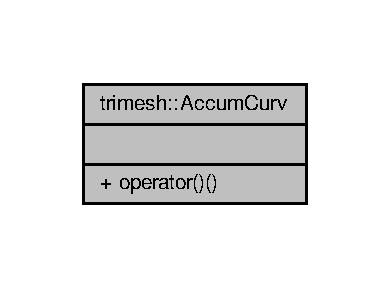
\includegraphics[width=187pt]{dc/db6/structtrimesh_1_1AccumCurv__coll__graph}
\end{center}
\end{figure}
\subsection*{Public Member Functions}
\begin{DoxyCompactItemize}
\item 
\hyperlink{namespacetrimesh_a784ddfd979e1c579bda795a8edfc3f43}{void} \hyperlink{structtrimesh_1_1AccumCurv_a1dd283d750e5fbd4402f115065ad703d}{operator()} (const \hyperlink{classtrimesh_1_1TriMesh}{Tri\+Mesh} $\ast$themesh, int \hyperlink{namespacetrimesh_a240b3c8ea9cf01bd707862b32fa26dff}{v0}, \hyperlink{namespacetrimesh_a4fc2b83feba99c931f837a0c7d4b4df1}{vec} \&c, float \hyperlink{namespacetrimesh_acd577db8a2f95fe39ececb95e98a6c71}{w}, int v) const
\end{DoxyCompactItemize}


\subsection{Member Function Documentation}
\mbox{\Hypertarget{structtrimesh_1_1AccumCurv_a1dd283d750e5fbd4402f115065ad703d}\label{structtrimesh_1_1AccumCurv_a1dd283d750e5fbd4402f115065ad703d}} 
\index{trimesh\+::\+Accum\+Curv@{trimesh\+::\+Accum\+Curv}!operator()@{operator()}}
\index{operator()@{operator()}!trimesh\+::\+Accum\+Curv@{trimesh\+::\+Accum\+Curv}}
\subsubsection{\texorpdfstring{operator()()}{operator()()}}
{\footnotesize\ttfamily \hyperlink{namespacetrimesh_a784ddfd979e1c579bda795a8edfc3f43}{void} trimesh\+::\+Accum\+Curv\+::operator() (\begin{DoxyParamCaption}\item[{const \hyperlink{classtrimesh_1_1TriMesh}{Tri\+Mesh} $\ast$}]{themesh,  }\item[{int}]{v0,  }\item[{\hyperlink{namespacetrimesh_a4fc2b83feba99c931f837a0c7d4b4df1}{vec} \&}]{c,  }\item[{float}]{w,  }\item[{int}]{v }\end{DoxyParamCaption}) const\hspace{0.3cm}{\ttfamily [inline]}}



The documentation for this struct was generated from the following file\+:\begin{DoxyCompactItemize}
\item 
\hyperlink{diffuse_8cc}{diffuse.\+cc}\end{DoxyCompactItemize}

\hypertarget{structtrimesh_1_1AccumDCurv}{}\section{trimesh\+:\+:Accum\+D\+Curv Struct Reference}
\label{structtrimesh_1_1AccumDCurv}\index{trimesh\+::\+Accum\+D\+Curv@{trimesh\+::\+Accum\+D\+Curv}}


Collaboration diagram for trimesh\+:\+:Accum\+D\+Curv\+:\nopagebreak
\begin{figure}[H]
\begin{center}
\leavevmode
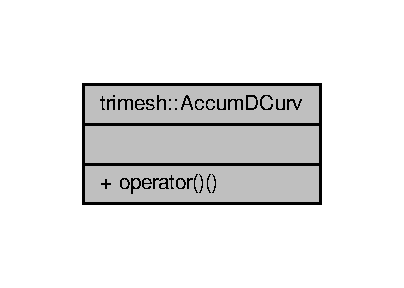
\includegraphics[width=194pt]{d3/d97/structtrimesh_1_1AccumDCurv__coll__graph}
\end{center}
\end{figure}
\subsection*{Public Member Functions}
\begin{DoxyCompactItemize}
\item 
\hyperlink{namespacetrimesh_a784ddfd979e1c579bda795a8edfc3f43}{void} \hyperlink{structtrimesh_1_1AccumDCurv_a204e32323030c88a086ab31b03add777}{operator()} (const \hyperlink{classtrimesh_1_1TriMesh}{Tri\+Mesh} $\ast$themesh, int \hyperlink{namespacetrimesh_a240b3c8ea9cf01bd707862b32fa26dff}{v0}, \hyperlink{classtrimesh_1_1Vec}{Vec}$<$ 4 $>$ \&d, float \hyperlink{namespacetrimesh_acd577db8a2f95fe39ececb95e98a6c71}{w}, int v) const
\end{DoxyCompactItemize}


\subsection{Member Function Documentation}
\mbox{\Hypertarget{structtrimesh_1_1AccumDCurv_a204e32323030c88a086ab31b03add777}\label{structtrimesh_1_1AccumDCurv_a204e32323030c88a086ab31b03add777}} 
\index{trimesh\+::\+Accum\+D\+Curv@{trimesh\+::\+Accum\+D\+Curv}!operator()@{operator()}}
\index{operator()@{operator()}!trimesh\+::\+Accum\+D\+Curv@{trimesh\+::\+Accum\+D\+Curv}}
\subsubsection{\texorpdfstring{operator()()}{operator()()}}
{\footnotesize\ttfamily \hyperlink{namespacetrimesh_a784ddfd979e1c579bda795a8edfc3f43}{void} trimesh\+::\+Accum\+D\+Curv\+::operator() (\begin{DoxyParamCaption}\item[{const \hyperlink{classtrimesh_1_1TriMesh}{Tri\+Mesh} $\ast$}]{themesh,  }\item[{int}]{v0,  }\item[{\hyperlink{classtrimesh_1_1Vec}{Vec}$<$ 4 $>$ \&}]{d,  }\item[{float}]{w,  }\item[{int}]{v }\end{DoxyParamCaption}) const\hspace{0.3cm}{\ttfamily [inline]}}



The documentation for this struct was generated from the following file\+:\begin{DoxyCompactItemize}
\item 
\hyperlink{diffuse_8cc}{diffuse.\+cc}\end{DoxyCompactItemize}

\hypertarget{structtrimesh_1_1AccumVec}{}\section{trimesh\+:\+:Accum\+Vec$<$ T $>$ Struct Template Reference}
\label{structtrimesh_1_1AccumVec}\index{trimesh\+::\+Accum\+Vec$<$ T $>$@{trimesh\+::\+Accum\+Vec$<$ T $>$}}


Collaboration diagram for trimesh\+:\+:Accum\+Vec$<$ T $>$\+:\nopagebreak
\begin{figure}[H]
\begin{center}
\leavevmode
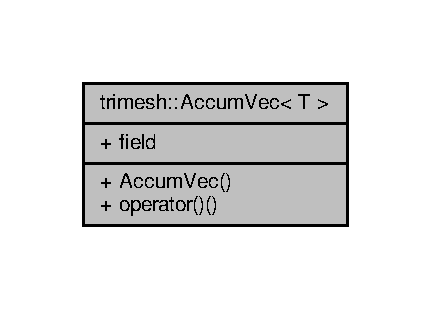
\includegraphics[width=207pt]{df/d9f/structtrimesh_1_1AccumVec__coll__graph}
\end{center}
\end{figure}
\subsection*{Public Member Functions}
\begin{DoxyCompactItemize}
\item 
\hyperlink{structtrimesh_1_1AccumVec_a1f2a837cd65c6efc4bc003d429ae8f43}{Accum\+Vec} (const vector$<$ T $>$ \&field\+\_\+)
\item 
\hyperlink{namespacetrimesh_a784ddfd979e1c579bda795a8edfc3f43}{void} \hyperlink{structtrimesh_1_1AccumVec_a65a3ac9c7b655346db533ee274940637}{operator()} (const \hyperlink{classtrimesh_1_1TriMesh}{Tri\+Mesh} $\ast$, int, T \&f, float \hyperlink{namespacetrimesh_acd577db8a2f95fe39ececb95e98a6c71}{w}, int v) const
\end{DoxyCompactItemize}
\subsection*{Public Attributes}
\begin{DoxyCompactItemize}
\item 
const vector$<$ T $>$ \& \hyperlink{structtrimesh_1_1AccumVec_aefbc404dfe8f74fc5f16f6fcaa85cbc4}{field}
\end{DoxyCompactItemize}


\subsection{Constructor \& Destructor Documentation}
\mbox{\Hypertarget{structtrimesh_1_1AccumVec_a1f2a837cd65c6efc4bc003d429ae8f43}\label{structtrimesh_1_1AccumVec_a1f2a837cd65c6efc4bc003d429ae8f43}} 
\index{trimesh\+::\+Accum\+Vec@{trimesh\+::\+Accum\+Vec}!Accum\+Vec@{Accum\+Vec}}
\index{Accum\+Vec@{Accum\+Vec}!trimesh\+::\+Accum\+Vec@{trimesh\+::\+Accum\+Vec}}
\subsubsection{\texorpdfstring{Accum\+Vec()}{AccumVec()}}
{\footnotesize\ttfamily template$<$class T$>$ \\
\hyperlink{structtrimesh_1_1AccumVec}{trimesh\+::\+Accum\+Vec}$<$ T $>$\+::\hyperlink{structtrimesh_1_1AccumVec}{Accum\+Vec} (\begin{DoxyParamCaption}\item[{const vector$<$ T $>$ \&}]{field\+\_\+ }\end{DoxyParamCaption})\hspace{0.3cm}{\ttfamily [inline]}}



\subsection{Member Function Documentation}
\mbox{\Hypertarget{structtrimesh_1_1AccumVec_a65a3ac9c7b655346db533ee274940637}\label{structtrimesh_1_1AccumVec_a65a3ac9c7b655346db533ee274940637}} 
\index{trimesh\+::\+Accum\+Vec@{trimesh\+::\+Accum\+Vec}!operator()@{operator()}}
\index{operator()@{operator()}!trimesh\+::\+Accum\+Vec@{trimesh\+::\+Accum\+Vec}}
\subsubsection{\texorpdfstring{operator()()}{operator()()}}
{\footnotesize\ttfamily template$<$class T$>$ \\
\hyperlink{namespacetrimesh_a784ddfd979e1c579bda795a8edfc3f43}{void} \hyperlink{structtrimesh_1_1AccumVec}{trimesh\+::\+Accum\+Vec}$<$ T $>$\+::operator() (\begin{DoxyParamCaption}\item[{const \hyperlink{classtrimesh_1_1TriMesh}{Tri\+Mesh} $\ast$}]{,  }\item[{int}]{,  }\item[{T \&}]{f,  }\item[{float}]{w,  }\item[{int}]{v }\end{DoxyParamCaption}) const\hspace{0.3cm}{\ttfamily [inline]}}



\subsection{Member Data Documentation}
\mbox{\Hypertarget{structtrimesh_1_1AccumVec_aefbc404dfe8f74fc5f16f6fcaa85cbc4}\label{structtrimesh_1_1AccumVec_aefbc404dfe8f74fc5f16f6fcaa85cbc4}} 
\index{trimesh\+::\+Accum\+Vec@{trimesh\+::\+Accum\+Vec}!field@{field}}
\index{field@{field}!trimesh\+::\+Accum\+Vec@{trimesh\+::\+Accum\+Vec}}
\subsubsection{\texorpdfstring{field}{field}}
{\footnotesize\ttfamily template$<$class T$>$ \\
const vector$<$T$>$\& \hyperlink{structtrimesh_1_1AccumVec}{trimesh\+::\+Accum\+Vec}$<$ T $>$\+::field}



The documentation for this struct was generated from the following file\+:\begin{DoxyCompactItemize}
\item 
\hyperlink{diffuse_8cc}{diffuse.\+cc}\end{DoxyCompactItemize}

\hypertarget{classAngleLocalParameterization}{}\section{Angle\+Local\+Parameterization Class Reference}
\label{classAngleLocalParameterization}\index{Angle\+Local\+Parameterization@{Angle\+Local\+Parameterization}}


Collaboration diagram for Angle\+Local\+Parameterization\+:\nopagebreak
\begin{figure}[H]
\begin{center}
\leavevmode
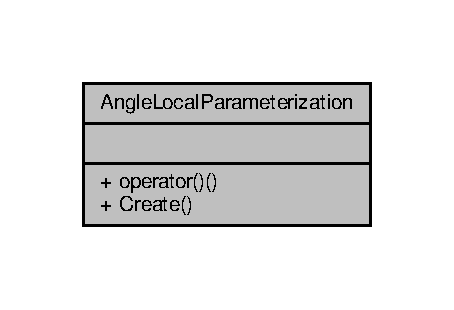
\includegraphics[width=218pt]{d4/da6/classAngleLocalParameterization__coll__graph}
\end{center}
\end{figure}
\subsection*{Public Member Functions}
\begin{DoxyCompactItemize}
\item 
{\footnotesize template$<$typename T $>$ }\\bool \hyperlink{classAngleLocalParameterization_a4395ea0db2ce1f4155d6a75931fcdff1}{operator()} (const T $\ast$t, const T $\ast$dt, T $\ast$t\+\_\+add\+\_\+dt) const
\end{DoxyCompactItemize}
\subsection*{Static Public Member Functions}
\begin{DoxyCompactItemize}
\item 
static ceres\+::\+Local\+Parameterization $\ast$ \hyperlink{classAngleLocalParameterization_a73006f5f3280d4adccfa3612f8188868}{Create} ()
\end{DoxyCompactItemize}


\subsection{Member Function Documentation}
\mbox{\Hypertarget{classAngleLocalParameterization_a73006f5f3280d4adccfa3612f8188868}\label{classAngleLocalParameterization_a73006f5f3280d4adccfa3612f8188868}} 
\index{Angle\+Local\+Parameterization@{Angle\+Local\+Parameterization}!Create@{Create}}
\index{Create@{Create}!Angle\+Local\+Parameterization@{Angle\+Local\+Parameterization}}
\subsubsection{\texorpdfstring{Create()}{Create()}}
{\footnotesize\ttfamily static ceres\+::\+Local\+Parameterization$\ast$ Angle\+Local\+Parameterization\+::\+Create (\begin{DoxyParamCaption}{ }\end{DoxyParamCaption})\hspace{0.3cm}{\ttfamily [inline]}, {\ttfamily [static]}}



Referenced by S\+N\+D\+T\+Match().

\mbox{\Hypertarget{classAngleLocalParameterization_a4395ea0db2ce1f4155d6a75931fcdff1}\label{classAngleLocalParameterization_a4395ea0db2ce1f4155d6a75931fcdff1}} 
\index{Angle\+Local\+Parameterization@{Angle\+Local\+Parameterization}!operator()@{operator()}}
\index{operator()@{operator()}!Angle\+Local\+Parameterization@{Angle\+Local\+Parameterization}}
\subsubsection{\texorpdfstring{operator()()}{operator()()}}
{\footnotesize\ttfamily template$<$typename T $>$ \\
bool Angle\+Local\+Parameterization\+::operator() (\begin{DoxyParamCaption}\item[{const T $\ast$}]{t,  }\item[{const T $\ast$}]{dt,  }\item[{T $\ast$}]{t\+\_\+add\+\_\+dt }\end{DoxyParamCaption}) const\hspace{0.3cm}{\ttfamily [inline]}}



The documentation for this class was generated from the following file\+:\begin{DoxyCompactItemize}
\item 
\hyperlink{matcher_8cc}{matcher.\+cc}\end{DoxyCompactItemize}

\hypertarget{structtrimesh_1_1GLManager_1_1AttributeInfo}{}\section{trimesh\+:\+:G\+L\+Manager\+:\+:Attribute\+Info Struct Reference}
\label{structtrimesh_1_1GLManager_1_1AttributeInfo}\index{trimesh\+::\+G\+L\+Manager\+::\+Attribute\+Info@{trimesh\+::\+G\+L\+Manager\+::\+Attribute\+Info}}


Collaboration diagram for trimesh\+:\+:G\+L\+Manager\+:\+:Attribute\+Info\+:\nopagebreak
\begin{figure}[H]
\begin{center}
\leavevmode
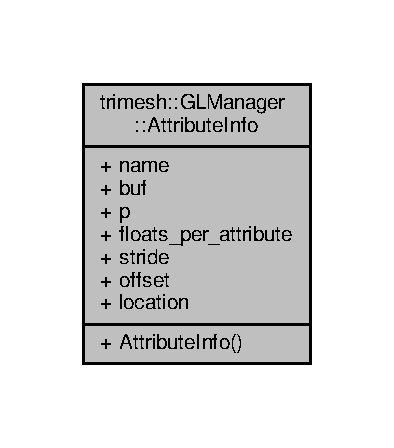
\includegraphics[width=189pt]{d7/d44/structtrimesh_1_1GLManager_1_1AttributeInfo__coll__graph}
\end{center}
\end{figure}
\subsection*{Public Member Functions}
\begin{DoxyCompactItemize}
\item 
\hyperlink{structtrimesh_1_1GLManager_1_1AttributeInfo_aab13a2c3c0f74ace19e917547916724d}{Attribute\+Info} ()
\end{DoxyCompactItemize}
\subsection*{Public Attributes}
\begin{DoxyCompactItemize}
\item 
\hyperlink{namespacetrimesh_a51b4a31323874089623d4b17afabc1aa}{string} \hyperlink{structtrimesh_1_1GLManager_1_1AttributeInfo_ad5055d910f9792131eb12f7597047d8d}{name}
\item 
unsigned \hyperlink{structtrimesh_1_1GLManager_1_1AttributeInfo_a8fbf13c65aa6d495a17d71310ace5c38}{buf}
\item 
const float $\ast$ \hyperlink{structtrimesh_1_1GLManager_1_1AttributeInfo_afb56efa61e786631d2a5f317617eb0b1}{p}
\item 
int \hyperlink{structtrimesh_1_1GLManager_1_1AttributeInfo_a02b42dc9c64212d889b9b3a5000ea826}{floats\+\_\+per\+\_\+attribute}
\item 
size\+\_\+t \hyperlink{structtrimesh_1_1GLManager_1_1AttributeInfo_ae0c6b5d9b0e8b622546b9ee9e71e7223}{stride}
\item 
size\+\_\+t \hyperlink{structtrimesh_1_1GLManager_1_1AttributeInfo_ae6132bf35d83e3dcac186e11b1d40919}{offset}
\item 
\hyperlink{namespacetrimesh_aeccc290e30b317c861fb146956528187}{G\+Lint} \hyperlink{structtrimesh_1_1GLManager_1_1AttributeInfo_a48ebfdc0482600561c164c4d62e25d1b}{location}
\end{DoxyCompactItemize}


\subsection{Constructor \& Destructor Documentation}
\mbox{\Hypertarget{structtrimesh_1_1GLManager_1_1AttributeInfo_aab13a2c3c0f74ace19e917547916724d}\label{structtrimesh_1_1GLManager_1_1AttributeInfo_aab13a2c3c0f74ace19e917547916724d}} 
\index{trimesh\+::\+G\+L\+Manager\+::\+Attribute\+Info@{trimesh\+::\+G\+L\+Manager\+::\+Attribute\+Info}!Attribute\+Info@{Attribute\+Info}}
\index{Attribute\+Info@{Attribute\+Info}!trimesh\+::\+G\+L\+Manager\+::\+Attribute\+Info@{trimesh\+::\+G\+L\+Manager\+::\+Attribute\+Info}}
\subsubsection{\texorpdfstring{Attribute\+Info()}{AttributeInfo()}}
{\footnotesize\ttfamily trimesh\+::\+G\+L\+Manager\+::\+Attribute\+Info\+::\+Attribute\+Info (\begin{DoxyParamCaption}{ }\end{DoxyParamCaption})\hspace{0.3cm}{\ttfamily [inline]}}



\subsection{Member Data Documentation}
\mbox{\Hypertarget{structtrimesh_1_1GLManager_1_1AttributeInfo_a8fbf13c65aa6d495a17d71310ace5c38}\label{structtrimesh_1_1GLManager_1_1AttributeInfo_a8fbf13c65aa6d495a17d71310ace5c38}} 
\index{trimesh\+::\+G\+L\+Manager\+::\+Attribute\+Info@{trimesh\+::\+G\+L\+Manager\+::\+Attribute\+Info}!buf@{buf}}
\index{buf@{buf}!trimesh\+::\+G\+L\+Manager\+::\+Attribute\+Info@{trimesh\+::\+G\+L\+Manager\+::\+Attribute\+Info}}
\subsubsection{\texorpdfstring{buf}{buf}}
{\footnotesize\ttfamily unsigned trimesh\+::\+G\+L\+Manager\+::\+Attribute\+Info\+::buf}



Referenced by trimesh\+::\+G\+L\+Manager\+::color3f(), trimesh\+::\+G\+L\+Manager\+::color4f(), trimesh\+::\+G\+L\+Manager\+::colorarray3fv(), trimesh\+::\+G\+L\+Manager\+::colorarray4fv(), trimesh\+::\+G\+L\+Manager\+::normal3f(), trimesh\+::\+G\+L\+Manager\+::normalarray3fv(), trimesh\+::\+G\+L\+Manager\+::texcoord2f(), trimesh\+::\+G\+L\+Manager\+::texcoordarray2fv(), trimesh\+::\+G\+L\+Manager\+::use\+\_\+shader(), and trimesh\+::\+G\+L\+Manager\+::vertexarray3fv().

\mbox{\Hypertarget{structtrimesh_1_1GLManager_1_1AttributeInfo_a02b42dc9c64212d889b9b3a5000ea826}\label{structtrimesh_1_1GLManager_1_1AttributeInfo_a02b42dc9c64212d889b9b3a5000ea826}} 
\index{trimesh\+::\+G\+L\+Manager\+::\+Attribute\+Info@{trimesh\+::\+G\+L\+Manager\+::\+Attribute\+Info}!floats\+\_\+per\+\_\+attribute@{floats\+\_\+per\+\_\+attribute}}
\index{floats\+\_\+per\+\_\+attribute@{floats\+\_\+per\+\_\+attribute}!trimesh\+::\+G\+L\+Manager\+::\+Attribute\+Info@{trimesh\+::\+G\+L\+Manager\+::\+Attribute\+Info}}
\subsubsection{\texorpdfstring{floats\+\_\+per\+\_\+attribute}{floats\_per\_attribute}}
{\footnotesize\ttfamily int trimesh\+::\+G\+L\+Manager\+::\+Attribute\+Info\+::floats\+\_\+per\+\_\+attribute}



Referenced by trimesh\+::\+G\+L\+Manager\+::make\+\_\+shader(), trimesh\+::\+G\+L\+Manager\+::\+Shader\+Info\+::\+Shader\+Info(), and trimesh\+::\+G\+L\+Manager\+::use\+\_\+shader().

\mbox{\Hypertarget{structtrimesh_1_1GLManager_1_1AttributeInfo_a48ebfdc0482600561c164c4d62e25d1b}\label{structtrimesh_1_1GLManager_1_1AttributeInfo_a48ebfdc0482600561c164c4d62e25d1b}} 
\index{trimesh\+::\+G\+L\+Manager\+::\+Attribute\+Info@{trimesh\+::\+G\+L\+Manager\+::\+Attribute\+Info}!location@{location}}
\index{location@{location}!trimesh\+::\+G\+L\+Manager\+::\+Attribute\+Info@{trimesh\+::\+G\+L\+Manager\+::\+Attribute\+Info}}
\subsubsection{\texorpdfstring{location}{location}}
{\footnotesize\ttfamily \hyperlink{namespacetrimesh_aeccc290e30b317c861fb146956528187}{G\+Lint} trimesh\+::\+G\+L\+Manager\+::\+Attribute\+Info\+::location}



Referenced by trimesh\+::\+G\+L\+Manager\+::make\+\_\+shader(), and trimesh\+::\+G\+L\+Manager\+::use\+\_\+shader().

\mbox{\Hypertarget{structtrimesh_1_1GLManager_1_1AttributeInfo_ad5055d910f9792131eb12f7597047d8d}\label{structtrimesh_1_1GLManager_1_1AttributeInfo_ad5055d910f9792131eb12f7597047d8d}} 
\index{trimesh\+::\+G\+L\+Manager\+::\+Attribute\+Info@{trimesh\+::\+G\+L\+Manager\+::\+Attribute\+Info}!name@{name}}
\index{name@{name}!trimesh\+::\+G\+L\+Manager\+::\+Attribute\+Info@{trimesh\+::\+G\+L\+Manager\+::\+Attribute\+Info}}
\subsubsection{\texorpdfstring{name}{name}}
{\footnotesize\ttfamily \hyperlink{namespacetrimesh_a51b4a31323874089623d4b17afabc1aa}{string} trimesh\+::\+G\+L\+Manager\+::\+Attribute\+Info\+::name}



Referenced by trimesh\+::\+G\+L\+Manager\+::make\+\_\+shader(), trimesh\+::\+G\+L\+Manager\+::shader\+\_\+ready(), and trimesh\+::\+G\+L\+Manager\+::\+Shader\+Info\+::\+Shader\+Info().

\mbox{\Hypertarget{structtrimesh_1_1GLManager_1_1AttributeInfo_ae6132bf35d83e3dcac186e11b1d40919}\label{structtrimesh_1_1GLManager_1_1AttributeInfo_ae6132bf35d83e3dcac186e11b1d40919}} 
\index{trimesh\+::\+G\+L\+Manager\+::\+Attribute\+Info@{trimesh\+::\+G\+L\+Manager\+::\+Attribute\+Info}!offset@{offset}}
\index{offset@{offset}!trimesh\+::\+G\+L\+Manager\+::\+Attribute\+Info@{trimesh\+::\+G\+L\+Manager\+::\+Attribute\+Info}}
\subsubsection{\texorpdfstring{offset}{offset}}
{\footnotesize\ttfamily size\+\_\+t trimesh\+::\+G\+L\+Manager\+::\+Attribute\+Info\+::offset}



Referenced by trimesh\+::\+G\+L\+Manager\+::colorarray3fv(), trimesh\+::\+G\+L\+Manager\+::colorarray4fv(), trimesh\+::\+G\+L\+Manager\+::normalarray3fv(), trimesh\+::\+G\+L\+Manager\+::texcoordarray2fv(), trimesh\+::\+G\+L\+Manager\+::use\+\_\+shader(), and trimesh\+::\+G\+L\+Manager\+::vertexarray3fv().

\mbox{\Hypertarget{structtrimesh_1_1GLManager_1_1AttributeInfo_afb56efa61e786631d2a5f317617eb0b1}\label{structtrimesh_1_1GLManager_1_1AttributeInfo_afb56efa61e786631d2a5f317617eb0b1}} 
\index{trimesh\+::\+G\+L\+Manager\+::\+Attribute\+Info@{trimesh\+::\+G\+L\+Manager\+::\+Attribute\+Info}!p@{p}}
\index{p@{p}!trimesh\+::\+G\+L\+Manager\+::\+Attribute\+Info@{trimesh\+::\+G\+L\+Manager\+::\+Attribute\+Info}}
\subsubsection{\texorpdfstring{p}{p}}
{\footnotesize\ttfamily const float$\ast$ trimesh\+::\+G\+L\+Manager\+::\+Attribute\+Info\+::p}



Referenced by trimesh\+::\+G\+L\+Manager\+::color3f(), trimesh\+::\+G\+L\+Manager\+::color4f(), trimesh\+::\+G\+L\+Manager\+::colorarray3fv(), trimesh\+::\+G\+L\+Manager\+::colorarray4fv(), trimesh\+::\+G\+L\+Manager\+::normal3f(), trimesh\+::\+G\+L\+Manager\+::normalarray3fv(), trimesh\+::\+G\+L\+Manager\+::texcoord2f(), trimesh\+::\+G\+L\+Manager\+::texcoordarray2fv(), trimesh\+::\+G\+L\+Manager\+::use\+\_\+shader(), and trimesh\+::\+G\+L\+Manager\+::vertexarray3fv().

\mbox{\Hypertarget{structtrimesh_1_1GLManager_1_1AttributeInfo_ae0c6b5d9b0e8b622546b9ee9e71e7223}\label{structtrimesh_1_1GLManager_1_1AttributeInfo_ae0c6b5d9b0e8b622546b9ee9e71e7223}} 
\index{trimesh\+::\+G\+L\+Manager\+::\+Attribute\+Info@{trimesh\+::\+G\+L\+Manager\+::\+Attribute\+Info}!stride@{stride}}
\index{stride@{stride}!trimesh\+::\+G\+L\+Manager\+::\+Attribute\+Info@{trimesh\+::\+G\+L\+Manager\+::\+Attribute\+Info}}
\subsubsection{\texorpdfstring{stride}{stride}}
{\footnotesize\ttfamily size\+\_\+t trimesh\+::\+G\+L\+Manager\+::\+Attribute\+Info\+::stride}



Referenced by trimesh\+::\+G\+L\+Manager\+::colorarray3fv(), trimesh\+::\+G\+L\+Manager\+::colorarray4fv(), trimesh\+::\+G\+L\+Manager\+::normalarray3fv(), trimesh\+::\+G\+L\+Manager\+::texcoordarray2fv(), trimesh\+::\+G\+L\+Manager\+::use\+\_\+shader(), and trimesh\+::\+G\+L\+Manager\+::vertexarray3fv().



The documentation for this struct was generated from the following file\+:\begin{DoxyCompactItemize}
\item 
\hyperlink{GLManager_8cc}{G\+L\+Manager.\+cc}\end{DoxyCompactItemize}

\hypertarget{classtrimesh_1_1Basis}{}\section{trimesh\+:\+:Basis$<$ D, T $>$ Class Template Reference}
\label{classtrimesh_1_1Basis}\index{trimesh\+::\+Basis$<$ D, T $>$@{trimesh\+::\+Basis$<$ D, T $>$}}


{\ttfamily \#include $<$bsphere.\+h$>$}



Collaboration diagram for trimesh\+:\+:Basis$<$ D, T $>$\+:\nopagebreak
\begin{figure}[H]
\begin{center}
\leavevmode
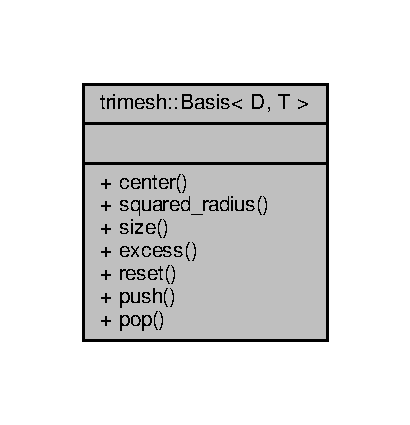
\includegraphics[width=197pt]{d9/d58/classtrimesh_1_1Basis__coll__graph}
\end{center}
\end{figure}
\subsection*{Public Member Functions}
\begin{DoxyCompactItemize}
\item 
const T $\ast$ \hyperlink{classtrimesh_1_1Basis_a2af24b4e2a734c790675c0e8e3a596f1}{center} () const
\item 
T \hyperlink{classtrimesh_1_1Basis_a6af18ad45b2e277767edc07ef7edeaba}{squared\+\_\+radius} () const
\item 
size\+\_\+t \hyperlink{classtrimesh_1_1Basis_ab6a1d0fdbcbbaa787d94100ebe1ab3b1}{size} () const
\item 
T \hyperlink{classtrimesh_1_1Basis_a43fa98abe1d7a2d8636ecb662af75d56}{excess} (const \hyperlink{classtrimesh_1_1Vec}{Vec}$<$ D, T $>$ \&p) const
\item 
\hyperlink{namespacetrimesh_a784ddfd979e1c579bda795a8edfc3f43}{void} \hyperlink{classtrimesh_1_1Basis_ab90120bbba4505a92d39258454a63dfa}{reset} ()
\item 
bool \hyperlink{classtrimesh_1_1Basis_a9dfc260252428e3b2bf890a92412b7fd}{push} (const \hyperlink{classtrimesh_1_1Vec}{Vec}$<$ D, T $>$ \&p)
\item 
\hyperlink{namespacetrimesh_a784ddfd979e1c579bda795a8edfc3f43}{void} \hyperlink{classtrimesh_1_1Basis_a617b8507dc31a31a3dc10a5a558203ad}{pop} ()
\end{DoxyCompactItemize}


\subsection{Member Function Documentation}
\mbox{\Hypertarget{classtrimesh_1_1Basis_a2af24b4e2a734c790675c0e8e3a596f1}\label{classtrimesh_1_1Basis_a2af24b4e2a734c790675c0e8e3a596f1}} 
\index{trimesh\+::\+Basis@{trimesh\+::\+Basis}!center@{center}}
\index{center@{center}!trimesh\+::\+Basis@{trimesh\+::\+Basis}}
\subsubsection{\texorpdfstring{center()}{center()}}
{\footnotesize\ttfamily template$<$size\+\_\+t D, class T$>$ \\
const T$\ast$ \hyperlink{classtrimesh_1_1Basis}{trimesh\+::\+Basis}$<$ D, T $>$\+::center (\begin{DoxyParamCaption}{ }\end{DoxyParamCaption}) const\hspace{0.3cm}{\ttfamily [inline]}}



Referenced by trimesh\+::\+Miniball$<$ D, T $>$\+::center().

\mbox{\Hypertarget{classtrimesh_1_1Basis_a43fa98abe1d7a2d8636ecb662af75d56}\label{classtrimesh_1_1Basis_a43fa98abe1d7a2d8636ecb662af75d56}} 
\index{trimesh\+::\+Basis@{trimesh\+::\+Basis}!excess@{excess}}
\index{excess@{excess}!trimesh\+::\+Basis@{trimesh\+::\+Basis}}
\subsubsection{\texorpdfstring{excess()}{excess()}}
{\footnotesize\ttfamily template$<$size\+\_\+t D, class T $>$ \\
T \hyperlink{classtrimesh_1_1Basis}{trimesh\+::\+Basis}$<$ D, T $>$\+::excess (\begin{DoxyParamCaption}\item[{const \hyperlink{classtrimesh_1_1Vec}{Vec}$<$ D, T $>$ \&}]{p }\end{DoxyParamCaption}) const}



Referenced by trimesh\+::\+Basis$<$ D, T $>$\+::size().

\mbox{\Hypertarget{classtrimesh_1_1Basis_a617b8507dc31a31a3dc10a5a558203ad}\label{classtrimesh_1_1Basis_a617b8507dc31a31a3dc10a5a558203ad}} 
\index{trimesh\+::\+Basis@{trimesh\+::\+Basis}!pop@{pop}}
\index{pop@{pop}!trimesh\+::\+Basis@{trimesh\+::\+Basis}}
\subsubsection{\texorpdfstring{pop()}{pop()}}
{\footnotesize\ttfamily template$<$size\+\_\+t D, class T $>$ \\
\hyperlink{namespacetrimesh_a784ddfd979e1c579bda795a8edfc3f43}{void} \hyperlink{classtrimesh_1_1Basis}{trimesh\+::\+Basis}$<$ D, T $>$\+::pop (\begin{DoxyParamCaption}{ }\end{DoxyParamCaption})}



Referenced by trimesh\+::\+Basis$<$ D, T $>$\+::size().

\mbox{\Hypertarget{classtrimesh_1_1Basis_a9dfc260252428e3b2bf890a92412b7fd}\label{classtrimesh_1_1Basis_a9dfc260252428e3b2bf890a92412b7fd}} 
\index{trimesh\+::\+Basis@{trimesh\+::\+Basis}!push@{push}}
\index{push@{push}!trimesh\+::\+Basis@{trimesh\+::\+Basis}}
\subsubsection{\texorpdfstring{push()}{push()}}
{\footnotesize\ttfamily template$<$size\+\_\+t D, class T $>$ \\
bool \hyperlink{classtrimesh_1_1Basis}{trimesh\+::\+Basis}$<$ D, T $>$\+::push (\begin{DoxyParamCaption}\item[{const \hyperlink{classtrimesh_1_1Vec}{Vec}$<$ D, T $>$ \&}]{p }\end{DoxyParamCaption})}



Referenced by trimesh\+::\+Basis$<$ D, T $>$\+::size().

\mbox{\Hypertarget{classtrimesh_1_1Basis_ab90120bbba4505a92d39258454a63dfa}\label{classtrimesh_1_1Basis_ab90120bbba4505a92d39258454a63dfa}} 
\index{trimesh\+::\+Basis@{trimesh\+::\+Basis}!reset@{reset}}
\index{reset@{reset}!trimesh\+::\+Basis@{trimesh\+::\+Basis}}
\subsubsection{\texorpdfstring{reset()}{reset()}}
{\footnotesize\ttfamily template$<$size\+\_\+t D, class T $>$ \\
\hyperlink{namespacetrimesh_a784ddfd979e1c579bda795a8edfc3f43}{void} \hyperlink{classtrimesh_1_1Basis}{trimesh\+::\+Basis}$<$ D, T $>$\+::reset (\begin{DoxyParamCaption}{ }\end{DoxyParamCaption})}



Referenced by trimesh\+::\+Basis$<$ D, T $>$\+::size().

\mbox{\Hypertarget{classtrimesh_1_1Basis_ab6a1d0fdbcbbaa787d94100ebe1ab3b1}\label{classtrimesh_1_1Basis_ab6a1d0fdbcbbaa787d94100ebe1ab3b1}} 
\index{trimesh\+::\+Basis@{trimesh\+::\+Basis}!size@{size}}
\index{size@{size}!trimesh\+::\+Basis@{trimesh\+::\+Basis}}
\subsubsection{\texorpdfstring{size()}{size()}}
{\footnotesize\ttfamily template$<$size\+\_\+t D, class T$>$ \\
size\+\_\+t \hyperlink{classtrimesh_1_1Basis}{trimesh\+::\+Basis}$<$ D, T $>$\+::\hyperlink{namespacetrimesh_a1c71e2912be63f694df9e9991bddb15e}{size} (\begin{DoxyParamCaption}{ }\end{DoxyParamCaption}) const\hspace{0.3cm}{\ttfamily [inline]}}

\mbox{\Hypertarget{classtrimesh_1_1Basis_a6af18ad45b2e277767edc07ef7edeaba}\label{classtrimesh_1_1Basis_a6af18ad45b2e277767edc07ef7edeaba}} 
\index{trimesh\+::\+Basis@{trimesh\+::\+Basis}!squared\+\_\+radius@{squared\+\_\+radius}}
\index{squared\+\_\+radius@{squared\+\_\+radius}!trimesh\+::\+Basis@{trimesh\+::\+Basis}}
\subsubsection{\texorpdfstring{squared\+\_\+radius()}{squared\_radius()}}
{\footnotesize\ttfamily template$<$size\+\_\+t D, class T$>$ \\
T \hyperlink{classtrimesh_1_1Basis}{trimesh\+::\+Basis}$<$ D, T $>$\+::squared\+\_\+radius (\begin{DoxyParamCaption}{ }\end{DoxyParamCaption}) const\hspace{0.3cm}{\ttfamily [inline]}}



Referenced by trimesh\+::\+Miniball$<$ D, T $>$\+::squared\+\_\+radius().



The documentation for this class was generated from the following file\+:\begin{DoxyCompactItemize}
\item 
\hyperlink{bsphere_8h}{bsphere.\+h}\end{DoxyCompactItemize}

\hypertarget{classtrimesh_1_1Box}{}\section{trimesh\+:\+:Box$<$ D, T $>$ Class Template Reference}
\label{classtrimesh_1_1Box}\index{trimesh\+::\+Box$<$ D, T $>$@{trimesh\+::\+Box$<$ D, T $>$}}


{\ttfamily \#include $<$Box.\+h$>$}



Collaboration diagram for trimesh\+:\+:Box$<$ D, T $>$\+:\nopagebreak
\begin{figure}[H]
\begin{center}
\leavevmode
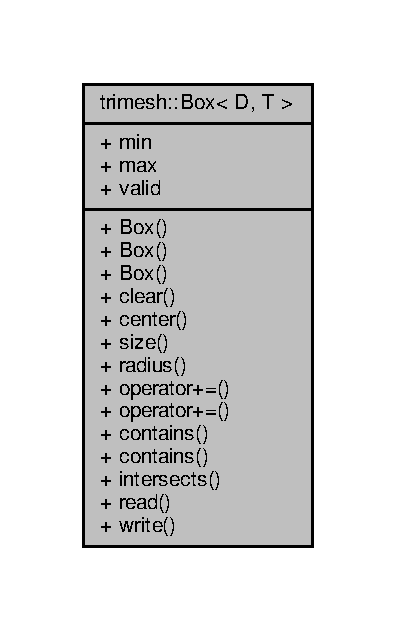
\includegraphics[width=190pt]{db/d3a/classtrimesh_1_1Box__coll__graph}
\end{center}
\end{figure}
\subsection*{Public Types}
\begin{DoxyCompactItemize}
\item 
typedef T \hyperlink{classtrimesh_1_1Box_aa78431130c7bda4a326f3a23da88ba82}{value\+\_\+type}
\item 
typedef \hyperlink{classtrimesh_1_1Box_aa78431130c7bda4a326f3a23da88ba82}{value\+\_\+type} $\ast$ \hyperlink{classtrimesh_1_1Box_a9047216c8a8bf0b23b12fbf08f1b4cb6}{pointer}
\item 
typedef const \hyperlink{classtrimesh_1_1Box_aa78431130c7bda4a326f3a23da88ba82}{value\+\_\+type} $\ast$ \hyperlink{classtrimesh_1_1Box_a9a9725eafb98d3340e22db0f9be77068}{const\+\_\+pointer}
\item 
typedef \hyperlink{classtrimesh_1_1Box_aa78431130c7bda4a326f3a23da88ba82}{value\+\_\+type} \& \hyperlink{classtrimesh_1_1Box_af56328ba73f0070abeeef8b1ae82a12d}{reference}
\item 
typedef const \hyperlink{classtrimesh_1_1Box_aa78431130c7bda4a326f3a23da88ba82}{value\+\_\+type} \& \hyperlink{classtrimesh_1_1Box_ac674585eb2cf25c8749bd677ff25eaa7}{const\+\_\+reference}
\item 
typedef \hyperlink{classtrimesh_1_1Vec}{Vec}$<$ D, T $>$ \hyperlink{classtrimesh_1_1Box_a208c806781f96a7001491a275dfa7655}{point\+\_\+type}
\item 
typedef \hyperlink{classtrimesh_1_1Vec}{Vec}$<$ D, T $>$\+::\hyperlink{classtrimesh_1_1Box_aa3a7238ce00e96ceaf24ecbb1077b7a4}{float\+\_\+type} \hyperlink{classtrimesh_1_1Box_aa3a7238ce00e96ceaf24ecbb1077b7a4}{float\+\_\+type}
\end{DoxyCompactItemize}
\subsection*{Public Member Functions}
\begin{DoxyCompactItemize}
\item 
\hyperlink{classtrimesh_1_1Box_af7a91b84e4bcb2dabc6b94ef2a2872a1}{Box} ()
\item 
\hyperlink{classtrimesh_1_1Box_ac89db794c58d514ace2230361499352f}{Box} (const \hyperlink{classtrimesh_1_1Box_a208c806781f96a7001491a275dfa7655}{point\+\_\+type} \&p)
\item 
\hyperlink{classtrimesh_1_1Box_a42a3734ab4a5dd6107e1ba609b7b3911}{Box} (const \hyperlink{classtrimesh_1_1Box_a208c806781f96a7001491a275dfa7655}{point\+\_\+type} \&p1, const \hyperlink{classtrimesh_1_1Box_a208c806781f96a7001491a275dfa7655}{point\+\_\+type} \&p2)
\item 
\hyperlink{namespacetrimesh_a784ddfd979e1c579bda795a8edfc3f43}{void} \hyperlink{classtrimesh_1_1Box_aff5802052cfb630fa70815659a37384e}{clear} ()
\item 
\hyperlink{classtrimesh_1_1Box_a208c806781f96a7001491a275dfa7655}{point\+\_\+type} \hyperlink{classtrimesh_1_1Box_a39edf4c682b2b1d8b8526124efa74413}{center} () const
\item 
\hyperlink{classtrimesh_1_1Box_a208c806781f96a7001491a275dfa7655}{point\+\_\+type} \hyperlink{classtrimesh_1_1Box_a111c09e2c3fb2b350e9091eb6e61d641}{size} () const
\item 
\hyperlink{classtrimesh_1_1Box_aa3a7238ce00e96ceaf24ecbb1077b7a4}{float\+\_\+type} \hyperlink{classtrimesh_1_1Box_ae42a8b9c88800f8688495390b2452135}{radius} () const
\item 
\hyperlink{classtrimesh_1_1Box}{Box}$<$ D, T $>$ \& \hyperlink{classtrimesh_1_1Box_a7cfdd9e833ffd23d6dacd0dd0de83728}{operator+=} (const \hyperlink{classtrimesh_1_1Box_a208c806781f96a7001491a275dfa7655}{point\+\_\+type} \&p)
\item 
\hyperlink{classtrimesh_1_1Box}{Box}$<$ D, T $>$ \& \hyperlink{classtrimesh_1_1Box_ab62681c3d2495c4acd1b77be635813a6}{operator+=} (const \hyperlink{classtrimesh_1_1Box}{Box}$<$ D, T $>$ \&b)
\item 
bool \hyperlink{classtrimesh_1_1Box_abed49b215db7d2affea33694a82327d4}{contains} (const \hyperlink{classtrimesh_1_1Box_a208c806781f96a7001491a275dfa7655}{point\+\_\+type} \&p) const
\item 
bool \hyperlink{classtrimesh_1_1Box_a8846c5b376e879c540e65e128e372cf2}{contains} (const \hyperlink{classtrimesh_1_1Box}{Box} \&b) const
\item 
bool \hyperlink{classtrimesh_1_1Box_a517e3bf133bf9d42e9ef70f078596764}{intersects} (const \hyperlink{classtrimesh_1_1Box}{Box} \&b)
\item 
bool \hyperlink{classtrimesh_1_1Box_aa4e1ce7bc178d938a7f93d7a6d517796}{read} (const \+::std\+::string \&filename)
\item 
bool \hyperlink{classtrimesh_1_1Box_a3520a4a6df05071e821bf63cb18d789f}{write} (const \+::std\+::string \&filename) const
\end{DoxyCompactItemize}
\subsection*{Public Attributes}
\begin{DoxyCompactItemize}
\item 
\hyperlink{classtrimesh_1_1Box_a208c806781f96a7001491a275dfa7655}{point\+\_\+type} \hyperlink{classtrimesh_1_1Box_a58c2da25c281e02ddc987c157e666517}{min}
\item 
\hyperlink{classtrimesh_1_1Box_a208c806781f96a7001491a275dfa7655}{point\+\_\+type} \hyperlink{classtrimesh_1_1Box_a845e5f1648b55bd35607e9dcb09a9a92}{max}
\item 
bool \hyperlink{classtrimesh_1_1Box_a388cbaca80a84b13ed434835a470b70c}{valid}
\end{DoxyCompactItemize}
\subsection*{Friends}
\begin{DoxyCompactItemize}
\item 
const \hyperlink{classtrimesh_1_1Box}{Box} \hyperlink{classtrimesh_1_1Box_a23d724d489cba7bb23565790189fb659}{operator+} (const \hyperlink{classtrimesh_1_1Box}{Box} \&b, const \hyperlink{classtrimesh_1_1Box_a208c806781f96a7001491a275dfa7655}{point\+\_\+type} \&p)
\item 
const \hyperlink{classtrimesh_1_1Box}{Box} \hyperlink{classtrimesh_1_1Box_ad2d14571fddd30993d281b575b02a7be}{operator+} (const \hyperlink{classtrimesh_1_1Box_a208c806781f96a7001491a275dfa7655}{point\+\_\+type} \&p, const \hyperlink{classtrimesh_1_1Box}{Box} \&b)
\item 
const \hyperlink{classtrimesh_1_1Box}{Box} \hyperlink{classtrimesh_1_1Box_a3bde7aa47ecb941209e87db7d3fe2e70}{operator+} (const \hyperlink{classtrimesh_1_1Box}{Box} \&b1, const \hyperlink{classtrimesh_1_1Box}{Box} \&b2)
\item 
\+::std\+::ostream \& \hyperlink{classtrimesh_1_1Box_a2b5e011ce3527b8f40eb42c351bf24e9}{operator$<$$<$} (\+::std\+::ostream \&os, const \hyperlink{classtrimesh_1_1Box}{Box} \&b)
\item 
\+::std\+::istream \& \hyperlink{classtrimesh_1_1Box_a33a4dca895ab5620960e259681995093}{operator$>$$>$} (\+::std\+::istream \&is, \hyperlink{classtrimesh_1_1Box}{Box} \&b)
\end{DoxyCompactItemize}


\subsection{Member Typedef Documentation}
\mbox{\Hypertarget{classtrimesh_1_1Box_a9a9725eafb98d3340e22db0f9be77068}\label{classtrimesh_1_1Box_a9a9725eafb98d3340e22db0f9be77068}} 
\index{trimesh\+::\+Box@{trimesh\+::\+Box}!const\+\_\+pointer@{const\+\_\+pointer}}
\index{const\+\_\+pointer@{const\+\_\+pointer}!trimesh\+::\+Box@{trimesh\+::\+Box}}
\subsubsection{\texorpdfstring{const\+\_\+pointer}{const\_pointer}}
{\footnotesize\ttfamily template$<$size\+\_\+t D, class T = float$>$ \\
typedef const \hyperlink{classtrimesh_1_1Box_aa78431130c7bda4a326f3a23da88ba82}{value\+\_\+type}$\ast$ \hyperlink{classtrimesh_1_1Box}{trimesh\+::\+Box}$<$ D, T $>$\+::\hyperlink{classtrimesh_1_1Box_a9a9725eafb98d3340e22db0f9be77068}{const\+\_\+pointer}}

\mbox{\Hypertarget{classtrimesh_1_1Box_ac674585eb2cf25c8749bd677ff25eaa7}\label{classtrimesh_1_1Box_ac674585eb2cf25c8749bd677ff25eaa7}} 
\index{trimesh\+::\+Box@{trimesh\+::\+Box}!const\+\_\+reference@{const\+\_\+reference}}
\index{const\+\_\+reference@{const\+\_\+reference}!trimesh\+::\+Box@{trimesh\+::\+Box}}
\subsubsection{\texorpdfstring{const\+\_\+reference}{const\_reference}}
{\footnotesize\ttfamily template$<$size\+\_\+t D, class T = float$>$ \\
typedef const \hyperlink{classtrimesh_1_1Box_aa78431130c7bda4a326f3a23da88ba82}{value\+\_\+type}\& \hyperlink{classtrimesh_1_1Box}{trimesh\+::\+Box}$<$ D, T $>$\+::\hyperlink{classtrimesh_1_1Box_ac674585eb2cf25c8749bd677ff25eaa7}{const\+\_\+reference}}

\mbox{\Hypertarget{classtrimesh_1_1Box_aa3a7238ce00e96ceaf24ecbb1077b7a4}\label{classtrimesh_1_1Box_aa3a7238ce00e96ceaf24ecbb1077b7a4}} 
\index{trimesh\+::\+Box@{trimesh\+::\+Box}!float\+\_\+type@{float\+\_\+type}}
\index{float\+\_\+type@{float\+\_\+type}!trimesh\+::\+Box@{trimesh\+::\+Box}}
\subsubsection{\texorpdfstring{float\+\_\+type}{float\_type}}
{\footnotesize\ttfamily template$<$size\+\_\+t D, class T = float$>$ \\
typedef \hyperlink{classtrimesh_1_1Vec}{Vec}$<$D,T$>$\+::\hyperlink{classtrimesh_1_1Box_aa3a7238ce00e96ceaf24ecbb1077b7a4}{float\+\_\+type} \hyperlink{classtrimesh_1_1Box}{trimesh\+::\+Box}$<$ D, T $>$\+::\hyperlink{classtrimesh_1_1Box_aa3a7238ce00e96ceaf24ecbb1077b7a4}{float\+\_\+type}}

\mbox{\Hypertarget{classtrimesh_1_1Box_a208c806781f96a7001491a275dfa7655}\label{classtrimesh_1_1Box_a208c806781f96a7001491a275dfa7655}} 
\index{trimesh\+::\+Box@{trimesh\+::\+Box}!point\+\_\+type@{point\+\_\+type}}
\index{point\+\_\+type@{point\+\_\+type}!trimesh\+::\+Box@{trimesh\+::\+Box}}
\subsubsection{\texorpdfstring{point\+\_\+type}{point\_type}}
{\footnotesize\ttfamily template$<$size\+\_\+t D, class T = float$>$ \\
typedef \hyperlink{classtrimesh_1_1Vec}{Vec}$<$D,T$>$ \hyperlink{classtrimesh_1_1Box}{trimesh\+::\+Box}$<$ D, T $>$\+::\hyperlink{classtrimesh_1_1Box_a208c806781f96a7001491a275dfa7655}{point\+\_\+type}}

\mbox{\Hypertarget{classtrimesh_1_1Box_a9047216c8a8bf0b23b12fbf08f1b4cb6}\label{classtrimesh_1_1Box_a9047216c8a8bf0b23b12fbf08f1b4cb6}} 
\index{trimesh\+::\+Box@{trimesh\+::\+Box}!pointer@{pointer}}
\index{pointer@{pointer}!trimesh\+::\+Box@{trimesh\+::\+Box}}
\subsubsection{\texorpdfstring{pointer}{pointer}}
{\footnotesize\ttfamily template$<$size\+\_\+t D, class T = float$>$ \\
typedef \hyperlink{classtrimesh_1_1Box_aa78431130c7bda4a326f3a23da88ba82}{value\+\_\+type}$\ast$ \hyperlink{classtrimesh_1_1Box}{trimesh\+::\+Box}$<$ D, T $>$\+::\hyperlink{classtrimesh_1_1Box_a9047216c8a8bf0b23b12fbf08f1b4cb6}{pointer}}

\mbox{\Hypertarget{classtrimesh_1_1Box_af56328ba73f0070abeeef8b1ae82a12d}\label{classtrimesh_1_1Box_af56328ba73f0070abeeef8b1ae82a12d}} 
\index{trimesh\+::\+Box@{trimesh\+::\+Box}!reference@{reference}}
\index{reference@{reference}!trimesh\+::\+Box@{trimesh\+::\+Box}}
\subsubsection{\texorpdfstring{reference}{reference}}
{\footnotesize\ttfamily template$<$size\+\_\+t D, class T = float$>$ \\
typedef \hyperlink{classtrimesh_1_1Box_aa78431130c7bda4a326f3a23da88ba82}{value\+\_\+type}\& \hyperlink{classtrimesh_1_1Box}{trimesh\+::\+Box}$<$ D, T $>$\+::\hyperlink{classtrimesh_1_1Box_af56328ba73f0070abeeef8b1ae82a12d}{reference}}

\mbox{\Hypertarget{classtrimesh_1_1Box_aa78431130c7bda4a326f3a23da88ba82}\label{classtrimesh_1_1Box_aa78431130c7bda4a326f3a23da88ba82}} 
\index{trimesh\+::\+Box@{trimesh\+::\+Box}!value\+\_\+type@{value\+\_\+type}}
\index{value\+\_\+type@{value\+\_\+type}!trimesh\+::\+Box@{trimesh\+::\+Box}}
\subsubsection{\texorpdfstring{value\+\_\+type}{value\_type}}
{\footnotesize\ttfamily template$<$size\+\_\+t D, class T = float$>$ \\
typedef T \hyperlink{classtrimesh_1_1Box}{trimesh\+::\+Box}$<$ D, T $>$\+::\hyperlink{classtrimesh_1_1Box_aa78431130c7bda4a326f3a23da88ba82}{value\+\_\+type}}



\subsection{Constructor \& Destructor Documentation}
\mbox{\Hypertarget{classtrimesh_1_1Box_af7a91b84e4bcb2dabc6b94ef2a2872a1}\label{classtrimesh_1_1Box_af7a91b84e4bcb2dabc6b94ef2a2872a1}} 
\index{trimesh\+::\+Box@{trimesh\+::\+Box}!Box@{Box}}
\index{Box@{Box}!trimesh\+::\+Box@{trimesh\+::\+Box}}
\subsubsection{\texorpdfstring{Box()}{Box()}\hspace{0.1cm}{\footnotesize\ttfamily [1/3]}}
{\footnotesize\ttfamily template$<$size\+\_\+t D, class T = float$>$ \\
\hyperlink{classtrimesh_1_1Box}{trimesh\+::\+Box}$<$ D, T $>$\+::\hyperlink{classtrimesh_1_1Box}{Box} (\begin{DoxyParamCaption}{ }\end{DoxyParamCaption})\hspace{0.3cm}{\ttfamily [inline]}}

\mbox{\Hypertarget{classtrimesh_1_1Box_ac89db794c58d514ace2230361499352f}\label{classtrimesh_1_1Box_ac89db794c58d514ace2230361499352f}} 
\index{trimesh\+::\+Box@{trimesh\+::\+Box}!Box@{Box}}
\index{Box@{Box}!trimesh\+::\+Box@{trimesh\+::\+Box}}
\subsubsection{\texorpdfstring{Box()}{Box()}\hspace{0.1cm}{\footnotesize\ttfamily [2/3]}}
{\footnotesize\ttfamily template$<$size\+\_\+t D, class T = float$>$ \\
\hyperlink{classtrimesh_1_1Box}{trimesh\+::\+Box}$<$ D, T $>$\+::\hyperlink{classtrimesh_1_1Box}{Box} (\begin{DoxyParamCaption}\item[{const \hyperlink{classtrimesh_1_1Box_a208c806781f96a7001491a275dfa7655}{point\+\_\+type} \&}]{p }\end{DoxyParamCaption})\hspace{0.3cm}{\ttfamily [inline]}}

\mbox{\Hypertarget{classtrimesh_1_1Box_a42a3734ab4a5dd6107e1ba609b7b3911}\label{classtrimesh_1_1Box_a42a3734ab4a5dd6107e1ba609b7b3911}} 
\index{trimesh\+::\+Box@{trimesh\+::\+Box}!Box@{Box}}
\index{Box@{Box}!trimesh\+::\+Box@{trimesh\+::\+Box}}
\subsubsection{\texorpdfstring{Box()}{Box()}\hspace{0.1cm}{\footnotesize\ttfamily [3/3]}}
{\footnotesize\ttfamily template$<$size\+\_\+t D, class T = float$>$ \\
\hyperlink{classtrimesh_1_1Box}{trimesh\+::\+Box}$<$ D, T $>$\+::\hyperlink{classtrimesh_1_1Box}{Box} (\begin{DoxyParamCaption}\item[{const \hyperlink{classtrimesh_1_1Box_a208c806781f96a7001491a275dfa7655}{point\+\_\+type} \&}]{p1,  }\item[{const \hyperlink{classtrimesh_1_1Box_a208c806781f96a7001491a275dfa7655}{point\+\_\+type} \&}]{p2 }\end{DoxyParamCaption})\hspace{0.3cm}{\ttfamily [inline]}}



\subsection{Member Function Documentation}
\mbox{\Hypertarget{classtrimesh_1_1Box_a39edf4c682b2b1d8b8526124efa74413}\label{classtrimesh_1_1Box_a39edf4c682b2b1d8b8526124efa74413}} 
\index{trimesh\+::\+Box@{trimesh\+::\+Box}!center@{center}}
\index{center@{center}!trimesh\+::\+Box@{trimesh\+::\+Box}}
\subsubsection{\texorpdfstring{center()}{center()}}
{\footnotesize\ttfamily template$<$size\+\_\+t D, class T = float$>$ \\
\hyperlink{classtrimesh_1_1Box_a208c806781f96a7001491a275dfa7655}{point\+\_\+type} \hyperlink{classtrimesh_1_1Box}{trimesh\+::\+Box}$<$ D, T $>$\+::center (\begin{DoxyParamCaption}{ }\end{DoxyParamCaption}) const\hspace{0.3cm}{\ttfamily [inline]}}

\mbox{\Hypertarget{classtrimesh_1_1Box_aff5802052cfb630fa70815659a37384e}\label{classtrimesh_1_1Box_aff5802052cfb630fa70815659a37384e}} 
\index{trimesh\+::\+Box@{trimesh\+::\+Box}!clear@{clear}}
\index{clear@{clear}!trimesh\+::\+Box@{trimesh\+::\+Box}}
\subsubsection{\texorpdfstring{clear()}{clear()}}
{\footnotesize\ttfamily template$<$size\+\_\+t D, class T = float$>$ \\
\hyperlink{namespacetrimesh_a784ddfd979e1c579bda795a8edfc3f43}{void} \hyperlink{classtrimesh_1_1Box}{trimesh\+::\+Box}$<$ D, T $>$\+::clear (\begin{DoxyParamCaption}{ }\end{DoxyParamCaption})\hspace{0.3cm}{\ttfamily [inline]}}



Referenced by trimesh\+::\+Tri\+Mesh\+::clear\+\_\+bbox().

\mbox{\Hypertarget{classtrimesh_1_1Box_abed49b215db7d2affea33694a82327d4}\label{classtrimesh_1_1Box_abed49b215db7d2affea33694a82327d4}} 
\index{trimesh\+::\+Box@{trimesh\+::\+Box}!contains@{contains}}
\index{contains@{contains}!trimesh\+::\+Box@{trimesh\+::\+Box}}
\subsubsection{\texorpdfstring{contains()}{contains()}\hspace{0.1cm}{\footnotesize\ttfamily [1/2]}}
{\footnotesize\ttfamily template$<$size\+\_\+t D, class T = float$>$ \\
bool \hyperlink{classtrimesh_1_1Box}{trimesh\+::\+Box}$<$ D, T $>$\+::contains (\begin{DoxyParamCaption}\item[{const \hyperlink{classtrimesh_1_1Box_a208c806781f96a7001491a275dfa7655}{point\+\_\+type} \&}]{p }\end{DoxyParamCaption}) const\hspace{0.3cm}{\ttfamily [inline]}}



Referenced by trimesh\+::clip().

\mbox{\Hypertarget{classtrimesh_1_1Box_a8846c5b376e879c540e65e128e372cf2}\label{classtrimesh_1_1Box_a8846c5b376e879c540e65e128e372cf2}} 
\index{trimesh\+::\+Box@{trimesh\+::\+Box}!contains@{contains}}
\index{contains@{contains}!trimesh\+::\+Box@{trimesh\+::\+Box}}
\subsubsection{\texorpdfstring{contains()}{contains()}\hspace{0.1cm}{\footnotesize\ttfamily [2/2]}}
{\footnotesize\ttfamily template$<$size\+\_\+t D, class T = float$>$ \\
bool \hyperlink{classtrimesh_1_1Box}{trimesh\+::\+Box}$<$ D, T $>$\+::contains (\begin{DoxyParamCaption}\item[{const \hyperlink{classtrimesh_1_1Box}{Box}$<$ D, T $>$ \&}]{b }\end{DoxyParamCaption}) const\hspace{0.3cm}{\ttfamily [inline]}}

\mbox{\Hypertarget{classtrimesh_1_1Box_a517e3bf133bf9d42e9ef70f078596764}\label{classtrimesh_1_1Box_a517e3bf133bf9d42e9ef70f078596764}} 
\index{trimesh\+::\+Box@{trimesh\+::\+Box}!intersects@{intersects}}
\index{intersects@{intersects}!trimesh\+::\+Box@{trimesh\+::\+Box}}
\subsubsection{\texorpdfstring{intersects()}{intersects()}}
{\footnotesize\ttfamily template$<$size\+\_\+t D, class T = float$>$ \\
bool \hyperlink{classtrimesh_1_1Box}{trimesh\+::\+Box}$<$ D, T $>$\+::intersects (\begin{DoxyParamCaption}\item[{const \hyperlink{classtrimesh_1_1Box}{Box}$<$ D, T $>$ \&}]{b }\end{DoxyParamCaption})\hspace{0.3cm}{\ttfamily [inline]}}

\mbox{\Hypertarget{classtrimesh_1_1Box_a7cfdd9e833ffd23d6dacd0dd0de83728}\label{classtrimesh_1_1Box_a7cfdd9e833ffd23d6dacd0dd0de83728}} 
\index{trimesh\+::\+Box@{trimesh\+::\+Box}!operator+=@{operator+=}}
\index{operator+=@{operator+=}!trimesh\+::\+Box@{trimesh\+::\+Box}}
\subsubsection{\texorpdfstring{operator+=()}{operator+=()}\hspace{0.1cm}{\footnotesize\ttfamily [1/2]}}
{\footnotesize\ttfamily template$<$size\+\_\+t D, class T = float$>$ \\
\hyperlink{classtrimesh_1_1Box}{Box}$<$D,T$>$\& \hyperlink{classtrimesh_1_1Box}{trimesh\+::\+Box}$<$ D, T $>$\+::operator+= (\begin{DoxyParamCaption}\item[{const \hyperlink{classtrimesh_1_1Box_a208c806781f96a7001491a275dfa7655}{point\+\_\+type} \&}]{p }\end{DoxyParamCaption})\hspace{0.3cm}{\ttfamily [inline]}}

\mbox{\Hypertarget{classtrimesh_1_1Box_ab62681c3d2495c4acd1b77be635813a6}\label{classtrimesh_1_1Box_ab62681c3d2495c4acd1b77be635813a6}} 
\index{trimesh\+::\+Box@{trimesh\+::\+Box}!operator+=@{operator+=}}
\index{operator+=@{operator+=}!trimesh\+::\+Box@{trimesh\+::\+Box}}
\subsubsection{\texorpdfstring{operator+=()}{operator+=()}\hspace{0.1cm}{\footnotesize\ttfamily [2/2]}}
{\footnotesize\ttfamily template$<$size\+\_\+t D, class T = float$>$ \\
\hyperlink{classtrimesh_1_1Box}{Box}$<$D,T$>$\& \hyperlink{classtrimesh_1_1Box}{trimesh\+::\+Box}$<$ D, T $>$\+::operator+= (\begin{DoxyParamCaption}\item[{const \hyperlink{classtrimesh_1_1Box}{Box}$<$ D, T $>$ \&}]{b }\end{DoxyParamCaption})\hspace{0.3cm}{\ttfamily [inline]}}

\mbox{\Hypertarget{classtrimesh_1_1Box_ae42a8b9c88800f8688495390b2452135}\label{classtrimesh_1_1Box_ae42a8b9c88800f8688495390b2452135}} 
\index{trimesh\+::\+Box@{trimesh\+::\+Box}!radius@{radius}}
\index{radius@{radius}!trimesh\+::\+Box@{trimesh\+::\+Box}}
\subsubsection{\texorpdfstring{radius()}{radius()}}
{\footnotesize\ttfamily template$<$size\+\_\+t D, class T = float$>$ \\
\hyperlink{classtrimesh_1_1Box_aa3a7238ce00e96ceaf24ecbb1077b7a4}{float\+\_\+type} \hyperlink{classtrimesh_1_1Box}{trimesh\+::\+Box}$<$ D, T $>$\+::radius (\begin{DoxyParamCaption}{ }\end{DoxyParamCaption}) const\hspace{0.3cm}{\ttfamily [inline]}}

\mbox{\Hypertarget{classtrimesh_1_1Box_aa4e1ce7bc178d938a7f93d7a6d517796}\label{classtrimesh_1_1Box_aa4e1ce7bc178d938a7f93d7a6d517796}} 
\index{trimesh\+::\+Box@{trimesh\+::\+Box}!read@{read}}
\index{read@{read}!trimesh\+::\+Box@{trimesh\+::\+Box}}
\subsubsection{\texorpdfstring{read()}{read()}}
{\footnotesize\ttfamily template$<$size\+\_\+t D, class T = float$>$ \\
bool \hyperlink{classtrimesh_1_1Box}{trimesh\+::\+Box}$<$ D, T $>$\+::read (\begin{DoxyParamCaption}\item[{const \+::std\+::string \&}]{filename }\end{DoxyParamCaption})\hspace{0.3cm}{\ttfamily [inline]}}

\mbox{\Hypertarget{classtrimesh_1_1Box_a111c09e2c3fb2b350e9091eb6e61d641}\label{classtrimesh_1_1Box_a111c09e2c3fb2b350e9091eb6e61d641}} 
\index{trimesh\+::\+Box@{trimesh\+::\+Box}!size@{size}}
\index{size@{size}!trimesh\+::\+Box@{trimesh\+::\+Box}}
\subsubsection{\texorpdfstring{size()}{size()}}
{\footnotesize\ttfamily template$<$size\+\_\+t D, class T = float$>$ \\
\hyperlink{classtrimesh_1_1Box_a208c806781f96a7001491a275dfa7655}{point\+\_\+type} \hyperlink{classtrimesh_1_1Box}{trimesh\+::\+Box}$<$ D, T $>$\+::\hyperlink{namespacetrimesh_a1c71e2912be63f694df9e9991bddb15e}{size} (\begin{DoxyParamCaption}{ }\end{DoxyParamCaption}) const\hspace{0.3cm}{\ttfamily [inline]}}

\mbox{\Hypertarget{classtrimesh_1_1Box_a3520a4a6df05071e821bf63cb18d789f}\label{classtrimesh_1_1Box_a3520a4a6df05071e821bf63cb18d789f}} 
\index{trimesh\+::\+Box@{trimesh\+::\+Box}!write@{write}}
\index{write@{write}!trimesh\+::\+Box@{trimesh\+::\+Box}}
\subsubsection{\texorpdfstring{write()}{write()}}
{\footnotesize\ttfamily template$<$size\+\_\+t D, class T = float$>$ \\
bool \hyperlink{classtrimesh_1_1Box}{trimesh\+::\+Box}$<$ D, T $>$\+::write (\begin{DoxyParamCaption}\item[{const \+::std\+::string \&}]{filename }\end{DoxyParamCaption}) const\hspace{0.3cm}{\ttfamily [inline]}}



\subsection{Friends And Related Function Documentation}
\mbox{\Hypertarget{classtrimesh_1_1Box_a23d724d489cba7bb23565790189fb659}\label{classtrimesh_1_1Box_a23d724d489cba7bb23565790189fb659}} 
\index{trimesh\+::\+Box@{trimesh\+::\+Box}!operator+@{operator+}}
\index{operator+@{operator+}!trimesh\+::\+Box@{trimesh\+::\+Box}}
\subsubsection{\texorpdfstring{operator+}{operator+}\hspace{0.1cm}{\footnotesize\ttfamily [1/3]}}
{\footnotesize\ttfamily template$<$size\+\_\+t D, class T = float$>$ \\
const \hyperlink{classtrimesh_1_1Box}{Box} operator+ (\begin{DoxyParamCaption}\item[{const \hyperlink{classtrimesh_1_1Box}{Box}$<$ D, T $>$ \&}]{b,  }\item[{const \hyperlink{classtrimesh_1_1Box_a208c806781f96a7001491a275dfa7655}{point\+\_\+type} \&}]{p }\end{DoxyParamCaption})\hspace{0.3cm}{\ttfamily [friend]}}

\mbox{\Hypertarget{classtrimesh_1_1Box_ad2d14571fddd30993d281b575b02a7be}\label{classtrimesh_1_1Box_ad2d14571fddd30993d281b575b02a7be}} 
\index{trimesh\+::\+Box@{trimesh\+::\+Box}!operator+@{operator+}}
\index{operator+@{operator+}!trimesh\+::\+Box@{trimesh\+::\+Box}}
\subsubsection{\texorpdfstring{operator+}{operator+}\hspace{0.1cm}{\footnotesize\ttfamily [2/3]}}
{\footnotesize\ttfamily template$<$size\+\_\+t D, class T = float$>$ \\
const \hyperlink{classtrimesh_1_1Box}{Box} operator+ (\begin{DoxyParamCaption}\item[{const \hyperlink{classtrimesh_1_1Box_a208c806781f96a7001491a275dfa7655}{point\+\_\+type} \&}]{p,  }\item[{const \hyperlink{classtrimesh_1_1Box}{Box}$<$ D, T $>$ \&}]{b }\end{DoxyParamCaption})\hspace{0.3cm}{\ttfamily [friend]}}

\mbox{\Hypertarget{classtrimesh_1_1Box_a3bde7aa47ecb941209e87db7d3fe2e70}\label{classtrimesh_1_1Box_a3bde7aa47ecb941209e87db7d3fe2e70}} 
\index{trimesh\+::\+Box@{trimesh\+::\+Box}!operator+@{operator+}}
\index{operator+@{operator+}!trimesh\+::\+Box@{trimesh\+::\+Box}}
\subsubsection{\texorpdfstring{operator+}{operator+}\hspace{0.1cm}{\footnotesize\ttfamily [3/3]}}
{\footnotesize\ttfamily template$<$size\+\_\+t D, class T = float$>$ \\
const \hyperlink{classtrimesh_1_1Box}{Box} operator+ (\begin{DoxyParamCaption}\item[{const \hyperlink{classtrimesh_1_1Box}{Box}$<$ D, T $>$ \&}]{b1,  }\item[{const \hyperlink{classtrimesh_1_1Box}{Box}$<$ D, T $>$ \&}]{b2 }\end{DoxyParamCaption})\hspace{0.3cm}{\ttfamily [friend]}}

\mbox{\Hypertarget{classtrimesh_1_1Box_a2b5e011ce3527b8f40eb42c351bf24e9}\label{classtrimesh_1_1Box_a2b5e011ce3527b8f40eb42c351bf24e9}} 
\index{trimesh\+::\+Box@{trimesh\+::\+Box}!operator$<$$<$@{operator$<$$<$}}
\index{operator$<$$<$@{operator$<$$<$}!trimesh\+::\+Box@{trimesh\+::\+Box}}
\subsubsection{\texorpdfstring{operator$<$$<$}{operator<<}}
{\footnotesize\ttfamily template$<$size\+\_\+t D, class T = float$>$ \\
\+::std\+::ostream\& operator$<$$<$ (\begin{DoxyParamCaption}\item[{\+::std\+::ostream \&}]{os,  }\item[{const \hyperlink{classtrimesh_1_1Box}{Box}$<$ D, T $>$ \&}]{b }\end{DoxyParamCaption})\hspace{0.3cm}{\ttfamily [friend]}}

\mbox{\Hypertarget{classtrimesh_1_1Box_a33a4dca895ab5620960e259681995093}\label{classtrimesh_1_1Box_a33a4dca895ab5620960e259681995093}} 
\index{trimesh\+::\+Box@{trimesh\+::\+Box}!operator$>$$>$@{operator$>$$>$}}
\index{operator$>$$>$@{operator$>$$>$}!trimesh\+::\+Box@{trimesh\+::\+Box}}
\subsubsection{\texorpdfstring{operator$>$$>$}{operator>>}}
{\footnotesize\ttfamily template$<$size\+\_\+t D, class T = float$>$ \\
\+::std\+::istream\& operator$>$$>$ (\begin{DoxyParamCaption}\item[{\+::std\+::istream \&}]{is,  }\item[{\hyperlink{classtrimesh_1_1Box}{Box}$<$ D, T $>$ \&}]{b }\end{DoxyParamCaption})\hspace{0.3cm}{\ttfamily [friend]}}



\subsection{Member Data Documentation}
\mbox{\Hypertarget{classtrimesh_1_1Box_a845e5f1648b55bd35607e9dcb09a9a92}\label{classtrimesh_1_1Box_a845e5f1648b55bd35607e9dcb09a9a92}} 
\index{trimesh\+::\+Box@{trimesh\+::\+Box}!max@{max}}
\index{max@{max}!trimesh\+::\+Box@{trimesh\+::\+Box}}
\subsubsection{\texorpdfstring{max}{max}}
{\footnotesize\ttfamily template$<$size\+\_\+t D, class T = float$>$ \\
\hyperlink{classtrimesh_1_1Box_a208c806781f96a7001491a275dfa7655}{point\+\_\+type} \hyperlink{classtrimesh_1_1Box}{trimesh\+::\+Box}$<$ D, T $>$\+::max}



Referenced by trimesh\+::\+Box$<$ 3, float $>$\+::center(), trimesh\+::\+Box$<$ 3, float $>$\+::contains(), trimesh\+::\+Box$<$ 3, float $>$\+::intersects(), trimesh\+::\+Box$<$ 3, float $>$\+::operator+=(), and trimesh\+::operator==().

\mbox{\Hypertarget{classtrimesh_1_1Box_a58c2da25c281e02ddc987c157e666517}\label{classtrimesh_1_1Box_a58c2da25c281e02ddc987c157e666517}} 
\index{trimesh\+::\+Box@{trimesh\+::\+Box}!min@{min}}
\index{min@{min}!trimesh\+::\+Box@{trimesh\+::\+Box}}
\subsubsection{\texorpdfstring{min}{min}}
{\footnotesize\ttfamily template$<$size\+\_\+t D, class T = float$>$ \\
\hyperlink{classtrimesh_1_1Box_a208c806781f96a7001491a275dfa7655}{point\+\_\+type} \hyperlink{classtrimesh_1_1Box}{trimesh\+::\+Box}$<$ D, T $>$\+::min}



Referenced by trimesh\+::\+Box$<$ 3, float $>$\+::contains(), trimesh\+::\+Box$<$ 3, float $>$\+::intersects(), trimesh\+::\+Box$<$ 3, float $>$\+::operator+=(), trimesh\+::operator==(), and trimesh\+::\+Box$<$ 3, float $>$\+::size().

\mbox{\Hypertarget{classtrimesh_1_1Box_a388cbaca80a84b13ed434835a470b70c}\label{classtrimesh_1_1Box_a388cbaca80a84b13ed434835a470b70c}} 
\index{trimesh\+::\+Box@{trimesh\+::\+Box}!valid@{valid}}
\index{valid@{valid}!trimesh\+::\+Box@{trimesh\+::\+Box}}
\subsubsection{\texorpdfstring{valid}{valid}}
{\footnotesize\ttfamily template$<$size\+\_\+t D, class T = float$>$ \\
bool \hyperlink{classtrimesh_1_1Box}{trimesh\+::\+Box}$<$ D, T $>$\+::valid}



Referenced by trimesh\+::apply\+\_\+xform(), trimesh\+::\+Box$<$ 3, float $>$\+::contains(), trimesh\+::inflate(), trimesh\+::\+Box$<$ 3, float $>$\+::intersects(), trimesh\+::lmsmooth(), trimesh\+::operator!(), trimesh\+::operator==(), trimesh\+::remap\+\_\+verts(), trimesh\+::remove\+\_\+faces(), and trimesh\+::umbrella().



The documentation for this class was generated from the following file\+:\begin{DoxyCompactItemize}
\item 
\hyperlink{Box_8h}{Box.\+h}\end{DoxyCompactItemize}

\hypertarget{structtrimesh_1_1TriMesh_1_1BSphere}{}\section{trimesh\+:\+:Tri\+Mesh\+:\+:B\+Sphere Struct Reference}
\label{structtrimesh_1_1TriMesh_1_1BSphere}\index{trimesh\+::\+Tri\+Mesh\+::\+B\+Sphere@{trimesh\+::\+Tri\+Mesh\+::\+B\+Sphere}}


{\ttfamily \#include $<$Tri\+Mesh.\+h$>$}



Collaboration diagram for trimesh\+:\+:Tri\+Mesh\+:\+:B\+Sphere\+:\nopagebreak
\begin{figure}[H]
\begin{center}
\leavevmode
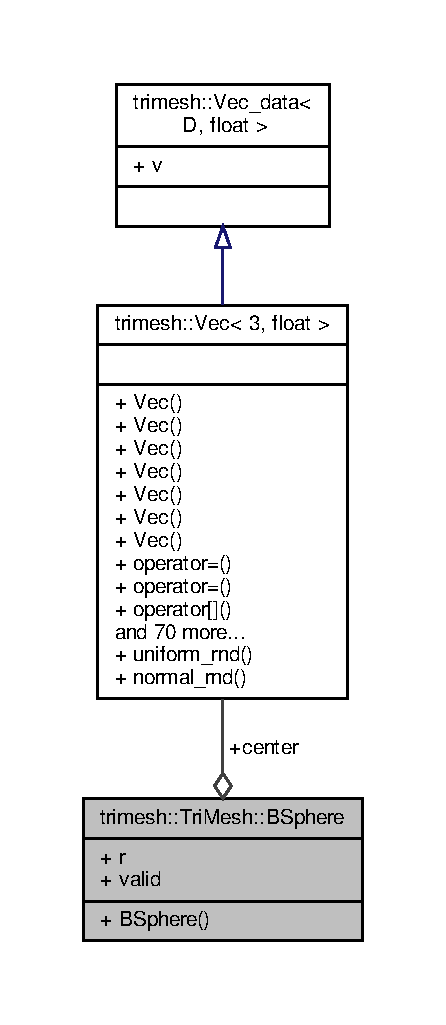
\includegraphics[width=214pt]{dd/dcf/structtrimesh_1_1TriMesh_1_1BSphere__coll__graph}
\end{center}
\end{figure}
\subsection*{Public Member Functions}
\begin{DoxyCompactItemize}
\item 
\hyperlink{structtrimesh_1_1TriMesh_1_1BSphere_acb25debfbc4ba199c73f1dd8b802e9d9}{B\+Sphere} ()
\end{DoxyCompactItemize}
\subsection*{Public Attributes}
\begin{DoxyCompactItemize}
\item 
\hyperlink{namespacetrimesh_a325b99fd6454b22fa4c4bc3223271b2c}{point} \hyperlink{structtrimesh_1_1TriMesh_1_1BSphere_a5408bf27a368120385d90f2891f977df}{center}
\item 
float \hyperlink{structtrimesh_1_1TriMesh_1_1BSphere_a9d06cee2284cf345cd9945d9c5117168}{r}
\item 
bool \hyperlink{structtrimesh_1_1TriMesh_1_1BSphere_a760a7c7c03f40f660e11d6b9b4bb4183}{valid}
\end{DoxyCompactItemize}


\subsection{Constructor \& Destructor Documentation}
\mbox{\Hypertarget{structtrimesh_1_1TriMesh_1_1BSphere_acb25debfbc4ba199c73f1dd8b802e9d9}\label{structtrimesh_1_1TriMesh_1_1BSphere_acb25debfbc4ba199c73f1dd8b802e9d9}} 
\index{trimesh\+::\+Tri\+Mesh\+::\+B\+Sphere@{trimesh\+::\+Tri\+Mesh\+::\+B\+Sphere}!B\+Sphere@{B\+Sphere}}
\index{B\+Sphere@{B\+Sphere}!trimesh\+::\+Tri\+Mesh\+::\+B\+Sphere@{trimesh\+::\+Tri\+Mesh\+::\+B\+Sphere}}
\subsubsection{\texorpdfstring{B\+Sphere()}{BSphere()}}
{\footnotesize\ttfamily trimesh\+::\+Tri\+Mesh\+::\+B\+Sphere\+::\+B\+Sphere (\begin{DoxyParamCaption}{ }\end{DoxyParamCaption})\hspace{0.3cm}{\ttfamily [inline]}}



\subsection{Member Data Documentation}
\mbox{\Hypertarget{structtrimesh_1_1TriMesh_1_1BSphere_a5408bf27a368120385d90f2891f977df}\label{structtrimesh_1_1TriMesh_1_1BSphere_a5408bf27a368120385d90f2891f977df}} 
\index{trimesh\+::\+Tri\+Mesh\+::\+B\+Sphere@{trimesh\+::\+Tri\+Mesh\+::\+B\+Sphere}!center@{center}}
\index{center@{center}!trimesh\+::\+Tri\+Mesh\+::\+B\+Sphere@{trimesh\+::\+Tri\+Mesh\+::\+B\+Sphere}}
\subsubsection{\texorpdfstring{center}{center}}
{\footnotesize\ttfamily \hyperlink{namespacetrimesh_a325b99fd6454b22fa4c4bc3223271b2c}{point} trimesh\+::\+Tri\+Mesh\+::\+B\+Sphere\+::center}



Referenced by trimesh\+::\+I\+C\+P().

\mbox{\Hypertarget{structtrimesh_1_1TriMesh_1_1BSphere_a9d06cee2284cf345cd9945d9c5117168}\label{structtrimesh_1_1TriMesh_1_1BSphere_a9d06cee2284cf345cd9945d9c5117168}} 
\index{trimesh\+::\+Tri\+Mesh\+::\+B\+Sphere@{trimesh\+::\+Tri\+Mesh\+::\+B\+Sphere}!r@{r}}
\index{r@{r}!trimesh\+::\+Tri\+Mesh\+::\+B\+Sphere@{trimesh\+::\+Tri\+Mesh\+::\+B\+Sphere}}
\subsubsection{\texorpdfstring{r}{r}}
{\footnotesize\ttfamily float trimesh\+::\+Tri\+Mesh\+::\+B\+Sphere\+::r}



Referenced by trimesh\+::\+I\+C\+P().

\mbox{\Hypertarget{structtrimesh_1_1TriMesh_1_1BSphere_a760a7c7c03f40f660e11d6b9b4bb4183}\label{structtrimesh_1_1TriMesh_1_1BSphere_a760a7c7c03f40f660e11d6b9b4bb4183}} 
\index{trimesh\+::\+Tri\+Mesh\+::\+B\+Sphere@{trimesh\+::\+Tri\+Mesh\+::\+B\+Sphere}!valid@{valid}}
\index{valid@{valid}!trimesh\+::\+Tri\+Mesh\+::\+B\+Sphere@{trimesh\+::\+Tri\+Mesh\+::\+B\+Sphere}}
\subsubsection{\texorpdfstring{valid}{valid}}
{\footnotesize\ttfamily bool trimesh\+::\+Tri\+Mesh\+::\+B\+Sphere\+::valid}



Referenced by trimesh\+::apply\+\_\+xform(), trimesh\+::\+Tri\+Mesh\+::clear\+\_\+bsphere(), trimesh\+::inflate(), trimesh\+::lmsmooth(), trimesh\+::remap\+\_\+verts(), trimesh\+::remove\+\_\+faces(), and trimesh\+::umbrella().



The documentation for this struct was generated from the following file\+:\begin{DoxyCompactItemize}
\item 
\hyperlink{TriMesh_8h}{Tri\+Mesh.\+h}\end{DoxyCompactItemize}

\hypertarget{classtrimesh_1_1GLManager_1_1BufferInfo}{}\section{trimesh\+:\+:G\+L\+Manager\+:\+:Buffer\+Info Class Reference}
\label{classtrimesh_1_1GLManager_1_1BufferInfo}\index{trimesh\+::\+G\+L\+Manager\+::\+Buffer\+Info@{trimesh\+::\+G\+L\+Manager\+::\+Buffer\+Info}}


Collaboration diagram for trimesh\+:\+:G\+L\+Manager\+:\+:Buffer\+Info\+:\nopagebreak
\begin{figure}[H]
\begin{center}
\leavevmode
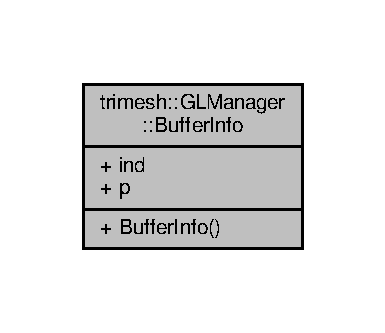
\includegraphics[width=185pt]{d9/dca/classtrimesh_1_1GLManager_1_1BufferInfo__coll__graph}
\end{center}
\end{figure}
\subsection*{Public Member Functions}
\begin{DoxyCompactItemize}
\item 
\hyperlink{classtrimesh_1_1GLManager_1_1BufferInfo_ab381d4cc2e1b7a8ea5d7d50c6c1d48b1}{Buffer\+Info} (unsigned ind\+\_\+, const \hyperlink{namespacetrimesh_a784ddfd979e1c579bda795a8edfc3f43}{void} $\ast$p\+\_\+)
\end{DoxyCompactItemize}
\subsection*{Public Attributes}
\begin{DoxyCompactItemize}
\item 
unsigned \hyperlink{classtrimesh_1_1GLManager_1_1BufferInfo_a4a2777aeb5cdeada97a07db8eb4356ca}{ind}
\item 
const \hyperlink{namespacetrimesh_a784ddfd979e1c579bda795a8edfc3f43}{void} $\ast$ \hyperlink{classtrimesh_1_1GLManager_1_1BufferInfo_aaab05a6f7ef2421573cf5f58c3d52c19}{p}
\end{DoxyCompactItemize}


\subsection{Constructor \& Destructor Documentation}
\mbox{\Hypertarget{classtrimesh_1_1GLManager_1_1BufferInfo_ab381d4cc2e1b7a8ea5d7d50c6c1d48b1}\label{classtrimesh_1_1GLManager_1_1BufferInfo_ab381d4cc2e1b7a8ea5d7d50c6c1d48b1}} 
\index{trimesh\+::\+G\+L\+Manager\+::\+Buffer\+Info@{trimesh\+::\+G\+L\+Manager\+::\+Buffer\+Info}!Buffer\+Info@{Buffer\+Info}}
\index{Buffer\+Info@{Buffer\+Info}!trimesh\+::\+G\+L\+Manager\+::\+Buffer\+Info@{trimesh\+::\+G\+L\+Manager\+::\+Buffer\+Info}}
\subsubsection{\texorpdfstring{Buffer\+Info()}{BufferInfo()}}
{\footnotesize\ttfamily trimesh\+::\+G\+L\+Manager\+::\+Buffer\+Info\+::\+Buffer\+Info (\begin{DoxyParamCaption}\item[{unsigned}]{ind\+\_\+,  }\item[{const \hyperlink{namespacetrimesh_a784ddfd979e1c579bda795a8edfc3f43}{void} $\ast$}]{p\+\_\+ }\end{DoxyParamCaption})\hspace{0.3cm}{\ttfamily [inline]}}



\subsection{Member Data Documentation}
\mbox{\Hypertarget{classtrimesh_1_1GLManager_1_1BufferInfo_a4a2777aeb5cdeada97a07db8eb4356ca}\label{classtrimesh_1_1GLManager_1_1BufferInfo_a4a2777aeb5cdeada97a07db8eb4356ca}} 
\index{trimesh\+::\+G\+L\+Manager\+::\+Buffer\+Info@{trimesh\+::\+G\+L\+Manager\+::\+Buffer\+Info}!ind@{ind}}
\index{ind@{ind}!trimesh\+::\+G\+L\+Manager\+::\+Buffer\+Info@{trimesh\+::\+G\+L\+Manager\+::\+Buffer\+Info}}
\subsubsection{\texorpdfstring{ind}{ind}}
{\footnotesize\ttfamily unsigned trimesh\+::\+G\+L\+Manager\+::\+Buffer\+Info\+::ind}



Referenced by trimesh\+::\+G\+L\+Manager\+::clear\+\_\+buffer(), trimesh\+::\+G\+L\+Manager\+::clear\+\_\+ibuffer(), trimesh\+::\+G\+L\+Manager\+::clear\+\_\+texture(), trimesh\+::\+G\+L\+Manager\+::use\+\_\+buffer(), trimesh\+::\+G\+L\+Manager\+::use\+\_\+ibuffer(), and trimesh\+::\+G\+L\+Manager\+::use\+\_\+texture().

\mbox{\Hypertarget{classtrimesh_1_1GLManager_1_1BufferInfo_aaab05a6f7ef2421573cf5f58c3d52c19}\label{classtrimesh_1_1GLManager_1_1BufferInfo_aaab05a6f7ef2421573cf5f58c3d52c19}} 
\index{trimesh\+::\+G\+L\+Manager\+::\+Buffer\+Info@{trimesh\+::\+G\+L\+Manager\+::\+Buffer\+Info}!p@{p}}
\index{p@{p}!trimesh\+::\+G\+L\+Manager\+::\+Buffer\+Info@{trimesh\+::\+G\+L\+Manager\+::\+Buffer\+Info}}
\subsubsection{\texorpdfstring{p}{p}}
{\footnotesize\ttfamily const \hyperlink{namespacetrimesh_a784ddfd979e1c579bda795a8edfc3f43}{void}$\ast$ trimesh\+::\+G\+L\+Manager\+::\+Buffer\+Info\+::p}



The documentation for this class was generated from the following file\+:\begin{DoxyCompactItemize}
\item 
\hyperlink{GLManager_8cc}{G\+L\+Manager.\+cc}\end{DoxyCompactItemize}

\hypertarget{classtrimesh_1_1Color}{}\section{trimesh\+:\+:Color Class Reference}
\label{classtrimesh_1_1Color}\index{trimesh\+::\+Color@{trimesh\+::\+Color}}


{\ttfamily \#include $<$Color.\+h$>$}



Inheritance diagram for trimesh\+:\+:Color\+:\nopagebreak
\begin{figure}[H]
\begin{center}
\leavevmode
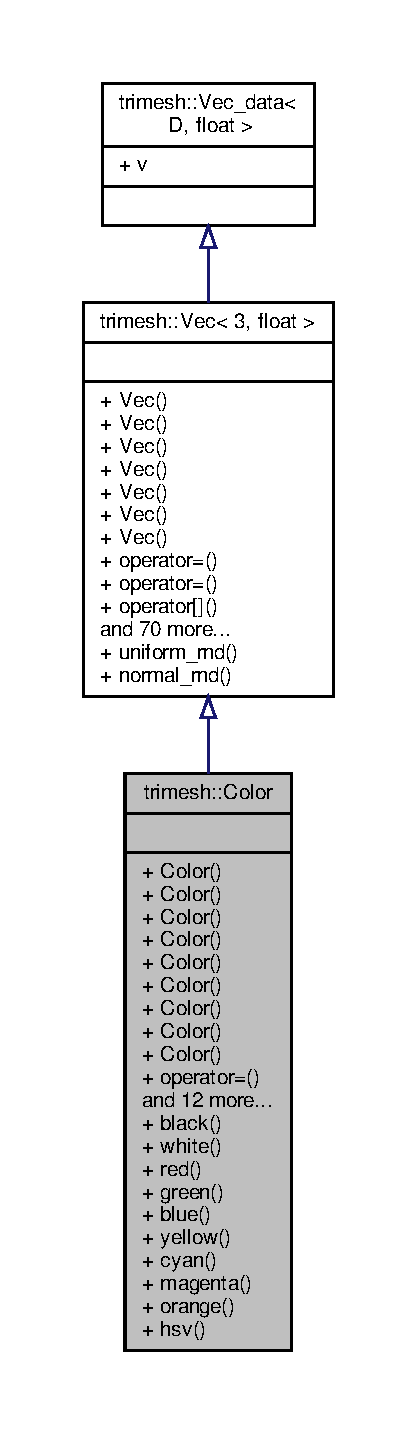
\includegraphics[height=550pt]{dd/db1/classtrimesh_1_1Color__inherit__graph}
\end{center}
\end{figure}


Collaboration diagram for trimesh\+:\+:Color\+:\nopagebreak
\begin{figure}[H]
\begin{center}
\leavevmode
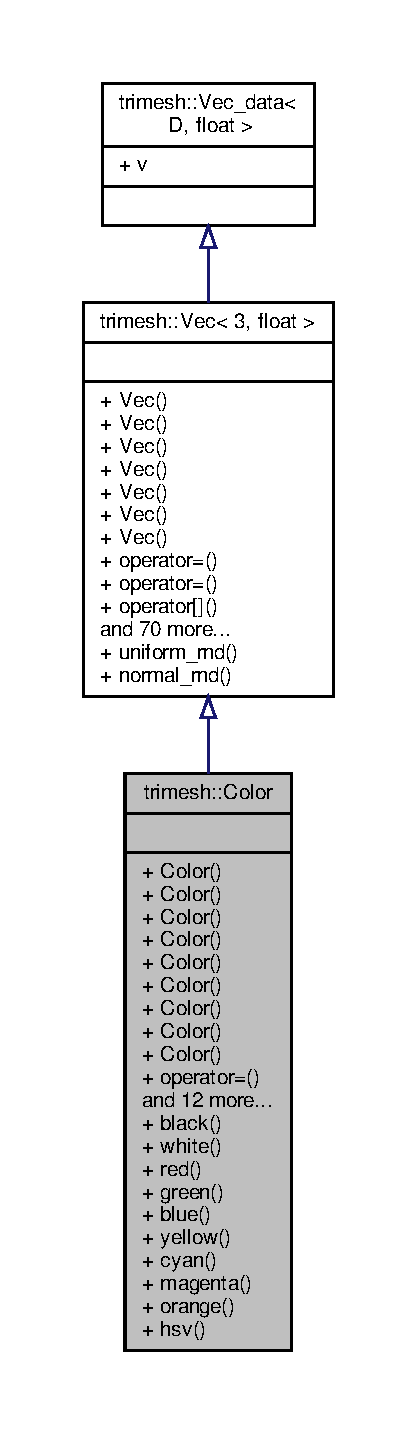
\includegraphics[height=550pt]{dd/daa/classtrimesh_1_1Color__coll__graph}
\end{center}
\end{figure}
\subsection*{Public Types}
\begin{DoxyCompactItemize}
\item 
enum \hyperlink{classtrimesh_1_1Color_a2e472a2f6056fb5d0d835ee1c361b6da}{Colorspace} \{ \newline
\hyperlink{classtrimesh_1_1Color_a2e472a2f6056fb5d0d835ee1c361b6daa34378035ef639b94005f8a3f00ac9388}{C\+I\+E\+L\+AB}, 
\hyperlink{classtrimesh_1_1Color_a2e472a2f6056fb5d0d835ee1c361b6daabb45b461ca3718a56a106ac7cc0b01d4}{X\+YZ}, 
\hyperlink{classtrimesh_1_1Color_a2e472a2f6056fb5d0d835ee1c361b6daabd359b28fff9f9d21986cac01d02fc9e}{R\+GB}, 
\hyperlink{classtrimesh_1_1Color_a2e472a2f6056fb5d0d835ee1c361b6daa09ccc9ca587a8056b9552ec4dff53fd4}{S\+R\+GB}, 
\newline
\hyperlink{classtrimesh_1_1Color_a2e472a2f6056fb5d0d835ee1c361b6daa61362689388b942d9d7fea6ddc74db63}{Y\+C\+B\+CR}, 
\hyperlink{classtrimesh_1_1Color_a2e472a2f6056fb5d0d835ee1c361b6daa5239e1d12b6fbaab60f8b57960f2168b}{H\+SV}
 \}
\end{DoxyCompactItemize}
\subsection*{Public Member Functions}
\begin{DoxyCompactItemize}
\item 
\hyperlink{classtrimesh_1_1Color_a5f3b1f0bc94c9d5961b6ec18d7b5680b}{Color} ()
\item 
\hyperlink{classtrimesh_1_1Color_a28065ab275e33f2d15f6e04454b46e62}{Color} (const \hyperlink{classtrimesh_1_1Vec}{Vec}$<$ 3, float $>$ \&v\+\_\+)
\item 
\hyperlink{classtrimesh_1_1Color_a7392a0749cb1dcc68e612cf78e0a3981}{Color} (const \hyperlink{classtrimesh_1_1Vec}{Vec}$<$ 3, double $>$ \&v\+\_\+)
\item 
\hyperlink{classtrimesh_1_1Color_af29b64418e6ca02c58576c93ca0e975f}{Color} (float r\+\_\+, float g\+\_\+, float b\+\_\+)
\item 
\hyperlink{classtrimesh_1_1Color_abc30f1ba7fafda012a34ab9d10674641}{Color} (double r\+\_\+, double g\+\_\+, double b\+\_\+)
\item 
\hyperlink{classtrimesh_1_1Color_a41529c8f161c5e24e0ab1101dc1aa38f}{Color} (const float $\ast$rgb)
\item 
\hyperlink{classtrimesh_1_1Color_a33efbf8310345af27ce0848065d53f3f}{Color} (const double $\ast$rgb)
\item 
\hyperlink{classtrimesh_1_1Color_a9eda4f560e7bb7f874df6d5c6d9c35e2}{Color} (float c)
\item 
\hyperlink{classtrimesh_1_1Color_a5074dcb961dac61df90afc86b66ec7f4}{Color} (double c)
\item 
\hyperlink{classtrimesh_1_1Color}{Color} \& \hyperlink{classtrimesh_1_1Color_a5db3d69c50675fead68e02b92247a410}{operator=} (float c)
\item 
\hyperlink{classtrimesh_1_1Color}{Color} \& \hyperlink{classtrimesh_1_1Color_a3af13e0b2b3b1e778ac35d9063adc3a5}{operator=} (double c)
\item 
\hyperlink{classtrimesh_1_1Color_a7b791c39c2b3a3f71819b46208bfd655}{Color} (int r\+\_\+, int g\+\_\+, int b\+\_\+)
\item 
\hyperlink{classtrimesh_1_1Color_a89ec2caff8d63d6d7be4bf06e2559f94}{Color} (const int $\ast$rgb)
\item 
\hyperlink{classtrimesh_1_1Color_acb4e744c4467b999881b020d9cc5cd9c}{Color} (const unsigned char $\ast$rgb)
\item 
\hyperlink{classtrimesh_1_1Color_ad4c51fc21300fbba703895eb6af9b8d4}{Color} (int c)
\item 
\hyperlink{classtrimesh_1_1Color}{Color} \& \hyperlink{classtrimesh_1_1Color_a5adc5202c414bedff8834df834ee7b7b}{operator=} (int c)
\item 
const \hyperlink{classtrimesh_1_1Color}{Color} \hyperlink{classtrimesh_1_1Color_ab36b9ceebc09353d2513fb5ef3adbacf}{col\+\_\+transform} (float m11, float m12, float m13, float m21, float m22, float m23, float m31, float m32, float m33) const
\item 
const \hyperlink{classtrimesh_1_1Color}{Color} \hyperlink{classtrimesh_1_1Color_a684dabf3f7e2011c6c5288e91a12215b}{convert} (\hyperlink{classtrimesh_1_1Color_a2e472a2f6056fb5d0d835ee1c361b6da}{Colorspace} src, \hyperlink{classtrimesh_1_1Color_a2e472a2f6056fb5d0d835ee1c361b6da}{Colorspace} dst) const
\item 
const \hyperlink{classtrimesh_1_1Color}{Color} \hyperlink{classtrimesh_1_1Color_a3540c038c7f993120eed3d3683797b02}{gamma} (float g\+\_\+) const
\item 
const \hyperlink{classtrimesh_1_1Color}{Color} \hyperlink{classtrimesh_1_1Color_aed131184642ab0047a27cc5b5b305acd}{gamma} (\hyperlink{classtrimesh_1_1Color_a2e472a2f6056fb5d0d835ee1c361b6da}{Colorspace} dst) const
\item 
const \hyperlink{classtrimesh_1_1Color}{Color} \hyperlink{classtrimesh_1_1Color_a26bd1dd5b2521e58e0a80d98b76a8fbe}{ungamma} (float g\+\_\+) const
\item 
const \hyperlink{classtrimesh_1_1Color}{Color} \hyperlink{classtrimesh_1_1Color_a053596dda07bead7e3f63b3ee5cb4625}{ungamma} (\hyperlink{classtrimesh_1_1Color_a2e472a2f6056fb5d0d835ee1c361b6da}{Colorspace} dst) const
\end{DoxyCompactItemize}
\subsection*{Static Public Member Functions}
\begin{DoxyCompactItemize}
\item 
static \hyperlink{classtrimesh_1_1Color}{Color} \hyperlink{classtrimesh_1_1Color_a07940c6da47edfc63a5462b7bb2902d4}{black} ()
\item 
static \hyperlink{classtrimesh_1_1Color}{Color} \hyperlink{classtrimesh_1_1Color_ae400e9cbab4e192250e9dbb4cb2cf2dc}{white} ()
\item 
static \hyperlink{classtrimesh_1_1Color}{Color} \hyperlink{classtrimesh_1_1Color_ac56231f8718960b29323be3c966e4d11}{red} ()
\item 
static \hyperlink{classtrimesh_1_1Color}{Color} \hyperlink{classtrimesh_1_1Color_ae17448b9f7642601460d2e54e7f83905}{green} ()
\item 
static \hyperlink{classtrimesh_1_1Color}{Color} \hyperlink{classtrimesh_1_1Color_ab9bf7671a5a760af4af8259034112192}{blue} ()
\item 
static \hyperlink{classtrimesh_1_1Color}{Color} \hyperlink{classtrimesh_1_1Color_ac6156bc948dc531550cef3b86137b5b0}{yellow} ()
\item 
static \hyperlink{classtrimesh_1_1Color}{Color} \hyperlink{classtrimesh_1_1Color_a0fa734079d4c95adee86ef323267ef86}{cyan} ()
\item 
static \hyperlink{classtrimesh_1_1Color}{Color} \hyperlink{classtrimesh_1_1Color_af9fb47c4be66c136c0acce1df09c5b90}{magenta} ()
\item 
static \hyperlink{classtrimesh_1_1Color}{Color} \hyperlink{classtrimesh_1_1Color_ab5bc5d41f117a12d4a1136d7e4d99aea}{orange} ()
\item 
static \hyperlink{classtrimesh_1_1Color}{Color} \hyperlink{classtrimesh_1_1Color_a609b459d8e1ded6dd6d985ddfc0a68db}{hsv} (float H, float \hyperlink{ego_8cc_abde73cd36321648268fb4543509b996a}{S}, float V)
\end{DoxyCompactItemize}
\subsection*{Additional Inherited Members}


\subsection{Member Enumeration Documentation}
\mbox{\Hypertarget{classtrimesh_1_1Color_a2e472a2f6056fb5d0d835ee1c361b6da}\label{classtrimesh_1_1Color_a2e472a2f6056fb5d0d835ee1c361b6da}} 
\index{trimesh\+::\+Color@{trimesh\+::\+Color}!Colorspace@{Colorspace}}
\index{Colorspace@{Colorspace}!trimesh\+::\+Color@{trimesh\+::\+Color}}
\subsubsection{\texorpdfstring{Colorspace}{Colorspace}}
{\footnotesize\ttfamily enum \hyperlink{classtrimesh_1_1Color_a2e472a2f6056fb5d0d835ee1c361b6da}{trimesh\+::\+Color\+::\+Colorspace}}

\begin{DoxyEnumFields}{Enumerator}
\raisebox{\heightof{T}}[0pt][0pt]{\index{C\+I\+E\+L\+AB@{C\+I\+E\+L\+AB}!trimesh\+::\+Color@{trimesh\+::\+Color}}\index{trimesh\+::\+Color@{trimesh\+::\+Color}!C\+I\+E\+L\+AB@{C\+I\+E\+L\+AB}}}\mbox{\Hypertarget{classtrimesh_1_1Color_a2e472a2f6056fb5d0d835ee1c361b6daa34378035ef639b94005f8a3f00ac9388}\label{classtrimesh_1_1Color_a2e472a2f6056fb5d0d835ee1c361b6daa34378035ef639b94005f8a3f00ac9388}} 
C\+I\+E\+L\+AB&\\
\hline

\raisebox{\heightof{T}}[0pt][0pt]{\index{X\+YZ@{X\+YZ}!trimesh\+::\+Color@{trimesh\+::\+Color}}\index{trimesh\+::\+Color@{trimesh\+::\+Color}!X\+YZ@{X\+YZ}}}\mbox{\Hypertarget{classtrimesh_1_1Color_a2e472a2f6056fb5d0d835ee1c361b6daabb45b461ca3718a56a106ac7cc0b01d4}\label{classtrimesh_1_1Color_a2e472a2f6056fb5d0d835ee1c361b6daabb45b461ca3718a56a106ac7cc0b01d4}} 
X\+YZ&\\
\hline

\raisebox{\heightof{T}}[0pt][0pt]{\index{R\+GB@{R\+GB}!trimesh\+::\+Color@{trimesh\+::\+Color}}\index{trimesh\+::\+Color@{trimesh\+::\+Color}!R\+GB@{R\+GB}}}\mbox{\Hypertarget{classtrimesh_1_1Color_a2e472a2f6056fb5d0d835ee1c361b6daabd359b28fff9f9d21986cac01d02fc9e}\label{classtrimesh_1_1Color_a2e472a2f6056fb5d0d835ee1c361b6daabd359b28fff9f9d21986cac01d02fc9e}} 
R\+GB&\\
\hline

\raisebox{\heightof{T}}[0pt][0pt]{\index{S\+R\+GB@{S\+R\+GB}!trimesh\+::\+Color@{trimesh\+::\+Color}}\index{trimesh\+::\+Color@{trimesh\+::\+Color}!S\+R\+GB@{S\+R\+GB}}}\mbox{\Hypertarget{classtrimesh_1_1Color_a2e472a2f6056fb5d0d835ee1c361b6daa09ccc9ca587a8056b9552ec4dff53fd4}\label{classtrimesh_1_1Color_a2e472a2f6056fb5d0d835ee1c361b6daa09ccc9ca587a8056b9552ec4dff53fd4}} 
S\+R\+GB&\\
\hline

\raisebox{\heightof{T}}[0pt][0pt]{\index{Y\+C\+B\+CR@{Y\+C\+B\+CR}!trimesh\+::\+Color@{trimesh\+::\+Color}}\index{trimesh\+::\+Color@{trimesh\+::\+Color}!Y\+C\+B\+CR@{Y\+C\+B\+CR}}}\mbox{\Hypertarget{classtrimesh_1_1Color_a2e472a2f6056fb5d0d835ee1c361b6daa61362689388b942d9d7fea6ddc74db63}\label{classtrimesh_1_1Color_a2e472a2f6056fb5d0d835ee1c361b6daa61362689388b942d9d7fea6ddc74db63}} 
Y\+C\+B\+CR&\\
\hline

\raisebox{\heightof{T}}[0pt][0pt]{\index{H\+SV@{H\+SV}!trimesh\+::\+Color@{trimesh\+::\+Color}}\index{trimesh\+::\+Color@{trimesh\+::\+Color}!H\+SV@{H\+SV}}}\mbox{\Hypertarget{classtrimesh_1_1Color_a2e472a2f6056fb5d0d835ee1c361b6daa5239e1d12b6fbaab60f8b57960f2168b}\label{classtrimesh_1_1Color_a2e472a2f6056fb5d0d835ee1c361b6daa5239e1d12b6fbaab60f8b57960f2168b}} 
H\+SV&\\
\hline

\end{DoxyEnumFields}


\subsection{Constructor \& Destructor Documentation}
\mbox{\Hypertarget{classtrimesh_1_1Color_a5f3b1f0bc94c9d5961b6ec18d7b5680b}\label{classtrimesh_1_1Color_a5f3b1f0bc94c9d5961b6ec18d7b5680b}} 
\index{trimesh\+::\+Color@{trimesh\+::\+Color}!Color@{Color}}
\index{Color@{Color}!trimesh\+::\+Color@{trimesh\+::\+Color}}
\subsubsection{\texorpdfstring{Color()}{Color()}\hspace{0.1cm}{\footnotesize\ttfamily [1/13]}}
{\footnotesize\ttfamily trimesh\+::\+Color\+::\+Color (\begin{DoxyParamCaption}{ }\end{DoxyParamCaption})\hspace{0.3cm}{\ttfamily [inline]}}



Referenced by black(), blue(), col\+\_\+transform(), Color(), convert(), cyan(), gamma(), green(), hsv(), magenta(), operator=(), orange(), red(), ungamma(), white(), and yellow().

\mbox{\Hypertarget{classtrimesh_1_1Color_a28065ab275e33f2d15f6e04454b46e62}\label{classtrimesh_1_1Color_a28065ab275e33f2d15f6e04454b46e62}} 
\index{trimesh\+::\+Color@{trimesh\+::\+Color}!Color@{Color}}
\index{Color@{Color}!trimesh\+::\+Color@{trimesh\+::\+Color}}
\subsubsection{\texorpdfstring{Color()}{Color()}\hspace{0.1cm}{\footnotesize\ttfamily [2/13]}}
{\footnotesize\ttfamily trimesh\+::\+Color\+::\+Color (\begin{DoxyParamCaption}\item[{const \hyperlink{classtrimesh_1_1Vec}{Vec}$<$ 3, float $>$ \&}]{v\+\_\+ }\end{DoxyParamCaption})\hspace{0.3cm}{\ttfamily [inline]}}

\mbox{\Hypertarget{classtrimesh_1_1Color_a7392a0749cb1dcc68e612cf78e0a3981}\label{classtrimesh_1_1Color_a7392a0749cb1dcc68e612cf78e0a3981}} 
\index{trimesh\+::\+Color@{trimesh\+::\+Color}!Color@{Color}}
\index{Color@{Color}!trimesh\+::\+Color@{trimesh\+::\+Color}}
\subsubsection{\texorpdfstring{Color()}{Color()}\hspace{0.1cm}{\footnotesize\ttfamily [3/13]}}
{\footnotesize\ttfamily trimesh\+::\+Color\+::\+Color (\begin{DoxyParamCaption}\item[{const \hyperlink{classtrimesh_1_1Vec}{Vec}$<$ 3, double $>$ \&}]{v\+\_\+ }\end{DoxyParamCaption})\hspace{0.3cm}{\ttfamily [inline]}}

\mbox{\Hypertarget{classtrimesh_1_1Color_af29b64418e6ca02c58576c93ca0e975f}\label{classtrimesh_1_1Color_af29b64418e6ca02c58576c93ca0e975f}} 
\index{trimesh\+::\+Color@{trimesh\+::\+Color}!Color@{Color}}
\index{Color@{Color}!trimesh\+::\+Color@{trimesh\+::\+Color}}
\subsubsection{\texorpdfstring{Color()}{Color()}\hspace{0.1cm}{\footnotesize\ttfamily [4/13]}}
{\footnotesize\ttfamily trimesh\+::\+Color\+::\+Color (\begin{DoxyParamCaption}\item[{float}]{r\+\_\+,  }\item[{float}]{g\+\_\+,  }\item[{float}]{b\+\_\+ }\end{DoxyParamCaption})\hspace{0.3cm}{\ttfamily [inline]}}

\mbox{\Hypertarget{classtrimesh_1_1Color_abc30f1ba7fafda012a34ab9d10674641}\label{classtrimesh_1_1Color_abc30f1ba7fafda012a34ab9d10674641}} 
\index{trimesh\+::\+Color@{trimesh\+::\+Color}!Color@{Color}}
\index{Color@{Color}!trimesh\+::\+Color@{trimesh\+::\+Color}}
\subsubsection{\texorpdfstring{Color()}{Color()}\hspace{0.1cm}{\footnotesize\ttfamily [5/13]}}
{\footnotesize\ttfamily trimesh\+::\+Color\+::\+Color (\begin{DoxyParamCaption}\item[{double}]{r\+\_\+,  }\item[{double}]{g\+\_\+,  }\item[{double}]{b\+\_\+ }\end{DoxyParamCaption})\hspace{0.3cm}{\ttfamily [inline]}}

\mbox{\Hypertarget{classtrimesh_1_1Color_a41529c8f161c5e24e0ab1101dc1aa38f}\label{classtrimesh_1_1Color_a41529c8f161c5e24e0ab1101dc1aa38f}} 
\index{trimesh\+::\+Color@{trimesh\+::\+Color}!Color@{Color}}
\index{Color@{Color}!trimesh\+::\+Color@{trimesh\+::\+Color}}
\subsubsection{\texorpdfstring{Color()}{Color()}\hspace{0.1cm}{\footnotesize\ttfamily [6/13]}}
{\footnotesize\ttfamily trimesh\+::\+Color\+::\+Color (\begin{DoxyParamCaption}\item[{const float $\ast$}]{rgb }\end{DoxyParamCaption})\hspace{0.3cm}{\ttfamily [inline]}, {\ttfamily [explicit]}}

\mbox{\Hypertarget{classtrimesh_1_1Color_a33efbf8310345af27ce0848065d53f3f}\label{classtrimesh_1_1Color_a33efbf8310345af27ce0848065d53f3f}} 
\index{trimesh\+::\+Color@{trimesh\+::\+Color}!Color@{Color}}
\index{Color@{Color}!trimesh\+::\+Color@{trimesh\+::\+Color}}
\subsubsection{\texorpdfstring{Color()}{Color()}\hspace{0.1cm}{\footnotesize\ttfamily [7/13]}}
{\footnotesize\ttfamily trimesh\+::\+Color\+::\+Color (\begin{DoxyParamCaption}\item[{const double $\ast$}]{rgb }\end{DoxyParamCaption})\hspace{0.3cm}{\ttfamily [inline]}, {\ttfamily [explicit]}}

\mbox{\Hypertarget{classtrimesh_1_1Color_a9eda4f560e7bb7f874df6d5c6d9c35e2}\label{classtrimesh_1_1Color_a9eda4f560e7bb7f874df6d5c6d9c35e2}} 
\index{trimesh\+::\+Color@{trimesh\+::\+Color}!Color@{Color}}
\index{Color@{Color}!trimesh\+::\+Color@{trimesh\+::\+Color}}
\subsubsection{\texorpdfstring{Color()}{Color()}\hspace{0.1cm}{\footnotesize\ttfamily [8/13]}}
{\footnotesize\ttfamily trimesh\+::\+Color\+::\+Color (\begin{DoxyParamCaption}\item[{float}]{c }\end{DoxyParamCaption})\hspace{0.3cm}{\ttfamily [inline]}, {\ttfamily [explicit]}}

\mbox{\Hypertarget{classtrimesh_1_1Color_a5074dcb961dac61df90afc86b66ec7f4}\label{classtrimesh_1_1Color_a5074dcb961dac61df90afc86b66ec7f4}} 
\index{trimesh\+::\+Color@{trimesh\+::\+Color}!Color@{Color}}
\index{Color@{Color}!trimesh\+::\+Color@{trimesh\+::\+Color}}
\subsubsection{\texorpdfstring{Color()}{Color()}\hspace{0.1cm}{\footnotesize\ttfamily [9/13]}}
{\footnotesize\ttfamily trimesh\+::\+Color\+::\+Color (\begin{DoxyParamCaption}\item[{double}]{c }\end{DoxyParamCaption})\hspace{0.3cm}{\ttfamily [inline]}, {\ttfamily [explicit]}}

\mbox{\Hypertarget{classtrimesh_1_1Color_a7b791c39c2b3a3f71819b46208bfd655}\label{classtrimesh_1_1Color_a7b791c39c2b3a3f71819b46208bfd655}} 
\index{trimesh\+::\+Color@{trimesh\+::\+Color}!Color@{Color}}
\index{Color@{Color}!trimesh\+::\+Color@{trimesh\+::\+Color}}
\subsubsection{\texorpdfstring{Color()}{Color()}\hspace{0.1cm}{\footnotesize\ttfamily [10/13]}}
{\footnotesize\ttfamily trimesh\+::\+Color\+::\+Color (\begin{DoxyParamCaption}\item[{int}]{r\+\_\+,  }\item[{int}]{g\+\_\+,  }\item[{int}]{b\+\_\+ }\end{DoxyParamCaption})\hspace{0.3cm}{\ttfamily [inline]}}

\mbox{\Hypertarget{classtrimesh_1_1Color_a89ec2caff8d63d6d7be4bf06e2559f94}\label{classtrimesh_1_1Color_a89ec2caff8d63d6d7be4bf06e2559f94}} 
\index{trimesh\+::\+Color@{trimesh\+::\+Color}!Color@{Color}}
\index{Color@{Color}!trimesh\+::\+Color@{trimesh\+::\+Color}}
\subsubsection{\texorpdfstring{Color()}{Color()}\hspace{0.1cm}{\footnotesize\ttfamily [11/13]}}
{\footnotesize\ttfamily trimesh\+::\+Color\+::\+Color (\begin{DoxyParamCaption}\item[{const int $\ast$}]{rgb }\end{DoxyParamCaption})\hspace{0.3cm}{\ttfamily [inline]}, {\ttfamily [explicit]}}

\mbox{\Hypertarget{classtrimesh_1_1Color_acb4e744c4467b999881b020d9cc5cd9c}\label{classtrimesh_1_1Color_acb4e744c4467b999881b020d9cc5cd9c}} 
\index{trimesh\+::\+Color@{trimesh\+::\+Color}!Color@{Color}}
\index{Color@{Color}!trimesh\+::\+Color@{trimesh\+::\+Color}}
\subsubsection{\texorpdfstring{Color()}{Color()}\hspace{0.1cm}{\footnotesize\ttfamily [12/13]}}
{\footnotesize\ttfamily trimesh\+::\+Color\+::\+Color (\begin{DoxyParamCaption}\item[{const unsigned char $\ast$}]{rgb }\end{DoxyParamCaption})\hspace{0.3cm}{\ttfamily [inline]}, {\ttfamily [explicit]}}

\mbox{\Hypertarget{classtrimesh_1_1Color_ad4c51fc21300fbba703895eb6af9b8d4}\label{classtrimesh_1_1Color_ad4c51fc21300fbba703895eb6af9b8d4}} 
\index{trimesh\+::\+Color@{trimesh\+::\+Color}!Color@{Color}}
\index{Color@{Color}!trimesh\+::\+Color@{trimesh\+::\+Color}}
\subsubsection{\texorpdfstring{Color()}{Color()}\hspace{0.1cm}{\footnotesize\ttfamily [13/13]}}
{\footnotesize\ttfamily trimesh\+::\+Color\+::\+Color (\begin{DoxyParamCaption}\item[{int}]{c }\end{DoxyParamCaption})\hspace{0.3cm}{\ttfamily [inline]}, {\ttfamily [explicit]}}



\subsection{Member Function Documentation}
\mbox{\Hypertarget{classtrimesh_1_1Color_a07940c6da47edfc63a5462b7bb2902d4}\label{classtrimesh_1_1Color_a07940c6da47edfc63a5462b7bb2902d4}} 
\index{trimesh\+::\+Color@{trimesh\+::\+Color}!black@{black}}
\index{black@{black}!trimesh\+::\+Color@{trimesh\+::\+Color}}
\subsubsection{\texorpdfstring{black()}{black()}}
{\footnotesize\ttfamily static \hyperlink{classtrimesh_1_1Color}{Color} trimesh\+::\+Color\+::black (\begin{DoxyParamCaption}{ }\end{DoxyParamCaption})\hspace{0.3cm}{\ttfamily [inline]}, {\ttfamily [static]}}

\mbox{\Hypertarget{classtrimesh_1_1Color_ab9bf7671a5a760af4af8259034112192}\label{classtrimesh_1_1Color_ab9bf7671a5a760af4af8259034112192}} 
\index{trimesh\+::\+Color@{trimesh\+::\+Color}!blue@{blue}}
\index{blue@{blue}!trimesh\+::\+Color@{trimesh\+::\+Color}}
\subsubsection{\texorpdfstring{blue()}{blue()}}
{\footnotesize\ttfamily static \hyperlink{classtrimesh_1_1Color}{Color} trimesh\+::\+Color\+::blue (\begin{DoxyParamCaption}{ }\end{DoxyParamCaption})\hspace{0.3cm}{\ttfamily [inline]}, {\ttfamily [static]}}

\mbox{\Hypertarget{classtrimesh_1_1Color_ab36b9ceebc09353d2513fb5ef3adbacf}\label{classtrimesh_1_1Color_ab36b9ceebc09353d2513fb5ef3adbacf}} 
\index{trimesh\+::\+Color@{trimesh\+::\+Color}!col\+\_\+transform@{col\+\_\+transform}}
\index{col\+\_\+transform@{col\+\_\+transform}!trimesh\+::\+Color@{trimesh\+::\+Color}}
\subsubsection{\texorpdfstring{col\+\_\+transform()}{col\_transform()}}
{\footnotesize\ttfamily const \hyperlink{classtrimesh_1_1Color}{Color} trimesh\+::\+Color\+::col\+\_\+transform (\begin{DoxyParamCaption}\item[{float}]{m11,  }\item[{float}]{m12,  }\item[{float}]{m13,  }\item[{float}]{m21,  }\item[{float}]{m22,  }\item[{float}]{m23,  }\item[{float}]{m31,  }\item[{float}]{m32,  }\item[{float}]{m33 }\end{DoxyParamCaption}) const\hspace{0.3cm}{\ttfamily [inline]}}

\mbox{\Hypertarget{classtrimesh_1_1Color_a684dabf3f7e2011c6c5288e91a12215b}\label{classtrimesh_1_1Color_a684dabf3f7e2011c6c5288e91a12215b}} 
\index{trimesh\+::\+Color@{trimesh\+::\+Color}!convert@{convert}}
\index{convert@{convert}!trimesh\+::\+Color@{trimesh\+::\+Color}}
\subsubsection{\texorpdfstring{convert()}{convert()}}
{\footnotesize\ttfamily const \hyperlink{classtrimesh_1_1Color}{Color} trimesh\+::\+Color\+::convert (\begin{DoxyParamCaption}\item[{\hyperlink{classtrimesh_1_1Color_a2e472a2f6056fb5d0d835ee1c361b6da}{Colorspace}}]{src,  }\item[{\hyperlink{classtrimesh_1_1Color_a2e472a2f6056fb5d0d835ee1c361b6da}{Colorspace}}]{dst }\end{DoxyParamCaption}) const\hspace{0.3cm}{\ttfamily [inline]}}



Referenced by convert().

\mbox{\Hypertarget{classtrimesh_1_1Color_a0fa734079d4c95adee86ef323267ef86}\label{classtrimesh_1_1Color_a0fa734079d4c95adee86ef323267ef86}} 
\index{trimesh\+::\+Color@{trimesh\+::\+Color}!cyan@{cyan}}
\index{cyan@{cyan}!trimesh\+::\+Color@{trimesh\+::\+Color}}
\subsubsection{\texorpdfstring{cyan()}{cyan()}}
{\footnotesize\ttfamily static \hyperlink{classtrimesh_1_1Color}{Color} trimesh\+::\+Color\+::cyan (\begin{DoxyParamCaption}{ }\end{DoxyParamCaption})\hspace{0.3cm}{\ttfamily [inline]}, {\ttfamily [static]}}

\mbox{\Hypertarget{classtrimesh_1_1Color_a3540c038c7f993120eed3d3683797b02}\label{classtrimesh_1_1Color_a3540c038c7f993120eed3d3683797b02}} 
\index{trimesh\+::\+Color@{trimesh\+::\+Color}!gamma@{gamma}}
\index{gamma@{gamma}!trimesh\+::\+Color@{trimesh\+::\+Color}}
\subsubsection{\texorpdfstring{gamma()}{gamma()}\hspace{0.1cm}{\footnotesize\ttfamily [1/2]}}
{\footnotesize\ttfamily const \hyperlink{classtrimesh_1_1Color}{Color} trimesh\+::\+Color\+::gamma (\begin{DoxyParamCaption}\item[{float}]{g\+\_\+ }\end{DoxyParamCaption}) const\hspace{0.3cm}{\ttfamily [inline]}}

\mbox{\Hypertarget{classtrimesh_1_1Color_aed131184642ab0047a27cc5b5b305acd}\label{classtrimesh_1_1Color_aed131184642ab0047a27cc5b5b305acd}} 
\index{trimesh\+::\+Color@{trimesh\+::\+Color}!gamma@{gamma}}
\index{gamma@{gamma}!trimesh\+::\+Color@{trimesh\+::\+Color}}
\subsubsection{\texorpdfstring{gamma()}{gamma()}\hspace{0.1cm}{\footnotesize\ttfamily [2/2]}}
{\footnotesize\ttfamily const \hyperlink{classtrimesh_1_1Color}{Color} trimesh\+::\+Color\+::gamma (\begin{DoxyParamCaption}\item[{\hyperlink{classtrimesh_1_1Color_a2e472a2f6056fb5d0d835ee1c361b6da}{Colorspace}}]{dst }\end{DoxyParamCaption}) const\hspace{0.3cm}{\ttfamily [inline]}}

\mbox{\Hypertarget{classtrimesh_1_1Color_ae17448b9f7642601460d2e54e7f83905}\label{classtrimesh_1_1Color_ae17448b9f7642601460d2e54e7f83905}} 
\index{trimesh\+::\+Color@{trimesh\+::\+Color}!green@{green}}
\index{green@{green}!trimesh\+::\+Color@{trimesh\+::\+Color}}
\subsubsection{\texorpdfstring{green()}{green()}}
{\footnotesize\ttfamily static \hyperlink{classtrimesh_1_1Color}{Color} trimesh\+::\+Color\+::green (\begin{DoxyParamCaption}{ }\end{DoxyParamCaption})\hspace{0.3cm}{\ttfamily [inline]}, {\ttfamily [static]}}

\mbox{\Hypertarget{classtrimesh_1_1Color_a609b459d8e1ded6dd6d985ddfc0a68db}\label{classtrimesh_1_1Color_a609b459d8e1ded6dd6d985ddfc0a68db}} 
\index{trimesh\+::\+Color@{trimesh\+::\+Color}!hsv@{hsv}}
\index{hsv@{hsv}!trimesh\+::\+Color@{trimesh\+::\+Color}}
\subsubsection{\texorpdfstring{hsv()}{hsv()}}
{\footnotesize\ttfamily static \hyperlink{classtrimesh_1_1Color}{Color} trimesh\+::\+Color\+::hsv (\begin{DoxyParamCaption}\item[{float}]{H,  }\item[{float}]{S,  }\item[{float}]{V }\end{DoxyParamCaption})\hspace{0.3cm}{\ttfamily [inline]}, {\ttfamily [static]}}



Referenced by convert().

\mbox{\Hypertarget{classtrimesh_1_1Color_af9fb47c4be66c136c0acce1df09c5b90}\label{classtrimesh_1_1Color_af9fb47c4be66c136c0acce1df09c5b90}} 
\index{trimesh\+::\+Color@{trimesh\+::\+Color}!magenta@{magenta}}
\index{magenta@{magenta}!trimesh\+::\+Color@{trimesh\+::\+Color}}
\subsubsection{\texorpdfstring{magenta()}{magenta()}}
{\footnotesize\ttfamily static \hyperlink{classtrimesh_1_1Color}{Color} trimesh\+::\+Color\+::magenta (\begin{DoxyParamCaption}{ }\end{DoxyParamCaption})\hspace{0.3cm}{\ttfamily [inline]}, {\ttfamily [static]}}

\mbox{\Hypertarget{classtrimesh_1_1Color_a5db3d69c50675fead68e02b92247a410}\label{classtrimesh_1_1Color_a5db3d69c50675fead68e02b92247a410}} 
\index{trimesh\+::\+Color@{trimesh\+::\+Color}!operator=@{operator=}}
\index{operator=@{operator=}!trimesh\+::\+Color@{trimesh\+::\+Color}}
\subsubsection{\texorpdfstring{operator=()}{operator=()}\hspace{0.1cm}{\footnotesize\ttfamily [1/3]}}
{\footnotesize\ttfamily \hyperlink{classtrimesh_1_1Color}{Color}\& trimesh\+::\+Color\+::operator= (\begin{DoxyParamCaption}\item[{float}]{c }\end{DoxyParamCaption})\hspace{0.3cm}{\ttfamily [inline]}}

\mbox{\Hypertarget{classtrimesh_1_1Color_a3af13e0b2b3b1e778ac35d9063adc3a5}\label{classtrimesh_1_1Color_a3af13e0b2b3b1e778ac35d9063adc3a5}} 
\index{trimesh\+::\+Color@{trimesh\+::\+Color}!operator=@{operator=}}
\index{operator=@{operator=}!trimesh\+::\+Color@{trimesh\+::\+Color}}
\subsubsection{\texorpdfstring{operator=()}{operator=()}\hspace{0.1cm}{\footnotesize\ttfamily [2/3]}}
{\footnotesize\ttfamily \hyperlink{classtrimesh_1_1Color}{Color}\& trimesh\+::\+Color\+::operator= (\begin{DoxyParamCaption}\item[{double}]{c }\end{DoxyParamCaption})\hspace{0.3cm}{\ttfamily [inline]}}

\mbox{\Hypertarget{classtrimesh_1_1Color_a5adc5202c414bedff8834df834ee7b7b}\label{classtrimesh_1_1Color_a5adc5202c414bedff8834df834ee7b7b}} 
\index{trimesh\+::\+Color@{trimesh\+::\+Color}!operator=@{operator=}}
\index{operator=@{operator=}!trimesh\+::\+Color@{trimesh\+::\+Color}}
\subsubsection{\texorpdfstring{operator=()}{operator=()}\hspace{0.1cm}{\footnotesize\ttfamily [3/3]}}
{\footnotesize\ttfamily \hyperlink{classtrimesh_1_1Color}{Color}\& trimesh\+::\+Color\+::operator= (\begin{DoxyParamCaption}\item[{int}]{c }\end{DoxyParamCaption})\hspace{0.3cm}{\ttfamily [inline]}}

\mbox{\Hypertarget{classtrimesh_1_1Color_ab5bc5d41f117a12d4a1136d7e4d99aea}\label{classtrimesh_1_1Color_ab5bc5d41f117a12d4a1136d7e4d99aea}} 
\index{trimesh\+::\+Color@{trimesh\+::\+Color}!orange@{orange}}
\index{orange@{orange}!trimesh\+::\+Color@{trimesh\+::\+Color}}
\subsubsection{\texorpdfstring{orange()}{orange()}}
{\footnotesize\ttfamily static \hyperlink{classtrimesh_1_1Color}{Color} trimesh\+::\+Color\+::orange (\begin{DoxyParamCaption}{ }\end{DoxyParamCaption})\hspace{0.3cm}{\ttfamily [inline]}, {\ttfamily [static]}}

\mbox{\Hypertarget{classtrimesh_1_1Color_ac56231f8718960b29323be3c966e4d11}\label{classtrimesh_1_1Color_ac56231f8718960b29323be3c966e4d11}} 
\index{trimesh\+::\+Color@{trimesh\+::\+Color}!red@{red}}
\index{red@{red}!trimesh\+::\+Color@{trimesh\+::\+Color}}
\subsubsection{\texorpdfstring{red()}{red()}}
{\footnotesize\ttfamily static \hyperlink{classtrimesh_1_1Color}{Color} trimesh\+::\+Color\+::red (\begin{DoxyParamCaption}{ }\end{DoxyParamCaption})\hspace{0.3cm}{\ttfamily [inline]}, {\ttfamily [static]}}

\mbox{\Hypertarget{classtrimesh_1_1Color_a26bd1dd5b2521e58e0a80d98b76a8fbe}\label{classtrimesh_1_1Color_a26bd1dd5b2521e58e0a80d98b76a8fbe}} 
\index{trimesh\+::\+Color@{trimesh\+::\+Color}!ungamma@{ungamma}}
\index{ungamma@{ungamma}!trimesh\+::\+Color@{trimesh\+::\+Color}}
\subsubsection{\texorpdfstring{ungamma()}{ungamma()}\hspace{0.1cm}{\footnotesize\ttfamily [1/2]}}
{\footnotesize\ttfamily const \hyperlink{classtrimesh_1_1Color}{Color} trimesh\+::\+Color\+::ungamma (\begin{DoxyParamCaption}\item[{float}]{g\+\_\+ }\end{DoxyParamCaption}) const\hspace{0.3cm}{\ttfamily [inline]}}

\mbox{\Hypertarget{classtrimesh_1_1Color_a053596dda07bead7e3f63b3ee5cb4625}\label{classtrimesh_1_1Color_a053596dda07bead7e3f63b3ee5cb4625}} 
\index{trimesh\+::\+Color@{trimesh\+::\+Color}!ungamma@{ungamma}}
\index{ungamma@{ungamma}!trimesh\+::\+Color@{trimesh\+::\+Color}}
\subsubsection{\texorpdfstring{ungamma()}{ungamma()}\hspace{0.1cm}{\footnotesize\ttfamily [2/2]}}
{\footnotesize\ttfamily const \hyperlink{classtrimesh_1_1Color}{Color} trimesh\+::\+Color\+::ungamma (\begin{DoxyParamCaption}\item[{\hyperlink{classtrimesh_1_1Color_a2e472a2f6056fb5d0d835ee1c361b6da}{Colorspace}}]{dst }\end{DoxyParamCaption}) const\hspace{0.3cm}{\ttfamily [inline]}}

\mbox{\Hypertarget{classtrimesh_1_1Color_ae400e9cbab4e192250e9dbb4cb2cf2dc}\label{classtrimesh_1_1Color_ae400e9cbab4e192250e9dbb4cb2cf2dc}} 
\index{trimesh\+::\+Color@{trimesh\+::\+Color}!white@{white}}
\index{white@{white}!trimesh\+::\+Color@{trimesh\+::\+Color}}
\subsubsection{\texorpdfstring{white()}{white()}}
{\footnotesize\ttfamily static \hyperlink{classtrimesh_1_1Color}{Color} trimesh\+::\+Color\+::white (\begin{DoxyParamCaption}{ }\end{DoxyParamCaption})\hspace{0.3cm}{\ttfamily [inline]}, {\ttfamily [static]}}

\mbox{\Hypertarget{classtrimesh_1_1Color_ac6156bc948dc531550cef3b86137b5b0}\label{classtrimesh_1_1Color_ac6156bc948dc531550cef3b86137b5b0}} 
\index{trimesh\+::\+Color@{trimesh\+::\+Color}!yellow@{yellow}}
\index{yellow@{yellow}!trimesh\+::\+Color@{trimesh\+::\+Color}}
\subsubsection{\texorpdfstring{yellow()}{yellow()}}
{\footnotesize\ttfamily static \hyperlink{classtrimesh_1_1Color}{Color} trimesh\+::\+Color\+::yellow (\begin{DoxyParamCaption}{ }\end{DoxyParamCaption})\hspace{0.3cm}{\ttfamily [inline]}, {\ttfamily [static]}}



The documentation for this class was generated from the following file\+:\begin{DoxyCompactItemize}
\item 
\hyperlink{Color_8h}{Color.\+h}\end{DoxyCompactItemize}

\hypertarget{classtrimesh_1_1CompareArrayElements}{}\section{trimesh\+:\+:Compare\+Array\+Elements$<$ Array $>$ Class Template Reference}
\label{classtrimesh_1_1CompareArrayElements}\index{trimesh\+::\+Compare\+Array\+Elements$<$ Array $>$@{trimesh\+::\+Compare\+Array\+Elements$<$ Array $>$}}


Collaboration diagram for trimesh\+:\+:Compare\+Array\+Elements$<$ Array $>$\+:\nopagebreak
\begin{figure}[H]
\begin{center}
\leavevmode
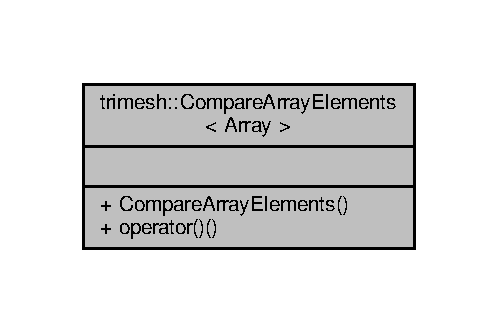
\includegraphics[width=239pt]{de/de6/classtrimesh_1_1CompareArrayElements__coll__graph}
\end{center}
\end{figure}
\subsection*{Public Member Functions}
\begin{DoxyCompactItemize}
\item 
\hyperlink{classtrimesh_1_1CompareArrayElements_ab0ce83e4afd5b5c63858d75ad39df3e9}{Compare\+Array\+Elements} (const Array \&\+\_\+a)
\item 
bool \hyperlink{classtrimesh_1_1CompareArrayElements_aba402709a16256f1b8a519996eacfc79}{operator()} (int i1, int i2) const
\end{DoxyCompactItemize}


\subsection{Constructor \& Destructor Documentation}
\mbox{\Hypertarget{classtrimesh_1_1CompareArrayElements_ab0ce83e4afd5b5c63858d75ad39df3e9}\label{classtrimesh_1_1CompareArrayElements_ab0ce83e4afd5b5c63858d75ad39df3e9}} 
\index{trimesh\+::\+Compare\+Array\+Elements@{trimesh\+::\+Compare\+Array\+Elements}!Compare\+Array\+Elements@{Compare\+Array\+Elements}}
\index{Compare\+Array\+Elements@{Compare\+Array\+Elements}!trimesh\+::\+Compare\+Array\+Elements@{trimesh\+::\+Compare\+Array\+Elements}}
\subsubsection{\texorpdfstring{Compare\+Array\+Elements()}{CompareArrayElements()}}
{\footnotesize\ttfamily template$<$class Array $>$ \\
\hyperlink{classtrimesh_1_1CompareArrayElements}{trimesh\+::\+Compare\+Array\+Elements}$<$ Array $>$\+::\hyperlink{classtrimesh_1_1CompareArrayElements}{Compare\+Array\+Elements} (\begin{DoxyParamCaption}\item[{const Array \&}]{\+\_\+a }\end{DoxyParamCaption})\hspace{0.3cm}{\ttfamily [inline]}}



\subsection{Member Function Documentation}
\mbox{\Hypertarget{classtrimesh_1_1CompareArrayElements_aba402709a16256f1b8a519996eacfc79}\label{classtrimesh_1_1CompareArrayElements_aba402709a16256f1b8a519996eacfc79}} 
\index{trimesh\+::\+Compare\+Array\+Elements@{trimesh\+::\+Compare\+Array\+Elements}!operator()@{operator()}}
\index{operator()@{operator()}!trimesh\+::\+Compare\+Array\+Elements@{trimesh\+::\+Compare\+Array\+Elements}}
\subsubsection{\texorpdfstring{operator()()}{operator()()}}
{\footnotesize\ttfamily template$<$class Array $>$ \\
bool \hyperlink{classtrimesh_1_1CompareArrayElements}{trimesh\+::\+Compare\+Array\+Elements}$<$ Array $>$\+::operator() (\begin{DoxyParamCaption}\item[{int}]{i1,  }\item[{int}]{i2 }\end{DoxyParamCaption}) const\hspace{0.3cm}{\ttfamily [inline]}}



The documentation for this class was generated from the following file\+:\begin{DoxyCompactItemize}
\item 
\hyperlink{conn__comps_8cc}{conn\+\_\+comps.\+cc}\end{DoxyCompactItemize}

\hypertarget{structtrimesh_1_1KDtree_1_1CompatFunc}{}\section{trimesh\+:\+:K\+Dtree\+:\+:Compat\+Func Struct Reference}
\label{structtrimesh_1_1KDtree_1_1CompatFunc}\index{trimesh\+::\+K\+Dtree\+::\+Compat\+Func@{trimesh\+::\+K\+Dtree\+::\+Compat\+Func}}


{\ttfamily \#include $<$K\+Dtree.\+h$>$}



Inheritance diagram for trimesh\+:\+:K\+Dtree\+:\+:Compat\+Func\+:\nopagebreak
\begin{figure}[H]
\begin{center}
\leavevmode
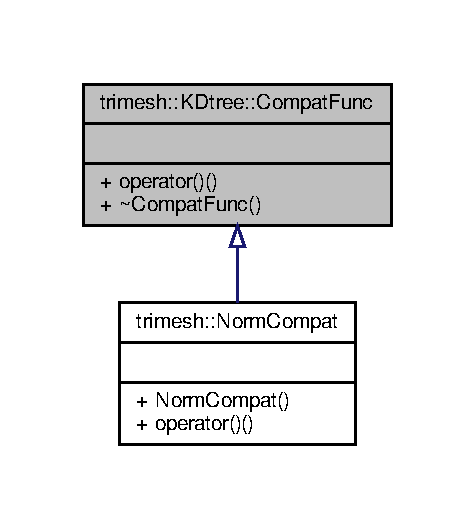
\includegraphics[width=228pt]{da/da3/structtrimesh_1_1KDtree_1_1CompatFunc__inherit__graph}
\end{center}
\end{figure}


Collaboration diagram for trimesh\+:\+:K\+Dtree\+:\+:Compat\+Func\+:\nopagebreak
\begin{figure}[H]
\begin{center}
\leavevmode
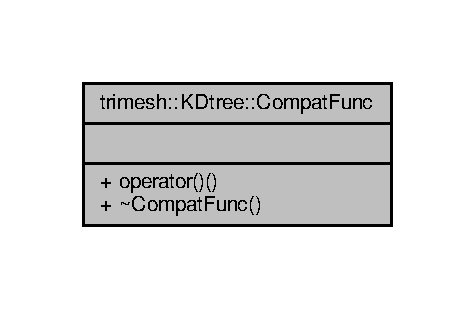
\includegraphics[width=228pt]{d1/ded/structtrimesh_1_1KDtree_1_1CompatFunc__coll__graph}
\end{center}
\end{figure}
\subsection*{Public Member Functions}
\begin{DoxyCompactItemize}
\item 
virtual bool \hyperlink{structtrimesh_1_1KDtree_1_1CompatFunc_a7a1e53ff346e21daac1bf003a21d2170}{operator()} (const float $\ast$p) const =0
\item 
virtual \hyperlink{structtrimesh_1_1KDtree_1_1CompatFunc_a6ae6120ac95abcc5322f6b25569e550d}{$\sim$\+Compat\+Func} ()
\end{DoxyCompactItemize}


\subsection{Constructor \& Destructor Documentation}
\mbox{\Hypertarget{structtrimesh_1_1KDtree_1_1CompatFunc_a6ae6120ac95abcc5322f6b25569e550d}\label{structtrimesh_1_1KDtree_1_1CompatFunc_a6ae6120ac95abcc5322f6b25569e550d}} 
\index{trimesh\+::\+K\+Dtree\+::\+Compat\+Func@{trimesh\+::\+K\+Dtree\+::\+Compat\+Func}!````~Compat\+Func@{$\sim$\+Compat\+Func}}
\index{````~Compat\+Func@{$\sim$\+Compat\+Func}!trimesh\+::\+K\+Dtree\+::\+Compat\+Func@{trimesh\+::\+K\+Dtree\+::\+Compat\+Func}}
\subsubsection{\texorpdfstring{$\sim$\+Compat\+Func()}{~CompatFunc()}}
{\footnotesize\ttfamily virtual trimesh\+::\+K\+Dtree\+::\+Compat\+Func\+::$\sim$\+Compat\+Func (\begin{DoxyParamCaption}{ }\end{DoxyParamCaption})\hspace{0.3cm}{\ttfamily [inline]}, {\ttfamily [virtual]}}



\subsection{Member Function Documentation}
\mbox{\Hypertarget{structtrimesh_1_1KDtree_1_1CompatFunc_a7a1e53ff346e21daac1bf003a21d2170}\label{structtrimesh_1_1KDtree_1_1CompatFunc_a7a1e53ff346e21daac1bf003a21d2170}} 
\index{trimesh\+::\+K\+Dtree\+::\+Compat\+Func@{trimesh\+::\+K\+Dtree\+::\+Compat\+Func}!operator()@{operator()}}
\index{operator()@{operator()}!trimesh\+::\+K\+Dtree\+::\+Compat\+Func@{trimesh\+::\+K\+Dtree\+::\+Compat\+Func}}
\subsubsection{\texorpdfstring{operator()()}{operator()()}}
{\footnotesize\ttfamily virtual bool trimesh\+::\+K\+Dtree\+::\+Compat\+Func\+::operator() (\begin{DoxyParamCaption}\item[{const float $\ast$}]{p }\end{DoxyParamCaption}) const\hspace{0.3cm}{\ttfamily [pure virtual]}}



Implemented in \hyperlink{classtrimesh_1_1NormCompat_a189eaeb454dd63b4443661665b6500ee}{trimesh\+::\+Norm\+Compat}.



The documentation for this struct was generated from the following file\+:\begin{DoxyCompactItemize}
\item 
\hyperlink{KDtree_8h}{K\+Dtree.\+h}\end{DoxyCompactItemize}

\hypertarget{structstd_1_1conditional}{}\section{std\+:\+:conditional$<$ B, T, F $>$ Struct Template Reference}
\label{structstd_1_1conditional}\index{std\+::conditional$<$ B, T, F $>$@{std\+::conditional$<$ B, T, F $>$}}


{\ttfamily \#include $<$mathcompat.\+h$>$}



Collaboration diagram for std\+:\+:conditional$<$ B, T, F $>$\+:\nopagebreak
\begin{figure}[H]
\begin{center}
\leavevmode
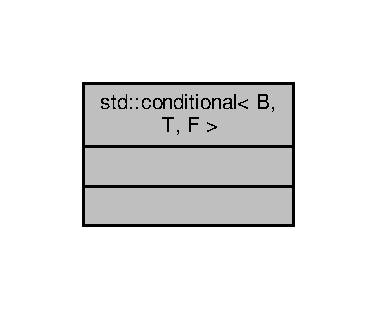
\includegraphics[width=181pt]{d6/d54/structstd_1_1conditional__coll__graph}
\end{center}
\end{figure}
\subsection*{Public Types}
\begin{DoxyCompactItemize}
\item 
typedef T \hyperlink{structstd_1_1conditional_afa082101adbc68eaea9c49e34fa8ebfa}{type}
\end{DoxyCompactItemize}


\subsection{Member Typedef Documentation}
\mbox{\Hypertarget{structstd_1_1conditional_afa082101adbc68eaea9c49e34fa8ebfa}\label{structstd_1_1conditional_afa082101adbc68eaea9c49e34fa8ebfa}} 
\index{std\+::conditional@{std\+::conditional}!type@{type}}
\index{type@{type}!std\+::conditional@{std\+::conditional}}
\subsubsection{\texorpdfstring{type}{type}}
{\footnotesize\ttfamily template$<$bool B, class T, class F $>$ \\
typedef T \hyperlink{structstd_1_1conditional}{std\+::conditional}$<$ B, T, F $>$\+::\hyperlink{structstd_1_1conditional_afa082101adbc68eaea9c49e34fa8ebfa}{type}}



The documentation for this struct was generated from the following file\+:\begin{DoxyCompactItemize}
\item 
\hyperlink{mathcompat_8h}{mathcompat.\+h}\end{DoxyCompactItemize}

\hypertarget{structstd_1_1conditional_3_01false_00_01T_00_01F_01_4}{}\section{std\+:\+:conditional$<$ false, T, F $>$ Struct Template Reference}
\label{structstd_1_1conditional_3_01false_00_01T_00_01F_01_4}\index{std\+::conditional$<$ false, T, F $>$@{std\+::conditional$<$ false, T, F $>$}}


{\ttfamily \#include $<$mathcompat.\+h$>$}



Collaboration diagram for std\+:\+:conditional$<$ false, T, F $>$\+:\nopagebreak
\begin{figure}[H]
\begin{center}
\leavevmode
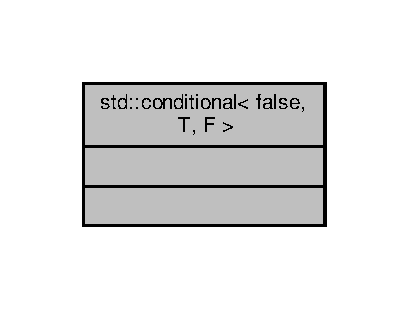
\includegraphics[width=196pt]{d3/d6a/structstd_1_1conditional_3_01false_00_01T_00_01F_01_4__coll__graph}
\end{center}
\end{figure}
\subsection*{Public Types}
\begin{DoxyCompactItemize}
\item 
typedef F \hyperlink{structstd_1_1conditional_3_01false_00_01T_00_01F_01_4_a8307a0010d68b8c7f309a910bb6137fe}{type}
\end{DoxyCompactItemize}


\subsection{Member Typedef Documentation}
\mbox{\Hypertarget{structstd_1_1conditional_3_01false_00_01T_00_01F_01_4_a8307a0010d68b8c7f309a910bb6137fe}\label{structstd_1_1conditional_3_01false_00_01T_00_01F_01_4_a8307a0010d68b8c7f309a910bb6137fe}} 
\index{std\+::conditional$<$ false, T, F $>$@{std\+::conditional$<$ false, T, F $>$}!type@{type}}
\index{type@{type}!std\+::conditional$<$ false, T, F $>$@{std\+::conditional$<$ false, T, F $>$}}
\subsubsection{\texorpdfstring{type}{type}}
{\footnotesize\ttfamily template$<$class T , class F $>$ \\
typedef F \hyperlink{structstd_1_1conditional}{std\+::conditional}$<$ false, T, F $>$\+::\hyperlink{structstd_1_1conditional_3_01false_00_01T_00_01F_01_4_a8307a0010d68b8c7f309a910bb6137fe}{type}}



The documentation for this struct was generated from the following file\+:\begin{DoxyCompactItemize}
\item 
\hyperlink{mathcompat_8h}{mathcompat.\+h}\end{DoxyCompactItemize}

\hypertarget{structcommon_1_1Correspondences}{}\section{common\+:\+:Correspondences Struct Reference}
\label{structcommon_1_1Correspondences}\index{common\+::\+Correspondences@{common\+::\+Correspondences}}


{\ttfamily \#include $<$match\+\_\+utils.\+hpp$>$}



Collaboration diagram for common\+:\+:Correspondences\+:\nopagebreak
\begin{figure}[H]
\begin{center}
\leavevmode
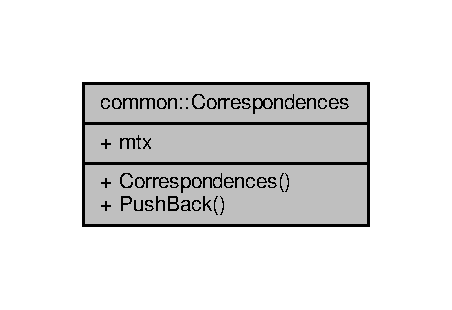
\includegraphics[width=217pt]{d5/d1a/structcommon_1_1Correspondences__coll__graph}
\end{center}
\end{figure}
\subsection*{Public Member Functions}
\begin{DoxyCompactItemize}
\item 
\hyperlink{structcommon_1_1Correspondences_ae1eb166beacea5976106c5479aeb86ad}{Correspondences} ()
\item 
void \hyperlink{structcommon_1_1Correspondences_a50974cb762f1621d1bd5cd9b4ee1eb80}{Push\+Back} (const Eigen\+::\+Vector3d \&from, const Eigen\+::\+Vector3d \&to, double score)
\end{DoxyCompactItemize}
\subsection*{Public Attributes}
\begin{DoxyCompactItemize}
\item 
Eigen\+::\+Matrix\+Xd \hyperlink{structcommon_1_1Correspondences_ab8841b71f2e02544b010ae5e2bc5308c}{mtx}
\end{DoxyCompactItemize}


\subsection{Constructor \& Destructor Documentation}
\mbox{\Hypertarget{structcommon_1_1Correspondences_ae1eb166beacea5976106c5479aeb86ad}\label{structcommon_1_1Correspondences_ae1eb166beacea5976106c5479aeb86ad}} 
\index{common\+::\+Correspondences@{common\+::\+Correspondences}!Correspondences@{Correspondences}}
\index{Correspondences@{Correspondences}!common\+::\+Correspondences@{common\+::\+Correspondences}}
\subsubsection{\texorpdfstring{Correspondences()}{Correspondences()}}
{\footnotesize\ttfamily common\+::\+Correspondences\+::\+Correspondences (\begin{DoxyParamCaption}{ }\end{DoxyParamCaption})\hspace{0.3cm}{\ttfamily [inline]}}



\subsection{Member Function Documentation}
\mbox{\Hypertarget{structcommon_1_1Correspondences_a50974cb762f1621d1bd5cd9b4ee1eb80}\label{structcommon_1_1Correspondences_a50974cb762f1621d1bd5cd9b4ee1eb80}} 
\index{common\+::\+Correspondences@{common\+::\+Correspondences}!Push\+Back@{Push\+Back}}
\index{Push\+Back@{Push\+Back}!common\+::\+Correspondences@{common\+::\+Correspondences}}
\subsubsection{\texorpdfstring{Push\+Back()}{PushBack()}}
{\footnotesize\ttfamily void common\+::\+Correspondences\+::\+Push\+Back (\begin{DoxyParamCaption}\item[{const Eigen\+::\+Vector3d \&}]{from,  }\item[{const Eigen\+::\+Vector3d \&}]{to,  }\item[{double}]{score }\end{DoxyParamCaption})\hspace{0.3cm}{\ttfamily [inline]}}



Referenced by trimesh\+::\+I\+C\+P\+\_\+iter().



\subsection{Member Data Documentation}
\mbox{\Hypertarget{structcommon_1_1Correspondences_ab8841b71f2e02544b010ae5e2bc5308c}\label{structcommon_1_1Correspondences_ab8841b71f2e02544b010ae5e2bc5308c}} 
\index{common\+::\+Correspondences@{common\+::\+Correspondences}!mtx@{mtx}}
\index{mtx@{mtx}!common\+::\+Correspondences@{common\+::\+Correspondences}}
\subsubsection{\texorpdfstring{mtx}{mtx}}
{\footnotesize\ttfamily Eigen\+::\+Matrix\+Xd common\+::\+Correspondences\+::mtx}



Referenced by common\+::\+Match\+Internal\+::\+Push\+Back().



The documentation for this struct was generated from the following file\+:\begin{DoxyCompactItemize}
\item 
\hyperlink{match__utils_8hpp}{match\+\_\+utils.\+hpp}\end{DoxyCompactItemize}

\hypertarget{structCostFunctions}{}\section{Cost\+Functions Struct Reference}
\label{structCostFunctions}\index{Cost\+Functions@{Cost\+Functions}}


Collaboration diagram for Cost\+Functions\+:\nopagebreak
\begin{figure}[H]
\begin{center}
\leavevmode
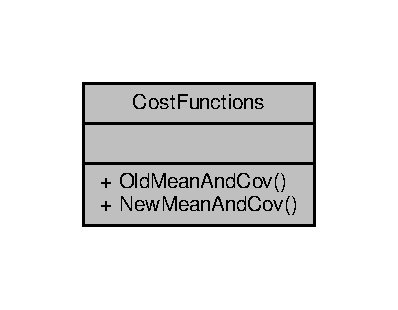
\includegraphics[width=191pt]{da/d4f/structCostFunctions__coll__graph}
\end{center}
\end{figure}
\subsection*{Static Public Member Functions}
\begin{DoxyCompactItemize}
\item 
static vector$<$ double $>$ \hyperlink{structCostFunctions_af66a9ae54dbf19549b3e98636134d3a7}{Old\+Mean\+And\+Cov} (\hyperlink{classNDTCell}{N\+D\+T\+Cell} $\ast$p, \hyperlink{classNDTCell}{N\+D\+T\+Cell} $\ast$q)
\item 
static vector$<$ double $>$ \hyperlink{structCostFunctions_ad62402cf996ea9c0812a6d584325ab25}{New\+Mean\+And\+Cov} (\hyperlink{classNDTCell}{N\+D\+T\+Cell} $\ast$p, \hyperlink{classNDTCell}{N\+D\+T\+Cell} $\ast$q)
\end{DoxyCompactItemize}


\subsection{Member Function Documentation}
\mbox{\Hypertarget{structCostFunctions_ad62402cf996ea9c0812a6d584325ab25}\label{structCostFunctions_ad62402cf996ea9c0812a6d584325ab25}} 
\index{Cost\+Functions@{Cost\+Functions}!New\+Mean\+And\+Cov@{New\+Mean\+And\+Cov}}
\index{New\+Mean\+And\+Cov@{New\+Mean\+And\+Cov}!Cost\+Functions@{Cost\+Functions}}
\subsubsection{\texorpdfstring{New\+Mean\+And\+Cov()}{NewMeanAndCov()}}
{\footnotesize\ttfamily static vector$<$double$>$ Cost\+Functions\+::\+New\+Mean\+And\+Cov (\begin{DoxyParamCaption}\item[{\hyperlink{classNDTCell}{N\+D\+T\+Cell} $\ast$}]{p,  }\item[{\hyperlink{classNDTCell}{N\+D\+T\+Cell} $\ast$}]{q }\end{DoxyParamCaption})\hspace{0.3cm}{\ttfamily [inline]}, {\ttfamily [static]}}



Referenced by main().

\mbox{\Hypertarget{structCostFunctions_af66a9ae54dbf19549b3e98636134d3a7}\label{structCostFunctions_af66a9ae54dbf19549b3e98636134d3a7}} 
\index{Cost\+Functions@{Cost\+Functions}!Old\+Mean\+And\+Cov@{Old\+Mean\+And\+Cov}}
\index{Old\+Mean\+And\+Cov@{Old\+Mean\+And\+Cov}!Cost\+Functions@{Cost\+Functions}}
\subsubsection{\texorpdfstring{Old\+Mean\+And\+Cov()}{OldMeanAndCov()}}
{\footnotesize\ttfamily static vector$<$double$>$ Cost\+Functions\+::\+Old\+Mean\+And\+Cov (\begin{DoxyParamCaption}\item[{\hyperlink{classNDTCell}{N\+D\+T\+Cell} $\ast$}]{p,  }\item[{\hyperlink{classNDTCell}{N\+D\+T\+Cell} $\ast$}]{q }\end{DoxyParamCaption})\hspace{0.3cm}{\ttfamily [inline]}, {\ttfamily [static]}}



The documentation for this struct was generated from the following file\+:\begin{DoxyCompactItemize}
\item 
\hyperlink{sndt__exec_2src_2test__0dis_8cc}{sndt\+\_\+exec/src/test\+\_\+0dis.\+cc}\end{DoxyCompactItemize}

\hypertarget{structCostFunctor}{}\section{Cost\+Functor Struct Reference}
\label{structCostFunctor}\index{Cost\+Functor@{Cost\+Functor}}


Collaboration diagram for Cost\+Functor\+:\nopagebreak
\begin{figure}[H]
\begin{center}
\leavevmode
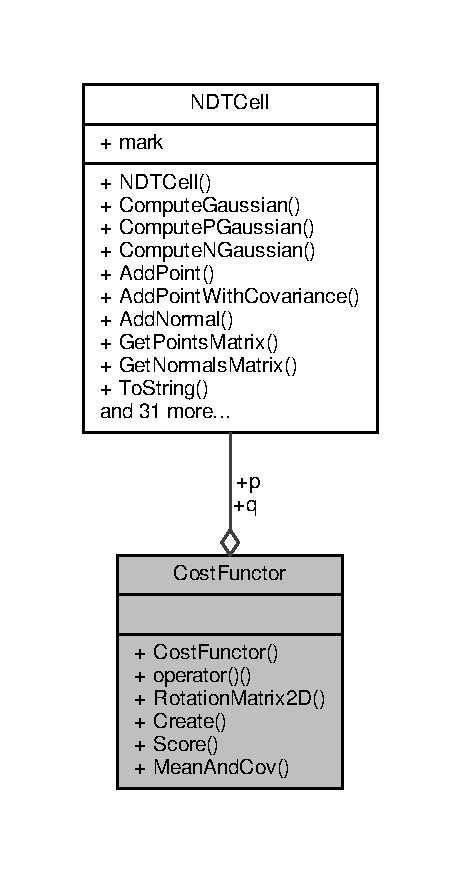
\includegraphics[width=221pt]{d4/da3/structCostFunctor__coll__graph}
\end{center}
\end{figure}
\subsection*{Public Member Functions}
\begin{DoxyCompactItemize}
\item 
\hyperlink{structCostFunctor_a970e75f6f339f881419ffebdba79ddc0}{Cost\+Functor} (\hyperlink{classNDTCell}{N\+D\+T\+Cell} $\ast$p\+\_\+, \hyperlink{classNDTCell}{N\+D\+T\+Cell} $\ast$q\+\_\+)
\item 
{\footnotesize template$<$typename T $>$ }\\bool \hyperlink{structCostFunctor_a07e825ed38e78e3a9f530b139e6b8155}{operator()} (const T $\ast$const x, const T $\ast$const y, const T $\ast$const yaw, T $\ast$e) const
\end{DoxyCompactItemize}
\subsection*{Static Public Member Functions}
\begin{DoxyCompactItemize}
\item 
{\footnotesize template$<$typename T $>$ }\\static Eigen\+::\+Matrix$<$ T, 2, 2 $>$ \hyperlink{structCostFunctor_ae0785d2abc318696cb6dc01fac237881}{Rotation\+Matrix2D} (T yaw)
\item 
static ceres\+::\+Cost\+Function $\ast$ \hyperlink{structCostFunctor_a6f4d3f5dfe5d7c575c1f5dbcc86fed93}{Create} (\hyperlink{classNDTCell}{N\+D\+T\+Cell} $\ast$cellp, \hyperlink{classNDTCell}{N\+D\+T\+Cell} $\ast$cellq)
\item 
static double \hyperlink{structCostFunctor_a944445b87b51172a0d0037504e9dcadd}{Score} (\hyperlink{classNDTCell}{N\+D\+T\+Cell} $\ast$\hyperlink{structCostFunctor_a226fe7b0cb5dab732c9418d9d6d36cc9}{p}, \hyperlink{classNDTCell}{N\+D\+T\+Cell} $\ast$\hyperlink{structCostFunctor_aced002cbe4f5b36d02e36f460de4c89f}{q})
\item 
static vector$<$ double $>$ \hyperlink{structCostFunctor_ae875000950da1578f746dc343af34c94}{Mean\+And\+Cov} (\hyperlink{classNDTCell}{N\+D\+T\+Cell} $\ast$\hyperlink{structCostFunctor_a226fe7b0cb5dab732c9418d9d6d36cc9}{p}, \hyperlink{classNDTCell}{N\+D\+T\+Cell} $\ast$\hyperlink{structCostFunctor_aced002cbe4f5b36d02e36f460de4c89f}{q})
\end{DoxyCompactItemize}
\subsection*{Public Attributes}
\begin{DoxyCompactItemize}
\item 
\hyperlink{classNDTCell}{N\+D\+T\+Cell} $\ast$ \hyperlink{structCostFunctor_a226fe7b0cb5dab732c9418d9d6d36cc9}{p}
\item 
\hyperlink{classNDTCell}{N\+D\+T\+Cell} $\ast$ \hyperlink{structCostFunctor_aced002cbe4f5b36d02e36f460de4c89f}{q}
\end{DoxyCompactItemize}


\subsection{Constructor \& Destructor Documentation}
\mbox{\Hypertarget{structCostFunctor_a970e75f6f339f881419ffebdba79ddc0}\label{structCostFunctor_a970e75f6f339f881419ffebdba79ddc0}} 
\index{Cost\+Functor@{Cost\+Functor}!Cost\+Functor@{Cost\+Functor}}
\index{Cost\+Functor@{Cost\+Functor}!Cost\+Functor@{Cost\+Functor}}
\subsubsection{\texorpdfstring{Cost\+Functor()}{CostFunctor()}}
{\footnotesize\ttfamily Cost\+Functor\+::\+Cost\+Functor (\begin{DoxyParamCaption}\item[{\hyperlink{classNDTCell}{N\+D\+T\+Cell} $\ast$}]{p\+\_\+,  }\item[{\hyperlink{classNDTCell}{N\+D\+T\+Cell} $\ast$}]{q\+\_\+ }\end{DoxyParamCaption})\hspace{0.3cm}{\ttfamily [inline]}}



\subsection{Member Function Documentation}
\mbox{\Hypertarget{structCostFunctor_a6f4d3f5dfe5d7c575c1f5dbcc86fed93}\label{structCostFunctor_a6f4d3f5dfe5d7c575c1f5dbcc86fed93}} 
\index{Cost\+Functor@{Cost\+Functor}!Create@{Create}}
\index{Create@{Create}!Cost\+Functor@{Cost\+Functor}}
\subsubsection{\texorpdfstring{Create()}{Create()}}
{\footnotesize\ttfamily static ceres\+::\+Cost\+Function$\ast$ Cost\+Functor\+::\+Create (\begin{DoxyParamCaption}\item[{\hyperlink{classNDTCell}{N\+D\+T\+Cell} $\ast$}]{cellp,  }\item[{\hyperlink{classNDTCell}{N\+D\+T\+Cell} $\ast$}]{cellq }\end{DoxyParamCaption})\hspace{0.3cm}{\ttfamily [inline]}, {\ttfamily [static]}}



Referenced by N\+D\+T\+Matcher\+::\+Ceres\+Match().

\mbox{\Hypertarget{structCostFunctor_ae875000950da1578f746dc343af34c94}\label{structCostFunctor_ae875000950da1578f746dc343af34c94}} 
\index{Cost\+Functor@{Cost\+Functor}!Mean\+And\+Cov@{Mean\+And\+Cov}}
\index{Mean\+And\+Cov@{Mean\+And\+Cov}!Cost\+Functor@{Cost\+Functor}}
\subsubsection{\texorpdfstring{Mean\+And\+Cov()}{MeanAndCov()}}
{\footnotesize\ttfamily static vector$<$double$>$ Cost\+Functor\+::\+Mean\+And\+Cov (\begin{DoxyParamCaption}\item[{\hyperlink{classNDTCell}{N\+D\+T\+Cell} $\ast$}]{p,  }\item[{\hyperlink{classNDTCell}{N\+D\+T\+Cell} $\ast$}]{q }\end{DoxyParamCaption})\hspace{0.3cm}{\ttfamily [inline]}, {\ttfamily [static]}}

\mbox{\Hypertarget{structCostFunctor_a07e825ed38e78e3a9f530b139e6b8155}\label{structCostFunctor_a07e825ed38e78e3a9f530b139e6b8155}} 
\index{Cost\+Functor@{Cost\+Functor}!operator()@{operator()}}
\index{operator()@{operator()}!Cost\+Functor@{Cost\+Functor}}
\subsubsection{\texorpdfstring{operator()()}{operator()()}}
{\footnotesize\ttfamily template$<$typename T $>$ \\
bool Cost\+Functor\+::operator() (\begin{DoxyParamCaption}\item[{const T $\ast$const}]{x,  }\item[{const T $\ast$const}]{y,  }\item[{const T $\ast$const}]{yaw,  }\item[{T $\ast$}]{e }\end{DoxyParamCaption}) const\hspace{0.3cm}{\ttfamily [inline]}}

\mbox{\Hypertarget{structCostFunctor_ae0785d2abc318696cb6dc01fac237881}\label{structCostFunctor_ae0785d2abc318696cb6dc01fac237881}} 
\index{Cost\+Functor@{Cost\+Functor}!Rotation\+Matrix2D@{Rotation\+Matrix2D}}
\index{Rotation\+Matrix2D@{Rotation\+Matrix2D}!Cost\+Functor@{Cost\+Functor}}
\subsubsection{\texorpdfstring{Rotation\+Matrix2\+D()}{RotationMatrix2D()}}
{\footnotesize\ttfamily template$<$typename T $>$ \\
static Eigen\+::\+Matrix$<$T, 2, 2$>$ Cost\+Functor\+::\+Rotation\+Matrix2D (\begin{DoxyParamCaption}\item[{T}]{yaw }\end{DoxyParamCaption})\hspace{0.3cm}{\ttfamily [inline]}, {\ttfamily [static]}}

\mbox{\Hypertarget{structCostFunctor_a944445b87b51172a0d0037504e9dcadd}\label{structCostFunctor_a944445b87b51172a0d0037504e9dcadd}} 
\index{Cost\+Functor@{Cost\+Functor}!Score@{Score}}
\index{Score@{Score}!Cost\+Functor@{Cost\+Functor}}
\subsubsection{\texorpdfstring{Score()}{Score()}}
{\footnotesize\ttfamily static double Cost\+Functor\+::\+Score (\begin{DoxyParamCaption}\item[{\hyperlink{classNDTCell}{N\+D\+T\+Cell} $\ast$}]{p,  }\item[{\hyperlink{classNDTCell}{N\+D\+T\+Cell} $\ast$}]{q }\end{DoxyParamCaption})\hspace{0.3cm}{\ttfamily [inline]}, {\ttfamily [static]}}



\subsection{Member Data Documentation}
\mbox{\Hypertarget{structCostFunctor_a226fe7b0cb5dab732c9418d9d6d36cc9}\label{structCostFunctor_a226fe7b0cb5dab732c9418d9d6d36cc9}} 
\index{Cost\+Functor@{Cost\+Functor}!p@{p}}
\index{p@{p}!Cost\+Functor@{Cost\+Functor}}
\subsubsection{\texorpdfstring{p}{p}}
{\footnotesize\ttfamily \hyperlink{classNDTCell}{N\+D\+T\+Cell}$\ast$ Cost\+Functor\+::p}

\mbox{\Hypertarget{structCostFunctor_aced002cbe4f5b36d02e36f460de4c89f}\label{structCostFunctor_aced002cbe4f5b36d02e36f460de4c89f}} 
\index{Cost\+Functor@{Cost\+Functor}!q@{q}}
\index{q@{q}!Cost\+Functor@{Cost\+Functor}}
\subsubsection{\texorpdfstring{q}{q}}
{\footnotesize\ttfamily \hyperlink{classNDTCell}{N\+D\+T\+Cell} $\ast$ Cost\+Functor\+::q}



The documentation for this struct was generated from the following file\+:\begin{DoxyCompactItemize}
\item 
\hyperlink{ndt__matcher_8cc}{ndt\+\_\+matcher.\+cc}\end{DoxyCompactItemize}

\hypertarget{classdbg_1_1DebugOutput}{}\section{dbg\+:\+:Debug\+Output Class Reference}
\label{classdbg_1_1DebugOutput}\index{dbg\+::\+Debug\+Output@{dbg\+::\+Debug\+Output}}


{\ttfamily \#include $<$dbg.\+h$>$}



Collaboration diagram for dbg\+:\+:Debug\+Output\+:\nopagebreak
\begin{figure}[H]
\begin{center}
\leavevmode
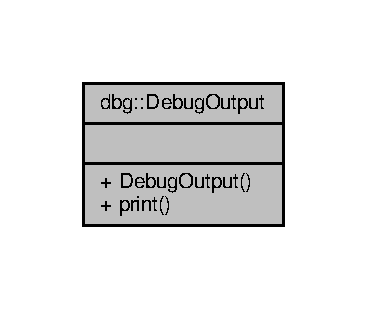
\includegraphics[width=176pt]{d2/de9/classdbg_1_1DebugOutput__coll__graph}
\end{center}
\end{figure}
\subsection*{Public Types}
\begin{DoxyCompactItemize}
\item 
using \hyperlink{classdbg_1_1DebugOutput_a5d9b38d5b9276cb584c0e20e9b1a2045}{expr\+\_\+t} = const char $\ast$
\end{DoxyCompactItemize}
\subsection*{Public Member Functions}
\begin{DoxyCompactItemize}
\item 
\hyperlink{classdbg_1_1DebugOutput_a7bb0378758aa1006e2423eff57ee36a2}{Debug\+Output} (const char $\ast$filepath, int line, const char $\ast$function\+\_\+name)
\item 
{\footnotesize template$<$typename... T$>$ }\\auto \hyperlink{classdbg_1_1DebugOutput_aa135787802db4a6b0b4eb185185e13ca}{print} (std\+::initializer\+\_\+list$<$ \hyperlink{classdbg_1_1DebugOutput_a5d9b38d5b9276cb584c0e20e9b1a2045}{expr\+\_\+t} $>$ exprs, std\+::initializer\+\_\+list$<$ std\+::string $>$ types, T \&\&... values) -\/$>$ \hyperlink{namespacedbg_a4754c7365d6eb31696a4613230e21ac4}{last\+\_\+t}$<$ T... $>$
\end{DoxyCompactItemize}


\subsection{Member Typedef Documentation}
\mbox{\Hypertarget{classdbg_1_1DebugOutput_a5d9b38d5b9276cb584c0e20e9b1a2045}\label{classdbg_1_1DebugOutput_a5d9b38d5b9276cb584c0e20e9b1a2045}} 
\index{dbg\+::\+Debug\+Output@{dbg\+::\+Debug\+Output}!expr\+\_\+t@{expr\+\_\+t}}
\index{expr\+\_\+t@{expr\+\_\+t}!dbg\+::\+Debug\+Output@{dbg\+::\+Debug\+Output}}
\subsubsection{\texorpdfstring{expr\+\_\+t}{expr\_t}}
{\footnotesize\ttfamily using \hyperlink{classdbg_1_1DebugOutput_a5d9b38d5b9276cb584c0e20e9b1a2045}{dbg\+::\+Debug\+Output\+::expr\+\_\+t} =  const char$\ast$}



\subsection{Constructor \& Destructor Documentation}
\mbox{\Hypertarget{classdbg_1_1DebugOutput_a7bb0378758aa1006e2423eff57ee36a2}\label{classdbg_1_1DebugOutput_a7bb0378758aa1006e2423eff57ee36a2}} 
\index{dbg\+::\+Debug\+Output@{dbg\+::\+Debug\+Output}!Debug\+Output@{Debug\+Output}}
\index{Debug\+Output@{Debug\+Output}!dbg\+::\+Debug\+Output@{dbg\+::\+Debug\+Output}}
\subsubsection{\texorpdfstring{Debug\+Output()}{DebugOutput()}}
{\footnotesize\ttfamily dbg\+::\+Debug\+Output\+::\+Debug\+Output (\begin{DoxyParamCaption}\item[{const char $\ast$}]{filepath,  }\item[{int}]{line,  }\item[{const char $\ast$}]{function\+\_\+name }\end{DoxyParamCaption})\hspace{0.3cm}{\ttfamily [inline]}}



\subsection{Member Function Documentation}
\mbox{\Hypertarget{classdbg_1_1DebugOutput_aa135787802db4a6b0b4eb185185e13ca}\label{classdbg_1_1DebugOutput_aa135787802db4a6b0b4eb185185e13ca}} 
\index{dbg\+::\+Debug\+Output@{dbg\+::\+Debug\+Output}!print@{print}}
\index{print@{print}!dbg\+::\+Debug\+Output@{dbg\+::\+Debug\+Output}}
\subsubsection{\texorpdfstring{print()}{print()}}
{\footnotesize\ttfamily template$<$typename... T$>$ \\
auto dbg\+::\+Debug\+Output\+::print (\begin{DoxyParamCaption}\item[{std\+::initializer\+\_\+list$<$ \hyperlink{classdbg_1_1DebugOutput_a5d9b38d5b9276cb584c0e20e9b1a2045}{expr\+\_\+t} $>$}]{exprs,  }\item[{std\+::initializer\+\_\+list$<$ std\+::string $>$}]{types,  }\item[{T \&\&...}]{values }\end{DoxyParamCaption}) -\/$>$ \hyperlink{namespacedbg_a4754c7365d6eb31696a4613230e21ac4}{last\+\_\+t}$<$T...$>$ \hspace{0.3cm}{\ttfamily [inline]}}



The documentation for this class was generated from the following file\+:\begin{DoxyCompactItemize}
\item 
\hyperlink{dbg_8h}{dbg.\+h}\end{DoxyCompactItemize}

\hypertarget{structdbg_1_1detail__detector_1_1detector}{}\section{dbg\+:\+:detail\+\_\+detector\+:\+:detector$<$ Default, Always\+Void, Op, Args $>$ Struct Template Reference}
\label{structdbg_1_1detail__detector_1_1detector}\index{dbg\+::detail\+\_\+detector\+::detector$<$ Default, Always\+Void, Op, Args $>$@{dbg\+::detail\+\_\+detector\+::detector$<$ Default, Always\+Void, Op, Args $>$}}


{\ttfamily \#include $<$dbg.\+h$>$}



Collaboration diagram for dbg\+:\+:detail\+\_\+detector\+:\+:detector$<$ Default, Always\+Void, Op, Args $>$\+:\nopagebreak
\begin{figure}[H]
\begin{center}
\leavevmode
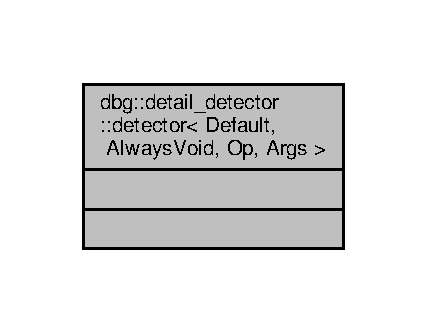
\includegraphics[width=205pt]{d8/d4f/structdbg_1_1detail__detector_1_1detector__coll__graph}
\end{center}
\end{figure}
\subsection*{Public Types}
\begin{DoxyCompactItemize}
\item 
using \hyperlink{structdbg_1_1detail__detector_1_1detector_af1b6da4282d723669e926c52f446a989}{value\+\_\+t} = std\+::false\+\_\+type
\item 
using \hyperlink{structdbg_1_1detail__detector_1_1detector_aab6b446944545683b9533ea8fc623480}{type} = Default
\end{DoxyCompactItemize}


\subsection{Member Typedef Documentation}
\mbox{\Hypertarget{structdbg_1_1detail__detector_1_1detector_aab6b446944545683b9533ea8fc623480}\label{structdbg_1_1detail__detector_1_1detector_aab6b446944545683b9533ea8fc623480}} 
\index{dbg\+::detail\+\_\+detector\+::detector@{dbg\+::detail\+\_\+detector\+::detector}!type@{type}}
\index{type@{type}!dbg\+::detail\+\_\+detector\+::detector@{dbg\+::detail\+\_\+detector\+::detector}}
\subsubsection{\texorpdfstring{type}{type}}
{\footnotesize\ttfamily template$<$class Default , class Always\+Void , template$<$ class... $>$ class Op, class... Args$>$ \\
using \hyperlink{structdbg_1_1detail__detector_1_1detector}{dbg\+::detail\+\_\+detector\+::detector}$<$ Default, Always\+Void, Op, Args $>$\+::\hyperlink{structdbg_1_1detail__detector_1_1detector_aab6b446944545683b9533ea8fc623480}{type} =  Default}

\mbox{\Hypertarget{structdbg_1_1detail__detector_1_1detector_af1b6da4282d723669e926c52f446a989}\label{structdbg_1_1detail__detector_1_1detector_af1b6da4282d723669e926c52f446a989}} 
\index{dbg\+::detail\+\_\+detector\+::detector@{dbg\+::detail\+\_\+detector\+::detector}!value\+\_\+t@{value\+\_\+t}}
\index{value\+\_\+t@{value\+\_\+t}!dbg\+::detail\+\_\+detector\+::detector@{dbg\+::detail\+\_\+detector\+::detector}}
\subsubsection{\texorpdfstring{value\+\_\+t}{value\_t}}
{\footnotesize\ttfamily template$<$class Default , class Always\+Void , template$<$ class... $>$ class Op, class... Args$>$ \\
using \hyperlink{structdbg_1_1detail__detector_1_1detector}{dbg\+::detail\+\_\+detector\+::detector}$<$ Default, Always\+Void, Op, Args $>$\+::\hyperlink{structdbg_1_1detail__detector_1_1detector_af1b6da4282d723669e926c52f446a989}{value\+\_\+t} =  std\+::false\+\_\+type}



The documentation for this struct was generated from the following file\+:\begin{DoxyCompactItemize}
\item 
\hyperlink{dbg_8h}{dbg.\+h}\end{DoxyCompactItemize}

\hypertarget{structdbg_1_1detail__detector_1_1detector_3_01Default_00_01void__t_3_01Op_3_01Args_8_8_8_01_4_01_4_00_01Op_00_01Args_8_8_8_01_4}{}\section{dbg\+:\+:detail\+\_\+detector\+:\+:detector$<$ Default, void\+\_\+t$<$ Op$<$ Args... $>$ $>$, Op, Args... $>$ Struct Template Reference}
\label{structdbg_1_1detail__detector_1_1detector_3_01Default_00_01void__t_3_01Op_3_01Args_8_8_8_01_4_01_4_00_01Op_00_01Args_8_8_8_01_4}\index{dbg\+::detail\+\_\+detector\+::detector$<$ Default, void\+\_\+t$<$ Op$<$ Args... $>$ $>$, Op, Args... $>$@{dbg\+::detail\+\_\+detector\+::detector$<$ Default, void\+\_\+t$<$ Op$<$ Args... $>$ $>$, Op, Args... $>$}}


{\ttfamily \#include $<$dbg.\+h$>$}



Collaboration diagram for dbg\+:\+:detail\+\_\+detector\+:\+:detector$<$ Default, void\+\_\+t$<$ Op$<$ Args... $>$ $>$, Op, Args... $>$\+:\nopagebreak
\begin{figure}[H]
\begin{center}
\leavevmode
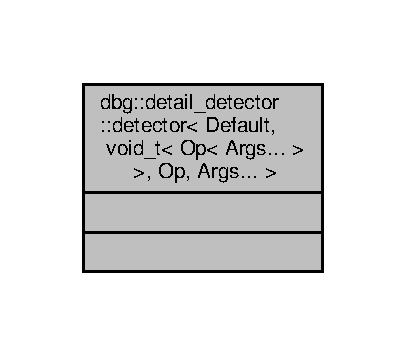
\includegraphics[width=195pt]{d5/d59/structdbg_1_1detail__detector_1_1detector_3_01Default_00_01void__t_3_01Op_3_01Args_8_8_8_01_4_010a7eb40f65b9d8d3493151bfdc3019fa}
\end{center}
\end{figure}
\subsection*{Public Types}
\begin{DoxyCompactItemize}
\item 
using \hyperlink{structdbg_1_1detail__detector_1_1detector_3_01Default_00_01void__t_3_01Op_3_01Args_8_8_8_01_4_01_4_00_01Op_00_01Args_8_8_8_01_4_ab9dc20c0565be267d2d98b0e0f4a565b}{value\+\_\+t} = std\+::true\+\_\+type
\item 
using \hyperlink{structdbg_1_1detail__detector_1_1detector_3_01Default_00_01void__t_3_01Op_3_01Args_8_8_8_01_4_01_4_00_01Op_00_01Args_8_8_8_01_4_a2119ba35e684b8292286546a1cea10d1}{type} = Op$<$ Args... $>$
\end{DoxyCompactItemize}


\subsection{Member Typedef Documentation}
\mbox{\Hypertarget{structdbg_1_1detail__detector_1_1detector_3_01Default_00_01void__t_3_01Op_3_01Args_8_8_8_01_4_01_4_00_01Op_00_01Args_8_8_8_01_4_a2119ba35e684b8292286546a1cea10d1}\label{structdbg_1_1detail__detector_1_1detector_3_01Default_00_01void__t_3_01Op_3_01Args_8_8_8_01_4_01_4_00_01Op_00_01Args_8_8_8_01_4_a2119ba35e684b8292286546a1cea10d1}} 
\index{dbg\+::detail\+\_\+detector\+::detector$<$ Default, void\+\_\+t$<$ Op$<$ Args... $>$ $>$, Op, Args... $>$@{dbg\+::detail\+\_\+detector\+::detector$<$ Default, void\+\_\+t$<$ Op$<$ Args... $>$ $>$, Op, Args... $>$}!type@{type}}
\index{type@{type}!dbg\+::detail\+\_\+detector\+::detector$<$ Default, void\+\_\+t$<$ Op$<$ Args... $>$ $>$, Op, Args... $>$@{dbg\+::detail\+\_\+detector\+::detector$<$ Default, void\+\_\+t$<$ Op$<$ Args... $>$ $>$, Op, Args... $>$}}
\subsubsection{\texorpdfstring{type}{type}}
{\footnotesize\ttfamily template$<$class Default , template$<$ class... $>$ class Op, class... Args$>$ \\
using \hyperlink{structdbg_1_1detail__detector_1_1detector}{dbg\+::detail\+\_\+detector\+::detector}$<$ Default, \hyperlink{namespacedbg_1_1detail__detector_a1dbadccf461338e71c55ea392d4ed47c}{void\+\_\+t}$<$ Op$<$ Args... $>$ $>$, Op, Args... $>$\+::\hyperlink{structdbg_1_1detail__detector_1_1detector_3_01Default_00_01void__t_3_01Op_3_01Args_8_8_8_01_4_01_4_00_01Op_00_01Args_8_8_8_01_4_a2119ba35e684b8292286546a1cea10d1}{type} =  Op$<$Args...$>$}

\mbox{\Hypertarget{structdbg_1_1detail__detector_1_1detector_3_01Default_00_01void__t_3_01Op_3_01Args_8_8_8_01_4_01_4_00_01Op_00_01Args_8_8_8_01_4_ab9dc20c0565be267d2d98b0e0f4a565b}\label{structdbg_1_1detail__detector_1_1detector_3_01Default_00_01void__t_3_01Op_3_01Args_8_8_8_01_4_01_4_00_01Op_00_01Args_8_8_8_01_4_ab9dc20c0565be267d2d98b0e0f4a565b}} 
\index{dbg\+::detail\+\_\+detector\+::detector$<$ Default, void\+\_\+t$<$ Op$<$ Args... $>$ $>$, Op, Args... $>$@{dbg\+::detail\+\_\+detector\+::detector$<$ Default, void\+\_\+t$<$ Op$<$ Args... $>$ $>$, Op, Args... $>$}!value\+\_\+t@{value\+\_\+t}}
\index{value\+\_\+t@{value\+\_\+t}!dbg\+::detail\+\_\+detector\+::detector$<$ Default, void\+\_\+t$<$ Op$<$ Args... $>$ $>$, Op, Args... $>$@{dbg\+::detail\+\_\+detector\+::detector$<$ Default, void\+\_\+t$<$ Op$<$ Args... $>$ $>$, Op, Args... $>$}}
\subsubsection{\texorpdfstring{value\+\_\+t}{value\_t}}
{\footnotesize\ttfamily template$<$class Default , template$<$ class... $>$ class Op, class... Args$>$ \\
using \hyperlink{structdbg_1_1detail__detector_1_1detector}{dbg\+::detail\+\_\+detector\+::detector}$<$ Default, \hyperlink{namespacedbg_1_1detail__detector_a1dbadccf461338e71c55ea392d4ed47c}{void\+\_\+t}$<$ Op$<$ Args... $>$ $>$, Op, Args... $>$\+::\hyperlink{structdbg_1_1detail__detector_1_1detector_3_01Default_00_01void__t_3_01Op_3_01Args_8_8_8_01_4_01_4_00_01Op_00_01Args_8_8_8_01_4_ab9dc20c0565be267d2d98b0e0f4a565b}{value\+\_\+t} =  std\+::true\+\_\+type}



The documentation for this struct was generated from the following file\+:\begin{DoxyCompactItemize}
\item 
\hyperlink{dbg_8h}{dbg.\+h}\end{DoxyCompactItemize}

\hypertarget{structstd_1_1enable__if}{}\section{std\+:\+:enable\+\_\+if$<$ B, T $>$ Struct Template Reference}
\label{structstd_1_1enable__if}\index{std\+::enable\+\_\+if$<$ B, T $>$@{std\+::enable\+\_\+if$<$ B, T $>$}}


{\ttfamily \#include $<$mathcompat.\+h$>$}



Collaboration diagram for std\+:\+:enable\+\_\+if$<$ B, T $>$\+:\nopagebreak
\begin{figure}[H]
\begin{center}
\leavevmode
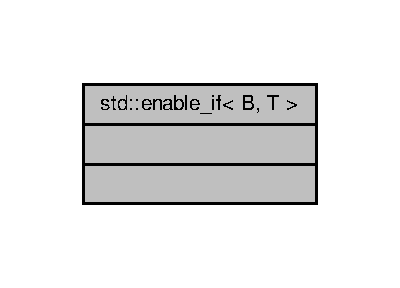
\includegraphics[width=192pt]{df/d1d/structstd_1_1enable__if__coll__graph}
\end{center}
\end{figure}


The documentation for this struct was generated from the following file\+:\begin{DoxyCompactItemize}
\item 
\hyperlink{mathcompat_8h}{mathcompat.\+h}\end{DoxyCompactItemize}

\hypertarget{structstd_1_1enable__if_3_01true_00_01T_01_4}{}\section{std\+:\+:enable\+\_\+if$<$ true, T $>$ Struct Template Reference}
\label{structstd_1_1enable__if_3_01true_00_01T_01_4}\index{std\+::enable\+\_\+if$<$ true, T $>$@{std\+::enable\+\_\+if$<$ true, T $>$}}


{\ttfamily \#include $<$mathcompat.\+h$>$}



Collaboration diagram for std\+:\+:enable\+\_\+if$<$ true, T $>$\+:\nopagebreak
\begin{figure}[H]
\begin{center}
\leavevmode
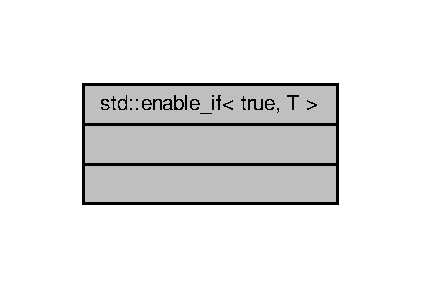
\includegraphics[width=202pt]{d7/dd6/structstd_1_1enable__if_3_01true_00_01T_01_4__coll__graph}
\end{center}
\end{figure}
\subsection*{Public Types}
\begin{DoxyCompactItemize}
\item 
typedef T \hyperlink{structstd_1_1enable__if_3_01true_00_01T_01_4_a393d6c819541dce0cd0d1afcec0ba55d}{type}
\end{DoxyCompactItemize}


\subsection{Member Typedef Documentation}
\mbox{\Hypertarget{structstd_1_1enable__if_3_01true_00_01T_01_4_a393d6c819541dce0cd0d1afcec0ba55d}\label{structstd_1_1enable__if_3_01true_00_01T_01_4_a393d6c819541dce0cd0d1afcec0ba55d}} 
\index{std\+::enable\+\_\+if$<$ true, T $>$@{std\+::enable\+\_\+if$<$ true, T $>$}!type@{type}}
\index{type@{type}!std\+::enable\+\_\+if$<$ true, T $>$@{std\+::enable\+\_\+if$<$ true, T $>$}}
\subsubsection{\texorpdfstring{type}{type}}
{\footnotesize\ttfamily template$<$class T $>$ \\
typedef T \hyperlink{structstd_1_1enable__if}{std\+::enable\+\_\+if}$<$ true, T $>$\+::\hyperlink{structstd_1_1enable__if_3_01true_00_01T_01_4_a393d6c819541dce0cd0d1afcec0ba55d}{type}}



The documentation for this struct was generated from the following file\+:\begin{DoxyCompactItemize}
\item 
\hyperlink{mathcompat_8h}{mathcompat.\+h}\end{DoxyCompactItemize}

\hypertarget{structEigen_1_1internal_1_1functor__traits_3_01scalar__normal__dist__op_3_01Scalar_01_4_01_4}{}\section{Eigen\+:\+:internal\+:\+:functor\+\_\+traits$<$ scalar\+\_\+normal\+\_\+dist\+\_\+op$<$ Scalar $>$ $>$ Struct Template Reference}
\label{structEigen_1_1internal_1_1functor__traits_3_01scalar__normal__dist__op_3_01Scalar_01_4_01_4}\index{Eigen\+::internal\+::functor\+\_\+traits$<$ scalar\+\_\+normal\+\_\+dist\+\_\+op$<$ Scalar $>$ $>$@{Eigen\+::internal\+::functor\+\_\+traits$<$ scalar\+\_\+normal\+\_\+dist\+\_\+op$<$ Scalar $>$ $>$}}


Collaboration diagram for Eigen\+:\+:internal\+:\+:functor\+\_\+traits$<$ scalar\+\_\+normal\+\_\+dist\+\_\+op$<$ Scalar $>$ $>$\+:\nopagebreak
\begin{figure}[H]
\begin{center}
\leavevmode
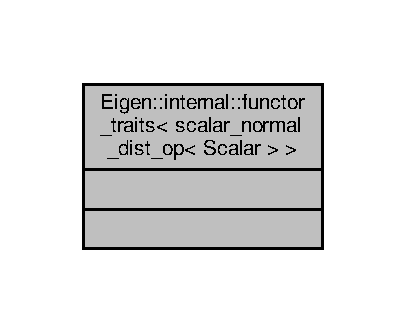
\includegraphics[width=195pt]{d6/da9/structEigen_1_1internal_1_1functor__traits_3_01scalar__normal__dist__op_3_01Scalar_01_4_01_4__coll__graph}
\end{center}
\end{figure}
\subsection*{Public Types}
\begin{DoxyCompactItemize}
\item 
enum \{ \hyperlink{structEigen_1_1internal_1_1functor__traits_3_01scalar__normal__dist__op_3_01Scalar_01_4_01_4_aa24d49756a42945135cf4bb233f70852ad22cd8b04dd82075ca39efd3ba99acd6}{Cost} = 50 $\ast$ Num\+Traits$<$Scalar$>$\+:\+:Mul\+Cost, 
\hyperlink{structEigen_1_1internal_1_1functor__traits_3_01scalar__normal__dist__op_3_01Scalar_01_4_01_4_aa24d49756a42945135cf4bb233f70852aa50396f958a83c30593e034700290b00}{Packet\+Access} = false, 
\hyperlink{structEigen_1_1internal_1_1functor__traits_3_01scalar__normal__dist__op_3_01Scalar_01_4_01_4_aa24d49756a42945135cf4bb233f70852a953ef8c87ba7a342649b4b09347c6fda}{Is\+Repeatable} = false
 \}
\end{DoxyCompactItemize}


\subsection{Member Enumeration Documentation}
\mbox{\Hypertarget{structEigen_1_1internal_1_1functor__traits_3_01scalar__normal__dist__op_3_01Scalar_01_4_01_4_aa24d49756a42945135cf4bb233f70852}\label{structEigen_1_1internal_1_1functor__traits_3_01scalar__normal__dist__op_3_01Scalar_01_4_01_4_aa24d49756a42945135cf4bb233f70852}} 
\subsubsection{\texorpdfstring{anonymous enum}{anonymous enum}}
{\footnotesize\ttfamily template$<$typename Scalar $>$ \\
anonymous enum}

\begin{DoxyEnumFields}{Enumerator}
\raisebox{\heightof{T}}[0pt][0pt]{\index{Cost@{Cost}!Eigen\+::internal\+::functor\+\_\+traits$<$ scalar\+\_\+normal\+\_\+dist\+\_\+op$<$ Scalar $>$ $>$@{Eigen\+::internal\+::functor\+\_\+traits$<$ scalar\+\_\+normal\+\_\+dist\+\_\+op$<$ Scalar $>$ $>$}}\index{Eigen\+::internal\+::functor\+\_\+traits$<$ scalar\+\_\+normal\+\_\+dist\+\_\+op$<$ Scalar $>$ $>$@{Eigen\+::internal\+::functor\+\_\+traits$<$ scalar\+\_\+normal\+\_\+dist\+\_\+op$<$ Scalar $>$ $>$}!Cost@{Cost}}}\mbox{\Hypertarget{structEigen_1_1internal_1_1functor__traits_3_01scalar__normal__dist__op_3_01Scalar_01_4_01_4_aa24d49756a42945135cf4bb233f70852ad22cd8b04dd82075ca39efd3ba99acd6}\label{structEigen_1_1internal_1_1functor__traits_3_01scalar__normal__dist__op_3_01Scalar_01_4_01_4_aa24d49756a42945135cf4bb233f70852ad22cd8b04dd82075ca39efd3ba99acd6}} 
Cost&\\
\hline

\raisebox{\heightof{T}}[0pt][0pt]{\index{Packet\+Access@{Packet\+Access}!Eigen\+::internal\+::functor\+\_\+traits$<$ scalar\+\_\+normal\+\_\+dist\+\_\+op$<$ Scalar $>$ $>$@{Eigen\+::internal\+::functor\+\_\+traits$<$ scalar\+\_\+normal\+\_\+dist\+\_\+op$<$ Scalar $>$ $>$}}\index{Eigen\+::internal\+::functor\+\_\+traits$<$ scalar\+\_\+normal\+\_\+dist\+\_\+op$<$ Scalar $>$ $>$@{Eigen\+::internal\+::functor\+\_\+traits$<$ scalar\+\_\+normal\+\_\+dist\+\_\+op$<$ Scalar $>$ $>$}!Packet\+Access@{Packet\+Access}}}\mbox{\Hypertarget{structEigen_1_1internal_1_1functor__traits_3_01scalar__normal__dist__op_3_01Scalar_01_4_01_4_aa24d49756a42945135cf4bb233f70852aa50396f958a83c30593e034700290b00}\label{structEigen_1_1internal_1_1functor__traits_3_01scalar__normal__dist__op_3_01Scalar_01_4_01_4_aa24d49756a42945135cf4bb233f70852aa50396f958a83c30593e034700290b00}} 
Packet\+Access&\\
\hline

\raisebox{\heightof{T}}[0pt][0pt]{\index{Is\+Repeatable@{Is\+Repeatable}!Eigen\+::internal\+::functor\+\_\+traits$<$ scalar\+\_\+normal\+\_\+dist\+\_\+op$<$ Scalar $>$ $>$@{Eigen\+::internal\+::functor\+\_\+traits$<$ scalar\+\_\+normal\+\_\+dist\+\_\+op$<$ Scalar $>$ $>$}}\index{Eigen\+::internal\+::functor\+\_\+traits$<$ scalar\+\_\+normal\+\_\+dist\+\_\+op$<$ Scalar $>$ $>$@{Eigen\+::internal\+::functor\+\_\+traits$<$ scalar\+\_\+normal\+\_\+dist\+\_\+op$<$ Scalar $>$ $>$}!Is\+Repeatable@{Is\+Repeatable}}}\mbox{\Hypertarget{structEigen_1_1internal_1_1functor__traits_3_01scalar__normal__dist__op_3_01Scalar_01_4_01_4_aa24d49756a42945135cf4bb233f70852a953ef8c87ba7a342649b4b09347c6fda}\label{structEigen_1_1internal_1_1functor__traits_3_01scalar__normal__dist__op_3_01Scalar_01_4_01_4_aa24d49756a42945135cf4bb233f70852a953ef8c87ba7a342649b4b09347c6fda}} 
Is\+Repeatable&\\
\hline

\end{DoxyEnumFields}


The documentation for this struct was generated from the following file\+:\begin{DoxyCompactItemize}
\item 
\hyperlink{mcl__eval_8cc}{mcl\+\_\+eval.\+cc}\end{DoxyCompactItemize}

\hypertarget{classtrimesh_1_1GLCamera}{}\section{trimesh\+:\+:G\+L\+Camera Class Reference}
\label{classtrimesh_1_1GLCamera}\index{trimesh\+::\+G\+L\+Camera@{trimesh\+::\+G\+L\+Camera}}


{\ttfamily \#include $<$G\+L\+Camera.\+h$>$}



Collaboration diagram for trimesh\+:\+:G\+L\+Camera\+:\nopagebreak
\begin{figure}[H]
\begin{center}
\leavevmode
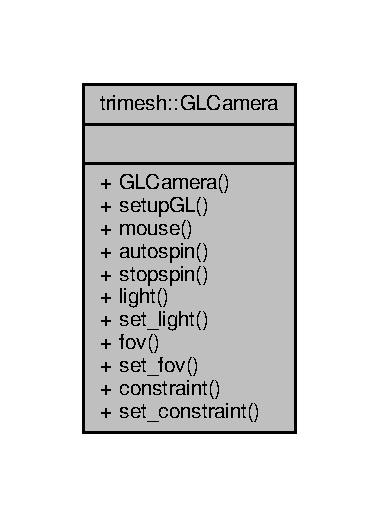
\includegraphics[width=182pt]{d5/dc7/classtrimesh_1_1GLCamera__coll__graph}
\end{center}
\end{figure}
\subsection*{Public Types}
\begin{DoxyCompactItemize}
\item 
enum \hyperlink{classtrimesh_1_1GLCamera_a4b7300c68956c148f6f8b014217faed9}{Constraint} \{ \hyperlink{classtrimesh_1_1GLCamera_a4b7300c68956c148f6f8b014217faed9aad6fd65696c348009ecdc5b0847b1145}{U\+N\+C\+O\+N\+S\+T\+R\+A\+I\+N\+ED}, 
\hyperlink{classtrimesh_1_1GLCamera_a4b7300c68956c148f6f8b014217faed9afe1d3daea1dd8899c758d3cdb20a43fd}{X\+C\+O\+N\+S\+T\+R\+A\+I\+N\+ED}, 
\hyperlink{classtrimesh_1_1GLCamera_a4b7300c68956c148f6f8b014217faed9a75b54165fb8fde6c6dddbc2c7c62394c}{Y\+C\+O\+N\+S\+T\+R\+A\+I\+N\+ED}, 
\hyperlink{classtrimesh_1_1GLCamera_a4b7300c68956c148f6f8b014217faed9a1df913d88c41154654d619967db03d4e}{Z\+C\+O\+N\+S\+T\+R\+A\+I\+N\+ED}
 \}
\end{DoxyCompactItemize}
\subsection*{Public Member Functions}
\begin{DoxyCompactItemize}
\item 
\hyperlink{classtrimesh_1_1GLCamera_a6c39c60c735a62c606550d8ca60616bd}{G\+L\+Camera} ()
\item 
\hyperlink{namespacetrimesh_a784ddfd979e1c579bda795a8edfc3f43}{void} \hyperlink{classtrimesh_1_1GLCamera_a060dc2d11b9c7e69e4a03421bf5a0670}{setup\+GL} (const \hyperlink{namespacetrimesh_a325b99fd6454b22fa4c4bc3223271b2c}{trimesh\+::point} \&scene\+\_\+center, float scene\+\_\+size) const
\item 
\hyperlink{namespacetrimesh_a784ddfd979e1c579bda795a8edfc3f43}{void} \hyperlink{classtrimesh_1_1GLCamera_ab300421205b8c4f699ed09ff4124e32f}{mouse} (int mousex, int mousey, \hyperlink{namespacetrimesh_1_1Mouse_a0b9f7f2e8a91299850fa63a8c995b02a}{Mouse\+::button} b, const \hyperlink{namespacetrimesh_a325b99fd6454b22fa4c4bc3223271b2c}{point} \&scene\+\_\+center, float scene\+\_\+size, \hyperlink{namespacetrimesh_ad504958f2f56e393991b848986a8459f}{xform} \&xf)
\item 
bool \hyperlink{classtrimesh_1_1GLCamera_aba8d85a19802c9c24fa478aa09738b2f}{autospin} (\hyperlink{namespacetrimesh_ad504958f2f56e393991b848986a8459f}{xform} \&xf)
\item 
\hyperlink{namespacetrimesh_a784ddfd979e1c579bda795a8edfc3f43}{void} \hyperlink{classtrimesh_1_1GLCamera_a588f762c28bffcf7d7c1e176f968ebff}{stopspin} ()
\item 
\hyperlink{namespacetrimesh_a4fc2b83feba99c931f837a0c7d4b4df1}{vec} \hyperlink{classtrimesh_1_1GLCamera_a454fa2c37f61c0b8e204e72d7615d1f1}{light} () const
\item 
\hyperlink{namespacetrimesh_a784ddfd979e1c579bda795a8edfc3f43}{void} \hyperlink{classtrimesh_1_1GLCamera_a1151d9c4aafcd873ba7df8e84669549a}{set\+\_\+light} (const \hyperlink{namespacetrimesh_a4fc2b83feba99c931f837a0c7d4b4df1}{vec} \&lightdir\+\_\+)
\item 
float \hyperlink{classtrimesh_1_1GLCamera_a66b0728bd1477ce920bf0e1ed8f15a65}{fov} () const
\item 
\hyperlink{namespacetrimesh_a784ddfd979e1c579bda795a8edfc3f43}{void} \hyperlink{classtrimesh_1_1GLCamera_a7020cc47b48ab434212155567c647faf}{set\+\_\+fov} (float fov\+\_\+)
\item 
\hyperlink{classtrimesh_1_1GLCamera_a4b7300c68956c148f6f8b014217faed9}{Constraint} \hyperlink{classtrimesh_1_1GLCamera_a726490d3604bcef7e54c7fbbde20379e}{constraint} ()
\item 
\hyperlink{namespacetrimesh_a784ddfd979e1c579bda795a8edfc3f43}{void} \hyperlink{classtrimesh_1_1GLCamera_a0f383a8117094b9013d3d945cc7dc979}{set\+\_\+constraint} (\hyperlink{classtrimesh_1_1GLCamera_a4b7300c68956c148f6f8b014217faed9}{Constraint} c)
\end{DoxyCompactItemize}


\subsection{Member Enumeration Documentation}
\mbox{\Hypertarget{classtrimesh_1_1GLCamera_a4b7300c68956c148f6f8b014217faed9}\label{classtrimesh_1_1GLCamera_a4b7300c68956c148f6f8b014217faed9}} 
\index{trimesh\+::\+G\+L\+Camera@{trimesh\+::\+G\+L\+Camera}!Constraint@{Constraint}}
\index{Constraint@{Constraint}!trimesh\+::\+G\+L\+Camera@{trimesh\+::\+G\+L\+Camera}}
\subsubsection{\texorpdfstring{Constraint}{Constraint}}
{\footnotesize\ttfamily enum \hyperlink{classtrimesh_1_1GLCamera_a4b7300c68956c148f6f8b014217faed9}{trimesh\+::\+G\+L\+Camera\+::\+Constraint}}

\begin{DoxyEnumFields}{Enumerator}
\raisebox{\heightof{T}}[0pt][0pt]{\index{U\+N\+C\+O\+N\+S\+T\+R\+A\+I\+N\+ED@{U\+N\+C\+O\+N\+S\+T\+R\+A\+I\+N\+ED}!trimesh\+::\+G\+L\+Camera@{trimesh\+::\+G\+L\+Camera}}\index{trimesh\+::\+G\+L\+Camera@{trimesh\+::\+G\+L\+Camera}!U\+N\+C\+O\+N\+S\+T\+R\+A\+I\+N\+ED@{U\+N\+C\+O\+N\+S\+T\+R\+A\+I\+N\+ED}}}\mbox{\Hypertarget{classtrimesh_1_1GLCamera_a4b7300c68956c148f6f8b014217faed9aad6fd65696c348009ecdc5b0847b1145}\label{classtrimesh_1_1GLCamera_a4b7300c68956c148f6f8b014217faed9aad6fd65696c348009ecdc5b0847b1145}} 
U\+N\+C\+O\+N\+S\+T\+R\+A\+I\+N\+ED&\\
\hline

\raisebox{\heightof{T}}[0pt][0pt]{\index{X\+C\+O\+N\+S\+T\+R\+A\+I\+N\+ED@{X\+C\+O\+N\+S\+T\+R\+A\+I\+N\+ED}!trimesh\+::\+G\+L\+Camera@{trimesh\+::\+G\+L\+Camera}}\index{trimesh\+::\+G\+L\+Camera@{trimesh\+::\+G\+L\+Camera}!X\+C\+O\+N\+S\+T\+R\+A\+I\+N\+ED@{X\+C\+O\+N\+S\+T\+R\+A\+I\+N\+ED}}}\mbox{\Hypertarget{classtrimesh_1_1GLCamera_a4b7300c68956c148f6f8b014217faed9afe1d3daea1dd8899c758d3cdb20a43fd}\label{classtrimesh_1_1GLCamera_a4b7300c68956c148f6f8b014217faed9afe1d3daea1dd8899c758d3cdb20a43fd}} 
X\+C\+O\+N\+S\+T\+R\+A\+I\+N\+ED&\\
\hline

\raisebox{\heightof{T}}[0pt][0pt]{\index{Y\+C\+O\+N\+S\+T\+R\+A\+I\+N\+ED@{Y\+C\+O\+N\+S\+T\+R\+A\+I\+N\+ED}!trimesh\+::\+G\+L\+Camera@{trimesh\+::\+G\+L\+Camera}}\index{trimesh\+::\+G\+L\+Camera@{trimesh\+::\+G\+L\+Camera}!Y\+C\+O\+N\+S\+T\+R\+A\+I\+N\+ED@{Y\+C\+O\+N\+S\+T\+R\+A\+I\+N\+ED}}}\mbox{\Hypertarget{classtrimesh_1_1GLCamera_a4b7300c68956c148f6f8b014217faed9a75b54165fb8fde6c6dddbc2c7c62394c}\label{classtrimesh_1_1GLCamera_a4b7300c68956c148f6f8b014217faed9a75b54165fb8fde6c6dddbc2c7c62394c}} 
Y\+C\+O\+N\+S\+T\+R\+A\+I\+N\+ED&\\
\hline

\raisebox{\heightof{T}}[0pt][0pt]{\index{Z\+C\+O\+N\+S\+T\+R\+A\+I\+N\+ED@{Z\+C\+O\+N\+S\+T\+R\+A\+I\+N\+ED}!trimesh\+::\+G\+L\+Camera@{trimesh\+::\+G\+L\+Camera}}\index{trimesh\+::\+G\+L\+Camera@{trimesh\+::\+G\+L\+Camera}!Z\+C\+O\+N\+S\+T\+R\+A\+I\+N\+ED@{Z\+C\+O\+N\+S\+T\+R\+A\+I\+N\+ED}}}\mbox{\Hypertarget{classtrimesh_1_1GLCamera_a4b7300c68956c148f6f8b014217faed9a1df913d88c41154654d619967db03d4e}\label{classtrimesh_1_1GLCamera_a4b7300c68956c148f6f8b014217faed9a1df913d88c41154654d619967db03d4e}} 
Z\+C\+O\+N\+S\+T\+R\+A\+I\+N\+ED&\\
\hline

\end{DoxyEnumFields}


\subsection{Constructor \& Destructor Documentation}
\mbox{\Hypertarget{classtrimesh_1_1GLCamera_a6c39c60c735a62c606550d8ca60616bd}\label{classtrimesh_1_1GLCamera_a6c39c60c735a62c606550d8ca60616bd}} 
\index{trimesh\+::\+G\+L\+Camera@{trimesh\+::\+G\+L\+Camera}!G\+L\+Camera@{G\+L\+Camera}}
\index{G\+L\+Camera@{G\+L\+Camera}!trimesh\+::\+G\+L\+Camera@{trimesh\+::\+G\+L\+Camera}}
\subsubsection{\texorpdfstring{G\+L\+Camera()}{GLCamera()}}
{\footnotesize\ttfamily trimesh\+::\+G\+L\+Camera\+::\+G\+L\+Camera (\begin{DoxyParamCaption}{ }\end{DoxyParamCaption})\hspace{0.3cm}{\ttfamily [inline]}}



\subsection{Member Function Documentation}
\mbox{\Hypertarget{classtrimesh_1_1GLCamera_aba8d85a19802c9c24fa478aa09738b2f}\label{classtrimesh_1_1GLCamera_aba8d85a19802c9c24fa478aa09738b2f}} 
\index{trimesh\+::\+G\+L\+Camera@{trimesh\+::\+G\+L\+Camera}!autospin@{autospin}}
\index{autospin@{autospin}!trimesh\+::\+G\+L\+Camera@{trimesh\+::\+G\+L\+Camera}}
\subsubsection{\texorpdfstring{autospin()}{autospin()}}
{\footnotesize\ttfamily bool trimesh\+::\+G\+L\+Camera\+::autospin (\begin{DoxyParamCaption}\item[{\hyperlink{namespacetrimesh_ad504958f2f56e393991b848986a8459f}{xform} \&}]{xf }\end{DoxyParamCaption})}

\mbox{\Hypertarget{classtrimesh_1_1GLCamera_a726490d3604bcef7e54c7fbbde20379e}\label{classtrimesh_1_1GLCamera_a726490d3604bcef7e54c7fbbde20379e}} 
\index{trimesh\+::\+G\+L\+Camera@{trimesh\+::\+G\+L\+Camera}!constraint@{constraint}}
\index{constraint@{constraint}!trimesh\+::\+G\+L\+Camera@{trimesh\+::\+G\+L\+Camera}}
\subsubsection{\texorpdfstring{constraint()}{constraint()}}
{\footnotesize\ttfamily \hyperlink{classtrimesh_1_1GLCamera_a4b7300c68956c148f6f8b014217faed9}{Constraint} trimesh\+::\+G\+L\+Camera\+::constraint (\begin{DoxyParamCaption}{ }\end{DoxyParamCaption})\hspace{0.3cm}{\ttfamily [inline]}}

\mbox{\Hypertarget{classtrimesh_1_1GLCamera_a66b0728bd1477ce920bf0e1ed8f15a65}\label{classtrimesh_1_1GLCamera_a66b0728bd1477ce920bf0e1ed8f15a65}} 
\index{trimesh\+::\+G\+L\+Camera@{trimesh\+::\+G\+L\+Camera}!fov@{fov}}
\index{fov@{fov}!trimesh\+::\+G\+L\+Camera@{trimesh\+::\+G\+L\+Camera}}
\subsubsection{\texorpdfstring{fov()}{fov()}}
{\footnotesize\ttfamily float trimesh\+::\+G\+L\+Camera\+::fov (\begin{DoxyParamCaption}{ }\end{DoxyParamCaption}) const\hspace{0.3cm}{\ttfamily [inline]}}

\mbox{\Hypertarget{classtrimesh_1_1GLCamera_a454fa2c37f61c0b8e204e72d7615d1f1}\label{classtrimesh_1_1GLCamera_a454fa2c37f61c0b8e204e72d7615d1f1}} 
\index{trimesh\+::\+G\+L\+Camera@{trimesh\+::\+G\+L\+Camera}!light@{light}}
\index{light@{light}!trimesh\+::\+G\+L\+Camera@{trimesh\+::\+G\+L\+Camera}}
\subsubsection{\texorpdfstring{light()}{light()}}
{\footnotesize\ttfamily \hyperlink{namespacetrimesh_a4fc2b83feba99c931f837a0c7d4b4df1}{vec} trimesh\+::\+G\+L\+Camera\+::light (\begin{DoxyParamCaption}{ }\end{DoxyParamCaption}) const\hspace{0.3cm}{\ttfamily [inline]}}

\mbox{\Hypertarget{classtrimesh_1_1GLCamera_ab300421205b8c4f699ed09ff4124e32f}\label{classtrimesh_1_1GLCamera_ab300421205b8c4f699ed09ff4124e32f}} 
\index{trimesh\+::\+G\+L\+Camera@{trimesh\+::\+G\+L\+Camera}!mouse@{mouse}}
\index{mouse@{mouse}!trimesh\+::\+G\+L\+Camera@{trimesh\+::\+G\+L\+Camera}}
\subsubsection{\texorpdfstring{mouse()}{mouse()}}
{\footnotesize\ttfamily \hyperlink{namespacetrimesh_a784ddfd979e1c579bda795a8edfc3f43}{void} trimesh\+::\+G\+L\+Camera\+::mouse (\begin{DoxyParamCaption}\item[{int}]{mousex,  }\item[{int}]{mousey,  }\item[{\hyperlink{namespacetrimesh_1_1Mouse_a0b9f7f2e8a91299850fa63a8c995b02a}{Mouse\+::button}}]{b,  }\item[{const \hyperlink{namespacetrimesh_a325b99fd6454b22fa4c4bc3223271b2c}{point} \&}]{scene\+\_\+center,  }\item[{float}]{scene\+\_\+size,  }\item[{\hyperlink{namespacetrimesh_ad504958f2f56e393991b848986a8459f}{xform} \&}]{xf }\end{DoxyParamCaption})}

\mbox{\Hypertarget{classtrimesh_1_1GLCamera_a0f383a8117094b9013d3d945cc7dc979}\label{classtrimesh_1_1GLCamera_a0f383a8117094b9013d3d945cc7dc979}} 
\index{trimesh\+::\+G\+L\+Camera@{trimesh\+::\+G\+L\+Camera}!set\+\_\+constraint@{set\+\_\+constraint}}
\index{set\+\_\+constraint@{set\+\_\+constraint}!trimesh\+::\+G\+L\+Camera@{trimesh\+::\+G\+L\+Camera}}
\subsubsection{\texorpdfstring{set\+\_\+constraint()}{set\_constraint()}}
{\footnotesize\ttfamily \hyperlink{namespacetrimesh_a784ddfd979e1c579bda795a8edfc3f43}{void} trimesh\+::\+G\+L\+Camera\+::set\+\_\+constraint (\begin{DoxyParamCaption}\item[{\hyperlink{classtrimesh_1_1GLCamera_a4b7300c68956c148f6f8b014217faed9}{Constraint}}]{c }\end{DoxyParamCaption})\hspace{0.3cm}{\ttfamily [inline]}}

\mbox{\Hypertarget{classtrimesh_1_1GLCamera_a7020cc47b48ab434212155567c647faf}\label{classtrimesh_1_1GLCamera_a7020cc47b48ab434212155567c647faf}} 
\index{trimesh\+::\+G\+L\+Camera@{trimesh\+::\+G\+L\+Camera}!set\+\_\+fov@{set\+\_\+fov}}
\index{set\+\_\+fov@{set\+\_\+fov}!trimesh\+::\+G\+L\+Camera@{trimesh\+::\+G\+L\+Camera}}
\subsubsection{\texorpdfstring{set\+\_\+fov()}{set\_fov()}}
{\footnotesize\ttfamily \hyperlink{namespacetrimesh_a784ddfd979e1c579bda795a8edfc3f43}{void} trimesh\+::\+G\+L\+Camera\+::set\+\_\+fov (\begin{DoxyParamCaption}\item[{float}]{fov\+\_\+ }\end{DoxyParamCaption})\hspace{0.3cm}{\ttfamily [inline]}}

\mbox{\Hypertarget{classtrimesh_1_1GLCamera_a1151d9c4aafcd873ba7df8e84669549a}\label{classtrimesh_1_1GLCamera_a1151d9c4aafcd873ba7df8e84669549a}} 
\index{trimesh\+::\+G\+L\+Camera@{trimesh\+::\+G\+L\+Camera}!set\+\_\+light@{set\+\_\+light}}
\index{set\+\_\+light@{set\+\_\+light}!trimesh\+::\+G\+L\+Camera@{trimesh\+::\+G\+L\+Camera}}
\subsubsection{\texorpdfstring{set\+\_\+light()}{set\_light()}}
{\footnotesize\ttfamily \hyperlink{namespacetrimesh_a784ddfd979e1c579bda795a8edfc3f43}{void} trimesh\+::\+G\+L\+Camera\+::set\+\_\+light (\begin{DoxyParamCaption}\item[{const \hyperlink{namespacetrimesh_a4fc2b83feba99c931f837a0c7d4b4df1}{vec} \&}]{lightdir\+\_\+ }\end{DoxyParamCaption})\hspace{0.3cm}{\ttfamily [inline]}}

\mbox{\Hypertarget{classtrimesh_1_1GLCamera_a060dc2d11b9c7e69e4a03421bf5a0670}\label{classtrimesh_1_1GLCamera_a060dc2d11b9c7e69e4a03421bf5a0670}} 
\index{trimesh\+::\+G\+L\+Camera@{trimesh\+::\+G\+L\+Camera}!setup\+GL@{setup\+GL}}
\index{setup\+GL@{setup\+GL}!trimesh\+::\+G\+L\+Camera@{trimesh\+::\+G\+L\+Camera}}
\subsubsection{\texorpdfstring{setup\+G\+L()}{setupGL()}}
{\footnotesize\ttfamily \hyperlink{namespacetrimesh_a784ddfd979e1c579bda795a8edfc3f43}{void} trimesh\+::\+G\+L\+Camera\+::setup\+GL (\begin{DoxyParamCaption}\item[{const \hyperlink{namespacetrimesh_a325b99fd6454b22fa4c4bc3223271b2c}{trimesh\+::point} \&}]{scene\+\_\+center,  }\item[{float}]{scene\+\_\+size }\end{DoxyParamCaption}) const}

\mbox{\Hypertarget{classtrimesh_1_1GLCamera_a588f762c28bffcf7d7c1e176f968ebff}\label{classtrimesh_1_1GLCamera_a588f762c28bffcf7d7c1e176f968ebff}} 
\index{trimesh\+::\+G\+L\+Camera@{trimesh\+::\+G\+L\+Camera}!stopspin@{stopspin}}
\index{stopspin@{stopspin}!trimesh\+::\+G\+L\+Camera@{trimesh\+::\+G\+L\+Camera}}
\subsubsection{\texorpdfstring{stopspin()}{stopspin()}}
{\footnotesize\ttfamily \hyperlink{namespacetrimesh_a784ddfd979e1c579bda795a8edfc3f43}{void} trimesh\+::\+G\+L\+Camera\+::stopspin (\begin{DoxyParamCaption}{ }\end{DoxyParamCaption})\hspace{0.3cm}{\ttfamily [inline]}}



The documentation for this class was generated from the following files\+:\begin{DoxyCompactItemize}
\item 
\hyperlink{GLCamera_8h}{G\+L\+Camera.\+h}\item 
\hyperlink{GLCamera_8cc}{G\+L\+Camera.\+cc}\end{DoxyCompactItemize}

\hypertarget{classtrimesh_1_1GLManager}{}\section{trimesh\+:\+:G\+L\+Manager Class Reference}
\label{classtrimesh_1_1GLManager}\index{trimesh\+::\+G\+L\+Manager@{trimesh\+::\+G\+L\+Manager}}


{\ttfamily \#include $<$G\+L\+Manager.\+h$>$}



Collaboration diagram for trimesh\+:\+:G\+L\+Manager\+:\nopagebreak
\begin{figure}[H]
\begin{center}
\leavevmode
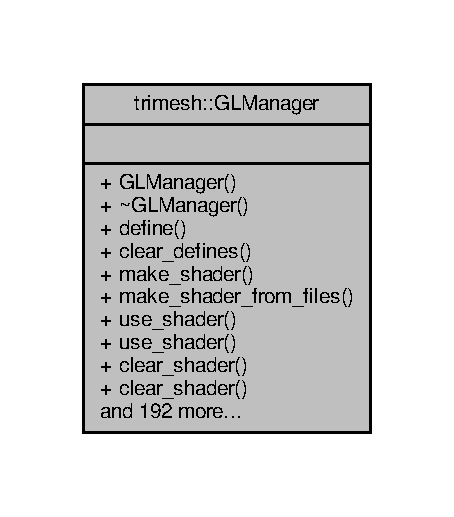
\includegraphics[width=218pt]{d8/d47/classtrimesh_1_1GLManager__coll__graph}
\end{center}
\end{figure}
\subsection*{Classes}
\begin{DoxyCompactItemize}
\item 
struct \hyperlink{structtrimesh_1_1GLManager_1_1AttributeInfo}{Attribute\+Info}
\item 
class \hyperlink{classtrimesh_1_1GLManager_1_1BufferInfo}{Buffer\+Info}
\item 
class \hyperlink{classtrimesh_1_1GLManager_1_1ShaderDefine}{Shader\+Define}
\item 
class \hyperlink{classtrimesh_1_1GLManager_1_1ShaderInfo}{Shader\+Info}
\item 
struct \hyperlink{structtrimesh_1_1GLManager_1_1UniformInfo}{Uniform\+Info}
\end{DoxyCompactItemize}
\subsection*{Public Member Functions}
\begin{DoxyCompactItemize}
\item 
\hyperlink{classtrimesh_1_1GLManager_a112a5f5b48ffba4ffcd5605bb4c6d6ef}{G\+L\+Manager} ()
\item 
\hyperlink{classtrimesh_1_1GLManager_a2ceae5402999a9932058ed0f5a6595bf}{$\sim$\+G\+L\+Manager} ()
\item 
\hyperlink{namespacetrimesh_a784ddfd979e1c579bda795a8edfc3f43}{void} \hyperlink{classtrimesh_1_1GLManager_aadb5cf05653eb16a06f662265ee86ad3}{define} (const char $\ast$defname, const char $\ast$\hyperlink{namespacetrimesh_ab10cc1052c9d1d1376d92211b6ca27dd}{value})
\item 
\hyperlink{namespacetrimesh_a784ddfd979e1c579bda795a8edfc3f43}{void} \hyperlink{classtrimesh_1_1GLManager_a41184a813233411724ba864c93cb1adc}{clear\+\_\+defines} ()
\item 
unsigned \hyperlink{classtrimesh_1_1GLManager_a94896722a1121f1e919acd6a7fb7131c}{make\+\_\+shader} (const char $\ast$\hyperlink{namespacetrimesh_a7f24cdcfa73387d7fa6aa44676238a79}{name}, const char $\ast$vert\+\_\+text, const char $\ast$frag\+\_\+text)
\item 
unsigned \hyperlink{classtrimesh_1_1GLManager_ad1a456cf2a2438927a1b02d8a861e4ab}{make\+\_\+shader\+\_\+from\+\_\+files} (const char $\ast$\hyperlink{namespacetrimesh_a7f24cdcfa73387d7fa6aa44676238a79}{name}, const char $\ast$vert\+\_\+filename, const char $\ast$frag\+\_\+filename)
\item 
bool \hyperlink{classtrimesh_1_1GLManager_a8e0f44ceb57dc8bd4c4b75840e1b33cb}{use\+\_\+shader} (unsigned ind=0)
\item 
bool \hyperlink{classtrimesh_1_1GLManager_a9395996246b3a1219f5fda74abe39ee7}{use\+\_\+shader} (const char $\ast$\hyperlink{namespacetrimesh_a7f24cdcfa73387d7fa6aa44676238a79}{name})
\item 
\hyperlink{namespacetrimesh_a784ddfd979e1c579bda795a8edfc3f43}{void} \hyperlink{classtrimesh_1_1GLManager_a399b260a08d77d96efef3ae3ada38bcb}{clear\+\_\+shader} (unsigned ind)
\item 
\hyperlink{namespacetrimesh_a784ddfd979e1c579bda795a8edfc3f43}{void} \hyperlink{classtrimesh_1_1GLManager_a12756e75857c3b79ad142b80aee701f9}{clear\+\_\+shader} (const char $\ast$\hyperlink{namespacetrimesh_a7f24cdcfa73387d7fa6aa44676238a79}{name})
\item 
\hyperlink{namespacetrimesh_a784ddfd979e1c579bda795a8edfc3f43}{void} \hyperlink{classtrimesh_1_1GLManager_ac40cc39701e5542f533355525966b80b}{clear\+\_\+shaders} ()
\item 
\hyperlink{namespacetrimesh_a784ddfd979e1c579bda795a8edfc3f43}{void} \hyperlink{classtrimesh_1_1GLManager_a549dd90ffc5b778adbfd511b2d89b6db}{uniform1i} (int ind, int \hyperlink{namespacetrimesh_a3365d1b1a1bc5d8e9c844cf589a8c4a8}{x})
\item 
\hyperlink{namespacetrimesh_a784ddfd979e1c579bda795a8edfc3f43}{void} \hyperlink{classtrimesh_1_1GLManager_a59f7fcc16d13fcf35c944050a482f902}{uniform2i} (int ind, int \hyperlink{namespacetrimesh_a3365d1b1a1bc5d8e9c844cf589a8c4a8}{x}, int \hyperlink{namespacetrimesh_a56b35d0eb7039be92fcc4867080c7419}{y})
\item 
\hyperlink{namespacetrimesh_a784ddfd979e1c579bda795a8edfc3f43}{void} \hyperlink{classtrimesh_1_1GLManager_a96f555608ba1ac137dc844145064a861}{uniform3i} (int ind, int \hyperlink{namespacetrimesh_a3365d1b1a1bc5d8e9c844cf589a8c4a8}{x}, int \hyperlink{namespacetrimesh_a56b35d0eb7039be92fcc4867080c7419}{y}, int \hyperlink{namespacetrimesh_a42d0d86cc8db1d2be48121fe5e52fc67}{z})
\item 
\hyperlink{namespacetrimesh_a784ddfd979e1c579bda795a8edfc3f43}{void} \hyperlink{classtrimesh_1_1GLManager_a0a82e153c475c4cfc102549efc258cf4}{uniform4i} (int ind, int \hyperlink{namespacetrimesh_a3365d1b1a1bc5d8e9c844cf589a8c4a8}{x}, int \hyperlink{namespacetrimesh_a56b35d0eb7039be92fcc4867080c7419}{y}, int \hyperlink{namespacetrimesh_a42d0d86cc8db1d2be48121fe5e52fc67}{z}, int \hyperlink{namespacetrimesh_acd577db8a2f95fe39ececb95e98a6c71}{w})
\item 
\hyperlink{namespacetrimesh_a784ddfd979e1c579bda795a8edfc3f43}{void} \hyperlink{classtrimesh_1_1GLManager_ac7033d1d45efb39d62e5c21a8ec74546}{uniform1iv} (int ind, const int $\ast$p)
\item 
\hyperlink{namespacetrimesh_a784ddfd979e1c579bda795a8edfc3f43}{void} \hyperlink{classtrimesh_1_1GLManager_aca516770647d91fbb8637878e1ca1a66}{uniform2iv} (int ind, const int $\ast$p)
\item 
\hyperlink{namespacetrimesh_a784ddfd979e1c579bda795a8edfc3f43}{void} \hyperlink{classtrimesh_1_1GLManager_ad78abd2f8c505b938287304b22769bba}{uniform3iv} (int ind, const int $\ast$p)
\item 
\hyperlink{namespacetrimesh_a784ddfd979e1c579bda795a8edfc3f43}{void} \hyperlink{classtrimesh_1_1GLManager_a355205f6a14423af3a4f61051de7acdc}{uniform4iv} (int ind, const int $\ast$p)
\item 
\hyperlink{namespacetrimesh_a784ddfd979e1c579bda795a8edfc3f43}{void} \hyperlink{classtrimesh_1_1GLManager_ae3e47a06486dc1a28c60dad6f05ae5f4}{uniform1f} (int ind, float \hyperlink{namespacetrimesh_a3365d1b1a1bc5d8e9c844cf589a8c4a8}{x})
\item 
\hyperlink{namespacetrimesh_a784ddfd979e1c579bda795a8edfc3f43}{void} \hyperlink{classtrimesh_1_1GLManager_a832ba2745a8d2455a6951ce5ee305ac4}{uniform2f} (int ind, float \hyperlink{namespacetrimesh_a3365d1b1a1bc5d8e9c844cf589a8c4a8}{x}, float \hyperlink{namespacetrimesh_a56b35d0eb7039be92fcc4867080c7419}{y})
\item 
\hyperlink{namespacetrimesh_a784ddfd979e1c579bda795a8edfc3f43}{void} \hyperlink{classtrimesh_1_1GLManager_adb4d26d33054ab95c0ed7768a1d0c068}{uniform3f} (int ind, float \hyperlink{namespacetrimesh_a3365d1b1a1bc5d8e9c844cf589a8c4a8}{x}, float \hyperlink{namespacetrimesh_a56b35d0eb7039be92fcc4867080c7419}{y}, float \hyperlink{namespacetrimesh_a42d0d86cc8db1d2be48121fe5e52fc67}{z})
\item 
\hyperlink{namespacetrimesh_a784ddfd979e1c579bda795a8edfc3f43}{void} \hyperlink{classtrimesh_1_1GLManager_a7895f5129d3031f7e4535d2520175636}{uniform4f} (int ind, float \hyperlink{namespacetrimesh_a3365d1b1a1bc5d8e9c844cf589a8c4a8}{x}, float \hyperlink{namespacetrimesh_a56b35d0eb7039be92fcc4867080c7419}{y}, float \hyperlink{namespacetrimesh_a42d0d86cc8db1d2be48121fe5e52fc67}{z}, float \hyperlink{namespacetrimesh_acd577db8a2f95fe39ececb95e98a6c71}{w})
\item 
\hyperlink{namespacetrimesh_a784ddfd979e1c579bda795a8edfc3f43}{void} \hyperlink{classtrimesh_1_1GLManager_a3a16277267e3b099bc5e1f02d3aa3994}{uniform1fv} (int ind, const float $\ast$p)
\item 
\hyperlink{namespacetrimesh_a784ddfd979e1c579bda795a8edfc3f43}{void} \hyperlink{classtrimesh_1_1GLManager_ad867869189607ee86dffa867702b9109}{uniform2fv} (int ind, const float $\ast$p)
\item 
\hyperlink{namespacetrimesh_a784ddfd979e1c579bda795a8edfc3f43}{void} \hyperlink{classtrimesh_1_1GLManager_adeed58654a75c94ac5ca66e687ddb560}{uniform3fv} (int ind, const float $\ast$p)
\item 
\hyperlink{namespacetrimesh_a784ddfd979e1c579bda795a8edfc3f43}{void} \hyperlink{classtrimesh_1_1GLManager_afdce0610ce4b1dc6571f5f1773946e81}{uniform4fv} (int ind, const float $\ast$p)
\item 
\hyperlink{namespacetrimesh_a784ddfd979e1c579bda795a8edfc3f43}{void} \hyperlink{classtrimesh_1_1GLManager_aa85ae5d5c70eb42bdec7443469cd6bab}{uniform\+Matrix2fv} (int ind, const float $\ast$p)
\item 
\hyperlink{namespacetrimesh_a784ddfd979e1c579bda795a8edfc3f43}{void} \hyperlink{classtrimesh_1_1GLManager_ae312070973ffd1a60b7bb054af4768aa}{uniform\+Matrix3fv} (int ind, const float $\ast$p)
\item 
\hyperlink{namespacetrimesh_a784ddfd979e1c579bda795a8edfc3f43}{void} \hyperlink{classtrimesh_1_1GLManager_a6246470796e83a3fdaad7f433f268d48}{uniform\+Matrix4fv} (int ind, const float $\ast$p)
\item 
\hyperlink{namespacetrimesh_a784ddfd979e1c579bda795a8edfc3f43}{void} \hyperlink{classtrimesh_1_1GLManager_a179452fabbecea02c7c0775b176d04ba}{uniform\+Texture} (int ind, unsigned texind)
\item 
\hyperlink{namespacetrimesh_a784ddfd979e1c579bda795a8edfc3f43}{void} \hyperlink{classtrimesh_1_1GLManager_a770f2bc897499e00b317aff637d937ad}{uniform\+Texture} (int ind, const \hyperlink{namespacetrimesh_a784ddfd979e1c579bda795a8edfc3f43}{void} $\ast$p)
\item 
{\footnotesize template$<$class T $>$ }\\\hyperlink{namespacetrimesh_a784ddfd979e1c579bda795a8edfc3f43}{void} \hyperlink{classtrimesh_1_1GLManager_a5e48b244698c46dbea6d05bef3fd0d65}{uniform\+Texture} (int ind, const \+::std\+::vector$<$ T $>$ \&v)
\item 
\hyperlink{namespacetrimesh_a784ddfd979e1c579bda795a8edfc3f43}{void} \hyperlink{classtrimesh_1_1GLManager_abcd5b21eb25b15fdc13d77e3946d69e4}{uniform1i} (const char $\ast$\hyperlink{namespacetrimesh_a7f24cdcfa73387d7fa6aa44676238a79}{name}, int \hyperlink{namespacetrimesh_a3365d1b1a1bc5d8e9c844cf589a8c4a8}{x})
\item 
\hyperlink{namespacetrimesh_a784ddfd979e1c579bda795a8edfc3f43}{void} \hyperlink{classtrimesh_1_1GLManager_a97f27c4bcea42e9ebaef24cf558f91a3}{uniform2i} (const char $\ast$\hyperlink{namespacetrimesh_a7f24cdcfa73387d7fa6aa44676238a79}{name}, int \hyperlink{namespacetrimesh_a3365d1b1a1bc5d8e9c844cf589a8c4a8}{x}, int \hyperlink{namespacetrimesh_a56b35d0eb7039be92fcc4867080c7419}{y})
\item 
\hyperlink{namespacetrimesh_a784ddfd979e1c579bda795a8edfc3f43}{void} \hyperlink{classtrimesh_1_1GLManager_a89d7f7d4d3fff093bd8e23f1743043f7}{uniform3i} (const char $\ast$\hyperlink{namespacetrimesh_a7f24cdcfa73387d7fa6aa44676238a79}{name}, int \hyperlink{namespacetrimesh_a3365d1b1a1bc5d8e9c844cf589a8c4a8}{x}, int \hyperlink{namespacetrimesh_a56b35d0eb7039be92fcc4867080c7419}{y}, int \hyperlink{namespacetrimesh_a42d0d86cc8db1d2be48121fe5e52fc67}{z})
\item 
\hyperlink{namespacetrimesh_a784ddfd979e1c579bda795a8edfc3f43}{void} \hyperlink{classtrimesh_1_1GLManager_aaf1e9bb34b232537e042b538a98f6ea5}{uniform4i} (const char $\ast$\hyperlink{namespacetrimesh_a7f24cdcfa73387d7fa6aa44676238a79}{name}, int \hyperlink{namespacetrimesh_a3365d1b1a1bc5d8e9c844cf589a8c4a8}{x}, int \hyperlink{namespacetrimesh_a56b35d0eb7039be92fcc4867080c7419}{y}, int \hyperlink{namespacetrimesh_a42d0d86cc8db1d2be48121fe5e52fc67}{z}, int \hyperlink{namespacetrimesh_acd577db8a2f95fe39ececb95e98a6c71}{w})
\item 
\hyperlink{namespacetrimesh_a784ddfd979e1c579bda795a8edfc3f43}{void} \hyperlink{classtrimesh_1_1GLManager_aaa1eda6d21cae6cf050b5c28b7d2aa6e}{uniform1iv} (const char $\ast$\hyperlink{namespacetrimesh_a7f24cdcfa73387d7fa6aa44676238a79}{name}, const int $\ast$p)
\item 
\hyperlink{namespacetrimesh_a784ddfd979e1c579bda795a8edfc3f43}{void} \hyperlink{classtrimesh_1_1GLManager_acb09eac22ea6e1149bd70ef3fe53c228}{uniform2iv} (const char $\ast$\hyperlink{namespacetrimesh_a7f24cdcfa73387d7fa6aa44676238a79}{name}, const int $\ast$p)
\item 
\hyperlink{namespacetrimesh_a784ddfd979e1c579bda795a8edfc3f43}{void} \hyperlink{classtrimesh_1_1GLManager_a1c405b9e0ecb9551308bc43a7142e5dc}{uniform3iv} (const char $\ast$\hyperlink{namespacetrimesh_a7f24cdcfa73387d7fa6aa44676238a79}{name}, const int $\ast$p)
\item 
\hyperlink{namespacetrimesh_a784ddfd979e1c579bda795a8edfc3f43}{void} \hyperlink{classtrimesh_1_1GLManager_afe88dfe56ad5e78815f72e32be7a0932}{uniform4iv} (const char $\ast$\hyperlink{namespacetrimesh_a7f24cdcfa73387d7fa6aa44676238a79}{name}, const int $\ast$p)
\item 
\hyperlink{namespacetrimesh_a784ddfd979e1c579bda795a8edfc3f43}{void} \hyperlink{classtrimesh_1_1GLManager_a327978b754646c78dd54094d6d0c46f4}{uniform1f} (const char $\ast$\hyperlink{namespacetrimesh_a7f24cdcfa73387d7fa6aa44676238a79}{name}, float \hyperlink{namespacetrimesh_a3365d1b1a1bc5d8e9c844cf589a8c4a8}{x})
\item 
\hyperlink{namespacetrimesh_a784ddfd979e1c579bda795a8edfc3f43}{void} \hyperlink{classtrimesh_1_1GLManager_a96ee79a5860c9e28a0180c41de00d941}{uniform2f} (const char $\ast$\hyperlink{namespacetrimesh_a7f24cdcfa73387d7fa6aa44676238a79}{name}, float \hyperlink{namespacetrimesh_a3365d1b1a1bc5d8e9c844cf589a8c4a8}{x}, float \hyperlink{namespacetrimesh_a56b35d0eb7039be92fcc4867080c7419}{y})
\item 
\hyperlink{namespacetrimesh_a784ddfd979e1c579bda795a8edfc3f43}{void} \hyperlink{classtrimesh_1_1GLManager_a3089e468b5696dba6148548648f603ce}{uniform3f} (const char $\ast$\hyperlink{namespacetrimesh_a7f24cdcfa73387d7fa6aa44676238a79}{name}, float \hyperlink{namespacetrimesh_a3365d1b1a1bc5d8e9c844cf589a8c4a8}{x}, float \hyperlink{namespacetrimesh_a56b35d0eb7039be92fcc4867080c7419}{y}, float \hyperlink{namespacetrimesh_a42d0d86cc8db1d2be48121fe5e52fc67}{z})
\item 
\hyperlink{namespacetrimesh_a784ddfd979e1c579bda795a8edfc3f43}{void} \hyperlink{classtrimesh_1_1GLManager_a8f8adeaaa0c79132f11386badfefe83d}{uniform4f} (const char $\ast$\hyperlink{namespacetrimesh_a7f24cdcfa73387d7fa6aa44676238a79}{name}, float \hyperlink{namespacetrimesh_a3365d1b1a1bc5d8e9c844cf589a8c4a8}{x}, float \hyperlink{namespacetrimesh_a56b35d0eb7039be92fcc4867080c7419}{y}, float \hyperlink{namespacetrimesh_a42d0d86cc8db1d2be48121fe5e52fc67}{z}, float \hyperlink{namespacetrimesh_acd577db8a2f95fe39ececb95e98a6c71}{w})
\item 
\hyperlink{namespacetrimesh_a784ddfd979e1c579bda795a8edfc3f43}{void} \hyperlink{classtrimesh_1_1GLManager_afd33772a444a7c38a8b118bc67a8e8df}{uniform1fv} (const char $\ast$\hyperlink{namespacetrimesh_a7f24cdcfa73387d7fa6aa44676238a79}{name}, const float $\ast$p)
\item 
\hyperlink{namespacetrimesh_a784ddfd979e1c579bda795a8edfc3f43}{void} \hyperlink{classtrimesh_1_1GLManager_a23259935efcaca0ee7607877d4e140b5}{uniform2fv} (const char $\ast$\hyperlink{namespacetrimesh_a7f24cdcfa73387d7fa6aa44676238a79}{name}, const float $\ast$p)
\item 
\hyperlink{namespacetrimesh_a784ddfd979e1c579bda795a8edfc3f43}{void} \hyperlink{classtrimesh_1_1GLManager_a66f8e6b8bfa571970e382cd9b5de6438}{uniform3fv} (const char $\ast$\hyperlink{namespacetrimesh_a7f24cdcfa73387d7fa6aa44676238a79}{name}, const float $\ast$p)
\item 
\hyperlink{namespacetrimesh_a784ddfd979e1c579bda795a8edfc3f43}{void} \hyperlink{classtrimesh_1_1GLManager_a580fb27564991f2b7a3f5aea00a2aaa0}{uniform4fv} (const char $\ast$\hyperlink{namespacetrimesh_a7f24cdcfa73387d7fa6aa44676238a79}{name}, const float $\ast$p)
\item 
\hyperlink{namespacetrimesh_a784ddfd979e1c579bda795a8edfc3f43}{void} \hyperlink{classtrimesh_1_1GLManager_a7f9698a804700e72656415188fbb65aa}{uniform\+Matrix2fv} (const char $\ast$\hyperlink{namespacetrimesh_a7f24cdcfa73387d7fa6aa44676238a79}{name}, const float $\ast$p)
\item 
\hyperlink{namespacetrimesh_a784ddfd979e1c579bda795a8edfc3f43}{void} \hyperlink{classtrimesh_1_1GLManager_a8148eb6de9963331b5335fe4ff0f6b5b}{uniform\+Matrix3fv} (const char $\ast$\hyperlink{namespacetrimesh_a7f24cdcfa73387d7fa6aa44676238a79}{name}, const float $\ast$p)
\item 
\hyperlink{namespacetrimesh_a784ddfd979e1c579bda795a8edfc3f43}{void} \hyperlink{classtrimesh_1_1GLManager_a89fc85ec35633b813c4eaa18f9689bce}{uniform\+Matrix4fv} (const char $\ast$\hyperlink{namespacetrimesh_a7f24cdcfa73387d7fa6aa44676238a79}{name}, const float $\ast$p)
\item 
\hyperlink{namespacetrimesh_a784ddfd979e1c579bda795a8edfc3f43}{void} \hyperlink{classtrimesh_1_1GLManager_a4df4439932f0fd370eb60bb2d35798fb}{uniform\+Texture} (const char $\ast$\hyperlink{namespacetrimesh_a7f24cdcfa73387d7fa6aa44676238a79}{name}, unsigned texind)
\item 
\hyperlink{namespacetrimesh_a784ddfd979e1c579bda795a8edfc3f43}{void} \hyperlink{classtrimesh_1_1GLManager_a5f5152237eaa447b35face9b1c63089f}{uniform\+Texture} (const char $\ast$\hyperlink{namespacetrimesh_a7f24cdcfa73387d7fa6aa44676238a79}{name}, const \hyperlink{namespacetrimesh_a784ddfd979e1c579bda795a8edfc3f43}{void} $\ast$p)
\item 
{\footnotesize template$<$class T $>$ }\\\hyperlink{namespacetrimesh_a784ddfd979e1c579bda795a8edfc3f43}{void} \hyperlink{classtrimesh_1_1GLManager_a8a8b47ea5efc1a284e868a524913e00d}{uniform\+Texture} (const char $\ast$\hyperlink{namespacetrimesh_a7f24cdcfa73387d7fa6aa44676238a79}{name}, const \+::std\+::vector$<$ T $>$ \&v)
\item 
\hyperlink{namespacetrimesh_a784ddfd979e1c579bda795a8edfc3f43}{void} \hyperlink{classtrimesh_1_1GLManager_a4683485affd669dc35000794bf2d507c}{clear\+\_\+uniform} (int ind)
\item 
\hyperlink{namespacetrimesh_a784ddfd979e1c579bda795a8edfc3f43}{void} \hyperlink{classtrimesh_1_1GLManager_a080cfb98fd371dcc43d8ae7a4eed5b33}{clear\+\_\+uniform} (const char $\ast$\hyperlink{namespacetrimesh_a7f24cdcfa73387d7fa6aa44676238a79}{name})
\item 
\hyperlink{namespacetrimesh_a784ddfd979e1c579bda795a8edfc3f43}{void} \hyperlink{classtrimesh_1_1GLManager_a06242b954d4426b0c9cbc3eefbfcfe0b}{clear\+\_\+uniforms} ()
\item 
\hyperlink{namespacetrimesh_a784ddfd979e1c579bda795a8edfc3f43}{void} \hyperlink{classtrimesh_1_1GLManager_a2c0409e89223680c753657614cb4d05a}{attributearray1fv} (int ind, const float $\ast$p, size\+\_\+t \hyperlink{namespacetrimesh_adbcc86014e77656be1a9df7ecaae5f2f}{stride}=0, size\+\_\+t offset=0)
\item 
\hyperlink{namespacetrimesh_a784ddfd979e1c579bda795a8edfc3f43}{void} \hyperlink{classtrimesh_1_1GLManager_a236a8bb1c11872ff60245ed08713dc99}{attributearray2fv} (int ind, const float $\ast$p, size\+\_\+t \hyperlink{namespacetrimesh_adbcc86014e77656be1a9df7ecaae5f2f}{stride}=0, size\+\_\+t offset=0)
\item 
\hyperlink{namespacetrimesh_a784ddfd979e1c579bda795a8edfc3f43}{void} \hyperlink{classtrimesh_1_1GLManager_a9acabddda9e00d3fb4d4725a7f6ac1a5}{attributearray3fv} (int ind, const float $\ast$p, size\+\_\+t \hyperlink{namespacetrimesh_adbcc86014e77656be1a9df7ecaae5f2f}{stride}=0, size\+\_\+t offset=0)
\item 
\hyperlink{namespacetrimesh_a784ddfd979e1c579bda795a8edfc3f43}{void} \hyperlink{classtrimesh_1_1GLManager_a97cdf66eccf0f2b2d9103887ddb54ead}{attributearray4fv} (int ind, const float $\ast$p, size\+\_\+t \hyperlink{namespacetrimesh_adbcc86014e77656be1a9df7ecaae5f2f}{stride}=0, size\+\_\+t offset=0)
\item 
\hyperlink{namespacetrimesh_a784ddfd979e1c579bda795a8edfc3f43}{void} \hyperlink{classtrimesh_1_1GLManager_ae49a795bd7b858d3244973f361789757}{attributearray1fv} (const char $\ast$\hyperlink{namespacetrimesh_a7f24cdcfa73387d7fa6aa44676238a79}{name}, const float $\ast$p, size\+\_\+t \hyperlink{namespacetrimesh_adbcc86014e77656be1a9df7ecaae5f2f}{stride}=0, size\+\_\+t offset=0)
\item 
\hyperlink{namespacetrimesh_a784ddfd979e1c579bda795a8edfc3f43}{void} \hyperlink{classtrimesh_1_1GLManager_a08b8a9cb14528ea00466259eb84e0595}{attributearray2fv} (const char $\ast$\hyperlink{namespacetrimesh_a7f24cdcfa73387d7fa6aa44676238a79}{name}, const float $\ast$p, size\+\_\+t \hyperlink{namespacetrimesh_adbcc86014e77656be1a9df7ecaae5f2f}{stride}=0, size\+\_\+t offset=0)
\item 
\hyperlink{namespacetrimesh_a784ddfd979e1c579bda795a8edfc3f43}{void} \hyperlink{classtrimesh_1_1GLManager_aed6a872172e4440b7538d81ce0cab52d}{attributearray3fv} (const char $\ast$\hyperlink{namespacetrimesh_a7f24cdcfa73387d7fa6aa44676238a79}{name}, const float $\ast$p, size\+\_\+t \hyperlink{namespacetrimesh_adbcc86014e77656be1a9df7ecaae5f2f}{stride}=0, size\+\_\+t offset=0)
\item 
\hyperlink{namespacetrimesh_a784ddfd979e1c579bda795a8edfc3f43}{void} \hyperlink{classtrimesh_1_1GLManager_ada8d618ad41ccbc60c45764826639ba3}{attributearray4fv} (const char $\ast$\hyperlink{namespacetrimesh_a7f24cdcfa73387d7fa6aa44676238a79}{name}, const float $\ast$p, size\+\_\+t \hyperlink{namespacetrimesh_adbcc86014e77656be1a9df7ecaae5f2f}{stride}=0, size\+\_\+t offset=0)
\item 
{\footnotesize template$<$class T $>$ }\\\hyperlink{namespacetrimesh_a784ddfd979e1c579bda795a8edfc3f43}{void} \hyperlink{classtrimesh_1_1GLManager_a70295ba41bf0784fee5ef782a002f15b}{attributearray1fv} (int ind, const \+::std\+::vector$<$ T $>$ \&v, size\+\_\+t \hyperlink{namespacetrimesh_adbcc86014e77656be1a9df7ecaae5f2f}{stride}=0, size\+\_\+t offset=0)
\item 
{\footnotesize template$<$class T $>$ }\\\hyperlink{namespacetrimesh_a784ddfd979e1c579bda795a8edfc3f43}{void} \hyperlink{classtrimesh_1_1GLManager_ab9f9aa4baa8e7a746b04082132a26a50}{attributearray2fv} (int ind, const \+::std\+::vector$<$ T $>$ \&v, size\+\_\+t \hyperlink{namespacetrimesh_adbcc86014e77656be1a9df7ecaae5f2f}{stride}=0, size\+\_\+t offset=0)
\item 
{\footnotesize template$<$class T $>$ }\\\hyperlink{namespacetrimesh_a784ddfd979e1c579bda795a8edfc3f43}{void} \hyperlink{classtrimesh_1_1GLManager_a8bbf7b5485678282f10502a4c91c2e4c}{attributearray3fv} (int ind, const \+::std\+::vector$<$ T $>$ \&v, size\+\_\+t \hyperlink{namespacetrimesh_adbcc86014e77656be1a9df7ecaae5f2f}{stride}=0, size\+\_\+t offset=0)
\item 
{\footnotesize template$<$class T $>$ }\\\hyperlink{namespacetrimesh_a784ddfd979e1c579bda795a8edfc3f43}{void} \hyperlink{classtrimesh_1_1GLManager_ad3ef1d86a4d22faa3904c9bec3fce572}{attributearray4fv} (int ind, const \+::std\+::vector$<$ T $>$ \&v, size\+\_\+t \hyperlink{namespacetrimesh_adbcc86014e77656be1a9df7ecaae5f2f}{stride}=0, size\+\_\+t offset=0)
\item 
{\footnotesize template$<$class T $>$ }\\\hyperlink{namespacetrimesh_a784ddfd979e1c579bda795a8edfc3f43}{void} \hyperlink{classtrimesh_1_1GLManager_a656197ed8aacc4c7f903b97e4f7fb648}{attributearray1fv} (const char $\ast$\hyperlink{namespacetrimesh_a7f24cdcfa73387d7fa6aa44676238a79}{name}, const \+::std\+::vector$<$ T $>$ \&v, size\+\_\+t \hyperlink{namespacetrimesh_adbcc86014e77656be1a9df7ecaae5f2f}{stride}=0, size\+\_\+t offset=0)
\item 
{\footnotesize template$<$class T $>$ }\\\hyperlink{namespacetrimesh_a784ddfd979e1c579bda795a8edfc3f43}{void} \hyperlink{classtrimesh_1_1GLManager_a273a2ac2f366fd5594eaf19f90188978}{attributearray2fv} (const char $\ast$\hyperlink{namespacetrimesh_a7f24cdcfa73387d7fa6aa44676238a79}{name}, const \+::std\+::vector$<$ T $>$ \&v, size\+\_\+t \hyperlink{namespacetrimesh_adbcc86014e77656be1a9df7ecaae5f2f}{stride}=0, size\+\_\+t offset=0)
\item 
{\footnotesize template$<$class T $>$ }\\\hyperlink{namespacetrimesh_a784ddfd979e1c579bda795a8edfc3f43}{void} \hyperlink{classtrimesh_1_1GLManager_aade059bb469973ea84015ed8e3a333f7}{attributearray3fv} (const char $\ast$\hyperlink{namespacetrimesh_a7f24cdcfa73387d7fa6aa44676238a79}{name}, const \+::std\+::vector$<$ T $>$ \&v, size\+\_\+t \hyperlink{namespacetrimesh_adbcc86014e77656be1a9df7ecaae5f2f}{stride}=0, size\+\_\+t offset=0)
\item 
{\footnotesize template$<$class T $>$ }\\\hyperlink{namespacetrimesh_a784ddfd979e1c579bda795a8edfc3f43}{void} \hyperlink{classtrimesh_1_1GLManager_acc0e500a08ca51a6cd129be1ae9222d0}{attributearray4fv} (const char $\ast$\hyperlink{namespacetrimesh_a7f24cdcfa73387d7fa6aa44676238a79}{name}, const \+::std\+::vector$<$ T $>$ \&v, size\+\_\+t \hyperlink{namespacetrimesh_adbcc86014e77656be1a9df7ecaae5f2f}{stride}=0, size\+\_\+t offset=0)
\item 
\hyperlink{namespacetrimesh_a784ddfd979e1c579bda795a8edfc3f43}{void} \hyperlink{classtrimesh_1_1GLManager_a533f0293175df65f99d72a3643f4cb35}{attributearray1fv} (int ind, unsigned buf, size\+\_\+t \hyperlink{namespacetrimesh_adbcc86014e77656be1a9df7ecaae5f2f}{stride}=0, size\+\_\+t offset=0)
\item 
\hyperlink{namespacetrimesh_a784ddfd979e1c579bda795a8edfc3f43}{void} \hyperlink{classtrimesh_1_1GLManager_aaa548adb6d61e8b89baf862adf8f0372}{attributearray2fv} (int ind, unsigned buf, size\+\_\+t \hyperlink{namespacetrimesh_adbcc86014e77656be1a9df7ecaae5f2f}{stride}=0, size\+\_\+t offset=0)
\item 
\hyperlink{namespacetrimesh_a784ddfd979e1c579bda795a8edfc3f43}{void} \hyperlink{classtrimesh_1_1GLManager_ac571bfe4467cffb8f18529207db7ffc6}{attributearray3fv} (int ind, unsigned buf, size\+\_\+t \hyperlink{namespacetrimesh_adbcc86014e77656be1a9df7ecaae5f2f}{stride}=0, size\+\_\+t offset=0)
\item 
\hyperlink{namespacetrimesh_a784ddfd979e1c579bda795a8edfc3f43}{void} \hyperlink{classtrimesh_1_1GLManager_a56b73d1848ed6f24f3f3cf7e6d7c84ee}{attributearray4fv} (int ind, unsigned buf, size\+\_\+t \hyperlink{namespacetrimesh_adbcc86014e77656be1a9df7ecaae5f2f}{stride}=0, size\+\_\+t offset=0)
\item 
\hyperlink{namespacetrimesh_a784ddfd979e1c579bda795a8edfc3f43}{void} \hyperlink{classtrimesh_1_1GLManager_a0ed60b070a8243fc861f77d25ec0bfb3}{attributearray1fv} (const char $\ast$\hyperlink{namespacetrimesh_a7f24cdcfa73387d7fa6aa44676238a79}{name}, unsigned buf, size\+\_\+t \hyperlink{namespacetrimesh_adbcc86014e77656be1a9df7ecaae5f2f}{stride}=0, size\+\_\+t offset=0)
\item 
\hyperlink{namespacetrimesh_a784ddfd979e1c579bda795a8edfc3f43}{void} \hyperlink{classtrimesh_1_1GLManager_a29caf422aaf3449fc08b4699239a4743}{attributearray2fv} (const char $\ast$\hyperlink{namespacetrimesh_a7f24cdcfa73387d7fa6aa44676238a79}{name}, unsigned buf, size\+\_\+t \hyperlink{namespacetrimesh_adbcc86014e77656be1a9df7ecaae5f2f}{stride}=0, size\+\_\+t offset=0)
\item 
\hyperlink{namespacetrimesh_a784ddfd979e1c579bda795a8edfc3f43}{void} \hyperlink{classtrimesh_1_1GLManager_a88119baf304c1506a78eb4b34faadb35}{attributearray3fv} (const char $\ast$\hyperlink{namespacetrimesh_a7f24cdcfa73387d7fa6aa44676238a79}{name}, unsigned buf, size\+\_\+t \hyperlink{namespacetrimesh_adbcc86014e77656be1a9df7ecaae5f2f}{stride}=0, size\+\_\+t offset=0)
\item 
\hyperlink{namespacetrimesh_a784ddfd979e1c579bda795a8edfc3f43}{void} \hyperlink{classtrimesh_1_1GLManager_af048fa094172473a9f8c150717cfc2f0}{attributearray4fv} (const char $\ast$\hyperlink{namespacetrimesh_a7f24cdcfa73387d7fa6aa44676238a79}{name}, unsigned buf, size\+\_\+t \hyperlink{namespacetrimesh_adbcc86014e77656be1a9df7ecaae5f2f}{stride}=0, size\+\_\+t offset=0)
\item 
\hyperlink{namespacetrimesh_a784ddfd979e1c579bda795a8edfc3f43}{void} \hyperlink{classtrimesh_1_1GLManager_ad5384d68b5d1b31e937829fb29e19077}{attribute1f} (int ind, float \hyperlink{namespacetrimesh_a3365d1b1a1bc5d8e9c844cf589a8c4a8}{x})
\item 
\hyperlink{namespacetrimesh_a784ddfd979e1c579bda795a8edfc3f43}{void} \hyperlink{classtrimesh_1_1GLManager_aa8cbc8d9edb029668a0c596f5de9e2e5}{attribute2f} (int ind, float \hyperlink{namespacetrimesh_a3365d1b1a1bc5d8e9c844cf589a8c4a8}{x}, float \hyperlink{namespacetrimesh_a56b35d0eb7039be92fcc4867080c7419}{y})
\item 
\hyperlink{namespacetrimesh_a784ddfd979e1c579bda795a8edfc3f43}{void} \hyperlink{classtrimesh_1_1GLManager_a294b73697cb14b57a814f6f57a6e7813}{attribute3f} (int ind, float \hyperlink{namespacetrimesh_a3365d1b1a1bc5d8e9c844cf589a8c4a8}{x}, float \hyperlink{namespacetrimesh_a56b35d0eb7039be92fcc4867080c7419}{y}, float \hyperlink{namespacetrimesh_a42d0d86cc8db1d2be48121fe5e52fc67}{z})
\item 
\hyperlink{namespacetrimesh_a784ddfd979e1c579bda795a8edfc3f43}{void} \hyperlink{classtrimesh_1_1GLManager_a02f45ce25a00bc3cb06209997c17bc33}{attribute4f} (int ind, float \hyperlink{namespacetrimesh_a3365d1b1a1bc5d8e9c844cf589a8c4a8}{x}, float \hyperlink{namespacetrimesh_a56b35d0eb7039be92fcc4867080c7419}{y}, float \hyperlink{namespacetrimesh_a42d0d86cc8db1d2be48121fe5e52fc67}{z}, float \hyperlink{namespacetrimesh_acd577db8a2f95fe39ececb95e98a6c71}{w})
\item 
\hyperlink{namespacetrimesh_a784ddfd979e1c579bda795a8edfc3f43}{void} \hyperlink{classtrimesh_1_1GLManager_a1cda49980080d1c6cd65d7504d96be2c}{attribute1fv} (int ind, const float $\ast$p)
\item 
\hyperlink{namespacetrimesh_a784ddfd979e1c579bda795a8edfc3f43}{void} \hyperlink{classtrimesh_1_1GLManager_a3bc9e8f43093ca2b28ee402a55953598}{attribute2fv} (int ind, const float $\ast$p)
\item 
\hyperlink{namespacetrimesh_a784ddfd979e1c579bda795a8edfc3f43}{void} \hyperlink{classtrimesh_1_1GLManager_ad60375a08ae2e7523b6737f83b789165}{attribute3fv} (int ind, const float $\ast$p)
\item 
\hyperlink{namespacetrimesh_a784ddfd979e1c579bda795a8edfc3f43}{void} \hyperlink{classtrimesh_1_1GLManager_afc1f56a406e843db19f6d851a3a16d76}{attribute4fv} (int ind, const float $\ast$p)
\item 
\hyperlink{namespacetrimesh_a784ddfd979e1c579bda795a8edfc3f43}{void} \hyperlink{classtrimesh_1_1GLManager_a7372a3b621ced01c045e13c0180debc2}{attribute1f} (const char $\ast$\hyperlink{namespacetrimesh_a7f24cdcfa73387d7fa6aa44676238a79}{name}, float \hyperlink{namespacetrimesh_a3365d1b1a1bc5d8e9c844cf589a8c4a8}{x})
\item 
\hyperlink{namespacetrimesh_a784ddfd979e1c579bda795a8edfc3f43}{void} \hyperlink{classtrimesh_1_1GLManager_a6868734bce865e4b6494549498334396}{attribute2f} (const char $\ast$\hyperlink{namespacetrimesh_a7f24cdcfa73387d7fa6aa44676238a79}{name}, float \hyperlink{namespacetrimesh_a3365d1b1a1bc5d8e9c844cf589a8c4a8}{x}, float \hyperlink{namespacetrimesh_a56b35d0eb7039be92fcc4867080c7419}{y})
\item 
\hyperlink{namespacetrimesh_a784ddfd979e1c579bda795a8edfc3f43}{void} \hyperlink{classtrimesh_1_1GLManager_a8488dbab17b75b5afb99a956aaa11ef9}{attribute3f} (const char $\ast$\hyperlink{namespacetrimesh_a7f24cdcfa73387d7fa6aa44676238a79}{name}, float \hyperlink{namespacetrimesh_a3365d1b1a1bc5d8e9c844cf589a8c4a8}{x}, float \hyperlink{namespacetrimesh_a56b35d0eb7039be92fcc4867080c7419}{y}, float \hyperlink{namespacetrimesh_a42d0d86cc8db1d2be48121fe5e52fc67}{z})
\item 
\hyperlink{namespacetrimesh_a784ddfd979e1c579bda795a8edfc3f43}{void} \hyperlink{classtrimesh_1_1GLManager_a06018f110f12aa1eb64eae6973d7571b}{attribute4f} (const char $\ast$\hyperlink{namespacetrimesh_a7f24cdcfa73387d7fa6aa44676238a79}{name}, float \hyperlink{namespacetrimesh_a3365d1b1a1bc5d8e9c844cf589a8c4a8}{x}, float \hyperlink{namespacetrimesh_a56b35d0eb7039be92fcc4867080c7419}{y}, float \hyperlink{namespacetrimesh_a42d0d86cc8db1d2be48121fe5e52fc67}{z}, float \hyperlink{namespacetrimesh_acd577db8a2f95fe39ececb95e98a6c71}{w})
\item 
\hyperlink{namespacetrimesh_a784ddfd979e1c579bda795a8edfc3f43}{void} \hyperlink{classtrimesh_1_1GLManager_aa239f5813ce742c50a82fb7c9902fbf4}{attribute1fv} (const char $\ast$\hyperlink{namespacetrimesh_a7f24cdcfa73387d7fa6aa44676238a79}{name}, const float $\ast$p)
\item 
\hyperlink{namespacetrimesh_a784ddfd979e1c579bda795a8edfc3f43}{void} \hyperlink{classtrimesh_1_1GLManager_a4305395d1301d0ae01d3b544d3be63c7}{attribute2fv} (const char $\ast$\hyperlink{namespacetrimesh_a7f24cdcfa73387d7fa6aa44676238a79}{name}, const float $\ast$p)
\item 
\hyperlink{namespacetrimesh_a784ddfd979e1c579bda795a8edfc3f43}{void} \hyperlink{classtrimesh_1_1GLManager_a258d943f3522bc4f7f56fb7753ca2481}{attribute3fv} (const char $\ast$\hyperlink{namespacetrimesh_a7f24cdcfa73387d7fa6aa44676238a79}{name}, const float $\ast$p)
\item 
\hyperlink{namespacetrimesh_a784ddfd979e1c579bda795a8edfc3f43}{void} \hyperlink{classtrimesh_1_1GLManager_a25735b968aab7781017f2079c528f1d2}{attribute4fv} (const char $\ast$\hyperlink{namespacetrimesh_a7f24cdcfa73387d7fa6aa44676238a79}{name}, const float $\ast$p)
\item 
\hyperlink{namespacetrimesh_a784ddfd979e1c579bda795a8edfc3f43}{void} \hyperlink{classtrimesh_1_1GLManager_a4f6d222a1802de5689b699bcecdb0234}{clear\+\_\+attribute} (int ind)
\item 
\hyperlink{namespacetrimesh_a784ddfd979e1c579bda795a8edfc3f43}{void} \hyperlink{classtrimesh_1_1GLManager_a6d621bfc7b0b4209eb5d3be5717875b9}{clear\+\_\+attribute} (const char $\ast$\hyperlink{namespacetrimesh_a7f24cdcfa73387d7fa6aa44676238a79}{name})
\item 
\hyperlink{namespacetrimesh_a784ddfd979e1c579bda795a8edfc3f43}{void} \hyperlink{classtrimesh_1_1GLManager_ade0105c73b84fea0caafb18bd768c9b8}{clear\+\_\+attributes} ()
\item 
\hyperlink{namespacetrimesh_a784ddfd979e1c579bda795a8edfc3f43}{void} \hyperlink{classtrimesh_1_1GLManager_a1cc34fa2ba7c5c3febdd284af01e88be}{vertexarray3fv} (const float $\ast$p, size\+\_\+t \hyperlink{namespacetrimesh_adbcc86014e77656be1a9df7ecaae5f2f}{stride}=0, size\+\_\+t offset=0)
\item 
\hyperlink{namespacetrimesh_a784ddfd979e1c579bda795a8edfc3f43}{void} \hyperlink{classtrimesh_1_1GLManager_a7a9fce4c004775be7a49e8a748134882}{normalarray3fv} (const float $\ast$p, size\+\_\+t \hyperlink{namespacetrimesh_adbcc86014e77656be1a9df7ecaae5f2f}{stride}=0, size\+\_\+t offset=0)
\item 
\hyperlink{namespacetrimesh_a784ddfd979e1c579bda795a8edfc3f43}{void} \hyperlink{classtrimesh_1_1GLManager_ab63b2ecadb2b573ff8f23a75350635df}{colorarray3fv} (const float $\ast$p, size\+\_\+t \hyperlink{namespacetrimesh_adbcc86014e77656be1a9df7ecaae5f2f}{stride}=0, size\+\_\+t offset=0)
\item 
\hyperlink{namespacetrimesh_a784ddfd979e1c579bda795a8edfc3f43}{void} \hyperlink{classtrimesh_1_1GLManager_a5428a45c51c6e002f99f12fa4565eb87}{colorarray4fv} (const float $\ast$p, size\+\_\+t \hyperlink{namespacetrimesh_adbcc86014e77656be1a9df7ecaae5f2f}{stride}=0, size\+\_\+t offset=0)
\item 
\hyperlink{namespacetrimesh_a784ddfd979e1c579bda795a8edfc3f43}{void} \hyperlink{classtrimesh_1_1GLManager_a86146cc09b091ef1f5486e90072db78f}{texcoordarray2fv} (const float $\ast$p, size\+\_\+t \hyperlink{namespacetrimesh_adbcc86014e77656be1a9df7ecaae5f2f}{stride}=0, size\+\_\+t offset=0)
\item 
{\footnotesize template$<$class T $>$ }\\\hyperlink{namespacetrimesh_a784ddfd979e1c579bda795a8edfc3f43}{void} \hyperlink{classtrimesh_1_1GLManager_ae7a26205c88e388ad0a89275017082af}{vertexarray3fv} (const \+::std\+::vector$<$ T $>$ \&v, size\+\_\+t \hyperlink{namespacetrimesh_adbcc86014e77656be1a9df7ecaae5f2f}{stride}=0, size\+\_\+t offset=0)
\item 
{\footnotesize template$<$class T $>$ }\\\hyperlink{namespacetrimesh_a784ddfd979e1c579bda795a8edfc3f43}{void} \hyperlink{classtrimesh_1_1GLManager_acba59f3ebb1e80ce6d0c68596c8234bb}{normalarray3fv} (const \+::std\+::vector$<$ T $>$ \&v, size\+\_\+t \hyperlink{namespacetrimesh_adbcc86014e77656be1a9df7ecaae5f2f}{stride}=0, size\+\_\+t offset=0)
\item 
{\footnotesize template$<$class T $>$ }\\\hyperlink{namespacetrimesh_a784ddfd979e1c579bda795a8edfc3f43}{void} \hyperlink{classtrimesh_1_1GLManager_a9ece72924cbc94c5b649dcdac1bb2f29}{colorarray3fv} (const \+::std\+::vector$<$ T $>$ \&v, size\+\_\+t \hyperlink{namespacetrimesh_adbcc86014e77656be1a9df7ecaae5f2f}{stride}=0, size\+\_\+t offset=0)
\item 
{\footnotesize template$<$class T $>$ }\\\hyperlink{namespacetrimesh_a784ddfd979e1c579bda795a8edfc3f43}{void} \hyperlink{classtrimesh_1_1GLManager_a7e76c5d67ea03cc3ee42eff380cbcda4}{colorarray4fv} (const \+::std\+::vector$<$ T $>$ \&v, size\+\_\+t \hyperlink{namespacetrimesh_adbcc86014e77656be1a9df7ecaae5f2f}{stride}=0, size\+\_\+t offset=0)
\item 
{\footnotesize template$<$class T $>$ }\\\hyperlink{namespacetrimesh_a784ddfd979e1c579bda795a8edfc3f43}{void} \hyperlink{classtrimesh_1_1GLManager_a10e3f70b6d59c4d42733c56a7e9dfe76}{texcoordarray2fv} (const \+::std\+::vector$<$ T $>$ \&v, size\+\_\+t \hyperlink{namespacetrimesh_adbcc86014e77656be1a9df7ecaae5f2f}{stride}=0, size\+\_\+t offset=0)
\item 
\hyperlink{namespacetrimesh_a784ddfd979e1c579bda795a8edfc3f43}{void} \hyperlink{classtrimesh_1_1GLManager_a00eeb9971cd41dfa02cb72ea732267f7}{vertexarray3fv} (unsigned buf, size\+\_\+t \hyperlink{namespacetrimesh_adbcc86014e77656be1a9df7ecaae5f2f}{stride}=0, size\+\_\+t offset=0)
\item 
\hyperlink{namespacetrimesh_a784ddfd979e1c579bda795a8edfc3f43}{void} \hyperlink{classtrimesh_1_1GLManager_a35d97651f164dbd3284ea2cdbffda626}{normalarray3fv} (unsigned buf, size\+\_\+t \hyperlink{namespacetrimesh_adbcc86014e77656be1a9df7ecaae5f2f}{stride}=0, size\+\_\+t offset=0)
\item 
\hyperlink{namespacetrimesh_a784ddfd979e1c579bda795a8edfc3f43}{void} \hyperlink{classtrimesh_1_1GLManager_a15725aee5f1a5c0b2e0a416bd862912d}{colorarray3fv} (unsigned buf, size\+\_\+t \hyperlink{namespacetrimesh_adbcc86014e77656be1a9df7ecaae5f2f}{stride}=0, size\+\_\+t offset=0)
\item 
\hyperlink{namespacetrimesh_a784ddfd979e1c579bda795a8edfc3f43}{void} \hyperlink{classtrimesh_1_1GLManager_afb6e752e605f644da918716d36c468ba}{colorarray4fv} (unsigned buf, size\+\_\+t \hyperlink{namespacetrimesh_adbcc86014e77656be1a9df7ecaae5f2f}{stride}=0, size\+\_\+t offset=0)
\item 
\hyperlink{namespacetrimesh_a784ddfd979e1c579bda795a8edfc3f43}{void} \hyperlink{classtrimesh_1_1GLManager_af1bc046336d0353003cd37495ad0cccd}{texcoordarray2fv} (unsigned buf, size\+\_\+t \hyperlink{namespacetrimesh_adbcc86014e77656be1a9df7ecaae5f2f}{stride}=0, size\+\_\+t offset=0)
\item 
\hyperlink{namespacetrimesh_a784ddfd979e1c579bda795a8edfc3f43}{void} \hyperlink{classtrimesh_1_1GLManager_a6a6153cdc30b0bf920924cf59aa0d39e}{clear\+\_\+vertexarray} ()
\item 
\hyperlink{namespacetrimesh_a784ddfd979e1c579bda795a8edfc3f43}{void} \hyperlink{classtrimesh_1_1GLManager_ab11e9865b68f1481a55429491471eaa9}{clear\+\_\+normalarray} ()
\item 
\hyperlink{namespacetrimesh_a784ddfd979e1c579bda795a8edfc3f43}{void} \hyperlink{classtrimesh_1_1GLManager_a9eead756df240ba86c8d48eed67f7cac}{clear\+\_\+colorarray} ()
\item 
\hyperlink{namespacetrimesh_a784ddfd979e1c579bda795a8edfc3f43}{void} \hyperlink{classtrimesh_1_1GLManager_ade2388d7ddb8ff8bcc3e1b4532d4e92d}{clear\+\_\+texcoordarray} ()
\item 
\hyperlink{namespacetrimesh_a784ddfd979e1c579bda795a8edfc3f43}{void} \hyperlink{classtrimesh_1_1GLManager_afe4faedc9209cad4f27e0d3e359084eb}{normal3f} (float nx, float ny, float nz)
\item 
\hyperlink{namespacetrimesh_a784ddfd979e1c579bda795a8edfc3f43}{void} \hyperlink{classtrimesh_1_1GLManager_a90221eeacad5f590d8a8fedf186ebc0a}{normal3fv} (const float $\ast$p)
\item 
\hyperlink{namespacetrimesh_a784ddfd979e1c579bda795a8edfc3f43}{void} \hyperlink{classtrimesh_1_1GLManager_a5fe3cbf838dee50404bb5c759a16b417}{color3f} (float r, float g, float b)
\item 
\hyperlink{namespacetrimesh_a784ddfd979e1c579bda795a8edfc3f43}{void} \hyperlink{classtrimesh_1_1GLManager_a79a090d35f5bde5c4a62669ae0db4aa6}{color3fv} (const float $\ast$p)
\item 
\hyperlink{namespacetrimesh_a784ddfd979e1c579bda795a8edfc3f43}{void} \hyperlink{classtrimesh_1_1GLManager_a241d4f1194eab865c7f0d1409577831a}{color4f} (float r, float g, float b, float a)
\item 
\hyperlink{namespacetrimesh_a784ddfd979e1c579bda795a8edfc3f43}{void} \hyperlink{classtrimesh_1_1GLManager_add5dc2f7d3732d3a27c93e1da3d71922}{color4fv} (const float $\ast$p)
\item 
\hyperlink{namespacetrimesh_a784ddfd979e1c579bda795a8edfc3f43}{void} \hyperlink{classtrimesh_1_1GLManager_a6676fac0d3c90e7f4ef480f2290316f1}{texcoord2f} (float u, float v)
\item 
\hyperlink{namespacetrimesh_a784ddfd979e1c579bda795a8edfc3f43}{void} \hyperlink{classtrimesh_1_1GLManager_a8675ca3f75d3296c2e68ee2ac4d1b04b}{texcoord2fv} (const float $\ast$p)
\item 
unsigned \hyperlink{classtrimesh_1_1GLManager_a3223f2803989ccfea1634412d7d12bd1}{make\+\_\+buffer} (const float $\ast$p, size\+\_\+t nfloat)
\item 
{\footnotesize template$<$class T $>$ }\\unsigned \hyperlink{classtrimesh_1_1GLManager_ac778f1d2a9f93002c4fd854623ed5010}{make\+\_\+buffer} (const \+::std\+::vector$<$ T $>$ \&v)
\item 
\hyperlink{namespacetrimesh_a784ddfd979e1c579bda795a8edfc3f43}{void} \hyperlink{classtrimesh_1_1GLManager_a49d7833c268ec88d3ba17c28c28ec06b}{update\+\_\+buffer} (unsigned buf, const float $\ast$p, size\+\_\+t nfloat)
\item 
{\footnotesize template$<$class T $>$ }\\\hyperlink{namespacetrimesh_a784ddfd979e1c579bda795a8edfc3f43}{void} \hyperlink{classtrimesh_1_1GLManager_a9773cc6bf61c3307e043a63c3507bdd4}{update\+\_\+buffer} (unsigned buf, const \+::std\+::vector$<$ T $>$ \&v)
\item 
bool \hyperlink{classtrimesh_1_1GLManager_a010d6fb6cd1d01835cf193d537d58407}{use\+\_\+buffer} (unsigned buf=0)
\item 
bool \hyperlink{classtrimesh_1_1GLManager_a859c7442abd7f22cb7afaf2873f85733}{use\+\_\+buffer} (const \hyperlink{namespacetrimesh_a784ddfd979e1c579bda795a8edfc3f43}{void} $\ast$p)
\item 
{\footnotesize template$<$class T $>$ }\\bool \hyperlink{classtrimesh_1_1GLManager_ac2b09bdc80ad94565239100197c13229}{use\+\_\+buffer} (const \+::std\+::vector$<$ T $>$ \&v)
\item 
\hyperlink{namespacetrimesh_a784ddfd979e1c579bda795a8edfc3f43}{void} \hyperlink{classtrimesh_1_1GLManager_a70984a41840187556a53bc9d947a70fc}{clear\+\_\+buffer} (unsigned buf)
\item 
\hyperlink{namespacetrimesh_a784ddfd979e1c579bda795a8edfc3f43}{void} \hyperlink{classtrimesh_1_1GLManager_a6ad60a5c139d59ae95c5838a1d0dc632}{clear\+\_\+buffer} (const \hyperlink{namespacetrimesh_a784ddfd979e1c579bda795a8edfc3f43}{void} $\ast$p)
\item 
{\footnotesize template$<$class T $>$ }\\\hyperlink{namespacetrimesh_a784ddfd979e1c579bda795a8edfc3f43}{void} \hyperlink{classtrimesh_1_1GLManager_ab44739ffc0410aadae36f2b077779c3c}{clear\+\_\+buffer} (const \+::std\+::vector$<$ T $>$ \&v)
\item 
\hyperlink{namespacetrimesh_a784ddfd979e1c579bda795a8edfc3f43}{void} \hyperlink{classtrimesh_1_1GLManager_aa93fa1f5e242c99758f24e83f656b587}{clear\+\_\+buffers} ()
\item 
unsigned \hyperlink{classtrimesh_1_1GLManager_a083c9ca0d60f91c19fe90748af2419c3}{make\+\_\+ibuffer} (const unsigned $\ast$p, size\+\_\+t ninds)
\item 
unsigned \hyperlink{classtrimesh_1_1GLManager_a23cc42a344571030f58c58da9e518bd9}{make\+\_\+ibuffer} (const int $\ast$p, size\+\_\+t ninds)
\item 
{\footnotesize template$<$class T $>$ }\\unsigned \hyperlink{classtrimesh_1_1GLManager_a934c34d8f2f07457c53d225af87188fb}{make\+\_\+ibuffer} (const \+::std\+::vector$<$ T $>$ \&v)
\item 
\hyperlink{namespacetrimesh_a784ddfd979e1c579bda795a8edfc3f43}{void} \hyperlink{classtrimesh_1_1GLManager_a89dde9710b34ab4e04f285cfac605dfa}{update\+\_\+ibuffer} (unsigned buf, const unsigned $\ast$p, size\+\_\+t ninds)
\item 
\hyperlink{namespacetrimesh_a784ddfd979e1c579bda795a8edfc3f43}{void} \hyperlink{classtrimesh_1_1GLManager_aa18449c5b67746b795a1ff500f60b402}{update\+\_\+ibuffer} (unsigned buf, const int $\ast$p, size\+\_\+t ninds)
\item 
{\footnotesize template$<$class T $>$ }\\\hyperlink{namespacetrimesh_a784ddfd979e1c579bda795a8edfc3f43}{void} \hyperlink{classtrimesh_1_1GLManager_a19b3916af0c43804c19a9ad51ec19d00}{update\+\_\+ibuffer} (unsigned buf, const \+::std\+::vector$<$ T $>$ \&v)
\item 
bool \hyperlink{classtrimesh_1_1GLManager_ab760b924580580ef713131aec72cc8b1}{use\+\_\+ibuffer} (unsigned buf=0)
\item 
bool \hyperlink{classtrimesh_1_1GLManager_a3c5729f4a96f9da1ef9bea808b6083ca}{use\+\_\+ibuffer} (const \hyperlink{namespacetrimesh_a784ddfd979e1c579bda795a8edfc3f43}{void} $\ast$p)
\item 
{\footnotesize template$<$class T $>$ }\\bool \hyperlink{classtrimesh_1_1GLManager_a38693672fc508e7755c951fefda1017e}{use\+\_\+ibuffer} (const \+::std\+::vector$<$ T $>$ \&v)
\item 
\hyperlink{namespacetrimesh_a784ddfd979e1c579bda795a8edfc3f43}{void} \hyperlink{classtrimesh_1_1GLManager_adafe4c02fd38b1c67411099f55736ee6}{clear\+\_\+ibuffer} (unsigned buf)
\item 
\hyperlink{namespacetrimesh_a784ddfd979e1c579bda795a8edfc3f43}{void} \hyperlink{classtrimesh_1_1GLManager_a8cc815851575a9bebdd8abaaf1984a4a}{clear\+\_\+ibuffer} (const \hyperlink{namespacetrimesh_a784ddfd979e1c579bda795a8edfc3f43}{void} $\ast$p)
\item 
{\footnotesize template$<$class T $>$ }\\\hyperlink{namespacetrimesh_a784ddfd979e1c579bda795a8edfc3f43}{void} \hyperlink{classtrimesh_1_1GLManager_a8c3fbeb6e62b06319fb30fe0fb1e794d}{clear\+\_\+ibuffer} (const \+::std\+::vector$<$ T $>$ \&v)
\item 
\hyperlink{namespacetrimesh_a784ddfd979e1c579bda795a8edfc3f43}{void} \hyperlink{classtrimesh_1_1GLManager_af25fdbc71ba82a2e81f58b75cc51e0ab}{clear\+\_\+ibuffers} ()
\item 
\hyperlink{namespacetrimesh_a784ddfd979e1c579bda795a8edfc3f43}{void} \hyperlink{classtrimesh_1_1GLManager_ab19ed37d7918772bb60e2acb445da300}{flip\+\_\+textures} (bool flip)
\item 
unsigned \hyperlink{classtrimesh_1_1GLManager_a0130923df1836ce2861a9d52d97d0606}{make\+\_\+texture} (int \hyperlink{namespacetrimesh_acd577db8a2f95fe39ececb95e98a6c71}{w}, int h, const \hyperlink{namespacetrimesh_a784ddfd979e1c579bda795a8edfc3f43}{void} $\ast$p, unsigned format=0x1907u, unsigned type=0x1401u, unsigned internalformat=0)
\item 
{\footnotesize template$<$class T $>$ }\\unsigned \hyperlink{classtrimesh_1_1GLManager_a9afecf2d00750e53992042d8f548b2bb}{make\+\_\+texture} (int \hyperlink{namespacetrimesh_acd577db8a2f95fe39ececb95e98a6c71}{w}, int h, const \+::std\+::vector$<$ T $>$ \&v, unsigned format=0x1907u, unsigned type=0x1401u, unsigned internalformat=0)
\item 
\hyperlink{namespacetrimesh_a784ddfd979e1c579bda795a8edfc3f43}{void} \hyperlink{classtrimesh_1_1GLManager_ae214c8b0b500ad866bedb2655205cb50}{update\+\_\+texture} (unsigned texind, int \hyperlink{namespacetrimesh_acd577db8a2f95fe39ececb95e98a6c71}{w}, int h, const \hyperlink{namespacetrimesh_a784ddfd979e1c579bda795a8edfc3f43}{void} $\ast$p, unsigned format=0x1907u, unsigned type=0x1401u, unsigned internalformat=0)
\item 
{\footnotesize template$<$class T $>$ }\\\hyperlink{namespacetrimesh_a784ddfd979e1c579bda795a8edfc3f43}{void} \hyperlink{classtrimesh_1_1GLManager_a493a6cf77b925629a99303d7bf863179}{update\+\_\+texture} (unsigned texind, int \hyperlink{namespacetrimesh_acd577db8a2f95fe39ececb95e98a6c71}{w}, int h, const \+::std\+::vector$<$ T $>$ \&v, unsigned format=0x1907u, unsigned type=0x1401u, unsigned internalformat=0)
\item 
bool \hyperlink{classtrimesh_1_1GLManager_a9e40257d278f395c4eda64c23795af95}{use\+\_\+texture} (unsigned texind=0)
\item 
bool \hyperlink{classtrimesh_1_1GLManager_a9f9ecdf4e055cf2b86fdfe7a87c543b4}{use\+\_\+texture} (const \hyperlink{namespacetrimesh_a784ddfd979e1c579bda795a8edfc3f43}{void} $\ast$p)
\item 
{\footnotesize template$<$class T $>$ }\\bool \hyperlink{classtrimesh_1_1GLManager_a6169450b9f4bf7c93a3aa038f4e2ceb1}{use\+\_\+texture} (const \+::std\+::vector$<$ T $>$ \&v)
\item 
\hyperlink{namespacetrimesh_a784ddfd979e1c579bda795a8edfc3f43}{void} \hyperlink{classtrimesh_1_1GLManager_ac5691c703028092195568c2ab75c85aa}{clear\+\_\+texture} (unsigned ind)
\item 
\hyperlink{namespacetrimesh_a784ddfd979e1c579bda795a8edfc3f43}{void} \hyperlink{classtrimesh_1_1GLManager_aa2fefc1b88c7da4f9f31534c77049996}{clear\+\_\+texture} (const \hyperlink{namespacetrimesh_a784ddfd979e1c579bda795a8edfc3f43}{void} $\ast$p)
\item 
{\footnotesize template$<$class T $>$ }\\\hyperlink{namespacetrimesh_a784ddfd979e1c579bda795a8edfc3f43}{void} \hyperlink{classtrimesh_1_1GLManager_aa194ccf4c01b0df5340d34a5516ad581}{clear\+\_\+texture} (const \+::std\+::vector$<$ T $>$ \&v)
\item 
\hyperlink{namespacetrimesh_a784ddfd979e1c579bda795a8edfc3f43}{void} \hyperlink{classtrimesh_1_1GLManager_af7ce5af30b741e3b6ad0dc14fa73d216}{clear\+\_\+textures} ()
\item 
\hyperlink{namespacetrimesh_a784ddfd979e1c579bda795a8edfc3f43}{void} \hyperlink{classtrimesh_1_1GLManager_a98f73dc0002aa8a960b2f54489c0a40a}{rendertarget} (unsigned texind=0, unsigned depthbufferind=0)
\item 
bool \hyperlink{classtrimesh_1_1GLManager_a3be8016421dd828aad517bd23df204ae}{shader\+\_\+ready} ()
\item 
\hyperlink{namespacetrimesh_a784ddfd979e1c579bda795a8edfc3f43}{void} \hyperlink{classtrimesh_1_1GLManager_a15081215953b489d26b793bccbe6f20d}{draw\+\_\+points} (size\+\_\+t start, size\+\_\+t npoints)
\item 
\hyperlink{namespacetrimesh_a784ddfd979e1c579bda795a8edfc3f43}{void} \hyperlink{classtrimesh_1_1GLManager_ab59da541e1fe9a831079f8f924a3a816}{draw\+\_\+points} (size\+\_\+t npoints)
\item 
\hyperlink{namespacetrimesh_a784ddfd979e1c579bda795a8edfc3f43}{void} \hyperlink{classtrimesh_1_1GLManager_af15b259f35b87195abdb772c557ec477}{draw\+\_\+tris} (const unsigned $\ast$p, size\+\_\+t start, size\+\_\+t ntris)
\item 
\hyperlink{namespacetrimesh_a784ddfd979e1c579bda795a8edfc3f43}{void} \hyperlink{classtrimesh_1_1GLManager_ae97a2e8b47a90a6a684ec6306ba906fb}{draw\+\_\+tris} (const unsigned $\ast$p, size\+\_\+t ntris)
\item 
\hyperlink{namespacetrimesh_a784ddfd979e1c579bda795a8edfc3f43}{void} \hyperlink{classtrimesh_1_1GLManager_ae732f7546ceecc47e22ec70fa412023b}{draw\+\_\+tris} (const int $\ast$p, size\+\_\+t start, size\+\_\+t ntris)
\item 
\hyperlink{namespacetrimesh_a784ddfd979e1c579bda795a8edfc3f43}{void} \hyperlink{classtrimesh_1_1GLManager_a342c96b698268a4792e06364b43a7ee8}{draw\+\_\+tris} (const int $\ast$p, size\+\_\+t ntris)
\item 
{\footnotesize template$<$class T $>$ }\\\hyperlink{namespacetrimesh_a784ddfd979e1c579bda795a8edfc3f43}{void} \hyperlink{classtrimesh_1_1GLManager_a8e5ead5311002e7a22e9cd5e5c8c8b06}{draw\+\_\+tris} (const \+::std\+::vector$<$ T $>$ \&v)
\item 
{\footnotesize template$<$class T $>$ }\\\hyperlink{namespacetrimesh_a784ddfd979e1c579bda795a8edfc3f43}{void} \hyperlink{classtrimesh_1_1GLManager_ac7a820234f068d00e3a43e6ef9c6d417}{draw\+\_\+tris} (const \+::std\+::vector$<$ T $>$ \&v, size\+\_\+t start, size\+\_\+t ntris)
\item 
\hyperlink{namespacetrimesh_a784ddfd979e1c579bda795a8edfc3f43}{void} \hyperlink{classtrimesh_1_1GLManager_aa9736018059ec4fee93cd38a60dbbe11}{draw\+\_\+tris} (size\+\_\+t start, size\+\_\+t ntris)
\item 
\hyperlink{namespacetrimesh_a784ddfd979e1c579bda795a8edfc3f43}{void} \hyperlink{classtrimesh_1_1GLManager_ad7eeb003f0ecbb29279a8e6965bf32c1}{draw\+\_\+tris} (int start, size\+\_\+t ntris)
\item 
\hyperlink{namespacetrimesh_a784ddfd979e1c579bda795a8edfc3f43}{void} \hyperlink{classtrimesh_1_1GLManager_a3a9f7a3ae3d26a6ef8b5227397cf40d9}{draw\+\_\+tris} (size\+\_\+t ntris)
\item 
\hyperlink{namespacetrimesh_a784ddfd979e1c579bda795a8edfc3f43}{void} \hyperlink{classtrimesh_1_1GLManager_a9340e640152b2209c57b4a2c9f0d259a}{draw\+\_\+tstrips} (const unsigned $\ast$p, size\+\_\+t start, size\+\_\+t nstripinds)
\item 
\hyperlink{namespacetrimesh_a784ddfd979e1c579bda795a8edfc3f43}{void} \hyperlink{classtrimesh_1_1GLManager_ae30c05f6d0470bf6c3b614cfb7c225c6}{draw\+\_\+tstrips} (const unsigned $\ast$p, size\+\_\+t nstripinds)
\item 
\hyperlink{namespacetrimesh_a784ddfd979e1c579bda795a8edfc3f43}{void} \hyperlink{classtrimesh_1_1GLManager_a8d750067e1ebc52f3cf056625996ec8a}{draw\+\_\+tstrips} (const int $\ast$p, size\+\_\+t start, size\+\_\+t nstripinds)
\item 
\hyperlink{namespacetrimesh_a784ddfd979e1c579bda795a8edfc3f43}{void} \hyperlink{classtrimesh_1_1GLManager_ad7ef3a9f8ba3ad546669f4774cee0b71}{draw\+\_\+tstrips} (const int $\ast$p, size\+\_\+t nstripinds)
\item 
{\footnotesize template$<$class T $>$ }\\\hyperlink{namespacetrimesh_a784ddfd979e1c579bda795a8edfc3f43}{void} \hyperlink{classtrimesh_1_1GLManager_a4024aae986ab0de59995e2ae3bcfc897}{draw\+\_\+tstrips} (const \+::std\+::vector$<$ T $>$ \&v)
\item 
{\footnotesize template$<$class T $>$ }\\\hyperlink{namespacetrimesh_a784ddfd979e1c579bda795a8edfc3f43}{void} \hyperlink{classtrimesh_1_1GLManager_aef32ea105fa2693839e616b46e1ff716}{draw\+\_\+tstrips} (const \+::std\+::vector$<$ T $>$ \&v, size\+\_\+t start, size\+\_\+t nstripinds)
\item 
\hyperlink{namespacetrimesh_a784ddfd979e1c579bda795a8edfc3f43}{void} \hyperlink{classtrimesh_1_1GLManager_a07b0be4cfb5ae278f49693b009d41367}{draw\+\_\+tstrips} (size\+\_\+t start, size\+\_\+t nstripinds)
\item 
\hyperlink{namespacetrimesh_a784ddfd979e1c579bda795a8edfc3f43}{void} \hyperlink{classtrimesh_1_1GLManager_abad080bf1631cc4703937e46c8c1b7b6}{draw\+\_\+tstrips} (int start, size\+\_\+t nstripinds)
\item 
\hyperlink{namespacetrimesh_a784ddfd979e1c579bda795a8edfc3f43}{void} \hyperlink{classtrimesh_1_1GLManager_a7cf13fe0eec1dd106ff2d55099f49fc5}{draw\+\_\+tstrips} (size\+\_\+t nstripinds)
\item 
\hyperlink{namespacetrimesh_a784ddfd979e1c579bda795a8edfc3f43}{void} \hyperlink{classtrimesh_1_1GLManager_ada5d1ddf3796de2c9c9b3b6ec5289335}{clear} ()
\item 
unsigned \hyperlink{classtrimesh_1_1GLManager_a4bc553b4af1b1bb30416b892650b0f9c}{shader} (const char $\ast$\hyperlink{namespacetrimesh_a7f24cdcfa73387d7fa6aa44676238a79}{name}, bool print\+\_\+if\+\_\+not\+\_\+found=false)
\item 
int \hyperlink{classtrimesh_1_1GLManager_a4a646dab9afe96f525fde2844482f898}{uniform} (const char $\ast$\hyperlink{namespacetrimesh_a7f24cdcfa73387d7fa6aa44676238a79}{name}, bool print\+\_\+if\+\_\+not\+\_\+found=false)
\item 
int \hyperlink{classtrimesh_1_1GLManager_a72c6db539d2ede9501b40def6bd572c7}{attribute} (const char $\ast$\hyperlink{namespacetrimesh_a7f24cdcfa73387d7fa6aa44676238a79}{name}, bool print\+\_\+if\+\_\+not\+\_\+found=false)
\item 
unsigned \hyperlink{classtrimesh_1_1GLManager_a708081b8afa4e053ab5845fe64b64f70}{buffer} (const \hyperlink{namespacetrimesh_a784ddfd979e1c579bda795a8edfc3f43}{void} $\ast$p, bool print\+\_\+if\+\_\+not\+\_\+found=false)
\item 
{\footnotesize template$<$class T $>$ }\\unsigned \hyperlink{classtrimesh_1_1GLManager_a4c49c8427129d49fe96046ccc4169d8c}{buffer} (const \+::std\+::vector$<$ T $>$ \&v, bool print\+\_\+if\+\_\+not\+\_\+found=false)
\item 
unsigned \hyperlink{classtrimesh_1_1GLManager_aadf7a71b53c652b787863c6826e3f5bb}{ibuffer} (const \hyperlink{namespacetrimesh_a784ddfd979e1c579bda795a8edfc3f43}{void} $\ast$p, bool print\+\_\+if\+\_\+not\+\_\+found=false)
\item 
{\footnotesize template$<$class T $>$ }\\unsigned \hyperlink{classtrimesh_1_1GLManager_a6830bb30902966f62e2696bb49cece03}{ibuffer} (const \+::std\+::vector$<$ T $>$ \&v, bool print\+\_\+if\+\_\+not\+\_\+found=false)
\item 
unsigned \hyperlink{classtrimesh_1_1GLManager_a77d5b5ec42d43f6cdc47edda3be7c914}{texture} (const \hyperlink{namespacetrimesh_a784ddfd979e1c579bda795a8edfc3f43}{void} $\ast$p, bool print\+\_\+if\+\_\+not\+\_\+found=false)
\item 
{\footnotesize template$<$class T $>$ }\\unsigned \hyperlink{classtrimesh_1_1GLManager_a21b8ae8f989ddd0a5bd339abf653b11e}{texture} (const \+::std\+::vector$<$ T $>$ \&v, bool print\+\_\+if\+\_\+not\+\_\+found=false)
\item 
float \hyperlink{classtrimesh_1_1GLManager_aeeceda504719cddfd792f3f45c060d62}{glversion} ()
\item 
bool \hyperlink{classtrimesh_1_1GLManager_adb060ab8b2a7e36d6ad58cca99e09c33}{is\+\_\+gles} ()
\item 
bool \hyperlink{classtrimesh_1_1GLManager_ada2891df7aa4c4566eeeadd2009b6b9c}{extension\+\_\+supported} (const char $\ast$\hyperlink{namespacetrimesh_a7f24cdcfa73387d7fa6aa44676238a79}{name})
\item 
bool \hyperlink{classtrimesh_1_1GLManager_af13c78d0ae6af5dd2cdf238a1e0c5090}{have\+\_\+primitive\+\_\+restart} ()
\item 
bool \hyperlink{classtrimesh_1_1GLManager_af32d8d8e06cecc35ec9c711f4fb8d4b7}{slow\+\_\+tstrips} ()
\item 
\hyperlink{namespacetrimesh_a784ddfd979e1c579bda795a8edfc3f43}{void} \hyperlink{classtrimesh_1_1GLManager_a24c890057b5373b8a618a524b07065ba}{set\+\_\+error\+\_\+hook} (\hyperlink{namespacetrimesh_a784ddfd979e1c579bda795a8edfc3f43}{void}($\ast$hook)(const char $\ast$))
\end{DoxyCompactItemize}


\subsection{Constructor \& Destructor Documentation}
\mbox{\Hypertarget{classtrimesh_1_1GLManager_a112a5f5b48ffba4ffcd5605bb4c6d6ef}\label{classtrimesh_1_1GLManager_a112a5f5b48ffba4ffcd5605bb4c6d6ef}} 
\index{trimesh\+::\+G\+L\+Manager@{trimesh\+::\+G\+L\+Manager}!G\+L\+Manager@{G\+L\+Manager}}
\index{G\+L\+Manager@{G\+L\+Manager}!trimesh\+::\+G\+L\+Manager@{trimesh\+::\+G\+L\+Manager}}
\subsubsection{\texorpdfstring{G\+L\+Manager()}{GLManager()}}
{\footnotesize\ttfamily trimesh\+::\+G\+L\+Manager\+::\+G\+L\+Manager (\begin{DoxyParamCaption}{ }\end{DoxyParamCaption})}

\mbox{\Hypertarget{classtrimesh_1_1GLManager_a2ceae5402999a9932058ed0f5a6595bf}\label{classtrimesh_1_1GLManager_a2ceae5402999a9932058ed0f5a6595bf}} 
\index{trimesh\+::\+G\+L\+Manager@{trimesh\+::\+G\+L\+Manager}!````~G\+L\+Manager@{$\sim$\+G\+L\+Manager}}
\index{````~G\+L\+Manager@{$\sim$\+G\+L\+Manager}!trimesh\+::\+G\+L\+Manager@{trimesh\+::\+G\+L\+Manager}}
\subsubsection{\texorpdfstring{$\sim$\+G\+L\+Manager()}{~GLManager()}}
{\footnotesize\ttfamily trimesh\+::\+G\+L\+Manager\+::$\sim$\+G\+L\+Manager (\begin{DoxyParamCaption}{ }\end{DoxyParamCaption})}



\subsection{Member Function Documentation}
\mbox{\Hypertarget{classtrimesh_1_1GLManager_a72c6db539d2ede9501b40def6bd572c7}\label{classtrimesh_1_1GLManager_a72c6db539d2ede9501b40def6bd572c7}} 
\index{trimesh\+::\+G\+L\+Manager@{trimesh\+::\+G\+L\+Manager}!attribute@{attribute}}
\index{attribute@{attribute}!trimesh\+::\+G\+L\+Manager@{trimesh\+::\+G\+L\+Manager}}
\subsubsection{\texorpdfstring{attribute()}{attribute()}}
{\footnotesize\ttfamily int trimesh\+::\+G\+L\+Manager\+::attribute (\begin{DoxyParamCaption}\item[{const char $\ast$}]{name,  }\item[{bool}]{print\+\_\+if\+\_\+not\+\_\+found = {\ttfamily false} }\end{DoxyParamCaption})}



Referenced by attribute1f(), attribute1fv(), attribute2f(), attribute2fv(), attribute3f(), attribute3fv(), attribute4f(), attribute4fv(), attributearray1fv(), attributearray2fv(), attributearray3fv(), attributearray4fv(), clear\+\_\+attribute(), and draw\+\_\+tstrips().

\mbox{\Hypertarget{classtrimesh_1_1GLManager_ad5384d68b5d1b31e937829fb29e19077}\label{classtrimesh_1_1GLManager_ad5384d68b5d1b31e937829fb29e19077}} 
\index{trimesh\+::\+G\+L\+Manager@{trimesh\+::\+G\+L\+Manager}!attribute1f@{attribute1f}}
\index{attribute1f@{attribute1f}!trimesh\+::\+G\+L\+Manager@{trimesh\+::\+G\+L\+Manager}}
\subsubsection{\texorpdfstring{attribute1f()}{attribute1f()}\hspace{0.1cm}{\footnotesize\ttfamily [1/2]}}
{\footnotesize\ttfamily \hyperlink{namespacetrimesh_a784ddfd979e1c579bda795a8edfc3f43}{void} trimesh\+::\+G\+L\+Manager\+::attribute1f (\begin{DoxyParamCaption}\item[{int}]{ind,  }\item[{float}]{x }\end{DoxyParamCaption})}



Referenced by attribute1f(), and attributearray4fv().

\mbox{\Hypertarget{classtrimesh_1_1GLManager_a7372a3b621ced01c045e13c0180debc2}\label{classtrimesh_1_1GLManager_a7372a3b621ced01c045e13c0180debc2}} 
\index{trimesh\+::\+G\+L\+Manager@{trimesh\+::\+G\+L\+Manager}!attribute1f@{attribute1f}}
\index{attribute1f@{attribute1f}!trimesh\+::\+G\+L\+Manager@{trimesh\+::\+G\+L\+Manager}}
\subsubsection{\texorpdfstring{attribute1f()}{attribute1f()}\hspace{0.1cm}{\footnotesize\ttfamily [2/2]}}
{\footnotesize\ttfamily \hyperlink{namespacetrimesh_a784ddfd979e1c579bda795a8edfc3f43}{void} trimesh\+::\+G\+L\+Manager\+::attribute1f (\begin{DoxyParamCaption}\item[{const char $\ast$}]{name,  }\item[{float}]{x }\end{DoxyParamCaption})\hspace{0.3cm}{\ttfamily [inline]}}

\mbox{\Hypertarget{classtrimesh_1_1GLManager_a1cda49980080d1c6cd65d7504d96be2c}\label{classtrimesh_1_1GLManager_a1cda49980080d1c6cd65d7504d96be2c}} 
\index{trimesh\+::\+G\+L\+Manager@{trimesh\+::\+G\+L\+Manager}!attribute1fv@{attribute1fv}}
\index{attribute1fv@{attribute1fv}!trimesh\+::\+G\+L\+Manager@{trimesh\+::\+G\+L\+Manager}}
\subsubsection{\texorpdfstring{attribute1fv()}{attribute1fv()}\hspace{0.1cm}{\footnotesize\ttfamily [1/2]}}
{\footnotesize\ttfamily \hyperlink{namespacetrimesh_a784ddfd979e1c579bda795a8edfc3f43}{void} trimesh\+::\+G\+L\+Manager\+::attribute1fv (\begin{DoxyParamCaption}\item[{int}]{ind,  }\item[{const float $\ast$}]{p }\end{DoxyParamCaption})\hspace{0.3cm}{\ttfamily [inline]}}



Referenced by attribute1fv().

\mbox{\Hypertarget{classtrimesh_1_1GLManager_aa239f5813ce742c50a82fb7c9902fbf4}\label{classtrimesh_1_1GLManager_aa239f5813ce742c50a82fb7c9902fbf4}} 
\index{trimesh\+::\+G\+L\+Manager@{trimesh\+::\+G\+L\+Manager}!attribute1fv@{attribute1fv}}
\index{attribute1fv@{attribute1fv}!trimesh\+::\+G\+L\+Manager@{trimesh\+::\+G\+L\+Manager}}
\subsubsection{\texorpdfstring{attribute1fv()}{attribute1fv()}\hspace{0.1cm}{\footnotesize\ttfamily [2/2]}}
{\footnotesize\ttfamily \hyperlink{namespacetrimesh_a784ddfd979e1c579bda795a8edfc3f43}{void} trimesh\+::\+G\+L\+Manager\+::attribute1fv (\begin{DoxyParamCaption}\item[{const char $\ast$}]{name,  }\item[{const float $\ast$}]{p }\end{DoxyParamCaption})\hspace{0.3cm}{\ttfamily [inline]}}

\mbox{\Hypertarget{classtrimesh_1_1GLManager_aa8cbc8d9edb029668a0c596f5de9e2e5}\label{classtrimesh_1_1GLManager_aa8cbc8d9edb029668a0c596f5de9e2e5}} 
\index{trimesh\+::\+G\+L\+Manager@{trimesh\+::\+G\+L\+Manager}!attribute2f@{attribute2f}}
\index{attribute2f@{attribute2f}!trimesh\+::\+G\+L\+Manager@{trimesh\+::\+G\+L\+Manager}}
\subsubsection{\texorpdfstring{attribute2f()}{attribute2f()}\hspace{0.1cm}{\footnotesize\ttfamily [1/2]}}
{\footnotesize\ttfamily \hyperlink{namespacetrimesh_a784ddfd979e1c579bda795a8edfc3f43}{void} trimesh\+::\+G\+L\+Manager\+::attribute2f (\begin{DoxyParamCaption}\item[{int}]{ind,  }\item[{float}]{x,  }\item[{float}]{y }\end{DoxyParamCaption})}



Referenced by attribute2f(), and attributearray4fv().

\mbox{\Hypertarget{classtrimesh_1_1GLManager_a6868734bce865e4b6494549498334396}\label{classtrimesh_1_1GLManager_a6868734bce865e4b6494549498334396}} 
\index{trimesh\+::\+G\+L\+Manager@{trimesh\+::\+G\+L\+Manager}!attribute2f@{attribute2f}}
\index{attribute2f@{attribute2f}!trimesh\+::\+G\+L\+Manager@{trimesh\+::\+G\+L\+Manager}}
\subsubsection{\texorpdfstring{attribute2f()}{attribute2f()}\hspace{0.1cm}{\footnotesize\ttfamily [2/2]}}
{\footnotesize\ttfamily \hyperlink{namespacetrimesh_a784ddfd979e1c579bda795a8edfc3f43}{void} trimesh\+::\+G\+L\+Manager\+::attribute2f (\begin{DoxyParamCaption}\item[{const char $\ast$}]{name,  }\item[{float}]{x,  }\item[{float}]{y }\end{DoxyParamCaption})\hspace{0.3cm}{\ttfamily [inline]}}

\mbox{\Hypertarget{classtrimesh_1_1GLManager_a3bc9e8f43093ca2b28ee402a55953598}\label{classtrimesh_1_1GLManager_a3bc9e8f43093ca2b28ee402a55953598}} 
\index{trimesh\+::\+G\+L\+Manager@{trimesh\+::\+G\+L\+Manager}!attribute2fv@{attribute2fv}}
\index{attribute2fv@{attribute2fv}!trimesh\+::\+G\+L\+Manager@{trimesh\+::\+G\+L\+Manager}}
\subsubsection{\texorpdfstring{attribute2fv()}{attribute2fv()}\hspace{0.1cm}{\footnotesize\ttfamily [1/2]}}
{\footnotesize\ttfamily \hyperlink{namespacetrimesh_a784ddfd979e1c579bda795a8edfc3f43}{void} trimesh\+::\+G\+L\+Manager\+::attribute2fv (\begin{DoxyParamCaption}\item[{int}]{ind,  }\item[{const float $\ast$}]{p }\end{DoxyParamCaption})\hspace{0.3cm}{\ttfamily [inline]}}



Referenced by attribute2fv().

\mbox{\Hypertarget{classtrimesh_1_1GLManager_a4305395d1301d0ae01d3b544d3be63c7}\label{classtrimesh_1_1GLManager_a4305395d1301d0ae01d3b544d3be63c7}} 
\index{trimesh\+::\+G\+L\+Manager@{trimesh\+::\+G\+L\+Manager}!attribute2fv@{attribute2fv}}
\index{attribute2fv@{attribute2fv}!trimesh\+::\+G\+L\+Manager@{trimesh\+::\+G\+L\+Manager}}
\subsubsection{\texorpdfstring{attribute2fv()}{attribute2fv()}\hspace{0.1cm}{\footnotesize\ttfamily [2/2]}}
{\footnotesize\ttfamily \hyperlink{namespacetrimesh_a784ddfd979e1c579bda795a8edfc3f43}{void} trimesh\+::\+G\+L\+Manager\+::attribute2fv (\begin{DoxyParamCaption}\item[{const char $\ast$}]{name,  }\item[{const float $\ast$}]{p }\end{DoxyParamCaption})\hspace{0.3cm}{\ttfamily [inline]}}

\mbox{\Hypertarget{classtrimesh_1_1GLManager_a294b73697cb14b57a814f6f57a6e7813}\label{classtrimesh_1_1GLManager_a294b73697cb14b57a814f6f57a6e7813}} 
\index{trimesh\+::\+G\+L\+Manager@{trimesh\+::\+G\+L\+Manager}!attribute3f@{attribute3f}}
\index{attribute3f@{attribute3f}!trimesh\+::\+G\+L\+Manager@{trimesh\+::\+G\+L\+Manager}}
\subsubsection{\texorpdfstring{attribute3f()}{attribute3f()}\hspace{0.1cm}{\footnotesize\ttfamily [1/2]}}
{\footnotesize\ttfamily \hyperlink{namespacetrimesh_a784ddfd979e1c579bda795a8edfc3f43}{void} trimesh\+::\+G\+L\+Manager\+::attribute3f (\begin{DoxyParamCaption}\item[{int}]{ind,  }\item[{float}]{x,  }\item[{float}]{y,  }\item[{float}]{z }\end{DoxyParamCaption})}



Referenced by attribute3f(), and attributearray4fv().

\mbox{\Hypertarget{classtrimesh_1_1GLManager_a8488dbab17b75b5afb99a956aaa11ef9}\label{classtrimesh_1_1GLManager_a8488dbab17b75b5afb99a956aaa11ef9}} 
\index{trimesh\+::\+G\+L\+Manager@{trimesh\+::\+G\+L\+Manager}!attribute3f@{attribute3f}}
\index{attribute3f@{attribute3f}!trimesh\+::\+G\+L\+Manager@{trimesh\+::\+G\+L\+Manager}}
\subsubsection{\texorpdfstring{attribute3f()}{attribute3f()}\hspace{0.1cm}{\footnotesize\ttfamily [2/2]}}
{\footnotesize\ttfamily \hyperlink{namespacetrimesh_a784ddfd979e1c579bda795a8edfc3f43}{void} trimesh\+::\+G\+L\+Manager\+::attribute3f (\begin{DoxyParamCaption}\item[{const char $\ast$}]{name,  }\item[{float}]{x,  }\item[{float}]{y,  }\item[{float}]{z }\end{DoxyParamCaption})\hspace{0.3cm}{\ttfamily [inline]}}

\mbox{\Hypertarget{classtrimesh_1_1GLManager_ad60375a08ae2e7523b6737f83b789165}\label{classtrimesh_1_1GLManager_ad60375a08ae2e7523b6737f83b789165}} 
\index{trimesh\+::\+G\+L\+Manager@{trimesh\+::\+G\+L\+Manager}!attribute3fv@{attribute3fv}}
\index{attribute3fv@{attribute3fv}!trimesh\+::\+G\+L\+Manager@{trimesh\+::\+G\+L\+Manager}}
\subsubsection{\texorpdfstring{attribute3fv()}{attribute3fv()}\hspace{0.1cm}{\footnotesize\ttfamily [1/2]}}
{\footnotesize\ttfamily \hyperlink{namespacetrimesh_a784ddfd979e1c579bda795a8edfc3f43}{void} trimesh\+::\+G\+L\+Manager\+::attribute3fv (\begin{DoxyParamCaption}\item[{int}]{ind,  }\item[{const float $\ast$}]{p }\end{DoxyParamCaption})\hspace{0.3cm}{\ttfamily [inline]}}



Referenced by attribute3fv().

\mbox{\Hypertarget{classtrimesh_1_1GLManager_a258d943f3522bc4f7f56fb7753ca2481}\label{classtrimesh_1_1GLManager_a258d943f3522bc4f7f56fb7753ca2481}} 
\index{trimesh\+::\+G\+L\+Manager@{trimesh\+::\+G\+L\+Manager}!attribute3fv@{attribute3fv}}
\index{attribute3fv@{attribute3fv}!trimesh\+::\+G\+L\+Manager@{trimesh\+::\+G\+L\+Manager}}
\subsubsection{\texorpdfstring{attribute3fv()}{attribute3fv()}\hspace{0.1cm}{\footnotesize\ttfamily [2/2]}}
{\footnotesize\ttfamily \hyperlink{namespacetrimesh_a784ddfd979e1c579bda795a8edfc3f43}{void} trimesh\+::\+G\+L\+Manager\+::attribute3fv (\begin{DoxyParamCaption}\item[{const char $\ast$}]{name,  }\item[{const float $\ast$}]{p }\end{DoxyParamCaption})\hspace{0.3cm}{\ttfamily [inline]}}

\mbox{\Hypertarget{classtrimesh_1_1GLManager_a02f45ce25a00bc3cb06209997c17bc33}\label{classtrimesh_1_1GLManager_a02f45ce25a00bc3cb06209997c17bc33}} 
\index{trimesh\+::\+G\+L\+Manager@{trimesh\+::\+G\+L\+Manager}!attribute4f@{attribute4f}}
\index{attribute4f@{attribute4f}!trimesh\+::\+G\+L\+Manager@{trimesh\+::\+G\+L\+Manager}}
\subsubsection{\texorpdfstring{attribute4f()}{attribute4f()}\hspace{0.1cm}{\footnotesize\ttfamily [1/2]}}
{\footnotesize\ttfamily \hyperlink{namespacetrimesh_a784ddfd979e1c579bda795a8edfc3f43}{void} trimesh\+::\+G\+L\+Manager\+::attribute4f (\begin{DoxyParamCaption}\item[{int}]{ind,  }\item[{float}]{x,  }\item[{float}]{y,  }\item[{float}]{z,  }\item[{float}]{w }\end{DoxyParamCaption})}



Referenced by attribute4f(), and attributearray4fv().

\mbox{\Hypertarget{classtrimesh_1_1GLManager_a06018f110f12aa1eb64eae6973d7571b}\label{classtrimesh_1_1GLManager_a06018f110f12aa1eb64eae6973d7571b}} 
\index{trimesh\+::\+G\+L\+Manager@{trimesh\+::\+G\+L\+Manager}!attribute4f@{attribute4f}}
\index{attribute4f@{attribute4f}!trimesh\+::\+G\+L\+Manager@{trimesh\+::\+G\+L\+Manager}}
\subsubsection{\texorpdfstring{attribute4f()}{attribute4f()}\hspace{0.1cm}{\footnotesize\ttfamily [2/2]}}
{\footnotesize\ttfamily \hyperlink{namespacetrimesh_a784ddfd979e1c579bda795a8edfc3f43}{void} trimesh\+::\+G\+L\+Manager\+::attribute4f (\begin{DoxyParamCaption}\item[{const char $\ast$}]{name,  }\item[{float}]{x,  }\item[{float}]{y,  }\item[{float}]{z,  }\item[{float}]{w }\end{DoxyParamCaption})\hspace{0.3cm}{\ttfamily [inline]}}

\mbox{\Hypertarget{classtrimesh_1_1GLManager_afc1f56a406e843db19f6d851a3a16d76}\label{classtrimesh_1_1GLManager_afc1f56a406e843db19f6d851a3a16d76}} 
\index{trimesh\+::\+G\+L\+Manager@{trimesh\+::\+G\+L\+Manager}!attribute4fv@{attribute4fv}}
\index{attribute4fv@{attribute4fv}!trimesh\+::\+G\+L\+Manager@{trimesh\+::\+G\+L\+Manager}}
\subsubsection{\texorpdfstring{attribute4fv()}{attribute4fv()}\hspace{0.1cm}{\footnotesize\ttfamily [1/2]}}
{\footnotesize\ttfamily \hyperlink{namespacetrimesh_a784ddfd979e1c579bda795a8edfc3f43}{void} trimesh\+::\+G\+L\+Manager\+::attribute4fv (\begin{DoxyParamCaption}\item[{int}]{ind,  }\item[{const float $\ast$}]{p }\end{DoxyParamCaption})\hspace{0.3cm}{\ttfamily [inline]}}



Referenced by attribute4fv().

\mbox{\Hypertarget{classtrimesh_1_1GLManager_a25735b968aab7781017f2079c528f1d2}\label{classtrimesh_1_1GLManager_a25735b968aab7781017f2079c528f1d2}} 
\index{trimesh\+::\+G\+L\+Manager@{trimesh\+::\+G\+L\+Manager}!attribute4fv@{attribute4fv}}
\index{attribute4fv@{attribute4fv}!trimesh\+::\+G\+L\+Manager@{trimesh\+::\+G\+L\+Manager}}
\subsubsection{\texorpdfstring{attribute4fv()}{attribute4fv()}\hspace{0.1cm}{\footnotesize\ttfamily [2/2]}}
{\footnotesize\ttfamily \hyperlink{namespacetrimesh_a784ddfd979e1c579bda795a8edfc3f43}{void} trimesh\+::\+G\+L\+Manager\+::attribute4fv (\begin{DoxyParamCaption}\item[{const char $\ast$}]{name,  }\item[{const float $\ast$}]{p }\end{DoxyParamCaption})\hspace{0.3cm}{\ttfamily [inline]}}

\mbox{\Hypertarget{classtrimesh_1_1GLManager_a2c0409e89223680c753657614cb4d05a}\label{classtrimesh_1_1GLManager_a2c0409e89223680c753657614cb4d05a}} 
\index{trimesh\+::\+G\+L\+Manager@{trimesh\+::\+G\+L\+Manager}!attributearray1fv@{attributearray1fv}}
\index{attributearray1fv@{attributearray1fv}!trimesh\+::\+G\+L\+Manager@{trimesh\+::\+G\+L\+Manager}}
\subsubsection{\texorpdfstring{attributearray1fv()}{attributearray1fv()}\hspace{0.1cm}{\footnotesize\ttfamily [1/6]}}
{\footnotesize\ttfamily \hyperlink{namespacetrimesh_a784ddfd979e1c579bda795a8edfc3f43}{void} trimesh\+::\+G\+L\+Manager\+::attributearray1fv (\begin{DoxyParamCaption}\item[{int}]{ind,  }\item[{const float $\ast$}]{p,  }\item[{size\+\_\+t}]{stride = {\ttfamily 0},  }\item[{size\+\_\+t}]{offset = {\ttfamily 0} }\end{DoxyParamCaption})\hspace{0.3cm}{\ttfamily [inline]}}



Referenced by attributearray1fv().

\mbox{\Hypertarget{classtrimesh_1_1GLManager_ae49a795bd7b858d3244973f361789757}\label{classtrimesh_1_1GLManager_ae49a795bd7b858d3244973f361789757}} 
\index{trimesh\+::\+G\+L\+Manager@{trimesh\+::\+G\+L\+Manager}!attributearray1fv@{attributearray1fv}}
\index{attributearray1fv@{attributearray1fv}!trimesh\+::\+G\+L\+Manager@{trimesh\+::\+G\+L\+Manager}}
\subsubsection{\texorpdfstring{attributearray1fv()}{attributearray1fv()}\hspace{0.1cm}{\footnotesize\ttfamily [2/6]}}
{\footnotesize\ttfamily \hyperlink{namespacetrimesh_a784ddfd979e1c579bda795a8edfc3f43}{void} trimesh\+::\+G\+L\+Manager\+::attributearray1fv (\begin{DoxyParamCaption}\item[{const char $\ast$}]{name,  }\item[{const float $\ast$}]{p,  }\item[{size\+\_\+t}]{stride = {\ttfamily 0},  }\item[{size\+\_\+t}]{offset = {\ttfamily 0} }\end{DoxyParamCaption})\hspace{0.3cm}{\ttfamily [inline]}}

\mbox{\Hypertarget{classtrimesh_1_1GLManager_a70295ba41bf0784fee5ef782a002f15b}\label{classtrimesh_1_1GLManager_a70295ba41bf0784fee5ef782a002f15b}} 
\index{trimesh\+::\+G\+L\+Manager@{trimesh\+::\+G\+L\+Manager}!attributearray1fv@{attributearray1fv}}
\index{attributearray1fv@{attributearray1fv}!trimesh\+::\+G\+L\+Manager@{trimesh\+::\+G\+L\+Manager}}
\subsubsection{\texorpdfstring{attributearray1fv()}{attributearray1fv()}\hspace{0.1cm}{\footnotesize\ttfamily [3/6]}}
{\footnotesize\ttfamily template$<$class T $>$ \\
\hyperlink{namespacetrimesh_a784ddfd979e1c579bda795a8edfc3f43}{void} trimesh\+::\+G\+L\+Manager\+::attributearray1fv (\begin{DoxyParamCaption}\item[{int}]{ind,  }\item[{const \+::std\+::vector$<$ T $>$ \&}]{v,  }\item[{size\+\_\+t}]{stride = {\ttfamily 0},  }\item[{size\+\_\+t}]{offset = {\ttfamily 0} }\end{DoxyParamCaption})\hspace{0.3cm}{\ttfamily [inline]}}

\mbox{\Hypertarget{classtrimesh_1_1GLManager_a656197ed8aacc4c7f903b97e4f7fb648}\label{classtrimesh_1_1GLManager_a656197ed8aacc4c7f903b97e4f7fb648}} 
\index{trimesh\+::\+G\+L\+Manager@{trimesh\+::\+G\+L\+Manager}!attributearray1fv@{attributearray1fv}}
\index{attributearray1fv@{attributearray1fv}!trimesh\+::\+G\+L\+Manager@{trimesh\+::\+G\+L\+Manager}}
\subsubsection{\texorpdfstring{attributearray1fv()}{attributearray1fv()}\hspace{0.1cm}{\footnotesize\ttfamily [4/6]}}
{\footnotesize\ttfamily template$<$class T $>$ \\
\hyperlink{namespacetrimesh_a784ddfd979e1c579bda795a8edfc3f43}{void} trimesh\+::\+G\+L\+Manager\+::attributearray1fv (\begin{DoxyParamCaption}\item[{const char $\ast$}]{name,  }\item[{const \+::std\+::vector$<$ T $>$ \&}]{v,  }\item[{size\+\_\+t}]{stride = {\ttfamily 0},  }\item[{size\+\_\+t}]{offset = {\ttfamily 0} }\end{DoxyParamCaption})\hspace{0.3cm}{\ttfamily [inline]}}

\mbox{\Hypertarget{classtrimesh_1_1GLManager_a533f0293175df65f99d72a3643f4cb35}\label{classtrimesh_1_1GLManager_a533f0293175df65f99d72a3643f4cb35}} 
\index{trimesh\+::\+G\+L\+Manager@{trimesh\+::\+G\+L\+Manager}!attributearray1fv@{attributearray1fv}}
\index{attributearray1fv@{attributearray1fv}!trimesh\+::\+G\+L\+Manager@{trimesh\+::\+G\+L\+Manager}}
\subsubsection{\texorpdfstring{attributearray1fv()}{attributearray1fv()}\hspace{0.1cm}{\footnotesize\ttfamily [5/6]}}
{\footnotesize\ttfamily \hyperlink{namespacetrimesh_a784ddfd979e1c579bda795a8edfc3f43}{void} trimesh\+::\+G\+L\+Manager\+::attributearray1fv (\begin{DoxyParamCaption}\item[{int}]{ind,  }\item[{unsigned}]{buf,  }\item[{size\+\_\+t}]{stride = {\ttfamily 0},  }\item[{size\+\_\+t}]{offset = {\ttfamily 0} }\end{DoxyParamCaption})\hspace{0.3cm}{\ttfamily [inline]}}

\mbox{\Hypertarget{classtrimesh_1_1GLManager_a0ed60b070a8243fc861f77d25ec0bfb3}\label{classtrimesh_1_1GLManager_a0ed60b070a8243fc861f77d25ec0bfb3}} 
\index{trimesh\+::\+G\+L\+Manager@{trimesh\+::\+G\+L\+Manager}!attributearray1fv@{attributearray1fv}}
\index{attributearray1fv@{attributearray1fv}!trimesh\+::\+G\+L\+Manager@{trimesh\+::\+G\+L\+Manager}}
\subsubsection{\texorpdfstring{attributearray1fv()}{attributearray1fv()}\hspace{0.1cm}{\footnotesize\ttfamily [6/6]}}
{\footnotesize\ttfamily \hyperlink{namespacetrimesh_a784ddfd979e1c579bda795a8edfc3f43}{void} trimesh\+::\+G\+L\+Manager\+::attributearray1fv (\begin{DoxyParamCaption}\item[{const char $\ast$}]{name,  }\item[{unsigned}]{buf,  }\item[{size\+\_\+t}]{stride = {\ttfamily 0},  }\item[{size\+\_\+t}]{offset = {\ttfamily 0} }\end{DoxyParamCaption})\hspace{0.3cm}{\ttfamily [inline]}}

\mbox{\Hypertarget{classtrimesh_1_1GLManager_a236a8bb1c11872ff60245ed08713dc99}\label{classtrimesh_1_1GLManager_a236a8bb1c11872ff60245ed08713dc99}} 
\index{trimesh\+::\+G\+L\+Manager@{trimesh\+::\+G\+L\+Manager}!attributearray2fv@{attributearray2fv}}
\index{attributearray2fv@{attributearray2fv}!trimesh\+::\+G\+L\+Manager@{trimesh\+::\+G\+L\+Manager}}
\subsubsection{\texorpdfstring{attributearray2fv()}{attributearray2fv()}\hspace{0.1cm}{\footnotesize\ttfamily [1/6]}}
{\footnotesize\ttfamily \hyperlink{namespacetrimesh_a784ddfd979e1c579bda795a8edfc3f43}{void} trimesh\+::\+G\+L\+Manager\+::attributearray2fv (\begin{DoxyParamCaption}\item[{int}]{ind,  }\item[{const float $\ast$}]{p,  }\item[{size\+\_\+t}]{stride = {\ttfamily 0},  }\item[{size\+\_\+t}]{offset = {\ttfamily 0} }\end{DoxyParamCaption})\hspace{0.3cm}{\ttfamily [inline]}}



Referenced by attributearray2fv().

\mbox{\Hypertarget{classtrimesh_1_1GLManager_a08b8a9cb14528ea00466259eb84e0595}\label{classtrimesh_1_1GLManager_a08b8a9cb14528ea00466259eb84e0595}} 
\index{trimesh\+::\+G\+L\+Manager@{trimesh\+::\+G\+L\+Manager}!attributearray2fv@{attributearray2fv}}
\index{attributearray2fv@{attributearray2fv}!trimesh\+::\+G\+L\+Manager@{trimesh\+::\+G\+L\+Manager}}
\subsubsection{\texorpdfstring{attributearray2fv()}{attributearray2fv()}\hspace{0.1cm}{\footnotesize\ttfamily [2/6]}}
{\footnotesize\ttfamily \hyperlink{namespacetrimesh_a784ddfd979e1c579bda795a8edfc3f43}{void} trimesh\+::\+G\+L\+Manager\+::attributearray2fv (\begin{DoxyParamCaption}\item[{const char $\ast$}]{name,  }\item[{const float $\ast$}]{p,  }\item[{size\+\_\+t}]{stride = {\ttfamily 0},  }\item[{size\+\_\+t}]{offset = {\ttfamily 0} }\end{DoxyParamCaption})\hspace{0.3cm}{\ttfamily [inline]}}

\mbox{\Hypertarget{classtrimesh_1_1GLManager_ab9f9aa4baa8e7a746b04082132a26a50}\label{classtrimesh_1_1GLManager_ab9f9aa4baa8e7a746b04082132a26a50}} 
\index{trimesh\+::\+G\+L\+Manager@{trimesh\+::\+G\+L\+Manager}!attributearray2fv@{attributearray2fv}}
\index{attributearray2fv@{attributearray2fv}!trimesh\+::\+G\+L\+Manager@{trimesh\+::\+G\+L\+Manager}}
\subsubsection{\texorpdfstring{attributearray2fv()}{attributearray2fv()}\hspace{0.1cm}{\footnotesize\ttfamily [3/6]}}
{\footnotesize\ttfamily template$<$class T $>$ \\
\hyperlink{namespacetrimesh_a784ddfd979e1c579bda795a8edfc3f43}{void} trimesh\+::\+G\+L\+Manager\+::attributearray2fv (\begin{DoxyParamCaption}\item[{int}]{ind,  }\item[{const \+::std\+::vector$<$ T $>$ \&}]{v,  }\item[{size\+\_\+t}]{stride = {\ttfamily 0},  }\item[{size\+\_\+t}]{offset = {\ttfamily 0} }\end{DoxyParamCaption})\hspace{0.3cm}{\ttfamily [inline]}}

\mbox{\Hypertarget{classtrimesh_1_1GLManager_a273a2ac2f366fd5594eaf19f90188978}\label{classtrimesh_1_1GLManager_a273a2ac2f366fd5594eaf19f90188978}} 
\index{trimesh\+::\+G\+L\+Manager@{trimesh\+::\+G\+L\+Manager}!attributearray2fv@{attributearray2fv}}
\index{attributearray2fv@{attributearray2fv}!trimesh\+::\+G\+L\+Manager@{trimesh\+::\+G\+L\+Manager}}
\subsubsection{\texorpdfstring{attributearray2fv()}{attributearray2fv()}\hspace{0.1cm}{\footnotesize\ttfamily [4/6]}}
{\footnotesize\ttfamily template$<$class T $>$ \\
\hyperlink{namespacetrimesh_a784ddfd979e1c579bda795a8edfc3f43}{void} trimesh\+::\+G\+L\+Manager\+::attributearray2fv (\begin{DoxyParamCaption}\item[{const char $\ast$}]{name,  }\item[{const \+::std\+::vector$<$ T $>$ \&}]{v,  }\item[{size\+\_\+t}]{stride = {\ttfamily 0},  }\item[{size\+\_\+t}]{offset = {\ttfamily 0} }\end{DoxyParamCaption})\hspace{0.3cm}{\ttfamily [inline]}}

\mbox{\Hypertarget{classtrimesh_1_1GLManager_aaa548adb6d61e8b89baf862adf8f0372}\label{classtrimesh_1_1GLManager_aaa548adb6d61e8b89baf862adf8f0372}} 
\index{trimesh\+::\+G\+L\+Manager@{trimesh\+::\+G\+L\+Manager}!attributearray2fv@{attributearray2fv}}
\index{attributearray2fv@{attributearray2fv}!trimesh\+::\+G\+L\+Manager@{trimesh\+::\+G\+L\+Manager}}
\subsubsection{\texorpdfstring{attributearray2fv()}{attributearray2fv()}\hspace{0.1cm}{\footnotesize\ttfamily [5/6]}}
{\footnotesize\ttfamily \hyperlink{namespacetrimesh_a784ddfd979e1c579bda795a8edfc3f43}{void} trimesh\+::\+G\+L\+Manager\+::attributearray2fv (\begin{DoxyParamCaption}\item[{int}]{ind,  }\item[{unsigned}]{buf,  }\item[{size\+\_\+t}]{stride = {\ttfamily 0},  }\item[{size\+\_\+t}]{offset = {\ttfamily 0} }\end{DoxyParamCaption})\hspace{0.3cm}{\ttfamily [inline]}}

\mbox{\Hypertarget{classtrimesh_1_1GLManager_a29caf422aaf3449fc08b4699239a4743}\label{classtrimesh_1_1GLManager_a29caf422aaf3449fc08b4699239a4743}} 
\index{trimesh\+::\+G\+L\+Manager@{trimesh\+::\+G\+L\+Manager}!attributearray2fv@{attributearray2fv}}
\index{attributearray2fv@{attributearray2fv}!trimesh\+::\+G\+L\+Manager@{trimesh\+::\+G\+L\+Manager}}
\subsubsection{\texorpdfstring{attributearray2fv()}{attributearray2fv()}\hspace{0.1cm}{\footnotesize\ttfamily [6/6]}}
{\footnotesize\ttfamily \hyperlink{namespacetrimesh_a784ddfd979e1c579bda795a8edfc3f43}{void} trimesh\+::\+G\+L\+Manager\+::attributearray2fv (\begin{DoxyParamCaption}\item[{const char $\ast$}]{name,  }\item[{unsigned}]{buf,  }\item[{size\+\_\+t}]{stride = {\ttfamily 0},  }\item[{size\+\_\+t}]{offset = {\ttfamily 0} }\end{DoxyParamCaption})\hspace{0.3cm}{\ttfamily [inline]}}

\mbox{\Hypertarget{classtrimesh_1_1GLManager_a9acabddda9e00d3fb4d4725a7f6ac1a5}\label{classtrimesh_1_1GLManager_a9acabddda9e00d3fb4d4725a7f6ac1a5}} 
\index{trimesh\+::\+G\+L\+Manager@{trimesh\+::\+G\+L\+Manager}!attributearray3fv@{attributearray3fv}}
\index{attributearray3fv@{attributearray3fv}!trimesh\+::\+G\+L\+Manager@{trimesh\+::\+G\+L\+Manager}}
\subsubsection{\texorpdfstring{attributearray3fv()}{attributearray3fv()}\hspace{0.1cm}{\footnotesize\ttfamily [1/6]}}
{\footnotesize\ttfamily \hyperlink{namespacetrimesh_a784ddfd979e1c579bda795a8edfc3f43}{void} trimesh\+::\+G\+L\+Manager\+::attributearray3fv (\begin{DoxyParamCaption}\item[{int}]{ind,  }\item[{const float $\ast$}]{p,  }\item[{size\+\_\+t}]{stride = {\ttfamily 0},  }\item[{size\+\_\+t}]{offset = {\ttfamily 0} }\end{DoxyParamCaption})\hspace{0.3cm}{\ttfamily [inline]}}



Referenced by attributearray3fv().

\mbox{\Hypertarget{classtrimesh_1_1GLManager_aed6a872172e4440b7538d81ce0cab52d}\label{classtrimesh_1_1GLManager_aed6a872172e4440b7538d81ce0cab52d}} 
\index{trimesh\+::\+G\+L\+Manager@{trimesh\+::\+G\+L\+Manager}!attributearray3fv@{attributearray3fv}}
\index{attributearray3fv@{attributearray3fv}!trimesh\+::\+G\+L\+Manager@{trimesh\+::\+G\+L\+Manager}}
\subsubsection{\texorpdfstring{attributearray3fv()}{attributearray3fv()}\hspace{0.1cm}{\footnotesize\ttfamily [2/6]}}
{\footnotesize\ttfamily \hyperlink{namespacetrimesh_a784ddfd979e1c579bda795a8edfc3f43}{void} trimesh\+::\+G\+L\+Manager\+::attributearray3fv (\begin{DoxyParamCaption}\item[{const char $\ast$}]{name,  }\item[{const float $\ast$}]{p,  }\item[{size\+\_\+t}]{stride = {\ttfamily 0},  }\item[{size\+\_\+t}]{offset = {\ttfamily 0} }\end{DoxyParamCaption})\hspace{0.3cm}{\ttfamily [inline]}}

\mbox{\Hypertarget{classtrimesh_1_1GLManager_a8bbf7b5485678282f10502a4c91c2e4c}\label{classtrimesh_1_1GLManager_a8bbf7b5485678282f10502a4c91c2e4c}} 
\index{trimesh\+::\+G\+L\+Manager@{trimesh\+::\+G\+L\+Manager}!attributearray3fv@{attributearray3fv}}
\index{attributearray3fv@{attributearray3fv}!trimesh\+::\+G\+L\+Manager@{trimesh\+::\+G\+L\+Manager}}
\subsubsection{\texorpdfstring{attributearray3fv()}{attributearray3fv()}\hspace{0.1cm}{\footnotesize\ttfamily [3/6]}}
{\footnotesize\ttfamily template$<$class T $>$ \\
\hyperlink{namespacetrimesh_a784ddfd979e1c579bda795a8edfc3f43}{void} trimesh\+::\+G\+L\+Manager\+::attributearray3fv (\begin{DoxyParamCaption}\item[{int}]{ind,  }\item[{const \+::std\+::vector$<$ T $>$ \&}]{v,  }\item[{size\+\_\+t}]{stride = {\ttfamily 0},  }\item[{size\+\_\+t}]{offset = {\ttfamily 0} }\end{DoxyParamCaption})\hspace{0.3cm}{\ttfamily [inline]}}

\mbox{\Hypertarget{classtrimesh_1_1GLManager_aade059bb469973ea84015ed8e3a333f7}\label{classtrimesh_1_1GLManager_aade059bb469973ea84015ed8e3a333f7}} 
\index{trimesh\+::\+G\+L\+Manager@{trimesh\+::\+G\+L\+Manager}!attributearray3fv@{attributearray3fv}}
\index{attributearray3fv@{attributearray3fv}!trimesh\+::\+G\+L\+Manager@{trimesh\+::\+G\+L\+Manager}}
\subsubsection{\texorpdfstring{attributearray3fv()}{attributearray3fv()}\hspace{0.1cm}{\footnotesize\ttfamily [4/6]}}
{\footnotesize\ttfamily template$<$class T $>$ \\
\hyperlink{namespacetrimesh_a784ddfd979e1c579bda795a8edfc3f43}{void} trimesh\+::\+G\+L\+Manager\+::attributearray3fv (\begin{DoxyParamCaption}\item[{const char $\ast$}]{name,  }\item[{const \+::std\+::vector$<$ T $>$ \&}]{v,  }\item[{size\+\_\+t}]{stride = {\ttfamily 0},  }\item[{size\+\_\+t}]{offset = {\ttfamily 0} }\end{DoxyParamCaption})\hspace{0.3cm}{\ttfamily [inline]}}

\mbox{\Hypertarget{classtrimesh_1_1GLManager_ac571bfe4467cffb8f18529207db7ffc6}\label{classtrimesh_1_1GLManager_ac571bfe4467cffb8f18529207db7ffc6}} 
\index{trimesh\+::\+G\+L\+Manager@{trimesh\+::\+G\+L\+Manager}!attributearray3fv@{attributearray3fv}}
\index{attributearray3fv@{attributearray3fv}!trimesh\+::\+G\+L\+Manager@{trimesh\+::\+G\+L\+Manager}}
\subsubsection{\texorpdfstring{attributearray3fv()}{attributearray3fv()}\hspace{0.1cm}{\footnotesize\ttfamily [5/6]}}
{\footnotesize\ttfamily \hyperlink{namespacetrimesh_a784ddfd979e1c579bda795a8edfc3f43}{void} trimesh\+::\+G\+L\+Manager\+::attributearray3fv (\begin{DoxyParamCaption}\item[{int}]{ind,  }\item[{unsigned}]{buf,  }\item[{size\+\_\+t}]{stride = {\ttfamily 0},  }\item[{size\+\_\+t}]{offset = {\ttfamily 0} }\end{DoxyParamCaption})\hspace{0.3cm}{\ttfamily [inline]}}

\mbox{\Hypertarget{classtrimesh_1_1GLManager_a88119baf304c1506a78eb4b34faadb35}\label{classtrimesh_1_1GLManager_a88119baf304c1506a78eb4b34faadb35}} 
\index{trimesh\+::\+G\+L\+Manager@{trimesh\+::\+G\+L\+Manager}!attributearray3fv@{attributearray3fv}}
\index{attributearray3fv@{attributearray3fv}!trimesh\+::\+G\+L\+Manager@{trimesh\+::\+G\+L\+Manager}}
\subsubsection{\texorpdfstring{attributearray3fv()}{attributearray3fv()}\hspace{0.1cm}{\footnotesize\ttfamily [6/6]}}
{\footnotesize\ttfamily \hyperlink{namespacetrimesh_a784ddfd979e1c579bda795a8edfc3f43}{void} trimesh\+::\+G\+L\+Manager\+::attributearray3fv (\begin{DoxyParamCaption}\item[{const char $\ast$}]{name,  }\item[{unsigned}]{buf,  }\item[{size\+\_\+t}]{stride = {\ttfamily 0},  }\item[{size\+\_\+t}]{offset = {\ttfamily 0} }\end{DoxyParamCaption})\hspace{0.3cm}{\ttfamily [inline]}}

\mbox{\Hypertarget{classtrimesh_1_1GLManager_a97cdf66eccf0f2b2d9103887ddb54ead}\label{classtrimesh_1_1GLManager_a97cdf66eccf0f2b2d9103887ddb54ead}} 
\index{trimesh\+::\+G\+L\+Manager@{trimesh\+::\+G\+L\+Manager}!attributearray4fv@{attributearray4fv}}
\index{attributearray4fv@{attributearray4fv}!trimesh\+::\+G\+L\+Manager@{trimesh\+::\+G\+L\+Manager}}
\subsubsection{\texorpdfstring{attributearray4fv()}{attributearray4fv()}\hspace{0.1cm}{\footnotesize\ttfamily [1/6]}}
{\footnotesize\ttfamily \hyperlink{namespacetrimesh_a784ddfd979e1c579bda795a8edfc3f43}{void} trimesh\+::\+G\+L\+Manager\+::attributearray4fv (\begin{DoxyParamCaption}\item[{int}]{ind,  }\item[{const float $\ast$}]{p,  }\item[{size\+\_\+t}]{stride = {\ttfamily 0},  }\item[{size\+\_\+t}]{offset = {\ttfamily 0} }\end{DoxyParamCaption})\hspace{0.3cm}{\ttfamily [inline]}}



Referenced by attributearray4fv().

\mbox{\Hypertarget{classtrimesh_1_1GLManager_ada8d618ad41ccbc60c45764826639ba3}\label{classtrimesh_1_1GLManager_ada8d618ad41ccbc60c45764826639ba3}} 
\index{trimesh\+::\+G\+L\+Manager@{trimesh\+::\+G\+L\+Manager}!attributearray4fv@{attributearray4fv}}
\index{attributearray4fv@{attributearray4fv}!trimesh\+::\+G\+L\+Manager@{trimesh\+::\+G\+L\+Manager}}
\subsubsection{\texorpdfstring{attributearray4fv()}{attributearray4fv()}\hspace{0.1cm}{\footnotesize\ttfamily [2/6]}}
{\footnotesize\ttfamily \hyperlink{namespacetrimesh_a784ddfd979e1c579bda795a8edfc3f43}{void} trimesh\+::\+G\+L\+Manager\+::attributearray4fv (\begin{DoxyParamCaption}\item[{const char $\ast$}]{name,  }\item[{const float $\ast$}]{p,  }\item[{size\+\_\+t}]{stride = {\ttfamily 0},  }\item[{size\+\_\+t}]{offset = {\ttfamily 0} }\end{DoxyParamCaption})\hspace{0.3cm}{\ttfamily [inline]}}

\mbox{\Hypertarget{classtrimesh_1_1GLManager_ad3ef1d86a4d22faa3904c9bec3fce572}\label{classtrimesh_1_1GLManager_ad3ef1d86a4d22faa3904c9bec3fce572}} 
\index{trimesh\+::\+G\+L\+Manager@{trimesh\+::\+G\+L\+Manager}!attributearray4fv@{attributearray4fv}}
\index{attributearray4fv@{attributearray4fv}!trimesh\+::\+G\+L\+Manager@{trimesh\+::\+G\+L\+Manager}}
\subsubsection{\texorpdfstring{attributearray4fv()}{attributearray4fv()}\hspace{0.1cm}{\footnotesize\ttfamily [3/6]}}
{\footnotesize\ttfamily template$<$class T $>$ \\
\hyperlink{namespacetrimesh_a784ddfd979e1c579bda795a8edfc3f43}{void} trimesh\+::\+G\+L\+Manager\+::attributearray4fv (\begin{DoxyParamCaption}\item[{int}]{ind,  }\item[{const \+::std\+::vector$<$ T $>$ \&}]{v,  }\item[{size\+\_\+t}]{stride = {\ttfamily 0},  }\item[{size\+\_\+t}]{offset = {\ttfamily 0} }\end{DoxyParamCaption})\hspace{0.3cm}{\ttfamily [inline]}}

\mbox{\Hypertarget{classtrimesh_1_1GLManager_acc0e500a08ca51a6cd129be1ae9222d0}\label{classtrimesh_1_1GLManager_acc0e500a08ca51a6cd129be1ae9222d0}} 
\index{trimesh\+::\+G\+L\+Manager@{trimesh\+::\+G\+L\+Manager}!attributearray4fv@{attributearray4fv}}
\index{attributearray4fv@{attributearray4fv}!trimesh\+::\+G\+L\+Manager@{trimesh\+::\+G\+L\+Manager}}
\subsubsection{\texorpdfstring{attributearray4fv()}{attributearray4fv()}\hspace{0.1cm}{\footnotesize\ttfamily [4/6]}}
{\footnotesize\ttfamily template$<$class T $>$ \\
\hyperlink{namespacetrimesh_a784ddfd979e1c579bda795a8edfc3f43}{void} trimesh\+::\+G\+L\+Manager\+::attributearray4fv (\begin{DoxyParamCaption}\item[{const char $\ast$}]{name,  }\item[{const \+::std\+::vector$<$ T $>$ \&}]{v,  }\item[{size\+\_\+t}]{stride = {\ttfamily 0},  }\item[{size\+\_\+t}]{offset = {\ttfamily 0} }\end{DoxyParamCaption})\hspace{0.3cm}{\ttfamily [inline]}}

\mbox{\Hypertarget{classtrimesh_1_1GLManager_a56b73d1848ed6f24f3f3cf7e6d7c84ee}\label{classtrimesh_1_1GLManager_a56b73d1848ed6f24f3f3cf7e6d7c84ee}} 
\index{trimesh\+::\+G\+L\+Manager@{trimesh\+::\+G\+L\+Manager}!attributearray4fv@{attributearray4fv}}
\index{attributearray4fv@{attributearray4fv}!trimesh\+::\+G\+L\+Manager@{trimesh\+::\+G\+L\+Manager}}
\subsubsection{\texorpdfstring{attributearray4fv()}{attributearray4fv()}\hspace{0.1cm}{\footnotesize\ttfamily [5/6]}}
{\footnotesize\ttfamily \hyperlink{namespacetrimesh_a784ddfd979e1c579bda795a8edfc3f43}{void} trimesh\+::\+G\+L\+Manager\+::attributearray4fv (\begin{DoxyParamCaption}\item[{int}]{ind,  }\item[{unsigned}]{buf,  }\item[{size\+\_\+t}]{stride = {\ttfamily 0},  }\item[{size\+\_\+t}]{offset = {\ttfamily 0} }\end{DoxyParamCaption})\hspace{0.3cm}{\ttfamily [inline]}}

\mbox{\Hypertarget{classtrimesh_1_1GLManager_af048fa094172473a9f8c150717cfc2f0}\label{classtrimesh_1_1GLManager_af048fa094172473a9f8c150717cfc2f0}} 
\index{trimesh\+::\+G\+L\+Manager@{trimesh\+::\+G\+L\+Manager}!attributearray4fv@{attributearray4fv}}
\index{attributearray4fv@{attributearray4fv}!trimesh\+::\+G\+L\+Manager@{trimesh\+::\+G\+L\+Manager}}
\subsubsection{\texorpdfstring{attributearray4fv()}{attributearray4fv()}\hspace{0.1cm}{\footnotesize\ttfamily [6/6]}}
{\footnotesize\ttfamily \hyperlink{namespacetrimesh_a784ddfd979e1c579bda795a8edfc3f43}{void} trimesh\+::\+G\+L\+Manager\+::attributearray4fv (\begin{DoxyParamCaption}\item[{const char $\ast$}]{name,  }\item[{unsigned}]{buf,  }\item[{size\+\_\+t}]{stride = {\ttfamily 0},  }\item[{size\+\_\+t}]{offset = {\ttfamily 0} }\end{DoxyParamCaption})\hspace{0.3cm}{\ttfamily [inline]}}

\mbox{\Hypertarget{classtrimesh_1_1GLManager_a708081b8afa4e053ab5845fe64b64f70}\label{classtrimesh_1_1GLManager_a708081b8afa4e053ab5845fe64b64f70}} 
\index{trimesh\+::\+G\+L\+Manager@{trimesh\+::\+G\+L\+Manager}!buffer@{buffer}}
\index{buffer@{buffer}!trimesh\+::\+G\+L\+Manager@{trimesh\+::\+G\+L\+Manager}}
\subsubsection{\texorpdfstring{buffer()}{buffer()}\hspace{0.1cm}{\footnotesize\ttfamily [1/2]}}
{\footnotesize\ttfamily unsigned trimesh\+::\+G\+L\+Manager\+::buffer (\begin{DoxyParamCaption}\item[{const \hyperlink{namespacetrimesh_a784ddfd979e1c579bda795a8edfc3f43}{void} $\ast$}]{p,  }\item[{bool}]{print\+\_\+if\+\_\+not\+\_\+found = {\ttfamily false} }\end{DoxyParamCaption})}



Referenced by buffer(), clear\+\_\+buffer(), clear\+\_\+ibuffer(), draw\+\_\+tstrips(), and use\+\_\+buffer().

\mbox{\Hypertarget{classtrimesh_1_1GLManager_a4c49c8427129d49fe96046ccc4169d8c}\label{classtrimesh_1_1GLManager_a4c49c8427129d49fe96046ccc4169d8c}} 
\index{trimesh\+::\+G\+L\+Manager@{trimesh\+::\+G\+L\+Manager}!buffer@{buffer}}
\index{buffer@{buffer}!trimesh\+::\+G\+L\+Manager@{trimesh\+::\+G\+L\+Manager}}
\subsubsection{\texorpdfstring{buffer()}{buffer()}\hspace{0.1cm}{\footnotesize\ttfamily [2/2]}}
{\footnotesize\ttfamily template$<$class T $>$ \\
unsigned trimesh\+::\+G\+L\+Manager\+::buffer (\begin{DoxyParamCaption}\item[{const \+::std\+::vector$<$ T $>$ \&}]{v,  }\item[{bool}]{print\+\_\+if\+\_\+not\+\_\+found = {\ttfamily false} }\end{DoxyParamCaption})\hspace{0.3cm}{\ttfamily [inline]}}

\mbox{\Hypertarget{classtrimesh_1_1GLManager_ada5d1ddf3796de2c9c9b3b6ec5289335}\label{classtrimesh_1_1GLManager_ada5d1ddf3796de2c9c9b3b6ec5289335}} 
\index{trimesh\+::\+G\+L\+Manager@{trimesh\+::\+G\+L\+Manager}!clear@{clear}}
\index{clear@{clear}!trimesh\+::\+G\+L\+Manager@{trimesh\+::\+G\+L\+Manager}}
\subsubsection{\texorpdfstring{clear()}{clear()}}
{\footnotesize\ttfamily \hyperlink{namespacetrimesh_a784ddfd979e1c579bda795a8edfc3f43}{void} trimesh\+::\+G\+L\+Manager\+::clear (\begin{DoxyParamCaption}{ }\end{DoxyParamCaption})}



Referenced by draw\+\_\+tstrips(), and $\sim$\+G\+L\+Manager().

\mbox{\Hypertarget{classtrimesh_1_1GLManager_a4f6d222a1802de5689b699bcecdb0234}\label{classtrimesh_1_1GLManager_a4f6d222a1802de5689b699bcecdb0234}} 
\index{trimesh\+::\+G\+L\+Manager@{trimesh\+::\+G\+L\+Manager}!clear\+\_\+attribute@{clear\+\_\+attribute}}
\index{clear\+\_\+attribute@{clear\+\_\+attribute}!trimesh\+::\+G\+L\+Manager@{trimesh\+::\+G\+L\+Manager}}
\subsubsection{\texorpdfstring{clear\+\_\+attribute()}{clear\_attribute()}\hspace{0.1cm}{\footnotesize\ttfamily [1/2]}}
{\footnotesize\ttfamily \hyperlink{namespacetrimesh_a784ddfd979e1c579bda795a8edfc3f43}{void} trimesh\+::\+G\+L\+Manager\+::clear\+\_\+attribute (\begin{DoxyParamCaption}\item[{int}]{ind }\end{DoxyParamCaption})}



Referenced by attribute4fv(), and clear\+\_\+attribute().

\mbox{\Hypertarget{classtrimesh_1_1GLManager_a6d621bfc7b0b4209eb5d3be5717875b9}\label{classtrimesh_1_1GLManager_a6d621bfc7b0b4209eb5d3be5717875b9}} 
\index{trimesh\+::\+G\+L\+Manager@{trimesh\+::\+G\+L\+Manager}!clear\+\_\+attribute@{clear\+\_\+attribute}}
\index{clear\+\_\+attribute@{clear\+\_\+attribute}!trimesh\+::\+G\+L\+Manager@{trimesh\+::\+G\+L\+Manager}}
\subsubsection{\texorpdfstring{clear\+\_\+attribute()}{clear\_attribute()}\hspace{0.1cm}{\footnotesize\ttfamily [2/2]}}
{\footnotesize\ttfamily \hyperlink{namespacetrimesh_a784ddfd979e1c579bda795a8edfc3f43}{void} trimesh\+::\+G\+L\+Manager\+::clear\+\_\+attribute (\begin{DoxyParamCaption}\item[{const char $\ast$}]{name }\end{DoxyParamCaption})\hspace{0.3cm}{\ttfamily [inline]}}

\mbox{\Hypertarget{classtrimesh_1_1GLManager_ade0105c73b84fea0caafb18bd768c9b8}\label{classtrimesh_1_1GLManager_ade0105c73b84fea0caafb18bd768c9b8}} 
\index{trimesh\+::\+G\+L\+Manager@{trimesh\+::\+G\+L\+Manager}!clear\+\_\+attributes@{clear\+\_\+attributes}}
\index{clear\+\_\+attributes@{clear\+\_\+attributes}!trimesh\+::\+G\+L\+Manager@{trimesh\+::\+G\+L\+Manager}}
\subsubsection{\texorpdfstring{clear\+\_\+attributes()}{clear\_attributes()}}
{\footnotesize\ttfamily \hyperlink{namespacetrimesh_a784ddfd979e1c579bda795a8edfc3f43}{void} trimesh\+::\+G\+L\+Manager\+::clear\+\_\+attributes (\begin{DoxyParamCaption}{ }\end{DoxyParamCaption})}



Referenced by clear\+\_\+attribute().

\mbox{\Hypertarget{classtrimesh_1_1GLManager_a70984a41840187556a53bc9d947a70fc}\label{classtrimesh_1_1GLManager_a70984a41840187556a53bc9d947a70fc}} 
\index{trimesh\+::\+G\+L\+Manager@{trimesh\+::\+G\+L\+Manager}!clear\+\_\+buffer@{clear\+\_\+buffer}}
\index{clear\+\_\+buffer@{clear\+\_\+buffer}!trimesh\+::\+G\+L\+Manager@{trimesh\+::\+G\+L\+Manager}}
\subsubsection{\texorpdfstring{clear\+\_\+buffer()}{clear\_buffer()}\hspace{0.1cm}{\footnotesize\ttfamily [1/3]}}
{\footnotesize\ttfamily \hyperlink{namespacetrimesh_a784ddfd979e1c579bda795a8edfc3f43}{void} trimesh\+::\+G\+L\+Manager\+::clear\+\_\+buffer (\begin{DoxyParamCaption}\item[{unsigned}]{buf }\end{DoxyParamCaption})}



Referenced by clear\+\_\+buffer(), clear\+\_\+buffers(), and use\+\_\+buffer().

\mbox{\Hypertarget{classtrimesh_1_1GLManager_a6ad60a5c139d59ae95c5838a1d0dc632}\label{classtrimesh_1_1GLManager_a6ad60a5c139d59ae95c5838a1d0dc632}} 
\index{trimesh\+::\+G\+L\+Manager@{trimesh\+::\+G\+L\+Manager}!clear\+\_\+buffer@{clear\+\_\+buffer}}
\index{clear\+\_\+buffer@{clear\+\_\+buffer}!trimesh\+::\+G\+L\+Manager@{trimesh\+::\+G\+L\+Manager}}
\subsubsection{\texorpdfstring{clear\+\_\+buffer()}{clear\_buffer()}\hspace{0.1cm}{\footnotesize\ttfamily [2/3]}}
{\footnotesize\ttfamily \hyperlink{namespacetrimesh_a784ddfd979e1c579bda795a8edfc3f43}{void} trimesh\+::\+G\+L\+Manager\+::clear\+\_\+buffer (\begin{DoxyParamCaption}\item[{const \hyperlink{namespacetrimesh_a784ddfd979e1c579bda795a8edfc3f43}{void} $\ast$}]{p }\end{DoxyParamCaption})\hspace{0.3cm}{\ttfamily [inline]}}

\mbox{\Hypertarget{classtrimesh_1_1GLManager_ab44739ffc0410aadae36f2b077779c3c}\label{classtrimesh_1_1GLManager_ab44739ffc0410aadae36f2b077779c3c}} 
\index{trimesh\+::\+G\+L\+Manager@{trimesh\+::\+G\+L\+Manager}!clear\+\_\+buffer@{clear\+\_\+buffer}}
\index{clear\+\_\+buffer@{clear\+\_\+buffer}!trimesh\+::\+G\+L\+Manager@{trimesh\+::\+G\+L\+Manager}}
\subsubsection{\texorpdfstring{clear\+\_\+buffer()}{clear\_buffer()}\hspace{0.1cm}{\footnotesize\ttfamily [3/3]}}
{\footnotesize\ttfamily template$<$class T $>$ \\
\hyperlink{namespacetrimesh_a784ddfd979e1c579bda795a8edfc3f43}{void} trimesh\+::\+G\+L\+Manager\+::clear\+\_\+buffer (\begin{DoxyParamCaption}\item[{const \+::std\+::vector$<$ T $>$ \&}]{v }\end{DoxyParamCaption})\hspace{0.3cm}{\ttfamily [inline]}}

\mbox{\Hypertarget{classtrimesh_1_1GLManager_aa93fa1f5e242c99758f24e83f656b587}\label{classtrimesh_1_1GLManager_aa93fa1f5e242c99758f24e83f656b587}} 
\index{trimesh\+::\+G\+L\+Manager@{trimesh\+::\+G\+L\+Manager}!clear\+\_\+buffers@{clear\+\_\+buffers}}
\index{clear\+\_\+buffers@{clear\+\_\+buffers}!trimesh\+::\+G\+L\+Manager@{trimesh\+::\+G\+L\+Manager}}
\subsubsection{\texorpdfstring{clear\+\_\+buffers()}{clear\_buffers()}}
{\footnotesize\ttfamily \hyperlink{namespacetrimesh_a784ddfd979e1c579bda795a8edfc3f43}{void} trimesh\+::\+G\+L\+Manager\+::clear\+\_\+buffers (\begin{DoxyParamCaption}{ }\end{DoxyParamCaption})}



Referenced by clear(), and clear\+\_\+buffer().

\mbox{\Hypertarget{classtrimesh_1_1GLManager_a9eead756df240ba86c8d48eed67f7cac}\label{classtrimesh_1_1GLManager_a9eead756df240ba86c8d48eed67f7cac}} 
\index{trimesh\+::\+G\+L\+Manager@{trimesh\+::\+G\+L\+Manager}!clear\+\_\+colorarray@{clear\+\_\+colorarray}}
\index{clear\+\_\+colorarray@{clear\+\_\+colorarray}!trimesh\+::\+G\+L\+Manager@{trimesh\+::\+G\+L\+Manager}}
\subsubsection{\texorpdfstring{clear\+\_\+colorarray()}{clear\_colorarray()}}
{\footnotesize\ttfamily \hyperlink{namespacetrimesh_a784ddfd979e1c579bda795a8edfc3f43}{void} trimesh\+::\+G\+L\+Manager\+::clear\+\_\+colorarray (\begin{DoxyParamCaption}{ }\end{DoxyParamCaption})}



Referenced by clear\+\_\+attributes(), and texcoordarray2fv().

\mbox{\Hypertarget{classtrimesh_1_1GLManager_a41184a813233411724ba864c93cb1adc}\label{classtrimesh_1_1GLManager_a41184a813233411724ba864c93cb1adc}} 
\index{trimesh\+::\+G\+L\+Manager@{trimesh\+::\+G\+L\+Manager}!clear\+\_\+defines@{clear\+\_\+defines}}
\index{clear\+\_\+defines@{clear\+\_\+defines}!trimesh\+::\+G\+L\+Manager@{trimesh\+::\+G\+L\+Manager}}
\subsubsection{\texorpdfstring{clear\+\_\+defines()}{clear\_defines()}}
{\footnotesize\ttfamily \hyperlink{namespacetrimesh_a784ddfd979e1c579bda795a8edfc3f43}{void} trimesh\+::\+G\+L\+Manager\+::clear\+\_\+defines (\begin{DoxyParamCaption}{ }\end{DoxyParamCaption})}



Referenced by clear().

\mbox{\Hypertarget{classtrimesh_1_1GLManager_adafe4c02fd38b1c67411099f55736ee6}\label{classtrimesh_1_1GLManager_adafe4c02fd38b1c67411099f55736ee6}} 
\index{trimesh\+::\+G\+L\+Manager@{trimesh\+::\+G\+L\+Manager}!clear\+\_\+ibuffer@{clear\+\_\+ibuffer}}
\index{clear\+\_\+ibuffer@{clear\+\_\+ibuffer}!trimesh\+::\+G\+L\+Manager@{trimesh\+::\+G\+L\+Manager}}
\subsubsection{\texorpdfstring{clear\+\_\+ibuffer()}{clear\_ibuffer()}\hspace{0.1cm}{\footnotesize\ttfamily [1/3]}}
{\footnotesize\ttfamily \hyperlink{namespacetrimesh_a784ddfd979e1c579bda795a8edfc3f43}{void} trimesh\+::\+G\+L\+Manager\+::clear\+\_\+ibuffer (\begin{DoxyParamCaption}\item[{unsigned}]{buf }\end{DoxyParamCaption})}



Referenced by clear\+\_\+ibuffer(), clear\+\_\+ibuffers(), and use\+\_\+ibuffer().

\mbox{\Hypertarget{classtrimesh_1_1GLManager_a8cc815851575a9bebdd8abaaf1984a4a}\label{classtrimesh_1_1GLManager_a8cc815851575a9bebdd8abaaf1984a4a}} 
\index{trimesh\+::\+G\+L\+Manager@{trimesh\+::\+G\+L\+Manager}!clear\+\_\+ibuffer@{clear\+\_\+ibuffer}}
\index{clear\+\_\+ibuffer@{clear\+\_\+ibuffer}!trimesh\+::\+G\+L\+Manager@{trimesh\+::\+G\+L\+Manager}}
\subsubsection{\texorpdfstring{clear\+\_\+ibuffer()}{clear\_ibuffer()}\hspace{0.1cm}{\footnotesize\ttfamily [2/3]}}
{\footnotesize\ttfamily \hyperlink{namespacetrimesh_a784ddfd979e1c579bda795a8edfc3f43}{void} trimesh\+::\+G\+L\+Manager\+::clear\+\_\+ibuffer (\begin{DoxyParamCaption}\item[{const \hyperlink{namespacetrimesh_a784ddfd979e1c579bda795a8edfc3f43}{void} $\ast$}]{p }\end{DoxyParamCaption})\hspace{0.3cm}{\ttfamily [inline]}}

\mbox{\Hypertarget{classtrimesh_1_1GLManager_a8c3fbeb6e62b06319fb30fe0fb1e794d}\label{classtrimesh_1_1GLManager_a8c3fbeb6e62b06319fb30fe0fb1e794d}} 
\index{trimesh\+::\+G\+L\+Manager@{trimesh\+::\+G\+L\+Manager}!clear\+\_\+ibuffer@{clear\+\_\+ibuffer}}
\index{clear\+\_\+ibuffer@{clear\+\_\+ibuffer}!trimesh\+::\+G\+L\+Manager@{trimesh\+::\+G\+L\+Manager}}
\subsubsection{\texorpdfstring{clear\+\_\+ibuffer()}{clear\_ibuffer()}\hspace{0.1cm}{\footnotesize\ttfamily [3/3]}}
{\footnotesize\ttfamily template$<$class T $>$ \\
\hyperlink{namespacetrimesh_a784ddfd979e1c579bda795a8edfc3f43}{void} trimesh\+::\+G\+L\+Manager\+::clear\+\_\+ibuffer (\begin{DoxyParamCaption}\item[{const \+::std\+::vector$<$ T $>$ \&}]{v }\end{DoxyParamCaption})\hspace{0.3cm}{\ttfamily [inline]}}

\mbox{\Hypertarget{classtrimesh_1_1GLManager_af25fdbc71ba82a2e81f58b75cc51e0ab}\label{classtrimesh_1_1GLManager_af25fdbc71ba82a2e81f58b75cc51e0ab}} 
\index{trimesh\+::\+G\+L\+Manager@{trimesh\+::\+G\+L\+Manager}!clear\+\_\+ibuffers@{clear\+\_\+ibuffers}}
\index{clear\+\_\+ibuffers@{clear\+\_\+ibuffers}!trimesh\+::\+G\+L\+Manager@{trimesh\+::\+G\+L\+Manager}}
\subsubsection{\texorpdfstring{clear\+\_\+ibuffers()}{clear\_ibuffers()}}
{\footnotesize\ttfamily \hyperlink{namespacetrimesh_a784ddfd979e1c579bda795a8edfc3f43}{void} trimesh\+::\+G\+L\+Manager\+::clear\+\_\+ibuffers (\begin{DoxyParamCaption}{ }\end{DoxyParamCaption})}



Referenced by clear(), and clear\+\_\+ibuffer().

\mbox{\Hypertarget{classtrimesh_1_1GLManager_ab11e9865b68f1481a55429491471eaa9}\label{classtrimesh_1_1GLManager_ab11e9865b68f1481a55429491471eaa9}} 
\index{trimesh\+::\+G\+L\+Manager@{trimesh\+::\+G\+L\+Manager}!clear\+\_\+normalarray@{clear\+\_\+normalarray}}
\index{clear\+\_\+normalarray@{clear\+\_\+normalarray}!trimesh\+::\+G\+L\+Manager@{trimesh\+::\+G\+L\+Manager}}
\subsubsection{\texorpdfstring{clear\+\_\+normalarray()}{clear\_normalarray()}}
{\footnotesize\ttfamily \hyperlink{namespacetrimesh_a784ddfd979e1c579bda795a8edfc3f43}{void} trimesh\+::\+G\+L\+Manager\+::clear\+\_\+normalarray (\begin{DoxyParamCaption}{ }\end{DoxyParamCaption})}



Referenced by clear\+\_\+attributes(), and texcoordarray2fv().

\mbox{\Hypertarget{classtrimesh_1_1GLManager_a399b260a08d77d96efef3ae3ada38bcb}\label{classtrimesh_1_1GLManager_a399b260a08d77d96efef3ae3ada38bcb}} 
\index{trimesh\+::\+G\+L\+Manager@{trimesh\+::\+G\+L\+Manager}!clear\+\_\+shader@{clear\+\_\+shader}}
\index{clear\+\_\+shader@{clear\+\_\+shader}!trimesh\+::\+G\+L\+Manager@{trimesh\+::\+G\+L\+Manager}}
\subsubsection{\texorpdfstring{clear\+\_\+shader()}{clear\_shader()}\hspace{0.1cm}{\footnotesize\ttfamily [1/2]}}
{\footnotesize\ttfamily \hyperlink{namespacetrimesh_a784ddfd979e1c579bda795a8edfc3f43}{void} trimesh\+::\+G\+L\+Manager\+::clear\+\_\+shader (\begin{DoxyParamCaption}\item[{unsigned}]{ind }\end{DoxyParamCaption})}



Referenced by clear\+\_\+shader(), clear\+\_\+shaders(), and use\+\_\+shader().

\mbox{\Hypertarget{classtrimesh_1_1GLManager_a12756e75857c3b79ad142b80aee701f9}\label{classtrimesh_1_1GLManager_a12756e75857c3b79ad142b80aee701f9}} 
\index{trimesh\+::\+G\+L\+Manager@{trimesh\+::\+G\+L\+Manager}!clear\+\_\+shader@{clear\+\_\+shader}}
\index{clear\+\_\+shader@{clear\+\_\+shader}!trimesh\+::\+G\+L\+Manager@{trimesh\+::\+G\+L\+Manager}}
\subsubsection{\texorpdfstring{clear\+\_\+shader()}{clear\_shader()}\hspace{0.1cm}{\footnotesize\ttfamily [2/2]}}
{\footnotesize\ttfamily \hyperlink{namespacetrimesh_a784ddfd979e1c579bda795a8edfc3f43}{void} trimesh\+::\+G\+L\+Manager\+::clear\+\_\+shader (\begin{DoxyParamCaption}\item[{const char $\ast$}]{name }\end{DoxyParamCaption})\hspace{0.3cm}{\ttfamily [inline]}}

\mbox{\Hypertarget{classtrimesh_1_1GLManager_ac40cc39701e5542f533355525966b80b}\label{classtrimesh_1_1GLManager_ac40cc39701e5542f533355525966b80b}} 
\index{trimesh\+::\+G\+L\+Manager@{trimesh\+::\+G\+L\+Manager}!clear\+\_\+shaders@{clear\+\_\+shaders}}
\index{clear\+\_\+shaders@{clear\+\_\+shaders}!trimesh\+::\+G\+L\+Manager@{trimesh\+::\+G\+L\+Manager}}
\subsubsection{\texorpdfstring{clear\+\_\+shaders()}{clear\_shaders()}}
{\footnotesize\ttfamily \hyperlink{namespacetrimesh_a784ddfd979e1c579bda795a8edfc3f43}{void} trimesh\+::\+G\+L\+Manager\+::clear\+\_\+shaders (\begin{DoxyParamCaption}{ }\end{DoxyParamCaption})}



Referenced by clear(), and clear\+\_\+shader().

\mbox{\Hypertarget{classtrimesh_1_1GLManager_ade2388d7ddb8ff8bcc3e1b4532d4e92d}\label{classtrimesh_1_1GLManager_ade2388d7ddb8ff8bcc3e1b4532d4e92d}} 
\index{trimesh\+::\+G\+L\+Manager@{trimesh\+::\+G\+L\+Manager}!clear\+\_\+texcoordarray@{clear\+\_\+texcoordarray}}
\index{clear\+\_\+texcoordarray@{clear\+\_\+texcoordarray}!trimesh\+::\+G\+L\+Manager@{trimesh\+::\+G\+L\+Manager}}
\subsubsection{\texorpdfstring{clear\+\_\+texcoordarray()}{clear\_texcoordarray()}}
{\footnotesize\ttfamily \hyperlink{namespacetrimesh_a784ddfd979e1c579bda795a8edfc3f43}{void} trimesh\+::\+G\+L\+Manager\+::clear\+\_\+texcoordarray (\begin{DoxyParamCaption}{ }\end{DoxyParamCaption})}



Referenced by clear\+\_\+attributes(), and texcoordarray2fv().

\mbox{\Hypertarget{classtrimesh_1_1GLManager_ac5691c703028092195568c2ab75c85aa}\label{classtrimesh_1_1GLManager_ac5691c703028092195568c2ab75c85aa}} 
\index{trimesh\+::\+G\+L\+Manager@{trimesh\+::\+G\+L\+Manager}!clear\+\_\+texture@{clear\+\_\+texture}}
\index{clear\+\_\+texture@{clear\+\_\+texture}!trimesh\+::\+G\+L\+Manager@{trimesh\+::\+G\+L\+Manager}}
\subsubsection{\texorpdfstring{clear\+\_\+texture()}{clear\_texture()}\hspace{0.1cm}{\footnotesize\ttfamily [1/3]}}
{\footnotesize\ttfamily \hyperlink{namespacetrimesh_a784ddfd979e1c579bda795a8edfc3f43}{void} trimesh\+::\+G\+L\+Manager\+::clear\+\_\+texture (\begin{DoxyParamCaption}\item[{unsigned}]{ind }\end{DoxyParamCaption})}



Referenced by clear\+\_\+texture(), clear\+\_\+textures(), and use\+\_\+texture().

\mbox{\Hypertarget{classtrimesh_1_1GLManager_aa2fefc1b88c7da4f9f31534c77049996}\label{classtrimesh_1_1GLManager_aa2fefc1b88c7da4f9f31534c77049996}} 
\index{trimesh\+::\+G\+L\+Manager@{trimesh\+::\+G\+L\+Manager}!clear\+\_\+texture@{clear\+\_\+texture}}
\index{clear\+\_\+texture@{clear\+\_\+texture}!trimesh\+::\+G\+L\+Manager@{trimesh\+::\+G\+L\+Manager}}
\subsubsection{\texorpdfstring{clear\+\_\+texture()}{clear\_texture()}\hspace{0.1cm}{\footnotesize\ttfamily [2/3]}}
{\footnotesize\ttfamily \hyperlink{namespacetrimesh_a784ddfd979e1c579bda795a8edfc3f43}{void} trimesh\+::\+G\+L\+Manager\+::clear\+\_\+texture (\begin{DoxyParamCaption}\item[{const \hyperlink{namespacetrimesh_a784ddfd979e1c579bda795a8edfc3f43}{void} $\ast$}]{p }\end{DoxyParamCaption})\hspace{0.3cm}{\ttfamily [inline]}}

\mbox{\Hypertarget{classtrimesh_1_1GLManager_aa194ccf4c01b0df5340d34a5516ad581}\label{classtrimesh_1_1GLManager_aa194ccf4c01b0df5340d34a5516ad581}} 
\index{trimesh\+::\+G\+L\+Manager@{trimesh\+::\+G\+L\+Manager}!clear\+\_\+texture@{clear\+\_\+texture}}
\index{clear\+\_\+texture@{clear\+\_\+texture}!trimesh\+::\+G\+L\+Manager@{trimesh\+::\+G\+L\+Manager}}
\subsubsection{\texorpdfstring{clear\+\_\+texture()}{clear\_texture()}\hspace{0.1cm}{\footnotesize\ttfamily [3/3]}}
{\footnotesize\ttfamily template$<$class T $>$ \\
\hyperlink{namespacetrimesh_a784ddfd979e1c579bda795a8edfc3f43}{void} trimesh\+::\+G\+L\+Manager\+::clear\+\_\+texture (\begin{DoxyParamCaption}\item[{const \+::std\+::vector$<$ T $>$ \&}]{v }\end{DoxyParamCaption})\hspace{0.3cm}{\ttfamily [inline]}}

\mbox{\Hypertarget{classtrimesh_1_1GLManager_af7ce5af30b741e3b6ad0dc14fa73d216}\label{classtrimesh_1_1GLManager_af7ce5af30b741e3b6ad0dc14fa73d216}} 
\index{trimesh\+::\+G\+L\+Manager@{trimesh\+::\+G\+L\+Manager}!clear\+\_\+textures@{clear\+\_\+textures}}
\index{clear\+\_\+textures@{clear\+\_\+textures}!trimesh\+::\+G\+L\+Manager@{trimesh\+::\+G\+L\+Manager}}
\subsubsection{\texorpdfstring{clear\+\_\+textures()}{clear\_textures()}}
{\footnotesize\ttfamily \hyperlink{namespacetrimesh_a784ddfd979e1c579bda795a8edfc3f43}{void} trimesh\+::\+G\+L\+Manager\+::clear\+\_\+textures (\begin{DoxyParamCaption}{ }\end{DoxyParamCaption})}



Referenced by clear(), and clear\+\_\+texture().

\mbox{\Hypertarget{classtrimesh_1_1GLManager_a4683485affd669dc35000794bf2d507c}\label{classtrimesh_1_1GLManager_a4683485affd669dc35000794bf2d507c}} 
\index{trimesh\+::\+G\+L\+Manager@{trimesh\+::\+G\+L\+Manager}!clear\+\_\+uniform@{clear\+\_\+uniform}}
\index{clear\+\_\+uniform@{clear\+\_\+uniform}!trimesh\+::\+G\+L\+Manager@{trimesh\+::\+G\+L\+Manager}}
\subsubsection{\texorpdfstring{clear\+\_\+uniform()}{clear\_uniform()}\hspace{0.1cm}{\footnotesize\ttfamily [1/2]}}
{\footnotesize\ttfamily \hyperlink{namespacetrimesh_a784ddfd979e1c579bda795a8edfc3f43}{void} trimesh\+::\+G\+L\+Manager\+::clear\+\_\+uniform (\begin{DoxyParamCaption}\item[{int}]{ind }\end{DoxyParamCaption})}



Referenced by clear\+\_\+uniform(), and uniform\+Texture().

\mbox{\Hypertarget{classtrimesh_1_1GLManager_a080cfb98fd371dcc43d8ae7a4eed5b33}\label{classtrimesh_1_1GLManager_a080cfb98fd371dcc43d8ae7a4eed5b33}} 
\index{trimesh\+::\+G\+L\+Manager@{trimesh\+::\+G\+L\+Manager}!clear\+\_\+uniform@{clear\+\_\+uniform}}
\index{clear\+\_\+uniform@{clear\+\_\+uniform}!trimesh\+::\+G\+L\+Manager@{trimesh\+::\+G\+L\+Manager}}
\subsubsection{\texorpdfstring{clear\+\_\+uniform()}{clear\_uniform()}\hspace{0.1cm}{\footnotesize\ttfamily [2/2]}}
{\footnotesize\ttfamily \hyperlink{namespacetrimesh_a784ddfd979e1c579bda795a8edfc3f43}{void} trimesh\+::\+G\+L\+Manager\+::clear\+\_\+uniform (\begin{DoxyParamCaption}\item[{const char $\ast$}]{name }\end{DoxyParamCaption})\hspace{0.3cm}{\ttfamily [inline]}}

\mbox{\Hypertarget{classtrimesh_1_1GLManager_a06242b954d4426b0c9cbc3eefbfcfe0b}\label{classtrimesh_1_1GLManager_a06242b954d4426b0c9cbc3eefbfcfe0b}} 
\index{trimesh\+::\+G\+L\+Manager@{trimesh\+::\+G\+L\+Manager}!clear\+\_\+uniforms@{clear\+\_\+uniforms}}
\index{clear\+\_\+uniforms@{clear\+\_\+uniforms}!trimesh\+::\+G\+L\+Manager@{trimesh\+::\+G\+L\+Manager}}
\subsubsection{\texorpdfstring{clear\+\_\+uniforms()}{clear\_uniforms()}}
{\footnotesize\ttfamily \hyperlink{namespacetrimesh_a784ddfd979e1c579bda795a8edfc3f43}{void} trimesh\+::\+G\+L\+Manager\+::clear\+\_\+uniforms (\begin{DoxyParamCaption}{ }\end{DoxyParamCaption})}



Referenced by clear\+\_\+uniform().

\mbox{\Hypertarget{classtrimesh_1_1GLManager_a6a6153cdc30b0bf920924cf59aa0d39e}\label{classtrimesh_1_1GLManager_a6a6153cdc30b0bf920924cf59aa0d39e}} 
\index{trimesh\+::\+G\+L\+Manager@{trimesh\+::\+G\+L\+Manager}!clear\+\_\+vertexarray@{clear\+\_\+vertexarray}}
\index{clear\+\_\+vertexarray@{clear\+\_\+vertexarray}!trimesh\+::\+G\+L\+Manager@{trimesh\+::\+G\+L\+Manager}}
\subsubsection{\texorpdfstring{clear\+\_\+vertexarray()}{clear\_vertexarray()}}
{\footnotesize\ttfamily \hyperlink{namespacetrimesh_a784ddfd979e1c579bda795a8edfc3f43}{void} trimesh\+::\+G\+L\+Manager\+::clear\+\_\+vertexarray (\begin{DoxyParamCaption}{ }\end{DoxyParamCaption})}



Referenced by clear\+\_\+attributes(), and texcoordarray2fv().

\mbox{\Hypertarget{classtrimesh_1_1GLManager_a5fe3cbf838dee50404bb5c759a16b417}\label{classtrimesh_1_1GLManager_a5fe3cbf838dee50404bb5c759a16b417}} 
\index{trimesh\+::\+G\+L\+Manager@{trimesh\+::\+G\+L\+Manager}!color3f@{color3f}}
\index{color3f@{color3f}!trimesh\+::\+G\+L\+Manager@{trimesh\+::\+G\+L\+Manager}}
\subsubsection{\texorpdfstring{color3f()}{color3f()}}
{\footnotesize\ttfamily \hyperlink{namespacetrimesh_a784ddfd979e1c579bda795a8edfc3f43}{void} trimesh\+::\+G\+L\+Manager\+::color3f (\begin{DoxyParamCaption}\item[{float}]{r,  }\item[{float}]{g,  }\item[{float}]{b }\end{DoxyParamCaption})}



Referenced by color3fv(), and normal3fv().

\mbox{\Hypertarget{classtrimesh_1_1GLManager_a79a090d35f5bde5c4a62669ae0db4aa6}\label{classtrimesh_1_1GLManager_a79a090d35f5bde5c4a62669ae0db4aa6}} 
\index{trimesh\+::\+G\+L\+Manager@{trimesh\+::\+G\+L\+Manager}!color3fv@{color3fv}}
\index{color3fv@{color3fv}!trimesh\+::\+G\+L\+Manager@{trimesh\+::\+G\+L\+Manager}}
\subsubsection{\texorpdfstring{color3fv()}{color3fv()}}
{\footnotesize\ttfamily \hyperlink{namespacetrimesh_a784ddfd979e1c579bda795a8edfc3f43}{void} trimesh\+::\+G\+L\+Manager\+::color3fv (\begin{DoxyParamCaption}\item[{const float $\ast$}]{p }\end{DoxyParamCaption})\hspace{0.3cm}{\ttfamily [inline]}}

\mbox{\Hypertarget{classtrimesh_1_1GLManager_a241d4f1194eab865c7f0d1409577831a}\label{classtrimesh_1_1GLManager_a241d4f1194eab865c7f0d1409577831a}} 
\index{trimesh\+::\+G\+L\+Manager@{trimesh\+::\+G\+L\+Manager}!color4f@{color4f}}
\index{color4f@{color4f}!trimesh\+::\+G\+L\+Manager@{trimesh\+::\+G\+L\+Manager}}
\subsubsection{\texorpdfstring{color4f()}{color4f()}}
{\footnotesize\ttfamily \hyperlink{namespacetrimesh_a784ddfd979e1c579bda795a8edfc3f43}{void} trimesh\+::\+G\+L\+Manager\+::color4f (\begin{DoxyParamCaption}\item[{float}]{r,  }\item[{float}]{g,  }\item[{float}]{b,  }\item[{float}]{a }\end{DoxyParamCaption})}



Referenced by color3fv(), and color4fv().

\mbox{\Hypertarget{classtrimesh_1_1GLManager_add5dc2f7d3732d3a27c93e1da3d71922}\label{classtrimesh_1_1GLManager_add5dc2f7d3732d3a27c93e1da3d71922}} 
\index{trimesh\+::\+G\+L\+Manager@{trimesh\+::\+G\+L\+Manager}!color4fv@{color4fv}}
\index{color4fv@{color4fv}!trimesh\+::\+G\+L\+Manager@{trimesh\+::\+G\+L\+Manager}}
\subsubsection{\texorpdfstring{color4fv()}{color4fv()}}
{\footnotesize\ttfamily \hyperlink{namespacetrimesh_a784ddfd979e1c579bda795a8edfc3f43}{void} trimesh\+::\+G\+L\+Manager\+::color4fv (\begin{DoxyParamCaption}\item[{const float $\ast$}]{p }\end{DoxyParamCaption})\hspace{0.3cm}{\ttfamily [inline]}}

\mbox{\Hypertarget{classtrimesh_1_1GLManager_ab63b2ecadb2b573ff8f23a75350635df}\label{classtrimesh_1_1GLManager_ab63b2ecadb2b573ff8f23a75350635df}} 
\index{trimesh\+::\+G\+L\+Manager@{trimesh\+::\+G\+L\+Manager}!colorarray3fv@{colorarray3fv}}
\index{colorarray3fv@{colorarray3fv}!trimesh\+::\+G\+L\+Manager@{trimesh\+::\+G\+L\+Manager}}
\subsubsection{\texorpdfstring{colorarray3fv()}{colorarray3fv()}\hspace{0.1cm}{\footnotesize\ttfamily [1/3]}}
{\footnotesize\ttfamily \hyperlink{namespacetrimesh_a784ddfd979e1c579bda795a8edfc3f43}{void} trimesh\+::\+G\+L\+Manager\+::colorarray3fv (\begin{DoxyParamCaption}\item[{const float $\ast$}]{p,  }\item[{size\+\_\+t}]{stride = {\ttfamily 0},  }\item[{size\+\_\+t}]{offset = {\ttfamily 0} }\end{DoxyParamCaption})}



Referenced by clear\+\_\+attribute(), colorarray3fv(), texcoordarray2fv(), and use\+\_\+shader().

\mbox{\Hypertarget{classtrimesh_1_1GLManager_a9ece72924cbc94c5b649dcdac1bb2f29}\label{classtrimesh_1_1GLManager_a9ece72924cbc94c5b649dcdac1bb2f29}} 
\index{trimesh\+::\+G\+L\+Manager@{trimesh\+::\+G\+L\+Manager}!colorarray3fv@{colorarray3fv}}
\index{colorarray3fv@{colorarray3fv}!trimesh\+::\+G\+L\+Manager@{trimesh\+::\+G\+L\+Manager}}
\subsubsection{\texorpdfstring{colorarray3fv()}{colorarray3fv()}\hspace{0.1cm}{\footnotesize\ttfamily [2/3]}}
{\footnotesize\ttfamily template$<$class T $>$ \\
\hyperlink{namespacetrimesh_a784ddfd979e1c579bda795a8edfc3f43}{void} trimesh\+::\+G\+L\+Manager\+::colorarray3fv (\begin{DoxyParamCaption}\item[{const \+::std\+::vector$<$ T $>$ \&}]{v,  }\item[{size\+\_\+t}]{stride = {\ttfamily 0},  }\item[{size\+\_\+t}]{offset = {\ttfamily 0} }\end{DoxyParamCaption})\hspace{0.3cm}{\ttfamily [inline]}}

\mbox{\Hypertarget{classtrimesh_1_1GLManager_a15725aee5f1a5c0b2e0a416bd862912d}\label{classtrimesh_1_1GLManager_a15725aee5f1a5c0b2e0a416bd862912d}} 
\index{trimesh\+::\+G\+L\+Manager@{trimesh\+::\+G\+L\+Manager}!colorarray3fv@{colorarray3fv}}
\index{colorarray3fv@{colorarray3fv}!trimesh\+::\+G\+L\+Manager@{trimesh\+::\+G\+L\+Manager}}
\subsubsection{\texorpdfstring{colorarray3fv()}{colorarray3fv()}\hspace{0.1cm}{\footnotesize\ttfamily [3/3]}}
{\footnotesize\ttfamily \hyperlink{namespacetrimesh_a784ddfd979e1c579bda795a8edfc3f43}{void} trimesh\+::\+G\+L\+Manager\+::colorarray3fv (\begin{DoxyParamCaption}\item[{unsigned}]{buf,  }\item[{size\+\_\+t}]{stride = {\ttfamily 0},  }\item[{size\+\_\+t}]{offset = {\ttfamily 0} }\end{DoxyParamCaption})}

\mbox{\Hypertarget{classtrimesh_1_1GLManager_a5428a45c51c6e002f99f12fa4565eb87}\label{classtrimesh_1_1GLManager_a5428a45c51c6e002f99f12fa4565eb87}} 
\index{trimesh\+::\+G\+L\+Manager@{trimesh\+::\+G\+L\+Manager}!colorarray4fv@{colorarray4fv}}
\index{colorarray4fv@{colorarray4fv}!trimesh\+::\+G\+L\+Manager@{trimesh\+::\+G\+L\+Manager}}
\subsubsection{\texorpdfstring{colorarray4fv()}{colorarray4fv()}\hspace{0.1cm}{\footnotesize\ttfamily [1/3]}}
{\footnotesize\ttfamily \hyperlink{namespacetrimesh_a784ddfd979e1c579bda795a8edfc3f43}{void} trimesh\+::\+G\+L\+Manager\+::colorarray4fv (\begin{DoxyParamCaption}\item[{const float $\ast$}]{p,  }\item[{size\+\_\+t}]{stride = {\ttfamily 0},  }\item[{size\+\_\+t}]{offset = {\ttfamily 0} }\end{DoxyParamCaption})}



Referenced by clear\+\_\+attribute(), colorarray4fv(), texcoordarray2fv(), and use\+\_\+shader().

\mbox{\Hypertarget{classtrimesh_1_1GLManager_a7e76c5d67ea03cc3ee42eff380cbcda4}\label{classtrimesh_1_1GLManager_a7e76c5d67ea03cc3ee42eff380cbcda4}} 
\index{trimesh\+::\+G\+L\+Manager@{trimesh\+::\+G\+L\+Manager}!colorarray4fv@{colorarray4fv}}
\index{colorarray4fv@{colorarray4fv}!trimesh\+::\+G\+L\+Manager@{trimesh\+::\+G\+L\+Manager}}
\subsubsection{\texorpdfstring{colorarray4fv()}{colorarray4fv()}\hspace{0.1cm}{\footnotesize\ttfamily [2/3]}}
{\footnotesize\ttfamily template$<$class T $>$ \\
\hyperlink{namespacetrimesh_a784ddfd979e1c579bda795a8edfc3f43}{void} trimesh\+::\+G\+L\+Manager\+::colorarray4fv (\begin{DoxyParamCaption}\item[{const \+::std\+::vector$<$ T $>$ \&}]{v,  }\item[{size\+\_\+t}]{stride = {\ttfamily 0},  }\item[{size\+\_\+t}]{offset = {\ttfamily 0} }\end{DoxyParamCaption})\hspace{0.3cm}{\ttfamily [inline]}}

\mbox{\Hypertarget{classtrimesh_1_1GLManager_afb6e752e605f644da918716d36c468ba}\label{classtrimesh_1_1GLManager_afb6e752e605f644da918716d36c468ba}} 
\index{trimesh\+::\+G\+L\+Manager@{trimesh\+::\+G\+L\+Manager}!colorarray4fv@{colorarray4fv}}
\index{colorarray4fv@{colorarray4fv}!trimesh\+::\+G\+L\+Manager@{trimesh\+::\+G\+L\+Manager}}
\subsubsection{\texorpdfstring{colorarray4fv()}{colorarray4fv()}\hspace{0.1cm}{\footnotesize\ttfamily [3/3]}}
{\footnotesize\ttfamily \hyperlink{namespacetrimesh_a784ddfd979e1c579bda795a8edfc3f43}{void} trimesh\+::\+G\+L\+Manager\+::colorarray4fv (\begin{DoxyParamCaption}\item[{unsigned}]{buf,  }\item[{size\+\_\+t}]{stride = {\ttfamily 0},  }\item[{size\+\_\+t}]{offset = {\ttfamily 0} }\end{DoxyParamCaption})}

\mbox{\Hypertarget{classtrimesh_1_1GLManager_aadb5cf05653eb16a06f662265ee86ad3}\label{classtrimesh_1_1GLManager_aadb5cf05653eb16a06f662265ee86ad3}} 
\index{trimesh\+::\+G\+L\+Manager@{trimesh\+::\+G\+L\+Manager}!define@{define}}
\index{define@{define}!trimesh\+::\+G\+L\+Manager@{trimesh\+::\+G\+L\+Manager}}
\subsubsection{\texorpdfstring{define()}{define()}}
{\footnotesize\ttfamily \hyperlink{namespacetrimesh_a784ddfd979e1c579bda795a8edfc3f43}{void} trimesh\+::\+G\+L\+Manager\+::define (\begin{DoxyParamCaption}\item[{const char $\ast$}]{defname,  }\item[{const char $\ast$}]{value }\end{DoxyParamCaption})}

\mbox{\Hypertarget{classtrimesh_1_1GLManager_a15081215953b489d26b793bccbe6f20d}\label{classtrimesh_1_1GLManager_a15081215953b489d26b793bccbe6f20d}} 
\index{trimesh\+::\+G\+L\+Manager@{trimesh\+::\+G\+L\+Manager}!draw\+\_\+points@{draw\+\_\+points}}
\index{draw\+\_\+points@{draw\+\_\+points}!trimesh\+::\+G\+L\+Manager@{trimesh\+::\+G\+L\+Manager}}
\subsubsection{\texorpdfstring{draw\+\_\+points()}{draw\_points()}\hspace{0.1cm}{\footnotesize\ttfamily [1/2]}}
{\footnotesize\ttfamily \hyperlink{namespacetrimesh_a784ddfd979e1c579bda795a8edfc3f43}{void} trimesh\+::\+G\+L\+Manager\+::draw\+\_\+points (\begin{DoxyParamCaption}\item[{size\+\_\+t}]{start,  }\item[{size\+\_\+t}]{npoints }\end{DoxyParamCaption})}



Referenced by clear\+\_\+texture(), and draw\+\_\+points().

\mbox{\Hypertarget{classtrimesh_1_1GLManager_ab59da541e1fe9a831079f8f924a3a816}\label{classtrimesh_1_1GLManager_ab59da541e1fe9a831079f8f924a3a816}} 
\index{trimesh\+::\+G\+L\+Manager@{trimesh\+::\+G\+L\+Manager}!draw\+\_\+points@{draw\+\_\+points}}
\index{draw\+\_\+points@{draw\+\_\+points}!trimesh\+::\+G\+L\+Manager@{trimesh\+::\+G\+L\+Manager}}
\subsubsection{\texorpdfstring{draw\+\_\+points()}{draw\_points()}\hspace{0.1cm}{\footnotesize\ttfamily [2/2]}}
{\footnotesize\ttfamily \hyperlink{namespacetrimesh_a784ddfd979e1c579bda795a8edfc3f43}{void} trimesh\+::\+G\+L\+Manager\+::draw\+\_\+points (\begin{DoxyParamCaption}\item[{size\+\_\+t}]{npoints }\end{DoxyParamCaption})\hspace{0.3cm}{\ttfamily [inline]}}

\mbox{\Hypertarget{classtrimesh_1_1GLManager_af15b259f35b87195abdb772c557ec477}\label{classtrimesh_1_1GLManager_af15b259f35b87195abdb772c557ec477}} 
\index{trimesh\+::\+G\+L\+Manager@{trimesh\+::\+G\+L\+Manager}!draw\+\_\+tris@{draw\+\_\+tris}}
\index{draw\+\_\+tris@{draw\+\_\+tris}!trimesh\+::\+G\+L\+Manager@{trimesh\+::\+G\+L\+Manager}}
\subsubsection{\texorpdfstring{draw\+\_\+tris()}{draw\_tris()}\hspace{0.1cm}{\footnotesize\ttfamily [1/9]}}
{\footnotesize\ttfamily \hyperlink{namespacetrimesh_a784ddfd979e1c579bda795a8edfc3f43}{void} trimesh\+::\+G\+L\+Manager\+::draw\+\_\+tris (\begin{DoxyParamCaption}\item[{const unsigned $\ast$}]{p,  }\item[{size\+\_\+t}]{start,  }\item[{size\+\_\+t}]{ntris }\end{DoxyParamCaption})}



Referenced by draw\+\_\+points(), and draw\+\_\+tris().

\mbox{\Hypertarget{classtrimesh_1_1GLManager_ae97a2e8b47a90a6a684ec6306ba906fb}\label{classtrimesh_1_1GLManager_ae97a2e8b47a90a6a684ec6306ba906fb}} 
\index{trimesh\+::\+G\+L\+Manager@{trimesh\+::\+G\+L\+Manager}!draw\+\_\+tris@{draw\+\_\+tris}}
\index{draw\+\_\+tris@{draw\+\_\+tris}!trimesh\+::\+G\+L\+Manager@{trimesh\+::\+G\+L\+Manager}}
\subsubsection{\texorpdfstring{draw\+\_\+tris()}{draw\_tris()}\hspace{0.1cm}{\footnotesize\ttfamily [2/9]}}
{\footnotesize\ttfamily \hyperlink{namespacetrimesh_a784ddfd979e1c579bda795a8edfc3f43}{void} trimesh\+::\+G\+L\+Manager\+::draw\+\_\+tris (\begin{DoxyParamCaption}\item[{const unsigned $\ast$}]{p,  }\item[{size\+\_\+t}]{ntris }\end{DoxyParamCaption})\hspace{0.3cm}{\ttfamily [inline]}}

\mbox{\Hypertarget{classtrimesh_1_1GLManager_ae732f7546ceecc47e22ec70fa412023b}\label{classtrimesh_1_1GLManager_ae732f7546ceecc47e22ec70fa412023b}} 
\index{trimesh\+::\+G\+L\+Manager@{trimesh\+::\+G\+L\+Manager}!draw\+\_\+tris@{draw\+\_\+tris}}
\index{draw\+\_\+tris@{draw\+\_\+tris}!trimesh\+::\+G\+L\+Manager@{trimesh\+::\+G\+L\+Manager}}
\subsubsection{\texorpdfstring{draw\+\_\+tris()}{draw\_tris()}\hspace{0.1cm}{\footnotesize\ttfamily [3/9]}}
{\footnotesize\ttfamily \hyperlink{namespacetrimesh_a784ddfd979e1c579bda795a8edfc3f43}{void} trimesh\+::\+G\+L\+Manager\+::draw\+\_\+tris (\begin{DoxyParamCaption}\item[{const int $\ast$}]{p,  }\item[{size\+\_\+t}]{start,  }\item[{size\+\_\+t}]{ntris }\end{DoxyParamCaption})\hspace{0.3cm}{\ttfamily [inline]}}

\mbox{\Hypertarget{classtrimesh_1_1GLManager_a342c96b698268a4792e06364b43a7ee8}\label{classtrimesh_1_1GLManager_a342c96b698268a4792e06364b43a7ee8}} 
\index{trimesh\+::\+G\+L\+Manager@{trimesh\+::\+G\+L\+Manager}!draw\+\_\+tris@{draw\+\_\+tris}}
\index{draw\+\_\+tris@{draw\+\_\+tris}!trimesh\+::\+G\+L\+Manager@{trimesh\+::\+G\+L\+Manager}}
\subsubsection{\texorpdfstring{draw\+\_\+tris()}{draw\_tris()}\hspace{0.1cm}{\footnotesize\ttfamily [4/9]}}
{\footnotesize\ttfamily \hyperlink{namespacetrimesh_a784ddfd979e1c579bda795a8edfc3f43}{void} trimesh\+::\+G\+L\+Manager\+::draw\+\_\+tris (\begin{DoxyParamCaption}\item[{const int $\ast$}]{p,  }\item[{size\+\_\+t}]{ntris }\end{DoxyParamCaption})\hspace{0.3cm}{\ttfamily [inline]}}

\mbox{\Hypertarget{classtrimesh_1_1GLManager_a8e5ead5311002e7a22e9cd5e5c8c8b06}\label{classtrimesh_1_1GLManager_a8e5ead5311002e7a22e9cd5e5c8c8b06}} 
\index{trimesh\+::\+G\+L\+Manager@{trimesh\+::\+G\+L\+Manager}!draw\+\_\+tris@{draw\+\_\+tris}}
\index{draw\+\_\+tris@{draw\+\_\+tris}!trimesh\+::\+G\+L\+Manager@{trimesh\+::\+G\+L\+Manager}}
\subsubsection{\texorpdfstring{draw\+\_\+tris()}{draw\_tris()}\hspace{0.1cm}{\footnotesize\ttfamily [5/9]}}
{\footnotesize\ttfamily template$<$class T $>$ \\
\hyperlink{namespacetrimesh_a784ddfd979e1c579bda795a8edfc3f43}{void} trimesh\+::\+G\+L\+Manager\+::draw\+\_\+tris (\begin{DoxyParamCaption}\item[{const \+::std\+::vector$<$ T $>$ \&}]{v }\end{DoxyParamCaption})\hspace{0.3cm}{\ttfamily [inline]}}

\mbox{\Hypertarget{classtrimesh_1_1GLManager_ac7a820234f068d00e3a43e6ef9c6d417}\label{classtrimesh_1_1GLManager_ac7a820234f068d00e3a43e6ef9c6d417}} 
\index{trimesh\+::\+G\+L\+Manager@{trimesh\+::\+G\+L\+Manager}!draw\+\_\+tris@{draw\+\_\+tris}}
\index{draw\+\_\+tris@{draw\+\_\+tris}!trimesh\+::\+G\+L\+Manager@{trimesh\+::\+G\+L\+Manager}}
\subsubsection{\texorpdfstring{draw\+\_\+tris()}{draw\_tris()}\hspace{0.1cm}{\footnotesize\ttfamily [6/9]}}
{\footnotesize\ttfamily template$<$class T $>$ \\
\hyperlink{namespacetrimesh_a784ddfd979e1c579bda795a8edfc3f43}{void} trimesh\+::\+G\+L\+Manager\+::draw\+\_\+tris (\begin{DoxyParamCaption}\item[{const \+::std\+::vector$<$ T $>$ \&}]{v,  }\item[{size\+\_\+t}]{start,  }\item[{size\+\_\+t}]{ntris }\end{DoxyParamCaption})\hspace{0.3cm}{\ttfamily [inline]}}

\mbox{\Hypertarget{classtrimesh_1_1GLManager_aa9736018059ec4fee93cd38a60dbbe11}\label{classtrimesh_1_1GLManager_aa9736018059ec4fee93cd38a60dbbe11}} 
\index{trimesh\+::\+G\+L\+Manager@{trimesh\+::\+G\+L\+Manager}!draw\+\_\+tris@{draw\+\_\+tris}}
\index{draw\+\_\+tris@{draw\+\_\+tris}!trimesh\+::\+G\+L\+Manager@{trimesh\+::\+G\+L\+Manager}}
\subsubsection{\texorpdfstring{draw\+\_\+tris()}{draw\_tris()}\hspace{0.1cm}{\footnotesize\ttfamily [7/9]}}
{\footnotesize\ttfamily \hyperlink{namespacetrimesh_a784ddfd979e1c579bda795a8edfc3f43}{void} trimesh\+::\+G\+L\+Manager\+::draw\+\_\+tris (\begin{DoxyParamCaption}\item[{size\+\_\+t}]{start,  }\item[{size\+\_\+t}]{ntris }\end{DoxyParamCaption})}

\mbox{\Hypertarget{classtrimesh_1_1GLManager_ad7eeb003f0ecbb29279a8e6965bf32c1}\label{classtrimesh_1_1GLManager_ad7eeb003f0ecbb29279a8e6965bf32c1}} 
\index{trimesh\+::\+G\+L\+Manager@{trimesh\+::\+G\+L\+Manager}!draw\+\_\+tris@{draw\+\_\+tris}}
\index{draw\+\_\+tris@{draw\+\_\+tris}!trimesh\+::\+G\+L\+Manager@{trimesh\+::\+G\+L\+Manager}}
\subsubsection{\texorpdfstring{draw\+\_\+tris()}{draw\_tris()}\hspace{0.1cm}{\footnotesize\ttfamily [8/9]}}
{\footnotesize\ttfamily \hyperlink{namespacetrimesh_a784ddfd979e1c579bda795a8edfc3f43}{void} trimesh\+::\+G\+L\+Manager\+::draw\+\_\+tris (\begin{DoxyParamCaption}\item[{int}]{start,  }\item[{size\+\_\+t}]{ntris }\end{DoxyParamCaption})\hspace{0.3cm}{\ttfamily [inline]}}

\mbox{\Hypertarget{classtrimesh_1_1GLManager_a3a9f7a3ae3d26a6ef8b5227397cf40d9}\label{classtrimesh_1_1GLManager_a3a9f7a3ae3d26a6ef8b5227397cf40d9}} 
\index{trimesh\+::\+G\+L\+Manager@{trimesh\+::\+G\+L\+Manager}!draw\+\_\+tris@{draw\+\_\+tris}}
\index{draw\+\_\+tris@{draw\+\_\+tris}!trimesh\+::\+G\+L\+Manager@{trimesh\+::\+G\+L\+Manager}}
\subsubsection{\texorpdfstring{draw\+\_\+tris()}{draw\_tris()}\hspace{0.1cm}{\footnotesize\ttfamily [9/9]}}
{\footnotesize\ttfamily \hyperlink{namespacetrimesh_a784ddfd979e1c579bda795a8edfc3f43}{void} trimesh\+::\+G\+L\+Manager\+::draw\+\_\+tris (\begin{DoxyParamCaption}\item[{size\+\_\+t}]{ntris }\end{DoxyParamCaption})\hspace{0.3cm}{\ttfamily [inline]}}

\mbox{\Hypertarget{classtrimesh_1_1GLManager_a9340e640152b2209c57b4a2c9f0d259a}\label{classtrimesh_1_1GLManager_a9340e640152b2209c57b4a2c9f0d259a}} 
\index{trimesh\+::\+G\+L\+Manager@{trimesh\+::\+G\+L\+Manager}!draw\+\_\+tstrips@{draw\+\_\+tstrips}}
\index{draw\+\_\+tstrips@{draw\+\_\+tstrips}!trimesh\+::\+G\+L\+Manager@{trimesh\+::\+G\+L\+Manager}}
\subsubsection{\texorpdfstring{draw\+\_\+tstrips()}{draw\_tstrips()}\hspace{0.1cm}{\footnotesize\ttfamily [1/9]}}
{\footnotesize\ttfamily \hyperlink{namespacetrimesh_a784ddfd979e1c579bda795a8edfc3f43}{void} trimesh\+::\+G\+L\+Manager\+::draw\+\_\+tstrips (\begin{DoxyParamCaption}\item[{const unsigned $\ast$}]{p,  }\item[{size\+\_\+t}]{start,  }\item[{size\+\_\+t}]{nstripinds }\end{DoxyParamCaption})}



Referenced by draw\+\_\+points(), draw\+\_\+tris(), and draw\+\_\+tstrips().

\mbox{\Hypertarget{classtrimesh_1_1GLManager_ae30c05f6d0470bf6c3b614cfb7c225c6}\label{classtrimesh_1_1GLManager_ae30c05f6d0470bf6c3b614cfb7c225c6}} 
\index{trimesh\+::\+G\+L\+Manager@{trimesh\+::\+G\+L\+Manager}!draw\+\_\+tstrips@{draw\+\_\+tstrips}}
\index{draw\+\_\+tstrips@{draw\+\_\+tstrips}!trimesh\+::\+G\+L\+Manager@{trimesh\+::\+G\+L\+Manager}}
\subsubsection{\texorpdfstring{draw\+\_\+tstrips()}{draw\_tstrips()}\hspace{0.1cm}{\footnotesize\ttfamily [2/9]}}
{\footnotesize\ttfamily \hyperlink{namespacetrimesh_a784ddfd979e1c579bda795a8edfc3f43}{void} trimesh\+::\+G\+L\+Manager\+::draw\+\_\+tstrips (\begin{DoxyParamCaption}\item[{const unsigned $\ast$}]{p,  }\item[{size\+\_\+t}]{nstripinds }\end{DoxyParamCaption})\hspace{0.3cm}{\ttfamily [inline]}}

\mbox{\Hypertarget{classtrimesh_1_1GLManager_a8d750067e1ebc52f3cf056625996ec8a}\label{classtrimesh_1_1GLManager_a8d750067e1ebc52f3cf056625996ec8a}} 
\index{trimesh\+::\+G\+L\+Manager@{trimesh\+::\+G\+L\+Manager}!draw\+\_\+tstrips@{draw\+\_\+tstrips}}
\index{draw\+\_\+tstrips@{draw\+\_\+tstrips}!trimesh\+::\+G\+L\+Manager@{trimesh\+::\+G\+L\+Manager}}
\subsubsection{\texorpdfstring{draw\+\_\+tstrips()}{draw\_tstrips()}\hspace{0.1cm}{\footnotesize\ttfamily [3/9]}}
{\footnotesize\ttfamily \hyperlink{namespacetrimesh_a784ddfd979e1c579bda795a8edfc3f43}{void} trimesh\+::\+G\+L\+Manager\+::draw\+\_\+tstrips (\begin{DoxyParamCaption}\item[{const int $\ast$}]{p,  }\item[{size\+\_\+t}]{start,  }\item[{size\+\_\+t}]{nstripinds }\end{DoxyParamCaption})\hspace{0.3cm}{\ttfamily [inline]}}

\mbox{\Hypertarget{classtrimesh_1_1GLManager_ad7ef3a9f8ba3ad546669f4774cee0b71}\label{classtrimesh_1_1GLManager_ad7ef3a9f8ba3ad546669f4774cee0b71}} 
\index{trimesh\+::\+G\+L\+Manager@{trimesh\+::\+G\+L\+Manager}!draw\+\_\+tstrips@{draw\+\_\+tstrips}}
\index{draw\+\_\+tstrips@{draw\+\_\+tstrips}!trimesh\+::\+G\+L\+Manager@{trimesh\+::\+G\+L\+Manager}}
\subsubsection{\texorpdfstring{draw\+\_\+tstrips()}{draw\_tstrips()}\hspace{0.1cm}{\footnotesize\ttfamily [4/9]}}
{\footnotesize\ttfamily \hyperlink{namespacetrimesh_a784ddfd979e1c579bda795a8edfc3f43}{void} trimesh\+::\+G\+L\+Manager\+::draw\+\_\+tstrips (\begin{DoxyParamCaption}\item[{const int $\ast$}]{p,  }\item[{size\+\_\+t}]{nstripinds }\end{DoxyParamCaption})\hspace{0.3cm}{\ttfamily [inline]}}

\mbox{\Hypertarget{classtrimesh_1_1GLManager_a4024aae986ab0de59995e2ae3bcfc897}\label{classtrimesh_1_1GLManager_a4024aae986ab0de59995e2ae3bcfc897}} 
\index{trimesh\+::\+G\+L\+Manager@{trimesh\+::\+G\+L\+Manager}!draw\+\_\+tstrips@{draw\+\_\+tstrips}}
\index{draw\+\_\+tstrips@{draw\+\_\+tstrips}!trimesh\+::\+G\+L\+Manager@{trimesh\+::\+G\+L\+Manager}}
\subsubsection{\texorpdfstring{draw\+\_\+tstrips()}{draw\_tstrips()}\hspace{0.1cm}{\footnotesize\ttfamily [5/9]}}
{\footnotesize\ttfamily template$<$class T $>$ \\
\hyperlink{namespacetrimesh_a784ddfd979e1c579bda795a8edfc3f43}{void} trimesh\+::\+G\+L\+Manager\+::draw\+\_\+tstrips (\begin{DoxyParamCaption}\item[{const \+::std\+::vector$<$ T $>$ \&}]{v }\end{DoxyParamCaption})\hspace{0.3cm}{\ttfamily [inline]}}

\mbox{\Hypertarget{classtrimesh_1_1GLManager_aef32ea105fa2693839e616b46e1ff716}\label{classtrimesh_1_1GLManager_aef32ea105fa2693839e616b46e1ff716}} 
\index{trimesh\+::\+G\+L\+Manager@{trimesh\+::\+G\+L\+Manager}!draw\+\_\+tstrips@{draw\+\_\+tstrips}}
\index{draw\+\_\+tstrips@{draw\+\_\+tstrips}!trimesh\+::\+G\+L\+Manager@{trimesh\+::\+G\+L\+Manager}}
\subsubsection{\texorpdfstring{draw\+\_\+tstrips()}{draw\_tstrips()}\hspace{0.1cm}{\footnotesize\ttfamily [6/9]}}
{\footnotesize\ttfamily template$<$class T $>$ \\
\hyperlink{namespacetrimesh_a784ddfd979e1c579bda795a8edfc3f43}{void} trimesh\+::\+G\+L\+Manager\+::draw\+\_\+tstrips (\begin{DoxyParamCaption}\item[{const \+::std\+::vector$<$ T $>$ \&}]{v,  }\item[{size\+\_\+t}]{start,  }\item[{size\+\_\+t}]{nstripinds }\end{DoxyParamCaption})\hspace{0.3cm}{\ttfamily [inline]}}

\mbox{\Hypertarget{classtrimesh_1_1GLManager_a07b0be4cfb5ae278f49693b009d41367}\label{classtrimesh_1_1GLManager_a07b0be4cfb5ae278f49693b009d41367}} 
\index{trimesh\+::\+G\+L\+Manager@{trimesh\+::\+G\+L\+Manager}!draw\+\_\+tstrips@{draw\+\_\+tstrips}}
\index{draw\+\_\+tstrips@{draw\+\_\+tstrips}!trimesh\+::\+G\+L\+Manager@{trimesh\+::\+G\+L\+Manager}}
\subsubsection{\texorpdfstring{draw\+\_\+tstrips()}{draw\_tstrips()}\hspace{0.1cm}{\footnotesize\ttfamily [7/9]}}
{\footnotesize\ttfamily \hyperlink{namespacetrimesh_a784ddfd979e1c579bda795a8edfc3f43}{void} trimesh\+::\+G\+L\+Manager\+::draw\+\_\+tstrips (\begin{DoxyParamCaption}\item[{size\+\_\+t}]{start,  }\item[{size\+\_\+t}]{nstripinds }\end{DoxyParamCaption})}

\mbox{\Hypertarget{classtrimesh_1_1GLManager_abad080bf1631cc4703937e46c8c1b7b6}\label{classtrimesh_1_1GLManager_abad080bf1631cc4703937e46c8c1b7b6}} 
\index{trimesh\+::\+G\+L\+Manager@{trimesh\+::\+G\+L\+Manager}!draw\+\_\+tstrips@{draw\+\_\+tstrips}}
\index{draw\+\_\+tstrips@{draw\+\_\+tstrips}!trimesh\+::\+G\+L\+Manager@{trimesh\+::\+G\+L\+Manager}}
\subsubsection{\texorpdfstring{draw\+\_\+tstrips()}{draw\_tstrips()}\hspace{0.1cm}{\footnotesize\ttfamily [8/9]}}
{\footnotesize\ttfamily \hyperlink{namespacetrimesh_a784ddfd979e1c579bda795a8edfc3f43}{void} trimesh\+::\+G\+L\+Manager\+::draw\+\_\+tstrips (\begin{DoxyParamCaption}\item[{int}]{start,  }\item[{size\+\_\+t}]{nstripinds }\end{DoxyParamCaption})\hspace{0.3cm}{\ttfamily [inline]}}

\mbox{\Hypertarget{classtrimesh_1_1GLManager_a7cf13fe0eec1dd106ff2d55099f49fc5}\label{classtrimesh_1_1GLManager_a7cf13fe0eec1dd106ff2d55099f49fc5}} 
\index{trimesh\+::\+G\+L\+Manager@{trimesh\+::\+G\+L\+Manager}!draw\+\_\+tstrips@{draw\+\_\+tstrips}}
\index{draw\+\_\+tstrips@{draw\+\_\+tstrips}!trimesh\+::\+G\+L\+Manager@{trimesh\+::\+G\+L\+Manager}}
\subsubsection{\texorpdfstring{draw\+\_\+tstrips()}{draw\_tstrips()}\hspace{0.1cm}{\footnotesize\ttfamily [9/9]}}
{\footnotesize\ttfamily \hyperlink{namespacetrimesh_a784ddfd979e1c579bda795a8edfc3f43}{void} trimesh\+::\+G\+L\+Manager\+::draw\+\_\+tstrips (\begin{DoxyParamCaption}\item[{size\+\_\+t}]{nstripinds }\end{DoxyParamCaption})\hspace{0.3cm}{\ttfamily [inline]}}

\mbox{\Hypertarget{classtrimesh_1_1GLManager_ada2891df7aa4c4566eeeadd2009b6b9c}\label{classtrimesh_1_1GLManager_ada2891df7aa4c4566eeeadd2009b6b9c}} 
\index{trimesh\+::\+G\+L\+Manager@{trimesh\+::\+G\+L\+Manager}!extension\+\_\+supported@{extension\+\_\+supported}}
\index{extension\+\_\+supported@{extension\+\_\+supported}!trimesh\+::\+G\+L\+Manager@{trimesh\+::\+G\+L\+Manager}}
\subsubsection{\texorpdfstring{extension\+\_\+supported()}{extension\_supported()}}
{\footnotesize\ttfamily bool trimesh\+::\+G\+L\+Manager\+::extension\+\_\+supported (\begin{DoxyParamCaption}\item[{const char $\ast$}]{name }\end{DoxyParamCaption})}



Referenced by slow\+\_\+tstrips(), and texture().

\mbox{\Hypertarget{classtrimesh_1_1GLManager_ab19ed37d7918772bb60e2acb445da300}\label{classtrimesh_1_1GLManager_ab19ed37d7918772bb60e2acb445da300}} 
\index{trimesh\+::\+G\+L\+Manager@{trimesh\+::\+G\+L\+Manager}!flip\+\_\+textures@{flip\+\_\+textures}}
\index{flip\+\_\+textures@{flip\+\_\+textures}!trimesh\+::\+G\+L\+Manager@{trimesh\+::\+G\+L\+Manager}}
\subsubsection{\texorpdfstring{flip\+\_\+textures()}{flip\_textures()}}
{\footnotesize\ttfamily \hyperlink{namespacetrimesh_a784ddfd979e1c579bda795a8edfc3f43}{void} trimesh\+::\+G\+L\+Manager\+::flip\+\_\+textures (\begin{DoxyParamCaption}\item[{bool}]{flip }\end{DoxyParamCaption})}



Referenced by clear\+\_\+ibuffer().

\mbox{\Hypertarget{classtrimesh_1_1GLManager_aeeceda504719cddfd792f3f45c060d62}\label{classtrimesh_1_1GLManager_aeeceda504719cddfd792f3f45c060d62}} 
\index{trimesh\+::\+G\+L\+Manager@{trimesh\+::\+G\+L\+Manager}!glversion@{glversion}}
\index{glversion@{glversion}!trimesh\+::\+G\+L\+Manager@{trimesh\+::\+G\+L\+Manager}}
\subsubsection{\texorpdfstring{glversion()}{glversion()}}
{\footnotesize\ttfamily float trimesh\+::\+G\+L\+Manager\+::glversion (\begin{DoxyParamCaption}{ }\end{DoxyParamCaption})}



Referenced by rendertarget(), slow\+\_\+tstrips(), and texture().

\mbox{\Hypertarget{classtrimesh_1_1GLManager_af13c78d0ae6af5dd2cdf238a1e0c5090}\label{classtrimesh_1_1GLManager_af13c78d0ae6af5dd2cdf238a1e0c5090}} 
\index{trimesh\+::\+G\+L\+Manager@{trimesh\+::\+G\+L\+Manager}!have\+\_\+primitive\+\_\+restart@{have\+\_\+primitive\+\_\+restart}}
\index{have\+\_\+primitive\+\_\+restart@{have\+\_\+primitive\+\_\+restart}!trimesh\+::\+G\+L\+Manager@{trimesh\+::\+G\+L\+Manager}}
\subsubsection{\texorpdfstring{have\+\_\+primitive\+\_\+restart()}{have\_primitive\_restart()}}
{\footnotesize\ttfamily bool trimesh\+::\+G\+L\+Manager\+::have\+\_\+primitive\+\_\+restart (\begin{DoxyParamCaption}{ }\end{DoxyParamCaption})}



Referenced by slow\+\_\+tstrips(), and texture().

\mbox{\Hypertarget{classtrimesh_1_1GLManager_aadf7a71b53c652b787863c6826e3f5bb}\label{classtrimesh_1_1GLManager_aadf7a71b53c652b787863c6826e3f5bb}} 
\index{trimesh\+::\+G\+L\+Manager@{trimesh\+::\+G\+L\+Manager}!ibuffer@{ibuffer}}
\index{ibuffer@{ibuffer}!trimesh\+::\+G\+L\+Manager@{trimesh\+::\+G\+L\+Manager}}
\subsubsection{\texorpdfstring{ibuffer()}{ibuffer()}\hspace{0.1cm}{\footnotesize\ttfamily [1/2]}}
{\footnotesize\ttfamily unsigned trimesh\+::\+G\+L\+Manager\+::ibuffer (\begin{DoxyParamCaption}\item[{const \hyperlink{namespacetrimesh_a784ddfd979e1c579bda795a8edfc3f43}{void} $\ast$}]{p,  }\item[{bool}]{print\+\_\+if\+\_\+not\+\_\+found = {\ttfamily false} }\end{DoxyParamCaption})}



Referenced by buffer(), ibuffer(), and use\+\_\+ibuffer().

\mbox{\Hypertarget{classtrimesh_1_1GLManager_a6830bb30902966f62e2696bb49cece03}\label{classtrimesh_1_1GLManager_a6830bb30902966f62e2696bb49cece03}} 
\index{trimesh\+::\+G\+L\+Manager@{trimesh\+::\+G\+L\+Manager}!ibuffer@{ibuffer}}
\index{ibuffer@{ibuffer}!trimesh\+::\+G\+L\+Manager@{trimesh\+::\+G\+L\+Manager}}
\subsubsection{\texorpdfstring{ibuffer()}{ibuffer()}\hspace{0.1cm}{\footnotesize\ttfamily [2/2]}}
{\footnotesize\ttfamily template$<$class T $>$ \\
unsigned trimesh\+::\+G\+L\+Manager\+::ibuffer (\begin{DoxyParamCaption}\item[{const \+::std\+::vector$<$ T $>$ \&}]{v,  }\item[{bool}]{print\+\_\+if\+\_\+not\+\_\+found = {\ttfamily false} }\end{DoxyParamCaption})\hspace{0.3cm}{\ttfamily [inline]}}

\mbox{\Hypertarget{classtrimesh_1_1GLManager_adb060ab8b2a7e36d6ad58cca99e09c33}\label{classtrimesh_1_1GLManager_adb060ab8b2a7e36d6ad58cca99e09c33}} 
\index{trimesh\+::\+G\+L\+Manager@{trimesh\+::\+G\+L\+Manager}!is\+\_\+gles@{is\+\_\+gles}}
\index{is\+\_\+gles@{is\+\_\+gles}!trimesh\+::\+G\+L\+Manager@{trimesh\+::\+G\+L\+Manager}}
\subsubsection{\texorpdfstring{is\+\_\+gles()}{is\_gles()}}
{\footnotesize\ttfamily bool trimesh\+::\+G\+L\+Manager\+::is\+\_\+gles (\begin{DoxyParamCaption}{ }\end{DoxyParamCaption})}



Referenced by slow\+\_\+tstrips(), and texture().

\mbox{\Hypertarget{classtrimesh_1_1GLManager_a3223f2803989ccfea1634412d7d12bd1}\label{classtrimesh_1_1GLManager_a3223f2803989ccfea1634412d7d12bd1}} 
\index{trimesh\+::\+G\+L\+Manager@{trimesh\+::\+G\+L\+Manager}!make\+\_\+buffer@{make\+\_\+buffer}}
\index{make\+\_\+buffer@{make\+\_\+buffer}!trimesh\+::\+G\+L\+Manager@{trimesh\+::\+G\+L\+Manager}}
\subsubsection{\texorpdfstring{make\+\_\+buffer()}{make\_buffer()}\hspace{0.1cm}{\footnotesize\ttfamily [1/2]}}
{\footnotesize\ttfamily unsigned trimesh\+::\+G\+L\+Manager\+::make\+\_\+buffer (\begin{DoxyParamCaption}\item[{const float $\ast$}]{p,  }\item[{size\+\_\+t}]{nfloat }\end{DoxyParamCaption})}



Referenced by make\+\_\+buffer(), and texcoord2fv().

\mbox{\Hypertarget{classtrimesh_1_1GLManager_ac778f1d2a9f93002c4fd854623ed5010}\label{classtrimesh_1_1GLManager_ac778f1d2a9f93002c4fd854623ed5010}} 
\index{trimesh\+::\+G\+L\+Manager@{trimesh\+::\+G\+L\+Manager}!make\+\_\+buffer@{make\+\_\+buffer}}
\index{make\+\_\+buffer@{make\+\_\+buffer}!trimesh\+::\+G\+L\+Manager@{trimesh\+::\+G\+L\+Manager}}
\subsubsection{\texorpdfstring{make\+\_\+buffer()}{make\_buffer()}\hspace{0.1cm}{\footnotesize\ttfamily [2/2]}}
{\footnotesize\ttfamily template$<$class T $>$ \\
unsigned trimesh\+::\+G\+L\+Manager\+::make\+\_\+buffer (\begin{DoxyParamCaption}\item[{const \+::std\+::vector$<$ T $>$ \&}]{v }\end{DoxyParamCaption})\hspace{0.3cm}{\ttfamily [inline]}}

\mbox{\Hypertarget{classtrimesh_1_1GLManager_a083c9ca0d60f91c19fe90748af2419c3}\label{classtrimesh_1_1GLManager_a083c9ca0d60f91c19fe90748af2419c3}} 
\index{trimesh\+::\+G\+L\+Manager@{trimesh\+::\+G\+L\+Manager}!make\+\_\+ibuffer@{make\+\_\+ibuffer}}
\index{make\+\_\+ibuffer@{make\+\_\+ibuffer}!trimesh\+::\+G\+L\+Manager@{trimesh\+::\+G\+L\+Manager}}
\subsubsection{\texorpdfstring{make\+\_\+ibuffer()}{make\_ibuffer()}\hspace{0.1cm}{\footnotesize\ttfamily [1/3]}}
{\footnotesize\ttfamily unsigned trimesh\+::\+G\+L\+Manager\+::make\+\_\+ibuffer (\begin{DoxyParamCaption}\item[{const unsigned $\ast$}]{p,  }\item[{size\+\_\+t}]{ninds }\end{DoxyParamCaption})}



Referenced by clear\+\_\+buffer(), and make\+\_\+ibuffer().

\mbox{\Hypertarget{classtrimesh_1_1GLManager_a23cc42a344571030f58c58da9e518bd9}\label{classtrimesh_1_1GLManager_a23cc42a344571030f58c58da9e518bd9}} 
\index{trimesh\+::\+G\+L\+Manager@{trimesh\+::\+G\+L\+Manager}!make\+\_\+ibuffer@{make\+\_\+ibuffer}}
\index{make\+\_\+ibuffer@{make\+\_\+ibuffer}!trimesh\+::\+G\+L\+Manager@{trimesh\+::\+G\+L\+Manager}}
\subsubsection{\texorpdfstring{make\+\_\+ibuffer()}{make\_ibuffer()}\hspace{0.1cm}{\footnotesize\ttfamily [2/3]}}
{\footnotesize\ttfamily unsigned trimesh\+::\+G\+L\+Manager\+::make\+\_\+ibuffer (\begin{DoxyParamCaption}\item[{const int $\ast$}]{p,  }\item[{size\+\_\+t}]{ninds }\end{DoxyParamCaption})\hspace{0.3cm}{\ttfamily [inline]}}

\mbox{\Hypertarget{classtrimesh_1_1GLManager_a934c34d8f2f07457c53d225af87188fb}\label{classtrimesh_1_1GLManager_a934c34d8f2f07457c53d225af87188fb}} 
\index{trimesh\+::\+G\+L\+Manager@{trimesh\+::\+G\+L\+Manager}!make\+\_\+ibuffer@{make\+\_\+ibuffer}}
\index{make\+\_\+ibuffer@{make\+\_\+ibuffer}!trimesh\+::\+G\+L\+Manager@{trimesh\+::\+G\+L\+Manager}}
\subsubsection{\texorpdfstring{make\+\_\+ibuffer()}{make\_ibuffer()}\hspace{0.1cm}{\footnotesize\ttfamily [3/3]}}
{\footnotesize\ttfamily template$<$class T $>$ \\
unsigned trimesh\+::\+G\+L\+Manager\+::make\+\_\+ibuffer (\begin{DoxyParamCaption}\item[{const \+::std\+::vector$<$ T $>$ \&}]{v }\end{DoxyParamCaption})\hspace{0.3cm}{\ttfamily [inline]}}

\mbox{\Hypertarget{classtrimesh_1_1GLManager_a94896722a1121f1e919acd6a7fb7131c}\label{classtrimesh_1_1GLManager_a94896722a1121f1e919acd6a7fb7131c}} 
\index{trimesh\+::\+G\+L\+Manager@{trimesh\+::\+G\+L\+Manager}!make\+\_\+shader@{make\+\_\+shader}}
\index{make\+\_\+shader@{make\+\_\+shader}!trimesh\+::\+G\+L\+Manager@{trimesh\+::\+G\+L\+Manager}}
\subsubsection{\texorpdfstring{make\+\_\+shader()}{make\_shader()}}
{\footnotesize\ttfamily unsigned trimesh\+::\+G\+L\+Manager\+::make\+\_\+shader (\begin{DoxyParamCaption}\item[{const char $\ast$}]{name,  }\item[{const char $\ast$}]{vert\+\_\+text,  }\item[{const char $\ast$}]{frag\+\_\+text }\end{DoxyParamCaption})}



Referenced by make\+\_\+shader\+\_\+from\+\_\+files().

\mbox{\Hypertarget{classtrimesh_1_1GLManager_ad1a456cf2a2438927a1b02d8a861e4ab}\label{classtrimesh_1_1GLManager_ad1a456cf2a2438927a1b02d8a861e4ab}} 
\index{trimesh\+::\+G\+L\+Manager@{trimesh\+::\+G\+L\+Manager}!make\+\_\+shader\+\_\+from\+\_\+files@{make\+\_\+shader\+\_\+from\+\_\+files}}
\index{make\+\_\+shader\+\_\+from\+\_\+files@{make\+\_\+shader\+\_\+from\+\_\+files}!trimesh\+::\+G\+L\+Manager@{trimesh\+::\+G\+L\+Manager}}
\subsubsection{\texorpdfstring{make\+\_\+shader\+\_\+from\+\_\+files()}{make\_shader\_from\_files()}}
{\footnotesize\ttfamily unsigned trimesh\+::\+G\+L\+Manager\+::make\+\_\+shader\+\_\+from\+\_\+files (\begin{DoxyParamCaption}\item[{const char $\ast$}]{name,  }\item[{const char $\ast$}]{vert\+\_\+filename,  }\item[{const char $\ast$}]{frag\+\_\+filename }\end{DoxyParamCaption})}

\mbox{\Hypertarget{classtrimesh_1_1GLManager_a0130923df1836ce2861a9d52d97d0606}\label{classtrimesh_1_1GLManager_a0130923df1836ce2861a9d52d97d0606}} 
\index{trimesh\+::\+G\+L\+Manager@{trimesh\+::\+G\+L\+Manager}!make\+\_\+texture@{make\+\_\+texture}}
\index{make\+\_\+texture@{make\+\_\+texture}!trimesh\+::\+G\+L\+Manager@{trimesh\+::\+G\+L\+Manager}}
\subsubsection{\texorpdfstring{make\+\_\+texture()}{make\_texture()}\hspace{0.1cm}{\footnotesize\ttfamily [1/2]}}
{\footnotesize\ttfamily unsigned trimesh\+::\+G\+L\+Manager\+::make\+\_\+texture (\begin{DoxyParamCaption}\item[{int}]{w,  }\item[{int}]{h,  }\item[{const \hyperlink{namespacetrimesh_a784ddfd979e1c579bda795a8edfc3f43}{void} $\ast$}]{p,  }\item[{unsigned}]{format = {\ttfamily 0x1907u},  }\item[{unsigned}]{type = {\ttfamily 0x1401u},  }\item[{unsigned}]{internalformat = {\ttfamily 0} }\end{DoxyParamCaption})}



Referenced by clear\+\_\+ibuffer(), and make\+\_\+texture().

\mbox{\Hypertarget{classtrimesh_1_1GLManager_a9afecf2d00750e53992042d8f548b2bb}\label{classtrimesh_1_1GLManager_a9afecf2d00750e53992042d8f548b2bb}} 
\index{trimesh\+::\+G\+L\+Manager@{trimesh\+::\+G\+L\+Manager}!make\+\_\+texture@{make\+\_\+texture}}
\index{make\+\_\+texture@{make\+\_\+texture}!trimesh\+::\+G\+L\+Manager@{trimesh\+::\+G\+L\+Manager}}
\subsubsection{\texorpdfstring{make\+\_\+texture()}{make\_texture()}\hspace{0.1cm}{\footnotesize\ttfamily [2/2]}}
{\footnotesize\ttfamily template$<$class T $>$ \\
unsigned trimesh\+::\+G\+L\+Manager\+::make\+\_\+texture (\begin{DoxyParamCaption}\item[{int}]{w,  }\item[{int}]{h,  }\item[{const \+::std\+::vector$<$ T $>$ \&}]{v,  }\item[{unsigned}]{format = {\ttfamily 0x1907u},  }\item[{unsigned}]{type = {\ttfamily 0x1401u},  }\item[{unsigned}]{internalformat = {\ttfamily 0} }\end{DoxyParamCaption})\hspace{0.3cm}{\ttfamily [inline]}}

\mbox{\Hypertarget{classtrimesh_1_1GLManager_afe4faedc9209cad4f27e0d3e359084eb}\label{classtrimesh_1_1GLManager_afe4faedc9209cad4f27e0d3e359084eb}} 
\index{trimesh\+::\+G\+L\+Manager@{trimesh\+::\+G\+L\+Manager}!normal3f@{normal3f}}
\index{normal3f@{normal3f}!trimesh\+::\+G\+L\+Manager@{trimesh\+::\+G\+L\+Manager}}
\subsubsection{\texorpdfstring{normal3f()}{normal3f()}}
{\footnotesize\ttfamily \hyperlink{namespacetrimesh_a784ddfd979e1c579bda795a8edfc3f43}{void} trimesh\+::\+G\+L\+Manager\+::normal3f (\begin{DoxyParamCaption}\item[{float}]{nx,  }\item[{float}]{ny,  }\item[{float}]{nz }\end{DoxyParamCaption})}



Referenced by normal3fv(), and texcoordarray2fv().

\mbox{\Hypertarget{classtrimesh_1_1GLManager_a90221eeacad5f590d8a8fedf186ebc0a}\label{classtrimesh_1_1GLManager_a90221eeacad5f590d8a8fedf186ebc0a}} 
\index{trimesh\+::\+G\+L\+Manager@{trimesh\+::\+G\+L\+Manager}!normal3fv@{normal3fv}}
\index{normal3fv@{normal3fv}!trimesh\+::\+G\+L\+Manager@{trimesh\+::\+G\+L\+Manager}}
\subsubsection{\texorpdfstring{normal3fv()}{normal3fv()}}
{\footnotesize\ttfamily \hyperlink{namespacetrimesh_a784ddfd979e1c579bda795a8edfc3f43}{void} trimesh\+::\+G\+L\+Manager\+::normal3fv (\begin{DoxyParamCaption}\item[{const float $\ast$}]{p }\end{DoxyParamCaption})\hspace{0.3cm}{\ttfamily [inline]}}

\mbox{\Hypertarget{classtrimesh_1_1GLManager_a7a9fce4c004775be7a49e8a748134882}\label{classtrimesh_1_1GLManager_a7a9fce4c004775be7a49e8a748134882}} 
\index{trimesh\+::\+G\+L\+Manager@{trimesh\+::\+G\+L\+Manager}!normalarray3fv@{normalarray3fv}}
\index{normalarray3fv@{normalarray3fv}!trimesh\+::\+G\+L\+Manager@{trimesh\+::\+G\+L\+Manager}}
\subsubsection{\texorpdfstring{normalarray3fv()}{normalarray3fv()}\hspace{0.1cm}{\footnotesize\ttfamily [1/3]}}
{\footnotesize\ttfamily \hyperlink{namespacetrimesh_a784ddfd979e1c579bda795a8edfc3f43}{void} trimesh\+::\+G\+L\+Manager\+::normalarray3fv (\begin{DoxyParamCaption}\item[{const float $\ast$}]{p,  }\item[{size\+\_\+t}]{stride = {\ttfamily 0},  }\item[{size\+\_\+t}]{offset = {\ttfamily 0} }\end{DoxyParamCaption})}



Referenced by clear\+\_\+attribute(), normalarray3fv(), texcoordarray2fv(), and use\+\_\+shader().

\mbox{\Hypertarget{classtrimesh_1_1GLManager_acba59f3ebb1e80ce6d0c68596c8234bb}\label{classtrimesh_1_1GLManager_acba59f3ebb1e80ce6d0c68596c8234bb}} 
\index{trimesh\+::\+G\+L\+Manager@{trimesh\+::\+G\+L\+Manager}!normalarray3fv@{normalarray3fv}}
\index{normalarray3fv@{normalarray3fv}!trimesh\+::\+G\+L\+Manager@{trimesh\+::\+G\+L\+Manager}}
\subsubsection{\texorpdfstring{normalarray3fv()}{normalarray3fv()}\hspace{0.1cm}{\footnotesize\ttfamily [2/3]}}
{\footnotesize\ttfamily template$<$class T $>$ \\
\hyperlink{namespacetrimesh_a784ddfd979e1c579bda795a8edfc3f43}{void} trimesh\+::\+G\+L\+Manager\+::normalarray3fv (\begin{DoxyParamCaption}\item[{const \+::std\+::vector$<$ T $>$ \&}]{v,  }\item[{size\+\_\+t}]{stride = {\ttfamily 0},  }\item[{size\+\_\+t}]{offset = {\ttfamily 0} }\end{DoxyParamCaption})\hspace{0.3cm}{\ttfamily [inline]}}

\mbox{\Hypertarget{classtrimesh_1_1GLManager_a35d97651f164dbd3284ea2cdbffda626}\label{classtrimesh_1_1GLManager_a35d97651f164dbd3284ea2cdbffda626}} 
\index{trimesh\+::\+G\+L\+Manager@{trimesh\+::\+G\+L\+Manager}!normalarray3fv@{normalarray3fv}}
\index{normalarray3fv@{normalarray3fv}!trimesh\+::\+G\+L\+Manager@{trimesh\+::\+G\+L\+Manager}}
\subsubsection{\texorpdfstring{normalarray3fv()}{normalarray3fv()}\hspace{0.1cm}{\footnotesize\ttfamily [3/3]}}
{\footnotesize\ttfamily \hyperlink{namespacetrimesh_a784ddfd979e1c579bda795a8edfc3f43}{void} trimesh\+::\+G\+L\+Manager\+::normalarray3fv (\begin{DoxyParamCaption}\item[{unsigned}]{buf,  }\item[{size\+\_\+t}]{stride = {\ttfamily 0},  }\item[{size\+\_\+t}]{offset = {\ttfamily 0} }\end{DoxyParamCaption})}

\mbox{\Hypertarget{classtrimesh_1_1GLManager_a98f73dc0002aa8a960b2f54489c0a40a}\label{classtrimesh_1_1GLManager_a98f73dc0002aa8a960b2f54489c0a40a}} 
\index{trimesh\+::\+G\+L\+Manager@{trimesh\+::\+G\+L\+Manager}!rendertarget@{rendertarget}}
\index{rendertarget@{rendertarget}!trimesh\+::\+G\+L\+Manager@{trimesh\+::\+G\+L\+Manager}}
\subsubsection{\texorpdfstring{rendertarget()}{rendertarget()}}
{\footnotesize\ttfamily \hyperlink{namespacetrimesh_a784ddfd979e1c579bda795a8edfc3f43}{void} trimesh\+::\+G\+L\+Manager\+::rendertarget (\begin{DoxyParamCaption}\item[{unsigned}]{texind = {\ttfamily 0},  }\item[{unsigned}]{depthbufferind = {\ttfamily 0} }\end{DoxyParamCaption})}



Referenced by clear\+\_\+texture().

\mbox{\Hypertarget{classtrimesh_1_1GLManager_a24c890057b5373b8a618a524b07065ba}\label{classtrimesh_1_1GLManager_a24c890057b5373b8a618a524b07065ba}} 
\index{trimesh\+::\+G\+L\+Manager@{trimesh\+::\+G\+L\+Manager}!set\+\_\+error\+\_\+hook@{set\+\_\+error\+\_\+hook}}
\index{set\+\_\+error\+\_\+hook@{set\+\_\+error\+\_\+hook}!trimesh\+::\+G\+L\+Manager@{trimesh\+::\+G\+L\+Manager}}
\subsubsection{\texorpdfstring{set\+\_\+error\+\_\+hook()}{set\_error\_hook()}}
{\footnotesize\ttfamily \hyperlink{namespacetrimesh_a784ddfd979e1c579bda795a8edfc3f43}{void} trimesh\+::\+G\+L\+Manager\+::set\+\_\+error\+\_\+hook (\begin{DoxyParamCaption}\item[{\hyperlink{namespacetrimesh_a784ddfd979e1c579bda795a8edfc3f43}{void}($\ast$)(const char $\ast$)}]{hook }\end{DoxyParamCaption})}



Referenced by texture().

\mbox{\Hypertarget{classtrimesh_1_1GLManager_a4bc553b4af1b1bb30416b892650b0f9c}\label{classtrimesh_1_1GLManager_a4bc553b4af1b1bb30416b892650b0f9c}} 
\index{trimesh\+::\+G\+L\+Manager@{trimesh\+::\+G\+L\+Manager}!shader@{shader}}
\index{shader@{shader}!trimesh\+::\+G\+L\+Manager@{trimesh\+::\+G\+L\+Manager}}
\subsubsection{\texorpdfstring{shader()}{shader()}}
{\footnotesize\ttfamily unsigned trimesh\+::\+G\+L\+Manager\+::shader (\begin{DoxyParamCaption}\item[{const char $\ast$}]{name,  }\item[{bool}]{print\+\_\+if\+\_\+not\+\_\+found = {\ttfamily false} }\end{DoxyParamCaption})}



Referenced by clear\+\_\+shader(), draw\+\_\+tstrips(), and use\+\_\+shader().

\mbox{\Hypertarget{classtrimesh_1_1GLManager_a3be8016421dd828aad517bd23df204ae}\label{classtrimesh_1_1GLManager_a3be8016421dd828aad517bd23df204ae}} 
\index{trimesh\+::\+G\+L\+Manager@{trimesh\+::\+G\+L\+Manager}!shader\+\_\+ready@{shader\+\_\+ready}}
\index{shader\+\_\+ready@{shader\+\_\+ready}!trimesh\+::\+G\+L\+Manager@{trimesh\+::\+G\+L\+Manager}}
\subsubsection{\texorpdfstring{shader\+\_\+ready()}{shader\_ready()}}
{\footnotesize\ttfamily bool trimesh\+::\+G\+L\+Manager\+::shader\+\_\+ready (\begin{DoxyParamCaption}{ }\end{DoxyParamCaption})}



Referenced by clear\+\_\+texture(), and draw\+\_\+points().

\mbox{\Hypertarget{classtrimesh_1_1GLManager_af32d8d8e06cecc35ec9c711f4fb8d4b7}\label{classtrimesh_1_1GLManager_af32d8d8e06cecc35ec9c711f4fb8d4b7}} 
\index{trimesh\+::\+G\+L\+Manager@{trimesh\+::\+G\+L\+Manager}!slow\+\_\+tstrips@{slow\+\_\+tstrips}}
\index{slow\+\_\+tstrips@{slow\+\_\+tstrips}!trimesh\+::\+G\+L\+Manager@{trimesh\+::\+G\+L\+Manager}}
\subsubsection{\texorpdfstring{slow\+\_\+tstrips()}{slow\_tstrips()}}
{\footnotesize\ttfamily bool trimesh\+::\+G\+L\+Manager\+::slow\+\_\+tstrips (\begin{DoxyParamCaption}{ }\end{DoxyParamCaption})}



Referenced by texture().

\mbox{\Hypertarget{classtrimesh_1_1GLManager_a6676fac0d3c90e7f4ef480f2290316f1}\label{classtrimesh_1_1GLManager_a6676fac0d3c90e7f4ef480f2290316f1}} 
\index{trimesh\+::\+G\+L\+Manager@{trimesh\+::\+G\+L\+Manager}!texcoord2f@{texcoord2f}}
\index{texcoord2f@{texcoord2f}!trimesh\+::\+G\+L\+Manager@{trimesh\+::\+G\+L\+Manager}}
\subsubsection{\texorpdfstring{texcoord2f()}{texcoord2f()}}
{\footnotesize\ttfamily \hyperlink{namespacetrimesh_a784ddfd979e1c579bda795a8edfc3f43}{void} trimesh\+::\+G\+L\+Manager\+::texcoord2f (\begin{DoxyParamCaption}\item[{float}]{u,  }\item[{float}]{v }\end{DoxyParamCaption})}



Referenced by color4fv(), and texcoord2fv().

\mbox{\Hypertarget{classtrimesh_1_1GLManager_a8675ca3f75d3296c2e68ee2ac4d1b04b}\label{classtrimesh_1_1GLManager_a8675ca3f75d3296c2e68ee2ac4d1b04b}} 
\index{trimesh\+::\+G\+L\+Manager@{trimesh\+::\+G\+L\+Manager}!texcoord2fv@{texcoord2fv}}
\index{texcoord2fv@{texcoord2fv}!trimesh\+::\+G\+L\+Manager@{trimesh\+::\+G\+L\+Manager}}
\subsubsection{\texorpdfstring{texcoord2fv()}{texcoord2fv()}}
{\footnotesize\ttfamily \hyperlink{namespacetrimesh_a784ddfd979e1c579bda795a8edfc3f43}{void} trimesh\+::\+G\+L\+Manager\+::texcoord2fv (\begin{DoxyParamCaption}\item[{const float $\ast$}]{p }\end{DoxyParamCaption})\hspace{0.3cm}{\ttfamily [inline]}}

\mbox{\Hypertarget{classtrimesh_1_1GLManager_a86146cc09b091ef1f5486e90072db78f}\label{classtrimesh_1_1GLManager_a86146cc09b091ef1f5486e90072db78f}} 
\index{trimesh\+::\+G\+L\+Manager@{trimesh\+::\+G\+L\+Manager}!texcoordarray2fv@{texcoordarray2fv}}
\index{texcoordarray2fv@{texcoordarray2fv}!trimesh\+::\+G\+L\+Manager@{trimesh\+::\+G\+L\+Manager}}
\subsubsection{\texorpdfstring{texcoordarray2fv()}{texcoordarray2fv()}\hspace{0.1cm}{\footnotesize\ttfamily [1/3]}}
{\footnotesize\ttfamily \hyperlink{namespacetrimesh_a784ddfd979e1c579bda795a8edfc3f43}{void} trimesh\+::\+G\+L\+Manager\+::texcoordarray2fv (\begin{DoxyParamCaption}\item[{const float $\ast$}]{p,  }\item[{size\+\_\+t}]{stride = {\ttfamily 0},  }\item[{size\+\_\+t}]{offset = {\ttfamily 0} }\end{DoxyParamCaption})}



Referenced by clear\+\_\+attribute(), texcoordarray2fv(), and use\+\_\+shader().

\mbox{\Hypertarget{classtrimesh_1_1GLManager_a10e3f70b6d59c4d42733c56a7e9dfe76}\label{classtrimesh_1_1GLManager_a10e3f70b6d59c4d42733c56a7e9dfe76}} 
\index{trimesh\+::\+G\+L\+Manager@{trimesh\+::\+G\+L\+Manager}!texcoordarray2fv@{texcoordarray2fv}}
\index{texcoordarray2fv@{texcoordarray2fv}!trimesh\+::\+G\+L\+Manager@{trimesh\+::\+G\+L\+Manager}}
\subsubsection{\texorpdfstring{texcoordarray2fv()}{texcoordarray2fv()}\hspace{0.1cm}{\footnotesize\ttfamily [2/3]}}
{\footnotesize\ttfamily template$<$class T $>$ \\
\hyperlink{namespacetrimesh_a784ddfd979e1c579bda795a8edfc3f43}{void} trimesh\+::\+G\+L\+Manager\+::texcoordarray2fv (\begin{DoxyParamCaption}\item[{const \+::std\+::vector$<$ T $>$ \&}]{v,  }\item[{size\+\_\+t}]{stride = {\ttfamily 0},  }\item[{size\+\_\+t}]{offset = {\ttfamily 0} }\end{DoxyParamCaption})\hspace{0.3cm}{\ttfamily [inline]}}

\mbox{\Hypertarget{classtrimesh_1_1GLManager_af1bc046336d0353003cd37495ad0cccd}\label{classtrimesh_1_1GLManager_af1bc046336d0353003cd37495ad0cccd}} 
\index{trimesh\+::\+G\+L\+Manager@{trimesh\+::\+G\+L\+Manager}!texcoordarray2fv@{texcoordarray2fv}}
\index{texcoordarray2fv@{texcoordarray2fv}!trimesh\+::\+G\+L\+Manager@{trimesh\+::\+G\+L\+Manager}}
\subsubsection{\texorpdfstring{texcoordarray2fv()}{texcoordarray2fv()}\hspace{0.1cm}{\footnotesize\ttfamily [3/3]}}
{\footnotesize\ttfamily \hyperlink{namespacetrimesh_a784ddfd979e1c579bda795a8edfc3f43}{void} trimesh\+::\+G\+L\+Manager\+::texcoordarray2fv (\begin{DoxyParamCaption}\item[{unsigned}]{buf,  }\item[{size\+\_\+t}]{stride = {\ttfamily 0},  }\item[{size\+\_\+t}]{offset = {\ttfamily 0} }\end{DoxyParamCaption})}

\mbox{\Hypertarget{classtrimesh_1_1GLManager_a77d5b5ec42d43f6cdc47edda3be7c914}\label{classtrimesh_1_1GLManager_a77d5b5ec42d43f6cdc47edda3be7c914}} 
\index{trimesh\+::\+G\+L\+Manager@{trimesh\+::\+G\+L\+Manager}!texture@{texture}}
\index{texture@{texture}!trimesh\+::\+G\+L\+Manager@{trimesh\+::\+G\+L\+Manager}}
\subsubsection{\texorpdfstring{texture()}{texture()}\hspace{0.1cm}{\footnotesize\ttfamily [1/2]}}
{\footnotesize\ttfamily unsigned trimesh\+::\+G\+L\+Manager\+::texture (\begin{DoxyParamCaption}\item[{const \hyperlink{namespacetrimesh_a784ddfd979e1c579bda795a8edfc3f43}{void} $\ast$}]{p,  }\item[{bool}]{print\+\_\+if\+\_\+not\+\_\+found = {\ttfamily false} }\end{DoxyParamCaption})}



Referenced by clear\+\_\+texture(), ibuffer(), texture(), uniform\+Texture(), and use\+\_\+texture().

\mbox{\Hypertarget{classtrimesh_1_1GLManager_a21b8ae8f989ddd0a5bd339abf653b11e}\label{classtrimesh_1_1GLManager_a21b8ae8f989ddd0a5bd339abf653b11e}} 
\index{trimesh\+::\+G\+L\+Manager@{trimesh\+::\+G\+L\+Manager}!texture@{texture}}
\index{texture@{texture}!trimesh\+::\+G\+L\+Manager@{trimesh\+::\+G\+L\+Manager}}
\subsubsection{\texorpdfstring{texture()}{texture()}\hspace{0.1cm}{\footnotesize\ttfamily [2/2]}}
{\footnotesize\ttfamily template$<$class T $>$ \\
unsigned trimesh\+::\+G\+L\+Manager\+::texture (\begin{DoxyParamCaption}\item[{const \+::std\+::vector$<$ T $>$ \&}]{v,  }\item[{bool}]{print\+\_\+if\+\_\+not\+\_\+found = {\ttfamily false} }\end{DoxyParamCaption})\hspace{0.3cm}{\ttfamily [inline]}}

\mbox{\Hypertarget{classtrimesh_1_1GLManager_a4a646dab9afe96f525fde2844482f898}\label{classtrimesh_1_1GLManager_a4a646dab9afe96f525fde2844482f898}} 
\index{trimesh\+::\+G\+L\+Manager@{trimesh\+::\+G\+L\+Manager}!uniform@{uniform}}
\index{uniform@{uniform}!trimesh\+::\+G\+L\+Manager@{trimesh\+::\+G\+L\+Manager}}
\subsubsection{\texorpdfstring{uniform()}{uniform()}}
{\footnotesize\ttfamily int trimesh\+::\+G\+L\+Manager\+::uniform (\begin{DoxyParamCaption}\item[{const char $\ast$}]{name,  }\item[{bool}]{print\+\_\+if\+\_\+not\+\_\+found = {\ttfamily false} }\end{DoxyParamCaption})}



Referenced by clear\+\_\+uniform(), draw\+\_\+tstrips(), uniform1f(), uniform1fv(), uniform1i(), uniform1iv(), uniform2f(), uniform2fv(), uniform2i(), uniform2iv(), uniform3f(), uniform3fv(), uniform3i(), uniform3iv(), uniform4f(), uniform4fv(), uniform4i(), uniform4iv(), uniform\+Matrix2fv(), uniform\+Matrix3fv(), uniform\+Matrix4fv(), and uniform\+Texture().

\mbox{\Hypertarget{classtrimesh_1_1GLManager_ae3e47a06486dc1a28c60dad6f05ae5f4}\label{classtrimesh_1_1GLManager_ae3e47a06486dc1a28c60dad6f05ae5f4}} 
\index{trimesh\+::\+G\+L\+Manager@{trimesh\+::\+G\+L\+Manager}!uniform1f@{uniform1f}}
\index{uniform1f@{uniform1f}!trimesh\+::\+G\+L\+Manager@{trimesh\+::\+G\+L\+Manager}}
\subsubsection{\texorpdfstring{uniform1f()}{uniform1f()}\hspace{0.1cm}{\footnotesize\ttfamily [1/2]}}
{\footnotesize\ttfamily \hyperlink{namespacetrimesh_a784ddfd979e1c579bda795a8edfc3f43}{void} trimesh\+::\+G\+L\+Manager\+::uniform1f (\begin{DoxyParamCaption}\item[{int}]{ind,  }\item[{float}]{x }\end{DoxyParamCaption})}



Referenced by attribute1fv(), uniform1f(), uniform1fv(), and uniform4iv().

\mbox{\Hypertarget{classtrimesh_1_1GLManager_a327978b754646c78dd54094d6d0c46f4}\label{classtrimesh_1_1GLManager_a327978b754646c78dd54094d6d0c46f4}} 
\index{trimesh\+::\+G\+L\+Manager@{trimesh\+::\+G\+L\+Manager}!uniform1f@{uniform1f}}
\index{uniform1f@{uniform1f}!trimesh\+::\+G\+L\+Manager@{trimesh\+::\+G\+L\+Manager}}
\subsubsection{\texorpdfstring{uniform1f()}{uniform1f()}\hspace{0.1cm}{\footnotesize\ttfamily [2/2]}}
{\footnotesize\ttfamily \hyperlink{namespacetrimesh_a784ddfd979e1c579bda795a8edfc3f43}{void} trimesh\+::\+G\+L\+Manager\+::uniform1f (\begin{DoxyParamCaption}\item[{const char $\ast$}]{name,  }\item[{float}]{x }\end{DoxyParamCaption})\hspace{0.3cm}{\ttfamily [inline]}}

\mbox{\Hypertarget{classtrimesh_1_1GLManager_a3a16277267e3b099bc5e1f02d3aa3994}\label{classtrimesh_1_1GLManager_a3a16277267e3b099bc5e1f02d3aa3994}} 
\index{trimesh\+::\+G\+L\+Manager@{trimesh\+::\+G\+L\+Manager}!uniform1fv@{uniform1fv}}
\index{uniform1fv@{uniform1fv}!trimesh\+::\+G\+L\+Manager@{trimesh\+::\+G\+L\+Manager}}
\subsubsection{\texorpdfstring{uniform1fv()}{uniform1fv()}\hspace{0.1cm}{\footnotesize\ttfamily [1/2]}}
{\footnotesize\ttfamily \hyperlink{namespacetrimesh_a784ddfd979e1c579bda795a8edfc3f43}{void} trimesh\+::\+G\+L\+Manager\+::uniform1fv (\begin{DoxyParamCaption}\item[{int}]{ind,  }\item[{const float $\ast$}]{p }\end{DoxyParamCaption})\hspace{0.3cm}{\ttfamily [inline]}}



Referenced by uniform1fv().

\mbox{\Hypertarget{classtrimesh_1_1GLManager_afd33772a444a7c38a8b118bc67a8e8df}\label{classtrimesh_1_1GLManager_afd33772a444a7c38a8b118bc67a8e8df}} 
\index{trimesh\+::\+G\+L\+Manager@{trimesh\+::\+G\+L\+Manager}!uniform1fv@{uniform1fv}}
\index{uniform1fv@{uniform1fv}!trimesh\+::\+G\+L\+Manager@{trimesh\+::\+G\+L\+Manager}}
\subsubsection{\texorpdfstring{uniform1fv()}{uniform1fv()}\hspace{0.1cm}{\footnotesize\ttfamily [2/2]}}
{\footnotesize\ttfamily \hyperlink{namespacetrimesh_a784ddfd979e1c579bda795a8edfc3f43}{void} trimesh\+::\+G\+L\+Manager\+::uniform1fv (\begin{DoxyParamCaption}\item[{const char $\ast$}]{name,  }\item[{const float $\ast$}]{p }\end{DoxyParamCaption})\hspace{0.3cm}{\ttfamily [inline]}}

\mbox{\Hypertarget{classtrimesh_1_1GLManager_a549dd90ffc5b778adbfd511b2d89b6db}\label{classtrimesh_1_1GLManager_a549dd90ffc5b778adbfd511b2d89b6db}} 
\index{trimesh\+::\+G\+L\+Manager@{trimesh\+::\+G\+L\+Manager}!uniform1i@{uniform1i}}
\index{uniform1i@{uniform1i}!trimesh\+::\+G\+L\+Manager@{trimesh\+::\+G\+L\+Manager}}
\subsubsection{\texorpdfstring{uniform1i()}{uniform1i()}\hspace{0.1cm}{\footnotesize\ttfamily [1/2]}}
{\footnotesize\ttfamily \hyperlink{namespacetrimesh_a784ddfd979e1c579bda795a8edfc3f43}{void} trimesh\+::\+G\+L\+Manager\+::uniform1i (\begin{DoxyParamCaption}\item[{int}]{ind,  }\item[{int}]{x }\end{DoxyParamCaption})}



Referenced by clear\+\_\+shader(), uniform1i(), and uniform1iv().

\mbox{\Hypertarget{classtrimesh_1_1GLManager_abcd5b21eb25b15fdc13d77e3946d69e4}\label{classtrimesh_1_1GLManager_abcd5b21eb25b15fdc13d77e3946d69e4}} 
\index{trimesh\+::\+G\+L\+Manager@{trimesh\+::\+G\+L\+Manager}!uniform1i@{uniform1i}}
\index{uniform1i@{uniform1i}!trimesh\+::\+G\+L\+Manager@{trimesh\+::\+G\+L\+Manager}}
\subsubsection{\texorpdfstring{uniform1i()}{uniform1i()}\hspace{0.1cm}{\footnotesize\ttfamily [2/2]}}
{\footnotesize\ttfamily \hyperlink{namespacetrimesh_a784ddfd979e1c579bda795a8edfc3f43}{void} trimesh\+::\+G\+L\+Manager\+::uniform1i (\begin{DoxyParamCaption}\item[{const char $\ast$}]{name,  }\item[{int}]{x }\end{DoxyParamCaption})\hspace{0.3cm}{\ttfamily [inline]}}

\mbox{\Hypertarget{classtrimesh_1_1GLManager_ac7033d1d45efb39d62e5c21a8ec74546}\label{classtrimesh_1_1GLManager_ac7033d1d45efb39d62e5c21a8ec74546}} 
\index{trimesh\+::\+G\+L\+Manager@{trimesh\+::\+G\+L\+Manager}!uniform1iv@{uniform1iv}}
\index{uniform1iv@{uniform1iv}!trimesh\+::\+G\+L\+Manager@{trimesh\+::\+G\+L\+Manager}}
\subsubsection{\texorpdfstring{uniform1iv()}{uniform1iv()}\hspace{0.1cm}{\footnotesize\ttfamily [1/2]}}
{\footnotesize\ttfamily \hyperlink{namespacetrimesh_a784ddfd979e1c579bda795a8edfc3f43}{void} trimesh\+::\+G\+L\+Manager\+::uniform1iv (\begin{DoxyParamCaption}\item[{int}]{ind,  }\item[{const int $\ast$}]{p }\end{DoxyParamCaption})\hspace{0.3cm}{\ttfamily [inline]}}



Referenced by uniform1iv().

\mbox{\Hypertarget{classtrimesh_1_1GLManager_aaa1eda6d21cae6cf050b5c28b7d2aa6e}\label{classtrimesh_1_1GLManager_aaa1eda6d21cae6cf050b5c28b7d2aa6e}} 
\index{trimesh\+::\+G\+L\+Manager@{trimesh\+::\+G\+L\+Manager}!uniform1iv@{uniform1iv}}
\index{uniform1iv@{uniform1iv}!trimesh\+::\+G\+L\+Manager@{trimesh\+::\+G\+L\+Manager}}
\subsubsection{\texorpdfstring{uniform1iv()}{uniform1iv()}\hspace{0.1cm}{\footnotesize\ttfamily [2/2]}}
{\footnotesize\ttfamily \hyperlink{namespacetrimesh_a784ddfd979e1c579bda795a8edfc3f43}{void} trimesh\+::\+G\+L\+Manager\+::uniform1iv (\begin{DoxyParamCaption}\item[{const char $\ast$}]{name,  }\item[{const int $\ast$}]{p }\end{DoxyParamCaption})\hspace{0.3cm}{\ttfamily [inline]}}

\mbox{\Hypertarget{classtrimesh_1_1GLManager_a832ba2745a8d2455a6951ce5ee305ac4}\label{classtrimesh_1_1GLManager_a832ba2745a8d2455a6951ce5ee305ac4}} 
\index{trimesh\+::\+G\+L\+Manager@{trimesh\+::\+G\+L\+Manager}!uniform2f@{uniform2f}}
\index{uniform2f@{uniform2f}!trimesh\+::\+G\+L\+Manager@{trimesh\+::\+G\+L\+Manager}}
\subsubsection{\texorpdfstring{uniform2f()}{uniform2f()}\hspace{0.1cm}{\footnotesize\ttfamily [1/2]}}
{\footnotesize\ttfamily \hyperlink{namespacetrimesh_a784ddfd979e1c579bda795a8edfc3f43}{void} trimesh\+::\+G\+L\+Manager\+::uniform2f (\begin{DoxyParamCaption}\item[{int}]{ind,  }\item[{float}]{x,  }\item[{float}]{y }\end{DoxyParamCaption})}



Referenced by attribute2fv(), uniform2f(), uniform2fv(), and uniform4iv().

\mbox{\Hypertarget{classtrimesh_1_1GLManager_a96ee79a5860c9e28a0180c41de00d941}\label{classtrimesh_1_1GLManager_a96ee79a5860c9e28a0180c41de00d941}} 
\index{trimesh\+::\+G\+L\+Manager@{trimesh\+::\+G\+L\+Manager}!uniform2f@{uniform2f}}
\index{uniform2f@{uniform2f}!trimesh\+::\+G\+L\+Manager@{trimesh\+::\+G\+L\+Manager}}
\subsubsection{\texorpdfstring{uniform2f()}{uniform2f()}\hspace{0.1cm}{\footnotesize\ttfamily [2/2]}}
{\footnotesize\ttfamily \hyperlink{namespacetrimesh_a784ddfd979e1c579bda795a8edfc3f43}{void} trimesh\+::\+G\+L\+Manager\+::uniform2f (\begin{DoxyParamCaption}\item[{const char $\ast$}]{name,  }\item[{float}]{x,  }\item[{float}]{y }\end{DoxyParamCaption})\hspace{0.3cm}{\ttfamily [inline]}}

\mbox{\Hypertarget{classtrimesh_1_1GLManager_ad867869189607ee86dffa867702b9109}\label{classtrimesh_1_1GLManager_ad867869189607ee86dffa867702b9109}} 
\index{trimesh\+::\+G\+L\+Manager@{trimesh\+::\+G\+L\+Manager}!uniform2fv@{uniform2fv}}
\index{uniform2fv@{uniform2fv}!trimesh\+::\+G\+L\+Manager@{trimesh\+::\+G\+L\+Manager}}
\subsubsection{\texorpdfstring{uniform2fv()}{uniform2fv()}\hspace{0.1cm}{\footnotesize\ttfamily [1/2]}}
{\footnotesize\ttfamily \hyperlink{namespacetrimesh_a784ddfd979e1c579bda795a8edfc3f43}{void} trimesh\+::\+G\+L\+Manager\+::uniform2fv (\begin{DoxyParamCaption}\item[{int}]{ind,  }\item[{const float $\ast$}]{p }\end{DoxyParamCaption})\hspace{0.3cm}{\ttfamily [inline]}}



Referenced by uniform2fv().

\mbox{\Hypertarget{classtrimesh_1_1GLManager_a23259935efcaca0ee7607877d4e140b5}\label{classtrimesh_1_1GLManager_a23259935efcaca0ee7607877d4e140b5}} 
\index{trimesh\+::\+G\+L\+Manager@{trimesh\+::\+G\+L\+Manager}!uniform2fv@{uniform2fv}}
\index{uniform2fv@{uniform2fv}!trimesh\+::\+G\+L\+Manager@{trimesh\+::\+G\+L\+Manager}}
\subsubsection{\texorpdfstring{uniform2fv()}{uniform2fv()}\hspace{0.1cm}{\footnotesize\ttfamily [2/2]}}
{\footnotesize\ttfamily \hyperlink{namespacetrimesh_a784ddfd979e1c579bda795a8edfc3f43}{void} trimesh\+::\+G\+L\+Manager\+::uniform2fv (\begin{DoxyParamCaption}\item[{const char $\ast$}]{name,  }\item[{const float $\ast$}]{p }\end{DoxyParamCaption})\hspace{0.3cm}{\ttfamily [inline]}}

\mbox{\Hypertarget{classtrimesh_1_1GLManager_a59f7fcc16d13fcf35c944050a482f902}\label{classtrimesh_1_1GLManager_a59f7fcc16d13fcf35c944050a482f902}} 
\index{trimesh\+::\+G\+L\+Manager@{trimesh\+::\+G\+L\+Manager}!uniform2i@{uniform2i}}
\index{uniform2i@{uniform2i}!trimesh\+::\+G\+L\+Manager@{trimesh\+::\+G\+L\+Manager}}
\subsubsection{\texorpdfstring{uniform2i()}{uniform2i()}\hspace{0.1cm}{\footnotesize\ttfamily [1/2]}}
{\footnotesize\ttfamily \hyperlink{namespacetrimesh_a784ddfd979e1c579bda795a8edfc3f43}{void} trimesh\+::\+G\+L\+Manager\+::uniform2i (\begin{DoxyParamCaption}\item[{int}]{ind,  }\item[{int}]{x,  }\item[{int}]{y }\end{DoxyParamCaption})}



Referenced by clear\+\_\+shader(), uniform2i(), and uniform2iv().

\mbox{\Hypertarget{classtrimesh_1_1GLManager_a97f27c4bcea42e9ebaef24cf558f91a3}\label{classtrimesh_1_1GLManager_a97f27c4bcea42e9ebaef24cf558f91a3}} 
\index{trimesh\+::\+G\+L\+Manager@{trimesh\+::\+G\+L\+Manager}!uniform2i@{uniform2i}}
\index{uniform2i@{uniform2i}!trimesh\+::\+G\+L\+Manager@{trimesh\+::\+G\+L\+Manager}}
\subsubsection{\texorpdfstring{uniform2i()}{uniform2i()}\hspace{0.1cm}{\footnotesize\ttfamily [2/2]}}
{\footnotesize\ttfamily \hyperlink{namespacetrimesh_a784ddfd979e1c579bda795a8edfc3f43}{void} trimesh\+::\+G\+L\+Manager\+::uniform2i (\begin{DoxyParamCaption}\item[{const char $\ast$}]{name,  }\item[{int}]{x,  }\item[{int}]{y }\end{DoxyParamCaption})\hspace{0.3cm}{\ttfamily [inline]}}

\mbox{\Hypertarget{classtrimesh_1_1GLManager_aca516770647d91fbb8637878e1ca1a66}\label{classtrimesh_1_1GLManager_aca516770647d91fbb8637878e1ca1a66}} 
\index{trimesh\+::\+G\+L\+Manager@{trimesh\+::\+G\+L\+Manager}!uniform2iv@{uniform2iv}}
\index{uniform2iv@{uniform2iv}!trimesh\+::\+G\+L\+Manager@{trimesh\+::\+G\+L\+Manager}}
\subsubsection{\texorpdfstring{uniform2iv()}{uniform2iv()}\hspace{0.1cm}{\footnotesize\ttfamily [1/2]}}
{\footnotesize\ttfamily \hyperlink{namespacetrimesh_a784ddfd979e1c579bda795a8edfc3f43}{void} trimesh\+::\+G\+L\+Manager\+::uniform2iv (\begin{DoxyParamCaption}\item[{int}]{ind,  }\item[{const int $\ast$}]{p }\end{DoxyParamCaption})\hspace{0.3cm}{\ttfamily [inline]}}



Referenced by uniform2iv().

\mbox{\Hypertarget{classtrimesh_1_1GLManager_acb09eac22ea6e1149bd70ef3fe53c228}\label{classtrimesh_1_1GLManager_acb09eac22ea6e1149bd70ef3fe53c228}} 
\index{trimesh\+::\+G\+L\+Manager@{trimesh\+::\+G\+L\+Manager}!uniform2iv@{uniform2iv}}
\index{uniform2iv@{uniform2iv}!trimesh\+::\+G\+L\+Manager@{trimesh\+::\+G\+L\+Manager}}
\subsubsection{\texorpdfstring{uniform2iv()}{uniform2iv()}\hspace{0.1cm}{\footnotesize\ttfamily [2/2]}}
{\footnotesize\ttfamily \hyperlink{namespacetrimesh_a784ddfd979e1c579bda795a8edfc3f43}{void} trimesh\+::\+G\+L\+Manager\+::uniform2iv (\begin{DoxyParamCaption}\item[{const char $\ast$}]{name,  }\item[{const int $\ast$}]{p }\end{DoxyParamCaption})\hspace{0.3cm}{\ttfamily [inline]}}

\mbox{\Hypertarget{classtrimesh_1_1GLManager_adb4d26d33054ab95c0ed7768a1d0c068}\label{classtrimesh_1_1GLManager_adb4d26d33054ab95c0ed7768a1d0c068}} 
\index{trimesh\+::\+G\+L\+Manager@{trimesh\+::\+G\+L\+Manager}!uniform3f@{uniform3f}}
\index{uniform3f@{uniform3f}!trimesh\+::\+G\+L\+Manager@{trimesh\+::\+G\+L\+Manager}}
\subsubsection{\texorpdfstring{uniform3f()}{uniform3f()}\hspace{0.1cm}{\footnotesize\ttfamily [1/2]}}
{\footnotesize\ttfamily \hyperlink{namespacetrimesh_a784ddfd979e1c579bda795a8edfc3f43}{void} trimesh\+::\+G\+L\+Manager\+::uniform3f (\begin{DoxyParamCaption}\item[{int}]{ind,  }\item[{float}]{x,  }\item[{float}]{y,  }\item[{float}]{z }\end{DoxyParamCaption})}



Referenced by attribute3fv(), uniform3f(), uniform3fv(), and uniform4iv().

\mbox{\Hypertarget{classtrimesh_1_1GLManager_a3089e468b5696dba6148548648f603ce}\label{classtrimesh_1_1GLManager_a3089e468b5696dba6148548648f603ce}} 
\index{trimesh\+::\+G\+L\+Manager@{trimesh\+::\+G\+L\+Manager}!uniform3f@{uniform3f}}
\index{uniform3f@{uniform3f}!trimesh\+::\+G\+L\+Manager@{trimesh\+::\+G\+L\+Manager}}
\subsubsection{\texorpdfstring{uniform3f()}{uniform3f()}\hspace{0.1cm}{\footnotesize\ttfamily [2/2]}}
{\footnotesize\ttfamily \hyperlink{namespacetrimesh_a784ddfd979e1c579bda795a8edfc3f43}{void} trimesh\+::\+G\+L\+Manager\+::uniform3f (\begin{DoxyParamCaption}\item[{const char $\ast$}]{name,  }\item[{float}]{x,  }\item[{float}]{y,  }\item[{float}]{z }\end{DoxyParamCaption})\hspace{0.3cm}{\ttfamily [inline]}}

\mbox{\Hypertarget{classtrimesh_1_1GLManager_adeed58654a75c94ac5ca66e687ddb560}\label{classtrimesh_1_1GLManager_adeed58654a75c94ac5ca66e687ddb560}} 
\index{trimesh\+::\+G\+L\+Manager@{trimesh\+::\+G\+L\+Manager}!uniform3fv@{uniform3fv}}
\index{uniform3fv@{uniform3fv}!trimesh\+::\+G\+L\+Manager@{trimesh\+::\+G\+L\+Manager}}
\subsubsection{\texorpdfstring{uniform3fv()}{uniform3fv()}\hspace{0.1cm}{\footnotesize\ttfamily [1/2]}}
{\footnotesize\ttfamily \hyperlink{namespacetrimesh_a784ddfd979e1c579bda795a8edfc3f43}{void} trimesh\+::\+G\+L\+Manager\+::uniform3fv (\begin{DoxyParamCaption}\item[{int}]{ind,  }\item[{const float $\ast$}]{p }\end{DoxyParamCaption})\hspace{0.3cm}{\ttfamily [inline]}}



Referenced by uniform3fv().

\mbox{\Hypertarget{classtrimesh_1_1GLManager_a66f8e6b8bfa571970e382cd9b5de6438}\label{classtrimesh_1_1GLManager_a66f8e6b8bfa571970e382cd9b5de6438}} 
\index{trimesh\+::\+G\+L\+Manager@{trimesh\+::\+G\+L\+Manager}!uniform3fv@{uniform3fv}}
\index{uniform3fv@{uniform3fv}!trimesh\+::\+G\+L\+Manager@{trimesh\+::\+G\+L\+Manager}}
\subsubsection{\texorpdfstring{uniform3fv()}{uniform3fv()}\hspace{0.1cm}{\footnotesize\ttfamily [2/2]}}
{\footnotesize\ttfamily \hyperlink{namespacetrimesh_a784ddfd979e1c579bda795a8edfc3f43}{void} trimesh\+::\+G\+L\+Manager\+::uniform3fv (\begin{DoxyParamCaption}\item[{const char $\ast$}]{name,  }\item[{const float $\ast$}]{p }\end{DoxyParamCaption})\hspace{0.3cm}{\ttfamily [inline]}}

\mbox{\Hypertarget{classtrimesh_1_1GLManager_a96f555608ba1ac137dc844145064a861}\label{classtrimesh_1_1GLManager_a96f555608ba1ac137dc844145064a861}} 
\index{trimesh\+::\+G\+L\+Manager@{trimesh\+::\+G\+L\+Manager}!uniform3i@{uniform3i}}
\index{uniform3i@{uniform3i}!trimesh\+::\+G\+L\+Manager@{trimesh\+::\+G\+L\+Manager}}
\subsubsection{\texorpdfstring{uniform3i()}{uniform3i()}\hspace{0.1cm}{\footnotesize\ttfamily [1/2]}}
{\footnotesize\ttfamily \hyperlink{namespacetrimesh_a784ddfd979e1c579bda795a8edfc3f43}{void} trimesh\+::\+G\+L\+Manager\+::uniform3i (\begin{DoxyParamCaption}\item[{int}]{ind,  }\item[{int}]{x,  }\item[{int}]{y,  }\item[{int}]{z }\end{DoxyParamCaption})}



Referenced by clear\+\_\+shader(), uniform3i(), and uniform3iv().

\mbox{\Hypertarget{classtrimesh_1_1GLManager_a89d7f7d4d3fff093bd8e23f1743043f7}\label{classtrimesh_1_1GLManager_a89d7f7d4d3fff093bd8e23f1743043f7}} 
\index{trimesh\+::\+G\+L\+Manager@{trimesh\+::\+G\+L\+Manager}!uniform3i@{uniform3i}}
\index{uniform3i@{uniform3i}!trimesh\+::\+G\+L\+Manager@{trimesh\+::\+G\+L\+Manager}}
\subsubsection{\texorpdfstring{uniform3i()}{uniform3i()}\hspace{0.1cm}{\footnotesize\ttfamily [2/2]}}
{\footnotesize\ttfamily \hyperlink{namespacetrimesh_a784ddfd979e1c579bda795a8edfc3f43}{void} trimesh\+::\+G\+L\+Manager\+::uniform3i (\begin{DoxyParamCaption}\item[{const char $\ast$}]{name,  }\item[{int}]{x,  }\item[{int}]{y,  }\item[{int}]{z }\end{DoxyParamCaption})\hspace{0.3cm}{\ttfamily [inline]}}

\mbox{\Hypertarget{classtrimesh_1_1GLManager_ad78abd2f8c505b938287304b22769bba}\label{classtrimesh_1_1GLManager_ad78abd2f8c505b938287304b22769bba}} 
\index{trimesh\+::\+G\+L\+Manager@{trimesh\+::\+G\+L\+Manager}!uniform3iv@{uniform3iv}}
\index{uniform3iv@{uniform3iv}!trimesh\+::\+G\+L\+Manager@{trimesh\+::\+G\+L\+Manager}}
\subsubsection{\texorpdfstring{uniform3iv()}{uniform3iv()}\hspace{0.1cm}{\footnotesize\ttfamily [1/2]}}
{\footnotesize\ttfamily \hyperlink{namespacetrimesh_a784ddfd979e1c579bda795a8edfc3f43}{void} trimesh\+::\+G\+L\+Manager\+::uniform3iv (\begin{DoxyParamCaption}\item[{int}]{ind,  }\item[{const int $\ast$}]{p }\end{DoxyParamCaption})\hspace{0.3cm}{\ttfamily [inline]}}



Referenced by uniform3iv().

\mbox{\Hypertarget{classtrimesh_1_1GLManager_a1c405b9e0ecb9551308bc43a7142e5dc}\label{classtrimesh_1_1GLManager_a1c405b9e0ecb9551308bc43a7142e5dc}} 
\index{trimesh\+::\+G\+L\+Manager@{trimesh\+::\+G\+L\+Manager}!uniform3iv@{uniform3iv}}
\index{uniform3iv@{uniform3iv}!trimesh\+::\+G\+L\+Manager@{trimesh\+::\+G\+L\+Manager}}
\subsubsection{\texorpdfstring{uniform3iv()}{uniform3iv()}\hspace{0.1cm}{\footnotesize\ttfamily [2/2]}}
{\footnotesize\ttfamily \hyperlink{namespacetrimesh_a784ddfd979e1c579bda795a8edfc3f43}{void} trimesh\+::\+G\+L\+Manager\+::uniform3iv (\begin{DoxyParamCaption}\item[{const char $\ast$}]{name,  }\item[{const int $\ast$}]{p }\end{DoxyParamCaption})\hspace{0.3cm}{\ttfamily [inline]}}

\mbox{\Hypertarget{classtrimesh_1_1GLManager_a7895f5129d3031f7e4535d2520175636}\label{classtrimesh_1_1GLManager_a7895f5129d3031f7e4535d2520175636}} 
\index{trimesh\+::\+G\+L\+Manager@{trimesh\+::\+G\+L\+Manager}!uniform4f@{uniform4f}}
\index{uniform4f@{uniform4f}!trimesh\+::\+G\+L\+Manager@{trimesh\+::\+G\+L\+Manager}}
\subsubsection{\texorpdfstring{uniform4f()}{uniform4f()}\hspace{0.1cm}{\footnotesize\ttfamily [1/2]}}
{\footnotesize\ttfamily \hyperlink{namespacetrimesh_a784ddfd979e1c579bda795a8edfc3f43}{void} trimesh\+::\+G\+L\+Manager\+::uniform4f (\begin{DoxyParamCaption}\item[{int}]{ind,  }\item[{float}]{x,  }\item[{float}]{y,  }\item[{float}]{z,  }\item[{float}]{w }\end{DoxyParamCaption})}



Referenced by attribute4fv(), uniform4f(), uniform4fv(), and uniform4iv().

\mbox{\Hypertarget{classtrimesh_1_1GLManager_a8f8adeaaa0c79132f11386badfefe83d}\label{classtrimesh_1_1GLManager_a8f8adeaaa0c79132f11386badfefe83d}} 
\index{trimesh\+::\+G\+L\+Manager@{trimesh\+::\+G\+L\+Manager}!uniform4f@{uniform4f}}
\index{uniform4f@{uniform4f}!trimesh\+::\+G\+L\+Manager@{trimesh\+::\+G\+L\+Manager}}
\subsubsection{\texorpdfstring{uniform4f()}{uniform4f()}\hspace{0.1cm}{\footnotesize\ttfamily [2/2]}}
{\footnotesize\ttfamily \hyperlink{namespacetrimesh_a784ddfd979e1c579bda795a8edfc3f43}{void} trimesh\+::\+G\+L\+Manager\+::uniform4f (\begin{DoxyParamCaption}\item[{const char $\ast$}]{name,  }\item[{float}]{x,  }\item[{float}]{y,  }\item[{float}]{z,  }\item[{float}]{w }\end{DoxyParamCaption})\hspace{0.3cm}{\ttfamily [inline]}}

\mbox{\Hypertarget{classtrimesh_1_1GLManager_afdce0610ce4b1dc6571f5f1773946e81}\label{classtrimesh_1_1GLManager_afdce0610ce4b1dc6571f5f1773946e81}} 
\index{trimesh\+::\+G\+L\+Manager@{trimesh\+::\+G\+L\+Manager}!uniform4fv@{uniform4fv}}
\index{uniform4fv@{uniform4fv}!trimesh\+::\+G\+L\+Manager@{trimesh\+::\+G\+L\+Manager}}
\subsubsection{\texorpdfstring{uniform4fv()}{uniform4fv()}\hspace{0.1cm}{\footnotesize\ttfamily [1/2]}}
{\footnotesize\ttfamily \hyperlink{namespacetrimesh_a784ddfd979e1c579bda795a8edfc3f43}{void} trimesh\+::\+G\+L\+Manager\+::uniform4fv (\begin{DoxyParamCaption}\item[{int}]{ind,  }\item[{const float $\ast$}]{p }\end{DoxyParamCaption})\hspace{0.3cm}{\ttfamily [inline]}}



Referenced by uniform4fv().

\mbox{\Hypertarget{classtrimesh_1_1GLManager_a580fb27564991f2b7a3f5aea00a2aaa0}\label{classtrimesh_1_1GLManager_a580fb27564991f2b7a3f5aea00a2aaa0}} 
\index{trimesh\+::\+G\+L\+Manager@{trimesh\+::\+G\+L\+Manager}!uniform4fv@{uniform4fv}}
\index{uniform4fv@{uniform4fv}!trimesh\+::\+G\+L\+Manager@{trimesh\+::\+G\+L\+Manager}}
\subsubsection{\texorpdfstring{uniform4fv()}{uniform4fv()}\hspace{0.1cm}{\footnotesize\ttfamily [2/2]}}
{\footnotesize\ttfamily \hyperlink{namespacetrimesh_a784ddfd979e1c579bda795a8edfc3f43}{void} trimesh\+::\+G\+L\+Manager\+::uniform4fv (\begin{DoxyParamCaption}\item[{const char $\ast$}]{name,  }\item[{const float $\ast$}]{p }\end{DoxyParamCaption})\hspace{0.3cm}{\ttfamily [inline]}}

\mbox{\Hypertarget{classtrimesh_1_1GLManager_a0a82e153c475c4cfc102549efc258cf4}\label{classtrimesh_1_1GLManager_a0a82e153c475c4cfc102549efc258cf4}} 
\index{trimesh\+::\+G\+L\+Manager@{trimesh\+::\+G\+L\+Manager}!uniform4i@{uniform4i}}
\index{uniform4i@{uniform4i}!trimesh\+::\+G\+L\+Manager@{trimesh\+::\+G\+L\+Manager}}
\subsubsection{\texorpdfstring{uniform4i()}{uniform4i()}\hspace{0.1cm}{\footnotesize\ttfamily [1/2]}}
{\footnotesize\ttfamily \hyperlink{namespacetrimesh_a784ddfd979e1c579bda795a8edfc3f43}{void} trimesh\+::\+G\+L\+Manager\+::uniform4i (\begin{DoxyParamCaption}\item[{int}]{ind,  }\item[{int}]{x,  }\item[{int}]{y,  }\item[{int}]{z,  }\item[{int}]{w }\end{DoxyParamCaption})}



Referenced by clear\+\_\+shader(), uniform4i(), and uniform4iv().

\mbox{\Hypertarget{classtrimesh_1_1GLManager_aaf1e9bb34b232537e042b538a98f6ea5}\label{classtrimesh_1_1GLManager_aaf1e9bb34b232537e042b538a98f6ea5}} 
\index{trimesh\+::\+G\+L\+Manager@{trimesh\+::\+G\+L\+Manager}!uniform4i@{uniform4i}}
\index{uniform4i@{uniform4i}!trimesh\+::\+G\+L\+Manager@{trimesh\+::\+G\+L\+Manager}}
\subsubsection{\texorpdfstring{uniform4i()}{uniform4i()}\hspace{0.1cm}{\footnotesize\ttfamily [2/2]}}
{\footnotesize\ttfamily \hyperlink{namespacetrimesh_a784ddfd979e1c579bda795a8edfc3f43}{void} trimesh\+::\+G\+L\+Manager\+::uniform4i (\begin{DoxyParamCaption}\item[{const char $\ast$}]{name,  }\item[{int}]{x,  }\item[{int}]{y,  }\item[{int}]{z,  }\item[{int}]{w }\end{DoxyParamCaption})\hspace{0.3cm}{\ttfamily [inline]}}

\mbox{\Hypertarget{classtrimesh_1_1GLManager_a355205f6a14423af3a4f61051de7acdc}\label{classtrimesh_1_1GLManager_a355205f6a14423af3a4f61051de7acdc}} 
\index{trimesh\+::\+G\+L\+Manager@{trimesh\+::\+G\+L\+Manager}!uniform4iv@{uniform4iv}}
\index{uniform4iv@{uniform4iv}!trimesh\+::\+G\+L\+Manager@{trimesh\+::\+G\+L\+Manager}}
\subsubsection{\texorpdfstring{uniform4iv()}{uniform4iv()}\hspace{0.1cm}{\footnotesize\ttfamily [1/2]}}
{\footnotesize\ttfamily \hyperlink{namespacetrimesh_a784ddfd979e1c579bda795a8edfc3f43}{void} trimesh\+::\+G\+L\+Manager\+::uniform4iv (\begin{DoxyParamCaption}\item[{int}]{ind,  }\item[{const int $\ast$}]{p }\end{DoxyParamCaption})\hspace{0.3cm}{\ttfamily [inline]}}



Referenced by uniform4iv().

\mbox{\Hypertarget{classtrimesh_1_1GLManager_afe88dfe56ad5e78815f72e32be7a0932}\label{classtrimesh_1_1GLManager_afe88dfe56ad5e78815f72e32be7a0932}} 
\index{trimesh\+::\+G\+L\+Manager@{trimesh\+::\+G\+L\+Manager}!uniform4iv@{uniform4iv}}
\index{uniform4iv@{uniform4iv}!trimesh\+::\+G\+L\+Manager@{trimesh\+::\+G\+L\+Manager}}
\subsubsection{\texorpdfstring{uniform4iv()}{uniform4iv()}\hspace{0.1cm}{\footnotesize\ttfamily [2/2]}}
{\footnotesize\ttfamily \hyperlink{namespacetrimesh_a784ddfd979e1c579bda795a8edfc3f43}{void} trimesh\+::\+G\+L\+Manager\+::uniform4iv (\begin{DoxyParamCaption}\item[{const char $\ast$}]{name,  }\item[{const int $\ast$}]{p }\end{DoxyParamCaption})\hspace{0.3cm}{\ttfamily [inline]}}

\mbox{\Hypertarget{classtrimesh_1_1GLManager_aa85ae5d5c70eb42bdec7443469cd6bab}\label{classtrimesh_1_1GLManager_aa85ae5d5c70eb42bdec7443469cd6bab}} 
\index{trimesh\+::\+G\+L\+Manager@{trimesh\+::\+G\+L\+Manager}!uniform\+Matrix2fv@{uniform\+Matrix2fv}}
\index{uniform\+Matrix2fv@{uniform\+Matrix2fv}!trimesh\+::\+G\+L\+Manager@{trimesh\+::\+G\+L\+Manager}}
\subsubsection{\texorpdfstring{uniform\+Matrix2fv()}{uniformMatrix2fv()}\hspace{0.1cm}{\footnotesize\ttfamily [1/2]}}
{\footnotesize\ttfamily \hyperlink{namespacetrimesh_a784ddfd979e1c579bda795a8edfc3f43}{void} trimesh\+::\+G\+L\+Manager\+::uniform\+Matrix2fv (\begin{DoxyParamCaption}\item[{int}]{ind,  }\item[{const float $\ast$}]{p }\end{DoxyParamCaption})}



Referenced by uniform4fv(), and uniform\+Matrix2fv().

\mbox{\Hypertarget{classtrimesh_1_1GLManager_a7f9698a804700e72656415188fbb65aa}\label{classtrimesh_1_1GLManager_a7f9698a804700e72656415188fbb65aa}} 
\index{trimesh\+::\+G\+L\+Manager@{trimesh\+::\+G\+L\+Manager}!uniform\+Matrix2fv@{uniform\+Matrix2fv}}
\index{uniform\+Matrix2fv@{uniform\+Matrix2fv}!trimesh\+::\+G\+L\+Manager@{trimesh\+::\+G\+L\+Manager}}
\subsubsection{\texorpdfstring{uniform\+Matrix2fv()}{uniformMatrix2fv()}\hspace{0.1cm}{\footnotesize\ttfamily [2/2]}}
{\footnotesize\ttfamily \hyperlink{namespacetrimesh_a784ddfd979e1c579bda795a8edfc3f43}{void} trimesh\+::\+G\+L\+Manager\+::uniform\+Matrix2fv (\begin{DoxyParamCaption}\item[{const char $\ast$}]{name,  }\item[{const float $\ast$}]{p }\end{DoxyParamCaption})\hspace{0.3cm}{\ttfamily [inline]}}

\mbox{\Hypertarget{classtrimesh_1_1GLManager_ae312070973ffd1a60b7bb054af4768aa}\label{classtrimesh_1_1GLManager_ae312070973ffd1a60b7bb054af4768aa}} 
\index{trimesh\+::\+G\+L\+Manager@{trimesh\+::\+G\+L\+Manager}!uniform\+Matrix3fv@{uniform\+Matrix3fv}}
\index{uniform\+Matrix3fv@{uniform\+Matrix3fv}!trimesh\+::\+G\+L\+Manager@{trimesh\+::\+G\+L\+Manager}}
\subsubsection{\texorpdfstring{uniform\+Matrix3fv()}{uniformMatrix3fv()}\hspace{0.1cm}{\footnotesize\ttfamily [1/2]}}
{\footnotesize\ttfamily \hyperlink{namespacetrimesh_a784ddfd979e1c579bda795a8edfc3f43}{void} trimesh\+::\+G\+L\+Manager\+::uniform\+Matrix3fv (\begin{DoxyParamCaption}\item[{int}]{ind,  }\item[{const float $\ast$}]{p }\end{DoxyParamCaption})}



Referenced by uniform4fv(), and uniform\+Matrix3fv().

\mbox{\Hypertarget{classtrimesh_1_1GLManager_a8148eb6de9963331b5335fe4ff0f6b5b}\label{classtrimesh_1_1GLManager_a8148eb6de9963331b5335fe4ff0f6b5b}} 
\index{trimesh\+::\+G\+L\+Manager@{trimesh\+::\+G\+L\+Manager}!uniform\+Matrix3fv@{uniform\+Matrix3fv}}
\index{uniform\+Matrix3fv@{uniform\+Matrix3fv}!trimesh\+::\+G\+L\+Manager@{trimesh\+::\+G\+L\+Manager}}
\subsubsection{\texorpdfstring{uniform\+Matrix3fv()}{uniformMatrix3fv()}\hspace{0.1cm}{\footnotesize\ttfamily [2/2]}}
{\footnotesize\ttfamily \hyperlink{namespacetrimesh_a784ddfd979e1c579bda795a8edfc3f43}{void} trimesh\+::\+G\+L\+Manager\+::uniform\+Matrix3fv (\begin{DoxyParamCaption}\item[{const char $\ast$}]{name,  }\item[{const float $\ast$}]{p }\end{DoxyParamCaption})\hspace{0.3cm}{\ttfamily [inline]}}

\mbox{\Hypertarget{classtrimesh_1_1GLManager_a6246470796e83a3fdaad7f433f268d48}\label{classtrimesh_1_1GLManager_a6246470796e83a3fdaad7f433f268d48}} 
\index{trimesh\+::\+G\+L\+Manager@{trimesh\+::\+G\+L\+Manager}!uniform\+Matrix4fv@{uniform\+Matrix4fv}}
\index{uniform\+Matrix4fv@{uniform\+Matrix4fv}!trimesh\+::\+G\+L\+Manager@{trimesh\+::\+G\+L\+Manager}}
\subsubsection{\texorpdfstring{uniform\+Matrix4fv()}{uniformMatrix4fv()}\hspace{0.1cm}{\footnotesize\ttfamily [1/2]}}
{\footnotesize\ttfamily \hyperlink{namespacetrimesh_a784ddfd979e1c579bda795a8edfc3f43}{void} trimesh\+::\+G\+L\+Manager\+::uniform\+Matrix4fv (\begin{DoxyParamCaption}\item[{int}]{ind,  }\item[{const float $\ast$}]{p }\end{DoxyParamCaption})}



Referenced by uniform4fv(), and uniform\+Matrix4fv().

\mbox{\Hypertarget{classtrimesh_1_1GLManager_a89fc85ec35633b813c4eaa18f9689bce}\label{classtrimesh_1_1GLManager_a89fc85ec35633b813c4eaa18f9689bce}} 
\index{trimesh\+::\+G\+L\+Manager@{trimesh\+::\+G\+L\+Manager}!uniform\+Matrix4fv@{uniform\+Matrix4fv}}
\index{uniform\+Matrix4fv@{uniform\+Matrix4fv}!trimesh\+::\+G\+L\+Manager@{trimesh\+::\+G\+L\+Manager}}
\subsubsection{\texorpdfstring{uniform\+Matrix4fv()}{uniformMatrix4fv()}\hspace{0.1cm}{\footnotesize\ttfamily [2/2]}}
{\footnotesize\ttfamily \hyperlink{namespacetrimesh_a784ddfd979e1c579bda795a8edfc3f43}{void} trimesh\+::\+G\+L\+Manager\+::uniform\+Matrix4fv (\begin{DoxyParamCaption}\item[{const char $\ast$}]{name,  }\item[{const float $\ast$}]{p }\end{DoxyParamCaption})\hspace{0.3cm}{\ttfamily [inline]}}

\mbox{\Hypertarget{classtrimesh_1_1GLManager_a179452fabbecea02c7c0775b176d04ba}\label{classtrimesh_1_1GLManager_a179452fabbecea02c7c0775b176d04ba}} 
\index{trimesh\+::\+G\+L\+Manager@{trimesh\+::\+G\+L\+Manager}!uniform\+Texture@{uniform\+Texture}}
\index{uniform\+Texture@{uniform\+Texture}!trimesh\+::\+G\+L\+Manager@{trimesh\+::\+G\+L\+Manager}}
\subsubsection{\texorpdfstring{uniform\+Texture()}{uniformTexture()}\hspace{0.1cm}{\footnotesize\ttfamily [1/6]}}
{\footnotesize\ttfamily \hyperlink{namespacetrimesh_a784ddfd979e1c579bda795a8edfc3f43}{void} trimesh\+::\+G\+L\+Manager\+::uniform\+Texture (\begin{DoxyParamCaption}\item[{int}]{ind,  }\item[{unsigned}]{texind }\end{DoxyParamCaption})}



Referenced by uniform4fv(), and uniform\+Texture().

\mbox{\Hypertarget{classtrimesh_1_1GLManager_a770f2bc897499e00b317aff637d937ad}\label{classtrimesh_1_1GLManager_a770f2bc897499e00b317aff637d937ad}} 
\index{trimesh\+::\+G\+L\+Manager@{trimesh\+::\+G\+L\+Manager}!uniform\+Texture@{uniform\+Texture}}
\index{uniform\+Texture@{uniform\+Texture}!trimesh\+::\+G\+L\+Manager@{trimesh\+::\+G\+L\+Manager}}
\subsubsection{\texorpdfstring{uniform\+Texture()}{uniformTexture()}\hspace{0.1cm}{\footnotesize\ttfamily [2/6]}}
{\footnotesize\ttfamily \hyperlink{namespacetrimesh_a784ddfd979e1c579bda795a8edfc3f43}{void} trimesh\+::\+G\+L\+Manager\+::uniform\+Texture (\begin{DoxyParamCaption}\item[{int}]{ind,  }\item[{const \hyperlink{namespacetrimesh_a784ddfd979e1c579bda795a8edfc3f43}{void} $\ast$}]{p }\end{DoxyParamCaption})\hspace{0.3cm}{\ttfamily [inline]}}

\mbox{\Hypertarget{classtrimesh_1_1GLManager_a5e48b244698c46dbea6d05bef3fd0d65}\label{classtrimesh_1_1GLManager_a5e48b244698c46dbea6d05bef3fd0d65}} 
\index{trimesh\+::\+G\+L\+Manager@{trimesh\+::\+G\+L\+Manager}!uniform\+Texture@{uniform\+Texture}}
\index{uniform\+Texture@{uniform\+Texture}!trimesh\+::\+G\+L\+Manager@{trimesh\+::\+G\+L\+Manager}}
\subsubsection{\texorpdfstring{uniform\+Texture()}{uniformTexture()}\hspace{0.1cm}{\footnotesize\ttfamily [3/6]}}
{\footnotesize\ttfamily template$<$class T $>$ \\
\hyperlink{namespacetrimesh_a784ddfd979e1c579bda795a8edfc3f43}{void} trimesh\+::\+G\+L\+Manager\+::uniform\+Texture (\begin{DoxyParamCaption}\item[{int}]{ind,  }\item[{const \+::std\+::vector$<$ T $>$ \&}]{v }\end{DoxyParamCaption})\hspace{0.3cm}{\ttfamily [inline]}}

\mbox{\Hypertarget{classtrimesh_1_1GLManager_a4df4439932f0fd370eb60bb2d35798fb}\label{classtrimesh_1_1GLManager_a4df4439932f0fd370eb60bb2d35798fb}} 
\index{trimesh\+::\+G\+L\+Manager@{trimesh\+::\+G\+L\+Manager}!uniform\+Texture@{uniform\+Texture}}
\index{uniform\+Texture@{uniform\+Texture}!trimesh\+::\+G\+L\+Manager@{trimesh\+::\+G\+L\+Manager}}
\subsubsection{\texorpdfstring{uniform\+Texture()}{uniformTexture()}\hspace{0.1cm}{\footnotesize\ttfamily [4/6]}}
{\footnotesize\ttfamily \hyperlink{namespacetrimesh_a784ddfd979e1c579bda795a8edfc3f43}{void} trimesh\+::\+G\+L\+Manager\+::uniform\+Texture (\begin{DoxyParamCaption}\item[{const char $\ast$}]{name,  }\item[{unsigned}]{texind }\end{DoxyParamCaption})\hspace{0.3cm}{\ttfamily [inline]}}

\mbox{\Hypertarget{classtrimesh_1_1GLManager_a5f5152237eaa447b35face9b1c63089f}\label{classtrimesh_1_1GLManager_a5f5152237eaa447b35face9b1c63089f}} 
\index{trimesh\+::\+G\+L\+Manager@{trimesh\+::\+G\+L\+Manager}!uniform\+Texture@{uniform\+Texture}}
\index{uniform\+Texture@{uniform\+Texture}!trimesh\+::\+G\+L\+Manager@{trimesh\+::\+G\+L\+Manager}}
\subsubsection{\texorpdfstring{uniform\+Texture()}{uniformTexture()}\hspace{0.1cm}{\footnotesize\ttfamily [5/6]}}
{\footnotesize\ttfamily \hyperlink{namespacetrimesh_a784ddfd979e1c579bda795a8edfc3f43}{void} trimesh\+::\+G\+L\+Manager\+::uniform\+Texture (\begin{DoxyParamCaption}\item[{const char $\ast$}]{name,  }\item[{const \hyperlink{namespacetrimesh_a784ddfd979e1c579bda795a8edfc3f43}{void} $\ast$}]{p }\end{DoxyParamCaption})\hspace{0.3cm}{\ttfamily [inline]}}

\mbox{\Hypertarget{classtrimesh_1_1GLManager_a8a8b47ea5efc1a284e868a524913e00d}\label{classtrimesh_1_1GLManager_a8a8b47ea5efc1a284e868a524913e00d}} 
\index{trimesh\+::\+G\+L\+Manager@{trimesh\+::\+G\+L\+Manager}!uniform\+Texture@{uniform\+Texture}}
\index{uniform\+Texture@{uniform\+Texture}!trimesh\+::\+G\+L\+Manager@{trimesh\+::\+G\+L\+Manager}}
\subsubsection{\texorpdfstring{uniform\+Texture()}{uniformTexture()}\hspace{0.1cm}{\footnotesize\ttfamily [6/6]}}
{\footnotesize\ttfamily template$<$class T $>$ \\
\hyperlink{namespacetrimesh_a784ddfd979e1c579bda795a8edfc3f43}{void} trimesh\+::\+G\+L\+Manager\+::uniform\+Texture (\begin{DoxyParamCaption}\item[{const char $\ast$}]{name,  }\item[{const \+::std\+::vector$<$ T $>$ \&}]{v }\end{DoxyParamCaption})\hspace{0.3cm}{\ttfamily [inline]}}

\mbox{\Hypertarget{classtrimesh_1_1GLManager_a49d7833c268ec88d3ba17c28c28ec06b}\label{classtrimesh_1_1GLManager_a49d7833c268ec88d3ba17c28c28ec06b}} 
\index{trimesh\+::\+G\+L\+Manager@{trimesh\+::\+G\+L\+Manager}!update\+\_\+buffer@{update\+\_\+buffer}}
\index{update\+\_\+buffer@{update\+\_\+buffer}!trimesh\+::\+G\+L\+Manager@{trimesh\+::\+G\+L\+Manager}}
\subsubsection{\texorpdfstring{update\+\_\+buffer()}{update\_buffer()}\hspace{0.1cm}{\footnotesize\ttfamily [1/2]}}
{\footnotesize\ttfamily \hyperlink{namespacetrimesh_a784ddfd979e1c579bda795a8edfc3f43}{void} trimesh\+::\+G\+L\+Manager\+::update\+\_\+buffer (\begin{DoxyParamCaption}\item[{unsigned}]{buf,  }\item[{const float $\ast$}]{p,  }\item[{size\+\_\+t}]{nfloat }\end{DoxyParamCaption})}



Referenced by make\+\_\+buffer(), and update\+\_\+buffer().

\mbox{\Hypertarget{classtrimesh_1_1GLManager_a9773cc6bf61c3307e043a63c3507bdd4}\label{classtrimesh_1_1GLManager_a9773cc6bf61c3307e043a63c3507bdd4}} 
\index{trimesh\+::\+G\+L\+Manager@{trimesh\+::\+G\+L\+Manager}!update\+\_\+buffer@{update\+\_\+buffer}}
\index{update\+\_\+buffer@{update\+\_\+buffer}!trimesh\+::\+G\+L\+Manager@{trimesh\+::\+G\+L\+Manager}}
\subsubsection{\texorpdfstring{update\+\_\+buffer()}{update\_buffer()}\hspace{0.1cm}{\footnotesize\ttfamily [2/2]}}
{\footnotesize\ttfamily template$<$class T $>$ \\
\hyperlink{namespacetrimesh_a784ddfd979e1c579bda795a8edfc3f43}{void} trimesh\+::\+G\+L\+Manager\+::update\+\_\+buffer (\begin{DoxyParamCaption}\item[{unsigned}]{buf,  }\item[{const \+::std\+::vector$<$ T $>$ \&}]{v }\end{DoxyParamCaption})\hspace{0.3cm}{\ttfamily [inline]}}

\mbox{\Hypertarget{classtrimesh_1_1GLManager_a89dde9710b34ab4e04f285cfac605dfa}\label{classtrimesh_1_1GLManager_a89dde9710b34ab4e04f285cfac605dfa}} 
\index{trimesh\+::\+G\+L\+Manager@{trimesh\+::\+G\+L\+Manager}!update\+\_\+ibuffer@{update\+\_\+ibuffer}}
\index{update\+\_\+ibuffer@{update\+\_\+ibuffer}!trimesh\+::\+G\+L\+Manager@{trimesh\+::\+G\+L\+Manager}}
\subsubsection{\texorpdfstring{update\+\_\+ibuffer()}{update\_ibuffer()}\hspace{0.1cm}{\footnotesize\ttfamily [1/3]}}
{\footnotesize\ttfamily \hyperlink{namespacetrimesh_a784ddfd979e1c579bda795a8edfc3f43}{void} trimesh\+::\+G\+L\+Manager\+::update\+\_\+ibuffer (\begin{DoxyParamCaption}\item[{unsigned}]{buf,  }\item[{const unsigned $\ast$}]{p,  }\item[{size\+\_\+t}]{ninds }\end{DoxyParamCaption})}



Referenced by make\+\_\+ibuffer(), and update\+\_\+ibuffer().

\mbox{\Hypertarget{classtrimesh_1_1GLManager_aa18449c5b67746b795a1ff500f60b402}\label{classtrimesh_1_1GLManager_aa18449c5b67746b795a1ff500f60b402}} 
\index{trimesh\+::\+G\+L\+Manager@{trimesh\+::\+G\+L\+Manager}!update\+\_\+ibuffer@{update\+\_\+ibuffer}}
\index{update\+\_\+ibuffer@{update\+\_\+ibuffer}!trimesh\+::\+G\+L\+Manager@{trimesh\+::\+G\+L\+Manager}}
\subsubsection{\texorpdfstring{update\+\_\+ibuffer()}{update\_ibuffer()}\hspace{0.1cm}{\footnotesize\ttfamily [2/3]}}
{\footnotesize\ttfamily \hyperlink{namespacetrimesh_a784ddfd979e1c579bda795a8edfc3f43}{void} trimesh\+::\+G\+L\+Manager\+::update\+\_\+ibuffer (\begin{DoxyParamCaption}\item[{unsigned}]{buf,  }\item[{const int $\ast$}]{p,  }\item[{size\+\_\+t}]{ninds }\end{DoxyParamCaption})\hspace{0.3cm}{\ttfamily [inline]}}

\mbox{\Hypertarget{classtrimesh_1_1GLManager_a19b3916af0c43804c19a9ad51ec19d00}\label{classtrimesh_1_1GLManager_a19b3916af0c43804c19a9ad51ec19d00}} 
\index{trimesh\+::\+G\+L\+Manager@{trimesh\+::\+G\+L\+Manager}!update\+\_\+ibuffer@{update\+\_\+ibuffer}}
\index{update\+\_\+ibuffer@{update\+\_\+ibuffer}!trimesh\+::\+G\+L\+Manager@{trimesh\+::\+G\+L\+Manager}}
\subsubsection{\texorpdfstring{update\+\_\+ibuffer()}{update\_ibuffer()}\hspace{0.1cm}{\footnotesize\ttfamily [3/3]}}
{\footnotesize\ttfamily template$<$class T $>$ \\
\hyperlink{namespacetrimesh_a784ddfd979e1c579bda795a8edfc3f43}{void} trimesh\+::\+G\+L\+Manager\+::update\+\_\+ibuffer (\begin{DoxyParamCaption}\item[{unsigned}]{buf,  }\item[{const \+::std\+::vector$<$ T $>$ \&}]{v }\end{DoxyParamCaption})\hspace{0.3cm}{\ttfamily [inline]}}

\mbox{\Hypertarget{classtrimesh_1_1GLManager_ae214c8b0b500ad866bedb2655205cb50}\label{classtrimesh_1_1GLManager_ae214c8b0b500ad866bedb2655205cb50}} 
\index{trimesh\+::\+G\+L\+Manager@{trimesh\+::\+G\+L\+Manager}!update\+\_\+texture@{update\+\_\+texture}}
\index{update\+\_\+texture@{update\+\_\+texture}!trimesh\+::\+G\+L\+Manager@{trimesh\+::\+G\+L\+Manager}}
\subsubsection{\texorpdfstring{update\+\_\+texture()}{update\_texture()}\hspace{0.1cm}{\footnotesize\ttfamily [1/2]}}
{\footnotesize\ttfamily \hyperlink{namespacetrimesh_a784ddfd979e1c579bda795a8edfc3f43}{void} trimesh\+::\+G\+L\+Manager\+::update\+\_\+texture (\begin{DoxyParamCaption}\item[{unsigned}]{texind,  }\item[{int}]{w,  }\item[{int}]{h,  }\item[{const \hyperlink{namespacetrimesh_a784ddfd979e1c579bda795a8edfc3f43}{void} $\ast$}]{p,  }\item[{unsigned}]{format = {\ttfamily 0x1907u},  }\item[{unsigned}]{type = {\ttfamily 0x1401u},  }\item[{unsigned}]{internalformat = {\ttfamily 0} }\end{DoxyParamCaption})}



Referenced by make\+\_\+texture(), and update\+\_\+texture().

\mbox{\Hypertarget{classtrimesh_1_1GLManager_a493a6cf77b925629a99303d7bf863179}\label{classtrimesh_1_1GLManager_a493a6cf77b925629a99303d7bf863179}} 
\index{trimesh\+::\+G\+L\+Manager@{trimesh\+::\+G\+L\+Manager}!update\+\_\+texture@{update\+\_\+texture}}
\index{update\+\_\+texture@{update\+\_\+texture}!trimesh\+::\+G\+L\+Manager@{trimesh\+::\+G\+L\+Manager}}
\subsubsection{\texorpdfstring{update\+\_\+texture()}{update\_texture()}\hspace{0.1cm}{\footnotesize\ttfamily [2/2]}}
{\footnotesize\ttfamily template$<$class T $>$ \\
\hyperlink{namespacetrimesh_a784ddfd979e1c579bda795a8edfc3f43}{void} trimesh\+::\+G\+L\+Manager\+::update\+\_\+texture (\begin{DoxyParamCaption}\item[{unsigned}]{texind,  }\item[{int}]{w,  }\item[{int}]{h,  }\item[{const \+::std\+::vector$<$ T $>$ \&}]{v,  }\item[{unsigned}]{format = {\ttfamily 0x1907u},  }\item[{unsigned}]{type = {\ttfamily 0x1401u},  }\item[{unsigned}]{internalformat = {\ttfamily 0} }\end{DoxyParamCaption})\hspace{0.3cm}{\ttfamily [inline]}}

\mbox{\Hypertarget{classtrimesh_1_1GLManager_a010d6fb6cd1d01835cf193d537d58407}\label{classtrimesh_1_1GLManager_a010d6fb6cd1d01835cf193d537d58407}} 
\index{trimesh\+::\+G\+L\+Manager@{trimesh\+::\+G\+L\+Manager}!use\+\_\+buffer@{use\+\_\+buffer}}
\index{use\+\_\+buffer@{use\+\_\+buffer}!trimesh\+::\+G\+L\+Manager@{trimesh\+::\+G\+L\+Manager}}
\subsubsection{\texorpdfstring{use\+\_\+buffer()}{use\_buffer()}\hspace{0.1cm}{\footnotesize\ttfamily [1/3]}}
{\footnotesize\ttfamily bool trimesh\+::\+G\+L\+Manager\+::use\+\_\+buffer (\begin{DoxyParamCaption}\item[{unsigned}]{buf = {\ttfamily 0} }\end{DoxyParamCaption})}



Referenced by clear\+\_\+buffer(), clear\+\_\+buffers(), colorarray3fv(), colorarray4fv(), normalarray3fv(), texcoordarray2fv(), update\+\_\+buffer(), use\+\_\+buffer(), and vertexarray3fv().

\mbox{\Hypertarget{classtrimesh_1_1GLManager_a859c7442abd7f22cb7afaf2873f85733}\label{classtrimesh_1_1GLManager_a859c7442abd7f22cb7afaf2873f85733}} 
\index{trimesh\+::\+G\+L\+Manager@{trimesh\+::\+G\+L\+Manager}!use\+\_\+buffer@{use\+\_\+buffer}}
\index{use\+\_\+buffer@{use\+\_\+buffer}!trimesh\+::\+G\+L\+Manager@{trimesh\+::\+G\+L\+Manager}}
\subsubsection{\texorpdfstring{use\+\_\+buffer()}{use\_buffer()}\hspace{0.1cm}{\footnotesize\ttfamily [2/3]}}
{\footnotesize\ttfamily bool trimesh\+::\+G\+L\+Manager\+::use\+\_\+buffer (\begin{DoxyParamCaption}\item[{const \hyperlink{namespacetrimesh_a784ddfd979e1c579bda795a8edfc3f43}{void} $\ast$}]{p }\end{DoxyParamCaption})\hspace{0.3cm}{\ttfamily [inline]}}

\mbox{\Hypertarget{classtrimesh_1_1GLManager_ac2b09bdc80ad94565239100197c13229}\label{classtrimesh_1_1GLManager_ac2b09bdc80ad94565239100197c13229}} 
\index{trimesh\+::\+G\+L\+Manager@{trimesh\+::\+G\+L\+Manager}!use\+\_\+buffer@{use\+\_\+buffer}}
\index{use\+\_\+buffer@{use\+\_\+buffer}!trimesh\+::\+G\+L\+Manager@{trimesh\+::\+G\+L\+Manager}}
\subsubsection{\texorpdfstring{use\+\_\+buffer()}{use\_buffer()}\hspace{0.1cm}{\footnotesize\ttfamily [3/3]}}
{\footnotesize\ttfamily template$<$class T $>$ \\
bool trimesh\+::\+G\+L\+Manager\+::use\+\_\+buffer (\begin{DoxyParamCaption}\item[{const \+::std\+::vector$<$ T $>$ \&}]{v }\end{DoxyParamCaption})\hspace{0.3cm}{\ttfamily [inline]}}

\mbox{\Hypertarget{classtrimesh_1_1GLManager_ab760b924580580ef713131aec72cc8b1}\label{classtrimesh_1_1GLManager_ab760b924580580ef713131aec72cc8b1}} 
\index{trimesh\+::\+G\+L\+Manager@{trimesh\+::\+G\+L\+Manager}!use\+\_\+ibuffer@{use\+\_\+ibuffer}}
\index{use\+\_\+ibuffer@{use\+\_\+ibuffer}!trimesh\+::\+G\+L\+Manager@{trimesh\+::\+G\+L\+Manager}}
\subsubsection{\texorpdfstring{use\+\_\+ibuffer()}{use\_ibuffer()}\hspace{0.1cm}{\footnotesize\ttfamily [1/3]}}
{\footnotesize\ttfamily bool trimesh\+::\+G\+L\+Manager\+::use\+\_\+ibuffer (\begin{DoxyParamCaption}\item[{unsigned}]{buf = {\ttfamily 0} }\end{DoxyParamCaption})}



Referenced by clear\+\_\+ibuffer(), clear\+\_\+ibuffers(), update\+\_\+ibuffer(), and use\+\_\+ibuffer().

\mbox{\Hypertarget{classtrimesh_1_1GLManager_a3c5729f4a96f9da1ef9bea808b6083ca}\label{classtrimesh_1_1GLManager_a3c5729f4a96f9da1ef9bea808b6083ca}} 
\index{trimesh\+::\+G\+L\+Manager@{trimesh\+::\+G\+L\+Manager}!use\+\_\+ibuffer@{use\+\_\+ibuffer}}
\index{use\+\_\+ibuffer@{use\+\_\+ibuffer}!trimesh\+::\+G\+L\+Manager@{trimesh\+::\+G\+L\+Manager}}
\subsubsection{\texorpdfstring{use\+\_\+ibuffer()}{use\_ibuffer()}\hspace{0.1cm}{\footnotesize\ttfamily [2/3]}}
{\footnotesize\ttfamily bool trimesh\+::\+G\+L\+Manager\+::use\+\_\+ibuffer (\begin{DoxyParamCaption}\item[{const \hyperlink{namespacetrimesh_a784ddfd979e1c579bda795a8edfc3f43}{void} $\ast$}]{p }\end{DoxyParamCaption})\hspace{0.3cm}{\ttfamily [inline]}}

\mbox{\Hypertarget{classtrimesh_1_1GLManager_a38693672fc508e7755c951fefda1017e}\label{classtrimesh_1_1GLManager_a38693672fc508e7755c951fefda1017e}} 
\index{trimesh\+::\+G\+L\+Manager@{trimesh\+::\+G\+L\+Manager}!use\+\_\+ibuffer@{use\+\_\+ibuffer}}
\index{use\+\_\+ibuffer@{use\+\_\+ibuffer}!trimesh\+::\+G\+L\+Manager@{trimesh\+::\+G\+L\+Manager}}
\subsubsection{\texorpdfstring{use\+\_\+ibuffer()}{use\_ibuffer()}\hspace{0.1cm}{\footnotesize\ttfamily [3/3]}}
{\footnotesize\ttfamily template$<$class T $>$ \\
bool trimesh\+::\+G\+L\+Manager\+::use\+\_\+ibuffer (\begin{DoxyParamCaption}\item[{const \+::std\+::vector$<$ T $>$ \&}]{v }\end{DoxyParamCaption})\hspace{0.3cm}{\ttfamily [inline]}}

\mbox{\Hypertarget{classtrimesh_1_1GLManager_a8e0f44ceb57dc8bd4c4b75840e1b33cb}\label{classtrimesh_1_1GLManager_a8e0f44ceb57dc8bd4c4b75840e1b33cb}} 
\index{trimesh\+::\+G\+L\+Manager@{trimesh\+::\+G\+L\+Manager}!use\+\_\+shader@{use\+\_\+shader}}
\index{use\+\_\+shader@{use\+\_\+shader}!trimesh\+::\+G\+L\+Manager@{trimesh\+::\+G\+L\+Manager}}
\subsubsection{\texorpdfstring{use\+\_\+shader()}{use\_shader()}\hspace{0.1cm}{\footnotesize\ttfamily [1/2]}}
{\footnotesize\ttfamily bool trimesh\+::\+G\+L\+Manager\+::use\+\_\+shader (\begin{DoxyParamCaption}\item[{unsigned}]{ind = {\ttfamily 0} }\end{DoxyParamCaption})}



Referenced by clear\+\_\+shader(), clear\+\_\+shaders(), make\+\_\+shader(), and use\+\_\+shader().

\mbox{\Hypertarget{classtrimesh_1_1GLManager_a9395996246b3a1219f5fda74abe39ee7}\label{classtrimesh_1_1GLManager_a9395996246b3a1219f5fda74abe39ee7}} 
\index{trimesh\+::\+G\+L\+Manager@{trimesh\+::\+G\+L\+Manager}!use\+\_\+shader@{use\+\_\+shader}}
\index{use\+\_\+shader@{use\+\_\+shader}!trimesh\+::\+G\+L\+Manager@{trimesh\+::\+G\+L\+Manager}}
\subsubsection{\texorpdfstring{use\+\_\+shader()}{use\_shader()}\hspace{0.1cm}{\footnotesize\ttfamily [2/2]}}
{\footnotesize\ttfamily bool trimesh\+::\+G\+L\+Manager\+::use\+\_\+shader (\begin{DoxyParamCaption}\item[{const char $\ast$}]{name }\end{DoxyParamCaption})\hspace{0.3cm}{\ttfamily [inline]}}

\mbox{\Hypertarget{classtrimesh_1_1GLManager_a9e40257d278f395c4eda64c23795af95}\label{classtrimesh_1_1GLManager_a9e40257d278f395c4eda64c23795af95}} 
\index{trimesh\+::\+G\+L\+Manager@{trimesh\+::\+G\+L\+Manager}!use\+\_\+texture@{use\+\_\+texture}}
\index{use\+\_\+texture@{use\+\_\+texture}!trimesh\+::\+G\+L\+Manager@{trimesh\+::\+G\+L\+Manager}}
\subsubsection{\texorpdfstring{use\+\_\+texture()}{use\_texture()}\hspace{0.1cm}{\footnotesize\ttfamily [1/3]}}
{\footnotesize\ttfamily bool trimesh\+::\+G\+L\+Manager\+::use\+\_\+texture (\begin{DoxyParamCaption}\item[{unsigned}]{texind = {\ttfamily 0} }\end{DoxyParamCaption})}



Referenced by clear\+\_\+texture(), clear\+\_\+textures(), uniform\+Texture(), update\+\_\+texture(), and use\+\_\+texture().

\mbox{\Hypertarget{classtrimesh_1_1GLManager_a9f9ecdf4e055cf2b86fdfe7a87c543b4}\label{classtrimesh_1_1GLManager_a9f9ecdf4e055cf2b86fdfe7a87c543b4}} 
\index{trimesh\+::\+G\+L\+Manager@{trimesh\+::\+G\+L\+Manager}!use\+\_\+texture@{use\+\_\+texture}}
\index{use\+\_\+texture@{use\+\_\+texture}!trimesh\+::\+G\+L\+Manager@{trimesh\+::\+G\+L\+Manager}}
\subsubsection{\texorpdfstring{use\+\_\+texture()}{use\_texture()}\hspace{0.1cm}{\footnotesize\ttfamily [2/3]}}
{\footnotesize\ttfamily bool trimesh\+::\+G\+L\+Manager\+::use\+\_\+texture (\begin{DoxyParamCaption}\item[{const \hyperlink{namespacetrimesh_a784ddfd979e1c579bda795a8edfc3f43}{void} $\ast$}]{p }\end{DoxyParamCaption})\hspace{0.3cm}{\ttfamily [inline]}}

\mbox{\Hypertarget{classtrimesh_1_1GLManager_a6169450b9f4bf7c93a3aa038f4e2ceb1}\label{classtrimesh_1_1GLManager_a6169450b9f4bf7c93a3aa038f4e2ceb1}} 
\index{trimesh\+::\+G\+L\+Manager@{trimesh\+::\+G\+L\+Manager}!use\+\_\+texture@{use\+\_\+texture}}
\index{use\+\_\+texture@{use\+\_\+texture}!trimesh\+::\+G\+L\+Manager@{trimesh\+::\+G\+L\+Manager}}
\subsubsection{\texorpdfstring{use\+\_\+texture()}{use\_texture()}\hspace{0.1cm}{\footnotesize\ttfamily [3/3]}}
{\footnotesize\ttfamily template$<$class T $>$ \\
bool trimesh\+::\+G\+L\+Manager\+::use\+\_\+texture (\begin{DoxyParamCaption}\item[{const \+::std\+::vector$<$ T $>$ \&}]{v }\end{DoxyParamCaption})\hspace{0.3cm}{\ttfamily [inline]}}

\mbox{\Hypertarget{classtrimesh_1_1GLManager_a1cc34fa2ba7c5c3febdd284af01e88be}\label{classtrimesh_1_1GLManager_a1cc34fa2ba7c5c3febdd284af01e88be}} 
\index{trimesh\+::\+G\+L\+Manager@{trimesh\+::\+G\+L\+Manager}!vertexarray3fv@{vertexarray3fv}}
\index{vertexarray3fv@{vertexarray3fv}!trimesh\+::\+G\+L\+Manager@{trimesh\+::\+G\+L\+Manager}}
\subsubsection{\texorpdfstring{vertexarray3fv()}{vertexarray3fv()}\hspace{0.1cm}{\footnotesize\ttfamily [1/3]}}
{\footnotesize\ttfamily \hyperlink{namespacetrimesh_a784ddfd979e1c579bda795a8edfc3f43}{void} trimesh\+::\+G\+L\+Manager\+::vertexarray3fv (\begin{DoxyParamCaption}\item[{const float $\ast$}]{p,  }\item[{size\+\_\+t}]{stride = {\ttfamily 0},  }\item[{size\+\_\+t}]{offset = {\ttfamily 0} }\end{DoxyParamCaption})}



Referenced by clear\+\_\+attribute(), texcoordarray2fv(), use\+\_\+shader(), and vertexarray3fv().

\mbox{\Hypertarget{classtrimesh_1_1GLManager_ae7a26205c88e388ad0a89275017082af}\label{classtrimesh_1_1GLManager_ae7a26205c88e388ad0a89275017082af}} 
\index{trimesh\+::\+G\+L\+Manager@{trimesh\+::\+G\+L\+Manager}!vertexarray3fv@{vertexarray3fv}}
\index{vertexarray3fv@{vertexarray3fv}!trimesh\+::\+G\+L\+Manager@{trimesh\+::\+G\+L\+Manager}}
\subsubsection{\texorpdfstring{vertexarray3fv()}{vertexarray3fv()}\hspace{0.1cm}{\footnotesize\ttfamily [2/3]}}
{\footnotesize\ttfamily template$<$class T $>$ \\
\hyperlink{namespacetrimesh_a784ddfd979e1c579bda795a8edfc3f43}{void} trimesh\+::\+G\+L\+Manager\+::vertexarray3fv (\begin{DoxyParamCaption}\item[{const \+::std\+::vector$<$ T $>$ \&}]{v,  }\item[{size\+\_\+t}]{stride = {\ttfamily 0},  }\item[{size\+\_\+t}]{offset = {\ttfamily 0} }\end{DoxyParamCaption})\hspace{0.3cm}{\ttfamily [inline]}}

\mbox{\Hypertarget{classtrimesh_1_1GLManager_a00eeb9971cd41dfa02cb72ea732267f7}\label{classtrimesh_1_1GLManager_a00eeb9971cd41dfa02cb72ea732267f7}} 
\index{trimesh\+::\+G\+L\+Manager@{trimesh\+::\+G\+L\+Manager}!vertexarray3fv@{vertexarray3fv}}
\index{vertexarray3fv@{vertexarray3fv}!trimesh\+::\+G\+L\+Manager@{trimesh\+::\+G\+L\+Manager}}
\subsubsection{\texorpdfstring{vertexarray3fv()}{vertexarray3fv()}\hspace{0.1cm}{\footnotesize\ttfamily [3/3]}}
{\footnotesize\ttfamily \hyperlink{namespacetrimesh_a784ddfd979e1c579bda795a8edfc3f43}{void} trimesh\+::\+G\+L\+Manager\+::vertexarray3fv (\begin{DoxyParamCaption}\item[{unsigned}]{buf,  }\item[{size\+\_\+t}]{stride = {\ttfamily 0},  }\item[{size\+\_\+t}]{offset = {\ttfamily 0} }\end{DoxyParamCaption})}



The documentation for this class was generated from the following files\+:\begin{DoxyCompactItemize}
\item 
\hyperlink{GLManager_8h}{G\+L\+Manager.\+h}\item 
\hyperlink{GLManager_8cc}{G\+L\+Manager.\+cc}\end{DoxyCompactItemize}

\hypertarget{structdbg_1_1detail_1_1has__ostream__operator}{}\section{dbg\+:\+:detail\+:\+:has\+\_\+ostream\+\_\+operator$<$ T $>$ Struct Template Reference}
\label{structdbg_1_1detail_1_1has__ostream__operator}\index{dbg\+::detail\+::has\+\_\+ostream\+\_\+operator$<$ T $>$@{dbg\+::detail\+::has\+\_\+ostream\+\_\+operator$<$ T $>$}}


{\ttfamily \#include $<$dbg.\+h$>$}



Inheritance diagram for dbg\+:\+:detail\+:\+:has\+\_\+ostream\+\_\+operator$<$ T $>$\+:\nopagebreak
\begin{figure}[H]
\begin{center}
\leavevmode
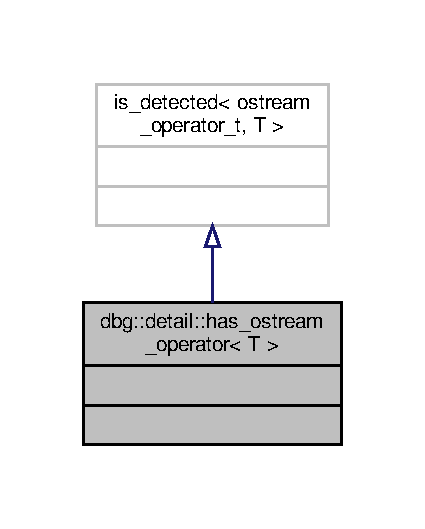
\includegraphics[width=204pt]{d3/d95/structdbg_1_1detail_1_1has__ostream__operator__inherit__graph}
\end{center}
\end{figure}


Collaboration diagram for dbg\+:\+:detail\+:\+:has\+\_\+ostream\+\_\+operator$<$ T $>$\+:\nopagebreak
\begin{figure}[H]
\begin{center}
\leavevmode
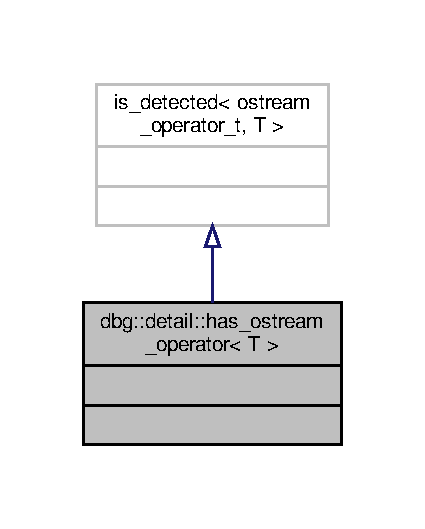
\includegraphics[width=204pt]{d1/de1/structdbg_1_1detail_1_1has__ostream__operator__coll__graph}
\end{center}
\end{figure}


The documentation for this struct was generated from the following file\+:\begin{DoxyCompactItemize}
\item 
\hyperlink{dbg_8h}{dbg.\+h}\end{DoxyCompactItemize}

\hypertarget{structInfo}{}\section{Info Struct Reference}
\label{structInfo}\index{Info@{Info}}


Collaboration diagram for Info\+:\nopagebreak
\begin{figure}[H]
\begin{center}
\leavevmode
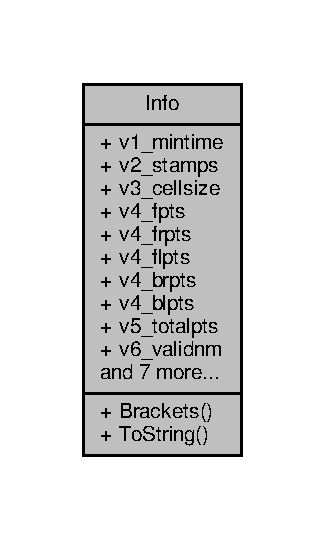
\includegraphics[width=156pt]{dc/d39/structInfo__coll__graph}
\end{center}
\end{figure}
\subsection*{Public Member Functions}
\begin{DoxyCompactItemize}
\item 
string \hyperlink{structInfo_a4f0c8708a9cd7b28ebb45b820d493807}{Brackets} (const vector$<$ int $>$ vi)
\item 
string \hyperlink{structInfo_a4f08e2630f96401302b19fd0367974cd}{To\+String} ()
\end{DoxyCompactItemize}
\subsection*{Public Attributes}
\begin{DoxyCompactItemize}
\item 
double \hyperlink{structInfo_a5ef016e8f6dae6e4e76b8908784b3a86}{v1\+\_\+mintime}
\item 
int \hyperlink{structInfo_aa64abd62ad85e8439a08dce95d966016}{v2\+\_\+stamps}
\item 
double \hyperlink{structInfo_a405b01f4335e99a04a75112cb65762e7}{v3\+\_\+cellsize}
\item 
vector$<$ int $>$ \hyperlink{structInfo_a0e526db15dbaf49f82c6b4898e67d771}{v4\+\_\+fpts}
\item 
vector$<$ int $>$ \hyperlink{structInfo_a6f6897c8b36a2cef20f348dc4288f5ce}{v4\+\_\+frpts}
\item 
vector$<$ int $>$ \hyperlink{structInfo_a4562ff86533d50b0abce1d007111040b}{v4\+\_\+flpts}
\item 
vector$<$ int $>$ \hyperlink{structInfo_a7b8fd964aebb52cf8569e30fc19ff4ec}{v4\+\_\+brpts}
\item 
vector$<$ int $>$ \hyperlink{structInfo_ab14116ddeedb6f25e87d23b26beee05c}{v4\+\_\+blpts}
\item 
int \hyperlink{structInfo_af58612e141498fcdffcebd62a80a9415}{v5\+\_\+totalpts}
\item 
int \hyperlink{structInfo_a00a940773f150d742999f3f57bfb3edd}{v6\+\_\+validnm}
\item 
int \hyperlink{structInfo_aa0500491d958efe7c5a2793b205e6f64}{v6\+\_\+invalidnm}
\item 
double \hyperlink{structInfo_a1ed4d11a76b55bbeee5ff08964a70c48}{v6\+\_\+radius}
\item 
vector$<$ int $>$ \hyperlink{structInfo_af0b8abdfd9f9cc34d38eea4f2482d87a}{v7\+\_\+cellpts}
\item 
vector$<$ int $>$ \hyperlink{structInfo_a98320e8f2b02e1ede82716776c01eeeb}{v8\+\_\+cellnms}
\item 
vector$<$ int $>$ \hyperlink{structInfo_a788cd85590e7824770a635228d3528d3}{v9\+\_\+cellgaus}
\item 
int \hyperlink{structInfo_a55e52fabfe4bfc7e4dd0f5ffc26f5f38}{v10\+\_\+totalvalidcells}
\item 
int \hyperlink{structInfo_a8f22dfe0a01d67f48cf29df01bcbbbc6}{v10\+\_\+totalinvalidcells}
\end{DoxyCompactItemize}


\subsection{Member Function Documentation}
\mbox{\Hypertarget{structInfo_a4f0c8708a9cd7b28ebb45b820d493807}\label{structInfo_a4f0c8708a9cd7b28ebb45b820d493807}} 
\index{Info@{Info}!Brackets@{Brackets}}
\index{Brackets@{Brackets}!Info@{Info}}
\subsubsection{\texorpdfstring{Brackets()}{Brackets()}}
{\footnotesize\ttfamily string Info\+::\+Brackets (\begin{DoxyParamCaption}\item[{const vector$<$ int $>$}]{vi }\end{DoxyParamCaption})\hspace{0.3cm}{\ttfamily [inline]}}

\mbox{\Hypertarget{structInfo_a4f08e2630f96401302b19fd0367974cd}\label{structInfo_a4f08e2630f96401302b19fd0367974cd}} 
\index{Info@{Info}!To\+String@{To\+String}}
\index{To\+String@{To\+String}!Info@{Info}}
\subsubsection{\texorpdfstring{To\+String()}{ToString()}}
{\footnotesize\ttfamily string Info\+::\+To\+String (\begin{DoxyParamCaption}{ }\end{DoxyParamCaption})\hspace{0.3cm}{\ttfamily [inline]}}



Referenced by main().



\subsection{Member Data Documentation}
\mbox{\Hypertarget{structInfo_a8f22dfe0a01d67f48cf29df01bcbbbc6}\label{structInfo_a8f22dfe0a01d67f48cf29df01bcbbbc6}} 
\index{Info@{Info}!v10\+\_\+totalinvalidcells@{v10\+\_\+totalinvalidcells}}
\index{v10\+\_\+totalinvalidcells@{v10\+\_\+totalinvalidcells}!Info@{Info}}
\subsubsection{\texorpdfstring{v10\+\_\+totalinvalidcells}{v10\_totalinvalidcells}}
{\footnotesize\ttfamily int Info\+::v10\+\_\+totalinvalidcells}



Referenced by Info\+Of\+N\+D\+T\+Map().

\mbox{\Hypertarget{structInfo_a55e52fabfe4bfc7e4dd0f5ffc26f5f38}\label{structInfo_a55e52fabfe4bfc7e4dd0f5ffc26f5f38}} 
\index{Info@{Info}!v10\+\_\+totalvalidcells@{v10\+\_\+totalvalidcells}}
\index{v10\+\_\+totalvalidcells@{v10\+\_\+totalvalidcells}!Info@{Info}}
\subsubsection{\texorpdfstring{v10\+\_\+totalvalidcells}{v10\_totalvalidcells}}
{\footnotesize\ttfamily int Info\+::v10\+\_\+totalvalidcells}



Referenced by Info\+Of\+N\+D\+T\+Map().

\mbox{\Hypertarget{structInfo_a5ef016e8f6dae6e4e76b8908784b3a86}\label{structInfo_a5ef016e8f6dae6e4e76b8908784b3a86}} 
\index{Info@{Info}!v1\+\_\+mintime@{v1\+\_\+mintime}}
\index{v1\+\_\+mintime@{v1\+\_\+mintime}!Info@{Info}}
\subsubsection{\texorpdfstring{v1\+\_\+mintime}{v1\_mintime}}
{\footnotesize\ttfamily double Info\+::v1\+\_\+mintime}



Referenced by Augment().

\mbox{\Hypertarget{structInfo_aa64abd62ad85e8439a08dce95d966016}\label{structInfo_aa64abd62ad85e8439a08dce95d966016}} 
\index{Info@{Info}!v2\+\_\+stamps@{v2\+\_\+stamps}}
\index{v2\+\_\+stamps@{v2\+\_\+stamps}!Info@{Info}}
\subsubsection{\texorpdfstring{v2\+\_\+stamps}{v2\_stamps}}
{\footnotesize\ttfamily int Info\+::v2\+\_\+stamps}



Referenced by Augment().

\mbox{\Hypertarget{structInfo_a405b01f4335e99a04a75112cb65762e7}\label{structInfo_a405b01f4335e99a04a75112cb65762e7}} 
\index{Info@{Info}!v3\+\_\+cellsize@{v3\+\_\+cellsize}}
\index{v3\+\_\+cellsize@{v3\+\_\+cellsize}!Info@{Info}}
\subsubsection{\texorpdfstring{v3\+\_\+cellsize}{v3\_cellsize}}
{\footnotesize\ttfamily double Info\+::v3\+\_\+cellsize}



Referenced by Info\+Of\+N\+D\+T\+Map().

\mbox{\Hypertarget{structInfo_ab14116ddeedb6f25e87d23b26beee05c}\label{structInfo_ab14116ddeedb6f25e87d23b26beee05c}} 
\index{Info@{Info}!v4\+\_\+blpts@{v4\+\_\+blpts}}
\index{v4\+\_\+blpts@{v4\+\_\+blpts}!Info@{Info}}
\subsubsection{\texorpdfstring{v4\+\_\+blpts}{v4\_blpts}}
{\footnotesize\ttfamily vector$<$int$>$ Info\+::v4\+\_\+blpts}



Referenced by Augment().

\mbox{\Hypertarget{structInfo_a7b8fd964aebb52cf8569e30fc19ff4ec}\label{structInfo_a7b8fd964aebb52cf8569e30fc19ff4ec}} 
\index{Info@{Info}!v4\+\_\+brpts@{v4\+\_\+brpts}}
\index{v4\+\_\+brpts@{v4\+\_\+brpts}!Info@{Info}}
\subsubsection{\texorpdfstring{v4\+\_\+brpts}{v4\_brpts}}
{\footnotesize\ttfamily vector$<$int$>$ Info\+::v4\+\_\+brpts}



Referenced by Augment().

\mbox{\Hypertarget{structInfo_a4562ff86533d50b0abce1d007111040b}\label{structInfo_a4562ff86533d50b0abce1d007111040b}} 
\index{Info@{Info}!v4\+\_\+flpts@{v4\+\_\+flpts}}
\index{v4\+\_\+flpts@{v4\+\_\+flpts}!Info@{Info}}
\subsubsection{\texorpdfstring{v4\+\_\+flpts}{v4\_flpts}}
{\footnotesize\ttfamily vector$<$int$>$ Info\+::v4\+\_\+flpts}



Referenced by Augment().

\mbox{\Hypertarget{structInfo_a0e526db15dbaf49f82c6b4898e67d771}\label{structInfo_a0e526db15dbaf49f82c6b4898e67d771}} 
\index{Info@{Info}!v4\+\_\+fpts@{v4\+\_\+fpts}}
\index{v4\+\_\+fpts@{v4\+\_\+fpts}!Info@{Info}}
\subsubsection{\texorpdfstring{v4\+\_\+fpts}{v4\_fpts}}
{\footnotesize\ttfamily vector$<$int$>$ Info\+::v4\+\_\+fpts}



Referenced by Augment().

\mbox{\Hypertarget{structInfo_a6f6897c8b36a2cef20f348dc4288f5ce}\label{structInfo_a6f6897c8b36a2cef20f348dc4288f5ce}} 
\index{Info@{Info}!v4\+\_\+frpts@{v4\+\_\+frpts}}
\index{v4\+\_\+frpts@{v4\+\_\+frpts}!Info@{Info}}
\subsubsection{\texorpdfstring{v4\+\_\+frpts}{v4\_frpts}}
{\footnotesize\ttfamily vector$<$int$>$ Info\+::v4\+\_\+frpts}



Referenced by Augment().

\mbox{\Hypertarget{structInfo_af58612e141498fcdffcebd62a80a9415}\label{structInfo_af58612e141498fcdffcebd62a80a9415}} 
\index{Info@{Info}!v5\+\_\+totalpts@{v5\+\_\+totalpts}}
\index{v5\+\_\+totalpts@{v5\+\_\+totalpts}!Info@{Info}}
\subsubsection{\texorpdfstring{v5\+\_\+totalpts}{v5\_totalpts}}
{\footnotesize\ttfamily int Info\+::v5\+\_\+totalpts}



Referenced by Augment().

\mbox{\Hypertarget{structInfo_aa0500491d958efe7c5a2793b205e6f64}\label{structInfo_aa0500491d958efe7c5a2793b205e6f64}} 
\index{Info@{Info}!v6\+\_\+invalidnm@{v6\+\_\+invalidnm}}
\index{v6\+\_\+invalidnm@{v6\+\_\+invalidnm}!Info@{Info}}
\subsubsection{\texorpdfstring{v6\+\_\+invalidnm}{v6\_invalidnm}}
{\footnotesize\ttfamily int Info\+::v6\+\_\+invalidnm}



Referenced by Info\+Of\+N\+D\+T\+Map().

\mbox{\Hypertarget{structInfo_a1ed4d11a76b55bbeee5ff08964a70c48}\label{structInfo_a1ed4d11a76b55bbeee5ff08964a70c48}} 
\index{Info@{Info}!v6\+\_\+radius@{v6\+\_\+radius}}
\index{v6\+\_\+radius@{v6\+\_\+radius}!Info@{Info}}
\subsubsection{\texorpdfstring{v6\+\_\+radius}{v6\_radius}}
{\footnotesize\ttfamily double Info\+::v6\+\_\+radius}



Referenced by Info\+Of\+N\+D\+T\+Map().

\mbox{\Hypertarget{structInfo_a00a940773f150d742999f3f57bfb3edd}\label{structInfo_a00a940773f150d742999f3f57bfb3edd}} 
\index{Info@{Info}!v6\+\_\+validnm@{v6\+\_\+validnm}}
\index{v6\+\_\+validnm@{v6\+\_\+validnm}!Info@{Info}}
\subsubsection{\texorpdfstring{v6\+\_\+validnm}{v6\_validnm}}
{\footnotesize\ttfamily int Info\+::v6\+\_\+validnm}



Referenced by Info\+Of\+N\+D\+T\+Map().

\mbox{\Hypertarget{structInfo_af0b8abdfd9f9cc34d38eea4f2482d87a}\label{structInfo_af0b8abdfd9f9cc34d38eea4f2482d87a}} 
\index{Info@{Info}!v7\+\_\+cellpts@{v7\+\_\+cellpts}}
\index{v7\+\_\+cellpts@{v7\+\_\+cellpts}!Info@{Info}}
\subsubsection{\texorpdfstring{v7\+\_\+cellpts}{v7\_cellpts}}
{\footnotesize\ttfamily vector$<$int$>$ Info\+::v7\+\_\+cellpts}



Referenced by Info\+Of\+N\+D\+T\+Map().

\mbox{\Hypertarget{structInfo_a98320e8f2b02e1ede82716776c01eeeb}\label{structInfo_a98320e8f2b02e1ede82716776c01eeeb}} 
\index{Info@{Info}!v8\+\_\+cellnms@{v8\+\_\+cellnms}}
\index{v8\+\_\+cellnms@{v8\+\_\+cellnms}!Info@{Info}}
\subsubsection{\texorpdfstring{v8\+\_\+cellnms}{v8\_cellnms}}
{\footnotesize\ttfamily vector$<$int$>$ Info\+::v8\+\_\+cellnms}



Referenced by Info\+Of\+N\+D\+T\+Map().

\mbox{\Hypertarget{structInfo_a788cd85590e7824770a635228d3528d3}\label{structInfo_a788cd85590e7824770a635228d3528d3}} 
\index{Info@{Info}!v9\+\_\+cellgaus@{v9\+\_\+cellgaus}}
\index{v9\+\_\+cellgaus@{v9\+\_\+cellgaus}!Info@{Info}}
\subsubsection{\texorpdfstring{v9\+\_\+cellgaus}{v9\_cellgaus}}
{\footnotesize\ttfamily vector$<$int$>$ Info\+::v9\+\_\+cellgaus}



Referenced by Info\+Of\+N\+D\+T\+Map().



The documentation for this struct was generated from the following file\+:\begin{DoxyCompactItemize}
\item 
\hyperlink{sndt__exec_2src_2test__0dis_8cc}{sndt\+\_\+exec/src/test\+\_\+0dis.\+cc}\end{DoxyCompactItemize}

\hypertarget{structstd_1_1integral__constant}{}\section{std\+:\+:integral\+\_\+constant$<$ T, v $>$ Struct Template Reference}
\label{structstd_1_1integral__constant}\index{std\+::integral\+\_\+constant$<$ T, v $>$@{std\+::integral\+\_\+constant$<$ T, v $>$}}


{\ttfamily \#include $<$mathcompat.\+h$>$}



Inheritance diagram for std\+:\+:integral\+\_\+constant$<$ T, v $>$\+:\nopagebreak
\begin{figure}[H]
\begin{center}
\leavevmode
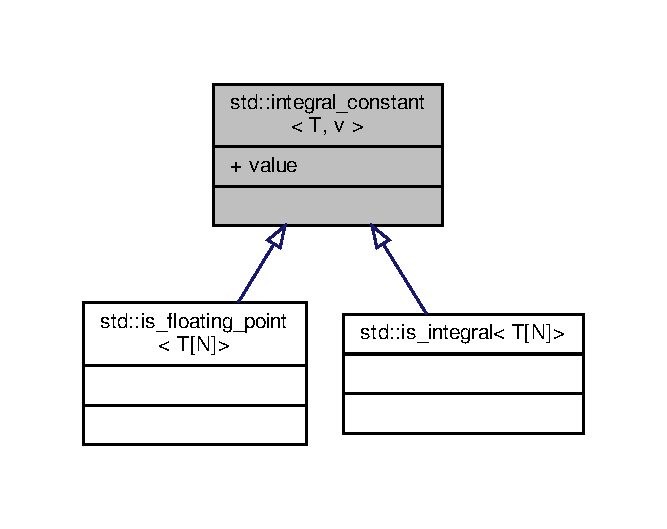
\includegraphics[width=320pt]{dd/dd3/structstd_1_1integral__constant__inherit__graph}
\end{center}
\end{figure}


Collaboration diagram for std\+:\+:integral\+\_\+constant$<$ T, v $>$\+:\nopagebreak
\begin{figure}[H]
\begin{center}
\leavevmode
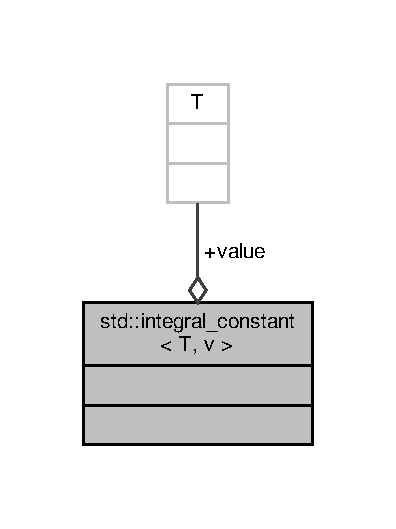
\includegraphics[width=190pt]{df/d33/structstd_1_1integral__constant__coll__graph}
\end{center}
\end{figure}
\subsection*{Static Public Attributes}
\begin{DoxyCompactItemize}
\item 
static const T \hyperlink{structstd_1_1integral__constant_a6d745e58651b7700822f0fcd66e9dcfa}{value} = v
\end{DoxyCompactItemize}


\subsection{Member Data Documentation}
\mbox{\Hypertarget{structstd_1_1integral__constant_a6d745e58651b7700822f0fcd66e9dcfa}\label{structstd_1_1integral__constant_a6d745e58651b7700822f0fcd66e9dcfa}} 
\index{std\+::integral\+\_\+constant@{std\+::integral\+\_\+constant}!value@{value}}
\index{value@{value}!std\+::integral\+\_\+constant@{std\+::integral\+\_\+constant}}
\subsubsection{\texorpdfstring{value}{value}}
{\footnotesize\ttfamily template$<$class T, T v$>$ \\
const T \hyperlink{structstd_1_1integral__constant}{std\+::integral\+\_\+constant}$<$ T, v $>$\+::value = v\hspace{0.3cm}{\ttfamily [static]}}



The documentation for this struct was generated from the following file\+:\begin{DoxyCompactItemize}
\item 
\hyperlink{mathcompat_8h}{mathcompat.\+h}\end{DoxyCompactItemize}

\hypertarget{structstd_1_1is__arithmetic}{}\section{std\+:\+:is\+\_\+arithmetic$<$ T $>$ Struct Template Reference}
\label{structstd_1_1is__arithmetic}\index{std\+::is\+\_\+arithmetic$<$ T $>$@{std\+::is\+\_\+arithmetic$<$ T $>$}}


{\ttfamily \#include $<$mathcompat.\+h$>$}



Inheritance diagram for std\+:\+:is\+\_\+arithmetic$<$ T $>$\+:\nopagebreak
\begin{figure}[H]
\begin{center}
\leavevmode
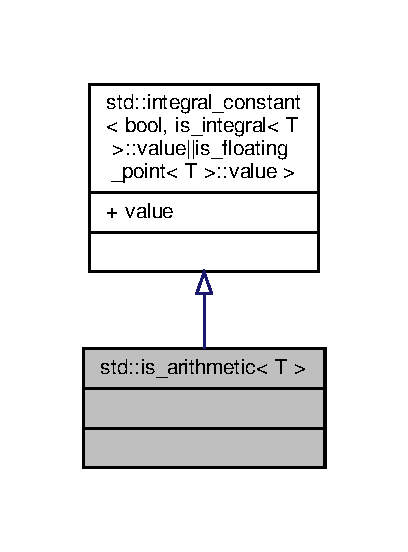
\includegraphics[width=196pt]{d7/d14/structstd_1_1is__arithmetic__inherit__graph}
\end{center}
\end{figure}


Collaboration diagram for std\+:\+:is\+\_\+arithmetic$<$ T $>$\+:\nopagebreak
\begin{figure}[H]
\begin{center}
\leavevmode
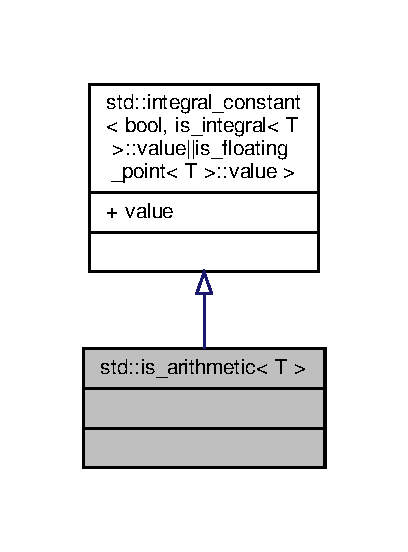
\includegraphics[width=196pt]{d1/dd2/structstd_1_1is__arithmetic__coll__graph}
\end{center}
\end{figure}
\subsection*{Additional Inherited Members}


The documentation for this struct was generated from the following file\+:\begin{DoxyCompactItemize}
\item 
\hyperlink{mathcompat_8h}{mathcompat.\+h}\end{DoxyCompactItemize}

\hypertarget{structdbg_1_1detail_1_1is__container}{}\section{dbg\+:\+:detail\+:\+:is\+\_\+container$<$ T $>$ Struct Template Reference}
\label{structdbg_1_1detail_1_1is__container}\index{dbg\+::detail\+::is\+\_\+container$<$ T $>$@{dbg\+::detail\+::is\+\_\+container$<$ T $>$}}


{\ttfamily \#include $<$dbg.\+h$>$}



Collaboration diagram for dbg\+:\+:detail\+:\+:is\+\_\+container$<$ T $>$\+:\nopagebreak
\begin{figure}[H]
\begin{center}
\leavevmode
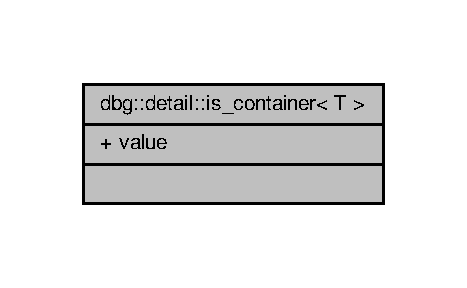
\includegraphics[width=224pt]{d3/d97/structdbg_1_1detail_1_1is__container__coll__graph}
\end{center}
\end{figure}
\subsection*{Static Public Attributes}
\begin{DoxyCompactItemize}
\item 
static constexpr bool \hyperlink{structdbg_1_1detail_1_1is__container_aa9a4594488352384b65b36198ac414f8}{value}
\end{DoxyCompactItemize}


\subsection{Member Data Documentation}
\mbox{\Hypertarget{structdbg_1_1detail_1_1is__container_aa9a4594488352384b65b36198ac414f8}\label{structdbg_1_1detail_1_1is__container_aa9a4594488352384b65b36198ac414f8}} 
\index{dbg\+::detail\+::is\+\_\+container@{dbg\+::detail\+::is\+\_\+container}!value@{value}}
\index{value@{value}!dbg\+::detail\+::is\+\_\+container@{dbg\+::detail\+::is\+\_\+container}}
\subsubsection{\texorpdfstring{value}{value}}
{\footnotesize\ttfamily template$<$typename T $>$ \\
constexpr bool \hyperlink{structdbg_1_1detail_1_1is__container}{dbg\+::detail\+::is\+\_\+container}$<$ T $>$\+::value\hspace{0.3cm}{\ttfamily [static]}}

{\bfseries Initial value\+:}
\begin{DoxyCode}
=
      \hyperlink{namespacetrimesh_ab10cc1052c9d1d1376d92211b6ca27dd}{is\_detected<detect\_begin\_t, T>::value} &&
      \hyperlink{namespacetrimesh_ab10cc1052c9d1d1376d92211b6ca27dd}{is\_detected<detect\_end\_t, T>::value} &&
      \hyperlink{namespacetrimesh_ab10cc1052c9d1d1376d92211b6ca27dd}{is\_detected<detect\_size\_t, T>::value} &&
      !std::is\_same<\hyperlink{namespacetrimesh_a51b4a31323874089623d4b17afabc1aa}{std::string},
                    \textcolor{keyword}{typename} std::remove\_cv<
                        \textcolor{keyword}{typename} \hyperlink{namespacetrimesh_aa726c5bf9cff74a26269e8d258ae9e3d}{std::remove\_reference<T>::type}>
      \hyperlink{namespacedbg_a2365d80e3a3525e6025040383ff8661b}{::type}>\hyperlink{structdbg_1_1detail_1_1is__container_aa9a4594488352384b65b36198ac414f8}{::value}
\end{DoxyCode}


The documentation for this struct was generated from the following file\+:\begin{DoxyCompactItemize}
\item 
\hyperlink{dbg_8h}{dbg.\+h}\end{DoxyCompactItemize}

\hypertarget{structstd_1_1is__floating__point}{}\section{std\+:\+:is\+\_\+floating\+\_\+point$<$ T $>$ Struct Template Reference}
\label{structstd_1_1is__floating__point}\index{std\+::is\+\_\+floating\+\_\+point$<$ T $>$@{std\+::is\+\_\+floating\+\_\+point$<$ T $>$}}


{\ttfamily \#include $<$mathcompat.\+h$>$}



Inheritance diagram for std\+:\+:is\+\_\+floating\+\_\+point$<$ T $>$\+:\nopagebreak
\begin{figure}[H]
\begin{center}
\leavevmode
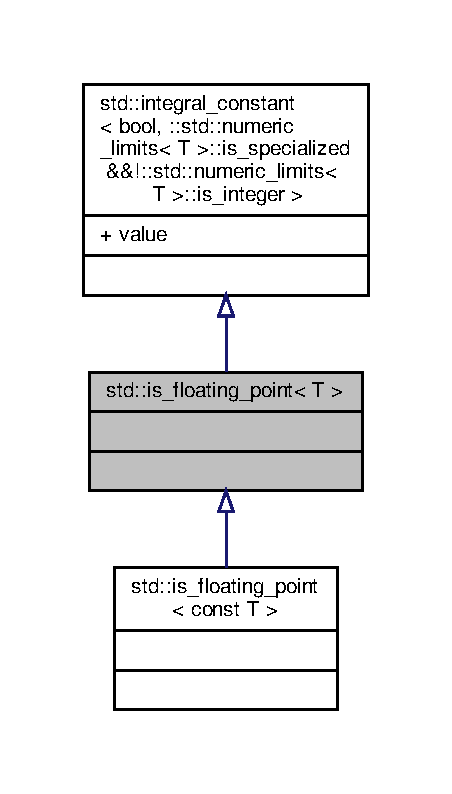
\includegraphics[width=217pt]{db/d25/structstd_1_1is__floating__point__inherit__graph}
\end{center}
\end{figure}


Collaboration diagram for std\+:\+:is\+\_\+floating\+\_\+point$<$ T $>$\+:\nopagebreak
\begin{figure}[H]
\begin{center}
\leavevmode
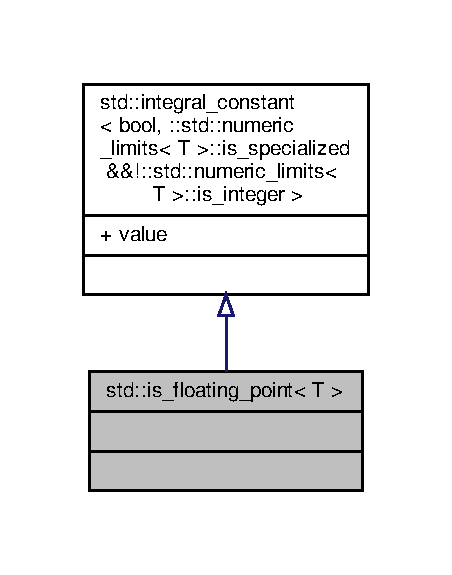
\includegraphics[width=217pt]{de/df6/structstd_1_1is__floating__point__coll__graph}
\end{center}
\end{figure}
\subsection*{Additional Inherited Members}


The documentation for this struct was generated from the following file\+:\begin{DoxyCompactItemize}
\item 
\hyperlink{mathcompat_8h}{mathcompat.\+h}\end{DoxyCompactItemize}

\hypertarget{structstd_1_1is__floating__point_3_01const_01T_01_4}{}\section{std\+:\+:is\+\_\+floating\+\_\+point$<$ const T $>$ Struct Template Reference}
\label{structstd_1_1is__floating__point_3_01const_01T_01_4}\index{std\+::is\+\_\+floating\+\_\+point$<$ const T $>$@{std\+::is\+\_\+floating\+\_\+point$<$ const T $>$}}


{\ttfamily \#include $<$mathcompat.\+h$>$}



Inheritance diagram for std\+:\+:is\+\_\+floating\+\_\+point$<$ const T $>$\+:\nopagebreak
\begin{figure}[H]
\begin{center}
\leavevmode
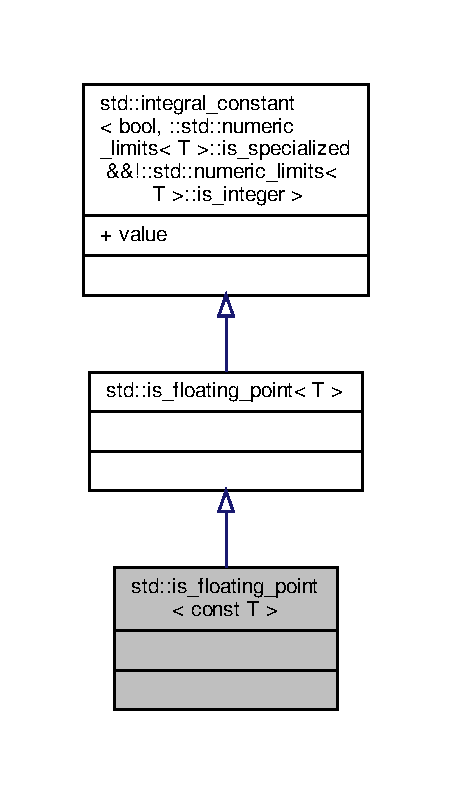
\includegraphics[width=217pt]{de/d2a/structstd_1_1is__floating__point_3_01const_01T_01_4__inherit__graph}
\end{center}
\end{figure}


Collaboration diagram for std\+:\+:is\+\_\+floating\+\_\+point$<$ const T $>$\+:\nopagebreak
\begin{figure}[H]
\begin{center}
\leavevmode
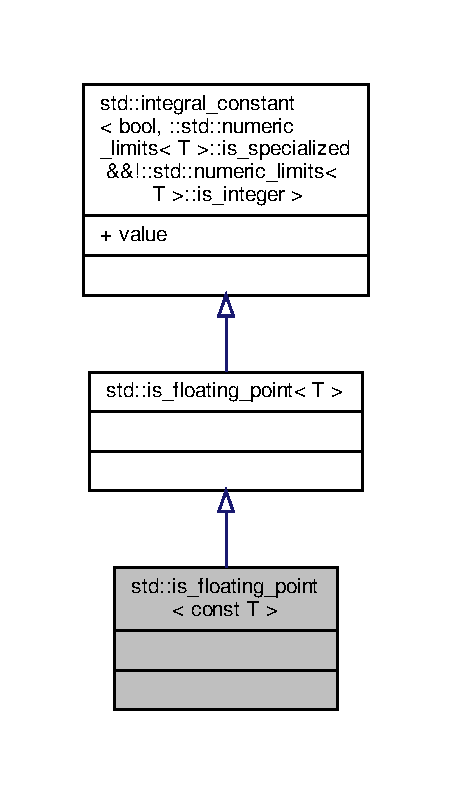
\includegraphics[width=217pt]{d7/d74/structstd_1_1is__floating__point_3_01const_01T_01_4__coll__graph}
\end{center}
\end{figure}
\subsection*{Additional Inherited Members}


The documentation for this struct was generated from the following file\+:\begin{DoxyCompactItemize}
\item 
\hyperlink{mathcompat_8h}{mathcompat.\+h}\end{DoxyCompactItemize}

\hypertarget{structstd_1_1is__floating__point_3_01T[N]_4}{}\section{std\+:\+:is\+\_\+floating\+\_\+point$<$ T\mbox{[}N\mbox{]}$>$ Struct Template Reference}
\label{structstd_1_1is__floating__point_3_01T[N]_4}\index{std\+::is\+\_\+floating\+\_\+point$<$ T\mbox{[}N\mbox{]}$>$@{std\+::is\+\_\+floating\+\_\+point$<$ T[N]$>$}}


{\ttfamily \#include $<$mathcompat.\+h$>$}



Inheritance diagram for std\+:\+:is\+\_\+floating\+\_\+point$<$ T\mbox{[}N\mbox{]}$>$\+:\nopagebreak
\begin{figure}[H]
\begin{center}
\leavevmode
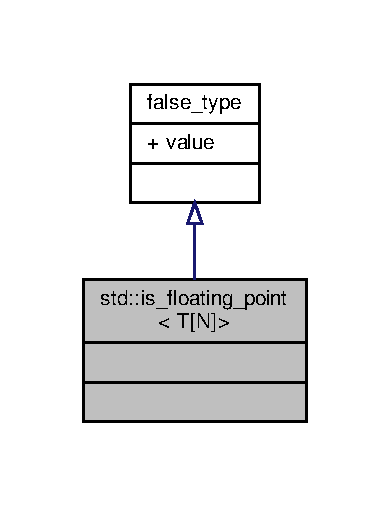
\includegraphics[width=187pt]{da/dec/structstd_1_1is__floating__point_3_01T[N]_4__inherit__graph}
\end{center}
\end{figure}


Collaboration diagram for std\+:\+:is\+\_\+floating\+\_\+point$<$ T\mbox{[}N\mbox{]}$>$\+:\nopagebreak
\begin{figure}[H]
\begin{center}
\leavevmode
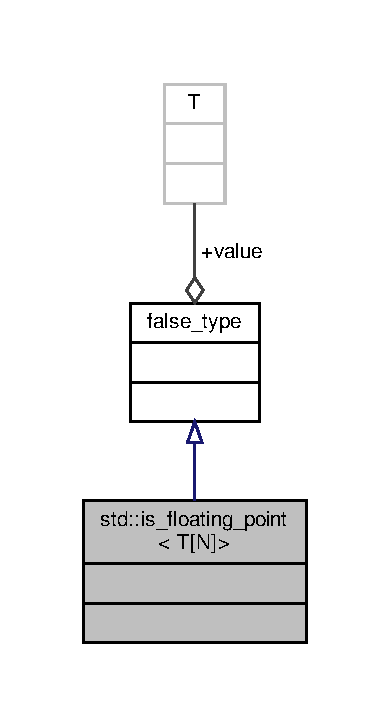
\includegraphics[width=187pt]{d8/d8c/structstd_1_1is__floating__point_3_01T[N]_4__coll__graph}
\end{center}
\end{figure}
\subsection*{Additional Inherited Members}


The documentation for this struct was generated from the following file\+:\begin{DoxyCompactItemize}
\item 
\hyperlink{mathcompat_8h}{mathcompat.\+h}\end{DoxyCompactItemize}

\hypertarget{structstd_1_1is__integral}{}\section{std\+:\+:is\+\_\+integral$<$ T $>$ Struct Template Reference}
\label{structstd_1_1is__integral}\index{std\+::is\+\_\+integral$<$ T $>$@{std\+::is\+\_\+integral$<$ T $>$}}


{\ttfamily \#include $<$mathcompat.\+h$>$}



Inheritance diagram for std\+:\+:is\+\_\+integral$<$ T $>$\+:\nopagebreak
\begin{figure}[H]
\begin{center}
\leavevmode
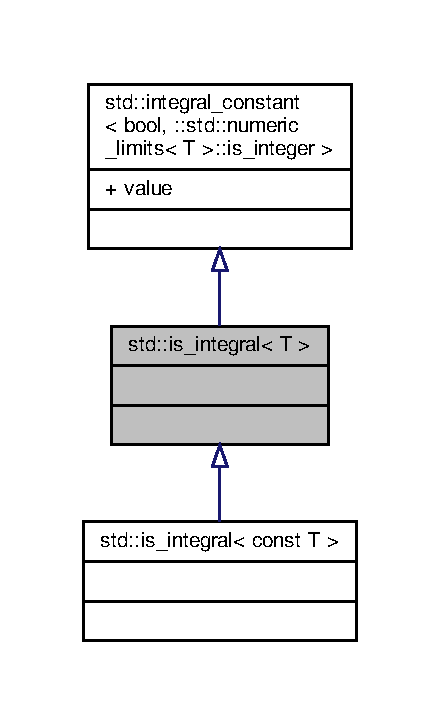
\includegraphics[width=211pt]{d6/def/structstd_1_1is__integral__inherit__graph}
\end{center}
\end{figure}


Collaboration diagram for std\+:\+:is\+\_\+integral$<$ T $>$\+:\nopagebreak
\begin{figure}[H]
\begin{center}
\leavevmode
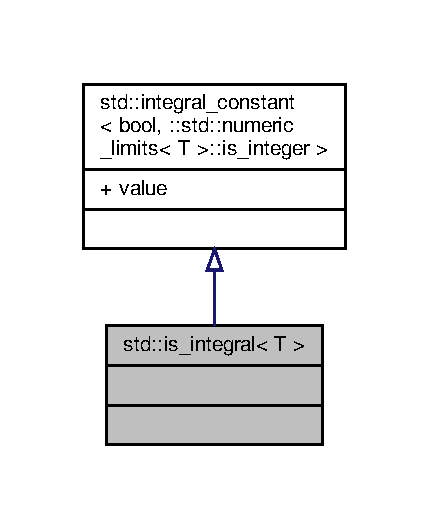
\includegraphics[width=206pt]{d0/d6b/structstd_1_1is__integral__coll__graph}
\end{center}
\end{figure}
\subsection*{Additional Inherited Members}


The documentation for this struct was generated from the following file\+:\begin{DoxyCompactItemize}
\item 
\hyperlink{mathcompat_8h}{mathcompat.\+h}\end{DoxyCompactItemize}

\hypertarget{structstd_1_1is__integral_3_01const_01T_01_4}{}\section{std\+:\+:is\+\_\+integral$<$ const T $>$ Struct Template Reference}
\label{structstd_1_1is__integral_3_01const_01T_01_4}\index{std\+::is\+\_\+integral$<$ const T $>$@{std\+::is\+\_\+integral$<$ const T $>$}}


{\ttfamily \#include $<$mathcompat.\+h$>$}



Inheritance diagram for std\+:\+:is\+\_\+integral$<$ const T $>$\+:\nopagebreak
\begin{figure}[H]
\begin{center}
\leavevmode
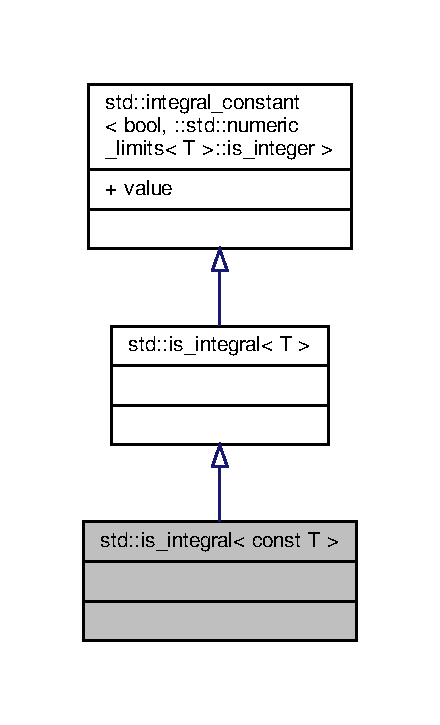
\includegraphics[width=211pt]{df/d68/structstd_1_1is__integral_3_01const_01T_01_4__inherit__graph}
\end{center}
\end{figure}


Collaboration diagram for std\+:\+:is\+\_\+integral$<$ const T $>$\+:\nopagebreak
\begin{figure}[H]
\begin{center}
\leavevmode
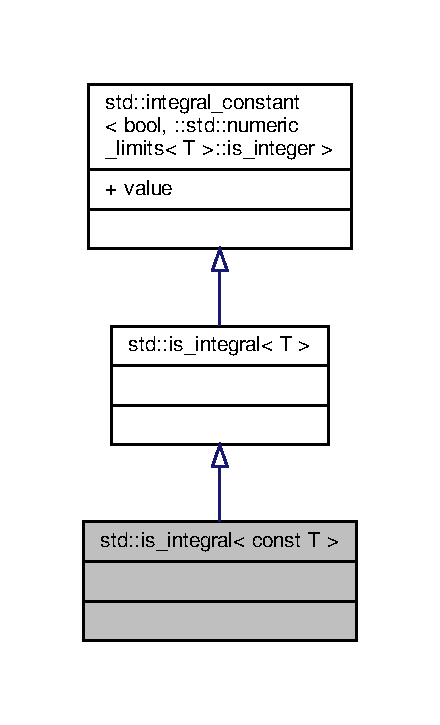
\includegraphics[width=211pt]{dd/d57/structstd_1_1is__integral_3_01const_01T_01_4__coll__graph}
\end{center}
\end{figure}
\subsection*{Additional Inherited Members}


The documentation for this struct was generated from the following file\+:\begin{DoxyCompactItemize}
\item 
\hyperlink{mathcompat_8h}{mathcompat.\+h}\end{DoxyCompactItemize}

\hypertarget{structstd_1_1is__integral_3_01T[N]_4}{}\section{std\+:\+:is\+\_\+integral$<$ T\mbox{[}N\mbox{]}$>$ Struct Template Reference}
\label{structstd_1_1is__integral_3_01T[N]_4}\index{std\+::is\+\_\+integral$<$ T\mbox{[}N\mbox{]}$>$@{std\+::is\+\_\+integral$<$ T[N]$>$}}


{\ttfamily \#include $<$mathcompat.\+h$>$}



Inheritance diagram for std\+:\+:is\+\_\+integral$<$ T\mbox{[}N\mbox{]}$>$\+:\nopagebreak
\begin{figure}[H]
\begin{center}
\leavevmode
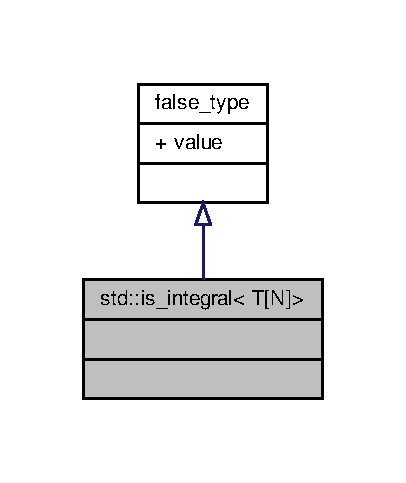
\includegraphics[width=195pt]{d3/d78/structstd_1_1is__integral_3_01T[N]_4__inherit__graph}
\end{center}
\end{figure}


Collaboration diagram for std\+:\+:is\+\_\+integral$<$ T\mbox{[}N\mbox{]}$>$\+:\nopagebreak
\begin{figure}[H]
\begin{center}
\leavevmode
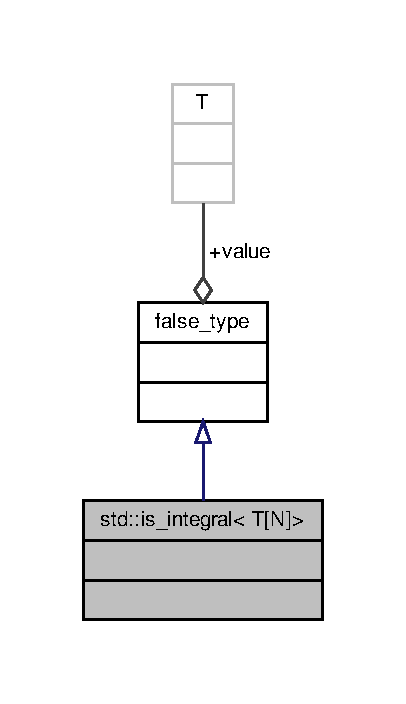
\includegraphics[width=195pt]{de/da4/structstd_1_1is__integral_3_01T[N]_4__coll__graph}
\end{center}
\end{figure}
\subsection*{Additional Inherited Members}


The documentation for this struct was generated from the following file\+:\begin{DoxyCompactItemize}
\item 
\hyperlink{mathcompat_8h}{mathcompat.\+h}\end{DoxyCompactItemize}

\hypertarget{classtrimesh_1_1KDtree}{}\section{trimesh\+:\+:K\+Dtree Class Reference}
\label{classtrimesh_1_1KDtree}\index{trimesh\+::\+K\+Dtree@{trimesh\+::\+K\+Dtree}}


{\ttfamily \#include $<$K\+Dtree.\+h$>$}



Collaboration diagram for trimesh\+:\+:K\+Dtree\+:\nopagebreak
\begin{figure}[H]
\begin{center}
\leavevmode
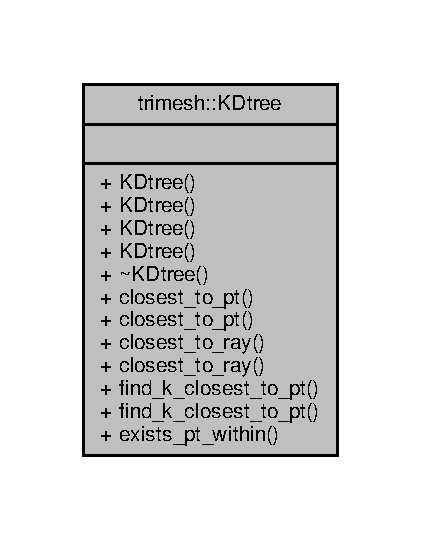
\includegraphics[width=202pt]{db/d0c/classtrimesh_1_1KDtree__coll__graph}
\end{center}
\end{figure}
\subsection*{Classes}
\begin{DoxyCompactItemize}
\item 
struct \hyperlink{structtrimesh_1_1KDtree_1_1CompatFunc}{Compat\+Func}
\item 
struct \hyperlink{structtrimesh_1_1KDtree_1_1Node}{Node}
\item 
struct \hyperlink{structtrimesh_1_1KDtree_1_1NodeStorageBlock}{Node\+Storage\+Block}
\end{DoxyCompactItemize}
\subsection*{Public Member Functions}
\begin{DoxyCompactItemize}
\item 
\hyperlink{classtrimesh_1_1KDtree_a7981d4d8eabd12d52c2887cfa94f4c33}{K\+Dtree} (const float $\ast$ptlist, size\+\_\+t n)
\item 
{\footnotesize template$<$class T $>$ }\\\hyperlink{classtrimesh_1_1KDtree_ab766871a5877b9488e90b9651a0c2b2c}{K\+Dtree} (const \+::std\+::vector$<$ T $>$ \&v)
\item 
\hyperlink{classtrimesh_1_1KDtree_acd7beb7544e1de886ffab14750075aab}{K\+Dtree} (const float $\ast$$\ast$pts, size\+\_\+t n)
\item 
{\footnotesize template$<$class T $>$ }\\\hyperlink{classtrimesh_1_1KDtree_a36b9522141b8c5f2c6bb17d58a469b10}{K\+Dtree} (\+::std\+::vector$<$ T $\ast$$>$ \&pts)
\item 
\hyperlink{classtrimesh_1_1KDtree_acf920211054016e32477fdbd19c5b22c}{$\sim$\+K\+Dtree} ()
\item 
const float $\ast$ \hyperlink{classtrimesh_1_1KDtree_a9428ce5432d045f9e3e33c381de413b2}{closest\+\_\+to\+\_\+pt} (const float $\ast$p, float maxdist2=0.\+0f, const Compat\+Func $\ast$iscompat=\+N\+U\+L\+L, float approx\+\_\+eps=0.\+0f) const
\item 
const float $\ast$ \hyperlink{classtrimesh_1_1KDtree_a90066965f638191f3bb2edab8d70ab3a}{closest\+\_\+to\+\_\+pt} (const float $\ast$p, float maxdist2, float approx\+\_\+eps) const
\item 
const float $\ast$ \hyperlink{classtrimesh_1_1KDtree_a3e3cc3eff36b04c01c065fcee1364922}{closest\+\_\+to\+\_\+ray} (const float $\ast$p, const float $\ast$dir, float maxdist2=0.\+0f, const Compat\+Func $\ast$iscompat=\+N\+U\+L\+L, float approx\+\_\+eps=0.\+0f) const
\item 
const float $\ast$ \hyperlink{classtrimesh_1_1KDtree_a686507f137048b734f4cc35700461701}{closest\+\_\+to\+\_\+ray} (const float $\ast$p, const float $\ast$dir, float maxdist2, float approx\+\_\+eps) const
\item 
\hyperlink{namespacetrimesh_a784ddfd979e1c579bda795a8edfc3f43}{void} \hyperlink{classtrimesh_1_1KDtree_a2b509a64df2781b18abac13a8683241d}{find\+\_\+k\+\_\+closest\+\_\+to\+\_\+pt} (\+::std\+::vector$<$ const float $\ast$$>$ \&knn, int k, const float $\ast$p, float maxdist2=0.\+0f, const Compat\+Func $\ast$iscompat=\+N\+U\+L\+L, float approx\+\_\+eps=0.\+0f) const
\item 
\hyperlink{namespacetrimesh_a784ddfd979e1c579bda795a8edfc3f43}{void} \hyperlink{classtrimesh_1_1KDtree_a1466c3d0b144459fb4472ea05f6d70bc}{find\+\_\+k\+\_\+closest\+\_\+to\+\_\+pt} (\+::std\+::vector$<$ const float $\ast$$>$ \&knn, int k, const float $\ast$p, float maxdist2, float approx\+\_\+eps) const
\item 
bool \hyperlink{classtrimesh_1_1KDtree_ad8e2126c11fce117f6fa699301348173}{exists\+\_\+pt\+\_\+within} (const float $\ast$p, float maxdist) const
\end{DoxyCompactItemize}


\subsection{Constructor \& Destructor Documentation}
\mbox{\Hypertarget{classtrimesh_1_1KDtree_a7981d4d8eabd12d52c2887cfa94f4c33}\label{classtrimesh_1_1KDtree_a7981d4d8eabd12d52c2887cfa94f4c33}} 
\index{trimesh\+::\+K\+Dtree@{trimesh\+::\+K\+Dtree}!K\+Dtree@{K\+Dtree}}
\index{K\+Dtree@{K\+Dtree}!trimesh\+::\+K\+Dtree@{trimesh\+::\+K\+Dtree}}
\subsubsection{\texorpdfstring{K\+Dtree()}{KDtree()}\hspace{0.1cm}{\footnotesize\ttfamily [1/4]}}
{\footnotesize\ttfamily trimesh\+::\+K\+Dtree\+::\+K\+Dtree (\begin{DoxyParamCaption}\item[{const float $\ast$}]{ptlist,  }\item[{size\+\_\+t}]{n }\end{DoxyParamCaption})\hspace{0.3cm}{\ttfamily [inline]}}

\mbox{\Hypertarget{classtrimesh_1_1KDtree_ab766871a5877b9488e90b9651a0c2b2c}\label{classtrimesh_1_1KDtree_ab766871a5877b9488e90b9651a0c2b2c}} 
\index{trimesh\+::\+K\+Dtree@{trimesh\+::\+K\+Dtree}!K\+Dtree@{K\+Dtree}}
\index{K\+Dtree@{K\+Dtree}!trimesh\+::\+K\+Dtree@{trimesh\+::\+K\+Dtree}}
\subsubsection{\texorpdfstring{K\+Dtree()}{KDtree()}\hspace{0.1cm}{\footnotesize\ttfamily [2/4]}}
{\footnotesize\ttfamily template$<$class T $>$ \\
trimesh\+::\+K\+Dtree\+::\+K\+Dtree (\begin{DoxyParamCaption}\item[{const \+::std\+::vector$<$ T $>$ \&}]{v }\end{DoxyParamCaption})\hspace{0.3cm}{\ttfamily [inline]}}

\mbox{\Hypertarget{classtrimesh_1_1KDtree_acd7beb7544e1de886ffab14750075aab}\label{classtrimesh_1_1KDtree_acd7beb7544e1de886ffab14750075aab}} 
\index{trimesh\+::\+K\+Dtree@{trimesh\+::\+K\+Dtree}!K\+Dtree@{K\+Dtree}}
\index{K\+Dtree@{K\+Dtree}!trimesh\+::\+K\+Dtree@{trimesh\+::\+K\+Dtree}}
\subsubsection{\texorpdfstring{K\+Dtree()}{KDtree()}\hspace{0.1cm}{\footnotesize\ttfamily [3/4]}}
{\footnotesize\ttfamily trimesh\+::\+K\+Dtree\+::\+K\+Dtree (\begin{DoxyParamCaption}\item[{const float $\ast$$\ast$}]{pts,  }\item[{size\+\_\+t}]{n }\end{DoxyParamCaption})\hspace{0.3cm}{\ttfamily [inline]}}

\mbox{\Hypertarget{classtrimesh_1_1KDtree_a36b9522141b8c5f2c6bb17d58a469b10}\label{classtrimesh_1_1KDtree_a36b9522141b8c5f2c6bb17d58a469b10}} 
\index{trimesh\+::\+K\+Dtree@{trimesh\+::\+K\+Dtree}!K\+Dtree@{K\+Dtree}}
\index{K\+Dtree@{K\+Dtree}!trimesh\+::\+K\+Dtree@{trimesh\+::\+K\+Dtree}}
\subsubsection{\texorpdfstring{K\+Dtree()}{KDtree()}\hspace{0.1cm}{\footnotesize\ttfamily [4/4]}}
{\footnotesize\ttfamily template$<$class T $>$ \\
trimesh\+::\+K\+Dtree\+::\+K\+Dtree (\begin{DoxyParamCaption}\item[{\+::std\+::vector$<$ T $\ast$$>$ \&}]{pts }\end{DoxyParamCaption})\hspace{0.3cm}{\ttfamily [inline]}}

\mbox{\Hypertarget{classtrimesh_1_1KDtree_acf920211054016e32477fdbd19c5b22c}\label{classtrimesh_1_1KDtree_acf920211054016e32477fdbd19c5b22c}} 
\index{trimesh\+::\+K\+Dtree@{trimesh\+::\+K\+Dtree}!````~K\+Dtree@{$\sim$\+K\+Dtree}}
\index{````~K\+Dtree@{$\sim$\+K\+Dtree}!trimesh\+::\+K\+Dtree@{trimesh\+::\+K\+Dtree}}
\subsubsection{\texorpdfstring{$\sim$\+K\+Dtree()}{~KDtree()}}
{\footnotesize\ttfamily trimesh\+::\+K\+Dtree\+::$\sim$\+K\+Dtree (\begin{DoxyParamCaption}{ }\end{DoxyParamCaption})}



Referenced by K\+Dtree().



\subsection{Member Function Documentation}
\mbox{\Hypertarget{classtrimesh_1_1KDtree_a9428ce5432d045f9e3e33c381de413b2}\label{classtrimesh_1_1KDtree_a9428ce5432d045f9e3e33c381de413b2}} 
\index{trimesh\+::\+K\+Dtree@{trimesh\+::\+K\+Dtree}!closest\+\_\+to\+\_\+pt@{closest\+\_\+to\+\_\+pt}}
\index{closest\+\_\+to\+\_\+pt@{closest\+\_\+to\+\_\+pt}!trimesh\+::\+K\+Dtree@{trimesh\+::\+K\+Dtree}}
\subsubsection{\texorpdfstring{closest\+\_\+to\+\_\+pt()}{closest\_to\_pt()}\hspace{0.1cm}{\footnotesize\ttfamily [1/2]}}
{\footnotesize\ttfamily const float $\ast$ trimesh\+::\+K\+Dtree\+::closest\+\_\+to\+\_\+pt (\begin{DoxyParamCaption}\item[{const float $\ast$}]{p,  }\item[{float}]{maxdist2 = {\ttfamily 0.0f},  }\item[{const \hyperlink{structtrimesh_1_1KDtree_1_1CompatFunc}{Compat\+Func} $\ast$}]{iscompat = {\ttfamily NULL},  }\item[{float}]{approx\+\_\+eps = {\ttfamily 0.0f} }\end{DoxyParamCaption}) const}



Referenced by closest\+\_\+to\+\_\+pt(), trimesh\+::\+Tri\+Mesh\+::feature\+\_\+size(), trimesh\+::find\+\_\+overlap\+\_\+onedir(), K\+Dtree(), and trimesh\+::selectall\+\_\+and\+\_\+match().

\mbox{\Hypertarget{classtrimesh_1_1KDtree_a90066965f638191f3bb2edab8d70ab3a}\label{classtrimesh_1_1KDtree_a90066965f638191f3bb2edab8d70ab3a}} 
\index{trimesh\+::\+K\+Dtree@{trimesh\+::\+K\+Dtree}!closest\+\_\+to\+\_\+pt@{closest\+\_\+to\+\_\+pt}}
\index{closest\+\_\+to\+\_\+pt@{closest\+\_\+to\+\_\+pt}!trimesh\+::\+K\+Dtree@{trimesh\+::\+K\+Dtree}}
\subsubsection{\texorpdfstring{closest\+\_\+to\+\_\+pt()}{closest\_to\_pt()}\hspace{0.1cm}{\footnotesize\ttfamily [2/2]}}
{\footnotesize\ttfamily const float$\ast$ trimesh\+::\+K\+Dtree\+::closest\+\_\+to\+\_\+pt (\begin{DoxyParamCaption}\item[{const float $\ast$}]{p,  }\item[{float}]{maxdist2,  }\item[{float}]{approx\+\_\+eps }\end{DoxyParamCaption}) const\hspace{0.3cm}{\ttfamily [inline]}}

\mbox{\Hypertarget{classtrimesh_1_1KDtree_a3e3cc3eff36b04c01c065fcee1364922}\label{classtrimesh_1_1KDtree_a3e3cc3eff36b04c01c065fcee1364922}} 
\index{trimesh\+::\+K\+Dtree@{trimesh\+::\+K\+Dtree}!closest\+\_\+to\+\_\+ray@{closest\+\_\+to\+\_\+ray}}
\index{closest\+\_\+to\+\_\+ray@{closest\+\_\+to\+\_\+ray}!trimesh\+::\+K\+Dtree@{trimesh\+::\+K\+Dtree}}
\subsubsection{\texorpdfstring{closest\+\_\+to\+\_\+ray()}{closest\_to\_ray()}\hspace{0.1cm}{\footnotesize\ttfamily [1/2]}}
{\footnotesize\ttfamily const float $\ast$ trimesh\+::\+K\+Dtree\+::closest\+\_\+to\+\_\+ray (\begin{DoxyParamCaption}\item[{const float $\ast$}]{p,  }\item[{const float $\ast$}]{dir,  }\item[{float}]{maxdist2 = {\ttfamily 0.0f},  }\item[{const \hyperlink{structtrimesh_1_1KDtree_1_1CompatFunc}{Compat\+Func} $\ast$}]{iscompat = {\ttfamily NULL},  }\item[{float}]{approx\+\_\+eps = {\ttfamily 0.0f} }\end{DoxyParamCaption}) const}



Referenced by closest\+\_\+to\+\_\+pt(), and closest\+\_\+to\+\_\+ray().

\mbox{\Hypertarget{classtrimesh_1_1KDtree_a686507f137048b734f4cc35700461701}\label{classtrimesh_1_1KDtree_a686507f137048b734f4cc35700461701}} 
\index{trimesh\+::\+K\+Dtree@{trimesh\+::\+K\+Dtree}!closest\+\_\+to\+\_\+ray@{closest\+\_\+to\+\_\+ray}}
\index{closest\+\_\+to\+\_\+ray@{closest\+\_\+to\+\_\+ray}!trimesh\+::\+K\+Dtree@{trimesh\+::\+K\+Dtree}}
\subsubsection{\texorpdfstring{closest\+\_\+to\+\_\+ray()}{closest\_to\_ray()}\hspace{0.1cm}{\footnotesize\ttfamily [2/2]}}
{\footnotesize\ttfamily const float$\ast$ trimesh\+::\+K\+Dtree\+::closest\+\_\+to\+\_\+ray (\begin{DoxyParamCaption}\item[{const float $\ast$}]{p,  }\item[{const float $\ast$}]{dir,  }\item[{float}]{maxdist2,  }\item[{float}]{approx\+\_\+eps }\end{DoxyParamCaption}) const\hspace{0.3cm}{\ttfamily [inline]}}

\mbox{\Hypertarget{classtrimesh_1_1KDtree_ad8e2126c11fce117f6fa699301348173}\label{classtrimesh_1_1KDtree_ad8e2126c11fce117f6fa699301348173}} 
\index{trimesh\+::\+K\+Dtree@{trimesh\+::\+K\+Dtree}!exists\+\_\+pt\+\_\+within@{exists\+\_\+pt\+\_\+within}}
\index{exists\+\_\+pt\+\_\+within@{exists\+\_\+pt\+\_\+within}!trimesh\+::\+K\+Dtree@{trimesh\+::\+K\+Dtree}}
\subsubsection{\texorpdfstring{exists\+\_\+pt\+\_\+within()}{exists\_pt\_within()}}
{\footnotesize\ttfamily bool trimesh\+::\+K\+Dtree\+::exists\+\_\+pt\+\_\+within (\begin{DoxyParamCaption}\item[{const float $\ast$}]{p,  }\item[{float}]{maxdist }\end{DoxyParamCaption}) const}



Referenced by trimesh\+::compute\+\_\+overlaps(), and find\+\_\+k\+\_\+closest\+\_\+to\+\_\+pt().

\mbox{\Hypertarget{classtrimesh_1_1KDtree_a2b509a64df2781b18abac13a8683241d}\label{classtrimesh_1_1KDtree_a2b509a64df2781b18abac13a8683241d}} 
\index{trimesh\+::\+K\+Dtree@{trimesh\+::\+K\+Dtree}!find\+\_\+k\+\_\+closest\+\_\+to\+\_\+pt@{find\+\_\+k\+\_\+closest\+\_\+to\+\_\+pt}}
\index{find\+\_\+k\+\_\+closest\+\_\+to\+\_\+pt@{find\+\_\+k\+\_\+closest\+\_\+to\+\_\+pt}!trimesh\+::\+K\+Dtree@{trimesh\+::\+K\+Dtree}}
\subsubsection{\texorpdfstring{find\+\_\+k\+\_\+closest\+\_\+to\+\_\+pt()}{find\_k\_closest\_to\_pt()}\hspace{0.1cm}{\footnotesize\ttfamily [1/2]}}
{\footnotesize\ttfamily \hyperlink{namespacetrimesh_a784ddfd979e1c579bda795a8edfc3f43}{void} trimesh\+::\+K\+Dtree\+::find\+\_\+k\+\_\+closest\+\_\+to\+\_\+pt (\begin{DoxyParamCaption}\item[{\+::std\+::vector$<$ const float $\ast$$>$ \&}]{knn,  }\item[{int}]{k,  }\item[{const float $\ast$}]{p,  }\item[{float}]{maxdist2 = {\ttfamily 0.0f},  }\item[{const \hyperlink{structtrimesh_1_1KDtree_1_1CompatFunc}{Compat\+Func} $\ast$}]{iscompat = {\ttfamily NULL},  }\item[{float}]{approx\+\_\+eps = {\ttfamily 0.0f} }\end{DoxyParamCaption}) const}



Referenced by closest\+\_\+to\+\_\+ray(), find\+\_\+k\+\_\+closest\+\_\+to\+\_\+pt(), and trimesh\+::normals\+\_\+from\+\_\+points().

\mbox{\Hypertarget{classtrimesh_1_1KDtree_a1466c3d0b144459fb4472ea05f6d70bc}\label{classtrimesh_1_1KDtree_a1466c3d0b144459fb4472ea05f6d70bc}} 
\index{trimesh\+::\+K\+Dtree@{trimesh\+::\+K\+Dtree}!find\+\_\+k\+\_\+closest\+\_\+to\+\_\+pt@{find\+\_\+k\+\_\+closest\+\_\+to\+\_\+pt}}
\index{find\+\_\+k\+\_\+closest\+\_\+to\+\_\+pt@{find\+\_\+k\+\_\+closest\+\_\+to\+\_\+pt}!trimesh\+::\+K\+Dtree@{trimesh\+::\+K\+Dtree}}
\subsubsection{\texorpdfstring{find\+\_\+k\+\_\+closest\+\_\+to\+\_\+pt()}{find\_k\_closest\_to\_pt()}\hspace{0.1cm}{\footnotesize\ttfamily [2/2]}}
{\footnotesize\ttfamily \hyperlink{namespacetrimesh_a784ddfd979e1c579bda795a8edfc3f43}{void} trimesh\+::\+K\+Dtree\+::find\+\_\+k\+\_\+closest\+\_\+to\+\_\+pt (\begin{DoxyParamCaption}\item[{\+::std\+::vector$<$ const float $\ast$$>$ \&}]{knn,  }\item[{int}]{k,  }\item[{const float $\ast$}]{p,  }\item[{float}]{maxdist2,  }\item[{float}]{approx\+\_\+eps }\end{DoxyParamCaption}) const\hspace{0.3cm}{\ttfamily [inline]}}



The documentation for this class was generated from the following files\+:\begin{DoxyCompactItemize}
\item 
\hyperlink{KDtree_8h}{K\+Dtree.\+h}\item 
\hyperlink{KDtree_8cc}{K\+Dtree.\+cc}\end{DoxyCompactItemize}

\hypertarget{structdbg_1_1last}{}\section{dbg\+:\+:last$<$ T, U $>$ Struct Template Reference}
\label{structdbg_1_1last}\index{dbg\+::last$<$ T, U $>$@{dbg\+::last$<$ T, U $>$}}


{\ttfamily \#include $<$dbg.\+h$>$}



Collaboration diagram for dbg\+:\+:last$<$ T, U $>$\+:\nopagebreak
\begin{figure}[H]
\begin{center}
\leavevmode
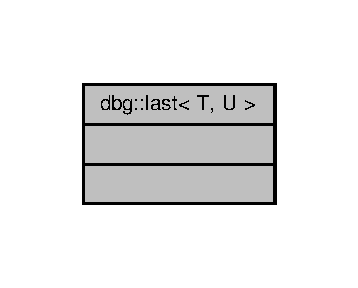
\includegraphics[width=172pt]{d8/d7e/structdbg_1_1last__coll__graph}
\end{center}
\end{figure}
\subsection*{Public Types}
\begin{DoxyCompactItemize}
\item 
using \hyperlink{structdbg_1_1last_aac2d6dd66fecfc0f3f37ecb4a02b0779}{type} = typename \hyperlink{structdbg_1_1last}{last}$<$ U... $>$\+::\hyperlink{structdbg_1_1last_aac2d6dd66fecfc0f3f37ecb4a02b0779}{type}
\end{DoxyCompactItemize}


\subsection{Member Typedef Documentation}
\mbox{\Hypertarget{structdbg_1_1last_aac2d6dd66fecfc0f3f37ecb4a02b0779}\label{structdbg_1_1last_aac2d6dd66fecfc0f3f37ecb4a02b0779}} 
\index{dbg\+::last@{dbg\+::last}!type@{type}}
\index{type@{type}!dbg\+::last@{dbg\+::last}}
\subsubsection{\texorpdfstring{type}{type}}
{\footnotesize\ttfamily template$<$typename T , typename... U$>$ \\
using \hyperlink{structdbg_1_1last}{dbg\+::last}$<$ T, U $>$\+::\hyperlink{structdbg_1_1last_aac2d6dd66fecfc0f3f37ecb4a02b0779}{type} =  typename \hyperlink{structdbg_1_1last}{last}$<$U...$>$\+::\hyperlink{structdbg_1_1last_aac2d6dd66fecfc0f3f37ecb4a02b0779}{type}}



The documentation for this struct was generated from the following file\+:\begin{DoxyCompactItemize}
\item 
\hyperlink{dbg_8h}{dbg.\+h}\end{DoxyCompactItemize}

\hypertarget{structdbg_1_1last_3_01T_01_4}{}\section{dbg\+:\+:last$<$ T $>$ Struct Template Reference}
\label{structdbg_1_1last_3_01T_01_4}\index{dbg\+::last$<$ T $>$@{dbg\+::last$<$ T $>$}}


{\ttfamily \#include $<$dbg.\+h$>$}



Collaboration diagram for dbg\+:\+:last$<$ T $>$\+:\nopagebreak
\begin{figure}[H]
\begin{center}
\leavevmode
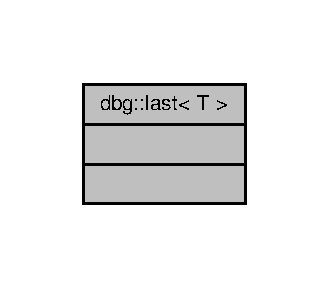
\includegraphics[width=158pt]{da/d1d/structdbg_1_1last_3_01T_01_4__coll__graph}
\end{center}
\end{figure}
\subsection*{Public Types}
\begin{DoxyCompactItemize}
\item 
using \hyperlink{structdbg_1_1last_3_01T_01_4_a6715c2f60dfaa8a096517ce45ff43999}{type} = T
\end{DoxyCompactItemize}


\subsection{Member Typedef Documentation}
\mbox{\Hypertarget{structdbg_1_1last_3_01T_01_4_a6715c2f60dfaa8a096517ce45ff43999}\label{structdbg_1_1last_3_01T_01_4_a6715c2f60dfaa8a096517ce45ff43999}} 
\index{dbg\+::last$<$ T $>$@{dbg\+::last$<$ T $>$}!type@{type}}
\index{type@{type}!dbg\+::last$<$ T $>$@{dbg\+::last$<$ T $>$}}
\subsubsection{\texorpdfstring{type}{type}}
{\footnotesize\ttfamily template$<$typename T $>$ \\
using \hyperlink{structdbg_1_1last}{dbg\+::last}$<$ T $>$\+::\hyperlink{structdbg_1_1last_3_01T_01_4_a6715c2f60dfaa8a096517ce45ff43999}{type} =  T}



The documentation for this struct was generated from the following file\+:\begin{DoxyCompactItemize}
\item 
\hyperlink{dbg_8h}{dbg.\+h}\end{DoxyCompactItemize}

\hypertarget{classcommon_1_1MatchInternal}{}\section{common\+:\+:Match\+Internal Class Reference}
\label{classcommon_1_1MatchInternal}\index{common\+::\+Match\+Internal@{common\+::\+Match\+Internal}}


{\ttfamily \#include $<$match\+\_\+utils.\+hpp$>$}



Collaboration diagram for common\+:\+:Match\+Internal\+:\nopagebreak
\begin{figure}[H]
\begin{center}
\leavevmode
\includegraphics[width=199pt]{d7/dfe/classcommon_1_1MatchInternal__coll__graph}
\end{center}
\end{figure}
\subsection*{Public Member Functions}
\begin{DoxyCompactItemize}
\item 
\hyperlink{classcommon_1_1MatchInternal_a9f96197acbfb0dd3969e842b5b51dc21}{Match\+Internal} ()
\item 
{\footnotesize template$<$typename Archive $>$ }\\void \hyperlink{classcommon_1_1MatchInternal_aff0df9eda9d505490b9349bcf91b5a67}{serialize\+\_\+mtx} (Archive \&ar, std\+::string str, Eigen\+::\+Matrix\+Xd \&mtx)
\item 
{\footnotesize template$<$typename Archive $>$ }\\void \hyperlink{classcommon_1_1MatchInternal_a40340e3ee3dd9d70e56078326de9ff88}{serialize} (Archive \&ar, const unsigned int version)
\item 
void \hyperlink{classcommon_1_1MatchInternal_a853a17067e29c199d1680a0dd01a42f9}{Push\+Back} (const \hyperlink{structcommon_1_1Correspondences}{Correspondences} \&corr, const Eigen\+::\+Vector3d \&tf)
\item 
void \hyperlink{classcommon_1_1MatchInternal_ab0ce620f581dd3a33083c03ffbc12ca3}{Push\+Back} (const \hyperlink{structcommon_1_1Correspondences}{Correspondences} \&corr, const std\+::vector$<$ double $>$ \&tf)
\item 
void \hyperlink{classcommon_1_1MatchInternal_a519c8d85ca7a2d31353a3a3ce2e68c34}{Clear\+Results} ()
\item 
bool \hyperlink{classcommon_1_1MatchInternal_aa45d67544518f4cac0b25a12aee78607}{has\+\_\+data} () const
\item 
double \hyperlink{classcommon_1_1MatchInternal_a69a417791950569fed61f59ba3cf79a9}{cell\+\_\+size} () const
\item 
Eigen\+::\+Matrix\+Xd \hyperlink{classcommon_1_1MatchInternal_ab03d9e1343e7363014de8cb08c38ceb8}{source} () const
\item 
Eigen\+::\+Matrix\+Xd \hyperlink{classcommon_1_1MatchInternal_ac84d3e1b4062af44ae7259d2c37f4ef0}{target} () const
\item 
std\+::vector$<$ Eigen\+::\+Matrix\+Xd $>$ \hyperlink{classcommon_1_1MatchInternal_a4a07e3e47fa6885beee71187c85c0eb0}{corrs} () const
\item 
std\+::vector$<$ Eigen\+::\+Vector3d $>$ \hyperlink{classcommon_1_1MatchInternal_a1099ba991441897a0e9879484351cfd0}{tfs} () const
\item 
std\+::string \hyperlink{classcommon_1_1MatchInternal_acccb677b9ab80f44f7e66208fc5093ce}{comment} () const
\item 
void \hyperlink{classcommon_1_1MatchInternal_ac8d76d941068e5fc7dd561afa2aa707c}{set\+\_\+has\+\_\+data} (bool \hyperlink{classcommon_1_1MatchInternal_aa45d67544518f4cac0b25a12aee78607}{has\+\_\+data})
\item 
void \hyperlink{classcommon_1_1MatchInternal_ae18d8a6dfae9b7ac243e93d4b4fb3f88}{set\+\_\+cell\+\_\+size} (double \hyperlink{classcommon_1_1MatchInternal_a69a417791950569fed61f59ba3cf79a9}{cell\+\_\+size})
\item 
void \hyperlink{classcommon_1_1MatchInternal_a0012905085722357e80523c50db74148}{set\+\_\+source} (const Eigen\+::\+Matrix\+Xd \&\hyperlink{classcommon_1_1MatchInternal_ab03d9e1343e7363014de8cb08c38ceb8}{source})
\item 
void \hyperlink{classcommon_1_1MatchInternal_ab122317afafbaac0a6ce92c830d846f9}{set\+\_\+target} (const Eigen\+::\+Matrix\+Xd \&\hyperlink{classcommon_1_1MatchInternal_ac84d3e1b4062af44ae7259d2c37f4ef0}{target})
\item 
void \hyperlink{classcommon_1_1MatchInternal_a788efd7d34fd2ece675b5050377d6753}{set\+\_\+corrs} (const std\+::vector$<$ Eigen\+::\+Matrix\+Xd $>$ \&\hyperlink{classcommon_1_1MatchInternal_a4a07e3e47fa6885beee71187c85c0eb0}{corrs})
\item 
void \hyperlink{classcommon_1_1MatchInternal_a6978d626575e6c81028c258fd4706772}{set\+\_\+tfs} (const std\+::vector$<$ Eigen\+::\+Vector3d $>$ \&\hyperlink{classcommon_1_1MatchInternal_a1099ba991441897a0e9879484351cfd0}{tfs})
\item 
void \hyperlink{classcommon_1_1MatchInternal_a546272323b6f29aeb31da0369f4ff5b1}{set\+\_\+comment} (const std\+::string \&\hyperlink{classcommon_1_1MatchInternal_acccb677b9ab80f44f7e66208fc5093ce}{comment})
\end{DoxyCompactItemize}
\subsection*{Friends}
\begin{DoxyCompactItemize}
\item 
class \hyperlink{classcommon_1_1MatchInternal_ac98d07dd8f7b70e16ccb9a01abf56b9c}{boost\+::serialization\+::access}
\end{DoxyCompactItemize}


\subsection{Constructor \& Destructor Documentation}
\mbox{\Hypertarget{classcommon_1_1MatchInternal_a9f96197acbfb0dd3969e842b5b51dc21}\label{classcommon_1_1MatchInternal_a9f96197acbfb0dd3969e842b5b51dc21}} 
\index{common\+::\+Match\+Internal@{common\+::\+Match\+Internal}!Match\+Internal@{Match\+Internal}}
\index{Match\+Internal@{Match\+Internal}!common\+::\+Match\+Internal@{common\+::\+Match\+Internal}}
\subsubsection{\texorpdfstring{Match\+Internal()}{MatchInternal()}}
{\footnotesize\ttfamily common\+::\+Match\+Internal\+::\+Match\+Internal (\begin{DoxyParamCaption}{ }\end{DoxyParamCaption})\hspace{0.3cm}{\ttfamily [inline]}}



\subsection{Member Function Documentation}
\mbox{\Hypertarget{classcommon_1_1MatchInternal_a69a417791950569fed61f59ba3cf79a9}\label{classcommon_1_1MatchInternal_a69a417791950569fed61f59ba3cf79a9}} 
\index{common\+::\+Match\+Internal@{common\+::\+Match\+Internal}!cell\+\_\+size@{cell\+\_\+size}}
\index{cell\+\_\+size@{cell\+\_\+size}!common\+::\+Match\+Internal@{common\+::\+Match\+Internal}}
\subsubsection{\texorpdfstring{cell\+\_\+size()}{cell\_size()}}
{\footnotesize\ttfamily double common\+::\+Match\+Internal\+::cell\+\_\+size (\begin{DoxyParamCaption}{ }\end{DoxyParamCaption}) const\hspace{0.3cm}{\ttfamily [inline]}}

\mbox{\Hypertarget{classcommon_1_1MatchInternal_a519c8d85ca7a2d31353a3a3ce2e68c34}\label{classcommon_1_1MatchInternal_a519c8d85ca7a2d31353a3a3ce2e68c34}} 
\index{common\+::\+Match\+Internal@{common\+::\+Match\+Internal}!Clear\+Results@{Clear\+Results}}
\index{Clear\+Results@{Clear\+Results}!common\+::\+Match\+Internal@{common\+::\+Match\+Internal}}
\subsubsection{\texorpdfstring{Clear\+Results()}{ClearResults()}}
{\footnotesize\ttfamily void common\+::\+Match\+Internal\+::\+Clear\+Results (\begin{DoxyParamCaption}{ }\end{DoxyParamCaption})\hspace{0.3cm}{\ttfamily [inline]}}



Referenced by trimesh\+::\+I\+C\+P().

\mbox{\Hypertarget{classcommon_1_1MatchInternal_acccb677b9ab80f44f7e66208fc5093ce}\label{classcommon_1_1MatchInternal_acccb677b9ab80f44f7e66208fc5093ce}} 
\index{common\+::\+Match\+Internal@{common\+::\+Match\+Internal}!comment@{comment}}
\index{comment@{comment}!common\+::\+Match\+Internal@{common\+::\+Match\+Internal}}
\subsubsection{\texorpdfstring{comment()}{comment()}}
{\footnotesize\ttfamily std\+::string common\+::\+Match\+Internal\+::comment (\begin{DoxyParamCaption}{ }\end{DoxyParamCaption}) const\hspace{0.3cm}{\ttfamily [inline]}}

\mbox{\Hypertarget{classcommon_1_1MatchInternal_a4a07e3e47fa6885beee71187c85c0eb0}\label{classcommon_1_1MatchInternal_a4a07e3e47fa6885beee71187c85c0eb0}} 
\index{common\+::\+Match\+Internal@{common\+::\+Match\+Internal}!corrs@{corrs}}
\index{corrs@{corrs}!common\+::\+Match\+Internal@{common\+::\+Match\+Internal}}
\subsubsection{\texorpdfstring{corrs()}{corrs()}}
{\footnotesize\ttfamily std\+::vector$<$Eigen\+::\+Matrix\+Xd$>$ common\+::\+Match\+Internal\+::corrs (\begin{DoxyParamCaption}{ }\end{DoxyParamCaption}) const\hspace{0.3cm}{\ttfamily [inline]}}

\mbox{\Hypertarget{classcommon_1_1MatchInternal_aa45d67544518f4cac0b25a12aee78607}\label{classcommon_1_1MatchInternal_aa45d67544518f4cac0b25a12aee78607}} 
\index{common\+::\+Match\+Internal@{common\+::\+Match\+Internal}!has\+\_\+data@{has\+\_\+data}}
\index{has\+\_\+data@{has\+\_\+data}!common\+::\+Match\+Internal@{common\+::\+Match\+Internal}}
\subsubsection{\texorpdfstring{has\+\_\+data()}{has\_data()}}
{\footnotesize\ttfamily bool common\+::\+Match\+Internal\+::has\+\_\+data (\begin{DoxyParamCaption}{ }\end{DoxyParamCaption}) const\hspace{0.3cm}{\ttfamily [inline]}}

\mbox{\Hypertarget{classcommon_1_1MatchInternal_a853a17067e29c199d1680a0dd01a42f9}\label{classcommon_1_1MatchInternal_a853a17067e29c199d1680a0dd01a42f9}} 
\index{common\+::\+Match\+Internal@{common\+::\+Match\+Internal}!Push\+Back@{Push\+Back}}
\index{Push\+Back@{Push\+Back}!common\+::\+Match\+Internal@{common\+::\+Match\+Internal}}
\subsubsection{\texorpdfstring{Push\+Back()}{PushBack()}\hspace{0.1cm}{\footnotesize\ttfamily [1/2]}}
{\footnotesize\ttfamily void common\+::\+Match\+Internal\+::\+Push\+Back (\begin{DoxyParamCaption}\item[{const \hyperlink{structcommon_1_1Correspondences}{Correspondences} \&}]{corr,  }\item[{const Eigen\+::\+Vector3d \&}]{tf }\end{DoxyParamCaption})\hspace{0.3cm}{\ttfamily [inline]}}

\mbox{\Hypertarget{classcommon_1_1MatchInternal_ab0ce620f581dd3a33083c03ffbc12ca3}\label{classcommon_1_1MatchInternal_ab0ce620f581dd3a33083c03ffbc12ca3}} 
\index{common\+::\+Match\+Internal@{common\+::\+Match\+Internal}!Push\+Back@{Push\+Back}}
\index{Push\+Back@{Push\+Back}!common\+::\+Match\+Internal@{common\+::\+Match\+Internal}}
\subsubsection{\texorpdfstring{Push\+Back()}{PushBack()}\hspace{0.1cm}{\footnotesize\ttfamily [2/2]}}
{\footnotesize\ttfamily void common\+::\+Match\+Internal\+::\+Push\+Back (\begin{DoxyParamCaption}\item[{const \hyperlink{structcommon_1_1Correspondences}{Correspondences} \&}]{corr,  }\item[{const std\+::vector$<$ double $>$ \&}]{tf }\end{DoxyParamCaption})\hspace{0.3cm}{\ttfamily [inline]}}

\mbox{\Hypertarget{classcommon_1_1MatchInternal_a40340e3ee3dd9d70e56078326de9ff88}\label{classcommon_1_1MatchInternal_a40340e3ee3dd9d70e56078326de9ff88}} 
\index{common\+::\+Match\+Internal@{common\+::\+Match\+Internal}!serialize@{serialize}}
\index{serialize@{serialize}!common\+::\+Match\+Internal@{common\+::\+Match\+Internal}}
\subsubsection{\texorpdfstring{serialize()}{serialize()}}
{\footnotesize\ttfamily template$<$typename Archive $>$ \\
void common\+::\+Match\+Internal\+::serialize (\begin{DoxyParamCaption}\item[{Archive \&}]{ar,  }\item[{const unsigned int}]{version }\end{DoxyParamCaption})\hspace{0.3cm}{\ttfamily [inline]}}

\mbox{\Hypertarget{classcommon_1_1MatchInternal_aff0df9eda9d505490b9349bcf91b5a67}\label{classcommon_1_1MatchInternal_aff0df9eda9d505490b9349bcf91b5a67}} 
\index{common\+::\+Match\+Internal@{common\+::\+Match\+Internal}!serialize\+\_\+mtx@{serialize\+\_\+mtx}}
\index{serialize\+\_\+mtx@{serialize\+\_\+mtx}!common\+::\+Match\+Internal@{common\+::\+Match\+Internal}}
\subsubsection{\texorpdfstring{serialize\+\_\+mtx()}{serialize\_mtx()}}
{\footnotesize\ttfamily template$<$typename Archive $>$ \\
void common\+::\+Match\+Internal\+::serialize\+\_\+mtx (\begin{DoxyParamCaption}\item[{Archive \&}]{ar,  }\item[{std\+::string}]{str,  }\item[{Eigen\+::\+Matrix\+Xd \&}]{mtx }\end{DoxyParamCaption})\hspace{0.3cm}{\ttfamily [inline]}}

\mbox{\Hypertarget{classcommon_1_1MatchInternal_ae18d8a6dfae9b7ac243e93d4b4fb3f88}\label{classcommon_1_1MatchInternal_ae18d8a6dfae9b7ac243e93d4b4fb3f88}} 
\index{common\+::\+Match\+Internal@{common\+::\+Match\+Internal}!set\+\_\+cell\+\_\+size@{set\+\_\+cell\+\_\+size}}
\index{set\+\_\+cell\+\_\+size@{set\+\_\+cell\+\_\+size}!common\+::\+Match\+Internal@{common\+::\+Match\+Internal}}
\subsubsection{\texorpdfstring{set\+\_\+cell\+\_\+size()}{set\_cell\_size()}}
{\footnotesize\ttfamily void common\+::\+Match\+Internal\+::set\+\_\+cell\+\_\+size (\begin{DoxyParamCaption}\item[{double}]{cell\+\_\+size }\end{DoxyParamCaption})\hspace{0.3cm}{\ttfamily [inline]}}

\mbox{\Hypertarget{classcommon_1_1MatchInternal_a546272323b6f29aeb31da0369f4ff5b1}\label{classcommon_1_1MatchInternal_a546272323b6f29aeb31da0369f4ff5b1}} 
\index{common\+::\+Match\+Internal@{common\+::\+Match\+Internal}!set\+\_\+comment@{set\+\_\+comment}}
\index{set\+\_\+comment@{set\+\_\+comment}!common\+::\+Match\+Internal@{common\+::\+Match\+Internal}}
\subsubsection{\texorpdfstring{set\+\_\+comment()}{set\_comment()}}
{\footnotesize\ttfamily void common\+::\+Match\+Internal\+::set\+\_\+comment (\begin{DoxyParamCaption}\item[{const std\+::string \&}]{comment }\end{DoxyParamCaption})\hspace{0.3cm}{\ttfamily [inline]}}

\mbox{\Hypertarget{classcommon_1_1MatchInternal_a788efd7d34fd2ece675b5050377d6753}\label{classcommon_1_1MatchInternal_a788efd7d34fd2ece675b5050377d6753}} 
\index{common\+::\+Match\+Internal@{common\+::\+Match\+Internal}!set\+\_\+corrs@{set\+\_\+corrs}}
\index{set\+\_\+corrs@{set\+\_\+corrs}!common\+::\+Match\+Internal@{common\+::\+Match\+Internal}}
\subsubsection{\texorpdfstring{set\+\_\+corrs()}{set\_corrs()}}
{\footnotesize\ttfamily void common\+::\+Match\+Internal\+::set\+\_\+corrs (\begin{DoxyParamCaption}\item[{const std\+::vector$<$ Eigen\+::\+Matrix\+Xd $>$ \&}]{corrs }\end{DoxyParamCaption})\hspace{0.3cm}{\ttfamily [inline]}}

\mbox{\Hypertarget{classcommon_1_1MatchInternal_ac8d76d941068e5fc7dd561afa2aa707c}\label{classcommon_1_1MatchInternal_ac8d76d941068e5fc7dd561afa2aa707c}} 
\index{common\+::\+Match\+Internal@{common\+::\+Match\+Internal}!set\+\_\+has\+\_\+data@{set\+\_\+has\+\_\+data}}
\index{set\+\_\+has\+\_\+data@{set\+\_\+has\+\_\+data}!common\+::\+Match\+Internal@{common\+::\+Match\+Internal}}
\subsubsection{\texorpdfstring{set\+\_\+has\+\_\+data()}{set\_has\_data()}}
{\footnotesize\ttfamily void common\+::\+Match\+Internal\+::set\+\_\+has\+\_\+data (\begin{DoxyParamCaption}\item[{bool}]{has\+\_\+data }\end{DoxyParamCaption})\hspace{0.3cm}{\ttfamily [inline]}}



Referenced by trimesh\+::\+I\+C\+P().

\mbox{\Hypertarget{classcommon_1_1MatchInternal_a0012905085722357e80523c50db74148}\label{classcommon_1_1MatchInternal_a0012905085722357e80523c50db74148}} 
\index{common\+::\+Match\+Internal@{common\+::\+Match\+Internal}!set\+\_\+source@{set\+\_\+source}}
\index{set\+\_\+source@{set\+\_\+source}!common\+::\+Match\+Internal@{common\+::\+Match\+Internal}}
\subsubsection{\texorpdfstring{set\+\_\+source()}{set\_source()}}
{\footnotesize\ttfamily void common\+::\+Match\+Internal\+::set\+\_\+source (\begin{DoxyParamCaption}\item[{const Eigen\+::\+Matrix\+Xd \&}]{source }\end{DoxyParamCaption})\hspace{0.3cm}{\ttfamily [inline]}}



Referenced by trimesh\+::\+I\+C\+P().

\mbox{\Hypertarget{classcommon_1_1MatchInternal_ab122317afafbaac0a6ce92c830d846f9}\label{classcommon_1_1MatchInternal_ab122317afafbaac0a6ce92c830d846f9}} 
\index{common\+::\+Match\+Internal@{common\+::\+Match\+Internal}!set\+\_\+target@{set\+\_\+target}}
\index{set\+\_\+target@{set\+\_\+target}!common\+::\+Match\+Internal@{common\+::\+Match\+Internal}}
\subsubsection{\texorpdfstring{set\+\_\+target()}{set\_target()}}
{\footnotesize\ttfamily void common\+::\+Match\+Internal\+::set\+\_\+target (\begin{DoxyParamCaption}\item[{const Eigen\+::\+Matrix\+Xd \&}]{target }\end{DoxyParamCaption})\hspace{0.3cm}{\ttfamily [inline]}}



Referenced by trimesh\+::\+I\+C\+P().

\mbox{\Hypertarget{classcommon_1_1MatchInternal_a6978d626575e6c81028c258fd4706772}\label{classcommon_1_1MatchInternal_a6978d626575e6c81028c258fd4706772}} 
\index{common\+::\+Match\+Internal@{common\+::\+Match\+Internal}!set\+\_\+tfs@{set\+\_\+tfs}}
\index{set\+\_\+tfs@{set\+\_\+tfs}!common\+::\+Match\+Internal@{common\+::\+Match\+Internal}}
\subsubsection{\texorpdfstring{set\+\_\+tfs()}{set\_tfs()}}
{\footnotesize\ttfamily void common\+::\+Match\+Internal\+::set\+\_\+tfs (\begin{DoxyParamCaption}\item[{const std\+::vector$<$ Eigen\+::\+Vector3d $>$ \&}]{tfs }\end{DoxyParamCaption})\hspace{0.3cm}{\ttfamily [inline]}}

\mbox{\Hypertarget{classcommon_1_1MatchInternal_ab03d9e1343e7363014de8cb08c38ceb8}\label{classcommon_1_1MatchInternal_ab03d9e1343e7363014de8cb08c38ceb8}} 
\index{common\+::\+Match\+Internal@{common\+::\+Match\+Internal}!source@{source}}
\index{source@{source}!common\+::\+Match\+Internal@{common\+::\+Match\+Internal}}
\subsubsection{\texorpdfstring{source()}{source()}}
{\footnotesize\ttfamily Eigen\+::\+Matrix\+Xd common\+::\+Match\+Internal\+::source (\begin{DoxyParamCaption}{ }\end{DoxyParamCaption}) const\hspace{0.3cm}{\ttfamily [inline]}}

\mbox{\Hypertarget{classcommon_1_1MatchInternal_ac84d3e1b4062af44ae7259d2c37f4ef0}\label{classcommon_1_1MatchInternal_ac84d3e1b4062af44ae7259d2c37f4ef0}} 
\index{common\+::\+Match\+Internal@{common\+::\+Match\+Internal}!target@{target}}
\index{target@{target}!common\+::\+Match\+Internal@{common\+::\+Match\+Internal}}
\subsubsection{\texorpdfstring{target()}{target()}}
{\footnotesize\ttfamily Eigen\+::\+Matrix\+Xd common\+::\+Match\+Internal\+::target (\begin{DoxyParamCaption}{ }\end{DoxyParamCaption}) const\hspace{0.3cm}{\ttfamily [inline]}}

\mbox{\Hypertarget{classcommon_1_1MatchInternal_a1099ba991441897a0e9879484351cfd0}\label{classcommon_1_1MatchInternal_a1099ba991441897a0e9879484351cfd0}} 
\index{common\+::\+Match\+Internal@{common\+::\+Match\+Internal}!tfs@{tfs}}
\index{tfs@{tfs}!common\+::\+Match\+Internal@{common\+::\+Match\+Internal}}
\subsubsection{\texorpdfstring{tfs()}{tfs()}}
{\footnotesize\ttfamily std\+::vector$<$Eigen\+::\+Vector3d$>$ common\+::\+Match\+Internal\+::tfs (\begin{DoxyParamCaption}{ }\end{DoxyParamCaption}) const\hspace{0.3cm}{\ttfamily [inline]}}



\subsection{Friends And Related Function Documentation}
\mbox{\Hypertarget{classcommon_1_1MatchInternal_ac98d07dd8f7b70e16ccb9a01abf56b9c}\label{classcommon_1_1MatchInternal_ac98d07dd8f7b70e16ccb9a01abf56b9c}} 
\index{common\+::\+Match\+Internal@{common\+::\+Match\+Internal}!boost\+::serialization\+::access@{boost\+::serialization\+::access}}
\index{boost\+::serialization\+::access@{boost\+::serialization\+::access}!common\+::\+Match\+Internal@{common\+::\+Match\+Internal}}
\subsubsection{\texorpdfstring{boost\+::serialization\+::access}{boost::serialization::access}}
{\footnotesize\ttfamily friend class boost\+::serialization\+::access\hspace{0.3cm}{\ttfamily [friend]}}



The documentation for this class was generated from the following file\+:\begin{DoxyCompactItemize}
\item 
\hyperlink{match__utils_8hpp}{match\+\_\+utils.\+hpp}\end{DoxyCompactItemize}

\hypertarget{structcommon_1_1MatchPackage}{}\section{common\+:\+:Match\+Package Struct Reference}
\label{structcommon_1_1MatchPackage}\index{common\+::\+Match\+Package@{common\+::\+Match\+Package}}


{\ttfamily \#include $<$match\+\_\+utils.\+hpp$>$}



Collaboration diagram for common\+:\+:Match\+Package\+:\nopagebreak
\begin{figure}[H]
\begin{center}
\leavevmode
\includegraphics[width=205pt]{d9/d88/structcommon_1_1MatchPackage__coll__graph}
\end{center}
\end{figure}
\subsection*{Public Member Functions}
\begin{DoxyCompactItemize}
\item 
\hyperlink{structcommon_1_1MatchPackage_affa0c8dc025d07ec5fd849ec8ef52aca}{Match\+Package} ()
\end{DoxyCompactItemize}
\subsection*{Public Attributes}
\begin{DoxyCompactItemize}
\item 
Eigen\+::\+Matrix\+Xd \hyperlink{structcommon_1_1MatchPackage_a1eafbc6a1740dde4ab7adf0e55728880}{source}
\item 
Eigen\+::\+Matrix\+Xd \hyperlink{structcommon_1_1MatchPackage_a99634972d12f9a982c16c0adc1fe18b2}{target}
\item 
Eigen\+::\+Matrix\+Xd \hyperlink{structcommon_1_1MatchPackage_ac54fe69fc83e64abaefe2c5eb07454d9}{output}
\item 
Eigen\+::\+Matrix3d \hyperlink{structcommon_1_1MatchPackage_a80b1337381b200114c7474979f3779b3}{guess}
\item 
Eigen\+::\+Matrix3d \hyperlink{structcommon_1_1MatchPackage_a320b399233744fff15114995ce555898}{result}
\item 
Eigen\+::\+Matrix3d \hyperlink{structcommon_1_1MatchPackage_a28fa25a397c65139fdfffb19394fffbd}{actual}
\item 
int \hyperlink{structcommon_1_1MatchPackage_a4c44c43d7f9ce0667d925d618d4940f4}{iters}
\end{DoxyCompactItemize}


\subsection{Constructor \& Destructor Documentation}
\mbox{\Hypertarget{structcommon_1_1MatchPackage_affa0c8dc025d07ec5fd849ec8ef52aca}\label{structcommon_1_1MatchPackage_affa0c8dc025d07ec5fd849ec8ef52aca}} 
\index{common\+::\+Match\+Package@{common\+::\+Match\+Package}!Match\+Package@{Match\+Package}}
\index{Match\+Package@{Match\+Package}!common\+::\+Match\+Package@{common\+::\+Match\+Package}}
\subsubsection{\texorpdfstring{Match\+Package()}{MatchPackage()}}
{\footnotesize\ttfamily common\+::\+Match\+Package\+::\+Match\+Package (\begin{DoxyParamCaption}{ }\end{DoxyParamCaption})\hspace{0.3cm}{\ttfamily [inline]}}



\subsection{Member Data Documentation}
\mbox{\Hypertarget{structcommon_1_1MatchPackage_a28fa25a397c65139fdfffb19394fffbd}\label{structcommon_1_1MatchPackage_a28fa25a397c65139fdfffb19394fffbd}} 
\index{common\+::\+Match\+Package@{common\+::\+Match\+Package}!actual@{actual}}
\index{actual@{actual}!common\+::\+Match\+Package@{common\+::\+Match\+Package}}
\subsubsection{\texorpdfstring{actual}{actual}}
{\footnotesize\ttfamily Eigen\+::\+Matrix3d common\+::\+Match\+Package\+::actual}

\mbox{\Hypertarget{structcommon_1_1MatchPackage_a80b1337381b200114c7474979f3779b3}\label{structcommon_1_1MatchPackage_a80b1337381b200114c7474979f3779b3}} 
\index{common\+::\+Match\+Package@{common\+::\+Match\+Package}!guess@{guess}}
\index{guess@{guess}!common\+::\+Match\+Package@{common\+::\+Match\+Package}}
\subsubsection{\texorpdfstring{guess}{guess}}
{\footnotesize\ttfamily Eigen\+::\+Matrix3d common\+::\+Match\+Package\+::guess}



Referenced by Do\+P\+C\+L\+S\+I\+C\+P(), Do\+S\+I\+C\+P(), Do\+S\+N\+D\+T(), and main().

\mbox{\Hypertarget{structcommon_1_1MatchPackage_a4c44c43d7f9ce0667d925d618d4940f4}\label{structcommon_1_1MatchPackage_a4c44c43d7f9ce0667d925d618d4940f4}} 
\index{common\+::\+Match\+Package@{common\+::\+Match\+Package}!iters@{iters}}
\index{iters@{iters}!common\+::\+Match\+Package@{common\+::\+Match\+Package}}
\subsubsection{\texorpdfstring{iters}{iters}}
{\footnotesize\ttfamily int common\+::\+Match\+Package\+::iters}



Referenced by Do\+P\+C\+L\+S\+I\+C\+P(), Do\+S\+I\+C\+P(), and Do\+S\+N\+D\+T().

\mbox{\Hypertarget{structcommon_1_1MatchPackage_ac54fe69fc83e64abaefe2c5eb07454d9}\label{structcommon_1_1MatchPackage_ac54fe69fc83e64abaefe2c5eb07454d9}} 
\index{common\+::\+Match\+Package@{common\+::\+Match\+Package}!output@{output}}
\index{output@{output}!common\+::\+Match\+Package@{common\+::\+Match\+Package}}
\subsubsection{\texorpdfstring{output}{output}}
{\footnotesize\ttfamily Eigen\+::\+Matrix\+Xd common\+::\+Match\+Package\+::output}

\mbox{\Hypertarget{structcommon_1_1MatchPackage_a320b399233744fff15114995ce555898}\label{structcommon_1_1MatchPackage_a320b399233744fff15114995ce555898}} 
\index{common\+::\+Match\+Package@{common\+::\+Match\+Package}!result@{result}}
\index{result@{result}!common\+::\+Match\+Package@{common\+::\+Match\+Package}}
\subsubsection{\texorpdfstring{result}{result}}
{\footnotesize\ttfamily Eigen\+::\+Matrix3d common\+::\+Match\+Package\+::result}



Referenced by Do\+P\+C\+L\+S\+I\+C\+P(), Do\+S\+I\+C\+P(), Do\+S\+N\+D\+T(), and main().

\mbox{\Hypertarget{structcommon_1_1MatchPackage_a1eafbc6a1740dde4ab7adf0e55728880}\label{structcommon_1_1MatchPackage_a1eafbc6a1740dde4ab7adf0e55728880}} 
\index{common\+::\+Match\+Package@{common\+::\+Match\+Package}!source@{source}}
\index{source@{source}!common\+::\+Match\+Package@{common\+::\+Match\+Package}}
\subsubsection{\texorpdfstring{source}{source}}
{\footnotesize\ttfamily Eigen\+::\+Matrix\+Xd common\+::\+Match\+Package\+::source}



Referenced by Do\+P\+C\+L\+S\+I\+C\+P(), Do\+S\+I\+C\+P(), Do\+S\+N\+D\+T(), and main().

\mbox{\Hypertarget{structcommon_1_1MatchPackage_a99634972d12f9a982c16c0adc1fe18b2}\label{structcommon_1_1MatchPackage_a99634972d12f9a982c16c0adc1fe18b2}} 
\index{common\+::\+Match\+Package@{common\+::\+Match\+Package}!target@{target}}
\index{target@{target}!common\+::\+Match\+Package@{common\+::\+Match\+Package}}
\subsubsection{\texorpdfstring{target}{target}}
{\footnotesize\ttfamily Eigen\+::\+Matrix\+Xd common\+::\+Match\+Package\+::target}



Referenced by Do\+P\+C\+L\+S\+I\+C\+P(), Do\+S\+I\+C\+P(), Do\+S\+N\+D\+T(), and main().



The documentation for this struct was generated from the following file\+:\begin{DoxyCompactItemize}
\item 
\hyperlink{match__utils_8hpp}{match\+\_\+utils.\+hpp}\end{DoxyCompactItemize}

\hypertarget{classcommon_1_1MatchResults}{}\section{common\+:\+:Match\+Results Class Reference}
\label{classcommon_1_1MatchResults}\index{common\+::\+Match\+Results@{common\+::\+Match\+Results}}


{\ttfamily \#include $<$match\+\_\+utils.\+hpp$>$}



Collaboration diagram for common\+:\+:Match\+Results\+:\nopagebreak
\begin{figure}[H]
\begin{center}
\leavevmode
\includegraphics[width=201pt]{d5/d84/classcommon_1_1MatchResults__coll__graph}
\end{center}
\end{figure}
\subsection*{Public Member Functions}
\begin{DoxyCompactItemize}
\item 
\hyperlink{classcommon_1_1MatchResults_a61b5ade3dc8c0f5ec8cc1a28d66316d9}{Match\+Results} ()
\item 
void \hyperlink{classcommon_1_1MatchResults_a3949bcd0e53bbce1c95bfa174033e6c4}{Push\+Back} (const Eigen\+::\+Vector3d \&guess, const Eigen\+::\+Vector3d \&result, double score)
\item 
void \hyperlink{classcommon_1_1MatchResults_a52646251d704b8f02f628f057ce678ac}{Push\+Back} (const std\+::vector$<$ double $>$ \&guess, const std\+::vector$<$ double $>$ \&result, double score)
\item 
{\footnotesize template$<$typename Archive $>$ }\\void \hyperlink{classcommon_1_1MatchResults_aaa028c2125c808d8ed6a399be6a4a30d}{serialize\+\_\+mtx} (Archive \&ar, std\+::string str, Eigen\+::\+Matrix\+Xd \&mtx)
\item 
{\footnotesize template$<$typename Archive $>$ }\\void \hyperlink{classcommon_1_1MatchResults_a47c29ca4386acfdfe204eee69a3d18fc}{serialize} (Archive \&ar, const unsigned int version)
\item 
Eigen\+::\+Matrix\+Xd \hyperlink{classcommon_1_1MatchResults_aee873ffecdcfb1c00c520326eb24d43e}{source} () const
\item 
Eigen\+::\+Matrix\+Xd \hyperlink{classcommon_1_1MatchResults_a4eccb30043877c55780aa935a404e8af}{target} () const
\item 
Eigen\+::\+Matrix\+Xd \hyperlink{classcommon_1_1MatchResults_a94ec129bf54fec917642b5b016bd345b}{guesses} () const
\item 
Eigen\+::\+Matrix\+Xd \hyperlink{classcommon_1_1MatchResults_a71899359d5ff15f8fc782969491eaad7}{results} () const
\item 
std\+::vector$<$ double $>$ \hyperlink{classcommon_1_1MatchResults_a51a4a0076719e2ab140cb223fc7f414c}{actual} () const
\item 
std\+::vector$<$ double $>$ \hyperlink{classcommon_1_1MatchResults_a33963f0089a5938ef58b9813d03a29f9}{scores} () const
\item 
std\+::string \hyperlink{classcommon_1_1MatchResults_a872852821e248926ff428de5e8bf24d6}{comment} () const
\item 
void \hyperlink{classcommon_1_1MatchResults_aefc957f33852ec0b2c6ce3732ad28f58}{set\+\_\+has\+\_\+data} (bool has\+\_\+data)
\item 
void \hyperlink{classcommon_1_1MatchResults_a409305a6a8eedf233b429a4c77fd4bcf}{set\+\_\+source} (const Eigen\+::\+Matrix\+Xd \&\hyperlink{classcommon_1_1MatchResults_aee873ffecdcfb1c00c520326eb24d43e}{source})
\item 
void \hyperlink{classcommon_1_1MatchResults_a1a37ed44f6684609ee7416824eb884e1}{set\+\_\+target} (const Eigen\+::\+Matrix\+Xd \&\hyperlink{classcommon_1_1MatchResults_a4eccb30043877c55780aa935a404e8af}{target})
\item 
void \hyperlink{classcommon_1_1MatchResults_ab87b887370037de7ae611be2420071a8}{set\+\_\+actual} (const std\+::vector$<$ double $>$ \&\hyperlink{classcommon_1_1MatchResults_a51a4a0076719e2ab140cb223fc7f414c}{actual})
\item 
void \hyperlink{classcommon_1_1MatchResults_a2e4d287fb5ceb112d09cf564b334bb5b}{set\+\_\+comment} (const std\+::string \&\hyperlink{classcommon_1_1MatchResults_a872852821e248926ff428de5e8bf24d6}{comment})
\end{DoxyCompactItemize}
\subsection*{Friends}
\begin{DoxyCompactItemize}
\item 
class \hyperlink{classcommon_1_1MatchResults_ac98d07dd8f7b70e16ccb9a01abf56b9c}{boost\+::serialization\+::access}
\end{DoxyCompactItemize}


\subsection{Constructor \& Destructor Documentation}
\mbox{\Hypertarget{classcommon_1_1MatchResults_a61b5ade3dc8c0f5ec8cc1a28d66316d9}\label{classcommon_1_1MatchResults_a61b5ade3dc8c0f5ec8cc1a28d66316d9}} 
\index{common\+::\+Match\+Results@{common\+::\+Match\+Results}!Match\+Results@{Match\+Results}}
\index{Match\+Results@{Match\+Results}!common\+::\+Match\+Results@{common\+::\+Match\+Results}}
\subsubsection{\texorpdfstring{Match\+Results()}{MatchResults()}}
{\footnotesize\ttfamily common\+::\+Match\+Results\+::\+Match\+Results (\begin{DoxyParamCaption}{ }\end{DoxyParamCaption})\hspace{0.3cm}{\ttfamily [inline]}}



\subsection{Member Function Documentation}
\mbox{\Hypertarget{classcommon_1_1MatchResults_a51a4a0076719e2ab140cb223fc7f414c}\label{classcommon_1_1MatchResults_a51a4a0076719e2ab140cb223fc7f414c}} 
\index{common\+::\+Match\+Results@{common\+::\+Match\+Results}!actual@{actual}}
\index{actual@{actual}!common\+::\+Match\+Results@{common\+::\+Match\+Results}}
\subsubsection{\texorpdfstring{actual()}{actual()}}
{\footnotesize\ttfamily std\+::vector$<$double$>$ common\+::\+Match\+Results\+::actual (\begin{DoxyParamCaption}{ }\end{DoxyParamCaption}) const\hspace{0.3cm}{\ttfamily [inline]}}

\mbox{\Hypertarget{classcommon_1_1MatchResults_a872852821e248926ff428de5e8bf24d6}\label{classcommon_1_1MatchResults_a872852821e248926ff428de5e8bf24d6}} 
\index{common\+::\+Match\+Results@{common\+::\+Match\+Results}!comment@{comment}}
\index{comment@{comment}!common\+::\+Match\+Results@{common\+::\+Match\+Results}}
\subsubsection{\texorpdfstring{comment()}{comment()}}
{\footnotesize\ttfamily std\+::string common\+::\+Match\+Results\+::comment (\begin{DoxyParamCaption}{ }\end{DoxyParamCaption}) const\hspace{0.3cm}{\ttfamily [inline]}}

\mbox{\Hypertarget{classcommon_1_1MatchResults_a94ec129bf54fec917642b5b016bd345b}\label{classcommon_1_1MatchResults_a94ec129bf54fec917642b5b016bd345b}} 
\index{common\+::\+Match\+Results@{common\+::\+Match\+Results}!guesses@{guesses}}
\index{guesses@{guesses}!common\+::\+Match\+Results@{common\+::\+Match\+Results}}
\subsubsection{\texorpdfstring{guesses()}{guesses()}}
{\footnotesize\ttfamily Eigen\+::\+Matrix\+Xd common\+::\+Match\+Results\+::guesses (\begin{DoxyParamCaption}{ }\end{DoxyParamCaption}) const\hspace{0.3cm}{\ttfamily [inline]}}

\mbox{\Hypertarget{classcommon_1_1MatchResults_a3949bcd0e53bbce1c95bfa174033e6c4}\label{classcommon_1_1MatchResults_a3949bcd0e53bbce1c95bfa174033e6c4}} 
\index{common\+::\+Match\+Results@{common\+::\+Match\+Results}!Push\+Back@{Push\+Back}}
\index{Push\+Back@{Push\+Back}!common\+::\+Match\+Results@{common\+::\+Match\+Results}}
\subsubsection{\texorpdfstring{Push\+Back()}{PushBack()}\hspace{0.1cm}{\footnotesize\ttfamily [1/2]}}
{\footnotesize\ttfamily void common\+::\+Match\+Results\+::\+Push\+Back (\begin{DoxyParamCaption}\item[{const Eigen\+::\+Vector3d \&}]{guess,  }\item[{const Eigen\+::\+Vector3d \&}]{result,  }\item[{double}]{score }\end{DoxyParamCaption})\hspace{0.3cm}{\ttfamily [inline]}}

\mbox{\Hypertarget{classcommon_1_1MatchResults_a52646251d704b8f02f628f057ce678ac}\label{classcommon_1_1MatchResults_a52646251d704b8f02f628f057ce678ac}} 
\index{common\+::\+Match\+Results@{common\+::\+Match\+Results}!Push\+Back@{Push\+Back}}
\index{Push\+Back@{Push\+Back}!common\+::\+Match\+Results@{common\+::\+Match\+Results}}
\subsubsection{\texorpdfstring{Push\+Back()}{PushBack()}\hspace{0.1cm}{\footnotesize\ttfamily [2/2]}}
{\footnotesize\ttfamily void common\+::\+Match\+Results\+::\+Push\+Back (\begin{DoxyParamCaption}\item[{const std\+::vector$<$ double $>$ \&}]{guess,  }\item[{const std\+::vector$<$ double $>$ \&}]{result,  }\item[{double}]{score }\end{DoxyParamCaption})\hspace{0.3cm}{\ttfamily [inline]}}

\mbox{\Hypertarget{classcommon_1_1MatchResults_a71899359d5ff15f8fc782969491eaad7}\label{classcommon_1_1MatchResults_a71899359d5ff15f8fc782969491eaad7}} 
\index{common\+::\+Match\+Results@{common\+::\+Match\+Results}!results@{results}}
\index{results@{results}!common\+::\+Match\+Results@{common\+::\+Match\+Results}}
\subsubsection{\texorpdfstring{results()}{results()}}
{\footnotesize\ttfamily Eigen\+::\+Matrix\+Xd common\+::\+Match\+Results\+::results (\begin{DoxyParamCaption}{ }\end{DoxyParamCaption}) const\hspace{0.3cm}{\ttfamily [inline]}}

\mbox{\Hypertarget{classcommon_1_1MatchResults_a33963f0089a5938ef58b9813d03a29f9}\label{classcommon_1_1MatchResults_a33963f0089a5938ef58b9813d03a29f9}} 
\index{common\+::\+Match\+Results@{common\+::\+Match\+Results}!scores@{scores}}
\index{scores@{scores}!common\+::\+Match\+Results@{common\+::\+Match\+Results}}
\subsubsection{\texorpdfstring{scores()}{scores()}}
{\footnotesize\ttfamily std\+::vector$<$double$>$ common\+::\+Match\+Results\+::scores (\begin{DoxyParamCaption}{ }\end{DoxyParamCaption}) const\hspace{0.3cm}{\ttfamily [inline]}}

\mbox{\Hypertarget{classcommon_1_1MatchResults_a47c29ca4386acfdfe204eee69a3d18fc}\label{classcommon_1_1MatchResults_a47c29ca4386acfdfe204eee69a3d18fc}} 
\index{common\+::\+Match\+Results@{common\+::\+Match\+Results}!serialize@{serialize}}
\index{serialize@{serialize}!common\+::\+Match\+Results@{common\+::\+Match\+Results}}
\subsubsection{\texorpdfstring{serialize()}{serialize()}}
{\footnotesize\ttfamily template$<$typename Archive $>$ \\
void common\+::\+Match\+Results\+::serialize (\begin{DoxyParamCaption}\item[{Archive \&}]{ar,  }\item[{const unsigned int}]{version }\end{DoxyParamCaption})\hspace{0.3cm}{\ttfamily [inline]}}

\mbox{\Hypertarget{classcommon_1_1MatchResults_aaa028c2125c808d8ed6a399be6a4a30d}\label{classcommon_1_1MatchResults_aaa028c2125c808d8ed6a399be6a4a30d}} 
\index{common\+::\+Match\+Results@{common\+::\+Match\+Results}!serialize\+\_\+mtx@{serialize\+\_\+mtx}}
\index{serialize\+\_\+mtx@{serialize\+\_\+mtx}!common\+::\+Match\+Results@{common\+::\+Match\+Results}}
\subsubsection{\texorpdfstring{serialize\+\_\+mtx()}{serialize\_mtx()}}
{\footnotesize\ttfamily template$<$typename Archive $>$ \\
void common\+::\+Match\+Results\+::serialize\+\_\+mtx (\begin{DoxyParamCaption}\item[{Archive \&}]{ar,  }\item[{std\+::string}]{str,  }\item[{Eigen\+::\+Matrix\+Xd \&}]{mtx }\end{DoxyParamCaption})\hspace{0.3cm}{\ttfamily [inline]}}

\mbox{\Hypertarget{classcommon_1_1MatchResults_ab87b887370037de7ae611be2420071a8}\label{classcommon_1_1MatchResults_ab87b887370037de7ae611be2420071a8}} 
\index{common\+::\+Match\+Results@{common\+::\+Match\+Results}!set\+\_\+actual@{set\+\_\+actual}}
\index{set\+\_\+actual@{set\+\_\+actual}!common\+::\+Match\+Results@{common\+::\+Match\+Results}}
\subsubsection{\texorpdfstring{set\+\_\+actual()}{set\_actual()}}
{\footnotesize\ttfamily void common\+::\+Match\+Results\+::set\+\_\+actual (\begin{DoxyParamCaption}\item[{const std\+::vector$<$ double $>$ \&}]{actual }\end{DoxyParamCaption})\hspace{0.3cm}{\ttfamily [inline]}}

\mbox{\Hypertarget{classcommon_1_1MatchResults_a2e4d287fb5ceb112d09cf564b334bb5b}\label{classcommon_1_1MatchResults_a2e4d287fb5ceb112d09cf564b334bb5b}} 
\index{common\+::\+Match\+Results@{common\+::\+Match\+Results}!set\+\_\+comment@{set\+\_\+comment}}
\index{set\+\_\+comment@{set\+\_\+comment}!common\+::\+Match\+Results@{common\+::\+Match\+Results}}
\subsubsection{\texorpdfstring{set\+\_\+comment()}{set\_comment()}}
{\footnotesize\ttfamily void common\+::\+Match\+Results\+::set\+\_\+comment (\begin{DoxyParamCaption}\item[{const std\+::string \&}]{comment }\end{DoxyParamCaption})\hspace{0.3cm}{\ttfamily [inline]}}

\mbox{\Hypertarget{classcommon_1_1MatchResults_aefc957f33852ec0b2c6ce3732ad28f58}\label{classcommon_1_1MatchResults_aefc957f33852ec0b2c6ce3732ad28f58}} 
\index{common\+::\+Match\+Results@{common\+::\+Match\+Results}!set\+\_\+has\+\_\+data@{set\+\_\+has\+\_\+data}}
\index{set\+\_\+has\+\_\+data@{set\+\_\+has\+\_\+data}!common\+::\+Match\+Results@{common\+::\+Match\+Results}}
\subsubsection{\texorpdfstring{set\+\_\+has\+\_\+data()}{set\_has\_data()}}
{\footnotesize\ttfamily void common\+::\+Match\+Results\+::set\+\_\+has\+\_\+data (\begin{DoxyParamCaption}\item[{bool}]{has\+\_\+data }\end{DoxyParamCaption})\hspace{0.3cm}{\ttfamily [inline]}}

\mbox{\Hypertarget{classcommon_1_1MatchResults_a409305a6a8eedf233b429a4c77fd4bcf}\label{classcommon_1_1MatchResults_a409305a6a8eedf233b429a4c77fd4bcf}} 
\index{common\+::\+Match\+Results@{common\+::\+Match\+Results}!set\+\_\+source@{set\+\_\+source}}
\index{set\+\_\+source@{set\+\_\+source}!common\+::\+Match\+Results@{common\+::\+Match\+Results}}
\subsubsection{\texorpdfstring{set\+\_\+source()}{set\_source()}}
{\footnotesize\ttfamily void common\+::\+Match\+Results\+::set\+\_\+source (\begin{DoxyParamCaption}\item[{const Eigen\+::\+Matrix\+Xd \&}]{source }\end{DoxyParamCaption})\hspace{0.3cm}{\ttfamily [inline]}}

\mbox{\Hypertarget{classcommon_1_1MatchResults_a1a37ed44f6684609ee7416824eb884e1}\label{classcommon_1_1MatchResults_a1a37ed44f6684609ee7416824eb884e1}} 
\index{common\+::\+Match\+Results@{common\+::\+Match\+Results}!set\+\_\+target@{set\+\_\+target}}
\index{set\+\_\+target@{set\+\_\+target}!common\+::\+Match\+Results@{common\+::\+Match\+Results}}
\subsubsection{\texorpdfstring{set\+\_\+target()}{set\_target()}}
{\footnotesize\ttfamily void common\+::\+Match\+Results\+::set\+\_\+target (\begin{DoxyParamCaption}\item[{const Eigen\+::\+Matrix\+Xd \&}]{target }\end{DoxyParamCaption})\hspace{0.3cm}{\ttfamily [inline]}}

\mbox{\Hypertarget{classcommon_1_1MatchResults_aee873ffecdcfb1c00c520326eb24d43e}\label{classcommon_1_1MatchResults_aee873ffecdcfb1c00c520326eb24d43e}} 
\index{common\+::\+Match\+Results@{common\+::\+Match\+Results}!source@{source}}
\index{source@{source}!common\+::\+Match\+Results@{common\+::\+Match\+Results}}
\subsubsection{\texorpdfstring{source()}{source()}}
{\footnotesize\ttfamily Eigen\+::\+Matrix\+Xd common\+::\+Match\+Results\+::source (\begin{DoxyParamCaption}{ }\end{DoxyParamCaption}) const\hspace{0.3cm}{\ttfamily [inline]}}

\mbox{\Hypertarget{classcommon_1_1MatchResults_a4eccb30043877c55780aa935a404e8af}\label{classcommon_1_1MatchResults_a4eccb30043877c55780aa935a404e8af}} 
\index{common\+::\+Match\+Results@{common\+::\+Match\+Results}!target@{target}}
\index{target@{target}!common\+::\+Match\+Results@{common\+::\+Match\+Results}}
\subsubsection{\texorpdfstring{target()}{target()}}
{\footnotesize\ttfamily Eigen\+::\+Matrix\+Xd common\+::\+Match\+Results\+::target (\begin{DoxyParamCaption}{ }\end{DoxyParamCaption}) const\hspace{0.3cm}{\ttfamily [inline]}}



\subsection{Friends And Related Function Documentation}
\mbox{\Hypertarget{classcommon_1_1MatchResults_ac98d07dd8f7b70e16ccb9a01abf56b9c}\label{classcommon_1_1MatchResults_ac98d07dd8f7b70e16ccb9a01abf56b9c}} 
\index{common\+::\+Match\+Results@{common\+::\+Match\+Results}!boost\+::serialization\+::access@{boost\+::serialization\+::access}}
\index{boost\+::serialization\+::access@{boost\+::serialization\+::access}!common\+::\+Match\+Results@{common\+::\+Match\+Results}}
\subsubsection{\texorpdfstring{boost\+::serialization\+::access}{boost::serialization::access}}
{\footnotesize\ttfamily friend class boost\+::serialization\+::access\hspace{0.3cm}{\ttfamily [friend]}}



The documentation for this class was generated from the following file\+:\begin{DoxyCompactItemize}
\item 
\hyperlink{match__utils_8hpp}{match\+\_\+utils.\+hpp}\end{DoxyCompactItemize}

\hypertarget{classtrimesh_1_1Miniball}{}\section{trimesh\+:\+:Miniball$<$ D, T $>$ Class Template Reference}
\label{classtrimesh_1_1Miniball}\index{trimesh\+::\+Miniball$<$ D, T $>$@{trimesh\+::\+Miniball$<$ D, T $>$}}


{\ttfamily \#include $<$bsphere.\+h$>$}



Collaboration diagram for trimesh\+:\+:Miniball$<$ D, T $>$\+:\nopagebreak
\begin{figure}[H]
\begin{center}
\leavevmode
\includegraphics[width=178pt]{d8/d4e/classtrimesh_1_1Miniball__coll__graph}
\end{center}
\end{figure}
\subsection*{Public Types}
\begin{DoxyCompactItemize}
\item 
typedef \+::std\+::list$<$ \hyperlink{classtrimesh_1_1Vec}{Vec}$<$ D, T $>$ $>$\+::iterator \hyperlink{classtrimesh_1_1Miniball_ab8d1a486a6e2cfda9f6be938180ab3aa}{It}
\end{DoxyCompactItemize}
\subsection*{Public Member Functions}
\begin{DoxyCompactItemize}
\item 
\hyperlink{namespacetrimesh_a784ddfd979e1c579bda795a8edfc3f43}{void} \hyperlink{classtrimesh_1_1Miniball_a0ee2a2ebd9f7ae4aa244c3cb6107f918}{check\+\_\+in} (const \hyperlink{classtrimesh_1_1Vec}{Vec}$<$ D, T $>$ \&p)
\item 
{\footnotesize template$<$class I $>$ }\\\hyperlink{namespacetrimesh_a784ddfd979e1c579bda795a8edfc3f43}{void} \hyperlink{classtrimesh_1_1Miniball_af8f5930b697218850797afb8d26f2cdf}{check\+\_\+in} (I first, I last)
\item 
\hyperlink{namespacetrimesh_a784ddfd979e1c579bda795a8edfc3f43}{void} \hyperlink{classtrimesh_1_1Miniball_a7d421e68176268820973a131484eda78}{build} (bool pivoting=true)
\item 
\hyperlink{classtrimesh_1_1Vec}{Vec}$<$ D, T $>$ \hyperlink{classtrimesh_1_1Miniball_a478104adc53e913dc98079b3c00777c7}{center} () const
\item 
T \hyperlink{classtrimesh_1_1Miniball_ad1db83272bb094fdec06c4376dca19c5}{squared\+\_\+radius} () const
\end{DoxyCompactItemize}


\subsection{Member Typedef Documentation}
\mbox{\Hypertarget{classtrimesh_1_1Miniball_ab8d1a486a6e2cfda9f6be938180ab3aa}\label{classtrimesh_1_1Miniball_ab8d1a486a6e2cfda9f6be938180ab3aa}} 
\index{trimesh\+::\+Miniball@{trimesh\+::\+Miniball}!It@{It}}
\index{It@{It}!trimesh\+::\+Miniball@{trimesh\+::\+Miniball}}
\subsubsection{\texorpdfstring{It}{It}}
{\footnotesize\ttfamily template$<$size\+\_\+t D, class T$>$ \\
typedef \+::std\+::list$<$ \hyperlink{classtrimesh_1_1Vec}{Vec}$<$D,T$>$ $>$\+::iterator \hyperlink{classtrimesh_1_1Miniball}{trimesh\+::\+Miniball}$<$ D, T $>$\+::\hyperlink{classtrimesh_1_1Miniball_ab8d1a486a6e2cfda9f6be938180ab3aa}{It}}



\subsection{Member Function Documentation}
\mbox{\Hypertarget{classtrimesh_1_1Miniball_a7d421e68176268820973a131484eda78}\label{classtrimesh_1_1Miniball_a7d421e68176268820973a131484eda78}} 
\index{trimesh\+::\+Miniball@{trimesh\+::\+Miniball}!build@{build}}
\index{build@{build}!trimesh\+::\+Miniball@{trimesh\+::\+Miniball}}
\subsubsection{\texorpdfstring{build()}{build()}}
{\footnotesize\ttfamily template$<$size\+\_\+t D, class T $>$ \\
\hyperlink{namespacetrimesh_a784ddfd979e1c579bda795a8edfc3f43}{void} \hyperlink{classtrimesh_1_1Miniball}{trimesh\+::\+Miniball}$<$ D, T $>$\+::build (\begin{DoxyParamCaption}\item[{bool}]{pivoting = {\ttfamily true} }\end{DoxyParamCaption})}



Referenced by trimesh\+::\+Tri\+Mesh\+::need\+\_\+bsphere().

\mbox{\Hypertarget{classtrimesh_1_1Miniball_a478104adc53e913dc98079b3c00777c7}\label{classtrimesh_1_1Miniball_a478104adc53e913dc98079b3c00777c7}} 
\index{trimesh\+::\+Miniball@{trimesh\+::\+Miniball}!center@{center}}
\index{center@{center}!trimesh\+::\+Miniball@{trimesh\+::\+Miniball}}
\subsubsection{\texorpdfstring{center()}{center()}}
{\footnotesize\ttfamily template$<$size\+\_\+t D, class T$>$ \\
\hyperlink{classtrimesh_1_1Vec}{Vec}$<$D,T$>$ \hyperlink{classtrimesh_1_1Miniball}{trimesh\+::\+Miniball}$<$ D, T $>$\+::center (\begin{DoxyParamCaption}{ }\end{DoxyParamCaption}) const\hspace{0.3cm}{\ttfamily [inline]}}



Referenced by trimesh\+::\+Tri\+Mesh\+::need\+\_\+bsphere(), and trimesh\+::\+Basis$<$ D, T $>$\+::pop().

\mbox{\Hypertarget{classtrimesh_1_1Miniball_a0ee2a2ebd9f7ae4aa244c3cb6107f918}\label{classtrimesh_1_1Miniball_a0ee2a2ebd9f7ae4aa244c3cb6107f918}} 
\index{trimesh\+::\+Miniball@{trimesh\+::\+Miniball}!check\+\_\+in@{check\+\_\+in}}
\index{check\+\_\+in@{check\+\_\+in}!trimesh\+::\+Miniball@{trimesh\+::\+Miniball}}
\subsubsection{\texorpdfstring{check\+\_\+in()}{check\_in()}\hspace{0.1cm}{\footnotesize\ttfamily [1/2]}}
{\footnotesize\ttfamily template$<$size\+\_\+t D, class T$>$ \\
\hyperlink{namespacetrimesh_a784ddfd979e1c579bda795a8edfc3f43}{void} \hyperlink{classtrimesh_1_1Miniball}{trimesh\+::\+Miniball}$<$ D, T $>$\+::check\+\_\+in (\begin{DoxyParamCaption}\item[{const \hyperlink{classtrimesh_1_1Vec}{Vec}$<$ D, T $>$ \&}]{p }\end{DoxyParamCaption})\hspace{0.3cm}{\ttfamily [inline]}}



Referenced by trimesh\+::\+Tri\+Mesh\+::need\+\_\+bsphere().

\mbox{\Hypertarget{classtrimesh_1_1Miniball_af8f5930b697218850797afb8d26f2cdf}\label{classtrimesh_1_1Miniball_af8f5930b697218850797afb8d26f2cdf}} 
\index{trimesh\+::\+Miniball@{trimesh\+::\+Miniball}!check\+\_\+in@{check\+\_\+in}}
\index{check\+\_\+in@{check\+\_\+in}!trimesh\+::\+Miniball@{trimesh\+::\+Miniball}}
\subsubsection{\texorpdfstring{check\+\_\+in()}{check\_in()}\hspace{0.1cm}{\footnotesize\ttfamily [2/2]}}
{\footnotesize\ttfamily template$<$size\+\_\+t D, class T$>$ \\
template$<$class I $>$ \\
\hyperlink{namespacetrimesh_a784ddfd979e1c579bda795a8edfc3f43}{void} \hyperlink{classtrimesh_1_1Miniball}{trimesh\+::\+Miniball}$<$ D, T $>$\+::check\+\_\+in (\begin{DoxyParamCaption}\item[{I}]{first,  }\item[{I}]{last }\end{DoxyParamCaption})\hspace{0.3cm}{\ttfamily [inline]}}

\mbox{\Hypertarget{classtrimesh_1_1Miniball_ad1db83272bb094fdec06c4376dca19c5}\label{classtrimesh_1_1Miniball_ad1db83272bb094fdec06c4376dca19c5}} 
\index{trimesh\+::\+Miniball@{trimesh\+::\+Miniball}!squared\+\_\+radius@{squared\+\_\+radius}}
\index{squared\+\_\+radius@{squared\+\_\+radius}!trimesh\+::\+Miniball@{trimesh\+::\+Miniball}}
\subsubsection{\texorpdfstring{squared\+\_\+radius()}{squared\_radius()}}
{\footnotesize\ttfamily template$<$size\+\_\+t D, class T$>$ \\
T \hyperlink{classtrimesh_1_1Miniball}{trimesh\+::\+Miniball}$<$ D, T $>$\+::squared\+\_\+radius (\begin{DoxyParamCaption}{ }\end{DoxyParamCaption}) const\hspace{0.3cm}{\ttfamily [inline]}}



Referenced by trimesh\+::\+Tri\+Mesh\+::need\+\_\+bsphere().



The documentation for this class was generated from the following file\+:\begin{DoxyCompactItemize}
\item 
\hyperlink{bsphere_8h}{bsphere.\+h}\end{DoxyCompactItemize}

\hypertarget{classNDTCell}{}\section{N\+D\+T\+Cell Class Reference}
\label{classNDTCell}\index{N\+D\+T\+Cell@{N\+D\+T\+Cell}}


{\ttfamily \#include $<$ndt\+\_\+cell.\+h$>$}



Inheritance diagram for N\+D\+T\+Cell\+:\nopagebreak
\begin{figure}[H]
\begin{center}
\leavevmode
\includegraphics[width=221pt]{dc/d19/classNDTCell__inherit__graph}
\end{center}
\end{figure}


Collaboration diagram for N\+D\+T\+Cell\+:\nopagebreak
\begin{figure}[H]
\begin{center}
\leavevmode
\includegraphics[width=221pt]{db/d0b/classNDTCell__coll__graph}
\end{center}
\end{figure}
\subsection*{Public Types}
\begin{DoxyCompactItemize}
\item 
enum \hyperlink{classNDTCell_abd36cc88f0ef7145a126ed0058ea2f6e}{Cell\+Type} \{ \newline
\hyperlink{classNDTCell_abd36cc88f0ef7145a126ed0058ea2f6ea22641bfb3b710137c5d71ea46a665c69}{k\+Not\+Init}, 
\hyperlink{classNDTCell_abd36cc88f0ef7145a126ed0058ea2f6ea938c14d8711ffb03da856306ecc86522}{k\+Regular}, 
\hyperlink{classNDTCell_abd36cc88f0ef7145a126ed0058ea2f6ea9cb09c570facba9e139c89594581e9c8}{k\+Rescale}, 
\hyperlink{classNDTCell_abd36cc88f0ef7145a126ed0058ea2f6ea1f2ac6cf8e1d79c0129ad06b4cf159f1}{k\+Assign}, 
\newline
\hyperlink{classNDTCell_abd36cc88f0ef7145a126ed0058ea2f6eaca900447ead90b094bc8e0f3eb46ba63}{k\+No\+Points}, 
\hyperlink{classNDTCell_abd36cc88f0ef7145a126ed0058ea2f6ea3d2a2609b1104842678eb392d44a6494}{k\+Invalid}
 \}\begin{DoxyCompactList}\small\item\em Cell types. \end{DoxyCompactList}
\end{DoxyCompactItemize}
\subsection*{Public Member Functions}
\begin{DoxyCompactItemize}
\item 
\hyperlink{classNDTCell_acfc90537523f63170f002f74d7db1bd5}{N\+D\+T\+Cell} ()
\begin{DoxyCompactList}\small\item\em Construct a new \hyperlink{classNDTCell}{N\+D\+T\+Cell} object. \end{DoxyCompactList}\item 
virtual void \hyperlink{classNDTCell_a45a92594eb74881f3684c84c4bdfa91e}{Compute\+Gaussian} () override
\begin{DoxyCompactList}\small\item\em Compute gaussian. \end{DoxyCompactList}\item 
virtual bool \hyperlink{classNDTCell_abe1ad036f849e989f9f32f2b7c27530e}{Has\+Gaussian} () const override
\begin{DoxyCompactList}\small\item\em Check if the cell has a valid gaussian. \end{DoxyCompactList}\item 
virtual std\+::string \hyperlink{classNDTCell_ab0243b5d87bfad3884a400681b9c46fa}{To\+String} () const override
\begin{DoxyCompactList}\small\item\em Convert the information of this cell to a string. \end{DoxyCompactList}\item 
\hyperlink{classNDTCell_abd36cc88f0ef7145a126ed0058ea2f6e}{Cell\+Type} \hyperlink{classNDTCell_af70ecb6a8eb56f08de225ab49021bf15}{Get\+Cell\+Type} () const
\item 
double \hyperlink{classNDTCell_a94772575872591b3723e9f19b9e59031}{Get\+Rescale\+Ratio} () const
\item 
void \hyperlink{classNDTCell_a1b01d5830bf808db3809a5a8c2ee7963}{Set\+Cell\+Type} (\hyperlink{classNDTCell_abd36cc88f0ef7145a126ed0058ea2f6e}{Cell\+Type} celltype)
\item 
void \hyperlink{classNDTCell_a9a9a49fa06648269a2c6ac68cd335284}{Set\+Rescale\+Ratio} (double rescale\+\_\+ratio)
\end{DoxyCompactItemize}
\subsection*{Additional Inherited Members}


\subsection{Member Enumeration Documentation}
\mbox{\Hypertarget{classNDTCell_abd36cc88f0ef7145a126ed0058ea2f6e}\label{classNDTCell_abd36cc88f0ef7145a126ed0058ea2f6e}} 
\index{N\+D\+T\+Cell@{N\+D\+T\+Cell}!Cell\+Type@{Cell\+Type}}
\index{Cell\+Type@{Cell\+Type}!N\+D\+T\+Cell@{N\+D\+T\+Cell}}
\subsubsection{\texorpdfstring{Cell\+Type}{CellType}}
{\footnotesize\ttfamily enum \hyperlink{classNDTCell_abd36cc88f0ef7145a126ed0058ea2f6e}{N\+D\+T\+Cell\+::\+Cell\+Type}}



Cell types. 

\begin{DoxyEnumFields}{Enumerator}
\raisebox{\heightof{T}}[0pt][0pt]{\index{k\+Not\+Init@{k\+Not\+Init}!N\+D\+T\+Cell@{N\+D\+T\+Cell}}\index{N\+D\+T\+Cell@{N\+D\+T\+Cell}!k\+Not\+Init@{k\+Not\+Init}}}\mbox{\Hypertarget{classNDTCell_abd36cc88f0ef7145a126ed0058ea2f6ea22641bfb3b710137c5d71ea46a665c69}\label{classNDTCell_abd36cc88f0ef7145a126ed0058ea2f6ea22641bfb3b710137c5d71ea46a665c69}} 
k\+Not\+Init&Covariance is not computed yet \\
\hline

\raisebox{\heightof{T}}[0pt][0pt]{\index{k\+Regular@{k\+Regular}!N\+D\+T\+Cell@{N\+D\+T\+Cell}}\index{N\+D\+T\+Cell@{N\+D\+T\+Cell}!k\+Regular@{k\+Regular}}}\mbox{\Hypertarget{classNDTCell_abd36cc88f0ef7145a126ed0058ea2f6ea938c14d8711ffb03da856306ecc86522}\label{classNDTCell_abd36cc88f0ef7145a126ed0058ea2f6ea938c14d8711ffb03da856306ecc86522}} 
k\+Regular&Covariance is computed well \\
\hline

\raisebox{\heightof{T}}[0pt][0pt]{\index{k\+Rescale@{k\+Rescale}!N\+D\+T\+Cell@{N\+D\+T\+Cell}}\index{N\+D\+T\+Cell@{N\+D\+T\+Cell}!k\+Rescale@{k\+Rescale}}}\mbox{\Hypertarget{classNDTCell_abd36cc88f0ef7145a126ed0058ea2f6ea9cb09c570facba9e139c89594581e9c8}\label{classNDTCell_abd36cc88f0ef7145a126ed0058ea2f6ea9cb09c570facba9e139c89594581e9c8}} 
k\+Rescale&Covariance is rescaled \\
\hline

\raisebox{\heightof{T}}[0pt][0pt]{\index{k\+Assign@{k\+Assign}!N\+D\+T\+Cell@{N\+D\+T\+Cell}}\index{N\+D\+T\+Cell@{N\+D\+T\+Cell}!k\+Assign@{k\+Assign}}}\mbox{\Hypertarget{classNDTCell_abd36cc88f0ef7145a126ed0058ea2f6ea1f2ac6cf8e1d79c0129ad06b4cf159f1}\label{classNDTCell_abd36cc88f0ef7145a126ed0058ea2f6ea1f2ac6cf8e1d79c0129ad06b4cf159f1}} 
k\+Assign&Covariance is assigned \\
\hline

\raisebox{\heightof{T}}[0pt][0pt]{\index{k\+No\+Points@{k\+No\+Points}!N\+D\+T\+Cell@{N\+D\+T\+Cell}}\index{N\+D\+T\+Cell@{N\+D\+T\+Cell}!k\+No\+Points@{k\+No\+Points}}}\mbox{\Hypertarget{classNDTCell_abd36cc88f0ef7145a126ed0058ea2f6eaca900447ead90b094bc8e0f3eb46ba63}\label{classNDTCell_abd36cc88f0ef7145a126ed0058ea2f6eaca900447ead90b094bc8e0f3eb46ba63}} 
k\+No\+Points&Covariance is not computed because no points \\
\hline

\raisebox{\heightof{T}}[0pt][0pt]{\index{k\+Invalid@{k\+Invalid}!N\+D\+T\+Cell@{N\+D\+T\+Cell}}\index{N\+D\+T\+Cell@{N\+D\+T\+Cell}!k\+Invalid@{k\+Invalid}}}\mbox{\Hypertarget{classNDTCell_abd36cc88f0ef7145a126ed0058ea2f6ea3d2a2609b1104842678eb392d44a6494}\label{classNDTCell_abd36cc88f0ef7145a126ed0058ea2f6ea3d2a2609b1104842678eb392d44a6494}} 
k\+Invalid&Covariance has negative eigenvalues \\
\hline

\end{DoxyEnumFields}


\subsection{Constructor \& Destructor Documentation}
\mbox{\Hypertarget{classNDTCell_acfc90537523f63170f002f74d7db1bd5}\label{classNDTCell_acfc90537523f63170f002f74d7db1bd5}} 
\index{N\+D\+T\+Cell@{N\+D\+T\+Cell}!N\+D\+T\+Cell@{N\+D\+T\+Cell}}
\index{N\+D\+T\+Cell@{N\+D\+T\+Cell}!N\+D\+T\+Cell@{N\+D\+T\+Cell}}
\subsubsection{\texorpdfstring{N\+D\+T\+Cell()}{NDTCell()}}
{\footnotesize\ttfamily N\+D\+T\+Cell\+::\+N\+D\+T\+Cell (\begin{DoxyParamCaption}{ }\end{DoxyParamCaption})}



Construct a new \hyperlink{classNDTCell}{N\+D\+T\+Cell} object. 



\subsection{Member Function Documentation}
\mbox{\Hypertarget{classNDTCell_a45a92594eb74881f3684c84c4bdfa91e}\label{classNDTCell_a45a92594eb74881f3684c84c4bdfa91e}} 
\index{N\+D\+T\+Cell@{N\+D\+T\+Cell}!Compute\+Gaussian@{Compute\+Gaussian}}
\index{Compute\+Gaussian@{Compute\+Gaussian}!N\+D\+T\+Cell@{N\+D\+T\+Cell}}
\subsubsection{\texorpdfstring{Compute\+Gaussian()}{ComputeGaussian()}}
{\footnotesize\ttfamily void N\+D\+T\+Cell\+::\+Compute\+Gaussian (\begin{DoxyParamCaption}{ }\end{DoxyParamCaption})\hspace{0.3cm}{\ttfamily [override]}, {\ttfamily [virtual]}}



Compute gaussian. 

\begin{DoxyPrecond}{Precondition}
The size of {\ttfamily points} and {\ttfamily point\+\_\+covs} are the same
\end{DoxyPrecond}
This function updates mean and covariance of this cell, along with its cell type. Rescaling covariance is performed if necessary. 

Implements \hyperlink{classCellInterface_a77bb8db9ba84ecb98622b18d70854090}{Cell\+Interface}.

\mbox{\Hypertarget{classNDTCell_af70ecb6a8eb56f08de225ab49021bf15}\label{classNDTCell_af70ecb6a8eb56f08de225ab49021bf15}} 
\index{N\+D\+T\+Cell@{N\+D\+T\+Cell}!Get\+Cell\+Type@{Get\+Cell\+Type}}
\index{Get\+Cell\+Type@{Get\+Cell\+Type}!N\+D\+T\+Cell@{N\+D\+T\+Cell}}
\subsubsection{\texorpdfstring{Get\+Cell\+Type()}{GetCellType()}}
{\footnotesize\ttfamily \hyperlink{classNDTCell_abd36cc88f0ef7145a126ed0058ea2f6e}{Cell\+Type} N\+D\+T\+Cell\+::\+Get\+Cell\+Type (\begin{DoxyParamCaption}{ }\end{DoxyParamCaption}) const\hspace{0.3cm}{\ttfamily [inline]}}

\mbox{\Hypertarget{classNDTCell_a94772575872591b3723e9f19b9e59031}\label{classNDTCell_a94772575872591b3723e9f19b9e59031}} 
\index{N\+D\+T\+Cell@{N\+D\+T\+Cell}!Get\+Rescale\+Ratio@{Get\+Rescale\+Ratio}}
\index{Get\+Rescale\+Ratio@{Get\+Rescale\+Ratio}!N\+D\+T\+Cell@{N\+D\+T\+Cell}}
\subsubsection{\texorpdfstring{Get\+Rescale\+Ratio()}{GetRescaleRatio()}}
{\footnotesize\ttfamily double N\+D\+T\+Cell\+::\+Get\+Rescale\+Ratio (\begin{DoxyParamCaption}{ }\end{DoxyParamCaption}) const\hspace{0.3cm}{\ttfamily [inline]}}

\mbox{\Hypertarget{classNDTCell_abe1ad036f849e989f9f32f2b7c27530e}\label{classNDTCell_abe1ad036f849e989f9f32f2b7c27530e}} 
\index{N\+D\+T\+Cell@{N\+D\+T\+Cell}!Has\+Gaussian@{Has\+Gaussian}}
\index{Has\+Gaussian@{Has\+Gaussian}!N\+D\+T\+Cell@{N\+D\+T\+Cell}}
\subsubsection{\texorpdfstring{Has\+Gaussian()}{HasGaussian()}}
{\footnotesize\ttfamily bool N\+D\+T\+Cell\+::\+Has\+Gaussian (\begin{DoxyParamCaption}{ }\end{DoxyParamCaption}) const\hspace{0.3cm}{\ttfamily [override]}, {\ttfamily [virtual]}}



Check if the cell has a valid gaussian. 



Implements \hyperlink{classCellInterface_a4fde95ddb0950dc41ee77dfdeb90928b}{Cell\+Interface}.

\mbox{\Hypertarget{classNDTCell_a1b01d5830bf808db3809a5a8c2ee7963}\label{classNDTCell_a1b01d5830bf808db3809a5a8c2ee7963}} 
\index{N\+D\+T\+Cell@{N\+D\+T\+Cell}!Set\+Cell\+Type@{Set\+Cell\+Type}}
\index{Set\+Cell\+Type@{Set\+Cell\+Type}!N\+D\+T\+Cell@{N\+D\+T\+Cell}}
\subsubsection{\texorpdfstring{Set\+Cell\+Type()}{SetCellType()}}
{\footnotesize\ttfamily void N\+D\+T\+Cell\+::\+Set\+Cell\+Type (\begin{DoxyParamCaption}\item[{\hyperlink{classNDTCell_abd36cc88f0ef7145a126ed0058ea2f6e}{Cell\+Type}}]{celltype }\end{DoxyParamCaption})\hspace{0.3cm}{\ttfamily [inline]}}

\mbox{\Hypertarget{classNDTCell_a9a9a49fa06648269a2c6ac68cd335284}\label{classNDTCell_a9a9a49fa06648269a2c6ac68cd335284}} 
\index{N\+D\+T\+Cell@{N\+D\+T\+Cell}!Set\+Rescale\+Ratio@{Set\+Rescale\+Ratio}}
\index{Set\+Rescale\+Ratio@{Set\+Rescale\+Ratio}!N\+D\+T\+Cell@{N\+D\+T\+Cell}}
\subsubsection{\texorpdfstring{Set\+Rescale\+Ratio()}{SetRescaleRatio()}}
{\footnotesize\ttfamily void N\+D\+T\+Cell\+::\+Set\+Rescale\+Ratio (\begin{DoxyParamCaption}\item[{double}]{rescale\+\_\+ratio }\end{DoxyParamCaption})\hspace{0.3cm}{\ttfamily [inline]}}

\mbox{\Hypertarget{classNDTCell_ab0243b5d87bfad3884a400681b9c46fa}\label{classNDTCell_ab0243b5d87bfad3884a400681b9c46fa}} 
\index{N\+D\+T\+Cell@{N\+D\+T\+Cell}!To\+String@{To\+String}}
\index{To\+String@{To\+String}!N\+D\+T\+Cell@{N\+D\+T\+Cell}}
\subsubsection{\texorpdfstring{To\+String()}{ToString()}}
{\footnotesize\ttfamily std\+::string N\+D\+T\+Cell\+::\+To\+String (\begin{DoxyParamCaption}{ }\end{DoxyParamCaption}) const\hspace{0.3cm}{\ttfamily [override]}, {\ttfamily [virtual]}}



Convert the information of this cell to a string. 



Implements \hyperlink{classCellInterface_aaf0e64422724ac733741783a4323a4c2}{Cell\+Interface}.



The documentation for this class was generated from the following files\+:\begin{DoxyCompactItemize}
\item 
\hyperlink{ndt__cell_8h}{ndt\+\_\+cell.\+h}\item 
\hyperlink{ndt__cell_8cc}{ndt\+\_\+cell.\+cc}\end{DoxyCompactItemize}

\hypertarget{classNDTGrid}{}\section{N\+D\+T\+Grid Class Reference}
\label{classNDTGrid}\index{N\+D\+T\+Grid@{N\+D\+T\+Grid}}


{\ttfamily \#include $<$ndt\+\_\+grid.\+h$>$}



Collaboration diagram for N\+D\+T\+Grid\+:\nopagebreak
\begin{figure}[H]
\begin{center}
\leavevmode
\includegraphics[width=270pt]{dc/dab/classNDTGrid__coll__graph}
\end{center}
\end{figure}
\subsection*{Public Member Functions}
\begin{DoxyCompactItemize}
\item 
\hyperlink{classNDTGrid_a3b06177c67f897a783b74b07bf520772}{N\+D\+T\+Grid} (double \hyperlink{test__match_8cc_a456553c1fc05d94c07e74c5fd45f6621}{cell\+\_\+size})
\item 
\hyperlink{classNDTGrid_abe32141829ff630aced21234b5dbafd8}{$\sim$\+N\+D\+T\+Grid} ()
\item 
void \hyperlink{classNDTGrid_a4a823b4a67ff79277e0f6faeb34614b9}{Set\+Grid\+Center} (const Vector2d \&grid\+\_\+center)
\item 
void \hyperlink{classNDTGrid_abc68ec18e30d186a1901a48473bba99a}{Set\+Grid\+Size} (const Vector2d \&grid\+\_\+size)
\item 
Vector2i \hyperlink{classNDTGrid_ae9fee8b3dbce19a564f75fc4b9b391da}{Get\+Index\+For\+Point} (const Vector2d \&point)
\item 
\hyperlink{classNDTCell}{N\+D\+T\+Cell} $\ast$ \hyperlink{classNDTGrid_a9f11cfc35c17ac988917c99fad42bb22}{Get\+Cell\+For\+Point} (const Vector2d \&point)
\item 
\hyperlink{classNDTCell}{N\+D\+T\+Cell} $\ast$ \hyperlink{classNDTGrid_aa0343aa6882ed7764815fbd853fc8569}{Get\+Cell\+And\+Allocate} (const Vector2d \&point)
\item 
\hyperlink{classNDTCell}{N\+D\+T\+Cell} $\ast$ \hyperlink{classNDTGrid_a74535af05594018f876cebed80ac2779}{Add\+Point} (const Vector2d \&point)
\item 
\hyperlink{classNDTCell}{N\+D\+T\+Cell} $\ast$ \hyperlink{classNDTGrid_a60a39e286cc87db6b40bd04d5bf75dca}{Add\+Point\+And\+Normal} (const Vector2d \&point, const Vector2d \&normal)
\item 
\hyperlink{classNDTCell}{N\+D\+T\+Cell} $\ast$ \hyperlink{classNDTGrid_ae2d4baff34cfb4d86d9c0b7cdb1985ad}{Add\+Point\+And\+Normal\+With\+Covariance} (const Vector2d \&point, const Matrix2d \&point\+\_\+cov, const Vector2d \&normal)
\item 
\hyperlink{classNDTCell}{N\+D\+T\+Cell} $\ast$ \hyperlink{classNDTGrid_a48ca9fc2739748d16cd03c53139a4ac4}{Get\+Closest\+Cell\+For\+Point\+By\+Radius} (const Vector2d \&point, double \hyperlink{test__match_8cc_a3f67c53b80389c5f53961936edba04c9}{radius}, bool include\+\_\+locate=true)
\item 
\hyperlink{classNDTCell}{N\+D\+T\+Cell} $\ast$ \hyperlink{classNDTGrid_abb5431c2d79d69a0a798930aa83449e1}{Get\+Closest\+Cell\+For\+Point} (const Vector2d \&point, int maxdist\+\_\+of\+\_\+cells, bool include\+\_\+locate=true)
\item 
vector$<$ \hyperlink{classNDTCell}{N\+D\+T\+Cell} $\ast$ $>$ \hyperlink{classNDTGrid_ab26b25cf8ccd37ecf99c34fb60f79e90}{Get\+Closest\+Cells\+For\+Point\+By\+Radius} (const Vector2d \&point, double \hyperlink{test__match_8cc_a3f67c53b80389c5f53961936edba04c9}{radius}, bool include\+\_\+locate=false)
\item 
vector$<$ \hyperlink{classNDTCell}{N\+D\+T\+Cell} $\ast$ $>$ \hyperlink{classNDTGrid_a56e989343639b8eafac036f2dee614f6}{Get\+Closest\+Cells\+For\+Point} (const Vector2d \&point, int maxdist\+\_\+of\+\_\+cells, bool include\+\_\+locate=false)
\item 
string \hyperlink{classNDTGrid_a53ab3dca007fddacb4ca09d165eab93d}{To\+String} ()
\item 
int \hyperlink{classNDTGrid_a8a55fc9ac056847baaff928c8cd5f59a}{size} ()
\item 
vector$<$ \hyperlink{classNDTCell}{N\+D\+T\+Cell} $\ast$ $>$\+::iterator \hyperlink{classNDTGrid_a8f7266d28b638b1da7ba4e17e52d6241}{begin} ()
\item 
vector$<$ \hyperlink{classNDTCell}{N\+D\+T\+Cell} $\ast$ $>$\+::const\+\_\+iterator \hyperlink{classNDTGrid_a05cbce8015bf6696fa08a9c9a78961d9}{begin} () const
\item 
vector$<$ \hyperlink{classNDTCell}{N\+D\+T\+Cell} $\ast$ $>$\+::iterator \hyperlink{classNDTGrid_a788db3557af5ce9bfc6917a8a84aec97}{end} ()
\item 
vector$<$ \hyperlink{classNDTCell}{N\+D\+T\+Cell} $\ast$ $>$\+::const\+\_\+iterator \hyperlink{classNDTGrid_a5c83cdcf6fe6ac829c39a05a2a491156}{end} () const
\item 
double \hyperlink{classNDTGrid_ad79296564d68f52f63b103af2145308b}{Get\+Cell\+Size} () const
\item 
Vector2d \hyperlink{classNDTGrid_ac6e8b872b26bbbb154882e4c4db0d417}{Get\+Grid\+Size} () const
\item 
Vector2d \hyperlink{classNDTGrid_ae65d3aa2f34bf0801456df852853950e}{Get\+Grid\+Center} () const
\end{DoxyCompactItemize}


\subsection{Constructor \& Destructor Documentation}
\mbox{\Hypertarget{classNDTGrid_a3b06177c67f897a783b74b07bf520772}\label{classNDTGrid_a3b06177c67f897a783b74b07bf520772}} 
\index{N\+D\+T\+Grid@{N\+D\+T\+Grid}!N\+D\+T\+Grid@{N\+D\+T\+Grid}}
\index{N\+D\+T\+Grid@{N\+D\+T\+Grid}!N\+D\+T\+Grid@{N\+D\+T\+Grid}}
\subsubsection{\texorpdfstring{N\+D\+T\+Grid()}{NDTGrid()}}
{\footnotesize\ttfamily N\+D\+T\+Grid\+::\+N\+D\+T\+Grid (\begin{DoxyParamCaption}\item[{double}]{cell\+\_\+size }\end{DoxyParamCaption})\hspace{0.3cm}{\ttfamily [explicit]}}

\mbox{\Hypertarget{classNDTGrid_abe32141829ff630aced21234b5dbafd8}\label{classNDTGrid_abe32141829ff630aced21234b5dbafd8}} 
\index{N\+D\+T\+Grid@{N\+D\+T\+Grid}!````~N\+D\+T\+Grid@{$\sim$\+N\+D\+T\+Grid}}
\index{````~N\+D\+T\+Grid@{$\sim$\+N\+D\+T\+Grid}!N\+D\+T\+Grid@{N\+D\+T\+Grid}}
\subsubsection{\texorpdfstring{$\sim$\+N\+D\+T\+Grid()}{~NDTGrid()}}
{\footnotesize\ttfamily N\+D\+T\+Grid\+::$\sim$\+N\+D\+T\+Grid (\begin{DoxyParamCaption}{ }\end{DoxyParamCaption})}



\subsection{Member Function Documentation}
\mbox{\Hypertarget{classNDTGrid_a74535af05594018f876cebed80ac2779}\label{classNDTGrid_a74535af05594018f876cebed80ac2779}} 
\index{N\+D\+T\+Grid@{N\+D\+T\+Grid}!Add\+Point@{Add\+Point}}
\index{Add\+Point@{Add\+Point}!N\+D\+T\+Grid@{N\+D\+T\+Grid}}
\subsubsection{\texorpdfstring{Add\+Point()}{AddPoint()}}
{\footnotesize\ttfamily \hyperlink{classNDTCell}{N\+D\+T\+Cell} $\ast$ N\+D\+T\+Grid\+::\+Add\+Point (\begin{DoxyParamCaption}\item[{const Vector2d \&}]{point }\end{DoxyParamCaption})}

\mbox{\Hypertarget{classNDTGrid_a60a39e286cc87db6b40bd04d5bf75dca}\label{classNDTGrid_a60a39e286cc87db6b40bd04d5bf75dca}} 
\index{N\+D\+T\+Grid@{N\+D\+T\+Grid}!Add\+Point\+And\+Normal@{Add\+Point\+And\+Normal}}
\index{Add\+Point\+And\+Normal@{Add\+Point\+And\+Normal}!N\+D\+T\+Grid@{N\+D\+T\+Grid}}
\subsubsection{\texorpdfstring{Add\+Point\+And\+Normal()}{AddPointAndNormal()}}
{\footnotesize\ttfamily \hyperlink{classNDTCell}{N\+D\+T\+Cell} $\ast$ N\+D\+T\+Grid\+::\+Add\+Point\+And\+Normal (\begin{DoxyParamCaption}\item[{const Vector2d \&}]{point,  }\item[{const Vector2d \&}]{normal }\end{DoxyParamCaption})}

\mbox{\Hypertarget{classNDTGrid_ae2d4baff34cfb4d86d9c0b7cdb1985ad}\label{classNDTGrid_ae2d4baff34cfb4d86d9c0b7cdb1985ad}} 
\index{N\+D\+T\+Grid@{N\+D\+T\+Grid}!Add\+Point\+And\+Normal\+With\+Covariance@{Add\+Point\+And\+Normal\+With\+Covariance}}
\index{Add\+Point\+And\+Normal\+With\+Covariance@{Add\+Point\+And\+Normal\+With\+Covariance}!N\+D\+T\+Grid@{N\+D\+T\+Grid}}
\subsubsection{\texorpdfstring{Add\+Point\+And\+Normal\+With\+Covariance()}{AddPointAndNormalWithCovariance()}}
{\footnotesize\ttfamily \hyperlink{classNDTCell}{N\+D\+T\+Cell} $\ast$ N\+D\+T\+Grid\+::\+Add\+Point\+And\+Normal\+With\+Covariance (\begin{DoxyParamCaption}\item[{const Vector2d \&}]{point,  }\item[{const Matrix2d \&}]{point\+\_\+cov,  }\item[{const Vector2d \&}]{normal }\end{DoxyParamCaption})}

\mbox{\Hypertarget{classNDTGrid_a8f7266d28b638b1da7ba4e17e52d6241}\label{classNDTGrid_a8f7266d28b638b1da7ba4e17e52d6241}} 
\index{N\+D\+T\+Grid@{N\+D\+T\+Grid}!begin@{begin}}
\index{begin@{begin}!N\+D\+T\+Grid@{N\+D\+T\+Grid}}
\subsubsection{\texorpdfstring{begin()}{begin()}\hspace{0.1cm}{\footnotesize\ttfamily [1/2]}}
{\footnotesize\ttfamily vector$<$\hyperlink{classNDTCell}{N\+D\+T\+Cell} $\ast$$>$\+::iterator N\+D\+T\+Grid\+::begin (\begin{DoxyParamCaption}{ }\end{DoxyParamCaption})\hspace{0.3cm}{\ttfamily [inline]}}

\mbox{\Hypertarget{classNDTGrid_a05cbce8015bf6696fa08a9c9a78961d9}\label{classNDTGrid_a05cbce8015bf6696fa08a9c9a78961d9}} 
\index{N\+D\+T\+Grid@{N\+D\+T\+Grid}!begin@{begin}}
\index{begin@{begin}!N\+D\+T\+Grid@{N\+D\+T\+Grid}}
\subsubsection{\texorpdfstring{begin()}{begin()}\hspace{0.1cm}{\footnotesize\ttfamily [2/2]}}
{\footnotesize\ttfamily vector$<$\hyperlink{classNDTCell}{N\+D\+T\+Cell} $\ast$$>$\+::const\+\_\+iterator N\+D\+T\+Grid\+::begin (\begin{DoxyParamCaption}{ }\end{DoxyParamCaption}) const\hspace{0.3cm}{\ttfamily [inline]}}

\mbox{\Hypertarget{classNDTGrid_a788db3557af5ce9bfc6917a8a84aec97}\label{classNDTGrid_a788db3557af5ce9bfc6917a8a84aec97}} 
\index{N\+D\+T\+Grid@{N\+D\+T\+Grid}!end@{end}}
\index{end@{end}!N\+D\+T\+Grid@{N\+D\+T\+Grid}}
\subsubsection{\texorpdfstring{end()}{end()}\hspace{0.1cm}{\footnotesize\ttfamily [1/2]}}
{\footnotesize\ttfamily vector$<$\hyperlink{classNDTCell}{N\+D\+T\+Cell} $\ast$$>$\+::iterator N\+D\+T\+Grid\+::end (\begin{DoxyParamCaption}{ }\end{DoxyParamCaption})\hspace{0.3cm}{\ttfamily [inline]}}

\mbox{\Hypertarget{classNDTGrid_a5c83cdcf6fe6ac829c39a05a2a491156}\label{classNDTGrid_a5c83cdcf6fe6ac829c39a05a2a491156}} 
\index{N\+D\+T\+Grid@{N\+D\+T\+Grid}!end@{end}}
\index{end@{end}!N\+D\+T\+Grid@{N\+D\+T\+Grid}}
\subsubsection{\texorpdfstring{end()}{end()}\hspace{0.1cm}{\footnotesize\ttfamily [2/2]}}
{\footnotesize\ttfamily vector$<$\hyperlink{classNDTCell}{N\+D\+T\+Cell} $\ast$$>$\+::const\+\_\+iterator N\+D\+T\+Grid\+::end (\begin{DoxyParamCaption}{ }\end{DoxyParamCaption}) const\hspace{0.3cm}{\ttfamily [inline]}}

\mbox{\Hypertarget{classNDTGrid_aa0343aa6882ed7764815fbd853fc8569}\label{classNDTGrid_aa0343aa6882ed7764815fbd853fc8569}} 
\index{N\+D\+T\+Grid@{N\+D\+T\+Grid}!Get\+Cell\+And\+Allocate@{Get\+Cell\+And\+Allocate}}
\index{Get\+Cell\+And\+Allocate@{Get\+Cell\+And\+Allocate}!N\+D\+T\+Grid@{N\+D\+T\+Grid}}
\subsubsection{\texorpdfstring{Get\+Cell\+And\+Allocate()}{GetCellAndAllocate()}}
{\footnotesize\ttfamily \hyperlink{classNDTCell}{N\+D\+T\+Cell} $\ast$ N\+D\+T\+Grid\+::\+Get\+Cell\+And\+Allocate (\begin{DoxyParamCaption}\item[{const Vector2d \&}]{point }\end{DoxyParamCaption})}

\mbox{\Hypertarget{classNDTGrid_a9f11cfc35c17ac988917c99fad42bb22}\label{classNDTGrid_a9f11cfc35c17ac988917c99fad42bb22}} 
\index{N\+D\+T\+Grid@{N\+D\+T\+Grid}!Get\+Cell\+For\+Point@{Get\+Cell\+For\+Point}}
\index{Get\+Cell\+For\+Point@{Get\+Cell\+For\+Point}!N\+D\+T\+Grid@{N\+D\+T\+Grid}}
\subsubsection{\texorpdfstring{Get\+Cell\+For\+Point()}{GetCellForPoint()}}
{\footnotesize\ttfamily \hyperlink{classNDTCell}{N\+D\+T\+Cell} $\ast$ N\+D\+T\+Grid\+::\+Get\+Cell\+For\+Point (\begin{DoxyParamCaption}\item[{const Vector2d \&}]{point }\end{DoxyParamCaption})}

\mbox{\Hypertarget{classNDTGrid_ad79296564d68f52f63b103af2145308b}\label{classNDTGrid_ad79296564d68f52f63b103af2145308b}} 
\index{N\+D\+T\+Grid@{N\+D\+T\+Grid}!Get\+Cell\+Size@{Get\+Cell\+Size}}
\index{Get\+Cell\+Size@{Get\+Cell\+Size}!N\+D\+T\+Grid@{N\+D\+T\+Grid}}
\subsubsection{\texorpdfstring{Get\+Cell\+Size()}{GetCellSize()}}
{\footnotesize\ttfamily double N\+D\+T\+Grid\+::\+Get\+Cell\+Size (\begin{DoxyParamCaption}{ }\end{DoxyParamCaption}) const\hspace{0.3cm}{\ttfamily [inline]}}

\mbox{\Hypertarget{classNDTGrid_abb5431c2d79d69a0a798930aa83449e1}\label{classNDTGrid_abb5431c2d79d69a0a798930aa83449e1}} 
\index{N\+D\+T\+Grid@{N\+D\+T\+Grid}!Get\+Closest\+Cell\+For\+Point@{Get\+Closest\+Cell\+For\+Point}}
\index{Get\+Closest\+Cell\+For\+Point@{Get\+Closest\+Cell\+For\+Point}!N\+D\+T\+Grid@{N\+D\+T\+Grid}}
\subsubsection{\texorpdfstring{Get\+Closest\+Cell\+For\+Point()}{GetClosestCellForPoint()}}
{\footnotesize\ttfamily \hyperlink{classNDTCell}{N\+D\+T\+Cell} $\ast$ N\+D\+T\+Grid\+::\+Get\+Closest\+Cell\+For\+Point (\begin{DoxyParamCaption}\item[{const Vector2d \&}]{point,  }\item[{int}]{maxdist\+\_\+of\+\_\+cells,  }\item[{bool}]{include\+\_\+locate = {\ttfamily true} }\end{DoxyParamCaption})}

\mbox{\Hypertarget{classNDTGrid_a48ca9fc2739748d16cd03c53139a4ac4}\label{classNDTGrid_a48ca9fc2739748d16cd03c53139a4ac4}} 
\index{N\+D\+T\+Grid@{N\+D\+T\+Grid}!Get\+Closest\+Cell\+For\+Point\+By\+Radius@{Get\+Closest\+Cell\+For\+Point\+By\+Radius}}
\index{Get\+Closest\+Cell\+For\+Point\+By\+Radius@{Get\+Closest\+Cell\+For\+Point\+By\+Radius}!N\+D\+T\+Grid@{N\+D\+T\+Grid}}
\subsubsection{\texorpdfstring{Get\+Closest\+Cell\+For\+Point\+By\+Radius()}{GetClosestCellForPointByRadius()}}
{\footnotesize\ttfamily \hyperlink{classNDTCell}{N\+D\+T\+Cell} $\ast$ N\+D\+T\+Grid\+::\+Get\+Closest\+Cell\+For\+Point\+By\+Radius (\begin{DoxyParamCaption}\item[{const Vector2d \&}]{point,  }\item[{double}]{radius,  }\item[{bool}]{include\+\_\+locate = {\ttfamily true} }\end{DoxyParamCaption})}

\mbox{\Hypertarget{classNDTGrid_a56e989343639b8eafac036f2dee614f6}\label{classNDTGrid_a56e989343639b8eafac036f2dee614f6}} 
\index{N\+D\+T\+Grid@{N\+D\+T\+Grid}!Get\+Closest\+Cells\+For\+Point@{Get\+Closest\+Cells\+For\+Point}}
\index{Get\+Closest\+Cells\+For\+Point@{Get\+Closest\+Cells\+For\+Point}!N\+D\+T\+Grid@{N\+D\+T\+Grid}}
\subsubsection{\texorpdfstring{Get\+Closest\+Cells\+For\+Point()}{GetClosestCellsForPoint()}}
{\footnotesize\ttfamily vector$<$ \hyperlink{classNDTCell}{N\+D\+T\+Cell} $\ast$ $>$ N\+D\+T\+Grid\+::\+Get\+Closest\+Cells\+For\+Point (\begin{DoxyParamCaption}\item[{const Vector2d \&}]{point,  }\item[{int}]{maxdist\+\_\+of\+\_\+cells,  }\item[{bool}]{include\+\_\+locate = {\ttfamily false} }\end{DoxyParamCaption})}

\mbox{\Hypertarget{classNDTGrid_ab26b25cf8ccd37ecf99c34fb60f79e90}\label{classNDTGrid_ab26b25cf8ccd37ecf99c34fb60f79e90}} 
\index{N\+D\+T\+Grid@{N\+D\+T\+Grid}!Get\+Closest\+Cells\+For\+Point\+By\+Radius@{Get\+Closest\+Cells\+For\+Point\+By\+Radius}}
\index{Get\+Closest\+Cells\+For\+Point\+By\+Radius@{Get\+Closest\+Cells\+For\+Point\+By\+Radius}!N\+D\+T\+Grid@{N\+D\+T\+Grid}}
\subsubsection{\texorpdfstring{Get\+Closest\+Cells\+For\+Point\+By\+Radius()}{GetClosestCellsForPointByRadius()}}
{\footnotesize\ttfamily vector$<$ \hyperlink{classNDTCell}{N\+D\+T\+Cell} $\ast$ $>$ N\+D\+T\+Grid\+::\+Get\+Closest\+Cells\+For\+Point\+By\+Radius (\begin{DoxyParamCaption}\item[{const Vector2d \&}]{point,  }\item[{double}]{radius,  }\item[{bool}]{include\+\_\+locate = {\ttfamily false} }\end{DoxyParamCaption})}

\mbox{\Hypertarget{classNDTGrid_ae65d3aa2f34bf0801456df852853950e}\label{classNDTGrid_ae65d3aa2f34bf0801456df852853950e}} 
\index{N\+D\+T\+Grid@{N\+D\+T\+Grid}!Get\+Grid\+Center@{Get\+Grid\+Center}}
\index{Get\+Grid\+Center@{Get\+Grid\+Center}!N\+D\+T\+Grid@{N\+D\+T\+Grid}}
\subsubsection{\texorpdfstring{Get\+Grid\+Center()}{GetGridCenter()}}
{\footnotesize\ttfamily Vector2d N\+D\+T\+Grid\+::\+Get\+Grid\+Center (\begin{DoxyParamCaption}{ }\end{DoxyParamCaption}) const\hspace{0.3cm}{\ttfamily [inline]}}

\mbox{\Hypertarget{classNDTGrid_ac6e8b872b26bbbb154882e4c4db0d417}\label{classNDTGrid_ac6e8b872b26bbbb154882e4c4db0d417}} 
\index{N\+D\+T\+Grid@{N\+D\+T\+Grid}!Get\+Grid\+Size@{Get\+Grid\+Size}}
\index{Get\+Grid\+Size@{Get\+Grid\+Size}!N\+D\+T\+Grid@{N\+D\+T\+Grid}}
\subsubsection{\texorpdfstring{Get\+Grid\+Size()}{GetGridSize()}}
{\footnotesize\ttfamily Vector2d N\+D\+T\+Grid\+::\+Get\+Grid\+Size (\begin{DoxyParamCaption}{ }\end{DoxyParamCaption}) const\hspace{0.3cm}{\ttfamily [inline]}}

\mbox{\Hypertarget{classNDTGrid_ae9fee8b3dbce19a564f75fc4b9b391da}\label{classNDTGrid_ae9fee8b3dbce19a564f75fc4b9b391da}} 
\index{N\+D\+T\+Grid@{N\+D\+T\+Grid}!Get\+Index\+For\+Point@{Get\+Index\+For\+Point}}
\index{Get\+Index\+For\+Point@{Get\+Index\+For\+Point}!N\+D\+T\+Grid@{N\+D\+T\+Grid}}
\subsubsection{\texorpdfstring{Get\+Index\+For\+Point()}{GetIndexForPoint()}}
{\footnotesize\ttfamily Vector2i N\+D\+T\+Grid\+::\+Get\+Index\+For\+Point (\begin{DoxyParamCaption}\item[{const Vector2d \&}]{point }\end{DoxyParamCaption})}

\mbox{\Hypertarget{classNDTGrid_a4a823b4a67ff79277e0f6faeb34614b9}\label{classNDTGrid_a4a823b4a67ff79277e0f6faeb34614b9}} 
\index{N\+D\+T\+Grid@{N\+D\+T\+Grid}!Set\+Grid\+Center@{Set\+Grid\+Center}}
\index{Set\+Grid\+Center@{Set\+Grid\+Center}!N\+D\+T\+Grid@{N\+D\+T\+Grid}}
\subsubsection{\texorpdfstring{Set\+Grid\+Center()}{SetGridCenter()}}
{\footnotesize\ttfamily void N\+D\+T\+Grid\+::\+Set\+Grid\+Center (\begin{DoxyParamCaption}\item[{const Vector2d \&}]{grid\+\_\+center }\end{DoxyParamCaption})}

\mbox{\Hypertarget{classNDTGrid_abc68ec18e30d186a1901a48473bba99a}\label{classNDTGrid_abc68ec18e30d186a1901a48473bba99a}} 
\index{N\+D\+T\+Grid@{N\+D\+T\+Grid}!Set\+Grid\+Size@{Set\+Grid\+Size}}
\index{Set\+Grid\+Size@{Set\+Grid\+Size}!N\+D\+T\+Grid@{N\+D\+T\+Grid}}
\subsubsection{\texorpdfstring{Set\+Grid\+Size()}{SetGridSize()}}
{\footnotesize\ttfamily void N\+D\+T\+Grid\+::\+Set\+Grid\+Size (\begin{DoxyParamCaption}\item[{const Vector2d \&}]{grid\+\_\+size }\end{DoxyParamCaption})}

\mbox{\Hypertarget{classNDTGrid_a8a55fc9ac056847baaff928c8cd5f59a}\label{classNDTGrid_a8a55fc9ac056847baaff928c8cd5f59a}} 
\index{N\+D\+T\+Grid@{N\+D\+T\+Grid}!size@{size}}
\index{size@{size}!N\+D\+T\+Grid@{N\+D\+T\+Grid}}
\subsubsection{\texorpdfstring{size()}{size()}}
{\footnotesize\ttfamily int N\+D\+T\+Grid\+::size (\begin{DoxyParamCaption}{ }\end{DoxyParamCaption})\hspace{0.3cm}{\ttfamily [inline]}}

\mbox{\Hypertarget{classNDTGrid_a53ab3dca007fddacb4ca09d165eab93d}\label{classNDTGrid_a53ab3dca007fddacb4ca09d165eab93d}} 
\index{N\+D\+T\+Grid@{N\+D\+T\+Grid}!To\+String@{To\+String}}
\index{To\+String@{To\+String}!N\+D\+T\+Grid@{N\+D\+T\+Grid}}
\subsubsection{\texorpdfstring{To\+String()}{ToString()}}
{\footnotesize\ttfamily string N\+D\+T\+Grid\+::\+To\+String (\begin{DoxyParamCaption}{ }\end{DoxyParamCaption})}



The documentation for this class was generated from the following files\+:\begin{DoxyCompactItemize}
\item 
\hyperlink{ndt__grid_8h}{ndt\+\_\+grid.\+h}\item 
\hyperlink{ndt__grid_8cc}{ndt\+\_\+grid.\+cc}\end{DoxyCompactItemize}

\hypertarget{classNDTMap}{}\section{N\+D\+T\+Map Class Reference}
\label{classNDTMap}\index{N\+D\+T\+Map@{N\+D\+T\+Map}}


{\ttfamily \#include $<$ndt\+\_\+map.\+h$>$}



Inheritance diagram for N\+D\+T\+Map\+:\nopagebreak
\begin{figure}[H]
\begin{center}
\leavevmode
\includegraphics[width=235pt]{da/dc7/classNDTMap__inherit__graph}
\end{center}
\end{figure}


Collaboration diagram for N\+D\+T\+Map\+:\nopagebreak
\begin{figure}[H]
\begin{center}
\leavevmode
\includegraphics[width=235pt]{d0/d07/classNDTMap__coll__graph}
\end{center}
\end{figure}
\subsection*{Public Member Functions}
\begin{DoxyCompactItemize}
\item 
\hyperlink{classNDTMap_aec578016c17abfe085d0d4cf1dca1828}{N\+D\+T\+Map} (double \hyperlink{test__match_8cc_a456553c1fc05d94c07e74c5fd45f6621}{cell\+\_\+size})
\begin{DoxyCompactList}\small\item\em Construct a new \hyperlink{classNDTMap}{N\+D\+T\+Map} object. \end{DoxyCompactList}\item 
\hyperlink{classNDTMap_af6e42f0f13a33e6027e14635631e1312}{$\sim$\+N\+D\+T\+Map} ()
\item 
void \hyperlink{classNDTMap_ab22791d0b328ae9639799bc5d31d8b49}{Load\+Points} (const std\+::vector$<$ Eigen\+::\+Vector2d $>$ \&points)
\begin{DoxyCompactList}\small\item\em Load points into the \hyperlink{classNDTMap}{N\+D\+T\+Map}. \end{DoxyCompactList}\item 
void \hyperlink{classNDTMap_a00f9fe19e50c264cb4cf1de68f0c05e3}{Load\+Points\+With\+Covariances} (const std\+::vector$<$ Eigen\+::\+Vector2d $>$ \&points, const std\+::vector$<$ Eigen\+::\+Matrix2d $>$ \&point\+\_\+covs)
\begin{DoxyCompactList}\small\item\em Load points and point covariances into the \hyperlink{classNDTMap}{N\+D\+T\+Map}. \end{DoxyCompactList}\item 
std\+::vector$<$ std\+::shared\+\_\+ptr$<$ \hyperlink{classNDTCell}{N\+D\+T\+Cell} $>$ $>$ \hyperlink{classNDTMap_a3d16c1f716de28d6c5a6572346c45ee6}{Pseudo\+Transform\+Cells} (const Eigen\+::\+Affine2d \&T, bool include\+\_\+data=false) const
\begin{DoxyCompactList}\small\item\em Perform transformation to \hyperlink{classNDTMap}{N\+D\+T\+Map}. \end{DoxyCompactList}\item 
\hyperlink{classNDTCell}{N\+D\+T\+Cell} $\ast$ \hyperlink{classNDTMap_ab37c2e140bf7b138be3cd0b4d5104dfc}{Get\+Cell\+And\+Allocate} (const Eigen\+::\+Vector2d \&point)
\begin{DoxyCompactList}\small\item\em Get and allocate the cell by a given point. \end{DoxyCompactList}\item 
const \hyperlink{classNDTCell}{N\+D\+T\+Cell} $\ast$ \hyperlink{classNDTMap_aa8c796e4bf0512e4d640887d228b2404}{Get\+Cell\+For\+Point} (const Eigen\+::\+Vector2d \&point) const
\begin{DoxyCompactList}\small\item\em Get the cell by a given point. \end{DoxyCompactList}\item 
virtual std\+::string \hyperlink{classNDTMap_a355a32d48208aa5bcc361b4be1d6320c}{To\+String} () const override
\begin{DoxyCompactList}\small\item\em Convert the information of the \hyperlink{classNDTMap}{N\+D\+T\+Map} to a string. \end{DoxyCompactList}\item 
std\+::vector$<$ Eigen\+::\+Vector2d $>$ \hyperlink{classNDTMap_a2b44ded259db4af8c4abffed0553e6c0}{Get\+Points} () const
\begin{DoxyCompactList}\small\item\em Get the Points object. \end{DoxyCompactList}\item 
size\+\_\+t \hyperlink{classNDTMap_aa9e3541e2f4c56ea43d598aef43e5503}{size} () const
\item 
std\+::vector$<$ \hyperlink{classNDTCell}{N\+D\+T\+Cell} $\ast$ $>$\+::iterator \hyperlink{classNDTMap_a94a3a8740a68aafca85872153ef68a40}{begin} ()
\item 
std\+::vector$<$ \hyperlink{classNDTCell}{N\+D\+T\+Cell} $\ast$ $>$\+::const\+\_\+iterator \hyperlink{classNDTMap_ad35b977c2c8e568da37787a529ae6df5}{begin} () const
\item 
std\+::vector$<$ \hyperlink{classNDTCell}{N\+D\+T\+Cell} $\ast$ $>$\+::iterator \hyperlink{classNDTMap_a10cc94926e3fc5ac31fa50f166eb3025}{end} ()
\item 
std\+::vector$<$ \hyperlink{classNDTCell}{N\+D\+T\+Cell} $\ast$ $>$\+::const\+\_\+iterator \hyperlink{classNDTMap_a248b578e22a0e8a0b3211df280fbe0a5}{end} () const
\end{DoxyCompactItemize}
\subsection*{Additional Inherited Members}


\subsection{Constructor \& Destructor Documentation}
\mbox{\Hypertarget{classNDTMap_aec578016c17abfe085d0d4cf1dca1828}\label{classNDTMap_aec578016c17abfe085d0d4cf1dca1828}} 
\index{N\+D\+T\+Map@{N\+D\+T\+Map}!N\+D\+T\+Map@{N\+D\+T\+Map}}
\index{N\+D\+T\+Map@{N\+D\+T\+Map}!N\+D\+T\+Map@{N\+D\+T\+Map}}
\subsubsection{\texorpdfstring{N\+D\+T\+Map()}{NDTMap()}}
{\footnotesize\ttfamily N\+D\+T\+Map\+::\+N\+D\+T\+Map (\begin{DoxyParamCaption}\item[{double}]{cell\+\_\+size }\end{DoxyParamCaption})\hspace{0.3cm}{\ttfamily [explicit]}}



Construct a new \hyperlink{classNDTMap}{N\+D\+T\+Map} object. 


\begin{DoxyParams}{Parameters}
{\em cell\+\_\+size} & Cell size of the \hyperlink{classNDTMap}{N\+D\+T\+Map} \\
\hline
\end{DoxyParams}
\mbox{\Hypertarget{classNDTMap_af6e42f0f13a33e6027e14635631e1312}\label{classNDTMap_af6e42f0f13a33e6027e14635631e1312}} 
\index{N\+D\+T\+Map@{N\+D\+T\+Map}!````~N\+D\+T\+Map@{$\sim$\+N\+D\+T\+Map}}
\index{````~N\+D\+T\+Map@{$\sim$\+N\+D\+T\+Map}!N\+D\+T\+Map@{N\+D\+T\+Map}}
\subsubsection{\texorpdfstring{$\sim$\+N\+D\+T\+Map()}{~NDTMap()}}
{\footnotesize\ttfamily N\+D\+T\+Map\+::$\sim$\+N\+D\+T\+Map (\begin{DoxyParamCaption}{ }\end{DoxyParamCaption})}



\subsection{Member Function Documentation}
\mbox{\Hypertarget{classNDTMap_a94a3a8740a68aafca85872153ef68a40}\label{classNDTMap_a94a3a8740a68aafca85872153ef68a40}} 
\index{N\+D\+T\+Map@{N\+D\+T\+Map}!begin@{begin}}
\index{begin@{begin}!N\+D\+T\+Map@{N\+D\+T\+Map}}
\subsubsection{\texorpdfstring{begin()}{begin()}\hspace{0.1cm}{\footnotesize\ttfamily [1/2]}}
{\footnotesize\ttfamily std\+::vector$<$\hyperlink{classNDTCell}{N\+D\+T\+Cell} $\ast$$>$\+::iterator N\+D\+T\+Map\+::begin (\begin{DoxyParamCaption}{ }\end{DoxyParamCaption})\hspace{0.3cm}{\ttfamily [inline]}}



Referenced by Get\+Points(), and Pseudo\+Transform\+Cells().

\mbox{\Hypertarget{classNDTMap_ad35b977c2c8e568da37787a529ae6df5}\label{classNDTMap_ad35b977c2c8e568da37787a529ae6df5}} 
\index{N\+D\+T\+Map@{N\+D\+T\+Map}!begin@{begin}}
\index{begin@{begin}!N\+D\+T\+Map@{N\+D\+T\+Map}}
\subsubsection{\texorpdfstring{begin()}{begin()}\hspace{0.1cm}{\footnotesize\ttfamily [2/2]}}
{\footnotesize\ttfamily std\+::vector$<$\hyperlink{classNDTCell}{N\+D\+T\+Cell} $\ast$$>$\+::const\+\_\+iterator N\+D\+T\+Map\+::begin (\begin{DoxyParamCaption}{ }\end{DoxyParamCaption}) const\hspace{0.3cm}{\ttfamily [inline]}}

\mbox{\Hypertarget{classNDTMap_a10cc94926e3fc5ac31fa50f166eb3025}\label{classNDTMap_a10cc94926e3fc5ac31fa50f166eb3025}} 
\index{N\+D\+T\+Map@{N\+D\+T\+Map}!end@{end}}
\index{end@{end}!N\+D\+T\+Map@{N\+D\+T\+Map}}
\subsubsection{\texorpdfstring{end()}{end()}\hspace{0.1cm}{\footnotesize\ttfamily [1/2]}}
{\footnotesize\ttfamily std\+::vector$<$\hyperlink{classNDTCell}{N\+D\+T\+Cell} $\ast$$>$\+::iterator N\+D\+T\+Map\+::end (\begin{DoxyParamCaption}{ }\end{DoxyParamCaption})\hspace{0.3cm}{\ttfamily [inline]}}



Referenced by Get\+Points(), and Pseudo\+Transform\+Cells().

\mbox{\Hypertarget{classNDTMap_a248b578e22a0e8a0b3211df280fbe0a5}\label{classNDTMap_a248b578e22a0e8a0b3211df280fbe0a5}} 
\index{N\+D\+T\+Map@{N\+D\+T\+Map}!end@{end}}
\index{end@{end}!N\+D\+T\+Map@{N\+D\+T\+Map}}
\subsubsection{\texorpdfstring{end()}{end()}\hspace{0.1cm}{\footnotesize\ttfamily [2/2]}}
{\footnotesize\ttfamily std\+::vector$<$\hyperlink{classNDTCell}{N\+D\+T\+Cell} $\ast$$>$\+::const\+\_\+iterator N\+D\+T\+Map\+::end (\begin{DoxyParamCaption}{ }\end{DoxyParamCaption}) const\hspace{0.3cm}{\ttfamily [inline]}}

\mbox{\Hypertarget{classNDTMap_ab37c2e140bf7b138be3cd0b4d5104dfc}\label{classNDTMap_ab37c2e140bf7b138be3cd0b4d5104dfc}} 
\index{N\+D\+T\+Map@{N\+D\+T\+Map}!Get\+Cell\+And\+Allocate@{Get\+Cell\+And\+Allocate}}
\index{Get\+Cell\+And\+Allocate@{Get\+Cell\+And\+Allocate}!N\+D\+T\+Map@{N\+D\+T\+Map}}
\subsubsection{\texorpdfstring{Get\+Cell\+And\+Allocate()}{GetCellAndAllocate()}}
{\footnotesize\ttfamily \hyperlink{classNDTCell}{N\+D\+T\+Cell} $\ast$ N\+D\+T\+Map\+::\+Get\+Cell\+And\+Allocate (\begin{DoxyParamCaption}\item[{const Eigen\+::\+Vector2d \&}]{point }\end{DoxyParamCaption})}



Get and allocate the cell by a given point. 


\begin{DoxyParams}{Parameters}
{\em point} & Input point \\
\hline
\end{DoxyParams}


Referenced by Load\+Points(), and Load\+Points\+With\+Covariances().

\mbox{\Hypertarget{classNDTMap_aa8c796e4bf0512e4d640887d228b2404}\label{classNDTMap_aa8c796e4bf0512e4d640887d228b2404}} 
\index{N\+D\+T\+Map@{N\+D\+T\+Map}!Get\+Cell\+For\+Point@{Get\+Cell\+For\+Point}}
\index{Get\+Cell\+For\+Point@{Get\+Cell\+For\+Point}!N\+D\+T\+Map@{N\+D\+T\+Map}}
\subsubsection{\texorpdfstring{Get\+Cell\+For\+Point()}{GetCellForPoint()}}
{\footnotesize\ttfamily const \hyperlink{classNDTCell}{N\+D\+T\+Cell} $\ast$ N\+D\+T\+Map\+::\+Get\+Cell\+For\+Point (\begin{DoxyParamCaption}\item[{const Eigen\+::\+Vector2d \&}]{point }\end{DoxyParamCaption}) const}



Get the cell by a given point. 


\begin{DoxyParams}{Parameters}
{\em point} & Input point \\
\hline
\end{DoxyParams}
\mbox{\Hypertarget{classNDTMap_a2b44ded259db4af8c4abffed0553e6c0}\label{classNDTMap_a2b44ded259db4af8c4abffed0553e6c0}} 
\index{N\+D\+T\+Map@{N\+D\+T\+Map}!Get\+Points@{Get\+Points}}
\index{Get\+Points@{Get\+Points}!N\+D\+T\+Map@{N\+D\+T\+Map}}
\subsubsection{\texorpdfstring{Get\+Points()}{GetPoints()}}
{\footnotesize\ttfamily std\+::vector$<$ Eigen\+::\+Vector2d $>$ N\+D\+T\+Map\+::\+Get\+Points (\begin{DoxyParamCaption}{ }\end{DoxyParamCaption}) const}



Get the Points object. 

\begin{DoxyNote}{Note}
The points are retrived from active\+\_\+cells\+\_\+, which does not necessarily equal to the original input 
\end{DoxyNote}
\mbox{\Hypertarget{classNDTMap_ab22791d0b328ae9639799bc5d31d8b49}\label{classNDTMap_ab22791d0b328ae9639799bc5d31d8b49}} 
\index{N\+D\+T\+Map@{N\+D\+T\+Map}!Load\+Points@{Load\+Points}}
\index{Load\+Points@{Load\+Points}!N\+D\+T\+Map@{N\+D\+T\+Map}}
\subsubsection{\texorpdfstring{Load\+Points()}{LoadPoints()}}
{\footnotesize\ttfamily void N\+D\+T\+Map\+::\+Load\+Points (\begin{DoxyParamCaption}\item[{const std\+::vector$<$ Eigen\+::\+Vector2d $>$ \&}]{points }\end{DoxyParamCaption})}



Load points into the \hyperlink{classNDTMap}{N\+D\+T\+Map}. 


\begin{DoxyParams}{Parameters}
{\em points} & Points to load \\
\hline
{\em normals} & Normals to load \\
\hline
\end{DoxyParams}
\begin{DoxyNote}{Note}
{\ttfamily points} and {\ttfamily normals} should have the same size 
\end{DoxyNote}
\mbox{\Hypertarget{classNDTMap_a00f9fe19e50c264cb4cf1de68f0c05e3}\label{classNDTMap_a00f9fe19e50c264cb4cf1de68f0c05e3}} 
\index{N\+D\+T\+Map@{N\+D\+T\+Map}!Load\+Points\+With\+Covariances@{Load\+Points\+With\+Covariances}}
\index{Load\+Points\+With\+Covariances@{Load\+Points\+With\+Covariances}!N\+D\+T\+Map@{N\+D\+T\+Map}}
\subsubsection{\texorpdfstring{Load\+Points\+With\+Covariances()}{LoadPointsWithCovariances()}}
{\footnotesize\ttfamily void N\+D\+T\+Map\+::\+Load\+Points\+With\+Covariances (\begin{DoxyParamCaption}\item[{const std\+::vector$<$ Eigen\+::\+Vector2d $>$ \&}]{points,  }\item[{const std\+::vector$<$ Eigen\+::\+Matrix2d $>$ \&}]{point\+\_\+covs }\end{DoxyParamCaption})}



Load points and point covariances into the \hyperlink{classNDTMap}{N\+D\+T\+Map}. 


\begin{DoxyParams}{Parameters}
{\em points} & Points to load \\
\hline
{\em point\+\_\+covs} & Point covariances to load \\
\hline
{\em normals} & Normals to load \\
\hline
\end{DoxyParams}
\begin{DoxyNote}{Note}
{\ttfamily points}, {\ttfamily point\+\_\+covs}, and {\ttfamily normals} should have the same size 
\end{DoxyNote}
\mbox{\Hypertarget{classNDTMap_a3d16c1f716de28d6c5a6572346c45ee6}\label{classNDTMap_a3d16c1f716de28d6c5a6572346c45ee6}} 
\index{N\+D\+T\+Map@{N\+D\+T\+Map}!Pseudo\+Transform\+Cells@{Pseudo\+Transform\+Cells}}
\index{Pseudo\+Transform\+Cells@{Pseudo\+Transform\+Cells}!N\+D\+T\+Map@{N\+D\+T\+Map}}
\subsubsection{\texorpdfstring{Pseudo\+Transform\+Cells()}{PseudoTransformCells()}}
{\footnotesize\ttfamily std\+::vector$<$ std\+::shared\+\_\+ptr$<$ \hyperlink{classNDTCell}{N\+D\+T\+Cell} $>$ $>$ N\+D\+T\+Map\+::\+Pseudo\+Transform\+Cells (\begin{DoxyParamCaption}\item[{const Eigen\+::\+Affine2d \&}]{T,  }\item[{bool}]{include\+\_\+data = {\ttfamily false} }\end{DoxyParamCaption}) const}



Perform transformation to \hyperlink{classNDTMap}{N\+D\+T\+Map}. 


\begin{DoxyParams}{Parameters}
{\em T} & Transformation \\
\hline
{\em include\+\_\+data} & Transform data as well (default false) \\
\hline
\end{DoxyParams}
\begin{DoxyReturn}{Returns}
Transformed cells 
\end{DoxyReturn}
\mbox{\Hypertarget{classNDTMap_aa9e3541e2f4c56ea43d598aef43e5503}\label{classNDTMap_aa9e3541e2f4c56ea43d598aef43e5503}} 
\index{N\+D\+T\+Map@{N\+D\+T\+Map}!size@{size}}
\index{size@{size}!N\+D\+T\+Map@{N\+D\+T\+Map}}
\subsubsection{\texorpdfstring{size()}{size()}}
{\footnotesize\ttfamily size\+\_\+t N\+D\+T\+Map\+::size (\begin{DoxyParamCaption}{ }\end{DoxyParamCaption}) const\hspace{0.3cm}{\ttfamily [inline]}}

\mbox{\Hypertarget{classNDTMap_a355a32d48208aa5bcc361b4be1d6320c}\label{classNDTMap_a355a32d48208aa5bcc361b4be1d6320c}} 
\index{N\+D\+T\+Map@{N\+D\+T\+Map}!To\+String@{To\+String}}
\index{To\+String@{To\+String}!N\+D\+T\+Map@{N\+D\+T\+Map}}
\subsubsection{\texorpdfstring{To\+String()}{ToString()}}
{\footnotesize\ttfamily std\+::string N\+D\+T\+Map\+::\+To\+String (\begin{DoxyParamCaption}{ }\end{DoxyParamCaption}) const\hspace{0.3cm}{\ttfamily [override]}, {\ttfamily [virtual]}}



Convert the information of the \hyperlink{classNDTMap}{N\+D\+T\+Map} to a string. 



Implements \hyperlink{classMapInterface_a87b132e1a619eb21e0ac684fc25f8c74}{Map\+Interface}.



The documentation for this class was generated from the following files\+:\begin{DoxyCompactItemize}
\item 
\hyperlink{ndt__map_8h}{ndt\+\_\+map.\+h}\item 
\hyperlink{ndt__map_8cc}{ndt\+\_\+map.\+cc}\end{DoxyCompactItemize}

\hypertarget{classNDTMatcher}{}\section{N\+D\+T\+Matcher Class Reference}
\label{classNDTMatcher}\index{N\+D\+T\+Matcher@{N\+D\+T\+Matcher}}


{\ttfamily \#include $<$ndt\+\_\+matcher.\+h$>$}



Collaboration diagram for N\+D\+T\+Matcher\+:\nopagebreak
\begin{figure}[H]
\begin{center}
\leavevmode
\includegraphics[width=186pt]{df/d9a/classNDTMatcher__coll__graph}
\end{center}
\end{figure}
\subsection*{Public Types}
\begin{DoxyCompactItemize}
\item 
enum \hyperlink{classNDTMatcher_a475619f9aa3d6a4f0dccad583c1306fb}{Strategy} \{ \hyperlink{classNDTMatcher_a475619f9aa3d6a4f0dccad583c1306fba9614712e9b0bc36a56a7f7f25af64e8b}{k\+D\+E\+F\+A\+U\+LT}, 
\hyperlink{classNDTMatcher_a475619f9aa3d6a4f0dccad583c1306fbabf04ff9083995dd8b01b75d6969431b1}{k\+N\+E\+A\+R\+E\+S\+T\+\_\+1\+\_\+\+P\+O\+I\+N\+TS}, 
\hyperlink{classNDTMatcher_a475619f9aa3d6a4f0dccad583c1306fba739c1f03f3e56789ecadd3005b24b612}{k\+U\+S\+E\+\_\+\+C\+E\+L\+L\+S\+\_\+\+G\+R\+E\+A\+T\+E\+R\+\_\+\+T\+H\+A\+N\+\_\+\+T\+W\+O\+\_\+\+P\+O\+I\+N\+TS}
 \}
\end{DoxyCompactItemize}
\subsection*{Public Member Functions}
\begin{DoxyCompactItemize}
\item 
\hyperlink{classNDTMatcher_aa66b5b0cf92b94ef3163c976b0548d76}{N\+D\+T\+Matcher} ()
\item 
Matrix3d \hyperlink{classNDTMatcher_a42e715331fbb1cb5fc7489cea741b6df}{Ceres\+Match} (\hyperlink{classNDTMap}{N\+D\+T\+Map} \&target\+\_\+map, \hyperlink{classNDTMap}{N\+D\+T\+Map} \&source\+\_\+map, const Affine2d \&guess\+\_\+tf=Affine2d\+::\+Identity())
\item 
Matrix3d \hyperlink{classNDTMatcher_ac55488eff673a57c3d7f3ab6a59c99a1}{Ceres\+Match} (\hyperlink{classNDTMap}{N\+D\+T\+Map} \&target\+\_\+map, \hyperlink{classNDTMap}{N\+D\+T\+Map} \&source\+\_\+map, const Matrix3d \&guess\+\_\+tf=Matrix3d\+::\+Identity())
\item 
int \hyperlink{classNDTMatcher_a6a24c058f4760bd7d4ac7d900afefcc0}{Get\+Iteration} ()
\item 
void \hyperlink{classNDTMatcher_a74ba77ed2686918425795ef7019073f6}{Set\+Strategy} (\hyperlink{classNDTMatcher_a475619f9aa3d6a4f0dccad583c1306fb}{Strategy} strategy)
\item 
void \hyperlink{classNDTMatcher_a3ba71599144b6716f5c52da2db904ee6}{Set\+Max\+Iterations} (int max\+\_\+iterations)
\item 
void \hyperlink{classNDTMatcher_aeec21189c3d79542190f8cdb3a16bb19}{Set\+Threshold} (double threshold)
\end{DoxyCompactItemize}
\subsection*{Public Attributes}
\begin{DoxyCompactItemize}
\item 
vector$<$ pair$<$ Marker\+Array, Marker\+Array $>$ $>$ \hyperlink{classNDTMatcher_a2199d08f8086e84633275778031fb2b3}{vmas}
\item 
vector$<$ Vector2d $>$ \hyperlink{classNDTMatcher_a795f1ce6b6bb89f47d91b0e8ca0473c8}{costs}
\item 
double \hyperlink{classNDTMatcher_ab6fe33e97368b180642e80623e3a5d4d}{huber}
\item 
bool \hyperlink{classNDTMatcher_af784af2d35ea3310cc6a750b7b6b01e1}{verbose}
\end{DoxyCompactItemize}


\subsection{Member Enumeration Documentation}
\mbox{\Hypertarget{classNDTMatcher_a475619f9aa3d6a4f0dccad583c1306fb}\label{classNDTMatcher_a475619f9aa3d6a4f0dccad583c1306fb}} 
\index{N\+D\+T\+Matcher@{N\+D\+T\+Matcher}!Strategy@{Strategy}}
\index{Strategy@{Strategy}!N\+D\+T\+Matcher@{N\+D\+T\+Matcher}}
\subsubsection{\texorpdfstring{Strategy}{Strategy}}
{\footnotesize\ttfamily enum \hyperlink{classNDTMatcher_a475619f9aa3d6a4f0dccad583c1306fb}{N\+D\+T\+Matcher\+::\+Strategy}}

\begin{DoxyEnumFields}{Enumerator}
\raisebox{\heightof{T}}[0pt][0pt]{\index{k\+D\+E\+F\+A\+U\+LT@{k\+D\+E\+F\+A\+U\+LT}!N\+D\+T\+Matcher@{N\+D\+T\+Matcher}}\index{N\+D\+T\+Matcher@{N\+D\+T\+Matcher}!k\+D\+E\+F\+A\+U\+LT@{k\+D\+E\+F\+A\+U\+LT}}}\mbox{\Hypertarget{classNDTMatcher_a475619f9aa3d6a4f0dccad583c1306fba9614712e9b0bc36a56a7f7f25af64e8b}\label{classNDTMatcher_a475619f9aa3d6a4f0dccad583c1306fba9614712e9b0bc36a56a7f7f25af64e8b}} 
k\+D\+E\+F\+A\+U\+LT&\\
\hline

\raisebox{\heightof{T}}[0pt][0pt]{\index{k\+N\+E\+A\+R\+E\+S\+T\+\_\+1\+\_\+\+P\+O\+I\+N\+TS@{k\+N\+E\+A\+R\+E\+S\+T\+\_\+1\+\_\+\+P\+O\+I\+N\+TS}!N\+D\+T\+Matcher@{N\+D\+T\+Matcher}}\index{N\+D\+T\+Matcher@{N\+D\+T\+Matcher}!k\+N\+E\+A\+R\+E\+S\+T\+\_\+1\+\_\+\+P\+O\+I\+N\+TS@{k\+N\+E\+A\+R\+E\+S\+T\+\_\+1\+\_\+\+P\+O\+I\+N\+TS}}}\mbox{\Hypertarget{classNDTMatcher_a475619f9aa3d6a4f0dccad583c1306fbabf04ff9083995dd8b01b75d6969431b1}\label{classNDTMatcher_a475619f9aa3d6a4f0dccad583c1306fbabf04ff9083995dd8b01b75d6969431b1}} 
k\+N\+E\+A\+R\+E\+S\+T\+\_\+1\+\_\+\+P\+O\+I\+N\+TS&\\
\hline

\raisebox{\heightof{T}}[0pt][0pt]{\index{k\+U\+S\+E\+\_\+\+C\+E\+L\+L\+S\+\_\+\+G\+R\+E\+A\+T\+E\+R\+\_\+\+T\+H\+A\+N\+\_\+\+T\+W\+O\+\_\+\+P\+O\+I\+N\+TS@{k\+U\+S\+E\+\_\+\+C\+E\+L\+L\+S\+\_\+\+G\+R\+E\+A\+T\+E\+R\+\_\+\+T\+H\+A\+N\+\_\+\+T\+W\+O\+\_\+\+P\+O\+I\+N\+TS}!N\+D\+T\+Matcher@{N\+D\+T\+Matcher}}\index{N\+D\+T\+Matcher@{N\+D\+T\+Matcher}!k\+U\+S\+E\+\_\+\+C\+E\+L\+L\+S\+\_\+\+G\+R\+E\+A\+T\+E\+R\+\_\+\+T\+H\+A\+N\+\_\+\+T\+W\+O\+\_\+\+P\+O\+I\+N\+TS@{k\+U\+S\+E\+\_\+\+C\+E\+L\+L\+S\+\_\+\+G\+R\+E\+A\+T\+E\+R\+\_\+\+T\+H\+A\+N\+\_\+\+T\+W\+O\+\_\+\+P\+O\+I\+N\+TS}}}\mbox{\Hypertarget{classNDTMatcher_a475619f9aa3d6a4f0dccad583c1306fba739c1f03f3e56789ecadd3005b24b612}\label{classNDTMatcher_a475619f9aa3d6a4f0dccad583c1306fba739c1f03f3e56789ecadd3005b24b612}} 
k\+U\+S\+E\+\_\+\+C\+E\+L\+L\+S\+\_\+\+G\+R\+E\+A\+T\+E\+R\+\_\+\+T\+H\+A\+N\+\_\+\+T\+W\+O\+\_\+\+P\+O\+I\+N\+TS&\\
\hline

\end{DoxyEnumFields}


\subsection{Constructor \& Destructor Documentation}
\mbox{\Hypertarget{classNDTMatcher_aa66b5b0cf92b94ef3163c976b0548d76}\label{classNDTMatcher_aa66b5b0cf92b94ef3163c976b0548d76}} 
\index{N\+D\+T\+Matcher@{N\+D\+T\+Matcher}!N\+D\+T\+Matcher@{N\+D\+T\+Matcher}}
\index{N\+D\+T\+Matcher@{N\+D\+T\+Matcher}!N\+D\+T\+Matcher@{N\+D\+T\+Matcher}}
\subsubsection{\texorpdfstring{N\+D\+T\+Matcher()}{NDTMatcher()}}
{\footnotesize\ttfamily N\+D\+T\+Matcher\+::\+N\+D\+T\+Matcher (\begin{DoxyParamCaption}{ }\end{DoxyParamCaption})}



\subsection{Member Function Documentation}
\mbox{\Hypertarget{classNDTMatcher_a42e715331fbb1cb5fc7489cea741b6df}\label{classNDTMatcher_a42e715331fbb1cb5fc7489cea741b6df}} 
\index{N\+D\+T\+Matcher@{N\+D\+T\+Matcher}!Ceres\+Match@{Ceres\+Match}}
\index{Ceres\+Match@{Ceres\+Match}!N\+D\+T\+Matcher@{N\+D\+T\+Matcher}}
\subsubsection{\texorpdfstring{Ceres\+Match()}{CeresMatch()}\hspace{0.1cm}{\footnotesize\ttfamily [1/2]}}
{\footnotesize\ttfamily Matrix3d N\+D\+T\+Matcher\+::\+Ceres\+Match (\begin{DoxyParamCaption}\item[{\hyperlink{classNDTMap}{N\+D\+T\+Map} \&}]{target\+\_\+map,  }\item[{\hyperlink{classNDTMap}{N\+D\+T\+Map} \&}]{source\+\_\+map,  }\item[{const Affine2d \&}]{guess\+\_\+tf = {\ttfamily Affine2d\+:\+:Identity()} }\end{DoxyParamCaption})\hspace{0.3cm}{\ttfamily [inline]}}



Referenced by cb(), and Do\+S\+N\+D\+T().

\mbox{\Hypertarget{classNDTMatcher_ac55488eff673a57c3d7f3ab6a59c99a1}\label{classNDTMatcher_ac55488eff673a57c3d7f3ab6a59c99a1}} 
\index{N\+D\+T\+Matcher@{N\+D\+T\+Matcher}!Ceres\+Match@{Ceres\+Match}}
\index{Ceres\+Match@{Ceres\+Match}!N\+D\+T\+Matcher@{N\+D\+T\+Matcher}}
\subsubsection{\texorpdfstring{Ceres\+Match()}{CeresMatch()}\hspace{0.1cm}{\footnotesize\ttfamily [2/2]}}
{\footnotesize\ttfamily Matrix3d N\+D\+T\+Matcher\+::\+Ceres\+Match (\begin{DoxyParamCaption}\item[{\hyperlink{classNDTMap}{N\+D\+T\+Map} \&}]{target\+\_\+map,  }\item[{\hyperlink{classNDTMap}{N\+D\+T\+Map} \&}]{source\+\_\+map,  }\item[{const Matrix3d \&}]{guess\+\_\+tf = {\ttfamily Matrix3d\+:\+:Identity()} }\end{DoxyParamCaption})}

\mbox{\Hypertarget{classNDTMatcher_a6a24c058f4760bd7d4ac7d900afefcc0}\label{classNDTMatcher_a6a24c058f4760bd7d4ac7d900afefcc0}} 
\index{N\+D\+T\+Matcher@{N\+D\+T\+Matcher}!Get\+Iteration@{Get\+Iteration}}
\index{Get\+Iteration@{Get\+Iteration}!N\+D\+T\+Matcher@{N\+D\+T\+Matcher}}
\subsubsection{\texorpdfstring{Get\+Iteration()}{GetIteration()}}
{\footnotesize\ttfamily int N\+D\+T\+Matcher\+::\+Get\+Iteration (\begin{DoxyParamCaption}{ }\end{DoxyParamCaption})\hspace{0.3cm}{\ttfamily [inline]}}



Referenced by Do\+S\+N\+D\+T().

\mbox{\Hypertarget{classNDTMatcher_a3ba71599144b6716f5c52da2db904ee6}\label{classNDTMatcher_a3ba71599144b6716f5c52da2db904ee6}} 
\index{N\+D\+T\+Matcher@{N\+D\+T\+Matcher}!Set\+Max\+Iterations@{Set\+Max\+Iterations}}
\index{Set\+Max\+Iterations@{Set\+Max\+Iterations}!N\+D\+T\+Matcher@{N\+D\+T\+Matcher}}
\subsubsection{\texorpdfstring{Set\+Max\+Iterations()}{SetMaxIterations()}}
{\footnotesize\ttfamily void N\+D\+T\+Matcher\+::\+Set\+Max\+Iterations (\begin{DoxyParamCaption}\item[{int}]{max\+\_\+iterations }\end{DoxyParamCaption})\hspace{0.3cm}{\ttfamily [inline]}}

\mbox{\Hypertarget{classNDTMatcher_a74ba77ed2686918425795ef7019073f6}\label{classNDTMatcher_a74ba77ed2686918425795ef7019073f6}} 
\index{N\+D\+T\+Matcher@{N\+D\+T\+Matcher}!Set\+Strategy@{Set\+Strategy}}
\index{Set\+Strategy@{Set\+Strategy}!N\+D\+T\+Matcher@{N\+D\+T\+Matcher}}
\subsubsection{\texorpdfstring{Set\+Strategy()}{SetStrategy()}}
{\footnotesize\ttfamily void N\+D\+T\+Matcher\+::\+Set\+Strategy (\begin{DoxyParamCaption}\item[{\hyperlink{classNDTMatcher_a475619f9aa3d6a4f0dccad583c1306fb}{Strategy}}]{strategy }\end{DoxyParamCaption})\hspace{0.3cm}{\ttfamily [inline]}}



Referenced by cb(), and Do\+S\+N\+D\+T().

\mbox{\Hypertarget{classNDTMatcher_aeec21189c3d79542190f8cdb3a16bb19}\label{classNDTMatcher_aeec21189c3d79542190f8cdb3a16bb19}} 
\index{N\+D\+T\+Matcher@{N\+D\+T\+Matcher}!Set\+Threshold@{Set\+Threshold}}
\index{Set\+Threshold@{Set\+Threshold}!N\+D\+T\+Matcher@{N\+D\+T\+Matcher}}
\subsubsection{\texorpdfstring{Set\+Threshold()}{SetThreshold()}}
{\footnotesize\ttfamily void N\+D\+T\+Matcher\+::\+Set\+Threshold (\begin{DoxyParamCaption}\item[{double}]{threshold }\end{DoxyParamCaption})\hspace{0.3cm}{\ttfamily [inline]}}



Referenced by Do\+S\+N\+D\+T().



\subsection{Member Data Documentation}
\mbox{\Hypertarget{classNDTMatcher_a795f1ce6b6bb89f47d91b0e8ca0473c8}\label{classNDTMatcher_a795f1ce6b6bb89f47d91b0e8ca0473c8}} 
\index{N\+D\+T\+Matcher@{N\+D\+T\+Matcher}!costs@{costs}}
\index{costs@{costs}!N\+D\+T\+Matcher@{N\+D\+T\+Matcher}}
\subsubsection{\texorpdfstring{costs}{costs}}
{\footnotesize\ttfamily vector$<$Vector2d$>$ N\+D\+T\+Matcher\+::costs}

\mbox{\Hypertarget{classNDTMatcher_ab6fe33e97368b180642e80623e3a5d4d}\label{classNDTMatcher_ab6fe33e97368b180642e80623e3a5d4d}} 
\index{N\+D\+T\+Matcher@{N\+D\+T\+Matcher}!huber@{huber}}
\index{huber@{huber}!N\+D\+T\+Matcher@{N\+D\+T\+Matcher}}
\subsubsection{\texorpdfstring{huber}{huber}}
{\footnotesize\ttfamily double N\+D\+T\+Matcher\+::huber}



Referenced by cb().

\mbox{\Hypertarget{classNDTMatcher_af784af2d35ea3310cc6a750b7b6b01e1}\label{classNDTMatcher_af784af2d35ea3310cc6a750b7b6b01e1}} 
\index{N\+D\+T\+Matcher@{N\+D\+T\+Matcher}!verbose@{verbose}}
\index{verbose@{verbose}!N\+D\+T\+Matcher@{N\+D\+T\+Matcher}}
\subsubsection{\texorpdfstring{verbose}{verbose}}
{\footnotesize\ttfamily bool N\+D\+T\+Matcher\+::verbose}



Referenced by main().

\mbox{\Hypertarget{classNDTMatcher_a2199d08f8086e84633275778031fb2b3}\label{classNDTMatcher_a2199d08f8086e84633275778031fb2b3}} 
\index{N\+D\+T\+Matcher@{N\+D\+T\+Matcher}!vmas@{vmas}}
\index{vmas@{vmas}!N\+D\+T\+Matcher@{N\+D\+T\+Matcher}}
\subsubsection{\texorpdfstring{vmas}{vmas}}
{\footnotesize\ttfamily vector$<$pair$<$Marker\+Array, Marker\+Array$>$ $>$ N\+D\+T\+Matcher\+::vmas}



Referenced by cb().



The documentation for this class was generated from the following files\+:\begin{DoxyCompactItemize}
\item 
\hyperlink{ndt__matcher_8h}{ndt\+\_\+matcher.\+h}\item 
\hyperlink{ndt__matcher_8cc}{ndt\+\_\+matcher.\+cc}\end{DoxyCompactItemize}

\hypertarget{structtrimesh_1_1KDtree_1_1Node}{}\section{trimesh\+:\+:K\+Dtree\+:\+:Node Struct Reference}
\label{structtrimesh_1_1KDtree_1_1Node}\index{trimesh\+::\+K\+Dtree\+::\+Node@{trimesh\+::\+K\+Dtree\+::\+Node}}


Collaboration diagram for trimesh\+:\+:K\+Dtree\+:\+:Node\+:\nopagebreak
\begin{figure}[H]
\begin{center}
\leavevmode
\includegraphics[width=259pt]{d1/dff/structtrimesh_1_1KDtree_1_1Node__coll__graph}
\end{center}
\end{figure}
\subsection*{Classes}
\begin{DoxyCompactItemize}
\item 
struct \hyperlink{structtrimesh_1_1KDtree_1_1Node_1_1Traversal__Info}{Traversal\+\_\+\+Info}
\end{DoxyCompactItemize}
\subsection*{Public Types}
\begin{DoxyCompactItemize}
\item 
enum \{ \hyperlink{structtrimesh_1_1KDtree_1_1Node_a1416dc745c17c28b906e41698ef25fd6a3b052d5faa949e7df63472f40af97624}{M\+A\+X\+\_\+\+P\+T\+S\+\_\+\+P\+E\+R\+\_\+\+N\+O\+DE} = 8
 \}
\end{DoxyCompactItemize}
\subsection*{Public Member Functions}
\begin{DoxyCompactItemize}
\item 
\hyperlink{namespacetrimesh_a784ddfd979e1c579bda795a8edfc3f43}{void} \hyperlink{structtrimesh_1_1KDtree_1_1Node_a12d790e7c4adc01f21e4679551e507d8}{build} (\hyperlink{classtrimesh_1_1KDtree}{K\+Dtree} $\ast$kd, const float $\ast$$\ast$pts, size\+\_\+t n)
\item 
\hyperlink{namespacetrimesh_a784ddfd979e1c579bda795a8edfc3f43}{void} \hyperlink{structtrimesh_1_1KDtree_1_1Node_a080a981e7e152d128b40616759e5afbd}{find\+\_\+closest\+\_\+to\+\_\+pt} (\hyperlink{structtrimesh_1_1KDtree_1_1Node_1_1Traversal__Info}{Traversal\+\_\+\+Info} \&ti) const
\item 
\hyperlink{namespacetrimesh_a784ddfd979e1c579bda795a8edfc3f43}{void} \hyperlink{structtrimesh_1_1KDtree_1_1Node_a790eca081f186f8e1a6364ef98e4aff5}{find\+\_\+closest\+\_\+compat\+\_\+to\+\_\+pt} (\hyperlink{structtrimesh_1_1KDtree_1_1Node_1_1Traversal__Info}{Traversal\+\_\+\+Info} \&ti) const
\item 
\hyperlink{namespacetrimesh_a784ddfd979e1c579bda795a8edfc3f43}{void} \hyperlink{structtrimesh_1_1KDtree_1_1Node_aaf102aee6f8f99efe01a28bc3f440b53}{find\+\_\+closest\+\_\+to\+\_\+ray} (\hyperlink{structtrimesh_1_1KDtree_1_1Node_1_1Traversal__Info}{Traversal\+\_\+\+Info} \&ti) const
\item 
\hyperlink{namespacetrimesh_a784ddfd979e1c579bda795a8edfc3f43}{void} \hyperlink{structtrimesh_1_1KDtree_1_1Node_a107852a161121556601c5a4a9e2a697c}{find\+\_\+closest\+\_\+compat\+\_\+to\+\_\+ray} (\hyperlink{structtrimesh_1_1KDtree_1_1Node_1_1Traversal__Info}{Traversal\+\_\+\+Info} \&ti) const
\item 
\hyperlink{namespacetrimesh_a784ddfd979e1c579bda795a8edfc3f43}{void} \hyperlink{structtrimesh_1_1KDtree_1_1Node_ac2932f38af02710874ff84607f3db15d}{find\+\_\+k\+\_\+closest\+\_\+to\+\_\+pt} (\hyperlink{structtrimesh_1_1KDtree_1_1Node_1_1Traversal__Info}{Traversal\+\_\+\+Info} \&ti) const
\item 
\hyperlink{namespacetrimesh_a784ddfd979e1c579bda795a8edfc3f43}{void} \hyperlink{structtrimesh_1_1KDtree_1_1Node_a2e73ab8b410b83fcbdce3e2732046c0e}{find\+\_\+k\+\_\+closest\+\_\+compat\+\_\+to\+\_\+pt} (\hyperlink{structtrimesh_1_1KDtree_1_1Node_1_1Traversal__Info}{Traversal\+\_\+\+Info} \&ti) const
\item 
bool \hyperlink{structtrimesh_1_1KDtree_1_1Node_ad17813f8a72f05a8f41537ec8074dda9}{exists\+\_\+pt} (\hyperlink{structtrimesh_1_1KDtree_1_1Node_1_1Traversal__Info}{Traversal\+\_\+\+Info} \&ti) const
\end{DoxyCompactItemize}
\subsection*{Static Public Member Functions}
\begin{DoxyCompactItemize}
\item 
static \hyperlink{structtrimesh_1_1KDtree_1_1Node}{Node} $\ast$ \hyperlink{structtrimesh_1_1KDtree_1_1Node_aafbaa1988b404387fdecaebe976054d4}{alloc} (\hyperlink{classtrimesh_1_1KDtree}{K\+Dtree} $\ast$kd)
\end{DoxyCompactItemize}
\subsection*{Public Attributes}
\begin{DoxyCompactItemize}
\item 
int \hyperlink{structtrimesh_1_1KDtree_1_1Node_af0fca1ed6e7ea9f214eeee668c2a8564}{npts}
\item 
\begin{tabbing}
xx\=xx\=xx\=xx\=xx\=xx\=xx\=xx\=xx\=\kill
union \{\\
\>struct \{\\
\>\>float \hyperlink{structtrimesh_1_1KDtree_1_1Node_af9100b85e1af4914dc2ba23157d9d00d}{center} \mbox{[}3\mbox{]}\\
\>\>float \hyperlink{structtrimesh_1_1KDtree_1_1Node_a33b915701d1e8dc443a8c71b9956d7e0}{r}\\
\>\>int \hyperlink{structtrimesh_1_1KDtree_1_1Node_a03465bb23fce977d96e7c4d78a89a2bc}{splitaxis}\\
\>\>\hyperlink{structtrimesh_1_1KDtree_1_1Node}{Node} $\ast$ \hyperlink{structtrimesh_1_1KDtree_1_1Node_aab53e98bbfd16091a1e87ee157df5439}{child1}\\
\>\>\hyperlink{structtrimesh_1_1KDtree_1_1Node}{Node} $\ast$ \hyperlink{structtrimesh_1_1KDtree_1_1Node_ab0959270fb127073b140565e84e412dc}{child2}\\
\>\} \hyperlink{structtrimesh_1_1KDtree_1_1Node_ab28bb219bf920c91ce7a7ee45df0128b}{node}\\
\>struct \{\\
\>\>const float $\ast$ \hyperlink{structtrimesh_1_1KDtree_1_1Node_a4686afc5881e4f3364ed8ef3f6a74924}{p} \mbox{[}\hyperlink{structtrimesh_1_1KDtree_1_1Node_a1416dc745c17c28b906e41698ef25fd6a3b052d5faa949e7df63472f40af97624}{MAX\_PTS\_PER\_NODE}\mbox{]}\\
\>\} \hyperlink{structtrimesh_1_1KDtree_1_1Node_a1e1c09c2b753fb9e4459ee4ca5cfdb41}{leaf}\\
\}; \\

\end{tabbing}\end{DoxyCompactItemize}


\subsection{Member Enumeration Documentation}
\mbox{\Hypertarget{structtrimesh_1_1KDtree_1_1Node_a1416dc745c17c28b906e41698ef25fd6}\label{structtrimesh_1_1KDtree_1_1Node_a1416dc745c17c28b906e41698ef25fd6}} 
\subsubsection{\texorpdfstring{anonymous enum}{anonymous enum}}
{\footnotesize\ttfamily anonymous enum}

\begin{DoxyEnumFields}{Enumerator}
\raisebox{\heightof{T}}[0pt][0pt]{\index{M\+A\+X\+\_\+\+P\+T\+S\+\_\+\+P\+E\+R\+\_\+\+N\+O\+DE@{M\+A\+X\+\_\+\+P\+T\+S\+\_\+\+P\+E\+R\+\_\+\+N\+O\+DE}!trimesh\+::\+K\+Dtree\+::\+Node@{trimesh\+::\+K\+Dtree\+::\+Node}}\index{trimesh\+::\+K\+Dtree\+::\+Node@{trimesh\+::\+K\+Dtree\+::\+Node}!M\+A\+X\+\_\+\+P\+T\+S\+\_\+\+P\+E\+R\+\_\+\+N\+O\+DE@{M\+A\+X\+\_\+\+P\+T\+S\+\_\+\+P\+E\+R\+\_\+\+N\+O\+DE}}}\mbox{\Hypertarget{structtrimesh_1_1KDtree_1_1Node_a1416dc745c17c28b906e41698ef25fd6a3b052d5faa949e7df63472f40af97624}\label{structtrimesh_1_1KDtree_1_1Node_a1416dc745c17c28b906e41698ef25fd6a3b052d5faa949e7df63472f40af97624}} 
M\+A\+X\+\_\+\+P\+T\+S\+\_\+\+P\+E\+R\+\_\+\+N\+O\+DE&\\
\hline

\end{DoxyEnumFields}


\subsection{Member Function Documentation}
\mbox{\Hypertarget{structtrimesh_1_1KDtree_1_1Node_aafbaa1988b404387fdecaebe976054d4}\label{structtrimesh_1_1KDtree_1_1Node_aafbaa1988b404387fdecaebe976054d4}} 
\index{trimesh\+::\+K\+Dtree\+::\+Node@{trimesh\+::\+K\+Dtree\+::\+Node}!alloc@{alloc}}
\index{alloc@{alloc}!trimesh\+::\+K\+Dtree\+::\+Node@{trimesh\+::\+K\+Dtree\+::\+Node}}
\subsubsection{\texorpdfstring{alloc()}{alloc()}}
{\footnotesize\ttfamily \hyperlink{structtrimesh_1_1KDtree_1_1Node}{K\+Dtree\+::\+Node} $\ast$ trimesh\+::\+K\+Dtree\+::\+Node\+::alloc (\begin{DoxyParamCaption}\item[{\hyperlink{classtrimesh_1_1KDtree}{K\+Dtree} $\ast$}]{kd }\end{DoxyParamCaption})\hspace{0.3cm}{\ttfamily [inline]}, {\ttfamily [static]}}

\mbox{\Hypertarget{structtrimesh_1_1KDtree_1_1Node_a12d790e7c4adc01f21e4679551e507d8}\label{structtrimesh_1_1KDtree_1_1Node_a12d790e7c4adc01f21e4679551e507d8}} 
\index{trimesh\+::\+K\+Dtree\+::\+Node@{trimesh\+::\+K\+Dtree\+::\+Node}!build@{build}}
\index{build@{build}!trimesh\+::\+K\+Dtree\+::\+Node@{trimesh\+::\+K\+Dtree\+::\+Node}}
\subsubsection{\texorpdfstring{build()}{build()}}
{\footnotesize\ttfamily \hyperlink{namespacetrimesh_a784ddfd979e1c579bda795a8edfc3f43}{void} trimesh\+::\+K\+Dtree\+::\+Node\+::build (\begin{DoxyParamCaption}\item[{\hyperlink{classtrimesh_1_1KDtree}{K\+Dtree} $\ast$}]{kd,  }\item[{const float $\ast$$\ast$}]{pts,  }\item[{size\+\_\+t}]{n }\end{DoxyParamCaption})}

\mbox{\Hypertarget{structtrimesh_1_1KDtree_1_1Node_ad17813f8a72f05a8f41537ec8074dda9}\label{structtrimesh_1_1KDtree_1_1Node_ad17813f8a72f05a8f41537ec8074dda9}} 
\index{trimesh\+::\+K\+Dtree\+::\+Node@{trimesh\+::\+K\+Dtree\+::\+Node}!exists\+\_\+pt@{exists\+\_\+pt}}
\index{exists\+\_\+pt@{exists\+\_\+pt}!trimesh\+::\+K\+Dtree\+::\+Node@{trimesh\+::\+K\+Dtree\+::\+Node}}
\subsubsection{\texorpdfstring{exists\+\_\+pt()}{exists\_pt()}}
{\footnotesize\ttfamily bool trimesh\+::\+K\+Dtree\+::\+Node\+::exists\+\_\+pt (\begin{DoxyParamCaption}\item[{\hyperlink{structtrimesh_1_1KDtree_1_1Node_1_1Traversal__Info}{Traversal\+\_\+\+Info} \&}]{ti }\end{DoxyParamCaption}) const}

\mbox{\Hypertarget{structtrimesh_1_1KDtree_1_1Node_a790eca081f186f8e1a6364ef98e4aff5}\label{structtrimesh_1_1KDtree_1_1Node_a790eca081f186f8e1a6364ef98e4aff5}} 
\index{trimesh\+::\+K\+Dtree\+::\+Node@{trimesh\+::\+K\+Dtree\+::\+Node}!find\+\_\+closest\+\_\+compat\+\_\+to\+\_\+pt@{find\+\_\+closest\+\_\+compat\+\_\+to\+\_\+pt}}
\index{find\+\_\+closest\+\_\+compat\+\_\+to\+\_\+pt@{find\+\_\+closest\+\_\+compat\+\_\+to\+\_\+pt}!trimesh\+::\+K\+Dtree\+::\+Node@{trimesh\+::\+K\+Dtree\+::\+Node}}
\subsubsection{\texorpdfstring{find\+\_\+closest\+\_\+compat\+\_\+to\+\_\+pt()}{find\_closest\_compat\_to\_pt()}}
{\footnotesize\ttfamily \hyperlink{namespacetrimesh_a784ddfd979e1c579bda795a8edfc3f43}{void} trimesh\+::\+K\+Dtree\+::\+Node\+::find\+\_\+closest\+\_\+compat\+\_\+to\+\_\+pt (\begin{DoxyParamCaption}\item[{\hyperlink{structtrimesh_1_1KDtree_1_1Node_1_1Traversal__Info}{Traversal\+\_\+\+Info} \&}]{ti }\end{DoxyParamCaption}) const}

\mbox{\Hypertarget{structtrimesh_1_1KDtree_1_1Node_a107852a161121556601c5a4a9e2a697c}\label{structtrimesh_1_1KDtree_1_1Node_a107852a161121556601c5a4a9e2a697c}} 
\index{trimesh\+::\+K\+Dtree\+::\+Node@{trimesh\+::\+K\+Dtree\+::\+Node}!find\+\_\+closest\+\_\+compat\+\_\+to\+\_\+ray@{find\+\_\+closest\+\_\+compat\+\_\+to\+\_\+ray}}
\index{find\+\_\+closest\+\_\+compat\+\_\+to\+\_\+ray@{find\+\_\+closest\+\_\+compat\+\_\+to\+\_\+ray}!trimesh\+::\+K\+Dtree\+::\+Node@{trimesh\+::\+K\+Dtree\+::\+Node}}
\subsubsection{\texorpdfstring{find\+\_\+closest\+\_\+compat\+\_\+to\+\_\+ray()}{find\_closest\_compat\_to\_ray()}}
{\footnotesize\ttfamily \hyperlink{namespacetrimesh_a784ddfd979e1c579bda795a8edfc3f43}{void} trimesh\+::\+K\+Dtree\+::\+Node\+::find\+\_\+closest\+\_\+compat\+\_\+to\+\_\+ray (\begin{DoxyParamCaption}\item[{\hyperlink{structtrimesh_1_1KDtree_1_1Node_1_1Traversal__Info}{Traversal\+\_\+\+Info} \&}]{ti }\end{DoxyParamCaption}) const}

\mbox{\Hypertarget{structtrimesh_1_1KDtree_1_1Node_a080a981e7e152d128b40616759e5afbd}\label{structtrimesh_1_1KDtree_1_1Node_a080a981e7e152d128b40616759e5afbd}} 
\index{trimesh\+::\+K\+Dtree\+::\+Node@{trimesh\+::\+K\+Dtree\+::\+Node}!find\+\_\+closest\+\_\+to\+\_\+pt@{find\+\_\+closest\+\_\+to\+\_\+pt}}
\index{find\+\_\+closest\+\_\+to\+\_\+pt@{find\+\_\+closest\+\_\+to\+\_\+pt}!trimesh\+::\+K\+Dtree\+::\+Node@{trimesh\+::\+K\+Dtree\+::\+Node}}
\subsubsection{\texorpdfstring{find\+\_\+closest\+\_\+to\+\_\+pt()}{find\_closest\_to\_pt()}}
{\footnotesize\ttfamily \hyperlink{namespacetrimesh_a784ddfd979e1c579bda795a8edfc3f43}{void} trimesh\+::\+K\+Dtree\+::\+Node\+::find\+\_\+closest\+\_\+to\+\_\+pt (\begin{DoxyParamCaption}\item[{\hyperlink{structtrimesh_1_1KDtree_1_1Node_1_1Traversal__Info}{Traversal\+\_\+\+Info} \&}]{ti }\end{DoxyParamCaption}) const}

\mbox{\Hypertarget{structtrimesh_1_1KDtree_1_1Node_aaf102aee6f8f99efe01a28bc3f440b53}\label{structtrimesh_1_1KDtree_1_1Node_aaf102aee6f8f99efe01a28bc3f440b53}} 
\index{trimesh\+::\+K\+Dtree\+::\+Node@{trimesh\+::\+K\+Dtree\+::\+Node}!find\+\_\+closest\+\_\+to\+\_\+ray@{find\+\_\+closest\+\_\+to\+\_\+ray}}
\index{find\+\_\+closest\+\_\+to\+\_\+ray@{find\+\_\+closest\+\_\+to\+\_\+ray}!trimesh\+::\+K\+Dtree\+::\+Node@{trimesh\+::\+K\+Dtree\+::\+Node}}
\subsubsection{\texorpdfstring{find\+\_\+closest\+\_\+to\+\_\+ray()}{find\_closest\_to\_ray()}}
{\footnotesize\ttfamily \hyperlink{namespacetrimesh_a784ddfd979e1c579bda795a8edfc3f43}{void} trimesh\+::\+K\+Dtree\+::\+Node\+::find\+\_\+closest\+\_\+to\+\_\+ray (\begin{DoxyParamCaption}\item[{\hyperlink{structtrimesh_1_1KDtree_1_1Node_1_1Traversal__Info}{Traversal\+\_\+\+Info} \&}]{ti }\end{DoxyParamCaption}) const}

\mbox{\Hypertarget{structtrimesh_1_1KDtree_1_1Node_a2e73ab8b410b83fcbdce3e2732046c0e}\label{structtrimesh_1_1KDtree_1_1Node_a2e73ab8b410b83fcbdce3e2732046c0e}} 
\index{trimesh\+::\+K\+Dtree\+::\+Node@{trimesh\+::\+K\+Dtree\+::\+Node}!find\+\_\+k\+\_\+closest\+\_\+compat\+\_\+to\+\_\+pt@{find\+\_\+k\+\_\+closest\+\_\+compat\+\_\+to\+\_\+pt}}
\index{find\+\_\+k\+\_\+closest\+\_\+compat\+\_\+to\+\_\+pt@{find\+\_\+k\+\_\+closest\+\_\+compat\+\_\+to\+\_\+pt}!trimesh\+::\+K\+Dtree\+::\+Node@{trimesh\+::\+K\+Dtree\+::\+Node}}
\subsubsection{\texorpdfstring{find\+\_\+k\+\_\+closest\+\_\+compat\+\_\+to\+\_\+pt()}{find\_k\_closest\_compat\_to\_pt()}}
{\footnotesize\ttfamily \hyperlink{namespacetrimesh_a784ddfd979e1c579bda795a8edfc3f43}{void} trimesh\+::\+K\+Dtree\+::\+Node\+::find\+\_\+k\+\_\+closest\+\_\+compat\+\_\+to\+\_\+pt (\begin{DoxyParamCaption}\item[{\hyperlink{structtrimesh_1_1KDtree_1_1Node_1_1Traversal__Info}{Traversal\+\_\+\+Info} \&}]{ti }\end{DoxyParamCaption}) const}

\mbox{\Hypertarget{structtrimesh_1_1KDtree_1_1Node_ac2932f38af02710874ff84607f3db15d}\label{structtrimesh_1_1KDtree_1_1Node_ac2932f38af02710874ff84607f3db15d}} 
\index{trimesh\+::\+K\+Dtree\+::\+Node@{trimesh\+::\+K\+Dtree\+::\+Node}!find\+\_\+k\+\_\+closest\+\_\+to\+\_\+pt@{find\+\_\+k\+\_\+closest\+\_\+to\+\_\+pt}}
\index{find\+\_\+k\+\_\+closest\+\_\+to\+\_\+pt@{find\+\_\+k\+\_\+closest\+\_\+to\+\_\+pt}!trimesh\+::\+K\+Dtree\+::\+Node@{trimesh\+::\+K\+Dtree\+::\+Node}}
\subsubsection{\texorpdfstring{find\+\_\+k\+\_\+closest\+\_\+to\+\_\+pt()}{find\_k\_closest\_to\_pt()}}
{\footnotesize\ttfamily \hyperlink{namespacetrimesh_a784ddfd979e1c579bda795a8edfc3f43}{void} trimesh\+::\+K\+Dtree\+::\+Node\+::find\+\_\+k\+\_\+closest\+\_\+to\+\_\+pt (\begin{DoxyParamCaption}\item[{\hyperlink{structtrimesh_1_1KDtree_1_1Node_1_1Traversal__Info}{Traversal\+\_\+\+Info} \&}]{ti }\end{DoxyParamCaption}) const}



\subsection{Member Data Documentation}
\mbox{\Hypertarget{structtrimesh_1_1KDtree_1_1Node_a19c2361115812b0309065a6bfc8c63f0}\label{structtrimesh_1_1KDtree_1_1Node_a19c2361115812b0309065a6bfc8c63f0}} 
\subsubsection{\texorpdfstring{"@36}{@36}}
{\footnotesize\ttfamily union \{ ... \} }

\mbox{\Hypertarget{structtrimesh_1_1KDtree_1_1Node_af9100b85e1af4914dc2ba23157d9d00d}\label{structtrimesh_1_1KDtree_1_1Node_af9100b85e1af4914dc2ba23157d9d00d}} 
\index{trimesh\+::\+K\+Dtree\+::\+Node@{trimesh\+::\+K\+Dtree\+::\+Node}!center@{center}}
\index{center@{center}!trimesh\+::\+K\+Dtree\+::\+Node@{trimesh\+::\+K\+Dtree\+::\+Node}}
\subsubsection{\texorpdfstring{center}{center}}
{\footnotesize\ttfamily float trimesh\+::\+K\+Dtree\+::\+Node\+::center\mbox{[}3\mbox{]}}

\mbox{\Hypertarget{structtrimesh_1_1KDtree_1_1Node_aab53e98bbfd16091a1e87ee157df5439}\label{structtrimesh_1_1KDtree_1_1Node_aab53e98bbfd16091a1e87ee157df5439}} 
\index{trimesh\+::\+K\+Dtree\+::\+Node@{trimesh\+::\+K\+Dtree\+::\+Node}!child1@{child1}}
\index{child1@{child1}!trimesh\+::\+K\+Dtree\+::\+Node@{trimesh\+::\+K\+Dtree\+::\+Node}}
\subsubsection{\texorpdfstring{child1}{child1}}
{\footnotesize\ttfamily \hyperlink{structtrimesh_1_1KDtree_1_1Node}{Node}$\ast$ trimesh\+::\+K\+Dtree\+::\+Node\+::child1}

\mbox{\Hypertarget{structtrimesh_1_1KDtree_1_1Node_ab0959270fb127073b140565e84e412dc}\label{structtrimesh_1_1KDtree_1_1Node_ab0959270fb127073b140565e84e412dc}} 
\index{trimesh\+::\+K\+Dtree\+::\+Node@{trimesh\+::\+K\+Dtree\+::\+Node}!child2@{child2}}
\index{child2@{child2}!trimesh\+::\+K\+Dtree\+::\+Node@{trimesh\+::\+K\+Dtree\+::\+Node}}
\subsubsection{\texorpdfstring{child2}{child2}}
{\footnotesize\ttfamily \hyperlink{structtrimesh_1_1KDtree_1_1Node}{Node} $\ast$ trimesh\+::\+K\+Dtree\+::\+Node\+::child2}

\mbox{\Hypertarget{structtrimesh_1_1KDtree_1_1Node_a1e1c09c2b753fb9e4459ee4ca5cfdb41}\label{structtrimesh_1_1KDtree_1_1Node_a1e1c09c2b753fb9e4459ee4ca5cfdb41}} 
\index{trimesh\+::\+K\+Dtree\+::\+Node@{trimesh\+::\+K\+Dtree\+::\+Node}!leaf@{leaf}}
\index{leaf@{leaf}!trimesh\+::\+K\+Dtree\+::\+Node@{trimesh\+::\+K\+Dtree\+::\+Node}}
\subsubsection{\texorpdfstring{leaf}{leaf}}
{\footnotesize\ttfamily struct \{ ... \}   trimesh\+::\+K\+Dtree\+::\+Node\+::leaf}

\mbox{\Hypertarget{structtrimesh_1_1KDtree_1_1Node_ab28bb219bf920c91ce7a7ee45df0128b}\label{structtrimesh_1_1KDtree_1_1Node_ab28bb219bf920c91ce7a7ee45df0128b}} 
\index{trimesh\+::\+K\+Dtree\+::\+Node@{trimesh\+::\+K\+Dtree\+::\+Node}!node@{node}}
\index{node@{node}!trimesh\+::\+K\+Dtree\+::\+Node@{trimesh\+::\+K\+Dtree\+::\+Node}}
\subsubsection{\texorpdfstring{node}{node}}
{\footnotesize\ttfamily struct \{ ... \}   trimesh\+::\+K\+Dtree\+::\+Node\+::node}

\mbox{\Hypertarget{structtrimesh_1_1KDtree_1_1Node_af0fca1ed6e7ea9f214eeee668c2a8564}\label{structtrimesh_1_1KDtree_1_1Node_af0fca1ed6e7ea9f214eeee668c2a8564}} 
\index{trimesh\+::\+K\+Dtree\+::\+Node@{trimesh\+::\+K\+Dtree\+::\+Node}!npts@{npts}}
\index{npts@{npts}!trimesh\+::\+K\+Dtree\+::\+Node@{trimesh\+::\+K\+Dtree\+::\+Node}}
\subsubsection{\texorpdfstring{npts}{npts}}
{\footnotesize\ttfamily int trimesh\+::\+K\+Dtree\+::\+Node\+::npts}

\mbox{\Hypertarget{structtrimesh_1_1KDtree_1_1Node_a4686afc5881e4f3364ed8ef3f6a74924}\label{structtrimesh_1_1KDtree_1_1Node_a4686afc5881e4f3364ed8ef3f6a74924}} 
\index{trimesh\+::\+K\+Dtree\+::\+Node@{trimesh\+::\+K\+Dtree\+::\+Node}!p@{p}}
\index{p@{p}!trimesh\+::\+K\+Dtree\+::\+Node@{trimesh\+::\+K\+Dtree\+::\+Node}}
\subsubsection{\texorpdfstring{p}{p}}
{\footnotesize\ttfamily const float$\ast$ trimesh\+::\+K\+Dtree\+::\+Node\+::p\mbox{[}\hyperlink{structtrimesh_1_1KDtree_1_1Node_a1416dc745c17c28b906e41698ef25fd6a3b052d5faa949e7df63472f40af97624}{M\+A\+X\+\_\+\+P\+T\+S\+\_\+\+P\+E\+R\+\_\+\+N\+O\+DE}\mbox{]}}

\mbox{\Hypertarget{structtrimesh_1_1KDtree_1_1Node_a33b915701d1e8dc443a8c71b9956d7e0}\label{structtrimesh_1_1KDtree_1_1Node_a33b915701d1e8dc443a8c71b9956d7e0}} 
\index{trimesh\+::\+K\+Dtree\+::\+Node@{trimesh\+::\+K\+Dtree\+::\+Node}!r@{r}}
\index{r@{r}!trimesh\+::\+K\+Dtree\+::\+Node@{trimesh\+::\+K\+Dtree\+::\+Node}}
\subsubsection{\texorpdfstring{r}{r}}
{\footnotesize\ttfamily float trimesh\+::\+K\+Dtree\+::\+Node\+::r}

\mbox{\Hypertarget{structtrimesh_1_1KDtree_1_1Node_a03465bb23fce977d96e7c4d78a89a2bc}\label{structtrimesh_1_1KDtree_1_1Node_a03465bb23fce977d96e7c4d78a89a2bc}} 
\index{trimesh\+::\+K\+Dtree\+::\+Node@{trimesh\+::\+K\+Dtree\+::\+Node}!splitaxis@{splitaxis}}
\index{splitaxis@{splitaxis}!trimesh\+::\+K\+Dtree\+::\+Node@{trimesh\+::\+K\+Dtree\+::\+Node}}
\subsubsection{\texorpdfstring{splitaxis}{splitaxis}}
{\footnotesize\ttfamily int trimesh\+::\+K\+Dtree\+::\+Node\+::splitaxis}



The documentation for this struct was generated from the following file\+:\begin{DoxyCompactItemize}
\item 
\hyperlink{KDtree_8cc}{K\+Dtree.\+cc}\end{DoxyCompactItemize}

\hypertarget{structtrimesh_1_1KDtree_1_1NodeStorageBlock}{}\section{trimesh\+:\+:K\+Dtree\+:\+:Node\+Storage\+Block Struct Reference}
\label{structtrimesh_1_1KDtree_1_1NodeStorageBlock}\index{trimesh\+::\+K\+Dtree\+::\+Node\+Storage\+Block@{trimesh\+::\+K\+Dtree\+::\+Node\+Storage\+Block}}


Collaboration diagram for trimesh\+:\+:K\+Dtree\+:\+:Node\+Storage\+Block\+:\nopagebreak
\begin{figure}[H]
\begin{center}
\leavevmode
\includegraphics[width=304pt]{d4/df2/structtrimesh_1_1KDtree_1_1NodeStorageBlock__coll__graph}
\end{center}
\end{figure}
\subsection*{Public Types}
\begin{DoxyCompactItemize}
\item 
enum \{ \hyperlink{structtrimesh_1_1KDtree_1_1NodeStorageBlock_a0fc26f8428cdf04b3e99d1b57770292fabed02221dc8cfae72d1a32f807c5316f}{N\+O\+D\+E\+S\+\_\+\+P\+E\+R\+\_\+\+B\+L\+O\+CK} = 100
 \}
\end{DoxyCompactItemize}
\subsection*{Public Member Functions}
\begin{DoxyCompactItemize}
\item 
\hyperlink{structtrimesh_1_1KDtree_1_1NodeStorageBlock_aa55acd82ca99ee62cb9cba7d2ab388f0}{Node\+Storage\+Block} (\hyperlink{structtrimesh_1_1KDtree_1_1NodeStorageBlock}{Node\+Storage\+Block} $\ast$next\+\_\+block\+\_\+=N\+U\+LL)
\item 
\hyperlink{structtrimesh_1_1KDtree_1_1Node}{Node} $\ast$ \hyperlink{structtrimesh_1_1KDtree_1_1NodeStorageBlock_aa83641f8f90fd796f7c67191cd69b1c3}{alloc} ()
\item 
\hyperlink{structtrimesh_1_1KDtree_1_1NodeStorageBlock_aa0bf346b84fbe08bc70a097d160a0c79}{$\sim$\+Node\+Storage\+Block} ()
\end{DoxyCompactItemize}
\subsection*{Public Attributes}
\begin{DoxyCompactItemize}
\item 
char \hyperlink{structtrimesh_1_1KDtree_1_1NodeStorageBlock_a0958126dfe8d25e2f58c8f03f45869a0}{storage} \mbox{[}\hyperlink{structtrimesh_1_1KDtree_1_1NodeStorageBlock_a0fc26f8428cdf04b3e99d1b57770292fabed02221dc8cfae72d1a32f807c5316f}{N\+O\+D\+E\+S\+\_\+\+P\+E\+R\+\_\+\+B\+L\+O\+CK} $\ast$sizeof(\hyperlink{structtrimesh_1_1KDtree_1_1Node}{Node})\mbox{]}
\item 
\hyperlink{structtrimesh_1_1KDtree_1_1Node}{Node} $\ast$ \hyperlink{structtrimesh_1_1KDtree_1_1NodeStorageBlock_a31661d8155b48fafa14aa6f066ffc5eb}{next\+\_\+avail}
\item 
\hyperlink{structtrimesh_1_1KDtree_1_1NodeStorageBlock}{Node\+Storage\+Block} $\ast$ \hyperlink{structtrimesh_1_1KDtree_1_1NodeStorageBlock_aeb244f2daeda3453d676b40c7de5c3ad}{next\+\_\+block}
\end{DoxyCompactItemize}


\subsection{Member Enumeration Documentation}
\mbox{\Hypertarget{structtrimesh_1_1KDtree_1_1NodeStorageBlock_a0fc26f8428cdf04b3e99d1b57770292f}\label{structtrimesh_1_1KDtree_1_1NodeStorageBlock_a0fc26f8428cdf04b3e99d1b57770292f}} 
\subsubsection{\texorpdfstring{anonymous enum}{anonymous enum}}
{\footnotesize\ttfamily anonymous enum}

\begin{DoxyEnumFields}{Enumerator}
\raisebox{\heightof{T}}[0pt][0pt]{\index{N\+O\+D\+E\+S\+\_\+\+P\+E\+R\+\_\+\+B\+L\+O\+CK@{N\+O\+D\+E\+S\+\_\+\+P\+E\+R\+\_\+\+B\+L\+O\+CK}!trimesh\+::\+K\+Dtree\+::\+Node\+Storage\+Block@{trimesh\+::\+K\+Dtree\+::\+Node\+Storage\+Block}}\index{trimesh\+::\+K\+Dtree\+::\+Node\+Storage\+Block@{trimesh\+::\+K\+Dtree\+::\+Node\+Storage\+Block}!N\+O\+D\+E\+S\+\_\+\+P\+E\+R\+\_\+\+B\+L\+O\+CK@{N\+O\+D\+E\+S\+\_\+\+P\+E\+R\+\_\+\+B\+L\+O\+CK}}}\mbox{\Hypertarget{structtrimesh_1_1KDtree_1_1NodeStorageBlock_a0fc26f8428cdf04b3e99d1b57770292fabed02221dc8cfae72d1a32f807c5316f}\label{structtrimesh_1_1KDtree_1_1NodeStorageBlock_a0fc26f8428cdf04b3e99d1b57770292fabed02221dc8cfae72d1a32f807c5316f}} 
N\+O\+D\+E\+S\+\_\+\+P\+E\+R\+\_\+\+B\+L\+O\+CK&\\
\hline

\end{DoxyEnumFields}


\subsection{Constructor \& Destructor Documentation}
\mbox{\Hypertarget{structtrimesh_1_1KDtree_1_1NodeStorageBlock_aa55acd82ca99ee62cb9cba7d2ab388f0}\label{structtrimesh_1_1KDtree_1_1NodeStorageBlock_aa55acd82ca99ee62cb9cba7d2ab388f0}} 
\index{trimesh\+::\+K\+Dtree\+::\+Node\+Storage\+Block@{trimesh\+::\+K\+Dtree\+::\+Node\+Storage\+Block}!Node\+Storage\+Block@{Node\+Storage\+Block}}
\index{Node\+Storage\+Block@{Node\+Storage\+Block}!trimesh\+::\+K\+Dtree\+::\+Node\+Storage\+Block@{trimesh\+::\+K\+Dtree\+::\+Node\+Storage\+Block}}
\subsubsection{\texorpdfstring{Node\+Storage\+Block()}{NodeStorageBlock()}}
{\footnotesize\ttfamily trimesh\+::\+K\+Dtree\+::\+Node\+Storage\+Block\+::\+Node\+Storage\+Block (\begin{DoxyParamCaption}\item[{\hyperlink{structtrimesh_1_1KDtree_1_1NodeStorageBlock}{Node\+Storage\+Block} $\ast$}]{next\+\_\+block\+\_\+ = {\ttfamily NULL} }\end{DoxyParamCaption})\hspace{0.3cm}{\ttfamily [inline]}}

\mbox{\Hypertarget{structtrimesh_1_1KDtree_1_1NodeStorageBlock_aa0bf346b84fbe08bc70a097d160a0c79}\label{structtrimesh_1_1KDtree_1_1NodeStorageBlock_aa0bf346b84fbe08bc70a097d160a0c79}} 
\index{trimesh\+::\+K\+Dtree\+::\+Node\+Storage\+Block@{trimesh\+::\+K\+Dtree\+::\+Node\+Storage\+Block}!````~Node\+Storage\+Block@{$\sim$\+Node\+Storage\+Block}}
\index{````~Node\+Storage\+Block@{$\sim$\+Node\+Storage\+Block}!trimesh\+::\+K\+Dtree\+::\+Node\+Storage\+Block@{trimesh\+::\+K\+Dtree\+::\+Node\+Storage\+Block}}
\subsubsection{\texorpdfstring{$\sim$\+Node\+Storage\+Block()}{~NodeStorageBlock()}}
{\footnotesize\ttfamily trimesh\+::\+K\+Dtree\+::\+Node\+Storage\+Block\+::$\sim$\+Node\+Storage\+Block (\begin{DoxyParamCaption}{ }\end{DoxyParamCaption})\hspace{0.3cm}{\ttfamily [inline]}}



\subsection{Member Function Documentation}
\mbox{\Hypertarget{structtrimesh_1_1KDtree_1_1NodeStorageBlock_aa83641f8f90fd796f7c67191cd69b1c3}\label{structtrimesh_1_1KDtree_1_1NodeStorageBlock_aa83641f8f90fd796f7c67191cd69b1c3}} 
\index{trimesh\+::\+K\+Dtree\+::\+Node\+Storage\+Block@{trimesh\+::\+K\+Dtree\+::\+Node\+Storage\+Block}!alloc@{alloc}}
\index{alloc@{alloc}!trimesh\+::\+K\+Dtree\+::\+Node\+Storage\+Block@{trimesh\+::\+K\+Dtree\+::\+Node\+Storage\+Block}}
\subsubsection{\texorpdfstring{alloc()}{alloc()}}
{\footnotesize\ttfamily \hyperlink{structtrimesh_1_1KDtree_1_1Node}{Node}$\ast$ trimesh\+::\+K\+Dtree\+::\+Node\+Storage\+Block\+::alloc (\begin{DoxyParamCaption}{ }\end{DoxyParamCaption})\hspace{0.3cm}{\ttfamily [inline]}}



Referenced by trimesh\+::\+K\+Dtree\+::\+Node\+::alloc().



\subsection{Member Data Documentation}
\mbox{\Hypertarget{structtrimesh_1_1KDtree_1_1NodeStorageBlock_a31661d8155b48fafa14aa6f066ffc5eb}\label{structtrimesh_1_1KDtree_1_1NodeStorageBlock_a31661d8155b48fafa14aa6f066ffc5eb}} 
\index{trimesh\+::\+K\+Dtree\+::\+Node\+Storage\+Block@{trimesh\+::\+K\+Dtree\+::\+Node\+Storage\+Block}!next\+\_\+avail@{next\+\_\+avail}}
\index{next\+\_\+avail@{next\+\_\+avail}!trimesh\+::\+K\+Dtree\+::\+Node\+Storage\+Block@{trimesh\+::\+K\+Dtree\+::\+Node\+Storage\+Block}}
\subsubsection{\texorpdfstring{next\+\_\+avail}{next\_avail}}
{\footnotesize\ttfamily \hyperlink{structtrimesh_1_1KDtree_1_1Node}{Node}$\ast$ trimesh\+::\+K\+Dtree\+::\+Node\+Storage\+Block\+::next\+\_\+avail}

\mbox{\Hypertarget{structtrimesh_1_1KDtree_1_1NodeStorageBlock_aeb244f2daeda3453d676b40c7de5c3ad}\label{structtrimesh_1_1KDtree_1_1NodeStorageBlock_aeb244f2daeda3453d676b40c7de5c3ad}} 
\index{trimesh\+::\+K\+Dtree\+::\+Node\+Storage\+Block@{trimesh\+::\+K\+Dtree\+::\+Node\+Storage\+Block}!next\+\_\+block@{next\+\_\+block}}
\index{next\+\_\+block@{next\+\_\+block}!trimesh\+::\+K\+Dtree\+::\+Node\+Storage\+Block@{trimesh\+::\+K\+Dtree\+::\+Node\+Storage\+Block}}
\subsubsection{\texorpdfstring{next\+\_\+block}{next\_block}}
{\footnotesize\ttfamily \hyperlink{structtrimesh_1_1KDtree_1_1NodeStorageBlock}{Node\+Storage\+Block}$\ast$ trimesh\+::\+K\+Dtree\+::\+Node\+Storage\+Block\+::next\+\_\+block}

\mbox{\Hypertarget{structtrimesh_1_1KDtree_1_1NodeStorageBlock_a0958126dfe8d25e2f58c8f03f45869a0}\label{structtrimesh_1_1KDtree_1_1NodeStorageBlock_a0958126dfe8d25e2f58c8f03f45869a0}} 
\index{trimesh\+::\+K\+Dtree\+::\+Node\+Storage\+Block@{trimesh\+::\+K\+Dtree\+::\+Node\+Storage\+Block}!storage@{storage}}
\index{storage@{storage}!trimesh\+::\+K\+Dtree\+::\+Node\+Storage\+Block@{trimesh\+::\+K\+Dtree\+::\+Node\+Storage\+Block}}
\subsubsection{\texorpdfstring{storage}{storage}}
{\footnotesize\ttfamily char trimesh\+::\+K\+Dtree\+::\+Node\+Storage\+Block\+::storage\mbox{[}\hyperlink{structtrimesh_1_1KDtree_1_1NodeStorageBlock_a0fc26f8428cdf04b3e99d1b57770292fabed02221dc8cfae72d1a32f807c5316f}{N\+O\+D\+E\+S\+\_\+\+P\+E\+R\+\_\+\+B\+L\+O\+CK} $\ast$sizeof(\hyperlink{structtrimesh_1_1KDtree_1_1Node}{Node})\mbox{]}}



The documentation for this struct was generated from the following file\+:\begin{DoxyCompactItemize}
\item 
\hyperlink{KDtree_8cc}{K\+Dtree.\+cc}\end{DoxyCompactItemize}

\hypertarget{classtrimesh_1_1Noise3D}{}\section{trimesh\+:\+:Noise3D Class Reference}
\label{classtrimesh_1_1Noise3D}\index{trimesh\+::\+Noise3D@{trimesh\+::\+Noise3D}}


{\ttfamily \#include $<$noise3d.\+h$>$}



Inheritance diagram for trimesh\+:\+:Noise3D\+:\nopagebreak
\begin{figure}[H]
\begin{center}
\leavevmode
\includegraphics[width=198pt]{d9/dec/classtrimesh_1_1Noise3D__inherit__graph}
\end{center}
\end{figure}


Collaboration diagram for trimesh\+:\+:Noise3D\+:\nopagebreak
\begin{figure}[H]
\begin{center}
\leavevmode
\includegraphics[width=173pt]{d4/df1/classtrimesh_1_1Noise3D__coll__graph}
\end{center}
\end{figure}
\subsection*{Public Member Functions}
\begin{DoxyCompactItemize}
\item 
int \hyperlink{classtrimesh_1_1Noise3D_ad6ad1c6b70d61c7287aeeaaf62776289}{coord2index} (int \hyperlink{namespacetrimesh_a3365d1b1a1bc5d8e9c844cf589a8c4a8}{x}, int \hyperlink{namespacetrimesh_a56b35d0eb7039be92fcc4867080c7419}{y}, int \hyperlink{namespacetrimesh_a42d0d86cc8db1d2be48121fe5e52fc67}{z}) const
\item 
\hyperlink{classtrimesh_1_1Noise3D_ab5baf8c523393a13e6b01af47263bbba}{Noise3D} (int \+\_\+xsize, int \+\_\+ysize, int \+\_\+zsize)
\item 
virtual float \hyperlink{classtrimesh_1_1Noise3D_a0e2a7259015f580e55b2d171986f0324}{lookup} (float \hyperlink{namespacetrimesh_a3365d1b1a1bc5d8e9c844cf589a8c4a8}{x}, float \hyperlink{namespacetrimesh_a56b35d0eb7039be92fcc4867080c7419}{y}, float \hyperlink{namespacetrimesh_a42d0d86cc8db1d2be48121fe5e52fc67}{z}) const
\item 
virtual \hyperlink{classtrimesh_1_1Noise3D_aef78d10b7449d4f3ec2f42d2b339e1cb}{$\sim$\+Noise3D} ()
\end{DoxyCompactItemize}
\subsection*{Public Attributes}
\begin{DoxyCompactItemize}
\item 
int \hyperlink{classtrimesh_1_1Noise3D_ac341c7ec5a42933deecb9d0b7e87d8b5}{xsize}
\item 
int \hyperlink{classtrimesh_1_1Noise3D_ab3f074a621d845415b630b2557b2abe8}{ysize}
\item 
int \hyperlink{classtrimesh_1_1Noise3D_a4086f2c7e2bca05060da451dfea9ac89}{zsize}
\item 
\+::std\+::vector$<$ float $>$ \hyperlink{classtrimesh_1_1Noise3D_a7f5ac7d58acaeec3679916dcb371764f}{r}
\item 
\+::std\+::vector$<$ int $>$ \hyperlink{classtrimesh_1_1Noise3D_aac0d726dd1f44ae92e64b69b04815ea2}{p}
\end{DoxyCompactItemize}


\subsection{Constructor \& Destructor Documentation}
\mbox{\Hypertarget{classtrimesh_1_1Noise3D_ab5baf8c523393a13e6b01af47263bbba}\label{classtrimesh_1_1Noise3D_ab5baf8c523393a13e6b01af47263bbba}} 
\index{trimesh\+::\+Noise3D@{trimesh\+::\+Noise3D}!Noise3D@{Noise3D}}
\index{Noise3D@{Noise3D}!trimesh\+::\+Noise3D@{trimesh\+::\+Noise3D}}
\subsubsection{\texorpdfstring{Noise3\+D()}{Noise3D()}}
{\footnotesize\ttfamily trimesh\+::\+Noise3\+D\+::\+Noise3D (\begin{DoxyParamCaption}\item[{int}]{\+\_\+xsize,  }\item[{int}]{\+\_\+ysize,  }\item[{int}]{\+\_\+zsize }\end{DoxyParamCaption})\hspace{0.3cm}{\ttfamily [inline]}}

\mbox{\Hypertarget{classtrimesh_1_1Noise3D_aef78d10b7449d4f3ec2f42d2b339e1cb}\label{classtrimesh_1_1Noise3D_aef78d10b7449d4f3ec2f42d2b339e1cb}} 
\index{trimesh\+::\+Noise3D@{trimesh\+::\+Noise3D}!````~Noise3D@{$\sim$\+Noise3D}}
\index{````~Noise3D@{$\sim$\+Noise3D}!trimesh\+::\+Noise3D@{trimesh\+::\+Noise3D}}
\subsubsection{\texorpdfstring{$\sim$\+Noise3\+D()}{~Noise3D()}}
{\footnotesize\ttfamily virtual trimesh\+::\+Noise3\+D\+::$\sim$\+Noise3D (\begin{DoxyParamCaption}{ }\end{DoxyParamCaption})\hspace{0.3cm}{\ttfamily [inline]}, {\ttfamily [virtual]}}



\subsection{Member Function Documentation}
\mbox{\Hypertarget{classtrimesh_1_1Noise3D_ad6ad1c6b70d61c7287aeeaaf62776289}\label{classtrimesh_1_1Noise3D_ad6ad1c6b70d61c7287aeeaaf62776289}} 
\index{trimesh\+::\+Noise3D@{trimesh\+::\+Noise3D}!coord2index@{coord2index}}
\index{coord2index@{coord2index}!trimesh\+::\+Noise3D@{trimesh\+::\+Noise3D}}
\subsubsection{\texorpdfstring{coord2index()}{coord2index()}}
{\footnotesize\ttfamily int trimesh\+::\+Noise3\+D\+::coord2index (\begin{DoxyParamCaption}\item[{int}]{x,  }\item[{int}]{y,  }\item[{int}]{z }\end{DoxyParamCaption}) const\hspace{0.3cm}{\ttfamily [inline]}}



Referenced by lookup().

\mbox{\Hypertarget{classtrimesh_1_1Noise3D_a0e2a7259015f580e55b2d171986f0324}\label{classtrimesh_1_1Noise3D_a0e2a7259015f580e55b2d171986f0324}} 
\index{trimesh\+::\+Noise3D@{trimesh\+::\+Noise3D}!lookup@{lookup}}
\index{lookup@{lookup}!trimesh\+::\+Noise3D@{trimesh\+::\+Noise3D}}
\subsubsection{\texorpdfstring{lookup()}{lookup()}}
{\footnotesize\ttfamily virtual float trimesh\+::\+Noise3\+D\+::lookup (\begin{DoxyParamCaption}\item[{float}]{x,  }\item[{float}]{y,  }\item[{float}]{z }\end{DoxyParamCaption}) const\hspace{0.3cm}{\ttfamily [inline]}, {\ttfamily [virtual]}}



Reimplemented in \hyperlink{classtrimesh_1_1PerlinNoise3D_a441ca024ab5b4da722c9d7edfbb98f33}{trimesh\+::\+Perlin\+Noise3D}.



Referenced by trimesh\+::\+Perlin\+Noise3\+D\+::lookup().



\subsection{Member Data Documentation}
\mbox{\Hypertarget{classtrimesh_1_1Noise3D_aac0d726dd1f44ae92e64b69b04815ea2}\label{classtrimesh_1_1Noise3D_aac0d726dd1f44ae92e64b69b04815ea2}} 
\index{trimesh\+::\+Noise3D@{trimesh\+::\+Noise3D}!p@{p}}
\index{p@{p}!trimesh\+::\+Noise3D@{trimesh\+::\+Noise3D}}
\subsubsection{\texorpdfstring{p}{p}}
{\footnotesize\ttfamily \+::std\+::vector$<$int$>$ trimesh\+::\+Noise3\+D\+::p}

\mbox{\Hypertarget{classtrimesh_1_1Noise3D_a7f5ac7d58acaeec3679916dcb371764f}\label{classtrimesh_1_1Noise3D_a7f5ac7d58acaeec3679916dcb371764f}} 
\index{trimesh\+::\+Noise3D@{trimesh\+::\+Noise3D}!r@{r}}
\index{r@{r}!trimesh\+::\+Noise3D@{trimesh\+::\+Noise3D}}
\subsubsection{\texorpdfstring{r}{r}}
{\footnotesize\ttfamily \+::std\+::vector$<$float$>$ trimesh\+::\+Noise3\+D\+::r}

\mbox{\Hypertarget{classtrimesh_1_1Noise3D_ac341c7ec5a42933deecb9d0b7e87d8b5}\label{classtrimesh_1_1Noise3D_ac341c7ec5a42933deecb9d0b7e87d8b5}} 
\index{trimesh\+::\+Noise3D@{trimesh\+::\+Noise3D}!xsize@{xsize}}
\index{xsize@{xsize}!trimesh\+::\+Noise3D@{trimesh\+::\+Noise3D}}
\subsubsection{\texorpdfstring{xsize}{xsize}}
{\footnotesize\ttfamily int trimesh\+::\+Noise3\+D\+::xsize}



Referenced by trimesh\+::\+Perlin\+Noise3\+D\+::\+Perlin\+Noise3\+D().

\mbox{\Hypertarget{classtrimesh_1_1Noise3D_ab3f074a621d845415b630b2557b2abe8}\label{classtrimesh_1_1Noise3D_ab3f074a621d845415b630b2557b2abe8}} 
\index{trimesh\+::\+Noise3D@{trimesh\+::\+Noise3D}!ysize@{ysize}}
\index{ysize@{ysize}!trimesh\+::\+Noise3D@{trimesh\+::\+Noise3D}}
\subsubsection{\texorpdfstring{ysize}{ysize}}
{\footnotesize\ttfamily int trimesh\+::\+Noise3\+D\+::ysize}



Referenced by Noise3\+D(), and trimesh\+::\+Perlin\+Noise3\+D\+::\+Perlin\+Noise3\+D().

\mbox{\Hypertarget{classtrimesh_1_1Noise3D_a4086f2c7e2bca05060da451dfea9ac89}\label{classtrimesh_1_1Noise3D_a4086f2c7e2bca05060da451dfea9ac89}} 
\index{trimesh\+::\+Noise3D@{trimesh\+::\+Noise3D}!zsize@{zsize}}
\index{zsize@{zsize}!trimesh\+::\+Noise3D@{trimesh\+::\+Noise3D}}
\subsubsection{\texorpdfstring{zsize}{zsize}}
{\footnotesize\ttfamily int trimesh\+::\+Noise3\+D\+::zsize}



Referenced by Noise3\+D(), and trimesh\+::\+Perlin\+Noise3\+D\+::\+Perlin\+Noise3\+D().



The documentation for this class was generated from the following file\+:\begin{DoxyCompactItemize}
\item 
\hyperlink{noise3d_8h}{noise3d.\+h}\end{DoxyCompactItemize}

\hypertarget{structdbg_1_1detail__detector_1_1nonesuch}{}\section{dbg\+:\+:detail\+\_\+detector\+:\+:nonesuch Struct Reference}
\label{structdbg_1_1detail__detector_1_1nonesuch}\index{dbg\+::detail\+\_\+detector\+::nonesuch@{dbg\+::detail\+\_\+detector\+::nonesuch}}


{\ttfamily \#include $<$dbg.\+h$>$}



Collaboration diagram for dbg\+:\+:detail\+\_\+detector\+:\+:nonesuch\+:\nopagebreak
\begin{figure}[H]
\begin{center}
\leavevmode
\includegraphics[width=182pt]{d6/df5/structdbg_1_1detail__detector_1_1nonesuch__coll__graph}
\end{center}
\end{figure}
\subsection*{Public Member Functions}
\begin{DoxyCompactItemize}
\item 
\hyperlink{structdbg_1_1detail__detector_1_1nonesuch_af18fc7da3a412a23ac293cba85bf322b}{nonesuch} ()=delete
\item 
\hyperlink{structdbg_1_1detail__detector_1_1nonesuch_aae35d90996534c096275383b71c797b7}{$\sim$nonesuch} ()=delete
\item 
\hyperlink{structdbg_1_1detail__detector_1_1nonesuch_a82c9bfc90b56b542819d8df5af7cebe6}{nonesuch} (\hyperlink{structdbg_1_1detail__detector_1_1nonesuch}{nonesuch} const \&)=delete
\item 
void \hyperlink{structdbg_1_1detail__detector_1_1nonesuch_af0d1b2ab32ace678e2c9d95684d1917b}{operator=} (\hyperlink{structdbg_1_1detail__detector_1_1nonesuch}{nonesuch} const \&)=delete
\end{DoxyCompactItemize}


\subsection{Constructor \& Destructor Documentation}
\mbox{\Hypertarget{structdbg_1_1detail__detector_1_1nonesuch_af18fc7da3a412a23ac293cba85bf322b}\label{structdbg_1_1detail__detector_1_1nonesuch_af18fc7da3a412a23ac293cba85bf322b}} 
\index{dbg\+::detail\+\_\+detector\+::nonesuch@{dbg\+::detail\+\_\+detector\+::nonesuch}!nonesuch@{nonesuch}}
\index{nonesuch@{nonesuch}!dbg\+::detail\+\_\+detector\+::nonesuch@{dbg\+::detail\+\_\+detector\+::nonesuch}}
\subsubsection{\texorpdfstring{nonesuch()}{nonesuch()}\hspace{0.1cm}{\footnotesize\ttfamily [1/2]}}
{\footnotesize\ttfamily dbg\+::detail\+\_\+detector\+::nonesuch\+::nonesuch (\begin{DoxyParamCaption}{ }\end{DoxyParamCaption})\hspace{0.3cm}{\ttfamily [delete]}}

\mbox{\Hypertarget{structdbg_1_1detail__detector_1_1nonesuch_aae35d90996534c096275383b71c797b7}\label{structdbg_1_1detail__detector_1_1nonesuch_aae35d90996534c096275383b71c797b7}} 
\index{dbg\+::detail\+\_\+detector\+::nonesuch@{dbg\+::detail\+\_\+detector\+::nonesuch}!````~nonesuch@{$\sim$nonesuch}}
\index{````~nonesuch@{$\sim$nonesuch}!dbg\+::detail\+\_\+detector\+::nonesuch@{dbg\+::detail\+\_\+detector\+::nonesuch}}
\subsubsection{\texorpdfstring{$\sim$nonesuch()}{~nonesuch()}}
{\footnotesize\ttfamily dbg\+::detail\+\_\+detector\+::nonesuch\+::$\sim$nonesuch (\begin{DoxyParamCaption}{ }\end{DoxyParamCaption})\hspace{0.3cm}{\ttfamily [delete]}}

\mbox{\Hypertarget{structdbg_1_1detail__detector_1_1nonesuch_a82c9bfc90b56b542819d8df5af7cebe6}\label{structdbg_1_1detail__detector_1_1nonesuch_a82c9bfc90b56b542819d8df5af7cebe6}} 
\index{dbg\+::detail\+\_\+detector\+::nonesuch@{dbg\+::detail\+\_\+detector\+::nonesuch}!nonesuch@{nonesuch}}
\index{nonesuch@{nonesuch}!dbg\+::detail\+\_\+detector\+::nonesuch@{dbg\+::detail\+\_\+detector\+::nonesuch}}
\subsubsection{\texorpdfstring{nonesuch()}{nonesuch()}\hspace{0.1cm}{\footnotesize\ttfamily [2/2]}}
{\footnotesize\ttfamily dbg\+::detail\+\_\+detector\+::nonesuch\+::nonesuch (\begin{DoxyParamCaption}\item[{\hyperlink{structdbg_1_1detail__detector_1_1nonesuch}{nonesuch} const \&}]{ }\end{DoxyParamCaption})\hspace{0.3cm}{\ttfamily [delete]}}



\subsection{Member Function Documentation}
\mbox{\Hypertarget{structdbg_1_1detail__detector_1_1nonesuch_af0d1b2ab32ace678e2c9d95684d1917b}\label{structdbg_1_1detail__detector_1_1nonesuch_af0d1b2ab32ace678e2c9d95684d1917b}} 
\index{dbg\+::detail\+\_\+detector\+::nonesuch@{dbg\+::detail\+\_\+detector\+::nonesuch}!operator=@{operator=}}
\index{operator=@{operator=}!dbg\+::detail\+\_\+detector\+::nonesuch@{dbg\+::detail\+\_\+detector\+::nonesuch}}
\subsubsection{\texorpdfstring{operator=()}{operator=()}}
{\footnotesize\ttfamily void dbg\+::detail\+\_\+detector\+::nonesuch\+::operator= (\begin{DoxyParamCaption}\item[{\hyperlink{structdbg_1_1detail__detector_1_1nonesuch}{nonesuch} const \&}]{ }\end{DoxyParamCaption})\hspace{0.3cm}{\ttfamily [delete]}}



The documentation for this struct was generated from the following file\+:\begin{DoxyCompactItemize}
\item 
\hyperlink{dbg_8h}{dbg.\+h}\end{DoxyCompactItemize}

\hypertarget{classNormal2dEstimation}{}\section{Normal2d\+Estimation Class Reference}
\label{classNormal2dEstimation}\index{Normal2d\+Estimation@{Normal2d\+Estimation}}


\hyperlink{classNormal2dEstimation}{Normal2d\+Estimation} estimate local straight line at each points using it neighbour. Contrary to native normal estimation on P\+CL lib, it works only on 2D points cloud.  




{\ttfamily \#include $<$Normal2d\+Estimation.\+h$>$}



Collaboration diagram for Normal2d\+Estimation\+:\nopagebreak
\begin{figure}[H]
\begin{center}
\leavevmode
\includegraphics[width=200pt]{da/def/classNormal2dEstimation__coll__graph}
\end{center}
\end{figure}
\subsection*{Public Member Functions}
\begin{DoxyCompactItemize}
\item 
\hyperlink{classNormal2dEstimation_ac93035a8de2a45651571f7f6022f18b7}{Normal2d\+Estimation} (double search\+\_\+radius=0.\+0, unsigned int k=0)
\begin{DoxyCompactList}\small\item\em Classic constructor, you can directly setup parameters using constructor arguments. \end{DoxyCompactList}\item 
void \hyperlink{classNormal2dEstimation_a908d3a85cda5b29bb3ef119ab30d6ab6}{compute} (const \hyperlink{Normal2dEstimation_8h_a2894055ff89c63cbae90e22dfddaa610}{Ptr\+Cloud} \&normal\+\_\+cloud) const
\begin{DoxyCompactList}\small\item\em Compute on each point the normal estimation. \end{DoxyCompactList}\item 
void \hyperlink{classNormal2dEstimation_ac3fd17679a20a7f4faab72f58fdc6199}{compute} (const \hyperlink{test0426_8cc_a6c737bbce051bc4690e4c608adc2deec}{pcl\+::\+Point\+Cloud}$<$ pcl\+::\+Normal $>$\+::Ptr \&normal\+\_\+cloud) const
\begin{DoxyCompactList}\small\item\em Compute on each point the normal estimation. \end{DoxyCompactList}\item 
void \hyperlink{classNormal2dEstimation_ad05b65f35c4aa0b1511bf81e5a70b36d}{set\+View\+Point} (const \hyperlink{Normal2dEstimation_8h_ab8d898f36957cca40634530a6f118a3e}{Point} \&origin)
\begin{DoxyCompactList}\small\item\em Setup the view point. \end{DoxyCompactList}\item 
\hyperlink{Normal2dEstimation_8h_ab8d898f36957cca40634530a6f118a3e}{Point} \hyperlink{classNormal2dEstimation_a9a8b5ac0f03023a476f7986cf06c8f96}{get\+View\+Point} () const
\begin{DoxyCompactList}\small\item\em return the current view point. \end{DoxyCompactList}\item 
void \hyperlink{classNormal2dEstimation_aebdbc9d5d5cabd269522f42af9d1552f}{set\+Radius\+Search} (double search\+\_\+radius)
\begin{DoxyCompactList}\small\item\em Setup a search radius for normal estimation on each point. \end{DoxyCompactList}\item 
double \hyperlink{classNormal2dEstimation_a2b25a3efe493da9995622279e3a21437}{get\+Radius\+Search} () const
\begin{DoxyCompactList}\small\item\em Prove current radius for normal estimation. \end{DoxyCompactList}\item 
void \hyperlink{classNormal2dEstimation_a87261649c17ea4f561da89066591a900}{set\+Search\+Method} (const \hyperlink{Normal2dEstimation_8h_a8b809d6f98757c822d529e8f675940cd}{Ptrkd\+Tree} \&kdtree)
\begin{DoxyCompactList}\small\item\em Provide a pointer to the search object. \end{DoxyCompactList}\item 
void \hyperlink{classNormal2dEstimation_a7d0bd5709580b6533a0e3f84d4a4b0e6}{set\+K\+Search} (unsigned int k)
\begin{DoxyCompactList}\small\item\em Setup the cluster size for normal estimation. \end{DoxyCompactList}\item 
int \hyperlink{classNormal2dEstimation_a19ddcf3ade201742d36e64869c344641}{get\+K\+Search} () const
\begin{DoxyCompactList}\small\item\em Provide the current k constant. \end{DoxyCompactList}\item 
void \hyperlink{classNormal2dEstimation_a8cd86c1bddf1eb5bc7cb11f0a12810f8}{set\+Input\+Cloud} (const \hyperlink{Normal2dEstimation_8h_a389a43addc496dc19a5bb0575cc60bc4}{Const\+Ptr\+Cloud} \&cloud)
\begin{DoxyCompactList}\small\item\em Provide a input cloud pointer to deal with. \end{DoxyCompactList}\item 
\hyperlink{Normal2dEstimation_8h_a389a43addc496dc19a5bb0575cc60bc4}{Const\+Ptr\+Cloud} \hyperlink{classNormal2dEstimation_a386f045fac5df50ed493d7b0aa265482}{get\+Input\+Cloud} () const
\begin{DoxyCompactList}\small\item\em Provide the current cloud set as input. \end{DoxyCompactList}\item 
void \hyperlink{classNormal2dEstimation_a91bb44f43f09aa33f3c447cfe2cde6b3}{set\+Indices} (const pcl\+::\+Point\+Indices\+::\+Ptr \&indices)
\begin{DoxyCompactList}\small\item\em Provide a pointer to the vector of indices that represents the input data. \end{DoxyCompactList}\item 
void \hyperlink{classNormal2dEstimation_a57a561d5d51d42584687dd4a3d29defd}{set\+Indices} (const pcl\+::\+Point\+Indices\+::\+Const\+Ptr \&indices)
\begin{DoxyCompactList}\small\item\em Provide a pointer to the vector of indices that represents the input data. \end{DoxyCompactList}\item 
\hyperlink{classNormal2dEstimation_ac93035a8de2a45651571f7f6022f18b7}{Normal2d\+Estimation} (double search\+\_\+radius=0.\+0, unsigned int k=0)
\item 
void \hyperlink{classNormal2dEstimation_a908d3a85cda5b29bb3ef119ab30d6ab6}{compute} (const \hyperlink{Normal2dEstimation_8h_a2894055ff89c63cbae90e22dfddaa610}{Ptr\+Cloud} \&normal\+\_\+cloud) const
\item 
void \hyperlink{classNormal2dEstimation_ac3fd17679a20a7f4faab72f58fdc6199}{compute} (const \hyperlink{test0426_8cc_a6c737bbce051bc4690e4c608adc2deec}{pcl\+::\+Point\+Cloud}$<$ pcl\+::\+Normal $>$\+::Ptr \&normal\+\_\+cloud) const
\item 
void \hyperlink{classNormal2dEstimation_ad05b65f35c4aa0b1511bf81e5a70b36d}{set\+View\+Point} (const \hyperlink{Normal2dEstimation_8h_ab8d898f36957cca40634530a6f118a3e}{Point} \&origin)
\item 
\hyperlink{Normal2dEstimation_8h_ab8d898f36957cca40634530a6f118a3e}{Point} \hyperlink{classNormal2dEstimation_a9a8b5ac0f03023a476f7986cf06c8f96}{get\+View\+Point} () const
\item 
void \hyperlink{classNormal2dEstimation_aebdbc9d5d5cabd269522f42af9d1552f}{set\+Radius\+Search} (double search\+\_\+radius)
\item 
double \hyperlink{classNormal2dEstimation_a2b25a3efe493da9995622279e3a21437}{get\+Radius\+Search} () const
\item 
void \hyperlink{classNormal2dEstimation_a87261649c17ea4f561da89066591a900}{set\+Search\+Method} (const \hyperlink{Normal2dEstimation_8h_a8b809d6f98757c822d529e8f675940cd}{Ptrkd\+Tree} \&kdtree)
\item 
void \hyperlink{classNormal2dEstimation_a7d0bd5709580b6533a0e3f84d4a4b0e6}{set\+K\+Search} (unsigned int k)
\item 
int \hyperlink{classNormal2dEstimation_a19ddcf3ade201742d36e64869c344641}{get\+K\+Search} () const
\item 
void \hyperlink{classNormal2dEstimation_a8cd86c1bddf1eb5bc7cb11f0a12810f8}{set\+Input\+Cloud} (const \hyperlink{Normal2dEstimation_8h_a389a43addc496dc19a5bb0575cc60bc4}{Const\+Ptr\+Cloud} \&cloud)
\item 
\hyperlink{Normal2dEstimation_8h_a389a43addc496dc19a5bb0575cc60bc4}{Const\+Ptr\+Cloud} \hyperlink{classNormal2dEstimation_a386f045fac5df50ed493d7b0aa265482}{get\+Input\+Cloud} () const
\item 
void \hyperlink{classNormal2dEstimation_a91bb44f43f09aa33f3c447cfe2cde6b3}{set\+Indices} (const pcl\+::\+Point\+Indices\+::\+Ptr \&indices)
\item 
void \hyperlink{classNormal2dEstimation_a57a561d5d51d42584687dd4a3d29defd}{set\+Indices} (const pcl\+::\+Point\+Indices\+::\+Const\+Ptr \&indices)
\end{DoxyCompactItemize}


\subsection{Detailed Description}
\hyperlink{classNormal2dEstimation}{Normal2d\+Estimation} estimate local straight line at each points using it neighbour. Contrary to native normal estimation on P\+CL lib, it works only on 2D points cloud. 

\begin{DoxyNote}{Note}
This class use 3D points cloud but ignore all z components. So make sure you have all your points on z=0 plan. 
\end{DoxyNote}


\subsection{Constructor \& Destructor Documentation}
\mbox{\Hypertarget{classNormal2dEstimation_ac93035a8de2a45651571f7f6022f18b7}\label{classNormal2dEstimation_ac93035a8de2a45651571f7f6022f18b7}} 
\index{Normal2d\+Estimation@{Normal2d\+Estimation}!Normal2d\+Estimation@{Normal2d\+Estimation}}
\index{Normal2d\+Estimation@{Normal2d\+Estimation}!Normal2d\+Estimation@{Normal2d\+Estimation}}
\subsubsection{\texorpdfstring{Normal2d\+Estimation()}{Normal2dEstimation()}\hspace{0.1cm}{\footnotesize\ttfamily [1/2]}}
{\footnotesize\ttfamily Normal2d\+Estimation\+::\+Normal2d\+Estimation (\begin{DoxyParamCaption}\item[{double}]{search\+\_\+radius = {\ttfamily 0.0},  }\item[{unsigned int}]{k = {\ttfamily 0} }\end{DoxyParamCaption})\hspace{0.3cm}{\ttfamily [inline]}}



Classic constructor, you can directly setup parameters using constructor arguments. 


\begin{DoxyParams}{Parameters}
{\em search\+\_\+radius} & If different from zero, the normal estimation will use the radius to find out which points it take for line estimation.\\
\hline
{\em k} & If different from zero, the normal estimation will find the kth closest points for computing line estimation. \\
\hline
\end{DoxyParams}
\mbox{\Hypertarget{classNormal2dEstimation_ac93035a8de2a45651571f7f6022f18b7}\label{classNormal2dEstimation_ac93035a8de2a45651571f7f6022f18b7}} 
\index{Normal2d\+Estimation@{Normal2d\+Estimation}!Normal2d\+Estimation@{Normal2d\+Estimation}}
\index{Normal2d\+Estimation@{Normal2d\+Estimation}!Normal2d\+Estimation@{Normal2d\+Estimation}}
\subsubsection{\texorpdfstring{Normal2d\+Estimation()}{Normal2dEstimation()}\hspace{0.1cm}{\footnotesize\ttfamily [2/2]}}
{\footnotesize\ttfamily Normal2d\+Estimation\+::\+Normal2d\+Estimation (\begin{DoxyParamCaption}\item[{double}]{search\+\_\+radius = {\ttfamily 0.0},  }\item[{unsigned int}]{k = {\ttfamily 0} }\end{DoxyParamCaption})\hspace{0.3cm}{\ttfamily [inline]}}



\subsection{Member Function Documentation}
\mbox{\Hypertarget{classNormal2dEstimation_a908d3a85cda5b29bb3ef119ab30d6ab6}\label{classNormal2dEstimation_a908d3a85cda5b29bb3ef119ab30d6ab6}} 
\index{Normal2d\+Estimation@{Normal2d\+Estimation}!compute@{compute}}
\index{compute@{compute}!Normal2d\+Estimation@{Normal2d\+Estimation}}
\subsubsection{\texorpdfstring{compute()}{compute()}\hspace{0.1cm}{\footnotesize\ttfamily [1/4]}}
{\footnotesize\ttfamily void Normal2d\+Estimation\+::compute (\begin{DoxyParamCaption}\item[{const \hyperlink{Normal2dEstimation_8h_a2894055ff89c63cbae90e22dfddaa610}{Ptr\+Cloud} \&}]{normal\+\_\+cloud }\end{DoxyParamCaption}) const\hspace{0.3cm}{\ttfamily [inline]}}

\mbox{\Hypertarget{classNormal2dEstimation_a908d3a85cda5b29bb3ef119ab30d6ab6}\label{classNormal2dEstimation_a908d3a85cda5b29bb3ef119ab30d6ab6}} 
\index{Normal2d\+Estimation@{Normal2d\+Estimation}!compute@{compute}}
\index{compute@{compute}!Normal2d\+Estimation@{Normal2d\+Estimation}}
\subsubsection{\texorpdfstring{compute()}{compute()}\hspace{0.1cm}{\footnotesize\ttfamily [2/4]}}
{\footnotesize\ttfamily void Normal2d\+Estimation\+::compute (\begin{DoxyParamCaption}\item[{const \hyperlink{Normal2dEstimation_8h_a2894055ff89c63cbae90e22dfddaa610}{Ptr\+Cloud} \&}]{normal\+\_\+cloud }\end{DoxyParamCaption}) const}



Compute on each point the normal estimation. 


\begin{DoxyParams}{Parameters}
{\em normal\+\_\+cloud} & Normal cloud to fill with normal estimation result. \\
\hline
\end{DoxyParams}


Referenced by Compute\+Normals(), and Normal2d\+Estimation().

\mbox{\Hypertarget{classNormal2dEstimation_ac3fd17679a20a7f4faab72f58fdc6199}\label{classNormal2dEstimation_ac3fd17679a20a7f4faab72f58fdc6199}} 
\index{Normal2d\+Estimation@{Normal2d\+Estimation}!compute@{compute}}
\index{compute@{compute}!Normal2d\+Estimation@{Normal2d\+Estimation}}
\subsubsection{\texorpdfstring{compute()}{compute()}\hspace{0.1cm}{\footnotesize\ttfamily [3/4]}}
{\footnotesize\ttfamily void Normal2d\+Estimation\+::compute (\begin{DoxyParamCaption}\item[{const \hyperlink{test0426_8cc_a6c737bbce051bc4690e4c608adc2deec}{pcl\+::\+Point\+Cloud}$<$ pcl\+::\+Normal $>$\+::Ptr \&}]{normal\+\_\+cloud }\end{DoxyParamCaption}) const}



Compute on each point the normal estimation. 


\begin{DoxyParams}{Parameters}
{\em normal\+\_\+cloud} & Normal cloud to fill with normal estimation result. \\
\hline
\end{DoxyParams}
\mbox{\Hypertarget{classNormal2dEstimation_ac3fd17679a20a7f4faab72f58fdc6199}\label{classNormal2dEstimation_ac3fd17679a20a7f4faab72f58fdc6199}} 
\index{Normal2d\+Estimation@{Normal2d\+Estimation}!compute@{compute}}
\index{compute@{compute}!Normal2d\+Estimation@{Normal2d\+Estimation}}
\subsubsection{\texorpdfstring{compute()}{compute()}\hspace{0.1cm}{\footnotesize\ttfamily [4/4]}}
{\footnotesize\ttfamily void Normal2d\+Estimation\+::compute (\begin{DoxyParamCaption}\item[{const \hyperlink{test0426_8cc_a6c737bbce051bc4690e4c608adc2deec}{pcl\+::\+Point\+Cloud}$<$ pcl\+::\+Normal $>$\+::Ptr \&}]{normal\+\_\+cloud }\end{DoxyParamCaption}) const\hspace{0.3cm}{\ttfamily [inline]}}

\mbox{\Hypertarget{classNormal2dEstimation_a386f045fac5df50ed493d7b0aa265482}\label{classNormal2dEstimation_a386f045fac5df50ed493d7b0aa265482}} 
\index{Normal2d\+Estimation@{Normal2d\+Estimation}!get\+Input\+Cloud@{get\+Input\+Cloud}}
\index{get\+Input\+Cloud@{get\+Input\+Cloud}!Normal2d\+Estimation@{Normal2d\+Estimation}}
\subsubsection{\texorpdfstring{get\+Input\+Cloud()}{getInputCloud()}\hspace{0.1cm}{\footnotesize\ttfamily [1/2]}}
{\footnotesize\ttfamily \hyperlink{Normal2dEstimation_8h_a389a43addc496dc19a5bb0575cc60bc4}{Const\+Ptr\+Cloud} Normal2d\+Estimation\+::get\+Input\+Cloud (\begin{DoxyParamCaption}{ }\end{DoxyParamCaption}) const\hspace{0.3cm}{\ttfamily [inline]}}



Provide the current cloud set as input. 

\begin{DoxyReturn}{Returns}
A pointer to current input cloud. 
\end{DoxyReturn}
\mbox{\Hypertarget{classNormal2dEstimation_a386f045fac5df50ed493d7b0aa265482}\label{classNormal2dEstimation_a386f045fac5df50ed493d7b0aa265482}} 
\index{Normal2d\+Estimation@{Normal2d\+Estimation}!get\+Input\+Cloud@{get\+Input\+Cloud}}
\index{get\+Input\+Cloud@{get\+Input\+Cloud}!Normal2d\+Estimation@{Normal2d\+Estimation}}
\subsubsection{\texorpdfstring{get\+Input\+Cloud()}{getInputCloud()}\hspace{0.1cm}{\footnotesize\ttfamily [2/2]}}
{\footnotesize\ttfamily \hyperlink{Normal2dEstimation_8h_a389a43addc496dc19a5bb0575cc60bc4}{Const\+Ptr\+Cloud} Normal2d\+Estimation\+::get\+Input\+Cloud (\begin{DoxyParamCaption}{ }\end{DoxyParamCaption}) const\hspace{0.3cm}{\ttfamily [inline]}}

\mbox{\Hypertarget{classNormal2dEstimation_a19ddcf3ade201742d36e64869c344641}\label{classNormal2dEstimation_a19ddcf3ade201742d36e64869c344641}} 
\index{Normal2d\+Estimation@{Normal2d\+Estimation}!get\+K\+Search@{get\+K\+Search}}
\index{get\+K\+Search@{get\+K\+Search}!Normal2d\+Estimation@{Normal2d\+Estimation}}
\subsubsection{\texorpdfstring{get\+K\+Search()}{getKSearch()}\hspace{0.1cm}{\footnotesize\ttfamily [1/2]}}
{\footnotesize\ttfamily int Normal2d\+Estimation\+::get\+K\+Search (\begin{DoxyParamCaption}{ }\end{DoxyParamCaption}) const\hspace{0.3cm}{\ttfamily [inline]}}



Provide the current k constant. 

\begin{DoxyReturn}{Returns}
k constant. 
\end{DoxyReturn}
\mbox{\Hypertarget{classNormal2dEstimation_a19ddcf3ade201742d36e64869c344641}\label{classNormal2dEstimation_a19ddcf3ade201742d36e64869c344641}} 
\index{Normal2d\+Estimation@{Normal2d\+Estimation}!get\+K\+Search@{get\+K\+Search}}
\index{get\+K\+Search@{get\+K\+Search}!Normal2d\+Estimation@{Normal2d\+Estimation}}
\subsubsection{\texorpdfstring{get\+K\+Search()}{getKSearch()}\hspace{0.1cm}{\footnotesize\ttfamily [2/2]}}
{\footnotesize\ttfamily int Normal2d\+Estimation\+::get\+K\+Search (\begin{DoxyParamCaption}{ }\end{DoxyParamCaption}) const\hspace{0.3cm}{\ttfamily [inline]}}

\mbox{\Hypertarget{classNormal2dEstimation_a2b25a3efe493da9995622279e3a21437}\label{classNormal2dEstimation_a2b25a3efe493da9995622279e3a21437}} 
\index{Normal2d\+Estimation@{Normal2d\+Estimation}!get\+Radius\+Search@{get\+Radius\+Search}}
\index{get\+Radius\+Search@{get\+Radius\+Search}!Normal2d\+Estimation@{Normal2d\+Estimation}}
\subsubsection{\texorpdfstring{get\+Radius\+Search()}{getRadiusSearch()}\hspace{0.1cm}{\footnotesize\ttfamily [1/2]}}
{\footnotesize\ttfamily double Normal2d\+Estimation\+::get\+Radius\+Search (\begin{DoxyParamCaption}{ }\end{DoxyParamCaption}) const\hspace{0.3cm}{\ttfamily [inline]}}



Prove current radius for normal estimation. 

\begin{DoxyReturn}{Returns}
Current search radius. 
\end{DoxyReturn}
\mbox{\Hypertarget{classNormal2dEstimation_a2b25a3efe493da9995622279e3a21437}\label{classNormal2dEstimation_a2b25a3efe493da9995622279e3a21437}} 
\index{Normal2d\+Estimation@{Normal2d\+Estimation}!get\+Radius\+Search@{get\+Radius\+Search}}
\index{get\+Radius\+Search@{get\+Radius\+Search}!Normal2d\+Estimation@{Normal2d\+Estimation}}
\subsubsection{\texorpdfstring{get\+Radius\+Search()}{getRadiusSearch()}\hspace{0.1cm}{\footnotesize\ttfamily [2/2]}}
{\footnotesize\ttfamily double Normal2d\+Estimation\+::get\+Radius\+Search (\begin{DoxyParamCaption}{ }\end{DoxyParamCaption}) const\hspace{0.3cm}{\ttfamily [inline]}}

\mbox{\Hypertarget{classNormal2dEstimation_a9a8b5ac0f03023a476f7986cf06c8f96}\label{classNormal2dEstimation_a9a8b5ac0f03023a476f7986cf06c8f96}} 
\index{Normal2d\+Estimation@{Normal2d\+Estimation}!get\+View\+Point@{get\+View\+Point}}
\index{get\+View\+Point@{get\+View\+Point}!Normal2d\+Estimation@{Normal2d\+Estimation}}
\subsubsection{\texorpdfstring{get\+View\+Point()}{getViewPoint()}\hspace{0.1cm}{\footnotesize\ttfamily [1/2]}}
{\footnotesize\ttfamily \hyperlink{Normal2dEstimation_8h_ab8d898f36957cca40634530a6f118a3e}{Point} Normal2d\+Estimation\+::get\+View\+Point (\begin{DoxyParamCaption}{ }\end{DoxyParamCaption}) const\hspace{0.3cm}{\ttfamily [inline]}}



return the current view point. 

\mbox{\Hypertarget{classNormal2dEstimation_a9a8b5ac0f03023a476f7986cf06c8f96}\label{classNormal2dEstimation_a9a8b5ac0f03023a476f7986cf06c8f96}} 
\index{Normal2d\+Estimation@{Normal2d\+Estimation}!get\+View\+Point@{get\+View\+Point}}
\index{get\+View\+Point@{get\+View\+Point}!Normal2d\+Estimation@{Normal2d\+Estimation}}
\subsubsection{\texorpdfstring{get\+View\+Point()}{getViewPoint()}\hspace{0.1cm}{\footnotesize\ttfamily [2/2]}}
{\footnotesize\ttfamily \hyperlink{Normal2dEstimation_8h_ab8d898f36957cca40634530a6f118a3e}{Point} Normal2d\+Estimation\+::get\+View\+Point (\begin{DoxyParamCaption}{ }\end{DoxyParamCaption}) const\hspace{0.3cm}{\ttfamily [inline]}}

\mbox{\Hypertarget{classNormal2dEstimation_a91bb44f43f09aa33f3c447cfe2cde6b3}\label{classNormal2dEstimation_a91bb44f43f09aa33f3c447cfe2cde6b3}} 
\index{Normal2d\+Estimation@{Normal2d\+Estimation}!set\+Indices@{set\+Indices}}
\index{set\+Indices@{set\+Indices}!Normal2d\+Estimation@{Normal2d\+Estimation}}
\subsubsection{\texorpdfstring{set\+Indices()}{setIndices()}\hspace{0.1cm}{\footnotesize\ttfamily [1/4]}}
{\footnotesize\ttfamily void Normal2d\+Estimation\+::set\+Indices (\begin{DoxyParamCaption}\item[{const pcl\+::\+Point\+Indices\+::\+Ptr \&}]{indices }\end{DoxyParamCaption})}



Provide a pointer to the vector of indices that represents the input data. 


\begin{DoxyParams}{Parameters}
{\em indices} & indices a pointer to the indices that represent the input data. \\
\hline
\end{DoxyParams}


Referenced by get\+Input\+Cloud().

\mbox{\Hypertarget{classNormal2dEstimation_a57a561d5d51d42584687dd4a3d29defd}\label{classNormal2dEstimation_a57a561d5d51d42584687dd4a3d29defd}} 
\index{Normal2d\+Estimation@{Normal2d\+Estimation}!set\+Indices@{set\+Indices}}
\index{set\+Indices@{set\+Indices}!Normal2d\+Estimation@{Normal2d\+Estimation}}
\subsubsection{\texorpdfstring{set\+Indices()}{setIndices()}\hspace{0.1cm}{\footnotesize\ttfamily [2/4]}}
{\footnotesize\ttfamily void Normal2d\+Estimation\+::set\+Indices (\begin{DoxyParamCaption}\item[{const pcl\+::\+Point\+Indices\+::\+Const\+Ptr \&}]{indices }\end{DoxyParamCaption})}



Provide a pointer to the vector of indices that represents the input data. 


\begin{DoxyParams}{Parameters}
{\em indices} & indices a pointer to the indices that represent the input data. \\
\hline
\end{DoxyParams}
\mbox{\Hypertarget{classNormal2dEstimation_a91bb44f43f09aa33f3c447cfe2cde6b3}\label{classNormal2dEstimation_a91bb44f43f09aa33f3c447cfe2cde6b3}} 
\index{Normal2d\+Estimation@{Normal2d\+Estimation}!set\+Indices@{set\+Indices}}
\index{set\+Indices@{set\+Indices}!Normal2d\+Estimation@{Normal2d\+Estimation}}
\subsubsection{\texorpdfstring{set\+Indices()}{setIndices()}\hspace{0.1cm}{\footnotesize\ttfamily [3/4]}}
{\footnotesize\ttfamily void Normal2d\+Estimation\+::set\+Indices (\begin{DoxyParamCaption}\item[{const pcl\+::\+Point\+Indices\+::\+Ptr \&}]{indices }\end{DoxyParamCaption})\hspace{0.3cm}{\ttfamily [inline]}}

\mbox{\Hypertarget{classNormal2dEstimation_a57a561d5d51d42584687dd4a3d29defd}\label{classNormal2dEstimation_a57a561d5d51d42584687dd4a3d29defd}} 
\index{Normal2d\+Estimation@{Normal2d\+Estimation}!set\+Indices@{set\+Indices}}
\index{set\+Indices@{set\+Indices}!Normal2d\+Estimation@{Normal2d\+Estimation}}
\subsubsection{\texorpdfstring{set\+Indices()}{setIndices()}\hspace{0.1cm}{\footnotesize\ttfamily [4/4]}}
{\footnotesize\ttfamily void Normal2d\+Estimation\+::set\+Indices (\begin{DoxyParamCaption}\item[{const pcl\+::\+Point\+Indices\+::\+Const\+Ptr \&}]{indices }\end{DoxyParamCaption})\hspace{0.3cm}{\ttfamily [inline]}}

\mbox{\Hypertarget{classNormal2dEstimation_a8cd86c1bddf1eb5bc7cb11f0a12810f8}\label{classNormal2dEstimation_a8cd86c1bddf1eb5bc7cb11f0a12810f8}} 
\index{Normal2d\+Estimation@{Normal2d\+Estimation}!set\+Input\+Cloud@{set\+Input\+Cloud}}
\index{set\+Input\+Cloud@{set\+Input\+Cloud}!Normal2d\+Estimation@{Normal2d\+Estimation}}
\subsubsection{\texorpdfstring{set\+Input\+Cloud()}{setInputCloud()}\hspace{0.1cm}{\footnotesize\ttfamily [1/2]}}
{\footnotesize\ttfamily void Normal2d\+Estimation\+::set\+Input\+Cloud (\begin{DoxyParamCaption}\item[{const \hyperlink{Normal2dEstimation_8h_a389a43addc496dc19a5bb0575cc60bc4}{Const\+Ptr\+Cloud} \&}]{cloud }\end{DoxyParamCaption})}



Provide a input cloud pointer to deal with. 


\begin{DoxyParams}{Parameters}
{\em cloud} & Cloud to deal with. \\
\hline
\end{DoxyParams}


Referenced by Compute\+Normals(), and get\+K\+Search().

\mbox{\Hypertarget{classNormal2dEstimation_a8cd86c1bddf1eb5bc7cb11f0a12810f8}\label{classNormal2dEstimation_a8cd86c1bddf1eb5bc7cb11f0a12810f8}} 
\index{Normal2d\+Estimation@{Normal2d\+Estimation}!set\+Input\+Cloud@{set\+Input\+Cloud}}
\index{set\+Input\+Cloud@{set\+Input\+Cloud}!Normal2d\+Estimation@{Normal2d\+Estimation}}
\subsubsection{\texorpdfstring{set\+Input\+Cloud()}{setInputCloud()}\hspace{0.1cm}{\footnotesize\ttfamily [2/2]}}
{\footnotesize\ttfamily void Normal2d\+Estimation\+::set\+Input\+Cloud (\begin{DoxyParamCaption}\item[{const \hyperlink{Normal2dEstimation_8h_a389a43addc496dc19a5bb0575cc60bc4}{Const\+Ptr\+Cloud} \&}]{cloud }\end{DoxyParamCaption})\hspace{0.3cm}{\ttfamily [inline]}}

\mbox{\Hypertarget{classNormal2dEstimation_a7d0bd5709580b6533a0e3f84d4a4b0e6}\label{classNormal2dEstimation_a7d0bd5709580b6533a0e3f84d4a4b0e6}} 
\index{Normal2d\+Estimation@{Normal2d\+Estimation}!set\+K\+Search@{set\+K\+Search}}
\index{set\+K\+Search@{set\+K\+Search}!Normal2d\+Estimation@{Normal2d\+Estimation}}
\subsubsection{\texorpdfstring{set\+K\+Search()}{setKSearch()}\hspace{0.1cm}{\footnotesize\ttfamily [1/2]}}
{\footnotesize\ttfamily void Normal2d\+Estimation\+::set\+K\+Search (\begin{DoxyParamCaption}\item[{unsigned int}]{k }\end{DoxyParamCaption})\hspace{0.3cm}{\ttfamily [inline]}}



Setup the cluster size for normal estimation. 


\begin{DoxyParams}{Parameters}
{\em k} & cluster size for normal estimation. \\
\hline
\end{DoxyParams}
\mbox{\Hypertarget{classNormal2dEstimation_a7d0bd5709580b6533a0e3f84d4a4b0e6}\label{classNormal2dEstimation_a7d0bd5709580b6533a0e3f84d4a4b0e6}} 
\index{Normal2d\+Estimation@{Normal2d\+Estimation}!set\+K\+Search@{set\+K\+Search}}
\index{set\+K\+Search@{set\+K\+Search}!Normal2d\+Estimation@{Normal2d\+Estimation}}
\subsubsection{\texorpdfstring{set\+K\+Search()}{setKSearch()}\hspace{0.1cm}{\footnotesize\ttfamily [2/2]}}
{\footnotesize\ttfamily void Normal2d\+Estimation\+::set\+K\+Search (\begin{DoxyParamCaption}\item[{unsigned int}]{k }\end{DoxyParamCaption})\hspace{0.3cm}{\ttfamily [inline]}}

\mbox{\Hypertarget{classNormal2dEstimation_aebdbc9d5d5cabd269522f42af9d1552f}\label{classNormal2dEstimation_aebdbc9d5d5cabd269522f42af9d1552f}} 
\index{Normal2d\+Estimation@{Normal2d\+Estimation}!set\+Radius\+Search@{set\+Radius\+Search}}
\index{set\+Radius\+Search@{set\+Radius\+Search}!Normal2d\+Estimation@{Normal2d\+Estimation}}
\subsubsection{\texorpdfstring{set\+Radius\+Search()}{setRadiusSearch()}\hspace{0.1cm}{\footnotesize\ttfamily [1/2]}}
{\footnotesize\ttfamily void Normal2d\+Estimation\+::set\+Radius\+Search (\begin{DoxyParamCaption}\item[{double}]{search\+\_\+radius }\end{DoxyParamCaption})\hspace{0.3cm}{\ttfamily [inline]}}



Setup a search radius for normal estimation on each point. 


\begin{DoxyParams}{Parameters}
{\em search\+\_\+radius} & Max distance for search radius (cartesian distance). \\
\hline
\end{DoxyParams}


Referenced by Compute\+Normals().

\mbox{\Hypertarget{classNormal2dEstimation_aebdbc9d5d5cabd269522f42af9d1552f}\label{classNormal2dEstimation_aebdbc9d5d5cabd269522f42af9d1552f}} 
\index{Normal2d\+Estimation@{Normal2d\+Estimation}!set\+Radius\+Search@{set\+Radius\+Search}}
\index{set\+Radius\+Search@{set\+Radius\+Search}!Normal2d\+Estimation@{Normal2d\+Estimation}}
\subsubsection{\texorpdfstring{set\+Radius\+Search()}{setRadiusSearch()}\hspace{0.1cm}{\footnotesize\ttfamily [2/2]}}
{\footnotesize\ttfamily void Normal2d\+Estimation\+::set\+Radius\+Search (\begin{DoxyParamCaption}\item[{double}]{search\+\_\+radius }\end{DoxyParamCaption})\hspace{0.3cm}{\ttfamily [inline]}}

\mbox{\Hypertarget{classNormal2dEstimation_a87261649c17ea4f561da89066591a900}\label{classNormal2dEstimation_a87261649c17ea4f561da89066591a900}} 
\index{Normal2d\+Estimation@{Normal2d\+Estimation}!set\+Search\+Method@{set\+Search\+Method}}
\index{set\+Search\+Method@{set\+Search\+Method}!Normal2d\+Estimation@{Normal2d\+Estimation}}
\subsubsection{\texorpdfstring{set\+Search\+Method()}{setSearchMethod()}\hspace{0.1cm}{\footnotesize\ttfamily [1/2]}}
{\footnotesize\ttfamily void Normal2d\+Estimation\+::set\+Search\+Method (\begin{DoxyParamCaption}\item[{const \hyperlink{Normal2dEstimation_8h_a8b809d6f98757c822d529e8f675940cd}{Ptrkd\+Tree} \&}]{kdtree }\end{DoxyParamCaption})\hspace{0.3cm}{\ttfamily [inline]}}



Provide a pointer to the search object. 


\begin{DoxyParams}{Parameters}
{\em kdtree} & tree a pointer to the spatial search object. \\
\hline
\end{DoxyParams}


Referenced by Compute\+Normals().

\mbox{\Hypertarget{classNormal2dEstimation_a87261649c17ea4f561da89066591a900}\label{classNormal2dEstimation_a87261649c17ea4f561da89066591a900}} 
\index{Normal2d\+Estimation@{Normal2d\+Estimation}!set\+Search\+Method@{set\+Search\+Method}}
\index{set\+Search\+Method@{set\+Search\+Method}!Normal2d\+Estimation@{Normal2d\+Estimation}}
\subsubsection{\texorpdfstring{set\+Search\+Method()}{setSearchMethod()}\hspace{0.1cm}{\footnotesize\ttfamily [2/2]}}
{\footnotesize\ttfamily void Normal2d\+Estimation\+::set\+Search\+Method (\begin{DoxyParamCaption}\item[{const \hyperlink{Normal2dEstimation_8h_a8b809d6f98757c822d529e8f675940cd}{Ptrkd\+Tree} \&}]{kdtree }\end{DoxyParamCaption})\hspace{0.3cm}{\ttfamily [inline]}}

\mbox{\Hypertarget{classNormal2dEstimation_ad05b65f35c4aa0b1511bf81e5a70b36d}\label{classNormal2dEstimation_ad05b65f35c4aa0b1511bf81e5a70b36d}} 
\index{Normal2d\+Estimation@{Normal2d\+Estimation}!set\+View\+Point@{set\+View\+Point}}
\index{set\+View\+Point@{set\+View\+Point}!Normal2d\+Estimation@{Normal2d\+Estimation}}
\subsubsection{\texorpdfstring{set\+View\+Point()}{setViewPoint()}\hspace{0.1cm}{\footnotesize\ttfamily [1/2]}}
{\footnotesize\ttfamily void Normal2d\+Estimation\+::set\+View\+Point (\begin{DoxyParamCaption}\item[{const \hyperlink{Normal2dEstimation_8h_ab8d898f36957cca40634530a6f118a3e}{Point} \&}]{origin }\end{DoxyParamCaption})\hspace{0.3cm}{\ttfamily [inline]}}



Setup the view point. 

The view points is used in normal orientation purpose. This orientation force all normals to look at view points.


\begin{DoxyParams}{Parameters}
{\em origin} & View point position. \\
\hline
\end{DoxyParams}
\mbox{\Hypertarget{classNormal2dEstimation_ad05b65f35c4aa0b1511bf81e5a70b36d}\label{classNormal2dEstimation_ad05b65f35c4aa0b1511bf81e5a70b36d}} 
\index{Normal2d\+Estimation@{Normal2d\+Estimation}!set\+View\+Point@{set\+View\+Point}}
\index{set\+View\+Point@{set\+View\+Point}!Normal2d\+Estimation@{Normal2d\+Estimation}}
\subsubsection{\texorpdfstring{set\+View\+Point()}{setViewPoint()}\hspace{0.1cm}{\footnotesize\ttfamily [2/2]}}
{\footnotesize\ttfamily void Normal2d\+Estimation\+::set\+View\+Point (\begin{DoxyParamCaption}\item[{const \hyperlink{Normal2dEstimation_8h_ab8d898f36957cca40634530a6f118a3e}{Point} \&}]{origin }\end{DoxyParamCaption})\hspace{0.3cm}{\ttfamily [inline]}}



The documentation for this class was generated from the following files\+:\begin{DoxyCompactItemize}
\item 
\hyperlink{Normal2dEstimation_8h}{Normal2d\+Estimation.\+h}\item 
\hyperlink{Normal2dEstimation_8hpp}{Normal2d\+Estimation.\+hpp}\end{DoxyCompactItemize}

\hypertarget{classtrimesh_1_1NormCompat}{}\section{trimesh\+:\+:Norm\+Compat Class Reference}
\label{classtrimesh_1_1NormCompat}\index{trimesh\+::\+Norm\+Compat@{trimesh\+::\+Norm\+Compat}}


Inheritance diagram for trimesh\+:\+:Norm\+Compat\+:\nopagebreak
\begin{figure}[H]
\begin{center}
\leavevmode
\includegraphics[width=228pt]{dd/d65/classtrimesh_1_1NormCompat__inherit__graph}
\end{center}
\end{figure}


Collaboration diagram for trimesh\+:\+:Norm\+Compat\+:\nopagebreak
\begin{figure}[H]
\begin{center}
\leavevmode
\includegraphics[width=228pt]{d9/df6/classtrimesh_1_1NormCompat__coll__graph}
\end{center}
\end{figure}
\subsection*{Public Member Functions}
\begin{DoxyCompactItemize}
\item 
\hyperlink{classtrimesh_1_1NormCompat_a02e30b814330ed9960c50e5ee1abe54c}{Norm\+Compat} (const \hyperlink{namespacetrimesh_a4fc2b83feba99c931f837a0c7d4b4df1}{vec} \&n\+\_\+, \hyperlink{classtrimesh_1_1TriMesh}{Tri\+Mesh} $\ast$m\+\_\+, float thresh\+\_\+)
\item 
virtual bool \hyperlink{classtrimesh_1_1NormCompat_a189eaeb454dd63b4443661665b6500ee}{operator()} (const float $\ast$p) const
\end{DoxyCompactItemize}


\subsection{Constructor \& Destructor Documentation}
\mbox{\Hypertarget{classtrimesh_1_1NormCompat_a02e30b814330ed9960c50e5ee1abe54c}\label{classtrimesh_1_1NormCompat_a02e30b814330ed9960c50e5ee1abe54c}} 
\index{trimesh\+::\+Norm\+Compat@{trimesh\+::\+Norm\+Compat}!Norm\+Compat@{Norm\+Compat}}
\index{Norm\+Compat@{Norm\+Compat}!trimesh\+::\+Norm\+Compat@{trimesh\+::\+Norm\+Compat}}
\subsubsection{\texorpdfstring{Norm\+Compat()}{NormCompat()}}
{\footnotesize\ttfamily trimesh\+::\+Norm\+Compat\+::\+Norm\+Compat (\begin{DoxyParamCaption}\item[{const \hyperlink{namespacetrimesh_a4fc2b83feba99c931f837a0c7d4b4df1}{vec} \&}]{n\+\_\+,  }\item[{\hyperlink{classtrimesh_1_1TriMesh}{Tri\+Mesh} $\ast$}]{m\+\_\+,  }\item[{float}]{thresh\+\_\+ }\end{DoxyParamCaption})\hspace{0.3cm}{\ttfamily [inline]}}



\subsection{Member Function Documentation}
\mbox{\Hypertarget{classtrimesh_1_1NormCompat_a189eaeb454dd63b4443661665b6500ee}\label{classtrimesh_1_1NormCompat_a189eaeb454dd63b4443661665b6500ee}} 
\index{trimesh\+::\+Norm\+Compat@{trimesh\+::\+Norm\+Compat}!operator()@{operator()}}
\index{operator()@{operator()}!trimesh\+::\+Norm\+Compat@{trimesh\+::\+Norm\+Compat}}
\subsubsection{\texorpdfstring{operator()()}{operator()()}}
{\footnotesize\ttfamily virtual bool trimesh\+::\+Norm\+Compat\+::operator() (\begin{DoxyParamCaption}\item[{const float $\ast$}]{p }\end{DoxyParamCaption}) const\hspace{0.3cm}{\ttfamily [inline]}, {\ttfamily [virtual]}}



Implements \hyperlink{structtrimesh_1_1KDtree_1_1CompatFunc_a7a1e53ff346e21daac1bf003a21d2170}{trimesh\+::\+K\+Dtree\+::\+Compat\+Func}.



The documentation for this class was generated from the following file\+:\begin{DoxyCompactItemize}
\item 
\hyperlink{ICP_8cc}{I\+C\+P.\+cc}\end{DoxyCompactItemize}

\hypertarget{classPCA2D}{}\section{P\+C\+A2D Class Reference}
\label{classPCA2D}\index{P\+C\+A2D@{P\+C\+A2D}}


{\ttfamily \#include $<$P\+C\+A2\+D.\+h$>$}



Collaboration diagram for P\+C\+A2D\+:\nopagebreak
\begin{figure}[H]
\begin{center}
\leavevmode
\includegraphics[width=184pt]{dc/d8c/classPCA2D__coll__graph}
\end{center}
\end{figure}
\subsection*{Public Member Functions}
\begin{DoxyCompactItemize}
\item 
\hyperlink{classPCA2D_a30d944a9dc80740707c532cabe91ebdf}{P\+C\+A2D} ()
\begin{DoxyCompactList}\small\item\em Empty constructor. \end{DoxyCompactList}\item 
void \hyperlink{classPCA2D_a80df2e612db722f630d4c48a9a71f651}{init\+Compute} ()
\begin{DoxyCompactList}\small\item\em Perform the P\+CA computation. \end{DoxyCompactList}\item 
void \hyperlink{classPCA2D_ad3583e82b8d9b97f3f7253fd78af1dcc}{set\+Input\+Cloud} (const \hyperlink{Normal2dEstimation_8h_a389a43addc496dc19a5bb0575cc60bc4}{Const\+Ptr\+Cloud} \&cloud)
\begin{DoxyCompactList}\small\item\em Provide a input cloud pointer to deal with. \end{DoxyCompactList}\item 
void \hyperlink{classPCA2D_af6c41fea17b2a9debbef5c88dc963f1e}{set\+Indices} (const pcl\+::\+Point\+Indices \&indices)
\begin{DoxyCompactList}\small\item\em Provide a pointer to the vector of indices that represents the input data. \end{DoxyCompactList}\item 
void \hyperlink{classPCA2D_a0b214db07c98537f683bb69a7e9d9271}{set\+Indices} (const pcl\+::\+Point\+Indices\+Ptr \&indices)
\begin{DoxyCompactList}\small\item\em Provide a pointer to the vector of indices that represents the input data. \end{DoxyCompactList}\item 
void \hyperlink{classPCA2D_a51c7a6bcf7c77af6d81d98a0bb0186a6}{set\+Indices} (const pcl\+::\+Point\+Indices\+Const\+Ptr \&indices)
\begin{DoxyCompactList}\small\item\em Provide a pointer to the vector of indices that represents the input data. \end{DoxyCompactList}\item 
void \hyperlink{classPCA2D_a4e7f046e1198928994dfc40a4c3be40e}{set\+Indices} (const boost\+::shared\+\_\+ptr$<$ std\+::vector$<$ int $>$$>$ \&indices)
\begin{DoxyCompactList}\small\item\em Provide a pointer to the vector of indices that represents the input data. \end{DoxyCompactList}\item 
void \hyperlink{classPCA2D_aa5b9ccb12b5ce673ac851a2a5c4f4f97}{set\+Indices} (const std\+::vector$<$ int $>$ \&indices)
\begin{DoxyCompactList}\small\item\em Provide a pointer to the vector of indices that represents the input data. \end{DoxyCompactList}\item 
Eigen\+::\+Vector2f \hyperlink{classPCA2D_a35ed9e55a614bb7fd87025945867cffa}{get\+Mean} ()
\begin{DoxyCompactList}\small\item\em Return the mean computed, if P\+CA isn\textquotesingle{}t computed, it will perform it. \end{DoxyCompactList}\item 
Eigen\+::\+Matrix2f \hyperlink{classPCA2D_a2243f1d03a734f7cf4f9f959f494a2e0}{get\+Eigen\+Vectors} ()
\begin{DoxyCompactList}\small\item\em Return the eigen Vector in Eigen Matrix , if P\+CA isn\textquotesingle{}t computed, it will perform it. \end{DoxyCompactList}\item 
Eigen\+::\+Vector2f \hyperlink{classPCA2D_ace26902adea167c5aef9a3219ceafbd3}{get\+Eigen\+Values} ()
\begin{DoxyCompactList}\small\item\em Return the eigen Vector in Eigen Matrix , if P\+CA isn\textquotesingle{}t computed, it will perform it. \end{DoxyCompactList}\item 
void \hyperlink{classPCA2D_a9768dbce5a3b9cd0b3aacbedc3301884}{project} (const \hyperlink{Normal2dEstimation_8h_ab8d898f36957cca40634530a6f118a3e}{Point} \&input, \hyperlink{Normal2dEstimation_8h_ab8d898f36957cca40634530a6f118a3e}{Point} \&projection)
\begin{DoxyCompactList}\small\item\em Project point into P\+CA cartesian system. \end{DoxyCompactList}\item 
void \hyperlink{classPCA2D_ac36f8aacab8d6fe1d804f17cfa7b0f78}{project} (const \hyperlink{Normal2dEstimation_8h_a389a43addc496dc19a5bb0575cc60bc4}{Const\+Ptr\+Cloud} \&in\+\_\+cloud, \hyperlink{Normal2dEstimation_8h_a2894055ff89c63cbae90e22dfddaa610}{Ptr\+Cloud} \&out\+\_\+cloud)
\begin{DoxyCompactList}\small\item\em Project input cloud into P\+CA cartesian system. \end{DoxyCompactList}\end{DoxyCompactItemize}


\subsection{Constructor \& Destructor Documentation}
\mbox{\Hypertarget{classPCA2D_a30d944a9dc80740707c532cabe91ebdf}\label{classPCA2D_a30d944a9dc80740707c532cabe91ebdf}} 
\index{P\+C\+A2D@{P\+C\+A2D}!P\+C\+A2D@{P\+C\+A2D}}
\index{P\+C\+A2D@{P\+C\+A2D}!P\+C\+A2D@{P\+C\+A2D}}
\subsubsection{\texorpdfstring{P\+C\+A2\+D()}{PCA2D()}}
{\footnotesize\ttfamily P\+C\+A2\+D\+::\+P\+C\+A2D (\begin{DoxyParamCaption}{ }\end{DoxyParamCaption})\hspace{0.3cm}{\ttfamily [inline]}}



Empty constructor. 



\subsection{Member Function Documentation}
\mbox{\Hypertarget{classPCA2D_ace26902adea167c5aef9a3219ceafbd3}\label{classPCA2D_ace26902adea167c5aef9a3219ceafbd3}} 
\index{P\+C\+A2D@{P\+C\+A2D}!get\+Eigen\+Values@{get\+Eigen\+Values}}
\index{get\+Eigen\+Values@{get\+Eigen\+Values}!P\+C\+A2D@{P\+C\+A2D}}
\subsubsection{\texorpdfstring{get\+Eigen\+Values()}{getEigenValues()}}
{\footnotesize\ttfamily Eigen\+::\+Vector2f P\+C\+A2\+D\+::get\+Eigen\+Values (\begin{DoxyParamCaption}{ }\end{DoxyParamCaption})\hspace{0.3cm}{\ttfamily [inline]}}



Return the eigen Vector in Eigen Matrix , if P\+CA isn\textquotesingle{}t computed, it will perform it. 

\begin{DoxyReturn}{Returns}
The Eigen\+Vectors matrix from P\+CA algorithm. 
\end{DoxyReturn}
\mbox{\Hypertarget{classPCA2D_a2243f1d03a734f7cf4f9f959f494a2e0}\label{classPCA2D_a2243f1d03a734f7cf4f9f959f494a2e0}} 
\index{P\+C\+A2D@{P\+C\+A2D}!get\+Eigen\+Vectors@{get\+Eigen\+Vectors}}
\index{get\+Eigen\+Vectors@{get\+Eigen\+Vectors}!P\+C\+A2D@{P\+C\+A2D}}
\subsubsection{\texorpdfstring{get\+Eigen\+Vectors()}{getEigenVectors()}}
{\footnotesize\ttfamily Eigen\+::\+Matrix2f P\+C\+A2\+D\+::get\+Eigen\+Vectors (\begin{DoxyParamCaption}{ }\end{DoxyParamCaption})\hspace{0.3cm}{\ttfamily [inline]}}



Return the eigen Vector in Eigen Matrix , if P\+CA isn\textquotesingle{}t computed, it will perform it. 

\begin{DoxyReturn}{Returns}
The Eigen\+Vectors matrix from P\+CA algorithm. 
\end{DoxyReturn}
\mbox{\Hypertarget{classPCA2D_a35ed9e55a614bb7fd87025945867cffa}\label{classPCA2D_a35ed9e55a614bb7fd87025945867cffa}} 
\index{P\+C\+A2D@{P\+C\+A2D}!get\+Mean@{get\+Mean}}
\index{get\+Mean@{get\+Mean}!P\+C\+A2D@{P\+C\+A2D}}
\subsubsection{\texorpdfstring{get\+Mean()}{getMean()}}
{\footnotesize\ttfamily Eigen\+::\+Vector2f P\+C\+A2\+D\+::get\+Mean (\begin{DoxyParamCaption}{ }\end{DoxyParamCaption})\hspace{0.3cm}{\ttfamily [inline]}}



Return the mean computed, if P\+CA isn\textquotesingle{}t computed, it will perform it. 

\begin{DoxyReturn}{Returns}
The mean vector from P\+CA algorithm. 
\end{DoxyReturn}
\mbox{\Hypertarget{classPCA2D_a80df2e612db722f630d4c48a9a71f651}\label{classPCA2D_a80df2e612db722f630d4c48a9a71f651}} 
\index{P\+C\+A2D@{P\+C\+A2D}!init\+Compute@{init\+Compute}}
\index{init\+Compute@{init\+Compute}!P\+C\+A2D@{P\+C\+A2D}}
\subsubsection{\texorpdfstring{init\+Compute()}{initCompute()}}
{\footnotesize\ttfamily void P\+C\+A2\+D\+::init\+Compute (\begin{DoxyParamCaption}{ }\end{DoxyParamCaption})}



Perform the P\+CA computation. 



Referenced by get\+Eigen\+Values(), get\+Eigen\+Vectors(), get\+Mean(), and P\+C\+A2\+D().

\mbox{\Hypertarget{classPCA2D_a9768dbce5a3b9cd0b3aacbedc3301884}\label{classPCA2D_a9768dbce5a3b9cd0b3aacbedc3301884}} 
\index{P\+C\+A2D@{P\+C\+A2D}!project@{project}}
\index{project@{project}!P\+C\+A2D@{P\+C\+A2D}}
\subsubsection{\texorpdfstring{project()}{project()}\hspace{0.1cm}{\footnotesize\ttfamily [1/2]}}
{\footnotesize\ttfamily void P\+C\+A2\+D\+::project (\begin{DoxyParamCaption}\item[{const \hyperlink{Normal2dEstimation_8h_ab8d898f36957cca40634530a6f118a3e}{Point} \&}]{input,  }\item[{\hyperlink{Normal2dEstimation_8h_ab8d898f36957cca40634530a6f118a3e}{Point} \&}]{projection }\end{DoxyParamCaption})}



Project point into P\+CA cartesian system. 


\begin{DoxyParams}{Parameters}
{\em input} & Point to project. \\
\hline
{\em projection} & Point to fill with projection. \\
\hline
\end{DoxyParams}


Referenced by get\+Eigen\+Values().

\mbox{\Hypertarget{classPCA2D_ac36f8aacab8d6fe1d804f17cfa7b0f78}\label{classPCA2D_ac36f8aacab8d6fe1d804f17cfa7b0f78}} 
\index{P\+C\+A2D@{P\+C\+A2D}!project@{project}}
\index{project@{project}!P\+C\+A2D@{P\+C\+A2D}}
\subsubsection{\texorpdfstring{project()}{project()}\hspace{0.1cm}{\footnotesize\ttfamily [2/2]}}
{\footnotesize\ttfamily void P\+C\+A2\+D\+::project (\begin{DoxyParamCaption}\item[{const \hyperlink{Normal2dEstimation_8h_a389a43addc496dc19a5bb0575cc60bc4}{Const\+Ptr\+Cloud} \&}]{in\+\_\+cloud,  }\item[{\hyperlink{Normal2dEstimation_8h_a2894055ff89c63cbae90e22dfddaa610}{Ptr\+Cloud} \&}]{out\+\_\+cloud }\end{DoxyParamCaption})}



Project input cloud into P\+CA cartesian system. 


\begin{DoxyParams}{Parameters}
{\em input} & cloud with points to project. \\
\hline
{\em projection} & Cloud to fill with projected points. \\
\hline
\end{DoxyParams}
\mbox{\Hypertarget{classPCA2D_af6c41fea17b2a9debbef5c88dc963f1e}\label{classPCA2D_af6c41fea17b2a9debbef5c88dc963f1e}} 
\index{P\+C\+A2D@{P\+C\+A2D}!set\+Indices@{set\+Indices}}
\index{set\+Indices@{set\+Indices}!P\+C\+A2D@{P\+C\+A2D}}
\subsubsection{\texorpdfstring{set\+Indices()}{setIndices()}\hspace{0.1cm}{\footnotesize\ttfamily [1/5]}}
{\footnotesize\ttfamily void P\+C\+A2\+D\+::set\+Indices (\begin{DoxyParamCaption}\item[{const pcl\+::\+Point\+Indices \&}]{indices }\end{DoxyParamCaption})}



Provide a pointer to the vector of indices that represents the input data. 


\begin{DoxyParams}{Parameters}
{\em indices} & indices a pointer to the indices that represent the input data. \\
\hline
\end{DoxyParams}


Referenced by P\+C\+A2\+D().

\mbox{\Hypertarget{classPCA2D_a0b214db07c98537f683bb69a7e9d9271}\label{classPCA2D_a0b214db07c98537f683bb69a7e9d9271}} 
\index{P\+C\+A2D@{P\+C\+A2D}!set\+Indices@{set\+Indices}}
\index{set\+Indices@{set\+Indices}!P\+C\+A2D@{P\+C\+A2D}}
\subsubsection{\texorpdfstring{set\+Indices()}{setIndices()}\hspace{0.1cm}{\footnotesize\ttfamily [2/5]}}
{\footnotesize\ttfamily void P\+C\+A2\+D\+::set\+Indices (\begin{DoxyParamCaption}\item[{const pcl\+::\+Point\+Indices\+Ptr \&}]{indices }\end{DoxyParamCaption})}



Provide a pointer to the vector of indices that represents the input data. 


\begin{DoxyParams}{Parameters}
{\em indices} & indices a pointer to the indices that represent the input data. \\
\hline
\end{DoxyParams}
\mbox{\Hypertarget{classPCA2D_a51c7a6bcf7c77af6d81d98a0bb0186a6}\label{classPCA2D_a51c7a6bcf7c77af6d81d98a0bb0186a6}} 
\index{P\+C\+A2D@{P\+C\+A2D}!set\+Indices@{set\+Indices}}
\index{set\+Indices@{set\+Indices}!P\+C\+A2D@{P\+C\+A2D}}
\subsubsection{\texorpdfstring{set\+Indices()}{setIndices()}\hspace{0.1cm}{\footnotesize\ttfamily [3/5]}}
{\footnotesize\ttfamily void P\+C\+A2\+D\+::set\+Indices (\begin{DoxyParamCaption}\item[{const pcl\+::\+Point\+Indices\+Const\+Ptr \&}]{indices }\end{DoxyParamCaption})}



Provide a pointer to the vector of indices that represents the input data. 


\begin{DoxyParams}{Parameters}
{\em indices} & indices a pointer to the indices that represent the input data. \\
\hline
\end{DoxyParams}
\mbox{\Hypertarget{classPCA2D_a4e7f046e1198928994dfc40a4c3be40e}\label{classPCA2D_a4e7f046e1198928994dfc40a4c3be40e}} 
\index{P\+C\+A2D@{P\+C\+A2D}!set\+Indices@{set\+Indices}}
\index{set\+Indices@{set\+Indices}!P\+C\+A2D@{P\+C\+A2D}}
\subsubsection{\texorpdfstring{set\+Indices()}{setIndices()}\hspace{0.1cm}{\footnotesize\ttfamily [4/5]}}
{\footnotesize\ttfamily void P\+C\+A2\+D\+::set\+Indices (\begin{DoxyParamCaption}\item[{const boost\+::shared\+\_\+ptr$<$ std\+::vector$<$ int $>$$>$ \&}]{indices }\end{DoxyParamCaption})}



Provide a pointer to the vector of indices that represents the input data. 


\begin{DoxyParams}{Parameters}
{\em indices} & indices a pointer to the indices that represent the input data. \\
\hline
\end{DoxyParams}
\mbox{\Hypertarget{classPCA2D_aa5b9ccb12b5ce673ac851a2a5c4f4f97}\label{classPCA2D_aa5b9ccb12b5ce673ac851a2a5c4f4f97}} 
\index{P\+C\+A2D@{P\+C\+A2D}!set\+Indices@{set\+Indices}}
\index{set\+Indices@{set\+Indices}!P\+C\+A2D@{P\+C\+A2D}}
\subsubsection{\texorpdfstring{set\+Indices()}{setIndices()}\hspace{0.1cm}{\footnotesize\ttfamily [5/5]}}
{\footnotesize\ttfamily void P\+C\+A2\+D\+::set\+Indices (\begin{DoxyParamCaption}\item[{const std\+::vector$<$ int $>$ \&}]{indices }\end{DoxyParamCaption})}



Provide a pointer to the vector of indices that represents the input data. 


\begin{DoxyParams}{Parameters}
{\em indices} & indices a pointer to the indices that represent the input data. \\
\hline
\end{DoxyParams}
\mbox{\Hypertarget{classPCA2D_ad3583e82b8d9b97f3f7253fd78af1dcc}\label{classPCA2D_ad3583e82b8d9b97f3f7253fd78af1dcc}} 
\index{P\+C\+A2D@{P\+C\+A2D}!set\+Input\+Cloud@{set\+Input\+Cloud}}
\index{set\+Input\+Cloud@{set\+Input\+Cloud}!P\+C\+A2D@{P\+C\+A2D}}
\subsubsection{\texorpdfstring{set\+Input\+Cloud()}{setInputCloud()}}
{\footnotesize\ttfamily void P\+C\+A2\+D\+::set\+Input\+Cloud (\begin{DoxyParamCaption}\item[{const \hyperlink{Normal2dEstimation_8h_a389a43addc496dc19a5bb0575cc60bc4}{Const\+Ptr\+Cloud} \&}]{cloud }\end{DoxyParamCaption})}



Provide a input cloud pointer to deal with. 


\begin{DoxyParams}{Parameters}
{\em cloud} & Cloud to deal with. \\
\hline
\end{DoxyParams}


Referenced by P\+C\+A2\+D().



The documentation for this class was generated from the following file\+:\begin{DoxyCompactItemize}
\item 
\hyperlink{PCA2D_8h}{P\+C\+A2\+D.\+h}\end{DoxyCompactItemize}

\hypertarget{classtrimesh_1_1PerlinNoise3D}{}\section{trimesh\+:\+:Perlin\+Noise3D Class Reference}
\label{classtrimesh_1_1PerlinNoise3D}\index{trimesh\+::\+Perlin\+Noise3D@{trimesh\+::\+Perlin\+Noise3D}}


{\ttfamily \#include $<$noise3d.\+h$>$}



Inheritance diagram for trimesh\+:\+:Perlin\+Noise3D\+:\nopagebreak
\begin{figure}[H]
\begin{center}
\leavevmode
\includegraphics[width=198pt]{db/dae/classtrimesh_1_1PerlinNoise3D__inherit__graph}
\end{center}
\end{figure}


Collaboration diagram for trimesh\+:\+:Perlin\+Noise3D\+:\nopagebreak
\begin{figure}[H]
\begin{center}
\leavevmode
\includegraphics[width=198pt]{d2/d24/classtrimesh_1_1PerlinNoise3D__coll__graph}
\end{center}
\end{figure}
\subsection*{Public Member Functions}
\begin{DoxyCompactItemize}
\item 
\hyperlink{classtrimesh_1_1PerlinNoise3D_a6c5ca102c8e46701a4060e5dca1bac41}{Perlin\+Noise3D} (int \+\_\+xsize, int \+\_\+ysize, int \+\_\+zsize)
\item 
virtual float \hyperlink{classtrimesh_1_1PerlinNoise3D_a441ca024ab5b4da722c9d7edfbb98f33}{lookup} (float \hyperlink{namespacetrimesh_a3365d1b1a1bc5d8e9c844cf589a8c4a8}{x}, float \hyperlink{namespacetrimesh_a56b35d0eb7039be92fcc4867080c7419}{y}, float \hyperlink{namespacetrimesh_a42d0d86cc8db1d2be48121fe5e52fc67}{z}) const
\end{DoxyCompactItemize}
\subsection*{Additional Inherited Members}


\subsection{Constructor \& Destructor Documentation}
\mbox{\Hypertarget{classtrimesh_1_1PerlinNoise3D_a6c5ca102c8e46701a4060e5dca1bac41}\label{classtrimesh_1_1PerlinNoise3D_a6c5ca102c8e46701a4060e5dca1bac41}} 
\index{trimesh\+::\+Perlin\+Noise3D@{trimesh\+::\+Perlin\+Noise3D}!Perlin\+Noise3D@{Perlin\+Noise3D}}
\index{Perlin\+Noise3D@{Perlin\+Noise3D}!trimesh\+::\+Perlin\+Noise3D@{trimesh\+::\+Perlin\+Noise3D}}
\subsubsection{\texorpdfstring{Perlin\+Noise3\+D()}{PerlinNoise3D()}}
{\footnotesize\ttfamily trimesh\+::\+Perlin\+Noise3\+D\+::\+Perlin\+Noise3D (\begin{DoxyParamCaption}\item[{int}]{\+\_\+xsize,  }\item[{int}]{\+\_\+ysize,  }\item[{int}]{\+\_\+zsize }\end{DoxyParamCaption})\hspace{0.3cm}{\ttfamily [inline]}}



\subsection{Member Function Documentation}
\mbox{\Hypertarget{classtrimesh_1_1PerlinNoise3D_a441ca024ab5b4da722c9d7edfbb98f33}\label{classtrimesh_1_1PerlinNoise3D_a441ca024ab5b4da722c9d7edfbb98f33}} 
\index{trimesh\+::\+Perlin\+Noise3D@{trimesh\+::\+Perlin\+Noise3D}!lookup@{lookup}}
\index{lookup@{lookup}!trimesh\+::\+Perlin\+Noise3D@{trimesh\+::\+Perlin\+Noise3D}}
\subsubsection{\texorpdfstring{lookup()}{lookup()}}
{\footnotesize\ttfamily virtual float trimesh\+::\+Perlin\+Noise3\+D\+::lookup (\begin{DoxyParamCaption}\item[{float}]{x,  }\item[{float}]{y,  }\item[{float}]{z }\end{DoxyParamCaption}) const\hspace{0.3cm}{\ttfamily [inline]}, {\ttfamily [virtual]}}



Reimplemented from \hyperlink{classtrimesh_1_1Noise3D_a0e2a7259015f580e55b2d171986f0324}{trimesh\+::\+Noise3D}.



The documentation for this class was generated from the following file\+:\begin{DoxyCompactItemize}
\item 
\hyperlink{noise3d_8h}{noise3d.\+h}\end{DoxyCompactItemize}

\hypertarget{structdbg_1_1pretty__print__tuple}{}\section{dbg\+:\+:pretty\+\_\+print\+\_\+tuple$<$ Idx $>$ Struct Template Reference}
\label{structdbg_1_1pretty__print__tuple}\index{dbg\+::pretty\+\_\+print\+\_\+tuple$<$ Idx $>$@{dbg\+::pretty\+\_\+print\+\_\+tuple$<$ Idx $>$}}


{\ttfamily \#include $<$dbg.\+h$>$}



Collaboration diagram for dbg\+:\+:pretty\+\_\+print\+\_\+tuple$<$ Idx $>$\+:\nopagebreak
\begin{figure}[H]
\begin{center}
\leavevmode
\includegraphics[width=193pt]{dd/da5/structdbg_1_1pretty__print__tuple__coll__graph}
\end{center}
\end{figure}
\subsection*{Static Public Member Functions}
\begin{DoxyCompactItemize}
\item 
{\footnotesize template$<$typename... Ts$>$ }\\static void \hyperlink{structdbg_1_1pretty__print__tuple_a17c2bca6c330e88da2082efa4c3a9be5}{print} (std\+::ostream \&stream, const std\+::tuple$<$ Ts... $>$ \&tuple)
\end{DoxyCompactItemize}


\subsection{Member Function Documentation}
\mbox{\Hypertarget{structdbg_1_1pretty__print__tuple_a17c2bca6c330e88da2082efa4c3a9be5}\label{structdbg_1_1pretty__print__tuple_a17c2bca6c330e88da2082efa4c3a9be5}} 
\index{dbg\+::pretty\+\_\+print\+\_\+tuple@{dbg\+::pretty\+\_\+print\+\_\+tuple}!print@{print}}
\index{print@{print}!dbg\+::pretty\+\_\+print\+\_\+tuple@{dbg\+::pretty\+\_\+print\+\_\+tuple}}
\subsubsection{\texorpdfstring{print()}{print()}}
{\footnotesize\ttfamily template$<$size\+\_\+t Idx$>$ \\
template$<$typename... Ts$>$ \\
static void \hyperlink{structdbg_1_1pretty__print__tuple}{dbg\+::pretty\+\_\+print\+\_\+tuple}$<$ Idx $>$\+::print (\begin{DoxyParamCaption}\item[{std\+::ostream \&}]{stream,  }\item[{const std\+::tuple$<$ Ts... $>$ \&}]{tuple }\end{DoxyParamCaption})\hspace{0.3cm}{\ttfamily [inline]}, {\ttfamily [static]}}



The documentation for this struct was generated from the following file\+:\begin{DoxyCompactItemize}
\item 
\hyperlink{dbg_8h}{dbg.\+h}\end{DoxyCompactItemize}

\hypertarget{structdbg_1_1pretty__print__tuple_3_010_01_4}{}\section{dbg\+:\+:pretty\+\_\+print\+\_\+tuple$<$ 0 $>$ Struct Template Reference}
\label{structdbg_1_1pretty__print__tuple_3_010_01_4}\index{dbg\+::pretty\+\_\+print\+\_\+tuple$<$ 0 $>$@{dbg\+::pretty\+\_\+print\+\_\+tuple$<$ 0 $>$}}


{\ttfamily \#include $<$dbg.\+h$>$}



Collaboration diagram for dbg\+:\+:pretty\+\_\+print\+\_\+tuple$<$ 0 $>$\+:\nopagebreak
\begin{figure}[H]
\begin{center}
\leavevmode
\includegraphics[width=217pt]{d9/d9e/structdbg_1_1pretty__print__tuple_3_010_01_4__coll__graph}
\end{center}
\end{figure}
\subsection*{Static Public Member Functions}
\begin{DoxyCompactItemize}
\item 
{\footnotesize template$<$typename... Ts$>$ }\\static void \hyperlink{structdbg_1_1pretty__print__tuple_3_010_01_4_a9961147d35a3bcc6b89af9610c68ad39}{print} (std\+::ostream \&stream, const std\+::tuple$<$ Ts... $>$ \&tuple)
\end{DoxyCompactItemize}


\subsection{Member Function Documentation}
\mbox{\Hypertarget{structdbg_1_1pretty__print__tuple_3_010_01_4_a9961147d35a3bcc6b89af9610c68ad39}\label{structdbg_1_1pretty__print__tuple_3_010_01_4_a9961147d35a3bcc6b89af9610c68ad39}} 
\index{dbg\+::pretty\+\_\+print\+\_\+tuple$<$ 0 $>$@{dbg\+::pretty\+\_\+print\+\_\+tuple$<$ 0 $>$}!print@{print}}
\index{print@{print}!dbg\+::pretty\+\_\+print\+\_\+tuple$<$ 0 $>$@{dbg\+::pretty\+\_\+print\+\_\+tuple$<$ 0 $>$}}
\subsubsection{\texorpdfstring{print()}{print()}}
{\footnotesize\ttfamily template$<$typename... Ts$>$ \\
static void \hyperlink{structdbg_1_1pretty__print__tuple}{dbg\+::pretty\+\_\+print\+\_\+tuple}$<$ 0 $>$\+::print (\begin{DoxyParamCaption}\item[{std\+::ostream \&}]{stream,  }\item[{const std\+::tuple$<$ Ts... $>$ \&}]{tuple }\end{DoxyParamCaption})\hspace{0.3cm}{\ttfamily [inline]}, {\ttfamily [static]}}



The documentation for this struct was generated from the following file\+:\begin{DoxyCompactItemize}
\item 
\hyperlink{dbg_8h}{dbg.\+h}\end{DoxyCompactItemize}

\hypertarget{structdbg_1_1print__formatted}{}\section{dbg\+:\+:print\+\_\+formatted$<$ T $>$ Struct Template Reference}
\label{structdbg_1_1print__formatted}\index{dbg\+::print\+\_\+formatted$<$ T $>$@{dbg\+::print\+\_\+formatted$<$ T $>$}}


{\ttfamily \#include $<$dbg.\+h$>$}



Collaboration diagram for dbg\+:\+:print\+\_\+formatted$<$ T $>$\+:\nopagebreak
\begin{figure}[H]
\begin{center}
\leavevmode
\includegraphics[width=208pt]{d0/d95/structdbg_1_1print__formatted__coll__graph}
\end{center}
\end{figure}
\subsection*{Public Member Functions}
\begin{DoxyCompactItemize}
\item 
\hyperlink{structdbg_1_1print__formatted_a77fef2b6aa871171bfefe58bab8a03fe}{print\+\_\+formatted} (T value, int numeric\+\_\+base)
\item 
\hyperlink{structdbg_1_1print__formatted_ab6a7c4280acb807f5c5ab812f80a8aca}{operator T} () const
\item 
const char $\ast$ \hyperlink{structdbg_1_1print__formatted_ab490d37d984d053177b6af3f94d0136e}{prefix} () const
\end{DoxyCompactItemize}
\subsection*{Public Attributes}
\begin{DoxyCompactItemize}
\item 
T \hyperlink{structdbg_1_1print__formatted_a080056e4f7af0c86ed46bc2ecb9c6f1e}{inner}
\item 
int \hyperlink{structdbg_1_1print__formatted_af57ecb89743fca9b4cb1d0afd3c9d9f4}{base}
\end{DoxyCompactItemize}


\subsection{Constructor \& Destructor Documentation}
\mbox{\Hypertarget{structdbg_1_1print__formatted_a77fef2b6aa871171bfefe58bab8a03fe}\label{structdbg_1_1print__formatted_a77fef2b6aa871171bfefe58bab8a03fe}} 
\index{dbg\+::print\+\_\+formatted@{dbg\+::print\+\_\+formatted}!print\+\_\+formatted@{print\+\_\+formatted}}
\index{print\+\_\+formatted@{print\+\_\+formatted}!dbg\+::print\+\_\+formatted@{dbg\+::print\+\_\+formatted}}
\subsubsection{\texorpdfstring{print\+\_\+formatted()}{print\_formatted()}}
{\footnotesize\ttfamily template$<$typename T$>$ \\
\hyperlink{structdbg_1_1print__formatted}{dbg\+::print\+\_\+formatted}$<$ T $>$\+::\hyperlink{structdbg_1_1print__formatted}{print\+\_\+formatted} (\begin{DoxyParamCaption}\item[{T}]{value,  }\item[{int}]{numeric\+\_\+base }\end{DoxyParamCaption})\hspace{0.3cm}{\ttfamily [inline]}}



\subsection{Member Function Documentation}
\mbox{\Hypertarget{structdbg_1_1print__formatted_ab6a7c4280acb807f5c5ab812f80a8aca}\label{structdbg_1_1print__formatted_ab6a7c4280acb807f5c5ab812f80a8aca}} 
\index{dbg\+::print\+\_\+formatted@{dbg\+::print\+\_\+formatted}!operator T@{operator T}}
\index{operator T@{operator T}!dbg\+::print\+\_\+formatted@{dbg\+::print\+\_\+formatted}}
\subsubsection{\texorpdfstring{operator T()}{operator T()}}
{\footnotesize\ttfamily template$<$typename T$>$ \\
\hyperlink{structdbg_1_1print__formatted}{dbg\+::print\+\_\+formatted}$<$ T $>$\+::operator T (\begin{DoxyParamCaption}{ }\end{DoxyParamCaption}) const\hspace{0.3cm}{\ttfamily [inline]}}

\mbox{\Hypertarget{structdbg_1_1print__formatted_ab490d37d984d053177b6af3f94d0136e}\label{structdbg_1_1print__formatted_ab490d37d984d053177b6af3f94d0136e}} 
\index{dbg\+::print\+\_\+formatted@{dbg\+::print\+\_\+formatted}!prefix@{prefix}}
\index{prefix@{prefix}!dbg\+::print\+\_\+formatted@{dbg\+::print\+\_\+formatted}}
\subsubsection{\texorpdfstring{prefix()}{prefix()}}
{\footnotesize\ttfamily template$<$typename T$>$ \\
const char$\ast$ \hyperlink{structdbg_1_1print__formatted}{dbg\+::print\+\_\+formatted}$<$ T $>$\+::prefix (\begin{DoxyParamCaption}{ }\end{DoxyParamCaption}) const\hspace{0.3cm}{\ttfamily [inline]}}



Referenced by dbg\+::pretty\+\_\+print().



\subsection{Member Data Documentation}
\mbox{\Hypertarget{structdbg_1_1print__formatted_af57ecb89743fca9b4cb1d0afd3c9d9f4}\label{structdbg_1_1print__formatted_af57ecb89743fca9b4cb1d0afd3c9d9f4}} 
\index{dbg\+::print\+\_\+formatted@{dbg\+::print\+\_\+formatted}!base@{base}}
\index{base@{base}!dbg\+::print\+\_\+formatted@{dbg\+::print\+\_\+formatted}}
\subsubsection{\texorpdfstring{base}{base}}
{\footnotesize\ttfamily template$<$typename T$>$ \\
int \hyperlink{structdbg_1_1print__formatted}{dbg\+::print\+\_\+formatted}$<$ T $>$\+::base}



Referenced by dbg\+::pretty\+\_\+print().

\mbox{\Hypertarget{structdbg_1_1print__formatted_a080056e4f7af0c86ed46bc2ecb9c6f1e}\label{structdbg_1_1print__formatted_a080056e4f7af0c86ed46bc2ecb9c6f1e}} 
\index{dbg\+::print\+\_\+formatted@{dbg\+::print\+\_\+formatted}!inner@{inner}}
\index{inner@{inner}!dbg\+::print\+\_\+formatted@{dbg\+::print\+\_\+formatted}}
\subsubsection{\texorpdfstring{inner}{inner}}
{\footnotesize\ttfamily template$<$typename T$>$ \\
T \hyperlink{structdbg_1_1print__formatted}{dbg\+::print\+\_\+formatted}$<$ T $>$\+::inner}



Referenced by dbg\+::pretty\+\_\+print().



The documentation for this struct was generated from the following file\+:\begin{DoxyCompactItemize}
\item 
\hyperlink{dbg_8h}{dbg.\+h}\end{DoxyCompactItemize}

\hypertarget{structdbg_1_1print__type}{}\section{dbg\+:\+:print\+\_\+type$<$ T $>$ Struct Template Reference}
\label{structdbg_1_1print__type}\index{dbg\+::print\+\_\+type$<$ T $>$@{dbg\+::print\+\_\+type$<$ T $>$}}


{\ttfamily \#include $<$dbg.\+h$>$}



Collaboration diagram for dbg\+:\+:print\+\_\+type$<$ T $>$\+:\nopagebreak
\begin{figure}[H]
\begin{center}
\leavevmode
\includegraphics[width=185pt]{de/d99/structdbg_1_1print__type__coll__graph}
\end{center}
\end{figure}


The documentation for this struct was generated from the following file\+:\begin{DoxyCompactItemize}
\item 
\hyperlink{dbg_8h}{dbg.\+h}\end{DoxyCompactItemize}

\hypertarget{structtrimesh_1_1PtPair}{}\section{trimesh\+:\+:Pt\+Pair Struct Reference}
\label{structtrimesh_1_1PtPair}\index{trimesh\+::\+Pt\+Pair@{trimesh\+::\+Pt\+Pair}}


Collaboration diagram for trimesh\+:\+:Pt\+Pair\+:\nopagebreak
\begin{figure}[H]
\begin{center}
\leavevmode
\includegraphics[width=200pt]{da/d6d/structtrimesh_1_1PtPair__coll__graph}
\end{center}
\end{figure}
\subsection*{Public Member Functions}
\begin{DoxyCompactItemize}
\item 
\hyperlink{structtrimesh_1_1PtPair_aa30b38ab6c70ab6ce20b6a308a124a50}{Pt\+Pair} (const \hyperlink{namespacetrimesh_a325b99fd6454b22fa4c4bc3223271b2c}{point} \&p1\+\_\+, const \hyperlink{namespacetrimesh_a4fc2b83feba99c931f837a0c7d4b4df1}{vec} \&n1\+\_\+, const \hyperlink{namespacetrimesh_a325b99fd6454b22fa4c4bc3223271b2c}{point} \&p2\+\_\+, const \hyperlink{namespacetrimesh_a4fc2b83feba99c931f837a0c7d4b4df1}{vec} \&n2\+\_\+)
\end{DoxyCompactItemize}
\subsection*{Public Attributes}
\begin{DoxyCompactItemize}
\item 
\hyperlink{namespacetrimesh_a4fc2b83feba99c931f837a0c7d4b4df1}{vec} \hyperlink{structtrimesh_1_1PtPair_aea44cf2ca1df0811bde0492d52e4cf7a}{p1}
\item 
\hyperlink{namespacetrimesh_a4fc2b83feba99c931f837a0c7d4b4df1}{vec} \hyperlink{structtrimesh_1_1PtPair_a6c3b1065cb3a9ed70249eef0e5147c88}{n1}
\item 
\hyperlink{namespacetrimesh_a4fc2b83feba99c931f837a0c7d4b4df1}{vec} \hyperlink{structtrimesh_1_1PtPair_a25cf832b7c1e770e4c3de3cb3b80532d}{p2}
\item 
\hyperlink{namespacetrimesh_a4fc2b83feba99c931f837a0c7d4b4df1}{vec} \hyperlink{structtrimesh_1_1PtPair_aa4995639dff136290d4034041475deb2}{n2}
\end{DoxyCompactItemize}


\subsection{Constructor \& Destructor Documentation}
\mbox{\Hypertarget{structtrimesh_1_1PtPair_aa30b38ab6c70ab6ce20b6a308a124a50}\label{structtrimesh_1_1PtPair_aa30b38ab6c70ab6ce20b6a308a124a50}} 
\index{trimesh\+::\+Pt\+Pair@{trimesh\+::\+Pt\+Pair}!Pt\+Pair@{Pt\+Pair}}
\index{Pt\+Pair@{Pt\+Pair}!trimesh\+::\+Pt\+Pair@{trimesh\+::\+Pt\+Pair}}
\subsubsection{\texorpdfstring{Pt\+Pair()}{PtPair()}}
{\footnotesize\ttfamily trimesh\+::\+Pt\+Pair\+::\+Pt\+Pair (\begin{DoxyParamCaption}\item[{const \hyperlink{namespacetrimesh_a325b99fd6454b22fa4c4bc3223271b2c}{point} \&}]{p1\+\_\+,  }\item[{const \hyperlink{namespacetrimesh_a4fc2b83feba99c931f837a0c7d4b4df1}{vec} \&}]{n1\+\_\+,  }\item[{const \hyperlink{namespacetrimesh_a325b99fd6454b22fa4c4bc3223271b2c}{point} \&}]{p2\+\_\+,  }\item[{const \hyperlink{namespacetrimesh_a4fc2b83feba99c931f837a0c7d4b4df1}{vec} \&}]{n2\+\_\+ }\end{DoxyParamCaption})\hspace{0.3cm}{\ttfamily [inline]}}



\subsection{Member Data Documentation}
\mbox{\Hypertarget{structtrimesh_1_1PtPair_a6c3b1065cb3a9ed70249eef0e5147c88}\label{structtrimesh_1_1PtPair_a6c3b1065cb3a9ed70249eef0e5147c88}} 
\index{trimesh\+::\+Pt\+Pair@{trimesh\+::\+Pt\+Pair}!n1@{n1}}
\index{n1@{n1}!trimesh\+::\+Pt\+Pair@{trimesh\+::\+Pt\+Pair}}
\subsubsection{\texorpdfstring{n1}{n1}}
{\footnotesize\ttfamily \hyperlink{namespacetrimesh_a4fc2b83feba99c931f837a0c7d4b4df1}{vec} trimesh\+::\+Pt\+Pair\+::n1}

\mbox{\Hypertarget{structtrimesh_1_1PtPair_aa4995639dff136290d4034041475deb2}\label{structtrimesh_1_1PtPair_aa4995639dff136290d4034041475deb2}} 
\index{trimesh\+::\+Pt\+Pair@{trimesh\+::\+Pt\+Pair}!n2@{n2}}
\index{n2@{n2}!trimesh\+::\+Pt\+Pair@{trimesh\+::\+Pt\+Pair}}
\subsubsection{\texorpdfstring{n2}{n2}}
{\footnotesize\ttfamily \hyperlink{namespacetrimesh_a4fc2b83feba99c931f837a0c7d4b4df1}{vec} trimesh\+::\+Pt\+Pair\+::n2}

\mbox{\Hypertarget{structtrimesh_1_1PtPair_aea44cf2ca1df0811bde0492d52e4cf7a}\label{structtrimesh_1_1PtPair_aea44cf2ca1df0811bde0492d52e4cf7a}} 
\index{trimesh\+::\+Pt\+Pair@{trimesh\+::\+Pt\+Pair}!p1@{p1}}
\index{p1@{p1}!trimesh\+::\+Pt\+Pair@{trimesh\+::\+Pt\+Pair}}
\subsubsection{\texorpdfstring{p1}{p1}}
{\footnotesize\ttfamily \hyperlink{namespacetrimesh_a4fc2b83feba99c931f837a0c7d4b4df1}{vec} trimesh\+::\+Pt\+Pair\+::p1}

\mbox{\Hypertarget{structtrimesh_1_1PtPair_a25cf832b7c1e770e4c3de3cb3b80532d}\label{structtrimesh_1_1PtPair_a25cf832b7c1e770e4c3de3cb3b80532d}} 
\index{trimesh\+::\+Pt\+Pair@{trimesh\+::\+Pt\+Pair}!p2@{p2}}
\index{p2@{p2}!trimesh\+::\+Pt\+Pair@{trimesh\+::\+Pt\+Pair}}
\subsubsection{\texorpdfstring{p2}{p2}}
{\footnotesize\ttfamily \hyperlink{namespacetrimesh_a4fc2b83feba99c931f837a0c7d4b4df1}{vec} trimesh\+::\+Pt\+Pair\+::p2}



The documentation for this struct was generated from the following file\+:\begin{DoxyCompactItemize}
\item 
\hyperlink{ICP_8cc}{I\+C\+P.\+cc}\end{DoxyCompactItemize}

\hypertarget{classcommon_1_1RandomTransformGenerator2D}{}\section{common\+:\+:Random\+Transform\+Generator2D Class Reference}
\label{classcommon_1_1RandomTransformGenerator2D}\index{common\+::\+Random\+Transform\+Generator2D@{common\+::\+Random\+Transform\+Generator2D}}


{\ttfamily \#include $<$match\+\_\+utils.\+hpp$>$}



Collaboration diagram for common\+:\+:Random\+Transform\+Generator2D\+:\nopagebreak
\begin{figure}[H]
\begin{center}
\leavevmode
\includegraphics[width=277pt]{d2/de7/classcommon_1_1RandomTransformGenerator2D__coll__graph}
\end{center}
\end{figure}
\subsection*{Public Member Functions}
\begin{DoxyCompactItemize}
\item 
\hyperlink{classcommon_1_1RandomTransformGenerator2D_a78079deb60246ba451171ab5ab820e6b}{Random\+Transform\+Generator2D} (bool fix\+\_\+seed)
\item 
void \hyperlink{classcommon_1_1RandomTransformGenerator2D_a334855de9b28685e27d2bb6cb3f423c7}{Set\+Translation\+Radius\+Bound} (double min, double max)
\item 
std\+::vector$<$ double $>$ \hyperlink{classcommon_1_1RandomTransformGenerator2D_afcbec9b21347f39ef48343440108fcd1}{Get\+Translation\+Radius\+Bound} () const
\item 
void \hyperlink{classcommon_1_1RandomTransformGenerator2D_a66f5882e07364c8386e334dd45924ad1}{Set\+Rotation\+Degree\+Bound} (double min, double max)
\item 
void \hyperlink{classcommon_1_1RandomTransformGenerator2D_a1eec5f955bc92df186c436386be92006}{Set\+Rotation\+Radian\+Bound} (double min, double max)
\item 
std\+::vector$<$ double $>$ \hyperlink{classcommon_1_1RandomTransformGenerator2D_adf59341ea0685b55a7c6cdd511034694}{Get\+Rotation\+Degree\+Bound} () const
\item 
void \hyperlink{classcommon_1_1RandomTransformGenerator2D_ab8c8a315b296b53d19c1369686e2d0b1}{Set\+Center\+X\+Y\+Degree} (double x, double y, double degree)
\item 
void \hyperlink{classcommon_1_1RandomTransformGenerator2D_a47efdf50f3ec507de6f7810c9ea979b1}{Set\+Center\+X\+Y\+Radian} (double x, double y, double radian)
\item 
void \hyperlink{classcommon_1_1RandomTransformGenerator2D_a3d77f6b3bee9e7e29d29b88cbd6d5a91}{Clear} ()
\item 
std\+::vector$<$ Eigen\+::\+Matrix3d $>$ \hyperlink{classcommon_1_1RandomTransformGenerator2D_a63a297d3a8ef1abf0625d00373a0b8c9}{Generate} (size\+\_\+t sizes)
\end{DoxyCompactItemize}


\subsection{Constructor \& Destructor Documentation}
\mbox{\Hypertarget{classcommon_1_1RandomTransformGenerator2D_a78079deb60246ba451171ab5ab820e6b}\label{classcommon_1_1RandomTransformGenerator2D_a78079deb60246ba451171ab5ab820e6b}} 
\index{common\+::\+Random\+Transform\+Generator2D@{common\+::\+Random\+Transform\+Generator2D}!Random\+Transform\+Generator2D@{Random\+Transform\+Generator2D}}
\index{Random\+Transform\+Generator2D@{Random\+Transform\+Generator2D}!common\+::\+Random\+Transform\+Generator2D@{common\+::\+Random\+Transform\+Generator2D}}
\subsubsection{\texorpdfstring{Random\+Transform\+Generator2\+D()}{RandomTransformGenerator2D()}}
{\footnotesize\ttfamily common\+::\+Random\+Transform\+Generator2\+D\+::\+Random\+Transform\+Generator2D (\begin{DoxyParamCaption}\item[{bool}]{fix\+\_\+seed }\end{DoxyParamCaption})\hspace{0.3cm}{\ttfamily [inline]}, {\ttfamily [explicit]}}



\subsection{Member Function Documentation}
\mbox{\Hypertarget{classcommon_1_1RandomTransformGenerator2D_a3d77f6b3bee9e7e29d29b88cbd6d5a91}\label{classcommon_1_1RandomTransformGenerator2D_a3d77f6b3bee9e7e29d29b88cbd6d5a91}} 
\index{common\+::\+Random\+Transform\+Generator2D@{common\+::\+Random\+Transform\+Generator2D}!Clear@{Clear}}
\index{Clear@{Clear}!common\+::\+Random\+Transform\+Generator2D@{common\+::\+Random\+Transform\+Generator2D}}
\subsubsection{\texorpdfstring{Clear()}{Clear()}}
{\footnotesize\ttfamily void common\+::\+Random\+Transform\+Generator2\+D\+::\+Clear (\begin{DoxyParamCaption}{ }\end{DoxyParamCaption})\hspace{0.3cm}{\ttfamily [inline]}}

\mbox{\Hypertarget{classcommon_1_1RandomTransformGenerator2D_a63a297d3a8ef1abf0625d00373a0b8c9}\label{classcommon_1_1RandomTransformGenerator2D_a63a297d3a8ef1abf0625d00373a0b8c9}} 
\index{common\+::\+Random\+Transform\+Generator2D@{common\+::\+Random\+Transform\+Generator2D}!Generate@{Generate}}
\index{Generate@{Generate}!common\+::\+Random\+Transform\+Generator2D@{common\+::\+Random\+Transform\+Generator2D}}
\subsubsection{\texorpdfstring{Generate()}{Generate()}}
{\footnotesize\ttfamily std\+::vector$<$Eigen\+::\+Matrix3d$>$ common\+::\+Random\+Transform\+Generator2\+D\+::\+Generate (\begin{DoxyParamCaption}\item[{size\+\_\+t}]{sizes }\end{DoxyParamCaption})\hspace{0.3cm}{\ttfamily [inline]}}

\mbox{\Hypertarget{classcommon_1_1RandomTransformGenerator2D_adf59341ea0685b55a7c6cdd511034694}\label{classcommon_1_1RandomTransformGenerator2D_adf59341ea0685b55a7c6cdd511034694}} 
\index{common\+::\+Random\+Transform\+Generator2D@{common\+::\+Random\+Transform\+Generator2D}!Get\+Rotation\+Degree\+Bound@{Get\+Rotation\+Degree\+Bound}}
\index{Get\+Rotation\+Degree\+Bound@{Get\+Rotation\+Degree\+Bound}!common\+::\+Random\+Transform\+Generator2D@{common\+::\+Random\+Transform\+Generator2D}}
\subsubsection{\texorpdfstring{Get\+Rotation\+Degree\+Bound()}{GetRotationDegreeBound()}}
{\footnotesize\ttfamily std\+::vector$<$double$>$ common\+::\+Random\+Transform\+Generator2\+D\+::\+Get\+Rotation\+Degree\+Bound (\begin{DoxyParamCaption}{ }\end{DoxyParamCaption}) const\hspace{0.3cm}{\ttfamily [inline]}}

\mbox{\Hypertarget{classcommon_1_1RandomTransformGenerator2D_afcbec9b21347f39ef48343440108fcd1}\label{classcommon_1_1RandomTransformGenerator2D_afcbec9b21347f39ef48343440108fcd1}} 
\index{common\+::\+Random\+Transform\+Generator2D@{common\+::\+Random\+Transform\+Generator2D}!Get\+Translation\+Radius\+Bound@{Get\+Translation\+Radius\+Bound}}
\index{Get\+Translation\+Radius\+Bound@{Get\+Translation\+Radius\+Bound}!common\+::\+Random\+Transform\+Generator2D@{common\+::\+Random\+Transform\+Generator2D}}
\subsubsection{\texorpdfstring{Get\+Translation\+Radius\+Bound()}{GetTranslationRadiusBound()}}
{\footnotesize\ttfamily std\+::vector$<$double$>$ common\+::\+Random\+Transform\+Generator2\+D\+::\+Get\+Translation\+Radius\+Bound (\begin{DoxyParamCaption}{ }\end{DoxyParamCaption}) const\hspace{0.3cm}{\ttfamily [inline]}}

\mbox{\Hypertarget{classcommon_1_1RandomTransformGenerator2D_ab8c8a315b296b53d19c1369686e2d0b1}\label{classcommon_1_1RandomTransformGenerator2D_ab8c8a315b296b53d19c1369686e2d0b1}} 
\index{common\+::\+Random\+Transform\+Generator2D@{common\+::\+Random\+Transform\+Generator2D}!Set\+Center\+X\+Y\+Degree@{Set\+Center\+X\+Y\+Degree}}
\index{Set\+Center\+X\+Y\+Degree@{Set\+Center\+X\+Y\+Degree}!common\+::\+Random\+Transform\+Generator2D@{common\+::\+Random\+Transform\+Generator2D}}
\subsubsection{\texorpdfstring{Set\+Center\+X\+Y\+Degree()}{SetCenterXYDegree()}}
{\footnotesize\ttfamily void common\+::\+Random\+Transform\+Generator2\+D\+::\+Set\+Center\+X\+Y\+Degree (\begin{DoxyParamCaption}\item[{double}]{x,  }\item[{double}]{y,  }\item[{double}]{degree }\end{DoxyParamCaption})\hspace{0.3cm}{\ttfamily [inline]}}

\mbox{\Hypertarget{classcommon_1_1RandomTransformGenerator2D_a47efdf50f3ec507de6f7810c9ea979b1}\label{classcommon_1_1RandomTransformGenerator2D_a47efdf50f3ec507de6f7810c9ea979b1}} 
\index{common\+::\+Random\+Transform\+Generator2D@{common\+::\+Random\+Transform\+Generator2D}!Set\+Center\+X\+Y\+Radian@{Set\+Center\+X\+Y\+Radian}}
\index{Set\+Center\+X\+Y\+Radian@{Set\+Center\+X\+Y\+Radian}!common\+::\+Random\+Transform\+Generator2D@{common\+::\+Random\+Transform\+Generator2D}}
\subsubsection{\texorpdfstring{Set\+Center\+X\+Y\+Radian()}{SetCenterXYRadian()}}
{\footnotesize\ttfamily void common\+::\+Random\+Transform\+Generator2\+D\+::\+Set\+Center\+X\+Y\+Radian (\begin{DoxyParamCaption}\item[{double}]{x,  }\item[{double}]{y,  }\item[{double}]{radian }\end{DoxyParamCaption})\hspace{0.3cm}{\ttfamily [inline]}}



Referenced by Set\+Center\+X\+Y\+Degree().

\mbox{\Hypertarget{classcommon_1_1RandomTransformGenerator2D_a66f5882e07364c8386e334dd45924ad1}\label{classcommon_1_1RandomTransformGenerator2D_a66f5882e07364c8386e334dd45924ad1}} 
\index{common\+::\+Random\+Transform\+Generator2D@{common\+::\+Random\+Transform\+Generator2D}!Set\+Rotation\+Degree\+Bound@{Set\+Rotation\+Degree\+Bound}}
\index{Set\+Rotation\+Degree\+Bound@{Set\+Rotation\+Degree\+Bound}!common\+::\+Random\+Transform\+Generator2D@{common\+::\+Random\+Transform\+Generator2D}}
\subsubsection{\texorpdfstring{Set\+Rotation\+Degree\+Bound()}{SetRotationDegreeBound()}}
{\footnotesize\ttfamily void common\+::\+Random\+Transform\+Generator2\+D\+::\+Set\+Rotation\+Degree\+Bound (\begin{DoxyParamCaption}\item[{double}]{min,  }\item[{double}]{max }\end{DoxyParamCaption})\hspace{0.3cm}{\ttfamily [inline]}}

\mbox{\Hypertarget{classcommon_1_1RandomTransformGenerator2D_a1eec5f955bc92df186c436386be92006}\label{classcommon_1_1RandomTransformGenerator2D_a1eec5f955bc92df186c436386be92006}} 
\index{common\+::\+Random\+Transform\+Generator2D@{common\+::\+Random\+Transform\+Generator2D}!Set\+Rotation\+Radian\+Bound@{Set\+Rotation\+Radian\+Bound}}
\index{Set\+Rotation\+Radian\+Bound@{Set\+Rotation\+Radian\+Bound}!common\+::\+Random\+Transform\+Generator2D@{common\+::\+Random\+Transform\+Generator2D}}
\subsubsection{\texorpdfstring{Set\+Rotation\+Radian\+Bound()}{SetRotationRadianBound()}}
{\footnotesize\ttfamily void common\+::\+Random\+Transform\+Generator2\+D\+::\+Set\+Rotation\+Radian\+Bound (\begin{DoxyParamCaption}\item[{double}]{min,  }\item[{double}]{max }\end{DoxyParamCaption})\hspace{0.3cm}{\ttfamily [inline]}}



Referenced by Set\+Rotation\+Degree\+Bound().

\mbox{\Hypertarget{classcommon_1_1RandomTransformGenerator2D_a334855de9b28685e27d2bb6cb3f423c7}\label{classcommon_1_1RandomTransformGenerator2D_a334855de9b28685e27d2bb6cb3f423c7}} 
\index{common\+::\+Random\+Transform\+Generator2D@{common\+::\+Random\+Transform\+Generator2D}!Set\+Translation\+Radius\+Bound@{Set\+Translation\+Radius\+Bound}}
\index{Set\+Translation\+Radius\+Bound@{Set\+Translation\+Radius\+Bound}!common\+::\+Random\+Transform\+Generator2D@{common\+::\+Random\+Transform\+Generator2D}}
\subsubsection{\texorpdfstring{Set\+Translation\+Radius\+Bound()}{SetTranslationRadiusBound()}}
{\footnotesize\ttfamily void common\+::\+Random\+Transform\+Generator2\+D\+::\+Set\+Translation\+Radius\+Bound (\begin{DoxyParamCaption}\item[{double}]{min,  }\item[{double}]{max }\end{DoxyParamCaption})\hspace{0.3cm}{\ttfamily [inline]}}



The documentation for this class was generated from the following file\+:\begin{DoxyCompactItemize}
\item 
\hyperlink{match__utils_8hpp}{match\+\_\+utils.\+hpp}\end{DoxyCompactItemize}

\hypertarget{structEigen_1_1internal_1_1scalar__normal__dist__op}{}\section{Eigen\+:\+:internal\+:\+:scalar\+\_\+normal\+\_\+dist\+\_\+op$<$ Scalar $>$ Struct Template Reference}
\label{structEigen_1_1internal_1_1scalar__normal__dist__op}\index{Eigen\+::internal\+::scalar\+\_\+normal\+\_\+dist\+\_\+op$<$ Scalar $>$@{Eigen\+::internal\+::scalar\+\_\+normal\+\_\+dist\+\_\+op$<$ Scalar $>$}}


Collaboration diagram for Eigen\+:\+:internal\+:\+:scalar\+\_\+normal\+\_\+dist\+\_\+op$<$ Scalar $>$\+:\nopagebreak
\begin{figure}[H]
\begin{center}
\leavevmode
\includegraphics[width=214pt]{d3/d9a/structEigen_1_1internal_1_1scalar__normal__dist__op__coll__graph}
\end{center}
\end{figure}
\subsection*{Public Member Functions}
\begin{DoxyCompactItemize}
\item 
{\footnotesize template$<$typename Index $>$ }\\const Scalar \hyperlink{structEigen_1_1internal_1_1scalar__normal__dist__op_ac4016ae27250ae077c5ecc58465454ce}{operator()} (Index, Index=0) const
\end{DoxyCompactItemize}
\subsection*{Public Attributes}
\begin{DoxyCompactItemize}
\item 
boost\+::normal\+\_\+distribution$<$ Scalar $>$ \hyperlink{structEigen_1_1internal_1_1scalar__normal__dist__op_a2838ee2b54942da88f385babd6b01bbf}{norm}
\end{DoxyCompactItemize}
\subsection*{Static Public Attributes}
\begin{DoxyCompactItemize}
\item 
static boost\+::mt19937 \hyperlink{structEigen_1_1internal_1_1scalar__normal__dist__op_aa088a6e6b0b17b44a1e409fd8e024969}{rng}
\end{DoxyCompactItemize}


\subsection{Member Function Documentation}
\mbox{\Hypertarget{structEigen_1_1internal_1_1scalar__normal__dist__op_ac4016ae27250ae077c5ecc58465454ce}\label{structEigen_1_1internal_1_1scalar__normal__dist__op_ac4016ae27250ae077c5ecc58465454ce}} 
\index{Eigen\+::internal\+::scalar\+\_\+normal\+\_\+dist\+\_\+op@{Eigen\+::internal\+::scalar\+\_\+normal\+\_\+dist\+\_\+op}!operator()@{operator()}}
\index{operator()@{operator()}!Eigen\+::internal\+::scalar\+\_\+normal\+\_\+dist\+\_\+op@{Eigen\+::internal\+::scalar\+\_\+normal\+\_\+dist\+\_\+op}}
\subsubsection{\texorpdfstring{operator()()}{operator()()}}
{\footnotesize\ttfamily template$<$typename Scalar$>$ \\
template$<$typename Index $>$ \\
const Scalar \hyperlink{structEigen_1_1internal_1_1scalar__normal__dist__op}{Eigen\+::internal\+::scalar\+\_\+normal\+\_\+dist\+\_\+op}$<$ Scalar $>$\+::operator() (\begin{DoxyParamCaption}\item[{Index}]{,  }\item[{Index}]{ = {\ttfamily 0} }\end{DoxyParamCaption}) const\hspace{0.3cm}{\ttfamily [inline]}}



\subsection{Member Data Documentation}
\mbox{\Hypertarget{structEigen_1_1internal_1_1scalar__normal__dist__op_a2838ee2b54942da88f385babd6b01bbf}\label{structEigen_1_1internal_1_1scalar__normal__dist__op_a2838ee2b54942da88f385babd6b01bbf}} 
\index{Eigen\+::internal\+::scalar\+\_\+normal\+\_\+dist\+\_\+op@{Eigen\+::internal\+::scalar\+\_\+normal\+\_\+dist\+\_\+op}!norm@{norm}}
\index{norm@{norm}!Eigen\+::internal\+::scalar\+\_\+normal\+\_\+dist\+\_\+op@{Eigen\+::internal\+::scalar\+\_\+normal\+\_\+dist\+\_\+op}}
\subsubsection{\texorpdfstring{norm}{norm}}
{\footnotesize\ttfamily template$<$typename Scalar$>$ \\
boost\+::normal\+\_\+distribution$<$Scalar$>$ \hyperlink{structEigen_1_1internal_1_1scalar__normal__dist__op}{Eigen\+::internal\+::scalar\+\_\+normal\+\_\+dist\+\_\+op}$<$ Scalar $>$\+::norm\hspace{0.3cm}{\ttfamily [mutable]}}

\mbox{\Hypertarget{structEigen_1_1internal_1_1scalar__normal__dist__op_aa088a6e6b0b17b44a1e409fd8e024969}\label{structEigen_1_1internal_1_1scalar__normal__dist__op_aa088a6e6b0b17b44a1e409fd8e024969}} 
\index{Eigen\+::internal\+::scalar\+\_\+normal\+\_\+dist\+\_\+op@{Eigen\+::internal\+::scalar\+\_\+normal\+\_\+dist\+\_\+op}!rng@{rng}}
\index{rng@{rng}!Eigen\+::internal\+::scalar\+\_\+normal\+\_\+dist\+\_\+op@{Eigen\+::internal\+::scalar\+\_\+normal\+\_\+dist\+\_\+op}}
\subsubsection{\texorpdfstring{rng}{rng}}
{\footnotesize\ttfamily template$<$typename Scalar$>$ \\
boost\+::mt19937 \hyperlink{structEigen_1_1internal_1_1scalar__normal__dist__op}{Eigen\+::internal\+::scalar\+\_\+normal\+\_\+dist\+\_\+op}$<$ Scalar $>$\+::rng\hspace{0.3cm}{\ttfamily [static]}}



The documentation for this struct was generated from the following file\+:\begin{DoxyCompactItemize}
\item 
\hyperlink{mcl__eval_8cc}{mcl\+\_\+eval.\+cc}\end{DoxyCompactItemize}

\hypertarget{classtrimesh_1_1GLManager_1_1ShaderDefine}{}\section{trimesh\+:\+:G\+L\+Manager\+:\+:Shader\+Define Class Reference}
\label{classtrimesh_1_1GLManager_1_1ShaderDefine}\index{trimesh\+::\+G\+L\+Manager\+::\+Shader\+Define@{trimesh\+::\+G\+L\+Manager\+::\+Shader\+Define}}


Inheritance diagram for trimesh\+:\+:G\+L\+Manager\+:\+:Shader\+Define\+:\nopagebreak
\begin{figure}[H]
\begin{center}
\leavevmode
\includegraphics[width=185pt]{d5/d53/classtrimesh_1_1GLManager_1_1ShaderDefine__inherit__graph}
\end{center}
\end{figure}


Collaboration diagram for trimesh\+:\+:G\+L\+Manager\+:\+:Shader\+Define\+:\nopagebreak
\begin{figure}[H]
\begin{center}
\leavevmode
\includegraphics[width=185pt]{d4/db6/classtrimesh_1_1GLManager_1_1ShaderDefine__coll__graph}
\end{center}
\end{figure}
\subsection*{Public Member Functions}
\begin{DoxyCompactItemize}
\item 
\hyperlink{classtrimesh_1_1GLManager_1_1ShaderDefine_a836735e4246e1a65cc9eef50954e168a}{Shader\+Define} (const \hyperlink{namespacetrimesh_a51b4a31323874089623d4b17afabc1aa}{string} \&defname, const \hyperlink{namespacetrimesh_a51b4a31323874089623d4b17afabc1aa}{string} \&\hyperlink{namespacetrimesh_ab10cc1052c9d1d1376d92211b6ca27dd}{value})
\end{DoxyCompactItemize}


\subsection{Constructor \& Destructor Documentation}
\mbox{\Hypertarget{classtrimesh_1_1GLManager_1_1ShaderDefine_a836735e4246e1a65cc9eef50954e168a}\label{classtrimesh_1_1GLManager_1_1ShaderDefine_a836735e4246e1a65cc9eef50954e168a}} 
\index{trimesh\+::\+G\+L\+Manager\+::\+Shader\+Define@{trimesh\+::\+G\+L\+Manager\+::\+Shader\+Define}!Shader\+Define@{Shader\+Define}}
\index{Shader\+Define@{Shader\+Define}!trimesh\+::\+G\+L\+Manager\+::\+Shader\+Define@{trimesh\+::\+G\+L\+Manager\+::\+Shader\+Define}}
\subsubsection{\texorpdfstring{Shader\+Define()}{ShaderDefine()}}
{\footnotesize\ttfamily trimesh\+::\+G\+L\+Manager\+::\+Shader\+Define\+::\+Shader\+Define (\begin{DoxyParamCaption}\item[{const \hyperlink{namespacetrimesh_a51b4a31323874089623d4b17afabc1aa}{string} \&}]{defname,  }\item[{const \hyperlink{namespacetrimesh_a51b4a31323874089623d4b17afabc1aa}{string} \&}]{value }\end{DoxyParamCaption})\hspace{0.3cm}{\ttfamily [inline]}}



The documentation for this class was generated from the following file\+:\begin{DoxyCompactItemize}
\item 
\hyperlink{GLManager_8cc}{G\+L\+Manager.\+cc}\end{DoxyCompactItemize}

\hypertarget{classtrimesh_1_1GLManager_1_1ShaderInfo}{}\section{trimesh\+:\+:G\+L\+Manager\+:\+:Shader\+Info Class Reference}
\label{classtrimesh_1_1GLManager_1_1ShaderInfo}\index{trimesh\+::\+G\+L\+Manager\+::\+Shader\+Info@{trimesh\+::\+G\+L\+Manager\+::\+Shader\+Info}}


Collaboration diagram for trimesh\+:\+:G\+L\+Manager\+:\+:Shader\+Info\+:\nopagebreak
\begin{figure}[H]
\begin{center}
\leavevmode
\includegraphics[width=200pt]{d3/d49/classtrimesh_1_1GLManager_1_1ShaderInfo__coll__graph}
\end{center}
\end{figure}
\subsection*{Public Member Functions}
\begin{DoxyCompactItemize}
\item 
\hyperlink{classtrimesh_1_1GLManager_1_1ShaderInfo_a930aa666ff8c7b9a7004077be432adfb}{Shader\+Info} (const \hyperlink{namespacetrimesh_a51b4a31323874089623d4b17afabc1aa}{string} \&name\+\_\+, unsigned vshader\+\_\+, unsigned fshader\+\_\+, unsigned program\+\_\+, int nuniforms, int nattributes)
\end{DoxyCompactItemize}
\subsection*{Public Attributes}
\begin{DoxyCompactItemize}
\item 
\hyperlink{namespacetrimesh_a51b4a31323874089623d4b17afabc1aa}{string} \hyperlink{classtrimesh_1_1GLManager_1_1ShaderInfo_a3fc10768cdc649b181979cfef7d8f989}{name}
\item 
unsigned \hyperlink{classtrimesh_1_1GLManager_1_1ShaderInfo_adfbd24cd9991b9e186a445173b0ee674}{vshader}
\item 
unsigned \hyperlink{classtrimesh_1_1GLManager_1_1ShaderInfo_aa443c1b6134c6d4e5aaa1f018cf7e082}{fshader}
\item 
unsigned \hyperlink{classtrimesh_1_1GLManager_1_1ShaderInfo_a629301935610a8fdedfe0df51e5afa98}{program}
\item 
vector$<$ bool $>$ \hyperlink{classtrimesh_1_1GLManager_1_1ShaderInfo_af49ea2f4c844c265563a042cef631e6a}{have\+\_\+uniform}
\item 
vector$<$ bool $>$ \hyperlink{classtrimesh_1_1GLManager_1_1ShaderInfo_af7b281e45ac7d97b590bc20ca698257e}{have\+\_\+attribute}
\item 
bool \hyperlink{classtrimesh_1_1GLManager_1_1ShaderInfo_a10741bbbc291833622bd2694001d51ce}{have\+\_\+vertex}
\item 
bool \hyperlink{classtrimesh_1_1GLManager_1_1ShaderInfo_a3b190a6af7fdbb61533494233b5e0c2a}{have\+\_\+normal}
\item 
bool \hyperlink{classtrimesh_1_1GLManager_1_1ShaderInfo_ae4ace1a2442025249e9998edf15c2e91}{have\+\_\+color3}
\item 
bool \hyperlink{classtrimesh_1_1GLManager_1_1ShaderInfo_abf29493514c982e62d8d96482c85bcd5}{have\+\_\+color4}
\item 
bool \hyperlink{classtrimesh_1_1GLManager_1_1ShaderInfo_a17bc641438ea6274f09f431a3c1e9043}{have\+\_\+texcoord}
\item 
vector$<$ \hyperlink{structtrimesh_1_1GLManager_1_1UniformInfo}{Uniform\+Info} $>$ \hyperlink{classtrimesh_1_1GLManager_1_1ShaderInfo_a920bfaade65f472e48419d75676e2777}{uniform\+\_\+info}
\item 
vector$<$ \hyperlink{structtrimesh_1_1GLManager_1_1AttributeInfo}{Attribute\+Info} $>$ \hyperlink{classtrimesh_1_1GLManager_1_1ShaderInfo_ad4e74b92640b391cb1bf670406082f55}{attribute\+\_\+info}
\item 
\hyperlink{structtrimesh_1_1GLManager_1_1AttributeInfo}{Attribute\+Info} \hyperlink{classtrimesh_1_1GLManager_1_1ShaderInfo_a33d64ee205d1331960af5cac553c3142}{vertex\+\_\+info}
\item 
\hyperlink{structtrimesh_1_1GLManager_1_1AttributeInfo}{Attribute\+Info} \hyperlink{classtrimesh_1_1GLManager_1_1ShaderInfo_ac1219b6e332273cd98ae9ae52ce170c3}{normal\+\_\+info}
\item 
\hyperlink{structtrimesh_1_1GLManager_1_1AttributeInfo}{Attribute\+Info} \hyperlink{classtrimesh_1_1GLManager_1_1ShaderInfo_ab69d6596bd9e121a47ded82d20bc1b47}{color\+\_\+info}
\item 
\hyperlink{structtrimesh_1_1GLManager_1_1AttributeInfo}{Attribute\+Info} \hyperlink{classtrimesh_1_1GLManager_1_1ShaderInfo_a3639b7ec779911da900bf1e037faef39}{texcoord\+\_\+info}
\item 
vector$<$ unsigned $>$ \hyperlink{classtrimesh_1_1GLManager_1_1ShaderInfo_a3e8e7ea3654fdaeef555c3940a7f7591}{texunit\+\_\+binding}
\item 
bool \hyperlink{classtrimesh_1_1GLManager_1_1ShaderInfo_ae673a8e20f8d974b8b8603b5fbdfcba7}{checked}
\end{DoxyCompactItemize}


\subsection{Constructor \& Destructor Documentation}
\mbox{\Hypertarget{classtrimesh_1_1GLManager_1_1ShaderInfo_a930aa666ff8c7b9a7004077be432adfb}\label{classtrimesh_1_1GLManager_1_1ShaderInfo_a930aa666ff8c7b9a7004077be432adfb}} 
\index{trimesh\+::\+G\+L\+Manager\+::\+Shader\+Info@{trimesh\+::\+G\+L\+Manager\+::\+Shader\+Info}!Shader\+Info@{Shader\+Info}}
\index{Shader\+Info@{Shader\+Info}!trimesh\+::\+G\+L\+Manager\+::\+Shader\+Info@{trimesh\+::\+G\+L\+Manager\+::\+Shader\+Info}}
\subsubsection{\texorpdfstring{Shader\+Info()}{ShaderInfo()}}
{\footnotesize\ttfamily trimesh\+::\+G\+L\+Manager\+::\+Shader\+Info\+::\+Shader\+Info (\begin{DoxyParamCaption}\item[{const \hyperlink{namespacetrimesh_a51b4a31323874089623d4b17afabc1aa}{string} \&}]{name\+\_\+,  }\item[{unsigned}]{vshader\+\_\+,  }\item[{unsigned}]{fshader\+\_\+,  }\item[{unsigned}]{program\+\_\+,  }\item[{int}]{nuniforms,  }\item[{int}]{nattributes }\end{DoxyParamCaption})\hspace{0.3cm}{\ttfamily [inline]}}



\subsection{Member Data Documentation}
\mbox{\Hypertarget{classtrimesh_1_1GLManager_1_1ShaderInfo_ad4e74b92640b391cb1bf670406082f55}\label{classtrimesh_1_1GLManager_1_1ShaderInfo_ad4e74b92640b391cb1bf670406082f55}} 
\index{trimesh\+::\+G\+L\+Manager\+::\+Shader\+Info@{trimesh\+::\+G\+L\+Manager\+::\+Shader\+Info}!attribute\+\_\+info@{attribute\+\_\+info}}
\index{attribute\+\_\+info@{attribute\+\_\+info}!trimesh\+::\+G\+L\+Manager\+::\+Shader\+Info@{trimesh\+::\+G\+L\+Manager\+::\+Shader\+Info}}
\subsubsection{\texorpdfstring{attribute\+\_\+info}{attribute\_info}}
{\footnotesize\ttfamily vector$<$\hyperlink{structtrimesh_1_1GLManager_1_1AttributeInfo}{Attribute\+Info}$>$ trimesh\+::\+G\+L\+Manager\+::\+Shader\+Info\+::attribute\+\_\+info}



Referenced by trimesh\+::\+G\+L\+Manager\+::shader\+\_\+ready(), and trimesh\+::\+G\+L\+Manager\+::use\+\_\+shader().

\mbox{\Hypertarget{classtrimesh_1_1GLManager_1_1ShaderInfo_ae673a8e20f8d974b8b8603b5fbdfcba7}\label{classtrimesh_1_1GLManager_1_1ShaderInfo_ae673a8e20f8d974b8b8603b5fbdfcba7}} 
\index{trimesh\+::\+G\+L\+Manager\+::\+Shader\+Info@{trimesh\+::\+G\+L\+Manager\+::\+Shader\+Info}!checked@{checked}}
\index{checked@{checked}!trimesh\+::\+G\+L\+Manager\+::\+Shader\+Info@{trimesh\+::\+G\+L\+Manager\+::\+Shader\+Info}}
\subsubsection{\texorpdfstring{checked}{checked}}
{\footnotesize\ttfamily bool trimesh\+::\+G\+L\+Manager\+::\+Shader\+Info\+::checked}



Referenced by trimesh\+::\+G\+L\+Manager\+::clear\+\_\+attribute(), trimesh\+::\+G\+L\+Manager\+::clear\+\_\+attributes(), trimesh\+::\+G\+L\+Manager\+::clear\+\_\+uniform(), trimesh\+::\+G\+L\+Manager\+::clear\+\_\+uniforms(), and trimesh\+::\+G\+L\+Manager\+::shader\+\_\+ready().

\mbox{\Hypertarget{classtrimesh_1_1GLManager_1_1ShaderInfo_ab69d6596bd9e121a47ded82d20bc1b47}\label{classtrimesh_1_1GLManager_1_1ShaderInfo_ab69d6596bd9e121a47ded82d20bc1b47}} 
\index{trimesh\+::\+G\+L\+Manager\+::\+Shader\+Info@{trimesh\+::\+G\+L\+Manager\+::\+Shader\+Info}!color\+\_\+info@{color\+\_\+info}}
\index{color\+\_\+info@{color\+\_\+info}!trimesh\+::\+G\+L\+Manager\+::\+Shader\+Info@{trimesh\+::\+G\+L\+Manager\+::\+Shader\+Info}}
\subsubsection{\texorpdfstring{color\+\_\+info}{color\_info}}
{\footnotesize\ttfamily \hyperlink{structtrimesh_1_1GLManager_1_1AttributeInfo}{Attribute\+Info} trimesh\+::\+G\+L\+Manager\+::\+Shader\+Info\+::color\+\_\+info}



Referenced by trimesh\+::\+G\+L\+Manager\+::color3f(), trimesh\+::\+G\+L\+Manager\+::color4f(), trimesh\+::\+G\+L\+Manager\+::colorarray3fv(), trimesh\+::\+G\+L\+Manager\+::colorarray4fv(), trimesh\+::\+G\+L\+Manager\+::shader\+\_\+ready(), and trimesh\+::\+G\+L\+Manager\+::use\+\_\+shader().

\mbox{\Hypertarget{classtrimesh_1_1GLManager_1_1ShaderInfo_aa443c1b6134c6d4e5aaa1f018cf7e082}\label{classtrimesh_1_1GLManager_1_1ShaderInfo_aa443c1b6134c6d4e5aaa1f018cf7e082}} 
\index{trimesh\+::\+G\+L\+Manager\+::\+Shader\+Info@{trimesh\+::\+G\+L\+Manager\+::\+Shader\+Info}!fshader@{fshader}}
\index{fshader@{fshader}!trimesh\+::\+G\+L\+Manager\+::\+Shader\+Info@{trimesh\+::\+G\+L\+Manager\+::\+Shader\+Info}}
\subsubsection{\texorpdfstring{fshader}{fshader}}
{\footnotesize\ttfamily unsigned trimesh\+::\+G\+L\+Manager\+::\+Shader\+Info\+::fshader}

\mbox{\Hypertarget{classtrimesh_1_1GLManager_1_1ShaderInfo_af7b281e45ac7d97b590bc20ca698257e}\label{classtrimesh_1_1GLManager_1_1ShaderInfo_af7b281e45ac7d97b590bc20ca698257e}} 
\index{trimesh\+::\+G\+L\+Manager\+::\+Shader\+Info@{trimesh\+::\+G\+L\+Manager\+::\+Shader\+Info}!have\+\_\+attribute@{have\+\_\+attribute}}
\index{have\+\_\+attribute@{have\+\_\+attribute}!trimesh\+::\+G\+L\+Manager\+::\+Shader\+Info@{trimesh\+::\+G\+L\+Manager\+::\+Shader\+Info}}
\subsubsection{\texorpdfstring{have\+\_\+attribute}{have\_attribute}}
{\footnotesize\ttfamily vector$<$bool$>$ trimesh\+::\+G\+L\+Manager\+::\+Shader\+Info\+::have\+\_\+attribute}



Referenced by trimesh\+::\+G\+L\+Manager\+::clear\+\_\+attribute(), trimesh\+::\+G\+L\+Manager\+::clear\+\_\+attributes(), trimesh\+::\+G\+L\+Manager\+::shader\+\_\+ready(), and trimesh\+::\+G\+L\+Manager\+::use\+\_\+shader().

\mbox{\Hypertarget{classtrimesh_1_1GLManager_1_1ShaderInfo_ae4ace1a2442025249e9998edf15c2e91}\label{classtrimesh_1_1GLManager_1_1ShaderInfo_ae4ace1a2442025249e9998edf15c2e91}} 
\index{trimesh\+::\+G\+L\+Manager\+::\+Shader\+Info@{trimesh\+::\+G\+L\+Manager\+::\+Shader\+Info}!have\+\_\+color3@{have\+\_\+color3}}
\index{have\+\_\+color3@{have\+\_\+color3}!trimesh\+::\+G\+L\+Manager\+::\+Shader\+Info@{trimesh\+::\+G\+L\+Manager\+::\+Shader\+Info}}
\subsubsection{\texorpdfstring{have\+\_\+color3}{have\_color3}}
{\footnotesize\ttfamily bool trimesh\+::\+G\+L\+Manager\+::\+Shader\+Info\+::have\+\_\+color3}



Referenced by trimesh\+::\+G\+L\+Manager\+::clear\+\_\+colorarray(), trimesh\+::\+G\+L\+Manager\+::color3f(), trimesh\+::\+G\+L\+Manager\+::color4f(), trimesh\+::\+G\+L\+Manager\+::colorarray3fv(), trimesh\+::\+G\+L\+Manager\+::colorarray4fv(), trimesh\+::\+G\+L\+Manager\+::shader\+\_\+ready(), and trimesh\+::\+G\+L\+Manager\+::use\+\_\+shader().

\mbox{\Hypertarget{classtrimesh_1_1GLManager_1_1ShaderInfo_abf29493514c982e62d8d96482c85bcd5}\label{classtrimesh_1_1GLManager_1_1ShaderInfo_abf29493514c982e62d8d96482c85bcd5}} 
\index{trimesh\+::\+G\+L\+Manager\+::\+Shader\+Info@{trimesh\+::\+G\+L\+Manager\+::\+Shader\+Info}!have\+\_\+color4@{have\+\_\+color4}}
\index{have\+\_\+color4@{have\+\_\+color4}!trimesh\+::\+G\+L\+Manager\+::\+Shader\+Info@{trimesh\+::\+G\+L\+Manager\+::\+Shader\+Info}}
\subsubsection{\texorpdfstring{have\+\_\+color4}{have\_color4}}
{\footnotesize\ttfamily bool trimesh\+::\+G\+L\+Manager\+::\+Shader\+Info\+::have\+\_\+color4}



Referenced by trimesh\+::\+G\+L\+Manager\+::clear\+\_\+colorarray(), trimesh\+::\+G\+L\+Manager\+::color3f(), trimesh\+::\+G\+L\+Manager\+::color4f(), trimesh\+::\+G\+L\+Manager\+::colorarray3fv(), trimesh\+::\+G\+L\+Manager\+::colorarray4fv(), trimesh\+::\+G\+L\+Manager\+::shader\+\_\+ready(), and trimesh\+::\+G\+L\+Manager\+::use\+\_\+shader().

\mbox{\Hypertarget{classtrimesh_1_1GLManager_1_1ShaderInfo_a3b190a6af7fdbb61533494233b5e0c2a}\label{classtrimesh_1_1GLManager_1_1ShaderInfo_a3b190a6af7fdbb61533494233b5e0c2a}} 
\index{trimesh\+::\+G\+L\+Manager\+::\+Shader\+Info@{trimesh\+::\+G\+L\+Manager\+::\+Shader\+Info}!have\+\_\+normal@{have\+\_\+normal}}
\index{have\+\_\+normal@{have\+\_\+normal}!trimesh\+::\+G\+L\+Manager\+::\+Shader\+Info@{trimesh\+::\+G\+L\+Manager\+::\+Shader\+Info}}
\subsubsection{\texorpdfstring{have\+\_\+normal}{have\_normal}}
{\footnotesize\ttfamily bool trimesh\+::\+G\+L\+Manager\+::\+Shader\+Info\+::have\+\_\+normal}



Referenced by trimesh\+::\+G\+L\+Manager\+::clear\+\_\+normalarray(), trimesh\+::\+G\+L\+Manager\+::normal3f(), trimesh\+::\+G\+L\+Manager\+::normalarray3fv(), trimesh\+::\+G\+L\+Manager\+::shader\+\_\+ready(), and trimesh\+::\+G\+L\+Manager\+::use\+\_\+shader().

\mbox{\Hypertarget{classtrimesh_1_1GLManager_1_1ShaderInfo_a17bc641438ea6274f09f431a3c1e9043}\label{classtrimesh_1_1GLManager_1_1ShaderInfo_a17bc641438ea6274f09f431a3c1e9043}} 
\index{trimesh\+::\+G\+L\+Manager\+::\+Shader\+Info@{trimesh\+::\+G\+L\+Manager\+::\+Shader\+Info}!have\+\_\+texcoord@{have\+\_\+texcoord}}
\index{have\+\_\+texcoord@{have\+\_\+texcoord}!trimesh\+::\+G\+L\+Manager\+::\+Shader\+Info@{trimesh\+::\+G\+L\+Manager\+::\+Shader\+Info}}
\subsubsection{\texorpdfstring{have\+\_\+texcoord}{have\_texcoord}}
{\footnotesize\ttfamily bool trimesh\+::\+G\+L\+Manager\+::\+Shader\+Info\+::have\+\_\+texcoord}



Referenced by trimesh\+::\+G\+L\+Manager\+::clear\+\_\+texcoordarray(), trimesh\+::\+G\+L\+Manager\+::shader\+\_\+ready(), trimesh\+::\+G\+L\+Manager\+::texcoord2f(), trimesh\+::\+G\+L\+Manager\+::texcoordarray2fv(), and trimesh\+::\+G\+L\+Manager\+::use\+\_\+shader().

\mbox{\Hypertarget{classtrimesh_1_1GLManager_1_1ShaderInfo_af49ea2f4c844c265563a042cef631e6a}\label{classtrimesh_1_1GLManager_1_1ShaderInfo_af49ea2f4c844c265563a042cef631e6a}} 
\index{trimesh\+::\+G\+L\+Manager\+::\+Shader\+Info@{trimesh\+::\+G\+L\+Manager\+::\+Shader\+Info}!have\+\_\+uniform@{have\+\_\+uniform}}
\index{have\+\_\+uniform@{have\+\_\+uniform}!trimesh\+::\+G\+L\+Manager\+::\+Shader\+Info@{trimesh\+::\+G\+L\+Manager\+::\+Shader\+Info}}
\subsubsection{\texorpdfstring{have\+\_\+uniform}{have\_uniform}}
{\footnotesize\ttfamily vector$<$bool$>$ trimesh\+::\+G\+L\+Manager\+::\+Shader\+Info\+::have\+\_\+uniform}



Referenced by trimesh\+::\+G\+L\+Manager\+::clear\+\_\+shaders(), trimesh\+::\+G\+L\+Manager\+::clear\+\_\+uniform(), trimesh\+::\+G\+L\+Manager\+::clear\+\_\+uniforms(), and trimesh\+::\+G\+L\+Manager\+::shader\+\_\+ready().

\mbox{\Hypertarget{classtrimesh_1_1GLManager_1_1ShaderInfo_a10741bbbc291833622bd2694001d51ce}\label{classtrimesh_1_1GLManager_1_1ShaderInfo_a10741bbbc291833622bd2694001d51ce}} 
\index{trimesh\+::\+G\+L\+Manager\+::\+Shader\+Info@{trimesh\+::\+G\+L\+Manager\+::\+Shader\+Info}!have\+\_\+vertex@{have\+\_\+vertex}}
\index{have\+\_\+vertex@{have\+\_\+vertex}!trimesh\+::\+G\+L\+Manager\+::\+Shader\+Info@{trimesh\+::\+G\+L\+Manager\+::\+Shader\+Info}}
\subsubsection{\texorpdfstring{have\+\_\+vertex}{have\_vertex}}
{\footnotesize\ttfamily bool trimesh\+::\+G\+L\+Manager\+::\+Shader\+Info\+::have\+\_\+vertex}



Referenced by trimesh\+::\+G\+L\+Manager\+::clear\+\_\+vertexarray(), trimesh\+::\+G\+L\+Manager\+::shader\+\_\+ready(), trimesh\+::\+G\+L\+Manager\+::use\+\_\+shader(), and trimesh\+::\+G\+L\+Manager\+::vertexarray3fv().

\mbox{\Hypertarget{classtrimesh_1_1GLManager_1_1ShaderInfo_a3fc10768cdc649b181979cfef7d8f989}\label{classtrimesh_1_1GLManager_1_1ShaderInfo_a3fc10768cdc649b181979cfef7d8f989}} 
\index{trimesh\+::\+G\+L\+Manager\+::\+Shader\+Info@{trimesh\+::\+G\+L\+Manager\+::\+Shader\+Info}!name@{name}}
\index{name@{name}!trimesh\+::\+G\+L\+Manager\+::\+Shader\+Info@{trimesh\+::\+G\+L\+Manager\+::\+Shader\+Info}}
\subsubsection{\texorpdfstring{name}{name}}
{\footnotesize\ttfamily \hyperlink{namespacetrimesh_a51b4a31323874089623d4b17afabc1aa}{string} trimesh\+::\+G\+L\+Manager\+::\+Shader\+Info\+::name}



Referenced by trimesh\+::\+G\+L\+Manager\+::shader\+\_\+ready().

\mbox{\Hypertarget{classtrimesh_1_1GLManager_1_1ShaderInfo_ac1219b6e332273cd98ae9ae52ce170c3}\label{classtrimesh_1_1GLManager_1_1ShaderInfo_ac1219b6e332273cd98ae9ae52ce170c3}} 
\index{trimesh\+::\+G\+L\+Manager\+::\+Shader\+Info@{trimesh\+::\+G\+L\+Manager\+::\+Shader\+Info}!normal\+\_\+info@{normal\+\_\+info}}
\index{normal\+\_\+info@{normal\+\_\+info}!trimesh\+::\+G\+L\+Manager\+::\+Shader\+Info@{trimesh\+::\+G\+L\+Manager\+::\+Shader\+Info}}
\subsubsection{\texorpdfstring{normal\+\_\+info}{normal\_info}}
{\footnotesize\ttfamily \hyperlink{structtrimesh_1_1GLManager_1_1AttributeInfo}{Attribute\+Info} trimesh\+::\+G\+L\+Manager\+::\+Shader\+Info\+::normal\+\_\+info}



Referenced by trimesh\+::\+G\+L\+Manager\+::normal3f(), trimesh\+::\+G\+L\+Manager\+::normalarray3fv(), trimesh\+::\+G\+L\+Manager\+::shader\+\_\+ready(), and trimesh\+::\+G\+L\+Manager\+::use\+\_\+shader().

\mbox{\Hypertarget{classtrimesh_1_1GLManager_1_1ShaderInfo_a629301935610a8fdedfe0df51e5afa98}\label{classtrimesh_1_1GLManager_1_1ShaderInfo_a629301935610a8fdedfe0df51e5afa98}} 
\index{trimesh\+::\+G\+L\+Manager\+::\+Shader\+Info@{trimesh\+::\+G\+L\+Manager\+::\+Shader\+Info}!program@{program}}
\index{program@{program}!trimesh\+::\+G\+L\+Manager\+::\+Shader\+Info@{trimesh\+::\+G\+L\+Manager\+::\+Shader\+Info}}
\subsubsection{\texorpdfstring{program}{program}}
{\footnotesize\ttfamily unsigned trimesh\+::\+G\+L\+Manager\+::\+Shader\+Info\+::program}



Referenced by trimesh\+::\+G\+L\+Manager\+::attribute(), trimesh\+::\+G\+L\+Manager\+::clear\+\_\+shader(), trimesh\+::\+G\+L\+Manager\+::clear\+\_\+shaders(), trimesh\+::\+G\+L\+Manager\+::shader\+\_\+ready(), trimesh\+::\+G\+L\+Manager\+::uniform(), trimesh\+::\+G\+L\+Manager\+::use\+\_\+shader(), and trimesh\+::\+G\+L\+Manager\+::use\+\_\+texture().

\mbox{\Hypertarget{classtrimesh_1_1GLManager_1_1ShaderInfo_a3639b7ec779911da900bf1e037faef39}\label{classtrimesh_1_1GLManager_1_1ShaderInfo_a3639b7ec779911da900bf1e037faef39}} 
\index{trimesh\+::\+G\+L\+Manager\+::\+Shader\+Info@{trimesh\+::\+G\+L\+Manager\+::\+Shader\+Info}!texcoord\+\_\+info@{texcoord\+\_\+info}}
\index{texcoord\+\_\+info@{texcoord\+\_\+info}!trimesh\+::\+G\+L\+Manager\+::\+Shader\+Info@{trimesh\+::\+G\+L\+Manager\+::\+Shader\+Info}}
\subsubsection{\texorpdfstring{texcoord\+\_\+info}{texcoord\_info}}
{\footnotesize\ttfamily \hyperlink{structtrimesh_1_1GLManager_1_1AttributeInfo}{Attribute\+Info} trimesh\+::\+G\+L\+Manager\+::\+Shader\+Info\+::texcoord\+\_\+info}



Referenced by trimesh\+::\+G\+L\+Manager\+::shader\+\_\+ready(), trimesh\+::\+G\+L\+Manager\+::texcoord2f(), trimesh\+::\+G\+L\+Manager\+::texcoordarray2fv(), and trimesh\+::\+G\+L\+Manager\+::use\+\_\+shader().

\mbox{\Hypertarget{classtrimesh_1_1GLManager_1_1ShaderInfo_a3e8e7ea3654fdaeef555c3940a7f7591}\label{classtrimesh_1_1GLManager_1_1ShaderInfo_a3e8e7ea3654fdaeef555c3940a7f7591}} 
\index{trimesh\+::\+G\+L\+Manager\+::\+Shader\+Info@{trimesh\+::\+G\+L\+Manager\+::\+Shader\+Info}!texunit\+\_\+binding@{texunit\+\_\+binding}}
\index{texunit\+\_\+binding@{texunit\+\_\+binding}!trimesh\+::\+G\+L\+Manager\+::\+Shader\+Info@{trimesh\+::\+G\+L\+Manager\+::\+Shader\+Info}}
\subsubsection{\texorpdfstring{texunit\+\_\+binding}{texunit\_binding}}
{\footnotesize\ttfamily vector$<$unsigned$>$ trimesh\+::\+G\+L\+Manager\+::\+Shader\+Info\+::texunit\+\_\+binding}



Referenced by trimesh\+::\+G\+L\+Manager\+::use\+\_\+shader(), and trimesh\+::\+G\+L\+Manager\+::use\+\_\+texture().

\mbox{\Hypertarget{classtrimesh_1_1GLManager_1_1ShaderInfo_a920bfaade65f472e48419d75676e2777}\label{classtrimesh_1_1GLManager_1_1ShaderInfo_a920bfaade65f472e48419d75676e2777}} 
\index{trimesh\+::\+G\+L\+Manager\+::\+Shader\+Info@{trimesh\+::\+G\+L\+Manager\+::\+Shader\+Info}!uniform\+\_\+info@{uniform\+\_\+info}}
\index{uniform\+\_\+info@{uniform\+\_\+info}!trimesh\+::\+G\+L\+Manager\+::\+Shader\+Info@{trimesh\+::\+G\+L\+Manager\+::\+Shader\+Info}}
\subsubsection{\texorpdfstring{uniform\+\_\+info}{uniform\_info}}
{\footnotesize\ttfamily vector$<$\hyperlink{structtrimesh_1_1GLManager_1_1UniformInfo}{Uniform\+Info}$>$ trimesh\+::\+G\+L\+Manager\+::\+Shader\+Info\+::uniform\+\_\+info}



Referenced by trimesh\+::\+G\+L\+Manager\+::clear\+\_\+shaders(), trimesh\+::\+G\+L\+Manager\+::shader\+\_\+ready(), and trimesh\+::\+G\+L\+Manager\+::uniform\+Texture().

\mbox{\Hypertarget{classtrimesh_1_1GLManager_1_1ShaderInfo_a33d64ee205d1331960af5cac553c3142}\label{classtrimesh_1_1GLManager_1_1ShaderInfo_a33d64ee205d1331960af5cac553c3142}} 
\index{trimesh\+::\+G\+L\+Manager\+::\+Shader\+Info@{trimesh\+::\+G\+L\+Manager\+::\+Shader\+Info}!vertex\+\_\+info@{vertex\+\_\+info}}
\index{vertex\+\_\+info@{vertex\+\_\+info}!trimesh\+::\+G\+L\+Manager\+::\+Shader\+Info@{trimesh\+::\+G\+L\+Manager\+::\+Shader\+Info}}
\subsubsection{\texorpdfstring{vertex\+\_\+info}{vertex\_info}}
{\footnotesize\ttfamily \hyperlink{structtrimesh_1_1GLManager_1_1AttributeInfo}{Attribute\+Info} trimesh\+::\+G\+L\+Manager\+::\+Shader\+Info\+::vertex\+\_\+info}



Referenced by trimesh\+::\+G\+L\+Manager\+::shader\+\_\+ready(), trimesh\+::\+G\+L\+Manager\+::use\+\_\+shader(), and trimesh\+::\+G\+L\+Manager\+::vertexarray3fv().

\mbox{\Hypertarget{classtrimesh_1_1GLManager_1_1ShaderInfo_adfbd24cd9991b9e186a445173b0ee674}\label{classtrimesh_1_1GLManager_1_1ShaderInfo_adfbd24cd9991b9e186a445173b0ee674}} 
\index{trimesh\+::\+G\+L\+Manager\+::\+Shader\+Info@{trimesh\+::\+G\+L\+Manager\+::\+Shader\+Info}!vshader@{vshader}}
\index{vshader@{vshader}!trimesh\+::\+G\+L\+Manager\+::\+Shader\+Info@{trimesh\+::\+G\+L\+Manager\+::\+Shader\+Info}}
\subsubsection{\texorpdfstring{vshader}{vshader}}
{\footnotesize\ttfamily unsigned trimesh\+::\+G\+L\+Manager\+::\+Shader\+Info\+::vshader}



The documentation for this class was generated from the following file\+:\begin{DoxyCompactItemize}
\item 
\hyperlink{GLManager_8cc}{G\+L\+Manager.\+cc}\end{DoxyCompactItemize}

\hypertarget{structtrimesh_1_1STATIC__ASSERTION__FAILURE}{}\section{trimesh\+:\+:S\+T\+A\+T\+I\+C\+\_\+\+A\+S\+S\+E\+R\+T\+I\+O\+N\+\_\+\+F\+A\+I\+L\+U\+RE$<$ X $>$ Struct Template Reference}
\label{structtrimesh_1_1STATIC__ASSERTION__FAILURE}\index{trimesh\+::\+S\+T\+A\+T\+I\+C\+\_\+\+A\+S\+S\+E\+R\+T\+I\+O\+N\+\_\+\+F\+A\+I\+L\+U\+R\+E$<$ X $>$@{trimesh\+::\+S\+T\+A\+T\+I\+C\+\_\+\+A\+S\+S\+E\+R\+T\+I\+O\+N\+\_\+\+F\+A\+I\+L\+U\+R\+E$<$ X $>$}}


{\ttfamily \#include $<$mathutil.\+h$>$}



Collaboration diagram for trimesh\+:\+:S\+T\+A\+T\+I\+C\+\_\+\+A\+S\+S\+E\+R\+T\+I\+O\+N\+\_\+\+F\+A\+I\+L\+U\+RE$<$ X $>$\+:\nopagebreak
\begin{figure}[H]
\begin{center}
\leavevmode
\includegraphics[width=235pt]{db/d8f/structtrimesh_1_1STATIC__ASSERTION__FAILURE__coll__graph}
\end{center}
\end{figure}


The documentation for this struct was generated from the following file\+:\begin{DoxyCompactItemize}
\item 
\hyperlink{mathutil_8h}{mathutil.\+h}\end{DoxyCompactItemize}

\hypertarget{structtrimesh_1_1STATIC__ASSERTION__FAILURE_3_01true_01_4}{}\section{trimesh\+:\+:S\+T\+A\+T\+I\+C\+\_\+\+A\+S\+S\+E\+R\+T\+I\+O\+N\+\_\+\+F\+A\+I\+L\+U\+RE$<$ true $>$ Struct Template Reference}
\label{structtrimesh_1_1STATIC__ASSERTION__FAILURE_3_01true_01_4}\index{trimesh\+::\+S\+T\+A\+T\+I\+C\+\_\+\+A\+S\+S\+E\+R\+T\+I\+O\+N\+\_\+\+F\+A\+I\+L\+U\+R\+E$<$ true $>$@{trimesh\+::\+S\+T\+A\+T\+I\+C\+\_\+\+A\+S\+S\+E\+R\+T\+I\+O\+N\+\_\+\+F\+A\+I\+L\+U\+R\+E$<$ true $>$}}


{\ttfamily \#include $<$mathutil.\+h$>$}



Collaboration diagram for trimesh\+:\+:S\+T\+A\+T\+I\+C\+\_\+\+A\+S\+S\+E\+R\+T\+I\+O\+N\+\_\+\+F\+A\+I\+L\+U\+RE$<$ true $>$\+:\nopagebreak
\begin{figure}[H]
\begin{center}
\leavevmode
\includegraphics[width=235pt]{de/db0/structtrimesh_1_1STATIC__ASSERTION__FAILURE_3_01true_01_4__coll__graph}
\end{center}
\end{figure}
\subsection*{Public Member Functions}
\begin{DoxyCompactItemize}
\item 
\hyperlink{namespacetrimesh_a784ddfd979e1c579bda795a8edfc3f43}{void} \hyperlink{structtrimesh_1_1STATIC__ASSERTION__FAILURE_3_01true_01_4_a6581a26b1881a19644b92cef88a6bbf4}{operator()} ()
\end{DoxyCompactItemize}


\subsection{Member Function Documentation}
\mbox{\Hypertarget{structtrimesh_1_1STATIC__ASSERTION__FAILURE_3_01true_01_4_a6581a26b1881a19644b92cef88a6bbf4}\label{structtrimesh_1_1STATIC__ASSERTION__FAILURE_3_01true_01_4_a6581a26b1881a19644b92cef88a6bbf4}} 
\index{trimesh\+::\+S\+T\+A\+T\+I\+C\+\_\+\+A\+S\+S\+E\+R\+T\+I\+O\+N\+\_\+\+F\+A\+I\+L\+U\+R\+E$<$ true $>$@{trimesh\+::\+S\+T\+A\+T\+I\+C\+\_\+\+A\+S\+S\+E\+R\+T\+I\+O\+N\+\_\+\+F\+A\+I\+L\+U\+R\+E$<$ true $>$}!operator()@{operator()}}
\index{operator()@{operator()}!trimesh\+::\+S\+T\+A\+T\+I\+C\+\_\+\+A\+S\+S\+E\+R\+T\+I\+O\+N\+\_\+\+F\+A\+I\+L\+U\+R\+E$<$ true $>$@{trimesh\+::\+S\+T\+A\+T\+I\+C\+\_\+\+A\+S\+S\+E\+R\+T\+I\+O\+N\+\_\+\+F\+A\+I\+L\+U\+R\+E$<$ true $>$}}
\subsubsection{\texorpdfstring{operator()()}{operator()()}}
{\footnotesize\ttfamily \hyperlink{namespacetrimesh_a784ddfd979e1c579bda795a8edfc3f43}{void} \hyperlink{structtrimesh_1_1STATIC__ASSERTION__FAILURE}{trimesh\+::\+S\+T\+A\+T\+I\+C\+\_\+\+A\+S\+S\+E\+R\+T\+I\+O\+N\+\_\+\+F\+A\+I\+L\+U\+RE}$<$ true $>$\+::operator() (\begin{DoxyParamCaption}{ }\end{DoxyParamCaption})\hspace{0.3cm}{\ttfamily [inline]}}



The documentation for this struct was generated from the following file\+:\begin{DoxyCompactItemize}
\item 
\hyperlink{mathutil_8h}{mathutil.\+h}\end{DoxyCompactItemize}

\hypertarget{structdbg_1_1time}{}\section{dbg\+:\+:time Struct Reference}
\label{structdbg_1_1time}\index{dbg\+::time@{dbg\+::time}}


{\ttfamily \#include $<$dbg.\+h$>$}



Collaboration diagram for dbg\+:\+:time\+:\nopagebreak
\begin{figure}[H]
\begin{center}
\leavevmode
\includegraphics[width=137pt]{d8/d06/structdbg_1_1time__coll__graph}
\end{center}
\end{figure}


The documentation for this struct was generated from the following file\+:\begin{DoxyCompactItemize}
\item 
\hyperlink{dbg_8h}{dbg.\+h}\end{DoxyCompactItemize}

\hypertarget{structtrimesh_1_1KDtree_1_1Node_1_1Traversal__Info}{}\section{trimesh\+:\+:K\+Dtree\+:\+:Node\+:\+:Traversal\+\_\+\+Info Struct Reference}
\label{structtrimesh_1_1KDtree_1_1Node_1_1Traversal__Info}\index{trimesh\+::\+K\+Dtree\+::\+Node\+::\+Traversal\+\_\+\+Info@{trimesh\+::\+K\+Dtree\+::\+Node\+::\+Traversal\+\_\+\+Info}}


Collaboration diagram for trimesh\+:\+:K\+Dtree\+:\+:Node\+:\+:Traversal\+\_\+\+Info\+:\nopagebreak
\begin{figure}[H]
\begin{center}
\leavevmode
\includegraphics[width=228pt]{d9/d8d/structtrimesh_1_1KDtree_1_1Node_1_1Traversal__Info__coll__graph}
\end{center}
\end{figure}
\subsection*{Public Attributes}
\begin{DoxyCompactItemize}
\item 
const float $\ast$ \hyperlink{structtrimesh_1_1KDtree_1_1Node_1_1Traversal__Info_a297a6f379987e53da7395e6a9498e16c}{p}
\item 
float \hyperlink{structtrimesh_1_1KDtree_1_1Node_1_1Traversal__Info_a532ad5209c6ca76863e9c3b3c195c7a5}{closest\+\_\+d2}
\item 
float \hyperlink{structtrimesh_1_1KDtree_1_1Node_1_1Traversal__Info_a7d7d335558e2ce31ffaa5cc7588c1b5d}{closest\+\_\+d}
\item 
const float $\ast$ \hyperlink{structtrimesh_1_1KDtree_1_1Node_1_1Traversal__Info_aff348a021f69670e8c19efc5a2f2a805}{closest}
\item 
const float $\ast$ \hyperlink{structtrimesh_1_1KDtree_1_1Node_1_1Traversal__Info_a9a9765356660ff503075d9d38384532d}{dir}
\item 
const \hyperlink{structtrimesh_1_1KDtree_1_1CompatFunc}{K\+Dtree\+::\+Compat\+Func} $\ast$ \hyperlink{structtrimesh_1_1KDtree_1_1Node_1_1Traversal__Info_a844446012602379d373dcd82dcd8a71c}{iscompat}
\item 
vector$<$ \hyperlink{namespacetrimesh_ab64100c6e8b0f92c8b80af7e509bd6d9}{pt\+\_\+with\+\_\+d} $>$ \hyperlink{structtrimesh_1_1KDtree_1_1Node_1_1Traversal__Info_a3dcf9e4adb34d06b87ffb44b2e2fc337}{knn}
\item 
size\+\_\+t \hyperlink{structtrimesh_1_1KDtree_1_1Node_1_1Traversal__Info_ac61a88ee2e74986329b5505be77e84a5}{k}
\item 
float \hyperlink{structtrimesh_1_1KDtree_1_1Node_1_1Traversal__Info_a61cbba8e83e47a1faab0ea5de3d9d081}{approx\+\_\+multiplier}
\end{DoxyCompactItemize}


\subsection{Member Data Documentation}
\mbox{\Hypertarget{structtrimesh_1_1KDtree_1_1Node_1_1Traversal__Info_a61cbba8e83e47a1faab0ea5de3d9d081}\label{structtrimesh_1_1KDtree_1_1Node_1_1Traversal__Info_a61cbba8e83e47a1faab0ea5de3d9d081}} 
\index{trimesh\+::\+K\+Dtree\+::\+Node\+::\+Traversal\+\_\+\+Info@{trimesh\+::\+K\+Dtree\+::\+Node\+::\+Traversal\+\_\+\+Info}!approx\+\_\+multiplier@{approx\+\_\+multiplier}}
\index{approx\+\_\+multiplier@{approx\+\_\+multiplier}!trimesh\+::\+K\+Dtree\+::\+Node\+::\+Traversal\+\_\+\+Info@{trimesh\+::\+K\+Dtree\+::\+Node\+::\+Traversal\+\_\+\+Info}}
\subsubsection{\texorpdfstring{approx\+\_\+multiplier}{approx\_multiplier}}
{\footnotesize\ttfamily float trimesh\+::\+K\+Dtree\+::\+Node\+::\+Traversal\+\_\+\+Info\+::approx\+\_\+multiplier}



Referenced by trimesh\+::\+K\+Dtree\+::closest\+\_\+to\+\_\+pt(), trimesh\+::\+K\+Dtree\+::closest\+\_\+to\+\_\+ray(), trimesh\+::\+K\+Dtree\+::\+Node\+::find\+\_\+closest\+\_\+compat\+\_\+to\+\_\+pt(), trimesh\+::\+K\+Dtree\+::\+Node\+::find\+\_\+closest\+\_\+compat\+\_\+to\+\_\+ray(), trimesh\+::\+K\+Dtree\+::\+Node\+::find\+\_\+closest\+\_\+to\+\_\+pt(), trimesh\+::\+K\+Dtree\+::\+Node\+::find\+\_\+closest\+\_\+to\+\_\+ray(), trimesh\+::\+K\+Dtree\+::\+Node\+::find\+\_\+k\+\_\+closest\+\_\+compat\+\_\+to\+\_\+pt(), and trimesh\+::\+K\+Dtree\+::\+Node\+::find\+\_\+k\+\_\+closest\+\_\+to\+\_\+pt().

\mbox{\Hypertarget{structtrimesh_1_1KDtree_1_1Node_1_1Traversal__Info_aff348a021f69670e8c19efc5a2f2a805}\label{structtrimesh_1_1KDtree_1_1Node_1_1Traversal__Info_aff348a021f69670e8c19efc5a2f2a805}} 
\index{trimesh\+::\+K\+Dtree\+::\+Node\+::\+Traversal\+\_\+\+Info@{trimesh\+::\+K\+Dtree\+::\+Node\+::\+Traversal\+\_\+\+Info}!closest@{closest}}
\index{closest@{closest}!trimesh\+::\+K\+Dtree\+::\+Node\+::\+Traversal\+\_\+\+Info@{trimesh\+::\+K\+Dtree\+::\+Node\+::\+Traversal\+\_\+\+Info}}
\subsubsection{\texorpdfstring{closest}{closest}}
{\footnotesize\ttfamily const float$\ast$ trimesh\+::\+K\+Dtree\+::\+Node\+::\+Traversal\+\_\+\+Info\+::closest}



Referenced by trimesh\+::\+K\+Dtree\+::closest\+\_\+to\+\_\+pt(), trimesh\+::\+K\+Dtree\+::closest\+\_\+to\+\_\+ray(), trimesh\+::\+K\+Dtree\+::exists\+\_\+pt\+\_\+within(), trimesh\+::\+K\+Dtree\+::\+Node\+::find\+\_\+closest\+\_\+compat\+\_\+to\+\_\+pt(), trimesh\+::\+K\+Dtree\+::\+Node\+::find\+\_\+closest\+\_\+compat\+\_\+to\+\_\+ray(), trimesh\+::\+K\+Dtree\+::\+Node\+::find\+\_\+closest\+\_\+to\+\_\+pt(), and trimesh\+::\+K\+Dtree\+::\+Node\+::find\+\_\+closest\+\_\+to\+\_\+ray().

\mbox{\Hypertarget{structtrimesh_1_1KDtree_1_1Node_1_1Traversal__Info_a7d7d335558e2ce31ffaa5cc7588c1b5d}\label{structtrimesh_1_1KDtree_1_1Node_1_1Traversal__Info_a7d7d335558e2ce31ffaa5cc7588c1b5d}} 
\index{trimesh\+::\+K\+Dtree\+::\+Node\+::\+Traversal\+\_\+\+Info@{trimesh\+::\+K\+Dtree\+::\+Node\+::\+Traversal\+\_\+\+Info}!closest\+\_\+d@{closest\+\_\+d}}
\index{closest\+\_\+d@{closest\+\_\+d}!trimesh\+::\+K\+Dtree\+::\+Node\+::\+Traversal\+\_\+\+Info@{trimesh\+::\+K\+Dtree\+::\+Node\+::\+Traversal\+\_\+\+Info}}
\subsubsection{\texorpdfstring{closest\+\_\+d}{closest\_d}}
{\footnotesize\ttfamily float trimesh\+::\+K\+Dtree\+::\+Node\+::\+Traversal\+\_\+\+Info\+::closest\+\_\+d}



Referenced by trimesh\+::\+K\+Dtree\+::closest\+\_\+to\+\_\+pt(), trimesh\+::\+K\+Dtree\+::closest\+\_\+to\+\_\+ray(), trimesh\+::\+K\+Dtree\+::\+Node\+::exists\+\_\+pt(), trimesh\+::\+K\+Dtree\+::exists\+\_\+pt\+\_\+within(), trimesh\+::\+K\+Dtree\+::\+Node\+::find\+\_\+closest\+\_\+compat\+\_\+to\+\_\+pt(), trimesh\+::\+K\+Dtree\+::\+Node\+::find\+\_\+closest\+\_\+compat\+\_\+to\+\_\+ray(), trimesh\+::\+K\+Dtree\+::\+Node\+::find\+\_\+closest\+\_\+to\+\_\+pt(), trimesh\+::\+K\+Dtree\+::\+Node\+::find\+\_\+closest\+\_\+to\+\_\+ray(), trimesh\+::\+K\+Dtree\+::\+Node\+::find\+\_\+k\+\_\+closest\+\_\+compat\+\_\+to\+\_\+pt(), and trimesh\+::\+K\+Dtree\+::\+Node\+::find\+\_\+k\+\_\+closest\+\_\+to\+\_\+pt().

\mbox{\Hypertarget{structtrimesh_1_1KDtree_1_1Node_1_1Traversal__Info_a532ad5209c6ca76863e9c3b3c195c7a5}\label{structtrimesh_1_1KDtree_1_1Node_1_1Traversal__Info_a532ad5209c6ca76863e9c3b3c195c7a5}} 
\index{trimesh\+::\+K\+Dtree\+::\+Node\+::\+Traversal\+\_\+\+Info@{trimesh\+::\+K\+Dtree\+::\+Node\+::\+Traversal\+\_\+\+Info}!closest\+\_\+d2@{closest\+\_\+d2}}
\index{closest\+\_\+d2@{closest\+\_\+d2}!trimesh\+::\+K\+Dtree\+::\+Node\+::\+Traversal\+\_\+\+Info@{trimesh\+::\+K\+Dtree\+::\+Node\+::\+Traversal\+\_\+\+Info}}
\subsubsection{\texorpdfstring{closest\+\_\+d2}{closest\_d2}}
{\footnotesize\ttfamily float trimesh\+::\+K\+Dtree\+::\+Node\+::\+Traversal\+\_\+\+Info\+::closest\+\_\+d2}



Referenced by trimesh\+::\+K\+Dtree\+::closest\+\_\+to\+\_\+pt(), trimesh\+::\+K\+Dtree\+::closest\+\_\+to\+\_\+ray(), trimesh\+::\+K\+Dtree\+::\+Node\+::exists\+\_\+pt(), trimesh\+::\+K\+Dtree\+::exists\+\_\+pt\+\_\+within(), trimesh\+::\+K\+Dtree\+::\+Node\+::find\+\_\+closest\+\_\+compat\+\_\+to\+\_\+pt(), trimesh\+::\+K\+Dtree\+::\+Node\+::find\+\_\+closest\+\_\+compat\+\_\+to\+\_\+ray(), trimesh\+::\+K\+Dtree\+::\+Node\+::find\+\_\+closest\+\_\+to\+\_\+pt(), trimesh\+::\+K\+Dtree\+::\+Node\+::find\+\_\+closest\+\_\+to\+\_\+ray(), trimesh\+::\+K\+Dtree\+::\+Node\+::find\+\_\+k\+\_\+closest\+\_\+compat\+\_\+to\+\_\+pt(), and trimesh\+::\+K\+Dtree\+::\+Node\+::find\+\_\+k\+\_\+closest\+\_\+to\+\_\+pt().

\mbox{\Hypertarget{structtrimesh_1_1KDtree_1_1Node_1_1Traversal__Info_a9a9765356660ff503075d9d38384532d}\label{structtrimesh_1_1KDtree_1_1Node_1_1Traversal__Info_a9a9765356660ff503075d9d38384532d}} 
\index{trimesh\+::\+K\+Dtree\+::\+Node\+::\+Traversal\+\_\+\+Info@{trimesh\+::\+K\+Dtree\+::\+Node\+::\+Traversal\+\_\+\+Info}!dir@{dir}}
\index{dir@{dir}!trimesh\+::\+K\+Dtree\+::\+Node\+::\+Traversal\+\_\+\+Info@{trimesh\+::\+K\+Dtree\+::\+Node\+::\+Traversal\+\_\+\+Info}}
\subsubsection{\texorpdfstring{dir}{dir}}
{\footnotesize\ttfamily const float$\ast$ trimesh\+::\+K\+Dtree\+::\+Node\+::\+Traversal\+\_\+\+Info\+::dir}



Referenced by trimesh\+::\+K\+Dtree\+::closest\+\_\+to\+\_\+ray(), trimesh\+::\+K\+Dtree\+::\+Node\+::find\+\_\+closest\+\_\+compat\+\_\+to\+\_\+ray(), and trimesh\+::\+K\+Dtree\+::\+Node\+::find\+\_\+closest\+\_\+to\+\_\+ray().

\mbox{\Hypertarget{structtrimesh_1_1KDtree_1_1Node_1_1Traversal__Info_a844446012602379d373dcd82dcd8a71c}\label{structtrimesh_1_1KDtree_1_1Node_1_1Traversal__Info_a844446012602379d373dcd82dcd8a71c}} 
\index{trimesh\+::\+K\+Dtree\+::\+Node\+::\+Traversal\+\_\+\+Info@{trimesh\+::\+K\+Dtree\+::\+Node\+::\+Traversal\+\_\+\+Info}!iscompat@{iscompat}}
\index{iscompat@{iscompat}!trimesh\+::\+K\+Dtree\+::\+Node\+::\+Traversal\+\_\+\+Info@{trimesh\+::\+K\+Dtree\+::\+Node\+::\+Traversal\+\_\+\+Info}}
\subsubsection{\texorpdfstring{iscompat}{iscompat}}
{\footnotesize\ttfamily const \hyperlink{structtrimesh_1_1KDtree_1_1CompatFunc}{K\+Dtree\+::\+Compat\+Func}$\ast$ trimesh\+::\+K\+Dtree\+::\+Node\+::\+Traversal\+\_\+\+Info\+::iscompat}



Referenced by trimesh\+::\+K\+Dtree\+::closest\+\_\+to\+\_\+pt(), trimesh\+::\+K\+Dtree\+::closest\+\_\+to\+\_\+ray(), trimesh\+::\+K\+Dtree\+::\+Node\+::find\+\_\+closest\+\_\+compat\+\_\+to\+\_\+pt(), trimesh\+::\+K\+Dtree\+::\+Node\+::find\+\_\+closest\+\_\+compat\+\_\+to\+\_\+ray(), and trimesh\+::\+K\+Dtree\+::\+Node\+::find\+\_\+k\+\_\+closest\+\_\+compat\+\_\+to\+\_\+pt().

\mbox{\Hypertarget{structtrimesh_1_1KDtree_1_1Node_1_1Traversal__Info_ac61a88ee2e74986329b5505be77e84a5}\label{structtrimesh_1_1KDtree_1_1Node_1_1Traversal__Info_ac61a88ee2e74986329b5505be77e84a5}} 
\index{trimesh\+::\+K\+Dtree\+::\+Node\+::\+Traversal\+\_\+\+Info@{trimesh\+::\+K\+Dtree\+::\+Node\+::\+Traversal\+\_\+\+Info}!k@{k}}
\index{k@{k}!trimesh\+::\+K\+Dtree\+::\+Node\+::\+Traversal\+\_\+\+Info@{trimesh\+::\+K\+Dtree\+::\+Node\+::\+Traversal\+\_\+\+Info}}
\subsubsection{\texorpdfstring{k}{k}}
{\footnotesize\ttfamily size\+\_\+t trimesh\+::\+K\+Dtree\+::\+Node\+::\+Traversal\+\_\+\+Info\+::k}



Referenced by trimesh\+::\+K\+Dtree\+::closest\+\_\+to\+\_\+ray(), trimesh\+::\+K\+Dtree\+::\+Node\+::find\+\_\+k\+\_\+closest\+\_\+compat\+\_\+to\+\_\+pt(), and trimesh\+::\+K\+Dtree\+::\+Node\+::find\+\_\+k\+\_\+closest\+\_\+to\+\_\+pt().

\mbox{\Hypertarget{structtrimesh_1_1KDtree_1_1Node_1_1Traversal__Info_a3dcf9e4adb34d06b87ffb44b2e2fc337}\label{structtrimesh_1_1KDtree_1_1Node_1_1Traversal__Info_a3dcf9e4adb34d06b87ffb44b2e2fc337}} 
\index{trimesh\+::\+K\+Dtree\+::\+Node\+::\+Traversal\+\_\+\+Info@{trimesh\+::\+K\+Dtree\+::\+Node\+::\+Traversal\+\_\+\+Info}!knn@{knn}}
\index{knn@{knn}!trimesh\+::\+K\+Dtree\+::\+Node\+::\+Traversal\+\_\+\+Info@{trimesh\+::\+K\+Dtree\+::\+Node\+::\+Traversal\+\_\+\+Info}}
\subsubsection{\texorpdfstring{knn}{knn}}
{\footnotesize\ttfamily vector$<$\hyperlink{namespacetrimesh_ab64100c6e8b0f92c8b80af7e509bd6d9}{pt\+\_\+with\+\_\+d}$>$ trimesh\+::\+K\+Dtree\+::\+Node\+::\+Traversal\+\_\+\+Info\+::knn}



Referenced by trimesh\+::\+K\+Dtree\+::closest\+\_\+to\+\_\+ray(), trimesh\+::\+K\+Dtree\+::\+Node\+::find\+\_\+k\+\_\+closest\+\_\+compat\+\_\+to\+\_\+pt(), and trimesh\+::\+K\+Dtree\+::\+Node\+::find\+\_\+k\+\_\+closest\+\_\+to\+\_\+pt().

\mbox{\Hypertarget{structtrimesh_1_1KDtree_1_1Node_1_1Traversal__Info_a297a6f379987e53da7395e6a9498e16c}\label{structtrimesh_1_1KDtree_1_1Node_1_1Traversal__Info_a297a6f379987e53da7395e6a9498e16c}} 
\index{trimesh\+::\+K\+Dtree\+::\+Node\+::\+Traversal\+\_\+\+Info@{trimesh\+::\+K\+Dtree\+::\+Node\+::\+Traversal\+\_\+\+Info}!p@{p}}
\index{p@{p}!trimesh\+::\+K\+Dtree\+::\+Node\+::\+Traversal\+\_\+\+Info@{trimesh\+::\+K\+Dtree\+::\+Node\+::\+Traversal\+\_\+\+Info}}
\subsubsection{\texorpdfstring{p}{p}}
{\footnotesize\ttfamily const float$\ast$ trimesh\+::\+K\+Dtree\+::\+Node\+::\+Traversal\+\_\+\+Info\+::p}



Referenced by trimesh\+::\+K\+Dtree\+::closest\+\_\+to\+\_\+pt(), trimesh\+::\+K\+Dtree\+::closest\+\_\+to\+\_\+ray(), trimesh\+::\+K\+Dtree\+::\+Node\+::exists\+\_\+pt(), trimesh\+::\+K\+Dtree\+::exists\+\_\+pt\+\_\+within(), trimesh\+::\+K\+Dtree\+::\+Node\+::find\+\_\+closest\+\_\+compat\+\_\+to\+\_\+pt(), trimesh\+::\+K\+Dtree\+::\+Node\+::find\+\_\+closest\+\_\+compat\+\_\+to\+\_\+ray(), trimesh\+::\+K\+Dtree\+::\+Node\+::find\+\_\+closest\+\_\+to\+\_\+pt(), trimesh\+::\+K\+Dtree\+::\+Node\+::find\+\_\+closest\+\_\+to\+\_\+ray(), trimesh\+::\+K\+Dtree\+::\+Node\+::find\+\_\+k\+\_\+closest\+\_\+compat\+\_\+to\+\_\+pt(), and trimesh\+::\+K\+Dtree\+::\+Node\+::find\+\_\+k\+\_\+closest\+\_\+to\+\_\+pt().



The documentation for this struct was generated from the following file\+:\begin{DoxyCompactItemize}
\item 
\hyperlink{KDtree_8cc}{K\+Dtree.\+cc}\end{DoxyCompactItemize}

\hypertarget{classtrimesh_1_1TriMesh}{}\section{trimesh\+:\+:Tri\+Mesh Class Reference}
\label{classtrimesh_1_1TriMesh}\index{trimesh\+::\+Tri\+Mesh@{trimesh\+::\+Tri\+Mesh}}


{\ttfamily \#include $<$Tri\+Mesh.\+h$>$}



Collaboration diagram for trimesh\+:\+:Tri\+Mesh\+:\nopagebreak
\begin{figure}[H]
\begin{center}
\leavevmode
\includegraphics[height=550pt]{dd/d06/classtrimesh_1_1TriMesh__coll__graph}
\end{center}
\end{figure}
\subsection*{Classes}
\begin{DoxyCompactItemize}
\item 
struct \hyperlink{structtrimesh_1_1TriMesh_1_1BSphere}{B\+Sphere}
\end{DoxyCompactItemize}
\subsection*{Public Types}
\begin{DoxyCompactItemize}
\item 
enum \hyperlink{classtrimesh_1_1TriMesh_aff9bc745211e506ed76f7756b43cd114}{Tstrip\+Rep} \{ \hyperlink{classtrimesh_1_1TriMesh_aff9bc745211e506ed76f7756b43cd114a61a016628fabaabc7d281e59c226ab57}{T\+S\+T\+R\+I\+P\+\_\+\+L\+E\+N\+G\+TH}, 
\hyperlink{classtrimesh_1_1TriMesh_aff9bc745211e506ed76f7756b43cd114a5972c03cef3a7ca2810e9e123a29c1e1}{T\+S\+T\+R\+I\+P\+\_\+\+T\+E\+RM}
 \}
\item 
enum \{ \hyperlink{classtrimesh_1_1TriMesh_a012e9ee703bc64de2b99aa0cb695af4ba360c49b360018edbb5329518ee05711f}{G\+R\+I\+D\+\_\+\+I\+N\+V\+A\+L\+ID} = -\/1
 \}
\item 
enum \hyperlink{classtrimesh_1_1TriMesh_ad8f5106b2faaf0f6c168200b17c6229c}{Stat\+Op} \{ \newline
\hyperlink{classtrimesh_1_1TriMesh_ad8f5106b2faaf0f6c168200b17c6229caf6c07ff84a4447c05a498c8ec777c1c5}{S\+T\+A\+T\+\_\+\+M\+IN}, 
\hyperlink{classtrimesh_1_1TriMesh_ad8f5106b2faaf0f6c168200b17c6229cacca8c981cbefc503f725618559eafbf3}{S\+T\+A\+T\+\_\+\+M\+I\+N\+A\+BS}, 
\hyperlink{classtrimesh_1_1TriMesh_ad8f5106b2faaf0f6c168200b17c6229ca02a2d8da8e97fdd6cbc70bb57703939e}{S\+T\+A\+T\+\_\+\+M\+AX}, 
\hyperlink{classtrimesh_1_1TriMesh_ad8f5106b2faaf0f6c168200b17c6229ca556bdcb2d1a95baceba1a6339abda587}{S\+T\+A\+T\+\_\+\+M\+A\+X\+A\+BS}, 
\newline
\hyperlink{classtrimesh_1_1TriMesh_ad8f5106b2faaf0f6c168200b17c6229caef9c552cf430f66d4415c42ece1f15fd}{S\+T\+A\+T\+\_\+\+S\+UM}, 
\hyperlink{classtrimesh_1_1TriMesh_ad8f5106b2faaf0f6c168200b17c6229ca9c5cefa351e7bd9f7a02f62310a1de8b}{S\+T\+A\+T\+\_\+\+S\+U\+M\+A\+BS}, 
\hyperlink{classtrimesh_1_1TriMesh_ad8f5106b2faaf0f6c168200b17c6229ca99743ba43a03e460ea79fa2c2f42bfef}{S\+T\+A\+T\+\_\+\+S\+U\+M\+S\+QR}, 
\hyperlink{classtrimesh_1_1TriMesh_ad8f5106b2faaf0f6c168200b17c6229ca43c99fffad21dfcde66c2480699bda80}{S\+T\+A\+T\+\_\+\+M\+E\+AN}, 
\newline
\hyperlink{classtrimesh_1_1TriMesh_ad8f5106b2faaf0f6c168200b17c6229cab15b8dc8ec6586bce1378befe07f195e}{S\+T\+A\+T\+\_\+\+M\+E\+A\+N\+A\+BS}, 
\hyperlink{classtrimesh_1_1TriMesh_ad8f5106b2faaf0f6c168200b17c6229ca80a602f957986634db53dbb4dd67dea5}{S\+T\+A\+T\+\_\+\+R\+MS}, 
\hyperlink{classtrimesh_1_1TriMesh_ad8f5106b2faaf0f6c168200b17c6229ca44aa69b77ddd3bd05e12ac49270aa226}{S\+T\+A\+T\+\_\+\+M\+E\+D\+I\+AN}, 
\hyperlink{classtrimesh_1_1TriMesh_ad8f5106b2faaf0f6c168200b17c6229cab6acad7557a27c5d22d30914498514e9}{S\+T\+A\+T\+\_\+\+S\+T\+D\+EV}
 \}
\item 
enum \hyperlink{classtrimesh_1_1TriMesh_adc072d00dbda0d234d6eab9e77abbad1}{Stat\+Val} \{ \newline
\hyperlink{classtrimesh_1_1TriMesh_adc072d00dbda0d234d6eab9e77abbad1a8dc4bcde43581533ec31bb7036e38f08}{S\+T\+A\+T\+\_\+\+V\+A\+L\+E\+N\+CE}, 
\hyperlink{classtrimesh_1_1TriMesh_adc072d00dbda0d234d6eab9e77abbad1a99e75fba10418c81cb76cb4f8e9a0dac}{S\+T\+A\+T\+\_\+\+F\+A\+C\+E\+A\+R\+EA}, 
\hyperlink{classtrimesh_1_1TriMesh_adc072d00dbda0d234d6eab9e77abbad1ae61a30a97ec20d8019e37a544802cfab}{S\+T\+A\+T\+\_\+\+A\+N\+G\+LE}, 
\hyperlink{classtrimesh_1_1TriMesh_adc072d00dbda0d234d6eab9e77abbad1aa42f90b661ea07588a52fb1f3d53aaff}{S\+T\+A\+T\+\_\+\+D\+I\+H\+E\+D\+R\+AL}, 
\newline
\hyperlink{classtrimesh_1_1TriMesh_adc072d00dbda0d234d6eab9e77abbad1a14a4f9fdaaf2edc5950beccbe48f4cf3}{S\+T\+A\+T\+\_\+\+E\+D\+G\+E\+L\+EN}, 
\hyperlink{classtrimesh_1_1TriMesh_adc072d00dbda0d234d6eab9e77abbad1ad59026de5d41d78af4cd846f650fa880}{S\+T\+A\+T\+\_\+X}, 
\hyperlink{classtrimesh_1_1TriMesh_adc072d00dbda0d234d6eab9e77abbad1adfa173ee77e07eb7eff06723056d97c8}{S\+T\+A\+T\+\_\+Y}, 
\hyperlink{classtrimesh_1_1TriMesh_adc072d00dbda0d234d6eab9e77abbad1a1cf602d318de5d441b358c6d26b8e205}{S\+T\+A\+T\+\_\+Z}
 \}
\item 
typedef \hyperlink{classtrimesh_1_1Vec}{Vec}$<$ 3, int $>$ \hyperlink{classtrimesh_1_1TriMesh_a06cb64bb6435d5cf4d7b24d2950fe8e7}{Face}
\item 
typedef \hyperlink{classtrimesh_1_1Box}{Box}$<$ 3, float $>$ \hyperlink{classtrimesh_1_1TriMesh_a32708e131e1ccac6238a226edf5a43f6}{B\+Box}
\end{DoxyCompactItemize}
\subsection*{Public Member Functions}
\begin{DoxyCompactItemize}
\item 
\hyperlink{classtrimesh_1_1TriMesh_a881258883bf92bddaafe75cff80c0518}{Tri\+Mesh} ()
\item 
\hyperlink{namespacetrimesh_a784ddfd979e1c579bda795a8edfc3f43}{void} \hyperlink{classtrimesh_1_1TriMesh_a572f3bf7bd1079fbdb60f5bb39a41492}{need\+\_\+faces} ()
\item 
\hyperlink{namespacetrimesh_a784ddfd979e1c579bda795a8edfc3f43}{void} \hyperlink{classtrimesh_1_1TriMesh_ad9735acb2764a2ab28b50368a86d5609}{need\+\_\+tstrips} (\hyperlink{classtrimesh_1_1TriMesh_aff9bc745211e506ed76f7756b43cd114}{Tstrip\+Rep} rep=\hyperlink{classtrimesh_1_1TriMesh_aff9bc745211e506ed76f7756b43cd114a61a016628fabaabc7d281e59c226ab57}{T\+S\+T\+R\+I\+P\+\_\+\+L\+E\+N\+G\+TH})
\item 
\hyperlink{namespacetrimesh_a784ddfd979e1c579bda795a8edfc3f43}{void} \hyperlink{classtrimesh_1_1TriMesh_a5216dbb4915371b21e751b55388bdb45}{convert\+\_\+strips} (\hyperlink{classtrimesh_1_1TriMesh_aff9bc745211e506ed76f7756b43cd114}{Tstrip\+Rep} rep)
\item 
\hyperlink{namespacetrimesh_a784ddfd979e1c579bda795a8edfc3f43}{void} \hyperlink{classtrimesh_1_1TriMesh_ae869c05ddc0526527a6c792c93140de6}{unpack\+\_\+tstrips} ()
\item 
\hyperlink{namespacetrimesh_a784ddfd979e1c579bda795a8edfc3f43}{void} \hyperlink{classtrimesh_1_1TriMesh_acae72d18d50be876554d1d7780766e1d}{resize\+\_\+grid} (int width, int height)
\item 
\hyperlink{namespacetrimesh_a784ddfd979e1c579bda795a8edfc3f43}{void} \hyperlink{classtrimesh_1_1TriMesh_a83de4d0b51cee189c95db6238dddc3cf}{triangulate\+\_\+grid} (bool remove\+\_\+slivers=true)
\item 
\hyperlink{namespacetrimesh_a784ddfd979e1c579bda795a8edfc3f43}{void} \hyperlink{classtrimesh_1_1TriMesh_af054bdc872873245f640cd545155ecb2}{need\+\_\+normals} (bool simple\+\_\+area\+\_\+weighted=false)
\item 
\hyperlink{namespacetrimesh_a784ddfd979e1c579bda795a8edfc3f43}{void} \hyperlink{classtrimesh_1_1TriMesh_a36a182d23184c10de8a594e0a5968f9f}{need\+\_\+curvatures} ()
\item 
\hyperlink{namespacetrimesh_a784ddfd979e1c579bda795a8edfc3f43}{void} \hyperlink{classtrimesh_1_1TriMesh_a42bb868fc0fa13643520084f50579a52}{need\+\_\+dcurv} ()
\item 
\hyperlink{namespacetrimesh_a784ddfd979e1c579bda795a8edfc3f43}{void} \hyperlink{classtrimesh_1_1TriMesh_a1b233589a2daa141c52e89019ca7c9f7}{need\+\_\+pointareas} ()
\item 
\hyperlink{namespacetrimesh_a784ddfd979e1c579bda795a8edfc3f43}{void} \hyperlink{classtrimesh_1_1TriMesh_a5cbc69a7bab72cfeba6f4812187e4dae}{need\+\_\+bbox} ()
\item 
\hyperlink{namespacetrimesh_a784ddfd979e1c579bda795a8edfc3f43}{void} \hyperlink{classtrimesh_1_1TriMesh_a8fa9018f79e0db0dea0c55b31536590c}{need\+\_\+bsphere} ()
\item 
\hyperlink{namespacetrimesh_a784ddfd979e1c579bda795a8edfc3f43}{void} \hyperlink{classtrimesh_1_1TriMesh_ab99a19ac0bbd0e71b8ffbea3d21f34b2}{need\+\_\+neighbors} ()
\item 
\hyperlink{namespacetrimesh_a784ddfd979e1c579bda795a8edfc3f43}{void} \hyperlink{classtrimesh_1_1TriMesh_a6ee26a07e489c66a6969ee66e98929b0}{need\+\_\+adjacentfaces} ()
\item 
\hyperlink{namespacetrimesh_a784ddfd979e1c579bda795a8edfc3f43}{void} \hyperlink{classtrimesh_1_1TriMesh_a06c7c2c7a16638317d97ecce6dc0e920}{need\+\_\+across\+\_\+edge} ()
\item 
\hyperlink{namespacetrimesh_a784ddfd979e1c579bda795a8edfc3f43}{void} \hyperlink{classtrimesh_1_1TriMesh_ac9fc425cb196cb1a2a12a6f2887c582f}{clear\+\_\+vertices} ()
\item 
\hyperlink{namespacetrimesh_a784ddfd979e1c579bda795a8edfc3f43}{void} \hyperlink{classtrimesh_1_1TriMesh_a8446be161446102e36d10c79113eb4cf}{clear\+\_\+faces} ()
\item 
\hyperlink{namespacetrimesh_a784ddfd979e1c579bda795a8edfc3f43}{void} \hyperlink{classtrimesh_1_1TriMesh_abb09d4f62583b9cbb251224b69f5613d}{clear\+\_\+tstrips} ()
\item 
\hyperlink{namespacetrimesh_a784ddfd979e1c579bda795a8edfc3f43}{void} \hyperlink{classtrimesh_1_1TriMesh_a73f6c7beefc013d0761ebee2e6c6d030}{clear\+\_\+grid} ()
\item 
\hyperlink{namespacetrimesh_a784ddfd979e1c579bda795a8edfc3f43}{void} \hyperlink{classtrimesh_1_1TriMesh_a30c58a07d2f89cb7b3af7d3651600757}{clear\+\_\+colors} ()
\item 
\hyperlink{namespacetrimesh_a784ddfd979e1c579bda795a8edfc3f43}{void} \hyperlink{classtrimesh_1_1TriMesh_aa5f9b74aab0c7163581110c6a4f98e16}{clear\+\_\+confidences} ()
\item 
\hyperlink{namespacetrimesh_a784ddfd979e1c579bda795a8edfc3f43}{void} \hyperlink{classtrimesh_1_1TriMesh_aac77247f08260fe70dd321f54ce86ec0}{clear\+\_\+flags} ()
\item 
\hyperlink{namespacetrimesh_a784ddfd979e1c579bda795a8edfc3f43}{void} \hyperlink{classtrimesh_1_1TriMesh_a1204da05525430aa5dcca09d2e6c34ec}{clear\+\_\+normals} ()
\item 
\hyperlink{namespacetrimesh_a784ddfd979e1c579bda795a8edfc3f43}{void} \hyperlink{classtrimesh_1_1TriMesh_a1adaa3a2bba086b06079887f6ce29d5f}{clear\+\_\+curvatures} ()
\item 
\hyperlink{namespacetrimesh_a784ddfd979e1c579bda795a8edfc3f43}{void} \hyperlink{classtrimesh_1_1TriMesh_a0a288ef4ecae755ca55e7c5d01653dfa}{clear\+\_\+dcurv} ()
\item 
\hyperlink{namespacetrimesh_a784ddfd979e1c579bda795a8edfc3f43}{void} \hyperlink{classtrimesh_1_1TriMesh_a274e2b66ea228b953707d5be1292d6b4}{clear\+\_\+pointareas} ()
\item 
\hyperlink{namespacetrimesh_a784ddfd979e1c579bda795a8edfc3f43}{void} \hyperlink{classtrimesh_1_1TriMesh_a32dd81027a1e6f9a10e854361b61d06d}{clear\+\_\+bbox} ()
\item 
\hyperlink{namespacetrimesh_a784ddfd979e1c579bda795a8edfc3f43}{void} \hyperlink{classtrimesh_1_1TriMesh_a3f1eb523e86f8bdbde9a5c8a1b0b9097}{clear\+\_\+bsphere} ()
\item 
\hyperlink{namespacetrimesh_a784ddfd979e1c579bda795a8edfc3f43}{void} \hyperlink{classtrimesh_1_1TriMesh_ad37303de2ad5098a44831248a0bebc93}{clear\+\_\+neighbors} ()
\item 
\hyperlink{namespacetrimesh_a784ddfd979e1c579bda795a8edfc3f43}{void} \hyperlink{classtrimesh_1_1TriMesh_aecd83e291489afef14a14c5f7135d8b8}{clear\+\_\+adjacentfaces} ()
\item 
\hyperlink{namespacetrimesh_a784ddfd979e1c579bda795a8edfc3f43}{void} \hyperlink{classtrimesh_1_1TriMesh_ad51e9f5574e2fb77be1a1451bc98966d}{clear\+\_\+across\+\_\+edge} ()
\item 
\hyperlink{namespacetrimesh_a784ddfd979e1c579bda795a8edfc3f43}{void} \hyperlink{classtrimesh_1_1TriMesh_aa2a446b6530bf915aea4464a65216656}{clear} ()
\item 
bool \hyperlink{classtrimesh_1_1TriMesh_a2c99b75b0ccedd7a9ea91e6f7350f390}{write} (const char $\ast$filename)
\item 
bool \hyperlink{classtrimesh_1_1TriMesh_aa9dd50ce8dcc13a09f5f7bdf535db68c}{write} (const \+::std\+::string \&filename)
\item 
bool \hyperlink{classtrimesh_1_1TriMesh_a176319b9d4c9c9e48047ad3c94aea083}{is\+\_\+bdy} (int v)
\item 
\hyperlink{namespacetrimesh_a4fc2b83feba99c931f837a0c7d4b4df1}{vec} \hyperlink{classtrimesh_1_1TriMesh_a0668790be51229ba8cccb5c7d08bc80e}{centroid} (int f)
\item 
\hyperlink{namespacetrimesh_a4fc2b83feba99c931f837a0c7d4b4df1}{vec} \hyperlink{classtrimesh_1_1TriMesh_a05cd0934d0e6de50a259f543f28b9d3e}{trinorm} (int f)
\item 
float \hyperlink{classtrimesh_1_1TriMesh_a46d78ff16fb21643a67c2f58fd749758}{cornerangle} (int i, int j)
\item 
float \hyperlink{classtrimesh_1_1TriMesh_a6b15d408fb5d1d0f4781c565fd0d9554}{dihedral} (int i, int j)
\item 
float \hyperlink{classtrimesh_1_1TriMesh_a793bd16adf3bf29b6acbd66f52610e35}{stat} (\hyperlink{classtrimesh_1_1TriMesh_ad8f5106b2faaf0f6c168200b17c6229c}{Stat\+Op} op, \hyperlink{classtrimesh_1_1TriMesh_adc072d00dbda0d234d6eab9e77abbad1}{Stat\+Val} val)
\item 
float \hyperlink{classtrimesh_1_1TriMesh_a5e39bed326efb7c8a3ad122b9b371456}{feature\+\_\+size} ()
\end{DoxyCompactItemize}
\subsection*{Static Public Member Functions}
\begin{DoxyCompactItemize}
\item 
static \hyperlink{classtrimesh_1_1TriMesh}{Tri\+Mesh} $\ast$ \hyperlink{classtrimesh_1_1TriMesh_a9eaf940490dbbd34c965a1f06ba53036}{read} (const char $\ast$filename)
\item 
static \hyperlink{classtrimesh_1_1TriMesh}{Tri\+Mesh} $\ast$ \hyperlink{classtrimesh_1_1TriMesh_aaf39aa3a162bd08d98394ae2dfa98482}{read} (const \+::std\+::string \&filename)
\item 
static \hyperlink{namespacetrimesh_a784ddfd979e1c579bda795a8edfc3f43}{void} \hyperlink{classtrimesh_1_1TriMesh_a107b9f737b44d38b4bd5319ad23fccb3}{set\+\_\+verbose} (int)
\item 
static \hyperlink{namespacetrimesh_a784ddfd979e1c579bda795a8edfc3f43}{void} \hyperlink{classtrimesh_1_1TriMesh_a7f4ad4adea8a4e833f5492cea5199ee3}{set\+\_\+dprintf\+\_\+hook} (\hyperlink{namespacetrimesh_a784ddfd979e1c579bda795a8edfc3f43}{void}($\ast$hook)(const char $\ast$))
\item 
static \hyperlink{namespacetrimesh_a784ddfd979e1c579bda795a8edfc3f43}{void} \hyperlink{classtrimesh_1_1TriMesh_a772d07c46c272894e7feba9c1ba12e88}{dprintf} (const char $\ast$format,...)
\item 
static \hyperlink{namespacetrimesh_a784ddfd979e1c579bda795a8edfc3f43}{void} \hyperlink{classtrimesh_1_1TriMesh_aabda643552e4d21b9f64eca07f3dc194}{set\+\_\+eprintf\+\_\+hook} (\hyperlink{namespacetrimesh_a784ddfd979e1c579bda795a8edfc3f43}{void}($\ast$hook)(const char $\ast$))
\item 
static \hyperlink{namespacetrimesh_a784ddfd979e1c579bda795a8edfc3f43}{void} \hyperlink{classtrimesh_1_1TriMesh_a441d76c8ced667acd4e9f8ea15c1b304}{eprintf} (const char $\ast$format,...)
\end{DoxyCompactItemize}
\subsection*{Public Attributes}
\begin{DoxyCompactItemize}
\item 
\+::std\+::vector$<$ \hyperlink{namespacetrimesh_a325b99fd6454b22fa4c4bc3223271b2c}{point} $>$ \hyperlink{classtrimesh_1_1TriMesh_ac7a4e1c3bf3e16ecf51316d3b9327249}{vertices}
\item 
\+::std\+::vector$<$ \hyperlink{classtrimesh_1_1TriMesh_a06cb64bb6435d5cf4d7b24d2950fe8e7}{Face} $>$ \hyperlink{classtrimesh_1_1TriMesh_acb959dea35f3ffa44e559ce80f86c195}{faces}
\item 
\+::std\+::vector$<$ int $>$ \hyperlink{classtrimesh_1_1TriMesh_aec553d87d4887e42edfaa70d686371aa}{tstrips}
\item 
\+::std\+::vector$<$ int $>$ \hyperlink{classtrimesh_1_1TriMesh_a203a56a248d80adec24dbee460f4e7e3}{grid}
\item 
int \hyperlink{classtrimesh_1_1TriMesh_a0ead98ce791baefa44830255873caf81}{grid\+\_\+width}
\item 
int \hyperlink{classtrimesh_1_1TriMesh_ae441d36a8964b18ba00c1108680c3bdd}{grid\+\_\+height}
\item 
\+::std\+::vector$<$ \hyperlink{classtrimesh_1_1Color}{Color} $>$ \hyperlink{classtrimesh_1_1TriMesh_a353e6841e3a3087b844787bf6a04618b}{colors}
\item 
\+::std\+::vector$<$ float $>$ \hyperlink{classtrimesh_1_1TriMesh_a6ab73ed06ae381db8442a821b5387c91}{confidences}
\item 
\+::std\+::vector$<$ unsigned $>$ \hyperlink{classtrimesh_1_1TriMesh_a96f4140c06e5f9f363dbff371b1ec137}{flags}
\item 
unsigned \hyperlink{classtrimesh_1_1TriMesh_acfada88d311cd48638cecd8a8acb2cf2}{flag\+\_\+curr}
\item 
\+::std\+::vector$<$ \hyperlink{namespacetrimesh_a4fc2b83feba99c931f837a0c7d4b4df1}{vec} $>$ \hyperlink{classtrimesh_1_1TriMesh_a5ec6eef6589393e7d445f77bcb33ee74}{normals}
\item 
\+::std\+::vector$<$ \hyperlink{namespacetrimesh_a4fc2b83feba99c931f837a0c7d4b4df1}{vec} $>$ \hyperlink{classtrimesh_1_1TriMesh_a6b7ecb1bb2d796fa9be744f30d40c10d}{pdir1}
\item 
\+::std\+::vector$<$ \hyperlink{namespacetrimesh_a4fc2b83feba99c931f837a0c7d4b4df1}{vec} $>$ \hyperlink{classtrimesh_1_1TriMesh_a4e01dd13cfdac282bec1f14516745489}{pdir2}
\item 
\+::std\+::vector$<$ float $>$ \hyperlink{classtrimesh_1_1TriMesh_a7327e090de6f6171fd662b48c08a33b1}{curv1}
\item 
\+::std\+::vector$<$ float $>$ \hyperlink{classtrimesh_1_1TriMesh_afbeb68c068830359351e0f30a05eab7e}{curv2}
\item 
\+::std\+::vector$<$ \hyperlink{classtrimesh_1_1Vec}{Vec}$<$ 4, float $>$ $>$ \hyperlink{classtrimesh_1_1TriMesh_a120989b0b99ce133572bb32cd41befa6}{dcurv}
\item 
\+::std\+::vector$<$ \hyperlink{namespacetrimesh_a4fc2b83feba99c931f837a0c7d4b4df1}{vec} $>$ \hyperlink{classtrimesh_1_1TriMesh_a1c9eaa0f6a4e98c7c9fe2a4cd81f319b}{cornerareas}
\item 
\+::std\+::vector$<$ float $>$ \hyperlink{classtrimesh_1_1TriMesh_a5ed922bd99d163265811f6f0ed518995}{pointareas}
\item 
\hyperlink{classtrimesh_1_1TriMesh_a32708e131e1ccac6238a226edf5a43f6}{B\+Box} \hyperlink{classtrimesh_1_1TriMesh_a82dbf26f7a507b0a5c0f896c60b7c086}{bbox}
\item 
\hyperlink{structtrimesh_1_1TriMesh_1_1BSphere}{B\+Sphere} \hyperlink{classtrimesh_1_1TriMesh_a199622d8202df23bab4fb97c78e12587}{bsphere}
\item 
\+::std\+::vector$<$ \+::std\+::vector$<$ int $>$ $>$ \hyperlink{classtrimesh_1_1TriMesh_a083998f6cb007ea8a98a51a32732c894}{neighbors}
\item 
\+::std\+::vector$<$ \+::std\+::vector$<$ int $>$ $>$ \hyperlink{classtrimesh_1_1TriMesh_a6411fb17ca70e0ecfa8c936c9ae9427c}{adjacentfaces}
\item 
\+::std\+::vector$<$ \hyperlink{classtrimesh_1_1TriMesh_a06cb64bb6435d5cf4d7b24d2950fe8e7}{Face} $>$ \hyperlink{classtrimesh_1_1TriMesh_a06884cdb2753f6aa878c8b0ab21ff27f}{across\+\_\+edge}
\end{DoxyCompactItemize}
\subsection*{Static Public Attributes}
\begin{DoxyCompactItemize}
\item 
static int \hyperlink{classtrimesh_1_1TriMesh_ae3a58949e68e935230335e03586151b4}{verbose} = 1
\item 
static \hyperlink{namespacetrimesh_a784ddfd979e1c579bda795a8edfc3f43}{void}($\ast$ \hyperlink{classtrimesh_1_1TriMesh_a7de8698f56f0e229a90930e62a037c9d}{dprintf\+\_\+hook} )(const char $\ast$) = N\+U\+LL
\item 
static \hyperlink{namespacetrimesh_a784ddfd979e1c579bda795a8edfc3f43}{void}($\ast$ \hyperlink{classtrimesh_1_1TriMesh_a48ab1e07821b9113c04326868fa4a41b}{eprintf\+\_\+hook} )(const char $\ast$) = N\+U\+LL
\end{DoxyCompactItemize}
\subsection*{Static Protected Member Functions}
\begin{DoxyCompactItemize}
\item 
static bool \hyperlink{classtrimesh_1_1TriMesh_a7157944d3f98868565e8ad9312c89ac4}{read\+\_\+helper} (const char $\ast$filename, \hyperlink{classtrimesh_1_1TriMesh}{Tri\+Mesh} $\ast$mesh)
\end{DoxyCompactItemize}


\subsection{Member Typedef Documentation}
\mbox{\Hypertarget{classtrimesh_1_1TriMesh_a32708e131e1ccac6238a226edf5a43f6}\label{classtrimesh_1_1TriMesh_a32708e131e1ccac6238a226edf5a43f6}} 
\index{trimesh\+::\+Tri\+Mesh@{trimesh\+::\+Tri\+Mesh}!B\+Box@{B\+Box}}
\index{B\+Box@{B\+Box}!trimesh\+::\+Tri\+Mesh@{trimesh\+::\+Tri\+Mesh}}
\subsubsection{\texorpdfstring{B\+Box}{BBox}}
{\footnotesize\ttfamily typedef \hyperlink{classtrimesh_1_1Box}{Box}$<$3,float$>$ \hyperlink{classtrimesh_1_1TriMesh_a32708e131e1ccac6238a226edf5a43f6}{trimesh\+::\+Tri\+Mesh\+::\+B\+Box}}

\mbox{\Hypertarget{classtrimesh_1_1TriMesh_a06cb64bb6435d5cf4d7b24d2950fe8e7}\label{classtrimesh_1_1TriMesh_a06cb64bb6435d5cf4d7b24d2950fe8e7}} 
\index{trimesh\+::\+Tri\+Mesh@{trimesh\+::\+Tri\+Mesh}!Face@{Face}}
\index{Face@{Face}!trimesh\+::\+Tri\+Mesh@{trimesh\+::\+Tri\+Mesh}}
\subsubsection{\texorpdfstring{Face}{Face}}
{\footnotesize\ttfamily typedef \hyperlink{classtrimesh_1_1Vec}{Vec}$<$3,int$>$ \hyperlink{classtrimesh_1_1TriMesh_a06cb64bb6435d5cf4d7b24d2950fe8e7}{trimesh\+::\+Tri\+Mesh\+::\+Face}}



\subsection{Member Enumeration Documentation}
\mbox{\Hypertarget{classtrimesh_1_1TriMesh_a012e9ee703bc64de2b99aa0cb695af4b}\label{classtrimesh_1_1TriMesh_a012e9ee703bc64de2b99aa0cb695af4b}} 
\subsubsection{\texorpdfstring{anonymous enum}{anonymous enum}}
{\footnotesize\ttfamily anonymous enum}

\begin{DoxyEnumFields}{Enumerator}
\raisebox{\heightof{T}}[0pt][0pt]{\index{G\+R\+I\+D\+\_\+\+I\+N\+V\+A\+L\+ID@{G\+R\+I\+D\+\_\+\+I\+N\+V\+A\+L\+ID}!trimesh\+::\+Tri\+Mesh@{trimesh\+::\+Tri\+Mesh}}\index{trimesh\+::\+Tri\+Mesh@{trimesh\+::\+Tri\+Mesh}!G\+R\+I\+D\+\_\+\+I\+N\+V\+A\+L\+ID@{G\+R\+I\+D\+\_\+\+I\+N\+V\+A\+L\+ID}}}\mbox{\Hypertarget{classtrimesh_1_1TriMesh_a012e9ee703bc64de2b99aa0cb695af4ba360c49b360018edbb5329518ee05711f}\label{classtrimesh_1_1TriMesh_a012e9ee703bc64de2b99aa0cb695af4ba360c49b360018edbb5329518ee05711f}} 
G\+R\+I\+D\+\_\+\+I\+N\+V\+A\+L\+ID&\\
\hline

\end{DoxyEnumFields}
\mbox{\Hypertarget{classtrimesh_1_1TriMesh_ad8f5106b2faaf0f6c168200b17c6229c}\label{classtrimesh_1_1TriMesh_ad8f5106b2faaf0f6c168200b17c6229c}} 
\index{trimesh\+::\+Tri\+Mesh@{trimesh\+::\+Tri\+Mesh}!Stat\+Op@{Stat\+Op}}
\index{Stat\+Op@{Stat\+Op}!trimesh\+::\+Tri\+Mesh@{trimesh\+::\+Tri\+Mesh}}
\subsubsection{\texorpdfstring{Stat\+Op}{StatOp}}
{\footnotesize\ttfamily enum \hyperlink{classtrimesh_1_1TriMesh_ad8f5106b2faaf0f6c168200b17c6229c}{trimesh\+::\+Tri\+Mesh\+::\+Stat\+Op}}

\begin{DoxyEnumFields}{Enumerator}
\raisebox{\heightof{T}}[0pt][0pt]{\index{S\+T\+A\+T\+\_\+\+M\+IN@{S\+T\+A\+T\+\_\+\+M\+IN}!trimesh\+::\+Tri\+Mesh@{trimesh\+::\+Tri\+Mesh}}\index{trimesh\+::\+Tri\+Mesh@{trimesh\+::\+Tri\+Mesh}!S\+T\+A\+T\+\_\+\+M\+IN@{S\+T\+A\+T\+\_\+\+M\+IN}}}\mbox{\Hypertarget{classtrimesh_1_1TriMesh_ad8f5106b2faaf0f6c168200b17c6229caf6c07ff84a4447c05a498c8ec777c1c5}\label{classtrimesh_1_1TriMesh_ad8f5106b2faaf0f6c168200b17c6229caf6c07ff84a4447c05a498c8ec777c1c5}} 
S\+T\+A\+T\+\_\+\+M\+IN&\\
\hline

\raisebox{\heightof{T}}[0pt][0pt]{\index{S\+T\+A\+T\+\_\+\+M\+I\+N\+A\+BS@{S\+T\+A\+T\+\_\+\+M\+I\+N\+A\+BS}!trimesh\+::\+Tri\+Mesh@{trimesh\+::\+Tri\+Mesh}}\index{trimesh\+::\+Tri\+Mesh@{trimesh\+::\+Tri\+Mesh}!S\+T\+A\+T\+\_\+\+M\+I\+N\+A\+BS@{S\+T\+A\+T\+\_\+\+M\+I\+N\+A\+BS}}}\mbox{\Hypertarget{classtrimesh_1_1TriMesh_ad8f5106b2faaf0f6c168200b17c6229cacca8c981cbefc503f725618559eafbf3}\label{classtrimesh_1_1TriMesh_ad8f5106b2faaf0f6c168200b17c6229cacca8c981cbefc503f725618559eafbf3}} 
S\+T\+A\+T\+\_\+\+M\+I\+N\+A\+BS&\\
\hline

\raisebox{\heightof{T}}[0pt][0pt]{\index{S\+T\+A\+T\+\_\+\+M\+AX@{S\+T\+A\+T\+\_\+\+M\+AX}!trimesh\+::\+Tri\+Mesh@{trimesh\+::\+Tri\+Mesh}}\index{trimesh\+::\+Tri\+Mesh@{trimesh\+::\+Tri\+Mesh}!S\+T\+A\+T\+\_\+\+M\+AX@{S\+T\+A\+T\+\_\+\+M\+AX}}}\mbox{\Hypertarget{classtrimesh_1_1TriMesh_ad8f5106b2faaf0f6c168200b17c6229ca02a2d8da8e97fdd6cbc70bb57703939e}\label{classtrimesh_1_1TriMesh_ad8f5106b2faaf0f6c168200b17c6229ca02a2d8da8e97fdd6cbc70bb57703939e}} 
S\+T\+A\+T\+\_\+\+M\+AX&\\
\hline

\raisebox{\heightof{T}}[0pt][0pt]{\index{S\+T\+A\+T\+\_\+\+M\+A\+X\+A\+BS@{S\+T\+A\+T\+\_\+\+M\+A\+X\+A\+BS}!trimesh\+::\+Tri\+Mesh@{trimesh\+::\+Tri\+Mesh}}\index{trimesh\+::\+Tri\+Mesh@{trimesh\+::\+Tri\+Mesh}!S\+T\+A\+T\+\_\+\+M\+A\+X\+A\+BS@{S\+T\+A\+T\+\_\+\+M\+A\+X\+A\+BS}}}\mbox{\Hypertarget{classtrimesh_1_1TriMesh_ad8f5106b2faaf0f6c168200b17c6229ca556bdcb2d1a95baceba1a6339abda587}\label{classtrimesh_1_1TriMesh_ad8f5106b2faaf0f6c168200b17c6229ca556bdcb2d1a95baceba1a6339abda587}} 
S\+T\+A\+T\+\_\+\+M\+A\+X\+A\+BS&\\
\hline

\raisebox{\heightof{T}}[0pt][0pt]{\index{S\+T\+A\+T\+\_\+\+S\+UM@{S\+T\+A\+T\+\_\+\+S\+UM}!trimesh\+::\+Tri\+Mesh@{trimesh\+::\+Tri\+Mesh}}\index{trimesh\+::\+Tri\+Mesh@{trimesh\+::\+Tri\+Mesh}!S\+T\+A\+T\+\_\+\+S\+UM@{S\+T\+A\+T\+\_\+\+S\+UM}}}\mbox{\Hypertarget{classtrimesh_1_1TriMesh_ad8f5106b2faaf0f6c168200b17c6229caef9c552cf430f66d4415c42ece1f15fd}\label{classtrimesh_1_1TriMesh_ad8f5106b2faaf0f6c168200b17c6229caef9c552cf430f66d4415c42ece1f15fd}} 
S\+T\+A\+T\+\_\+\+S\+UM&\\
\hline

\raisebox{\heightof{T}}[0pt][0pt]{\index{S\+T\+A\+T\+\_\+\+S\+U\+M\+A\+BS@{S\+T\+A\+T\+\_\+\+S\+U\+M\+A\+BS}!trimesh\+::\+Tri\+Mesh@{trimesh\+::\+Tri\+Mesh}}\index{trimesh\+::\+Tri\+Mesh@{trimesh\+::\+Tri\+Mesh}!S\+T\+A\+T\+\_\+\+S\+U\+M\+A\+BS@{S\+T\+A\+T\+\_\+\+S\+U\+M\+A\+BS}}}\mbox{\Hypertarget{classtrimesh_1_1TriMesh_ad8f5106b2faaf0f6c168200b17c6229ca9c5cefa351e7bd9f7a02f62310a1de8b}\label{classtrimesh_1_1TriMesh_ad8f5106b2faaf0f6c168200b17c6229ca9c5cefa351e7bd9f7a02f62310a1de8b}} 
S\+T\+A\+T\+\_\+\+S\+U\+M\+A\+BS&\\
\hline

\raisebox{\heightof{T}}[0pt][0pt]{\index{S\+T\+A\+T\+\_\+\+S\+U\+M\+S\+QR@{S\+T\+A\+T\+\_\+\+S\+U\+M\+S\+QR}!trimesh\+::\+Tri\+Mesh@{trimesh\+::\+Tri\+Mesh}}\index{trimesh\+::\+Tri\+Mesh@{trimesh\+::\+Tri\+Mesh}!S\+T\+A\+T\+\_\+\+S\+U\+M\+S\+QR@{S\+T\+A\+T\+\_\+\+S\+U\+M\+S\+QR}}}\mbox{\Hypertarget{classtrimesh_1_1TriMesh_ad8f5106b2faaf0f6c168200b17c6229ca99743ba43a03e460ea79fa2c2f42bfef}\label{classtrimesh_1_1TriMesh_ad8f5106b2faaf0f6c168200b17c6229ca99743ba43a03e460ea79fa2c2f42bfef}} 
S\+T\+A\+T\+\_\+\+S\+U\+M\+S\+QR&\\
\hline

\raisebox{\heightof{T}}[0pt][0pt]{\index{S\+T\+A\+T\+\_\+\+M\+E\+AN@{S\+T\+A\+T\+\_\+\+M\+E\+AN}!trimesh\+::\+Tri\+Mesh@{trimesh\+::\+Tri\+Mesh}}\index{trimesh\+::\+Tri\+Mesh@{trimesh\+::\+Tri\+Mesh}!S\+T\+A\+T\+\_\+\+M\+E\+AN@{S\+T\+A\+T\+\_\+\+M\+E\+AN}}}\mbox{\Hypertarget{classtrimesh_1_1TriMesh_ad8f5106b2faaf0f6c168200b17c6229ca43c99fffad21dfcde66c2480699bda80}\label{classtrimesh_1_1TriMesh_ad8f5106b2faaf0f6c168200b17c6229ca43c99fffad21dfcde66c2480699bda80}} 
S\+T\+A\+T\+\_\+\+M\+E\+AN&\\
\hline

\raisebox{\heightof{T}}[0pt][0pt]{\index{S\+T\+A\+T\+\_\+\+M\+E\+A\+N\+A\+BS@{S\+T\+A\+T\+\_\+\+M\+E\+A\+N\+A\+BS}!trimesh\+::\+Tri\+Mesh@{trimesh\+::\+Tri\+Mesh}}\index{trimesh\+::\+Tri\+Mesh@{trimesh\+::\+Tri\+Mesh}!S\+T\+A\+T\+\_\+\+M\+E\+A\+N\+A\+BS@{S\+T\+A\+T\+\_\+\+M\+E\+A\+N\+A\+BS}}}\mbox{\Hypertarget{classtrimesh_1_1TriMesh_ad8f5106b2faaf0f6c168200b17c6229cab15b8dc8ec6586bce1378befe07f195e}\label{classtrimesh_1_1TriMesh_ad8f5106b2faaf0f6c168200b17c6229cab15b8dc8ec6586bce1378befe07f195e}} 
S\+T\+A\+T\+\_\+\+M\+E\+A\+N\+A\+BS&\\
\hline

\raisebox{\heightof{T}}[0pt][0pt]{\index{S\+T\+A\+T\+\_\+\+R\+MS@{S\+T\+A\+T\+\_\+\+R\+MS}!trimesh\+::\+Tri\+Mesh@{trimesh\+::\+Tri\+Mesh}}\index{trimesh\+::\+Tri\+Mesh@{trimesh\+::\+Tri\+Mesh}!S\+T\+A\+T\+\_\+\+R\+MS@{S\+T\+A\+T\+\_\+\+R\+MS}}}\mbox{\Hypertarget{classtrimesh_1_1TriMesh_ad8f5106b2faaf0f6c168200b17c6229ca80a602f957986634db53dbb4dd67dea5}\label{classtrimesh_1_1TriMesh_ad8f5106b2faaf0f6c168200b17c6229ca80a602f957986634db53dbb4dd67dea5}} 
S\+T\+A\+T\+\_\+\+R\+MS&\\
\hline

\raisebox{\heightof{T}}[0pt][0pt]{\index{S\+T\+A\+T\+\_\+\+M\+E\+D\+I\+AN@{S\+T\+A\+T\+\_\+\+M\+E\+D\+I\+AN}!trimesh\+::\+Tri\+Mesh@{trimesh\+::\+Tri\+Mesh}}\index{trimesh\+::\+Tri\+Mesh@{trimesh\+::\+Tri\+Mesh}!S\+T\+A\+T\+\_\+\+M\+E\+D\+I\+AN@{S\+T\+A\+T\+\_\+\+M\+E\+D\+I\+AN}}}\mbox{\Hypertarget{classtrimesh_1_1TriMesh_ad8f5106b2faaf0f6c168200b17c6229ca44aa69b77ddd3bd05e12ac49270aa226}\label{classtrimesh_1_1TriMesh_ad8f5106b2faaf0f6c168200b17c6229ca44aa69b77ddd3bd05e12ac49270aa226}} 
S\+T\+A\+T\+\_\+\+M\+E\+D\+I\+AN&\\
\hline

\raisebox{\heightof{T}}[0pt][0pt]{\index{S\+T\+A\+T\+\_\+\+S\+T\+D\+EV@{S\+T\+A\+T\+\_\+\+S\+T\+D\+EV}!trimesh\+::\+Tri\+Mesh@{trimesh\+::\+Tri\+Mesh}}\index{trimesh\+::\+Tri\+Mesh@{trimesh\+::\+Tri\+Mesh}!S\+T\+A\+T\+\_\+\+S\+T\+D\+EV@{S\+T\+A\+T\+\_\+\+S\+T\+D\+EV}}}\mbox{\Hypertarget{classtrimesh_1_1TriMesh_ad8f5106b2faaf0f6c168200b17c6229cab6acad7557a27c5d22d30914498514e9}\label{classtrimesh_1_1TriMesh_ad8f5106b2faaf0f6c168200b17c6229cab6acad7557a27c5d22d30914498514e9}} 
S\+T\+A\+T\+\_\+\+S\+T\+D\+EV&\\
\hline

\end{DoxyEnumFields}
\mbox{\Hypertarget{classtrimesh_1_1TriMesh_adc072d00dbda0d234d6eab9e77abbad1}\label{classtrimesh_1_1TriMesh_adc072d00dbda0d234d6eab9e77abbad1}} 
\index{trimesh\+::\+Tri\+Mesh@{trimesh\+::\+Tri\+Mesh}!Stat\+Val@{Stat\+Val}}
\index{Stat\+Val@{Stat\+Val}!trimesh\+::\+Tri\+Mesh@{trimesh\+::\+Tri\+Mesh}}
\subsubsection{\texorpdfstring{Stat\+Val}{StatVal}}
{\footnotesize\ttfamily enum \hyperlink{classtrimesh_1_1TriMesh_adc072d00dbda0d234d6eab9e77abbad1}{trimesh\+::\+Tri\+Mesh\+::\+Stat\+Val}}

\begin{DoxyEnumFields}{Enumerator}
\raisebox{\heightof{T}}[0pt][0pt]{\index{S\+T\+A\+T\+\_\+\+V\+A\+L\+E\+N\+CE@{S\+T\+A\+T\+\_\+\+V\+A\+L\+E\+N\+CE}!trimesh\+::\+Tri\+Mesh@{trimesh\+::\+Tri\+Mesh}}\index{trimesh\+::\+Tri\+Mesh@{trimesh\+::\+Tri\+Mesh}!S\+T\+A\+T\+\_\+\+V\+A\+L\+E\+N\+CE@{S\+T\+A\+T\+\_\+\+V\+A\+L\+E\+N\+CE}}}\mbox{\Hypertarget{classtrimesh_1_1TriMesh_adc072d00dbda0d234d6eab9e77abbad1a8dc4bcde43581533ec31bb7036e38f08}\label{classtrimesh_1_1TriMesh_adc072d00dbda0d234d6eab9e77abbad1a8dc4bcde43581533ec31bb7036e38f08}} 
S\+T\+A\+T\+\_\+\+V\+A\+L\+E\+N\+CE&\\
\hline

\raisebox{\heightof{T}}[0pt][0pt]{\index{S\+T\+A\+T\+\_\+\+F\+A\+C\+E\+A\+R\+EA@{S\+T\+A\+T\+\_\+\+F\+A\+C\+E\+A\+R\+EA}!trimesh\+::\+Tri\+Mesh@{trimesh\+::\+Tri\+Mesh}}\index{trimesh\+::\+Tri\+Mesh@{trimesh\+::\+Tri\+Mesh}!S\+T\+A\+T\+\_\+\+F\+A\+C\+E\+A\+R\+EA@{S\+T\+A\+T\+\_\+\+F\+A\+C\+E\+A\+R\+EA}}}\mbox{\Hypertarget{classtrimesh_1_1TriMesh_adc072d00dbda0d234d6eab9e77abbad1a99e75fba10418c81cb76cb4f8e9a0dac}\label{classtrimesh_1_1TriMesh_adc072d00dbda0d234d6eab9e77abbad1a99e75fba10418c81cb76cb4f8e9a0dac}} 
S\+T\+A\+T\+\_\+\+F\+A\+C\+E\+A\+R\+EA&\\
\hline

\raisebox{\heightof{T}}[0pt][0pt]{\index{S\+T\+A\+T\+\_\+\+A\+N\+G\+LE@{S\+T\+A\+T\+\_\+\+A\+N\+G\+LE}!trimesh\+::\+Tri\+Mesh@{trimesh\+::\+Tri\+Mesh}}\index{trimesh\+::\+Tri\+Mesh@{trimesh\+::\+Tri\+Mesh}!S\+T\+A\+T\+\_\+\+A\+N\+G\+LE@{S\+T\+A\+T\+\_\+\+A\+N\+G\+LE}}}\mbox{\Hypertarget{classtrimesh_1_1TriMesh_adc072d00dbda0d234d6eab9e77abbad1ae61a30a97ec20d8019e37a544802cfab}\label{classtrimesh_1_1TriMesh_adc072d00dbda0d234d6eab9e77abbad1ae61a30a97ec20d8019e37a544802cfab}} 
S\+T\+A\+T\+\_\+\+A\+N\+G\+LE&\\
\hline

\raisebox{\heightof{T}}[0pt][0pt]{\index{S\+T\+A\+T\+\_\+\+D\+I\+H\+E\+D\+R\+AL@{S\+T\+A\+T\+\_\+\+D\+I\+H\+E\+D\+R\+AL}!trimesh\+::\+Tri\+Mesh@{trimesh\+::\+Tri\+Mesh}}\index{trimesh\+::\+Tri\+Mesh@{trimesh\+::\+Tri\+Mesh}!S\+T\+A\+T\+\_\+\+D\+I\+H\+E\+D\+R\+AL@{S\+T\+A\+T\+\_\+\+D\+I\+H\+E\+D\+R\+AL}}}\mbox{\Hypertarget{classtrimesh_1_1TriMesh_adc072d00dbda0d234d6eab9e77abbad1aa42f90b661ea07588a52fb1f3d53aaff}\label{classtrimesh_1_1TriMesh_adc072d00dbda0d234d6eab9e77abbad1aa42f90b661ea07588a52fb1f3d53aaff}} 
S\+T\+A\+T\+\_\+\+D\+I\+H\+E\+D\+R\+AL&\\
\hline

\raisebox{\heightof{T}}[0pt][0pt]{\index{S\+T\+A\+T\+\_\+\+E\+D\+G\+E\+L\+EN@{S\+T\+A\+T\+\_\+\+E\+D\+G\+E\+L\+EN}!trimesh\+::\+Tri\+Mesh@{trimesh\+::\+Tri\+Mesh}}\index{trimesh\+::\+Tri\+Mesh@{trimesh\+::\+Tri\+Mesh}!S\+T\+A\+T\+\_\+\+E\+D\+G\+E\+L\+EN@{S\+T\+A\+T\+\_\+\+E\+D\+G\+E\+L\+EN}}}\mbox{\Hypertarget{classtrimesh_1_1TriMesh_adc072d00dbda0d234d6eab9e77abbad1a14a4f9fdaaf2edc5950beccbe48f4cf3}\label{classtrimesh_1_1TriMesh_adc072d00dbda0d234d6eab9e77abbad1a14a4f9fdaaf2edc5950beccbe48f4cf3}} 
S\+T\+A\+T\+\_\+\+E\+D\+G\+E\+L\+EN&\\
\hline

\raisebox{\heightof{T}}[0pt][0pt]{\index{S\+T\+A\+T\+\_\+X@{S\+T\+A\+T\+\_\+X}!trimesh\+::\+Tri\+Mesh@{trimesh\+::\+Tri\+Mesh}}\index{trimesh\+::\+Tri\+Mesh@{trimesh\+::\+Tri\+Mesh}!S\+T\+A\+T\+\_\+X@{S\+T\+A\+T\+\_\+X}}}\mbox{\Hypertarget{classtrimesh_1_1TriMesh_adc072d00dbda0d234d6eab9e77abbad1ad59026de5d41d78af4cd846f650fa880}\label{classtrimesh_1_1TriMesh_adc072d00dbda0d234d6eab9e77abbad1ad59026de5d41d78af4cd846f650fa880}} 
S\+T\+A\+T\+\_\+X&\\
\hline

\raisebox{\heightof{T}}[0pt][0pt]{\index{S\+T\+A\+T\+\_\+Y@{S\+T\+A\+T\+\_\+Y}!trimesh\+::\+Tri\+Mesh@{trimesh\+::\+Tri\+Mesh}}\index{trimesh\+::\+Tri\+Mesh@{trimesh\+::\+Tri\+Mesh}!S\+T\+A\+T\+\_\+Y@{S\+T\+A\+T\+\_\+Y}}}\mbox{\Hypertarget{classtrimesh_1_1TriMesh_adc072d00dbda0d234d6eab9e77abbad1adfa173ee77e07eb7eff06723056d97c8}\label{classtrimesh_1_1TriMesh_adc072d00dbda0d234d6eab9e77abbad1adfa173ee77e07eb7eff06723056d97c8}} 
S\+T\+A\+T\+\_\+Y&\\
\hline

\raisebox{\heightof{T}}[0pt][0pt]{\index{S\+T\+A\+T\+\_\+Z@{S\+T\+A\+T\+\_\+Z}!trimesh\+::\+Tri\+Mesh@{trimesh\+::\+Tri\+Mesh}}\index{trimesh\+::\+Tri\+Mesh@{trimesh\+::\+Tri\+Mesh}!S\+T\+A\+T\+\_\+Z@{S\+T\+A\+T\+\_\+Z}}}\mbox{\Hypertarget{classtrimesh_1_1TriMesh_adc072d00dbda0d234d6eab9e77abbad1a1cf602d318de5d441b358c6d26b8e205}\label{classtrimesh_1_1TriMesh_adc072d00dbda0d234d6eab9e77abbad1a1cf602d318de5d441b358c6d26b8e205}} 
S\+T\+A\+T\+\_\+Z&\\
\hline

\end{DoxyEnumFields}
\mbox{\Hypertarget{classtrimesh_1_1TriMesh_aff9bc745211e506ed76f7756b43cd114}\label{classtrimesh_1_1TriMesh_aff9bc745211e506ed76f7756b43cd114}} 
\index{trimesh\+::\+Tri\+Mesh@{trimesh\+::\+Tri\+Mesh}!Tstrip\+Rep@{Tstrip\+Rep}}
\index{Tstrip\+Rep@{Tstrip\+Rep}!trimesh\+::\+Tri\+Mesh@{trimesh\+::\+Tri\+Mesh}}
\subsubsection{\texorpdfstring{Tstrip\+Rep}{TstripRep}}
{\footnotesize\ttfamily enum \hyperlink{classtrimesh_1_1TriMesh_aff9bc745211e506ed76f7756b43cd114}{trimesh\+::\+Tri\+Mesh\+::\+Tstrip\+Rep}}

\begin{DoxyEnumFields}{Enumerator}
\raisebox{\heightof{T}}[0pt][0pt]{\index{T\+S\+T\+R\+I\+P\+\_\+\+L\+E\+N\+G\+TH@{T\+S\+T\+R\+I\+P\+\_\+\+L\+E\+N\+G\+TH}!trimesh\+::\+Tri\+Mesh@{trimesh\+::\+Tri\+Mesh}}\index{trimesh\+::\+Tri\+Mesh@{trimesh\+::\+Tri\+Mesh}!T\+S\+T\+R\+I\+P\+\_\+\+L\+E\+N\+G\+TH@{T\+S\+T\+R\+I\+P\+\_\+\+L\+E\+N\+G\+TH}}}\mbox{\Hypertarget{classtrimesh_1_1TriMesh_aff9bc745211e506ed76f7756b43cd114a61a016628fabaabc7d281e59c226ab57}\label{classtrimesh_1_1TriMesh_aff9bc745211e506ed76f7756b43cd114a61a016628fabaabc7d281e59c226ab57}} 
T\+S\+T\+R\+I\+P\+\_\+\+L\+E\+N\+G\+TH&\\
\hline

\raisebox{\heightof{T}}[0pt][0pt]{\index{T\+S\+T\+R\+I\+P\+\_\+\+T\+E\+RM@{T\+S\+T\+R\+I\+P\+\_\+\+T\+E\+RM}!trimesh\+::\+Tri\+Mesh@{trimesh\+::\+Tri\+Mesh}}\index{trimesh\+::\+Tri\+Mesh@{trimesh\+::\+Tri\+Mesh}!T\+S\+T\+R\+I\+P\+\_\+\+T\+E\+RM@{T\+S\+T\+R\+I\+P\+\_\+\+T\+E\+RM}}}\mbox{\Hypertarget{classtrimesh_1_1TriMesh_aff9bc745211e506ed76f7756b43cd114a5972c03cef3a7ca2810e9e123a29c1e1}\label{classtrimesh_1_1TriMesh_aff9bc745211e506ed76f7756b43cd114a5972c03cef3a7ca2810e9e123a29c1e1}} 
T\+S\+T\+R\+I\+P\+\_\+\+T\+E\+RM&\\
\hline

\end{DoxyEnumFields}


\subsection{Constructor \& Destructor Documentation}
\mbox{\Hypertarget{classtrimesh_1_1TriMesh_a881258883bf92bddaafe75cff80c0518}\label{classtrimesh_1_1TriMesh_a881258883bf92bddaafe75cff80c0518}} 
\index{trimesh\+::\+Tri\+Mesh@{trimesh\+::\+Tri\+Mesh}!Tri\+Mesh@{Tri\+Mesh}}
\index{Tri\+Mesh@{Tri\+Mesh}!trimesh\+::\+Tri\+Mesh@{trimesh\+::\+Tri\+Mesh}}
\subsubsection{\texorpdfstring{Tri\+Mesh()}{TriMesh()}}
{\footnotesize\ttfamily trimesh\+::\+Tri\+Mesh\+::\+Tri\+Mesh (\begin{DoxyParamCaption}{ }\end{DoxyParamCaption})\hspace{0.3cm}{\ttfamily [inline]}}



\subsection{Member Function Documentation}
\mbox{\Hypertarget{classtrimesh_1_1TriMesh_a0668790be51229ba8cccb5c7d08bc80e}\label{classtrimesh_1_1TriMesh_a0668790be51229ba8cccb5c7d08bc80e}} 
\index{trimesh\+::\+Tri\+Mesh@{trimesh\+::\+Tri\+Mesh}!centroid@{centroid}}
\index{centroid@{centroid}!trimesh\+::\+Tri\+Mesh@{trimesh\+::\+Tri\+Mesh}}
\subsubsection{\texorpdfstring{centroid()}{centroid()}}
{\footnotesize\ttfamily \hyperlink{namespacetrimesh_a4fc2b83feba99c931f837a0c7d4b4df1}{vec} trimesh\+::\+Tri\+Mesh\+::centroid (\begin{DoxyParamCaption}\item[{int}]{f }\end{DoxyParamCaption})\hspace{0.3cm}{\ttfamily [inline]}}

\mbox{\Hypertarget{classtrimesh_1_1TriMesh_aa2a446b6530bf915aea4464a65216656}\label{classtrimesh_1_1TriMesh_aa2a446b6530bf915aea4464a65216656}} 
\index{trimesh\+::\+Tri\+Mesh@{trimesh\+::\+Tri\+Mesh}!clear@{clear}}
\index{clear@{clear}!trimesh\+::\+Tri\+Mesh@{trimesh\+::\+Tri\+Mesh}}
\subsubsection{\texorpdfstring{clear()}{clear()}}
{\footnotesize\ttfamily \hyperlink{namespacetrimesh_a784ddfd979e1c579bda795a8edfc3f43}{void} trimesh\+::\+Tri\+Mesh\+::clear (\begin{DoxyParamCaption}{ }\end{DoxyParamCaption})\hspace{0.3cm}{\ttfamily [inline]}}



Referenced by trimesh\+::remap\+\_\+verts().

\mbox{\Hypertarget{classtrimesh_1_1TriMesh_ad51e9f5574e2fb77be1a1451bc98966d}\label{classtrimesh_1_1TriMesh_ad51e9f5574e2fb77be1a1451bc98966d}} 
\index{trimesh\+::\+Tri\+Mesh@{trimesh\+::\+Tri\+Mesh}!clear\+\_\+across\+\_\+edge@{clear\+\_\+across\+\_\+edge}}
\index{clear\+\_\+across\+\_\+edge@{clear\+\_\+across\+\_\+edge}!trimesh\+::\+Tri\+Mesh@{trimesh\+::\+Tri\+Mesh}}
\subsubsection{\texorpdfstring{clear\+\_\+across\+\_\+edge()}{clear\_across\_edge()}}
{\footnotesize\ttfamily \hyperlink{namespacetrimesh_a784ddfd979e1c579bda795a8edfc3f43}{void} trimesh\+::\+Tri\+Mesh\+::clear\+\_\+across\+\_\+edge (\begin{DoxyParamCaption}{ }\end{DoxyParamCaption})\hspace{0.3cm}{\ttfamily [inline]}}



Referenced by clear(), trimesh\+::remove\+\_\+faces(), and trimesh\+::subdiv().

\mbox{\Hypertarget{classtrimesh_1_1TriMesh_aecd83e291489afef14a14c5f7135d8b8}\label{classtrimesh_1_1TriMesh_aecd83e291489afef14a14c5f7135d8b8}} 
\index{trimesh\+::\+Tri\+Mesh@{trimesh\+::\+Tri\+Mesh}!clear\+\_\+adjacentfaces@{clear\+\_\+adjacentfaces}}
\index{clear\+\_\+adjacentfaces@{clear\+\_\+adjacentfaces}!trimesh\+::\+Tri\+Mesh@{trimesh\+::\+Tri\+Mesh}}
\subsubsection{\texorpdfstring{clear\+\_\+adjacentfaces()}{clear\_adjacentfaces()}}
{\footnotesize\ttfamily \hyperlink{namespacetrimesh_a784ddfd979e1c579bda795a8edfc3f43}{void} trimesh\+::\+Tri\+Mesh\+::clear\+\_\+adjacentfaces (\begin{DoxyParamCaption}{ }\end{DoxyParamCaption})\hspace{0.3cm}{\ttfamily [inline]}}



Referenced by clear(), trimesh\+::remove\+\_\+faces(), trimesh\+::shared(), and trimesh\+::subdiv().

\mbox{\Hypertarget{classtrimesh_1_1TriMesh_a32dd81027a1e6f9a10e854361b61d06d}\label{classtrimesh_1_1TriMesh_a32dd81027a1e6f9a10e854361b61d06d}} 
\index{trimesh\+::\+Tri\+Mesh@{trimesh\+::\+Tri\+Mesh}!clear\+\_\+bbox@{clear\+\_\+bbox}}
\index{clear\+\_\+bbox@{clear\+\_\+bbox}!trimesh\+::\+Tri\+Mesh@{trimesh\+::\+Tri\+Mesh}}
\subsubsection{\texorpdfstring{clear\+\_\+bbox()}{clear\_bbox()}}
{\footnotesize\ttfamily \hyperlink{namespacetrimesh_a784ddfd979e1c579bda795a8edfc3f43}{void} trimesh\+::\+Tri\+Mesh\+::clear\+\_\+bbox (\begin{DoxyParamCaption}{ }\end{DoxyParamCaption})\hspace{0.3cm}{\ttfamily [inline]}}



Referenced by clear(), and trimesh\+::subdiv().

\mbox{\Hypertarget{classtrimesh_1_1TriMesh_a3f1eb523e86f8bdbde9a5c8a1b0b9097}\label{classtrimesh_1_1TriMesh_a3f1eb523e86f8bdbde9a5c8a1b0b9097}} 
\index{trimesh\+::\+Tri\+Mesh@{trimesh\+::\+Tri\+Mesh}!clear\+\_\+bsphere@{clear\+\_\+bsphere}}
\index{clear\+\_\+bsphere@{clear\+\_\+bsphere}!trimesh\+::\+Tri\+Mesh@{trimesh\+::\+Tri\+Mesh}}
\subsubsection{\texorpdfstring{clear\+\_\+bsphere()}{clear\_bsphere()}}
{\footnotesize\ttfamily \hyperlink{namespacetrimesh_a784ddfd979e1c579bda795a8edfc3f43}{void} trimesh\+::\+Tri\+Mesh\+::clear\+\_\+bsphere (\begin{DoxyParamCaption}{ }\end{DoxyParamCaption})\hspace{0.3cm}{\ttfamily [inline]}}



Referenced by clear(), and trimesh\+::subdiv().

\mbox{\Hypertarget{classtrimesh_1_1TriMesh_a30c58a07d2f89cb7b3af7d3651600757}\label{classtrimesh_1_1TriMesh_a30c58a07d2f89cb7b3af7d3651600757}} 
\index{trimesh\+::\+Tri\+Mesh@{trimesh\+::\+Tri\+Mesh}!clear\+\_\+colors@{clear\+\_\+colors}}
\index{clear\+\_\+colors@{clear\+\_\+colors}!trimesh\+::\+Tri\+Mesh@{trimesh\+::\+Tri\+Mesh}}
\subsubsection{\texorpdfstring{clear\+\_\+colors()}{clear\_colors()}}
{\footnotesize\ttfamily \hyperlink{namespacetrimesh_a784ddfd979e1c579bda795a8edfc3f43}{void} trimesh\+::\+Tri\+Mesh\+::clear\+\_\+colors (\begin{DoxyParamCaption}{ }\end{DoxyParamCaption})\hspace{0.3cm}{\ttfamily [inline]}}



Referenced by clear().

\mbox{\Hypertarget{classtrimesh_1_1TriMesh_aa5f9b74aab0c7163581110c6a4f98e16}\label{classtrimesh_1_1TriMesh_aa5f9b74aab0c7163581110c6a4f98e16}} 
\index{trimesh\+::\+Tri\+Mesh@{trimesh\+::\+Tri\+Mesh}!clear\+\_\+confidences@{clear\+\_\+confidences}}
\index{clear\+\_\+confidences@{clear\+\_\+confidences}!trimesh\+::\+Tri\+Mesh@{trimesh\+::\+Tri\+Mesh}}
\subsubsection{\texorpdfstring{clear\+\_\+confidences()}{clear\_confidences()}}
{\footnotesize\ttfamily \hyperlink{namespacetrimesh_a784ddfd979e1c579bda795a8edfc3f43}{void} trimesh\+::\+Tri\+Mesh\+::clear\+\_\+confidences (\begin{DoxyParamCaption}{ }\end{DoxyParamCaption})\hspace{0.3cm}{\ttfamily [inline]}}



Referenced by clear().

\mbox{\Hypertarget{classtrimesh_1_1TriMesh_a1adaa3a2bba086b06079887f6ce29d5f}\label{classtrimesh_1_1TriMesh_a1adaa3a2bba086b06079887f6ce29d5f}} 
\index{trimesh\+::\+Tri\+Mesh@{trimesh\+::\+Tri\+Mesh}!clear\+\_\+curvatures@{clear\+\_\+curvatures}}
\index{clear\+\_\+curvatures@{clear\+\_\+curvatures}!trimesh\+::\+Tri\+Mesh@{trimesh\+::\+Tri\+Mesh}}
\subsubsection{\texorpdfstring{clear\+\_\+curvatures()}{clear\_curvatures()}}
{\footnotesize\ttfamily \hyperlink{namespacetrimesh_a784ddfd979e1c579bda795a8edfc3f43}{void} trimesh\+::\+Tri\+Mesh\+::clear\+\_\+curvatures (\begin{DoxyParamCaption}{ }\end{DoxyParamCaption})\hspace{0.3cm}{\ttfamily [inline]}}



Referenced by clear(), and trimesh\+::subdiv().

\mbox{\Hypertarget{classtrimesh_1_1TriMesh_a0a288ef4ecae755ca55e7c5d01653dfa}\label{classtrimesh_1_1TriMesh_a0a288ef4ecae755ca55e7c5d01653dfa}} 
\index{trimesh\+::\+Tri\+Mesh@{trimesh\+::\+Tri\+Mesh}!clear\+\_\+dcurv@{clear\+\_\+dcurv}}
\index{clear\+\_\+dcurv@{clear\+\_\+dcurv}!trimesh\+::\+Tri\+Mesh@{trimesh\+::\+Tri\+Mesh}}
\subsubsection{\texorpdfstring{clear\+\_\+dcurv()}{clear\_dcurv()}}
{\footnotesize\ttfamily \hyperlink{namespacetrimesh_a784ddfd979e1c579bda795a8edfc3f43}{void} trimesh\+::\+Tri\+Mesh\+::clear\+\_\+dcurv (\begin{DoxyParamCaption}{ }\end{DoxyParamCaption})\hspace{0.3cm}{\ttfamily [inline]}}



Referenced by clear(), and trimesh\+::subdiv().

\mbox{\Hypertarget{classtrimesh_1_1TriMesh_a8446be161446102e36d10c79113eb4cf}\label{classtrimesh_1_1TriMesh_a8446be161446102e36d10c79113eb4cf}} 
\index{trimesh\+::\+Tri\+Mesh@{trimesh\+::\+Tri\+Mesh}!clear\+\_\+faces@{clear\+\_\+faces}}
\index{clear\+\_\+faces@{clear\+\_\+faces}!trimesh\+::\+Tri\+Mesh@{trimesh\+::\+Tri\+Mesh}}
\subsubsection{\texorpdfstring{clear\+\_\+faces()}{clear\_faces()}}
{\footnotesize\ttfamily \hyperlink{namespacetrimesh_a784ddfd979e1c579bda795a8edfc3f43}{void} trimesh\+::\+Tri\+Mesh\+::clear\+\_\+faces (\begin{DoxyParamCaption}{ }\end{DoxyParamCaption})\hspace{0.3cm}{\ttfamily [inline]}}



Referenced by clear(), trimesh\+::remove\+\_\+faces(), and trimesh\+::remove\+\_\+unused\+\_\+vertices().

\mbox{\Hypertarget{classtrimesh_1_1TriMesh_aac77247f08260fe70dd321f54ce86ec0}\label{classtrimesh_1_1TriMesh_aac77247f08260fe70dd321f54ce86ec0}} 
\index{trimesh\+::\+Tri\+Mesh@{trimesh\+::\+Tri\+Mesh}!clear\+\_\+flags@{clear\+\_\+flags}}
\index{clear\+\_\+flags@{clear\+\_\+flags}!trimesh\+::\+Tri\+Mesh@{trimesh\+::\+Tri\+Mesh}}
\subsubsection{\texorpdfstring{clear\+\_\+flags()}{clear\_flags()}}
{\footnotesize\ttfamily \hyperlink{namespacetrimesh_a784ddfd979e1c579bda795a8edfc3f43}{void} trimesh\+::\+Tri\+Mesh\+::clear\+\_\+flags (\begin{DoxyParamCaption}{ }\end{DoxyParamCaption})\hspace{0.3cm}{\ttfamily [inline]}}



Referenced by clear(), and trimesh\+::subdiv().

\mbox{\Hypertarget{classtrimesh_1_1TriMesh_a73f6c7beefc013d0761ebee2e6c6d030}\label{classtrimesh_1_1TriMesh_a73f6c7beefc013d0761ebee2e6c6d030}} 
\index{trimesh\+::\+Tri\+Mesh@{trimesh\+::\+Tri\+Mesh}!clear\+\_\+grid@{clear\+\_\+grid}}
\index{clear\+\_\+grid@{clear\+\_\+grid}!trimesh\+::\+Tri\+Mesh@{trimesh\+::\+Tri\+Mesh}}
\subsubsection{\texorpdfstring{clear\+\_\+grid()}{clear\_grid()}}
{\footnotesize\ttfamily \hyperlink{namespacetrimesh_a784ddfd979e1c579bda795a8edfc3f43}{void} trimesh\+::\+Tri\+Mesh\+::clear\+\_\+grid (\begin{DoxyParamCaption}{ }\end{DoxyParamCaption})\hspace{0.3cm}{\ttfamily [inline]}}



Referenced by clear(), trimesh\+::shared(), and trimesh\+::subdiv().

\mbox{\Hypertarget{classtrimesh_1_1TriMesh_ad37303de2ad5098a44831248a0bebc93}\label{classtrimesh_1_1TriMesh_ad37303de2ad5098a44831248a0bebc93}} 
\index{trimesh\+::\+Tri\+Mesh@{trimesh\+::\+Tri\+Mesh}!clear\+\_\+neighbors@{clear\+\_\+neighbors}}
\index{clear\+\_\+neighbors@{clear\+\_\+neighbors}!trimesh\+::\+Tri\+Mesh@{trimesh\+::\+Tri\+Mesh}}
\subsubsection{\texorpdfstring{clear\+\_\+neighbors()}{clear\_neighbors()}}
{\footnotesize\ttfamily \hyperlink{namespacetrimesh_a784ddfd979e1c579bda795a8edfc3f43}{void} trimesh\+::\+Tri\+Mesh\+::clear\+\_\+neighbors (\begin{DoxyParamCaption}{ }\end{DoxyParamCaption})\hspace{0.3cm}{\ttfamily [inline]}}



Referenced by clear(), trimesh\+::remove\+\_\+faces(), trimesh\+::shared(), and trimesh\+::subdiv().

\mbox{\Hypertarget{classtrimesh_1_1TriMesh_a1204da05525430aa5dcca09d2e6c34ec}\label{classtrimesh_1_1TriMesh_a1204da05525430aa5dcca09d2e6c34ec}} 
\index{trimesh\+::\+Tri\+Mesh@{trimesh\+::\+Tri\+Mesh}!clear\+\_\+normals@{clear\+\_\+normals}}
\index{clear\+\_\+normals@{clear\+\_\+normals}!trimesh\+::\+Tri\+Mesh@{trimesh\+::\+Tri\+Mesh}}
\subsubsection{\texorpdfstring{clear\+\_\+normals()}{clear\_normals()}}
{\footnotesize\ttfamily \hyperlink{namespacetrimesh_a784ddfd979e1c579bda795a8edfc3f43}{void} trimesh\+::\+Tri\+Mesh\+::clear\+\_\+normals (\begin{DoxyParamCaption}{ }\end{DoxyParamCaption})\hspace{0.3cm}{\ttfamily [inline]}}



Referenced by clear(), and trimesh\+::subdiv().

\mbox{\Hypertarget{classtrimesh_1_1TriMesh_a274e2b66ea228b953707d5be1292d6b4}\label{classtrimesh_1_1TriMesh_a274e2b66ea228b953707d5be1292d6b4}} 
\index{trimesh\+::\+Tri\+Mesh@{trimesh\+::\+Tri\+Mesh}!clear\+\_\+pointareas@{clear\+\_\+pointareas}}
\index{clear\+\_\+pointareas@{clear\+\_\+pointareas}!trimesh\+::\+Tri\+Mesh@{trimesh\+::\+Tri\+Mesh}}
\subsubsection{\texorpdfstring{clear\+\_\+pointareas()}{clear\_pointareas()}}
{\footnotesize\ttfamily \hyperlink{namespacetrimesh_a784ddfd979e1c579bda795a8edfc3f43}{void} trimesh\+::\+Tri\+Mesh\+::clear\+\_\+pointareas (\begin{DoxyParamCaption}{ }\end{DoxyParamCaption})\hspace{0.3cm}{\ttfamily [inline]}}



Referenced by clear(), trimesh\+::remove\+\_\+faces(), and trimesh\+::subdiv().

\mbox{\Hypertarget{classtrimesh_1_1TriMesh_abb09d4f62583b9cbb251224b69f5613d}\label{classtrimesh_1_1TriMesh_abb09d4f62583b9cbb251224b69f5613d}} 
\index{trimesh\+::\+Tri\+Mesh@{trimesh\+::\+Tri\+Mesh}!clear\+\_\+tstrips@{clear\+\_\+tstrips}}
\index{clear\+\_\+tstrips@{clear\+\_\+tstrips}!trimesh\+::\+Tri\+Mesh@{trimesh\+::\+Tri\+Mesh}}
\subsubsection{\texorpdfstring{clear\+\_\+tstrips()}{clear\_tstrips()}}
{\footnotesize\ttfamily \hyperlink{namespacetrimesh_a784ddfd979e1c579bda795a8edfc3f43}{void} trimesh\+::\+Tri\+Mesh\+::clear\+\_\+tstrips (\begin{DoxyParamCaption}{ }\end{DoxyParamCaption})\hspace{0.3cm}{\ttfamily [inline]}}



Referenced by clear(), trimesh\+::remove\+\_\+faces(), trimesh\+::shared(), and trimesh\+::subdiv().

\mbox{\Hypertarget{classtrimesh_1_1TriMesh_ac9fc425cb196cb1a2a12a6f2887c582f}\label{classtrimesh_1_1TriMesh_ac9fc425cb196cb1a2a12a6f2887c582f}} 
\index{trimesh\+::\+Tri\+Mesh@{trimesh\+::\+Tri\+Mesh}!clear\+\_\+vertices@{clear\+\_\+vertices}}
\index{clear\+\_\+vertices@{clear\+\_\+vertices}!trimesh\+::\+Tri\+Mesh@{trimesh\+::\+Tri\+Mesh}}
\subsubsection{\texorpdfstring{clear\+\_\+vertices()}{clear\_vertices()}}
{\footnotesize\ttfamily \hyperlink{namespacetrimesh_a784ddfd979e1c579bda795a8edfc3f43}{void} trimesh\+::\+Tri\+Mesh\+::clear\+\_\+vertices (\begin{DoxyParamCaption}{ }\end{DoxyParamCaption})\hspace{0.3cm}{\ttfamily [inline]}}



Referenced by clear().

\mbox{\Hypertarget{classtrimesh_1_1TriMesh_a5216dbb4915371b21e751b55388bdb45}\label{classtrimesh_1_1TriMesh_a5216dbb4915371b21e751b55388bdb45}} 
\index{trimesh\+::\+Tri\+Mesh@{trimesh\+::\+Tri\+Mesh}!convert\+\_\+strips@{convert\+\_\+strips}}
\index{convert\+\_\+strips@{convert\+\_\+strips}!trimesh\+::\+Tri\+Mesh@{trimesh\+::\+Tri\+Mesh}}
\subsubsection{\texorpdfstring{convert\+\_\+strips()}{convert\_strips()}}
{\footnotesize\ttfamily \hyperlink{namespacetrimesh_a784ddfd979e1c579bda795a8edfc3f43}{void} trimesh\+::\+Tri\+Mesh\+::convert\+\_\+strips (\begin{DoxyParamCaption}\item[{\hyperlink{classtrimesh_1_1TriMesh_aff9bc745211e506ed76f7756b43cd114}{Tstrip\+Rep}}]{rep }\end{DoxyParamCaption})}



Referenced by need\+\_\+faces(), trimesh\+::read\+\_\+ply(), trimesh\+::remap\+\_\+verts(), trimesh\+::reorder\+\_\+verts(), trimesh\+::write\+\_\+ply\+\_\+ascii(), and trimesh\+::write\+\_\+ply\+\_\+binary().

\mbox{\Hypertarget{classtrimesh_1_1TriMesh_a46d78ff16fb21643a67c2f58fd749758}\label{classtrimesh_1_1TriMesh_a46d78ff16fb21643a67c2f58fd749758}} 
\index{trimesh\+::\+Tri\+Mesh@{trimesh\+::\+Tri\+Mesh}!cornerangle@{cornerangle}}
\index{cornerangle@{cornerangle}!trimesh\+::\+Tri\+Mesh@{trimesh\+::\+Tri\+Mesh}}
\subsubsection{\texorpdfstring{cornerangle()}{cornerangle()}}
{\footnotesize\ttfamily float trimesh\+::\+Tri\+Mesh\+::cornerangle (\begin{DoxyParamCaption}\item[{int}]{i,  }\item[{int}]{j }\end{DoxyParamCaption})\hspace{0.3cm}{\ttfamily [inline]}}

\mbox{\Hypertarget{classtrimesh_1_1TriMesh_a6b15d408fb5d1d0f4781c565fd0d9554}\label{classtrimesh_1_1TriMesh_a6b15d408fb5d1d0f4781c565fd0d9554}} 
\index{trimesh\+::\+Tri\+Mesh@{trimesh\+::\+Tri\+Mesh}!dihedral@{dihedral}}
\index{dihedral@{dihedral}!trimesh\+::\+Tri\+Mesh@{trimesh\+::\+Tri\+Mesh}}
\subsubsection{\texorpdfstring{dihedral()}{dihedral()}}
{\footnotesize\ttfamily float trimesh\+::\+Tri\+Mesh\+::dihedral (\begin{DoxyParamCaption}\item[{int}]{i,  }\item[{int}]{j }\end{DoxyParamCaption})\hspace{0.3cm}{\ttfamily [inline]}}

\mbox{\Hypertarget{classtrimesh_1_1TriMesh_a772d07c46c272894e7feba9c1ba12e88}\label{classtrimesh_1_1TriMesh_a772d07c46c272894e7feba9c1ba12e88}} 
\index{trimesh\+::\+Tri\+Mesh@{trimesh\+::\+Tri\+Mesh}!dprintf@{dprintf}}
\index{dprintf@{dprintf}!trimesh\+::\+Tri\+Mesh@{trimesh\+::\+Tri\+Mesh}}
\subsubsection{\texorpdfstring{dprintf()}{dprintf()}}
{\footnotesize\ttfamily \hyperlink{namespacetrimesh_a784ddfd979e1c579bda795a8edfc3f43}{void} trimesh\+::\+Tri\+Mesh\+::dprintf (\begin{DoxyParamCaption}\item[{const char $\ast$}]{format,  }\item[{}]{... }\end{DoxyParamCaption})\hspace{0.3cm}{\ttfamily [static]}}



Referenced by need\+\_\+pointareas(), and triangulate\+\_\+grid().

\mbox{\Hypertarget{classtrimesh_1_1TriMesh_a441d76c8ced667acd4e9f8ea15c1b304}\label{classtrimesh_1_1TriMesh_a441d76c8ced667acd4e9f8ea15c1b304}} 
\index{trimesh\+::\+Tri\+Mesh@{trimesh\+::\+Tri\+Mesh}!eprintf@{eprintf}}
\index{eprintf@{eprintf}!trimesh\+::\+Tri\+Mesh@{trimesh\+::\+Tri\+Mesh}}
\subsubsection{\texorpdfstring{eprintf()}{eprintf()}}
{\footnotesize\ttfamily \hyperlink{namespacetrimesh_a784ddfd979e1c579bda795a8edfc3f43}{void} trimesh\+::\+Tri\+Mesh\+::eprintf (\begin{DoxyParamCaption}\item[{const char $\ast$}]{format,  }\item[{}]{... }\end{DoxyParamCaption})\hspace{0.3cm}{\ttfamily [static]}}

\mbox{\Hypertarget{classtrimesh_1_1TriMesh_a5e39bed326efb7c8a3ad122b9b371456}\label{classtrimesh_1_1TriMesh_a5e39bed326efb7c8a3ad122b9b371456}} 
\index{trimesh\+::\+Tri\+Mesh@{trimesh\+::\+Tri\+Mesh}!feature\+\_\+size@{feature\+\_\+size}}
\index{feature\+\_\+size@{feature\+\_\+size}!trimesh\+::\+Tri\+Mesh@{trimesh\+::\+Tri\+Mesh}}
\subsubsection{\texorpdfstring{feature\+\_\+size()}{feature\_size()}}
{\footnotesize\ttfamily float trimesh\+::\+Tri\+Mesh\+::feature\+\_\+size (\begin{DoxyParamCaption}{ }\end{DoxyParamCaption})}



Referenced by dihedral(), and trimesh\+::remove\+\_\+sliver\+\_\+faces().

\mbox{\Hypertarget{classtrimesh_1_1TriMesh_a176319b9d4c9c9e48047ad3c94aea083}\label{classtrimesh_1_1TriMesh_a176319b9d4c9c9e48047ad3c94aea083}} 
\index{trimesh\+::\+Tri\+Mesh@{trimesh\+::\+Tri\+Mesh}!is\+\_\+bdy@{is\+\_\+bdy}}
\index{is\+\_\+bdy@{is\+\_\+bdy}!trimesh\+::\+Tri\+Mesh@{trimesh\+::\+Tri\+Mesh}}
\subsubsection{\texorpdfstring{is\+\_\+bdy()}{is\_bdy()}}
{\footnotesize\ttfamily bool trimesh\+::\+Tri\+Mesh\+::is\+\_\+bdy (\begin{DoxyParamCaption}\item[{int}]{v }\end{DoxyParamCaption})\hspace{0.3cm}{\ttfamily [inline]}}



Referenced by trimesh\+::erode(), trimesh\+::find\+\_\+overlap\+\_\+onedir(), trimesh\+::join(), trimesh\+::selectall\+\_\+and\+\_\+match(), trimesh\+::shared(), and trimesh\+::umbrella().

\mbox{\Hypertarget{classtrimesh_1_1TriMesh_a06c7c2c7a16638317d97ecce6dc0e920}\label{classtrimesh_1_1TriMesh_a06c7c2c7a16638317d97ecce6dc0e920}} 
\index{trimesh\+::\+Tri\+Mesh@{trimesh\+::\+Tri\+Mesh}!need\+\_\+across\+\_\+edge@{need\+\_\+across\+\_\+edge}}
\index{need\+\_\+across\+\_\+edge@{need\+\_\+across\+\_\+edge}!trimesh\+::\+Tri\+Mesh@{trimesh\+::\+Tri\+Mesh}}
\subsubsection{\texorpdfstring{need\+\_\+across\+\_\+edge()}{need\_across\_edge()}}
{\footnotesize\ttfamily \hyperlink{namespacetrimesh_a784ddfd979e1c579bda795a8edfc3f43}{void} trimesh\+::\+Tri\+Mesh\+::need\+\_\+across\+\_\+edge (\begin{DoxyParamCaption}{ }\end{DoxyParamCaption})}



Referenced by dihedral(), trimesh\+::edgeflip(), trimesh\+::remap\+\_\+verts(), resize\+\_\+grid(), and trimesh\+::subdiv().

\mbox{\Hypertarget{classtrimesh_1_1TriMesh_a6ee26a07e489c66a6969ee66e98929b0}\label{classtrimesh_1_1TriMesh_a6ee26a07e489c66a6969ee66e98929b0}} 
\index{trimesh\+::\+Tri\+Mesh@{trimesh\+::\+Tri\+Mesh}!need\+\_\+adjacentfaces@{need\+\_\+adjacentfaces}}
\index{need\+\_\+adjacentfaces@{need\+\_\+adjacentfaces}!trimesh\+::\+Tri\+Mesh@{trimesh\+::\+Tri\+Mesh}}
\subsubsection{\texorpdfstring{need\+\_\+adjacentfaces()}{need\_adjacentfaces()}}
{\footnotesize\ttfamily \hyperlink{namespacetrimesh_a784ddfd979e1c579bda795a8edfc3f43}{void} trimesh\+::\+Tri\+Mesh\+::need\+\_\+adjacentfaces (\begin{DoxyParamCaption}{ }\end{DoxyParamCaption})}



Referenced by trimesh\+::find\+\_\+comps(), trimesh\+::find\+\_\+overlap(), trimesh\+::\+I\+C\+P(), trimesh\+::iou(), is\+\_\+bdy(), trimesh\+::join(), trimesh\+::lmsmooth(), trimesh\+::orient(), trimesh\+::remap\+\_\+verts(), resize\+\_\+grid(), trimesh\+::shared(), trimesh\+::subdiv(), and trimesh\+::umbrella().

\mbox{\Hypertarget{classtrimesh_1_1TriMesh_a5cbc69a7bab72cfeba6f4812187e4dae}\label{classtrimesh_1_1TriMesh_a5cbc69a7bab72cfeba6f4812187e4dae}} 
\index{trimesh\+::\+Tri\+Mesh@{trimesh\+::\+Tri\+Mesh}!need\+\_\+bbox@{need\+\_\+bbox}}
\index{need\+\_\+bbox@{need\+\_\+bbox}!trimesh\+::\+Tri\+Mesh@{trimesh\+::\+Tri\+Mesh}}
\subsubsection{\texorpdfstring{need\+\_\+bbox()}{need\_bbox()}}
{\footnotesize\ttfamily \hyperlink{namespacetrimesh_a784ddfd979e1c579bda795a8edfc3f43}{void} trimesh\+::\+Tri\+Mesh\+::need\+\_\+bbox (\begin{DoxyParamCaption}{ }\end{DoxyParamCaption})}



Referenced by trimesh\+::apply\+\_\+xform(), trimesh\+::remap\+\_\+verts(), and resize\+\_\+grid().

\mbox{\Hypertarget{classtrimesh_1_1TriMesh_a8fa9018f79e0db0dea0c55b31536590c}\label{classtrimesh_1_1TriMesh_a8fa9018f79e0db0dea0c55b31536590c}} 
\index{trimesh\+::\+Tri\+Mesh@{trimesh\+::\+Tri\+Mesh}!need\+\_\+bsphere@{need\+\_\+bsphere}}
\index{need\+\_\+bsphere@{need\+\_\+bsphere}!trimesh\+::\+Tri\+Mesh@{trimesh\+::\+Tri\+Mesh}}
\subsubsection{\texorpdfstring{need\+\_\+bsphere()}{need\_bsphere()}}
{\footnotesize\ttfamily \hyperlink{namespacetrimesh_a784ddfd979e1c579bda795a8edfc3f43}{void} trimesh\+::\+Tri\+Mesh\+::need\+\_\+bsphere (\begin{DoxyParamCaption}{ }\end{DoxyParamCaption})}



Referenced by trimesh\+::apply\+\_\+xform(), trimesh\+::\+I\+C\+P(), trimesh\+::remap\+\_\+verts(), and resize\+\_\+grid().

\mbox{\Hypertarget{classtrimesh_1_1TriMesh_a36a182d23184c10de8a594e0a5968f9f}\label{classtrimesh_1_1TriMesh_a36a182d23184c10de8a594e0a5968f9f}} 
\index{trimesh\+::\+Tri\+Mesh@{trimesh\+::\+Tri\+Mesh}!need\+\_\+curvatures@{need\+\_\+curvatures}}
\index{need\+\_\+curvatures@{need\+\_\+curvatures}!trimesh\+::\+Tri\+Mesh@{trimesh\+::\+Tri\+Mesh}}
\subsubsection{\texorpdfstring{need\+\_\+curvatures()}{need\_curvatures()}}
{\footnotesize\ttfamily \hyperlink{namespacetrimesh_a784ddfd979e1c579bda795a8edfc3f43}{void} trimesh\+::\+Tri\+Mesh\+::need\+\_\+curvatures (\begin{DoxyParamCaption}{ }\end{DoxyParamCaption})}



Referenced by trimesh\+::diffuse\+\_\+curv(), trimesh\+::diffuse\+\_\+dcurv(), and resize\+\_\+grid().

\mbox{\Hypertarget{classtrimesh_1_1TriMesh_a42bb868fc0fa13643520084f50579a52}\label{classtrimesh_1_1TriMesh_a42bb868fc0fa13643520084f50579a52}} 
\index{trimesh\+::\+Tri\+Mesh@{trimesh\+::\+Tri\+Mesh}!need\+\_\+dcurv@{need\+\_\+dcurv}}
\index{need\+\_\+dcurv@{need\+\_\+dcurv}!trimesh\+::\+Tri\+Mesh@{trimesh\+::\+Tri\+Mesh}}
\subsubsection{\texorpdfstring{need\+\_\+dcurv()}{need\_dcurv()}}
{\footnotesize\ttfamily \hyperlink{namespacetrimesh_a784ddfd979e1c579bda795a8edfc3f43}{void} trimesh\+::\+Tri\+Mesh\+::need\+\_\+dcurv (\begin{DoxyParamCaption}{ }\end{DoxyParamCaption})}



Referenced by trimesh\+::diffuse\+\_\+dcurv(), and resize\+\_\+grid().

\mbox{\Hypertarget{classtrimesh_1_1TriMesh_a572f3bf7bd1079fbdb60f5bb39a41492}\label{classtrimesh_1_1TriMesh_a572f3bf7bd1079fbdb60f5bb39a41492}} 
\index{trimesh\+::\+Tri\+Mesh@{trimesh\+::\+Tri\+Mesh}!need\+\_\+faces@{need\+\_\+faces}}
\index{need\+\_\+faces@{need\+\_\+faces}!trimesh\+::\+Tri\+Mesh@{trimesh\+::\+Tri\+Mesh}}
\subsubsection{\texorpdfstring{need\+\_\+faces()}{need\_faces()}}
{\footnotesize\ttfamily \hyperlink{namespacetrimesh_a784ddfd979e1c579bda795a8edfc3f43}{void} trimesh\+::\+Tri\+Mesh\+::need\+\_\+faces (\begin{DoxyParamCaption}{ }\end{DoxyParamCaption})\hspace{0.3cm}{\ttfamily [inline]}}



Referenced by centroid(), cornerangle(), trimesh\+::edgeflip(), trimesh\+::faceflip(), trimesh\+::find\+\_\+comps(), trimesh\+::\+I\+C\+P(), trimesh\+::mesh\+\_\+center\+\_\+of\+\_\+mass(), trimesh\+::mesh\+\_\+covariance(), need\+\_\+pointareas(), trimesh\+::orient(), trimesh\+::remap\+\_\+verts(), trimesh\+::remove\+\_\+faces(), trimesh\+::remove\+\_\+sliver\+\_\+faces(), trimesh\+::remove\+\_\+unused\+\_\+vertices(), trimesh\+::shared(), trimesh\+::smooth\+\_\+mesh(), trimesh\+::subdiv(), trinorm(), trimesh\+::write\+\_\+cc(), trimesh\+::write\+\_\+dae(), trimesh\+::write\+\_\+faces\+\_\+asc(), trimesh\+::write\+\_\+faces\+\_\+bin(), trimesh\+::write\+\_\+obj(), trimesh\+::write\+\_\+off(), trimesh\+::write\+\_\+ply\+\_\+header(), trimesh\+::write\+\_\+ray(), and trimesh\+::write\+\_\+sm().

\mbox{\Hypertarget{classtrimesh_1_1TriMesh_ab99a19ac0bbd0e71b8ffbea3d21f34b2}\label{classtrimesh_1_1TriMesh_ab99a19ac0bbd0e71b8ffbea3d21f34b2}} 
\index{trimesh\+::\+Tri\+Mesh@{trimesh\+::\+Tri\+Mesh}!need\+\_\+neighbors@{need\+\_\+neighbors}}
\index{need\+\_\+neighbors@{need\+\_\+neighbors}!trimesh\+::\+Tri\+Mesh@{trimesh\+::\+Tri\+Mesh}}
\subsubsection{\texorpdfstring{need\+\_\+neighbors()}{need\_neighbors()}}
{\footnotesize\ttfamily \hyperlink{namespacetrimesh_a784ddfd979e1c579bda795a8edfc3f43}{void} trimesh\+::\+Tri\+Mesh\+::need\+\_\+neighbors (\begin{DoxyParamCaption}{ }\end{DoxyParamCaption})}



Referenced by trimesh\+::bilateral\+\_\+smooth\+\_\+mesh(), trimesh\+::diffuse\+\_\+curv(), trimesh\+::diffuse\+\_\+dcurv(), trimesh\+::diffuse\+\_\+normals(), trimesh\+::diffuse\+\_\+vector(), trimesh\+::find\+\_\+overlap(), trimesh\+::\+I\+C\+P(), trimesh\+::iou(), is\+\_\+bdy(), trimesh\+::join(), trimesh\+::lmsmooth(), trimesh\+::noisify(), trimesh\+::numbrella(), trimesh\+::remap\+\_\+verts(), resize\+\_\+grid(), trimesh\+::shared(), and trimesh\+::umbrella().

\mbox{\Hypertarget{classtrimesh_1_1TriMesh_af054bdc872873245f640cd545155ecb2}\label{classtrimesh_1_1TriMesh_af054bdc872873245f640cd545155ecb2}} 
\index{trimesh\+::\+Tri\+Mesh@{trimesh\+::\+Tri\+Mesh}!need\+\_\+normals@{need\+\_\+normals}}
\index{need\+\_\+normals@{need\+\_\+normals}!trimesh\+::\+Tri\+Mesh@{trimesh\+::\+Tri\+Mesh}}
\subsubsection{\texorpdfstring{need\+\_\+normals()}{need\_normals()}}
{\footnotesize\ttfamily \hyperlink{namespacetrimesh_a784ddfd979e1c579bda795a8edfc3f43}{void} trimesh\+::\+Tri\+Mesh\+::need\+\_\+normals (\begin{DoxyParamCaption}\item[{bool}]{simple\+\_\+area\+\_\+weighted = {\ttfamily false} }\end{DoxyParamCaption})}



Referenced by trimesh\+::bilateral\+\_\+smooth\+\_\+mesh(), trimesh\+::diffuse\+\_\+curv(), trimesh\+::diffuse\+\_\+dcurv(), trimesh\+::diffuse\+\_\+normals(), trimesh\+::diffuse\+\_\+vector(), trimesh\+::find\+\_\+overlap(), trimesh\+::\+I\+C\+P(), trimesh\+::inflate(), trimesh\+::iou(), trimesh\+::join(), trimesh\+::noisify(), trimesh\+::numbrella(), resize\+\_\+grid(), trimesh\+::umbrella(), trimesh\+::write\+\_\+cc(), trimesh\+::write\+\_\+obj(), trimesh\+::write\+\_\+ply\+\_\+ascii(), trimesh\+::write\+\_\+ply\+\_\+binary(), trimesh\+::write\+\_\+pts(), and trimesh\+::write\+\_\+ray().

\mbox{\Hypertarget{classtrimesh_1_1TriMesh_a1b233589a2daa141c52e89019ca7c9f7}\label{classtrimesh_1_1TriMesh_a1b233589a2daa141c52e89019ca7c9f7}} 
\index{trimesh\+::\+Tri\+Mesh@{trimesh\+::\+Tri\+Mesh}!need\+\_\+pointareas@{need\+\_\+pointareas}}
\index{need\+\_\+pointareas@{need\+\_\+pointareas}!trimesh\+::\+Tri\+Mesh@{trimesh\+::\+Tri\+Mesh}}
\subsubsection{\texorpdfstring{need\+\_\+pointareas()}{need\_pointareas()}}
{\footnotesize\ttfamily \hyperlink{namespacetrimesh_a784ddfd979e1c579bda795a8edfc3f43}{void} trimesh\+::\+Tri\+Mesh\+::need\+\_\+pointareas (\begin{DoxyParamCaption}{ }\end{DoxyParamCaption})}



Referenced by trimesh\+::bilateral\+\_\+smooth\+\_\+mesh(), trimesh\+::diffuse\+\_\+curv(), trimesh\+::diffuse\+\_\+dcurv(), trimesh\+::diffuse\+\_\+normals(), trimesh\+::diffuse\+\_\+vector(), trimesh\+::find\+\_\+overlap(), trimesh\+::iou(), trimesh\+::remap\+\_\+verts(), and resize\+\_\+grid().

\mbox{\Hypertarget{classtrimesh_1_1TriMesh_ad9735acb2764a2ab28b50368a86d5609}\label{classtrimesh_1_1TriMesh_ad9735acb2764a2ab28b50368a86d5609}} 
\index{trimesh\+::\+Tri\+Mesh@{trimesh\+::\+Tri\+Mesh}!need\+\_\+tstrips@{need\+\_\+tstrips}}
\index{need\+\_\+tstrips@{need\+\_\+tstrips}!trimesh\+::\+Tri\+Mesh@{trimesh\+::\+Tri\+Mesh}}
\subsubsection{\texorpdfstring{need\+\_\+tstrips()}{need\_tstrips()}}
{\footnotesize\ttfamily \hyperlink{namespacetrimesh_a784ddfd979e1c579bda795a8edfc3f43}{void} trimesh\+::\+Tri\+Mesh\+::need\+\_\+tstrips (\begin{DoxyParamCaption}\item[{\hyperlink{classtrimesh_1_1TriMesh_aff9bc745211e506ed76f7756b43cd114}{Tstrip\+Rep}}]{rep = {\ttfamily \hyperlink{classtrimesh_1_1TriMesh_aff9bc745211e506ed76f7756b43cd114a61a016628fabaabc7d281e59c226ab57}{T\+S\+T\+R\+I\+P\+\_\+\+L\+E\+N\+G\+TH}} }\end{DoxyParamCaption})}



Referenced by trimesh\+::faceflip(), trimesh\+::join(), need\+\_\+faces(), trimesh\+::remap\+\_\+verts(), and trimesh\+::remove\+\_\+faces().

\mbox{\Hypertarget{classtrimesh_1_1TriMesh_a9eaf940490dbbd34c965a1f06ba53036}\label{classtrimesh_1_1TriMesh_a9eaf940490dbbd34c965a1f06ba53036}} 
\index{trimesh\+::\+Tri\+Mesh@{trimesh\+::\+Tri\+Mesh}!read@{read}}
\index{read@{read}!trimesh\+::\+Tri\+Mesh@{trimesh\+::\+Tri\+Mesh}}
\subsubsection{\texorpdfstring{read()}{read()}\hspace{0.1cm}{\footnotesize\ttfamily [1/2]}}
{\footnotesize\ttfamily \hyperlink{classtrimesh_1_1TriMesh}{Tri\+Mesh} $\ast$ trimesh\+::\+Tri\+Mesh\+::read (\begin{DoxyParamCaption}\item[{const char $\ast$}]{filename }\end{DoxyParamCaption})\hspace{0.3cm}{\ttfamily [static]}}



Referenced by clear().

\mbox{\Hypertarget{classtrimesh_1_1TriMesh_aaf39aa3a162bd08d98394ae2dfa98482}\label{classtrimesh_1_1TriMesh_aaf39aa3a162bd08d98394ae2dfa98482}} 
\index{trimesh\+::\+Tri\+Mesh@{trimesh\+::\+Tri\+Mesh}!read@{read}}
\index{read@{read}!trimesh\+::\+Tri\+Mesh@{trimesh\+::\+Tri\+Mesh}}
\subsubsection{\texorpdfstring{read()}{read()}\hspace{0.1cm}{\footnotesize\ttfamily [2/2]}}
{\footnotesize\ttfamily \hyperlink{classtrimesh_1_1TriMesh}{Tri\+Mesh} $\ast$ trimesh\+::\+Tri\+Mesh\+::read (\begin{DoxyParamCaption}\item[{const \+::std\+::string \&}]{filename }\end{DoxyParamCaption})\hspace{0.3cm}{\ttfamily [static]}}

\mbox{\Hypertarget{classtrimesh_1_1TriMesh_a7157944d3f98868565e8ad9312c89ac4}\label{classtrimesh_1_1TriMesh_a7157944d3f98868565e8ad9312c89ac4}} 
\index{trimesh\+::\+Tri\+Mesh@{trimesh\+::\+Tri\+Mesh}!read\+\_\+helper@{read\+\_\+helper}}
\index{read\+\_\+helper@{read\+\_\+helper}!trimesh\+::\+Tri\+Mesh@{trimesh\+::\+Tri\+Mesh}}
\subsubsection{\texorpdfstring{read\+\_\+helper()}{read\_helper()}}
{\footnotesize\ttfamily bool trimesh\+::\+Tri\+Mesh\+::read\+\_\+helper (\begin{DoxyParamCaption}\item[{const char $\ast$}]{filename,  }\item[{\hyperlink{classtrimesh_1_1TriMesh}{Tri\+Mesh} $\ast$}]{mesh }\end{DoxyParamCaption})\hspace{0.3cm}{\ttfamily [static]}, {\ttfamily [protected]}}



Referenced by clear().

\mbox{\Hypertarget{classtrimesh_1_1TriMesh_acae72d18d50be876554d1d7780766e1d}\label{classtrimesh_1_1TriMesh_acae72d18d50be876554d1d7780766e1d}} 
\index{trimesh\+::\+Tri\+Mesh@{trimesh\+::\+Tri\+Mesh}!resize\+\_\+grid@{resize\+\_\+grid}}
\index{resize\+\_\+grid@{resize\+\_\+grid}!trimesh\+::\+Tri\+Mesh@{trimesh\+::\+Tri\+Mesh}}
\subsubsection{\texorpdfstring{resize\+\_\+grid()}{resize\_grid()}}
{\footnotesize\ttfamily \hyperlink{namespacetrimesh_a784ddfd979e1c579bda795a8edfc3f43}{void} trimesh\+::\+Tri\+Mesh\+::resize\+\_\+grid (\begin{DoxyParamCaption}\item[{int}]{width,  }\item[{int}]{height }\end{DoxyParamCaption})\hspace{0.3cm}{\ttfamily [inline]}}

\mbox{\Hypertarget{classtrimesh_1_1TriMesh_a7f4ad4adea8a4e833f5492cea5199ee3}\label{classtrimesh_1_1TriMesh_a7f4ad4adea8a4e833f5492cea5199ee3}} 
\index{trimesh\+::\+Tri\+Mesh@{trimesh\+::\+Tri\+Mesh}!set\+\_\+dprintf\+\_\+hook@{set\+\_\+dprintf\+\_\+hook}}
\index{set\+\_\+dprintf\+\_\+hook@{set\+\_\+dprintf\+\_\+hook}!trimesh\+::\+Tri\+Mesh@{trimesh\+::\+Tri\+Mesh}}
\subsubsection{\texorpdfstring{set\+\_\+dprintf\+\_\+hook()}{set\_dprintf\_hook()}}
{\footnotesize\ttfamily \hyperlink{namespacetrimesh_a784ddfd979e1c579bda795a8edfc3f43}{void} trimesh\+::\+Tri\+Mesh\+::set\+\_\+dprintf\+\_\+hook (\begin{DoxyParamCaption}\item[{\hyperlink{namespacetrimesh_a784ddfd979e1c579bda795a8edfc3f43}{void}($\ast$)(const char $\ast$)}]{hook }\end{DoxyParamCaption})\hspace{0.3cm}{\ttfamily [static]}}

\mbox{\Hypertarget{classtrimesh_1_1TriMesh_aabda643552e4d21b9f64eca07f3dc194}\label{classtrimesh_1_1TriMesh_aabda643552e4d21b9f64eca07f3dc194}} 
\index{trimesh\+::\+Tri\+Mesh@{trimesh\+::\+Tri\+Mesh}!set\+\_\+eprintf\+\_\+hook@{set\+\_\+eprintf\+\_\+hook}}
\index{set\+\_\+eprintf\+\_\+hook@{set\+\_\+eprintf\+\_\+hook}!trimesh\+::\+Tri\+Mesh@{trimesh\+::\+Tri\+Mesh}}
\subsubsection{\texorpdfstring{set\+\_\+eprintf\+\_\+hook()}{set\_eprintf\_hook()}}
{\footnotesize\ttfamily \hyperlink{namespacetrimesh_a784ddfd979e1c579bda795a8edfc3f43}{void} trimesh\+::\+Tri\+Mesh\+::set\+\_\+eprintf\+\_\+hook (\begin{DoxyParamCaption}\item[{\hyperlink{namespacetrimesh_a784ddfd979e1c579bda795a8edfc3f43}{void}($\ast$)(const char $\ast$)}]{hook }\end{DoxyParamCaption})\hspace{0.3cm}{\ttfamily [static]}}

\mbox{\Hypertarget{classtrimesh_1_1TriMesh_a107b9f737b44d38b4bd5319ad23fccb3}\label{classtrimesh_1_1TriMesh_a107b9f737b44d38b4bd5319ad23fccb3}} 
\index{trimesh\+::\+Tri\+Mesh@{trimesh\+::\+Tri\+Mesh}!set\+\_\+verbose@{set\+\_\+verbose}}
\index{set\+\_\+verbose@{set\+\_\+verbose}!trimesh\+::\+Tri\+Mesh@{trimesh\+::\+Tri\+Mesh}}
\subsubsection{\texorpdfstring{set\+\_\+verbose()}{set\_verbose()}}
{\footnotesize\ttfamily \hyperlink{namespacetrimesh_a784ddfd979e1c579bda795a8edfc3f43}{void} trimesh\+::\+Tri\+Mesh\+::set\+\_\+verbose (\begin{DoxyParamCaption}\item[{int}]{verbose\+\_\+ }\end{DoxyParamCaption})\hspace{0.3cm}{\ttfamily [static]}}

\mbox{\Hypertarget{classtrimesh_1_1TriMesh_a793bd16adf3bf29b6acbd66f52610e35}\label{classtrimesh_1_1TriMesh_a793bd16adf3bf29b6acbd66f52610e35}} 
\index{trimesh\+::\+Tri\+Mesh@{trimesh\+::\+Tri\+Mesh}!stat@{stat}}
\index{stat@{stat}!trimesh\+::\+Tri\+Mesh@{trimesh\+::\+Tri\+Mesh}}
\subsubsection{\texorpdfstring{stat()}{stat()}}
{\footnotesize\ttfamily float trimesh\+::\+Tri\+Mesh\+::stat (\begin{DoxyParamCaption}\item[{\hyperlink{classtrimesh_1_1TriMesh_ad8f5106b2faaf0f6c168200b17c6229c}{Stat\+Op}}]{op,  }\item[{\hyperlink{classtrimesh_1_1TriMesh_adc072d00dbda0d234d6eab9e77abbad1}{Stat\+Val}}]{val }\end{DoxyParamCaption})}



Referenced by dihedral(), and trimesh\+::find\+\_\+overlap\+\_\+onedir().

\mbox{\Hypertarget{classtrimesh_1_1TriMesh_a83de4d0b51cee189c95db6238dddc3cf}\label{classtrimesh_1_1TriMesh_a83de4d0b51cee189c95db6238dddc3cf}} 
\index{trimesh\+::\+Tri\+Mesh@{trimesh\+::\+Tri\+Mesh}!triangulate\+\_\+grid@{triangulate\+\_\+grid}}
\index{triangulate\+\_\+grid@{triangulate\+\_\+grid}!trimesh\+::\+Tri\+Mesh@{trimesh\+::\+Tri\+Mesh}}
\subsubsection{\texorpdfstring{triangulate\+\_\+grid()}{triangulate\_grid()}}
{\footnotesize\ttfamily \hyperlink{namespacetrimesh_a784ddfd979e1c579bda795a8edfc3f43}{void} trimesh\+::\+Tri\+Mesh\+::triangulate\+\_\+grid (\begin{DoxyParamCaption}\item[{bool}]{remove\+\_\+slivers = {\ttfamily true} }\end{DoxyParamCaption})}



Referenced by need\+\_\+faces(), and resize\+\_\+grid().

\mbox{\Hypertarget{classtrimesh_1_1TriMesh_a05cd0934d0e6de50a259f543f28b9d3e}\label{classtrimesh_1_1TriMesh_a05cd0934d0e6de50a259f543f28b9d3e}} 
\index{trimesh\+::\+Tri\+Mesh@{trimesh\+::\+Tri\+Mesh}!trinorm@{trinorm}}
\index{trinorm@{trinorm}!trimesh\+::\+Tri\+Mesh@{trimesh\+::\+Tri\+Mesh}}
\subsubsection{\texorpdfstring{trinorm()}{trinorm()}}
{\footnotesize\ttfamily \hyperlink{namespacetrimesh_a4fc2b83feba99c931f837a0c7d4b4df1}{vec} trimesh\+::\+Tri\+Mesh\+::trinorm (\begin{DoxyParamCaption}\item[{int}]{f }\end{DoxyParamCaption})\hspace{0.3cm}{\ttfamily [inline]}}



Referenced by dihedral(), and trimesh\+::write\+\_\+stl().

\mbox{\Hypertarget{classtrimesh_1_1TriMesh_ae869c05ddc0526527a6c792c93140de6}\label{classtrimesh_1_1TriMesh_ae869c05ddc0526527a6c792c93140de6}} 
\index{trimesh\+::\+Tri\+Mesh@{trimesh\+::\+Tri\+Mesh}!unpack\+\_\+tstrips@{unpack\+\_\+tstrips}}
\index{unpack\+\_\+tstrips@{unpack\+\_\+tstrips}!trimesh\+::\+Tri\+Mesh@{trimesh\+::\+Tri\+Mesh}}
\subsubsection{\texorpdfstring{unpack\+\_\+tstrips()}{unpack\_tstrips()}}
{\footnotesize\ttfamily \hyperlink{namespacetrimesh_a784ddfd979e1c579bda795a8edfc3f43}{void} trimesh\+::\+Tri\+Mesh\+::unpack\+\_\+tstrips (\begin{DoxyParamCaption}{ }\end{DoxyParamCaption})}



Referenced by need\+\_\+faces().

\mbox{\Hypertarget{classtrimesh_1_1TriMesh_a2c99b75b0ccedd7a9ea91e6f7350f390}\label{classtrimesh_1_1TriMesh_a2c99b75b0ccedd7a9ea91e6f7350f390}} 
\index{trimesh\+::\+Tri\+Mesh@{trimesh\+::\+Tri\+Mesh}!write@{write}}
\index{write@{write}!trimesh\+::\+Tri\+Mesh@{trimesh\+::\+Tri\+Mesh}}
\subsubsection{\texorpdfstring{write()}{write()}\hspace{0.1cm}{\footnotesize\ttfamily [1/2]}}
{\footnotesize\ttfamily bool trimesh\+::\+Tri\+Mesh\+::write (\begin{DoxyParamCaption}\item[{const char $\ast$}]{filename }\end{DoxyParamCaption})}



Referenced by clear().

\mbox{\Hypertarget{classtrimesh_1_1TriMesh_aa9dd50ce8dcc13a09f5f7bdf535db68c}\label{classtrimesh_1_1TriMesh_aa9dd50ce8dcc13a09f5f7bdf535db68c}} 
\index{trimesh\+::\+Tri\+Mesh@{trimesh\+::\+Tri\+Mesh}!write@{write}}
\index{write@{write}!trimesh\+::\+Tri\+Mesh@{trimesh\+::\+Tri\+Mesh}}
\subsubsection{\texorpdfstring{write()}{write()}\hspace{0.1cm}{\footnotesize\ttfamily [2/2]}}
{\footnotesize\ttfamily bool trimesh\+::\+Tri\+Mesh\+::write (\begin{DoxyParamCaption}\item[{const \+::std\+::string \&}]{filename }\end{DoxyParamCaption})}



\subsection{Member Data Documentation}
\mbox{\Hypertarget{classtrimesh_1_1TriMesh_a06884cdb2753f6aa878c8b0ab21ff27f}\label{classtrimesh_1_1TriMesh_a06884cdb2753f6aa878c8b0ab21ff27f}} 
\index{trimesh\+::\+Tri\+Mesh@{trimesh\+::\+Tri\+Mesh}!across\+\_\+edge@{across\+\_\+edge}}
\index{across\+\_\+edge@{across\+\_\+edge}!trimesh\+::\+Tri\+Mesh@{trimesh\+::\+Tri\+Mesh}}
\subsubsection{\texorpdfstring{across\+\_\+edge}{across\_edge}}
{\footnotesize\ttfamily \+::std\+::vector$<$\hyperlink{classtrimesh_1_1TriMesh_a06cb64bb6435d5cf4d7b24d2950fe8e7}{Face}$>$ trimesh\+::\+Tri\+Mesh\+::across\+\_\+edge}



Referenced by trimesh\+::avg\+\_\+bdy(), trimesh\+::edge\+\_\+flip(), trimesh\+::flip\+\_\+benefit(), trimesh\+::insert\+\_\+vert(), trimesh\+::new\+\_\+loop\+\_\+edge(), trimesh\+::opposite(), trimesh\+::remap\+\_\+verts(), trimesh\+::subdiv(), trimesh\+::tstrip\+\_\+build(), and trimesh\+::zorin\+\_\+edge().

\mbox{\Hypertarget{classtrimesh_1_1TriMesh_a6411fb17ca70e0ecfa8c936c9ae9427c}\label{classtrimesh_1_1TriMesh_a6411fb17ca70e0ecfa8c936c9ae9427c}} 
\index{trimesh\+::\+Tri\+Mesh@{trimesh\+::\+Tri\+Mesh}!adjacentfaces@{adjacentfaces}}
\index{adjacentfaces@{adjacentfaces}!trimesh\+::\+Tri\+Mesh@{trimesh\+::\+Tri\+Mesh}}
\subsubsection{\texorpdfstring{adjacentfaces}{adjacentfaces}}
{\footnotesize\ttfamily \+::std\+::vector$<$ \+::std\+::vector$<$int$>$ $>$ trimesh\+::\+Tri\+Mesh\+::adjacentfaces}



Referenced by trimesh\+::avg\+\_\+bdy(), trimesh\+::insert\+\_\+vert(), trimesh\+::new\+\_\+loop\+\_\+edge(), trimesh\+::orient(), trimesh\+::remap\+\_\+verts(), trimesh\+::shared(), trimesh\+::subdiv(), and trimesh\+::zorin\+\_\+edge().

\mbox{\Hypertarget{classtrimesh_1_1TriMesh_a82dbf26f7a507b0a5c0f896c60b7c086}\label{classtrimesh_1_1TriMesh_a82dbf26f7a507b0a5c0f896c60b7c086}} 
\index{trimesh\+::\+Tri\+Mesh@{trimesh\+::\+Tri\+Mesh}!bbox@{bbox}}
\index{bbox@{bbox}!trimesh\+::\+Tri\+Mesh@{trimesh\+::\+Tri\+Mesh}}
\subsubsection{\texorpdfstring{bbox}{bbox}}
{\footnotesize\ttfamily \hyperlink{classtrimesh_1_1TriMesh_a32708e131e1ccac6238a226edf5a43f6}{B\+Box} trimesh\+::\+Tri\+Mesh\+::bbox}



Referenced by trimesh\+::apply\+\_\+xform(), trimesh\+::inflate(), trimesh\+::lmsmooth(), trimesh\+::remap\+\_\+verts(), trimesh\+::remove\+\_\+faces(), and trimesh\+::umbrella().

\mbox{\Hypertarget{classtrimesh_1_1TriMesh_a199622d8202df23bab4fb97c78e12587}\label{classtrimesh_1_1TriMesh_a199622d8202df23bab4fb97c78e12587}} 
\index{trimesh\+::\+Tri\+Mesh@{trimesh\+::\+Tri\+Mesh}!bsphere@{bsphere}}
\index{bsphere@{bsphere}!trimesh\+::\+Tri\+Mesh@{trimesh\+::\+Tri\+Mesh}}
\subsubsection{\texorpdfstring{bsphere}{bsphere}}
{\footnotesize\ttfamily \hyperlink{structtrimesh_1_1TriMesh_1_1BSphere}{B\+Sphere} trimesh\+::\+Tri\+Mesh\+::bsphere}



Referenced by trimesh\+::apply\+\_\+xform(), trimesh\+::\+I\+C\+P(), trimesh\+::inflate(), trimesh\+::lmsmooth(), trimesh\+::remap\+\_\+verts(), trimesh\+::remove\+\_\+faces(), and trimesh\+::umbrella().

\mbox{\Hypertarget{classtrimesh_1_1TriMesh_a353e6841e3a3087b844787bf6a04618b}\label{classtrimesh_1_1TriMesh_a353e6841e3a3087b844787bf6a04618b}} 
\index{trimesh\+::\+Tri\+Mesh@{trimesh\+::\+Tri\+Mesh}!colors@{colors}}
\index{colors@{colors}!trimesh\+::\+Tri\+Mesh@{trimesh\+::\+Tri\+Mesh}}
\subsubsection{\texorpdfstring{colors}{colors}}
{\footnotesize\ttfamily \+::std\+::vector$<$\hyperlink{classtrimesh_1_1Color}{Color}$>$ trimesh\+::\+Tri\+Mesh\+::colors}



Referenced by trimesh\+::join(), trimesh\+::read\+\_\+verts\+\_\+asc(), trimesh\+::read\+\_\+verts\+\_\+bin(), trimesh\+::remap\+\_\+verts(), trimesh\+::subdiv(), trimesh\+::swap\+\_\+vert\+\_\+props(), trimesh\+::write\+\_\+cc(), trimesh\+::write\+\_\+ply\+\_\+header(), trimesh\+::write\+\_\+verts\+\_\+asc(), and trimesh\+::write\+\_\+verts\+\_\+bin\+\_\+helper().

\mbox{\Hypertarget{classtrimesh_1_1TriMesh_a6ab73ed06ae381db8442a821b5387c91}\label{classtrimesh_1_1TriMesh_a6ab73ed06ae381db8442a821b5387c91}} 
\index{trimesh\+::\+Tri\+Mesh@{trimesh\+::\+Tri\+Mesh}!confidences@{confidences}}
\index{confidences@{confidences}!trimesh\+::\+Tri\+Mesh@{trimesh\+::\+Tri\+Mesh}}
\subsubsection{\texorpdfstring{confidences}{confidences}}
{\footnotesize\ttfamily \+::std\+::vector$<$float$>$ trimesh\+::\+Tri\+Mesh\+::confidences}



Referenced by trimesh\+::join(), trimesh\+::read\+\_\+verts\+\_\+asc(), trimesh\+::read\+\_\+verts\+\_\+bin(), trimesh\+::remap\+\_\+verts(), trimesh\+::subdiv(), trimesh\+::swap\+\_\+vert\+\_\+props(), trimesh\+::write\+\_\+ply\+\_\+header(), trimesh\+::write\+\_\+verts\+\_\+asc(), and trimesh\+::write\+\_\+verts\+\_\+bin\+\_\+helper().

\mbox{\Hypertarget{classtrimesh_1_1TriMesh_a1c9eaa0f6a4e98c7c9fe2a4cd81f319b}\label{classtrimesh_1_1TriMesh_a1c9eaa0f6a4e98c7c9fe2a4cd81f319b}} 
\index{trimesh\+::\+Tri\+Mesh@{trimesh\+::\+Tri\+Mesh}!cornerareas@{cornerareas}}
\index{cornerareas@{cornerareas}!trimesh\+::\+Tri\+Mesh@{trimesh\+::\+Tri\+Mesh}}
\subsubsection{\texorpdfstring{cornerareas}{cornerareas}}
{\footnotesize\ttfamily \+::std\+::vector$<$\hyperlink{namespacetrimesh_a4fc2b83feba99c931f837a0c7d4b4df1}{vec}$>$ trimesh\+::\+Tri\+Mesh\+::cornerareas}



Referenced by need\+\_\+pointareas(), trimesh\+::remap\+\_\+verts(), and trimesh\+::smooth\+\_\+mesh().

\mbox{\Hypertarget{classtrimesh_1_1TriMesh_a7327e090de6f6171fd662b48c08a33b1}\label{classtrimesh_1_1TriMesh_a7327e090de6f6171fd662b48c08a33b1}} 
\index{trimesh\+::\+Tri\+Mesh@{trimesh\+::\+Tri\+Mesh}!curv1@{curv1}}
\index{curv1@{curv1}!trimesh\+::\+Tri\+Mesh@{trimesh\+::\+Tri\+Mesh}}
\subsubsection{\texorpdfstring{curv1}{curv1}}
{\footnotesize\ttfamily \+::std\+::vector$<$float$>$ trimesh\+::\+Tri\+Mesh\+::curv1}



Referenced by trimesh\+::diffuse\+\_\+curv(), trimesh\+::\+Accum\+Curv\+::operator()(), and trimesh\+::remap\+\_\+verts().

\mbox{\Hypertarget{classtrimesh_1_1TriMesh_afbeb68c068830359351e0f30a05eab7e}\label{classtrimesh_1_1TriMesh_afbeb68c068830359351e0f30a05eab7e}} 
\index{trimesh\+::\+Tri\+Mesh@{trimesh\+::\+Tri\+Mesh}!curv2@{curv2}}
\index{curv2@{curv2}!trimesh\+::\+Tri\+Mesh@{trimesh\+::\+Tri\+Mesh}}
\subsubsection{\texorpdfstring{curv2}{curv2}}
{\footnotesize\ttfamily \+::std\+::vector$<$float$>$ trimesh\+::\+Tri\+Mesh\+::curv2}



Referenced by trimesh\+::diffuse\+\_\+curv(), trimesh\+::\+Accum\+Curv\+::operator()(), and trimesh\+::remap\+\_\+verts().

\mbox{\Hypertarget{classtrimesh_1_1TriMesh_a120989b0b99ce133572bb32cd41befa6}\label{classtrimesh_1_1TriMesh_a120989b0b99ce133572bb32cd41befa6}} 
\index{trimesh\+::\+Tri\+Mesh@{trimesh\+::\+Tri\+Mesh}!dcurv@{dcurv}}
\index{dcurv@{dcurv}!trimesh\+::\+Tri\+Mesh@{trimesh\+::\+Tri\+Mesh}}
\subsubsection{\texorpdfstring{dcurv}{dcurv}}
{\footnotesize\ttfamily \+::std\+::vector$<$ \hyperlink{classtrimesh_1_1Vec}{Vec}$<$4,float$>$ $>$ trimesh\+::\+Tri\+Mesh\+::dcurv}



Referenced by trimesh\+::diffuse\+\_\+dcurv(), trimesh\+::\+Accum\+D\+Curv\+::operator()(), and trimesh\+::remap\+\_\+verts().

\mbox{\Hypertarget{classtrimesh_1_1TriMesh_a7de8698f56f0e229a90930e62a037c9d}\label{classtrimesh_1_1TriMesh_a7de8698f56f0e229a90930e62a037c9d}} 
\index{trimesh\+::\+Tri\+Mesh@{trimesh\+::\+Tri\+Mesh}!dprintf\+\_\+hook@{dprintf\+\_\+hook}}
\index{dprintf\+\_\+hook@{dprintf\+\_\+hook}!trimesh\+::\+Tri\+Mesh@{trimesh\+::\+Tri\+Mesh}}
\subsubsection{\texorpdfstring{dprintf\+\_\+hook}{dprintf\_hook}}
{\footnotesize\ttfamily \hyperlink{namespacetrimesh_a784ddfd979e1c579bda795a8edfc3f43}{void}($\ast$ trimesh\+::\+Tri\+Mesh\+::dprintf\+\_\+hook)(const char $\ast$) = N\+U\+LL\hspace{0.3cm}{\ttfamily [static]}}

\mbox{\Hypertarget{classtrimesh_1_1TriMesh_a48ab1e07821b9113c04326868fa4a41b}\label{classtrimesh_1_1TriMesh_a48ab1e07821b9113c04326868fa4a41b}} 
\index{trimesh\+::\+Tri\+Mesh@{trimesh\+::\+Tri\+Mesh}!eprintf\+\_\+hook@{eprintf\+\_\+hook}}
\index{eprintf\+\_\+hook@{eprintf\+\_\+hook}!trimesh\+::\+Tri\+Mesh@{trimesh\+::\+Tri\+Mesh}}
\subsubsection{\texorpdfstring{eprintf\+\_\+hook}{eprintf\_hook}}
{\footnotesize\ttfamily \hyperlink{namespacetrimesh_a784ddfd979e1c579bda795a8edfc3f43}{void}($\ast$ trimesh\+::\+Tri\+Mesh\+::eprintf\+\_\+hook)(const char $\ast$) = N\+U\+LL\hspace{0.3cm}{\ttfamily [static]}}

\mbox{\Hypertarget{classtrimesh_1_1TriMesh_acb959dea35f3ffa44e559ce80f86c195}\label{classtrimesh_1_1TriMesh_acb959dea35f3ffa44e559ce80f86c195}} 
\index{trimesh\+::\+Tri\+Mesh@{trimesh\+::\+Tri\+Mesh}!faces@{faces}}
\index{faces@{faces}!trimesh\+::\+Tri\+Mesh@{trimesh\+::\+Tri\+Mesh}}
\subsubsection{\texorpdfstring{faces}{faces}}
{\footnotesize\ttfamily \+::std\+::vector$<$\hyperlink{classtrimesh_1_1TriMesh_a06cb64bb6435d5cf4d7b24d2950fe8e7}{Face}$>$ trimesh\+::\+Tri\+Mesh\+::faces}



Referenced by trimesh\+::avg\+\_\+bdy(), trimesh\+::check\+\_\+ind\+\_\+range(), trimesh\+::connected(), trimesh\+::edge\+\_\+flip(), trimesh\+::edgeflip(), trimesh\+::faceflip(), trimesh\+::find\+\_\+comps(), trimesh\+::find\+\_\+connected(), trimesh\+::flip\+\_\+benefit(), trimesh\+::insert\+\_\+vert(), trimesh\+::join(), trimesh\+::make\+\_\+ccone(), trimesh\+::make\+\_\+disc(), trimesh\+::make\+\_\+torus(), trimesh\+::max\+\_\+x(), trimesh\+::mesh\+\_\+center\+\_\+of\+\_\+mass(), trimesh\+::mesh\+\_\+covariance(), trimesh\+::mkface(), need\+\_\+pointareas(), trimesh\+::new\+\_\+loop\+\_\+edge(), trimesh\+::opposite(), trimesh\+::orient(), trimesh\+::read\+\_\+3ds(), trimesh\+::read\+\_\+faces\+\_\+asc(), trimesh\+::read\+\_\+faces\+\_\+bin(), trimesh\+::read\+\_\+obj(), trimesh\+::read\+\_\+ray(), trimesh\+::read\+\_\+stl(), trimesh\+::remap\+\_\+verts(), trimesh\+::remove\+\_\+faces(), trimesh\+::remove\+\_\+sliver\+\_\+faces(), trimesh\+::remove\+\_\+unused\+\_\+vertices(), trimesh\+::reorder\+\_\+verts(), trimesh\+::select\+\_\+big\+\_\+comps(), trimesh\+::select\+\_\+comp(), trimesh\+::select\+\_\+small\+\_\+comps(), trimesh\+::selectall\+\_\+and\+\_\+match(), trimesh\+::shared(), trimesh\+::smooth\+\_\+mesh(), trimesh\+::subdiv(), triangulate\+\_\+grid(), trimesh\+::tstrip\+\_\+build(), trimesh\+::write\+\_\+cc(), trimesh\+::write\+\_\+dae(), trimesh\+::write\+\_\+faces\+\_\+asc(), trimesh\+::write\+\_\+faces\+\_\+bin(), trimesh\+::write\+\_\+obj(), trimesh\+::write\+\_\+off(), trimesh\+::write\+\_\+ply\+\_\+header(), trimesh\+::write\+\_\+sm(), trimesh\+::write\+\_\+stl(), and trimesh\+::zorin\+\_\+edge().

\mbox{\Hypertarget{classtrimesh_1_1TriMesh_acfada88d311cd48638cecd8a8acb2cf2}\label{classtrimesh_1_1TriMesh_acfada88d311cd48638cecd8a8acb2cf2}} 
\index{trimesh\+::\+Tri\+Mesh@{trimesh\+::\+Tri\+Mesh}!flag\+\_\+curr@{flag\+\_\+curr}}
\index{flag\+\_\+curr@{flag\+\_\+curr}!trimesh\+::\+Tri\+Mesh@{trimesh\+::\+Tri\+Mesh}}
\subsubsection{\texorpdfstring{flag\+\_\+curr}{flag\_curr}}
{\footnotesize\ttfamily unsigned trimesh\+::\+Tri\+Mesh\+::flag\+\_\+curr}

\mbox{\Hypertarget{classtrimesh_1_1TriMesh_a96f4140c06e5f9f363dbff371b1ec137}\label{classtrimesh_1_1TriMesh_a96f4140c06e5f9f363dbff371b1ec137}} 
\index{trimesh\+::\+Tri\+Mesh@{trimesh\+::\+Tri\+Mesh}!flags@{flags}}
\index{flags@{flags}!trimesh\+::\+Tri\+Mesh@{trimesh\+::\+Tri\+Mesh}}
\subsubsection{\texorpdfstring{flags}{flags}}
{\footnotesize\ttfamily \+::std\+::vector$<$unsigned$>$ trimesh\+::\+Tri\+Mesh\+::flags}



Referenced by trimesh\+::orient(), and trimesh\+::remap\+\_\+verts().

\mbox{\Hypertarget{classtrimesh_1_1TriMesh_a203a56a248d80adec24dbee460f4e7e3}\label{classtrimesh_1_1TriMesh_a203a56a248d80adec24dbee460f4e7e3}} 
\index{trimesh\+::\+Tri\+Mesh@{trimesh\+::\+Tri\+Mesh}!grid@{grid}}
\index{grid@{grid}!trimesh\+::\+Tri\+Mesh@{trimesh\+::\+Tri\+Mesh}}
\subsubsection{\texorpdfstring{grid}{grid}}
{\footnotesize\ttfamily \+::std\+::vector$<$int$>$ trimesh\+::\+Tri\+Mesh\+::grid}



Referenced by trimesh\+::mkface(), trimesh\+::read\+\_\+grid\+\_\+asc(), trimesh\+::read\+\_\+grid\+\_\+bin(), trimesh\+::remap\+\_\+verts(), trimesh\+::reorder\+\_\+verts(), trimesh\+::selectall\+\_\+and\+\_\+match(), triangulate\+\_\+grid(), trimesh\+::write\+\_\+grid\+\_\+asc(), and trimesh\+::write\+\_\+grid\+\_\+bin().

\mbox{\Hypertarget{classtrimesh_1_1TriMesh_ae441d36a8964b18ba00c1108680c3bdd}\label{classtrimesh_1_1TriMesh_ae441d36a8964b18ba00c1108680c3bdd}} 
\index{trimesh\+::\+Tri\+Mesh@{trimesh\+::\+Tri\+Mesh}!grid\+\_\+height@{grid\+\_\+height}}
\index{grid\+\_\+height@{grid\+\_\+height}!trimesh\+::\+Tri\+Mesh@{trimesh\+::\+Tri\+Mesh}}
\subsubsection{\texorpdfstring{grid\+\_\+height}{grid\_height}}
{\footnotesize\ttfamily int trimesh\+::\+Tri\+Mesh\+::grid\+\_\+height}



Referenced by trimesh\+::read\+\_\+grid\+\_\+asc(), trimesh\+::read\+\_\+grid\+\_\+bin(), trimesh\+::read\+\_\+ply(), triangulate\+\_\+grid(), and trimesh\+::write\+\_\+ply\+\_\+header().

\mbox{\Hypertarget{classtrimesh_1_1TriMesh_a0ead98ce791baefa44830255873caf81}\label{classtrimesh_1_1TriMesh_a0ead98ce791baefa44830255873caf81}} 
\index{trimesh\+::\+Tri\+Mesh@{trimesh\+::\+Tri\+Mesh}!grid\+\_\+width@{grid\+\_\+width}}
\index{grid\+\_\+width@{grid\+\_\+width}!trimesh\+::\+Tri\+Mesh@{trimesh\+::\+Tri\+Mesh}}
\subsubsection{\texorpdfstring{grid\+\_\+width}{grid\_width}}
{\footnotesize\ttfamily int trimesh\+::\+Tri\+Mesh\+::grid\+\_\+width}



Referenced by trimesh\+::read\+\_\+grid\+\_\+asc(), trimesh\+::read\+\_\+grid\+\_\+bin(), trimesh\+::read\+\_\+ply(), triangulate\+\_\+grid(), and trimesh\+::write\+\_\+ply\+\_\+header().

\mbox{\Hypertarget{classtrimesh_1_1TriMesh_a083998f6cb007ea8a98a51a32732c894}\label{classtrimesh_1_1TriMesh_a083998f6cb007ea8a98a51a32732c894}} 
\index{trimesh\+::\+Tri\+Mesh@{trimesh\+::\+Tri\+Mesh}!neighbors@{neighbors}}
\index{neighbors@{neighbors}!trimesh\+::\+Tri\+Mesh@{trimesh\+::\+Tri\+Mesh}}
\subsubsection{\texorpdfstring{neighbors}{neighbors}}
{\footnotesize\ttfamily \+::std\+::vector$<$ \+::std\+::vector$<$int$>$ $>$ trimesh\+::\+Tri\+Mesh\+::neighbors}



Referenced by trimesh\+::diffuse\+\_\+vert\+\_\+field(), trimesh\+::jones\+\_\+filter(), trimesh\+::noisify(), trimesh\+::numbrella(), trimesh\+::remap\+\_\+verts(), and trimesh\+::umbrella().

\mbox{\Hypertarget{classtrimesh_1_1TriMesh_a5ec6eef6589393e7d445f77bcb33ee74}\label{classtrimesh_1_1TriMesh_a5ec6eef6589393e7d445f77bcb33ee74}} 
\index{trimesh\+::\+Tri\+Mesh@{trimesh\+::\+Tri\+Mesh}!normals@{normals}}
\index{normals@{normals}!trimesh\+::\+Tri\+Mesh@{trimesh\+::\+Tri\+Mesh}}
\subsubsection{\texorpdfstring{normals}{normals}}
{\footnotesize\ttfamily \+::std\+::vector$<$\hyperlink{namespacetrimesh_a4fc2b83feba99c931f837a0c7d4b4df1}{vec}$>$ trimesh\+::\+Tri\+Mesh\+::normals}



Referenced by trimesh\+::apply\+\_\+xform(), trimesh\+::bilateral\+\_\+smooth\+\_\+mesh(), trimesh\+::diffuse\+\_\+curv(), trimesh\+::diffuse\+\_\+normals(), trimesh\+::diffuse\+\_\+vert\+\_\+field(), Do\+S\+I\+C\+P(), trimesh\+::find\+\_\+overlap\+\_\+onedir(), trimesh\+::\+I\+C\+P\+\_\+iter(), trimesh\+::inflate(), trimesh\+::join(), trimesh\+::jones\+\_\+filter(), Make\+Mesh(), trimesh\+::noisify(), trimesh\+::numbrella(), trimesh\+::\+Norm\+Compat\+::operator()(), trimesh\+::read\+\_\+obj(), trimesh\+::read\+\_\+pts(), trimesh\+::read\+\_\+verts\+\_\+asc(), trimesh\+::read\+\_\+verts\+\_\+bin(), trimesh\+::remap\+\_\+verts(), trimesh\+::selectall\+\_\+and\+\_\+match(), trimesh\+::swap\+\_\+vert\+\_\+props(), trimesh\+::umbrella(), trimesh\+::write\+\_\+cc(), trimesh\+::write\+\_\+ply\+\_\+header(), trimesh\+::write\+\_\+pts(), trimesh\+::write\+\_\+verts\+\_\+asc(), and trimesh\+::write\+\_\+verts\+\_\+bin\+\_\+helper().

\mbox{\Hypertarget{classtrimesh_1_1TriMesh_a6b7ecb1bb2d796fa9be744f30d40c10d}\label{classtrimesh_1_1TriMesh_a6b7ecb1bb2d796fa9be744f30d40c10d}} 
\index{trimesh\+::\+Tri\+Mesh@{trimesh\+::\+Tri\+Mesh}!pdir1@{pdir1}}
\index{pdir1@{pdir1}!trimesh\+::\+Tri\+Mesh@{trimesh\+::\+Tri\+Mesh}}
\subsubsection{\texorpdfstring{pdir1}{pdir1}}
{\footnotesize\ttfamily \+::std\+::vector$<$\hyperlink{namespacetrimesh_a4fc2b83feba99c931f837a0c7d4b4df1}{vec}$>$ trimesh\+::\+Tri\+Mesh\+::pdir1}



Referenced by trimesh\+::diffuse\+\_\+curv(), trimesh\+::\+Accum\+Curv\+::operator()(), trimesh\+::\+Accum\+D\+Curv\+::operator()(), and trimesh\+::remap\+\_\+verts().

\mbox{\Hypertarget{classtrimesh_1_1TriMesh_a4e01dd13cfdac282bec1f14516745489}\label{classtrimesh_1_1TriMesh_a4e01dd13cfdac282bec1f14516745489}} 
\index{trimesh\+::\+Tri\+Mesh@{trimesh\+::\+Tri\+Mesh}!pdir2@{pdir2}}
\index{pdir2@{pdir2}!trimesh\+::\+Tri\+Mesh@{trimesh\+::\+Tri\+Mesh}}
\subsubsection{\texorpdfstring{pdir2}{pdir2}}
{\footnotesize\ttfamily \+::std\+::vector$<$\hyperlink{namespacetrimesh_a4fc2b83feba99c931f837a0c7d4b4df1}{vec}$>$ trimesh\+::\+Tri\+Mesh\+::pdir2}



Referenced by trimesh\+::diffuse\+\_\+curv(), trimesh\+::\+Accum\+Curv\+::operator()(), trimesh\+::\+Accum\+D\+Curv\+::operator()(), and trimesh\+::remap\+\_\+verts().

\mbox{\Hypertarget{classtrimesh_1_1TriMesh_a5ed922bd99d163265811f6f0ed518995}\label{classtrimesh_1_1TriMesh_a5ed922bd99d163265811f6f0ed518995}} 
\index{trimesh\+::\+Tri\+Mesh@{trimesh\+::\+Tri\+Mesh}!pointareas@{pointareas}}
\index{pointareas@{pointareas}!trimesh\+::\+Tri\+Mesh@{trimesh\+::\+Tri\+Mesh}}
\subsubsection{\texorpdfstring{pointareas}{pointareas}}
{\footnotesize\ttfamily \+::std\+::vector$<$float$>$ trimesh\+::\+Tri\+Mesh\+::pointareas}



Referenced by trimesh\+::diffuse\+\_\+vert\+\_\+field(), trimesh\+::find\+\_\+overlap\+\_\+onedir(), trimesh\+::jones\+\_\+filter(), need\+\_\+pointareas(), trimesh\+::remap\+\_\+verts(), and trimesh\+::smooth\+\_\+mesh().

\mbox{\Hypertarget{classtrimesh_1_1TriMesh_aec553d87d4887e42edfaa70d686371aa}\label{classtrimesh_1_1TriMesh_aec553d87d4887e42edfaa70d686371aa}} 
\index{trimesh\+::\+Tri\+Mesh@{trimesh\+::\+Tri\+Mesh}!tstrips@{tstrips}}
\index{tstrips@{tstrips}!trimesh\+::\+Tri\+Mesh@{trimesh\+::\+Tri\+Mesh}}
\subsubsection{\texorpdfstring{tstrips}{tstrips}}
{\footnotesize\ttfamily \+::std\+::vector$<$int$>$ trimesh\+::\+Tri\+Mesh\+::tstrips}



Referenced by trimesh\+::edgeflip(), trimesh\+::faceflip(), trimesh\+::mesh\+\_\+center\+\_\+of\+\_\+mass(), trimesh\+::mesh\+\_\+covariance(), trimesh\+::orient(), trimesh\+::read\+\_\+strips\+\_\+asc(), trimesh\+::read\+\_\+strips\+\_\+bin(), trimesh\+::remap\+\_\+verts(), trimesh\+::remove\+\_\+faces(), trimesh\+::reorder\+\_\+verts(), trimesh\+::selectall\+\_\+and\+\_\+match(), trimesh\+::tstrip\+\_\+build(), trimesh\+::write\+\_\+ply\+\_\+ascii(), trimesh\+::write\+\_\+ply\+\_\+binary(), trimesh\+::write\+\_\+strips\+\_\+asc(), and trimesh\+::write\+\_\+strips\+\_\+bin().

\mbox{\Hypertarget{classtrimesh_1_1TriMesh_ae3a58949e68e935230335e03586151b4}\label{classtrimesh_1_1TriMesh_ae3a58949e68e935230335e03586151b4}} 
\index{trimesh\+::\+Tri\+Mesh@{trimesh\+::\+Tri\+Mesh}!verbose@{verbose}}
\index{verbose@{verbose}!trimesh\+::\+Tri\+Mesh@{trimesh\+::\+Tri\+Mesh}}
\subsubsection{\texorpdfstring{verbose}{verbose}}
{\footnotesize\ttfamily int trimesh\+::\+Tri\+Mesh\+::verbose = 1\hspace{0.3cm}{\ttfamily [static]}}

\mbox{\Hypertarget{classtrimesh_1_1TriMesh_ac7a4e1c3bf3e16ecf51316d3b9327249}\label{classtrimesh_1_1TriMesh_ac7a4e1c3bf3e16ecf51316d3b9327249}} 
\index{trimesh\+::\+Tri\+Mesh@{trimesh\+::\+Tri\+Mesh}!vertices@{vertices}}
\index{vertices@{vertices}!trimesh\+::\+Tri\+Mesh@{trimesh\+::\+Tri\+Mesh}}
\subsubsection{\texorpdfstring{vertices}{vertices}}
{\footnotesize\ttfamily \+::std\+::vector$<$\hyperlink{namespacetrimesh_a325b99fd6454b22fa4c4bc3223271b2c}{point}$>$ trimesh\+::\+Tri\+Mesh\+::vertices}



Referenced by trimesh\+::apply\+\_\+xform(), trimesh\+::avg\+\_\+bdy(), trimesh\+::bilateral\+\_\+smooth\+\_\+mesh(), trimesh\+::butterfly(), trimesh\+::check\+\_\+ind\+\_\+range(), trimesh\+::clip(), trimesh\+::compute\+\_\+overlaps(), trimesh\+::diffuse\+\_\+curv(), trimesh\+::diffuse\+\_\+dcurv(), trimesh\+::diffuse\+\_\+normals(), trimesh\+::diffuse\+\_\+vector(), Do\+S\+I\+C\+P(), trimesh\+::erode(), trimesh\+::find\+\_\+comps(), trimesh\+::find\+\_\+overlap(), trimesh\+::find\+\_\+overlap\+\_\+onedir(), trimesh\+::flip\+\_\+benefit(), trimesh\+::\+I\+C\+P(), trimesh\+::\+I\+C\+P\+\_\+iter(), trimesh\+::inflate(), trimesh\+::insert\+\_\+vert(), trimesh\+::iou(), trimesh\+::join(), trimesh\+::jones\+\_\+filter(), trimesh\+::loop(), trimesh\+::make\+\_\+ccone(), trimesh\+::make\+\_\+ccyl(), trimesh\+::make\+\_\+cone(), trimesh\+::make\+\_\+cube(), trimesh\+::make\+\_\+disc(), trimesh\+::make\+\_\+scyl(), trimesh\+::make\+\_\+sphere\+\_\+polar(), trimesh\+::make\+\_\+surface\+\_\+of\+\_\+revolution(), trimesh\+::make\+\_\+torus(), Make\+Mesh(), trimesh\+::max\+\_\+x(), trimesh\+::mesh\+\_\+center\+\_\+of\+\_\+mass(), trimesh\+::mesh\+\_\+covariance(), need\+\_\+bsphere(), need\+\_\+pointareas(), trimesh\+::new\+\_\+loop\+\_\+edge(), trimesh\+::noisify(), trimesh\+::\+Norm\+Compat\+::operator()(), trimesh\+::opposite(), trimesh\+::orient(), trimesh\+::pca\+\_\+rotate(), trimesh\+::pca\+\_\+snap(), trimesh\+::read\+\_\+3ds(), trimesh\+::read\+\_\+faces\+\_\+asc(), trimesh\+::read\+\_\+faces\+\_\+bin(), trimesh\+::read\+\_\+obj(), trimesh\+::read\+\_\+pts(), trimesh\+::read\+\_\+ray(), trimesh\+::read\+\_\+stl(), trimesh\+::read\+\_\+verts\+\_\+asc(), trimesh\+::read\+\_\+verts\+\_\+bin(), trimesh\+::read\+\_\+vvd(), trimesh\+::remap\+\_\+verts(), trimesh\+::remove\+\_\+sliver\+\_\+faces(), trimesh\+::remove\+\_\+unused\+\_\+vertices(), trimesh\+::remove\+\_\+vertices(), trimesh\+::reorder\+\_\+verts(), trimesh\+::selectall\+\_\+and\+\_\+match(), trimesh\+::shared(), trimesh\+::slurp\+\_\+verts\+\_\+bin(), trimesh\+::smooth\+\_\+mesh(), trimesh\+::subdiv(), trimesh\+::swap\+\_\+vert\+\_\+props(), triangulate\+\_\+grid(), trimesh\+::umbrella(), trimesh\+::write\+\_\+cc(), trimesh\+::write\+\_\+dae(), trimesh\+::write\+\_\+off(), trimesh\+::write\+\_\+ply\+\_\+header(), trimesh\+::write\+\_\+pts(), trimesh\+::write\+\_\+ray(), trimesh\+::write\+\_\+sm(), trimesh\+::write\+\_\+stl(), trimesh\+::write\+\_\+verts\+\_\+asc(), trimesh\+::write\+\_\+verts\+\_\+bin\+\_\+helper(), trimesh\+::wt(), and trimesh\+::zorin\+\_\+edge().



The documentation for this class was generated from the following files\+:\begin{DoxyCompactItemize}
\item 
\hyperlink{TriMesh_8h}{Tri\+Mesh.\+h}\item 
\hyperlink{TriMesh__bounding_8cc}{Tri\+Mesh\+\_\+bounding.\+cc}\item 
\hyperlink{TriMesh__connectivity_8cc}{Tri\+Mesh\+\_\+connectivity.\+cc}\item 
\hyperlink{TriMesh__curvature_8cc}{Tri\+Mesh\+\_\+curvature.\+cc}\item 
\hyperlink{TriMesh__grid_8cc}{Tri\+Mesh\+\_\+grid.\+cc}\item 
\hyperlink{TriMesh__io_8cc}{Tri\+Mesh\+\_\+io.\+cc}\item 
\hyperlink{TriMesh__normals_8cc}{Tri\+Mesh\+\_\+normals.\+cc}\item 
\hyperlink{TriMesh__pointareas_8cc}{Tri\+Mesh\+\_\+pointareas.\+cc}\item 
\hyperlink{TriMesh__stats_8cc}{Tri\+Mesh\+\_\+stats.\+cc}\item 
\hyperlink{TriMesh__tstrips_8cc}{Tri\+Mesh\+\_\+tstrips.\+cc}\end{DoxyCompactItemize}

\hypertarget{structdbg_1_1type__tag}{}\section{dbg\+:\+:type\+\_\+tag$<$ T $>$ Struct Template Reference}
\label{structdbg_1_1type__tag}\index{dbg\+::type\+\_\+tag$<$ T $>$@{dbg\+::type\+\_\+tag$<$ T $>$}}


{\ttfamily \#include $<$dbg.\+h$>$}



Collaboration diagram for dbg\+:\+:type\+\_\+tag$<$ T $>$\+:\nopagebreak
\begin{figure}[H]
\begin{center}
\leavevmode
\includegraphics[width=180pt]{da/d6e/structdbg_1_1type__tag__coll__graph}
\end{center}
\end{figure}


The documentation for this struct was generated from the following file\+:\begin{DoxyCompactItemize}
\item 
\hyperlink{dbg_8h}{dbg.\+h}\end{DoxyCompactItemize}

\hypertarget{structtrimesh_1_1GLManager_1_1UniformInfo}{}\section{trimesh\+:\+:G\+L\+Manager\+:\+:Uniform\+Info Struct Reference}
\label{structtrimesh_1_1GLManager_1_1UniformInfo}\index{trimesh\+::\+G\+L\+Manager\+::\+Uniform\+Info@{trimesh\+::\+G\+L\+Manager\+::\+Uniform\+Info}}


Collaboration diagram for trimesh\+:\+:G\+L\+Manager\+:\+:Uniform\+Info\+:\nopagebreak
\begin{figure}[H]
\begin{center}
\leavevmode
\includegraphics[width=185pt]{d5/dea/structtrimesh_1_1GLManager_1_1UniformInfo__coll__graph}
\end{center}
\end{figure}
\subsection*{Public Member Functions}
\begin{DoxyCompactItemize}
\item 
\hyperlink{structtrimesh_1_1GLManager_1_1UniformInfo_a43c3b4eab8534c3989c9c7a18b59a1c7}{Uniform\+Info} ()
\end{DoxyCompactItemize}
\subsection*{Public Attributes}
\begin{DoxyCompactItemize}
\item 
\hyperlink{namespacetrimesh_a51b4a31323874089623d4b17afabc1aa}{string} \hyperlink{structtrimesh_1_1GLManager_1_1UniformInfo_ace083b29a0ba5a1ecaebe0dac4a046c6}{name}
\item 
G\+Lenum \hyperlink{structtrimesh_1_1GLManager_1_1UniformInfo_a9886509cdeb491200b6c44755677406f}{type}
\item 
\hyperlink{namespacetrimesh_aeccc290e30b317c861fb146956528187}{G\+Lint} \hyperlink{structtrimesh_1_1GLManager_1_1UniformInfo_a435063c93b7f6e4887d63ab81b9ad44a}{location}
\end{DoxyCompactItemize}


\subsection{Constructor \& Destructor Documentation}
\mbox{\Hypertarget{structtrimesh_1_1GLManager_1_1UniformInfo_a43c3b4eab8534c3989c9c7a18b59a1c7}\label{structtrimesh_1_1GLManager_1_1UniformInfo_a43c3b4eab8534c3989c9c7a18b59a1c7}} 
\index{trimesh\+::\+G\+L\+Manager\+::\+Uniform\+Info@{trimesh\+::\+G\+L\+Manager\+::\+Uniform\+Info}!Uniform\+Info@{Uniform\+Info}}
\index{Uniform\+Info@{Uniform\+Info}!trimesh\+::\+G\+L\+Manager\+::\+Uniform\+Info@{trimesh\+::\+G\+L\+Manager\+::\+Uniform\+Info}}
\subsubsection{\texorpdfstring{Uniform\+Info()}{UniformInfo()}}
{\footnotesize\ttfamily trimesh\+::\+G\+L\+Manager\+::\+Uniform\+Info\+::\+Uniform\+Info (\begin{DoxyParamCaption}{ }\end{DoxyParamCaption})\hspace{0.3cm}{\ttfamily [inline]}}



\subsection{Member Data Documentation}
\mbox{\Hypertarget{structtrimesh_1_1GLManager_1_1UniformInfo_a435063c93b7f6e4887d63ab81b9ad44a}\label{structtrimesh_1_1GLManager_1_1UniformInfo_a435063c93b7f6e4887d63ab81b9ad44a}} 
\index{trimesh\+::\+G\+L\+Manager\+::\+Uniform\+Info@{trimesh\+::\+G\+L\+Manager\+::\+Uniform\+Info}!location@{location}}
\index{location@{location}!trimesh\+::\+G\+L\+Manager\+::\+Uniform\+Info@{trimesh\+::\+G\+L\+Manager\+::\+Uniform\+Info}}
\subsubsection{\texorpdfstring{location}{location}}
{\footnotesize\ttfamily \hyperlink{namespacetrimesh_aeccc290e30b317c861fb146956528187}{G\+Lint} trimesh\+::\+G\+L\+Manager\+::\+Uniform\+Info\+::location}



Referenced by trimesh\+::\+G\+L\+Manager\+::make\+\_\+shader().

\mbox{\Hypertarget{structtrimesh_1_1GLManager_1_1UniformInfo_ace083b29a0ba5a1ecaebe0dac4a046c6}\label{structtrimesh_1_1GLManager_1_1UniformInfo_ace083b29a0ba5a1ecaebe0dac4a046c6}} 
\index{trimesh\+::\+G\+L\+Manager\+::\+Uniform\+Info@{trimesh\+::\+G\+L\+Manager\+::\+Uniform\+Info}!name@{name}}
\index{name@{name}!trimesh\+::\+G\+L\+Manager\+::\+Uniform\+Info@{trimesh\+::\+G\+L\+Manager\+::\+Uniform\+Info}}
\subsubsection{\texorpdfstring{name}{name}}
{\footnotesize\ttfamily \hyperlink{namespacetrimesh_a51b4a31323874089623d4b17afabc1aa}{string} trimesh\+::\+G\+L\+Manager\+::\+Uniform\+Info\+::name}



Referenced by trimesh\+::\+G\+L\+Manager\+::make\+\_\+shader().

\mbox{\Hypertarget{structtrimesh_1_1GLManager_1_1UniformInfo_a9886509cdeb491200b6c44755677406f}\label{structtrimesh_1_1GLManager_1_1UniformInfo_a9886509cdeb491200b6c44755677406f}} 
\index{trimesh\+::\+G\+L\+Manager\+::\+Uniform\+Info@{trimesh\+::\+G\+L\+Manager\+::\+Uniform\+Info}!type@{type}}
\index{type@{type}!trimesh\+::\+G\+L\+Manager\+::\+Uniform\+Info@{trimesh\+::\+G\+L\+Manager\+::\+Uniform\+Info}}
\subsubsection{\texorpdfstring{type}{type}}
{\footnotesize\ttfamily G\+Lenum trimesh\+::\+G\+L\+Manager\+::\+Uniform\+Info\+::type}



Referenced by trimesh\+::\+G\+L\+Manager\+::make\+\_\+shader().



The documentation for this struct was generated from the following file\+:\begin{DoxyCompactItemize}
\item 
\hyperlink{GLManager_8cc}{G\+L\+Manager.\+cc}\end{DoxyCompactItemize}

\hypertarget{classtrimesh_1_1Vec}{}\section{trimesh\+:\+:Vec$<$ D, T $>$ Class Template Reference}
\label{classtrimesh_1_1Vec}\index{trimesh\+::\+Vec$<$ D, T $>$@{trimesh\+::\+Vec$<$ D, T $>$}}


{\ttfamily \#include $<$Vec.\+h$>$}



Inheritance diagram for trimesh\+:\+:Vec$<$ D, T $>$\+:\nopagebreak
\begin{figure}[H]
\begin{center}
\leavevmode
\includegraphics[width=190pt]{d2/d18/classtrimesh_1_1Vec__inherit__graph}
\end{center}
\end{figure}


Collaboration diagram for trimesh\+:\+:Vec$<$ D, T $>$\+:\nopagebreak
\begin{figure}[H]
\begin{center}
\leavevmode
\includegraphics[width=190pt]{dc/d02/classtrimesh_1_1Vec__coll__graph}
\end{center}
\end{figure}
\subsection*{Public Types}
\begin{DoxyCompactItemize}
\item 
typedef T \hyperlink{classtrimesh_1_1Vec_a10a59253996e42d67c713f37592669df}{value\+\_\+type}
\item 
typedef \hyperlink{classtrimesh_1_1Vec_a10a59253996e42d67c713f37592669df}{value\+\_\+type} $\ast$ \hyperlink{classtrimesh_1_1Vec_aa424b6ab52371a9b0f99f422b1aa1d26}{pointer}
\item 
typedef const \hyperlink{classtrimesh_1_1Vec_a10a59253996e42d67c713f37592669df}{value\+\_\+type} $\ast$ \hyperlink{classtrimesh_1_1Vec_ac1f9825bde0a5afde5c55e9e1052bcfd}{const\+\_\+pointer}
\item 
typedef \hyperlink{classtrimesh_1_1Vec_a10a59253996e42d67c713f37592669df}{value\+\_\+type} \& \hyperlink{classtrimesh_1_1Vec_ad76bb92c986524d251998d6eae7d2825}{reference}
\item 
typedef const \hyperlink{classtrimesh_1_1Vec_a10a59253996e42d67c713f37592669df}{value\+\_\+type} \& \hyperlink{classtrimesh_1_1Vec_a5ae45a41f93e04534f46b74dee5c6701}{const\+\_\+reference}
\item 
typedef \hyperlink{classtrimesh_1_1Vec_a10a59253996e42d67c713f37592669df}{value\+\_\+type} $\ast$ \hyperlink{classtrimesh_1_1Vec_ae21cfb5c00b53dc906ddc4f939ca8d22}{iterator}
\item 
typedef const \hyperlink{classtrimesh_1_1Vec_a10a59253996e42d67c713f37592669df}{value\+\_\+type} $\ast$ \hyperlink{classtrimesh_1_1Vec_a3bd4f0e8856d283ef56a63a106881bb9}{const\+\_\+iterator}
\item 
typedef \+::std\+::reverse\+\_\+iterator$<$ \hyperlink{classtrimesh_1_1Vec_ae21cfb5c00b53dc906ddc4f939ca8d22}{iterator} $>$ \hyperlink{classtrimesh_1_1Vec_a42a460e6f54561faf9975298d46807ec}{reverse\+\_\+iterator}
\item 
typedef \+::std\+::reverse\+\_\+iterator$<$ \hyperlink{classtrimesh_1_1Vec_a3bd4f0e8856d283ef56a63a106881bb9}{const\+\_\+iterator} $>$ \hyperlink{classtrimesh_1_1Vec_a0f78ea50431013f8f15b6286efc0dccd}{const\+\_\+reverse\+\_\+iterator}
\item 
typedef \+::std\+::size\+\_\+t \hyperlink{classtrimesh_1_1Vec_a65397e05ed96e7723cf2d54dfff0ad0a}{size\+\_\+type}
\item 
typedef \+::std\+::ptrdiff\+\_\+t \hyperlink{classtrimesh_1_1Vec_aa3601a21f245436382d7e9ffdd225e6d}{difference\+\_\+type}
\item 
typedef \+::\hyperlink{structstd_1_1conditional}{std\+::conditional}$<$ \+::\hyperlink{structstd_1_1is__integral}{std\+::is\+\_\+integral}$<$ T $>$\+::\hyperlink{namespacetrimesh_ab10cc1052c9d1d1376d92211b6ca27dd}{value}, double, T $>$\+::\hyperlink{namespacetrimesh_aa726c5bf9cff74a26269e8d258ae9e3d}{type} \hyperlink{classtrimesh_1_1Vec_a2593716457a143008832235a3e4a9155}{float\+\_\+type}
\end{DoxyCompactItemize}
\subsection*{Public Member Functions}
\begin{DoxyCompactItemize}
\item 
\hyperlink{classtrimesh_1_1Vec_ab50b05513a3d69de47888f9cbe87a9a1}{Vec} ()
\item 
\hyperlink{classtrimesh_1_1Vec_a6be5186cdbc95a77bbebc22a7efc9273}{Vec} (\hyperlink{structtrimesh_1_1Vec__uninitialized}{Vec\+\_\+uninitialized} $\ast$)
\item 
\hyperlink{classtrimesh_1_1Vec_a1dae33ffc1c803c1a62e74e5324c5915}{Vec} (const T \&x\+\_\+, const T \&y\+\_\+)
\item 
\hyperlink{classtrimesh_1_1Vec_a02fe2d006465f953933051fc0b63d218}{Vec} (const T \&x\+\_\+, const T \&y\+\_\+, const T \&z\+\_\+)
\item 
\hyperlink{classtrimesh_1_1Vec_ab03d990467a77e1b8fe1932b20d5daab}{Vec} (const T \&x\+\_\+, const T \&y\+\_\+, const T \&z\+\_\+, const T \&w\+\_\+)
\item 
{\footnotesize template$<$class S $>$ }\\\hyperlink{classtrimesh_1_1Vec_ab0ba144f62874c1fafa993ef0a706e07}{Vec} (\hyperlink{ego_8cc_abde73cd36321648268fb4543509b996a}{S} x\+\_\+, typename \+::\hyperlink{structstd_1_1enable__if}{std\+::enable\+\_\+if}$<$ \+::\hyperlink{structstd_1_1is__arithmetic}{std\+::is\+\_\+arithmetic}$<$ \hyperlink{ego_8cc_abde73cd36321648268fb4543509b996a}{S} $>$\+::\hyperlink{namespacetrimesh_ab10cc1052c9d1d1376d92211b6ca27dd}{value}, \hyperlink{namespacetrimesh_a784ddfd979e1c579bda795a8edfc3f43}{void} $>$\+::\hyperlink{namespacetrimesh_aa726c5bf9cff74a26269e8d258ae9e3d}{type} $\ast$=0)
\item 
{\footnotesize template$<$class S $>$ }\\\hyperlink{classtrimesh_1_1Vec_aafe326a296b7086232d9484456684bc3}{Vec} (const \hyperlink{ego_8cc_abde73cd36321648268fb4543509b996a}{S} \&v\+\_\+, typename \+::\hyperlink{structstd_1_1enable__if}{std\+::enable\+\_\+if}$<$ !\+::\hyperlink{structstd_1_1is__arithmetic}{std\+::is\+\_\+arithmetic}$<$ \hyperlink{ego_8cc_abde73cd36321648268fb4543509b996a}{S} $>$\+::\hyperlink{namespacetrimesh_ab10cc1052c9d1d1376d92211b6ca27dd}{value}, \hyperlink{namespacetrimesh_a784ddfd979e1c579bda795a8edfc3f43}{void} $>$\+::\hyperlink{namespacetrimesh_aa726c5bf9cff74a26269e8d258ae9e3d}{type} $\ast$=0)
\item 
{\footnotesize template$<$class S $>$ }\\typename \+::\hyperlink{structstd_1_1enable__if}{std\+::enable\+\_\+if}$<$ \+::\hyperlink{structstd_1_1is__arithmetic}{std\+::is\+\_\+arithmetic}$<$ \hyperlink{ego_8cc_abde73cd36321648268fb4543509b996a}{S} $>$\+::\hyperlink{namespacetrimesh_ab10cc1052c9d1d1376d92211b6ca27dd}{value}, \hyperlink{classtrimesh_1_1Vec}{Vec} \&$>$\+::\hyperlink{namespacetrimesh_aa726c5bf9cff74a26269e8d258ae9e3d}{type} \hyperlink{classtrimesh_1_1Vec_a9ac8f8e58310bcb2ad5e51203ce2603c}{operator=} (\hyperlink{ego_8cc_abde73cd36321648268fb4543509b996a}{S} x\+\_\+)
\item 
{\footnotesize template$<$class S $>$ }\\typename \+::\hyperlink{structstd_1_1enable__if}{std\+::enable\+\_\+if}$<$ !\+::\hyperlink{structstd_1_1is__arithmetic}{std\+::is\+\_\+arithmetic}$<$ \hyperlink{ego_8cc_abde73cd36321648268fb4543509b996a}{S} $>$\+::\hyperlink{namespacetrimesh_ab10cc1052c9d1d1376d92211b6ca27dd}{value}, \hyperlink{classtrimesh_1_1Vec}{Vec} \&$>$\+::\hyperlink{namespacetrimesh_aa726c5bf9cff74a26269e8d258ae9e3d}{type} \hyperlink{classtrimesh_1_1Vec_a58662952592ba39f5415d2a6c5eea539}{operator=} (const \hyperlink{ego_8cc_abde73cd36321648268fb4543509b996a}{S} \&v\+\_\+)
\item 
\hyperlink{classtrimesh_1_1Vec_ad76bb92c986524d251998d6eae7d2825}{reference} \hyperlink{classtrimesh_1_1Vec_a95341351872775023d0166bcd3ae9cf0}{operator\mbox{[}$\,$\mbox{]}} (\hyperlink{classtrimesh_1_1Vec_a65397e05ed96e7723cf2d54dfff0ad0a}{size\+\_\+type} i)
\item 
\hyperlink{classtrimesh_1_1Vec_ad76bb92c986524d251998d6eae7d2825}{reference} \hyperlink{classtrimesh_1_1Vec_a790a163133b5e88649149111efac8a4e}{operator\mbox{[}$\,$\mbox{]}} (int i)
\item 
\hyperlink{classtrimesh_1_1Vec_a5ae45a41f93e04534f46b74dee5c6701}{const\+\_\+reference} \hyperlink{classtrimesh_1_1Vec_a8013cd5d8a791e48775f57d721014f0b}{operator\mbox{[}$\,$\mbox{]}} (\hyperlink{classtrimesh_1_1Vec_a65397e05ed96e7723cf2d54dfff0ad0a}{size\+\_\+type} i) const
\item 
\hyperlink{classtrimesh_1_1Vec_a5ae45a41f93e04534f46b74dee5c6701}{const\+\_\+reference} \hyperlink{classtrimesh_1_1Vec_a214b07d98d292daa53353fb3fc955ad5}{operator\mbox{[}$\,$\mbox{]}} (int i) const
\item 
\hyperlink{classtrimesh_1_1Vec_ad76bb92c986524d251998d6eae7d2825}{reference} \hyperlink{classtrimesh_1_1Vec_a51378784c1e7f96e6ce170620ccaacc6}{at} (\hyperlink{classtrimesh_1_1Vec_a65397e05ed96e7723cf2d54dfff0ad0a}{size\+\_\+type} i)
\item 
\hyperlink{classtrimesh_1_1Vec_a5ae45a41f93e04534f46b74dee5c6701}{const\+\_\+reference} \hyperlink{classtrimesh_1_1Vec_a405cc6bbca69a428ce2be45f77ab1123}{at} (\hyperlink{classtrimesh_1_1Vec_a65397e05ed96e7723cf2d54dfff0ad0a}{size\+\_\+type} i) const
\item 
\hyperlink{classtrimesh_1_1Vec_ad76bb92c986524d251998d6eae7d2825}{reference} \hyperlink{classtrimesh_1_1Vec_a0b8f0b5bb627a093ae7d6b04965328dc}{front} ()
\item 
\hyperlink{classtrimesh_1_1Vec_a5ae45a41f93e04534f46b74dee5c6701}{const\+\_\+reference} \hyperlink{classtrimesh_1_1Vec_ad93fd98078dd442501b463710ccc0aa6}{front} () const
\item 
\hyperlink{classtrimesh_1_1Vec_ad76bb92c986524d251998d6eae7d2825}{reference} \hyperlink{classtrimesh_1_1Vec_a7e0db712c8f0363fb640d2da0815c2b0}{back} ()
\item 
\hyperlink{classtrimesh_1_1Vec_a5ae45a41f93e04534f46b74dee5c6701}{const\+\_\+reference} \hyperlink{classtrimesh_1_1Vec_ab916bae8186944cb0fe925d33ad93300}{back} () const
\item 
\hyperlink{classtrimesh_1_1Vec_afc09b17c31dcf8074499d415b8e8006e}{operator T$\ast$} ()
\item 
\hyperlink{classtrimesh_1_1Vec_a6fabf47f3ac24564ebc4e4276d9efbe6}{operator const T $\ast$} ()
\item 
\hyperlink{classtrimesh_1_1Vec_a6de76a45c82e0f3fc2f9fe01c6d1fbda}{operator const T $\ast$} () const
\item 
\hyperlink{classtrimesh_1_1Vec_aa424b6ab52371a9b0f99f422b1aa1d26}{pointer} \hyperlink{classtrimesh_1_1Vec_a77e1b584ae2890dc8ed72e887fa371ad}{data} ()
\item 
\hyperlink{classtrimesh_1_1Vec_ac1f9825bde0a5afde5c55e9e1052bcfd}{const\+\_\+pointer} \hyperlink{classtrimesh_1_1Vec_aec880fd8fafe2b08e263bbc1b8e0d827}{data} () const
\item 
\hyperlink{classtrimesh_1_1Vec_ae21cfb5c00b53dc906ddc4f939ca8d22}{iterator} \hyperlink{classtrimesh_1_1Vec_a7600fd9789e1560e2264339327350550}{begin} ()
\item 
\hyperlink{classtrimesh_1_1Vec_a3bd4f0e8856d283ef56a63a106881bb9}{const\+\_\+iterator} \hyperlink{classtrimesh_1_1Vec_ae39f4c593b1e151e32b269ca51ad1997}{begin} () const
\item 
\hyperlink{classtrimesh_1_1Vec_a3bd4f0e8856d283ef56a63a106881bb9}{const\+\_\+iterator} \hyperlink{classtrimesh_1_1Vec_a99d38e581eabd18b1166038e311bb6d1}{cbegin} () const
\item 
\hyperlink{classtrimesh_1_1Vec_ae21cfb5c00b53dc906ddc4f939ca8d22}{iterator} \hyperlink{classtrimesh_1_1Vec_aeff673d77a703739a055dc2b70961ba7}{end} ()
\item 
\hyperlink{classtrimesh_1_1Vec_a3bd4f0e8856d283ef56a63a106881bb9}{const\+\_\+iterator} \hyperlink{classtrimesh_1_1Vec_accb0f220dfd97d137b880758548320bd}{end} () const
\item 
\hyperlink{classtrimesh_1_1Vec_a3bd4f0e8856d283ef56a63a106881bb9}{const\+\_\+iterator} \hyperlink{classtrimesh_1_1Vec_af16ea1f47293f808629a763f33bbbef6}{cend} () const
\item 
\hyperlink{classtrimesh_1_1Vec_a42a460e6f54561faf9975298d46807ec}{reverse\+\_\+iterator} \hyperlink{classtrimesh_1_1Vec_a0e0c475283b1fd98ecf59c4f508f0f91}{rbegin} ()
\item 
\hyperlink{classtrimesh_1_1Vec_a0f78ea50431013f8f15b6286efc0dccd}{const\+\_\+reverse\+\_\+iterator} \hyperlink{classtrimesh_1_1Vec_a08f4c9e0e39010805c6e21aca0fa0a8f}{rbegin} () const
\item 
\hyperlink{classtrimesh_1_1Vec_a0f78ea50431013f8f15b6286efc0dccd}{const\+\_\+reverse\+\_\+iterator} \hyperlink{classtrimesh_1_1Vec_a1be25873280d141661ec3b79c84df7a0}{crbegin} () const
\item 
\hyperlink{classtrimesh_1_1Vec_a42a460e6f54561faf9975298d46807ec}{reverse\+\_\+iterator} \hyperlink{classtrimesh_1_1Vec_acac7354cecf1d803c5d168ca0acfea57}{rend} ()
\item 
\hyperlink{classtrimesh_1_1Vec_a0f78ea50431013f8f15b6286efc0dccd}{const\+\_\+reverse\+\_\+iterator} \hyperlink{classtrimesh_1_1Vec_aa5fa2f2e3aaf736dacaa6b715b6338cb}{rend} () const
\item 
\hyperlink{classtrimesh_1_1Vec_a0f78ea50431013f8f15b6286efc0dccd}{const\+\_\+reverse\+\_\+iterator} \hyperlink{classtrimesh_1_1Vec_a4d64e3c76e262f365340a34429a76232}{crend} () const
\item 
\hyperlink{classtrimesh_1_1Vec_a65397e05ed96e7723cf2d54dfff0ad0a}{size\+\_\+type} \hyperlink{classtrimesh_1_1Vec_a5244372932950795782c00aa7149e5e6}{size} () const
\item 
\hyperlink{classtrimesh_1_1Vec_a65397e05ed96e7723cf2d54dfff0ad0a}{size\+\_\+type} \hyperlink{classtrimesh_1_1Vec_ae3bae37a0f378cd5dc29e138f1352b50}{max\+\_\+size} () const
\item 
\hyperlink{mathutil_8h_a642ee87acd19a9b33be6b7955d3dfcaa}{T\+R\+I\+M\+E\+S\+H\+\_\+\+D\+E\+P\+R\+E\+C\+A\+T\+ED} bool \hyperlink{classtrimesh_1_1Vec_ab6045de61bcc7373f2810c48499dfd4c}{empty} () const
\item 
\hyperlink{namespacetrimesh_a784ddfd979e1c579bda795a8edfc3f43}{void} \hyperlink{classtrimesh_1_1Vec_ae6f4ee2f93b293f9382b0ee66993cc72}{clear} ()
\item 
\hyperlink{namespacetrimesh_a784ddfd979e1c579bda795a8edfc3f43}{void} \hyperlink{classtrimesh_1_1Vec_a2f4ba7e8355dac052256b11bf46ead69}{fill} (const \hyperlink{classtrimesh_1_1Vec_a10a59253996e42d67c713f37592669df}{value\+\_\+type} \&x\+\_\+)
\item 
\hyperlink{namespacetrimesh_a784ddfd979e1c579bda795a8edfc3f43}{void} \hyperlink{classtrimesh_1_1Vec_ab65be30cd5fe17ca7222b4d3eaf9e0aa}{set} (const \hyperlink{classtrimesh_1_1Vec_a10a59253996e42d67c713f37592669df}{value\+\_\+type} \&x\+\_\+)
\item 
\hyperlink{namespacetrimesh_a784ddfd979e1c579bda795a8edfc3f43}{void} \hyperlink{classtrimesh_1_1Vec_a5f3bc167ab76a74f2fc6948bf89053e9}{set} (const T \&x\+\_\+, const T \&y\+\_\+)
\item 
\hyperlink{namespacetrimesh_a784ddfd979e1c579bda795a8edfc3f43}{void} \hyperlink{classtrimesh_1_1Vec_a6d413017fad20795340af7a7782ec9ee}{set} (const T \&x\+\_\+, const T \&y\+\_\+, const T \&z\+\_\+)
\item 
\hyperlink{namespacetrimesh_a784ddfd979e1c579bda795a8edfc3f43}{void} \hyperlink{classtrimesh_1_1Vec_a2af3a23c74de67de33d5cc5d1caaa87a}{set} (const T \&x\+\_\+, const T \&y\+\_\+, const T \&z\+\_\+, const T \&w\+\_\+)
\item 
\hyperlink{classtrimesh_1_1Vec}{Vec} \& \hyperlink{classtrimesh_1_1Vec_a85f711a251416207c95b82dbfc3e0706}{operator+=} (const \hyperlink{classtrimesh_1_1Vec}{Vec} \&v\+\_\+)
\item 
\hyperlink{classtrimesh_1_1Vec}{Vec} \& \hyperlink{classtrimesh_1_1Vec_a067d4171230e95c421e7cfbc9054b2c3}{operator-\/=} (const \hyperlink{classtrimesh_1_1Vec}{Vec} \&v\+\_\+)
\item 
\hyperlink{classtrimesh_1_1Vec}{Vec} \& \hyperlink{classtrimesh_1_1Vec_a1094db69116d319cabca7aa09a20463d}{operator$\ast$=} (const \hyperlink{classtrimesh_1_1Vec}{Vec} \&v\+\_\+)
\item 
\hyperlink{classtrimesh_1_1Vec}{Vec} \& \hyperlink{classtrimesh_1_1Vec_ab6b99a90ec05a79286a19dd1d5012208}{operator/=} (const \hyperlink{classtrimesh_1_1Vec}{Vec} \&v\+\_\+)
\item 
\hyperlink{classtrimesh_1_1Vec}{Vec} \& \hyperlink{classtrimesh_1_1Vec_ad4aa4f1a863bcb61e8989f26e348f6c4}{operator+=} (const T \&x\+\_\+)
\item 
\hyperlink{classtrimesh_1_1Vec}{Vec} \& \hyperlink{classtrimesh_1_1Vec_ae336ff8bf90960b1da48d9a5fd093b35}{operator-\/=} (const T \&x\+\_\+)
\item 
\hyperlink{classtrimesh_1_1Vec}{Vec} \& \hyperlink{classtrimesh_1_1Vec_aad3f61a9a6a81dcfcf69e7633328f721}{operator$\ast$=} (const T \&x\+\_\+)
\item 
\hyperlink{classtrimesh_1_1Vec}{Vec} \& \hyperlink{classtrimesh_1_1Vec_a68ea46ba41132374ed9be9fb51fec445}{operator/=} (const T \&x\+\_\+)
\item 
\hyperlink{classtrimesh_1_1Vec}{Vec} \& \hyperlink{classtrimesh_1_1Vec_a8b8ab7f38bfcf8c82fbca33d49ca6bd6}{min} (const \hyperlink{classtrimesh_1_1Vec}{Vec} \&v\+\_\+)
\item 
\hyperlink{classtrimesh_1_1Vec}{Vec} \& \hyperlink{classtrimesh_1_1Vec_aa59364715c73bbd0385fcf5c8e195faf}{max} (const \hyperlink{classtrimesh_1_1Vec}{Vec} \&v\+\_\+)
\item 
\hyperlink{classtrimesh_1_1Vec}{Vec} \& \hyperlink{classtrimesh_1_1Vec_a34c4f6234606c33fa5f4e827de362dc2}{clamp} (const \hyperlink{classtrimesh_1_1Vec}{Vec} \&a, const \hyperlink{classtrimesh_1_1Vec}{Vec} \&b)
\item 
\hyperlink{classtrimesh_1_1Vec}{Vec} \& \hyperlink{classtrimesh_1_1Vec_a7dcd7ab1a385c55e489f4798ad98bc01}{min} (const T \&x\+\_\+)
\item 
\hyperlink{classtrimesh_1_1Vec}{Vec} \& \hyperlink{classtrimesh_1_1Vec_a71c0b380591e02c8571bdac24b246ae2}{max} (const T \&x\+\_\+)
\item 
\hyperlink{classtrimesh_1_1Vec}{Vec} \& \hyperlink{classtrimesh_1_1Vec_a703f0f41eb50298f33bf85e768eccbbe}{clamp} (const T \&a, const T \&b)
\item 
\hyperlink{namespacetrimesh_a784ddfd979e1c579bda795a8edfc3f43}{void} \hyperlink{classtrimesh_1_1Vec_aeabbb3531ef4be7bf41dd3c3628f7a54}{swap} (\hyperlink{classtrimesh_1_1Vec}{Vec} \&v\+\_\+)
\item 
\hyperlink{classtrimesh_1_1Vec_a10a59253996e42d67c713f37592669df}{value\+\_\+type} \hyperlink{classtrimesh_1_1Vec_a5f6c502820bd708b213c6b2d25c9a8a5}{dot} (const \hyperlink{classtrimesh_1_1Vec}{Vec} \&v\+\_\+) const
\item 
\hyperlink{classtrimesh_1_1Vec}{Vec}$<$ 3, T $>$ \hyperlink{classtrimesh_1_1Vec_ab7b5a993ec53b35a31827825bcb4cc60}{cross} (const \hyperlink{classtrimesh_1_1Vec}{Vec}$<$ 3, T $>$ \&v\+\_\+) const
\item 
\hyperlink{classtrimesh_1_1Vec_a10a59253996e42d67c713f37592669df}{value\+\_\+type} \hyperlink{classtrimesh_1_1Vec_a067ed6c05d8df1235d9485d7c000b5ca}{sum} () const
\item 
\hyperlink{classtrimesh_1_1Vec_a10a59253996e42d67c713f37592669df}{value\+\_\+type} \hyperlink{classtrimesh_1_1Vec_a8c4651f7c8cee19d66aa05d7f1b5518f}{sumabs} () const
\item 
\hyperlink{classtrimesh_1_1Vec_a10a59253996e42d67c713f37592669df}{value\+\_\+type} \hyperlink{classtrimesh_1_1Vec_a5ea80c490c3c14e11580be1931a77f0b}{sumsqr} () const
\item 
\hyperlink{classtrimesh_1_1Vec_a2593716457a143008832235a3e4a9155}{float\+\_\+type} \hyperlink{classtrimesh_1_1Vec_a2793173421d466ffd26076f573de459c}{avg} () const
\item 
\hyperlink{classtrimesh_1_1Vec_a2593716457a143008832235a3e4a9155}{float\+\_\+type} \hyperlink{classtrimesh_1_1Vec_a9d36cdd7de75f5dc18f15610f667e12a}{avgabs} () const
\item 
\hyperlink{classtrimesh_1_1Vec_a2593716457a143008832235a3e4a9155}{float\+\_\+type} \hyperlink{classtrimesh_1_1Vec_a9e94aafd3b2da3fe7006552783877c18}{mean} () const
\item 
\hyperlink{classtrimesh_1_1Vec_a2593716457a143008832235a3e4a9155}{float\+\_\+type} \hyperlink{classtrimesh_1_1Vec_ac459dca66d94b8db6dafa46dbc0f680a}{meanabs} () const
\item 
\hyperlink{classtrimesh_1_1Vec_a2593716457a143008832235a3e4a9155}{float\+\_\+type} \hyperlink{classtrimesh_1_1Vec_a83f1fd079bd1abde144fd2279d10c41b}{rms} () const
\item 
\hyperlink{classtrimesh_1_1Vec_a10a59253996e42d67c713f37592669df}{value\+\_\+type} \hyperlink{classtrimesh_1_1Vec_aafbd5627531af41c0dd50e0bccbe26d7}{product} () const
\item 
\hyperlink{classtrimesh_1_1Vec_a10a59253996e42d67c713f37592669df}{value\+\_\+type} \hyperlink{classtrimesh_1_1Vec_af1ca2c6c13e85d5b519d7cfb2d8e22d1}{min} () const
\item 
\hyperlink{classtrimesh_1_1Vec_a10a59253996e42d67c713f37592669df}{value\+\_\+type} \hyperlink{classtrimesh_1_1Vec_a4b4a9852bd70e8e90054dbf08264129e}{minabs} () const
\item 
\hyperlink{classtrimesh_1_1Vec_a10a59253996e42d67c713f37592669df}{value\+\_\+type} \hyperlink{classtrimesh_1_1Vec_ae01b6e7bf762b2f6828f838c0098024f}{max} () const
\item 
\hyperlink{classtrimesh_1_1Vec_a10a59253996e42d67c713f37592669df}{value\+\_\+type} \hyperlink{classtrimesh_1_1Vec_accc74f2ddcda684a3c2f16d11c8db490}{maxabs} () const
\item 
\hyperlink{classtrimesh_1_1Vec}{Vec} \hyperlink{classtrimesh_1_1Vec_a8081c22fb39174eb46b3cd2d012f1b39}{apply} (\hyperlink{classtrimesh_1_1Vec_a10a59253996e42d67c713f37592669df}{value\+\_\+type} func(\hyperlink{classtrimesh_1_1Vec_a10a59253996e42d67c713f37592669df}{value\+\_\+type})) const
\item 
\hyperlink{classtrimesh_1_1Vec}{Vec} \hyperlink{classtrimesh_1_1Vec_ab0c9934c8f265e9a70064eecb09b7951}{apply} (\hyperlink{classtrimesh_1_1Vec_a10a59253996e42d67c713f37592669df}{value\+\_\+type} func(const \hyperlink{classtrimesh_1_1Vec_a10a59253996e42d67c713f37592669df}{value\+\_\+type} \&)) const
\item 
\hyperlink{classtrimesh_1_1Vec}{Vec} \hyperlink{classtrimesh_1_1Vec_a1bdc9773bcfc07ee1db8aa7d6bcd35a8}{cshift} (int n) const
\item 
\hyperlink{classtrimesh_1_1Vec}{Vec} \hyperlink{classtrimesh_1_1Vec_a2faa06f21863d62c9cf3343d494d08cb}{shift} (int n) const
\item 
int \hyperlink{classtrimesh_1_1Vec_ad6a5f3d968446baa22ce76d451fb5a6a}{indexof} (const T \&x\+\_\+) const
\end{DoxyCompactItemize}
\subsection*{Static Public Member Functions}
\begin{DoxyCompactItemize}
\item 
static \hyperlink{classtrimesh_1_1Vec}{Vec}$<$ D, T $>$ \hyperlink{classtrimesh_1_1Vec_a3fe9704a243014c011b439aa9009f6cf}{uniform\+\_\+rnd} (T sigma=1)
\item 
static \hyperlink{classtrimesh_1_1Vec}{Vec}$<$ D, T $>$ \hyperlink{classtrimesh_1_1Vec_afaa4d37120f8c61294c4b674891f3f9e}{normal\+\_\+rnd} (T sigma=1)
\end{DoxyCompactItemize}
\subsection*{Friends}
\begin{DoxyCompactItemize}
\item 
const \hyperlink{classtrimesh_1_1Vec}{Vec} \hyperlink{classtrimesh_1_1Vec_a06b28f1d6643355f8a25c910a3f303c4}{operator+} (const T \&\hyperlink{namespacetrimesh_a3365d1b1a1bc5d8e9c844cf589a8c4a8}{x}, const \hyperlink{classtrimesh_1_1Vec}{Vec} \&\hyperlink{structtrimesh_1_1Vec__data_a224d71dff348b46455353547a7315c7d}{v})
\item 
const \hyperlink{classtrimesh_1_1Vec}{Vec} \hyperlink{classtrimesh_1_1Vec_affd0d0de91f65f28142428beae224277}{operator+} (const \hyperlink{classtrimesh_1_1Vec}{Vec} \&\hyperlink{structtrimesh_1_1Vec__data_a224d71dff348b46455353547a7315c7d}{v}, const T \&\hyperlink{namespacetrimesh_a3365d1b1a1bc5d8e9c844cf589a8c4a8}{x})
\item 
const \hyperlink{classtrimesh_1_1Vec}{Vec} \hyperlink{classtrimesh_1_1Vec_a27d9ec4dc90e0b49a5a17eab7e637834}{operator-\/} (const T \&\hyperlink{namespacetrimesh_a3365d1b1a1bc5d8e9c844cf589a8c4a8}{x}, const \hyperlink{classtrimesh_1_1Vec}{Vec} \&\hyperlink{structtrimesh_1_1Vec__data_a224d71dff348b46455353547a7315c7d}{v})
\item 
const \hyperlink{classtrimesh_1_1Vec}{Vec} \hyperlink{classtrimesh_1_1Vec_a61e303a5a0aa76761b8f7fa19b6e21b0}{operator-\/} (const \hyperlink{classtrimesh_1_1Vec}{Vec} \&\hyperlink{structtrimesh_1_1Vec__data_a224d71dff348b46455353547a7315c7d}{v}, const T \&\hyperlink{namespacetrimesh_a3365d1b1a1bc5d8e9c844cf589a8c4a8}{x})
\item 
const \hyperlink{classtrimesh_1_1Vec}{Vec} \hyperlink{classtrimesh_1_1Vec_abf00d36d09c57aa39e823eb8055c0ae4}{operator$\ast$} (const T \&\hyperlink{namespacetrimesh_a3365d1b1a1bc5d8e9c844cf589a8c4a8}{x}, const \hyperlink{classtrimesh_1_1Vec}{Vec} \&\hyperlink{structtrimesh_1_1Vec__data_a224d71dff348b46455353547a7315c7d}{v})
\item 
const \hyperlink{classtrimesh_1_1Vec}{Vec} \hyperlink{classtrimesh_1_1Vec_adf4c943b26d721efc55eda5d6a6965fc}{operator$\ast$} (const \hyperlink{classtrimesh_1_1Vec}{Vec} \&\hyperlink{structtrimesh_1_1Vec__data_a224d71dff348b46455353547a7315c7d}{v}, const T \&\hyperlink{namespacetrimesh_a3365d1b1a1bc5d8e9c844cf589a8c4a8}{x})
\item 
const \hyperlink{classtrimesh_1_1Vec}{Vec} \hyperlink{classtrimesh_1_1Vec_abbf885c9e1540fbd51fcf96c4672c091}{operator/} (const T \&\hyperlink{namespacetrimesh_a3365d1b1a1bc5d8e9c844cf589a8c4a8}{x}, const \hyperlink{classtrimesh_1_1Vec}{Vec} \&\hyperlink{structtrimesh_1_1Vec__data_a224d71dff348b46455353547a7315c7d}{v})
\item 
const \hyperlink{classtrimesh_1_1Vec}{Vec} \hyperlink{classtrimesh_1_1Vec_ac9015a7c1a54407b1dabed7b7ebc536a}{operator/} (const \hyperlink{classtrimesh_1_1Vec}{Vec} \&\hyperlink{structtrimesh_1_1Vec__data_a224d71dff348b46455353547a7315c7d}{v}, const T \&\hyperlink{namespacetrimesh_a3365d1b1a1bc5d8e9c844cf589a8c4a8}{x})
\item 
\hyperlink{namespacetrimesh_a784ddfd979e1c579bda795a8edfc3f43}{void} \hyperlink{classtrimesh_1_1Vec_a5eca96db4999d9567b2bd0cc9848c77c}{operator==} (const \hyperlink{classtrimesh_1_1Vec}{Vec} \&, const T \&)
\item 
\hyperlink{namespacetrimesh_a784ddfd979e1c579bda795a8edfc3f43}{void} \hyperlink{classtrimesh_1_1Vec_aa5a538a9fb73946af34ad539d9c89afc}{operator==} (const T \&, const \hyperlink{classtrimesh_1_1Vec}{Vec} \&)
\item 
\hyperlink{namespacetrimesh_a784ddfd979e1c579bda795a8edfc3f43}{void} \hyperlink{classtrimesh_1_1Vec_ab3d8d3e2b3719cc9a73f7495bd527e21}{operator!=} (const \hyperlink{classtrimesh_1_1Vec}{Vec} \&, const T \&)
\item 
\hyperlink{namespacetrimesh_a784ddfd979e1c579bda795a8edfc3f43}{void} \hyperlink{classtrimesh_1_1Vec_a326a6a568c33a88dabee601c163455ee}{operator!=} (const T \&, const \hyperlink{classtrimesh_1_1Vec}{Vec} \&)
\item 
\hyperlink{namespacetrimesh_a784ddfd979e1c579bda795a8edfc3f43}{void} \hyperlink{classtrimesh_1_1Vec_afd9f6edbf4e133b4fe87d4720d09eb38}{operator$>$} (const \hyperlink{classtrimesh_1_1Vec}{Vec} \&, const T \&)
\item 
\hyperlink{namespacetrimesh_a784ddfd979e1c579bda795a8edfc3f43}{void} \hyperlink{classtrimesh_1_1Vec_a45e1015472d8768338d62e67e791c8dc}{operator$>$} (const T \&, const \hyperlink{classtrimesh_1_1Vec}{Vec} \&)
\item 
\hyperlink{namespacetrimesh_a784ddfd979e1c579bda795a8edfc3f43}{void} \hyperlink{classtrimesh_1_1Vec_a1a9335cea2eb49678d55dfd0a3c16de2}{operator$>$=} (const \hyperlink{classtrimesh_1_1Vec}{Vec} \&, const T \&)
\item 
\hyperlink{namespacetrimesh_a784ddfd979e1c579bda795a8edfc3f43}{void} \hyperlink{classtrimesh_1_1Vec_aa2cf9fbecb5838b5d4b8e04030e56fb1}{operator$>$=} (const T \&, const \hyperlink{classtrimesh_1_1Vec}{Vec} \&)
\item 
\hyperlink{namespacetrimesh_a784ddfd979e1c579bda795a8edfc3f43}{void} \hyperlink{classtrimesh_1_1Vec_a2696c58b327e6affbb8f068557d7c05b}{operator$<$} (const \hyperlink{classtrimesh_1_1Vec}{Vec} \&, const T \&)
\item 
\hyperlink{namespacetrimesh_a784ddfd979e1c579bda795a8edfc3f43}{void} \hyperlink{classtrimesh_1_1Vec_affdb466b5a6cde5aeb0578429c2a87af}{operator$<$} (const T \&, const \hyperlink{classtrimesh_1_1Vec}{Vec} \&)
\item 
\hyperlink{namespacetrimesh_a784ddfd979e1c579bda795a8edfc3f43}{void} \hyperlink{classtrimesh_1_1Vec_abd5f9708a2a26b804e9c55bc0ec00f8d}{operator$<$=} (const \hyperlink{classtrimesh_1_1Vec}{Vec} \&, const T \&)
\item 
\hyperlink{namespacetrimesh_a784ddfd979e1c579bda795a8edfc3f43}{void} \hyperlink{classtrimesh_1_1Vec_aa4d2343db642537fcd355c436f7e2d82}{operator$<$=} (const T \&, const \hyperlink{classtrimesh_1_1Vec}{Vec} \&)
\end{DoxyCompactItemize}
\subsection*{Additional Inherited Members}


\subsection{Member Typedef Documentation}
\mbox{\Hypertarget{classtrimesh_1_1Vec_a3bd4f0e8856d283ef56a63a106881bb9}\label{classtrimesh_1_1Vec_a3bd4f0e8856d283ef56a63a106881bb9}} 
\index{trimesh\+::\+Vec@{trimesh\+::\+Vec}!const\+\_\+iterator@{const\+\_\+iterator}}
\index{const\+\_\+iterator@{const\+\_\+iterator}!trimesh\+::\+Vec@{trimesh\+::\+Vec}}
\subsubsection{\texorpdfstring{const\+\_\+iterator}{const\_iterator}}
{\footnotesize\ttfamily template$<$size\+\_\+t D, class T = float$>$ \\
typedef const \hyperlink{classtrimesh_1_1Vec_a10a59253996e42d67c713f37592669df}{value\+\_\+type}$\ast$ \hyperlink{classtrimesh_1_1Vec}{trimesh\+::\+Vec}$<$ D, T $>$\+::\hyperlink{classtrimesh_1_1Vec_a3bd4f0e8856d283ef56a63a106881bb9}{const\+\_\+iterator}}

\mbox{\Hypertarget{classtrimesh_1_1Vec_ac1f9825bde0a5afde5c55e9e1052bcfd}\label{classtrimesh_1_1Vec_ac1f9825bde0a5afde5c55e9e1052bcfd}} 
\index{trimesh\+::\+Vec@{trimesh\+::\+Vec}!const\+\_\+pointer@{const\+\_\+pointer}}
\index{const\+\_\+pointer@{const\+\_\+pointer}!trimesh\+::\+Vec@{trimesh\+::\+Vec}}
\subsubsection{\texorpdfstring{const\+\_\+pointer}{const\_pointer}}
{\footnotesize\ttfamily template$<$size\+\_\+t D, class T = float$>$ \\
typedef const \hyperlink{classtrimesh_1_1Vec_a10a59253996e42d67c713f37592669df}{value\+\_\+type}$\ast$ \hyperlink{classtrimesh_1_1Vec}{trimesh\+::\+Vec}$<$ D, T $>$\+::\hyperlink{classtrimesh_1_1Vec_ac1f9825bde0a5afde5c55e9e1052bcfd}{const\+\_\+pointer}}

\mbox{\Hypertarget{classtrimesh_1_1Vec_a5ae45a41f93e04534f46b74dee5c6701}\label{classtrimesh_1_1Vec_a5ae45a41f93e04534f46b74dee5c6701}} 
\index{trimesh\+::\+Vec@{trimesh\+::\+Vec}!const\+\_\+reference@{const\+\_\+reference}}
\index{const\+\_\+reference@{const\+\_\+reference}!trimesh\+::\+Vec@{trimesh\+::\+Vec}}
\subsubsection{\texorpdfstring{const\+\_\+reference}{const\_reference}}
{\footnotesize\ttfamily template$<$size\+\_\+t D, class T = float$>$ \\
typedef const \hyperlink{classtrimesh_1_1Vec_a10a59253996e42d67c713f37592669df}{value\+\_\+type}\& \hyperlink{classtrimesh_1_1Vec}{trimesh\+::\+Vec}$<$ D, T $>$\+::\hyperlink{classtrimesh_1_1Vec_a5ae45a41f93e04534f46b74dee5c6701}{const\+\_\+reference}}

\mbox{\Hypertarget{classtrimesh_1_1Vec_a0f78ea50431013f8f15b6286efc0dccd}\label{classtrimesh_1_1Vec_a0f78ea50431013f8f15b6286efc0dccd}} 
\index{trimesh\+::\+Vec@{trimesh\+::\+Vec}!const\+\_\+reverse\+\_\+iterator@{const\+\_\+reverse\+\_\+iterator}}
\index{const\+\_\+reverse\+\_\+iterator@{const\+\_\+reverse\+\_\+iterator}!trimesh\+::\+Vec@{trimesh\+::\+Vec}}
\subsubsection{\texorpdfstring{const\+\_\+reverse\+\_\+iterator}{const\_reverse\_iterator}}
{\footnotesize\ttfamily template$<$size\+\_\+t D, class T = float$>$ \\
typedef \+::std\+::reverse\+\_\+iterator$<$\hyperlink{classtrimesh_1_1Vec_a3bd4f0e8856d283ef56a63a106881bb9}{const\+\_\+iterator}$>$ \hyperlink{classtrimesh_1_1Vec}{trimesh\+::\+Vec}$<$ D, T $>$\+::\hyperlink{classtrimesh_1_1Vec_a0f78ea50431013f8f15b6286efc0dccd}{const\+\_\+reverse\+\_\+iterator}}

\mbox{\Hypertarget{classtrimesh_1_1Vec_aa3601a21f245436382d7e9ffdd225e6d}\label{classtrimesh_1_1Vec_aa3601a21f245436382d7e9ffdd225e6d}} 
\index{trimesh\+::\+Vec@{trimesh\+::\+Vec}!difference\+\_\+type@{difference\+\_\+type}}
\index{difference\+\_\+type@{difference\+\_\+type}!trimesh\+::\+Vec@{trimesh\+::\+Vec}}
\subsubsection{\texorpdfstring{difference\+\_\+type}{difference\_type}}
{\footnotesize\ttfamily template$<$size\+\_\+t D, class T = float$>$ \\
typedef \+::std\+::ptrdiff\+\_\+t \hyperlink{classtrimesh_1_1Vec}{trimesh\+::\+Vec}$<$ D, T $>$\+::\hyperlink{classtrimesh_1_1Vec_aa3601a21f245436382d7e9ffdd225e6d}{difference\+\_\+type}}

\mbox{\Hypertarget{classtrimesh_1_1Vec_a2593716457a143008832235a3e4a9155}\label{classtrimesh_1_1Vec_a2593716457a143008832235a3e4a9155}} 
\index{trimesh\+::\+Vec@{trimesh\+::\+Vec}!float\+\_\+type@{float\+\_\+type}}
\index{float\+\_\+type@{float\+\_\+type}!trimesh\+::\+Vec@{trimesh\+::\+Vec}}
\subsubsection{\texorpdfstring{float\+\_\+type}{float\_type}}
{\footnotesize\ttfamily template$<$size\+\_\+t D, class T = float$>$ \\
typedef \+::\hyperlink{structstd_1_1conditional}{std\+::conditional}$<$ \+::\hyperlink{structstd_1_1is__integral}{std\+::is\+\_\+integral}$<$T$>$\+::\hyperlink{namespacetrimesh_ab10cc1052c9d1d1376d92211b6ca27dd}{value}, double, T $>$\+::\hyperlink{namespacetrimesh_aa726c5bf9cff74a26269e8d258ae9e3d}{type} \hyperlink{classtrimesh_1_1Vec}{trimesh\+::\+Vec}$<$ D, T $>$\+::\hyperlink{classtrimesh_1_1Vec_a2593716457a143008832235a3e4a9155}{float\+\_\+type}}

\mbox{\Hypertarget{classtrimesh_1_1Vec_ae21cfb5c00b53dc906ddc4f939ca8d22}\label{classtrimesh_1_1Vec_ae21cfb5c00b53dc906ddc4f939ca8d22}} 
\index{trimesh\+::\+Vec@{trimesh\+::\+Vec}!iterator@{iterator}}
\index{iterator@{iterator}!trimesh\+::\+Vec@{trimesh\+::\+Vec}}
\subsubsection{\texorpdfstring{iterator}{iterator}}
{\footnotesize\ttfamily template$<$size\+\_\+t D, class T = float$>$ \\
typedef \hyperlink{classtrimesh_1_1Vec_a10a59253996e42d67c713f37592669df}{value\+\_\+type}$\ast$ \hyperlink{classtrimesh_1_1Vec}{trimesh\+::\+Vec}$<$ D, T $>$\+::\hyperlink{classtrimesh_1_1Vec_ae21cfb5c00b53dc906ddc4f939ca8d22}{iterator}}

\mbox{\Hypertarget{classtrimesh_1_1Vec_aa424b6ab52371a9b0f99f422b1aa1d26}\label{classtrimesh_1_1Vec_aa424b6ab52371a9b0f99f422b1aa1d26}} 
\index{trimesh\+::\+Vec@{trimesh\+::\+Vec}!pointer@{pointer}}
\index{pointer@{pointer}!trimesh\+::\+Vec@{trimesh\+::\+Vec}}
\subsubsection{\texorpdfstring{pointer}{pointer}}
{\footnotesize\ttfamily template$<$size\+\_\+t D, class T = float$>$ \\
typedef \hyperlink{classtrimesh_1_1Vec_a10a59253996e42d67c713f37592669df}{value\+\_\+type}$\ast$ \hyperlink{classtrimesh_1_1Vec}{trimesh\+::\+Vec}$<$ D, T $>$\+::\hyperlink{classtrimesh_1_1Vec_aa424b6ab52371a9b0f99f422b1aa1d26}{pointer}}

\mbox{\Hypertarget{classtrimesh_1_1Vec_ad76bb92c986524d251998d6eae7d2825}\label{classtrimesh_1_1Vec_ad76bb92c986524d251998d6eae7d2825}} 
\index{trimesh\+::\+Vec@{trimesh\+::\+Vec}!reference@{reference}}
\index{reference@{reference}!trimesh\+::\+Vec@{trimesh\+::\+Vec}}
\subsubsection{\texorpdfstring{reference}{reference}}
{\footnotesize\ttfamily template$<$size\+\_\+t D, class T = float$>$ \\
typedef \hyperlink{classtrimesh_1_1Vec_a10a59253996e42d67c713f37592669df}{value\+\_\+type}\& \hyperlink{classtrimesh_1_1Vec}{trimesh\+::\+Vec}$<$ D, T $>$\+::\hyperlink{classtrimesh_1_1Vec_ad76bb92c986524d251998d6eae7d2825}{reference}}

\mbox{\Hypertarget{classtrimesh_1_1Vec_a42a460e6f54561faf9975298d46807ec}\label{classtrimesh_1_1Vec_a42a460e6f54561faf9975298d46807ec}} 
\index{trimesh\+::\+Vec@{trimesh\+::\+Vec}!reverse\+\_\+iterator@{reverse\+\_\+iterator}}
\index{reverse\+\_\+iterator@{reverse\+\_\+iterator}!trimesh\+::\+Vec@{trimesh\+::\+Vec}}
\subsubsection{\texorpdfstring{reverse\+\_\+iterator}{reverse\_iterator}}
{\footnotesize\ttfamily template$<$size\+\_\+t D, class T = float$>$ \\
typedef \+::std\+::reverse\+\_\+iterator$<$\hyperlink{classtrimesh_1_1Vec_ae21cfb5c00b53dc906ddc4f939ca8d22}{iterator}$>$ \hyperlink{classtrimesh_1_1Vec}{trimesh\+::\+Vec}$<$ D, T $>$\+::\hyperlink{classtrimesh_1_1Vec_a42a460e6f54561faf9975298d46807ec}{reverse\+\_\+iterator}}

\mbox{\Hypertarget{classtrimesh_1_1Vec_a65397e05ed96e7723cf2d54dfff0ad0a}\label{classtrimesh_1_1Vec_a65397e05ed96e7723cf2d54dfff0ad0a}} 
\index{trimesh\+::\+Vec@{trimesh\+::\+Vec}!size\+\_\+type@{size\+\_\+type}}
\index{size\+\_\+type@{size\+\_\+type}!trimesh\+::\+Vec@{trimesh\+::\+Vec}}
\subsubsection{\texorpdfstring{size\+\_\+type}{size\_type}}
{\footnotesize\ttfamily template$<$size\+\_\+t D, class T = float$>$ \\
typedef \+::std\+::size\+\_\+t \hyperlink{classtrimesh_1_1Vec}{trimesh\+::\+Vec}$<$ D, T $>$\+::\hyperlink{classtrimesh_1_1Vec_a65397e05ed96e7723cf2d54dfff0ad0a}{size\+\_\+type}}

\mbox{\Hypertarget{classtrimesh_1_1Vec_a10a59253996e42d67c713f37592669df}\label{classtrimesh_1_1Vec_a10a59253996e42d67c713f37592669df}} 
\index{trimesh\+::\+Vec@{trimesh\+::\+Vec}!value\+\_\+type@{value\+\_\+type}}
\index{value\+\_\+type@{value\+\_\+type}!trimesh\+::\+Vec@{trimesh\+::\+Vec}}
\subsubsection{\texorpdfstring{value\+\_\+type}{value\_type}}
{\footnotesize\ttfamily template$<$size\+\_\+t D, class T = float$>$ \\
typedef T \hyperlink{classtrimesh_1_1Vec}{trimesh\+::\+Vec}$<$ D, T $>$\+::\hyperlink{classtrimesh_1_1Vec_a10a59253996e42d67c713f37592669df}{value\+\_\+type}}



\subsection{Constructor \& Destructor Documentation}
\mbox{\Hypertarget{classtrimesh_1_1Vec_ab50b05513a3d69de47888f9cbe87a9a1}\label{classtrimesh_1_1Vec_ab50b05513a3d69de47888f9cbe87a9a1}} 
\index{trimesh\+::\+Vec@{trimesh\+::\+Vec}!Vec@{Vec}}
\index{Vec@{Vec}!trimesh\+::\+Vec@{trimesh\+::\+Vec}}
\subsubsection{\texorpdfstring{Vec()}{Vec()}\hspace{0.1cm}{\footnotesize\ttfamily [1/7]}}
{\footnotesize\ttfamily template$<$size\+\_\+t D, class T = float$>$ \\
\hyperlink{classtrimesh_1_1Vec}{trimesh\+::\+Vec}$<$ D, T $>$\+::\hyperlink{classtrimesh_1_1Vec}{Vec} (\begin{DoxyParamCaption}{ }\end{DoxyParamCaption})\hspace{0.3cm}{\ttfamily [inline]}}

\mbox{\Hypertarget{classtrimesh_1_1Vec_a6be5186cdbc95a77bbebc22a7efc9273}\label{classtrimesh_1_1Vec_a6be5186cdbc95a77bbebc22a7efc9273}} 
\index{trimesh\+::\+Vec@{trimesh\+::\+Vec}!Vec@{Vec}}
\index{Vec@{Vec}!trimesh\+::\+Vec@{trimesh\+::\+Vec}}
\subsubsection{\texorpdfstring{Vec()}{Vec()}\hspace{0.1cm}{\footnotesize\ttfamily [2/7]}}
{\footnotesize\ttfamily template$<$size\+\_\+t D, class T = float$>$ \\
\hyperlink{classtrimesh_1_1Vec}{trimesh\+::\+Vec}$<$ D, T $>$\+::\hyperlink{classtrimesh_1_1Vec}{Vec} (\begin{DoxyParamCaption}\item[{\hyperlink{structtrimesh_1_1Vec__uninitialized}{Vec\+\_\+uninitialized} $\ast$}]{ }\end{DoxyParamCaption})\hspace{0.3cm}{\ttfamily [inline]}, {\ttfamily [explicit]}}

\mbox{\Hypertarget{classtrimesh_1_1Vec_a1dae33ffc1c803c1a62e74e5324c5915}\label{classtrimesh_1_1Vec_a1dae33ffc1c803c1a62e74e5324c5915}} 
\index{trimesh\+::\+Vec@{trimesh\+::\+Vec}!Vec@{Vec}}
\index{Vec@{Vec}!trimesh\+::\+Vec@{trimesh\+::\+Vec}}
\subsubsection{\texorpdfstring{Vec()}{Vec()}\hspace{0.1cm}{\footnotesize\ttfamily [3/7]}}
{\footnotesize\ttfamily template$<$size\+\_\+t D, class T = float$>$ \\
\hyperlink{classtrimesh_1_1Vec}{trimesh\+::\+Vec}$<$ D, T $>$\+::\hyperlink{classtrimesh_1_1Vec}{Vec} (\begin{DoxyParamCaption}\item[{const T \&}]{x\+\_\+,  }\item[{const T \&}]{y\+\_\+ }\end{DoxyParamCaption})\hspace{0.3cm}{\ttfamily [inline]}}

\mbox{\Hypertarget{classtrimesh_1_1Vec_a02fe2d006465f953933051fc0b63d218}\label{classtrimesh_1_1Vec_a02fe2d006465f953933051fc0b63d218}} 
\index{trimesh\+::\+Vec@{trimesh\+::\+Vec}!Vec@{Vec}}
\index{Vec@{Vec}!trimesh\+::\+Vec@{trimesh\+::\+Vec}}
\subsubsection{\texorpdfstring{Vec()}{Vec()}\hspace{0.1cm}{\footnotesize\ttfamily [4/7]}}
{\footnotesize\ttfamily template$<$size\+\_\+t D, class T = float$>$ \\
\hyperlink{classtrimesh_1_1Vec}{trimesh\+::\+Vec}$<$ D, T $>$\+::\hyperlink{classtrimesh_1_1Vec}{Vec} (\begin{DoxyParamCaption}\item[{const T \&}]{x\+\_\+,  }\item[{const T \&}]{y\+\_\+,  }\item[{const T \&}]{z\+\_\+ }\end{DoxyParamCaption})\hspace{0.3cm}{\ttfamily [inline]}}

\mbox{\Hypertarget{classtrimesh_1_1Vec_ab03d990467a77e1b8fe1932b20d5daab}\label{classtrimesh_1_1Vec_ab03d990467a77e1b8fe1932b20d5daab}} 
\index{trimesh\+::\+Vec@{trimesh\+::\+Vec}!Vec@{Vec}}
\index{Vec@{Vec}!trimesh\+::\+Vec@{trimesh\+::\+Vec}}
\subsubsection{\texorpdfstring{Vec()}{Vec()}\hspace{0.1cm}{\footnotesize\ttfamily [5/7]}}
{\footnotesize\ttfamily template$<$size\+\_\+t D, class T = float$>$ \\
\hyperlink{classtrimesh_1_1Vec}{trimesh\+::\+Vec}$<$ D, T $>$\+::\hyperlink{classtrimesh_1_1Vec}{Vec} (\begin{DoxyParamCaption}\item[{const T \&}]{x\+\_\+,  }\item[{const T \&}]{y\+\_\+,  }\item[{const T \&}]{z\+\_\+,  }\item[{const T \&}]{w\+\_\+ }\end{DoxyParamCaption})\hspace{0.3cm}{\ttfamily [inline]}}

\mbox{\Hypertarget{classtrimesh_1_1Vec_ab0ba144f62874c1fafa993ef0a706e07}\label{classtrimesh_1_1Vec_ab0ba144f62874c1fafa993ef0a706e07}} 
\index{trimesh\+::\+Vec@{trimesh\+::\+Vec}!Vec@{Vec}}
\index{Vec@{Vec}!trimesh\+::\+Vec@{trimesh\+::\+Vec}}
\subsubsection{\texorpdfstring{Vec()}{Vec()}\hspace{0.1cm}{\footnotesize\ttfamily [6/7]}}
{\footnotesize\ttfamily template$<$size\+\_\+t D, class T = float$>$ \\
template$<$class S $>$ \\
\hyperlink{classtrimesh_1_1Vec}{trimesh\+::\+Vec}$<$ D, T $>$\+::\hyperlink{classtrimesh_1_1Vec}{Vec} (\begin{DoxyParamCaption}\item[{\hyperlink{ego_8cc_abde73cd36321648268fb4543509b996a}{S}}]{x\+\_\+,  }\item[{typename \+::\hyperlink{structstd_1_1enable__if}{std\+::enable\+\_\+if}$<$ \+::\hyperlink{structstd_1_1is__arithmetic}{std\+::is\+\_\+arithmetic}$<$ \hyperlink{ego_8cc_abde73cd36321648268fb4543509b996a}{S} $>$\+::\hyperlink{namespacetrimesh_ab10cc1052c9d1d1376d92211b6ca27dd}{value}, \hyperlink{namespacetrimesh_a784ddfd979e1c579bda795a8edfc3f43}{void} $>$\+::\hyperlink{namespacetrimesh_aa726c5bf9cff74a26269e8d258ae9e3d}{type} $\ast$}]{ = {\ttfamily 0} }\end{DoxyParamCaption})\hspace{0.3cm}{\ttfamily [inline]}, {\ttfamily [explicit]}}

\mbox{\Hypertarget{classtrimesh_1_1Vec_aafe326a296b7086232d9484456684bc3}\label{classtrimesh_1_1Vec_aafe326a296b7086232d9484456684bc3}} 
\index{trimesh\+::\+Vec@{trimesh\+::\+Vec}!Vec@{Vec}}
\index{Vec@{Vec}!trimesh\+::\+Vec@{trimesh\+::\+Vec}}
\subsubsection{\texorpdfstring{Vec()}{Vec()}\hspace{0.1cm}{\footnotesize\ttfamily [7/7]}}
{\footnotesize\ttfamily template$<$size\+\_\+t D, class T = float$>$ \\
template$<$class S $>$ \\
\hyperlink{classtrimesh_1_1Vec}{trimesh\+::\+Vec}$<$ D, T $>$\+::\hyperlink{classtrimesh_1_1Vec}{Vec} (\begin{DoxyParamCaption}\item[{const \hyperlink{ego_8cc_abde73cd36321648268fb4543509b996a}{S} \&}]{v\+\_\+,  }\item[{typename \+::\hyperlink{structstd_1_1enable__if}{std\+::enable\+\_\+if}$<$ !\+::\hyperlink{structstd_1_1is__arithmetic}{std\+::is\+\_\+arithmetic}$<$ \hyperlink{ego_8cc_abde73cd36321648268fb4543509b996a}{S} $>$\+::\hyperlink{namespacetrimesh_ab10cc1052c9d1d1376d92211b6ca27dd}{value}, \hyperlink{namespacetrimesh_a784ddfd979e1c579bda795a8edfc3f43}{void} $>$\+::\hyperlink{namespacetrimesh_aa726c5bf9cff74a26269e8d258ae9e3d}{type} $\ast$}]{ = {\ttfamily 0} }\end{DoxyParamCaption})\hspace{0.3cm}{\ttfamily [inline]}, {\ttfamily [explicit]}}



\subsection{Member Function Documentation}
\mbox{\Hypertarget{classtrimesh_1_1Vec_a8081c22fb39174eb46b3cd2d012f1b39}\label{classtrimesh_1_1Vec_a8081c22fb39174eb46b3cd2d012f1b39}} 
\index{trimesh\+::\+Vec@{trimesh\+::\+Vec}!apply@{apply}}
\index{apply@{apply}!trimesh\+::\+Vec@{trimesh\+::\+Vec}}
\subsubsection{\texorpdfstring{apply()}{apply()}\hspace{0.1cm}{\footnotesize\ttfamily [1/2]}}
{\footnotesize\ttfamily template$<$size\+\_\+t D, class T = float$>$ \\
\hyperlink{classtrimesh_1_1Vec}{Vec} \hyperlink{classtrimesh_1_1Vec}{trimesh\+::\+Vec}$<$ D, T $>$\+::apply (\begin{DoxyParamCaption}\item[{\hyperlink{classtrimesh_1_1Vec_a10a59253996e42d67c713f37592669df}{value\+\_\+type} }]{funcvalue\+\_\+type }\end{DoxyParamCaption}) const\hspace{0.3cm}{\ttfamily [inline]}}

\mbox{\Hypertarget{classtrimesh_1_1Vec_ab0c9934c8f265e9a70064eecb09b7951}\label{classtrimesh_1_1Vec_ab0c9934c8f265e9a70064eecb09b7951}} 
\index{trimesh\+::\+Vec@{trimesh\+::\+Vec}!apply@{apply}}
\index{apply@{apply}!trimesh\+::\+Vec@{trimesh\+::\+Vec}}
\subsubsection{\texorpdfstring{apply()}{apply()}\hspace{0.1cm}{\footnotesize\ttfamily [2/2]}}
{\footnotesize\ttfamily template$<$size\+\_\+t D, class T = float$>$ \\
\hyperlink{classtrimesh_1_1Vec}{Vec} \hyperlink{classtrimesh_1_1Vec}{trimesh\+::\+Vec}$<$ D, T $>$\+::apply (\begin{DoxyParamCaption}\item[{\hyperlink{classtrimesh_1_1Vec_a10a59253996e42d67c713f37592669df}{value\+\_\+type} }]{funcconst value\+\_\+type \& }\end{DoxyParamCaption}) const\hspace{0.3cm}{\ttfamily [inline]}}

\mbox{\Hypertarget{classtrimesh_1_1Vec_a51378784c1e7f96e6ce170620ccaacc6}\label{classtrimesh_1_1Vec_a51378784c1e7f96e6ce170620ccaacc6}} 
\index{trimesh\+::\+Vec@{trimesh\+::\+Vec}!at@{at}}
\index{at@{at}!trimesh\+::\+Vec@{trimesh\+::\+Vec}}
\subsubsection{\texorpdfstring{at()}{at()}\hspace{0.1cm}{\footnotesize\ttfamily [1/2]}}
{\footnotesize\ttfamily template$<$size\+\_\+t D, class T = float$>$ \\
\hyperlink{classtrimesh_1_1Vec_ad76bb92c986524d251998d6eae7d2825}{reference} \hyperlink{classtrimesh_1_1Vec}{trimesh\+::\+Vec}$<$ D, T $>$\+::at (\begin{DoxyParamCaption}\item[{\hyperlink{classtrimesh_1_1Vec_a65397e05ed96e7723cf2d54dfff0ad0a}{size\+\_\+type}}]{i }\end{DoxyParamCaption})\hspace{0.3cm}{\ttfamily [inline]}}



Referenced by conti\+\_\+to\+\_\+rospc().

\mbox{\Hypertarget{classtrimesh_1_1Vec_a405cc6bbca69a428ce2be45f77ab1123}\label{classtrimesh_1_1Vec_a405cc6bbca69a428ce2be45f77ab1123}} 
\index{trimesh\+::\+Vec@{trimesh\+::\+Vec}!at@{at}}
\index{at@{at}!trimesh\+::\+Vec@{trimesh\+::\+Vec}}
\subsubsection{\texorpdfstring{at()}{at()}\hspace{0.1cm}{\footnotesize\ttfamily [2/2]}}
{\footnotesize\ttfamily template$<$size\+\_\+t D, class T = float$>$ \\
\hyperlink{classtrimesh_1_1Vec_a5ae45a41f93e04534f46b74dee5c6701}{const\+\_\+reference} \hyperlink{classtrimesh_1_1Vec}{trimesh\+::\+Vec}$<$ D, T $>$\+::at (\begin{DoxyParamCaption}\item[{\hyperlink{classtrimesh_1_1Vec_a65397e05ed96e7723cf2d54dfff0ad0a}{size\+\_\+type}}]{i }\end{DoxyParamCaption}) const\hspace{0.3cm}{\ttfamily [inline]}}

\mbox{\Hypertarget{classtrimesh_1_1Vec_a2793173421d466ffd26076f573de459c}\label{classtrimesh_1_1Vec_a2793173421d466ffd26076f573de459c}} 
\index{trimesh\+::\+Vec@{trimesh\+::\+Vec}!avg@{avg}}
\index{avg@{avg}!trimesh\+::\+Vec@{trimesh\+::\+Vec}}
\subsubsection{\texorpdfstring{avg()}{avg()}}
{\footnotesize\ttfamily template$<$size\+\_\+t D, class T = float$>$ \\
\hyperlink{classtrimesh_1_1Vec_a2593716457a143008832235a3e4a9155}{float\+\_\+type} \hyperlink{classtrimesh_1_1Vec}{trimesh\+::\+Vec}$<$ D, T $>$\+::avg (\begin{DoxyParamCaption}{ }\end{DoxyParamCaption}) const\hspace{0.3cm}{\ttfamily [inline]}}

\mbox{\Hypertarget{classtrimesh_1_1Vec_a9d36cdd7de75f5dc18f15610f667e12a}\label{classtrimesh_1_1Vec_a9d36cdd7de75f5dc18f15610f667e12a}} 
\index{trimesh\+::\+Vec@{trimesh\+::\+Vec}!avgabs@{avgabs}}
\index{avgabs@{avgabs}!trimesh\+::\+Vec@{trimesh\+::\+Vec}}
\subsubsection{\texorpdfstring{avgabs()}{avgabs()}}
{\footnotesize\ttfamily template$<$size\+\_\+t D, class T = float$>$ \\
\hyperlink{classtrimesh_1_1Vec_a2593716457a143008832235a3e4a9155}{float\+\_\+type} \hyperlink{classtrimesh_1_1Vec}{trimesh\+::\+Vec}$<$ D, T $>$\+::avgabs (\begin{DoxyParamCaption}{ }\end{DoxyParamCaption}) const\hspace{0.3cm}{\ttfamily [inline]}}

\mbox{\Hypertarget{classtrimesh_1_1Vec_a7e0db712c8f0363fb640d2da0815c2b0}\label{classtrimesh_1_1Vec_a7e0db712c8f0363fb640d2da0815c2b0}} 
\index{trimesh\+::\+Vec@{trimesh\+::\+Vec}!back@{back}}
\index{back@{back}!trimesh\+::\+Vec@{trimesh\+::\+Vec}}
\subsubsection{\texorpdfstring{back()}{back()}\hspace{0.1cm}{\footnotesize\ttfamily [1/2]}}
{\footnotesize\ttfamily template$<$size\+\_\+t D, class T = float$>$ \\
\hyperlink{classtrimesh_1_1Vec_ad76bb92c986524d251998d6eae7d2825}{reference} \hyperlink{classtrimesh_1_1Vec}{trimesh\+::\+Vec}$<$ D, T $>$\+::back (\begin{DoxyParamCaption}{ }\end{DoxyParamCaption})\hspace{0.3cm}{\ttfamily [inline]}}

\mbox{\Hypertarget{classtrimesh_1_1Vec_ab916bae8186944cb0fe925d33ad93300}\label{classtrimesh_1_1Vec_ab916bae8186944cb0fe925d33ad93300}} 
\index{trimesh\+::\+Vec@{trimesh\+::\+Vec}!back@{back}}
\index{back@{back}!trimesh\+::\+Vec@{trimesh\+::\+Vec}}
\subsubsection{\texorpdfstring{back()}{back()}\hspace{0.1cm}{\footnotesize\ttfamily [2/2]}}
{\footnotesize\ttfamily template$<$size\+\_\+t D, class T = float$>$ \\
\hyperlink{classtrimesh_1_1Vec_a5ae45a41f93e04534f46b74dee5c6701}{const\+\_\+reference} \hyperlink{classtrimesh_1_1Vec}{trimesh\+::\+Vec}$<$ D, T $>$\+::back (\begin{DoxyParamCaption}{ }\end{DoxyParamCaption}) const\hspace{0.3cm}{\ttfamily [inline]}}

\mbox{\Hypertarget{classtrimesh_1_1Vec_a7600fd9789e1560e2264339327350550}\label{classtrimesh_1_1Vec_a7600fd9789e1560e2264339327350550}} 
\index{trimesh\+::\+Vec@{trimesh\+::\+Vec}!begin@{begin}}
\index{begin@{begin}!trimesh\+::\+Vec@{trimesh\+::\+Vec}}
\subsubsection{\texorpdfstring{begin()}{begin()}\hspace{0.1cm}{\footnotesize\ttfamily [1/2]}}
{\footnotesize\ttfamily template$<$size\+\_\+t D, class T = float$>$ \\
\hyperlink{classtrimesh_1_1Vec_ae21cfb5c00b53dc906ddc4f939ca8d22}{iterator} \hyperlink{classtrimesh_1_1Vec}{trimesh\+::\+Vec}$<$ D, T $>$\+::begin (\begin{DoxyParamCaption}{ }\end{DoxyParamCaption})\hspace{0.3cm}{\ttfamily [inline]}}

\mbox{\Hypertarget{classtrimesh_1_1Vec_ae39f4c593b1e151e32b269ca51ad1997}\label{classtrimesh_1_1Vec_ae39f4c593b1e151e32b269ca51ad1997}} 
\index{trimesh\+::\+Vec@{trimesh\+::\+Vec}!begin@{begin}}
\index{begin@{begin}!trimesh\+::\+Vec@{trimesh\+::\+Vec}}
\subsubsection{\texorpdfstring{begin()}{begin()}\hspace{0.1cm}{\footnotesize\ttfamily [2/2]}}
{\footnotesize\ttfamily template$<$size\+\_\+t D, class T = float$>$ \\
\hyperlink{classtrimesh_1_1Vec_a3bd4f0e8856d283ef56a63a106881bb9}{const\+\_\+iterator} \hyperlink{classtrimesh_1_1Vec}{trimesh\+::\+Vec}$<$ D, T $>$\+::begin (\begin{DoxyParamCaption}{ }\end{DoxyParamCaption}) const\hspace{0.3cm}{\ttfamily [inline]}}

\mbox{\Hypertarget{classtrimesh_1_1Vec_a99d38e581eabd18b1166038e311bb6d1}\label{classtrimesh_1_1Vec_a99d38e581eabd18b1166038e311bb6d1}} 
\index{trimesh\+::\+Vec@{trimesh\+::\+Vec}!cbegin@{cbegin}}
\index{cbegin@{cbegin}!trimesh\+::\+Vec@{trimesh\+::\+Vec}}
\subsubsection{\texorpdfstring{cbegin()}{cbegin()}}
{\footnotesize\ttfamily template$<$size\+\_\+t D, class T = float$>$ \\
\hyperlink{classtrimesh_1_1Vec_a3bd4f0e8856d283ef56a63a106881bb9}{const\+\_\+iterator} \hyperlink{classtrimesh_1_1Vec}{trimesh\+::\+Vec}$<$ D, T $>$\+::cbegin (\begin{DoxyParamCaption}{ }\end{DoxyParamCaption}) const\hspace{0.3cm}{\ttfamily [inline]}}

\mbox{\Hypertarget{classtrimesh_1_1Vec_af16ea1f47293f808629a763f33bbbef6}\label{classtrimesh_1_1Vec_af16ea1f47293f808629a763f33bbbef6}} 
\index{trimesh\+::\+Vec@{trimesh\+::\+Vec}!cend@{cend}}
\index{cend@{cend}!trimesh\+::\+Vec@{trimesh\+::\+Vec}}
\subsubsection{\texorpdfstring{cend()}{cend()}}
{\footnotesize\ttfamily template$<$size\+\_\+t D, class T = float$>$ \\
\hyperlink{classtrimesh_1_1Vec_a3bd4f0e8856d283ef56a63a106881bb9}{const\+\_\+iterator} \hyperlink{classtrimesh_1_1Vec}{trimesh\+::\+Vec}$<$ D, T $>$\+::cend (\begin{DoxyParamCaption}{ }\end{DoxyParamCaption}) const\hspace{0.3cm}{\ttfamily [inline]}}

\mbox{\Hypertarget{classtrimesh_1_1Vec_a34c4f6234606c33fa5f4e827de362dc2}\label{classtrimesh_1_1Vec_a34c4f6234606c33fa5f4e827de362dc2}} 
\index{trimesh\+::\+Vec@{trimesh\+::\+Vec}!clamp@{clamp}}
\index{clamp@{clamp}!trimesh\+::\+Vec@{trimesh\+::\+Vec}}
\subsubsection{\texorpdfstring{clamp()}{clamp()}\hspace{0.1cm}{\footnotesize\ttfamily [1/2]}}
{\footnotesize\ttfamily template$<$size\+\_\+t D, class T = float$>$ \\
\hyperlink{classtrimesh_1_1Vec}{Vec}\& \hyperlink{classtrimesh_1_1Vec}{trimesh\+::\+Vec}$<$ D, T $>$\+::\hyperlink{namespacetrimesh_add94ef6721eddee12fecac8a43c8a912}{clamp} (\begin{DoxyParamCaption}\item[{const \hyperlink{classtrimesh_1_1Vec}{Vec}$<$ D, T $>$ \&}]{a,  }\item[{const \hyperlink{classtrimesh_1_1Vec}{Vec}$<$ D, T $>$ \&}]{b }\end{DoxyParamCaption})\hspace{0.3cm}{\ttfamily [inline]}}

\mbox{\Hypertarget{classtrimesh_1_1Vec_a703f0f41eb50298f33bf85e768eccbbe}\label{classtrimesh_1_1Vec_a703f0f41eb50298f33bf85e768eccbbe}} 
\index{trimesh\+::\+Vec@{trimesh\+::\+Vec}!clamp@{clamp}}
\index{clamp@{clamp}!trimesh\+::\+Vec@{trimesh\+::\+Vec}}
\subsubsection{\texorpdfstring{clamp()}{clamp()}\hspace{0.1cm}{\footnotesize\ttfamily [2/2]}}
{\footnotesize\ttfamily template$<$size\+\_\+t D, class T = float$>$ \\
\hyperlink{classtrimesh_1_1Vec}{Vec}\& \hyperlink{classtrimesh_1_1Vec}{trimesh\+::\+Vec}$<$ D, T $>$\+::\hyperlink{namespacetrimesh_add94ef6721eddee12fecac8a43c8a912}{clamp} (\begin{DoxyParamCaption}\item[{const T \&}]{a,  }\item[{const T \&}]{b }\end{DoxyParamCaption})\hspace{0.3cm}{\ttfamily [inline]}}

\mbox{\Hypertarget{classtrimesh_1_1Vec_ae6f4ee2f93b293f9382b0ee66993cc72}\label{classtrimesh_1_1Vec_ae6f4ee2f93b293f9382b0ee66993cc72}} 
\index{trimesh\+::\+Vec@{trimesh\+::\+Vec}!clear@{clear}}
\index{clear@{clear}!trimesh\+::\+Vec@{trimesh\+::\+Vec}}
\subsubsection{\texorpdfstring{clear()}{clear()}}
{\footnotesize\ttfamily template$<$size\+\_\+t D, class T = float$>$ \\
\hyperlink{namespacetrimesh_a784ddfd979e1c579bda795a8edfc3f43}{void} \hyperlink{classtrimesh_1_1Vec}{trimesh\+::\+Vec}$<$ D, T $>$\+::clear (\begin{DoxyParamCaption}{ }\end{DoxyParamCaption})\hspace{0.3cm}{\ttfamily [inline]}}



Referenced by trimesh\+::jones\+\_\+filter().

\mbox{\Hypertarget{classtrimesh_1_1Vec_a1be25873280d141661ec3b79c84df7a0}\label{classtrimesh_1_1Vec_a1be25873280d141661ec3b79c84df7a0}} 
\index{trimesh\+::\+Vec@{trimesh\+::\+Vec}!crbegin@{crbegin}}
\index{crbegin@{crbegin}!trimesh\+::\+Vec@{trimesh\+::\+Vec}}
\subsubsection{\texorpdfstring{crbegin()}{crbegin()}}
{\footnotesize\ttfamily template$<$size\+\_\+t D, class T = float$>$ \\
\hyperlink{classtrimesh_1_1Vec_a0f78ea50431013f8f15b6286efc0dccd}{const\+\_\+reverse\+\_\+iterator} \hyperlink{classtrimesh_1_1Vec}{trimesh\+::\+Vec}$<$ D, T $>$\+::crbegin (\begin{DoxyParamCaption}{ }\end{DoxyParamCaption}) const\hspace{0.3cm}{\ttfamily [inline]}}

\mbox{\Hypertarget{classtrimesh_1_1Vec_a4d64e3c76e262f365340a34429a76232}\label{classtrimesh_1_1Vec_a4d64e3c76e262f365340a34429a76232}} 
\index{trimesh\+::\+Vec@{trimesh\+::\+Vec}!crend@{crend}}
\index{crend@{crend}!trimesh\+::\+Vec@{trimesh\+::\+Vec}}
\subsubsection{\texorpdfstring{crend()}{crend()}}
{\footnotesize\ttfamily template$<$size\+\_\+t D, class T = float$>$ \\
\hyperlink{classtrimesh_1_1Vec_a0f78ea50431013f8f15b6286efc0dccd}{const\+\_\+reverse\+\_\+iterator} \hyperlink{classtrimesh_1_1Vec}{trimesh\+::\+Vec}$<$ D, T $>$\+::crend (\begin{DoxyParamCaption}{ }\end{DoxyParamCaption}) const\hspace{0.3cm}{\ttfamily [inline]}}

\mbox{\Hypertarget{classtrimesh_1_1Vec_ab7b5a993ec53b35a31827825bcb4cc60}\label{classtrimesh_1_1Vec_ab7b5a993ec53b35a31827825bcb4cc60}} 
\index{trimesh\+::\+Vec@{trimesh\+::\+Vec}!cross@{cross}}
\index{cross@{cross}!trimesh\+::\+Vec@{trimesh\+::\+Vec}}
\subsubsection{\texorpdfstring{cross()}{cross()}}
{\footnotesize\ttfamily template$<$size\+\_\+t D, class T = float$>$ \\
\hyperlink{classtrimesh_1_1Vec}{Vec}$<$3,T$>$ \hyperlink{classtrimesh_1_1Vec}{trimesh\+::\+Vec}$<$ D, T $>$\+::cross (\begin{DoxyParamCaption}\item[{const \hyperlink{classtrimesh_1_1Vec}{Vec}$<$ 3, T $>$ \&}]{v\+\_\+ }\end{DoxyParamCaption}) const\hspace{0.3cm}{\ttfamily [inline]}}

\mbox{\Hypertarget{classtrimesh_1_1Vec_a1bdc9773bcfc07ee1db8aa7d6bcd35a8}\label{classtrimesh_1_1Vec_a1bdc9773bcfc07ee1db8aa7d6bcd35a8}} 
\index{trimesh\+::\+Vec@{trimesh\+::\+Vec}!cshift@{cshift}}
\index{cshift@{cshift}!trimesh\+::\+Vec@{trimesh\+::\+Vec}}
\subsubsection{\texorpdfstring{cshift()}{cshift()}}
{\footnotesize\ttfamily template$<$size\+\_\+t D, class T = float$>$ \\
\hyperlink{classtrimesh_1_1Vec}{Vec} \hyperlink{classtrimesh_1_1Vec}{trimesh\+::\+Vec}$<$ D, T $>$\+::cshift (\begin{DoxyParamCaption}\item[{int}]{n }\end{DoxyParamCaption}) const\hspace{0.3cm}{\ttfamily [inline]}}

\mbox{\Hypertarget{classtrimesh_1_1Vec_a77e1b584ae2890dc8ed72e887fa371ad}\label{classtrimesh_1_1Vec_a77e1b584ae2890dc8ed72e887fa371ad}} 
\index{trimesh\+::\+Vec@{trimesh\+::\+Vec}!data@{data}}
\index{data@{data}!trimesh\+::\+Vec@{trimesh\+::\+Vec}}
\subsubsection{\texorpdfstring{data()}{data()}\hspace{0.1cm}{\footnotesize\ttfamily [1/2]}}
{\footnotesize\ttfamily template$<$size\+\_\+t D, class T = float$>$ \\
\hyperlink{classtrimesh_1_1Vec_aa424b6ab52371a9b0f99f422b1aa1d26}{pointer} \hyperlink{classtrimesh_1_1Vec}{trimesh\+::\+Vec}$<$ D, T $>$\+::\hyperlink{namespacetrimesh_ad9c3b218c6c8bf976dbcd9afb8740bb8}{data} (\begin{DoxyParamCaption}{ }\end{DoxyParamCaption})\hspace{0.3cm}{\ttfamily [inline]}}

\mbox{\Hypertarget{classtrimesh_1_1Vec_aec880fd8fafe2b08e263bbc1b8e0d827}\label{classtrimesh_1_1Vec_aec880fd8fafe2b08e263bbc1b8e0d827}} 
\index{trimesh\+::\+Vec@{trimesh\+::\+Vec}!data@{data}}
\index{data@{data}!trimesh\+::\+Vec@{trimesh\+::\+Vec}}
\subsubsection{\texorpdfstring{data()}{data()}\hspace{0.1cm}{\footnotesize\ttfamily [2/2]}}
{\footnotesize\ttfamily template$<$size\+\_\+t D, class T = float$>$ \\
\hyperlink{classtrimesh_1_1Vec_ac1f9825bde0a5afde5c55e9e1052bcfd}{const\+\_\+pointer} \hyperlink{classtrimesh_1_1Vec}{trimesh\+::\+Vec}$<$ D, T $>$\+::\hyperlink{namespacetrimesh_ad9c3b218c6c8bf976dbcd9afb8740bb8}{data} (\begin{DoxyParamCaption}{ }\end{DoxyParamCaption}) const\hspace{0.3cm}{\ttfamily [inline]}}

\mbox{\Hypertarget{classtrimesh_1_1Vec_a5f6c502820bd708b213c6b2d25c9a8a5}\label{classtrimesh_1_1Vec_a5f6c502820bd708b213c6b2d25c9a8a5}} 
\index{trimesh\+::\+Vec@{trimesh\+::\+Vec}!dot@{dot}}
\index{dot@{dot}!trimesh\+::\+Vec@{trimesh\+::\+Vec}}
\subsubsection{\texorpdfstring{dot()}{dot()}}
{\footnotesize\ttfamily template$<$size\+\_\+t D, class T = float$>$ \\
\hyperlink{classtrimesh_1_1Vec_a10a59253996e42d67c713f37592669df}{value\+\_\+type} \hyperlink{classtrimesh_1_1Vec}{trimesh\+::\+Vec}$<$ D, T $>$\+::dot (\begin{DoxyParamCaption}\item[{const \hyperlink{classtrimesh_1_1Vec}{Vec}$<$ D, T $>$ \&}]{v\+\_\+ }\end{DoxyParamCaption}) const\hspace{0.3cm}{\ttfamily [inline]}}

\mbox{\Hypertarget{classtrimesh_1_1Vec_ab6045de61bcc7373f2810c48499dfd4c}\label{classtrimesh_1_1Vec_ab6045de61bcc7373f2810c48499dfd4c}} 
\index{trimesh\+::\+Vec@{trimesh\+::\+Vec}!empty@{empty}}
\index{empty@{empty}!trimesh\+::\+Vec@{trimesh\+::\+Vec}}
\subsubsection{\texorpdfstring{empty()}{empty()}}
{\footnotesize\ttfamily template$<$size\+\_\+t D, class T = float$>$ \\
\hyperlink{mathutil_8h_a642ee87acd19a9b33be6b7955d3dfcaa}{T\+R\+I\+M\+E\+S\+H\+\_\+\+D\+E\+P\+R\+E\+C\+A\+T\+ED} bool \hyperlink{classtrimesh_1_1Vec}{trimesh\+::\+Vec}$<$ D, T $>$\+::empty (\begin{DoxyParamCaption}{ }\end{DoxyParamCaption}) const\hspace{0.3cm}{\ttfamily [inline]}}

\mbox{\Hypertarget{classtrimesh_1_1Vec_aeff673d77a703739a055dc2b70961ba7}\label{classtrimesh_1_1Vec_aeff673d77a703739a055dc2b70961ba7}} 
\index{trimesh\+::\+Vec@{trimesh\+::\+Vec}!end@{end}}
\index{end@{end}!trimesh\+::\+Vec@{trimesh\+::\+Vec}}
\subsubsection{\texorpdfstring{end()}{end()}\hspace{0.1cm}{\footnotesize\ttfamily [1/2]}}
{\footnotesize\ttfamily template$<$size\+\_\+t D, class T = float$>$ \\
\hyperlink{classtrimesh_1_1Vec_ae21cfb5c00b53dc906ddc4f939ca8d22}{iterator} \hyperlink{classtrimesh_1_1Vec}{trimesh\+::\+Vec}$<$ D, T $>$\+::end (\begin{DoxyParamCaption}{ }\end{DoxyParamCaption})\hspace{0.3cm}{\ttfamily [inline]}}

\mbox{\Hypertarget{classtrimesh_1_1Vec_accb0f220dfd97d137b880758548320bd}\label{classtrimesh_1_1Vec_accb0f220dfd97d137b880758548320bd}} 
\index{trimesh\+::\+Vec@{trimesh\+::\+Vec}!end@{end}}
\index{end@{end}!trimesh\+::\+Vec@{trimesh\+::\+Vec}}
\subsubsection{\texorpdfstring{end()}{end()}\hspace{0.1cm}{\footnotesize\ttfamily [2/2]}}
{\footnotesize\ttfamily template$<$size\+\_\+t D, class T = float$>$ \\
\hyperlink{classtrimesh_1_1Vec_a3bd4f0e8856d283ef56a63a106881bb9}{const\+\_\+iterator} \hyperlink{classtrimesh_1_1Vec}{trimesh\+::\+Vec}$<$ D, T $>$\+::end (\begin{DoxyParamCaption}{ }\end{DoxyParamCaption}) const\hspace{0.3cm}{\ttfamily [inline]}}

\mbox{\Hypertarget{classtrimesh_1_1Vec_a2f4ba7e8355dac052256b11bf46ead69}\label{classtrimesh_1_1Vec_a2f4ba7e8355dac052256b11bf46ead69}} 
\index{trimesh\+::\+Vec@{trimesh\+::\+Vec}!fill@{fill}}
\index{fill@{fill}!trimesh\+::\+Vec@{trimesh\+::\+Vec}}
\subsubsection{\texorpdfstring{fill()}{fill()}}
{\footnotesize\ttfamily template$<$size\+\_\+t D, class T = float$>$ \\
\hyperlink{namespacetrimesh_a784ddfd979e1c579bda795a8edfc3f43}{void} \hyperlink{classtrimesh_1_1Vec}{trimesh\+::\+Vec}$<$ D, T $>$\+::fill (\begin{DoxyParamCaption}\item[{const \hyperlink{classtrimesh_1_1Vec_a10a59253996e42d67c713f37592669df}{value\+\_\+type} \&}]{x\+\_\+ }\end{DoxyParamCaption})\hspace{0.3cm}{\ttfamily [inline]}}

\mbox{\Hypertarget{classtrimesh_1_1Vec_a0b8f0b5bb627a093ae7d6b04965328dc}\label{classtrimesh_1_1Vec_a0b8f0b5bb627a093ae7d6b04965328dc}} 
\index{trimesh\+::\+Vec@{trimesh\+::\+Vec}!front@{front}}
\index{front@{front}!trimesh\+::\+Vec@{trimesh\+::\+Vec}}
\subsubsection{\texorpdfstring{front()}{front()}\hspace{0.1cm}{\footnotesize\ttfamily [1/2]}}
{\footnotesize\ttfamily template$<$size\+\_\+t D, class T = float$>$ \\
\hyperlink{classtrimesh_1_1Vec_ad76bb92c986524d251998d6eae7d2825}{reference} \hyperlink{classtrimesh_1_1Vec}{trimesh\+::\+Vec}$<$ D, T $>$\+::front (\begin{DoxyParamCaption}{ }\end{DoxyParamCaption})\hspace{0.3cm}{\ttfamily [inline]}}

\mbox{\Hypertarget{classtrimesh_1_1Vec_ad93fd98078dd442501b463710ccc0aa6}\label{classtrimesh_1_1Vec_ad93fd98078dd442501b463710ccc0aa6}} 
\index{trimesh\+::\+Vec@{trimesh\+::\+Vec}!front@{front}}
\index{front@{front}!trimesh\+::\+Vec@{trimesh\+::\+Vec}}
\subsubsection{\texorpdfstring{front()}{front()}\hspace{0.1cm}{\footnotesize\ttfamily [2/2]}}
{\footnotesize\ttfamily template$<$size\+\_\+t D, class T = float$>$ \\
\hyperlink{classtrimesh_1_1Vec_a5ae45a41f93e04534f46b74dee5c6701}{const\+\_\+reference} \hyperlink{classtrimesh_1_1Vec}{trimesh\+::\+Vec}$<$ D, T $>$\+::front (\begin{DoxyParamCaption}{ }\end{DoxyParamCaption}) const\hspace{0.3cm}{\ttfamily [inline]}}

\mbox{\Hypertarget{classtrimesh_1_1Vec_ad6a5f3d968446baa22ce76d451fb5a6a}\label{classtrimesh_1_1Vec_ad6a5f3d968446baa22ce76d451fb5a6a}} 
\index{trimesh\+::\+Vec@{trimesh\+::\+Vec}!indexof@{indexof}}
\index{indexof@{indexof}!trimesh\+::\+Vec@{trimesh\+::\+Vec}}
\subsubsection{\texorpdfstring{indexof()}{indexof()}}
{\footnotesize\ttfamily template$<$size\+\_\+t D, class T = float$>$ \\
int \hyperlink{classtrimesh_1_1Vec}{trimesh\+::\+Vec}$<$ D, T $>$\+::indexof (\begin{DoxyParamCaption}\item[{const T \&}]{x\+\_\+ }\end{DoxyParamCaption}) const\hspace{0.3cm}{\ttfamily [inline]}}



Referenced by trimesh\+::insert\+\_\+vert().

\mbox{\Hypertarget{classtrimesh_1_1Vec_aa59364715c73bbd0385fcf5c8e195faf}\label{classtrimesh_1_1Vec_aa59364715c73bbd0385fcf5c8e195faf}} 
\index{trimesh\+::\+Vec@{trimesh\+::\+Vec}!max@{max}}
\index{max@{max}!trimesh\+::\+Vec@{trimesh\+::\+Vec}}
\subsubsection{\texorpdfstring{max()}{max()}\hspace{0.1cm}{\footnotesize\ttfamily [1/3]}}
{\footnotesize\ttfamily template$<$size\+\_\+t D, class T = float$>$ \\
\hyperlink{classtrimesh_1_1Vec}{Vec}\& \hyperlink{classtrimesh_1_1Vec}{trimesh\+::\+Vec}$<$ D, T $>$\+::max (\begin{DoxyParamCaption}\item[{const \hyperlink{classtrimesh_1_1Vec}{Vec}$<$ D, T $>$ \&}]{v\+\_\+ }\end{DoxyParamCaption})\hspace{0.3cm}{\ttfamily [inline]}}

\mbox{\Hypertarget{classtrimesh_1_1Vec_a71c0b380591e02c8571bdac24b246ae2}\label{classtrimesh_1_1Vec_a71c0b380591e02c8571bdac24b246ae2}} 
\index{trimesh\+::\+Vec@{trimesh\+::\+Vec}!max@{max}}
\index{max@{max}!trimesh\+::\+Vec@{trimesh\+::\+Vec}}
\subsubsection{\texorpdfstring{max()}{max()}\hspace{0.1cm}{\footnotesize\ttfamily [2/3]}}
{\footnotesize\ttfamily template$<$size\+\_\+t D, class T = float$>$ \\
\hyperlink{classtrimesh_1_1Vec}{Vec}\& \hyperlink{classtrimesh_1_1Vec}{trimesh\+::\+Vec}$<$ D, T $>$\+::max (\begin{DoxyParamCaption}\item[{const T \&}]{x\+\_\+ }\end{DoxyParamCaption})\hspace{0.3cm}{\ttfamily [inline]}}

\mbox{\Hypertarget{classtrimesh_1_1Vec_ae01b6e7bf762b2f6828f838c0098024f}\label{classtrimesh_1_1Vec_ae01b6e7bf762b2f6828f838c0098024f}} 
\index{trimesh\+::\+Vec@{trimesh\+::\+Vec}!max@{max}}
\index{max@{max}!trimesh\+::\+Vec@{trimesh\+::\+Vec}}
\subsubsection{\texorpdfstring{max()}{max()}\hspace{0.1cm}{\footnotesize\ttfamily [3/3]}}
{\footnotesize\ttfamily template$<$size\+\_\+t D, class T = float$>$ \\
\hyperlink{classtrimesh_1_1Vec_a10a59253996e42d67c713f37592669df}{value\+\_\+type} \hyperlink{classtrimesh_1_1Vec}{trimesh\+::\+Vec}$<$ D, T $>$\+::max (\begin{DoxyParamCaption}{ }\end{DoxyParamCaption}) const\hspace{0.3cm}{\ttfamily [inline]}}

\mbox{\Hypertarget{classtrimesh_1_1Vec_ae3bae37a0f378cd5dc29e138f1352b50}\label{classtrimesh_1_1Vec_ae3bae37a0f378cd5dc29e138f1352b50}} 
\index{trimesh\+::\+Vec@{trimesh\+::\+Vec}!max\+\_\+size@{max\+\_\+size}}
\index{max\+\_\+size@{max\+\_\+size}!trimesh\+::\+Vec@{trimesh\+::\+Vec}}
\subsubsection{\texorpdfstring{max\+\_\+size()}{max\_size()}}
{\footnotesize\ttfamily template$<$size\+\_\+t D, class T = float$>$ \\
\hyperlink{classtrimesh_1_1Vec_a65397e05ed96e7723cf2d54dfff0ad0a}{size\+\_\+type} \hyperlink{classtrimesh_1_1Vec}{trimesh\+::\+Vec}$<$ D, T $>$\+::max\+\_\+size (\begin{DoxyParamCaption}{ }\end{DoxyParamCaption}) const\hspace{0.3cm}{\ttfamily [inline]}}

\mbox{\Hypertarget{classtrimesh_1_1Vec_accc74f2ddcda684a3c2f16d11c8db490}\label{classtrimesh_1_1Vec_accc74f2ddcda684a3c2f16d11c8db490}} 
\index{trimesh\+::\+Vec@{trimesh\+::\+Vec}!maxabs@{maxabs}}
\index{maxabs@{maxabs}!trimesh\+::\+Vec@{trimesh\+::\+Vec}}
\subsubsection{\texorpdfstring{maxabs()}{maxabs()}}
{\footnotesize\ttfamily template$<$size\+\_\+t D, class T = float$>$ \\
\hyperlink{classtrimesh_1_1Vec_a10a59253996e42d67c713f37592669df}{value\+\_\+type} \hyperlink{classtrimesh_1_1Vec}{trimesh\+::\+Vec}$<$ D, T $>$\+::maxabs (\begin{DoxyParamCaption}{ }\end{DoxyParamCaption}) const\hspace{0.3cm}{\ttfamily [inline]}}

\mbox{\Hypertarget{classtrimesh_1_1Vec_a9e94aafd3b2da3fe7006552783877c18}\label{classtrimesh_1_1Vec_a9e94aafd3b2da3fe7006552783877c18}} 
\index{trimesh\+::\+Vec@{trimesh\+::\+Vec}!mean@{mean}}
\index{mean@{mean}!trimesh\+::\+Vec@{trimesh\+::\+Vec}}
\subsubsection{\texorpdfstring{mean()}{mean()}}
{\footnotesize\ttfamily template$<$size\+\_\+t D, class T = float$>$ \\
\hyperlink{classtrimesh_1_1Vec_a2593716457a143008832235a3e4a9155}{float\+\_\+type} \hyperlink{classtrimesh_1_1Vec}{trimesh\+::\+Vec}$<$ D, T $>$\+::mean (\begin{DoxyParamCaption}{ }\end{DoxyParamCaption}) const\hspace{0.3cm}{\ttfamily [inline]}}

\mbox{\Hypertarget{classtrimesh_1_1Vec_ac459dca66d94b8db6dafa46dbc0f680a}\label{classtrimesh_1_1Vec_ac459dca66d94b8db6dafa46dbc0f680a}} 
\index{trimesh\+::\+Vec@{trimesh\+::\+Vec}!meanabs@{meanabs}}
\index{meanabs@{meanabs}!trimesh\+::\+Vec@{trimesh\+::\+Vec}}
\subsubsection{\texorpdfstring{meanabs()}{meanabs()}}
{\footnotesize\ttfamily template$<$size\+\_\+t D, class T = float$>$ \\
\hyperlink{classtrimesh_1_1Vec_a2593716457a143008832235a3e4a9155}{float\+\_\+type} \hyperlink{classtrimesh_1_1Vec}{trimesh\+::\+Vec}$<$ D, T $>$\+::meanabs (\begin{DoxyParamCaption}{ }\end{DoxyParamCaption}) const\hspace{0.3cm}{\ttfamily [inline]}}

\mbox{\Hypertarget{classtrimesh_1_1Vec_a8b8ab7f38bfcf8c82fbca33d49ca6bd6}\label{classtrimesh_1_1Vec_a8b8ab7f38bfcf8c82fbca33d49ca6bd6}} 
\index{trimesh\+::\+Vec@{trimesh\+::\+Vec}!min@{min}}
\index{min@{min}!trimesh\+::\+Vec@{trimesh\+::\+Vec}}
\subsubsection{\texorpdfstring{min()}{min()}\hspace{0.1cm}{\footnotesize\ttfamily [1/3]}}
{\footnotesize\ttfamily template$<$size\+\_\+t D, class T = float$>$ \\
\hyperlink{classtrimesh_1_1Vec}{Vec}\& \hyperlink{classtrimesh_1_1Vec}{trimesh\+::\+Vec}$<$ D, T $>$\+::min (\begin{DoxyParamCaption}\item[{const \hyperlink{classtrimesh_1_1Vec}{Vec}$<$ D, T $>$ \&}]{v\+\_\+ }\end{DoxyParamCaption})\hspace{0.3cm}{\ttfamily [inline]}}

\mbox{\Hypertarget{classtrimesh_1_1Vec_a7dcd7ab1a385c55e489f4798ad98bc01}\label{classtrimesh_1_1Vec_a7dcd7ab1a385c55e489f4798ad98bc01}} 
\index{trimesh\+::\+Vec@{trimesh\+::\+Vec}!min@{min}}
\index{min@{min}!trimesh\+::\+Vec@{trimesh\+::\+Vec}}
\subsubsection{\texorpdfstring{min()}{min()}\hspace{0.1cm}{\footnotesize\ttfamily [2/3]}}
{\footnotesize\ttfamily template$<$size\+\_\+t D, class T = float$>$ \\
\hyperlink{classtrimesh_1_1Vec}{Vec}\& \hyperlink{classtrimesh_1_1Vec}{trimesh\+::\+Vec}$<$ D, T $>$\+::min (\begin{DoxyParamCaption}\item[{const T \&}]{x\+\_\+ }\end{DoxyParamCaption})\hspace{0.3cm}{\ttfamily [inline]}}

\mbox{\Hypertarget{classtrimesh_1_1Vec_af1ca2c6c13e85d5b519d7cfb2d8e22d1}\label{classtrimesh_1_1Vec_af1ca2c6c13e85d5b519d7cfb2d8e22d1}} 
\index{trimesh\+::\+Vec@{trimesh\+::\+Vec}!min@{min}}
\index{min@{min}!trimesh\+::\+Vec@{trimesh\+::\+Vec}}
\subsubsection{\texorpdfstring{min()}{min()}\hspace{0.1cm}{\footnotesize\ttfamily [3/3]}}
{\footnotesize\ttfamily template$<$size\+\_\+t D, class T = float$>$ \\
\hyperlink{classtrimesh_1_1Vec_a10a59253996e42d67c713f37592669df}{value\+\_\+type} \hyperlink{classtrimesh_1_1Vec}{trimesh\+::\+Vec}$<$ D, T $>$\+::min (\begin{DoxyParamCaption}{ }\end{DoxyParamCaption}) const\hspace{0.3cm}{\ttfamily [inline]}}

\mbox{\Hypertarget{classtrimesh_1_1Vec_a4b4a9852bd70e8e90054dbf08264129e}\label{classtrimesh_1_1Vec_a4b4a9852bd70e8e90054dbf08264129e}} 
\index{trimesh\+::\+Vec@{trimesh\+::\+Vec}!minabs@{minabs}}
\index{minabs@{minabs}!trimesh\+::\+Vec@{trimesh\+::\+Vec}}
\subsubsection{\texorpdfstring{minabs()}{minabs()}}
{\footnotesize\ttfamily template$<$size\+\_\+t D, class T = float$>$ \\
\hyperlink{classtrimesh_1_1Vec_a10a59253996e42d67c713f37592669df}{value\+\_\+type} \hyperlink{classtrimesh_1_1Vec}{trimesh\+::\+Vec}$<$ D, T $>$\+::minabs (\begin{DoxyParamCaption}{ }\end{DoxyParamCaption}) const\hspace{0.3cm}{\ttfamily [inline]}}

\mbox{\Hypertarget{classtrimesh_1_1Vec_afaa4d37120f8c61294c4b674891f3f9e}\label{classtrimesh_1_1Vec_afaa4d37120f8c61294c4b674891f3f9e}} 
\index{trimesh\+::\+Vec@{trimesh\+::\+Vec}!normal\+\_\+rnd@{normal\+\_\+rnd}}
\index{normal\+\_\+rnd@{normal\+\_\+rnd}!trimesh\+::\+Vec@{trimesh\+::\+Vec}}
\subsubsection{\texorpdfstring{normal\+\_\+rnd()}{normal\_rnd()}}
{\footnotesize\ttfamily template$<$size\+\_\+t D, class T = float$>$ \\
static \hyperlink{classtrimesh_1_1Vec}{Vec}$<$D,T$>$ \hyperlink{classtrimesh_1_1Vec}{trimesh\+::\+Vec}$<$ D, T $>$\+::normal\+\_\+rnd (\begin{DoxyParamCaption}\item[{T}]{sigma = {\ttfamily 1} }\end{DoxyParamCaption})\hspace{0.3cm}{\ttfamily [inline]}, {\ttfamily [static]}}

\mbox{\Hypertarget{classtrimesh_1_1Vec_a6fabf47f3ac24564ebc4e4276d9efbe6}\label{classtrimesh_1_1Vec_a6fabf47f3ac24564ebc4e4276d9efbe6}} 
\index{trimesh\+::\+Vec@{trimesh\+::\+Vec}!operator const T $\ast$@{operator const T $\ast$}}
\index{operator const T $\ast$@{operator const T $\ast$}!trimesh\+::\+Vec@{trimesh\+::\+Vec}}
\subsubsection{\texorpdfstring{operator const T $\ast$()}{operator const T *()}\hspace{0.1cm}{\footnotesize\ttfamily [1/2]}}
{\footnotesize\ttfamily template$<$size\+\_\+t D, class T = float$>$ \\
\hyperlink{classtrimesh_1_1Vec}{trimesh\+::\+Vec}$<$ D, T $>$\+::operator const T $\ast$ (\begin{DoxyParamCaption}{ }\end{DoxyParamCaption})\hspace{0.3cm}{\ttfamily [inline]}}

\mbox{\Hypertarget{classtrimesh_1_1Vec_a6de76a45c82e0f3fc2f9fe01c6d1fbda}\label{classtrimesh_1_1Vec_a6de76a45c82e0f3fc2f9fe01c6d1fbda}} 
\index{trimesh\+::\+Vec@{trimesh\+::\+Vec}!operator const T $\ast$@{operator const T $\ast$}}
\index{operator const T $\ast$@{operator const T $\ast$}!trimesh\+::\+Vec@{trimesh\+::\+Vec}}
\subsubsection{\texorpdfstring{operator const T $\ast$()}{operator const T *()}\hspace{0.1cm}{\footnotesize\ttfamily [2/2]}}
{\footnotesize\ttfamily template$<$size\+\_\+t D, class T = float$>$ \\
\hyperlink{classtrimesh_1_1Vec}{trimesh\+::\+Vec}$<$ D, T $>$\+::operator const T $\ast$ (\begin{DoxyParamCaption}{ }\end{DoxyParamCaption}) const\hspace{0.3cm}{\ttfamily [inline]}}

\mbox{\Hypertarget{classtrimesh_1_1Vec_afc09b17c31dcf8074499d415b8e8006e}\label{classtrimesh_1_1Vec_afc09b17c31dcf8074499d415b8e8006e}} 
\index{trimesh\+::\+Vec@{trimesh\+::\+Vec}!operator T$\ast$@{operator T$\ast$}}
\index{operator T$\ast$@{operator T$\ast$}!trimesh\+::\+Vec@{trimesh\+::\+Vec}}
\subsubsection{\texorpdfstring{operator T$\ast$()}{operator T*()}}
{\footnotesize\ttfamily template$<$size\+\_\+t D, class T = float$>$ \\
\hyperlink{classtrimesh_1_1Vec}{trimesh\+::\+Vec}$<$ D, T $>$\+::operator T$\ast$ (\begin{DoxyParamCaption}{ }\end{DoxyParamCaption})\hspace{0.3cm}{\ttfamily [inline]}}

\mbox{\Hypertarget{classtrimesh_1_1Vec_a1094db69116d319cabca7aa09a20463d}\label{classtrimesh_1_1Vec_a1094db69116d319cabca7aa09a20463d}} 
\index{trimesh\+::\+Vec@{trimesh\+::\+Vec}!operator$\ast$=@{operator$\ast$=}}
\index{operator$\ast$=@{operator$\ast$=}!trimesh\+::\+Vec@{trimesh\+::\+Vec}}
\subsubsection{\texorpdfstring{operator$\ast$=()}{operator*=()}\hspace{0.1cm}{\footnotesize\ttfamily [1/2]}}
{\footnotesize\ttfamily template$<$size\+\_\+t D, class T = float$>$ \\
\hyperlink{classtrimesh_1_1Vec}{Vec}\& \hyperlink{classtrimesh_1_1Vec}{trimesh\+::\+Vec}$<$ D, T $>$\+::operator$\ast$= (\begin{DoxyParamCaption}\item[{const \hyperlink{classtrimesh_1_1Vec}{Vec}$<$ D, T $>$ \&}]{v\+\_\+ }\end{DoxyParamCaption})\hspace{0.3cm}{\ttfamily [inline]}}

\mbox{\Hypertarget{classtrimesh_1_1Vec_aad3f61a9a6a81dcfcf69e7633328f721}\label{classtrimesh_1_1Vec_aad3f61a9a6a81dcfcf69e7633328f721}} 
\index{trimesh\+::\+Vec@{trimesh\+::\+Vec}!operator$\ast$=@{operator$\ast$=}}
\index{operator$\ast$=@{operator$\ast$=}!trimesh\+::\+Vec@{trimesh\+::\+Vec}}
\subsubsection{\texorpdfstring{operator$\ast$=()}{operator*=()}\hspace{0.1cm}{\footnotesize\ttfamily [2/2]}}
{\footnotesize\ttfamily template$<$size\+\_\+t D, class T = float$>$ \\
\hyperlink{classtrimesh_1_1Vec}{Vec}\& \hyperlink{classtrimesh_1_1Vec}{trimesh\+::\+Vec}$<$ D, T $>$\+::operator$\ast$= (\begin{DoxyParamCaption}\item[{const T \&}]{x\+\_\+ }\end{DoxyParamCaption})\hspace{0.3cm}{\ttfamily [inline]}}

\mbox{\Hypertarget{classtrimesh_1_1Vec_a85f711a251416207c95b82dbfc3e0706}\label{classtrimesh_1_1Vec_a85f711a251416207c95b82dbfc3e0706}} 
\index{trimesh\+::\+Vec@{trimesh\+::\+Vec}!operator+=@{operator+=}}
\index{operator+=@{operator+=}!trimesh\+::\+Vec@{trimesh\+::\+Vec}}
\subsubsection{\texorpdfstring{operator+=()}{operator+=()}\hspace{0.1cm}{\footnotesize\ttfamily [1/2]}}
{\footnotesize\ttfamily template$<$size\+\_\+t D, class T = float$>$ \\
\hyperlink{classtrimesh_1_1Vec}{Vec}\& \hyperlink{classtrimesh_1_1Vec}{trimesh\+::\+Vec}$<$ D, T $>$\+::operator+= (\begin{DoxyParamCaption}\item[{const \hyperlink{classtrimesh_1_1Vec}{Vec}$<$ D, T $>$ \&}]{v\+\_\+ }\end{DoxyParamCaption})\hspace{0.3cm}{\ttfamily [inline]}}

\mbox{\Hypertarget{classtrimesh_1_1Vec_ad4aa4f1a863bcb61e8989f26e348f6c4}\label{classtrimesh_1_1Vec_ad4aa4f1a863bcb61e8989f26e348f6c4}} 
\index{trimesh\+::\+Vec@{trimesh\+::\+Vec}!operator+=@{operator+=}}
\index{operator+=@{operator+=}!trimesh\+::\+Vec@{trimesh\+::\+Vec}}
\subsubsection{\texorpdfstring{operator+=()}{operator+=()}\hspace{0.1cm}{\footnotesize\ttfamily [2/2]}}
{\footnotesize\ttfamily template$<$size\+\_\+t D, class T = float$>$ \\
\hyperlink{classtrimesh_1_1Vec}{Vec}\& \hyperlink{classtrimesh_1_1Vec}{trimesh\+::\+Vec}$<$ D, T $>$\+::operator+= (\begin{DoxyParamCaption}\item[{const T \&}]{x\+\_\+ }\end{DoxyParamCaption})\hspace{0.3cm}{\ttfamily [inline]}}

\mbox{\Hypertarget{classtrimesh_1_1Vec_a067d4171230e95c421e7cfbc9054b2c3}\label{classtrimesh_1_1Vec_a067d4171230e95c421e7cfbc9054b2c3}} 
\index{trimesh\+::\+Vec@{trimesh\+::\+Vec}!operator-\/=@{operator-\/=}}
\index{operator-\/=@{operator-\/=}!trimesh\+::\+Vec@{trimesh\+::\+Vec}}
\subsubsection{\texorpdfstring{operator-\/=()}{operator-=()}\hspace{0.1cm}{\footnotesize\ttfamily [1/2]}}
{\footnotesize\ttfamily template$<$size\+\_\+t D, class T = float$>$ \\
\hyperlink{classtrimesh_1_1Vec}{Vec}\& \hyperlink{classtrimesh_1_1Vec}{trimesh\+::\+Vec}$<$ D, T $>$\+::operator-\/= (\begin{DoxyParamCaption}\item[{const \hyperlink{classtrimesh_1_1Vec}{Vec}$<$ D, T $>$ \&}]{v\+\_\+ }\end{DoxyParamCaption})\hspace{0.3cm}{\ttfamily [inline]}}

\mbox{\Hypertarget{classtrimesh_1_1Vec_ae336ff8bf90960b1da48d9a5fd093b35}\label{classtrimesh_1_1Vec_ae336ff8bf90960b1da48d9a5fd093b35}} 
\index{trimesh\+::\+Vec@{trimesh\+::\+Vec}!operator-\/=@{operator-\/=}}
\index{operator-\/=@{operator-\/=}!trimesh\+::\+Vec@{trimesh\+::\+Vec}}
\subsubsection{\texorpdfstring{operator-\/=()}{operator-=()}\hspace{0.1cm}{\footnotesize\ttfamily [2/2]}}
{\footnotesize\ttfamily template$<$size\+\_\+t D, class T = float$>$ \\
\hyperlink{classtrimesh_1_1Vec}{Vec}\& \hyperlink{classtrimesh_1_1Vec}{trimesh\+::\+Vec}$<$ D, T $>$\+::operator-\/= (\begin{DoxyParamCaption}\item[{const T \&}]{x\+\_\+ }\end{DoxyParamCaption})\hspace{0.3cm}{\ttfamily [inline]}}

\mbox{\Hypertarget{classtrimesh_1_1Vec_ab6b99a90ec05a79286a19dd1d5012208}\label{classtrimesh_1_1Vec_ab6b99a90ec05a79286a19dd1d5012208}} 
\index{trimesh\+::\+Vec@{trimesh\+::\+Vec}!operator/=@{operator/=}}
\index{operator/=@{operator/=}!trimesh\+::\+Vec@{trimesh\+::\+Vec}}
\subsubsection{\texorpdfstring{operator/=()}{operator/=()}\hspace{0.1cm}{\footnotesize\ttfamily [1/2]}}
{\footnotesize\ttfamily template$<$size\+\_\+t D, class T = float$>$ \\
\hyperlink{classtrimesh_1_1Vec}{Vec}\& \hyperlink{classtrimesh_1_1Vec}{trimesh\+::\+Vec}$<$ D, T $>$\+::operator/= (\begin{DoxyParamCaption}\item[{const \hyperlink{classtrimesh_1_1Vec}{Vec}$<$ D, T $>$ \&}]{v\+\_\+ }\end{DoxyParamCaption})\hspace{0.3cm}{\ttfamily [inline]}}

\mbox{\Hypertarget{classtrimesh_1_1Vec_a68ea46ba41132374ed9be9fb51fec445}\label{classtrimesh_1_1Vec_a68ea46ba41132374ed9be9fb51fec445}} 
\index{trimesh\+::\+Vec@{trimesh\+::\+Vec}!operator/=@{operator/=}}
\index{operator/=@{operator/=}!trimesh\+::\+Vec@{trimesh\+::\+Vec}}
\subsubsection{\texorpdfstring{operator/=()}{operator/=()}\hspace{0.1cm}{\footnotesize\ttfamily [2/2]}}
{\footnotesize\ttfamily template$<$size\+\_\+t D, class T = float$>$ \\
\hyperlink{classtrimesh_1_1Vec}{Vec}\& \hyperlink{classtrimesh_1_1Vec}{trimesh\+::\+Vec}$<$ D, T $>$\+::operator/= (\begin{DoxyParamCaption}\item[{const T \&}]{x\+\_\+ }\end{DoxyParamCaption})\hspace{0.3cm}{\ttfamily [inline]}}

\mbox{\Hypertarget{classtrimesh_1_1Vec_a9ac8f8e58310bcb2ad5e51203ce2603c}\label{classtrimesh_1_1Vec_a9ac8f8e58310bcb2ad5e51203ce2603c}} 
\index{trimesh\+::\+Vec@{trimesh\+::\+Vec}!operator=@{operator=}}
\index{operator=@{operator=}!trimesh\+::\+Vec@{trimesh\+::\+Vec}}
\subsubsection{\texorpdfstring{operator=()}{operator=()}\hspace{0.1cm}{\footnotesize\ttfamily [1/2]}}
{\footnotesize\ttfamily template$<$size\+\_\+t D, class T = float$>$ \\
template$<$class S $>$ \\
typename \+::\hyperlink{structstd_1_1enable__if}{std\+::enable\+\_\+if}$<$ \+::\hyperlink{structstd_1_1is__arithmetic}{std\+::is\+\_\+arithmetic}$<$\hyperlink{ego_8cc_abde73cd36321648268fb4543509b996a}{S}$>$\+::\hyperlink{namespacetrimesh_ab10cc1052c9d1d1376d92211b6ca27dd}{value}, \hyperlink{classtrimesh_1_1Vec}{Vec} \& $>$\+::\hyperlink{namespacetrimesh_aa726c5bf9cff74a26269e8d258ae9e3d}{type} \hyperlink{classtrimesh_1_1Vec}{trimesh\+::\+Vec}$<$ D, T $>$\+::operator= (\begin{DoxyParamCaption}\item[{\hyperlink{ego_8cc_abde73cd36321648268fb4543509b996a}{S}}]{x\+\_\+ }\end{DoxyParamCaption})\hspace{0.3cm}{\ttfamily [inline]}}

\mbox{\Hypertarget{classtrimesh_1_1Vec_a58662952592ba39f5415d2a6c5eea539}\label{classtrimesh_1_1Vec_a58662952592ba39f5415d2a6c5eea539}} 
\index{trimesh\+::\+Vec@{trimesh\+::\+Vec}!operator=@{operator=}}
\index{operator=@{operator=}!trimesh\+::\+Vec@{trimesh\+::\+Vec}}
\subsubsection{\texorpdfstring{operator=()}{operator=()}\hspace{0.1cm}{\footnotesize\ttfamily [2/2]}}
{\footnotesize\ttfamily template$<$size\+\_\+t D, class T = float$>$ \\
template$<$class S $>$ \\
typename \+::\hyperlink{structstd_1_1enable__if}{std\+::enable\+\_\+if}$<$ !\+::\hyperlink{structstd_1_1is__arithmetic}{std\+::is\+\_\+arithmetic}$<$\hyperlink{ego_8cc_abde73cd36321648268fb4543509b996a}{S}$>$\+::\hyperlink{namespacetrimesh_ab10cc1052c9d1d1376d92211b6ca27dd}{value}, \hyperlink{classtrimesh_1_1Vec}{Vec} \& $>$\+::\hyperlink{namespacetrimesh_aa726c5bf9cff74a26269e8d258ae9e3d}{type} \hyperlink{classtrimesh_1_1Vec}{trimesh\+::\+Vec}$<$ D, T $>$\+::operator= (\begin{DoxyParamCaption}\item[{const \hyperlink{ego_8cc_abde73cd36321648268fb4543509b996a}{S} \&}]{v\+\_\+ }\end{DoxyParamCaption})\hspace{0.3cm}{\ttfamily [inline]}}

\mbox{\Hypertarget{classtrimesh_1_1Vec_a95341351872775023d0166bcd3ae9cf0}\label{classtrimesh_1_1Vec_a95341351872775023d0166bcd3ae9cf0}} 
\index{trimesh\+::\+Vec@{trimesh\+::\+Vec}!operator\mbox{[}\mbox{]}@{operator[]}}
\index{operator\mbox{[}\mbox{]}@{operator[]}!trimesh\+::\+Vec@{trimesh\+::\+Vec}}
\subsubsection{\texorpdfstring{operator[]()}{operator[]()}\hspace{0.1cm}{\footnotesize\ttfamily [1/4]}}
{\footnotesize\ttfamily template$<$size\+\_\+t D, class T = float$>$ \\
\hyperlink{classtrimesh_1_1Vec_ad76bb92c986524d251998d6eae7d2825}{reference} \hyperlink{classtrimesh_1_1Vec}{trimesh\+::\+Vec}$<$ D, T $>$\+::operator\mbox{[}$\,$\mbox{]} (\begin{DoxyParamCaption}\item[{\hyperlink{classtrimesh_1_1Vec_a65397e05ed96e7723cf2d54dfff0ad0a}{size\+\_\+type}}]{i }\end{DoxyParamCaption})\hspace{0.3cm}{\ttfamily [inline]}}

\mbox{\Hypertarget{classtrimesh_1_1Vec_a790a163133b5e88649149111efac8a4e}\label{classtrimesh_1_1Vec_a790a163133b5e88649149111efac8a4e}} 
\index{trimesh\+::\+Vec@{trimesh\+::\+Vec}!operator\mbox{[}\mbox{]}@{operator[]}}
\index{operator\mbox{[}\mbox{]}@{operator[]}!trimesh\+::\+Vec@{trimesh\+::\+Vec}}
\subsubsection{\texorpdfstring{operator[]()}{operator[]()}\hspace{0.1cm}{\footnotesize\ttfamily [2/4]}}
{\footnotesize\ttfamily template$<$size\+\_\+t D, class T = float$>$ \\
\hyperlink{classtrimesh_1_1Vec_ad76bb92c986524d251998d6eae7d2825}{reference} \hyperlink{classtrimesh_1_1Vec}{trimesh\+::\+Vec}$<$ D, T $>$\+::operator\mbox{[}$\,$\mbox{]} (\begin{DoxyParamCaption}\item[{int}]{i }\end{DoxyParamCaption})\hspace{0.3cm}{\ttfamily [inline]}}

\mbox{\Hypertarget{classtrimesh_1_1Vec_a8013cd5d8a791e48775f57d721014f0b}\label{classtrimesh_1_1Vec_a8013cd5d8a791e48775f57d721014f0b}} 
\index{trimesh\+::\+Vec@{trimesh\+::\+Vec}!operator\mbox{[}\mbox{]}@{operator[]}}
\index{operator\mbox{[}\mbox{]}@{operator[]}!trimesh\+::\+Vec@{trimesh\+::\+Vec}}
\subsubsection{\texorpdfstring{operator[]()}{operator[]()}\hspace{0.1cm}{\footnotesize\ttfamily [3/4]}}
{\footnotesize\ttfamily template$<$size\+\_\+t D, class T = float$>$ \\
\hyperlink{classtrimesh_1_1Vec_a5ae45a41f93e04534f46b74dee5c6701}{const\+\_\+reference} \hyperlink{classtrimesh_1_1Vec}{trimesh\+::\+Vec}$<$ D, T $>$\+::operator\mbox{[}$\,$\mbox{]} (\begin{DoxyParamCaption}\item[{\hyperlink{classtrimesh_1_1Vec_a65397e05ed96e7723cf2d54dfff0ad0a}{size\+\_\+type}}]{i }\end{DoxyParamCaption}) const\hspace{0.3cm}{\ttfamily [inline]}}

\mbox{\Hypertarget{classtrimesh_1_1Vec_a214b07d98d292daa53353fb3fc955ad5}\label{classtrimesh_1_1Vec_a214b07d98d292daa53353fb3fc955ad5}} 
\index{trimesh\+::\+Vec@{trimesh\+::\+Vec}!operator\mbox{[}\mbox{]}@{operator[]}}
\index{operator\mbox{[}\mbox{]}@{operator[]}!trimesh\+::\+Vec@{trimesh\+::\+Vec}}
\subsubsection{\texorpdfstring{operator[]()}{operator[]()}\hspace{0.1cm}{\footnotesize\ttfamily [4/4]}}
{\footnotesize\ttfamily template$<$size\+\_\+t D, class T = float$>$ \\
\hyperlink{classtrimesh_1_1Vec_a5ae45a41f93e04534f46b74dee5c6701}{const\+\_\+reference} \hyperlink{classtrimesh_1_1Vec}{trimesh\+::\+Vec}$<$ D, T $>$\+::operator\mbox{[}$\,$\mbox{]} (\begin{DoxyParamCaption}\item[{int}]{i }\end{DoxyParamCaption}) const\hspace{0.3cm}{\ttfamily [inline]}}

\mbox{\Hypertarget{classtrimesh_1_1Vec_aafbd5627531af41c0dd50e0bccbe26d7}\label{classtrimesh_1_1Vec_aafbd5627531af41c0dd50e0bccbe26d7}} 
\index{trimesh\+::\+Vec@{trimesh\+::\+Vec}!product@{product}}
\index{product@{product}!trimesh\+::\+Vec@{trimesh\+::\+Vec}}
\subsubsection{\texorpdfstring{product()}{product()}}
{\footnotesize\ttfamily template$<$size\+\_\+t D, class T = float$>$ \\
\hyperlink{classtrimesh_1_1Vec_a10a59253996e42d67c713f37592669df}{value\+\_\+type} \hyperlink{classtrimesh_1_1Vec}{trimesh\+::\+Vec}$<$ D, T $>$\+::product (\begin{DoxyParamCaption}{ }\end{DoxyParamCaption}) const\hspace{0.3cm}{\ttfamily [inline]}}

\mbox{\Hypertarget{classtrimesh_1_1Vec_a0e0c475283b1fd98ecf59c4f508f0f91}\label{classtrimesh_1_1Vec_a0e0c475283b1fd98ecf59c4f508f0f91}} 
\index{trimesh\+::\+Vec@{trimesh\+::\+Vec}!rbegin@{rbegin}}
\index{rbegin@{rbegin}!trimesh\+::\+Vec@{trimesh\+::\+Vec}}
\subsubsection{\texorpdfstring{rbegin()}{rbegin()}\hspace{0.1cm}{\footnotesize\ttfamily [1/2]}}
{\footnotesize\ttfamily template$<$size\+\_\+t D, class T = float$>$ \\
\hyperlink{classtrimesh_1_1Vec_a42a460e6f54561faf9975298d46807ec}{reverse\+\_\+iterator} \hyperlink{classtrimesh_1_1Vec}{trimesh\+::\+Vec}$<$ D, T $>$\+::rbegin (\begin{DoxyParamCaption}{ }\end{DoxyParamCaption})\hspace{0.3cm}{\ttfamily [inline]}}

\mbox{\Hypertarget{classtrimesh_1_1Vec_a08f4c9e0e39010805c6e21aca0fa0a8f}\label{classtrimesh_1_1Vec_a08f4c9e0e39010805c6e21aca0fa0a8f}} 
\index{trimesh\+::\+Vec@{trimesh\+::\+Vec}!rbegin@{rbegin}}
\index{rbegin@{rbegin}!trimesh\+::\+Vec@{trimesh\+::\+Vec}}
\subsubsection{\texorpdfstring{rbegin()}{rbegin()}\hspace{0.1cm}{\footnotesize\ttfamily [2/2]}}
{\footnotesize\ttfamily template$<$size\+\_\+t D, class T = float$>$ \\
\hyperlink{classtrimesh_1_1Vec_a0f78ea50431013f8f15b6286efc0dccd}{const\+\_\+reverse\+\_\+iterator} \hyperlink{classtrimesh_1_1Vec}{trimesh\+::\+Vec}$<$ D, T $>$\+::rbegin (\begin{DoxyParamCaption}{ }\end{DoxyParamCaption}) const\hspace{0.3cm}{\ttfamily [inline]}}

\mbox{\Hypertarget{classtrimesh_1_1Vec_acac7354cecf1d803c5d168ca0acfea57}\label{classtrimesh_1_1Vec_acac7354cecf1d803c5d168ca0acfea57}} 
\index{trimesh\+::\+Vec@{trimesh\+::\+Vec}!rend@{rend}}
\index{rend@{rend}!trimesh\+::\+Vec@{trimesh\+::\+Vec}}
\subsubsection{\texorpdfstring{rend()}{rend()}\hspace{0.1cm}{\footnotesize\ttfamily [1/2]}}
{\footnotesize\ttfamily template$<$size\+\_\+t D, class T = float$>$ \\
\hyperlink{classtrimesh_1_1Vec_a42a460e6f54561faf9975298d46807ec}{reverse\+\_\+iterator} \hyperlink{classtrimesh_1_1Vec}{trimesh\+::\+Vec}$<$ D, T $>$\+::rend (\begin{DoxyParamCaption}{ }\end{DoxyParamCaption})\hspace{0.3cm}{\ttfamily [inline]}}

\mbox{\Hypertarget{classtrimesh_1_1Vec_aa5fa2f2e3aaf736dacaa6b715b6338cb}\label{classtrimesh_1_1Vec_aa5fa2f2e3aaf736dacaa6b715b6338cb}} 
\index{trimesh\+::\+Vec@{trimesh\+::\+Vec}!rend@{rend}}
\index{rend@{rend}!trimesh\+::\+Vec@{trimesh\+::\+Vec}}
\subsubsection{\texorpdfstring{rend()}{rend()}\hspace{0.1cm}{\footnotesize\ttfamily [2/2]}}
{\footnotesize\ttfamily template$<$size\+\_\+t D, class T = float$>$ \\
\hyperlink{classtrimesh_1_1Vec_a0f78ea50431013f8f15b6286efc0dccd}{const\+\_\+reverse\+\_\+iterator} \hyperlink{classtrimesh_1_1Vec}{trimesh\+::\+Vec}$<$ D, T $>$\+::rend (\begin{DoxyParamCaption}{ }\end{DoxyParamCaption}) const\hspace{0.3cm}{\ttfamily [inline]}}

\mbox{\Hypertarget{classtrimesh_1_1Vec_a83f1fd079bd1abde144fd2279d10c41b}\label{classtrimesh_1_1Vec_a83f1fd079bd1abde144fd2279d10c41b}} 
\index{trimesh\+::\+Vec@{trimesh\+::\+Vec}!rms@{rms}}
\index{rms@{rms}!trimesh\+::\+Vec@{trimesh\+::\+Vec}}
\subsubsection{\texorpdfstring{rms()}{rms()}}
{\footnotesize\ttfamily template$<$size\+\_\+t D, class T = float$>$ \\
\hyperlink{classtrimesh_1_1Vec_a2593716457a143008832235a3e4a9155}{float\+\_\+type} \hyperlink{classtrimesh_1_1Vec}{trimesh\+::\+Vec}$<$ D, T $>$\+::rms (\begin{DoxyParamCaption}{ }\end{DoxyParamCaption}) const\hspace{0.3cm}{\ttfamily [inline]}}

\mbox{\Hypertarget{classtrimesh_1_1Vec_ab65be30cd5fe17ca7222b4d3eaf9e0aa}\label{classtrimesh_1_1Vec_ab65be30cd5fe17ca7222b4d3eaf9e0aa}} 
\index{trimesh\+::\+Vec@{trimesh\+::\+Vec}!set@{set}}
\index{set@{set}!trimesh\+::\+Vec@{trimesh\+::\+Vec}}
\subsubsection{\texorpdfstring{set()}{set()}\hspace{0.1cm}{\footnotesize\ttfamily [1/4]}}
{\footnotesize\ttfamily template$<$size\+\_\+t D, class T = float$>$ \\
\hyperlink{namespacetrimesh_a784ddfd979e1c579bda795a8edfc3f43}{void} \hyperlink{classtrimesh_1_1Vec}{trimesh\+::\+Vec}$<$ D, T $>$\+::set (\begin{DoxyParamCaption}\item[{const \hyperlink{classtrimesh_1_1Vec_a10a59253996e42d67c713f37592669df}{value\+\_\+type} \&}]{x\+\_\+ }\end{DoxyParamCaption})\hspace{0.3cm}{\ttfamily [inline]}}



Referenced by trimesh\+::my\+Glu\+Un\+Project(), and trimesh\+::normals\+\_\+from\+\_\+points().

\mbox{\Hypertarget{classtrimesh_1_1Vec_a5f3bc167ab76a74f2fc6948bf89053e9}\label{classtrimesh_1_1Vec_a5f3bc167ab76a74f2fc6948bf89053e9}} 
\index{trimesh\+::\+Vec@{trimesh\+::\+Vec}!set@{set}}
\index{set@{set}!trimesh\+::\+Vec@{trimesh\+::\+Vec}}
\subsubsection{\texorpdfstring{set()}{set()}\hspace{0.1cm}{\footnotesize\ttfamily [2/4]}}
{\footnotesize\ttfamily template$<$size\+\_\+t D, class T = float$>$ \\
\hyperlink{namespacetrimesh_a784ddfd979e1c579bda795a8edfc3f43}{void} \hyperlink{classtrimesh_1_1Vec}{trimesh\+::\+Vec}$<$ D, T $>$\+::set (\begin{DoxyParamCaption}\item[{const T \&}]{x\+\_\+,  }\item[{const T \&}]{y\+\_\+ }\end{DoxyParamCaption})\hspace{0.3cm}{\ttfamily [inline]}}

\mbox{\Hypertarget{classtrimesh_1_1Vec_a6d413017fad20795340af7a7782ec9ee}\label{classtrimesh_1_1Vec_a6d413017fad20795340af7a7782ec9ee}} 
\index{trimesh\+::\+Vec@{trimesh\+::\+Vec}!set@{set}}
\index{set@{set}!trimesh\+::\+Vec@{trimesh\+::\+Vec}}
\subsubsection{\texorpdfstring{set()}{set()}\hspace{0.1cm}{\footnotesize\ttfamily [3/4]}}
{\footnotesize\ttfamily template$<$size\+\_\+t D, class T = float$>$ \\
\hyperlink{namespacetrimesh_a784ddfd979e1c579bda795a8edfc3f43}{void} \hyperlink{classtrimesh_1_1Vec}{trimesh\+::\+Vec}$<$ D, T $>$\+::set (\begin{DoxyParamCaption}\item[{const T \&}]{x\+\_\+,  }\item[{const T \&}]{y\+\_\+,  }\item[{const T \&}]{z\+\_\+ }\end{DoxyParamCaption})\hspace{0.3cm}{\ttfamily [inline]}}

\mbox{\Hypertarget{classtrimesh_1_1Vec_a2af3a23c74de67de33d5cc5d1caaa87a}\label{classtrimesh_1_1Vec_a2af3a23c74de67de33d5cc5d1caaa87a}} 
\index{trimesh\+::\+Vec@{trimesh\+::\+Vec}!set@{set}}
\index{set@{set}!trimesh\+::\+Vec@{trimesh\+::\+Vec}}
\subsubsection{\texorpdfstring{set()}{set()}\hspace{0.1cm}{\footnotesize\ttfamily [4/4]}}
{\footnotesize\ttfamily template$<$size\+\_\+t D, class T = float$>$ \\
\hyperlink{namespacetrimesh_a784ddfd979e1c579bda795a8edfc3f43}{void} \hyperlink{classtrimesh_1_1Vec}{trimesh\+::\+Vec}$<$ D, T $>$\+::set (\begin{DoxyParamCaption}\item[{const T \&}]{x\+\_\+,  }\item[{const T \&}]{y\+\_\+,  }\item[{const T \&}]{z\+\_\+,  }\item[{const T \&}]{w\+\_\+ }\end{DoxyParamCaption})\hspace{0.3cm}{\ttfamily [inline]}}

\mbox{\Hypertarget{classtrimesh_1_1Vec_a2faa06f21863d62c9cf3343d494d08cb}\label{classtrimesh_1_1Vec_a2faa06f21863d62c9cf3343d494d08cb}} 
\index{trimesh\+::\+Vec@{trimesh\+::\+Vec}!shift@{shift}}
\index{shift@{shift}!trimesh\+::\+Vec@{trimesh\+::\+Vec}}
\subsubsection{\texorpdfstring{shift()}{shift()}}
{\footnotesize\ttfamily template$<$size\+\_\+t D, class T = float$>$ \\
\hyperlink{classtrimesh_1_1Vec}{Vec} \hyperlink{classtrimesh_1_1Vec}{trimesh\+::\+Vec}$<$ D, T $>$\+::shift (\begin{DoxyParamCaption}\item[{int}]{n }\end{DoxyParamCaption}) const\hspace{0.3cm}{\ttfamily [inline]}}

\mbox{\Hypertarget{classtrimesh_1_1Vec_a5244372932950795782c00aa7149e5e6}\label{classtrimesh_1_1Vec_a5244372932950795782c00aa7149e5e6}} 
\index{trimesh\+::\+Vec@{trimesh\+::\+Vec}!size@{size}}
\index{size@{size}!trimesh\+::\+Vec@{trimesh\+::\+Vec}}
\subsubsection{\texorpdfstring{size()}{size()}}
{\footnotesize\ttfamily template$<$size\+\_\+t D, class T = float$>$ \\
\hyperlink{classtrimesh_1_1Vec_a65397e05ed96e7723cf2d54dfff0ad0a}{size\+\_\+type} \hyperlink{classtrimesh_1_1Vec}{trimesh\+::\+Vec}$<$ D, T $>$\+::\hyperlink{namespacetrimesh_a1c71e2912be63f694df9e9991bddb15e}{size} (\begin{DoxyParamCaption}{ }\end{DoxyParamCaption}) const\hspace{0.3cm}{\ttfamily [inline]}}



Referenced by Compute\+Mean(), trimesh\+::normals\+\_\+from\+\_\+tstrips\+\_\+area(), and trimesh\+::point\+\_\+center\+\_\+of\+\_\+mass().

\mbox{\Hypertarget{classtrimesh_1_1Vec_a067ed6c05d8df1235d9485d7c000b5ca}\label{classtrimesh_1_1Vec_a067ed6c05d8df1235d9485d7c000b5ca}} 
\index{trimesh\+::\+Vec@{trimesh\+::\+Vec}!sum@{sum}}
\index{sum@{sum}!trimesh\+::\+Vec@{trimesh\+::\+Vec}}
\subsubsection{\texorpdfstring{sum()}{sum()}}
{\footnotesize\ttfamily template$<$size\+\_\+t D, class T = float$>$ \\
\hyperlink{classtrimesh_1_1Vec_a10a59253996e42d67c713f37592669df}{value\+\_\+type} \hyperlink{classtrimesh_1_1Vec}{trimesh\+::\+Vec}$<$ D, T $>$\+::sum (\begin{DoxyParamCaption}{ }\end{DoxyParamCaption}) const\hspace{0.3cm}{\ttfamily [inline]}}



Referenced by trimesh\+::align\+\_\+scale().

\mbox{\Hypertarget{classtrimesh_1_1Vec_a8c4651f7c8cee19d66aa05d7f1b5518f}\label{classtrimesh_1_1Vec_a8c4651f7c8cee19d66aa05d7f1b5518f}} 
\index{trimesh\+::\+Vec@{trimesh\+::\+Vec}!sumabs@{sumabs}}
\index{sumabs@{sumabs}!trimesh\+::\+Vec@{trimesh\+::\+Vec}}
\subsubsection{\texorpdfstring{sumabs()}{sumabs()}}
{\footnotesize\ttfamily template$<$size\+\_\+t D, class T = float$>$ \\
\hyperlink{classtrimesh_1_1Vec_a10a59253996e42d67c713f37592669df}{value\+\_\+type} \hyperlink{classtrimesh_1_1Vec}{trimesh\+::\+Vec}$<$ D, T $>$\+::sumabs (\begin{DoxyParamCaption}{ }\end{DoxyParamCaption}) const\hspace{0.3cm}{\ttfamily [inline]}}

\mbox{\Hypertarget{classtrimesh_1_1Vec_a5ea80c490c3c14e11580be1931a77f0b}\label{classtrimesh_1_1Vec_a5ea80c490c3c14e11580be1931a77f0b}} 
\index{trimesh\+::\+Vec@{trimesh\+::\+Vec}!sumsqr@{sumsqr}}
\index{sumsqr@{sumsqr}!trimesh\+::\+Vec@{trimesh\+::\+Vec}}
\subsubsection{\texorpdfstring{sumsqr()}{sumsqr()}}
{\footnotesize\ttfamily template$<$size\+\_\+t D, class T = float$>$ \\
\hyperlink{classtrimesh_1_1Vec_a10a59253996e42d67c713f37592669df}{value\+\_\+type} \hyperlink{classtrimesh_1_1Vec}{trimesh\+::\+Vec}$<$ D, T $>$\+::sumsqr (\begin{DoxyParamCaption}{ }\end{DoxyParamCaption}) const\hspace{0.3cm}{\ttfamily [inline]}}

\mbox{\Hypertarget{classtrimesh_1_1Vec_aeabbb3531ef4be7bf41dd3c3628f7a54}\label{classtrimesh_1_1Vec_aeabbb3531ef4be7bf41dd3c3628f7a54}} 
\index{trimesh\+::\+Vec@{trimesh\+::\+Vec}!swap@{swap}}
\index{swap@{swap}!trimesh\+::\+Vec@{trimesh\+::\+Vec}}
\subsubsection{\texorpdfstring{swap()}{swap()}}
{\footnotesize\ttfamily template$<$size\+\_\+t D, class T = float$>$ \\
\hyperlink{namespacetrimesh_a784ddfd979e1c579bda795a8edfc3f43}{void} \hyperlink{classtrimesh_1_1Vec}{trimesh\+::\+Vec}$<$ D, T $>$\+::swap (\begin{DoxyParamCaption}\item[{\hyperlink{classtrimesh_1_1Vec}{Vec}$<$ D, T $>$ \&}]{v\+\_\+ }\end{DoxyParamCaption})\hspace{0.3cm}{\ttfamily [inline]}}

\mbox{\Hypertarget{classtrimesh_1_1Vec_a3fe9704a243014c011b439aa9009f6cf}\label{classtrimesh_1_1Vec_a3fe9704a243014c011b439aa9009f6cf}} 
\index{trimesh\+::\+Vec@{trimesh\+::\+Vec}!uniform\+\_\+rnd@{uniform\+\_\+rnd}}
\index{uniform\+\_\+rnd@{uniform\+\_\+rnd}!trimesh\+::\+Vec@{trimesh\+::\+Vec}}
\subsubsection{\texorpdfstring{uniform\+\_\+rnd()}{uniform\_rnd()}}
{\footnotesize\ttfamily template$<$size\+\_\+t D, class T = float$>$ \\
static \hyperlink{classtrimesh_1_1Vec}{Vec}$<$D,T$>$ \hyperlink{classtrimesh_1_1Vec}{trimesh\+::\+Vec}$<$ D, T $>$\+::uniform\+\_\+rnd (\begin{DoxyParamCaption}\item[{T}]{sigma = {\ttfamily 1} }\end{DoxyParamCaption})\hspace{0.3cm}{\ttfamily [inline]}, {\ttfamily [static]}}



\subsection{Friends And Related Function Documentation}
\mbox{\Hypertarget{classtrimesh_1_1Vec_ab3d8d3e2b3719cc9a73f7495bd527e21}\label{classtrimesh_1_1Vec_ab3d8d3e2b3719cc9a73f7495bd527e21}} 
\index{trimesh\+::\+Vec@{trimesh\+::\+Vec}!operator"!=@{operator"!=}}
\index{operator"!=@{operator"!=}!trimesh\+::\+Vec@{trimesh\+::\+Vec}}
\subsubsection{\texorpdfstring{operator"!=}{operator!=}\hspace{0.1cm}{\footnotesize\ttfamily [1/2]}}
{\footnotesize\ttfamily template$<$size\+\_\+t D, class T = float$>$ \\
\hyperlink{namespacetrimesh_a784ddfd979e1c579bda795a8edfc3f43}{void} \hyperlink{namespacetrimesh_af767195cb37f08a930059365eb736329}{operator!}= (\begin{DoxyParamCaption}\item[{const \hyperlink{classtrimesh_1_1Vec}{Vec}$<$ D, T $>$ \&}]{,  }\item[{const T \&}]{ }\end{DoxyParamCaption})\hspace{0.3cm}{\ttfamily [friend]}}

\mbox{\Hypertarget{classtrimesh_1_1Vec_a326a6a568c33a88dabee601c163455ee}\label{classtrimesh_1_1Vec_a326a6a568c33a88dabee601c163455ee}} 
\index{trimesh\+::\+Vec@{trimesh\+::\+Vec}!operator"!=@{operator"!=}}
\index{operator"!=@{operator"!=}!trimesh\+::\+Vec@{trimesh\+::\+Vec}}
\subsubsection{\texorpdfstring{operator"!=}{operator!=}\hspace{0.1cm}{\footnotesize\ttfamily [2/2]}}
{\footnotesize\ttfamily template$<$size\+\_\+t D, class T = float$>$ \\
\hyperlink{namespacetrimesh_a784ddfd979e1c579bda795a8edfc3f43}{void} \hyperlink{namespacetrimesh_af767195cb37f08a930059365eb736329}{operator!}= (\begin{DoxyParamCaption}\item[{const T \&}]{,  }\item[{const \hyperlink{classtrimesh_1_1Vec}{Vec}$<$ D, T $>$ \&}]{ }\end{DoxyParamCaption})\hspace{0.3cm}{\ttfamily [friend]}}

\mbox{\Hypertarget{classtrimesh_1_1Vec_abf00d36d09c57aa39e823eb8055c0ae4}\label{classtrimesh_1_1Vec_abf00d36d09c57aa39e823eb8055c0ae4}} 
\index{trimesh\+::\+Vec@{trimesh\+::\+Vec}!operator$\ast$@{operator$\ast$}}
\index{operator$\ast$@{operator$\ast$}!trimesh\+::\+Vec@{trimesh\+::\+Vec}}
\subsubsection{\texorpdfstring{operator$\ast$}{operator*}\hspace{0.1cm}{\footnotesize\ttfamily [1/2]}}
{\footnotesize\ttfamily template$<$size\+\_\+t D, class T = float$>$ \\
const \hyperlink{classtrimesh_1_1Vec}{Vec} operator$\ast$ (\begin{DoxyParamCaption}\item[{const T \&}]{x,  }\item[{const \hyperlink{classtrimesh_1_1Vec}{Vec}$<$ D, T $>$ \&}]{v }\end{DoxyParamCaption})\hspace{0.3cm}{\ttfamily [friend]}}

\mbox{\Hypertarget{classtrimesh_1_1Vec_adf4c943b26d721efc55eda5d6a6965fc}\label{classtrimesh_1_1Vec_adf4c943b26d721efc55eda5d6a6965fc}} 
\index{trimesh\+::\+Vec@{trimesh\+::\+Vec}!operator$\ast$@{operator$\ast$}}
\index{operator$\ast$@{operator$\ast$}!trimesh\+::\+Vec@{trimesh\+::\+Vec}}
\subsubsection{\texorpdfstring{operator$\ast$}{operator*}\hspace{0.1cm}{\footnotesize\ttfamily [2/2]}}
{\footnotesize\ttfamily template$<$size\+\_\+t D, class T = float$>$ \\
const \hyperlink{classtrimesh_1_1Vec}{Vec} operator$\ast$ (\begin{DoxyParamCaption}\item[{const \hyperlink{classtrimesh_1_1Vec}{Vec}$<$ D, T $>$ \&}]{v,  }\item[{const T \&}]{x }\end{DoxyParamCaption})\hspace{0.3cm}{\ttfamily [friend]}}

\mbox{\Hypertarget{classtrimesh_1_1Vec_a06b28f1d6643355f8a25c910a3f303c4}\label{classtrimesh_1_1Vec_a06b28f1d6643355f8a25c910a3f303c4}} 
\index{trimesh\+::\+Vec@{trimesh\+::\+Vec}!operator+@{operator+}}
\index{operator+@{operator+}!trimesh\+::\+Vec@{trimesh\+::\+Vec}}
\subsubsection{\texorpdfstring{operator+}{operator+}\hspace{0.1cm}{\footnotesize\ttfamily [1/2]}}
{\footnotesize\ttfamily template$<$size\+\_\+t D, class T = float$>$ \\
const \hyperlink{classtrimesh_1_1Vec}{Vec} operator+ (\begin{DoxyParamCaption}\item[{const T \&}]{x,  }\item[{const \hyperlink{classtrimesh_1_1Vec}{Vec}$<$ D, T $>$ \&}]{v }\end{DoxyParamCaption})\hspace{0.3cm}{\ttfamily [friend]}}

\mbox{\Hypertarget{classtrimesh_1_1Vec_affd0d0de91f65f28142428beae224277}\label{classtrimesh_1_1Vec_affd0d0de91f65f28142428beae224277}} 
\index{trimesh\+::\+Vec@{trimesh\+::\+Vec}!operator+@{operator+}}
\index{operator+@{operator+}!trimesh\+::\+Vec@{trimesh\+::\+Vec}}
\subsubsection{\texorpdfstring{operator+}{operator+}\hspace{0.1cm}{\footnotesize\ttfamily [2/2]}}
{\footnotesize\ttfamily template$<$size\+\_\+t D, class T = float$>$ \\
const \hyperlink{classtrimesh_1_1Vec}{Vec} operator+ (\begin{DoxyParamCaption}\item[{const \hyperlink{classtrimesh_1_1Vec}{Vec}$<$ D, T $>$ \&}]{v,  }\item[{const T \&}]{x }\end{DoxyParamCaption})\hspace{0.3cm}{\ttfamily [friend]}}

\mbox{\Hypertarget{classtrimesh_1_1Vec_a27d9ec4dc90e0b49a5a17eab7e637834}\label{classtrimesh_1_1Vec_a27d9ec4dc90e0b49a5a17eab7e637834}} 
\index{trimesh\+::\+Vec@{trimesh\+::\+Vec}!operator-\/@{operator-\/}}
\index{operator-\/@{operator-\/}!trimesh\+::\+Vec@{trimesh\+::\+Vec}}
\subsubsection{\texorpdfstring{operator-\/}{operator-}\hspace{0.1cm}{\footnotesize\ttfamily [1/2]}}
{\footnotesize\ttfamily template$<$size\+\_\+t D, class T = float$>$ \\
const \hyperlink{classtrimesh_1_1Vec}{Vec} operator-\/ (\begin{DoxyParamCaption}\item[{const T \&}]{x,  }\item[{const \hyperlink{classtrimesh_1_1Vec}{Vec}$<$ D, T $>$ \&}]{v }\end{DoxyParamCaption})\hspace{0.3cm}{\ttfamily [friend]}}

\mbox{\Hypertarget{classtrimesh_1_1Vec_a61e303a5a0aa76761b8f7fa19b6e21b0}\label{classtrimesh_1_1Vec_a61e303a5a0aa76761b8f7fa19b6e21b0}} 
\index{trimesh\+::\+Vec@{trimesh\+::\+Vec}!operator-\/@{operator-\/}}
\index{operator-\/@{operator-\/}!trimesh\+::\+Vec@{trimesh\+::\+Vec}}
\subsubsection{\texorpdfstring{operator-\/}{operator-}\hspace{0.1cm}{\footnotesize\ttfamily [2/2]}}
{\footnotesize\ttfamily template$<$size\+\_\+t D, class T = float$>$ \\
const \hyperlink{classtrimesh_1_1Vec}{Vec} operator-\/ (\begin{DoxyParamCaption}\item[{const \hyperlink{classtrimesh_1_1Vec}{Vec}$<$ D, T $>$ \&}]{v,  }\item[{const T \&}]{x }\end{DoxyParamCaption})\hspace{0.3cm}{\ttfamily [friend]}}

\mbox{\Hypertarget{classtrimesh_1_1Vec_abbf885c9e1540fbd51fcf96c4672c091}\label{classtrimesh_1_1Vec_abbf885c9e1540fbd51fcf96c4672c091}} 
\index{trimesh\+::\+Vec@{trimesh\+::\+Vec}!operator/@{operator/}}
\index{operator/@{operator/}!trimesh\+::\+Vec@{trimesh\+::\+Vec}}
\subsubsection{\texorpdfstring{operator/}{operator/}\hspace{0.1cm}{\footnotesize\ttfamily [1/2]}}
{\footnotesize\ttfamily template$<$size\+\_\+t D, class T = float$>$ \\
const \hyperlink{classtrimesh_1_1Vec}{Vec} operator/ (\begin{DoxyParamCaption}\item[{const T \&}]{x,  }\item[{const \hyperlink{classtrimesh_1_1Vec}{Vec}$<$ D, T $>$ \&}]{v }\end{DoxyParamCaption})\hspace{0.3cm}{\ttfamily [friend]}}

\mbox{\Hypertarget{classtrimesh_1_1Vec_ac9015a7c1a54407b1dabed7b7ebc536a}\label{classtrimesh_1_1Vec_ac9015a7c1a54407b1dabed7b7ebc536a}} 
\index{trimesh\+::\+Vec@{trimesh\+::\+Vec}!operator/@{operator/}}
\index{operator/@{operator/}!trimesh\+::\+Vec@{trimesh\+::\+Vec}}
\subsubsection{\texorpdfstring{operator/}{operator/}\hspace{0.1cm}{\footnotesize\ttfamily [2/2]}}
{\footnotesize\ttfamily template$<$size\+\_\+t D, class T = float$>$ \\
const \hyperlink{classtrimesh_1_1Vec}{Vec} operator/ (\begin{DoxyParamCaption}\item[{const \hyperlink{classtrimesh_1_1Vec}{Vec}$<$ D, T $>$ \&}]{v,  }\item[{const T \&}]{x }\end{DoxyParamCaption})\hspace{0.3cm}{\ttfamily [friend]}}

\mbox{\Hypertarget{classtrimesh_1_1Vec_a2696c58b327e6affbb8f068557d7c05b}\label{classtrimesh_1_1Vec_a2696c58b327e6affbb8f068557d7c05b}} 
\index{trimesh\+::\+Vec@{trimesh\+::\+Vec}!operator$<$@{operator$<$}}
\index{operator$<$@{operator$<$}!trimesh\+::\+Vec@{trimesh\+::\+Vec}}
\subsubsection{\texorpdfstring{operator$<$}{operator<}\hspace{0.1cm}{\footnotesize\ttfamily [1/2]}}
{\footnotesize\ttfamily template$<$size\+\_\+t D, class T = float$>$ \\
\hyperlink{namespacetrimesh_a784ddfd979e1c579bda795a8edfc3f43}{void} operator$<$ (\begin{DoxyParamCaption}\item[{const \hyperlink{classtrimesh_1_1Vec}{Vec}$<$ D, T $>$ \&}]{,  }\item[{const T \&}]{ }\end{DoxyParamCaption})\hspace{0.3cm}{\ttfamily [friend]}}

\mbox{\Hypertarget{classtrimesh_1_1Vec_affdb466b5a6cde5aeb0578429c2a87af}\label{classtrimesh_1_1Vec_affdb466b5a6cde5aeb0578429c2a87af}} 
\index{trimesh\+::\+Vec@{trimesh\+::\+Vec}!operator$<$@{operator$<$}}
\index{operator$<$@{operator$<$}!trimesh\+::\+Vec@{trimesh\+::\+Vec}}
\subsubsection{\texorpdfstring{operator$<$}{operator<}\hspace{0.1cm}{\footnotesize\ttfamily [2/2]}}
{\footnotesize\ttfamily template$<$size\+\_\+t D, class T = float$>$ \\
\hyperlink{namespacetrimesh_a784ddfd979e1c579bda795a8edfc3f43}{void} operator$<$ (\begin{DoxyParamCaption}\item[{const T \&}]{,  }\item[{const \hyperlink{classtrimesh_1_1Vec}{Vec}$<$ D, T $>$ \&}]{ }\end{DoxyParamCaption})\hspace{0.3cm}{\ttfamily [friend]}}

\mbox{\Hypertarget{classtrimesh_1_1Vec_abd5f9708a2a26b804e9c55bc0ec00f8d}\label{classtrimesh_1_1Vec_abd5f9708a2a26b804e9c55bc0ec00f8d}} 
\index{trimesh\+::\+Vec@{trimesh\+::\+Vec}!operator$<$=@{operator$<$=}}
\index{operator$<$=@{operator$<$=}!trimesh\+::\+Vec@{trimesh\+::\+Vec}}
\subsubsection{\texorpdfstring{operator$<$=}{operator<=}\hspace{0.1cm}{\footnotesize\ttfamily [1/2]}}
{\footnotesize\ttfamily template$<$size\+\_\+t D, class T = float$>$ \\
\hyperlink{namespacetrimesh_a784ddfd979e1c579bda795a8edfc3f43}{void} operator$<$= (\begin{DoxyParamCaption}\item[{const \hyperlink{classtrimesh_1_1Vec}{Vec}$<$ D, T $>$ \&}]{,  }\item[{const T \&}]{ }\end{DoxyParamCaption})\hspace{0.3cm}{\ttfamily [friend]}}

\mbox{\Hypertarget{classtrimesh_1_1Vec_aa4d2343db642537fcd355c436f7e2d82}\label{classtrimesh_1_1Vec_aa4d2343db642537fcd355c436f7e2d82}} 
\index{trimesh\+::\+Vec@{trimesh\+::\+Vec}!operator$<$=@{operator$<$=}}
\index{operator$<$=@{operator$<$=}!trimesh\+::\+Vec@{trimesh\+::\+Vec}}
\subsubsection{\texorpdfstring{operator$<$=}{operator<=}\hspace{0.1cm}{\footnotesize\ttfamily [2/2]}}
{\footnotesize\ttfamily template$<$size\+\_\+t D, class T = float$>$ \\
\hyperlink{namespacetrimesh_a784ddfd979e1c579bda795a8edfc3f43}{void} operator$<$= (\begin{DoxyParamCaption}\item[{const T \&}]{,  }\item[{const \hyperlink{classtrimesh_1_1Vec}{Vec}$<$ D, T $>$ \&}]{ }\end{DoxyParamCaption})\hspace{0.3cm}{\ttfamily [friend]}}

\mbox{\Hypertarget{classtrimesh_1_1Vec_a5eca96db4999d9567b2bd0cc9848c77c}\label{classtrimesh_1_1Vec_a5eca96db4999d9567b2bd0cc9848c77c}} 
\index{trimesh\+::\+Vec@{trimesh\+::\+Vec}!operator==@{operator==}}
\index{operator==@{operator==}!trimesh\+::\+Vec@{trimesh\+::\+Vec}}
\subsubsection{\texorpdfstring{operator==}{operator==}\hspace{0.1cm}{\footnotesize\ttfamily [1/2]}}
{\footnotesize\ttfamily template$<$size\+\_\+t D, class T = float$>$ \\
\hyperlink{namespacetrimesh_a784ddfd979e1c579bda795a8edfc3f43}{void} operator== (\begin{DoxyParamCaption}\item[{const \hyperlink{classtrimesh_1_1Vec}{Vec}$<$ D, T $>$ \&}]{,  }\item[{const T \&}]{ }\end{DoxyParamCaption})\hspace{0.3cm}{\ttfamily [friend]}}

\mbox{\Hypertarget{classtrimesh_1_1Vec_aa5a538a9fb73946af34ad539d9c89afc}\label{classtrimesh_1_1Vec_aa5a538a9fb73946af34ad539d9c89afc}} 
\index{trimesh\+::\+Vec@{trimesh\+::\+Vec}!operator==@{operator==}}
\index{operator==@{operator==}!trimesh\+::\+Vec@{trimesh\+::\+Vec}}
\subsubsection{\texorpdfstring{operator==}{operator==}\hspace{0.1cm}{\footnotesize\ttfamily [2/2]}}
{\footnotesize\ttfamily template$<$size\+\_\+t D, class T = float$>$ \\
\hyperlink{namespacetrimesh_a784ddfd979e1c579bda795a8edfc3f43}{void} operator== (\begin{DoxyParamCaption}\item[{const T \&}]{,  }\item[{const \hyperlink{classtrimesh_1_1Vec}{Vec}$<$ D, T $>$ \&}]{ }\end{DoxyParamCaption})\hspace{0.3cm}{\ttfamily [friend]}}

\mbox{\Hypertarget{classtrimesh_1_1Vec_afd9f6edbf4e133b4fe87d4720d09eb38}\label{classtrimesh_1_1Vec_afd9f6edbf4e133b4fe87d4720d09eb38}} 
\index{trimesh\+::\+Vec@{trimesh\+::\+Vec}!operator$>$@{operator$>$}}
\index{operator$>$@{operator$>$}!trimesh\+::\+Vec@{trimesh\+::\+Vec}}
\subsubsection{\texorpdfstring{operator$>$}{operator>}\hspace{0.1cm}{\footnotesize\ttfamily [1/2]}}
{\footnotesize\ttfamily template$<$size\+\_\+t D, class T = float$>$ \\
\hyperlink{namespacetrimesh_a784ddfd979e1c579bda795a8edfc3f43}{void} operator$>$ (\begin{DoxyParamCaption}\item[{const \hyperlink{classtrimesh_1_1Vec}{Vec}$<$ D, T $>$ \&}]{,  }\item[{const T \&}]{ }\end{DoxyParamCaption})\hspace{0.3cm}{\ttfamily [friend]}}

\mbox{\Hypertarget{classtrimesh_1_1Vec_a45e1015472d8768338d62e67e791c8dc}\label{classtrimesh_1_1Vec_a45e1015472d8768338d62e67e791c8dc}} 
\index{trimesh\+::\+Vec@{trimesh\+::\+Vec}!operator$>$@{operator$>$}}
\index{operator$>$@{operator$>$}!trimesh\+::\+Vec@{trimesh\+::\+Vec}}
\subsubsection{\texorpdfstring{operator$>$}{operator>}\hspace{0.1cm}{\footnotesize\ttfamily [2/2]}}
{\footnotesize\ttfamily template$<$size\+\_\+t D, class T = float$>$ \\
\hyperlink{namespacetrimesh_a784ddfd979e1c579bda795a8edfc3f43}{void} operator$>$ (\begin{DoxyParamCaption}\item[{const T \&}]{,  }\item[{const \hyperlink{classtrimesh_1_1Vec}{Vec}$<$ D, T $>$ \&}]{ }\end{DoxyParamCaption})\hspace{0.3cm}{\ttfamily [friend]}}

\mbox{\Hypertarget{classtrimesh_1_1Vec_a1a9335cea2eb49678d55dfd0a3c16de2}\label{classtrimesh_1_1Vec_a1a9335cea2eb49678d55dfd0a3c16de2}} 
\index{trimesh\+::\+Vec@{trimesh\+::\+Vec}!operator$>$=@{operator$>$=}}
\index{operator$>$=@{operator$>$=}!trimesh\+::\+Vec@{trimesh\+::\+Vec}}
\subsubsection{\texorpdfstring{operator$>$=}{operator>=}\hspace{0.1cm}{\footnotesize\ttfamily [1/2]}}
{\footnotesize\ttfamily template$<$size\+\_\+t D, class T = float$>$ \\
\hyperlink{namespacetrimesh_a784ddfd979e1c579bda795a8edfc3f43}{void} operator$>$= (\begin{DoxyParamCaption}\item[{const \hyperlink{classtrimesh_1_1Vec}{Vec}$<$ D, T $>$ \&}]{,  }\item[{const T \&}]{ }\end{DoxyParamCaption})\hspace{0.3cm}{\ttfamily [friend]}}

\mbox{\Hypertarget{classtrimesh_1_1Vec_aa2cf9fbecb5838b5d4b8e04030e56fb1}\label{classtrimesh_1_1Vec_aa2cf9fbecb5838b5d4b8e04030e56fb1}} 
\index{trimesh\+::\+Vec@{trimesh\+::\+Vec}!operator$>$=@{operator$>$=}}
\index{operator$>$=@{operator$>$=}!trimesh\+::\+Vec@{trimesh\+::\+Vec}}
\subsubsection{\texorpdfstring{operator$>$=}{operator>=}\hspace{0.1cm}{\footnotesize\ttfamily [2/2]}}
{\footnotesize\ttfamily template$<$size\+\_\+t D, class T = float$>$ \\
\hyperlink{namespacetrimesh_a784ddfd979e1c579bda795a8edfc3f43}{void} operator$>$= (\begin{DoxyParamCaption}\item[{const T \&}]{,  }\item[{const \hyperlink{classtrimesh_1_1Vec}{Vec}$<$ D, T $>$ \&}]{ }\end{DoxyParamCaption})\hspace{0.3cm}{\ttfamily [friend]}}



The documentation for this class was generated from the following file\+:\begin{DoxyCompactItemize}
\item 
\hyperlink{Vec_8h}{Vec.\+h}\end{DoxyCompactItemize}

\hypertarget{structtrimesh_1_1Vec__data}{}\section{trimesh\+:\+:Vec\+\_\+data$<$ D, T $>$ Struct Template Reference}
\label{structtrimesh_1_1Vec__data}\index{trimesh\+::\+Vec\+\_\+data$<$ D, T $>$@{trimesh\+::\+Vec\+\_\+data$<$ D, T $>$}}


{\ttfamily \#include $<$Vec.\+h$>$}



Inheritance diagram for trimesh\+:\+:Vec\+\_\+data$<$ D, T $>$\+:\nopagebreak
\begin{figure}[H]
\begin{center}
\leavevmode
\includegraphics[width=190pt]{d6/dcb/structtrimesh_1_1Vec__data__inherit__graph}
\end{center}
\end{figure}


Collaboration diagram for trimesh\+:\+:Vec\+\_\+data$<$ D, T $>$\+:\nopagebreak
\begin{figure}[H]
\begin{center}
\leavevmode
\includegraphics[width=182pt]{d9/dc7/structtrimesh_1_1Vec__data__coll__graph}
\end{center}
\end{figure}
\subsection*{Public Attributes}
\begin{DoxyCompactItemize}
\item 
T \hyperlink{structtrimesh_1_1Vec__data_a224d71dff348b46455353547a7315c7d}{v} \mbox{[}D\mbox{]}
\end{DoxyCompactItemize}


\subsection{Member Data Documentation}
\mbox{\Hypertarget{structtrimesh_1_1Vec__data_a224d71dff348b46455353547a7315c7d}\label{structtrimesh_1_1Vec__data_a224d71dff348b46455353547a7315c7d}} 
\index{trimesh\+::\+Vec\+\_\+data@{trimesh\+::\+Vec\+\_\+data}!v@{v}}
\index{v@{v}!trimesh\+::\+Vec\+\_\+data@{trimesh\+::\+Vec\+\_\+data}}
\subsubsection{\texorpdfstring{v}{v}}
{\footnotesize\ttfamily template$<$size\+\_\+t D, class T$>$ \\
T \hyperlink{structtrimesh_1_1Vec__data}{trimesh\+::\+Vec\+\_\+data}$<$ D, T $>$\+::v\mbox{[}D\mbox{]}}



Referenced by trimesh\+::\+Vec$<$ 3, float $>$\+::apply(), trimesh\+::\+Vec$<$ 3, float $>$\+::at(), trimesh\+::\+Vec$<$ 3, float $>$\+::back(), trimesh\+::\+Vec$<$ 3, float $>$\+::begin(), trimesh\+::\+Vec$<$ 3, float $>$\+::cbegin(), trimesh\+::\+Vec$<$ 3, float $>$\+::clamp(), trimesh\+::\+Vec$<$ 3, float $>$\+::clear(), trimesh\+::\+Vec$<$ 3, float $>$\+::cross(), trimesh\+::\+Vec$<$ 3, float $>$\+::cshift(), trimesh\+::\+Vec$<$ 3, float $>$\+::data(), trimesh\+::\+Vec$<$ 3, float $>$\+::dot(), trimesh\+::\+Vec$<$ 3, float $>$\+::fill(), trimesh\+::\+Vec$<$ 3, float $>$\+::front(), std\+::get(), trimesh\+::\+Vec$<$ 3, float $>$\+::indexof(), trimesh\+::\+Vec$<$ 3, float $>$\+::max(), trimesh\+::\+Vec$<$ 3, float $>$\+::maxabs(), trimesh\+::\+Vec$<$ 3, float $>$\+::min(), trimesh\+::\+Vec$<$ 3, float $>$\+::minabs(), trimesh\+::\+Vec$<$ D, T $>$\+::operator const T $\ast$(), trimesh\+::\+Vec$<$ D, T $>$\+::operator T$\ast$(), trimesh\+::\+Vec$<$ 3, float $>$\+::operator$\ast$=(), trimesh\+::operator+(), trimesh\+::\+Vec$<$ 3, float $>$\+::operator+=(), trimesh\+::\+Vec$<$ 3, float $>$\+::operator-\/=(), trimesh\+::\+Vec$<$ 3, float $>$\+::operator/=(), trimesh\+::operator$<$$<$(), trimesh\+::\+Vec$<$ 3, float $>$\+::operator=(), trimesh\+::\+Vec$<$ 3, float $>$\+::operator\mbox{[}$\,$\mbox{]}(), trimesh\+::\+Vec$<$ 3, float $>$\+::product(), trimesh\+::\+Vec$<$ 3, float $>$\+::set(), trimesh\+::\+Vec$<$ 3, float $>$\+::shift(), trimesh\+::\+Vec$<$ 3, float $>$\+::sum(), trimesh\+::\+Vec$<$ 3, float $>$\+::sumabs(), trimesh\+::\+Vec$<$ 3, float $>$\+::sumsqr(), trimesh\+::\+Vec$<$ 3, float $>$\+::swap(), and trimesh\+::\+Vec$<$ 3, float $>$\+::\+Vec().



The documentation for this struct was generated from the following file\+:\begin{DoxyCompactItemize}
\item 
\hyperlink{Vec_8h}{Vec.\+h}\end{DoxyCompactItemize}

\hypertarget{structtrimesh_1_1Vec__data_3_011_00_01T_01_4}{}\section{trimesh\+:\+:Vec\+\_\+data$<$ 1, T $>$ Struct Template Reference}
\label{structtrimesh_1_1Vec__data_3_011_00_01T_01_4}\index{trimesh\+::\+Vec\+\_\+data$<$ 1, T $>$@{trimesh\+::\+Vec\+\_\+data$<$ 1, T $>$}}


{\ttfamily \#include $<$Vec.\+h$>$}



Collaboration diagram for trimesh\+:\+:Vec\+\_\+data$<$ 1, T $>$\+:\nopagebreak
\begin{figure}[H]
\begin{center}
\leavevmode
\includegraphics[width=225pt]{dc/d5e/structtrimesh_1_1Vec__data_3_011_00_01T_01_4__coll__graph}
\end{center}
\end{figure}
\subsection*{Public Attributes}
\begin{DoxyCompactItemize}
\item 
union \hyperlink{structtrimesh_1_1Vec__data}{trimesh\+::\+Vec\+\_\+data}$<$ 1, T $>$\+:: \{ ... \}  
\item 
T \hyperlink{structtrimesh_1_1Vec__data_3_011_00_01T_01_4_a41d1138a86ccd06df21c4dce9392cb1d}{v} \mbox{[}1\mbox{]}
\item 
T \hyperlink{structtrimesh_1_1Vec__data_3_011_00_01T_01_4_a3adca5743364447d65d3392ca7de30b9}{x}
\item 
T \hyperlink{structtrimesh_1_1Vec__data_3_011_00_01T_01_4_aa7602a68047e676e50bd46aa2f1a3973}{r}
\item 
T \hyperlink{structtrimesh_1_1Vec__data_3_011_00_01T_01_4_a6a8decccb8228cb923364d343d139ba6}{s}
\end{DoxyCompactItemize}


\subsection{Member Data Documentation}
\mbox{\Hypertarget{structtrimesh_1_1Vec__data_3_011_00_01T_01_4_ae78d344b3991dd5e750ffa88bfccfaff}\label{structtrimesh_1_1Vec__data_3_011_00_01T_01_4_ae78d344b3991dd5e750ffa88bfccfaff}} 
\subsubsection{\texorpdfstring{"@2}{@2}}
{\footnotesize\ttfamily union \{ ... \} }

\mbox{\Hypertarget{structtrimesh_1_1Vec__data_3_011_00_01T_01_4_aa7602a68047e676e50bd46aa2f1a3973}\label{structtrimesh_1_1Vec__data_3_011_00_01T_01_4_aa7602a68047e676e50bd46aa2f1a3973}} 
\index{trimesh\+::\+Vec\+\_\+data$<$ 1, T $>$@{trimesh\+::\+Vec\+\_\+data$<$ 1, T $>$}!r@{r}}
\index{r@{r}!trimesh\+::\+Vec\+\_\+data$<$ 1, T $>$@{trimesh\+::\+Vec\+\_\+data$<$ 1, T $>$}}
\subsubsection{\texorpdfstring{r}{r}}
{\footnotesize\ttfamily template$<$class T $>$ \\
T \hyperlink{structtrimesh_1_1Vec__data}{trimesh\+::\+Vec\+\_\+data}$<$ 1, T $>$\+::r}

\mbox{\Hypertarget{structtrimesh_1_1Vec__data_3_011_00_01T_01_4_a6a8decccb8228cb923364d343d139ba6}\label{structtrimesh_1_1Vec__data_3_011_00_01T_01_4_a6a8decccb8228cb923364d343d139ba6}} 
\index{trimesh\+::\+Vec\+\_\+data$<$ 1, T $>$@{trimesh\+::\+Vec\+\_\+data$<$ 1, T $>$}!s@{s}}
\index{s@{s}!trimesh\+::\+Vec\+\_\+data$<$ 1, T $>$@{trimesh\+::\+Vec\+\_\+data$<$ 1, T $>$}}
\subsubsection{\texorpdfstring{s}{s}}
{\footnotesize\ttfamily template$<$class T $>$ \\
T \hyperlink{structtrimesh_1_1Vec__data}{trimesh\+::\+Vec\+\_\+data}$<$ 1, T $>$\+::s}

\mbox{\Hypertarget{structtrimesh_1_1Vec__data_3_011_00_01T_01_4_a41d1138a86ccd06df21c4dce9392cb1d}\label{structtrimesh_1_1Vec__data_3_011_00_01T_01_4_a41d1138a86ccd06df21c4dce9392cb1d}} 
\index{trimesh\+::\+Vec\+\_\+data$<$ 1, T $>$@{trimesh\+::\+Vec\+\_\+data$<$ 1, T $>$}!v@{v}}
\index{v@{v}!trimesh\+::\+Vec\+\_\+data$<$ 1, T $>$@{trimesh\+::\+Vec\+\_\+data$<$ 1, T $>$}}
\subsubsection{\texorpdfstring{v}{v}}
{\footnotesize\ttfamily template$<$class T $>$ \\
T \hyperlink{structtrimesh_1_1Vec__data}{trimesh\+::\+Vec\+\_\+data}$<$ 1, T $>$\+::v\mbox{[}1\mbox{]}}

\mbox{\Hypertarget{structtrimesh_1_1Vec__data_3_011_00_01T_01_4_a3adca5743364447d65d3392ca7de30b9}\label{structtrimesh_1_1Vec__data_3_011_00_01T_01_4_a3adca5743364447d65d3392ca7de30b9}} 
\index{trimesh\+::\+Vec\+\_\+data$<$ 1, T $>$@{trimesh\+::\+Vec\+\_\+data$<$ 1, T $>$}!x@{x}}
\index{x@{x}!trimesh\+::\+Vec\+\_\+data$<$ 1, T $>$@{trimesh\+::\+Vec\+\_\+data$<$ 1, T $>$}}
\subsubsection{\texorpdfstring{x}{x}}
{\footnotesize\ttfamily template$<$class T $>$ \\
T \hyperlink{structtrimesh_1_1Vec__data}{trimesh\+::\+Vec\+\_\+data}$<$ 1, T $>$\+::\hyperlink{namespacetrimesh_a3365d1b1a1bc5d8e9c844cf589a8c4a8}{x}}



The documentation for this struct was generated from the following file\+:\begin{DoxyCompactItemize}
\item 
\hyperlink{Vec_8h}{Vec.\+h}\end{DoxyCompactItemize}

\hypertarget{structtrimesh_1_1Vec__data_3_012_00_01T_01_4}{}\section{trimesh\+:\+:Vec\+\_\+data$<$ 2, T $>$ Struct Template Reference}
\label{structtrimesh_1_1Vec__data_3_012_00_01T_01_4}\index{trimesh\+::\+Vec\+\_\+data$<$ 2, T $>$@{trimesh\+::\+Vec\+\_\+data$<$ 2, T $>$}}


{\ttfamily \#include $<$Vec.\+h$>$}



Collaboration diagram for trimesh\+:\+:Vec\+\_\+data$<$ 2, T $>$\+:\nopagebreak
\begin{figure}[H]
\begin{center}
\leavevmode
\includegraphics[width=231pt]{d8/d7f/structtrimesh_1_1Vec__data_3_012_00_01T_01_4__coll__graph}
\end{center}
\end{figure}
\subsection*{Public Attributes}
\begin{DoxyCompactItemize}
\item 
union \hyperlink{structtrimesh_1_1Vec__data}{trimesh\+::\+Vec\+\_\+data}$<$ 2, T $>$\+:: \{ ... \}  
\item 
T \hyperlink{structtrimesh_1_1Vec__data_3_012_00_01T_01_4_a394fc35e00f449d849b05104f0276410}{v} \mbox{[}2\mbox{]}
\item 
T \hyperlink{structtrimesh_1_1Vec__data_3_012_00_01T_01_4_a516ae4d9b86b177b40f1f530d748fe3a}{x}
\item 
T \hyperlink{structtrimesh_1_1Vec__data_3_012_00_01T_01_4_a73ece1743d38b3798f51a30d7b86ae1b}{y}
\item 
T \hyperlink{structtrimesh_1_1Vec__data_3_012_00_01T_01_4_a267be51bf86367895cb47b60dcbbc201}{r}
\item 
T \hyperlink{structtrimesh_1_1Vec__data_3_012_00_01T_01_4_abd16421dd04ddc1b394f7dce4b89c2f7}{g}
\item 
T \hyperlink{structtrimesh_1_1Vec__data_3_012_00_01T_01_4_ab8c0f16ab79d13d335654e65aecd03f9}{s}
\item 
T \hyperlink{structtrimesh_1_1Vec__data_3_012_00_01T_01_4_a992bd618f23f3dc81303705c00a76e77}{t}
\end{DoxyCompactItemize}


\subsection{Member Data Documentation}
\mbox{\Hypertarget{structtrimesh_1_1Vec__data_3_012_00_01T_01_4_a7d088373341f8d0ed86d9ef36f44c971}\label{structtrimesh_1_1Vec__data_3_012_00_01T_01_4_a7d088373341f8d0ed86d9ef36f44c971}} 
\subsubsection{\texorpdfstring{"@11}{@11}}
{\footnotesize\ttfamily union \{ ... \} }

\mbox{\Hypertarget{structtrimesh_1_1Vec__data_3_012_00_01T_01_4_abd16421dd04ddc1b394f7dce4b89c2f7}\label{structtrimesh_1_1Vec__data_3_012_00_01T_01_4_abd16421dd04ddc1b394f7dce4b89c2f7}} 
\index{trimesh\+::\+Vec\+\_\+data$<$ 2, T $>$@{trimesh\+::\+Vec\+\_\+data$<$ 2, T $>$}!g@{g}}
\index{g@{g}!trimesh\+::\+Vec\+\_\+data$<$ 2, T $>$@{trimesh\+::\+Vec\+\_\+data$<$ 2, T $>$}}
\subsubsection{\texorpdfstring{g}{g}}
{\footnotesize\ttfamily template$<$class T $>$ \\
T \hyperlink{structtrimesh_1_1Vec__data}{trimesh\+::\+Vec\+\_\+data}$<$ 2, T $>$\+::g}

\mbox{\Hypertarget{structtrimesh_1_1Vec__data_3_012_00_01T_01_4_a267be51bf86367895cb47b60dcbbc201}\label{structtrimesh_1_1Vec__data_3_012_00_01T_01_4_a267be51bf86367895cb47b60dcbbc201}} 
\index{trimesh\+::\+Vec\+\_\+data$<$ 2, T $>$@{trimesh\+::\+Vec\+\_\+data$<$ 2, T $>$}!r@{r}}
\index{r@{r}!trimesh\+::\+Vec\+\_\+data$<$ 2, T $>$@{trimesh\+::\+Vec\+\_\+data$<$ 2, T $>$}}
\subsubsection{\texorpdfstring{r}{r}}
{\footnotesize\ttfamily template$<$class T $>$ \\
T \hyperlink{structtrimesh_1_1Vec__data}{trimesh\+::\+Vec\+\_\+data}$<$ 2, T $>$\+::r}

\mbox{\Hypertarget{structtrimesh_1_1Vec__data_3_012_00_01T_01_4_ab8c0f16ab79d13d335654e65aecd03f9}\label{structtrimesh_1_1Vec__data_3_012_00_01T_01_4_ab8c0f16ab79d13d335654e65aecd03f9}} 
\index{trimesh\+::\+Vec\+\_\+data$<$ 2, T $>$@{trimesh\+::\+Vec\+\_\+data$<$ 2, T $>$}!s@{s}}
\index{s@{s}!trimesh\+::\+Vec\+\_\+data$<$ 2, T $>$@{trimesh\+::\+Vec\+\_\+data$<$ 2, T $>$}}
\subsubsection{\texorpdfstring{s}{s}}
{\footnotesize\ttfamily template$<$class T $>$ \\
T \hyperlink{structtrimesh_1_1Vec__data}{trimesh\+::\+Vec\+\_\+data}$<$ 2, T $>$\+::s}

\mbox{\Hypertarget{structtrimesh_1_1Vec__data_3_012_00_01T_01_4_a992bd618f23f3dc81303705c00a76e77}\label{structtrimesh_1_1Vec__data_3_012_00_01T_01_4_a992bd618f23f3dc81303705c00a76e77}} 
\index{trimesh\+::\+Vec\+\_\+data$<$ 2, T $>$@{trimesh\+::\+Vec\+\_\+data$<$ 2, T $>$}!t@{t}}
\index{t@{t}!trimesh\+::\+Vec\+\_\+data$<$ 2, T $>$@{trimesh\+::\+Vec\+\_\+data$<$ 2, T $>$}}
\subsubsection{\texorpdfstring{t}{t}}
{\footnotesize\ttfamily template$<$class T $>$ \\
T \hyperlink{structtrimesh_1_1Vec__data}{trimesh\+::\+Vec\+\_\+data}$<$ 2, T $>$\+::t}

\mbox{\Hypertarget{structtrimesh_1_1Vec__data_3_012_00_01T_01_4_a394fc35e00f449d849b05104f0276410}\label{structtrimesh_1_1Vec__data_3_012_00_01T_01_4_a394fc35e00f449d849b05104f0276410}} 
\index{trimesh\+::\+Vec\+\_\+data$<$ 2, T $>$@{trimesh\+::\+Vec\+\_\+data$<$ 2, T $>$}!v@{v}}
\index{v@{v}!trimesh\+::\+Vec\+\_\+data$<$ 2, T $>$@{trimesh\+::\+Vec\+\_\+data$<$ 2, T $>$}}
\subsubsection{\texorpdfstring{v}{v}}
{\footnotesize\ttfamily template$<$class T $>$ \\
T \hyperlink{structtrimesh_1_1Vec__data}{trimesh\+::\+Vec\+\_\+data}$<$ 2, T $>$\+::v\mbox{[}2\mbox{]}}

\mbox{\Hypertarget{structtrimesh_1_1Vec__data_3_012_00_01T_01_4_a516ae4d9b86b177b40f1f530d748fe3a}\label{structtrimesh_1_1Vec__data_3_012_00_01T_01_4_a516ae4d9b86b177b40f1f530d748fe3a}} 
\index{trimesh\+::\+Vec\+\_\+data$<$ 2, T $>$@{trimesh\+::\+Vec\+\_\+data$<$ 2, T $>$}!x@{x}}
\index{x@{x}!trimesh\+::\+Vec\+\_\+data$<$ 2, T $>$@{trimesh\+::\+Vec\+\_\+data$<$ 2, T $>$}}
\subsubsection{\texorpdfstring{x}{x}}
{\footnotesize\ttfamily template$<$class T $>$ \\
T \hyperlink{structtrimesh_1_1Vec__data}{trimesh\+::\+Vec\+\_\+data}$<$ 2, T $>$\+::\hyperlink{namespacetrimesh_a3365d1b1a1bc5d8e9c844cf589a8c4a8}{x}}

\mbox{\Hypertarget{structtrimesh_1_1Vec__data_3_012_00_01T_01_4_a73ece1743d38b3798f51a30d7b86ae1b}\label{structtrimesh_1_1Vec__data_3_012_00_01T_01_4_a73ece1743d38b3798f51a30d7b86ae1b}} 
\index{trimesh\+::\+Vec\+\_\+data$<$ 2, T $>$@{trimesh\+::\+Vec\+\_\+data$<$ 2, T $>$}!y@{y}}
\index{y@{y}!trimesh\+::\+Vec\+\_\+data$<$ 2, T $>$@{trimesh\+::\+Vec\+\_\+data$<$ 2, T $>$}}
\subsubsection{\texorpdfstring{y}{y}}
{\footnotesize\ttfamily template$<$class T $>$ \\
T \hyperlink{structtrimesh_1_1Vec__data}{trimesh\+::\+Vec\+\_\+data}$<$ 2, T $>$\+::\hyperlink{namespacetrimesh_a56b35d0eb7039be92fcc4867080c7419}{y}}



The documentation for this struct was generated from the following file\+:\begin{DoxyCompactItemize}
\item 
\hyperlink{Vec_8h}{Vec.\+h}\end{DoxyCompactItemize}

\hypertarget{structtrimesh_1_1Vec__data_3_013_00_01T_01_4}{}\section{trimesh\+:\+:Vec\+\_\+data$<$ 3, T $>$ Struct Template Reference}
\label{structtrimesh_1_1Vec__data_3_013_00_01T_01_4}\index{trimesh\+::\+Vec\+\_\+data$<$ 3, T $>$@{trimesh\+::\+Vec\+\_\+data$<$ 3, T $>$}}


{\ttfamily \#include $<$Vec.\+h$>$}



Collaboration diagram for trimesh\+:\+:Vec\+\_\+data$<$ 3, T $>$\+:\nopagebreak
\begin{figure}[H]
\begin{center}
\leavevmode
\includegraphics[width=231pt]{d6/d90/structtrimesh_1_1Vec__data_3_013_00_01T_01_4__coll__graph}
\end{center}
\end{figure}
\subsection*{Public Attributes}
\begin{DoxyCompactItemize}
\item 
union \hyperlink{structtrimesh_1_1Vec__data}{trimesh\+::\+Vec\+\_\+data}$<$ 3, T $>$\+:: \{ ... \}  
\item 
T \hyperlink{structtrimesh_1_1Vec__data_3_013_00_01T_01_4_a8ceda74f65ec97c6009d490d3d197d13}{v} \mbox{[}3\mbox{]}
\item 
T \hyperlink{structtrimesh_1_1Vec__data_3_013_00_01T_01_4_a690019913a5e76f38f3f52a9b1e664b0}{x}
\item 
T \hyperlink{structtrimesh_1_1Vec__data_3_013_00_01T_01_4_acdfbcb7be40b11f06c9d507ecfda381c}{y}
\item 
T \hyperlink{structtrimesh_1_1Vec__data_3_013_00_01T_01_4_a1ebe21e7854eb7118560b3558839c55b}{z}
\item 
T \hyperlink{structtrimesh_1_1Vec__data_3_013_00_01T_01_4_a97429562b0a34d60bbd766c354fc6df0}{r}
\item 
T \hyperlink{structtrimesh_1_1Vec__data_3_013_00_01T_01_4_a1808965983667caf789eb709af1079df}{g}
\item 
T \hyperlink{structtrimesh_1_1Vec__data_3_013_00_01T_01_4_a70035288638bc1d0a375c95839a7c38e}{b}
\item 
T \hyperlink{structtrimesh_1_1Vec__data_3_013_00_01T_01_4_ae827cf5eecc6f0895aa6134b7ec2cef5}{s}
\item 
T \hyperlink{structtrimesh_1_1Vec__data_3_013_00_01T_01_4_a2e1f5ea7b4d79518ef5a064ce75f3c69}{t}
\item 
T \hyperlink{structtrimesh_1_1Vec__data_3_013_00_01T_01_4_a1f03e4aaf11a43904a0fb11ca91f98ca}{p}
\end{DoxyCompactItemize}


\subsection{Member Data Documentation}
\mbox{\Hypertarget{structtrimesh_1_1Vec__data_3_013_00_01T_01_4_aed13df61ca90e358ef5c8926e13e4daf}\label{structtrimesh_1_1Vec__data_3_013_00_01T_01_4_aed13df61ca90e358ef5c8926e13e4daf}} 
\subsubsection{\texorpdfstring{"@18}{@18}}
{\footnotesize\ttfamily union \{ ... \} }

\mbox{\Hypertarget{structtrimesh_1_1Vec__data_3_013_00_01T_01_4_a70035288638bc1d0a375c95839a7c38e}\label{structtrimesh_1_1Vec__data_3_013_00_01T_01_4_a70035288638bc1d0a375c95839a7c38e}} 
\index{trimesh\+::\+Vec\+\_\+data$<$ 3, T $>$@{trimesh\+::\+Vec\+\_\+data$<$ 3, T $>$}!b@{b}}
\index{b@{b}!trimesh\+::\+Vec\+\_\+data$<$ 3, T $>$@{trimesh\+::\+Vec\+\_\+data$<$ 3, T $>$}}
\subsubsection{\texorpdfstring{b}{b}}
{\footnotesize\ttfamily template$<$class T $>$ \\
T \hyperlink{structtrimesh_1_1Vec__data}{trimesh\+::\+Vec\+\_\+data}$<$ 3, T $>$\+::b}

\mbox{\Hypertarget{structtrimesh_1_1Vec__data_3_013_00_01T_01_4_a1808965983667caf789eb709af1079df}\label{structtrimesh_1_1Vec__data_3_013_00_01T_01_4_a1808965983667caf789eb709af1079df}} 
\index{trimesh\+::\+Vec\+\_\+data$<$ 3, T $>$@{trimesh\+::\+Vec\+\_\+data$<$ 3, T $>$}!g@{g}}
\index{g@{g}!trimesh\+::\+Vec\+\_\+data$<$ 3, T $>$@{trimesh\+::\+Vec\+\_\+data$<$ 3, T $>$}}
\subsubsection{\texorpdfstring{g}{g}}
{\footnotesize\ttfamily template$<$class T $>$ \\
T \hyperlink{structtrimesh_1_1Vec__data}{trimesh\+::\+Vec\+\_\+data}$<$ 3, T $>$\+::g}

\mbox{\Hypertarget{structtrimesh_1_1Vec__data_3_013_00_01T_01_4_a1f03e4aaf11a43904a0fb11ca91f98ca}\label{structtrimesh_1_1Vec__data_3_013_00_01T_01_4_a1f03e4aaf11a43904a0fb11ca91f98ca}} 
\index{trimesh\+::\+Vec\+\_\+data$<$ 3, T $>$@{trimesh\+::\+Vec\+\_\+data$<$ 3, T $>$}!p@{p}}
\index{p@{p}!trimesh\+::\+Vec\+\_\+data$<$ 3, T $>$@{trimesh\+::\+Vec\+\_\+data$<$ 3, T $>$}}
\subsubsection{\texorpdfstring{p}{p}}
{\footnotesize\ttfamily template$<$class T $>$ \\
T \hyperlink{structtrimesh_1_1Vec__data}{trimesh\+::\+Vec\+\_\+data}$<$ 3, T $>$\+::p}

\mbox{\Hypertarget{structtrimesh_1_1Vec__data_3_013_00_01T_01_4_a97429562b0a34d60bbd766c354fc6df0}\label{structtrimesh_1_1Vec__data_3_013_00_01T_01_4_a97429562b0a34d60bbd766c354fc6df0}} 
\index{trimesh\+::\+Vec\+\_\+data$<$ 3, T $>$@{trimesh\+::\+Vec\+\_\+data$<$ 3, T $>$}!r@{r}}
\index{r@{r}!trimesh\+::\+Vec\+\_\+data$<$ 3, T $>$@{trimesh\+::\+Vec\+\_\+data$<$ 3, T $>$}}
\subsubsection{\texorpdfstring{r}{r}}
{\footnotesize\ttfamily template$<$class T $>$ \\
T \hyperlink{structtrimesh_1_1Vec__data}{trimesh\+::\+Vec\+\_\+data}$<$ 3, T $>$\+::r}

\mbox{\Hypertarget{structtrimesh_1_1Vec__data_3_013_00_01T_01_4_ae827cf5eecc6f0895aa6134b7ec2cef5}\label{structtrimesh_1_1Vec__data_3_013_00_01T_01_4_ae827cf5eecc6f0895aa6134b7ec2cef5}} 
\index{trimesh\+::\+Vec\+\_\+data$<$ 3, T $>$@{trimesh\+::\+Vec\+\_\+data$<$ 3, T $>$}!s@{s}}
\index{s@{s}!trimesh\+::\+Vec\+\_\+data$<$ 3, T $>$@{trimesh\+::\+Vec\+\_\+data$<$ 3, T $>$}}
\subsubsection{\texorpdfstring{s}{s}}
{\footnotesize\ttfamily template$<$class T $>$ \\
T \hyperlink{structtrimesh_1_1Vec__data}{trimesh\+::\+Vec\+\_\+data}$<$ 3, T $>$\+::s}

\mbox{\Hypertarget{structtrimesh_1_1Vec__data_3_013_00_01T_01_4_a2e1f5ea7b4d79518ef5a064ce75f3c69}\label{structtrimesh_1_1Vec__data_3_013_00_01T_01_4_a2e1f5ea7b4d79518ef5a064ce75f3c69}} 
\index{trimesh\+::\+Vec\+\_\+data$<$ 3, T $>$@{trimesh\+::\+Vec\+\_\+data$<$ 3, T $>$}!t@{t}}
\index{t@{t}!trimesh\+::\+Vec\+\_\+data$<$ 3, T $>$@{trimesh\+::\+Vec\+\_\+data$<$ 3, T $>$}}
\subsubsection{\texorpdfstring{t}{t}}
{\footnotesize\ttfamily template$<$class T $>$ \\
T \hyperlink{structtrimesh_1_1Vec__data}{trimesh\+::\+Vec\+\_\+data}$<$ 3, T $>$\+::t}

\mbox{\Hypertarget{structtrimesh_1_1Vec__data_3_013_00_01T_01_4_a8ceda74f65ec97c6009d490d3d197d13}\label{structtrimesh_1_1Vec__data_3_013_00_01T_01_4_a8ceda74f65ec97c6009d490d3d197d13}} 
\index{trimesh\+::\+Vec\+\_\+data$<$ 3, T $>$@{trimesh\+::\+Vec\+\_\+data$<$ 3, T $>$}!v@{v}}
\index{v@{v}!trimesh\+::\+Vec\+\_\+data$<$ 3, T $>$@{trimesh\+::\+Vec\+\_\+data$<$ 3, T $>$}}
\subsubsection{\texorpdfstring{v}{v}}
{\footnotesize\ttfamily template$<$class T $>$ \\
T \hyperlink{structtrimesh_1_1Vec__data}{trimesh\+::\+Vec\+\_\+data}$<$ 3, T $>$\+::v\mbox{[}3\mbox{]}}

\mbox{\Hypertarget{structtrimesh_1_1Vec__data_3_013_00_01T_01_4_a690019913a5e76f38f3f52a9b1e664b0}\label{structtrimesh_1_1Vec__data_3_013_00_01T_01_4_a690019913a5e76f38f3f52a9b1e664b0}} 
\index{trimesh\+::\+Vec\+\_\+data$<$ 3, T $>$@{trimesh\+::\+Vec\+\_\+data$<$ 3, T $>$}!x@{x}}
\index{x@{x}!trimesh\+::\+Vec\+\_\+data$<$ 3, T $>$@{trimesh\+::\+Vec\+\_\+data$<$ 3, T $>$}}
\subsubsection{\texorpdfstring{x}{x}}
{\footnotesize\ttfamily template$<$class T $>$ \\
T \hyperlink{structtrimesh_1_1Vec__data}{trimesh\+::\+Vec\+\_\+data}$<$ 3, T $>$\+::\hyperlink{namespacetrimesh_a3365d1b1a1bc5d8e9c844cf589a8c4a8}{x}}

\mbox{\Hypertarget{structtrimesh_1_1Vec__data_3_013_00_01T_01_4_acdfbcb7be40b11f06c9d507ecfda381c}\label{structtrimesh_1_1Vec__data_3_013_00_01T_01_4_acdfbcb7be40b11f06c9d507ecfda381c}} 
\index{trimesh\+::\+Vec\+\_\+data$<$ 3, T $>$@{trimesh\+::\+Vec\+\_\+data$<$ 3, T $>$}!y@{y}}
\index{y@{y}!trimesh\+::\+Vec\+\_\+data$<$ 3, T $>$@{trimesh\+::\+Vec\+\_\+data$<$ 3, T $>$}}
\subsubsection{\texorpdfstring{y}{y}}
{\footnotesize\ttfamily template$<$class T $>$ \\
T \hyperlink{structtrimesh_1_1Vec__data}{trimesh\+::\+Vec\+\_\+data}$<$ 3, T $>$\+::\hyperlink{namespacetrimesh_a56b35d0eb7039be92fcc4867080c7419}{y}}

\mbox{\Hypertarget{structtrimesh_1_1Vec__data_3_013_00_01T_01_4_a1ebe21e7854eb7118560b3558839c55b}\label{structtrimesh_1_1Vec__data_3_013_00_01T_01_4_a1ebe21e7854eb7118560b3558839c55b}} 
\index{trimesh\+::\+Vec\+\_\+data$<$ 3, T $>$@{trimesh\+::\+Vec\+\_\+data$<$ 3, T $>$}!z@{z}}
\index{z@{z}!trimesh\+::\+Vec\+\_\+data$<$ 3, T $>$@{trimesh\+::\+Vec\+\_\+data$<$ 3, T $>$}}
\subsubsection{\texorpdfstring{z}{z}}
{\footnotesize\ttfamily template$<$class T $>$ \\
T \hyperlink{structtrimesh_1_1Vec__data}{trimesh\+::\+Vec\+\_\+data}$<$ 3, T $>$\+::\hyperlink{namespacetrimesh_a42d0d86cc8db1d2be48121fe5e52fc67}{z}}



The documentation for this struct was generated from the following file\+:\begin{DoxyCompactItemize}
\item 
\hyperlink{Vec_8h}{Vec.\+h}\end{DoxyCompactItemize}

\hypertarget{structtrimesh_1_1Vec__data_3_014_00_01T_01_4}{}\section{trimesh\+:\+:Vec\+\_\+data$<$ 4, T $>$ Struct Template Reference}
\label{structtrimesh_1_1Vec__data_3_014_00_01T_01_4}\index{trimesh\+::\+Vec\+\_\+data$<$ 4, T $>$@{trimesh\+::\+Vec\+\_\+data$<$ 4, T $>$}}


{\ttfamily \#include $<$Vec.\+h$>$}



Collaboration diagram for trimesh\+:\+:Vec\+\_\+data$<$ 4, T $>$\+:\nopagebreak
\begin{figure}[H]
\begin{center}
\leavevmode
\includegraphics[width=231pt]{d6/d47/structtrimesh_1_1Vec__data_3_014_00_01T_01_4__coll__graph}
\end{center}
\end{figure}
\subsection*{Public Attributes}
\begin{DoxyCompactItemize}
\item 
union \hyperlink{structtrimesh_1_1Vec__data}{trimesh\+::\+Vec\+\_\+data}$<$ 4, T $>$\+:: \{ ... \}  
\item 
T \hyperlink{structtrimesh_1_1Vec__data_3_014_00_01T_01_4_a50a97e6c2d1045eded3fd5d6740df6f8}{v} \mbox{[}4\mbox{]}
\item 
T \hyperlink{structtrimesh_1_1Vec__data_3_014_00_01T_01_4_a3a3c8ae9f8261f3e408cd4a556b8456a}{x}
\item 
T \hyperlink{structtrimesh_1_1Vec__data_3_014_00_01T_01_4_a8fce5387f67d163d6dadb97bf74d6f53}{y}
\item 
T \hyperlink{structtrimesh_1_1Vec__data_3_014_00_01T_01_4_a5a497d26f1a4a19f447034b8fe872522}{z}
\item 
T \hyperlink{structtrimesh_1_1Vec__data_3_014_00_01T_01_4_a41e9509838d543e1e24bc0c5da60d2c5}{w}
\item 
T \hyperlink{structtrimesh_1_1Vec__data_3_014_00_01T_01_4_a4ccd3905aad54f93174ae6c8b5d451ab}{r}
\item 
T \hyperlink{structtrimesh_1_1Vec__data_3_014_00_01T_01_4_ad1edc9a404a725435dfbdadfcdc290b2}{g}
\item 
T \hyperlink{structtrimesh_1_1Vec__data_3_014_00_01T_01_4_a4a06cef1a1058b0ab05e35f582da8c24}{b}
\item 
T \hyperlink{structtrimesh_1_1Vec__data_3_014_00_01T_01_4_a2009688d64af32bbfd5a0fc1e0ac00e6}{a}
\item 
T \hyperlink{structtrimesh_1_1Vec__data_3_014_00_01T_01_4_a73c7011520f994dd7f2a40d8ab28cc06}{s}
\item 
T \hyperlink{structtrimesh_1_1Vec__data_3_014_00_01T_01_4_a3b82531e5e59fae8beb2909e0af9fc04}{t}
\item 
T \hyperlink{structtrimesh_1_1Vec__data_3_014_00_01T_01_4_add91a5521d70be91c3fbf7446035752d}{p}
\item 
T \hyperlink{structtrimesh_1_1Vec__data_3_014_00_01T_01_4_a33c3e7ee93ce11a295faf8e08f9aacc3}{q}
\end{DoxyCompactItemize}


\subsection{Member Data Documentation}
\mbox{\Hypertarget{structtrimesh_1_1Vec__data_3_014_00_01T_01_4_a51b1c1555355ec750bc8c8dc83eddf86}\label{structtrimesh_1_1Vec__data_3_014_00_01T_01_4_a51b1c1555355ec750bc8c8dc83eddf86}} 
\subsubsection{\texorpdfstring{"@26}{@26}}
{\footnotesize\ttfamily union \{ ... \} }

\mbox{\Hypertarget{structtrimesh_1_1Vec__data_3_014_00_01T_01_4_a2009688d64af32bbfd5a0fc1e0ac00e6}\label{structtrimesh_1_1Vec__data_3_014_00_01T_01_4_a2009688d64af32bbfd5a0fc1e0ac00e6}} 
\index{trimesh\+::\+Vec\+\_\+data$<$ 4, T $>$@{trimesh\+::\+Vec\+\_\+data$<$ 4, T $>$}!a@{a}}
\index{a@{a}!trimesh\+::\+Vec\+\_\+data$<$ 4, T $>$@{trimesh\+::\+Vec\+\_\+data$<$ 4, T $>$}}
\subsubsection{\texorpdfstring{a}{a}}
{\footnotesize\ttfamily template$<$class T $>$ \\
T \hyperlink{structtrimesh_1_1Vec__data}{trimesh\+::\+Vec\+\_\+data}$<$ 4, T $>$\+::a}

\mbox{\Hypertarget{structtrimesh_1_1Vec__data_3_014_00_01T_01_4_a4a06cef1a1058b0ab05e35f582da8c24}\label{structtrimesh_1_1Vec__data_3_014_00_01T_01_4_a4a06cef1a1058b0ab05e35f582da8c24}} 
\index{trimesh\+::\+Vec\+\_\+data$<$ 4, T $>$@{trimesh\+::\+Vec\+\_\+data$<$ 4, T $>$}!b@{b}}
\index{b@{b}!trimesh\+::\+Vec\+\_\+data$<$ 4, T $>$@{trimesh\+::\+Vec\+\_\+data$<$ 4, T $>$}}
\subsubsection{\texorpdfstring{b}{b}}
{\footnotesize\ttfamily template$<$class T $>$ \\
T \hyperlink{structtrimesh_1_1Vec__data}{trimesh\+::\+Vec\+\_\+data}$<$ 4, T $>$\+::b}

\mbox{\Hypertarget{structtrimesh_1_1Vec__data_3_014_00_01T_01_4_ad1edc9a404a725435dfbdadfcdc290b2}\label{structtrimesh_1_1Vec__data_3_014_00_01T_01_4_ad1edc9a404a725435dfbdadfcdc290b2}} 
\index{trimesh\+::\+Vec\+\_\+data$<$ 4, T $>$@{trimesh\+::\+Vec\+\_\+data$<$ 4, T $>$}!g@{g}}
\index{g@{g}!trimesh\+::\+Vec\+\_\+data$<$ 4, T $>$@{trimesh\+::\+Vec\+\_\+data$<$ 4, T $>$}}
\subsubsection{\texorpdfstring{g}{g}}
{\footnotesize\ttfamily template$<$class T $>$ \\
T \hyperlink{structtrimesh_1_1Vec__data}{trimesh\+::\+Vec\+\_\+data}$<$ 4, T $>$\+::g}

\mbox{\Hypertarget{structtrimesh_1_1Vec__data_3_014_00_01T_01_4_add91a5521d70be91c3fbf7446035752d}\label{structtrimesh_1_1Vec__data_3_014_00_01T_01_4_add91a5521d70be91c3fbf7446035752d}} 
\index{trimesh\+::\+Vec\+\_\+data$<$ 4, T $>$@{trimesh\+::\+Vec\+\_\+data$<$ 4, T $>$}!p@{p}}
\index{p@{p}!trimesh\+::\+Vec\+\_\+data$<$ 4, T $>$@{trimesh\+::\+Vec\+\_\+data$<$ 4, T $>$}}
\subsubsection{\texorpdfstring{p}{p}}
{\footnotesize\ttfamily template$<$class T $>$ \\
T \hyperlink{structtrimesh_1_1Vec__data}{trimesh\+::\+Vec\+\_\+data}$<$ 4, T $>$\+::p}

\mbox{\Hypertarget{structtrimesh_1_1Vec__data_3_014_00_01T_01_4_a33c3e7ee93ce11a295faf8e08f9aacc3}\label{structtrimesh_1_1Vec__data_3_014_00_01T_01_4_a33c3e7ee93ce11a295faf8e08f9aacc3}} 
\index{trimesh\+::\+Vec\+\_\+data$<$ 4, T $>$@{trimesh\+::\+Vec\+\_\+data$<$ 4, T $>$}!q@{q}}
\index{q@{q}!trimesh\+::\+Vec\+\_\+data$<$ 4, T $>$@{trimesh\+::\+Vec\+\_\+data$<$ 4, T $>$}}
\subsubsection{\texorpdfstring{q}{q}}
{\footnotesize\ttfamily template$<$class T $>$ \\
T \hyperlink{structtrimesh_1_1Vec__data}{trimesh\+::\+Vec\+\_\+data}$<$ 4, T $>$\+::q}

\mbox{\Hypertarget{structtrimesh_1_1Vec__data_3_014_00_01T_01_4_a4ccd3905aad54f93174ae6c8b5d451ab}\label{structtrimesh_1_1Vec__data_3_014_00_01T_01_4_a4ccd3905aad54f93174ae6c8b5d451ab}} 
\index{trimesh\+::\+Vec\+\_\+data$<$ 4, T $>$@{trimesh\+::\+Vec\+\_\+data$<$ 4, T $>$}!r@{r}}
\index{r@{r}!trimesh\+::\+Vec\+\_\+data$<$ 4, T $>$@{trimesh\+::\+Vec\+\_\+data$<$ 4, T $>$}}
\subsubsection{\texorpdfstring{r}{r}}
{\footnotesize\ttfamily template$<$class T $>$ \\
T \hyperlink{structtrimesh_1_1Vec__data}{trimesh\+::\+Vec\+\_\+data}$<$ 4, T $>$\+::r}

\mbox{\Hypertarget{structtrimesh_1_1Vec__data_3_014_00_01T_01_4_a73c7011520f994dd7f2a40d8ab28cc06}\label{structtrimesh_1_1Vec__data_3_014_00_01T_01_4_a73c7011520f994dd7f2a40d8ab28cc06}} 
\index{trimesh\+::\+Vec\+\_\+data$<$ 4, T $>$@{trimesh\+::\+Vec\+\_\+data$<$ 4, T $>$}!s@{s}}
\index{s@{s}!trimesh\+::\+Vec\+\_\+data$<$ 4, T $>$@{trimesh\+::\+Vec\+\_\+data$<$ 4, T $>$}}
\subsubsection{\texorpdfstring{s}{s}}
{\footnotesize\ttfamily template$<$class T $>$ \\
T \hyperlink{structtrimesh_1_1Vec__data}{trimesh\+::\+Vec\+\_\+data}$<$ 4, T $>$\+::s}

\mbox{\Hypertarget{structtrimesh_1_1Vec__data_3_014_00_01T_01_4_a3b82531e5e59fae8beb2909e0af9fc04}\label{structtrimesh_1_1Vec__data_3_014_00_01T_01_4_a3b82531e5e59fae8beb2909e0af9fc04}} 
\index{trimesh\+::\+Vec\+\_\+data$<$ 4, T $>$@{trimesh\+::\+Vec\+\_\+data$<$ 4, T $>$}!t@{t}}
\index{t@{t}!trimesh\+::\+Vec\+\_\+data$<$ 4, T $>$@{trimesh\+::\+Vec\+\_\+data$<$ 4, T $>$}}
\subsubsection{\texorpdfstring{t}{t}}
{\footnotesize\ttfamily template$<$class T $>$ \\
T \hyperlink{structtrimesh_1_1Vec__data}{trimesh\+::\+Vec\+\_\+data}$<$ 4, T $>$\+::t}

\mbox{\Hypertarget{structtrimesh_1_1Vec__data_3_014_00_01T_01_4_a50a97e6c2d1045eded3fd5d6740df6f8}\label{structtrimesh_1_1Vec__data_3_014_00_01T_01_4_a50a97e6c2d1045eded3fd5d6740df6f8}} 
\index{trimesh\+::\+Vec\+\_\+data$<$ 4, T $>$@{trimesh\+::\+Vec\+\_\+data$<$ 4, T $>$}!v@{v}}
\index{v@{v}!trimesh\+::\+Vec\+\_\+data$<$ 4, T $>$@{trimesh\+::\+Vec\+\_\+data$<$ 4, T $>$}}
\subsubsection{\texorpdfstring{v}{v}}
{\footnotesize\ttfamily template$<$class T $>$ \\
T \hyperlink{structtrimesh_1_1Vec__data}{trimesh\+::\+Vec\+\_\+data}$<$ 4, T $>$\+::v\mbox{[}4\mbox{]}}

\mbox{\Hypertarget{structtrimesh_1_1Vec__data_3_014_00_01T_01_4_a41e9509838d543e1e24bc0c5da60d2c5}\label{structtrimesh_1_1Vec__data_3_014_00_01T_01_4_a41e9509838d543e1e24bc0c5da60d2c5}} 
\index{trimesh\+::\+Vec\+\_\+data$<$ 4, T $>$@{trimesh\+::\+Vec\+\_\+data$<$ 4, T $>$}!w@{w}}
\index{w@{w}!trimesh\+::\+Vec\+\_\+data$<$ 4, T $>$@{trimesh\+::\+Vec\+\_\+data$<$ 4, T $>$}}
\subsubsection{\texorpdfstring{w}{w}}
{\footnotesize\ttfamily template$<$class T $>$ \\
T \hyperlink{structtrimesh_1_1Vec__data}{trimesh\+::\+Vec\+\_\+data}$<$ 4, T $>$\+::\hyperlink{namespacetrimesh_acd577db8a2f95fe39ececb95e98a6c71}{w}}

\mbox{\Hypertarget{structtrimesh_1_1Vec__data_3_014_00_01T_01_4_a3a3c8ae9f8261f3e408cd4a556b8456a}\label{structtrimesh_1_1Vec__data_3_014_00_01T_01_4_a3a3c8ae9f8261f3e408cd4a556b8456a}} 
\index{trimesh\+::\+Vec\+\_\+data$<$ 4, T $>$@{trimesh\+::\+Vec\+\_\+data$<$ 4, T $>$}!x@{x}}
\index{x@{x}!trimesh\+::\+Vec\+\_\+data$<$ 4, T $>$@{trimesh\+::\+Vec\+\_\+data$<$ 4, T $>$}}
\subsubsection{\texorpdfstring{x}{x}}
{\footnotesize\ttfamily template$<$class T $>$ \\
T \hyperlink{structtrimesh_1_1Vec__data}{trimesh\+::\+Vec\+\_\+data}$<$ 4, T $>$\+::\hyperlink{namespacetrimesh_a3365d1b1a1bc5d8e9c844cf589a8c4a8}{x}}

\mbox{\Hypertarget{structtrimesh_1_1Vec__data_3_014_00_01T_01_4_a8fce5387f67d163d6dadb97bf74d6f53}\label{structtrimesh_1_1Vec__data_3_014_00_01T_01_4_a8fce5387f67d163d6dadb97bf74d6f53}} 
\index{trimesh\+::\+Vec\+\_\+data$<$ 4, T $>$@{trimesh\+::\+Vec\+\_\+data$<$ 4, T $>$}!y@{y}}
\index{y@{y}!trimesh\+::\+Vec\+\_\+data$<$ 4, T $>$@{trimesh\+::\+Vec\+\_\+data$<$ 4, T $>$}}
\subsubsection{\texorpdfstring{y}{y}}
{\footnotesize\ttfamily template$<$class T $>$ \\
T \hyperlink{structtrimesh_1_1Vec__data}{trimesh\+::\+Vec\+\_\+data}$<$ 4, T $>$\+::\hyperlink{namespacetrimesh_a56b35d0eb7039be92fcc4867080c7419}{y}}

\mbox{\Hypertarget{structtrimesh_1_1Vec__data_3_014_00_01T_01_4_a5a497d26f1a4a19f447034b8fe872522}\label{structtrimesh_1_1Vec__data_3_014_00_01T_01_4_a5a497d26f1a4a19f447034b8fe872522}} 
\index{trimesh\+::\+Vec\+\_\+data$<$ 4, T $>$@{trimesh\+::\+Vec\+\_\+data$<$ 4, T $>$}!z@{z}}
\index{z@{z}!trimesh\+::\+Vec\+\_\+data$<$ 4, T $>$@{trimesh\+::\+Vec\+\_\+data$<$ 4, T $>$}}
\subsubsection{\texorpdfstring{z}{z}}
{\footnotesize\ttfamily template$<$class T $>$ \\
T \hyperlink{structtrimesh_1_1Vec__data}{trimesh\+::\+Vec\+\_\+data}$<$ 4, T $>$\+::\hyperlink{namespacetrimesh_a42d0d86cc8db1d2be48121fe5e52fc67}{z}}



The documentation for this struct was generated from the following file\+:\begin{DoxyCompactItemize}
\item 
\hyperlink{Vec_8h}{Vec.\+h}\end{DoxyCompactItemize}

\hypertarget{structtrimesh_1_1Vec__uninitialized}{}\section{trimesh\+:\+:Vec\+\_\+uninitialized Struct Reference}
\label{structtrimesh_1_1Vec__uninitialized}\index{trimesh\+::\+Vec\+\_\+uninitialized@{trimesh\+::\+Vec\+\_\+uninitialized}}


{\ttfamily \#include $<$Vec.\+h$>$}



Collaboration diagram for trimesh\+:\+:Vec\+\_\+uninitialized\+:\nopagebreak
\begin{figure}[H]
\begin{center}
\leavevmode
\includegraphics[width=208pt]{d4/dbc/structtrimesh_1_1Vec__uninitialized__coll__graph}
\end{center}
\end{figure}


The documentation for this struct was generated from the following file\+:\begin{DoxyCompactItemize}
\item 
\hyperlink{Vec_8h}{Vec.\+h}\end{DoxyCompactItemize}

\hypertarget{classtrimesh_1_1XForm}{}\section{trimesh\+:\+:X\+Form$<$ T $>$ Class Template Reference}
\label{classtrimesh_1_1XForm}\index{trimesh\+::\+X\+Form$<$ T $>$@{trimesh\+::\+X\+Form$<$ T $>$}}


{\ttfamily \#include $<$X\+Form.\+h$>$}



Collaboration diagram for trimesh\+:\+:X\+Form$<$ T $>$\+:\nopagebreak
\begin{figure}[H]
\begin{center}
\leavevmode
\includegraphics[width=188pt]{db/da5/classtrimesh_1_1XForm__coll__graph}
\end{center}
\end{figure}
\subsection*{Public Types}
\begin{DoxyCompactItemize}
\item 
typedef T \hyperlink{classtrimesh_1_1XForm_af259af02eaea86d3451dc23a47ad896c}{value\+\_\+type}
\item 
typedef \hyperlink{classtrimesh_1_1XForm_af259af02eaea86d3451dc23a47ad896c}{value\+\_\+type} $\ast$ \hyperlink{classtrimesh_1_1XForm_a0ff7a6cb20d209f32be3ab3779077029}{pointer}
\item 
typedef const \hyperlink{classtrimesh_1_1XForm_af259af02eaea86d3451dc23a47ad896c}{value\+\_\+type} $\ast$ \hyperlink{classtrimesh_1_1XForm_a0cfc3dd93b0190520e3152ef27a32117}{const\+\_\+pointer}
\item 
typedef \hyperlink{classtrimesh_1_1XForm_af259af02eaea86d3451dc23a47ad896c}{value\+\_\+type} \& \hyperlink{classtrimesh_1_1XForm_afef5285ff7d9ea2e25a4bb4d966bd674}{reference}
\item 
typedef const \hyperlink{classtrimesh_1_1XForm_af259af02eaea86d3451dc23a47ad896c}{value\+\_\+type} \& \hyperlink{classtrimesh_1_1XForm_a33bd450d8902f70aaf7d4bf9fec01502}{const\+\_\+reference}
\item 
typedef \hyperlink{classtrimesh_1_1XForm_af259af02eaea86d3451dc23a47ad896c}{value\+\_\+type} $\ast$ \hyperlink{classtrimesh_1_1XForm_a8894e55e986e53231663e774060ca200}{iterator}
\item 
typedef const \hyperlink{classtrimesh_1_1XForm_af259af02eaea86d3451dc23a47ad896c}{value\+\_\+type} $\ast$ \hyperlink{classtrimesh_1_1XForm_af342cefd0ecc382861c2d89f24423d71}{const\+\_\+iterator}
\item 
typedef \+::std\+::reverse\+\_\+iterator$<$ \hyperlink{classtrimesh_1_1XForm_a8894e55e986e53231663e774060ca200}{iterator} $>$ \hyperlink{classtrimesh_1_1XForm_a4729ea67a4ad434be421b066af3b672c}{reverse\+\_\+iterator}
\item 
typedef \+::std\+::reverse\+\_\+iterator$<$ \hyperlink{classtrimesh_1_1XForm_af342cefd0ecc382861c2d89f24423d71}{const\+\_\+iterator} $>$ \hyperlink{classtrimesh_1_1XForm_a00d4231576ef7499e29885da090e807f}{const\+\_\+reverse\+\_\+iterator}
\item 
typedef \+::std\+::size\+\_\+t \hyperlink{classtrimesh_1_1XForm_aa219f141417c9026a74dec8b6279d4bf}{size\+\_\+type}
\item 
typedef \+::std\+::ptrdiff\+\_\+t \hyperlink{classtrimesh_1_1XForm_aed93af27d498823c0b39184e9f81adec}{difference\+\_\+type}
\end{DoxyCompactItemize}
\subsection*{Public Member Functions}
\begin{DoxyCompactItemize}
\item 
\hyperlink{classtrimesh_1_1XForm_a584b619d8b4bb2d732099158db11a15d}{X\+Form} (const T m0=1, const T m1=0, const T m2=0, const T m3=0, const T m4=0, const T m5=1, const T m6=0, const T m7=0, const T m8=0, const T m9=0, const T m10=1, const T m11=0, const T m12=0, const T m13=0, const T m14=0, const T m15=1)
\item 
{\footnotesize template$<$class S $>$ }\\\hyperlink{classtrimesh_1_1XForm_ad17f97479a3859930325bc2909689b90}{X\+Form} (\hyperlink{ego_8cc_abde73cd36321648268fb4543509b996a}{S} \hyperlink{namespacetrimesh_a3365d1b1a1bc5d8e9c844cf589a8c4a8}{x}, typename \+::\hyperlink{structstd_1_1enable__if}{std\+::enable\+\_\+if}$<$ \+::\hyperlink{structstd_1_1is__arithmetic}{std\+::is\+\_\+arithmetic}$<$ \hyperlink{ego_8cc_abde73cd36321648268fb4543509b996a}{S} $>$\+::\hyperlink{namespacetrimesh_ab10cc1052c9d1d1376d92211b6ca27dd}{value}, \hyperlink{namespacetrimesh_a784ddfd979e1c579bda795a8edfc3f43}{void} $>$\+::\hyperlink{namespacetrimesh_aa726c5bf9cff74a26269e8d258ae9e3d}{type} $\ast$=0)
\item 
{\footnotesize template$<$class S $>$ }\\\hyperlink{classtrimesh_1_1XForm_ac922680551ebcaa9b6861a1542e7db77}{X\+Form} (const \hyperlink{ego_8cc_abde73cd36321648268fb4543509b996a}{S} \&\hyperlink{namespacetrimesh_a3365d1b1a1bc5d8e9c844cf589a8c4a8}{x})
\item 
{\footnotesize template$<$class S $>$ }\\\hyperlink{classtrimesh_1_1XForm}{X\+Form} \& \hyperlink{classtrimesh_1_1XForm_a7bc55b666906296d2079ef12e0786a4f}{operator=} (const \hyperlink{ego_8cc_abde73cd36321648268fb4543509b996a}{S} \&\hyperlink{namespacetrimesh_a3365d1b1a1bc5d8e9c844cf589a8c4a8}{x})
\item 
\hyperlink{classtrimesh_1_1XForm_afef5285ff7d9ea2e25a4bb4d966bd674}{reference} \hyperlink{classtrimesh_1_1XForm_a65fd04c7ce3d18070b5a46c60fc9d2e5}{operator\mbox{[}$\,$\mbox{]}} (\hyperlink{classtrimesh_1_1XForm_aa219f141417c9026a74dec8b6279d4bf}{size\+\_\+type} i)
\item 
\hyperlink{classtrimesh_1_1XForm_afef5285ff7d9ea2e25a4bb4d966bd674}{reference} \hyperlink{classtrimesh_1_1XForm_a1957b360b9cfde140d24240229d04df8}{operator\mbox{[}$\,$\mbox{]}} (int i)
\item 
\hyperlink{classtrimesh_1_1XForm_a33bd450d8902f70aaf7d4bf9fec01502}{const\+\_\+reference} \hyperlink{classtrimesh_1_1XForm_aea70c903539f3d6411a5195bee088f7a}{operator\mbox{[}$\,$\mbox{]}} (\hyperlink{classtrimesh_1_1XForm_aa219f141417c9026a74dec8b6279d4bf}{size\+\_\+type} i) const
\item 
\hyperlink{classtrimesh_1_1XForm_a33bd450d8902f70aaf7d4bf9fec01502}{const\+\_\+reference} \hyperlink{classtrimesh_1_1XForm_a2acbff85e341435ee5783659d97e3975}{operator\mbox{[}$\,$\mbox{]}} (int i) const
\item 
\hyperlink{classtrimesh_1_1XForm_afef5285ff7d9ea2e25a4bb4d966bd674}{reference} \hyperlink{classtrimesh_1_1XForm_af28494574b8e85fce45971e16d85f9fa}{operator()} (\hyperlink{classtrimesh_1_1XForm_aa219f141417c9026a74dec8b6279d4bf}{size\+\_\+type} r, \hyperlink{classtrimesh_1_1XForm_aa219f141417c9026a74dec8b6279d4bf}{size\+\_\+type} c)
\item 
\hyperlink{classtrimesh_1_1XForm_afef5285ff7d9ea2e25a4bb4d966bd674}{reference} \hyperlink{classtrimesh_1_1XForm_a20cdf49d77caf2401ca4707491db0f15}{operator()} (int r, int c)
\item 
\hyperlink{classtrimesh_1_1XForm_a33bd450d8902f70aaf7d4bf9fec01502}{const\+\_\+reference} \hyperlink{classtrimesh_1_1XForm_afe061d1d4d3d2c399ffb0648bc16f059}{operator()} (\hyperlink{classtrimesh_1_1XForm_aa219f141417c9026a74dec8b6279d4bf}{size\+\_\+type} r, \hyperlink{classtrimesh_1_1XForm_aa219f141417c9026a74dec8b6279d4bf}{size\+\_\+type} c) const
\item 
\hyperlink{classtrimesh_1_1XForm_a33bd450d8902f70aaf7d4bf9fec01502}{const\+\_\+reference} \hyperlink{classtrimesh_1_1XForm_a7f3b2e8fecc39c0d28b965802892d4bd}{operator()} (int r, int c) const
\item 
\hyperlink{classtrimesh_1_1XForm_afef5285ff7d9ea2e25a4bb4d966bd674}{reference} \hyperlink{classtrimesh_1_1XForm_af90a50637f3aa3dfc2a089cfb389ad8d}{front} ()
\item 
\hyperlink{classtrimesh_1_1XForm_a33bd450d8902f70aaf7d4bf9fec01502}{const\+\_\+reference} \hyperlink{classtrimesh_1_1XForm_a804eb68232a117ad43bfd0257a7dda82}{front} () const
\item 
\hyperlink{classtrimesh_1_1XForm_afef5285ff7d9ea2e25a4bb4d966bd674}{reference} \hyperlink{classtrimesh_1_1XForm_a2ed0156ff25334374691176aeb1fe6d5}{back} ()
\item 
\hyperlink{classtrimesh_1_1XForm_a33bd450d8902f70aaf7d4bf9fec01502}{const\+\_\+reference} \hyperlink{classtrimesh_1_1XForm_aa2b191381274a21eaf1a835f36f0043f}{back} () const
\item 
\hyperlink{classtrimesh_1_1XForm_ab856fb81a44b1c58a02f1787873aaa12}{operator T$\ast$} ()
\item 
\hyperlink{classtrimesh_1_1XForm_a40f98910aba7ce8cead829ef89cfa20d}{operator const T $\ast$} ()
\item 
\hyperlink{classtrimesh_1_1XForm_a720d0b7d15136abbf52411933f54fe3d}{operator const T $\ast$} () const
\item 
\hyperlink{classtrimesh_1_1XForm_a0ff7a6cb20d209f32be3ab3779077029}{pointer} \hyperlink{classtrimesh_1_1XForm_aa0e187a87bb6f928a0d97369a037920a}{data} ()
\item 
\hyperlink{classtrimesh_1_1XForm_a0cfc3dd93b0190520e3152ef27a32117}{const\+\_\+pointer} \hyperlink{classtrimesh_1_1XForm_a2b15919c5025ee49748b8154b8e48877}{data} () const
\item 
\hyperlink{classtrimesh_1_1XForm_a8894e55e986e53231663e774060ca200}{iterator} \hyperlink{classtrimesh_1_1XForm_ae1f0dbbd390cf148f7fe35cc47172a13}{begin} ()
\item 
\hyperlink{classtrimesh_1_1XForm_af342cefd0ecc382861c2d89f24423d71}{const\+\_\+iterator} \hyperlink{classtrimesh_1_1XForm_a34ec57124b453b83f4941537eb112c54}{begin} () const
\item 
\hyperlink{classtrimesh_1_1XForm_af342cefd0ecc382861c2d89f24423d71}{const\+\_\+iterator} \hyperlink{classtrimesh_1_1XForm_ac1b00950e877fe703998bca3e5cfefc1}{cbegin} () const
\item 
\hyperlink{classtrimesh_1_1XForm_a8894e55e986e53231663e774060ca200}{iterator} \hyperlink{classtrimesh_1_1XForm_ac5474374e32212bf81d416429ceee288}{end} ()
\item 
\hyperlink{classtrimesh_1_1XForm_af342cefd0ecc382861c2d89f24423d71}{const\+\_\+iterator} \hyperlink{classtrimesh_1_1XForm_a065733b995c5b9c6b7f9bf36ef2b6514}{end} () const
\item 
\hyperlink{classtrimesh_1_1XForm_af342cefd0ecc382861c2d89f24423d71}{const\+\_\+iterator} \hyperlink{classtrimesh_1_1XForm_a1321a5e276125d12ad03ba047c5156ce}{cend} () const
\item 
\hyperlink{classtrimesh_1_1XForm_a4729ea67a4ad434be421b066af3b672c}{reverse\+\_\+iterator} \hyperlink{classtrimesh_1_1XForm_a8a98f35aaf5fa6cd809020215cae3bc2}{rbegin} ()
\item 
\hyperlink{classtrimesh_1_1XForm_a00d4231576ef7499e29885da090e807f}{const\+\_\+reverse\+\_\+iterator} \hyperlink{classtrimesh_1_1XForm_a34e2a37d8c9bce6b37f149afd2b23b68}{rbegin} () const
\item 
\hyperlink{classtrimesh_1_1XForm_a00d4231576ef7499e29885da090e807f}{const\+\_\+reverse\+\_\+iterator} \hyperlink{classtrimesh_1_1XForm_a91980e192ae3e19f57ccb1cde5d00953}{crbegin} () const
\item 
\hyperlink{classtrimesh_1_1XForm_a4729ea67a4ad434be421b066af3b672c}{reverse\+\_\+iterator} \hyperlink{classtrimesh_1_1XForm_aa8654437cbc439236d94346f20fe34f8}{rend} ()
\item 
\hyperlink{classtrimesh_1_1XForm_a00d4231576ef7499e29885da090e807f}{const\+\_\+reverse\+\_\+iterator} \hyperlink{classtrimesh_1_1XForm_aec0170f12d76cc1462363060b6a3a35a}{rend} () const
\item 
\hyperlink{classtrimesh_1_1XForm_a00d4231576ef7499e29885da090e807f}{const\+\_\+reverse\+\_\+iterator} \hyperlink{classtrimesh_1_1XForm_acc0ac28eceb88802b93ebe4013653e26}{crend} () const
\item 
\hyperlink{classtrimesh_1_1XForm_aa219f141417c9026a74dec8b6279d4bf}{size\+\_\+type} \hyperlink{classtrimesh_1_1XForm_a9194a9092400c8def3bad6cb71224de4}{size} () const
\item 
\hyperlink{classtrimesh_1_1XForm_aa219f141417c9026a74dec8b6279d4bf}{size\+\_\+type} \hyperlink{classtrimesh_1_1XForm_a0782fcfe145735c39e01ef4c4fc263cb}{max\+\_\+size} () const
\item 
bool \hyperlink{classtrimesh_1_1XForm_a77252ad3a4017bb652723c1aa3c0629f}{read} (const \+::std\+::string \&filename)
\item 
bool \hyperlink{classtrimesh_1_1XForm_af25e9dfee117f59d100cc72957b71305}{write} (const \+::std\+::string \&filename) const
\end{DoxyCompactItemize}
\subsection*{Static Public Member Functions}
\begin{DoxyCompactItemize}
\item 
static \hyperlink{classtrimesh_1_1XForm}{X\+Form}$<$ T $>$ \hyperlink{classtrimesh_1_1XForm_a48c04ec2a96aa40027ca977191c0e167}{identity} ()
\item 
static \hyperlink{classtrimesh_1_1XForm}{X\+Form}$<$ T $>$ \hyperlink{classtrimesh_1_1XForm_a7806925df0b74af227489baf4fc4427f}{trans} (const T \&tx, const T \&ty, const T \&tz)
\item 
{\footnotesize template$<$class S $>$ }\\static \hyperlink{classtrimesh_1_1XForm}{X\+Form}$<$ T $>$ \hyperlink{classtrimesh_1_1XForm_af3e8fe8bed27a77abf4f1587631ae8e5}{trans} (const \hyperlink{ego_8cc_abde73cd36321648268fb4543509b996a}{S} \&t)
\item 
static \hyperlink{classtrimesh_1_1XForm}{X\+Form}$<$ T $>$ \hyperlink{classtrimesh_1_1XForm_a522678b276348f5bf91553a1e5f88972}{rot} (const T \&\hyperlink{namespacetrimesh_acba06a73033388814bcced624f9bf561}{angle}, const T \&rx, const T \&ry, const T \&rz)
\item 
{\footnotesize template$<$class S $>$ }\\static \hyperlink{classtrimesh_1_1XForm}{X\+Form}$<$ T $>$ \hyperlink{classtrimesh_1_1XForm_a5980fc1b56390c0b23f3ffb966c4e54e}{rot} (const T \&\hyperlink{namespacetrimesh_acba06a73033388814bcced624f9bf561}{angle}, const \hyperlink{ego_8cc_abde73cd36321648268fb4543509b996a}{S} \&axis)
\item 
static \hyperlink{classtrimesh_1_1XForm}{X\+Form}$<$ T $>$ \hyperlink{classtrimesh_1_1XForm_adacede8698b599dd1d2f65af91754fb4}{rot\+\_\+into} (T d1x, T d1y, T d1z, T d2x, T d2y, T d2z)
\item 
{\footnotesize template$<$class S $>$ }\\static \hyperlink{classtrimesh_1_1XForm}{X\+Form}$<$ T $>$ \hyperlink{classtrimesh_1_1XForm_a5d47aa49e7b78517fbef529f8909c62b}{rot\+\_\+into} (const \hyperlink{ego_8cc_abde73cd36321648268fb4543509b996a}{S} \&d1, const \hyperlink{ego_8cc_abde73cd36321648268fb4543509b996a}{S} \&d2)
\item 
static \hyperlink{classtrimesh_1_1XForm}{X\+Form}$<$ T $>$ \hyperlink{classtrimesh_1_1XForm_aff2e6e97418fad4b72ed1991a1f4db65}{scale} (const T \&s)
\item 
static \hyperlink{classtrimesh_1_1XForm}{X\+Form}$<$ T $>$ \hyperlink{classtrimesh_1_1XForm_ab620bf599d233b8fed4e14f593fd9274}{scale} (const T \&sx, const T \&sy, const T \&sz)
\item 
static \hyperlink{classtrimesh_1_1XForm}{X\+Form}$<$ T $>$ \hyperlink{classtrimesh_1_1XForm_a0c15b5dac9ec268190ba7b1e62f4ec1a}{scale} (const T \&s, const T \&dx, const T \&dy, const T \&dz)
\item 
{\footnotesize template$<$class S $>$ }\\static \hyperlink{classtrimesh_1_1XForm}{X\+Form}$<$ T $>$ \hyperlink{classtrimesh_1_1XForm_ab127af613059fa850b24fbd864f0ab18}{scale} (const T \&s, const \hyperlink{ego_8cc_abde73cd36321648268fb4543509b996a}{S} \&dir)
\item 
static \hyperlink{classtrimesh_1_1XForm}{X\+Form}$<$ T $>$ \hyperlink{classtrimesh_1_1XForm_a0b37576cdcaa04d09ef67cf30001ec99}{ortho} (const T \&l, const T \&r, const T \&b, const T \&t, const T \&n, const T \&f)
\item 
static \hyperlink{classtrimesh_1_1XForm}{X\+Form}$<$ T $>$ \hyperlink{classtrimesh_1_1XForm_ab44ff4f0cc02804ee0915b3930e3c4db}{frustum} (const T \&l, const T \&r, const T \&b, const T \&t, const T \&n, const T \&f)
\item 
{\footnotesize template$<$class S $>$ }\\static \hyperlink{classtrimesh_1_1XForm}{X\+Form}$<$ T $>$ \hyperlink{classtrimesh_1_1XForm_add75d061572109455654f6c396e912c6}{outer} (const \hyperlink{ego_8cc_abde73cd36321648268fb4543509b996a}{S} \&\hyperlink{namespacetrimesh_a56b35d0eb7039be92fcc4867080c7419}{y}, const \hyperlink{ego_8cc_abde73cd36321648268fb4543509b996a}{S} \&\hyperlink{namespacetrimesh_a3365d1b1a1bc5d8e9c844cf589a8c4a8}{x})
\item 
{\footnotesize template$<$class S $>$ }\\static \hyperlink{classtrimesh_1_1XForm}{X\+Form}$<$ T $>$ \hyperlink{classtrimesh_1_1XForm_aff7d15fe843a7cae87d76ea141619f06}{fromarray} (const \hyperlink{ego_8cc_abde73cd36321648268fb4543509b996a}{S} \hyperlink{namespacetrimesh_a3365d1b1a1bc5d8e9c844cf589a8c4a8}{x}\mbox{[}3\mbox{]}\mbox{[}3\mbox{]})
\item 
{\footnotesize template$<$class S $>$ }\\static \hyperlink{classtrimesh_1_1XForm}{X\+Form}$<$ T $>$ \hyperlink{classtrimesh_1_1XForm_a941cd6850d76992566ca3fa09ba89cfd}{fromarray} (const \hyperlink{ego_8cc_abde73cd36321648268fb4543509b996a}{S} \hyperlink{namespacetrimesh_a3365d1b1a1bc5d8e9c844cf589a8c4a8}{x}\mbox{[}4\mbox{]}\mbox{[}4\mbox{]})
\end{DoxyCompactItemize}
\subsection*{Protected Attributes}
\begin{DoxyCompactItemize}
\item 
T \hyperlink{classtrimesh_1_1XForm_ab481d3d615eba7c43c417bc0706c5701}{m} \mbox{[}16\mbox{]}
\end{DoxyCompactItemize}


\subsection{Member Typedef Documentation}
\mbox{\Hypertarget{classtrimesh_1_1XForm_af342cefd0ecc382861c2d89f24423d71}\label{classtrimesh_1_1XForm_af342cefd0ecc382861c2d89f24423d71}} 
\index{trimesh\+::\+X\+Form@{trimesh\+::\+X\+Form}!const\+\_\+iterator@{const\+\_\+iterator}}
\index{const\+\_\+iterator@{const\+\_\+iterator}!trimesh\+::\+X\+Form@{trimesh\+::\+X\+Form}}
\subsubsection{\texorpdfstring{const\+\_\+iterator}{const\_iterator}}
{\footnotesize\ttfamily template$<$class T$>$ \\
typedef const \hyperlink{classtrimesh_1_1XForm_af259af02eaea86d3451dc23a47ad896c}{value\+\_\+type}$\ast$ \hyperlink{classtrimesh_1_1XForm}{trimesh\+::\+X\+Form}$<$ T $>$\+::\hyperlink{classtrimesh_1_1XForm_af342cefd0ecc382861c2d89f24423d71}{const\+\_\+iterator}}

\mbox{\Hypertarget{classtrimesh_1_1XForm_a0cfc3dd93b0190520e3152ef27a32117}\label{classtrimesh_1_1XForm_a0cfc3dd93b0190520e3152ef27a32117}} 
\index{trimesh\+::\+X\+Form@{trimesh\+::\+X\+Form}!const\+\_\+pointer@{const\+\_\+pointer}}
\index{const\+\_\+pointer@{const\+\_\+pointer}!trimesh\+::\+X\+Form@{trimesh\+::\+X\+Form}}
\subsubsection{\texorpdfstring{const\+\_\+pointer}{const\_pointer}}
{\footnotesize\ttfamily template$<$class T$>$ \\
typedef const \hyperlink{classtrimesh_1_1XForm_af259af02eaea86d3451dc23a47ad896c}{value\+\_\+type}$\ast$ \hyperlink{classtrimesh_1_1XForm}{trimesh\+::\+X\+Form}$<$ T $>$\+::\hyperlink{classtrimesh_1_1XForm_a0cfc3dd93b0190520e3152ef27a32117}{const\+\_\+pointer}}

\mbox{\Hypertarget{classtrimesh_1_1XForm_a33bd450d8902f70aaf7d4bf9fec01502}\label{classtrimesh_1_1XForm_a33bd450d8902f70aaf7d4bf9fec01502}} 
\index{trimesh\+::\+X\+Form@{trimesh\+::\+X\+Form}!const\+\_\+reference@{const\+\_\+reference}}
\index{const\+\_\+reference@{const\+\_\+reference}!trimesh\+::\+X\+Form@{trimesh\+::\+X\+Form}}
\subsubsection{\texorpdfstring{const\+\_\+reference}{const\_reference}}
{\footnotesize\ttfamily template$<$class T$>$ \\
typedef const \hyperlink{classtrimesh_1_1XForm_af259af02eaea86d3451dc23a47ad896c}{value\+\_\+type}\& \hyperlink{classtrimesh_1_1XForm}{trimesh\+::\+X\+Form}$<$ T $>$\+::\hyperlink{classtrimesh_1_1XForm_a33bd450d8902f70aaf7d4bf9fec01502}{const\+\_\+reference}}

\mbox{\Hypertarget{classtrimesh_1_1XForm_a00d4231576ef7499e29885da090e807f}\label{classtrimesh_1_1XForm_a00d4231576ef7499e29885da090e807f}} 
\index{trimesh\+::\+X\+Form@{trimesh\+::\+X\+Form}!const\+\_\+reverse\+\_\+iterator@{const\+\_\+reverse\+\_\+iterator}}
\index{const\+\_\+reverse\+\_\+iterator@{const\+\_\+reverse\+\_\+iterator}!trimesh\+::\+X\+Form@{trimesh\+::\+X\+Form}}
\subsubsection{\texorpdfstring{const\+\_\+reverse\+\_\+iterator}{const\_reverse\_iterator}}
{\footnotesize\ttfamily template$<$class T$>$ \\
typedef \+::std\+::reverse\+\_\+iterator$<$\hyperlink{classtrimesh_1_1XForm_af342cefd0ecc382861c2d89f24423d71}{const\+\_\+iterator}$>$ \hyperlink{classtrimesh_1_1XForm}{trimesh\+::\+X\+Form}$<$ T $>$\+::\hyperlink{classtrimesh_1_1XForm_a00d4231576ef7499e29885da090e807f}{const\+\_\+reverse\+\_\+iterator}}

\mbox{\Hypertarget{classtrimesh_1_1XForm_aed93af27d498823c0b39184e9f81adec}\label{classtrimesh_1_1XForm_aed93af27d498823c0b39184e9f81adec}} 
\index{trimesh\+::\+X\+Form@{trimesh\+::\+X\+Form}!difference\+\_\+type@{difference\+\_\+type}}
\index{difference\+\_\+type@{difference\+\_\+type}!trimesh\+::\+X\+Form@{trimesh\+::\+X\+Form}}
\subsubsection{\texorpdfstring{difference\+\_\+type}{difference\_type}}
{\footnotesize\ttfamily template$<$class T$>$ \\
typedef \+::std\+::ptrdiff\+\_\+t \hyperlink{classtrimesh_1_1XForm}{trimesh\+::\+X\+Form}$<$ T $>$\+::\hyperlink{classtrimesh_1_1XForm_aed93af27d498823c0b39184e9f81adec}{difference\+\_\+type}}

\mbox{\Hypertarget{classtrimesh_1_1XForm_a8894e55e986e53231663e774060ca200}\label{classtrimesh_1_1XForm_a8894e55e986e53231663e774060ca200}} 
\index{trimesh\+::\+X\+Form@{trimesh\+::\+X\+Form}!iterator@{iterator}}
\index{iterator@{iterator}!trimesh\+::\+X\+Form@{trimesh\+::\+X\+Form}}
\subsubsection{\texorpdfstring{iterator}{iterator}}
{\footnotesize\ttfamily template$<$class T$>$ \\
typedef \hyperlink{classtrimesh_1_1XForm_af259af02eaea86d3451dc23a47ad896c}{value\+\_\+type}$\ast$ \hyperlink{classtrimesh_1_1XForm}{trimesh\+::\+X\+Form}$<$ T $>$\+::\hyperlink{classtrimesh_1_1XForm_a8894e55e986e53231663e774060ca200}{iterator}}

\mbox{\Hypertarget{classtrimesh_1_1XForm_a0ff7a6cb20d209f32be3ab3779077029}\label{classtrimesh_1_1XForm_a0ff7a6cb20d209f32be3ab3779077029}} 
\index{trimesh\+::\+X\+Form@{trimesh\+::\+X\+Form}!pointer@{pointer}}
\index{pointer@{pointer}!trimesh\+::\+X\+Form@{trimesh\+::\+X\+Form}}
\subsubsection{\texorpdfstring{pointer}{pointer}}
{\footnotesize\ttfamily template$<$class T$>$ \\
typedef \hyperlink{classtrimesh_1_1XForm_af259af02eaea86d3451dc23a47ad896c}{value\+\_\+type}$\ast$ \hyperlink{classtrimesh_1_1XForm}{trimesh\+::\+X\+Form}$<$ T $>$\+::\hyperlink{classtrimesh_1_1XForm_a0ff7a6cb20d209f32be3ab3779077029}{pointer}}

\mbox{\Hypertarget{classtrimesh_1_1XForm_afef5285ff7d9ea2e25a4bb4d966bd674}\label{classtrimesh_1_1XForm_afef5285ff7d9ea2e25a4bb4d966bd674}} 
\index{trimesh\+::\+X\+Form@{trimesh\+::\+X\+Form}!reference@{reference}}
\index{reference@{reference}!trimesh\+::\+X\+Form@{trimesh\+::\+X\+Form}}
\subsubsection{\texorpdfstring{reference}{reference}}
{\footnotesize\ttfamily template$<$class T$>$ \\
typedef \hyperlink{classtrimesh_1_1XForm_af259af02eaea86d3451dc23a47ad896c}{value\+\_\+type}\& \hyperlink{classtrimesh_1_1XForm}{trimesh\+::\+X\+Form}$<$ T $>$\+::\hyperlink{classtrimesh_1_1XForm_afef5285ff7d9ea2e25a4bb4d966bd674}{reference}}

\mbox{\Hypertarget{classtrimesh_1_1XForm_a4729ea67a4ad434be421b066af3b672c}\label{classtrimesh_1_1XForm_a4729ea67a4ad434be421b066af3b672c}} 
\index{trimesh\+::\+X\+Form@{trimesh\+::\+X\+Form}!reverse\+\_\+iterator@{reverse\+\_\+iterator}}
\index{reverse\+\_\+iterator@{reverse\+\_\+iterator}!trimesh\+::\+X\+Form@{trimesh\+::\+X\+Form}}
\subsubsection{\texorpdfstring{reverse\+\_\+iterator}{reverse\_iterator}}
{\footnotesize\ttfamily template$<$class T$>$ \\
typedef \+::std\+::reverse\+\_\+iterator$<$\hyperlink{classtrimesh_1_1XForm_a8894e55e986e53231663e774060ca200}{iterator}$>$ \hyperlink{classtrimesh_1_1XForm}{trimesh\+::\+X\+Form}$<$ T $>$\+::\hyperlink{classtrimesh_1_1XForm_a4729ea67a4ad434be421b066af3b672c}{reverse\+\_\+iterator}}

\mbox{\Hypertarget{classtrimesh_1_1XForm_aa219f141417c9026a74dec8b6279d4bf}\label{classtrimesh_1_1XForm_aa219f141417c9026a74dec8b6279d4bf}} 
\index{trimesh\+::\+X\+Form@{trimesh\+::\+X\+Form}!size\+\_\+type@{size\+\_\+type}}
\index{size\+\_\+type@{size\+\_\+type}!trimesh\+::\+X\+Form@{trimesh\+::\+X\+Form}}
\subsubsection{\texorpdfstring{size\+\_\+type}{size\_type}}
{\footnotesize\ttfamily template$<$class T$>$ \\
typedef \+::std\+::size\+\_\+t \hyperlink{classtrimesh_1_1XForm}{trimesh\+::\+X\+Form}$<$ T $>$\+::\hyperlink{classtrimesh_1_1XForm_aa219f141417c9026a74dec8b6279d4bf}{size\+\_\+type}}

\mbox{\Hypertarget{classtrimesh_1_1XForm_af259af02eaea86d3451dc23a47ad896c}\label{classtrimesh_1_1XForm_af259af02eaea86d3451dc23a47ad896c}} 
\index{trimesh\+::\+X\+Form@{trimesh\+::\+X\+Form}!value\+\_\+type@{value\+\_\+type}}
\index{value\+\_\+type@{value\+\_\+type}!trimesh\+::\+X\+Form@{trimesh\+::\+X\+Form}}
\subsubsection{\texorpdfstring{value\+\_\+type}{value\_type}}
{\footnotesize\ttfamily template$<$class T$>$ \\
typedef T \hyperlink{classtrimesh_1_1XForm}{trimesh\+::\+X\+Form}$<$ T $>$\+::\hyperlink{classtrimesh_1_1XForm_af259af02eaea86d3451dc23a47ad896c}{value\+\_\+type}}



\subsection{Constructor \& Destructor Documentation}
\mbox{\Hypertarget{classtrimesh_1_1XForm_a584b619d8b4bb2d732099158db11a15d}\label{classtrimesh_1_1XForm_a584b619d8b4bb2d732099158db11a15d}} 
\index{trimesh\+::\+X\+Form@{trimesh\+::\+X\+Form}!X\+Form@{X\+Form}}
\index{X\+Form@{X\+Form}!trimesh\+::\+X\+Form@{trimesh\+::\+X\+Form}}
\subsubsection{\texorpdfstring{X\+Form()}{XForm()}\hspace{0.1cm}{\footnotesize\ttfamily [1/3]}}
{\footnotesize\ttfamily template$<$class T$>$ \\
\hyperlink{classtrimesh_1_1XForm}{trimesh\+::\+X\+Form}$<$ T $>$\+::\hyperlink{classtrimesh_1_1XForm}{X\+Form} (\begin{DoxyParamCaption}\item[{const T}]{m0 = {\ttfamily 1},  }\item[{const T}]{m1 = {\ttfamily 0},  }\item[{const T}]{m2 = {\ttfamily 0},  }\item[{const T}]{m3 = {\ttfamily 0},  }\item[{const T}]{m4 = {\ttfamily 0},  }\item[{const T}]{m5 = {\ttfamily 1},  }\item[{const T}]{m6 = {\ttfamily 0},  }\item[{const T}]{m7 = {\ttfamily 0},  }\item[{const T}]{m8 = {\ttfamily 0},  }\item[{const T}]{m9 = {\ttfamily 0},  }\item[{const T}]{m10 = {\ttfamily 1},  }\item[{const T}]{m11 = {\ttfamily 0},  }\item[{const T}]{m12 = {\ttfamily 0},  }\item[{const T}]{m13 = {\ttfamily 0},  }\item[{const T}]{m14 = {\ttfamily 0},  }\item[{const T}]{m15 = {\ttfamily 1} }\end{DoxyParamCaption})\hspace{0.3cm}{\ttfamily [inline]}}

\mbox{\Hypertarget{classtrimesh_1_1XForm_ad17f97479a3859930325bc2909689b90}\label{classtrimesh_1_1XForm_ad17f97479a3859930325bc2909689b90}} 
\index{trimesh\+::\+X\+Form@{trimesh\+::\+X\+Form}!X\+Form@{X\+Form}}
\index{X\+Form@{X\+Form}!trimesh\+::\+X\+Form@{trimesh\+::\+X\+Form}}
\subsubsection{\texorpdfstring{X\+Form()}{XForm()}\hspace{0.1cm}{\footnotesize\ttfamily [2/3]}}
{\footnotesize\ttfamily template$<$class T$>$ \\
template$<$class S $>$ \\
\hyperlink{classtrimesh_1_1XForm}{trimesh\+::\+X\+Form}$<$ T $>$\+::\hyperlink{classtrimesh_1_1XForm}{X\+Form} (\begin{DoxyParamCaption}\item[{\hyperlink{ego_8cc_abde73cd36321648268fb4543509b996a}{S}}]{x,  }\item[{typename \+::\hyperlink{structstd_1_1enable__if}{std\+::enable\+\_\+if}$<$ \+::\hyperlink{structstd_1_1is__arithmetic}{std\+::is\+\_\+arithmetic}$<$ \hyperlink{ego_8cc_abde73cd36321648268fb4543509b996a}{S} $>$\+::\hyperlink{namespacetrimesh_ab10cc1052c9d1d1376d92211b6ca27dd}{value}, \hyperlink{namespacetrimesh_a784ddfd979e1c579bda795a8edfc3f43}{void} $>$\+::\hyperlink{namespacetrimesh_aa726c5bf9cff74a26269e8d258ae9e3d}{type} $\ast$}]{ = {\ttfamily 0} }\end{DoxyParamCaption})\hspace{0.3cm}{\ttfamily [inline]}, {\ttfamily [explicit]}}

\mbox{\Hypertarget{classtrimesh_1_1XForm_ac922680551ebcaa9b6861a1542e7db77}\label{classtrimesh_1_1XForm_ac922680551ebcaa9b6861a1542e7db77}} 
\index{trimesh\+::\+X\+Form@{trimesh\+::\+X\+Form}!X\+Form@{X\+Form}}
\index{X\+Form@{X\+Form}!trimesh\+::\+X\+Form@{trimesh\+::\+X\+Form}}
\subsubsection{\texorpdfstring{X\+Form()}{XForm()}\hspace{0.1cm}{\footnotesize\ttfamily [3/3]}}
{\footnotesize\ttfamily template$<$class T$>$ \\
template$<$class S $>$ \\
\hyperlink{classtrimesh_1_1XForm}{trimesh\+::\+X\+Form}$<$ T $>$\+::\hyperlink{classtrimesh_1_1XForm}{X\+Form} (\begin{DoxyParamCaption}\item[{const \hyperlink{ego_8cc_abde73cd36321648268fb4543509b996a}{S} \&}]{x }\end{DoxyParamCaption})\hspace{0.3cm}{\ttfamily [inline]}, {\ttfamily [explicit]}}



\subsection{Member Function Documentation}
\mbox{\Hypertarget{classtrimesh_1_1XForm_a2ed0156ff25334374691176aeb1fe6d5}\label{classtrimesh_1_1XForm_a2ed0156ff25334374691176aeb1fe6d5}} 
\index{trimesh\+::\+X\+Form@{trimesh\+::\+X\+Form}!back@{back}}
\index{back@{back}!trimesh\+::\+X\+Form@{trimesh\+::\+X\+Form}}
\subsubsection{\texorpdfstring{back()}{back()}\hspace{0.1cm}{\footnotesize\ttfamily [1/2]}}
{\footnotesize\ttfamily template$<$class T$>$ \\
\hyperlink{classtrimesh_1_1XForm_afef5285ff7d9ea2e25a4bb4d966bd674}{reference} \hyperlink{classtrimesh_1_1XForm}{trimesh\+::\+X\+Form}$<$ T $>$\+::back (\begin{DoxyParamCaption}{ }\end{DoxyParamCaption})\hspace{0.3cm}{\ttfamily [inline]}}

\mbox{\Hypertarget{classtrimesh_1_1XForm_aa2b191381274a21eaf1a835f36f0043f}\label{classtrimesh_1_1XForm_aa2b191381274a21eaf1a835f36f0043f}} 
\index{trimesh\+::\+X\+Form@{trimesh\+::\+X\+Form}!back@{back}}
\index{back@{back}!trimesh\+::\+X\+Form@{trimesh\+::\+X\+Form}}
\subsubsection{\texorpdfstring{back()}{back()}\hspace{0.1cm}{\footnotesize\ttfamily [2/2]}}
{\footnotesize\ttfamily template$<$class T$>$ \\
\hyperlink{classtrimesh_1_1XForm_a33bd450d8902f70aaf7d4bf9fec01502}{const\+\_\+reference} \hyperlink{classtrimesh_1_1XForm}{trimesh\+::\+X\+Form}$<$ T $>$\+::back (\begin{DoxyParamCaption}{ }\end{DoxyParamCaption}) const\hspace{0.3cm}{\ttfamily [inline]}}

\mbox{\Hypertarget{classtrimesh_1_1XForm_ae1f0dbbd390cf148f7fe35cc47172a13}\label{classtrimesh_1_1XForm_ae1f0dbbd390cf148f7fe35cc47172a13}} 
\index{trimesh\+::\+X\+Form@{trimesh\+::\+X\+Form}!begin@{begin}}
\index{begin@{begin}!trimesh\+::\+X\+Form@{trimesh\+::\+X\+Form}}
\subsubsection{\texorpdfstring{begin()}{begin()}\hspace{0.1cm}{\footnotesize\ttfamily [1/2]}}
{\footnotesize\ttfamily template$<$class T$>$ \\
\hyperlink{classtrimesh_1_1XForm_a8894e55e986e53231663e774060ca200}{iterator} \hyperlink{classtrimesh_1_1XForm}{trimesh\+::\+X\+Form}$<$ T $>$\+::begin (\begin{DoxyParamCaption}{ }\end{DoxyParamCaption})\hspace{0.3cm}{\ttfamily [inline]}}



Referenced by trimesh\+::\+X\+Form$<$ T $>$\+::cend(), trimesh\+::\+X\+Form$<$ T $>$\+::crend(), trimesh\+::\+X\+Form$<$ T $>$\+::end(), and trimesh\+::\+X\+Form$<$ T $>$\+::rend().

\mbox{\Hypertarget{classtrimesh_1_1XForm_a34ec57124b453b83f4941537eb112c54}\label{classtrimesh_1_1XForm_a34ec57124b453b83f4941537eb112c54}} 
\index{trimesh\+::\+X\+Form@{trimesh\+::\+X\+Form}!begin@{begin}}
\index{begin@{begin}!trimesh\+::\+X\+Form@{trimesh\+::\+X\+Form}}
\subsubsection{\texorpdfstring{begin()}{begin()}\hspace{0.1cm}{\footnotesize\ttfamily [2/2]}}
{\footnotesize\ttfamily template$<$class T$>$ \\
\hyperlink{classtrimesh_1_1XForm_af342cefd0ecc382861c2d89f24423d71}{const\+\_\+iterator} \hyperlink{classtrimesh_1_1XForm}{trimesh\+::\+X\+Form}$<$ T $>$\+::begin (\begin{DoxyParamCaption}{ }\end{DoxyParamCaption}) const\hspace{0.3cm}{\ttfamily [inline]}}

\mbox{\Hypertarget{classtrimesh_1_1XForm_ac1b00950e877fe703998bca3e5cfefc1}\label{classtrimesh_1_1XForm_ac1b00950e877fe703998bca3e5cfefc1}} 
\index{trimesh\+::\+X\+Form@{trimesh\+::\+X\+Form}!cbegin@{cbegin}}
\index{cbegin@{cbegin}!trimesh\+::\+X\+Form@{trimesh\+::\+X\+Form}}
\subsubsection{\texorpdfstring{cbegin()}{cbegin()}}
{\footnotesize\ttfamily template$<$class T$>$ \\
\hyperlink{classtrimesh_1_1XForm_af342cefd0ecc382861c2d89f24423d71}{const\+\_\+iterator} \hyperlink{classtrimesh_1_1XForm}{trimesh\+::\+X\+Form}$<$ T $>$\+::cbegin (\begin{DoxyParamCaption}{ }\end{DoxyParamCaption}) const\hspace{0.3cm}{\ttfamily [inline]}}

\mbox{\Hypertarget{classtrimesh_1_1XForm_a1321a5e276125d12ad03ba047c5156ce}\label{classtrimesh_1_1XForm_a1321a5e276125d12ad03ba047c5156ce}} 
\index{trimesh\+::\+X\+Form@{trimesh\+::\+X\+Form}!cend@{cend}}
\index{cend@{cend}!trimesh\+::\+X\+Form@{trimesh\+::\+X\+Form}}
\subsubsection{\texorpdfstring{cend()}{cend()}}
{\footnotesize\ttfamily template$<$class T$>$ \\
\hyperlink{classtrimesh_1_1XForm_af342cefd0ecc382861c2d89f24423d71}{const\+\_\+iterator} \hyperlink{classtrimesh_1_1XForm}{trimesh\+::\+X\+Form}$<$ T $>$\+::cend (\begin{DoxyParamCaption}{ }\end{DoxyParamCaption}) const\hspace{0.3cm}{\ttfamily [inline]}}

\mbox{\Hypertarget{classtrimesh_1_1XForm_a91980e192ae3e19f57ccb1cde5d00953}\label{classtrimesh_1_1XForm_a91980e192ae3e19f57ccb1cde5d00953}} 
\index{trimesh\+::\+X\+Form@{trimesh\+::\+X\+Form}!crbegin@{crbegin}}
\index{crbegin@{crbegin}!trimesh\+::\+X\+Form@{trimesh\+::\+X\+Form}}
\subsubsection{\texorpdfstring{crbegin()}{crbegin()}}
{\footnotesize\ttfamily template$<$class T$>$ \\
\hyperlink{classtrimesh_1_1XForm_a00d4231576ef7499e29885da090e807f}{const\+\_\+reverse\+\_\+iterator} \hyperlink{classtrimesh_1_1XForm}{trimesh\+::\+X\+Form}$<$ T $>$\+::crbegin (\begin{DoxyParamCaption}{ }\end{DoxyParamCaption}) const\hspace{0.3cm}{\ttfamily [inline]}}

\mbox{\Hypertarget{classtrimesh_1_1XForm_acc0ac28eceb88802b93ebe4013653e26}\label{classtrimesh_1_1XForm_acc0ac28eceb88802b93ebe4013653e26}} 
\index{trimesh\+::\+X\+Form@{trimesh\+::\+X\+Form}!crend@{crend}}
\index{crend@{crend}!trimesh\+::\+X\+Form@{trimesh\+::\+X\+Form}}
\subsubsection{\texorpdfstring{crend()}{crend()}}
{\footnotesize\ttfamily template$<$class T$>$ \\
\hyperlink{classtrimesh_1_1XForm_a00d4231576ef7499e29885da090e807f}{const\+\_\+reverse\+\_\+iterator} \hyperlink{classtrimesh_1_1XForm}{trimesh\+::\+X\+Form}$<$ T $>$\+::crend (\begin{DoxyParamCaption}{ }\end{DoxyParamCaption}) const\hspace{0.3cm}{\ttfamily [inline]}}

\mbox{\Hypertarget{classtrimesh_1_1XForm_aa0e187a87bb6f928a0d97369a037920a}\label{classtrimesh_1_1XForm_aa0e187a87bb6f928a0d97369a037920a}} 
\index{trimesh\+::\+X\+Form@{trimesh\+::\+X\+Form}!data@{data}}
\index{data@{data}!trimesh\+::\+X\+Form@{trimesh\+::\+X\+Form}}
\subsubsection{\texorpdfstring{data()}{data()}\hspace{0.1cm}{\footnotesize\ttfamily [1/2]}}
{\footnotesize\ttfamily template$<$class T$>$ \\
\hyperlink{classtrimesh_1_1XForm_a0ff7a6cb20d209f32be3ab3779077029}{pointer} \hyperlink{classtrimesh_1_1XForm}{trimesh\+::\+X\+Form}$<$ T $>$\+::\hyperlink{namespacetrimesh_ad9c3b218c6c8bf976dbcd9afb8740bb8}{data} (\begin{DoxyParamCaption}{ }\end{DoxyParamCaption})\hspace{0.3cm}{\ttfamily [inline]}}

\mbox{\Hypertarget{classtrimesh_1_1XForm_a2b15919c5025ee49748b8154b8e48877}\label{classtrimesh_1_1XForm_a2b15919c5025ee49748b8154b8e48877}} 
\index{trimesh\+::\+X\+Form@{trimesh\+::\+X\+Form}!data@{data}}
\index{data@{data}!trimesh\+::\+X\+Form@{trimesh\+::\+X\+Form}}
\subsubsection{\texorpdfstring{data()}{data()}\hspace{0.1cm}{\footnotesize\ttfamily [2/2]}}
{\footnotesize\ttfamily template$<$class T$>$ \\
\hyperlink{classtrimesh_1_1XForm_a0cfc3dd93b0190520e3152ef27a32117}{const\+\_\+pointer} \hyperlink{classtrimesh_1_1XForm}{trimesh\+::\+X\+Form}$<$ T $>$\+::\hyperlink{namespacetrimesh_ad9c3b218c6c8bf976dbcd9afb8740bb8}{data} (\begin{DoxyParamCaption}{ }\end{DoxyParamCaption}) const\hspace{0.3cm}{\ttfamily [inline]}}

\mbox{\Hypertarget{classtrimesh_1_1XForm_ac5474374e32212bf81d416429ceee288}\label{classtrimesh_1_1XForm_ac5474374e32212bf81d416429ceee288}} 
\index{trimesh\+::\+X\+Form@{trimesh\+::\+X\+Form}!end@{end}}
\index{end@{end}!trimesh\+::\+X\+Form@{trimesh\+::\+X\+Form}}
\subsubsection{\texorpdfstring{end()}{end()}\hspace{0.1cm}{\footnotesize\ttfamily [1/2]}}
{\footnotesize\ttfamily template$<$class T$>$ \\
\hyperlink{classtrimesh_1_1XForm_a8894e55e986e53231663e774060ca200}{iterator} \hyperlink{classtrimesh_1_1XForm}{trimesh\+::\+X\+Form}$<$ T $>$\+::end (\begin{DoxyParamCaption}{ }\end{DoxyParamCaption})\hspace{0.3cm}{\ttfamily [inline]}}



Referenced by trimesh\+::\+X\+Form$<$ T $>$\+::crbegin(), and trimesh\+::\+X\+Form$<$ T $>$\+::rbegin().

\mbox{\Hypertarget{classtrimesh_1_1XForm_a065733b995c5b9c6b7f9bf36ef2b6514}\label{classtrimesh_1_1XForm_a065733b995c5b9c6b7f9bf36ef2b6514}} 
\index{trimesh\+::\+X\+Form@{trimesh\+::\+X\+Form}!end@{end}}
\index{end@{end}!trimesh\+::\+X\+Form@{trimesh\+::\+X\+Form}}
\subsubsection{\texorpdfstring{end()}{end()}\hspace{0.1cm}{\footnotesize\ttfamily [2/2]}}
{\footnotesize\ttfamily template$<$class T$>$ \\
\hyperlink{classtrimesh_1_1XForm_af342cefd0ecc382861c2d89f24423d71}{const\+\_\+iterator} \hyperlink{classtrimesh_1_1XForm}{trimesh\+::\+X\+Form}$<$ T $>$\+::end (\begin{DoxyParamCaption}{ }\end{DoxyParamCaption}) const\hspace{0.3cm}{\ttfamily [inline]}}

\mbox{\Hypertarget{classtrimesh_1_1XForm_aff7d15fe843a7cae87d76ea141619f06}\label{classtrimesh_1_1XForm_aff7d15fe843a7cae87d76ea141619f06}} 
\index{trimesh\+::\+X\+Form@{trimesh\+::\+X\+Form}!fromarray@{fromarray}}
\index{fromarray@{fromarray}!trimesh\+::\+X\+Form@{trimesh\+::\+X\+Form}}
\subsubsection{\texorpdfstring{fromarray()}{fromarray()}\hspace{0.1cm}{\footnotesize\ttfamily [1/2]}}
{\footnotesize\ttfamily template$<$class T$>$ \\
template$<$class S $>$ \\
static \hyperlink{classtrimesh_1_1XForm}{X\+Form}$<$T$>$ \hyperlink{classtrimesh_1_1XForm}{trimesh\+::\+X\+Form}$<$ T $>$\+::fromarray (\begin{DoxyParamCaption}\item[{const \hyperlink{ego_8cc_abde73cd36321648268fb4543509b996a}{S}}]{x\mbox{[}3\mbox{]}\mbox{[}3\mbox{]} }\end{DoxyParamCaption})\hspace{0.3cm}{\ttfamily [inline]}, {\ttfamily [static]}}

\mbox{\Hypertarget{classtrimesh_1_1XForm_a941cd6850d76992566ca3fa09ba89cfd}\label{classtrimesh_1_1XForm_a941cd6850d76992566ca3fa09ba89cfd}} 
\index{trimesh\+::\+X\+Form@{trimesh\+::\+X\+Form}!fromarray@{fromarray}}
\index{fromarray@{fromarray}!trimesh\+::\+X\+Form@{trimesh\+::\+X\+Form}}
\subsubsection{\texorpdfstring{fromarray()}{fromarray()}\hspace{0.1cm}{\footnotesize\ttfamily [2/2]}}
{\footnotesize\ttfamily template$<$class T$>$ \\
template$<$class S $>$ \\
static \hyperlink{classtrimesh_1_1XForm}{X\+Form}$<$T$>$ \hyperlink{classtrimesh_1_1XForm}{trimesh\+::\+X\+Form}$<$ T $>$\+::fromarray (\begin{DoxyParamCaption}\item[{const \hyperlink{ego_8cc_abde73cd36321648268fb4543509b996a}{S}}]{x\mbox{[}4\mbox{]}\mbox{[}4\mbox{]} }\end{DoxyParamCaption})\hspace{0.3cm}{\ttfamily [inline]}, {\ttfamily [static]}}

\mbox{\Hypertarget{classtrimesh_1_1XForm_af90a50637f3aa3dfc2a089cfb389ad8d}\label{classtrimesh_1_1XForm_af90a50637f3aa3dfc2a089cfb389ad8d}} 
\index{trimesh\+::\+X\+Form@{trimesh\+::\+X\+Form}!front@{front}}
\index{front@{front}!trimesh\+::\+X\+Form@{trimesh\+::\+X\+Form}}
\subsubsection{\texorpdfstring{front()}{front()}\hspace{0.1cm}{\footnotesize\ttfamily [1/2]}}
{\footnotesize\ttfamily template$<$class T$>$ \\
\hyperlink{classtrimesh_1_1XForm_afef5285ff7d9ea2e25a4bb4d966bd674}{reference} \hyperlink{classtrimesh_1_1XForm}{trimesh\+::\+X\+Form}$<$ T $>$\+::front (\begin{DoxyParamCaption}{ }\end{DoxyParamCaption})\hspace{0.3cm}{\ttfamily [inline]}}

\mbox{\Hypertarget{classtrimesh_1_1XForm_a804eb68232a117ad43bfd0257a7dda82}\label{classtrimesh_1_1XForm_a804eb68232a117ad43bfd0257a7dda82}} 
\index{trimesh\+::\+X\+Form@{trimesh\+::\+X\+Form}!front@{front}}
\index{front@{front}!trimesh\+::\+X\+Form@{trimesh\+::\+X\+Form}}
\subsubsection{\texorpdfstring{front()}{front()}\hspace{0.1cm}{\footnotesize\ttfamily [2/2]}}
{\footnotesize\ttfamily template$<$class T$>$ \\
\hyperlink{classtrimesh_1_1XForm_a33bd450d8902f70aaf7d4bf9fec01502}{const\+\_\+reference} \hyperlink{classtrimesh_1_1XForm}{trimesh\+::\+X\+Form}$<$ T $>$\+::front (\begin{DoxyParamCaption}{ }\end{DoxyParamCaption}) const\hspace{0.3cm}{\ttfamily [inline]}}

\mbox{\Hypertarget{classtrimesh_1_1XForm_ab44ff4f0cc02804ee0915b3930e3c4db}\label{classtrimesh_1_1XForm_ab44ff4f0cc02804ee0915b3930e3c4db}} 
\index{trimesh\+::\+X\+Form@{trimesh\+::\+X\+Form}!frustum@{frustum}}
\index{frustum@{frustum}!trimesh\+::\+X\+Form@{trimesh\+::\+X\+Form}}
\subsubsection{\texorpdfstring{frustum()}{frustum()}}
{\footnotesize\ttfamily template$<$class T$>$ \\
static \hyperlink{classtrimesh_1_1XForm}{X\+Form}$<$T$>$ \hyperlink{classtrimesh_1_1XForm}{trimesh\+::\+X\+Form}$<$ T $>$\+::frustum (\begin{DoxyParamCaption}\item[{const T \&}]{l,  }\item[{const T \&}]{r,  }\item[{const T \&}]{b,  }\item[{const T \&}]{t,  }\item[{const T \&}]{n,  }\item[{const T \&}]{f }\end{DoxyParamCaption})\hspace{0.3cm}{\ttfamily [inline]}, {\ttfamily [static]}}

\mbox{\Hypertarget{classtrimesh_1_1XForm_a48c04ec2a96aa40027ca977191c0e167}\label{classtrimesh_1_1XForm_a48c04ec2a96aa40027ca977191c0e167}} 
\index{trimesh\+::\+X\+Form@{trimesh\+::\+X\+Form}!identity@{identity}}
\index{identity@{identity}!trimesh\+::\+X\+Form@{trimesh\+::\+X\+Form}}
\subsubsection{\texorpdfstring{identity()}{identity()}}
{\footnotesize\ttfamily template$<$class T$>$ \\
static \hyperlink{classtrimesh_1_1XForm}{X\+Form}$<$T$>$ \hyperlink{classtrimesh_1_1XForm}{trimesh\+::\+X\+Form}$<$ T $>$\+::identity (\begin{DoxyParamCaption}{ }\end{DoxyParamCaption})\hspace{0.3cm}{\ttfamily [inline]}, {\ttfamily [static]}}



Referenced by trimesh\+::operator$>$$>$().

\mbox{\Hypertarget{classtrimesh_1_1XForm_a0782fcfe145735c39e01ef4c4fc263cb}\label{classtrimesh_1_1XForm_a0782fcfe145735c39e01ef4c4fc263cb}} 
\index{trimesh\+::\+X\+Form@{trimesh\+::\+X\+Form}!max\+\_\+size@{max\+\_\+size}}
\index{max\+\_\+size@{max\+\_\+size}!trimesh\+::\+X\+Form@{trimesh\+::\+X\+Form}}
\subsubsection{\texorpdfstring{max\+\_\+size()}{max\_size()}}
{\footnotesize\ttfamily template$<$class T$>$ \\
\hyperlink{classtrimesh_1_1XForm_aa219f141417c9026a74dec8b6279d4bf}{size\+\_\+type} \hyperlink{classtrimesh_1_1XForm}{trimesh\+::\+X\+Form}$<$ T $>$\+::max\+\_\+size (\begin{DoxyParamCaption}{ }\end{DoxyParamCaption}) const\hspace{0.3cm}{\ttfamily [inline]}}

\mbox{\Hypertarget{classtrimesh_1_1XForm_a40f98910aba7ce8cead829ef89cfa20d}\label{classtrimesh_1_1XForm_a40f98910aba7ce8cead829ef89cfa20d}} 
\index{trimesh\+::\+X\+Form@{trimesh\+::\+X\+Form}!operator const T $\ast$@{operator const T $\ast$}}
\index{operator const T $\ast$@{operator const T $\ast$}!trimesh\+::\+X\+Form@{trimesh\+::\+X\+Form}}
\subsubsection{\texorpdfstring{operator const T $\ast$()}{operator const T *()}\hspace{0.1cm}{\footnotesize\ttfamily [1/2]}}
{\footnotesize\ttfamily template$<$class T$>$ \\
\hyperlink{classtrimesh_1_1XForm}{trimesh\+::\+X\+Form}$<$ T $>$\+::operator const T $\ast$ (\begin{DoxyParamCaption}{ }\end{DoxyParamCaption})\hspace{0.3cm}{\ttfamily [inline]}}

\mbox{\Hypertarget{classtrimesh_1_1XForm_a720d0b7d15136abbf52411933f54fe3d}\label{classtrimesh_1_1XForm_a720d0b7d15136abbf52411933f54fe3d}} 
\index{trimesh\+::\+X\+Form@{trimesh\+::\+X\+Form}!operator const T $\ast$@{operator const T $\ast$}}
\index{operator const T $\ast$@{operator const T $\ast$}!trimesh\+::\+X\+Form@{trimesh\+::\+X\+Form}}
\subsubsection{\texorpdfstring{operator const T $\ast$()}{operator const T *()}\hspace{0.1cm}{\footnotesize\ttfamily [2/2]}}
{\footnotesize\ttfamily template$<$class T$>$ \\
\hyperlink{classtrimesh_1_1XForm}{trimesh\+::\+X\+Form}$<$ T $>$\+::operator const T $\ast$ (\begin{DoxyParamCaption}{ }\end{DoxyParamCaption}) const\hspace{0.3cm}{\ttfamily [inline]}}

\mbox{\Hypertarget{classtrimesh_1_1XForm_ab856fb81a44b1c58a02f1787873aaa12}\label{classtrimesh_1_1XForm_ab856fb81a44b1c58a02f1787873aaa12}} 
\index{trimesh\+::\+X\+Form@{trimesh\+::\+X\+Form}!operator T$\ast$@{operator T$\ast$}}
\index{operator T$\ast$@{operator T$\ast$}!trimesh\+::\+X\+Form@{trimesh\+::\+X\+Form}}
\subsubsection{\texorpdfstring{operator T$\ast$()}{operator T*()}}
{\footnotesize\ttfamily template$<$class T$>$ \\
\hyperlink{classtrimesh_1_1XForm}{trimesh\+::\+X\+Form}$<$ T $>$\+::operator T$\ast$ (\begin{DoxyParamCaption}{ }\end{DoxyParamCaption})\hspace{0.3cm}{\ttfamily [inline]}}

\mbox{\Hypertarget{classtrimesh_1_1XForm_af28494574b8e85fce45971e16d85f9fa}\label{classtrimesh_1_1XForm_af28494574b8e85fce45971e16d85f9fa}} 
\index{trimesh\+::\+X\+Form@{trimesh\+::\+X\+Form}!operator()@{operator()}}
\index{operator()@{operator()}!trimesh\+::\+X\+Form@{trimesh\+::\+X\+Form}}
\subsubsection{\texorpdfstring{operator()()}{operator()()}\hspace{0.1cm}{\footnotesize\ttfamily [1/4]}}
{\footnotesize\ttfamily template$<$class T$>$ \\
\hyperlink{classtrimesh_1_1XForm_afef5285ff7d9ea2e25a4bb4d966bd674}{reference} \hyperlink{classtrimesh_1_1XForm}{trimesh\+::\+X\+Form}$<$ T $>$\+::operator() (\begin{DoxyParamCaption}\item[{\hyperlink{classtrimesh_1_1XForm_aa219f141417c9026a74dec8b6279d4bf}{size\+\_\+type}}]{r,  }\item[{\hyperlink{classtrimesh_1_1XForm_aa219f141417c9026a74dec8b6279d4bf}{size\+\_\+type}}]{c }\end{DoxyParamCaption})\hspace{0.3cm}{\ttfamily [inline]}}

\mbox{\Hypertarget{classtrimesh_1_1XForm_a20cdf49d77caf2401ca4707491db0f15}\label{classtrimesh_1_1XForm_a20cdf49d77caf2401ca4707491db0f15}} 
\index{trimesh\+::\+X\+Form@{trimesh\+::\+X\+Form}!operator()@{operator()}}
\index{operator()@{operator()}!trimesh\+::\+X\+Form@{trimesh\+::\+X\+Form}}
\subsubsection{\texorpdfstring{operator()()}{operator()()}\hspace{0.1cm}{\footnotesize\ttfamily [2/4]}}
{\footnotesize\ttfamily template$<$class T$>$ \\
\hyperlink{classtrimesh_1_1XForm_afef5285ff7d9ea2e25a4bb4d966bd674}{reference} \hyperlink{classtrimesh_1_1XForm}{trimesh\+::\+X\+Form}$<$ T $>$\+::operator() (\begin{DoxyParamCaption}\item[{int}]{r,  }\item[{int}]{c }\end{DoxyParamCaption})\hspace{0.3cm}{\ttfamily [inline]}}

\mbox{\Hypertarget{classtrimesh_1_1XForm_afe061d1d4d3d2c399ffb0648bc16f059}\label{classtrimesh_1_1XForm_afe061d1d4d3d2c399ffb0648bc16f059}} 
\index{trimesh\+::\+X\+Form@{trimesh\+::\+X\+Form}!operator()@{operator()}}
\index{operator()@{operator()}!trimesh\+::\+X\+Form@{trimesh\+::\+X\+Form}}
\subsubsection{\texorpdfstring{operator()()}{operator()()}\hspace{0.1cm}{\footnotesize\ttfamily [3/4]}}
{\footnotesize\ttfamily template$<$class T$>$ \\
\hyperlink{classtrimesh_1_1XForm_a33bd450d8902f70aaf7d4bf9fec01502}{const\+\_\+reference} \hyperlink{classtrimesh_1_1XForm}{trimesh\+::\+X\+Form}$<$ T $>$\+::operator() (\begin{DoxyParamCaption}\item[{\hyperlink{classtrimesh_1_1XForm_aa219f141417c9026a74dec8b6279d4bf}{size\+\_\+type}}]{r,  }\item[{\hyperlink{classtrimesh_1_1XForm_aa219f141417c9026a74dec8b6279d4bf}{size\+\_\+type}}]{c }\end{DoxyParamCaption}) const\hspace{0.3cm}{\ttfamily [inline]}}

\mbox{\Hypertarget{classtrimesh_1_1XForm_a7f3b2e8fecc39c0d28b965802892d4bd}\label{classtrimesh_1_1XForm_a7f3b2e8fecc39c0d28b965802892d4bd}} 
\index{trimesh\+::\+X\+Form@{trimesh\+::\+X\+Form}!operator()@{operator()}}
\index{operator()@{operator()}!trimesh\+::\+X\+Form@{trimesh\+::\+X\+Form}}
\subsubsection{\texorpdfstring{operator()()}{operator()()}\hspace{0.1cm}{\footnotesize\ttfamily [4/4]}}
{\footnotesize\ttfamily template$<$class T$>$ \\
\hyperlink{classtrimesh_1_1XForm_a33bd450d8902f70aaf7d4bf9fec01502}{const\+\_\+reference} \hyperlink{classtrimesh_1_1XForm}{trimesh\+::\+X\+Form}$<$ T $>$\+::operator() (\begin{DoxyParamCaption}\item[{int}]{r,  }\item[{int}]{c }\end{DoxyParamCaption}) const\hspace{0.3cm}{\ttfamily [inline]}}

\mbox{\Hypertarget{classtrimesh_1_1XForm_a7bc55b666906296d2079ef12e0786a4f}\label{classtrimesh_1_1XForm_a7bc55b666906296d2079ef12e0786a4f}} 
\index{trimesh\+::\+X\+Form@{trimesh\+::\+X\+Form}!operator=@{operator=}}
\index{operator=@{operator=}!trimesh\+::\+X\+Form@{trimesh\+::\+X\+Form}}
\subsubsection{\texorpdfstring{operator=()}{operator=()}}
{\footnotesize\ttfamily template$<$class T$>$ \\
template$<$class S $>$ \\
\hyperlink{classtrimesh_1_1XForm}{X\+Form}\& \hyperlink{classtrimesh_1_1XForm}{trimesh\+::\+X\+Form}$<$ T $>$\+::operator= (\begin{DoxyParamCaption}\item[{const \hyperlink{ego_8cc_abde73cd36321648268fb4543509b996a}{S} \&}]{x }\end{DoxyParamCaption})\hspace{0.3cm}{\ttfamily [inline]}}

\mbox{\Hypertarget{classtrimesh_1_1XForm_a65fd04c7ce3d18070b5a46c60fc9d2e5}\label{classtrimesh_1_1XForm_a65fd04c7ce3d18070b5a46c60fc9d2e5}} 
\index{trimesh\+::\+X\+Form@{trimesh\+::\+X\+Form}!operator\mbox{[}\mbox{]}@{operator[]}}
\index{operator\mbox{[}\mbox{]}@{operator[]}!trimesh\+::\+X\+Form@{trimesh\+::\+X\+Form}}
\subsubsection{\texorpdfstring{operator[]()}{operator[]()}\hspace{0.1cm}{\footnotesize\ttfamily [1/4]}}
{\footnotesize\ttfamily template$<$class T$>$ \\
\hyperlink{classtrimesh_1_1XForm_afef5285ff7d9ea2e25a4bb4d966bd674}{reference} \hyperlink{classtrimesh_1_1XForm}{trimesh\+::\+X\+Form}$<$ T $>$\+::operator\mbox{[}$\,$\mbox{]} (\begin{DoxyParamCaption}\item[{\hyperlink{classtrimesh_1_1XForm_aa219f141417c9026a74dec8b6279d4bf}{size\+\_\+type}}]{i }\end{DoxyParamCaption})\hspace{0.3cm}{\ttfamily [inline]}}

\mbox{\Hypertarget{classtrimesh_1_1XForm_a1957b360b9cfde140d24240229d04df8}\label{classtrimesh_1_1XForm_a1957b360b9cfde140d24240229d04df8}} 
\index{trimesh\+::\+X\+Form@{trimesh\+::\+X\+Form}!operator\mbox{[}\mbox{]}@{operator[]}}
\index{operator\mbox{[}\mbox{]}@{operator[]}!trimesh\+::\+X\+Form@{trimesh\+::\+X\+Form}}
\subsubsection{\texorpdfstring{operator[]()}{operator[]()}\hspace{0.1cm}{\footnotesize\ttfamily [2/4]}}
{\footnotesize\ttfamily template$<$class T$>$ \\
\hyperlink{classtrimesh_1_1XForm_afef5285ff7d9ea2e25a4bb4d966bd674}{reference} \hyperlink{classtrimesh_1_1XForm}{trimesh\+::\+X\+Form}$<$ T $>$\+::operator\mbox{[}$\,$\mbox{]} (\begin{DoxyParamCaption}\item[{int}]{i }\end{DoxyParamCaption})\hspace{0.3cm}{\ttfamily [inline]}}

\mbox{\Hypertarget{classtrimesh_1_1XForm_aea70c903539f3d6411a5195bee088f7a}\label{classtrimesh_1_1XForm_aea70c903539f3d6411a5195bee088f7a}} 
\index{trimesh\+::\+X\+Form@{trimesh\+::\+X\+Form}!operator\mbox{[}\mbox{]}@{operator[]}}
\index{operator\mbox{[}\mbox{]}@{operator[]}!trimesh\+::\+X\+Form@{trimesh\+::\+X\+Form}}
\subsubsection{\texorpdfstring{operator[]()}{operator[]()}\hspace{0.1cm}{\footnotesize\ttfamily [3/4]}}
{\footnotesize\ttfamily template$<$class T$>$ \\
\hyperlink{classtrimesh_1_1XForm_a33bd450d8902f70aaf7d4bf9fec01502}{const\+\_\+reference} \hyperlink{classtrimesh_1_1XForm}{trimesh\+::\+X\+Form}$<$ T $>$\+::operator\mbox{[}$\,$\mbox{]} (\begin{DoxyParamCaption}\item[{\hyperlink{classtrimesh_1_1XForm_aa219f141417c9026a74dec8b6279d4bf}{size\+\_\+type}}]{i }\end{DoxyParamCaption}) const\hspace{0.3cm}{\ttfamily [inline]}}

\mbox{\Hypertarget{classtrimesh_1_1XForm_a2acbff85e341435ee5783659d97e3975}\label{classtrimesh_1_1XForm_a2acbff85e341435ee5783659d97e3975}} 
\index{trimesh\+::\+X\+Form@{trimesh\+::\+X\+Form}!operator\mbox{[}\mbox{]}@{operator[]}}
\index{operator\mbox{[}\mbox{]}@{operator[]}!trimesh\+::\+X\+Form@{trimesh\+::\+X\+Form}}
\subsubsection{\texorpdfstring{operator[]()}{operator[]()}\hspace{0.1cm}{\footnotesize\ttfamily [4/4]}}
{\footnotesize\ttfamily template$<$class T$>$ \\
\hyperlink{classtrimesh_1_1XForm_a33bd450d8902f70aaf7d4bf9fec01502}{const\+\_\+reference} \hyperlink{classtrimesh_1_1XForm}{trimesh\+::\+X\+Form}$<$ T $>$\+::operator\mbox{[}$\,$\mbox{]} (\begin{DoxyParamCaption}\item[{int}]{i }\end{DoxyParamCaption}) const\hspace{0.3cm}{\ttfamily [inline]}}

\mbox{\Hypertarget{classtrimesh_1_1XForm_a0b37576cdcaa04d09ef67cf30001ec99}\label{classtrimesh_1_1XForm_a0b37576cdcaa04d09ef67cf30001ec99}} 
\index{trimesh\+::\+X\+Form@{trimesh\+::\+X\+Form}!ortho@{ortho}}
\index{ortho@{ortho}!trimesh\+::\+X\+Form@{trimesh\+::\+X\+Form}}
\subsubsection{\texorpdfstring{ortho()}{ortho()}}
{\footnotesize\ttfamily template$<$class T$>$ \\
static \hyperlink{classtrimesh_1_1XForm}{X\+Form}$<$T$>$ \hyperlink{classtrimesh_1_1XForm}{trimesh\+::\+X\+Form}$<$ T $>$\+::ortho (\begin{DoxyParamCaption}\item[{const T \&}]{l,  }\item[{const T \&}]{r,  }\item[{const T \&}]{b,  }\item[{const T \&}]{t,  }\item[{const T \&}]{n,  }\item[{const T \&}]{f }\end{DoxyParamCaption})\hspace{0.3cm}{\ttfamily [inline]}, {\ttfamily [static]}}

\mbox{\Hypertarget{classtrimesh_1_1XForm_add75d061572109455654f6c396e912c6}\label{classtrimesh_1_1XForm_add75d061572109455654f6c396e912c6}} 
\index{trimesh\+::\+X\+Form@{trimesh\+::\+X\+Form}!outer@{outer}}
\index{outer@{outer}!trimesh\+::\+X\+Form@{trimesh\+::\+X\+Form}}
\subsubsection{\texorpdfstring{outer()}{outer()}}
{\footnotesize\ttfamily template$<$class T$>$ \\
template$<$class S $>$ \\
static \hyperlink{classtrimesh_1_1XForm}{X\+Form}$<$T$>$ \hyperlink{classtrimesh_1_1XForm}{trimesh\+::\+X\+Form}$<$ T $>$\+::outer (\begin{DoxyParamCaption}\item[{const \hyperlink{ego_8cc_abde73cd36321648268fb4543509b996a}{S} \&}]{y,  }\item[{const \hyperlink{ego_8cc_abde73cd36321648268fb4543509b996a}{S} \&}]{x }\end{DoxyParamCaption})\hspace{0.3cm}{\ttfamily [inline]}, {\ttfamily [static]}}

\mbox{\Hypertarget{classtrimesh_1_1XForm_a8a98f35aaf5fa6cd809020215cae3bc2}\label{classtrimesh_1_1XForm_a8a98f35aaf5fa6cd809020215cae3bc2}} 
\index{trimesh\+::\+X\+Form@{trimesh\+::\+X\+Form}!rbegin@{rbegin}}
\index{rbegin@{rbegin}!trimesh\+::\+X\+Form@{trimesh\+::\+X\+Form}}
\subsubsection{\texorpdfstring{rbegin()}{rbegin()}\hspace{0.1cm}{\footnotesize\ttfamily [1/2]}}
{\footnotesize\ttfamily template$<$class T$>$ \\
\hyperlink{classtrimesh_1_1XForm_a4729ea67a4ad434be421b066af3b672c}{reverse\+\_\+iterator} \hyperlink{classtrimesh_1_1XForm}{trimesh\+::\+X\+Form}$<$ T $>$\+::rbegin (\begin{DoxyParamCaption}{ }\end{DoxyParamCaption})\hspace{0.3cm}{\ttfamily [inline]}}

\mbox{\Hypertarget{classtrimesh_1_1XForm_a34e2a37d8c9bce6b37f149afd2b23b68}\label{classtrimesh_1_1XForm_a34e2a37d8c9bce6b37f149afd2b23b68}} 
\index{trimesh\+::\+X\+Form@{trimesh\+::\+X\+Form}!rbegin@{rbegin}}
\index{rbegin@{rbegin}!trimesh\+::\+X\+Form@{trimesh\+::\+X\+Form}}
\subsubsection{\texorpdfstring{rbegin()}{rbegin()}\hspace{0.1cm}{\footnotesize\ttfamily [2/2]}}
{\footnotesize\ttfamily template$<$class T$>$ \\
\hyperlink{classtrimesh_1_1XForm_a00d4231576ef7499e29885da090e807f}{const\+\_\+reverse\+\_\+iterator} \hyperlink{classtrimesh_1_1XForm}{trimesh\+::\+X\+Form}$<$ T $>$\+::rbegin (\begin{DoxyParamCaption}{ }\end{DoxyParamCaption}) const\hspace{0.3cm}{\ttfamily [inline]}}

\mbox{\Hypertarget{classtrimesh_1_1XForm_a77252ad3a4017bb652723c1aa3c0629f}\label{classtrimesh_1_1XForm_a77252ad3a4017bb652723c1aa3c0629f}} 
\index{trimesh\+::\+X\+Form@{trimesh\+::\+X\+Form}!read@{read}}
\index{read@{read}!trimesh\+::\+X\+Form@{trimesh\+::\+X\+Form}}
\subsubsection{\texorpdfstring{read()}{read()}}
{\footnotesize\ttfamily template$<$class T$>$ \\
bool \hyperlink{classtrimesh_1_1XForm}{trimesh\+::\+X\+Form}$<$ T $>$\+::read (\begin{DoxyParamCaption}\item[{const \+::std\+::string \&}]{filename }\end{DoxyParamCaption})\hspace{0.3cm}{\ttfamily [inline]}}

\mbox{\Hypertarget{classtrimesh_1_1XForm_aa8654437cbc439236d94346f20fe34f8}\label{classtrimesh_1_1XForm_aa8654437cbc439236d94346f20fe34f8}} 
\index{trimesh\+::\+X\+Form@{trimesh\+::\+X\+Form}!rend@{rend}}
\index{rend@{rend}!trimesh\+::\+X\+Form@{trimesh\+::\+X\+Form}}
\subsubsection{\texorpdfstring{rend()}{rend()}\hspace{0.1cm}{\footnotesize\ttfamily [1/2]}}
{\footnotesize\ttfamily template$<$class T$>$ \\
\hyperlink{classtrimesh_1_1XForm_a4729ea67a4ad434be421b066af3b672c}{reverse\+\_\+iterator} \hyperlink{classtrimesh_1_1XForm}{trimesh\+::\+X\+Form}$<$ T $>$\+::rend (\begin{DoxyParamCaption}{ }\end{DoxyParamCaption})\hspace{0.3cm}{\ttfamily [inline]}}

\mbox{\Hypertarget{classtrimesh_1_1XForm_aec0170f12d76cc1462363060b6a3a35a}\label{classtrimesh_1_1XForm_aec0170f12d76cc1462363060b6a3a35a}} 
\index{trimesh\+::\+X\+Form@{trimesh\+::\+X\+Form}!rend@{rend}}
\index{rend@{rend}!trimesh\+::\+X\+Form@{trimesh\+::\+X\+Form}}
\subsubsection{\texorpdfstring{rend()}{rend()}\hspace{0.1cm}{\footnotesize\ttfamily [2/2]}}
{\footnotesize\ttfamily template$<$class T$>$ \\
\hyperlink{classtrimesh_1_1XForm_a00d4231576ef7499e29885da090e807f}{const\+\_\+reverse\+\_\+iterator} \hyperlink{classtrimesh_1_1XForm}{trimesh\+::\+X\+Form}$<$ T $>$\+::rend (\begin{DoxyParamCaption}{ }\end{DoxyParamCaption}) const\hspace{0.3cm}{\ttfamily [inline]}}

\mbox{\Hypertarget{classtrimesh_1_1XForm_a522678b276348f5bf91553a1e5f88972}\label{classtrimesh_1_1XForm_a522678b276348f5bf91553a1e5f88972}} 
\index{trimesh\+::\+X\+Form@{trimesh\+::\+X\+Form}!rot@{rot}}
\index{rot@{rot}!trimesh\+::\+X\+Form@{trimesh\+::\+X\+Form}}
\subsubsection{\texorpdfstring{rot()}{rot()}\hspace{0.1cm}{\footnotesize\ttfamily [1/2]}}
{\footnotesize\ttfamily template$<$class T$>$ \\
static \hyperlink{classtrimesh_1_1XForm}{X\+Form}$<$T$>$ \hyperlink{classtrimesh_1_1XForm}{trimesh\+::\+X\+Form}$<$ T $>$\+::rot (\begin{DoxyParamCaption}\item[{const T \&}]{angle,  }\item[{const T \&}]{rx,  }\item[{const T \&}]{ry,  }\item[{const T \&}]{rz }\end{DoxyParamCaption})\hspace{0.3cm}{\ttfamily [inline]}, {\ttfamily [static]}}



Referenced by trimesh\+::mix(), trimesh\+::orthogonalize(), and trimesh\+::\+X\+Form$<$ T $>$\+::rot().

\mbox{\Hypertarget{classtrimesh_1_1XForm_a5980fc1b56390c0b23f3ffb966c4e54e}\label{classtrimesh_1_1XForm_a5980fc1b56390c0b23f3ffb966c4e54e}} 
\index{trimesh\+::\+X\+Form@{trimesh\+::\+X\+Form}!rot@{rot}}
\index{rot@{rot}!trimesh\+::\+X\+Form@{trimesh\+::\+X\+Form}}
\subsubsection{\texorpdfstring{rot()}{rot()}\hspace{0.1cm}{\footnotesize\ttfamily [2/2]}}
{\footnotesize\ttfamily template$<$class T$>$ \\
template$<$class S $>$ \\
static \hyperlink{classtrimesh_1_1XForm}{X\+Form}$<$T$>$ \hyperlink{classtrimesh_1_1XForm}{trimesh\+::\+X\+Form}$<$ T $>$\+::rot (\begin{DoxyParamCaption}\item[{const T \&}]{angle,  }\item[{const \hyperlink{ego_8cc_abde73cd36321648268fb4543509b996a}{S} \&}]{axis }\end{DoxyParamCaption})\hspace{0.3cm}{\ttfamily [inline]}, {\ttfamily [static]}}

\mbox{\Hypertarget{classtrimesh_1_1XForm_adacede8698b599dd1d2f65af91754fb4}\label{classtrimesh_1_1XForm_adacede8698b599dd1d2f65af91754fb4}} 
\index{trimesh\+::\+X\+Form@{trimesh\+::\+X\+Form}!rot\+\_\+into@{rot\+\_\+into}}
\index{rot\+\_\+into@{rot\+\_\+into}!trimesh\+::\+X\+Form@{trimesh\+::\+X\+Form}}
\subsubsection{\texorpdfstring{rot\+\_\+into()}{rot\_into()}\hspace{0.1cm}{\footnotesize\ttfamily [1/2]}}
{\footnotesize\ttfamily template$<$class T$>$ \\
static \hyperlink{classtrimesh_1_1XForm}{X\+Form}$<$T$>$ \hyperlink{classtrimesh_1_1XForm}{trimesh\+::\+X\+Form}$<$ T $>$\+::rot\+\_\+into (\begin{DoxyParamCaption}\item[{T}]{d1x,  }\item[{T}]{d1y,  }\item[{T}]{d1z,  }\item[{T}]{d2x,  }\item[{T}]{d2y,  }\item[{T}]{d2z }\end{DoxyParamCaption})\hspace{0.3cm}{\ttfamily [inline]}, {\ttfamily [static]}}



Referenced by trimesh\+::\+X\+Form$<$ T $>$\+::rot\+\_\+into().

\mbox{\Hypertarget{classtrimesh_1_1XForm_a5d47aa49e7b78517fbef529f8909c62b}\label{classtrimesh_1_1XForm_a5d47aa49e7b78517fbef529f8909c62b}} 
\index{trimesh\+::\+X\+Form@{trimesh\+::\+X\+Form}!rot\+\_\+into@{rot\+\_\+into}}
\index{rot\+\_\+into@{rot\+\_\+into}!trimesh\+::\+X\+Form@{trimesh\+::\+X\+Form}}
\subsubsection{\texorpdfstring{rot\+\_\+into()}{rot\_into()}\hspace{0.1cm}{\footnotesize\ttfamily [2/2]}}
{\footnotesize\ttfamily template$<$class T$>$ \\
template$<$class S $>$ \\
static \hyperlink{classtrimesh_1_1XForm}{X\+Form}$<$T$>$ \hyperlink{classtrimesh_1_1XForm}{trimesh\+::\+X\+Form}$<$ T $>$\+::rot\+\_\+into (\begin{DoxyParamCaption}\item[{const \hyperlink{ego_8cc_abde73cd36321648268fb4543509b996a}{S} \&}]{d1,  }\item[{const \hyperlink{ego_8cc_abde73cd36321648268fb4543509b996a}{S} \&}]{d2 }\end{DoxyParamCaption})\hspace{0.3cm}{\ttfamily [inline]}, {\ttfamily [static]}}

\mbox{\Hypertarget{classtrimesh_1_1XForm_aff2e6e97418fad4b72ed1991a1f4db65}\label{classtrimesh_1_1XForm_aff2e6e97418fad4b72ed1991a1f4db65}} 
\index{trimesh\+::\+X\+Form@{trimesh\+::\+X\+Form}!scale@{scale}}
\index{scale@{scale}!trimesh\+::\+X\+Form@{trimesh\+::\+X\+Form}}
\subsubsection{\texorpdfstring{scale()}{scale()}\hspace{0.1cm}{\footnotesize\ttfamily [1/4]}}
{\footnotesize\ttfamily template$<$class T$>$ \\
static \hyperlink{classtrimesh_1_1XForm}{X\+Form}$<$T$>$ \hyperlink{classtrimesh_1_1XForm}{trimesh\+::\+X\+Form}$<$ T $>$\+::scale (\begin{DoxyParamCaption}\item[{const T \&}]{s }\end{DoxyParamCaption})\hspace{0.3cm}{\ttfamily [inline]}, {\ttfamily [static]}}



Referenced by trimesh\+::decompose\+\_\+rot(), trimesh\+::orthogonalize(), and trimesh\+::\+X\+Form$<$ T $>$\+::scale().

\mbox{\Hypertarget{classtrimesh_1_1XForm_ab620bf599d233b8fed4e14f593fd9274}\label{classtrimesh_1_1XForm_ab620bf599d233b8fed4e14f593fd9274}} 
\index{trimesh\+::\+X\+Form@{trimesh\+::\+X\+Form}!scale@{scale}}
\index{scale@{scale}!trimesh\+::\+X\+Form@{trimesh\+::\+X\+Form}}
\subsubsection{\texorpdfstring{scale()}{scale()}\hspace{0.1cm}{\footnotesize\ttfamily [2/4]}}
{\footnotesize\ttfamily template$<$class T$>$ \\
static \hyperlink{classtrimesh_1_1XForm}{X\+Form}$<$T$>$ \hyperlink{classtrimesh_1_1XForm}{trimesh\+::\+X\+Form}$<$ T $>$\+::scale (\begin{DoxyParamCaption}\item[{const T \&}]{sx,  }\item[{const T \&}]{sy,  }\item[{const T \&}]{sz }\end{DoxyParamCaption})\hspace{0.3cm}{\ttfamily [inline]}, {\ttfamily [static]}}

\mbox{\Hypertarget{classtrimesh_1_1XForm_a0c15b5dac9ec268190ba7b1e62f4ec1a}\label{classtrimesh_1_1XForm_a0c15b5dac9ec268190ba7b1e62f4ec1a}} 
\index{trimesh\+::\+X\+Form@{trimesh\+::\+X\+Form}!scale@{scale}}
\index{scale@{scale}!trimesh\+::\+X\+Form@{trimesh\+::\+X\+Form}}
\subsubsection{\texorpdfstring{scale()}{scale()}\hspace{0.1cm}{\footnotesize\ttfamily [3/4]}}
{\footnotesize\ttfamily template$<$class T$>$ \\
static \hyperlink{classtrimesh_1_1XForm}{X\+Form}$<$T$>$ \hyperlink{classtrimesh_1_1XForm}{trimesh\+::\+X\+Form}$<$ T $>$\+::scale (\begin{DoxyParamCaption}\item[{const T \&}]{s,  }\item[{const T \&}]{dx,  }\item[{const T \&}]{dy,  }\item[{const T \&}]{dz }\end{DoxyParamCaption})\hspace{0.3cm}{\ttfamily [inline]}, {\ttfamily [static]}}

\mbox{\Hypertarget{classtrimesh_1_1XForm_ab127af613059fa850b24fbd864f0ab18}\label{classtrimesh_1_1XForm_ab127af613059fa850b24fbd864f0ab18}} 
\index{trimesh\+::\+X\+Form@{trimesh\+::\+X\+Form}!scale@{scale}}
\index{scale@{scale}!trimesh\+::\+X\+Form@{trimesh\+::\+X\+Form}}
\subsubsection{\texorpdfstring{scale()}{scale()}\hspace{0.1cm}{\footnotesize\ttfamily [4/4]}}
{\footnotesize\ttfamily template$<$class T$>$ \\
template$<$class S $>$ \\
static \hyperlink{classtrimesh_1_1XForm}{X\+Form}$<$T$>$ \hyperlink{classtrimesh_1_1XForm}{trimesh\+::\+X\+Form}$<$ T $>$\+::scale (\begin{DoxyParamCaption}\item[{const T \&}]{s,  }\item[{const \hyperlink{ego_8cc_abde73cd36321648268fb4543509b996a}{S} \&}]{dir }\end{DoxyParamCaption})\hspace{0.3cm}{\ttfamily [inline]}, {\ttfamily [static]}}

\mbox{\Hypertarget{classtrimesh_1_1XForm_a9194a9092400c8def3bad6cb71224de4}\label{classtrimesh_1_1XForm_a9194a9092400c8def3bad6cb71224de4}} 
\index{trimesh\+::\+X\+Form@{trimesh\+::\+X\+Form}!size@{size}}
\index{size@{size}!trimesh\+::\+X\+Form@{trimesh\+::\+X\+Form}}
\subsubsection{\texorpdfstring{size()}{size()}}
{\footnotesize\ttfamily template$<$class T$>$ \\
\hyperlink{classtrimesh_1_1XForm_aa219f141417c9026a74dec8b6279d4bf}{size\+\_\+type} \hyperlink{classtrimesh_1_1XForm}{trimesh\+::\+X\+Form}$<$ T $>$\+::\hyperlink{namespacetrimesh_a1c71e2912be63f694df9e9991bddb15e}{size} (\begin{DoxyParamCaption}{ }\end{DoxyParamCaption}) const\hspace{0.3cm}{\ttfamily [inline]}}

\mbox{\Hypertarget{classtrimesh_1_1XForm_a7806925df0b74af227489baf4fc4427f}\label{classtrimesh_1_1XForm_a7806925df0b74af227489baf4fc4427f}} 
\index{trimesh\+::\+X\+Form@{trimesh\+::\+X\+Form}!trans@{trans}}
\index{trans@{trans}!trimesh\+::\+X\+Form@{trimesh\+::\+X\+Form}}
\subsubsection{\texorpdfstring{trans()}{trans()}\hspace{0.1cm}{\footnotesize\ttfamily [1/2]}}
{\footnotesize\ttfamily template$<$class T$>$ \\
static \hyperlink{classtrimesh_1_1XForm}{X\+Form}$<$T$>$ \hyperlink{classtrimesh_1_1XForm}{trimesh\+::\+X\+Form}$<$ T $>$\+::trans (\begin{DoxyParamCaption}\item[{const T \&}]{tx,  }\item[{const T \&}]{ty,  }\item[{const T \&}]{tz }\end{DoxyParamCaption})\hspace{0.3cm}{\ttfamily [inline]}, {\ttfamily [static]}}



Referenced by trimesh\+::mix(), trimesh\+::orthogonalize(), and trimesh\+::\+X\+Form$<$ T $>$\+::trans().

\mbox{\Hypertarget{classtrimesh_1_1XForm_af3e8fe8bed27a77abf4f1587631ae8e5}\label{classtrimesh_1_1XForm_af3e8fe8bed27a77abf4f1587631ae8e5}} 
\index{trimesh\+::\+X\+Form@{trimesh\+::\+X\+Form}!trans@{trans}}
\index{trans@{trans}!trimesh\+::\+X\+Form@{trimesh\+::\+X\+Form}}
\subsubsection{\texorpdfstring{trans()}{trans()}\hspace{0.1cm}{\footnotesize\ttfamily [2/2]}}
{\footnotesize\ttfamily template$<$class T$>$ \\
template$<$class S $>$ \\
static \hyperlink{classtrimesh_1_1XForm}{X\+Form}$<$T$>$ \hyperlink{classtrimesh_1_1XForm}{trimesh\+::\+X\+Form}$<$ T $>$\+::trans (\begin{DoxyParamCaption}\item[{const \hyperlink{ego_8cc_abde73cd36321648268fb4543509b996a}{S} \&}]{t }\end{DoxyParamCaption})\hspace{0.3cm}{\ttfamily [inline]}, {\ttfamily [static]}}

\mbox{\Hypertarget{classtrimesh_1_1XForm_af25e9dfee117f59d100cc72957b71305}\label{classtrimesh_1_1XForm_af25e9dfee117f59d100cc72957b71305}} 
\index{trimesh\+::\+X\+Form@{trimesh\+::\+X\+Form}!write@{write}}
\index{write@{write}!trimesh\+::\+X\+Form@{trimesh\+::\+X\+Form}}
\subsubsection{\texorpdfstring{write()}{write()}}
{\footnotesize\ttfamily template$<$class T$>$ \\
bool \hyperlink{classtrimesh_1_1XForm}{trimesh\+::\+X\+Form}$<$ T $>$\+::write (\begin{DoxyParamCaption}\item[{const \+::std\+::string \&}]{filename }\end{DoxyParamCaption}) const\hspace{0.3cm}{\ttfamily [inline]}}



\subsection{Member Data Documentation}
\mbox{\Hypertarget{classtrimesh_1_1XForm_ab481d3d615eba7c43c417bc0706c5701}\label{classtrimesh_1_1XForm_ab481d3d615eba7c43c417bc0706c5701}} 
\index{trimesh\+::\+X\+Form@{trimesh\+::\+X\+Form}!m@{m}}
\index{m@{m}!trimesh\+::\+X\+Form@{trimesh\+::\+X\+Form}}
\subsubsection{\texorpdfstring{m}{m}}
{\footnotesize\ttfamily template$<$class T$>$ \\
T \hyperlink{classtrimesh_1_1XForm}{trimesh\+::\+X\+Form}$<$ T $>$\+::m\mbox{[}16\mbox{]}\hspace{0.3cm}{\ttfamily [protected]}}



Referenced by trimesh\+::\+X\+Form$<$ T $>$\+::begin(), trimesh\+::\+X\+Form$<$ T $>$\+::cbegin(), trimesh\+::\+X\+Form$<$ T $>$\+::data(), trimesh\+::\+X\+Form$<$ T $>$\+::fromarray(), trimesh\+::\+X\+Form$<$ T $>$\+::operator const T $\ast$(), trimesh\+::\+X\+Form$<$ T $>$\+::operator T$\ast$(), and trimesh\+::operator$<$$<$().



The documentation for this class was generated from the following file\+:\begin{DoxyCompactItemize}
\item 
\hyperlink{XForm_8h}{X\+Form.\+h}\end{DoxyCompactItemize}

\chapter{File Documentation}
\hypertarget{bagtoply_8cc}{}\section{bagtoply.\+cc File Reference}
\label{bagtoply_8cc}\index{bagtoply.\+cc@{bagtoply.\+cc}}
{\ttfamily \#include $<$bits/stdc++.\+h$>$}\newline
{\ttfamily \#include $<$sensor\+\_\+msgs/\+Point\+Cloud2.\+h$>$}\newline
{\ttfamily \#include $<$pcl\+\_\+ros/point\+\_\+cloud.\+h$>$}\newline
{\ttfamily \#include $<$rosbag/bag.\+h$>$}\newline
{\ttfamily \#include $<$rosbag/view.\+h$>$}\newline
{\ttfamily \#include $<$pcl/io/ply\+\_\+io.\+h$>$}\newline
Include dependency graph for bagtoply.\+cc\+:\nopagebreak
\begin{figure}[H]
\begin{center}
\leavevmode
\includegraphics[width=350pt]{d5/d6d/bagtoply_8cc__incl}
\end{center}
\end{figure}
\subsection*{Functions}
\begin{DoxyCompactItemize}
\item 
int \hyperlink{bagtoply_8cc_a3c04138a5bfe5d72780bb7e82a18e627}{main} (int argc, char $\ast$$\ast$argv)
\end{DoxyCompactItemize}


\subsection{Function Documentation}
\mbox{\Hypertarget{bagtoply_8cc_a3c04138a5bfe5d72780bb7e82a18e627}\label{bagtoply_8cc_a3c04138a5bfe5d72780bb7e82a18e627}} 
\index{bagtoply.\+cc@{bagtoply.\+cc}!main@{main}}
\index{main@{main}!bagtoply.\+cc@{bagtoply.\+cc}}
\subsubsection{\texorpdfstring{main()}{main()}}
{\footnotesize\ttfamily int main (\begin{DoxyParamCaption}\item[{int}]{argc,  }\item[{char $\ast$$\ast$}]{argv }\end{DoxyParamCaption})}


\hypertarget{Box_8h}{}\section{Box.\+h File Reference}
\label{Box_8h}\index{Box.\+h@{Box.\+h}}
{\ttfamily \#include \char`\"{}Vec.\+h\char`\"{}}\newline
{\ttfamily \#include \char`\"{}strutil.\+h\char`\"{}}\newline
{\ttfamily \#include $<$iomanip$>$}\newline
{\ttfamily \#include $<$fstream$>$}\newline
Include dependency graph for Box.\+h\+:\nopagebreak
\begin{figure}[H]
\begin{center}
\leavevmode
\includegraphics[width=350pt]{df/d6b/Box_8h__incl}
\end{center}
\end{figure}
This graph shows which files directly or indirectly include this file\+:\nopagebreak
\begin{figure}[H]
\begin{center}
\leavevmode
\includegraphics[width=350pt]{d9/df5/Box_8h__dep__incl}
\end{center}
\end{figure}
\subsection*{Classes}
\begin{DoxyCompactItemize}
\item 
class \hyperlink{classtrimesh_1_1Box}{trimesh\+::\+Box$<$ D, T $>$}
\end{DoxyCompactItemize}
\subsection*{Namespaces}
\begin{DoxyCompactItemize}
\item 
 \hyperlink{namespacetrimesh}{trimesh}
\end{DoxyCompactItemize}
\subsection*{Macros}
\begin{DoxyCompactItemize}
\item 
\#define \hyperlink{Box_8h_a00d24c7231be28dbaf71f5408f30e44c}{inline}~\hyperlink{mathutil_8h_ad4f22a2341fc0116e3d09f30386a8b15}{T\+R\+I\+M\+E\+S\+H\+\_\+\+I\+N\+L\+I\+NE}
\end{DoxyCompactItemize}
\subsection*{Typedefs}
\begin{DoxyCompactItemize}
\item 
typedef Box$<$ 3, float $>$ \hyperlink{namespacetrimesh_aaa1e325da32038bae3d7e0a4d0b82595}{trimesh\+::box}
\item 
typedef Box$<$ 2, float $>$ \hyperlink{namespacetrimesh_aa7a0431b51a4f26529220102f2c3fbaf}{trimesh\+::box2}
\item 
typedef Box$<$ 3, float $>$ \hyperlink{namespacetrimesh_a9e17cc729ed337e9a4a06ebabb620f05}{trimesh\+::box3}
\item 
typedef Box$<$ 4, float $>$ \hyperlink{namespacetrimesh_a5939b29ca3de257c1f8680a72e79bf35}{trimesh\+::box4}
\item 
typedef Box$<$ 2, int $>$ \hyperlink{namespacetrimesh_a6535188633f2044f51969cc6a3c54bc3}{trimesh\+::ibox2}
\item 
typedef Box$<$ 3, int $>$ \hyperlink{namespacetrimesh_a0f0cee6ebe44dca10921852ee1d70958}{trimesh\+::ibox3}
\item 
typedef Box$<$ 4, int $>$ \hyperlink{namespacetrimesh_a29cfd89f2cbe0ca86947f93f0d0ff9da}{trimesh\+::ibox4}
\item 
typedef Box$<$ 2, double $>$ \hyperlink{namespacetrimesh_a946f3fa465346c3a1cc575b5b1acd90b}{trimesh\+::dbox2}
\item 
typedef Box$<$ 3, double $>$ \hyperlink{namespacetrimesh_aab916e55b81cb4357797fe5493e14b09}{trimesh\+::dbox3}
\item 
typedef Box$<$ 4, double $>$ \hyperlink{namespacetrimesh_ae0210243c7c81e889ed86f6e4feeb016}{trimesh\+::dbox4}
\end{DoxyCompactItemize}
\subsection*{Functions}
\begin{DoxyCompactItemize}
\item 
{\footnotesize template$<$size\+\_\+t D, class T $>$ }\\static bool \hyperlink{namespacetrimesh_a86d58b3eb5fb30b3e4a2f877c80121d7}{trimesh\+::operator==} (const Box$<$ D, T $>$ \&b1, const Box$<$ D, T $>$ \&b2)
\item 
{\footnotesize template$<$size\+\_\+t D, class T $>$ }\\static bool \hyperlink{namespacetrimesh_a8c828bc153a668d172ff22788f17d5a9}{trimesh\+::operator!=} (const Box$<$ D, T $>$ \&b1, const Box$<$ D, T $>$ \&b2)
\item 
{\footnotesize template$<$size\+\_\+t D, class T $>$ }\\static bool \hyperlink{namespacetrimesh_af767195cb37f08a930059365eb736329}{trimesh\+::operator!} (const Box$<$ D, T $>$ \&b)
\item 
static \hyperlink{XForm_8h_a00d24c7231be28dbaf71f5408f30e44c}{inline} \+::std\+::string \hyperlink{namespacetrimesh_a347e2f66e5bae546671794bf1df500d0}{trimesh\+::bboxname} (const \+::std\+::string \&filename)
\end{DoxyCompactItemize}


\subsection{Macro Definition Documentation}
\mbox{\Hypertarget{Box_8h_a00d24c7231be28dbaf71f5408f30e44c}\label{Box_8h_a00d24c7231be28dbaf71f5408f30e44c}} 
\index{Box.\+h@{Box.\+h}!inline@{inline}}
\index{inline@{inline}!Box.\+h@{Box.\+h}}
\subsubsection{\texorpdfstring{inline}{inline}}
{\footnotesize\ttfamily \#define inline~\hyperlink{mathutil_8h_ad4f22a2341fc0116e3d09f30386a8b15}{T\+R\+I\+M\+E\+S\+H\+\_\+\+I\+N\+L\+I\+NE}}


\hypertarget{bsphere_8h}{}\section{bsphere.\+h File Reference}
\label{bsphere_8h}\index{bsphere.\+h@{bsphere.\+h}}
{\ttfamily \#include \char`\"{}Vec.\+h\char`\"{}}\newline
{\ttfamily \#include $<$list$>$}\newline
Include dependency graph for bsphere.\+h\+:\nopagebreak
\begin{figure}[H]
\begin{center}
\leavevmode
\includegraphics[width=350pt]{d3/db6/bsphere_8h__incl}
\end{center}
\end{figure}
This graph shows which files directly or indirectly include this file\+:\nopagebreak
\begin{figure}[H]
\begin{center}
\leavevmode
\includegraphics[width=190pt]{d1/de5/bsphere_8h__dep__incl}
\end{center}
\end{figure}
\subsection*{Classes}
\begin{DoxyCompactItemize}
\item 
class \hyperlink{classtrimesh_1_1Basis}{trimesh\+::\+Basis$<$ D, T $>$}
\item 
class \hyperlink{classtrimesh_1_1Miniball}{trimesh\+::\+Miniball$<$ D, T $>$}
\end{DoxyCompactItemize}
\subsection*{Namespaces}
\begin{DoxyCompactItemize}
\item 
 \hyperlink{namespacetrimesh}{trimesh}
\end{DoxyCompactItemize}

\hypertarget{Color_8h}{}\section{Color.\+h File Reference}
\label{Color_8h}\index{Color.\+h@{Color.\+h}}
{\ttfamily \#include \char`\"{}Vec.\+h\char`\"{}}\newline
Include dependency graph for Color.\+h\+:\nopagebreak
\begin{figure}[H]
\begin{center}
\leavevmode
\includegraphics[width=350pt]{d1/da9/Color_8h__incl}
\end{center}
\end{figure}
This graph shows which files directly or indirectly include this file\+:\nopagebreak
\begin{figure}[H]
\begin{center}
\leavevmode
\includegraphics[width=350pt]{dc/d39/Color_8h__dep__incl}
\end{center}
\end{figure}
\subsection*{Classes}
\begin{DoxyCompactItemize}
\item 
class \hyperlink{classtrimesh_1_1Color}{trimesh\+::\+Color}
\end{DoxyCompactItemize}
\subsection*{Namespaces}
\begin{DoxyCompactItemize}
\item 
 \hyperlink{namespacetrimesh}{trimesh}
\end{DoxyCompactItemize}
\subsection*{Macros}
\begin{DoxyCompactItemize}
\item 
\#define \hyperlink{Color_8h_a00d24c7231be28dbaf71f5408f30e44c}{inline}~\hyperlink{mathutil_8h_ad4f22a2341fc0116e3d09f30386a8b15}{T\+R\+I\+M\+E\+S\+H\+\_\+\+I\+N\+L\+I\+NE}
\end{DoxyCompactItemize}


\subsection{Macro Definition Documentation}
\mbox{\Hypertarget{Color_8h_a00d24c7231be28dbaf71f5408f30e44c}\label{Color_8h_a00d24c7231be28dbaf71f5408f30e44c}} 
\index{Color.\+h@{Color.\+h}!inline@{inline}}
\index{inline@{inline}!Color.\+h@{Color.\+h}}
\subsubsection{\texorpdfstring{inline}{inline}}
{\footnotesize\ttfamily \#define inline~\hyperlink{mathutil_8h_ad4f22a2341fc0116e3d09f30386a8b15}{T\+R\+I\+M\+E\+S\+H\+\_\+\+I\+N\+L\+I\+NE}}


\hypertarget{common_8h}{}\section{common.\+h File Reference}
\label{common_8h}\index{common.\+h@{common.\+h}}
{\ttfamily \#include \char`\"{}common/common\+\_\+utils.\+hpp\char`\"{}}\newline
{\ttfamily \#include \char`\"{}common/eigen\+\_\+utils.\+hpp\char`\"{}}\newline
{\ttfamily \#include \char`\"{}common/geometry\+\_\+utils.\+hpp\char`\"{}}\newline
{\ttfamily \#include \char`\"{}common/match\+\_\+utils.\+hpp\char`\"{}}\newline
{\ttfamily \#include \char`\"{}common/visualization\+\_\+utils.\+hpp\char`\"{}}\newline
Include dependency graph for common.\+h\+:\nopagebreak
\begin{figure}[H]
\begin{center}
\leavevmode
\includegraphics[width=350pt]{d5/d4e/common_8h__incl}
\end{center}
\end{figure}
This graph shows which files directly or indirectly include this file\+:\nopagebreak
\begin{figure}[H]
\begin{center}
\leavevmode
\includegraphics[width=350pt]{d3/dbb/common_8h__dep__incl}
\end{center}
\end{figure}

\hypertarget{common__utils_8hpp}{}\section{common\+\_\+utils.\+hpp File Reference}
\label{common__utils_8hpp}\index{common\+\_\+utils.\+hpp@{common\+\_\+utils.\+hpp}}
{\ttfamily \#include $<$bits/stdc++.\+h$>$}\newline
{\ttfamily \#include $<$ros/ros.\+h$>$}\newline
Include dependency graph for common\+\_\+utils.\+hpp\+:\nopagebreak
\begin{figure}[H]
\begin{center}
\leavevmode
\includegraphics[width=228pt]{d1/db1/common__utils_8hpp__incl}
\end{center}
\end{figure}
This graph shows which files directly or indirectly include this file\+:\nopagebreak
\begin{figure}[H]
\begin{center}
\leavevmode
\includegraphics[width=350pt]{df/d6c/common__utils_8hpp__dep__incl}
\end{center}
\end{figure}
\subsection*{Macros}
\begin{DoxyCompactItemize}
\item 
\#define \hyperlink{common__utils_8hpp_a1f2ac06ce245878d649de65b1201cfe9}{D\+P\+A\+TH}~\char`\"{}/home/ee904/Desktop/Dataset/nu\+Scenes\char`\"{}
\item 
\#define \hyperlink{common__utils_8hpp_a826b984cc2e0101f97e87730c5b75a3b}{A\+P\+A\+TH}~\char`\"{}/home/ee904/Desktop/Hua\+Tsai/Normal\+N\+DT/Analysis\char`\"{}
\end{DoxyCompactItemize}
\subsection*{Functions}
\begin{DoxyCompactItemize}
\item 
std\+::chrono\+::steady\+\_\+clock\+::time\+\_\+point \hyperlink{common__utils_8hpp_ab1ce310d2be5b07dff5f5f0cc5acc6ab}{Get\+Time} ()
\item 
int \hyperlink{common__utils_8hpp_a238f516d2a2d6dc2b415553fa595ef4e}{Get\+Diff\+Time} (std\+::chrono\+::steady\+\_\+clock\+::time\+\_\+point t1, std\+::chrono\+::steady\+\_\+clock\+::time\+\_\+point t2)
\item 
std\+::string \hyperlink{common__utils_8hpp_ad59dcaa9774a8d0e7559caf782eb1781}{Join\+Path} ()
\item 
{\footnotesize template$<$typename... Args$>$ }\\std\+::string \hyperlink{common__utils_8hpp_af4ed607851c0ac628103c67e615f9c4e}{Join\+Path} (std\+::string s1, Args... args)
\item 
{\footnotesize template$<$typename T $>$ }\\void \hyperlink{common__utils_8hpp_a75aa2f6ae4cecb74681e342dafe1f0b1}{Serialization\+Input} (const std\+::string \&filepath, T \&msg)
\item 
{\footnotesize template$<$typename T $>$ }\\void \hyperlink{common__utils_8hpp_a692024c5a10e08165f0048abba399469}{Serialization\+Output} (const std\+::string \&filepath, const T \&msg)
\item 
std\+::string \hyperlink{common__utils_8hpp_a75fd397e9e6c7f6df876c60f520d088d}{Get\+Data\+Path} (std\+::string data)
\item 
std\+::vector$<$ std\+::string $>$ \hyperlink{common__utils_8hpp_a9bf4bbbdfee72b5477468c2170fd1272}{Get\+Bags\+Path} (std\+::string data)
\end{DoxyCompactItemize}


\subsection{Macro Definition Documentation}
\mbox{\Hypertarget{common__utils_8hpp_a826b984cc2e0101f97e87730c5b75a3b}\label{common__utils_8hpp_a826b984cc2e0101f97e87730c5b75a3b}} 
\index{common\+\_\+utils.\+hpp@{common\+\_\+utils.\+hpp}!A\+P\+A\+TH@{A\+P\+A\+TH}}
\index{A\+P\+A\+TH@{A\+P\+A\+TH}!common\+\_\+utils.\+hpp@{common\+\_\+utils.\+hpp}}
\subsubsection{\texorpdfstring{A\+P\+A\+TH}{APATH}}
{\footnotesize\ttfamily \#define A\+P\+A\+TH~\char`\"{}/home/ee904/Desktop/Hua\+Tsai/Normal\+N\+DT/Analysis\char`\"{}}



Referenced by Get\+Data\+Path(), Get\+Files(), and main().

\mbox{\Hypertarget{common__utils_8hpp_a1f2ac06ce245878d649de65b1201cfe9}\label{common__utils_8hpp_a1f2ac06ce245878d649de65b1201cfe9}} 
\index{common\+\_\+utils.\+hpp@{common\+\_\+utils.\+hpp}!D\+P\+A\+TH@{D\+P\+A\+TH}}
\index{D\+P\+A\+TH@{D\+P\+A\+TH}!common\+\_\+utils.\+hpp@{common\+\_\+utils.\+hpp}}
\subsubsection{\texorpdfstring{D\+P\+A\+TH}{DPATH}}
{\footnotesize\ttfamily \#define D\+P\+A\+TH~\char`\"{}/home/ee904/Desktop/Dataset/nu\+Scenes\char`\"{}}



Referenced by Get\+Bags\+Path().



\subsection{Function Documentation}
\mbox{\Hypertarget{common__utils_8hpp_a9bf4bbbdfee72b5477468c2170fd1272}\label{common__utils_8hpp_a9bf4bbbdfee72b5477468c2170fd1272}} 
\index{common\+\_\+utils.\+hpp@{common\+\_\+utils.\+hpp}!Get\+Bags\+Path@{Get\+Bags\+Path}}
\index{Get\+Bags\+Path@{Get\+Bags\+Path}!common\+\_\+utils.\+hpp@{common\+\_\+utils.\+hpp}}
\subsubsection{\texorpdfstring{Get\+Bags\+Path()}{GetBagsPath()}}
{\footnotesize\ttfamily std\+::vector$<$std\+::string$>$ Get\+Bags\+Path (\begin{DoxyParamCaption}\item[{std\+::string}]{data }\end{DoxyParamCaption})}



Referenced by main().

\mbox{\Hypertarget{common__utils_8hpp_a75fd397e9e6c7f6df876c60f520d088d}\label{common__utils_8hpp_a75fd397e9e6c7f6df876c60f520d088d}} 
\index{common\+\_\+utils.\+hpp@{common\+\_\+utils.\+hpp}!Get\+Data\+Path@{Get\+Data\+Path}}
\index{Get\+Data\+Path@{Get\+Data\+Path}!common\+\_\+utils.\+hpp@{common\+\_\+utils.\+hpp}}
\subsubsection{\texorpdfstring{Get\+Data\+Path()}{GetDataPath()}}
{\footnotesize\ttfamily std\+::string Get\+Data\+Path (\begin{DoxyParamCaption}\item[{std\+::string}]{data }\end{DoxyParamCaption})}

\mbox{\Hypertarget{common__utils_8hpp_a238f516d2a2d6dc2b415553fa595ef4e}\label{common__utils_8hpp_a238f516d2a2d6dc2b415553fa595ef4e}} 
\index{common\+\_\+utils.\+hpp@{common\+\_\+utils.\+hpp}!Get\+Diff\+Time@{Get\+Diff\+Time}}
\index{Get\+Diff\+Time@{Get\+Diff\+Time}!common\+\_\+utils.\+hpp@{common\+\_\+utils.\+hpp}}
\subsubsection{\texorpdfstring{Get\+Diff\+Time()}{GetDiffTime()}}
{\footnotesize\ttfamily int Get\+Diff\+Time (\begin{DoxyParamCaption}\item[{std\+::chrono\+::steady\+\_\+clock\+::time\+\_\+point}]{t1,  }\item[{std\+::chrono\+::steady\+\_\+clock\+::time\+\_\+point}]{t2 }\end{DoxyParamCaption})\hspace{0.3cm}{\ttfamily [inline]}}



Referenced by cb(), N\+D\+T\+D2\+D\+Match(), S\+I\+C\+P\+Match(), and S\+N\+D\+T\+Match().

\mbox{\Hypertarget{common__utils_8hpp_ab1ce310d2be5b07dff5f5f0cc5acc6ab}\label{common__utils_8hpp_ab1ce310d2be5b07dff5f5f0cc5acc6ab}} 
\index{common\+\_\+utils.\+hpp@{common\+\_\+utils.\+hpp}!Get\+Time@{Get\+Time}}
\index{Get\+Time@{Get\+Time}!common\+\_\+utils.\+hpp@{common\+\_\+utils.\+hpp}}
\subsubsection{\texorpdfstring{Get\+Time()}{GetTime()}}
{\footnotesize\ttfamily std\+::chrono\+::steady\+\_\+clock\+::time\+\_\+point Get\+Time (\begin{DoxyParamCaption}{ }\end{DoxyParamCaption})\hspace{0.3cm}{\ttfamily [inline]}}



Referenced by cb(), main(), N\+D\+T\+D2\+D\+Match(), S\+I\+C\+P\+Match(), and S\+N\+D\+T\+Match().

\mbox{\Hypertarget{common__utils_8hpp_ad59dcaa9774a8d0e7559caf782eb1781}\label{common__utils_8hpp_ad59dcaa9774a8d0e7559caf782eb1781}} 
\index{common\+\_\+utils.\+hpp@{common\+\_\+utils.\+hpp}!Join\+Path@{Join\+Path}}
\index{Join\+Path@{Join\+Path}!common\+\_\+utils.\+hpp@{common\+\_\+utils.\+hpp}}
\subsubsection{\texorpdfstring{Join\+Path()}{JoinPath()}\hspace{0.1cm}{\footnotesize\ttfamily [1/2]}}
{\footnotesize\ttfamily std\+::string Join\+Path (\begin{DoxyParamCaption}{ }\end{DoxyParamCaption})}



Referenced by Get\+Bags\+Path(), Get\+Data\+Path(), Get\+Files(), Join\+Path(), and main().

\mbox{\Hypertarget{common__utils_8hpp_af4ed607851c0ac628103c67e615f9c4e}\label{common__utils_8hpp_af4ed607851c0ac628103c67e615f9c4e}} 
\index{common\+\_\+utils.\+hpp@{common\+\_\+utils.\+hpp}!Join\+Path@{Join\+Path}}
\index{Join\+Path@{Join\+Path}!common\+\_\+utils.\+hpp@{common\+\_\+utils.\+hpp}}
\subsubsection{\texorpdfstring{Join\+Path()}{JoinPath()}\hspace{0.1cm}{\footnotesize\ttfamily [2/2]}}
{\footnotesize\ttfamily template$<$typename... Args$>$ \\
std\+::string Join\+Path (\begin{DoxyParamCaption}\item[{std\+::string}]{s1,  }\item[{Args...}]{args }\end{DoxyParamCaption})}

\mbox{\Hypertarget{common__utils_8hpp_a75aa2f6ae4cecb74681e342dafe1f0b1}\label{common__utils_8hpp_a75aa2f6ae4cecb74681e342dafe1f0b1}} 
\index{common\+\_\+utils.\+hpp@{common\+\_\+utils.\+hpp}!Serialization\+Input@{Serialization\+Input}}
\index{Serialization\+Input@{Serialization\+Input}!common\+\_\+utils.\+hpp@{common\+\_\+utils.\+hpp}}
\subsubsection{\texorpdfstring{Serialization\+Input()}{SerializationInput()}}
{\footnotesize\ttfamily template$<$typename T $>$ \\
void Serialization\+Input (\begin{DoxyParamCaption}\item[{const std\+::string \&}]{filepath,  }\item[{T \&}]{msg }\end{DoxyParamCaption})}



Referenced by Get\+Files(), and main().

\mbox{\Hypertarget{common__utils_8hpp_a692024c5a10e08165f0048abba399469}\label{common__utils_8hpp_a692024c5a10e08165f0048abba399469}} 
\index{common\+\_\+utils.\+hpp@{common\+\_\+utils.\+hpp}!Serialization\+Output@{Serialization\+Output}}
\index{Serialization\+Output@{Serialization\+Output}!common\+\_\+utils.\+hpp@{common\+\_\+utils.\+hpp}}
\subsubsection{\texorpdfstring{Serialization\+Output()}{SerializationOutput()}}
{\footnotesize\ttfamily template$<$typename T $>$ \\
void Serialization\+Output (\begin{DoxyParamCaption}\item[{const std\+::string \&}]{filepath,  }\item[{const T \&}]{msg }\end{DoxyParamCaption})}



Referenced by main(), and savecb().


\hypertarget{conn__comps_8cc}{}\section{conn\+\_\+comps.\+cc File Reference}
\label{conn__comps_8cc}\index{conn\+\_\+comps.\+cc@{conn\+\_\+comps.\+cc}}
{\ttfamily \#include \char`\"{}Tri\+Mesh.\+h\char`\"{}}\newline
{\ttfamily \#include \char`\"{}Tri\+Mesh\+\_\+algo.\+h\char`\"{}}\newline
{\ttfamily \#include $<$stack$>$}\newline
Include dependency graph for conn\+\_\+comps.\+cc\+:\nopagebreak
\begin{figure}[H]
\begin{center}
\leavevmode
\includegraphics[width=350pt]{d2/d2b/conn__comps_8cc__incl}
\end{center}
\end{figure}
\subsection*{Classes}
\begin{DoxyCompactItemize}
\item 
class \hyperlink{classtrimesh_1_1CompareArrayElements}{trimesh\+::\+Compare\+Array\+Elements$<$ Array $>$}
\end{DoxyCompactItemize}
\subsection*{Namespaces}
\begin{DoxyCompactItemize}
\item 
 \hyperlink{namespacetrimesh}{trimesh}
\end{DoxyCompactItemize}
\subsection*{Macros}
\begin{DoxyCompactItemize}
\item 
\#define \hyperlink{conn__comps_8cc_a3cd3dc887450287715d946e55cc30653}{N\+O\+\_\+\+C\+O\+MP}~-\/1
\item 
\#define \hyperlink{conn__comps_8cc_ac7b6c8bed46997c0edacec4aea26c855}{F\+O\+R\+\_\+\+E\+A\+C\+H\+\_\+\+A\+D\+J\+A\+C\+E\+N\+T\+\_\+\+F\+A\+CE}(mesh,  v,  f)
\end{DoxyCompactItemize}
\subsection*{Functions}
\begin{DoxyCompactItemize}
\item 
static bool \hyperlink{namespacetrimesh_a3271092693bfaae6670439f9a896eeca}{trimesh\+::connected} (const Tri\+Mesh $\ast$mesh, int f1, int f2, bool conn\+\_\+vert)
\item 
static void \hyperlink{namespacetrimesh_a231c571f41f3dabfc4ba15ae283a059a}{trimesh\+::find\+\_\+connected} (const Tri\+Mesh $\ast$mesh, vector$<$ int $>$ \&comps, vector$<$ int $>$ \&compsizes, int f, int whichcomponent, bool conn\+\_\+vert)
\item 
static void \hyperlink{namespacetrimesh_ad01558b7bff16dfeed1475f5d59088d2}{trimesh\+::sort\+\_\+comps} (vector$<$ int $>$ \&comps, vector$<$ int $>$ \&compsizes)
\item 
void \hyperlink{namespacetrimesh_aa156981b460de8fb61364a772aa767d1}{trimesh\+::find\+\_\+comps} (Tri\+Mesh $\ast$mesh, vector$<$ int $>$ \&comps, vector$<$ int $>$ \&compsizes, bool conn\+\_\+vert)
\item 
void \hyperlink{namespacetrimesh_a6173bbe274b30b3f79edc101cc93f40c}{trimesh\+::select\+\_\+comp} (Tri\+Mesh $\ast$mesh, const vector$<$ int $>$ \&comps, int whichcc)
\item 
void \hyperlink{namespacetrimesh_a12b53f35f9c45e3c2366c825cf928e84}{trimesh\+::select\+\_\+big\+\_\+comps} (Tri\+Mesh $\ast$mesh, const vector$<$ int $>$ \&comps, const vector$<$ int $>$ \&compsizes, int min\+\_\+size, int total\+\_\+largest)
\item 
void \hyperlink{namespacetrimesh_a62e760562ced336ba88b144230b7c14d}{trimesh\+::select\+\_\+small\+\_\+comps} (Tri\+Mesh $\ast$mesh, const vector$<$ int $>$ \&comps, const vector$<$ int $>$ \&compsizes, int max\+\_\+size, int total\+\_\+smallest)
\end{DoxyCompactItemize}


\subsection{Macro Definition Documentation}
\mbox{\Hypertarget{conn__comps_8cc_ac7b6c8bed46997c0edacec4aea26c855}\label{conn__comps_8cc_ac7b6c8bed46997c0edacec4aea26c855}} 
\index{conn\+\_\+comps.\+cc@{conn\+\_\+comps.\+cc}!F\+O\+R\+\_\+\+E\+A\+C\+H\+\_\+\+A\+D\+J\+A\+C\+E\+N\+T\+\_\+\+F\+A\+CE@{F\+O\+R\+\_\+\+E\+A\+C\+H\+\_\+\+A\+D\+J\+A\+C\+E\+N\+T\+\_\+\+F\+A\+CE}}
\index{F\+O\+R\+\_\+\+E\+A\+C\+H\+\_\+\+A\+D\+J\+A\+C\+E\+N\+T\+\_\+\+F\+A\+CE@{F\+O\+R\+\_\+\+E\+A\+C\+H\+\_\+\+A\+D\+J\+A\+C\+E\+N\+T\+\_\+\+F\+A\+CE}!conn\+\_\+comps.\+cc@{conn\+\_\+comps.\+cc}}
\subsubsection{\texorpdfstring{F\+O\+R\+\_\+\+E\+A\+C\+H\+\_\+\+A\+D\+J\+A\+C\+E\+N\+T\+\_\+\+F\+A\+CE}{FOR\_EACH\_ADJACENT\_FACE}}
{\footnotesize\ttfamily \#define F\+O\+R\+\_\+\+E\+A\+C\+H\+\_\+\+A\+D\+J\+A\+C\+E\+N\+T\+\_\+\+F\+A\+CE(\begin{DoxyParamCaption}\item[{}]{mesh,  }\item[{}]{v,  }\item[{}]{f }\end{DoxyParamCaption})}

{\bfseries Value\+:}
\begin{DoxyCode}
\textcolor{keywordflow}{for} (\textcolor{keywordtype}{size\_t} f\_ind = 0, f = mesh->adjacentfaces[v][0]; \(\backslash\)
         (f\_ind < mesh->adjacentfaces[v].size()) && \(\backslash\)
         ((f = mesh->adjacentfaces[v][f\_ind]) || 1); \(\backslash\)
         f\_ind++)
\end{DoxyCode}


Referenced by trimesh\+::find\+\_\+connected().

\mbox{\Hypertarget{conn__comps_8cc_a3cd3dc887450287715d946e55cc30653}\label{conn__comps_8cc_a3cd3dc887450287715d946e55cc30653}} 
\index{conn\+\_\+comps.\+cc@{conn\+\_\+comps.\+cc}!N\+O\+\_\+\+C\+O\+MP@{N\+O\+\_\+\+C\+O\+MP}}
\index{N\+O\+\_\+\+C\+O\+MP@{N\+O\+\_\+\+C\+O\+MP}!conn\+\_\+comps.\+cc@{conn\+\_\+comps.\+cc}}
\subsubsection{\texorpdfstring{N\+O\+\_\+\+C\+O\+MP}{NO\_COMP}}
{\footnotesize\ttfamily \#define N\+O\+\_\+\+C\+O\+MP~-\/1}



Referenced by trimesh\+::find\+\_\+comps(), and trimesh\+::find\+\_\+connected().


\hypertarget{conti__tool_8hpp}{}\section{conti\+\_\+tool.\+hpp File Reference}
\label{conti__tool_8hpp}\index{conti\+\_\+tool.\+hpp@{conti\+\_\+tool.\+hpp}}
{\ttfamily \#include $<$conti\+\_\+radar/\+Measurement.\+h$>$}\newline
{\ttfamily \#include $<$pcl\+\_\+ros/point\+\_\+cloud.\+h$>$}\newline
Include dependency graph for conti\+\_\+tool.\+hpp\+:\nopagebreak
\begin{figure}[H]
\begin{center}
\leavevmode
\includegraphics[width=342pt]{de/d2f/conti__tool_8hpp__incl}
\end{center}
\end{figure}
\subsection*{Functions}
\begin{DoxyCompactItemize}
\item 
sensor\+\_\+msgs\+::\+Point\+Cloud2 \hyperlink{conti__tool_8hpp_a5f541868b9812d39a4af38b364dfb90f}{conti\+\_\+to\+\_\+rospc} (const conti\+\_\+radar\+::\+Measurement \&msg, int label)
\end{DoxyCompactItemize}


\subsection{Function Documentation}
\mbox{\Hypertarget{conti__tool_8hpp_a5f541868b9812d39a4af38b364dfb90f}\label{conti__tool_8hpp_a5f541868b9812d39a4af38b364dfb90f}} 
\index{conti\+\_\+tool.\+hpp@{conti\+\_\+tool.\+hpp}!conti\+\_\+to\+\_\+rospc@{conti\+\_\+to\+\_\+rospc}}
\index{conti\+\_\+to\+\_\+rospc@{conti\+\_\+to\+\_\+rospc}!conti\+\_\+tool.\+hpp@{conti\+\_\+tool.\+hpp}}
\subsubsection{\texorpdfstring{conti\+\_\+to\+\_\+rospc()}{conti\_to\_rospc()}}
{\footnotesize\ttfamily sensor\+\_\+msgs\+::\+Point\+Cloud2 conti\+\_\+to\+\_\+rospc (\begin{DoxyParamCaption}\item[{const conti\+\_\+radar\+::\+Measurement \&}]{msg,  }\item[{int}]{label }\end{DoxyParamCaption})}


\hypertarget{dbg_8h}{}\section{dbg.\+h File Reference}
\label{dbg_8h}\index{dbg.\+h@{dbg.\+h}}
{\ttfamily \#include $<$algorithm$>$}\newline
{\ttfamily \#include $<$chrono$>$}\newline
{\ttfamily \#include $<$ctime$>$}\newline
{\ttfamily \#include $<$iomanip$>$}\newline
{\ttfamily \#include $<$ios$>$}\newline
{\ttfamily \#include $<$iostream$>$}\newline
{\ttfamily \#include $<$memory$>$}\newline
{\ttfamily \#include $<$sstream$>$}\newline
{\ttfamily \#include $<$string$>$}\newline
{\ttfamily \#include $<$tuple$>$}\newline
{\ttfamily \#include $<$type\+\_\+traits$>$}\newline
{\ttfamily \#include $<$vector$>$}\newline
Include dependency graph for dbg.\+h\+:\nopagebreak
\begin{figure}[H]
\begin{center}
\leavevmode
\includegraphics[width=350pt]{d4/d5e/dbg_8h__incl}
\end{center}
\end{figure}
\subsection*{Classes}
\begin{DoxyCompactItemize}
\item 
struct \hyperlink{structdbg_1_1time}{dbg\+::time}
\item 
struct \hyperlink{structdbg_1_1print__formatted}{dbg\+::print\+\_\+formatted$<$ T $>$}
\item 
struct \hyperlink{structdbg_1_1type__tag}{dbg\+::type\+\_\+tag$<$ T $>$}
\item 
struct \hyperlink{structdbg_1_1detail__detector_1_1nonesuch}{dbg\+::detail\+\_\+detector\+::nonesuch}
\item 
struct \hyperlink{structdbg_1_1detail__detector_1_1detector}{dbg\+::detail\+\_\+detector\+::detector$<$ Default, Always\+Void, Op, Args $>$}
\item 
struct \hyperlink{structdbg_1_1detail__detector_1_1detector_3_01Default_00_01void__t_3_01Op_3_01Args_8_8_8_01_4_01_4_00_01Op_00_01Args_8_8_8_01_4}{dbg\+::detail\+\_\+detector\+::detector$<$ Default, void\+\_\+t$<$ Op$<$ Args... $>$ $>$, Op, Args... $>$}
\item 
struct \hyperlink{structdbg_1_1detail_1_1is__container}{dbg\+::detail\+::is\+\_\+container$<$ T $>$}
\item 
struct \hyperlink{structdbg_1_1detail_1_1has__ostream__operator}{dbg\+::detail\+::has\+\_\+ostream\+\_\+operator$<$ T $>$}
\item 
struct \hyperlink{structdbg_1_1print__type}{dbg\+::print\+\_\+type$<$ T $>$}
\item 
struct \hyperlink{structdbg_1_1pretty__print__tuple}{dbg\+::pretty\+\_\+print\+\_\+tuple$<$ Idx $>$}
\item 
struct \hyperlink{structdbg_1_1pretty__print__tuple_3_010_01_4}{dbg\+::pretty\+\_\+print\+\_\+tuple$<$ 0 $>$}
\item 
struct \hyperlink{structdbg_1_1last}{dbg\+::last$<$ T, U $>$}
\item 
struct \hyperlink{structdbg_1_1last_3_01T_01_4}{dbg\+::last$<$ T $>$}
\item 
class \hyperlink{classdbg_1_1DebugOutput}{dbg\+::\+Debug\+Output}
\end{DoxyCompactItemize}
\subsection*{Namespaces}
\begin{DoxyCompactItemize}
\item 
 \hyperlink{namespacedbg}{dbg}
\item 
 \hyperlink{namespacedbg_1_1pretty__function}{dbg\+::pretty\+\_\+function}
\item 
 \hyperlink{namespacedbg_1_1detail__detector}{dbg\+::detail\+\_\+detector}
\item 
 \hyperlink{namespacedbg_1_1detail}{dbg\+::detail}
\end{DoxyCompactItemize}
\subsection*{Macros}
\begin{DoxyCompactItemize}
\item 
\#define \hyperlink{dbg_8h_a5b19b2bf905b9fbc11d19b9f8365e32d}{D\+B\+G\+\_\+\+M\+A\+C\+R\+O\+\_\+\+C\+X\+X\+\_\+\+S\+T\+A\+N\+D\+A\+RD}~11
\item 
\#define \hyperlink{dbg_8h_a5da23f60724c174974abfd2855b35053}{D\+B\+G\+\_\+\+I\+D\+E\+N\+T\+I\+TY}(x)~x
\item 
\#define \hyperlink{dbg_8h_a830e40e0b665ef34a7d8bdd76cc73d68}{D\+B\+G\+\_\+\+C\+A\+LL}(fn,  args)~\hyperlink{dbg_8h_a5da23f60724c174974abfd2855b35053}{D\+B\+G\+\_\+\+I\+D\+E\+N\+T\+I\+TY}(fn args)
\item 
\#define \hyperlink{dbg_8h_a3ef29a2b6db64359f3a9de1e1f897cda}{D\+B\+G\+\_\+\+C\+A\+T\+\_\+\+I\+M\+PL}(\+\_\+1,  \+\_\+2)~\+\_\+1\#\#\+\_\+2
\item 
\#define \hyperlink{dbg_8h_abb79c2154bc9605a5f21ed79c66ef670}{D\+B\+G\+\_\+\+C\+AT}(\+\_\+1,  \+\_\+2)~\hyperlink{dbg_8h_a3ef29a2b6db64359f3a9de1e1f897cda}{D\+B\+G\+\_\+\+C\+A\+T\+\_\+\+I\+M\+PL}(\+\_\+1, \+\_\+2)
\item 
\#define \hyperlink{dbg_8h_a06d83eb305afe4e3e5b539b77f99ca2b}{D\+B\+G\+\_\+16\+T\+H\+\_\+\+I\+M\+PL}(\+\_\+1,  \+\_\+2,  \+\_\+3,  \+\_\+4,  \+\_\+5,  \+\_\+6,  \+\_\+7,  \+\_\+8,  \+\_\+9,  \+\_\+10,  \+\_\+11,  \+\_\+12,  \+\_\+13,  \+\_\+14,  \+\_\+15,  \+\_\+16, ...)~\+\_\+16
\item 
\#define \hyperlink{dbg_8h_a407f2ee7800f1217f7a4f62f092248e3}{D\+B\+G\+\_\+16\+TH}(args)~\hyperlink{dbg_8h_a830e40e0b665ef34a7d8bdd76cc73d68}{D\+B\+G\+\_\+\+C\+A\+LL}(\hyperlink{dbg_8h_a06d83eb305afe4e3e5b539b77f99ca2b}{D\+B\+G\+\_\+16\+T\+H\+\_\+\+I\+M\+PL}, args)
\item 
\#define \hyperlink{dbg_8h_a6aef701d01b3dead2b4fcc2d1a0b3efa}{D\+B\+G\+\_\+\+N\+A\+RG}(...)~\hyperlink{dbg_8h_a407f2ee7800f1217f7a4f62f092248e3}{D\+B\+G\+\_\+16\+TH}((\+\_\+\+\_\+\+V\+A\+\_\+\+A\+R\+G\+S\+\_\+\+\_\+, 15, 14, 13, 12, 11, 10, 9, 8, 7, 6, 5, 4, 3, 2, 1, 0))
\item 
\#define \hyperlink{dbg_8h_abeb3334feea3b221e4aa3d305c747a85}{D\+B\+G\+\_\+\+V\+A\+R\+I\+A\+D\+I\+C\+\_\+\+C\+A\+LL}(fn,  data, ...)~\hyperlink{dbg_8h_abb79c2154bc9605a5f21ed79c66ef670}{D\+B\+G\+\_\+\+C\+AT}(fn\#\#\+\_\+, \hyperlink{dbg_8h_a6aef701d01b3dead2b4fcc2d1a0b3efa}{D\+B\+G\+\_\+\+N\+A\+RG}(\+\_\+\+\_\+\+V\+A\+\_\+\+A\+R\+G\+S\+\_\+\+\_\+))(data, (\+\_\+\+\_\+\+V\+A\+\_\+\+A\+R\+G\+S\+\_\+\+\_\+))
\item 
\#define \hyperlink{dbg_8h_a88bf850c20194fdf7d132756ce45c5be}{D\+B\+G\+\_\+\+H\+E\+A\+D\+\_\+\+I\+M\+PL}(\+\_\+1, ...)~\+\_\+1
\item 
\#define \hyperlink{dbg_8h_ae0affa09c430801f4403448c3c3b1ca0}{D\+B\+G\+\_\+\+H\+E\+AD}(args)~\hyperlink{dbg_8h_a830e40e0b665ef34a7d8bdd76cc73d68}{D\+B\+G\+\_\+\+C\+A\+LL}(\hyperlink{dbg_8h_a88bf850c20194fdf7d132756ce45c5be}{D\+B\+G\+\_\+\+H\+E\+A\+D\+\_\+\+I\+M\+PL}, args)
\item 
\#define \hyperlink{dbg_8h_a3c70b980d149c10bb79bb7707634c9ad}{D\+B\+G\+\_\+\+T\+A\+I\+L\+\_\+\+I\+M\+PL}(\+\_\+1, ...)~(\+\_\+\+\_\+\+V\+A\+\_\+\+A\+R\+G\+S\+\_\+\+\_\+)
\item 
\#define \hyperlink{dbg_8h_a098c177d9a9b9dd50b7f8933549f94cf}{D\+B\+G\+\_\+\+T\+A\+IL}(args)~\hyperlink{dbg_8h_a830e40e0b665ef34a7d8bdd76cc73d68}{D\+B\+G\+\_\+\+C\+A\+LL}(\hyperlink{dbg_8h_a3c70b980d149c10bb79bb7707634c9ad}{D\+B\+G\+\_\+\+T\+A\+I\+L\+\_\+\+I\+M\+PL}, args)
\item 
\#define \hyperlink{dbg_8h_a9460cd44329c86792d7b10ea90615c0d}{D\+B\+G\+\_\+\+M\+A\+P\+\_\+1}(fn,  args)~\hyperlink{dbg_8h_a830e40e0b665ef34a7d8bdd76cc73d68}{D\+B\+G\+\_\+\+C\+A\+LL}(fn, args)
\item 
\#define \hyperlink{dbg_8h_a07456ad1802f3013375981488b017af3}{D\+B\+G\+\_\+\+M\+A\+P\+\_\+2}(fn,  args)~fn(\hyperlink{dbg_8h_ae0affa09c430801f4403448c3c3b1ca0}{D\+B\+G\+\_\+\+H\+E\+AD}(args)), \hyperlink{dbg_8h_a9460cd44329c86792d7b10ea90615c0d}{D\+B\+G\+\_\+\+M\+A\+P\+\_\+1}(fn, \hyperlink{dbg_8h_a098c177d9a9b9dd50b7f8933549f94cf}{D\+B\+G\+\_\+\+T\+A\+IL}(args))
\item 
\#define \hyperlink{dbg_8h_a7d3b125d84ba6c203ff1df824a6950bc}{D\+B\+G\+\_\+\+M\+A\+P\+\_\+3}(fn,  args)~fn(\hyperlink{dbg_8h_ae0affa09c430801f4403448c3c3b1ca0}{D\+B\+G\+\_\+\+H\+E\+AD}(args)), \hyperlink{dbg_8h_a07456ad1802f3013375981488b017af3}{D\+B\+G\+\_\+\+M\+A\+P\+\_\+2}(fn, \hyperlink{dbg_8h_a098c177d9a9b9dd50b7f8933549f94cf}{D\+B\+G\+\_\+\+T\+A\+IL}(args))
\item 
\#define \hyperlink{dbg_8h_accce2daeb23af6b32d0b0846a9fbb7bb}{D\+B\+G\+\_\+\+M\+A\+P\+\_\+4}(fn,  args)~fn(\hyperlink{dbg_8h_ae0affa09c430801f4403448c3c3b1ca0}{D\+B\+G\+\_\+\+H\+E\+AD}(args)), \hyperlink{dbg_8h_a7d3b125d84ba6c203ff1df824a6950bc}{D\+B\+G\+\_\+\+M\+A\+P\+\_\+3}(fn, \hyperlink{dbg_8h_a098c177d9a9b9dd50b7f8933549f94cf}{D\+B\+G\+\_\+\+T\+A\+IL}(args))
\item 
\#define \hyperlink{dbg_8h_ab5130add819b616b664c30f166c7b1ec}{D\+B\+G\+\_\+\+M\+A\+P\+\_\+5}(fn,  args)~fn(\hyperlink{dbg_8h_ae0affa09c430801f4403448c3c3b1ca0}{D\+B\+G\+\_\+\+H\+E\+AD}(args)), \hyperlink{dbg_8h_accce2daeb23af6b32d0b0846a9fbb7bb}{D\+B\+G\+\_\+\+M\+A\+P\+\_\+4}(fn, \hyperlink{dbg_8h_a098c177d9a9b9dd50b7f8933549f94cf}{D\+B\+G\+\_\+\+T\+A\+IL}(args))
\item 
\#define \hyperlink{dbg_8h_a74d920ceda97fd50a868d2098cddfe51}{D\+B\+G\+\_\+\+M\+A\+P\+\_\+6}(fn,  args)~fn(\hyperlink{dbg_8h_ae0affa09c430801f4403448c3c3b1ca0}{D\+B\+G\+\_\+\+H\+E\+AD}(args)), \hyperlink{dbg_8h_ab5130add819b616b664c30f166c7b1ec}{D\+B\+G\+\_\+\+M\+A\+P\+\_\+5}(fn, \hyperlink{dbg_8h_a098c177d9a9b9dd50b7f8933549f94cf}{D\+B\+G\+\_\+\+T\+A\+IL}(args))
\item 
\#define \hyperlink{dbg_8h_ac8bf3362de46cecedd9bf0fd75460eae}{D\+B\+G\+\_\+\+M\+A\+P\+\_\+7}(fn,  args)~fn(\hyperlink{dbg_8h_ae0affa09c430801f4403448c3c3b1ca0}{D\+B\+G\+\_\+\+H\+E\+AD}(args)), \hyperlink{dbg_8h_a74d920ceda97fd50a868d2098cddfe51}{D\+B\+G\+\_\+\+M\+A\+P\+\_\+6}(fn, \hyperlink{dbg_8h_a098c177d9a9b9dd50b7f8933549f94cf}{D\+B\+G\+\_\+\+T\+A\+IL}(args))
\item 
\#define \hyperlink{dbg_8h_ae2591387813de34777e106a3ff35f809}{D\+B\+G\+\_\+\+M\+A\+P\+\_\+8}(fn,  args)~fn(\hyperlink{dbg_8h_ae0affa09c430801f4403448c3c3b1ca0}{D\+B\+G\+\_\+\+H\+E\+AD}(args)), \hyperlink{dbg_8h_ac8bf3362de46cecedd9bf0fd75460eae}{D\+B\+G\+\_\+\+M\+A\+P\+\_\+7}(fn, \hyperlink{dbg_8h_a098c177d9a9b9dd50b7f8933549f94cf}{D\+B\+G\+\_\+\+T\+A\+IL}(args))
\item 
\#define \hyperlink{dbg_8h_a4804956187eb8befb89c74c97d6646e6}{D\+B\+G\+\_\+\+M\+A\+P\+\_\+9}(fn,  args)~fn(\hyperlink{dbg_8h_ae0affa09c430801f4403448c3c3b1ca0}{D\+B\+G\+\_\+\+H\+E\+AD}(args)), \hyperlink{dbg_8h_ae2591387813de34777e106a3ff35f809}{D\+B\+G\+\_\+\+M\+A\+P\+\_\+8}(fn, \hyperlink{dbg_8h_a098c177d9a9b9dd50b7f8933549f94cf}{D\+B\+G\+\_\+\+T\+A\+IL}(args))
\item 
\#define \hyperlink{dbg_8h_a47dc9748c88348580b858b1fa09800a8}{D\+B\+G\+\_\+\+M\+A\+P\+\_\+10}(fn,  args)~fn(\hyperlink{dbg_8h_ae0affa09c430801f4403448c3c3b1ca0}{D\+B\+G\+\_\+\+H\+E\+AD}(args)), \hyperlink{dbg_8h_a4804956187eb8befb89c74c97d6646e6}{D\+B\+G\+\_\+\+M\+A\+P\+\_\+9}(fn, \hyperlink{dbg_8h_a098c177d9a9b9dd50b7f8933549f94cf}{D\+B\+G\+\_\+\+T\+A\+IL}(args))
\item 
\#define \hyperlink{dbg_8h_a3af8632ade92c88706fdad66a59df82a}{D\+B\+G\+\_\+\+M\+A\+P\+\_\+11}(fn,  args)~fn(\hyperlink{dbg_8h_ae0affa09c430801f4403448c3c3b1ca0}{D\+B\+G\+\_\+\+H\+E\+AD}(args)), \hyperlink{dbg_8h_a47dc9748c88348580b858b1fa09800a8}{D\+B\+G\+\_\+\+M\+A\+P\+\_\+10}(fn, \hyperlink{dbg_8h_a098c177d9a9b9dd50b7f8933549f94cf}{D\+B\+G\+\_\+\+T\+A\+IL}(args))
\item 
\#define \hyperlink{dbg_8h_ae98ebd6bc3a3f99cac9dd54881c79e6f}{D\+B\+G\+\_\+\+M\+A\+P\+\_\+12}(fn,  args)~fn(\hyperlink{dbg_8h_ae0affa09c430801f4403448c3c3b1ca0}{D\+B\+G\+\_\+\+H\+E\+AD}(args)), \hyperlink{dbg_8h_a3af8632ade92c88706fdad66a59df82a}{D\+B\+G\+\_\+\+M\+A\+P\+\_\+11}(fn, \hyperlink{dbg_8h_a098c177d9a9b9dd50b7f8933549f94cf}{D\+B\+G\+\_\+\+T\+A\+IL}(args))
\item 
\#define \hyperlink{dbg_8h_acfd4ec2a5c512d0faa74115a0d105636}{D\+B\+G\+\_\+\+M\+A\+P\+\_\+13}(fn,  args)~fn(\hyperlink{dbg_8h_ae0affa09c430801f4403448c3c3b1ca0}{D\+B\+G\+\_\+\+H\+E\+AD}(args)), \hyperlink{dbg_8h_ae98ebd6bc3a3f99cac9dd54881c79e6f}{D\+B\+G\+\_\+\+M\+A\+P\+\_\+12}(fn, \hyperlink{dbg_8h_a098c177d9a9b9dd50b7f8933549f94cf}{D\+B\+G\+\_\+\+T\+A\+IL}(args))
\item 
\#define \hyperlink{dbg_8h_ab0b47ccc8c9d2893fa3d955a526a8139}{D\+B\+G\+\_\+\+M\+A\+P\+\_\+14}(fn,  args)~fn(\hyperlink{dbg_8h_ae0affa09c430801f4403448c3c3b1ca0}{D\+B\+G\+\_\+\+H\+E\+AD}(args)), \hyperlink{dbg_8h_acfd4ec2a5c512d0faa74115a0d105636}{D\+B\+G\+\_\+\+M\+A\+P\+\_\+13}(fn, \hyperlink{dbg_8h_a098c177d9a9b9dd50b7f8933549f94cf}{D\+B\+G\+\_\+\+T\+A\+IL}(args))
\item 
\#define \hyperlink{dbg_8h_a9f6516bd12e39544c3e6c0b8a421c362}{D\+B\+G\+\_\+\+M\+A\+P\+\_\+15}(fn,  args)~fn(\hyperlink{dbg_8h_ae0affa09c430801f4403448c3c3b1ca0}{D\+B\+G\+\_\+\+H\+E\+AD}(args)), \hyperlink{dbg_8h_ab0b47ccc8c9d2893fa3d955a526a8139}{D\+B\+G\+\_\+\+M\+A\+P\+\_\+14}(fn, \hyperlink{dbg_8h_a098c177d9a9b9dd50b7f8933549f94cf}{D\+B\+G\+\_\+\+T\+A\+IL}(args))
\item 
\#define \hyperlink{dbg_8h_aa8d3fa291d100c5674de04b5e98ea82a}{D\+B\+G\+\_\+\+M\+A\+P\+\_\+16}(fn,  args)~fn(\hyperlink{dbg_8h_ae0affa09c430801f4403448c3c3b1ca0}{D\+B\+G\+\_\+\+H\+E\+AD}(args)), \hyperlink{dbg_8h_a9f6516bd12e39544c3e6c0b8a421c362}{D\+B\+G\+\_\+\+M\+A\+P\+\_\+15}(fn, \hyperlink{dbg_8h_a098c177d9a9b9dd50b7f8933549f94cf}{D\+B\+G\+\_\+\+T\+A\+IL}(args))
\item 
\#define \hyperlink{dbg_8h_afd40e8274b23a4ad62677a957c26b43d}{D\+B\+G\+\_\+\+M\+AP}(fn, ...)~\hyperlink{dbg_8h_abeb3334feea3b221e4aa3d305c747a85}{D\+B\+G\+\_\+\+V\+A\+R\+I\+A\+D\+I\+C\+\_\+\+C\+A\+LL}(D\+B\+G\+\_\+\+M\+AP, fn, \+\_\+\+\_\+\+V\+A\+\_\+\+A\+R\+G\+S\+\_\+\+\_\+)
\item 
\#define \hyperlink{dbg_8h_a3b27531eabf28503b2e3fba7c6519acc}{D\+B\+G\+\_\+\+S\+T\+R\+I\+N\+G\+I\+F\+Y\+\_\+\+I\+M\+PL}(x)~\#x
\item 
\#define \hyperlink{dbg_8h_aa82ecea9daab36488438377aca080e63}{D\+B\+G\+\_\+\+S\+T\+R\+I\+N\+G\+I\+FY}(x)~\hyperlink{dbg_8h_a3b27531eabf28503b2e3fba7c6519acc}{D\+B\+G\+\_\+\+S\+T\+R\+I\+N\+G\+I\+F\+Y\+\_\+\+I\+M\+PL}(x)
\item 
\#define \hyperlink{dbg_8h_a9ac2c0b76c4da18edf0bc492117add49}{D\+B\+G\+\_\+\+T\+Y\+P\+E\+\_\+\+N\+A\+ME}(x)~\hyperlink{namespacedbg_aab63fa619583229308f148088ffac7a0}{dbg\+::type\+\_\+name}$<$decltype(x)$>$()
\item 
\#define \hyperlink{dbg_8h_aadf47595f4fdb31176441bb4415eecac}{dbg}(...)
\end{DoxyCompactItemize}
\subsection*{Typedefs}
\begin{DoxyCompactItemize}
\item 
{\footnotesize template$<$typename... $>$ }\\using \hyperlink{namespacedbg_1_1detail__detector_a1dbadccf461338e71c55ea392d4ed47c}{dbg\+::detail\+\_\+detector\+::void\+\_\+t} = void
\item 
{\footnotesize template$<$template$<$ class... $>$ class Op, class... Args$>$ }\\using \hyperlink{namespacedbg_a4fff29dc9282f3e887a7c1290477708c}{dbg\+::is\+\_\+detected} = typename detail\+\_\+detector\+::detector$<$ detail\+\_\+detector\+::nonesuch, void, Op, Args... $>$\+::value\+\_\+t
\item 
{\footnotesize template$<$typename T $>$ }\\using \hyperlink{namespacedbg_1_1detail_acfad41bd0b116575799b79d85fc5c883}{dbg\+::detail\+::detect\+\_\+begin\+\_\+t} = decltype(detail\+::begin(std\+::declval$<$ T $>$()))
\item 
{\footnotesize template$<$typename T $>$ }\\using \hyperlink{namespacedbg_1_1detail_ab462e0c9e2d1686d323d638613692839}{dbg\+::detail\+::detect\+\_\+end\+\_\+t} = decltype(detail\+::end(std\+::declval$<$ T $>$()))
\item 
{\footnotesize template$<$typename T $>$ }\\using \hyperlink{namespacedbg_1_1detail_a19adefcfcaddecb9f32e810ebcae4856}{dbg\+::detail\+::detect\+\_\+size\+\_\+t} = decltype(detail\+::size(std\+::declval$<$ T $>$()))
\item 
{\footnotesize template$<$typename T $>$ }\\using \hyperlink{namespacedbg_1_1detail_a2c6a2bc0c8581b3b0d285d1d2971e44d}{dbg\+::detail\+::ostream\+\_\+operator\+\_\+t} = decltype(std\+::declval$<$ std\+::ostream \& $>$()$<$$<$ std\+::declval$<$ T $>$())
\item 
{\footnotesize template$<$typename... T$>$ }\\using \hyperlink{namespacedbg_a4754c7365d6eb31696a4613230e21ac4}{dbg\+::last\+\_\+t} = typename last$<$ T... $>$\+::type
\end{DoxyCompactItemize}
\subsection*{Functions}
\begin{DoxyCompactItemize}
\item 
bool \hyperlink{namespacedbg_a4dffa8fa9b0dd86306608691d534a050}{dbg\+::is\+Colorized\+Output\+Enabled} ()
\item 
{\footnotesize template$<$typename T $>$ }\\print\+\_\+formatted$<$ T $>$ \hyperlink{namespacedbg_afe9f0e1588144f8bb978cdc78d346682}{dbg\+::hex} (T value)
\item 
{\footnotesize template$<$typename T $>$ }\\print\+\_\+formatted$<$ T $>$ \hyperlink{namespacedbg_af52f01dbdbb25506c5cfecab4c57d52a}{dbg\+::oct} (T value)
\item 
{\footnotesize template$<$typename T $>$ }\\print\+\_\+formatted$<$ T $>$ \hyperlink{namespacedbg_a554c31997738273466a9f1fd426a3369}{dbg\+::bin} (T value)
\item 
{\footnotesize template$<$typename T $>$ }\\const char $\ast$ \hyperlink{namespacedbg_aaf90b7c26aa95f1666f2446996973cac}{dbg\+::type\+\_\+name\+\_\+impl} ()
\item 
{\footnotesize template$<$int \&... Explicit\+Argument\+Barrier, typename T $>$ }\\std\+::string \hyperlink{namespacedbg_a20edc7ca4e92e4b3bddc6b983384aa00}{dbg\+::get\+\_\+type\+\_\+name} (type\+\_\+tag$<$ T $>$)
\item 
{\footnotesize template$<$typename T $>$ }\\std\+::string \hyperlink{namespacedbg_aab63fa619583229308f148088ffac7a0}{dbg\+::type\+\_\+name} ()
\item 
std\+::string \hyperlink{namespacedbg_a77b693006b8b158eb9a4604fba56a782}{dbg\+::get\+\_\+type\+\_\+name} (type\+\_\+tag$<$ short $>$)
\item 
std\+::string \hyperlink{namespacedbg_ae70efee8c9a9d398975f71b216602097}{dbg\+::get\+\_\+type\+\_\+name} (type\+\_\+tag$<$ unsigned short $>$)
\item 
std\+::string \hyperlink{namespacedbg_a380f1bf409dda5e8c67a269b27d14aee}{dbg\+::get\+\_\+type\+\_\+name} (type\+\_\+tag$<$ long $>$)
\item 
std\+::string \hyperlink{namespacedbg_a5316d9f58e72c20cfbb14496326d89f1}{dbg\+::get\+\_\+type\+\_\+name} (type\+\_\+tag$<$ unsigned long $>$)
\item 
std\+::string \hyperlink{namespacedbg_a3bcf58cf4aba1da7a34e79b0fb2ce036}{dbg\+::get\+\_\+type\+\_\+name} (type\+\_\+tag$<$ std\+::string $>$)
\item 
{\footnotesize template$<$typename T $>$ }\\std\+::string \hyperlink{namespacedbg_a09680fe23089b62fd2879bd1f38897a6}{dbg\+::get\+\_\+type\+\_\+name} (type\+\_\+tag$<$ std\+::vector$<$ T, std\+::allocator$<$ T $>$$>$$>$)
\item 
{\footnotesize template$<$typename T1 , typename T2 $>$ }\\std\+::string \hyperlink{namespacedbg_aa4daf4ad755b0a3b4206debc162f064d}{dbg\+::get\+\_\+type\+\_\+name} (type\+\_\+tag$<$ std\+::pair$<$ T1, T2 $>$$>$)
\item 
{\footnotesize template$<$typename... T$>$ }\\std\+::string \hyperlink{namespacedbg_aef0097e53230ee373eaabc4981048cac}{dbg\+::type\+\_\+list\+\_\+to\+\_\+string} ()
\item 
{\footnotesize template$<$typename... T$>$ }\\std\+::string \hyperlink{namespacedbg_a1d187f8063d8c8c024e57a7985bcac78}{dbg\+::get\+\_\+type\+\_\+name} (type\+\_\+tag$<$ std\+::tuple$<$ T... $>$$>$)
\item 
{\footnotesize template$<$typename T $>$ }\\std\+::string \hyperlink{namespacedbg_a6224c816a1c695160e869f427854d569}{dbg\+::get\+\_\+type\+\_\+name} (type\+\_\+tag$<$ print\+\_\+formatted$<$ T $>$$>$)
\item 
{\footnotesize template$<$typename T $>$ }\\print\+\_\+type$<$ T $>$ \hyperlink{namespacedbg_a2365d80e3a3525e6025040383ff8661b}{dbg\+::type} ()
\item 
{\footnotesize template$<$typename T $>$ }\\void \hyperlink{namespacedbg_a4ba5b016ce65b09fef3935a945310904}{dbg\+::pretty\+\_\+print} (std\+::ostream \&stream, const T \&value, \hyperlink{namespacestd_a6a860513044e23d34e553ea986e83fa1}{std\+::true\+\_\+type})
\item 
{\footnotesize template$<$typename T $>$ }\\void \hyperlink{namespacedbg_ab875770941388a1d8279e9b5257e5a93}{dbg\+::pretty\+\_\+print} (std\+::ostream \&, const T \&, \hyperlink{namespacestd_aebe6729ab5488ecc76c762873d226857}{std\+::false\+\_\+type})
\item 
{\footnotesize template$<$typename T $>$ }\\\hyperlink{structstd_1_1enable__if}{std\+::enable\+\_\+if}$<$!detail\+::is\+\_\+container$<$ const T \& $>$\+::value \&\&!std\+::is\+\_\+enum$<$ T $>$\+::value, bool $>$\+::type \hyperlink{namespacedbg_a4920208faa7096e0333f9d14119a9c2f}{dbg\+::pretty\+\_\+print} (std\+::ostream \&stream, const T \&value)
\item 
bool \hyperlink{namespacedbg_a4f9989bfef507d5034cc50d015654ca4}{dbg\+::pretty\+\_\+print} (std\+::ostream \&stream, const bool \&value)
\item 
bool \hyperlink{namespacedbg_acc6a678f0c3954671e247468e249e5a4}{dbg\+::pretty\+\_\+print} (std\+::ostream \&stream, const char \&value)
\item 
{\footnotesize template$<$typename P $>$ }\\bool \hyperlink{namespacedbg_a2194ca6a2105fd8c57e5cb43f688d240}{dbg\+::pretty\+\_\+print} (std\+::ostream \&stream, P $\ast$const \&value)
\item 
{\footnotesize template$<$typename T , typename Deleter $>$ }\\bool \hyperlink{namespacedbg_a6cbcb99c1fdd640925d80c390af3954a}{dbg\+::pretty\+\_\+print} (std\+::ostream \&stream, std\+::unique\+\_\+ptr$<$ T, Deleter $>$ \&value)
\item 
{\footnotesize template$<$typename T $>$ }\\bool \hyperlink{namespacedbg_ae36a726fc12c4b6c13878e051f4f3ad7}{dbg\+::pretty\+\_\+print} (std\+::ostream \&stream, std\+::shared\+\_\+ptr$<$ T $>$ \&value)
\item 
{\footnotesize template$<$size\+\_\+t N$>$ }\\bool \hyperlink{namespacedbg_adb407af036065563d2e8ef131305475a}{dbg\+::pretty\+\_\+print} (std\+::ostream \&stream, const char(\&value)\mbox{[}N\mbox{]})
\item 
{\footnotesize template$<$$>$ }\\bool \hyperlink{namespacedbg_a17cebbee60948a473318356a59d7f825}{dbg\+::pretty\+\_\+print} (std\+::ostream \&stream, const char $\ast$const \&value)
\item 
{\footnotesize template$<$typename... Ts$>$ }\\bool \hyperlink{namespacedbg_a48e38a2e7f91709c4eac1c3ff1532f35}{dbg\+::pretty\+\_\+print} (std\+::ostream \&stream, const std\+::tuple$<$ Ts... $>$ \&value)
\item 
{\footnotesize template$<$$>$ }\\bool \hyperlink{namespacedbg_a077f3d4254963a89c600b07eb1b8608b}{dbg\+::pretty\+\_\+print} (std\+::ostream \&stream, const std\+::tuple$<$$>$ \&)
\item 
{\footnotesize template$<$$>$ }\\bool \hyperlink{namespacedbg_a43fb1da62bd4a702ea7ca37e665c53c9}{dbg\+::pretty\+\_\+print} (std\+::ostream \&stream, const time \&)
\item 
{\footnotesize template$<$typename T $>$ }\\std\+::string \hyperlink{namespacedbg_acbbd001b36aaa78716ea7d9d2aeb3e46}{dbg\+::decimal\+To\+Binary} (T n)
\item 
{\footnotesize template$<$typename T $>$ }\\bool \hyperlink{namespacedbg_a3f0682f5939ac9a18ba7ee86a5c63243}{dbg\+::pretty\+\_\+print} (std\+::ostream \&stream, const print\+\_\+formatted$<$ T $>$ \&value)
\item 
{\footnotesize template$<$typename T $>$ }\\bool \hyperlink{namespacedbg_abb85fb70314b6ada2e66eebeafcd15bf}{dbg\+::pretty\+\_\+print} (std\+::ostream \&stream, const print\+\_\+type$<$ T $>$ \&)
\item 
{\footnotesize template$<$typename Enum $>$ }\\\hyperlink{structstd_1_1enable__if}{std\+::enable\+\_\+if}$<$ std\+::is\+\_\+enum$<$ Enum $>$\+::value, bool $>$\+::type \hyperlink{namespacedbg_acd3034b7476cdf474e46eb2bbca6e0d1}{dbg\+::pretty\+\_\+print} (std\+::ostream \&stream, Enum const \&value)
\item 
bool \hyperlink{namespacedbg_ae620aa6031e088dc11e1df853e38f5fa}{dbg\+::pretty\+\_\+print} (std\+::ostream \&stream, const std\+::string \&value)
\item 
{\footnotesize template$<$typename T1 , typename T2 $>$ }\\bool \hyperlink{namespacedbg_adf02078069da78815c208dd638a01640}{dbg\+::pretty\+\_\+print} (std\+::ostream \&stream, const std\+::pair$<$ T1, T2 $>$ \&value)
\item 
{\footnotesize template$<$typename Container $>$ }\\\hyperlink{structstd_1_1enable__if}{std\+::enable\+\_\+if}$<$ detail\+::is\+\_\+container$<$ const Container \& $>$\+::value, bool $>$\+::type \hyperlink{namespacedbg_a1212dc990d58f20efcf5d66eb4a5781c}{dbg\+::pretty\+\_\+print} (std\+::ostream \&stream, const Container \&value)
\item 
{\footnotesize template$<$typename T $>$ }\\T \&\& \hyperlink{namespacedbg_a23f10decf1edf2d34e226437e5562452}{dbg\+::identity} (T \&\&t)
\item 
{\footnotesize template$<$typename T , typename... U$>$ }\\auto \hyperlink{namespacedbg_a2f87ce2acfce330c46dba7f4c62c2fb8}{dbg\+::identity} (T \&\&, U \&\&... u) -\/$>$ last\+\_\+t$<$ U... $>$
\end{DoxyCompactItemize}


\subsection{Macro Definition Documentation}
\mbox{\Hypertarget{dbg_8h_aadf47595f4fdb31176441bb4415eecac}\label{dbg_8h_aadf47595f4fdb31176441bb4415eecac}} 
\index{dbg.\+h@{dbg.\+h}!dbg@{dbg}}
\index{dbg@{dbg}!dbg.\+h@{dbg.\+h}}
\subsubsection{\texorpdfstring{dbg}{dbg}}
{\footnotesize\ttfamily \#define dbg(\begin{DoxyParamCaption}\item[{}]{... }\end{DoxyParamCaption})}

{\bfseries Value\+:}
\begin{DoxyCode}
\hyperlink{classdbg_1_1DebugOutput}{dbg::DebugOutput}(\_\_FILE\_\_, \_\_LINE\_\_, \_\_func\_\_)    \(\backslash\)
      .\hyperlink{classdbg_1_1DebugOutput_aa135787802db4a6b0b4eb185185e13ca}{print}(\{\hyperlink{dbg_8h_afd40e8274b23a4ad62677a957c26b43d}{DBG\_MAP}(\hyperlink{dbg_8h_aa82ecea9daab36488438377aca080e63}{DBG\_STRINGIFY}, \_\_VA\_ARGS\_\_)\}, \(\backslash\)
             \{\hyperlink{dbg_8h_afd40e8274b23a4ad62677a957c26b43d}{DBG\_MAP}(\hyperlink{dbg_8h_a9ac2c0b76c4da18edf0bc492117add49}{DBG\_TYPE\_NAME}, \_\_VA\_ARGS\_\_)\}, \_\_VA\_ARGS\_\_)
\end{DoxyCode}
\mbox{\Hypertarget{dbg_8h_a407f2ee7800f1217f7a4f62f092248e3}\label{dbg_8h_a407f2ee7800f1217f7a4f62f092248e3}} 
\index{dbg.\+h@{dbg.\+h}!D\+B\+G\+\_\+16\+TH@{D\+B\+G\+\_\+16\+TH}}
\index{D\+B\+G\+\_\+16\+TH@{D\+B\+G\+\_\+16\+TH}!dbg.\+h@{dbg.\+h}}
\subsubsection{\texorpdfstring{D\+B\+G\+\_\+16\+TH}{DBG\_16TH}}
{\footnotesize\ttfamily \#define D\+B\+G\+\_\+16\+TH(\begin{DoxyParamCaption}\item[{}]{args }\end{DoxyParamCaption})~\hyperlink{dbg_8h_a830e40e0b665ef34a7d8bdd76cc73d68}{D\+B\+G\+\_\+\+C\+A\+LL}(\hyperlink{dbg_8h_a06d83eb305afe4e3e5b539b77f99ca2b}{D\+B\+G\+\_\+16\+T\+H\+\_\+\+I\+M\+PL}, args)}

\mbox{\Hypertarget{dbg_8h_a06d83eb305afe4e3e5b539b77f99ca2b}\label{dbg_8h_a06d83eb305afe4e3e5b539b77f99ca2b}} 
\index{dbg.\+h@{dbg.\+h}!D\+B\+G\+\_\+16\+T\+H\+\_\+\+I\+M\+PL@{D\+B\+G\+\_\+16\+T\+H\+\_\+\+I\+M\+PL}}
\index{D\+B\+G\+\_\+16\+T\+H\+\_\+\+I\+M\+PL@{D\+B\+G\+\_\+16\+T\+H\+\_\+\+I\+M\+PL}!dbg.\+h@{dbg.\+h}}
\subsubsection{\texorpdfstring{D\+B\+G\+\_\+16\+T\+H\+\_\+\+I\+M\+PL}{DBG\_16TH\_IMPL}}
{\footnotesize\ttfamily \#define D\+B\+G\+\_\+16\+T\+H\+\_\+\+I\+M\+PL(\begin{DoxyParamCaption}\item[{}]{\+\_\+1,  }\item[{}]{\+\_\+2,  }\item[{}]{\+\_\+3,  }\item[{}]{\+\_\+4,  }\item[{}]{\+\_\+5,  }\item[{}]{\+\_\+6,  }\item[{}]{\+\_\+7,  }\item[{}]{\+\_\+8,  }\item[{}]{\+\_\+9,  }\item[{}]{\+\_\+10,  }\item[{}]{\+\_\+11,  }\item[{}]{\+\_\+12,  }\item[{}]{\+\_\+13,  }\item[{}]{\+\_\+14,  }\item[{}]{\+\_\+15,  }\item[{}]{\+\_\+16,  }\item[{}]{... }\end{DoxyParamCaption})~\+\_\+16}

\mbox{\Hypertarget{dbg_8h_a830e40e0b665ef34a7d8bdd76cc73d68}\label{dbg_8h_a830e40e0b665ef34a7d8bdd76cc73d68}} 
\index{dbg.\+h@{dbg.\+h}!D\+B\+G\+\_\+\+C\+A\+LL@{D\+B\+G\+\_\+\+C\+A\+LL}}
\index{D\+B\+G\+\_\+\+C\+A\+LL@{D\+B\+G\+\_\+\+C\+A\+LL}!dbg.\+h@{dbg.\+h}}
\subsubsection{\texorpdfstring{D\+B\+G\+\_\+\+C\+A\+LL}{DBG\_CALL}}
{\footnotesize\ttfamily \#define D\+B\+G\+\_\+\+C\+A\+LL(\begin{DoxyParamCaption}\item[{}]{fn,  }\item[{}]{args }\end{DoxyParamCaption})~\hyperlink{dbg_8h_a5da23f60724c174974abfd2855b35053}{D\+B\+G\+\_\+\+I\+D\+E\+N\+T\+I\+TY}(fn args)}

\mbox{\Hypertarget{dbg_8h_abb79c2154bc9605a5f21ed79c66ef670}\label{dbg_8h_abb79c2154bc9605a5f21ed79c66ef670}} 
\index{dbg.\+h@{dbg.\+h}!D\+B\+G\+\_\+\+C\+AT@{D\+B\+G\+\_\+\+C\+AT}}
\index{D\+B\+G\+\_\+\+C\+AT@{D\+B\+G\+\_\+\+C\+AT}!dbg.\+h@{dbg.\+h}}
\subsubsection{\texorpdfstring{D\+B\+G\+\_\+\+C\+AT}{DBG\_CAT}}
{\footnotesize\ttfamily \#define D\+B\+G\+\_\+\+C\+AT(\begin{DoxyParamCaption}\item[{}]{\+\_\+1,  }\item[{}]{\+\_\+2 }\end{DoxyParamCaption})~\hyperlink{dbg_8h_a3ef29a2b6db64359f3a9de1e1f897cda}{D\+B\+G\+\_\+\+C\+A\+T\+\_\+\+I\+M\+PL}(\+\_\+1, \+\_\+2)}

\mbox{\Hypertarget{dbg_8h_a3ef29a2b6db64359f3a9de1e1f897cda}\label{dbg_8h_a3ef29a2b6db64359f3a9de1e1f897cda}} 
\index{dbg.\+h@{dbg.\+h}!D\+B\+G\+\_\+\+C\+A\+T\+\_\+\+I\+M\+PL@{D\+B\+G\+\_\+\+C\+A\+T\+\_\+\+I\+M\+PL}}
\index{D\+B\+G\+\_\+\+C\+A\+T\+\_\+\+I\+M\+PL@{D\+B\+G\+\_\+\+C\+A\+T\+\_\+\+I\+M\+PL}!dbg.\+h@{dbg.\+h}}
\subsubsection{\texorpdfstring{D\+B\+G\+\_\+\+C\+A\+T\+\_\+\+I\+M\+PL}{DBG\_CAT\_IMPL}}
{\footnotesize\ttfamily \#define D\+B\+G\+\_\+\+C\+A\+T\+\_\+\+I\+M\+PL(\begin{DoxyParamCaption}\item[{}]{\+\_\+1,  }\item[{}]{\+\_\+2 }\end{DoxyParamCaption})~\+\_\+1\#\#\+\_\+2}

\mbox{\Hypertarget{dbg_8h_ae0affa09c430801f4403448c3c3b1ca0}\label{dbg_8h_ae0affa09c430801f4403448c3c3b1ca0}} 
\index{dbg.\+h@{dbg.\+h}!D\+B\+G\+\_\+\+H\+E\+AD@{D\+B\+G\+\_\+\+H\+E\+AD}}
\index{D\+B\+G\+\_\+\+H\+E\+AD@{D\+B\+G\+\_\+\+H\+E\+AD}!dbg.\+h@{dbg.\+h}}
\subsubsection{\texorpdfstring{D\+B\+G\+\_\+\+H\+E\+AD}{DBG\_HEAD}}
{\footnotesize\ttfamily \#define D\+B\+G\+\_\+\+H\+E\+AD(\begin{DoxyParamCaption}\item[{}]{args }\end{DoxyParamCaption})~\hyperlink{dbg_8h_a830e40e0b665ef34a7d8bdd76cc73d68}{D\+B\+G\+\_\+\+C\+A\+LL}(\hyperlink{dbg_8h_a88bf850c20194fdf7d132756ce45c5be}{D\+B\+G\+\_\+\+H\+E\+A\+D\+\_\+\+I\+M\+PL}, args)}

\mbox{\Hypertarget{dbg_8h_a88bf850c20194fdf7d132756ce45c5be}\label{dbg_8h_a88bf850c20194fdf7d132756ce45c5be}} 
\index{dbg.\+h@{dbg.\+h}!D\+B\+G\+\_\+\+H\+E\+A\+D\+\_\+\+I\+M\+PL@{D\+B\+G\+\_\+\+H\+E\+A\+D\+\_\+\+I\+M\+PL}}
\index{D\+B\+G\+\_\+\+H\+E\+A\+D\+\_\+\+I\+M\+PL@{D\+B\+G\+\_\+\+H\+E\+A\+D\+\_\+\+I\+M\+PL}!dbg.\+h@{dbg.\+h}}
\subsubsection{\texorpdfstring{D\+B\+G\+\_\+\+H\+E\+A\+D\+\_\+\+I\+M\+PL}{DBG\_HEAD\_IMPL}}
{\footnotesize\ttfamily \#define D\+B\+G\+\_\+\+H\+E\+A\+D\+\_\+\+I\+M\+PL(\begin{DoxyParamCaption}\item[{}]{\+\_\+1,  }\item[{}]{... }\end{DoxyParamCaption})~\+\_\+1}

\mbox{\Hypertarget{dbg_8h_a5da23f60724c174974abfd2855b35053}\label{dbg_8h_a5da23f60724c174974abfd2855b35053}} 
\index{dbg.\+h@{dbg.\+h}!D\+B\+G\+\_\+\+I\+D\+E\+N\+T\+I\+TY@{D\+B\+G\+\_\+\+I\+D\+E\+N\+T\+I\+TY}}
\index{D\+B\+G\+\_\+\+I\+D\+E\+N\+T\+I\+TY@{D\+B\+G\+\_\+\+I\+D\+E\+N\+T\+I\+TY}!dbg.\+h@{dbg.\+h}}
\subsubsection{\texorpdfstring{D\+B\+G\+\_\+\+I\+D\+E\+N\+T\+I\+TY}{DBG\_IDENTITY}}
{\footnotesize\ttfamily \#define D\+B\+G\+\_\+\+I\+D\+E\+N\+T\+I\+TY(\begin{DoxyParamCaption}\item[{}]{x }\end{DoxyParamCaption})~x}

\mbox{\Hypertarget{dbg_8h_a5b19b2bf905b9fbc11d19b9f8365e32d}\label{dbg_8h_a5b19b2bf905b9fbc11d19b9f8365e32d}} 
\index{dbg.\+h@{dbg.\+h}!D\+B\+G\+\_\+\+M\+A\+C\+R\+O\+\_\+\+C\+X\+X\+\_\+\+S\+T\+A\+N\+D\+A\+RD@{D\+B\+G\+\_\+\+M\+A\+C\+R\+O\+\_\+\+C\+X\+X\+\_\+\+S\+T\+A\+N\+D\+A\+RD}}
\index{D\+B\+G\+\_\+\+M\+A\+C\+R\+O\+\_\+\+C\+X\+X\+\_\+\+S\+T\+A\+N\+D\+A\+RD@{D\+B\+G\+\_\+\+M\+A\+C\+R\+O\+\_\+\+C\+X\+X\+\_\+\+S\+T\+A\+N\+D\+A\+RD}!dbg.\+h@{dbg.\+h}}
\subsubsection{\texorpdfstring{D\+B\+G\+\_\+\+M\+A\+C\+R\+O\+\_\+\+C\+X\+X\+\_\+\+S\+T\+A\+N\+D\+A\+RD}{DBG\_MACRO\_CXX\_STANDARD}}
{\footnotesize\ttfamily \#define D\+B\+G\+\_\+\+M\+A\+C\+R\+O\+\_\+\+C\+X\+X\+\_\+\+S\+T\+A\+N\+D\+A\+RD~11}

\mbox{\Hypertarget{dbg_8h_afd40e8274b23a4ad62677a957c26b43d}\label{dbg_8h_afd40e8274b23a4ad62677a957c26b43d}} 
\index{dbg.\+h@{dbg.\+h}!D\+B\+G\+\_\+\+M\+AP@{D\+B\+G\+\_\+\+M\+AP}}
\index{D\+B\+G\+\_\+\+M\+AP@{D\+B\+G\+\_\+\+M\+AP}!dbg.\+h@{dbg.\+h}}
\subsubsection{\texorpdfstring{D\+B\+G\+\_\+\+M\+AP}{DBG\_MAP}}
{\footnotesize\ttfamily \#define D\+B\+G\+\_\+\+M\+AP(\begin{DoxyParamCaption}\item[{}]{fn,  }\item[{}]{... }\end{DoxyParamCaption})~\hyperlink{dbg_8h_abeb3334feea3b221e4aa3d305c747a85}{D\+B\+G\+\_\+\+V\+A\+R\+I\+A\+D\+I\+C\+\_\+\+C\+A\+LL}(D\+B\+G\+\_\+\+M\+AP, fn, \+\_\+\+\_\+\+V\+A\+\_\+\+A\+R\+G\+S\+\_\+\+\_\+)}

\mbox{\Hypertarget{dbg_8h_a9460cd44329c86792d7b10ea90615c0d}\label{dbg_8h_a9460cd44329c86792d7b10ea90615c0d}} 
\index{dbg.\+h@{dbg.\+h}!D\+B\+G\+\_\+\+M\+A\+P\+\_\+1@{D\+B\+G\+\_\+\+M\+A\+P\+\_\+1}}
\index{D\+B\+G\+\_\+\+M\+A\+P\+\_\+1@{D\+B\+G\+\_\+\+M\+A\+P\+\_\+1}!dbg.\+h@{dbg.\+h}}
\subsubsection{\texorpdfstring{D\+B\+G\+\_\+\+M\+A\+P\+\_\+1}{DBG\_MAP\_1}}
{\footnotesize\ttfamily \#define D\+B\+G\+\_\+\+M\+A\+P\+\_\+1(\begin{DoxyParamCaption}\item[{}]{fn,  }\item[{}]{args }\end{DoxyParamCaption})~\hyperlink{dbg_8h_a830e40e0b665ef34a7d8bdd76cc73d68}{D\+B\+G\+\_\+\+C\+A\+LL}(fn, args)}

\mbox{\Hypertarget{dbg_8h_a47dc9748c88348580b858b1fa09800a8}\label{dbg_8h_a47dc9748c88348580b858b1fa09800a8}} 
\index{dbg.\+h@{dbg.\+h}!D\+B\+G\+\_\+\+M\+A\+P\+\_\+10@{D\+B\+G\+\_\+\+M\+A\+P\+\_\+10}}
\index{D\+B\+G\+\_\+\+M\+A\+P\+\_\+10@{D\+B\+G\+\_\+\+M\+A\+P\+\_\+10}!dbg.\+h@{dbg.\+h}}
\subsubsection{\texorpdfstring{D\+B\+G\+\_\+\+M\+A\+P\+\_\+10}{DBG\_MAP\_10}}
{\footnotesize\ttfamily \#define D\+B\+G\+\_\+\+M\+A\+P\+\_\+10(\begin{DoxyParamCaption}\item[{}]{fn,  }\item[{}]{args }\end{DoxyParamCaption})~fn(\hyperlink{dbg_8h_ae0affa09c430801f4403448c3c3b1ca0}{D\+B\+G\+\_\+\+H\+E\+AD}(args)), \hyperlink{dbg_8h_a4804956187eb8befb89c74c97d6646e6}{D\+B\+G\+\_\+\+M\+A\+P\+\_\+9}(fn, \hyperlink{dbg_8h_a098c177d9a9b9dd50b7f8933549f94cf}{D\+B\+G\+\_\+\+T\+A\+IL}(args))}

\mbox{\Hypertarget{dbg_8h_a3af8632ade92c88706fdad66a59df82a}\label{dbg_8h_a3af8632ade92c88706fdad66a59df82a}} 
\index{dbg.\+h@{dbg.\+h}!D\+B\+G\+\_\+\+M\+A\+P\+\_\+11@{D\+B\+G\+\_\+\+M\+A\+P\+\_\+11}}
\index{D\+B\+G\+\_\+\+M\+A\+P\+\_\+11@{D\+B\+G\+\_\+\+M\+A\+P\+\_\+11}!dbg.\+h@{dbg.\+h}}
\subsubsection{\texorpdfstring{D\+B\+G\+\_\+\+M\+A\+P\+\_\+11}{DBG\_MAP\_11}}
{\footnotesize\ttfamily \#define D\+B\+G\+\_\+\+M\+A\+P\+\_\+11(\begin{DoxyParamCaption}\item[{}]{fn,  }\item[{}]{args }\end{DoxyParamCaption})~fn(\hyperlink{dbg_8h_ae0affa09c430801f4403448c3c3b1ca0}{D\+B\+G\+\_\+\+H\+E\+AD}(args)), \hyperlink{dbg_8h_a47dc9748c88348580b858b1fa09800a8}{D\+B\+G\+\_\+\+M\+A\+P\+\_\+10}(fn, \hyperlink{dbg_8h_a098c177d9a9b9dd50b7f8933549f94cf}{D\+B\+G\+\_\+\+T\+A\+IL}(args))}

\mbox{\Hypertarget{dbg_8h_ae98ebd6bc3a3f99cac9dd54881c79e6f}\label{dbg_8h_ae98ebd6bc3a3f99cac9dd54881c79e6f}} 
\index{dbg.\+h@{dbg.\+h}!D\+B\+G\+\_\+\+M\+A\+P\+\_\+12@{D\+B\+G\+\_\+\+M\+A\+P\+\_\+12}}
\index{D\+B\+G\+\_\+\+M\+A\+P\+\_\+12@{D\+B\+G\+\_\+\+M\+A\+P\+\_\+12}!dbg.\+h@{dbg.\+h}}
\subsubsection{\texorpdfstring{D\+B\+G\+\_\+\+M\+A\+P\+\_\+12}{DBG\_MAP\_12}}
{\footnotesize\ttfamily \#define D\+B\+G\+\_\+\+M\+A\+P\+\_\+12(\begin{DoxyParamCaption}\item[{}]{fn,  }\item[{}]{args }\end{DoxyParamCaption})~fn(\hyperlink{dbg_8h_ae0affa09c430801f4403448c3c3b1ca0}{D\+B\+G\+\_\+\+H\+E\+AD}(args)), \hyperlink{dbg_8h_a3af8632ade92c88706fdad66a59df82a}{D\+B\+G\+\_\+\+M\+A\+P\+\_\+11}(fn, \hyperlink{dbg_8h_a098c177d9a9b9dd50b7f8933549f94cf}{D\+B\+G\+\_\+\+T\+A\+IL}(args))}

\mbox{\Hypertarget{dbg_8h_acfd4ec2a5c512d0faa74115a0d105636}\label{dbg_8h_acfd4ec2a5c512d0faa74115a0d105636}} 
\index{dbg.\+h@{dbg.\+h}!D\+B\+G\+\_\+\+M\+A\+P\+\_\+13@{D\+B\+G\+\_\+\+M\+A\+P\+\_\+13}}
\index{D\+B\+G\+\_\+\+M\+A\+P\+\_\+13@{D\+B\+G\+\_\+\+M\+A\+P\+\_\+13}!dbg.\+h@{dbg.\+h}}
\subsubsection{\texorpdfstring{D\+B\+G\+\_\+\+M\+A\+P\+\_\+13}{DBG\_MAP\_13}}
{\footnotesize\ttfamily \#define D\+B\+G\+\_\+\+M\+A\+P\+\_\+13(\begin{DoxyParamCaption}\item[{}]{fn,  }\item[{}]{args }\end{DoxyParamCaption})~fn(\hyperlink{dbg_8h_ae0affa09c430801f4403448c3c3b1ca0}{D\+B\+G\+\_\+\+H\+E\+AD}(args)), \hyperlink{dbg_8h_ae98ebd6bc3a3f99cac9dd54881c79e6f}{D\+B\+G\+\_\+\+M\+A\+P\+\_\+12}(fn, \hyperlink{dbg_8h_a098c177d9a9b9dd50b7f8933549f94cf}{D\+B\+G\+\_\+\+T\+A\+IL}(args))}

\mbox{\Hypertarget{dbg_8h_ab0b47ccc8c9d2893fa3d955a526a8139}\label{dbg_8h_ab0b47ccc8c9d2893fa3d955a526a8139}} 
\index{dbg.\+h@{dbg.\+h}!D\+B\+G\+\_\+\+M\+A\+P\+\_\+14@{D\+B\+G\+\_\+\+M\+A\+P\+\_\+14}}
\index{D\+B\+G\+\_\+\+M\+A\+P\+\_\+14@{D\+B\+G\+\_\+\+M\+A\+P\+\_\+14}!dbg.\+h@{dbg.\+h}}
\subsubsection{\texorpdfstring{D\+B\+G\+\_\+\+M\+A\+P\+\_\+14}{DBG\_MAP\_14}}
{\footnotesize\ttfamily \#define D\+B\+G\+\_\+\+M\+A\+P\+\_\+14(\begin{DoxyParamCaption}\item[{}]{fn,  }\item[{}]{args }\end{DoxyParamCaption})~fn(\hyperlink{dbg_8h_ae0affa09c430801f4403448c3c3b1ca0}{D\+B\+G\+\_\+\+H\+E\+AD}(args)), \hyperlink{dbg_8h_acfd4ec2a5c512d0faa74115a0d105636}{D\+B\+G\+\_\+\+M\+A\+P\+\_\+13}(fn, \hyperlink{dbg_8h_a098c177d9a9b9dd50b7f8933549f94cf}{D\+B\+G\+\_\+\+T\+A\+IL}(args))}

\mbox{\Hypertarget{dbg_8h_a9f6516bd12e39544c3e6c0b8a421c362}\label{dbg_8h_a9f6516bd12e39544c3e6c0b8a421c362}} 
\index{dbg.\+h@{dbg.\+h}!D\+B\+G\+\_\+\+M\+A\+P\+\_\+15@{D\+B\+G\+\_\+\+M\+A\+P\+\_\+15}}
\index{D\+B\+G\+\_\+\+M\+A\+P\+\_\+15@{D\+B\+G\+\_\+\+M\+A\+P\+\_\+15}!dbg.\+h@{dbg.\+h}}
\subsubsection{\texorpdfstring{D\+B\+G\+\_\+\+M\+A\+P\+\_\+15}{DBG\_MAP\_15}}
{\footnotesize\ttfamily \#define D\+B\+G\+\_\+\+M\+A\+P\+\_\+15(\begin{DoxyParamCaption}\item[{}]{fn,  }\item[{}]{args }\end{DoxyParamCaption})~fn(\hyperlink{dbg_8h_ae0affa09c430801f4403448c3c3b1ca0}{D\+B\+G\+\_\+\+H\+E\+AD}(args)), \hyperlink{dbg_8h_ab0b47ccc8c9d2893fa3d955a526a8139}{D\+B\+G\+\_\+\+M\+A\+P\+\_\+14}(fn, \hyperlink{dbg_8h_a098c177d9a9b9dd50b7f8933549f94cf}{D\+B\+G\+\_\+\+T\+A\+IL}(args))}

\mbox{\Hypertarget{dbg_8h_aa8d3fa291d100c5674de04b5e98ea82a}\label{dbg_8h_aa8d3fa291d100c5674de04b5e98ea82a}} 
\index{dbg.\+h@{dbg.\+h}!D\+B\+G\+\_\+\+M\+A\+P\+\_\+16@{D\+B\+G\+\_\+\+M\+A\+P\+\_\+16}}
\index{D\+B\+G\+\_\+\+M\+A\+P\+\_\+16@{D\+B\+G\+\_\+\+M\+A\+P\+\_\+16}!dbg.\+h@{dbg.\+h}}
\subsubsection{\texorpdfstring{D\+B\+G\+\_\+\+M\+A\+P\+\_\+16}{DBG\_MAP\_16}}
{\footnotesize\ttfamily \#define D\+B\+G\+\_\+\+M\+A\+P\+\_\+16(\begin{DoxyParamCaption}\item[{}]{fn,  }\item[{}]{args }\end{DoxyParamCaption})~fn(\hyperlink{dbg_8h_ae0affa09c430801f4403448c3c3b1ca0}{D\+B\+G\+\_\+\+H\+E\+AD}(args)), \hyperlink{dbg_8h_a9f6516bd12e39544c3e6c0b8a421c362}{D\+B\+G\+\_\+\+M\+A\+P\+\_\+15}(fn, \hyperlink{dbg_8h_a098c177d9a9b9dd50b7f8933549f94cf}{D\+B\+G\+\_\+\+T\+A\+IL}(args))}

\mbox{\Hypertarget{dbg_8h_a07456ad1802f3013375981488b017af3}\label{dbg_8h_a07456ad1802f3013375981488b017af3}} 
\index{dbg.\+h@{dbg.\+h}!D\+B\+G\+\_\+\+M\+A\+P\+\_\+2@{D\+B\+G\+\_\+\+M\+A\+P\+\_\+2}}
\index{D\+B\+G\+\_\+\+M\+A\+P\+\_\+2@{D\+B\+G\+\_\+\+M\+A\+P\+\_\+2}!dbg.\+h@{dbg.\+h}}
\subsubsection{\texorpdfstring{D\+B\+G\+\_\+\+M\+A\+P\+\_\+2}{DBG\_MAP\_2}}
{\footnotesize\ttfamily \#define D\+B\+G\+\_\+\+M\+A\+P\+\_\+2(\begin{DoxyParamCaption}\item[{}]{fn,  }\item[{}]{args }\end{DoxyParamCaption})~fn(\hyperlink{dbg_8h_ae0affa09c430801f4403448c3c3b1ca0}{D\+B\+G\+\_\+\+H\+E\+AD}(args)), \hyperlink{dbg_8h_a9460cd44329c86792d7b10ea90615c0d}{D\+B\+G\+\_\+\+M\+A\+P\+\_\+1}(fn, \hyperlink{dbg_8h_a098c177d9a9b9dd50b7f8933549f94cf}{D\+B\+G\+\_\+\+T\+A\+IL}(args))}

\mbox{\Hypertarget{dbg_8h_a7d3b125d84ba6c203ff1df824a6950bc}\label{dbg_8h_a7d3b125d84ba6c203ff1df824a6950bc}} 
\index{dbg.\+h@{dbg.\+h}!D\+B\+G\+\_\+\+M\+A\+P\+\_\+3@{D\+B\+G\+\_\+\+M\+A\+P\+\_\+3}}
\index{D\+B\+G\+\_\+\+M\+A\+P\+\_\+3@{D\+B\+G\+\_\+\+M\+A\+P\+\_\+3}!dbg.\+h@{dbg.\+h}}
\subsubsection{\texorpdfstring{D\+B\+G\+\_\+\+M\+A\+P\+\_\+3}{DBG\_MAP\_3}}
{\footnotesize\ttfamily \#define D\+B\+G\+\_\+\+M\+A\+P\+\_\+3(\begin{DoxyParamCaption}\item[{}]{fn,  }\item[{}]{args }\end{DoxyParamCaption})~fn(\hyperlink{dbg_8h_ae0affa09c430801f4403448c3c3b1ca0}{D\+B\+G\+\_\+\+H\+E\+AD}(args)), \hyperlink{dbg_8h_a07456ad1802f3013375981488b017af3}{D\+B\+G\+\_\+\+M\+A\+P\+\_\+2}(fn, \hyperlink{dbg_8h_a098c177d9a9b9dd50b7f8933549f94cf}{D\+B\+G\+\_\+\+T\+A\+IL}(args))}

\mbox{\Hypertarget{dbg_8h_accce2daeb23af6b32d0b0846a9fbb7bb}\label{dbg_8h_accce2daeb23af6b32d0b0846a9fbb7bb}} 
\index{dbg.\+h@{dbg.\+h}!D\+B\+G\+\_\+\+M\+A\+P\+\_\+4@{D\+B\+G\+\_\+\+M\+A\+P\+\_\+4}}
\index{D\+B\+G\+\_\+\+M\+A\+P\+\_\+4@{D\+B\+G\+\_\+\+M\+A\+P\+\_\+4}!dbg.\+h@{dbg.\+h}}
\subsubsection{\texorpdfstring{D\+B\+G\+\_\+\+M\+A\+P\+\_\+4}{DBG\_MAP\_4}}
{\footnotesize\ttfamily \#define D\+B\+G\+\_\+\+M\+A\+P\+\_\+4(\begin{DoxyParamCaption}\item[{}]{fn,  }\item[{}]{args }\end{DoxyParamCaption})~fn(\hyperlink{dbg_8h_ae0affa09c430801f4403448c3c3b1ca0}{D\+B\+G\+\_\+\+H\+E\+AD}(args)), \hyperlink{dbg_8h_a7d3b125d84ba6c203ff1df824a6950bc}{D\+B\+G\+\_\+\+M\+A\+P\+\_\+3}(fn, \hyperlink{dbg_8h_a098c177d9a9b9dd50b7f8933549f94cf}{D\+B\+G\+\_\+\+T\+A\+IL}(args))}

\mbox{\Hypertarget{dbg_8h_ab5130add819b616b664c30f166c7b1ec}\label{dbg_8h_ab5130add819b616b664c30f166c7b1ec}} 
\index{dbg.\+h@{dbg.\+h}!D\+B\+G\+\_\+\+M\+A\+P\+\_\+5@{D\+B\+G\+\_\+\+M\+A\+P\+\_\+5}}
\index{D\+B\+G\+\_\+\+M\+A\+P\+\_\+5@{D\+B\+G\+\_\+\+M\+A\+P\+\_\+5}!dbg.\+h@{dbg.\+h}}
\subsubsection{\texorpdfstring{D\+B\+G\+\_\+\+M\+A\+P\+\_\+5}{DBG\_MAP\_5}}
{\footnotesize\ttfamily \#define D\+B\+G\+\_\+\+M\+A\+P\+\_\+5(\begin{DoxyParamCaption}\item[{}]{fn,  }\item[{}]{args }\end{DoxyParamCaption})~fn(\hyperlink{dbg_8h_ae0affa09c430801f4403448c3c3b1ca0}{D\+B\+G\+\_\+\+H\+E\+AD}(args)), \hyperlink{dbg_8h_accce2daeb23af6b32d0b0846a9fbb7bb}{D\+B\+G\+\_\+\+M\+A\+P\+\_\+4}(fn, \hyperlink{dbg_8h_a098c177d9a9b9dd50b7f8933549f94cf}{D\+B\+G\+\_\+\+T\+A\+IL}(args))}

\mbox{\Hypertarget{dbg_8h_a74d920ceda97fd50a868d2098cddfe51}\label{dbg_8h_a74d920ceda97fd50a868d2098cddfe51}} 
\index{dbg.\+h@{dbg.\+h}!D\+B\+G\+\_\+\+M\+A\+P\+\_\+6@{D\+B\+G\+\_\+\+M\+A\+P\+\_\+6}}
\index{D\+B\+G\+\_\+\+M\+A\+P\+\_\+6@{D\+B\+G\+\_\+\+M\+A\+P\+\_\+6}!dbg.\+h@{dbg.\+h}}
\subsubsection{\texorpdfstring{D\+B\+G\+\_\+\+M\+A\+P\+\_\+6}{DBG\_MAP\_6}}
{\footnotesize\ttfamily \#define D\+B\+G\+\_\+\+M\+A\+P\+\_\+6(\begin{DoxyParamCaption}\item[{}]{fn,  }\item[{}]{args }\end{DoxyParamCaption})~fn(\hyperlink{dbg_8h_ae0affa09c430801f4403448c3c3b1ca0}{D\+B\+G\+\_\+\+H\+E\+AD}(args)), \hyperlink{dbg_8h_ab5130add819b616b664c30f166c7b1ec}{D\+B\+G\+\_\+\+M\+A\+P\+\_\+5}(fn, \hyperlink{dbg_8h_a098c177d9a9b9dd50b7f8933549f94cf}{D\+B\+G\+\_\+\+T\+A\+IL}(args))}

\mbox{\Hypertarget{dbg_8h_ac8bf3362de46cecedd9bf0fd75460eae}\label{dbg_8h_ac8bf3362de46cecedd9bf0fd75460eae}} 
\index{dbg.\+h@{dbg.\+h}!D\+B\+G\+\_\+\+M\+A\+P\+\_\+7@{D\+B\+G\+\_\+\+M\+A\+P\+\_\+7}}
\index{D\+B\+G\+\_\+\+M\+A\+P\+\_\+7@{D\+B\+G\+\_\+\+M\+A\+P\+\_\+7}!dbg.\+h@{dbg.\+h}}
\subsubsection{\texorpdfstring{D\+B\+G\+\_\+\+M\+A\+P\+\_\+7}{DBG\_MAP\_7}}
{\footnotesize\ttfamily \#define D\+B\+G\+\_\+\+M\+A\+P\+\_\+7(\begin{DoxyParamCaption}\item[{}]{fn,  }\item[{}]{args }\end{DoxyParamCaption})~fn(\hyperlink{dbg_8h_ae0affa09c430801f4403448c3c3b1ca0}{D\+B\+G\+\_\+\+H\+E\+AD}(args)), \hyperlink{dbg_8h_a74d920ceda97fd50a868d2098cddfe51}{D\+B\+G\+\_\+\+M\+A\+P\+\_\+6}(fn, \hyperlink{dbg_8h_a098c177d9a9b9dd50b7f8933549f94cf}{D\+B\+G\+\_\+\+T\+A\+IL}(args))}

\mbox{\Hypertarget{dbg_8h_ae2591387813de34777e106a3ff35f809}\label{dbg_8h_ae2591387813de34777e106a3ff35f809}} 
\index{dbg.\+h@{dbg.\+h}!D\+B\+G\+\_\+\+M\+A\+P\+\_\+8@{D\+B\+G\+\_\+\+M\+A\+P\+\_\+8}}
\index{D\+B\+G\+\_\+\+M\+A\+P\+\_\+8@{D\+B\+G\+\_\+\+M\+A\+P\+\_\+8}!dbg.\+h@{dbg.\+h}}
\subsubsection{\texorpdfstring{D\+B\+G\+\_\+\+M\+A\+P\+\_\+8}{DBG\_MAP\_8}}
{\footnotesize\ttfamily \#define D\+B\+G\+\_\+\+M\+A\+P\+\_\+8(\begin{DoxyParamCaption}\item[{}]{fn,  }\item[{}]{args }\end{DoxyParamCaption})~fn(\hyperlink{dbg_8h_ae0affa09c430801f4403448c3c3b1ca0}{D\+B\+G\+\_\+\+H\+E\+AD}(args)), \hyperlink{dbg_8h_ac8bf3362de46cecedd9bf0fd75460eae}{D\+B\+G\+\_\+\+M\+A\+P\+\_\+7}(fn, \hyperlink{dbg_8h_a098c177d9a9b9dd50b7f8933549f94cf}{D\+B\+G\+\_\+\+T\+A\+IL}(args))}

\mbox{\Hypertarget{dbg_8h_a4804956187eb8befb89c74c97d6646e6}\label{dbg_8h_a4804956187eb8befb89c74c97d6646e6}} 
\index{dbg.\+h@{dbg.\+h}!D\+B\+G\+\_\+\+M\+A\+P\+\_\+9@{D\+B\+G\+\_\+\+M\+A\+P\+\_\+9}}
\index{D\+B\+G\+\_\+\+M\+A\+P\+\_\+9@{D\+B\+G\+\_\+\+M\+A\+P\+\_\+9}!dbg.\+h@{dbg.\+h}}
\subsubsection{\texorpdfstring{D\+B\+G\+\_\+\+M\+A\+P\+\_\+9}{DBG\_MAP\_9}}
{\footnotesize\ttfamily \#define D\+B\+G\+\_\+\+M\+A\+P\+\_\+9(\begin{DoxyParamCaption}\item[{}]{fn,  }\item[{}]{args }\end{DoxyParamCaption})~fn(\hyperlink{dbg_8h_ae0affa09c430801f4403448c3c3b1ca0}{D\+B\+G\+\_\+\+H\+E\+AD}(args)), \hyperlink{dbg_8h_ae2591387813de34777e106a3ff35f809}{D\+B\+G\+\_\+\+M\+A\+P\+\_\+8}(fn, \hyperlink{dbg_8h_a098c177d9a9b9dd50b7f8933549f94cf}{D\+B\+G\+\_\+\+T\+A\+IL}(args))}

\mbox{\Hypertarget{dbg_8h_a6aef701d01b3dead2b4fcc2d1a0b3efa}\label{dbg_8h_a6aef701d01b3dead2b4fcc2d1a0b3efa}} 
\index{dbg.\+h@{dbg.\+h}!D\+B\+G\+\_\+\+N\+A\+RG@{D\+B\+G\+\_\+\+N\+A\+RG}}
\index{D\+B\+G\+\_\+\+N\+A\+RG@{D\+B\+G\+\_\+\+N\+A\+RG}!dbg.\+h@{dbg.\+h}}
\subsubsection{\texorpdfstring{D\+B\+G\+\_\+\+N\+A\+RG}{DBG\_NARG}}
{\footnotesize\ttfamily \#define D\+B\+G\+\_\+\+N\+A\+RG(\begin{DoxyParamCaption}\item[{}]{... }\end{DoxyParamCaption})~\hyperlink{dbg_8h_a407f2ee7800f1217f7a4f62f092248e3}{D\+B\+G\+\_\+16\+TH}((\+\_\+\+\_\+\+V\+A\+\_\+\+A\+R\+G\+S\+\_\+\+\_\+, 15, 14, 13, 12, 11, 10, 9, 8, 7, 6, 5, 4, 3, 2, 1, 0))}

\mbox{\Hypertarget{dbg_8h_aa82ecea9daab36488438377aca080e63}\label{dbg_8h_aa82ecea9daab36488438377aca080e63}} 
\index{dbg.\+h@{dbg.\+h}!D\+B\+G\+\_\+\+S\+T\+R\+I\+N\+G\+I\+FY@{D\+B\+G\+\_\+\+S\+T\+R\+I\+N\+G\+I\+FY}}
\index{D\+B\+G\+\_\+\+S\+T\+R\+I\+N\+G\+I\+FY@{D\+B\+G\+\_\+\+S\+T\+R\+I\+N\+G\+I\+FY}!dbg.\+h@{dbg.\+h}}
\subsubsection{\texorpdfstring{D\+B\+G\+\_\+\+S\+T\+R\+I\+N\+G\+I\+FY}{DBG\_STRINGIFY}}
{\footnotesize\ttfamily \#define D\+B\+G\+\_\+\+S\+T\+R\+I\+N\+G\+I\+FY(\begin{DoxyParamCaption}\item[{}]{x }\end{DoxyParamCaption})~\hyperlink{dbg_8h_a3b27531eabf28503b2e3fba7c6519acc}{D\+B\+G\+\_\+\+S\+T\+R\+I\+N\+G\+I\+F\+Y\+\_\+\+I\+M\+PL}(x)}

\mbox{\Hypertarget{dbg_8h_a3b27531eabf28503b2e3fba7c6519acc}\label{dbg_8h_a3b27531eabf28503b2e3fba7c6519acc}} 
\index{dbg.\+h@{dbg.\+h}!D\+B\+G\+\_\+\+S\+T\+R\+I\+N\+G\+I\+F\+Y\+\_\+\+I\+M\+PL@{D\+B\+G\+\_\+\+S\+T\+R\+I\+N\+G\+I\+F\+Y\+\_\+\+I\+M\+PL}}
\index{D\+B\+G\+\_\+\+S\+T\+R\+I\+N\+G\+I\+F\+Y\+\_\+\+I\+M\+PL@{D\+B\+G\+\_\+\+S\+T\+R\+I\+N\+G\+I\+F\+Y\+\_\+\+I\+M\+PL}!dbg.\+h@{dbg.\+h}}
\subsubsection{\texorpdfstring{D\+B\+G\+\_\+\+S\+T\+R\+I\+N\+G\+I\+F\+Y\+\_\+\+I\+M\+PL}{DBG\_STRINGIFY\_IMPL}}
{\footnotesize\ttfamily \#define D\+B\+G\+\_\+\+S\+T\+R\+I\+N\+G\+I\+F\+Y\+\_\+\+I\+M\+PL(\begin{DoxyParamCaption}\item[{}]{x }\end{DoxyParamCaption})~\#x}

\mbox{\Hypertarget{dbg_8h_a098c177d9a9b9dd50b7f8933549f94cf}\label{dbg_8h_a098c177d9a9b9dd50b7f8933549f94cf}} 
\index{dbg.\+h@{dbg.\+h}!D\+B\+G\+\_\+\+T\+A\+IL@{D\+B\+G\+\_\+\+T\+A\+IL}}
\index{D\+B\+G\+\_\+\+T\+A\+IL@{D\+B\+G\+\_\+\+T\+A\+IL}!dbg.\+h@{dbg.\+h}}
\subsubsection{\texorpdfstring{D\+B\+G\+\_\+\+T\+A\+IL}{DBG\_TAIL}}
{\footnotesize\ttfamily \#define D\+B\+G\+\_\+\+T\+A\+IL(\begin{DoxyParamCaption}\item[{}]{args }\end{DoxyParamCaption})~\hyperlink{dbg_8h_a830e40e0b665ef34a7d8bdd76cc73d68}{D\+B\+G\+\_\+\+C\+A\+LL}(\hyperlink{dbg_8h_a3c70b980d149c10bb79bb7707634c9ad}{D\+B\+G\+\_\+\+T\+A\+I\+L\+\_\+\+I\+M\+PL}, args)}

\mbox{\Hypertarget{dbg_8h_a3c70b980d149c10bb79bb7707634c9ad}\label{dbg_8h_a3c70b980d149c10bb79bb7707634c9ad}} 
\index{dbg.\+h@{dbg.\+h}!D\+B\+G\+\_\+\+T\+A\+I\+L\+\_\+\+I\+M\+PL@{D\+B\+G\+\_\+\+T\+A\+I\+L\+\_\+\+I\+M\+PL}}
\index{D\+B\+G\+\_\+\+T\+A\+I\+L\+\_\+\+I\+M\+PL@{D\+B\+G\+\_\+\+T\+A\+I\+L\+\_\+\+I\+M\+PL}!dbg.\+h@{dbg.\+h}}
\subsubsection{\texorpdfstring{D\+B\+G\+\_\+\+T\+A\+I\+L\+\_\+\+I\+M\+PL}{DBG\_TAIL\_IMPL}}
{\footnotesize\ttfamily \#define D\+B\+G\+\_\+\+T\+A\+I\+L\+\_\+\+I\+M\+PL(\begin{DoxyParamCaption}\item[{}]{\+\_\+1,  }\item[{}]{... }\end{DoxyParamCaption})~(\+\_\+\+\_\+\+V\+A\+\_\+\+A\+R\+G\+S\+\_\+\+\_\+)}

\mbox{\Hypertarget{dbg_8h_a9ac2c0b76c4da18edf0bc492117add49}\label{dbg_8h_a9ac2c0b76c4da18edf0bc492117add49}} 
\index{dbg.\+h@{dbg.\+h}!D\+B\+G\+\_\+\+T\+Y\+P\+E\+\_\+\+N\+A\+ME@{D\+B\+G\+\_\+\+T\+Y\+P\+E\+\_\+\+N\+A\+ME}}
\index{D\+B\+G\+\_\+\+T\+Y\+P\+E\+\_\+\+N\+A\+ME@{D\+B\+G\+\_\+\+T\+Y\+P\+E\+\_\+\+N\+A\+ME}!dbg.\+h@{dbg.\+h}}
\subsubsection{\texorpdfstring{D\+B\+G\+\_\+\+T\+Y\+P\+E\+\_\+\+N\+A\+ME}{DBG\_TYPE\_NAME}}
{\footnotesize\ttfamily \#define D\+B\+G\+\_\+\+T\+Y\+P\+E\+\_\+\+N\+A\+ME(\begin{DoxyParamCaption}\item[{}]{x }\end{DoxyParamCaption})~\hyperlink{namespacedbg_aab63fa619583229308f148088ffac7a0}{dbg\+::type\+\_\+name}$<$decltype(x)$>$()}

\mbox{\Hypertarget{dbg_8h_abeb3334feea3b221e4aa3d305c747a85}\label{dbg_8h_abeb3334feea3b221e4aa3d305c747a85}} 
\index{dbg.\+h@{dbg.\+h}!D\+B\+G\+\_\+\+V\+A\+R\+I\+A\+D\+I\+C\+\_\+\+C\+A\+LL@{D\+B\+G\+\_\+\+V\+A\+R\+I\+A\+D\+I\+C\+\_\+\+C\+A\+LL}}
\index{D\+B\+G\+\_\+\+V\+A\+R\+I\+A\+D\+I\+C\+\_\+\+C\+A\+LL@{D\+B\+G\+\_\+\+V\+A\+R\+I\+A\+D\+I\+C\+\_\+\+C\+A\+LL}!dbg.\+h@{dbg.\+h}}
\subsubsection{\texorpdfstring{D\+B\+G\+\_\+\+V\+A\+R\+I\+A\+D\+I\+C\+\_\+\+C\+A\+LL}{DBG\_VARIADIC\_CALL}}
{\footnotesize\ttfamily \#define D\+B\+G\+\_\+\+V\+A\+R\+I\+A\+D\+I\+C\+\_\+\+C\+A\+LL(\begin{DoxyParamCaption}\item[{}]{fn,  }\item[{}]{data,  }\item[{}]{... }\end{DoxyParamCaption})~\hyperlink{dbg_8h_abb79c2154bc9605a5f21ed79c66ef670}{D\+B\+G\+\_\+\+C\+AT}(fn\#\#\+\_\+, \hyperlink{dbg_8h_a6aef701d01b3dead2b4fcc2d1a0b3efa}{D\+B\+G\+\_\+\+N\+A\+RG}(\+\_\+\+\_\+\+V\+A\+\_\+\+A\+R\+G\+S\+\_\+\+\_\+))(data, (\+\_\+\+\_\+\+V\+A\+\_\+\+A\+R\+G\+S\+\_\+\+\_\+))}


\hypertarget{diffuse_8cc}{}\section{diffuse.\+cc File Reference}
\label{diffuse_8cc}\index{diffuse.\+cc@{diffuse.\+cc}}
{\ttfamily \#include \char`\"{}Tri\+Mesh.\+h\char`\"{}}\newline
{\ttfamily \#include \char`\"{}Tri\+Mesh\+\_\+algo.\+h\char`\"{}}\newline
{\ttfamily \#include \char`\"{}timestamp.\+h\char`\"{}}\newline
Include dependency graph for diffuse.\+cc\+:\nopagebreak
\begin{figure}[H]
\begin{center}
\leavevmode
\includegraphics[width=350pt]{df/dc7/diffuse_8cc__incl}
\end{center}
\end{figure}
\subsection*{Classes}
\begin{DoxyCompactItemize}
\item 
struct \hyperlink{structtrimesh_1_1AccumVec}{trimesh\+::\+Accum\+Vec$<$ T $>$}
\item 
struct \hyperlink{structtrimesh_1_1AccumCurv}{trimesh\+::\+Accum\+Curv}
\item 
struct \hyperlink{structtrimesh_1_1AccumDCurv}{trimesh\+::\+Accum\+D\+Curv}
\end{DoxyCompactItemize}
\subsection*{Namespaces}
\begin{DoxyCompactItemize}
\item 
 \hyperlink{namespacetrimesh}{trimesh}
\end{DoxyCompactItemize}
\subsection*{Macros}
\begin{DoxyCompactItemize}
\item 
\#define \hyperlink{diffuse_8cc_a12a9e861369ba25e4dc67cc7880e2ae5}{dprintf}~Tri\+Mesh\+::dprintf
\end{DoxyCompactItemize}
\subsection*{Functions}
\begin{DoxyCompactItemize}
\item 
static float \hyperlink{namespacetrimesh_a16cbd25f270d7b7e59ab643cbcbc3f30}{trimesh\+::wt} (const point \&p1, const point \&p2, float invsigma2)
\item 
static float \hyperlink{namespacetrimesh_ad8da87245d58b4883f726ae35f03d062}{trimesh\+::wt} (const Tri\+Mesh $\ast$themesh, int v1, int v2, float invsigma2)
\item 
{\footnotesize template$<$class A\+C\+C\+UM , class T $>$ }\\static void \hyperlink{namespacetrimesh_a4feb8070f9a75a776c06f029972fc9e1}{trimesh\+::diffuse\+\_\+vert\+\_\+field} (Tri\+Mesh $\ast$themesh, vector$<$ unsigned $>$ \&flags, unsigned \&flag\+\_\+curr, const A\+C\+C\+UM \&accum, int v, float invsigma2, T \&flt)
\item 
void \hyperlink{namespacetrimesh_a8b38bcecd65c147dfe9011c2a4d6fdda}{trimesh\+::smooth\+\_\+mesh} (Tri\+Mesh $\ast$themesh, float sigma)
\item 
static void \hyperlink{namespacetrimesh_ae8e9e11f392a4b0bf07246c5c206275c}{trimesh\+::jones\+\_\+filter} (Tri\+Mesh $\ast$themesh, vector$<$ unsigned $>$ \&flags, unsigned \&flag\+\_\+curr, int v, float invsigma2\+\_\+1, float invsigma2\+\_\+2, vector$<$ point $>$ \&oldverts)
\item 
void \hyperlink{namespacetrimesh_a7ceff7daca94fc7bdb7f39fdd7f4324b}{trimesh\+::bilateral\+\_\+smooth\+\_\+mesh} (Tri\+Mesh $\ast$themesh, float sigma1, float sigma2)
\item 
{\footnotesize template$<$class T $>$ }\\void \hyperlink{namespacetrimesh_aa523883de851df1f1ecb2e2d26156c84}{trimesh\+::diffuse\+\_\+vector} (Tri\+Mesh $\ast$themesh, std\+::vector$<$ T $>$ \&field, float sigma)
\item 
void \hyperlink{namespacetrimesh_ad8505186d2e0e0ffff60dbb77ad9be8d}{trimesh\+::diffuse\+\_\+normals} (Tri\+Mesh $\ast$themesh, float sigma)
\item 
void \hyperlink{namespacetrimesh_a3985e4c8a4cb1fcaebc0a6edffcd58bb}{trimesh\+::diffuse\+\_\+curv} (Tri\+Mesh $\ast$themesh, float sigma)
\item 
void \hyperlink{namespacetrimesh_ab0d66915ca4f2f71c7726947463fe36d}{trimesh\+::diffuse\+\_\+dcurv} (Tri\+Mesh $\ast$themesh, float sigma)
\item 
template void \hyperlink{namespacetrimesh_a7c2e73fadf50bd3d2a431aa7e5924fd2}{trimesh\+::diffuse\+\_\+vector$<$ float $>$} (Tri\+Mesh $\ast$, vector$<$ float $>$ \&, float)
\item 
template void \hyperlink{namespacetrimesh_a2dbe3f073888c87f6853c5c0ea262688}{trimesh\+::diffuse\+\_\+vector$<$ Vec$<$ 2, float $>$ $>$} (Tri\+Mesh $\ast$, vector$<$ Vec$<$ 2, float $>$ $>$ \&, float)
\item 
template void \hyperlink{namespacetrimesh_a1e29a6392a8305ee947e3fed7d6ab08c}{trimesh\+::diffuse\+\_\+vector$<$ Vec$<$ 3, float $>$ $>$} (Tri\+Mesh $\ast$, vector$<$ Vec$<$ 3, float $>$ $>$ \&, float)
\item 
template void \hyperlink{namespacetrimesh_ac4bffaf28cf5ae024955368b90a9d0e6}{trimesh\+::diffuse\+\_\+vector$<$ Vec$<$ 4, float $>$ $>$} (Tri\+Mesh $\ast$, vector$<$ Vec$<$ 4, float $>$ $>$ \&, float)
\end{DoxyCompactItemize}


\subsection{Macro Definition Documentation}
\mbox{\Hypertarget{diffuse_8cc_a12a9e861369ba25e4dc67cc7880e2ae5}\label{diffuse_8cc_a12a9e861369ba25e4dc67cc7880e2ae5}} 
\index{diffuse.\+cc@{diffuse.\+cc}!dprintf@{dprintf}}
\index{dprintf@{dprintf}!diffuse.\+cc@{diffuse.\+cc}}
\subsubsection{\texorpdfstring{dprintf}{dprintf}}
{\footnotesize\ttfamily \#define dprintf~Tri\+Mesh\+::dprintf}



Referenced by trimesh\+::bilateral\+\_\+smooth\+\_\+mesh(), trimesh\+::diffuse\+\_\+curv(), trimesh\+::diffuse\+\_\+dcurv(), trimesh\+::diffuse\+\_\+normals(), trimesh\+::diffuse\+\_\+vector(), and trimesh\+::smooth\+\_\+mesh().


\hypertarget{edgeflip_8cc}{}\section{edgeflip.\+cc File Reference}
\label{edgeflip_8cc}\index{edgeflip.\+cc@{edgeflip.\+cc}}
{\ttfamily \#include \char`\"{}Tri\+Mesh.\+h\char`\"{}}\newline
{\ttfamily \#include \char`\"{}Tri\+Mesh\+\_\+algo.\+h\char`\"{}}\newline
{\ttfamily \#include $<$queue$>$}\newline
Include dependency graph for edgeflip.\+cc\+:\nopagebreak
\begin{figure}[H]
\begin{center}
\leavevmode
\includegraphics[width=350pt]{d3/dbc/edgeflip_8cc__incl}
\end{center}
\end{figure}
\subsection*{Namespaces}
\begin{DoxyCompactItemize}
\item 
 \hyperlink{namespacetrimesh}{trimesh}
\end{DoxyCompactItemize}
\subsection*{Macros}
\begin{DoxyCompactItemize}
\item 
\#define \hyperlink{edgeflip_8cc_a12a9e861369ba25e4dc67cc7880e2ae5}{dprintf}~Tri\+Mesh\+::dprintf
\item 
\#define \hyperlink{edgeflip_8cc_a5589265465828f781baaed1f963ea0ea}{eprintf}~Tri\+Mesh\+::eprintf
\end{DoxyCompactItemize}
\subsection*{Typedefs}
\begin{DoxyCompactItemize}
\item 
typedef pair$<$ int, int $>$ \hyperlink{edgeflip_8cc_a610c5812b51158a2c405ae70d2dd24ec}{Tri\+Mesh\+Edge}
\item 
typedef pair$<$ float, \hyperlink{edgeflip_8cc_a610c5812b51158a2c405ae70d2dd24ec}{Tri\+Mesh\+Edge} $>$ \hyperlink{edgeflip_8cc_a896a5f726ea718a7e724d9b2b6ac2c1e}{Tri\+Mesh\+Edge\+With\+Benefit}
\end{DoxyCompactItemize}
\subsection*{Functions}
\begin{DoxyCompactItemize}
\item 
static float \hyperlink{namespacetrimesh_af5553d80525773f785259b1198c0da70}{trimesh\+::cosmaxangle} (const point \&v1, const point \&v2, const point \&v3)
\item 
static float \hyperlink{namespacetrimesh_a5904077afc65b3f3fb7eaf9050af9943}{trimesh\+::flip\+\_\+benefit} (const point \&v1, const point \&v2, const point \&v3, const point \&v4)
\item 
static float \hyperlink{namespacetrimesh_aa1e813778d2fe154974bce5a6aca7488}{trimesh\+::flip\+\_\+benefit} (const Tri\+Mesh $\ast$mesh, int f, int e)
\item 
static int \hyperlink{namespacetrimesh_a77fa200471c2aa3e4c840ff365886565}{trimesh\+::edge\+\_\+flip} (Tri\+Mesh $\ast$mesh, int f1, int e)
\item 
void \hyperlink{namespacetrimesh_a53d8b8510a41991617d9cccc707460ea}{trimesh\+::edgeflip} (Tri\+Mesh $\ast$mesh)
\end{DoxyCompactItemize}


\subsection{Macro Definition Documentation}
\mbox{\Hypertarget{edgeflip_8cc_a12a9e861369ba25e4dc67cc7880e2ae5}\label{edgeflip_8cc_a12a9e861369ba25e4dc67cc7880e2ae5}} 
\index{edgeflip.\+cc@{edgeflip.\+cc}!dprintf@{dprintf}}
\index{dprintf@{dprintf}!edgeflip.\+cc@{edgeflip.\+cc}}
\subsubsection{\texorpdfstring{dprintf}{dprintf}}
{\footnotesize\ttfamily \#define dprintf~Tri\+Mesh\+::dprintf}



Referenced by trimesh\+::edgeflip().

\mbox{\Hypertarget{edgeflip_8cc_a5589265465828f781baaed1f963ea0ea}\label{edgeflip_8cc_a5589265465828f781baaed1f963ea0ea}} 
\index{edgeflip.\+cc@{edgeflip.\+cc}!eprintf@{eprintf}}
\index{eprintf@{eprintf}!edgeflip.\+cc@{edgeflip.\+cc}}
\subsubsection{\texorpdfstring{eprintf}{eprintf}}
{\footnotesize\ttfamily \#define eprintf~Tri\+Mesh\+::eprintf}



Referenced by trimesh\+::flip\+\_\+benefit(), trimesh\+::make\+\_\+platonic(), trimesh\+::make\+\_\+surface\+\_\+of\+\_\+revolution(), and trimesh\+::\+G\+L\+Manager\+::texture().



\subsection{Typedef Documentation}
\mbox{\Hypertarget{edgeflip_8cc_a610c5812b51158a2c405ae70d2dd24ec}\label{edgeflip_8cc_a610c5812b51158a2c405ae70d2dd24ec}} 
\index{edgeflip.\+cc@{edgeflip.\+cc}!Tri\+Mesh\+Edge@{Tri\+Mesh\+Edge}}
\index{Tri\+Mesh\+Edge@{Tri\+Mesh\+Edge}!edgeflip.\+cc@{edgeflip.\+cc}}
\subsubsection{\texorpdfstring{Tri\+Mesh\+Edge}{TriMeshEdge}}
{\footnotesize\ttfamily typedef pair$<$int,int$>$ \hyperlink{edgeflip_8cc_a610c5812b51158a2c405ae70d2dd24ec}{Tri\+Mesh\+Edge}}

\mbox{\Hypertarget{edgeflip_8cc_a896a5f726ea718a7e724d9b2b6ac2c1e}\label{edgeflip_8cc_a896a5f726ea718a7e724d9b2b6ac2c1e}} 
\index{edgeflip.\+cc@{edgeflip.\+cc}!Tri\+Mesh\+Edge\+With\+Benefit@{Tri\+Mesh\+Edge\+With\+Benefit}}
\index{Tri\+Mesh\+Edge\+With\+Benefit@{Tri\+Mesh\+Edge\+With\+Benefit}!edgeflip.\+cc@{edgeflip.\+cc}}
\subsubsection{\texorpdfstring{Tri\+Mesh\+Edge\+With\+Benefit}{TriMeshEdgeWithBenefit}}
{\footnotesize\ttfamily typedef pair$<$float, \hyperlink{edgeflip_8cc_a610c5812b51158a2c405ae70d2dd24ec}{Tri\+Mesh\+Edge}$>$ \hyperlink{edgeflip_8cc_a896a5f726ea718a7e724d9b2b6ac2c1e}{Tri\+Mesh\+Edge\+With\+Benefit}}


\hypertarget{ego_8cc}{}\section{ego.\+cc File Reference}
\label{ego_8cc}\index{ego.\+cc@{ego.\+cc}}
{\ttfamily \#include $<$bits/stdc++.\+h$>$}\newline
{\ttfamily \#include $<$conti\+\_\+radar/\+Measurement.\+h$>$}\newline
{\ttfamily \#include $<$geometry\+\_\+msgs/\+Twist.\+h$>$}\newline
{\ttfamily \#include $<$message\+\_\+filters/subscriber.\+h$>$}\newline
{\ttfamily \#include $<$message\+\_\+filters/sync\+\_\+policies/approximate\+\_\+time.\+h$>$}\newline
{\ttfamily \#include $<$message\+\_\+filters/time\+\_\+synchronizer.\+h$>$}\newline
{\ttfamily \#include $<$nav\+\_\+msgs/\+Odometry.\+h$>$}\newline
{\ttfamily \#include $<$pcl/\+P\+C\+L\+Point\+Cloud2.\+h$>$}\newline
{\ttfamily \#include $<$pcl/filters/filter.\+h$>$}\newline
{\ttfamily \#include $<$pcl/filters/voxel\+\_\+grid.\+h$>$}\newline
{\ttfamily \#include $<$pcl/sample\+\_\+consensus/ransac.\+h$>$}\newline
{\ttfamily \#include $<$pcl/sample\+\_\+consensus/sac\+\_\+model\+\_\+plane.\+h$>$}\newline
{\ttfamily \#include $<$pcl/sample\+\_\+consensus/sac\+\_\+model\+\_\+sphere.\+h$>$}\newline
{\ttfamily \#include $<$pcl\+\_\+ros/point\+\_\+cloud.\+h$>$}\newline
{\ttfamily \#include $<$pcl\+\_\+ros/transforms.\+h$>$}\newline
{\ttfamily \#include $<$ros/ros.\+h$>$}\newline
{\ttfamily \#include $<$sensor\+\_\+msgs/\+Point\+Cloud2.\+h$>$}\newline
{\ttfamily \#include $<$tf2\+\_\+eigen/tf2\+\_\+eigen.\+h$>$}\newline
{\ttfamily \#include $<$boost/program\+\_\+options.\+hpp$>$}\newline
{\ttfamily \#include $<$common/\+Ego\+Point\+Clouds.\+h$>$}\newline
{\ttfamily \#include $<$common/common.\+h$>$}\newline
Include dependency graph for ego.\+cc\+:
\nopagebreak
\begin{figure}[H]
\begin{center}
\leavevmode
\includegraphics[width=350pt]{df/dc4/ego_8cc__incl}
\end{center}
\end{figure}
\subsection*{Typedefs}
\begin{DoxyCompactItemize}
\item 
typedef message\+\_\+filters\+::sync\+\_\+policies\+::\+Approximate\+Time$<$ \hyperlink{namespaceconti__radar_a89a4c51c8eaeb98be9a074f53e585df1}{conti\+\_\+radar\+::\+Measurement}, \hyperlink{namespaceconti__radar_a89a4c51c8eaeb98be9a074f53e585df1}{conti\+\_\+radar\+::\+Measurement}, \hyperlink{namespaceconti__radar_a89a4c51c8eaeb98be9a074f53e585df1}{conti\+\_\+radar\+::\+Measurement}, \hyperlink{namespaceconti__radar_a89a4c51c8eaeb98be9a074f53e585df1}{conti\+\_\+radar\+::\+Measurement}, \hyperlink{namespaceconti__radar_a89a4c51c8eaeb98be9a074f53e585df1}{conti\+\_\+radar\+::\+Measurement} $>$ \hyperlink{ego_8cc_a7c37557d5df3421386b045b1fc26e336}{No\+Cloud\+Sync\+Policy}
\end{DoxyCompactItemize}
\subsection*{Functions}
\begin{DoxyCompactItemize}
\item 
sensor\+\_\+msgs\+::\+Point\+Cloud2 \hyperlink{ego_8cc_ad83b4e25ee07b049ead614356dd4be71}{conti\+\_\+to\+\_\+rospc} (const \hyperlink{namespaceconti__radar_a89a4c51c8eaeb98be9a074f53e585df1}{conti\+\_\+radar\+::\+Measurement} \&msg)
\item 
void \hyperlink{ego_8cc_acf8693287c401b1113e0bd33db5e2ded}{System\+Motion} (string id, const \hyperlink{namespaceconti__radar_ae267646599157e26315eb50600c57bff}{conti\+\_\+radar\+::\+Measurement\+Const\+Ptr} \&input, Matrix\+Xd \&Rj, Vector\+Xd \&V\+Dj)
\item 
vector$<$ int $>$ \hyperlink{ego_8cc_a88ef993a7fa12b2ca150c15b974123d0}{Inliers\+After\+R\+A\+N\+S\+AC} (const Matrix\+Xd \&R, const Vector\+Xd \&VD, double threshold)
\item 
Matrix\+Xd \hyperlink{ego_8cc_a2bb44ee549ea7e78ea32c06530059d50}{Preserve\+Rows} (const Matrix\+Xd \&mtx, const vector$<$ int $>$ \&cols)
\item 
Matrix3d \hyperlink{ego_8cc_a7825635262f020ccb6ca07909102ecf6}{Compute\+Covariance} (const Matrix\+Xd \&R\+A\+N\+S\+A\+C\+\_\+R, const Matrix\+Xd \&R\+A\+N\+S\+A\+C\+\_\+\+VD, const Vector3d \&ego\+\_\+mat)
\item 
nav\+\_\+msgs\+::\+Odometry \hyperlink{ego_8cc_ae354adb7ab878fe7f7225ac653690b62}{Make\+Odom} (double time, const Vector3d \&ego\+\_\+mat, const Matrix3d \&cov\+\_\+mat)
\item 
\hyperlink{namespaceconti__radar_a89a4c51c8eaeb98be9a074f53e585df1}{conti\+\_\+radar\+::\+Measurement} \hyperlink{ego_8cc_ab2a4fd9800cc1908cfcb7ca7b01cb0cd}{Conti\+Msg} (const \hyperlink{namespaceconti__radar_ae267646599157e26315eb50600c57bff}{conti\+\_\+radar\+::\+Measurement\+Const\+Ptr} \&input, const vector$<$ int $>$ \&indices)
\item 
\hyperlink{namespaceconti__radar_a89a4c51c8eaeb98be9a074f53e585df1}{conti\+\_\+radar\+::\+Measurement} \hyperlink{ego_8cc_a007ed6ff5f0a0b7823c59ebf59bee7bd}{Conti\+Msg\+Comp} (string id, const \hyperlink{namespaceconti__radar_ae267646599157e26315eb50600c57bff}{conti\+\_\+radar\+::\+Measurement\+Const\+Ptr} \&input, const vector$<$ int $>$ \&indices, const Vector3d \&ego\+\_\+mat)
\item 
Matrix4d \hyperlink{ego_8cc_a094e9b61bedaadc52e7bf670f7749f65}{Get\+Transform} (const Vector3d \&xyt)
\item 
vector$<$ \hyperlink{PCA2D_8h_ab8d898f36957cca40634530a6f118a3e}{geometry\+\_\+msgs\+::\+Point} $>$ \hyperlink{ego_8cc_a7e526e51e818ac8db9565139d63fc40e}{To\+Geometry\+Msgs} (const sensor\+\_\+msgs\+::\+Point\+Cloud2 \&msg)
\item 
\hyperlink{namespacecommon_a493470d1acdb35b20776bd075266358e}{common\+::\+Point\+Cloud\+Sensor} \hyperlink{ego_8cc_aba0d9bc189fbb03dcfccd32189397e41}{Make\+Point\+Cloud\+Sensor} (string frame\+\_\+id, const Matrix4d \&origin, const sensor\+\_\+msgs\+::\+Point\+Cloud2 \&pc, sensor\+\_\+msgs\+::\+Point\+Cloud2 \&augpc)
\item 
void \hyperlink{ego_8cc_a1cdf95f259b848ae8997eef0cb1f9873}{Callback} (const \hyperlink{namespaceconti__radar_ae267646599157e26315eb50600c57bff}{conti\+\_\+radar\+::\+Measurement\+Const\+Ptr} \&f\+\_\+input, const \hyperlink{namespaceconti__radar_ae267646599157e26315eb50600c57bff}{conti\+\_\+radar\+::\+Measurement\+Const\+Ptr} \&fl\+\_\+input, const \hyperlink{namespaceconti__radar_ae267646599157e26315eb50600c57bff}{conti\+\_\+radar\+::\+Measurement\+Const\+Ptr} \&fr\+\_\+input, const \hyperlink{namespaceconti__radar_ae267646599157e26315eb50600c57bff}{conti\+\_\+radar\+::\+Measurement\+Const\+Ptr} \&bl\+\_\+input, const \hyperlink{namespaceconti__radar_ae267646599157e26315eb50600c57bff}{conti\+\_\+radar\+::\+Measurement\+Const\+Ptr} \&br\+\_\+input)
\item 
void \hyperlink{ego_8cc_a089eeabec95d1f4809e55ab75e1c9c0c}{savecb} (const std\+\_\+msgs\+::\+Empty\+::\+Const\+Ptr \&msg)
\item 
void \hyperlink{ego_8cc_af5ba747b93edfe9c92c3617ebf34316f}{Pre\+Compute\+System} ()
\item 
int \hyperlink{ego_8cc_a3c04138a5bfe5d72780bb7e82a18e627}{main} (int argc, char $\ast$$\ast$argv)
\end{DoxyCompactItemize}
\subsection*{Variables}
\begin{DoxyCompactItemize}
\item 
ros\+::\+Publisher \hyperlink{ego_8cc_a350594df3e8f6948c8462edfd41ce086}{pub}
\item 
ros\+::\+Publisher \hyperlink{ego_8cc_a037a10e45655be85c60d861be0a2efc8}{pub\+\_\+pc}
\item 
ros\+::\+Publisher \hyperlink{ego_8cc_aad78d9bfea422c3691f9956bc4e82ca4}{f\+\_\+outlier\+\_\+pub}
\item 
ros\+::\+Publisher \hyperlink{ego_8cc_ad6c2baf5558675647cf8deab691d1640}{fr\+\_\+outlier\+\_\+pub}
\item 
ros\+::\+Publisher \hyperlink{ego_8cc_aef40aee9a629c1187c1d3ce774d005a2}{fl\+\_\+outlier\+\_\+pub}
\item 
ros\+::\+Publisher \hyperlink{ego_8cc_a2de35840bf490bfb557f1a698a9960a2}{br\+\_\+outlier\+\_\+pub}
\item 
ros\+::\+Publisher \hyperlink{ego_8cc_a79d69b2f75d051dbdbb9a2097834e0f5}{bl\+\_\+outlier\+\_\+pub}
\item 
ros\+::\+Publisher \hyperlink{ego_8cc_afdb7270b538d17c88e6b442270402683}{f\+\_\+inlier\+\_\+pub}
\item 
ros\+::\+Publisher \hyperlink{ego_8cc_a1c33f8dcb7a6a4fd6f1cac3531d27fa4}{fr\+\_\+inlier\+\_\+pub}
\item 
ros\+::\+Publisher \hyperlink{ego_8cc_ab5023aaaffa4741a13abcc32192cb6b1}{fl\+\_\+inlier\+\_\+pub}
\item 
ros\+::\+Publisher \hyperlink{ego_8cc_a95f040e3556b2e2032876e2800345b7c}{br\+\_\+inlier\+\_\+pub}
\item 
ros\+::\+Publisher \hyperlink{ego_8cc_ab82e2dd5b9b30572d0767ddef2859595}{bl\+\_\+inlier\+\_\+pub}
\item 
vector$<$ \hyperlink{namespacecommon_a6cbd2086f9b345d169e432c35ffecf4d}{common\+::\+Ego\+Point\+Clouds} $>$ \hyperlink{ego_8cc_a534dd5b2e3bb626d915366ce052db0f0}{vepcs}
\item 
string \hyperlink{ego_8cc_a52516861536e85f61ce9a8558d336242}{outpath}
\item 
unordered\+\_\+map$<$ string, ros\+::\+Publisher $>$ \hyperlink{ego_8cc_ae0895bd61f6a3e53d36544442badf477}{publishers}
\item 
unordered\+\_\+map$<$ string, Vector3d $>$ \hyperlink{ego_8cc_ab40fdf1750f6e6c71b9a7280fba8b529}{sensor\+\_\+origins}
\item 
unordered\+\_\+map$<$ string, Matrix4d $>$ \hyperlink{ego_8cc_a50502c81d168b3a70aab90497468f6d3}{sensor\+\_\+tfs}
\item 
unordered\+\_\+map$<$ string, Matrix$<$ double, 2, 3 $>$ $>$ \hyperlink{ego_8cc_abde73cd36321648268fb4543509b996a}{S}
\end{DoxyCompactItemize}


\subsection{Typedef Documentation}
\mbox{\Hypertarget{ego_8cc_a7c37557d5df3421386b045b1fc26e336}\label{ego_8cc_a7c37557d5df3421386b045b1fc26e336}} 
\index{ego.\+cc@{ego.\+cc}!No\+Cloud\+Sync\+Policy@{No\+Cloud\+Sync\+Policy}}
\index{No\+Cloud\+Sync\+Policy@{No\+Cloud\+Sync\+Policy}!ego.\+cc@{ego.\+cc}}
\subsubsection{\texorpdfstring{No\+Cloud\+Sync\+Policy}{NoCloudSyncPolicy}}
{\footnotesize\ttfamily typedef message\+\_\+filters\+::sync\+\_\+policies\+::\+Approximate\+Time$<$ \hyperlink{namespaceconti__radar_a89a4c51c8eaeb98be9a074f53e585df1}{conti\+\_\+radar\+::\+Measurement}, \hyperlink{namespaceconti__radar_a89a4c51c8eaeb98be9a074f53e585df1}{conti\+\_\+radar\+::\+Measurement}, \hyperlink{namespaceconti__radar_a89a4c51c8eaeb98be9a074f53e585df1}{conti\+\_\+radar\+::\+Measurement}, \hyperlink{namespaceconti__radar_a89a4c51c8eaeb98be9a074f53e585df1}{conti\+\_\+radar\+::\+Measurement}, \hyperlink{namespaceconti__radar_a89a4c51c8eaeb98be9a074f53e585df1}{conti\+\_\+radar\+::\+Measurement}$>$ \hyperlink{ego_8cc_a7c37557d5df3421386b045b1fc26e336}{No\+Cloud\+Sync\+Policy}}



\subsection{Function Documentation}
\mbox{\Hypertarget{ego_8cc_a1cdf95f259b848ae8997eef0cb1f9873}\label{ego_8cc_a1cdf95f259b848ae8997eef0cb1f9873}} 
\index{ego.\+cc@{ego.\+cc}!Callback@{Callback}}
\index{Callback@{Callback}!ego.\+cc@{ego.\+cc}}
\subsubsection{\texorpdfstring{Callback()}{Callback()}}
{\footnotesize\ttfamily void Callback (\begin{DoxyParamCaption}\item[{const \hyperlink{namespaceconti__radar_ae267646599157e26315eb50600c57bff}{conti\+\_\+radar\+::\+Measurement\+Const\+Ptr} \&}]{f\+\_\+input,  }\item[{const \hyperlink{namespaceconti__radar_ae267646599157e26315eb50600c57bff}{conti\+\_\+radar\+::\+Measurement\+Const\+Ptr} \&}]{fl\+\_\+input,  }\item[{const \hyperlink{namespaceconti__radar_ae267646599157e26315eb50600c57bff}{conti\+\_\+radar\+::\+Measurement\+Const\+Ptr} \&}]{fr\+\_\+input,  }\item[{const \hyperlink{namespaceconti__radar_ae267646599157e26315eb50600c57bff}{conti\+\_\+radar\+::\+Measurement\+Const\+Ptr} \&}]{bl\+\_\+input,  }\item[{const \hyperlink{namespaceconti__radar_ae267646599157e26315eb50600c57bff}{conti\+\_\+radar\+::\+Measurement\+Const\+Ptr} \&}]{br\+\_\+input }\end{DoxyParamCaption})}



Referenced by main().

\mbox{\Hypertarget{ego_8cc_a7825635262f020ccb6ca07909102ecf6}\label{ego_8cc_a7825635262f020ccb6ca07909102ecf6}} 
\index{ego.\+cc@{ego.\+cc}!Compute\+Covariance@{Compute\+Covariance}}
\index{Compute\+Covariance@{Compute\+Covariance}!ego.\+cc@{ego.\+cc}}
\subsubsection{\texorpdfstring{Compute\+Covariance()}{ComputeCovariance()}}
{\footnotesize\ttfamily Matrix3d Compute\+Covariance (\begin{DoxyParamCaption}\item[{const Matrix\+Xd \&}]{R\+A\+N\+S\+A\+C\+\_\+R,  }\item[{const Matrix\+Xd \&}]{R\+A\+N\+S\+A\+C\+\_\+\+VD,  }\item[{const Vector3d \&}]{ego\+\_\+mat }\end{DoxyParamCaption})}



Referenced by Callback().

\mbox{\Hypertarget{ego_8cc_ad83b4e25ee07b049ead614356dd4be71}\label{ego_8cc_ad83b4e25ee07b049ead614356dd4be71}} 
\index{ego.\+cc@{ego.\+cc}!conti\+\_\+to\+\_\+rospc@{conti\+\_\+to\+\_\+rospc}}
\index{conti\+\_\+to\+\_\+rospc@{conti\+\_\+to\+\_\+rospc}!ego.\+cc@{ego.\+cc}}
\subsubsection{\texorpdfstring{conti\+\_\+to\+\_\+rospc()}{conti\_to\_rospc()}}
{\footnotesize\ttfamily sensor\+\_\+msgs\+::\+Point\+Cloud2 conti\+\_\+to\+\_\+rospc (\begin{DoxyParamCaption}\item[{const \hyperlink{namespaceconti__radar_a89a4c51c8eaeb98be9a074f53e585df1}{conti\+\_\+radar\+::\+Measurement} \&}]{msg }\end{DoxyParamCaption})}



Referenced by Callback().

\mbox{\Hypertarget{ego_8cc_ab2a4fd9800cc1908cfcb7ca7b01cb0cd}\label{ego_8cc_ab2a4fd9800cc1908cfcb7ca7b01cb0cd}} 
\index{ego.\+cc@{ego.\+cc}!Conti\+Msg@{Conti\+Msg}}
\index{Conti\+Msg@{Conti\+Msg}!ego.\+cc@{ego.\+cc}}
\subsubsection{\texorpdfstring{Conti\+Msg()}{ContiMsg()}}
{\footnotesize\ttfamily \hyperlink{namespaceconti__radar_a89a4c51c8eaeb98be9a074f53e585df1}{conti\+\_\+radar\+::\+Measurement} Conti\+Msg (\begin{DoxyParamCaption}\item[{const \hyperlink{namespaceconti__radar_ae267646599157e26315eb50600c57bff}{conti\+\_\+radar\+::\+Measurement\+Const\+Ptr} \&}]{input,  }\item[{const vector$<$ int $>$ \&}]{indices }\end{DoxyParamCaption})}



Referenced by Callback().

\mbox{\Hypertarget{ego_8cc_a007ed6ff5f0a0b7823c59ebf59bee7bd}\label{ego_8cc_a007ed6ff5f0a0b7823c59ebf59bee7bd}} 
\index{ego.\+cc@{ego.\+cc}!Conti\+Msg\+Comp@{Conti\+Msg\+Comp}}
\index{Conti\+Msg\+Comp@{Conti\+Msg\+Comp}!ego.\+cc@{ego.\+cc}}
\subsubsection{\texorpdfstring{Conti\+Msg\+Comp()}{ContiMsgComp()}}
{\footnotesize\ttfamily \hyperlink{namespaceconti__radar_a89a4c51c8eaeb98be9a074f53e585df1}{conti\+\_\+radar\+::\+Measurement} Conti\+Msg\+Comp (\begin{DoxyParamCaption}\item[{string}]{id,  }\item[{const \hyperlink{namespaceconti__radar_ae267646599157e26315eb50600c57bff}{conti\+\_\+radar\+::\+Measurement\+Const\+Ptr} \&}]{input,  }\item[{const vector$<$ int $>$ \&}]{indices,  }\item[{const Vector3d \&}]{ego\+\_\+mat }\end{DoxyParamCaption})}



Referenced by Callback().

\mbox{\Hypertarget{ego_8cc_a094e9b61bedaadc52e7bf670f7749f65}\label{ego_8cc_a094e9b61bedaadc52e7bf670f7749f65}} 
\index{ego.\+cc@{ego.\+cc}!Get\+Transform@{Get\+Transform}}
\index{Get\+Transform@{Get\+Transform}!ego.\+cc@{ego.\+cc}}
\subsubsection{\texorpdfstring{Get\+Transform()}{GetTransform()}}
{\footnotesize\ttfamily Matrix4d Get\+Transform (\begin{DoxyParamCaption}\item[{const Vector3d \&}]{xyt }\end{DoxyParamCaption})}



Referenced by Callback(), and Pre\+Compute\+System().

\mbox{\Hypertarget{ego_8cc_a88ef993a7fa12b2ca150c15b974123d0}\label{ego_8cc_a88ef993a7fa12b2ca150c15b974123d0}} 
\index{ego.\+cc@{ego.\+cc}!Inliers\+After\+R\+A\+N\+S\+AC@{Inliers\+After\+R\+A\+N\+S\+AC}}
\index{Inliers\+After\+R\+A\+N\+S\+AC@{Inliers\+After\+R\+A\+N\+S\+AC}!ego.\+cc@{ego.\+cc}}
\subsubsection{\texorpdfstring{Inliers\+After\+R\+A\+N\+S\+A\+C()}{InliersAfterRANSAC()}}
{\footnotesize\ttfamily vector$<$int$>$ Inliers\+After\+R\+A\+N\+S\+AC (\begin{DoxyParamCaption}\item[{const Matrix\+Xd \&}]{R,  }\item[{const Vector\+Xd \&}]{VD,  }\item[{double}]{threshold }\end{DoxyParamCaption})}



Referenced by Callback().

\mbox{\Hypertarget{ego_8cc_a3c04138a5bfe5d72780bb7e82a18e627}\label{ego_8cc_a3c04138a5bfe5d72780bb7e82a18e627}} 
\index{ego.\+cc@{ego.\+cc}!main@{main}}
\index{main@{main}!ego.\+cc@{ego.\+cc}}
\subsubsection{\texorpdfstring{main()}{main()}}
{\footnotesize\ttfamily int main (\begin{DoxyParamCaption}\item[{int}]{argc,  }\item[{char $\ast$$\ast$}]{argv }\end{DoxyParamCaption})}

\mbox{\Hypertarget{ego_8cc_ae354adb7ab878fe7f7225ac653690b62}\label{ego_8cc_ae354adb7ab878fe7f7225ac653690b62}} 
\index{ego.\+cc@{ego.\+cc}!Make\+Odom@{Make\+Odom}}
\index{Make\+Odom@{Make\+Odom}!ego.\+cc@{ego.\+cc}}
\subsubsection{\texorpdfstring{Make\+Odom()}{MakeOdom()}}
{\footnotesize\ttfamily nav\+\_\+msgs\+::\+Odometry Make\+Odom (\begin{DoxyParamCaption}\item[{double}]{time,  }\item[{const Vector3d \&}]{ego\+\_\+mat,  }\item[{const Matrix3d \&}]{cov\+\_\+mat }\end{DoxyParamCaption})}



Referenced by Callback().

\mbox{\Hypertarget{ego_8cc_aba0d9bc189fbb03dcfccd32189397e41}\label{ego_8cc_aba0d9bc189fbb03dcfccd32189397e41}} 
\index{ego.\+cc@{ego.\+cc}!Make\+Point\+Cloud\+Sensor@{Make\+Point\+Cloud\+Sensor}}
\index{Make\+Point\+Cloud\+Sensor@{Make\+Point\+Cloud\+Sensor}!ego.\+cc@{ego.\+cc}}
\subsubsection{\texorpdfstring{Make\+Point\+Cloud\+Sensor()}{MakePointCloudSensor()}}
{\footnotesize\ttfamily \hyperlink{namespacecommon_a493470d1acdb35b20776bd075266358e}{common\+::\+Point\+Cloud\+Sensor} Make\+Point\+Cloud\+Sensor (\begin{DoxyParamCaption}\item[{string}]{frame\+\_\+id,  }\item[{const Matrix4d \&}]{origin,  }\item[{const sensor\+\_\+msgs\+::\+Point\+Cloud2 \&}]{pc,  }\item[{sensor\+\_\+msgs\+::\+Point\+Cloud2 \&}]{augpc }\end{DoxyParamCaption})}



Referenced by Callback().

\mbox{\Hypertarget{ego_8cc_af5ba747b93edfe9c92c3617ebf34316f}\label{ego_8cc_af5ba747b93edfe9c92c3617ebf34316f}} 
\index{ego.\+cc@{ego.\+cc}!Pre\+Compute\+System@{Pre\+Compute\+System}}
\index{Pre\+Compute\+System@{Pre\+Compute\+System}!ego.\+cc@{ego.\+cc}}
\subsubsection{\texorpdfstring{Pre\+Compute\+System()}{PreComputeSystem()}}
{\footnotesize\ttfamily void Pre\+Compute\+System (\begin{DoxyParamCaption}{ }\end{DoxyParamCaption})}



Referenced by main().

\mbox{\Hypertarget{ego_8cc_a2bb44ee549ea7e78ea32c06530059d50}\label{ego_8cc_a2bb44ee549ea7e78ea32c06530059d50}} 
\index{ego.\+cc@{ego.\+cc}!Preserve\+Rows@{Preserve\+Rows}}
\index{Preserve\+Rows@{Preserve\+Rows}!ego.\+cc@{ego.\+cc}}
\subsubsection{\texorpdfstring{Preserve\+Rows()}{PreserveRows()}}
{\footnotesize\ttfamily Matrix\+Xd Preserve\+Rows (\begin{DoxyParamCaption}\item[{const Matrix\+Xd \&}]{mtx,  }\item[{const vector$<$ int $>$ \&}]{cols }\end{DoxyParamCaption})}



Referenced by Callback().

\mbox{\Hypertarget{ego_8cc_a089eeabec95d1f4809e55ab75e1c9c0c}\label{ego_8cc_a089eeabec95d1f4809e55ab75e1c9c0c}} 
\index{ego.\+cc@{ego.\+cc}!savecb@{savecb}}
\index{savecb@{savecb}!ego.\+cc@{ego.\+cc}}
\subsubsection{\texorpdfstring{savecb()}{savecb()}}
{\footnotesize\ttfamily void savecb (\begin{DoxyParamCaption}\item[{const std\+\_\+msgs\+::\+Empty\+::\+Const\+Ptr \&}]{msg }\end{DoxyParamCaption})}



Referenced by main().

\mbox{\Hypertarget{ego_8cc_acf8693287c401b1113e0bd33db5e2ded}\label{ego_8cc_acf8693287c401b1113e0bd33db5e2ded}} 
\index{ego.\+cc@{ego.\+cc}!System\+Motion@{System\+Motion}}
\index{System\+Motion@{System\+Motion}!ego.\+cc@{ego.\+cc}}
\subsubsection{\texorpdfstring{System\+Motion()}{SystemMotion()}}
{\footnotesize\ttfamily void System\+Motion (\begin{DoxyParamCaption}\item[{string}]{id,  }\item[{const \hyperlink{namespaceconti__radar_ae267646599157e26315eb50600c57bff}{conti\+\_\+radar\+::\+Measurement\+Const\+Ptr} \&}]{input,  }\item[{Matrix\+Xd \&}]{Rj,  }\item[{Vector\+Xd \&}]{V\+Dj }\end{DoxyParamCaption})}



Referenced by Callback().

\mbox{\Hypertarget{ego_8cc_a7e526e51e818ac8db9565139d63fc40e}\label{ego_8cc_a7e526e51e818ac8db9565139d63fc40e}} 
\index{ego.\+cc@{ego.\+cc}!To\+Geometry\+Msgs@{To\+Geometry\+Msgs}}
\index{To\+Geometry\+Msgs@{To\+Geometry\+Msgs}!ego.\+cc@{ego.\+cc}}
\subsubsection{\texorpdfstring{To\+Geometry\+Msgs()}{ToGeometryMsgs()}}
{\footnotesize\ttfamily vector$<$\hyperlink{PCA2D_8h_ab8d898f36957cca40634530a6f118a3e}{geometry\+\_\+msgs\+::\+Point}$>$ To\+Geometry\+Msgs (\begin{DoxyParamCaption}\item[{const sensor\+\_\+msgs\+::\+Point\+Cloud2 \&}]{msg }\end{DoxyParamCaption})}



Referenced by Callback(), and Make\+Point\+Cloud\+Sensor().



\subsection{Variable Documentation}
\mbox{\Hypertarget{ego_8cc_ab82e2dd5b9b30572d0767ddef2859595}\label{ego_8cc_ab82e2dd5b9b30572d0767ddef2859595}} 
\index{ego.\+cc@{ego.\+cc}!bl\+\_\+inlier\+\_\+pub@{bl\+\_\+inlier\+\_\+pub}}
\index{bl\+\_\+inlier\+\_\+pub@{bl\+\_\+inlier\+\_\+pub}!ego.\+cc@{ego.\+cc}}
\subsubsection{\texorpdfstring{bl\+\_\+inlier\+\_\+pub}{bl\_inlier\_pub}}
{\footnotesize\ttfamily ros\+::\+Publisher bl\+\_\+inlier\+\_\+pub}

\mbox{\Hypertarget{ego_8cc_a79d69b2f75d051dbdbb9a2097834e0f5}\label{ego_8cc_a79d69b2f75d051dbdbb9a2097834e0f5}} 
\index{ego.\+cc@{ego.\+cc}!bl\+\_\+outlier\+\_\+pub@{bl\+\_\+outlier\+\_\+pub}}
\index{bl\+\_\+outlier\+\_\+pub@{bl\+\_\+outlier\+\_\+pub}!ego.\+cc@{ego.\+cc}}
\subsubsection{\texorpdfstring{bl\+\_\+outlier\+\_\+pub}{bl\_outlier\_pub}}
{\footnotesize\ttfamily ros\+::\+Publisher bl\+\_\+outlier\+\_\+pub}

\mbox{\Hypertarget{ego_8cc_a95f040e3556b2e2032876e2800345b7c}\label{ego_8cc_a95f040e3556b2e2032876e2800345b7c}} 
\index{ego.\+cc@{ego.\+cc}!br\+\_\+inlier\+\_\+pub@{br\+\_\+inlier\+\_\+pub}}
\index{br\+\_\+inlier\+\_\+pub@{br\+\_\+inlier\+\_\+pub}!ego.\+cc@{ego.\+cc}}
\subsubsection{\texorpdfstring{br\+\_\+inlier\+\_\+pub}{br\_inlier\_pub}}
{\footnotesize\ttfamily ros\+::\+Publisher br\+\_\+inlier\+\_\+pub}

\mbox{\Hypertarget{ego_8cc_a2de35840bf490bfb557f1a698a9960a2}\label{ego_8cc_a2de35840bf490bfb557f1a698a9960a2}} 
\index{ego.\+cc@{ego.\+cc}!br\+\_\+outlier\+\_\+pub@{br\+\_\+outlier\+\_\+pub}}
\index{br\+\_\+outlier\+\_\+pub@{br\+\_\+outlier\+\_\+pub}!ego.\+cc@{ego.\+cc}}
\subsubsection{\texorpdfstring{br\+\_\+outlier\+\_\+pub}{br\_outlier\_pub}}
{\footnotesize\ttfamily ros\+::\+Publisher br\+\_\+outlier\+\_\+pub}

\mbox{\Hypertarget{ego_8cc_afdb7270b538d17c88e6b442270402683}\label{ego_8cc_afdb7270b538d17c88e6b442270402683}} 
\index{ego.\+cc@{ego.\+cc}!f\+\_\+inlier\+\_\+pub@{f\+\_\+inlier\+\_\+pub}}
\index{f\+\_\+inlier\+\_\+pub@{f\+\_\+inlier\+\_\+pub}!ego.\+cc@{ego.\+cc}}
\subsubsection{\texorpdfstring{f\+\_\+inlier\+\_\+pub}{f\_inlier\_pub}}
{\footnotesize\ttfamily ros\+::\+Publisher f\+\_\+inlier\+\_\+pub}

\mbox{\Hypertarget{ego_8cc_aad78d9bfea422c3691f9956bc4e82ca4}\label{ego_8cc_aad78d9bfea422c3691f9956bc4e82ca4}} 
\index{ego.\+cc@{ego.\+cc}!f\+\_\+outlier\+\_\+pub@{f\+\_\+outlier\+\_\+pub}}
\index{f\+\_\+outlier\+\_\+pub@{f\+\_\+outlier\+\_\+pub}!ego.\+cc@{ego.\+cc}}
\subsubsection{\texorpdfstring{f\+\_\+outlier\+\_\+pub}{f\_outlier\_pub}}
{\footnotesize\ttfamily ros\+::\+Publisher f\+\_\+outlier\+\_\+pub}

\mbox{\Hypertarget{ego_8cc_ab5023aaaffa4741a13abcc32192cb6b1}\label{ego_8cc_ab5023aaaffa4741a13abcc32192cb6b1}} 
\index{ego.\+cc@{ego.\+cc}!fl\+\_\+inlier\+\_\+pub@{fl\+\_\+inlier\+\_\+pub}}
\index{fl\+\_\+inlier\+\_\+pub@{fl\+\_\+inlier\+\_\+pub}!ego.\+cc@{ego.\+cc}}
\subsubsection{\texorpdfstring{fl\+\_\+inlier\+\_\+pub}{fl\_inlier\_pub}}
{\footnotesize\ttfamily ros\+::\+Publisher fl\+\_\+inlier\+\_\+pub}

\mbox{\Hypertarget{ego_8cc_aef40aee9a629c1187c1d3ce774d005a2}\label{ego_8cc_aef40aee9a629c1187c1d3ce774d005a2}} 
\index{ego.\+cc@{ego.\+cc}!fl\+\_\+outlier\+\_\+pub@{fl\+\_\+outlier\+\_\+pub}}
\index{fl\+\_\+outlier\+\_\+pub@{fl\+\_\+outlier\+\_\+pub}!ego.\+cc@{ego.\+cc}}
\subsubsection{\texorpdfstring{fl\+\_\+outlier\+\_\+pub}{fl\_outlier\_pub}}
{\footnotesize\ttfamily ros\+::\+Publisher fl\+\_\+outlier\+\_\+pub}

\mbox{\Hypertarget{ego_8cc_a1c33f8dcb7a6a4fd6f1cac3531d27fa4}\label{ego_8cc_a1c33f8dcb7a6a4fd6f1cac3531d27fa4}} 
\index{ego.\+cc@{ego.\+cc}!fr\+\_\+inlier\+\_\+pub@{fr\+\_\+inlier\+\_\+pub}}
\index{fr\+\_\+inlier\+\_\+pub@{fr\+\_\+inlier\+\_\+pub}!ego.\+cc@{ego.\+cc}}
\subsubsection{\texorpdfstring{fr\+\_\+inlier\+\_\+pub}{fr\_inlier\_pub}}
{\footnotesize\ttfamily ros\+::\+Publisher fr\+\_\+inlier\+\_\+pub}

\mbox{\Hypertarget{ego_8cc_ad6c2baf5558675647cf8deab691d1640}\label{ego_8cc_ad6c2baf5558675647cf8deab691d1640}} 
\index{ego.\+cc@{ego.\+cc}!fr\+\_\+outlier\+\_\+pub@{fr\+\_\+outlier\+\_\+pub}}
\index{fr\+\_\+outlier\+\_\+pub@{fr\+\_\+outlier\+\_\+pub}!ego.\+cc@{ego.\+cc}}
\subsubsection{\texorpdfstring{fr\+\_\+outlier\+\_\+pub}{fr\_outlier\_pub}}
{\footnotesize\ttfamily ros\+::\+Publisher fr\+\_\+outlier\+\_\+pub}

\mbox{\Hypertarget{ego_8cc_a52516861536e85f61ce9a8558d336242}\label{ego_8cc_a52516861536e85f61ce9a8558d336242}} 
\index{ego.\+cc@{ego.\+cc}!outpath@{outpath}}
\index{outpath@{outpath}!ego.\+cc@{ego.\+cc}}
\subsubsection{\texorpdfstring{outpath}{outpath}}
{\footnotesize\ttfamily string outpath}



Referenced by main(), and savecb().

\mbox{\Hypertarget{ego_8cc_a350594df3e8f6948c8462edfd41ce086}\label{ego_8cc_a350594df3e8f6948c8462edfd41ce086}} 
\index{ego.\+cc@{ego.\+cc}!pub@{pub}}
\index{pub@{pub}!ego.\+cc@{ego.\+cc}}
\subsubsection{\texorpdfstring{pub}{pub}}
{\footnotesize\ttfamily ros\+::\+Publisher pub}



Referenced by Callback(), and main().

\mbox{\Hypertarget{ego_8cc_a037a10e45655be85c60d861be0a2efc8}\label{ego_8cc_a037a10e45655be85c60d861be0a2efc8}} 
\index{ego.\+cc@{ego.\+cc}!pub\+\_\+pc@{pub\+\_\+pc}}
\index{pub\+\_\+pc@{pub\+\_\+pc}!ego.\+cc@{ego.\+cc}}
\subsubsection{\texorpdfstring{pub\+\_\+pc}{pub\_pc}}
{\footnotesize\ttfamily ros\+::\+Publisher pub\+\_\+pc}



Referenced by Callback(), and main().

\mbox{\Hypertarget{ego_8cc_ae0895bd61f6a3e53d36544442badf477}\label{ego_8cc_ae0895bd61f6a3e53d36544442badf477}} 
\index{ego.\+cc@{ego.\+cc}!publishers@{publishers}}
\index{publishers@{publishers}!ego.\+cc@{ego.\+cc}}
\subsubsection{\texorpdfstring{publishers}{publishers}}
{\footnotesize\ttfamily unordered\+\_\+map$<$string, ros\+::\+Publisher$>$ publishers}



Referenced by Callback(), and main().

\mbox{\Hypertarget{ego_8cc_abde73cd36321648268fb4543509b996a}\label{ego_8cc_abde73cd36321648268fb4543509b996a}} 
\index{ego.\+cc@{ego.\+cc}!S@{S}}
\index{S@{S}!ego.\+cc@{ego.\+cc}}
\subsubsection{\texorpdfstring{S}{S}}
{\footnotesize\ttfamily unordered\+\_\+map$<$string, Matrix$<$double, 2, 3$>$ $>$ S}



Referenced by Conti\+Msg\+Comp(), Make\+N\+D\+T\+Map(), Make\+S\+N\+D\+T\+Map(), Pre\+Compute\+System(), and System\+Motion().

\mbox{\Hypertarget{ego_8cc_ab40fdf1750f6e6c71b9a7280fba8b529}\label{ego_8cc_ab40fdf1750f6e6c71b9a7280fba8b529}} 
\index{ego.\+cc@{ego.\+cc}!sensor\+\_\+origins@{sensor\+\_\+origins}}
\index{sensor\+\_\+origins@{sensor\+\_\+origins}!ego.\+cc@{ego.\+cc}}
\subsubsection{\texorpdfstring{sensor\+\_\+origins}{sensor\_origins}}
{\footnotesize\ttfamily unordered\+\_\+map$<$string, Vector3d$>$ sensor\+\_\+origins}



Referenced by Conti\+Msg\+Comp(), main(), Pre\+Compute\+System(), and System\+Motion().

\mbox{\Hypertarget{ego_8cc_a50502c81d168b3a70aab90497468f6d3}\label{ego_8cc_a50502c81d168b3a70aab90497468f6d3}} 
\index{ego.\+cc@{ego.\+cc}!sensor\+\_\+tfs@{sensor\+\_\+tfs}}
\index{sensor\+\_\+tfs@{sensor\+\_\+tfs}!ego.\+cc@{ego.\+cc}}
\subsubsection{\texorpdfstring{sensor\+\_\+tfs}{sensor\_tfs}}
{\footnotesize\ttfamily unordered\+\_\+map$<$string, Matrix4d$>$ sensor\+\_\+tfs}



Referenced by Callback(), and Pre\+Compute\+System().

\mbox{\Hypertarget{ego_8cc_a534dd5b2e3bb626d915366ce052db0f0}\label{ego_8cc_a534dd5b2e3bb626d915366ce052db0f0}} 
\index{ego.\+cc@{ego.\+cc}!vepcs@{vepcs}}
\index{vepcs@{vepcs}!ego.\+cc@{ego.\+cc}}
\subsubsection{\texorpdfstring{vepcs}{vepcs}}
{\footnotesize\ttfamily vector$<$\hyperlink{namespacecommon_a6cbd2086f9b345d169e432c35ffecf4d}{common\+::\+Ego\+Point\+Clouds}$>$ vepcs}



Referenced by Callback(), main(), and savecb().


\hypertarget{eigen__utils_8hpp}{}\section{eigen\+\_\+utils.\+hpp File Reference}
\label{eigen__utils_8hpp}\index{eigen\+\_\+utils.\+hpp@{eigen\+\_\+utils.\+hpp}}
{\ttfamily \#include $<$angles/angles.\+h$>$}\newline
{\ttfamily \#include $<$std\+\_\+msgs/\+Float64\+Multi\+Array.\+h$>$}\newline
{\ttfamily \#include $<$tf2\+\_\+eigen/tf2\+\_\+eigen.\+h$>$}\newline
{\ttfamily \#include $<$tf2\+\_\+geometry\+\_\+msgs/tf2\+\_\+geometry\+\_\+msgs.\+h$>$}\newline
{\ttfamily \#include $<$Eigen/\+Dense$>$}\newline
{\ttfamily \#include $<$gsl/gsl$>$}\newline
Include dependency graph for eigen\+\_\+utils.\+hpp\+:\nopagebreak
\begin{figure}[H]
\begin{center}
\leavevmode
\includegraphics[width=350pt]{d3/dbe/eigen__utils_8hpp__incl}
\end{center}
\end{figure}
This graph shows which files directly or indirectly include this file\+:\nopagebreak
\begin{figure}[H]
\begin{center}
\leavevmode
\includegraphics[width=350pt]{d9/dfa/eigen__utils_8hpp__dep__incl}
\end{center}
\end{figure}
\subsection*{Namespaces}
\begin{DoxyCompactItemize}
\item 
 \hyperlink{namespacecommon}{common}
\end{DoxyCompactItemize}
\subsection*{Functions}
\begin{DoxyCompactItemize}
\item 
Eigen\+::\+Affine3d \hyperlink{namespacecommon_a8aeeb6f99d9f52e3f03d311bb7b724e8}{common\+::\+Affine3d\+From\+X\+Y\+Z\+R\+PY} (const Eigen\+::\+Vector3d \&xyz, const Eigen\+::\+Vector3d \&rpy)
\item 
Eigen\+::\+Affine3d \hyperlink{namespacecommon_ad4b5251bf0c4c9741c75b6bef6a23f30}{common\+::\+Affine3d\+From\+Affine2d} (const Eigen\+::\+Affine2d \&aff)
\item 
Eigen\+::\+Affine3d \hyperlink{namespacecommon_ae99f4d457d2bc28539862ba2698fc063}{common\+::\+Affine3d\+From\+Matrix3d} (const Eigen\+::\+Matrix3d \&mtx)
\item 
Eigen\+::\+Affine3d \hyperlink{namespacecommon_a52b746932856cc09f947c6e7b30c3a09}{common\+::\+Affine3d\+From\+Matrix4f} (const Eigen\+::\+Matrix4f \&mtx)
\item 
Eigen\+::\+Matrix$<$ double, 6, 1 $>$ \hyperlink{namespacecommon_abf63050ffc1423dd7c334a6c3c5618a1}{common\+::\+X\+Y\+Z\+R\+P\+Y\+From\+Affine3d} (const Eigen\+::\+Affine3d \&mtx)
\item 
Eigen\+::\+Matrix$<$ double, 6, 1 $>$ \hyperlink{namespacecommon_a75012054387d4de49be04481e844d4aa}{common\+::\+X\+Y\+Z\+R\+P\+Y\+From\+Matrix4f} (const Eigen\+::\+Matrix4f \&mtx)
\item 
Eigen\+::\+Vector3d \hyperlink{namespacecommon_a380c663a4f46d093dca7813385d5472c}{common\+::\+X\+Y\+T\+Radian\+From\+Matrix3d} (const Eigen\+::\+Matrix3d \&mtx)
\item 
Eigen\+::\+Vector3d \hyperlink{namespacecommon_ac2334937b8f4c3b74ba6393a30876499}{common\+::\+X\+Y\+T\+Degree\+From\+Matrix3d} (const Eigen\+::\+Matrix3d \&mtx)
\item 
Eigen\+::\+Matrix3d \hyperlink{namespacecommon_a79c5532f7b71e03e4436194f78e637ce}{common\+::\+Matrix3d\+From\+X\+Y\+T\+Radian} (const Eigen\+::\+Vector3d \&xyt)
\item 
Eigen\+::\+Matrix3d \hyperlink{namespacecommon_abd161a56797ce1d90331acbf3d441d90}{common\+::\+Matrix3d\+From\+X\+Y\+T\+Degree} (const Eigen\+::\+Vector3d \&xyt)
\item 
Eigen\+::\+Matrix3d \hyperlink{namespacecommon_a12010389a8f6bfb72230dbe65eb60ff2}{common\+::\+Matrix3d\+From\+Matrix4f} (const Eigen\+::\+Matrix4f \&mtx)
\item 
Eigen\+::\+Matrix4f \hyperlink{namespacecommon_a95c001ee532d4d5659496a2f3699e3d7}{common\+::\+Matrix4f\+From\+Matrix3d} (const Eigen\+::\+Matrix3d \&mtx)
\item 
Eigen\+::\+Matrix4f \hyperlink{namespacecommon_a43b57f5e12ace94174d0110531826896}{common\+::\+Matrix4f\+From\+X\+Y\+T\+Radian} (const Eigen\+::\+Vector3d \&xyt)
\item 
geometry\+\_\+msgs\+::\+Transform\+Stamped \hyperlink{namespacecommon_af406e07c4c8640ce9b10a2ff45365ae1}{common\+::\+Tst\+From\+Affine3d} (const Eigen\+::\+Affine3d \&T, const ros\+::\+Time \&stamp, const std\+::string \&frame\+\_\+id, const std\+::string \&child\+\_\+frame\+\_\+id)
\item 
geometry\+\_\+msgs\+::\+Transform\+Stamped \hyperlink{namespacecommon_a3e57252779375868d389d7c9f943a44f}{common\+::\+Tst\+From\+Matrix4f} (const Eigen\+::\+Matrix4f \&T, const ros\+::\+Time \&stamp, const std\+::string \&frame\+\_\+id, const std\+::string \&child\+\_\+frame\+\_\+id)
\item 
Eigen\+::\+Affine3d \hyperlink{namespacecommon_ac1ecd24c73d1ded5d44eee957aa24b6d}{common\+::\+Conserve2\+D\+From\+Affine3d} (const Eigen\+::\+Affine3d \&T)
\item 
Eigen\+::\+Vector2d \hyperlink{namespacecommon_a191afad1f06d091167c390fbe1457b5d}{common\+::\+Trans\+Norm\+Rot\+Deg\+Abs\+From\+Matrix3d} (const Eigen\+::\+Matrix3d \&mtx)
\item 
geometry\+\_\+msgs\+::\+Pose\+Stamped \hyperlink{eigen__utils_8hpp_a8095d4da1c9b63de99dd04dd0d895119}{Make\+Pose\+Stamped\+Msg} (const ros\+::\+Time \&time, const Eigen\+::\+Matrix4f \&mtx)
\end{DoxyCompactItemize}


\subsection{Function Documentation}
\mbox{\Hypertarget{eigen__utils_8hpp_a8095d4da1c9b63de99dd04dd0d895119}\label{eigen__utils_8hpp_a8095d4da1c9b63de99dd04dd0d895119}} 
\index{eigen\+\_\+utils.\+hpp@{eigen\+\_\+utils.\+hpp}!Make\+Pose\+Stamped\+Msg@{Make\+Pose\+Stamped\+Msg}}
\index{Make\+Pose\+Stamped\+Msg@{Make\+Pose\+Stamped\+Msg}!eigen\+\_\+utils.\+hpp@{eigen\+\_\+utils.\+hpp}}
\subsubsection{\texorpdfstring{Make\+Pose\+Stamped\+Msg()}{MakePoseStampedMsg()}}
{\footnotesize\ttfamily geometry\+\_\+msgs\+::\+Pose\+Stamped Make\+Pose\+Stamped\+Msg (\begin{DoxyParamCaption}\item[{const ros\+::\+Time \&}]{time,  }\item[{const Eigen\+::\+Matrix4f \&}]{mtx }\end{DoxyParamCaption})}



Referenced by main().


\hypertarget{endianutil_8h}{}\section{endianutil.\+h File Reference}
\label{endianutil_8h}\index{endianutil.\+h@{endianutil.\+h}}
This graph shows which files directly or indirectly include this file\+:\nopagebreak
\begin{figure}[H]
\begin{center}
\leavevmode
\includegraphics[width=158pt]{dd/de1/endianutil_8h__dep__incl}
\end{center}
\end{figure}
\subsection*{Namespaces}
\begin{DoxyCompactItemize}
\item 
 \hyperlink{namespacetrimesh}{trimesh}
\end{DoxyCompactItemize}
\subsection*{Functions}
\begin{DoxyCompactItemize}
\item 
static bool \hyperlink{namespacetrimesh_a1b46ad9009f2ad07c2b89bf1543ab9d0}{trimesh\+::we\+\_\+are\+\_\+little\+\_\+endian} ()
\item 
static bool \hyperlink{namespacetrimesh_a5f014f93115b2ad19a671963155db453}{trimesh\+::we\+\_\+are\+\_\+big\+\_\+endian} ()
\item 
static void \hyperlink{namespacetrimesh_a604fb80fb02cb269a09340efecce38bc}{trimesh\+::swap\+\_\+16} (unsigned char $\ast$p)
\item 
static void \hyperlink{namespacetrimesh_ac0a8af760ad9653bed2fba73017582d2}{trimesh\+::swap\+\_\+32} (unsigned char $\ast$p)
\item 
static void \hyperlink{namespacetrimesh_adc950fdeb642770e3588340efe3e5a91}{trimesh\+::swap\+\_\+64} (unsigned char $\ast$p)
\item 
static void \hyperlink{namespacetrimesh_ae4885974cd480eeb0bb63a3595eef4fd}{trimesh\+::swap\+\_\+short} (short \&x)
\item 
static void \hyperlink{namespacetrimesh_ae0af30870ab02a298324dd4b9caac2c8}{trimesh\+::swap\+\_\+ushort} (unsigned short \&x)
\item 
static void \hyperlink{namespacetrimesh_a24751f8d6b73e77b797ae303cdfc5bee}{trimesh\+::swap\+\_\+int} (int \&x)
\item 
static void \hyperlink{namespacetrimesh_a679a0ddf6b404c70457c5cc43814fe65}{trimesh\+::swap\+\_\+unsigned} (unsigned \&x)
\item 
static void \hyperlink{namespacetrimesh_a58233e99696f056c2c5c581c7c2d3a5e}{trimesh\+::swap\+\_\+float} (float \&x)
\item 
static void \hyperlink{namespacetrimesh_a8faa7aac5ffa5cc16f4512eef7dc2b65}{trimesh\+::swap\+\_\+double} (double \&x)
\end{DoxyCompactItemize}

\hypertarget{faceflip_8cc}{}\section{faceflip.\+cc File Reference}
\label{faceflip_8cc}\index{faceflip.\+cc@{faceflip.\+cc}}
{\ttfamily \#include \char`\"{}Tri\+Mesh.\+h\char`\"{}}\newline
{\ttfamily \#include \char`\"{}Tri\+Mesh\+\_\+algo.\+h\char`\"{}}\newline
Include dependency graph for faceflip.\+cc\+:\nopagebreak
\begin{figure}[H]
\begin{center}
\leavevmode
\includegraphics[width=350pt]{d9/ddd/faceflip_8cc__incl}
\end{center}
\end{figure}
\subsection*{Namespaces}
\begin{DoxyCompactItemize}
\item 
 \hyperlink{namespacetrimesh}{trimesh}
\end{DoxyCompactItemize}
\subsection*{Macros}
\begin{DoxyCompactItemize}
\item 
\#define \hyperlink{faceflip_8cc_a12a9e861369ba25e4dc67cc7880e2ae5}{dprintf}~Tri\+Mesh\+::dprintf
\end{DoxyCompactItemize}
\subsection*{Functions}
\begin{DoxyCompactItemize}
\item 
void \hyperlink{namespacetrimesh_af304d7d230cbf6775650f317ce2c85d3}{trimesh\+::faceflip} (Tri\+Mesh $\ast$mesh)
\end{DoxyCompactItemize}


\subsection{Macro Definition Documentation}
\mbox{\Hypertarget{faceflip_8cc_a12a9e861369ba25e4dc67cc7880e2ae5}\label{faceflip_8cc_a12a9e861369ba25e4dc67cc7880e2ae5}} 
\index{faceflip.\+cc@{faceflip.\+cc}!dprintf@{dprintf}}
\index{dprintf@{dprintf}!faceflip.\+cc@{faceflip.\+cc}}
\subsubsection{\texorpdfstring{dprintf}{dprintf}}
{\footnotesize\ttfamily \#define dprintf~Tri\+Mesh\+::dprintf}



Referenced by trimesh\+::faceflip().


\hypertarget{filter_8cc}{}\section{filter.\+cc File Reference}
\label{filter_8cc}\index{filter.\+cc@{filter.\+cc}}
{\ttfamily \#include \char`\"{}Tri\+Mesh.\+h\char`\"{}}\newline
{\ttfamily \#include \char`\"{}Tri\+Mesh\+\_\+algo.\+h\char`\"{}}\newline
{\ttfamily \#include \char`\"{}lineqn.\+h\char`\"{}}\newline
{\ttfamily \#include $<$numeric$>$}\newline
Include dependency graph for filter.\+cc\+:\nopagebreak
\begin{figure}[H]
\begin{center}
\leavevmode
\includegraphics[width=350pt]{d6/d4b/filter_8cc__incl}
\end{center}
\end{figure}
\subsection*{Namespaces}
\begin{DoxyCompactItemize}
\item 
 \hyperlink{namespacetrimesh}{trimesh}
\end{DoxyCompactItemize}
\subsection*{Macros}
\begin{DoxyCompactItemize}
\item 
\#define \hyperlink{filter_8cc_a12a9e861369ba25e4dc67cc7880e2ae5}{dprintf}~Tri\+Mesh\+::dprintf
\end{DoxyCompactItemize}
\subsection*{Functions}
\begin{DoxyCompactItemize}
\item 
void \hyperlink{namespacetrimesh_aa066982422b3d01638abe8e043d85839}{trimesh\+::inflate} (Tri\+Mesh $\ast$mesh, float amount)
\item 
void \hyperlink{namespacetrimesh_a64437f39a2aa06bf645b8433091a65f2}{trimesh\+::apply\+\_\+xform} (Tri\+Mesh $\ast$mesh, const xform \&xf)
\item 
void \hyperlink{namespacetrimesh_ab21687effea4389b4cb46ae1bce1576b}{trimesh\+::trans} (Tri\+Mesh $\ast$mesh, const vec \&transvec)
\item 
void \hyperlink{namespacetrimesh_a56d92b6392bcb92a44c3fff9d26b7711}{trimesh\+::rot} (Tri\+Mesh $\ast$mesh, float r, const vec \&axis)
\item 
void \hyperlink{namespacetrimesh_a7ab42ca91e0f6e2913219091b098fc4b}{trimesh\+::scale} (Tri\+Mesh $\ast$mesh, float s)
\item 
void \hyperlink{namespacetrimesh_a9589dc160b5d9615c33a31cd6c68cd9d}{trimesh\+::scale} (Tri\+Mesh $\ast$mesh, float sx, float sy, float sz)
\item 
void \hyperlink{namespacetrimesh_acfb0b9b5e4ca98a5a9f3a8d41d86d2ee}{trimesh\+::scale} (Tri\+Mesh $\ast$mesh, float s, const vec \&d)
\item 
void \hyperlink{namespacetrimesh_ad8b9f09b6441080d7e0eb7161574c11b}{trimesh\+::clip} (Tri\+Mesh $\ast$mesh, const box \&b)
\item 
point \hyperlink{namespacetrimesh_af868103eab6d05c8f416a0ffaa8a0737}{trimesh\+::point\+\_\+center\+\_\+of\+\_\+mass} (const vector$<$ point $>$ \&pts)
\item 
point \hyperlink{namespacetrimesh_aba568e2df505cabcca614749e6569e40}{trimesh\+::mesh\+\_\+center\+\_\+of\+\_\+mass} (Tri\+Mesh $\ast$mesh)
\item 
void \hyperlink{namespacetrimesh_a86cb4656d1d912b5cf53f5d46ef96a0d}{trimesh\+::point\+\_\+covariance} (const vector$<$ point $>$ \&pts, float(\&C)\mbox{[}3\mbox{]}\mbox{[}3\mbox{]})
\item 
void \hyperlink{namespacetrimesh_ae859cdffd0660c404766403a241da53d}{trimesh\+::mesh\+\_\+covariance} (Tri\+Mesh $\ast$mesh, float(\&C)\mbox{[}3\mbox{]}\mbox{[}3\mbox{]})
\item 
void \hyperlink{namespacetrimesh_a936db9eacc51c469bf2200b49b078356}{trimesh\+::normalize\+\_\+variance} (Tri\+Mesh $\ast$mesh)
\item 
void \hyperlink{namespacetrimesh_a2a3669b47f05d87d8a8a13b80377f1a0}{trimesh\+::pca\+\_\+rotate} (Tri\+Mesh $\ast$mesh)
\item 
void \hyperlink{namespacetrimesh_a6b6c8d067ad921e0219c16f7872b267a}{trimesh\+::pca\+\_\+snap} (Tri\+Mesh $\ast$mesh)
\item 
static float \hyperlink{namespacetrimesh_a284b2c4f188919bba4e78de982c9826a}{trimesh\+::max\+\_\+x} (const Tri\+Mesh $\ast$mesh, int i)
\item 
void \hyperlink{namespacetrimesh_a4b96f265ec05951dc2447a641fbfcabf}{trimesh\+::orient} (Tri\+Mesh $\ast$mesh)
\item 
void \hyperlink{namespacetrimesh_a8376ba0b1555d2d21aedd51e78b219fe}{trimesh\+::erode} (Tri\+Mesh $\ast$mesh)
\item 
void \hyperlink{namespacetrimesh_ad8abaeef03cff4b8d2b79fdce2ae88b1}{trimesh\+::noisify} (Tri\+Mesh $\ast$mesh, float amount)
\end{DoxyCompactItemize}


\subsection{Macro Definition Documentation}
\mbox{\Hypertarget{filter_8cc_a12a9e861369ba25e4dc67cc7880e2ae5}\label{filter_8cc_a12a9e861369ba25e4dc67cc7880e2ae5}} 
\index{filter.\+cc@{filter.\+cc}!dprintf@{dprintf}}
\index{dprintf@{dprintf}!filter.\+cc@{filter.\+cc}}
\subsubsection{\texorpdfstring{dprintf}{dprintf}}
{\footnotesize\ttfamily \#define dprintf~Tri\+Mesh\+::dprintf}



Referenced by trimesh\+::inflate(), and trimesh\+::orient().


\hypertarget{geometry__utils_8hpp}{}\section{geometry\+\_\+utils.\+hpp File Reference}
\label{geometry__utils_8hpp}\index{geometry\+\_\+utils.\+hpp@{geometry\+\_\+utils.\+hpp}}
{\ttfamily \#include $<$tf2\+\_\+geometry\+\_\+msgs/tf2\+\_\+geometry\+\_\+msgs.\+h$>$}\newline
{\ttfamily \#include $<$gsl/gsl$>$}\newline
Include dependency graph for geometry\+\_\+utils.\+hpp\+:\nopagebreak
\begin{figure}[H]
\begin{center}
\leavevmode
\includegraphics[width=260pt]{dc/d61/geometry__utils_8hpp__incl}
\end{center}
\end{figure}
This graph shows which files directly or indirectly include this file\+:\nopagebreak
\begin{figure}[H]
\begin{center}
\leavevmode
\includegraphics[width=350pt]{db/d2a/geometry__utils_8hpp__dep__incl}
\end{center}
\end{figure}
\subsection*{Namespaces}
\begin{DoxyCompactItemize}
\item 
 \hyperlink{namespacecommon}{common}
\end{DoxyCompactItemize}
\subsection*{Functions}
\begin{DoxyCompactItemize}
\item 
geometry\+\_\+msgs\+::\+Pose \hyperlink{namespacecommon_a31d70b6febb50afde5fa00fc9a310fe3}{common\+::\+Pose\+Interpolate} (const geometry\+\_\+msgs\+::\+Pose\+Stamped \&p1, const geometry\+\_\+msgs\+::\+Pose\+Stamped \&p2, const ros\+::\+Time \&time)
\item 
{\footnotesize template$<$typename T $>$ }\\geometry\+\_\+msgs\+::\+Pose \hyperlink{namespacecommon_afec20fc02d4e0364825bb7f9dbca7bfc}{common\+::\+Get\+Pose} (const T \&poses, const ros\+::\+Time \&time)
\end{DoxyCompactItemize}

\hypertarget{getimages_8cc}{}\section{getimages.\+cc File Reference}
\label{getimages_8cc}\index{getimages.\+cc@{getimages.\+cc}}
{\ttfamily \#include $<$bits/stdc++.\+h$>$}\newline
{\ttfamily \#include $<$boost/program\+\_\+options.\+hpp$>$}\newline
{\ttfamily \#include $<$rosbag/view.\+h$>$}\newline
{\ttfamily \#include $<$common/common.\+h$>$}\newline
{\ttfamily \#include $<$sensor\+\_\+msgs/\+Compressed\+Image.\+h$>$}\newline
Include dependency graph for getimages.\+cc\+:
\nopagebreak
\begin{figure}[H]
\begin{center}
\leavevmode
\includegraphics[width=350pt]{d7/d69/getimages_8cc__incl}
\end{center}
\end{figure}
\subsection*{Functions}
\begin{DoxyCompactItemize}
\item 
int \hyperlink{getimages_8cc_a3c04138a5bfe5d72780bb7e82a18e627}{main} (int argc, char $\ast$$\ast$argv)
\end{DoxyCompactItemize}


\subsection{Function Documentation}
\mbox{\Hypertarget{getimages_8cc_a3c04138a5bfe5d72780bb7e82a18e627}\label{getimages_8cc_a3c04138a5bfe5d72780bb7e82a18e627}} 
\index{getimages.\+cc@{getimages.\+cc}!main@{main}}
\index{main@{main}!getimages.\+cc@{getimages.\+cc}}
\subsubsection{\texorpdfstring{main()}{main()}}
{\footnotesize\ttfamily int main (\begin{DoxyParamCaption}\item[{int}]{argc,  }\item[{char $\ast$$\ast$}]{argv }\end{DoxyParamCaption})}


\hypertarget{GLCamera_8cc}{}\section{G\+L\+Camera.\+cc File Reference}
\label{GLCamera_8cc}\index{G\+L\+Camera.\+cc@{G\+L\+Camera.\+cc}}
{\ttfamily \#include \char`\"{}G\+L\+Camera.\+h\char`\"{}}\newline
{\ttfamily \#include $<$G\+L/gl.\+h$>$}\newline
Include dependency graph for G\+L\+Camera.\+cc\+:\nopagebreak
\begin{figure}[H]
\begin{center}
\leavevmode
\includegraphics[width=350pt]{d7/dd4/GLCamera_8cc__incl}
\end{center}
\end{figure}
\subsection*{Namespaces}
\begin{DoxyCompactItemize}
\item 
 \hyperlink{namespacetrimesh}{trimesh}
\end{DoxyCompactItemize}
\subsection*{Macros}
\begin{DoxyCompactItemize}
\item 
\#define \hyperlink{GLCamera_8cc_abc819723e8bdcb697bcb174d07936c94}{M\+A\+X\+\_\+\+F\+A\+R\+\_\+\+N\+E\+A\+R\+\_\+\+R\+A\+T\+IO}~10000.\+0f
\item 
\#define \hyperlink{GLCamera_8cc_ac50353161515e8708b010c74a86089f9}{S\+P\+I\+N\+\_\+\+T\+I\+ME}~0.\+1f
\item 
\#define \hyperlink{GLCamera_8cc_aeaeb80c069a02e556e1ea48c85bd752e}{S\+P\+I\+N\+\_\+\+S\+P\+E\+ED}~0.\+05f
\item 
\#define \hyperlink{GLCamera_8cc_a5b9a937b48df98204c69fc200f40f002}{T\+R\+A\+C\+K\+B\+A\+L\+L\+\_\+R}~0.\+8f
\item 
\#define \hyperlink{GLCamera_8cc_aa41316af976b6934fa8b8a1c2a23e604}{D\+E\+P\+T\+H\+\_\+\+F\+U\+D\+GE}~(1.\+0f + 0.\+2f $\ast$ field\+\_\+of\+\_\+view)
\item 
\#define \hyperlink{GLCamera_8cc_a8e82ab726db2844accf11fb789586fc6}{M\+O\+V\+E\+Z\+\_\+\+M\+U\+LT}~5.\+0f
\item 
\#define \hyperlink{GLCamera_8cc_adca7b35e67981e3401cfea095421683b}{W\+H\+E\+E\+L\+\_\+\+M\+O\+VE}~0.\+2f
\item 
\#define \hyperlink{GLCamera_8cc_abaf3317c6677a1f2cdf84356dd7105e4}{M\+A\+X\+\_\+\+L\+I\+G\+HT}~(M\+\_\+\+PI-\/0.\+001)
\end{DoxyCompactItemize}
\subsection*{Functions}
\begin{DoxyCompactItemize}
\item 
static G\+Lint \hyperlink{namespacetrimesh_aeae7710e3a144e921fb4836fa6cf8515}{trimesh\+::my\+Glu\+Project} (G\+Ldouble objX, G\+Ldouble objY, G\+Ldouble objZ, const G\+Ldouble $\ast$model, const G\+Ldouble $\ast$proj, const G\+Lint $\ast$view, G\+Ldouble $\ast$winX, G\+Ldouble $\ast$winY, G\+Ldouble $\ast$winZ)
\item 
static G\+Lint \hyperlink{namespacetrimesh_a152a54796716691bc240468cf1d52bd7}{trimesh\+::my\+Glu\+Un\+Project} (G\+Ldouble winX, G\+Ldouble winY, G\+Ldouble winZ, const G\+Ldouble $\ast$model, const G\+Ldouble $\ast$proj, const G\+Lint $\ast$view, G\+Ldouble $\ast$objX, G\+Ldouble $\ast$objY, G\+Ldouble $\ast$objZ)
\end{DoxyCompactItemize}


\subsection{Macro Definition Documentation}
\mbox{\Hypertarget{GLCamera_8cc_aa41316af976b6934fa8b8a1c2a23e604}\label{GLCamera_8cc_aa41316af976b6934fa8b8a1c2a23e604}} 
\index{G\+L\+Camera.\+cc@{G\+L\+Camera.\+cc}!D\+E\+P\+T\+H\+\_\+\+F\+U\+D\+GE@{D\+E\+P\+T\+H\+\_\+\+F\+U\+D\+GE}}
\index{D\+E\+P\+T\+H\+\_\+\+F\+U\+D\+GE@{D\+E\+P\+T\+H\+\_\+\+F\+U\+D\+GE}!G\+L\+Camera.\+cc@{G\+L\+Camera.\+cc}}
\subsubsection{\texorpdfstring{D\+E\+P\+T\+H\+\_\+\+F\+U\+D\+GE}{DEPTH\_FUDGE}}
{\footnotesize\ttfamily \#define D\+E\+P\+T\+H\+\_\+\+F\+U\+D\+GE~(1.\+0f + 0.\+2f $\ast$ field\+\_\+of\+\_\+view)}



Referenced by trimesh\+::my\+Glu\+Un\+Project().

\mbox{\Hypertarget{GLCamera_8cc_abc819723e8bdcb697bcb174d07936c94}\label{GLCamera_8cc_abc819723e8bdcb697bcb174d07936c94}} 
\index{G\+L\+Camera.\+cc@{G\+L\+Camera.\+cc}!M\+A\+X\+\_\+\+F\+A\+R\+\_\+\+N\+E\+A\+R\+\_\+\+R\+A\+T\+IO@{M\+A\+X\+\_\+\+F\+A\+R\+\_\+\+N\+E\+A\+R\+\_\+\+R\+A\+T\+IO}}
\index{M\+A\+X\+\_\+\+F\+A\+R\+\_\+\+N\+E\+A\+R\+\_\+\+R\+A\+T\+IO@{M\+A\+X\+\_\+\+F\+A\+R\+\_\+\+N\+E\+A\+R\+\_\+\+R\+A\+T\+IO}!G\+L\+Camera.\+cc@{G\+L\+Camera.\+cc}}
\subsubsection{\texorpdfstring{M\+A\+X\+\_\+\+F\+A\+R\+\_\+\+N\+E\+A\+R\+\_\+\+R\+A\+T\+IO}{MAX\_FAR\_NEAR\_RATIO}}
{\footnotesize\ttfamily \#define M\+A\+X\+\_\+\+F\+A\+R\+\_\+\+N\+E\+A\+R\+\_\+\+R\+A\+T\+IO~10000.\+0f}



Referenced by trimesh\+::\+G\+L\+Camera\+::setup\+G\+L().

\mbox{\Hypertarget{GLCamera_8cc_abaf3317c6677a1f2cdf84356dd7105e4}\label{GLCamera_8cc_abaf3317c6677a1f2cdf84356dd7105e4}} 
\index{G\+L\+Camera.\+cc@{G\+L\+Camera.\+cc}!M\+A\+X\+\_\+\+L\+I\+G\+HT@{M\+A\+X\+\_\+\+L\+I\+G\+HT}}
\index{M\+A\+X\+\_\+\+L\+I\+G\+HT@{M\+A\+X\+\_\+\+L\+I\+G\+HT}!G\+L\+Camera.\+cc@{G\+L\+Camera.\+cc}}
\subsubsection{\texorpdfstring{M\+A\+X\+\_\+\+L\+I\+G\+HT}{MAX\_LIGHT}}
{\footnotesize\ttfamily \#define M\+A\+X\+\_\+\+L\+I\+G\+HT~(M\+\_\+\+PI-\/0.\+001)}



Referenced by trimesh\+::my\+Glu\+Un\+Project().

\mbox{\Hypertarget{GLCamera_8cc_a8e82ab726db2844accf11fb789586fc6}\label{GLCamera_8cc_a8e82ab726db2844accf11fb789586fc6}} 
\index{G\+L\+Camera.\+cc@{G\+L\+Camera.\+cc}!M\+O\+V\+E\+Z\+\_\+\+M\+U\+LT@{M\+O\+V\+E\+Z\+\_\+\+M\+U\+LT}}
\index{M\+O\+V\+E\+Z\+\_\+\+M\+U\+LT@{M\+O\+V\+E\+Z\+\_\+\+M\+U\+LT}!G\+L\+Camera.\+cc@{G\+L\+Camera.\+cc}}
\subsubsection{\texorpdfstring{M\+O\+V\+E\+Z\+\_\+\+M\+U\+LT}{MOVEZ\_MULT}}
{\footnotesize\ttfamily \#define M\+O\+V\+E\+Z\+\_\+\+M\+U\+LT~5.\+0f}



Referenced by trimesh\+::my\+Glu\+Un\+Project().

\mbox{\Hypertarget{GLCamera_8cc_aeaeb80c069a02e556e1ea48c85bd752e}\label{GLCamera_8cc_aeaeb80c069a02e556e1ea48c85bd752e}} 
\index{G\+L\+Camera.\+cc@{G\+L\+Camera.\+cc}!S\+P\+I\+N\+\_\+\+S\+P\+E\+ED@{S\+P\+I\+N\+\_\+\+S\+P\+E\+ED}}
\index{S\+P\+I\+N\+\_\+\+S\+P\+E\+ED@{S\+P\+I\+N\+\_\+\+S\+P\+E\+ED}!G\+L\+Camera.\+cc@{G\+L\+Camera.\+cc}}
\subsubsection{\texorpdfstring{S\+P\+I\+N\+\_\+\+S\+P\+E\+ED}{SPIN\_SPEED}}
{\footnotesize\ttfamily \#define S\+P\+I\+N\+\_\+\+S\+P\+E\+ED~0.\+05f}



Referenced by trimesh\+::my\+Glu\+Un\+Project().

\mbox{\Hypertarget{GLCamera_8cc_ac50353161515e8708b010c74a86089f9}\label{GLCamera_8cc_ac50353161515e8708b010c74a86089f9}} 
\index{G\+L\+Camera.\+cc@{G\+L\+Camera.\+cc}!S\+P\+I\+N\+\_\+\+T\+I\+ME@{S\+P\+I\+N\+\_\+\+T\+I\+ME}}
\index{S\+P\+I\+N\+\_\+\+T\+I\+ME@{S\+P\+I\+N\+\_\+\+T\+I\+ME}!G\+L\+Camera.\+cc@{G\+L\+Camera.\+cc}}
\subsubsection{\texorpdfstring{S\+P\+I\+N\+\_\+\+T\+I\+ME}{SPIN\_TIME}}
{\footnotesize\ttfamily \#define S\+P\+I\+N\+\_\+\+T\+I\+ME~0.\+1f}



Referenced by trimesh\+::my\+Glu\+Un\+Project().

\mbox{\Hypertarget{GLCamera_8cc_a5b9a937b48df98204c69fc200f40f002}\label{GLCamera_8cc_a5b9a937b48df98204c69fc200f40f002}} 
\index{G\+L\+Camera.\+cc@{G\+L\+Camera.\+cc}!T\+R\+A\+C\+K\+B\+A\+L\+L\+\_\+R@{T\+R\+A\+C\+K\+B\+A\+L\+L\+\_\+R}}
\index{T\+R\+A\+C\+K\+B\+A\+L\+L\+\_\+R@{T\+R\+A\+C\+K\+B\+A\+L\+L\+\_\+R}!G\+L\+Camera.\+cc@{G\+L\+Camera.\+cc}}
\subsubsection{\texorpdfstring{T\+R\+A\+C\+K\+B\+A\+L\+L\+\_\+R}{TRACKBALL\_R}}
{\footnotesize\ttfamily \#define T\+R\+A\+C\+K\+B\+A\+L\+L\+\_\+R~0.\+8f}



Referenced by trimesh\+::my\+Glu\+Un\+Project().

\mbox{\Hypertarget{GLCamera_8cc_adca7b35e67981e3401cfea095421683b}\label{GLCamera_8cc_adca7b35e67981e3401cfea095421683b}} 
\index{G\+L\+Camera.\+cc@{G\+L\+Camera.\+cc}!W\+H\+E\+E\+L\+\_\+\+M\+O\+VE@{W\+H\+E\+E\+L\+\_\+\+M\+O\+VE}}
\index{W\+H\+E\+E\+L\+\_\+\+M\+O\+VE@{W\+H\+E\+E\+L\+\_\+\+M\+O\+VE}!G\+L\+Camera.\+cc@{G\+L\+Camera.\+cc}}
\subsubsection{\texorpdfstring{W\+H\+E\+E\+L\+\_\+\+M\+O\+VE}{WHEEL\_MOVE}}
{\footnotesize\ttfamily \#define W\+H\+E\+E\+L\+\_\+\+M\+O\+VE~0.\+2f}



Referenced by trimesh\+::my\+Glu\+Un\+Project().


\hypertarget{GLCamera_8h}{}\section{G\+L\+Camera.\+h File Reference}
\label{GLCamera_8h}\index{G\+L\+Camera.\+h@{G\+L\+Camera.\+h}}
{\ttfamily \#include \char`\"{}Vec.\+h\char`\"{}}\newline
{\ttfamily \#include \char`\"{}X\+Form.\+h\char`\"{}}\newline
{\ttfamily \#include \char`\"{}timestamp.\+h\char`\"{}}\newline
Include dependency graph for G\+L\+Camera.\+h\+:\nopagebreak
\begin{figure}[H]
\begin{center}
\leavevmode
\includegraphics[width=350pt]{d5/d40/GLCamera_8h__incl}
\end{center}
\end{figure}
This graph shows which files directly or indirectly include this file\+:\nopagebreak
\begin{figure}[H]
\begin{center}
\leavevmode
\includegraphics[width=157pt]{d5/dcf/GLCamera_8h__dep__incl}
\end{center}
\end{figure}
\subsection*{Classes}
\begin{DoxyCompactItemize}
\item 
class \hyperlink{classtrimesh_1_1GLCamera}{trimesh\+::\+G\+L\+Camera}
\end{DoxyCompactItemize}
\subsection*{Namespaces}
\begin{DoxyCompactItemize}
\item 
 \hyperlink{namespacetrimesh}{trimesh}
\item 
 \hyperlink{namespacetrimesh_1_1Mouse}{trimesh\+::\+Mouse}
\end{DoxyCompactItemize}
\subsection*{Enumerations}
\begin{DoxyCompactItemize}
\item 
enum \hyperlink{namespacetrimesh_1_1Mouse_a0b9f7f2e8a91299850fa63a8c995b02a}{trimesh\+::\+Mouse\+::button} \{ \newline
\hyperlink{namespacetrimesh_1_1Mouse_a0b9f7f2e8a91299850fa63a8c995b02aaa5edfc361f15c51fc39e4cbe2007f0ad}{trimesh\+::\+Mouse\+::\+N\+O\+NE}, 
\hyperlink{namespacetrimesh_1_1Mouse_a0b9f7f2e8a91299850fa63a8c995b02aa6a926efd1152b48129469a24c113003b}{trimesh\+::\+Mouse\+::\+R\+O\+T\+A\+TE}, 
\hyperlink{namespacetrimesh_1_1Mouse_a0b9f7f2e8a91299850fa63a8c995b02aa8f55c6bb0908e3de3029a4e15bf02bad}{trimesh\+::\+Mouse\+::\+M\+O\+V\+E\+XY}, 
\hyperlink{namespacetrimesh_1_1Mouse_a0b9f7f2e8a91299850fa63a8c995b02aa5bed59441655f866807b1693e8adfef8}{trimesh\+::\+Mouse\+::\+M\+O\+V\+EZ}, 
\newline
\hyperlink{namespacetrimesh_1_1Mouse_a0b9f7f2e8a91299850fa63a8c995b02aad751890cecf25b78300b91bf6ca1204d}{trimesh\+::\+Mouse\+::\+W\+H\+E\+E\+L\+UP}, 
\hyperlink{namespacetrimesh_1_1Mouse_a0b9f7f2e8a91299850fa63a8c995b02aa70cef609280fffef18ccae473486b8af}{trimesh\+::\+Mouse\+::\+W\+H\+E\+E\+L\+D\+O\+WN}, 
\hyperlink{namespacetrimesh_1_1Mouse_a0b9f7f2e8a91299850fa63a8c995b02aa16652cd39964048e2035ec3f4a365356}{trimesh\+::\+Mouse\+::\+L\+I\+G\+HT}
 \}
\end{DoxyCompactItemize}

\hypertarget{GLManager_8cc}{}\section{G\+L\+Manager.\+cc File Reference}
\label{GLManager_8cc}\index{G\+L\+Manager.\+cc@{G\+L\+Manager.\+cc}}
{\ttfamily \#include \char`\"{}G\+L\+Manager.\+h\char`\"{}}\newline
{\ttfamily \#include $<$cstddef$>$}\newline
{\ttfamily \#include $<$cstdio$>$}\newline
{\ttfamily \#include $<$cstdarg$>$}\newline
{\ttfamily \#include $<$cstring$>$}\newline
{\ttfamily \#include $<$cctype$>$}\newline
{\ttfamily \#include $<$iostream$>$}\newline
{\ttfamily \#include $<$fstream$>$}\newline
{\ttfamily \#include $<$string$>$}\newline
{\ttfamily \#include $<$vector$>$}\newline
{\ttfamily \#include $<$utility$>$}\newline
{\ttfamily \#include $<$G\+L/gl.\+h$>$}\newline
{\ttfamily \#include $<$G\+L/glx.\+h$>$}\newline
Include dependency graph for G\+L\+Manager.\+cc\+:\nopagebreak
\begin{figure}[H]
\begin{center}
\leavevmode
\includegraphics[width=350pt]{d9/dbe/GLManager_8cc__incl}
\end{center}
\end{figure}
\subsection*{Classes}
\begin{DoxyCompactItemize}
\item 
class \hyperlink{classtrimesh_1_1GLManager_1_1ShaderDefine}{trimesh\+::\+G\+L\+Manager\+::\+Shader\+Define}
\item 
struct \hyperlink{structtrimesh_1_1GLManager_1_1UniformInfo}{trimesh\+::\+G\+L\+Manager\+::\+Uniform\+Info}
\item 
struct \hyperlink{structtrimesh_1_1GLManager_1_1AttributeInfo}{trimesh\+::\+G\+L\+Manager\+::\+Attribute\+Info}
\item 
class \hyperlink{classtrimesh_1_1GLManager_1_1ShaderInfo}{trimesh\+::\+G\+L\+Manager\+::\+Shader\+Info}
\item 
class \hyperlink{classtrimesh_1_1GLManager_1_1BufferInfo}{trimesh\+::\+G\+L\+Manager\+::\+Buffer\+Info}
\end{DoxyCompactItemize}
\subsection*{Namespaces}
\begin{DoxyCompactItemize}
\item 
 \hyperlink{namespacetrimesh}{trimesh}
\end{DoxyCompactItemize}
\subsection*{Macros}
\begin{DoxyCompactItemize}
\item 
\#define \hyperlink{GLManager_8cc_a428a91acf2c2439dc1a257708ee1f805}{A\+P\+I\+E\+N\+T\+RY}
\item 
\#define \hyperlink{GLManager_8cc_aef0d9e5e275e1b7becf54b6aa9ce3911}{A\+P\+I\+E\+N\+T\+R\+YP}~\hyperlink{GLManager_8cc_a428a91acf2c2439dc1a257708ee1f805}{A\+P\+I\+E\+N\+T\+RY} $\ast$
\item 
\#define \hyperlink{GLManager_8cc_a252702a1b1e57d28c985d190d787ac84}{G\+L\+\_\+\+V\+B\+O\+\_\+\+O\+F\+F\+S\+ET}(i)~((G\+Lvoid $\ast$)(size\+\_\+t)(i))
\item 
\#define \hyperlink{GLManager_8cc_ad57d095154f5964429dc149add582257}{G\+L\+\_\+\+U\+N\+S\+I\+G\+N\+E\+D\+\_\+\+B\+Y\+T\+E\+\_\+3\+\_\+3\+\_\+2}~0x8032
\item 
\#define \hyperlink{GLManager_8cc_ada3c99cc89e14622e4c62b911fda24fd}{G\+L\+\_\+\+U\+N\+S\+I\+G\+N\+E\+D\+\_\+\+S\+H\+O\+R\+T\+\_\+4\+\_\+4\+\_\+4\+\_\+4}~0x8033
\item 
\#define \hyperlink{GLManager_8cc_a654599021b9e26bd6feb4c7cd001ef7f}{G\+L\+\_\+\+U\+N\+S\+I\+G\+N\+E\+D\+\_\+\+S\+H\+O\+R\+T\+\_\+5\+\_\+5\+\_\+5\+\_\+1}~0x8034
\item 
\#define \hyperlink{GLManager_8cc_ac164b28463958d495e51702198e6d1cf}{G\+L\+\_\+\+U\+N\+S\+I\+G\+N\+E\+D\+\_\+\+I\+N\+T\+\_\+8\+\_\+8\+\_\+8\+\_\+8}~0x8035
\item 
\#define \hyperlink{GLManager_8cc_a57051f9ece699613fa17e87c9ec66910}{G\+L\+\_\+\+U\+N\+S\+I\+G\+N\+E\+D\+\_\+\+I\+N\+T\+\_\+10\+\_\+10\+\_\+10\+\_\+2}~0x8036
\item 
\#define \hyperlink{GLManager_8cc_a35d2992fb6ceb223785f916798c69901}{G\+L\+\_\+\+B\+GR}~0x80\+E0
\item 
\#define \hyperlink{GLManager_8cc_a56707576fd3e2da55343c25da155294d}{G\+L\+\_\+\+B\+G\+RA}~0x80\+E1
\item 
\#define \hyperlink{GLManager_8cc_aebe39160c74c33c76b1e77695a179747}{G\+L\+\_\+\+U\+N\+S\+I\+G\+N\+E\+D\+\_\+\+B\+Y\+T\+E\+\_\+2\+\_\+3\+\_\+3\+\_\+\+R\+EV}~0x8362
\item 
\#define \hyperlink{GLManager_8cc_aecec622a15619219f88d13271b5fd581}{G\+L\+\_\+\+U\+N\+S\+I\+G\+N\+E\+D\+\_\+\+S\+H\+O\+R\+T\+\_\+5\+\_\+6\+\_\+5}~0x8363
\item 
\#define \hyperlink{GLManager_8cc_a513c57ee211a7cb499956f20e1f0363d}{G\+L\+\_\+\+U\+N\+S\+I\+G\+N\+E\+D\+\_\+\+S\+H\+O\+R\+T\+\_\+5\+\_\+6\+\_\+5\+\_\+\+R\+EV}~0x8364
\item 
\#define \hyperlink{GLManager_8cc_a30dd1a52571e3a1deffa686bf1208c68}{G\+L\+\_\+\+U\+N\+S\+I\+G\+N\+E\+D\+\_\+\+S\+H\+O\+R\+T\+\_\+4\+\_\+4\+\_\+4\+\_\+4\+\_\+\+R\+EV}~0x8365
\item 
\#define \hyperlink{GLManager_8cc_ae0f0fe9a3a82b9a25d0d35aa20931097}{G\+L\+\_\+\+U\+N\+S\+I\+G\+N\+E\+D\+\_\+\+S\+H\+O\+R\+T\+\_\+1\+\_\+5\+\_\+5\+\_\+5\+\_\+\+R\+EV}~0x8366
\item 
\#define \hyperlink{GLManager_8cc_aeafffc5d69d3f9e05af201e59c0e78d3}{G\+L\+\_\+\+U\+N\+S\+I\+G\+N\+E\+D\+\_\+\+I\+N\+T\+\_\+8\+\_\+8\+\_\+8\+\_\+8\+\_\+\+R\+EV}~0x8367
\item 
\#define \hyperlink{GLManager_8cc_aefaf553edc188af69b624b40bbecc380}{G\+L\+\_\+\+U\+N\+S\+I\+G\+N\+E\+D\+\_\+\+I\+N\+T\+\_\+2\+\_\+10\+\_\+10\+\_\+10\+\_\+\+R\+EV}~0x8368
\item 
\#define \hyperlink{GLManager_8cc_a16cc91096144fc7048b45e2add14915b}{G\+L\+\_\+\+T\+E\+X\+T\+U\+R\+E0}~0x84\+C0
\item 
\#define \hyperlink{GLManager_8cc_a6fc1b36f39e5859ac72ebfaf3722a0c1}{G\+L\+\_\+\+A\+C\+T\+I\+V\+E\+\_\+\+T\+E\+X\+T\+U\+RE}~0x84\+E0
\item 
\#define \hyperlink{GLManager_8cc_a7180045dcb52b22af2cd0366026bc3ed}{G\+L\+\_\+\+A\+R\+R\+A\+Y\+\_\+\+B\+U\+F\+F\+ER}~0x8892
\item 
\#define \hyperlink{GLManager_8cc_ad26c63125c72cbf0347b589d51676e6a}{G\+L\+\_\+\+E\+L\+E\+M\+E\+N\+T\+\_\+\+A\+R\+R\+A\+Y\+\_\+\+B\+U\+F\+F\+ER}~0x8893
\item 
\#define \hyperlink{GLManager_8cc_a2af45d6380eba1087a8e5bc684d6ab72}{G\+L\+\_\+\+E\+L\+E\+M\+E\+N\+T\+\_\+\+A\+R\+R\+A\+Y\+\_\+\+B\+U\+F\+F\+E\+R\+\_\+\+B\+I\+N\+D\+I\+NG}~0x8895
\item 
\#define \hyperlink{GLManager_8cc_ab7dffdc215fbbe75b6ccacfecfc14648}{G\+L\+\_\+\+S\+T\+A\+T\+I\+C\+\_\+\+D\+R\+AW}~0x88\+E4
\item 
\#define \hyperlink{GLManager_8cc_a1a0294662b50921555cae95fb20740d4}{G\+L\+\_\+\+F\+R\+A\+G\+M\+E\+N\+T\+\_\+\+S\+H\+A\+D\+ER}~0x8\+B30
\item 
\#define \hyperlink{GLManager_8cc_aceb29bc16e885f956eb9e351a7dd6276}{G\+L\+\_\+\+V\+E\+R\+T\+E\+X\+\_\+\+S\+H\+A\+D\+ER}~0x8\+B31
\item 
\#define \hyperlink{GLManager_8cc_ae32c545990d8412e8a8246632df99824}{G\+L\+\_\+\+F\+L\+O\+A\+T\+\_\+\+V\+E\+C2}~0x8\+B50
\item 
\#define \hyperlink{GLManager_8cc_a3bd312b25bbe841d5231ad69c4a0541a}{G\+L\+\_\+\+F\+L\+O\+A\+T\+\_\+\+V\+E\+C3}~0x8\+B51
\item 
\#define \hyperlink{GLManager_8cc_a696cfaceb3256bf19e990e46702fe527}{G\+L\+\_\+\+F\+L\+O\+A\+T\+\_\+\+V\+E\+C4}~0x8\+B52
\item 
\#define \hyperlink{GLManager_8cc_a2e72a47b144427174af2d6d87a7ab073}{G\+L\+\_\+\+I\+N\+T\+\_\+\+V\+E\+C2}~0x8\+B53
\item 
\#define \hyperlink{GLManager_8cc_a08b6c6a8259ac4ad9ad5d8e7c3d13bb1}{G\+L\+\_\+\+I\+N\+T\+\_\+\+V\+E\+C3}~0x8\+B54
\item 
\#define \hyperlink{GLManager_8cc_ae3fd6dab6e2260ce7fa4cdccbcfba0fb}{G\+L\+\_\+\+I\+N\+T\+\_\+\+V\+E\+C4}~0x8\+B55
\item 
\#define \hyperlink{GLManager_8cc_ab66c332d55f70b7fe36640d49235a7d7}{G\+L\+\_\+\+F\+L\+O\+A\+T\+\_\+\+M\+A\+T2}~0x8\+B5A
\item 
\#define \hyperlink{GLManager_8cc_a61fcf58656eb22c75d2353e091458e0f}{G\+L\+\_\+\+F\+L\+O\+A\+T\+\_\+\+M\+A\+T3}~0x8\+B5B
\item 
\#define \hyperlink{GLManager_8cc_af2f9eda8aec4c169cf1800b61ead61fb}{G\+L\+\_\+\+F\+L\+O\+A\+T\+\_\+\+M\+A\+T4}~0x8\+B5C
\item 
\#define \hyperlink{GLManager_8cc_a166645e482b60d35b1d31c2f6f378238}{G\+L\+\_\+\+S\+A\+M\+P\+L\+E\+R\+\_\+2D}~0x8\+B5E
\item 
\#define \hyperlink{GLManager_8cc_a8b14cf3c9445c50aabe5c7d21b31d215}{G\+L\+\_\+\+C\+O\+M\+P\+I\+L\+E\+\_\+\+S\+T\+A\+T\+US}~0x8\+B81
\item 
\#define \hyperlink{GLManager_8cc_ae644ef6b281c9378fa49d9b1ccefaf31}{G\+L\+\_\+\+L\+I\+N\+K\+\_\+\+S\+T\+A\+T\+US}~0x8\+B82
\item 
\#define \hyperlink{GLManager_8cc_a24b642fbcaffb55c9131a1e7d981e9cc}{G\+L\+\_\+\+V\+A\+L\+I\+D\+A\+T\+E\+\_\+\+S\+T\+A\+T\+US}~0x8\+B83
\item 
\#define \hyperlink{GLManager_8cc_ae77c1e831fd164e9ac6c1a9cdb697ce5}{G\+L\+\_\+\+I\+N\+F\+O\+\_\+\+L\+O\+G\+\_\+\+L\+E\+N\+G\+TH}~0x8\+B84
\item 
\#define \hyperlink{GLManager_8cc_aeb14db2a9d0c7a5aaddec813bbdbfa22}{G\+L\+\_\+\+A\+C\+T\+I\+V\+E\+\_\+\+U\+N\+I\+F\+O\+R\+MS}~0x8\+B86
\item 
\#define \hyperlink{GLManager_8cc_a3bcf0a47bfa33bf14698c2b9eb5fa472}{G\+L\+\_\+\+A\+C\+T\+I\+V\+E\+\_\+\+U\+N\+I\+F\+O\+R\+M\+\_\+\+M\+A\+X\+\_\+\+L\+E\+N\+G\+TH}~0x8\+B87
\item 
\#define \hyperlink{GLManager_8cc_aa7c727896f0964d71eacb6ccb57ad328}{G\+L\+\_\+\+A\+C\+T\+I\+V\+E\+\_\+\+A\+T\+T\+R\+I\+B\+U\+T\+ES}~0x8\+B89
\item 
\#define \hyperlink{GLManager_8cc_ac70225d2da03ecc6671e9e7967fa6f60}{G\+L\+\_\+\+A\+C\+T\+I\+V\+E\+\_\+\+A\+T\+T\+R\+I\+B\+U\+T\+E\+\_\+\+M\+A\+X\+\_\+\+L\+E\+N\+G\+TH}~0x8\+B8A
\item 
\#define \hyperlink{GLManager_8cc_aa3d4d84d7e1458e03145d5db96bde045}{G\+L\+\_\+\+H\+A\+L\+F\+\_\+\+F\+L\+O\+AT}~0x140B
\item 
\#define \hyperlink{GLManager_8cc_a803fc7170509942b49a9de277c9445a4}{G\+L\+\_\+\+RG}~0x8227
\item 
\#define \hyperlink{GLManager_8cc_a8f5475f6f7d0a74fdf1a2391422dfcdb}{G\+L\+\_\+\+R16F}~0x822D
\item 
\#define \hyperlink{GLManager_8cc_a67a335dbe0283343395cac2700042a1b}{G\+L\+\_\+\+R32F}~0x822E
\item 
\#define \hyperlink{GLManager_8cc_ace86effa7def8f0a682e487f310ebf22}{G\+L\+\_\+\+R\+G16F}~0x822F
\item 
\#define \hyperlink{GLManager_8cc_a33126276386c2faa242c6a6568244095}{G\+L\+\_\+\+R\+G32F}~0x8230
\item 
\#define \hyperlink{GLManager_8cc_aaec6f87dc3b72b3175f3e127062cfc5b}{G\+L\+\_\+\+D\+E\+P\+T\+H\+\_\+\+S\+T\+E\+N\+C\+IL}~0x84\+F9
\item 
\#define \hyperlink{GLManager_8cc_ace8155682f86789a9af13e7026df4615}{G\+L\+\_\+\+R\+G\+B\+A32F}~0x8814
\item 
\#define \hyperlink{GLManager_8cc_ae41a95ad5a27c61fb413ec178089a803}{G\+L\+\_\+\+R\+G\+B32F}~0x8815
\item 
\#define \hyperlink{GLManager_8cc_a38fc920bede90cc2821cfde675ce10e2}{G\+L\+\_\+\+R\+G\+B\+A16F}~0x881A
\item 
\#define \hyperlink{GLManager_8cc_a44a9a79abe9dd491010c168ebea046ca}{G\+L\+\_\+\+R\+G\+B16F}~0x881B
\item 
\#define \hyperlink{GLManager_8cc_a3fafb1a9038bbb46f7877640c12c04f1}{G\+L\+\_\+\+C\+L\+A\+M\+P\+\_\+\+V\+E\+R\+T\+E\+X\+\_\+\+C\+O\+L\+OR}~0x891A
\item 
\#define \hyperlink{GLManager_8cc_a35c590d2f83ae96c1d33645ed9cbf109}{G\+L\+\_\+\+C\+L\+A\+M\+P\+\_\+\+F\+R\+A\+G\+M\+E\+N\+T\+\_\+\+C\+O\+L\+OR}~0x891B
\item 
\#define \hyperlink{GLManager_8cc_a83642945dadadb146bf794e85a5ef90e}{G\+L\+\_\+\+C\+L\+A\+M\+P\+\_\+\+R\+E\+A\+D\+\_\+\+C\+O\+L\+OR}~0x891C
\item 
\#define \hyperlink{GLManager_8cc_ab2fc7d11690bc1e7a8800aef2a175a6c}{G\+L\+\_\+\+F\+R\+A\+M\+E\+B\+U\+F\+F\+E\+R\+\_\+\+B\+I\+N\+D\+I\+NG}~0x8\+C\+A6
\item 
\#define \hyperlink{GLManager_8cc_a4f60aaa1367dea8d8c7e288d912d58df}{G\+L\+\_\+\+C\+O\+L\+O\+R\+\_\+\+A\+T\+T\+A\+C\+H\+M\+E\+N\+T0}~0x8\+C\+E0
\item 
\#define \hyperlink{GLManager_8cc_ac4dc812a285640570b56acc55822dffe}{G\+L\+\_\+\+D\+E\+P\+T\+H\+\_\+\+A\+T\+T\+A\+C\+H\+M\+E\+NT}~0x8\+D00
\item 
\#define \hyperlink{GLManager_8cc_a9e626474ad3066f31b46293d535b009f}{G\+L\+\_\+\+F\+R\+A\+M\+E\+B\+U\+F\+F\+ER}~0x8\+D40
\item 
\#define \hyperlink{GLManager_8cc_ad27646d528e7035b0bee907fa912f53f}{G\+L\+\_\+\+P\+R\+I\+M\+I\+T\+I\+V\+E\+\_\+\+R\+E\+S\+T\+A\+RT}~0x8\+F9D
\item 
\#define \hyperlink{GLManager_8cc_a314189b842066206edbf64b7d2a8345b}{G\+L\+\_\+\+P\+R\+I\+M\+I\+T\+I\+V\+E\+\_\+\+R\+E\+S\+T\+A\+R\+T\+\_\+\+F\+I\+X\+E\+D\+\_\+\+I\+N\+D\+EX}~0x8\+D69
\item 
\#define \hyperlink{GLManager_8cc_a999db7d2d9673547a8d88d5521396e0c}{G\+L\+\_\+\+P\+R\+I\+M\+I\+T\+I\+V\+E\+\_\+\+R\+E\+S\+T\+A\+R\+T\+\_\+\+NV}~0x8558
\item 
\#define \hyperlink{GLManager_8cc_a631b658a512f96ae0ba9733b202b2c52}{G\+E\+T\+P\+R\+OC}(name,  is\+\_\+required)
\end{DoxyCompactItemize}
\subsection*{Typedefs}
\begin{DoxyCompactItemize}
\item 
typedef ptrdiff\+\_\+t \hyperlink{namespacetrimesh_a81f1ae6b94117df73fad0a5577fd01a9}{trimesh\+::\+G\+Lsizeiptr}
\item 
typedef ptrdiff\+\_\+t \hyperlink{namespacetrimesh_a77e138abc0b5c76fc39e900b4ddc2242}{trimesh\+::\+G\+Lintptr}
\item 
typedef char \hyperlink{namespacetrimesh_ae0c0512592dbcadf9b11efef0409d165}{trimesh\+::\+G\+Lchar}
\item 
typedef G\+Luint $\ast$ \hyperlink{namespacetrimesh_acc06e888c17b5866a5d0551277c1cc3e}{trimesh\+::buffers}
\item 
typedef G\+Lsizeiptr \hyperlink{namespacetrimesh_a1c71e2912be63f694df9e9991bddb15e}{trimesh\+::size}
\item 
typedef G\+Lsizeiptr const void $\ast$ \hyperlink{namespacetrimesh_ad9c3b218c6c8bf976dbcd9afb8740bb8}{trimesh\+::data}
\item 
typedef G\+Lsizeiptr const void G\+Lenum \hyperlink{namespacetrimesh_a1ddaaba06600c3dc8f7557589161162f}{trimesh\+::usage}
\item 
typedef G\+Luint \hyperlink{namespacetrimesh_ae4f60945a9da75d2dbe2212bdfd63df1}{trimesh\+::buffer}
\item 
typedef G\+Lsizei \hyperlink{namespacetrimesh_ac13d44425d3b59f77b5d7d2917514052}{trimesh\+::count}
\item 
typedef G\+Lsizei const G\+Lchar $\ast$const  $\ast$ \hyperlink{namespacetrimesh_a51b4a31323874089623d4b17afabc1aa}{trimesh\+::string}
\item 
typedef G\+Lsizei const G\+Lchar $\ast$const const G\+Lint $\ast$ \hyperlink{namespacetrimesh_ad67aebb2caf29002f1fc65745e7b790b}{trimesh\+::length}
\item 
typedef G\+Lenum \hyperlink{namespacetrimesh_aa9a53df049d69c8296a2b988a842153b}{trimesh\+::pname}
\item 
typedef G\+Lenum G\+Lint $\ast$ \hyperlink{namespacetrimesh_a89b05d2526a1a9c3edb62082b6e8ec17}{trimesh\+::params}
\item 
typedef G\+Lsizei \hyperlink{namespacetrimesh_aac63c9d1cb4d07a800743471ced428fc}{trimesh\+::buf\+Size}
\item 
typedef G\+Lsizei G\+Lsizei G\+Lchar $\ast$ \hyperlink{namespacetrimesh_a98d16a04665554edfd8d50cb1ea434ce}{trimesh\+::info\+Log}
\item 
typedef G\+Luint \hyperlink{namespacetrimesh_ad4924c86524ecb5ebcbc84cc71eee0f6}{trimesh\+::shader}
\item 
typedef G\+Lfloat \hyperlink{namespacetrimesh_a240b3c8ea9cf01bd707862b32fa26dff}{trimesh\+::v0}
\item 
typedef G\+Lfloat G\+Lfloat \hyperlink{namespacetrimesh_a02cc42cb0e29e66e5488b53767461f68}{trimesh\+::v1}
\item 
typedef G\+Lfloat G\+Lfloat G\+Lfloat \hyperlink{namespacetrimesh_ad2ea56e3e595d59c8a18c524465c1906}{trimesh\+::v2}
\item 
typedef G\+Lfloat G\+Lfloat G\+Lfloat G\+Lfloat \hyperlink{namespacetrimesh_af1de508e9256fa7722bbb44bb7788a89}{trimesh\+::v3}
\item 
typedef G\+Lsizei G\+Lboolean \hyperlink{namespacetrimesh_af31d9992cd459bbcf8e2705cb9b541f4}{trimesh\+::transpose}
\item 
typedef G\+Lsizei G\+Lboolean const G\+Lfloat $\ast$ \hyperlink{namespacetrimesh_ab10cc1052c9d1d1376d92211b6ca27dd}{trimesh\+::value}
\item 
typedef G\+Luint \hyperlink{namespacetrimesh_a667dc2743bc31f46137f6d941c9ebf5e}{trimesh\+::index}
\item 
typedef G\+Luint G\+Lsizei G\+Lsizei G\+Lint G\+Lenum $\ast$ \hyperlink{namespacetrimesh_aa726c5bf9cff74a26269e8d258ae9e3d}{trimesh\+::type}
\item 
typedef G\+Luint G\+Lsizei G\+Lsizei G\+Lint G\+Lenum G\+Lchar $\ast$ \hyperlink{namespacetrimesh_a7f24cdcfa73387d7fa6aa44676238a79}{trimesh\+::name}
\item 
typedef G\+Lfloat \hyperlink{namespacetrimesh_a3365d1b1a1bc5d8e9c844cf589a8c4a8}{trimesh\+::x}
\item 
typedef G\+Lfloat G\+Lfloat \hyperlink{namespacetrimesh_a56b35d0eb7039be92fcc4867080c7419}{trimesh\+::y}
\item 
typedef G\+Lfloat G\+Lfloat G\+Lfloat \hyperlink{namespacetrimesh_a42d0d86cc8db1d2be48121fe5e52fc67}{trimesh\+::z}
\item 
typedef G\+Lfloat G\+Lfloat G\+Lfloat G\+Lfloat \hyperlink{namespacetrimesh_acd577db8a2f95fe39ececb95e98a6c71}{trimesh\+::w}
\item 
typedef G\+Lint G\+Lenum G\+Lboolean \hyperlink{namespacetrimesh_a3dae7368e1a76b54d81a4c8abd70559b}{trimesh\+::normalized}
\item 
typedef G\+Lint G\+Lenum G\+Lboolean G\+Lsizei \hyperlink{namespacetrimesh_adbcc86014e77656be1a9df7ecaae5f2f}{trimesh\+::stride}
\item 
typedef G\+Lint G\+Lenum G\+Lboolean G\+Lsizei const void $\ast$ \hyperlink{namespacetrimesh_a406a365150ad981ca5f6faf3f2ec5d91}{trimesh\+::pointer}
\item 
typedef G\+Luint $\ast$ \hyperlink{namespacetrimesh_afadd14df3ec31f9e1e9440ad474f9588}{trimesh\+::arrays}
\item 
typedef G\+Luint $\ast$ \hyperlink{namespacetrimesh_ade07442e8ed85d3bc7a6c427e6b636b6}{trimesh\+::framebuffers}
\item 
typedef G\+Lenum \hyperlink{namespacetrimesh_a548b4466ae8f9f5803366fdd5d6b26ea}{trimesh\+::attachment}
\item 
typedef G\+Lenum G\+Lenum \hyperlink{namespacetrimesh_af18b54823c03fa8b2b00f98bfbe214c4}{trimesh\+::textarget}
\item 
typedef G\+Lenum G\+Lenum G\+Luint \hyperlink{namespacetrimesh_a52cc6edbb725def35d45d825de68a091}{trimesh\+::texture}
\item 
typedef G\+Lenum G\+Lenum G\+Luint G\+Lint \hyperlink{namespacetrimesh_a4f273d6a2251d340a8657f3574b6a615}{trimesh\+::level}
\item 
typedef G\+Luint \hyperlink{namespacetrimesh_a513a525ef9943f1b0914fdee627c0cfb}{trimesh\+::framebuffer}
\item 
typedef G\+Lenum \hyperlink{namespacetrimesh_add94ef6721eddee12fecac8a43c8a912}{trimesh\+::clamp}
\end{DoxyCompactItemize}
\subsection*{Functions}
\begin{DoxyCompactItemize}
\item 
typedef \hyperlink{namespacetrimesh_a784ddfd979e1c579bda795a8edfc3f43}{trimesh\+::void} (\hyperlink{GLManager_8cc_aef0d9e5e275e1b7becf54b6aa9ce3911}{A\+P\+I\+E\+N\+T\+R\+YP} gl\+Gen\+Buffers\+\_\+t)(G\+Lsizei n
\item 
typedef \hyperlink{namespacetrimesh_ad2289423ef47b393854afc30451d433b}{trimesh\+::\+G\+Luint} (\hyperlink{GLManager_8cc_aef0d9e5e275e1b7becf54b6aa9ce3911}{A\+P\+I\+E\+N\+T\+R\+YP} gl\+Create\+Shader\+\_\+t)(G\+Lenum type)
\item 
typedef \hyperlink{namespacetrimesh_aeccc290e30b317c861fb146956528187}{trimesh\+::\+G\+Lint} (\hyperlink{GLManager_8cc_aef0d9e5e275e1b7becf54b6aa9ce3911}{A\+P\+I\+E\+N\+T\+R\+YP} gl\+Get\+Uniform\+Location\+\_\+t)(G\+Luint program
\item 
static G\+L\+Func\+Ptr \hyperlink{namespacetrimesh_af6fd40b16470a34610f1902c7333985f}{trimesh\+::gl\+Get\+Proc\+Address} (const char $\ast$name)
\end{DoxyCompactItemize}
\subsection*{Variables}
\begin{DoxyCompactItemize}
\item 
static gl\+Gen\+Buffers\+\_\+t \hyperlink{namespacetrimesh_ab1a53147bba32e80742ec1c91a6130f7}{trimesh\+::gl\+Gen\+Buffers}
\item 
static gl\+Buffer\+Data\+\_\+t \hyperlink{namespacetrimesh_a4c87bbfb299e7881a16f5c1f0711ed88}{trimesh\+::gl\+Buffer\+Data}
\item 
static gl\+Bind\+Buffer\+\_\+t \hyperlink{namespacetrimesh_abbd492b8f24232129584674de7b3aad8}{trimesh\+::gl\+Bind\+Buffer}
\item 
static gl\+Delete\+Buffers\+\_\+t \hyperlink{namespacetrimesh_a289f75d8266249bd762435db1066de05}{trimesh\+::gl\+Delete\+Buffers}
\item 
static gl\+Create\+Shader\+\_\+t \hyperlink{namespacetrimesh_a3be2581b68b54314d52f5fee9c07f0b6}{trimesh\+::gl\+Create\+Shader}
\item 
static gl\+Shader\+Source\+\_\+t \hyperlink{namespacetrimesh_abe6c06e4d809a141322902265461d9a0}{trimesh\+::gl\+Shader\+Source}
\item 
static gl\+Compile\+Shader\+\_\+t \hyperlink{namespacetrimesh_abe68cbd966de6a948bb2f6411953ec60}{trimesh\+::gl\+Compile\+Shader}
\item 
static gl\+Delete\+Shader\+\_\+t \hyperlink{namespacetrimesh_a85b7707cd6e6ccb7be84c2458fc79343}{trimesh\+::gl\+Delete\+Shader}
\item 
static gl\+Get\+Shaderiv\+\_\+t \hyperlink{namespacetrimesh_ae9c0544f820aa851b6397d1432a5d34c}{trimesh\+::gl\+Get\+Shaderiv}
\item 
static gl\+Get\+Shader\+Info\+Log\+\_\+t \hyperlink{namespacetrimesh_a0d55575f5297e8534e2e631105ee6f99}{trimesh\+::gl\+Get\+Shader\+Info\+Log}
\item 
static gl\+Create\+Program\+\_\+t \hyperlink{namespacetrimesh_a2a9405ef1402a7403cedfa163a1f301e}{trimesh\+::gl\+Create\+Program}
\item 
static gl\+Attach\+Shader\+\_\+t \hyperlink{namespacetrimesh_ad938cb0d4d667bdd35789f46414fccb4}{trimesh\+::gl\+Attach\+Shader}
\item 
static gl\+Link\+Program\+\_\+t \hyperlink{namespacetrimesh_ae55bbb20f2a1b45c134bd6500c29048b}{trimesh\+::gl\+Link\+Program}
\item 
static gl\+Validate\+Program\+\_\+t \hyperlink{namespacetrimesh_a3f94b25ce93da00a88d586544169cd25}{trimesh\+::gl\+Validate\+Program}
\item 
static gl\+Use\+Program\+\_\+t \hyperlink{namespacetrimesh_afe92c5fd4e0ced39e8b4bea7cccb6606}{trimesh\+::gl\+Use\+Program}
\item 
static gl\+Delete\+Program\+\_\+t \hyperlink{namespacetrimesh_abe8fc73d863458a17fd4203bf277687c}{trimesh\+::gl\+Delete\+Program}
\item 
static gl\+Get\+Programiv\+\_\+t \hyperlink{namespacetrimesh_a2eabc86d273e5c75453c47f6b31f0ca8}{trimesh\+::gl\+Get\+Programiv}
\item 
static gl\+Get\+Program\+Info\+Log\+\_\+t \hyperlink{namespacetrimesh_a908a405092f51af5a8807950b4b6d61a}{trimesh\+::gl\+Get\+Program\+Info\+Log}
\item 
static gl\+Uniform1f\+\_\+t \hyperlink{namespacetrimesh_a182bd4e8bcaba88023ceb95977d2ed44}{trimesh\+::gl\+Uniform1f}
\item 
static gl\+Uniform2f\+\_\+t \hyperlink{namespacetrimesh_a0a9eb8da7d523099789721e24327e731}{trimesh\+::gl\+Uniform2f}
\item 
static gl\+Uniform3f\+\_\+t \hyperlink{namespacetrimesh_a7d98d4d2574fd827bc72d265d3b1e763}{trimesh\+::gl\+Uniform3f}
\item 
static gl\+Uniform4f\+\_\+t \hyperlink{namespacetrimesh_a1688c9b902ac92a746cc4644f7f25625}{trimesh\+::gl\+Uniform4f}
\item 
static gl\+Uniform1i\+\_\+t \hyperlink{namespacetrimesh_a2081a848504d5f5ca94413d700c961e6}{trimesh\+::gl\+Uniform1i}
\item 
static gl\+Uniform2i\+\_\+t \hyperlink{namespacetrimesh_a8d84db0c998702352beed5c71caa9601}{trimesh\+::gl\+Uniform2i}
\item 
static gl\+Uniform3i\+\_\+t \hyperlink{namespacetrimesh_af0371770ec12030d984b88a74ab5f7bc}{trimesh\+::gl\+Uniform3i}
\item 
static gl\+Uniform4i\+\_\+t \hyperlink{namespacetrimesh_abd25cffb3e0b247ec1ebd9c22f096af4}{trimesh\+::gl\+Uniform4i}
\item 
static gl\+Uniform\+Matrix2fv\+\_\+t \hyperlink{namespacetrimesh_aae6a81d4bd65aee0d4d11779d347afc2}{trimesh\+::gl\+Uniform\+Matrix2fv}
\item 
static gl\+Uniform\+Matrix3fv\+\_\+t \hyperlink{namespacetrimesh_a3f0fdb93ca33339f92c4bf8d7d53b15f}{trimesh\+::gl\+Uniform\+Matrix3fv}
\item 
static gl\+Uniform\+Matrix4fv\+\_\+t \hyperlink{namespacetrimesh_a6c258d9116c5c1bf56e1e7e4f3deea77}{trimesh\+::gl\+Uniform\+Matrix4fv}
\item 
static gl\+Get\+Active\+Uniform\+\_\+t \hyperlink{namespacetrimesh_ae8a6b5a15706b8ae605c71f68af69171}{trimesh\+::gl\+Get\+Active\+Uniform}
\item 
static gl\+Get\+Uniform\+Location\+\_\+t \hyperlink{namespacetrimesh_a41397db4ab44658adc5410948848895a}{trimesh\+::gl\+Get\+Uniform\+Location}
\item 
static gl\+Vertex\+Attrib1f\+\_\+t \hyperlink{namespacetrimesh_a06e3f7b410269c788c0109c09153c38b}{trimesh\+::gl\+Vertex\+Attrib1f}
\item 
static gl\+Vertex\+Attrib2f\+\_\+t \hyperlink{namespacetrimesh_a3fcd847b5ec9541c7e49163b19abf49f}{trimesh\+::gl\+Vertex\+Attrib2f}
\item 
static gl\+Vertex\+Attrib3f\+\_\+t \hyperlink{namespacetrimesh_a2cb7297d0172b4d4f852af31b1ba28ff}{trimesh\+::gl\+Vertex\+Attrib3f}
\item 
static gl\+Vertex\+Attrib4f\+\_\+t \hyperlink{namespacetrimesh_aa0b596fa07237d00a8c63baa033a8feb}{trimesh\+::gl\+Vertex\+Attrib4f}
\item 
static gl\+Vertex\+Attrib\+Pointer\+\_\+t \hyperlink{namespacetrimesh_afd1f61dc31435df23ab80ae8e9946019}{trimesh\+::gl\+Vertex\+Attrib\+Pointer}
\item 
static gl\+Enable\+Vertex\+Attrib\+Array\+\_\+t \hyperlink{namespacetrimesh_ab9fe47b6aceb987ab51a7e7106e3fc3e}{trimesh\+::gl\+Enable\+Vertex\+Attrib\+Array}
\item 
static gl\+Disable\+Vertex\+Attrib\+Array\+\_\+t \hyperlink{namespacetrimesh_ad0fbc644f8ce0f65cc4b3b282251127d}{trimesh\+::gl\+Disable\+Vertex\+Attrib\+Array}
\item 
static gl\+Get\+Active\+Attrib\+\_\+t \hyperlink{namespacetrimesh_a1a1349442b26f21511fd3bd9463a2888}{trimesh\+::gl\+Get\+Active\+Attrib}
\item 
static gl\+Get\+Attrib\+Location\+\_\+t \hyperlink{namespacetrimesh_a9ae68276d32d8b3941185d0bb930e1d4}{trimesh\+::gl\+Get\+Attrib\+Location}
\item 
static gl\+Gen\+Vertex\+Arrays\+\_\+t \hyperlink{namespacetrimesh_ac5f6da5e29e97f3bfef9958c64c1ca1e}{trimesh\+::gl\+Gen\+Vertex\+Arrays}
\item 
static gl\+Bind\+Vertex\+Array\+\_\+t \hyperlink{namespacetrimesh_abd42c3d7c6aeceada13664ae96f7a080}{trimesh\+::gl\+Bind\+Vertex\+Array}
\item 
static gl\+Delete\+Vertex\+Arrays\+\_\+t \hyperlink{namespacetrimesh_a522b40d23db2042458003087e4f6d5db}{trimesh\+::gl\+Delete\+Vertex\+Arrays}
\item 
static gl\+Gen\+Framebuffers\+\_\+t \hyperlink{namespacetrimesh_a511f32d57e2febad74a3a9ab3e806dbb}{trimesh\+::gl\+Gen\+Framebuffers}
\item 
static gl\+Framebuffer\+Texture2\+D\+\_\+t \hyperlink{namespacetrimesh_a2907a7c51bbb468e5adcf661c996ec66}{trimesh\+::gl\+Framebuffer\+Texture2D}
\item 
static gl\+Bind\+Framebuffer\+\_\+t \hyperlink{namespacetrimesh_ae79828a2ea75f5d9c8727fba273f15a0}{trimesh\+::gl\+Bind\+Framebuffer}
\item 
static gl\+Delete\+Framebuffers\+\_\+t \hyperlink{namespacetrimesh_adb592b8b605c335d4626bed7524765d7}{trimesh\+::gl\+Delete\+Framebuffers}
\item 
static gl\+Clamp\+Color\+\_\+t \hyperlink{namespacetrimesh_aeec8d56590fc0f6d676bb6361eb4d3aa}{trimesh\+::gl\+Clamp\+Color}
\item 
static gl\+Clamp\+Color\+A\+R\+B\+\_\+t \hyperlink{namespacetrimesh_a0333f6dd0714963a37318634e4a34177}{trimesh\+::gl\+Clamp\+Color\+A\+RB}
\item 
static gl\+Primitive\+Restart\+Index\+\_\+t \hyperlink{namespacetrimesh_a5bdfe3ad160df10815c3e230727a6098}{trimesh\+::gl\+Primitive\+Restart\+Index}
\item 
static gl\+Primitive\+Restart\+Index\+N\+V\+\_\+t \hyperlink{namespacetrimesh_a44c58825ddfe4b914854d57167946bbc}{trimesh\+::gl\+Primitive\+Restart\+Index\+NV}
\end{DoxyCompactItemize}


\subsection{Macro Definition Documentation}
\mbox{\Hypertarget{GLManager_8cc_a428a91acf2c2439dc1a257708ee1f805}\label{GLManager_8cc_a428a91acf2c2439dc1a257708ee1f805}} 
\index{G\+L\+Manager.\+cc@{G\+L\+Manager.\+cc}!A\+P\+I\+E\+N\+T\+RY@{A\+P\+I\+E\+N\+T\+RY}}
\index{A\+P\+I\+E\+N\+T\+RY@{A\+P\+I\+E\+N\+T\+RY}!G\+L\+Manager.\+cc@{G\+L\+Manager.\+cc}}
\subsubsection{\texorpdfstring{A\+P\+I\+E\+N\+T\+RY}{APIENTRY}}
{\footnotesize\ttfamily \#define A\+P\+I\+E\+N\+T\+RY}

\mbox{\Hypertarget{GLManager_8cc_aef0d9e5e275e1b7becf54b6aa9ce3911}\label{GLManager_8cc_aef0d9e5e275e1b7becf54b6aa9ce3911}} 
\index{G\+L\+Manager.\+cc@{G\+L\+Manager.\+cc}!A\+P\+I\+E\+N\+T\+R\+YP@{A\+P\+I\+E\+N\+T\+R\+YP}}
\index{A\+P\+I\+E\+N\+T\+R\+YP@{A\+P\+I\+E\+N\+T\+R\+YP}!G\+L\+Manager.\+cc@{G\+L\+Manager.\+cc}}
\subsubsection{\texorpdfstring{A\+P\+I\+E\+N\+T\+R\+YP}{APIENTRYP}}
{\footnotesize\ttfamily \#define A\+P\+I\+E\+N\+T\+R\+YP~\hyperlink{GLManager_8cc_a428a91acf2c2439dc1a257708ee1f805}{A\+P\+I\+E\+N\+T\+RY} $\ast$}

\mbox{\Hypertarget{GLManager_8cc_a631b658a512f96ae0ba9733b202b2c52}\label{GLManager_8cc_a631b658a512f96ae0ba9733b202b2c52}} 
\index{G\+L\+Manager.\+cc@{G\+L\+Manager.\+cc}!G\+E\+T\+P\+R\+OC@{G\+E\+T\+P\+R\+OC}}
\index{G\+E\+T\+P\+R\+OC@{G\+E\+T\+P\+R\+OC}!G\+L\+Manager.\+cc@{G\+L\+Manager.\+cc}}
\subsubsection{\texorpdfstring{G\+E\+T\+P\+R\+OC}{GETPROC}}
{\footnotesize\ttfamily \#define G\+E\+T\+P\+R\+OC(\begin{DoxyParamCaption}\item[{}]{name,  }\item[{}]{is\+\_\+required }\end{DoxyParamCaption})}

{\bfseries Value\+:}
\begin{DoxyCode}
\textcolor{keywordflow}{do} \{ \(\backslash\)
    if (!(\hyperlink{namespacetrimesh_a7f24cdcfa73387d7fa6aa44676238a79}{name} = (\hyperlink{namespacetrimesh_a7f24cdcfa73387d7fa6aa44676238a79}{name} ## \_t) \hyperlink{namespacetrimesh_af6fd40b16470a34610f1902c7333985f}{glGetProcAddress}(#\hyperlink{namespacetrimesh_a7f24cdcfa73387d7fa6aa44676238a79}{name})) && is\_required) \{ \(\backslash\)
        eprintf(\textcolor{stringliteral}{"GLManager::glGetProcs : couldn't get %s\(\backslash\)n"}, #\hyperlink{namespacetrimesh_a7f24cdcfa73387d7fa6aa44676238a79}{name}); \(\backslash\)
        return \textcolor{keyword}{false}; \(\backslash\)
    \} \} \textcolor{keywordflow}{while} (0)
\end{DoxyCode}


Referenced by trimesh\+::gl\+Get\+Proc\+Address().

\mbox{\Hypertarget{GLManager_8cc_ac70225d2da03ecc6671e9e7967fa6f60}\label{GLManager_8cc_ac70225d2da03ecc6671e9e7967fa6f60}} 
\index{G\+L\+Manager.\+cc@{G\+L\+Manager.\+cc}!G\+L\+\_\+\+A\+C\+T\+I\+V\+E\+\_\+\+A\+T\+T\+R\+I\+B\+U\+T\+E\+\_\+\+M\+A\+X\+\_\+\+L\+E\+N\+G\+TH@{G\+L\+\_\+\+A\+C\+T\+I\+V\+E\+\_\+\+A\+T\+T\+R\+I\+B\+U\+T\+E\+\_\+\+M\+A\+X\+\_\+\+L\+E\+N\+G\+TH}}
\index{G\+L\+\_\+\+A\+C\+T\+I\+V\+E\+\_\+\+A\+T\+T\+R\+I\+B\+U\+T\+E\+\_\+\+M\+A\+X\+\_\+\+L\+E\+N\+G\+TH@{G\+L\+\_\+\+A\+C\+T\+I\+V\+E\+\_\+\+A\+T\+T\+R\+I\+B\+U\+T\+E\+\_\+\+M\+A\+X\+\_\+\+L\+E\+N\+G\+TH}!G\+L\+Manager.\+cc@{G\+L\+Manager.\+cc}}
\subsubsection{\texorpdfstring{G\+L\+\_\+\+A\+C\+T\+I\+V\+E\+\_\+\+A\+T\+T\+R\+I\+B\+U\+T\+E\+\_\+\+M\+A\+X\+\_\+\+L\+E\+N\+G\+TH}{GL\_ACTIVE\_ATTRIBUTE\_MAX\_LENGTH}}
{\footnotesize\ttfamily \#define G\+L\+\_\+\+A\+C\+T\+I\+V\+E\+\_\+\+A\+T\+T\+R\+I\+B\+U\+T\+E\+\_\+\+M\+A\+X\+\_\+\+L\+E\+N\+G\+TH~0x8\+B8A}

\mbox{\Hypertarget{GLManager_8cc_aa7c727896f0964d71eacb6ccb57ad328}\label{GLManager_8cc_aa7c727896f0964d71eacb6ccb57ad328}} 
\index{G\+L\+Manager.\+cc@{G\+L\+Manager.\+cc}!G\+L\+\_\+\+A\+C\+T\+I\+V\+E\+\_\+\+A\+T\+T\+R\+I\+B\+U\+T\+ES@{G\+L\+\_\+\+A\+C\+T\+I\+V\+E\+\_\+\+A\+T\+T\+R\+I\+B\+U\+T\+ES}}
\index{G\+L\+\_\+\+A\+C\+T\+I\+V\+E\+\_\+\+A\+T\+T\+R\+I\+B\+U\+T\+ES@{G\+L\+\_\+\+A\+C\+T\+I\+V\+E\+\_\+\+A\+T\+T\+R\+I\+B\+U\+T\+ES}!G\+L\+Manager.\+cc@{G\+L\+Manager.\+cc}}
\subsubsection{\texorpdfstring{G\+L\+\_\+\+A\+C\+T\+I\+V\+E\+\_\+\+A\+T\+T\+R\+I\+B\+U\+T\+ES}{GL\_ACTIVE\_ATTRIBUTES}}
{\footnotesize\ttfamily \#define G\+L\+\_\+\+A\+C\+T\+I\+V\+E\+\_\+\+A\+T\+T\+R\+I\+B\+U\+T\+ES~0x8\+B89}



Referenced by trimesh\+::\+G\+L\+Manager\+::make\+\_\+shader().

\mbox{\Hypertarget{GLManager_8cc_a6fc1b36f39e5859ac72ebfaf3722a0c1}\label{GLManager_8cc_a6fc1b36f39e5859ac72ebfaf3722a0c1}} 
\index{G\+L\+Manager.\+cc@{G\+L\+Manager.\+cc}!G\+L\+\_\+\+A\+C\+T\+I\+V\+E\+\_\+\+T\+E\+X\+T\+U\+RE@{G\+L\+\_\+\+A\+C\+T\+I\+V\+E\+\_\+\+T\+E\+X\+T\+U\+RE}}
\index{G\+L\+\_\+\+A\+C\+T\+I\+V\+E\+\_\+\+T\+E\+X\+T\+U\+RE@{G\+L\+\_\+\+A\+C\+T\+I\+V\+E\+\_\+\+T\+E\+X\+T\+U\+RE}!G\+L\+Manager.\+cc@{G\+L\+Manager.\+cc}}
\subsubsection{\texorpdfstring{G\+L\+\_\+\+A\+C\+T\+I\+V\+E\+\_\+\+T\+E\+X\+T\+U\+RE}{GL\_ACTIVE\_TEXTURE}}
{\footnotesize\ttfamily \#define G\+L\+\_\+\+A\+C\+T\+I\+V\+E\+\_\+\+T\+E\+X\+T\+U\+RE~0x84\+E0}



Referenced by trimesh\+::\+G\+L\+Manager\+::use\+\_\+texture().

\mbox{\Hypertarget{GLManager_8cc_a3bcf0a47bfa33bf14698c2b9eb5fa472}\label{GLManager_8cc_a3bcf0a47bfa33bf14698c2b9eb5fa472}} 
\index{G\+L\+Manager.\+cc@{G\+L\+Manager.\+cc}!G\+L\+\_\+\+A\+C\+T\+I\+V\+E\+\_\+\+U\+N\+I\+F\+O\+R\+M\+\_\+\+M\+A\+X\+\_\+\+L\+E\+N\+G\+TH@{G\+L\+\_\+\+A\+C\+T\+I\+V\+E\+\_\+\+U\+N\+I\+F\+O\+R\+M\+\_\+\+M\+A\+X\+\_\+\+L\+E\+N\+G\+TH}}
\index{G\+L\+\_\+\+A\+C\+T\+I\+V\+E\+\_\+\+U\+N\+I\+F\+O\+R\+M\+\_\+\+M\+A\+X\+\_\+\+L\+E\+N\+G\+TH@{G\+L\+\_\+\+A\+C\+T\+I\+V\+E\+\_\+\+U\+N\+I\+F\+O\+R\+M\+\_\+\+M\+A\+X\+\_\+\+L\+E\+N\+G\+TH}!G\+L\+Manager.\+cc@{G\+L\+Manager.\+cc}}
\subsubsection{\texorpdfstring{G\+L\+\_\+\+A\+C\+T\+I\+V\+E\+\_\+\+U\+N\+I\+F\+O\+R\+M\+\_\+\+M\+A\+X\+\_\+\+L\+E\+N\+G\+TH}{GL\_ACTIVE\_UNIFORM\_MAX\_LENGTH}}
{\footnotesize\ttfamily \#define G\+L\+\_\+\+A\+C\+T\+I\+V\+E\+\_\+\+U\+N\+I\+F\+O\+R\+M\+\_\+\+M\+A\+X\+\_\+\+L\+E\+N\+G\+TH~0x8\+B87}

\mbox{\Hypertarget{GLManager_8cc_aeb14db2a9d0c7a5aaddec813bbdbfa22}\label{GLManager_8cc_aeb14db2a9d0c7a5aaddec813bbdbfa22}} 
\index{G\+L\+Manager.\+cc@{G\+L\+Manager.\+cc}!G\+L\+\_\+\+A\+C\+T\+I\+V\+E\+\_\+\+U\+N\+I\+F\+O\+R\+MS@{G\+L\+\_\+\+A\+C\+T\+I\+V\+E\+\_\+\+U\+N\+I\+F\+O\+R\+MS}}
\index{G\+L\+\_\+\+A\+C\+T\+I\+V\+E\+\_\+\+U\+N\+I\+F\+O\+R\+MS@{G\+L\+\_\+\+A\+C\+T\+I\+V\+E\+\_\+\+U\+N\+I\+F\+O\+R\+MS}!G\+L\+Manager.\+cc@{G\+L\+Manager.\+cc}}
\subsubsection{\texorpdfstring{G\+L\+\_\+\+A\+C\+T\+I\+V\+E\+\_\+\+U\+N\+I\+F\+O\+R\+MS}{GL\_ACTIVE\_UNIFORMS}}
{\footnotesize\ttfamily \#define G\+L\+\_\+\+A\+C\+T\+I\+V\+E\+\_\+\+U\+N\+I\+F\+O\+R\+MS~0x8\+B86}



Referenced by trimesh\+::\+G\+L\+Manager\+::make\+\_\+shader().

\mbox{\Hypertarget{GLManager_8cc_a7180045dcb52b22af2cd0366026bc3ed}\label{GLManager_8cc_a7180045dcb52b22af2cd0366026bc3ed}} 
\index{G\+L\+Manager.\+cc@{G\+L\+Manager.\+cc}!G\+L\+\_\+\+A\+R\+R\+A\+Y\+\_\+\+B\+U\+F\+F\+ER@{G\+L\+\_\+\+A\+R\+R\+A\+Y\+\_\+\+B\+U\+F\+F\+ER}}
\index{G\+L\+\_\+\+A\+R\+R\+A\+Y\+\_\+\+B\+U\+F\+F\+ER@{G\+L\+\_\+\+A\+R\+R\+A\+Y\+\_\+\+B\+U\+F\+F\+ER}!G\+L\+Manager.\+cc@{G\+L\+Manager.\+cc}}
\subsubsection{\texorpdfstring{G\+L\+\_\+\+A\+R\+R\+A\+Y\+\_\+\+B\+U\+F\+F\+ER}{GL\_ARRAY\_BUFFER}}
{\footnotesize\ttfamily \#define G\+L\+\_\+\+A\+R\+R\+A\+Y\+\_\+\+B\+U\+F\+F\+ER~0x8892}



Referenced by trimesh\+::\+G\+L\+Manager\+::update\+\_\+buffer(), and trimesh\+::\+G\+L\+Manager\+::use\+\_\+buffer().

\mbox{\Hypertarget{GLManager_8cc_a35d2992fb6ceb223785f916798c69901}\label{GLManager_8cc_a35d2992fb6ceb223785f916798c69901}} 
\index{G\+L\+Manager.\+cc@{G\+L\+Manager.\+cc}!G\+L\+\_\+\+B\+GR@{G\+L\+\_\+\+B\+GR}}
\index{G\+L\+\_\+\+B\+GR@{G\+L\+\_\+\+B\+GR}!G\+L\+Manager.\+cc@{G\+L\+Manager.\+cc}}
\subsubsection{\texorpdfstring{G\+L\+\_\+\+B\+GR}{GL\_BGR}}
{\footnotesize\ttfamily \#define G\+L\+\_\+\+B\+GR~0x80\+E0}



Referenced by trimesh\+::\+G\+L\+Manager\+::clear\+\_\+ibuffers().

\mbox{\Hypertarget{GLManager_8cc_a56707576fd3e2da55343c25da155294d}\label{GLManager_8cc_a56707576fd3e2da55343c25da155294d}} 
\index{G\+L\+Manager.\+cc@{G\+L\+Manager.\+cc}!G\+L\+\_\+\+B\+G\+RA@{G\+L\+\_\+\+B\+G\+RA}}
\index{G\+L\+\_\+\+B\+G\+RA@{G\+L\+\_\+\+B\+G\+RA}!G\+L\+Manager.\+cc@{G\+L\+Manager.\+cc}}
\subsubsection{\texorpdfstring{G\+L\+\_\+\+B\+G\+RA}{GL\_BGRA}}
{\footnotesize\ttfamily \#define G\+L\+\_\+\+B\+G\+RA~0x80\+E1}



Referenced by trimesh\+::\+G\+L\+Manager\+::clear\+\_\+ibuffers().

\mbox{\Hypertarget{GLManager_8cc_a35c590d2f83ae96c1d33645ed9cbf109}\label{GLManager_8cc_a35c590d2f83ae96c1d33645ed9cbf109}} 
\index{G\+L\+Manager.\+cc@{G\+L\+Manager.\+cc}!G\+L\+\_\+\+C\+L\+A\+M\+P\+\_\+\+F\+R\+A\+G\+M\+E\+N\+T\+\_\+\+C\+O\+L\+OR@{G\+L\+\_\+\+C\+L\+A\+M\+P\+\_\+\+F\+R\+A\+G\+M\+E\+N\+T\+\_\+\+C\+O\+L\+OR}}
\index{G\+L\+\_\+\+C\+L\+A\+M\+P\+\_\+\+F\+R\+A\+G\+M\+E\+N\+T\+\_\+\+C\+O\+L\+OR@{G\+L\+\_\+\+C\+L\+A\+M\+P\+\_\+\+F\+R\+A\+G\+M\+E\+N\+T\+\_\+\+C\+O\+L\+OR}!G\+L\+Manager.\+cc@{G\+L\+Manager.\+cc}}
\subsubsection{\texorpdfstring{G\+L\+\_\+\+C\+L\+A\+M\+P\+\_\+\+F\+R\+A\+G\+M\+E\+N\+T\+\_\+\+C\+O\+L\+OR}{GL\_CLAMP\_FRAGMENT\_COLOR}}
{\footnotesize\ttfamily \#define G\+L\+\_\+\+C\+L\+A\+M\+P\+\_\+\+F\+R\+A\+G\+M\+E\+N\+T\+\_\+\+C\+O\+L\+OR~0x891B}



Referenced by trimesh\+::\+G\+L\+Manager\+::slow\+\_\+tstrips().

\mbox{\Hypertarget{GLManager_8cc_a83642945dadadb146bf794e85a5ef90e}\label{GLManager_8cc_a83642945dadadb146bf794e85a5ef90e}} 
\index{G\+L\+Manager.\+cc@{G\+L\+Manager.\+cc}!G\+L\+\_\+\+C\+L\+A\+M\+P\+\_\+\+R\+E\+A\+D\+\_\+\+C\+O\+L\+OR@{G\+L\+\_\+\+C\+L\+A\+M\+P\+\_\+\+R\+E\+A\+D\+\_\+\+C\+O\+L\+OR}}
\index{G\+L\+\_\+\+C\+L\+A\+M\+P\+\_\+\+R\+E\+A\+D\+\_\+\+C\+O\+L\+OR@{G\+L\+\_\+\+C\+L\+A\+M\+P\+\_\+\+R\+E\+A\+D\+\_\+\+C\+O\+L\+OR}!G\+L\+Manager.\+cc@{G\+L\+Manager.\+cc}}
\subsubsection{\texorpdfstring{G\+L\+\_\+\+C\+L\+A\+M\+P\+\_\+\+R\+E\+A\+D\+\_\+\+C\+O\+L\+OR}{GL\_CLAMP\_READ\_COLOR}}
{\footnotesize\ttfamily \#define G\+L\+\_\+\+C\+L\+A\+M\+P\+\_\+\+R\+E\+A\+D\+\_\+\+C\+O\+L\+OR~0x891C}



Referenced by trimesh\+::\+G\+L\+Manager\+::slow\+\_\+tstrips().

\mbox{\Hypertarget{GLManager_8cc_a3fafb1a9038bbb46f7877640c12c04f1}\label{GLManager_8cc_a3fafb1a9038bbb46f7877640c12c04f1}} 
\index{G\+L\+Manager.\+cc@{G\+L\+Manager.\+cc}!G\+L\+\_\+\+C\+L\+A\+M\+P\+\_\+\+V\+E\+R\+T\+E\+X\+\_\+\+C\+O\+L\+OR@{G\+L\+\_\+\+C\+L\+A\+M\+P\+\_\+\+V\+E\+R\+T\+E\+X\+\_\+\+C\+O\+L\+OR}}
\index{G\+L\+\_\+\+C\+L\+A\+M\+P\+\_\+\+V\+E\+R\+T\+E\+X\+\_\+\+C\+O\+L\+OR@{G\+L\+\_\+\+C\+L\+A\+M\+P\+\_\+\+V\+E\+R\+T\+E\+X\+\_\+\+C\+O\+L\+OR}!G\+L\+Manager.\+cc@{G\+L\+Manager.\+cc}}
\subsubsection{\texorpdfstring{G\+L\+\_\+\+C\+L\+A\+M\+P\+\_\+\+V\+E\+R\+T\+E\+X\+\_\+\+C\+O\+L\+OR}{GL\_CLAMP\_VERTEX\_COLOR}}
{\footnotesize\ttfamily \#define G\+L\+\_\+\+C\+L\+A\+M\+P\+\_\+\+V\+E\+R\+T\+E\+X\+\_\+\+C\+O\+L\+OR~0x891A}



Referenced by trimesh\+::\+G\+L\+Manager\+::slow\+\_\+tstrips().

\mbox{\Hypertarget{GLManager_8cc_a4f60aaa1367dea8d8c7e288d912d58df}\label{GLManager_8cc_a4f60aaa1367dea8d8c7e288d912d58df}} 
\index{G\+L\+Manager.\+cc@{G\+L\+Manager.\+cc}!G\+L\+\_\+\+C\+O\+L\+O\+R\+\_\+\+A\+T\+T\+A\+C\+H\+M\+E\+N\+T0@{G\+L\+\_\+\+C\+O\+L\+O\+R\+\_\+\+A\+T\+T\+A\+C\+H\+M\+E\+N\+T0}}
\index{G\+L\+\_\+\+C\+O\+L\+O\+R\+\_\+\+A\+T\+T\+A\+C\+H\+M\+E\+N\+T0@{G\+L\+\_\+\+C\+O\+L\+O\+R\+\_\+\+A\+T\+T\+A\+C\+H\+M\+E\+N\+T0}!G\+L\+Manager.\+cc@{G\+L\+Manager.\+cc}}
\subsubsection{\texorpdfstring{G\+L\+\_\+\+C\+O\+L\+O\+R\+\_\+\+A\+T\+T\+A\+C\+H\+M\+E\+N\+T0}{GL\_COLOR\_ATTACHMENT0}}
{\footnotesize\ttfamily \#define G\+L\+\_\+\+C\+O\+L\+O\+R\+\_\+\+A\+T\+T\+A\+C\+H\+M\+E\+N\+T0~0x8\+C\+E0}



Referenced by trimesh\+::\+G\+L\+Manager\+::rendertarget().

\mbox{\Hypertarget{GLManager_8cc_a8b14cf3c9445c50aabe5c7d21b31d215}\label{GLManager_8cc_a8b14cf3c9445c50aabe5c7d21b31d215}} 
\index{G\+L\+Manager.\+cc@{G\+L\+Manager.\+cc}!G\+L\+\_\+\+C\+O\+M\+P\+I\+L\+E\+\_\+\+S\+T\+A\+T\+US@{G\+L\+\_\+\+C\+O\+M\+P\+I\+L\+E\+\_\+\+S\+T\+A\+T\+US}}
\index{G\+L\+\_\+\+C\+O\+M\+P\+I\+L\+E\+\_\+\+S\+T\+A\+T\+US@{G\+L\+\_\+\+C\+O\+M\+P\+I\+L\+E\+\_\+\+S\+T\+A\+T\+US}!G\+L\+Manager.\+cc@{G\+L\+Manager.\+cc}}
\subsubsection{\texorpdfstring{G\+L\+\_\+\+C\+O\+M\+P\+I\+L\+E\+\_\+\+S\+T\+A\+T\+US}{GL\_COMPILE\_STATUS}}
{\footnotesize\ttfamily \#define G\+L\+\_\+\+C\+O\+M\+P\+I\+L\+E\+\_\+\+S\+T\+A\+T\+US~0x8\+B81}



Referenced by trimesh\+::\+G\+L\+Manager\+::slow\+\_\+tstrips().

\mbox{\Hypertarget{GLManager_8cc_ac4dc812a285640570b56acc55822dffe}\label{GLManager_8cc_ac4dc812a285640570b56acc55822dffe}} 
\index{G\+L\+Manager.\+cc@{G\+L\+Manager.\+cc}!G\+L\+\_\+\+D\+E\+P\+T\+H\+\_\+\+A\+T\+T\+A\+C\+H\+M\+E\+NT@{G\+L\+\_\+\+D\+E\+P\+T\+H\+\_\+\+A\+T\+T\+A\+C\+H\+M\+E\+NT}}
\index{G\+L\+\_\+\+D\+E\+P\+T\+H\+\_\+\+A\+T\+T\+A\+C\+H\+M\+E\+NT@{G\+L\+\_\+\+D\+E\+P\+T\+H\+\_\+\+A\+T\+T\+A\+C\+H\+M\+E\+NT}!G\+L\+Manager.\+cc@{G\+L\+Manager.\+cc}}
\subsubsection{\texorpdfstring{G\+L\+\_\+\+D\+E\+P\+T\+H\+\_\+\+A\+T\+T\+A\+C\+H\+M\+E\+NT}{GL\_DEPTH\_ATTACHMENT}}
{\footnotesize\ttfamily \#define G\+L\+\_\+\+D\+E\+P\+T\+H\+\_\+\+A\+T\+T\+A\+C\+H\+M\+E\+NT~0x8\+D00}



Referenced by trimesh\+::\+G\+L\+Manager\+::rendertarget().

\mbox{\Hypertarget{GLManager_8cc_aaec6f87dc3b72b3175f3e127062cfc5b}\label{GLManager_8cc_aaec6f87dc3b72b3175f3e127062cfc5b}} 
\index{G\+L\+Manager.\+cc@{G\+L\+Manager.\+cc}!G\+L\+\_\+\+D\+E\+P\+T\+H\+\_\+\+S\+T\+E\+N\+C\+IL@{G\+L\+\_\+\+D\+E\+P\+T\+H\+\_\+\+S\+T\+E\+N\+C\+IL}}
\index{G\+L\+\_\+\+D\+E\+P\+T\+H\+\_\+\+S\+T\+E\+N\+C\+IL@{G\+L\+\_\+\+D\+E\+P\+T\+H\+\_\+\+S\+T\+E\+N\+C\+IL}!G\+L\+Manager.\+cc@{G\+L\+Manager.\+cc}}
\subsubsection{\texorpdfstring{G\+L\+\_\+\+D\+E\+P\+T\+H\+\_\+\+S\+T\+E\+N\+C\+IL}{GL\_DEPTH\_STENCIL}}
{\footnotesize\ttfamily \#define G\+L\+\_\+\+D\+E\+P\+T\+H\+\_\+\+S\+T\+E\+N\+C\+IL~0x84\+F9}



Referenced by trimesh\+::\+G\+L\+Manager\+::clear\+\_\+ibuffers().

\mbox{\Hypertarget{GLManager_8cc_ad26c63125c72cbf0347b589d51676e6a}\label{GLManager_8cc_ad26c63125c72cbf0347b589d51676e6a}} 
\index{G\+L\+Manager.\+cc@{G\+L\+Manager.\+cc}!G\+L\+\_\+\+E\+L\+E\+M\+E\+N\+T\+\_\+\+A\+R\+R\+A\+Y\+\_\+\+B\+U\+F\+F\+ER@{G\+L\+\_\+\+E\+L\+E\+M\+E\+N\+T\+\_\+\+A\+R\+R\+A\+Y\+\_\+\+B\+U\+F\+F\+ER}}
\index{G\+L\+\_\+\+E\+L\+E\+M\+E\+N\+T\+\_\+\+A\+R\+R\+A\+Y\+\_\+\+B\+U\+F\+F\+ER@{G\+L\+\_\+\+E\+L\+E\+M\+E\+N\+T\+\_\+\+A\+R\+R\+A\+Y\+\_\+\+B\+U\+F\+F\+ER}!G\+L\+Manager.\+cc@{G\+L\+Manager.\+cc}}
\subsubsection{\texorpdfstring{G\+L\+\_\+\+E\+L\+E\+M\+E\+N\+T\+\_\+\+A\+R\+R\+A\+Y\+\_\+\+B\+U\+F\+F\+ER}{GL\_ELEMENT\_ARRAY\_BUFFER}}
{\footnotesize\ttfamily \#define G\+L\+\_\+\+E\+L\+E\+M\+E\+N\+T\+\_\+\+A\+R\+R\+A\+Y\+\_\+\+B\+U\+F\+F\+ER~0x8893}



Referenced by trimesh\+::\+G\+L\+Manager\+::draw\+\_\+points(), trimesh\+::\+G\+L\+Manager\+::update\+\_\+ibuffer(), and trimesh\+::\+G\+L\+Manager\+::use\+\_\+ibuffer().

\mbox{\Hypertarget{GLManager_8cc_a2af45d6380eba1087a8e5bc684d6ab72}\label{GLManager_8cc_a2af45d6380eba1087a8e5bc684d6ab72}} 
\index{G\+L\+Manager.\+cc@{G\+L\+Manager.\+cc}!G\+L\+\_\+\+E\+L\+E\+M\+E\+N\+T\+\_\+\+A\+R\+R\+A\+Y\+\_\+\+B\+U\+F\+F\+E\+R\+\_\+\+B\+I\+N\+D\+I\+NG@{G\+L\+\_\+\+E\+L\+E\+M\+E\+N\+T\+\_\+\+A\+R\+R\+A\+Y\+\_\+\+B\+U\+F\+F\+E\+R\+\_\+\+B\+I\+N\+D\+I\+NG}}
\index{G\+L\+\_\+\+E\+L\+E\+M\+E\+N\+T\+\_\+\+A\+R\+R\+A\+Y\+\_\+\+B\+U\+F\+F\+E\+R\+\_\+\+B\+I\+N\+D\+I\+NG@{G\+L\+\_\+\+E\+L\+E\+M\+E\+N\+T\+\_\+\+A\+R\+R\+A\+Y\+\_\+\+B\+U\+F\+F\+E\+R\+\_\+\+B\+I\+N\+D\+I\+NG}!G\+L\+Manager.\+cc@{G\+L\+Manager.\+cc}}
\subsubsection{\texorpdfstring{G\+L\+\_\+\+E\+L\+E\+M\+E\+N\+T\+\_\+\+A\+R\+R\+A\+Y\+\_\+\+B\+U\+F\+F\+E\+R\+\_\+\+B\+I\+N\+D\+I\+NG}{GL\_ELEMENT\_ARRAY\_BUFFER\_BINDING}}
{\footnotesize\ttfamily \#define G\+L\+\_\+\+E\+L\+E\+M\+E\+N\+T\+\_\+\+A\+R\+R\+A\+Y\+\_\+\+B\+U\+F\+F\+E\+R\+\_\+\+B\+I\+N\+D\+I\+NG~0x8895}



Referenced by trimesh\+::\+G\+L\+Manager\+::draw\+\_\+points().

\mbox{\Hypertarget{GLManager_8cc_ab66c332d55f70b7fe36640d49235a7d7}\label{GLManager_8cc_ab66c332d55f70b7fe36640d49235a7d7}} 
\index{G\+L\+Manager.\+cc@{G\+L\+Manager.\+cc}!G\+L\+\_\+\+F\+L\+O\+A\+T\+\_\+\+M\+A\+T2@{G\+L\+\_\+\+F\+L\+O\+A\+T\+\_\+\+M\+A\+T2}}
\index{G\+L\+\_\+\+F\+L\+O\+A\+T\+\_\+\+M\+A\+T2@{G\+L\+\_\+\+F\+L\+O\+A\+T\+\_\+\+M\+A\+T2}!G\+L\+Manager.\+cc@{G\+L\+Manager.\+cc}}
\subsubsection{\texorpdfstring{G\+L\+\_\+\+F\+L\+O\+A\+T\+\_\+\+M\+A\+T2}{GL\_FLOAT\_MAT2}}
{\footnotesize\ttfamily \#define G\+L\+\_\+\+F\+L\+O\+A\+T\+\_\+\+M\+A\+T2~0x8\+B5A}



Referenced by trimesh\+::\+G\+L\+Manager\+::uniform\+Matrix2fv().

\mbox{\Hypertarget{GLManager_8cc_a61fcf58656eb22c75d2353e091458e0f}\label{GLManager_8cc_a61fcf58656eb22c75d2353e091458e0f}} 
\index{G\+L\+Manager.\+cc@{G\+L\+Manager.\+cc}!G\+L\+\_\+\+F\+L\+O\+A\+T\+\_\+\+M\+A\+T3@{G\+L\+\_\+\+F\+L\+O\+A\+T\+\_\+\+M\+A\+T3}}
\index{G\+L\+\_\+\+F\+L\+O\+A\+T\+\_\+\+M\+A\+T3@{G\+L\+\_\+\+F\+L\+O\+A\+T\+\_\+\+M\+A\+T3}!G\+L\+Manager.\+cc@{G\+L\+Manager.\+cc}}
\subsubsection{\texorpdfstring{G\+L\+\_\+\+F\+L\+O\+A\+T\+\_\+\+M\+A\+T3}{GL\_FLOAT\_MAT3}}
{\footnotesize\ttfamily \#define G\+L\+\_\+\+F\+L\+O\+A\+T\+\_\+\+M\+A\+T3~0x8\+B5B}



Referenced by trimesh\+::\+G\+L\+Manager\+::uniform\+Matrix3fv().

\mbox{\Hypertarget{GLManager_8cc_af2f9eda8aec4c169cf1800b61ead61fb}\label{GLManager_8cc_af2f9eda8aec4c169cf1800b61ead61fb}} 
\index{G\+L\+Manager.\+cc@{G\+L\+Manager.\+cc}!G\+L\+\_\+\+F\+L\+O\+A\+T\+\_\+\+M\+A\+T4@{G\+L\+\_\+\+F\+L\+O\+A\+T\+\_\+\+M\+A\+T4}}
\index{G\+L\+\_\+\+F\+L\+O\+A\+T\+\_\+\+M\+A\+T4@{G\+L\+\_\+\+F\+L\+O\+A\+T\+\_\+\+M\+A\+T4}!G\+L\+Manager.\+cc@{G\+L\+Manager.\+cc}}
\subsubsection{\texorpdfstring{G\+L\+\_\+\+F\+L\+O\+A\+T\+\_\+\+M\+A\+T4}{GL\_FLOAT\_MAT4}}
{\footnotesize\ttfamily \#define G\+L\+\_\+\+F\+L\+O\+A\+T\+\_\+\+M\+A\+T4~0x8\+B5C}



Referenced by trimesh\+::\+G\+L\+Manager\+::uniform\+Matrix4fv().

\mbox{\Hypertarget{GLManager_8cc_ae32c545990d8412e8a8246632df99824}\label{GLManager_8cc_ae32c545990d8412e8a8246632df99824}} 
\index{G\+L\+Manager.\+cc@{G\+L\+Manager.\+cc}!G\+L\+\_\+\+F\+L\+O\+A\+T\+\_\+\+V\+E\+C2@{G\+L\+\_\+\+F\+L\+O\+A\+T\+\_\+\+V\+E\+C2}}
\index{G\+L\+\_\+\+F\+L\+O\+A\+T\+\_\+\+V\+E\+C2@{G\+L\+\_\+\+F\+L\+O\+A\+T\+\_\+\+V\+E\+C2}!G\+L\+Manager.\+cc@{G\+L\+Manager.\+cc}}
\subsubsection{\texorpdfstring{G\+L\+\_\+\+F\+L\+O\+A\+T\+\_\+\+V\+E\+C2}{GL\_FLOAT\_VEC2}}
{\footnotesize\ttfamily \#define G\+L\+\_\+\+F\+L\+O\+A\+T\+\_\+\+V\+E\+C2~0x8\+B50}



Referenced by trimesh\+::\+G\+L\+Manager\+::make\+\_\+shader(), and trimesh\+::\+G\+L\+Manager\+::uniform2f().

\mbox{\Hypertarget{GLManager_8cc_a3bd312b25bbe841d5231ad69c4a0541a}\label{GLManager_8cc_a3bd312b25bbe841d5231ad69c4a0541a}} 
\index{G\+L\+Manager.\+cc@{G\+L\+Manager.\+cc}!G\+L\+\_\+\+F\+L\+O\+A\+T\+\_\+\+V\+E\+C3@{G\+L\+\_\+\+F\+L\+O\+A\+T\+\_\+\+V\+E\+C3}}
\index{G\+L\+\_\+\+F\+L\+O\+A\+T\+\_\+\+V\+E\+C3@{G\+L\+\_\+\+F\+L\+O\+A\+T\+\_\+\+V\+E\+C3}!G\+L\+Manager.\+cc@{G\+L\+Manager.\+cc}}
\subsubsection{\texorpdfstring{G\+L\+\_\+\+F\+L\+O\+A\+T\+\_\+\+V\+E\+C3}{GL\_FLOAT\_VEC3}}
{\footnotesize\ttfamily \#define G\+L\+\_\+\+F\+L\+O\+A\+T\+\_\+\+V\+E\+C3~0x8\+B51}



Referenced by trimesh\+::\+G\+L\+Manager\+::make\+\_\+shader(), and trimesh\+::\+G\+L\+Manager\+::uniform3f().

\mbox{\Hypertarget{GLManager_8cc_a696cfaceb3256bf19e990e46702fe527}\label{GLManager_8cc_a696cfaceb3256bf19e990e46702fe527}} 
\index{G\+L\+Manager.\+cc@{G\+L\+Manager.\+cc}!G\+L\+\_\+\+F\+L\+O\+A\+T\+\_\+\+V\+E\+C4@{G\+L\+\_\+\+F\+L\+O\+A\+T\+\_\+\+V\+E\+C4}}
\index{G\+L\+\_\+\+F\+L\+O\+A\+T\+\_\+\+V\+E\+C4@{G\+L\+\_\+\+F\+L\+O\+A\+T\+\_\+\+V\+E\+C4}!G\+L\+Manager.\+cc@{G\+L\+Manager.\+cc}}
\subsubsection{\texorpdfstring{G\+L\+\_\+\+F\+L\+O\+A\+T\+\_\+\+V\+E\+C4}{GL\_FLOAT\_VEC4}}
{\footnotesize\ttfamily \#define G\+L\+\_\+\+F\+L\+O\+A\+T\+\_\+\+V\+E\+C4~0x8\+B52}



Referenced by trimesh\+::\+G\+L\+Manager\+::make\+\_\+shader(), and trimesh\+::\+G\+L\+Manager\+::uniform4f().

\mbox{\Hypertarget{GLManager_8cc_a1a0294662b50921555cae95fb20740d4}\label{GLManager_8cc_a1a0294662b50921555cae95fb20740d4}} 
\index{G\+L\+Manager.\+cc@{G\+L\+Manager.\+cc}!G\+L\+\_\+\+F\+R\+A\+G\+M\+E\+N\+T\+\_\+\+S\+H\+A\+D\+ER@{G\+L\+\_\+\+F\+R\+A\+G\+M\+E\+N\+T\+\_\+\+S\+H\+A\+D\+ER}}
\index{G\+L\+\_\+\+F\+R\+A\+G\+M\+E\+N\+T\+\_\+\+S\+H\+A\+D\+ER@{G\+L\+\_\+\+F\+R\+A\+G\+M\+E\+N\+T\+\_\+\+S\+H\+A\+D\+ER}!G\+L\+Manager.\+cc@{G\+L\+Manager.\+cc}}
\subsubsection{\texorpdfstring{G\+L\+\_\+\+F\+R\+A\+G\+M\+E\+N\+T\+\_\+\+S\+H\+A\+D\+ER}{GL\_FRAGMENT\_SHADER}}
{\footnotesize\ttfamily \#define G\+L\+\_\+\+F\+R\+A\+G\+M\+E\+N\+T\+\_\+\+S\+H\+A\+D\+ER~0x8\+B30}



Referenced by trimesh\+::\+G\+L\+Manager\+::make\+\_\+shader().

\mbox{\Hypertarget{GLManager_8cc_a9e626474ad3066f31b46293d535b009f}\label{GLManager_8cc_a9e626474ad3066f31b46293d535b009f}} 
\index{G\+L\+Manager.\+cc@{G\+L\+Manager.\+cc}!G\+L\+\_\+\+F\+R\+A\+M\+E\+B\+U\+F\+F\+ER@{G\+L\+\_\+\+F\+R\+A\+M\+E\+B\+U\+F\+F\+ER}}
\index{G\+L\+\_\+\+F\+R\+A\+M\+E\+B\+U\+F\+F\+ER@{G\+L\+\_\+\+F\+R\+A\+M\+E\+B\+U\+F\+F\+ER}!G\+L\+Manager.\+cc@{G\+L\+Manager.\+cc}}
\subsubsection{\texorpdfstring{G\+L\+\_\+\+F\+R\+A\+M\+E\+B\+U\+F\+F\+ER}{GL\_FRAMEBUFFER}}
{\footnotesize\ttfamily \#define G\+L\+\_\+\+F\+R\+A\+M\+E\+B\+U\+F\+F\+ER~0x8\+D40}



Referenced by trimesh\+::\+G\+L\+Manager\+::rendertarget().

\mbox{\Hypertarget{GLManager_8cc_ab2fc7d11690bc1e7a8800aef2a175a6c}\label{GLManager_8cc_ab2fc7d11690bc1e7a8800aef2a175a6c}} 
\index{G\+L\+Manager.\+cc@{G\+L\+Manager.\+cc}!G\+L\+\_\+\+F\+R\+A\+M\+E\+B\+U\+F\+F\+E\+R\+\_\+\+B\+I\+N\+D\+I\+NG@{G\+L\+\_\+\+F\+R\+A\+M\+E\+B\+U\+F\+F\+E\+R\+\_\+\+B\+I\+N\+D\+I\+NG}}
\index{G\+L\+\_\+\+F\+R\+A\+M\+E\+B\+U\+F\+F\+E\+R\+\_\+\+B\+I\+N\+D\+I\+NG@{G\+L\+\_\+\+F\+R\+A\+M\+E\+B\+U\+F\+F\+E\+R\+\_\+\+B\+I\+N\+D\+I\+NG}!G\+L\+Manager.\+cc@{G\+L\+Manager.\+cc}}
\subsubsection{\texorpdfstring{G\+L\+\_\+\+F\+R\+A\+M\+E\+B\+U\+F\+F\+E\+R\+\_\+\+B\+I\+N\+D\+I\+NG}{GL\_FRAMEBUFFER\_BINDING}}
{\footnotesize\ttfamily \#define G\+L\+\_\+\+F\+R\+A\+M\+E\+B\+U\+F\+F\+E\+R\+\_\+\+B\+I\+N\+D\+I\+NG~0x8\+C\+A6}



Referenced by trimesh\+::\+G\+L\+Manager\+::rendertarget().

\mbox{\Hypertarget{GLManager_8cc_aa3d4d84d7e1458e03145d5db96bde045}\label{GLManager_8cc_aa3d4d84d7e1458e03145d5db96bde045}} 
\index{G\+L\+Manager.\+cc@{G\+L\+Manager.\+cc}!G\+L\+\_\+\+H\+A\+L\+F\+\_\+\+F\+L\+O\+AT@{G\+L\+\_\+\+H\+A\+L\+F\+\_\+\+F\+L\+O\+AT}}
\index{G\+L\+\_\+\+H\+A\+L\+F\+\_\+\+F\+L\+O\+AT@{G\+L\+\_\+\+H\+A\+L\+F\+\_\+\+F\+L\+O\+AT}!G\+L\+Manager.\+cc@{G\+L\+Manager.\+cc}}
\subsubsection{\texorpdfstring{G\+L\+\_\+\+H\+A\+L\+F\+\_\+\+F\+L\+O\+AT}{GL\_HALF\_FLOAT}}
{\footnotesize\ttfamily \#define G\+L\+\_\+\+H\+A\+L\+F\+\_\+\+F\+L\+O\+AT~0x140B}



Referenced by trimesh\+::\+G\+L\+Manager\+::clear\+\_\+ibuffers().

\mbox{\Hypertarget{GLManager_8cc_ae77c1e831fd164e9ac6c1a9cdb697ce5}\label{GLManager_8cc_ae77c1e831fd164e9ac6c1a9cdb697ce5}} 
\index{G\+L\+Manager.\+cc@{G\+L\+Manager.\+cc}!G\+L\+\_\+\+I\+N\+F\+O\+\_\+\+L\+O\+G\+\_\+\+L\+E\+N\+G\+TH@{G\+L\+\_\+\+I\+N\+F\+O\+\_\+\+L\+O\+G\+\_\+\+L\+E\+N\+G\+TH}}
\index{G\+L\+\_\+\+I\+N\+F\+O\+\_\+\+L\+O\+G\+\_\+\+L\+E\+N\+G\+TH@{G\+L\+\_\+\+I\+N\+F\+O\+\_\+\+L\+O\+G\+\_\+\+L\+E\+N\+G\+TH}!G\+L\+Manager.\+cc@{G\+L\+Manager.\+cc}}
\subsubsection{\texorpdfstring{G\+L\+\_\+\+I\+N\+F\+O\+\_\+\+L\+O\+G\+\_\+\+L\+E\+N\+G\+TH}{GL\_INFO\_LOG\_LENGTH}}
{\footnotesize\ttfamily \#define G\+L\+\_\+\+I\+N\+F\+O\+\_\+\+L\+O\+G\+\_\+\+L\+E\+N\+G\+TH~0x8\+B84}



Referenced by trimesh\+::\+G\+L\+Manager\+::shader\+\_\+ready(), and trimesh\+::\+G\+L\+Manager\+::slow\+\_\+tstrips().

\mbox{\Hypertarget{GLManager_8cc_a2e72a47b144427174af2d6d87a7ab073}\label{GLManager_8cc_a2e72a47b144427174af2d6d87a7ab073}} 
\index{G\+L\+Manager.\+cc@{G\+L\+Manager.\+cc}!G\+L\+\_\+\+I\+N\+T\+\_\+\+V\+E\+C2@{G\+L\+\_\+\+I\+N\+T\+\_\+\+V\+E\+C2}}
\index{G\+L\+\_\+\+I\+N\+T\+\_\+\+V\+E\+C2@{G\+L\+\_\+\+I\+N\+T\+\_\+\+V\+E\+C2}!G\+L\+Manager.\+cc@{G\+L\+Manager.\+cc}}
\subsubsection{\texorpdfstring{G\+L\+\_\+\+I\+N\+T\+\_\+\+V\+E\+C2}{GL\_INT\_VEC2}}
{\footnotesize\ttfamily \#define G\+L\+\_\+\+I\+N\+T\+\_\+\+V\+E\+C2~0x8\+B53}



Referenced by trimesh\+::\+G\+L\+Manager\+::uniform2i().

\mbox{\Hypertarget{GLManager_8cc_a08b6c6a8259ac4ad9ad5d8e7c3d13bb1}\label{GLManager_8cc_a08b6c6a8259ac4ad9ad5d8e7c3d13bb1}} 
\index{G\+L\+Manager.\+cc@{G\+L\+Manager.\+cc}!G\+L\+\_\+\+I\+N\+T\+\_\+\+V\+E\+C3@{G\+L\+\_\+\+I\+N\+T\+\_\+\+V\+E\+C3}}
\index{G\+L\+\_\+\+I\+N\+T\+\_\+\+V\+E\+C3@{G\+L\+\_\+\+I\+N\+T\+\_\+\+V\+E\+C3}!G\+L\+Manager.\+cc@{G\+L\+Manager.\+cc}}
\subsubsection{\texorpdfstring{G\+L\+\_\+\+I\+N\+T\+\_\+\+V\+E\+C3}{GL\_INT\_VEC3}}
{\footnotesize\ttfamily \#define G\+L\+\_\+\+I\+N\+T\+\_\+\+V\+E\+C3~0x8\+B54}



Referenced by trimesh\+::\+G\+L\+Manager\+::uniform3i().

\mbox{\Hypertarget{GLManager_8cc_ae3fd6dab6e2260ce7fa4cdccbcfba0fb}\label{GLManager_8cc_ae3fd6dab6e2260ce7fa4cdccbcfba0fb}} 
\index{G\+L\+Manager.\+cc@{G\+L\+Manager.\+cc}!G\+L\+\_\+\+I\+N\+T\+\_\+\+V\+E\+C4@{G\+L\+\_\+\+I\+N\+T\+\_\+\+V\+E\+C4}}
\index{G\+L\+\_\+\+I\+N\+T\+\_\+\+V\+E\+C4@{G\+L\+\_\+\+I\+N\+T\+\_\+\+V\+E\+C4}!G\+L\+Manager.\+cc@{G\+L\+Manager.\+cc}}
\subsubsection{\texorpdfstring{G\+L\+\_\+\+I\+N\+T\+\_\+\+V\+E\+C4}{GL\_INT\_VEC4}}
{\footnotesize\ttfamily \#define G\+L\+\_\+\+I\+N\+T\+\_\+\+V\+E\+C4~0x8\+B55}



Referenced by trimesh\+::\+G\+L\+Manager\+::uniform4i().

\mbox{\Hypertarget{GLManager_8cc_ae644ef6b281c9378fa49d9b1ccefaf31}\label{GLManager_8cc_ae644ef6b281c9378fa49d9b1ccefaf31}} 
\index{G\+L\+Manager.\+cc@{G\+L\+Manager.\+cc}!G\+L\+\_\+\+L\+I\+N\+K\+\_\+\+S\+T\+A\+T\+US@{G\+L\+\_\+\+L\+I\+N\+K\+\_\+\+S\+T\+A\+T\+US}}
\index{G\+L\+\_\+\+L\+I\+N\+K\+\_\+\+S\+T\+A\+T\+US@{G\+L\+\_\+\+L\+I\+N\+K\+\_\+\+S\+T\+A\+T\+US}!G\+L\+Manager.\+cc@{G\+L\+Manager.\+cc}}
\subsubsection{\texorpdfstring{G\+L\+\_\+\+L\+I\+N\+K\+\_\+\+S\+T\+A\+T\+US}{GL\_LINK\_STATUS}}
{\footnotesize\ttfamily \#define G\+L\+\_\+\+L\+I\+N\+K\+\_\+\+S\+T\+A\+T\+US~0x8\+B82}



Referenced by trimesh\+::\+G\+L\+Manager\+::slow\+\_\+tstrips().

\mbox{\Hypertarget{GLManager_8cc_ad27646d528e7035b0bee907fa912f53f}\label{GLManager_8cc_ad27646d528e7035b0bee907fa912f53f}} 
\index{G\+L\+Manager.\+cc@{G\+L\+Manager.\+cc}!G\+L\+\_\+\+P\+R\+I\+M\+I\+T\+I\+V\+E\+\_\+\+R\+E\+S\+T\+A\+RT@{G\+L\+\_\+\+P\+R\+I\+M\+I\+T\+I\+V\+E\+\_\+\+R\+E\+S\+T\+A\+RT}}
\index{G\+L\+\_\+\+P\+R\+I\+M\+I\+T\+I\+V\+E\+\_\+\+R\+E\+S\+T\+A\+RT@{G\+L\+\_\+\+P\+R\+I\+M\+I\+T\+I\+V\+E\+\_\+\+R\+E\+S\+T\+A\+RT}!G\+L\+Manager.\+cc@{G\+L\+Manager.\+cc}}
\subsubsection{\texorpdfstring{G\+L\+\_\+\+P\+R\+I\+M\+I\+T\+I\+V\+E\+\_\+\+R\+E\+S\+T\+A\+RT}{GL\_PRIMITIVE\_RESTART}}
{\footnotesize\ttfamily \#define G\+L\+\_\+\+P\+R\+I\+M\+I\+T\+I\+V\+E\+\_\+\+R\+E\+S\+T\+A\+RT~0x8\+F9D}



Referenced by trimesh\+::\+G\+L\+Manager\+::slow\+\_\+tstrips().

\mbox{\Hypertarget{GLManager_8cc_a314189b842066206edbf64b7d2a8345b}\label{GLManager_8cc_a314189b842066206edbf64b7d2a8345b}} 
\index{G\+L\+Manager.\+cc@{G\+L\+Manager.\+cc}!G\+L\+\_\+\+P\+R\+I\+M\+I\+T\+I\+V\+E\+\_\+\+R\+E\+S\+T\+A\+R\+T\+\_\+\+F\+I\+X\+E\+D\+\_\+\+I\+N\+D\+EX@{G\+L\+\_\+\+P\+R\+I\+M\+I\+T\+I\+V\+E\+\_\+\+R\+E\+S\+T\+A\+R\+T\+\_\+\+F\+I\+X\+E\+D\+\_\+\+I\+N\+D\+EX}}
\index{G\+L\+\_\+\+P\+R\+I\+M\+I\+T\+I\+V\+E\+\_\+\+R\+E\+S\+T\+A\+R\+T\+\_\+\+F\+I\+X\+E\+D\+\_\+\+I\+N\+D\+EX@{G\+L\+\_\+\+P\+R\+I\+M\+I\+T\+I\+V\+E\+\_\+\+R\+E\+S\+T\+A\+R\+T\+\_\+\+F\+I\+X\+E\+D\+\_\+\+I\+N\+D\+EX}!G\+L\+Manager.\+cc@{G\+L\+Manager.\+cc}}
\subsubsection{\texorpdfstring{G\+L\+\_\+\+P\+R\+I\+M\+I\+T\+I\+V\+E\+\_\+\+R\+E\+S\+T\+A\+R\+T\+\_\+\+F\+I\+X\+E\+D\+\_\+\+I\+N\+D\+EX}{GL\_PRIMITIVE\_RESTART\_FIXED\_INDEX}}
{\footnotesize\ttfamily \#define G\+L\+\_\+\+P\+R\+I\+M\+I\+T\+I\+V\+E\+\_\+\+R\+E\+S\+T\+A\+R\+T\+\_\+\+F\+I\+X\+E\+D\+\_\+\+I\+N\+D\+EX~0x8\+D69}



Referenced by trimesh\+::\+G\+L\+Manager\+::slow\+\_\+tstrips().

\mbox{\Hypertarget{GLManager_8cc_a999db7d2d9673547a8d88d5521396e0c}\label{GLManager_8cc_a999db7d2d9673547a8d88d5521396e0c}} 
\index{G\+L\+Manager.\+cc@{G\+L\+Manager.\+cc}!G\+L\+\_\+\+P\+R\+I\+M\+I\+T\+I\+V\+E\+\_\+\+R\+E\+S\+T\+A\+R\+T\+\_\+\+NV@{G\+L\+\_\+\+P\+R\+I\+M\+I\+T\+I\+V\+E\+\_\+\+R\+E\+S\+T\+A\+R\+T\+\_\+\+NV}}
\index{G\+L\+\_\+\+P\+R\+I\+M\+I\+T\+I\+V\+E\+\_\+\+R\+E\+S\+T\+A\+R\+T\+\_\+\+NV@{G\+L\+\_\+\+P\+R\+I\+M\+I\+T\+I\+V\+E\+\_\+\+R\+E\+S\+T\+A\+R\+T\+\_\+\+NV}!G\+L\+Manager.\+cc@{G\+L\+Manager.\+cc}}
\subsubsection{\texorpdfstring{G\+L\+\_\+\+P\+R\+I\+M\+I\+T\+I\+V\+E\+\_\+\+R\+E\+S\+T\+A\+R\+T\+\_\+\+NV}{GL\_PRIMITIVE\_RESTART\_NV}}
{\footnotesize\ttfamily \#define G\+L\+\_\+\+P\+R\+I\+M\+I\+T\+I\+V\+E\+\_\+\+R\+E\+S\+T\+A\+R\+T\+\_\+\+NV~0x8558}



Referenced by trimesh\+::\+G\+L\+Manager\+::slow\+\_\+tstrips().

\mbox{\Hypertarget{GLManager_8cc_a8f5475f6f7d0a74fdf1a2391422dfcdb}\label{GLManager_8cc_a8f5475f6f7d0a74fdf1a2391422dfcdb}} 
\index{G\+L\+Manager.\+cc@{G\+L\+Manager.\+cc}!G\+L\+\_\+\+R16F@{G\+L\+\_\+\+R16F}}
\index{G\+L\+\_\+\+R16F@{G\+L\+\_\+\+R16F}!G\+L\+Manager.\+cc@{G\+L\+Manager.\+cc}}
\subsubsection{\texorpdfstring{G\+L\+\_\+\+R16F}{GL\_R16F}}
{\footnotesize\ttfamily \#define G\+L\+\_\+\+R16F~0x822D}



Referenced by trimesh\+::\+G\+L\+Manager\+::update\+\_\+texture().

\mbox{\Hypertarget{GLManager_8cc_a67a335dbe0283343395cac2700042a1b}\label{GLManager_8cc_a67a335dbe0283343395cac2700042a1b}} 
\index{G\+L\+Manager.\+cc@{G\+L\+Manager.\+cc}!G\+L\+\_\+\+R32F@{G\+L\+\_\+\+R32F}}
\index{G\+L\+\_\+\+R32F@{G\+L\+\_\+\+R32F}!G\+L\+Manager.\+cc@{G\+L\+Manager.\+cc}}
\subsubsection{\texorpdfstring{G\+L\+\_\+\+R32F}{GL\_R32F}}
{\footnotesize\ttfamily \#define G\+L\+\_\+\+R32F~0x822E}



Referenced by trimesh\+::\+G\+L\+Manager\+::update\+\_\+texture().

\mbox{\Hypertarget{GLManager_8cc_a803fc7170509942b49a9de277c9445a4}\label{GLManager_8cc_a803fc7170509942b49a9de277c9445a4}} 
\index{G\+L\+Manager.\+cc@{G\+L\+Manager.\+cc}!G\+L\+\_\+\+RG@{G\+L\+\_\+\+RG}}
\index{G\+L\+\_\+\+RG@{G\+L\+\_\+\+RG}!G\+L\+Manager.\+cc@{G\+L\+Manager.\+cc}}
\subsubsection{\texorpdfstring{G\+L\+\_\+\+RG}{GL\_RG}}
{\footnotesize\ttfamily \#define G\+L\+\_\+\+RG~0x8227}



Referenced by trimesh\+::\+G\+L\+Manager\+::clear\+\_\+ibuffers().

\mbox{\Hypertarget{GLManager_8cc_ace86effa7def8f0a682e487f310ebf22}\label{GLManager_8cc_ace86effa7def8f0a682e487f310ebf22}} 
\index{G\+L\+Manager.\+cc@{G\+L\+Manager.\+cc}!G\+L\+\_\+\+R\+G16F@{G\+L\+\_\+\+R\+G16F}}
\index{G\+L\+\_\+\+R\+G16F@{G\+L\+\_\+\+R\+G16F}!G\+L\+Manager.\+cc@{G\+L\+Manager.\+cc}}
\subsubsection{\texorpdfstring{G\+L\+\_\+\+R\+G16F}{GL\_RG16F}}
{\footnotesize\ttfamily \#define G\+L\+\_\+\+R\+G16F~0x822F}



Referenced by trimesh\+::\+G\+L\+Manager\+::update\+\_\+texture().

\mbox{\Hypertarget{GLManager_8cc_a33126276386c2faa242c6a6568244095}\label{GLManager_8cc_a33126276386c2faa242c6a6568244095}} 
\index{G\+L\+Manager.\+cc@{G\+L\+Manager.\+cc}!G\+L\+\_\+\+R\+G32F@{G\+L\+\_\+\+R\+G32F}}
\index{G\+L\+\_\+\+R\+G32F@{G\+L\+\_\+\+R\+G32F}!G\+L\+Manager.\+cc@{G\+L\+Manager.\+cc}}
\subsubsection{\texorpdfstring{G\+L\+\_\+\+R\+G32F}{GL\_RG32F}}
{\footnotesize\ttfamily \#define G\+L\+\_\+\+R\+G32F~0x8230}



Referenced by trimesh\+::\+G\+L\+Manager\+::update\+\_\+texture().

\mbox{\Hypertarget{GLManager_8cc_a44a9a79abe9dd491010c168ebea046ca}\label{GLManager_8cc_a44a9a79abe9dd491010c168ebea046ca}} 
\index{G\+L\+Manager.\+cc@{G\+L\+Manager.\+cc}!G\+L\+\_\+\+R\+G\+B16F@{G\+L\+\_\+\+R\+G\+B16F}}
\index{G\+L\+\_\+\+R\+G\+B16F@{G\+L\+\_\+\+R\+G\+B16F}!G\+L\+Manager.\+cc@{G\+L\+Manager.\+cc}}
\subsubsection{\texorpdfstring{G\+L\+\_\+\+R\+G\+B16F}{GL\_RGB16F}}
{\footnotesize\ttfamily \#define G\+L\+\_\+\+R\+G\+B16F~0x881B}



Referenced by trimesh\+::\+G\+L\+Manager\+::update\+\_\+texture().

\mbox{\Hypertarget{GLManager_8cc_ae41a95ad5a27c61fb413ec178089a803}\label{GLManager_8cc_ae41a95ad5a27c61fb413ec178089a803}} 
\index{G\+L\+Manager.\+cc@{G\+L\+Manager.\+cc}!G\+L\+\_\+\+R\+G\+B32F@{G\+L\+\_\+\+R\+G\+B32F}}
\index{G\+L\+\_\+\+R\+G\+B32F@{G\+L\+\_\+\+R\+G\+B32F}!G\+L\+Manager.\+cc@{G\+L\+Manager.\+cc}}
\subsubsection{\texorpdfstring{G\+L\+\_\+\+R\+G\+B32F}{GL\_RGB32F}}
{\footnotesize\ttfamily \#define G\+L\+\_\+\+R\+G\+B32F~0x8815}



Referenced by trimesh\+::\+G\+L\+Manager\+::update\+\_\+texture().

\mbox{\Hypertarget{GLManager_8cc_a38fc920bede90cc2821cfde675ce10e2}\label{GLManager_8cc_a38fc920bede90cc2821cfde675ce10e2}} 
\index{G\+L\+Manager.\+cc@{G\+L\+Manager.\+cc}!G\+L\+\_\+\+R\+G\+B\+A16F@{G\+L\+\_\+\+R\+G\+B\+A16F}}
\index{G\+L\+\_\+\+R\+G\+B\+A16F@{G\+L\+\_\+\+R\+G\+B\+A16F}!G\+L\+Manager.\+cc@{G\+L\+Manager.\+cc}}
\subsubsection{\texorpdfstring{G\+L\+\_\+\+R\+G\+B\+A16F}{GL\_RGBA16F}}
{\footnotesize\ttfamily \#define G\+L\+\_\+\+R\+G\+B\+A16F~0x881A}



Referenced by trimesh\+::\+G\+L\+Manager\+::update\+\_\+texture().

\mbox{\Hypertarget{GLManager_8cc_ace8155682f86789a9af13e7026df4615}\label{GLManager_8cc_ace8155682f86789a9af13e7026df4615}} 
\index{G\+L\+Manager.\+cc@{G\+L\+Manager.\+cc}!G\+L\+\_\+\+R\+G\+B\+A32F@{G\+L\+\_\+\+R\+G\+B\+A32F}}
\index{G\+L\+\_\+\+R\+G\+B\+A32F@{G\+L\+\_\+\+R\+G\+B\+A32F}!G\+L\+Manager.\+cc@{G\+L\+Manager.\+cc}}
\subsubsection{\texorpdfstring{G\+L\+\_\+\+R\+G\+B\+A32F}{GL\_RGBA32F}}
{\footnotesize\ttfamily \#define G\+L\+\_\+\+R\+G\+B\+A32F~0x8814}



Referenced by trimesh\+::\+G\+L\+Manager\+::update\+\_\+texture().

\mbox{\Hypertarget{GLManager_8cc_a166645e482b60d35b1d31c2f6f378238}\label{GLManager_8cc_a166645e482b60d35b1d31c2f6f378238}} 
\index{G\+L\+Manager.\+cc@{G\+L\+Manager.\+cc}!G\+L\+\_\+\+S\+A\+M\+P\+L\+E\+R\+\_\+2D@{G\+L\+\_\+\+S\+A\+M\+P\+L\+E\+R\+\_\+2D}}
\index{G\+L\+\_\+\+S\+A\+M\+P\+L\+E\+R\+\_\+2D@{G\+L\+\_\+\+S\+A\+M\+P\+L\+E\+R\+\_\+2D}!G\+L\+Manager.\+cc@{G\+L\+Manager.\+cc}}
\subsubsection{\texorpdfstring{G\+L\+\_\+\+S\+A\+M\+P\+L\+E\+R\+\_\+2D}{GL\_SAMPLER\_2D}}
{\footnotesize\ttfamily \#define G\+L\+\_\+\+S\+A\+M\+P\+L\+E\+R\+\_\+2D~0x8\+B5E}



Referenced by trimesh\+::\+G\+L\+Manager\+::make\+\_\+shader(), and trimesh\+::\+G\+L\+Manager\+::uniform\+Texture().

\mbox{\Hypertarget{GLManager_8cc_ab7dffdc215fbbe75b6ccacfecfc14648}\label{GLManager_8cc_ab7dffdc215fbbe75b6ccacfecfc14648}} 
\index{G\+L\+Manager.\+cc@{G\+L\+Manager.\+cc}!G\+L\+\_\+\+S\+T\+A\+T\+I\+C\+\_\+\+D\+R\+AW@{G\+L\+\_\+\+S\+T\+A\+T\+I\+C\+\_\+\+D\+R\+AW}}
\index{G\+L\+\_\+\+S\+T\+A\+T\+I\+C\+\_\+\+D\+R\+AW@{G\+L\+\_\+\+S\+T\+A\+T\+I\+C\+\_\+\+D\+R\+AW}!G\+L\+Manager.\+cc@{G\+L\+Manager.\+cc}}
\subsubsection{\texorpdfstring{G\+L\+\_\+\+S\+T\+A\+T\+I\+C\+\_\+\+D\+R\+AW}{GL\_STATIC\_DRAW}}
{\footnotesize\ttfamily \#define G\+L\+\_\+\+S\+T\+A\+T\+I\+C\+\_\+\+D\+R\+AW~0x88\+E4}



Referenced by trimesh\+::\+G\+L\+Manager\+::update\+\_\+buffer(), and trimesh\+::\+G\+L\+Manager\+::update\+\_\+ibuffer().

\mbox{\Hypertarget{GLManager_8cc_a16cc91096144fc7048b45e2add14915b}\label{GLManager_8cc_a16cc91096144fc7048b45e2add14915b}} 
\index{G\+L\+Manager.\+cc@{G\+L\+Manager.\+cc}!G\+L\+\_\+\+T\+E\+X\+T\+U\+R\+E0@{G\+L\+\_\+\+T\+E\+X\+T\+U\+R\+E0}}
\index{G\+L\+\_\+\+T\+E\+X\+T\+U\+R\+E0@{G\+L\+\_\+\+T\+E\+X\+T\+U\+R\+E0}!G\+L\+Manager.\+cc@{G\+L\+Manager.\+cc}}
\subsubsection{\texorpdfstring{G\+L\+\_\+\+T\+E\+X\+T\+U\+R\+E0}{GL\_TEXTURE0}}
{\footnotesize\ttfamily \#define G\+L\+\_\+\+T\+E\+X\+T\+U\+R\+E0~0x84\+C0}



Referenced by trimesh\+::\+G\+L\+Manager\+::uniform\+Texture(), trimesh\+::\+G\+L\+Manager\+::use\+\_\+shader(), and trimesh\+::\+G\+L\+Manager\+::use\+\_\+texture().

\mbox{\Hypertarget{GLManager_8cc_aebe39160c74c33c76b1e77695a179747}\label{GLManager_8cc_aebe39160c74c33c76b1e77695a179747}} 
\index{G\+L\+Manager.\+cc@{G\+L\+Manager.\+cc}!G\+L\+\_\+\+U\+N\+S\+I\+G\+N\+E\+D\+\_\+\+B\+Y\+T\+E\+\_\+2\+\_\+3\+\_\+3\+\_\+\+R\+EV@{G\+L\+\_\+\+U\+N\+S\+I\+G\+N\+E\+D\+\_\+\+B\+Y\+T\+E\+\_\+2\+\_\+3\+\_\+3\+\_\+\+R\+EV}}
\index{G\+L\+\_\+\+U\+N\+S\+I\+G\+N\+E\+D\+\_\+\+B\+Y\+T\+E\+\_\+2\+\_\+3\+\_\+3\+\_\+\+R\+EV@{G\+L\+\_\+\+U\+N\+S\+I\+G\+N\+E\+D\+\_\+\+B\+Y\+T\+E\+\_\+2\+\_\+3\+\_\+3\+\_\+\+R\+EV}!G\+L\+Manager.\+cc@{G\+L\+Manager.\+cc}}
\subsubsection{\texorpdfstring{G\+L\+\_\+\+U\+N\+S\+I\+G\+N\+E\+D\+\_\+\+B\+Y\+T\+E\+\_\+2\+\_\+3\+\_\+3\+\_\+\+R\+EV}{GL\_UNSIGNED\_BYTE\_2\_3\_3\_REV}}
{\footnotesize\ttfamily \#define G\+L\+\_\+\+U\+N\+S\+I\+G\+N\+E\+D\+\_\+\+B\+Y\+T\+E\+\_\+2\+\_\+3\+\_\+3\+\_\+\+R\+EV~0x8362}



Referenced by trimesh\+::\+G\+L\+Manager\+::clear\+\_\+ibuffers().

\mbox{\Hypertarget{GLManager_8cc_ad57d095154f5964429dc149add582257}\label{GLManager_8cc_ad57d095154f5964429dc149add582257}} 
\index{G\+L\+Manager.\+cc@{G\+L\+Manager.\+cc}!G\+L\+\_\+\+U\+N\+S\+I\+G\+N\+E\+D\+\_\+\+B\+Y\+T\+E\+\_\+3\+\_\+3\+\_\+2@{G\+L\+\_\+\+U\+N\+S\+I\+G\+N\+E\+D\+\_\+\+B\+Y\+T\+E\+\_\+3\+\_\+3\+\_\+2}}
\index{G\+L\+\_\+\+U\+N\+S\+I\+G\+N\+E\+D\+\_\+\+B\+Y\+T\+E\+\_\+3\+\_\+3\+\_\+2@{G\+L\+\_\+\+U\+N\+S\+I\+G\+N\+E\+D\+\_\+\+B\+Y\+T\+E\+\_\+3\+\_\+3\+\_\+2}!G\+L\+Manager.\+cc@{G\+L\+Manager.\+cc}}
\subsubsection{\texorpdfstring{G\+L\+\_\+\+U\+N\+S\+I\+G\+N\+E\+D\+\_\+\+B\+Y\+T\+E\+\_\+3\+\_\+3\+\_\+2}{GL\_UNSIGNED\_BYTE\_3\_3\_2}}
{\footnotesize\ttfamily \#define G\+L\+\_\+\+U\+N\+S\+I\+G\+N\+E\+D\+\_\+\+B\+Y\+T\+E\+\_\+3\+\_\+3\+\_\+2~0x8032}



Referenced by trimesh\+::\+G\+L\+Manager\+::clear\+\_\+ibuffers().

\mbox{\Hypertarget{GLManager_8cc_a57051f9ece699613fa17e87c9ec66910}\label{GLManager_8cc_a57051f9ece699613fa17e87c9ec66910}} 
\index{G\+L\+Manager.\+cc@{G\+L\+Manager.\+cc}!G\+L\+\_\+\+U\+N\+S\+I\+G\+N\+E\+D\+\_\+\+I\+N\+T\+\_\+10\+\_\+10\+\_\+10\+\_\+2@{G\+L\+\_\+\+U\+N\+S\+I\+G\+N\+E\+D\+\_\+\+I\+N\+T\+\_\+10\+\_\+10\+\_\+10\+\_\+2}}
\index{G\+L\+\_\+\+U\+N\+S\+I\+G\+N\+E\+D\+\_\+\+I\+N\+T\+\_\+10\+\_\+10\+\_\+10\+\_\+2@{G\+L\+\_\+\+U\+N\+S\+I\+G\+N\+E\+D\+\_\+\+I\+N\+T\+\_\+10\+\_\+10\+\_\+10\+\_\+2}!G\+L\+Manager.\+cc@{G\+L\+Manager.\+cc}}
\subsubsection{\texorpdfstring{G\+L\+\_\+\+U\+N\+S\+I\+G\+N\+E\+D\+\_\+\+I\+N\+T\+\_\+10\+\_\+10\+\_\+10\+\_\+2}{GL\_UNSIGNED\_INT\_10\_10\_10\_2}}
{\footnotesize\ttfamily \#define G\+L\+\_\+\+U\+N\+S\+I\+G\+N\+E\+D\+\_\+\+I\+N\+T\+\_\+10\+\_\+10\+\_\+10\+\_\+2~0x8036}



Referenced by trimesh\+::\+G\+L\+Manager\+::clear\+\_\+ibuffers().

\mbox{\Hypertarget{GLManager_8cc_aefaf553edc188af69b624b40bbecc380}\label{GLManager_8cc_aefaf553edc188af69b624b40bbecc380}} 
\index{G\+L\+Manager.\+cc@{G\+L\+Manager.\+cc}!G\+L\+\_\+\+U\+N\+S\+I\+G\+N\+E\+D\+\_\+\+I\+N\+T\+\_\+2\+\_\+10\+\_\+10\+\_\+10\+\_\+\+R\+EV@{G\+L\+\_\+\+U\+N\+S\+I\+G\+N\+E\+D\+\_\+\+I\+N\+T\+\_\+2\+\_\+10\+\_\+10\+\_\+10\+\_\+\+R\+EV}}
\index{G\+L\+\_\+\+U\+N\+S\+I\+G\+N\+E\+D\+\_\+\+I\+N\+T\+\_\+2\+\_\+10\+\_\+10\+\_\+10\+\_\+\+R\+EV@{G\+L\+\_\+\+U\+N\+S\+I\+G\+N\+E\+D\+\_\+\+I\+N\+T\+\_\+2\+\_\+10\+\_\+10\+\_\+10\+\_\+\+R\+EV}!G\+L\+Manager.\+cc@{G\+L\+Manager.\+cc}}
\subsubsection{\texorpdfstring{G\+L\+\_\+\+U\+N\+S\+I\+G\+N\+E\+D\+\_\+\+I\+N\+T\+\_\+2\+\_\+10\+\_\+10\+\_\+10\+\_\+\+R\+EV}{GL\_UNSIGNED\_INT\_2\_10\_10\_10\_REV}}
{\footnotesize\ttfamily \#define G\+L\+\_\+\+U\+N\+S\+I\+G\+N\+E\+D\+\_\+\+I\+N\+T\+\_\+2\+\_\+10\+\_\+10\+\_\+10\+\_\+\+R\+EV~0x8368}



Referenced by trimesh\+::\+G\+L\+Manager\+::clear\+\_\+ibuffers().

\mbox{\Hypertarget{GLManager_8cc_ac164b28463958d495e51702198e6d1cf}\label{GLManager_8cc_ac164b28463958d495e51702198e6d1cf}} 
\index{G\+L\+Manager.\+cc@{G\+L\+Manager.\+cc}!G\+L\+\_\+\+U\+N\+S\+I\+G\+N\+E\+D\+\_\+\+I\+N\+T\+\_\+8\+\_\+8\+\_\+8\+\_\+8@{G\+L\+\_\+\+U\+N\+S\+I\+G\+N\+E\+D\+\_\+\+I\+N\+T\+\_\+8\+\_\+8\+\_\+8\+\_\+8}}
\index{G\+L\+\_\+\+U\+N\+S\+I\+G\+N\+E\+D\+\_\+\+I\+N\+T\+\_\+8\+\_\+8\+\_\+8\+\_\+8@{G\+L\+\_\+\+U\+N\+S\+I\+G\+N\+E\+D\+\_\+\+I\+N\+T\+\_\+8\+\_\+8\+\_\+8\+\_\+8}!G\+L\+Manager.\+cc@{G\+L\+Manager.\+cc}}
\subsubsection{\texorpdfstring{G\+L\+\_\+\+U\+N\+S\+I\+G\+N\+E\+D\+\_\+\+I\+N\+T\+\_\+8\+\_\+8\+\_\+8\+\_\+8}{GL\_UNSIGNED\_INT\_8\_8\_8\_8}}
{\footnotesize\ttfamily \#define G\+L\+\_\+\+U\+N\+S\+I\+G\+N\+E\+D\+\_\+\+I\+N\+T\+\_\+8\+\_\+8\+\_\+8\+\_\+8~0x8035}



Referenced by trimesh\+::\+G\+L\+Manager\+::clear\+\_\+ibuffers().

\mbox{\Hypertarget{GLManager_8cc_aeafffc5d69d3f9e05af201e59c0e78d3}\label{GLManager_8cc_aeafffc5d69d3f9e05af201e59c0e78d3}} 
\index{G\+L\+Manager.\+cc@{G\+L\+Manager.\+cc}!G\+L\+\_\+\+U\+N\+S\+I\+G\+N\+E\+D\+\_\+\+I\+N\+T\+\_\+8\+\_\+8\+\_\+8\+\_\+8\+\_\+\+R\+EV@{G\+L\+\_\+\+U\+N\+S\+I\+G\+N\+E\+D\+\_\+\+I\+N\+T\+\_\+8\+\_\+8\+\_\+8\+\_\+8\+\_\+\+R\+EV}}
\index{G\+L\+\_\+\+U\+N\+S\+I\+G\+N\+E\+D\+\_\+\+I\+N\+T\+\_\+8\+\_\+8\+\_\+8\+\_\+8\+\_\+\+R\+EV@{G\+L\+\_\+\+U\+N\+S\+I\+G\+N\+E\+D\+\_\+\+I\+N\+T\+\_\+8\+\_\+8\+\_\+8\+\_\+8\+\_\+\+R\+EV}!G\+L\+Manager.\+cc@{G\+L\+Manager.\+cc}}
\subsubsection{\texorpdfstring{G\+L\+\_\+\+U\+N\+S\+I\+G\+N\+E\+D\+\_\+\+I\+N\+T\+\_\+8\+\_\+8\+\_\+8\+\_\+8\+\_\+\+R\+EV}{GL\_UNSIGNED\_INT\_8\_8\_8\_8\_REV}}
{\footnotesize\ttfamily \#define G\+L\+\_\+\+U\+N\+S\+I\+G\+N\+E\+D\+\_\+\+I\+N\+T\+\_\+8\+\_\+8\+\_\+8\+\_\+8\+\_\+\+R\+EV~0x8367}



Referenced by trimesh\+::\+G\+L\+Manager\+::clear\+\_\+ibuffers().

\mbox{\Hypertarget{GLManager_8cc_ae0f0fe9a3a82b9a25d0d35aa20931097}\label{GLManager_8cc_ae0f0fe9a3a82b9a25d0d35aa20931097}} 
\index{G\+L\+Manager.\+cc@{G\+L\+Manager.\+cc}!G\+L\+\_\+\+U\+N\+S\+I\+G\+N\+E\+D\+\_\+\+S\+H\+O\+R\+T\+\_\+1\+\_\+5\+\_\+5\+\_\+5\+\_\+\+R\+EV@{G\+L\+\_\+\+U\+N\+S\+I\+G\+N\+E\+D\+\_\+\+S\+H\+O\+R\+T\+\_\+1\+\_\+5\+\_\+5\+\_\+5\+\_\+\+R\+EV}}
\index{G\+L\+\_\+\+U\+N\+S\+I\+G\+N\+E\+D\+\_\+\+S\+H\+O\+R\+T\+\_\+1\+\_\+5\+\_\+5\+\_\+5\+\_\+\+R\+EV@{G\+L\+\_\+\+U\+N\+S\+I\+G\+N\+E\+D\+\_\+\+S\+H\+O\+R\+T\+\_\+1\+\_\+5\+\_\+5\+\_\+5\+\_\+\+R\+EV}!G\+L\+Manager.\+cc@{G\+L\+Manager.\+cc}}
\subsubsection{\texorpdfstring{G\+L\+\_\+\+U\+N\+S\+I\+G\+N\+E\+D\+\_\+\+S\+H\+O\+R\+T\+\_\+1\+\_\+5\+\_\+5\+\_\+5\+\_\+\+R\+EV}{GL\_UNSIGNED\_SHORT\_1\_5\_5\_5\_REV}}
{\footnotesize\ttfamily \#define G\+L\+\_\+\+U\+N\+S\+I\+G\+N\+E\+D\+\_\+\+S\+H\+O\+R\+T\+\_\+1\+\_\+5\+\_\+5\+\_\+5\+\_\+\+R\+EV~0x8366}



Referenced by trimesh\+::\+G\+L\+Manager\+::clear\+\_\+ibuffers().

\mbox{\Hypertarget{GLManager_8cc_ada3c99cc89e14622e4c62b911fda24fd}\label{GLManager_8cc_ada3c99cc89e14622e4c62b911fda24fd}} 
\index{G\+L\+Manager.\+cc@{G\+L\+Manager.\+cc}!G\+L\+\_\+\+U\+N\+S\+I\+G\+N\+E\+D\+\_\+\+S\+H\+O\+R\+T\+\_\+4\+\_\+4\+\_\+4\+\_\+4@{G\+L\+\_\+\+U\+N\+S\+I\+G\+N\+E\+D\+\_\+\+S\+H\+O\+R\+T\+\_\+4\+\_\+4\+\_\+4\+\_\+4}}
\index{G\+L\+\_\+\+U\+N\+S\+I\+G\+N\+E\+D\+\_\+\+S\+H\+O\+R\+T\+\_\+4\+\_\+4\+\_\+4\+\_\+4@{G\+L\+\_\+\+U\+N\+S\+I\+G\+N\+E\+D\+\_\+\+S\+H\+O\+R\+T\+\_\+4\+\_\+4\+\_\+4\+\_\+4}!G\+L\+Manager.\+cc@{G\+L\+Manager.\+cc}}
\subsubsection{\texorpdfstring{G\+L\+\_\+\+U\+N\+S\+I\+G\+N\+E\+D\+\_\+\+S\+H\+O\+R\+T\+\_\+4\+\_\+4\+\_\+4\+\_\+4}{GL\_UNSIGNED\_SHORT\_4\_4\_4\_4}}
{\footnotesize\ttfamily \#define G\+L\+\_\+\+U\+N\+S\+I\+G\+N\+E\+D\+\_\+\+S\+H\+O\+R\+T\+\_\+4\+\_\+4\+\_\+4\+\_\+4~0x8033}



Referenced by trimesh\+::\+G\+L\+Manager\+::clear\+\_\+ibuffers().

\mbox{\Hypertarget{GLManager_8cc_a30dd1a52571e3a1deffa686bf1208c68}\label{GLManager_8cc_a30dd1a52571e3a1deffa686bf1208c68}} 
\index{G\+L\+Manager.\+cc@{G\+L\+Manager.\+cc}!G\+L\+\_\+\+U\+N\+S\+I\+G\+N\+E\+D\+\_\+\+S\+H\+O\+R\+T\+\_\+4\+\_\+4\+\_\+4\+\_\+4\+\_\+\+R\+EV@{G\+L\+\_\+\+U\+N\+S\+I\+G\+N\+E\+D\+\_\+\+S\+H\+O\+R\+T\+\_\+4\+\_\+4\+\_\+4\+\_\+4\+\_\+\+R\+EV}}
\index{G\+L\+\_\+\+U\+N\+S\+I\+G\+N\+E\+D\+\_\+\+S\+H\+O\+R\+T\+\_\+4\+\_\+4\+\_\+4\+\_\+4\+\_\+\+R\+EV@{G\+L\+\_\+\+U\+N\+S\+I\+G\+N\+E\+D\+\_\+\+S\+H\+O\+R\+T\+\_\+4\+\_\+4\+\_\+4\+\_\+4\+\_\+\+R\+EV}!G\+L\+Manager.\+cc@{G\+L\+Manager.\+cc}}
\subsubsection{\texorpdfstring{G\+L\+\_\+\+U\+N\+S\+I\+G\+N\+E\+D\+\_\+\+S\+H\+O\+R\+T\+\_\+4\+\_\+4\+\_\+4\+\_\+4\+\_\+\+R\+EV}{GL\_UNSIGNED\_SHORT\_4\_4\_4\_4\_REV}}
{\footnotesize\ttfamily \#define G\+L\+\_\+\+U\+N\+S\+I\+G\+N\+E\+D\+\_\+\+S\+H\+O\+R\+T\+\_\+4\+\_\+4\+\_\+4\+\_\+4\+\_\+\+R\+EV~0x8365}



Referenced by trimesh\+::\+G\+L\+Manager\+::clear\+\_\+ibuffers().

\mbox{\Hypertarget{GLManager_8cc_a654599021b9e26bd6feb4c7cd001ef7f}\label{GLManager_8cc_a654599021b9e26bd6feb4c7cd001ef7f}} 
\index{G\+L\+Manager.\+cc@{G\+L\+Manager.\+cc}!G\+L\+\_\+\+U\+N\+S\+I\+G\+N\+E\+D\+\_\+\+S\+H\+O\+R\+T\+\_\+5\+\_\+5\+\_\+5\+\_\+1@{G\+L\+\_\+\+U\+N\+S\+I\+G\+N\+E\+D\+\_\+\+S\+H\+O\+R\+T\+\_\+5\+\_\+5\+\_\+5\+\_\+1}}
\index{G\+L\+\_\+\+U\+N\+S\+I\+G\+N\+E\+D\+\_\+\+S\+H\+O\+R\+T\+\_\+5\+\_\+5\+\_\+5\+\_\+1@{G\+L\+\_\+\+U\+N\+S\+I\+G\+N\+E\+D\+\_\+\+S\+H\+O\+R\+T\+\_\+5\+\_\+5\+\_\+5\+\_\+1}!G\+L\+Manager.\+cc@{G\+L\+Manager.\+cc}}
\subsubsection{\texorpdfstring{G\+L\+\_\+\+U\+N\+S\+I\+G\+N\+E\+D\+\_\+\+S\+H\+O\+R\+T\+\_\+5\+\_\+5\+\_\+5\+\_\+1}{GL\_UNSIGNED\_SHORT\_5\_5\_5\_1}}
{\footnotesize\ttfamily \#define G\+L\+\_\+\+U\+N\+S\+I\+G\+N\+E\+D\+\_\+\+S\+H\+O\+R\+T\+\_\+5\+\_\+5\+\_\+5\+\_\+1~0x8034}



Referenced by trimesh\+::\+G\+L\+Manager\+::clear\+\_\+ibuffers().

\mbox{\Hypertarget{GLManager_8cc_aecec622a15619219f88d13271b5fd581}\label{GLManager_8cc_aecec622a15619219f88d13271b5fd581}} 
\index{G\+L\+Manager.\+cc@{G\+L\+Manager.\+cc}!G\+L\+\_\+\+U\+N\+S\+I\+G\+N\+E\+D\+\_\+\+S\+H\+O\+R\+T\+\_\+5\+\_\+6\+\_\+5@{G\+L\+\_\+\+U\+N\+S\+I\+G\+N\+E\+D\+\_\+\+S\+H\+O\+R\+T\+\_\+5\+\_\+6\+\_\+5}}
\index{G\+L\+\_\+\+U\+N\+S\+I\+G\+N\+E\+D\+\_\+\+S\+H\+O\+R\+T\+\_\+5\+\_\+6\+\_\+5@{G\+L\+\_\+\+U\+N\+S\+I\+G\+N\+E\+D\+\_\+\+S\+H\+O\+R\+T\+\_\+5\+\_\+6\+\_\+5}!G\+L\+Manager.\+cc@{G\+L\+Manager.\+cc}}
\subsubsection{\texorpdfstring{G\+L\+\_\+\+U\+N\+S\+I\+G\+N\+E\+D\+\_\+\+S\+H\+O\+R\+T\+\_\+5\+\_\+6\+\_\+5}{GL\_UNSIGNED\_SHORT\_5\_6\_5}}
{\footnotesize\ttfamily \#define G\+L\+\_\+\+U\+N\+S\+I\+G\+N\+E\+D\+\_\+\+S\+H\+O\+R\+T\+\_\+5\+\_\+6\+\_\+5~0x8363}



Referenced by trimesh\+::\+G\+L\+Manager\+::clear\+\_\+ibuffers().

\mbox{\Hypertarget{GLManager_8cc_a513c57ee211a7cb499956f20e1f0363d}\label{GLManager_8cc_a513c57ee211a7cb499956f20e1f0363d}} 
\index{G\+L\+Manager.\+cc@{G\+L\+Manager.\+cc}!G\+L\+\_\+\+U\+N\+S\+I\+G\+N\+E\+D\+\_\+\+S\+H\+O\+R\+T\+\_\+5\+\_\+6\+\_\+5\+\_\+\+R\+EV@{G\+L\+\_\+\+U\+N\+S\+I\+G\+N\+E\+D\+\_\+\+S\+H\+O\+R\+T\+\_\+5\+\_\+6\+\_\+5\+\_\+\+R\+EV}}
\index{G\+L\+\_\+\+U\+N\+S\+I\+G\+N\+E\+D\+\_\+\+S\+H\+O\+R\+T\+\_\+5\+\_\+6\+\_\+5\+\_\+\+R\+EV@{G\+L\+\_\+\+U\+N\+S\+I\+G\+N\+E\+D\+\_\+\+S\+H\+O\+R\+T\+\_\+5\+\_\+6\+\_\+5\+\_\+\+R\+EV}!G\+L\+Manager.\+cc@{G\+L\+Manager.\+cc}}
\subsubsection{\texorpdfstring{G\+L\+\_\+\+U\+N\+S\+I\+G\+N\+E\+D\+\_\+\+S\+H\+O\+R\+T\+\_\+5\+\_\+6\+\_\+5\+\_\+\+R\+EV}{GL\_UNSIGNED\_SHORT\_5\_6\_5\_REV}}
{\footnotesize\ttfamily \#define G\+L\+\_\+\+U\+N\+S\+I\+G\+N\+E\+D\+\_\+\+S\+H\+O\+R\+T\+\_\+5\+\_\+6\+\_\+5\+\_\+\+R\+EV~0x8364}



Referenced by trimesh\+::\+G\+L\+Manager\+::clear\+\_\+ibuffers().

\mbox{\Hypertarget{GLManager_8cc_a24b642fbcaffb55c9131a1e7d981e9cc}\label{GLManager_8cc_a24b642fbcaffb55c9131a1e7d981e9cc}} 
\index{G\+L\+Manager.\+cc@{G\+L\+Manager.\+cc}!G\+L\+\_\+\+V\+A\+L\+I\+D\+A\+T\+E\+\_\+\+S\+T\+A\+T\+US@{G\+L\+\_\+\+V\+A\+L\+I\+D\+A\+T\+E\+\_\+\+S\+T\+A\+T\+US}}
\index{G\+L\+\_\+\+V\+A\+L\+I\+D\+A\+T\+E\+\_\+\+S\+T\+A\+T\+US@{G\+L\+\_\+\+V\+A\+L\+I\+D\+A\+T\+E\+\_\+\+S\+T\+A\+T\+US}!G\+L\+Manager.\+cc@{G\+L\+Manager.\+cc}}
\subsubsection{\texorpdfstring{G\+L\+\_\+\+V\+A\+L\+I\+D\+A\+T\+E\+\_\+\+S\+T\+A\+T\+US}{GL\_VALIDATE\_STATUS}}
{\footnotesize\ttfamily \#define G\+L\+\_\+\+V\+A\+L\+I\+D\+A\+T\+E\+\_\+\+S\+T\+A\+T\+US~0x8\+B83}



Referenced by trimesh\+::\+G\+L\+Manager\+::shader\+\_\+ready().

\mbox{\Hypertarget{GLManager_8cc_a252702a1b1e57d28c985d190d787ac84}\label{GLManager_8cc_a252702a1b1e57d28c985d190d787ac84}} 
\index{G\+L\+Manager.\+cc@{G\+L\+Manager.\+cc}!G\+L\+\_\+\+V\+B\+O\+\_\+\+O\+F\+F\+S\+ET@{G\+L\+\_\+\+V\+B\+O\+\_\+\+O\+F\+F\+S\+ET}}
\index{G\+L\+\_\+\+V\+B\+O\+\_\+\+O\+F\+F\+S\+ET@{G\+L\+\_\+\+V\+B\+O\+\_\+\+O\+F\+F\+S\+ET}!G\+L\+Manager.\+cc@{G\+L\+Manager.\+cc}}
\subsubsection{\texorpdfstring{G\+L\+\_\+\+V\+B\+O\+\_\+\+O\+F\+F\+S\+ET}{GL\_VBO\_OFFSET}}
{\footnotesize\ttfamily \#define G\+L\+\_\+\+V\+B\+O\+\_\+\+O\+F\+F\+S\+ET(\begin{DoxyParamCaption}\item[{}]{i }\end{DoxyParamCaption})~((G\+Lvoid $\ast$)(size\+\_\+t)(i))}



Referenced by trimesh\+::\+G\+L\+Manager\+::colorarray3fv(), trimesh\+::\+G\+L\+Manager\+::colorarray4fv(), trimesh\+::\+G\+L\+Manager\+::draw\+\_\+points(), trimesh\+::\+G\+L\+Manager\+::normalarray3fv(), trimesh\+::\+G\+L\+Manager\+::texcoordarray2fv(), and trimesh\+::\+G\+L\+Manager\+::vertexarray3fv().

\mbox{\Hypertarget{GLManager_8cc_aceb29bc16e885f956eb9e351a7dd6276}\label{GLManager_8cc_aceb29bc16e885f956eb9e351a7dd6276}} 
\index{G\+L\+Manager.\+cc@{G\+L\+Manager.\+cc}!G\+L\+\_\+\+V\+E\+R\+T\+E\+X\+\_\+\+S\+H\+A\+D\+ER@{G\+L\+\_\+\+V\+E\+R\+T\+E\+X\+\_\+\+S\+H\+A\+D\+ER}}
\index{G\+L\+\_\+\+V\+E\+R\+T\+E\+X\+\_\+\+S\+H\+A\+D\+ER@{G\+L\+\_\+\+V\+E\+R\+T\+E\+X\+\_\+\+S\+H\+A\+D\+ER}!G\+L\+Manager.\+cc@{G\+L\+Manager.\+cc}}
\subsubsection{\texorpdfstring{G\+L\+\_\+\+V\+E\+R\+T\+E\+X\+\_\+\+S\+H\+A\+D\+ER}{GL\_VERTEX\_SHADER}}
{\footnotesize\ttfamily \#define G\+L\+\_\+\+V\+E\+R\+T\+E\+X\+\_\+\+S\+H\+A\+D\+ER~0x8\+B31}



Referenced by trimesh\+::\+G\+L\+Manager\+::make\+\_\+shader().


\hypertarget{GLManager_8h}{}\section{G\+L\+Manager.\+h File Reference}
\label{GLManager_8h}\index{G\+L\+Manager.\+h@{G\+L\+Manager.\+h}}
{\ttfamily \#include $<$cstddef$>$}\newline
{\ttfamily \#include $<$vector$>$}\newline
Include dependency graph for G\+L\+Manager.\+h\+:\nopagebreak
\begin{figure}[H]
\begin{center}
\leavevmode
\includegraphics[width=192pt]{d0/d39/GLManager_8h__incl}
\end{center}
\end{figure}
This graph shows which files directly or indirectly include this file\+:\nopagebreak
\begin{figure}[H]
\begin{center}
\leavevmode
\includegraphics[width=160pt]{d3/dd7/GLManager_8h__dep__incl}
\end{center}
\end{figure}
\subsection*{Classes}
\begin{DoxyCompactItemize}
\item 
class \hyperlink{classtrimesh_1_1GLManager}{trimesh\+::\+G\+L\+Manager}
\end{DoxyCompactItemize}
\subsection*{Namespaces}
\begin{DoxyCompactItemize}
\item 
 \hyperlink{namespacetrimesh}{trimesh}
\end{DoxyCompactItemize}
\subsection*{Macros}
\begin{DoxyCompactItemize}
\item 
\#define \hyperlink{GLManager_8h_a538f241ffcbec71bb052ac19c9c25189}{shader\+\_\+text}(shader)~\#shader
\end{DoxyCompactItemize}


\subsection{Macro Definition Documentation}
\mbox{\Hypertarget{GLManager_8h_a538f241ffcbec71bb052ac19c9c25189}\label{GLManager_8h_a538f241ffcbec71bb052ac19c9c25189}} 
\index{G\+L\+Manager.\+h@{G\+L\+Manager.\+h}!shader\+\_\+text@{shader\+\_\+text}}
\index{shader\+\_\+text@{shader\+\_\+text}!G\+L\+Manager.\+h@{G\+L\+Manager.\+h}}
\subsubsection{\texorpdfstring{shader\+\_\+text}{shader\_text}}
{\footnotesize\ttfamily \#define shader\+\_\+text(\begin{DoxyParamCaption}\item[{}]{shader }\end{DoxyParamCaption})~\#shader}


\hypertarget{gtdis_8cc}{}\section{gtdis.\+cc File Reference}
\label{gtdis_8cc}\index{gtdis.\+cc@{gtdis.\+cc}}


Compute ground truth distribution of xyt.  


{\ttfamily \#include $<$bits/stdc++.\+h$>$}\newline
{\ttfamily \#include $<$rosbag/view.\+h$>$}\newline
{\ttfamily \#include $<$tf2\+\_\+msgs/\+T\+F\+Message.\+h$>$}\newline
{\ttfamily \#include $<$nav\+\_\+msgs/\+Path.\+h$>$}\newline
{\ttfamily \#include $<$boost/program\+\_\+options.\+hpp$>$}\newline
{\ttfamily \#include $<$tf2\+\_\+eigen/tf2\+\_\+eigen.\+h$>$}\newline
{\ttfamily \#include \char`\"{}common/common.\+h\char`\"{}}\newline
Include dependency graph for gtdis.\+cc\+:\nopagebreak
\begin{figure}[H]
\begin{center}
\leavevmode
\includegraphics[width=350pt]{db/dd8/gtdis_8cc__incl}
\end{center}
\end{figure}
\subsection*{Functions}
\begin{DoxyCompactItemize}
\item 
vector$<$ string $>$ \hyperlink{gtdis_8cc_aa286e1a876d15cfce7200c7624cd76f0}{Get\+Data\+Path} (string data)
\item 
void \hyperlink{gtdis_8cc_a3177c74103fd8cf8c69775b942781735}{Get\+Poses\+Dis} (const vector$<$ string $>$ \&bag\+\_\+paths)
\item 
int \hyperlink{gtdis_8cc_a3c04138a5bfe5d72780bb7e82a18e627}{main} (int argc, char $\ast$$\ast$argv)
\end{DoxyCompactItemize}


\subsection{Detailed Description}
Compute ground truth distribution of xyt. 

\begin{DoxyAuthor}{Author}
Hua\+Tsai (\href{mailto:huatsai.eed07g@nctu.edu.tw}{\tt huatsai.\+eed07g@nctu.\+edu.\+tw}) 
\end{DoxyAuthor}
\begin{DoxyVersion}{Version}
0.\+1 
\end{DoxyVersion}
\begin{DoxyDate}{Date}
2021-\/07-\/18
\end{DoxyDate}
\begin{DoxyCopyright}{Copyright}
Copyright (c) 2021 
\end{DoxyCopyright}


\subsection{Function Documentation}
\mbox{\Hypertarget{gtdis_8cc_aa286e1a876d15cfce7200c7624cd76f0}\label{gtdis_8cc_aa286e1a876d15cfce7200c7624cd76f0}} 
\index{gtdis.\+cc@{gtdis.\+cc}!Get\+Data\+Path@{Get\+Data\+Path}}
\index{Get\+Data\+Path@{Get\+Data\+Path}!gtdis.\+cc@{gtdis.\+cc}}
\subsubsection{\texorpdfstring{Get\+Data\+Path()}{GetDataPath()}}
{\footnotesize\ttfamily vector$<$string$>$ Get\+Data\+Path (\begin{DoxyParamCaption}\item[{string}]{data }\end{DoxyParamCaption})}



Referenced by main().

\mbox{\Hypertarget{gtdis_8cc_a3177c74103fd8cf8c69775b942781735}\label{gtdis_8cc_a3177c74103fd8cf8c69775b942781735}} 
\index{gtdis.\+cc@{gtdis.\+cc}!Get\+Poses\+Dis@{Get\+Poses\+Dis}}
\index{Get\+Poses\+Dis@{Get\+Poses\+Dis}!gtdis.\+cc@{gtdis.\+cc}}
\subsubsection{\texorpdfstring{Get\+Poses\+Dis()}{GetPosesDis()}}
{\footnotesize\ttfamily void Get\+Poses\+Dis (\begin{DoxyParamCaption}\item[{const vector$<$ string $>$ \&}]{bag\+\_\+paths }\end{DoxyParamCaption})}



Referenced by main().

\mbox{\Hypertarget{gtdis_8cc_a3c04138a5bfe5d72780bb7e82a18e627}\label{gtdis_8cc_a3c04138a5bfe5d72780bb7e82a18e627}} 
\index{gtdis.\+cc@{gtdis.\+cc}!main@{main}}
\index{main@{main}!gtdis.\+cc@{gtdis.\+cc}}
\subsubsection{\texorpdfstring{main()}{main()}}
{\footnotesize\ttfamily int main (\begin{DoxyParamCaption}\item[{int}]{argc,  }\item[{char $\ast$$\ast$}]{argv }\end{DoxyParamCaption})}


\hypertarget{gtpath_8cc}{}\section{gtpath.\+cc File Reference}
\label{gtpath_8cc}\index{gtpath.\+cc@{gtpath.\+cc}}


Read tf in bag files and write to gtpath.\+ser.  


{\ttfamily \#include $<$bits/stdc++.\+h$>$}\newline
{\ttfamily \#include $<$rosbag/view.\+h$>$}\newline
{\ttfamily \#include $<$tf2\+\_\+msgs/\+T\+F\+Message.\+h$>$}\newline
{\ttfamily \#include $<$nav\+\_\+msgs/\+Path.\+h$>$}\newline
{\ttfamily \#include $<$boost/program\+\_\+options.\+hpp$>$}\newline
{\ttfamily \#include \char`\"{}common/common.\+h\char`\"{}}\newline
Include dependency graph for gtpath.\+cc\+:\nopagebreak
\begin{figure}[H]
\begin{center}
\leavevmode
\includegraphics[width=350pt]{d4/dc3/gtpath_8cc__incl}
\end{center}
\end{figure}
\subsection*{Functions}
\begin{DoxyCompactItemize}
\item 
vector$<$ string $>$ \hyperlink{gtpath_8cc_aa286e1a876d15cfce7200c7624cd76f0}{Get\+Data\+Path} (string data)
\item 
vector$<$ geometry\+\_\+msgs\+::\+Pose\+Stamped $>$ \hyperlink{gtpath_8cc_ab6ea9d7471c8147e6999236d5b1fc354}{Get\+Poses} (const vector$<$ string $>$ \&bag\+\_\+paths)
\item 
int \hyperlink{gtpath_8cc_a3c04138a5bfe5d72780bb7e82a18e627}{main} (int argc, char $\ast$$\ast$argv)
\end{DoxyCompactItemize}


\subsection{Detailed Description}
Read tf in bag files and write to gtpath.\+ser. 

\begin{DoxyAuthor}{Author}
Hua\+Tsai (\href{mailto:huatsai.eed07g@nctu.edu.tw}{\tt huatsai.\+eed07g@nctu.\+edu.\+tw}) 
\end{DoxyAuthor}
\begin{DoxyVersion}{Version}
0.\+1 
\end{DoxyVersion}
\begin{DoxyDate}{Date}
2021-\/07-\/17
\end{DoxyDate}
\begin{DoxyCopyright}{Copyright}
Copyright (c) 2021 
\end{DoxyCopyright}


\subsection{Function Documentation}
\mbox{\Hypertarget{gtpath_8cc_aa286e1a876d15cfce7200c7624cd76f0}\label{gtpath_8cc_aa286e1a876d15cfce7200c7624cd76f0}} 
\index{gtpath.\+cc@{gtpath.\+cc}!Get\+Data\+Path@{Get\+Data\+Path}}
\index{Get\+Data\+Path@{Get\+Data\+Path}!gtpath.\+cc@{gtpath.\+cc}}
\subsubsection{\texorpdfstring{Get\+Data\+Path()}{GetDataPath()}}
{\footnotesize\ttfamily vector$<$string$>$ Get\+Data\+Path (\begin{DoxyParamCaption}\item[{string}]{data }\end{DoxyParamCaption})}



Referenced by main().

\mbox{\Hypertarget{gtpath_8cc_ab6ea9d7471c8147e6999236d5b1fc354}\label{gtpath_8cc_ab6ea9d7471c8147e6999236d5b1fc354}} 
\index{gtpath.\+cc@{gtpath.\+cc}!Get\+Poses@{Get\+Poses}}
\index{Get\+Poses@{Get\+Poses}!gtpath.\+cc@{gtpath.\+cc}}
\subsubsection{\texorpdfstring{Get\+Poses()}{GetPoses()}}
{\footnotesize\ttfamily vector$<$geometry\+\_\+msgs\+::\+Pose\+Stamped$>$ Get\+Poses (\begin{DoxyParamCaption}\item[{const vector$<$ string $>$ \&}]{bag\+\_\+paths }\end{DoxyParamCaption})}



Referenced by main().

\mbox{\Hypertarget{gtpath_8cc_a3c04138a5bfe5d72780bb7e82a18e627}\label{gtpath_8cc_a3c04138a5bfe5d72780bb7e82a18e627}} 
\index{gtpath.\+cc@{gtpath.\+cc}!main@{main}}
\index{main@{main}!gtpath.\+cc@{gtpath.\+cc}}
\subsubsection{\texorpdfstring{main()}{main()}}
{\footnotesize\ttfamily int main (\begin{DoxyParamCaption}\item[{int}]{argc,  }\item[{char $\ast$$\ast$}]{argv }\end{DoxyParamCaption})}


\hypertarget{ICP_8cc}{}\section{I\+C\+P.\+cc File Reference}
\label{ICP_8cc}\index{I\+C\+P.\+cc@{I\+C\+P.\+cc}}
{\ttfamily \#include \char`\"{}I\+C\+P.\+h\char`\"{}}\newline
{\ttfamily \#include \char`\"{}K\+Dtree.\+h\char`\"{}}\newline
{\ttfamily \#include \char`\"{}timestamp.\+h\char`\"{}}\newline
{\ttfamily \#include \char`\"{}lineqn.\+h\char`\"{}}\newline
{\ttfamily \#include \char`\"{}common/match\+\_\+utils.\+hpp\char`\"{}}\newline
{\ttfamily \#include $<$angles/angles.\+h$>$}\newline
{\ttfamily \#include \char`\"{}common/common.\+h\char`\"{}}\newline
Include dependency graph for I\+C\+P.\+cc\+:\nopagebreak
\begin{figure}[H]
\begin{center}
\leavevmode
\includegraphics[width=350pt]{d9/d79/ICP_8cc__incl}
\end{center}
\end{figure}
\subsection*{Classes}
\begin{DoxyCompactItemize}
\item 
struct \hyperlink{structtrimesh_1_1PtPair}{trimesh\+::\+Pt\+Pair}
\item 
class \hyperlink{classtrimesh_1_1NormCompat}{trimesh\+::\+Norm\+Compat}
\end{DoxyCompactItemize}
\subsection*{Namespaces}
\begin{DoxyCompactItemize}
\item 
 \hyperlink{namespacetrimesh}{trimesh}
\end{DoxyCompactItemize}
\subsection*{Macros}
\begin{DoxyCompactItemize}
\item 
\#define \hyperlink{ICP_8cc_a0ea0040e87eeb2a4c9605ebc4959315e}{M\+A\+X\+\_\+\+I\+T\+E\+RS}~150
\item 
\#define \hyperlink{ICP_8cc_a642b564254f1a003d8a15dde26ceedad}{T\+E\+R\+M\+I\+N\+A\+T\+I\+O\+N\+\_\+\+I\+T\+E\+R\+\_\+\+T\+H\+R\+E\+SH}~25
\item 
\#define \hyperlink{ICP_8cc_ad6d6e8d4f646311106883680197a5641}{F\+I\+N\+A\+L\+\_\+\+I\+T\+E\+RS}~0
\item 
\#define \hyperlink{ICP_8cc_aa93dd3c96922fefedbddfeca8e723cf4}{M\+I\+N\+\_\+\+P\+A\+I\+RS}~10
\item 
\#define \hyperlink{ICP_8cc_adbbd568d30337150cd238ad073092d3a}{D\+E\+S\+I\+R\+E\+D\+\_\+\+P\+A\+I\+RS}~200
\item 
\#define \hyperlink{ICP_8cc_a9442570bc32db4a09e4f6854e9755ca6}{D\+E\+S\+I\+R\+E\+D\+\_\+\+P\+A\+I\+R\+S\+\_\+\+F\+I\+N\+AL}~5000
\item 
\#define \hyperlink{ICP_8cc_aed351d7d122990e1f49670df65c6f687}{C\+D\+F\+\_\+\+U\+P\+D\+A\+T\+E\+\_\+\+I\+N\+T\+E\+R\+V\+AL}~20
\item 
\#define \hyperlink{ICP_8cc_af17c2a0779ac1ac81bf2e2fc31ab1fcb}{A\+P\+P\+R\+O\+X\+\_\+\+E\+PS}~0.\+05f
\item 
\#define \hyperlink{ICP_8cc_a25ab34968833396e499d10318a74df00}{R\+E\+J\+E\+C\+T\+\_\+\+B\+DY}~false
\item 
\#define \hyperlink{ICP_8cc_adad126276223a06fb292ceedafb0260e}{U\+S\+E\+\_\+\+N\+O\+R\+M\+C\+O\+M\+P\+AT}~true
\item 
\#define \hyperlink{ICP_8cc_ac81386460e9c2d8daff51710d6d178c2}{H\+U\+B\+E\+R\+\_\+\+T\+H\+R\+E\+S\+H\+\_\+\+M\+U\+LT}~2.\+0f
\item 
\#define \hyperlink{ICP_8cc_a5537c46585176174b1c5fed2e6bf9d87}{R\+E\+G\+U\+L\+A\+R\+I\+Z\+A\+T\+I\+ON}~0.\+0002f
\item 
\#define \hyperlink{ICP_8cc_a4b04438700c809c9532be5b89c45c500}{D\+I\+S\+T\+\_\+\+T\+H\+R\+E\+S\+H\+\_\+\+M\+U\+LT}~12.\+0f
\item 
\#define \hyperlink{ICP_8cc_a9ef7a86cee922dd0b95f90ac2d1bd185}{D\+I\+S\+T\+\_\+\+T\+H\+R\+E\+S\+H\+\_\+\+M\+U\+L\+T\+\_\+\+F\+I\+N\+AL}~4.\+0f
\item 
\#define \hyperlink{ICP_8cc_ac4ec236d67332e4413bd515ce0683327}{A\+N\+G\+L\+E\+\_\+\+T\+H\+R\+E\+S\+H\+\_\+\+M\+U\+LT}~1.\+5f
\item 
\#define \hyperlink{ICP_8cc_ac56c2fef5b82a72bc226f951dea6d5b2}{A\+N\+G\+L\+E\+\_\+\+T\+H\+R\+E\+S\+H\+\_\+\+M\+IN}~0.\+1f
\item 
\#define \hyperlink{ICP_8cc_a9aae761cdca421edec10a07cf51d6e93}{A\+N\+G\+L\+E\+\_\+\+T\+H\+R\+E\+S\+H\+\_\+\+M\+AX}~1.\+0f
\item 
\#define \hyperlink{ICP_8cc_a12a9e861369ba25e4dc67cc7880e2ae5}{dprintf}~Tri\+Mesh\+::dprintf
\end{DoxyCompactItemize}
\subsection*{Functions}
\begin{DoxyCompactItemize}
\item 
std\+::vector$<$ double $>$ \hyperlink{namespacetrimesh_ac0f0ea541f1e548263c6fb0f09670b65}{trimesh\+::\+X\+Y\+T\+Degree\+From\+X\+Form} (const xform \&xf)
\item 
void \hyperlink{namespacetrimesh_a86f331623ebf0f0a682502e20e436f2b}{trimesh\+::compute\+\_\+overlaps} (Tri\+Mesh $\ast$mesh1, Tri\+Mesh $\ast$mesh2, const xform \&xf1, const xform \&xf2, const K\+Dtree $\ast$kd1, const K\+Dtree $\ast$kd2, vector$<$ float $>$ \&o1, vector$<$ float $>$ \&o2, float maxdist, int verbose)
\item 
static void \hyperlink{namespacetrimesh_a01d4962969eadde2f5a448780df070b9}{trimesh\+::selectall\+\_\+and\+\_\+match} (Tri\+Mesh $\ast$tgt, Tri\+Mesh $\ast$src, const xform \&srcxf, const K\+Dtree $\ast$tgtkd, float maxdist, float angle\+\_\+thresh, vector$<$ Pt\+Pair $>$ \&pairs)
\item 
static void \hyperlink{namespacetrimesh_a3ee9ec7e4e2421ba6ef8913368472591}{trimesh\+::align\+\_\+symm} (const vector$<$ Pt\+Pair $>$ \&pairs, float scale, const point \&centroid1, const point \&centroid2, float median\+\_\+dist, xform \&alignxf)
\item 
static void \hyperlink{namespacetrimesh_a8db90e552808a9a4b42fd94dbdba8a2d}{trimesh\+::align\+\_\+pt2pl\+\_\+trans} (const vector$<$ Pt\+Pair $>$ \&pairs, const point \&centroid1, const point \&centroid2, xform \&alignxf)
\item 
static void \hyperlink{namespacetrimesh_a4623940ecf4915dd04c99789847b016e}{trimesh\+::align\+\_\+scale} (const vector$<$ Pt\+Pair $>$ \&pairs, xform \&alignxf, const point \&centroid1, const point \&centroid2, bool do\+\_\+affine)
\item 
static float \hyperlink{namespacetrimesh_ae351c79429a7707be3fe35aee5e941a5}{trimesh\+::median} (vector$<$ float $>$ vals)
\item 
static float \hyperlink{namespacetrimesh_a484efbede6b25125c214f658b8420947}{trimesh\+::\+I\+C\+P\+\_\+iter} (Tri\+Mesh $\ast$mesh1, Tri\+Mesh $\ast$mesh2, const xform \&xf1, xform \&xf2, const K\+Dtree $\ast$kd1, const K\+Dtree $\ast$kd2, const vector$<$ float $>$ \&weights1, const vector$<$ float $>$ \&weights2, vector$<$ float $>$ \&sampcdf1, vector$<$ float $>$ \&sampcdf2, int desired\+\_\+pairs, float \&cdfincr, bool update\+\_\+cdfs, float \&maxdist, float \&angle\+\_\+thresh, int verbose, I\+C\+P\+\_\+xform\+\_\+type xform\+\_\+type)
\item 
static void \hyperlink{namespacetrimesh_ac54c202ca56dcc7087c6a2607cad912e}{trimesh\+::make\+\_\+uniform\+\_\+cdfs} (const vector$<$ float $>$ \&weights1, vector$<$ float $>$ \&sampcdf1, const vector$<$ float $>$ \&weights2, vector$<$ float $>$ \&sampcdf2)
\item 
float \hyperlink{namespacetrimesh_a15a6ad9c78a34388aed21cfda8a62436}{trimesh\+::\+I\+CP} (Tri\+Mesh $\ast$mesh1, Tri\+Mesh $\ast$mesh2, const xform \&xf1, xform \&xf2, const K\+Dtree $\ast$kd1, const K\+Dtree $\ast$kd2, vector$<$ float $>$ \&weights1, vector$<$ float $>$ \&weights2, float maxdist, int verbose, I\+C\+P\+\_\+xform\+\_\+type xform\+\_\+type)
\item 
float \hyperlink{namespacetrimesh_a48c046b2eee6d9f2febe817f3491e0ae}{trimesh\+::\+I\+CP} (Tri\+Mesh $\ast$mesh1, Tri\+Mesh $\ast$mesh2, const xform \&xf1, xform \&xf2, const K\+Dtree $\ast$kd1, const K\+Dtree $\ast$kd2, int verbose=0, I\+C\+P\+\_\+xform\+\_\+type xform\+\_\+type=I\+C\+P\+\_\+\+R\+I\+G\+ID)
\item 
float \hyperlink{namespacetrimesh_a0eee6ad23539d352b6afcefc4b521793}{trimesh\+::\+I\+CP} (Tri\+Mesh $\ast$mesh1, Tri\+Mesh $\ast$mesh2, const xform \&xf1, xform \&xf2, int verbose=0, I\+C\+P\+\_\+xform\+\_\+type xform\+\_\+type=I\+C\+P\+\_\+\+R\+I\+G\+ID)
\item 
float \hyperlink{namespacetrimesh_a71ee28e5aabcb5da6055c743e00d920b}{trimesh\+::\+I\+CP} (Tri\+Mesh $\ast$mesh1, Tri\+Mesh $\ast$mesh2, const xform \&xf1, xform \&xf2, const K\+Dtree $\ast$kd1, const K\+Dtree $\ast$kd2, \+::std\+::vector$<$ float $>$ \&weights1, \+::std\+::vector$<$ float $>$ \&weights2, float maxdist, int verbose, bool do\+\_\+scale, bool do\+\_\+affine=false)
\item 
float \hyperlink{namespacetrimesh_a00bf593d97e195670637651eca9c9bd4}{trimesh\+::\+I\+CP} (Tri\+Mesh $\ast$mesh1, Tri\+Mesh $\ast$mesh2, const xform \&xf1, xform \&xf2, const K\+Dtree $\ast$kd1, const K\+Dtree $\ast$kd2, int verbose, bool do\+\_\+scale, bool do\+\_\+affine=false)
\item 
float \hyperlink{namespacetrimesh_aa22c15523373c06e7a01a2243c1ab309}{trimesh\+::\+I\+CP} (Tri\+Mesh $\ast$mesh1, Tri\+Mesh $\ast$mesh2, const xform \&xf1, xform \&xf2, int verbose, bool do\+\_\+scale, bool do\+\_\+affine=false)
\end{DoxyCompactItemize}
\subsection*{Variables}
\begin{DoxyCompactItemize}
\item 
\hyperlink{classcommon_1_1MatchInternal}{common\+::\+Match\+Internal} \hyperlink{ICP_8cc_aa9a8f472b6c5b3fec182ecd7ef20af08}{mit}
\item 
int \hyperlink{ICP_8cc_a7460ff431235790129d5ae74dfd7111a}{iters}
\end{DoxyCompactItemize}


\subsection{Macro Definition Documentation}
\mbox{\Hypertarget{ICP_8cc_a9aae761cdca421edec10a07cf51d6e93}\label{ICP_8cc_a9aae761cdca421edec10a07cf51d6e93}} 
\index{I\+C\+P.\+cc@{I\+C\+P.\+cc}!A\+N\+G\+L\+E\+\_\+\+T\+H\+R\+E\+S\+H\+\_\+\+M\+AX@{A\+N\+G\+L\+E\+\_\+\+T\+H\+R\+E\+S\+H\+\_\+\+M\+AX}}
\index{A\+N\+G\+L\+E\+\_\+\+T\+H\+R\+E\+S\+H\+\_\+\+M\+AX@{A\+N\+G\+L\+E\+\_\+\+T\+H\+R\+E\+S\+H\+\_\+\+M\+AX}!I\+C\+P.\+cc@{I\+C\+P.\+cc}}
\subsubsection{\texorpdfstring{A\+N\+G\+L\+E\+\_\+\+T\+H\+R\+E\+S\+H\+\_\+\+M\+AX}{ANGLE\_THRESH\_MAX}}
{\footnotesize\ttfamily \#define A\+N\+G\+L\+E\+\_\+\+T\+H\+R\+E\+S\+H\+\_\+\+M\+AX~1.\+0f}



Referenced by trimesh\+::\+I\+C\+P(), and trimesh\+::\+I\+C\+P\+\_\+iter().

\mbox{\Hypertarget{ICP_8cc_ac56c2fef5b82a72bc226f951dea6d5b2}\label{ICP_8cc_ac56c2fef5b82a72bc226f951dea6d5b2}} 
\index{I\+C\+P.\+cc@{I\+C\+P.\+cc}!A\+N\+G\+L\+E\+\_\+\+T\+H\+R\+E\+S\+H\+\_\+\+M\+IN@{A\+N\+G\+L\+E\+\_\+\+T\+H\+R\+E\+S\+H\+\_\+\+M\+IN}}
\index{A\+N\+G\+L\+E\+\_\+\+T\+H\+R\+E\+S\+H\+\_\+\+M\+IN@{A\+N\+G\+L\+E\+\_\+\+T\+H\+R\+E\+S\+H\+\_\+\+M\+IN}!I\+C\+P.\+cc@{I\+C\+P.\+cc}}
\subsubsection{\texorpdfstring{A\+N\+G\+L\+E\+\_\+\+T\+H\+R\+E\+S\+H\+\_\+\+M\+IN}{ANGLE\_THRESH\_MIN}}
{\footnotesize\ttfamily \#define A\+N\+G\+L\+E\+\_\+\+T\+H\+R\+E\+S\+H\+\_\+\+M\+IN~0.\+1f}



Referenced by trimesh\+::\+I\+C\+P\+\_\+iter().

\mbox{\Hypertarget{ICP_8cc_ac4ec236d67332e4413bd515ce0683327}\label{ICP_8cc_ac4ec236d67332e4413bd515ce0683327}} 
\index{I\+C\+P.\+cc@{I\+C\+P.\+cc}!A\+N\+G\+L\+E\+\_\+\+T\+H\+R\+E\+S\+H\+\_\+\+M\+U\+LT@{A\+N\+G\+L\+E\+\_\+\+T\+H\+R\+E\+S\+H\+\_\+\+M\+U\+LT}}
\index{A\+N\+G\+L\+E\+\_\+\+T\+H\+R\+E\+S\+H\+\_\+\+M\+U\+LT@{A\+N\+G\+L\+E\+\_\+\+T\+H\+R\+E\+S\+H\+\_\+\+M\+U\+LT}!I\+C\+P.\+cc@{I\+C\+P.\+cc}}
\subsubsection{\texorpdfstring{A\+N\+G\+L\+E\+\_\+\+T\+H\+R\+E\+S\+H\+\_\+\+M\+U\+LT}{ANGLE\_THRESH\_MULT}}
{\footnotesize\ttfamily \#define A\+N\+G\+L\+E\+\_\+\+T\+H\+R\+E\+S\+H\+\_\+\+M\+U\+LT~1.\+5f}



Referenced by trimesh\+::\+I\+C\+P\+\_\+iter().

\mbox{\Hypertarget{ICP_8cc_af17c2a0779ac1ac81bf2e2fc31ab1fcb}\label{ICP_8cc_af17c2a0779ac1ac81bf2e2fc31ab1fcb}} 
\index{I\+C\+P.\+cc@{I\+C\+P.\+cc}!A\+P\+P\+R\+O\+X\+\_\+\+E\+PS@{A\+P\+P\+R\+O\+X\+\_\+\+E\+PS}}
\index{A\+P\+P\+R\+O\+X\+\_\+\+E\+PS@{A\+P\+P\+R\+O\+X\+\_\+\+E\+PS}!I\+C\+P.\+cc@{I\+C\+P.\+cc}}
\subsubsection{\texorpdfstring{A\+P\+P\+R\+O\+X\+\_\+\+E\+PS}{APPROX\_EPS}}
{\footnotesize\ttfamily \#define A\+P\+P\+R\+O\+X\+\_\+\+E\+PS~0.\+05f}



Referenced by trimesh\+::selectall\+\_\+and\+\_\+match().

\mbox{\Hypertarget{ICP_8cc_aed351d7d122990e1f49670df65c6f687}\label{ICP_8cc_aed351d7d122990e1f49670df65c6f687}} 
\index{I\+C\+P.\+cc@{I\+C\+P.\+cc}!C\+D\+F\+\_\+\+U\+P\+D\+A\+T\+E\+\_\+\+I\+N\+T\+E\+R\+V\+AL@{C\+D\+F\+\_\+\+U\+P\+D\+A\+T\+E\+\_\+\+I\+N\+T\+E\+R\+V\+AL}}
\index{C\+D\+F\+\_\+\+U\+P\+D\+A\+T\+E\+\_\+\+I\+N\+T\+E\+R\+V\+AL@{C\+D\+F\+\_\+\+U\+P\+D\+A\+T\+E\+\_\+\+I\+N\+T\+E\+R\+V\+AL}!I\+C\+P.\+cc@{I\+C\+P.\+cc}}
\subsubsection{\texorpdfstring{C\+D\+F\+\_\+\+U\+P\+D\+A\+T\+E\+\_\+\+I\+N\+T\+E\+R\+V\+AL}{CDF\_UPDATE\_INTERVAL}}
{\footnotesize\ttfamily \#define C\+D\+F\+\_\+\+U\+P\+D\+A\+T\+E\+\_\+\+I\+N\+T\+E\+R\+V\+AL~20}



Referenced by trimesh\+::\+I\+C\+P().

\mbox{\Hypertarget{ICP_8cc_adbbd568d30337150cd238ad073092d3a}\label{ICP_8cc_adbbd568d30337150cd238ad073092d3a}} 
\index{I\+C\+P.\+cc@{I\+C\+P.\+cc}!D\+E\+S\+I\+R\+E\+D\+\_\+\+P\+A\+I\+RS@{D\+E\+S\+I\+R\+E\+D\+\_\+\+P\+A\+I\+RS}}
\index{D\+E\+S\+I\+R\+E\+D\+\_\+\+P\+A\+I\+RS@{D\+E\+S\+I\+R\+E\+D\+\_\+\+P\+A\+I\+RS}!I\+C\+P.\+cc@{I\+C\+P.\+cc}}
\subsubsection{\texorpdfstring{D\+E\+S\+I\+R\+E\+D\+\_\+\+P\+A\+I\+RS}{DESIRED\_PAIRS}}
{\footnotesize\ttfamily \#define D\+E\+S\+I\+R\+E\+D\+\_\+\+P\+A\+I\+RS~200}



Referenced by trimesh\+::\+I\+C\+P().

\mbox{\Hypertarget{ICP_8cc_a9442570bc32db4a09e4f6854e9755ca6}\label{ICP_8cc_a9442570bc32db4a09e4f6854e9755ca6}} 
\index{I\+C\+P.\+cc@{I\+C\+P.\+cc}!D\+E\+S\+I\+R\+E\+D\+\_\+\+P\+A\+I\+R\+S\+\_\+\+F\+I\+N\+AL@{D\+E\+S\+I\+R\+E\+D\+\_\+\+P\+A\+I\+R\+S\+\_\+\+F\+I\+N\+AL}}
\index{D\+E\+S\+I\+R\+E\+D\+\_\+\+P\+A\+I\+R\+S\+\_\+\+F\+I\+N\+AL@{D\+E\+S\+I\+R\+E\+D\+\_\+\+P\+A\+I\+R\+S\+\_\+\+F\+I\+N\+AL}!I\+C\+P.\+cc@{I\+C\+P.\+cc}}
\subsubsection{\texorpdfstring{D\+E\+S\+I\+R\+E\+D\+\_\+\+P\+A\+I\+R\+S\+\_\+\+F\+I\+N\+AL}{DESIRED\_PAIRS\_FINAL}}
{\footnotesize\ttfamily \#define D\+E\+S\+I\+R\+E\+D\+\_\+\+P\+A\+I\+R\+S\+\_\+\+F\+I\+N\+AL~5000}



Referenced by trimesh\+::\+I\+C\+P().

\mbox{\Hypertarget{ICP_8cc_a4b04438700c809c9532be5b89c45c500}\label{ICP_8cc_a4b04438700c809c9532be5b89c45c500}} 
\index{I\+C\+P.\+cc@{I\+C\+P.\+cc}!D\+I\+S\+T\+\_\+\+T\+H\+R\+E\+S\+H\+\_\+\+M\+U\+LT@{D\+I\+S\+T\+\_\+\+T\+H\+R\+E\+S\+H\+\_\+\+M\+U\+LT}}
\index{D\+I\+S\+T\+\_\+\+T\+H\+R\+E\+S\+H\+\_\+\+M\+U\+LT@{D\+I\+S\+T\+\_\+\+T\+H\+R\+E\+S\+H\+\_\+\+M\+U\+LT}!I\+C\+P.\+cc@{I\+C\+P.\+cc}}
\subsubsection{\texorpdfstring{D\+I\+S\+T\+\_\+\+T\+H\+R\+E\+S\+H\+\_\+\+M\+U\+LT}{DIST\_THRESH\_MULT}}
{\footnotesize\ttfamily \#define D\+I\+S\+T\+\_\+\+T\+H\+R\+E\+S\+H\+\_\+\+M\+U\+LT~12.\+0f}



Referenced by trimesh\+::\+I\+C\+P(), and trimesh\+::\+I\+C\+P\+\_\+iter().

\mbox{\Hypertarget{ICP_8cc_a9ef7a86cee922dd0b95f90ac2d1bd185}\label{ICP_8cc_a9ef7a86cee922dd0b95f90ac2d1bd185}} 
\index{I\+C\+P.\+cc@{I\+C\+P.\+cc}!D\+I\+S\+T\+\_\+\+T\+H\+R\+E\+S\+H\+\_\+\+M\+U\+L\+T\+\_\+\+F\+I\+N\+AL@{D\+I\+S\+T\+\_\+\+T\+H\+R\+E\+S\+H\+\_\+\+M\+U\+L\+T\+\_\+\+F\+I\+N\+AL}}
\index{D\+I\+S\+T\+\_\+\+T\+H\+R\+E\+S\+H\+\_\+\+M\+U\+L\+T\+\_\+\+F\+I\+N\+AL@{D\+I\+S\+T\+\_\+\+T\+H\+R\+E\+S\+H\+\_\+\+M\+U\+L\+T\+\_\+\+F\+I\+N\+AL}!I\+C\+P.\+cc@{I\+C\+P.\+cc}}
\subsubsection{\texorpdfstring{D\+I\+S\+T\+\_\+\+T\+H\+R\+E\+S\+H\+\_\+\+M\+U\+L\+T\+\_\+\+F\+I\+N\+AL}{DIST\_THRESH\_MULT\_FINAL}}
{\footnotesize\ttfamily \#define D\+I\+S\+T\+\_\+\+T\+H\+R\+E\+S\+H\+\_\+\+M\+U\+L\+T\+\_\+\+F\+I\+N\+AL~4.\+0f}



Referenced by trimesh\+::\+I\+C\+P().

\mbox{\Hypertarget{ICP_8cc_a12a9e861369ba25e4dc67cc7880e2ae5}\label{ICP_8cc_a12a9e861369ba25e4dc67cc7880e2ae5}} 
\index{I\+C\+P.\+cc@{I\+C\+P.\+cc}!dprintf@{dprintf}}
\index{dprintf@{dprintf}!I\+C\+P.\+cc@{I\+C\+P.\+cc}}
\subsubsection{\texorpdfstring{dprintf}{dprintf}}
{\footnotesize\ttfamily \#define dprintf~Tri\+Mesh\+::dprintf}



Referenced by trimesh\+::align\+\_\+symm(), trimesh\+::compute\+\_\+overlaps(), trimesh\+::\+I\+C\+P(), and trimesh\+::\+I\+C\+P\+\_\+iter().

\mbox{\Hypertarget{ICP_8cc_ad6d6e8d4f646311106883680197a5641}\label{ICP_8cc_ad6d6e8d4f646311106883680197a5641}} 
\index{I\+C\+P.\+cc@{I\+C\+P.\+cc}!F\+I\+N\+A\+L\+\_\+\+I\+T\+E\+RS@{F\+I\+N\+A\+L\+\_\+\+I\+T\+E\+RS}}
\index{F\+I\+N\+A\+L\+\_\+\+I\+T\+E\+RS@{F\+I\+N\+A\+L\+\_\+\+I\+T\+E\+RS}!I\+C\+P.\+cc@{I\+C\+P.\+cc}}
\subsubsection{\texorpdfstring{F\+I\+N\+A\+L\+\_\+\+I\+T\+E\+RS}{FINAL\_ITERS}}
{\footnotesize\ttfamily \#define F\+I\+N\+A\+L\+\_\+\+I\+T\+E\+RS~0}



Referenced by trimesh\+::\+I\+C\+P().

\mbox{\Hypertarget{ICP_8cc_ac81386460e9c2d8daff51710d6d178c2}\label{ICP_8cc_ac81386460e9c2d8daff51710d6d178c2}} 
\index{I\+C\+P.\+cc@{I\+C\+P.\+cc}!H\+U\+B\+E\+R\+\_\+\+T\+H\+R\+E\+S\+H\+\_\+\+M\+U\+LT@{H\+U\+B\+E\+R\+\_\+\+T\+H\+R\+E\+S\+H\+\_\+\+M\+U\+LT}}
\index{H\+U\+B\+E\+R\+\_\+\+T\+H\+R\+E\+S\+H\+\_\+\+M\+U\+LT@{H\+U\+B\+E\+R\+\_\+\+T\+H\+R\+E\+S\+H\+\_\+\+M\+U\+LT}!I\+C\+P.\+cc@{I\+C\+P.\+cc}}
\subsubsection{\texorpdfstring{H\+U\+B\+E\+R\+\_\+\+T\+H\+R\+E\+S\+H\+\_\+\+M\+U\+LT}{HUBER\_THRESH\_MULT}}
{\footnotesize\ttfamily \#define H\+U\+B\+E\+R\+\_\+\+T\+H\+R\+E\+S\+H\+\_\+\+M\+U\+LT~2.\+0f}



Referenced by trimesh\+::align\+\_\+symm().

\mbox{\Hypertarget{ICP_8cc_a0ea0040e87eeb2a4c9605ebc4959315e}\label{ICP_8cc_a0ea0040e87eeb2a4c9605ebc4959315e}} 
\index{I\+C\+P.\+cc@{I\+C\+P.\+cc}!M\+A\+X\+\_\+\+I\+T\+E\+RS@{M\+A\+X\+\_\+\+I\+T\+E\+RS}}
\index{M\+A\+X\+\_\+\+I\+T\+E\+RS@{M\+A\+X\+\_\+\+I\+T\+E\+RS}!I\+C\+P.\+cc@{I\+C\+P.\+cc}}
\subsubsection{\texorpdfstring{M\+A\+X\+\_\+\+I\+T\+E\+RS}{MAX\_ITERS}}
{\footnotesize\ttfamily \#define M\+A\+X\+\_\+\+I\+T\+E\+RS~150}



Referenced by trimesh\+::\+I\+C\+P().

\mbox{\Hypertarget{ICP_8cc_aa93dd3c96922fefedbddfeca8e723cf4}\label{ICP_8cc_aa93dd3c96922fefedbddfeca8e723cf4}} 
\index{I\+C\+P.\+cc@{I\+C\+P.\+cc}!M\+I\+N\+\_\+\+P\+A\+I\+RS@{M\+I\+N\+\_\+\+P\+A\+I\+RS}}
\index{M\+I\+N\+\_\+\+P\+A\+I\+RS@{M\+I\+N\+\_\+\+P\+A\+I\+RS}!I\+C\+P.\+cc@{I\+C\+P.\+cc}}
\subsubsection{\texorpdfstring{M\+I\+N\+\_\+\+P\+A\+I\+RS}{MIN\_PAIRS}}
{\footnotesize\ttfamily \#define M\+I\+N\+\_\+\+P\+A\+I\+RS~10}



Referenced by trimesh\+::\+I\+C\+P\+\_\+iter().

\mbox{\Hypertarget{ICP_8cc_a5537c46585176174b1c5fed2e6bf9d87}\label{ICP_8cc_a5537c46585176174b1c5fed2e6bf9d87}} 
\index{I\+C\+P.\+cc@{I\+C\+P.\+cc}!R\+E\+G\+U\+L\+A\+R\+I\+Z\+A\+T\+I\+ON@{R\+E\+G\+U\+L\+A\+R\+I\+Z\+A\+T\+I\+ON}}
\index{R\+E\+G\+U\+L\+A\+R\+I\+Z\+A\+T\+I\+ON@{R\+E\+G\+U\+L\+A\+R\+I\+Z\+A\+T\+I\+ON}!I\+C\+P.\+cc@{I\+C\+P.\+cc}}
\subsubsection{\texorpdfstring{R\+E\+G\+U\+L\+A\+R\+I\+Z\+A\+T\+I\+ON}{REGULARIZATION}}
{\footnotesize\ttfamily \#define R\+E\+G\+U\+L\+A\+R\+I\+Z\+A\+T\+I\+ON~0.\+0002f}



Referenced by trimesh\+::align\+\_\+pt2pl\+\_\+trans(), trimesh\+::align\+\_\+symm(), and trimesh\+::\+I\+C\+P\+\_\+iter().

\mbox{\Hypertarget{ICP_8cc_a25ab34968833396e499d10318a74df00}\label{ICP_8cc_a25ab34968833396e499d10318a74df00}} 
\index{I\+C\+P.\+cc@{I\+C\+P.\+cc}!R\+E\+J\+E\+C\+T\+\_\+\+B\+DY@{R\+E\+J\+E\+C\+T\+\_\+\+B\+DY}}
\index{R\+E\+J\+E\+C\+T\+\_\+\+B\+DY@{R\+E\+J\+E\+C\+T\+\_\+\+B\+DY}!I\+C\+P.\+cc@{I\+C\+P.\+cc}}
\subsubsection{\texorpdfstring{R\+E\+J\+E\+C\+T\+\_\+\+B\+DY}{REJECT\_BDY}}
{\footnotesize\ttfamily \#define R\+E\+J\+E\+C\+T\+\_\+\+B\+DY~false}



Referenced by trimesh\+::\+I\+C\+P(), and trimesh\+::selectall\+\_\+and\+\_\+match().

\mbox{\Hypertarget{ICP_8cc_a642b564254f1a003d8a15dde26ceedad}\label{ICP_8cc_a642b564254f1a003d8a15dde26ceedad}} 
\index{I\+C\+P.\+cc@{I\+C\+P.\+cc}!T\+E\+R\+M\+I\+N\+A\+T\+I\+O\+N\+\_\+\+I\+T\+E\+R\+\_\+\+T\+H\+R\+E\+SH@{T\+E\+R\+M\+I\+N\+A\+T\+I\+O\+N\+\_\+\+I\+T\+E\+R\+\_\+\+T\+H\+R\+E\+SH}}
\index{T\+E\+R\+M\+I\+N\+A\+T\+I\+O\+N\+\_\+\+I\+T\+E\+R\+\_\+\+T\+H\+R\+E\+SH@{T\+E\+R\+M\+I\+N\+A\+T\+I\+O\+N\+\_\+\+I\+T\+E\+R\+\_\+\+T\+H\+R\+E\+SH}!I\+C\+P.\+cc@{I\+C\+P.\+cc}}
\subsubsection{\texorpdfstring{T\+E\+R\+M\+I\+N\+A\+T\+I\+O\+N\+\_\+\+I\+T\+E\+R\+\_\+\+T\+H\+R\+E\+SH}{TERMINATION\_ITER\_THRESH}}
{\footnotesize\ttfamily \#define T\+E\+R\+M\+I\+N\+A\+T\+I\+O\+N\+\_\+\+I\+T\+E\+R\+\_\+\+T\+H\+R\+E\+SH~25}



Referenced by trimesh\+::\+I\+C\+P().

\mbox{\Hypertarget{ICP_8cc_adad126276223a06fb292ceedafb0260e}\label{ICP_8cc_adad126276223a06fb292ceedafb0260e}} 
\index{I\+C\+P.\+cc@{I\+C\+P.\+cc}!U\+S\+E\+\_\+\+N\+O\+R\+M\+C\+O\+M\+P\+AT@{U\+S\+E\+\_\+\+N\+O\+R\+M\+C\+O\+M\+P\+AT}}
\index{U\+S\+E\+\_\+\+N\+O\+R\+M\+C\+O\+M\+P\+AT@{U\+S\+E\+\_\+\+N\+O\+R\+M\+C\+O\+M\+P\+AT}!I\+C\+P.\+cc@{I\+C\+P.\+cc}}
\subsubsection{\texorpdfstring{U\+S\+E\+\_\+\+N\+O\+R\+M\+C\+O\+M\+P\+AT}{USE\_NORMCOMPAT}}
{\footnotesize\ttfamily \#define U\+S\+E\+\_\+\+N\+O\+R\+M\+C\+O\+M\+P\+AT~true}



Referenced by trimesh\+::selectall\+\_\+and\+\_\+match().



\subsection{Variable Documentation}
\mbox{\Hypertarget{ICP_8cc_a7460ff431235790129d5ae74dfd7111a}\label{ICP_8cc_a7460ff431235790129d5ae74dfd7111a}} 
\index{I\+C\+P.\+cc@{I\+C\+P.\+cc}!iters@{iters}}
\index{iters@{iters}!I\+C\+P.\+cc@{I\+C\+P.\+cc}}
\subsubsection{\texorpdfstring{iters}{iters}}
{\footnotesize\ttfamily int iters}



Referenced by Do\+S\+I\+C\+P(), and trimesh\+::\+I\+C\+P().

\mbox{\Hypertarget{ICP_8cc_aa9a8f472b6c5b3fec182ecd7ef20af08}\label{ICP_8cc_aa9a8f472b6c5b3fec182ecd7ef20af08}} 
\index{I\+C\+P.\+cc@{I\+C\+P.\+cc}!mit@{mit}}
\index{mit@{mit}!I\+C\+P.\+cc@{I\+C\+P.\+cc}}
\subsubsection{\texorpdfstring{mit}{mit}}
{\footnotesize\ttfamily \hyperlink{classcommon_1_1MatchInternal}{common\+::\+Match\+Internal} mit}



Referenced by main().


\hypertarget{ICP_8h}{}\section{I\+C\+P.\+h File Reference}
\label{ICP_8h}\index{I\+C\+P.\+h@{I\+C\+P.\+h}}
{\ttfamily \#include \char`\"{}Tri\+Mesh.\+h\char`\"{}}\newline
{\ttfamily \#include \char`\"{}X\+Form.\+h\char`\"{}}\newline
{\ttfamily \#include \char`\"{}K\+Dtree.\+h\char`\"{}}\newline
{\ttfamily \#include \char`\"{}common/match\+\_\+utils.\+hpp\char`\"{}}\newline
Include dependency graph for I\+C\+P.\+h\+:\nopagebreak
\begin{figure}[H]
\begin{center}
\leavevmode
\includegraphics[width=350pt]{db/d42/ICP_8h__incl}
\end{center}
\end{figure}
This graph shows which files directly or indirectly include this file\+:\nopagebreak
\begin{figure}[H]
\begin{center}
\leavevmode
\includegraphics[width=258pt]{d7/dff/ICP_8h__dep__incl}
\end{center}
\end{figure}
\subsection*{Namespaces}
\begin{DoxyCompactItemize}
\item 
 \hyperlink{namespacetrimesh}{trimesh}
\end{DoxyCompactItemize}
\subsection*{Enumerations}
\begin{DoxyCompactItemize}
\item 
enum \hyperlink{namespacetrimesh_a64c747e4228158428e9cd911672cb1be}{trimesh\+::\+I\+C\+P\+\_\+xform\+\_\+type} \{ \hyperlink{namespacetrimesh_a64c747e4228158428e9cd911672cb1bea9ec9aa9e7301457bc12377ad8dabccce}{trimesh\+::\+I\+C\+P\+\_\+\+T\+R\+A\+N\+S\+L\+A\+T\+I\+ON}, 
\hyperlink{namespacetrimesh_a64c747e4228158428e9cd911672cb1beab1d341808d3d7fb0bcff97fad1e83174}{trimesh\+::\+I\+C\+P\+\_\+\+R\+I\+G\+ID}, 
\hyperlink{namespacetrimesh_a64c747e4228158428e9cd911672cb1bea51bbf36deaaf8c2588dcbb72ca957cd6}{trimesh\+::\+I\+C\+P\+\_\+\+S\+I\+M\+I\+L\+A\+R\+I\+TY}, 
\hyperlink{namespacetrimesh_a64c747e4228158428e9cd911672cb1beaa939221a122f237156bbf694fb2306a1}{trimesh\+::\+I\+C\+P\+\_\+\+A\+F\+F\+I\+NE}
 \}
\end{DoxyCompactItemize}
\subsection*{Functions}
\begin{DoxyCompactItemize}
\item 
Grid $\ast$ \hyperlink{namespacetrimesh_ad6dfef32ed982206d691d6d94ad3190b}{trimesh\+::make\+\_\+grid} (Tri\+Mesh $\ast$mesh)
\item 
void \hyperlink{namespacetrimesh_aa9254702bebad4e4f5fc958df4b30916}{trimesh\+::compute\+\_\+overlaps} (Tri\+Mesh $\ast$mesh1, Tri\+Mesh $\ast$mesh2, const xform \&xf1, const xform \&xf2, const K\+Dtree $\ast$kd1, const K\+Dtree $\ast$kd2, const Grid $\ast$g1, const Grid $\ast$g2, \+::std\+::vector$<$ float $>$ \&o1, \+::std\+::vector$<$ float $>$ \&o2, float \&maxdist, int verbose)
\item 
float \hyperlink{namespacetrimesh_a0998a81f51d7ca84060748ea68c52e04}{trimesh\+::\+I\+CP} (Tri\+Mesh $\ast$mesh1, Tri\+Mesh $\ast$mesh2, const xform \&xf1, xform \&xf2, const K\+Dtree $\ast$kd1, const K\+Dtree $\ast$kd2, \+::std\+::vector$<$ float $>$ \&weights1, \+::std\+::vector$<$ float $>$ \&weights2, float maxdist=0.\+0f, int verbose=0, I\+C\+P\+\_\+xform\+\_\+type xform\+\_\+type=\+I\+C\+P\+\_\+\+R\+I\+G\+I\+D)
\item 
float \hyperlink{namespacetrimesh_a48c046b2eee6d9f2febe817f3491e0ae}{trimesh\+::\+I\+CP} (Tri\+Mesh $\ast$mesh1, Tri\+Mesh $\ast$mesh2, const xform \&xf1, xform \&xf2, const K\+Dtree $\ast$kd1, const K\+Dtree $\ast$kd2, int verbose=0, I\+C\+P\+\_\+xform\+\_\+type xform\+\_\+type=I\+C\+P\+\_\+\+R\+I\+G\+ID)
\item 
float \hyperlink{namespacetrimesh_a0eee6ad23539d352b6afcefc4b521793}{trimesh\+::\+I\+CP} (Tri\+Mesh $\ast$mesh1, Tri\+Mesh $\ast$mesh2, const xform \&xf1, xform \&xf2, int verbose=0, I\+C\+P\+\_\+xform\+\_\+type xform\+\_\+type=I\+C\+P\+\_\+\+R\+I\+G\+ID)
\item 
float \hyperlink{namespacetrimesh_a71ee28e5aabcb5da6055c743e00d920b}{trimesh\+::\+I\+CP} (Tri\+Mesh $\ast$mesh1, Tri\+Mesh $\ast$mesh2, const xform \&xf1, xform \&xf2, const K\+Dtree $\ast$kd1, const K\+Dtree $\ast$kd2, \+::std\+::vector$<$ float $>$ \&weights1, \+::std\+::vector$<$ float $>$ \&weights2, float maxdist, int verbose, bool do\+\_\+scale, bool do\+\_\+affine=false)
\item 
float \hyperlink{namespacetrimesh_a00bf593d97e195670637651eca9c9bd4}{trimesh\+::\+I\+CP} (Tri\+Mesh $\ast$mesh1, Tri\+Mesh $\ast$mesh2, const xform \&xf1, xform \&xf2, const K\+Dtree $\ast$kd1, const K\+Dtree $\ast$kd2, int verbose, bool do\+\_\+scale, bool do\+\_\+affine=false)
\item 
float \hyperlink{namespacetrimesh_aa22c15523373c06e7a01a2243c1ab309}{trimesh\+::\+I\+CP} (Tri\+Mesh $\ast$mesh1, Tri\+Mesh $\ast$mesh2, const xform \&xf1, xform \&xf2, int verbose, bool do\+\_\+scale, bool do\+\_\+affine=false)
\end{DoxyCompactItemize}
\subsection*{Variables}
\begin{DoxyCompactItemize}
\item 
\hyperlink{classcommon_1_1MatchInternal}{common\+::\+Match\+Internal} \hyperlink{ICP_8h_aa9a8f472b6c5b3fec182ecd7ef20af08}{mit}
\item 
int \hyperlink{ICP_8h_a7460ff431235790129d5ae74dfd7111a}{iters}
\end{DoxyCompactItemize}


\subsection{Variable Documentation}
\mbox{\Hypertarget{ICP_8h_a7460ff431235790129d5ae74dfd7111a}\label{ICP_8h_a7460ff431235790129d5ae74dfd7111a}} 
\index{I\+C\+P.\+h@{I\+C\+P.\+h}!iters@{iters}}
\index{iters@{iters}!I\+C\+P.\+h@{I\+C\+P.\+h}}
\subsubsection{\texorpdfstring{iters}{iters}}
{\footnotesize\ttfamily int iters}



Referenced by Do\+S\+I\+C\+P(), and trimesh\+::\+I\+C\+P().

\mbox{\Hypertarget{ICP_8h_aa9a8f472b6c5b3fec182ecd7ef20af08}\label{ICP_8h_aa9a8f472b6c5b3fec182ecd7ef20af08}} 
\index{I\+C\+P.\+h@{I\+C\+P.\+h}!mit@{mit}}
\index{mit@{mit}!I\+C\+P.\+h@{I\+C\+P.\+h}}
\subsubsection{\texorpdfstring{mit}{mit}}
{\footnotesize\ttfamily \hyperlink{classcommon_1_1MatchInternal}{common\+::\+Match\+Internal} mit}



Referenced by main().


\hypertarget{KDtree_8cc}{}\section{K\+Dtree.\+cc File Reference}
\label{KDtree_8cc}\index{K\+Dtree.\+cc@{K\+Dtree.\+cc}}
{\ttfamily \#include \char`\"{}K\+Dtree.\+h\char`\"{}}\newline
{\ttfamily \#include $<$cstddef$>$}\newline
{\ttfamily \#include $<$cstring$>$}\newline
{\ttfamily \#include $<$cmath$>$}\newline
{\ttfamily \#include $<$vector$>$}\newline
{\ttfamily \#include $<$utility$>$}\newline
{\ttfamily \#include $<$algorithm$>$}\newline
Include dependency graph for K\+Dtree.\+cc\+:\nopagebreak
\begin{figure}[H]
\begin{center}
\leavevmode
\includegraphics[width=350pt]{df/d4f/KDtree_8cc__incl}
\end{center}
\end{figure}
\subsection*{Classes}
\begin{DoxyCompactItemize}
\item 
struct \hyperlink{structtrimesh_1_1KDtree_1_1Node}{trimesh\+::\+K\+Dtree\+::\+Node}
\item 
struct \hyperlink{structtrimesh_1_1KDtree_1_1Node_1_1Traversal__Info}{trimesh\+::\+K\+Dtree\+::\+Node\+::\+Traversal\+\_\+\+Info}
\item 
struct \hyperlink{structtrimesh_1_1KDtree_1_1NodeStorageBlock}{trimesh\+::\+K\+Dtree\+::\+Node\+Storage\+Block}
\end{DoxyCompactItemize}
\subsection*{Namespaces}
\begin{DoxyCompactItemize}
\item 
 \hyperlink{namespacetrimesh}{trimesh}
\end{DoxyCompactItemize}
\subsection*{Typedefs}
\begin{DoxyCompactItemize}
\item 
typedef pair$<$ float, const float $\ast$ $>$ \hyperlink{namespacetrimesh_ab64100c6e8b0f92c8b80af7e509bd6d9}{trimesh\+::pt\+\_\+with\+\_\+d}
\end{DoxyCompactItemize}
\subsection*{Functions}
\begin{DoxyCompactItemize}
\item 
static float \hyperlink{namespacetrimesh_a6ae38b1b5675cb3ea6055da7c415614f}{trimesh\+::sqr} (float x)
\item 
static float \hyperlink{namespacetrimesh_af6f9302ecaa83001e0da7b8aa102233a}{trimesh\+::dist2} (const float $\ast$x, const float $\ast$y)
\item 
static float \hyperlink{namespacetrimesh_a543a18089e2551b0f297e83a44f24c5c}{trimesh\+::dist2ray2} (const float $\ast$x, const float $\ast$p, const float $\ast$d)
\end{DoxyCompactItemize}

\hypertarget{KDtree_8h}{}\section{K\+Dtree.\+h File Reference}
\label{KDtree_8h}\index{K\+Dtree.\+h@{K\+Dtree.\+h}}
{\ttfamily \#include $<$cstddef$>$}\newline
{\ttfamily \#include $<$vector$>$}\newline
Include dependency graph for K\+Dtree.\+h\+:\nopagebreak
\begin{figure}[H]
\begin{center}
\leavevmode
\includegraphics[width=192pt]{d8/dbb/KDtree_8h__incl}
\end{center}
\end{figure}
This graph shows which files directly or indirectly include this file\+:\nopagebreak
\begin{figure}[H]
\begin{center}
\leavevmode
\includegraphics[width=350pt]{da/d15/KDtree_8h__dep__incl}
\end{center}
\end{figure}
\subsection*{Classes}
\begin{DoxyCompactItemize}
\item 
class \hyperlink{classtrimesh_1_1KDtree}{trimesh\+::\+K\+Dtree}
\item 
struct \hyperlink{structtrimesh_1_1KDtree_1_1CompatFunc}{trimesh\+::\+K\+Dtree\+::\+Compat\+Func}
\end{DoxyCompactItemize}
\subsection*{Namespaces}
\begin{DoxyCompactItemize}
\item 
 \hyperlink{namespacetrimesh}{trimesh}
\end{DoxyCompactItemize}

\hypertarget{lineqn_8h}{}\section{lineqn.\+h File Reference}
\label{lineqn_8h}\index{lineqn.\+h@{lineqn.\+h}}
{\ttfamily \#include \char`\"{}mathutil.\+h\char`\"{}}\newline
Include dependency graph for lineqn.\+h\+:\nopagebreak
\begin{figure}[H]
\begin{center}
\leavevmode
\includegraphics[width=350pt]{da/d88/lineqn_8h__incl}
\end{center}
\end{figure}
This graph shows which files directly or indirectly include this file\+:\nopagebreak
\begin{figure}[H]
\begin{center}
\leavevmode
\includegraphics[width=350pt]{d3/d47/lineqn_8h__dep__incl}
\end{center}
\end{figure}
\subsection*{Namespaces}
\begin{DoxyCompactItemize}
\item 
 \hyperlink{namespacetrimesh}{trimesh}
\end{DoxyCompactItemize}
\subsection*{Functions}
\begin{DoxyCompactItemize}
\item 
{\footnotesize template$<$class T , int N$>$ }\\static bool \hyperlink{namespacetrimesh_afbbca679f87aba5ef182bf6be56fb4d2}{trimesh\+::ludcmp} (T(\&A)\mbox{[}N\mbox{]}\mbox{[}N\mbox{]}, int ind\mbox{[}N\mbox{]})
\item 
{\footnotesize template$<$class T , int N$>$ }\\static void \hyperlink{namespacetrimesh_a734b8aaf05955cb2320df40a88136886}{trimesh\+::lubksb} (const T(\&A)\mbox{[}N\mbox{]}\mbox{[}N\mbox{]}, const int ind\mbox{[}N\mbox{]}, T b\mbox{[}N\mbox{]})
\item 
{\footnotesize template$<$class T , int N$>$ }\\static void \hyperlink{namespacetrimesh_a8740034e0ed162cb92b761ca7c174a26}{trimesh\+::lubksb} (const T(\&A)\mbox{[}N\mbox{]}\mbox{[}N\mbox{]}, const int ind\mbox{[}N\mbox{]}, const T b\mbox{[}N\mbox{]}, T x\mbox{[}N\mbox{]})
\item 
{\footnotesize template$<$class T , int N$>$ }\\static bool \hyperlink{namespacetrimesh_a747a934d5c4e2649f6254d41791ea847}{trimesh\+::ldltdc} (T(\&A)\mbox{[}N\mbox{]}\mbox{[}N\mbox{]}, T rdiag\mbox{[}N\mbox{]})
\item 
{\footnotesize template$<$class T , int N$>$ }\\static void \hyperlink{namespacetrimesh_abee7a794a3869cf0726a95c56db2871a}{trimesh\+::ldltsl} (const T(\&A)\mbox{[}N\mbox{]}\mbox{[}N\mbox{]}, const T rdiag\mbox{[}N\mbox{]}, const T b\mbox{[}N\mbox{]}, T x\mbox{[}N\mbox{]})
\item 
{\footnotesize template$<$class T , int N$>$ }\\static void \hyperlink{namespacetrimesh_ae5fc68fc5367dff5d2591b960ccc222f}{trimesh\+::ldltsl} (const T(\&A)\mbox{[}N\mbox{]}\mbox{[}N\mbox{]}, const T rdiag\mbox{[}N\mbox{]}, T b\mbox{[}N\mbox{]})
\item 
{\footnotesize template$<$class T , int N$>$ }\\static void \hyperlink{namespacetrimesh_ab851c84d883d49aebb9261472b9cfc89}{trimesh\+::eigdc} (T(\&A)\mbox{[}N\mbox{]}\mbox{[}N\mbox{]}, T d\mbox{[}N\mbox{]})
\item 
{\footnotesize template$<$class T , int N$>$ }\\static void \hyperlink{namespacetrimesh_a6d938829940c50c8b40dcd35a4e45a5a}{trimesh\+::eigmult} (const T(\&A)\mbox{[}N\mbox{]}\mbox{[}N\mbox{]}, const T d\mbox{[}N\mbox{]}, const T b\mbox{[}N\mbox{]}, T x\mbox{[}N\mbox{]})
\item 
{\footnotesize template$<$class T , int N$>$ }\\static void \hyperlink{namespacetrimesh_a166e0e76af0db363be9afa67f378a08f}{trimesh\+::eigmult} (const T(\&A)\mbox{[}N\mbox{]}\mbox{[}N\mbox{]}, const T d\mbox{[}N\mbox{]}, T b\mbox{[}N\mbox{]})
\item 
{\footnotesize template$<$class T , int M, int N$>$ }\\static void \hyperlink{namespacetrimesh_a6adde694d3ce031af879d34eab9c07db}{trimesh\+::svd} (T(\&A)\mbox{[}M\mbox{]}\mbox{[}N\mbox{]}, T s\mbox{[}N\mbox{]}, T(\&V)\mbox{[}N\mbox{]}\mbox{[}N\mbox{]})
\end{DoxyCompactItemize}

\hypertarget{make_8cc}{}\section{make.\+cc File Reference}
\label{make_8cc}\index{make.\+cc@{make.\+cc}}
{\ttfamily \#include \char`\"{}Tri\+Mesh.\+h\char`\"{}}\newline
{\ttfamily \#include \char`\"{}Tri\+Mesh\+\_\+algo.\+h\char`\"{}}\newline
{\ttfamily \#include \char`\"{}X\+Form.\+h\char`\"{}}\newline
{\ttfamily \#include \char`\"{}noise3d.\+h\char`\"{}}\newline
{\ttfamily \#include \char`\"{}shape\+\_\+data.\+inc\char`\"{}}\newline
Include dependency graph for make.\+cc\+:\nopagebreak
\begin{figure}[H]
\begin{center}
\leavevmode
\includegraphics[width=350pt]{d1/dcf/make_8cc__incl}
\end{center}
\end{figure}
\subsection*{Namespaces}
\begin{DoxyCompactItemize}
\item 
 \hyperlink{namespacetrimesh}{trimesh}
\end{DoxyCompactItemize}
\subsection*{Macros}
\begin{DoxyCompactItemize}
\item 
\#define \hyperlink{make_8cc_a251d447b3277b84b658b7c0bf02f2a23}{A\+S\+S\+I\+GN}(shape\+\_\+name,  array\+\_\+basename)
\end{DoxyCompactItemize}
\subsection*{Functions}
\begin{DoxyCompactItemize}
\item 
static void \hyperlink{namespacetrimesh_ad38d7032f723a9a20582c31e38b9da61}{trimesh\+::mkpoint} (Tri\+Mesh $\ast$mesh, float x, float y, float z)
\item 
static void \hyperlink{namespacetrimesh_abed27f847d576c8a6090bc7935114b4c}{trimesh\+::mkface} (Tri\+Mesh $\ast$mesh, int v1, int v2, int v3)
\item 
static void \hyperlink{namespacetrimesh_a3d285c6a68cb3722be65844178098eec}{trimesh\+::mkquad} (Tri\+Mesh $\ast$mesh, int ll, int lr, int ul, int ur)
\item 
Tri\+Mesh $\ast$ \hyperlink{namespacetrimesh_ab62642fc68697384e554928509b3d54e}{trimesh\+::make\+\_\+plane} (int tess\+\_\+x, int tess\+\_\+y=-\/1)
\item 
Tri\+Mesh $\ast$ \hyperlink{namespacetrimesh_a7b8d1ea4466f1e4fa15da392cfb53c7c}{trimesh\+::make\+\_\+bump} (int tess, float sigma=1.\+0f)
\item 
Tri\+Mesh $\ast$ \hyperlink{namespacetrimesh_a5048001851c9e8a3d6ce04c083f1b7e7}{trimesh\+::make\+\_\+wave} (int tess, float omega=\hyperlink{mathutil_8h_acbb42dc053fedc161079f0a4d20a64e8}{M\+\_\+\+P\+If})
\item 
Tri\+Mesh $\ast$ \hyperlink{namespacetrimesh_a6e1d422eedb285d1081f85b1af2f6ba3}{trimesh\+::make\+\_\+frac} (int tess)
\item 
Tri\+Mesh $\ast$ \hyperlink{namespacetrimesh_a4cea0b6c59008a228a49789ddb7ef32a}{trimesh\+::make\+\_\+cube} (int tess)
\item 
Tri\+Mesh $\ast$ \hyperlink{namespacetrimesh_a1030b871fc3bc5612fef3ceebd64f1c5}{trimesh\+::make\+\_\+disc} (int tess\+\_\+th, int tess\+\_\+r)
\item 
Tri\+Mesh $\ast$ \hyperlink{namespacetrimesh_a903dc8c22c95c9005ccbded226416d17}{trimesh\+::make\+\_\+cyl} (int tess\+\_\+th, int tess\+\_\+h, float r=1.\+0f)
\item 
Tri\+Mesh $\ast$ \hyperlink{namespacetrimesh_a15ed630028c3fbc7ed99a738ba3a3f86}{trimesh\+::make\+\_\+ccyl} (int tess\+\_\+th, int tess\+\_\+h, float r=1.\+0f)
\item 
Tri\+Mesh $\ast$ \hyperlink{namespacetrimesh_af6e8ce0e3a16b4ea8f1ac43657b9ebaf}{trimesh\+::make\+\_\+scyl} (int tess\+\_\+th, int tess\+\_\+h, float r=1.\+0f)
\item 
Tri\+Mesh $\ast$ \hyperlink{namespacetrimesh_a7c992f5a57f713ce40a2e780bb30ffed}{trimesh\+::make\+\_\+cone} (int tess\+\_\+th, int tess\+\_\+r, float r=1.\+0f)
\item 
Tri\+Mesh $\ast$ \hyperlink{namespacetrimesh_a77082e081b367be3a5f74e20934c78b2}{trimesh\+::make\+\_\+ccone} (int tess\+\_\+th, int tess\+\_\+r, float r=1.\+0f)
\item 
Tri\+Mesh $\ast$ \hyperlink{namespacetrimesh_a7352eb3e1eab4cbcaa32bf6c6ecd63d8}{trimesh\+::make\+\_\+torus} (int tess\+\_\+th, int tess\+\_\+ph, float r=0.\+25f)
\item 
Tri\+Mesh $\ast$ \hyperlink{namespacetrimesh_ae54a06286a36b82cb706082d53fb70bc}{trimesh\+::make\+\_\+knot} (int tess\+\_\+th, int tess\+\_\+ph, float r=0.\+2f)
\item 
Tri\+Mesh $\ast$ \hyperlink{namespacetrimesh_a01a882fe11f71ed777296a49ece62fa0}{trimesh\+::make\+\_\+klein} (int tess\+\_\+th, int tess\+\_\+ph)
\item 
Tri\+Mesh $\ast$ \hyperlink{namespacetrimesh_ab8ffaaf32764c4d2e2af4ac42f3b7e2c}{trimesh\+::make\+\_\+helix} (int tess\+\_\+th, int tess\+\_\+ph, float turns, float r=0.\+2f)
\item 
Tri\+Mesh $\ast$ \hyperlink{namespacetrimesh_aa574c5777b2d5ee3b0cde3a8c1d9e132}{trimesh\+::make\+\_\+sphere\+\_\+polar} (int tess\+\_\+ph, int tess\+\_\+th)
\item 
Tri\+Mesh $\ast$ \hyperlink{namespacetrimesh_a94ad95f874725b6ca0fd9c70bb207890}{trimesh\+::make\+\_\+sphere\+\_\+subdiv} (int nfaces, int nsubdiv)
\item 
Tri\+Mesh $\ast$ \hyperlink{namespacetrimesh_a2fb2e09b33c2888f076292ff845960b0}{trimesh\+::make\+\_\+fixed\+\_\+shape} (Fixed\+Shape shape)
\item 
Tri\+Mesh $\ast$ \hyperlink{namespacetrimesh_ade7ab00357a31b6c07aa601ef79f2f1d}{trimesh\+::make\+\_\+platonic} (int nfaces)
\item 
Tri\+Mesh $\ast$ \hyperlink{namespacetrimesh_a22b2c0c44b7959e1c69c6e64b0347292}{trimesh\+::make\+\_\+surface\+\_\+of\+\_\+revolution} (int tess\+\_\+th, const vector$<$ point $>$ \&curve\+\_\+pts)
\item 
Tri\+Mesh $\ast$ \hyperlink{namespacetrimesh_a1bda267d461f7e666805d7acfb40c8c9}{trimesh\+::make\+\_\+teapot} (int tess, bool omit\+\_\+bottom=false, bool taller=false)
\end{DoxyCompactItemize}
\subsection*{Variables}
\begin{DoxyCompactItemize}
\item 
static const float \hyperlink{namespacetrimesh_a21b7083db6f31938db0a1978b55f9899}{trimesh\+::sqrt2} = 1.\+41421356f
\item 
static const float \hyperlink{namespacetrimesh_a3173b214bdbe05cf868a3d263a3cf29c}{trimesh\+::sqrt6} = 2.\+44948974f
\item 
static const float \hyperlink{namespacetrimesh_a8b4b9b07d9f3a19420d9c1c642d9c514}{trimesh\+::sqrt8} = 2.\+82842712f
\item 
static const float \hyperlink{namespacetrimesh_ade4acd999d6155e3cf3d58ce8b0a30d8}{trimesh\+::phi} = 1.\+61803399f
\item 
static const float \hyperlink{namespacetrimesh_a9ba8d304fcf63c306b2716fbdba7fe38}{trimesh\+::phibar} = 0.\+61803399f
\item 
static const float \hyperlink{namespacetrimesh_a4c2c632885208cd79c312e0be2cbbfc1}{trimesh\+::tetrahedron\+\_\+verts} \mbox{[}$\,$\mbox{]}
\item 
static const int \hyperlink{namespacetrimesh_a7dee6a1de71cde98b34afd14d5b87bb8}{trimesh\+::tetrahedron\+\_\+faces} \mbox{[}$\,$\mbox{]}
\item 
static const float \hyperlink{namespacetrimesh_a2c744a9278fc2a215d1331a113966194}{trimesh\+::cube\+\_\+verts} \mbox{[}$\,$\mbox{]}
\item 
static const int \hyperlink{namespacetrimesh_ab471f8ebb68fbf1b537fa0a1bcdd8ede}{trimesh\+::cube\+\_\+faces} \mbox{[}$\,$\mbox{]}
\item 
static const float \hyperlink{namespacetrimesh_a06c2c3733cfa4ce507f15a1abd7148e7}{trimesh\+::octahedron\+\_\+verts} \mbox{[}$\,$\mbox{]}
\item 
static const int \hyperlink{namespacetrimesh_a52acb89d1dfc13df3e0d82babb32172e}{trimesh\+::octahedron\+\_\+faces} \mbox{[}$\,$\mbox{]}
\item 
static const float \hyperlink{namespacetrimesh_a07c136c3bb7adf31d11f25a808e7205d}{trimesh\+::dodecahedron\+\_\+verts} \mbox{[}$\,$\mbox{]}
\item 
static const int \hyperlink{namespacetrimesh_a4e582a44ae8218e36703d98252fff8f1}{trimesh\+::dodecahedron\+\_\+faces} \mbox{[}$\,$\mbox{]}
\item 
static const float \hyperlink{namespacetrimesh_ab0b640c1a4bf129f87cd75ad0c91b1c0}{trimesh\+::icosahedron\+\_\+verts} \mbox{[}$\,$\mbox{]}
\item 
static const int \hyperlink{namespacetrimesh_a0f03d62179d3f32963dc31080cdad7a7}{trimesh\+::icosahedron\+\_\+faces} \mbox{[}$\,$\mbox{]}
\item 
static const float \hyperlink{namespacetrimesh_a5a92f5a7d9dd3387cda735710f51bea2}{trimesh\+::truncated\+\_\+tetrahedron\+\_\+verts} \mbox{[}$\,$\mbox{]}
\item 
static const int \hyperlink{namespacetrimesh_a522f5731027b1a8c2f56b1c29db46f3f}{trimesh\+::truncated\+\_\+tetrahedron\+\_\+faces} \mbox{[}$\,$\mbox{]}
\item 
static const float \hyperlink{namespacetrimesh_a5f53c82abd2220810237437bc6c2f5af}{trimesh\+::cuboctahedron\+\_\+verts} \mbox{[}$\,$\mbox{]}
\item 
static const int \hyperlink{namespacetrimesh_ade1638f83d9a62ed65daa5c093ca1497}{trimesh\+::cuboctahedron\+\_\+faces} \mbox{[}$\,$\mbox{]}
\item 
static const float \hyperlink{namespacetrimesh_ad28438f14f0ad2e00724e7aa237bc42a}{trimesh\+::truncated\+\_\+cube\+\_\+verts} \mbox{[}$\,$\mbox{]}
\item 
static const int \hyperlink{namespacetrimesh_a4cbf810c8c69a9eb024850085bcc3cec}{trimesh\+::truncated\+\_\+cube\+\_\+faces} \mbox{[}$\,$\mbox{]}
\item 
static const float \hyperlink{namespacetrimesh_a97b0aae7cfd95aeb64259be27ad18f31}{trimesh\+::truncated\+\_\+octahedron\+\_\+verts} \mbox{[}$\,$\mbox{]}
\item 
static const int \hyperlink{namespacetrimesh_a2bd0ac5d79b519df6361b95d327d30ef}{trimesh\+::truncated\+\_\+octahedron\+\_\+faces} \mbox{[}$\,$\mbox{]}
\item 
static const float \hyperlink{namespacetrimesh_a36509c074cecc86d1087c3ecdffb1ff4}{trimesh\+::rhombicuboctahedron\+\_\+verts} \mbox{[}$\,$\mbox{]}
\item 
static const int \hyperlink{namespacetrimesh_a26d7caf0c24cadc73cd49b78177bff8e}{trimesh\+::rhombicuboctahedron\+\_\+faces} \mbox{[}$\,$\mbox{]}
\item 
static const float \hyperlink{namespacetrimesh_a63ef8ec13e1ae40c6280d1b2a8b494ae}{trimesh\+::truncated\+\_\+cuboctahedron\+\_\+verts} \mbox{[}$\,$\mbox{]}
\item 
static const int \hyperlink{namespacetrimesh_a65ac2f53881b8f240346cff7fe0d9631}{trimesh\+::truncated\+\_\+cuboctahedron\+\_\+faces} \mbox{[}$\,$\mbox{]}
\item 
static const float \hyperlink{namespacetrimesh_abd2c275c04d7dbd15481684b1c0d4590}{trimesh\+::icosidodecahedron\+\_\+verts} \mbox{[}$\,$\mbox{]}
\item 
static const int \hyperlink{namespacetrimesh_a7bb716308df847698b8d3bfafe2c7539}{trimesh\+::icosidodecahedron\+\_\+faces} \mbox{[}$\,$\mbox{]}
\item 
static const float \hyperlink{namespacetrimesh_a86aa0c70c1ce84f8e9427de9d7b03cf1}{trimesh\+::truncated\+\_\+dodecahedron\+\_\+verts} \mbox{[}$\,$\mbox{]}
\item 
static const int \hyperlink{namespacetrimesh_a483ac5f8a9620be17f403a0c28d41201}{trimesh\+::truncated\+\_\+dodecahedron\+\_\+faces} \mbox{[}$\,$\mbox{]}
\item 
static const float \hyperlink{namespacetrimesh_a74279c73872059842135011950072ffd}{trimesh\+::truncated\+\_\+icosahedron\+\_\+verts} \mbox{[}$\,$\mbox{]}
\item 
static const int \hyperlink{namespacetrimesh_a161dc31af3d4a1c4abd5df1b7ced25a9}{trimesh\+::truncated\+\_\+icosahedron\+\_\+faces} \mbox{[}$\,$\mbox{]}
\item 
static const float \hyperlink{namespacetrimesh_ad23260703fa36d0adee643160aaff2af}{trimesh\+::snub\+\_\+cube\+\_\+verts} \mbox{[}$\,$\mbox{]}
\item 
static const int \hyperlink{namespacetrimesh_a4c96aacc9c374918727214fbb25fc151}{trimesh\+::snub\+\_\+cube\+\_\+faces} \mbox{[}$\,$\mbox{]}
\item 
static const float \hyperlink{namespacetrimesh_af9e214997114b405ef2efb0e5b877268}{trimesh\+::rhombicosidodecahedron\+\_\+verts} \mbox{[}$\,$\mbox{]}
\item 
static const int \hyperlink{namespacetrimesh_aa8ba03d3cb95d85d7223e543b9c20a41}{trimesh\+::rhombicosidodecahedron\+\_\+faces} \mbox{[}$\,$\mbox{]}
\item 
static const float \hyperlink{namespacetrimesh_ae5bcb75c2f03f0b8a066f545a7f306e2}{trimesh\+::truncated\+\_\+icosidodecahedron\+\_\+verts} \mbox{[}$\,$\mbox{]}
\item 
static const int \hyperlink{namespacetrimesh_a83d53ca77f033a31a851b154c79895fa}{trimesh\+::truncated\+\_\+icosidodecahedron\+\_\+faces} \mbox{[}$\,$\mbox{]}
\item 
static const float \hyperlink{namespacetrimesh_a237743115a28c6333571e5a16ee379c5}{trimesh\+::snub\+\_\+dodecahedron\+\_\+verts} \mbox{[}$\,$\mbox{]}
\item 
static const int \hyperlink{namespacetrimesh_a62df14bff286d385532806a7330a55d8}{trimesh\+::snub\+\_\+dodecahedron\+\_\+faces} \mbox{[}$\,$\mbox{]}
\item 
static const float \hyperlink{namespacetrimesh_a19fb6122385fea95f83873a8f40e88c8}{trimesh\+::triakis\+\_\+tetrahedron\+\_\+verts} \mbox{[}$\,$\mbox{]}
\item 
static const int \hyperlink{namespacetrimesh_a069844dcbe1fa3d9a3b717ab89adfbad}{trimesh\+::triakis\+\_\+tetrahedron\+\_\+faces} \mbox{[}$\,$\mbox{]}
\item 
static const float \hyperlink{namespacetrimesh_a954e330e89455e90ae5c485f69d0de8a}{trimesh\+::rhombic\+\_\+dodecahedron\+\_\+verts} \mbox{[}$\,$\mbox{]}
\item 
static const int \hyperlink{namespacetrimesh_a7808199170e03948e6cc723a26835138}{trimesh\+::rhombic\+\_\+dodecahedron\+\_\+faces} \mbox{[}$\,$\mbox{]}
\item 
static const float \hyperlink{namespacetrimesh_a58c4b3efff7c339b1ee7d79ec449539b}{trimesh\+::triakis\+\_\+octahedron\+\_\+verts} \mbox{[}$\,$\mbox{]}
\item 
static const int \hyperlink{namespacetrimesh_a7b78f51d30d6a934ea05eb3abda3dcb1}{trimesh\+::triakis\+\_\+octahedron\+\_\+faces} \mbox{[}$\,$\mbox{]}
\item 
static const float \hyperlink{namespacetrimesh_a1c3854c783d47b1a06dd4ce8077a0043}{trimesh\+::tetrakis\+\_\+hexahedron\+\_\+verts} \mbox{[}$\,$\mbox{]}
\item 
static const int \hyperlink{namespacetrimesh_aa22cbab798d42256098ee19b9e0ec1d5}{trimesh\+::tetrakis\+\_\+hexahedron\+\_\+faces} \mbox{[}$\,$\mbox{]}
\item 
static const float \hyperlink{namespacetrimesh_ad7f4723827f66ff283d23720818f0dcf}{trimesh\+::deltoidal\+\_\+icositetrahedron\+\_\+verts} \mbox{[}$\,$\mbox{]}
\item 
static const int \hyperlink{namespacetrimesh_a888dd617172683266ac2ed1d6b0795a8}{trimesh\+::deltoidal\+\_\+icositetrahedron\+\_\+faces} \mbox{[}$\,$\mbox{]}
\item 
static const float \hyperlink{namespacetrimesh_ac6d6a4e1aa99063b1cfb3921e60ff483}{trimesh\+::disdyakis\+\_\+dodecahedron\+\_\+verts} \mbox{[}$\,$\mbox{]}
\item 
static const int \hyperlink{namespacetrimesh_a7acd0f4a3bd44c175b8efc7494c2899f}{trimesh\+::disdyakis\+\_\+dodecahedron\+\_\+faces} \mbox{[}$\,$\mbox{]}
\item 
static const float \hyperlink{namespacetrimesh_ae7583361113f4638b8153915b253fd1b}{trimesh\+::rhombic\+\_\+triacontahedron\+\_\+verts} \mbox{[}$\,$\mbox{]}
\item 
static const int \hyperlink{namespacetrimesh_a4ab1d73590d2ad252b5d23db85697348}{trimesh\+::rhombic\+\_\+triacontahedron\+\_\+faces} \mbox{[}$\,$\mbox{]}
\item 
static const float \hyperlink{namespacetrimesh_acb298922bb8eec3d90a2d866cb4e58a3}{trimesh\+::triakis\+\_\+icosahedron\+\_\+verts} \mbox{[}$\,$\mbox{]}
\item 
static const int \hyperlink{namespacetrimesh_a108650043dfd7227ad2df2c75963c957}{trimesh\+::triakis\+\_\+icosahedron\+\_\+faces} \mbox{[}$\,$\mbox{]}
\item 
static const float \hyperlink{namespacetrimesh_a5b17455ab050c41c96d91f96b545b1a6}{trimesh\+::pentakis\+\_\+dodecahedron\+\_\+verts} \mbox{[}$\,$\mbox{]}
\item 
static const int \hyperlink{namespacetrimesh_a51ee0566ad6bf7254f52158a396abd9d}{trimesh\+::pentakis\+\_\+dodecahedron\+\_\+faces} \mbox{[}$\,$\mbox{]}
\item 
static const float \hyperlink{namespacetrimesh_ac9660531cc8778c4bf7261614be3c71d}{trimesh\+::pentagonal\+\_\+icositetrahedron\+\_\+verts} \mbox{[}$\,$\mbox{]}
\item 
static const int \hyperlink{namespacetrimesh_aba13af32b8ac8d7921a78bc8a31e5dfb}{trimesh\+::pentagonal\+\_\+icositetrahedron\+\_\+faces} \mbox{[}$\,$\mbox{]}
\item 
static const float \hyperlink{namespacetrimesh_a6cd785692b5e6475b72f0b6b4100fb39}{trimesh\+::deltoidal\+\_\+hexecontahedron\+\_\+verts} \mbox{[}$\,$\mbox{]}
\item 
static const int \hyperlink{namespacetrimesh_ab63f30606fb8d52eacf0421cb3e3ba63}{trimesh\+::deltoidal\+\_\+hexecontahedron\+\_\+faces} \mbox{[}$\,$\mbox{]}
\item 
static const float \hyperlink{namespacetrimesh_a7f451a634e9ac00cfe8d84526662d2fd}{trimesh\+::disdyakis\+\_\+triacontahedron\+\_\+verts} \mbox{[}$\,$\mbox{]}
\item 
static const int \hyperlink{namespacetrimesh_a5f0bf3f2c7a228af1c3a8b59e25fec5b}{trimesh\+::disdyakis\+\_\+triacontahedron\+\_\+faces} \mbox{[}$\,$\mbox{]}
\item 
static const float \hyperlink{namespacetrimesh_a59b1bc02739ea87e89efe0d63e5d5673}{trimesh\+::pentagonal\+\_\+hexecontahedron\+\_\+verts} \mbox{[}$\,$\mbox{]}
\item 
static const int \hyperlink{namespacetrimesh_a1d9acbc17e29419b4659783fca9f05fb}{trimesh\+::pentagonal\+\_\+hexecontahedron\+\_\+faces} \mbox{[}$\,$\mbox{]}
\item 
static const float \hyperlink{namespacetrimesh_a6d647a773d62f348393189916fbc7b63}{trimesh\+::teapot\+\_\+verts} \mbox{[}$\,$\mbox{]}
\item 
static const int \hyperlink{namespacetrimesh_acd1cfb9298f0add547ec3b098909f378}{trimesh\+::teapot\+\_\+patches} \mbox{[}$\,$\mbox{]}
\end{DoxyCompactItemize}


\subsection{Macro Definition Documentation}
\mbox{\Hypertarget{make_8cc_a251d447b3277b84b658b7c0bf02f2a23}\label{make_8cc_a251d447b3277b84b658b7c0bf02f2a23}} 
\index{make.\+cc@{make.\+cc}!A\+S\+S\+I\+GN@{A\+S\+S\+I\+GN}}
\index{A\+S\+S\+I\+GN@{A\+S\+S\+I\+GN}!make.\+cc@{make.\+cc}}
\subsubsection{\texorpdfstring{A\+S\+S\+I\+GN}{ASSIGN}}
{\footnotesize\ttfamily \#define A\+S\+S\+I\+GN(\begin{DoxyParamCaption}\item[{}]{shape\+\_\+name,  }\item[{}]{array\+\_\+basename }\end{DoxyParamCaption})}

{\bfseries Value\+:}
\begin{DoxyCode}
\textcolor{keywordflow}{case} shape\_name: \(\backslash\)
        vert\_data = array\_basename ## \_verts; \(\backslash\)
        face\_data = array\_basename ## \_faces; \(\backslash\)
        nverts = \textcolor{keyword}{sizeof}(array\_basename ## \_verts) / (3 * \textcolor{keyword}{sizeof}(\textcolor{keywordtype}{float})); \(\backslash\)
        face\_data\_size = \textcolor{keyword}{sizeof}(array\_basename ## \_faces) / \textcolor{keyword}{sizeof}(\textcolor{keywordtype}{int}); \(\backslash\)
        break
\end{DoxyCode}


Referenced by trimesh\+::make\+\_\+fixed\+\_\+shape().


\hypertarget{match__utils_8hpp}{}\section{match\+\_\+utils.\+hpp File Reference}
\label{match__utils_8hpp}\index{match\+\_\+utils.\+hpp@{match\+\_\+utils.\+hpp}}
{\ttfamily \#include $<$bits/stdc++.\+h$>$}\newline
{\ttfamily \#include $<$boost/archive/xml\+\_\+iarchive.\+hpp$>$}\newline
{\ttfamily \#include $<$boost/archive/xml\+\_\+oarchive.\+hpp$>$}\newline
{\ttfamily \#include $<$boost/serialization/vector.\+hpp$>$}\newline
{\ttfamily \#include $<$Eigen/\+Dense$>$}\newline
{\ttfamily \#include $<$gsl/gsl$>$}\newline
Include dependency graph for match\+\_\+utils.\+hpp\+:\nopagebreak
\begin{figure}[H]
\begin{center}
\leavevmode
\includegraphics[width=350pt]{dd/df8/match__utils_8hpp__incl}
\end{center}
\end{figure}
This graph shows which files directly or indirectly include this file\+:\nopagebreak
\begin{figure}[H]
\begin{center}
\leavevmode
\includegraphics[width=350pt]{d8/dd2/match__utils_8hpp__dep__incl}
\end{center}
\end{figure}
\subsection*{Classes}
\begin{DoxyCompactItemize}
\item 
class \hyperlink{classcommon_1_1RandomTransformGenerator2D}{common\+::\+Random\+Transform\+Generator2D}
\item 
struct \hyperlink{structcommon_1_1MatchPackage}{common\+::\+Match\+Package}
\item 
struct \hyperlink{structcommon_1_1Correspondences}{common\+::\+Correspondences}
\item 
class \hyperlink{classcommon_1_1MatchInternal}{common\+::\+Match\+Internal}
\item 
class \hyperlink{classcommon_1_1MatchResults}{common\+::\+Match\+Results}
\end{DoxyCompactItemize}
\subsection*{Namespaces}
\begin{DoxyCompactItemize}
\item 
 \hyperlink{namespacecommon}{common}
\end{DoxyCompactItemize}
\subsection*{Functions}
\begin{DoxyCompactItemize}
\item 
{\footnotesize template$<$typename T $>$ }\\void \hyperlink{namespacecommon_adac07f1443b546753894f4466ae7d051}{common\+::\+Serialize\+Out} (std\+::string file\+\_\+name, const T \&data)
\item 
{\footnotesize template$<$typename T $>$ }\\void \hyperlink{namespacecommon_aa28e88e788569055b2217ed26e48f922}{common\+::\+Serialize\+In} (std\+::string file\+\_\+name, T \&data)
\item 
std\+::vector$<$ std\+::vector$<$ double $>$ $>$ \hyperlink{namespacecommon_a064e9e4908dbc190a24e3b18635e3379}{common\+::\+Combinations} (std\+::vector$<$ std\+::vector$<$ double $>$$>$ x)
\end{DoxyCompactItemize}

\hypertarget{mathcompat_8h}{}\section{mathcompat.\+h File Reference}
\label{mathcompat_8h}\index{mathcompat.\+h@{mathcompat.\+h}}
This graph shows which files directly or indirectly include this file\+:\nopagebreak
\begin{figure}[H]
\begin{center}
\leavevmode
\includegraphics[width=350pt]{d8/dcb/mathcompat_8h__dep__incl}
\end{center}
\end{figure}
\subsection*{Classes}
\begin{DoxyCompactItemize}
\item 
struct \hyperlink{structstd_1_1integral__constant}{std\+::integral\+\_\+constant$<$ T, v $>$}
\item 
struct \hyperlink{structstd_1_1is__integral}{std\+::is\+\_\+integral$<$ T $>$}
\item 
struct \hyperlink{structstd_1_1is__integral_3_01T[N]_4}{std\+::is\+\_\+integral$<$ T\mbox{[}\+N\mbox{]}$>$}
\item 
struct \hyperlink{structstd_1_1is__integral_3_01const_01T_01_4}{std\+::is\+\_\+integral$<$ const T $>$}
\item 
struct \hyperlink{structstd_1_1is__floating__point}{std\+::is\+\_\+floating\+\_\+point$<$ T $>$}
\item 
struct \hyperlink{structstd_1_1is__floating__point_3_01T[N]_4}{std\+::is\+\_\+floating\+\_\+point$<$ T\mbox{[}\+N\mbox{]}$>$}
\item 
struct \hyperlink{structstd_1_1is__floating__point_3_01const_01T_01_4}{std\+::is\+\_\+floating\+\_\+point$<$ const T $>$}
\item 
struct \hyperlink{structstd_1_1is__arithmetic}{std\+::is\+\_\+arithmetic$<$ T $>$}
\item 
struct \hyperlink{structstd_1_1conditional}{std\+::conditional$<$ B, T, F $>$}
\item 
struct \hyperlink{structstd_1_1conditional_3_01false_00_01T_00_01F_01_4}{std\+::conditional$<$ false, T, F $>$}
\item 
struct \hyperlink{structstd_1_1enable__if}{std\+::enable\+\_\+if$<$ B, T $>$}
\item 
struct \hyperlink{structstd_1_1enable__if_3_01true_00_01T_01_4}{std\+::enable\+\_\+if$<$ true, T $>$}
\end{DoxyCompactItemize}
\subsection*{Namespaces}
\begin{DoxyCompactItemize}
\item 
 \hyperlink{namespacestd}{std}
\end{DoxyCompactItemize}
\subsection*{Macros}
\begin{DoxyCompactItemize}
\item 
\#define \hyperlink{mathcompat_8h_a00d24c7231be28dbaf71f5408f30e44c}{inline}~\hyperlink{mathutil_8h_ad4f22a2341fc0116e3d09f30386a8b15}{T\+R\+I\+M\+E\+S\+H\+\_\+\+I\+N\+L\+I\+NE}
\item 
\#define \hyperlink{mathcompat_8h_a59b24647cb69faae7a8a48cb76bdaebd}{D\+E\+C\+L\+A\+R\+E\+\_\+\+O\+V\+E\+R\+L\+O\+A\+D\+S\+\_\+\+O\+N\+E\+A\+RG}(name)
\item 
\#define \hyperlink{mathcompat_8h_af5f05b8e26e40e3b7a734ba6c50f8c94}{D\+E\+C\+L\+A\+R\+E\+\_\+\+O\+V\+E\+R\+L\+O\+A\+D\+S\+\_\+\+T\+W\+O\+A\+RG}(name)
\end{DoxyCompactItemize}
\subsection*{Typedefs}
\begin{DoxyCompactItemize}
\item 
typedef integral\+\_\+constant$<$ bool, true $>$ \hyperlink{namespacestd_a6a860513044e23d34e553ea986e83fa1}{std\+::true\+\_\+type}
\item 
typedef integral\+\_\+constant$<$ bool, false $>$ \hyperlink{namespacestd_aebe6729ab5488ecc76c762873d226857}{std\+::false\+\_\+type}
\end{DoxyCompactItemize}


\subsection{Macro Definition Documentation}
\mbox{\Hypertarget{mathcompat_8h_a59b24647cb69faae7a8a48cb76bdaebd}\label{mathcompat_8h_a59b24647cb69faae7a8a48cb76bdaebd}} 
\index{mathcompat.\+h@{mathcompat.\+h}!D\+E\+C\+L\+A\+R\+E\+\_\+\+O\+V\+E\+R\+L\+O\+A\+D\+S\+\_\+\+O\+N\+E\+A\+RG@{D\+E\+C\+L\+A\+R\+E\+\_\+\+O\+V\+E\+R\+L\+O\+A\+D\+S\+\_\+\+O\+N\+E\+A\+RG}}
\index{D\+E\+C\+L\+A\+R\+E\+\_\+\+O\+V\+E\+R\+L\+O\+A\+D\+S\+\_\+\+O\+N\+E\+A\+RG@{D\+E\+C\+L\+A\+R\+E\+\_\+\+O\+V\+E\+R\+L\+O\+A\+D\+S\+\_\+\+O\+N\+E\+A\+RG}!mathcompat.\+h@{mathcompat.\+h}}
\subsubsection{\texorpdfstring{D\+E\+C\+L\+A\+R\+E\+\_\+\+O\+V\+E\+R\+L\+O\+A\+D\+S\+\_\+\+O\+N\+E\+A\+RG}{DECLARE\_OVERLOADS\_ONEARG}}
{\footnotesize\ttfamily \#define D\+E\+C\+L\+A\+R\+E\+\_\+\+O\+V\+E\+R\+L\+O\+A\+D\+S\+\_\+\+O\+N\+E\+A\+RG(\begin{DoxyParamCaption}\item[{}]{name }\end{DoxyParamCaption})}

{\bfseries Value\+:}
\begin{DoxyCode}
\textcolor{keyword}{template} <\textcolor{keyword}{class} T> \(\backslash\)
static \textcolor{keyword}{inline} \textcolor{keywordtype}{double} \hyperlink{namespacetrimesh_a7f24cdcfa73387d7fa6aa44676238a79}{name}(T \hyperlink{namespacetrimesh_a3365d1b1a1bc5d8e9c844cf589a8c4a8}{x}) \(\backslash\)
    \{ \textcolor{keyword}{using namespace }::\hyperlink{namespacestd}{std}; \textcolor{keywordflow}{return} \hyperlink{namespacetrimesh_a7f24cdcfa73387d7fa6aa44676238a79}{name}(\textcolor{keywordtype}{double}(\hyperlink{namespacetrimesh_a3365d1b1a1bc5d8e9c844cf589a8c4a8}{x})); \} \(\backslash\)
static \textcolor{keyword}{inline} \textcolor{keywordtype}{float} \hyperlink{namespacetrimesh_a7f24cdcfa73387d7fa6aa44676238a79}{name}(\textcolor{keywordtype}{float} \hyperlink{namespacetrimesh_a3365d1b1a1bc5d8e9c844cf589a8c4a8}{x}) \(\backslash\)
    \{ \textcolor{keyword}{using namespace }::\hyperlink{namespacestd}{std}; \textcolor{keywordflow}{return} \hyperlink{namespacetrimesh_a7f24cdcfa73387d7fa6aa44676238a79}{name} ## f (\hyperlink{namespacetrimesh_a3365d1b1a1bc5d8e9c844cf589a8c4a8}{x}); \} \(\backslash\)
static \textcolor{keyword}{inline} \textcolor{keywordtype}{long} \textcolor{keywordtype}{double} \hyperlink{namespacetrimesh_a7f24cdcfa73387d7fa6aa44676238a79}{name}(\textcolor{keywordtype}{long} \textcolor{keywordtype}{double} \hyperlink{namespacetrimesh_a3365d1b1a1bc5d8e9c844cf589a8c4a8}{x}) \(\backslash\)
    \{ \textcolor{keyword}{using namespace }::\hyperlink{namespacestd}{std}; \textcolor{keywordflow}{return} \hyperlink{namespacetrimesh_a7f24cdcfa73387d7fa6aa44676238a79}{name} ## l (\hyperlink{namespacetrimesh_a3365d1b1a1bc5d8e9c844cf589a8c4a8}{x}); \}
\end{DoxyCode}
\mbox{\Hypertarget{mathcompat_8h_af5f05b8e26e40e3b7a734ba6c50f8c94}\label{mathcompat_8h_af5f05b8e26e40e3b7a734ba6c50f8c94}} 
\index{mathcompat.\+h@{mathcompat.\+h}!D\+E\+C\+L\+A\+R\+E\+\_\+\+O\+V\+E\+R\+L\+O\+A\+D\+S\+\_\+\+T\+W\+O\+A\+RG@{D\+E\+C\+L\+A\+R\+E\+\_\+\+O\+V\+E\+R\+L\+O\+A\+D\+S\+\_\+\+T\+W\+O\+A\+RG}}
\index{D\+E\+C\+L\+A\+R\+E\+\_\+\+O\+V\+E\+R\+L\+O\+A\+D\+S\+\_\+\+T\+W\+O\+A\+RG@{D\+E\+C\+L\+A\+R\+E\+\_\+\+O\+V\+E\+R\+L\+O\+A\+D\+S\+\_\+\+T\+W\+O\+A\+RG}!mathcompat.\+h@{mathcompat.\+h}}
\subsubsection{\texorpdfstring{D\+E\+C\+L\+A\+R\+E\+\_\+\+O\+V\+E\+R\+L\+O\+A\+D\+S\+\_\+\+T\+W\+O\+A\+RG}{DECLARE\_OVERLOADS\_TWOARG}}
{\footnotesize\ttfamily \#define D\+E\+C\+L\+A\+R\+E\+\_\+\+O\+V\+E\+R\+L\+O\+A\+D\+S\+\_\+\+T\+W\+O\+A\+RG(\begin{DoxyParamCaption}\item[{}]{name }\end{DoxyParamCaption})}

{\bfseries Value\+:}
\begin{DoxyCode}
\textcolor{keyword}{template} <\textcolor{keyword}{class} T> \(\backslash\)
static \textcolor{keyword}{inline} \textcolor{keywordtype}{double} \hyperlink{namespacetrimesh_a7f24cdcfa73387d7fa6aa44676238a79}{name}(T \hyperlink{namespacetrimesh_a3365d1b1a1bc5d8e9c844cf589a8c4a8}{x}, T \hyperlink{namespacetrimesh_a56b35d0eb7039be92fcc4867080c7419}{y}) \(\backslash\)
    \{ \textcolor{keyword}{using namespace }::\hyperlink{namespacestd}{std}; \textcolor{keywordflow}{return} \hyperlink{namespacetrimesh_a7f24cdcfa73387d7fa6aa44676238a79}{name}(\textcolor{keywordtype}{double}(\hyperlink{namespacetrimesh_a3365d1b1a1bc5d8e9c844cf589a8c4a8}{x}), \textcolor{keywordtype}{double}(\hyperlink{namespacetrimesh_a56b35d0eb7039be92fcc4867080c7419}{y})); \} \(\backslash\)
static \textcolor{keyword}{inline} \textcolor{keywordtype}{float} \hyperlink{namespacetrimesh_a7f24cdcfa73387d7fa6aa44676238a79}{name}(\textcolor{keywordtype}{float} \hyperlink{namespacetrimesh_a3365d1b1a1bc5d8e9c844cf589a8c4a8}{x}, \textcolor{keywordtype}{float} \hyperlink{namespacetrimesh_a56b35d0eb7039be92fcc4867080c7419}{y}) \(\backslash\)
    \{ \textcolor{keyword}{using namespace }::\hyperlink{namespacestd}{std}; \textcolor{keywordflow}{return} \hyperlink{namespacetrimesh_a7f24cdcfa73387d7fa6aa44676238a79}{name} ## f (\hyperlink{namespacetrimesh_a3365d1b1a1bc5d8e9c844cf589a8c4a8}{x}, \hyperlink{namespacetrimesh_a56b35d0eb7039be92fcc4867080c7419}{y}); \} \(\backslash\)
static \textcolor{keyword}{inline} \textcolor{keywordtype}{long} \textcolor{keywordtype}{double} \hyperlink{namespacetrimesh_a7f24cdcfa73387d7fa6aa44676238a79}{name}(\textcolor{keywordtype}{long} \textcolor{keywordtype}{double} \hyperlink{namespacetrimesh_a3365d1b1a1bc5d8e9c844cf589a8c4a8}{x}, \textcolor{keywordtype}{long} \textcolor{keywordtype}{double} \hyperlink{namespacetrimesh_a56b35d0eb7039be92fcc4867080c7419}{y}) \(\backslash\)
    \{ \textcolor{keyword}{using namespace }::\hyperlink{namespacestd}{std}; \textcolor{keywordflow}{return} \hyperlink{namespacetrimesh_a7f24cdcfa73387d7fa6aa44676238a79}{name} ## l (\hyperlink{namespacetrimesh_a3365d1b1a1bc5d8e9c844cf589a8c4a8}{x}, \hyperlink{namespacetrimesh_a56b35d0eb7039be92fcc4867080c7419}{y}); \}
\end{DoxyCode}
\mbox{\Hypertarget{mathcompat_8h_a00d24c7231be28dbaf71f5408f30e44c}\label{mathcompat_8h_a00d24c7231be28dbaf71f5408f30e44c}} 
\index{mathcompat.\+h@{mathcompat.\+h}!inline@{inline}}
\index{inline@{inline}!mathcompat.\+h@{mathcompat.\+h}}
\subsubsection{\texorpdfstring{inline}{inline}}
{\footnotesize\ttfamily \#define inline~\hyperlink{mathutil_8h_ad4f22a2341fc0116e3d09f30386a8b15}{T\+R\+I\+M\+E\+S\+H\+\_\+\+I\+N\+L\+I\+NE}}


\hypertarget{mathutil_8h}{}\section{mathutil.\+h File Reference}
\label{mathutil_8h}\index{mathutil.\+h@{mathutil.\+h}}
{\ttfamily \#include $<$cstddef$>$}\newline
{\ttfamily \#include $<$cstdlib$>$}\newline
{\ttfamily \#include $<$cmath$>$}\newline
{\ttfamily \#include $<$limits$>$}\newline
{\ttfamily \#include $<$algorithm$>$}\newline
{\ttfamily \#include $<$utility$>$}\newline
{\ttfamily \#include \char`\"{}mathcompat.\+h\char`\"{}}\newline
Include dependency graph for mathutil.\+h\+:\nopagebreak
\begin{figure}[H]
\begin{center}
\leavevmode
\includegraphics[width=350pt]{d5/dc6/mathutil_8h__incl}
\end{center}
\end{figure}
This graph shows which files directly or indirectly include this file\+:\nopagebreak
\begin{figure}[H]
\begin{center}
\leavevmode
\includegraphics[width=350pt]{d7/d6a/mathutil_8h__dep__incl}
\end{center}
\end{figure}
\subsection*{Classes}
\begin{DoxyCompactItemize}
\item 
struct \hyperlink{structtrimesh_1_1STATIC__ASSERTION__FAILURE}{trimesh\+::\+S\+T\+A\+T\+I\+C\+\_\+\+A\+S\+S\+E\+R\+T\+I\+O\+N\+\_\+\+F\+A\+I\+L\+U\+R\+E$<$ X $>$}
\item 
struct \hyperlink{structtrimesh_1_1STATIC__ASSERTION__FAILURE_3_01true_01_4}{trimesh\+::\+S\+T\+A\+T\+I\+C\+\_\+\+A\+S\+S\+E\+R\+T\+I\+O\+N\+\_\+\+F\+A\+I\+L\+U\+R\+E$<$ true $>$}
\end{DoxyCompactItemize}
\subsection*{Namespaces}
\begin{DoxyCompactItemize}
\item 
 \hyperlink{namespacetrimesh}{trimesh}
\end{DoxyCompactItemize}
\subsection*{Macros}
\begin{DoxyCompactItemize}
\item 
\#define \hyperlink{mathutil_8h_a9f918755b601cf4bffca775992e6fb90}{N\+O\+M\+I\+N\+M\+AX}
\item 
\#define \hyperlink{mathutil_8h_a525335710b53cb064ca56b936120431e}{\+\_\+\+U\+S\+E\+\_\+\+M\+A\+T\+H\+\_\+\+D\+E\+F\+I\+N\+ES}
\item 
\#define \hyperlink{mathutil_8h_ad4f22a2341fc0116e3d09f30386a8b15}{T\+R\+I\+M\+E\+S\+H\+\_\+\+I\+N\+L\+I\+NE}~\hyperlink{XForm_8h_a00d24c7231be28dbaf71f5408f30e44c}{inline}
\item 
\#define \hyperlink{mathutil_8h_a684f12386ff5c830e067304ed743f74e}{M\+\_\+\+Ef}~2.\+7182818f
\item 
\#define \hyperlink{mathutil_8h_ab102722265021b4c35316c7665c68fb6}{M\+\_\+\+L\+O\+G2\+Ef}~1.\+4426950f
\item 
\#define \hyperlink{mathutil_8h_a447a52da30ca54e1065dc38bbbf5b79d}{M\+\_\+\+L\+O\+G10\+Ef}~0.\+4342945f
\item 
\#define \hyperlink{mathutil_8h_acaee8ea501d30f1e0e5142fea72b9a65}{M\+\_\+\+L\+N2f}~0.\+6931472f
\item 
\#define \hyperlink{mathutil_8h_af0d421d6bcc5f450bb55d84eaf0100a6}{M\+\_\+\+L\+N10f}~2.\+3025851f
\item 
\#define \hyperlink{mathutil_8h_acbb42dc053fedc161079f0a4d20a64e8}{M\+\_\+\+P\+If}~3.\+1415927f
\item 
\#define \hyperlink{mathutil_8h_a777ba8065498a31f7a3c11c5aac8aa2f}{M\+\_\+\+P\+I\+\_\+2f}~1.\+5707963f
\item 
\#define \hyperlink{mathutil_8h_a3456dcadffd6d1c2106877ae572e0d95}{M\+\_\+\+P\+I\+\_\+4f}~0.\+7853982f
\item 
\#define \hyperlink{mathutil_8h_ac1d95533cc25fb1e588f74ffdd15a99c}{M\+\_\+1\+\_\+\+P\+If}~0.\+3183099f
\item 
\#define \hyperlink{mathutil_8h_ac49c40082a93d5bf7244721597ff55f6}{M\+\_\+2\+\_\+\+P\+If}~0.\+6366198f
\item 
\#define \hyperlink{mathutil_8h_a9e28ebca167c870dee28ed556d0823f9}{M\+\_\+2\+\_\+\+S\+Q\+R\+T\+P\+If}~1.\+1283792f
\item 
\#define \hyperlink{mathutil_8h_adcd469193a884030dcec679e5a77c4bf}{M\+\_\+\+S\+Q\+R\+T2f}~1.\+4142136f
\item 
\#define \hyperlink{mathutil_8h_a5330d4737f89cfaec639a6e07202b0e0}{M\+\_\+\+S\+Q\+R\+T1\+\_\+2f}~0.\+7071068f
\item 
\#define \hyperlink{mathutil_8h_ab06435ff07e27ccdb5ece62cf5d371f2}{M\+\_\+\+El}~2.\+718281828459045235360287471352662498L
\item 
\#define \hyperlink{mathutil_8h_a3b9c3217bad9a8c6e09be6c8cb72cfdc}{M\+\_\+\+L\+O\+G2\+El}~1.\+442695040888963407359924681001892137L
\item 
\#define \hyperlink{mathutil_8h_af5840646db663fbd6749bf4caed8f3e0}{M\+\_\+\+L\+O\+G10\+El}~0.\+434294481903251827651128918916605082L
\item 
\#define \hyperlink{mathutil_8h_a977ed5f9353c93e68594d93e42256bf1}{M\+\_\+\+L\+N2l}~0.\+693147180559945309417232121458176568L
\item 
\#define \hyperlink{mathutil_8h_ace0f0f1f1d84eb88ab7b7b5f0d28dc6d}{M\+\_\+\+L\+N10l}~2.\+302585092994045684017991454684364208L
\item 
\#define \hyperlink{mathutil_8h_a126570edaffa4fa37291be26b3b8fdce}{M\+\_\+\+P\+Il}~3.\+141592653589793238462643383279502884L
\item 
\#define \hyperlink{mathutil_8h_afb951b3cb9bee66be6b0fa2f337308be}{M\+\_\+\+P\+I\+\_\+2l}~1.\+570796326794896619231321691639751442L
\item 
\#define \hyperlink{mathutil_8h_a0128b16e957314d6adfc13f4a21363ae}{M\+\_\+\+P\+I\+\_\+4l}~0.\+785398163397448309615660845819875721L
\item 
\#define \hyperlink{mathutil_8h_ab66e00fead1f5d622e990e204fb0900d}{M\+\_\+1\+\_\+\+P\+Il}~0.\+318309886183790671537767526745028724L
\item 
\#define \hyperlink{mathutil_8h_aa052b5202cecf6a27b6ee1f052316a7b}{M\+\_\+2\+\_\+\+P\+Il}~0.\+636619772367581343075535053490057448L
\item 
\#define \hyperlink{mathutil_8h_aecb31901b9f07a9e3449956bc1d2a9a5}{M\+\_\+2\+\_\+\+S\+Q\+R\+T\+P\+Il}~1.\+128379167095512573896158903121545172L
\item 
\#define \hyperlink{mathutil_8h_aa7a1ee4f2407d3ad120ea0f8c4591e48}{M\+\_\+\+S\+Q\+R\+T2l}~1.\+414213562373095048801688724209698079L
\item 
\#define \hyperlink{mathutil_8h_afa79c83757d2b6396c9de76bb2e9b9e1}{M\+\_\+\+S\+Q\+R\+T1\+\_\+2l}~0.\+707106781186547524400844362104849039L
\item 
\#define \hyperlink{mathutil_8h_a141633e3d1acfc6b738a942d83920bb9}{M\+\_\+2\+P\+If}~6.\+2831855f
\item 
\#define \hyperlink{mathutil_8h_a4aa2c43b09c1300c334821f5507d6f71}{M\+\_\+2\+PI}~6.\+28318530717958647693
\item 
\#define \hyperlink{mathutil_8h_a814d8a349b17777cedabb34b0cc61441}{M\+\_\+2\+P\+Il}~6.\+283185307179586476925286766559005768L
\item 
\#define \hyperlink{mathutil_8h_a5ede69d2615a0a2f46be682d5be54c75}{M\+\_\+\+P\+I\+\_\+3f}~1.\+0471976f
\item 
\#define \hyperlink{mathutil_8h_a091f7cfff0ed8c0bde362d5e0cd51d4a}{M\+\_\+\+P\+I\+\_\+3}~1.\+04719755119659774615
\item 
\#define \hyperlink{mathutil_8h_ae807d6331257457d1f95c3316205a26c}{M\+\_\+\+P\+I\+\_\+3l}~1.\+047197551196597746154214461093167628L
\item 
\#define \hyperlink{mathutil_8h_a7301a88470e2039a71c2ff77716661ab}{M\+\_\+\+P\+I\+\_\+180f}~0.\+017453293f
\item 
\#define \hyperlink{mathutil_8h_a893e7964ae5d1ea5137a25d70c8642a2}{M\+\_\+\+P\+I\+\_\+180}~0.\+0174532925199432957692
\item 
\#define \hyperlink{mathutil_8h_ab54df50279b808bfbc3ecea170e7ff96}{M\+\_\+\+P\+I\+\_\+180l}~0.\+01745329251994329576923690768488612713L
\item 
\#define \hyperlink{mathutil_8h_adadc764e889d60d036ad1be25ffe5e53}{M\+\_\+180\+\_\+\+P\+If}~57.\+2957795f
\item 
\#define \hyperlink{mathutil_8h_aa72c815141a6a1d35404fd914f663f63}{M\+\_\+180\+\_\+\+PI}~57.\+2957795130823208768
\item 
\#define \hyperlink{mathutil_8h_a6d82cd8c829900472921efd3113a8703}{M\+\_\+180\+\_\+\+P\+Il}~57.\+29577951308232087679815481410517033L
\item 
\#define \hyperlink{mathutil_8h_adf4b71e9670ca04618e71aba26821c97}{N\+E\+X\+T\+\_\+\+M\+O\+D3}(i)~((i) $<$ 2 ? (i) + 1 \+: (i) -\/ 2)
\item 
\#define \hyperlink{mathutil_8h_a6d5e88f4a26ed4aa6b60b71085ef7fa3}{P\+R\+E\+V\+\_\+\+M\+O\+D3}(i)~((i) $>$ 0 ? (i) -\/ 1 \+: (i) + 2)
\item 
\#define \hyperlink{mathutil_8h_a217a0bd562b98ae8c2ffce44935351e1}{likely}(x)~(x)
\item 
\#define \hyperlink{mathutil_8h_ac6c45889010c1bd68631771b64f18101}{unlikely}(x)~(x)
\item 
\#define \hyperlink{mathutil_8h_a00d24c7231be28dbaf71f5408f30e44c}{inline}~\hyperlink{mathutil_8h_ad4f22a2341fc0116e3d09f30386a8b15}{T\+R\+I\+M\+E\+S\+H\+\_\+\+I\+N\+L\+I\+NE}
\item 
\#define \hyperlink{mathutil_8h_a89fd14d7b564c856d4e5a4cff56b43ea}{T\+R\+I\+M\+E\+S\+H\+\_\+\+S\+T\+A\+T\+I\+C\+\_\+\+C\+H\+E\+CK}(expr)~S\+T\+A\+T\+I\+C\+\_\+\+A\+S\+S\+E\+R\+T\+I\+O\+N\+\_\+\+F\+A\+I\+L\+U\+RE$<$bool(expr)$>$()
\item 
\#define \hyperlink{mathutil_8h_a642ee87acd19a9b33be6b7955d3dfcaa}{T\+R\+I\+M\+E\+S\+H\+\_\+\+D\+E\+P\+R\+E\+C\+A\+T\+ED}
\end{DoxyCompactItemize}
\subsection*{Functions}
\begin{DoxyCompactItemize}
\item 
{\footnotesize template$<$class T $>$ }\\static T \hyperlink{namespacetrimesh_a51b76a98ab947ef387705b2c10b1c090}{trimesh\+::sqr} (const T \&x)
\item 
{\footnotesize template$<$class T $>$ }\\static T \hyperlink{namespacetrimesh_ab10142c482d70b93786d10a1fe716690}{trimesh\+::cube} (const T \&x)
\item 
{\footnotesize template$<$class T $>$ }\\static T \hyperlink{namespacetrimesh_a3af22a58e26c43a0604eed7184911832}{trimesh\+::sgn} (const T \&x)
\item 
{\footnotesize template$<$class T $>$ }\\static T \hyperlink{namespacetrimesh_a734917113fc3e54c3327d91ad0ea88c3}{trimesh\+::sign} (const T \&x)
\item 
{\footnotesize template$<$class T $>$ }\\static double \hyperlink{namespacetrimesh_ab544311a1caac19fcd9de0556782dac5}{trimesh\+::radians} (const T \&x)
\item 
static float \hyperlink{namespacetrimesh_a7d0700b74406bdf2c1d89a761ab9976d}{trimesh\+::radians} (const float \&x)
\item 
static long double \hyperlink{namespacetrimesh_ab5bdc2d41abb1c4a85aedf902c33a239}{trimesh\+::radians} (const long double \&x)
\item 
{\footnotesize template$<$class T $>$ }\\static double \hyperlink{namespacetrimesh_a115f178dd4c80646d77ad5f61ff20f83}{trimesh\+::degrees} (const T \&x)
\item 
static float \hyperlink{namespacetrimesh_a4df1c1f62bc5c8254e4d7c37579add10}{trimesh\+::degrees} (const float \&x)
\item 
static long double \hyperlink{namespacetrimesh_a30acf3d700e46bf12b16c60a10efc12d}{trimesh\+::degrees} (const long double \&x)
\item 
{\footnotesize template$<$class T $>$ }\\static T \hyperlink{namespacetrimesh_a18250ea8eccf9a09028266592b8d5738}{trimesh\+::fract} (const T \&x)
\item 
{\footnotesize template$<$class T , class A , class B $>$ }\\static T \hyperlink{namespacetrimesh_ae913dc8d8f6d1d2161705a6bdd9b4a8f}{trimesh\+::clamp} (const T \&x, const A \&a, const B \&b)
\item 
{\footnotesize template$<$class T , class A $>$ }\\static T \hyperlink{namespacetrimesh_afbfc5cc41975c0039611c6da6cc2f35b}{trimesh\+::mix} (const T \&x, const T \&y, const A \&a)
\item 
{\footnotesize template$<$class T , class A $>$ }\\static T \hyperlink{namespacetrimesh_acb6637b7876342110a33099891cc23e1}{trimesh\+::step} (const A \&a, const T \&x)
\item 
{\footnotesize template$<$class T , class A , class B $>$ }\\static T \hyperlink{namespacetrimesh_abf9461d50c23930206bc063132b88552}{trimesh\+::smoothstep} (const A \&a, const B \&b, const T \&x)
\item 
static unsigned \hyperlink{namespacetrimesh_ae031f5f6744297540cc92742bb2ffead}{trimesh\+::xorshift\+\_\+rnd} (unsigned n=$\sim$0u)
\item 
{\footnotesize template$<$class T $>$ }\\static typename \+::\hyperlink{structstd_1_1enable__if}{std\+::enable\+\_\+if}$<$ \+::\hyperlink{structstd_1_1is__integral}{std\+::is\+\_\+integral}$<$ T $>$\+::value, T $>$\+::type \hyperlink{namespacetrimesh_a2c25f135957e8b30006d06ff4b84df08}{trimesh\+::uniform\+\_\+rnd} (T n)
\item 
{\footnotesize template$<$class T $>$ }\\static typename \+::\hyperlink{structstd_1_1enable__if}{std\+::enable\+\_\+if}$<$ \+::\hyperlink{structstd_1_1is__floating__point}{std\+::is\+\_\+floating\+\_\+point}$<$ T $>$\+::value, T $>$\+::type \hyperlink{namespacetrimesh_a945b2b78e3a86753130c62d266e85492}{trimesh\+::uniform\+\_\+rnd} (T n)
\item 
static float \hyperlink{namespacetrimesh_a4f0571559648c5888eb24b0697808d0b}{trimesh\+::uniform\+\_\+rnd} ()
\item 
{\footnotesize template$<$class T $>$ }\\static typename \+::\hyperlink{structstd_1_1enable__if}{std\+::enable\+\_\+if}$<$ \+::\hyperlink{structstd_1_1is__floating__point}{std\+::is\+\_\+floating\+\_\+point}$<$ T $>$\+::value, T $>$\+::type \hyperlink{namespacetrimesh_a6d0babd7680a6eb905c92af4d2ae558d}{trimesh\+::normal\+\_\+rnd} (T sigma)
\item 
{\footnotesize template$<$class T $>$ }\\static typename \+::\hyperlink{structstd_1_1enable__if}{std\+::enable\+\_\+if}$<$ \+::\hyperlink{structstd_1_1is__integral}{std\+::is\+\_\+integral}$<$ T $>$\+::value, double $>$\+::type \hyperlink{namespacetrimesh_acd2b8cf62ea31db90638e69e189a14ac}{trimesh\+::normal\+\_\+rnd} (T sigma)
\item 
static float \hyperlink{namespacetrimesh_a8365b585f63a97afe9c9ec4167170f73}{trimesh\+::normal\+\_\+rnd} ()
\end{DoxyCompactItemize}


\subsection{Macro Definition Documentation}
\mbox{\Hypertarget{mathutil_8h_a525335710b53cb064ca56b936120431e}\label{mathutil_8h_a525335710b53cb064ca56b936120431e}} 
\index{mathutil.\+h@{mathutil.\+h}!\+\_\+\+U\+S\+E\+\_\+\+M\+A\+T\+H\+\_\+\+D\+E\+F\+I\+N\+ES@{\+\_\+\+U\+S\+E\+\_\+\+M\+A\+T\+H\+\_\+\+D\+E\+F\+I\+N\+ES}}
\index{\+\_\+\+U\+S\+E\+\_\+\+M\+A\+T\+H\+\_\+\+D\+E\+F\+I\+N\+ES@{\+\_\+\+U\+S\+E\+\_\+\+M\+A\+T\+H\+\_\+\+D\+E\+F\+I\+N\+ES}!mathutil.\+h@{mathutil.\+h}}
\subsubsection{\texorpdfstring{\+\_\+\+U\+S\+E\+\_\+\+M\+A\+T\+H\+\_\+\+D\+E\+F\+I\+N\+ES}{\_USE\_MATH\_DEFINES}}
{\footnotesize\ttfamily \#define \+\_\+\+U\+S\+E\+\_\+\+M\+A\+T\+H\+\_\+\+D\+E\+F\+I\+N\+ES}

\mbox{\Hypertarget{mathutil_8h_a00d24c7231be28dbaf71f5408f30e44c}\label{mathutil_8h_a00d24c7231be28dbaf71f5408f30e44c}} 
\index{mathutil.\+h@{mathutil.\+h}!inline@{inline}}
\index{inline@{inline}!mathutil.\+h@{mathutil.\+h}}
\subsubsection{\texorpdfstring{inline}{inline}}
{\footnotesize\ttfamily \#define inline~\hyperlink{mathutil_8h_ad4f22a2341fc0116e3d09f30386a8b15}{T\+R\+I\+M\+E\+S\+H\+\_\+\+I\+N\+L\+I\+NE}}

\mbox{\Hypertarget{mathutil_8h_a217a0bd562b98ae8c2ffce44935351e1}\label{mathutil_8h_a217a0bd562b98ae8c2ffce44935351e1}} 
\index{mathutil.\+h@{mathutil.\+h}!likely@{likely}}
\index{likely@{likely}!mathutil.\+h@{mathutil.\+h}}
\subsubsection{\texorpdfstring{likely}{likely}}
{\footnotesize\ttfamily \#define likely(\begin{DoxyParamCaption}\item[{}]{x }\end{DoxyParamCaption})~(x)}



Referenced by trimesh\+::decompose\+\_\+rot(), trimesh\+::diagonalize\+\_\+curv(), trimesh\+::normalize(), trimesh\+::normals\+\_\+from\+\_\+tstrips\+\_\+area(), trimesh\+::normals\+\_\+from\+\_\+tstrips\+\_\+\+Max(), trimesh\+::\+Box$<$ 3, float $>$\+::operator+=(), and trimesh\+::xorshift\+\_\+rnd().

\mbox{\Hypertarget{mathutil_8h_aa72c815141a6a1d35404fd914f663f63}\label{mathutil_8h_aa72c815141a6a1d35404fd914f663f63}} 
\index{mathutil.\+h@{mathutil.\+h}!M\+\_\+180\+\_\+\+PI@{M\+\_\+180\+\_\+\+PI}}
\index{M\+\_\+180\+\_\+\+PI@{M\+\_\+180\+\_\+\+PI}!mathutil.\+h@{mathutil.\+h}}
\subsubsection{\texorpdfstring{M\+\_\+180\+\_\+\+PI}{M\_180\_PI}}
{\footnotesize\ttfamily \#define M\+\_\+180\+\_\+\+PI~57.\+2957795130823208768}



Referenced by trimesh\+::degrees().

\mbox{\Hypertarget{mathutil_8h_adadc764e889d60d036ad1be25ffe5e53}\label{mathutil_8h_adadc764e889d60d036ad1be25ffe5e53}} 
\index{mathutil.\+h@{mathutil.\+h}!M\+\_\+180\+\_\+\+P\+If@{M\+\_\+180\+\_\+\+P\+If}}
\index{M\+\_\+180\+\_\+\+P\+If@{M\+\_\+180\+\_\+\+P\+If}!mathutil.\+h@{mathutil.\+h}}
\subsubsection{\texorpdfstring{M\+\_\+180\+\_\+\+P\+If}{M\_180\_PIf}}
{\footnotesize\ttfamily \#define M\+\_\+180\+\_\+\+P\+If~57.\+2957795f}



Referenced by trimesh\+::degrees().

\mbox{\Hypertarget{mathutil_8h_a6d82cd8c829900472921efd3113a8703}\label{mathutil_8h_a6d82cd8c829900472921efd3113a8703}} 
\index{mathutil.\+h@{mathutil.\+h}!M\+\_\+180\+\_\+\+P\+Il@{M\+\_\+180\+\_\+\+P\+Il}}
\index{M\+\_\+180\+\_\+\+P\+Il@{M\+\_\+180\+\_\+\+P\+Il}!mathutil.\+h@{mathutil.\+h}}
\subsubsection{\texorpdfstring{M\+\_\+180\+\_\+\+P\+Il}{M\_180\_PIl}}
{\footnotesize\ttfamily \#define M\+\_\+180\+\_\+\+P\+Il~57.\+29577951308232087679815481410517033L}



Referenced by trimesh\+::degrees().

\mbox{\Hypertarget{mathutil_8h_ac1d95533cc25fb1e588f74ffdd15a99c}\label{mathutil_8h_ac1d95533cc25fb1e588f74ffdd15a99c}} 
\index{mathutil.\+h@{mathutil.\+h}!M\+\_\+1\+\_\+\+P\+If@{M\+\_\+1\+\_\+\+P\+If}}
\index{M\+\_\+1\+\_\+\+P\+If@{M\+\_\+1\+\_\+\+P\+If}!mathutil.\+h@{mathutil.\+h}}
\subsubsection{\texorpdfstring{M\+\_\+1\+\_\+\+P\+If}{M\_1\_PIf}}
{\footnotesize\ttfamily \#define M\+\_\+1\+\_\+\+P\+If~0.\+3183099f}

\mbox{\Hypertarget{mathutil_8h_ab66e00fead1f5d622e990e204fb0900d}\label{mathutil_8h_ab66e00fead1f5d622e990e204fb0900d}} 
\index{mathutil.\+h@{mathutil.\+h}!M\+\_\+1\+\_\+\+P\+Il@{M\+\_\+1\+\_\+\+P\+Il}}
\index{M\+\_\+1\+\_\+\+P\+Il@{M\+\_\+1\+\_\+\+P\+Il}!mathutil.\+h@{mathutil.\+h}}
\subsubsection{\texorpdfstring{M\+\_\+1\+\_\+\+P\+Il}{M\_1\_PIl}}
{\footnotesize\ttfamily \#define M\+\_\+1\+\_\+\+P\+Il~0.\+318309886183790671537767526745028724L}

\mbox{\Hypertarget{mathutil_8h_ac49c40082a93d5bf7244721597ff55f6}\label{mathutil_8h_ac49c40082a93d5bf7244721597ff55f6}} 
\index{mathutil.\+h@{mathutil.\+h}!M\+\_\+2\+\_\+\+P\+If@{M\+\_\+2\+\_\+\+P\+If}}
\index{M\+\_\+2\+\_\+\+P\+If@{M\+\_\+2\+\_\+\+P\+If}!mathutil.\+h@{mathutil.\+h}}
\subsubsection{\texorpdfstring{M\+\_\+2\+\_\+\+P\+If}{M\_2\_PIf}}
{\footnotesize\ttfamily \#define M\+\_\+2\+\_\+\+P\+If~0.\+6366198f}

\mbox{\Hypertarget{mathutil_8h_aa052b5202cecf6a27b6ee1f052316a7b}\label{mathutil_8h_aa052b5202cecf6a27b6ee1f052316a7b}} 
\index{mathutil.\+h@{mathutil.\+h}!M\+\_\+2\+\_\+\+P\+Il@{M\+\_\+2\+\_\+\+P\+Il}}
\index{M\+\_\+2\+\_\+\+P\+Il@{M\+\_\+2\+\_\+\+P\+Il}!mathutil.\+h@{mathutil.\+h}}
\subsubsection{\texorpdfstring{M\+\_\+2\+\_\+\+P\+Il}{M\_2\_PIl}}
{\footnotesize\ttfamily \#define M\+\_\+2\+\_\+\+P\+Il~0.\+636619772367581343075535053490057448L}

\mbox{\Hypertarget{mathutil_8h_a9e28ebca167c870dee28ed556d0823f9}\label{mathutil_8h_a9e28ebca167c870dee28ed556d0823f9}} 
\index{mathutil.\+h@{mathutil.\+h}!M\+\_\+2\+\_\+\+S\+Q\+R\+T\+P\+If@{M\+\_\+2\+\_\+\+S\+Q\+R\+T\+P\+If}}
\index{M\+\_\+2\+\_\+\+S\+Q\+R\+T\+P\+If@{M\+\_\+2\+\_\+\+S\+Q\+R\+T\+P\+If}!mathutil.\+h@{mathutil.\+h}}
\subsubsection{\texorpdfstring{M\+\_\+2\+\_\+\+S\+Q\+R\+T\+P\+If}{M\_2\_SQRTPIf}}
{\footnotesize\ttfamily \#define M\+\_\+2\+\_\+\+S\+Q\+R\+T\+P\+If~1.\+1283792f}

\mbox{\Hypertarget{mathutil_8h_aecb31901b9f07a9e3449956bc1d2a9a5}\label{mathutil_8h_aecb31901b9f07a9e3449956bc1d2a9a5}} 
\index{mathutil.\+h@{mathutil.\+h}!M\+\_\+2\+\_\+\+S\+Q\+R\+T\+P\+Il@{M\+\_\+2\+\_\+\+S\+Q\+R\+T\+P\+Il}}
\index{M\+\_\+2\+\_\+\+S\+Q\+R\+T\+P\+Il@{M\+\_\+2\+\_\+\+S\+Q\+R\+T\+P\+Il}!mathutil.\+h@{mathutil.\+h}}
\subsubsection{\texorpdfstring{M\+\_\+2\+\_\+\+S\+Q\+R\+T\+P\+Il}{M\_2\_SQRTPIl}}
{\footnotesize\ttfamily \#define M\+\_\+2\+\_\+\+S\+Q\+R\+T\+P\+Il~1.\+128379167095512573896158903121545172L}

\mbox{\Hypertarget{mathutil_8h_a4aa2c43b09c1300c334821f5507d6f71}\label{mathutil_8h_a4aa2c43b09c1300c334821f5507d6f71}} 
\index{mathutil.\+h@{mathutil.\+h}!M\+\_\+2\+PI@{M\+\_\+2\+PI}}
\index{M\+\_\+2\+PI@{M\+\_\+2\+PI}!mathutil.\+h@{mathutil.\+h}}
\subsubsection{\texorpdfstring{M\+\_\+2\+PI}{M\_2PI}}
{\footnotesize\ttfamily \#define M\+\_\+2\+PI~6.\+28318530717958647693}

\mbox{\Hypertarget{mathutil_8h_a141633e3d1acfc6b738a942d83920bb9}\label{mathutil_8h_a141633e3d1acfc6b738a942d83920bb9}} 
\index{mathutil.\+h@{mathutil.\+h}!M\+\_\+2\+P\+If@{M\+\_\+2\+P\+If}}
\index{M\+\_\+2\+P\+If@{M\+\_\+2\+P\+If}!mathutil.\+h@{mathutil.\+h}}
\subsubsection{\texorpdfstring{M\+\_\+2\+P\+If}{M\_2PIf}}
{\footnotesize\ttfamily \#define M\+\_\+2\+P\+If~6.\+2831855f}



Referenced by trimesh\+::\+Color\+::col\+\_\+transform(), trimesh\+::make\+\_\+ccone(), trimesh\+::make\+\_\+ccyl(), trimesh\+::make\+\_\+disc(), trimesh\+::make\+\_\+helix(), trimesh\+::make\+\_\+scyl(), trimesh\+::make\+\_\+sphere\+\_\+polar(), and trimesh\+::make\+\_\+torus().

\mbox{\Hypertarget{mathutil_8h_a814d8a349b17777cedabb34b0cc61441}\label{mathutil_8h_a814d8a349b17777cedabb34b0cc61441}} 
\index{mathutil.\+h@{mathutil.\+h}!M\+\_\+2\+P\+Il@{M\+\_\+2\+P\+Il}}
\index{M\+\_\+2\+P\+Il@{M\+\_\+2\+P\+Il}!mathutil.\+h@{mathutil.\+h}}
\subsubsection{\texorpdfstring{M\+\_\+2\+P\+Il}{M\_2PIl}}
{\footnotesize\ttfamily \#define M\+\_\+2\+P\+Il~6.\+283185307179586476925286766559005768L}

\mbox{\Hypertarget{mathutil_8h_a684f12386ff5c830e067304ed743f74e}\label{mathutil_8h_a684f12386ff5c830e067304ed743f74e}} 
\index{mathutil.\+h@{mathutil.\+h}!M\+\_\+\+Ef@{M\+\_\+\+Ef}}
\index{M\+\_\+\+Ef@{M\+\_\+\+Ef}!mathutil.\+h@{mathutil.\+h}}
\subsubsection{\texorpdfstring{M\+\_\+\+Ef}{M\_Ef}}
{\footnotesize\ttfamily \#define M\+\_\+\+Ef~2.\+7182818f}

\mbox{\Hypertarget{mathutil_8h_ab06435ff07e27ccdb5ece62cf5d371f2}\label{mathutil_8h_ab06435ff07e27ccdb5ece62cf5d371f2}} 
\index{mathutil.\+h@{mathutil.\+h}!M\+\_\+\+El@{M\+\_\+\+El}}
\index{M\+\_\+\+El@{M\+\_\+\+El}!mathutil.\+h@{mathutil.\+h}}
\subsubsection{\texorpdfstring{M\+\_\+\+El}{M\_El}}
{\footnotesize\ttfamily \#define M\+\_\+\+El~2.\+718281828459045235360287471352662498L}

\mbox{\Hypertarget{mathutil_8h_af0d421d6bcc5f450bb55d84eaf0100a6}\label{mathutil_8h_af0d421d6bcc5f450bb55d84eaf0100a6}} 
\index{mathutil.\+h@{mathutil.\+h}!M\+\_\+\+L\+N10f@{M\+\_\+\+L\+N10f}}
\index{M\+\_\+\+L\+N10f@{M\+\_\+\+L\+N10f}!mathutil.\+h@{mathutil.\+h}}
\subsubsection{\texorpdfstring{M\+\_\+\+L\+N10f}{M\_LN10f}}
{\footnotesize\ttfamily \#define M\+\_\+\+L\+N10f~2.\+3025851f}

\mbox{\Hypertarget{mathutil_8h_ace0f0f1f1d84eb88ab7b7b5f0d28dc6d}\label{mathutil_8h_ace0f0f1f1d84eb88ab7b7b5f0d28dc6d}} 
\index{mathutil.\+h@{mathutil.\+h}!M\+\_\+\+L\+N10l@{M\+\_\+\+L\+N10l}}
\index{M\+\_\+\+L\+N10l@{M\+\_\+\+L\+N10l}!mathutil.\+h@{mathutil.\+h}}
\subsubsection{\texorpdfstring{M\+\_\+\+L\+N10l}{M\_LN10l}}
{\footnotesize\ttfamily \#define M\+\_\+\+L\+N10l~2.\+302585092994045684017991454684364208L}

\mbox{\Hypertarget{mathutil_8h_acaee8ea501d30f1e0e5142fea72b9a65}\label{mathutil_8h_acaee8ea501d30f1e0e5142fea72b9a65}} 
\index{mathutil.\+h@{mathutil.\+h}!M\+\_\+\+L\+N2f@{M\+\_\+\+L\+N2f}}
\index{M\+\_\+\+L\+N2f@{M\+\_\+\+L\+N2f}!mathutil.\+h@{mathutil.\+h}}
\subsubsection{\texorpdfstring{M\+\_\+\+L\+N2f}{M\_LN2f}}
{\footnotesize\ttfamily \#define M\+\_\+\+L\+N2f~0.\+6931472f}

\mbox{\Hypertarget{mathutil_8h_a977ed5f9353c93e68594d93e42256bf1}\label{mathutil_8h_a977ed5f9353c93e68594d93e42256bf1}} 
\index{mathutil.\+h@{mathutil.\+h}!M\+\_\+\+L\+N2l@{M\+\_\+\+L\+N2l}}
\index{M\+\_\+\+L\+N2l@{M\+\_\+\+L\+N2l}!mathutil.\+h@{mathutil.\+h}}
\subsubsection{\texorpdfstring{M\+\_\+\+L\+N2l}{M\_LN2l}}
{\footnotesize\ttfamily \#define M\+\_\+\+L\+N2l~0.\+693147180559945309417232121458176568L}

\mbox{\Hypertarget{mathutil_8h_a447a52da30ca54e1065dc38bbbf5b79d}\label{mathutil_8h_a447a52da30ca54e1065dc38bbbf5b79d}} 
\index{mathutil.\+h@{mathutil.\+h}!M\+\_\+\+L\+O\+G10\+Ef@{M\+\_\+\+L\+O\+G10\+Ef}}
\index{M\+\_\+\+L\+O\+G10\+Ef@{M\+\_\+\+L\+O\+G10\+Ef}!mathutil.\+h@{mathutil.\+h}}
\subsubsection{\texorpdfstring{M\+\_\+\+L\+O\+G10\+Ef}{M\_LOG10Ef}}
{\footnotesize\ttfamily \#define M\+\_\+\+L\+O\+G10\+Ef~0.\+4342945f}

\mbox{\Hypertarget{mathutil_8h_af5840646db663fbd6749bf4caed8f3e0}\label{mathutil_8h_af5840646db663fbd6749bf4caed8f3e0}} 
\index{mathutil.\+h@{mathutil.\+h}!M\+\_\+\+L\+O\+G10\+El@{M\+\_\+\+L\+O\+G10\+El}}
\index{M\+\_\+\+L\+O\+G10\+El@{M\+\_\+\+L\+O\+G10\+El}!mathutil.\+h@{mathutil.\+h}}
\subsubsection{\texorpdfstring{M\+\_\+\+L\+O\+G10\+El}{M\_LOG10El}}
{\footnotesize\ttfamily \#define M\+\_\+\+L\+O\+G10\+El~0.\+434294481903251827651128918916605082L}

\mbox{\Hypertarget{mathutil_8h_ab102722265021b4c35316c7665c68fb6}\label{mathutil_8h_ab102722265021b4c35316c7665c68fb6}} 
\index{mathutil.\+h@{mathutil.\+h}!M\+\_\+\+L\+O\+G2\+Ef@{M\+\_\+\+L\+O\+G2\+Ef}}
\index{M\+\_\+\+L\+O\+G2\+Ef@{M\+\_\+\+L\+O\+G2\+Ef}!mathutil.\+h@{mathutil.\+h}}
\subsubsection{\texorpdfstring{M\+\_\+\+L\+O\+G2\+Ef}{M\_LOG2Ef}}
{\footnotesize\ttfamily \#define M\+\_\+\+L\+O\+G2\+Ef~1.\+4426950f}

\mbox{\Hypertarget{mathutil_8h_a3b9c3217bad9a8c6e09be6c8cb72cfdc}\label{mathutil_8h_a3b9c3217bad9a8c6e09be6c8cb72cfdc}} 
\index{mathutil.\+h@{mathutil.\+h}!M\+\_\+\+L\+O\+G2\+El@{M\+\_\+\+L\+O\+G2\+El}}
\index{M\+\_\+\+L\+O\+G2\+El@{M\+\_\+\+L\+O\+G2\+El}!mathutil.\+h@{mathutil.\+h}}
\subsubsection{\texorpdfstring{M\+\_\+\+L\+O\+G2\+El}{M\_LOG2El}}
{\footnotesize\ttfamily \#define M\+\_\+\+L\+O\+G2\+El~1.\+442695040888963407359924681001892137L}

\mbox{\Hypertarget{mathutil_8h_a893e7964ae5d1ea5137a25d70c8642a2}\label{mathutil_8h_a893e7964ae5d1ea5137a25d70c8642a2}} 
\index{mathutil.\+h@{mathutil.\+h}!M\+\_\+\+P\+I\+\_\+180@{M\+\_\+\+P\+I\+\_\+180}}
\index{M\+\_\+\+P\+I\+\_\+180@{M\+\_\+\+P\+I\+\_\+180}!mathutil.\+h@{mathutil.\+h}}
\subsubsection{\texorpdfstring{M\+\_\+\+P\+I\+\_\+180}{M\_PI\_180}}
{\footnotesize\ttfamily \#define M\+\_\+\+P\+I\+\_\+180~0.\+0174532925199432957692}



Referenced by trimesh\+::radians().

\mbox{\Hypertarget{mathutil_8h_a7301a88470e2039a71c2ff77716661ab}\label{mathutil_8h_a7301a88470e2039a71c2ff77716661ab}} 
\index{mathutil.\+h@{mathutil.\+h}!M\+\_\+\+P\+I\+\_\+180f@{M\+\_\+\+P\+I\+\_\+180f}}
\index{M\+\_\+\+P\+I\+\_\+180f@{M\+\_\+\+P\+I\+\_\+180f}!mathutil.\+h@{mathutil.\+h}}
\subsubsection{\texorpdfstring{M\+\_\+\+P\+I\+\_\+180f}{M\_PI\_180f}}
{\footnotesize\ttfamily \#define M\+\_\+\+P\+I\+\_\+180f~0.\+017453293f}



Referenced by trimesh\+::radians().

\mbox{\Hypertarget{mathutil_8h_ab54df50279b808bfbc3ecea170e7ff96}\label{mathutil_8h_ab54df50279b808bfbc3ecea170e7ff96}} 
\index{mathutil.\+h@{mathutil.\+h}!M\+\_\+\+P\+I\+\_\+180l@{M\+\_\+\+P\+I\+\_\+180l}}
\index{M\+\_\+\+P\+I\+\_\+180l@{M\+\_\+\+P\+I\+\_\+180l}!mathutil.\+h@{mathutil.\+h}}
\subsubsection{\texorpdfstring{M\+\_\+\+P\+I\+\_\+180l}{M\_PI\_180l}}
{\footnotesize\ttfamily \#define M\+\_\+\+P\+I\+\_\+180l~0.\+01745329251994329576923690768488612713L}



Referenced by trimesh\+::radians().

\mbox{\Hypertarget{mathutil_8h_a777ba8065498a31f7a3c11c5aac8aa2f}\label{mathutil_8h_a777ba8065498a31f7a3c11c5aac8aa2f}} 
\index{mathutil.\+h@{mathutil.\+h}!M\+\_\+\+P\+I\+\_\+2f@{M\+\_\+\+P\+I\+\_\+2f}}
\index{M\+\_\+\+P\+I\+\_\+2f@{M\+\_\+\+P\+I\+\_\+2f}!mathutil.\+h@{mathutil.\+h}}
\subsubsection{\texorpdfstring{M\+\_\+\+P\+I\+\_\+2f}{M\_PI\_2f}}
{\footnotesize\ttfamily \#define M\+\_\+\+P\+I\+\_\+2f~1.\+5707963f}



Referenced by trimesh\+::make\+\_\+scyl().

\mbox{\Hypertarget{mathutil_8h_afb951b3cb9bee66be6b0fa2f337308be}\label{mathutil_8h_afb951b3cb9bee66be6b0fa2f337308be}} 
\index{mathutil.\+h@{mathutil.\+h}!M\+\_\+\+P\+I\+\_\+2l@{M\+\_\+\+P\+I\+\_\+2l}}
\index{M\+\_\+\+P\+I\+\_\+2l@{M\+\_\+\+P\+I\+\_\+2l}!mathutil.\+h@{mathutil.\+h}}
\subsubsection{\texorpdfstring{M\+\_\+\+P\+I\+\_\+2l}{M\_PI\_2l}}
{\footnotesize\ttfamily \#define M\+\_\+\+P\+I\+\_\+2l~1.\+570796326794896619231321691639751442L}



Referenced by trimesh\+::decompose\+\_\+rot().

\mbox{\Hypertarget{mathutil_8h_a091f7cfff0ed8c0bde362d5e0cd51d4a}\label{mathutil_8h_a091f7cfff0ed8c0bde362d5e0cd51d4a}} 
\index{mathutil.\+h@{mathutil.\+h}!M\+\_\+\+P\+I\+\_\+3@{M\+\_\+\+P\+I\+\_\+3}}
\index{M\+\_\+\+P\+I\+\_\+3@{M\+\_\+\+P\+I\+\_\+3}!mathutil.\+h@{mathutil.\+h}}
\subsubsection{\texorpdfstring{M\+\_\+\+P\+I\+\_\+3}{M\_PI\_3}}
{\footnotesize\ttfamily \#define M\+\_\+\+P\+I\+\_\+3~1.\+04719755119659774615}

\mbox{\Hypertarget{mathutil_8h_a5ede69d2615a0a2f46be682d5be54c75}\label{mathutil_8h_a5ede69d2615a0a2f46be682d5be54c75}} 
\index{mathutil.\+h@{mathutil.\+h}!M\+\_\+\+P\+I\+\_\+3f@{M\+\_\+\+P\+I\+\_\+3f}}
\index{M\+\_\+\+P\+I\+\_\+3f@{M\+\_\+\+P\+I\+\_\+3f}!mathutil.\+h@{mathutil.\+h}}
\subsubsection{\texorpdfstring{M\+\_\+\+P\+I\+\_\+3f}{M\_PI\_3f}}
{\footnotesize\ttfamily \#define M\+\_\+\+P\+I\+\_\+3f~1.\+0471976f}



Referenced by trimesh\+::\+Color\+::col\+\_\+transform().

\mbox{\Hypertarget{mathutil_8h_ae807d6331257457d1f95c3316205a26c}\label{mathutil_8h_ae807d6331257457d1f95c3316205a26c}} 
\index{mathutil.\+h@{mathutil.\+h}!M\+\_\+\+P\+I\+\_\+3l@{M\+\_\+\+P\+I\+\_\+3l}}
\index{M\+\_\+\+P\+I\+\_\+3l@{M\+\_\+\+P\+I\+\_\+3l}!mathutil.\+h@{mathutil.\+h}}
\subsubsection{\texorpdfstring{M\+\_\+\+P\+I\+\_\+3l}{M\_PI\_3l}}
{\footnotesize\ttfamily \#define M\+\_\+\+P\+I\+\_\+3l~1.\+047197551196597746154214461093167628L}

\mbox{\Hypertarget{mathutil_8h_a3456dcadffd6d1c2106877ae572e0d95}\label{mathutil_8h_a3456dcadffd6d1c2106877ae572e0d95}} 
\index{mathutil.\+h@{mathutil.\+h}!M\+\_\+\+P\+I\+\_\+4f@{M\+\_\+\+P\+I\+\_\+4f}}
\index{M\+\_\+\+P\+I\+\_\+4f@{M\+\_\+\+P\+I\+\_\+4f}!mathutil.\+h@{mathutil.\+h}}
\subsubsection{\texorpdfstring{M\+\_\+\+P\+I\+\_\+4f}{M\_PI\_4f}}
{\footnotesize\ttfamily \#define M\+\_\+\+P\+I\+\_\+4f~0.\+7853982f}

\mbox{\Hypertarget{mathutil_8h_a0128b16e957314d6adfc13f4a21363ae}\label{mathutil_8h_a0128b16e957314d6adfc13f4a21363ae}} 
\index{mathutil.\+h@{mathutil.\+h}!M\+\_\+\+P\+I\+\_\+4l@{M\+\_\+\+P\+I\+\_\+4l}}
\index{M\+\_\+\+P\+I\+\_\+4l@{M\+\_\+\+P\+I\+\_\+4l}!mathutil.\+h@{mathutil.\+h}}
\subsubsection{\texorpdfstring{M\+\_\+\+P\+I\+\_\+4l}{M\_PI\_4l}}
{\footnotesize\ttfamily \#define M\+\_\+\+P\+I\+\_\+4l~0.\+785398163397448309615660845819875721L}

\mbox{\Hypertarget{mathutil_8h_acbb42dc053fedc161079f0a4d20a64e8}\label{mathutil_8h_acbb42dc053fedc161079f0a4d20a64e8}} 
\index{mathutil.\+h@{mathutil.\+h}!M\+\_\+\+P\+If@{M\+\_\+\+P\+If}}
\index{M\+\_\+\+P\+If@{M\+\_\+\+P\+If}!mathutil.\+h@{mathutil.\+h}}
\subsubsection{\texorpdfstring{M\+\_\+\+P\+If}{M\_PIf}}
{\footnotesize\ttfamily \#define M\+\_\+\+P\+If~3.\+1415927f}



Referenced by trimesh\+::\+Tri\+Mesh\+::dihedral(), trimesh\+::make\+\_\+helix(), and trimesh\+::make\+\_\+sphere\+\_\+polar().

\mbox{\Hypertarget{mathutil_8h_a126570edaffa4fa37291be26b3b8fdce}\label{mathutil_8h_a126570edaffa4fa37291be26b3b8fdce}} 
\index{mathutil.\+h@{mathutil.\+h}!M\+\_\+\+P\+Il@{M\+\_\+\+P\+Il}}
\index{M\+\_\+\+P\+Il@{M\+\_\+\+P\+Il}!mathutil.\+h@{mathutil.\+h}}
\subsubsection{\texorpdfstring{M\+\_\+\+P\+Il}{M\_PIl}}
{\footnotesize\ttfamily \#define M\+\_\+\+P\+Il~3.\+141592653589793238462643383279502884L}

\mbox{\Hypertarget{mathutil_8h_a5330d4737f89cfaec639a6e07202b0e0}\label{mathutil_8h_a5330d4737f89cfaec639a6e07202b0e0}} 
\index{mathutil.\+h@{mathutil.\+h}!M\+\_\+\+S\+Q\+R\+T1\+\_\+2f@{M\+\_\+\+S\+Q\+R\+T1\+\_\+2f}}
\index{M\+\_\+\+S\+Q\+R\+T1\+\_\+2f@{M\+\_\+\+S\+Q\+R\+T1\+\_\+2f}!mathutil.\+h@{mathutil.\+h}}
\subsubsection{\texorpdfstring{M\+\_\+\+S\+Q\+R\+T1\+\_\+2f}{M\_SQRT1\_2f}}
{\footnotesize\ttfamily \#define M\+\_\+\+S\+Q\+R\+T1\+\_\+2f~0.\+7071068f}

\mbox{\Hypertarget{mathutil_8h_afa79c83757d2b6396c9de76bb2e9b9e1}\label{mathutil_8h_afa79c83757d2b6396c9de76bb2e9b9e1}} 
\index{mathutil.\+h@{mathutil.\+h}!M\+\_\+\+S\+Q\+R\+T1\+\_\+2l@{M\+\_\+\+S\+Q\+R\+T1\+\_\+2l}}
\index{M\+\_\+\+S\+Q\+R\+T1\+\_\+2l@{M\+\_\+\+S\+Q\+R\+T1\+\_\+2l}!mathutil.\+h@{mathutil.\+h}}
\subsubsection{\texorpdfstring{M\+\_\+\+S\+Q\+R\+T1\+\_\+2l}{M\_SQRT1\_2l}}
{\footnotesize\ttfamily \#define M\+\_\+\+S\+Q\+R\+T1\+\_\+2l~0.\+707106781186547524400844362104849039L}

\mbox{\Hypertarget{mathutil_8h_adcd469193a884030dcec679e5a77c4bf}\label{mathutil_8h_adcd469193a884030dcec679e5a77c4bf}} 
\index{mathutil.\+h@{mathutil.\+h}!M\+\_\+\+S\+Q\+R\+T2f@{M\+\_\+\+S\+Q\+R\+T2f}}
\index{M\+\_\+\+S\+Q\+R\+T2f@{M\+\_\+\+S\+Q\+R\+T2f}!mathutil.\+h@{mathutil.\+h}}
\subsubsection{\texorpdfstring{M\+\_\+\+S\+Q\+R\+T2f}{M\_SQRT2f}}
{\footnotesize\ttfamily \#define M\+\_\+\+S\+Q\+R\+T2f~1.\+4142136f}

\mbox{\Hypertarget{mathutil_8h_aa7a1ee4f2407d3ad120ea0f8c4591e48}\label{mathutil_8h_aa7a1ee4f2407d3ad120ea0f8c4591e48}} 
\index{mathutil.\+h@{mathutil.\+h}!M\+\_\+\+S\+Q\+R\+T2l@{M\+\_\+\+S\+Q\+R\+T2l}}
\index{M\+\_\+\+S\+Q\+R\+T2l@{M\+\_\+\+S\+Q\+R\+T2l}!mathutil.\+h@{mathutil.\+h}}
\subsubsection{\texorpdfstring{M\+\_\+\+S\+Q\+R\+T2l}{M\_SQRT2l}}
{\footnotesize\ttfamily \#define M\+\_\+\+S\+Q\+R\+T2l~1.\+414213562373095048801688724209698079L}

\mbox{\Hypertarget{mathutil_8h_adf4b71e9670ca04618e71aba26821c97}\label{mathutil_8h_adf4b71e9670ca04618e71aba26821c97}} 
\index{mathutil.\+h@{mathutil.\+h}!N\+E\+X\+T\+\_\+\+M\+O\+D3@{N\+E\+X\+T\+\_\+\+M\+O\+D3}}
\index{N\+E\+X\+T\+\_\+\+M\+O\+D3@{N\+E\+X\+T\+\_\+\+M\+O\+D3}!mathutil.\+h@{mathutil.\+h}}
\subsubsection{\texorpdfstring{N\+E\+X\+T\+\_\+\+M\+O\+D3}{NEXT\_MOD3}}
{\footnotesize\ttfamily \#define N\+E\+X\+T\+\_\+\+M\+O\+D3(\begin{DoxyParamCaption}\item[{}]{i }\end{DoxyParamCaption})~((i) $<$ 2 ? (i) + 1 \+: (i) -\/ 2)}



Referenced by trimesh\+::avg\+\_\+bdy(), trimesh\+::\+Tri\+Mesh\+::cornerangle(), trimesh\+::\+Tri\+Mesh\+::dihedral(), trimesh\+::edge\+\_\+flip(), trimesh\+::flip\+\_\+benefit(), trimesh\+::insert\+\_\+vert(), trimesh\+::\+Tri\+Mesh\+::need\+\_\+across\+\_\+edge(), trimesh\+::\+Tri\+Mesh\+::need\+\_\+curvatures(), trimesh\+::\+Tri\+Mesh\+::need\+\_\+dcurv(), trimesh\+::\+Tri\+Mesh\+::need\+\_\+neighbors(), trimesh\+::\+Tri\+Mesh\+::need\+\_\+pointareas(), trimesh\+::new\+\_\+loop\+\_\+edge(), trimesh\+::opposite(), trimesh\+::orient(), trimesh\+::\+Tri\+Mesh\+::stat(), trimesh\+::subdiv(), trimesh\+::tstrip\+\_\+build(), and trimesh\+::zorin\+\_\+edge().

\mbox{\Hypertarget{mathutil_8h_a9f918755b601cf4bffca775992e6fb90}\label{mathutil_8h_a9f918755b601cf4bffca775992e6fb90}} 
\index{mathutil.\+h@{mathutil.\+h}!N\+O\+M\+I\+N\+M\+AX@{N\+O\+M\+I\+N\+M\+AX}}
\index{N\+O\+M\+I\+N\+M\+AX@{N\+O\+M\+I\+N\+M\+AX}!mathutil.\+h@{mathutil.\+h}}
\subsubsection{\texorpdfstring{N\+O\+M\+I\+N\+M\+AX}{NOMINMAX}}
{\footnotesize\ttfamily \#define N\+O\+M\+I\+N\+M\+AX}

\mbox{\Hypertarget{mathutil_8h_a6d5e88f4a26ed4aa6b60b71085ef7fa3}\label{mathutil_8h_a6d5e88f4a26ed4aa6b60b71085ef7fa3}} 
\index{mathutil.\+h@{mathutil.\+h}!P\+R\+E\+V\+\_\+\+M\+O\+D3@{P\+R\+E\+V\+\_\+\+M\+O\+D3}}
\index{P\+R\+E\+V\+\_\+\+M\+O\+D3@{P\+R\+E\+V\+\_\+\+M\+O\+D3}!mathutil.\+h@{mathutil.\+h}}
\subsubsection{\texorpdfstring{P\+R\+E\+V\+\_\+\+M\+O\+D3}{PREV\_MOD3}}
{\footnotesize\ttfamily \#define P\+R\+E\+V\+\_\+\+M\+O\+D3(\begin{DoxyParamCaption}\item[{}]{i }\end{DoxyParamCaption})~((i) $>$ 0 ? (i) -\/ 1 \+: (i) + 2)}



Referenced by trimesh\+::avg\+\_\+bdy(), trimesh\+::\+Tri\+Mesh\+::cornerangle(), trimesh\+::\+Tri\+Mesh\+::dihedral(), trimesh\+::edge\+\_\+flip(), trimesh\+::flip\+\_\+benefit(), trimesh\+::insert\+\_\+vert(), trimesh\+::\+Tri\+Mesh\+::need\+\_\+across\+\_\+edge(), trimesh\+::\+Tri\+Mesh\+::need\+\_\+curvatures(), trimesh\+::\+Tri\+Mesh\+::need\+\_\+dcurv(), trimesh\+::\+Tri\+Mesh\+::need\+\_\+neighbors(), trimesh\+::\+Tri\+Mesh\+::need\+\_\+pointareas(), trimesh\+::opposite(), trimesh\+::subdiv(), and trimesh\+::tstrip\+\_\+build().

\mbox{\Hypertarget{mathutil_8h_a642ee87acd19a9b33be6b7955d3dfcaa}\label{mathutil_8h_a642ee87acd19a9b33be6b7955d3dfcaa}} 
\index{mathutil.\+h@{mathutil.\+h}!T\+R\+I\+M\+E\+S\+H\+\_\+\+D\+E\+P\+R\+E\+C\+A\+T\+ED@{T\+R\+I\+M\+E\+S\+H\+\_\+\+D\+E\+P\+R\+E\+C\+A\+T\+ED}}
\index{T\+R\+I\+M\+E\+S\+H\+\_\+\+D\+E\+P\+R\+E\+C\+A\+T\+ED@{T\+R\+I\+M\+E\+S\+H\+\_\+\+D\+E\+P\+R\+E\+C\+A\+T\+ED}!mathutil.\+h@{mathutil.\+h}}
\subsubsection{\texorpdfstring{T\+R\+I\+M\+E\+S\+H\+\_\+\+D\+E\+P\+R\+E\+C\+A\+T\+ED}{TRIMESH\_DEPRECATED}}
{\footnotesize\ttfamily \#define T\+R\+I\+M\+E\+S\+H\+\_\+\+D\+E\+P\+R\+E\+C\+A\+T\+ED}



Referenced by trimesh\+::\+Vec$<$ 3, float $>$\+::max\+\_\+size().

\mbox{\Hypertarget{mathutil_8h_ad4f22a2341fc0116e3d09f30386a8b15}\label{mathutil_8h_ad4f22a2341fc0116e3d09f30386a8b15}} 
\index{mathutil.\+h@{mathutil.\+h}!T\+R\+I\+M\+E\+S\+H\+\_\+\+I\+N\+L\+I\+NE@{T\+R\+I\+M\+E\+S\+H\+\_\+\+I\+N\+L\+I\+NE}}
\index{T\+R\+I\+M\+E\+S\+H\+\_\+\+I\+N\+L\+I\+NE@{T\+R\+I\+M\+E\+S\+H\+\_\+\+I\+N\+L\+I\+NE}!mathutil.\+h@{mathutil.\+h}}
\subsubsection{\texorpdfstring{T\+R\+I\+M\+E\+S\+H\+\_\+\+I\+N\+L\+I\+NE}{TRIMESH\_INLINE}}
{\footnotesize\ttfamily \#define T\+R\+I\+M\+E\+S\+H\+\_\+\+I\+N\+L\+I\+NE~\hyperlink{XForm_8h_a00d24c7231be28dbaf71f5408f30e44c}{inline}}

\mbox{\Hypertarget{mathutil_8h_a89fd14d7b564c856d4e5a4cff56b43ea}\label{mathutil_8h_a89fd14d7b564c856d4e5a4cff56b43ea}} 
\index{mathutil.\+h@{mathutil.\+h}!T\+R\+I\+M\+E\+S\+H\+\_\+\+S\+T\+A\+T\+I\+C\+\_\+\+C\+H\+E\+CK@{T\+R\+I\+M\+E\+S\+H\+\_\+\+S\+T\+A\+T\+I\+C\+\_\+\+C\+H\+E\+CK}}
\index{T\+R\+I\+M\+E\+S\+H\+\_\+\+S\+T\+A\+T\+I\+C\+\_\+\+C\+H\+E\+CK@{T\+R\+I\+M\+E\+S\+H\+\_\+\+S\+T\+A\+T\+I\+C\+\_\+\+C\+H\+E\+CK}!mathutil.\+h@{mathutil.\+h}}
\subsubsection{\texorpdfstring{T\+R\+I\+M\+E\+S\+H\+\_\+\+S\+T\+A\+T\+I\+C\+\_\+\+C\+H\+E\+CK}{TRIMESH\_STATIC\_CHECK}}
{\footnotesize\ttfamily \#define T\+R\+I\+M\+E\+S\+H\+\_\+\+S\+T\+A\+T\+I\+C\+\_\+\+C\+H\+E\+CK(\begin{DoxyParamCaption}\item[{}]{expr }\end{DoxyParamCaption})~S\+T\+A\+T\+I\+C\+\_\+\+A\+S\+S\+E\+R\+T\+I\+O\+N\+\_\+\+F\+A\+I\+L\+U\+RE$<$bool(expr)$>$()}



Referenced by trimesh\+::\+Vec$<$ 3, float $>$\+::cross(), std\+::get(), trimesh\+::\+Vec$<$ 3, float $>$\+::set(), and trimesh\+::\+Vec$<$ 3, float $>$\+::\+Vec().

\mbox{\Hypertarget{mathutil_8h_ac6c45889010c1bd68631771b64f18101}\label{mathutil_8h_ac6c45889010c1bd68631771b64f18101}} 
\index{mathutil.\+h@{mathutil.\+h}!unlikely@{unlikely}}
\index{unlikely@{unlikely}!mathutil.\+h@{mathutil.\+h}}
\subsubsection{\texorpdfstring{unlikely}{unlikely}}
{\footnotesize\ttfamily \#define unlikely(\begin{DoxyParamCaption}\item[{}]{x }\end{DoxyParamCaption})~(x)}



Referenced by trimesh\+::\+Box$<$ 3, float $>$\+::center(), trimesh\+::\+Tri\+Mesh\+::centroid(), trimesh\+::\+Box$<$ 3, float $>$\+::contains(), trimesh\+::\+Tri\+Mesh\+::cornerangle(), trimesh\+::\+Tri\+Mesh\+::dihedral(), trimesh\+::\+Box$<$ 3, float $>$\+::intersects(), trimesh\+::inv(), trimesh\+::\+Tri\+Mesh\+::is\+\_\+bdy(), trimesh\+::ldltdc(), trimesh\+::ludcmp(), trimesh\+::opposite(), trimesh\+::orthogonalize(), trimesh\+::\+Box$<$ 3, float $>$\+::radius(), trimesh\+::refract(), trimesh\+::\+X\+Form$<$ T $>$\+::rot(), trimesh\+::rot\+\_\+coord\+\_\+sys(), trimesh\+::\+X\+Form$<$ T $>$\+::rot\+\_\+into(), trimesh\+::\+Vec$<$ 3, float $>$\+::shift(), trimesh\+::\+Box$<$ 3, float $>$\+::size(), trimesh\+::smoothstep(), and trimesh\+::\+Tri\+Mesh\+::trinorm().


\hypertarget{mcl__eval_8cc}{}\section{mcl\+\_\+eval.\+cc File Reference}
\label{mcl__eval_8cc}\index{mcl\+\_\+eval.\+cc@{mcl\+\_\+eval.\+cc}}
{\ttfamily \#include $<$bits/stdc++.\+h$>$}\newline
{\ttfamily \#include $<$boost/program\+\_\+options.\+hpp$>$}\newline
{\ttfamily \#include $<$Eigen/\+Dense$>$}\newline
{\ttfamily \#include $<$boost/random/mersenne\+\_\+twister.\+hpp$>$}\newline
{\ttfamily \#include $<$boost/random/normal\+\_\+distribution.\+hpp$>$}\newline
{\ttfamily \#include \char`\"{}common/common.\+h\char`\"{}}\newline
{\ttfamily \#include $<$sndt/ndt\+\_\+visualizations.\+h$>$}\newline
Include dependency graph for mcl\+\_\+eval.\+cc\+:\nopagebreak
\begin{figure}[H]
\begin{center}
\leavevmode
\includegraphics[width=350pt]{d4/dd4/mcl__eval_8cc__incl}
\end{center}
\end{figure}
\subsection*{Classes}
\begin{DoxyCompactItemize}
\item 
struct \hyperlink{structEigen_1_1internal_1_1scalar__normal__dist__op}{Eigen\+::internal\+::scalar\+\_\+normal\+\_\+dist\+\_\+op$<$ Scalar $>$}
\item 
struct \hyperlink{structEigen_1_1internal_1_1functor__traits_3_01scalar__normal__dist__op_3_01Scalar_01_4_01_4}{Eigen\+::internal\+::functor\+\_\+traits$<$ scalar\+\_\+normal\+\_\+dist\+\_\+op$<$ Scalar $>$ $>$}
\end{DoxyCompactItemize}
\subsection*{Namespaces}
\begin{DoxyCompactItemize}
\item 
 \hyperlink{namespaceEigen}{Eigen}
\item 
 \hyperlink{namespaceEigen_1_1internal}{Eigen\+::internal}
\end{DoxyCompactItemize}
\subsection*{Functions}
\begin{DoxyCompactItemize}
\item 
Eigen\+::\+Matrix\+Xd \hyperlink{mcl__eval_8cc_a97c56779b35997f8703885c7c16f6ab7}{Generate\+Samples} (Eigen\+::\+Vector\+Xd mean, Eigen\+::\+Matrix\+Xd covar, int size, int nn, const \hyperlink{structEigen_1_1internal_1_1scalar__normal__dist__op}{Eigen\+::internal\+::scalar\+\_\+normal\+\_\+dist\+\_\+op}$<$ double $>$ \&randN)
\item 
void \hyperlink{mcl__eval_8cc_ae8047ae84d504e237de2920388cd9e2d}{String\+To\+Mean\+And\+Cov} (string str, Vector2d \&mean, Matrix2d \&cov)
\item 
void \hyperlink{mcl__eval_8cc_a342288a1540f130fb5f28c8f43e680c7}{String\+To\+Center} (string str, Vector2d \&cen)
\item 
vector$<$ double $>$ \hyperlink{mcl__eval_8cc_a553108cca5662f3f07a3e8745e8c3d4b}{Compute\+Mean\+And\+Cov} (const Eigen\+::\+Vector2d \&p, const Eigen\+::\+Vector2d \&q, const Eigen\+::\+Vector2d \&np, const Eigen\+::\+Vector2d \&nq, const Eigen\+::\+Matrix2d \&pcov, const Eigen\+::\+Matrix2d \&qcov, const Eigen\+::\+Matrix2d \&npcov, const Eigen\+::\+Matrix2d \&nqcov)
\item 
int \hyperlink{mcl__eval_8cc_a3c04138a5bfe5d72780bb7e82a18e627}{main} (int argc, char $\ast$$\ast$argv)
\end{DoxyCompactItemize}


\subsection{Function Documentation}
\mbox{\Hypertarget{mcl__eval_8cc_a553108cca5662f3f07a3e8745e8c3d4b}\label{mcl__eval_8cc_a553108cca5662f3f07a3e8745e8c3d4b}} 
\index{mcl\+\_\+eval.\+cc@{mcl\+\_\+eval.\+cc}!Compute\+Mean\+And\+Cov@{Compute\+Mean\+And\+Cov}}
\index{Compute\+Mean\+And\+Cov@{Compute\+Mean\+And\+Cov}!mcl\+\_\+eval.\+cc@{mcl\+\_\+eval.\+cc}}
\subsubsection{\texorpdfstring{Compute\+Mean\+And\+Cov()}{ComputeMeanAndCov()}}
{\footnotesize\ttfamily vector$<$double$>$ Compute\+Mean\+And\+Cov (\begin{DoxyParamCaption}\item[{const Eigen\+::\+Vector2d \&}]{p,  }\item[{const Eigen\+::\+Vector2d \&}]{q,  }\item[{const Eigen\+::\+Vector2d \&}]{np,  }\item[{const Eigen\+::\+Vector2d \&}]{nq,  }\item[{const Eigen\+::\+Matrix2d \&}]{pcov,  }\item[{const Eigen\+::\+Matrix2d \&}]{qcov,  }\item[{const Eigen\+::\+Matrix2d \&}]{npcov,  }\item[{const Eigen\+::\+Matrix2d \&}]{nqcov }\end{DoxyParamCaption})}



Referenced by main().

\mbox{\Hypertarget{mcl__eval_8cc_a97c56779b35997f8703885c7c16f6ab7}\label{mcl__eval_8cc_a97c56779b35997f8703885c7c16f6ab7}} 
\index{mcl\+\_\+eval.\+cc@{mcl\+\_\+eval.\+cc}!Generate\+Samples@{Generate\+Samples}}
\index{Generate\+Samples@{Generate\+Samples}!mcl\+\_\+eval.\+cc@{mcl\+\_\+eval.\+cc}}
\subsubsection{\texorpdfstring{Generate\+Samples()}{GenerateSamples()}}
{\footnotesize\ttfamily Eigen\+::\+Matrix\+Xd Generate\+Samples (\begin{DoxyParamCaption}\item[{Eigen\+::\+Vector\+Xd}]{mean,  }\item[{Eigen\+::\+Matrix\+Xd}]{covar,  }\item[{int}]{size,  }\item[{int}]{nn,  }\item[{const \hyperlink{structEigen_1_1internal_1_1scalar__normal__dist__op}{Eigen\+::internal\+::scalar\+\_\+normal\+\_\+dist\+\_\+op}$<$ double $>$ \&}]{randN }\end{DoxyParamCaption})}



Referenced by main().

\mbox{\Hypertarget{mcl__eval_8cc_a3c04138a5bfe5d72780bb7e82a18e627}\label{mcl__eval_8cc_a3c04138a5bfe5d72780bb7e82a18e627}} 
\index{mcl\+\_\+eval.\+cc@{mcl\+\_\+eval.\+cc}!main@{main}}
\index{main@{main}!mcl\+\_\+eval.\+cc@{mcl\+\_\+eval.\+cc}}
\subsubsection{\texorpdfstring{main()}{main()}}
{\footnotesize\ttfamily int main (\begin{DoxyParamCaption}\item[{int}]{argc,  }\item[{char $\ast$$\ast$}]{argv }\end{DoxyParamCaption})}

\mbox{\Hypertarget{mcl__eval_8cc_a342288a1540f130fb5f28c8f43e680c7}\label{mcl__eval_8cc_a342288a1540f130fb5f28c8f43e680c7}} 
\index{mcl\+\_\+eval.\+cc@{mcl\+\_\+eval.\+cc}!String\+To\+Center@{String\+To\+Center}}
\index{String\+To\+Center@{String\+To\+Center}!mcl\+\_\+eval.\+cc@{mcl\+\_\+eval.\+cc}}
\subsubsection{\texorpdfstring{String\+To\+Center()}{StringToCenter()}}
{\footnotesize\ttfamily void String\+To\+Center (\begin{DoxyParamCaption}\item[{string}]{str,  }\item[{Vector2d \&}]{cen }\end{DoxyParamCaption})}



Referenced by main().

\mbox{\Hypertarget{mcl__eval_8cc_ae8047ae84d504e237de2920388cd9e2d}\label{mcl__eval_8cc_ae8047ae84d504e237de2920388cd9e2d}} 
\index{mcl\+\_\+eval.\+cc@{mcl\+\_\+eval.\+cc}!String\+To\+Mean\+And\+Cov@{String\+To\+Mean\+And\+Cov}}
\index{String\+To\+Mean\+And\+Cov@{String\+To\+Mean\+And\+Cov}!mcl\+\_\+eval.\+cc@{mcl\+\_\+eval.\+cc}}
\subsubsection{\texorpdfstring{String\+To\+Mean\+And\+Cov()}{StringToMeanAndCov()}}
{\footnotesize\ttfamily void String\+To\+Mean\+And\+Cov (\begin{DoxyParamCaption}\item[{string}]{str,  }\item[{Vector2d \&}]{mean,  }\item[{Matrix2d \&}]{cov }\end{DoxyParamCaption})}



Referenced by main().


\hypertarget{merge_8cc}{}\section{merge.\+cc File Reference}
\label{merge_8cc}\index{merge.\+cc@{merge.\+cc}}
{\ttfamily \#include \char`\"{}Tri\+Mesh.\+h\char`\"{}}\newline
{\ttfamily \#include \char`\"{}Tri\+Mesh\+\_\+algo.\+h\char`\"{}}\newline
{\ttfamily \#include \char`\"{}K\+Dtree.\+h\char`\"{}}\newline
Include dependency graph for merge.\+cc\+:\nopagebreak
\begin{figure}[H]
\begin{center}
\leavevmode
\includegraphics[width=350pt]{de/dfd/merge_8cc__incl}
\end{center}
\end{figure}
\subsection*{Namespaces}
\begin{DoxyCompactItemize}
\item 
 \hyperlink{namespacetrimesh}{trimesh}
\end{DoxyCompactItemize}
\subsection*{Functions}
\begin{DoxyCompactItemize}
\item 
void \hyperlink{namespacetrimesh_a369efda9a580f1a92c01b6ce7f90318e}{trimesh\+::shared} (Tri\+Mesh $\ast$mesh, float tol)
\item 
Tri\+Mesh $\ast$ \hyperlink{namespacetrimesh_a19764235e2e82cb240b257b5387a8aad}{trimesh\+::join} (const vector$<$ Tri\+Mesh $\ast$$>$ \&meshes, float tol)
\end{DoxyCompactItemize}

\hypertarget{mitstomit_8cc}{}\section{mitstomit.\+cc File Reference}
\label{mitstomit_8cc}\index{mitstomit.\+cc@{mitstomit.\+cc}}
{\ttfamily \#include $<$bits/stdc++.\+h$>$}\newline
{\ttfamily \#include $<$boost/program\+\_\+options.\+hpp$>$}\newline
{\ttfamily \#include \char`\"{}common/common.\+h\char`\"{}}\newline
Include dependency graph for mitstomit.\+cc\+:\nopagebreak
\begin{figure}[H]
\begin{center}
\leavevmode
\includegraphics[width=350pt]{db/d62/mitstomit_8cc__incl}
\end{center}
\end{figure}
\subsection*{Functions}
\begin{DoxyCompactItemize}
\item 
int \hyperlink{mitstomit_8cc_a3c04138a5bfe5d72780bb7e82a18e627}{main} (int argc, char $\ast$$\ast$argv)
\end{DoxyCompactItemize}


\subsection{Function Documentation}
\mbox{\Hypertarget{mitstomit_8cc_a3c04138a5bfe5d72780bb7e82a18e627}\label{mitstomit_8cc_a3c04138a5bfe5d72780bb7e82a18e627}} 
\index{mitstomit.\+cc@{mitstomit.\+cc}!main@{main}}
\index{main@{main}!mitstomit.\+cc@{mitstomit.\+cc}}
\subsubsection{\texorpdfstring{main()}{main()}}
{\footnotesize\ttfamily int main (\begin{DoxyParamCaption}\item[{int}]{argc,  }\item[{char $\ast$$\ast$}]{argv }\end{DoxyParamCaption})}


\hypertarget{ndt__cell_8cc}{}\section{ndt\+\_\+cell.\+cc File Reference}
\label{ndt__cell_8cc}\index{ndt\+\_\+cell.\+cc@{ndt\+\_\+cell.\+cc}}


Class Definition of \hyperlink{classNDTCell}{N\+D\+T\+Cell}.  


{\ttfamily \#include $<$sndt/ndt\+\_\+cell.\+h$>$}\newline
{\ttfamily \#include $<$sndt/eigen\+\_\+utils.\+h$>$}\newline
Include dependency graph for ndt\+\_\+cell.\+cc\+:\nopagebreak
\begin{figure}[H]
\begin{center}
\leavevmode
\includegraphics[width=325pt]{d6/d58/ndt__cell_8cc__incl}
\end{center}
\end{figure}


\subsection{Detailed Description}
Class Definition of \hyperlink{classNDTCell}{N\+D\+T\+Cell}. 

\begin{DoxyAuthor}{Author}
Hua\+Tsai (\href{mailto:huatsai.eed07g@nctu.edu.tw}{\tt huatsai.\+eed07g@nctu.\+edu.\+tw}) 
\end{DoxyAuthor}
\begin{DoxyVersion}{Version}
0.\+1 
\end{DoxyVersion}
\begin{DoxyDate}{Date}
2021-\/07-\/29
\end{DoxyDate}
\begin{DoxyCopyright}{Copyright}
Copyright (c) 2021 
\end{DoxyCopyright}

\hypertarget{ndt__cell_8h}{}\section{ndt\+\_\+cell.\+h File Reference}
\label{ndt__cell_8h}\index{ndt\+\_\+cell.\+h@{ndt\+\_\+cell.\+h}}
{\ttfamily \#include $<$bits/stdc++.\+h$>$}\newline
{\ttfamily \#include $<$Eigen/\+Eigen$>$}\newline
Include dependency graph for ndt\+\_\+cell.\+h\+:\nopagebreak
\begin{figure}[H]
\begin{center}
\leavevmode
\includegraphics[width=242pt]{d9/dfa/ndt__cell_8h__incl}
\end{center}
\end{figure}
This graph shows which files directly or indirectly include this file\+:\nopagebreak
\begin{figure}[H]
\begin{center}
\leavevmode
\includegraphics[width=350pt]{db/da8/ndt__cell_8h__dep__incl}
\end{center}
\end{figure}
\subsection*{Classes}
\begin{DoxyCompactItemize}
\item 
class \hyperlink{classNDTCell}{N\+D\+T\+Cell}
\end{DoxyCompactItemize}

\hypertarget{ndt__grid_8cc}{}\section{ndt\+\_\+grid.\+cc File Reference}
\label{ndt__grid_8cc}\index{ndt\+\_\+grid.\+cc@{ndt\+\_\+grid.\+cc}}
{\ttfamily \#include \char`\"{}sndt/ndt\+\_\+grid.\+h\char`\"{}}\newline
{\ttfamily \#include $<$bits/stdc++.\+h$>$}\newline
{\ttfamily \#include $<$Eigen/\+Dense$>$}\newline
{\ttfamily \#include $<$gsl/gsl$>$}\newline
Include dependency graph for ndt\+\_\+grid.\+cc\+:\nopagebreak
\begin{figure}[H]
\begin{center}
\leavevmode
\includegraphics[width=339pt]{d5/d45/ndt__grid_8cc__incl}
\end{center}
\end{figure}

\hypertarget{ndt__grid_8h}{}\section{ndt\+\_\+grid.\+h File Reference}
\label{ndt__grid_8h}\index{ndt\+\_\+grid.\+h@{ndt\+\_\+grid.\+h}}
{\ttfamily \#include $<$bits/stdc++.\+h$>$}\newline
{\ttfamily \#include $<$Eigen/\+Dense$>$}\newline
{\ttfamily \#include \char`\"{}sndt/ndt\+\_\+cell.\+h\char`\"{}}\newline
Include dependency graph for ndt\+\_\+grid.\+h\+:\nopagebreak
\begin{figure}[H]
\begin{center}
\leavevmode
\includegraphics[width=282pt]{d8/d9d/ndt__grid_8h__incl}
\end{center}
\end{figure}
This graph shows which files directly or indirectly include this file\+:\nopagebreak
\begin{figure}[H]
\begin{center}
\leavevmode
\includegraphics[width=350pt]{d5/d04/ndt__grid_8h__dep__incl}
\end{center}
\end{figure}
\subsection*{Classes}
\begin{DoxyCompactItemize}
\item 
class \hyperlink{classNDTGrid}{N\+D\+T\+Grid}
\end{DoxyCompactItemize}

\hypertarget{ndt__map_8cc}{}\section{ndt\+\_\+map.\+cc File Reference}
\label{ndt__map_8cc}\index{ndt\+\_\+map.\+cc@{ndt\+\_\+map.\+cc}}
{\ttfamily \#include \char`\"{}sndt/ndt\+\_\+map.\+h\char`\"{}}\newline
{\ttfamily \#include $<$bits/stdc++.\+h$>$}\newline
{\ttfamily \#include $<$pcl/point\+\_\+types.\+h$>$}\newline
{\ttfamily \#include $<$pcl/search/kdtree.\+h$>$}\newline
{\ttfamily \#include $<$Eigen/\+Dense$>$}\newline
{\ttfamily \#include $<$gsl/gsl$>$}\newline
{\ttfamily \#include \char`\"{}normal2d/\+Normal2d\+Estimation.\+h\char`\"{}}\newline
Include dependency graph for ndt\+\_\+map.\+cc\+:\nopagebreak
\begin{figure}[H]
\begin{center}
\leavevmode
\includegraphics[width=350pt]{dc/d60/ndt__map_8cc__incl}
\end{center}
\end{figure}
\subsection*{Typedefs}
\begin{DoxyCompactItemize}
\item 
typedef \hyperlink{test0426_8cc_a6c737bbce051bc4690e4c608adc2deec}{pcl\+::\+Point\+Cloud}$<$ pcl\+::\+Point\+X\+YZ $>$ \hyperlink{ndt__map_8cc_a20282c1dd3c86f9bc25e124768cdbe3d}{P\+C\+X\+YZ}
\item 
typedef \hyperlink{test0426_8cc_a6c737bbce051bc4690e4c608adc2deec}{pcl\+::\+Point\+Cloud}$<$ pcl\+::\+Point\+X\+YZ $>$\+::Ptr \hyperlink{ndt__map_8cc_a467e4d48ef8154e4fd6d76d355cae2da}{P\+C\+X\+Y\+Z\+Ptr}
\item 
typedef \hyperlink{test0426_8cc_a6c737bbce051bc4690e4c608adc2deec}{pcl\+::\+Point\+Cloud}$<$ pcl\+::\+Point\+XY $>$ \hyperlink{ndt__map_8cc_ae39e6a39986574e0b1dd694a8a8c2a39}{P\+C\+XY}
\item 
typedef \hyperlink{test0426_8cc_a6c737bbce051bc4690e4c608adc2deec}{pcl\+::\+Point\+Cloud}$<$ pcl\+::\+Point\+XY $>$\+::Ptr \hyperlink{ndt__map_8cc_a6c8183469bbd0685b18b6e55e34014c4}{P\+C\+X\+Y\+Ptr}
\end{DoxyCompactItemize}
\subsection*{Functions}
\begin{DoxyCompactItemize}
\item 
\hyperlink{ndt__map_8h_ae39e6a39986574e0b1dd694a8a8c2a39}{P\+C\+XY} \hyperlink{ndt__map_8cc_ab4ff1a060c879966557fa755b8cac387}{To\+P\+C\+L\+XY} (const \hyperlink{ndt__map_8h_a20282c1dd3c86f9bc25e124768cdbe3d}{P\+C\+X\+YZ} \&pc)
\item 
\hyperlink{ndt__map_8h_a20282c1dd3c86f9bc25e124768cdbe3d}{P\+C\+X\+YZ} \hyperlink{ndt__map_8cc_a2f5c8e8896e0a50f440727fb305af37a}{To\+P\+C\+L\+X\+YZ} (const \hyperlink{ndt__map_8h_ae39e6a39986574e0b1dd694a8a8c2a39}{P\+C\+XY} \&pc)
\item 
\hyperlink{ndt__map_8h_a467e4d48ef8154e4fd6d76d355cae2da}{P\+C\+X\+Y\+Z\+Ptr} \hyperlink{ndt__map_8cc_a974c1769c731e547a5cefe67bdee076c}{Compute\+Normals} (\hyperlink{ndt__map_8h_a467e4d48ef8154e4fd6d76d355cae2da}{P\+C\+X\+Y\+Z\+Ptr} pc, double \hyperlink{test__match_8cc_a3f67c53b80389c5f53961936edba04c9}{radius})
\item 
Matrix\+Xd \hyperlink{ndt__map_8cc_a20664028adfbf03d1ad481e92a29800d}{Compute\+Normals2} (const Matrix\+Xd \&pc, double \hyperlink{test__match_8cc_a3f67c53b80389c5f53961936edba04c9}{radius})
\end{DoxyCompactItemize}


\subsection{Typedef Documentation}
\mbox{\Hypertarget{ndt__map_8cc_ae39e6a39986574e0b1dd694a8a8c2a39}\label{ndt__map_8cc_ae39e6a39986574e0b1dd694a8a8c2a39}} 
\index{ndt\+\_\+map.\+cc@{ndt\+\_\+map.\+cc}!P\+C\+XY@{P\+C\+XY}}
\index{P\+C\+XY@{P\+C\+XY}!ndt\+\_\+map.\+cc@{ndt\+\_\+map.\+cc}}
\subsubsection{\texorpdfstring{P\+C\+XY}{PCXY}}
{\footnotesize\ttfamily typedef \hyperlink{test0426_8cc_a6c737bbce051bc4690e4c608adc2deec}{pcl\+::\+Point\+Cloud}$<$pcl\+::\+Point\+XY$>$ \hyperlink{ndt__map_8h_ae39e6a39986574e0b1dd694a8a8c2a39}{P\+C\+XY}}

\mbox{\Hypertarget{ndt__map_8cc_a6c8183469bbd0685b18b6e55e34014c4}\label{ndt__map_8cc_a6c8183469bbd0685b18b6e55e34014c4}} 
\index{ndt\+\_\+map.\+cc@{ndt\+\_\+map.\+cc}!P\+C\+X\+Y\+Ptr@{P\+C\+X\+Y\+Ptr}}
\index{P\+C\+X\+Y\+Ptr@{P\+C\+X\+Y\+Ptr}!ndt\+\_\+map.\+cc@{ndt\+\_\+map.\+cc}}
\subsubsection{\texorpdfstring{P\+C\+X\+Y\+Ptr}{PCXYPtr}}
{\footnotesize\ttfamily typedef \hyperlink{test0426_8cc_a6c737bbce051bc4690e4c608adc2deec}{pcl\+::\+Point\+Cloud}$<$pcl\+::\+Point\+XY$>$\+::Ptr \hyperlink{ndt__map_8h_a6c8183469bbd0685b18b6e55e34014c4}{P\+C\+X\+Y\+Ptr}}

\mbox{\Hypertarget{ndt__map_8cc_a20282c1dd3c86f9bc25e124768cdbe3d}\label{ndt__map_8cc_a20282c1dd3c86f9bc25e124768cdbe3d}} 
\index{ndt\+\_\+map.\+cc@{ndt\+\_\+map.\+cc}!P\+C\+X\+YZ@{P\+C\+X\+YZ}}
\index{P\+C\+X\+YZ@{P\+C\+X\+YZ}!ndt\+\_\+map.\+cc@{ndt\+\_\+map.\+cc}}
\subsubsection{\texorpdfstring{P\+C\+X\+YZ}{PCXYZ}}
{\footnotesize\ttfamily typedef \hyperlink{test0426_8cc_a6c737bbce051bc4690e4c608adc2deec}{pcl\+::\+Point\+Cloud}$<$pcl\+::\+Point\+X\+YZ$>$ \hyperlink{ndt__map_8h_a20282c1dd3c86f9bc25e124768cdbe3d}{P\+C\+X\+YZ}}

\mbox{\Hypertarget{ndt__map_8cc_a467e4d48ef8154e4fd6d76d355cae2da}\label{ndt__map_8cc_a467e4d48ef8154e4fd6d76d355cae2da}} 
\index{ndt\+\_\+map.\+cc@{ndt\+\_\+map.\+cc}!P\+C\+X\+Y\+Z\+Ptr@{P\+C\+X\+Y\+Z\+Ptr}}
\index{P\+C\+X\+Y\+Z\+Ptr@{P\+C\+X\+Y\+Z\+Ptr}!ndt\+\_\+map.\+cc@{ndt\+\_\+map.\+cc}}
\subsubsection{\texorpdfstring{P\+C\+X\+Y\+Z\+Ptr}{PCXYZPtr}}
{\footnotesize\ttfamily typedef \hyperlink{test0426_8cc_a6c737bbce051bc4690e4c608adc2deec}{pcl\+::\+Point\+Cloud}$<$pcl\+::\+Point\+X\+YZ$>$\+::Ptr \hyperlink{ndt__map_8h_a467e4d48ef8154e4fd6d76d355cae2da}{P\+C\+X\+Y\+Z\+Ptr}}



\subsection{Function Documentation}
\mbox{\Hypertarget{ndt__map_8cc_a974c1769c731e547a5cefe67bdee076c}\label{ndt__map_8cc_a974c1769c731e547a5cefe67bdee076c}} 
\index{ndt\+\_\+map.\+cc@{ndt\+\_\+map.\+cc}!Compute\+Normals@{Compute\+Normals}}
\index{Compute\+Normals@{Compute\+Normals}!ndt\+\_\+map.\+cc@{ndt\+\_\+map.\+cc}}
\subsubsection{\texorpdfstring{Compute\+Normals()}{ComputeNormals()}}
{\footnotesize\ttfamily \hyperlink{ndt__map_8h_a467e4d48ef8154e4fd6d76d355cae2da}{P\+C\+X\+Y\+Z\+Ptr} Compute\+Normals (\begin{DoxyParamCaption}\item[{\hyperlink{ndt__map_8h_a467e4d48ef8154e4fd6d76d355cae2da}{P\+C\+X\+Y\+Z\+Ptr}}]{pc,  }\item[{double}]{radius }\end{DoxyParamCaption})}



Referenced by N\+D\+T\+Map\+::\+Load\+Point\+Cloud().

\mbox{\Hypertarget{ndt__map_8cc_a20664028adfbf03d1ad481e92a29800d}\label{ndt__map_8cc_a20664028adfbf03d1ad481e92a29800d}} 
\index{ndt\+\_\+map.\+cc@{ndt\+\_\+map.\+cc}!Compute\+Normals2@{Compute\+Normals2}}
\index{Compute\+Normals2@{Compute\+Normals2}!ndt\+\_\+map.\+cc@{ndt\+\_\+map.\+cc}}
\subsubsection{\texorpdfstring{Compute\+Normals2()}{ComputeNormals2()}}
{\footnotesize\ttfamily Matrix\+Xd Compute\+Normals2 (\begin{DoxyParamCaption}\item[{const Matrix\+Xd \&}]{pc,  }\item[{double}]{radius }\end{DoxyParamCaption})}



Referenced by Make\+Map().

\mbox{\Hypertarget{ndt__map_8cc_ab4ff1a060c879966557fa755b8cac387}\label{ndt__map_8cc_ab4ff1a060c879966557fa755b8cac387}} 
\index{ndt\+\_\+map.\+cc@{ndt\+\_\+map.\+cc}!To\+P\+C\+L\+XY@{To\+P\+C\+L\+XY}}
\index{To\+P\+C\+L\+XY@{To\+P\+C\+L\+XY}!ndt\+\_\+map.\+cc@{ndt\+\_\+map.\+cc}}
\subsubsection{\texorpdfstring{To\+P\+C\+L\+X\+Y()}{ToPCLXY()}}
{\footnotesize\ttfamily \hyperlink{ndt__map_8h_ae39e6a39986574e0b1dd694a8a8c2a39}{P\+C\+XY} To\+P\+C\+L\+XY (\begin{DoxyParamCaption}\item[{const \hyperlink{ndt__map_8h_a20282c1dd3c86f9bc25e124768cdbe3d}{P\+C\+X\+YZ} \&}]{pc }\end{DoxyParamCaption})}



Referenced by N\+D\+T\+Map\+::\+Load\+Point\+Cloud().

\mbox{\Hypertarget{ndt__map_8cc_a2f5c8e8896e0a50f440727fb305af37a}\label{ndt__map_8cc_a2f5c8e8896e0a50f440727fb305af37a}} 
\index{ndt\+\_\+map.\+cc@{ndt\+\_\+map.\+cc}!To\+P\+C\+L\+X\+YZ@{To\+P\+C\+L\+X\+YZ}}
\index{To\+P\+C\+L\+X\+YZ@{To\+P\+C\+L\+X\+YZ}!ndt\+\_\+map.\+cc@{ndt\+\_\+map.\+cc}}
\subsubsection{\texorpdfstring{To\+P\+C\+L\+X\+Y\+Z()}{ToPCLXYZ()}}
{\footnotesize\ttfamily \hyperlink{ndt__map_8h_a20282c1dd3c86f9bc25e124768cdbe3d}{P\+C\+X\+YZ} To\+P\+C\+L\+X\+YZ (\begin{DoxyParamCaption}\item[{const \hyperlink{ndt__map_8h_ae39e6a39986574e0b1dd694a8a8c2a39}{P\+C\+XY} \&}]{pc }\end{DoxyParamCaption})}


\hypertarget{ndt__map_8h}{}\section{ndt\+\_\+map.\+h File Reference}
\label{ndt__map_8h}\index{ndt\+\_\+map.\+h@{ndt\+\_\+map.\+h}}
{\ttfamily \#include $<$bits/stdc++.\+h$>$}\newline
{\ttfamily \#include $<$pcl/point\+\_\+types.\+h$>$}\newline
{\ttfamily \#include $<$pcl/point\+\_\+cloud.\+h$>$}\newline
{\ttfamily \#include $<$Eigen/\+Dense$>$}\newline
{\ttfamily \#include \char`\"{}sndt/ndt\+\_\+grid.\+h\char`\"{}}\newline
Include dependency graph for ndt\+\_\+map.\+h\+:\nopagebreak
\begin{figure}[H]
\begin{center}
\leavevmode
\includegraphics[width=350pt]{db/dc2/ndt__map_8h__incl}
\end{center}
\end{figure}
This graph shows which files directly or indirectly include this file\+:\nopagebreak
\begin{figure}[H]
\begin{center}
\leavevmode
\includegraphics[width=350pt]{da/d7c/ndt__map_8h__dep__incl}
\end{center}
\end{figure}
\subsection*{Classes}
\begin{DoxyCompactItemize}
\item 
class \hyperlink{classNDTMap}{N\+D\+T\+Map}
\end{DoxyCompactItemize}
\subsection*{Typedefs}
\begin{DoxyCompactItemize}
\item 
typedef \hyperlink{test0426_8cc_a6c737bbce051bc4690e4c608adc2deec}{pcl\+::\+Point\+Cloud}$<$ pcl\+::\+Point\+X\+YZ $>$ \hyperlink{ndt__map_8h_a20282c1dd3c86f9bc25e124768cdbe3d}{P\+C\+X\+YZ}
\item 
typedef \hyperlink{test0426_8cc_a6c737bbce051bc4690e4c608adc2deec}{pcl\+::\+Point\+Cloud}$<$ pcl\+::\+Point\+X\+YZ $>$\+::Ptr \hyperlink{ndt__map_8h_a467e4d48ef8154e4fd6d76d355cae2da}{P\+C\+X\+Y\+Z\+Ptr}
\item 
typedef \hyperlink{test0426_8cc_a6c737bbce051bc4690e4c608adc2deec}{pcl\+::\+Point\+Cloud}$<$ pcl\+::\+Point\+XY $>$ \hyperlink{ndt__map_8h_ae39e6a39986574e0b1dd694a8a8c2a39}{P\+C\+XY}
\item 
typedef \hyperlink{test0426_8cc_a6c737bbce051bc4690e4c608adc2deec}{pcl\+::\+Point\+Cloud}$<$ pcl\+::\+Point\+XY $>$\+::Ptr \hyperlink{ndt__map_8h_a6c8183469bbd0685b18b6e55e34014c4}{P\+C\+X\+Y\+Ptr}
\end{DoxyCompactItemize}
\subsection*{Functions}
\begin{DoxyCompactItemize}
\item 
\hyperlink{ndt__map_8h_a467e4d48ef8154e4fd6d76d355cae2da}{P\+C\+X\+Y\+Z\+Ptr} \hyperlink{ndt__map_8h_a974c1769c731e547a5cefe67bdee076c}{Compute\+Normals} (\hyperlink{ndt__map_8h_a467e4d48ef8154e4fd6d76d355cae2da}{P\+C\+X\+Y\+Z\+Ptr} pc, double \hyperlink{test__match_8cc_a3f67c53b80389c5f53961936edba04c9}{radius})
\item 
Matrix\+Xd \hyperlink{ndt__map_8h_a20664028adfbf03d1ad481e92a29800d}{Compute\+Normals2} (const Matrix\+Xd \&pc, double \hyperlink{test__match_8cc_a3f67c53b80389c5f53961936edba04c9}{radius})
\end{DoxyCompactItemize}


\subsection{Typedef Documentation}
\mbox{\Hypertarget{ndt__map_8h_ae39e6a39986574e0b1dd694a8a8c2a39}\label{ndt__map_8h_ae39e6a39986574e0b1dd694a8a8c2a39}} 
\index{ndt\+\_\+map.\+h@{ndt\+\_\+map.\+h}!P\+C\+XY@{P\+C\+XY}}
\index{P\+C\+XY@{P\+C\+XY}!ndt\+\_\+map.\+h@{ndt\+\_\+map.\+h}}
\subsubsection{\texorpdfstring{P\+C\+XY}{PCXY}}
{\footnotesize\ttfamily typedef \hyperlink{test0426_8cc_a6c737bbce051bc4690e4c608adc2deec}{pcl\+::\+Point\+Cloud}$<$pcl\+::\+Point\+XY$>$ \hyperlink{ndt__map_8h_ae39e6a39986574e0b1dd694a8a8c2a39}{P\+C\+XY}}

\mbox{\Hypertarget{ndt__map_8h_a6c8183469bbd0685b18b6e55e34014c4}\label{ndt__map_8h_a6c8183469bbd0685b18b6e55e34014c4}} 
\index{ndt\+\_\+map.\+h@{ndt\+\_\+map.\+h}!P\+C\+X\+Y\+Ptr@{P\+C\+X\+Y\+Ptr}}
\index{P\+C\+X\+Y\+Ptr@{P\+C\+X\+Y\+Ptr}!ndt\+\_\+map.\+h@{ndt\+\_\+map.\+h}}
\subsubsection{\texorpdfstring{P\+C\+X\+Y\+Ptr}{PCXYPtr}}
{\footnotesize\ttfamily typedef \hyperlink{test0426_8cc_a6c737bbce051bc4690e4c608adc2deec}{pcl\+::\+Point\+Cloud}$<$pcl\+::\+Point\+XY$>$\+::Ptr \hyperlink{ndt__map_8h_a6c8183469bbd0685b18b6e55e34014c4}{P\+C\+X\+Y\+Ptr}}

\mbox{\Hypertarget{ndt__map_8h_a20282c1dd3c86f9bc25e124768cdbe3d}\label{ndt__map_8h_a20282c1dd3c86f9bc25e124768cdbe3d}} 
\index{ndt\+\_\+map.\+h@{ndt\+\_\+map.\+h}!P\+C\+X\+YZ@{P\+C\+X\+YZ}}
\index{P\+C\+X\+YZ@{P\+C\+X\+YZ}!ndt\+\_\+map.\+h@{ndt\+\_\+map.\+h}}
\subsubsection{\texorpdfstring{P\+C\+X\+YZ}{PCXYZ}}
{\footnotesize\ttfamily typedef \hyperlink{test0426_8cc_a6c737bbce051bc4690e4c608adc2deec}{pcl\+::\+Point\+Cloud}$<$pcl\+::\+Point\+X\+YZ$>$ \hyperlink{ndt__map_8h_a20282c1dd3c86f9bc25e124768cdbe3d}{P\+C\+X\+YZ}}

\mbox{\Hypertarget{ndt__map_8h_a467e4d48ef8154e4fd6d76d355cae2da}\label{ndt__map_8h_a467e4d48ef8154e4fd6d76d355cae2da}} 
\index{ndt\+\_\+map.\+h@{ndt\+\_\+map.\+h}!P\+C\+X\+Y\+Z\+Ptr@{P\+C\+X\+Y\+Z\+Ptr}}
\index{P\+C\+X\+Y\+Z\+Ptr@{P\+C\+X\+Y\+Z\+Ptr}!ndt\+\_\+map.\+h@{ndt\+\_\+map.\+h}}
\subsubsection{\texorpdfstring{P\+C\+X\+Y\+Z\+Ptr}{PCXYZPtr}}
{\footnotesize\ttfamily typedef \hyperlink{test0426_8cc_a6c737bbce051bc4690e4c608adc2deec}{pcl\+::\+Point\+Cloud}$<$pcl\+::\+Point\+X\+YZ$>$\+::Ptr \hyperlink{ndt__map_8h_a467e4d48ef8154e4fd6d76d355cae2da}{P\+C\+X\+Y\+Z\+Ptr}}



\subsection{Function Documentation}
\mbox{\Hypertarget{ndt__map_8h_a974c1769c731e547a5cefe67bdee076c}\label{ndt__map_8h_a974c1769c731e547a5cefe67bdee076c}} 
\index{ndt\+\_\+map.\+h@{ndt\+\_\+map.\+h}!Compute\+Normals@{Compute\+Normals}}
\index{Compute\+Normals@{Compute\+Normals}!ndt\+\_\+map.\+h@{ndt\+\_\+map.\+h}}
\subsubsection{\texorpdfstring{Compute\+Normals()}{ComputeNormals()}}
{\footnotesize\ttfamily \hyperlink{ndt__map_8h_a467e4d48ef8154e4fd6d76d355cae2da}{P\+C\+X\+Y\+Z\+Ptr} Compute\+Normals (\begin{DoxyParamCaption}\item[{\hyperlink{ndt__map_8h_a467e4d48ef8154e4fd6d76d355cae2da}{P\+C\+X\+Y\+Z\+Ptr}}]{pc,  }\item[{double}]{radius }\end{DoxyParamCaption})}



Referenced by N\+D\+T\+Map\+::\+Load\+Point\+Cloud().

\mbox{\Hypertarget{ndt__map_8h_a20664028adfbf03d1ad481e92a29800d}\label{ndt__map_8h_a20664028adfbf03d1ad481e92a29800d}} 
\index{ndt\+\_\+map.\+h@{ndt\+\_\+map.\+h}!Compute\+Normals2@{Compute\+Normals2}}
\index{Compute\+Normals2@{Compute\+Normals2}!ndt\+\_\+map.\+h@{ndt\+\_\+map.\+h}}
\subsubsection{\texorpdfstring{Compute\+Normals2()}{ComputeNormals2()}}
{\footnotesize\ttfamily Matrix\+Xd Compute\+Normals2 (\begin{DoxyParamCaption}\item[{const Matrix\+Xd \&}]{pc,  }\item[{double}]{radius }\end{DoxyParamCaption})}



Referenced by Make\+Map().


\hypertarget{ndt__matcher_8cc}{}\section{ndt\+\_\+matcher.\+cc File Reference}
\label{ndt__matcher_8cc}\index{ndt\+\_\+matcher.\+cc@{ndt\+\_\+matcher.\+cc}}
{\ttfamily \#include \char`\"{}sndt/ndt\+\_\+matcher.\+h\char`\"{}}\newline
{\ttfamily \#include $<$bits/stdc++.\+h$>$}\newline
{\ttfamily \#include $<$ceres/ceres.\+h$>$}\newline
{\ttfamily \#include $<$pcl/kdtree/kdtree\+\_\+flann.\+h$>$}\newline
{\ttfamily \#include $<$pcl\+\_\+ros/point\+\_\+cloud.\+h$>$}\newline
Include dependency graph for ndt\+\_\+matcher.\+cc\+:\nopagebreak
\begin{figure}[H]
\begin{center}
\leavevmode
\includegraphics[width=350pt]{d1/d6d/ndt__matcher_8cc__incl}
\end{center}
\end{figure}
\subsection*{Classes}
\begin{DoxyCompactItemize}
\item 
class \hyperlink{classAngleLocalParameterization}{Angle\+Local\+Parameterization}
\item 
struct \hyperlink{structCostFunctor}{Cost\+Functor}
\end{DoxyCompactItemize}
\subsection*{Functions}
\begin{DoxyCompactItemize}
\item 
pcl\+::\+Kd\+Tree\+F\+L\+A\+NN$<$ pcl\+::\+Point\+X\+YZ $>$ \hyperlink{ndt__matcher_8cc_ac2960ea81d5987903fb701a5a9442634}{Make\+K\+D\+Tree} (const \hyperlink{classNDTMap}{N\+D\+T\+Map} \&map)
\end{DoxyCompactItemize}


\subsection{Function Documentation}
\mbox{\Hypertarget{ndt__matcher_8cc_ac2960ea81d5987903fb701a5a9442634}\label{ndt__matcher_8cc_ac2960ea81d5987903fb701a5a9442634}} 
\index{ndt\+\_\+matcher.\+cc@{ndt\+\_\+matcher.\+cc}!Make\+K\+D\+Tree@{Make\+K\+D\+Tree}}
\index{Make\+K\+D\+Tree@{Make\+K\+D\+Tree}!ndt\+\_\+matcher.\+cc@{ndt\+\_\+matcher.\+cc}}
\subsubsection{\texorpdfstring{Make\+K\+D\+Tree()}{MakeKDTree()}}
{\footnotesize\ttfamily pcl\+::\+Kd\+Tree\+F\+L\+A\+NN$<$pcl\+::\+Point\+X\+YZ$>$ Make\+K\+D\+Tree (\begin{DoxyParamCaption}\item[{const \hyperlink{classNDTMap}{N\+D\+T\+Map} \&}]{map }\end{DoxyParamCaption})}



Referenced by N\+D\+T\+Matcher\+::\+Ceres\+Match(), and main().


\hypertarget{ndt__matcher_8h}{}\section{ndt\+\_\+matcher.\+h File Reference}
\label{ndt__matcher_8h}\index{ndt\+\_\+matcher.\+h@{ndt\+\_\+matcher.\+h}}
{\ttfamily \#include $<$bits/stdc++.\+h$>$}\newline
{\ttfamily \#include $<$ceres/ceres.\+h$>$}\newline
{\ttfamily \#include $<$pcl/kdtree/kdtree\+\_\+flann.\+h$>$}\newline
{\ttfamily \#include $<$pcl\+\_\+ros/point\+\_\+cloud.\+h$>$}\newline
{\ttfamily \#include \char`\"{}sndt/ndt\+\_\+visualizations.\+h\char`\"{}}\newline
Include dependency graph for ndt\+\_\+matcher.\+h\+:\nopagebreak
\begin{figure}[H]
\begin{center}
\leavevmode
\includegraphics[width=350pt]{db/d38/ndt__matcher_8h__incl}
\end{center}
\end{figure}
This graph shows which files directly or indirectly include this file\+:\nopagebreak
\begin{figure}[H]
\begin{center}
\leavevmode
\includegraphics[width=350pt]{d3/dfe/ndt__matcher_8h__dep__incl}
\end{center}
\end{figure}
\subsection*{Classes}
\begin{DoxyCompactItemize}
\item 
class \hyperlink{classNDTMatcher}{N\+D\+T\+Matcher}
\end{DoxyCompactItemize}
\subsection*{Functions}
\begin{DoxyCompactItemize}
\item 
pcl\+::\+Kd\+Tree\+F\+L\+A\+NN$<$ pcl\+::\+Point\+X\+YZ $>$ \hyperlink{ndt__matcher_8h_ac2960ea81d5987903fb701a5a9442634}{Make\+K\+D\+Tree} (const \hyperlink{classNDTMap}{N\+D\+T\+Map} \&map)
\end{DoxyCompactItemize}


\subsection{Function Documentation}
\mbox{\Hypertarget{ndt__matcher_8h_ac2960ea81d5987903fb701a5a9442634}\label{ndt__matcher_8h_ac2960ea81d5987903fb701a5a9442634}} 
\index{ndt\+\_\+matcher.\+h@{ndt\+\_\+matcher.\+h}!Make\+K\+D\+Tree@{Make\+K\+D\+Tree}}
\index{Make\+K\+D\+Tree@{Make\+K\+D\+Tree}!ndt\+\_\+matcher.\+h@{ndt\+\_\+matcher.\+h}}
\subsubsection{\texorpdfstring{Make\+K\+D\+Tree()}{MakeKDTree()}}
{\footnotesize\ttfamily pcl\+::\+Kd\+Tree\+F\+L\+A\+NN$<$pcl\+::\+Point\+X\+YZ$>$ Make\+K\+D\+Tree (\begin{DoxyParamCaption}\item[{const \hyperlink{classNDTMap}{N\+D\+T\+Map} \&}]{map }\end{DoxyParamCaption})}



Referenced by N\+D\+T\+Matcher\+::\+Ceres\+Match(), and main().


\hypertarget{ndt__visualizations_8cc}{}\section{ndt\+\_\+visualizations.\+cc File Reference}
\label{ndt__visualizations_8cc}\index{ndt\+\_\+visualizations.\+cc@{ndt\+\_\+visualizations.\+cc}}
{\ttfamily \#include \char`\"{}sndt/ndt\+\_\+visualizations.\+h\char`\"{}}\newline
{\ttfamily \#include $<$bits/stdc++.\+h$>$}\newline
{\ttfamily \#include $<$pcl\+\_\+ros/point\+\_\+cloud.\+h$>$}\newline
{\ttfamily \#include $<$ros/ros.\+h$>$}\newline
{\ttfamily \#include $<$tf2\+\_\+eigen/tf2\+\_\+eigen.\+h$>$}\newline
{\ttfamily \#include $<$tf2\+\_\+geometry\+\_\+msgs/tf2\+\_\+geometry\+\_\+msgs.\+h$>$}\newline
{\ttfamily \#include $<$Eigen/\+Eigen$>$}\newline
{\ttfamily \#include $<$gsl/gsl$>$}\newline
Include dependency graph for ndt\+\_\+visualizations.\+cc\+:\nopagebreak
\begin{figure}[H]
\begin{center}
\leavevmode
\includegraphics[width=350pt]{d5/dec/ndt__visualizations_8cc__incl}
\end{center}
\end{figure}
\subsection*{Functions}
\begin{DoxyCompactItemize}
\item 
std\+\_\+msgs\+::\+Color\+R\+G\+BA \hyperlink{ndt__visualizations_8cc_ada7233b2c81fb4e5eb3d41a607d7244b}{Make\+Color\+R\+G\+BA} (const \hyperlink{ndt__visualizations_8h_ab87bacfdad76e61b9412d7124be44c1c}{Color} \&color, double alpha)
\item 
vector$<$ Vector2d $>$ \hyperlink{ndt__visualizations_8cc_ae63e57b4fc1bab7bf8b85a7676402aa6}{Find\+Tangent\+Points} (const Marker \&eclipse, const Vector2d \&point)
\item 
void \hyperlink{ndt__visualizations_8cc_a13e8f62acb0067e34867cd55c94b0b9c}{Update\+Marker\+Array} (Marker\+Array \&markerarray, Marker marker)
\item 
Marker\+Array \hyperlink{ndt__visualizations_8cc_a9d9f9d7def4e4b383020f9134c31482a}{Join\+Markers} (const vector$<$ Marker $>$ \&ms)
\item 
Marker\+Array \hyperlink{ndt__visualizations_8cc_a84b3c7184a0e2bff974d5600be7b2a43}{Join\+Marker\+Arrays} (const vector$<$ Marker\+Array $>$ \&mas)
\item 
Marker\+Array \hyperlink{ndt__visualizations_8cc_a018f763f5861d75bb61e5f1ce5a2e43f}{Join\+Marker\+Arrays\+And\+Markers} (const vector$<$ Marker\+Array $>$ \&mas, const vector$<$ Marker $>$ \&ms)
\item 
Marker \hyperlink{ndt__visualizations_8cc_a3178ed84cc05daedf8b048e0ba7d6cb3}{Marker\+Of\+Boundary} (const Vector2d \&center, double size, double skew\+\_\+rad, const \hyperlink{ndt__visualizations_8h_ab87bacfdad76e61b9412d7124be44c1c}{Color} \&color)
\item 
Marker \hyperlink{ndt__visualizations_8cc_a03c95b3dd0bc00daf598be0280f8ec82}{Marker\+Of\+Eclipse} (const Vector2d \&mean, const Matrix2d \&covariance, const \hyperlink{ndt__visualizations_8h_ab87bacfdad76e61b9412d7124be44c1c}{Color} \&color, double alpha)
\item 
Marker \hyperlink{ndt__visualizations_8cc_a82068f023a26dbeb005e8e8edffd1216}{Marker\+Of\+Circle} (const Vector2d \&mean, double \hyperlink{test__match_8cc_a3f67c53b80389c5f53961936edba04c9}{radius}, const \hyperlink{ndt__visualizations_8h_ab87bacfdad76e61b9412d7124be44c1c}{Color} \&color, double alpha)
\item 
Marker \hyperlink{ndt__visualizations_8cc_a41030fe2ab81eb6b7e74351d03598134}{Marker\+Of\+Lines} (const vector$<$ Vector2d $>$ \&points, const \hyperlink{ndt__visualizations_8h_ab87bacfdad76e61b9412d7124be44c1c}{Color} \&color, double alpha)
\item 
Marker \hyperlink{ndt__visualizations_8cc_a3412fb16a916b778d43dd3df74c891bb}{Marker\+Of\+Lines\+By\+End\+Points} (const vector$<$ Vector2d $>$ \&points, const \hyperlink{ndt__visualizations_8h_ab87bacfdad76e61b9412d7124be44c1c}{Color} \&color, double alpha)
\item 
vector$<$ Vector2d $>$ \hyperlink{ndt__visualizations_8cc_a6da728a774f5a0840bcd2e3cb069b44f}{Points\+Of\+N\+D\+T\+Map} (const \hyperlink{classNDTMap}{N\+D\+T\+Map} \&map)
\item 
vector$<$ Vector2d $>$ \hyperlink{ndt__visualizations_8cc_a2d4acee730392b885e4974f50cedd1eb}{Points\+Of\+N\+D\+T\+Map} (const vector$<$ shared\+\_\+ptr$<$ \hyperlink{classNDTCell}{N\+D\+T\+Cell} $>$$>$ \&map)
\item 
Marker \hyperlink{ndt__visualizations_8cc_ac729e3afca037095183a443e1ba144a0}{Marker\+Of\+Points} (const vector$<$ Vector2d $>$ \&points, double size, const \hyperlink{ndt__visualizations_8h_ab87bacfdad76e61b9412d7124be44c1c}{Color} \&color, double alpha)
\item 
Marker \hyperlink{ndt__visualizations_8cc_a533845c37375b4659df3a376e52a089f}{Marker\+Of\+Points} (const Matrix\+Xd \&points, double size, const \hyperlink{ndt__visualizations_8h_ab87bacfdad76e61b9412d7124be44c1c}{Color} \&color, double alpha)
\item 
Marker \hyperlink{ndt__visualizations_8cc_a53c78c3f4aea0ef384f62f30c7ff8fd6}{Marker\+Of\+Arrow} (const Vector2d \&start, const Vector2d \&end, const \hyperlink{ndt__visualizations_8h_ab87bacfdad76e61b9412d7124be44c1c}{Color} \&color, double alpha)
\item 
Marker \hyperlink{ndt__visualizations_8cc_a672147a23f4cafc0730cbe7874814c65}{Marker\+Of\+Text} (string text, const Vector2d \&position, const \hyperlink{ndt__visualizations_8h_ab87bacfdad76e61b9412d7124be44c1c}{Color} \&color, double alpha)
\item 
Marker\+Array \hyperlink{ndt__visualizations_8cc_af43089af8743ab1cfe32eb118ec74857}{Marker\+Array\+Of\+Arrow} (const Matrix\+Xd \&start, const Matrix\+Xd \&end, const \hyperlink{ndt__visualizations_8h_ab87bacfdad76e61b9412d7124be44c1c}{Color} \&color, double alpha)
\item 
Marker\+Array \hyperlink{ndt__visualizations_8cc_aa87e82e51555fe21628ccbd5f6a9a6b2}{Marker\+Array\+Of\+Arrow} (const vector$<$ Vector2d $>$ \&starts, const vector$<$ Vector2d $>$ \&ends, const \hyperlink{ndt__visualizations_8h_ab87bacfdad76e61b9412d7124be44c1c}{Color} \&color, double alpha)
\item 
Marker\+Array \hyperlink{ndt__visualizations_8cc_af28b43b8a2657d3758929d4c03b2cd8f}{Marker\+Array\+Of\+N\+D\+T\+Cell} (const \hyperlink{classNDTCell}{N\+D\+T\+Cell} $\ast$cell)
\item 
Marker\+Array \hyperlink{ndt__visualizations_8cc_a6d2ce829ee9105849a7987aa95851843}{Marker\+Array\+Of\+N\+D\+T\+Cell2} (const \hyperlink{classNDTCell}{N\+D\+T\+Cell} $\ast$cell)
\item 
Marker\+Array \hyperlink{ndt__visualizations_8cc_aeec578db25bc91aab6472af6e169abe0}{Marker\+Array\+Of\+N\+D\+T\+Map} (const \hyperlink{classNDTMap}{N\+D\+T\+Map} \&map, bool is\+\_\+target\+\_\+color)
\item 
Marker\+Array \hyperlink{ndt__visualizations_8cc_aac0abdfabfdae7de225fb9e13fd60c4c}{Marker\+Array\+Of\+N\+D\+T\+Map} (const vector$<$ shared\+\_\+ptr$<$ \hyperlink{classNDTCell}{N\+D\+T\+Cell} $>$$>$ \&map, bool is\+\_\+target\+\_\+color)
\item 
Marker\+Array \hyperlink{ndt__visualizations_8cc_a761c92a2ec99c7177ab859f21c839d71}{Marker\+Array\+Of\+Correspondences} (const \hyperlink{classNDTCell}{N\+D\+T\+Cell} $\ast$source\+\_\+cell, const \hyperlink{classNDTCell}{N\+D\+T\+Cell} $\ast$target\+\_\+cell, string text, const \hyperlink{ndt__visualizations_8h_ab87bacfdad76e61b9412d7124be44c1c}{Color} \&color)
\item 
Marker\+Array \hyperlink{ndt__visualizations_8cc_a95c1543f88d0601dcd3634a2c867ecb2}{Marker\+Array\+Of\+Sensor} (const vector$<$ Affine2d $>$ \&affs)
\end{DoxyCompactItemize}


\subsection{Function Documentation}
\mbox{\Hypertarget{ndt__visualizations_8cc_ae63e57b4fc1bab7bf8b85a7676402aa6}\label{ndt__visualizations_8cc_ae63e57b4fc1bab7bf8b85a7676402aa6}} 
\index{ndt\+\_\+visualizations.\+cc@{ndt\+\_\+visualizations.\+cc}!Find\+Tangent\+Points@{Find\+Tangent\+Points}}
\index{Find\+Tangent\+Points@{Find\+Tangent\+Points}!ndt\+\_\+visualizations.\+cc@{ndt\+\_\+visualizations.\+cc}}
\subsubsection{\texorpdfstring{Find\+Tangent\+Points()}{FindTangentPoints()}}
{\footnotesize\ttfamily vector$<$Vector2d$>$ Find\+Tangent\+Points (\begin{DoxyParamCaption}\item[{const Marker \&}]{eclipse,  }\item[{const Vector2d \&}]{point }\end{DoxyParamCaption})}



Referenced by main(), Marker\+Array\+Of\+N\+D\+T\+Cell(), and Marker\+Array\+Of\+N\+D\+T\+Cell2().

\mbox{\Hypertarget{ndt__visualizations_8cc_a84b3c7184a0e2bff974d5600be7b2a43}\label{ndt__visualizations_8cc_a84b3c7184a0e2bff974d5600be7b2a43}} 
\index{ndt\+\_\+visualizations.\+cc@{ndt\+\_\+visualizations.\+cc}!Join\+Marker\+Arrays@{Join\+Marker\+Arrays}}
\index{Join\+Marker\+Arrays@{Join\+Marker\+Arrays}!ndt\+\_\+visualizations.\+cc@{ndt\+\_\+visualizations.\+cc}}
\subsubsection{\texorpdfstring{Join\+Marker\+Arrays()}{JoinMarkerArrays()}}
{\footnotesize\ttfamily Marker\+Array Join\+Marker\+Arrays (\begin{DoxyParamCaption}\item[{const vector$<$ Marker\+Array $>$ \&}]{mas }\end{DoxyParamCaption})}



Referenced by N\+D\+T\+Matcher\+::\+Ceres\+Match().

\mbox{\Hypertarget{ndt__visualizations_8cc_a018f763f5861d75bb61e5f1ce5a2e43f}\label{ndt__visualizations_8cc_a018f763f5861d75bb61e5f1ce5a2e43f}} 
\index{ndt\+\_\+visualizations.\+cc@{ndt\+\_\+visualizations.\+cc}!Join\+Marker\+Arrays\+And\+Markers@{Join\+Marker\+Arrays\+And\+Markers}}
\index{Join\+Marker\+Arrays\+And\+Markers@{Join\+Marker\+Arrays\+And\+Markers}!ndt\+\_\+visualizations.\+cc@{ndt\+\_\+visualizations.\+cc}}
\subsubsection{\texorpdfstring{Join\+Marker\+Arrays\+And\+Markers()}{JoinMarkerArraysAndMarkers()}}
{\footnotesize\ttfamily Marker\+Array Join\+Marker\+Arrays\+And\+Markers (\begin{DoxyParamCaption}\item[{const vector$<$ Marker\+Array $>$ \&}]{mas,  }\item[{const vector$<$ Marker $>$ \&}]{ms }\end{DoxyParamCaption})}



Referenced by main(), Marker\+Array\+Of\+Correspondences(), Marker\+Array\+Of\+N\+D\+T\+Cell(), Marker\+Array\+Of\+N\+D\+T\+Cell2(), and Marker\+Array\+Of\+N\+D\+T\+Map().

\mbox{\Hypertarget{ndt__visualizations_8cc_a9d9f9d7def4e4b383020f9134c31482a}\label{ndt__visualizations_8cc_a9d9f9d7def4e4b383020f9134c31482a}} 
\index{ndt\+\_\+visualizations.\+cc@{ndt\+\_\+visualizations.\+cc}!Join\+Markers@{Join\+Markers}}
\index{Join\+Markers@{Join\+Markers}!ndt\+\_\+visualizations.\+cc@{ndt\+\_\+visualizations.\+cc}}
\subsubsection{\texorpdfstring{Join\+Markers()}{JoinMarkers()}}
{\footnotesize\ttfamily Marker\+Array Join\+Markers (\begin{DoxyParamCaption}\item[{const vector$<$ Marker $>$ \&}]{ms }\end{DoxyParamCaption})}



Referenced by main().

\mbox{\Hypertarget{ndt__visualizations_8cc_ada7233b2c81fb4e5eb3d41a607d7244b}\label{ndt__visualizations_8cc_ada7233b2c81fb4e5eb3d41a607d7244b}} 
\index{ndt\+\_\+visualizations.\+cc@{ndt\+\_\+visualizations.\+cc}!Make\+Color\+R\+G\+BA@{Make\+Color\+R\+G\+BA}}
\index{Make\+Color\+R\+G\+BA@{Make\+Color\+R\+G\+BA}!ndt\+\_\+visualizations.\+cc@{ndt\+\_\+visualizations.\+cc}}
\subsubsection{\texorpdfstring{Make\+Color\+R\+G\+B\+A()}{MakeColorRGBA()}}
{\footnotesize\ttfamily std\+\_\+msgs\+::\+Color\+R\+G\+BA Make\+Color\+R\+G\+BA (\begin{DoxyParamCaption}\item[{const \hyperlink{ndt__visualizations_8h_ab87bacfdad76e61b9412d7124be44c1c}{Color} \&}]{color,  }\item[{double}]{alpha }\end{DoxyParamCaption})}



Referenced by Marker\+Array\+Of\+Arrow(), Marker\+Array\+Of\+Sensor(), Marker\+Of\+Arrow(), Marker\+Of\+Boundary(), Marker\+Of\+Circle(), Marker\+Of\+Eclipse(), Marker\+Of\+Lines(), Marker\+Of\+Points(), and Marker\+Of\+Text().

\mbox{\Hypertarget{ndt__visualizations_8cc_af43089af8743ab1cfe32eb118ec74857}\label{ndt__visualizations_8cc_af43089af8743ab1cfe32eb118ec74857}} 
\index{ndt\+\_\+visualizations.\+cc@{ndt\+\_\+visualizations.\+cc}!Marker\+Array\+Of\+Arrow@{Marker\+Array\+Of\+Arrow}}
\index{Marker\+Array\+Of\+Arrow@{Marker\+Array\+Of\+Arrow}!ndt\+\_\+visualizations.\+cc@{ndt\+\_\+visualizations.\+cc}}
\subsubsection{\texorpdfstring{Marker\+Array\+Of\+Arrow()}{MarkerArrayOfArrow()}\hspace{0.1cm}{\footnotesize\ttfamily [1/2]}}
{\footnotesize\ttfamily Marker\+Array Marker\+Array\+Of\+Arrow (\begin{DoxyParamCaption}\item[{const Matrix\+Xd \&}]{start,  }\item[{const Matrix\+Xd \&}]{end,  }\item[{const \hyperlink{ndt__visualizations_8h_ab87bacfdad76e61b9412d7124be44c1c}{Color} \&}]{color,  }\item[{double}]{alpha }\end{DoxyParamCaption})}



Referenced by cb(), and main().

\mbox{\Hypertarget{ndt__visualizations_8cc_aa87e82e51555fe21628ccbd5f6a9a6b2}\label{ndt__visualizations_8cc_aa87e82e51555fe21628ccbd5f6a9a6b2}} 
\index{ndt\+\_\+visualizations.\+cc@{ndt\+\_\+visualizations.\+cc}!Marker\+Array\+Of\+Arrow@{Marker\+Array\+Of\+Arrow}}
\index{Marker\+Array\+Of\+Arrow@{Marker\+Array\+Of\+Arrow}!ndt\+\_\+visualizations.\+cc@{ndt\+\_\+visualizations.\+cc}}
\subsubsection{\texorpdfstring{Marker\+Array\+Of\+Arrow()}{MarkerArrayOfArrow()}\hspace{0.1cm}{\footnotesize\ttfamily [2/2]}}
{\footnotesize\ttfamily Marker\+Array Marker\+Array\+Of\+Arrow (\begin{DoxyParamCaption}\item[{const vector$<$ Vector2d $>$ \&}]{starts,  }\item[{const vector$<$ Vector2d $>$ \&}]{ends,  }\item[{const \hyperlink{ndt__visualizations_8h_ab87bacfdad76e61b9412d7124be44c1c}{Color} \&}]{color,  }\item[{double}]{alpha }\end{DoxyParamCaption})}

\mbox{\Hypertarget{ndt__visualizations_8cc_a761c92a2ec99c7177ab859f21c839d71}\label{ndt__visualizations_8cc_a761c92a2ec99c7177ab859f21c839d71}} 
\index{ndt\+\_\+visualizations.\+cc@{ndt\+\_\+visualizations.\+cc}!Marker\+Array\+Of\+Correspondences@{Marker\+Array\+Of\+Correspondences}}
\index{Marker\+Array\+Of\+Correspondences@{Marker\+Array\+Of\+Correspondences}!ndt\+\_\+visualizations.\+cc@{ndt\+\_\+visualizations.\+cc}}
\subsubsection{\texorpdfstring{Marker\+Array\+Of\+Correspondences()}{MarkerArrayOfCorrespondences()}}
{\footnotesize\ttfamily Marker\+Array Marker\+Array\+Of\+Correspondences (\begin{DoxyParamCaption}\item[{const \hyperlink{classNDTCell}{N\+D\+T\+Cell} $\ast$}]{source\+\_\+cell,  }\item[{const \hyperlink{classNDTCell}{N\+D\+T\+Cell} $\ast$}]{target\+\_\+cell,  }\item[{string}]{text,  }\item[{const \hyperlink{ndt__visualizations_8h_ab87bacfdad76e61b9412d7124be44c1c}{Color} \&}]{color }\end{DoxyParamCaption})}



Referenced by N\+D\+T\+Matcher\+::\+Ceres\+Match().

\mbox{\Hypertarget{ndt__visualizations_8cc_af28b43b8a2657d3758929d4c03b2cd8f}\label{ndt__visualizations_8cc_af28b43b8a2657d3758929d4c03b2cd8f}} 
\index{ndt\+\_\+visualizations.\+cc@{ndt\+\_\+visualizations.\+cc}!Marker\+Array\+Of\+N\+D\+T\+Cell@{Marker\+Array\+Of\+N\+D\+T\+Cell}}
\index{Marker\+Array\+Of\+N\+D\+T\+Cell@{Marker\+Array\+Of\+N\+D\+T\+Cell}!ndt\+\_\+visualizations.\+cc@{ndt\+\_\+visualizations.\+cc}}
\subsubsection{\texorpdfstring{Marker\+Array\+Of\+N\+D\+T\+Cell()}{MarkerArrayOfNDTCell()}}
{\footnotesize\ttfamily Marker\+Array Marker\+Array\+Of\+N\+D\+T\+Cell (\begin{DoxyParamCaption}\item[{const \hyperlink{classNDTCell}{N\+D\+T\+Cell} $\ast$}]{cell }\end{DoxyParamCaption})}



Referenced by main(), Marker\+Array\+Of\+Correspondences(), and Marker\+Array\+Of\+N\+D\+T\+Map().

\mbox{\Hypertarget{ndt__visualizations_8cc_a6d2ce829ee9105849a7987aa95851843}\label{ndt__visualizations_8cc_a6d2ce829ee9105849a7987aa95851843}} 
\index{ndt\+\_\+visualizations.\+cc@{ndt\+\_\+visualizations.\+cc}!Marker\+Array\+Of\+N\+D\+T\+Cell2@{Marker\+Array\+Of\+N\+D\+T\+Cell2}}
\index{Marker\+Array\+Of\+N\+D\+T\+Cell2@{Marker\+Array\+Of\+N\+D\+T\+Cell2}!ndt\+\_\+visualizations.\+cc@{ndt\+\_\+visualizations.\+cc}}
\subsubsection{\texorpdfstring{Marker\+Array\+Of\+N\+D\+T\+Cell2()}{MarkerArrayOfNDTCell2()}}
{\footnotesize\ttfamily Marker\+Array Marker\+Array\+Of\+N\+D\+T\+Cell2 (\begin{DoxyParamCaption}\item[{const \hyperlink{classNDTCell}{N\+D\+T\+Cell} $\ast$}]{cell }\end{DoxyParamCaption})}



Referenced by main(), Marker\+Array\+Of\+Correspondences(), and Marker\+Array\+Of\+N\+D\+T\+Map().

\mbox{\Hypertarget{ndt__visualizations_8cc_aeec578db25bc91aab6472af6e169abe0}\label{ndt__visualizations_8cc_aeec578db25bc91aab6472af6e169abe0}} 
\index{ndt\+\_\+visualizations.\+cc@{ndt\+\_\+visualizations.\+cc}!Marker\+Array\+Of\+N\+D\+T\+Map@{Marker\+Array\+Of\+N\+D\+T\+Map}}
\index{Marker\+Array\+Of\+N\+D\+T\+Map@{Marker\+Array\+Of\+N\+D\+T\+Map}!ndt\+\_\+visualizations.\+cc@{ndt\+\_\+visualizations.\+cc}}
\subsubsection{\texorpdfstring{Marker\+Array\+Of\+N\+D\+T\+Map()}{MarkerArrayOfNDTMap()}\hspace{0.1cm}{\footnotesize\ttfamily [1/2]}}
{\footnotesize\ttfamily Marker\+Array Marker\+Array\+Of\+N\+D\+T\+Map (\begin{DoxyParamCaption}\item[{const \hyperlink{classNDTMap}{N\+D\+T\+Map} \&}]{map,  }\item[{bool}]{is\+\_\+target\+\_\+color }\end{DoxyParamCaption})}



Referenced by cb(), and main().

\mbox{\Hypertarget{ndt__visualizations_8cc_aac0abdfabfdae7de225fb9e13fd60c4c}\label{ndt__visualizations_8cc_aac0abdfabfdae7de225fb9e13fd60c4c}} 
\index{ndt\+\_\+visualizations.\+cc@{ndt\+\_\+visualizations.\+cc}!Marker\+Array\+Of\+N\+D\+T\+Map@{Marker\+Array\+Of\+N\+D\+T\+Map}}
\index{Marker\+Array\+Of\+N\+D\+T\+Map@{Marker\+Array\+Of\+N\+D\+T\+Map}!ndt\+\_\+visualizations.\+cc@{ndt\+\_\+visualizations.\+cc}}
\subsubsection{\texorpdfstring{Marker\+Array\+Of\+N\+D\+T\+Map()}{MarkerArrayOfNDTMap()}\hspace{0.1cm}{\footnotesize\ttfamily [2/2]}}
{\footnotesize\ttfamily Marker\+Array Marker\+Array\+Of\+N\+D\+T\+Map (\begin{DoxyParamCaption}\item[{const vector$<$ shared\+\_\+ptr$<$ \hyperlink{classNDTCell}{N\+D\+T\+Cell} $>$$>$ \&}]{map,  }\item[{bool}]{is\+\_\+target\+\_\+color }\end{DoxyParamCaption})}

\mbox{\Hypertarget{ndt__visualizations_8cc_a95c1543f88d0601dcd3634a2c867ecb2}\label{ndt__visualizations_8cc_a95c1543f88d0601dcd3634a2c867ecb2}} 
\index{ndt\+\_\+visualizations.\+cc@{ndt\+\_\+visualizations.\+cc}!Marker\+Array\+Of\+Sensor@{Marker\+Array\+Of\+Sensor}}
\index{Marker\+Array\+Of\+Sensor@{Marker\+Array\+Of\+Sensor}!ndt\+\_\+visualizations.\+cc@{ndt\+\_\+visualizations.\+cc}}
\subsubsection{\texorpdfstring{Marker\+Array\+Of\+Sensor()}{MarkerArrayOfSensor()}}
{\footnotesize\ttfamily Marker\+Array Marker\+Array\+Of\+Sensor (\begin{DoxyParamCaption}\item[{const vector$<$ Affine2d $>$ \&}]{affs }\end{DoxyParamCaption})}



Referenced by main().

\mbox{\Hypertarget{ndt__visualizations_8cc_a53c78c3f4aea0ef384f62f30c7ff8fd6}\label{ndt__visualizations_8cc_a53c78c3f4aea0ef384f62f30c7ff8fd6}} 
\index{ndt\+\_\+visualizations.\+cc@{ndt\+\_\+visualizations.\+cc}!Marker\+Of\+Arrow@{Marker\+Of\+Arrow}}
\index{Marker\+Of\+Arrow@{Marker\+Of\+Arrow}!ndt\+\_\+visualizations.\+cc@{ndt\+\_\+visualizations.\+cc}}
\subsubsection{\texorpdfstring{Marker\+Of\+Arrow()}{MarkerOfArrow()}}
{\footnotesize\ttfamily Marker Marker\+Of\+Arrow (\begin{DoxyParamCaption}\item[{const Vector2d \&}]{start,  }\item[{const Vector2d \&}]{end,  }\item[{const \hyperlink{ndt__visualizations_8h_ab87bacfdad76e61b9412d7124be44c1c}{Color} \&}]{color,  }\item[{double}]{alpha }\end{DoxyParamCaption})}

\mbox{\Hypertarget{ndt__visualizations_8cc_a3178ed84cc05daedf8b048e0ba7d6cb3}\label{ndt__visualizations_8cc_a3178ed84cc05daedf8b048e0ba7d6cb3}} 
\index{ndt\+\_\+visualizations.\+cc@{ndt\+\_\+visualizations.\+cc}!Marker\+Of\+Boundary@{Marker\+Of\+Boundary}}
\index{Marker\+Of\+Boundary@{Marker\+Of\+Boundary}!ndt\+\_\+visualizations.\+cc@{ndt\+\_\+visualizations.\+cc}}
\subsubsection{\texorpdfstring{Marker\+Of\+Boundary()}{MarkerOfBoundary()}}
{\footnotesize\ttfamily Marker Marker\+Of\+Boundary (\begin{DoxyParamCaption}\item[{const Vector2d \&}]{center,  }\item[{double}]{size,  }\item[{double}]{skew\+\_\+rad,  }\item[{const \hyperlink{ndt__visualizations_8h_ab87bacfdad76e61b9412d7124be44c1c}{Color} \&}]{color }\end{DoxyParamCaption})}



Referenced by main(), Marker\+Array\+Of\+N\+D\+T\+Cell(), and Marker\+Array\+Of\+N\+D\+T\+Cell2().

\mbox{\Hypertarget{ndt__visualizations_8cc_a82068f023a26dbeb005e8e8edffd1216}\label{ndt__visualizations_8cc_a82068f023a26dbeb005e8e8edffd1216}} 
\index{ndt\+\_\+visualizations.\+cc@{ndt\+\_\+visualizations.\+cc}!Marker\+Of\+Circle@{Marker\+Of\+Circle}}
\index{Marker\+Of\+Circle@{Marker\+Of\+Circle}!ndt\+\_\+visualizations.\+cc@{ndt\+\_\+visualizations.\+cc}}
\subsubsection{\texorpdfstring{Marker\+Of\+Circle()}{MarkerOfCircle()}}
{\footnotesize\ttfamily Marker Marker\+Of\+Circle (\begin{DoxyParamCaption}\item[{const Vector2d \&}]{mean,  }\item[{double}]{radius,  }\item[{const \hyperlink{ndt__visualizations_8h_ab87bacfdad76e61b9412d7124be44c1c}{Color} \&}]{color,  }\item[{double}]{alpha }\end{DoxyParamCaption})}



Referenced by main().

\mbox{\Hypertarget{ndt__visualizations_8cc_a03c95b3dd0bc00daf598be0280f8ec82}\label{ndt__visualizations_8cc_a03c95b3dd0bc00daf598be0280f8ec82}} 
\index{ndt\+\_\+visualizations.\+cc@{ndt\+\_\+visualizations.\+cc}!Marker\+Of\+Eclipse@{Marker\+Of\+Eclipse}}
\index{Marker\+Of\+Eclipse@{Marker\+Of\+Eclipse}!ndt\+\_\+visualizations.\+cc@{ndt\+\_\+visualizations.\+cc}}
\subsubsection{\texorpdfstring{Marker\+Of\+Eclipse()}{MarkerOfEclipse()}}
{\footnotesize\ttfamily Marker Marker\+Of\+Eclipse (\begin{DoxyParamCaption}\item[{const Vector2d \&}]{mean,  }\item[{const Matrix2d \&}]{covariance,  }\item[{const \hyperlink{ndt__visualizations_8h_ab87bacfdad76e61b9412d7124be44c1c}{Color} \&}]{color,  }\item[{double}]{alpha }\end{DoxyParamCaption})}

Note\+: \char`\"{}pseudo\char`\"{} computes complex eigen value if no real solution However, covariance is always a real symmetric matrix, which means 1) it is Hermitia, all its eigenvalues are real 2) the decomposed matrix is an orthogonal matrix, i.\+e., rotaion matrix

Referenced by main(), Marker\+Array\+Of\+N\+D\+T\+Cell(), and Marker\+Array\+Of\+N\+D\+T\+Cell2().

\mbox{\Hypertarget{ndt__visualizations_8cc_a41030fe2ab81eb6b7e74351d03598134}\label{ndt__visualizations_8cc_a41030fe2ab81eb6b7e74351d03598134}} 
\index{ndt\+\_\+visualizations.\+cc@{ndt\+\_\+visualizations.\+cc}!Marker\+Of\+Lines@{Marker\+Of\+Lines}}
\index{Marker\+Of\+Lines@{Marker\+Of\+Lines}!ndt\+\_\+visualizations.\+cc@{ndt\+\_\+visualizations.\+cc}}
\subsubsection{\texorpdfstring{Marker\+Of\+Lines()}{MarkerOfLines()}}
{\footnotesize\ttfamily Marker Marker\+Of\+Lines (\begin{DoxyParamCaption}\item[{const vector$<$ Vector2d $>$ \&}]{points,  }\item[{const \hyperlink{ndt__visualizations_8h_ab87bacfdad76e61b9412d7124be44c1c}{Color} \&}]{color,  }\item[{double}]{alpha }\end{DoxyParamCaption})}



Referenced by main(), Marker\+Array\+Of\+Correspondences(), Marker\+Array\+Of\+N\+D\+T\+Cell(), Marker\+Array\+Of\+N\+D\+T\+Cell2(), and Marker\+Of\+Lines\+By\+End\+Points().

\mbox{\Hypertarget{ndt__visualizations_8cc_a3412fb16a916b778d43dd3df74c891bb}\label{ndt__visualizations_8cc_a3412fb16a916b778d43dd3df74c891bb}} 
\index{ndt\+\_\+visualizations.\+cc@{ndt\+\_\+visualizations.\+cc}!Marker\+Of\+Lines\+By\+End\+Points@{Marker\+Of\+Lines\+By\+End\+Points}}
\index{Marker\+Of\+Lines\+By\+End\+Points@{Marker\+Of\+Lines\+By\+End\+Points}!ndt\+\_\+visualizations.\+cc@{ndt\+\_\+visualizations.\+cc}}
\subsubsection{\texorpdfstring{Marker\+Of\+Lines\+By\+End\+Points()}{MarkerOfLinesByEndPoints()}}
{\footnotesize\ttfamily Marker Marker\+Of\+Lines\+By\+End\+Points (\begin{DoxyParamCaption}\item[{const vector$<$ Vector2d $>$ \&}]{points,  }\item[{const \hyperlink{ndt__visualizations_8h_ab87bacfdad76e61b9412d7124be44c1c}{Color} \&}]{color,  }\item[{double}]{alpha }\end{DoxyParamCaption})}



Referenced by main().

\mbox{\Hypertarget{ndt__visualizations_8cc_ac729e3afca037095183a443e1ba144a0}\label{ndt__visualizations_8cc_ac729e3afca037095183a443e1ba144a0}} 
\index{ndt\+\_\+visualizations.\+cc@{ndt\+\_\+visualizations.\+cc}!Marker\+Of\+Points@{Marker\+Of\+Points}}
\index{Marker\+Of\+Points@{Marker\+Of\+Points}!ndt\+\_\+visualizations.\+cc@{ndt\+\_\+visualizations.\+cc}}
\subsubsection{\texorpdfstring{Marker\+Of\+Points()}{MarkerOfPoints()}\hspace{0.1cm}{\footnotesize\ttfamily [1/2]}}
{\footnotesize\ttfamily Marker Marker\+Of\+Points (\begin{DoxyParamCaption}\item[{const vector$<$ Vector2d $>$ \&}]{points,  }\item[{double}]{size,  }\item[{const \hyperlink{ndt__visualizations_8h_ab87bacfdad76e61b9412d7124be44c1c}{Color} \&}]{color,  }\item[{double}]{alpha }\end{DoxyParamCaption})}



Referenced by main(), Marker\+Of\+Points(), and The\+Points().

\mbox{\Hypertarget{ndt__visualizations_8cc_a533845c37375b4659df3a376e52a089f}\label{ndt__visualizations_8cc_a533845c37375b4659df3a376e52a089f}} 
\index{ndt\+\_\+visualizations.\+cc@{ndt\+\_\+visualizations.\+cc}!Marker\+Of\+Points@{Marker\+Of\+Points}}
\index{Marker\+Of\+Points@{Marker\+Of\+Points}!ndt\+\_\+visualizations.\+cc@{ndt\+\_\+visualizations.\+cc}}
\subsubsection{\texorpdfstring{Marker\+Of\+Points()}{MarkerOfPoints()}\hspace{0.1cm}{\footnotesize\ttfamily [2/2]}}
{\footnotesize\ttfamily Marker Marker\+Of\+Points (\begin{DoxyParamCaption}\item[{const Matrix\+Xd \&}]{points,  }\item[{double}]{size,  }\item[{const \hyperlink{ndt__visualizations_8h_ab87bacfdad76e61b9412d7124be44c1c}{Color} \&}]{color,  }\item[{double}]{alpha }\end{DoxyParamCaption})}

\mbox{\Hypertarget{ndt__visualizations_8cc_a672147a23f4cafc0730cbe7874814c65}\label{ndt__visualizations_8cc_a672147a23f4cafc0730cbe7874814c65}} 
\index{ndt\+\_\+visualizations.\+cc@{ndt\+\_\+visualizations.\+cc}!Marker\+Of\+Text@{Marker\+Of\+Text}}
\index{Marker\+Of\+Text@{Marker\+Of\+Text}!ndt\+\_\+visualizations.\+cc@{ndt\+\_\+visualizations.\+cc}}
\subsubsection{\texorpdfstring{Marker\+Of\+Text()}{MarkerOfText()}}
{\footnotesize\ttfamily Marker Marker\+Of\+Text (\begin{DoxyParamCaption}\item[{string}]{text,  }\item[{const Vector2d \&}]{position,  }\item[{const \hyperlink{ndt__visualizations_8h_ab87bacfdad76e61b9412d7124be44c1c}{Color} \&}]{color,  }\item[{double}]{alpha }\end{DoxyParamCaption})}



Referenced by Marker\+Array\+Of\+Correspondences().

\mbox{\Hypertarget{ndt__visualizations_8cc_a6da728a774f5a0840bcd2e3cb069b44f}\label{ndt__visualizations_8cc_a6da728a774f5a0840bcd2e3cb069b44f}} 
\index{ndt\+\_\+visualizations.\+cc@{ndt\+\_\+visualizations.\+cc}!Points\+Of\+N\+D\+T\+Map@{Points\+Of\+N\+D\+T\+Map}}
\index{Points\+Of\+N\+D\+T\+Map@{Points\+Of\+N\+D\+T\+Map}!ndt\+\_\+visualizations.\+cc@{ndt\+\_\+visualizations.\+cc}}
\subsubsection{\texorpdfstring{Points\+Of\+N\+D\+T\+Map()}{PointsOfNDTMap()}\hspace{0.1cm}{\footnotesize\ttfamily [1/2]}}
{\footnotesize\ttfamily vector$<$Vector2d$>$ Points\+Of\+N\+D\+T\+Map (\begin{DoxyParamCaption}\item[{const \hyperlink{classNDTMap}{N\+D\+T\+Map} \&}]{map }\end{DoxyParamCaption})}



Referenced by main().

\mbox{\Hypertarget{ndt__visualizations_8cc_a2d4acee730392b885e4974f50cedd1eb}\label{ndt__visualizations_8cc_a2d4acee730392b885e4974f50cedd1eb}} 
\index{ndt\+\_\+visualizations.\+cc@{ndt\+\_\+visualizations.\+cc}!Points\+Of\+N\+D\+T\+Map@{Points\+Of\+N\+D\+T\+Map}}
\index{Points\+Of\+N\+D\+T\+Map@{Points\+Of\+N\+D\+T\+Map}!ndt\+\_\+visualizations.\+cc@{ndt\+\_\+visualizations.\+cc}}
\subsubsection{\texorpdfstring{Points\+Of\+N\+D\+T\+Map()}{PointsOfNDTMap()}\hspace{0.1cm}{\footnotesize\ttfamily [2/2]}}
{\footnotesize\ttfamily vector$<$Vector2d$>$ Points\+Of\+N\+D\+T\+Map (\begin{DoxyParamCaption}\item[{const vector$<$ shared\+\_\+ptr$<$ \hyperlink{classNDTCell}{N\+D\+T\+Cell} $>$$>$ \&}]{map }\end{DoxyParamCaption})}

\mbox{\Hypertarget{ndt__visualizations_8cc_a13e8f62acb0067e34867cd55c94b0b9c}\label{ndt__visualizations_8cc_a13e8f62acb0067e34867cd55c94b0b9c}} 
\index{ndt\+\_\+visualizations.\+cc@{ndt\+\_\+visualizations.\+cc}!Update\+Marker\+Array@{Update\+Marker\+Array}}
\index{Update\+Marker\+Array@{Update\+Marker\+Array}!ndt\+\_\+visualizations.\+cc@{ndt\+\_\+visualizations.\+cc}}
\subsubsection{\texorpdfstring{Update\+Marker\+Array()}{UpdateMarkerArray()}}
{\footnotesize\ttfamily void Update\+Marker\+Array (\begin{DoxyParamCaption}\item[{Marker\+Array \&}]{markerarray,  }\item[{Marker}]{marker }\end{DoxyParamCaption})}



Referenced by main().


\hypertarget{ndt__visualizations_8h}{}\section{ndt\+\_\+visualizations.\+h File Reference}
\label{ndt__visualizations_8h}\index{ndt\+\_\+visualizations.\+h@{ndt\+\_\+visualizations.\+h}}
{\ttfamily \#include $<$bits/stdc++.\+h$>$}\newline
{\ttfamily \#include $<$Eigen/\+Eigen$>$}\newline
{\ttfamily \#include $<$visualization\+\_\+msgs/\+Marker\+Array.\+h$>$}\newline
{\ttfamily \#include \char`\"{}sndt/ndt\+\_\+map.\+h\char`\"{}}\newline
Include dependency graph for ndt\+\_\+visualizations.\+h\+:\nopagebreak
\begin{figure}[H]
\begin{center}
\leavevmode
\includegraphics[width=350pt]{da/d52/ndt__visualizations_8h__incl}
\end{center}
\end{figure}
This graph shows which files directly or indirectly include this file\+:\nopagebreak
\begin{figure}[H]
\begin{center}
\leavevmode
\includegraphics[width=350pt]{d2/d9d/ndt__visualizations_8h__dep__incl}
\end{center}
\end{figure}
\subsection*{Enumerations}
\begin{DoxyCompactItemize}
\item 
enum \hyperlink{ndt__visualizations_8h_ab87bacfdad76e61b9412d7124be44c1c}{Color} \{ \newline
\hyperlink{ndt__visualizations_8h_ab87bacfdad76e61b9412d7124be44c1cafb0136b923af8c04b31a9d1b5e989acf}{Color\+::k\+Red}, 
\hyperlink{ndt__visualizations_8h_ab87bacfdad76e61b9412d7124be44c1cab7b3861337a76c8ac3cfc5ec8ec49a24}{Color\+::k\+Lime}, 
\hyperlink{ndt__visualizations_8h_ab87bacfdad76e61b9412d7124be44c1ca8d069917ec494cc042c27acaad671f52}{Color\+::k\+Blue}, 
\hyperlink{ndt__visualizations_8h_ab87bacfdad76e61b9412d7124be44c1cad368dbde55a733c6dde5a20566d50736}{Color\+::k\+White}, 
\newline
\hyperlink{ndt__visualizations_8h_ab87bacfdad76e61b9412d7124be44c1cac5157738e8808c557e6cac46c034a2db}{Color\+::k\+Black}, 
\hyperlink{ndt__visualizations_8h_ab87bacfdad76e61b9412d7124be44c1ca5d82e39ac78ae57980c4156efef59c16}{Color\+::k\+Gray}, 
\hyperlink{ndt__visualizations_8h_ab87bacfdad76e61b9412d7124be44c1ca4c6c30a3642462190739bb7f13af9c7b}{Color\+::k\+Yellow}, 
\hyperlink{ndt__visualizations_8h_ab87bacfdad76e61b9412d7124be44c1ca82c602e70d64cffd84b9662ebeb4435d}{Color\+::k\+Aqua}, 
\newline
\hyperlink{ndt__visualizations_8h_ab87bacfdad76e61b9412d7124be44c1cabead6bc4d4eca2252128b312324b19e2}{Color\+::k\+Fuchsia}
 \}
\end{DoxyCompactItemize}
\subsection*{Functions}
\begin{DoxyCompactItemize}
\item 
std\+\_\+msgs\+::\+Color\+R\+G\+BA \hyperlink{ndt__visualizations_8h_ab97e7041dcb22256c900611b5142f2c3}{Make\+Color\+R\+G\+BA} (const \hyperlink{ndt__visualizations_8h_ab87bacfdad76e61b9412d7124be44c1c}{Color} \&color, double alpha=1.)
\item 
vector$<$ Vector2d $>$ \hyperlink{ndt__visualizations_8h_ae63e57b4fc1bab7bf8b85a7676402aa6}{Find\+Tangent\+Points} (const Marker \&eclipse, const Vector2d \&point)
\item 
void \hyperlink{ndt__visualizations_8h_a13e8f62acb0067e34867cd55c94b0b9c}{Update\+Marker\+Array} (Marker\+Array \&markerarray, Marker marker)
\item 
Marker\+Array \hyperlink{ndt__visualizations_8h_a9d9f9d7def4e4b383020f9134c31482a}{Join\+Markers} (const vector$<$ Marker $>$ \&ms)
\item 
Marker\+Array \hyperlink{ndt__visualizations_8h_a84b3c7184a0e2bff974d5600be7b2a43}{Join\+Marker\+Arrays} (const vector$<$ Marker\+Array $>$ \&mas)
\item 
Marker\+Array \hyperlink{ndt__visualizations_8h_a87f48fb844957edec0e67a7f0bd97356}{Join\+Marker\+Arrays\+And\+Markers} (const vector$<$ Marker\+Array $>$ \&mas, const vector$<$ Marker $>$ \&ms=\{\})
\item 
Marker \hyperlink{ndt__visualizations_8h_a46c0a9060a389914d214fe2d3e919a79}{Marker\+Of\+Boundary} (const Vector2d \&center, double size, double skew\+\_\+rad=0, const \hyperlink{ndt__visualizations_8h_ab87bacfdad76e61b9412d7124be44c1c}{Color} \&color=\hyperlink{ndt__visualizations_8h_ab87bacfdad76e61b9412d7124be44c1cac5157738e8808c557e6cac46c034a2db}{Color\+::k\+Black})
\item 
Marker \hyperlink{ndt__visualizations_8h_a52d702791e16a97512d77d751e19934d}{Marker\+Of\+Eclipse} (const Vector2d \&mean, const Matrix2d \&covariance, const \hyperlink{ndt__visualizations_8h_ab87bacfdad76e61b9412d7124be44c1c}{Color} \&color=\hyperlink{ndt__visualizations_8h_ab87bacfdad76e61b9412d7124be44c1cab7b3861337a76c8ac3cfc5ec8ec49a24}{Color\+::k\+Lime}, double alpha=0.\+6)
\item 
Marker \hyperlink{ndt__visualizations_8h_a68ad81492761d536253e014801bc16bd}{Marker\+Of\+Circle} (const Vector2d \&mean, double size, const \hyperlink{ndt__visualizations_8h_ab87bacfdad76e61b9412d7124be44c1c}{Color} \&color=\hyperlink{ndt__visualizations_8h_ab87bacfdad76e61b9412d7124be44c1cab7b3861337a76c8ac3cfc5ec8ec49a24}{Color\+::k\+Lime}, double alpha=0.\+6)
\item 
Marker \hyperlink{ndt__visualizations_8h_a641cf94b2457b8b50dcfc7475ad37b62}{Marker\+Of\+Lines} (const vector$<$ Vector2d $>$ \&points, const \hyperlink{ndt__visualizations_8h_ab87bacfdad76e61b9412d7124be44c1c}{Color} \&color=\hyperlink{ndt__visualizations_8h_ab87bacfdad76e61b9412d7124be44c1ca5d82e39ac78ae57980c4156efef59c16}{Color\+::k\+Gray}, double alpha=0.\+6)
\item 
Marker \hyperlink{ndt__visualizations_8h_aa58f385e712387a7a3962c9f74e6e178}{Marker\+Of\+Lines\+By\+End\+Points} (const vector$<$ Vector2d $>$ \&points, const \hyperlink{ndt__visualizations_8h_ab87bacfdad76e61b9412d7124be44c1c}{Color} \&color=\hyperlink{ndt__visualizations_8h_ab87bacfdad76e61b9412d7124be44c1ca5d82e39ac78ae57980c4156efef59c16}{Color\+::k\+Gray}, double alpha=0.\+6)
\item 
vector$<$ Vector2d $>$ \hyperlink{ndt__visualizations_8h_a6da728a774f5a0840bcd2e3cb069b44f}{Points\+Of\+N\+D\+T\+Map} (const \hyperlink{classNDTMap}{N\+D\+T\+Map} \&map)
\item 
vector$<$ Vector2d $>$ \hyperlink{ndt__visualizations_8h_a2d4acee730392b885e4974f50cedd1eb}{Points\+Of\+N\+D\+T\+Map} (const vector$<$ shared\+\_\+ptr$<$ \hyperlink{classNDTCell}{N\+D\+T\+Cell} $>$$>$ \&map)
\item 
Marker \hyperlink{ndt__visualizations_8h_aed3d2b1567f1e64dbb523bd8a02cf589}{Marker\+Of\+Points} (const vector$<$ Vector2d $>$ \&points, double size=0.\+1, const \hyperlink{ndt__visualizations_8h_ab87bacfdad76e61b9412d7124be44c1c}{Color} \&color=\hyperlink{ndt__visualizations_8h_ab87bacfdad76e61b9412d7124be44c1cab7b3861337a76c8ac3cfc5ec8ec49a24}{Color\+::k\+Lime}, double alpha=1.\+0)
\item 
Marker \hyperlink{ndt__visualizations_8h_a40763c7187a0b3a9ce493801bd11f2e7}{Marker\+Of\+Points} (const Matrix\+Xd \&points, double size=0.\+1, const \hyperlink{ndt__visualizations_8h_ab87bacfdad76e61b9412d7124be44c1c}{Color} \&color=\hyperlink{ndt__visualizations_8h_ab87bacfdad76e61b9412d7124be44c1cab7b3861337a76c8ac3cfc5ec8ec49a24}{Color\+::k\+Lime}, double alpha=1.\+0)
\item 
Marker \hyperlink{ndt__visualizations_8h_a238d5b3b714fd48c831ff84c5721d357}{Marker\+Of\+Arrow} (const Vector2d \&start, const Vector2d \&end, const \hyperlink{ndt__visualizations_8h_ab87bacfdad76e61b9412d7124be44c1c}{Color} \&color=\hyperlink{ndt__visualizations_8h_ab87bacfdad76e61b9412d7124be44c1ca5d82e39ac78ae57980c4156efef59c16}{Color\+::k\+Gray}, double alpha=0.\+6)
\item 
Marker \hyperlink{ndt__visualizations_8h_af7e71736d4dd21b4b21e883ae12d7961}{Marker\+Of\+Text} (string text, const Vector2d \&position, const \hyperlink{ndt__visualizations_8h_ab87bacfdad76e61b9412d7124be44c1c}{Color} \&color=\hyperlink{ndt__visualizations_8h_ab87bacfdad76e61b9412d7124be44c1cac5157738e8808c557e6cac46c034a2db}{Color\+::k\+Black}, double alpha=1.\+0)
\item 
Marker\+Array \hyperlink{ndt__visualizations_8h_a3cc8e4f96f09451d6d6364c8e4f2f957}{Marker\+Array\+Of\+Arrow} (const Matrix\+Xd \&start, const Matrix\+Xd \&end, const \hyperlink{ndt__visualizations_8h_ab87bacfdad76e61b9412d7124be44c1c}{Color} \&color=\hyperlink{ndt__visualizations_8h_ab87bacfdad76e61b9412d7124be44c1cafb0136b923af8c04b31a9d1b5e989acf}{Color\+::k\+Red}, double alpha=1.\+0)
\item 
Marker\+Array \hyperlink{ndt__visualizations_8h_af76028a0858896acb197f2359eaed7d6}{Marker\+Array\+Of\+Arrow} (const vector$<$ Vector2d $>$ \&starts, const vector$<$ Vector2d $>$ \&ends, const \hyperlink{ndt__visualizations_8h_ab87bacfdad76e61b9412d7124be44c1c}{Color} \&color=\hyperlink{ndt__visualizations_8h_ab87bacfdad76e61b9412d7124be44c1cafb0136b923af8c04b31a9d1b5e989acf}{Color\+::k\+Red}, double alpha=1.\+0)
\item 
Marker\+Array \hyperlink{ndt__visualizations_8h_af28b43b8a2657d3758929d4c03b2cd8f}{Marker\+Array\+Of\+N\+D\+T\+Cell} (const \hyperlink{classNDTCell}{N\+D\+T\+Cell} $\ast$cell)
\item 
Marker\+Array \hyperlink{ndt__visualizations_8h_a6d2ce829ee9105849a7987aa95851843}{Marker\+Array\+Of\+N\+D\+T\+Cell2} (const \hyperlink{classNDTCell}{N\+D\+T\+Cell} $\ast$cell)
\item 
Marker\+Array \hyperlink{ndt__visualizations_8h_abcca21d79bd3d352f257917b3f8fab3b}{Marker\+Array\+Of\+N\+D\+T\+Map} (const \hyperlink{classNDTMap}{N\+D\+T\+Map} \&map, bool is\+\_\+target\+\_\+color=false)
\item 
Marker\+Array \hyperlink{ndt__visualizations_8h_a3ad29ab88aeef7b5141de94362f05464}{Marker\+Array\+Of\+N\+D\+T\+Map} (const vector$<$ shared\+\_\+ptr$<$ \hyperlink{classNDTCell}{N\+D\+T\+Cell} $>$$>$ \&map, bool is\+\_\+target\+\_\+color=false)
\item 
Marker\+Array \hyperlink{ndt__visualizations_8h_a2cf41810acfcaf1747847df508d70889}{Marker\+Array\+Of\+Correspondences} (const \hyperlink{classNDTCell}{N\+D\+T\+Cell} $\ast$source\+\_\+cell, const \hyperlink{classNDTCell}{N\+D\+T\+Cell} $\ast$target\+\_\+cell, string text, const \hyperlink{ndt__visualizations_8h_ab87bacfdad76e61b9412d7124be44c1c}{Color} \&color=\hyperlink{ndt__visualizations_8h_ab87bacfdad76e61b9412d7124be44c1cac5157738e8808c557e6cac46c034a2db}{Color\+::k\+Black})
\item 
Marker\+Array \hyperlink{ndt__visualizations_8h_a95c1543f88d0601dcd3634a2c867ecb2}{Marker\+Array\+Of\+Sensor} (const vector$<$ Affine2d $>$ \&affs)
\end{DoxyCompactItemize}


\subsection{Enumeration Type Documentation}
\mbox{\Hypertarget{ndt__visualizations_8h_ab87bacfdad76e61b9412d7124be44c1c}\label{ndt__visualizations_8h_ab87bacfdad76e61b9412d7124be44c1c}} 
\index{ndt\+\_\+visualizations.\+h@{ndt\+\_\+visualizations.\+h}!Color@{Color}}
\index{Color@{Color}!ndt\+\_\+visualizations.\+h@{ndt\+\_\+visualizations.\+h}}
\subsubsection{\texorpdfstring{Color}{Color}}
{\footnotesize\ttfamily enum \hyperlink{ndt__visualizations_8h_ab87bacfdad76e61b9412d7124be44c1c}{Color}\hspace{0.3cm}{\ttfamily [strong]}}

\begin{DoxyEnumFields}{Enumerator}
\raisebox{\heightof{T}}[0pt][0pt]{\index{k\+Red@{k\+Red}!ndt\+\_\+visualizations.\+h@{ndt\+\_\+visualizations.\+h}}\index{ndt\+\_\+visualizations.\+h@{ndt\+\_\+visualizations.\+h}!k\+Red@{k\+Red}}}\mbox{\Hypertarget{ndt__visualizations_8h_ab87bacfdad76e61b9412d7124be44c1cafb0136b923af8c04b31a9d1b5e989acf}\label{ndt__visualizations_8h_ab87bacfdad76e61b9412d7124be44c1cafb0136b923af8c04b31a9d1b5e989acf}} 
k\+Red&\\
\hline

\raisebox{\heightof{T}}[0pt][0pt]{\index{k\+Lime@{k\+Lime}!ndt\+\_\+visualizations.\+h@{ndt\+\_\+visualizations.\+h}}\index{ndt\+\_\+visualizations.\+h@{ndt\+\_\+visualizations.\+h}!k\+Lime@{k\+Lime}}}\mbox{\Hypertarget{ndt__visualizations_8h_ab87bacfdad76e61b9412d7124be44c1cab7b3861337a76c8ac3cfc5ec8ec49a24}\label{ndt__visualizations_8h_ab87bacfdad76e61b9412d7124be44c1cab7b3861337a76c8ac3cfc5ec8ec49a24}} 
k\+Lime&\\
\hline

\raisebox{\heightof{T}}[0pt][0pt]{\index{k\+Blue@{k\+Blue}!ndt\+\_\+visualizations.\+h@{ndt\+\_\+visualizations.\+h}}\index{ndt\+\_\+visualizations.\+h@{ndt\+\_\+visualizations.\+h}!k\+Blue@{k\+Blue}}}\mbox{\Hypertarget{ndt__visualizations_8h_ab87bacfdad76e61b9412d7124be44c1ca8d069917ec494cc042c27acaad671f52}\label{ndt__visualizations_8h_ab87bacfdad76e61b9412d7124be44c1ca8d069917ec494cc042c27acaad671f52}} 
k\+Blue&\\
\hline

\raisebox{\heightof{T}}[0pt][0pt]{\index{k\+White@{k\+White}!ndt\+\_\+visualizations.\+h@{ndt\+\_\+visualizations.\+h}}\index{ndt\+\_\+visualizations.\+h@{ndt\+\_\+visualizations.\+h}!k\+White@{k\+White}}}\mbox{\Hypertarget{ndt__visualizations_8h_ab87bacfdad76e61b9412d7124be44c1cad368dbde55a733c6dde5a20566d50736}\label{ndt__visualizations_8h_ab87bacfdad76e61b9412d7124be44c1cad368dbde55a733c6dde5a20566d50736}} 
k\+White&\\
\hline

\raisebox{\heightof{T}}[0pt][0pt]{\index{k\+Black@{k\+Black}!ndt\+\_\+visualizations.\+h@{ndt\+\_\+visualizations.\+h}}\index{ndt\+\_\+visualizations.\+h@{ndt\+\_\+visualizations.\+h}!k\+Black@{k\+Black}}}\mbox{\Hypertarget{ndt__visualizations_8h_ab87bacfdad76e61b9412d7124be44c1cac5157738e8808c557e6cac46c034a2db}\label{ndt__visualizations_8h_ab87bacfdad76e61b9412d7124be44c1cac5157738e8808c557e6cac46c034a2db}} 
k\+Black&\\
\hline

\raisebox{\heightof{T}}[0pt][0pt]{\index{k\+Gray@{k\+Gray}!ndt\+\_\+visualizations.\+h@{ndt\+\_\+visualizations.\+h}}\index{ndt\+\_\+visualizations.\+h@{ndt\+\_\+visualizations.\+h}!k\+Gray@{k\+Gray}}}\mbox{\Hypertarget{ndt__visualizations_8h_ab87bacfdad76e61b9412d7124be44c1ca5d82e39ac78ae57980c4156efef59c16}\label{ndt__visualizations_8h_ab87bacfdad76e61b9412d7124be44c1ca5d82e39ac78ae57980c4156efef59c16}} 
k\+Gray&\\
\hline

\raisebox{\heightof{T}}[0pt][0pt]{\index{k\+Yellow@{k\+Yellow}!ndt\+\_\+visualizations.\+h@{ndt\+\_\+visualizations.\+h}}\index{ndt\+\_\+visualizations.\+h@{ndt\+\_\+visualizations.\+h}!k\+Yellow@{k\+Yellow}}}\mbox{\Hypertarget{ndt__visualizations_8h_ab87bacfdad76e61b9412d7124be44c1ca4c6c30a3642462190739bb7f13af9c7b}\label{ndt__visualizations_8h_ab87bacfdad76e61b9412d7124be44c1ca4c6c30a3642462190739bb7f13af9c7b}} 
k\+Yellow&\\
\hline

\raisebox{\heightof{T}}[0pt][0pt]{\index{k\+Aqua@{k\+Aqua}!ndt\+\_\+visualizations.\+h@{ndt\+\_\+visualizations.\+h}}\index{ndt\+\_\+visualizations.\+h@{ndt\+\_\+visualizations.\+h}!k\+Aqua@{k\+Aqua}}}\mbox{\Hypertarget{ndt__visualizations_8h_ab87bacfdad76e61b9412d7124be44c1ca82c602e70d64cffd84b9662ebeb4435d}\label{ndt__visualizations_8h_ab87bacfdad76e61b9412d7124be44c1ca82c602e70d64cffd84b9662ebeb4435d}} 
k\+Aqua&\\
\hline

\raisebox{\heightof{T}}[0pt][0pt]{\index{k\+Fuchsia@{k\+Fuchsia}!ndt\+\_\+visualizations.\+h@{ndt\+\_\+visualizations.\+h}}\index{ndt\+\_\+visualizations.\+h@{ndt\+\_\+visualizations.\+h}!k\+Fuchsia@{k\+Fuchsia}}}\mbox{\Hypertarget{ndt__visualizations_8h_ab87bacfdad76e61b9412d7124be44c1cabead6bc4d4eca2252128b312324b19e2}\label{ndt__visualizations_8h_ab87bacfdad76e61b9412d7124be44c1cabead6bc4d4eca2252128b312324b19e2}} 
k\+Fuchsia&\\
\hline

\end{DoxyEnumFields}


\subsection{Function Documentation}
\mbox{\Hypertarget{ndt__visualizations_8h_ae63e57b4fc1bab7bf8b85a7676402aa6}\label{ndt__visualizations_8h_ae63e57b4fc1bab7bf8b85a7676402aa6}} 
\index{ndt\+\_\+visualizations.\+h@{ndt\+\_\+visualizations.\+h}!Find\+Tangent\+Points@{Find\+Tangent\+Points}}
\index{Find\+Tangent\+Points@{Find\+Tangent\+Points}!ndt\+\_\+visualizations.\+h@{ndt\+\_\+visualizations.\+h}}
\subsubsection{\texorpdfstring{Find\+Tangent\+Points()}{FindTangentPoints()}}
{\footnotesize\ttfamily vector$<$Vector2d$>$ Find\+Tangent\+Points (\begin{DoxyParamCaption}\item[{const Marker \&}]{eclipse,  }\item[{const Vector2d \&}]{point }\end{DoxyParamCaption})}



Referenced by main(), Marker\+Array\+Of\+N\+D\+T\+Cell(), and Marker\+Array\+Of\+N\+D\+T\+Cell2().

\mbox{\Hypertarget{ndt__visualizations_8h_a84b3c7184a0e2bff974d5600be7b2a43}\label{ndt__visualizations_8h_a84b3c7184a0e2bff974d5600be7b2a43}} 
\index{ndt\+\_\+visualizations.\+h@{ndt\+\_\+visualizations.\+h}!Join\+Marker\+Arrays@{Join\+Marker\+Arrays}}
\index{Join\+Marker\+Arrays@{Join\+Marker\+Arrays}!ndt\+\_\+visualizations.\+h@{ndt\+\_\+visualizations.\+h}}
\subsubsection{\texorpdfstring{Join\+Marker\+Arrays()}{JoinMarkerArrays()}}
{\footnotesize\ttfamily Marker\+Array Join\+Marker\+Arrays (\begin{DoxyParamCaption}\item[{const vector$<$ Marker\+Array $>$ \&}]{mas }\end{DoxyParamCaption})}



Referenced by N\+D\+T\+Matcher\+::\+Ceres\+Match().

\mbox{\Hypertarget{ndt__visualizations_8h_a87f48fb844957edec0e67a7f0bd97356}\label{ndt__visualizations_8h_a87f48fb844957edec0e67a7f0bd97356}} 
\index{ndt\+\_\+visualizations.\+h@{ndt\+\_\+visualizations.\+h}!Join\+Marker\+Arrays\+And\+Markers@{Join\+Marker\+Arrays\+And\+Markers}}
\index{Join\+Marker\+Arrays\+And\+Markers@{Join\+Marker\+Arrays\+And\+Markers}!ndt\+\_\+visualizations.\+h@{ndt\+\_\+visualizations.\+h}}
\subsubsection{\texorpdfstring{Join\+Marker\+Arrays\+And\+Markers()}{JoinMarkerArraysAndMarkers()}}
{\footnotesize\ttfamily Marker\+Array Join\+Marker\+Arrays\+And\+Markers (\begin{DoxyParamCaption}\item[{const vector$<$ Marker\+Array $>$ \&}]{mas,  }\item[{const vector$<$ Marker $>$ \&}]{ms = {\ttfamily \{\}} }\end{DoxyParamCaption})}



Referenced by main(), Marker\+Array\+Of\+Correspondences(), Marker\+Array\+Of\+N\+D\+T\+Cell(), Marker\+Array\+Of\+N\+D\+T\+Cell2(), and Marker\+Array\+Of\+N\+D\+T\+Map().

\mbox{\Hypertarget{ndt__visualizations_8h_a9d9f9d7def4e4b383020f9134c31482a}\label{ndt__visualizations_8h_a9d9f9d7def4e4b383020f9134c31482a}} 
\index{ndt\+\_\+visualizations.\+h@{ndt\+\_\+visualizations.\+h}!Join\+Markers@{Join\+Markers}}
\index{Join\+Markers@{Join\+Markers}!ndt\+\_\+visualizations.\+h@{ndt\+\_\+visualizations.\+h}}
\subsubsection{\texorpdfstring{Join\+Markers()}{JoinMarkers()}}
{\footnotesize\ttfamily Marker\+Array Join\+Markers (\begin{DoxyParamCaption}\item[{const vector$<$ Marker $>$ \&}]{ms }\end{DoxyParamCaption})}



Referenced by main().

\mbox{\Hypertarget{ndt__visualizations_8h_ab97e7041dcb22256c900611b5142f2c3}\label{ndt__visualizations_8h_ab97e7041dcb22256c900611b5142f2c3}} 
\index{ndt\+\_\+visualizations.\+h@{ndt\+\_\+visualizations.\+h}!Make\+Color\+R\+G\+BA@{Make\+Color\+R\+G\+BA}}
\index{Make\+Color\+R\+G\+BA@{Make\+Color\+R\+G\+BA}!ndt\+\_\+visualizations.\+h@{ndt\+\_\+visualizations.\+h}}
\subsubsection{\texorpdfstring{Make\+Color\+R\+G\+B\+A()}{MakeColorRGBA()}}
{\footnotesize\ttfamily std\+\_\+msgs\+::\+Color\+R\+G\+BA Make\+Color\+R\+G\+BA (\begin{DoxyParamCaption}\item[{const \hyperlink{ndt__visualizations_8h_ab87bacfdad76e61b9412d7124be44c1c}{Color} \&}]{color,  }\item[{double}]{alpha = {\ttfamily 1.} }\end{DoxyParamCaption})}



Referenced by Marker\+Array\+Of\+Arrow(), Marker\+Array\+Of\+Sensor(), Marker\+Of\+Arrow(), Marker\+Of\+Boundary(), Marker\+Of\+Circle(), Marker\+Of\+Eclipse(), Marker\+Of\+Lines(), Marker\+Of\+Points(), and Marker\+Of\+Text().

\mbox{\Hypertarget{ndt__visualizations_8h_a3cc8e4f96f09451d6d6364c8e4f2f957}\label{ndt__visualizations_8h_a3cc8e4f96f09451d6d6364c8e4f2f957}} 
\index{ndt\+\_\+visualizations.\+h@{ndt\+\_\+visualizations.\+h}!Marker\+Array\+Of\+Arrow@{Marker\+Array\+Of\+Arrow}}
\index{Marker\+Array\+Of\+Arrow@{Marker\+Array\+Of\+Arrow}!ndt\+\_\+visualizations.\+h@{ndt\+\_\+visualizations.\+h}}
\subsubsection{\texorpdfstring{Marker\+Array\+Of\+Arrow()}{MarkerArrayOfArrow()}\hspace{0.1cm}{\footnotesize\ttfamily [1/2]}}
{\footnotesize\ttfamily Marker\+Array Marker\+Array\+Of\+Arrow (\begin{DoxyParamCaption}\item[{const Matrix\+Xd \&}]{start,  }\item[{const Matrix\+Xd \&}]{end,  }\item[{const \hyperlink{ndt__visualizations_8h_ab87bacfdad76e61b9412d7124be44c1c}{Color} \&}]{color = {\ttfamily \hyperlink{ndt__visualizations_8h_ab87bacfdad76e61b9412d7124be44c1cafb0136b923af8c04b31a9d1b5e989acf}{Color\+::k\+Red}},  }\item[{double}]{alpha = {\ttfamily 1.0} }\end{DoxyParamCaption})}



Referenced by cb(), and main().

\mbox{\Hypertarget{ndt__visualizations_8h_af76028a0858896acb197f2359eaed7d6}\label{ndt__visualizations_8h_af76028a0858896acb197f2359eaed7d6}} 
\index{ndt\+\_\+visualizations.\+h@{ndt\+\_\+visualizations.\+h}!Marker\+Array\+Of\+Arrow@{Marker\+Array\+Of\+Arrow}}
\index{Marker\+Array\+Of\+Arrow@{Marker\+Array\+Of\+Arrow}!ndt\+\_\+visualizations.\+h@{ndt\+\_\+visualizations.\+h}}
\subsubsection{\texorpdfstring{Marker\+Array\+Of\+Arrow()}{MarkerArrayOfArrow()}\hspace{0.1cm}{\footnotesize\ttfamily [2/2]}}
{\footnotesize\ttfamily Marker\+Array Marker\+Array\+Of\+Arrow (\begin{DoxyParamCaption}\item[{const vector$<$ Vector2d $>$ \&}]{starts,  }\item[{const vector$<$ Vector2d $>$ \&}]{ends,  }\item[{const \hyperlink{ndt__visualizations_8h_ab87bacfdad76e61b9412d7124be44c1c}{Color} \&}]{color = {\ttfamily \hyperlink{ndt__visualizations_8h_ab87bacfdad76e61b9412d7124be44c1cafb0136b923af8c04b31a9d1b5e989acf}{Color\+::k\+Red}},  }\item[{double}]{alpha = {\ttfamily 1.0} }\end{DoxyParamCaption})}

\mbox{\Hypertarget{ndt__visualizations_8h_a2cf41810acfcaf1747847df508d70889}\label{ndt__visualizations_8h_a2cf41810acfcaf1747847df508d70889}} 
\index{ndt\+\_\+visualizations.\+h@{ndt\+\_\+visualizations.\+h}!Marker\+Array\+Of\+Correspondences@{Marker\+Array\+Of\+Correspondences}}
\index{Marker\+Array\+Of\+Correspondences@{Marker\+Array\+Of\+Correspondences}!ndt\+\_\+visualizations.\+h@{ndt\+\_\+visualizations.\+h}}
\subsubsection{\texorpdfstring{Marker\+Array\+Of\+Correspondences()}{MarkerArrayOfCorrespondences()}}
{\footnotesize\ttfamily Marker\+Array Marker\+Array\+Of\+Correspondences (\begin{DoxyParamCaption}\item[{const \hyperlink{classNDTCell}{N\+D\+T\+Cell} $\ast$}]{source\+\_\+cell,  }\item[{const \hyperlink{classNDTCell}{N\+D\+T\+Cell} $\ast$}]{target\+\_\+cell,  }\item[{string}]{text,  }\item[{const \hyperlink{ndt__visualizations_8h_ab87bacfdad76e61b9412d7124be44c1c}{Color} \&}]{color = {\ttfamily \hyperlink{ndt__visualizations_8h_ab87bacfdad76e61b9412d7124be44c1cac5157738e8808c557e6cac46c034a2db}{Color\+::k\+Black}} }\end{DoxyParamCaption})}



Referenced by N\+D\+T\+Matcher\+::\+Ceres\+Match().

\mbox{\Hypertarget{ndt__visualizations_8h_af28b43b8a2657d3758929d4c03b2cd8f}\label{ndt__visualizations_8h_af28b43b8a2657d3758929d4c03b2cd8f}} 
\index{ndt\+\_\+visualizations.\+h@{ndt\+\_\+visualizations.\+h}!Marker\+Array\+Of\+N\+D\+T\+Cell@{Marker\+Array\+Of\+N\+D\+T\+Cell}}
\index{Marker\+Array\+Of\+N\+D\+T\+Cell@{Marker\+Array\+Of\+N\+D\+T\+Cell}!ndt\+\_\+visualizations.\+h@{ndt\+\_\+visualizations.\+h}}
\subsubsection{\texorpdfstring{Marker\+Array\+Of\+N\+D\+T\+Cell()}{MarkerArrayOfNDTCell()}}
{\footnotesize\ttfamily Marker\+Array Marker\+Array\+Of\+N\+D\+T\+Cell (\begin{DoxyParamCaption}\item[{const \hyperlink{classNDTCell}{N\+D\+T\+Cell} $\ast$}]{cell }\end{DoxyParamCaption})}



Referenced by main(), Marker\+Array\+Of\+Correspondences(), and Marker\+Array\+Of\+N\+D\+T\+Map().

\mbox{\Hypertarget{ndt__visualizations_8h_a6d2ce829ee9105849a7987aa95851843}\label{ndt__visualizations_8h_a6d2ce829ee9105849a7987aa95851843}} 
\index{ndt\+\_\+visualizations.\+h@{ndt\+\_\+visualizations.\+h}!Marker\+Array\+Of\+N\+D\+T\+Cell2@{Marker\+Array\+Of\+N\+D\+T\+Cell2}}
\index{Marker\+Array\+Of\+N\+D\+T\+Cell2@{Marker\+Array\+Of\+N\+D\+T\+Cell2}!ndt\+\_\+visualizations.\+h@{ndt\+\_\+visualizations.\+h}}
\subsubsection{\texorpdfstring{Marker\+Array\+Of\+N\+D\+T\+Cell2()}{MarkerArrayOfNDTCell2()}}
{\footnotesize\ttfamily Marker\+Array Marker\+Array\+Of\+N\+D\+T\+Cell2 (\begin{DoxyParamCaption}\item[{const \hyperlink{classNDTCell}{N\+D\+T\+Cell} $\ast$}]{cell }\end{DoxyParamCaption})}



Referenced by main(), Marker\+Array\+Of\+Correspondences(), and Marker\+Array\+Of\+N\+D\+T\+Map().

\mbox{\Hypertarget{ndt__visualizations_8h_abcca21d79bd3d352f257917b3f8fab3b}\label{ndt__visualizations_8h_abcca21d79bd3d352f257917b3f8fab3b}} 
\index{ndt\+\_\+visualizations.\+h@{ndt\+\_\+visualizations.\+h}!Marker\+Array\+Of\+N\+D\+T\+Map@{Marker\+Array\+Of\+N\+D\+T\+Map}}
\index{Marker\+Array\+Of\+N\+D\+T\+Map@{Marker\+Array\+Of\+N\+D\+T\+Map}!ndt\+\_\+visualizations.\+h@{ndt\+\_\+visualizations.\+h}}
\subsubsection{\texorpdfstring{Marker\+Array\+Of\+N\+D\+T\+Map()}{MarkerArrayOfNDTMap()}\hspace{0.1cm}{\footnotesize\ttfamily [1/2]}}
{\footnotesize\ttfamily Marker\+Array Marker\+Array\+Of\+N\+D\+T\+Map (\begin{DoxyParamCaption}\item[{const \hyperlink{classNDTMap}{N\+D\+T\+Map} \&}]{map,  }\item[{bool}]{is\+\_\+target\+\_\+color = {\ttfamily false} }\end{DoxyParamCaption})}



Referenced by cb(), and main().

\mbox{\Hypertarget{ndt__visualizations_8h_a3ad29ab88aeef7b5141de94362f05464}\label{ndt__visualizations_8h_a3ad29ab88aeef7b5141de94362f05464}} 
\index{ndt\+\_\+visualizations.\+h@{ndt\+\_\+visualizations.\+h}!Marker\+Array\+Of\+N\+D\+T\+Map@{Marker\+Array\+Of\+N\+D\+T\+Map}}
\index{Marker\+Array\+Of\+N\+D\+T\+Map@{Marker\+Array\+Of\+N\+D\+T\+Map}!ndt\+\_\+visualizations.\+h@{ndt\+\_\+visualizations.\+h}}
\subsubsection{\texorpdfstring{Marker\+Array\+Of\+N\+D\+T\+Map()}{MarkerArrayOfNDTMap()}\hspace{0.1cm}{\footnotesize\ttfamily [2/2]}}
{\footnotesize\ttfamily Marker\+Array Marker\+Array\+Of\+N\+D\+T\+Map (\begin{DoxyParamCaption}\item[{const vector$<$ shared\+\_\+ptr$<$ \hyperlink{classNDTCell}{N\+D\+T\+Cell} $>$$>$ \&}]{map,  }\item[{bool}]{is\+\_\+target\+\_\+color = {\ttfamily false} }\end{DoxyParamCaption})}

\mbox{\Hypertarget{ndt__visualizations_8h_a95c1543f88d0601dcd3634a2c867ecb2}\label{ndt__visualizations_8h_a95c1543f88d0601dcd3634a2c867ecb2}} 
\index{ndt\+\_\+visualizations.\+h@{ndt\+\_\+visualizations.\+h}!Marker\+Array\+Of\+Sensor@{Marker\+Array\+Of\+Sensor}}
\index{Marker\+Array\+Of\+Sensor@{Marker\+Array\+Of\+Sensor}!ndt\+\_\+visualizations.\+h@{ndt\+\_\+visualizations.\+h}}
\subsubsection{\texorpdfstring{Marker\+Array\+Of\+Sensor()}{MarkerArrayOfSensor()}}
{\footnotesize\ttfamily Marker\+Array Marker\+Array\+Of\+Sensor (\begin{DoxyParamCaption}\item[{const vector$<$ Affine2d $>$ \&}]{affs }\end{DoxyParamCaption})}



Referenced by main().

\mbox{\Hypertarget{ndt__visualizations_8h_a238d5b3b714fd48c831ff84c5721d357}\label{ndt__visualizations_8h_a238d5b3b714fd48c831ff84c5721d357}} 
\index{ndt\+\_\+visualizations.\+h@{ndt\+\_\+visualizations.\+h}!Marker\+Of\+Arrow@{Marker\+Of\+Arrow}}
\index{Marker\+Of\+Arrow@{Marker\+Of\+Arrow}!ndt\+\_\+visualizations.\+h@{ndt\+\_\+visualizations.\+h}}
\subsubsection{\texorpdfstring{Marker\+Of\+Arrow()}{MarkerOfArrow()}}
{\footnotesize\ttfamily Marker Marker\+Of\+Arrow (\begin{DoxyParamCaption}\item[{const Vector2d \&}]{start,  }\item[{const Vector2d \&}]{end,  }\item[{const \hyperlink{ndt__visualizations_8h_ab87bacfdad76e61b9412d7124be44c1c}{Color} \&}]{color = {\ttfamily \hyperlink{ndt__visualizations_8h_ab87bacfdad76e61b9412d7124be44c1ca5d82e39ac78ae57980c4156efef59c16}{Color\+::k\+Gray}},  }\item[{double}]{alpha = {\ttfamily 0.6} }\end{DoxyParamCaption})}

\mbox{\Hypertarget{ndt__visualizations_8h_a46c0a9060a389914d214fe2d3e919a79}\label{ndt__visualizations_8h_a46c0a9060a389914d214fe2d3e919a79}} 
\index{ndt\+\_\+visualizations.\+h@{ndt\+\_\+visualizations.\+h}!Marker\+Of\+Boundary@{Marker\+Of\+Boundary}}
\index{Marker\+Of\+Boundary@{Marker\+Of\+Boundary}!ndt\+\_\+visualizations.\+h@{ndt\+\_\+visualizations.\+h}}
\subsubsection{\texorpdfstring{Marker\+Of\+Boundary()}{MarkerOfBoundary()}}
{\footnotesize\ttfamily Marker Marker\+Of\+Boundary (\begin{DoxyParamCaption}\item[{const Vector2d \&}]{center,  }\item[{double}]{size,  }\item[{double}]{skew\+\_\+rad = {\ttfamily 0},  }\item[{const \hyperlink{ndt__visualizations_8h_ab87bacfdad76e61b9412d7124be44c1c}{Color} \&}]{color = {\ttfamily \hyperlink{ndt__visualizations_8h_ab87bacfdad76e61b9412d7124be44c1cac5157738e8808c557e6cac46c034a2db}{Color\+::k\+Black}} }\end{DoxyParamCaption})}



Referenced by main(), Marker\+Array\+Of\+N\+D\+T\+Cell(), and Marker\+Array\+Of\+N\+D\+T\+Cell2().

\mbox{\Hypertarget{ndt__visualizations_8h_a68ad81492761d536253e014801bc16bd}\label{ndt__visualizations_8h_a68ad81492761d536253e014801bc16bd}} 
\index{ndt\+\_\+visualizations.\+h@{ndt\+\_\+visualizations.\+h}!Marker\+Of\+Circle@{Marker\+Of\+Circle}}
\index{Marker\+Of\+Circle@{Marker\+Of\+Circle}!ndt\+\_\+visualizations.\+h@{ndt\+\_\+visualizations.\+h}}
\subsubsection{\texorpdfstring{Marker\+Of\+Circle()}{MarkerOfCircle()}}
{\footnotesize\ttfamily Marker Marker\+Of\+Circle (\begin{DoxyParamCaption}\item[{const Vector2d \&}]{mean,  }\item[{double}]{size,  }\item[{const \hyperlink{ndt__visualizations_8h_ab87bacfdad76e61b9412d7124be44c1c}{Color} \&}]{color = {\ttfamily \hyperlink{ndt__visualizations_8h_ab87bacfdad76e61b9412d7124be44c1cab7b3861337a76c8ac3cfc5ec8ec49a24}{Color\+::k\+Lime}},  }\item[{double}]{alpha = {\ttfamily 0.6} }\end{DoxyParamCaption})}



Referenced by main().

\mbox{\Hypertarget{ndt__visualizations_8h_a52d702791e16a97512d77d751e19934d}\label{ndt__visualizations_8h_a52d702791e16a97512d77d751e19934d}} 
\index{ndt\+\_\+visualizations.\+h@{ndt\+\_\+visualizations.\+h}!Marker\+Of\+Eclipse@{Marker\+Of\+Eclipse}}
\index{Marker\+Of\+Eclipse@{Marker\+Of\+Eclipse}!ndt\+\_\+visualizations.\+h@{ndt\+\_\+visualizations.\+h}}
\subsubsection{\texorpdfstring{Marker\+Of\+Eclipse()}{MarkerOfEclipse()}}
{\footnotesize\ttfamily Marker Marker\+Of\+Eclipse (\begin{DoxyParamCaption}\item[{const Vector2d \&}]{mean,  }\item[{const Matrix2d \&}]{covariance,  }\item[{const \hyperlink{ndt__visualizations_8h_ab87bacfdad76e61b9412d7124be44c1c}{Color} \&}]{color = {\ttfamily \hyperlink{ndt__visualizations_8h_ab87bacfdad76e61b9412d7124be44c1cab7b3861337a76c8ac3cfc5ec8ec49a24}{Color\+::k\+Lime}},  }\item[{double}]{alpha = {\ttfamily 0.6} }\end{DoxyParamCaption})}

Note\+: \char`\"{}pseudo\char`\"{} computes complex eigen value if no real solution However, covariance is always a real symmetric matrix, which means 1) it is Hermitia, all its eigenvalues are real 2) the decomposed matrix is an orthogonal matrix, i.\+e., rotaion matrix

Referenced by main(), Marker\+Array\+Of\+N\+D\+T\+Cell(), and Marker\+Array\+Of\+N\+D\+T\+Cell2().

\mbox{\Hypertarget{ndt__visualizations_8h_a641cf94b2457b8b50dcfc7475ad37b62}\label{ndt__visualizations_8h_a641cf94b2457b8b50dcfc7475ad37b62}} 
\index{ndt\+\_\+visualizations.\+h@{ndt\+\_\+visualizations.\+h}!Marker\+Of\+Lines@{Marker\+Of\+Lines}}
\index{Marker\+Of\+Lines@{Marker\+Of\+Lines}!ndt\+\_\+visualizations.\+h@{ndt\+\_\+visualizations.\+h}}
\subsubsection{\texorpdfstring{Marker\+Of\+Lines()}{MarkerOfLines()}}
{\footnotesize\ttfamily Marker Marker\+Of\+Lines (\begin{DoxyParamCaption}\item[{const vector$<$ Vector2d $>$ \&}]{points,  }\item[{const \hyperlink{ndt__visualizations_8h_ab87bacfdad76e61b9412d7124be44c1c}{Color} \&}]{color = {\ttfamily \hyperlink{ndt__visualizations_8h_ab87bacfdad76e61b9412d7124be44c1ca5d82e39ac78ae57980c4156efef59c16}{Color\+::k\+Gray}},  }\item[{double}]{alpha = {\ttfamily 0.6} }\end{DoxyParamCaption})}



Referenced by main(), Marker\+Array\+Of\+Correspondences(), Marker\+Array\+Of\+N\+D\+T\+Cell(), Marker\+Array\+Of\+N\+D\+T\+Cell2(), and Marker\+Of\+Lines\+By\+End\+Points().

\mbox{\Hypertarget{ndt__visualizations_8h_aa58f385e712387a7a3962c9f74e6e178}\label{ndt__visualizations_8h_aa58f385e712387a7a3962c9f74e6e178}} 
\index{ndt\+\_\+visualizations.\+h@{ndt\+\_\+visualizations.\+h}!Marker\+Of\+Lines\+By\+End\+Points@{Marker\+Of\+Lines\+By\+End\+Points}}
\index{Marker\+Of\+Lines\+By\+End\+Points@{Marker\+Of\+Lines\+By\+End\+Points}!ndt\+\_\+visualizations.\+h@{ndt\+\_\+visualizations.\+h}}
\subsubsection{\texorpdfstring{Marker\+Of\+Lines\+By\+End\+Points()}{MarkerOfLinesByEndPoints()}}
{\footnotesize\ttfamily Marker Marker\+Of\+Lines\+By\+End\+Points (\begin{DoxyParamCaption}\item[{const vector$<$ Vector2d $>$ \&}]{points,  }\item[{const \hyperlink{ndt__visualizations_8h_ab87bacfdad76e61b9412d7124be44c1c}{Color} \&}]{color = {\ttfamily \hyperlink{ndt__visualizations_8h_ab87bacfdad76e61b9412d7124be44c1ca5d82e39ac78ae57980c4156efef59c16}{Color\+::k\+Gray}},  }\item[{double}]{alpha = {\ttfamily 0.6} }\end{DoxyParamCaption})}



Referenced by main().

\mbox{\Hypertarget{ndt__visualizations_8h_aed3d2b1567f1e64dbb523bd8a02cf589}\label{ndt__visualizations_8h_aed3d2b1567f1e64dbb523bd8a02cf589}} 
\index{ndt\+\_\+visualizations.\+h@{ndt\+\_\+visualizations.\+h}!Marker\+Of\+Points@{Marker\+Of\+Points}}
\index{Marker\+Of\+Points@{Marker\+Of\+Points}!ndt\+\_\+visualizations.\+h@{ndt\+\_\+visualizations.\+h}}
\subsubsection{\texorpdfstring{Marker\+Of\+Points()}{MarkerOfPoints()}\hspace{0.1cm}{\footnotesize\ttfamily [1/2]}}
{\footnotesize\ttfamily Marker Marker\+Of\+Points (\begin{DoxyParamCaption}\item[{const vector$<$ Vector2d $>$ \&}]{points,  }\item[{double}]{size = {\ttfamily 0.1},  }\item[{const \hyperlink{ndt__visualizations_8h_ab87bacfdad76e61b9412d7124be44c1c}{Color} \&}]{color = {\ttfamily \hyperlink{ndt__visualizations_8h_ab87bacfdad76e61b9412d7124be44c1cab7b3861337a76c8ac3cfc5ec8ec49a24}{Color\+::k\+Lime}},  }\item[{double}]{alpha = {\ttfamily 1.0} }\end{DoxyParamCaption})}



Referenced by main(), Marker\+Of\+Points(), and The\+Points().

\mbox{\Hypertarget{ndt__visualizations_8h_a40763c7187a0b3a9ce493801bd11f2e7}\label{ndt__visualizations_8h_a40763c7187a0b3a9ce493801bd11f2e7}} 
\index{ndt\+\_\+visualizations.\+h@{ndt\+\_\+visualizations.\+h}!Marker\+Of\+Points@{Marker\+Of\+Points}}
\index{Marker\+Of\+Points@{Marker\+Of\+Points}!ndt\+\_\+visualizations.\+h@{ndt\+\_\+visualizations.\+h}}
\subsubsection{\texorpdfstring{Marker\+Of\+Points()}{MarkerOfPoints()}\hspace{0.1cm}{\footnotesize\ttfamily [2/2]}}
{\footnotesize\ttfamily Marker Marker\+Of\+Points (\begin{DoxyParamCaption}\item[{const Matrix\+Xd \&}]{points,  }\item[{double}]{size = {\ttfamily 0.1},  }\item[{const \hyperlink{ndt__visualizations_8h_ab87bacfdad76e61b9412d7124be44c1c}{Color} \&}]{color = {\ttfamily \hyperlink{ndt__visualizations_8h_ab87bacfdad76e61b9412d7124be44c1cab7b3861337a76c8ac3cfc5ec8ec49a24}{Color\+::k\+Lime}},  }\item[{double}]{alpha = {\ttfamily 1.0} }\end{DoxyParamCaption})}

\mbox{\Hypertarget{ndt__visualizations_8h_af7e71736d4dd21b4b21e883ae12d7961}\label{ndt__visualizations_8h_af7e71736d4dd21b4b21e883ae12d7961}} 
\index{ndt\+\_\+visualizations.\+h@{ndt\+\_\+visualizations.\+h}!Marker\+Of\+Text@{Marker\+Of\+Text}}
\index{Marker\+Of\+Text@{Marker\+Of\+Text}!ndt\+\_\+visualizations.\+h@{ndt\+\_\+visualizations.\+h}}
\subsubsection{\texorpdfstring{Marker\+Of\+Text()}{MarkerOfText()}}
{\footnotesize\ttfamily Marker Marker\+Of\+Text (\begin{DoxyParamCaption}\item[{string}]{text,  }\item[{const Vector2d \&}]{position,  }\item[{const \hyperlink{ndt__visualizations_8h_ab87bacfdad76e61b9412d7124be44c1c}{Color} \&}]{color = {\ttfamily \hyperlink{ndt__visualizations_8h_ab87bacfdad76e61b9412d7124be44c1cac5157738e8808c557e6cac46c034a2db}{Color\+::k\+Black}},  }\item[{double}]{alpha = {\ttfamily 1.0} }\end{DoxyParamCaption})}



Referenced by Marker\+Array\+Of\+Correspondences().

\mbox{\Hypertarget{ndt__visualizations_8h_a6da728a774f5a0840bcd2e3cb069b44f}\label{ndt__visualizations_8h_a6da728a774f5a0840bcd2e3cb069b44f}} 
\index{ndt\+\_\+visualizations.\+h@{ndt\+\_\+visualizations.\+h}!Points\+Of\+N\+D\+T\+Map@{Points\+Of\+N\+D\+T\+Map}}
\index{Points\+Of\+N\+D\+T\+Map@{Points\+Of\+N\+D\+T\+Map}!ndt\+\_\+visualizations.\+h@{ndt\+\_\+visualizations.\+h}}
\subsubsection{\texorpdfstring{Points\+Of\+N\+D\+T\+Map()}{PointsOfNDTMap()}\hspace{0.1cm}{\footnotesize\ttfamily [1/2]}}
{\footnotesize\ttfamily vector$<$Vector2d$>$ Points\+Of\+N\+D\+T\+Map (\begin{DoxyParamCaption}\item[{const \hyperlink{classNDTMap}{N\+D\+T\+Map} \&}]{map }\end{DoxyParamCaption})}



Referenced by main().

\mbox{\Hypertarget{ndt__visualizations_8h_a2d4acee730392b885e4974f50cedd1eb}\label{ndt__visualizations_8h_a2d4acee730392b885e4974f50cedd1eb}} 
\index{ndt\+\_\+visualizations.\+h@{ndt\+\_\+visualizations.\+h}!Points\+Of\+N\+D\+T\+Map@{Points\+Of\+N\+D\+T\+Map}}
\index{Points\+Of\+N\+D\+T\+Map@{Points\+Of\+N\+D\+T\+Map}!ndt\+\_\+visualizations.\+h@{ndt\+\_\+visualizations.\+h}}
\subsubsection{\texorpdfstring{Points\+Of\+N\+D\+T\+Map()}{PointsOfNDTMap()}\hspace{0.1cm}{\footnotesize\ttfamily [2/2]}}
{\footnotesize\ttfamily vector$<$Vector2d$>$ Points\+Of\+N\+D\+T\+Map (\begin{DoxyParamCaption}\item[{const vector$<$ shared\+\_\+ptr$<$ \hyperlink{classNDTCell}{N\+D\+T\+Cell} $>$$>$ \&}]{map }\end{DoxyParamCaption})}

\mbox{\Hypertarget{ndt__visualizations_8h_a13e8f62acb0067e34867cd55c94b0b9c}\label{ndt__visualizations_8h_a13e8f62acb0067e34867cd55c94b0b9c}} 
\index{ndt\+\_\+visualizations.\+h@{ndt\+\_\+visualizations.\+h}!Update\+Marker\+Array@{Update\+Marker\+Array}}
\index{Update\+Marker\+Array@{Update\+Marker\+Array}!ndt\+\_\+visualizations.\+h@{ndt\+\_\+visualizations.\+h}}
\subsubsection{\texorpdfstring{Update\+Marker\+Array()}{UpdateMarkerArray()}}
{\footnotesize\ttfamily void Update\+Marker\+Array (\begin{DoxyParamCaption}\item[{Marker\+Array \&}]{markerarray,  }\item[{Marker}]{marker }\end{DoxyParamCaption})}



Referenced by main().


\hypertarget{noise3d_8h}{}\section{noise3d.\+h File Reference}
\label{noise3d_8h}\index{noise3d.\+h@{noise3d.\+h}}
{\ttfamily \#include \char`\"{}mathutil.\+h\char`\"{}}\newline
{\ttfamily \#include $<$vector$>$}\newline
Include dependency graph for noise3d.\+h\+:\nopagebreak
\begin{figure}[H]
\begin{center}
\leavevmode
\includegraphics[width=350pt]{da/d96/noise3d_8h__incl}
\end{center}
\end{figure}
This graph shows which files directly or indirectly include this file\+:\nopagebreak
\begin{figure}[H]
\begin{center}
\leavevmode
\includegraphics[width=139pt]{d1/d3f/noise3d_8h__dep__incl}
\end{center}
\end{figure}
\subsection*{Classes}
\begin{DoxyCompactItemize}
\item 
class \hyperlink{classtrimesh_1_1Noise3D}{trimesh\+::\+Noise3D}
\item 
class \hyperlink{classtrimesh_1_1PerlinNoise3D}{trimesh\+::\+Perlin\+Noise3D}
\end{DoxyCompactItemize}
\subsection*{Namespaces}
\begin{DoxyCompactItemize}
\item 
 \hyperlink{namespacetrimesh}{trimesh}
\end{DoxyCompactItemize}
\subsection*{Macros}
\begin{DoxyCompactItemize}
\item 
\#define \hyperlink{noise3d_8h_abaa4d1ae235dfc474927da767f866fff}{M\+A\+G\+I\+C\+\_\+\+S\+C\+A\+LE}~1.\+5707963f
\end{DoxyCompactItemize}


\subsection{Macro Definition Documentation}
\mbox{\Hypertarget{noise3d_8h_abaa4d1ae235dfc474927da767f866fff}\label{noise3d_8h_abaa4d1ae235dfc474927da767f866fff}} 
\index{noise3d.\+h@{noise3d.\+h}!M\+A\+G\+I\+C\+\_\+\+S\+C\+A\+LE@{M\+A\+G\+I\+C\+\_\+\+S\+C\+A\+LE}}
\index{M\+A\+G\+I\+C\+\_\+\+S\+C\+A\+LE@{M\+A\+G\+I\+C\+\_\+\+S\+C\+A\+LE}!noise3d.\+h@{noise3d.\+h}}
\subsubsection{\texorpdfstring{M\+A\+G\+I\+C\+\_\+\+S\+C\+A\+LE}{MAGIC\_SCALE}}
{\footnotesize\ttfamily \#define M\+A\+G\+I\+C\+\_\+\+S\+C\+A\+LE~1.\+5707963f}



Referenced by trimesh\+::\+Perlin\+Noise3\+D\+::lookup(), and trimesh\+::\+Perlin\+Noise3\+D\+::\+Perlin\+Noise3\+D().


\hypertarget{Normal2dEstimation_8h}{}\section{Normal2d\+Estimation.\+h File Reference}
\label{Normal2dEstimation_8h}\index{Normal2d\+Estimation.\+h@{Normal2d\+Estimation.\+h}}
{\ttfamily \#include $<$pcl/point\+\_\+cloud.\+h$>$}\newline
{\ttfamily \#include $<$pcl/point\+\_\+types.\+h$>$}\newline
{\ttfamily \#include $<$pcl/kdtree/kdtree.\+h$>$}\newline
{\ttfamily \#include $<$pcl/search/search.\+h$>$}\newline
{\ttfamily \#include $<$pcl/\+Point\+Indices.\+h$>$}\newline
{\ttfamily \#include $<$vector$>$}\newline
{\ttfamily \#include $<$pcl/common/pca.\+h$>$}\newline
{\ttfamily \#include $<$boost/make\+\_\+shared.\+hpp$>$}\newline
{\ttfamily \#include \char`\"{}./\+P\+C\+A2\+D.\+h\char`\"{}}\newline
Include dependency graph for Normal2d\+Estimation.\+h\+:\nopagebreak
\begin{figure}[H]
\begin{center}
\leavevmode
\includegraphics[width=350pt]{db/de7/Normal2dEstimation_8h__incl}
\end{center}
\end{figure}
This graph shows which files directly or indirectly include this file\+:\nopagebreak
\begin{figure}[H]
\begin{center}
\leavevmode
\includegraphics[width=350pt]{d2/d24/Normal2dEstimation_8h__dep__incl}
\end{center}
\end{figure}
\subsection*{Classes}
\begin{DoxyCompactItemize}
\item 
class \hyperlink{classNormal2dEstimation}{Normal2d\+Estimation}
\begin{DoxyCompactList}\small\item\em \hyperlink{classNormal2dEstimation}{Normal2d\+Estimation} estimate local straight line at each points using it neighbour. Contrary to native normal estimation on P\+CL lib, it works only on 2D points cloud. \end{DoxyCompactList}\end{DoxyCompactItemize}
\subsection*{Typedefs}
\begin{DoxyCompactItemize}
\item 
typedef pcl\+::\+Point\+X\+YZ \hyperlink{Normal2dEstimation_8h_ab8d898f36957cca40634530a6f118a3e}{Point}
\item 
typedef pcl\+::\+Point\+Cloud$<$ \hyperlink{Normal2dEstimation_8h_ab8d898f36957cca40634530a6f118a3e}{Point} $>$\+::Ptr \hyperlink{Normal2dEstimation_8h_a2894055ff89c63cbae90e22dfddaa610}{Ptr\+Cloud}
\item 
typedef pcl\+::\+Point\+Cloud$<$ \hyperlink{Normal2dEstimation_8h_ab8d898f36957cca40634530a6f118a3e}{Point} $>$\+::Const\+Ptr \hyperlink{Normal2dEstimation_8h_a389a43addc496dc19a5bb0575cc60bc4}{Const\+Ptr\+Cloud}
\item 
typedef pcl\+::search\+::\+Search$<$ \hyperlink{Normal2dEstimation_8h_ab8d898f36957cca40634530a6f118a3e}{Point} $>$\+::Ptr \hyperlink{Normal2dEstimation_8h_a8b809d6f98757c822d529e8f675940cd}{Ptrkd\+Tree}
\item 
typedef boost\+::shared\+\_\+ptr$<$ std\+::vector$<$ int $>$ $>$ \hyperlink{Normal2dEstimation_8h_abef7eafb834aafcbb6d85493c1774178}{Indices\+Ptr}
\end{DoxyCompactItemize}


\subsection{Typedef Documentation}
\mbox{\Hypertarget{Normal2dEstimation_8h_a389a43addc496dc19a5bb0575cc60bc4}\label{Normal2dEstimation_8h_a389a43addc496dc19a5bb0575cc60bc4}} 
\index{Normal2d\+Estimation.\+h@{Normal2d\+Estimation.\+h}!Const\+Ptr\+Cloud@{Const\+Ptr\+Cloud}}
\index{Const\+Ptr\+Cloud@{Const\+Ptr\+Cloud}!Normal2d\+Estimation.\+h@{Normal2d\+Estimation.\+h}}
\subsubsection{\texorpdfstring{Const\+Ptr\+Cloud}{ConstPtrCloud}}
{\footnotesize\ttfamily typedef pcl\+::\+Point\+Cloud$<$\hyperlink{Normal2dEstimation_8h_ab8d898f36957cca40634530a6f118a3e}{Point}$>$\+::Const\+Ptr \hyperlink{Normal2dEstimation_8h_a389a43addc496dc19a5bb0575cc60bc4}{Const\+Ptr\+Cloud}}

\mbox{\Hypertarget{Normal2dEstimation_8h_abef7eafb834aafcbb6d85493c1774178}\label{Normal2dEstimation_8h_abef7eafb834aafcbb6d85493c1774178}} 
\index{Normal2d\+Estimation.\+h@{Normal2d\+Estimation.\+h}!Indices\+Ptr@{Indices\+Ptr}}
\index{Indices\+Ptr@{Indices\+Ptr}!Normal2d\+Estimation.\+h@{Normal2d\+Estimation.\+h}}
\subsubsection{\texorpdfstring{Indices\+Ptr}{IndicesPtr}}
{\footnotesize\ttfamily typedef boost\+::shared\+\_\+ptr$<$std\+::vector$<$int$>$ $>$ \hyperlink{Normal2dEstimation_8h_abef7eafb834aafcbb6d85493c1774178}{Indices\+Ptr}}

\mbox{\Hypertarget{Normal2dEstimation_8h_ab8d898f36957cca40634530a6f118a3e}\label{Normal2dEstimation_8h_ab8d898f36957cca40634530a6f118a3e}} 
\index{Normal2d\+Estimation.\+h@{Normal2d\+Estimation.\+h}!Point@{Point}}
\index{Point@{Point}!Normal2d\+Estimation.\+h@{Normal2d\+Estimation.\+h}}
\subsubsection{\texorpdfstring{Point}{Point}}
{\footnotesize\ttfamily typedef pcl\+::\+Point\+X\+YZ \hyperlink{Normal2dEstimation_8h_ab8d898f36957cca40634530a6f118a3e}{Point}}

\mbox{\Hypertarget{Normal2dEstimation_8h_a2894055ff89c63cbae90e22dfddaa610}\label{Normal2dEstimation_8h_a2894055ff89c63cbae90e22dfddaa610}} 
\index{Normal2d\+Estimation.\+h@{Normal2d\+Estimation.\+h}!Ptr\+Cloud@{Ptr\+Cloud}}
\index{Ptr\+Cloud@{Ptr\+Cloud}!Normal2d\+Estimation.\+h@{Normal2d\+Estimation.\+h}}
\subsubsection{\texorpdfstring{Ptr\+Cloud}{PtrCloud}}
{\footnotesize\ttfamily typedef pcl\+::\+Point\+Cloud$<$\hyperlink{Normal2dEstimation_8h_ab8d898f36957cca40634530a6f118a3e}{Point}$>$\+::Ptr \hyperlink{Normal2dEstimation_8h_a2894055ff89c63cbae90e22dfddaa610}{Ptr\+Cloud}}

\mbox{\Hypertarget{Normal2dEstimation_8h_a8b809d6f98757c822d529e8f675940cd}\label{Normal2dEstimation_8h_a8b809d6f98757c822d529e8f675940cd}} 
\index{Normal2d\+Estimation.\+h@{Normal2d\+Estimation.\+h}!Ptrkd\+Tree@{Ptrkd\+Tree}}
\index{Ptrkd\+Tree@{Ptrkd\+Tree}!Normal2d\+Estimation.\+h@{Normal2d\+Estimation.\+h}}
\subsubsection{\texorpdfstring{Ptrkd\+Tree}{PtrkdTree}}
{\footnotesize\ttfamily typedef pcl\+::search\+::\+Search$<$\hyperlink{Normal2dEstimation_8h_ab8d898f36957cca40634530a6f118a3e}{Point}$>$\+::Ptr \hyperlink{Normal2dEstimation_8h_a8b809d6f98757c822d529e8f675940cd}{Ptrkd\+Tree}}


\hypertarget{Normal2dEstimation_8hpp}{}\section{Normal2d\+Estimation.\+hpp File Reference}
\label{Normal2dEstimation_8hpp}\index{Normal2d\+Estimation.\+hpp@{Normal2d\+Estimation.\+hpp}}
{\ttfamily \#include $<$pcl/\+Point\+Indices.\+h$>$}\newline
{\ttfamily \#include $<$pcl/common/pca.\+h$>$}\newline
{\ttfamily \#include $<$pcl/kdtree/kdtree.\+h$>$}\newline
{\ttfamily \#include $<$pcl/point\+\_\+cloud.\+h$>$}\newline
{\ttfamily \#include $<$pcl/point\+\_\+types.\+h$>$}\newline
{\ttfamily \#include $<$pcl/search/search.\+h$>$}\newline
{\ttfamily \#include $<$boost/make\+\_\+shared.\+hpp$>$}\newline
{\ttfamily \#include $<$vector$>$}\newline
{\ttfamily \#include \char`\"{}normal2d/\+P\+C\+A2\+D.\+hpp\char`\"{}}\newline
Include dependency graph for Normal2d\+Estimation.\+hpp\+:\nopagebreak
\begin{figure}[H]
\begin{center}
\leavevmode
\includegraphics[width=350pt]{d7/d5c/Normal2dEstimation_8hpp__incl}
\end{center}
\end{figure}
This graph shows which files directly or indirectly include this file\+:\nopagebreak
\begin{figure}[H]
\begin{center}
\leavevmode
\includegraphics[width=278pt]{d5/dbb/Normal2dEstimation_8hpp__dep__incl}
\end{center}
\end{figure}
\subsection*{Classes}
\begin{DoxyCompactItemize}
\item 
class \hyperlink{classNormal2dEstimation}{Normal2d\+Estimation}
\begin{DoxyCompactList}\small\item\em \hyperlink{classNormal2dEstimation}{Normal2d\+Estimation} estimate local straight line at each points using it neighbour. Contrary to native normal estimation on P\+CL lib, it works only on 2D points cloud. \end{DoxyCompactList}\end{DoxyCompactItemize}
\subsection*{Typedefs}
\begin{DoxyCompactItemize}
\item 
typedef pcl\+::\+Point\+X\+YZ \hyperlink{Normal2dEstimation_8hpp_ab8d898f36957cca40634530a6f118a3e}{Point}
\item 
typedef \hyperlink{test0426_8cc_a6c737bbce051bc4690e4c608adc2deec}{pcl\+::\+Point\+Cloud}$<$ \hyperlink{Normal2dEstimation_8h_ab8d898f36957cca40634530a6f118a3e}{Point} $>$\+::Ptr \hyperlink{Normal2dEstimation_8hpp_a2894055ff89c63cbae90e22dfddaa610}{Ptr\+Cloud}
\item 
typedef \hyperlink{test0426_8cc_a6c737bbce051bc4690e4c608adc2deec}{pcl\+::\+Point\+Cloud}$<$ \hyperlink{Normal2dEstimation_8h_ab8d898f36957cca40634530a6f118a3e}{Point} $>$\+::Const\+Ptr \hyperlink{Normal2dEstimation_8hpp_a389a43addc496dc19a5bb0575cc60bc4}{Const\+Ptr\+Cloud}
\item 
typedef pcl\+::search\+::\+Search$<$ \hyperlink{Normal2dEstimation_8h_ab8d898f36957cca40634530a6f118a3e}{Point} $>$\+::Ptr \hyperlink{Normal2dEstimation_8hpp_a8b809d6f98757c822d529e8f675940cd}{Ptrkd\+Tree}
\item 
typedef pcl\+::\+Indices\+Ptr \hyperlink{Normal2dEstimation_8hpp_ae2b9c1773de26f2204d1756e56bc2da5}{Indices\+Ptr}
\end{DoxyCompactItemize}


\subsection{Typedef Documentation}
\mbox{\Hypertarget{Normal2dEstimation_8hpp_a389a43addc496dc19a5bb0575cc60bc4}\label{Normal2dEstimation_8hpp_a389a43addc496dc19a5bb0575cc60bc4}} 
\index{Normal2d\+Estimation.\+hpp@{Normal2d\+Estimation.\+hpp}!Const\+Ptr\+Cloud@{Const\+Ptr\+Cloud}}
\index{Const\+Ptr\+Cloud@{Const\+Ptr\+Cloud}!Normal2d\+Estimation.\+hpp@{Normal2d\+Estimation.\+hpp}}
\subsubsection{\texorpdfstring{Const\+Ptr\+Cloud}{ConstPtrCloud}}
{\footnotesize\ttfamily typedef \hyperlink{test0426_8cc_a6c737bbce051bc4690e4c608adc2deec}{pcl\+::\+Point\+Cloud}$<$\hyperlink{Normal2dEstimation_8h_ab8d898f36957cca40634530a6f118a3e}{Point}$>$\+::Const\+Ptr \hyperlink{Normal2dEstimation_8h_a389a43addc496dc19a5bb0575cc60bc4}{Const\+Ptr\+Cloud}}

\mbox{\Hypertarget{Normal2dEstimation_8hpp_ae2b9c1773de26f2204d1756e56bc2da5}\label{Normal2dEstimation_8hpp_ae2b9c1773de26f2204d1756e56bc2da5}} 
\index{Normal2d\+Estimation.\+hpp@{Normal2d\+Estimation.\+hpp}!Indices\+Ptr@{Indices\+Ptr}}
\index{Indices\+Ptr@{Indices\+Ptr}!Normal2d\+Estimation.\+hpp@{Normal2d\+Estimation.\+hpp}}
\subsubsection{\texorpdfstring{Indices\+Ptr}{IndicesPtr}}
{\footnotesize\ttfamily typedef pcl\+::\+Indices\+Ptr \hyperlink{Normal2dEstimation_8h_abef7eafb834aafcbb6d85493c1774178}{Indices\+Ptr}}

\mbox{\Hypertarget{Normal2dEstimation_8hpp_ab8d898f36957cca40634530a6f118a3e}\label{Normal2dEstimation_8hpp_ab8d898f36957cca40634530a6f118a3e}} 
\index{Normal2d\+Estimation.\+hpp@{Normal2d\+Estimation.\+hpp}!Point@{Point}}
\index{Point@{Point}!Normal2d\+Estimation.\+hpp@{Normal2d\+Estimation.\+hpp}}
\subsubsection{\texorpdfstring{Point}{Point}}
{\footnotesize\ttfamily typedef pcl\+::\+Point\+X\+YZ \hyperlink{Normal2dEstimation_8h_ab8d898f36957cca40634530a6f118a3e}{Point}}

\mbox{\Hypertarget{Normal2dEstimation_8hpp_a2894055ff89c63cbae90e22dfddaa610}\label{Normal2dEstimation_8hpp_a2894055ff89c63cbae90e22dfddaa610}} 
\index{Normal2d\+Estimation.\+hpp@{Normal2d\+Estimation.\+hpp}!Ptr\+Cloud@{Ptr\+Cloud}}
\index{Ptr\+Cloud@{Ptr\+Cloud}!Normal2d\+Estimation.\+hpp@{Normal2d\+Estimation.\+hpp}}
\subsubsection{\texorpdfstring{Ptr\+Cloud}{PtrCloud}}
{\footnotesize\ttfamily typedef \hyperlink{test0426_8cc_a6c737bbce051bc4690e4c608adc2deec}{pcl\+::\+Point\+Cloud}$<$\hyperlink{Normal2dEstimation_8h_ab8d898f36957cca40634530a6f118a3e}{Point}$>$\+::Ptr \hyperlink{Normal2dEstimation_8h_a2894055ff89c63cbae90e22dfddaa610}{Ptr\+Cloud}}

\mbox{\Hypertarget{Normal2dEstimation_8hpp_a8b809d6f98757c822d529e8f675940cd}\label{Normal2dEstimation_8hpp_a8b809d6f98757c822d529e8f675940cd}} 
\index{Normal2d\+Estimation.\+hpp@{Normal2d\+Estimation.\+hpp}!Ptrkd\+Tree@{Ptrkd\+Tree}}
\index{Ptrkd\+Tree@{Ptrkd\+Tree}!Normal2d\+Estimation.\+hpp@{Normal2d\+Estimation.\+hpp}}
\subsubsection{\texorpdfstring{Ptrkd\+Tree}{PtrkdTree}}
{\footnotesize\ttfamily typedef pcl\+::search\+::\+Search$<$\hyperlink{Normal2dEstimation_8h_ab8d898f36957cca40634530a6f118a3e}{Point}$>$\+::Ptr \hyperlink{Normal2dEstimation_8h_a8b809d6f98757c822d529e8f675940cd}{Ptrkd\+Tree}}


\hypertarget{overlap_8cc}{}\section{overlap.\+cc File Reference}
\label{overlap_8cc}\index{overlap.\+cc@{overlap.\+cc}}
{\ttfamily \#include \char`\"{}Tri\+Mesh.\+h\char`\"{}}\newline
{\ttfamily \#include \char`\"{}Tri\+Mesh\+\_\+algo.\+h\char`\"{}}\newline
{\ttfamily \#include \char`\"{}K\+Dtree.\+h\char`\"{}}\newline
Include dependency graph for overlap.\+cc\+:\nopagebreak
\begin{figure}[H]
\begin{center}
\leavevmode
\includegraphics[width=350pt]{d5/dbc/overlap_8cc__incl}
\end{center}
\end{figure}
\subsection*{Namespaces}
\begin{DoxyCompactItemize}
\item 
 \hyperlink{namespacetrimesh}{trimesh}
\end{DoxyCompactItemize}
\subsection*{Functions}
\begin{DoxyCompactItemize}
\item 
static void \hyperlink{namespacetrimesh_a5b107dfa3240a61b07e0440e86253711}{trimesh\+::find\+\_\+overlap\+\_\+onedir} (Tri\+Mesh $\ast$mesh1, Tri\+Mesh $\ast$mesh2, const xform \&xf1, const xform \&xf2, const K\+Dtree $\ast$kd2, float \&overlap\+\_\+area, float \&nonoverlap\+\_\+area, float \&rmsdist)
\item 
void \hyperlink{namespacetrimesh_a3cba50c5fc7eb4957838dfbf00e131e1}{trimesh\+::find\+\_\+overlap} (Tri\+Mesh $\ast$mesh1, Tri\+Mesh $\ast$mesh2, const xform \&xf1, const xform \&xf2, const K\+Dtree $\ast$kd1, const K\+Dtree $\ast$kd2, float \&area, float \&rmsdist)
\item 
float \hyperlink{namespacetrimesh_a0cc5429c6b69538825fc7e9975cccc03}{trimesh\+::iou} (Tri\+Mesh $\ast$mesh1, Tri\+Mesh $\ast$mesh2, const xform \&xf1, const xform \&xf2, const K\+Dtree $\ast$kd1, const K\+Dtree $\ast$kd2)
\item 
void \hyperlink{namespacetrimesh_afd23e86e789949b55df12657a3c4e5e9}{trimesh\+::find\+\_\+overlap} (Tri\+Mesh $\ast$mesh1, Tri\+Mesh $\ast$mesh2, float \&area, float \&rmsdist)
\item 
void \hyperlink{namespacetrimesh_a317544eacae9d2ab40961b745321a82f}{trimesh\+::find\+\_\+overlap} (Tri\+Mesh $\ast$mesh1, Tri\+Mesh $\ast$mesh2, const xform \&xf1, const xform \&xf2, float \&area, float \&rmsdist)
\item 
float \hyperlink{namespacetrimesh_a5af812fcd442454f05a172c4b3b132b2}{trimesh\+::iou} (Tri\+Mesh $\ast$mesh1, Tri\+Mesh $\ast$mesh2)
\item 
float \hyperlink{namespacetrimesh_ade49644c26711ac5636cdadeaf9cd6cb}{trimesh\+::iou} (Tri\+Mesh $\ast$mesh1, Tri\+Mesh $\ast$mesh2, const xform \&xf1, const xform \&xf2)
\end{DoxyCompactItemize}

\hypertarget{pathtotext_8cc}{}\section{pathtotext.\+cc File Reference}
\label{pathtotext_8cc}\index{pathtotext.\+cc@{pathtotext.\+cc}}
{\ttfamily \#include $<$bits/stdc++.\+h$>$}\newline
{\ttfamily \#include $<$nav\+\_\+msgs/\+Path.\+h$>$}\newline
{\ttfamily \#include \char`\"{}common/common.\+h\char`\"{}}\newline
{\ttfamily \#include $<$boost/program\+\_\+options.\+hpp$>$}\newline
Include dependency graph for pathtotext.\+cc\+:\nopagebreak
\begin{figure}[H]
\begin{center}
\leavevmode
\includegraphics[width=350pt]{dc/d0a/pathtotext_8cc__incl}
\end{center}
\end{figure}
\subsection*{Functions}
\begin{DoxyCompactItemize}
\item 
void \hyperlink{pathtotext_8cc_a4cf5633d85ab93fced24d7cb317c9d56}{Make\+Gt\+Local} (nav\+\_\+msgs\+::\+Path \&path, ros\+::\+Time start)
\item 
void \hyperlink{pathtotext_8cc_af557aaa013f49cd9eb5ede1f5e74a1be}{Write\+To\+File} (const nav\+\_\+msgs\+::\+Path \&path, string filename)
\item 
int \hyperlink{pathtotext_8cc_a3c04138a5bfe5d72780bb7e82a18e627}{main} (int argc, char $\ast$$\ast$argv)
\end{DoxyCompactItemize}


\subsection{Function Documentation}
\mbox{\Hypertarget{pathtotext_8cc_a3c04138a5bfe5d72780bb7e82a18e627}\label{pathtotext_8cc_a3c04138a5bfe5d72780bb7e82a18e627}} 
\index{pathtotext.\+cc@{pathtotext.\+cc}!main@{main}}
\index{main@{main}!pathtotext.\+cc@{pathtotext.\+cc}}
\subsubsection{\texorpdfstring{main()}{main()}}
{\footnotesize\ttfamily int main (\begin{DoxyParamCaption}\item[{int}]{argc,  }\item[{char $\ast$$\ast$}]{argv }\end{DoxyParamCaption})}

\mbox{\Hypertarget{pathtotext_8cc_a4cf5633d85ab93fced24d7cb317c9d56}\label{pathtotext_8cc_a4cf5633d85ab93fced24d7cb317c9d56}} 
\index{pathtotext.\+cc@{pathtotext.\+cc}!Make\+Gt\+Local@{Make\+Gt\+Local}}
\index{Make\+Gt\+Local@{Make\+Gt\+Local}!pathtotext.\+cc@{pathtotext.\+cc}}
\subsubsection{\texorpdfstring{Make\+Gt\+Local()}{MakeGtLocal()}}
{\footnotesize\ttfamily void Make\+Gt\+Local (\begin{DoxyParamCaption}\item[{nav\+\_\+msgs\+::\+Path \&}]{path,  }\item[{ros\+::\+Time}]{start }\end{DoxyParamCaption})}



Referenced by main().

\mbox{\Hypertarget{pathtotext_8cc_af557aaa013f49cd9eb5ede1f5e74a1be}\label{pathtotext_8cc_af557aaa013f49cd9eb5ede1f5e74a1be}} 
\index{pathtotext.\+cc@{pathtotext.\+cc}!Write\+To\+File@{Write\+To\+File}}
\index{Write\+To\+File@{Write\+To\+File}!pathtotext.\+cc@{pathtotext.\+cc}}
\subsubsection{\texorpdfstring{Write\+To\+File()}{WriteToFile()}}
{\footnotesize\ttfamily void Write\+To\+File (\begin{DoxyParamCaption}\item[{const nav\+\_\+msgs\+::\+Path \&}]{path,  }\item[{string}]{filename }\end{DoxyParamCaption})}



Referenced by main().


\hypertarget{PCA2D_8h}{}\section{P\+C\+A2\+D.\+h File Reference}
\label{PCA2D_8h}\index{P\+C\+A2\+D.\+h@{P\+C\+A2\+D.\+h}}
{\ttfamily \#include $<$Eigen/\+Dense$>$}\newline
{\ttfamily \#include $<$boost/shared\+\_\+ptr.\+hpp$>$}\newline
{\ttfamily \#include $<$pcl/point\+\_\+types.\+h$>$}\newline
{\ttfamily \#include $<$pcl/point\+\_\+cloud.\+h$>$}\newline
{\ttfamily \#include $<$pcl/search/search.\+h$>$}\newline
{\ttfamily \#include $<$pcl/common/centroid.\+h$>$}\newline
{\ttfamily \#include $<$pcl/\+Point\+Indices.\+h$>$}\newline
Include dependency graph for P\+C\+A2\+D.\+h\+:\nopagebreak
\begin{figure}[H]
\begin{center}
\leavevmode
\includegraphics[width=350pt]{de/df6/PCA2D_8h__incl}
\end{center}
\end{figure}
This graph shows which files directly or indirectly include this file\+:\nopagebreak
\begin{figure}[H]
\begin{center}
\leavevmode
\includegraphics[width=280pt]{d1/dae/PCA2D_8h__dep__incl}
\end{center}
\end{figure}
\subsection*{Classes}
\begin{DoxyCompactItemize}
\item 
class \hyperlink{classPCA2D}{P\+C\+A2D}
\end{DoxyCompactItemize}
\subsection*{Typedefs}
\begin{DoxyCompactItemize}
\item 
typedef pcl\+::\+Point\+X\+YZ \hyperlink{PCA2D_8h_ab8d898f36957cca40634530a6f118a3e}{Point}
\item 
typedef \hyperlink{test0426_8cc_a6c737bbce051bc4690e4c608adc2deec}{pcl\+::\+Point\+Cloud}$<$ \hyperlink{Normal2dEstimation_8h_ab8d898f36957cca40634530a6f118a3e}{Point} $>$\+::Ptr \hyperlink{PCA2D_8h_a2894055ff89c63cbae90e22dfddaa610}{Ptr\+Cloud}
\item 
typedef \hyperlink{test0426_8cc_a6c737bbce051bc4690e4c608adc2deec}{pcl\+::\+Point\+Cloud}$<$ \hyperlink{Normal2dEstimation_8h_ab8d898f36957cca40634530a6f118a3e}{Point} $>$\+::Const\+Ptr \hyperlink{PCA2D_8h_a389a43addc496dc19a5bb0575cc60bc4}{Const\+Ptr\+Cloud}
\item 
typedef pcl\+::search\+::\+Search$<$ \hyperlink{Normal2dEstimation_8h_ab8d898f36957cca40634530a6f118a3e}{Point} $>$\+::Ptr \hyperlink{PCA2D_8h_a8b809d6f98757c822d529e8f675940cd}{Ptrkd\+Tree}
\item 
typedef boost\+::shared\+\_\+ptr$<$ std\+::vector$<$ int $>$ $>$ \hyperlink{PCA2D_8h_abef7eafb834aafcbb6d85493c1774178}{Indices\+Ptr}
\end{DoxyCompactItemize}


\subsection{Typedef Documentation}
\mbox{\Hypertarget{PCA2D_8h_a389a43addc496dc19a5bb0575cc60bc4}\label{PCA2D_8h_a389a43addc496dc19a5bb0575cc60bc4}} 
\index{P\+C\+A2\+D.\+h@{P\+C\+A2\+D.\+h}!Const\+Ptr\+Cloud@{Const\+Ptr\+Cloud}}
\index{Const\+Ptr\+Cloud@{Const\+Ptr\+Cloud}!P\+C\+A2\+D.\+h@{P\+C\+A2\+D.\+h}}
\subsubsection{\texorpdfstring{Const\+Ptr\+Cloud}{ConstPtrCloud}}
{\footnotesize\ttfamily typedef \hyperlink{test0426_8cc_a6c737bbce051bc4690e4c608adc2deec}{pcl\+::\+Point\+Cloud}$<$\hyperlink{Normal2dEstimation_8h_ab8d898f36957cca40634530a6f118a3e}{Point}$>$\+::Const\+Ptr \hyperlink{Normal2dEstimation_8h_a389a43addc496dc19a5bb0575cc60bc4}{Const\+Ptr\+Cloud}}

\mbox{\Hypertarget{PCA2D_8h_abef7eafb834aafcbb6d85493c1774178}\label{PCA2D_8h_abef7eafb834aafcbb6d85493c1774178}} 
\index{P\+C\+A2\+D.\+h@{P\+C\+A2\+D.\+h}!Indices\+Ptr@{Indices\+Ptr}}
\index{Indices\+Ptr@{Indices\+Ptr}!P\+C\+A2\+D.\+h@{P\+C\+A2\+D.\+h}}
\subsubsection{\texorpdfstring{Indices\+Ptr}{IndicesPtr}}
{\footnotesize\ttfamily typedef boost\+::shared\+\_\+ptr$<$std\+::vector$<$int$>$ $>$ \hyperlink{Normal2dEstimation_8h_abef7eafb834aafcbb6d85493c1774178}{Indices\+Ptr}}

\mbox{\Hypertarget{PCA2D_8h_ab8d898f36957cca40634530a6f118a3e}\label{PCA2D_8h_ab8d898f36957cca40634530a6f118a3e}} 
\index{P\+C\+A2\+D.\+h@{P\+C\+A2\+D.\+h}!Point@{Point}}
\index{Point@{Point}!P\+C\+A2\+D.\+h@{P\+C\+A2\+D.\+h}}
\subsubsection{\texorpdfstring{Point}{Point}}
{\footnotesize\ttfamily typedef pcl\+::\+Point\+X\+YZ \hyperlink{Normal2dEstimation_8h_ab8d898f36957cca40634530a6f118a3e}{Point}}

\mbox{\Hypertarget{PCA2D_8h_a2894055ff89c63cbae90e22dfddaa610}\label{PCA2D_8h_a2894055ff89c63cbae90e22dfddaa610}} 
\index{P\+C\+A2\+D.\+h@{P\+C\+A2\+D.\+h}!Ptr\+Cloud@{Ptr\+Cloud}}
\index{Ptr\+Cloud@{Ptr\+Cloud}!P\+C\+A2\+D.\+h@{P\+C\+A2\+D.\+h}}
\subsubsection{\texorpdfstring{Ptr\+Cloud}{PtrCloud}}
{\footnotesize\ttfamily typedef \hyperlink{test0426_8cc_a6c737bbce051bc4690e4c608adc2deec}{pcl\+::\+Point\+Cloud}$<$\hyperlink{Normal2dEstimation_8h_ab8d898f36957cca40634530a6f118a3e}{Point}$>$\+::Ptr \hyperlink{Normal2dEstimation_8h_a2894055ff89c63cbae90e22dfddaa610}{Ptr\+Cloud}}

\mbox{\Hypertarget{PCA2D_8h_a8b809d6f98757c822d529e8f675940cd}\label{PCA2D_8h_a8b809d6f98757c822d529e8f675940cd}} 
\index{P\+C\+A2\+D.\+h@{P\+C\+A2\+D.\+h}!Ptrkd\+Tree@{Ptrkd\+Tree}}
\index{Ptrkd\+Tree@{Ptrkd\+Tree}!P\+C\+A2\+D.\+h@{P\+C\+A2\+D.\+h}}
\subsubsection{\texorpdfstring{Ptrkd\+Tree}{PtrkdTree}}
{\footnotesize\ttfamily typedef pcl\+::search\+::\+Search$<$\hyperlink{Normal2dEstimation_8h_ab8d898f36957cca40634530a6f118a3e}{Point}$>$\+::Ptr \hyperlink{Normal2dEstimation_8h_a8b809d6f98757c822d529e8f675940cd}{Ptrkd\+Tree}}


\hypertarget{PCA2D_8hpp}{}\section{P\+C\+A2\+D.\+hpp File Reference}
\label{PCA2D_8hpp}\index{P\+C\+A2\+D.\+hpp@{P\+C\+A2\+D.\+hpp}}
{\ttfamily \#include $<$pcl/\+Point\+Indices.\+h$>$}\newline
{\ttfamily \#include $<$pcl/common/centroid.\+h$>$}\newline
{\ttfamily \#include $<$pcl/point\+\_\+cloud.\+h$>$}\newline
{\ttfamily \#include $<$pcl/point\+\_\+types.\+h$>$}\newline
{\ttfamily \#include $<$pcl/search/search.\+h$>$}\newline
{\ttfamily \#include $<$Eigen/\+Dense$>$}\newline
{\ttfamily \#include $<$boost/shared\+\_\+ptr.\+hpp$>$}\newline
Include dependency graph for P\+C\+A2\+D.\+hpp\+:\nopagebreak
\begin{figure}[H]
\begin{center}
\leavevmode
\includegraphics[width=350pt]{dd/dee/PCA2D_8hpp__incl}
\end{center}
\end{figure}
This graph shows which files directly or indirectly include this file\+:\nopagebreak
\begin{figure}[H]
\begin{center}
\leavevmode
\includegraphics[width=278pt]{d1/da2/PCA2D_8hpp__dep__incl}
\end{center}
\end{figure}
\subsection*{Classes}
\begin{DoxyCompactItemize}
\item 
class \hyperlink{classPCA2D}{P\+C\+A2D}
\end{DoxyCompactItemize}
\subsection*{Typedefs}
\begin{DoxyCompactItemize}
\item 
typedef pcl\+::\+Point\+X\+YZ \hyperlink{PCA2D_8hpp_ab8d898f36957cca40634530a6f118a3e}{Point}
\item 
typedef \hyperlink{test0426_8cc_a6c737bbce051bc4690e4c608adc2deec}{pcl\+::\+Point\+Cloud}$<$ \hyperlink{Normal2dEstimation_8h_ab8d898f36957cca40634530a6f118a3e}{Point} $>$\+::Ptr \hyperlink{PCA2D_8hpp_a2894055ff89c63cbae90e22dfddaa610}{Ptr\+Cloud}
\item 
typedef \hyperlink{test0426_8cc_a6c737bbce051bc4690e4c608adc2deec}{pcl\+::\+Point\+Cloud}$<$ \hyperlink{Normal2dEstimation_8h_ab8d898f36957cca40634530a6f118a3e}{Point} $>$\+::Const\+Ptr \hyperlink{PCA2D_8hpp_a389a43addc496dc19a5bb0575cc60bc4}{Const\+Ptr\+Cloud}
\item 
typedef pcl\+::search\+::\+Search$<$ \hyperlink{Normal2dEstimation_8h_ab8d898f36957cca40634530a6f118a3e}{Point} $>$\+::Ptr \hyperlink{PCA2D_8hpp_a8b809d6f98757c822d529e8f675940cd}{Ptrkd\+Tree}
\item 
typedef pcl\+::\+Indices\+Ptr \hyperlink{PCA2D_8hpp_ae2b9c1773de26f2204d1756e56bc2da5}{Indices\+Ptr}
\end{DoxyCompactItemize}


\subsection{Typedef Documentation}
\mbox{\Hypertarget{PCA2D_8hpp_a389a43addc496dc19a5bb0575cc60bc4}\label{PCA2D_8hpp_a389a43addc496dc19a5bb0575cc60bc4}} 
\index{P\+C\+A2\+D.\+hpp@{P\+C\+A2\+D.\+hpp}!Const\+Ptr\+Cloud@{Const\+Ptr\+Cloud}}
\index{Const\+Ptr\+Cloud@{Const\+Ptr\+Cloud}!P\+C\+A2\+D.\+hpp@{P\+C\+A2\+D.\+hpp}}
\subsubsection{\texorpdfstring{Const\+Ptr\+Cloud}{ConstPtrCloud}}
{\footnotesize\ttfamily typedef \hyperlink{test0426_8cc_a6c737bbce051bc4690e4c608adc2deec}{pcl\+::\+Point\+Cloud}$<$\hyperlink{Normal2dEstimation_8h_ab8d898f36957cca40634530a6f118a3e}{Point}$>$\+::Const\+Ptr \hyperlink{Normal2dEstimation_8h_a389a43addc496dc19a5bb0575cc60bc4}{Const\+Ptr\+Cloud}}

\mbox{\Hypertarget{PCA2D_8hpp_ae2b9c1773de26f2204d1756e56bc2da5}\label{PCA2D_8hpp_ae2b9c1773de26f2204d1756e56bc2da5}} 
\index{P\+C\+A2\+D.\+hpp@{P\+C\+A2\+D.\+hpp}!Indices\+Ptr@{Indices\+Ptr}}
\index{Indices\+Ptr@{Indices\+Ptr}!P\+C\+A2\+D.\+hpp@{P\+C\+A2\+D.\+hpp}}
\subsubsection{\texorpdfstring{Indices\+Ptr}{IndicesPtr}}
{\footnotesize\ttfamily typedef pcl\+::\+Indices\+Ptr \hyperlink{Normal2dEstimation_8h_abef7eafb834aafcbb6d85493c1774178}{Indices\+Ptr}}

\mbox{\Hypertarget{PCA2D_8hpp_ab8d898f36957cca40634530a6f118a3e}\label{PCA2D_8hpp_ab8d898f36957cca40634530a6f118a3e}} 
\index{P\+C\+A2\+D.\+hpp@{P\+C\+A2\+D.\+hpp}!Point@{Point}}
\index{Point@{Point}!P\+C\+A2\+D.\+hpp@{P\+C\+A2\+D.\+hpp}}
\subsubsection{\texorpdfstring{Point}{Point}}
{\footnotesize\ttfamily typedef pcl\+::\+Point\+X\+YZ \hyperlink{Normal2dEstimation_8h_ab8d898f36957cca40634530a6f118a3e}{Point}}

\mbox{\Hypertarget{PCA2D_8hpp_a2894055ff89c63cbae90e22dfddaa610}\label{PCA2D_8hpp_a2894055ff89c63cbae90e22dfddaa610}} 
\index{P\+C\+A2\+D.\+hpp@{P\+C\+A2\+D.\+hpp}!Ptr\+Cloud@{Ptr\+Cloud}}
\index{Ptr\+Cloud@{Ptr\+Cloud}!P\+C\+A2\+D.\+hpp@{P\+C\+A2\+D.\+hpp}}
\subsubsection{\texorpdfstring{Ptr\+Cloud}{PtrCloud}}
{\footnotesize\ttfamily typedef \hyperlink{test0426_8cc_a6c737bbce051bc4690e4c608adc2deec}{pcl\+::\+Point\+Cloud}$<$\hyperlink{Normal2dEstimation_8h_ab8d898f36957cca40634530a6f118a3e}{Point}$>$\+::Ptr \hyperlink{Normal2dEstimation_8h_a2894055ff89c63cbae90e22dfddaa610}{Ptr\+Cloud}}

\mbox{\Hypertarget{PCA2D_8hpp_a8b809d6f98757c822d529e8f675940cd}\label{PCA2D_8hpp_a8b809d6f98757c822d529e8f675940cd}} 
\index{P\+C\+A2\+D.\+hpp@{P\+C\+A2\+D.\+hpp}!Ptrkd\+Tree@{Ptrkd\+Tree}}
\index{Ptrkd\+Tree@{Ptrkd\+Tree}!P\+C\+A2\+D.\+hpp@{P\+C\+A2\+D.\+hpp}}
\subsubsection{\texorpdfstring{Ptrkd\+Tree}{PtrkdTree}}
{\footnotesize\ttfamily typedef pcl\+::search\+::\+Search$<$\hyperlink{Normal2dEstimation_8h_ab8d898f36957cca40634530a6f118a3e}{Point}$>$\+::Ptr \hyperlink{Normal2dEstimation_8h_a8b809d6f98757c822d529e8f675940cd}{Ptrkd\+Tree}}


\hypertarget{README_8md}{}\section{R\+E\+A\+D\+M\+E.\+md File Reference}
\label{README_8md}\index{R\+E\+A\+D\+M\+E.\+md@{R\+E\+A\+D\+M\+E.\+md}}

\hypertarget{remove_8cc}{}\section{remove.\+cc File Reference}
\label{remove_8cc}\index{remove.\+cc@{remove.\+cc}}
{\ttfamily \#include \char`\"{}Tri\+Mesh.\+h\char`\"{}}\newline
{\ttfamily \#include \char`\"{}Tri\+Mesh\+\_\+algo.\+h\char`\"{}}\newline
Include dependency graph for remove.\+cc\+:\nopagebreak
\begin{figure}[H]
\begin{center}
\leavevmode
\includegraphics[width=350pt]{d8/de3/remove_8cc__incl}
\end{center}
\end{figure}
\subsection*{Namespaces}
\begin{DoxyCompactItemize}
\item 
 \hyperlink{namespacetrimesh}{trimesh}
\end{DoxyCompactItemize}
\subsection*{Macros}
\begin{DoxyCompactItemize}
\item 
\#define \hyperlink{remove_8cc_a12a9e861369ba25e4dc67cc7880e2ae5}{dprintf}~Tri\+Mesh\+::dprintf
\end{DoxyCompactItemize}
\subsection*{Functions}
\begin{DoxyCompactItemize}
\item 
void \hyperlink{namespacetrimesh_a84aeaf44b09ef93b6d49140b9d307ee8}{trimesh\+::remove\+\_\+vertices} (Tri\+Mesh $\ast$mesh, const vector$<$ bool $>$ \&toremove)
\item 
void \hyperlink{namespacetrimesh_a0930a3eeaa4d0e80fbccb6b1baf71525}{trimesh\+::remove\+\_\+unused\+\_\+vertices} (Tri\+Mesh $\ast$mesh)
\item 
void \hyperlink{namespacetrimesh_ad247ad89293bd31564b04db8a913de23}{trimesh\+::remove\+\_\+faces} (Tri\+Mesh $\ast$mesh, const vector$<$ bool $>$ \&toremove)
\item 
void \hyperlink{namespacetrimesh_afe82003e1666436750d8920cc5f8aa1c}{trimesh\+::remove\+\_\+sliver\+\_\+faces} (Tri\+Mesh $\ast$mesh)
\end{DoxyCompactItemize}


\subsection{Macro Definition Documentation}
\mbox{\Hypertarget{remove_8cc_a12a9e861369ba25e4dc67cc7880e2ae5}\label{remove_8cc_a12a9e861369ba25e4dc67cc7880e2ae5}} 
\index{remove.\+cc@{remove.\+cc}!dprintf@{dprintf}}
\index{dprintf@{dprintf}!remove.\+cc@{remove.\+cc}}
\subsubsection{\texorpdfstring{dprintf}{dprintf}}
{\footnotesize\ttfamily \#define dprintf~Tri\+Mesh\+::dprintf}



Referenced by trimesh\+::remove\+\_\+faces(), and trimesh\+::remove\+\_\+vertices().


\hypertarget{reorder__verts_8cc}{}\section{reorder\+\_\+verts.\+cc File Reference}
\label{reorder__verts_8cc}\index{reorder\+\_\+verts.\+cc@{reorder\+\_\+verts.\+cc}}
{\ttfamily \#include \char`\"{}Tri\+Mesh.\+h\char`\"{}}\newline
{\ttfamily \#include \char`\"{}Tri\+Mesh\+\_\+algo.\+h\char`\"{}}\newline
Include dependency graph for reorder\+\_\+verts.\+cc\+:\nopagebreak
\begin{figure}[H]
\begin{center}
\leavevmode
\includegraphics[width=350pt]{db/dee/reorder__verts_8cc__incl}
\end{center}
\end{figure}
\subsection*{Namespaces}
\begin{DoxyCompactItemize}
\item 
 \hyperlink{namespacetrimesh}{trimesh}
\end{DoxyCompactItemize}
\subsection*{Macros}
\begin{DoxyCompactItemize}
\item 
\#define \hyperlink{reorder__verts_8cc_a12a9e861369ba25e4dc67cc7880e2ae5}{dprintf}~Tri\+Mesh\+::dprintf
\item 
\#define \hyperlink{reorder__verts_8cc_a5589265465828f781baaed1f963ea0ea}{eprintf}~Tri\+Mesh\+::eprintf
\item 
\#define \hyperlink{reorder__verts_8cc_a09f398ccdcef702bcd7beaf6d38d9e82}{R\+E\+M\+AP}(property)~mesh-\/$>$property\mbox{[}remap\+\_\+table\mbox{[}i\mbox{]}\mbox{]} = oldmesh-\/$>$property\mbox{[}i\mbox{]}
\item 
\#define \hyperlink{reorder__verts_8cc_a3fac4b0697dfd63a490c70da9a9cf1dd}{E\+R\+A\+SE}(property)
\end{DoxyCompactItemize}
\subsection*{Functions}
\begin{DoxyCompactItemize}
\item 
void \hyperlink{namespacetrimesh_a29dccece938acddbc2a3e29ae1c59ab3}{trimesh\+::remap\+\_\+verts} (Tri\+Mesh $\ast$mesh, const std\+::vector$<$ int $>$ \&remap\+\_\+table)
\item 
void \hyperlink{namespacetrimesh_a69f38c2c1647027b3c1b50e8244dc6e3}{trimesh\+::reorder\+\_\+verts} (Tri\+Mesh $\ast$mesh)
\end{DoxyCompactItemize}


\subsection{Macro Definition Documentation}
\mbox{\Hypertarget{reorder__verts_8cc_a12a9e861369ba25e4dc67cc7880e2ae5}\label{reorder__verts_8cc_a12a9e861369ba25e4dc67cc7880e2ae5}} 
\index{reorder\+\_\+verts.\+cc@{reorder\+\_\+verts.\+cc}!dprintf@{dprintf}}
\index{dprintf@{dprintf}!reorder\+\_\+verts.\+cc@{reorder\+\_\+verts.\+cc}}
\subsubsection{\texorpdfstring{dprintf}{dprintf}}
{\footnotesize\ttfamily \#define dprintf~Tri\+Mesh\+::dprintf}



Referenced by trimesh\+::reorder\+\_\+verts().

\mbox{\Hypertarget{reorder__verts_8cc_a5589265465828f781baaed1f963ea0ea}\label{reorder__verts_8cc_a5589265465828f781baaed1f963ea0ea}} 
\index{reorder\+\_\+verts.\+cc@{reorder\+\_\+verts.\+cc}!eprintf@{eprintf}}
\index{eprintf@{eprintf}!reorder\+\_\+verts.\+cc@{reorder\+\_\+verts.\+cc}}
\subsubsection{\texorpdfstring{eprintf}{eprintf}}
{\footnotesize\ttfamily \#define eprintf~Tri\+Mesh\+::eprintf}



Referenced by trimesh\+::remap\+\_\+verts().

\mbox{\Hypertarget{reorder__verts_8cc_a3fac4b0697dfd63a490c70da9a9cf1dd}\label{reorder__verts_8cc_a3fac4b0697dfd63a490c70da9a9cf1dd}} 
\index{reorder\+\_\+verts.\+cc@{reorder\+\_\+verts.\+cc}!E\+R\+A\+SE@{E\+R\+A\+SE}}
\index{E\+R\+A\+SE@{E\+R\+A\+SE}!reorder\+\_\+verts.\+cc@{reorder\+\_\+verts.\+cc}}
\subsubsection{\texorpdfstring{E\+R\+A\+SE}{ERASE}}
{\footnotesize\ttfamily \#define E\+R\+A\+SE(\begin{DoxyParamCaption}\item[{}]{property }\end{DoxyParamCaption})}

{\bfseries Value\+:}
\begin{DoxyCode}
mesh->property.erase(mesh->property.begin()+last+1, \(\backslash\)
                                             mesh->property.end())
\end{DoxyCode}


Referenced by trimesh\+::remap\+\_\+verts().

\mbox{\Hypertarget{reorder__verts_8cc_a09f398ccdcef702bcd7beaf6d38d9e82}\label{reorder__verts_8cc_a09f398ccdcef702bcd7beaf6d38d9e82}} 
\index{reorder\+\_\+verts.\+cc@{reorder\+\_\+verts.\+cc}!R\+E\+M\+AP@{R\+E\+M\+AP}}
\index{R\+E\+M\+AP@{R\+E\+M\+AP}!reorder\+\_\+verts.\+cc@{reorder\+\_\+verts.\+cc}}
\subsubsection{\texorpdfstring{R\+E\+M\+AP}{REMAP}}
{\footnotesize\ttfamily \#define R\+E\+M\+AP(\begin{DoxyParamCaption}\item[{}]{property }\end{DoxyParamCaption})~mesh-\/$>$property\mbox{[}remap\+\_\+table\mbox{[}i\mbox{]}\mbox{]} = oldmesh-\/$>$property\mbox{[}i\mbox{]}}



Referenced by trimesh\+::remap\+\_\+verts().


\hypertarget{sensor__model_8cc}{}\section{sensor\+\_\+model.\+cc File Reference}
\label{sensor__model_8cc}\index{sensor\+\_\+model.\+cc@{sensor\+\_\+model.\+cc}}
{\ttfamily \#include $<$bits/stdc++.\+h$>$}\newline
{\ttfamily \#include \char`\"{}common/common.\+h\char`\"{}}\newline
{\ttfamily \#include \char`\"{}sndt/ndt\+\_\+visualizations.\+h\char`\"{}}\newline
{\ttfamily \#include \char`\"{}sndt\+\_\+exec/wrapper.\+hpp\char`\"{}}\newline
Include dependency graph for sensor\+\_\+model.\+cc\+:\nopagebreak
\begin{figure}[H]
\begin{center}
\leavevmode
\includegraphics[width=350pt]{da/dd8/sensor__model_8cc__incl}
\end{center}
\end{figure}
\subsection*{Functions}
\begin{DoxyCompactItemize}
\item 
int \hyperlink{sensor__model_8cc_a3c04138a5bfe5d72780bb7e82a18e627}{main} (int argc, char $\ast$$\ast$argv)
\end{DoxyCompactItemize}


\subsection{Function Documentation}
\mbox{\Hypertarget{sensor__model_8cc_a3c04138a5bfe5d72780bb7e82a18e627}\label{sensor__model_8cc_a3c04138a5bfe5d72780bb7e82a18e627}} 
\index{sensor\+\_\+model.\+cc@{sensor\+\_\+model.\+cc}!main@{main}}
\index{main@{main}!sensor\+\_\+model.\+cc@{sensor\+\_\+model.\+cc}}
\subsubsection{\texorpdfstring{main()}{main()}}
{\footnotesize\ttfamily int main (\begin{DoxyParamCaption}\item[{int}]{argc,  }\item[{char $\ast$$\ast$}]{argv }\end{DoxyParamCaption})}


\hypertarget{showpath_8cc}{}\section{showpath.\+cc File Reference}
\label{showpath_8cc}\index{showpath.\+cc@{showpath.\+cc}}
{\ttfamily \#include $<$bits/stdc++.\+h$>$}\newline
{\ttfamily \#include $<$ros/ros.\+h$>$}\newline
{\ttfamily \#include $<$nav\+\_\+msgs/\+Path.\+h$>$}\newline
{\ttfamily \#include $<$tf2\+\_\+eigen/tf2\+\_\+eigen.\+h$>$}\newline
{\ttfamily \#include $<$boost/program\+\_\+options.\+hpp$>$}\newline
{\ttfamily \#include \char`\"{}common/common.\+h\char`\"{}}\newline
Include dependency graph for showpath.\+cc\+:\nopagebreak
\begin{figure}[H]
\begin{center}
\leavevmode
\includegraphics[width=350pt]{d6/d2f/showpath_8cc__incl}
\end{center}
\end{figure}
\subsection*{Functions}
\begin{DoxyCompactItemize}
\item 
void \hyperlink{showpath_8cc_a81e3d1a5f7a84de4ceb566de628b9d49}{Make\+Local\+Gt} (nav\+\_\+msgs\+::\+Path \&path)
\item 
visualization\+\_\+msgs\+::\+Marker\+Array \hyperlink{showpath_8cc_a60fe9618f317717d4222acf47c1f3705}{Make\+Texts} (const nav\+\_\+msgs\+::\+Path \&path)
\item 
int \hyperlink{showpath_8cc_a3c04138a5bfe5d72780bb7e82a18e627}{main} (int argc, char $\ast$$\ast$argv)
\end{DoxyCompactItemize}


\subsection{Function Documentation}
\mbox{\Hypertarget{showpath_8cc_a3c04138a5bfe5d72780bb7e82a18e627}\label{showpath_8cc_a3c04138a5bfe5d72780bb7e82a18e627}} 
\index{showpath.\+cc@{showpath.\+cc}!main@{main}}
\index{main@{main}!showpath.\+cc@{showpath.\+cc}}
\subsubsection{\texorpdfstring{main()}{main()}}
{\footnotesize\ttfamily int main (\begin{DoxyParamCaption}\item[{int}]{argc,  }\item[{char $\ast$$\ast$}]{argv }\end{DoxyParamCaption})}

\mbox{\Hypertarget{showpath_8cc_a81e3d1a5f7a84de4ceb566de628b9d49}\label{showpath_8cc_a81e3d1a5f7a84de4ceb566de628b9d49}} 
\index{showpath.\+cc@{showpath.\+cc}!Make\+Local\+Gt@{Make\+Local\+Gt}}
\index{Make\+Local\+Gt@{Make\+Local\+Gt}!showpath.\+cc@{showpath.\+cc}}
\subsubsection{\texorpdfstring{Make\+Local\+Gt()}{MakeLocalGt()}}
{\footnotesize\ttfamily void Make\+Local\+Gt (\begin{DoxyParamCaption}\item[{nav\+\_\+msgs\+::\+Path \&}]{path }\end{DoxyParamCaption})}



Referenced by main().

\mbox{\Hypertarget{showpath_8cc_a60fe9618f317717d4222acf47c1f3705}\label{showpath_8cc_a60fe9618f317717d4222acf47c1f3705}} 
\index{showpath.\+cc@{showpath.\+cc}!Make\+Texts@{Make\+Texts}}
\index{Make\+Texts@{Make\+Texts}!showpath.\+cc@{showpath.\+cc}}
\subsubsection{\texorpdfstring{Make\+Texts()}{MakeTexts()}}
{\footnotesize\ttfamily visualization\+\_\+msgs\+::\+Marker\+Array Make\+Texts (\begin{DoxyParamCaption}\item[{const nav\+\_\+msgs\+::\+Path \&}]{path }\end{DoxyParamCaption})}



Referenced by main().


\hypertarget{strutil_8h}{}\section{strutil.\+h File Reference}
\label{strutil_8h}\index{strutil.\+h@{strutil.\+h}}
{\ttfamily \#include $<$string$>$}\newline
{\ttfamily \#include $<$cstring$>$}\newline
{\ttfamily \#include $<$cstdio$>$}\newline
{\ttfamily \#include $<$cctype$>$}\newline
{\ttfamily \#include $<$cstdarg$>$}\newline
Include dependency graph for strutil.\+h\+:\nopagebreak
\begin{figure}[H]
\begin{center}
\leavevmode
\includegraphics[width=350pt]{dd/d88/strutil_8h__incl}
\end{center}
\end{figure}
This graph shows which files directly or indirectly include this file\+:\nopagebreak
\begin{figure}[H]
\begin{center}
\leavevmode
\includegraphics[width=350pt]{d4/d8b/strutil_8h__dep__incl}
\end{center}
\end{figure}
\subsection*{Namespaces}
\begin{DoxyCompactItemize}
\item 
 \hyperlink{namespacetrimesh}{trimesh}
\end{DoxyCompactItemize}
\subsection*{Functions}
\begin{DoxyCompactItemize}
\item 
static \hyperlink{XForm_8h_a00d24c7231be28dbaf71f5408f30e44c}{inline} \+::std\+::string \hyperlink{namespacetrimesh_a19623fde9977f1ed5597291d8661621f}{trimesh\+::replace\+\_\+ext} (const \+::std\+::string \&filename, const \+::std\+::string \&ext)
\item 
static \hyperlink{XForm_8h_a00d24c7231be28dbaf71f5408f30e44c}{inline} \+::std\+::string \hyperlink{namespacetrimesh_a3c56ee7219dbd7fd846eac4add4e9aa6}{trimesh\+::string\+\_\+printf} (const char $\ast$format,...)
\item 
static bool \hyperlink{namespacetrimesh_a422b589a796509785836b3f3f6f62035}{trimesh\+::begins\+\_\+with} (const char $\ast$s1, const char $\ast$s2)
\item 
static bool \hyperlink{namespacetrimesh_a34d80be5fbd2f6df95fb17d680510222}{trimesh\+::begins\+\_\+with} (const \+::std\+::string \&s1, const \+::std\+::string \&s2)
\item 
static bool \hyperlink{namespacetrimesh_a926d2d6035db34c335f52af68daa3238}{trimesh\+::ends\+\_\+with} (const char $\ast$s1, const char $\ast$s2)
\item 
static bool \hyperlink{namespacetrimesh_a83cec2fde835ac957834a5bebd7ed71e}{trimesh\+::ends\+\_\+with} (const \+::std\+::string \&s1, const \+::std\+::string \&s2)
\item 
static bool \hyperlink{namespacetrimesh_a03a8fbb8c2653c41949c89365b11b720}{trimesh\+::contains} (const char $\ast$s1, const char $\ast$s2)
\item 
static bool \hyperlink{namespacetrimesh_a3ebcac5989433e31b67168091cc66062}{trimesh\+::contains} (const \+::std\+::string \&s1, const \+::std\+::string \&s2)
\end{DoxyCompactItemize}

\hypertarget{subdiv_8cc}{}\section{subdiv.\+cc File Reference}
\label{subdiv_8cc}\index{subdiv.\+cc@{subdiv.\+cc}}
{\ttfamily \#include \char`\"{}Tri\+Mesh.\+h\char`\"{}}\newline
{\ttfamily \#include \char`\"{}Tri\+Mesh\+\_\+algo.\+h\char`\"{}}\newline
Include dependency graph for subdiv.\+cc\+:\nopagebreak
\begin{figure}[H]
\begin{center}
\leavevmode
\includegraphics[width=350pt]{dc/d34/subdiv_8cc__incl}
\end{center}
\end{figure}
\subsection*{Namespaces}
\begin{DoxyCompactItemize}
\item 
 \hyperlink{namespacetrimesh}{trimesh}
\end{DoxyCompactItemize}
\subsection*{Macros}
\begin{DoxyCompactItemize}
\item 
\#define \hyperlink{subdiv_8cc_a12a9e861369ba25e4dc67cc7880e2ae5}{dprintf}~Tri\+Mesh\+::dprintf
\item 
\#define \hyperlink{subdiv_8cc_a30e4561b1aaafaff2f792ed4502a9876}{M\+\_\+\+T\+W\+O\+P\+If}~6.\+2831855f
\end{DoxyCompactItemize}
\subsection*{Functions}
\begin{DoxyCompactItemize}
\item 
static point \hyperlink{namespacetrimesh_a036483075edee8dfcd56bc4828719a3c}{trimesh\+::loop} (Tri\+Mesh $\ast$mesh, int, int, int v0, int v1, int v2, int v3)
\item 
static point \hyperlink{namespacetrimesh_a0b6c5f4d4341d1bfb328eaa00fcbf3a6}{trimesh\+::opposite} (Tri\+Mesh $\ast$mesh, int f, int v)
\item 
static point \hyperlink{namespacetrimesh_af02cb5da4a7c6e10976858e904be4cc1}{trimesh\+::butterfly} (Tri\+Mesh $\ast$mesh, int f1, int f2, int v0, int v1, int v2, int v3)
\item 
static point \hyperlink{namespacetrimesh_a036862d2143f0fc0bc638b1858a241d9}{trimesh\+::new\+\_\+loop\+\_\+edge} (Tri\+Mesh $\ast$mesh, int f1, int f2, int v0, int v1, int v2, int v3)
\item 
static point \hyperlink{namespacetrimesh_a97f0de0e9ff3f27e57cab46a3d14855c}{trimesh\+::zorin\+\_\+edge} (Tri\+Mesh $\ast$mesh, int f1, int f2, int v0, int v1, int v2, int v3)
\item 
static point \hyperlink{namespacetrimesh_a0915fd4cff6192270f44c4ce28f8eafd}{trimesh\+::avg\+\_\+bdy} (Tri\+Mesh $\ast$mesh, int v)
\item 
static float \hyperlink{namespacetrimesh_abe10e85ee62d84c8304305153d63652a}{trimesh\+::loop\+\_\+update\+\_\+alpha} (Subdiv\+Scheme scheme, int n)
\item 
static void \hyperlink{namespacetrimesh_aaf2e03ede57ee1031fe1ceedb9d2e340}{trimesh\+::insert\+\_\+vert} (Tri\+Mesh $\ast$mesh, Subdiv\+Scheme scheme, int f, int e)
\item 
void \hyperlink{namespacetrimesh_a6f861eefce96c48dfcdfda348a2efa43}{trimesh\+::subdiv} (Tri\+Mesh $\ast$mesh, Subdiv\+Scheme scheme=S\+U\+B\+D\+I\+V\+\_\+\+L\+O\+OP)
\end{DoxyCompactItemize}


\subsection{Macro Definition Documentation}
\mbox{\Hypertarget{subdiv_8cc_a12a9e861369ba25e4dc67cc7880e2ae5}\label{subdiv_8cc_a12a9e861369ba25e4dc67cc7880e2ae5}} 
\index{subdiv.\+cc@{subdiv.\+cc}!dprintf@{dprintf}}
\index{dprintf@{dprintf}!subdiv.\+cc@{subdiv.\+cc}}
\subsubsection{\texorpdfstring{dprintf}{dprintf}}
{\footnotesize\ttfamily \#define dprintf~Tri\+Mesh\+::dprintf}



Referenced by trimesh\+::subdiv().

\mbox{\Hypertarget{subdiv_8cc_a30e4561b1aaafaff2f792ed4502a9876}\label{subdiv_8cc_a30e4561b1aaafaff2f792ed4502a9876}} 
\index{subdiv.\+cc@{subdiv.\+cc}!M\+\_\+\+T\+W\+O\+P\+If@{M\+\_\+\+T\+W\+O\+P\+If}}
\index{M\+\_\+\+T\+W\+O\+P\+If@{M\+\_\+\+T\+W\+O\+P\+If}!subdiv.\+cc@{subdiv.\+cc}}
\subsubsection{\texorpdfstring{M\+\_\+\+T\+W\+O\+P\+If}{M\_TWOPIf}}
{\footnotesize\ttfamily \#define M\+\_\+\+T\+W\+O\+P\+If~6.\+2831855f}



Referenced by trimesh\+::loop\+\_\+update\+\_\+alpha(), trimesh\+::new\+\_\+loop\+\_\+edge(), and trimesh\+::zorin\+\_\+edge().


\hypertarget{test0207_8cc}{}\section{test0207.\+cc File Reference}
\label{test0207_8cc}\index{test0207.\+cc@{test0207.\+cc}}
{\ttfamily \#include $<$bits/stdc++.\+h$>$}\newline
{\ttfamily \#include $<$pcl/features/normal\+\_\+3d.\+h$>$}\newline
{\ttfamily \#include $<$pcl/filters/passthrough.\+h$>$}\newline
{\ttfamily \#include $<$pcl/io/pcd\+\_\+io.\+h$>$}\newline
{\ttfamily \#include $<$pcl/point\+\_\+types.\+h$>$}\newline
{\ttfamily \#include \char`\"{}normal2d/\+Normal2d\+Estimation.\+hpp\char`\"{}}\newline
{\ttfamily \#include \char`\"{}common/common.\+h\char`\"{}}\newline
Include dependency graph for test0207.\+cc\+:\nopagebreak
\begin{figure}[H]
\begin{center}
\leavevmode
\includegraphics[width=350pt]{df/d75/test0207_8cc__incl}
\end{center}
\end{figure}
\subsection*{Functions}
\begin{DoxyCompactItemize}
\item 
void \hyperlink{test0207_8cc_aa463c74e94671f9633bff1aef9deda4e}{Compute\+Normals} (\hyperlink{test0426_8cc_a6c737bbce051bc4690e4c608adc2deec}{pcl\+::\+Point\+Cloud}$<$ pcl\+::\+Point\+X\+YZ $>$\+::Ptr pc, double \hyperlink{test__match_8cc_a3f67c53b80389c5f53961936edba04c9}{radius}, \hyperlink{test0426_8cc_a6c737bbce051bc4690e4c608adc2deec}{pcl\+::\+Point\+Cloud}$<$ pcl\+::\+Normal $>$\+::Ptr output)
\item 
void \hyperlink{test0207_8cc_aaaa031b15bb3fd4dd59de1d687622f2c}{Compute\+Normals} (\hyperlink{test0426_8cc_a6c737bbce051bc4690e4c608adc2deec}{pcl\+::\+Point\+Cloud}$<$ pcl\+::\+Point\+X\+YZ $>$\+::Ptr pc, double \hyperlink{test__match_8cc_a3f67c53b80389c5f53961936edba04c9}{radius}, \hyperlink{test0426_8cc_a6c737bbce051bc4690e4c608adc2deec}{pcl\+::\+Point\+Cloud}$<$ pcl\+::\+Point\+X\+YZ $>$\+::Ptr output)
\item 
void \hyperlink{test0207_8cc_a746728d85a94900f03917b24de630b93}{Compute\+Normals3D} (\hyperlink{test0426_8cc_a6c737bbce051bc4690e4c608adc2deec}{pcl\+::\+Point\+Cloud}$<$ pcl\+::\+Point\+X\+YZ $>$\+::Ptr pc, double \hyperlink{test__match_8cc_a3f67c53b80389c5f53961936edba04c9}{radius}, \hyperlink{test0426_8cc_a6c737bbce051bc4690e4c608adc2deec}{pcl\+::\+Point\+Cloud}$<$ pcl\+::\+Normal $>$\+::Ptr output)
\item 
int \hyperlink{test0207_8cc_ae66f6b31b5ad750f1fe042a706a4e3d4}{main} ()
\end{DoxyCompactItemize}


\subsection{Function Documentation}
\mbox{\Hypertarget{test0207_8cc_aa463c74e94671f9633bff1aef9deda4e}\label{test0207_8cc_aa463c74e94671f9633bff1aef9deda4e}} 
\index{test0207.\+cc@{test0207.\+cc}!Compute\+Normals@{Compute\+Normals}}
\index{Compute\+Normals@{Compute\+Normals}!test0207.\+cc@{test0207.\+cc}}
\subsubsection{\texorpdfstring{Compute\+Normals()}{ComputeNormals()}\hspace{0.1cm}{\footnotesize\ttfamily [1/2]}}
{\footnotesize\ttfamily void Compute\+Normals (\begin{DoxyParamCaption}\item[{\hyperlink{test0426_8cc_a6c737bbce051bc4690e4c608adc2deec}{pcl\+::\+Point\+Cloud}$<$ pcl\+::\+Point\+X\+YZ $>$\+::Ptr}]{pc,  }\item[{double}]{radius,  }\item[{\hyperlink{test0426_8cc_a6c737bbce051bc4690e4c608adc2deec}{pcl\+::\+Point\+Cloud}$<$ pcl\+::\+Normal $>$\+::Ptr}]{output }\end{DoxyParamCaption})}



Referenced by main().

\mbox{\Hypertarget{test0207_8cc_aaaa031b15bb3fd4dd59de1d687622f2c}\label{test0207_8cc_aaaa031b15bb3fd4dd59de1d687622f2c}} 
\index{test0207.\+cc@{test0207.\+cc}!Compute\+Normals@{Compute\+Normals}}
\index{Compute\+Normals@{Compute\+Normals}!test0207.\+cc@{test0207.\+cc}}
\subsubsection{\texorpdfstring{Compute\+Normals()}{ComputeNormals()}\hspace{0.1cm}{\footnotesize\ttfamily [2/2]}}
{\footnotesize\ttfamily void Compute\+Normals (\begin{DoxyParamCaption}\item[{\hyperlink{test0426_8cc_a6c737bbce051bc4690e4c608adc2deec}{pcl\+::\+Point\+Cloud}$<$ pcl\+::\+Point\+X\+YZ $>$\+::Ptr}]{pc,  }\item[{double}]{radius,  }\item[{\hyperlink{test0426_8cc_a6c737bbce051bc4690e4c608adc2deec}{pcl\+::\+Point\+Cloud}$<$ pcl\+::\+Point\+X\+YZ $>$\+::Ptr}]{output }\end{DoxyParamCaption})}

\mbox{\Hypertarget{test0207_8cc_a746728d85a94900f03917b24de630b93}\label{test0207_8cc_a746728d85a94900f03917b24de630b93}} 
\index{test0207.\+cc@{test0207.\+cc}!Compute\+Normals3D@{Compute\+Normals3D}}
\index{Compute\+Normals3D@{Compute\+Normals3D}!test0207.\+cc@{test0207.\+cc}}
\subsubsection{\texorpdfstring{Compute\+Normals3\+D()}{ComputeNormals3D()}}
{\footnotesize\ttfamily void Compute\+Normals3D (\begin{DoxyParamCaption}\item[{\hyperlink{test0426_8cc_a6c737bbce051bc4690e4c608adc2deec}{pcl\+::\+Point\+Cloud}$<$ pcl\+::\+Point\+X\+YZ $>$\+::Ptr}]{pc,  }\item[{double}]{radius,  }\item[{\hyperlink{test0426_8cc_a6c737bbce051bc4690e4c608adc2deec}{pcl\+::\+Point\+Cloud}$<$ pcl\+::\+Normal $>$\+::Ptr}]{output }\end{DoxyParamCaption})}



Referenced by main().

\mbox{\Hypertarget{test0207_8cc_ae66f6b31b5ad750f1fe042a706a4e3d4}\label{test0207_8cc_ae66f6b31b5ad750f1fe042a706a4e3d4}} 
\index{test0207.\+cc@{test0207.\+cc}!main@{main}}
\index{main@{main}!test0207.\+cc@{test0207.\+cc}}
\subsubsection{\texorpdfstring{main()}{main()}}
{\footnotesize\ttfamily int main (\begin{DoxyParamCaption}{ }\end{DoxyParamCaption})}


\hypertarget{test0209_8cc}{}\section{test0209.\+cc File Reference}
\label{test0209_8cc}\index{test0209.\+cc@{test0209.\+cc}}
{\ttfamily \#include $<$bits/stdc++.\+h$>$}\newline
{\ttfamily \#include \char`\"{}common/common.\+h\char`\"{}}\newline
Include dependency graph for test0209.\+cc\+:\nopagebreak
\begin{figure}[H]
\begin{center}
\leavevmode
\includegraphics[width=350pt]{db/dd5/test0209_8cc__incl}
\end{center}
\end{figure}
\subsection*{Functions}
\begin{DoxyCompactItemize}
\item 
int \hyperlink{test0209_8cc_a3c04138a5bfe5d72780bb7e82a18e627}{main} (int argc, char $\ast$$\ast$argv)
\end{DoxyCompactItemize}


\subsection{Function Documentation}
\mbox{\Hypertarget{test0209_8cc_a3c04138a5bfe5d72780bb7e82a18e627}\label{test0209_8cc_a3c04138a5bfe5d72780bb7e82a18e627}} 
\index{test0209.\+cc@{test0209.\+cc}!main@{main}}
\index{main@{main}!test0209.\+cc@{test0209.\+cc}}
\subsubsection{\texorpdfstring{main()}{main()}}
{\footnotesize\ttfamily int main (\begin{DoxyParamCaption}\item[{int}]{argc,  }\item[{char $\ast$$\ast$}]{argv }\end{DoxyParamCaption})}


\hypertarget{test0426_8cc}{}\section{test0426.\+cc File Reference}
\label{test0426_8cc}\index{test0426.\+cc@{test0426.\+cc}}
{\ttfamily \#include $<$bits/stdc++.\+h$>$}\newline
{\ttfamily \#include $<$nav\+\_\+msgs/\+Path.\+h$>$}\newline
{\ttfamily \#include \char`\"{}common/common.\+h\char`\"{}}\newline
{\ttfamily \#include \char`\"{}common/\+Ego\+Point\+Clouds.\+h\char`\"{}}\newline
{\ttfamily \#include \char`\"{}pclmatch/wrapper.\+hpp\char`\"{}}\newline
Include dependency graph for test0426.\+cc\+:\nopagebreak
\begin{figure}[H]
\begin{center}
\leavevmode
\includegraphics[width=350pt]{d3/dd8/test0426_8cc__incl}
\end{center}
\end{figure}
\subsection*{Typedefs}
\begin{DoxyCompactItemize}
\item 
typedef pcl\+::\+Point\+Cloud$<$ pcl\+::\+Point\+X\+YZ $>$ \hyperlink{test0426_8cc_a6c737bbce051bc4690e4c608adc2deec}{Point\+Cloud}
\end{DoxyCompactItemize}
\subsection*{Functions}
\begin{DoxyCompactItemize}
\item 
\hyperlink{test0426_8cc_a6c737bbce051bc4690e4c608adc2deec}{Point\+Cloud} \hyperlink{test0426_8cc_a52af28db4cee7a03b6d17665f795b993}{Point\+Cloud\+From\+Points} (const vector$<$ \hyperlink{PCA2D_8hpp_ab8d898f36957cca40634530a6f118a3e}{geometry\+\_\+msgs\+::\+Point} $>$ \&pts)
\item 
\hyperlink{test0426_8cc_a6c737bbce051bc4690e4c608adc2deec}{Point\+Cloud} \hyperlink{test0426_8cc_ae3f9127f5fb42b40a314fcb87e9f63cc}{Augment\+Point\+Cloud} (const vector$<$ \hyperlink{test0426_8cc_a6c737bbce051bc4690e4c608adc2deec}{Point\+Cloud} $>$ \&pcs, const vector$<$ vector$<$ double $>$$>$ \&vxyts, const vector$<$ ros\+::\+Time $>$ \&times, Matrix4f \&Tn0)
\item 
geometry\+\_\+msgs\+::\+Pose\+Stamped \hyperlink{test0426_8cc_abeafbec75a7703a74b31a2acb86f9720}{Make\+P\+ST} (const ros\+::\+Time \&time, const Matrix4f \&mtx)
\item 
int \hyperlink{test0426_8cc_a3c04138a5bfe5d72780bb7e82a18e627}{main} (int argc, char $\ast$$\ast$argv)
\end{DoxyCompactItemize}


\subsection{Typedef Documentation}
\mbox{\Hypertarget{test0426_8cc_a6c737bbce051bc4690e4c608adc2deec}\label{test0426_8cc_a6c737bbce051bc4690e4c608adc2deec}} 
\index{test0426.\+cc@{test0426.\+cc}!Point\+Cloud@{Point\+Cloud}}
\index{Point\+Cloud@{Point\+Cloud}!test0426.\+cc@{test0426.\+cc}}
\subsubsection{\texorpdfstring{Point\+Cloud}{PointCloud}}
{\footnotesize\ttfamily typedef pcl\+::\+Point\+Cloud$<$pcl\+::\+Point\+X\+YZ$>$ \hyperlink{test0426_8cc_a6c737bbce051bc4690e4c608adc2deec}{Point\+Cloud}}



\subsection{Function Documentation}
\mbox{\Hypertarget{test0426_8cc_ae3f9127f5fb42b40a314fcb87e9f63cc}\label{test0426_8cc_ae3f9127f5fb42b40a314fcb87e9f63cc}} 
\index{test0426.\+cc@{test0426.\+cc}!Augment\+Point\+Cloud@{Augment\+Point\+Cloud}}
\index{Augment\+Point\+Cloud@{Augment\+Point\+Cloud}!test0426.\+cc@{test0426.\+cc}}
\subsubsection{\texorpdfstring{Augment\+Point\+Cloud()}{AugmentPointCloud()}}
{\footnotesize\ttfamily \hyperlink{test0426_8cc_a6c737bbce051bc4690e4c608adc2deec}{Point\+Cloud} Augment\+Point\+Cloud (\begin{DoxyParamCaption}\item[{const vector$<$ \hyperlink{test0426_8cc_a6c737bbce051bc4690e4c608adc2deec}{Point\+Cloud} $>$ \&}]{pcs,  }\item[{const vector$<$ vector$<$ double $>$$>$ \&}]{vxyts,  }\item[{const vector$<$ ros\+::\+Time $>$ \&}]{times,  }\item[{Matrix4f \&}]{Tn0 }\end{DoxyParamCaption})}



Referenced by main().

\mbox{\Hypertarget{test0426_8cc_a3c04138a5bfe5d72780bb7e82a18e627}\label{test0426_8cc_a3c04138a5bfe5d72780bb7e82a18e627}} 
\index{test0426.\+cc@{test0426.\+cc}!main@{main}}
\index{main@{main}!test0426.\+cc@{test0426.\+cc}}
\subsubsection{\texorpdfstring{main()}{main()}}
{\footnotesize\ttfamily int main (\begin{DoxyParamCaption}\item[{int}]{argc,  }\item[{char $\ast$$\ast$}]{argv }\end{DoxyParamCaption})}

\mbox{\Hypertarget{test0426_8cc_abeafbec75a7703a74b31a2acb86f9720}\label{test0426_8cc_abeafbec75a7703a74b31a2acb86f9720}} 
\index{test0426.\+cc@{test0426.\+cc}!Make\+P\+ST@{Make\+P\+ST}}
\index{Make\+P\+ST@{Make\+P\+ST}!test0426.\+cc@{test0426.\+cc}}
\subsubsection{\texorpdfstring{Make\+P\+S\+T()}{MakePST()}}
{\footnotesize\ttfamily geometry\+\_\+msgs\+::\+Pose\+Stamped Make\+P\+ST (\begin{DoxyParamCaption}\item[{const ros\+::\+Time \&}]{time,  }\item[{const Matrix4f \&}]{mtx }\end{DoxyParamCaption})}



Referenced by main().

\mbox{\Hypertarget{test0426_8cc_a52af28db4cee7a03b6d17665f795b993}\label{test0426_8cc_a52af28db4cee7a03b6d17665f795b993}} 
\index{test0426.\+cc@{test0426.\+cc}!Point\+Cloud\+From\+Points@{Point\+Cloud\+From\+Points}}
\index{Point\+Cloud\+From\+Points@{Point\+Cloud\+From\+Points}!test0426.\+cc@{test0426.\+cc}}
\subsubsection{\texorpdfstring{Point\+Cloud\+From\+Points()}{PointCloudFromPoints()}}
{\footnotesize\ttfamily \hyperlink{test0426_8cc_a6c737bbce051bc4690e4c608adc2deec}{Point\+Cloud} Point\+Cloud\+From\+Points (\begin{DoxyParamCaption}\item[{const vector$<$ \hyperlink{PCA2D_8hpp_ab8d898f36957cca40634530a6f118a3e}{geometry\+\_\+msgs\+::\+Point} $>$ \&}]{pts }\end{DoxyParamCaption})}



Referenced by main().


\hypertarget{test__0630_8cc}{}\section{test\+\_\+0630.\+cc File Reference}
\label{test__0630_8cc}\index{test\+\_\+0630.\+cc@{test\+\_\+0630.\+cc}}


Fake Data for pipeline usage.  


{\ttfamily \#include $<$bits/stdc++.\+h$>$}\newline
{\ttfamily \#include $<$boost/program\+\_\+options.\+hpp$>$}\newline
{\ttfamily \#include $<$sndt/ndt\+\_\+cell.\+h$>$}\newline
{\ttfamily \#include $<$sndt/ndt\+\_\+visualizations.\+h$>$}\newline
{\ttfamily \#include $<$tf2\+\_\+eigen/tf2\+\_\+eigen.\+h$>$}\newline
{\ttfamily \#include $<$ros/ros.\+h$>$}\newline
{\ttfamily \#include $<$gsl/gsl$>$}\newline
Include dependency graph for test\+\_\+0630.\+cc\+:\nopagebreak
\begin{figure}[H]
\begin{center}
\leavevmode
\includegraphics[width=350pt]{da/dbb/test__0630_8cc__incl}
\end{center}
\end{figure}
\subsection*{Functions}
\begin{DoxyCompactItemize}
\item 
visualization\+\_\+msgs\+::\+Marker\+Array \hyperlink{test__0630_8cc_a2c895c69ff7a49bca9684dec77d306ff}{Make\+Points\+Normal\+Marker} (const Matrix\+Xd \&pts, const Matrix\+Xd \&nms)
\item 
\hyperlink{classNDTCell}{N\+D\+T\+Cell} \hyperlink{test__0630_8cc_ae0fe8d30d00df470338f828cab0db4c9}{Make\+Cell} (const Vector2d \&center, const Matrix\+Xd \&pts, const Matrix\+Xd \&normals, const Affine2d \&T, const Vector2d \&intrinsic, double \hyperlink{test__match_8cc_a456553c1fc05d94c07e74c5fd45f6621}{cell\+\_\+size})
\item 
int \hyperlink{test__0630_8cc_a3c04138a5bfe5d72780bb7e82a18e627}{main} (int argc, char $\ast$$\ast$argv)
\end{DoxyCompactItemize}


\subsection{Detailed Description}
Fake Data for pipeline usage. 

\begin{DoxyAuthor}{Author}
Hua\+Tsai 
\end{DoxyAuthor}
\begin{DoxyVersion}{Version}
0.\+1 
\end{DoxyVersion}
\begin{DoxyDate}{Date}
2021-\/06-\/30
\end{DoxyDate}
\begin{DoxyCopyright}{Copyright}
Copyright (c) 2021 
\end{DoxyCopyright}


\subsection{Function Documentation}
\mbox{\Hypertarget{test__0630_8cc_a3c04138a5bfe5d72780bb7e82a18e627}\label{test__0630_8cc_a3c04138a5bfe5d72780bb7e82a18e627}} 
\index{test\+\_\+0630.\+cc@{test\+\_\+0630.\+cc}!main@{main}}
\index{main@{main}!test\+\_\+0630.\+cc@{test\+\_\+0630.\+cc}}
\subsubsection{\texorpdfstring{main()}{main()}}
{\footnotesize\ttfamily int main (\begin{DoxyParamCaption}\item[{int}]{argc,  }\item[{char $\ast$$\ast$}]{argv }\end{DoxyParamCaption})}

\mbox{\Hypertarget{test__0630_8cc_ae0fe8d30d00df470338f828cab0db4c9}\label{test__0630_8cc_ae0fe8d30d00df470338f828cab0db4c9}} 
\index{test\+\_\+0630.\+cc@{test\+\_\+0630.\+cc}!Make\+Cell@{Make\+Cell}}
\index{Make\+Cell@{Make\+Cell}!test\+\_\+0630.\+cc@{test\+\_\+0630.\+cc}}
\subsubsection{\texorpdfstring{Make\+Cell()}{MakeCell()}}
{\footnotesize\ttfamily \hyperlink{classNDTCell}{N\+D\+T\+Cell} Make\+Cell (\begin{DoxyParamCaption}\item[{const Vector2d \&}]{center,  }\item[{const Matrix\+Xd \&}]{pts,  }\item[{const Matrix\+Xd \&}]{normals,  }\item[{const Affine2d \&}]{T,  }\item[{const Vector2d \&}]{intrinsic,  }\item[{double}]{cell\+\_\+size }\end{DoxyParamCaption})}



Referenced by main().

\mbox{\Hypertarget{test__0630_8cc_a2c895c69ff7a49bca9684dec77d306ff}\label{test__0630_8cc_a2c895c69ff7a49bca9684dec77d306ff}} 
\index{test\+\_\+0630.\+cc@{test\+\_\+0630.\+cc}!Make\+Points\+Normal\+Marker@{Make\+Points\+Normal\+Marker}}
\index{Make\+Points\+Normal\+Marker@{Make\+Points\+Normal\+Marker}!test\+\_\+0630.\+cc@{test\+\_\+0630.\+cc}}
\subsubsection{\texorpdfstring{Make\+Points\+Normal\+Marker()}{MakePointsNormalMarker()}}
{\footnotesize\ttfamily visualization\+\_\+msgs\+::\+Marker\+Array Make\+Points\+Normal\+Marker (\begin{DoxyParamCaption}\item[{const Matrix\+Xd \&}]{pts,  }\item[{const Matrix\+Xd \&}]{nms }\end{DoxyParamCaption})}



Referenced by main().


\hypertarget{pclmatch_2src_2test__0dis_8cc}{}\section{test\+\_\+0dis.\+cc File Reference}
\label{pclmatch_2src_2test__0dis_8cc}\index{test\+\_\+0dis.\+cc@{test\+\_\+0dis.\+cc}}
{\ttfamily \#include $<$bits/stdc++.\+h$>$}\newline
{\ttfamily \#include $<$common/\+Ego\+Point\+Clouds.\+h$>$}\newline
{\ttfamily \#include $<$common/common.\+h$>$}\newline
{\ttfamily \#include $<$pclmatch/wrapper.\+hpp$>$}\newline
Include dependency graph for pclmatch/src/test\+\_\+0dis.cc\+:\nopagebreak
\begin{figure}[H]
\begin{center}
\leavevmode
\includegraphics[width=350pt]{d0/dd0/pclmatch_2src_2test__0dis_8cc__incl}
\end{center}
\end{figure}
\subsection*{Functions}
\begin{DoxyCompactItemize}
\item 
Matrix\+Xd \hyperlink{pclmatch_2src_2test__0dis_8cc_a9969c986a302440c0cbb9f2d594b1b9d}{Augment} (const vector$<$ common\+::\+Ego\+Point\+Clouds $>$ \&\hyperlink{test__match_8cc_a534dd5b2e3bb626d915366ce052db0f0}{vepcs}, int start, int end, Affine2d \&T)
\item 
int \hyperlink{pclmatch_2src_2test__0dis_8cc_a3c04138a5bfe5d72780bb7e82a18e627}{main} (int argc, char $\ast$$\ast$argv)
\end{DoxyCompactItemize}


\subsection{Function Documentation}
\mbox{\Hypertarget{pclmatch_2src_2test__0dis_8cc_a9969c986a302440c0cbb9f2d594b1b9d}\label{pclmatch_2src_2test__0dis_8cc_a9969c986a302440c0cbb9f2d594b1b9d}} 
\index{pclmatch/src/test\+\_\+0dis.\+cc@{pclmatch/src/test\+\_\+0dis.\+cc}!Augment@{Augment}}
\index{Augment@{Augment}!pclmatch/src/test\+\_\+0dis.\+cc@{pclmatch/src/test\+\_\+0dis.\+cc}}
\subsubsection{\texorpdfstring{Augment()}{Augment()}}
{\footnotesize\ttfamily Matrix\+Xd Augment (\begin{DoxyParamCaption}\item[{const vector$<$ common\+::\+Ego\+Point\+Clouds $>$ \&}]{vepcs,  }\item[{int}]{start,  }\item[{int}]{end,  }\item[{Affine2d \&}]{T }\end{DoxyParamCaption})}



Referenced by main().

\mbox{\Hypertarget{pclmatch_2src_2test__0dis_8cc_a3c04138a5bfe5d72780bb7e82a18e627}\label{pclmatch_2src_2test__0dis_8cc_a3c04138a5bfe5d72780bb7e82a18e627}} 
\index{pclmatch/src/test\+\_\+0dis.\+cc@{pclmatch/src/test\+\_\+0dis.\+cc}!main@{main}}
\index{main@{main}!pclmatch/src/test\+\_\+0dis.\+cc@{pclmatch/src/test\+\_\+0dis.\+cc}}
\subsubsection{\texorpdfstring{main()}{main()}}
{\footnotesize\ttfamily int main (\begin{DoxyParamCaption}\item[{int}]{argc,  }\item[{char $\ast$$\ast$}]{argv }\end{DoxyParamCaption})}


\hypertarget{sndt__exec_2src_2test__0dis_8cc}{}\section{test\+\_\+0dis.\+cc File Reference}
\label{sndt__exec_2src_2test__0dis_8cc}\index{test\+\_\+0dis.\+cc@{test\+\_\+0dis.\+cc}}
{\ttfamily \#include $<$bits/stdc++.\+h$>$}\newline
{\ttfamily \#include $<$sndt\+\_\+exec/wrapper.\+hpp$>$}\newline
{\ttfamily \#include $<$boost/program\+\_\+options.\+hpp$>$}\newline
{\ttfamily \#include $<$common/\+Ego\+Point\+Clouds.\+h$>$}\newline
{\ttfamily \#include $<$sndt/ndt\+\_\+visualizations.\+h$>$}\newline
{\ttfamily \#include $<$std\+\_\+msgs/\+Int32.\+h$>$}\newline
{\ttfamily \#include $<$geometry\+\_\+msgs/\+Vector3.\+h$>$}\newline
{\ttfamily \#include $<$std\+\_\+msgs/\+Float64\+Multi\+Array.\+h$>$}\newline
Include dependency graph for sndt\+\_\+exec/src/test\+\_\+0dis.cc\+:\nopagebreak
\begin{figure}[H]
\begin{center}
\leavevmode
\includegraphics[width=350pt]{d4/d48/sndt__exec_2src_2test__0dis_8cc__incl}
\end{center}
\end{figure}
\subsection*{Classes}
\begin{DoxyCompactItemize}
\item 
struct \hyperlink{structCostFunctions}{Cost\+Functions}
\item 
struct \hyperlink{structInfo}{Info}
\end{DoxyCompactItemize}
\subsection*{Functions}
\begin{DoxyCompactItemize}
\item 
pair$<$ Matrix\+Xd, Affine2d $>$ \hyperlink{sndt__exec_2src_2test__0dis_8cc_aa8b8fb3da9166b3e160e199069a27bf9}{To\+Pair} (const common\+::\+Point\+Cloud\+Sensor \&pcs)
\item 
vector$<$ pair$<$ Matrix\+Xd, Affine2d $>$ $>$ \hyperlink{sndt__exec_2src_2test__0dis_8cc_a9faf15236e03c1e537ec3f0b54ff9a64}{Augment} (const vector$<$ common\+::\+Ego\+Point\+Clouds $>$ \&\hyperlink{test__match_8cc_a534dd5b2e3bb626d915366ce052db0f0}{vepcs}, int start, int end, Affine2d \&T, vector$<$ Affine2d $>$ \&allT, \hyperlink{structInfo}{Info} \&info)
\item 
void \hyperlink{sndt__exec_2src_2test__0dis_8cc_a0716cb3cd0a7af4eccacdfecb8bed949}{Info\+Of\+N\+D\+T\+Map} (const \hyperlink{classNDTMap}{N\+D\+T\+Map} \&map, double \hyperlink{test__match_8cc_a3f67c53b80389c5f53961936edba04c9}{radius}, \hyperlink{structInfo}{Info} \&info)
\item 
void \hyperlink{sndt__exec_2src_2test__0dis_8cc_abf7613499686c6bb646f6244258a331b}{cb} (const std\+\_\+msgs\+::\+Int32 \&num)
\item 
string \hyperlink{sndt__exec_2src_2test__0dis_8cc_a207598ce2584fa975f9c798546ee0ff7}{Correspondence\+Msg} (\hyperlink{classNDTCell}{N\+D\+T\+Cell} $\ast$p, \hyperlink{classNDTCell}{N\+D\+T\+Cell} $\ast$q)
\item 
int \hyperlink{sndt__exec_2src_2test__0dis_8cc_a3c04138a5bfe5d72780bb7e82a18e627}{main} (int argc, char $\ast$$\ast$argv)
\end{DoxyCompactItemize}
\subsection*{Variables}
\begin{DoxyCompactItemize}
\item 
vector$<$ vector$<$ double $>$ $>$ \hyperlink{sndt__exec_2src_2test__0dis_8cc_a0d5a07f17a25631c05c2bc4c21a99ff2}{meancovs}
\item 
vector$<$ Marker\+Array $>$ \hyperlink{sndt__exec_2src_2test__0dis_8cc_a35294cea456776a7187a8f0276845ff1}{corres}
\item 
ros\+::\+Publisher \hyperlink{sndt__exec_2src_2test__0dis_8cc_afbec5b55605c8b8a790745fdb732b4b5}{pub7}
\item 
ros\+::\+Publisher \hyperlink{sndt__exec_2src_2test__0dis_8cc_a75aaa0e1741284e231d452e6abaa8bad}{pubmc}
\end{DoxyCompactItemize}


\subsection{Function Documentation}
\mbox{\Hypertarget{sndt__exec_2src_2test__0dis_8cc_a9faf15236e03c1e537ec3f0b54ff9a64}\label{sndt__exec_2src_2test__0dis_8cc_a9faf15236e03c1e537ec3f0b54ff9a64}} 
\index{sndt\+\_\+exec/src/test\+\_\+0dis.\+cc@{sndt\+\_\+exec/src/test\+\_\+0dis.\+cc}!Augment@{Augment}}
\index{Augment@{Augment}!sndt\+\_\+exec/src/test\+\_\+0dis.\+cc@{sndt\+\_\+exec/src/test\+\_\+0dis.\+cc}}
\subsubsection{\texorpdfstring{Augment()}{Augment()}}
{\footnotesize\ttfamily vector$<$pair$<$Matrix\+Xd, Affine2d$>$ $>$ Augment (\begin{DoxyParamCaption}\item[{const vector$<$ common\+::\+Ego\+Point\+Clouds $>$ \&}]{vepcs,  }\item[{int}]{start,  }\item[{int}]{end,  }\item[{Affine2d \&}]{T,  }\item[{vector$<$ Affine2d $>$ \&}]{allT,  }\item[{\hyperlink{structInfo}{Info} \&}]{info }\end{DoxyParamCaption})}



Referenced by main().

\mbox{\Hypertarget{sndt__exec_2src_2test__0dis_8cc_abf7613499686c6bb646f6244258a331b}\label{sndt__exec_2src_2test__0dis_8cc_abf7613499686c6bb646f6244258a331b}} 
\index{sndt\+\_\+exec/src/test\+\_\+0dis.\+cc@{sndt\+\_\+exec/src/test\+\_\+0dis.\+cc}!cb@{cb}}
\index{cb@{cb}!sndt\+\_\+exec/src/test\+\_\+0dis.\+cc@{sndt\+\_\+exec/src/test\+\_\+0dis.\+cc}}
\subsubsection{\texorpdfstring{cb()}{cb()}}
{\footnotesize\ttfamily void cb (\begin{DoxyParamCaption}\item[{const std\+\_\+msgs\+::\+Int32 \&}]{num }\end{DoxyParamCaption})}



Referenced by main().

\mbox{\Hypertarget{sndt__exec_2src_2test__0dis_8cc_a207598ce2584fa975f9c798546ee0ff7}\label{sndt__exec_2src_2test__0dis_8cc_a207598ce2584fa975f9c798546ee0ff7}} 
\index{sndt\+\_\+exec/src/test\+\_\+0dis.\+cc@{sndt\+\_\+exec/src/test\+\_\+0dis.\+cc}!Correspondence\+Msg@{Correspondence\+Msg}}
\index{Correspondence\+Msg@{Correspondence\+Msg}!sndt\+\_\+exec/src/test\+\_\+0dis.\+cc@{sndt\+\_\+exec/src/test\+\_\+0dis.\+cc}}
\subsubsection{\texorpdfstring{Correspondence\+Msg()}{CorrespondenceMsg()}}
{\footnotesize\ttfamily string Correspondence\+Msg (\begin{DoxyParamCaption}\item[{\hyperlink{classNDTCell}{N\+D\+T\+Cell} $\ast$}]{p,  }\item[{\hyperlink{classNDTCell}{N\+D\+T\+Cell} $\ast$}]{q }\end{DoxyParamCaption})}



Referenced by main().

\mbox{\Hypertarget{sndt__exec_2src_2test__0dis_8cc_a0716cb3cd0a7af4eccacdfecb8bed949}\label{sndt__exec_2src_2test__0dis_8cc_a0716cb3cd0a7af4eccacdfecb8bed949}} 
\index{sndt\+\_\+exec/src/test\+\_\+0dis.\+cc@{sndt\+\_\+exec/src/test\+\_\+0dis.\+cc}!Info\+Of\+N\+D\+T\+Map@{Info\+Of\+N\+D\+T\+Map}}
\index{Info\+Of\+N\+D\+T\+Map@{Info\+Of\+N\+D\+T\+Map}!sndt\+\_\+exec/src/test\+\_\+0dis.\+cc@{sndt\+\_\+exec/src/test\+\_\+0dis.\+cc}}
\subsubsection{\texorpdfstring{Info\+Of\+N\+D\+T\+Map()}{InfoOfNDTMap()}}
{\footnotesize\ttfamily void Info\+Of\+N\+D\+T\+Map (\begin{DoxyParamCaption}\item[{const \hyperlink{classNDTMap}{N\+D\+T\+Map} \&}]{map,  }\item[{double}]{radius,  }\item[{\hyperlink{structInfo}{Info} \&}]{info }\end{DoxyParamCaption})}



Referenced by main().

\mbox{\Hypertarget{sndt__exec_2src_2test__0dis_8cc_a3c04138a5bfe5d72780bb7e82a18e627}\label{sndt__exec_2src_2test__0dis_8cc_a3c04138a5bfe5d72780bb7e82a18e627}} 
\index{sndt\+\_\+exec/src/test\+\_\+0dis.\+cc@{sndt\+\_\+exec/src/test\+\_\+0dis.\+cc}!main@{main}}
\index{main@{main}!sndt\+\_\+exec/src/test\+\_\+0dis.\+cc@{sndt\+\_\+exec/src/test\+\_\+0dis.\+cc}}
\subsubsection{\texorpdfstring{main()}{main()}}
{\footnotesize\ttfamily int main (\begin{DoxyParamCaption}\item[{int}]{argc,  }\item[{char $\ast$$\ast$}]{argv }\end{DoxyParamCaption})}

\mbox{\Hypertarget{sndt__exec_2src_2test__0dis_8cc_aa8b8fb3da9166b3e160e199069a27bf9}\label{sndt__exec_2src_2test__0dis_8cc_aa8b8fb3da9166b3e160e199069a27bf9}} 
\index{sndt\+\_\+exec/src/test\+\_\+0dis.\+cc@{sndt\+\_\+exec/src/test\+\_\+0dis.\+cc}!To\+Pair@{To\+Pair}}
\index{To\+Pair@{To\+Pair}!sndt\+\_\+exec/src/test\+\_\+0dis.\+cc@{sndt\+\_\+exec/src/test\+\_\+0dis.\+cc}}
\subsubsection{\texorpdfstring{To\+Pair()}{ToPair()}}
{\footnotesize\ttfamily pair$<$Matrix\+Xd, Affine2d$>$ To\+Pair (\begin{DoxyParamCaption}\item[{const common\+::\+Point\+Cloud\+Sensor \&}]{pcs }\end{DoxyParamCaption})}



\subsection{Variable Documentation}
\mbox{\Hypertarget{sndt__exec_2src_2test__0dis_8cc_a35294cea456776a7187a8f0276845ff1}\label{sndt__exec_2src_2test__0dis_8cc_a35294cea456776a7187a8f0276845ff1}} 
\index{sndt\+\_\+exec/src/test\+\_\+0dis.\+cc@{sndt\+\_\+exec/src/test\+\_\+0dis.\+cc}!corres@{corres}}
\index{corres@{corres}!sndt\+\_\+exec/src/test\+\_\+0dis.\+cc@{sndt\+\_\+exec/src/test\+\_\+0dis.\+cc}}
\subsubsection{\texorpdfstring{corres}{corres}}
{\footnotesize\ttfamily vector$<$Marker\+Array$>$ corres}



Referenced by cb(), N\+D\+T\+Matcher\+::\+Ceres\+Match(), and main().

\mbox{\Hypertarget{sndt__exec_2src_2test__0dis_8cc_a0d5a07f17a25631c05c2bc4c21a99ff2}\label{sndt__exec_2src_2test__0dis_8cc_a0d5a07f17a25631c05c2bc4c21a99ff2}} 
\index{sndt\+\_\+exec/src/test\+\_\+0dis.\+cc@{sndt\+\_\+exec/src/test\+\_\+0dis.\+cc}!meancovs@{meancovs}}
\index{meancovs@{meancovs}!sndt\+\_\+exec/src/test\+\_\+0dis.\+cc@{sndt\+\_\+exec/src/test\+\_\+0dis.\+cc}}
\subsubsection{\texorpdfstring{meancovs}{meancovs}}
{\footnotesize\ttfamily vector$<$vector$<$double$>$ $>$ meancovs}



Referenced by cb(), and main().

\mbox{\Hypertarget{sndt__exec_2src_2test__0dis_8cc_afbec5b55605c8b8a790745fdb732b4b5}\label{sndt__exec_2src_2test__0dis_8cc_afbec5b55605c8b8a790745fdb732b4b5}} 
\index{sndt\+\_\+exec/src/test\+\_\+0dis.\+cc@{sndt\+\_\+exec/src/test\+\_\+0dis.\+cc}!pub7@{pub7}}
\index{pub7@{pub7}!sndt\+\_\+exec/src/test\+\_\+0dis.\+cc@{sndt\+\_\+exec/src/test\+\_\+0dis.\+cc}}
\subsubsection{\texorpdfstring{pub7}{pub7}}
{\footnotesize\ttfamily ros\+::\+Publisher pub7}



Referenced by cb(), and main().

\mbox{\Hypertarget{sndt__exec_2src_2test__0dis_8cc_a75aaa0e1741284e231d452e6abaa8bad}\label{sndt__exec_2src_2test__0dis_8cc_a75aaa0e1741284e231d452e6abaa8bad}} 
\index{sndt\+\_\+exec/src/test\+\_\+0dis.\+cc@{sndt\+\_\+exec/src/test\+\_\+0dis.\+cc}!pubmc@{pubmc}}
\index{pubmc@{pubmc}!sndt\+\_\+exec/src/test\+\_\+0dis.\+cc@{sndt\+\_\+exec/src/test\+\_\+0dis.\+cc}}
\subsubsection{\texorpdfstring{pubmc}{pubmc}}
{\footnotesize\ttfamily ros\+::\+Publisher pubmc}



Referenced by cb(), and main().


\hypertarget{test__covmap_8cc}{}\section{test\+\_\+covmap.\+cc File Reference}
\label{test__covmap_8cc}\index{test\+\_\+covmap.\+cc@{test\+\_\+covmap.\+cc}}
{\ttfamily \#include $<$bits/stdc++.\+h$>$}\newline
{\ttfamily \#include \char`\"{}sndt\+\_\+exec/wrapper.\+hpp\char`\"{}}\newline
{\ttfamily \#include \char`\"{}common/common.\+h\char`\"{}}\newline
{\ttfamily \#include \char`\"{}common/\+Ego\+Point\+Clouds.\+h\char`\"{}}\newline
{\ttfamily \#include \char`\"{}sndt/ndt\+\_\+visualizations.\+h\char`\"{}}\newline
{\ttfamily \#include $<$boost/program\+\_\+options.\+hpp$>$}\newline
Include dependency graph for test\+\_\+covmap.\+cc\+:\nopagebreak
\begin{figure}[H]
\begin{center}
\leavevmode
\includegraphics[width=350pt]{dd/db5/test__covmap_8cc__incl}
\end{center}
\end{figure}
\subsection*{Functions}
\begin{DoxyCompactItemize}
\item 
Matrix\+Xd \hyperlink{test__covmap_8cc_a84f375440ecafd5fb52a618c2dfa4c6c}{Remove\+Infinite\+Column} (const Matrix\+Xd \&mtx)
\item 
pair$<$ Matrix\+Xd, Affine2d $>$ \hyperlink{test__covmap_8cc_aa8b8fb3da9166b3e160e199069a27bf9}{To\+Pair} (const common\+::\+Point\+Cloud\+Sensor \&pcs)
\item 
vector$<$ pair$<$ Matrix\+Xd, Affine2d $>$ $>$ \hyperlink{test__covmap_8cc_abcb365858423bd72f7b38cfe67f8c408}{Augment} (const vector$<$ common\+::\+Ego\+Point\+Clouds $>$ \&\hyperlink{test__match_8cc_a534dd5b2e3bb626d915366ce052db0f0}{vepcs}, int start, int end, Affine2d \&T)
\item 
int \hyperlink{test__covmap_8cc_a3c04138a5bfe5d72780bb7e82a18e627}{main} (int argc, char $\ast$$\ast$argv)
\end{DoxyCompactItemize}


\subsection{Function Documentation}
\mbox{\Hypertarget{test__covmap_8cc_abcb365858423bd72f7b38cfe67f8c408}\label{test__covmap_8cc_abcb365858423bd72f7b38cfe67f8c408}} 
\index{test\+\_\+covmap.\+cc@{test\+\_\+covmap.\+cc}!Augment@{Augment}}
\index{Augment@{Augment}!test\+\_\+covmap.\+cc@{test\+\_\+covmap.\+cc}}
\subsubsection{\texorpdfstring{Augment()}{Augment()}}
{\footnotesize\ttfamily vector$<$pair$<$Matrix\+Xd, Affine2d$>$ $>$ Augment (\begin{DoxyParamCaption}\item[{const vector$<$ common\+::\+Ego\+Point\+Clouds $>$ \&}]{vepcs,  }\item[{int}]{start,  }\item[{int}]{end,  }\item[{Affine2d \&}]{T }\end{DoxyParamCaption})}



Referenced by main().

\mbox{\Hypertarget{test__covmap_8cc_a3c04138a5bfe5d72780bb7e82a18e627}\label{test__covmap_8cc_a3c04138a5bfe5d72780bb7e82a18e627}} 
\index{test\+\_\+covmap.\+cc@{test\+\_\+covmap.\+cc}!main@{main}}
\index{main@{main}!test\+\_\+covmap.\+cc@{test\+\_\+covmap.\+cc}}
\subsubsection{\texorpdfstring{main()}{main()}}
{\footnotesize\ttfamily int main (\begin{DoxyParamCaption}\item[{int}]{argc,  }\item[{char $\ast$$\ast$}]{argv }\end{DoxyParamCaption})}

\mbox{\Hypertarget{test__covmap_8cc_a84f375440ecafd5fb52a618c2dfa4c6c}\label{test__covmap_8cc_a84f375440ecafd5fb52a618c2dfa4c6c}} 
\index{test\+\_\+covmap.\+cc@{test\+\_\+covmap.\+cc}!Remove\+Infinite\+Column@{Remove\+Infinite\+Column}}
\index{Remove\+Infinite\+Column@{Remove\+Infinite\+Column}!test\+\_\+covmap.\+cc@{test\+\_\+covmap.\+cc}}
\subsubsection{\texorpdfstring{Remove\+Infinite\+Column()}{RemoveInfiniteColumn()}}
{\footnotesize\ttfamily Matrix\+Xd Remove\+Infinite\+Column (\begin{DoxyParamCaption}\item[{const Matrix\+Xd \&}]{mtx }\end{DoxyParamCaption})}

\mbox{\Hypertarget{test__covmap_8cc_aa8b8fb3da9166b3e160e199069a27bf9}\label{test__covmap_8cc_aa8b8fb3da9166b3e160e199069a27bf9}} 
\index{test\+\_\+covmap.\+cc@{test\+\_\+covmap.\+cc}!To\+Pair@{To\+Pair}}
\index{To\+Pair@{To\+Pair}!test\+\_\+covmap.\+cc@{test\+\_\+covmap.\+cc}}
\subsubsection{\texorpdfstring{To\+Pair()}{ToPair()}}
{\footnotesize\ttfamily pair$<$Matrix\+Xd, Affine2d$>$ To\+Pair (\begin{DoxyParamCaption}\item[{const common\+::\+Point\+Cloud\+Sensor \&}]{pcs }\end{DoxyParamCaption})}


\hypertarget{test__match_8cc}{}\section{test\+\_\+match.\+cc File Reference}
\label{test__match_8cc}\index{test\+\_\+match.\+cc@{test\+\_\+match.\+cc}}


Test Matching.  


{\ttfamily \#include $<$common/\+Ego\+Point\+Clouds.\+h$>$}\newline
{\ttfamily \#include $<$common/common.\+h$>$}\newline
{\ttfamily \#include $<$geometry\+\_\+msgs/\+Vector3.\+h$>$}\newline
{\ttfamily \#include $<$nav\+\_\+msgs/\+Path.\+h$>$}\newline
{\ttfamily \#include $<$ros/ros.\+h$>$}\newline
{\ttfamily \#include $<$sensor\+\_\+msgs/\+Compressed\+Image.\+h$>$}\newline
{\ttfamily \#include $<$sndt/matcher.\+h$>$}\newline
{\ttfamily \#include $<$sndt/visuals.\+h$>$}\newline
{\ttfamily \#include $<$std\+\_\+msgs/\+Float64\+Multi\+Array.\+h$>$}\newline
{\ttfamily \#include $<$std\+\_\+msgs/\+Int32.\+h$>$}\newline
{\ttfamily \#include $<$boost/program\+\_\+options.\+hpp$>$}\newline
{\ttfamily \#include $<$sndt\+\_\+exec/wrapper.\+hpp$>$}\newline
Include dependency graph for test\+\_\+match.\+cc\+:\nopagebreak
\begin{figure}[H]
\begin{center}
\leavevmode
\includegraphics[width=350pt]{de/d14/test__match_8cc__incl}
\end{center}
\end{figure}
\subsection*{Functions}
\begin{DoxyCompactItemize}
\item 
vector$<$ pair$<$ Matrix\+Xd, Affine2d $>$ $>$ \hyperlink{test__match_8cc_aabe4ed907be8fc3af5411d0606d9c0c1}{Augment} (const vector$<$ common\+::\+Ego\+Point\+Clouds $>$ \&\hyperlink{test__match_8cc_a534dd5b2e3bb626d915366ce052db0f0}{vepcs}, int start, int end, Affine2d \&T, vector$<$ Affine2d $>$ \&allT)
\item 
void \hyperlink{test__match_8cc_abf7613499686c6bb646f6244258a331b}{cb} (const std\+\_\+msgs\+::\+Int32 \&num)
\item 
void \hyperlink{test__match_8cc_a5af87412866ad9b287269132751c7142}{cb2} (const std\+\_\+msgs\+::\+Int32 \&num)
\item 
void \hyperlink{test__match_8cc_ae7d472afb23bff8ec98a5f46cca5848e}{Get\+Files} (string data)
\item 
int \hyperlink{test__match_8cc_a3c04138a5bfe5d72780bb7e82a18e627}{main} (int argc, char $\ast$$\ast$argv)
\end{DoxyCompactItemize}
\subsection*{Variables}
\begin{DoxyCompactItemize}
\item 
vector$<$ sensor\+\_\+msgs\+::\+Compressed\+Image $>$ \hyperlink{test__match_8cc_ab19438289dc006d3f3e0476780c65cb6}{imb}
\item 
vector$<$ sensor\+\_\+msgs\+::\+Compressed\+Image $>$ \hyperlink{test__match_8cc_a15b1bc8eceb2b159d223eb5d4d5b0cab}{imbl}
\item 
vector$<$ sensor\+\_\+msgs\+::\+Compressed\+Image $>$ \hyperlink{test__match_8cc_a39608350f0ce9d831ab56bff0867c80d}{imbr}
\item 
vector$<$ sensor\+\_\+msgs\+::\+Compressed\+Image $>$ \hyperlink{test__match_8cc_a6841637de94054692b83c8d4763f0408}{imf}
\item 
vector$<$ sensor\+\_\+msgs\+::\+Compressed\+Image $>$ \hyperlink{test__match_8cc_ae47ac24e18dc2e843096015690834c38}{imfl}
\item 
vector$<$ sensor\+\_\+msgs\+::\+Compressed\+Image $>$ \hyperlink{test__match_8cc_a1ebb671bb4254879909df0304c0efc3a}{imfr}
\item 
vector$<$ common\+::\+Ego\+Point\+Clouds $>$ \hyperlink{test__match_8cc_a534dd5b2e3bb626d915366ce052db0f0}{vepcs}
\item 
ros\+::\+Publisher \hyperlink{test__match_8cc_ade99baad604daed9de810ac3cf5da418}{pub1}
\item 
ros\+::\+Publisher \hyperlink{test__match_8cc_a2bef9e72d62d7ea1be803444f1ca7a6b}{pub2}
\item 
ros\+::\+Publisher \hyperlink{test__match_8cc_a0e8d412fdaada4745c72680b946d90a5}{pub3}
\item 
ros\+::\+Publisher \hyperlink{test__match_8cc_ab12b64a45b0ec98fdd9cce22e0b560ca}{pub4}
\item 
ros\+::\+Publisher \hyperlink{test__match_8cc_ae06a537905927bd65d6e9d58360530ff}{pub5}
\item 
ros\+::\+Publisher \hyperlink{test__match_8cc_a21bf5a7507c5f2621f0190f5f163abae}{pub6}
\item 
ros\+::\+Publisher \hyperlink{test__match_8cc_afbec5b55605c8b8a790745fdb732b4b5}{pub7}
\item 
ros\+::\+Publisher \hyperlink{test__match_8cc_a072eb3ff928908d2afed4d6547c1a775}{pubd}
\item 
ros\+::\+Publisher \hyperlink{test__match_8cc_a4e75660e09f65cdc40028e2a3ad5d83d}{pube}
\item 
ros\+::\+Publisher \hyperlink{test__match_8cc_a338d91f2326697a1ed2a8e16a9b05c9b}{pb1}
\item 
ros\+::\+Publisher \hyperlink{test__match_8cc_a4aad474c7b2258175e6c83439a3e6329}{pb2}
\item 
ros\+::\+Publisher \hyperlink{test__match_8cc_a3f0e0bb661df616dc05b1046c299b981}{pb3}
\item 
ros\+::\+Publisher \hyperlink{test__match_8cc_a16890c3693b8e1927eab27cb2d00a862}{pb4}
\item 
ros\+::\+Publisher \hyperlink{test__match_8cc_af4081b23f7d00ff81363a731165957f4}{pb5}
\item 
ros\+::\+Publisher \hyperlink{test__match_8cc_ab7388010ade0a6883cc992b23595c2dc}{pb6}
\item 
ros\+::\+Publisher \hyperlink{test__match_8cc_ac6e966f8ce340d7750108fee5d84c527}{pbs}
\item 
ros\+::\+Publisher \hyperlink{test__match_8cc_a31e4900c7bba6abbbc976f87ae021a21}{pbt}
\item 
vector$<$ Marker $>$ \hyperlink{test__match_8cc_a1fad05349435cb1c60cf56b615da8896}{allcircs}
\item 
vector$<$ pair$<$ Marker\+Array, Marker\+Array $>$ $>$ \hyperlink{test__match_8cc_a2aeecfb1d9ec44046f6a4079b6bb9eef}{vmas}
\item 
int \hyperlink{test__match_8cc_a61217d5bc9d5b446d9c08e7ca401b733}{frames}
\item 
double \hyperlink{test__match_8cc_a456553c1fc05d94c07e74c5fd45f6621}{cell\+\_\+size}
\item 
double \hyperlink{test__match_8cc_a3f67c53b80389c5f53961936edba04c9}{radius}
\item 
double \hyperlink{test__match_8cc_a09ff184b5f358f6069434df0167479a7}{rvar}
\item 
double \hyperlink{test__match_8cc_a86623871870f863b5735a0bb2d3c74d2}{tvar}
\item 
double \hyperlink{test__match_8cc_ad556df891db2504a92174300e47bf8c0}{huber}
\item 
nav\+\_\+msgs\+::\+Path \hyperlink{test__match_8cc_a2db96f9b5362cb25affd2f5e43348e20}{gtpath}
\end{DoxyCompactItemize}


\subsection{Detailed Description}
Test Matching. 

\begin{DoxyAuthor}{Author}
Hua\+Tsai (\href{mailto:huatsai.eed07g@nctu.edu.tw}{\tt huatsai.\+eed07g@nctu.\+edu.\+tw}) 
\end{DoxyAuthor}
\begin{DoxyVersion}{Version}
0.\+1 
\end{DoxyVersion}
\begin{DoxyDate}{Date}
2021-\/07-\/13
\end{DoxyDate}
\begin{DoxyCopyright}{Copyright}
Copyright (c) 2021 
\end{DoxyCopyright}


\subsection{Function Documentation}
\mbox{\Hypertarget{test__match_8cc_aabe4ed907be8fc3af5411d0606d9c0c1}\label{test__match_8cc_aabe4ed907be8fc3af5411d0606d9c0c1}} 
\index{test\+\_\+match.\+cc@{test\+\_\+match.\+cc}!Augment@{Augment}}
\index{Augment@{Augment}!test\+\_\+match.\+cc@{test\+\_\+match.\+cc}}
\subsubsection{\texorpdfstring{Augment()}{Augment()}}
{\footnotesize\ttfamily vector$<$pair$<$Matrix\+Xd, Affine2d$>$ $>$ Augment (\begin{DoxyParamCaption}\item[{const vector$<$ common\+::\+Ego\+Point\+Clouds $>$ \&}]{vepcs,  }\item[{int}]{start,  }\item[{int}]{end,  }\item[{Affine2d \&}]{T,  }\item[{vector$<$ Affine2d $>$ \&}]{allT }\end{DoxyParamCaption})}



Referenced by cb().

\mbox{\Hypertarget{test__match_8cc_abf7613499686c6bb646f6244258a331b}\label{test__match_8cc_abf7613499686c6bb646f6244258a331b}} 
\index{test\+\_\+match.\+cc@{test\+\_\+match.\+cc}!cb@{cb}}
\index{cb@{cb}!test\+\_\+match.\+cc@{test\+\_\+match.\+cc}}
\subsubsection{\texorpdfstring{cb()}{cb()}}
{\footnotesize\ttfamily void cb (\begin{DoxyParamCaption}\item[{const std\+\_\+msgs\+::\+Int32 \&}]{num }\end{DoxyParamCaption})}



Referenced by main().

\mbox{\Hypertarget{test__match_8cc_a5af87412866ad9b287269132751c7142}\label{test__match_8cc_a5af87412866ad9b287269132751c7142}} 
\index{test\+\_\+match.\+cc@{test\+\_\+match.\+cc}!cb2@{cb2}}
\index{cb2@{cb2}!test\+\_\+match.\+cc@{test\+\_\+match.\+cc}}
\subsubsection{\texorpdfstring{cb2()}{cb2()}}
{\footnotesize\ttfamily void cb2 (\begin{DoxyParamCaption}\item[{const std\+\_\+msgs\+::\+Int32 \&}]{num }\end{DoxyParamCaption})}



Referenced by main().

\mbox{\Hypertarget{test__match_8cc_ae7d472afb23bff8ec98a5f46cca5848e}\label{test__match_8cc_ae7d472afb23bff8ec98a5f46cca5848e}} 
\index{test\+\_\+match.\+cc@{test\+\_\+match.\+cc}!Get\+Files@{Get\+Files}}
\index{Get\+Files@{Get\+Files}!test\+\_\+match.\+cc@{test\+\_\+match.\+cc}}
\subsubsection{\texorpdfstring{Get\+Files()}{GetFiles()}}
{\footnotesize\ttfamily void Get\+Files (\begin{DoxyParamCaption}\item[{string}]{data }\end{DoxyParamCaption})}



Referenced by main().

\mbox{\Hypertarget{test__match_8cc_a3c04138a5bfe5d72780bb7e82a18e627}\label{test__match_8cc_a3c04138a5bfe5d72780bb7e82a18e627}} 
\index{test\+\_\+match.\+cc@{test\+\_\+match.\+cc}!main@{main}}
\index{main@{main}!test\+\_\+match.\+cc@{test\+\_\+match.\+cc}}
\subsubsection{\texorpdfstring{main()}{main()}}
{\footnotesize\ttfamily int main (\begin{DoxyParamCaption}\item[{int}]{argc,  }\item[{char $\ast$$\ast$}]{argv }\end{DoxyParamCaption})}



\subsection{Variable Documentation}
\mbox{\Hypertarget{test__match_8cc_a1fad05349435cb1c60cf56b615da8896}\label{test__match_8cc_a1fad05349435cb1c60cf56b615da8896}} 
\index{test\+\_\+match.\+cc@{test\+\_\+match.\+cc}!allcircs@{allcircs}}
\index{allcircs@{allcircs}!test\+\_\+match.\+cc@{test\+\_\+match.\+cc}}
\subsubsection{\texorpdfstring{allcircs}{allcircs}}
{\footnotesize\ttfamily vector$<$Marker$>$ allcircs}

\mbox{\Hypertarget{test__match_8cc_a456553c1fc05d94c07e74c5fd45f6621}\label{test__match_8cc_a456553c1fc05d94c07e74c5fd45f6621}} 
\index{test\+\_\+match.\+cc@{test\+\_\+match.\+cc}!cell\+\_\+size@{cell\+\_\+size}}
\index{cell\+\_\+size@{cell\+\_\+size}!test\+\_\+match.\+cc@{test\+\_\+match.\+cc}}
\subsubsection{\texorpdfstring{cell\+\_\+size}{cell\_size}}
{\footnotesize\ttfamily double cell\+\_\+size}



Referenced by cb(), main(), Make\+Map(), Map\+Interface\+::\+Map\+Interface(), and common\+::\+Match\+Internal\+::set\+\_\+cell\+\_\+size().

\mbox{\Hypertarget{test__match_8cc_a61217d5bc9d5b446d9c08e7ca401b733}\label{test__match_8cc_a61217d5bc9d5b446d9c08e7ca401b733}} 
\index{test\+\_\+match.\+cc@{test\+\_\+match.\+cc}!frames@{frames}}
\index{frames@{frames}!test\+\_\+match.\+cc@{test\+\_\+match.\+cc}}
\subsubsection{\texorpdfstring{frames}{frames}}
{\footnotesize\ttfamily int frames}



Referenced by cb(), and main().

\mbox{\Hypertarget{test__match_8cc_a2db96f9b5362cb25affd2f5e43348e20}\label{test__match_8cc_a2db96f9b5362cb25affd2f5e43348e20}} 
\index{test\+\_\+match.\+cc@{test\+\_\+match.\+cc}!gtpath@{gtpath}}
\index{gtpath@{gtpath}!test\+\_\+match.\+cc@{test\+\_\+match.\+cc}}
\subsubsection{\texorpdfstring{gtpath}{gtpath}}
{\footnotesize\ttfamily nav\+\_\+msgs\+::\+Path gtpath}



Referenced by cb(), Get\+Files(), and main().

\mbox{\Hypertarget{test__match_8cc_ad556df891db2504a92174300e47bf8c0}\label{test__match_8cc_ad556df891db2504a92174300e47bf8c0}} 
\index{test\+\_\+match.\+cc@{test\+\_\+match.\+cc}!huber@{huber}}
\index{huber@{huber}!test\+\_\+match.\+cc@{test\+\_\+match.\+cc}}
\subsubsection{\texorpdfstring{huber}{huber}}
{\footnotesize\ttfamily double huber}



Referenced by cb(), and main().

\mbox{\Hypertarget{test__match_8cc_ab19438289dc006d3f3e0476780c65cb6}\label{test__match_8cc_ab19438289dc006d3f3e0476780c65cb6}} 
\index{test\+\_\+match.\+cc@{test\+\_\+match.\+cc}!imb@{imb}}
\index{imb@{imb}!test\+\_\+match.\+cc@{test\+\_\+match.\+cc}}
\subsubsection{\texorpdfstring{imb}{imb}}
{\footnotesize\ttfamily vector$<$sensor\+\_\+msgs\+::\+Compressed\+Image$>$ imb}



Referenced by cb(), Get\+Files(), and main().

\mbox{\Hypertarget{test__match_8cc_a15b1bc8eceb2b159d223eb5d4d5b0cab}\label{test__match_8cc_a15b1bc8eceb2b159d223eb5d4d5b0cab}} 
\index{test\+\_\+match.\+cc@{test\+\_\+match.\+cc}!imbl@{imbl}}
\index{imbl@{imbl}!test\+\_\+match.\+cc@{test\+\_\+match.\+cc}}
\subsubsection{\texorpdfstring{imbl}{imbl}}
{\footnotesize\ttfamily vector$<$sensor\+\_\+msgs\+::\+Compressed\+Image$>$ imbl}



Referenced by cb(), Get\+Files(), and main().

\mbox{\Hypertarget{test__match_8cc_a39608350f0ce9d831ab56bff0867c80d}\label{test__match_8cc_a39608350f0ce9d831ab56bff0867c80d}} 
\index{test\+\_\+match.\+cc@{test\+\_\+match.\+cc}!imbr@{imbr}}
\index{imbr@{imbr}!test\+\_\+match.\+cc@{test\+\_\+match.\+cc}}
\subsubsection{\texorpdfstring{imbr}{imbr}}
{\footnotesize\ttfamily vector$<$sensor\+\_\+msgs\+::\+Compressed\+Image$>$ imbr}



Referenced by cb(), Get\+Files(), and main().

\mbox{\Hypertarget{test__match_8cc_a6841637de94054692b83c8d4763f0408}\label{test__match_8cc_a6841637de94054692b83c8d4763f0408}} 
\index{test\+\_\+match.\+cc@{test\+\_\+match.\+cc}!imf@{imf}}
\index{imf@{imf}!test\+\_\+match.\+cc@{test\+\_\+match.\+cc}}
\subsubsection{\texorpdfstring{imf}{imf}}
{\footnotesize\ttfamily vector$<$sensor\+\_\+msgs\+::\+Compressed\+Image$>$ imf}



Referenced by cb(), Get\+Files(), and main().

\mbox{\Hypertarget{test__match_8cc_ae47ac24e18dc2e843096015690834c38}\label{test__match_8cc_ae47ac24e18dc2e843096015690834c38}} 
\index{test\+\_\+match.\+cc@{test\+\_\+match.\+cc}!imfl@{imfl}}
\index{imfl@{imfl}!test\+\_\+match.\+cc@{test\+\_\+match.\+cc}}
\subsubsection{\texorpdfstring{imfl}{imfl}}
{\footnotesize\ttfamily vector$<$sensor\+\_\+msgs\+::\+Compressed\+Image$>$ imfl}



Referenced by cb(), Get\+Files(), and main().

\mbox{\Hypertarget{test__match_8cc_a1ebb671bb4254879909df0304c0efc3a}\label{test__match_8cc_a1ebb671bb4254879909df0304c0efc3a}} 
\index{test\+\_\+match.\+cc@{test\+\_\+match.\+cc}!imfr@{imfr}}
\index{imfr@{imfr}!test\+\_\+match.\+cc@{test\+\_\+match.\+cc}}
\subsubsection{\texorpdfstring{imfr}{imfr}}
{\footnotesize\ttfamily vector$<$sensor\+\_\+msgs\+::\+Compressed\+Image$>$ imfr}



Referenced by cb(), Get\+Files(), and main().

\mbox{\Hypertarget{test__match_8cc_a338d91f2326697a1ed2a8e16a9b05c9b}\label{test__match_8cc_a338d91f2326697a1ed2a8e16a9b05c9b}} 
\index{test\+\_\+match.\+cc@{test\+\_\+match.\+cc}!pb1@{pb1}}
\index{pb1@{pb1}!test\+\_\+match.\+cc@{test\+\_\+match.\+cc}}
\subsubsection{\texorpdfstring{pb1}{pb1}}
{\footnotesize\ttfamily ros\+::\+Publisher pb1}



Referenced by cb(), and main().

\mbox{\Hypertarget{test__match_8cc_a4aad474c7b2258175e6c83439a3e6329}\label{test__match_8cc_a4aad474c7b2258175e6c83439a3e6329}} 
\index{test\+\_\+match.\+cc@{test\+\_\+match.\+cc}!pb2@{pb2}}
\index{pb2@{pb2}!test\+\_\+match.\+cc@{test\+\_\+match.\+cc}}
\subsubsection{\texorpdfstring{pb2}{pb2}}
{\footnotesize\ttfamily ros\+::\+Publisher pb2}



Referenced by cb(), and main().

\mbox{\Hypertarget{test__match_8cc_a3f0e0bb661df616dc05b1046c299b981}\label{test__match_8cc_a3f0e0bb661df616dc05b1046c299b981}} 
\index{test\+\_\+match.\+cc@{test\+\_\+match.\+cc}!pb3@{pb3}}
\index{pb3@{pb3}!test\+\_\+match.\+cc@{test\+\_\+match.\+cc}}
\subsubsection{\texorpdfstring{pb3}{pb3}}
{\footnotesize\ttfamily ros\+::\+Publisher pb3}



Referenced by cb(), and main().

\mbox{\Hypertarget{test__match_8cc_a16890c3693b8e1927eab27cb2d00a862}\label{test__match_8cc_a16890c3693b8e1927eab27cb2d00a862}} 
\index{test\+\_\+match.\+cc@{test\+\_\+match.\+cc}!pb4@{pb4}}
\index{pb4@{pb4}!test\+\_\+match.\+cc@{test\+\_\+match.\+cc}}
\subsubsection{\texorpdfstring{pb4}{pb4}}
{\footnotesize\ttfamily ros\+::\+Publisher pb4}



Referenced by cb(), and main().

\mbox{\Hypertarget{test__match_8cc_af4081b23f7d00ff81363a731165957f4}\label{test__match_8cc_af4081b23f7d00ff81363a731165957f4}} 
\index{test\+\_\+match.\+cc@{test\+\_\+match.\+cc}!pb5@{pb5}}
\index{pb5@{pb5}!test\+\_\+match.\+cc@{test\+\_\+match.\+cc}}
\subsubsection{\texorpdfstring{pb5}{pb5}}
{\footnotesize\ttfamily ros\+::\+Publisher pb5}



Referenced by cb(), and main().

\mbox{\Hypertarget{test__match_8cc_ab7388010ade0a6883cc992b23595c2dc}\label{test__match_8cc_ab7388010ade0a6883cc992b23595c2dc}} 
\index{test\+\_\+match.\+cc@{test\+\_\+match.\+cc}!pb6@{pb6}}
\index{pb6@{pb6}!test\+\_\+match.\+cc@{test\+\_\+match.\+cc}}
\subsubsection{\texorpdfstring{pb6}{pb6}}
{\footnotesize\ttfamily ros\+::\+Publisher pb6}



Referenced by cb(), and main().

\mbox{\Hypertarget{test__match_8cc_ac6e966f8ce340d7750108fee5d84c527}\label{test__match_8cc_ac6e966f8ce340d7750108fee5d84c527}} 
\index{test\+\_\+match.\+cc@{test\+\_\+match.\+cc}!pbs@{pbs}}
\index{pbs@{pbs}!test\+\_\+match.\+cc@{test\+\_\+match.\+cc}}
\subsubsection{\texorpdfstring{pbs}{pbs}}
{\footnotesize\ttfamily ros\+::\+Publisher pbs}



Referenced by cb(), and main().

\mbox{\Hypertarget{test__match_8cc_a31e4900c7bba6abbbc976f87ae021a21}\label{test__match_8cc_a31e4900c7bba6abbbc976f87ae021a21}} 
\index{test\+\_\+match.\+cc@{test\+\_\+match.\+cc}!pbt@{pbt}}
\index{pbt@{pbt}!test\+\_\+match.\+cc@{test\+\_\+match.\+cc}}
\subsubsection{\texorpdfstring{pbt}{pbt}}
{\footnotesize\ttfamily ros\+::\+Publisher pbt}



Referenced by cb(), and main().

\mbox{\Hypertarget{test__match_8cc_ade99baad604daed9de810ac3cf5da418}\label{test__match_8cc_ade99baad604daed9de810ac3cf5da418}} 
\index{test\+\_\+match.\+cc@{test\+\_\+match.\+cc}!pub1@{pub1}}
\index{pub1@{pub1}!test\+\_\+match.\+cc@{test\+\_\+match.\+cc}}
\subsubsection{\texorpdfstring{pub1}{pub1}}
{\footnotesize\ttfamily ros\+::\+Publisher pub1}



Referenced by cb(), and main().

\mbox{\Hypertarget{test__match_8cc_a2bef9e72d62d7ea1be803444f1ca7a6b}\label{test__match_8cc_a2bef9e72d62d7ea1be803444f1ca7a6b}} 
\index{test\+\_\+match.\+cc@{test\+\_\+match.\+cc}!pub2@{pub2}}
\index{pub2@{pub2}!test\+\_\+match.\+cc@{test\+\_\+match.\+cc}}
\subsubsection{\texorpdfstring{pub2}{pub2}}
{\footnotesize\ttfamily ros\+::\+Publisher pub2}



Referenced by cb(), and main().

\mbox{\Hypertarget{test__match_8cc_a0e8d412fdaada4745c72680b946d90a5}\label{test__match_8cc_a0e8d412fdaada4745c72680b946d90a5}} 
\index{test\+\_\+match.\+cc@{test\+\_\+match.\+cc}!pub3@{pub3}}
\index{pub3@{pub3}!test\+\_\+match.\+cc@{test\+\_\+match.\+cc}}
\subsubsection{\texorpdfstring{pub3}{pub3}}
{\footnotesize\ttfamily ros\+::\+Publisher pub3}



Referenced by cb(), and main().

\mbox{\Hypertarget{test__match_8cc_ab12b64a45b0ec98fdd9cce22e0b560ca}\label{test__match_8cc_ab12b64a45b0ec98fdd9cce22e0b560ca}} 
\index{test\+\_\+match.\+cc@{test\+\_\+match.\+cc}!pub4@{pub4}}
\index{pub4@{pub4}!test\+\_\+match.\+cc@{test\+\_\+match.\+cc}}
\subsubsection{\texorpdfstring{pub4}{pub4}}
{\footnotesize\ttfamily ros\+::\+Publisher pub4}



Referenced by cb(), and main().

\mbox{\Hypertarget{test__match_8cc_ae06a537905927bd65d6e9d58360530ff}\label{test__match_8cc_ae06a537905927bd65d6e9d58360530ff}} 
\index{test\+\_\+match.\+cc@{test\+\_\+match.\+cc}!pub5@{pub5}}
\index{pub5@{pub5}!test\+\_\+match.\+cc@{test\+\_\+match.\+cc}}
\subsubsection{\texorpdfstring{pub5}{pub5}}
{\footnotesize\ttfamily ros\+::\+Publisher pub5}



Referenced by cb(), and main().

\mbox{\Hypertarget{test__match_8cc_a21bf5a7507c5f2621f0190f5f163abae}\label{test__match_8cc_a21bf5a7507c5f2621f0190f5f163abae}} 
\index{test\+\_\+match.\+cc@{test\+\_\+match.\+cc}!pub6@{pub6}}
\index{pub6@{pub6}!test\+\_\+match.\+cc@{test\+\_\+match.\+cc}}
\subsubsection{\texorpdfstring{pub6}{pub6}}
{\footnotesize\ttfamily ros\+::\+Publisher pub6}



Referenced by cb(), cb2(), and main().

\mbox{\Hypertarget{test__match_8cc_afbec5b55605c8b8a790745fdb732b4b5}\label{test__match_8cc_afbec5b55605c8b8a790745fdb732b4b5}} 
\index{test\+\_\+match.\+cc@{test\+\_\+match.\+cc}!pub7@{pub7}}
\index{pub7@{pub7}!test\+\_\+match.\+cc@{test\+\_\+match.\+cc}}
\subsubsection{\texorpdfstring{pub7}{pub7}}
{\footnotesize\ttfamily ros\+::\+Publisher pub7}



Referenced by cb(), cb2(), and main().

\mbox{\Hypertarget{test__match_8cc_a072eb3ff928908d2afed4d6547c1a775}\label{test__match_8cc_a072eb3ff928908d2afed4d6547c1a775}} 
\index{test\+\_\+match.\+cc@{test\+\_\+match.\+cc}!pubd@{pubd}}
\index{pubd@{pubd}!test\+\_\+match.\+cc@{test\+\_\+match.\+cc}}
\subsubsection{\texorpdfstring{pubd}{pubd}}
{\footnotesize\ttfamily ros\+::\+Publisher pubd}



Referenced by main().

\mbox{\Hypertarget{test__match_8cc_a4e75660e09f65cdc40028e2a3ad5d83d}\label{test__match_8cc_a4e75660e09f65cdc40028e2a3ad5d83d}} 
\index{test\+\_\+match.\+cc@{test\+\_\+match.\+cc}!pube@{pube}}
\index{pube@{pube}!test\+\_\+match.\+cc@{test\+\_\+match.\+cc}}
\subsubsection{\texorpdfstring{pube}{pube}}
{\footnotesize\ttfamily ros\+::\+Publisher pube}



Referenced by cb(), and main().

\mbox{\Hypertarget{test__match_8cc_a3f67c53b80389c5f53961936edba04c9}\label{test__match_8cc_a3f67c53b80389c5f53961936edba04c9}} 
\index{test\+\_\+match.\+cc@{test\+\_\+match.\+cc}!radius@{radius}}
\index{radius@{radius}!test\+\_\+match.\+cc@{test\+\_\+match.\+cc}}
\subsubsection{\texorpdfstring{radius}{radius}}
{\footnotesize\ttfamily double radius}



Referenced by cb(), common\+::\+Random\+Transform\+Generator2\+D\+::\+Generate(), main(), Make\+Map(), Make\+Mesh(), and Marker\+Of\+Circle().

\mbox{\Hypertarget{test__match_8cc_a09ff184b5f358f6069434df0167479a7}\label{test__match_8cc_a09ff184b5f358f6069434df0167479a7}} 
\index{test\+\_\+match.\+cc@{test\+\_\+match.\+cc}!rvar@{rvar}}
\index{rvar@{rvar}!test\+\_\+match.\+cc@{test\+\_\+match.\+cc}}
\subsubsection{\texorpdfstring{rvar}{rvar}}
{\footnotesize\ttfamily double rvar}



Referenced by cb(), and main().

\mbox{\Hypertarget{test__match_8cc_a86623871870f863b5735a0bb2d3c74d2}\label{test__match_8cc_a86623871870f863b5735a0bb2d3c74d2}} 
\index{test\+\_\+match.\+cc@{test\+\_\+match.\+cc}!tvar@{tvar}}
\index{tvar@{tvar}!test\+\_\+match.\+cc@{test\+\_\+match.\+cc}}
\subsubsection{\texorpdfstring{tvar}{tvar}}
{\footnotesize\ttfamily double tvar}



Referenced by cb(), and main().

\mbox{\Hypertarget{test__match_8cc_a534dd5b2e3bb626d915366ce052db0f0}\label{test__match_8cc_a534dd5b2e3bb626d915366ce052db0f0}} 
\index{test\+\_\+match.\+cc@{test\+\_\+match.\+cc}!vepcs@{vepcs}}
\index{vepcs@{vepcs}!test\+\_\+match.\+cc@{test\+\_\+match.\+cc}}
\subsubsection{\texorpdfstring{vepcs}{vepcs}}
{\footnotesize\ttfamily vector$<$common\+::\+Ego\+Point\+Clouds$>$ vepcs}



Referenced by cb(), and Get\+Files().

\mbox{\Hypertarget{test__match_8cc_a2aeecfb1d9ec44046f6a4079b6bb9eef}\label{test__match_8cc_a2aeecfb1d9ec44046f6a4079b6bb9eef}} 
\index{test\+\_\+match.\+cc@{test\+\_\+match.\+cc}!vmas@{vmas}}
\index{vmas@{vmas}!test\+\_\+match.\+cc@{test\+\_\+match.\+cc}}
\subsubsection{\texorpdfstring{vmas}{vmas}}
{\footnotesize\ttfamily vector$<$pair$<$Marker\+Array, Marker\+Array$>$ $>$ vmas}



Referenced by cb(), and cb2().


\hypertarget{test__normals_8cc}{}\section{test\+\_\+normals.\+cc File Reference}
\label{test__normals_8cc}\index{test\+\_\+normals.\+cc@{test\+\_\+normals.\+cc}}


check individual points radius normal  


{\ttfamily \#include $<$bits/stdc++.\+h$>$}\newline
{\ttfamily \#include $<$sndt\+\_\+exec/wrapper.\+hpp$>$}\newline
{\ttfamily \#include $<$boost/program\+\_\+options.\+hpp$>$}\newline
{\ttfamily \#include $<$common/\+Ego\+Point\+Clouds.\+h$>$}\newline
{\ttfamily \#include $<$sndt/ndt\+\_\+visualizations.\+h$>$}\newline
{\ttfamily \#include $<$std\+\_\+msgs/\+Int32.\+h$>$}\newline
{\ttfamily \#include $<$geometry\+\_\+msgs/\+Vector3.\+h$>$}\newline
{\ttfamily \#include $<$std\+\_\+msgs/\+Float64\+Multi\+Array.\+h$>$}\newline
Include dependency graph for test\+\_\+normals.\+cc\+:\nopagebreak
\begin{figure}[H]
\begin{center}
\leavevmode
\includegraphics[width=350pt]{d1/da9/test__normals_8cc__incl}
\end{center}
\end{figure}
\subsection*{Functions}
\begin{DoxyCompactItemize}
\item 
vector$<$ pair$<$ Matrix\+Xd, Affine2d $>$ $>$ \hyperlink{test__normals_8cc_aabe4ed907be8fc3af5411d0606d9c0c1}{Augment} (const vector$<$ common\+::\+Ego\+Point\+Clouds $>$ \&\hyperlink{test__match_8cc_a534dd5b2e3bb626d915366ce052db0f0}{vepcs}, int start, int end, Affine2d \&T, vector$<$ Affine2d $>$ \&allT)
\item 
void \hyperlink{test__normals_8cc_abf7613499686c6bb646f6244258a331b}{cb} (const std\+\_\+msgs\+::\+Int32 \&num)
\item 
int \hyperlink{test__normals_8cc_a3c04138a5bfe5d72780bb7e82a18e627}{main} (int argc, char $\ast$$\ast$argv)
\end{DoxyCompactItemize}
\subsection*{Variables}
\begin{DoxyCompactItemize}
\item 
ros\+::\+Publisher \hyperlink{test__normals_8cc_a338d91f2326697a1ed2a8e16a9b05c9b}{pb1}
\item 
vector$<$ Marker $>$ \hyperlink{test__normals_8cc_a1fad05349435cb1c60cf56b615da8896}{allcircs}
\end{DoxyCompactItemize}


\subsection{Detailed Description}
check individual points radius normal 

\begin{DoxyAuthor}{Author}
Hua\+Tsai (\href{mailto:huatsai.eed07g@nctu.edu.tw}{\tt huatsai.\+eed07g@nctu.\+edu.\+tw}) 
\end{DoxyAuthor}
\begin{DoxyVersion}{Version}
0.\+1 
\end{DoxyVersion}
\begin{DoxyDate}{Date}
2021-\/07-\/13
\end{DoxyDate}
\begin{DoxyCopyright}{Copyright}
Copyright (c) 2021 
\end{DoxyCopyright}


\subsection{Function Documentation}
\mbox{\Hypertarget{test__normals_8cc_aabe4ed907be8fc3af5411d0606d9c0c1}\label{test__normals_8cc_aabe4ed907be8fc3af5411d0606d9c0c1}} 
\index{test\+\_\+normals.\+cc@{test\+\_\+normals.\+cc}!Augment@{Augment}}
\index{Augment@{Augment}!test\+\_\+normals.\+cc@{test\+\_\+normals.\+cc}}
\subsubsection{\texorpdfstring{Augment()}{Augment()}}
{\footnotesize\ttfamily vector$<$pair$<$Matrix\+Xd, Affine2d$>$ $>$ Augment (\begin{DoxyParamCaption}\item[{const vector$<$ common\+::\+Ego\+Point\+Clouds $>$ \&}]{vepcs,  }\item[{int}]{start,  }\item[{int}]{end,  }\item[{Affine2d \&}]{T,  }\item[{vector$<$ Affine2d $>$ \&}]{allT }\end{DoxyParamCaption})}



Referenced by main().

\mbox{\Hypertarget{test__normals_8cc_abf7613499686c6bb646f6244258a331b}\label{test__normals_8cc_abf7613499686c6bb646f6244258a331b}} 
\index{test\+\_\+normals.\+cc@{test\+\_\+normals.\+cc}!cb@{cb}}
\index{cb@{cb}!test\+\_\+normals.\+cc@{test\+\_\+normals.\+cc}}
\subsubsection{\texorpdfstring{cb()}{cb()}}
{\footnotesize\ttfamily void cb (\begin{DoxyParamCaption}\item[{const std\+\_\+msgs\+::\+Int32 \&}]{num }\end{DoxyParamCaption})}



Referenced by main().

\mbox{\Hypertarget{test__normals_8cc_a3c04138a5bfe5d72780bb7e82a18e627}\label{test__normals_8cc_a3c04138a5bfe5d72780bb7e82a18e627}} 
\index{test\+\_\+normals.\+cc@{test\+\_\+normals.\+cc}!main@{main}}
\index{main@{main}!test\+\_\+normals.\+cc@{test\+\_\+normals.\+cc}}
\subsubsection{\texorpdfstring{main()}{main()}}
{\footnotesize\ttfamily int main (\begin{DoxyParamCaption}\item[{int}]{argc,  }\item[{char $\ast$$\ast$}]{argv }\end{DoxyParamCaption})}



\subsection{Variable Documentation}
\mbox{\Hypertarget{test__normals_8cc_a1fad05349435cb1c60cf56b615da8896}\label{test__normals_8cc_a1fad05349435cb1c60cf56b615da8896}} 
\index{test\+\_\+normals.\+cc@{test\+\_\+normals.\+cc}!allcircs@{allcircs}}
\index{allcircs@{allcircs}!test\+\_\+normals.\+cc@{test\+\_\+normals.\+cc}}
\subsubsection{\texorpdfstring{allcircs}{allcircs}}
{\footnotesize\ttfamily vector$<$Marker$>$ allcircs}



Referenced by cb(), and main().

\mbox{\Hypertarget{test__normals_8cc_a338d91f2326697a1ed2a8e16a9b05c9b}\label{test__normals_8cc_a338d91f2326697a1ed2a8e16a9b05c9b}} 
\index{test\+\_\+normals.\+cc@{test\+\_\+normals.\+cc}!pb1@{pb1}}
\index{pb1@{pb1}!test\+\_\+normals.\+cc@{test\+\_\+normals.\+cc}}
\subsubsection{\texorpdfstring{pb1}{pb1}}
{\footnotesize\ttfamily ros\+::\+Publisher pb1}



Referenced by cb(), and main().


\hypertarget{test__path_8cc}{}\section{test\+\_\+path.\+cc File Reference}
\label{test__path_8cc}\index{test\+\_\+path.\+cc@{test\+\_\+path.\+cc}}


run for whole data log24, log62, log62-\/2  


{\ttfamily \#include $<$common/\+Ego\+Point\+Clouds.\+h$>$}\newline
{\ttfamily \#include $<$common/common.\+h$>$}\newline
{\ttfamily \#include $<$geometry\+\_\+msgs/\+Vector3.\+h$>$}\newline
{\ttfamily \#include $<$nav\+\_\+msgs/\+Path.\+h$>$}\newline
{\ttfamily \#include $<$ros/ros.\+h$>$}\newline
{\ttfamily \#include $<$sndt/matcher.\+h$>$}\newline
{\ttfamily \#include $<$sndt/visuals.\+h$>$}\newline
{\ttfamily \#include $<$std\+\_\+msgs/\+Float64\+Multi\+Array.\+h$>$}\newline
{\ttfamily \#include $<$std\+\_\+msgs/\+Int32.\+h$>$}\newline
{\ttfamily \#include $<$boost/program\+\_\+options.\+hpp$>$}\newline
{\ttfamily \#include $<$sndt\+\_\+exec/wrapper.\+hpp$>$}\newline
Include dependency graph for test\+\_\+path.\+cc\+:\nopagebreak
\begin{figure}[H]
\begin{center}
\leavevmode
\includegraphics[width=350pt]{d5/d9b/test__path_8cc__incl}
\end{center}
\end{figure}
\subsection*{Functions}
\begin{DoxyCompactItemize}
\item 
vector$<$ pair$<$ Matrix\+Xd, Affine2d $>$ $>$ \hyperlink{test__path_8cc_aabe4ed907be8fc3af5411d0606d9c0c1}{Augment} (const vector$<$ common\+::\+Ego\+Point\+Clouds $>$ \&\hyperlink{test__match_8cc_a534dd5b2e3bb626d915366ce052db0f0}{vepcs}, int start, int end, Affine2d \&T, vector$<$ Affine2d $>$ \&allT)
\item 
geometry\+\_\+msgs\+::\+Pose\+Stamped \hyperlink{test__path_8cc_abeafbec75a7703a74b31a2acb86f9720}{Make\+P\+ST} (const ros\+::\+Time \&time, const Matrix4f \&mtx)
\item 
int \hyperlink{test__path_8cc_a3c04138a5bfe5d72780bb7e82a18e627}{main} (int argc, char $\ast$$\ast$argv)
\end{DoxyCompactItemize}


\subsection{Detailed Description}
run for whole data log24, log62, log62-\/2 

\begin{DoxyAuthor}{Author}
Hua\+Tsai (\href{mailto:huatsai.eed07g@nctu.edu.tw}{\tt huatsai.\+eed07g@nctu.\+edu.\+tw}) 
\end{DoxyAuthor}
\begin{DoxyVersion}{Version}
0.\+1 
\end{DoxyVersion}
\begin{DoxyDate}{Date}
2021-\/07-\/17
\end{DoxyDate}
\begin{DoxyCopyright}{Copyright}
Copyright (c) 2021 
\end{DoxyCopyright}


\subsection{Function Documentation}
\mbox{\Hypertarget{test__path_8cc_aabe4ed907be8fc3af5411d0606d9c0c1}\label{test__path_8cc_aabe4ed907be8fc3af5411d0606d9c0c1}} 
\index{test\+\_\+path.\+cc@{test\+\_\+path.\+cc}!Augment@{Augment}}
\index{Augment@{Augment}!test\+\_\+path.\+cc@{test\+\_\+path.\+cc}}
\subsubsection{\texorpdfstring{Augment()}{Augment()}}
{\footnotesize\ttfamily vector$<$pair$<$Matrix\+Xd, Affine2d$>$ $>$ Augment (\begin{DoxyParamCaption}\item[{const vector$<$ common\+::\+Ego\+Point\+Clouds $>$ \&}]{vepcs,  }\item[{int}]{start,  }\item[{int}]{end,  }\item[{Affine2d \&}]{T,  }\item[{vector$<$ Affine2d $>$ \&}]{allT }\end{DoxyParamCaption})}



Referenced by main().

\mbox{\Hypertarget{test__path_8cc_a3c04138a5bfe5d72780bb7e82a18e627}\label{test__path_8cc_a3c04138a5bfe5d72780bb7e82a18e627}} 
\index{test\+\_\+path.\+cc@{test\+\_\+path.\+cc}!main@{main}}
\index{main@{main}!test\+\_\+path.\+cc@{test\+\_\+path.\+cc}}
\subsubsection{\texorpdfstring{main()}{main()}}
{\footnotesize\ttfamily int main (\begin{DoxyParamCaption}\item[{int}]{argc,  }\item[{char $\ast$$\ast$}]{argv }\end{DoxyParamCaption})}

\mbox{\Hypertarget{test__path_8cc_abeafbec75a7703a74b31a2acb86f9720}\label{test__path_8cc_abeafbec75a7703a74b31a2acb86f9720}} 
\index{test\+\_\+path.\+cc@{test\+\_\+path.\+cc}!Make\+P\+ST@{Make\+P\+ST}}
\index{Make\+P\+ST@{Make\+P\+ST}!test\+\_\+path.\+cc@{test\+\_\+path.\+cc}}
\subsubsection{\texorpdfstring{Make\+P\+S\+T()}{MakePST()}}
{\footnotesize\ttfamily geometry\+\_\+msgs\+::\+Pose\+Stamped Make\+P\+ST (\begin{DoxyParamCaption}\item[{const ros\+::\+Time \&}]{time,  }\item[{const Matrix4f \&}]{mtx }\end{DoxyParamCaption})}



Referenced by main().


\hypertarget{timestamp_8h}{}\section{timestamp.\+h File Reference}
\label{timestamp_8h}\index{timestamp.\+h@{timestamp.\+h}}
{\ttfamily \#include \char`\"{}mathutil.\+h\char`\"{}}\newline
{\ttfamily \#include $<$sys/time.\+h$>$}\newline
{\ttfamily \#include $<$unistd.\+h$>$}\newline
Include dependency graph for timestamp.\+h\+:\nopagebreak
\begin{figure}[H]
\begin{center}
\leavevmode
\includegraphics[width=350pt]{d2/d0d/timestamp_8h__incl}
\end{center}
\end{figure}
This graph shows which files directly or indirectly include this file\+:\nopagebreak
\begin{figure}[H]
\begin{center}
\leavevmode
\includegraphics[width=297pt]{d0/de4/timestamp_8h__dep__incl}
\end{center}
\end{figure}
\subsection*{Namespaces}
\begin{DoxyCompactItemize}
\item 
 \hyperlink{namespacetrimesh}{trimesh}
\end{DoxyCompactItemize}
\subsection*{Typedefs}
\begin{DoxyCompactItemize}
\item 
typedef struct timeval \hyperlink{namespacetrimesh_afc360812cb91ca27ac234664b59fe356}{trimesh\+::timestamp}
\end{DoxyCompactItemize}
\subsection*{Functions}
\begin{DoxyCompactItemize}
\item 
static float \hyperlink{namespacetrimesh_ae09626ee94207fe21f07ab66c96bd437}{trimesh\+::operator-\/} (const timestamp \&t1, const timestamp \&t2)
\item 
static timestamp \hyperlink{namespacetrimesh_a2bac0c9856bf384a1722af520298f84e}{trimesh\+::now} ()
\end{DoxyCompactItemize}

\hypertarget{TriMesh_8h}{}\section{Tri\+Mesh.\+h File Reference}
\label{TriMesh_8h}\index{Tri\+Mesh.\+h@{Tri\+Mesh.\+h}}
{\ttfamily \#include \char`\"{}Vec.\+h\char`\"{}}\newline
{\ttfamily \#include \char`\"{}Box.\+h\char`\"{}}\newline
{\ttfamily \#include \char`\"{}Color.\+h\char`\"{}}\newline
{\ttfamily \#include \char`\"{}strutil.\+h\char`\"{}}\newline
{\ttfamily \#include $<$vector$>$}\newline
Include dependency graph for Tri\+Mesh.\+h\+:\nopagebreak
\begin{figure}[H]
\begin{center}
\leavevmode
\includegraphics[width=350pt]{d8/d7a/TriMesh_8h__incl}
\end{center}
\end{figure}
This graph shows which files directly or indirectly include this file\+:\nopagebreak
\begin{figure}[H]
\begin{center}
\leavevmode
\includegraphics[width=350pt]{d9/d14/TriMesh_8h__dep__incl}
\end{center}
\end{figure}
\subsection*{Classes}
\begin{DoxyCompactItemize}
\item 
class \hyperlink{classtrimesh_1_1TriMesh}{trimesh\+::\+Tri\+Mesh}
\item 
struct \hyperlink{structtrimesh_1_1TriMesh_1_1BSphere}{trimesh\+::\+Tri\+Mesh\+::\+B\+Sphere}
\end{DoxyCompactItemize}
\subsection*{Namespaces}
\begin{DoxyCompactItemize}
\item 
 \hyperlink{namespacetrimesh}{trimesh}
\end{DoxyCompactItemize}
\subsection*{Functions}
\begin{DoxyCompactItemize}
\item 
{\footnotesize template$<$class T $>$ }\\static void \hyperlink{namespacetrimesh_a795d71444546c11c5cf031befe1c5b5f}{trimesh\+::clear\+\_\+and\+\_\+release} (\+::std\+::vector$<$ T $>$ \&v)
\end{DoxyCompactItemize}

\hypertarget{TriMesh__algo_8h}{}\section{Tri\+Mesh\+\_\+algo.\+h File Reference}
\label{TriMesh__algo_8h}\index{Tri\+Mesh\+\_\+algo.\+h@{Tri\+Mesh\+\_\+algo.\+h}}
{\ttfamily \#include \char`\"{}Tri\+Mesh.\+h\char`\"{}}\newline
{\ttfamily \#include \char`\"{}X\+Form.\+h\char`\"{}}\newline
Include dependency graph for Tri\+Mesh\+\_\+algo.\+h\+:\nopagebreak
\begin{figure}[H]
\begin{center}
\leavevmode
\includegraphics[width=350pt]{d1/db8/TriMesh__algo_8h__incl}
\end{center}
\end{figure}
This graph shows which files directly or indirectly include this file\+:\nopagebreak
\begin{figure}[H]
\begin{center}
\leavevmode
\includegraphics[width=350pt]{db/df3/TriMesh__algo_8h__dep__incl}
\end{center}
\end{figure}
\subsection*{Namespaces}
\begin{DoxyCompactItemize}
\item 
 \hyperlink{namespacetrimesh}{trimesh}
\end{DoxyCompactItemize}
\subsection*{Enumerations}
\begin{DoxyCompactItemize}
\item 
enum \hyperlink{namespacetrimesh_a3480f7a1d4d92b412ded9f7cfb1450bd}{trimesh\+::\+Subdiv\+Scheme} \{ \newline
\hyperlink{namespacetrimesh_a3480f7a1d4d92b412ded9f7cfb1450bda65ea97222b90edb4daeca54231fdcc62}{trimesh\+::\+S\+U\+B\+D\+I\+V\+\_\+\+P\+L\+A\+N\+AR}, 
\hyperlink{namespacetrimesh_a3480f7a1d4d92b412ded9f7cfb1450bdafebba588d345b33d58dd0fe8e2868a57}{trimesh\+::\+S\+U\+B\+D\+I\+V\+\_\+\+L\+O\+OP}, 
\hyperlink{namespacetrimesh_a3480f7a1d4d92b412ded9f7cfb1450bdac36f0d41e443cfda4920a2230bfed23d}{trimesh\+::\+S\+U\+B\+D\+I\+V\+\_\+\+L\+O\+O\+P\+\_\+\+O\+R\+IG}, 
\hyperlink{namespacetrimesh_a3480f7a1d4d92b412ded9f7cfb1450bda7798ecb601cc0b9a9d467fff28f2d1c9}{trimesh\+::\+S\+U\+B\+D\+I\+V\+\_\+\+L\+O\+O\+P\+\_\+\+N\+EW}, 
\newline
\hyperlink{namespacetrimesh_a3480f7a1d4d92b412ded9f7cfb1450bda84a78ac3a49ba4e7d7da429c20766eac}{trimesh\+::\+S\+U\+B\+D\+I\+V\+\_\+\+B\+U\+T\+T\+E\+R\+F\+LY}, 
\hyperlink{namespacetrimesh_a3480f7a1d4d92b412ded9f7cfb1450bda94b865a83a4fb0af283b6ae32596cd66}{trimesh\+::\+S\+U\+B\+D\+I\+V\+\_\+\+B\+U\+T\+T\+E\+R\+F\+L\+Y\+\_\+\+M\+O\+D\+I\+F\+I\+ED}
 \}
\item 
enum \hyperlink{namespacetrimesh_ad11e2786eb398003af80c2dceef6d5a3}{trimesh\+::\+Fixed\+Shape} \{ \newline
\hyperlink{namespacetrimesh_ad11e2786eb398003af80c2dceef6d5a3a22a2f1d358b63082f427cde7a6ed68c1}{trimesh\+::\+S\+H\+A\+P\+E\+\_\+\+T\+E\+T\+R\+A\+H\+E\+D\+R\+ON}, 
\hyperlink{namespacetrimesh_ad11e2786eb398003af80c2dceef6d5a3ab32e3dee366ed09ba4c020a6c0a227bb}{trimesh\+::\+S\+H\+A\+P\+E\+\_\+\+C\+U\+BE}, 
\hyperlink{namespacetrimesh_ad11e2786eb398003af80c2dceef6d5a3a81fa1711b5f47961bd485a8bcb5b8c2f}{trimesh\+::\+S\+H\+A\+P\+E\+\_\+\+O\+C\+T\+A\+H\+E\+D\+R\+ON}, 
\hyperlink{namespacetrimesh_ad11e2786eb398003af80c2dceef6d5a3aca64f30c96494ed021a7993dd99888ff}{trimesh\+::\+S\+H\+A\+P\+E\+\_\+\+D\+O\+D\+E\+C\+A\+H\+E\+D\+R\+ON}, 
\newline
\hyperlink{namespacetrimesh_ad11e2786eb398003af80c2dceef6d5a3a7b2c197989a27a464a360c5b0c5e0b9c}{trimesh\+::\+S\+H\+A\+P\+E\+\_\+\+I\+C\+O\+S\+A\+H\+E\+D\+R\+ON}, 
\hyperlink{namespacetrimesh_ad11e2786eb398003af80c2dceef6d5a3ad83e5ee37841ed112db15d13e2f5ae86}{trimesh\+::\+S\+H\+A\+P\+E\+\_\+\+T\+R\+U\+N\+C\+A\+T\+E\+D\+\_\+\+T\+E\+T\+R\+A\+H\+E\+D\+R\+ON}, 
\hyperlink{namespacetrimesh_ad11e2786eb398003af80c2dceef6d5a3a6d9b475bd76c70849c4b601bad84ad89}{trimesh\+::\+S\+H\+A\+P\+E\+\_\+\+C\+U\+B\+O\+C\+T\+A\+H\+E\+D\+R\+ON}, 
\hyperlink{namespacetrimesh_ad11e2786eb398003af80c2dceef6d5a3ad8cddbb229c9b983e2ffeec9e29202db}{trimesh\+::\+S\+H\+A\+P\+E\+\_\+\+T\+R\+U\+N\+C\+A\+T\+E\+D\+\_\+\+C\+U\+BE}, 
\newline
\hyperlink{namespacetrimesh_ad11e2786eb398003af80c2dceef6d5a3ae64c74b201a6595bd97b1ffb00db09dd}{trimesh\+::\+S\+H\+A\+P\+E\+\_\+\+T\+R\+U\+N\+C\+A\+T\+E\+D\+\_\+\+O\+C\+T\+A\+H\+E\+D\+R\+ON}, 
\hyperlink{namespacetrimesh_ad11e2786eb398003af80c2dceef6d5a3aa49ee29bcf1cff7448fd9339d2328939}{trimesh\+::\+S\+H\+A\+P\+E\+\_\+\+R\+H\+O\+M\+B\+I\+C\+U\+B\+O\+C\+T\+A\+H\+E\+D\+R\+ON}, 
\hyperlink{namespacetrimesh_ad11e2786eb398003af80c2dceef6d5a3a0a8c9406e9169d0891f12387eb6370aa}{trimesh\+::\+S\+H\+A\+P\+E\+\_\+\+T\+R\+U\+N\+C\+A\+T\+E\+D\+\_\+\+C\+U\+B\+O\+C\+T\+A\+H\+E\+D\+R\+ON}, 
\hyperlink{namespacetrimesh_ad11e2786eb398003af80c2dceef6d5a3a3d680ebc723082e99470b64be47a2245}{trimesh\+::\+S\+H\+A\+P\+E\+\_\+\+I\+C\+O\+S\+I\+D\+O\+D\+E\+C\+A\+H\+E\+D\+R\+ON}, 
\newline
\hyperlink{namespacetrimesh_ad11e2786eb398003af80c2dceef6d5a3ae92e01c24727481a63c04ec24998af41}{trimesh\+::\+S\+H\+A\+P\+E\+\_\+\+T\+R\+U\+N\+C\+A\+T\+E\+D\+\_\+\+D\+O\+D\+E\+C\+A\+H\+E\+D\+R\+ON}, 
\hyperlink{namespacetrimesh_ad11e2786eb398003af80c2dceef6d5a3a5255c3bba8cafce35b4ac0add1084697}{trimesh\+::\+S\+H\+A\+P\+E\+\_\+\+T\+R\+U\+N\+C\+A\+T\+E\+D\+\_\+\+I\+C\+O\+S\+A\+H\+E\+D\+R\+ON}, 
\hyperlink{namespacetrimesh_ad11e2786eb398003af80c2dceef6d5a3a393f34675a7343be2e1df19ef59226ef}{trimesh\+::\+S\+H\+A\+P\+E\+\_\+\+S\+N\+U\+B\+\_\+\+C\+U\+BE}, 
\hyperlink{namespacetrimesh_ad11e2786eb398003af80c2dceef6d5a3a0386066631b6d0d216992dd43b652032}{trimesh\+::\+S\+H\+A\+P\+E\+\_\+\+R\+H\+O\+M\+B\+I\+C\+O\+S\+I\+D\+O\+D\+E\+C\+A\+H\+E\+D\+R\+ON}, 
\newline
\hyperlink{namespacetrimesh_ad11e2786eb398003af80c2dceef6d5a3aeb06d607f0062655a3a4ed0e13b53036}{trimesh\+::\+S\+H\+A\+P\+E\+\_\+\+T\+R\+U\+N\+C\+A\+T\+E\+D\+\_\+\+I\+C\+O\+S\+I\+D\+O\+D\+E\+C\+A\+H\+E\+D\+R\+ON}, 
\hyperlink{namespacetrimesh_ad11e2786eb398003af80c2dceef6d5a3aa0d4472700a72314d0e45e1f0d66cc8d}{trimesh\+::\+S\+H\+A\+P\+E\+\_\+\+S\+N\+U\+B\+\_\+\+D\+O\+D\+E\+C\+A\+H\+E\+D\+R\+ON}, 
\hyperlink{namespacetrimesh_ad11e2786eb398003af80c2dceef6d5a3afa78d127a1a29069df4a9a3bb8cc26f2}{trimesh\+::\+S\+H\+A\+P\+E\+\_\+\+T\+R\+I\+A\+K\+I\+S\+\_\+\+T\+E\+T\+R\+A\+H\+E\+D\+R\+ON}, 
\hyperlink{namespacetrimesh_ad11e2786eb398003af80c2dceef6d5a3ad0c4ef147977d5957f07070efeff1964}{trimesh\+::\+S\+H\+A\+P\+E\+\_\+\+R\+H\+O\+M\+B\+I\+C\+\_\+\+D\+O\+D\+E\+C\+A\+H\+E\+D\+R\+ON}, 
\newline
\hyperlink{namespacetrimesh_ad11e2786eb398003af80c2dceef6d5a3ae993163bd3c033ca927aa46a261c4f1b}{trimesh\+::\+S\+H\+A\+P\+E\+\_\+\+T\+R\+I\+A\+K\+I\+S\+\_\+\+O\+C\+T\+A\+H\+E\+D\+R\+ON}, 
\hyperlink{namespacetrimesh_ad11e2786eb398003af80c2dceef6d5a3afd6ad2516c4546aee124deb1be0c0730}{trimesh\+::\+S\+H\+A\+P\+E\+\_\+\+T\+E\+T\+R\+A\+K\+I\+S\+\_\+\+H\+E\+X\+A\+H\+E\+D\+R\+ON}, 
\hyperlink{namespacetrimesh_ad11e2786eb398003af80c2dceef6d5a3ab258faf9d2ffa5aad2cf906cecab3d12}{trimesh\+::\+S\+H\+A\+P\+E\+\_\+\+D\+E\+L\+T\+O\+I\+D\+A\+L\+\_\+\+I\+C\+O\+S\+I\+T\+E\+T\+R\+A\+H\+E\+D\+R\+ON}, 
\hyperlink{namespacetrimesh_ad11e2786eb398003af80c2dceef6d5a3a4c205e2b79fdfed656d7f2f239255cd4}{trimesh\+::\+S\+H\+A\+P\+E\+\_\+\+D\+I\+S\+D\+Y\+A\+K\+I\+S\+\_\+\+D\+O\+D\+E\+C\+A\+H\+E\+D\+R\+ON}, 
\newline
\hyperlink{namespacetrimesh_ad11e2786eb398003af80c2dceef6d5a3a99bec3472ebf92beda4718e4dc7eec36}{trimesh\+::\+S\+H\+A\+P\+E\+\_\+\+R\+H\+O\+M\+B\+I\+C\+\_\+\+T\+R\+I\+A\+C\+O\+N\+T\+A\+H\+E\+D\+R\+ON}, 
\hyperlink{namespacetrimesh_ad11e2786eb398003af80c2dceef6d5a3ab1c1a53947243c4f49214f12308bb33b}{trimesh\+::\+S\+H\+A\+P\+E\+\_\+\+T\+R\+I\+A\+K\+I\+S\+\_\+\+I\+C\+O\+S\+A\+H\+E\+D\+R\+ON}, 
\hyperlink{namespacetrimesh_ad11e2786eb398003af80c2dceef6d5a3afd768deee9e621a02d49ce73301e6fc2}{trimesh\+::\+S\+H\+A\+P\+E\+\_\+\+P\+E\+N\+T\+A\+K\+I\+S\+\_\+\+D\+O\+D\+E\+C\+A\+H\+E\+D\+R\+ON}, 
\hyperlink{namespacetrimesh_ad11e2786eb398003af80c2dceef6d5a3af7fa316f60df9f7bea0724fb9a5d59fb}{trimesh\+::\+S\+H\+A\+P\+E\+\_\+\+P\+E\+N\+T\+A\+G\+O\+N\+A\+L\+\_\+\+I\+C\+O\+S\+I\+T\+E\+T\+R\+A\+H\+E\+D\+R\+ON}, 
\newline
\hyperlink{namespacetrimesh_ad11e2786eb398003af80c2dceef6d5a3a00f74c42ce38273fe7ccad61dc29ee9f}{trimesh\+::\+S\+H\+A\+P\+E\+\_\+\+D\+E\+L\+T\+O\+I\+D\+A\+L\+\_\+\+H\+E\+X\+E\+C\+O\+N\+T\+A\+H\+E\+D\+R\+ON}, 
\hyperlink{namespacetrimesh_ad11e2786eb398003af80c2dceef6d5a3a4588a58d3396998383dee0282cbaf236}{trimesh\+::\+S\+H\+A\+P\+E\+\_\+\+D\+I\+S\+D\+Y\+A\+K\+I\+S\+\_\+\+T\+R\+I\+A\+C\+O\+N\+T\+A\+H\+E\+D\+R\+ON}, 
\hyperlink{namespacetrimesh_ad11e2786eb398003af80c2dceef6d5a3a44e370b0dcaa34fcba46327400258e88}{trimesh\+::\+S\+H\+A\+P\+E\+\_\+\+P\+E\+N\+T\+A\+G\+O\+N\+A\+L\+\_\+\+H\+E\+X\+E\+C\+O\+N\+T\+A\+H\+E\+D\+R\+ON}
 \}
\end{DoxyCompactItemize}
\subsection*{Functions}
\begin{DoxyCompactItemize}
\item 
void \hyperlink{namespacetrimesh_a53d8b8510a41991617d9cccc707460ea}{trimesh\+::edgeflip} (Tri\+Mesh $\ast$mesh)
\item 
void \hyperlink{namespacetrimesh_af304d7d230cbf6775650f317ce2c85d3}{trimesh\+::faceflip} (Tri\+Mesh $\ast$mesh)
\item 
void \hyperlink{namespacetrimesh_a5650b822926d11c64efb1aff2eff8b8a}{trimesh\+::umbrella} (Tri\+Mesh $\ast$mesh, float stepsize, bool tangent=false)
\item 
void \hyperlink{namespacetrimesh_a21626ba22ad674850099acc05042f970}{trimesh\+::lmsmooth} (Tri\+Mesh $\ast$mesh, int niters)
\item 
void \hyperlink{namespacetrimesh_ae182a141ba9c94adca9f6d6f733ae4d1}{trimesh\+::numbrella} (Tri\+Mesh $\ast$mesh, float stepsize)
\item 
void \hyperlink{namespacetrimesh_a0fcaeb83417f32b5128881cb1076e7de}{trimesh\+::remove\+\_\+vertices} (Tri\+Mesh $\ast$mesh, const \+::std\+::vector$<$ bool $>$ \&toremove)
\item 
void \hyperlink{namespacetrimesh_a0930a3eeaa4d0e80fbccb6b1baf71525}{trimesh\+::remove\+\_\+unused\+\_\+vertices} (Tri\+Mesh $\ast$mesh)
\item 
void \hyperlink{namespacetrimesh_a8aa31b33984576eec08cbddfd59456f4}{trimesh\+::remove\+\_\+faces} (Tri\+Mesh $\ast$mesh, const \+::std\+::vector$<$ bool $>$ \&toremove)
\item 
void \hyperlink{namespacetrimesh_afe82003e1666436750d8920cc5f8aa1c}{trimesh\+::remove\+\_\+sliver\+\_\+faces} (Tri\+Mesh $\ast$mesh)
\item 
void \hyperlink{namespacetrimesh_a21a4ec76f2dfeff182e6170eab0ce31b}{trimesh\+::remap\+\_\+verts} (Tri\+Mesh $\ast$mesh, const \+::std\+::vector$<$ int $>$ \&remap\+\_\+table)
\item 
void \hyperlink{namespacetrimesh_a69f38c2c1647027b3c1b50e8244dc6e3}{trimesh\+::reorder\+\_\+verts} (Tri\+Mesh $\ast$mesh)
\item 
void \hyperlink{namespacetrimesh_a6f861eefce96c48dfcdfda348a2efa43}{trimesh\+::subdiv} (Tri\+Mesh $\ast$mesh, Subdiv\+Scheme scheme=S\+U\+B\+D\+I\+V\+\_\+\+L\+O\+OP)
\item 
void \hyperlink{namespacetrimesh_a8b38bcecd65c147dfe9011c2a4d6fdda}{trimesh\+::smooth\+\_\+mesh} (Tri\+Mesh $\ast$themesh, float sigma)
\item 
void \hyperlink{namespacetrimesh_a7ceff7daca94fc7bdb7f39fdd7f4324b}{trimesh\+::bilateral\+\_\+smooth\+\_\+mesh} (Tri\+Mesh $\ast$themesh, float sigma1, float sigma2)
\item 
{\footnotesize template$<$class T $>$ }\\void \hyperlink{namespacetrimesh_a8fa6ac94a71d33cb6e11c29e76501519}{trimesh\+::diffuse\+\_\+vector} (Tri\+Mesh $\ast$themesh, \+::std\+::vector$<$ T $>$ \&field, float sigma)
\item 
void \hyperlink{namespacetrimesh_ad8505186d2e0e0ffff60dbb77ad9be8d}{trimesh\+::diffuse\+\_\+normals} (Tri\+Mesh $\ast$themesh, float sigma)
\item 
void \hyperlink{namespacetrimesh_a3985e4c8a4cb1fcaebc0a6edffcd58bb}{trimesh\+::diffuse\+\_\+curv} (Tri\+Mesh $\ast$themesh, float sigma)
\item 
void \hyperlink{namespacetrimesh_ab0d66915ca4f2f71c7726947463fe36d}{trimesh\+::diffuse\+\_\+dcurv} (Tri\+Mesh $\ast$themesh, float sigma)
\item 
void \hyperlink{namespacetrimesh_a598226133f56948e8f2b139a1eba4291}{trimesh\+::diagonalize\+\_\+curv} (const vec \&old\+\_\+u, const vec \&old\+\_\+v, float ku, float kuv, float kv, const vec \&new\+\_\+norm, vec \&pdir1, vec \&pdir2, float \&k1, float \&k2)
\item 
void \hyperlink{namespacetrimesh_afa7eab0c3bb13bd1c31da85e46984a6a}{trimesh\+::proj\+\_\+curv} (const vec \&old\+\_\+u, const vec \&old\+\_\+v, float old\+\_\+ku, float old\+\_\+kuv, float old\+\_\+kv, const vec \&new\+\_\+u, const vec \&new\+\_\+v, float \&new\+\_\+ku, float \&new\+\_\+kuv, float \&new\+\_\+kv)
\item 
void \hyperlink{namespacetrimesh_a0869493c6351b5ff95889cd7c3a0eb24}{trimesh\+::proj\+\_\+dcurv} (const vec \&old\+\_\+u, const vec \&old\+\_\+v, const Vec$<$ 4 $>$ old\+\_\+dcurv, const vec \&new\+\_\+u, const vec \&new\+\_\+v, Vec$<$ 4 $>$ \&new\+\_\+dcurv)
\item 
void \hyperlink{namespacetrimesh_aa066982422b3d01638abe8e043d85839}{trimesh\+::inflate} (Tri\+Mesh $\ast$mesh, float amount)
\item 
void \hyperlink{namespacetrimesh_a64437f39a2aa06bf645b8433091a65f2}{trimesh\+::apply\+\_\+xform} (Tri\+Mesh $\ast$mesh, const xform \&xf)
\item 
void \hyperlink{namespacetrimesh_ab21687effea4389b4cb46ae1bce1576b}{trimesh\+::trans} (Tri\+Mesh $\ast$mesh, const vec \&transvec)
\item 
void \hyperlink{namespacetrimesh_a56d92b6392bcb92a44c3fff9d26b7711}{trimesh\+::rot} (Tri\+Mesh $\ast$mesh, float r, const vec \&axis)
\item 
void \hyperlink{namespacetrimesh_a7ab42ca91e0f6e2913219091b098fc4b}{trimesh\+::scale} (Tri\+Mesh $\ast$mesh, float s)
\item 
void \hyperlink{namespacetrimesh_a9589dc160b5d9615c33a31cd6c68cd9d}{trimesh\+::scale} (Tri\+Mesh $\ast$mesh, float sx, float sy, float sz)
\item 
void \hyperlink{namespacetrimesh_acfb0b9b5e4ca98a5a9f3a8d41d86d2ee}{trimesh\+::scale} (Tri\+Mesh $\ast$mesh, float s, const vec \&d)
\item 
void \hyperlink{namespacetrimesh_ad8b9f09b6441080d7e0eb7161574c11b}{trimesh\+::clip} (Tri\+Mesh $\ast$mesh, const box \&b)
\item 
point \hyperlink{namespacetrimesh_a93a754d2dc9fbf362b8ae136c7c818f0}{trimesh\+::point\+\_\+center\+\_\+of\+\_\+mass} (const \+::std\+::vector$<$ point $>$ \&pts)
\item 
point \hyperlink{namespacetrimesh_aba568e2df505cabcca614749e6569e40}{trimesh\+::mesh\+\_\+center\+\_\+of\+\_\+mass} (Tri\+Mesh $\ast$mesh)
\item 
void \hyperlink{namespacetrimesh_a96ebf4e1f7c1e0006873a4cd655d3342}{trimesh\+::point\+\_\+covariance} (const \+::std\+::vector$<$ point $>$ \&pts, float(\&C)\mbox{[}3\mbox{]}\mbox{[}3\mbox{]})
\item 
void \hyperlink{namespacetrimesh_ae859cdffd0660c404766403a241da53d}{trimesh\+::mesh\+\_\+covariance} (Tri\+Mesh $\ast$mesh, float(\&C)\mbox{[}3\mbox{]}\mbox{[}3\mbox{]})
\item 
void \hyperlink{namespacetrimesh_a936db9eacc51c469bf2200b49b078356}{trimesh\+::normalize\+\_\+variance} (Tri\+Mesh $\ast$mesh)
\item 
void \hyperlink{namespacetrimesh_a2a3669b47f05d87d8a8a13b80377f1a0}{trimesh\+::pca\+\_\+rotate} (Tri\+Mesh $\ast$mesh)
\item 
void \hyperlink{namespacetrimesh_a6b6c8d067ad921e0219c16f7872b267a}{trimesh\+::pca\+\_\+snap} (Tri\+Mesh $\ast$mesh)
\item 
void \hyperlink{namespacetrimesh_a4b96f265ec05951dc2447a641fbfcabf}{trimesh\+::orient} (Tri\+Mesh $\ast$mesh)
\item 
void \hyperlink{namespacetrimesh_a8376ba0b1555d2d21aedd51e78b219fe}{trimesh\+::erode} (Tri\+Mesh $\ast$mesh)
\item 
void \hyperlink{namespacetrimesh_ad8abaeef03cff4b8d2b79fdce2ae88b1}{trimesh\+::noisify} (Tri\+Mesh $\ast$mesh, float amount)
\item 
void \hyperlink{namespacetrimesh_a12c73eb3c766d6aeb4848749e7d2284f}{trimesh\+::find\+\_\+comps} (Tri\+Mesh $\ast$mesh, \+::std\+::vector$<$ int $>$ \&comps, \+::std\+::vector$<$ int $>$ \&compsizes, bool conn\+\_\+vert=false)
\item 
void \hyperlink{namespacetrimesh_ad5569b44306d1bd25b5964524a46e6be}{trimesh\+::select\+\_\+comp} (Tri\+Mesh $\ast$mesh, const \+::std\+::vector$<$ int $>$ \&comps, int whichcc)
\item 
void \hyperlink{namespacetrimesh_a8224279c81a51548f945fc55a2b8f11f}{trimesh\+::select\+\_\+big\+\_\+comps} (Tri\+Mesh $\ast$mesh, const \+::std\+::vector$<$ int $>$ \&comps, const \+::std\+::vector$<$ int $>$ \&compsizes, int min\+\_\+size, int total\+\_\+largest=\+::std\+::numeric\+\_\+limits$<$ int $>$\+::max())
\item 
void \hyperlink{namespacetrimesh_a2ce21b5b98ba2c6875d4c4506b344e91}{trimesh\+::select\+\_\+small\+\_\+comps} (Tri\+Mesh $\ast$mesh, const \+::std\+::vector$<$ int $>$ \&comps, const \+::std\+::vector$<$ int $>$ \&compsizes, int max\+\_\+size, int total\+\_\+smallest=\+::std\+::numeric\+\_\+limits$<$ int $>$\+::max())
\item 
void \hyperlink{namespacetrimesh_afd23e86e789949b55df12657a3c4e5e9}{trimesh\+::find\+\_\+overlap} (Tri\+Mesh $\ast$mesh1, Tri\+Mesh $\ast$mesh2, float \&area, float \&rmsdist)
\item 
void \hyperlink{namespacetrimesh_a317544eacae9d2ab40961b745321a82f}{trimesh\+::find\+\_\+overlap} (Tri\+Mesh $\ast$mesh1, Tri\+Mesh $\ast$mesh2, const xform \&xf1, const xform \&xf2, float \&area, float \&rmsdist)
\item 
void \hyperlink{namespacetrimesh_a3cba50c5fc7eb4957838dfbf00e131e1}{trimesh\+::find\+\_\+overlap} (Tri\+Mesh $\ast$mesh1, Tri\+Mesh $\ast$mesh2, const xform \&xf1, const xform \&xf2, const K\+Dtree $\ast$kd1, const K\+Dtree $\ast$kd2, float \&area, float \&rmsdist)
\item 
float \hyperlink{namespacetrimesh_a5af812fcd442454f05a172c4b3b132b2}{trimesh\+::iou} (Tri\+Mesh $\ast$mesh1, Tri\+Mesh $\ast$mesh2)
\item 
float \hyperlink{namespacetrimesh_ade49644c26711ac5636cdadeaf9cd6cb}{trimesh\+::iou} (Tri\+Mesh $\ast$mesh1, Tri\+Mesh $\ast$mesh2, const xform \&xf1, const xform \&xf2)
\item 
float \hyperlink{namespacetrimesh_a0cc5429c6b69538825fc7e9975cccc03}{trimesh\+::iou} (Tri\+Mesh $\ast$mesh1, Tri\+Mesh $\ast$mesh2, const xform \&xf1, const xform \&xf2, const K\+Dtree $\ast$kd1, const K\+Dtree $\ast$kd2)
\item 
void \hyperlink{namespacetrimesh_a369efda9a580f1a92c01b6ce7f90318e}{trimesh\+::shared} (Tri\+Mesh $\ast$mesh, float tol)
\item 
Tri\+Mesh $\ast$ \hyperlink{namespacetrimesh_ae92a4fbee942b06b47f12ce9fc65f14b}{trimesh\+::join} (const \+::std\+::vector$<$ Tri\+Mesh $\ast$$>$ \&meshes, float tol=-\/1.\+0f)
\item 
Tri\+Mesh $\ast$ \hyperlink{namespacetrimesh_ab62642fc68697384e554928509b3d54e}{trimesh\+::make\+\_\+plane} (int tess\+\_\+x, int tess\+\_\+y=-\/1)
\item 
Tri\+Mesh $\ast$ \hyperlink{namespacetrimesh_a7b8d1ea4466f1e4fa15da392cfb53c7c}{trimesh\+::make\+\_\+bump} (int tess, float sigma=1.\+0f)
\item 
Tri\+Mesh $\ast$ \hyperlink{namespacetrimesh_a5048001851c9e8a3d6ce04c083f1b7e7}{trimesh\+::make\+\_\+wave} (int tess, float omega=\hyperlink{mathutil_8h_acbb42dc053fedc161079f0a4d20a64e8}{M\+\_\+\+P\+If})
\item 
Tri\+Mesh $\ast$ \hyperlink{namespacetrimesh_a6e1d422eedb285d1081f85b1af2f6ba3}{trimesh\+::make\+\_\+frac} (int tess)
\item 
Tri\+Mesh $\ast$ \hyperlink{namespacetrimesh_a4cea0b6c59008a228a49789ddb7ef32a}{trimesh\+::make\+\_\+cube} (int tess)
\item 
Tri\+Mesh $\ast$ \hyperlink{namespacetrimesh_a1030b871fc3bc5612fef3ceebd64f1c5}{trimesh\+::make\+\_\+disc} (int tess\+\_\+th, int tess\+\_\+r)
\item 
Tri\+Mesh $\ast$ \hyperlink{namespacetrimesh_a903dc8c22c95c9005ccbded226416d17}{trimesh\+::make\+\_\+cyl} (int tess\+\_\+th, int tess\+\_\+h, float r=1.\+0f)
\item 
Tri\+Mesh $\ast$ \hyperlink{namespacetrimesh_a15ed630028c3fbc7ed99a738ba3a3f86}{trimesh\+::make\+\_\+ccyl} (int tess\+\_\+th, int tess\+\_\+h, float r=1.\+0f)
\item 
Tri\+Mesh $\ast$ \hyperlink{namespacetrimesh_af6e8ce0e3a16b4ea8f1ac43657b9ebaf}{trimesh\+::make\+\_\+scyl} (int tess\+\_\+th, int tess\+\_\+h, float r=1.\+0f)
\item 
Tri\+Mesh $\ast$ \hyperlink{namespacetrimesh_a7c992f5a57f713ce40a2e780bb30ffed}{trimesh\+::make\+\_\+cone} (int tess\+\_\+th, int tess\+\_\+r, float r=1.\+0f)
\item 
Tri\+Mesh $\ast$ \hyperlink{namespacetrimesh_a77082e081b367be3a5f74e20934c78b2}{trimesh\+::make\+\_\+ccone} (int tess\+\_\+th, int tess\+\_\+r, float r=1.\+0f)
\item 
Tri\+Mesh $\ast$ \hyperlink{namespacetrimesh_a7352eb3e1eab4cbcaa32bf6c6ecd63d8}{trimesh\+::make\+\_\+torus} (int tess\+\_\+th, int tess\+\_\+ph, float r=0.\+25f)
\item 
Tri\+Mesh $\ast$ \hyperlink{namespacetrimesh_ae54a06286a36b82cb706082d53fb70bc}{trimesh\+::make\+\_\+knot} (int tess\+\_\+th, int tess\+\_\+ph, float r=0.\+2f)
\item 
Tri\+Mesh $\ast$ \hyperlink{namespacetrimesh_a01a882fe11f71ed777296a49ece62fa0}{trimesh\+::make\+\_\+klein} (int tess\+\_\+th, int tess\+\_\+ph)
\item 
Tri\+Mesh $\ast$ \hyperlink{namespacetrimesh_ab8ffaaf32764c4d2e2af4ac42f3b7e2c}{trimesh\+::make\+\_\+helix} (int tess\+\_\+th, int tess\+\_\+ph, float turns, float r=0.\+2f)
\item 
Tri\+Mesh $\ast$ \hyperlink{namespacetrimesh_aa574c5777b2d5ee3b0cde3a8c1d9e132}{trimesh\+::make\+\_\+sphere\+\_\+polar} (int tess\+\_\+ph, int tess\+\_\+th)
\item 
Tri\+Mesh $\ast$ \hyperlink{namespacetrimesh_a94ad95f874725b6ca0fd9c70bb207890}{trimesh\+::make\+\_\+sphere\+\_\+subdiv} (int nfaces, int nsubdiv)
\item 
Tri\+Mesh $\ast$ \hyperlink{namespacetrimesh_a2fb2e09b33c2888f076292ff845960b0}{trimesh\+::make\+\_\+fixed\+\_\+shape} (Fixed\+Shape shape)
\item 
Tri\+Mesh $\ast$ \hyperlink{namespacetrimesh_ade7ab00357a31b6c07aa601ef79f2f1d}{trimesh\+::make\+\_\+platonic} (int nfaces)
\item 
Tri\+Mesh $\ast$ \hyperlink{namespacetrimesh_adc40d4f3767ea4d12eeadb410ee92011}{trimesh\+::make\+\_\+surface\+\_\+of\+\_\+revolution} (int tess\+\_\+th, const \+::std\+::vector$<$ point $>$ \&curve\+\_\+pts)
\item 
Tri\+Mesh $\ast$ \hyperlink{namespacetrimesh_a1bda267d461f7e666805d7acfb40c8c9}{trimesh\+::make\+\_\+teapot} (int tess, bool omit\+\_\+bottom=false, bool taller=false)
\end{DoxyCompactItemize}

\hypertarget{TriMesh__bounding_8cc}{}\section{Tri\+Mesh\+\_\+bounding.\+cc File Reference}
\label{TriMesh__bounding_8cc}\index{Tri\+Mesh\+\_\+bounding.\+cc@{Tri\+Mesh\+\_\+bounding.\+cc}}
{\ttfamily \#include \char`\"{}Tri\+Mesh.\+h\char`\"{}}\newline
{\ttfamily \#include \char`\"{}bsphere.\+h\char`\"{}}\newline
Include dependency graph for Tri\+Mesh\+\_\+bounding.\+cc\+:\nopagebreak
\begin{figure}[H]
\begin{center}
\leavevmode
\includegraphics[width=350pt]{d9/d8d/TriMesh__bounding_8cc__incl}
\end{center}
\end{figure}
\subsection*{Namespaces}
\begin{DoxyCompactItemize}
\item 
 \hyperlink{namespacetrimesh}{trimesh}
\end{DoxyCompactItemize}

\hypertarget{TriMesh__connectivity_8cc}{}\section{Tri\+Mesh\+\_\+connectivity.\+cc File Reference}
\label{TriMesh__connectivity_8cc}\index{Tri\+Mesh\+\_\+connectivity.\+cc@{Tri\+Mesh\+\_\+connectivity.\+cc}}
{\ttfamily \#include \char`\"{}Tri\+Mesh.\+h\char`\"{}}\newline
Include dependency graph for Tri\+Mesh\+\_\+connectivity.\+cc\+:\nopagebreak
\begin{figure}[H]
\begin{center}
\leavevmode
\includegraphics[width=350pt]{d1/d9c/TriMesh__connectivity_8cc__incl}
\end{center}
\end{figure}
\subsection*{Namespaces}
\begin{DoxyCompactItemize}
\item 
 \hyperlink{namespacetrimesh}{trimesh}
\end{DoxyCompactItemize}

\hypertarget{TriMesh__curvature_8cc}{}\section{Tri\+Mesh\+\_\+curvature.\+cc File Reference}
\label{TriMesh__curvature_8cc}\index{Tri\+Mesh\+\_\+curvature.\+cc@{Tri\+Mesh\+\_\+curvature.\+cc}}
{\ttfamily \#include \char`\"{}Tri\+Mesh.\+h\char`\"{}}\newline
{\ttfamily \#include \char`\"{}Tri\+Mesh\+\_\+algo.\+h\char`\"{}}\newline
{\ttfamily \#include \char`\"{}lineqn.\+h\char`\"{}}\newline
Include dependency graph for Tri\+Mesh\+\_\+curvature.\+cc\+:\nopagebreak
\begin{figure}[H]
\begin{center}
\leavevmode
\includegraphics[width=350pt]{d6/db0/TriMesh__curvature_8cc__incl}
\end{center}
\end{figure}
\subsection*{Namespaces}
\begin{DoxyCompactItemize}
\item 
 \hyperlink{namespacetrimesh}{trimesh}
\end{DoxyCompactItemize}
\subsection*{Functions}
\begin{DoxyCompactItemize}
\item 
static void \hyperlink{namespacetrimesh_a5c50deca29e801cb60ebe1c595599ce6}{trimesh\+::rot\+\_\+coord\+\_\+sys} (const vec \&old\+\_\+u, const vec \&old\+\_\+v, const vec \&new\+\_\+norm, vec \&new\+\_\+u, vec \&new\+\_\+v)
\item 
void \hyperlink{namespacetrimesh_afa7eab0c3bb13bd1c31da85e46984a6a}{trimesh\+::proj\+\_\+curv} (const vec \&old\+\_\+u, const vec \&old\+\_\+v, float old\+\_\+ku, float old\+\_\+kuv, float old\+\_\+kv, const vec \&new\+\_\+u, const vec \&new\+\_\+v, float \&new\+\_\+ku, float \&new\+\_\+kuv, float \&new\+\_\+kv)
\item 
void \hyperlink{namespacetrimesh_a0869493c6351b5ff95889cd7c3a0eb24}{trimesh\+::proj\+\_\+dcurv} (const vec \&old\+\_\+u, const vec \&old\+\_\+v, const Vec$<$ 4 $>$ old\+\_\+dcurv, const vec \&new\+\_\+u, const vec \&new\+\_\+v, Vec$<$ 4 $>$ \&new\+\_\+dcurv)
\item 
void \hyperlink{namespacetrimesh_a598226133f56948e8f2b139a1eba4291}{trimesh\+::diagonalize\+\_\+curv} (const vec \&old\+\_\+u, const vec \&old\+\_\+v, float ku, float kuv, float kv, const vec \&new\+\_\+norm, vec \&pdir1, vec \&pdir2, float \&k1, float \&k2)
\end{DoxyCompactItemize}

\hypertarget{TriMesh__grid_8cc}{}\section{Tri\+Mesh\+\_\+grid.\+cc File Reference}
\label{TriMesh__grid_8cc}\index{Tri\+Mesh\+\_\+grid.\+cc@{Tri\+Mesh\+\_\+grid.\+cc}}
{\ttfamily \#include \char`\"{}Tri\+Mesh.\+h\char`\"{}}\newline
{\ttfamily \#include \char`\"{}Tri\+Mesh\+\_\+algo.\+h\char`\"{}}\newline
Include dependency graph for Tri\+Mesh\+\_\+grid.\+cc\+:\nopagebreak
\begin{figure}[H]
\begin{center}
\leavevmode
\includegraphics[width=350pt]{db/d0b/TriMesh__grid_8cc__incl}
\end{center}
\end{figure}
\subsection*{Namespaces}
\begin{DoxyCompactItemize}
\item 
 \hyperlink{namespacetrimesh}{trimesh}
\end{DoxyCompactItemize}
\subsection*{Functions}
\begin{DoxyCompactItemize}
\item 
static void \hyperlink{namespacetrimesh_abed27f847d576c8a6090bc7935114b4c}{trimesh\+::mkface} (Tri\+Mesh $\ast$mesh, int v1, int v2, int v3)
\end{DoxyCompactItemize}

\hypertarget{TriMesh__io_8cc}{}\section{Tri\+Mesh\+\_\+io.\+cc File Reference}
\label{TriMesh__io_8cc}\index{Tri\+Mesh\+\_\+io.\+cc@{Tri\+Mesh\+\_\+io.\+cc}}
{\ttfamily \#include \char`\"{}Tri\+Mesh.\+h\char`\"{}}\newline
{\ttfamily \#include \char`\"{}endianutil.\+h\char`\"{}}\newline
{\ttfamily \#include $<$cstdio$>$}\newline
{\ttfamily \#include $<$cerrno$>$}\newline
{\ttfamily \#include $<$cctype$>$}\newline
{\ttfamily \#include $<$cstdarg$>$}\newline
Include dependency graph for Tri\+Mesh\+\_\+io.\+cc\+:\nopagebreak
\begin{figure}[H]
\begin{center}
\leavevmode
\includegraphics[width=350pt]{d6/d03/TriMesh__io_8cc__incl}
\end{center}
\end{figure}
\subsection*{Namespaces}
\begin{DoxyCompactItemize}
\item 
 \hyperlink{namespacetrimesh}{trimesh}
\end{DoxyCompactItemize}
\subsection*{Macros}
\begin{DoxyCompactItemize}
\item 
\#define \hyperlink{TriMesh__io_8cc_a12a9e861369ba25e4dc67cc7880e2ae5}{dprintf}~Tri\+Mesh\+::dprintf
\item 
\#define \hyperlink{TriMesh__io_8cc_a5589265465828f781baaed1f963ea0ea}{eprintf}~Tri\+Mesh\+::eprintf
\item 
\#define \hyperlink{TriMesh__io_8cc_a0fd69ea6a24300e33f65d52a1c6163ec}{G\+E\+T\+\_\+\+L\+I\+NE}()~do \{ if (!fgets(buf, 1024, f)) return false; \} while (0)
\item 
\#define \hyperlink{TriMesh__io_8cc_a4e9c4d7c20d18d21e9848e2cabfd2458}{G\+E\+T\+\_\+\+W\+O\+RD}()~do \{ if (fscanf(f, \char`\"{} \%1023s\char`\"{}, buf) != 1) return false; \} while (0)
\item 
\#define \hyperlink{TriMesh__io_8cc_a041da43f1aca00da0d86b1e670870601}{C\+O\+N\+D\+\_\+\+R\+E\+AD}(cond,  where,  len)~do \{ if ((cond) \&\& !fread((void $\ast$)\&(where), (len), 1, f)) return false; \} while (0)
\item 
\#define \hyperlink{TriMesh__io_8cc_ab452af0ca4e020bda4cc8ad0c098f62e}{F\+P\+R\+I\+N\+TF}(...)~do \{ if (fprintf(\+\_\+\+\_\+\+V\+A\+\_\+\+A\+R\+G\+S\+\_\+\+\_\+) $<$ 0) return false; \} while (0)
\item 
\#define \hyperlink{TriMesh__io_8cc_a1558789fc548372b30cd665e186c9dad}{F\+W\+R\+I\+TE}(ptr,  size,  nmemb,  stream)~do \{ if (fwrite((ptr), (size), (nmemb), (stream)) != (nmemb)) return false; \} while (0)
\item 
\#define \hyperlink{TriMesh__io_8cc_aee46a403502c65e326b70ffe74b3237b}{L\+I\+N\+E\+\_\+\+IS}(text)~begins\+\_\+with(buf, text)
\item 
\#define \hyperlink{TriMesh__io_8cc_a2d9dca85b839a48b3b942f6ad56d57a9}{B\+I\+G\+N\+UM}~1.\+0e10f
\item 
\#define \hyperlink{TriMesh__io_8cc_a658b67e6df7c6853f45c10b55efee116}{C\+H\+U\+N\+K\+\_\+3\+D\+S\+\_\+\+M\+A\+IN}~0x4\+D4\+Du
\item 
\#define \hyperlink{TriMesh__io_8cc_a7640b501a9c265979b84c4671bcb8e25}{C\+H\+U\+N\+K\+\_\+3\+D\+S\+\_\+\+M\+O\+D\+EL}~0x3\+D3\+Du
\item 
\#define \hyperlink{TriMesh__io_8cc_a91a9d3fe73c01f9fa91015ac5408b37e}{C\+H\+U\+N\+K\+\_\+3\+D\+S\+\_\+\+O\+BJ}~0x4000u
\item 
\#define \hyperlink{TriMesh__io_8cc_a5e7538367b0ae733bc875e3a6ad1bf87}{C\+H\+U\+N\+K\+\_\+3\+D\+S\+\_\+\+M\+E\+SH}~0x4100u
\item 
\#define \hyperlink{TriMesh__io_8cc_af42b095d4f8e963cb38b624857ff2351}{C\+H\+U\+N\+K\+\_\+3\+D\+S\+\_\+\+V\+E\+RT}~0x4110u
\item 
\#define \hyperlink{TriMesh__io_8cc_a4a943a4e9a01b6500fec2ea345eec7d9}{C\+H\+U\+N\+K\+\_\+3\+D\+S\+\_\+\+F\+A\+CE}~0x4120u
\end{DoxyCompactItemize}
\subsection*{Functions}
\begin{DoxyCompactItemize}
\item 
static bool \hyperlink{namespacetrimesh_ad0cf7ab06d07c0569c9a7eb832ff114a}{trimesh\+::read\+\_\+ply} (F\+I\+LE $\ast$f, Tri\+Mesh $\ast$mesh)
\item 
static bool \hyperlink{namespacetrimesh_af87e720574f2b83f4a1f8cb94231d676}{trimesh\+::read\+\_\+3ds} (F\+I\+LE $\ast$f, Tri\+Mesh $\ast$mesh)
\item 
static bool \hyperlink{namespacetrimesh_a388de28d8189208fbaa377ffedc14cb8}{trimesh\+::read\+\_\+vvd} (F\+I\+LE $\ast$f, Tri\+Mesh $\ast$mesh)
\item 
static bool \hyperlink{namespacetrimesh_a8a73e582eb0a3e4df256a4eb7e226cff}{trimesh\+::read\+\_\+ray} (F\+I\+LE $\ast$f, Tri\+Mesh $\ast$mesh)
\item 
static bool \hyperlink{namespacetrimesh_a6f5afaf75436495bf724248ceba4eab7}{trimesh\+::read\+\_\+obj} (F\+I\+LE $\ast$f, Tri\+Mesh $\ast$mesh)
\item 
static bool \hyperlink{namespacetrimesh_ace7124de1320b844bbf3f353f6dfab9a}{trimesh\+::read\+\_\+off} (F\+I\+LE $\ast$f, Tri\+Mesh $\ast$mesh)
\item 
static bool \hyperlink{namespacetrimesh_a0a31a91f293a9ead6c5c3f87e5e234dc}{trimesh\+::read\+\_\+sm} (F\+I\+LE $\ast$f, Tri\+Mesh $\ast$mesh)
\item 
static bool \hyperlink{namespacetrimesh_acbe4673a2ddcbb3b2ec550b7f16b8f2c}{trimesh\+::read\+\_\+stl} (F\+I\+LE $\ast$f, Tri\+Mesh $\ast$mesh)
\item 
static bool \hyperlink{namespacetrimesh_a964f33d0b4d230bcdab3f3fc73946fa7}{trimesh\+::read\+\_\+pts} (F\+I\+LE $\ast$f, Tri\+Mesh $\ast$mesh)
\item 
static bool \hyperlink{namespacetrimesh_a89396ced1b73814bb870a9541b94b9d4}{trimesh\+::read\+\_\+verts\+\_\+bin} (F\+I\+LE $\ast$f, Tri\+Mesh $\ast$mesh, bool \&need\+\_\+swap, int nverts, int vert\+\_\+len, int vert\+\_\+pos, int vert\+\_\+norm, int vert\+\_\+color, bool float\+\_\+color, int vert\+\_\+conf)
\item 
static bool \hyperlink{namespacetrimesh_aff82fb96a67444ad578b0d83579b4f31}{trimesh\+::slurp\+\_\+verts\+\_\+bin} (F\+I\+LE $\ast$f, Tri\+Mesh $\ast$mesh, bool need\+\_\+swap, int nverts)
\item 
static bool \hyperlink{namespacetrimesh_abcd71712bff6c4ee8c3fc4627ed6a292}{trimesh\+::read\+\_\+verts\+\_\+asc} (F\+I\+LE $\ast$f, Tri\+Mesh $\ast$mesh, int nverts, int vert\+\_\+len, int vert\+\_\+pos, int vert\+\_\+norm, int vert\+\_\+color, bool float\+\_\+color, int vert\+\_\+conf)
\item 
static bool \hyperlink{namespacetrimesh_a20fe51f2d1b8a67d83f1131847b1dab5}{trimesh\+::read\+\_\+faces\+\_\+bin} (F\+I\+LE $\ast$f, Tri\+Mesh $\ast$mesh, bool need\+\_\+swap, int nfaces, int face\+\_\+len, int face\+\_\+count, int face\+\_\+idx)
\item 
static bool \hyperlink{namespacetrimesh_a4ee83266cd4402cfd9c77ae4b3b53b8c}{trimesh\+::read\+\_\+faces\+\_\+asc} (F\+I\+LE $\ast$f, Tri\+Mesh $\ast$mesh, int nfaces, int face\+\_\+len, int face\+\_\+count, int face\+\_\+idx, bool read\+\_\+to\+\_\+eol=false)
\item 
static bool \hyperlink{namespacetrimesh_acf511fb9c7857f1814d633a7f782872c}{trimesh\+::read\+\_\+strips\+\_\+bin} (F\+I\+LE $\ast$f, Tri\+Mesh $\ast$mesh, bool need\+\_\+swap)
\item 
static bool \hyperlink{namespacetrimesh_ab480e9956963f146c83561c700c166b2}{trimesh\+::read\+\_\+strips\+\_\+asc} (F\+I\+LE $\ast$f, Tri\+Mesh $\ast$mesh)
\item 
static bool \hyperlink{namespacetrimesh_a7a92c66194fd0ddb7aecee23de456f23}{trimesh\+::read\+\_\+grid\+\_\+bin} (F\+I\+LE $\ast$f, Tri\+Mesh $\ast$mesh, bool need\+\_\+swap)
\item 
static bool \hyperlink{namespacetrimesh_a32f782399abd88ad764904720a8e351f}{trimesh\+::read\+\_\+grid\+\_\+asc} (F\+I\+LE $\ast$f, Tri\+Mesh $\ast$mesh)
\item 
static int \hyperlink{namespacetrimesh_a1203bd856b8dae134b67074f6c1cfa4b}{trimesh\+::ply\+\_\+type\+\_\+len} (const char $\ast$buf, bool binary)
\item 
static bool \hyperlink{namespacetrimesh_a2675cdbe870a83e10aef9e085dad6ec2}{trimesh\+::ply\+\_\+property} (const char $\ast$buf, int \&len, bool binary)
\item 
static void \hyperlink{namespacetrimesh_a70949984d4d6e81587f382b93aba479a}{trimesh\+::check\+\_\+need\+\_\+swap} (const point \&p, bool \&need\+\_\+swap)
\item 
static void \hyperlink{namespacetrimesh_af0288945772cf791e1beebe16991053d}{trimesh\+::check\+\_\+ind\+\_\+range} (Tri\+Mesh $\ast$mesh)
\item 
static void \hyperlink{namespacetrimesh_acfa6982e734eac19021b2dfebbaf96d7}{trimesh\+::skip\+\_\+comments} (F\+I\+LE $\ast$f)
\item 
static void \hyperlink{namespacetrimesh_ab9faa1a09be480a9b7b63874e84d514c}{trimesh\+::tess} (const vector$<$ point $>$ \&verts, const vector$<$ int $>$ \&thisface, vector$<$ Tri\+Mesh\+::\+Face $>$ \&tris)
\item 
static bool \hyperlink{namespacetrimesh_ab776a2c7edecbb77833442c20e69273e}{trimesh\+::write\+\_\+ply\+\_\+ascii} (Tri\+Mesh $\ast$mesh, F\+I\+LE $\ast$f, bool write\+\_\+norm, bool write\+\_\+grid, bool float\+\_\+color)
\item 
static bool \hyperlink{namespacetrimesh_ae31b59d3573e30dd28c45a717fee89f9}{trimesh\+::write\+\_\+ply\+\_\+binary} (Tri\+Mesh $\ast$mesh, F\+I\+LE $\ast$f, bool little\+\_\+endian, bool write\+\_\+norm, bool write\+\_\+grid, bool float\+\_\+color)
\item 
static bool \hyperlink{namespacetrimesh_a4271b178e08a8202cf106be6fb327632}{trimesh\+::write\+\_\+ray} (Tri\+Mesh $\ast$mesh, F\+I\+LE $\ast$f)
\item 
static bool \hyperlink{namespacetrimesh_a1fd27491a7f94169a1bf5da168bf0a4e}{trimesh\+::write\+\_\+obj} (Tri\+Mesh $\ast$mesh, F\+I\+LE $\ast$f, bool write\+\_\+norm)
\item 
static bool \hyperlink{namespacetrimesh_a8913ffcec7ca6172c82f3b93a1c89318}{trimesh\+::write\+\_\+off} (Tri\+Mesh $\ast$mesh, F\+I\+LE $\ast$f)
\item 
static bool \hyperlink{namespacetrimesh_a1931cc0ec4adc8e542720791792a5b13}{trimesh\+::write\+\_\+sm} (Tri\+Mesh $\ast$mesh, F\+I\+LE $\ast$f)
\item 
static bool \hyperlink{namespacetrimesh_aeece170ed507bd3e0bb58315b2f7ee77}{trimesh\+::write\+\_\+stl} (Tri\+Mesh $\ast$mesh, F\+I\+LE $\ast$f)
\item 
static bool \hyperlink{namespacetrimesh_a12a743cd1fd6e9ed450ff82efba912bb}{trimesh\+::write\+\_\+pts} (Tri\+Mesh $\ast$mesh, F\+I\+LE $\ast$f)
\item 
static bool \hyperlink{namespacetrimesh_a25928ef7b7afbe31c7ed54639b496745}{trimesh\+::write\+\_\+cc} (Tri\+Mesh $\ast$mesh, F\+I\+LE $\ast$f, const char $\ast$filename, bool write\+\_\+norm, bool float\+\_\+color)
\item 
static bool \hyperlink{namespacetrimesh_a04f0ec0ebcad013e537bcd150a3b0d0f}{trimesh\+::write\+\_\+dae} (Tri\+Mesh $\ast$mesh, F\+I\+LE $\ast$f)
\item 
static bool \hyperlink{namespacetrimesh_a2c61b5ad47a44a375a685a560ce2a65a}{trimesh\+::write\+\_\+verts\+\_\+asc} (Tri\+Mesh $\ast$mesh, F\+I\+LE $\ast$f, const char $\ast$before\+\_\+vert, const char $\ast$before\+\_\+norm, const char $\ast$before\+\_\+color, bool float\+\_\+color, const char $\ast$before\+\_\+conf, const char $\ast$after\+\_\+line)
\item 
static bool \hyperlink{namespacetrimesh_a91ab9bd3b846abce4b51ba90a33fef53}{trimesh\+::write\+\_\+verts\+\_\+bin} (Tri\+Mesh $\ast$mesh, F\+I\+LE $\ast$f, bool need\+\_\+swap, bool write\+\_\+norm, bool write\+\_\+color, bool float\+\_\+color, bool write\+\_\+conf)
\item 
static bool \hyperlink{namespacetrimesh_af34167be8d3e30e738788609dfbf54b5}{trimesh\+::write\+\_\+faces\+\_\+asc} (Tri\+Mesh $\ast$mesh, F\+I\+LE $\ast$f, const char $\ast$before\+\_\+face, const char $\ast$after\+\_\+line)
\item 
static bool \hyperlink{namespacetrimesh_a0f0f9330c1eb34423e1c8801d656dbd9}{trimesh\+::write\+\_\+faces\+\_\+bin} (Tri\+Mesh $\ast$mesh, F\+I\+LE $\ast$f, bool need\+\_\+swap, int before\+\_\+face\+\_\+len, const char $\ast$before\+\_\+face, int after\+\_\+face\+\_\+len, const char $\ast$after\+\_\+face)
\item 
static bool \hyperlink{namespacetrimesh_af23e1f26acdc3458b41fe189fee226c3}{trimesh\+::write\+\_\+strips\+\_\+asc} (Tri\+Mesh $\ast$mesh, F\+I\+LE $\ast$f)
\item 
static bool \hyperlink{namespacetrimesh_accf791e366c5f89485b9d96029db2f13}{trimesh\+::write\+\_\+strips\+\_\+bin} (Tri\+Mesh $\ast$mesh, F\+I\+LE $\ast$f, bool need\+\_\+swap)
\item 
static bool \hyperlink{namespacetrimesh_a70bf1a4c22873759ab16a3dd15c4877d}{trimesh\+::write\+\_\+grid\+\_\+asc} (Tri\+Mesh $\ast$mesh, F\+I\+LE $\ast$f)
\item 
static bool \hyperlink{namespacetrimesh_a35807463091f1c41203f2e4580460ce4}{trimesh\+::write\+\_\+grid\+\_\+bin} (Tri\+Mesh $\ast$mesh, F\+I\+LE $\ast$f, bool need\+\_\+swap)
\item 
static void \hyperlink{namespacetrimesh_a06aac2116003fae62ad2051991af5845}{trimesh\+::pushback} (const char $\ast$buf, F\+I\+LE $\ast$f)
\item 
static bool \hyperlink{namespacetrimesh_a40f3489c91c9410ab262e406cb3256d2}{trimesh\+::write\+\_\+ply\+\_\+header} (Tri\+Mesh $\ast$mesh, F\+I\+LE $\ast$f, const char $\ast$format, bool write\+\_\+grid, bool write\+\_\+tstrips, bool write\+\_\+norm, bool float\+\_\+color)
\item 
static unsigned char \hyperlink{namespacetrimesh_ab7c50c76936cfb1b17e841546b2e5d0a}{trimesh\+::color2uchar} (float p)
\item 
static void \hyperlink{namespacetrimesh_abcf520cc53667bb3201c1c7cae2dd993}{trimesh\+::swap\+\_\+vert\+\_\+props} (Tri\+Mesh $\ast$mesh, bool swap\+\_\+color)
\item 
static bool \hyperlink{namespacetrimesh_aac722bf617598a0ca0b218bba6b07bb7}{trimesh\+::write\+\_\+verts\+\_\+bin\+\_\+helper} (Tri\+Mesh $\ast$mesh, F\+I\+LE $\ast$f, bool write\+\_\+norm, bool write\+\_\+color, bool float\+\_\+color, bool write\+\_\+conf)
\end{DoxyCompactItemize}


\subsection{Macro Definition Documentation}
\mbox{\Hypertarget{TriMesh__io_8cc_a2d9dca85b839a48b3b942f6ad56d57a9}\label{TriMesh__io_8cc_a2d9dca85b839a48b3b942f6ad56d57a9}} 
\index{Tri\+Mesh\+\_\+io.\+cc@{Tri\+Mesh\+\_\+io.\+cc}!B\+I\+G\+N\+UM@{B\+I\+G\+N\+UM}}
\index{B\+I\+G\+N\+UM@{B\+I\+G\+N\+UM}!Tri\+Mesh\+\_\+io.\+cc@{Tri\+Mesh\+\_\+io.\+cc}}
\subsubsection{\texorpdfstring{B\+I\+G\+N\+UM}{BIGNUM}}
{\footnotesize\ttfamily \#define B\+I\+G\+N\+UM~1.\+0e10f}



Referenced by trimesh\+::check\+\_\+need\+\_\+swap().

\mbox{\Hypertarget{TriMesh__io_8cc_a4a943a4e9a01b6500fec2ea345eec7d9}\label{TriMesh__io_8cc_a4a943a4e9a01b6500fec2ea345eec7d9}} 
\index{Tri\+Mesh\+\_\+io.\+cc@{Tri\+Mesh\+\_\+io.\+cc}!C\+H\+U\+N\+K\+\_\+3\+D\+S\+\_\+\+F\+A\+CE@{C\+H\+U\+N\+K\+\_\+3\+D\+S\+\_\+\+F\+A\+CE}}
\index{C\+H\+U\+N\+K\+\_\+3\+D\+S\+\_\+\+F\+A\+CE@{C\+H\+U\+N\+K\+\_\+3\+D\+S\+\_\+\+F\+A\+CE}!Tri\+Mesh\+\_\+io.\+cc@{Tri\+Mesh\+\_\+io.\+cc}}
\subsubsection{\texorpdfstring{C\+H\+U\+N\+K\+\_\+3\+D\+S\+\_\+\+F\+A\+CE}{CHUNK\_3DS\_FACE}}
{\footnotesize\ttfamily \#define C\+H\+U\+N\+K\+\_\+3\+D\+S\+\_\+\+F\+A\+CE~0x4120u}



Referenced by trimesh\+::read\+\_\+3ds().

\mbox{\Hypertarget{TriMesh__io_8cc_a658b67e6df7c6853f45c10b55efee116}\label{TriMesh__io_8cc_a658b67e6df7c6853f45c10b55efee116}} 
\index{Tri\+Mesh\+\_\+io.\+cc@{Tri\+Mesh\+\_\+io.\+cc}!C\+H\+U\+N\+K\+\_\+3\+D\+S\+\_\+\+M\+A\+IN@{C\+H\+U\+N\+K\+\_\+3\+D\+S\+\_\+\+M\+A\+IN}}
\index{C\+H\+U\+N\+K\+\_\+3\+D\+S\+\_\+\+M\+A\+IN@{C\+H\+U\+N\+K\+\_\+3\+D\+S\+\_\+\+M\+A\+IN}!Tri\+Mesh\+\_\+io.\+cc@{Tri\+Mesh\+\_\+io.\+cc}}
\subsubsection{\texorpdfstring{C\+H\+U\+N\+K\+\_\+3\+D\+S\+\_\+\+M\+A\+IN}{CHUNK\_3DS\_MAIN}}
{\footnotesize\ttfamily \#define C\+H\+U\+N\+K\+\_\+3\+D\+S\+\_\+\+M\+A\+IN~0x4\+D4\+Du}



Referenced by trimesh\+::read\+\_\+3ds().

\mbox{\Hypertarget{TriMesh__io_8cc_a5e7538367b0ae733bc875e3a6ad1bf87}\label{TriMesh__io_8cc_a5e7538367b0ae733bc875e3a6ad1bf87}} 
\index{Tri\+Mesh\+\_\+io.\+cc@{Tri\+Mesh\+\_\+io.\+cc}!C\+H\+U\+N\+K\+\_\+3\+D\+S\+\_\+\+M\+E\+SH@{C\+H\+U\+N\+K\+\_\+3\+D\+S\+\_\+\+M\+E\+SH}}
\index{C\+H\+U\+N\+K\+\_\+3\+D\+S\+\_\+\+M\+E\+SH@{C\+H\+U\+N\+K\+\_\+3\+D\+S\+\_\+\+M\+E\+SH}!Tri\+Mesh\+\_\+io.\+cc@{Tri\+Mesh\+\_\+io.\+cc}}
\subsubsection{\texorpdfstring{C\+H\+U\+N\+K\+\_\+3\+D\+S\+\_\+\+M\+E\+SH}{CHUNK\_3DS\_MESH}}
{\footnotesize\ttfamily \#define C\+H\+U\+N\+K\+\_\+3\+D\+S\+\_\+\+M\+E\+SH~0x4100u}



Referenced by trimesh\+::read\+\_\+3ds().

\mbox{\Hypertarget{TriMesh__io_8cc_a7640b501a9c265979b84c4671bcb8e25}\label{TriMesh__io_8cc_a7640b501a9c265979b84c4671bcb8e25}} 
\index{Tri\+Mesh\+\_\+io.\+cc@{Tri\+Mesh\+\_\+io.\+cc}!C\+H\+U\+N\+K\+\_\+3\+D\+S\+\_\+\+M\+O\+D\+EL@{C\+H\+U\+N\+K\+\_\+3\+D\+S\+\_\+\+M\+O\+D\+EL}}
\index{C\+H\+U\+N\+K\+\_\+3\+D\+S\+\_\+\+M\+O\+D\+EL@{C\+H\+U\+N\+K\+\_\+3\+D\+S\+\_\+\+M\+O\+D\+EL}!Tri\+Mesh\+\_\+io.\+cc@{Tri\+Mesh\+\_\+io.\+cc}}
\subsubsection{\texorpdfstring{C\+H\+U\+N\+K\+\_\+3\+D\+S\+\_\+\+M\+O\+D\+EL}{CHUNK\_3DS\_MODEL}}
{\footnotesize\ttfamily \#define C\+H\+U\+N\+K\+\_\+3\+D\+S\+\_\+\+M\+O\+D\+EL~0x3\+D3\+Du}



Referenced by trimesh\+::read\+\_\+3ds().

\mbox{\Hypertarget{TriMesh__io_8cc_a91a9d3fe73c01f9fa91015ac5408b37e}\label{TriMesh__io_8cc_a91a9d3fe73c01f9fa91015ac5408b37e}} 
\index{Tri\+Mesh\+\_\+io.\+cc@{Tri\+Mesh\+\_\+io.\+cc}!C\+H\+U\+N\+K\+\_\+3\+D\+S\+\_\+\+O\+BJ@{C\+H\+U\+N\+K\+\_\+3\+D\+S\+\_\+\+O\+BJ}}
\index{C\+H\+U\+N\+K\+\_\+3\+D\+S\+\_\+\+O\+BJ@{C\+H\+U\+N\+K\+\_\+3\+D\+S\+\_\+\+O\+BJ}!Tri\+Mesh\+\_\+io.\+cc@{Tri\+Mesh\+\_\+io.\+cc}}
\subsubsection{\texorpdfstring{C\+H\+U\+N\+K\+\_\+3\+D\+S\+\_\+\+O\+BJ}{CHUNK\_3DS\_OBJ}}
{\footnotesize\ttfamily \#define C\+H\+U\+N\+K\+\_\+3\+D\+S\+\_\+\+O\+BJ~0x4000u}



Referenced by trimesh\+::read\+\_\+3ds().

\mbox{\Hypertarget{TriMesh__io_8cc_af42b095d4f8e963cb38b624857ff2351}\label{TriMesh__io_8cc_af42b095d4f8e963cb38b624857ff2351}} 
\index{Tri\+Mesh\+\_\+io.\+cc@{Tri\+Mesh\+\_\+io.\+cc}!C\+H\+U\+N\+K\+\_\+3\+D\+S\+\_\+\+V\+E\+RT@{C\+H\+U\+N\+K\+\_\+3\+D\+S\+\_\+\+V\+E\+RT}}
\index{C\+H\+U\+N\+K\+\_\+3\+D\+S\+\_\+\+V\+E\+RT@{C\+H\+U\+N\+K\+\_\+3\+D\+S\+\_\+\+V\+E\+RT}!Tri\+Mesh\+\_\+io.\+cc@{Tri\+Mesh\+\_\+io.\+cc}}
\subsubsection{\texorpdfstring{C\+H\+U\+N\+K\+\_\+3\+D\+S\+\_\+\+V\+E\+RT}{CHUNK\_3DS\_VERT}}
{\footnotesize\ttfamily \#define C\+H\+U\+N\+K\+\_\+3\+D\+S\+\_\+\+V\+E\+RT~0x4110u}



Referenced by trimesh\+::read\+\_\+3ds().

\mbox{\Hypertarget{TriMesh__io_8cc_a041da43f1aca00da0d86b1e670870601}\label{TriMesh__io_8cc_a041da43f1aca00da0d86b1e670870601}} 
\index{Tri\+Mesh\+\_\+io.\+cc@{Tri\+Mesh\+\_\+io.\+cc}!C\+O\+N\+D\+\_\+\+R\+E\+AD@{C\+O\+N\+D\+\_\+\+R\+E\+AD}}
\index{C\+O\+N\+D\+\_\+\+R\+E\+AD@{C\+O\+N\+D\+\_\+\+R\+E\+AD}!Tri\+Mesh\+\_\+io.\+cc@{Tri\+Mesh\+\_\+io.\+cc}}
\subsubsection{\texorpdfstring{C\+O\+N\+D\+\_\+\+R\+E\+AD}{COND\_READ}}
{\footnotesize\ttfamily \#define C\+O\+N\+D\+\_\+\+R\+E\+AD(\begin{DoxyParamCaption}\item[{}]{cond,  }\item[{}]{where,  }\item[{}]{len }\end{DoxyParamCaption})~do \{ if ((cond) \&\& !fread((void $\ast$)\&(where), (len), 1, f)) return false; \} while (0)}



Referenced by trimesh\+::read\+\_\+3ds(), trimesh\+::read\+\_\+faces\+\_\+bin(), trimesh\+::read\+\_\+stl(), trimesh\+::read\+\_\+strips\+\_\+bin(), trimesh\+::read\+\_\+verts\+\_\+bin(), and trimesh\+::slurp\+\_\+verts\+\_\+bin().

\mbox{\Hypertarget{TriMesh__io_8cc_a12a9e861369ba25e4dc67cc7880e2ae5}\label{TriMesh__io_8cc_a12a9e861369ba25e4dc67cc7880e2ae5}} 
\index{Tri\+Mesh\+\_\+io.\+cc@{Tri\+Mesh\+\_\+io.\+cc}!dprintf@{dprintf}}
\index{dprintf@{dprintf}!Tri\+Mesh\+\_\+io.\+cc@{Tri\+Mesh\+\_\+io.\+cc}}
\subsubsection{\texorpdfstring{dprintf}{dprintf}}
{\footnotesize\ttfamily \#define dprintf~Tri\+Mesh\+::dprintf}



Referenced by trimesh\+::check\+\_\+ind\+\_\+range(), trimesh\+::check\+\_\+need\+\_\+swap(), trimesh\+::read\+\_\+3ds(), trimesh\+::read\+\_\+faces\+\_\+asc(), trimesh\+::read\+\_\+faces\+\_\+bin(), trimesh\+::read\+\_\+grid\+\_\+asc(), trimesh\+::read\+\_\+grid\+\_\+bin(), trimesh\+::\+Tri\+Mesh\+::read\+\_\+helper(), trimesh\+::read\+\_\+strips\+\_\+asc(), trimesh\+::read\+\_\+strips\+\_\+bin(), trimesh\+::read\+\_\+verts\+\_\+asc(), trimesh\+::read\+\_\+verts\+\_\+bin(), trimesh\+::read\+\_\+vvd(), and trimesh\+::\+Tri\+Mesh\+::write().

\mbox{\Hypertarget{TriMesh__io_8cc_a5589265465828f781baaed1f963ea0ea}\label{TriMesh__io_8cc_a5589265465828f781baaed1f963ea0ea}} 
\index{Tri\+Mesh\+\_\+io.\+cc@{Tri\+Mesh\+\_\+io.\+cc}!eprintf@{eprintf}}
\index{eprintf@{eprintf}!Tri\+Mesh\+\_\+io.\+cc@{Tri\+Mesh\+\_\+io.\+cc}}
\subsubsection{\texorpdfstring{eprintf}{eprintf}}
{\footnotesize\ttfamily \#define eprintf~Tri\+Mesh\+::eprintf}



Referenced by trimesh\+::ply\+\_\+property(), trimesh\+::\+Tri\+Mesh\+::read\+\_\+helper(), trimesh\+::read\+\_\+ply(), trimesh\+::read\+\_\+vvd(), and trimesh\+::\+Tri\+Mesh\+::write().

\mbox{\Hypertarget{TriMesh__io_8cc_ab452af0ca4e020bda4cc8ad0c098f62e}\label{TriMesh__io_8cc_ab452af0ca4e020bda4cc8ad0c098f62e}} 
\index{Tri\+Mesh\+\_\+io.\+cc@{Tri\+Mesh\+\_\+io.\+cc}!F\+P\+R\+I\+N\+TF@{F\+P\+R\+I\+N\+TF}}
\index{F\+P\+R\+I\+N\+TF@{F\+P\+R\+I\+N\+TF}!Tri\+Mesh\+\_\+io.\+cc@{Tri\+Mesh\+\_\+io.\+cc}}
\subsubsection{\texorpdfstring{F\+P\+R\+I\+N\+TF}{FPRINTF}}
{\footnotesize\ttfamily \#define F\+P\+R\+I\+N\+TF(\begin{DoxyParamCaption}\item[{}]{... }\end{DoxyParamCaption})~do \{ if (fprintf(\+\_\+\+\_\+\+V\+A\+\_\+\+A\+R\+G\+S\+\_\+\+\_\+) $<$ 0) return false; \} while (0)}



Referenced by trimesh\+::write\+\_\+cc(), trimesh\+::write\+\_\+dae(), trimesh\+::write\+\_\+faces\+\_\+asc(), trimesh\+::write\+\_\+grid\+\_\+asc(), trimesh\+::write\+\_\+obj(), trimesh\+::write\+\_\+off(), trimesh\+::write\+\_\+ply\+\_\+ascii(), trimesh\+::write\+\_\+ply\+\_\+header(), trimesh\+::write\+\_\+ray(), trimesh\+::write\+\_\+sm(), trimesh\+::write\+\_\+strips\+\_\+asc(), and trimesh\+::write\+\_\+verts\+\_\+asc().

\mbox{\Hypertarget{TriMesh__io_8cc_a1558789fc548372b30cd665e186c9dad}\label{TriMesh__io_8cc_a1558789fc548372b30cd665e186c9dad}} 
\index{Tri\+Mesh\+\_\+io.\+cc@{Tri\+Mesh\+\_\+io.\+cc}!F\+W\+R\+I\+TE@{F\+W\+R\+I\+TE}}
\index{F\+W\+R\+I\+TE@{F\+W\+R\+I\+TE}!Tri\+Mesh\+\_\+io.\+cc@{Tri\+Mesh\+\_\+io.\+cc}}
\subsubsection{\texorpdfstring{F\+W\+R\+I\+TE}{FWRITE}}
{\footnotesize\ttfamily \#define F\+W\+R\+I\+TE(\begin{DoxyParamCaption}\item[{}]{ptr,  }\item[{}]{size,  }\item[{}]{nmemb,  }\item[{}]{stream }\end{DoxyParamCaption})~do \{ if (fwrite((ptr), (size), (nmemb), (stream)) != (nmemb)) return false; \} while (0)}



Referenced by trimesh\+::write\+\_\+grid\+\_\+bin(), trimesh\+::write\+\_\+ply\+\_\+binary(), trimesh\+::write\+\_\+stl(), and trimesh\+::write\+\_\+verts\+\_\+bin\+\_\+helper().

\mbox{\Hypertarget{TriMesh__io_8cc_a0fd69ea6a24300e33f65d52a1c6163ec}\label{TriMesh__io_8cc_a0fd69ea6a24300e33f65d52a1c6163ec}} 
\index{Tri\+Mesh\+\_\+io.\+cc@{Tri\+Mesh\+\_\+io.\+cc}!G\+E\+T\+\_\+\+L\+I\+NE@{G\+E\+T\+\_\+\+L\+I\+NE}}
\index{G\+E\+T\+\_\+\+L\+I\+NE@{G\+E\+T\+\_\+\+L\+I\+NE}!Tri\+Mesh\+\_\+io.\+cc@{Tri\+Mesh\+\_\+io.\+cc}}
\subsubsection{\texorpdfstring{G\+E\+T\+\_\+\+L\+I\+NE}{GET\_LINE}}
{\footnotesize\ttfamily \#define G\+E\+T\+\_\+\+L\+I\+NE(\begin{DoxyParamCaption}{ }\end{DoxyParamCaption})~do \{ if (!fgets(buf, 1024, f)) return false; \} while (0)}



Referenced by trimesh\+::\+Tri\+Mesh\+::read\+\_\+helper(), trimesh\+::read\+\_\+obj(), trimesh\+::read\+\_\+off(), and trimesh\+::read\+\_\+ply().

\mbox{\Hypertarget{TriMesh__io_8cc_a4e9c4d7c20d18d21e9848e2cabfd2458}\label{TriMesh__io_8cc_a4e9c4d7c20d18d21e9848e2cabfd2458}} 
\index{Tri\+Mesh\+\_\+io.\+cc@{Tri\+Mesh\+\_\+io.\+cc}!G\+E\+T\+\_\+\+W\+O\+RD@{G\+E\+T\+\_\+\+W\+O\+RD}}
\index{G\+E\+T\+\_\+\+W\+O\+RD@{G\+E\+T\+\_\+\+W\+O\+RD}!Tri\+Mesh\+\_\+io.\+cc@{Tri\+Mesh\+\_\+io.\+cc}}
\subsubsection{\texorpdfstring{G\+E\+T\+\_\+\+W\+O\+RD}{GET\_WORD}}
{\footnotesize\ttfamily \#define G\+E\+T\+\_\+\+W\+O\+RD(\begin{DoxyParamCaption}{ }\end{DoxyParamCaption})~do \{ if (fscanf(f, \char`\"{} \%1023s\char`\"{}, buf) != 1) return false; \} while (0)}



Referenced by trimesh\+::read\+\_\+faces\+\_\+asc(), trimesh\+::read\+\_\+ply(), and trimesh\+::read\+\_\+verts\+\_\+asc().

\mbox{\Hypertarget{TriMesh__io_8cc_aee46a403502c65e326b70ffe74b3237b}\label{TriMesh__io_8cc_aee46a403502c65e326b70ffe74b3237b}} 
\index{Tri\+Mesh\+\_\+io.\+cc@{Tri\+Mesh\+\_\+io.\+cc}!L\+I\+N\+E\+\_\+\+IS@{L\+I\+N\+E\+\_\+\+IS}}
\index{L\+I\+N\+E\+\_\+\+IS@{L\+I\+N\+E\+\_\+\+IS}!Tri\+Mesh\+\_\+io.\+cc@{Tri\+Mesh\+\_\+io.\+cc}}
\subsubsection{\texorpdfstring{L\+I\+N\+E\+\_\+\+IS}{LINE\_IS}}
{\footnotesize\ttfamily \#define L\+I\+N\+E\+\_\+\+IS(\begin{DoxyParamCaption}\item[{}]{text }\end{DoxyParamCaption})~begins\+\_\+with(buf, text)}



Referenced by trimesh\+::\+Tri\+Mesh\+::read\+\_\+helper(), trimesh\+::read\+\_\+obj(), trimesh\+::read\+\_\+ply(), and trimesh\+::read\+\_\+ray().


\hypertarget{TriMesh__normals_8cc}{}\section{Tri\+Mesh\+\_\+normals.\+cc File Reference}
\label{TriMesh__normals_8cc}\index{Tri\+Mesh\+\_\+normals.\+cc@{Tri\+Mesh\+\_\+normals.\+cc}}
{\ttfamily \#include \char`\"{}Tri\+Mesh.\+h\char`\"{}}\newline
{\ttfamily \#include \char`\"{}K\+Dtree.\+h\char`\"{}}\newline
{\ttfamily \#include \char`\"{}lineqn.\+h\char`\"{}}\newline
Include dependency graph for Tri\+Mesh\+\_\+normals.\+cc\+:\nopagebreak
\begin{figure}[H]
\begin{center}
\leavevmode
\includegraphics[width=350pt]{d5/ddf/TriMesh__normals_8cc__incl}
\end{center}
\end{figure}
\subsection*{Namespaces}
\begin{DoxyCompactItemize}
\item 
 \hyperlink{namespacetrimesh}{trimesh}
\end{DoxyCompactItemize}
\subsection*{Functions}
\begin{DoxyCompactItemize}
\item 
static void \hyperlink{namespacetrimesh_a1d7c94dce3c861a15780c890a18c9e2c}{trimesh\+::normals\+\_\+from\+\_\+tstrips\+\_\+\+Max} (vector$<$ int $>$ \&tstrips, vector$<$ point $>$ \&vertices, vector$<$ vec $>$ \&normals)
\item 
static void \hyperlink{namespacetrimesh_a80dff89e7d68e0131963211753ae0e4a}{trimesh\+::normals\+\_\+from\+\_\+tstrips\+\_\+area} (vector$<$ int $>$ \&tstrips, vector$<$ point $>$ \&vertices, vector$<$ vec $>$ \&normals)
\item 
static void \hyperlink{namespacetrimesh_a1b5789b29f63886b4c31128730373bbb}{trimesh\+::normals\+\_\+from\+\_\+faces\+\_\+\+Max} (vector$<$ Tri\+Mesh\+::\+Face $>$ \&faces, vector$<$ point $>$ \&vertices, vector$<$ vec $>$ \&normals)
\item 
static void \hyperlink{namespacetrimesh_a375cb4640ad8f6e5c176ca31512d12c4}{trimesh\+::normals\+\_\+from\+\_\+faces\+\_\+area} (vector$<$ Tri\+Mesh\+::\+Face $>$ \&faces, vector$<$ point $>$ \&vertices, vector$<$ vec $>$ \&normals)
\item 
static void \hyperlink{namespacetrimesh_a85064c56f0561f54362cff887a77bd63}{trimesh\+::normals\+\_\+from\+\_\+points} (vector$<$ point $>$ \&vertices, vector$<$ vec $>$ \&normals)
\end{DoxyCompactItemize}

\hypertarget{TriMesh__pointareas_8cc}{}\section{Tri\+Mesh\+\_\+pointareas.\+cc File Reference}
\label{TriMesh__pointareas_8cc}\index{Tri\+Mesh\+\_\+pointareas.\+cc@{Tri\+Mesh\+\_\+pointareas.\+cc}}
{\ttfamily \#include \char`\"{}Tri\+Mesh.\+h\char`\"{}}\newline
Include dependency graph for Tri\+Mesh\+\_\+pointareas.\+cc\+:\nopagebreak
\begin{figure}[H]
\begin{center}
\leavevmode
\includegraphics[width=350pt]{d6/d10/TriMesh__pointareas_8cc__incl}
\end{center}
\end{figure}
\subsection*{Namespaces}
\begin{DoxyCompactItemize}
\item 
 \hyperlink{namespacetrimesh}{trimesh}
\end{DoxyCompactItemize}

\hypertarget{TriMesh__stats_8cc}{}\section{Tri\+Mesh\+\_\+stats.\+cc File Reference}
\label{TriMesh__stats_8cc}\index{Tri\+Mesh\+\_\+stats.\+cc@{Tri\+Mesh\+\_\+stats.\+cc}}
{\ttfamily \#include \char`\"{}Tri\+Mesh.\+h\char`\"{}}\newline
{\ttfamily \#include \char`\"{}K\+Dtree.\+h\char`\"{}}\newline
{\ttfamily \#include $<$numeric$>$}\newline
Include dependency graph for Tri\+Mesh\+\_\+stats.\+cc\+:\nopagebreak
\begin{figure}[H]
\begin{center}
\leavevmode
\includegraphics[width=350pt]{d5/d85/TriMesh__stats_8cc__incl}
\end{center}
\end{figure}
\subsection*{Namespaces}
\begin{DoxyCompactItemize}
\item 
 \hyperlink{namespacetrimesh}{trimesh}
\end{DoxyCompactItemize}

\hypertarget{TriMesh__tstrips_8cc}{}\section{Tri\+Mesh\+\_\+tstrips.\+cc File Reference}
\label{TriMesh__tstrips_8cc}\index{Tri\+Mesh\+\_\+tstrips.\+cc@{Tri\+Mesh\+\_\+tstrips.\+cc}}
{\ttfamily \#include \char`\"{}Tri\+Mesh.\+h\char`\"{}}\newline
Include dependency graph for Tri\+Mesh\+\_\+tstrips.\+cc\+:\nopagebreak
\begin{figure}[H]
\begin{center}
\leavevmode
\includegraphics[width=350pt]{d6/d91/TriMesh__tstrips_8cc__incl}
\end{center}
\end{figure}
\subsection*{Namespaces}
\begin{DoxyCompactItemize}
\item 
 \hyperlink{namespacetrimesh}{trimesh}
\end{DoxyCompactItemize}
\subsection*{Functions}
\begin{DoxyCompactItemize}
\item 
static void \hyperlink{namespacetrimesh_ab831661ae18fac13b4afec2d2aec051e}{trimesh\+::tstrip\+\_\+build} (Tri\+Mesh \&mesh, int f, vector$<$ signed char $>$ \&face\+\_\+avail, vector$<$ int $>$ \&todo)
\end{DoxyCompactItemize}

\hypertarget{umbrella_8cc}{}\section{umbrella.\+cc File Reference}
\label{umbrella_8cc}\index{umbrella.\+cc@{umbrella.\+cc}}
{\ttfamily \#include \char`\"{}Tri\+Mesh.\+h\char`\"{}}\newline
{\ttfamily \#include \char`\"{}Tri\+Mesh\+\_\+algo.\+h\char`\"{}}\newline
Include dependency graph for umbrella.\+cc\+:\nopagebreak
\begin{figure}[H]
\begin{center}
\leavevmode
\includegraphics[width=350pt]{d1/dda/umbrella_8cc__incl}
\end{center}
\end{figure}
\subsection*{Namespaces}
\begin{DoxyCompactItemize}
\item 
 \hyperlink{namespacetrimesh}{trimesh}
\end{DoxyCompactItemize}
\subsection*{Macros}
\begin{DoxyCompactItemize}
\item 
\#define \hyperlink{umbrella_8cc_a12a9e861369ba25e4dc67cc7880e2ae5}{dprintf}~Tri\+Mesh\+::dprintf
\end{DoxyCompactItemize}
\subsection*{Functions}
\begin{DoxyCompactItemize}
\item 
void \hyperlink{namespacetrimesh_a5650b822926d11c64efb1aff2eff8b8a}{trimesh\+::umbrella} (Tri\+Mesh $\ast$mesh, float stepsize, bool tangent=false)
\item 
void \hyperlink{namespacetrimesh_a21626ba22ad674850099acc05042f970}{trimesh\+::lmsmooth} (Tri\+Mesh $\ast$mesh, int niters)
\item 
void \hyperlink{namespacetrimesh_ae182a141ba9c94adca9f6d6f733ae4d1}{trimesh\+::numbrella} (Tri\+Mesh $\ast$mesh, float stepsize)
\end{DoxyCompactItemize}


\subsection{Macro Definition Documentation}
\mbox{\Hypertarget{umbrella_8cc_a12a9e861369ba25e4dc67cc7880e2ae5}\label{umbrella_8cc_a12a9e861369ba25e4dc67cc7880e2ae5}} 
\index{umbrella.\+cc@{umbrella.\+cc}!dprintf@{dprintf}}
\index{dprintf@{dprintf}!umbrella.\+cc@{umbrella.\+cc}}
\subsubsection{\texorpdfstring{dprintf}{dprintf}}
{\footnotesize\ttfamily \#define dprintf~Tri\+Mesh\+::dprintf}



Referenced by trimesh\+::lmsmooth().


\hypertarget{Vec_8h}{}\section{Vec.\+h File Reference}
\label{Vec_8h}\index{Vec.\+h@{Vec.\+h}}
{\ttfamily \#include \char`\"{}mathutil.\+h\char`\"{}}\newline
{\ttfamily \#include $<$iterator$>$}\newline
{\ttfamily \#include $<$stdexcept$>$}\newline
{\ttfamily \#include $<$iostream$>$}\newline
Include dependency graph for Vec.\+h\+:\nopagebreak
\begin{figure}[H]
\begin{center}
\leavevmode
\includegraphics[width=350pt]{d2/d22/Vec_8h__incl}
\end{center}
\end{figure}
This graph shows which files directly or indirectly include this file\+:\nopagebreak
\begin{figure}[H]
\begin{center}
\leavevmode
\includegraphics[width=350pt]{df/dec/Vec_8h__dep__incl}
\end{center}
\end{figure}
\subsection*{Classes}
\begin{DoxyCompactItemize}
\item 
struct \hyperlink{structtrimesh_1_1Vec__data}{trimesh\+::\+Vec\+\_\+data$<$ D, T $>$}
\item 
struct \hyperlink{structtrimesh_1_1Vec__data_3_011_00_01T_01_4}{trimesh\+::\+Vec\+\_\+data$<$ 1, T $>$}
\item 
struct \hyperlink{structtrimesh_1_1Vec__data_3_012_00_01T_01_4}{trimesh\+::\+Vec\+\_\+data$<$ 2, T $>$}
\item 
struct \hyperlink{structtrimesh_1_1Vec__data_3_013_00_01T_01_4}{trimesh\+::\+Vec\+\_\+data$<$ 3, T $>$}
\item 
struct \hyperlink{structtrimesh_1_1Vec__data_3_014_00_01T_01_4}{trimesh\+::\+Vec\+\_\+data$<$ 4, T $>$}
\item 
struct \hyperlink{structtrimesh_1_1Vec__uninitialized}{trimesh\+::\+Vec\+\_\+uninitialized}
\item 
class \hyperlink{classtrimesh_1_1Vec}{trimesh\+::\+Vec$<$ D, T $>$}
\end{DoxyCompactItemize}
\subsection*{Namespaces}
\begin{DoxyCompactItemize}
\item 
 \hyperlink{namespacetrimesh}{trimesh}
\item 
 \hyperlink{namespacestd}{std}
\end{DoxyCompactItemize}
\subsection*{Macros}
\begin{DoxyCompactItemize}
\item 
\#define \hyperlink{Vec_8h_a00d24c7231be28dbaf71f5408f30e44c}{inline}~\hyperlink{mathutil_8h_ad4f22a2341fc0116e3d09f30386a8b15}{T\+R\+I\+M\+E\+S\+H\+\_\+\+I\+N\+L\+I\+NE}
\item 
\#define \hyperlink{Vec_8h_a0649dc86808f076fa11e7207613b89e4}{V\+E\+C\+\_\+\+U\+N\+I\+N\+I\+T\+I\+A\+L\+I\+Z\+ED}~((\+::\hyperlink{structtrimesh_1_1Vec__uninitialized}{trimesh\+::\+Vec\+\_\+uninitialized} $\ast$) 0)
\item 
\#define \hyperlink{Vec_8h_a8a5043e7ab655e37e903ffbd8b95d6b2}{D\+OT}~$^\wedge$
\item 
\#define \hyperlink{Vec_8h_aa7283cc7cd4b46dc15f0c709a0609a9e}{C\+R\+O\+SS}~\%
\item 
\#define \hyperlink{Vec_8h_a948d5e4e248d75f91aef099abf11d8a0}{V\+E\+C\+\_\+\+D\+E\+C\+L\+A\+R\+E\+\_\+\+O\+N\+E\+A\+RG}(name)
\item 
\#define \hyperlink{Vec_8h_af1d8037ddfb2b57b422dda46a31f068c}{V\+E\+C\+\_\+\+D\+E\+C\+L\+A\+R\+E\+\_\+\+T\+W\+O\+A\+R\+G\+\_\+\+VS}(name)
\item 
\#define \hyperlink{Vec_8h_a4c106369cb493f2d6b0ce7129c55e438}{V\+E\+C\+\_\+\+D\+E\+C\+L\+A\+R\+E\+\_\+\+T\+W\+O\+A\+R\+G\+\_\+\+SV}(name)
\item 
\#define \hyperlink{Vec_8h_a61038013e11edd0ff723ff7f6f7209af}{V\+E\+C\+\_\+\+D\+E\+C\+L\+A\+R\+E\+\_\+\+T\+W\+O\+A\+R\+G\+\_\+\+VV}(name)
\item 
\#define \hyperlink{Vec_8h_a9bc04d1e102961c26cb54655b98057bc}{V\+E\+C\+\_\+\+D\+E\+C\+L\+A\+R\+E\+\_\+\+T\+H\+R\+E\+E\+A\+R\+G\+\_\+\+V\+SS}(name)
\item 
\#define \hyperlink{Vec_8h_a04c78d3cf5da9014123494d7ac0b172d}{V\+E\+C\+\_\+\+D\+E\+C\+L\+A\+R\+E\+\_\+\+T\+H\+R\+E\+E\+A\+R\+G\+\_\+\+S\+SV}(name)
\item 
\#define \hyperlink{Vec_8h_ac68aaa7bf7a1abe47873656ce298dc58}{V\+E\+C\+\_\+\+D\+E\+C\+L\+A\+R\+E\+\_\+\+T\+H\+R\+E\+E\+A\+R\+G\+\_\+\+V\+VV}(name)
\end{DoxyCompactItemize}
\subsection*{Typedefs}
\begin{DoxyCompactItemize}
\item 
typedef Vec$<$ 3, float $>$ \hyperlink{namespacetrimesh_a4fc2b83feba99c931f837a0c7d4b4df1}{trimesh\+::vec}
\item 
typedef Vec$<$ 3, float $>$ \hyperlink{namespacetrimesh_a325b99fd6454b22fa4c4bc3223271b2c}{trimesh\+::point}
\item 
typedef Vec$<$ 2, float $>$ \hyperlink{namespacetrimesh_a7ffb277473a9d38774ea3d2e0818ce66}{trimesh\+::vec2}
\item 
typedef Vec$<$ 3, float $>$ \hyperlink{namespacetrimesh_a98336803e5d279cf5f491b205f8c4813}{trimesh\+::vec3}
\item 
typedef Vec$<$ 4, float $>$ \hyperlink{namespacetrimesh_a3dc1251af351f2561c23c38523db0d36}{trimesh\+::vec4}
\item 
typedef Vec$<$ 2, float $>$ \hyperlink{namespacetrimesh_aceeb924a83e13a21adecec58dcccfed8}{trimesh\+::point2}
\item 
typedef Vec$<$ 3, float $>$ \hyperlink{namespacetrimesh_acebb9713d8dfa7328e10196239ca5d4e}{trimesh\+::point3}
\item 
typedef Vec$<$ 4, float $>$ \hyperlink{namespacetrimesh_a44139b182b9cc1d314b7bce240dc9678}{trimesh\+::point4}
\item 
typedef Vec$<$ 2, int $>$ \hyperlink{namespacetrimesh_a70e381a5073e5b5555b5c8c168c9375f}{trimesh\+::ivec2}
\item 
typedef Vec$<$ 3, int $>$ \hyperlink{namespacetrimesh_aac2b29443f1e16cabbb5da4e8a769f27}{trimesh\+::ivec3}
\item 
typedef Vec$<$ 4, int $>$ \hyperlink{namespacetrimesh_ab9dd19161c2242c73c5c0fb468e21d74}{trimesh\+::ivec4}
\item 
typedef Vec$<$ 2, double $>$ \hyperlink{namespacetrimesh_adcb23f5ef0a7e8514f6193b6c9747da7}{trimesh\+::dvec2}
\item 
typedef Vec$<$ 3, double $>$ \hyperlink{namespacetrimesh_a3d3b8c3fb2f53a3b3cbff0a0cd2472a4}{trimesh\+::dvec3}
\item 
typedef Vec$<$ 4, double $>$ \hyperlink{namespacetrimesh_a5a6ab9e9336d86643e52af143b283c60}{trimesh\+::dvec4}
\end{DoxyCompactItemize}
\subsection*{Functions}
\begin{DoxyCompactItemize}
\item 
{\footnotesize template$<$size\+\_\+t D, class T $>$ }\\static const Vec$<$ D, T $>$ \hyperlink{namespacetrimesh_a2a14979005f160e87225b0e0cba5ae88}{trimesh\+::operator+} (const Vec$<$ D, T $>$ \&v1, const Vec$<$ D, T $>$ \&v2)
\item 
{\footnotesize template$<$size\+\_\+t D, class T $>$ }\\static const Vec$<$ D, T $>$ \hyperlink{namespacetrimesh_a31d15e2f372bcbdbce1764d3bc6e27ed}{trimesh\+::operator-\/} (const Vec$<$ D, T $>$ \&v1, const Vec$<$ D, T $>$ \&v2)
\item 
{\footnotesize template$<$size\+\_\+t D, class T $>$ }\\static const Vec$<$ D, T $>$ \hyperlink{namespacetrimesh_ace541ccec2282abfc3a3ed58c1c86ca7}{trimesh\+::operator$\ast$} (const Vec$<$ D, T $>$ \&v1, const Vec$<$ D, T $>$ \&v2)
\item 
{\footnotesize template$<$size\+\_\+t D, class T $>$ }\\static const Vec$<$ D, T $>$ \hyperlink{namespacetrimesh_a7fec5a52883c434a9d499c197d21f03d}{trimesh\+::operator/} (const Vec$<$ D, T $>$ \&v1, const Vec$<$ D, T $>$ \&v2)
\item 
{\footnotesize template$<$size\+\_\+t D, class T $>$ }\\static const T \hyperlink{namespacetrimesh_aa416d67511c8d651da54c871fc7905ec}{trimesh\+::operator$^\wedge$} (const Vec$<$ D, T $>$ \&v1, const Vec$<$ D, T $>$ \&v2)
\item 
{\footnotesize template$<$size\+\_\+t D, class T $>$ }\\static const T \hyperlink{namespacetrimesh_a5d326e02a6fb5bd967f9c502d2bad5cc}{trimesh\+::dot} (const Vec$<$ D, T $>$ \&v1, const Vec$<$ D, T $>$ \&v2)
\item 
{\footnotesize template$<$class T $>$ }\\static const Vec$<$ 3, T $>$ \hyperlink{namespacetrimesh_ab15dfdb74d75baef2c04d9d6db29c974}{trimesh\+::operator\%} (const Vec$<$ 3, T $>$ \&v1, const Vec$<$ 3, T $>$ \&v2)
\item 
{\footnotesize template$<$class T $>$ }\\static const Vec$<$ 3, T $>$ \hyperlink{namespacetrimesh_a64d53b3f3dbbac7e91cdda30cda6e440}{trimesh\+::cross} (const Vec$<$ 3, T $>$ \&v1, const Vec$<$ 3, T $>$ \&v2)
\item 
{\footnotesize template$<$size\+\_\+t D, class T $>$ }\\static bool \hyperlink{namespacetrimesh_a3653d39ab10a61222d9ce4cd993a263a}{trimesh\+::operator==} (const Vec$<$ D, T $>$ \&v1, const Vec$<$ D, T $>$ \&v2)
\item 
{\footnotesize template$<$size\+\_\+t D, class T $>$ }\\static bool \hyperlink{namespacetrimesh_a814e6a0f8e45dcbef63cd0ec2ddef1ff}{trimesh\+::operator!=} (const Vec$<$ D, T $>$ \&v1, const Vec$<$ D, T $>$ \&v2)
\item 
{\footnotesize template$<$size\+\_\+t D, class T $>$ }\\static bool \hyperlink{namespacetrimesh_a015e02214c89c581ddc5692c68f7a019}{trimesh\+::operator$<$} (const Vec$<$ D, T $>$ \&v1, const Vec$<$ D, T $>$ \&v2)
\item 
{\footnotesize template$<$size\+\_\+t D, class T $>$ }\\static bool \hyperlink{namespacetrimesh_a51a39c2920a3b4f2d36bf41f29da0001}{trimesh\+::operator$>$} (const Vec$<$ D, T $>$ \&v1, const Vec$<$ D, T $>$ \&v2)
\item 
{\footnotesize template$<$size\+\_\+t D, class T $>$ }\\static bool \hyperlink{namespacetrimesh_a324b25b5107102b7e40fef345224feb7}{trimesh\+::operator$<$=} (const Vec$<$ D, T $>$ \&v1, const Vec$<$ D, T $>$ \&v2)
\item 
{\footnotesize template$<$size\+\_\+t D, class T $>$ }\\static bool \hyperlink{namespacetrimesh_ae1cbc1884d934c33b1e66dcb38bfb08f}{trimesh\+::operator$>$=} (const Vec$<$ D, T $>$ \&v1, const Vec$<$ D, T $>$ \&v2)
\item 
{\footnotesize template$<$size\+\_\+t D, class T $>$ }\\static const Vec$<$ D, T $>$ \& \hyperlink{namespacetrimesh_af9ba60a3ce4c61880843064f5f5f086f}{trimesh\+::operator+} (const Vec$<$ D, T $>$ \&v)
\item 
{\footnotesize template$<$size\+\_\+t D, class T $>$ }\\static const Vec$<$ D, T $>$ \hyperlink{namespacetrimesh_a6750bfd83e16d752cbfcfda73ddeaead}{trimesh\+::operator-\/} (const Vec$<$ D, T $>$ \&v)
\item 
{\footnotesize template$<$size\+\_\+t D, class T $>$ }\\static bool \hyperlink{namespacetrimesh_a80920d20f09f03aa64fa58ada7031645}{trimesh\+::operator!} (const Vec$<$ D, T $>$ \&v)
\item 
{\footnotesize template$<$size\+\_\+t D, class T $>$ }\\static \hyperlink{XForm_8h_a00d24c7231be28dbaf71f5408f30e44c}{inline} \+::std\+::ostream \& \hyperlink{namespacetrimesh_a52735717a3893704a310000a5fee0269}{trimesh\+::operator$<$$<$} (\+::std\+::ostream \&os, const Vec$<$ D, T $>$ \&v)
\item 
{\footnotesize template$<$size\+\_\+t D, class T $>$ }\\static \hyperlink{XForm_8h_a00d24c7231be28dbaf71f5408f30e44c}{inline} \+::std\+::istream \& \hyperlink{namespacetrimesh_ade316652ff80860499b6f566d597bc20}{trimesh\+::operator$>$$>$} (\+::std\+::istream \&is, Vec$<$ D, T $>$ \&v)
\item 
{\footnotesize template$<$size\+\_\+t D, class T $>$ }\\static Vec$<$ D, T $>$ \hyperlink{namespacetrimesh_a141b94a1ad9768323d4d3706008452bb}{trimesh\+::faceforward} (const Vec$<$ D, T $>$ \&N, const Vec$<$ D, T $>$ \&I, const Vec$<$ D, T $>$ \&Nref)
\item 
{\footnotesize template$<$size\+\_\+t D, class T $>$ }\\static Vec$<$ D, T $>$ \hyperlink{namespacetrimesh_a796f7912ace3eb4d8302f87fa64de391}{trimesh\+::reflect} (const Vec$<$ D, T $>$ \&I, const Vec$<$ D, T $>$ \&N)
\item 
{\footnotesize template$<$size\+\_\+t D, class T $>$ }\\static Vec$<$ D, T $>$ \hyperlink{namespacetrimesh_a14ff2a88c7132b9a6a114843d41ca221}{trimesh\+::refract} (const Vec$<$ D, T $>$ \&I, const Vec$<$ D, T $>$ \&N, const T \&eta)
\item 
{\footnotesize template$<$size\+\_\+t D, class T $>$ }\\static const T \hyperlink{namespacetrimesh_a9a2f1fb61e316b55feecfb0aac5173d7}{trimesh\+::len2} (const Vec$<$ D, T $>$ \&v)
\item 
{\footnotesize template$<$size\+\_\+t D, class T $>$ }\\static const Vec$<$ D, T $>$\+::float\+\_\+type \hyperlink{namespacetrimesh_aacbb6d9ec580813cc08ba3c996297b23}{trimesh\+::len} (const Vec$<$ D, T $>$ \&v)
\item 
{\footnotesize template$<$size\+\_\+t D, class T $>$ }\\static const T \hyperlink{namespacetrimesh_a1061d4ad9af866e0957b60f5a007c028}{trimesh\+::length2} (const Vec$<$ D, T $>$ \&v)
\item 
{\footnotesize template$<$size\+\_\+t D, class T $>$ }\\static const Vec$<$ D, T $>$\+::float\+\_\+type \hyperlink{namespacetrimesh_a85e3ca47f8c28713a130659df33bea0a}{trimesh\+::length} (const Vec$<$ D, T $>$ \&v)
\item 
{\footnotesize template$<$size\+\_\+t D, class T $>$ }\\static const T \hyperlink{namespacetrimesh_a6bae650c3099c0e601cf4257ffba2f99}{trimesh\+::dist2} (const Vec$<$ D, T $>$ \&v1, const Vec$<$ D, T $>$ \&v2)
\item 
{\footnotesize template$<$size\+\_\+t D, class T $>$ }\\static const Vec$<$ D, T $>$\+::float\+\_\+type \hyperlink{namespacetrimesh_a9da3dfc5a9260f2bbb190a03f821b946}{trimesh\+::dist} (const Vec$<$ D, T $>$ \&v1, const Vec$<$ D, T $>$ \&v2)
\item 
{\footnotesize template$<$size\+\_\+t D, class T $>$ }\\static const T \hyperlink{namespacetrimesh_a5de6b8e4e289110f54c69ce88d2304a2}{trimesh\+::distance2} (const Vec$<$ D, T $>$ \&v1, const Vec$<$ D, T $>$ \&v2)
\item 
{\footnotesize template$<$size\+\_\+t D, class T $>$ }\\static const Vec$<$ D, T $>$\+::float\+\_\+type \hyperlink{namespacetrimesh_a164fd9300fcf43ae1fdb0ddcc84ea67d}{trimesh\+::distance} (const Vec$<$ D, T $>$ \&v1, const Vec$<$ D, T $>$ \&v2)
\item 
{\footnotesize template$<$size\+\_\+t D, class T $>$ }\\static void \hyperlink{namespacetrimesh_a6112519bf9a90f2372e2d89fe341d367}{trimesh\+::normalize} (Vec$<$ D, T $>$ \&v)
\item 
{\footnotesize template$<$size\+\_\+t D, class T $>$ }\\static Vec$<$ D, T $>$ \hyperlink{namespacetrimesh_aefeb1eacf2916f3dd4d4e8f02927959a}{trimesh\+::normalized} (const Vec$<$ D, T $>$ \&v)
\item 
{\footnotesize template$<$class T $>$ }\\static Vec$<$ 3, T $>$ \hyperlink{namespacetrimesh_a23c6cbae882a5c97cb864c977effea43}{trimesh\+::trinorm} (const Vec$<$ 3, T $>$ \&v0, const Vec$<$ 3, T $>$ \&v1, const Vec$<$ 3, T $>$ \&v2)
\item 
{\footnotesize template$<$size\+\_\+t D, class T $>$ }\\static const Vec$<$ D, T $>$\+::float\+\_\+type \hyperlink{namespacetrimesh_acba06a73033388814bcced624f9bf561}{trimesh\+::angle} (const Vec$<$ D, T $>$ \&v1, const Vec$<$ D, T $>$ \&v2)
\item 
{\footnotesize template$<$size\+\_\+t D, class T $>$ }\\static void \hyperlink{namespacestd_a351b57d4089e8e63d265082e8458998e}{std\+::swap} (const \+::\hyperlink{classtrimesh_1_1Vec}{trimesh\+::\+Vec}$<$ D, T $>$ \&v1, const \+::\hyperlink{classtrimesh_1_1Vec}{trimesh\+::\+Vec}$<$ D, T $>$ \&v2)
\item 
{\footnotesize template$<$size\+\_\+t I, size\+\_\+t D, class T $>$ }\\static T \& \hyperlink{namespacestd_a91947210c20127a94cc8b6d99d99cad5}{std\+::get} (\+::\hyperlink{classtrimesh_1_1Vec}{trimesh\+::\+Vec}$<$ D, T $>$ \&v)
\item 
{\footnotesize template$<$size\+\_\+t I, size\+\_\+t D, class T $>$ }\\static const T \& \hyperlink{namespacestd_a2da806b1329765712c9c301c10666ccd}{std\+::get} (const \+::\hyperlink{classtrimesh_1_1Vec}{trimesh\+::\+Vec}$<$ D, T $>$ \&v)
\end{DoxyCompactItemize}


\subsection{Macro Definition Documentation}
\mbox{\Hypertarget{Vec_8h_aa7283cc7cd4b46dc15f0c709a0609a9e}\label{Vec_8h_aa7283cc7cd4b46dc15f0c709a0609a9e}} 
\index{Vec.\+h@{Vec.\+h}!C\+R\+O\+SS@{C\+R\+O\+SS}}
\index{C\+R\+O\+SS@{C\+R\+O\+SS}!Vec.\+h@{Vec.\+h}}
\subsubsection{\texorpdfstring{C\+R\+O\+SS}{CROSS}}
{\footnotesize\ttfamily \#define C\+R\+O\+SS~\%}



Referenced by trimesh\+::align\+\_\+symm(), trimesh\+::cross(), trimesh\+::diagonalize\+\_\+curv(), trimesh\+::flip\+\_\+benefit(), trimesh\+::mix(), trimesh\+::my\+Glu\+Un\+Project(), trimesh\+::\+Tri\+Mesh\+::need\+\_\+curvatures(), trimesh\+::\+Tri\+Mesh\+::need\+\_\+dcurv(), trimesh\+::\+Tri\+Mesh\+::need\+\_\+pointareas(), trimesh\+::normals\+\_\+from\+\_\+faces\+\_\+area(), trimesh\+::normals\+\_\+from\+\_\+faces\+\_\+\+Max(), trimesh\+::normals\+\_\+from\+\_\+tstrips\+\_\+area(), trimesh\+::normals\+\_\+from\+\_\+tstrips\+\_\+\+Max(), trimesh\+::pca\+\_\+rotate(), trimesh\+::pca\+\_\+snap(), trimesh\+::proj\+\_\+curv(), trimesh\+::proj\+\_\+dcurv(), trimesh\+::rot\+\_\+coord\+\_\+sys(), and trimesh\+::trinorm().

\mbox{\Hypertarget{Vec_8h_a8a5043e7ab655e37e903ffbd8b95d6b2}\label{Vec_8h_a8a5043e7ab655e37e903ffbd8b95d6b2}} 
\index{Vec.\+h@{Vec.\+h}!D\+OT@{D\+OT}}
\index{D\+OT@{D\+OT}!Vec.\+h@{Vec.\+h}}
\subsubsection{\texorpdfstring{D\+OT}{DOT}}
{\footnotesize\ttfamily \#define D\+OT~$^\wedge$}



Referenced by trimesh\+::align\+\_\+pt2pl\+\_\+trans(), trimesh\+::align\+\_\+symm(), trimesh\+::\+Tri\+Mesh\+::cornerangle(), trimesh\+::diffuse\+\_\+vert\+\_\+field(), trimesh\+::\+Tri\+Mesh\+::dihedral(), trimesh\+::dot(), trimesh\+::faceforward(), trimesh\+::find\+\_\+overlap\+\_\+onedir(), trimesh\+::flip\+\_\+benefit(), trimesh\+::\+I\+C\+P\+\_\+iter(), trimesh\+::jones\+\_\+filter(), trimesh\+::mix(), trimesh\+::\+Tri\+Mesh\+::need\+\_\+bsphere(), trimesh\+::\+Tri\+Mesh\+::need\+\_\+curvatures(), trimesh\+::\+Tri\+Mesh\+::need\+\_\+dcurv(), trimesh\+::\+Tri\+Mesh\+::need\+\_\+pointareas(), trimesh\+::normals\+\_\+from\+\_\+points(), trimesh\+::\+Norm\+Compat\+::operator()(), trimesh\+::pca\+\_\+rotate(), trimesh\+::pca\+\_\+snap(), trimesh\+::proj\+\_\+curv(), trimesh\+::proj\+\_\+dcurv(), trimesh\+::reflect(), trimesh\+::refract(), trimesh\+::rot\+\_\+coord\+\_\+sys(), trimesh\+::selectall\+\_\+and\+\_\+match(), and trimesh\+::umbrella().

\mbox{\Hypertarget{Vec_8h_a00d24c7231be28dbaf71f5408f30e44c}\label{Vec_8h_a00d24c7231be28dbaf71f5408f30e44c}} 
\index{Vec.\+h@{Vec.\+h}!inline@{inline}}
\index{inline@{inline}!Vec.\+h@{Vec.\+h}}
\subsubsection{\texorpdfstring{inline}{inline}}
{\footnotesize\ttfamily \#define inline~\hyperlink{mathutil_8h_ad4f22a2341fc0116e3d09f30386a8b15}{T\+R\+I\+M\+E\+S\+H\+\_\+\+I\+N\+L\+I\+NE}}

\mbox{\Hypertarget{Vec_8h_a948d5e4e248d75f91aef099abf11d8a0}\label{Vec_8h_a948d5e4e248d75f91aef099abf11d8a0}} 
\index{Vec.\+h@{Vec.\+h}!V\+E\+C\+\_\+\+D\+E\+C\+L\+A\+R\+E\+\_\+\+O\+N\+E\+A\+RG@{V\+E\+C\+\_\+\+D\+E\+C\+L\+A\+R\+E\+\_\+\+O\+N\+E\+A\+RG}}
\index{V\+E\+C\+\_\+\+D\+E\+C\+L\+A\+R\+E\+\_\+\+O\+N\+E\+A\+RG@{V\+E\+C\+\_\+\+D\+E\+C\+L\+A\+R\+E\+\_\+\+O\+N\+E\+A\+RG}!Vec.\+h@{Vec.\+h}}
\subsubsection{\texorpdfstring{V\+E\+C\+\_\+\+D\+E\+C\+L\+A\+R\+E\+\_\+\+O\+N\+E\+A\+RG}{VEC\_DECLARE\_ONEARG}}
{\footnotesize\ttfamily \#define V\+E\+C\+\_\+\+D\+E\+C\+L\+A\+R\+E\+\_\+\+O\+N\+E\+A\+RG(\begin{DoxyParamCaption}\item[{}]{name }\end{DoxyParamCaption})}

{\bfseries Value\+:}
\begin{DoxyCode}
\textcolor{keyword}{template} < ::std::\textcolor{keywordtype}{size\_t} D, \textcolor{keyword}{class} T > \(\backslash\)
 static \textcolor{keyword}{inline} \hyperlink{classtrimesh_1_1Vec}{trimesh::Vec<D,T>} \hyperlink{namespacetrimesh_a7f24cdcfa73387d7fa6aa44676238a79}{name}(\textcolor{keyword}{const} 
      \hyperlink{classtrimesh_1_1Vec}{trimesh::Vec<D,T>} &v) \(\backslash\)
 \{ \(\backslash\)
    using namespace ::std; \(\backslash\)
    using namespace ::trimesh; \(\backslash\)
    Vec<D,T> result(\hyperlink{Vec_8h_a0649dc86808f076fa11e7207613b89e4}{VEC\_UNINITIALIZED}); \(\backslash\)
    for (\textcolor{keywordtype}{size\_t} i = 0; i < D; i++) \(\backslash\)
        result[i] = \hyperlink{namespacetrimesh_a7f24cdcfa73387d7fa6aa44676238a79}{name}(v[i]); \(\backslash\)
    return result; \(\backslash\)
 \}
\end{DoxyCode}


Referenced by std\+::get().

\mbox{\Hypertarget{Vec_8h_a04c78d3cf5da9014123494d7ac0b172d}\label{Vec_8h_a04c78d3cf5da9014123494d7ac0b172d}} 
\index{Vec.\+h@{Vec.\+h}!V\+E\+C\+\_\+\+D\+E\+C\+L\+A\+R\+E\+\_\+\+T\+H\+R\+E\+E\+A\+R\+G\+\_\+\+S\+SV@{V\+E\+C\+\_\+\+D\+E\+C\+L\+A\+R\+E\+\_\+\+T\+H\+R\+E\+E\+A\+R\+G\+\_\+\+S\+SV}}
\index{V\+E\+C\+\_\+\+D\+E\+C\+L\+A\+R\+E\+\_\+\+T\+H\+R\+E\+E\+A\+R\+G\+\_\+\+S\+SV@{V\+E\+C\+\_\+\+D\+E\+C\+L\+A\+R\+E\+\_\+\+T\+H\+R\+E\+E\+A\+R\+G\+\_\+\+S\+SV}!Vec.\+h@{Vec.\+h}}
\subsubsection{\texorpdfstring{V\+E\+C\+\_\+\+D\+E\+C\+L\+A\+R\+E\+\_\+\+T\+H\+R\+E\+E\+A\+R\+G\+\_\+\+S\+SV}{VEC\_DECLARE\_THREEARG\_SSV}}
{\footnotesize\ttfamily \#define V\+E\+C\+\_\+\+D\+E\+C\+L\+A\+R\+E\+\_\+\+T\+H\+R\+E\+E\+A\+R\+G\+\_\+\+S\+SV(\begin{DoxyParamCaption}\item[{}]{name }\end{DoxyParamCaption})}

{\bfseries Value\+:}
\begin{DoxyCode}
\textcolor{keyword}{template} < ::std::\textcolor{keywordtype}{size\_t} D, \textcolor{keyword}{class} T > \(\backslash\)
 static \textcolor{keyword}{inline} \hyperlink{classtrimesh_1_1Vec}{trimesh::Vec<D,T>} \hyperlink{namespacetrimesh_a7f24cdcfa73387d7fa6aa44676238a79}{name}(\textcolor{keyword}{const} T &a, \textcolor{keyword}{const} T &b, \textcolor{keyword}{const} 
      \hyperlink{classtrimesh_1_1Vec}{trimesh::Vec<D,T>} &v) \(\backslash\)
 \{ \(\backslash\)
    using namespace ::std; \(\backslash\)
    using namespace ::trimesh; \(\backslash\)
    Vec<D,T> result(\hyperlink{Vec_8h_a0649dc86808f076fa11e7207613b89e4}{VEC\_UNINITIALIZED}); \(\backslash\)
    for (\textcolor{keywordtype}{size\_t} i = 0; i < D; i++) \(\backslash\)
        result[i] = \hyperlink{namespacetrimesh_a7f24cdcfa73387d7fa6aa44676238a79}{name}(a, b, v[i]); \(\backslash\)
    return result; \(\backslash\)
 \}
\end{DoxyCode}


Referenced by std\+::get().

\mbox{\Hypertarget{Vec_8h_a9bc04d1e102961c26cb54655b98057bc}\label{Vec_8h_a9bc04d1e102961c26cb54655b98057bc}} 
\index{Vec.\+h@{Vec.\+h}!V\+E\+C\+\_\+\+D\+E\+C\+L\+A\+R\+E\+\_\+\+T\+H\+R\+E\+E\+A\+R\+G\+\_\+\+V\+SS@{V\+E\+C\+\_\+\+D\+E\+C\+L\+A\+R\+E\+\_\+\+T\+H\+R\+E\+E\+A\+R\+G\+\_\+\+V\+SS}}
\index{V\+E\+C\+\_\+\+D\+E\+C\+L\+A\+R\+E\+\_\+\+T\+H\+R\+E\+E\+A\+R\+G\+\_\+\+V\+SS@{V\+E\+C\+\_\+\+D\+E\+C\+L\+A\+R\+E\+\_\+\+T\+H\+R\+E\+E\+A\+R\+G\+\_\+\+V\+SS}!Vec.\+h@{Vec.\+h}}
\subsubsection{\texorpdfstring{V\+E\+C\+\_\+\+D\+E\+C\+L\+A\+R\+E\+\_\+\+T\+H\+R\+E\+E\+A\+R\+G\+\_\+\+V\+SS}{VEC\_DECLARE\_THREEARG\_VSS}}
{\footnotesize\ttfamily \#define V\+E\+C\+\_\+\+D\+E\+C\+L\+A\+R\+E\+\_\+\+T\+H\+R\+E\+E\+A\+R\+G\+\_\+\+V\+SS(\begin{DoxyParamCaption}\item[{}]{name }\end{DoxyParamCaption})}

{\bfseries Value\+:}
\begin{DoxyCode}
\textcolor{keyword}{template} < ::std::\textcolor{keywordtype}{size\_t} D, \textcolor{keyword}{class} T > \(\backslash\)
 static \textcolor{keyword}{inline} \hyperlink{classtrimesh_1_1Vec}{trimesh::Vec<D,T>} \hyperlink{namespacetrimesh_a7f24cdcfa73387d7fa6aa44676238a79}{name}(\textcolor{keyword}{const} 
      \hyperlink{classtrimesh_1_1Vec}{trimesh::Vec<D,T>} &v, \textcolor{keyword}{const} T &a, \textcolor{keyword}{const} T &b) \(\backslash\)
 \{ \(\backslash\)
    using namespace ::std; \(\backslash\)
    using namespace ::trimesh; \(\backslash\)
    Vec<D,T> result(\hyperlink{Vec_8h_a0649dc86808f076fa11e7207613b89e4}{VEC\_UNINITIALIZED}); \(\backslash\)
    for (\textcolor{keywordtype}{size\_t} i = 0; i < D; i++) \(\backslash\)
        result[i] = \hyperlink{namespacetrimesh_a7f24cdcfa73387d7fa6aa44676238a79}{name}(v[i], a, b); \(\backslash\)
    return result; \(\backslash\)
 \}
\end{DoxyCode}


Referenced by std\+::get().

\mbox{\Hypertarget{Vec_8h_ac68aaa7bf7a1abe47873656ce298dc58}\label{Vec_8h_ac68aaa7bf7a1abe47873656ce298dc58}} 
\index{Vec.\+h@{Vec.\+h}!V\+E\+C\+\_\+\+D\+E\+C\+L\+A\+R\+E\+\_\+\+T\+H\+R\+E\+E\+A\+R\+G\+\_\+\+V\+VV@{V\+E\+C\+\_\+\+D\+E\+C\+L\+A\+R\+E\+\_\+\+T\+H\+R\+E\+E\+A\+R\+G\+\_\+\+V\+VV}}
\index{V\+E\+C\+\_\+\+D\+E\+C\+L\+A\+R\+E\+\_\+\+T\+H\+R\+E\+E\+A\+R\+G\+\_\+\+V\+VV@{V\+E\+C\+\_\+\+D\+E\+C\+L\+A\+R\+E\+\_\+\+T\+H\+R\+E\+E\+A\+R\+G\+\_\+\+V\+VV}!Vec.\+h@{Vec.\+h}}
\subsubsection{\texorpdfstring{V\+E\+C\+\_\+\+D\+E\+C\+L\+A\+R\+E\+\_\+\+T\+H\+R\+E\+E\+A\+R\+G\+\_\+\+V\+VV}{VEC\_DECLARE\_THREEARG\_VVV}}
{\footnotesize\ttfamily \#define V\+E\+C\+\_\+\+D\+E\+C\+L\+A\+R\+E\+\_\+\+T\+H\+R\+E\+E\+A\+R\+G\+\_\+\+V\+VV(\begin{DoxyParamCaption}\item[{}]{name }\end{DoxyParamCaption})}

{\bfseries Value\+:}
\begin{DoxyCode}
\textcolor{keyword}{template} < ::std::\textcolor{keywordtype}{size\_t} D, \textcolor{keyword}{class} T > \(\backslash\)
 static \textcolor{keyword}{inline} \hyperlink{classtrimesh_1_1Vec}{trimesh::Vec<D,T>} \hyperlink{namespacetrimesh_a7f24cdcfa73387d7fa6aa44676238a79}{name}(\textcolor{keyword}{const} 
      \hyperlink{classtrimesh_1_1Vec}{trimesh::Vec<D,T>} &v, \textcolor{keyword}{const} \hyperlink{classtrimesh_1_1Vec}{trimesh::Vec<D,T>} &
      \hyperlink{namespacetrimesh_acd577db8a2f95fe39ececb95e98a6c71}{w}, \textcolor{keyword}{const} \hyperlink{classtrimesh_1_1Vec}{trimesh::Vec<D,T>} &\hyperlink{namespacetrimesh_a3365d1b1a1bc5d8e9c844cf589a8c4a8}{x}) \(\backslash\)
 \{ \(\backslash\)
    using namespace ::std; \(\backslash\)
    using namespace ::trimesh; \(\backslash\)
    Vec<D,T> result(\hyperlink{Vec_8h_a0649dc86808f076fa11e7207613b89e4}{VEC\_UNINITIALIZED}); \(\backslash\)
    for (\textcolor{keywordtype}{size\_t} i = 0; i < D; i++) \(\backslash\)
        result[i] = \hyperlink{namespacetrimesh_a7f24cdcfa73387d7fa6aa44676238a79}{name}(v[i], \hyperlink{namespacetrimesh_acd577db8a2f95fe39ececb95e98a6c71}{w}[i], \hyperlink{namespacetrimesh_a3365d1b1a1bc5d8e9c844cf589a8c4a8}{x}[i]); \(\backslash\)
    return result; \(\backslash\)
 \}
\end{DoxyCode}


Referenced by std\+::get().

\mbox{\Hypertarget{Vec_8h_a4c106369cb493f2d6b0ce7129c55e438}\label{Vec_8h_a4c106369cb493f2d6b0ce7129c55e438}} 
\index{Vec.\+h@{Vec.\+h}!V\+E\+C\+\_\+\+D\+E\+C\+L\+A\+R\+E\+\_\+\+T\+W\+O\+A\+R\+G\+\_\+\+SV@{V\+E\+C\+\_\+\+D\+E\+C\+L\+A\+R\+E\+\_\+\+T\+W\+O\+A\+R\+G\+\_\+\+SV}}
\index{V\+E\+C\+\_\+\+D\+E\+C\+L\+A\+R\+E\+\_\+\+T\+W\+O\+A\+R\+G\+\_\+\+SV@{V\+E\+C\+\_\+\+D\+E\+C\+L\+A\+R\+E\+\_\+\+T\+W\+O\+A\+R\+G\+\_\+\+SV}!Vec.\+h@{Vec.\+h}}
\subsubsection{\texorpdfstring{V\+E\+C\+\_\+\+D\+E\+C\+L\+A\+R\+E\+\_\+\+T\+W\+O\+A\+R\+G\+\_\+\+SV}{VEC\_DECLARE\_TWOARG\_SV}}
{\footnotesize\ttfamily \#define V\+E\+C\+\_\+\+D\+E\+C\+L\+A\+R\+E\+\_\+\+T\+W\+O\+A\+R\+G\+\_\+\+SV(\begin{DoxyParamCaption}\item[{}]{name }\end{DoxyParamCaption})}

{\bfseries Value\+:}
\begin{DoxyCode}
\textcolor{keyword}{template} < ::std::\textcolor{keywordtype}{size\_t} D, \textcolor{keyword}{class} T > \(\backslash\)
 static \textcolor{keyword}{inline} \hyperlink{classtrimesh_1_1Vec}{trimesh::Vec<D,T>} \hyperlink{namespacetrimesh_a7f24cdcfa73387d7fa6aa44676238a79}{name}(\textcolor{keyword}{const} T &a, \textcolor{keyword}{const} 
      \hyperlink{classtrimesh_1_1Vec}{trimesh::Vec<D,T>} &v) \(\backslash\)
 \{ \(\backslash\)
    using namespace ::std; \(\backslash\)
    using namespace ::trimesh; \(\backslash\)
    Vec<D,T> result(\hyperlink{Vec_8h_a0649dc86808f076fa11e7207613b89e4}{VEC\_UNINITIALIZED}); \(\backslash\)
    for (\textcolor{keywordtype}{size\_t} i = 0; i < D; i++) \(\backslash\)
        result[i] = \hyperlink{namespacetrimesh_a7f24cdcfa73387d7fa6aa44676238a79}{name}(a, v[i]); \(\backslash\)
    return result; \(\backslash\)
 \}
\end{DoxyCode}


Referenced by std\+::get().

\mbox{\Hypertarget{Vec_8h_af1d8037ddfb2b57b422dda46a31f068c}\label{Vec_8h_af1d8037ddfb2b57b422dda46a31f068c}} 
\index{Vec.\+h@{Vec.\+h}!V\+E\+C\+\_\+\+D\+E\+C\+L\+A\+R\+E\+\_\+\+T\+W\+O\+A\+R\+G\+\_\+\+VS@{V\+E\+C\+\_\+\+D\+E\+C\+L\+A\+R\+E\+\_\+\+T\+W\+O\+A\+R\+G\+\_\+\+VS}}
\index{V\+E\+C\+\_\+\+D\+E\+C\+L\+A\+R\+E\+\_\+\+T\+W\+O\+A\+R\+G\+\_\+\+VS@{V\+E\+C\+\_\+\+D\+E\+C\+L\+A\+R\+E\+\_\+\+T\+W\+O\+A\+R\+G\+\_\+\+VS}!Vec.\+h@{Vec.\+h}}
\subsubsection{\texorpdfstring{V\+E\+C\+\_\+\+D\+E\+C\+L\+A\+R\+E\+\_\+\+T\+W\+O\+A\+R\+G\+\_\+\+VS}{VEC\_DECLARE\_TWOARG\_VS}}
{\footnotesize\ttfamily \#define V\+E\+C\+\_\+\+D\+E\+C\+L\+A\+R\+E\+\_\+\+T\+W\+O\+A\+R\+G\+\_\+\+VS(\begin{DoxyParamCaption}\item[{}]{name }\end{DoxyParamCaption})}

{\bfseries Value\+:}
\begin{DoxyCode}
\textcolor{keyword}{template} < ::std::\textcolor{keywordtype}{size\_t} D, \textcolor{keyword}{class} T > \(\backslash\)
 static \textcolor{keyword}{inline} \hyperlink{classtrimesh_1_1Vec}{trimesh::Vec<D,T>} \hyperlink{namespacetrimesh_a7f24cdcfa73387d7fa6aa44676238a79}{name}(\textcolor{keyword}{const} 
      \hyperlink{classtrimesh_1_1Vec}{trimesh::Vec<D,T>} &v, \textcolor{keyword}{const} T &a) \(\backslash\)
 \{ \(\backslash\)
    using namespace ::std; \(\backslash\)
    using namespace ::trimesh; \(\backslash\)
    Vec<D,T> result(\hyperlink{Vec_8h_a0649dc86808f076fa11e7207613b89e4}{VEC\_UNINITIALIZED}); \(\backslash\)
    for (\textcolor{keywordtype}{size\_t} i = 0; i < D; i++) \(\backslash\)
        result[i] = \hyperlink{namespacetrimesh_a7f24cdcfa73387d7fa6aa44676238a79}{name}(v[i], a); \(\backslash\)
    return result; \(\backslash\)
 \}
\end{DoxyCode}
\mbox{\Hypertarget{Vec_8h_a61038013e11edd0ff723ff7f6f7209af}\label{Vec_8h_a61038013e11edd0ff723ff7f6f7209af}} 
\index{Vec.\+h@{Vec.\+h}!V\+E\+C\+\_\+\+D\+E\+C\+L\+A\+R\+E\+\_\+\+T\+W\+O\+A\+R\+G\+\_\+\+VV@{V\+E\+C\+\_\+\+D\+E\+C\+L\+A\+R\+E\+\_\+\+T\+W\+O\+A\+R\+G\+\_\+\+VV}}
\index{V\+E\+C\+\_\+\+D\+E\+C\+L\+A\+R\+E\+\_\+\+T\+W\+O\+A\+R\+G\+\_\+\+VV@{V\+E\+C\+\_\+\+D\+E\+C\+L\+A\+R\+E\+\_\+\+T\+W\+O\+A\+R\+G\+\_\+\+VV}!Vec.\+h@{Vec.\+h}}
\subsubsection{\texorpdfstring{V\+E\+C\+\_\+\+D\+E\+C\+L\+A\+R\+E\+\_\+\+T\+W\+O\+A\+R\+G\+\_\+\+VV}{VEC\_DECLARE\_TWOARG\_VV}}
{\footnotesize\ttfamily \#define V\+E\+C\+\_\+\+D\+E\+C\+L\+A\+R\+E\+\_\+\+T\+W\+O\+A\+R\+G\+\_\+\+VV(\begin{DoxyParamCaption}\item[{}]{name }\end{DoxyParamCaption})}

{\bfseries Value\+:}
\begin{DoxyCode}
\textcolor{keyword}{template} < ::std::\textcolor{keywordtype}{size\_t} D, \textcolor{keyword}{class} T > \(\backslash\)
 static \textcolor{keyword}{inline} \hyperlink{classtrimesh_1_1Vec}{trimesh::Vec<D,T>} \hyperlink{namespacetrimesh_a7f24cdcfa73387d7fa6aa44676238a79}{name}(\textcolor{keyword}{const} 
      \hyperlink{classtrimesh_1_1Vec}{trimesh::Vec<D,T>} &v, \textcolor{keyword}{const} \hyperlink{classtrimesh_1_1Vec}{trimesh::Vec<D,T>} &
      \hyperlink{namespacetrimesh_acd577db8a2f95fe39ececb95e98a6c71}{w}) \(\backslash\)
 \{ \(\backslash\)
    using namespace ::std; \(\backslash\)
    using namespace ::trimesh; \(\backslash\)
    Vec<D,T> result(\hyperlink{Vec_8h_a0649dc86808f076fa11e7207613b89e4}{VEC\_UNINITIALIZED}); \(\backslash\)
    for (\textcolor{keywordtype}{size\_t} i = 0; i < D; i++) \(\backslash\)
        result[i] = \hyperlink{namespacetrimesh_a7f24cdcfa73387d7fa6aa44676238a79}{name}(v[i], \hyperlink{namespacetrimesh_acd577db8a2f95fe39ececb95e98a6c71}{w}[i]); \(\backslash\)
    return result; \(\backslash\)
 \}
\end{DoxyCode}


Referenced by std\+::get().

\mbox{\Hypertarget{Vec_8h_a0649dc86808f076fa11e7207613b89e4}\label{Vec_8h_a0649dc86808f076fa11e7207613b89e4}} 
\index{Vec.\+h@{Vec.\+h}!V\+E\+C\+\_\+\+U\+N\+I\+N\+I\+T\+I\+A\+L\+I\+Z\+ED@{V\+E\+C\+\_\+\+U\+N\+I\+N\+I\+T\+I\+A\+L\+I\+Z\+ED}}
\index{V\+E\+C\+\_\+\+U\+N\+I\+N\+I\+T\+I\+A\+L\+I\+Z\+ED@{V\+E\+C\+\_\+\+U\+N\+I\+N\+I\+T\+I\+A\+L\+I\+Z\+ED}!Vec.\+h@{Vec.\+h}}
\subsubsection{\texorpdfstring{V\+E\+C\+\_\+\+U\+N\+I\+N\+I\+T\+I\+A\+L\+I\+Z\+ED}{VEC\_UNINITIALIZED}}
{\footnotesize\ttfamily \#define V\+E\+C\+\_\+\+U\+N\+I\+N\+I\+T\+I\+A\+L\+I\+Z\+ED~((\+::\hyperlink{structtrimesh_1_1Vec__uninitialized}{trimesh\+::\+Vec\+\_\+uninitialized} $\ast$) 0)}



Referenced by trimesh\+::\+Vec$<$ 3, float $>$\+::apply(), trimesh\+::\+Vec$<$ 3, float $>$\+::cshift(), trimesh\+::\+Vec$<$ 3, float $>$\+::normal\+\_\+rnd(), trimesh\+::operator$\ast$(), trimesh\+::operator+(), trimesh\+::operator-\/(), trimesh\+::operator/(), and trimesh\+::\+Vec$<$ 3, float $>$\+::uniform\+\_\+rnd().


\hypertarget{visualization__utils_8hpp}{}\section{visualization\+\_\+utils.\+hpp File Reference}
\label{visualization__utils_8hpp}\index{visualization\+\_\+utils.\+hpp@{visualization\+\_\+utils.\+hpp}}
{\ttfamily \#include $<$tf2\+\_\+eigen/tf2\+\_\+eigen.\+h$>$}\newline
{\ttfamily \#include $<$visualization\+\_\+msgs/\+Marker\+Array.\+h$>$}\newline
{\ttfamily \#include $<$Eigen/\+Dense$>$}\newline
Include dependency graph for visualization\+\_\+utils.\+hpp\+:\nopagebreak
\begin{figure}[H]
\begin{center}
\leavevmode
\includegraphics[width=350pt]{dd/d8c/visualization__utils_8hpp__incl}
\end{center}
\end{figure}
This graph shows which files directly or indirectly include this file\+:\nopagebreak
\begin{figure}[H]
\begin{center}
\leavevmode
\includegraphics[width=350pt]{d5/d16/visualization__utils_8hpp__dep__incl}
\end{center}
\end{figure}
\subsection*{Namespaces}
\begin{DoxyCompactItemize}
\item 
 \hyperlink{namespacecommon}{common}
\end{DoxyCompactItemize}
\subsection*{Enumerations}
\begin{DoxyCompactItemize}
\item 
enum \hyperlink{namespacecommon_a325f61d2a1dcd20782fbb1421c0c3631}{common\+::\+Color} \{ \newline
\hyperlink{namespacecommon_a325f61d2a1dcd20782fbb1421c0c3631afb0136b923af8c04b31a9d1b5e989acf}{common\+::\+Color\+::k\+Red}, 
\hyperlink{namespacecommon_a325f61d2a1dcd20782fbb1421c0c3631ab7b3861337a76c8ac3cfc5ec8ec49a24}{common\+::\+Color\+::k\+Lime}, 
\hyperlink{namespacecommon_a325f61d2a1dcd20782fbb1421c0c3631a8d069917ec494cc042c27acaad671f52}{common\+::\+Color\+::k\+Blue}, 
\hyperlink{namespacecommon_a325f61d2a1dcd20782fbb1421c0c3631ad368dbde55a733c6dde5a20566d50736}{common\+::\+Color\+::k\+White}, 
\newline
\hyperlink{namespacecommon_a325f61d2a1dcd20782fbb1421c0c3631ac5157738e8808c557e6cac46c034a2db}{common\+::\+Color\+::k\+Black}, 
\hyperlink{namespacecommon_a325f61d2a1dcd20782fbb1421c0c3631a5d82e39ac78ae57980c4156efef59c16}{common\+::\+Color\+::k\+Gray}, 
\hyperlink{namespacecommon_a325f61d2a1dcd20782fbb1421c0c3631a4c6c30a3642462190739bb7f13af9c7b}{common\+::\+Color\+::k\+Yellow}, 
\hyperlink{namespacecommon_a325f61d2a1dcd20782fbb1421c0c3631a82c602e70d64cffd84b9662ebeb4435d}{common\+::\+Color\+::k\+Aqua}, 
\newline
\hyperlink{namespacecommon_a325f61d2a1dcd20782fbb1421c0c3631abead6bc4d4eca2252128b312324b19e2}{common\+::\+Color\+::k\+Fuchsia}
 \}
\end{DoxyCompactItemize}
\subsection*{Functions}
\begin{DoxyCompactItemize}
\item 
std\+\_\+msgs\+::\+Color\+R\+G\+BA \hyperlink{namespacecommon_a1536d9969a0d06faf584e616bd12ca08}{common\+::\+Make\+Color\+R\+G\+BA} (const \hyperlink{visuals_8h_ab87bacfdad76e61b9412d7124be44c1c}{Color} \&color, double alpha=1.)
\item 
visualization\+\_\+msgs\+::\+Marker \hyperlink{namespacecommon_ad66202ab90483412f7aca1dbfe5d399f}{common\+::\+Make\+Arrow\+Marker\+By\+Ends} (int idx, const std\+::string \&frame\+\_\+id, const Eigen\+::\+Vector3d \&start, const Eigen\+::\+Vector3d \&end, const \hyperlink{visuals_8h_ab87bacfdad76e61b9412d7124be44c1c}{Color} \&color)
\item 
visualization\+\_\+msgs\+::\+Marker \hyperlink{namespacecommon_a1e46ad350c4ff03cf926cb40667019f9}{common\+::\+Make\+Arrow\+Marker\+By\+Pose} (int idx, const std\+::string \&frame\+\_\+id, const geometry\+\_\+msgs\+::\+Pose \&pose, const \hyperlink{visuals_8h_ab87bacfdad76e61b9412d7124be44c1c}{Color} \&color)
\item 
visualization\+\_\+msgs\+::\+Marker \hyperlink{namespacecommon_a61576f8134edf708a3d72a842db21413}{common\+::\+Make\+Covariance\+Marker} (int idx, const std\+::string \&frame\+\_\+id, const Eigen\+::\+Vector2d \&pt, const Eigen\+::\+Matrix2d \&cov, const \hyperlink{visuals_8h_ab87bacfdad76e61b9412d7124be44c1c}{Color} \&color)
\item 
visualization\+\_\+msgs\+::\+Marker \hyperlink{namespacecommon_a8f52e7ee9db9db31ef41df1566c08b2e}{common\+::\+Make\+Text\+Marker} (int idx, const std\+::string \&frame\+\_\+id, const std\+::string \&text, const geometry\+\_\+msgs\+::\+Pose \&pose, const \hyperlink{visuals_8h_ab87bacfdad76e61b9412d7124be44c1c}{Color} \&color)
\end{DoxyCompactItemize}

\hypertarget{pclmatch_2include_2pclmatch_2wrapper_8hpp}{}\section{wrapper.\+hpp File Reference}
\label{pclmatch_2include_2pclmatch_2wrapper_8hpp}\index{wrapper.\+hpp@{wrapper.\+hpp}}
{\ttfamily \#include $<$bits/stdc++.\+h$>$}\newline
{\ttfamily \#include $<$pcl/pcl\+\_\+config.\+h$>$}\newline
{\ttfamily \#include $<$pcl/point\+\_\+cloud.\+h$>$}\newline
{\ttfamily \#include $<$pcl/point\+\_\+types.\+h$>$}\newline
{\ttfamily \#include $<$pcl/registration/gicp.\+h$>$}\newline
{\ttfamily \#include $<$pcl/registration/icp.\+h$>$}\newline
{\ttfamily \#include $<$pcl/registration/icp\+\_\+nl.\+h$>$}\newline
{\ttfamily \#include $<$pcl/registration/ndt\+\_\+2d.\+h$>$}\newline
{\ttfamily \#include $<$pcl/registration/transformation\+\_\+estimation\+\_\+2\+D.\+h$>$}\newline
{\ttfamily \#include $<$pcl/filters/filter.\+h$>$}\newline
{\ttfamily \#include $<$Tri\+Mesh.\+h$>$}\newline
{\ttfamily \#include $<$I\+C\+P.\+h$>$}\newline
{\ttfamily \#include $<$pcl/registration/transformation\+\_\+estimation\+\_\+symmetric\+\_\+point\+\_\+to\+\_\+plane\+\_\+lls.\+h$>$}\newline
{\ttfamily \#include \char`\"{}normal2d/\+Normal2d\+Estimation.\+hpp\char`\"{}}\newline
{\ttfamily \#include \char`\"{}common/common.\+h\char`\"{}}\newline
Include dependency graph for pclmatch/include/pclmatch/wrapper.hpp\+:\nopagebreak
\begin{figure}[H]
\begin{center}
\leavevmode
\includegraphics[width=350pt]{d1/d2d/pclmatch_2include_2pclmatch_2wrapper_8hpp__incl}
\end{center}
\end{figure}
This graph shows which files directly or indirectly include this file\+:\nopagebreak
\begin{figure}[H]
\begin{center}
\leavevmode
\includegraphics[width=236pt]{d6/daa/pclmatch_2include_2pclmatch_2wrapper_8hpp__dep__incl}
\end{center}
\end{figure}
\subsection*{Typedefs}
\begin{DoxyCompactItemize}
\item 
typedef pcl\+::registration\+::\+Default\+Convergence\+Criteria$<$ float $>$\+::Convergence\+State \hyperlink{pclmatch_2include_2pclmatch_2wrapper_8hpp_a0e530914abda6e1594495c46c6e399bd}{State}
\end{DoxyCompactItemize}
\subsection*{Enumerations}
\begin{DoxyCompactItemize}
\item 
enum \hyperlink{pclmatch_2include_2pclmatch_2wrapper_8hpp_afe9bbc09e5ac9ecd5fb49c0fe4274ad2}{Converge\+State} \{ \newline
\hyperlink{pclmatch_2include_2pclmatch_2wrapper_8hpp_afe9bbc09e5ac9ecd5fb49c0fe4274ad2a57adadea4f4143a139568e3e561613fc}{N\+O\+T\+\_\+\+C\+O\+N\+V\+E\+R\+G\+ED}, 
\hyperlink{pclmatch_2include_2pclmatch_2wrapper_8hpp_afe9bbc09e5ac9ecd5fb49c0fe4274ad2a88ac42dcb707f7fa8612b83dd20115cd}{I\+T\+E\+R\+A\+T\+I\+O\+NS}, 
\hyperlink{pclmatch_2include_2pclmatch_2wrapper_8hpp_afe9bbc09e5ac9ecd5fb49c0fe4274ad2a25f73324dc93d9024c0c75b4e6815335}{T\+R\+A\+N\+S\+F\+O\+RM}, 
\hyperlink{pclmatch_2include_2pclmatch_2wrapper_8hpp_afe9bbc09e5ac9ecd5fb49c0fe4274ad2a0ec134c4bc40de79e19689ed78424c83}{A\+B\+S\+\_\+\+M\+SE}, 
\newline
\hyperlink{pclmatch_2include_2pclmatch_2wrapper_8hpp_afe9bbc09e5ac9ecd5fb49c0fe4274ad2affc2c2dcbd5d5bc265596b748e8eed25}{R\+E\+L\+\_\+\+M\+SE}, 
\hyperlink{pclmatch_2include_2pclmatch_2wrapper_8hpp_afe9bbc09e5ac9ecd5fb49c0fe4274ad2a0937aaaf6ba200475a5dd16aa964a4e0}{N\+O\+\_\+\+C\+O\+R\+R\+E\+S\+P\+O\+N\+D\+E\+N\+C\+ES}, 
\hyperlink{pclmatch_2include_2pclmatch_2wrapper_8hpp_afe9bbc09e5ac9ecd5fb49c0fe4274ad2a2f3edf3439fc195ac5f48e5e2bb661b1}{F\+A\+I\+L\+U\+R\+E\+\_\+\+A\+F\+T\+E\+R\+\_\+\+M\+A\+X\+\_\+\+I\+T\+E\+R\+A\+T\+I\+O\+NS}
 \}
\end{DoxyCompactItemize}
\subsection*{Functions}
\begin{DoxyCompactItemize}
\item 
enum \hyperlink{pclmatch_2include_2pclmatch_2wrapper_8hpp_afe9bbc09e5ac9ecd5fb49c0fe4274ad2}{Converge\+State} \hyperlink{pclmatch_2include_2pclmatch_2wrapper_8hpp_ad854da016fdc500f235dbccc4ca98d3a}{From\+P\+C\+L\+State} (\hyperlink{pclmatch_2include_2pclmatch_2wrapper_8hpp_a0e530914abda6e1594495c46c6e399bd}{State} state)
\item 
\hyperlink{test0426_8cc_a6c737bbce051bc4690e4c608adc2deec}{pcl\+::\+Point\+Cloud}$<$ pcl\+::\+Point\+X\+YZ $>$ \hyperlink{pclmatch_2include_2pclmatch_2wrapper_8hpp_a9ae217274bb12feb560774608ee75e2c}{P\+C\+L\+From\+Matrix\+Xd} (const Eigen\+::\+Matrix\+Xd \&mtx)
\item 
Eigen\+::\+Matrix\+Xd \hyperlink{pclmatch_2include_2pclmatch_2wrapper_8hpp_a0192485931aef3d937459d5fc67d65c7}{Matrix\+Xd\+From\+P\+CL} (const \hyperlink{test0426_8cc_a6c737bbce051bc4690e4c608adc2deec}{pcl\+::\+Point\+Cloud}$<$ pcl\+::\+Point\+X\+YZ $>$ \&pc)
\item 
Eigen\+::\+Matrix\+Xd \hyperlink{pclmatch_2include_2pclmatch_2wrapper_8hpp_a4029bd17e354f4d9ec377c0fc1c714db}{Matrix\+Xd\+From\+P\+CL} (\hyperlink{test0426_8cc_a6c737bbce051bc4690e4c608adc2deec}{pcl\+::\+Point\+Cloud}$<$ pcl\+::\+Point\+X\+YZ $>$\+::Ptr pc)
\item 
{\footnotesize template$<$typename Point\+Cloud\+Ptr\+Type $>$ }\\void \hyperlink{pclmatch_2include_2pclmatch_2wrapper_8hpp_a4412622ee54b81d316fc8c32e87566dd}{Compute\+Normals} (\hyperlink{test0426_8cc_a6c737bbce051bc4690e4c608adc2deec}{pcl\+::\+Point\+Cloud}$<$ pcl\+::\+Point\+X\+YZ $>$\+::Ptr pc, double \hyperlink{test__match_8cc_a3f67c53b80389c5f53961936edba04c9}{radius}, Point\+Cloud\+Ptr\+Type normals)
\item 
void \hyperlink{pclmatch_2include_2pclmatch_2wrapper_8hpp_adb611cd4792af4c792c5306ce836fa5d}{Compute\+Normals\+And\+Join} (\hyperlink{test0426_8cc_a6c737bbce051bc4690e4c608adc2deec}{pcl\+::\+Point\+Cloud}$<$ pcl\+::\+Point\+X\+YZ $>$\+::Ptr pc, double \hyperlink{test__match_8cc_a3f67c53b80389c5f53961936edba04c9}{radius}, \hyperlink{test0426_8cc_a6c737bbce051bc4690e4c608adc2deec}{pcl\+::\+Point\+Cloud}$<$ pcl\+::\+Point\+Normal $>$\+::Ptr output)
\item 
void \hyperlink{pclmatch_2include_2pclmatch_2wrapper_8hpp_a84fb9dd82bf989b4212d942058105b32}{Remove\+NaN} (\hyperlink{test0426_8cc_a6c737bbce051bc4690e4c608adc2deec}{pcl\+::\+Point\+Cloud}$<$ pcl\+::\+Point\+Normal $>$\+::Ptr pc)
\item 
void \hyperlink{pclmatch_2include_2pclmatch_2wrapper_8hpp_a820424e40fbcc2c77c453d78cd377ced}{Remove\+Na\+N\+And\+Inf} (\hyperlink{test0426_8cc_a6c737bbce051bc4690e4c608adc2deec}{pcl\+::\+Point\+Cloud}$<$ pcl\+::\+Point\+Normal $>$\+::Ptr pc)
\item 
Eigen\+::\+Matrix3d \hyperlink{pclmatch_2include_2pclmatch_2wrapper_8hpp_ae440cb3ff874405078e2220f7ee87453}{Matrix3d\+From\+X\+Form} (const \hyperlink{namespacetrimesh_ad504958f2f56e393991b848986a8459f}{xform} \&xf)
\item 
void \hyperlink{pclmatch_2include_2pclmatch_2wrapper_8hpp_aed3f3893566054d7edc176ad2c66d320}{Do\+S\+I\+CP} (\hyperlink{structcommon_1_1MatchPackage}{common\+::\+Match\+Package} \&mp, const vector$<$ double $>$ \&\hyperlink{namespacetrimesh_a89b05d2526a1a9c3edb62082b6e8ec17}{params})
\item 
void \hyperlink{pclmatch_2include_2pclmatch_2wrapper_8hpp_af23a28e5b6695598a020f28f0cf77870}{Do\+P\+C\+L\+S\+I\+CP} (\hyperlink{structcommon_1_1MatchPackage}{common\+::\+Match\+Package} \&mp, const vector$<$ double $>$ \&\hyperlink{namespacetrimesh_a89b05d2526a1a9c3edb62082b6e8ec17}{params})
\item 
\hyperlink{classtrimesh_1_1TriMesh}{Tri\+Mesh} $\ast$ \hyperlink{pclmatch_2include_2pclmatch_2wrapper_8hpp_a195f22ff1a4d4930d17394b888412f31}{Make\+Mesh} (const Matrix\+Xd \&\hyperlink{namespacetrimesh_ad9c3b218c6c8bf976dbcd9afb8740bb8}{data}, const vector$<$ double $>$ \&\hyperlink{namespacetrimesh_a89b05d2526a1a9c3edb62082b6e8ec17}{params})
\end{DoxyCompactItemize}


\subsection{Typedef Documentation}
\mbox{\Hypertarget{pclmatch_2include_2pclmatch_2wrapper_8hpp_a0e530914abda6e1594495c46c6e399bd}\label{pclmatch_2include_2pclmatch_2wrapper_8hpp_a0e530914abda6e1594495c46c6e399bd}} 
\index{pclmatch/include/pclmatch/wrapper.\+hpp@{pclmatch/include/pclmatch/wrapper.\+hpp}!State@{State}}
\index{State@{State}!pclmatch/include/pclmatch/wrapper.\+hpp@{pclmatch/include/pclmatch/wrapper.\+hpp}}
\subsubsection{\texorpdfstring{State}{State}}
{\footnotesize\ttfamily typedef pcl\+::registration\+::\+Default\+Convergence\+Criteria$<$float$>$\+::Convergence\+State \hyperlink{pclmatch_2include_2pclmatch_2wrapper_8hpp_a0e530914abda6e1594495c46c6e399bd}{State}}



\subsection{Enumeration Type Documentation}
\mbox{\Hypertarget{pclmatch_2include_2pclmatch_2wrapper_8hpp_afe9bbc09e5ac9ecd5fb49c0fe4274ad2}\label{pclmatch_2include_2pclmatch_2wrapper_8hpp_afe9bbc09e5ac9ecd5fb49c0fe4274ad2}} 
\index{pclmatch/include/pclmatch/wrapper.\+hpp@{pclmatch/include/pclmatch/wrapper.\+hpp}!Converge\+State@{Converge\+State}}
\index{Converge\+State@{Converge\+State}!pclmatch/include/pclmatch/wrapper.\+hpp@{pclmatch/include/pclmatch/wrapper.\+hpp}}
\subsubsection{\texorpdfstring{Converge\+State}{ConvergeState}}
{\footnotesize\ttfamily enum \hyperlink{pclmatch_2include_2pclmatch_2wrapper_8hpp_afe9bbc09e5ac9ecd5fb49c0fe4274ad2}{Converge\+State}}

\begin{DoxyEnumFields}{Enumerator}
\raisebox{\heightof{T}}[0pt][0pt]{\index{N\+O\+T\+\_\+\+C\+O\+N\+V\+E\+R\+G\+ED@{N\+O\+T\+\_\+\+C\+O\+N\+V\+E\+R\+G\+ED}!pclmatch/include/pclmatch/wrapper.\+hpp@{pclmatch/include/pclmatch/wrapper.\+hpp}}\index{pclmatch/include/pclmatch/wrapper.\+hpp@{pclmatch/include/pclmatch/wrapper.\+hpp}!N\+O\+T\+\_\+\+C\+O\+N\+V\+E\+R\+G\+ED@{N\+O\+T\+\_\+\+C\+O\+N\+V\+E\+R\+G\+ED}}}\mbox{\Hypertarget{pclmatch_2include_2pclmatch_2wrapper_8hpp_afe9bbc09e5ac9ecd5fb49c0fe4274ad2a57adadea4f4143a139568e3e561613fc}\label{pclmatch_2include_2pclmatch_2wrapper_8hpp_afe9bbc09e5ac9ecd5fb49c0fe4274ad2a57adadea4f4143a139568e3e561613fc}} 
N\+O\+T\+\_\+\+C\+O\+N\+V\+E\+R\+G\+ED&\\
\hline

\raisebox{\heightof{T}}[0pt][0pt]{\index{I\+T\+E\+R\+A\+T\+I\+O\+NS@{I\+T\+E\+R\+A\+T\+I\+O\+NS}!pclmatch/include/pclmatch/wrapper.\+hpp@{pclmatch/include/pclmatch/wrapper.\+hpp}}\index{pclmatch/include/pclmatch/wrapper.\+hpp@{pclmatch/include/pclmatch/wrapper.\+hpp}!I\+T\+E\+R\+A\+T\+I\+O\+NS@{I\+T\+E\+R\+A\+T\+I\+O\+NS}}}\mbox{\Hypertarget{pclmatch_2include_2pclmatch_2wrapper_8hpp_afe9bbc09e5ac9ecd5fb49c0fe4274ad2a88ac42dcb707f7fa8612b83dd20115cd}\label{pclmatch_2include_2pclmatch_2wrapper_8hpp_afe9bbc09e5ac9ecd5fb49c0fe4274ad2a88ac42dcb707f7fa8612b83dd20115cd}} 
I\+T\+E\+R\+A\+T\+I\+O\+NS&\\
\hline

\raisebox{\heightof{T}}[0pt][0pt]{\index{T\+R\+A\+N\+S\+F\+O\+RM@{T\+R\+A\+N\+S\+F\+O\+RM}!pclmatch/include/pclmatch/wrapper.\+hpp@{pclmatch/include/pclmatch/wrapper.\+hpp}}\index{pclmatch/include/pclmatch/wrapper.\+hpp@{pclmatch/include/pclmatch/wrapper.\+hpp}!T\+R\+A\+N\+S\+F\+O\+RM@{T\+R\+A\+N\+S\+F\+O\+RM}}}\mbox{\Hypertarget{pclmatch_2include_2pclmatch_2wrapper_8hpp_afe9bbc09e5ac9ecd5fb49c0fe4274ad2a25f73324dc93d9024c0c75b4e6815335}\label{pclmatch_2include_2pclmatch_2wrapper_8hpp_afe9bbc09e5ac9ecd5fb49c0fe4274ad2a25f73324dc93d9024c0c75b4e6815335}} 
T\+R\+A\+N\+S\+F\+O\+RM&\\
\hline

\raisebox{\heightof{T}}[0pt][0pt]{\index{A\+B\+S\+\_\+\+M\+SE@{A\+B\+S\+\_\+\+M\+SE}!pclmatch/include/pclmatch/wrapper.\+hpp@{pclmatch/include/pclmatch/wrapper.\+hpp}}\index{pclmatch/include/pclmatch/wrapper.\+hpp@{pclmatch/include/pclmatch/wrapper.\+hpp}!A\+B\+S\+\_\+\+M\+SE@{A\+B\+S\+\_\+\+M\+SE}}}\mbox{\Hypertarget{pclmatch_2include_2pclmatch_2wrapper_8hpp_afe9bbc09e5ac9ecd5fb49c0fe4274ad2a0ec134c4bc40de79e19689ed78424c83}\label{pclmatch_2include_2pclmatch_2wrapper_8hpp_afe9bbc09e5ac9ecd5fb49c0fe4274ad2a0ec134c4bc40de79e19689ed78424c83}} 
A\+B\+S\+\_\+\+M\+SE&\\
\hline

\raisebox{\heightof{T}}[0pt][0pt]{\index{R\+E\+L\+\_\+\+M\+SE@{R\+E\+L\+\_\+\+M\+SE}!pclmatch/include/pclmatch/wrapper.\+hpp@{pclmatch/include/pclmatch/wrapper.\+hpp}}\index{pclmatch/include/pclmatch/wrapper.\+hpp@{pclmatch/include/pclmatch/wrapper.\+hpp}!R\+E\+L\+\_\+\+M\+SE@{R\+E\+L\+\_\+\+M\+SE}}}\mbox{\Hypertarget{pclmatch_2include_2pclmatch_2wrapper_8hpp_afe9bbc09e5ac9ecd5fb49c0fe4274ad2affc2c2dcbd5d5bc265596b748e8eed25}\label{pclmatch_2include_2pclmatch_2wrapper_8hpp_afe9bbc09e5ac9ecd5fb49c0fe4274ad2affc2c2dcbd5d5bc265596b748e8eed25}} 
R\+E\+L\+\_\+\+M\+SE&\\
\hline

\raisebox{\heightof{T}}[0pt][0pt]{\index{N\+O\+\_\+\+C\+O\+R\+R\+E\+S\+P\+O\+N\+D\+E\+N\+C\+ES@{N\+O\+\_\+\+C\+O\+R\+R\+E\+S\+P\+O\+N\+D\+E\+N\+C\+ES}!pclmatch/include/pclmatch/wrapper.\+hpp@{pclmatch/include/pclmatch/wrapper.\+hpp}}\index{pclmatch/include/pclmatch/wrapper.\+hpp@{pclmatch/include/pclmatch/wrapper.\+hpp}!N\+O\+\_\+\+C\+O\+R\+R\+E\+S\+P\+O\+N\+D\+E\+N\+C\+ES@{N\+O\+\_\+\+C\+O\+R\+R\+E\+S\+P\+O\+N\+D\+E\+N\+C\+ES}}}\mbox{\Hypertarget{pclmatch_2include_2pclmatch_2wrapper_8hpp_afe9bbc09e5ac9ecd5fb49c0fe4274ad2a0937aaaf6ba200475a5dd16aa964a4e0}\label{pclmatch_2include_2pclmatch_2wrapper_8hpp_afe9bbc09e5ac9ecd5fb49c0fe4274ad2a0937aaaf6ba200475a5dd16aa964a4e0}} 
N\+O\+\_\+\+C\+O\+R\+R\+E\+S\+P\+O\+N\+D\+E\+N\+C\+ES&\\
\hline

\raisebox{\heightof{T}}[0pt][0pt]{\index{F\+A\+I\+L\+U\+R\+E\+\_\+\+A\+F\+T\+E\+R\+\_\+\+M\+A\+X\+\_\+\+I\+T\+E\+R\+A\+T\+I\+O\+NS@{F\+A\+I\+L\+U\+R\+E\+\_\+\+A\+F\+T\+E\+R\+\_\+\+M\+A\+X\+\_\+\+I\+T\+E\+R\+A\+T\+I\+O\+NS}!pclmatch/include/pclmatch/wrapper.\+hpp@{pclmatch/include/pclmatch/wrapper.\+hpp}}\index{pclmatch/include/pclmatch/wrapper.\+hpp@{pclmatch/include/pclmatch/wrapper.\+hpp}!F\+A\+I\+L\+U\+R\+E\+\_\+\+A\+F\+T\+E\+R\+\_\+\+M\+A\+X\+\_\+\+I\+T\+E\+R\+A\+T\+I\+O\+NS@{F\+A\+I\+L\+U\+R\+E\+\_\+\+A\+F\+T\+E\+R\+\_\+\+M\+A\+X\+\_\+\+I\+T\+E\+R\+A\+T\+I\+O\+NS}}}\mbox{\Hypertarget{pclmatch_2include_2pclmatch_2wrapper_8hpp_afe9bbc09e5ac9ecd5fb49c0fe4274ad2a2f3edf3439fc195ac5f48e5e2bb661b1}\label{pclmatch_2include_2pclmatch_2wrapper_8hpp_afe9bbc09e5ac9ecd5fb49c0fe4274ad2a2f3edf3439fc195ac5f48e5e2bb661b1}} 
F\+A\+I\+L\+U\+R\+E\+\_\+\+A\+F\+T\+E\+R\+\_\+\+M\+A\+X\+\_\+\+I\+T\+E\+R\+A\+T\+I\+O\+NS&\\
\hline

\end{DoxyEnumFields}


\subsection{Function Documentation}
\mbox{\Hypertarget{pclmatch_2include_2pclmatch_2wrapper_8hpp_a4412622ee54b81d316fc8c32e87566dd}\label{pclmatch_2include_2pclmatch_2wrapper_8hpp_a4412622ee54b81d316fc8c32e87566dd}} 
\index{pclmatch/include/pclmatch/wrapper.\+hpp@{pclmatch/include/pclmatch/wrapper.\+hpp}!Compute\+Normals@{Compute\+Normals}}
\index{Compute\+Normals@{Compute\+Normals}!pclmatch/include/pclmatch/wrapper.\+hpp@{pclmatch/include/pclmatch/wrapper.\+hpp}}
\subsubsection{\texorpdfstring{Compute\+Normals()}{ComputeNormals()}}
{\footnotesize\ttfamily template$<$typename Point\+Cloud\+Ptr\+Type $>$ \\
void Compute\+Normals (\begin{DoxyParamCaption}\item[{\hyperlink{test0426_8cc_a6c737bbce051bc4690e4c608adc2deec}{pcl\+::\+Point\+Cloud}$<$ pcl\+::\+Point\+X\+YZ $>$\+::Ptr}]{pc,  }\item[{double}]{radius,  }\item[{Point\+Cloud\+Ptr\+Type}]{normals }\end{DoxyParamCaption})}



Referenced by Compute\+Normals\+And\+Join(), and Do\+S\+N\+D\+T().

\mbox{\Hypertarget{pclmatch_2include_2pclmatch_2wrapper_8hpp_adb611cd4792af4c792c5306ce836fa5d}\label{pclmatch_2include_2pclmatch_2wrapper_8hpp_adb611cd4792af4c792c5306ce836fa5d}} 
\index{pclmatch/include/pclmatch/wrapper.\+hpp@{pclmatch/include/pclmatch/wrapper.\+hpp}!Compute\+Normals\+And\+Join@{Compute\+Normals\+And\+Join}}
\index{Compute\+Normals\+And\+Join@{Compute\+Normals\+And\+Join}!pclmatch/include/pclmatch/wrapper.\+hpp@{pclmatch/include/pclmatch/wrapper.\+hpp}}
\subsubsection{\texorpdfstring{Compute\+Normals\+And\+Join()}{ComputeNormalsAndJoin()}}
{\footnotesize\ttfamily void Compute\+Normals\+And\+Join (\begin{DoxyParamCaption}\item[{\hyperlink{test0426_8cc_a6c737bbce051bc4690e4c608adc2deec}{pcl\+::\+Point\+Cloud}$<$ pcl\+::\+Point\+X\+YZ $>$\+::Ptr}]{pc,  }\item[{double}]{radius,  }\item[{\hyperlink{test0426_8cc_a6c737bbce051bc4690e4c608adc2deec}{pcl\+::\+Point\+Cloud}$<$ pcl\+::\+Point\+Normal $>$\+::Ptr}]{output }\end{DoxyParamCaption})}



Referenced by Do\+P\+C\+L\+S\+I\+C\+P(), Do\+S\+I\+C\+P(), and Make\+Mesh().

\mbox{\Hypertarget{pclmatch_2include_2pclmatch_2wrapper_8hpp_af23a28e5b6695598a020f28f0cf77870}\label{pclmatch_2include_2pclmatch_2wrapper_8hpp_af23a28e5b6695598a020f28f0cf77870}} 
\index{pclmatch/include/pclmatch/wrapper.\+hpp@{pclmatch/include/pclmatch/wrapper.\+hpp}!Do\+P\+C\+L\+S\+I\+CP@{Do\+P\+C\+L\+S\+I\+CP}}
\index{Do\+P\+C\+L\+S\+I\+CP@{Do\+P\+C\+L\+S\+I\+CP}!pclmatch/include/pclmatch/wrapper.\+hpp@{pclmatch/include/pclmatch/wrapper.\+hpp}}
\subsubsection{\texorpdfstring{Do\+P\+C\+L\+S\+I\+C\+P()}{DoPCLSICP()}}
{\footnotesize\ttfamily void Do\+P\+C\+L\+S\+I\+CP (\begin{DoxyParamCaption}\item[{\hyperlink{structcommon_1_1MatchPackage}{common\+::\+Match\+Package} \&}]{mp,  }\item[{const vector$<$ double $>$ \&}]{params }\end{DoxyParamCaption})}

\mbox{\Hypertarget{pclmatch_2include_2pclmatch_2wrapper_8hpp_aed3f3893566054d7edc176ad2c66d320}\label{pclmatch_2include_2pclmatch_2wrapper_8hpp_aed3f3893566054d7edc176ad2c66d320}} 
\index{pclmatch/include/pclmatch/wrapper.\+hpp@{pclmatch/include/pclmatch/wrapper.\+hpp}!Do\+S\+I\+CP@{Do\+S\+I\+CP}}
\index{Do\+S\+I\+CP@{Do\+S\+I\+CP}!pclmatch/include/pclmatch/wrapper.\+hpp@{pclmatch/include/pclmatch/wrapper.\+hpp}}
\subsubsection{\texorpdfstring{Do\+S\+I\+C\+P()}{DoSICP()}}
{\footnotesize\ttfamily void Do\+S\+I\+CP (\begin{DoxyParamCaption}\item[{\hyperlink{structcommon_1_1MatchPackage}{common\+::\+Match\+Package} \&}]{mp,  }\item[{const vector$<$ double $>$ \&}]{params }\end{DoxyParamCaption})}



Referenced by main().

\mbox{\Hypertarget{pclmatch_2include_2pclmatch_2wrapper_8hpp_ad854da016fdc500f235dbccc4ca98d3a}\label{pclmatch_2include_2pclmatch_2wrapper_8hpp_ad854da016fdc500f235dbccc4ca98d3a}} 
\index{pclmatch/include/pclmatch/wrapper.\+hpp@{pclmatch/include/pclmatch/wrapper.\+hpp}!From\+P\+C\+L\+State@{From\+P\+C\+L\+State}}
\index{From\+P\+C\+L\+State@{From\+P\+C\+L\+State}!pclmatch/include/pclmatch/wrapper.\+hpp@{pclmatch/include/pclmatch/wrapper.\+hpp}}
\subsubsection{\texorpdfstring{From\+P\+C\+L\+State()}{FromPCLState()}}
{\footnotesize\ttfamily enum \hyperlink{pclmatch_2include_2pclmatch_2wrapper_8hpp_afe9bbc09e5ac9ecd5fb49c0fe4274ad2}{Converge\+State} From\+P\+C\+L\+State (\begin{DoxyParamCaption}\item[{\hyperlink{pclmatch_2include_2pclmatch_2wrapper_8hpp_a0e530914abda6e1594495c46c6e399bd}{State}}]{state }\end{DoxyParamCaption})}

\mbox{\Hypertarget{pclmatch_2include_2pclmatch_2wrapper_8hpp_a195f22ff1a4d4930d17394b888412f31}\label{pclmatch_2include_2pclmatch_2wrapper_8hpp_a195f22ff1a4d4930d17394b888412f31}} 
\index{pclmatch/include/pclmatch/wrapper.\+hpp@{pclmatch/include/pclmatch/wrapper.\+hpp}!Make\+Mesh@{Make\+Mesh}}
\index{Make\+Mesh@{Make\+Mesh}!pclmatch/include/pclmatch/wrapper.\+hpp@{pclmatch/include/pclmatch/wrapper.\+hpp}}
\subsubsection{\texorpdfstring{Make\+Mesh()}{MakeMesh()}}
{\footnotesize\ttfamily \hyperlink{classtrimesh_1_1TriMesh}{Tri\+Mesh}$\ast$ Make\+Mesh (\begin{DoxyParamCaption}\item[{const Matrix\+Xd \&}]{data,  }\item[{const vector$<$ double $>$ \&}]{params }\end{DoxyParamCaption})}


\begin{DoxyParams}{Parameters}
{\em data} & \\
\hline
{\em params} & (radius) \\
\hline
\end{DoxyParams}


Referenced by main().

\mbox{\Hypertarget{pclmatch_2include_2pclmatch_2wrapper_8hpp_ae440cb3ff874405078e2220f7ee87453}\label{pclmatch_2include_2pclmatch_2wrapper_8hpp_ae440cb3ff874405078e2220f7ee87453}} 
\index{pclmatch/include/pclmatch/wrapper.\+hpp@{pclmatch/include/pclmatch/wrapper.\+hpp}!Matrix3d\+From\+X\+Form@{Matrix3d\+From\+X\+Form}}
\index{Matrix3d\+From\+X\+Form@{Matrix3d\+From\+X\+Form}!pclmatch/include/pclmatch/wrapper.\+hpp@{pclmatch/include/pclmatch/wrapper.\+hpp}}
\subsubsection{\texorpdfstring{Matrix3d\+From\+X\+Form()}{Matrix3dFromXForm()}}
{\footnotesize\ttfamily Eigen\+::\+Matrix3d Matrix3d\+From\+X\+Form (\begin{DoxyParamCaption}\item[{const \hyperlink{namespacetrimesh_ad504958f2f56e393991b848986a8459f}{xform} \&}]{xf }\end{DoxyParamCaption})}



Referenced by Do\+S\+I\+C\+P().

\mbox{\Hypertarget{pclmatch_2include_2pclmatch_2wrapper_8hpp_a0192485931aef3d937459d5fc67d65c7}\label{pclmatch_2include_2pclmatch_2wrapper_8hpp_a0192485931aef3d937459d5fc67d65c7}} 
\index{pclmatch/include/pclmatch/wrapper.\+hpp@{pclmatch/include/pclmatch/wrapper.\+hpp}!Matrix\+Xd\+From\+P\+CL@{Matrix\+Xd\+From\+P\+CL}}
\index{Matrix\+Xd\+From\+P\+CL@{Matrix\+Xd\+From\+P\+CL}!pclmatch/include/pclmatch/wrapper.\+hpp@{pclmatch/include/pclmatch/wrapper.\+hpp}}
\subsubsection{\texorpdfstring{Matrix\+Xd\+From\+P\+C\+L()}{MatrixXdFromPCL()}\hspace{0.1cm}{\footnotesize\ttfamily [1/2]}}
{\footnotesize\ttfamily Eigen\+::\+Matrix\+Xd Matrix\+Xd\+From\+P\+CL (\begin{DoxyParamCaption}\item[{const \hyperlink{test0426_8cc_a6c737bbce051bc4690e4c608adc2deec}{pcl\+::\+Point\+Cloud}$<$ pcl\+::\+Point\+X\+YZ $>$ \&}]{pc }\end{DoxyParamCaption})}



Referenced by main().

\mbox{\Hypertarget{pclmatch_2include_2pclmatch_2wrapper_8hpp_a4029bd17e354f4d9ec377c0fc1c714db}\label{pclmatch_2include_2pclmatch_2wrapper_8hpp_a4029bd17e354f4d9ec377c0fc1c714db}} 
\index{pclmatch/include/pclmatch/wrapper.\+hpp@{pclmatch/include/pclmatch/wrapper.\+hpp}!Matrix\+Xd\+From\+P\+CL@{Matrix\+Xd\+From\+P\+CL}}
\index{Matrix\+Xd\+From\+P\+CL@{Matrix\+Xd\+From\+P\+CL}!pclmatch/include/pclmatch/wrapper.\+hpp@{pclmatch/include/pclmatch/wrapper.\+hpp}}
\subsubsection{\texorpdfstring{Matrix\+Xd\+From\+P\+C\+L()}{MatrixXdFromPCL()}\hspace{0.1cm}{\footnotesize\ttfamily [2/2]}}
{\footnotesize\ttfamily Eigen\+::\+Matrix\+Xd Matrix\+Xd\+From\+P\+CL (\begin{DoxyParamCaption}\item[{\hyperlink{test0426_8cc_a6c737bbce051bc4690e4c608adc2deec}{pcl\+::\+Point\+Cloud}$<$ pcl\+::\+Point\+X\+YZ $>$\+::Ptr}]{pc }\end{DoxyParamCaption})}

\mbox{\Hypertarget{pclmatch_2include_2pclmatch_2wrapper_8hpp_a9ae217274bb12feb560774608ee75e2c}\label{pclmatch_2include_2pclmatch_2wrapper_8hpp_a9ae217274bb12feb560774608ee75e2c}} 
\index{pclmatch/include/pclmatch/wrapper.\+hpp@{pclmatch/include/pclmatch/wrapper.\+hpp}!P\+C\+L\+From\+Matrix\+Xd@{P\+C\+L\+From\+Matrix\+Xd}}
\index{P\+C\+L\+From\+Matrix\+Xd@{P\+C\+L\+From\+Matrix\+Xd}!pclmatch/include/pclmatch/wrapper.\+hpp@{pclmatch/include/pclmatch/wrapper.\+hpp}}
\subsubsection{\texorpdfstring{P\+C\+L\+From\+Matrix\+Xd()}{PCLFromMatrixXd()}}
{\footnotesize\ttfamily \hyperlink{test0426_8cc_a6c737bbce051bc4690e4c608adc2deec}{pcl\+::\+Point\+Cloud}$<$pcl\+::\+Point\+X\+YZ$>$ P\+C\+L\+From\+Matrix\+Xd (\begin{DoxyParamCaption}\item[{const Eigen\+::\+Matrix\+Xd \&}]{mtx }\end{DoxyParamCaption})}



Referenced by Do\+P\+C\+L\+S\+I\+C\+P(), and Do\+S\+I\+C\+P().

\mbox{\Hypertarget{pclmatch_2include_2pclmatch_2wrapper_8hpp_a84fb9dd82bf989b4212d942058105b32}\label{pclmatch_2include_2pclmatch_2wrapper_8hpp_a84fb9dd82bf989b4212d942058105b32}} 
\index{pclmatch/include/pclmatch/wrapper.\+hpp@{pclmatch/include/pclmatch/wrapper.\+hpp}!Remove\+NaN@{Remove\+NaN}}
\index{Remove\+NaN@{Remove\+NaN}!pclmatch/include/pclmatch/wrapper.\+hpp@{pclmatch/include/pclmatch/wrapper.\+hpp}}
\subsubsection{\texorpdfstring{Remove\+Na\+N()}{RemoveNaN()}}
{\footnotesize\ttfamily void Remove\+NaN (\begin{DoxyParamCaption}\item[{\hyperlink{test0426_8cc_a6c737bbce051bc4690e4c608adc2deec}{pcl\+::\+Point\+Cloud}$<$ pcl\+::\+Point\+Normal $>$\+::Ptr}]{pc }\end{DoxyParamCaption})}



Referenced by Do\+S\+I\+C\+P().

\mbox{\Hypertarget{pclmatch_2include_2pclmatch_2wrapper_8hpp_a820424e40fbcc2c77c453d78cd377ced}\label{pclmatch_2include_2pclmatch_2wrapper_8hpp_a820424e40fbcc2c77c453d78cd377ced}} 
\index{pclmatch/include/pclmatch/wrapper.\+hpp@{pclmatch/include/pclmatch/wrapper.\+hpp}!Remove\+Na\+N\+And\+Inf@{Remove\+Na\+N\+And\+Inf}}
\index{Remove\+Na\+N\+And\+Inf@{Remove\+Na\+N\+And\+Inf}!pclmatch/include/pclmatch/wrapper.\+hpp@{pclmatch/include/pclmatch/wrapper.\+hpp}}
\subsubsection{\texorpdfstring{Remove\+Na\+N\+And\+Inf()}{RemoveNaNAndInf()}}
{\footnotesize\ttfamily void Remove\+Na\+N\+And\+Inf (\begin{DoxyParamCaption}\item[{\hyperlink{test0426_8cc_a6c737bbce051bc4690e4c608adc2deec}{pcl\+::\+Point\+Cloud}$<$ pcl\+::\+Point\+Normal $>$\+::Ptr}]{pc }\end{DoxyParamCaption})}



Referenced by Make\+Mesh().


\hypertarget{sndt__exec_2include_2sndt__exec_2wrapper_8hpp}{}\section{wrapper.\+hpp File Reference}
\label{sndt__exec_2include_2sndt__exec_2wrapper_8hpp}\index{wrapper.\+hpp@{wrapper.\+hpp}}
{\ttfamily \#include $<$sndt/ndt\+\_\+map.\+h$>$}\newline
{\ttfamily \#include $<$sndt/pcl\+\_\+utils.\+h$>$}\newline
Include dependency graph for sndt\+\_\+exec/include/sndt\+\_\+exec/wrapper.hpp\+:\nopagebreak
\begin{figure}[H]
\begin{center}
\leavevmode
\includegraphics[width=350pt]{d5/d2b/sndt__exec_2include_2sndt__exec_2wrapper_8hpp__incl}
\end{center}
\end{figure}
This graph shows which files directly or indirectly include this file\+:\nopagebreak
\begin{figure}[H]
\begin{center}
\leavevmode
\includegraphics[width=248pt]{de/d44/sndt__exec_2include_2sndt__exec_2wrapper_8hpp__dep__incl}
\end{center}
\end{figure}
\subsection*{Functions}
\begin{DoxyCompactItemize}
\item 
\hyperlink{classSNDTMap}{S\+N\+D\+T\+Map} \hyperlink{sndt__exec_2include_2sndt__exec_2wrapper_8hpp_a884a295ebc946994f20aeb0881237ce8}{Make\+Map} (const std\+::vector$<$ std\+::pair$<$ Eigen\+::\+Matrix\+Xd, Eigen\+::\+Affine2d $>$$>$ \&data, const Eigen\+::\+Vector2d \&intrinsic, const std\+::vector$<$ double $>$ \&params)
\end{DoxyCompactItemize}


\subsection{Function Documentation}
\mbox{\Hypertarget{sndt__exec_2include_2sndt__exec_2wrapper_8hpp_a884a295ebc946994f20aeb0881237ce8}\label{sndt__exec_2include_2sndt__exec_2wrapper_8hpp_a884a295ebc946994f20aeb0881237ce8}} 
\index{sndt\+\_\+exec/include/sndt\+\_\+exec/wrapper.\+hpp@{sndt\+\_\+exec/include/sndt\+\_\+exec/wrapper.\+hpp}!Make\+Map@{Make\+Map}}
\index{Make\+Map@{Make\+Map}!sndt\+\_\+exec/include/sndt\+\_\+exec/wrapper.\+hpp@{sndt\+\_\+exec/include/sndt\+\_\+exec/wrapper.\+hpp}}
\subsubsection{\texorpdfstring{Make\+Map()}{MakeMap()}}
{\footnotesize\ttfamily \hyperlink{classSNDTMap}{S\+N\+D\+T\+Map} Make\+Map (\begin{DoxyParamCaption}\item[{const std\+::vector$<$ std\+::pair$<$ Eigen\+::\+Matrix\+Xd, Eigen\+::\+Affine2d $>$$>$ \&}]{data,  }\item[{const Eigen\+::\+Vector2d \&}]{intrinsic,  }\item[{const std\+::vector$<$ double $>$ \&}]{params }\end{DoxyParamCaption})}


\begin{DoxyParams}{Parameters}
{\em data} & Matrix\+Xd 2xN \& Affine2d \\
\hline
{\em point\+\_\+intrinsic} & variance (r\+\_\+sig$^\wedge$2, theta\+\_\+sig$^\wedge$2) \\
\hline
{\em params} & (cell\+\_\+size, radius) \\
\hline
\end{DoxyParams}


Referenced by cb(), and main().


\hypertarget{XForm_8h}{}\section{X\+Form.\+h File Reference}
\label{XForm_8h}\index{X\+Form.\+h@{X\+Form.\+h}}
{\ttfamily \#include \char`\"{}Vec.\+h\char`\"{}}\newline
{\ttfamily \#include \char`\"{}lineqn.\+h\char`\"{}}\newline
{\ttfamily \#include \char`\"{}strutil.\+h\char`\"{}}\newline
{\ttfamily \#include $<$iomanip$>$}\newline
{\ttfamily \#include $<$fstream$>$}\newline
Include dependency graph for X\+Form.\+h\+:\nopagebreak
\begin{figure}[H]
\begin{center}
\leavevmode
\includegraphics[width=350pt]{d8/d60/XForm_8h__incl}
\end{center}
\end{figure}
This graph shows which files directly or indirectly include this file\+:\nopagebreak
\begin{figure}[H]
\begin{center}
\leavevmode
\includegraphics[width=350pt]{dd/d69/XForm_8h__dep__incl}
\end{center}
\end{figure}
\subsection*{Classes}
\begin{DoxyCompactItemize}
\item 
class \hyperlink{classtrimesh_1_1XForm}{trimesh\+::\+X\+Form$<$ T $>$}
\end{DoxyCompactItemize}
\subsection*{Namespaces}
\begin{DoxyCompactItemize}
\item 
 \hyperlink{namespacetrimesh}{trimesh}
\end{DoxyCompactItemize}
\subsection*{Macros}
\begin{DoxyCompactItemize}
\item 
\#define \hyperlink{XForm_8h_a00d24c7231be28dbaf71f5408f30e44c}{inline}~\hyperlink{mathutil_8h_ad4f22a2341fc0116e3d09f30386a8b15}{T\+R\+I\+M\+E\+S\+H\+\_\+\+I\+N\+L\+I\+NE}
\end{DoxyCompactItemize}
\subsection*{Typedefs}
\begin{DoxyCompactItemize}
\item 
typedef X\+Form$<$ double $>$ \hyperlink{namespacetrimesh_ad504958f2f56e393991b848986a8459f}{trimesh\+::xform}
\item 
typedef X\+Form$<$ double $>$ \hyperlink{namespacetrimesh_ada17437d42f05ec2e98e3f1286f16fbb}{trimesh\+::dxform}
\item 
typedef X\+Form$<$ float $>$ \hyperlink{namespacetrimesh_a6dc08ea49881bb2975b7d34e0c07faad}{trimesh\+::fxform}
\end{DoxyCompactItemize}
\subsection*{Functions}
\begin{DoxyCompactItemize}
\item 
{\footnotesize template$<$class T $>$ }\\static X\+Form$<$ T $>$ \hyperlink{namespacetrimesh_a2cf4a60d0201f630995ed0b4ba7c375d}{trimesh\+::operator+} (const X\+Form$<$ T $>$ \&xf1, const X\+Form$<$ T $>$ \&xf2)
\item 
{\footnotesize template$<$class T $>$ }\\static X\+Form$<$ T $>$ \hyperlink{namespacetrimesh_acc3ec38b95c8dcc3d5d20f3226ca1b6b}{trimesh\+::operator-\/} (const X\+Form$<$ T $>$ \&xf1, const X\+Form$<$ T $>$ \&xf2)
\item 
{\footnotesize template$<$class T $>$ }\\static X\+Form$<$ T $>$ \hyperlink{namespacetrimesh_afb8f7c3cf819ec607d468466aecc306c}{trimesh\+::operator$\ast$} (const X\+Form$<$ T $>$ \&xf1, const X\+Form$<$ T $>$ \&xf2)
\item 
{\footnotesize template$<$class S , class T $>$ }\\static const \hyperlink{ego_8cc_abde73cd36321648268fb4543509b996a}{S} \hyperlink{namespacetrimesh_a1babd12d169622c171cacddf86e6ae1a}{trimesh\+::operator$\ast$} (const X\+Form$<$ T $>$ \&xf, const \hyperlink{ego_8cc_abde73cd36321648268fb4543509b996a}{S} \&v)
\item 
{\footnotesize template$<$class T $>$ }\\static bool \hyperlink{namespacetrimesh_a536dfd53ef4e9b9aaa2e886c080ff64a}{trimesh\+::operator==} (const X\+Form$<$ T $>$ \&xf1, const X\+Form$<$ T $>$ \&xf2)
\item 
{\footnotesize template$<$class T $>$ }\\static bool \hyperlink{namespacetrimesh_af68c94d9209a2ccfd35ba698a1385be4}{trimesh\+::operator!=} (const X\+Form$<$ T $>$ \&xf1, const X\+Form$<$ T $>$ \&xf2)
\item 
{\footnotesize template$<$class T $>$ }\\static X\+Form$<$ T $>$ \hyperlink{namespacetrimesh_a74eac39dfba7b239ed4a863f143d6681}{trimesh\+::inv} (const X\+Form$<$ T $>$ \&xf)
\item 
{\footnotesize template$<$class T $>$ }\\static void \hyperlink{namespacetrimesh_aeaef0b22ea54a6d1a26152c77c2a162e}{trimesh\+::invert} (X\+Form$<$ T $>$ \&xf)
\item 
{\footnotesize template$<$class T $>$ }\\static X\+Form$<$ T $>$ \hyperlink{namespacetrimesh_afff8c9983f285fdb71b1451c78c3fc31}{trimesh\+::transp} (const X\+Form$<$ T $>$ \&xf)
\item 
{\footnotesize template$<$class T $>$ }\\static void \hyperlink{namespacetrimesh_ae0973aae6db6604e126e144841c3f7b4}{trimesh\+::transpose} (X\+Form$<$ T $>$ \&xf)
\item 
{\footnotesize template$<$class T $>$ }\\static X\+Form$<$ T $>$ \hyperlink{namespacetrimesh_a1ae6e55c3005878fc1338a2b0c60e746}{trimesh\+::rot\+\_\+only} (const X\+Form$<$ T $>$ \&xf)
\item 
{\footnotesize template$<$class T $>$ }\\static X\+Form$<$ T $>$ \hyperlink{namespacetrimesh_acb98e242d88c9ce5d4dc7d1f86e64d6b}{trimesh\+::trans\+\_\+only} (const X\+Form$<$ T $>$ \&xf)
\item 
{\footnotesize template$<$class T $>$ }\\static X\+Form$<$ T $>$ \hyperlink{namespacetrimesh_aa7cf6dde5fb8c44e0609b58e98757e03}{trimesh\+::norm\+\_\+xf} (const X\+Form$<$ T $>$ \&xf)
\item 
{\footnotesize template$<$class T , class S $>$ }\\static void \hyperlink{namespacetrimesh_a1babcab4e1f2d085678ef77689beabbf}{trimesh\+::decompose\+\_\+rot} (const X\+Form$<$ T $>$ \&xf, T \&angle, \hyperlink{ego_8cc_abde73cd36321648268fb4543509b996a}{S} \&axis)
\item 
{\footnotesize template$<$class T $>$ }\\static void \hyperlink{namespacetrimesh_a541e16b3b3a760407e86e5a9725982bb}{trimesh\+::orthogonalize} (X\+Form$<$ T $>$ \&xf)
\item 
{\footnotesize template$<$class T , class S $>$ }\\static X\+Form$<$ T $>$ \hyperlink{namespacetrimesh_ac74eeae44509f66f5bfb47fbd5321706}{trimesh\+::mix} (const X\+Form$<$ T $>$ \&x, const X\+Form$<$ T $>$ \&y, const \hyperlink{ego_8cc_abde73cd36321648268fb4543509b996a}{S} \&a)
\item 
{\footnotesize template$<$class T $>$ }\\static \hyperlink{XForm_8h_a00d24c7231be28dbaf71f5408f30e44c}{inline} \+::std\+::ostream \& \hyperlink{namespacetrimesh_a9989ea6db6b00c754bf2677f9eac10d4}{trimesh\+::operator$<$$<$} (\+::std\+::ostream \&os, const X\+Form$<$ T $>$ \&m)
\item 
{\footnotesize template$<$class T $>$ }\\static \hyperlink{XForm_8h_a00d24c7231be28dbaf71f5408f30e44c}{inline} \+::std\+::istream \& \hyperlink{namespacetrimesh_af30b096ef8c05b3a4024670f52fa42e2}{trimesh\+::operator$>$$>$} (\+::std\+::istream \&is, X\+Form$<$ T $>$ \&m)
\item 
static \hyperlink{XForm_8h_a00d24c7231be28dbaf71f5408f30e44c}{inline} \+::std\+::string \hyperlink{namespacetrimesh_a8c5b43bba4491404387a4e3a7fce60e0}{trimesh\+::xfname} (const \+::std\+::string \&filename)
\end{DoxyCompactItemize}


\subsection{Macro Definition Documentation}
\mbox{\Hypertarget{XForm_8h_a00d24c7231be28dbaf71f5408f30e44c}\label{XForm_8h_a00d24c7231be28dbaf71f5408f30e44c}} 
\index{X\+Form.\+h@{X\+Form.\+h}!inline@{inline}}
\index{inline@{inline}!X\+Form.\+h@{X\+Form.\+h}}
\subsubsection{\texorpdfstring{inline}{inline}}
{\footnotesize\ttfamily \#define inline~\hyperlink{mathutil_8h_ad4f22a2341fc0116e3d09f30386a8b15}{T\+R\+I\+M\+E\+S\+H\+\_\+\+I\+N\+L\+I\+NE}}


%--- End generated contents ---

% Index
\backmatter
\newpage
\phantomsection
\clearemptydoublepage
\addcontentsline{toc}{chapter}{Index}
\printindex

\end{document}
